\documentclass[letterpaper,11pt,twoside]{book}  % book class
%\usepackage[spanish,es-nodecimaldot,es-tabla]{babel} % language/hyphenation
\usepackage[utf8]{inputenc}  % input encoding
\usepackage{graphicx} % graphics library (REQUIRED by CIMATpreamble)
\usepackage[svgnames,table]{xcolor}  % color library (REQUIRED by CIMATpreamble)
\usepackage{CIMATpreamble}  % definition of the CIMAT cover page
\graphicspath{{img/}}  % set path for images folder
\usepackage{listings}

% \let\Bbbk\relax
% \let\openbox\relax
\usepackage{mypreamble} % custom preamble

% Fuente para bibliografía con biblatex
\addbibresource{ref_tesis.bib} 


\usepackage{todonotes}
%[disable]{todonotes}
\usepackage{mathrsfs}

%% Tipografía 
%\usepackage[libertine,cmintegrals,cmbraces,vvarbb]{newtxmath}
\usepackage[default]{lato}
\let\phi\relax
\usepackage[sc]{mathpazo}
\usepackage{PlayfairDisplay}
\usepackage[explicit]{titlesec}

% Colores CIMAT
\definecolor{cimatrojo}{HTML}{64293E}
\definecolor{cimatgris}{HTML}{89888b}
\definecolor{gristexto}{HTML}{505050}
\definecolor{cimatnegro}{HTML}{252525}

% Header
\usetikzlibrary{calc}
\makeatletter\renewcommand{\headrulewidth}{0pt}
\pagestyle{fancy}\fancyhf{}
% \fancyhead[C]{\begin{tikzpicture}[overlay, remember picture]
%     \fill[cimatnegro] (current page.north west) rectangle ($(current page.north east)+(0,-0.5in)$);
%     \node[anchor=north west, text=white, font=\footnotesize, minimum size=0.5in, inner xsep=5mm, align=left] at (current page.north west) {\bf{\MakeUppercase{Protocolo de tesis: El proceso de Dyson determinista}}};
%     \end{tikzpicture}}
% % Foot
% \fancyfoot{\begin{tikzpicture}[overlay, remember picture]%
%     \fill[cimatrojo] (current page.south west) rectangle ($(current page.south east)+(0,.5in)$);
%     \node[anchor=south west, text=white, font=\scriptsize, minimum size=.5in, inner xsep=5mm] at (current page.south west) {21 de febrero de 2024};
%     \node[anchor=south east, text=white, font=\scriptsize, minimum size=.5in] at (current page.south east) {\thepage};\end{tikzpicture}}

% Fancy section
\titleformat
{\section} % command
[hang] % shape
{\Large\bfseries\playfair} %format
{\rlap{\color{cimatrojo}\rule[-6pt]{\textwidth}{1.2pt}}\colorbox{cimatrojo}{%
           \raisebox{0pt}[13pt][3pt]{ \makebox[60pt]{% height, width
                \playfair\selectfont\color{white}{\thesection}}
            }}} % label
{15pt} % sep
{ \color{cimatrojo}#1
%
} % before code

\titleformat
{\subsection} % command
[hang] % shape
{\large\bfseries\playfair\color{cimatrojo}} % format
{\thesubsection} % label
{0.5cm} % sep
{#1} % before-code
 % after-code

% Para cronograma
\newcounter{myWeekNum}
\stepcounter{myWeekNum}
%
\newcommand{\myWeek}{\themyWeekNum
    \stepcounter{myWeekNum}
    \ifnum\themyWeekNum=53
         \setcounter{myWeekNum}{1}
    \else\fi
}


\titleformat
{\chapter} % command
[hang] % shape
{\Huge\bfseries\playfair} %format
{\rlap{\color{cimatrojo}\rule[-6pt]{\textwidth}{1.2pt}}\colorbox{cimatrojo}{%
           \raisebox{0pt}[24pt][3pt]{ \makebox[60pt]{% height, width
                \playfair\selectfont\color{white}{\thechapter}}
            }}} % label
{15pt} % sep
{ \color{cimatrojo}#1
%
} % before code


%\usepackage[letterpaper,top=2.5cm,bottom=2.5cm,left=3cm,right=3cm,marginparwidth=1.75cm]{geometry}

\usepackage[activate={true,nocompatibility},final,tracking=true,kerning=true,spacing=true,factor=1100,stretch=10,shrink=10]{microtype}

\usepackage{mathtools}

%-----------------------------------------------------------------------------%
% Coverpage template requested by CIMAT for the master thesis in LaTeX version 

%-----------------------------------------------------------------------------%
% README: Instructions & Comments
%
% > The package 'CIMATpreamble' is required for the CIMAT cover page and 
%   it depends on the declared libraries above
% > To use the COVER template only fill the Cover/Titlepage block 
%   with your information and make sure the '\maketitle' command is enabled
%
% > The rest of the LaTeX code was built according to the guideline provided by 
%   the ShareLatex/Overleaf team:
%   "How to Write a Thesis in LaTeX (Part 1): Basic Structure"; you will find  
%   the custom settings (link colors, caption specs., etc.) in the 
%   'mypreamble.sty' file, so you are free to use or modify that code 
% > Much of the code for the cover page is based on the Overleaf template    
%   created by Salvador Pedraza Espitia: 
%   https://www.overleaf.com/latex/templates/unam-dissert/mypjkyrmhgns
% > The essential idea of this code is to provide a minimal and functional  
%   LaTeX document, allowing us to focus on the content of our thesis work;
%   I hope it be useful for you :) !
% 
% > Credits: Kenny Yahir Mendez Ramirez, Cristal E. Mendez Ramirez
% > For comments and suggestions please send a e-mail to kenny.yahir.mz@gmail.com

%-----------------------------------------------------------------------------%
% Cover/Title page: fill out with your personal information

\author{Juan Esaul González Rangel}
\documentType{T E S I S}  % change to "T E S I N A" if it is the case
\title{El proceso de Dyson determinista}
\degree{Maestro en Ciencias con Especialidad en Probabilidad y Estadística}
\supervisor{Dr. Octavio Arizmendi Echegaray}
\supervisorSecond{Dr. José Luis Ángel Pérez Garmendia}  % optional command
\cityandyear{Guanajuato, Guanajuato, Agosto de 2024}

%-----------------------------------------------------------------------------%
% Document body

\begin{document}

% Coverpage
\maketitle  % this enable the CIMAT title page!

\thispagestyle{empty}  % blank page after title page

\frontmatter

% Dedication
\chapter*{}
\begin{flushright}%
  \emph{Dedicatoria \ldots}
  \thispagestyle{empty}
\end{flushright}



% Abstract
\chapter*{Abstract}
\addcontentsline{toc}{chapter}{Abstract} 



% Keywords
\paragraph{Palabras clave:} 

% Acknowledgements
\chapter*{Agradecimientos}
\addcontentsline{toc}{chapter}{Agradecimientos}

A mis padres \ldots

% Table of contents and list of figures
\tableofcontents

%\listoffigures

% Chapters
\mainmatter

\spacing{1.3}  % interline  (double) space

\chapter*{Introduction}
\addcontentsline{toc}{chapter}{Introduction} 

Around modern statistics, there are two problems that random matrix theory can help solve; one is the study of large covariance matrices, and the other is the theoretical justification of deep learning.

Throughout history, the collection of data from nature has been affected by intrinsic noise that arises as a result of imprecision or errors in measurement. Traditional statistical methods are useful for eliminating this noise when working with small amounts of data. When the number of variables and observations increases, the relationships between variables are modeled with a very large covariance matrix that requires the use of random matrix theory.

In a topic adjacent to statistics, the theoretical foundation of new deep learning techniques is incomplete. Despite the advances that have been achieved using this type of model, their implementation normally follows heuristic rules, which makes it impossible to generalize the results or find optimal methodologies. Currently, there are several attempts to generate a rigorous theory for the convergence of deep learning models. Essentially, a deep learning model is a set of parameters that are updated in each iteration of the training algorithm. One approach to this problem is to represent the training of the model under a certain algorithm as the evolution of a matrix-valued stochastic process.

Random matrix theory, through the study of the evolution of matrix processes, provides tools for solving this problem. Typically, the study of random matrices is based on knowing the behavior of spectral distributions. In particular, when working with matrix-valued stochastic processes, it is of interest to know the behavior of their eigenvalue process.

In Freeman Dyson's seminal work \cite{article:dyson}, a system of differential equations is obtained to describe the eigenvalues of a Brownian motion in a space of real (GOE), complex (GUE), or quaternionic (GSE) self-adjoint matrices. The process that describes the evolution of each of these eigenvalues is called Dyson's Brownian motion, and it is the only weak solution to the following stochastic differential equation,

\begin{equation}
d\lambda_j = \sqrt{\frac2\beta} dB_j + \sum_{k\neq j} \frac{dt}{\lambda_j-\lambda_k}, \label{eq:dys}
\end{equation}

where $\lambda_i$ is the $i$-th eigenvalue of the matrix, and $B_1, B_2,\dots,B_n$ represent independent Brownian motions. In this case, the parameter $\beta$ depends on the space in which the random matrices take values, and thus $\beta=1$ represents the orthogonal case (GOE), $\beta=2$ the unitary case (GUE), and $\beta=4$ the symplectic case (GSE).

Several subsequent works find differential equations for the eigenvalues of matrix processes. Particularly, Graczyk and Małecki \cite{article:multiyamada} manage to generalize Dyson's result by finding a differential equation for the eigenvalues of matrix processes $X = (X_t, t\ge 0)$ that satisfy a stochastic differential equation of the form

\begin{equation}
\d X(t) = g(X(t))d W(t)h(X(t)) + h(X_t)dW(t)^Tg(X(t)) + b(X(t))\d t,
\end{equation}

where $W(t)$ is a matrix whose entries are all independent Brownian motions, and where the functions $g$ and $h$ act spectrally on $X$. Under certain acceptable regularity conditions, Graczyk and Małecki show that the eigenvalues of this process are the only solution to the following differential equation

\begin{equation}
\d\lambda_j = 2g(\lambda_j)h(\lambda_j)\d B_j + \left( b(\lambda_j) + \sum_{k\neq j} \frac{G(\lambda_j,\lambda_k)}{\lambda_j - \lambda_k} \right)\d t,
\end{equation}

where $B_1,\dots,B_n$ are independent Brownian motions and $G(x,y) := g^2(x)h^2(y)$.

In a different context, Marcus, Spielman, and Srivastava \cite{article:finitefree} study convolutions of polynomials and find that, using an analogy with free probability, it is possible to write these convolutions as the expected polynomials of sums and products of random matrices invariant under unitary transformations. Specifically, they find that the roots of characteristic polynomial of a Brownian motion in the space of Hermitian matrices satisfy the equation

\begin{equation} \label{eq:det_dys}
\d\lambda_j = \sum_{k\neq j} \frac{\d t}{\lambda_j-\lambda_k}.
\end{equation}

This equation coincides with the equation satisfied by Dyson's Brownian motion when the diffusion coefficient is removed.

A final precedent is found in Holcomb and Paquette \cite{article:holcomb_paquette} where they build a tridiagonal matrix model whose eigenvalues satisfy \eqref{eq:det_dys}. The presence of this equation in several contexts suggests that a relationship can be found and used to translate knowledge between different areas.

This thesis is a modest attempt to explore how the theory of stochastic processes and finite free probability can be used to approach the study of eigenvalue processes. In the first chapter we introduce basic concepts on random matrix theory, stochastic calculus, and non-commutative probability . In Chapter two we use stochastic calculus tools to study the behavior of eigenvalue processes in a quite general setting. In Chapter three we provide a brief introduction to finite free probability theory as a theoretical setting to study expected characteristic polynomials. Finally, in Chapter four we construct matrix-valued stochastic processes whose spectrum behaves as the roots of the expected characteristic polynomial for some of the matrix-valued stochastic processes studied in Chapter two. We then relate these results to Finite Free Probability Theory by showing some connections. 

% put the content of your chapters in the .tex files located in the 'chapters/' folder; 
% the use of '\include' instead of '\input' command could enhance the  compilation process, see the reference below

\chapter{Preliminaries} \label{ch:preliminaries}

The purpose of this chapter is (1) to introduce the concepts and results that are used throughout the thesis and (2) to standardize the notation coming from different areas, so it is easier to read the text. The first section provides a brief introduction to the objects of study of random matrix theory and a few matrix algebra results that are recalled later in the proofs. The second section introduces stochastic calculus first for $\R$-valued processes and then for processes taking values in spaces of matrices. The theory developed here will be used for the dynamics of eigenvalues in Chapters \ref{ch:eigen_processes} and \ref{ch:determinist}.The last section covers the essential definition and theorems coming from non-commutative probability theory that constitute a precedent for Chapter \ref{ch:finite_free}.

In order to be consistent along the text, we introduce here the notation we will be using. However, the use of several kinds of object commonly denoted with the same symbols, makes it necessary to specify every time what kind of object we are dealing with. The time parameter of a stochastic process will always be shown in parentheses (i.e. $W(t)$). Subindexes will represent the entry of a matrix or vector. An integer interval of length $k$ will be represented by the symbol $[k]$, i.e.

\begin{equation*}
    [k] \coloneqq \{1,2,\dots, k-1, k\}.
\end{equation*}

When we place a set $S$ in the combinations symbol $\binom{S}{k}$, we denote the collection of all of the subsets of $S$ that have exactly $k$ elements. 

The determinant of a matrix $A$ will be denoted by $[A]$ and if $S,T$ are sets of integers, $[A]_{S,T}$ represents the determinant of the submatrix $A_{S,T}$. The transpose of $A$ is denoted as $\trans{A}$ and if it has complex entries, its adjoint element is $\hermit{A}$. The space of $n\times m$ matrices with entries in a field $\mathbb F$ is denoted by $\mathcal M_{n,m}(\mathbb F)$. The space of $n\times n$ symmetric matrices is denoted by $\mathcal H_{n,n}(\R)$ and the space of $n\times n$ hermitian by $\mathcal H_{n,n}(\C)$.

The symbol $\langle X,Y \rangle(t)$ denotes the quadratic covariation between $X$ and $Y$ and sometimes it will also be represented by $\d X\d Y$. The derivative with respect to a given variable $x$ will be represented either using $\frac{\d}{\d x}, \frac{\partial}{\partial x}$ or $\partial_x$ and following the convention in the literature we will sometimes denote $\frac{\d}{\d t} f = g$ as $\d f = g\d t$.

In the next section we introduce the basic concepts in the study of random matrices.

\section{Introduction to main concepts in Random Matrix Theory}

This section is meant to present the essential objects we study in random matrix theory and illustrate a few techniques that can be used to derive results. Most of the relevant results, however, are presented later with the tools introduced in the following sections.

% Emprirical spectral measures

% Mi idea es usar esta sección para hacer algo así como una presentación a grandes rasgos del estudio de las matrices aleatorias (qué es un ensamble, ensambles comunes, qué se hace, el nombre de algunas técnicas) y tal vez un repaso histórico. También lo quiero usar para aclarar la notación que voy a usar a lo largo del texto y tal vez incluir algún resultado de álgebra matricial que necesite después.

\subsection{Matrix algebra}

Before stating the most specific concepts and results related to random matrices, it is important to mention a few purely algebraic results of matrices as they will be useful along the thesis.

The Cauchy-Binet formula allows us to find the minor of a product of matrices in terms of the minors of the individual matrices.

\begin{theorem}[Cauchy-Binet formula] 
    Let $m,n,p,k$ be integers, $A$ an $m\times n$ matrix, and $B$ an $n\times p$ matrix, then

    \begin{equation*}
        [AB]_{S,T} = \sum_{|U|\subset \binom{[n]}{k}} [A]_{S,U} [B]_{U,T},
    \end{equation*}

    \noindent where $S\in \binom{[m]}{k}, T \in \binom{[p]}{k}$.
\end{theorem}

The following Theorem taken from \cite{article:finitefree} can be seen as an equivalent to the Cauchy-Binet formula for sums of matrices.

\begin{theorem} \label{thm:marcus_binet}
    Let $k,n$ be integers such that $k\le n$, $A,B$ two $n\times n$ matrices, and $S,T \in \binom{[n]}{k}$. Then
    
    \begin{equation*}
        [A+B]_{S,T} = \sum_{i=0}^k \sum_{V \in \binom{[k]}{i}} (-1)^{\norm{U}_1 + \norm{V}_1} [A]_{U(S),V(T)}[B]_{\bar{U}(S),\bar{V}(T)},
    \end{equation*}

    \noindent with $\overline U = [k] \setminus U$.
\end{theorem}

A basic linear algebra theorem that has major relevance is the Spectral Theorem.

\begin{theorem}[Spectral Theorem]
    Let $A$ by an $n\times n$ self adjoint matrix. Then there exists an orthonormal basis $v_1, \dots, v_n \in \R^n$ and real eigenvalues $\lambda_1, \dots, \lambda_n$ such that, for every $1 \le i \le n$. 

    \begin{equation*}
        A v_i = \lambda_i v_i.
    \end{equation*}
\end{theorem}


\subsection{Random matrix ensembles}

A random matrix $R$ is simply a measurable function from a probability space to a space of matrices.

\begin{equation*}
    R: (\Omega,\F, \mathbb P) \to \M_{n,m}(\mathbb F).
\end{equation*}

In general Random Matrix Theory, the field for the entries $\mathbb F$ can be quite general but for the goals of this work it is enough to consider $\mathbb F \in \{\R, \C\}$. 

Given any self adjoint $n\times n$ matrix $A$, we can associate an empirical probability measure $\hat\mu$ to its set of eigenvalues $\lambda_1, \dots, \lambda_n$ given by

\begin{equation*}
    \hat\mu( B ) \coloneqq \frac1n \sum_{j=1}^n \mathds 1_B(\lambda_j).
\end{equation*}

We call $\hat\mu$ the empirical spectral measure. 

If $A$ is random (i.e. its entries are random variables), $\hat\mu:\Omega \times \F \to [0,1]$ is a random measure, which means that for every $\omega$, $\hat\mu(\omega, \cdot)$ is a probability measure and for every measurable set $B\in\F$, $\hat\mu(\cdot,B)$ is a real random variable. In this case, it is possible to define a deterministic empirical measure associated to $A$ by simply taking the expectation of $\hat\mu$ on the measure of $A$.

\begin{equation*}
    \hat\nu(B) \coloneqq \E{ \frac1n \sum_{j=1}^n \mathds 1_B(\lambda_j) } = \frac1n \sum_{j=1}^n \P{\lambda_j \in B}.
\end{equation*}

We call $\hat\nu$ the mean spectral measure. 

We are usually interested on knowing if $\hat\mu$ and $\hat \nu$ converge to a given law when $n\to\infty$. The following examples show that this happens in some cases.

\begin{example} \todo{Agregar ejemplos}
% distribuciones espectrales con límite.
\end{example}

Using that the trace equals the sum of eigenvalues, we have that the expectation over  $\hat\nu$ is equal to

\begin{equation*}
    \int_\C z \hat\nu(\d z) = \E{ \frac1n Tr(A) }.
\end{equation*}

The next identity allows us to compute similar moments of $A$.

\begin{theorem}[Trace identity]
    Let $A$ be a normal $n\times n$ matrix ($\hermit{A}A = A\hermit{A}$), then 

    \begin{equation*}
        \frac1n Tr(A^k A^{*j}) = \frac1n \sum_{i=1}^n \lambda_i^k \overline{\lambda}_i^j = \int_\C z^k \bar{z}^j \hat\mu(\d x),
    \end{equation*}

    \noindent where $\hat\mu$ is the empirical spectral measure associated to $A$. If $A$ is random and we take expectation over its probability law, we have

    \begin{equation*}
        \int_\C x^k \bar{z}^j \hat\nu(\d z) = \frac1n \E{ Tr(A^k A^{*j}) }.
    \end{equation*}
\end{theorem}

In random matrix theory it is common to work with matrix ensembles. An ensemble is a set of matrices with a probability measure associated to them.

\begin{example}[Independent identically distributed entries ensemble]
    If $A$ is an $n\times n$ matrix whose entries $A_{ij}, 1 \le i \le n, 1\le j \le n$ are all independent identically distributed random variables, we say that $A$ is an i.i.d. ensemble.
\end{example}

\begin{example}[Diagonal i.i.d. ensemble]
    If $D$ is a diagonal $n\times n$ matrix whose every entry is an i.i.d. random variable, then we say that $D$ is a diagonal i.i.d. ensemble.
\end{example}

\begin{example}[Gaussian invariant ensembles]
    Let $\mathbb H$ denote the field of quaternions and $\mathbb F \in \{ \R, \C, \mathbb H \}$. If $R$ is an hermitian matrix whose entries are standard normal random variables in $\mathbb F$ independent except for symmetries, then we say that $R$ is a Gaussian invariant ensemble. Depending on $\mathbb F$ we have particular names for each ensemble.

    \begin{itemize}
        \item If $\mathbb F = \R$, we call $R$ the Gaussian orthogonal ensemble.
        \item If $\mathbb F = \C$, we call $R$ the Gaussian unitary ensemble.
        \item If $\mathbb F = \mathbb H$, we call $R$ the Gaussian symplectic ensemble.
    \end{itemize}

    The specific names are given because the distribution of the eigenvalues of $R$ remains unchanged under a conjugation by an orthogonal (respectively unitary, symplectic) matrix. This property is analogous to the property of vector of independent normal variables that preserve their distribution after being transformed by an orthogonal matrix.
\end{example}

\begin{example}[Haar unitary ensemble]
    If we consider $\mathcal U_{n,n}(\C)$ the group of complex unitary matrices ($\hermit{U}U = I_n = U\hermit{U}$). We can define in $\mathbb U_{n,n}(\C)$ a Haar measure that is unique up to a constant. If we normalize this measure we have the only Haar probability measure $\mu_U$ in $\mathbb U_{n,n}(\C)$. A Haar unitary ensemble is a matrix sampled from $\mu_U$.
\end{example}

\begin{example}[Wigner example]
    Let $W$ be a random self-adjoint matrix whose every entry is a i.i.d. random variable except for the symmetries. Then we say that $W$ is a Wigner ensemble. Notice in particular that the Gaussian invariant ensembles are Wigner ensembles. This is one of the first studied ensembles.
\end{example}

\begin{example}[Wishart ensemble]
    Let $R$ be an $n\times n$ i.i.d. standard Gaussian ensemble and define $E \coloneqq R^T R$, then we say $E$ is a Wishart ensemble. This ensemble is used to model covariance matrices. 
\end{example}

\subsection{Asymptotic results for random matrices}

% Laws of large numbers, Wigner's semicircle law.

The next results gives the convergence of an empirical spectral measure to a continuous probability measure in $\R$ when the matrix dimension $n$ tends to infinity. The limit only depends on the first two moments of the variables involved and not on the whole distribution, so it can be seen as a matrix analogous of the Central Limit Theorem.

\begin{theorem}[Wigner's semicircle law \cite{book:mingo_speicher}]
    For each $n\in \N$, let $W^{(n)}$ be a Wigner ensemble  and its entries $W_{ij}^{(n)}$ satisfy the following conditions.

    \begin{enumerate}
        \item $\E{\abs{W_{ij}^{(n)}}^k}<\infty$ for all $k\in \N$.
        \item $\E{W_{ij}} = 0$ for every $1 \le i \le n, 1 \le j \le n$.
        \item $\E{ W_{ij}^{(n) 2} } = 1/\sqrt{n}$.
    \end{enumerate}

    Then both $\hat\mu$ and $\hat\nu$ converge in distribution to the semicircle distribution, i.e. the absolutely continuous distribution with density

    \begin{equation*}
        f(x) = \frac{\sqrt{4 - x^2}}{2\pi}
    \end{equation*}
\end{theorem}

\section{Stochastic Calculus}

When working with continuous time processes, stochastic calculus is one of the most useful tools. The results provided by the Itô integral and related concepts allow us to study dynamical systems with random behavior. In this section, we introduce some stochastic calculus used in the thesis. The first part deals with the definition and main properties of Itô and Stratonovich integrals in $\R$-valued processes, we later generalize the definition to $\R^d$-valued processes and finally to processes taking values in spaces of matrices.

\subsection{Stochastic calculus for $\mathbb{R}^n$-valued processes}

We start defining the Itô integral for $\R$-valued processes and stating its main properties. In all of the next definitions, consider we are working on a filtered probability space $(\Omega, \mathscr F, (\mathscr F_t)_t, P)$ and we use the convention that a continuous time stochastic process is a stochastic process indexed by $\R^+ = [0,\infty)$. Most of the definition and results here are taken from \cite{book:klebaner}, a more general approach to the subject can be found in \cite{book:karatzas} or \cite{book:revuzyor}.

There are several definitions of the Itô integral, some of them are more general. For the sake of simplicity, we will use one that resembles the definition of Lebesgue integral. Let us consider a simple process $X = (X(t))_{t\ge0}$ adapted to the filtration $\mathscr F_t$, i.e.

\begin{equation*}
    X(t) = \xi_0\delta_{0,t} + \sum_{j=0}^{n-1}  \xi_j \mathds 1_{(t_j,t_{j+1}]}(t),
\end{equation*}

\noindent for some $0=t_0 < t_1 < \dots < t_n = T$ and variables $\xi_i$ that are $\mathscr F_{t_i}$-measurables. For simple adapted processes, the Itô integral with respect to a Brownian motion can be defined as


\begin{definition} \label{def:itosimple}
    Let $X$ be a simple process adapted to $\mathscr F_t$ and square integrable. Let $B = (B(t))_{t\ge 0}$ be a Brownian motion adapted to $\mathscr F_t$. The Itô integral of $X$ with respect to $B$ on $[0,T]$ is 

    \begin{equation*}
        \int_0^T X(s) \d B(s) \coloneqq \sum_{j=0}^{n-1} \xi_j(B(j+1) - B(j)).
    \end{equation*}
\end{definition}

It is not hard to verify from the definition that the integral is linear and has zero mean. Also, it can be proven that it satisfies the so-called Itô isometry,

\begin{equation*}
    \E{ \left( \int_0^T X(s) \d B(s)\right)^2 } = \int_0^T \E{X^2(s)} \d s.
\end{equation*}

Another important fact is that the Itô integral is a martingale. These last two happen to be the most important properties of this integral and one usually wants to preserve them when defining a stochastic integral for more general processes. \todo{Probar propiedades}

If we have a square integrable continuous time process $X(t)$ adapted to $\F_t$ and a sequence of simple adapted processes $X_n(t)$ that are also square integrable and converge in probability to $X(t)$, then under certain conditions,\todo{cuáles son estas condiciones?} one can prove that the integrals $\int_0^T X_n(s)\d B(s)$ also have a limit in probability. We define the Itô integral for general adapted processes as this limit.

\begin{definition}
    Let $X$ be a square integrable adapted process to $\mathscr F_t$ and $(X_n(t))_{n\ge 0}$ a sequence of simple adapted, square integrable processes converging in probability to $X(t)$. We define the integral of $X(t)$ with respect to a Brownian motion $B(t)$ as

    \begin{equation*}
        \int_0^T X(s) \d B(s) = \lim_{n\to\infty}^P \int_0^T X_n(s) \d B(s).
    \end{equation*}
\end{definition}

As we have mentioned before, when extending the definition of the Itô integral to more general processes, one wishes to preserve the good properties it has for simple processes. The next Theorem allows us to characterize when the integral has these properties

\begin{theorem}
    If $X = (X(t), t \ge 0)$ and $Y = (Y(t), t \ge 0)$ are regular adapted process and satisfy

    \begin{equation*}
        \P{ \int_0^T X^2(s) \d s < \infty } = 1, \qquad \P{ \int_0^T Y^2(s) \d s < \infty } = 1,
    \end{equation*}

    \noindent then the integrals $\int_0^T X(s) \d B(s), \int_0^T Y(s) \d B(s)$ exist and it satisfy the following properties,

    \begin{enumerate}
        \item Linearity. For $\alpha,\beta \in \R$,

        \begin{equation}
            \int_0^T (\alpha X(s) + \beta Y(s))\d B(s) = \alpha \int_0^T X(s)\d B(s) + \beta \int_0^T Y(s) \d B(s).
        \end{equation}
    
    If additionally, the process $X$ satisfies 

    \begin{equation*}
        \int_0^T \E{X^2(s)} \d s < \infty,
    \end{equation*}

    then the integral $\int_0^T X(s) \d B(s)$ has the following properties

    \item Martingale property. For $t \le T$
    
    \begin{equation*}
        \E{ \left. \int_0^T X(s) \d B(s) \right| \F_t  } = \int_0^t X(s) \d B(s) = \int_0^T X(s)\mathds 1_{[0,t]}(s) \d B(s).
    \end{equation*}

    \item Itô's isometry. 
    
    \begin{equation*}
        \E{ \int_0^T X(s) \d B(s) }^2 = \int_0^T \E{X^2(s)} \d s.
    \end{equation*}\todo{Escribir prueba de esto?}
    
    \end{enumerate}
\end{theorem}

If we consider, for a given adapted process $X$, the Itô integral process $I=(I(t), t \ge 0)$ defined as

    \begin{equation*}
        I(t) \coloneqq \int_0^t X(s) \d B(s),
    \end{equation*}

\noindent we know that this process is a martingale. We can also define its quadratic variation $\d \langle I,I \rangle(t)$ as a limit in probability,

    \begin{equation*}
        \d \langle I,I \rangle(t) \coloneqq \lim^P_{\delta_n \to 0} \sum_{i=0}^{n-1} ( Y(t_{j+1,n}) - Y(t_{j,n}) )^2,
    \end{equation*}

    \noindent with $\{t_{j,n}\}_{j=1}^n$ a partition of $[0,t]$ for every $n$ and $\delta_n = \sup_j \left\{ t_{j+1,n} - t_{j,n} \right\} \to 0$ as $n\to \infty$.
    
    The following Theorem gives us a way to find explicitly the quadratic variation of an Itô integral process,

\begin{theorem}
    The quadratic variation of an Itô integral is

    \begin{equation*}
        \d \langle I(t),I(t)\rangle(t) = \d \langle \int_0^t X(s) \d B(s), \int_0^t X(s) \d B(s) \rangle(t) = \int_0^t X^2(s) \d s.
    \end{equation*}
\end{theorem}

We can notice in Definition \ref{def:itosimple} that when we define the Itô integral, we care about in which point of the interval $(t_{i},t_{i+1}]$ we evaluate $X(t)$. This is not casual and we want to take the lower value so that the resulting process is a martingale. However, this causes that several results from classical calculus are not generalized in Itô calculus. One of the main results in Itô calculus is the following theorem, that allows us to prove some other important facts.

\begin{theorem}[Itô formula for Brownian motion] \label{thm:ito_formula_brownian}
    Let $f$ be a twice differentiable function and $B$ a Brownian motion, then

    \begin{equation*}
        f(B(t)) = f(0) + \int_0^t f'(B(s)) \d B(s) + \frac12 \int_0^t f^{''}(B(s)) \d s.
    \end{equation*}
\end{theorem}

The proof is done using a Taylor expansion of second order for $f$ and taking a limit. We will omit it here, but it is important to notice that (under suitable conditions) the Itô formula allows us to write a function of a Brownian motion as a sum of a martingale and a finite variation process.

We can define the Itô integral with respect to processes other than the Brownian motion. The class of processes for which we can define an Itô integral is rather large, so we will define a smaller class that is of interest for this work.

\begin{definition}[Itô process]
    We say that an $\F_t$-adapted process $Y = (Y(t), 0 \le t \le T)$ is an Itô process if there exist $\mu = (\mu(t), 0 \le t \le T)$, $\sigma = (\sigma(t), 0 \le t \le T)$ adapted processes such that $\int_0^T \abs{\mu(s)}\d s < \infty$, $\int_0^T \sigma^2(s) \d s < \infty$, and $Y(0)$ an $\F_0$-measurable variable that satisfy 

    \begin{equation} \label{eq:ito_process}
        Y(t) = Y(0) + \int_0^t \mu(s) \d s + \int_0^t \sigma(s) \d B(s).
    \end{equation}
\end{definition}

It is an usual convention to write the ``differential'' of an Itô process as

 \begin{equation*}
    \d Y(s) = \mu(s) \d s + \sigma(s) \d B(s).
 \end{equation*}

 This notation only means that $Y$ satisfies \eqref{eq:ito_process}. We usually call $\int_0^t \mu(s) \d s$ the finite variation part of $Y$ and $\int_0^t \sigma(s) \d B(s)$ the martingale part of $Y$. 

 Using the fact that the covariation of any function with a finite variation function is zero, we can find that the quadratic variation of an Itô process is given by

 \begin{equation*}
    \d \langle Y, Y \rangle(t) = \int_0^t \sigma^2 (s) \d s.
 \end{equation*}

 Now we can define the integral of an adapted process $X$ with respect to an Itô process $Y$. 

 \begin{definition}[Itô integral with respect to an Itô process]
    Let $Y$ be an adapted process such that its Itô integral exists for every $t$ in $[0,T]$. Let $Y$ be an Itô process $\d Y = \mu \d s + \sigma \d B$ and $X, Y$ satisfy

    \begin{align*}
        \int_0^T \abs{ X(s) \mu(s)} \d s &< \infty,\\
        \int_0^T X^2(s)\sigma^2(s) \d s & < \infty.
    \end{align*}

    Then, the integral of $X$ with respect to $Y$ is defined, for $0 \le t \le T$ as

    \begin{equation*}
        \int_0^t X(s) \d Y(s) = \int_0^t X(s) \mu(s) \d s + \int_0^t X(s) \sigma(s) \d B(s).
    \end{equation*}

 \end{definition}

 Although the definition of an Itô integral with respect to an Itô process can be given in a more direct way, it happens to coincide with the last one. In a similar spirit as in the definition of the Itô integral with respect to an Itô process, we can also extend Theorem \ref{thm:ito_formula_brownian} for Itô processes.

 \begin{theorem}[Itô formula for Itô processes]
    Let $Y$ be an Itô process satisfying $\d Y = \mu \d s + \sigma \d B$ and $f$ be a twice continuously differentiable function, then the stochastic differential of $f(Y(t))$ is well defined and is given by

    \begin{align*}
        \d f(Y(t)) &= f'(Y(t))\d Y(t) + \frac12 f''(Y(t)) \d \langle Y, Y\rangle (t),\\ 
        &= \left( f'(Y(t)) \mu(t) + \frac12 f''(Y(t)) \sigma^2(t) \right)\d t + f'(Y(t))\sigma(t) \d B(t).
    \end{align*}
\end{theorem}

Although the Itô integral is the most common one, it is not the only notion of stochastic integration and some others can be used in certain contexts. One of the most used alternatives is the Stratanovich integral, that preserves several properties of standard calculus. The Stratanovich integral is useful when we deal with random matrix calculus because it allows to simplify calculations.

\begin{definition}[Stratanovich integral]
    Let $X$ and $Y$ be two continuous adapted processes. The Stratanovich integral of $X$ with respect to $Y$ denoted as $\int_0^t X(s) \partial Y(s)$ is the $L^2$ limit of the sums

    \begin{equation*}
        \sum_{i=0}^{n-1} \frac12( X(t_{i+1,n}) + X(t_{i,n}))( Y(t_{i+1,n}) - Y(t_{i,n})).
    \end{equation*}

    \noindent as $\delta_n = \delta_n = \sup_j \left\{ t_{j+1,n} - t_{j,n} \right\} \to 0$.
\end{definition}

    The main difference between the Itô and Stratanovich integrals is the point we take for the evaluation of the integrand process in the interval $(t_{i,n},t_{i+1,}]$. While we take the left point in the Itô integral, we take the average between the extremes for the Stratanovich one. Both integrals happen to be related by the following result.

\begin{theorem}[Relationship between Itô and Stratanovich integrals]
    Let $X,Y$ be two continuous adapted processes such that the Itô integral of $X$ with respect to $Y$ is well-defined. The Stratanovich integral of $X$ with respect to $Y$ is 

    \begin{equation*}
        \int_0^t X(s) \partial Y(s) = \int_0^t X(s) \d Y (s) + \frac12 \langle X,Y\rangle (t).
    \end{equation*}
\end{theorem}

By the last Theorem we can write the Stratanovich differential similarly to the Itô differential as

\begin{equation*}
    Y(s) \partial X(s) = Y(s) \d X(s) + \frac12 \d \langle X,Y \rangle (t).
\end{equation*}

Sometimes we write this diferential as $Y(s) \partial X(s) = Y(s) \circ \d X(s)$. This notation is especially helpful when we work with matrix-valued processes.

Perhaps the main situation when the Stratanovich integral is used instead of the Itô version is when we want to preserve the classical integration by parts formula. The next Theorem uses the relationship between both integrals to compute the differential of the product $XY$.

% Product formula for Itô and Stratanovich integral
% \todo[inline]{Agregar demostración de que los resultados son generalizables a semimartingalas matriciales}
\begin{theorem}[Integration by parts for Itô and Stratanovich integral \cite{book:revuzyor}] \label{thm:partes} % \todo[inline]{Tomado de Revuz-Yor}
    Let $X, Y$ be two adapted processes such that the integrals $\int_0^t X(s) \d Y(s)$ and $\int_0^t Y(s) \d X(s)$ are well defined, then

    \begin{align*}
        \d(XY) &= X \d Y + Y \d X + \d \langle X, Y \rangle,\\
        &= X \d Y + \frac12 \d \langle X, Y \rangle + Y \d X + \frac12 \d \langle X, Y \rangle = X \partial Y + Y \partial X,\\  
        &= X \circ \d Y + Y \circ \d X.
    \end{align*}
\end{theorem}

Notice that in the case of the Stratanovich integral, we recover the classical integration by parts formula.

% Sacado de Revuz-Yor

\todo{Incluir pruebas para todos estos resultados}

The next results are technical but they are needed for the proofs in Chapter \ref{ch:eigen_processes}. The first one states the existence of a process called local time and the stochastic differential equation it satisfies, the second one gives a way to prove when this local time process is zero.

% Sacado de Revuz-Yor

\begin{theorem}[Tanaka's formula (\cite{book:revuzyor}) ] \todo{Tomado de Revuz-Yor}
    Let $X$ be a continuous semimartingale. For any real number $a$, there exists an increasing continuous process $L^a$ called the local time of $X$ in $a$ such that,


    \begin{align*}
        \abs{X(t) - a} &= \abs{X(0) - a} + \int_0^t \mathrm{sgn}(X(s) - a)~\d X(s) + L^a(t),\\
        (X(t) - a)^+ &= (X(0) - a)^+ + \int_0^t \mathds 1_{\{X(s) > a\}}~\d X(s) + \frac12 L^a(t),\\
        (X(t) - a)^- &= (X(0) - a)^- - \int_0^t \mathds 1_{\{X(s) \le a\}}~\d X(s) + \frac12 L^a(t).
    \end{align*}

\end{theorem}


% Sacado de Revuz-Yor ¿Qué es $\rho$? pág 389 Lemma 3.3
\begin{theorem}[\cite{book:revuzyor}] \label{thm:local_zero} 
    \todo{Tomado de Revuz-Yor. pág 389 Lemma 3.3.}
    Let  $\rho : (0,\infty) \to (0,\infty)$ a measurable function that satisfies 

    \begin{equation*}
        \int_{0^+} \frac{\d s}{\rho(s)} = \infty.
    \end{equation*}


    If $X$ is a continuous semimartingale such that, for some $\epsilon > 0$ and every $t$, the process

    \begin{equation*}
        A_t = \int_0^t \mathds 1_{\{0 < X(s) \le \epsilon\}} \rho(X(s))^{-1} ~\d \langle X, X \rangle (s) < \infty \qquad a.s.,
    \end{equation*}

    \noindent then $L^0(X) = 0$.
\end{theorem}

Gronwall's lemma allows us to bound a function satsifying a differential inequality by the solution of the associated differential equation. It will be  useful for the multidimensional version of the Yamada-Watanabe Theorem.

% Sacado de Le Gall, pág 213

\begin{lemma}[Gronwall's lemma (\cite{book:legall})] 
    \label{lemma:gronwall} \todo{Tomado de Le Gall, pág 213}
    Let $T >0$ and let $g$ be any nonnegative bounded measurable function on $[0,T]$. Assume that there exists two constants $a\ge 0$ and $b\ge 0$ such that for every $t\in [0,T]$,

    \[ g(t) \le a + b\int_0^t g(s)~\d s. \]

    Then we also have, for every $t \in [0,T]$,

    \[ g(t) \le a \exp(bt). \]
\end{lemma}

Below it is stated a generalized version of the well-known Mckean's principle. This result gives solutions for a stopping time to be infinte a.s. In particular, it is used when working with eigenvalue processes to conclude the non-collision of the eigenvalues. This generalization and its proof appear in \cite{mayerhofer2011strong}.

\begin{lemma}[Generalized McKean's argument] \label{lemma:mckean}
    Let $Z = (Z_s)_{s\in \R_+}$ be an adapted \textit{càdlàg} $\R^+\setminus \{0\}$-valued stochastic process on a stochastic interval $[0,\tau_0)$ such that $Z_0 > 0$ a.s. and $\tau_0 = \inf\{0 < s \le \tau_0 : Z_{s-} = 0\}$. Suppose that $h:\R_+\setminus\{0\}\to\R$ is continuous and satisfies the following:

    \begin{enumerate}

        \item For all $t\in[0,\tau_0)$, we have $h(Z_t) = h(Z_0) + M_t + P_t$, where 
        
        \begin{enumerate}
            \item  $P$ is an adapted càdlàg process on $[0,\tau_0)$ such that $\inf_{t\in[0,\tau_0\wedge T]} P_t > - \infty$ a.s. for each $T\in \R_+\setminus \{0\}$,
            
            \item  $M$ is a continuous local martingale on $[0,\tau_0)$ with $M_0=0$,
        \end{enumerate}
        
        \item $\lim_{z\to 0}h(z) = -\infty$.
    \end{enumerate}

    Then $\tau_0 = \infty$ a.s.
\end{lemma}

% Itô processes in higher dimensions (Klebaner, pág. 117)

% Agregar exponencial y logaritmo estocástico (ejemplos de difusiones)

\subsubsection{Stochastic Calculus for $\R^n$-valued processes}

If we have a continuous time stochastic process taking values in $\R^n$, it is possible to give a definition of the Itô integral with respect to a multivariate Brownian motion. Based on this, we can extend several results of univariate stochastic calculus, this can then be used for introducing stochastic calculus for matrix-valued processes.

An $\R^n$-valued Brownian motion $\vec B = \left\{ (B_1(t), \dots, B_n(t)) , t \ge 0 \right\}$ is an $n$ length vector whose every entry $B_i$ is an independent Brownian motion in $\R$. An $n$-dimensional process $\vec X$ is said to be adapted to a filtration $\F$ if each one of its entries is. If $X_i$ is the $i$th entry of $\vec X$ and for every $i$ we have that

\begin{equation*}
    \int_0^T X_i^2(s) \d s < \infty,
\end{equation*}

\noindent then we can define the Itô itegral of $\vec X$ with respect to $\vec B$ in $0 \le t \le T$ as

\begin{equation*}
    \int_0^t \vec X(s) \cdot \d \vec B(s) \coloneqq \sum_{j=1}^n \int_0^t X_j(s) \d B_j (s).
\end{equation*}

Notice that the integral notation suggests the similarity with a dot product. Similarly we also denote the multivariate integral as $\vec X(s) \cdot \d \vec B(s)$.

The process $\sum_{j=1}^n \int_0^t X_j(s) \d B_j (s)$ takes values in $\R$. If we add a finite variation part $\mu$, then we can have a process $Y$ similar to an Itô process but driven by a multidimensional Brownian motion,

\begin{equation*}
    \d Y (s) = \mu(s) \d s + \sum_{j=1}^n X_j(s) \d B_j (s).
\end{equation*}

If we take $\vec \mu(t) = (\mu_1(t), \dots, \mu_n (t))$ to be a vector of integrable functions and for each $i \in [n]$ we consider a vector-valued process $\vec \sigma_i(t) = (\sigma_{i1}(t), \dots, \sigma_{in}(t))$, then for each $i \in [n]$ we have a single dimensional Itô process driven by a multivariate Brownian motion,

\begin{equation*}
    \d Y_i = \mu_i(s) \d s + \sum_{j=1}^n \sigma_{ij}(s) \d B_j (s)
\end{equation*}


By taking $\vec Y = (Y_1, \dots, Y_n)$ we have an $n$-dimensional Itô process, which is denoted in differential form by

\begin{equation*}
    \d \vec Y (s) = \vec \mu (s) \d s + \Sigma (s) \d \vec B (s),
\end{equation*}

\noindent with $\Sigma$ an $n\times n$ matrix valued function with entries $\sigma_{ij}$.

Before stating the Itô formula for multidimensional processes, we need to know the quadratic covariation between entries of a multidimensional Itô process. 

\begin{theorem}
    Let $\vec Y$ be an $n$-dimensional Itô process, then the quadratic covariation of two of its entries $Y_i, Y_j$ is given by

    \begin{equation*}
        \langle Y_i, Y_j \rangle (t) = \int_0^t \left( \Sigma \trans{\Sigma} \right)_{ij} (t) \d t.
    \end{equation*}
\end{theorem}

The matrix $\Sigma \trans \Sigma$ is often called the diffusion matrix. In the next Theorem, we generalize the Itô formula for multidimensional Itô processes.

\begin{theorem}[Multidimensional Itô formula]
    Let $\vec Y $ be an $n$-dimensional Itô process and $f: \R^n \to R^m$ be a $C^2$ function. The process $f(Y_1(t), \dots, Y_n(t))$ is also an Itô process and has a stochastic differential given by

    \begin{align*}
        \d f(Y_1(t), \dots, Y_n(t)) = \sum_{i=1}^n \frac{\partial}{\partial x_i} f(Y_1(&t), \dots, Y_n(t))\\  
        &+ \frac12 \sum_{i=1}^n \sum_{j=1}^n \frac{\partial^2}{\partial x_i\partial x_j} f(Y_1(t), \dots, Y_n(t)) \d \langle Y_i, Y_j\rangle (t).
    \end{align*}
\end{theorem}

In particular when $n=2$, $Y_1(t) = Y(t)$ for some Itô process $\d Y = \mu \d t + \sigma \d B$, $Y_2(t) = t$ and $f:\R^2 \to \R$, we have that

\begin{equation} \label{eq:ito_2var}
    \d f(Y(t),t) = \frac{\partial f}{\partial x} (Y(t),t) \d Y(t) + \frac{\partial f}{\partial t} (Y(t),t) \d t + \frac12 \sigma^2(t)\frac{\partial^2f}{\partial x^2} (Y(t),t) \d t.
\end{equation}

% Itô integral for stochastic matrices
% Stratanovich integral for stochastic matrices

\subsubsection{Infinitesimal generator and harmonic functions}

Every Itô process is markovian and thus it has an associated Markov semigroup and infinitesimal generator. These operators can tell us many of the properties of the processes and in particular the infinitesimal generator can be used to prove that some transformations of an Itô process are martingales.

\begin{definition}
    Let $X$ be an Itô process with $\d X(t) = \mu(X,t) \d t + \sigma(X,t) \d B(t)$. The infinitesimal generator  of $X$ is the second order differential operator $\mathcal A_t$,

    \begin{equation*}
        \mathcal A_t f(x,t) = (\mathcal A_t f)(x,t) = \frac12 \sigma^2(x,t) \frac{\partial^2 f}{\partial x^2} (x,t) + \mu(x,t)\frac{\partial f}{\partial x}(x,t).
    \end{equation*}
\end{definition}

With this definition, we can re-write equation \eqref{eq:ito_2var} as

\begin{equation*}
    \d f (Y(t),t) = \left( \mathcal A_t f(Y(t),t) + \frac{\partial f}{\partial t}(Y(t),t) \right) \d t + \frac{\partial f}{\partial x}(Y(t),t)\sigma(Y(t),t) \d B(t).
\end{equation*}

If the integral $\int_0^t \frac{\partial f}{\partial x}(X(s),s)\sigma(X(s),s) \d B(s)$ is a martingale, then the process $f(Y(t),t) - \int_0^t \left( \mathcal A_s f(Y(s)) + \frac{\partial f}{\partial s}(Y(s),s) \right) \d s$ is a martingale. This result is stated in the following Theorem

\begin{theorem}
    Let $Y(t)$ be an Itô process with differential $\d Y(t) = \mu(Y(t),t) \d t + \sigma(Y(t),t)\d B(t)$ such that $\mu(x,t)$ and $\sigma(x,t)$ are Lipschitz in $x$ with the same constant for every $t$ and satisfy

    \begin{equation*}
        \abs{\mu(x,t)} + \abs{\sigma(x,t)} \le K(1 + \abs{x}).
    \end{equation*}

    If $f(x,t)$ is a twice continuously differentiable function in $x$ and once in $t$ with $\partial_x f$ bounded, then the process 

    \begin{equation*}
        M^f(t) \coloneqq f(Y(t),t) - \int_0^t \left( \mathcal A_s f(Y(s),s) + \frac{\partial f}{\partial s}(Y(s),s) \right) \d s,
    \end{equation*}

    \noindent is a martingale.
\end{theorem}

We have in particular that under the same conditions, when $\mathcal A_t f(Y(t)) + \frac{\partial f}{\partial t}(Y(t),t) = 0$, $f(Y(t),t)$ is a martingale. If $f$ only depends on $x$, this is equivalent to asking it to be a solution to $\mathcal A_t f = 0$. These functions are known as harmonic functions for the process $Y$.


\subsubsection{Complex stochastic calculus}


It is possible to define continuous time stochastic processes in more general fields than $\R$ and then create a notion of stochastic integral for these processes. Particuarly, in the case of random matrix theory, we care about process taking values in the field of complex numbers ($\C$) and the field of quaternions ($\mathbb H$). Provided that both spaces can be seen as a vector space with $\R$ as the field of scalars, the extension of the definitions is natural by considering that every process in $\C$ or $\mathbb H$ has the form $A + i B$ or $A + i B + j C + k D$, respectively, with $A,B,C,D$ stochastic processes taking values in $\R$.

\begin{example}[Brownian motion in $\C$]
    Let $B_1$ and $B_2$ be two independent Brownian motions taking values in $\R$. We say that $Z = B_1 + i B_2$ is a Brownian motion in $\C$.
\end{example}

Some of the matrix-valued processes in this thesis have entries in $\C$ and thus it is useful to introduce the following result for complex Brownian motions.

\begin{theorem}
    Let $Z$ be a complex Brownian motion, then its quadratic covariation and the quadratic variation with respect to its complex conjugate are given by

    \begin{align*}
        \langle Z, Z \rangle(t) &= \langle B_1 + i B_2, B_2 + i B_2\rangle(t) = \langle B_1, B_1 \rangle(t) - \langle B_2, B_2 \rangle(t) = 0, \\ 
        \langle Z, \overline{Z} \rangle (t) &= \langle B_1 + i B_2, B_2 - i B_2\rangle(t) = \langle B_1, B_1 \rangle(t) + \langle B_2, B_2 \rangle(t) = 2t.
    \end{align*}
\end{theorem}


% Caracterización de Lévy del movimiento browniano

% Complex brownian motion

\subsection{Stochastic calculus for matrix-valued processes}

In a similar fashion as we can generalize the stochastic calculus results for $\R^n$-valued processes, it is possible to extend the definitions and results to matrix-valued processes. Given a filtered probability space $(\Omega, \F \F_t, \P)$, an $n\times m$ continuous time matrix valued process $M$ is a function

\begin{align*}
    M : \R^+ \times \Omega \to \mathcal M_{m,n}(\mathbb F),\\ 
    (t,\omega) \mapsto M(t,\omega),
\end{align*}

\noindent where for every fixed $\omega^*$, $M(t,\omega^*)$ is a function from $\R^+$ to $\mathcal M_{m,n}(\mathbb F)$ and for every fixed $t^*$, $M(t^*)$ is a random matrix. $\mathbb F$ represents an arbitrary field for the entries, $\R, \mathbb C$ or $\mathbb H$ are usual choices, but in this thesis we are only interested in matrix-valued processes with entries in $\R$ and $\C$. 

Usually, we need the matrix-valued process to satisfy some symmetry condition such as being symmetric, hermitian or orthogonal. It is common then to restrict the matrix valued process to take values in a smaller subset of $\mathcal M_{m,n}$. Along this work, we are only interested in squared matrix-valued processes.

\begin{example}[Brownian motion in $\mathcal M_{n,n}(\mathbb F)$]
    We say that a matrix-valued process $B = (B(t), t \ge 0)$ is a standard Brownian motion in $M_{n,n}(\mathbb F)$ if every entry $B_{ij}$ is an independent Brownian motion in the field $\mathbb F$.
\end{example}

\begin{example}[Symmetric Brownian motion]
    Let $W$ be an $n\times n$ symmetric matrix-valued stochastic process. We say that $W$ is a standard Brownian motion in the space of symmetric matrices if every entry $W_{ij}$ is a real Brownian motion independent of all the other entries, except for the symmetries.
\end{example}

%% Martingala local ?

Now we show the definition of the Itô integral for matrix-valued processes.

\begin{definition}[Itô integral with respect to a matrix-valued Itô process]
    Let $W = (W(t), t \ge 0)$ be a matrix-valued Brownian motion in $\mathcal M_{n,m}(\mathbb F)$ and let $X$ and $Y$ be two adapted matrix-valued processes in $\mathcal M_{p,n}(\mathbb F)$ and $\mathcal M_{m,q}(\mathbb F)$, respectively. The $ij$ entry of the Itô integral $\int_0^t \left(X(s)\d W(s) Y(s)\right)$ is defined as,

    \begin{equation*}
        \left( \int_0^t \left(X(s)\d W(s) Y(s)\right) \right)_{ij} = \sum_{k,l} \int_0^t X_{ik}(s)Y_{lj}(s) \d W_{kl}(s),
    \end{equation*}

    \noindent where $1 \le k \le n$, $1 \le l \le m$, $1 \le i \le p$ and $1 \le j \le q$. 
\end{definition}

The definition above applies also when we are integrating with respect to a Brownian motion in smaller subspace of $\mathcal M_{n,m}(\mathbb F)$. An interesting property of the stochastic matrix integral is that one can integrate by the left or by the right and this operation need not to be commutative, even if it is well defined in both cases. 

Just as in the $\R$ and $\R^n$ case, we can enlarge the class of process with respect we can integrate. It is convenient to define such processes only in spaces of squared matrices.

\begin{definition}[Matrix-valued Itô process]

    Let $B$ be a Brownian motion in $\mathcal M_{n,n}(\mathbb F)$ and $S, R, M$ be  adapted matrix-valued processes taking values in $\mathcal M_{n,n}(\mathbb F)$. Then we say the process $X$ satisfying 
\begin{equation*}
    \d X(t) = S(t) \d B(t) R(t) + M(t) \d t, 
\end{equation*}

    \noindent is an Itô process in $\mathcal M_{n,n}(\mathbb F)$.

    In particular, if $\mathbb F = \R$ and $M$ is symmetric, we have that $Y$ satisfying

    \begin{equation*}
        \d Y(t) = S(t) \d B(t) R(t) + R(t) \trans{\d B(t)} S(t) + M(t) \d t,
    \end{equation*}

    \noindent is an Itô process in the space of symmetric matrices with real coefficients.
\end{definition}

    The definition of an Itô integral with respect to an Itô process in $\mathcal M_{n,n}(\mathbb F)$ is a direct extension of the definition of Itô integral with respect to an Itô process in $\R$. 

The quadratic covariation between two matrix-valued processes $X, Y$ taking values in  $\mathcal M_{nm}(\mathbb F)$ and $\mathcal M_{mp}(\mathbb F)$ is the matrix $\langle X, Y\rangle(t)$ with entries given by

\begin{equation*}
    \langle X, Y \rangle_{ij} (t) = \sum_{=1}^m \langle X_{ik}, Y_{kj} \rangle (t).
\end{equation*}

The same applies when we find the quadratic variation of a matrix-valued process. Now we state the Itô formula for matrix valued processes. This is taken from \cite{thesis_trujillo}

\begin{theorem}[Itô Formula for matrix valued processes]
    Let $U \subset \mathcal M_{m,n}(\R)$ an open set, $X$ a continuous semimartingale taking values in $U$ and $f: U \to \R$ twice continuously differentiable. Then $f(X)$ is a continuous semimartingale and

    \begin{align*}
        f(X(t)) = f(X(0)) &+ \mathrm{Tr}\left( \int_0^t D \trans{f(X(s))} \d X(s) \right) \\ 
                &+ \frac12 \sum_{j,l=1}^n \sum_{i,k=1}^m \int_0^t \frac{\partial^2}{\partial X_{ij} \partial X_{kl}} f(X(s)) \d \langle X_{ij}, X_{kl} \rangle(s).
    \end{align*}
\end{theorem}

The next version of matrix-valued integration by parts formula appears in \cite{bru1989diffusions} and it is extensively used along the thesis.

\begin{theorem}[Integration by parts for matrix-valued processes] \label{thm:integration_by_parts_matrices}
    Let $X$ and $Y$ be two matrix-valued semimartingales taking values in $\mathcal M_{nm}(\mathbb F)$ and $\mathcal M_{np}(\mathbb F)$, respectively. Then the differential of the product $\trans{X}Y$ is

    \begin{equation*}
        \d (\trans{X}Y) = \trans{X}(\d Y) + \trans{(\d X)} Y + \trans{(\d X)}(\d Y).
    \end{equation*}
\end{theorem}

By extending the definition of the Stratanovich integral first to multivariate processes and then to matrix-valued ones, we can see that in general, if $X$ and $Y$ are matrix-valued continuous semimartingales, then

\begin{equation*}
    \trans{Y} (\partial X) = \trans{Y} (\d X) + \frac12 \trans{(\d Y)}(\d X).
\end{equation*}

Using this fact, we can write Theorem \ref{thm:integration_by_parts_matrices} in Stratanovich notation as 

\begin{theorem}[Integration by parts for matrix-valued Stratanovich integrals]
    Let $X$ and $Y$ be two matrix-valued semimartingales taking values in $\mathcal M_{nm}(\mathbb F)$ and $\mathcal M_{np}(\mathbb F)$, respectively. Then the differential of the product $\trans{X}Y$ is

    \begin{equation*}
        \d (\trans{X}Y) = \trans{X}(\partial Y) + \trans{(\partial X)} Y.
    \end{equation*}
\end{theorem}


\section{Non-commutative probability}

Although random matrices are constructed based on classical definitions of random variables as measurable functions in a given probability space, they differ fundamentally from classical random variables in their basic algebraic properties. Namely, the product of random matrices does not need to commute, whereas the product of real-valued random variables always commutes. This simple fact complicates the use of classical analytical tools in probability to study random matrices. Recently, the emerging field of non-commutative probability has developed several techniques for the algebraic study of non-commutative random variables. These techniques have significantly impacted random matrices theory.

In this section we give a brief introduction to the fundamental concepts and ideas of non-commutative probability and its application to the study of random matrices. These concepts will be later used in Chapter \ref{ch:finite_free}.

\subsection{Non-commutative probability spaces}

A classical probability space is defined based on its analytical structure. When we work in non-commutative probability probability spaces, we are mainly concerned about the algebraic relationship between random variables. Before introducing the concept of a non-commutative probability space, we define an unital algebra.

\begin{definition}[Unital algebra]
    Let $\mathcal A$ be a vector space over the field $\mathbb F$ equipped with the additional binary operation $\cdot$. We say that $\mathcal A$ is a unital algebra if it satisfies the following properties for $a,b,c \in \mathcal A$ and $\alpha, \beta \in K$,

    \begin{enumerate}
        \item Right distributivity. $(a + b) \cdot c = a\cdot c + b \cdot c$.
        \item Left distributivity. $a\cdot(b + c) = a\cdot b + a \cdot c$.
        \item Compatibility with scalars. $(\alpha a)\cdot(\beta b) = (\alpha \beta)(a\cdot b)$.
        \item Identity. There is an element $1_{\mathcal A}$ such that $a 1_{\mathcal A} = a = 1_{\mathcal A} a$. We call $1_{\mathcal A}$ the identity element in $\mathcal A$.
    \end{enumerate}

\end{definition}

Usually we denote $a\cdot b = ab$ to simplify notation. Now we give the definition of non-commutative probability space found in \cite{book:nica_speicher}.

\begin{definition}[Non-commutative probability space] \label{def:non_commutative_probability_space}
    A non-commutative probability space $(\A,\phi)$ consists of a unital algebra $\A$ over $\C$ and a unital linear functional $\phi$, i.e.

    \begin{equation*}
        \phi : \A \to \C, \qquad \phi(1_\A) = 1.
    \end{equation*}
\end{definition}

    An element $a$ in $\A$ is called a non-commutative random variable in $(\A, \phi)$ or simply a random variable in $(\A,\phi)$.

    A concept related to non-commutative probability is that of $*$-probability space (star probability space). We introduce the definition of a $*$-algebra.

    \begin{definition}[$*$-Algebra]
        We say that a unital algebra $\A$ is a $*$-algebra if it is equipped with an antilinear operation $*$, $\A \ni a \mapsto a^* \in \A$ that satisfies $(a^*)^* = a$ and $(ab)^* = b^* a^*$ for all $a,b \in \A$.
    \end{definition}

    We call $a^*$ the adjoint of $a$. If we replace ``unital algebra'' by ``$*$-algebra'' in Definition \ref{def:non_commutative_probability_space} we get the definition of a $*$-probability space.

    There are some additional properties we can have for the functional $\phi$ in a non-commutative probability space $(\A,\phi)$. If $\phi(ab) = \phi(ba)$ for every $a,b \in \A$ we say that $\phi$ is tracial. If $(\A, \phi)$ is a $*$-probability space and $\phi(a^*a)\ge 0$ for every $a\in \A$, we say that $\phi$ is positive. If $\phi(a^*a)=0$ only when $a=0$, then we say that $\phi$ is faithful.

    Depending on its algebraic properties, we can distinguish different kinds of non-commutative random variables. 
    
    We say that $a \in \A$ is self-adjoint if $a^* = a$, unitary if $a^*a = 1_\A = a^*a$ and normal if it commutes with its adjoint $a^*a = aa^*$.

    The notion of a non-commutative probability space generalizes the idea of some spaces of random variables, including spaces of random matrices.

    \begin{example}
        Let $(\Omega, \F, \mathbb P)$ be a classical probability space and $\A = L^\infty(\Omega, \mathbb P, \R)$ the set of bounded measurable functions from $\Omega$ taking values in $\R$. Equip $\A$ with the linear operator $\phi$ given by 

        \begin{equation*}
            \phi(a) = \int_\Omega a(\omega) \d \P{\omega} = \E{a},
        \end{equation*}

        \noindent for $a \in \A$. Then $(\A,\phi)$ is a non commutative probability space. 

        If we take the space $\A' = L^\infty(\Omega, \mathbb P, \C)$ of bounded measurable functions taking complex values, then we can have a $*$-operation given by the complex conjugate and $(\A', \phi)$ is a $*$-probability space.
    \end{example}

    The hypothesis of the variables being bounded is for them to form an algebra. If we can not guarantee $a^n$ is in $\A$ for every $n$, then $\A$ is not an algebra. This condition causes our non-commutative probability space not to include all of the classical random variables we can define in a classical probability space. However, we can relax hypotheses to enlarge the class of classical random variables that form an algebra.

    \begin{example}
        Let $(\Omega, \F, \mathbb P)$ be a classical probability space and 
        
        \begin{equation*}
            \A = L^{\infty-}(\Omega, \mathbb P, \mathbb F) \coloneqq \bigcap_{1\le p < \infty} L^p(\Omega, \mathbb P, \mathbb F)
        \end{equation*}
        
        \noindent with $\mathbb F \in \{\R, \C\}$. 

        Clearly $ L^{\infty}(\Omega, \mathbb P, \mathbb F) \subset  L^{\infty-}(\Omega, \mathbb P, \mathbb F)$, and since we are asking every variable in $ L^{\infty-}(\Omega, \mathbb P, \mathbb F)$ to have all the positive moments, we can assure it is an algebra. With this, we have that the space of the classical random variables with finite moments of every order is a non-commutative probability space. 
        
      
    \end{example}

    A definition of a non-commutative probability space that includes random variables which do not necessarily have finite moments of every order can be done, but it is not needed for the purposes of this work. 

    \begin{example}
        Let $\mathbb F \in \{\R,\C\}$ and $\M_{n,n}(\mathbb F)$ be the algebra of $n\times n$ matrices with entries in $\mathbb F$, where the operations are $+$ the sum of matrices and $\cdot$ the usual matrix product. Denote by $\tr$ the normalized trace, i.e.

        \begin{equation*}
            \tr(A) \coloneqq \frac1n Tr(A) = \frac1n \sum_{j=1}^n A_{jj},
        \end{equation*}

        \noindent for $A \in \M_{n,n}(\mathbb F)$.

        Define a $*$-operation by

        \begin{equation*}
            (A^*)_{ij} \coloneqq \overline{A_{ji}}.
        \end{equation*}

        Then $(\M_{n,n}(\mathbb F),\tr)$ is a $*$-probability space. In the case $\mathbb F = \R$, the $*$-operation is simply taking the transpose.
    \end{example}

    The entries of a matrix need not to be random for the space of matrices to be a non-commutative probability space, but we can indeed ask every entry to be a random variable and thus we recover the definition of a space of random variables is indeed a non-commutative probability space.

    \begin{example}
        Let  $\mathbb F \in \{\R,\C\}$ and $\A = \M_{n,n}(L^{\infty-}(\Omega,\mathbb P,\mathbb F))$ the space of $n\times n$ matrices with entries in $L^{\infty-}(\Omega,\mathbb P,\mathbb F)$. Equip $\A$ with the functional $\phi(\cdot)$ given by

        \begin{equation*}
            \phi(A) = \E{ \tr(A) } = \frac1n\sum_{j=1}^n \int_{\Omega} A_{jj}(\omega) \d \mathbb P(\omega).
        \end{equation*}

        Then $(\A, \phi)$ is a $*$-probability space with the $*$-operation being the conjugate transpose or simply the transpose if $\mathbb F = \R$.
    \end{example}

    One of the central concepts in classical probability theory is the distribution of a random variable. In a non-commutative probability space $(\A,\phi)$ we can define the distribution of a random variable $a$ as the way in which $\phi$ acts on $a$, in analogy to classical probability, we define the moments of a non-commutative random variable.

    \begin{definition} \label{def:star_moment}
        Let $a$ be a random variable in a $*$-probability space $(\A,\phi)$. A $*$-moment of $a$ is any expression of the form

        \begin{equation*}
            \phi(a^{e_0}\cdots a^{e_k}),
        \end{equation*}

        \noindent with $k \in \mathbb{N}$ and $e_0, \dots, e_k \in \{1,*\}$.
    \end{definition}

    Denote by $\C\langle x, x^*\rangle$ the unital algebra freely generated by the indeterminates $x$ and $x^*$, i.e. $\C\langle x,x^*\rangle$ is the algebra over $\C$ generated by all of the monomials of the form

    \begin{equation*}
        x^{e_0}\cdots x^{e_k},
    \end{equation*}

    \noindent with $k$ and $e_1, \dots, e_k$ as in Definition \ref{def:star_moment}. Now we present the definition of a $*$-distribution.

    \begin{definition}
        Let $a$ be a random variable in a $*$-probability space $(\A,\phi)$. A $*$-distribution is a linear functional

        \begin{equation*}
            \mu : \C\langle x, x^*\rangle \to \C,
        \end{equation*}

        \noindent that satisfies

        \begin{equation*}
            \mu(x^{e_0}\cdots x^{e_k}) = \phi(a^{e_0}\cdots a^{e_k}).
        \end{equation*}

        \noindent with $k \in \mathbb{N}$ and $e_0, \dots, e_k \in \{1,*\}$.
    \end{definition}

    In the particular case in which $a$ is normal, the distribution is determined by the moments of the form $\phi(a^k(a^*)^l)$ for $k,l \ge 0$, and moreover, if $a$ is self-adjoint it is enough to consider the moments $\phi(a^k)$ for $k\ge 0$. 
    
    For the normal case, it is possible to link the concept of distribution in classical probability with the definition in the non-commutative case.

    \begin{definition}
        Let $a$ be a random variable in a non-commutative probability space $(\A,\phi)$. If there exists a compactly supported probability measure $\mu$ on $\C$ such that for every $k,l\in \N$,

        \begin{equation*}
            \int_\C z^k \bar{z}^l \d \mu(z) = \phi(a^k(a^*)^l),
        \end{equation*}

        then the distribution of $a$ is uniquely determined by $\mu$ and we call $\mu$ the analytic distribution of $a$.
    \end{definition}

    In the case $\A = L^{\infty}(\Omega,\mathbb P, \mathbb F)$ and $\phi(\cdot) = \E{\cdot}$, the analytical distribution of $a \in \A$ is the measure on the Borel sets of $\mathbb F$ induced by $a$, i.e.

    \begin{equation*}
        \mu(B) = \P{ \{ \omega \in \Omega : a(\omega) \in B \} },
    \end{equation*}

    \noindent for $B$ a Borel set of $\mathbb F$.

    \begin{example}[Haar unitary random variable]
        Let $u$ be a random variable in a non-commutative probability space $(\A,\phi)$. We say that $u$ is a Haar unitary element if it is unitary ($u^*u = 1_\A = uu^*$) and for every $k\in \mathbb Z \setminus \{0\}$ we have

        \begin{equation*}
            \phi(u^k) = 0.
        \end{equation*}
    \end{example}

    This definition generalizes the one of Haar unitary ensemble for random matrices.

\subsection{Notions of independence}

    The definition of independence in classical probability assumes that the product of random variables is commutative. This property does not hold in general for non-commutative probability spaces and particularly in the case of random matrix spaces. Instead, we have four different notions of independence defined in terms of the moments.

    Formally, a notion of independence is a rule that allows to compute mixed moments of the form

    \begin{equation*}
        \phi(a^{m_1}b^{n_1} \cdots a^{m_{k}}b^{n_k}), \qquad k \in \N, \quad m_i, n_j \in \{1,*\},
    \end{equation*}

    \noindent in terms of the individual moments of $a$ and $b$.

    The classical notion of independence corresponds to what we call tensor independence in non-commutative probability.

    \begin{definition}[Tensor independence]
        Let $(\A, \phi)$ be a non-commutative probability space and $I$ a set of indexes. A set of unital subalgebras $(\A_{i})_{i\in I}$ is called tensor independent if

        \begin{enumerate}
            \item For every $a\in \A_i$ and $b\in \A_j$, $a$ and $b$ commute.
            \item For all the finite subsets $J\subset I$ and all $a_j \in \A_j$ we can compute $\phi\left( \prod_{j\in J} a_j \right)$ as
            
            \begin{equation*}
                \phi\left( \prod_{j\in J} a_j \right) = \prod_{j\in J}  \phi\left( a_j \right)
            \end{equation*}
        \end{enumerate}

        When we say that two random variables $a,b$ are tensor independent, we mean that the unitary subalgebras $\A_1, \A_2$ generated by $a$ and $b$, respectively are tensor independent.
    \end{definition}

    Tensor independence is a symmetric relationship. If $a$ is tensor independent of $b$, then $b$ is tensor independent of $a$, this is not the case for every notion of independence. We can distinguish three additional notions of independence, for the purposes of this work, we introduce only the notion of ``Free independence'', the definition of the other notions of independence can be found in \cite{anaya2016cumulantes}.

    % \begin{definition}[Boolean independence]
    %     Let $(\A, \phi)$ be a non-commutative probability space. Two random variables $a,b$  are called boolean independent if for every $k \in \N$, and every $m_i, n_j \in \N \cup *\N$ we have that

    %     \begin{equation*}
    %         \phi(a^{m_1}b^{n_1} \cdots a^{m_{k}}b^{n_k}) = \phi(a^{m_1})\phi(b^{n_1}) \cdots \phi(a^{m_{k}})\phi(b^{n_k}).
    %     \end{equation*}

    % \end{definition}

    % \begin{definition}[Monotone independence]
    %     Let $(\A, \phi)$ be a non-commutative probability space. A random variable $a$ is said to be monotone independent with respect to another random variable $b$ if for every $k \in \N$, and every $m_i, n_j \in \N \cup *\N$ we have that

    %     \begin{equation*}
    %         \phi(a^{m_1}b^{n_1} \cdots a^{m_{k}}b^{n_k}) = \phi\left(a^{\sum_{j=1}^k m_j}\right)\phi(b^{n_1}) \cdots \phi(b^{n_k}).
    %     \end{equation*}

    %     If $b$ is monotonely independent with respect to $a$ we say that $a$ is anti-monotonely independent with respect to $b$. This notion of independence is non-symmetric.
    % \end{definition}

    \begin{definition}[Free independence]
        Let $(\A, \phi)$ be a non-commutative probability space and $I$ a set of indexes. A set of unital subalgebras $(\A_{i})_{i\in I}$ is called tensor independent if $\phi(a_1 \cdots a_k) = 0$ whenever we have that

        \begin{enumerate}
            \item $k \in \mathbb Z^+$,
            \item $a_j \in \A_{i(j)}$ with $i(j) \in I$ for every $j \in [k]$,
            \item $\phi(a_j) = 0$ for every $j \in [k]$,
            \item Consecutive elements in $a_1 \cdots a_k$ come from different algebras, i.e.
            \begin{equation*}
                i(1) \neq i(2), i(2) \neq i(3), \dots, i(k-1) \neq i(k).
            \end{equation*}
        \end{enumerate}

        When we say that two random variables $a,b$ are freely independent, we mean that the unitary subalgebras $\A_1, \A_2$ generated by $a$ and $b$, respectively are freely independent.

    \end{definition}


\subsection{Convolution}

    In classical probability, when we need to compute the distribution of a sum of (tensor) independent random variables, we use a convolution. In non-commutative probability spaces, adding two independent random variables in any notion of independence gives place to a different kind of convolution.

    \begin{definition}[Non-commutative convolution]
        Let $(\A,\phi)$ be a non-commutative probability space and $a,b\in\A$ be independent (in some notion), then the convolution (in some notion) of $a$ and $b$ is the algebraic distribution of $a+b$, i.e. the linear operator characterizing the moments

        \begin{equation*}
            \phi\left((a+b)^{m}\right),
        \end{equation*}

        \noindent with $m$ a sequence of the form $m = e_1 e_2 \cdots e_k$, $k\in \N$ and $e_j \in \{1,*\}$, for all $j \in [k]$.
    \end{definition}

    If $a$ is a classical random variable and its moment generating function $\E{e^{ta}}$ exists, we can define $K_a(t)$ the cumulant generating function of $a$ as

    \begin{equation*}
        K_a(t) \coloneqq \log \E{ e^{ta} }.
    \end{equation*}

    This function is analytic (at least in a neighborhood of zero) and has a Taylor expansion given by

    \begin{equation*}
        K_a(t) =  \sum_{n=1}^\infty \frac{t^n}{n!} \kappa_n(a),
    \end{equation*}

    \noindent with $\kappa_n(a)$ being the $n$th cumulant of $a$. This function linearizes the (tensor) convolution in the sense that if $a,b$ are (tensor) independent, then

    \begin{equation*}
        K_{a+b}(t) = K_a(t)+K_b(t).
    \end{equation*}

    This ultimately implies that the cumulants $\kappa_a(n)$ linearize the (tensor) convolution if $a,b$ are (tensor) independent, i.e.

    \begin{equation*}
        \kappa_{a+b}(n) = \kappa_a(n) + \kappa_b(n).
    \end{equation*}

    Analogous coefficients can be defined for the other notions of independence. The main tool to study them is the Cauchy-Stieltjes transform sometimes called just ``Cauchy transform''.

    \begin{definition}[Cauchy-Stieltjes transform]
        Let $\mu$ be a probability measure on $\R$, its Cauchy-Stieltjes transform, $G_\mu(t)$ is

        \begin{equation*}
            G_\mu(z) \coloneqq \int_\R \frac{1}{z-t} \mu(\d t),
        \end{equation*}

        \noindent for $z \in \C^+ \coloneqq \{ z \in\C : Im(z) >0 \}$. The Cauchy transform takes values in $\C^- \coloneqq \{ z \in\C : Im(z) >0 \}$.
    \end{definition}

    When $\mu$ is characterized by its moments $m_k(\mu)$, there is a relationship between them and the Cauchy-Stieltjes transform $\mu$ given by 

    \begin{align*}
        G_\mu(z) &= z^{-1} \int_\R \frac{1}{1 - \frac tz} \mu(\d t) = z^{-1} \int_\R \sum_{k=0}^\infty \left( \frac tz \right)^k \mu(\d t),\\  
        &= \sum_{k=0}^\infty z^{-(k+1)} \int_\R t^k \mu(\d t) = \sum_{k=0}^\infty \frac{m_k(\mu)}{z^{k+1}},
    \end{align*}

    \noindent with $m_k(\mu)$ being the $k$th moment of $\mu$ and for $\abs{z} \ge \sup \left\{ t : t \in \mathrm{supp} (\mu) \right\}$.

    The collection of functions $f_z(t) = 1/(z-t)$ parametrized by $z\in \C^+$ forms a separating test family for the space of probability measures. This implies that the Cauchy-Stieltjes transform characterizes uniquely the probability measure. Due to the relevance of this proposition we state it in the next Theorem.

    \begin{theorem}
        Given $\mu$ and $\nu$ two probability measures on $\C$ with Cauchy-Stieltjes transforms $G_\mu$ and $G_\nu$ respectively. Then

        \begin{equation*}
            \mu = \nu \Leftrightarrow G_\mu = G_\nu.
        \end{equation*}
    \end{theorem}

    The following are Cauchy-Stieltjes transforms for a few well-known distributions

    \begin{example}
        % Semicírculo, arcoseno, medida empírica.
        \begin{itemize}
            \item A random variable has standard semicircle distribution if it has density $f$ such that
            
            \[ f(x) = \frac{\sqrt{4-x^2}}{2\pi}, \qquad x \in [-2,2]. \]

            In this case, its Cauchy-Stieltjes transform is

            \[G_s(z) = \frac{z - \sqrt{z^2-4}}{2}, \quad \forall z \in \C^+.\]
            
            \item A random variable has arcsine distribution if it has density $g$ such that
            \[ g(x) = \frac1\pi \frac{1}{\sqrt{4-x^2}}, \qquad x \in [-2,2]. \]

            In this case, its Cauchy-Stieltjes transform is given by

            \[ G_a(z) = \frac{1}{\sqrt{z^2-4}}. \]

            \item Let $\mu$ be an empirical probability measure over a finte set of points $x_1,x_2, \dots, x_n$. Then 
            
            \[ \mu(\{x\}) = \frac1n \sum_{k=1}^n \delta_{x_k}(x), \]

            \noindent and its Cauchy-Stieltjes transform is given by

            \[ G_\mu(z) = \frac1n \sum_{k=0}^n \frac{1}{z - x_k}. \]
        \end{itemize}
    \end{example}

    If $\mu$ is absolutely continuous with respect to the Lebesgue measure and has density $f_\mu$, then it is possible to recover $f_\mu$ from the Cauchy transform $G_\mu$ by using the Stieltjes inversion formula.

    \begin{theorem}
        Let $\mu$ be an absolutely continuous probability measure in $\R$ with density $h_\mu$ and Cauchy transform $G_\mu$. Then

        \begin{equation*}
            f_\mu(x) = \lim_{y \to 0} - \frac1\pi Im[G_\mu(x + iy)].
        \end{equation*}
    \end{theorem}

    Using the Cauchy-Stieltjes transform it is possible to define other transforms that linearize convolution in different notions of independence. We include here the ones that are useful for this work

    \begin{definition}[Non-commutative linearizing transforms]
        Let $\mu$ be a probability measure on $\R$ with Cauchy-Stieltjes transform $G_\mu$. We can define the following transforms for $\mu$.

        \begin{enumerate}
            \item The $\mathcal K$ transform $\mathcal K_\mu$ is the compositional inverse of $G_\mu$,
            
                \[ \mathcal K_\mu (z) \coloneqq G_\mu^{-1}(z). \]

            % \item The $F$ transform $F_\mu$ is the multiplicative reciprocal of $G_\mu$.
            
            %     \[ F_\mu(z) \coloneqq \frac1{G_\mu(z)}.\]
            
            \item The $\mathcal R$ transform $\mathcal R_\mu$ is defined in terms of the $\mathcal K$ transform

                \[ \mathcal R_\mu(z) \coloneqq \mathcal K_\mu(z) - \frac1z. \]

            % \item The $\mathcal B$ transform is defined in terms of the $F$ transform
            
            % \[ \mathcal B_\mu \coloneqq \frac1z - F_\mu(\frac1z). \]

            \item The $S$ transform $S_\mu$ is defined in terms of the inverse under composition of the $\mathcal R$ transform,
            
            \[ S_\mu(z) \coloneqq \frac1z\mathcal R_{\mu}^{-1}(z).\] 
        \end{enumerate}
    \end{definition}

    Let $a$ and $b$ be non-commutative random variables with real support and analytic distributions $\mu$ and $\nu$, respectively. The distribution of the sum $a+b$ is said to be the convolution in a notion of independence if $a$ and $b$ satisfy a notion of independence.

    \begin{enumerate}
        \item If $a$ and $b$ are tensor independent, the distribution of $a+b$ is the classical (or tensor) convolution of $\mu$ and $\nu$ denoted by $\mu*\nu$.
        
        %\item If $a$ and $b$ are boolean independent, the distribution of $a+b$ is the boolean convolution of $\mu$ and $\nu$ denoted by $\mu \uplus \nu$.
        
        %\item If $a$ is monotone independent with respect to $b$, the distribution of $a+b$ is the monotone convolution of $\mu$ and $\nu$ denoted by $\mu \triangleright \nu$.
        
        \item If $a$ and $b$ are freely independent, the distribution of $a+b$ is the free convolution of $\mu$ and $\nu$ denoted by $\mu \boxplus \nu$.
    \end{enumerate}

    We say that $\mu$ and $\nu$ satisfy an independence relationship if the associated random variables satisfy it. 
    
    The relationship between the transforms defined above and the convolution of non-commutative random variables is stated in the following theorem.

    \begin{theorem}
        Let $\mu,\nu$ be two compactly supported probability measures on $\R$. If they are freely independent, then
            
            \[ \mathcal R_{\mu \boxplus \nu}(z) = \mathcal R_{\mu}(z) + \mathcal R_{\nu} (z).\]
    \end{theorem}

    The fact that the notion of non-commutative convolution generalizes the sum of independent random variables allows us to get results that are similar to the Central Limit Theorem. In the next section we state this result for the classical and free independence cases.

\subsection{Classical and free central limit theorems}

    Each notion of independence and convolution gives in turn a new limit for sums of the form

    \[ S_n = \frac{X_1 + X_2 + \cdots + X_n}{\sqrt{n}}, \]

    \noindent for $X_i$ independent (in some sense) and identically distributed random variables with mean 0 and variance 1.

    In classical probability, the variables are tensor independent and the limit is the Gaussian distribution. The next Theorem gives us the generalization for the case of free independence. A proof can be found in \cite{book:nica_speicher}.

    \begin{theorem}
        Let $(\A,\phi)$ be a non-commutative probability space and $(a_i)_{i\in \N}$ be a sequence of random variables in $\A$ with common distribution and that have zero mean ($\phi(a_1)=0$) and variance 1 ($\phi(a_1^2)=1$). 
        
        Denote by $\xrightarrow[]{D}$ the convergence in distribution and define $S_n$ as

        \[ S_n \coloneqq \frac{\sum_{j=1}^n a_j}{\sqrt{n}}.\]
        \begin{enumerate}
            \item If the random variables are tensor independent, then 
                
            \begin{equation*}
            S_n \xrightarrow[n\to\infty]{D} N,        
            \end{equation*}

            \noindent with $N$ a standard normal random variable.
            
            % \item If the random variables are boolean independent, then
            
            % \begin{equation*}
            %     S_n \xrightarrow[n\to\infty]{D} b,        
            % \end{equation*}
            
            % \noindent with $b$ a symmetric Bernoulli random variable with support in $\{-1,1\}$.

            % \item If $a_i$ is monotone independent with respect to $a_{i+1}$ for all $i \in \N$, then
            
            % \begin{equation*}
            %     S_n \xrightarrow[n\to\infty]{D} a,        
            % \end{equation*}

            % \noindent with $a$ a standard arcsine random variable.
            
            \item If the random variables are freely independent, then 
                
            \begin{equation*}
            S_n \xrightarrow[n\to\infty]{D} s,        
            \end{equation*}

            \noindent with $s$ a standard semicircular random variable.
        \end{enumerate}
    \end{theorem}

%\subsection{Asymptotic freeness for random matrices} \todo[inline]{Hablar sobre libertad asintótica y mencionar el resultado para los ensambles GUE y Haar unitarios.}

\chapter{Eigenvalue processes for matrix-valued processes}  \label{ch:eigen_processes}

In this chapter we prove the form of the dynamic equation for the Dyson Brownian motion in the real and complex cases. We then show an extension of the result to matrix-valued diffusion processes. Most of the material in the chapter is taken from \cite{article:multiyamada} which in turn uses techniques appearing in \cite{bru1989diffusions} for the study of Wishart processes. In the first section, the essential tools are introduced and then the result is proven for the Dyson Brownian motion. In the second section, the results are generalized for matrix-valued Itô processes and the particular cases of the Wishart and Jacobi processes are given.

At the end of the chapter we will prove that if $B=(B(t), t\ge 0)$ is a Brownian motion in $\M_{n,n}(\R)$ and $X$ is a matrix-valued process satisfying the following system of stochastic differential equations

\begin{equation}
        \d X(t) = g(X(t)) \d B(t) h(X(t)) + h(X(t)) \d \trans{B(t)} g(X(t)) + b(X(t))\d t, \label{eq:matrix_diffusion_ch}
\end{equation}

\noindent then its eigenvalues are semimartingales that satisfy the system of stochastic differential equations given by

    \begin{equation}
        \d \lambda_i = 2g(\lambda_i)h(\lambda_i)\d W_i + \biggl( b(\lambda_i) + \sum_{k\neq i} \frac{G(\lambda_i,\lambda_k)}{\lambda_i - \lambda_k} \biggr)\d t, \label{eq:gen_dyson_ch}
    \end{equation}

\noindent until the time of first collision, which means whenever $\lambda_i = \lambda_j$ for any $i\neq j$. We will show, however that the first collision is impossible in finite time a. s.  The analogous result holds when $B$ is a Brownian motion in $\M_{n,n}(\C)$ and we take $\hermit{B(t)}$ instead of $\trans{B(t)}$ in \eqref{eq:matrix_diffusion_ch}.

In order to illustrate the techniques and introduce the most basic process of this kind, we will first prove the particular cases of the real and complex Dyson Brownian motion, which are simply the eigenvalue processes of Brownian motion in $\mathcal H_{n,n}(\R)$ and $\mathcal H_{n,n}(\C)$, respectively. In both cases, the processes are particular cases of \eqref{eq:gen_dyson_ch} with $b\equiv 0$ and $g \equiv h \equiv 1/\sqrt[4]{2}$. Notice that this implies that $X$ is a process in $\mathcal H_{n,n}(\R)$  ($\mathcal H_{n,n}(\C)$) whose off-diagonal entries are standard real-valued (complex-valued) Brownian motions and the diagonal entries would are real-valued (complex-valued) Brownian motions with variance $2$. In the later case \eqref{eq:gen_dyson_ch} would turn into

\begin{equation*}
    \d \lambda_i = \sqrt{2}\d W_i + \sum_{k\neq i} \frac{\d t}{\lambda_i - \lambda_k},
\end{equation*}

\noindent which exactly the system of stochastic differential equations we expect to have for the Dyson Brownian motion.


\section{Dyson Brownian Motion}

This section is mainly used to show the results for the Dyson Brownian motion, but some of the general results will be used also to prove the analogous equations for the spectrum of more general matrix diffusions in later sections. In the first subsection we derive the stochastic differential equations for the eigenvalues of a symmetric real Brownian matrix up to the collison time. In the second subsection we do the same for a self adjoint complex Brownian matrix. In the third section we prove that the collision time is almost surely infinite. No proof of the existence and uniqueness of a solution for the equations is given in this section, but it is later given in a more general case in section \ref{sec:matrix_difusions}.

The first description of the Dyson Brownian motion was given in \cite{article:dyson} as a model for a Couloumb gass executing each one a Brownian motion and the repuslive forces between them. In generality, the Dyson Brownian motion is the process that models the spectrum of a Brownian motion in $\mathcal H_{n,n}(\mathbb F)$ and it is described by the system of stochastic differential equations

\begin{equation*}
    \d \lambda_i = \sqrt{\frac{2}{\beta}}\d W_i + \sum_{k\neq i} \frac{\d t}{\lambda_i - \lambda_k},
\end{equation*}

\noindent where the $W_i, 1 \le i \le n$ are independent standard Brownian motions and $\beta$ parametrizes the field in which the entries of the matrix take values. If $\beta = 1$, then $\mathbb F = \R$, if $\beta = 2$, then $\mathbb F = \C$ and if $\beta = 4$, $\mathbb F = \H$. Other matrix models for different values of $\beta$ have been proposed in \cite{article:allez_guionnet_beta} and \cite{article:holcomb_paquette}. In the first one for $\beta \in [0,2]$ and for $\beta \in (0,\infty)$ in the second one. 

In this section, we only prove the result for $\beta \in \{1,2\}$ and we will notice that the difference is essentially the covariance between entries of the matrix, so the extension to $\beta = 4$ would be quite similar. 

\subsection{Real case}

The properties of the one dimensional Brownian motion allow to easily extend the definition to Brownian motions in different spaces, such as $\R^n$ or $\M_{n,n}(\F)$. In the particular case that $B$ is a Brownian motion in the space of symmetric matrices with real entries, for every $t$, the process is a multiple of a GOE, i.e. $B(t) = \sqrt{t}R$ with $R$ a GOE. This means the law of $B$ keeps invariant under orthogonal transformations and this property is essential for the results in this case. For the sake of clearness, we give a precise definition of a Brownian motion in the space of symmetric matrices.

\begin{definition}[Brownian motion in $\mathcal H_{n,n}(\R)$] \label{def:sym_bm}
    Let $B = (B(t), t \ge 0)$ be a stochastic process taking values in $\mathcal M_{n,n}(\R)$ whose entries are standard Brownian motions $\{B_{ij}(t)\}_{1 \le i \le n, 1 \le j \le n}$ such that,

    \begin{equation*}
        \d \langle B_{ij}, B_{kl} \rangle(t) = \left(\delta_{ik}\delta_{jl} + \delta_{il}\delta_{jk}\right) \d t.
    \end{equation*}

    Then we say that $B$ is a Brownian motion in $\mathcal H_{n,n}(\R)$.
\end{definition}

A process $B$ as defined above clearly has real eigenvalues, so we can order them. Let $\lambda_1(t) > \lambda_2(t) > \dots > \lambda_n(t)$ be the eigenvalues. Notice they are also time-dependent functions, we are interested in knowing if for some $t_0$ the order of some of them is changed. Due to the continuity of the paths, this happens only if at some point the eigenvalues changing the order are equal. The next stopping time gives us the first time of collision of the eigenvalues.

\begin{definition}[First time of collision]
    Let $\lambda_1(t) > \lambda_2(t) > \dots > \lambda_n(t)$ be the  ordered eigenvalues of a matrix-valued stochastic process. We define the first collision time $\tau$ as 

    \begin{equation}
        \tau \coloneqq \inf\{ t: \lambda_i(t) = \lambda_j(t) \text{ for some } i\neq j \}. \label{eq:collision_time_dyson}
    \end{equation} 
\end{definition}

In the following theorem, we derive a stochastic differential equation for the behaviour of a Brownian symmetric matrix's spectrum on $[0,\tau)$.

\begin{theorem} \label{thm:dyson_real}
    Let $B = (B(t), t \ge 0)$ be a symmetric $n\times n$ matrix-valued Brownian motion in $\M_{n,n}(\R)$ with diagonalization $B = H \Lambda \trans{H}$ and eigenvalues $\lambda_1, \dots, \lambda_n$. Define $\tau$ the first time of collision of the eigenvalues as in \eqref{eq:collision_time_dyson}.
    
    Then, for $t < \tau$ the eigenvalue process $\Lambda = (\Lambda(t), t\ge 0)$ verifies the following system of stochastic differential equations:

    \begin{equation}
        \d \lambda_i = \sqrt{2}\d W_i + \sum_{k\neq i} \frac{\d t}{\lambda_i - \lambda_k}, 
    \end{equation}

    \noindent where $(W_i)_{i\in[n]}$ are independent Brownian motions on $\R$.
\end{theorem}

\begin{proof}
    For a fixed $t\ge 0$ the matrix $B(t)$ is equal in law to $\sqrt tR$ with $R$ a Gaussian orthogonal ensemble. Using that $R$ is invariant under orthogonal transformations this implies that for every orthogonal matrix $O$, we have

    \begin{equation*}
        O B(t) O^T \overset{d}{=} O \sqrt{t} R O^T \overset{d}= \sqrt{t} O R O^T \overset{d}{=} \sqrt{t} R \overset{d}{=} B(t).
    \end{equation*}

    In particular, $B(t)$ is also invariant under orthogonal transformations.

    We have that $H^{-1} = H^T$, its stochastic logarithm $L$ is defined by a stochastic differential equation as

    \begin{equation*}
        \d L \coloneqq H^{-1} \partial H = H^T \partial H = H^T \d H + \frac12 (\d H^T) \d H.
    \end{equation*}

    We use the matrix Itô formula on $I = H^T H$,

    \begin{equation*}
        0 = \d I = \d(H^T H) = H^T \d H + (\d H)^T H + (\d H)^T \d H = H^T \partial H + (\partial H)^T H = \d L + \d L^T.
    \end{equation*}

    This implies that $\d L^T = - \d L$ and the stochastic logarithm of $H$ is skew-symmetric. Now we use that $\Lambda = H^T B H$ and the matrix Itô formula again to get

    \begin{align*}
        \d \Lambda &= \d (H^T B H) = (\partial H^T B)H + H^TB\partial H = (\partial H)^T B H + H^T (\partial B) H + H^T B \partial H, \\ 
        &= (\partial H)^T H \Lambda + H^T (\partial B) H + \Lambda H^T \partial H = (\partial L)^T \Lambda + H^T (\partial B) H + \Lambda \partial L, \\ 
        &= H^T (\partial B) H - (\partial L) \Lambda + \Lambda \partial L. 
    \end{align*}

    The diagonals of $(\partial L)\Lambda$ and $\Lambda \partial L$ coincide, so $\d \Lambda_{ii} = \left(H^T(\partial B)H\right)_{ii}$. Let $\d N \coloneqq H^T(\partial B)H$. Now, for $i\neq j$, we use that $\Lambda$ is diagonal to get

    \begin{equation*}
        0 = \d N_{ij} + (\lambda_i - \lambda_j) \d L_{ij}.
    \end{equation*}

    We can then conclude that $\d L_{ij} = \d N_{ij}/(\lambda_j - \lambda_i)$ whenever $i\neq j$. Now we need to find a more explicit representation for $\d N$. We see that $\d N$ and $H^T(\d B)H$ differ only in a finite variation part, so the martingale term must coincide and it is characterized by the quadratic covariation that we can find using the covariation of $B$.

    \begin{align*}
        \d N_{ij} \d N_{kl} &= \d \langle (H^T(\partial B) H)_{ij}, (H^T(\partial B) H)_{kl}  \rangle (t) = \d \langle (H^T(\d B) H)_{ij}, (H^T(\d B) H)_{kl}  \rangle (t), \\ 
        &= \sum_{p,q,r,s} \d\langle H_{pi} \d B_{pq} H_{qj}, H_{rk} \d B_{rs} H_{sl} \rangle(t) = \sum_{p,q,r,s} H_{pi}H_{qj}H_{rk}H_{sl}\d B_{pq}\d B_{rs},
        \intertext{Recall that $\d \langle B_{ij}, B_{kl} \rangle(t) = \left(\delta_{ik}\delta_{jl} + \delta_{il}\delta_{jk} \right) \d t$,}
        &= \sum_{p,q,r,s} H_{pi}H_{qj}H_{rk}H_{sl}(\delta_{rp}\delta_{sq} + \delta_{rq}\delta_{sp})\d t, \\ 
        &= \left(\sum_p H^T_{ip}\delta_{rp}H_{rk}\right)\left(\sum_q H^T_{jq}\delta_{qs}H_{sl}\right)\d t + \left(\sum_p H^T_{ip}\delta_{sp}H_{sl}\right)\left(\sum_q H^T_{jq}\delta_{rq}H_{rk}\right)\d t\\ 
        %& \phantom{un espacio aquí} - \left(\sum_{p,q,r,s} H_{pi}H_{qj}H_{rk}H_{sl}\delta_{rs}\delta_{pq}\delta_{rp}\right)\d t,\\ 
        &= (\delta_{ik}\delta_{jl} + \delta_{il}\delta_{jk})\d t.% - \left(\sum_{p,q,r,s} H_{pi}H_{qj}H_{rk}H_{sl}\delta_{rs}\delta_{pq}\delta_{rp}\right)\d t.
    \end{align*}

    %For computing the last term, we use that $B$ is invariant under orthogonal transformations. This means that we can take $H$ to be an arbitrary change of basis matrix. In particular, if we take $H$ to be the identity matrix $I$, we get

    % \begin{align*}
    %     \d N_{ij} \d N_{kl} &= \left(\delta_{ik}\delta_{jl} + \delta_{il}\delta_{jk} - \delta_{ij}\delta_{kl}\delta_{ik}\right) \d t.
    % \end{align*}

    We had previously got that $\d \Lambda_{ii} = \d N_{ii}$, and thus using the covariation of $N$ we can find the martingale term of $\lambda_{i}$,

    \begin{align*}
        \d \lambda_i\d \lambda_j &= \d \Lambda_{ii} \d\Lambda_{jj} = \d N_{ii}\d N_{jj} = 2\delta_{ij}\d t.
    \end{align*}

    Then the martingale term of every eigenvalue is $\sqrt2$ times a Brownian motion that is independent of the martingale term of any other eigenvalue. Now we need to find the finite variation part of $\lambda_i$. Let us call $F$ the finite variation part of $N$, then

    \begin{align*}
        \d F &= \frac12\left( \d H^T \d B H + H^T \d B \d H \right) = \frac12\left( (\d H^T H)(H^T\d B H) + (H^T \d B h)(H^T \d H) \right),\\ 
        &= \frac12\left( (\d N \d L)^T + \d N \d L  \right).
    \end{align*}

    The last equality is because $\d N$ and $H^T (\d B) H$ only differ in a finite variation term. Using the previous results we find

    \begin{equation*}
        (\d N \d L)_{ij} = \sum_{k} \d N_{ik}\d L_{kj} = \sum_{k\neq j} \frac{\d N_{ik}\d N_{kj}}{\lambda_j - \lambda_k} = \delta_{ij} \sum_{k\neq j} \frac{\d t}{\lambda_j - \lambda_k}.
    \end{equation*}

    We can conclude that

    \begin{equation*}
        \d F_{ii} = \frac12\left( (\d N \d L)_{ii}^T + (\d N \d L)_{ii}  \right) = (\d N \d L)_{ii} = \sum_{k\neq i} \frac{\d t}{\lambda_i - \lambda_k}.
    \end{equation*}

    Now we know the martingale and finite variation terms of $\lambda_i$ and we can write the explicit expression for it.

    \begin{equation*}
        \d \lambda_i = \sqrt2\d W_i + \sum_{k\neq i} \frac{\d t }{\lambda_i - \lambda_k},
    \end{equation*}

    \noindent where $W_1, \dots, W_n$ are independent standard Brownian motions.
\end{proof}







\subsection{Complex case}

Before proceeeding with the result, we define a Brownian motion in $\mathcal H_{n,n}(\C)$, which is totally analogous to the Brownian motion in $\mathcal H_{n,n}(\R)$.

\begin{definition}[Brownian motion in $\mathcal H_{n,n}(\C)$] \label{def:herm_bm}
    Let $B = (B(t), t \ge 0)$ be a stochastic process taking values in $\mathcal M_{n,n}(\C)$ whose off-diagonal entries are complex Brownian motions $\{B_{ij}(t)\}_{1 \le i \le n, 1 \le j \le n}$ such that,

    \begin{equation}
        \d \langle B_{ij}, B_{kl} \rangle(t) = 2\delta_{ik}\delta_{jl} \d t, \label{eq:cov_complex_brownian_motion}
    \end{equation}

    \noindent and the diagonal entries are $n$ independient real-valued Brownian motions with variance $2$, which means

    \begin{equation}
        \d \langle B_{ii}, B_{jj} \rangle(t) = 2\delta_{ij} \d t.\label{eq:cov_complex_brownian_motion2}
    \end{equation}
    
    Then we say that $B$ is a Brownian motion in $\mathcal H_{n,n}(\C)$.
\end{definition}

Notice that \eqref{eq:cov_complex_brownian_motion} implies that $B_{ij}(t) = \overline{B_{ji}}$ and together with \eqref{eq:cov_complex_brownian_motion2} this means that $B$ is effectively a process taking values in $\mathcal H_{n,n}(\C)$.

For the case of a Brownian motion in $\mathcal H_{n,n}(\C)$ there are basically two equivalent formulations of the Dyson Brownian motion. If we take the eigenvalue process defined as in \ref{def:herm_bm}, then the eigenvalues satisfy the system of SDE

\begin{equation*}
        \d \lambda_i = \d W_i + 2\sum_{k\neq i} \frac{\d t}{\lambda_i - \lambda_k},
\end{equation*}

\noindent if instead we consider the process $B' = \sqrt{\frac12}B$, then the eigenvalues obey the system

\begin{equation*}
        \d \lambda_i = \d W_i + \sum_{k\neq i} \frac{\d t}{\lambda_i - \lambda_k}.
\end{equation*}

We are more interested in the latter re-scaled process since it generalizes the $\mathcal H_{n,n}(\R)$ case in the following sense. If we take $\beta \in \{1,2\}$, and study the eigenvalues of the process $\sqrt{\frac{1}{\beta}}B(t)$ with $B$ a Brownian motion in $\mathcal H_{n,n}(\R)$ (resp. $\mathcal H_{n,n}(\C)$), then before the time of first collision they satisfy

\begin{equation}
        \d \lambda_i = \sqrt{\frac{2}{\beta}}\d W_i + \sum_{k\neq i} \frac{\d t}{\lambda_i - \lambda_k}. \label{eq:dyson_beta}
\end{equation}

Although we do not prove it here, it is a well known fact that equation \eqref{eq:dyson_beta} holds also in the case $\beta = 4$ which is for a self-adjoint random matrix whose entries are quaternionic Brownian motions \cite{article:dyson}.

\begin{theorem} \label{thm:dyson_complejo}
    Let $B' = (B(t), t \ge 0)$ be a matrix-valued Brownian motion in $\mathcal H_{n,n}(\C)$ and $B\coloneqq \frac{1}{2}B'$ have diagonalization $B = H \Lambda \hermit{H}$ and eigenvalues $\lambda_1, \dots, \lambda_n$. Define $\tau$ the first time of collision of the eigenvalues as in \eqref{eq:collision_time_dyson}.

    Then, for $t < \tau$ the eigenvalue process $\Lambda = (\Lambda(t), t\ge 0)$ verifies the following system of stochastic differential equations:

    \begin{equation}
        \d \lambda_i = \d W_i + \sum_{k\neq i} \frac{\d t}{\lambda_i - \lambda_k},
    \end{equation}

    \noindent where $(W_i)_{i\in[n]}$ are independent Brownian motions.
\end{theorem}


\begin{proof}
    The proof is the same as the real case, but in this case, the entries are complex Brownian motions outside the diagonal and real Brownian motions in the diagonal. Recalling the covariation for a Brownian motion in $\mathcal H_{n,n}(\C)$ and the re-scaling, we have

    \begin{equation*}
        \d\langle B_{ij}, B_{kl}\rangle (t) = \frac12\d\langle B'_{ij}, B'_{kl}\rangle = \delta_{il}\delta_{jk}\d t.
    \end{equation*}
    
    
    Similarly to the real case, for a fixed $t\ge 0$ the matrix $B(t)$ is equal in law to $\sqrt tR$ with $R$ a Gaussian unitary ensemble. Using that $R$ is invariant under unitary transformations this implies that for every unitary matrix $U$, we have

    \begin{equation*}
        U B(t) \hermit{U} \overset{d}{=} U \sqrt{t} R \hermit U \overset{d}= \sqrt{t} U R \hermit U \overset{d}{=} \sqrt{t} R \overset{d}{=} B(t).
    \end{equation*}

    We have that $H^{-1} = \hermit{H}$, so repeating the procedure in the real case we define equally the stochastic logarithm as $\d L \coloneqq \hermit H \partial H$ and use Itô's formula for $I = \hermit HH$,

    \begin{equation*}
        0 = \d I = \d(\hermit H H) = \hermit H \d H + \hermit{(\d H)} H + \hermit{(\d H)} \d H = \hermit H \partial H + \hermit{(\partial H)} H = \d L + \d \hermit{L}.
    \end{equation*}

    We have that $\d \hermit L = - \d L$ and $L$ is skew-hermitian. Now we use Itô formula for $\Lambda = \hermit H B H$,

    \begin{align*}
        \d \Lambda &= \d (\hermit H B H) = (\partial \hermit H B)H + \hermit H B\partial H = \hermit{(\partial H)} B H + \hermit H (\partial B) H + \hermit H B \partial H, \\ 
        &= \hermit{(\partial H)} H \Lambda + \hermit{H} (\partial B) H + \Lambda \hermit{H} \partial H = \hermit{(\d L)} \Lambda + \hermit H (\partial B) H + \Lambda \d L, \\ 
        &= \hermit H (\partial B) H - \d L \Lambda + \Lambda \d L. 
    \end{align*}

    The processes $\d L \Lambda$ and $\Lambda \d L$ have the same diagonal entries, so the diagonal of $\Lambda$ coincides with the one of $\hermit H(\partial B)H$. Define $\d N \coloneqq \hermit H(\partial B)H$. Outside the diagonal, $\Lambda$ has zero entries, so we can equate this to the corresponding entries of $\d N$ and $\d L \Lambda, \Lambda \d L$ to get for every $i\neq j$,

    \begin{align*}
        0 = \d N_{ij} + (\lambda_i - \lambda_j) \d L_{ij}&,\\
        \intertext{which in turn implies}
        \d L_{ij} = \frac{\d N_{ij}}{\lambda_j - \lambda_i}&, \qquad i \neq j.
    \end{align*}

    Now, repeating the real case, we find the quadratic covariation of $\d N$ using that $\d N$ and $\hermit H \d B H$ coincide up to a finite variation term, but using $\d \langle B_{ij}, \overline{B_{kl}} \rangle(t) = 2\delta_{il}\delta_{jk} \d t$.

    \begin{align*}
        \d N_{ij} \d N_{kl} &= \d \langle (\hermit H(\partial B) H)_{ij}, (\hermit H(\partial B) H)_{kl}  \rangle (t) = \d \langle (\hermit H(\d B) H)_{ij}, (\hermit H(\d B) H)_{kl}  \rangle (t), \\ 
        &= \sum_{p,q,r,s} \d\langle \hermit H_{ip} \d B_{pq} H_{qj}, \hermit H_{kr} \d B_{rs} H_{sl} \rangle(t) = \sum_{p,q,r,s} \hermit H_{ip}H_{qj}\hermit H_{kr}H_{sl}\d B_{pq}\d B_{rs},\\
        &= \sum_{p,q,r,s} \hermit H_{ip}H_{qj}\hermit H_{kr}H_{sl} \delta_{rq}\delta_{sp} \d t = \left( \sum_p \hermit H_{ip}\delta_{sp} H_{sl} \right)\left( \sum_q \hermit H_{kr}\delta_{rq} H_{qj} \right)\d t, \\
        &= \delta_{il}\delta_{kj}\d t. % - \sum_{p,q,r,s} \hermit H_{ip}H_{qj}\hermit H_{kr}H_{sl}\delta_{rs}\delta_{pq}\delta_{rp}\d t 
        %&= \left(\sum_p \hermit H_{ip}\delta_{rp}H_{rk}\right)\left(\sum_q H^T_{jq}\delta_{qs}H_{sl}\right)\d t + \left(\sum_p H^T_{ip}\delta_{sp}H_{sl}\right)\left(\sum_q H^T_{jq}\delta_{rq}H_{rk}\right)\d t\\ 
        %& \phantom{un espacio aquí} - \left(\sum_{p,q,r,s} H_{pi}H_{qj}H_{rk}H_{sl}\delta_{rs}\delta_{pq}\delta_{rp}\right)\d t,\\ 
        %&= (\delta_{ik}\delta_{jl} + \delta_{il}\delta_{jk})\d t - \left(\sum_{p,q,r,s} H_{pi}H_{qj}H_{rk}H_{sl}\delta_{rs}\delta_{pq}\delta_{rp}\right)\d t.
    \end{align*}

    %We need to use the invariance under conjugation of $B$ again, in this case, we can take $H$ to be any arbitrary unitary matrix. Taking $H = I$ allows us to conclude that $N$ has the same covariance as $B$,    $\d N_{ij} \d N_{kl} = \left(2\delta_{il}\delta_{jk} - \delta_{ij}\delta_{kl}\delta_{ik}\right) \d t$. 
    
    We can use this and the previous result that $\d \Lambda$ and $\d N$ coincide in the diagonal to find the covariation of the eigenvalues and this way we find their martingale term
    
    \begin{align*}
        \d \lambda_i\d \lambda_j &= \d \Lambda_{ii} \d\Lambda_{jj} = \d N_{ii}\d N_{jj} = \delta_{ij}\d t.
    \end{align*}

    Just as in the real case, the martingale term of every eigenvalue is a (real) Brownian motion independent of any other eigenvalue. Again, call $F$ the finite variation part of $N$ and use that $\d N$ and $H^T (\d B) H$ only differ in a finite variation term to find,

    \begin{align*}
        \d F &= \frac12\left( \d \hermit H \d B H + \hermit H \d B \d H \right) = \frac12\left( (\d \hermit H H)(\hermit H\d B H) + (\hermit H \d B H)(\hermit H \d H) \right),\\ 
        &= \frac12\left( \hermit{(\d N \d L)} + \d N \d L  \right).
    \end{align*}

    We have an expression for $L$ in terms of $N$. We recall it to find the covariation $\d \langle N, L\rangle(t)$, 

    \begin{equation*}
        (\d N \d L)_{ij} = \sum_{k} \d N_{ik}\d L_{kj} = \sum_{k\neq j} \frac{\d N_{ik}\d N_{kj}}{\lambda_j - \lambda_k} = \delta_{ij} \sum_{k\neq j} \frac{\d t}{\lambda_j - \lambda_k}.
    \end{equation*}

    Thus $F$ is a diagonal matrix, and the $i$th diagonal term is given by

    \begin{equation*}
        \d F_{ii} = \frac12\left( \hermit{(\d N \d L)}_{ii} + (\d N \d L)_{ii}  \right) = (\d N \d L)_{ii} = \sum_{k\neq i} \frac{\d t}{\lambda_i - \lambda_k}.
    \end{equation*}

    With the martingale and finite variation terms of $\lambda_i$, we conclude the stated result.

    \begin{equation*}
        \d \lambda_i = \d W_i + \sum_{k\neq i} \frac{\d t }{\lambda_i - \lambda_k},
    \end{equation*}

    \noindent where $W_1, \dots, W_n$ are independent standard Brownian motions.
\end{proof}















\section{Generalization for matrix-valued diffusion processes} \label{sec:matrix_difusions}

\begin{theorem} \label{thm:diffusion_real}
    Let $B = (B(t), t\ge 0)$ be a Brownian motion in $\M_{p,p}(\R)$ and $X(t)$ be a symmetric $p\times p$ matrix-valued stochastic process satisfying the stochastic differential equation

    \begin{equation}
        \d X(t) = g(X(t)) \d B(t) h(X(t)) + h(X(t)) \d \trans{B(t)} g(X(t)) + b(X(t))\d t, \label{eq:matrix_diffusion}
    \end{equation}

    where $g,h,b$ are real functions acting spectrally, and $X(0)$ is a symmetric $p\times p$ matrix with $p$ different eigenvalues. 

    Let $G(x,y) = g^2(x)h^2(y) + g^2(y)h^2(x)$, and
    
    \begin{equation}
        \tau = \inf\{ t: \lambda_i(t) = \lambda_j(t) \text{ for some } i\neq j \}. \label{eq:collision_time}
    \end{equation} 
    
    Then, for $t < \tau$ the eigenvalue process $\Lambda(t)$ verifies the following stochastic differential equations:

    \begin{equation}
        \d \lambda_i = 2g(\lambda_i)h(\lambda_i)\d W_i + \biggl( b(\lambda_i) + \sum_{k\neq i} \frac{G(\lambda_i,\lambda_k)}{\lambda_i - \lambda_k} \biggr)\d t, \label{eq:gen_dyson}
    \end{equation}

    \noindent where $(W_i)_{i}$ are independent Brownian motions.
\end{theorem}

\begin{proof}
    Recall that for every $t$, the process $X(t)$ admits a decomposition of the form 

    \[ X(t) = H \Lambda H^T, \]

    \noindent where both $\Lambda$ and $H$ are matrix-valued stochastic processes, $\Lambda = \mathrm{diag}(\lambda_1, \dots, \lambda_p)$ is the diagonal matrix of ordered eigenvalues of $X(t)$ and $H$ is the corresponding matrix of eigenvectors.

    Let us define the stochastic logarith of $H$ as

    \begin{equation*}
        \d A \coloneqq H^{-1} \partial H = H^T \partial H = H^T \d H + \frac12(\d H^T)\d H.
    \end{equation*}

    By using Itô's formula on $I = H^T H$ we find

    \begin{align*}
        0 = \d I = \d(H^T H) = H^T\d H + (\d H)^T H + (\d H)^T \d H = H^T\partial H + (\partial H)^T H = A + A^T.
    \end{align*}

    Which means $A$ is skew symmetric. Using that $H^T H = I$, we have $\Lambda = H^T H \Lambda H^T H = H^T X H$, by the matrix Itô formula, we find \todo{Revisar bien esta cuenta}


    \begin{align*} 
        \d \Lambda & = \d(H^TXH) = (\partial H^TX)H + H^TX\partial H,\\ 
        & = (\partial H)^T XH + H^T(\partial X)H + H^T X \partial H,\\
        & = (\partial H)^T H\Lambda + H^T(\partial X) H + \Lambda H^T \partial H,\\
        & = (\partial A)^T \Lambda + H^T(\partial X) H + \Lambda \partial A,\\
        & = H^T(\partial X) H -  (\partial A)\Lambda + \Lambda \partial A.
    \end{align*}
    The entries in the diagonals of $(\partial A)\Lambda$ and $\Lambda\partial A$ coincide, and thus the diagonal of $\Lambda\partial A-(\partial A)\Lambda$ is zero. Let us denote $\d N = H^T(\partial X) H$, then

    \[ \d \lambda_j = \d N_{jj}, \]

    \noindent and, using that $\Lambda$ is a diagonal matrix, if $i\neq j$,

    \[ 0 = \d N_{i,j} + (\lambda_i - \lambda_j)\d A_{ij}. \]

    This leads to the following representation for $A_{ij}$,

    \begin{equation} \label{eq:eigenAN}
        \d A_{i,j} = \frac{\d N_{i,j}}{\lambda_j - \lambda_i}, \qquad i \neq j.
    \end{equation}

    From \eqref{eq:matrix_diffusion} we compute the quadratic covariation $\d X_{ij}\d X_{km}$,

    \begin{align*}
        \d X_{ij}\d X_{km} &= \d \bigl< (g(X(t))\d B(t)h(X(t)))_{ij} + (h(X_t)\d \trans{B}(t)(g(X(t))))_{ij},\\
        &(g(X(t))\d B(t)h(X(t)))_{km} + (h(X_t)\d \trans{B}(t)(g(X(t))))_{km} \bigr>,\\
        &= \d \bigl< (g(X(t))\d B(t)h(X(t)))_{ij}, (g(X(t))\d B(t)h(X(t)))_{km} \bigr> \\
        & + \d \bigl< (g(X(t))\d B(t)h(X(t)))_{ij}, (h(X_t)\d \trans{B}(t)(g(X(t))))_{km} \bigr> \\
        & + \d \bigl< (h(X_t)\d \trans{B}(t)(g(X(t))))_{ij} , (h(X_t)\d \trans{B}(t)(g(X(t))))_{km} \bigr> \\
        & + \d \bigl< (h(X_t)\d \trans{B}(t)(g(X(t))))_{ij}, (g(X(t))\d B(t)h(X(t)))_{km} \bigr>
    \end{align*}

        Let us first find $\d \bigl< (g(X(t))\d B(t)h(X(t)))_{ij}, (g(X(t))\d B(t)h(X(t)))_{km} \bigr>$, the other summands are analogous,

    \begin{align*}
        \d \bigl< (g(X(t))&\d B(t)h(X(t)))_{ij}, (g(X(t))\d B(t)h(X(t)))_{km} \bigr>, \\
        &=\d \biggl< \sum_{p,q} g(X(t))_{ip}\d B(t)_{pq}h(X(t))_{qj}, \sum_{r,s} g(X(t))_{kr}\d B(t)_{rs}h(X(t))_{sm} \biggr> 
        \intertext{using the independence between the entries in the brownian matrix,}
        &= \sum_{p,q} \d\bigl< g(X(t))_{ip}\d B(t)_{pq}h(X(t))_{qj} , g(X(t))_{kp}\d B(t)_{pq}h(X(t))_{qm} \bigr> \\
        &= \sum_{pq} g(X(t))_{ip}h(X(t))_{qj}, g(X(t))_{kp}h(X(t))_{qm}\d t,\\
        &= \biggl( \sum_p g(X(t))_{ip}g(X(t))_{kp}\biggr)\biggl(\sum_q h(X(t))_{qj}h(X(t))_{qm}\biggr) \d t, \\
        &= \bigl(g(X(t))\trans{g(X(t))}\bigr)_{ik}\bigl( \trans{h(X(t))}h(X(t))\bigr)_{jm}\d t, \\
        &= \left( Hg(\Lambda)\trans H Hg(\Lambda)\trans H \right)_{ik}\left( Hh(\Lambda)\trans H Hh(\Lambda)\trans H \right)_{jm} \d t,\\
        &= \left( Hg^2(\Lambda)\trans H \right)_{ik}\left( Hh^2(\Lambda)\trans H \right)_{jm} \d t = g^2(X)_{ik} h^2(X)_{jm} \d t.
    \end{align*}

    Proceeding similarly with the other four summands we find

    \begin{align*}
        \d X_{ij} \d X_{km} = (g^2(X)_{ik}h^2(X)_{jm} + g^2(X)_{im}h^2(X)_{jk} + g^2(X)_{jk}h^2(X)_{im} + g^2(X)_{jm}h^2(X)_{ik})\d t.
    \end{align*}

    Since $\d N = H^T(\partial X)H$ only differs in a finite variation part of $H^T(\d X) H$, the martingale part of both processes coincide and then the quadratic covariation of the entries of $N$ is

    \begin{align*}
        \d N_{ij}\d N_{km} &= \d \bigl< (\trans H\d X H)_{ij},(\trans H \d X H)_{km} \bigr> = \sum_{pqrs} \d\bigl< \trans{H}_{ip}\d X_{pq} H_{qj}, \trans{H}_{kr}\d X_{rs} H_{sm} \bigr>, \\
        &= \sum_{pqrs} \trans{H}_{ip}H_{qj}\trans{H}_{kr}H_{sm}\d X_{pq} \d X_{rs},\\ 
        &= \sum_{pqrs} \trans{H}_{ip}H_{qj}\trans{H}_{kr}H_{sm}\bigl(g^2(X)_{pr}h^2(X)_{qs} + g^2(X)_{ps}h^2(X)_{qr} + g^2(X)_{qs}h^2(X)_{pr} \\ 
        &+ g^2(X)_{qr}h^2(X)_{ps}\bigr)\d t.
    \end{align*}

    We find first $\sum_{pqrs} \trans{H}_{ip}H_{qj}\trans{H}_{kr}H_{sm}g^2(X)_{pr}h^2(X)_{qs}$ and the other terms are similar,

    \begin{align*}
        \sum_{pqrs} \trans{H}_{ip}H_{qj}\trans{H}_{kr}H_{sm}g^2(X)_{pr}h^2(X)_{qs} &= \biggl(\sum_{pr}\trans{H}_{ip}g^2(X)_{pr}H_{rk}\biggr)\biggl(\sum_{qs}\trans{H}_{jq}h^2(X)_{qs}H_{sm}\biggr),\\
        &= \bigl( \trans{H}Hg^2(\Lambda)\trans{H}H\bigr)_{ik}\bigl(\trans{H}Hh^2(\Lambda)\trans{H}H\bigr)_{jm} = g^2(\Lambda)_{ik}h^2(\Lambda)_{jm}.
    \end{align*}

    Repeating the analogous procedure with all of the terms we find that the covariation is

    \begin{equation*} \label{eq:quadvarN}
        \d N_{ij}\d N_{km} = (g^2(\Lambda)_{ik}h^2(\Lambda)_{jm} + g^2(\Lambda)_{im}h^2(\Lambda)_{jk} + g^2(\Lambda)_{jk}h^2(\Lambda)_{im} + g^2(\Lambda)_{jm}h^2(\Lambda)_{ik})\d t.
    \end{equation*}

    It follows that the quadratic variation in the diagonal is

    \begin{equation*}
        \d N_{ii} \d N_{jj} = 4\delta_{ij}g^2(\lambda_i)h^2(\lambda_j)\d t.
    \end{equation*}

    Now, in order to compute $F$, the finite variation part of $N$, we use \eqref{eq:matrix_diffusion},

    \begin{align*}
        \d F &= H^Tb(X)H\d t + \frac12(\d H^T \d X H + H^T \d X \d H),\\
        &= b(\Lambda)\d t + \frac12 \left( (\d H^T H)(H^T\d X H) + (H^T \d X H)(H^T \d H) \right),\\
        \intertext{using that the martingale part of $H^T\d H$ and $H^T\partial H$ coincide and the same with $H^T(\partial X)H$ and $H^T (\d X) H$,}
        &= b(\Lambda)\d t + \frac12( (\d N \d A)^T + \d N \d A).
    \end{align*}

    Now we can use \eqref{eq:eigenAN} and \eqref{eq:quadvarN} to find $\d N \d A$,

    \begin{align*}
        (\d N \d A)_{ij} &= \sum_{k \neq j} \d N_{ik}\d A_{kj} = \sum_{k\neq j} \frac{\d N_{ik}\d N_{kj}}{\lambda_j - \lambda_k} = \delta_{ij}\sum_{k\neq j} \frac{ g^2(\lambda_i)h^2(\lambda_k) + g^2(\lambda_k)h^2(\lambda_i) }{\lambda_i - \lambda_k} \d t.
    \end{align*}

    Recalling that $G(x,y) = g^2(x)h^2(x) + g^2(y)h^2(y)$, we have that

    \begin{equation*}
        (\d N \d A)_{ij} = \delta_{ij}\sum_{k\neq j} \frac{ G(\lambda_i,\lambda_k) }{\lambda_i - \lambda_k} \d t.
    \end{equation*}

    From \eqref{eq:quadvarN} we have that the martingale part of $N_{ii}$ has the form
    $2g(\lambda_i)h(\lambda_i)\d W_i$ for some Brownian motion $W_i$. Putting together the martingale and finite variation parts of $N$ we have that

    \begin{equation*}
        \d N_{ii} = 2g(\lambda_i)h(\lambda_i)\d W_i + \sum_{k\neq j} \frac{ G(\lambda_i,\lambda_k) }{\lambda_i - \lambda_k} \d t.
    \end{equation*}

    Since $\d \lambda_i = \d N_{ii}$, this finishes the proof.
\end{proof}





\begin{theorem} \label{thm:diffusion_complejo}
    Let $W(t)$ be a complex $p\times p$ Brownian matrix. Suppose that $X = (X(t), t \ge 0)$ is a matrix-valued process taking values in the group of self adjoint matrices and it satisfies the following matrix stochastic differential equation:

    \begin{equation}\label{eq:complex_diff}
        \d X(t) = g(X(t))\d  W(t) h(X(t)) + h(X(t))\hermit{\d W(t)} g(X(t)) + b(X(t))\d t,
    \end{equation}

    \noindent with $g,h,b: \R \to \R$ and $X_0$ is a hermitian $p\times p$ random matrix with $p$ different eigenvalues.

    Let $G(x,y) = g^2(x)h^2(y) + g^2(y)h^2(x)$, and
    
    \[ \tau = \inf\{ t: \lambda_i(t) = \lambda_j(t) \text{ for some } i\neq j \}. \]
    
    Then, for $t < \tau$ the eigenvalue process $\Lambda_t$ verifies the following stochastic differential equations:

    \begin{equation}
        \d \lambda_i = 2g(\lambda_i)h(\lambda_i)\d W_i + \biggl( b(\lambda_i) + 2\sum_{k\neq i} \frac{G(\lambda_i,\lambda_k)}{\lambda_i - \lambda_k} \biggr)\d t,
    \end{equation}

    \noindent where $(W_i)_{i}$ are independent Brownian motions.
\end{theorem}

\begin{proof} 
    Recall that for a complex Brownian motion $Z$ we have that

    \[\d\langle Z,Z\rangle(t) = 0, \qquad \d \langle Z ,\overline Z\rangle(t) = 2\d t.\]

    
    Then we can compute the quadratic covariation $\d X_{ij}\d X_{kl}$ using \eqref{eq:complex_diff},

    \begin{align}
        \d X_{ij}\d X_{kl} &=  \d\langle X_{ij},X_{kl} \rangle(t), \\
        &= \d\langle \left( g(X)\d  W h(X) + h(X)\d \hermit{W} g(X) \right)_{ij}, \left(g(X)\d W h(X) + h(X)\d \hermit{W} g(X)\right)_{kl} \rangle(t),\\
        &= \d\langle \left(g(X)\d  W h(X)\right)_{ij}, \left(h(X)\d \hermit{W} g(X)\right)_{kl}\rangle + \d\langle \left(g(X)\d  W h(X)\right)_{kl}, \left(h(X)\d \hermit{W} g(X)\right)_{ij}\rangle(t),\\
        &= 2g^2(X)_{il}h^2(X)_{jk}\d t + 2g^2(X)_{kj}h^2(X)_{li}\d t,\\
        &= 2\left( g^2(X)_{il}h^2(X)_{kj} + g^2(X)_{jk}h^2(X)_{il} \right)\d t.
    \end{align}


    Analogously to the real case, we define $A$, the stochastic logarithm of $H$, as

    \begin{equation*}
        A \coloneqq H^{-1}\partial H = H^* \partial H.
    \end{equation*}

    By using Itô's formula we find,

    \begin{equation*}
        0 = \d I = \d(H^*H) = H \partial H^* + (\partial H) H^* = A^* + A,
    \end{equation*}

    \noindent which means $A$ is skew-Hermitian. This implies that the real parto of the terms in the diagonal of $A$ is zero. Let us now apply Itô's formula to $\Lambda = H^* X H$,

    \begin{align*} % Mejorar esto.
        \d \Lambda &= \d(H^* X H) = H^*(\d(XH)) + (\d H^*) XH + \d(H^*)\d (XH),\\
        &= H^*(\d X) H + H^* X \d H + H^*(\d X\d H) + (\d H^*)X H + \d(H^*)(\d X)H + \d(H^*)X\d H + \d H^*\d X\d H,\\
        &= H^*(\partial X)H + H^*X\partial H + (\partial H^*)XH = H^*(\partial X)H + \Lambda H^* \partial H + (\partial H^*)H\Lambda,\\
        &= H^*(\partial X)H + \Lambda \partial A + \trans{\partial A}\Lambda = H^*(\partial X)H + \Lambda \partial A - \partial A \Lambda.
    \end{align*}

    By the relationship between Itô's and Stratanovich's integrals,

    \begin{equation*}
        H^*(\partial X)H = H^*(\d X)H + \frac12(\d H^*(\d X)H + H^*\d X\d H),
    \end{equation*}

    \noindent so using that $X$ is hermitian, we have that $H^*(\partial X)H$ is also hermitian and its diagonal elements are real. The process $\Lambda \partial A - (\partial A)\Lambda$ is zero in the diagonal and thus $\d \lambda_i = (H^*(\partial X)H)_{ii}$.  If $i \neq j$, we have

    \[ 0 = (H^*(\partial X)H)_{ij} + \lambda_i\partial A_{ij} - \lambda_j \partial A_{ji} = (H^*(\partial X)H)_{ij} + (\lambda_i - \lambda_j)\partial A_{ij}. \]

    The last part implies $\partial A_{ij} = \frac{(H^*(\partial X)H)_{ij}}{\lambda_j - \lambda_i}$, whenever $i\neq j$.

    Define $\d N = \d H^*(\partial X)H$. The martingale part of $N$ and $H^*(\d X)H$ is the same, since they differ only in a finite variation term. We can find $\d N_{ij}\d N_{kl}$ using $\d X_{ij} \d X_{kl}$,

    \begin{equation*}
        \d N_{ij}\d N{kl} = 2(g^2(\Lambda)_{il}h^2(\Lambda)_{jk} + g^2(\Lambda)_{jk}h^2(\Lambda)_{il})\d t.
    \end{equation*}

    Then, for the elements in the diagonal we have

    \begin{equation}
        \d N_{ii}\d N_{jj} = 4\delta_{ij}(g^2(\lambda_i)h^2(\lambda_i))\d t.
    \end{equation}

    Now we compute the finite variation part of $\d N$ from \eqref{eq:complex_diff}. Let us denote it as $\d F$.

    \begin{align*}
        \d F &= H^*b(X)H\d t + \frac12(\d H^*(\d X)H + H^*\d X\d H),\\
             &= b(\Lambda)\d t + \frac12 \bigl((\d H^*H) (H^*\d XH) + (H^*\d X H)(H^*\d H)\bigr),\\
             &= b(\Lambda)\d t + \frac12\bigl((\d N \d A)^* + \d N \d A \bigr).
    \end{align*}

    Using the quadratic variation of $\d N$ and $\d A$ we find their covariation,

    \begin{align*}
        (\d N\d A)_{ij} &= \sum_{k} (\d N)_{ik}(\d A)_{kj} = \sum_k \frac{(\d N)_{ik}(\d N)_{kj}}{\lambda_j - \lambda_i}, \\
        &= 2\delta_{ij}\sum_{k\neq j} \frac{ g^2(\lambda_i)h^2(\lambda_k) + g^2(\lambda_k)h^2(\lambda_j)}{\lambda_j - \lambda_k} + \d N_{ij}\d A_{jj}.
    \end{align*}

    By the properties shown above for $\d N$ and $\d A$, if$i=j$, $\d N_{jj}$ is real and $\d A_{jj}$ is purely imaginary. By independence of the real and imaginary parts of the complex Brownian motion, this implies that $\d N_{jj}\d A_{jj}=0$. We have

    \begin{equation*}
        \d F_{ii} = \left(b(\lambda_i) + 2 \sum_{k\neq i} \frac{G(\lambda_i,\lambda_k)}{\lambda_i - \lambda_j}\right)\d t,
    \end{equation*}

    \noindent where $G(x,y)=g^2(x)h^2(y) + g^2(y)h^2(x)$.

    Using the quadratic variation of $\d N$, we find that the martingale part of $\d N_{ii}$ is 

    \begin{equation*}
        \d M_{ii} = 2g(\lambda_i)h(\lambda_i)\d W_i,
    \end{equation*}

    \noindent for some Brownian motion. Recall that $\d \lambda_i = \d N_{ii}$, then we have that there exist $W_1,\dots,W_p$ independent Brownian motions such that

    \begin{equation*}
        \d \lambda_i = \d N_{ii} = 2g(\lambda_i)h(\lambda_i)\d W_i + \left(b(\lambda_i) + 2 \sum_{k\neq i} \frac{G(\lambda_i,\lambda_k)}{\lambda_i - \lambda_j}\right)\d t.
    \end{equation*}

    This ends the proof.
\end{proof}


\begin{theorem}[Multidimensional Yamada-Watanabe Theorem \cite{article:multiyamada}]%First part of Multidimensional Yamada-Watanabe] 
    \label{thm:mult_yamada_watanabe}
    Let $p\in \N$ and %,q,r\in \N$ and 

    \begin{align*}
        b_i&: \R^p \to \R, \qquad i = 1, \dots, p,%\\
        %c_k&: \R^{p+r} \to \R, \qquad k = p+1, \dots, p + q,\\
        %d_j&: \R^{p+r} \to \R, \qquad j = p+1, \dots, p + r, 
    \end{align*}

    \noindent be real-valued continuous functions satisfying the following Lipschitz conditions for $C>0$,

    \begin{align*}
        \abs{b_i(y_1) - b_i(y_2)} &\le C \norm{y_1 - y_2}, \quad i = 1, \dots, p,%\\
        %\abs{c_k(y_1,z_1) - c_k(y_2,z_2)} &\le C\norm{(y_1,z_1) - (y_2,z_2)}, \quad k = p+1, \dots, p + q,\\
        %\abs{d_j(y_1,z_1) - d_j(y_2,z_2)} &\le C\norm{(y_1,z_1) - (y_2,z_2)}, \quad j = p+1, \dots, p + r,
    \end{align*}

    \noindent for every $y_1, y_2 \in \R^p$. %and $z_1,z_2\in \R^r$. 

    Further, let $\sigma_i:\R \to \R, i =1, \dots, p$ be a set of measurable functions such that

    \[ \abs{\sigma_i(x) - \sigma_i(y)}^2 \le \rho_i(\abs{x-y}), \quad x,y \in \R, \]

    \noindent where $\rho_i:(0,\infty)\to(0,\infty)$ are measurable functions such that 

    \[ \int_{0^+} \rho_i^{-1}(x)~\d x = \infty.\]

    Then the pathwise uniqueness holds for the following system of stochastic differential equations

    \begin{align}
        \d Y_i &= \sigma_i(Y_i)\d B_i + b_i(Y)\d t, \qquad i = 1, \dots, p,%\\
        %\d Z_j &= \sum_{k=p+1}^{p+q} c_k(Y,Z) \d B_k + d_j(Y,Z)\d t, \quad j = p + 1, \dots, p+r,
    \end{align}

    \noindent where $B_1, \dots, B_{p}$ are independent Brownian motions.
\end{theorem}

\begin{proof}
    Let $Y$ and $\hat Y$ be two solutions with respect to the same multidimensional Brownian motion $B = (B_i)_{i \le p}$ such that $Y(0) = \hat Y(0)$ %and $Z(0) = \hat Z(0)$ 
    a.s., for $i\le p$ we have

    \begin{equation}
        Y_i(t) - \hat Y_i(t) = \int_0^t \sigma_i(Y_i) - \sigma_i(\hat Y_i) ~\d B_i(s) + \int_0^t b_i(Y_i) - b_i(\hat Y_i) ~\d s.
    \end{equation}

    We can then see that

    \begin{equation*}
        \int_0^t \frac{\mathds{1}_{\{Y_i(s) > \hat Y_i(s)\}}}{\rho_i(Y_i(s)- \hat Y_i(s))} \d \langle Y_i - \hat Y_i, Y_i - \hat Y_i \rangle = \int_0^t \frac{( \sigma_i (Y_i(s)) - \sigma_i (\hat Y_i(s)) )^2}{\rho_i(Y_i(s) - \hat Y_i(s))} \mathds 1_{\{Y_i(s) > \hat Y_i(s)\}} ~\d s \le t.
    \end{equation*}
    
    Applying Theorem \ref{thm:local_zero} we have that the local time of $Y_i - \hat Y_i$ at 0 is 0. Then, we can use the Tanaka formula to find

    \begin{align*}
        \abs{ Y_i(t) - \hat Y_i(t) } &= \int_0^t \mathrm{sgn}(Y_i(s) - \hat Y_i(s)) ~\d( Y_i(s) - \hat Y_i(s) ),\\
        &= \int_0^t \mathrm{sgn}(Y_i(t) - \hat Y_i(t))(\sigma_i(Y_i) - \sigma_i(\hat Y_i)) ~\d B_i(s)\\
        &\phantom{espacioteeeee}+ \int_0^t \mathrm{sgn}(Y_i(s) - \hat Y_i(s))(b_i(Y_i(s)) - b_i(\hat Y_i(s))) ~ \d s.
    \end{align*}

    Since $\sigma_i$ is bounded, we have that $\sgn(Y_i(t) - \hat Y_i(t))(\sigma_i(Y_i(t)) - \sigma_i(\hat Y_i(t)))$ is bounded and therefore the first integral in the last expression is a martingale with mean 0, which in turns implies that

    \begin{equation*}
        \abs{ Y_i(t) - \hat Y_i(t) } - \int_0^t \sgn(Y_i(s) - \hat Y_i(s))(b_i(Y_i(s)) - b_i(\hat Y_i(s)))~\d t,
    \end{equation*}

    \noindent is a zero-mean martingale. Then, by using the Lipschitz properties of $b_i$ we have

    \begin{align*}
        \E{\abs{Y_i(t) - \hat Y_i(t)}} &= \E{  \int_0^t \sgn(Y_i(s) - \hat Y_i(s))(b_i(Y_i(s)) - b_i(\hat Y_i(s)))~\d s },\\
        &\le \E{ \int_0^t \abs{b_i(Y_i(s)) - b_i(\hat Y_i(s))}~\d s},\\
        &= \int_0^t \E{ \abs{ b_i(Y_i(s)) - b_i(\hat Y_i(s)) } }~\d s 
        \le  C\int_0^t \E{\abs{Y_i(s) - \hat Y_i(s)}}~\d s.
    \end{align*}

    Summing for every $i$ we get

    \begin{equation*}
        \E{\abs{Y(t) - \hat Y(t)}} \le  Cp\int_0^t \E{\abs{Y(t) - \hat Y(s)}}~\d s.
    \end{equation*}

    Using Gronwall's lemma (\ref{lemma:gronwall}) we get that

    \begin{equation*}
        \E{\abs{Y(t) - \hat Y(t)}} = 0, 
    \end{equation*}

    \noindent which implies $Y(t) = \hat Y(t)$ a.s. for every $t>0$, ending the proof.
\end{proof}




\begin{theorem}[Spectral matrix Yamada-Watanabe theorem] \label{thm:spectral_yamadawatanabe}
    Let $X(t)$ be a $p\times p$ symmetric matrix-valued process satisfying the equation \eqref{eq:matrix_diffusion} with initial condition $X(0)$ that is a symmetric $p\times p$ matrix with $p$ different eigenvalues. Suppose further that

    \begin{equation}
        \abs{ g(x)h(x) - g(y)h(y) }^2 \le \rho(\abs{x-y}), \qquad x,y \in \R,
    \end{equation}

    \noindent with $\rho:(0,\infty)\to(0,\infty)$ a measurable function satisfying

    \[ \int_{0^+} \rho^{-1}(x) \d x = \infty, \]

    \noindent that $G(x,y) \coloneqq g^2(x)h^2(y) + g^2(y)h^2(x)$ is locally Lipschitz and strictly positive on the set $\{ x \neq y\}$ and that $b$ is locally Lipschitz. Then if $\tau$ is defined as in \eqref{eq:collision_time}, for $t < \tau$, the process of eigenvalues satisfying \eqref{eq:gen_dyson} has a pathwise unique solution.
\end{theorem}

\begin{proof}
    Let $PN \trans{P}$ be a diagonalization for $X(0)$. We need to show that a unique strong solution exists for \eqref{eq:gen_dyson} when $\Lambda(0)=N$. The functions
    
    \[ b_i(\lambda_1, \dots,\lambda_p) = b(\lambda_i) + \sum_{k \neq i} \frac{G(\lambda_i,\lambda_k)}{\lambda_i - \lambda_k}, \]

    \noindent are locally Lipschitz continuous on $\Delta_p$ so they can be extended from the compact sets 

    \[ D_m = \{ 0 \le \lambda_1 < \lambda_2 < \cdots < \lambda_p < m, \lambda_{i+1} - \lambda_i \ge 1/m \}, \]

    \noindent to bounded Lipschitz functions on $\R^p$. Let $b_i^m$ denote such extension for $m \in \N \setminus \{0\}$. For $i = 1, \dots, p$, we consider the system of SDEs,

    \[ \d \lambda_i = 2g(\lambda_i^m)h(\lambda_i^m)\d W_i + b_i^m(\Lambda^m) \d t. \]

    We have that $\abs{g(x)h(x) - g(y)h(y)}^2 \le \rho(\abs{x-y})$ and $\int_{0^+} \rho(x)^{-1}\d x=\infty$, and using Theorem \ref{thm:mult_yamada_watanabe} we get that there is a unique strong solution for the system of SDEs. Since $D_m \subset D_{m+1}$, we have that $\lim_{m\to\infty} D_m = \Delta_p$, so there exists a unique strong solution $\Lambda(t)$ for the SDEs system up to the first exit time from $\Delta_p$. This time is $\tau$, the first collision time of the eigenvalues.

\end{proof}

\begin{corollary}
    Suppose that $b, g^2, h^2$ are Lipschitz continuous, $g^2h^2$ is convex or or continuously differentiable with derivative uniformly Lipschitz on $\R$ and that $G(x,y) \coloneqq g^2(x)h^2(y) + g^2(y)h^2(x)$ is strictly positive on $\{x \neq y\}$. Then the system of SDEs \eqref{eq:gen_dyson} for the eigenvalue process satisfying \eqref{eq:matrix_diffusion} has a unique strong solution on $[0,\infty)$.
\end{corollary}

\begin{proof}
    Recall that if $f$ is a non-negative Lipschitz continuous function, then $\sqrt f$ is $1/2$-Hölder continuous. Since $g^2$ and $h^2$ are Lipschitz continuous, then $g^2h^2$ is locally Lipschitz continuous and $gh$ is $1/2$-Hölder continuous. Then

    \begin{align*}
        \abs{g(x)h(x) - g(y)h(y)}^2 &\le \left( K\abs{x-y}^{\frac12} \right)^2 = K^2 \abs{x-y}.
    \end{align*}

    Taking $\rho(|x-y|) = K^2\abs{x-y}$ we see that the conditions of Theorem \ref{thm:spectral_yamadawatanabe} are satisfied and then the uniqueness and existence of the strong solution applies on $[0,\tau)$. By Theorem \ref{thm:collision} we have that $\tau=\infty$ a.s., and thus the existence and uniqueness is satisfied on $[0,\infty)$.
\end{proof}



\subsection{Wishart process}


The Wishart process is a dynamical version of the Wishart matrix, which was first described by John Wishart \cite{article:wishart}. If we assume a data population to consist of $n$ features observed in $k$ individuals, then we can form a rectangular $n\times k$ array with this data, let us name $X$ to such array. If we further assume that the variables and individualsa re totally non-correlated and they individual data points ($i$th feature of the $j$th individual) follow a standard normal distribution, then $X$ is a standard independent Gaussian matrix of size $n\times k$. The matrix $X$ can be thought as a size $k$ sample observation of an independent Normal vector $\vec v$ in $\R^k$. It is a well known fact in statistics that an estimator for the covariance matrix of $\vec v$ is $W \coloneqq \trans{X}X$. Under the former assumptions, $W$ follows a Wishart distribution.

Besides estimating a covariance matrix, the Wishart matrix distribution has some other uses in multivariate statistics. A notable one is its use for Principal Component Analysis (PCA). In \cite{book:hastie_tibshirani}, Principal Components are described as ``a sequence of projections of the data, mutually uncorrelated and ordered in variance''. The key idea is that if we find the eigenvalues of a covariance matrix and order them, then we can know what are the most influential features in the data variance, i.e.\ the eigenvector associated to the largest eigenvalue carries out the most variance of the data. Every eigenvector is a ``projection of the data'' and uncorrelated to any other eigenvector (as they form an orthogonal basis). 

A natural question that comes to mind when doing PCA is what would happen to the Principal Components if we add a mild perturbation (e.g. Gaussian noise). Bru \cite{bru1989diffusions} tackled this problem by considering adding a Brownian motion as a noise. With this, she was able to use stochastic calculus techniques to study the behaviour of the Principal Components when the added variance fluctuated. 


In this subsection, we use the Theorems proven previously to replicate Bru's results. It is worthmentioning that the techniques in this section taken from \cite{article:multiyamada} were originally inspired by the work of Bru in \cite{bru1989diffusions}.


Once we have Theorems \ref{thm:diffusion_real} and \ref{thm:diffusion_complejo}, proving the form of the eigenvalues in a Wishart process is quite straight-forward.



\begin{corollary}
    Let $\tilde B = (\tilde B(t), t\ge 0)$ be a Brownian motion in $\mathcal M_{n,m}(\R)$ with $n\ge m$ and define $X = \trans{\tilde B}\tilde B$. Then the eigenvalues of $X$, $\lambda_1 > \lambda_2 > ... > \lambda_n$ are given by the unique strong solution to the following system of stochastic differential equations

    \begin{equation*}
        \d \lambda_i = 2 \sqrt{\lambda_i} \d W_i + \left(m + \sum_{k\neq i} \frac{\abs{\lambda_i} + \abs{\lambda_k}}{ \lambda_i - \lambda_k} \right) \d t.
    \end{equation*}

    Morover, if $Y$ is any matrix-valued stochastic process satisfying the stochastic differential equation

    \begin{equation*}
        \d Y(t) = \sqrt{Y(t)} \d B(t) + \d \trans{B}(t) \sqrt{Y(t)} + \alpha I \d t,
    \end{equation*}

    with respect to $B = (B(t), t \ge 0)$ a Brownian motion in $\M_{n\times n}(\R)$ and $n\ge p-1$, then its eigenvalues are the unique strong solution to the system of stochastic differential equations

    \begin{equation} \label{eq:wishart}
        \d \lambda_i = 2 \sqrt{\lambda_i} \d W_i + \left(\alpha + \sum_{k\neq i} \frac{\abs{\lambda_i} + \abs{\lambda_k}}{ \lambda_i - \lambda_k} \right) \d t.
    \end{equation}

\end{corollary}

\begin{proof}

    We prove first that $X$ satisfies

    \begin{equation*}
        \d X(t) = \sqrt{X(t)} \d B(t) + \d \trans{B}(t) \sqrt{X(t)} + \alpha I \d t,
    \end{equation*}

    for an $n\times n$ matrix-valued Brownian motion, and then use Theorem \ref{thm:diffusion_real}. 

    By the matrix Itô formula we have for $X$,

    \begin{equation*}
        \d X(t) = (\d \trans{\tilde B}(t)) \tilde B(t) + (\trans{\tilde B}(t)) \d B(t) + \d \langle \trans{\tilde B}, \tilde B \rangle(t).
    \end{equation*}

    For the covariation term we can find

    \begin{align*}
        \d \langle \trans{\tilde B}, \tilde B \rangle(t)_{ij} &= \sum_{k=1}^m \d \langle \tilde B_{ki}, B_{kj} \rangle(t) = m\delta_{ij} \d t.
    \end{align*}

    This means $\d \langle \trans{\tilde B}, \tilde B \rangle(t) = m I \d t$.

    For the remaining terms, we find the covariation,

    \begin{equation*}
        (\trans {\tilde B} \d B)_{ij} (\trans{(\d \tilde B)}B)_{kl} = X_{il}\delta_{jk} \d t,
    \end{equation*}

    \noindent which in total accounts for 

    \begin{equation*}
        \d \langle X_{ij}, X_{kl} \rangle(t) = ( X_{ik}\delta_{jl} + X_{il}\delta_{jk} + X_{jk}\delta_{il} + X_{jl}\delta_{ik} )\d t.
    \end{equation*}

    With this, we can find the quadratic variation for the diagonal and off-diagonal entries of $X$.

    \begin{align*}
        \d \langle X_{ij}, X_{ij} \rangle (t) &= \left\{ \begin{array}{cc}
            (X_{ii} + X_{jj})\d t & \text{if $i\neq j$},\\
            4 X_{ii} \d t & \text{if $i=j$}.
        \end{array} \right.
    \end{align*}

    With this covariations, we find that the entries of $\d X$ coincide with those of $\sqrt{X(t)} \d B(t) + \d \trans{B}(t) \sqrt{X(t)} + \alpha I \d t$. Now, in Theorem \ref{thm:diffusion_real} substitute $g(x) = \sqrt{x}, h(x) \equiv 1$ and $b(x) \equiv \alpha$ to find that \eqref{eq:wishart} is satisfied.
\end{proof}

Using Brownian motions in $\M_{n,m}(\C)$ instead and repeating all the steps we find the corresponding equation for the complex Wishart process. Also, the matrix can be rescaled as in the Dyson Brownian motion case to find a version where the $\beta$ parameter affects the martingale part.

\subsection{Jacobi process}

Similarly to the Wishart case, the Jacobi process is a dynamical generalization of a random matrix used in statistics. There are basically two contexts in where the matrix jacobi process appears, one of them is in analysis of variance \cite{book:multivariate_statistics} and there it is defined as the ``quotient'' of a Wishart matrix and its sum to an independent Wishart matrix, i.e.

\begin{equation*}
    J \coloneqq (W_1 + W_2)^{-1}W_1,
\end{equation*}

\noindent where $W_1, W_2$ are indepenent Wishart matrices. In this context, the Jacobi matrix (known as MANOVA matrix) is something as a generalization of an $F$ distribution in the context of univariate ANOVA.

The second context, and the one we are interested in is the Generalized Singular Value Decomposition (GSVD) algorithm \cite{article:GSVD_van_loan} which is used for a block matrix. The construction we give here is found in \cite{article:marcus_finite_free_point_processes} and it coincides with the construction of a Beta-matrix in \cite{doumerc2005matrices}. 

Let $M$ be an independent Gaussian matrix in $\M_{m,n}(\R)$ with $n \le m$. We can decompose $M$ as a block matrix in the way

\begin{equation*}
    M = \begin{bmatrix} M_1 \\ M_2 \end{bmatrix} \begin{matrix} n_1 \\ n_2 \end{matrix}.
\end{equation*}

So $M_1 \in \M_{n_1,n}$ and $M_2 \in \M_{n_2,n}$ are independent Gaussian matrices in its respective spaces, and $n_1 + n_2 = m$. With the GSVD algorithm we can find simultaneously singular value decompositions for $M_1$ and $M_2$ such that $M_1 = U_1 CH, M_2 = U_2 S H$ where $U_1 \in \M_{n_1,n_1}(\R), U_2 \in \M_{n_2,n_2}(\R)$ are orthogonal matrices, $C\in \M_{n_1,n}, S \in \M_{n_2,n}(\R)$ are pseudo diagonals satisfying $\trans{C}C + \trans{S}S = I_{n\times n}$, and $H \in \M_{n,n}$ is invertible. Although the decomposition is not unique, it can be taken so that $U_1,U_2,H$ are Haar distributed, mutually independent and independent from $C,S$. 

Then we take $W_1 = \trans{M_1}M_1$ and $W_2 = \trans{M_1}M_1$, we have that $W_1$ and $W_2$ are $n\times n$ Wishart matrices with shape parameters $n_1$ and $n_2$, respectively. Our matrix of interest is

\begin{equation*}
    J \coloneqq (W_1 + W_2)^{-\frac12} W_1 (W_1 + W_2)^{-\frac12}.
\end{equation*}

    With the singular values decomposition of $M_1$ and $M_2$, we notice that 

\begin{align*}
    \det[J] &= \det[(W_1 + W_2)^{-\frac12} W_1 (W_1 + W_2)^{-\frac12}],\\ 
    &= \det[(\trans H \trans C C H + \trans H \trans SS H)^{-\frac12}\trans H \trans C C H(\trans H \trans C C H + \trans H \trans SS H)^{-\frac12}],\\
    &= \det[(\trans C C + \trans S S)^{\frac12}\trans CC (\trans C C + \trans S S)^{\frac12}],\\
    &= \det{\trans CC}.
\end{align*}

So $J$ has the same eignevalues of $\trans CC$. If we give a singular values decomposition for $M$, $M = VDU$ with $D \in \M_{m,n}(\R)$ pseudodiagonal $D = (\Delta, 0)^T$, $\Delta$ diagonal, and $U \in \M_{n,n}(\R),V \in \M_{m,m}(\R)$ Haar unitaries and independent. Then $\trans M M = \trans U \Delta^2 U$, and

\begin{equation*}
    (W_1 + W_2)^{\frac12} = (\trans U \Delta U)^{\frac12}.
\end{equation*}

Letting $X$ be the $m\times n_1$ upper left corner of $V$ we have that $M_1 = U\Delta X$, and then

\begin{equation*}
    \trans{M_1}M_1 = \trans U \Delta \trans X X \Delta U = (\trans M M)^{\frac12} (\trans U \trans X X U)  (\trans M M)^{\frac12}.
\end{equation*}

Substituting this in our previous definition for $J$ we have

\begin{align*}
    J &= (W_1 + W_2)^{-\frac12} W_1 (W_1 + W_2)^{-\frac12},\\ &= (\trans M M)^{-\frac12} (\trans M M)^{\frac12} (\trans U \trans X X U)  (\trans M M)^{\frac12} (\trans M M)^{-\frac12} = \trans{(XU)}XU.
\end{align*}

Since $X$ is invarant under multiplication by orthogonal matrices, and $U,X$ are indeopndent, then law of $J$ is equal to the law of $\trans X X$. The conclusion is that we can build the Jacobi matrix in two different ways, one using the standard definition as in the MANOVA case and another as the square of the upper left corner in a Haar distributed random matrix. This was discovered by Collins \cite{thesis:collins} and is used by Doumerc to construct the dynamical version of this matrix \cite{doumerc2005matrices}.

For the stochastic process case, it is shown in \cite{doumerc2005matrices} that if $X$ is the upper corner of a Haar unitary Brownian motion, then $J \coloneqq \trans X X$ satisfies the following stochastic differential equation

\begin{equation*}
    \d J (t) = \sqrt{J(t)} \d B(t) \sqrt{I_n - J(t)} + \sqrt{I_n - J(t)} \d B(t) \sqrt{J(t)} + (n_2 I_n - (n_1 + n_2) J(t) ) \d t.
\end{equation*}

With this differential equation, it is easy again to use Theorem \ref{thm:diffusion_real} to conclude the next corollary: 

\begin{corollary}
    Let $X$ be an $n\times n$ matrix valued process satisfying the following stochastic differential equation

    \begin{equation*}
        \d X (t) = \sqrt{X(t)} \d B(t) \sqrt{I_n - X(t)} + \sqrt{I_n - X(t)} \d B(t) \sqrt{X(t)} + (n_2 I_n - (n_1 + n_2) X(t) ) \d t.
    \end{equation*}

    Then its eigenvalues are the unique strong solution to the system of stochastic differential equations

    \begin{equation} \label{eq:jacobi}
        \d \lambda_i = 2 \sqrt{\lambda_i(1-\lambda_i)} \d W_i + \left( n_2 -(n_1 + n_2)\lambda_i + \sum_{k\neq i} \frac{\lambda_i(1-\lambda_k) + \lambda_k(1-\lambda_i)}{\lambda_i - \lambda_k} \right) \d t,
    \end{equation}

    \noindent where $\left\{ W_{i} \right\}_{i=1}^n$ are $n$ independent standard Brownian motions.
\end{corollary}


\begin{proof}
    Let $g(x) = \sqrt{\abs{x}}, h(x) = \sqrt{\abs{1-x}}$ and $b(x) = n_2 - (n_1 + n_2)x$ in \ref{thm:diffusion_real}. \todo{Mencionar en estas pruebas también cómo se da la existencia y unicidad de las soluciones fuertes (por los teoremas probados anteriormente.)}
\end{proof}


\section{Path simulations}

A standard technique for the simulation of solutions to stochastic differential equations is the Euler-Maruyama method. Details about the method can be found in \cite{book:asmussen}[Chapter 10]. The code used for the following figures can be found in the Appendix \ref{appendix:codes}. 

These path simulations have the purpose of visualizing the behavior of the eigenvalue process and how the presence of the Brownian motion term affects the trajectories. Comparing with the simulations of the deterministic processes in Chapter \ref{ch:determinist} will allow us to appreciate how mcuh the finite-variation part of the process ``determines'' its evolution.

In Figure \ref{fig:dyson_comparison}, we can see the path of a nine-dimensional Dyson Brownian motion compared to the finite-variation term. The color of each line represents the correspondence between the drift and the stochastic visualization. We can notice that both the random and the deterministic version do not collide. In the deterministic version, the values separate over time, while in the stochastic one, they ar affected by a noise that causes them to deviate slightly.

\begin{figure}[h!] 
    %% Creator: Matplotlib, PGF backend
%%
%% To include the figure in your LaTeX document, write
%%   \input{<filename>.pgf}
%%
%% Make sure the required packages are loaded in your preamble
%%   \usepackage{pgf}
%%
%% Also ensure that all the required font packages are loaded; for instance,
%% the lmodern package is sometimes necessary when using math font.
%%   \usepackage{lmodern}
%%
%% Figures using additional raster images can only be included by \input if
%% they are in the same directory as the main LaTeX file. For loading figures
%% from other directories you can use the `import` package
%%   \usepackage{import}
%%
%% and then include the figures with
%%   \import{<path to file>}{<filename>.pgf}
%%
%% Matplotlib used the following preamble
%%   
%%   \makeatletter\@ifpackageloaded{underscore}{}{\usepackage[strings]{underscore}}\makeatother
%%
\begingroup%
\makeatletter%
\begin{pgfpicture}%
\pgfpathrectangle{\pgfpointorigin}{\pgfqpoint{6.000000in}{4.000000in}}%
\pgfusepath{use as bounding box, clip}%
\begin{pgfscope}%
\pgfsetbuttcap%
\pgfsetmiterjoin%
\definecolor{currentfill}{rgb}{1.000000,1.000000,1.000000}%
\pgfsetfillcolor{currentfill}%
\pgfsetlinewidth{0.000000pt}%
\definecolor{currentstroke}{rgb}{1.000000,1.000000,1.000000}%
\pgfsetstrokecolor{currentstroke}%
\pgfsetdash{}{0pt}%
\pgfpathmoveto{\pgfqpoint{0.000000in}{0.000000in}}%
\pgfpathlineto{\pgfqpoint{6.000000in}{0.000000in}}%
\pgfpathlineto{\pgfqpoint{6.000000in}{4.000000in}}%
\pgfpathlineto{\pgfqpoint{0.000000in}{4.000000in}}%
\pgfpathlineto{\pgfqpoint{0.000000in}{0.000000in}}%
\pgfpathclose%
\pgfusepath{fill}%
\end{pgfscope}%
\begin{pgfscope}%
\pgfsetbuttcap%
\pgfsetmiterjoin%
\definecolor{currentfill}{rgb}{0.917647,0.917647,0.949020}%
\pgfsetfillcolor{currentfill}%
\pgfsetlinewidth{0.000000pt}%
\definecolor{currentstroke}{rgb}{0.000000,0.000000,0.000000}%
\pgfsetstrokecolor{currentstroke}%
\pgfsetstrokeopacity{0.000000}%
\pgfsetdash{}{0pt}%
\pgfpathmoveto{\pgfqpoint{0.750000in}{0.440000in}}%
\pgfpathlineto{\pgfqpoint{5.400000in}{0.440000in}}%
\pgfpathlineto{\pgfqpoint{5.400000in}{3.520000in}}%
\pgfpathlineto{\pgfqpoint{0.750000in}{3.520000in}}%
\pgfpathlineto{\pgfqpoint{0.750000in}{0.440000in}}%
\pgfpathclose%
\pgfusepath{fill}%
\end{pgfscope}%
\begin{pgfscope}%
\pgfpathrectangle{\pgfqpoint{0.750000in}{0.440000in}}{\pgfqpoint{4.650000in}{3.080000in}}%
\pgfusepath{clip}%
\pgfsetroundcap%
\pgfsetroundjoin%
\pgfsetlinewidth{1.003750pt}%
\definecolor{currentstroke}{rgb}{1.000000,1.000000,1.000000}%
\pgfsetstrokecolor{currentstroke}%
\pgfsetdash{}{0pt}%
\pgfpathmoveto{\pgfqpoint{0.961364in}{0.440000in}}%
\pgfpathlineto{\pgfqpoint{0.961364in}{3.520000in}}%
\pgfusepath{stroke}%
\end{pgfscope}%
\begin{pgfscope}%
\definecolor{textcolor}{rgb}{0.150000,0.150000,0.150000}%
\pgfsetstrokecolor{textcolor}%
\pgfsetfillcolor{textcolor}%
\pgftext[x=0.961364in,y=0.342778in,,top]{\color{textcolor}\rmfamily\fontsize{10.000000}{12.000000}\selectfont \(\displaystyle {0.0}\)}%
\end{pgfscope}%
\begin{pgfscope}%
\pgfpathrectangle{\pgfqpoint{0.750000in}{0.440000in}}{\pgfqpoint{4.650000in}{3.080000in}}%
\pgfusepath{clip}%
\pgfsetroundcap%
\pgfsetroundjoin%
\pgfsetlinewidth{1.003750pt}%
\definecolor{currentstroke}{rgb}{1.000000,1.000000,1.000000}%
\pgfsetstrokecolor{currentstroke}%
\pgfsetdash{}{0pt}%
\pgfpathmoveto{\pgfqpoint{1.489773in}{0.440000in}}%
\pgfpathlineto{\pgfqpoint{1.489773in}{3.520000in}}%
\pgfusepath{stroke}%
\end{pgfscope}%
\begin{pgfscope}%
\definecolor{textcolor}{rgb}{0.150000,0.150000,0.150000}%
\pgfsetstrokecolor{textcolor}%
\pgfsetfillcolor{textcolor}%
\pgftext[x=1.489773in,y=0.342778in,,top]{\color{textcolor}\rmfamily\fontsize{10.000000}{12.000000}\selectfont \(\displaystyle {2.5}\)}%
\end{pgfscope}%
\begin{pgfscope}%
\pgfpathrectangle{\pgfqpoint{0.750000in}{0.440000in}}{\pgfqpoint{4.650000in}{3.080000in}}%
\pgfusepath{clip}%
\pgfsetroundcap%
\pgfsetroundjoin%
\pgfsetlinewidth{1.003750pt}%
\definecolor{currentstroke}{rgb}{1.000000,1.000000,1.000000}%
\pgfsetstrokecolor{currentstroke}%
\pgfsetdash{}{0pt}%
\pgfpathmoveto{\pgfqpoint{2.018182in}{0.440000in}}%
\pgfpathlineto{\pgfqpoint{2.018182in}{3.520000in}}%
\pgfusepath{stroke}%
\end{pgfscope}%
\begin{pgfscope}%
\definecolor{textcolor}{rgb}{0.150000,0.150000,0.150000}%
\pgfsetstrokecolor{textcolor}%
\pgfsetfillcolor{textcolor}%
\pgftext[x=2.018182in,y=0.342778in,,top]{\color{textcolor}\rmfamily\fontsize{10.000000}{12.000000}\selectfont \(\displaystyle {5.0}\)}%
\end{pgfscope}%
\begin{pgfscope}%
\pgfpathrectangle{\pgfqpoint{0.750000in}{0.440000in}}{\pgfqpoint{4.650000in}{3.080000in}}%
\pgfusepath{clip}%
\pgfsetroundcap%
\pgfsetroundjoin%
\pgfsetlinewidth{1.003750pt}%
\definecolor{currentstroke}{rgb}{1.000000,1.000000,1.000000}%
\pgfsetstrokecolor{currentstroke}%
\pgfsetdash{}{0pt}%
\pgfpathmoveto{\pgfqpoint{2.546591in}{0.440000in}}%
\pgfpathlineto{\pgfqpoint{2.546591in}{3.520000in}}%
\pgfusepath{stroke}%
\end{pgfscope}%
\begin{pgfscope}%
\definecolor{textcolor}{rgb}{0.150000,0.150000,0.150000}%
\pgfsetstrokecolor{textcolor}%
\pgfsetfillcolor{textcolor}%
\pgftext[x=2.546591in,y=0.342778in,,top]{\color{textcolor}\rmfamily\fontsize{10.000000}{12.000000}\selectfont \(\displaystyle {7.5}\)}%
\end{pgfscope}%
\begin{pgfscope}%
\pgfpathrectangle{\pgfqpoint{0.750000in}{0.440000in}}{\pgfqpoint{4.650000in}{3.080000in}}%
\pgfusepath{clip}%
\pgfsetroundcap%
\pgfsetroundjoin%
\pgfsetlinewidth{1.003750pt}%
\definecolor{currentstroke}{rgb}{1.000000,1.000000,1.000000}%
\pgfsetstrokecolor{currentstroke}%
\pgfsetdash{}{0pt}%
\pgfpathmoveto{\pgfqpoint{3.075000in}{0.440000in}}%
\pgfpathlineto{\pgfqpoint{3.075000in}{3.520000in}}%
\pgfusepath{stroke}%
\end{pgfscope}%
\begin{pgfscope}%
\definecolor{textcolor}{rgb}{0.150000,0.150000,0.150000}%
\pgfsetstrokecolor{textcolor}%
\pgfsetfillcolor{textcolor}%
\pgftext[x=3.075000in,y=0.342778in,,top]{\color{textcolor}\rmfamily\fontsize{10.000000}{12.000000}\selectfont \(\displaystyle {10.0}\)}%
\end{pgfscope}%
\begin{pgfscope}%
\pgfpathrectangle{\pgfqpoint{0.750000in}{0.440000in}}{\pgfqpoint{4.650000in}{3.080000in}}%
\pgfusepath{clip}%
\pgfsetroundcap%
\pgfsetroundjoin%
\pgfsetlinewidth{1.003750pt}%
\definecolor{currentstroke}{rgb}{1.000000,1.000000,1.000000}%
\pgfsetstrokecolor{currentstroke}%
\pgfsetdash{}{0pt}%
\pgfpathmoveto{\pgfqpoint{3.603409in}{0.440000in}}%
\pgfpathlineto{\pgfqpoint{3.603409in}{3.520000in}}%
\pgfusepath{stroke}%
\end{pgfscope}%
\begin{pgfscope}%
\definecolor{textcolor}{rgb}{0.150000,0.150000,0.150000}%
\pgfsetstrokecolor{textcolor}%
\pgfsetfillcolor{textcolor}%
\pgftext[x=3.603409in,y=0.342778in,,top]{\color{textcolor}\rmfamily\fontsize{10.000000}{12.000000}\selectfont \(\displaystyle {12.5}\)}%
\end{pgfscope}%
\begin{pgfscope}%
\pgfpathrectangle{\pgfqpoint{0.750000in}{0.440000in}}{\pgfqpoint{4.650000in}{3.080000in}}%
\pgfusepath{clip}%
\pgfsetroundcap%
\pgfsetroundjoin%
\pgfsetlinewidth{1.003750pt}%
\definecolor{currentstroke}{rgb}{1.000000,1.000000,1.000000}%
\pgfsetstrokecolor{currentstroke}%
\pgfsetdash{}{0pt}%
\pgfpathmoveto{\pgfqpoint{4.131818in}{0.440000in}}%
\pgfpathlineto{\pgfqpoint{4.131818in}{3.520000in}}%
\pgfusepath{stroke}%
\end{pgfscope}%
\begin{pgfscope}%
\definecolor{textcolor}{rgb}{0.150000,0.150000,0.150000}%
\pgfsetstrokecolor{textcolor}%
\pgfsetfillcolor{textcolor}%
\pgftext[x=4.131818in,y=0.342778in,,top]{\color{textcolor}\rmfamily\fontsize{10.000000}{12.000000}\selectfont \(\displaystyle {15.0}\)}%
\end{pgfscope}%
\begin{pgfscope}%
\pgfpathrectangle{\pgfqpoint{0.750000in}{0.440000in}}{\pgfqpoint{4.650000in}{3.080000in}}%
\pgfusepath{clip}%
\pgfsetroundcap%
\pgfsetroundjoin%
\pgfsetlinewidth{1.003750pt}%
\definecolor{currentstroke}{rgb}{1.000000,1.000000,1.000000}%
\pgfsetstrokecolor{currentstroke}%
\pgfsetdash{}{0pt}%
\pgfpathmoveto{\pgfqpoint{4.660227in}{0.440000in}}%
\pgfpathlineto{\pgfqpoint{4.660227in}{3.520000in}}%
\pgfusepath{stroke}%
\end{pgfscope}%
\begin{pgfscope}%
\definecolor{textcolor}{rgb}{0.150000,0.150000,0.150000}%
\pgfsetstrokecolor{textcolor}%
\pgfsetfillcolor{textcolor}%
\pgftext[x=4.660227in,y=0.342778in,,top]{\color{textcolor}\rmfamily\fontsize{10.000000}{12.000000}\selectfont \(\displaystyle {17.5}\)}%
\end{pgfscope}%
\begin{pgfscope}%
\pgfpathrectangle{\pgfqpoint{0.750000in}{0.440000in}}{\pgfqpoint{4.650000in}{3.080000in}}%
\pgfusepath{clip}%
\pgfsetroundcap%
\pgfsetroundjoin%
\pgfsetlinewidth{1.003750pt}%
\definecolor{currentstroke}{rgb}{1.000000,1.000000,1.000000}%
\pgfsetstrokecolor{currentstroke}%
\pgfsetdash{}{0pt}%
\pgfpathmoveto{\pgfqpoint{5.188636in}{0.440000in}}%
\pgfpathlineto{\pgfqpoint{5.188636in}{3.520000in}}%
\pgfusepath{stroke}%
\end{pgfscope}%
\begin{pgfscope}%
\definecolor{textcolor}{rgb}{0.150000,0.150000,0.150000}%
\pgfsetstrokecolor{textcolor}%
\pgfsetfillcolor{textcolor}%
\pgftext[x=5.188636in,y=0.342778in,,top]{\color{textcolor}\rmfamily\fontsize{10.000000}{12.000000}\selectfont \(\displaystyle {20.0}\)}%
\end{pgfscope}%
\begin{pgfscope}%
\definecolor{textcolor}{rgb}{0.150000,0.150000,0.150000}%
\pgfsetstrokecolor{textcolor}%
\pgfsetfillcolor{textcolor}%
\pgftext[x=3.075000in,y=0.163766in,,top]{\color{textcolor}\rmfamily\fontsize{11.000000}{13.200000}\selectfont Time (\(\displaystyle t\))}%
\end{pgfscope}%
\begin{pgfscope}%
\pgfpathrectangle{\pgfqpoint{0.750000in}{0.440000in}}{\pgfqpoint{4.650000in}{3.080000in}}%
\pgfusepath{clip}%
\pgfsetroundcap%
\pgfsetroundjoin%
\pgfsetlinewidth{1.003750pt}%
\definecolor{currentstroke}{rgb}{1.000000,1.000000,1.000000}%
\pgfsetstrokecolor{currentstroke}%
\pgfsetdash{}{0pt}%
\pgfpathmoveto{\pgfqpoint{0.750000in}{0.667776in}}%
\pgfpathlineto{\pgfqpoint{5.400000in}{0.667776in}}%
\pgfusepath{stroke}%
\end{pgfscope}%
\begin{pgfscope}%
\definecolor{textcolor}{rgb}{0.150000,0.150000,0.150000}%
\pgfsetstrokecolor{textcolor}%
\pgfsetfillcolor{textcolor}%
\pgftext[x=0.405863in, y=0.619551in, left, base]{\color{textcolor}\rmfamily\fontsize{10.000000}{12.000000}\selectfont \(\displaystyle {\ensuremath{-}20}\)}%
\end{pgfscope}%
\begin{pgfscope}%
\pgfpathrectangle{\pgfqpoint{0.750000in}{0.440000in}}{\pgfqpoint{4.650000in}{3.080000in}}%
\pgfusepath{clip}%
\pgfsetroundcap%
\pgfsetroundjoin%
\pgfsetlinewidth{1.003750pt}%
\definecolor{currentstroke}{rgb}{1.000000,1.000000,1.000000}%
\pgfsetstrokecolor{currentstroke}%
\pgfsetdash{}{0pt}%
\pgfpathmoveto{\pgfqpoint{0.750000in}{1.326123in}}%
\pgfpathlineto{\pgfqpoint{5.400000in}{1.326123in}}%
\pgfusepath{stroke}%
\end{pgfscope}%
\begin{pgfscope}%
\definecolor{textcolor}{rgb}{0.150000,0.150000,0.150000}%
\pgfsetstrokecolor{textcolor}%
\pgfsetfillcolor{textcolor}%
\pgftext[x=0.405863in, y=1.277898in, left, base]{\color{textcolor}\rmfamily\fontsize{10.000000}{12.000000}\selectfont \(\displaystyle {\ensuremath{-}10}\)}%
\end{pgfscope}%
\begin{pgfscope}%
\pgfpathrectangle{\pgfqpoint{0.750000in}{0.440000in}}{\pgfqpoint{4.650000in}{3.080000in}}%
\pgfusepath{clip}%
\pgfsetroundcap%
\pgfsetroundjoin%
\pgfsetlinewidth{1.003750pt}%
\definecolor{currentstroke}{rgb}{1.000000,1.000000,1.000000}%
\pgfsetstrokecolor{currentstroke}%
\pgfsetdash{}{0pt}%
\pgfpathmoveto{\pgfqpoint{0.750000in}{1.984469in}}%
\pgfpathlineto{\pgfqpoint{5.400000in}{1.984469in}}%
\pgfusepath{stroke}%
\end{pgfscope}%
\begin{pgfscope}%
\definecolor{textcolor}{rgb}{0.150000,0.150000,0.150000}%
\pgfsetstrokecolor{textcolor}%
\pgfsetfillcolor{textcolor}%
\pgftext[x=0.583333in, y=1.936244in, left, base]{\color{textcolor}\rmfamily\fontsize{10.000000}{12.000000}\selectfont \(\displaystyle {0}\)}%
\end{pgfscope}%
\begin{pgfscope}%
\pgfpathrectangle{\pgfqpoint{0.750000in}{0.440000in}}{\pgfqpoint{4.650000in}{3.080000in}}%
\pgfusepath{clip}%
\pgfsetroundcap%
\pgfsetroundjoin%
\pgfsetlinewidth{1.003750pt}%
\definecolor{currentstroke}{rgb}{1.000000,1.000000,1.000000}%
\pgfsetstrokecolor{currentstroke}%
\pgfsetdash{}{0pt}%
\pgfpathmoveto{\pgfqpoint{0.750000in}{2.642816in}}%
\pgfpathlineto{\pgfqpoint{5.400000in}{2.642816in}}%
\pgfusepath{stroke}%
\end{pgfscope}%
\begin{pgfscope}%
\definecolor{textcolor}{rgb}{0.150000,0.150000,0.150000}%
\pgfsetstrokecolor{textcolor}%
\pgfsetfillcolor{textcolor}%
\pgftext[x=0.513888in, y=2.594591in, left, base]{\color{textcolor}\rmfamily\fontsize{10.000000}{12.000000}\selectfont \(\displaystyle {10}\)}%
\end{pgfscope}%
\begin{pgfscope}%
\pgfpathrectangle{\pgfqpoint{0.750000in}{0.440000in}}{\pgfqpoint{4.650000in}{3.080000in}}%
\pgfusepath{clip}%
\pgfsetroundcap%
\pgfsetroundjoin%
\pgfsetlinewidth{1.003750pt}%
\definecolor{currentstroke}{rgb}{1.000000,1.000000,1.000000}%
\pgfsetstrokecolor{currentstroke}%
\pgfsetdash{}{0pt}%
\pgfpathmoveto{\pgfqpoint{0.750000in}{3.301162in}}%
\pgfpathlineto{\pgfqpoint{5.400000in}{3.301162in}}%
\pgfusepath{stroke}%
\end{pgfscope}%
\begin{pgfscope}%
\definecolor{textcolor}{rgb}{0.150000,0.150000,0.150000}%
\pgfsetstrokecolor{textcolor}%
\pgfsetfillcolor{textcolor}%
\pgftext[x=0.513888in, y=3.252937in, left, base]{\color{textcolor}\rmfamily\fontsize{10.000000}{12.000000}\selectfont \(\displaystyle {20}\)}%
\end{pgfscope}%
\begin{pgfscope}%
\definecolor{textcolor}{rgb}{0.150000,0.150000,0.150000}%
\pgfsetstrokecolor{textcolor}%
\pgfsetfillcolor{textcolor}%
\pgftext[x=0.350308in,y=1.980000in,,bottom,rotate=90.000000]{\color{textcolor}\rmfamily\fontsize{11.000000}{13.200000}\selectfont Position in space (\(\displaystyle \lambda_i\))}%
\end{pgfscope}%
\begin{pgfscope}%
\pgfpathrectangle{\pgfqpoint{0.750000in}{0.440000in}}{\pgfqpoint{4.650000in}{3.080000in}}%
\pgfusepath{clip}%
\pgfsetroundcap%
\pgfsetroundjoin%
\pgfsetlinewidth{0.803000pt}%
\definecolor{currentstroke}{rgb}{0.215686,0.494118,0.721569}%
\pgfsetstrokecolor{currentstroke}%
\pgfsetdash{}{0pt}%
\pgfpathmoveto{\pgfqpoint{0.961364in}{1.786965in}}%
\pgfpathlineto{\pgfqpoint{0.982511in}{1.764555in}}%
\pgfpathlineto{\pgfqpoint{1.007887in}{1.740833in}}%
\pgfpathlineto{\pgfqpoint{1.039607in}{1.714410in}}%
\pgfpathlineto{\pgfqpoint{1.075557in}{1.687494in}}%
\pgfpathlineto{\pgfqpoint{1.115736in}{1.660172in}}%
\pgfpathlineto{\pgfqpoint{1.162260in}{1.631257in}}%
\pgfpathlineto{\pgfqpoint{1.215127in}{1.601103in}}%
\pgfpathlineto{\pgfqpoint{1.274338in}{1.569974in}}%
\pgfpathlineto{\pgfqpoint{1.339894in}{1.538070in}}%
\pgfpathlineto{\pgfqpoint{1.411793in}{1.505541in}}%
\pgfpathlineto{\pgfqpoint{1.492152in}{1.471641in}}%
\pgfpathlineto{\pgfqpoint{1.580969in}{1.436623in}}%
\pgfpathlineto{\pgfqpoint{1.678245in}{1.400687in}}%
\pgfpathlineto{\pgfqpoint{1.786094in}{1.363281in}}%
\pgfpathlineto{\pgfqpoint{1.902402in}{1.325324in}}%
\pgfpathlineto{\pgfqpoint{2.029284in}{1.286272in}}%
\pgfpathlineto{\pgfqpoint{2.166739in}{1.246299in}}%
\pgfpathlineto{\pgfqpoint{2.316882in}{1.204979in}}%
\pgfpathlineto{\pgfqpoint{2.479714in}{1.162516in}}%
\pgfpathlineto{\pgfqpoint{2.655233in}{1.119077in}}%
\pgfpathlineto{\pgfqpoint{2.843441in}{1.074803in}}%
\pgfpathlineto{\pgfqpoint{3.046452in}{1.029347in}}%
\pgfpathlineto{\pgfqpoint{3.264265in}{0.982869in}}%
\pgfpathlineto{\pgfqpoint{3.498996in}{0.935086in}}%
\pgfpathlineto{\pgfqpoint{3.750645in}{0.886167in}}%
\pgfpathlineto{\pgfqpoint{4.019211in}{0.836257in}}%
\pgfpathlineto{\pgfqpoint{4.304694in}{0.785480in}}%
\pgfpathlineto{\pgfqpoint{4.609210in}{0.733589in}}%
\pgfpathlineto{\pgfqpoint{4.934873in}{0.680379in}}%
\pgfpathlineto{\pgfqpoint{5.188636in}{0.640376in}}%
\pgfpathlineto{\pgfqpoint{5.188636in}{0.640376in}}%
\pgfusepath{stroke}%
\end{pgfscope}%
\begin{pgfscope}%
\pgfpathrectangle{\pgfqpoint{0.750000in}{0.440000in}}{\pgfqpoint{4.650000in}{3.080000in}}%
\pgfusepath{clip}%
\pgfsetroundcap%
\pgfsetroundjoin%
\pgfsetlinewidth{0.803000pt}%
\definecolor{currentstroke}{rgb}{1.000000,0.498039,0.000000}%
\pgfsetstrokecolor{currentstroke}%
\pgfsetdash{}{0pt}%
\pgfpathmoveto{\pgfqpoint{0.961364in}{1.836341in}}%
\pgfpathlineto{\pgfqpoint{1.001543in}{1.811070in}}%
\pgfpathlineto{\pgfqpoint{1.041722in}{1.788542in}}%
\pgfpathlineto{\pgfqpoint{1.088245in}{1.765156in}}%
\pgfpathlineto{\pgfqpoint{1.141113in}{1.741208in}}%
\pgfpathlineto{\pgfqpoint{1.200324in}{1.716872in}}%
\pgfpathlineto{\pgfqpoint{1.267994in}{1.691495in}}%
\pgfpathlineto{\pgfqpoint{1.344123in}{1.665331in}}%
\pgfpathlineto{\pgfqpoint{1.430826in}{1.637919in}}%
\pgfpathlineto{\pgfqpoint{1.528102in}{1.609535in}}%
\pgfpathlineto{\pgfqpoint{1.638066in}{1.579833in}}%
\pgfpathlineto{\pgfqpoint{1.760718in}{1.549085in}}%
\pgfpathlineto{\pgfqpoint{1.896058in}{1.517497in}}%
\pgfpathlineto{\pgfqpoint{2.046202in}{1.484784in}}%
\pgfpathlineto{\pgfqpoint{2.211148in}{1.451154in}}%
\pgfpathlineto{\pgfqpoint{2.393011in}{1.416376in}}%
\pgfpathlineto{\pgfqpoint{2.591792in}{1.380650in}}%
\pgfpathlineto{\pgfqpoint{2.809606in}{1.343787in}}%
\pgfpathlineto{\pgfqpoint{3.048566in}{1.305644in}}%
\pgfpathlineto{\pgfqpoint{3.308674in}{1.266426in}}%
\pgfpathlineto{\pgfqpoint{3.589928in}{1.226298in}}%
\pgfpathlineto{\pgfqpoint{3.894444in}{1.185120in}}%
\pgfpathlineto{\pgfqpoint{4.224336in}{1.142781in}}%
\pgfpathlineto{\pgfqpoint{4.579605in}{1.099448in}}%
\pgfpathlineto{\pgfqpoint{4.962364in}{1.055020in}}%
\pgfpathlineto{\pgfqpoint{5.188636in}{1.029728in}}%
\pgfpathlineto{\pgfqpoint{5.188636in}{1.029728in}}%
\pgfusepath{stroke}%
\end{pgfscope}%
\begin{pgfscope}%
\pgfpathrectangle{\pgfqpoint{0.750000in}{0.440000in}}{\pgfqpoint{4.650000in}{3.080000in}}%
\pgfusepath{clip}%
\pgfsetroundcap%
\pgfsetroundjoin%
\pgfsetlinewidth{0.803000pt}%
\definecolor{currentstroke}{rgb}{0.301961,0.686275,0.290196}%
\pgfsetstrokecolor{currentstroke}%
\pgfsetdash{}{0pt}%
\pgfpathmoveto{\pgfqpoint{0.961364in}{1.885717in}}%
\pgfpathlineto{\pgfqpoint{1.018460in}{1.864311in}}%
\pgfpathlineto{\pgfqpoint{1.075557in}{1.845432in}}%
\pgfpathlineto{\pgfqpoint{1.138998in}{1.826835in}}%
\pgfpathlineto{\pgfqpoint{1.213012in}{1.807464in}}%
\pgfpathlineto{\pgfqpoint{1.299715in}{1.787104in}}%
\pgfpathlineto{\pgfqpoint{1.401220in}{1.765617in}}%
\pgfpathlineto{\pgfqpoint{1.517528in}{1.743311in}}%
\pgfpathlineto{\pgfqpoint{1.652868in}{1.719692in}}%
\pgfpathlineto{\pgfqpoint{1.807241in}{1.695085in}}%
\pgfpathlineto{\pgfqpoint{1.982761in}{1.669425in}}%
\pgfpathlineto{\pgfqpoint{2.181542in}{1.642678in}}%
\pgfpathlineto{\pgfqpoint{2.403585in}{1.615080in}}%
\pgfpathlineto{\pgfqpoint{2.653119in}{1.586340in}}%
\pgfpathlineto{\pgfqpoint{2.932258in}{1.556470in}}%
\pgfpathlineto{\pgfqpoint{3.243118in}{1.525486in}}%
\pgfpathlineto{\pgfqpoint{3.587813in}{1.493410in}}%
\pgfpathlineto{\pgfqpoint{3.968458in}{1.460263in}}%
\pgfpathlineto{\pgfqpoint{4.387167in}{1.426070in}}%
\pgfpathlineto{\pgfqpoint{4.846056in}{1.390853in}}%
\pgfpathlineto{\pgfqpoint{5.188636in}{1.365868in}}%
\pgfpathlineto{\pgfqpoint{5.188636in}{1.365868in}}%
\pgfusepath{stroke}%
\end{pgfscope}%
\begin{pgfscope}%
\pgfpathrectangle{\pgfqpoint{0.750000in}{0.440000in}}{\pgfqpoint{4.650000in}{3.080000in}}%
\pgfusepath{clip}%
\pgfsetroundcap%
\pgfsetroundjoin%
\pgfsetlinewidth{0.803000pt}%
\definecolor{currentstroke}{rgb}{0.968627,0.505882,0.749020}%
\pgfsetstrokecolor{currentstroke}%
\pgfsetdash{}{0pt}%
\pgfpathmoveto{\pgfqpoint{0.961364in}{1.935093in}}%
\pgfpathlineto{\pgfqpoint{1.048066in}{1.919986in}}%
\pgfpathlineto{\pgfqpoint{1.136883in}{1.906919in}}%
\pgfpathlineto{\pgfqpoint{1.244733in}{1.893360in}}%
\pgfpathlineto{\pgfqpoint{1.377958in}{1.878910in}}%
\pgfpathlineto{\pgfqpoint{1.542904in}{1.863342in}}%
\pgfpathlineto{\pgfqpoint{1.741686in}{1.846880in}}%
\pgfpathlineto{\pgfqpoint{1.980646in}{1.829374in}}%
\pgfpathlineto{\pgfqpoint{2.266130in}{1.810751in}}%
\pgfpathlineto{\pgfqpoint{2.602366in}{1.791099in}}%
\pgfpathlineto{\pgfqpoint{2.995699in}{1.770384in}}%
\pgfpathlineto{\pgfqpoint{3.454588in}{1.748503in}}%
\pgfpathlineto{\pgfqpoint{3.983261in}{1.725576in}}%
\pgfpathlineto{\pgfqpoint{4.590178in}{1.701537in}}%
\pgfpathlineto{\pgfqpoint{5.188636in}{1.679684in}}%
\pgfpathlineto{\pgfqpoint{5.188636in}{1.679684in}}%
\pgfusepath{stroke}%
\end{pgfscope}%
\begin{pgfscope}%
\pgfpathrectangle{\pgfqpoint{0.750000in}{0.440000in}}{\pgfqpoint{4.650000in}{3.080000in}}%
\pgfusepath{clip}%
\pgfsetroundcap%
\pgfsetroundjoin%
\pgfsetlinewidth{0.803000pt}%
\definecolor{currentstroke}{rgb}{0.650980,0.337255,0.156863}%
\pgfsetstrokecolor{currentstroke}%
\pgfsetdash{}{0pt}%
\pgfpathmoveto{\pgfqpoint{0.961364in}{1.984469in}}%
\pgfpathlineto{\pgfqpoint{5.188636in}{1.984469in}}%
\pgfpathlineto{\pgfqpoint{5.188636in}{1.984469in}}%
\pgfusepath{stroke}%
\end{pgfscope}%
\begin{pgfscope}%
\pgfpathrectangle{\pgfqpoint{0.750000in}{0.440000in}}{\pgfqpoint{4.650000in}{3.080000in}}%
\pgfusepath{clip}%
\pgfsetroundcap%
\pgfsetroundjoin%
\pgfsetlinewidth{0.803000pt}%
\definecolor{currentstroke}{rgb}{0.596078,0.305882,0.639216}%
\pgfsetstrokecolor{currentstroke}%
\pgfsetdash{}{0pt}%
\pgfpathmoveto{\pgfqpoint{0.961364in}{2.033845in}}%
\pgfpathlineto{\pgfqpoint{1.048066in}{2.048953in}}%
\pgfpathlineto{\pgfqpoint{1.136883in}{2.062020in}}%
\pgfpathlineto{\pgfqpoint{1.244733in}{2.075578in}}%
\pgfpathlineto{\pgfqpoint{1.377958in}{2.090029in}}%
\pgfpathlineto{\pgfqpoint{1.542904in}{2.105596in}}%
\pgfpathlineto{\pgfqpoint{1.741686in}{2.122058in}}%
\pgfpathlineto{\pgfqpoint{1.980646in}{2.139564in}}%
\pgfpathlineto{\pgfqpoint{2.266130in}{2.158188in}}%
\pgfpathlineto{\pgfqpoint{2.602366in}{2.177840in}}%
\pgfpathlineto{\pgfqpoint{2.995699in}{2.198555in}}%
\pgfpathlineto{\pgfqpoint{3.454588in}{2.220436in}}%
\pgfpathlineto{\pgfqpoint{3.983261in}{2.243362in}}%
\pgfpathlineto{\pgfqpoint{4.590178in}{2.267401in}}%
\pgfpathlineto{\pgfqpoint{5.188636in}{2.289255in}}%
\pgfpathlineto{\pgfqpoint{5.188636in}{2.289255in}}%
\pgfusepath{stroke}%
\end{pgfscope}%
\begin{pgfscope}%
\pgfpathrectangle{\pgfqpoint{0.750000in}{0.440000in}}{\pgfqpoint{4.650000in}{3.080000in}}%
\pgfusepath{clip}%
\pgfsetroundcap%
\pgfsetroundjoin%
\pgfsetlinewidth{0.803000pt}%
\definecolor{currentstroke}{rgb}{0.600000,0.600000,0.600000}%
\pgfsetstrokecolor{currentstroke}%
\pgfsetdash{}{0pt}%
\pgfpathmoveto{\pgfqpoint{0.961364in}{2.083221in}}%
\pgfpathlineto{\pgfqpoint{1.018460in}{2.104628in}}%
\pgfpathlineto{\pgfqpoint{1.075557in}{2.123507in}}%
\pgfpathlineto{\pgfqpoint{1.138998in}{2.142104in}}%
\pgfpathlineto{\pgfqpoint{1.213012in}{2.161475in}}%
\pgfpathlineto{\pgfqpoint{1.299715in}{2.181835in}}%
\pgfpathlineto{\pgfqpoint{1.401220in}{2.203322in}}%
\pgfpathlineto{\pgfqpoint{1.517528in}{2.225628in}}%
\pgfpathlineto{\pgfqpoint{1.652868in}{2.249246in}}%
\pgfpathlineto{\pgfqpoint{1.807241in}{2.273854in}}%
\pgfpathlineto{\pgfqpoint{1.982761in}{2.299514in}}%
\pgfpathlineto{\pgfqpoint{2.181542in}{2.326261in}}%
\pgfpathlineto{\pgfqpoint{2.403585in}{2.353858in}}%
\pgfpathlineto{\pgfqpoint{2.653119in}{2.382598in}}%
\pgfpathlineto{\pgfqpoint{2.932258in}{2.412469in}}%
\pgfpathlineto{\pgfqpoint{3.243118in}{2.443453in}}%
\pgfpathlineto{\pgfqpoint{3.587813in}{2.475529in}}%
\pgfpathlineto{\pgfqpoint{3.968458in}{2.508676in}}%
\pgfpathlineto{\pgfqpoint{4.387167in}{2.542869in}}%
\pgfpathlineto{\pgfqpoint{4.846056in}{2.578086in}}%
\pgfpathlineto{\pgfqpoint{5.188636in}{2.603071in}}%
\pgfpathlineto{\pgfqpoint{5.188636in}{2.603071in}}%
\pgfusepath{stroke}%
\end{pgfscope}%
\begin{pgfscope}%
\pgfpathrectangle{\pgfqpoint{0.750000in}{0.440000in}}{\pgfqpoint{4.650000in}{3.080000in}}%
\pgfusepath{clip}%
\pgfsetroundcap%
\pgfsetroundjoin%
\pgfsetlinewidth{0.803000pt}%
\definecolor{currentstroke}{rgb}{0.894118,0.101961,0.109804}%
\pgfsetstrokecolor{currentstroke}%
\pgfsetdash{}{0pt}%
\pgfpathmoveto{\pgfqpoint{0.961364in}{2.132597in}}%
\pgfpathlineto{\pgfqpoint{1.001543in}{2.157868in}}%
\pgfpathlineto{\pgfqpoint{1.041722in}{2.180397in}}%
\pgfpathlineto{\pgfqpoint{1.088245in}{2.203783in}}%
\pgfpathlineto{\pgfqpoint{1.141113in}{2.227731in}}%
\pgfpathlineto{\pgfqpoint{1.200324in}{2.252067in}}%
\pgfpathlineto{\pgfqpoint{1.267994in}{2.277444in}}%
\pgfpathlineto{\pgfqpoint{1.344123in}{2.303608in}}%
\pgfpathlineto{\pgfqpoint{1.430826in}{2.331020in}}%
\pgfpathlineto{\pgfqpoint{1.528102in}{2.359404in}}%
\pgfpathlineto{\pgfqpoint{1.638066in}{2.389106in}}%
\pgfpathlineto{\pgfqpoint{1.760718in}{2.419854in}}%
\pgfpathlineto{\pgfqpoint{1.896058in}{2.451442in}}%
\pgfpathlineto{\pgfqpoint{2.046202in}{2.484154in}}%
\pgfpathlineto{\pgfqpoint{2.211148in}{2.517785in}}%
\pgfpathlineto{\pgfqpoint{2.393011in}{2.552563in}}%
\pgfpathlineto{\pgfqpoint{2.591792in}{2.588289in}}%
\pgfpathlineto{\pgfqpoint{2.809606in}{2.625152in}}%
\pgfpathlineto{\pgfqpoint{3.048566in}{2.663294in}}%
\pgfpathlineto{\pgfqpoint{3.308674in}{2.702513in}}%
\pgfpathlineto{\pgfqpoint{3.589928in}{2.742641in}}%
\pgfpathlineto{\pgfqpoint{3.894444in}{2.783819in}}%
\pgfpathlineto{\pgfqpoint{4.224336in}{2.826158in}}%
\pgfpathlineto{\pgfqpoint{4.579605in}{2.869491in}}%
\pgfpathlineto{\pgfqpoint{4.962364in}{2.913919in}}%
\pgfpathlineto{\pgfqpoint{5.188636in}{2.939211in}}%
\pgfpathlineto{\pgfqpoint{5.188636in}{2.939211in}}%
\pgfusepath{stroke}%
\end{pgfscope}%
\begin{pgfscope}%
\pgfpathrectangle{\pgfqpoint{0.750000in}{0.440000in}}{\pgfqpoint{4.650000in}{3.080000in}}%
\pgfusepath{clip}%
\pgfsetroundcap%
\pgfsetroundjoin%
\pgfsetlinewidth{0.803000pt}%
\definecolor{currentstroke}{rgb}{0.870588,0.870588,0.000000}%
\pgfsetstrokecolor{currentstroke}%
\pgfsetdash{}{0pt}%
\pgfpathmoveto{\pgfqpoint{0.961364in}{2.181973in}}%
\pgfpathlineto{\pgfqpoint{0.982511in}{2.204384in}}%
\pgfpathlineto{\pgfqpoint{1.007887in}{2.228106in}}%
\pgfpathlineto{\pgfqpoint{1.039607in}{2.254529in}}%
\pgfpathlineto{\pgfqpoint{1.075557in}{2.281445in}}%
\pgfpathlineto{\pgfqpoint{1.115736in}{2.308767in}}%
\pgfpathlineto{\pgfqpoint{1.162260in}{2.337682in}}%
\pgfpathlineto{\pgfqpoint{1.215127in}{2.367836in}}%
\pgfpathlineto{\pgfqpoint{1.274338in}{2.398965in}}%
\pgfpathlineto{\pgfqpoint{1.339894in}{2.430869in}}%
\pgfpathlineto{\pgfqpoint{1.411793in}{2.463398in}}%
\pgfpathlineto{\pgfqpoint{1.492152in}{2.497298in}}%
\pgfpathlineto{\pgfqpoint{1.580969in}{2.532316in}}%
\pgfpathlineto{\pgfqpoint{1.678245in}{2.568251in}}%
\pgfpathlineto{\pgfqpoint{1.786094in}{2.605657in}}%
\pgfpathlineto{\pgfqpoint{1.902402in}{2.643615in}}%
\pgfpathlineto{\pgfqpoint{2.029284in}{2.682667in}}%
\pgfpathlineto{\pgfqpoint{2.166739in}{2.722640in}}%
\pgfpathlineto{\pgfqpoint{2.316882in}{2.763960in}}%
\pgfpathlineto{\pgfqpoint{2.479714in}{2.806423in}}%
\pgfpathlineto{\pgfqpoint{2.655233in}{2.849862in}}%
\pgfpathlineto{\pgfqpoint{2.843441in}{2.894136in}}%
\pgfpathlineto{\pgfqpoint{3.046452in}{2.939592in}}%
\pgfpathlineto{\pgfqpoint{3.264265in}{2.986069in}}%
\pgfpathlineto{\pgfqpoint{3.498996in}{3.033853in}}%
\pgfpathlineto{\pgfqpoint{3.750645in}{3.082772in}}%
\pgfpathlineto{\pgfqpoint{4.019211in}{3.132682in}}%
\pgfpathlineto{\pgfqpoint{4.304694in}{3.183458in}}%
\pgfpathlineto{\pgfqpoint{4.609210in}{3.235349in}}%
\pgfpathlineto{\pgfqpoint{4.934873in}{3.288560in}}%
\pgfpathlineto{\pgfqpoint{5.188636in}{3.328563in}}%
\pgfpathlineto{\pgfqpoint{5.188636in}{3.328563in}}%
\pgfusepath{stroke}%
\end{pgfscope}%
\begin{pgfscope}%
\pgfpathrectangle{\pgfqpoint{0.750000in}{0.440000in}}{\pgfqpoint{4.650000in}{3.080000in}}%
\pgfusepath{clip}%
\pgfsetroundcap%
\pgfsetroundjoin%
\pgfsetlinewidth{1.003750pt}%
\definecolor{currentstroke}{rgb}{0.215686,0.494118,0.721569}%
\pgfsetstrokecolor{currentstroke}%
\pgfsetdash{}{0pt}%
\pgfpathmoveto{\pgfqpoint{0.961364in}{1.786965in}}%
\pgfpathlineto{\pgfqpoint{0.963478in}{1.783717in}}%
\pgfpathlineto{\pgfqpoint{0.965593in}{1.770200in}}%
\pgfpathlineto{\pgfqpoint{0.967708in}{1.765778in}}%
\pgfpathlineto{\pgfqpoint{0.969822in}{1.771348in}}%
\pgfpathlineto{\pgfqpoint{0.971937in}{1.772868in}}%
\pgfpathlineto{\pgfqpoint{0.974052in}{1.762205in}}%
\pgfpathlineto{\pgfqpoint{0.976166in}{1.772099in}}%
\pgfpathlineto{\pgfqpoint{0.978281in}{1.772719in}}%
\pgfpathlineto{\pgfqpoint{0.982511in}{1.765892in}}%
\pgfpathlineto{\pgfqpoint{0.984625in}{1.774132in}}%
\pgfpathlineto{\pgfqpoint{0.986740in}{1.788721in}}%
\pgfpathlineto{\pgfqpoint{0.993084in}{1.749317in}}%
\pgfpathlineto{\pgfqpoint{0.995199in}{1.758483in}}%
\pgfpathlineto{\pgfqpoint{0.997313in}{1.760826in}}%
\pgfpathlineto{\pgfqpoint{1.001543in}{1.750804in}}%
\pgfpathlineto{\pgfqpoint{1.003658in}{1.751287in}}%
\pgfpathlineto{\pgfqpoint{1.005772in}{1.742850in}}%
\pgfpathlineto{\pgfqpoint{1.010002in}{1.762262in}}%
\pgfpathlineto{\pgfqpoint{1.012116in}{1.751804in}}%
\pgfpathlineto{\pgfqpoint{1.016346in}{1.769941in}}%
\pgfpathlineto{\pgfqpoint{1.018460in}{1.743085in}}%
\pgfpathlineto{\pgfqpoint{1.022690in}{1.750461in}}%
\pgfpathlineto{\pgfqpoint{1.029034in}{1.730874in}}%
\pgfpathlineto{\pgfqpoint{1.033263in}{1.710888in}}%
\pgfpathlineto{\pgfqpoint{1.035378in}{1.710199in}}%
\pgfpathlineto{\pgfqpoint{1.037493in}{1.699747in}}%
\pgfpathlineto{\pgfqpoint{1.039607in}{1.695825in}}%
\pgfpathlineto{\pgfqpoint{1.041722in}{1.695622in}}%
\pgfpathlineto{\pgfqpoint{1.043837in}{1.703054in}}%
\pgfpathlineto{\pgfqpoint{1.045951in}{1.698045in}}%
\pgfpathlineto{\pgfqpoint{1.048066in}{1.700390in}}%
\pgfpathlineto{\pgfqpoint{1.052295in}{1.709192in}}%
\pgfpathlineto{\pgfqpoint{1.054410in}{1.696732in}}%
\pgfpathlineto{\pgfqpoint{1.056525in}{1.691134in}}%
\pgfpathlineto{\pgfqpoint{1.058640in}{1.679685in}}%
\pgfpathlineto{\pgfqpoint{1.062869in}{1.674886in}}%
\pgfpathlineto{\pgfqpoint{1.064984in}{1.671873in}}%
\pgfpathlineto{\pgfqpoint{1.067098in}{1.663080in}}%
\pgfpathlineto{\pgfqpoint{1.069213in}{1.665352in}}%
\pgfpathlineto{\pgfqpoint{1.071328in}{1.656471in}}%
\pgfpathlineto{\pgfqpoint{1.073442in}{1.671287in}}%
\pgfpathlineto{\pgfqpoint{1.077672in}{1.652832in}}%
\pgfpathlineto{\pgfqpoint{1.084016in}{1.642893in}}%
\pgfpathlineto{\pgfqpoint{1.086131in}{1.636184in}}%
\pgfpathlineto{\pgfqpoint{1.092475in}{1.627594in}}%
\pgfpathlineto{\pgfqpoint{1.096704in}{1.645425in}}%
\pgfpathlineto{\pgfqpoint{1.098819in}{1.648326in}}%
\pgfpathlineto{\pgfqpoint{1.100933in}{1.641534in}}%
\pgfpathlineto{\pgfqpoint{1.103048in}{1.642507in}}%
\pgfpathlineto{\pgfqpoint{1.105163in}{1.656487in}}%
\pgfpathlineto{\pgfqpoint{1.107278in}{1.656408in}}%
\pgfpathlineto{\pgfqpoint{1.109392in}{1.649961in}}%
\pgfpathlineto{\pgfqpoint{1.111507in}{1.656959in}}%
\pgfpathlineto{\pgfqpoint{1.115736in}{1.635060in}}%
\pgfpathlineto{\pgfqpoint{1.117851in}{1.636597in}}%
\pgfpathlineto{\pgfqpoint{1.119966in}{1.642633in}}%
\pgfpathlineto{\pgfqpoint{1.122080in}{1.639464in}}%
\pgfpathlineto{\pgfqpoint{1.124195in}{1.633902in}}%
\pgfpathlineto{\pgfqpoint{1.128424in}{1.609316in}}%
\pgfpathlineto{\pgfqpoint{1.130539in}{1.616140in}}%
\pgfpathlineto{\pgfqpoint{1.132654in}{1.609932in}}%
\pgfpathlineto{\pgfqpoint{1.141113in}{1.631733in}}%
\pgfpathlineto{\pgfqpoint{1.145342in}{1.608293in}}%
\pgfpathlineto{\pgfqpoint{1.147457in}{1.605842in}}%
\pgfpathlineto{\pgfqpoint{1.149571in}{1.605878in}}%
\pgfpathlineto{\pgfqpoint{1.153801in}{1.593404in}}%
\pgfpathlineto{\pgfqpoint{1.155915in}{1.595600in}}%
\pgfpathlineto{\pgfqpoint{1.158030in}{1.599979in}}%
\pgfpathlineto{\pgfqpoint{1.160145in}{1.599302in}}%
\pgfpathlineto{\pgfqpoint{1.162260in}{1.604596in}}%
\pgfpathlineto{\pgfqpoint{1.166489in}{1.604790in}}%
\pgfpathlineto{\pgfqpoint{1.168604in}{1.603460in}}%
\pgfpathlineto{\pgfqpoint{1.170718in}{1.605797in}}%
\pgfpathlineto{\pgfqpoint{1.172833in}{1.613319in}}%
\pgfpathlineto{\pgfqpoint{1.174948in}{1.613130in}}%
\pgfpathlineto{\pgfqpoint{1.177062in}{1.601524in}}%
\pgfpathlineto{\pgfqpoint{1.179177in}{1.599152in}}%
\pgfpathlineto{\pgfqpoint{1.181292in}{1.600294in}}%
\pgfpathlineto{\pgfqpoint{1.183406in}{1.596812in}}%
\pgfpathlineto{\pgfqpoint{1.185521in}{1.597443in}}%
\pgfpathlineto{\pgfqpoint{1.189751in}{1.613559in}}%
\pgfpathlineto{\pgfqpoint{1.193980in}{1.598431in}}%
\pgfpathlineto{\pgfqpoint{1.196095in}{1.606015in}}%
\pgfpathlineto{\pgfqpoint{1.198209in}{1.596472in}}%
\pgfpathlineto{\pgfqpoint{1.200324in}{1.595828in}}%
\pgfpathlineto{\pgfqpoint{1.202439in}{1.583814in}}%
\pgfpathlineto{\pgfqpoint{1.204553in}{1.584367in}}%
\pgfpathlineto{\pgfqpoint{1.206668in}{1.592944in}}%
\pgfpathlineto{\pgfqpoint{1.208783in}{1.585862in}}%
\pgfpathlineto{\pgfqpoint{1.210897in}{1.588407in}}%
\pgfpathlineto{\pgfqpoint{1.213012in}{1.578237in}}%
\pgfpathlineto{\pgfqpoint{1.215127in}{1.579587in}}%
\pgfpathlineto{\pgfqpoint{1.217242in}{1.576858in}}%
\pgfpathlineto{\pgfqpoint{1.223586in}{1.575961in}}%
\pgfpathlineto{\pgfqpoint{1.225700in}{1.576890in}}%
\pgfpathlineto{\pgfqpoint{1.227815in}{1.572598in}}%
\pgfpathlineto{\pgfqpoint{1.229930in}{1.573848in}}%
\pgfpathlineto{\pgfqpoint{1.232044in}{1.565459in}}%
\pgfpathlineto{\pgfqpoint{1.234159in}{1.564137in}}%
\pgfpathlineto{\pgfqpoint{1.236274in}{1.568197in}}%
\pgfpathlineto{\pgfqpoint{1.242618in}{1.594437in}}%
\pgfpathlineto{\pgfqpoint{1.244733in}{1.589860in}}%
\pgfpathlineto{\pgfqpoint{1.246847in}{1.590750in}}%
\pgfpathlineto{\pgfqpoint{1.248962in}{1.589334in}}%
\pgfpathlineto{\pgfqpoint{1.251077in}{1.595481in}}%
\pgfpathlineto{\pgfqpoint{1.253191in}{1.594310in}}%
\pgfpathlineto{\pgfqpoint{1.257421in}{1.596241in}}%
\pgfpathlineto{\pgfqpoint{1.259535in}{1.592225in}}%
\pgfpathlineto{\pgfqpoint{1.261650in}{1.585647in}}%
\pgfpathlineto{\pgfqpoint{1.272224in}{1.608326in}}%
\pgfpathlineto{\pgfqpoint{1.274338in}{1.620230in}}%
\pgfpathlineto{\pgfqpoint{1.276453in}{1.619912in}}%
\pgfpathlineto{\pgfqpoint{1.278568in}{1.604197in}}%
\pgfpathlineto{\pgfqpoint{1.280682in}{1.610831in}}%
\pgfpathlineto{\pgfqpoint{1.282797in}{1.602815in}}%
\pgfpathlineto{\pgfqpoint{1.284912in}{1.602249in}}%
\pgfpathlineto{\pgfqpoint{1.287026in}{1.607132in}}%
\pgfpathlineto{\pgfqpoint{1.289141in}{1.602479in}}%
\pgfpathlineto{\pgfqpoint{1.291256in}{1.601428in}}%
\pgfpathlineto{\pgfqpoint{1.293371in}{1.611502in}}%
\pgfpathlineto{\pgfqpoint{1.295485in}{1.592770in}}%
\pgfpathlineto{\pgfqpoint{1.297600in}{1.591903in}}%
\pgfpathlineto{\pgfqpoint{1.299715in}{1.584912in}}%
\pgfpathlineto{\pgfqpoint{1.301829in}{1.582527in}}%
\pgfpathlineto{\pgfqpoint{1.306059in}{1.588568in}}%
\pgfpathlineto{\pgfqpoint{1.310288in}{1.577402in}}%
\pgfpathlineto{\pgfqpoint{1.312403in}{1.576485in}}%
\pgfpathlineto{\pgfqpoint{1.314517in}{1.567249in}}%
\pgfpathlineto{\pgfqpoint{1.316632in}{1.582996in}}%
\pgfpathlineto{\pgfqpoint{1.320862in}{1.573144in}}%
\pgfpathlineto{\pgfqpoint{1.322976in}{1.570663in}}%
\pgfpathlineto{\pgfqpoint{1.327206in}{1.552239in}}%
\pgfpathlineto{\pgfqpoint{1.331435in}{1.550415in}}%
\pgfpathlineto{\pgfqpoint{1.333550in}{1.555820in}}%
\pgfpathlineto{\pgfqpoint{1.335664in}{1.552952in}}%
\pgfpathlineto{\pgfqpoint{1.337779in}{1.558607in}}%
\pgfpathlineto{\pgfqpoint{1.342009in}{1.548472in}}%
\pgfpathlineto{\pgfqpoint{1.344123in}{1.548723in}}%
\pgfpathlineto{\pgfqpoint{1.346238in}{1.538924in}}%
\pgfpathlineto{\pgfqpoint{1.350467in}{1.547799in}}%
\pgfpathlineto{\pgfqpoint{1.352582in}{1.535718in}}%
\pgfpathlineto{\pgfqpoint{1.354697in}{1.534139in}}%
\pgfpathlineto{\pgfqpoint{1.356811in}{1.529622in}}%
\pgfpathlineto{\pgfqpoint{1.358926in}{1.516279in}}%
\pgfpathlineto{\pgfqpoint{1.361041in}{1.513665in}}%
\pgfpathlineto{\pgfqpoint{1.363155in}{1.513443in}}%
\pgfpathlineto{\pgfqpoint{1.365270in}{1.507714in}}%
\pgfpathlineto{\pgfqpoint{1.367385in}{1.506563in}}%
\pgfpathlineto{\pgfqpoint{1.369500in}{1.515641in}}%
\pgfpathlineto{\pgfqpoint{1.373729in}{1.500601in}}%
\pgfpathlineto{\pgfqpoint{1.375844in}{1.495701in}}%
\pgfpathlineto{\pgfqpoint{1.380073in}{1.498846in}}%
\pgfpathlineto{\pgfqpoint{1.382188in}{1.511395in}}%
\pgfpathlineto{\pgfqpoint{1.384302in}{1.507497in}}%
\pgfpathlineto{\pgfqpoint{1.386417in}{1.506716in}}%
\pgfpathlineto{\pgfqpoint{1.388532in}{1.513465in}}%
\pgfpathlineto{\pgfqpoint{1.390646in}{1.512781in}}%
\pgfpathlineto{\pgfqpoint{1.394876in}{1.516945in}}%
\pgfpathlineto{\pgfqpoint{1.396991in}{1.527394in}}%
\pgfpathlineto{\pgfqpoint{1.399105in}{1.527662in}}%
\pgfpathlineto{\pgfqpoint{1.401220in}{1.513175in}}%
\pgfpathlineto{\pgfqpoint{1.403335in}{1.514926in}}%
\pgfpathlineto{\pgfqpoint{1.405449in}{1.518204in}}%
\pgfpathlineto{\pgfqpoint{1.407564in}{1.513520in}}%
\pgfpathlineto{\pgfqpoint{1.416023in}{1.472287in}}%
\pgfpathlineto{\pgfqpoint{1.418137in}{1.472073in}}%
\pgfpathlineto{\pgfqpoint{1.422367in}{1.463057in}}%
\pgfpathlineto{\pgfqpoint{1.424482in}{1.462512in}}%
\pgfpathlineto{\pgfqpoint{1.426596in}{1.457392in}}%
\pgfpathlineto{\pgfqpoint{1.430826in}{1.454941in}}%
\pgfpathlineto{\pgfqpoint{1.432940in}{1.460209in}}%
\pgfpathlineto{\pgfqpoint{1.435055in}{1.469116in}}%
\pgfpathlineto{\pgfqpoint{1.437170in}{1.472593in}}%
\pgfpathlineto{\pgfqpoint{1.439284in}{1.473876in}}%
\pgfpathlineto{\pgfqpoint{1.445628in}{1.495497in}}%
\pgfpathlineto{\pgfqpoint{1.449858in}{1.504663in}}%
\pgfpathlineto{\pgfqpoint{1.451973in}{1.504690in}}%
\pgfpathlineto{\pgfqpoint{1.454087in}{1.500110in}}%
\pgfpathlineto{\pgfqpoint{1.456202in}{1.500055in}}%
\pgfpathlineto{\pgfqpoint{1.458317in}{1.506068in}}%
\pgfpathlineto{\pgfqpoint{1.460431in}{1.504116in}}%
\pgfpathlineto{\pgfqpoint{1.462546in}{1.506030in}}%
\pgfpathlineto{\pgfqpoint{1.464661in}{1.514407in}}%
\pgfpathlineto{\pgfqpoint{1.468890in}{1.509497in}}%
\pgfpathlineto{\pgfqpoint{1.471005in}{1.520324in}}%
\pgfpathlineto{\pgfqpoint{1.473120in}{1.506735in}}%
\pgfpathlineto{\pgfqpoint{1.475234in}{1.507756in}}%
\pgfpathlineto{\pgfqpoint{1.479464in}{1.491713in}}%
\pgfpathlineto{\pgfqpoint{1.483693in}{1.509659in}}%
\pgfpathlineto{\pgfqpoint{1.485808in}{1.501157in}}%
\pgfpathlineto{\pgfqpoint{1.490037in}{1.504931in}}%
\pgfpathlineto{\pgfqpoint{1.492152in}{1.499979in}}%
\pgfpathlineto{\pgfqpoint{1.496381in}{1.512644in}}%
\pgfpathlineto{\pgfqpoint{1.498496in}{1.516331in}}%
\pgfpathlineto{\pgfqpoint{1.500611in}{1.513926in}}%
\pgfpathlineto{\pgfqpoint{1.502725in}{1.503862in}}%
\pgfpathlineto{\pgfqpoint{1.504840in}{1.504384in}}%
\pgfpathlineto{\pgfqpoint{1.513299in}{1.524914in}}%
\pgfpathlineto{\pgfqpoint{1.517528in}{1.524046in}}%
\pgfpathlineto{\pgfqpoint{1.519643in}{1.524871in}}%
\pgfpathlineto{\pgfqpoint{1.523872in}{1.508029in}}%
\pgfpathlineto{\pgfqpoint{1.525987in}{1.509834in}}%
\pgfpathlineto{\pgfqpoint{1.528102in}{1.514486in}}%
\pgfpathlineto{\pgfqpoint{1.530216in}{1.511214in}}%
\pgfpathlineto{\pgfqpoint{1.532331in}{1.501536in}}%
\pgfpathlineto{\pgfqpoint{1.534446in}{1.498482in}}%
\pgfpathlineto{\pgfqpoint{1.536560in}{1.504476in}}%
\pgfpathlineto{\pgfqpoint{1.538675in}{1.488841in}}%
\pgfpathlineto{\pgfqpoint{1.540790in}{1.492370in}}%
\pgfpathlineto{\pgfqpoint{1.542904in}{1.499832in}}%
\pgfpathlineto{\pgfqpoint{1.545019in}{1.492688in}}%
\pgfpathlineto{\pgfqpoint{1.549248in}{1.512966in}}%
\pgfpathlineto{\pgfqpoint{1.551363in}{1.507485in}}%
\pgfpathlineto{\pgfqpoint{1.553478in}{1.508505in}}%
\pgfpathlineto{\pgfqpoint{1.555593in}{1.508142in}}%
\pgfpathlineto{\pgfqpoint{1.559822in}{1.513660in}}%
\pgfpathlineto{\pgfqpoint{1.561937in}{1.510986in}}%
\pgfpathlineto{\pgfqpoint{1.564051in}{1.502205in}}%
\pgfpathlineto{\pgfqpoint{1.566166in}{1.507172in}}%
\pgfpathlineto{\pgfqpoint{1.568281in}{1.506894in}}%
\pgfpathlineto{\pgfqpoint{1.570395in}{1.512380in}}%
\pgfpathlineto{\pgfqpoint{1.572510in}{1.523543in}}%
\pgfpathlineto{\pgfqpoint{1.574625in}{1.524737in}}%
\pgfpathlineto{\pgfqpoint{1.576740in}{1.515950in}}%
\pgfpathlineto{\pgfqpoint{1.578854in}{1.521326in}}%
\pgfpathlineto{\pgfqpoint{1.580969in}{1.519573in}}%
\pgfpathlineto{\pgfqpoint{1.583084in}{1.522403in}}%
\pgfpathlineto{\pgfqpoint{1.585198in}{1.520356in}}%
\pgfpathlineto{\pgfqpoint{1.589428in}{1.529275in}}%
\pgfpathlineto{\pgfqpoint{1.595772in}{1.512036in}}%
\pgfpathlineto{\pgfqpoint{1.597886in}{1.517981in}}%
\pgfpathlineto{\pgfqpoint{1.600001in}{1.518040in}}%
\pgfpathlineto{\pgfqpoint{1.602116in}{1.520377in}}%
\pgfpathlineto{\pgfqpoint{1.604231in}{1.525767in}}%
\pgfpathlineto{\pgfqpoint{1.606345in}{1.517190in}}%
\pgfpathlineto{\pgfqpoint{1.608460in}{1.519147in}}%
\pgfpathlineto{\pgfqpoint{1.610575in}{1.516833in}}%
\pgfpathlineto{\pgfqpoint{1.612689in}{1.518678in}}%
\pgfpathlineto{\pgfqpoint{1.614804in}{1.510500in}}%
\pgfpathlineto{\pgfqpoint{1.616919in}{1.518477in}}%
\pgfpathlineto{\pgfqpoint{1.621148in}{1.501179in}}%
\pgfpathlineto{\pgfqpoint{1.623263in}{1.497098in}}%
\pgfpathlineto{\pgfqpoint{1.625377in}{1.479054in}}%
\pgfpathlineto{\pgfqpoint{1.627492in}{1.480570in}}%
\pgfpathlineto{\pgfqpoint{1.629607in}{1.474397in}}%
\pgfpathlineto{\pgfqpoint{1.631722in}{1.473139in}}%
\pgfpathlineto{\pgfqpoint{1.633836in}{1.467300in}}%
\pgfpathlineto{\pgfqpoint{1.635951in}{1.476461in}}%
\pgfpathlineto{\pgfqpoint{1.640180in}{1.467749in}}%
\pgfpathlineto{\pgfqpoint{1.642295in}{1.470671in}}%
\pgfpathlineto{\pgfqpoint{1.644410in}{1.458718in}}%
\pgfpathlineto{\pgfqpoint{1.646524in}{1.457535in}}%
\pgfpathlineto{\pgfqpoint{1.648639in}{1.460443in}}%
\pgfpathlineto{\pgfqpoint{1.650754in}{1.454958in}}%
\pgfpathlineto{\pgfqpoint{1.652868in}{1.446167in}}%
\pgfpathlineto{\pgfqpoint{1.654983in}{1.443877in}}%
\pgfpathlineto{\pgfqpoint{1.657098in}{1.435369in}}%
\pgfpathlineto{\pgfqpoint{1.659213in}{1.433395in}}%
\pgfpathlineto{\pgfqpoint{1.663442in}{1.439621in}}%
\pgfpathlineto{\pgfqpoint{1.665557in}{1.448499in}}%
\pgfpathlineto{\pgfqpoint{1.667671in}{1.447313in}}%
\pgfpathlineto{\pgfqpoint{1.669786in}{1.434681in}}%
\pgfpathlineto{\pgfqpoint{1.674015in}{1.426749in}}%
\pgfpathlineto{\pgfqpoint{1.678245in}{1.411896in}}%
\pgfpathlineto{\pgfqpoint{1.680359in}{1.395226in}}%
\pgfpathlineto{\pgfqpoint{1.682474in}{1.396486in}}%
\pgfpathlineto{\pgfqpoint{1.684589in}{1.401753in}}%
\pgfpathlineto{\pgfqpoint{1.686704in}{1.401885in}}%
\pgfpathlineto{\pgfqpoint{1.688818in}{1.404097in}}%
\pgfpathlineto{\pgfqpoint{1.690933in}{1.395260in}}%
\pgfpathlineto{\pgfqpoint{1.695162in}{1.408573in}}%
\pgfpathlineto{\pgfqpoint{1.697277in}{1.403393in}}%
\pgfpathlineto{\pgfqpoint{1.699392in}{1.391323in}}%
\pgfpathlineto{\pgfqpoint{1.701506in}{1.401720in}}%
\pgfpathlineto{\pgfqpoint{1.703621in}{1.401112in}}%
\pgfpathlineto{\pgfqpoint{1.705736in}{1.402231in}}%
\pgfpathlineto{\pgfqpoint{1.707851in}{1.405531in}}%
\pgfpathlineto{\pgfqpoint{1.709965in}{1.403774in}}%
\pgfpathlineto{\pgfqpoint{1.712080in}{1.396477in}}%
\pgfpathlineto{\pgfqpoint{1.714195in}{1.382571in}}%
\pgfpathlineto{\pgfqpoint{1.716309in}{1.395617in}}%
\pgfpathlineto{\pgfqpoint{1.718424in}{1.391361in}}%
\pgfpathlineto{\pgfqpoint{1.720539in}{1.392369in}}%
\pgfpathlineto{\pgfqpoint{1.722653in}{1.389361in}}%
\pgfpathlineto{\pgfqpoint{1.724768in}{1.383949in}}%
\pgfpathlineto{\pgfqpoint{1.726883in}{1.385021in}}%
\pgfpathlineto{\pgfqpoint{1.731112in}{1.394357in}}%
\pgfpathlineto{\pgfqpoint{1.733227in}{1.388587in}}%
\pgfpathlineto{\pgfqpoint{1.735342in}{1.388974in}}%
\pgfpathlineto{\pgfqpoint{1.739571in}{1.386829in}}%
\pgfpathlineto{\pgfqpoint{1.741686in}{1.393128in}}%
\pgfpathlineto{\pgfqpoint{1.745915in}{1.389469in}}%
\pgfpathlineto{\pgfqpoint{1.748030in}{1.388819in}}%
\pgfpathlineto{\pgfqpoint{1.750144in}{1.392322in}}%
\pgfpathlineto{\pgfqpoint{1.752259in}{1.380843in}}%
\pgfpathlineto{\pgfqpoint{1.754374in}{1.377357in}}%
\pgfpathlineto{\pgfqpoint{1.756488in}{1.376018in}}%
\pgfpathlineto{\pgfqpoint{1.758603in}{1.377184in}}%
\pgfpathlineto{\pgfqpoint{1.764947in}{1.353330in}}%
\pgfpathlineto{\pgfqpoint{1.773406in}{1.366728in}}%
\pgfpathlineto{\pgfqpoint{1.775521in}{1.367685in}}%
\pgfpathlineto{\pgfqpoint{1.777635in}{1.372315in}}%
\pgfpathlineto{\pgfqpoint{1.779750in}{1.368925in}}%
\pgfpathlineto{\pgfqpoint{1.783979in}{1.348804in}}%
\pgfpathlineto{\pgfqpoint{1.786094in}{1.347211in}}%
\pgfpathlineto{\pgfqpoint{1.788209in}{1.357832in}}%
\pgfpathlineto{\pgfqpoint{1.796668in}{1.347195in}}%
\pgfpathlineto{\pgfqpoint{1.798782in}{1.343555in}}%
\pgfpathlineto{\pgfqpoint{1.800897in}{1.349598in}}%
\pgfpathlineto{\pgfqpoint{1.805126in}{1.372322in}}%
\pgfpathlineto{\pgfqpoint{1.811471in}{1.376137in}}%
\pgfpathlineto{\pgfqpoint{1.817815in}{1.375699in}}%
\pgfpathlineto{\pgfqpoint{1.819929in}{1.384215in}}%
\pgfpathlineto{\pgfqpoint{1.822044in}{1.376057in}}%
\pgfpathlineto{\pgfqpoint{1.824159in}{1.375864in}}%
\pgfpathlineto{\pgfqpoint{1.826273in}{1.372447in}}%
\pgfpathlineto{\pgfqpoint{1.832617in}{1.385468in}}%
\pgfpathlineto{\pgfqpoint{1.834732in}{1.383015in}}%
\pgfpathlineto{\pgfqpoint{1.836847in}{1.378671in}}%
\pgfpathlineto{\pgfqpoint{1.838962in}{1.364493in}}%
\pgfpathlineto{\pgfqpoint{1.841076in}{1.361053in}}%
\pgfpathlineto{\pgfqpoint{1.843191in}{1.353184in}}%
\pgfpathlineto{\pgfqpoint{1.845306in}{1.353768in}}%
\pgfpathlineto{\pgfqpoint{1.847420in}{1.341175in}}%
\pgfpathlineto{\pgfqpoint{1.849535in}{1.343885in}}%
\pgfpathlineto{\pgfqpoint{1.853764in}{1.328824in}}%
\pgfpathlineto{\pgfqpoint{1.857994in}{1.314533in}}%
\pgfpathlineto{\pgfqpoint{1.860108in}{1.332921in}}%
\pgfpathlineto{\pgfqpoint{1.862223in}{1.325381in}}%
\pgfpathlineto{\pgfqpoint{1.866453in}{1.330048in}}%
\pgfpathlineto{\pgfqpoint{1.868567in}{1.338873in}}%
\pgfpathlineto{\pgfqpoint{1.870682in}{1.335067in}}%
\pgfpathlineto{\pgfqpoint{1.872797in}{1.328748in}}%
\pgfpathlineto{\pgfqpoint{1.874911in}{1.330310in}}%
\pgfpathlineto{\pgfqpoint{1.877026in}{1.328346in}}%
\pgfpathlineto{\pgfqpoint{1.881255in}{1.319777in}}%
\pgfpathlineto{\pgfqpoint{1.883370in}{1.318754in}}%
\pgfpathlineto{\pgfqpoint{1.885485in}{1.320367in}}%
\pgfpathlineto{\pgfqpoint{1.887599in}{1.313906in}}%
\pgfpathlineto{\pgfqpoint{1.889714in}{1.314636in}}%
\pgfpathlineto{\pgfqpoint{1.891829in}{1.306787in}}%
\pgfpathlineto{\pgfqpoint{1.893944in}{1.310678in}}%
\pgfpathlineto{\pgfqpoint{1.896058in}{1.320547in}}%
\pgfpathlineto{\pgfqpoint{1.898173in}{1.322335in}}%
\pgfpathlineto{\pgfqpoint{1.900288in}{1.322006in}}%
\pgfpathlineto{\pgfqpoint{1.902402in}{1.325401in}}%
\pgfpathlineto{\pgfqpoint{1.904517in}{1.323818in}}%
\pgfpathlineto{\pgfqpoint{1.908746in}{1.329496in}}%
\pgfpathlineto{\pgfqpoint{1.910861in}{1.323939in}}%
\pgfpathlineto{\pgfqpoint{1.912976in}{1.313026in}}%
\pgfpathlineto{\pgfqpoint{1.915090in}{1.313736in}}%
\pgfpathlineto{\pgfqpoint{1.917205in}{1.323881in}}%
\pgfpathlineto{\pgfqpoint{1.919320in}{1.324667in}}%
\pgfpathlineto{\pgfqpoint{1.921435in}{1.334827in}}%
\pgfpathlineto{\pgfqpoint{1.923549in}{1.334542in}}%
\pgfpathlineto{\pgfqpoint{1.925664in}{1.338259in}}%
\pgfpathlineto{\pgfqpoint{1.929893in}{1.322924in}}%
\pgfpathlineto{\pgfqpoint{1.932008in}{1.340428in}}%
\pgfpathlineto{\pgfqpoint{1.936237in}{1.356550in}}%
\pgfpathlineto{\pgfqpoint{1.940467in}{1.338831in}}%
\pgfpathlineto{\pgfqpoint{1.944696in}{1.335233in}}%
\pgfpathlineto{\pgfqpoint{1.946811in}{1.326856in}}%
\pgfpathlineto{\pgfqpoint{1.948926in}{1.325333in}}%
\pgfpathlineto{\pgfqpoint{1.953155in}{1.339947in}}%
\pgfpathlineto{\pgfqpoint{1.955270in}{1.333401in}}%
\pgfpathlineto{\pgfqpoint{1.961614in}{1.347045in}}%
\pgfpathlineto{\pgfqpoint{1.963728in}{1.342786in}}%
\pgfpathlineto{\pgfqpoint{1.965843in}{1.344592in}}%
\pgfpathlineto{\pgfqpoint{1.967958in}{1.338856in}}%
\pgfpathlineto{\pgfqpoint{1.970073in}{1.349079in}}%
\pgfpathlineto{\pgfqpoint{1.972187in}{1.349945in}}%
\pgfpathlineto{\pgfqpoint{1.974302in}{1.342138in}}%
\pgfpathlineto{\pgfqpoint{1.976417in}{1.341344in}}%
\pgfpathlineto{\pgfqpoint{1.978531in}{1.333280in}}%
\pgfpathlineto{\pgfqpoint{1.980646in}{1.340322in}}%
\pgfpathlineto{\pgfqpoint{1.984875in}{1.344331in}}%
\pgfpathlineto{\pgfqpoint{1.986990in}{1.364995in}}%
\pgfpathlineto{\pgfqpoint{1.991219in}{1.369230in}}%
\pgfpathlineto{\pgfqpoint{1.993334in}{1.360101in}}%
\pgfpathlineto{\pgfqpoint{1.997564in}{1.353287in}}%
\pgfpathlineto{\pgfqpoint{1.999678in}{1.353605in}}%
\pgfpathlineto{\pgfqpoint{2.003908in}{1.340470in}}%
\pgfpathlineto{\pgfqpoint{2.008137in}{1.347250in}}%
\pgfpathlineto{\pgfqpoint{2.012366in}{1.363291in}}%
\pgfpathlineto{\pgfqpoint{2.014481in}{1.359706in}}%
\pgfpathlineto{\pgfqpoint{2.016596in}{1.361082in}}%
\pgfpathlineto{\pgfqpoint{2.020825in}{1.352761in}}%
\pgfpathlineto{\pgfqpoint{2.022940in}{1.362201in}}%
\pgfpathlineto{\pgfqpoint{2.027169in}{1.349599in}}%
\pgfpathlineto{\pgfqpoint{2.031399in}{1.345621in}}%
\pgfpathlineto{\pgfqpoint{2.037743in}{1.326361in}}%
\pgfpathlineto{\pgfqpoint{2.039857in}{1.320618in}}%
\pgfpathlineto{\pgfqpoint{2.044087in}{1.302690in}}%
\pgfpathlineto{\pgfqpoint{2.050431in}{1.313913in}}%
\pgfpathlineto{\pgfqpoint{2.052546in}{1.308384in}}%
\pgfpathlineto{\pgfqpoint{2.054660in}{1.316678in}}%
\pgfpathlineto{\pgfqpoint{2.058890in}{1.313915in}}%
\pgfpathlineto{\pgfqpoint{2.061004in}{1.305395in}}%
\pgfpathlineto{\pgfqpoint{2.063119in}{1.309851in}}%
\pgfpathlineto{\pgfqpoint{2.065234in}{1.292126in}}%
\pgfpathlineto{\pgfqpoint{2.067348in}{1.293296in}}%
\pgfpathlineto{\pgfqpoint{2.073693in}{1.271941in}}%
\pgfpathlineto{\pgfqpoint{2.075807in}{1.271048in}}%
\pgfpathlineto{\pgfqpoint{2.077922in}{1.268905in}}%
\pgfpathlineto{\pgfqpoint{2.080037in}{1.277184in}}%
\pgfpathlineto{\pgfqpoint{2.084266in}{1.264952in}}%
\pgfpathlineto{\pgfqpoint{2.086381in}{1.265701in}}%
\pgfpathlineto{\pgfqpoint{2.088495in}{1.256984in}}%
\pgfpathlineto{\pgfqpoint{2.092725in}{1.262497in}}%
\pgfpathlineto{\pgfqpoint{2.094839in}{1.255037in}}%
\pgfpathlineto{\pgfqpoint{2.096954in}{1.261933in}}%
\pgfpathlineto{\pgfqpoint{2.099069in}{1.257379in}}%
\pgfpathlineto{\pgfqpoint{2.101184in}{1.248927in}}%
\pgfpathlineto{\pgfqpoint{2.103298in}{1.254408in}}%
\pgfpathlineto{\pgfqpoint{2.107528in}{1.226589in}}%
\pgfpathlineto{\pgfqpoint{2.109642in}{1.225977in}}%
\pgfpathlineto{\pgfqpoint{2.111757in}{1.227256in}}%
\pgfpathlineto{\pgfqpoint{2.113872in}{1.223637in}}%
\pgfpathlineto{\pgfqpoint{2.115986in}{1.206343in}}%
\pgfpathlineto{\pgfqpoint{2.118101in}{1.203565in}}%
\pgfpathlineto{\pgfqpoint{2.122330in}{1.190143in}}%
\pgfpathlineto{\pgfqpoint{2.124445in}{1.184675in}}%
\pgfpathlineto{\pgfqpoint{2.126560in}{1.176116in}}%
\pgfpathlineto{\pgfqpoint{2.128675in}{1.180767in}}%
\pgfpathlineto{\pgfqpoint{2.130789in}{1.175081in}}%
\pgfpathlineto{\pgfqpoint{2.135019in}{1.159646in}}%
\pgfpathlineto{\pgfqpoint{2.137133in}{1.162156in}}%
\pgfpathlineto{\pgfqpoint{2.139248in}{1.170992in}}%
\pgfpathlineto{\pgfqpoint{2.141363in}{1.164472in}}%
\pgfpathlineto{\pgfqpoint{2.143477in}{1.167062in}}%
\pgfpathlineto{\pgfqpoint{2.147707in}{1.177499in}}%
\pgfpathlineto{\pgfqpoint{2.149822in}{1.172352in}}%
\pgfpathlineto{\pgfqpoint{2.151936in}{1.156262in}}%
\pgfpathlineto{\pgfqpoint{2.160395in}{1.168693in}}%
\pgfpathlineto{\pgfqpoint{2.162510in}{1.157343in}}%
\pgfpathlineto{\pgfqpoint{2.164624in}{1.166590in}}%
\pgfpathlineto{\pgfqpoint{2.166739in}{1.161906in}}%
\pgfpathlineto{\pgfqpoint{2.168854in}{1.165907in}}%
\pgfpathlineto{\pgfqpoint{2.173083in}{1.177744in}}%
\pgfpathlineto{\pgfqpoint{2.175198in}{1.169644in}}%
\pgfpathlineto{\pgfqpoint{2.177313in}{1.170783in}}%
\pgfpathlineto{\pgfqpoint{2.179427in}{1.166463in}}%
\pgfpathlineto{\pgfqpoint{2.181542in}{1.159126in}}%
\pgfpathlineto{\pgfqpoint{2.183657in}{1.160946in}}%
\pgfpathlineto{\pgfqpoint{2.185771in}{1.155337in}}%
\pgfpathlineto{\pgfqpoint{2.187886in}{1.165231in}}%
\pgfpathlineto{\pgfqpoint{2.190001in}{1.164642in}}%
\pgfpathlineto{\pgfqpoint{2.192115in}{1.170507in}}%
\pgfpathlineto{\pgfqpoint{2.194230in}{1.169772in}}%
\pgfpathlineto{\pgfqpoint{2.196345in}{1.178142in}}%
\pgfpathlineto{\pgfqpoint{2.198459in}{1.173835in}}%
\pgfpathlineto{\pgfqpoint{2.202689in}{1.193051in}}%
\pgfpathlineto{\pgfqpoint{2.204804in}{1.186814in}}%
\pgfpathlineto{\pgfqpoint{2.206918in}{1.195441in}}%
\pgfpathlineto{\pgfqpoint{2.213262in}{1.165392in}}%
\pgfpathlineto{\pgfqpoint{2.219606in}{1.191765in}}%
\pgfpathlineto{\pgfqpoint{2.223836in}{1.179847in}}%
\pgfpathlineto{\pgfqpoint{2.225950in}{1.189656in}}%
\pgfpathlineto{\pgfqpoint{2.228065in}{1.188648in}}%
\pgfpathlineto{\pgfqpoint{2.234409in}{1.170393in}}%
\pgfpathlineto{\pgfqpoint{2.240753in}{1.199438in}}%
\pgfpathlineto{\pgfqpoint{2.242868in}{1.199782in}}%
\pgfpathlineto{\pgfqpoint{2.244983in}{1.198631in}}%
\pgfpathlineto{\pgfqpoint{2.247097in}{1.200674in}}%
\pgfpathlineto{\pgfqpoint{2.249212in}{1.198383in}}%
\pgfpathlineto{\pgfqpoint{2.251327in}{1.198179in}}%
\pgfpathlineto{\pgfqpoint{2.253441in}{1.186936in}}%
\pgfpathlineto{\pgfqpoint{2.255556in}{1.184064in}}%
\pgfpathlineto{\pgfqpoint{2.257671in}{1.185646in}}%
\pgfpathlineto{\pgfqpoint{2.261900in}{1.175760in}}%
\pgfpathlineto{\pgfqpoint{2.264015in}{1.169684in}}%
\pgfpathlineto{\pgfqpoint{2.266130in}{1.168393in}}%
\pgfpathlineto{\pgfqpoint{2.268244in}{1.163529in}}%
\pgfpathlineto{\pgfqpoint{2.270359in}{1.161920in}}%
\pgfpathlineto{\pgfqpoint{2.274588in}{1.147774in}}%
\pgfpathlineto{\pgfqpoint{2.278818in}{1.143155in}}%
\pgfpathlineto{\pgfqpoint{2.283047in}{1.129022in}}%
\pgfpathlineto{\pgfqpoint{2.285162in}{1.126738in}}%
\pgfpathlineto{\pgfqpoint{2.287277in}{1.127370in}}%
\pgfpathlineto{\pgfqpoint{2.289391in}{1.129374in}}%
\pgfpathlineto{\pgfqpoint{2.291506in}{1.125361in}}%
\pgfpathlineto{\pgfqpoint{2.293621in}{1.128672in}}%
\pgfpathlineto{\pgfqpoint{2.295735in}{1.120971in}}%
\pgfpathlineto{\pgfqpoint{2.297850in}{1.124424in}}%
\pgfpathlineto{\pgfqpoint{2.299965in}{1.111185in}}%
\pgfpathlineto{\pgfqpoint{2.304194in}{1.109774in}}%
\pgfpathlineto{\pgfqpoint{2.306309in}{1.111173in}}%
\pgfpathlineto{\pgfqpoint{2.308424in}{1.115200in}}%
\pgfpathlineto{\pgfqpoint{2.310538in}{1.104814in}}%
\pgfpathlineto{\pgfqpoint{2.312653in}{1.084693in}}%
\pgfpathlineto{\pgfqpoint{2.314768in}{1.078371in}}%
\pgfpathlineto{\pgfqpoint{2.316882in}{1.081909in}}%
\pgfpathlineto{\pgfqpoint{2.318997in}{1.090174in}}%
\pgfpathlineto{\pgfqpoint{2.321112in}{1.084882in}}%
\pgfpathlineto{\pgfqpoint{2.325341in}{1.068500in}}%
\pgfpathlineto{\pgfqpoint{2.327456in}{1.066914in}}%
\pgfpathlineto{\pgfqpoint{2.329570in}{1.071806in}}%
\pgfpathlineto{\pgfqpoint{2.331685in}{1.067243in}}%
\pgfpathlineto{\pgfqpoint{2.333800in}{1.058039in}}%
\pgfpathlineto{\pgfqpoint{2.335915in}{1.060157in}}%
\pgfpathlineto{\pgfqpoint{2.338029in}{1.077693in}}%
\pgfpathlineto{\pgfqpoint{2.340144in}{1.076329in}}%
\pgfpathlineto{\pgfqpoint{2.350717in}{1.025163in}}%
\pgfpathlineto{\pgfqpoint{2.354947in}{1.022439in}}%
\pgfpathlineto{\pgfqpoint{2.357061in}{1.015261in}}%
\pgfpathlineto{\pgfqpoint{2.359176in}{1.027684in}}%
\pgfpathlineto{\pgfqpoint{2.361291in}{1.032953in}}%
\pgfpathlineto{\pgfqpoint{2.363406in}{1.032174in}}%
\pgfpathlineto{\pgfqpoint{2.367635in}{1.039319in}}%
\pgfpathlineto{\pgfqpoint{2.369750in}{1.026678in}}%
\pgfpathlineto{\pgfqpoint{2.371864in}{1.033169in}}%
\pgfpathlineto{\pgfqpoint{2.373979in}{1.023381in}}%
\pgfpathlineto{\pgfqpoint{2.376094in}{1.018909in}}%
\pgfpathlineto{\pgfqpoint{2.378208in}{1.024702in}}%
\pgfpathlineto{\pgfqpoint{2.380323in}{1.023390in}}%
\pgfpathlineto{\pgfqpoint{2.382438in}{1.031856in}}%
\pgfpathlineto{\pgfqpoint{2.384553in}{1.020957in}}%
\pgfpathlineto{\pgfqpoint{2.386667in}{1.027282in}}%
\pgfpathlineto{\pgfqpoint{2.388782in}{1.026871in}}%
\pgfpathlineto{\pgfqpoint{2.390897in}{1.030271in}}%
\pgfpathlineto{\pgfqpoint{2.393011in}{1.018641in}}%
\pgfpathlineto{\pgfqpoint{2.397241in}{1.047904in}}%
\pgfpathlineto{\pgfqpoint{2.399355in}{1.051924in}}%
\pgfpathlineto{\pgfqpoint{2.401470in}{1.049684in}}%
\pgfpathlineto{\pgfqpoint{2.403585in}{1.043364in}}%
\pgfpathlineto{\pgfqpoint{2.405699in}{1.045350in}}%
\pgfpathlineto{\pgfqpoint{2.409929in}{1.038016in}}%
\pgfpathlineto{\pgfqpoint{2.412044in}{1.024553in}}%
\pgfpathlineto{\pgfqpoint{2.414158in}{1.029522in}}%
\pgfpathlineto{\pgfqpoint{2.416273in}{1.020429in}}%
\pgfpathlineto{\pgfqpoint{2.418388in}{1.020438in}}%
\pgfpathlineto{\pgfqpoint{2.420502in}{1.023248in}}%
\pgfpathlineto{\pgfqpoint{2.422617in}{1.019708in}}%
\pgfpathlineto{\pgfqpoint{2.424732in}{1.025043in}}%
\pgfpathlineto{\pgfqpoint{2.428961in}{1.024091in}}%
\pgfpathlineto{\pgfqpoint{2.431076in}{1.033255in}}%
\pgfpathlineto{\pgfqpoint{2.433190in}{1.028496in}}%
\pgfpathlineto{\pgfqpoint{2.435305in}{1.028045in}}%
\pgfpathlineto{\pgfqpoint{2.437420in}{1.014379in}}%
\pgfpathlineto{\pgfqpoint{2.439535in}{1.011227in}}%
\pgfpathlineto{\pgfqpoint{2.441649in}{1.012632in}}%
\pgfpathlineto{\pgfqpoint{2.443764in}{1.017292in}}%
\pgfpathlineto{\pgfqpoint{2.445879in}{1.016730in}}%
\pgfpathlineto{\pgfqpoint{2.450108in}{1.002728in}}%
\pgfpathlineto{\pgfqpoint{2.452223in}{1.005065in}}%
\pgfpathlineto{\pgfqpoint{2.456452in}{1.022420in}}%
\pgfpathlineto{\pgfqpoint{2.458567in}{1.020193in}}%
\pgfpathlineto{\pgfqpoint{2.460681in}{1.002675in}}%
\pgfpathlineto{\pgfqpoint{2.462796in}{1.006544in}}%
\pgfpathlineto{\pgfqpoint{2.467026in}{0.999068in}}%
\pgfpathlineto{\pgfqpoint{2.469140in}{0.992431in}}%
\pgfpathlineto{\pgfqpoint{2.471255in}{0.996265in}}%
\pgfpathlineto{\pgfqpoint{2.473370in}{1.002408in}}%
\pgfpathlineto{\pgfqpoint{2.475484in}{1.001975in}}%
\pgfpathlineto{\pgfqpoint{2.477599in}{0.997520in}}%
\pgfpathlineto{\pgfqpoint{2.481828in}{1.013088in}}%
\pgfpathlineto{\pgfqpoint{2.483943in}{1.005485in}}%
\pgfpathlineto{\pgfqpoint{2.486058in}{1.005413in}}%
\pgfpathlineto{\pgfqpoint{2.488172in}{1.002390in}}%
\pgfpathlineto{\pgfqpoint{2.494517in}{0.980058in}}%
\pgfpathlineto{\pgfqpoint{2.496631in}{0.979786in}}%
\pgfpathlineto{\pgfqpoint{2.498746in}{0.986324in}}%
\pgfpathlineto{\pgfqpoint{2.500861in}{0.987678in}}%
\pgfpathlineto{\pgfqpoint{2.502975in}{0.983202in}}%
\pgfpathlineto{\pgfqpoint{2.505090in}{0.994310in}}%
\pgfpathlineto{\pgfqpoint{2.507205in}{0.991544in}}%
\pgfpathlineto{\pgfqpoint{2.509319in}{0.998910in}}%
\pgfpathlineto{\pgfqpoint{2.511434in}{0.998959in}}%
\pgfpathlineto{\pgfqpoint{2.513549in}{1.001998in}}%
\pgfpathlineto{\pgfqpoint{2.515664in}{0.994440in}}%
\pgfpathlineto{\pgfqpoint{2.517778in}{1.006702in}}%
\pgfpathlineto{\pgfqpoint{2.524122in}{0.992883in}}%
\pgfpathlineto{\pgfqpoint{2.526237in}{0.999480in}}%
\pgfpathlineto{\pgfqpoint{2.528352in}{1.000154in}}%
\pgfpathlineto{\pgfqpoint{2.530466in}{1.003461in}}%
\pgfpathlineto{\pgfqpoint{2.534696in}{1.001810in}}%
\pgfpathlineto{\pgfqpoint{2.538925in}{0.995027in}}%
\pgfpathlineto{\pgfqpoint{2.541040in}{0.996863in}}%
\pgfpathlineto{\pgfqpoint{2.551613in}{0.976698in}}%
\pgfpathlineto{\pgfqpoint{2.553728in}{0.985130in}}%
\pgfpathlineto{\pgfqpoint{2.555843in}{0.978925in}}%
\pgfpathlineto{\pgfqpoint{2.557957in}{0.976755in}}%
\pgfpathlineto{\pgfqpoint{2.564301in}{0.976982in}}%
\pgfpathlineto{\pgfqpoint{2.566416in}{0.986545in}}%
\pgfpathlineto{\pgfqpoint{2.568531in}{0.975344in}}%
\pgfpathlineto{\pgfqpoint{2.570646in}{0.978594in}}%
\pgfpathlineto{\pgfqpoint{2.572760in}{0.978374in}}%
\pgfpathlineto{\pgfqpoint{2.574875in}{0.979913in}}%
\pgfpathlineto{\pgfqpoint{2.576990in}{0.990822in}}%
\pgfpathlineto{\pgfqpoint{2.579104in}{0.989693in}}%
\pgfpathlineto{\pgfqpoint{2.581219in}{0.980780in}}%
\pgfpathlineto{\pgfqpoint{2.583334in}{0.981708in}}%
\pgfpathlineto{\pgfqpoint{2.585448in}{0.991023in}}%
\pgfpathlineto{\pgfqpoint{2.587563in}{0.991265in}}%
\pgfpathlineto{\pgfqpoint{2.589678in}{1.011577in}}%
\pgfpathlineto{\pgfqpoint{2.591792in}{0.999229in}}%
\pgfpathlineto{\pgfqpoint{2.593907in}{0.999190in}}%
\pgfpathlineto{\pgfqpoint{2.596022in}{1.006034in}}%
\pgfpathlineto{\pgfqpoint{2.598137in}{0.995163in}}%
\pgfpathlineto{\pgfqpoint{2.600251in}{0.990972in}}%
\pgfpathlineto{\pgfqpoint{2.602366in}{0.998694in}}%
\pgfpathlineto{\pgfqpoint{2.604481in}{0.996780in}}%
\pgfpathlineto{\pgfqpoint{2.606595in}{1.005854in}}%
\pgfpathlineto{\pgfqpoint{2.608710in}{0.990311in}}%
\pgfpathlineto{\pgfqpoint{2.610825in}{0.995585in}}%
\pgfpathlineto{\pgfqpoint{2.615054in}{0.996031in}}%
\pgfpathlineto{\pgfqpoint{2.617169in}{0.992409in}}%
\pgfpathlineto{\pgfqpoint{2.619284in}{0.995008in}}%
\pgfpathlineto{\pgfqpoint{2.621398in}{0.991730in}}%
\pgfpathlineto{\pgfqpoint{2.623513in}{0.994661in}}%
\pgfpathlineto{\pgfqpoint{2.625628in}{0.990729in}}%
\pgfpathlineto{\pgfqpoint{2.627742in}{0.995330in}}%
\pgfpathlineto{\pgfqpoint{2.629857in}{0.996018in}}%
\pgfpathlineto{\pgfqpoint{2.631972in}{1.000224in}}%
\pgfpathlineto{\pgfqpoint{2.634086in}{1.000903in}}%
\pgfpathlineto{\pgfqpoint{2.636201in}{1.008955in}}%
\pgfpathlineto{\pgfqpoint{2.638316in}{1.011942in}}%
\pgfpathlineto{\pgfqpoint{2.640430in}{1.024949in}}%
\pgfpathlineto{\pgfqpoint{2.642545in}{1.022115in}}%
\pgfpathlineto{\pgfqpoint{2.644660in}{1.022353in}}%
\pgfpathlineto{\pgfqpoint{2.646775in}{1.015333in}}%
\pgfpathlineto{\pgfqpoint{2.648889in}{1.022024in}}%
\pgfpathlineto{\pgfqpoint{2.653119in}{1.002059in}}%
\pgfpathlineto{\pgfqpoint{2.657348in}{1.002210in}}%
\pgfpathlineto{\pgfqpoint{2.659463in}{0.995424in}}%
\pgfpathlineto{\pgfqpoint{2.661577in}{0.994974in}}%
\pgfpathlineto{\pgfqpoint{2.663692in}{0.990608in}}%
\pgfpathlineto{\pgfqpoint{2.665807in}{0.989628in}}%
\pgfpathlineto{\pgfqpoint{2.667921in}{0.996297in}}%
\pgfpathlineto{\pgfqpoint{2.670036in}{0.993102in}}%
\pgfpathlineto{\pgfqpoint{2.674266in}{0.983343in}}%
\pgfpathlineto{\pgfqpoint{2.676380in}{0.986498in}}%
\pgfpathlineto{\pgfqpoint{2.678495in}{0.983649in}}%
\pgfpathlineto{\pgfqpoint{2.680610in}{0.993345in}}%
\pgfpathlineto{\pgfqpoint{2.684839in}{0.995612in}}%
\pgfpathlineto{\pgfqpoint{2.686954in}{0.992217in}}%
\pgfpathlineto{\pgfqpoint{2.691183in}{1.007454in}}%
\pgfpathlineto{\pgfqpoint{2.693298in}{1.008060in}}%
\pgfpathlineto{\pgfqpoint{2.695412in}{1.007458in}}%
\pgfpathlineto{\pgfqpoint{2.699642in}{1.038619in}}%
\pgfpathlineto{\pgfqpoint{2.701757in}{1.030283in}}%
\pgfpathlineto{\pgfqpoint{2.703871in}{1.030912in}}%
\pgfpathlineto{\pgfqpoint{2.705986in}{1.033759in}}%
\pgfpathlineto{\pgfqpoint{2.708101in}{1.033488in}}%
\pgfpathlineto{\pgfqpoint{2.710215in}{1.027055in}}%
\pgfpathlineto{\pgfqpoint{2.712330in}{1.030608in}}%
\pgfpathlineto{\pgfqpoint{2.714445in}{1.042548in}}%
\pgfpathlineto{\pgfqpoint{2.716559in}{1.039676in}}%
\pgfpathlineto{\pgfqpoint{2.718674in}{1.041367in}}%
\pgfpathlineto{\pgfqpoint{2.720789in}{1.047851in}}%
\pgfpathlineto{\pgfqpoint{2.725018in}{1.050635in}}%
\pgfpathlineto{\pgfqpoint{2.727133in}{1.070167in}}%
\pgfpathlineto{\pgfqpoint{2.729248in}{1.067293in}}%
\pgfpathlineto{\pgfqpoint{2.731362in}{1.058310in}}%
\pgfpathlineto{\pgfqpoint{2.733477in}{1.062535in}}%
\pgfpathlineto{\pgfqpoint{2.737706in}{1.043298in}}%
\pgfpathlineto{\pgfqpoint{2.739821in}{1.041730in}}%
\pgfpathlineto{\pgfqpoint{2.741936in}{1.037423in}}%
\pgfpathlineto{\pgfqpoint{2.744050in}{1.043571in}}%
\pgfpathlineto{\pgfqpoint{2.746165in}{1.044867in}}%
\pgfpathlineto{\pgfqpoint{2.748280in}{1.052496in}}%
\pgfpathlineto{\pgfqpoint{2.750395in}{1.048339in}}%
\pgfpathlineto{\pgfqpoint{2.752509in}{1.048752in}}%
\pgfpathlineto{\pgfqpoint{2.754624in}{1.046866in}}%
\pgfpathlineto{\pgfqpoint{2.758853in}{1.037451in}}%
\pgfpathlineto{\pgfqpoint{2.760968in}{1.036772in}}%
\pgfpathlineto{\pgfqpoint{2.763083in}{1.033022in}}%
\pgfpathlineto{\pgfqpoint{2.765197in}{1.042986in}}%
\pgfpathlineto{\pgfqpoint{2.767312in}{1.040499in}}%
\pgfpathlineto{\pgfqpoint{2.771541in}{1.021635in}}%
\pgfpathlineto{\pgfqpoint{2.773656in}{1.015129in}}%
\pgfpathlineto{\pgfqpoint{2.775771in}{1.019456in}}%
\pgfpathlineto{\pgfqpoint{2.777886in}{1.012726in}}%
\pgfpathlineto{\pgfqpoint{2.780000in}{1.014597in}}%
\pgfpathlineto{\pgfqpoint{2.782115in}{1.024687in}}%
\pgfpathlineto{\pgfqpoint{2.788459in}{1.002037in}}%
\pgfpathlineto{\pgfqpoint{2.790574in}{0.996890in}}%
\pgfpathlineto{\pgfqpoint{2.792688in}{1.003215in}}%
\pgfpathlineto{\pgfqpoint{2.799032in}{1.005881in}}%
\pgfpathlineto{\pgfqpoint{2.801147in}{0.992601in}}%
\pgfpathlineto{\pgfqpoint{2.803262in}{0.994766in}}%
\pgfpathlineto{\pgfqpoint{2.805377in}{0.995138in}}%
\pgfpathlineto{\pgfqpoint{2.809606in}{0.982869in}}%
\pgfpathlineto{\pgfqpoint{2.811721in}{0.982816in}}%
\pgfpathlineto{\pgfqpoint{2.813835in}{0.987130in}}%
\pgfpathlineto{\pgfqpoint{2.815950in}{0.996071in}}%
\pgfpathlineto{\pgfqpoint{2.820179in}{1.001975in}}%
\pgfpathlineto{\pgfqpoint{2.822294in}{1.012276in}}%
\pgfpathlineto{\pgfqpoint{2.824409in}{1.004405in}}%
\pgfpathlineto{\pgfqpoint{2.826523in}{1.003303in}}%
\pgfpathlineto{\pgfqpoint{2.830753in}{0.989062in}}%
\pgfpathlineto{\pgfqpoint{2.832868in}{1.001921in}}%
\pgfpathlineto{\pgfqpoint{2.837097in}{1.004347in}}%
\pgfpathlineto{\pgfqpoint{2.839212in}{0.999653in}}%
\pgfpathlineto{\pgfqpoint{2.841326in}{1.014659in}}%
\pgfpathlineto{\pgfqpoint{2.843441in}{1.016707in}}%
\pgfpathlineto{\pgfqpoint{2.845556in}{1.011293in}}%
\pgfpathlineto{\pgfqpoint{2.849785in}{1.028292in}}%
\pgfpathlineto{\pgfqpoint{2.854015in}{1.033071in}}%
\pgfpathlineto{\pgfqpoint{2.856129in}{1.034056in}}%
\pgfpathlineto{\pgfqpoint{2.858244in}{1.042942in}}%
\pgfpathlineto{\pgfqpoint{2.862473in}{1.033062in}}%
\pgfpathlineto{\pgfqpoint{2.864588in}{1.029969in}}%
\pgfpathlineto{\pgfqpoint{2.866703in}{1.029216in}}%
\pgfpathlineto{\pgfqpoint{2.868817in}{1.031278in}}%
\pgfpathlineto{\pgfqpoint{2.870932in}{1.042216in}}%
\pgfpathlineto{\pgfqpoint{2.873047in}{1.038991in}}%
\pgfpathlineto{\pgfqpoint{2.875161in}{1.041569in}}%
\pgfpathlineto{\pgfqpoint{2.877276in}{1.051356in}}%
\pgfpathlineto{\pgfqpoint{2.879391in}{1.052075in}}%
\pgfpathlineto{\pgfqpoint{2.881506in}{1.050327in}}%
\pgfpathlineto{\pgfqpoint{2.883620in}{1.046749in}}%
\pgfpathlineto{\pgfqpoint{2.885735in}{1.052399in}}%
\pgfpathlineto{\pgfqpoint{2.889964in}{1.041164in}}%
\pgfpathlineto{\pgfqpoint{2.892079in}{1.049224in}}%
\pgfpathlineto{\pgfqpoint{2.894194in}{1.045967in}}%
\pgfpathlineto{\pgfqpoint{2.896308in}{1.044901in}}%
\pgfpathlineto{\pgfqpoint{2.898423in}{1.048076in}}%
\pgfpathlineto{\pgfqpoint{2.904767in}{1.033915in}}%
\pgfpathlineto{\pgfqpoint{2.906882in}{1.038679in}}%
\pgfpathlineto{\pgfqpoint{2.908997in}{1.033052in}}%
\pgfpathlineto{\pgfqpoint{2.915341in}{1.049423in}}%
\pgfpathlineto{\pgfqpoint{2.917455in}{1.050130in}}%
\pgfpathlineto{\pgfqpoint{2.919570in}{1.055762in}}%
\pgfpathlineto{\pgfqpoint{2.921685in}{1.049069in}}%
\pgfpathlineto{\pgfqpoint{2.923799in}{1.050825in}}%
\pgfpathlineto{\pgfqpoint{2.925914in}{1.059646in}}%
\pgfpathlineto{\pgfqpoint{2.928029in}{1.058491in}}%
\pgfpathlineto{\pgfqpoint{2.930143in}{1.064118in}}%
\pgfpathlineto{\pgfqpoint{2.932258in}{1.053760in}}%
\pgfpathlineto{\pgfqpoint{2.934373in}{1.054018in}}%
\pgfpathlineto{\pgfqpoint{2.936488in}{1.043421in}}%
\pgfpathlineto{\pgfqpoint{2.938602in}{1.040422in}}%
\pgfpathlineto{\pgfqpoint{2.942832in}{1.045265in}}%
\pgfpathlineto{\pgfqpoint{2.947061in}{1.036377in}}%
\pgfpathlineto{\pgfqpoint{2.949176in}{1.036470in}}%
\pgfpathlineto{\pgfqpoint{2.951290in}{1.030943in}}%
\pgfpathlineto{\pgfqpoint{2.953405in}{1.041481in}}%
\pgfpathlineto{\pgfqpoint{2.955520in}{1.030367in}}%
\pgfpathlineto{\pgfqpoint{2.957634in}{1.034281in}}%
\pgfpathlineto{\pgfqpoint{2.959749in}{1.041827in}}%
\pgfpathlineto{\pgfqpoint{2.966093in}{1.030102in}}%
\pgfpathlineto{\pgfqpoint{2.968208in}{1.034789in}}%
\pgfpathlineto{\pgfqpoint{2.972437in}{1.029183in}}%
\pgfpathlineto{\pgfqpoint{2.974552in}{1.033730in}}%
\pgfpathlineto{\pgfqpoint{2.976667in}{1.031015in}}%
\pgfpathlineto{\pgfqpoint{2.980896in}{1.041393in}}%
\pgfpathlineto{\pgfqpoint{2.987240in}{1.064750in}}%
\pgfpathlineto{\pgfqpoint{2.989355in}{1.059043in}}%
\pgfpathlineto{\pgfqpoint{2.991470in}{1.060215in}}%
\pgfpathlineto{\pgfqpoint{2.993584in}{1.058383in}}%
\pgfpathlineto{\pgfqpoint{2.995699in}{1.060126in}}%
\pgfpathlineto{\pgfqpoint{2.999928in}{1.036404in}}%
\pgfpathlineto{\pgfqpoint{3.002043in}{1.037338in}}%
\pgfpathlineto{\pgfqpoint{3.004158in}{1.032958in}}%
\pgfpathlineto{\pgfqpoint{3.006272in}{1.031882in}}%
\pgfpathlineto{\pgfqpoint{3.008387in}{1.020627in}}%
\pgfpathlineto{\pgfqpoint{3.010502in}{1.033233in}}%
\pgfpathlineto{\pgfqpoint{3.012617in}{1.036641in}}%
\pgfpathlineto{\pgfqpoint{3.014731in}{1.044386in}}%
\pgfpathlineto{\pgfqpoint{3.016846in}{1.037849in}}%
\pgfpathlineto{\pgfqpoint{3.018961in}{1.050197in}}%
\pgfpathlineto{\pgfqpoint{3.021075in}{1.047932in}}%
\pgfpathlineto{\pgfqpoint{3.023190in}{1.050469in}}%
\pgfpathlineto{\pgfqpoint{3.025305in}{1.050098in}}%
\pgfpathlineto{\pgfqpoint{3.027419in}{1.048294in}}%
\pgfpathlineto{\pgfqpoint{3.029534in}{1.044868in}}%
\pgfpathlineto{\pgfqpoint{3.031649in}{1.049201in}}%
\pgfpathlineto{\pgfqpoint{3.042222in}{1.022663in}}%
\pgfpathlineto{\pgfqpoint{3.044337in}{1.028605in}}%
\pgfpathlineto{\pgfqpoint{3.046452in}{1.030680in}}%
\pgfpathlineto{\pgfqpoint{3.048566in}{1.027840in}}%
\pgfpathlineto{\pgfqpoint{3.054910in}{1.038180in}}%
\pgfpathlineto{\pgfqpoint{3.057025in}{1.037431in}}%
\pgfpathlineto{\pgfqpoint{3.059140in}{1.030574in}}%
\pgfpathlineto{\pgfqpoint{3.061254in}{1.032591in}}%
\pgfpathlineto{\pgfqpoint{3.063369in}{1.038905in}}%
\pgfpathlineto{\pgfqpoint{3.065484in}{1.038088in}}%
\pgfpathlineto{\pgfqpoint{3.067599in}{1.049783in}}%
\pgfpathlineto{\pgfqpoint{3.069713in}{1.046154in}}%
\pgfpathlineto{\pgfqpoint{3.071828in}{1.034611in}}%
\pgfpathlineto{\pgfqpoint{3.073943in}{1.037482in}}%
\pgfpathlineto{\pgfqpoint{3.076057in}{1.026920in}}%
\pgfpathlineto{\pgfqpoint{3.078172in}{1.034158in}}%
\pgfpathlineto{\pgfqpoint{3.088746in}{0.995090in}}%
\pgfpathlineto{\pgfqpoint{3.090860in}{1.010543in}}%
\pgfpathlineto{\pgfqpoint{3.092975in}{1.015162in}}%
\pgfpathlineto{\pgfqpoint{3.095090in}{1.015717in}}%
\pgfpathlineto{\pgfqpoint{3.097204in}{1.015087in}}%
\pgfpathlineto{\pgfqpoint{3.099319in}{1.015929in}}%
\pgfpathlineto{\pgfqpoint{3.101434in}{1.012346in}}%
\pgfpathlineto{\pgfqpoint{3.103548in}{1.017545in}}%
\pgfpathlineto{\pgfqpoint{3.105663in}{1.014079in}}%
\pgfpathlineto{\pgfqpoint{3.107778in}{1.027295in}}%
\pgfpathlineto{\pgfqpoint{3.109892in}{1.022462in}}%
\pgfpathlineto{\pgfqpoint{3.114122in}{1.026497in}}%
\pgfpathlineto{\pgfqpoint{3.116237in}{1.010371in}}%
\pgfpathlineto{\pgfqpoint{3.118351in}{1.006585in}}%
\pgfpathlineto{\pgfqpoint{3.122581in}{0.990815in}}%
\pgfpathlineto{\pgfqpoint{3.124695in}{0.990075in}}%
\pgfpathlineto{\pgfqpoint{3.128925in}{0.985049in}}%
\pgfpathlineto{\pgfqpoint{3.131039in}{0.994797in}}%
\pgfpathlineto{\pgfqpoint{3.133154in}{0.997994in}}%
\pgfpathlineto{\pgfqpoint{3.137383in}{0.998439in}}%
\pgfpathlineto{\pgfqpoint{3.139498in}{0.998638in}}%
\pgfpathlineto{\pgfqpoint{3.141613in}{0.988354in}}%
\pgfpathlineto{\pgfqpoint{3.143728in}{0.992104in}}%
\pgfpathlineto{\pgfqpoint{3.145842in}{0.985441in}}%
\pgfpathlineto{\pgfqpoint{3.150072in}{0.996023in}}%
\pgfpathlineto{\pgfqpoint{3.152186in}{0.986941in}}%
\pgfpathlineto{\pgfqpoint{3.154301in}{0.991746in}}%
\pgfpathlineto{\pgfqpoint{3.156416in}{0.989899in}}%
\pgfpathlineto{\pgfqpoint{3.160645in}{0.981498in}}%
\pgfpathlineto{\pgfqpoint{3.162760in}{0.983544in}}%
\pgfpathlineto{\pgfqpoint{3.164874in}{0.972856in}}%
\pgfpathlineto{\pgfqpoint{3.166989in}{0.988055in}}%
\pgfpathlineto{\pgfqpoint{3.169104in}{0.988871in}}%
\pgfpathlineto{\pgfqpoint{3.171219in}{0.982758in}}%
\pgfpathlineto{\pgfqpoint{3.173333in}{0.981343in}}%
\pgfpathlineto{\pgfqpoint{3.175448in}{0.988830in}}%
\pgfpathlineto{\pgfqpoint{3.177563in}{0.990453in}}%
\pgfpathlineto{\pgfqpoint{3.181792in}{0.999822in}}%
\pgfpathlineto{\pgfqpoint{3.188136in}{0.986871in}}%
\pgfpathlineto{\pgfqpoint{3.190251in}{0.992688in}}%
\pgfpathlineto{\pgfqpoint{3.192366in}{0.992937in}}%
\pgfpathlineto{\pgfqpoint{3.194480in}{0.997255in}}%
\pgfpathlineto{\pgfqpoint{3.196595in}{0.998895in}}%
\pgfpathlineto{\pgfqpoint{3.198710in}{1.006646in}}%
\pgfpathlineto{\pgfqpoint{3.200824in}{1.005853in}}%
\pgfpathlineto{\pgfqpoint{3.202939in}{0.997586in}}%
\pgfpathlineto{\pgfqpoint{3.207168in}{1.017669in}}%
\pgfpathlineto{\pgfqpoint{3.209283in}{1.005434in}}%
\pgfpathlineto{\pgfqpoint{3.211398in}{1.003780in}}%
\pgfpathlineto{\pgfqpoint{3.215627in}{1.016977in}}%
\pgfpathlineto{\pgfqpoint{3.217742in}{1.020077in}}%
\pgfpathlineto{\pgfqpoint{3.219857in}{1.012282in}}%
\pgfpathlineto{\pgfqpoint{3.221971in}{0.997346in}}%
\pgfpathlineto{\pgfqpoint{3.224086in}{1.005507in}}%
\pgfpathlineto{\pgfqpoint{3.228315in}{0.981619in}}%
\pgfpathlineto{\pgfqpoint{3.230430in}{0.977599in}}%
\pgfpathlineto{\pgfqpoint{3.232545in}{0.983481in}}%
\pgfpathlineto{\pgfqpoint{3.236774in}{0.964150in}}%
\pgfpathlineto{\pgfqpoint{3.238889in}{0.966939in}}%
\pgfpathlineto{\pgfqpoint{3.243118in}{0.966469in}}%
\pgfpathlineto{\pgfqpoint{3.245233in}{0.958457in}}%
\pgfpathlineto{\pgfqpoint{3.249462in}{0.969339in}}%
\pgfpathlineto{\pgfqpoint{3.251577in}{0.970453in}}%
\pgfpathlineto{\pgfqpoint{3.253692in}{0.963168in}}%
\pgfpathlineto{\pgfqpoint{3.255806in}{0.966539in}}%
\pgfpathlineto{\pgfqpoint{3.257921in}{0.963768in}}%
\pgfpathlineto{\pgfqpoint{3.260036in}{0.957584in}}%
\pgfpathlineto{\pgfqpoint{3.262150in}{0.964963in}}%
\pgfpathlineto{\pgfqpoint{3.264265in}{0.948946in}}%
\pgfpathlineto{\pgfqpoint{3.266380in}{0.955620in}}%
\pgfpathlineto{\pgfqpoint{3.268494in}{0.946257in}}%
\pgfpathlineto{\pgfqpoint{3.272724in}{0.963046in}}%
\pgfpathlineto{\pgfqpoint{3.276953in}{0.953313in}}%
\pgfpathlineto{\pgfqpoint{3.279068in}{0.957389in}}%
\pgfpathlineto{\pgfqpoint{3.281183in}{0.951145in}}%
\pgfpathlineto{\pgfqpoint{3.283297in}{0.958281in}}%
\pgfpathlineto{\pgfqpoint{3.285412in}{0.957302in}}%
\pgfpathlineto{\pgfqpoint{3.287527in}{0.962180in}}%
\pgfpathlineto{\pgfqpoint{3.291756in}{0.938325in}}%
\pgfpathlineto{\pgfqpoint{3.293871in}{0.946931in}}%
\pgfpathlineto{\pgfqpoint{3.300215in}{0.903587in}}%
\pgfpathlineto{\pgfqpoint{3.302330in}{0.916885in}}%
\pgfpathlineto{\pgfqpoint{3.304444in}{0.916272in}}%
\pgfpathlineto{\pgfqpoint{3.306559in}{0.917237in}}%
\pgfpathlineto{\pgfqpoint{3.308674in}{0.914855in}}%
\pgfpathlineto{\pgfqpoint{3.310788in}{0.916685in}}%
\pgfpathlineto{\pgfqpoint{3.312903in}{0.920246in}}%
\pgfpathlineto{\pgfqpoint{3.315018in}{0.927186in}}%
\pgfpathlineto{\pgfqpoint{3.317132in}{0.923562in}}%
\pgfpathlineto{\pgfqpoint{3.321362in}{0.908106in}}%
\pgfpathlineto{\pgfqpoint{3.323477in}{0.908968in}}%
\pgfpathlineto{\pgfqpoint{3.327706in}{0.905355in}}%
\pgfpathlineto{\pgfqpoint{3.329821in}{0.898636in}}%
\pgfpathlineto{\pgfqpoint{3.331935in}{0.897271in}}%
\pgfpathlineto{\pgfqpoint{3.334050in}{0.881723in}}%
\pgfpathlineto{\pgfqpoint{3.336165in}{0.887293in}}%
\pgfpathlineto{\pgfqpoint{3.338279in}{0.886552in}}%
\pgfpathlineto{\pgfqpoint{3.340394in}{0.883362in}}%
\pgfpathlineto{\pgfqpoint{3.344623in}{0.854129in}}%
\pgfpathlineto{\pgfqpoint{3.346738in}{0.867799in}}%
\pgfpathlineto{\pgfqpoint{3.348853in}{0.859195in}}%
\pgfpathlineto{\pgfqpoint{3.350968in}{0.860008in}}%
\pgfpathlineto{\pgfqpoint{3.353082in}{0.854853in}}%
\pgfpathlineto{\pgfqpoint{3.355197in}{0.863440in}}%
\pgfpathlineto{\pgfqpoint{3.357312in}{0.857370in}}%
\pgfpathlineto{\pgfqpoint{3.359426in}{0.856636in}}%
\pgfpathlineto{\pgfqpoint{3.361541in}{0.853282in}}%
\pgfpathlineto{\pgfqpoint{3.363656in}{0.864708in}}%
\pgfpathlineto{\pgfqpoint{3.365770in}{0.855342in}}%
\pgfpathlineto{\pgfqpoint{3.367885in}{0.854434in}}%
\pgfpathlineto{\pgfqpoint{3.370000in}{0.855880in}}%
\pgfpathlineto{\pgfqpoint{3.372114in}{0.847871in}}%
\pgfpathlineto{\pgfqpoint{3.374229in}{0.850561in}}%
\pgfpathlineto{\pgfqpoint{3.378459in}{0.842420in}}%
\pgfpathlineto{\pgfqpoint{3.384803in}{0.832875in}}%
\pgfpathlineto{\pgfqpoint{3.386917in}{0.838714in}}%
\pgfpathlineto{\pgfqpoint{3.389032in}{0.837045in}}%
\pgfpathlineto{\pgfqpoint{3.391147in}{0.840414in}}%
\pgfpathlineto{\pgfqpoint{3.395376in}{0.828448in}}%
\pgfpathlineto{\pgfqpoint{3.397491in}{0.834115in}}%
\pgfpathlineto{\pgfqpoint{3.399605in}{0.829149in}}%
\pgfpathlineto{\pgfqpoint{3.401720in}{0.831042in}}%
\pgfpathlineto{\pgfqpoint{3.405950in}{0.822639in}}%
\pgfpathlineto{\pgfqpoint{3.408064in}{0.815278in}}%
\pgfpathlineto{\pgfqpoint{3.410179in}{0.821029in}}%
\pgfpathlineto{\pgfqpoint{3.412294in}{0.817420in}}%
\pgfpathlineto{\pgfqpoint{3.414408in}{0.819241in}}%
\pgfpathlineto{\pgfqpoint{3.416523in}{0.823771in}}%
\pgfpathlineto{\pgfqpoint{3.418638in}{0.821480in}}%
\pgfpathlineto{\pgfqpoint{3.420752in}{0.821177in}}%
\pgfpathlineto{\pgfqpoint{3.422867in}{0.832433in}}%
\pgfpathlineto{\pgfqpoint{3.427097in}{0.838856in}}%
\pgfpathlineto{\pgfqpoint{3.429211in}{0.830681in}}%
\pgfpathlineto{\pgfqpoint{3.431326in}{0.837134in}}%
\pgfpathlineto{\pgfqpoint{3.437670in}{0.814982in}}%
\pgfpathlineto{\pgfqpoint{3.441899in}{0.836397in}}%
\pgfpathlineto{\pgfqpoint{3.446129in}{0.833888in}}%
\pgfpathlineto{\pgfqpoint{3.448243in}{0.833746in}}%
\pgfpathlineto{\pgfqpoint{3.456702in}{0.829195in}}%
\pgfpathlineto{\pgfqpoint{3.458817in}{0.829648in}}%
\pgfpathlineto{\pgfqpoint{3.460932in}{0.825986in}}%
\pgfpathlineto{\pgfqpoint{3.463046in}{0.815375in}}%
\pgfpathlineto{\pgfqpoint{3.469390in}{0.828952in}}%
\pgfpathlineto{\pgfqpoint{3.471505in}{0.828492in}}%
\pgfpathlineto{\pgfqpoint{3.475734in}{0.819193in}}%
\pgfpathlineto{\pgfqpoint{3.477849in}{0.823798in}}%
\pgfpathlineto{\pgfqpoint{3.479964in}{0.819943in}}%
\pgfpathlineto{\pgfqpoint{3.484193in}{0.818802in}}%
\pgfpathlineto{\pgfqpoint{3.486308in}{0.823440in}}%
\pgfpathlineto{\pgfqpoint{3.488423in}{0.822992in}}%
\pgfpathlineto{\pgfqpoint{3.490537in}{0.834923in}}%
\pgfpathlineto{\pgfqpoint{3.492652in}{0.835517in}}%
\pgfpathlineto{\pgfqpoint{3.494767in}{0.837295in}}%
\pgfpathlineto{\pgfqpoint{3.498996in}{0.836099in}}%
\pgfpathlineto{\pgfqpoint{3.501111in}{0.825867in}}%
\pgfpathlineto{\pgfqpoint{3.503225in}{0.836109in}}%
\pgfpathlineto{\pgfqpoint{3.505340in}{0.839398in}}%
\pgfpathlineto{\pgfqpoint{3.507455in}{0.851724in}}%
\pgfpathlineto{\pgfqpoint{3.509570in}{0.851312in}}%
\pgfpathlineto{\pgfqpoint{3.511684in}{0.856372in}}%
\pgfpathlineto{\pgfqpoint{3.513799in}{0.855503in}}%
\pgfpathlineto{\pgfqpoint{3.515914in}{0.839534in}}%
\pgfpathlineto{\pgfqpoint{3.518028in}{0.834926in}}%
\pgfpathlineto{\pgfqpoint{3.520143in}{0.833061in}}%
\pgfpathlineto{\pgfqpoint{3.522258in}{0.823054in}}%
\pgfpathlineto{\pgfqpoint{3.524372in}{0.831223in}}%
\pgfpathlineto{\pgfqpoint{3.526487in}{0.830068in}}%
\pgfpathlineto{\pgfqpoint{3.528602in}{0.826005in}}%
\pgfpathlineto{\pgfqpoint{3.532831in}{0.848668in}}%
\pgfpathlineto{\pgfqpoint{3.534946in}{0.844128in}}%
\pgfpathlineto{\pgfqpoint{3.537061in}{0.850357in}}%
\pgfpathlineto{\pgfqpoint{3.539175in}{0.852310in}}%
\pgfpathlineto{\pgfqpoint{3.541290in}{0.860354in}}%
\pgfpathlineto{\pgfqpoint{3.543405in}{0.851340in}}%
\pgfpathlineto{\pgfqpoint{3.545519in}{0.853503in}}%
\pgfpathlineto{\pgfqpoint{3.551863in}{0.847031in}}%
\pgfpathlineto{\pgfqpoint{3.553978in}{0.856830in}}%
\pgfpathlineto{\pgfqpoint{3.556093in}{0.845970in}}%
\pgfpathlineto{\pgfqpoint{3.558208in}{0.851775in}}%
\pgfpathlineto{\pgfqpoint{3.560322in}{0.851096in}}%
\pgfpathlineto{\pgfqpoint{3.562437in}{0.856199in}}%
\pgfpathlineto{\pgfqpoint{3.564552in}{0.855815in}}%
\pgfpathlineto{\pgfqpoint{3.566666in}{0.858207in}}%
\pgfpathlineto{\pgfqpoint{3.568781in}{0.856548in}}%
\pgfpathlineto{\pgfqpoint{3.573010in}{0.845270in}}%
\pgfpathlineto{\pgfqpoint{3.575125in}{0.848701in}}%
\pgfpathlineto{\pgfqpoint{3.577240in}{0.845842in}}%
\pgfpathlineto{\pgfqpoint{3.579354in}{0.831742in}}%
\pgfpathlineto{\pgfqpoint{3.583584in}{0.822538in}}%
\pgfpathlineto{\pgfqpoint{3.587813in}{0.823363in}}%
\pgfpathlineto{\pgfqpoint{3.589928in}{0.820528in}}%
\pgfpathlineto{\pgfqpoint{3.592043in}{0.820450in}}%
\pgfpathlineto{\pgfqpoint{3.594157in}{0.822862in}}%
\pgfpathlineto{\pgfqpoint{3.598387in}{0.810991in}}%
\pgfpathlineto{\pgfqpoint{3.600501in}{0.811735in}}%
\pgfpathlineto{\pgfqpoint{3.602616in}{0.805126in}}%
\pgfpathlineto{\pgfqpoint{3.604731in}{0.807951in}}%
\pgfpathlineto{\pgfqpoint{3.608960in}{0.796269in}}%
\pgfpathlineto{\pgfqpoint{3.611075in}{0.787075in}}%
\pgfpathlineto{\pgfqpoint{3.613190in}{0.808915in}}%
\pgfpathlineto{\pgfqpoint{3.615304in}{0.805375in}}%
\pgfpathlineto{\pgfqpoint{3.619534in}{0.796999in}}%
\pgfpathlineto{\pgfqpoint{3.623763in}{0.813803in}}%
\pgfpathlineto{\pgfqpoint{3.627992in}{0.809543in}}%
\pgfpathlineto{\pgfqpoint{3.630107in}{0.805833in}}%
\pgfpathlineto{\pgfqpoint{3.634336in}{0.807927in}}%
\pgfpathlineto{\pgfqpoint{3.636451in}{0.792575in}}%
\pgfpathlineto{\pgfqpoint{3.638566in}{0.797594in}}%
\pgfpathlineto{\pgfqpoint{3.640681in}{0.796066in}}%
\pgfpathlineto{\pgfqpoint{3.642795in}{0.803378in}}%
\pgfpathlineto{\pgfqpoint{3.647025in}{0.789256in}}%
\pgfpathlineto{\pgfqpoint{3.649139in}{0.798270in}}%
\pgfpathlineto{\pgfqpoint{3.651254in}{0.800260in}}%
\pgfpathlineto{\pgfqpoint{3.653369in}{0.815109in}}%
\pgfpathlineto{\pgfqpoint{3.655483in}{0.817999in}}%
\pgfpathlineto{\pgfqpoint{3.659713in}{0.801651in}}%
\pgfpathlineto{\pgfqpoint{3.661828in}{0.800840in}}%
\pgfpathlineto{\pgfqpoint{3.663942in}{0.794018in}}%
\pgfpathlineto{\pgfqpoint{3.666057in}{0.780382in}}%
\pgfpathlineto{\pgfqpoint{3.668172in}{0.779622in}}%
\pgfpathlineto{\pgfqpoint{3.670286in}{0.769586in}}%
\pgfpathlineto{\pgfqpoint{3.672401in}{0.779156in}}%
\pgfpathlineto{\pgfqpoint{3.676630in}{0.777073in}}%
\pgfpathlineto{\pgfqpoint{3.678745in}{0.762581in}}%
\pgfpathlineto{\pgfqpoint{3.680860in}{0.762848in}}%
\pgfpathlineto{\pgfqpoint{3.682974in}{0.766996in}}%
\pgfpathlineto{\pgfqpoint{3.687204in}{0.747063in}}%
\pgfpathlineto{\pgfqpoint{3.691433in}{0.751179in}}%
\pgfpathlineto{\pgfqpoint{3.693548in}{0.744151in}}%
\pgfpathlineto{\pgfqpoint{3.695663in}{0.743584in}}%
\pgfpathlineto{\pgfqpoint{3.699892in}{0.748343in}}%
\pgfpathlineto{\pgfqpoint{3.702007in}{0.746289in}}%
\pgfpathlineto{\pgfqpoint{3.704121in}{0.749603in}}%
\pgfpathlineto{\pgfqpoint{3.706236in}{0.735503in}}%
\pgfpathlineto{\pgfqpoint{3.708351in}{0.740526in}}%
\pgfpathlineto{\pgfqpoint{3.710465in}{0.726872in}}%
\pgfpathlineto{\pgfqpoint{3.712580in}{0.731734in}}%
\pgfpathlineto{\pgfqpoint{3.714695in}{0.730039in}}%
\pgfpathlineto{\pgfqpoint{3.716810in}{0.722123in}}%
\pgfpathlineto{\pgfqpoint{3.718924in}{0.706860in}}%
\pgfpathlineto{\pgfqpoint{3.721039in}{0.708015in}}%
\pgfpathlineto{\pgfqpoint{3.725268in}{0.700438in}}%
\pgfpathlineto{\pgfqpoint{3.727383in}{0.701167in}}%
\pgfpathlineto{\pgfqpoint{3.729498in}{0.707659in}}%
\pgfpathlineto{\pgfqpoint{3.733727in}{0.726858in}}%
\pgfpathlineto{\pgfqpoint{3.735842in}{0.719811in}}%
\pgfpathlineto{\pgfqpoint{3.740071in}{0.743062in}}%
\pgfpathlineto{\pgfqpoint{3.742186in}{0.742720in}}%
\pgfpathlineto{\pgfqpoint{3.744301in}{0.749186in}}%
\pgfpathlineto{\pgfqpoint{3.746415in}{0.748485in}}%
\pgfpathlineto{\pgfqpoint{3.748530in}{0.746293in}}%
\pgfpathlineto{\pgfqpoint{3.754874in}{0.765526in}}%
\pgfpathlineto{\pgfqpoint{3.756989in}{0.769867in}}%
\pgfpathlineto{\pgfqpoint{3.759103in}{0.766356in}}%
\pgfpathlineto{\pgfqpoint{3.761218in}{0.766433in}}%
\pgfpathlineto{\pgfqpoint{3.763333in}{0.756475in}}%
\pgfpathlineto{\pgfqpoint{3.765447in}{0.765135in}}%
\pgfpathlineto{\pgfqpoint{3.767562in}{0.754929in}}%
\pgfpathlineto{\pgfqpoint{3.769677in}{0.758729in}}%
\pgfpathlineto{\pgfqpoint{3.771792in}{0.755681in}}%
\pgfpathlineto{\pgfqpoint{3.773906in}{0.762457in}}%
\pgfpathlineto{\pgfqpoint{3.778136in}{0.748406in}}%
\pgfpathlineto{\pgfqpoint{3.780250in}{0.754291in}}%
\pgfpathlineto{\pgfqpoint{3.782365in}{0.746152in}}%
\pgfpathlineto{\pgfqpoint{3.784480in}{0.746939in}}%
\pgfpathlineto{\pgfqpoint{3.786594in}{0.750077in}}%
\pgfpathlineto{\pgfqpoint{3.788709in}{0.748140in}}%
\pgfpathlineto{\pgfqpoint{3.790824in}{0.755184in}}%
\pgfpathlineto{\pgfqpoint{3.792939in}{0.752642in}}%
\pgfpathlineto{\pgfqpoint{3.795053in}{0.752315in}}%
\pgfpathlineto{\pgfqpoint{3.799283in}{0.759354in}}%
\pgfpathlineto{\pgfqpoint{3.803512in}{0.753507in}}%
\pgfpathlineto{\pgfqpoint{3.807741in}{0.768841in}}%
\pgfpathlineto{\pgfqpoint{3.809856in}{0.763180in}}%
\pgfpathlineto{\pgfqpoint{3.814085in}{0.745362in}}%
\pgfpathlineto{\pgfqpoint{3.818315in}{0.749277in}}%
\pgfpathlineto{\pgfqpoint{3.820430in}{0.755530in}}%
\pgfpathlineto{\pgfqpoint{3.822544in}{0.754003in}}%
\pgfpathlineto{\pgfqpoint{3.824659in}{0.758466in}}%
\pgfpathlineto{\pgfqpoint{3.826774in}{0.752251in}}%
\pgfpathlineto{\pgfqpoint{3.828888in}{0.761620in}}%
\pgfpathlineto{\pgfqpoint{3.831003in}{0.760890in}}%
\pgfpathlineto{\pgfqpoint{3.835232in}{0.754148in}}%
\pgfpathlineto{\pgfqpoint{3.837347in}{0.747039in}}%
\pgfpathlineto{\pgfqpoint{3.839462in}{0.747420in}}%
\pgfpathlineto{\pgfqpoint{3.841576in}{0.739249in}}%
\pgfpathlineto{\pgfqpoint{3.843691in}{0.741012in}}%
\pgfpathlineto{\pgfqpoint{3.847921in}{0.734259in}}%
\pgfpathlineto{\pgfqpoint{3.850035in}{0.735479in}}%
\pgfpathlineto{\pgfqpoint{3.852150in}{0.730963in}}%
\pgfpathlineto{\pgfqpoint{3.854265in}{0.740641in}}%
\pgfpathlineto{\pgfqpoint{3.856379in}{0.741265in}}%
\pgfpathlineto{\pgfqpoint{3.858494in}{0.738459in}}%
\pgfpathlineto{\pgfqpoint{3.860609in}{0.730613in}}%
\pgfpathlineto{\pgfqpoint{3.862723in}{0.727066in}}%
\pgfpathlineto{\pgfqpoint{3.864838in}{0.728725in}}%
\pgfpathlineto{\pgfqpoint{3.866953in}{0.735369in}}%
\pgfpathlineto{\pgfqpoint{3.871182in}{0.724483in}}%
\pgfpathlineto{\pgfqpoint{3.873297in}{0.726848in}}%
\pgfpathlineto{\pgfqpoint{3.875412in}{0.722462in}}%
\pgfpathlineto{\pgfqpoint{3.877526in}{0.726073in}}%
\pgfpathlineto{\pgfqpoint{3.879641in}{0.716470in}}%
\pgfpathlineto{\pgfqpoint{3.881756in}{0.725338in}}%
\pgfpathlineto{\pgfqpoint{3.883870in}{0.725145in}}%
\pgfpathlineto{\pgfqpoint{3.885985in}{0.730865in}}%
\pgfpathlineto{\pgfqpoint{3.890214in}{0.749407in}}%
\pgfpathlineto{\pgfqpoint{3.892329in}{0.753228in}}%
\pgfpathlineto{\pgfqpoint{3.894444in}{0.760494in}}%
\pgfpathlineto{\pgfqpoint{3.896559in}{0.762521in}}%
\pgfpathlineto{\pgfqpoint{3.898673in}{0.775451in}}%
\pgfpathlineto{\pgfqpoint{3.900788in}{0.780717in}}%
\pgfpathlineto{\pgfqpoint{3.905017in}{0.750192in}}%
\pgfpathlineto{\pgfqpoint{3.907132in}{0.741634in}}%
\pgfpathlineto{\pgfqpoint{3.911361in}{0.743807in}}%
\pgfpathlineto{\pgfqpoint{3.915591in}{0.737084in}}%
\pgfpathlineto{\pgfqpoint{3.919820in}{0.731563in}}%
\pgfpathlineto{\pgfqpoint{3.921935in}{0.732601in}}%
\pgfpathlineto{\pgfqpoint{3.926164in}{0.720858in}}%
\pgfpathlineto{\pgfqpoint{3.930394in}{0.721306in}}%
\pgfpathlineto{\pgfqpoint{3.932508in}{0.712727in}}%
\pgfpathlineto{\pgfqpoint{3.934623in}{0.720049in}}%
\pgfpathlineto{\pgfqpoint{3.936738in}{0.715520in}}%
\pgfpathlineto{\pgfqpoint{3.938852in}{0.714765in}}%
\pgfpathlineto{\pgfqpoint{3.945196in}{0.726680in}}%
\pgfpathlineto{\pgfqpoint{3.947311in}{0.719377in}}%
\pgfpathlineto{\pgfqpoint{3.949426in}{0.721646in}}%
\pgfpathlineto{\pgfqpoint{3.951541in}{0.729641in}}%
\pgfpathlineto{\pgfqpoint{3.953655in}{0.732776in}}%
\pgfpathlineto{\pgfqpoint{3.955770in}{0.727631in}}%
\pgfpathlineto{\pgfqpoint{3.957885in}{0.730957in}}%
\pgfpathlineto{\pgfqpoint{3.959999in}{0.729434in}}%
\pgfpathlineto{\pgfqpoint{3.962114in}{0.726137in}}%
\pgfpathlineto{\pgfqpoint{3.964229in}{0.728304in}}%
\pgfpathlineto{\pgfqpoint{3.966343in}{0.732699in}}%
\pgfpathlineto{\pgfqpoint{3.968458in}{0.743706in}}%
\pgfpathlineto{\pgfqpoint{3.970573in}{0.737707in}}%
\pgfpathlineto{\pgfqpoint{3.972687in}{0.725470in}}%
\pgfpathlineto{\pgfqpoint{3.974802in}{0.728306in}}%
\pgfpathlineto{\pgfqpoint{3.976917in}{0.715878in}}%
\pgfpathlineto{\pgfqpoint{3.979032in}{0.728140in}}%
\pgfpathlineto{\pgfqpoint{3.981146in}{0.726800in}}%
\pgfpathlineto{\pgfqpoint{3.985376in}{0.711107in}}%
\pgfpathlineto{\pgfqpoint{3.987490in}{0.706964in}}%
\pgfpathlineto{\pgfqpoint{3.991720in}{0.713304in}}%
\pgfpathlineto{\pgfqpoint{3.993834in}{0.704166in}}%
\pgfpathlineto{\pgfqpoint{3.995949in}{0.708730in}}%
\pgfpathlineto{\pgfqpoint{3.998064in}{0.707195in}}%
\pgfpathlineto{\pgfqpoint{4.004408in}{0.687111in}}%
\pgfpathlineto{\pgfqpoint{4.006523in}{0.691077in}}%
\pgfpathlineto{\pgfqpoint{4.008637in}{0.687728in}}%
\pgfpathlineto{\pgfqpoint{4.010752in}{0.677877in}}%
\pgfpathlineto{\pgfqpoint{4.012867in}{0.684206in}}%
\pgfpathlineto{\pgfqpoint{4.014981in}{0.682720in}}%
\pgfpathlineto{\pgfqpoint{4.019211in}{0.669048in}}%
\pgfpathlineto{\pgfqpoint{4.023440in}{0.680256in}}%
\pgfpathlineto{\pgfqpoint{4.025555in}{0.687407in}}%
\pgfpathlineto{\pgfqpoint{4.027670in}{0.684408in}}%
\pgfpathlineto{\pgfqpoint{4.029784in}{0.693675in}}%
\pgfpathlineto{\pgfqpoint{4.034014in}{0.697312in}}%
\pgfpathlineto{\pgfqpoint{4.036128in}{0.695868in}}%
\pgfpathlineto{\pgfqpoint{4.040358in}{0.701094in}}%
\pgfpathlineto{\pgfqpoint{4.042472in}{0.712967in}}%
\pgfpathlineto{\pgfqpoint{4.044587in}{0.714490in}}%
\pgfpathlineto{\pgfqpoint{4.046702in}{0.711407in}}%
\pgfpathlineto{\pgfqpoint{4.048816in}{0.705689in}}%
\pgfpathlineto{\pgfqpoint{4.055161in}{0.728094in}}%
\pgfpathlineto{\pgfqpoint{4.057275in}{0.720874in}}%
\pgfpathlineto{\pgfqpoint{4.059390in}{0.723360in}}%
\pgfpathlineto{\pgfqpoint{4.061505in}{0.727775in}}%
\pgfpathlineto{\pgfqpoint{4.072078in}{0.759769in}}%
\pgfpathlineto{\pgfqpoint{4.074193in}{0.764289in}}%
\pgfpathlineto{\pgfqpoint{4.076307in}{0.754548in}}%
\pgfpathlineto{\pgfqpoint{4.078422in}{0.752589in}}%
\pgfpathlineto{\pgfqpoint{4.080537in}{0.746558in}}%
\pgfpathlineto{\pgfqpoint{4.082652in}{0.745739in}}%
\pgfpathlineto{\pgfqpoint{4.084766in}{0.748834in}}%
\pgfpathlineto{\pgfqpoint{4.086881in}{0.740868in}}%
\pgfpathlineto{\pgfqpoint{4.088996in}{0.743024in}}%
\pgfpathlineto{\pgfqpoint{4.091110in}{0.748106in}}%
\pgfpathlineto{\pgfqpoint{4.093225in}{0.760169in}}%
\pgfpathlineto{\pgfqpoint{4.095340in}{0.757828in}}%
\pgfpathlineto{\pgfqpoint{4.099569in}{0.755803in}}%
\pgfpathlineto{\pgfqpoint{4.101684in}{0.769916in}}%
\pgfpathlineto{\pgfqpoint{4.108028in}{0.744319in}}%
\pgfpathlineto{\pgfqpoint{4.110143in}{0.737135in}}%
\pgfpathlineto{\pgfqpoint{4.112257in}{0.742991in}}%
\pgfpathlineto{\pgfqpoint{4.116487in}{0.759840in}}%
\pgfpathlineto{\pgfqpoint{4.118601in}{0.746298in}}%
\pgfpathlineto{\pgfqpoint{4.120716in}{0.748409in}}%
\pgfpathlineto{\pgfqpoint{4.122831in}{0.742920in}}%
\pgfpathlineto{\pgfqpoint{4.124945in}{0.728779in}}%
\pgfpathlineto{\pgfqpoint{4.127060in}{0.724734in}}%
\pgfpathlineto{\pgfqpoint{4.129175in}{0.723141in}}%
\pgfpathlineto{\pgfqpoint{4.131290in}{0.733672in}}%
\pgfpathlineto{\pgfqpoint{4.133404in}{0.733098in}}%
\pgfpathlineto{\pgfqpoint{4.135519in}{0.729183in}}%
\pgfpathlineto{\pgfqpoint{4.137634in}{0.733465in}}%
\pgfpathlineto{\pgfqpoint{4.139748in}{0.728833in}}%
\pgfpathlineto{\pgfqpoint{4.141863in}{0.731000in}}%
\pgfpathlineto{\pgfqpoint{4.143978in}{0.716397in}}%
\pgfpathlineto{\pgfqpoint{4.146092in}{0.718477in}}%
\pgfpathlineto{\pgfqpoint{4.148207in}{0.732868in}}%
\pgfpathlineto{\pgfqpoint{4.150322in}{0.726561in}}%
\pgfpathlineto{\pgfqpoint{4.152436in}{0.724819in}}%
\pgfpathlineto{\pgfqpoint{4.154551in}{0.724684in}}%
\pgfpathlineto{\pgfqpoint{4.158781in}{0.702086in}}%
\pgfpathlineto{\pgfqpoint{4.160895in}{0.702091in}}%
\pgfpathlineto{\pgfqpoint{4.167239in}{0.672558in}}%
\pgfpathlineto{\pgfqpoint{4.175698in}{0.684341in}}%
\pgfpathlineto{\pgfqpoint{4.177813in}{0.681949in}}%
\pgfpathlineto{\pgfqpoint{4.179927in}{0.687679in}}%
\pgfpathlineto{\pgfqpoint{4.186272in}{0.676249in}}%
\pgfpathlineto{\pgfqpoint{4.190501in}{0.672531in}}%
\pgfpathlineto{\pgfqpoint{4.192616in}{0.664946in}}%
\pgfpathlineto{\pgfqpoint{4.194730in}{0.663088in}}%
\pgfpathlineto{\pgfqpoint{4.196845in}{0.658171in}}%
\pgfpathlineto{\pgfqpoint{4.198960in}{0.657855in}}%
\pgfpathlineto{\pgfqpoint{4.201074in}{0.649124in}}%
\pgfpathlineto{\pgfqpoint{4.203189in}{0.651150in}}%
\pgfpathlineto{\pgfqpoint{4.205304in}{0.666012in}}%
\pgfpathlineto{\pgfqpoint{4.207418in}{0.667432in}}%
\pgfpathlineto{\pgfqpoint{4.209533in}{0.654107in}}%
\pgfpathlineto{\pgfqpoint{4.211648in}{0.663742in}}%
\pgfpathlineto{\pgfqpoint{4.213763in}{0.658953in}}%
\pgfpathlineto{\pgfqpoint{4.217992in}{0.655691in}}%
\pgfpathlineto{\pgfqpoint{4.220107in}{0.664288in}}%
\pgfpathlineto{\pgfqpoint{4.222221in}{0.667870in}}%
\pgfpathlineto{\pgfqpoint{4.224336in}{0.659453in}}%
\pgfpathlineto{\pgfqpoint{4.226451in}{0.660136in}}%
\pgfpathlineto{\pgfqpoint{4.228565in}{0.649964in}}%
\pgfpathlineto{\pgfqpoint{4.232795in}{0.665565in}}%
\pgfpathlineto{\pgfqpoint{4.234910in}{0.665698in}}%
\pgfpathlineto{\pgfqpoint{4.237024in}{0.659497in}}%
\pgfpathlineto{\pgfqpoint{4.239139in}{0.657296in}}%
\pgfpathlineto{\pgfqpoint{4.243368in}{0.658569in}}%
\pgfpathlineto{\pgfqpoint{4.247598in}{0.641020in}}%
\pgfpathlineto{\pgfqpoint{4.249712in}{0.641765in}}%
\pgfpathlineto{\pgfqpoint{4.251827in}{0.644293in}}%
\pgfpathlineto{\pgfqpoint{4.258171in}{0.660245in}}%
\pgfpathlineto{\pgfqpoint{4.260286in}{0.655455in}}%
\pgfpathlineto{\pgfqpoint{4.262401in}{0.665972in}}%
\pgfpathlineto{\pgfqpoint{4.264515in}{0.660370in}}%
\pgfpathlineto{\pgfqpoint{4.266630in}{0.662987in}}%
\pgfpathlineto{\pgfqpoint{4.268745in}{0.675835in}}%
\pgfpathlineto{\pgfqpoint{4.272974in}{0.663006in}}%
\pgfpathlineto{\pgfqpoint{4.275089in}{0.663689in}}%
\pgfpathlineto{\pgfqpoint{4.279318in}{0.650887in}}%
\pgfpathlineto{\pgfqpoint{4.283547in}{0.647176in}}%
\pgfpathlineto{\pgfqpoint{4.285662in}{0.653333in}}%
\pgfpathlineto{\pgfqpoint{4.287777in}{0.649381in}}%
\pgfpathlineto{\pgfqpoint{4.289892in}{0.658233in}}%
\pgfpathlineto{\pgfqpoint{4.292006in}{0.658159in}}%
\pgfpathlineto{\pgfqpoint{4.294121in}{0.649565in}}%
\pgfpathlineto{\pgfqpoint{4.296236in}{0.659397in}}%
\pgfpathlineto{\pgfqpoint{4.298350in}{0.661847in}}%
\pgfpathlineto{\pgfqpoint{4.302580in}{0.659139in}}%
\pgfpathlineto{\pgfqpoint{4.304694in}{0.660779in}}%
\pgfpathlineto{\pgfqpoint{4.306809in}{0.657953in}}%
\pgfpathlineto{\pgfqpoint{4.313153in}{0.611280in}}%
\pgfpathlineto{\pgfqpoint{4.315268in}{0.610677in}}%
\pgfpathlineto{\pgfqpoint{4.317383in}{0.607721in}}%
\pgfpathlineto{\pgfqpoint{4.319497in}{0.615901in}}%
\pgfpathlineto{\pgfqpoint{4.321612in}{0.616927in}}%
\pgfpathlineto{\pgfqpoint{4.323727in}{0.613708in}}%
\pgfpathlineto{\pgfqpoint{4.327956in}{0.627618in}}%
\pgfpathlineto{\pgfqpoint{4.330071in}{0.638252in}}%
\pgfpathlineto{\pgfqpoint{4.332185in}{0.639918in}}%
\pgfpathlineto{\pgfqpoint{4.334300in}{0.630866in}}%
\pgfpathlineto{\pgfqpoint{4.336415in}{0.634906in}}%
\pgfpathlineto{\pgfqpoint{4.338529in}{0.625736in}}%
\pgfpathlineto{\pgfqpoint{4.342759in}{0.631304in}}%
\pgfpathlineto{\pgfqpoint{4.351218in}{0.608053in}}%
\pgfpathlineto{\pgfqpoint{4.355447in}{0.620441in}}%
\pgfpathlineto{\pgfqpoint{4.357562in}{0.619165in}}%
\pgfpathlineto{\pgfqpoint{4.359676in}{0.621075in}}%
\pgfpathlineto{\pgfqpoint{4.361791in}{0.611272in}}%
\pgfpathlineto{\pgfqpoint{4.366021in}{0.618700in}}%
\pgfpathlineto{\pgfqpoint{4.370250in}{0.615366in}}%
\pgfpathlineto{\pgfqpoint{4.372365in}{0.606507in}}%
\pgfpathlineto{\pgfqpoint{4.374479in}{0.609681in}}%
\pgfpathlineto{\pgfqpoint{4.380823in}{0.613535in}}%
\pgfpathlineto{\pgfqpoint{4.382938in}{0.616548in}}%
\pgfpathlineto{\pgfqpoint{4.385053in}{0.625003in}}%
\pgfpathlineto{\pgfqpoint{4.387167in}{0.621108in}}%
\pgfpathlineto{\pgfqpoint{4.389282in}{0.625610in}}%
\pgfpathlineto{\pgfqpoint{4.391397in}{0.634807in}}%
\pgfpathlineto{\pgfqpoint{4.393512in}{0.624700in}}%
\pgfpathlineto{\pgfqpoint{4.397741in}{0.618382in}}%
\pgfpathlineto{\pgfqpoint{4.399856in}{0.611694in}}%
\pgfpathlineto{\pgfqpoint{4.401970in}{0.599487in}}%
\pgfpathlineto{\pgfqpoint{4.404085in}{0.599112in}}%
\pgfpathlineto{\pgfqpoint{4.406200in}{0.602512in}}%
\pgfpathlineto{\pgfqpoint{4.408314in}{0.612465in}}%
\pgfpathlineto{\pgfqpoint{4.410429in}{0.602326in}}%
\pgfpathlineto{\pgfqpoint{4.412544in}{0.613907in}}%
\pgfpathlineto{\pgfqpoint{4.414658in}{0.609996in}}%
\pgfpathlineto{\pgfqpoint{4.416773in}{0.612593in}}%
\pgfpathlineto{\pgfqpoint{4.418888in}{0.613256in}}%
\pgfpathlineto{\pgfqpoint{4.421003in}{0.621538in}}%
\pgfpathlineto{\pgfqpoint{4.423117in}{0.621671in}}%
\pgfpathlineto{\pgfqpoint{4.425232in}{0.618398in}}%
\pgfpathlineto{\pgfqpoint{4.427347in}{0.619594in}}%
\pgfpathlineto{\pgfqpoint{4.429461in}{0.615237in}}%
\pgfpathlineto{\pgfqpoint{4.431576in}{0.618800in}}%
\pgfpathlineto{\pgfqpoint{4.433691in}{0.606762in}}%
\pgfpathlineto{\pgfqpoint{4.435805in}{0.602033in}}%
\pgfpathlineto{\pgfqpoint{4.437920in}{0.601852in}}%
\pgfpathlineto{\pgfqpoint{4.440035in}{0.595971in}}%
\pgfpathlineto{\pgfqpoint{4.442149in}{0.595907in}}%
\pgfpathlineto{\pgfqpoint{4.444264in}{0.582246in}}%
\pgfpathlineto{\pgfqpoint{4.446379in}{0.580000in}}%
\pgfpathlineto{\pgfqpoint{4.448494in}{0.585106in}}%
\pgfpathlineto{\pgfqpoint{4.450608in}{0.584007in}}%
\pgfpathlineto{\pgfqpoint{4.452723in}{0.580041in}}%
\pgfpathlineto{\pgfqpoint{4.454838in}{0.595768in}}%
\pgfpathlineto{\pgfqpoint{4.459067in}{0.603814in}}%
\pgfpathlineto{\pgfqpoint{4.461182in}{0.616184in}}%
\pgfpathlineto{\pgfqpoint{4.463296in}{0.612847in}}%
\pgfpathlineto{\pgfqpoint{4.465411in}{0.617557in}}%
\pgfpathlineto{\pgfqpoint{4.467526in}{0.617266in}}%
\pgfpathlineto{\pgfqpoint{4.471755in}{0.633973in}}%
\pgfpathlineto{\pgfqpoint{4.475985in}{0.637602in}}%
\pgfpathlineto{\pgfqpoint{4.478099in}{0.653081in}}%
\pgfpathlineto{\pgfqpoint{4.480214in}{0.659836in}}%
\pgfpathlineto{\pgfqpoint{4.482329in}{0.652419in}}%
\pgfpathlineto{\pgfqpoint{4.484443in}{0.649173in}}%
\pgfpathlineto{\pgfqpoint{4.486558in}{0.653140in}}%
\pgfpathlineto{\pgfqpoint{4.488673in}{0.649332in}}%
\pgfpathlineto{\pgfqpoint{4.490787in}{0.639850in}}%
\pgfpathlineto{\pgfqpoint{4.495017in}{0.648842in}}%
\pgfpathlineto{\pgfqpoint{4.497132in}{0.641088in}}%
\pgfpathlineto{\pgfqpoint{4.499246in}{0.643442in}}%
\pgfpathlineto{\pgfqpoint{4.501361in}{0.653496in}}%
\pgfpathlineto{\pgfqpoint{4.503476in}{0.648335in}}%
\pgfpathlineto{\pgfqpoint{4.511934in}{0.647945in}}%
\pgfpathlineto{\pgfqpoint{4.516164in}{0.663516in}}%
\pgfpathlineto{\pgfqpoint{4.518278in}{0.657284in}}%
\pgfpathlineto{\pgfqpoint{4.520393in}{0.661157in}}%
\pgfpathlineto{\pgfqpoint{4.522508in}{0.656984in}}%
\pgfpathlineto{\pgfqpoint{4.524623in}{0.658232in}}%
\pgfpathlineto{\pgfqpoint{4.528852in}{0.651553in}}%
\pgfpathlineto{\pgfqpoint{4.530967in}{0.659482in}}%
\pgfpathlineto{\pgfqpoint{4.535196in}{0.661371in}}%
\pgfpathlineto{\pgfqpoint{4.537311in}{0.660072in}}%
\pgfpathlineto{\pgfqpoint{4.539425in}{0.664681in}}%
\pgfpathlineto{\pgfqpoint{4.541540in}{0.674532in}}%
\pgfpathlineto{\pgfqpoint{4.545769in}{0.653533in}}%
\pgfpathlineto{\pgfqpoint{4.547884in}{0.652815in}}%
\pgfpathlineto{\pgfqpoint{4.549999in}{0.657841in}}%
\pgfpathlineto{\pgfqpoint{4.552114in}{0.657699in}}%
\pgfpathlineto{\pgfqpoint{4.554228in}{0.677671in}}%
\pgfpathlineto{\pgfqpoint{4.562687in}{0.668162in}}%
\pgfpathlineto{\pgfqpoint{4.564802in}{0.675198in}}%
\pgfpathlineto{\pgfqpoint{4.566916in}{0.670812in}}%
\pgfpathlineto{\pgfqpoint{4.569031in}{0.674095in}}%
\pgfpathlineto{\pgfqpoint{4.571146in}{0.672797in}}%
\pgfpathlineto{\pgfqpoint{4.573260in}{0.662202in}}%
\pgfpathlineto{\pgfqpoint{4.575375in}{0.663899in}}%
\pgfpathlineto{\pgfqpoint{4.577490in}{0.668002in}}%
\pgfpathlineto{\pgfqpoint{4.579605in}{0.661993in}}%
\pgfpathlineto{\pgfqpoint{4.583834in}{0.665669in}}%
\pgfpathlineto{\pgfqpoint{4.585949in}{0.666919in}}%
\pgfpathlineto{\pgfqpoint{4.588063in}{0.663245in}}%
\pgfpathlineto{\pgfqpoint{4.590178in}{0.666149in}}%
\pgfpathlineto{\pgfqpoint{4.592293in}{0.665860in}}%
\pgfpathlineto{\pgfqpoint{4.596522in}{0.657553in}}%
\pgfpathlineto{\pgfqpoint{4.598637in}{0.664097in}}%
\pgfpathlineto{\pgfqpoint{4.600752in}{0.666092in}}%
\pgfpathlineto{\pgfqpoint{4.602866in}{0.666338in}}%
\pgfpathlineto{\pgfqpoint{4.604981in}{0.665218in}}%
\pgfpathlineto{\pgfqpoint{4.607096in}{0.669747in}}%
\pgfpathlineto{\pgfqpoint{4.609210in}{0.663504in}}%
\pgfpathlineto{\pgfqpoint{4.611325in}{0.678234in}}%
\pgfpathlineto{\pgfqpoint{4.613440in}{0.678441in}}%
\pgfpathlineto{\pgfqpoint{4.615554in}{0.666454in}}%
\pgfpathlineto{\pgfqpoint{4.617669in}{0.664351in}}%
\pgfpathlineto{\pgfqpoint{4.619784in}{0.664689in}}%
\pgfpathlineto{\pgfqpoint{4.621898in}{0.660296in}}%
\pgfpathlineto{\pgfqpoint{4.626128in}{0.647128in}}%
\pgfpathlineto{\pgfqpoint{4.628243in}{0.657900in}}%
\pgfpathlineto{\pgfqpoint{4.630357in}{0.654183in}}%
\pgfpathlineto{\pgfqpoint{4.632472in}{0.657966in}}%
\pgfpathlineto{\pgfqpoint{4.636701in}{0.650894in}}%
\pgfpathlineto{\pgfqpoint{4.638816in}{0.659361in}}%
\pgfpathlineto{\pgfqpoint{4.640931in}{0.673741in}}%
\pgfpathlineto{\pgfqpoint{4.643045in}{0.675522in}}%
\pgfpathlineto{\pgfqpoint{4.645160in}{0.687011in}}%
\pgfpathlineto{\pgfqpoint{4.649389in}{0.666975in}}%
\pgfpathlineto{\pgfqpoint{4.651504in}{0.667551in}}%
\pgfpathlineto{\pgfqpoint{4.653619in}{0.665778in}}%
\pgfpathlineto{\pgfqpoint{4.655734in}{0.671579in}}%
\pgfpathlineto{\pgfqpoint{4.657848in}{0.680996in}}%
\pgfpathlineto{\pgfqpoint{4.659963in}{0.679724in}}%
\pgfpathlineto{\pgfqpoint{4.662078in}{0.685525in}}%
\pgfpathlineto{\pgfqpoint{4.666307in}{0.668446in}}%
\pgfpathlineto{\pgfqpoint{4.668422in}{0.651775in}}%
\pgfpathlineto{\pgfqpoint{4.670536in}{0.649906in}}%
\pgfpathlineto{\pgfqpoint{4.672651in}{0.653794in}}%
\pgfpathlineto{\pgfqpoint{4.674766in}{0.645380in}}%
\pgfpathlineto{\pgfqpoint{4.676880in}{0.651319in}}%
\pgfpathlineto{\pgfqpoint{4.678995in}{0.651422in}}%
\pgfpathlineto{\pgfqpoint{4.681110in}{0.648837in}}%
\pgfpathlineto{\pgfqpoint{4.683225in}{0.651831in}}%
\pgfpathlineto{\pgfqpoint{4.687454in}{0.662661in}}%
\pgfpathlineto{\pgfqpoint{4.691683in}{0.651053in}}%
\pgfpathlineto{\pgfqpoint{4.693798in}{0.648765in}}%
\pgfpathlineto{\pgfqpoint{4.695913in}{0.648304in}}%
\pgfpathlineto{\pgfqpoint{4.698027in}{0.635869in}}%
\pgfpathlineto{\pgfqpoint{4.700142in}{0.647324in}}%
\pgfpathlineto{\pgfqpoint{4.702257in}{0.647820in}}%
\pgfpathlineto{\pgfqpoint{4.706486in}{0.654515in}}%
\pgfpathlineto{\pgfqpoint{4.710716in}{0.667071in}}%
\pgfpathlineto{\pgfqpoint{4.712830in}{0.662274in}}%
\pgfpathlineto{\pgfqpoint{4.721289in}{0.632806in}}%
\pgfpathlineto{\pgfqpoint{4.723404in}{0.638629in}}%
\pgfpathlineto{\pgfqpoint{4.725518in}{0.638323in}}%
\pgfpathlineto{\pgfqpoint{4.729748in}{0.633145in}}%
\pgfpathlineto{\pgfqpoint{4.731863in}{0.634682in}}%
\pgfpathlineto{\pgfqpoint{4.733977in}{0.633787in}}%
\pgfpathlineto{\pgfqpoint{4.740321in}{0.650282in}}%
\pgfpathlineto{\pgfqpoint{4.742436in}{0.650508in}}%
\pgfpathlineto{\pgfqpoint{4.744551in}{0.648256in}}%
\pgfpathlineto{\pgfqpoint{4.746665in}{0.643355in}}%
\pgfpathlineto{\pgfqpoint{4.750895in}{0.642688in}}%
\pgfpathlineto{\pgfqpoint{4.755124in}{0.661412in}}%
\pgfpathlineto{\pgfqpoint{4.759354in}{0.668849in}}%
\pgfpathlineto{\pgfqpoint{4.761468in}{0.657621in}}%
\pgfpathlineto{\pgfqpoint{4.763583in}{0.665089in}}%
\pgfpathlineto{\pgfqpoint{4.765698in}{0.662297in}}%
\pgfpathlineto{\pgfqpoint{4.767812in}{0.662946in}}%
\pgfpathlineto{\pgfqpoint{4.772042in}{0.656158in}}%
\pgfpathlineto{\pgfqpoint{4.776271in}{0.660141in}}%
\pgfpathlineto{\pgfqpoint{4.780500in}{0.651718in}}%
\pgfpathlineto{\pgfqpoint{4.782615in}{0.650266in}}%
\pgfpathlineto{\pgfqpoint{4.788959in}{0.655000in}}%
\pgfpathlineto{\pgfqpoint{4.791074in}{0.659883in}}%
\pgfpathlineto{\pgfqpoint{4.797418in}{0.636807in}}%
\pgfpathlineto{\pgfqpoint{4.799533in}{0.631461in}}%
\pgfpathlineto{\pgfqpoint{4.801647in}{0.622716in}}%
\pgfpathlineto{\pgfqpoint{4.803762in}{0.626016in}}%
\pgfpathlineto{\pgfqpoint{4.810106in}{0.643407in}}%
\pgfpathlineto{\pgfqpoint{4.812221in}{0.636086in}}%
\pgfpathlineto{\pgfqpoint{4.814336in}{0.635009in}}%
\pgfpathlineto{\pgfqpoint{4.816450in}{0.620224in}}%
\pgfpathlineto{\pgfqpoint{4.818565in}{0.617459in}}%
\pgfpathlineto{\pgfqpoint{4.820680in}{0.620328in}}%
\pgfpathlineto{\pgfqpoint{4.824909in}{0.631045in}}%
\pgfpathlineto{\pgfqpoint{4.827024in}{0.623651in}}%
\pgfpathlineto{\pgfqpoint{4.829138in}{0.626010in}}%
\pgfpathlineto{\pgfqpoint{4.833368in}{0.633721in}}%
\pgfpathlineto{\pgfqpoint{4.835483in}{0.642871in}}%
\pgfpathlineto{\pgfqpoint{4.839712in}{0.638011in}}%
\pgfpathlineto{\pgfqpoint{4.843941in}{0.630202in}}%
\pgfpathlineto{\pgfqpoint{4.846056in}{0.636497in}}%
\pgfpathlineto{\pgfqpoint{4.848171in}{0.635618in}}%
\pgfpathlineto{\pgfqpoint{4.852400in}{0.644865in}}%
\pgfpathlineto{\pgfqpoint{4.854515in}{0.647964in}}%
\pgfpathlineto{\pgfqpoint{4.856629in}{0.640108in}}%
\pgfpathlineto{\pgfqpoint{4.860859in}{0.636369in}}%
\pgfpathlineto{\pgfqpoint{4.862974in}{0.637808in}}%
\pgfpathlineto{\pgfqpoint{4.865088in}{0.643565in}}%
\pgfpathlineto{\pgfqpoint{4.867203in}{0.662287in}}%
\pgfpathlineto{\pgfqpoint{4.871432in}{0.653089in}}%
\pgfpathlineto{\pgfqpoint{4.873547in}{0.659666in}}%
\pgfpathlineto{\pgfqpoint{4.875662in}{0.658428in}}%
\pgfpathlineto{\pgfqpoint{4.877776in}{0.645597in}}%
\pgfpathlineto{\pgfqpoint{4.879891in}{0.663873in}}%
\pgfpathlineto{\pgfqpoint{4.882006in}{0.665808in}}%
\pgfpathlineto{\pgfqpoint{4.884120in}{0.648537in}}%
\pgfpathlineto{\pgfqpoint{4.886235in}{0.648779in}}%
\pgfpathlineto{\pgfqpoint{4.888350in}{0.662872in}}%
\pgfpathlineto{\pgfqpoint{4.890465in}{0.659897in}}%
\pgfpathlineto{\pgfqpoint{4.892579in}{0.649170in}}%
\pgfpathlineto{\pgfqpoint{4.894694in}{0.648549in}}%
\pgfpathlineto{\pgfqpoint{4.901038in}{0.652227in}}%
\pgfpathlineto{\pgfqpoint{4.907382in}{0.668828in}}%
\pgfpathlineto{\pgfqpoint{4.909497in}{0.678721in}}%
\pgfpathlineto{\pgfqpoint{4.911611in}{0.681558in}}%
\pgfpathlineto{\pgfqpoint{4.915841in}{0.674106in}}%
\pgfpathlineto{\pgfqpoint{4.917956in}{0.663826in}}%
\pgfpathlineto{\pgfqpoint{4.920070in}{0.674053in}}%
\pgfpathlineto{\pgfqpoint{4.922185in}{0.672797in}}%
\pgfpathlineto{\pgfqpoint{4.926414in}{0.683234in}}%
\pgfpathlineto{\pgfqpoint{4.928529in}{0.676194in}}%
\pgfpathlineto{\pgfqpoint{4.930644in}{0.681611in}}%
\pgfpathlineto{\pgfqpoint{4.932758in}{0.671381in}}%
\pgfpathlineto{\pgfqpoint{4.934873in}{0.672282in}}%
\pgfpathlineto{\pgfqpoint{4.936988in}{0.665930in}}%
\pgfpathlineto{\pgfqpoint{4.941217in}{0.641318in}}%
\pgfpathlineto{\pgfqpoint{4.943332in}{0.649191in}}%
\pgfpathlineto{\pgfqpoint{4.945447in}{0.646263in}}%
\pgfpathlineto{\pgfqpoint{4.947561in}{0.636712in}}%
\pgfpathlineto{\pgfqpoint{4.949676in}{0.639605in}}%
\pgfpathlineto{\pgfqpoint{4.951791in}{0.636111in}}%
\pgfpathlineto{\pgfqpoint{4.953905in}{0.636307in}}%
\pgfpathlineto{\pgfqpoint{4.956020in}{0.641329in}}%
\pgfpathlineto{\pgfqpoint{4.958135in}{0.642030in}}%
\pgfpathlineto{\pgfqpoint{4.960249in}{0.633950in}}%
\pgfpathlineto{\pgfqpoint{4.962364in}{0.637300in}}%
\pgfpathlineto{\pgfqpoint{4.964479in}{0.636218in}}%
\pgfpathlineto{\pgfqpoint{4.966594in}{0.643391in}}%
\pgfpathlineto{\pgfqpoint{4.968708in}{0.643856in}}%
\pgfpathlineto{\pgfqpoint{4.970823in}{0.646740in}}%
\pgfpathlineto{\pgfqpoint{4.972938in}{0.635631in}}%
\pgfpathlineto{\pgfqpoint{4.975052in}{0.633726in}}%
\pgfpathlineto{\pgfqpoint{4.977167in}{0.634901in}}%
\pgfpathlineto{\pgfqpoint{4.979282in}{0.633107in}}%
\pgfpathlineto{\pgfqpoint{4.983511in}{0.644554in}}%
\pgfpathlineto{\pgfqpoint{4.985626in}{0.637623in}}%
\pgfpathlineto{\pgfqpoint{4.987740in}{0.623894in}}%
\pgfpathlineto{\pgfqpoint{4.991970in}{0.631180in}}%
\pgfpathlineto{\pgfqpoint{4.994085in}{0.628780in}}%
\pgfpathlineto{\pgfqpoint{4.996199in}{0.634755in}}%
\pgfpathlineto{\pgfqpoint{4.998314in}{0.629384in}}%
\pgfpathlineto{\pgfqpoint{5.002543in}{0.615322in}}%
\pgfpathlineto{\pgfqpoint{5.006773in}{0.629564in}}%
\pgfpathlineto{\pgfqpoint{5.008887in}{0.625529in}}%
\pgfpathlineto{\pgfqpoint{5.011002in}{0.634499in}}%
\pgfpathlineto{\pgfqpoint{5.013117in}{0.636452in}}%
\pgfpathlineto{\pgfqpoint{5.015231in}{0.632956in}}%
\pgfpathlineto{\pgfqpoint{5.019461in}{0.635883in}}%
\pgfpathlineto{\pgfqpoint{5.021576in}{0.642341in}}%
\pgfpathlineto{\pgfqpoint{5.023690in}{0.653741in}}%
\pgfpathlineto{\pgfqpoint{5.025805in}{0.643426in}}%
\pgfpathlineto{\pgfqpoint{5.027920in}{0.655203in}}%
\pgfpathlineto{\pgfqpoint{5.030034in}{0.645707in}}%
\pgfpathlineto{\pgfqpoint{5.032149in}{0.646714in}}%
\pgfpathlineto{\pgfqpoint{5.036378in}{0.661192in}}%
\pgfpathlineto{\pgfqpoint{5.038493in}{0.664857in}}%
\pgfpathlineto{\pgfqpoint{5.040608in}{0.672365in}}%
\pgfpathlineto{\pgfqpoint{5.042722in}{0.656426in}}%
\pgfpathlineto{\pgfqpoint{5.044837in}{0.663166in}}%
\pgfpathlineto{\pgfqpoint{5.046952in}{0.665475in}}%
\pgfpathlineto{\pgfqpoint{5.049067in}{0.660295in}}%
\pgfpathlineto{\pgfqpoint{5.051181in}{0.661190in}}%
\pgfpathlineto{\pgfqpoint{5.053296in}{0.667550in}}%
\pgfpathlineto{\pgfqpoint{5.055411in}{0.663773in}}%
\pgfpathlineto{\pgfqpoint{5.057525in}{0.670296in}}%
\pgfpathlineto{\pgfqpoint{5.059640in}{0.681123in}}%
\pgfpathlineto{\pgfqpoint{5.063869in}{0.683100in}}%
\pgfpathlineto{\pgfqpoint{5.065984in}{0.679886in}}%
\pgfpathlineto{\pgfqpoint{5.068099in}{0.688444in}}%
\pgfpathlineto{\pgfqpoint{5.070214in}{0.691165in}}%
\pgfpathlineto{\pgfqpoint{5.072328in}{0.708877in}}%
\pgfpathlineto{\pgfqpoint{5.076558in}{0.714135in}}%
\pgfpathlineto{\pgfqpoint{5.078672in}{0.706574in}}%
\pgfpathlineto{\pgfqpoint{5.080787in}{0.711719in}}%
\pgfpathlineto{\pgfqpoint{5.082902in}{0.705403in}}%
\pgfpathlineto{\pgfqpoint{5.085016in}{0.689753in}}%
\pgfpathlineto{\pgfqpoint{5.087131in}{0.693263in}}%
\pgfpathlineto{\pgfqpoint{5.089246in}{0.687637in}}%
\pgfpathlineto{\pgfqpoint{5.091360in}{0.688950in}}%
\pgfpathlineto{\pgfqpoint{5.093475in}{0.693534in}}%
\pgfpathlineto{\pgfqpoint{5.095590in}{0.684797in}}%
\pgfpathlineto{\pgfqpoint{5.097705in}{0.690041in}}%
\pgfpathlineto{\pgfqpoint{5.099819in}{0.689470in}}%
\pgfpathlineto{\pgfqpoint{5.101934in}{0.674982in}}%
\pgfpathlineto{\pgfqpoint{5.104049in}{0.676139in}}%
\pgfpathlineto{\pgfqpoint{5.106163in}{0.680825in}}%
\pgfpathlineto{\pgfqpoint{5.108278in}{0.680041in}}%
\pgfpathlineto{\pgfqpoint{5.110393in}{0.682861in}}%
\pgfpathlineto{\pgfqpoint{5.112507in}{0.692120in}}%
\pgfpathlineto{\pgfqpoint{5.114622in}{0.695213in}}%
\pgfpathlineto{\pgfqpoint{5.116737in}{0.691560in}}%
\pgfpathlineto{\pgfqpoint{5.120966in}{0.671693in}}%
\pgfpathlineto{\pgfqpoint{5.123081in}{0.669475in}}%
\pgfpathlineto{\pgfqpoint{5.125196in}{0.674306in}}%
\pgfpathlineto{\pgfqpoint{5.127310in}{0.673001in}}%
\pgfpathlineto{\pgfqpoint{5.129425in}{0.674740in}}%
\pgfpathlineto{\pgfqpoint{5.131540in}{0.668646in}}%
\pgfpathlineto{\pgfqpoint{5.133654in}{0.668188in}}%
\pgfpathlineto{\pgfqpoint{5.135769in}{0.672398in}}%
\pgfpathlineto{\pgfqpoint{5.139998in}{0.673917in}}%
\pgfpathlineto{\pgfqpoint{5.142113in}{0.692305in}}%
\pgfpathlineto{\pgfqpoint{5.144228in}{0.689080in}}%
\pgfpathlineto{\pgfqpoint{5.148457in}{0.699591in}}%
\pgfpathlineto{\pgfqpoint{5.150572in}{0.701338in}}%
\pgfpathlineto{\pgfqpoint{5.152687in}{0.705958in}}%
\pgfpathlineto{\pgfqpoint{5.154801in}{0.706798in}}%
\pgfpathlineto{\pgfqpoint{5.156916in}{0.690221in}}%
\pgfpathlineto{\pgfqpoint{5.159031in}{0.692057in}}%
\pgfpathlineto{\pgfqpoint{5.161145in}{0.687197in}}%
\pgfpathlineto{\pgfqpoint{5.163260in}{0.692009in}}%
\pgfpathlineto{\pgfqpoint{5.167489in}{0.686779in}}%
\pgfpathlineto{\pgfqpoint{5.169604in}{0.687730in}}%
\pgfpathlineto{\pgfqpoint{5.171719in}{0.697801in}}%
\pgfpathlineto{\pgfqpoint{5.173834in}{0.697433in}}%
\pgfpathlineto{\pgfqpoint{5.175948in}{0.691688in}}%
\pgfpathlineto{\pgfqpoint{5.178063in}{0.710240in}}%
\pgfpathlineto{\pgfqpoint{5.180178in}{0.710733in}}%
\pgfpathlineto{\pgfqpoint{5.182292in}{0.714524in}}%
\pgfpathlineto{\pgfqpoint{5.184407in}{0.713793in}}%
\pgfpathlineto{\pgfqpoint{5.186522in}{0.716524in}}%
\pgfpathlineto{\pgfqpoint{5.188636in}{0.727473in}}%
\pgfpathlineto{\pgfqpoint{5.188636in}{0.727473in}}%
\pgfusepath{stroke}%
\end{pgfscope}%
\begin{pgfscope}%
\pgfpathrectangle{\pgfqpoint{0.750000in}{0.440000in}}{\pgfqpoint{4.650000in}{3.080000in}}%
\pgfusepath{clip}%
\pgfsetroundcap%
\pgfsetroundjoin%
\pgfsetlinewidth{1.003750pt}%
\definecolor{currentstroke}{rgb}{1.000000,0.498039,0.000000}%
\pgfsetstrokecolor{currentstroke}%
\pgfsetdash{}{0pt}%
\pgfpathmoveto{\pgfqpoint{0.961364in}{1.836341in}}%
\pgfpathlineto{\pgfqpoint{0.967708in}{1.828012in}}%
\pgfpathlineto{\pgfqpoint{0.969822in}{1.827649in}}%
\pgfpathlineto{\pgfqpoint{0.971937in}{1.818761in}}%
\pgfpathlineto{\pgfqpoint{0.974052in}{1.817190in}}%
\pgfpathlineto{\pgfqpoint{0.976166in}{1.823145in}}%
\pgfpathlineto{\pgfqpoint{0.978281in}{1.813626in}}%
\pgfpathlineto{\pgfqpoint{0.980396in}{1.818972in}}%
\pgfpathlineto{\pgfqpoint{0.984625in}{1.810174in}}%
\pgfpathlineto{\pgfqpoint{0.986740in}{1.820951in}}%
\pgfpathlineto{\pgfqpoint{0.990969in}{1.798917in}}%
\pgfpathlineto{\pgfqpoint{0.993084in}{1.796207in}}%
\pgfpathlineto{\pgfqpoint{0.997313in}{1.801454in}}%
\pgfpathlineto{\pgfqpoint{1.001543in}{1.787924in}}%
\pgfpathlineto{\pgfqpoint{1.003658in}{1.786159in}}%
\pgfpathlineto{\pgfqpoint{1.005772in}{1.773587in}}%
\pgfpathlineto{\pgfqpoint{1.007887in}{1.773621in}}%
\pgfpathlineto{\pgfqpoint{1.010002in}{1.770508in}}%
\pgfpathlineto{\pgfqpoint{1.012116in}{1.776144in}}%
\pgfpathlineto{\pgfqpoint{1.016346in}{1.771391in}}%
\pgfpathlineto{\pgfqpoint{1.018460in}{1.798033in}}%
\pgfpathlineto{\pgfqpoint{1.020575in}{1.801590in}}%
\pgfpathlineto{\pgfqpoint{1.022690in}{1.783432in}}%
\pgfpathlineto{\pgfqpoint{1.024804in}{1.789755in}}%
\pgfpathlineto{\pgfqpoint{1.026919in}{1.784162in}}%
\pgfpathlineto{\pgfqpoint{1.029034in}{1.789570in}}%
\pgfpathlineto{\pgfqpoint{1.031149in}{1.781991in}}%
\pgfpathlineto{\pgfqpoint{1.037493in}{1.771636in}}%
\pgfpathlineto{\pgfqpoint{1.039607in}{1.760787in}}%
\pgfpathlineto{\pgfqpoint{1.043837in}{1.755923in}}%
\pgfpathlineto{\pgfqpoint{1.045951in}{1.753985in}}%
\pgfpathlineto{\pgfqpoint{1.048066in}{1.758713in}}%
\pgfpathlineto{\pgfqpoint{1.050181in}{1.753833in}}%
\pgfpathlineto{\pgfqpoint{1.052295in}{1.740386in}}%
\pgfpathlineto{\pgfqpoint{1.054410in}{1.753778in}}%
\pgfpathlineto{\pgfqpoint{1.056525in}{1.743167in}}%
\pgfpathlineto{\pgfqpoint{1.058640in}{1.741318in}}%
\pgfpathlineto{\pgfqpoint{1.060754in}{1.737422in}}%
\pgfpathlineto{\pgfqpoint{1.062869in}{1.740069in}}%
\pgfpathlineto{\pgfqpoint{1.067098in}{1.759954in}}%
\pgfpathlineto{\pgfqpoint{1.071328in}{1.745990in}}%
\pgfpathlineto{\pgfqpoint{1.073442in}{1.754035in}}%
\pgfpathlineto{\pgfqpoint{1.075557in}{1.752099in}}%
\pgfpathlineto{\pgfqpoint{1.077672in}{1.755037in}}%
\pgfpathlineto{\pgfqpoint{1.081901in}{1.740597in}}%
\pgfpathlineto{\pgfqpoint{1.084016in}{1.753295in}}%
\pgfpathlineto{\pgfqpoint{1.088245in}{1.736393in}}%
\pgfpathlineto{\pgfqpoint{1.090360in}{1.736658in}}%
\pgfpathlineto{\pgfqpoint{1.094589in}{1.729829in}}%
\pgfpathlineto{\pgfqpoint{1.096704in}{1.732823in}}%
\pgfpathlineto{\pgfqpoint{1.098819in}{1.732534in}}%
\pgfpathlineto{\pgfqpoint{1.105163in}{1.714203in}}%
\pgfpathlineto{\pgfqpoint{1.107278in}{1.712045in}}%
\pgfpathlineto{\pgfqpoint{1.111507in}{1.735860in}}%
\pgfpathlineto{\pgfqpoint{1.113622in}{1.736109in}}%
\pgfpathlineto{\pgfqpoint{1.115736in}{1.728009in}}%
\pgfpathlineto{\pgfqpoint{1.117851in}{1.730093in}}%
\pgfpathlineto{\pgfqpoint{1.119966in}{1.723904in}}%
\pgfpathlineto{\pgfqpoint{1.122080in}{1.730232in}}%
\pgfpathlineto{\pgfqpoint{1.124195in}{1.724766in}}%
\pgfpathlineto{\pgfqpoint{1.128424in}{1.737442in}}%
\pgfpathlineto{\pgfqpoint{1.132654in}{1.728443in}}%
\pgfpathlineto{\pgfqpoint{1.134769in}{1.724983in}}%
\pgfpathlineto{\pgfqpoint{1.136883in}{1.740092in}}%
\pgfpathlineto{\pgfqpoint{1.141113in}{1.724211in}}%
\pgfpathlineto{\pgfqpoint{1.145342in}{1.724058in}}%
\pgfpathlineto{\pgfqpoint{1.149571in}{1.713367in}}%
\pgfpathlineto{\pgfqpoint{1.151686in}{1.715697in}}%
\pgfpathlineto{\pgfqpoint{1.153801in}{1.721740in}}%
\pgfpathlineto{\pgfqpoint{1.155915in}{1.718251in}}%
\pgfpathlineto{\pgfqpoint{1.158030in}{1.723647in}}%
\pgfpathlineto{\pgfqpoint{1.160145in}{1.718144in}}%
\pgfpathlineto{\pgfqpoint{1.162260in}{1.719146in}}%
\pgfpathlineto{\pgfqpoint{1.164374in}{1.726011in}}%
\pgfpathlineto{\pgfqpoint{1.166489in}{1.720618in}}%
\pgfpathlineto{\pgfqpoint{1.168604in}{1.709329in}}%
\pgfpathlineto{\pgfqpoint{1.170718in}{1.712892in}}%
\pgfpathlineto{\pgfqpoint{1.172833in}{1.704182in}}%
\pgfpathlineto{\pgfqpoint{1.174948in}{1.713519in}}%
\pgfpathlineto{\pgfqpoint{1.177062in}{1.705550in}}%
\pgfpathlineto{\pgfqpoint{1.179177in}{1.714359in}}%
\pgfpathlineto{\pgfqpoint{1.181292in}{1.716113in}}%
\pgfpathlineto{\pgfqpoint{1.183406in}{1.714412in}}%
\pgfpathlineto{\pgfqpoint{1.187636in}{1.721216in}}%
\pgfpathlineto{\pgfqpoint{1.189751in}{1.720959in}}%
\pgfpathlineto{\pgfqpoint{1.191865in}{1.713098in}}%
\pgfpathlineto{\pgfqpoint{1.193980in}{1.718750in}}%
\pgfpathlineto{\pgfqpoint{1.196095in}{1.713007in}}%
\pgfpathlineto{\pgfqpoint{1.198209in}{1.715287in}}%
\pgfpathlineto{\pgfqpoint{1.200324in}{1.715895in}}%
\pgfpathlineto{\pgfqpoint{1.202439in}{1.713603in}}%
\pgfpathlineto{\pgfqpoint{1.206668in}{1.713681in}}%
\pgfpathlineto{\pgfqpoint{1.208783in}{1.701896in}}%
\pgfpathlineto{\pgfqpoint{1.210897in}{1.701407in}}%
\pgfpathlineto{\pgfqpoint{1.215127in}{1.678092in}}%
\pgfpathlineto{\pgfqpoint{1.217242in}{1.675237in}}%
\pgfpathlineto{\pgfqpoint{1.219356in}{1.679022in}}%
\pgfpathlineto{\pgfqpoint{1.221471in}{1.672415in}}%
\pgfpathlineto{\pgfqpoint{1.223586in}{1.673857in}}%
\pgfpathlineto{\pgfqpoint{1.225700in}{1.667245in}}%
\pgfpathlineto{\pgfqpoint{1.229930in}{1.666614in}}%
\pgfpathlineto{\pgfqpoint{1.232044in}{1.654417in}}%
\pgfpathlineto{\pgfqpoint{1.234159in}{1.662924in}}%
\pgfpathlineto{\pgfqpoint{1.236274in}{1.663901in}}%
\pgfpathlineto{\pgfqpoint{1.238389in}{1.668802in}}%
\pgfpathlineto{\pgfqpoint{1.242618in}{1.662553in}}%
\pgfpathlineto{\pgfqpoint{1.248962in}{1.672009in}}%
\pgfpathlineto{\pgfqpoint{1.251077in}{1.672968in}}%
\pgfpathlineto{\pgfqpoint{1.253191in}{1.665558in}}%
\pgfpathlineto{\pgfqpoint{1.255306in}{1.662358in}}%
\pgfpathlineto{\pgfqpoint{1.257421in}{1.640269in}}%
\pgfpathlineto{\pgfqpoint{1.259535in}{1.630123in}}%
\pgfpathlineto{\pgfqpoint{1.261650in}{1.637974in}}%
\pgfpathlineto{\pgfqpoint{1.263765in}{1.653068in}}%
\pgfpathlineto{\pgfqpoint{1.265880in}{1.651390in}}%
\pgfpathlineto{\pgfqpoint{1.267994in}{1.646673in}}%
\pgfpathlineto{\pgfqpoint{1.270109in}{1.638796in}}%
\pgfpathlineto{\pgfqpoint{1.274338in}{1.653135in}}%
\pgfpathlineto{\pgfqpoint{1.278568in}{1.648456in}}%
\pgfpathlineto{\pgfqpoint{1.280682in}{1.645112in}}%
\pgfpathlineto{\pgfqpoint{1.282797in}{1.644502in}}%
\pgfpathlineto{\pgfqpoint{1.284912in}{1.634628in}}%
\pgfpathlineto{\pgfqpoint{1.287026in}{1.636940in}}%
\pgfpathlineto{\pgfqpoint{1.289141in}{1.630141in}}%
\pgfpathlineto{\pgfqpoint{1.291256in}{1.630035in}}%
\pgfpathlineto{\pgfqpoint{1.293371in}{1.615462in}}%
\pgfpathlineto{\pgfqpoint{1.295485in}{1.630066in}}%
\pgfpathlineto{\pgfqpoint{1.297600in}{1.626953in}}%
\pgfpathlineto{\pgfqpoint{1.299715in}{1.627386in}}%
\pgfpathlineto{\pgfqpoint{1.301829in}{1.629332in}}%
\pgfpathlineto{\pgfqpoint{1.303944in}{1.622419in}}%
\pgfpathlineto{\pgfqpoint{1.306059in}{1.610954in}}%
\pgfpathlineto{\pgfqpoint{1.308173in}{1.610292in}}%
\pgfpathlineto{\pgfqpoint{1.310288in}{1.605635in}}%
\pgfpathlineto{\pgfqpoint{1.312403in}{1.608113in}}%
\pgfpathlineto{\pgfqpoint{1.316632in}{1.596945in}}%
\pgfpathlineto{\pgfqpoint{1.318747in}{1.605520in}}%
\pgfpathlineto{\pgfqpoint{1.322976in}{1.589988in}}%
\pgfpathlineto{\pgfqpoint{1.325091in}{1.599880in}}%
\pgfpathlineto{\pgfqpoint{1.329320in}{1.582923in}}%
\pgfpathlineto{\pgfqpoint{1.331435in}{1.585849in}}%
\pgfpathlineto{\pgfqpoint{1.333550in}{1.591345in}}%
\pgfpathlineto{\pgfqpoint{1.335664in}{1.590218in}}%
\pgfpathlineto{\pgfqpoint{1.337779in}{1.597038in}}%
\pgfpathlineto{\pgfqpoint{1.339894in}{1.588540in}}%
\pgfpathlineto{\pgfqpoint{1.342009in}{1.587106in}}%
\pgfpathlineto{\pgfqpoint{1.344123in}{1.595101in}}%
\pgfpathlineto{\pgfqpoint{1.346238in}{1.598734in}}%
\pgfpathlineto{\pgfqpoint{1.348353in}{1.593091in}}%
\pgfpathlineto{\pgfqpoint{1.350467in}{1.608626in}}%
\pgfpathlineto{\pgfqpoint{1.352582in}{1.610132in}}%
\pgfpathlineto{\pgfqpoint{1.354697in}{1.607953in}}%
\pgfpathlineto{\pgfqpoint{1.356811in}{1.615712in}}%
\pgfpathlineto{\pgfqpoint{1.358926in}{1.612223in}}%
\pgfpathlineto{\pgfqpoint{1.361041in}{1.611771in}}%
\pgfpathlineto{\pgfqpoint{1.363155in}{1.619376in}}%
\pgfpathlineto{\pgfqpoint{1.365270in}{1.622780in}}%
\pgfpathlineto{\pgfqpoint{1.369500in}{1.614942in}}%
\pgfpathlineto{\pgfqpoint{1.371614in}{1.615553in}}%
\pgfpathlineto{\pgfqpoint{1.373729in}{1.618437in}}%
\pgfpathlineto{\pgfqpoint{1.375844in}{1.618634in}}%
\pgfpathlineto{\pgfqpoint{1.377958in}{1.627882in}}%
\pgfpathlineto{\pgfqpoint{1.380073in}{1.618847in}}%
\pgfpathlineto{\pgfqpoint{1.382188in}{1.637831in}}%
\pgfpathlineto{\pgfqpoint{1.384302in}{1.638197in}}%
\pgfpathlineto{\pgfqpoint{1.386417in}{1.649746in}}%
\pgfpathlineto{\pgfqpoint{1.388532in}{1.641926in}}%
\pgfpathlineto{\pgfqpoint{1.390646in}{1.651316in}}%
\pgfpathlineto{\pgfqpoint{1.392761in}{1.649987in}}%
\pgfpathlineto{\pgfqpoint{1.394876in}{1.659264in}}%
\pgfpathlineto{\pgfqpoint{1.396991in}{1.648103in}}%
\pgfpathlineto{\pgfqpoint{1.399105in}{1.658491in}}%
\pgfpathlineto{\pgfqpoint{1.401220in}{1.651320in}}%
\pgfpathlineto{\pgfqpoint{1.403335in}{1.651226in}}%
\pgfpathlineto{\pgfqpoint{1.407564in}{1.666344in}}%
\pgfpathlineto{\pgfqpoint{1.409679in}{1.648505in}}%
\pgfpathlineto{\pgfqpoint{1.411793in}{1.647350in}}%
\pgfpathlineto{\pgfqpoint{1.413908in}{1.648036in}}%
\pgfpathlineto{\pgfqpoint{1.416023in}{1.642415in}}%
\pgfpathlineto{\pgfqpoint{1.418137in}{1.641335in}}%
\pgfpathlineto{\pgfqpoint{1.422367in}{1.622129in}}%
\pgfpathlineto{\pgfqpoint{1.424482in}{1.628317in}}%
\pgfpathlineto{\pgfqpoint{1.426596in}{1.623924in}}%
\pgfpathlineto{\pgfqpoint{1.430826in}{1.632455in}}%
\pgfpathlineto{\pgfqpoint{1.432940in}{1.630686in}}%
\pgfpathlineto{\pgfqpoint{1.435055in}{1.631037in}}%
\pgfpathlineto{\pgfqpoint{1.439284in}{1.634234in}}%
\pgfpathlineto{\pgfqpoint{1.441399in}{1.637953in}}%
\pgfpathlineto{\pgfqpoint{1.443514in}{1.635926in}}%
\pgfpathlineto{\pgfqpoint{1.445628in}{1.623555in}}%
\pgfpathlineto{\pgfqpoint{1.447743in}{1.603955in}}%
\pgfpathlineto{\pgfqpoint{1.449858in}{1.600403in}}%
\pgfpathlineto{\pgfqpoint{1.451973in}{1.608948in}}%
\pgfpathlineto{\pgfqpoint{1.454087in}{1.607378in}}%
\pgfpathlineto{\pgfqpoint{1.456202in}{1.600546in}}%
\pgfpathlineto{\pgfqpoint{1.458317in}{1.607126in}}%
\pgfpathlineto{\pgfqpoint{1.460431in}{1.605870in}}%
\pgfpathlineto{\pgfqpoint{1.462546in}{1.615500in}}%
\pgfpathlineto{\pgfqpoint{1.464661in}{1.604978in}}%
\pgfpathlineto{\pgfqpoint{1.468890in}{1.622280in}}%
\pgfpathlineto{\pgfqpoint{1.473120in}{1.620879in}}%
\pgfpathlineto{\pgfqpoint{1.477349in}{1.610189in}}%
\pgfpathlineto{\pgfqpoint{1.479464in}{1.595756in}}%
\pgfpathlineto{\pgfqpoint{1.483693in}{1.602488in}}%
\pgfpathlineto{\pgfqpoint{1.485808in}{1.594161in}}%
\pgfpathlineto{\pgfqpoint{1.490037in}{1.588084in}}%
\pgfpathlineto{\pgfqpoint{1.492152in}{1.583471in}}%
\pgfpathlineto{\pgfqpoint{1.494266in}{1.566174in}}%
\pgfpathlineto{\pgfqpoint{1.496381in}{1.578369in}}%
\pgfpathlineto{\pgfqpoint{1.500611in}{1.577922in}}%
\pgfpathlineto{\pgfqpoint{1.502725in}{1.575301in}}%
\pgfpathlineto{\pgfqpoint{1.504840in}{1.575744in}}%
\pgfpathlineto{\pgfqpoint{1.506955in}{1.586238in}}%
\pgfpathlineto{\pgfqpoint{1.509069in}{1.581774in}}%
\pgfpathlineto{\pgfqpoint{1.511184in}{1.573912in}}%
\pgfpathlineto{\pgfqpoint{1.515413in}{1.568494in}}%
\pgfpathlineto{\pgfqpoint{1.519643in}{1.593886in}}%
\pgfpathlineto{\pgfqpoint{1.521757in}{1.587766in}}%
\pgfpathlineto{\pgfqpoint{1.523872in}{1.585441in}}%
\pgfpathlineto{\pgfqpoint{1.525987in}{1.588983in}}%
\pgfpathlineto{\pgfqpoint{1.528102in}{1.602524in}}%
\pgfpathlineto{\pgfqpoint{1.530216in}{1.597929in}}%
\pgfpathlineto{\pgfqpoint{1.532331in}{1.605219in}}%
\pgfpathlineto{\pgfqpoint{1.534446in}{1.598542in}}%
\pgfpathlineto{\pgfqpoint{1.536560in}{1.598690in}}%
\pgfpathlineto{\pgfqpoint{1.538675in}{1.597677in}}%
\pgfpathlineto{\pgfqpoint{1.540790in}{1.585965in}}%
\pgfpathlineto{\pgfqpoint{1.542904in}{1.587913in}}%
\pgfpathlineto{\pgfqpoint{1.545019in}{1.584661in}}%
\pgfpathlineto{\pgfqpoint{1.547134in}{1.586871in}}%
\pgfpathlineto{\pgfqpoint{1.549248in}{1.584598in}}%
\pgfpathlineto{\pgfqpoint{1.553478in}{1.563275in}}%
\pgfpathlineto{\pgfqpoint{1.557707in}{1.549620in}}%
\pgfpathlineto{\pgfqpoint{1.559822in}{1.548015in}}%
\pgfpathlineto{\pgfqpoint{1.561937in}{1.558335in}}%
\pgfpathlineto{\pgfqpoint{1.564051in}{1.561975in}}%
\pgfpathlineto{\pgfqpoint{1.566166in}{1.559280in}}%
\pgfpathlineto{\pgfqpoint{1.568281in}{1.559511in}}%
\pgfpathlineto{\pgfqpoint{1.570395in}{1.551444in}}%
\pgfpathlineto{\pgfqpoint{1.572510in}{1.563160in}}%
\pgfpathlineto{\pgfqpoint{1.574625in}{1.561594in}}%
\pgfpathlineto{\pgfqpoint{1.578854in}{1.574239in}}%
\pgfpathlineto{\pgfqpoint{1.580969in}{1.573446in}}%
\pgfpathlineto{\pgfqpoint{1.583084in}{1.582790in}}%
\pgfpathlineto{\pgfqpoint{1.589428in}{1.580330in}}%
\pgfpathlineto{\pgfqpoint{1.595772in}{1.591215in}}%
\pgfpathlineto{\pgfqpoint{1.597886in}{1.591553in}}%
\pgfpathlineto{\pgfqpoint{1.600001in}{1.587995in}}%
\pgfpathlineto{\pgfqpoint{1.602116in}{1.581768in}}%
\pgfpathlineto{\pgfqpoint{1.604231in}{1.585218in}}%
\pgfpathlineto{\pgfqpoint{1.608460in}{1.601754in}}%
\pgfpathlineto{\pgfqpoint{1.610575in}{1.610572in}}%
\pgfpathlineto{\pgfqpoint{1.612689in}{1.611598in}}%
\pgfpathlineto{\pgfqpoint{1.619033in}{1.633028in}}%
\pgfpathlineto{\pgfqpoint{1.621148in}{1.622601in}}%
\pgfpathlineto{\pgfqpoint{1.623263in}{1.622276in}}%
\pgfpathlineto{\pgfqpoint{1.625377in}{1.629222in}}%
\pgfpathlineto{\pgfqpoint{1.627492in}{1.625134in}}%
\pgfpathlineto{\pgfqpoint{1.629607in}{1.614648in}}%
\pgfpathlineto{\pgfqpoint{1.631722in}{1.596791in}}%
\pgfpathlineto{\pgfqpoint{1.633836in}{1.593100in}}%
\pgfpathlineto{\pgfqpoint{1.638066in}{1.579281in}}%
\pgfpathlineto{\pgfqpoint{1.642295in}{1.577639in}}%
\pgfpathlineto{\pgfqpoint{1.644410in}{1.564165in}}%
\pgfpathlineto{\pgfqpoint{1.646524in}{1.567699in}}%
\pgfpathlineto{\pgfqpoint{1.648639in}{1.566170in}}%
\pgfpathlineto{\pgfqpoint{1.650754in}{1.558978in}}%
\pgfpathlineto{\pgfqpoint{1.654983in}{1.567551in}}%
\pgfpathlineto{\pgfqpoint{1.657098in}{1.560626in}}%
\pgfpathlineto{\pgfqpoint{1.661327in}{1.563169in}}%
\pgfpathlineto{\pgfqpoint{1.663442in}{1.562763in}}%
\pgfpathlineto{\pgfqpoint{1.665557in}{1.555499in}}%
\pgfpathlineto{\pgfqpoint{1.667671in}{1.560223in}}%
\pgfpathlineto{\pgfqpoint{1.669786in}{1.556577in}}%
\pgfpathlineto{\pgfqpoint{1.671901in}{1.559209in}}%
\pgfpathlineto{\pgfqpoint{1.674015in}{1.557571in}}%
\pgfpathlineto{\pgfqpoint{1.676130in}{1.560045in}}%
\pgfpathlineto{\pgfqpoint{1.678245in}{1.564487in}}%
\pgfpathlineto{\pgfqpoint{1.680359in}{1.558859in}}%
\pgfpathlineto{\pgfqpoint{1.682474in}{1.558515in}}%
\pgfpathlineto{\pgfqpoint{1.686704in}{1.548815in}}%
\pgfpathlineto{\pgfqpoint{1.688818in}{1.557320in}}%
\pgfpathlineto{\pgfqpoint{1.690933in}{1.555183in}}%
\pgfpathlineto{\pgfqpoint{1.693048in}{1.555248in}}%
\pgfpathlineto{\pgfqpoint{1.695162in}{1.544015in}}%
\pgfpathlineto{\pgfqpoint{1.697277in}{1.558502in}}%
\pgfpathlineto{\pgfqpoint{1.699392in}{1.545713in}}%
\pgfpathlineto{\pgfqpoint{1.701506in}{1.546856in}}%
\pgfpathlineto{\pgfqpoint{1.703621in}{1.546440in}}%
\pgfpathlineto{\pgfqpoint{1.705736in}{1.543180in}}%
\pgfpathlineto{\pgfqpoint{1.707851in}{1.553365in}}%
\pgfpathlineto{\pgfqpoint{1.709965in}{1.548574in}}%
\pgfpathlineto{\pgfqpoint{1.712080in}{1.553734in}}%
\pgfpathlineto{\pgfqpoint{1.714195in}{1.567404in}}%
\pgfpathlineto{\pgfqpoint{1.716309in}{1.556173in}}%
\pgfpathlineto{\pgfqpoint{1.718424in}{1.566904in}}%
\pgfpathlineto{\pgfqpoint{1.724768in}{1.569046in}}%
\pgfpathlineto{\pgfqpoint{1.726883in}{1.566834in}}%
\pgfpathlineto{\pgfqpoint{1.728997in}{1.561536in}}%
\pgfpathlineto{\pgfqpoint{1.731112in}{1.550962in}}%
\pgfpathlineto{\pgfqpoint{1.733227in}{1.552943in}}%
\pgfpathlineto{\pgfqpoint{1.735342in}{1.545141in}}%
\pgfpathlineto{\pgfqpoint{1.739571in}{1.542528in}}%
\pgfpathlineto{\pgfqpoint{1.748030in}{1.534072in}}%
\pgfpathlineto{\pgfqpoint{1.750144in}{1.528757in}}%
\pgfpathlineto{\pgfqpoint{1.754374in}{1.544697in}}%
\pgfpathlineto{\pgfqpoint{1.756488in}{1.541905in}}%
\pgfpathlineto{\pgfqpoint{1.760718in}{1.556953in}}%
\pgfpathlineto{\pgfqpoint{1.764947in}{1.555658in}}%
\pgfpathlineto{\pgfqpoint{1.767062in}{1.561510in}}%
\pgfpathlineto{\pgfqpoint{1.769177in}{1.560571in}}%
\pgfpathlineto{\pgfqpoint{1.771291in}{1.561738in}}%
\pgfpathlineto{\pgfqpoint{1.775521in}{1.556008in}}%
\pgfpathlineto{\pgfqpoint{1.777635in}{1.553935in}}%
\pgfpathlineto{\pgfqpoint{1.779750in}{1.554901in}}%
\pgfpathlineto{\pgfqpoint{1.781865in}{1.565686in}}%
\pgfpathlineto{\pgfqpoint{1.783979in}{1.562991in}}%
\pgfpathlineto{\pgfqpoint{1.786094in}{1.554409in}}%
\pgfpathlineto{\pgfqpoint{1.788209in}{1.557797in}}%
\pgfpathlineto{\pgfqpoint{1.790324in}{1.555944in}}%
\pgfpathlineto{\pgfqpoint{1.794553in}{1.559215in}}%
\pgfpathlineto{\pgfqpoint{1.796668in}{1.562877in}}%
\pgfpathlineto{\pgfqpoint{1.798782in}{1.561264in}}%
\pgfpathlineto{\pgfqpoint{1.800897in}{1.561789in}}%
\pgfpathlineto{\pgfqpoint{1.805126in}{1.554363in}}%
\pgfpathlineto{\pgfqpoint{1.807241in}{1.545699in}}%
\pgfpathlineto{\pgfqpoint{1.809356in}{1.548645in}}%
\pgfpathlineto{\pgfqpoint{1.811471in}{1.532460in}}%
\pgfpathlineto{\pgfqpoint{1.813585in}{1.534434in}}%
\pgfpathlineto{\pgfqpoint{1.815700in}{1.532181in}}%
\pgfpathlineto{\pgfqpoint{1.817815in}{1.539197in}}%
\pgfpathlineto{\pgfqpoint{1.819929in}{1.537155in}}%
\pgfpathlineto{\pgfqpoint{1.822044in}{1.538752in}}%
\pgfpathlineto{\pgfqpoint{1.828388in}{1.509808in}}%
\pgfpathlineto{\pgfqpoint{1.830503in}{1.513287in}}%
\pgfpathlineto{\pgfqpoint{1.834732in}{1.534307in}}%
\pgfpathlineto{\pgfqpoint{1.836847in}{1.538340in}}%
\pgfpathlineto{\pgfqpoint{1.838962in}{1.530117in}}%
\pgfpathlineto{\pgfqpoint{1.841076in}{1.533077in}}%
\pgfpathlineto{\pgfqpoint{1.845306in}{1.522678in}}%
\pgfpathlineto{\pgfqpoint{1.847420in}{1.529592in}}%
\pgfpathlineto{\pgfqpoint{1.849535in}{1.529636in}}%
\pgfpathlineto{\pgfqpoint{1.851650in}{1.526324in}}%
\pgfpathlineto{\pgfqpoint{1.855879in}{1.532572in}}%
\pgfpathlineto{\pgfqpoint{1.857994in}{1.521524in}}%
\pgfpathlineto{\pgfqpoint{1.860108in}{1.516769in}}%
\pgfpathlineto{\pgfqpoint{1.862223in}{1.517595in}}%
\pgfpathlineto{\pgfqpoint{1.866453in}{1.525076in}}%
\pgfpathlineto{\pgfqpoint{1.868567in}{1.524620in}}%
\pgfpathlineto{\pgfqpoint{1.870682in}{1.532496in}}%
\pgfpathlineto{\pgfqpoint{1.874911in}{1.522849in}}%
\pgfpathlineto{\pgfqpoint{1.877026in}{1.529900in}}%
\pgfpathlineto{\pgfqpoint{1.881255in}{1.527671in}}%
\pgfpathlineto{\pgfqpoint{1.883370in}{1.532129in}}%
\pgfpathlineto{\pgfqpoint{1.885485in}{1.525259in}}%
\pgfpathlineto{\pgfqpoint{1.891829in}{1.540316in}}%
\pgfpathlineto{\pgfqpoint{1.893944in}{1.532601in}}%
\pgfpathlineto{\pgfqpoint{1.896058in}{1.529265in}}%
\pgfpathlineto{\pgfqpoint{1.898173in}{1.531080in}}%
\pgfpathlineto{\pgfqpoint{1.900288in}{1.534477in}}%
\pgfpathlineto{\pgfqpoint{1.902402in}{1.519992in}}%
\pgfpathlineto{\pgfqpoint{1.904517in}{1.519856in}}%
\pgfpathlineto{\pgfqpoint{1.910861in}{1.531605in}}%
\pgfpathlineto{\pgfqpoint{1.912976in}{1.529948in}}%
\pgfpathlineto{\pgfqpoint{1.917205in}{1.511820in}}%
\pgfpathlineto{\pgfqpoint{1.919320in}{1.521503in}}%
\pgfpathlineto{\pgfqpoint{1.921435in}{1.515237in}}%
\pgfpathlineto{\pgfqpoint{1.923549in}{1.513882in}}%
\pgfpathlineto{\pgfqpoint{1.925664in}{1.526410in}}%
\pgfpathlineto{\pgfqpoint{1.927779in}{1.530166in}}%
\pgfpathlineto{\pgfqpoint{1.929893in}{1.523607in}}%
\pgfpathlineto{\pgfqpoint{1.932008in}{1.522131in}}%
\pgfpathlineto{\pgfqpoint{1.934123in}{1.524567in}}%
\pgfpathlineto{\pgfqpoint{1.936237in}{1.521604in}}%
\pgfpathlineto{\pgfqpoint{1.938352in}{1.523577in}}%
\pgfpathlineto{\pgfqpoint{1.940467in}{1.530720in}}%
\pgfpathlineto{\pgfqpoint{1.942582in}{1.532675in}}%
\pgfpathlineto{\pgfqpoint{1.944696in}{1.528907in}}%
\pgfpathlineto{\pgfqpoint{1.946811in}{1.542227in}}%
\pgfpathlineto{\pgfqpoint{1.951040in}{1.546828in}}%
\pgfpathlineto{\pgfqpoint{1.953155in}{1.543747in}}%
\pgfpathlineto{\pgfqpoint{1.955270in}{1.548879in}}%
\pgfpathlineto{\pgfqpoint{1.961614in}{1.547675in}}%
\pgfpathlineto{\pgfqpoint{1.963728in}{1.548711in}}%
\pgfpathlineto{\pgfqpoint{1.965843in}{1.544942in}}%
\pgfpathlineto{\pgfqpoint{1.967958in}{1.547466in}}%
\pgfpathlineto{\pgfqpoint{1.970073in}{1.542551in}}%
\pgfpathlineto{\pgfqpoint{1.972187in}{1.546784in}}%
\pgfpathlineto{\pgfqpoint{1.976417in}{1.543839in}}%
\pgfpathlineto{\pgfqpoint{1.978531in}{1.546754in}}%
\pgfpathlineto{\pgfqpoint{1.980646in}{1.551819in}}%
\pgfpathlineto{\pgfqpoint{1.982761in}{1.550232in}}%
\pgfpathlineto{\pgfqpoint{1.984875in}{1.557101in}}%
\pgfpathlineto{\pgfqpoint{1.986990in}{1.557290in}}%
\pgfpathlineto{\pgfqpoint{1.989105in}{1.560832in}}%
\pgfpathlineto{\pgfqpoint{1.991219in}{1.550459in}}%
\pgfpathlineto{\pgfqpoint{1.993334in}{1.546016in}}%
\pgfpathlineto{\pgfqpoint{1.995449in}{1.548717in}}%
\pgfpathlineto{\pgfqpoint{1.997564in}{1.557739in}}%
\pgfpathlineto{\pgfqpoint{1.999678in}{1.561691in}}%
\pgfpathlineto{\pgfqpoint{2.001793in}{1.561435in}}%
\pgfpathlineto{\pgfqpoint{2.003908in}{1.559391in}}%
\pgfpathlineto{\pgfqpoint{2.006022in}{1.564285in}}%
\pgfpathlineto{\pgfqpoint{2.008137in}{1.558751in}}%
\pgfpathlineto{\pgfqpoint{2.010252in}{1.559180in}}%
\pgfpathlineto{\pgfqpoint{2.012366in}{1.554804in}}%
\pgfpathlineto{\pgfqpoint{2.016596in}{1.563784in}}%
\pgfpathlineto{\pgfqpoint{2.018710in}{1.559091in}}%
\pgfpathlineto{\pgfqpoint{2.020825in}{1.568810in}}%
\pgfpathlineto{\pgfqpoint{2.022940in}{1.569270in}}%
\pgfpathlineto{\pgfqpoint{2.025055in}{1.565988in}}%
\pgfpathlineto{\pgfqpoint{2.029284in}{1.549514in}}%
\pgfpathlineto{\pgfqpoint{2.031399in}{1.548541in}}%
\pgfpathlineto{\pgfqpoint{2.033513in}{1.551355in}}%
\pgfpathlineto{\pgfqpoint{2.037743in}{1.543263in}}%
\pgfpathlineto{\pgfqpoint{2.041972in}{1.550226in}}%
\pgfpathlineto{\pgfqpoint{2.044087in}{1.551652in}}%
\pgfpathlineto{\pgfqpoint{2.046202in}{1.543042in}}%
\pgfpathlineto{\pgfqpoint{2.050431in}{1.538861in}}%
\pgfpathlineto{\pgfqpoint{2.054660in}{1.547791in}}%
\pgfpathlineto{\pgfqpoint{2.056775in}{1.558100in}}%
\pgfpathlineto{\pgfqpoint{2.058890in}{1.556420in}}%
\pgfpathlineto{\pgfqpoint{2.061004in}{1.558687in}}%
\pgfpathlineto{\pgfqpoint{2.063119in}{1.544899in}}%
\pgfpathlineto{\pgfqpoint{2.067348in}{1.556336in}}%
\pgfpathlineto{\pgfqpoint{2.069463in}{1.554884in}}%
\pgfpathlineto{\pgfqpoint{2.071578in}{1.558654in}}%
\pgfpathlineto{\pgfqpoint{2.075807in}{1.556356in}}%
\pgfpathlineto{\pgfqpoint{2.077922in}{1.558410in}}%
\pgfpathlineto{\pgfqpoint{2.080037in}{1.557070in}}%
\pgfpathlineto{\pgfqpoint{2.082151in}{1.560568in}}%
\pgfpathlineto{\pgfqpoint{2.084266in}{1.553480in}}%
\pgfpathlineto{\pgfqpoint{2.086381in}{1.541801in}}%
\pgfpathlineto{\pgfqpoint{2.088495in}{1.542683in}}%
\pgfpathlineto{\pgfqpoint{2.092725in}{1.553206in}}%
\pgfpathlineto{\pgfqpoint{2.094839in}{1.558138in}}%
\pgfpathlineto{\pgfqpoint{2.096954in}{1.568151in}}%
\pgfpathlineto{\pgfqpoint{2.101184in}{1.574194in}}%
\pgfpathlineto{\pgfqpoint{2.105413in}{1.570225in}}%
\pgfpathlineto{\pgfqpoint{2.107528in}{1.565484in}}%
\pgfpathlineto{\pgfqpoint{2.111757in}{1.577161in}}%
\pgfpathlineto{\pgfqpoint{2.113872in}{1.576537in}}%
\pgfpathlineto{\pgfqpoint{2.115986in}{1.574236in}}%
\pgfpathlineto{\pgfqpoint{2.118101in}{1.568598in}}%
\pgfpathlineto{\pgfqpoint{2.120216in}{1.583368in}}%
\pgfpathlineto{\pgfqpoint{2.122330in}{1.583789in}}%
\pgfpathlineto{\pgfqpoint{2.124445in}{1.587695in}}%
\pgfpathlineto{\pgfqpoint{2.126560in}{1.580864in}}%
\pgfpathlineto{\pgfqpoint{2.128675in}{1.582942in}}%
\pgfpathlineto{\pgfqpoint{2.130789in}{1.591644in}}%
\pgfpathlineto{\pgfqpoint{2.132904in}{1.583950in}}%
\pgfpathlineto{\pgfqpoint{2.135019in}{1.582046in}}%
\pgfpathlineto{\pgfqpoint{2.137133in}{1.571807in}}%
\pgfpathlineto{\pgfqpoint{2.139248in}{1.573532in}}%
\pgfpathlineto{\pgfqpoint{2.141363in}{1.554421in}}%
\pgfpathlineto{\pgfqpoint{2.143477in}{1.547763in}}%
\pgfpathlineto{\pgfqpoint{2.145592in}{1.546685in}}%
\pgfpathlineto{\pgfqpoint{2.147707in}{1.543573in}}%
\pgfpathlineto{\pgfqpoint{2.149822in}{1.548390in}}%
\pgfpathlineto{\pgfqpoint{2.151936in}{1.563137in}}%
\pgfpathlineto{\pgfqpoint{2.154051in}{1.550403in}}%
\pgfpathlineto{\pgfqpoint{2.156166in}{1.553088in}}%
\pgfpathlineto{\pgfqpoint{2.158280in}{1.547027in}}%
\pgfpathlineto{\pgfqpoint{2.160395in}{1.548815in}}%
\pgfpathlineto{\pgfqpoint{2.162510in}{1.547659in}}%
\pgfpathlineto{\pgfqpoint{2.166739in}{1.525673in}}%
\pgfpathlineto{\pgfqpoint{2.168854in}{1.510229in}}%
\pgfpathlineto{\pgfqpoint{2.170968in}{1.507723in}}%
\pgfpathlineto{\pgfqpoint{2.173083in}{1.512416in}}%
\pgfpathlineto{\pgfqpoint{2.177313in}{1.510217in}}%
\pgfpathlineto{\pgfqpoint{2.181542in}{1.512849in}}%
\pgfpathlineto{\pgfqpoint{2.185771in}{1.524395in}}%
\pgfpathlineto{\pgfqpoint{2.187886in}{1.522781in}}%
\pgfpathlineto{\pgfqpoint{2.190001in}{1.522768in}}%
\pgfpathlineto{\pgfqpoint{2.192115in}{1.517017in}}%
\pgfpathlineto{\pgfqpoint{2.194230in}{1.522586in}}%
\pgfpathlineto{\pgfqpoint{2.196345in}{1.514626in}}%
\pgfpathlineto{\pgfqpoint{2.198459in}{1.511211in}}%
\pgfpathlineto{\pgfqpoint{2.200574in}{1.511353in}}%
\pgfpathlineto{\pgfqpoint{2.202689in}{1.518614in}}%
\pgfpathlineto{\pgfqpoint{2.204804in}{1.520702in}}%
\pgfpathlineto{\pgfqpoint{2.211148in}{1.487789in}}%
\pgfpathlineto{\pgfqpoint{2.213262in}{1.490953in}}%
\pgfpathlineto{\pgfqpoint{2.215377in}{1.496775in}}%
\pgfpathlineto{\pgfqpoint{2.217492in}{1.495767in}}%
\pgfpathlineto{\pgfqpoint{2.219606in}{1.489408in}}%
\pgfpathlineto{\pgfqpoint{2.221721in}{1.495491in}}%
\pgfpathlineto{\pgfqpoint{2.223836in}{1.509344in}}%
\pgfpathlineto{\pgfqpoint{2.225950in}{1.508932in}}%
\pgfpathlineto{\pgfqpoint{2.228065in}{1.502753in}}%
\pgfpathlineto{\pgfqpoint{2.230180in}{1.506978in}}%
\pgfpathlineto{\pgfqpoint{2.232295in}{1.492082in}}%
\pgfpathlineto{\pgfqpoint{2.236524in}{1.493163in}}%
\pgfpathlineto{\pgfqpoint{2.238639in}{1.497914in}}%
\pgfpathlineto{\pgfqpoint{2.242868in}{1.475758in}}%
\pgfpathlineto{\pgfqpoint{2.244983in}{1.466791in}}%
\pgfpathlineto{\pgfqpoint{2.249212in}{1.478066in}}%
\pgfpathlineto{\pgfqpoint{2.251327in}{1.476310in}}%
\pgfpathlineto{\pgfqpoint{2.253441in}{1.470682in}}%
\pgfpathlineto{\pgfqpoint{2.255556in}{1.472615in}}%
\pgfpathlineto{\pgfqpoint{2.259786in}{1.484638in}}%
\pgfpathlineto{\pgfqpoint{2.264015in}{1.480956in}}%
\pgfpathlineto{\pgfqpoint{2.266130in}{1.469509in}}%
\pgfpathlineto{\pgfqpoint{2.270359in}{1.463684in}}%
\pgfpathlineto{\pgfqpoint{2.272474in}{1.475343in}}%
\pgfpathlineto{\pgfqpoint{2.274588in}{1.478484in}}%
\pgfpathlineto{\pgfqpoint{2.276703in}{1.485082in}}%
\pgfpathlineto{\pgfqpoint{2.278818in}{1.485886in}}%
\pgfpathlineto{\pgfqpoint{2.280933in}{1.483698in}}%
\pgfpathlineto{\pgfqpoint{2.287277in}{1.512041in}}%
\pgfpathlineto{\pgfqpoint{2.291506in}{1.495502in}}%
\pgfpathlineto{\pgfqpoint{2.293621in}{1.509323in}}%
\pgfpathlineto{\pgfqpoint{2.295735in}{1.505344in}}%
\pgfpathlineto{\pgfqpoint{2.297850in}{1.503891in}}%
\pgfpathlineto{\pgfqpoint{2.299965in}{1.506436in}}%
\pgfpathlineto{\pgfqpoint{2.302079in}{1.514285in}}%
\pgfpathlineto{\pgfqpoint{2.306309in}{1.516352in}}%
\pgfpathlineto{\pgfqpoint{2.312653in}{1.493472in}}%
\pgfpathlineto{\pgfqpoint{2.314768in}{1.504016in}}%
\pgfpathlineto{\pgfqpoint{2.316882in}{1.507353in}}%
\pgfpathlineto{\pgfqpoint{2.318997in}{1.506559in}}%
\pgfpathlineto{\pgfqpoint{2.321112in}{1.492986in}}%
\pgfpathlineto{\pgfqpoint{2.323226in}{1.496301in}}%
\pgfpathlineto{\pgfqpoint{2.325341in}{1.491539in}}%
\pgfpathlineto{\pgfqpoint{2.327456in}{1.498733in}}%
\pgfpathlineto{\pgfqpoint{2.329570in}{1.500408in}}%
\pgfpathlineto{\pgfqpoint{2.331685in}{1.494684in}}%
\pgfpathlineto{\pgfqpoint{2.333800in}{1.505789in}}%
\pgfpathlineto{\pgfqpoint{2.335915in}{1.500840in}}%
\pgfpathlineto{\pgfqpoint{2.338029in}{1.491760in}}%
\pgfpathlineto{\pgfqpoint{2.340144in}{1.487684in}}%
\pgfpathlineto{\pgfqpoint{2.344373in}{1.468158in}}%
\pgfpathlineto{\pgfqpoint{2.346488in}{1.480585in}}%
\pgfpathlineto{\pgfqpoint{2.350717in}{1.453630in}}%
\pgfpathlineto{\pgfqpoint{2.354947in}{1.444424in}}%
\pgfpathlineto{\pgfqpoint{2.357061in}{1.447630in}}%
\pgfpathlineto{\pgfqpoint{2.361291in}{1.442095in}}%
\pgfpathlineto{\pgfqpoint{2.363406in}{1.442285in}}%
\pgfpathlineto{\pgfqpoint{2.367635in}{1.449432in}}%
\pgfpathlineto{\pgfqpoint{2.369750in}{1.444188in}}%
\pgfpathlineto{\pgfqpoint{2.373979in}{1.449030in}}%
\pgfpathlineto{\pgfqpoint{2.376094in}{1.446668in}}%
\pgfpathlineto{\pgfqpoint{2.378208in}{1.451746in}}%
\pgfpathlineto{\pgfqpoint{2.382438in}{1.476504in}}%
\pgfpathlineto{\pgfqpoint{2.384553in}{1.477698in}}%
\pgfpathlineto{\pgfqpoint{2.386667in}{1.469432in}}%
\pgfpathlineto{\pgfqpoint{2.393011in}{1.487317in}}%
\pgfpathlineto{\pgfqpoint{2.395126in}{1.487788in}}%
\pgfpathlineto{\pgfqpoint{2.397241in}{1.486710in}}%
\pgfpathlineto{\pgfqpoint{2.399355in}{1.489142in}}%
\pgfpathlineto{\pgfqpoint{2.403585in}{1.479239in}}%
\pgfpathlineto{\pgfqpoint{2.405699in}{1.483618in}}%
\pgfpathlineto{\pgfqpoint{2.407814in}{1.479691in}}%
\pgfpathlineto{\pgfqpoint{2.409929in}{1.487067in}}%
\pgfpathlineto{\pgfqpoint{2.414158in}{1.482605in}}%
\pgfpathlineto{\pgfqpoint{2.416273in}{1.484448in}}%
\pgfpathlineto{\pgfqpoint{2.418388in}{1.474347in}}%
\pgfpathlineto{\pgfqpoint{2.420502in}{1.473604in}}%
\pgfpathlineto{\pgfqpoint{2.424732in}{1.465907in}}%
\pgfpathlineto{\pgfqpoint{2.428961in}{1.458696in}}%
\pgfpathlineto{\pgfqpoint{2.431076in}{1.460020in}}%
\pgfpathlineto{\pgfqpoint{2.433190in}{1.464225in}}%
\pgfpathlineto{\pgfqpoint{2.435305in}{1.452097in}}%
\pgfpathlineto{\pgfqpoint{2.437420in}{1.459548in}}%
\pgfpathlineto{\pgfqpoint{2.439535in}{1.474226in}}%
\pgfpathlineto{\pgfqpoint{2.445879in}{1.457381in}}%
\pgfpathlineto{\pgfqpoint{2.447993in}{1.463977in}}%
\pgfpathlineto{\pgfqpoint{2.452223in}{1.442746in}}%
\pgfpathlineto{\pgfqpoint{2.454337in}{1.449351in}}%
\pgfpathlineto{\pgfqpoint{2.456452in}{1.438351in}}%
\pgfpathlineto{\pgfqpoint{2.458567in}{1.440327in}}%
\pgfpathlineto{\pgfqpoint{2.462796in}{1.435342in}}%
\pgfpathlineto{\pgfqpoint{2.464911in}{1.436971in}}%
\pgfpathlineto{\pgfqpoint{2.467026in}{1.443528in}}%
\pgfpathlineto{\pgfqpoint{2.469140in}{1.440223in}}%
\pgfpathlineto{\pgfqpoint{2.471255in}{1.442387in}}%
\pgfpathlineto{\pgfqpoint{2.475484in}{1.420900in}}%
\pgfpathlineto{\pgfqpoint{2.479714in}{1.410125in}}%
\pgfpathlineto{\pgfqpoint{2.481828in}{1.410114in}}%
\pgfpathlineto{\pgfqpoint{2.483943in}{1.415792in}}%
\pgfpathlineto{\pgfqpoint{2.490287in}{1.396160in}}%
\pgfpathlineto{\pgfqpoint{2.492402in}{1.405787in}}%
\pgfpathlineto{\pgfqpoint{2.494517in}{1.392205in}}%
\pgfpathlineto{\pgfqpoint{2.496631in}{1.391035in}}%
\pgfpathlineto{\pgfqpoint{2.500861in}{1.396541in}}%
\pgfpathlineto{\pgfqpoint{2.502975in}{1.398756in}}%
\pgfpathlineto{\pgfqpoint{2.505090in}{1.394339in}}%
\pgfpathlineto{\pgfqpoint{2.507205in}{1.384274in}}%
\pgfpathlineto{\pgfqpoint{2.513549in}{1.380211in}}%
\pgfpathlineto{\pgfqpoint{2.517778in}{1.381756in}}%
\pgfpathlineto{\pgfqpoint{2.519893in}{1.375518in}}%
\pgfpathlineto{\pgfqpoint{2.522008in}{1.375027in}}%
\pgfpathlineto{\pgfqpoint{2.526237in}{1.395888in}}%
\pgfpathlineto{\pgfqpoint{2.528352in}{1.391499in}}%
\pgfpathlineto{\pgfqpoint{2.530466in}{1.396382in}}%
\pgfpathlineto{\pgfqpoint{2.532581in}{1.395731in}}%
\pgfpathlineto{\pgfqpoint{2.534696in}{1.396378in}}%
\pgfpathlineto{\pgfqpoint{2.538925in}{1.377242in}}%
\pgfpathlineto{\pgfqpoint{2.541040in}{1.386306in}}%
\pgfpathlineto{\pgfqpoint{2.543155in}{1.382987in}}%
\pgfpathlineto{\pgfqpoint{2.545269in}{1.381991in}}%
\pgfpathlineto{\pgfqpoint{2.549499in}{1.400143in}}%
\pgfpathlineto{\pgfqpoint{2.551613in}{1.399484in}}%
\pgfpathlineto{\pgfqpoint{2.555843in}{1.404401in}}%
\pgfpathlineto{\pgfqpoint{2.557957in}{1.401234in}}%
\pgfpathlineto{\pgfqpoint{2.560072in}{1.383984in}}%
\pgfpathlineto{\pgfqpoint{2.562187in}{1.381922in}}%
\pgfpathlineto{\pgfqpoint{2.564301in}{1.384669in}}%
\pgfpathlineto{\pgfqpoint{2.566416in}{1.383489in}}%
\pgfpathlineto{\pgfqpoint{2.572760in}{1.371498in}}%
\pgfpathlineto{\pgfqpoint{2.574875in}{1.363938in}}%
\pgfpathlineto{\pgfqpoint{2.576990in}{1.364220in}}%
\pgfpathlineto{\pgfqpoint{2.579104in}{1.366189in}}%
\pgfpathlineto{\pgfqpoint{2.581219in}{1.366094in}}%
\pgfpathlineto{\pgfqpoint{2.583334in}{1.379329in}}%
\pgfpathlineto{\pgfqpoint{2.585448in}{1.378905in}}%
\pgfpathlineto{\pgfqpoint{2.587563in}{1.373462in}}%
\pgfpathlineto{\pgfqpoint{2.589678in}{1.364739in}}%
\pgfpathlineto{\pgfqpoint{2.591792in}{1.363166in}}%
\pgfpathlineto{\pgfqpoint{2.596022in}{1.357785in}}%
\pgfpathlineto{\pgfqpoint{2.598137in}{1.349944in}}%
\pgfpathlineto{\pgfqpoint{2.602366in}{1.363280in}}%
\pgfpathlineto{\pgfqpoint{2.604481in}{1.364789in}}%
\pgfpathlineto{\pgfqpoint{2.606595in}{1.369656in}}%
\pgfpathlineto{\pgfqpoint{2.608710in}{1.365923in}}%
\pgfpathlineto{\pgfqpoint{2.610825in}{1.370254in}}%
\pgfpathlineto{\pgfqpoint{2.612939in}{1.369657in}}%
\pgfpathlineto{\pgfqpoint{2.617169in}{1.354691in}}%
\pgfpathlineto{\pgfqpoint{2.619284in}{1.357034in}}%
\pgfpathlineto{\pgfqpoint{2.621398in}{1.353679in}}%
\pgfpathlineto{\pgfqpoint{2.623513in}{1.348043in}}%
\pgfpathlineto{\pgfqpoint{2.627742in}{1.365090in}}%
\pgfpathlineto{\pgfqpoint{2.631972in}{1.366487in}}%
\pgfpathlineto{\pgfqpoint{2.634086in}{1.362665in}}%
\pgfpathlineto{\pgfqpoint{2.638316in}{1.344843in}}%
\pgfpathlineto{\pgfqpoint{2.640430in}{1.346145in}}%
\pgfpathlineto{\pgfqpoint{2.646775in}{1.363060in}}%
\pgfpathlineto{\pgfqpoint{2.648889in}{1.362331in}}%
\pgfpathlineto{\pgfqpoint{2.651004in}{1.373618in}}%
\pgfpathlineto{\pgfqpoint{2.653119in}{1.364502in}}%
\pgfpathlineto{\pgfqpoint{2.655233in}{1.364126in}}%
\pgfpathlineto{\pgfqpoint{2.659463in}{1.354197in}}%
\pgfpathlineto{\pgfqpoint{2.661577in}{1.354572in}}%
\pgfpathlineto{\pgfqpoint{2.663692in}{1.358321in}}%
\pgfpathlineto{\pgfqpoint{2.665807in}{1.367843in}}%
\pgfpathlineto{\pgfqpoint{2.667921in}{1.362948in}}%
\pgfpathlineto{\pgfqpoint{2.670036in}{1.368455in}}%
\pgfpathlineto{\pgfqpoint{2.674266in}{1.366388in}}%
\pgfpathlineto{\pgfqpoint{2.676380in}{1.377975in}}%
\pgfpathlineto{\pgfqpoint{2.678495in}{1.381204in}}%
\pgfpathlineto{\pgfqpoint{2.680610in}{1.366585in}}%
\pgfpathlineto{\pgfqpoint{2.682724in}{1.368472in}}%
\pgfpathlineto{\pgfqpoint{2.684839in}{1.360195in}}%
\pgfpathlineto{\pgfqpoint{2.686954in}{1.365845in}}%
\pgfpathlineto{\pgfqpoint{2.689068in}{1.363027in}}%
\pgfpathlineto{\pgfqpoint{2.691183in}{1.366528in}}%
\pgfpathlineto{\pgfqpoint{2.693298in}{1.357794in}}%
\pgfpathlineto{\pgfqpoint{2.695412in}{1.358302in}}%
\pgfpathlineto{\pgfqpoint{2.699642in}{1.353577in}}%
\pgfpathlineto{\pgfqpoint{2.701757in}{1.358342in}}%
\pgfpathlineto{\pgfqpoint{2.703871in}{1.353973in}}%
\pgfpathlineto{\pgfqpoint{2.705986in}{1.356455in}}%
\pgfpathlineto{\pgfqpoint{2.708101in}{1.356282in}}%
\pgfpathlineto{\pgfqpoint{2.712330in}{1.349980in}}%
\pgfpathlineto{\pgfqpoint{2.714445in}{1.354313in}}%
\pgfpathlineto{\pgfqpoint{2.718674in}{1.338930in}}%
\pgfpathlineto{\pgfqpoint{2.720789in}{1.331597in}}%
\pgfpathlineto{\pgfqpoint{2.722903in}{1.335712in}}%
\pgfpathlineto{\pgfqpoint{2.725018in}{1.335311in}}%
\pgfpathlineto{\pgfqpoint{2.729248in}{1.329610in}}%
\pgfpathlineto{\pgfqpoint{2.731362in}{1.329718in}}%
\pgfpathlineto{\pgfqpoint{2.733477in}{1.322052in}}%
\pgfpathlineto{\pgfqpoint{2.735592in}{1.334824in}}%
\pgfpathlineto{\pgfqpoint{2.737706in}{1.340701in}}%
\pgfpathlineto{\pgfqpoint{2.741936in}{1.338055in}}%
\pgfpathlineto{\pgfqpoint{2.744050in}{1.340560in}}%
\pgfpathlineto{\pgfqpoint{2.746165in}{1.336918in}}%
\pgfpathlineto{\pgfqpoint{2.750395in}{1.353037in}}%
\pgfpathlineto{\pgfqpoint{2.752509in}{1.346628in}}%
\pgfpathlineto{\pgfqpoint{2.754624in}{1.355504in}}%
\pgfpathlineto{\pgfqpoint{2.758853in}{1.347805in}}%
\pgfpathlineto{\pgfqpoint{2.760968in}{1.335657in}}%
\pgfpathlineto{\pgfqpoint{2.763083in}{1.339060in}}%
\pgfpathlineto{\pgfqpoint{2.765197in}{1.337122in}}%
\pgfpathlineto{\pgfqpoint{2.767312in}{1.325547in}}%
\pgfpathlineto{\pgfqpoint{2.769427in}{1.329302in}}%
\pgfpathlineto{\pgfqpoint{2.771541in}{1.322335in}}%
\pgfpathlineto{\pgfqpoint{2.773656in}{1.323124in}}%
\pgfpathlineto{\pgfqpoint{2.777886in}{1.333706in}}%
\pgfpathlineto{\pgfqpoint{2.780000in}{1.333663in}}%
\pgfpathlineto{\pgfqpoint{2.782115in}{1.326155in}}%
\pgfpathlineto{\pgfqpoint{2.784230in}{1.331192in}}%
\pgfpathlineto{\pgfqpoint{2.788459in}{1.346654in}}%
\pgfpathlineto{\pgfqpoint{2.790574in}{1.341746in}}%
\pgfpathlineto{\pgfqpoint{2.794803in}{1.337303in}}%
\pgfpathlineto{\pgfqpoint{2.796918in}{1.341756in}}%
\pgfpathlineto{\pgfqpoint{2.799032in}{1.330009in}}%
\pgfpathlineto{\pgfqpoint{2.803262in}{1.337437in}}%
\pgfpathlineto{\pgfqpoint{2.805377in}{1.331542in}}%
\pgfpathlineto{\pgfqpoint{2.807491in}{1.335185in}}%
\pgfpathlineto{\pgfqpoint{2.809606in}{1.332909in}}%
\pgfpathlineto{\pgfqpoint{2.813835in}{1.353637in}}%
\pgfpathlineto{\pgfqpoint{2.820179in}{1.334210in}}%
\pgfpathlineto{\pgfqpoint{2.822294in}{1.336552in}}%
\pgfpathlineto{\pgfqpoint{2.824409in}{1.334810in}}%
\pgfpathlineto{\pgfqpoint{2.832868in}{1.313073in}}%
\pgfpathlineto{\pgfqpoint{2.834982in}{1.313167in}}%
\pgfpathlineto{\pgfqpoint{2.837097in}{1.311198in}}%
\pgfpathlineto{\pgfqpoint{2.845556in}{1.292878in}}%
\pgfpathlineto{\pgfqpoint{2.847670in}{1.296556in}}%
\pgfpathlineto{\pgfqpoint{2.849785in}{1.309543in}}%
\pgfpathlineto{\pgfqpoint{2.851900in}{1.312278in}}%
\pgfpathlineto{\pgfqpoint{2.858244in}{1.296017in}}%
\pgfpathlineto{\pgfqpoint{2.860359in}{1.297752in}}%
\pgfpathlineto{\pgfqpoint{2.862473in}{1.283460in}}%
\pgfpathlineto{\pgfqpoint{2.864588in}{1.283568in}}%
\pgfpathlineto{\pgfqpoint{2.866703in}{1.276822in}}%
\pgfpathlineto{\pgfqpoint{2.868817in}{1.278065in}}%
\pgfpathlineto{\pgfqpoint{2.870932in}{1.273662in}}%
\pgfpathlineto{\pgfqpoint{2.875161in}{1.272614in}}%
\pgfpathlineto{\pgfqpoint{2.877276in}{1.268348in}}%
\pgfpathlineto{\pgfqpoint{2.879391in}{1.268895in}}%
\pgfpathlineto{\pgfqpoint{2.881506in}{1.272473in}}%
\pgfpathlineto{\pgfqpoint{2.883620in}{1.271103in}}%
\pgfpathlineto{\pgfqpoint{2.887850in}{1.260788in}}%
\pgfpathlineto{\pgfqpoint{2.889964in}{1.254060in}}%
\pgfpathlineto{\pgfqpoint{2.892079in}{1.254209in}}%
\pgfpathlineto{\pgfqpoint{2.894194in}{1.258851in}}%
\pgfpathlineto{\pgfqpoint{2.896308in}{1.254072in}}%
\pgfpathlineto{\pgfqpoint{2.898423in}{1.254468in}}%
\pgfpathlineto{\pgfqpoint{2.900538in}{1.256724in}}%
\pgfpathlineto{\pgfqpoint{2.902652in}{1.265740in}}%
\pgfpathlineto{\pgfqpoint{2.904767in}{1.257107in}}%
\pgfpathlineto{\pgfqpoint{2.906882in}{1.271445in}}%
\pgfpathlineto{\pgfqpoint{2.911111in}{1.271567in}}%
\pgfpathlineto{\pgfqpoint{2.913226in}{1.286751in}}%
\pgfpathlineto{\pgfqpoint{2.915341in}{1.286110in}}%
\pgfpathlineto{\pgfqpoint{2.917455in}{1.288967in}}%
\pgfpathlineto{\pgfqpoint{2.919570in}{1.296150in}}%
\pgfpathlineto{\pgfqpoint{2.921685in}{1.290048in}}%
\pgfpathlineto{\pgfqpoint{2.923799in}{1.292064in}}%
\pgfpathlineto{\pgfqpoint{2.925914in}{1.289481in}}%
\pgfpathlineto{\pgfqpoint{2.928029in}{1.282182in}}%
\pgfpathlineto{\pgfqpoint{2.930143in}{1.282104in}}%
\pgfpathlineto{\pgfqpoint{2.934373in}{1.272661in}}%
\pgfpathlineto{\pgfqpoint{2.936488in}{1.258134in}}%
\pgfpathlineto{\pgfqpoint{2.938602in}{1.272673in}}%
\pgfpathlineto{\pgfqpoint{2.940717in}{1.269898in}}%
\pgfpathlineto{\pgfqpoint{2.944946in}{1.260278in}}%
\pgfpathlineto{\pgfqpoint{2.947061in}{1.261255in}}%
\pgfpathlineto{\pgfqpoint{2.949176in}{1.251011in}}%
\pgfpathlineto{\pgfqpoint{2.951290in}{1.248265in}}%
\pgfpathlineto{\pgfqpoint{2.957634in}{1.265940in}}%
\pgfpathlineto{\pgfqpoint{2.959749in}{1.264014in}}%
\pgfpathlineto{\pgfqpoint{2.963979in}{1.239629in}}%
\pgfpathlineto{\pgfqpoint{2.966093in}{1.231348in}}%
\pgfpathlineto{\pgfqpoint{2.968208in}{1.235324in}}%
\pgfpathlineto{\pgfqpoint{2.970323in}{1.236354in}}%
\pgfpathlineto{\pgfqpoint{2.974552in}{1.219431in}}%
\pgfpathlineto{\pgfqpoint{2.976667in}{1.222660in}}%
\pgfpathlineto{\pgfqpoint{2.978781in}{1.208861in}}%
\pgfpathlineto{\pgfqpoint{2.980896in}{1.213074in}}%
\pgfpathlineto{\pgfqpoint{2.985126in}{1.227314in}}%
\pgfpathlineto{\pgfqpoint{2.989355in}{1.238037in}}%
\pgfpathlineto{\pgfqpoint{2.991470in}{1.234418in}}%
\pgfpathlineto{\pgfqpoint{2.993584in}{1.245635in}}%
\pgfpathlineto{\pgfqpoint{2.997814in}{1.250377in}}%
\pgfpathlineto{\pgfqpoint{3.002043in}{1.269777in}}%
\pgfpathlineto{\pgfqpoint{3.006272in}{1.256365in}}%
\pgfpathlineto{\pgfqpoint{3.008387in}{1.257667in}}%
\pgfpathlineto{\pgfqpoint{3.010502in}{1.251935in}}%
\pgfpathlineto{\pgfqpoint{3.012617in}{1.257637in}}%
\pgfpathlineto{\pgfqpoint{3.014731in}{1.255620in}}%
\pgfpathlineto{\pgfqpoint{3.021075in}{1.230030in}}%
\pgfpathlineto{\pgfqpoint{3.023190in}{1.226758in}}%
\pgfpathlineto{\pgfqpoint{3.025305in}{1.231318in}}%
\pgfpathlineto{\pgfqpoint{3.027419in}{1.231767in}}%
\pgfpathlineto{\pgfqpoint{3.029534in}{1.227482in}}%
\pgfpathlineto{\pgfqpoint{3.031649in}{1.228770in}}%
\pgfpathlineto{\pgfqpoint{3.033763in}{1.226994in}}%
\pgfpathlineto{\pgfqpoint{3.035878in}{1.230093in}}%
\pgfpathlineto{\pgfqpoint{3.037993in}{1.228991in}}%
\pgfpathlineto{\pgfqpoint{3.040108in}{1.231505in}}%
\pgfpathlineto{\pgfqpoint{3.042222in}{1.230352in}}%
\pgfpathlineto{\pgfqpoint{3.046452in}{1.245679in}}%
\pgfpathlineto{\pgfqpoint{3.048566in}{1.241600in}}%
\pgfpathlineto{\pgfqpoint{3.052796in}{1.225130in}}%
\pgfpathlineto{\pgfqpoint{3.054910in}{1.235835in}}%
\pgfpathlineto{\pgfqpoint{3.057025in}{1.236249in}}%
\pgfpathlineto{\pgfqpoint{3.061254in}{1.242307in}}%
\pgfpathlineto{\pgfqpoint{3.063369in}{1.244472in}}%
\pgfpathlineto{\pgfqpoint{3.067599in}{1.253383in}}%
\pgfpathlineto{\pgfqpoint{3.069713in}{1.254187in}}%
\pgfpathlineto{\pgfqpoint{3.071828in}{1.250462in}}%
\pgfpathlineto{\pgfqpoint{3.076057in}{1.274067in}}%
\pgfpathlineto{\pgfqpoint{3.078172in}{1.272314in}}%
\pgfpathlineto{\pgfqpoint{3.080287in}{1.277180in}}%
\pgfpathlineto{\pgfqpoint{3.082401in}{1.274068in}}%
\pgfpathlineto{\pgfqpoint{3.084516in}{1.274114in}}%
\pgfpathlineto{\pgfqpoint{3.086631in}{1.283879in}}%
\pgfpathlineto{\pgfqpoint{3.088746in}{1.272759in}}%
\pgfpathlineto{\pgfqpoint{3.090860in}{1.275497in}}%
\pgfpathlineto{\pgfqpoint{3.095090in}{1.258272in}}%
\pgfpathlineto{\pgfqpoint{3.097204in}{1.258660in}}%
\pgfpathlineto{\pgfqpoint{3.099319in}{1.270079in}}%
\pgfpathlineto{\pgfqpoint{3.103548in}{1.267757in}}%
\pgfpathlineto{\pgfqpoint{3.105663in}{1.271137in}}%
\pgfpathlineto{\pgfqpoint{3.107778in}{1.282126in}}%
\pgfpathlineto{\pgfqpoint{3.112007in}{1.286891in}}%
\pgfpathlineto{\pgfqpoint{3.116237in}{1.301774in}}%
\pgfpathlineto{\pgfqpoint{3.118351in}{1.297790in}}%
\pgfpathlineto{\pgfqpoint{3.120466in}{1.296323in}}%
\pgfpathlineto{\pgfqpoint{3.122581in}{1.296407in}}%
\pgfpathlineto{\pgfqpoint{3.124695in}{1.298505in}}%
\pgfpathlineto{\pgfqpoint{3.126810in}{1.294905in}}%
\pgfpathlineto{\pgfqpoint{3.131039in}{1.299992in}}%
\pgfpathlineto{\pgfqpoint{3.133154in}{1.296052in}}%
\pgfpathlineto{\pgfqpoint{3.135269in}{1.300326in}}%
\pgfpathlineto{\pgfqpoint{3.137383in}{1.296060in}}%
\pgfpathlineto{\pgfqpoint{3.141613in}{1.305815in}}%
\pgfpathlineto{\pgfqpoint{3.143728in}{1.315527in}}%
\pgfpathlineto{\pgfqpoint{3.145842in}{1.313219in}}%
\pgfpathlineto{\pgfqpoint{3.150072in}{1.321390in}}%
\pgfpathlineto{\pgfqpoint{3.152186in}{1.329647in}}%
\pgfpathlineto{\pgfqpoint{3.156416in}{1.305231in}}%
\pgfpathlineto{\pgfqpoint{3.158530in}{1.313413in}}%
\pgfpathlineto{\pgfqpoint{3.160645in}{1.312279in}}%
\pgfpathlineto{\pgfqpoint{3.162760in}{1.313836in}}%
\pgfpathlineto{\pgfqpoint{3.164874in}{1.310085in}}%
\pgfpathlineto{\pgfqpoint{3.166989in}{1.316967in}}%
\pgfpathlineto{\pgfqpoint{3.169104in}{1.313714in}}%
\pgfpathlineto{\pgfqpoint{3.171219in}{1.314530in}}%
\pgfpathlineto{\pgfqpoint{3.173333in}{1.316626in}}%
\pgfpathlineto{\pgfqpoint{3.175448in}{1.309766in}}%
\pgfpathlineto{\pgfqpoint{3.177563in}{1.312690in}}%
\pgfpathlineto{\pgfqpoint{3.186021in}{1.294013in}}%
\pgfpathlineto{\pgfqpoint{3.188136in}{1.293423in}}%
\pgfpathlineto{\pgfqpoint{3.190251in}{1.305317in}}%
\pgfpathlineto{\pgfqpoint{3.192366in}{1.309654in}}%
\pgfpathlineto{\pgfqpoint{3.196595in}{1.300599in}}%
\pgfpathlineto{\pgfqpoint{3.198710in}{1.288598in}}%
\pgfpathlineto{\pgfqpoint{3.200824in}{1.290850in}}%
\pgfpathlineto{\pgfqpoint{3.202939in}{1.290825in}}%
\pgfpathlineto{\pgfqpoint{3.205054in}{1.285647in}}%
\pgfpathlineto{\pgfqpoint{3.207168in}{1.294911in}}%
\pgfpathlineto{\pgfqpoint{3.209283in}{1.285794in}}%
\pgfpathlineto{\pgfqpoint{3.211398in}{1.290728in}}%
\pgfpathlineto{\pgfqpoint{3.213512in}{1.290724in}}%
\pgfpathlineto{\pgfqpoint{3.215627in}{1.283100in}}%
\pgfpathlineto{\pgfqpoint{3.217742in}{1.289852in}}%
\pgfpathlineto{\pgfqpoint{3.219857in}{1.276588in}}%
\pgfpathlineto{\pgfqpoint{3.221971in}{1.277799in}}%
\pgfpathlineto{\pgfqpoint{3.224086in}{1.273772in}}%
\pgfpathlineto{\pgfqpoint{3.226201in}{1.281918in}}%
\pgfpathlineto{\pgfqpoint{3.230430in}{1.283299in}}%
\pgfpathlineto{\pgfqpoint{3.232545in}{1.282451in}}%
\pgfpathlineto{\pgfqpoint{3.234659in}{1.290229in}}%
\pgfpathlineto{\pgfqpoint{3.236774in}{1.291662in}}%
\pgfpathlineto{\pgfqpoint{3.238889in}{1.276645in}}%
\pgfpathlineto{\pgfqpoint{3.241003in}{1.281764in}}%
\pgfpathlineto{\pgfqpoint{3.243118in}{1.282011in}}%
\pgfpathlineto{\pgfqpoint{3.247348in}{1.293521in}}%
\pgfpathlineto{\pgfqpoint{3.249462in}{1.298891in}}%
\pgfpathlineto{\pgfqpoint{3.251577in}{1.294609in}}%
\pgfpathlineto{\pgfqpoint{3.253692in}{1.296093in}}%
\pgfpathlineto{\pgfqpoint{3.255806in}{1.295437in}}%
\pgfpathlineto{\pgfqpoint{3.262150in}{1.308768in}}%
\pgfpathlineto{\pgfqpoint{3.264265in}{1.302303in}}%
\pgfpathlineto{\pgfqpoint{3.268494in}{1.312502in}}%
\pgfpathlineto{\pgfqpoint{3.270609in}{1.310239in}}%
\pgfpathlineto{\pgfqpoint{3.272724in}{1.302120in}}%
\pgfpathlineto{\pgfqpoint{3.274839in}{1.299811in}}%
\pgfpathlineto{\pgfqpoint{3.276953in}{1.301448in}}%
\pgfpathlineto{\pgfqpoint{3.279068in}{1.308042in}}%
\pgfpathlineto{\pgfqpoint{3.281183in}{1.300022in}}%
\pgfpathlineto{\pgfqpoint{3.283297in}{1.299103in}}%
\pgfpathlineto{\pgfqpoint{3.285412in}{1.300466in}}%
\pgfpathlineto{\pgfqpoint{3.289641in}{1.313048in}}%
\pgfpathlineto{\pgfqpoint{3.291756in}{1.308508in}}%
\pgfpathlineto{\pgfqpoint{3.293871in}{1.308171in}}%
\pgfpathlineto{\pgfqpoint{3.295985in}{1.309573in}}%
\pgfpathlineto{\pgfqpoint{3.298100in}{1.308613in}}%
\pgfpathlineto{\pgfqpoint{3.300215in}{1.302442in}}%
\pgfpathlineto{\pgfqpoint{3.304444in}{1.297813in}}%
\pgfpathlineto{\pgfqpoint{3.306559in}{1.293586in}}%
\pgfpathlineto{\pgfqpoint{3.308674in}{1.281328in}}%
\pgfpathlineto{\pgfqpoint{3.310788in}{1.281861in}}%
\pgfpathlineto{\pgfqpoint{3.312903in}{1.275503in}}%
\pgfpathlineto{\pgfqpoint{3.315018in}{1.272889in}}%
\pgfpathlineto{\pgfqpoint{3.317132in}{1.272390in}}%
\pgfpathlineto{\pgfqpoint{3.319247in}{1.265522in}}%
\pgfpathlineto{\pgfqpoint{3.321362in}{1.264809in}}%
\pgfpathlineto{\pgfqpoint{3.323477in}{1.266263in}}%
\pgfpathlineto{\pgfqpoint{3.325591in}{1.265875in}}%
\pgfpathlineto{\pgfqpoint{3.327706in}{1.259797in}}%
\pgfpathlineto{\pgfqpoint{3.331935in}{1.256217in}}%
\pgfpathlineto{\pgfqpoint{3.336165in}{1.256068in}}%
\pgfpathlineto{\pgfqpoint{3.338279in}{1.254145in}}%
\pgfpathlineto{\pgfqpoint{3.342509in}{1.265334in}}%
\pgfpathlineto{\pgfqpoint{3.344623in}{1.267740in}}%
\pgfpathlineto{\pgfqpoint{3.346738in}{1.265948in}}%
\pgfpathlineto{\pgfqpoint{3.350968in}{1.266957in}}%
\pgfpathlineto{\pgfqpoint{3.353082in}{1.263402in}}%
\pgfpathlineto{\pgfqpoint{3.355197in}{1.256388in}}%
\pgfpathlineto{\pgfqpoint{3.357312in}{1.253704in}}%
\pgfpathlineto{\pgfqpoint{3.359426in}{1.244811in}}%
\pgfpathlineto{\pgfqpoint{3.361541in}{1.245579in}}%
\pgfpathlineto{\pgfqpoint{3.363656in}{1.240175in}}%
\pgfpathlineto{\pgfqpoint{3.365770in}{1.247059in}}%
\pgfpathlineto{\pgfqpoint{3.367885in}{1.266653in}}%
\pgfpathlineto{\pgfqpoint{3.370000in}{1.265624in}}%
\pgfpathlineto{\pgfqpoint{3.372114in}{1.269286in}}%
\pgfpathlineto{\pgfqpoint{3.378459in}{1.302548in}}%
\pgfpathlineto{\pgfqpoint{3.380573in}{1.305236in}}%
\pgfpathlineto{\pgfqpoint{3.382688in}{1.304976in}}%
\pgfpathlineto{\pgfqpoint{3.386917in}{1.289715in}}%
\pgfpathlineto{\pgfqpoint{3.393261in}{1.307197in}}%
\pgfpathlineto{\pgfqpoint{3.395376in}{1.308534in}}%
\pgfpathlineto{\pgfqpoint{3.397491in}{1.306734in}}%
\pgfpathlineto{\pgfqpoint{3.401720in}{1.306346in}}%
\pgfpathlineto{\pgfqpoint{3.403835in}{1.311012in}}%
\pgfpathlineto{\pgfqpoint{3.405950in}{1.322647in}}%
\pgfpathlineto{\pgfqpoint{3.408064in}{1.321597in}}%
\pgfpathlineto{\pgfqpoint{3.410179in}{1.323606in}}%
\pgfpathlineto{\pgfqpoint{3.412294in}{1.340649in}}%
\pgfpathlineto{\pgfqpoint{3.414408in}{1.341601in}}%
\pgfpathlineto{\pgfqpoint{3.416523in}{1.362636in}}%
\pgfpathlineto{\pgfqpoint{3.418638in}{1.355187in}}%
\pgfpathlineto{\pgfqpoint{3.420752in}{1.357114in}}%
\pgfpathlineto{\pgfqpoint{3.422867in}{1.356300in}}%
\pgfpathlineto{\pgfqpoint{3.427097in}{1.349789in}}%
\pgfpathlineto{\pgfqpoint{3.429211in}{1.350412in}}%
\pgfpathlineto{\pgfqpoint{3.431326in}{1.361490in}}%
\pgfpathlineto{\pgfqpoint{3.433441in}{1.358191in}}%
\pgfpathlineto{\pgfqpoint{3.437670in}{1.373033in}}%
\pgfpathlineto{\pgfqpoint{3.439785in}{1.373954in}}%
\pgfpathlineto{\pgfqpoint{3.441899in}{1.372561in}}%
\pgfpathlineto{\pgfqpoint{3.444014in}{1.372896in}}%
\pgfpathlineto{\pgfqpoint{3.448243in}{1.379583in}}%
\pgfpathlineto{\pgfqpoint{3.452473in}{1.367262in}}%
\pgfpathlineto{\pgfqpoint{3.454588in}{1.366943in}}%
\pgfpathlineto{\pgfqpoint{3.456702in}{1.356378in}}%
\pgfpathlineto{\pgfqpoint{3.463046in}{1.359379in}}%
\pgfpathlineto{\pgfqpoint{3.465161in}{1.355934in}}%
\pgfpathlineto{\pgfqpoint{3.467276in}{1.354813in}}%
\pgfpathlineto{\pgfqpoint{3.469390in}{1.361372in}}%
\pgfpathlineto{\pgfqpoint{3.473620in}{1.348651in}}%
\pgfpathlineto{\pgfqpoint{3.475734in}{1.335811in}}%
\pgfpathlineto{\pgfqpoint{3.477849in}{1.342530in}}%
\pgfpathlineto{\pgfqpoint{3.479964in}{1.337291in}}%
\pgfpathlineto{\pgfqpoint{3.482079in}{1.327718in}}%
\pgfpathlineto{\pgfqpoint{3.484193in}{1.327831in}}%
\pgfpathlineto{\pgfqpoint{3.486308in}{1.330625in}}%
\pgfpathlineto{\pgfqpoint{3.490537in}{1.331159in}}%
\pgfpathlineto{\pgfqpoint{3.492652in}{1.333974in}}%
\pgfpathlineto{\pgfqpoint{3.494767in}{1.329527in}}%
\pgfpathlineto{\pgfqpoint{3.496881in}{1.316526in}}%
\pgfpathlineto{\pgfqpoint{3.498996in}{1.311608in}}%
\pgfpathlineto{\pgfqpoint{3.501111in}{1.314072in}}%
\pgfpathlineto{\pgfqpoint{3.505340in}{1.331309in}}%
\pgfpathlineto{\pgfqpoint{3.507455in}{1.328343in}}%
\pgfpathlineto{\pgfqpoint{3.511684in}{1.327793in}}%
\pgfpathlineto{\pgfqpoint{3.513799in}{1.311542in}}%
\pgfpathlineto{\pgfqpoint{3.515914in}{1.319535in}}%
\pgfpathlineto{\pgfqpoint{3.520143in}{1.311306in}}%
\pgfpathlineto{\pgfqpoint{3.522258in}{1.310810in}}%
\pgfpathlineto{\pgfqpoint{3.524372in}{1.313121in}}%
\pgfpathlineto{\pgfqpoint{3.526487in}{1.306754in}}%
\pgfpathlineto{\pgfqpoint{3.530716in}{1.317685in}}%
\pgfpathlineto{\pgfqpoint{3.532831in}{1.320361in}}%
\pgfpathlineto{\pgfqpoint{3.534946in}{1.311574in}}%
\pgfpathlineto{\pgfqpoint{3.539175in}{1.316228in}}%
\pgfpathlineto{\pgfqpoint{3.541290in}{1.307046in}}%
\pgfpathlineto{\pgfqpoint{3.543405in}{1.305281in}}%
\pgfpathlineto{\pgfqpoint{3.545519in}{1.307494in}}%
\pgfpathlineto{\pgfqpoint{3.547634in}{1.307049in}}%
\pgfpathlineto{\pgfqpoint{3.549749in}{1.304155in}}%
\pgfpathlineto{\pgfqpoint{3.551863in}{1.303619in}}%
\pgfpathlineto{\pgfqpoint{3.553978in}{1.292908in}}%
\pgfpathlineto{\pgfqpoint{3.556093in}{1.289464in}}%
\pgfpathlineto{\pgfqpoint{3.560322in}{1.295853in}}%
\pgfpathlineto{\pgfqpoint{3.562437in}{1.304559in}}%
\pgfpathlineto{\pgfqpoint{3.564552in}{1.304624in}}%
\pgfpathlineto{\pgfqpoint{3.566666in}{1.303027in}}%
\pgfpathlineto{\pgfqpoint{3.570896in}{1.291573in}}%
\pgfpathlineto{\pgfqpoint{3.575125in}{1.300120in}}%
\pgfpathlineto{\pgfqpoint{3.577240in}{1.293231in}}%
\pgfpathlineto{\pgfqpoint{3.579354in}{1.291020in}}%
\pgfpathlineto{\pgfqpoint{3.581469in}{1.293218in}}%
\pgfpathlineto{\pgfqpoint{3.583584in}{1.298949in}}%
\pgfpathlineto{\pgfqpoint{3.587813in}{1.285121in}}%
\pgfpathlineto{\pgfqpoint{3.589928in}{1.290355in}}%
\pgfpathlineto{\pgfqpoint{3.592043in}{1.291863in}}%
\pgfpathlineto{\pgfqpoint{3.594157in}{1.303622in}}%
\pgfpathlineto{\pgfqpoint{3.598387in}{1.308365in}}%
\pgfpathlineto{\pgfqpoint{3.600501in}{1.306875in}}%
\pgfpathlineto{\pgfqpoint{3.604731in}{1.287392in}}%
\pgfpathlineto{\pgfqpoint{3.606845in}{1.294798in}}%
\pgfpathlineto{\pgfqpoint{3.608960in}{1.291893in}}%
\pgfpathlineto{\pgfqpoint{3.611075in}{1.291159in}}%
\pgfpathlineto{\pgfqpoint{3.617419in}{1.305125in}}%
\pgfpathlineto{\pgfqpoint{3.619534in}{1.307866in}}%
\pgfpathlineto{\pgfqpoint{3.621648in}{1.305158in}}%
\pgfpathlineto{\pgfqpoint{3.623763in}{1.305320in}}%
\pgfpathlineto{\pgfqpoint{3.625878in}{1.308636in}}%
\pgfpathlineto{\pgfqpoint{3.627992in}{1.297352in}}%
\pgfpathlineto{\pgfqpoint{3.630107in}{1.292832in}}%
\pgfpathlineto{\pgfqpoint{3.632222in}{1.292462in}}%
\pgfpathlineto{\pgfqpoint{3.634336in}{1.288280in}}%
\pgfpathlineto{\pgfqpoint{3.640681in}{1.312376in}}%
\pgfpathlineto{\pgfqpoint{3.642795in}{1.312381in}}%
\pgfpathlineto{\pgfqpoint{3.644910in}{1.308439in}}%
\pgfpathlineto{\pgfqpoint{3.647025in}{1.312502in}}%
\pgfpathlineto{\pgfqpoint{3.649139in}{1.299061in}}%
\pgfpathlineto{\pgfqpoint{3.653369in}{1.287936in}}%
\pgfpathlineto{\pgfqpoint{3.655483in}{1.299926in}}%
\pgfpathlineto{\pgfqpoint{3.657598in}{1.292443in}}%
\pgfpathlineto{\pgfqpoint{3.659713in}{1.292697in}}%
\pgfpathlineto{\pgfqpoint{3.661828in}{1.288440in}}%
\pgfpathlineto{\pgfqpoint{3.663942in}{1.288481in}}%
\pgfpathlineto{\pgfqpoint{3.668172in}{1.299180in}}%
\pgfpathlineto{\pgfqpoint{3.670286in}{1.298393in}}%
\pgfpathlineto{\pgfqpoint{3.672401in}{1.301829in}}%
\pgfpathlineto{\pgfqpoint{3.676630in}{1.314184in}}%
\pgfpathlineto{\pgfqpoint{3.678745in}{1.316065in}}%
\pgfpathlineto{\pgfqpoint{3.680860in}{1.315694in}}%
\pgfpathlineto{\pgfqpoint{3.682974in}{1.319374in}}%
\pgfpathlineto{\pgfqpoint{3.687204in}{1.319871in}}%
\pgfpathlineto{\pgfqpoint{3.689319in}{1.323756in}}%
\pgfpathlineto{\pgfqpoint{3.691433in}{1.324393in}}%
\pgfpathlineto{\pgfqpoint{3.695663in}{1.332237in}}%
\pgfpathlineto{\pgfqpoint{3.697777in}{1.331916in}}%
\pgfpathlineto{\pgfqpoint{3.704121in}{1.305284in}}%
\pgfpathlineto{\pgfqpoint{3.708351in}{1.306294in}}%
\pgfpathlineto{\pgfqpoint{3.710465in}{1.309144in}}%
\pgfpathlineto{\pgfqpoint{3.712580in}{1.316152in}}%
\pgfpathlineto{\pgfqpoint{3.714695in}{1.318578in}}%
\pgfpathlineto{\pgfqpoint{3.718924in}{1.313243in}}%
\pgfpathlineto{\pgfqpoint{3.721039in}{1.332433in}}%
\pgfpathlineto{\pgfqpoint{3.723154in}{1.340876in}}%
\pgfpathlineto{\pgfqpoint{3.725268in}{1.341840in}}%
\pgfpathlineto{\pgfqpoint{3.727383in}{1.353488in}}%
\pgfpathlineto{\pgfqpoint{3.729498in}{1.346552in}}%
\pgfpathlineto{\pgfqpoint{3.731612in}{1.344730in}}%
\pgfpathlineto{\pgfqpoint{3.733727in}{1.346743in}}%
\pgfpathlineto{\pgfqpoint{3.735842in}{1.342648in}}%
\pgfpathlineto{\pgfqpoint{3.737956in}{1.343786in}}%
\pgfpathlineto{\pgfqpoint{3.740071in}{1.341172in}}%
\pgfpathlineto{\pgfqpoint{3.744301in}{1.358649in}}%
\pgfpathlineto{\pgfqpoint{3.746415in}{1.359287in}}%
\pgfpathlineto{\pgfqpoint{3.748530in}{1.352793in}}%
\pgfpathlineto{\pgfqpoint{3.750645in}{1.358350in}}%
\pgfpathlineto{\pgfqpoint{3.752759in}{1.354904in}}%
\pgfpathlineto{\pgfqpoint{3.756989in}{1.339243in}}%
\pgfpathlineto{\pgfqpoint{3.759103in}{1.344325in}}%
\pgfpathlineto{\pgfqpoint{3.761218in}{1.342073in}}%
\pgfpathlineto{\pgfqpoint{3.763333in}{1.352995in}}%
\pgfpathlineto{\pgfqpoint{3.765447in}{1.353140in}}%
\pgfpathlineto{\pgfqpoint{3.769677in}{1.346219in}}%
\pgfpathlineto{\pgfqpoint{3.771792in}{1.338533in}}%
\pgfpathlineto{\pgfqpoint{3.776021in}{1.359275in}}%
\pgfpathlineto{\pgfqpoint{3.778136in}{1.359577in}}%
\pgfpathlineto{\pgfqpoint{3.780250in}{1.370574in}}%
\pgfpathlineto{\pgfqpoint{3.782365in}{1.367716in}}%
\pgfpathlineto{\pgfqpoint{3.784480in}{1.371174in}}%
\pgfpathlineto{\pgfqpoint{3.786594in}{1.366305in}}%
\pgfpathlineto{\pgfqpoint{3.788709in}{1.368440in}}%
\pgfpathlineto{\pgfqpoint{3.795053in}{1.344948in}}%
\pgfpathlineto{\pgfqpoint{3.799283in}{1.343347in}}%
\pgfpathlineto{\pgfqpoint{3.801397in}{1.338597in}}%
\pgfpathlineto{\pgfqpoint{3.803512in}{1.341818in}}%
\pgfpathlineto{\pgfqpoint{3.805627in}{1.341147in}}%
\pgfpathlineto{\pgfqpoint{3.807741in}{1.327545in}}%
\pgfpathlineto{\pgfqpoint{3.811971in}{1.325876in}}%
\pgfpathlineto{\pgfqpoint{3.814085in}{1.327199in}}%
\pgfpathlineto{\pgfqpoint{3.816200in}{1.320969in}}%
\pgfpathlineto{\pgfqpoint{3.820430in}{1.334307in}}%
\pgfpathlineto{\pgfqpoint{3.822544in}{1.340676in}}%
\pgfpathlineto{\pgfqpoint{3.824659in}{1.338427in}}%
\pgfpathlineto{\pgfqpoint{3.826774in}{1.333327in}}%
\pgfpathlineto{\pgfqpoint{3.828888in}{1.347644in}}%
\pgfpathlineto{\pgfqpoint{3.831003in}{1.350023in}}%
\pgfpathlineto{\pgfqpoint{3.833118in}{1.349940in}}%
\pgfpathlineto{\pgfqpoint{3.839462in}{1.360333in}}%
\pgfpathlineto{\pgfqpoint{3.841576in}{1.352601in}}%
\pgfpathlineto{\pgfqpoint{3.845806in}{1.346260in}}%
\pgfpathlineto{\pgfqpoint{3.850035in}{1.346737in}}%
\pgfpathlineto{\pgfqpoint{3.852150in}{1.337088in}}%
\pgfpathlineto{\pgfqpoint{3.854265in}{1.334182in}}%
\pgfpathlineto{\pgfqpoint{3.856379in}{1.325835in}}%
\pgfpathlineto{\pgfqpoint{3.858494in}{1.329888in}}%
\pgfpathlineto{\pgfqpoint{3.860609in}{1.314423in}}%
\pgfpathlineto{\pgfqpoint{3.864838in}{1.337159in}}%
\pgfpathlineto{\pgfqpoint{3.866953in}{1.338391in}}%
\pgfpathlineto{\pgfqpoint{3.869067in}{1.328269in}}%
\pgfpathlineto{\pgfqpoint{3.871182in}{1.333169in}}%
\pgfpathlineto{\pgfqpoint{3.873297in}{1.326336in}}%
\pgfpathlineto{\pgfqpoint{3.875412in}{1.332249in}}%
\pgfpathlineto{\pgfqpoint{3.877526in}{1.328984in}}%
\pgfpathlineto{\pgfqpoint{3.879641in}{1.336035in}}%
\pgfpathlineto{\pgfqpoint{3.881756in}{1.326996in}}%
\pgfpathlineto{\pgfqpoint{3.883870in}{1.325533in}}%
\pgfpathlineto{\pgfqpoint{3.885985in}{1.332914in}}%
\pgfpathlineto{\pgfqpoint{3.890214in}{1.331087in}}%
\pgfpathlineto{\pgfqpoint{3.892329in}{1.333514in}}%
\pgfpathlineto{\pgfqpoint{3.894444in}{1.329693in}}%
\pgfpathlineto{\pgfqpoint{3.898673in}{1.344061in}}%
\pgfpathlineto{\pgfqpoint{3.900788in}{1.350912in}}%
\pgfpathlineto{\pgfqpoint{3.902903in}{1.351922in}}%
\pgfpathlineto{\pgfqpoint{3.905017in}{1.349358in}}%
\pgfpathlineto{\pgfqpoint{3.907132in}{1.355896in}}%
\pgfpathlineto{\pgfqpoint{3.909247in}{1.371213in}}%
\pgfpathlineto{\pgfqpoint{3.911361in}{1.375974in}}%
\pgfpathlineto{\pgfqpoint{3.913476in}{1.371208in}}%
\pgfpathlineto{\pgfqpoint{3.915591in}{1.373222in}}%
\pgfpathlineto{\pgfqpoint{3.917705in}{1.369949in}}%
\pgfpathlineto{\pgfqpoint{3.921935in}{1.351397in}}%
\pgfpathlineto{\pgfqpoint{3.926164in}{1.357780in}}%
\pgfpathlineto{\pgfqpoint{3.928279in}{1.355487in}}%
\pgfpathlineto{\pgfqpoint{3.930394in}{1.347402in}}%
\pgfpathlineto{\pgfqpoint{3.932508in}{1.347320in}}%
\pgfpathlineto{\pgfqpoint{3.934623in}{1.352989in}}%
\pgfpathlineto{\pgfqpoint{3.936738in}{1.352144in}}%
\pgfpathlineto{\pgfqpoint{3.938852in}{1.369078in}}%
\pgfpathlineto{\pgfqpoint{3.940967in}{1.372360in}}%
\pgfpathlineto{\pgfqpoint{3.943082in}{1.380049in}}%
\pgfpathlineto{\pgfqpoint{3.945196in}{1.370638in}}%
\pgfpathlineto{\pgfqpoint{3.949426in}{1.400059in}}%
\pgfpathlineto{\pgfqpoint{3.951541in}{1.403273in}}%
\pgfpathlineto{\pgfqpoint{3.953655in}{1.402116in}}%
\pgfpathlineto{\pgfqpoint{3.955770in}{1.409659in}}%
\pgfpathlineto{\pgfqpoint{3.957885in}{1.404284in}}%
\pgfpathlineto{\pgfqpoint{3.959999in}{1.407666in}}%
\pgfpathlineto{\pgfqpoint{3.962114in}{1.406224in}}%
\pgfpathlineto{\pgfqpoint{3.964229in}{1.403301in}}%
\pgfpathlineto{\pgfqpoint{3.966343in}{1.394396in}}%
\pgfpathlineto{\pgfqpoint{3.968458in}{1.394442in}}%
\pgfpathlineto{\pgfqpoint{3.970573in}{1.400972in}}%
\pgfpathlineto{\pgfqpoint{3.976917in}{1.366412in}}%
\pgfpathlineto{\pgfqpoint{3.979032in}{1.363580in}}%
\pgfpathlineto{\pgfqpoint{3.981146in}{1.370979in}}%
\pgfpathlineto{\pgfqpoint{3.983261in}{1.372425in}}%
\pgfpathlineto{\pgfqpoint{3.985376in}{1.367309in}}%
\pgfpathlineto{\pgfqpoint{3.987490in}{1.368129in}}%
\pgfpathlineto{\pgfqpoint{3.989605in}{1.371627in}}%
\pgfpathlineto{\pgfqpoint{3.991720in}{1.367213in}}%
\pgfpathlineto{\pgfqpoint{3.995949in}{1.375311in}}%
\pgfpathlineto{\pgfqpoint{4.002293in}{1.357751in}}%
\pgfpathlineto{\pgfqpoint{4.006523in}{1.367099in}}%
\pgfpathlineto{\pgfqpoint{4.008637in}{1.364402in}}%
\pgfpathlineto{\pgfqpoint{4.010752in}{1.359774in}}%
\pgfpathlineto{\pgfqpoint{4.012867in}{1.344701in}}%
\pgfpathlineto{\pgfqpoint{4.014981in}{1.348268in}}%
\pgfpathlineto{\pgfqpoint{4.017096in}{1.347295in}}%
\pgfpathlineto{\pgfqpoint{4.019211in}{1.355995in}}%
\pgfpathlineto{\pgfqpoint{4.021325in}{1.358586in}}%
\pgfpathlineto{\pgfqpoint{4.023440in}{1.368495in}}%
\pgfpathlineto{\pgfqpoint{4.025555in}{1.367415in}}%
\pgfpathlineto{\pgfqpoint{4.027670in}{1.381370in}}%
\pgfpathlineto{\pgfqpoint{4.029784in}{1.380671in}}%
\pgfpathlineto{\pgfqpoint{4.031899in}{1.378580in}}%
\pgfpathlineto{\pgfqpoint{4.034014in}{1.380310in}}%
\pgfpathlineto{\pgfqpoint{4.036128in}{1.372119in}}%
\pgfpathlineto{\pgfqpoint{4.038243in}{1.377656in}}%
\pgfpathlineto{\pgfqpoint{4.040358in}{1.373123in}}%
\pgfpathlineto{\pgfqpoint{4.042472in}{1.383434in}}%
\pgfpathlineto{\pgfqpoint{4.044587in}{1.387974in}}%
\pgfpathlineto{\pgfqpoint{4.048816in}{1.375883in}}%
\pgfpathlineto{\pgfqpoint{4.050931in}{1.378876in}}%
\pgfpathlineto{\pgfqpoint{4.053046in}{1.370504in}}%
\pgfpathlineto{\pgfqpoint{4.055161in}{1.375715in}}%
\pgfpathlineto{\pgfqpoint{4.057275in}{1.373580in}}%
\pgfpathlineto{\pgfqpoint{4.059390in}{1.385260in}}%
\pgfpathlineto{\pgfqpoint{4.061505in}{1.385055in}}%
\pgfpathlineto{\pgfqpoint{4.063619in}{1.379076in}}%
\pgfpathlineto{\pgfqpoint{4.065734in}{1.381479in}}%
\pgfpathlineto{\pgfqpoint{4.067849in}{1.372902in}}%
\pgfpathlineto{\pgfqpoint{4.069963in}{1.370712in}}%
\pgfpathlineto{\pgfqpoint{4.072078in}{1.380052in}}%
\pgfpathlineto{\pgfqpoint{4.076307in}{1.377428in}}%
\pgfpathlineto{\pgfqpoint{4.078422in}{1.375204in}}%
\pgfpathlineto{\pgfqpoint{4.080537in}{1.369476in}}%
\pgfpathlineto{\pgfqpoint{4.082652in}{1.372539in}}%
\pgfpathlineto{\pgfqpoint{4.084766in}{1.371183in}}%
\pgfpathlineto{\pgfqpoint{4.086881in}{1.357268in}}%
\pgfpathlineto{\pgfqpoint{4.088996in}{1.355951in}}%
\pgfpathlineto{\pgfqpoint{4.091110in}{1.349627in}}%
\pgfpathlineto{\pgfqpoint{4.093225in}{1.347479in}}%
\pgfpathlineto{\pgfqpoint{4.095340in}{1.341191in}}%
\pgfpathlineto{\pgfqpoint{4.097454in}{1.342030in}}%
\pgfpathlineto{\pgfqpoint{4.099569in}{1.325610in}}%
\pgfpathlineto{\pgfqpoint{4.101684in}{1.337245in}}%
\pgfpathlineto{\pgfqpoint{4.105913in}{1.329272in}}%
\pgfpathlineto{\pgfqpoint{4.108028in}{1.329513in}}%
\pgfpathlineto{\pgfqpoint{4.110143in}{1.332809in}}%
\pgfpathlineto{\pgfqpoint{4.116487in}{1.303809in}}%
\pgfpathlineto{\pgfqpoint{4.118601in}{1.298811in}}%
\pgfpathlineto{\pgfqpoint{4.120716in}{1.301149in}}%
\pgfpathlineto{\pgfqpoint{4.122831in}{1.292073in}}%
\pgfpathlineto{\pgfqpoint{4.124945in}{1.299609in}}%
\pgfpathlineto{\pgfqpoint{4.127060in}{1.294639in}}%
\pgfpathlineto{\pgfqpoint{4.129175in}{1.299258in}}%
\pgfpathlineto{\pgfqpoint{4.133404in}{1.299763in}}%
\pgfpathlineto{\pgfqpoint{4.135519in}{1.304409in}}%
\pgfpathlineto{\pgfqpoint{4.137634in}{1.312484in}}%
\pgfpathlineto{\pgfqpoint{4.139748in}{1.300685in}}%
\pgfpathlineto{\pgfqpoint{4.141863in}{1.310529in}}%
\pgfpathlineto{\pgfqpoint{4.143978in}{1.296362in}}%
\pgfpathlineto{\pgfqpoint{4.146092in}{1.292325in}}%
\pgfpathlineto{\pgfqpoint{4.148207in}{1.284083in}}%
\pgfpathlineto{\pgfqpoint{4.150322in}{1.283904in}}%
\pgfpathlineto{\pgfqpoint{4.154551in}{1.267654in}}%
\pgfpathlineto{\pgfqpoint{4.158781in}{1.275195in}}%
\pgfpathlineto{\pgfqpoint{4.160895in}{1.272401in}}%
\pgfpathlineto{\pgfqpoint{4.163010in}{1.280079in}}%
\pgfpathlineto{\pgfqpoint{4.165125in}{1.277135in}}%
\pgfpathlineto{\pgfqpoint{4.167239in}{1.281205in}}%
\pgfpathlineto{\pgfqpoint{4.169354in}{1.266350in}}%
\pgfpathlineto{\pgfqpoint{4.171469in}{1.282193in}}%
\pgfpathlineto{\pgfqpoint{4.173583in}{1.274166in}}%
\pgfpathlineto{\pgfqpoint{4.175698in}{1.284451in}}%
\pgfpathlineto{\pgfqpoint{4.179927in}{1.281567in}}%
\pgfpathlineto{\pgfqpoint{4.182042in}{1.282580in}}%
\pgfpathlineto{\pgfqpoint{4.184157in}{1.286928in}}%
\pgfpathlineto{\pgfqpoint{4.186272in}{1.288515in}}%
\pgfpathlineto{\pgfqpoint{4.188386in}{1.284344in}}%
\pgfpathlineto{\pgfqpoint{4.192616in}{1.297500in}}%
\pgfpathlineto{\pgfqpoint{4.194730in}{1.292304in}}%
\pgfpathlineto{\pgfqpoint{4.198960in}{1.294971in}}%
\pgfpathlineto{\pgfqpoint{4.201074in}{1.286858in}}%
\pgfpathlineto{\pgfqpoint{4.203189in}{1.291857in}}%
\pgfpathlineto{\pgfqpoint{4.205304in}{1.289502in}}%
\pgfpathlineto{\pgfqpoint{4.209533in}{1.296603in}}%
\pgfpathlineto{\pgfqpoint{4.211648in}{1.298321in}}%
\pgfpathlineto{\pgfqpoint{4.213763in}{1.308729in}}%
\pgfpathlineto{\pgfqpoint{4.215877in}{1.312636in}}%
\pgfpathlineto{\pgfqpoint{4.220107in}{1.322772in}}%
\pgfpathlineto{\pgfqpoint{4.222221in}{1.326084in}}%
\pgfpathlineto{\pgfqpoint{4.224336in}{1.321520in}}%
\pgfpathlineto{\pgfqpoint{4.226451in}{1.329678in}}%
\pgfpathlineto{\pgfqpoint{4.228565in}{1.326849in}}%
\pgfpathlineto{\pgfqpoint{4.230680in}{1.328057in}}%
\pgfpathlineto{\pgfqpoint{4.232795in}{1.334329in}}%
\pgfpathlineto{\pgfqpoint{4.237024in}{1.329209in}}%
\pgfpathlineto{\pgfqpoint{4.241254in}{1.319172in}}%
\pgfpathlineto{\pgfqpoint{4.243368in}{1.318258in}}%
\pgfpathlineto{\pgfqpoint{4.249712in}{1.301513in}}%
\pgfpathlineto{\pgfqpoint{4.251827in}{1.304576in}}%
\pgfpathlineto{\pgfqpoint{4.253942in}{1.304177in}}%
\pgfpathlineto{\pgfqpoint{4.256056in}{1.296302in}}%
\pgfpathlineto{\pgfqpoint{4.258171in}{1.310263in}}%
\pgfpathlineto{\pgfqpoint{4.260286in}{1.307394in}}%
\pgfpathlineto{\pgfqpoint{4.262401in}{1.302197in}}%
\pgfpathlineto{\pgfqpoint{4.264515in}{1.303309in}}%
\pgfpathlineto{\pgfqpoint{4.266630in}{1.299372in}}%
\pgfpathlineto{\pgfqpoint{4.268745in}{1.300017in}}%
\pgfpathlineto{\pgfqpoint{4.270859in}{1.287425in}}%
\pgfpathlineto{\pgfqpoint{4.272974in}{1.295497in}}%
\pgfpathlineto{\pgfqpoint{4.275089in}{1.292448in}}%
\pgfpathlineto{\pgfqpoint{4.277203in}{1.296987in}}%
\pgfpathlineto{\pgfqpoint{4.279318in}{1.305608in}}%
\pgfpathlineto{\pgfqpoint{4.281433in}{1.303287in}}%
\pgfpathlineto{\pgfqpoint{4.283547in}{1.298089in}}%
\pgfpathlineto{\pgfqpoint{4.287777in}{1.294631in}}%
\pgfpathlineto{\pgfqpoint{4.289892in}{1.292514in}}%
\pgfpathlineto{\pgfqpoint{4.292006in}{1.292331in}}%
\pgfpathlineto{\pgfqpoint{4.294121in}{1.299431in}}%
\pgfpathlineto{\pgfqpoint{4.296236in}{1.293301in}}%
\pgfpathlineto{\pgfqpoint{4.298350in}{1.293691in}}%
\pgfpathlineto{\pgfqpoint{4.300465in}{1.299191in}}%
\pgfpathlineto{\pgfqpoint{4.304694in}{1.303552in}}%
\pgfpathlineto{\pgfqpoint{4.308924in}{1.301671in}}%
\pgfpathlineto{\pgfqpoint{4.313153in}{1.291962in}}%
\pgfpathlineto{\pgfqpoint{4.315268in}{1.285201in}}%
\pgfpathlineto{\pgfqpoint{4.317383in}{1.274011in}}%
\pgfpathlineto{\pgfqpoint{4.319497in}{1.276391in}}%
\pgfpathlineto{\pgfqpoint{4.321612in}{1.272510in}}%
\pgfpathlineto{\pgfqpoint{4.323727in}{1.283673in}}%
\pgfpathlineto{\pgfqpoint{4.325841in}{1.275915in}}%
\pgfpathlineto{\pgfqpoint{4.330071in}{1.282927in}}%
\pgfpathlineto{\pgfqpoint{4.334300in}{1.254480in}}%
\pgfpathlineto{\pgfqpoint{4.336415in}{1.260263in}}%
\pgfpathlineto{\pgfqpoint{4.338529in}{1.251263in}}%
\pgfpathlineto{\pgfqpoint{4.340644in}{1.252535in}}%
\pgfpathlineto{\pgfqpoint{4.342759in}{1.247697in}}%
\pgfpathlineto{\pgfqpoint{4.344874in}{1.252671in}}%
\pgfpathlineto{\pgfqpoint{4.346988in}{1.247841in}}%
\pgfpathlineto{\pgfqpoint{4.349103in}{1.247209in}}%
\pgfpathlineto{\pgfqpoint{4.353332in}{1.236529in}}%
\pgfpathlineto{\pgfqpoint{4.355447in}{1.239193in}}%
\pgfpathlineto{\pgfqpoint{4.357562in}{1.245328in}}%
\pgfpathlineto{\pgfqpoint{4.359676in}{1.241916in}}%
\pgfpathlineto{\pgfqpoint{4.361791in}{1.244795in}}%
\pgfpathlineto{\pgfqpoint{4.363906in}{1.234160in}}%
\pgfpathlineto{\pgfqpoint{4.366021in}{1.235774in}}%
\pgfpathlineto{\pgfqpoint{4.368135in}{1.227054in}}%
\pgfpathlineto{\pgfqpoint{4.370250in}{1.240601in}}%
\pgfpathlineto{\pgfqpoint{4.372365in}{1.245908in}}%
\pgfpathlineto{\pgfqpoint{4.374479in}{1.245331in}}%
\pgfpathlineto{\pgfqpoint{4.376594in}{1.234114in}}%
\pgfpathlineto{\pgfqpoint{4.378709in}{1.241136in}}%
\pgfpathlineto{\pgfqpoint{4.380823in}{1.252126in}}%
\pgfpathlineto{\pgfqpoint{4.382938in}{1.253875in}}%
\pgfpathlineto{\pgfqpoint{4.385053in}{1.262128in}}%
\pgfpathlineto{\pgfqpoint{4.387167in}{1.248670in}}%
\pgfpathlineto{\pgfqpoint{4.389282in}{1.242599in}}%
\pgfpathlineto{\pgfqpoint{4.391397in}{1.245913in}}%
\pgfpathlineto{\pgfqpoint{4.393512in}{1.254339in}}%
\pgfpathlineto{\pgfqpoint{4.395626in}{1.254769in}}%
\pgfpathlineto{\pgfqpoint{4.397741in}{1.257771in}}%
\pgfpathlineto{\pgfqpoint{4.399856in}{1.268118in}}%
\pgfpathlineto{\pgfqpoint{4.401970in}{1.272206in}}%
\pgfpathlineto{\pgfqpoint{4.404085in}{1.272281in}}%
\pgfpathlineto{\pgfqpoint{4.406200in}{1.274532in}}%
\pgfpathlineto{\pgfqpoint{4.408314in}{1.262280in}}%
\pgfpathlineto{\pgfqpoint{4.410429in}{1.263961in}}%
\pgfpathlineto{\pgfqpoint{4.412544in}{1.259491in}}%
\pgfpathlineto{\pgfqpoint{4.414658in}{1.244708in}}%
\pgfpathlineto{\pgfqpoint{4.416773in}{1.248003in}}%
\pgfpathlineto{\pgfqpoint{4.421003in}{1.223409in}}%
\pgfpathlineto{\pgfqpoint{4.423117in}{1.218791in}}%
\pgfpathlineto{\pgfqpoint{4.425232in}{1.206166in}}%
\pgfpathlineto{\pgfqpoint{4.429461in}{1.212744in}}%
\pgfpathlineto{\pgfqpoint{4.431576in}{1.203720in}}%
\pgfpathlineto{\pgfqpoint{4.433691in}{1.201079in}}%
\pgfpathlineto{\pgfqpoint{4.435805in}{1.201789in}}%
\pgfpathlineto{\pgfqpoint{4.437920in}{1.196525in}}%
\pgfpathlineto{\pgfqpoint{4.442149in}{1.211045in}}%
\pgfpathlineto{\pgfqpoint{4.444264in}{1.214100in}}%
\pgfpathlineto{\pgfqpoint{4.448494in}{1.214715in}}%
\pgfpathlineto{\pgfqpoint{4.450608in}{1.207172in}}%
\pgfpathlineto{\pgfqpoint{4.452723in}{1.211595in}}%
\pgfpathlineto{\pgfqpoint{4.454838in}{1.201570in}}%
\pgfpathlineto{\pgfqpoint{4.456952in}{1.211614in}}%
\pgfpathlineto{\pgfqpoint{4.463296in}{1.183509in}}%
\pgfpathlineto{\pgfqpoint{4.465411in}{1.184111in}}%
\pgfpathlineto{\pgfqpoint{4.467526in}{1.180898in}}%
\pgfpathlineto{\pgfqpoint{4.471755in}{1.178946in}}%
\pgfpathlineto{\pgfqpoint{4.473870in}{1.175800in}}%
\pgfpathlineto{\pgfqpoint{4.478099in}{1.163536in}}%
\pgfpathlineto{\pgfqpoint{4.480214in}{1.163776in}}%
\pgfpathlineto{\pgfqpoint{4.484443in}{1.152219in}}%
\pgfpathlineto{\pgfqpoint{4.486558in}{1.163002in}}%
\pgfpathlineto{\pgfqpoint{4.490787in}{1.159671in}}%
\pgfpathlineto{\pgfqpoint{4.492902in}{1.149710in}}%
\pgfpathlineto{\pgfqpoint{4.495017in}{1.157092in}}%
\pgfpathlineto{\pgfqpoint{4.497132in}{1.146244in}}%
\pgfpathlineto{\pgfqpoint{4.499246in}{1.148459in}}%
\pgfpathlineto{\pgfqpoint{4.501361in}{1.146646in}}%
\pgfpathlineto{\pgfqpoint{4.503476in}{1.139887in}}%
\pgfpathlineto{\pgfqpoint{4.505590in}{1.143264in}}%
\pgfpathlineto{\pgfqpoint{4.507705in}{1.140277in}}%
\pgfpathlineto{\pgfqpoint{4.509820in}{1.141799in}}%
\pgfpathlineto{\pgfqpoint{4.511934in}{1.146925in}}%
\pgfpathlineto{\pgfqpoint{4.516164in}{1.127942in}}%
\pgfpathlineto{\pgfqpoint{4.518278in}{1.131207in}}%
\pgfpathlineto{\pgfqpoint{4.522508in}{1.143230in}}%
\pgfpathlineto{\pgfqpoint{4.524623in}{1.133582in}}%
\pgfpathlineto{\pgfqpoint{4.526737in}{1.130799in}}%
\pgfpathlineto{\pgfqpoint{4.533081in}{1.135858in}}%
\pgfpathlineto{\pgfqpoint{4.535196in}{1.146439in}}%
\pgfpathlineto{\pgfqpoint{4.537311in}{1.139091in}}%
\pgfpathlineto{\pgfqpoint{4.539425in}{1.142225in}}%
\pgfpathlineto{\pgfqpoint{4.541540in}{1.127686in}}%
\pgfpathlineto{\pgfqpoint{4.545769in}{1.138836in}}%
\pgfpathlineto{\pgfqpoint{4.547884in}{1.126880in}}%
\pgfpathlineto{\pgfqpoint{4.549999in}{1.127137in}}%
\pgfpathlineto{\pgfqpoint{4.552114in}{1.115784in}}%
\pgfpathlineto{\pgfqpoint{4.554228in}{1.116563in}}%
\pgfpathlineto{\pgfqpoint{4.556343in}{1.102804in}}%
\pgfpathlineto{\pgfqpoint{4.558458in}{1.104578in}}%
\pgfpathlineto{\pgfqpoint{4.562687in}{1.095705in}}%
\pgfpathlineto{\pgfqpoint{4.564802in}{1.102516in}}%
\pgfpathlineto{\pgfqpoint{4.569031in}{1.090486in}}%
\pgfpathlineto{\pgfqpoint{4.573260in}{1.101539in}}%
\pgfpathlineto{\pgfqpoint{4.577490in}{1.088699in}}%
\pgfpathlineto{\pgfqpoint{4.581719in}{1.095582in}}%
\pgfpathlineto{\pgfqpoint{4.583834in}{1.088826in}}%
\pgfpathlineto{\pgfqpoint{4.588063in}{1.114263in}}%
\pgfpathlineto{\pgfqpoint{4.590178in}{1.093426in}}%
\pgfpathlineto{\pgfqpoint{4.594407in}{1.089623in}}%
\pgfpathlineto{\pgfqpoint{4.596522in}{1.090131in}}%
\pgfpathlineto{\pgfqpoint{4.598637in}{1.095598in}}%
\pgfpathlineto{\pgfqpoint{4.600752in}{1.090149in}}%
\pgfpathlineto{\pgfqpoint{4.602866in}{1.074382in}}%
\pgfpathlineto{\pgfqpoint{4.604981in}{1.083742in}}%
\pgfpathlineto{\pgfqpoint{4.607096in}{1.078698in}}%
\pgfpathlineto{\pgfqpoint{4.611325in}{1.081249in}}%
\pgfpathlineto{\pgfqpoint{4.613440in}{1.084405in}}%
\pgfpathlineto{\pgfqpoint{4.615554in}{1.081867in}}%
\pgfpathlineto{\pgfqpoint{4.617669in}{1.073330in}}%
\pgfpathlineto{\pgfqpoint{4.619784in}{1.072982in}}%
\pgfpathlineto{\pgfqpoint{4.621898in}{1.062812in}}%
\pgfpathlineto{\pgfqpoint{4.632472in}{1.046039in}}%
\pgfpathlineto{\pgfqpoint{4.640931in}{1.073980in}}%
\pgfpathlineto{\pgfqpoint{4.643045in}{1.071687in}}%
\pgfpathlineto{\pgfqpoint{4.645160in}{1.072660in}}%
\pgfpathlineto{\pgfqpoint{4.647275in}{1.075592in}}%
\pgfpathlineto{\pgfqpoint{4.649389in}{1.081255in}}%
\pgfpathlineto{\pgfqpoint{4.651504in}{1.079568in}}%
\pgfpathlineto{\pgfqpoint{4.653619in}{1.080315in}}%
\pgfpathlineto{\pgfqpoint{4.655734in}{1.072717in}}%
\pgfpathlineto{\pgfqpoint{4.657848in}{1.069312in}}%
\pgfpathlineto{\pgfqpoint{4.659963in}{1.074565in}}%
\pgfpathlineto{\pgfqpoint{4.664192in}{1.066525in}}%
\pgfpathlineto{\pgfqpoint{4.666307in}{1.063083in}}%
\pgfpathlineto{\pgfqpoint{4.668422in}{1.055225in}}%
\pgfpathlineto{\pgfqpoint{4.670536in}{1.052636in}}%
\pgfpathlineto{\pgfqpoint{4.672651in}{1.052241in}}%
\pgfpathlineto{\pgfqpoint{4.676880in}{1.046289in}}%
\pgfpathlineto{\pgfqpoint{4.678995in}{1.047466in}}%
\pgfpathlineto{\pgfqpoint{4.681110in}{1.050686in}}%
\pgfpathlineto{\pgfqpoint{4.683225in}{1.041138in}}%
\pgfpathlineto{\pgfqpoint{4.685339in}{1.039774in}}%
\pgfpathlineto{\pgfqpoint{4.689569in}{1.028089in}}%
\pgfpathlineto{\pgfqpoint{4.693798in}{1.012158in}}%
\pgfpathlineto{\pgfqpoint{4.695913in}{1.015001in}}%
\pgfpathlineto{\pgfqpoint{4.698027in}{1.023625in}}%
\pgfpathlineto{\pgfqpoint{4.700142in}{1.020943in}}%
\pgfpathlineto{\pgfqpoint{4.702257in}{1.021670in}}%
\pgfpathlineto{\pgfqpoint{4.704372in}{1.019094in}}%
\pgfpathlineto{\pgfqpoint{4.706486in}{1.006600in}}%
\pgfpathlineto{\pgfqpoint{4.708601in}{1.012129in}}%
\pgfpathlineto{\pgfqpoint{4.710716in}{1.008744in}}%
\pgfpathlineto{\pgfqpoint{4.712830in}{1.016354in}}%
\pgfpathlineto{\pgfqpoint{4.714945in}{1.013378in}}%
\pgfpathlineto{\pgfqpoint{4.717060in}{1.013084in}}%
\pgfpathlineto{\pgfqpoint{4.719174in}{1.010879in}}%
\pgfpathlineto{\pgfqpoint{4.721289in}{1.007049in}}%
\pgfpathlineto{\pgfqpoint{4.723404in}{1.015042in}}%
\pgfpathlineto{\pgfqpoint{4.727633in}{1.019941in}}%
\pgfpathlineto{\pgfqpoint{4.731863in}{1.024282in}}%
\pgfpathlineto{\pgfqpoint{4.733977in}{1.018104in}}%
\pgfpathlineto{\pgfqpoint{4.738207in}{1.035709in}}%
\pgfpathlineto{\pgfqpoint{4.740321in}{1.052736in}}%
\pgfpathlineto{\pgfqpoint{4.742436in}{1.058196in}}%
\pgfpathlineto{\pgfqpoint{4.744551in}{1.055423in}}%
\pgfpathlineto{\pgfqpoint{4.746665in}{1.058612in}}%
\pgfpathlineto{\pgfqpoint{4.748780in}{1.046879in}}%
\pgfpathlineto{\pgfqpoint{4.750895in}{1.048947in}}%
\pgfpathlineto{\pgfqpoint{4.753009in}{1.059834in}}%
\pgfpathlineto{\pgfqpoint{4.755124in}{1.057948in}}%
\pgfpathlineto{\pgfqpoint{4.757239in}{1.054071in}}%
\pgfpathlineto{\pgfqpoint{4.759354in}{1.053863in}}%
\pgfpathlineto{\pgfqpoint{4.761468in}{1.047466in}}%
\pgfpathlineto{\pgfqpoint{4.765698in}{1.046640in}}%
\pgfpathlineto{\pgfqpoint{4.767812in}{1.057442in}}%
\pgfpathlineto{\pgfqpoint{4.769927in}{1.061133in}}%
\pgfpathlineto{\pgfqpoint{4.772042in}{1.059544in}}%
\pgfpathlineto{\pgfqpoint{4.774156in}{1.054500in}}%
\pgfpathlineto{\pgfqpoint{4.776271in}{1.056061in}}%
\pgfpathlineto{\pgfqpoint{4.780500in}{1.054582in}}%
\pgfpathlineto{\pgfqpoint{4.782615in}{1.059669in}}%
\pgfpathlineto{\pgfqpoint{4.784730in}{1.057216in}}%
\pgfpathlineto{\pgfqpoint{4.786845in}{1.057005in}}%
\pgfpathlineto{\pgfqpoint{4.788959in}{1.061066in}}%
\pgfpathlineto{\pgfqpoint{4.791074in}{1.072223in}}%
\pgfpathlineto{\pgfqpoint{4.793189in}{1.060327in}}%
\pgfpathlineto{\pgfqpoint{4.795303in}{1.065921in}}%
\pgfpathlineto{\pgfqpoint{4.797418in}{1.066053in}}%
\pgfpathlineto{\pgfqpoint{4.799533in}{1.059636in}}%
\pgfpathlineto{\pgfqpoint{4.801647in}{1.063786in}}%
\pgfpathlineto{\pgfqpoint{4.803762in}{1.060580in}}%
\pgfpathlineto{\pgfqpoint{4.805877in}{1.063407in}}%
\pgfpathlineto{\pgfqpoint{4.807991in}{1.057315in}}%
\pgfpathlineto{\pgfqpoint{4.812221in}{1.062429in}}%
\pgfpathlineto{\pgfqpoint{4.814336in}{1.055367in}}%
\pgfpathlineto{\pgfqpoint{4.816450in}{1.072280in}}%
\pgfpathlineto{\pgfqpoint{4.818565in}{1.079801in}}%
\pgfpathlineto{\pgfqpoint{4.820680in}{1.078208in}}%
\pgfpathlineto{\pgfqpoint{4.824909in}{1.090208in}}%
\pgfpathlineto{\pgfqpoint{4.827024in}{1.081046in}}%
\pgfpathlineto{\pgfqpoint{4.829138in}{1.066615in}}%
\pgfpathlineto{\pgfqpoint{4.839712in}{1.050104in}}%
\pgfpathlineto{\pgfqpoint{4.843941in}{1.057379in}}%
\pgfpathlineto{\pgfqpoint{4.846056in}{1.067106in}}%
\pgfpathlineto{\pgfqpoint{4.852400in}{1.049461in}}%
\pgfpathlineto{\pgfqpoint{4.854515in}{1.053806in}}%
\pgfpathlineto{\pgfqpoint{4.856629in}{1.041390in}}%
\pgfpathlineto{\pgfqpoint{4.858744in}{1.046543in}}%
\pgfpathlineto{\pgfqpoint{4.860859in}{1.038061in}}%
\pgfpathlineto{\pgfqpoint{4.862974in}{1.037766in}}%
\pgfpathlineto{\pgfqpoint{4.865088in}{1.035299in}}%
\pgfpathlineto{\pgfqpoint{4.867203in}{1.034799in}}%
\pgfpathlineto{\pgfqpoint{4.869318in}{1.024938in}}%
\pgfpathlineto{\pgfqpoint{4.871432in}{1.023485in}}%
\pgfpathlineto{\pgfqpoint{4.873547in}{1.024452in}}%
\pgfpathlineto{\pgfqpoint{4.877776in}{1.039722in}}%
\pgfpathlineto{\pgfqpoint{4.879891in}{1.043108in}}%
\pgfpathlineto{\pgfqpoint{4.884120in}{1.031272in}}%
\pgfpathlineto{\pgfqpoint{4.886235in}{1.031927in}}%
\pgfpathlineto{\pgfqpoint{4.888350in}{1.039975in}}%
\pgfpathlineto{\pgfqpoint{4.890465in}{1.035629in}}%
\pgfpathlineto{\pgfqpoint{4.892579in}{1.027559in}}%
\pgfpathlineto{\pgfqpoint{4.894694in}{1.027125in}}%
\pgfpathlineto{\pgfqpoint{4.896809in}{1.036085in}}%
\pgfpathlineto{\pgfqpoint{4.898923in}{1.039334in}}%
\pgfpathlineto{\pgfqpoint{4.903153in}{1.040303in}}%
\pgfpathlineto{\pgfqpoint{4.905267in}{1.033095in}}%
\pgfpathlineto{\pgfqpoint{4.909497in}{1.052335in}}%
\pgfpathlineto{\pgfqpoint{4.911611in}{1.053541in}}%
\pgfpathlineto{\pgfqpoint{4.917956in}{1.034720in}}%
\pgfpathlineto{\pgfqpoint{4.920070in}{1.034469in}}%
\pgfpathlineto{\pgfqpoint{4.924300in}{1.021854in}}%
\pgfpathlineto{\pgfqpoint{4.926414in}{1.017291in}}%
\pgfpathlineto{\pgfqpoint{4.930644in}{1.022500in}}%
\pgfpathlineto{\pgfqpoint{4.932758in}{1.018196in}}%
\pgfpathlineto{\pgfqpoint{4.936988in}{1.029403in}}%
\pgfpathlineto{\pgfqpoint{4.939103in}{1.031181in}}%
\pgfpathlineto{\pgfqpoint{4.941217in}{1.025078in}}%
\pgfpathlineto{\pgfqpoint{4.943332in}{1.034501in}}%
\pgfpathlineto{\pgfqpoint{4.945447in}{1.049138in}}%
\pgfpathlineto{\pgfqpoint{4.949676in}{1.054834in}}%
\pgfpathlineto{\pgfqpoint{4.951791in}{1.052574in}}%
\pgfpathlineto{\pgfqpoint{4.953905in}{1.047911in}}%
\pgfpathlineto{\pgfqpoint{4.958135in}{1.056812in}}%
\pgfpathlineto{\pgfqpoint{4.960249in}{1.053142in}}%
\pgfpathlineto{\pgfqpoint{4.962364in}{1.046436in}}%
\pgfpathlineto{\pgfqpoint{4.964479in}{1.044989in}}%
\pgfpathlineto{\pgfqpoint{4.966594in}{1.039586in}}%
\pgfpathlineto{\pgfqpoint{4.968708in}{1.047681in}}%
\pgfpathlineto{\pgfqpoint{4.970823in}{1.050475in}}%
\pgfpathlineto{\pgfqpoint{4.972938in}{1.041677in}}%
\pgfpathlineto{\pgfqpoint{4.975052in}{1.037938in}}%
\pgfpathlineto{\pgfqpoint{4.977167in}{1.031404in}}%
\pgfpathlineto{\pgfqpoint{4.979282in}{1.040156in}}%
\pgfpathlineto{\pgfqpoint{4.983511in}{1.022381in}}%
\pgfpathlineto{\pgfqpoint{4.987740in}{1.028795in}}%
\pgfpathlineto{\pgfqpoint{4.989855in}{1.041560in}}%
\pgfpathlineto{\pgfqpoint{4.994085in}{1.025860in}}%
\pgfpathlineto{\pgfqpoint{4.996199in}{1.033365in}}%
\pgfpathlineto{\pgfqpoint{4.998314in}{1.032566in}}%
\pgfpathlineto{\pgfqpoint{5.004658in}{1.024243in}}%
\pgfpathlineto{\pgfqpoint{5.006773in}{1.020470in}}%
\pgfpathlineto{\pgfqpoint{5.008887in}{1.025230in}}%
\pgfpathlineto{\pgfqpoint{5.011002in}{1.033369in}}%
\pgfpathlineto{\pgfqpoint{5.013117in}{1.033045in}}%
\pgfpathlineto{\pgfqpoint{5.015231in}{1.045620in}}%
\pgfpathlineto{\pgfqpoint{5.017346in}{1.049211in}}%
\pgfpathlineto{\pgfqpoint{5.021576in}{1.031370in}}%
\pgfpathlineto{\pgfqpoint{5.025805in}{1.012665in}}%
\pgfpathlineto{\pgfqpoint{5.027920in}{1.012172in}}%
\pgfpathlineto{\pgfqpoint{5.030034in}{0.995655in}}%
\pgfpathlineto{\pgfqpoint{5.032149in}{0.997198in}}%
\pgfpathlineto{\pgfqpoint{5.036378in}{0.995194in}}%
\pgfpathlineto{\pgfqpoint{5.038493in}{0.997084in}}%
\pgfpathlineto{\pgfqpoint{5.042722in}{0.985153in}}%
\pgfpathlineto{\pgfqpoint{5.046952in}{0.985113in}}%
\pgfpathlineto{\pgfqpoint{5.049067in}{0.972942in}}%
\pgfpathlineto{\pgfqpoint{5.051181in}{0.978874in}}%
\pgfpathlineto{\pgfqpoint{5.053296in}{0.978151in}}%
\pgfpathlineto{\pgfqpoint{5.055411in}{0.985846in}}%
\pgfpathlineto{\pgfqpoint{5.057525in}{0.985737in}}%
\pgfpathlineto{\pgfqpoint{5.059640in}{0.966872in}}%
\pgfpathlineto{\pgfqpoint{5.061755in}{0.971665in}}%
\pgfpathlineto{\pgfqpoint{5.063869in}{0.973418in}}%
\pgfpathlineto{\pgfqpoint{5.065984in}{0.968863in}}%
\pgfpathlineto{\pgfqpoint{5.068099in}{0.960814in}}%
\pgfpathlineto{\pgfqpoint{5.070214in}{0.968070in}}%
\pgfpathlineto{\pgfqpoint{5.072328in}{0.965399in}}%
\pgfpathlineto{\pgfqpoint{5.076558in}{0.967853in}}%
\pgfpathlineto{\pgfqpoint{5.078672in}{0.963044in}}%
\pgfpathlineto{\pgfqpoint{5.080787in}{0.967376in}}%
\pgfpathlineto{\pgfqpoint{5.082902in}{0.951510in}}%
\pgfpathlineto{\pgfqpoint{5.085016in}{0.948896in}}%
\pgfpathlineto{\pgfqpoint{5.087131in}{0.961269in}}%
\pgfpathlineto{\pgfqpoint{5.089246in}{0.965334in}}%
\pgfpathlineto{\pgfqpoint{5.091360in}{0.960959in}}%
\pgfpathlineto{\pgfqpoint{5.095590in}{0.928800in}}%
\pgfpathlineto{\pgfqpoint{5.097705in}{0.922162in}}%
\pgfpathlineto{\pgfqpoint{5.099819in}{0.924937in}}%
\pgfpathlineto{\pgfqpoint{5.101934in}{0.924700in}}%
\pgfpathlineto{\pgfqpoint{5.104049in}{0.931096in}}%
\pgfpathlineto{\pgfqpoint{5.106163in}{0.925798in}}%
\pgfpathlineto{\pgfqpoint{5.108278in}{0.937517in}}%
\pgfpathlineto{\pgfqpoint{5.112507in}{0.939693in}}%
\pgfpathlineto{\pgfqpoint{5.114622in}{0.949638in}}%
\pgfpathlineto{\pgfqpoint{5.116737in}{0.948639in}}%
\pgfpathlineto{\pgfqpoint{5.120966in}{0.944060in}}%
\pgfpathlineto{\pgfqpoint{5.123081in}{0.948206in}}%
\pgfpathlineto{\pgfqpoint{5.131540in}{0.925968in}}%
\pgfpathlineto{\pgfqpoint{5.133654in}{0.925224in}}%
\pgfpathlineto{\pgfqpoint{5.135769in}{0.933712in}}%
\pgfpathlineto{\pgfqpoint{5.137884in}{0.934492in}}%
\pgfpathlineto{\pgfqpoint{5.139998in}{0.931785in}}%
\pgfpathlineto{\pgfqpoint{5.142113in}{0.926950in}}%
\pgfpathlineto{\pgfqpoint{5.146342in}{0.932027in}}%
\pgfpathlineto{\pgfqpoint{5.152687in}{0.962236in}}%
\pgfpathlineto{\pgfqpoint{5.156916in}{0.954088in}}%
\pgfpathlineto{\pgfqpoint{5.159031in}{0.964866in}}%
\pgfpathlineto{\pgfqpoint{5.163260in}{0.966282in}}%
\pgfpathlineto{\pgfqpoint{5.165375in}{0.962544in}}%
\pgfpathlineto{\pgfqpoint{5.169604in}{0.947526in}}%
\pgfpathlineto{\pgfqpoint{5.171719in}{0.950610in}}%
\pgfpathlineto{\pgfqpoint{5.173834in}{0.957938in}}%
\pgfpathlineto{\pgfqpoint{5.175948in}{0.959237in}}%
\pgfpathlineto{\pgfqpoint{5.178063in}{0.950173in}}%
\pgfpathlineto{\pgfqpoint{5.180178in}{0.951691in}}%
\pgfpathlineto{\pgfqpoint{5.184407in}{0.945439in}}%
\pgfpathlineto{\pgfqpoint{5.186522in}{0.951211in}}%
\pgfpathlineto{\pgfqpoint{5.188636in}{0.949247in}}%
\pgfpathlineto{\pgfqpoint{5.188636in}{0.949247in}}%
\pgfusepath{stroke}%
\end{pgfscope}%
\begin{pgfscope}%
\pgfpathrectangle{\pgfqpoint{0.750000in}{0.440000in}}{\pgfqpoint{4.650000in}{3.080000in}}%
\pgfusepath{clip}%
\pgfsetroundcap%
\pgfsetroundjoin%
\pgfsetlinewidth{1.003750pt}%
\definecolor{currentstroke}{rgb}{0.301961,0.686275,0.290196}%
\pgfsetstrokecolor{currentstroke}%
\pgfsetdash{}{0pt}%
\pgfpathmoveto{\pgfqpoint{0.961364in}{1.885717in}}%
\pgfpathlineto{\pgfqpoint{0.965593in}{1.863872in}}%
\pgfpathlineto{\pgfqpoint{0.967708in}{1.877018in}}%
\pgfpathlineto{\pgfqpoint{0.974052in}{1.852038in}}%
\pgfpathlineto{\pgfqpoint{0.976166in}{1.854078in}}%
\pgfpathlineto{\pgfqpoint{0.978281in}{1.859691in}}%
\pgfpathlineto{\pgfqpoint{0.980396in}{1.855528in}}%
\pgfpathlineto{\pgfqpoint{0.982511in}{1.857179in}}%
\pgfpathlineto{\pgfqpoint{0.988855in}{1.847811in}}%
\pgfpathlineto{\pgfqpoint{0.990969in}{1.833112in}}%
\pgfpathlineto{\pgfqpoint{0.993084in}{1.839545in}}%
\pgfpathlineto{\pgfqpoint{0.995199in}{1.851082in}}%
\pgfpathlineto{\pgfqpoint{0.997313in}{1.845451in}}%
\pgfpathlineto{\pgfqpoint{0.999428in}{1.836263in}}%
\pgfpathlineto{\pgfqpoint{1.001543in}{1.836906in}}%
\pgfpathlineto{\pgfqpoint{1.003658in}{1.841992in}}%
\pgfpathlineto{\pgfqpoint{1.005772in}{1.843288in}}%
\pgfpathlineto{\pgfqpoint{1.007887in}{1.842024in}}%
\pgfpathlineto{\pgfqpoint{1.010002in}{1.846786in}}%
\pgfpathlineto{\pgfqpoint{1.014231in}{1.825817in}}%
\pgfpathlineto{\pgfqpoint{1.018460in}{1.829735in}}%
\pgfpathlineto{\pgfqpoint{1.020575in}{1.820693in}}%
\pgfpathlineto{\pgfqpoint{1.022690in}{1.832242in}}%
\pgfpathlineto{\pgfqpoint{1.024804in}{1.830497in}}%
\pgfpathlineto{\pgfqpoint{1.029034in}{1.836935in}}%
\pgfpathlineto{\pgfqpoint{1.033263in}{1.807011in}}%
\pgfpathlineto{\pgfqpoint{1.039607in}{1.789917in}}%
\pgfpathlineto{\pgfqpoint{1.041722in}{1.806114in}}%
\pgfpathlineto{\pgfqpoint{1.043837in}{1.811718in}}%
\pgfpathlineto{\pgfqpoint{1.045951in}{1.810291in}}%
\pgfpathlineto{\pgfqpoint{1.050181in}{1.795183in}}%
\pgfpathlineto{\pgfqpoint{1.052295in}{1.801465in}}%
\pgfpathlineto{\pgfqpoint{1.054410in}{1.796078in}}%
\pgfpathlineto{\pgfqpoint{1.058640in}{1.807342in}}%
\pgfpathlineto{\pgfqpoint{1.060754in}{1.805272in}}%
\pgfpathlineto{\pgfqpoint{1.064984in}{1.795051in}}%
\pgfpathlineto{\pgfqpoint{1.067098in}{1.811999in}}%
\pgfpathlineto{\pgfqpoint{1.071328in}{1.818144in}}%
\pgfpathlineto{\pgfqpoint{1.073442in}{1.814832in}}%
\pgfpathlineto{\pgfqpoint{1.077672in}{1.803475in}}%
\pgfpathlineto{\pgfqpoint{1.079786in}{1.804126in}}%
\pgfpathlineto{\pgfqpoint{1.084016in}{1.812208in}}%
\pgfpathlineto{\pgfqpoint{1.086131in}{1.811807in}}%
\pgfpathlineto{\pgfqpoint{1.088245in}{1.798785in}}%
\pgfpathlineto{\pgfqpoint{1.090360in}{1.796823in}}%
\pgfpathlineto{\pgfqpoint{1.094589in}{1.775628in}}%
\pgfpathlineto{\pgfqpoint{1.098819in}{1.794341in}}%
\pgfpathlineto{\pgfqpoint{1.100933in}{1.791256in}}%
\pgfpathlineto{\pgfqpoint{1.103048in}{1.796391in}}%
\pgfpathlineto{\pgfqpoint{1.105163in}{1.789033in}}%
\pgfpathlineto{\pgfqpoint{1.107278in}{1.789528in}}%
\pgfpathlineto{\pgfqpoint{1.109392in}{1.796420in}}%
\pgfpathlineto{\pgfqpoint{1.111507in}{1.807334in}}%
\pgfpathlineto{\pgfqpoint{1.113622in}{1.804021in}}%
\pgfpathlineto{\pgfqpoint{1.117851in}{1.790186in}}%
\pgfpathlineto{\pgfqpoint{1.119966in}{1.793572in}}%
\pgfpathlineto{\pgfqpoint{1.122080in}{1.789970in}}%
\pgfpathlineto{\pgfqpoint{1.124195in}{1.796250in}}%
\pgfpathlineto{\pgfqpoint{1.126310in}{1.789072in}}%
\pgfpathlineto{\pgfqpoint{1.128424in}{1.793593in}}%
\pgfpathlineto{\pgfqpoint{1.130539in}{1.789423in}}%
\pgfpathlineto{\pgfqpoint{1.132654in}{1.791194in}}%
\pgfpathlineto{\pgfqpoint{1.134769in}{1.782850in}}%
\pgfpathlineto{\pgfqpoint{1.136883in}{1.783521in}}%
\pgfpathlineto{\pgfqpoint{1.138998in}{1.777172in}}%
\pgfpathlineto{\pgfqpoint{1.141113in}{1.766855in}}%
\pgfpathlineto{\pgfqpoint{1.143227in}{1.772045in}}%
\pgfpathlineto{\pgfqpoint{1.145342in}{1.766013in}}%
\pgfpathlineto{\pgfqpoint{1.147457in}{1.772545in}}%
\pgfpathlineto{\pgfqpoint{1.149571in}{1.774503in}}%
\pgfpathlineto{\pgfqpoint{1.151686in}{1.782380in}}%
\pgfpathlineto{\pgfqpoint{1.153801in}{1.774245in}}%
\pgfpathlineto{\pgfqpoint{1.155915in}{1.774422in}}%
\pgfpathlineto{\pgfqpoint{1.158030in}{1.764550in}}%
\pgfpathlineto{\pgfqpoint{1.160145in}{1.769739in}}%
\pgfpathlineto{\pgfqpoint{1.164374in}{1.751089in}}%
\pgfpathlineto{\pgfqpoint{1.168604in}{1.783238in}}%
\pgfpathlineto{\pgfqpoint{1.170718in}{1.779530in}}%
\pgfpathlineto{\pgfqpoint{1.172833in}{1.773119in}}%
\pgfpathlineto{\pgfqpoint{1.174948in}{1.760400in}}%
\pgfpathlineto{\pgfqpoint{1.177062in}{1.762174in}}%
\pgfpathlineto{\pgfqpoint{1.179177in}{1.759744in}}%
\pgfpathlineto{\pgfqpoint{1.185521in}{1.775397in}}%
\pgfpathlineto{\pgfqpoint{1.187636in}{1.774323in}}%
\pgfpathlineto{\pgfqpoint{1.189751in}{1.776773in}}%
\pgfpathlineto{\pgfqpoint{1.191865in}{1.785127in}}%
\pgfpathlineto{\pgfqpoint{1.193980in}{1.782994in}}%
\pgfpathlineto{\pgfqpoint{1.196095in}{1.790142in}}%
\pgfpathlineto{\pgfqpoint{1.198209in}{1.783830in}}%
\pgfpathlineto{\pgfqpoint{1.200324in}{1.786366in}}%
\pgfpathlineto{\pgfqpoint{1.202439in}{1.783301in}}%
\pgfpathlineto{\pgfqpoint{1.204553in}{1.771628in}}%
\pgfpathlineto{\pgfqpoint{1.206668in}{1.766899in}}%
\pgfpathlineto{\pgfqpoint{1.208783in}{1.767734in}}%
\pgfpathlineto{\pgfqpoint{1.210897in}{1.762036in}}%
\pgfpathlineto{\pgfqpoint{1.217242in}{1.778104in}}%
\pgfpathlineto{\pgfqpoint{1.219356in}{1.774593in}}%
\pgfpathlineto{\pgfqpoint{1.223586in}{1.748128in}}%
\pgfpathlineto{\pgfqpoint{1.225700in}{1.740678in}}%
\pgfpathlineto{\pgfqpoint{1.227815in}{1.759005in}}%
\pgfpathlineto{\pgfqpoint{1.229930in}{1.757442in}}%
\pgfpathlineto{\pgfqpoint{1.232044in}{1.761079in}}%
\pgfpathlineto{\pgfqpoint{1.234159in}{1.759847in}}%
\pgfpathlineto{\pgfqpoint{1.236274in}{1.754024in}}%
\pgfpathlineto{\pgfqpoint{1.238389in}{1.762470in}}%
\pgfpathlineto{\pgfqpoint{1.240503in}{1.765641in}}%
\pgfpathlineto{\pgfqpoint{1.244733in}{1.779635in}}%
\pgfpathlineto{\pgfqpoint{1.246847in}{1.778047in}}%
\pgfpathlineto{\pgfqpoint{1.248962in}{1.781024in}}%
\pgfpathlineto{\pgfqpoint{1.251077in}{1.791113in}}%
\pgfpathlineto{\pgfqpoint{1.253191in}{1.780116in}}%
\pgfpathlineto{\pgfqpoint{1.255306in}{1.777339in}}%
\pgfpathlineto{\pgfqpoint{1.259535in}{1.784111in}}%
\pgfpathlineto{\pgfqpoint{1.261650in}{1.785368in}}%
\pgfpathlineto{\pgfqpoint{1.263765in}{1.788087in}}%
\pgfpathlineto{\pgfqpoint{1.265880in}{1.776164in}}%
\pgfpathlineto{\pgfqpoint{1.267994in}{1.780830in}}%
\pgfpathlineto{\pgfqpoint{1.272224in}{1.765395in}}%
\pgfpathlineto{\pgfqpoint{1.274338in}{1.764167in}}%
\pgfpathlineto{\pgfqpoint{1.278568in}{1.752372in}}%
\pgfpathlineto{\pgfqpoint{1.280682in}{1.754127in}}%
\pgfpathlineto{\pgfqpoint{1.284912in}{1.761328in}}%
\pgfpathlineto{\pgfqpoint{1.291256in}{1.761475in}}%
\pgfpathlineto{\pgfqpoint{1.293371in}{1.759588in}}%
\pgfpathlineto{\pgfqpoint{1.295485in}{1.759623in}}%
\pgfpathlineto{\pgfqpoint{1.297600in}{1.753783in}}%
\pgfpathlineto{\pgfqpoint{1.299715in}{1.753732in}}%
\pgfpathlineto{\pgfqpoint{1.301829in}{1.757250in}}%
\pgfpathlineto{\pgfqpoint{1.306059in}{1.757890in}}%
\pgfpathlineto{\pgfqpoint{1.308173in}{1.758947in}}%
\pgfpathlineto{\pgfqpoint{1.314517in}{1.747986in}}%
\pgfpathlineto{\pgfqpoint{1.316632in}{1.758361in}}%
\pgfpathlineto{\pgfqpoint{1.318747in}{1.762352in}}%
\pgfpathlineto{\pgfqpoint{1.320862in}{1.757048in}}%
\pgfpathlineto{\pgfqpoint{1.322976in}{1.755251in}}%
\pgfpathlineto{\pgfqpoint{1.327206in}{1.740084in}}%
\pgfpathlineto{\pgfqpoint{1.329320in}{1.733581in}}%
\pgfpathlineto{\pgfqpoint{1.331435in}{1.720558in}}%
\pgfpathlineto{\pgfqpoint{1.333550in}{1.724889in}}%
\pgfpathlineto{\pgfqpoint{1.335664in}{1.724560in}}%
\pgfpathlineto{\pgfqpoint{1.337779in}{1.731782in}}%
\pgfpathlineto{\pgfqpoint{1.339894in}{1.734872in}}%
\pgfpathlineto{\pgfqpoint{1.342009in}{1.721110in}}%
\pgfpathlineto{\pgfqpoint{1.344123in}{1.724785in}}%
\pgfpathlineto{\pgfqpoint{1.346238in}{1.717915in}}%
\pgfpathlineto{\pgfqpoint{1.348353in}{1.715757in}}%
\pgfpathlineto{\pgfqpoint{1.350467in}{1.718816in}}%
\pgfpathlineto{\pgfqpoint{1.354697in}{1.696661in}}%
\pgfpathlineto{\pgfqpoint{1.356811in}{1.701890in}}%
\pgfpathlineto{\pgfqpoint{1.358926in}{1.703685in}}%
\pgfpathlineto{\pgfqpoint{1.361041in}{1.696871in}}%
\pgfpathlineto{\pgfqpoint{1.363155in}{1.695394in}}%
\pgfpathlineto{\pgfqpoint{1.365270in}{1.701152in}}%
\pgfpathlineto{\pgfqpoint{1.367385in}{1.701801in}}%
\pgfpathlineto{\pgfqpoint{1.371614in}{1.697096in}}%
\pgfpathlineto{\pgfqpoint{1.373729in}{1.707381in}}%
\pgfpathlineto{\pgfqpoint{1.375844in}{1.695886in}}%
\pgfpathlineto{\pgfqpoint{1.377958in}{1.699658in}}%
\pgfpathlineto{\pgfqpoint{1.380073in}{1.699373in}}%
\pgfpathlineto{\pgfqpoint{1.382188in}{1.679976in}}%
\pgfpathlineto{\pgfqpoint{1.384302in}{1.679164in}}%
\pgfpathlineto{\pgfqpoint{1.386417in}{1.672431in}}%
\pgfpathlineto{\pgfqpoint{1.388532in}{1.672573in}}%
\pgfpathlineto{\pgfqpoint{1.390646in}{1.669674in}}%
\pgfpathlineto{\pgfqpoint{1.392761in}{1.661786in}}%
\pgfpathlineto{\pgfqpoint{1.394876in}{1.668626in}}%
\pgfpathlineto{\pgfqpoint{1.396991in}{1.679772in}}%
\pgfpathlineto{\pgfqpoint{1.399105in}{1.676480in}}%
\pgfpathlineto{\pgfqpoint{1.401220in}{1.678388in}}%
\pgfpathlineto{\pgfqpoint{1.405449in}{1.685983in}}%
\pgfpathlineto{\pgfqpoint{1.407564in}{1.669137in}}%
\pgfpathlineto{\pgfqpoint{1.409679in}{1.681063in}}%
\pgfpathlineto{\pgfqpoint{1.411793in}{1.682324in}}%
\pgfpathlineto{\pgfqpoint{1.416023in}{1.690062in}}%
\pgfpathlineto{\pgfqpoint{1.418137in}{1.691791in}}%
\pgfpathlineto{\pgfqpoint{1.420252in}{1.702452in}}%
\pgfpathlineto{\pgfqpoint{1.422367in}{1.703478in}}%
\pgfpathlineto{\pgfqpoint{1.424482in}{1.714377in}}%
\pgfpathlineto{\pgfqpoint{1.428711in}{1.716484in}}%
\pgfpathlineto{\pgfqpoint{1.435055in}{1.732049in}}%
\pgfpathlineto{\pgfqpoint{1.439284in}{1.715088in}}%
\pgfpathlineto{\pgfqpoint{1.441399in}{1.719645in}}%
\pgfpathlineto{\pgfqpoint{1.443514in}{1.721328in}}%
\pgfpathlineto{\pgfqpoint{1.445628in}{1.728171in}}%
\pgfpathlineto{\pgfqpoint{1.447743in}{1.742031in}}%
\pgfpathlineto{\pgfqpoint{1.449858in}{1.729936in}}%
\pgfpathlineto{\pgfqpoint{1.451973in}{1.736918in}}%
\pgfpathlineto{\pgfqpoint{1.456202in}{1.726494in}}%
\pgfpathlineto{\pgfqpoint{1.458317in}{1.736209in}}%
\pgfpathlineto{\pgfqpoint{1.460431in}{1.729469in}}%
\pgfpathlineto{\pgfqpoint{1.462546in}{1.732158in}}%
\pgfpathlineto{\pgfqpoint{1.464661in}{1.725915in}}%
\pgfpathlineto{\pgfqpoint{1.466775in}{1.732343in}}%
\pgfpathlineto{\pgfqpoint{1.468890in}{1.745514in}}%
\pgfpathlineto{\pgfqpoint{1.471005in}{1.738953in}}%
\pgfpathlineto{\pgfqpoint{1.473120in}{1.737450in}}%
\pgfpathlineto{\pgfqpoint{1.477349in}{1.713053in}}%
\pgfpathlineto{\pgfqpoint{1.479464in}{1.705855in}}%
\pgfpathlineto{\pgfqpoint{1.481578in}{1.704921in}}%
\pgfpathlineto{\pgfqpoint{1.490037in}{1.682879in}}%
\pgfpathlineto{\pgfqpoint{1.492152in}{1.682288in}}%
\pgfpathlineto{\pgfqpoint{1.496381in}{1.705790in}}%
\pgfpathlineto{\pgfqpoint{1.498496in}{1.700946in}}%
\pgfpathlineto{\pgfqpoint{1.500611in}{1.703967in}}%
\pgfpathlineto{\pgfqpoint{1.502725in}{1.710703in}}%
\pgfpathlineto{\pgfqpoint{1.506955in}{1.701190in}}%
\pgfpathlineto{\pgfqpoint{1.509069in}{1.702201in}}%
\pgfpathlineto{\pgfqpoint{1.511184in}{1.696779in}}%
\pgfpathlineto{\pgfqpoint{1.515413in}{1.707732in}}%
\pgfpathlineto{\pgfqpoint{1.517528in}{1.703981in}}%
\pgfpathlineto{\pgfqpoint{1.519643in}{1.703787in}}%
\pgfpathlineto{\pgfqpoint{1.521757in}{1.698240in}}%
\pgfpathlineto{\pgfqpoint{1.528102in}{1.721104in}}%
\pgfpathlineto{\pgfqpoint{1.530216in}{1.722513in}}%
\pgfpathlineto{\pgfqpoint{1.534446in}{1.720933in}}%
\pgfpathlineto{\pgfqpoint{1.536560in}{1.734265in}}%
\pgfpathlineto{\pgfqpoint{1.538675in}{1.729488in}}%
\pgfpathlineto{\pgfqpoint{1.540790in}{1.747828in}}%
\pgfpathlineto{\pgfqpoint{1.542904in}{1.746815in}}%
\pgfpathlineto{\pgfqpoint{1.545019in}{1.753051in}}%
\pgfpathlineto{\pgfqpoint{1.547134in}{1.742195in}}%
\pgfpathlineto{\pgfqpoint{1.549248in}{1.761167in}}%
\pgfpathlineto{\pgfqpoint{1.551363in}{1.760204in}}%
\pgfpathlineto{\pgfqpoint{1.555593in}{1.771791in}}%
\pgfpathlineto{\pgfqpoint{1.557707in}{1.778112in}}%
\pgfpathlineto{\pgfqpoint{1.559822in}{1.772761in}}%
\pgfpathlineto{\pgfqpoint{1.561937in}{1.775245in}}%
\pgfpathlineto{\pgfqpoint{1.564051in}{1.773576in}}%
\pgfpathlineto{\pgfqpoint{1.566166in}{1.769090in}}%
\pgfpathlineto{\pgfqpoint{1.570395in}{1.773852in}}%
\pgfpathlineto{\pgfqpoint{1.574625in}{1.760838in}}%
\pgfpathlineto{\pgfqpoint{1.576740in}{1.775839in}}%
\pgfpathlineto{\pgfqpoint{1.578854in}{1.769156in}}%
\pgfpathlineto{\pgfqpoint{1.580969in}{1.772877in}}%
\pgfpathlineto{\pgfqpoint{1.583084in}{1.763144in}}%
\pgfpathlineto{\pgfqpoint{1.585198in}{1.765965in}}%
\pgfpathlineto{\pgfqpoint{1.589428in}{1.760070in}}%
\pgfpathlineto{\pgfqpoint{1.591542in}{1.764411in}}%
\pgfpathlineto{\pgfqpoint{1.595772in}{1.767033in}}%
\pgfpathlineto{\pgfqpoint{1.600001in}{1.779966in}}%
\pgfpathlineto{\pgfqpoint{1.602116in}{1.772166in}}%
\pgfpathlineto{\pgfqpoint{1.604231in}{1.773200in}}%
\pgfpathlineto{\pgfqpoint{1.606345in}{1.771667in}}%
\pgfpathlineto{\pgfqpoint{1.608460in}{1.774630in}}%
\pgfpathlineto{\pgfqpoint{1.610575in}{1.773663in}}%
\pgfpathlineto{\pgfqpoint{1.614804in}{1.775193in}}%
\pgfpathlineto{\pgfqpoint{1.616919in}{1.778633in}}%
\pgfpathlineto{\pgfqpoint{1.619033in}{1.776058in}}%
\pgfpathlineto{\pgfqpoint{1.623263in}{1.794405in}}%
\pgfpathlineto{\pgfqpoint{1.629607in}{1.779508in}}%
\pgfpathlineto{\pgfqpoint{1.631722in}{1.775913in}}%
\pgfpathlineto{\pgfqpoint{1.633836in}{1.785282in}}%
\pgfpathlineto{\pgfqpoint{1.635951in}{1.777809in}}%
\pgfpathlineto{\pgfqpoint{1.638066in}{1.780151in}}%
\pgfpathlineto{\pgfqpoint{1.640180in}{1.789645in}}%
\pgfpathlineto{\pgfqpoint{1.642295in}{1.791333in}}%
\pgfpathlineto{\pgfqpoint{1.644410in}{1.798122in}}%
\pgfpathlineto{\pgfqpoint{1.646524in}{1.789425in}}%
\pgfpathlineto{\pgfqpoint{1.648639in}{1.788693in}}%
\pgfpathlineto{\pgfqpoint{1.650754in}{1.790162in}}%
\pgfpathlineto{\pgfqpoint{1.652868in}{1.783377in}}%
\pgfpathlineto{\pgfqpoint{1.657098in}{1.801798in}}%
\pgfpathlineto{\pgfqpoint{1.659213in}{1.795388in}}%
\pgfpathlineto{\pgfqpoint{1.661327in}{1.792554in}}%
\pgfpathlineto{\pgfqpoint{1.663442in}{1.787053in}}%
\pgfpathlineto{\pgfqpoint{1.665557in}{1.788343in}}%
\pgfpathlineto{\pgfqpoint{1.667671in}{1.797442in}}%
\pgfpathlineto{\pgfqpoint{1.669786in}{1.789094in}}%
\pgfpathlineto{\pgfqpoint{1.671901in}{1.787161in}}%
\pgfpathlineto{\pgfqpoint{1.674015in}{1.804360in}}%
\pgfpathlineto{\pgfqpoint{1.676130in}{1.799349in}}%
\pgfpathlineto{\pgfqpoint{1.678245in}{1.813247in}}%
\pgfpathlineto{\pgfqpoint{1.682474in}{1.802405in}}%
\pgfpathlineto{\pgfqpoint{1.684589in}{1.805358in}}%
\pgfpathlineto{\pgfqpoint{1.686704in}{1.802636in}}%
\pgfpathlineto{\pgfqpoint{1.688818in}{1.803262in}}%
\pgfpathlineto{\pgfqpoint{1.690933in}{1.795875in}}%
\pgfpathlineto{\pgfqpoint{1.693048in}{1.805532in}}%
\pgfpathlineto{\pgfqpoint{1.695162in}{1.807738in}}%
\pgfpathlineto{\pgfqpoint{1.697277in}{1.804066in}}%
\pgfpathlineto{\pgfqpoint{1.699392in}{1.817622in}}%
\pgfpathlineto{\pgfqpoint{1.701506in}{1.809631in}}%
\pgfpathlineto{\pgfqpoint{1.703621in}{1.811832in}}%
\pgfpathlineto{\pgfqpoint{1.705736in}{1.808137in}}%
\pgfpathlineto{\pgfqpoint{1.707851in}{1.812290in}}%
\pgfpathlineto{\pgfqpoint{1.712080in}{1.792006in}}%
\pgfpathlineto{\pgfqpoint{1.716309in}{1.803356in}}%
\pgfpathlineto{\pgfqpoint{1.718424in}{1.793565in}}%
\pgfpathlineto{\pgfqpoint{1.720539in}{1.802320in}}%
\pgfpathlineto{\pgfqpoint{1.724768in}{1.790488in}}%
\pgfpathlineto{\pgfqpoint{1.726883in}{1.796967in}}%
\pgfpathlineto{\pgfqpoint{1.728997in}{1.797980in}}%
\pgfpathlineto{\pgfqpoint{1.731112in}{1.795420in}}%
\pgfpathlineto{\pgfqpoint{1.733227in}{1.785303in}}%
\pgfpathlineto{\pgfqpoint{1.735342in}{1.788705in}}%
\pgfpathlineto{\pgfqpoint{1.739571in}{1.777749in}}%
\pgfpathlineto{\pgfqpoint{1.741686in}{1.778086in}}%
\pgfpathlineto{\pgfqpoint{1.743800in}{1.774811in}}%
\pgfpathlineto{\pgfqpoint{1.745915in}{1.777299in}}%
\pgfpathlineto{\pgfqpoint{1.748030in}{1.775423in}}%
\pgfpathlineto{\pgfqpoint{1.754374in}{1.794989in}}%
\pgfpathlineto{\pgfqpoint{1.756488in}{1.791550in}}%
\pgfpathlineto{\pgfqpoint{1.758603in}{1.798168in}}%
\pgfpathlineto{\pgfqpoint{1.760718in}{1.793845in}}%
\pgfpathlineto{\pgfqpoint{1.762833in}{1.792428in}}%
\pgfpathlineto{\pgfqpoint{1.764947in}{1.805764in}}%
\pgfpathlineto{\pgfqpoint{1.767062in}{1.807549in}}%
\pgfpathlineto{\pgfqpoint{1.769177in}{1.804546in}}%
\pgfpathlineto{\pgfqpoint{1.771291in}{1.805808in}}%
\pgfpathlineto{\pgfqpoint{1.773406in}{1.805159in}}%
\pgfpathlineto{\pgfqpoint{1.779750in}{1.825362in}}%
\pgfpathlineto{\pgfqpoint{1.781865in}{1.820387in}}%
\pgfpathlineto{\pgfqpoint{1.783979in}{1.823185in}}%
\pgfpathlineto{\pgfqpoint{1.786094in}{1.818995in}}%
\pgfpathlineto{\pgfqpoint{1.788209in}{1.817717in}}%
\pgfpathlineto{\pgfqpoint{1.790324in}{1.813160in}}%
\pgfpathlineto{\pgfqpoint{1.792438in}{1.805531in}}%
\pgfpathlineto{\pgfqpoint{1.794553in}{1.802119in}}%
\pgfpathlineto{\pgfqpoint{1.796668in}{1.784810in}}%
\pgfpathlineto{\pgfqpoint{1.805126in}{1.782075in}}%
\pgfpathlineto{\pgfqpoint{1.807241in}{1.787344in}}%
\pgfpathlineto{\pgfqpoint{1.809356in}{1.778760in}}%
\pgfpathlineto{\pgfqpoint{1.813585in}{1.774991in}}%
\pgfpathlineto{\pgfqpoint{1.815700in}{1.772958in}}%
\pgfpathlineto{\pgfqpoint{1.817815in}{1.773748in}}%
\pgfpathlineto{\pgfqpoint{1.822044in}{1.787477in}}%
\pgfpathlineto{\pgfqpoint{1.826273in}{1.777538in}}%
\pgfpathlineto{\pgfqpoint{1.828388in}{1.781176in}}%
\pgfpathlineto{\pgfqpoint{1.830503in}{1.778038in}}%
\pgfpathlineto{\pgfqpoint{1.832617in}{1.786386in}}%
\pgfpathlineto{\pgfqpoint{1.836847in}{1.769424in}}%
\pgfpathlineto{\pgfqpoint{1.838962in}{1.772977in}}%
\pgfpathlineto{\pgfqpoint{1.841076in}{1.764725in}}%
\pgfpathlineto{\pgfqpoint{1.843191in}{1.769484in}}%
\pgfpathlineto{\pgfqpoint{1.847420in}{1.753045in}}%
\pgfpathlineto{\pgfqpoint{1.853764in}{1.738881in}}%
\pgfpathlineto{\pgfqpoint{1.855879in}{1.740983in}}%
\pgfpathlineto{\pgfqpoint{1.857994in}{1.752577in}}%
\pgfpathlineto{\pgfqpoint{1.860108in}{1.752457in}}%
\pgfpathlineto{\pgfqpoint{1.862223in}{1.754123in}}%
\pgfpathlineto{\pgfqpoint{1.868567in}{1.769148in}}%
\pgfpathlineto{\pgfqpoint{1.870682in}{1.767933in}}%
\pgfpathlineto{\pgfqpoint{1.874911in}{1.757756in}}%
\pgfpathlineto{\pgfqpoint{1.877026in}{1.744950in}}%
\pgfpathlineto{\pgfqpoint{1.881255in}{1.737009in}}%
\pgfpathlineto{\pgfqpoint{1.883370in}{1.732216in}}%
\pgfpathlineto{\pgfqpoint{1.885485in}{1.721550in}}%
\pgfpathlineto{\pgfqpoint{1.887599in}{1.737245in}}%
\pgfpathlineto{\pgfqpoint{1.889714in}{1.738433in}}%
\pgfpathlineto{\pgfqpoint{1.891829in}{1.751446in}}%
\pgfpathlineto{\pgfqpoint{1.893944in}{1.749764in}}%
\pgfpathlineto{\pgfqpoint{1.896058in}{1.744979in}}%
\pgfpathlineto{\pgfqpoint{1.900288in}{1.728638in}}%
\pgfpathlineto{\pgfqpoint{1.902402in}{1.729754in}}%
\pgfpathlineto{\pgfqpoint{1.904517in}{1.722800in}}%
\pgfpathlineto{\pgfqpoint{1.906632in}{1.723044in}}%
\pgfpathlineto{\pgfqpoint{1.908746in}{1.717493in}}%
\pgfpathlineto{\pgfqpoint{1.910861in}{1.720251in}}%
\pgfpathlineto{\pgfqpoint{1.912976in}{1.714729in}}%
\pgfpathlineto{\pgfqpoint{1.915090in}{1.722808in}}%
\pgfpathlineto{\pgfqpoint{1.917205in}{1.718849in}}%
\pgfpathlineto{\pgfqpoint{1.921435in}{1.729872in}}%
\pgfpathlineto{\pgfqpoint{1.925664in}{1.730744in}}%
\pgfpathlineto{\pgfqpoint{1.927779in}{1.736855in}}%
\pgfpathlineto{\pgfqpoint{1.932008in}{1.741852in}}%
\pgfpathlineto{\pgfqpoint{1.934123in}{1.750917in}}%
\pgfpathlineto{\pgfqpoint{1.936237in}{1.749017in}}%
\pgfpathlineto{\pgfqpoint{1.938352in}{1.752681in}}%
\pgfpathlineto{\pgfqpoint{1.940467in}{1.753711in}}%
\pgfpathlineto{\pgfqpoint{1.942582in}{1.757505in}}%
\pgfpathlineto{\pgfqpoint{1.946811in}{1.756187in}}%
\pgfpathlineto{\pgfqpoint{1.948926in}{1.752170in}}%
\pgfpathlineto{\pgfqpoint{1.951040in}{1.744235in}}%
\pgfpathlineto{\pgfqpoint{1.953155in}{1.743441in}}%
\pgfpathlineto{\pgfqpoint{1.955270in}{1.749994in}}%
\pgfpathlineto{\pgfqpoint{1.957384in}{1.748107in}}%
\pgfpathlineto{\pgfqpoint{1.959499in}{1.732779in}}%
\pgfpathlineto{\pgfqpoint{1.961614in}{1.734954in}}%
\pgfpathlineto{\pgfqpoint{1.963728in}{1.733320in}}%
\pgfpathlineto{\pgfqpoint{1.965843in}{1.744033in}}%
\pgfpathlineto{\pgfqpoint{1.970073in}{1.746672in}}%
\pgfpathlineto{\pgfqpoint{1.972187in}{1.744054in}}%
\pgfpathlineto{\pgfqpoint{1.976417in}{1.728734in}}%
\pgfpathlineto{\pgfqpoint{1.978531in}{1.729237in}}%
\pgfpathlineto{\pgfqpoint{1.980646in}{1.719304in}}%
\pgfpathlineto{\pgfqpoint{1.982761in}{1.730998in}}%
\pgfpathlineto{\pgfqpoint{1.984875in}{1.730740in}}%
\pgfpathlineto{\pgfqpoint{1.986990in}{1.736795in}}%
\pgfpathlineto{\pgfqpoint{1.989105in}{1.723027in}}%
\pgfpathlineto{\pgfqpoint{1.991219in}{1.729919in}}%
\pgfpathlineto{\pgfqpoint{1.995449in}{1.717078in}}%
\pgfpathlineto{\pgfqpoint{1.997564in}{1.717089in}}%
\pgfpathlineto{\pgfqpoint{1.999678in}{1.726996in}}%
\pgfpathlineto{\pgfqpoint{2.001793in}{1.725610in}}%
\pgfpathlineto{\pgfqpoint{2.003908in}{1.728536in}}%
\pgfpathlineto{\pgfqpoint{2.006022in}{1.719504in}}%
\pgfpathlineto{\pgfqpoint{2.008137in}{1.722515in}}%
\pgfpathlineto{\pgfqpoint{2.010252in}{1.701759in}}%
\pgfpathlineto{\pgfqpoint{2.016596in}{1.688545in}}%
\pgfpathlineto{\pgfqpoint{2.018710in}{1.691742in}}%
\pgfpathlineto{\pgfqpoint{2.020825in}{1.691470in}}%
\pgfpathlineto{\pgfqpoint{2.025055in}{1.696047in}}%
\pgfpathlineto{\pgfqpoint{2.029284in}{1.711312in}}%
\pgfpathlineto{\pgfqpoint{2.033513in}{1.715279in}}%
\pgfpathlineto{\pgfqpoint{2.035628in}{1.721804in}}%
\pgfpathlineto{\pgfqpoint{2.041972in}{1.709076in}}%
\pgfpathlineto{\pgfqpoint{2.044087in}{1.713873in}}%
\pgfpathlineto{\pgfqpoint{2.046202in}{1.703881in}}%
\pgfpathlineto{\pgfqpoint{2.048316in}{1.710420in}}%
\pgfpathlineto{\pgfqpoint{2.050431in}{1.710069in}}%
\pgfpathlineto{\pgfqpoint{2.052546in}{1.706933in}}%
\pgfpathlineto{\pgfqpoint{2.054660in}{1.710341in}}%
\pgfpathlineto{\pgfqpoint{2.056775in}{1.708975in}}%
\pgfpathlineto{\pgfqpoint{2.061004in}{1.721762in}}%
\pgfpathlineto{\pgfqpoint{2.063119in}{1.706417in}}%
\pgfpathlineto{\pgfqpoint{2.065234in}{1.715165in}}%
\pgfpathlineto{\pgfqpoint{2.071578in}{1.723917in}}%
\pgfpathlineto{\pgfqpoint{2.075807in}{1.705026in}}%
\pgfpathlineto{\pgfqpoint{2.077922in}{1.712318in}}%
\pgfpathlineto{\pgfqpoint{2.080037in}{1.706193in}}%
\pgfpathlineto{\pgfqpoint{2.082151in}{1.711738in}}%
\pgfpathlineto{\pgfqpoint{2.084266in}{1.707610in}}%
\pgfpathlineto{\pgfqpoint{2.086381in}{1.710900in}}%
\pgfpathlineto{\pgfqpoint{2.090610in}{1.700312in}}%
\pgfpathlineto{\pgfqpoint{2.094839in}{1.707972in}}%
\pgfpathlineto{\pgfqpoint{2.096954in}{1.699375in}}%
\pgfpathlineto{\pgfqpoint{2.101184in}{1.699802in}}%
\pgfpathlineto{\pgfqpoint{2.105413in}{1.719851in}}%
\pgfpathlineto{\pgfqpoint{2.107528in}{1.720055in}}%
\pgfpathlineto{\pgfqpoint{2.109642in}{1.710728in}}%
\pgfpathlineto{\pgfqpoint{2.111757in}{1.707340in}}%
\pgfpathlineto{\pgfqpoint{2.113872in}{1.691875in}}%
\pgfpathlineto{\pgfqpoint{2.118101in}{1.682596in}}%
\pgfpathlineto{\pgfqpoint{2.122330in}{1.665899in}}%
\pgfpathlineto{\pgfqpoint{2.124445in}{1.651581in}}%
\pgfpathlineto{\pgfqpoint{2.130789in}{1.668934in}}%
\pgfpathlineto{\pgfqpoint{2.137133in}{1.648164in}}%
\pgfpathlineto{\pgfqpoint{2.139248in}{1.643866in}}%
\pgfpathlineto{\pgfqpoint{2.141363in}{1.644637in}}%
\pgfpathlineto{\pgfqpoint{2.143477in}{1.643664in}}%
\pgfpathlineto{\pgfqpoint{2.145592in}{1.641243in}}%
\pgfpathlineto{\pgfqpoint{2.147707in}{1.643730in}}%
\pgfpathlineto{\pgfqpoint{2.149822in}{1.650306in}}%
\pgfpathlineto{\pgfqpoint{2.151936in}{1.663690in}}%
\pgfpathlineto{\pgfqpoint{2.154051in}{1.662383in}}%
\pgfpathlineto{\pgfqpoint{2.156166in}{1.651550in}}%
\pgfpathlineto{\pgfqpoint{2.158280in}{1.652773in}}%
\pgfpathlineto{\pgfqpoint{2.164624in}{1.680313in}}%
\pgfpathlineto{\pgfqpoint{2.166739in}{1.677556in}}%
\pgfpathlineto{\pgfqpoint{2.170968in}{1.687804in}}%
\pgfpathlineto{\pgfqpoint{2.173083in}{1.690775in}}%
\pgfpathlineto{\pgfqpoint{2.177313in}{1.705131in}}%
\pgfpathlineto{\pgfqpoint{2.179427in}{1.704948in}}%
\pgfpathlineto{\pgfqpoint{2.183657in}{1.701255in}}%
\pgfpathlineto{\pgfqpoint{2.185771in}{1.700739in}}%
\pgfpathlineto{\pgfqpoint{2.190001in}{1.721871in}}%
\pgfpathlineto{\pgfqpoint{2.192115in}{1.707980in}}%
\pgfpathlineto{\pgfqpoint{2.194230in}{1.705009in}}%
\pgfpathlineto{\pgfqpoint{2.196345in}{1.713516in}}%
\pgfpathlineto{\pgfqpoint{2.198459in}{1.714304in}}%
\pgfpathlineto{\pgfqpoint{2.200574in}{1.699922in}}%
\pgfpathlineto{\pgfqpoint{2.202689in}{1.705000in}}%
\pgfpathlineto{\pgfqpoint{2.204804in}{1.705910in}}%
\pgfpathlineto{\pgfqpoint{2.209033in}{1.695520in}}%
\pgfpathlineto{\pgfqpoint{2.211148in}{1.692811in}}%
\pgfpathlineto{\pgfqpoint{2.213262in}{1.692223in}}%
\pgfpathlineto{\pgfqpoint{2.215377in}{1.694594in}}%
\pgfpathlineto{\pgfqpoint{2.217492in}{1.690906in}}%
\pgfpathlineto{\pgfqpoint{2.219606in}{1.684452in}}%
\pgfpathlineto{\pgfqpoint{2.221721in}{1.686510in}}%
\pgfpathlineto{\pgfqpoint{2.223836in}{1.686410in}}%
\pgfpathlineto{\pgfqpoint{2.228065in}{1.659203in}}%
\pgfpathlineto{\pgfqpoint{2.230180in}{1.665842in}}%
\pgfpathlineto{\pgfqpoint{2.232295in}{1.676621in}}%
\pgfpathlineto{\pgfqpoint{2.234409in}{1.681574in}}%
\pgfpathlineto{\pgfqpoint{2.236524in}{1.690197in}}%
\pgfpathlineto{\pgfqpoint{2.242868in}{1.669163in}}%
\pgfpathlineto{\pgfqpoint{2.247097in}{1.674591in}}%
\pgfpathlineto{\pgfqpoint{2.251327in}{1.664531in}}%
\pgfpathlineto{\pgfqpoint{2.253441in}{1.659704in}}%
\pgfpathlineto{\pgfqpoint{2.255556in}{1.662067in}}%
\pgfpathlineto{\pgfqpoint{2.257671in}{1.662049in}}%
\pgfpathlineto{\pgfqpoint{2.261900in}{1.655245in}}%
\pgfpathlineto{\pgfqpoint{2.266130in}{1.664543in}}%
\pgfpathlineto{\pgfqpoint{2.268244in}{1.662382in}}%
\pgfpathlineto{\pgfqpoint{2.274588in}{1.670606in}}%
\pgfpathlineto{\pgfqpoint{2.278818in}{1.665222in}}%
\pgfpathlineto{\pgfqpoint{2.280933in}{1.668971in}}%
\pgfpathlineto{\pgfqpoint{2.283047in}{1.678834in}}%
\pgfpathlineto{\pgfqpoint{2.285162in}{1.674010in}}%
\pgfpathlineto{\pgfqpoint{2.287277in}{1.676190in}}%
\pgfpathlineto{\pgfqpoint{2.289391in}{1.682723in}}%
\pgfpathlineto{\pgfqpoint{2.291506in}{1.680727in}}%
\pgfpathlineto{\pgfqpoint{2.293621in}{1.680516in}}%
\pgfpathlineto{\pgfqpoint{2.295735in}{1.685391in}}%
\pgfpathlineto{\pgfqpoint{2.302079in}{1.673928in}}%
\pgfpathlineto{\pgfqpoint{2.304194in}{1.688388in}}%
\pgfpathlineto{\pgfqpoint{2.308424in}{1.696996in}}%
\pgfpathlineto{\pgfqpoint{2.310538in}{1.698370in}}%
\pgfpathlineto{\pgfqpoint{2.314768in}{1.725207in}}%
\pgfpathlineto{\pgfqpoint{2.318997in}{1.732168in}}%
\pgfpathlineto{\pgfqpoint{2.321112in}{1.729442in}}%
\pgfpathlineto{\pgfqpoint{2.323226in}{1.719197in}}%
\pgfpathlineto{\pgfqpoint{2.325341in}{1.716665in}}%
\pgfpathlineto{\pgfqpoint{2.327456in}{1.721079in}}%
\pgfpathlineto{\pgfqpoint{2.331685in}{1.711649in}}%
\pgfpathlineto{\pgfqpoint{2.333800in}{1.715426in}}%
\pgfpathlineto{\pgfqpoint{2.335915in}{1.708452in}}%
\pgfpathlineto{\pgfqpoint{2.338029in}{1.712446in}}%
\pgfpathlineto{\pgfqpoint{2.340144in}{1.704672in}}%
\pgfpathlineto{\pgfqpoint{2.342259in}{1.691522in}}%
\pgfpathlineto{\pgfqpoint{2.344373in}{1.695820in}}%
\pgfpathlineto{\pgfqpoint{2.348603in}{1.711322in}}%
\pgfpathlineto{\pgfqpoint{2.352832in}{1.695775in}}%
\pgfpathlineto{\pgfqpoint{2.354947in}{1.695116in}}%
\pgfpathlineto{\pgfqpoint{2.357061in}{1.696755in}}%
\pgfpathlineto{\pgfqpoint{2.359176in}{1.693716in}}%
\pgfpathlineto{\pgfqpoint{2.361291in}{1.683352in}}%
\pgfpathlineto{\pgfqpoint{2.363406in}{1.692575in}}%
\pgfpathlineto{\pgfqpoint{2.365520in}{1.692901in}}%
\pgfpathlineto{\pgfqpoint{2.367635in}{1.688046in}}%
\pgfpathlineto{\pgfqpoint{2.371864in}{1.698070in}}%
\pgfpathlineto{\pgfqpoint{2.373979in}{1.685743in}}%
\pgfpathlineto{\pgfqpoint{2.376094in}{1.690361in}}%
\pgfpathlineto{\pgfqpoint{2.380323in}{1.686115in}}%
\pgfpathlineto{\pgfqpoint{2.384553in}{1.694109in}}%
\pgfpathlineto{\pgfqpoint{2.386667in}{1.683310in}}%
\pgfpathlineto{\pgfqpoint{2.390897in}{1.677332in}}%
\pgfpathlineto{\pgfqpoint{2.395126in}{1.673163in}}%
\pgfpathlineto{\pgfqpoint{2.397241in}{1.665949in}}%
\pgfpathlineto{\pgfqpoint{2.399355in}{1.667877in}}%
\pgfpathlineto{\pgfqpoint{2.401470in}{1.667920in}}%
\pgfpathlineto{\pgfqpoint{2.403585in}{1.679744in}}%
\pgfpathlineto{\pgfqpoint{2.405699in}{1.667304in}}%
\pgfpathlineto{\pgfqpoint{2.409929in}{1.664753in}}%
\pgfpathlineto{\pgfqpoint{2.412044in}{1.659298in}}%
\pgfpathlineto{\pgfqpoint{2.414158in}{1.662797in}}%
\pgfpathlineto{\pgfqpoint{2.416273in}{1.657507in}}%
\pgfpathlineto{\pgfqpoint{2.418388in}{1.657132in}}%
\pgfpathlineto{\pgfqpoint{2.420502in}{1.661730in}}%
\pgfpathlineto{\pgfqpoint{2.422617in}{1.656703in}}%
\pgfpathlineto{\pgfqpoint{2.424732in}{1.641886in}}%
\pgfpathlineto{\pgfqpoint{2.426846in}{1.644799in}}%
\pgfpathlineto{\pgfqpoint{2.428961in}{1.641880in}}%
\pgfpathlineto{\pgfqpoint{2.431076in}{1.632258in}}%
\pgfpathlineto{\pgfqpoint{2.433190in}{1.638197in}}%
\pgfpathlineto{\pgfqpoint{2.435305in}{1.625822in}}%
\pgfpathlineto{\pgfqpoint{2.441649in}{1.633322in}}%
\pgfpathlineto{\pgfqpoint{2.443764in}{1.627982in}}%
\pgfpathlineto{\pgfqpoint{2.445879in}{1.627736in}}%
\pgfpathlineto{\pgfqpoint{2.447993in}{1.635210in}}%
\pgfpathlineto{\pgfqpoint{2.450108in}{1.636932in}}%
\pgfpathlineto{\pgfqpoint{2.454337in}{1.623185in}}%
\pgfpathlineto{\pgfqpoint{2.456452in}{1.613600in}}%
\pgfpathlineto{\pgfqpoint{2.460681in}{1.606890in}}%
\pgfpathlineto{\pgfqpoint{2.462796in}{1.607379in}}%
\pgfpathlineto{\pgfqpoint{2.464911in}{1.614393in}}%
\pgfpathlineto{\pgfqpoint{2.467026in}{1.612260in}}%
\pgfpathlineto{\pgfqpoint{2.469140in}{1.611756in}}%
\pgfpathlineto{\pgfqpoint{2.475484in}{1.637551in}}%
\pgfpathlineto{\pgfqpoint{2.479714in}{1.643498in}}%
\pgfpathlineto{\pgfqpoint{2.481828in}{1.642005in}}%
\pgfpathlineto{\pgfqpoint{2.483943in}{1.642215in}}%
\pgfpathlineto{\pgfqpoint{2.486058in}{1.644026in}}%
\pgfpathlineto{\pgfqpoint{2.488172in}{1.641540in}}%
\pgfpathlineto{\pgfqpoint{2.490287in}{1.640857in}}%
\pgfpathlineto{\pgfqpoint{2.492402in}{1.643828in}}%
\pgfpathlineto{\pgfqpoint{2.494517in}{1.638893in}}%
\pgfpathlineto{\pgfqpoint{2.496631in}{1.637308in}}%
\pgfpathlineto{\pgfqpoint{2.500861in}{1.650398in}}%
\pgfpathlineto{\pgfqpoint{2.502975in}{1.648362in}}%
\pgfpathlineto{\pgfqpoint{2.507205in}{1.637347in}}%
\pgfpathlineto{\pgfqpoint{2.509319in}{1.643868in}}%
\pgfpathlineto{\pgfqpoint{2.511434in}{1.643023in}}%
\pgfpathlineto{\pgfqpoint{2.513549in}{1.640958in}}%
\pgfpathlineto{\pgfqpoint{2.515664in}{1.649590in}}%
\pgfpathlineto{\pgfqpoint{2.517778in}{1.643844in}}%
\pgfpathlineto{\pgfqpoint{2.519893in}{1.649770in}}%
\pgfpathlineto{\pgfqpoint{2.522008in}{1.647448in}}%
\pgfpathlineto{\pgfqpoint{2.526237in}{1.652108in}}%
\pgfpathlineto{\pgfqpoint{2.528352in}{1.661298in}}%
\pgfpathlineto{\pgfqpoint{2.530466in}{1.659881in}}%
\pgfpathlineto{\pgfqpoint{2.532581in}{1.642679in}}%
\pgfpathlineto{\pgfqpoint{2.534696in}{1.641181in}}%
\pgfpathlineto{\pgfqpoint{2.538925in}{1.653089in}}%
\pgfpathlineto{\pgfqpoint{2.541040in}{1.655120in}}%
\pgfpathlineto{\pgfqpoint{2.543155in}{1.655305in}}%
\pgfpathlineto{\pgfqpoint{2.545269in}{1.657638in}}%
\pgfpathlineto{\pgfqpoint{2.547384in}{1.656061in}}%
\pgfpathlineto{\pgfqpoint{2.549499in}{1.660046in}}%
\pgfpathlineto{\pgfqpoint{2.551613in}{1.675493in}}%
\pgfpathlineto{\pgfqpoint{2.553728in}{1.666670in}}%
\pgfpathlineto{\pgfqpoint{2.555843in}{1.674498in}}%
\pgfpathlineto{\pgfqpoint{2.557957in}{1.673453in}}%
\pgfpathlineto{\pgfqpoint{2.564301in}{1.683376in}}%
\pgfpathlineto{\pgfqpoint{2.566416in}{1.682465in}}%
\pgfpathlineto{\pgfqpoint{2.568531in}{1.690937in}}%
\pgfpathlineto{\pgfqpoint{2.570646in}{1.692260in}}%
\pgfpathlineto{\pgfqpoint{2.574875in}{1.678922in}}%
\pgfpathlineto{\pgfqpoint{2.576990in}{1.679309in}}%
\pgfpathlineto{\pgfqpoint{2.585448in}{1.656353in}}%
\pgfpathlineto{\pgfqpoint{2.587563in}{1.661695in}}%
\pgfpathlineto{\pgfqpoint{2.589678in}{1.661677in}}%
\pgfpathlineto{\pgfqpoint{2.591792in}{1.657361in}}%
\pgfpathlineto{\pgfqpoint{2.593907in}{1.645343in}}%
\pgfpathlineto{\pgfqpoint{2.600251in}{1.668033in}}%
\pgfpathlineto{\pgfqpoint{2.604481in}{1.659206in}}%
\pgfpathlineto{\pgfqpoint{2.606595in}{1.659216in}}%
\pgfpathlineto{\pgfqpoint{2.608710in}{1.661440in}}%
\pgfpathlineto{\pgfqpoint{2.610825in}{1.661407in}}%
\pgfpathlineto{\pgfqpoint{2.612939in}{1.659678in}}%
\pgfpathlineto{\pgfqpoint{2.615054in}{1.661525in}}%
\pgfpathlineto{\pgfqpoint{2.617169in}{1.660223in}}%
\pgfpathlineto{\pgfqpoint{2.619284in}{1.654308in}}%
\pgfpathlineto{\pgfqpoint{2.621398in}{1.654555in}}%
\pgfpathlineto{\pgfqpoint{2.623513in}{1.659589in}}%
\pgfpathlineto{\pgfqpoint{2.625628in}{1.647547in}}%
\pgfpathlineto{\pgfqpoint{2.627742in}{1.651274in}}%
\pgfpathlineto{\pgfqpoint{2.631972in}{1.668205in}}%
\pgfpathlineto{\pgfqpoint{2.634086in}{1.661792in}}%
\pgfpathlineto{\pgfqpoint{2.636201in}{1.667405in}}%
\pgfpathlineto{\pgfqpoint{2.640430in}{1.650953in}}%
\pgfpathlineto{\pgfqpoint{2.642545in}{1.654569in}}%
\pgfpathlineto{\pgfqpoint{2.644660in}{1.663185in}}%
\pgfpathlineto{\pgfqpoint{2.646775in}{1.659002in}}%
\pgfpathlineto{\pgfqpoint{2.648889in}{1.647379in}}%
\pgfpathlineto{\pgfqpoint{2.651004in}{1.651820in}}%
\pgfpathlineto{\pgfqpoint{2.653119in}{1.648900in}}%
\pgfpathlineto{\pgfqpoint{2.655233in}{1.655660in}}%
\pgfpathlineto{\pgfqpoint{2.657348in}{1.669725in}}%
\pgfpathlineto{\pgfqpoint{2.659463in}{1.654369in}}%
\pgfpathlineto{\pgfqpoint{2.661577in}{1.656486in}}%
\pgfpathlineto{\pgfqpoint{2.667921in}{1.678992in}}%
\pgfpathlineto{\pgfqpoint{2.670036in}{1.680042in}}%
\pgfpathlineto{\pgfqpoint{2.672151in}{1.672161in}}%
\pgfpathlineto{\pgfqpoint{2.674266in}{1.671178in}}%
\pgfpathlineto{\pgfqpoint{2.676380in}{1.680314in}}%
\pgfpathlineto{\pgfqpoint{2.678495in}{1.670407in}}%
\pgfpathlineto{\pgfqpoint{2.680610in}{1.670390in}}%
\pgfpathlineto{\pgfqpoint{2.682724in}{1.664598in}}%
\pgfpathlineto{\pgfqpoint{2.684839in}{1.672664in}}%
\pgfpathlineto{\pgfqpoint{2.686954in}{1.672193in}}%
\pgfpathlineto{\pgfqpoint{2.689068in}{1.677797in}}%
\pgfpathlineto{\pgfqpoint{2.691183in}{1.696797in}}%
\pgfpathlineto{\pgfqpoint{2.693298in}{1.695923in}}%
\pgfpathlineto{\pgfqpoint{2.695412in}{1.690050in}}%
\pgfpathlineto{\pgfqpoint{2.697527in}{1.695405in}}%
\pgfpathlineto{\pgfqpoint{2.699642in}{1.683576in}}%
\pgfpathlineto{\pgfqpoint{2.701757in}{1.680638in}}%
\pgfpathlineto{\pgfqpoint{2.703871in}{1.693980in}}%
\pgfpathlineto{\pgfqpoint{2.705986in}{1.690251in}}%
\pgfpathlineto{\pgfqpoint{2.710215in}{1.705544in}}%
\pgfpathlineto{\pgfqpoint{2.712330in}{1.704676in}}%
\pgfpathlineto{\pgfqpoint{2.716559in}{1.699317in}}%
\pgfpathlineto{\pgfqpoint{2.718674in}{1.690696in}}%
\pgfpathlineto{\pgfqpoint{2.720789in}{1.702975in}}%
\pgfpathlineto{\pgfqpoint{2.722903in}{1.697111in}}%
\pgfpathlineto{\pgfqpoint{2.727133in}{1.702672in}}%
\pgfpathlineto{\pgfqpoint{2.729248in}{1.709683in}}%
\pgfpathlineto{\pgfqpoint{2.731362in}{1.706250in}}%
\pgfpathlineto{\pgfqpoint{2.733477in}{1.693081in}}%
\pgfpathlineto{\pgfqpoint{2.735592in}{1.691203in}}%
\pgfpathlineto{\pgfqpoint{2.737706in}{1.677191in}}%
\pgfpathlineto{\pgfqpoint{2.739821in}{1.683531in}}%
\pgfpathlineto{\pgfqpoint{2.744050in}{1.682195in}}%
\pgfpathlineto{\pgfqpoint{2.748280in}{1.672046in}}%
\pgfpathlineto{\pgfqpoint{2.750395in}{1.673465in}}%
\pgfpathlineto{\pgfqpoint{2.756739in}{1.681191in}}%
\pgfpathlineto{\pgfqpoint{2.758853in}{1.681273in}}%
\pgfpathlineto{\pgfqpoint{2.769427in}{1.653491in}}%
\pgfpathlineto{\pgfqpoint{2.771541in}{1.637049in}}%
\pgfpathlineto{\pgfqpoint{2.773656in}{1.634440in}}%
\pgfpathlineto{\pgfqpoint{2.775771in}{1.634233in}}%
\pgfpathlineto{\pgfqpoint{2.777886in}{1.632766in}}%
\pgfpathlineto{\pgfqpoint{2.780000in}{1.640103in}}%
\pgfpathlineto{\pgfqpoint{2.782115in}{1.641568in}}%
\pgfpathlineto{\pgfqpoint{2.784230in}{1.633476in}}%
\pgfpathlineto{\pgfqpoint{2.786344in}{1.631852in}}%
\pgfpathlineto{\pgfqpoint{2.788459in}{1.623122in}}%
\pgfpathlineto{\pgfqpoint{2.790574in}{1.623196in}}%
\pgfpathlineto{\pgfqpoint{2.792688in}{1.617023in}}%
\pgfpathlineto{\pgfqpoint{2.794803in}{1.632798in}}%
\pgfpathlineto{\pgfqpoint{2.796918in}{1.637327in}}%
\pgfpathlineto{\pgfqpoint{2.801147in}{1.627213in}}%
\pgfpathlineto{\pgfqpoint{2.805377in}{1.635011in}}%
\pgfpathlineto{\pgfqpoint{2.807491in}{1.634556in}}%
\pgfpathlineto{\pgfqpoint{2.811721in}{1.624672in}}%
\pgfpathlineto{\pgfqpoint{2.813835in}{1.621992in}}%
\pgfpathlineto{\pgfqpoint{2.815950in}{1.625437in}}%
\pgfpathlineto{\pgfqpoint{2.818065in}{1.631716in}}%
\pgfpathlineto{\pgfqpoint{2.820179in}{1.624855in}}%
\pgfpathlineto{\pgfqpoint{2.822294in}{1.625474in}}%
\pgfpathlineto{\pgfqpoint{2.824409in}{1.623456in}}%
\pgfpathlineto{\pgfqpoint{2.828638in}{1.612119in}}%
\pgfpathlineto{\pgfqpoint{2.830753in}{1.612642in}}%
\pgfpathlineto{\pgfqpoint{2.832868in}{1.603473in}}%
\pgfpathlineto{\pgfqpoint{2.834982in}{1.602222in}}%
\pgfpathlineto{\pgfqpoint{2.841326in}{1.622589in}}%
\pgfpathlineto{\pgfqpoint{2.843441in}{1.618903in}}%
\pgfpathlineto{\pgfqpoint{2.845556in}{1.626498in}}%
\pgfpathlineto{\pgfqpoint{2.847670in}{1.618373in}}%
\pgfpathlineto{\pgfqpoint{2.849785in}{1.620834in}}%
\pgfpathlineto{\pgfqpoint{2.851900in}{1.626390in}}%
\pgfpathlineto{\pgfqpoint{2.854015in}{1.627286in}}%
\pgfpathlineto{\pgfqpoint{2.856129in}{1.626045in}}%
\pgfpathlineto{\pgfqpoint{2.858244in}{1.630190in}}%
\pgfpathlineto{\pgfqpoint{2.862473in}{1.629573in}}%
\pgfpathlineto{\pgfqpoint{2.864588in}{1.626016in}}%
\pgfpathlineto{\pgfqpoint{2.866703in}{1.628501in}}%
\pgfpathlineto{\pgfqpoint{2.868817in}{1.636403in}}%
\pgfpathlineto{\pgfqpoint{2.870932in}{1.633962in}}%
\pgfpathlineto{\pgfqpoint{2.873047in}{1.634969in}}%
\pgfpathlineto{\pgfqpoint{2.875161in}{1.645851in}}%
\pgfpathlineto{\pgfqpoint{2.877276in}{1.638669in}}%
\pgfpathlineto{\pgfqpoint{2.879391in}{1.645938in}}%
\pgfpathlineto{\pgfqpoint{2.881506in}{1.645097in}}%
\pgfpathlineto{\pgfqpoint{2.883620in}{1.648565in}}%
\pgfpathlineto{\pgfqpoint{2.885735in}{1.647869in}}%
\pgfpathlineto{\pgfqpoint{2.887850in}{1.653965in}}%
\pgfpathlineto{\pgfqpoint{2.889964in}{1.640939in}}%
\pgfpathlineto{\pgfqpoint{2.894194in}{1.644538in}}%
\pgfpathlineto{\pgfqpoint{2.896308in}{1.644080in}}%
\pgfpathlineto{\pgfqpoint{2.898423in}{1.635935in}}%
\pgfpathlineto{\pgfqpoint{2.900538in}{1.637122in}}%
\pgfpathlineto{\pgfqpoint{2.904767in}{1.645562in}}%
\pgfpathlineto{\pgfqpoint{2.906882in}{1.649429in}}%
\pgfpathlineto{\pgfqpoint{2.908997in}{1.648821in}}%
\pgfpathlineto{\pgfqpoint{2.913226in}{1.640721in}}%
\pgfpathlineto{\pgfqpoint{2.917455in}{1.653307in}}%
\pgfpathlineto{\pgfqpoint{2.919570in}{1.655273in}}%
\pgfpathlineto{\pgfqpoint{2.921685in}{1.655277in}}%
\pgfpathlineto{\pgfqpoint{2.923799in}{1.657797in}}%
\pgfpathlineto{\pgfqpoint{2.925914in}{1.651419in}}%
\pgfpathlineto{\pgfqpoint{2.928029in}{1.633023in}}%
\pgfpathlineto{\pgfqpoint{2.934373in}{1.630034in}}%
\pgfpathlineto{\pgfqpoint{2.936488in}{1.643096in}}%
\pgfpathlineto{\pgfqpoint{2.938602in}{1.638534in}}%
\pgfpathlineto{\pgfqpoint{2.947061in}{1.658672in}}%
\pgfpathlineto{\pgfqpoint{2.949176in}{1.660452in}}%
\pgfpathlineto{\pgfqpoint{2.951290in}{1.658407in}}%
\pgfpathlineto{\pgfqpoint{2.953405in}{1.645377in}}%
\pgfpathlineto{\pgfqpoint{2.959749in}{1.632813in}}%
\pgfpathlineto{\pgfqpoint{2.961864in}{1.634023in}}%
\pgfpathlineto{\pgfqpoint{2.963979in}{1.628746in}}%
\pgfpathlineto{\pgfqpoint{2.966093in}{1.626457in}}%
\pgfpathlineto{\pgfqpoint{2.968208in}{1.627584in}}%
\pgfpathlineto{\pgfqpoint{2.970323in}{1.626495in}}%
\pgfpathlineto{\pgfqpoint{2.972437in}{1.628191in}}%
\pgfpathlineto{\pgfqpoint{2.974552in}{1.638347in}}%
\pgfpathlineto{\pgfqpoint{2.976667in}{1.639015in}}%
\pgfpathlineto{\pgfqpoint{2.978781in}{1.633637in}}%
\pgfpathlineto{\pgfqpoint{2.980896in}{1.636682in}}%
\pgfpathlineto{\pgfqpoint{2.983011in}{1.635681in}}%
\pgfpathlineto{\pgfqpoint{2.985126in}{1.645944in}}%
\pgfpathlineto{\pgfqpoint{2.987240in}{1.635936in}}%
\pgfpathlineto{\pgfqpoint{2.989355in}{1.640192in}}%
\pgfpathlineto{\pgfqpoint{2.991470in}{1.652170in}}%
\pgfpathlineto{\pgfqpoint{2.993584in}{1.650049in}}%
\pgfpathlineto{\pgfqpoint{2.995699in}{1.654142in}}%
\pgfpathlineto{\pgfqpoint{2.997814in}{1.645265in}}%
\pgfpathlineto{\pgfqpoint{2.999928in}{1.643204in}}%
\pgfpathlineto{\pgfqpoint{3.002043in}{1.646207in}}%
\pgfpathlineto{\pgfqpoint{3.004158in}{1.636575in}}%
\pgfpathlineto{\pgfqpoint{3.006272in}{1.641542in}}%
\pgfpathlineto{\pgfqpoint{3.008387in}{1.638644in}}%
\pgfpathlineto{\pgfqpoint{3.012617in}{1.623015in}}%
\pgfpathlineto{\pgfqpoint{3.014731in}{1.616563in}}%
\pgfpathlineto{\pgfqpoint{3.016846in}{1.602109in}}%
\pgfpathlineto{\pgfqpoint{3.021075in}{1.603071in}}%
\pgfpathlineto{\pgfqpoint{3.025305in}{1.615964in}}%
\pgfpathlineto{\pgfqpoint{3.027419in}{1.607231in}}%
\pgfpathlineto{\pgfqpoint{3.029534in}{1.606607in}}%
\pgfpathlineto{\pgfqpoint{3.031649in}{1.597648in}}%
\pgfpathlineto{\pgfqpoint{3.033763in}{1.597224in}}%
\pgfpathlineto{\pgfqpoint{3.037993in}{1.580144in}}%
\pgfpathlineto{\pgfqpoint{3.040108in}{1.581123in}}%
\pgfpathlineto{\pgfqpoint{3.042222in}{1.579345in}}%
\pgfpathlineto{\pgfqpoint{3.044337in}{1.574737in}}%
\pgfpathlineto{\pgfqpoint{3.048566in}{1.583344in}}%
\pgfpathlineto{\pgfqpoint{3.050681in}{1.579479in}}%
\pgfpathlineto{\pgfqpoint{3.054910in}{1.577652in}}%
\pgfpathlineto{\pgfqpoint{3.057025in}{1.578465in}}%
\pgfpathlineto{\pgfqpoint{3.059140in}{1.570941in}}%
\pgfpathlineto{\pgfqpoint{3.061254in}{1.570527in}}%
\pgfpathlineto{\pgfqpoint{3.063369in}{1.582000in}}%
\pgfpathlineto{\pgfqpoint{3.065484in}{1.585337in}}%
\pgfpathlineto{\pgfqpoint{3.067599in}{1.584090in}}%
\pgfpathlineto{\pgfqpoint{3.071828in}{1.599056in}}%
\pgfpathlineto{\pgfqpoint{3.076057in}{1.589827in}}%
\pgfpathlineto{\pgfqpoint{3.078172in}{1.594926in}}%
\pgfpathlineto{\pgfqpoint{3.080287in}{1.606009in}}%
\pgfpathlineto{\pgfqpoint{3.082401in}{1.586728in}}%
\pgfpathlineto{\pgfqpoint{3.084516in}{1.586067in}}%
\pgfpathlineto{\pgfqpoint{3.086631in}{1.589918in}}%
\pgfpathlineto{\pgfqpoint{3.088746in}{1.604050in}}%
\pgfpathlineto{\pgfqpoint{3.092975in}{1.594106in}}%
\pgfpathlineto{\pgfqpoint{3.095090in}{1.600297in}}%
\pgfpathlineto{\pgfqpoint{3.097204in}{1.592537in}}%
\pgfpathlineto{\pgfqpoint{3.099319in}{1.574561in}}%
\pgfpathlineto{\pgfqpoint{3.101434in}{1.578338in}}%
\pgfpathlineto{\pgfqpoint{3.103548in}{1.579514in}}%
\pgfpathlineto{\pgfqpoint{3.107778in}{1.569701in}}%
\pgfpathlineto{\pgfqpoint{3.109892in}{1.568515in}}%
\pgfpathlineto{\pgfqpoint{3.112007in}{1.565962in}}%
\pgfpathlineto{\pgfqpoint{3.114122in}{1.566832in}}%
\pgfpathlineto{\pgfqpoint{3.116237in}{1.572136in}}%
\pgfpathlineto{\pgfqpoint{3.118351in}{1.567542in}}%
\pgfpathlineto{\pgfqpoint{3.120466in}{1.570128in}}%
\pgfpathlineto{\pgfqpoint{3.122581in}{1.563046in}}%
\pgfpathlineto{\pgfqpoint{3.124695in}{1.562820in}}%
\pgfpathlineto{\pgfqpoint{3.126810in}{1.558950in}}%
\pgfpathlineto{\pgfqpoint{3.128925in}{1.568527in}}%
\pgfpathlineto{\pgfqpoint{3.131039in}{1.565561in}}%
\pgfpathlineto{\pgfqpoint{3.135269in}{1.576020in}}%
\pgfpathlineto{\pgfqpoint{3.137383in}{1.585729in}}%
\pgfpathlineto{\pgfqpoint{3.139498in}{1.590186in}}%
\pgfpathlineto{\pgfqpoint{3.145842in}{1.563304in}}%
\pgfpathlineto{\pgfqpoint{3.147957in}{1.563802in}}%
\pgfpathlineto{\pgfqpoint{3.154301in}{1.549515in}}%
\pgfpathlineto{\pgfqpoint{3.156416in}{1.552784in}}%
\pgfpathlineto{\pgfqpoint{3.160645in}{1.548569in}}%
\pgfpathlineto{\pgfqpoint{3.162760in}{1.539718in}}%
\pgfpathlineto{\pgfqpoint{3.164874in}{1.539213in}}%
\pgfpathlineto{\pgfqpoint{3.166989in}{1.541537in}}%
\pgfpathlineto{\pgfqpoint{3.169104in}{1.549873in}}%
\pgfpathlineto{\pgfqpoint{3.171219in}{1.548205in}}%
\pgfpathlineto{\pgfqpoint{3.175448in}{1.558448in}}%
\pgfpathlineto{\pgfqpoint{3.179677in}{1.540980in}}%
\pgfpathlineto{\pgfqpoint{3.181792in}{1.546065in}}%
\pgfpathlineto{\pgfqpoint{3.183907in}{1.547335in}}%
\pgfpathlineto{\pgfqpoint{3.186021in}{1.543180in}}%
\pgfpathlineto{\pgfqpoint{3.188136in}{1.535716in}}%
\pgfpathlineto{\pgfqpoint{3.190251in}{1.549273in}}%
\pgfpathlineto{\pgfqpoint{3.192366in}{1.545293in}}%
\pgfpathlineto{\pgfqpoint{3.194480in}{1.553176in}}%
\pgfpathlineto{\pgfqpoint{3.196595in}{1.555506in}}%
\pgfpathlineto{\pgfqpoint{3.198710in}{1.550284in}}%
\pgfpathlineto{\pgfqpoint{3.207168in}{1.585432in}}%
\pgfpathlineto{\pgfqpoint{3.209283in}{1.574069in}}%
\pgfpathlineto{\pgfqpoint{3.211398in}{1.569230in}}%
\pgfpathlineto{\pgfqpoint{3.213512in}{1.557408in}}%
\pgfpathlineto{\pgfqpoint{3.215627in}{1.567946in}}%
\pgfpathlineto{\pgfqpoint{3.217742in}{1.562013in}}%
\pgfpathlineto{\pgfqpoint{3.219857in}{1.562005in}}%
\pgfpathlineto{\pgfqpoint{3.221971in}{1.568212in}}%
\pgfpathlineto{\pgfqpoint{3.224086in}{1.582529in}}%
\pgfpathlineto{\pgfqpoint{3.226201in}{1.576904in}}%
\pgfpathlineto{\pgfqpoint{3.228315in}{1.590069in}}%
\pgfpathlineto{\pgfqpoint{3.230430in}{1.592524in}}%
\pgfpathlineto{\pgfqpoint{3.232545in}{1.589433in}}%
\pgfpathlineto{\pgfqpoint{3.234659in}{1.606501in}}%
\pgfpathlineto{\pgfqpoint{3.236774in}{1.609580in}}%
\pgfpathlineto{\pgfqpoint{3.238889in}{1.618898in}}%
\pgfpathlineto{\pgfqpoint{3.241003in}{1.605271in}}%
\pgfpathlineto{\pgfqpoint{3.243118in}{1.608764in}}%
\pgfpathlineto{\pgfqpoint{3.245233in}{1.604687in}}%
\pgfpathlineto{\pgfqpoint{3.247348in}{1.593124in}}%
\pgfpathlineto{\pgfqpoint{3.251577in}{1.605010in}}%
\pgfpathlineto{\pgfqpoint{3.253692in}{1.600434in}}%
\pgfpathlineto{\pgfqpoint{3.255806in}{1.601138in}}%
\pgfpathlineto{\pgfqpoint{3.257921in}{1.597852in}}%
\pgfpathlineto{\pgfqpoint{3.260036in}{1.604837in}}%
\pgfpathlineto{\pgfqpoint{3.262150in}{1.594827in}}%
\pgfpathlineto{\pgfqpoint{3.264265in}{1.598130in}}%
\pgfpathlineto{\pgfqpoint{3.266380in}{1.617085in}}%
\pgfpathlineto{\pgfqpoint{3.268494in}{1.616185in}}%
\pgfpathlineto{\pgfqpoint{3.270609in}{1.616546in}}%
\pgfpathlineto{\pgfqpoint{3.272724in}{1.605131in}}%
\pgfpathlineto{\pgfqpoint{3.276953in}{1.608882in}}%
\pgfpathlineto{\pgfqpoint{3.279068in}{1.620161in}}%
\pgfpathlineto{\pgfqpoint{3.281183in}{1.618691in}}%
\pgfpathlineto{\pgfqpoint{3.283297in}{1.622465in}}%
\pgfpathlineto{\pgfqpoint{3.285412in}{1.630205in}}%
\pgfpathlineto{\pgfqpoint{3.287527in}{1.625170in}}%
\pgfpathlineto{\pgfqpoint{3.289641in}{1.624639in}}%
\pgfpathlineto{\pgfqpoint{3.291756in}{1.621235in}}%
\pgfpathlineto{\pgfqpoint{3.293871in}{1.621961in}}%
\pgfpathlineto{\pgfqpoint{3.295985in}{1.636411in}}%
\pgfpathlineto{\pgfqpoint{3.298100in}{1.629378in}}%
\pgfpathlineto{\pgfqpoint{3.300215in}{1.632715in}}%
\pgfpathlineto{\pgfqpoint{3.302330in}{1.633871in}}%
\pgfpathlineto{\pgfqpoint{3.304444in}{1.630457in}}%
\pgfpathlineto{\pgfqpoint{3.306559in}{1.622800in}}%
\pgfpathlineto{\pgfqpoint{3.308674in}{1.625145in}}%
\pgfpathlineto{\pgfqpoint{3.312903in}{1.625062in}}%
\pgfpathlineto{\pgfqpoint{3.315018in}{1.630686in}}%
\pgfpathlineto{\pgfqpoint{3.319247in}{1.629637in}}%
\pgfpathlineto{\pgfqpoint{3.321362in}{1.643690in}}%
\pgfpathlineto{\pgfqpoint{3.323477in}{1.637104in}}%
\pgfpathlineto{\pgfqpoint{3.325591in}{1.626775in}}%
\pgfpathlineto{\pgfqpoint{3.327706in}{1.632450in}}%
\pgfpathlineto{\pgfqpoint{3.329821in}{1.627689in}}%
\pgfpathlineto{\pgfqpoint{3.331935in}{1.618721in}}%
\pgfpathlineto{\pgfqpoint{3.334050in}{1.621395in}}%
\pgfpathlineto{\pgfqpoint{3.342509in}{1.643211in}}%
\pgfpathlineto{\pgfqpoint{3.344623in}{1.628823in}}%
\pgfpathlineto{\pgfqpoint{3.346738in}{1.623244in}}%
\pgfpathlineto{\pgfqpoint{3.348853in}{1.623653in}}%
\pgfpathlineto{\pgfqpoint{3.350968in}{1.638133in}}%
\pgfpathlineto{\pgfqpoint{3.353082in}{1.636695in}}%
\pgfpathlineto{\pgfqpoint{3.355197in}{1.641501in}}%
\pgfpathlineto{\pgfqpoint{3.357312in}{1.642576in}}%
\pgfpathlineto{\pgfqpoint{3.361541in}{1.630086in}}%
\pgfpathlineto{\pgfqpoint{3.363656in}{1.633001in}}%
\pgfpathlineto{\pgfqpoint{3.367885in}{1.636050in}}%
\pgfpathlineto{\pgfqpoint{3.370000in}{1.627653in}}%
\pgfpathlineto{\pgfqpoint{3.374229in}{1.634100in}}%
\pgfpathlineto{\pgfqpoint{3.378459in}{1.625318in}}%
\pgfpathlineto{\pgfqpoint{3.380573in}{1.624431in}}%
\pgfpathlineto{\pgfqpoint{3.384803in}{1.639071in}}%
\pgfpathlineto{\pgfqpoint{3.386917in}{1.634229in}}%
\pgfpathlineto{\pgfqpoint{3.389032in}{1.636389in}}%
\pgfpathlineto{\pgfqpoint{3.391147in}{1.631795in}}%
\pgfpathlineto{\pgfqpoint{3.393261in}{1.636873in}}%
\pgfpathlineto{\pgfqpoint{3.395376in}{1.633848in}}%
\pgfpathlineto{\pgfqpoint{3.397491in}{1.633426in}}%
\pgfpathlineto{\pgfqpoint{3.399605in}{1.645906in}}%
\pgfpathlineto{\pgfqpoint{3.401720in}{1.632944in}}%
\pgfpathlineto{\pgfqpoint{3.403835in}{1.627935in}}%
\pgfpathlineto{\pgfqpoint{3.405950in}{1.627984in}}%
\pgfpathlineto{\pgfqpoint{3.412294in}{1.616856in}}%
\pgfpathlineto{\pgfqpoint{3.414408in}{1.616253in}}%
\pgfpathlineto{\pgfqpoint{3.418638in}{1.619866in}}%
\pgfpathlineto{\pgfqpoint{3.420752in}{1.616384in}}%
\pgfpathlineto{\pgfqpoint{3.422867in}{1.604992in}}%
\pgfpathlineto{\pgfqpoint{3.424982in}{1.614460in}}%
\pgfpathlineto{\pgfqpoint{3.427097in}{1.607329in}}%
\pgfpathlineto{\pgfqpoint{3.429211in}{1.619494in}}%
\pgfpathlineto{\pgfqpoint{3.431326in}{1.622374in}}%
\pgfpathlineto{\pgfqpoint{3.433441in}{1.621136in}}%
\pgfpathlineto{\pgfqpoint{3.439785in}{1.639347in}}%
\pgfpathlineto{\pgfqpoint{3.441899in}{1.631394in}}%
\pgfpathlineto{\pgfqpoint{3.444014in}{1.629063in}}%
\pgfpathlineto{\pgfqpoint{3.448243in}{1.650699in}}%
\pgfpathlineto{\pgfqpoint{3.450358in}{1.650359in}}%
\pgfpathlineto{\pgfqpoint{3.454588in}{1.641079in}}%
\pgfpathlineto{\pgfqpoint{3.456702in}{1.635902in}}%
\pgfpathlineto{\pgfqpoint{3.458817in}{1.614929in}}%
\pgfpathlineto{\pgfqpoint{3.460932in}{1.619875in}}%
\pgfpathlineto{\pgfqpoint{3.463046in}{1.619932in}}%
\pgfpathlineto{\pgfqpoint{3.465161in}{1.618397in}}%
\pgfpathlineto{\pgfqpoint{3.467276in}{1.608601in}}%
\pgfpathlineto{\pgfqpoint{3.471505in}{1.605833in}}%
\pgfpathlineto{\pgfqpoint{3.473620in}{1.612632in}}%
\pgfpathlineto{\pgfqpoint{3.475734in}{1.614873in}}%
\pgfpathlineto{\pgfqpoint{3.477849in}{1.619074in}}%
\pgfpathlineto{\pgfqpoint{3.479964in}{1.626452in}}%
\pgfpathlineto{\pgfqpoint{3.482079in}{1.628232in}}%
\pgfpathlineto{\pgfqpoint{3.484193in}{1.622028in}}%
\pgfpathlineto{\pgfqpoint{3.486308in}{1.628597in}}%
\pgfpathlineto{\pgfqpoint{3.488423in}{1.626865in}}%
\pgfpathlineto{\pgfqpoint{3.492652in}{1.608988in}}%
\pgfpathlineto{\pgfqpoint{3.494767in}{1.609995in}}%
\pgfpathlineto{\pgfqpoint{3.498996in}{1.631773in}}%
\pgfpathlineto{\pgfqpoint{3.501111in}{1.633092in}}%
\pgfpathlineto{\pgfqpoint{3.503225in}{1.631222in}}%
\pgfpathlineto{\pgfqpoint{3.509570in}{1.605361in}}%
\pgfpathlineto{\pgfqpoint{3.511684in}{1.614354in}}%
\pgfpathlineto{\pgfqpoint{3.513799in}{1.616356in}}%
\pgfpathlineto{\pgfqpoint{3.515914in}{1.602386in}}%
\pgfpathlineto{\pgfqpoint{3.518028in}{1.605487in}}%
\pgfpathlineto{\pgfqpoint{3.520143in}{1.601287in}}%
\pgfpathlineto{\pgfqpoint{3.522258in}{1.609404in}}%
\pgfpathlineto{\pgfqpoint{3.524372in}{1.607553in}}%
\pgfpathlineto{\pgfqpoint{3.528602in}{1.590901in}}%
\pgfpathlineto{\pgfqpoint{3.534946in}{1.581345in}}%
\pgfpathlineto{\pgfqpoint{3.537061in}{1.590570in}}%
\pgfpathlineto{\pgfqpoint{3.539175in}{1.589518in}}%
\pgfpathlineto{\pgfqpoint{3.541290in}{1.580672in}}%
\pgfpathlineto{\pgfqpoint{3.543405in}{1.576974in}}%
\pgfpathlineto{\pgfqpoint{3.545519in}{1.564336in}}%
\pgfpathlineto{\pgfqpoint{3.547634in}{1.564272in}}%
\pgfpathlineto{\pgfqpoint{3.549749in}{1.558766in}}%
\pgfpathlineto{\pgfqpoint{3.551863in}{1.560593in}}%
\pgfpathlineto{\pgfqpoint{3.553978in}{1.553231in}}%
\pgfpathlineto{\pgfqpoint{3.556093in}{1.562216in}}%
\pgfpathlineto{\pgfqpoint{3.558208in}{1.562792in}}%
\pgfpathlineto{\pgfqpoint{3.560322in}{1.567344in}}%
\pgfpathlineto{\pgfqpoint{3.562437in}{1.556475in}}%
\pgfpathlineto{\pgfqpoint{3.564552in}{1.551815in}}%
\pgfpathlineto{\pgfqpoint{3.566666in}{1.552715in}}%
\pgfpathlineto{\pgfqpoint{3.570896in}{1.567650in}}%
\pgfpathlineto{\pgfqpoint{3.573010in}{1.567038in}}%
\pgfpathlineto{\pgfqpoint{3.575125in}{1.555352in}}%
\pgfpathlineto{\pgfqpoint{3.577240in}{1.556894in}}%
\pgfpathlineto{\pgfqpoint{3.579354in}{1.550052in}}%
\pgfpathlineto{\pgfqpoint{3.581469in}{1.550137in}}%
\pgfpathlineto{\pgfqpoint{3.583584in}{1.553511in}}%
\pgfpathlineto{\pgfqpoint{3.585699in}{1.554698in}}%
\pgfpathlineto{\pgfqpoint{3.587813in}{1.557465in}}%
\pgfpathlineto{\pgfqpoint{3.589928in}{1.549896in}}%
\pgfpathlineto{\pgfqpoint{3.592043in}{1.554951in}}%
\pgfpathlineto{\pgfqpoint{3.594157in}{1.562988in}}%
\pgfpathlineto{\pgfqpoint{3.596272in}{1.559119in}}%
\pgfpathlineto{\pgfqpoint{3.600501in}{1.564883in}}%
\pgfpathlineto{\pgfqpoint{3.602616in}{1.574595in}}%
\pgfpathlineto{\pgfqpoint{3.604731in}{1.574084in}}%
\pgfpathlineto{\pgfqpoint{3.606845in}{1.576484in}}%
\pgfpathlineto{\pgfqpoint{3.608960in}{1.586948in}}%
\pgfpathlineto{\pgfqpoint{3.611075in}{1.580291in}}%
\pgfpathlineto{\pgfqpoint{3.613190in}{1.579310in}}%
\pgfpathlineto{\pgfqpoint{3.615304in}{1.584756in}}%
\pgfpathlineto{\pgfqpoint{3.617419in}{1.585549in}}%
\pgfpathlineto{\pgfqpoint{3.619534in}{1.583953in}}%
\pgfpathlineto{\pgfqpoint{3.621648in}{1.584914in}}%
\pgfpathlineto{\pgfqpoint{3.623763in}{1.597052in}}%
\pgfpathlineto{\pgfqpoint{3.625878in}{1.593125in}}%
\pgfpathlineto{\pgfqpoint{3.627992in}{1.603758in}}%
\pgfpathlineto{\pgfqpoint{3.630107in}{1.603679in}}%
\pgfpathlineto{\pgfqpoint{3.634336in}{1.607035in}}%
\pgfpathlineto{\pgfqpoint{3.636451in}{1.602262in}}%
\pgfpathlineto{\pgfqpoint{3.640681in}{1.580708in}}%
\pgfpathlineto{\pgfqpoint{3.647025in}{1.572872in}}%
\pgfpathlineto{\pgfqpoint{3.649139in}{1.569681in}}%
\pgfpathlineto{\pgfqpoint{3.651254in}{1.572368in}}%
\pgfpathlineto{\pgfqpoint{3.653369in}{1.570978in}}%
\pgfpathlineto{\pgfqpoint{3.657598in}{1.586808in}}%
\pgfpathlineto{\pgfqpoint{3.659713in}{1.584846in}}%
\pgfpathlineto{\pgfqpoint{3.661828in}{1.594319in}}%
\pgfpathlineto{\pgfqpoint{3.663942in}{1.595690in}}%
\pgfpathlineto{\pgfqpoint{3.668172in}{1.588823in}}%
\pgfpathlineto{\pgfqpoint{3.670286in}{1.591063in}}%
\pgfpathlineto{\pgfqpoint{3.672401in}{1.598700in}}%
\pgfpathlineto{\pgfqpoint{3.674516in}{1.601776in}}%
\pgfpathlineto{\pgfqpoint{3.678745in}{1.616881in}}%
\pgfpathlineto{\pgfqpoint{3.680860in}{1.611020in}}%
\pgfpathlineto{\pgfqpoint{3.685089in}{1.607557in}}%
\pgfpathlineto{\pgfqpoint{3.689319in}{1.600152in}}%
\pgfpathlineto{\pgfqpoint{3.691433in}{1.585273in}}%
\pgfpathlineto{\pgfqpoint{3.693548in}{1.581493in}}%
\pgfpathlineto{\pgfqpoint{3.695663in}{1.581306in}}%
\pgfpathlineto{\pgfqpoint{3.697777in}{1.578930in}}%
\pgfpathlineto{\pgfqpoint{3.699892in}{1.580467in}}%
\pgfpathlineto{\pgfqpoint{3.702007in}{1.579495in}}%
\pgfpathlineto{\pgfqpoint{3.706236in}{1.589785in}}%
\pgfpathlineto{\pgfqpoint{3.708351in}{1.590366in}}%
\pgfpathlineto{\pgfqpoint{3.710465in}{1.589751in}}%
\pgfpathlineto{\pgfqpoint{3.712580in}{1.587909in}}%
\pgfpathlineto{\pgfqpoint{3.716810in}{1.593119in}}%
\pgfpathlineto{\pgfqpoint{3.718924in}{1.583450in}}%
\pgfpathlineto{\pgfqpoint{3.721039in}{1.592772in}}%
\pgfpathlineto{\pgfqpoint{3.723154in}{1.593403in}}%
\pgfpathlineto{\pgfqpoint{3.725268in}{1.590314in}}%
\pgfpathlineto{\pgfqpoint{3.727383in}{1.572857in}}%
\pgfpathlineto{\pgfqpoint{3.729498in}{1.582336in}}%
\pgfpathlineto{\pgfqpoint{3.731612in}{1.586528in}}%
\pgfpathlineto{\pgfqpoint{3.733727in}{1.596440in}}%
\pgfpathlineto{\pgfqpoint{3.735842in}{1.600024in}}%
\pgfpathlineto{\pgfqpoint{3.737956in}{1.617948in}}%
\pgfpathlineto{\pgfqpoint{3.740071in}{1.606671in}}%
\pgfpathlineto{\pgfqpoint{3.744301in}{1.607661in}}%
\pgfpathlineto{\pgfqpoint{3.746415in}{1.615926in}}%
\pgfpathlineto{\pgfqpoint{3.748530in}{1.603846in}}%
\pgfpathlineto{\pgfqpoint{3.750645in}{1.606159in}}%
\pgfpathlineto{\pgfqpoint{3.752759in}{1.603584in}}%
\pgfpathlineto{\pgfqpoint{3.754874in}{1.608115in}}%
\pgfpathlineto{\pgfqpoint{3.756989in}{1.608297in}}%
\pgfpathlineto{\pgfqpoint{3.759103in}{1.605986in}}%
\pgfpathlineto{\pgfqpoint{3.761218in}{1.611025in}}%
\pgfpathlineto{\pgfqpoint{3.763333in}{1.620903in}}%
\pgfpathlineto{\pgfqpoint{3.765447in}{1.637809in}}%
\pgfpathlineto{\pgfqpoint{3.767562in}{1.641474in}}%
\pgfpathlineto{\pgfqpoint{3.769677in}{1.632376in}}%
\pgfpathlineto{\pgfqpoint{3.771792in}{1.636528in}}%
\pgfpathlineto{\pgfqpoint{3.776021in}{1.653845in}}%
\pgfpathlineto{\pgfqpoint{3.778136in}{1.657276in}}%
\pgfpathlineto{\pgfqpoint{3.780250in}{1.648742in}}%
\pgfpathlineto{\pgfqpoint{3.782365in}{1.652002in}}%
\pgfpathlineto{\pgfqpoint{3.784480in}{1.660097in}}%
\pgfpathlineto{\pgfqpoint{3.786594in}{1.661170in}}%
\pgfpathlineto{\pgfqpoint{3.790824in}{1.671546in}}%
\pgfpathlineto{\pgfqpoint{3.795053in}{1.664865in}}%
\pgfpathlineto{\pgfqpoint{3.797168in}{1.662360in}}%
\pgfpathlineto{\pgfqpoint{3.799283in}{1.662331in}}%
\pgfpathlineto{\pgfqpoint{3.801397in}{1.656585in}}%
\pgfpathlineto{\pgfqpoint{3.803512in}{1.668776in}}%
\pgfpathlineto{\pgfqpoint{3.805627in}{1.667600in}}%
\pgfpathlineto{\pgfqpoint{3.807741in}{1.662296in}}%
\pgfpathlineto{\pgfqpoint{3.809856in}{1.663475in}}%
\pgfpathlineto{\pgfqpoint{3.811971in}{1.669239in}}%
\pgfpathlineto{\pgfqpoint{3.814085in}{1.668411in}}%
\pgfpathlineto{\pgfqpoint{3.818315in}{1.658675in}}%
\pgfpathlineto{\pgfqpoint{3.820430in}{1.664356in}}%
\pgfpathlineto{\pgfqpoint{3.822544in}{1.662779in}}%
\pgfpathlineto{\pgfqpoint{3.824659in}{1.667190in}}%
\pgfpathlineto{\pgfqpoint{3.826774in}{1.668974in}}%
\pgfpathlineto{\pgfqpoint{3.831003in}{1.669028in}}%
\pgfpathlineto{\pgfqpoint{3.833118in}{1.663834in}}%
\pgfpathlineto{\pgfqpoint{3.835232in}{1.662800in}}%
\pgfpathlineto{\pgfqpoint{3.837347in}{1.666892in}}%
\pgfpathlineto{\pgfqpoint{3.839462in}{1.655845in}}%
\pgfpathlineto{\pgfqpoint{3.843691in}{1.675314in}}%
\pgfpathlineto{\pgfqpoint{3.845806in}{1.681955in}}%
\pgfpathlineto{\pgfqpoint{3.847921in}{1.680329in}}%
\pgfpathlineto{\pgfqpoint{3.852150in}{1.671573in}}%
\pgfpathlineto{\pgfqpoint{3.854265in}{1.677681in}}%
\pgfpathlineto{\pgfqpoint{3.856379in}{1.668440in}}%
\pgfpathlineto{\pgfqpoint{3.858494in}{1.672673in}}%
\pgfpathlineto{\pgfqpoint{3.860609in}{1.673254in}}%
\pgfpathlineto{\pgfqpoint{3.862723in}{1.682525in}}%
\pgfpathlineto{\pgfqpoint{3.864838in}{1.680535in}}%
\pgfpathlineto{\pgfqpoint{3.866953in}{1.687250in}}%
\pgfpathlineto{\pgfqpoint{3.869067in}{1.686576in}}%
\pgfpathlineto{\pgfqpoint{3.873297in}{1.692314in}}%
\pgfpathlineto{\pgfqpoint{3.875412in}{1.707429in}}%
\pgfpathlineto{\pgfqpoint{3.877526in}{1.699894in}}%
\pgfpathlineto{\pgfqpoint{3.879641in}{1.699292in}}%
\pgfpathlineto{\pgfqpoint{3.881756in}{1.691248in}}%
\pgfpathlineto{\pgfqpoint{3.883870in}{1.701014in}}%
\pgfpathlineto{\pgfqpoint{3.885985in}{1.698638in}}%
\pgfpathlineto{\pgfqpoint{3.888100in}{1.692799in}}%
\pgfpathlineto{\pgfqpoint{3.890214in}{1.691974in}}%
\pgfpathlineto{\pgfqpoint{3.894444in}{1.685740in}}%
\pgfpathlineto{\pgfqpoint{3.896559in}{1.687318in}}%
\pgfpathlineto{\pgfqpoint{3.898673in}{1.680104in}}%
\pgfpathlineto{\pgfqpoint{3.900788in}{1.677128in}}%
\pgfpathlineto{\pgfqpoint{3.905017in}{1.668198in}}%
\pgfpathlineto{\pgfqpoint{3.907132in}{1.665919in}}%
\pgfpathlineto{\pgfqpoint{3.909247in}{1.666712in}}%
\pgfpathlineto{\pgfqpoint{3.911361in}{1.665697in}}%
\pgfpathlineto{\pgfqpoint{3.915591in}{1.668101in}}%
\pgfpathlineto{\pgfqpoint{3.919820in}{1.690019in}}%
\pgfpathlineto{\pgfqpoint{3.921935in}{1.689263in}}%
\pgfpathlineto{\pgfqpoint{3.924050in}{1.686953in}}%
\pgfpathlineto{\pgfqpoint{3.930394in}{1.674471in}}%
\pgfpathlineto{\pgfqpoint{3.934623in}{1.680103in}}%
\pgfpathlineto{\pgfqpoint{3.940967in}{1.657346in}}%
\pgfpathlineto{\pgfqpoint{3.943082in}{1.658553in}}%
\pgfpathlineto{\pgfqpoint{3.945196in}{1.666211in}}%
\pgfpathlineto{\pgfqpoint{3.947311in}{1.654742in}}%
\pgfpathlineto{\pgfqpoint{3.949426in}{1.662265in}}%
\pgfpathlineto{\pgfqpoint{3.951541in}{1.657442in}}%
\pgfpathlineto{\pgfqpoint{3.955770in}{1.657596in}}%
\pgfpathlineto{\pgfqpoint{3.959999in}{1.665036in}}%
\pgfpathlineto{\pgfqpoint{3.962114in}{1.678346in}}%
\pgfpathlineto{\pgfqpoint{3.966343in}{1.680367in}}%
\pgfpathlineto{\pgfqpoint{3.968458in}{1.686246in}}%
\pgfpathlineto{\pgfqpoint{3.970573in}{1.686186in}}%
\pgfpathlineto{\pgfqpoint{3.972687in}{1.682369in}}%
\pgfpathlineto{\pgfqpoint{3.974802in}{1.687058in}}%
\pgfpathlineto{\pgfqpoint{3.976917in}{1.685956in}}%
\pgfpathlineto{\pgfqpoint{3.983261in}{1.707856in}}%
\pgfpathlineto{\pgfqpoint{3.985376in}{1.702867in}}%
\pgfpathlineto{\pgfqpoint{3.987490in}{1.707305in}}%
\pgfpathlineto{\pgfqpoint{3.989605in}{1.704585in}}%
\pgfpathlineto{\pgfqpoint{3.991720in}{1.699239in}}%
\pgfpathlineto{\pgfqpoint{3.993834in}{1.703684in}}%
\pgfpathlineto{\pgfqpoint{3.995949in}{1.702377in}}%
\pgfpathlineto{\pgfqpoint{4.000178in}{1.688036in}}%
\pgfpathlineto{\pgfqpoint{4.002293in}{1.690763in}}%
\pgfpathlineto{\pgfqpoint{4.004408in}{1.680368in}}%
\pgfpathlineto{\pgfqpoint{4.006523in}{1.687788in}}%
\pgfpathlineto{\pgfqpoint{4.008637in}{1.678556in}}%
\pgfpathlineto{\pgfqpoint{4.010752in}{1.684623in}}%
\pgfpathlineto{\pgfqpoint{4.012867in}{1.681784in}}%
\pgfpathlineto{\pgfqpoint{4.014981in}{1.680844in}}%
\pgfpathlineto{\pgfqpoint{4.017096in}{1.682936in}}%
\pgfpathlineto{\pgfqpoint{4.019211in}{1.673215in}}%
\pgfpathlineto{\pgfqpoint{4.021325in}{1.679211in}}%
\pgfpathlineto{\pgfqpoint{4.023440in}{1.679038in}}%
\pgfpathlineto{\pgfqpoint{4.025555in}{1.676054in}}%
\pgfpathlineto{\pgfqpoint{4.027670in}{1.677118in}}%
\pgfpathlineto{\pgfqpoint{4.031899in}{1.662077in}}%
\pgfpathlineto{\pgfqpoint{4.034014in}{1.667954in}}%
\pgfpathlineto{\pgfqpoint{4.040358in}{1.662439in}}%
\pgfpathlineto{\pgfqpoint{4.042472in}{1.666472in}}%
\pgfpathlineto{\pgfqpoint{4.044587in}{1.677995in}}%
\pgfpathlineto{\pgfqpoint{4.046702in}{1.658701in}}%
\pgfpathlineto{\pgfqpoint{4.048816in}{1.659814in}}%
\pgfpathlineto{\pgfqpoint{4.053046in}{1.646334in}}%
\pgfpathlineto{\pgfqpoint{4.057275in}{1.635912in}}%
\pgfpathlineto{\pgfqpoint{4.061505in}{1.638459in}}%
\pgfpathlineto{\pgfqpoint{4.063619in}{1.633184in}}%
\pgfpathlineto{\pgfqpoint{4.065734in}{1.633595in}}%
\pgfpathlineto{\pgfqpoint{4.067849in}{1.645547in}}%
\pgfpathlineto{\pgfqpoint{4.069963in}{1.643155in}}%
\pgfpathlineto{\pgfqpoint{4.072078in}{1.646607in}}%
\pgfpathlineto{\pgfqpoint{4.076307in}{1.625785in}}%
\pgfpathlineto{\pgfqpoint{4.078422in}{1.627417in}}%
\pgfpathlineto{\pgfqpoint{4.080537in}{1.626436in}}%
\pgfpathlineto{\pgfqpoint{4.082652in}{1.623414in}}%
\pgfpathlineto{\pgfqpoint{4.084766in}{1.628631in}}%
\pgfpathlineto{\pgfqpoint{4.091110in}{1.608754in}}%
\pgfpathlineto{\pgfqpoint{4.093225in}{1.615744in}}%
\pgfpathlineto{\pgfqpoint{4.095340in}{1.600057in}}%
\pgfpathlineto{\pgfqpoint{4.097454in}{1.606161in}}%
\pgfpathlineto{\pgfqpoint{4.101684in}{1.604667in}}%
\pgfpathlineto{\pgfqpoint{4.103798in}{1.617081in}}%
\pgfpathlineto{\pgfqpoint{4.105913in}{1.611992in}}%
\pgfpathlineto{\pgfqpoint{4.108028in}{1.598689in}}%
\pgfpathlineto{\pgfqpoint{4.110143in}{1.602279in}}%
\pgfpathlineto{\pgfqpoint{4.112257in}{1.596885in}}%
\pgfpathlineto{\pgfqpoint{4.114372in}{1.596793in}}%
\pgfpathlineto{\pgfqpoint{4.118601in}{1.603301in}}%
\pgfpathlineto{\pgfqpoint{4.120716in}{1.597325in}}%
\pgfpathlineto{\pgfqpoint{4.124945in}{1.613723in}}%
\pgfpathlineto{\pgfqpoint{4.127060in}{1.625780in}}%
\pgfpathlineto{\pgfqpoint{4.129175in}{1.629117in}}%
\pgfpathlineto{\pgfqpoint{4.131290in}{1.628947in}}%
\pgfpathlineto{\pgfqpoint{4.135519in}{1.624380in}}%
\pgfpathlineto{\pgfqpoint{4.139748in}{1.623314in}}%
\pgfpathlineto{\pgfqpoint{4.141863in}{1.644927in}}%
\pgfpathlineto{\pgfqpoint{4.146092in}{1.639638in}}%
\pgfpathlineto{\pgfqpoint{4.148207in}{1.645217in}}%
\pgfpathlineto{\pgfqpoint{4.150322in}{1.646312in}}%
\pgfpathlineto{\pgfqpoint{4.152436in}{1.644033in}}%
\pgfpathlineto{\pgfqpoint{4.154551in}{1.636127in}}%
\pgfpathlineto{\pgfqpoint{4.158781in}{1.633816in}}%
\pgfpathlineto{\pgfqpoint{4.160895in}{1.644951in}}%
\pgfpathlineto{\pgfqpoint{4.163010in}{1.643059in}}%
\pgfpathlineto{\pgfqpoint{4.165125in}{1.644082in}}%
\pgfpathlineto{\pgfqpoint{4.167239in}{1.631260in}}%
\pgfpathlineto{\pgfqpoint{4.171469in}{1.632735in}}%
\pgfpathlineto{\pgfqpoint{4.173583in}{1.631635in}}%
\pgfpathlineto{\pgfqpoint{4.179927in}{1.613269in}}%
\pgfpathlineto{\pgfqpoint{4.182042in}{1.618562in}}%
\pgfpathlineto{\pgfqpoint{4.184157in}{1.616196in}}%
\pgfpathlineto{\pgfqpoint{4.186272in}{1.611475in}}%
\pgfpathlineto{\pgfqpoint{4.188386in}{1.612419in}}%
\pgfpathlineto{\pgfqpoint{4.190501in}{1.611175in}}%
\pgfpathlineto{\pgfqpoint{4.192616in}{1.615054in}}%
\pgfpathlineto{\pgfqpoint{4.194730in}{1.610435in}}%
\pgfpathlineto{\pgfqpoint{4.196845in}{1.602522in}}%
\pgfpathlineto{\pgfqpoint{4.201074in}{1.604947in}}%
\pgfpathlineto{\pgfqpoint{4.205304in}{1.589356in}}%
\pgfpathlineto{\pgfqpoint{4.207418in}{1.587087in}}%
\pgfpathlineto{\pgfqpoint{4.209533in}{1.588327in}}%
\pgfpathlineto{\pgfqpoint{4.211648in}{1.585424in}}%
\pgfpathlineto{\pgfqpoint{4.215877in}{1.573812in}}%
\pgfpathlineto{\pgfqpoint{4.217992in}{1.578523in}}%
\pgfpathlineto{\pgfqpoint{4.220107in}{1.578533in}}%
\pgfpathlineto{\pgfqpoint{4.222221in}{1.583818in}}%
\pgfpathlineto{\pgfqpoint{4.224336in}{1.585114in}}%
\pgfpathlineto{\pgfqpoint{4.226451in}{1.578212in}}%
\pgfpathlineto{\pgfqpoint{4.228565in}{1.575647in}}%
\pgfpathlineto{\pgfqpoint{4.232795in}{1.585741in}}%
\pgfpathlineto{\pgfqpoint{4.234910in}{1.596789in}}%
\pgfpathlineto{\pgfqpoint{4.237024in}{1.590213in}}%
\pgfpathlineto{\pgfqpoint{4.239139in}{1.599256in}}%
\pgfpathlineto{\pgfqpoint{4.241254in}{1.598686in}}%
\pgfpathlineto{\pgfqpoint{4.243368in}{1.605503in}}%
\pgfpathlineto{\pgfqpoint{4.245483in}{1.607523in}}%
\pgfpathlineto{\pgfqpoint{4.247598in}{1.589353in}}%
\pgfpathlineto{\pgfqpoint{4.249712in}{1.591093in}}%
\pgfpathlineto{\pgfqpoint{4.253942in}{1.579012in}}%
\pgfpathlineto{\pgfqpoint{4.258171in}{1.576015in}}%
\pgfpathlineto{\pgfqpoint{4.260286in}{1.576979in}}%
\pgfpathlineto{\pgfqpoint{4.262401in}{1.571563in}}%
\pgfpathlineto{\pgfqpoint{4.264515in}{1.575679in}}%
\pgfpathlineto{\pgfqpoint{4.266630in}{1.585450in}}%
\pgfpathlineto{\pgfqpoint{4.268745in}{1.585941in}}%
\pgfpathlineto{\pgfqpoint{4.270859in}{1.582304in}}%
\pgfpathlineto{\pgfqpoint{4.272974in}{1.593975in}}%
\pgfpathlineto{\pgfqpoint{4.275089in}{1.587723in}}%
\pgfpathlineto{\pgfqpoint{4.281433in}{1.603678in}}%
\pgfpathlineto{\pgfqpoint{4.283547in}{1.600805in}}%
\pgfpathlineto{\pgfqpoint{4.285662in}{1.602576in}}%
\pgfpathlineto{\pgfqpoint{4.289892in}{1.588868in}}%
\pgfpathlineto{\pgfqpoint{4.292006in}{1.593417in}}%
\pgfpathlineto{\pgfqpoint{4.296236in}{1.592883in}}%
\pgfpathlineto{\pgfqpoint{4.298350in}{1.584899in}}%
\pgfpathlineto{\pgfqpoint{4.300465in}{1.587966in}}%
\pgfpathlineto{\pgfqpoint{4.304694in}{1.577717in}}%
\pgfpathlineto{\pgfqpoint{4.306809in}{1.580284in}}%
\pgfpathlineto{\pgfqpoint{4.308924in}{1.573373in}}%
\pgfpathlineto{\pgfqpoint{4.311038in}{1.589884in}}%
\pgfpathlineto{\pgfqpoint{4.313153in}{1.585786in}}%
\pgfpathlineto{\pgfqpoint{4.315268in}{1.587437in}}%
\pgfpathlineto{\pgfqpoint{4.317383in}{1.591073in}}%
\pgfpathlineto{\pgfqpoint{4.319497in}{1.576730in}}%
\pgfpathlineto{\pgfqpoint{4.323727in}{1.585133in}}%
\pgfpathlineto{\pgfqpoint{4.325841in}{1.585553in}}%
\pgfpathlineto{\pgfqpoint{4.327956in}{1.589303in}}%
\pgfpathlineto{\pgfqpoint{4.330071in}{1.582902in}}%
\pgfpathlineto{\pgfqpoint{4.332185in}{1.586280in}}%
\pgfpathlineto{\pgfqpoint{4.334300in}{1.598648in}}%
\pgfpathlineto{\pgfqpoint{4.336415in}{1.598986in}}%
\pgfpathlineto{\pgfqpoint{4.338529in}{1.596860in}}%
\pgfpathlineto{\pgfqpoint{4.340644in}{1.604380in}}%
\pgfpathlineto{\pgfqpoint{4.342759in}{1.593049in}}%
\pgfpathlineto{\pgfqpoint{4.346988in}{1.581330in}}%
\pgfpathlineto{\pgfqpoint{4.349103in}{1.569975in}}%
\pgfpathlineto{\pgfqpoint{4.351218in}{1.577369in}}%
\pgfpathlineto{\pgfqpoint{4.353332in}{1.572306in}}%
\pgfpathlineto{\pgfqpoint{4.355447in}{1.573707in}}%
\pgfpathlineto{\pgfqpoint{4.359676in}{1.585233in}}%
\pgfpathlineto{\pgfqpoint{4.361791in}{1.579429in}}%
\pgfpathlineto{\pgfqpoint{4.363906in}{1.578579in}}%
\pgfpathlineto{\pgfqpoint{4.368135in}{1.588149in}}%
\pgfpathlineto{\pgfqpoint{4.370250in}{1.585422in}}%
\pgfpathlineto{\pgfqpoint{4.372365in}{1.586169in}}%
\pgfpathlineto{\pgfqpoint{4.378709in}{1.606871in}}%
\pgfpathlineto{\pgfqpoint{4.380823in}{1.617589in}}%
\pgfpathlineto{\pgfqpoint{4.382938in}{1.612553in}}%
\pgfpathlineto{\pgfqpoint{4.385053in}{1.616618in}}%
\pgfpathlineto{\pgfqpoint{4.387167in}{1.617867in}}%
\pgfpathlineto{\pgfqpoint{4.389282in}{1.621583in}}%
\pgfpathlineto{\pgfqpoint{4.391397in}{1.635246in}}%
\pgfpathlineto{\pgfqpoint{4.393512in}{1.639514in}}%
\pgfpathlineto{\pgfqpoint{4.395626in}{1.621452in}}%
\pgfpathlineto{\pgfqpoint{4.397741in}{1.625636in}}%
\pgfpathlineto{\pgfqpoint{4.399856in}{1.626534in}}%
\pgfpathlineto{\pgfqpoint{4.401970in}{1.625864in}}%
\pgfpathlineto{\pgfqpoint{4.404085in}{1.626899in}}%
\pgfpathlineto{\pgfqpoint{4.410429in}{1.603450in}}%
\pgfpathlineto{\pgfqpoint{4.412544in}{1.602183in}}%
\pgfpathlineto{\pgfqpoint{4.416773in}{1.609377in}}%
\pgfpathlineto{\pgfqpoint{4.418888in}{1.611980in}}%
\pgfpathlineto{\pgfqpoint{4.423117in}{1.620321in}}%
\pgfpathlineto{\pgfqpoint{4.425232in}{1.621056in}}%
\pgfpathlineto{\pgfqpoint{4.427347in}{1.616674in}}%
\pgfpathlineto{\pgfqpoint{4.431576in}{1.629963in}}%
\pgfpathlineto{\pgfqpoint{4.433691in}{1.617459in}}%
\pgfpathlineto{\pgfqpoint{4.435805in}{1.612333in}}%
\pgfpathlineto{\pgfqpoint{4.437920in}{1.617608in}}%
\pgfpathlineto{\pgfqpoint{4.440035in}{1.617673in}}%
\pgfpathlineto{\pgfqpoint{4.442149in}{1.612309in}}%
\pgfpathlineto{\pgfqpoint{4.444264in}{1.613859in}}%
\pgfpathlineto{\pgfqpoint{4.448494in}{1.626789in}}%
\pgfpathlineto{\pgfqpoint{4.450608in}{1.624109in}}%
\pgfpathlineto{\pgfqpoint{4.454838in}{1.633715in}}%
\pgfpathlineto{\pgfqpoint{4.456952in}{1.635020in}}%
\pgfpathlineto{\pgfqpoint{4.459067in}{1.645455in}}%
\pgfpathlineto{\pgfqpoint{4.461182in}{1.628850in}}%
\pgfpathlineto{\pgfqpoint{4.463296in}{1.624280in}}%
\pgfpathlineto{\pgfqpoint{4.465411in}{1.623123in}}%
\pgfpathlineto{\pgfqpoint{4.467526in}{1.626394in}}%
\pgfpathlineto{\pgfqpoint{4.469641in}{1.627206in}}%
\pgfpathlineto{\pgfqpoint{4.478099in}{1.610764in}}%
\pgfpathlineto{\pgfqpoint{4.480214in}{1.604668in}}%
\pgfpathlineto{\pgfqpoint{4.488673in}{1.601051in}}%
\pgfpathlineto{\pgfqpoint{4.490787in}{1.605443in}}%
\pgfpathlineto{\pgfqpoint{4.492902in}{1.602710in}}%
\pgfpathlineto{\pgfqpoint{4.495017in}{1.607854in}}%
\pgfpathlineto{\pgfqpoint{4.499246in}{1.625790in}}%
\pgfpathlineto{\pgfqpoint{4.503476in}{1.612700in}}%
\pgfpathlineto{\pgfqpoint{4.505590in}{1.611067in}}%
\pgfpathlineto{\pgfqpoint{4.509820in}{1.605414in}}%
\pgfpathlineto{\pgfqpoint{4.511934in}{1.609416in}}%
\pgfpathlineto{\pgfqpoint{4.516164in}{1.597013in}}%
\pgfpathlineto{\pgfqpoint{4.518278in}{1.606940in}}%
\pgfpathlineto{\pgfqpoint{4.520393in}{1.606656in}}%
\pgfpathlineto{\pgfqpoint{4.522508in}{1.603462in}}%
\pgfpathlineto{\pgfqpoint{4.524623in}{1.611232in}}%
\pgfpathlineto{\pgfqpoint{4.526737in}{1.614582in}}%
\pgfpathlineto{\pgfqpoint{4.537311in}{1.583530in}}%
\pgfpathlineto{\pgfqpoint{4.539425in}{1.585105in}}%
\pgfpathlineto{\pgfqpoint{4.543655in}{1.601472in}}%
\pgfpathlineto{\pgfqpoint{4.547884in}{1.607862in}}%
\pgfpathlineto{\pgfqpoint{4.549999in}{1.606405in}}%
\pgfpathlineto{\pgfqpoint{4.556343in}{1.613793in}}%
\pgfpathlineto{\pgfqpoint{4.560572in}{1.605069in}}%
\pgfpathlineto{\pgfqpoint{4.562687in}{1.615678in}}%
\pgfpathlineto{\pgfqpoint{4.564802in}{1.616717in}}%
\pgfpathlineto{\pgfqpoint{4.569031in}{1.608710in}}%
\pgfpathlineto{\pgfqpoint{4.573260in}{1.608682in}}%
\pgfpathlineto{\pgfqpoint{4.575375in}{1.612542in}}%
\pgfpathlineto{\pgfqpoint{4.581719in}{1.635605in}}%
\pgfpathlineto{\pgfqpoint{4.583834in}{1.634549in}}%
\pgfpathlineto{\pgfqpoint{4.585949in}{1.637910in}}%
\pgfpathlineto{\pgfqpoint{4.588063in}{1.632865in}}%
\pgfpathlineto{\pgfqpoint{4.590178in}{1.646082in}}%
\pgfpathlineto{\pgfqpoint{4.592293in}{1.642084in}}%
\pgfpathlineto{\pgfqpoint{4.596522in}{1.647723in}}%
\pgfpathlineto{\pgfqpoint{4.598637in}{1.649903in}}%
\pgfpathlineto{\pgfqpoint{4.600752in}{1.644402in}}%
\pgfpathlineto{\pgfqpoint{4.604981in}{1.644046in}}%
\pgfpathlineto{\pgfqpoint{4.607096in}{1.643478in}}%
\pgfpathlineto{\pgfqpoint{4.609210in}{1.645636in}}%
\pgfpathlineto{\pgfqpoint{4.611325in}{1.645312in}}%
\pgfpathlineto{\pgfqpoint{4.615554in}{1.635974in}}%
\pgfpathlineto{\pgfqpoint{4.617669in}{1.632974in}}%
\pgfpathlineto{\pgfqpoint{4.621898in}{1.621298in}}%
\pgfpathlineto{\pgfqpoint{4.624013in}{1.621287in}}%
\pgfpathlineto{\pgfqpoint{4.626128in}{1.614651in}}%
\pgfpathlineto{\pgfqpoint{4.630357in}{1.620567in}}%
\pgfpathlineto{\pgfqpoint{4.632472in}{1.607707in}}%
\pgfpathlineto{\pgfqpoint{4.634587in}{1.604444in}}%
\pgfpathlineto{\pgfqpoint{4.636701in}{1.596554in}}%
\pgfpathlineto{\pgfqpoint{4.640931in}{1.613055in}}%
\pgfpathlineto{\pgfqpoint{4.643045in}{1.606064in}}%
\pgfpathlineto{\pgfqpoint{4.645160in}{1.603303in}}%
\pgfpathlineto{\pgfqpoint{4.647275in}{1.607883in}}%
\pgfpathlineto{\pgfqpoint{4.649389in}{1.627878in}}%
\pgfpathlineto{\pgfqpoint{4.655734in}{1.634025in}}%
\pgfpathlineto{\pgfqpoint{4.657848in}{1.634958in}}%
\pgfpathlineto{\pgfqpoint{4.662078in}{1.645505in}}%
\pgfpathlineto{\pgfqpoint{4.664192in}{1.641567in}}%
\pgfpathlineto{\pgfqpoint{4.666307in}{1.648263in}}%
\pgfpathlineto{\pgfqpoint{4.668422in}{1.649825in}}%
\pgfpathlineto{\pgfqpoint{4.670536in}{1.647532in}}%
\pgfpathlineto{\pgfqpoint{4.672651in}{1.650542in}}%
\pgfpathlineto{\pgfqpoint{4.674766in}{1.650828in}}%
\pgfpathlineto{\pgfqpoint{4.676880in}{1.643544in}}%
\pgfpathlineto{\pgfqpoint{4.678995in}{1.647812in}}%
\pgfpathlineto{\pgfqpoint{4.687454in}{1.628338in}}%
\pgfpathlineto{\pgfqpoint{4.689569in}{1.634977in}}%
\pgfpathlineto{\pgfqpoint{4.691683in}{1.632664in}}%
\pgfpathlineto{\pgfqpoint{4.693798in}{1.640452in}}%
\pgfpathlineto{\pgfqpoint{4.695913in}{1.638592in}}%
\pgfpathlineto{\pgfqpoint{4.698027in}{1.642155in}}%
\pgfpathlineto{\pgfqpoint{4.700142in}{1.641321in}}%
\pgfpathlineto{\pgfqpoint{4.702257in}{1.650232in}}%
\pgfpathlineto{\pgfqpoint{4.704372in}{1.638748in}}%
\pgfpathlineto{\pgfqpoint{4.706486in}{1.634774in}}%
\pgfpathlineto{\pgfqpoint{4.708601in}{1.639540in}}%
\pgfpathlineto{\pgfqpoint{4.710716in}{1.650091in}}%
\pgfpathlineto{\pgfqpoint{4.712830in}{1.644790in}}%
\pgfpathlineto{\pgfqpoint{4.714945in}{1.651558in}}%
\pgfpathlineto{\pgfqpoint{4.717060in}{1.640623in}}%
\pgfpathlineto{\pgfqpoint{4.719174in}{1.644203in}}%
\pgfpathlineto{\pgfqpoint{4.721289in}{1.650218in}}%
\pgfpathlineto{\pgfqpoint{4.723404in}{1.659633in}}%
\pgfpathlineto{\pgfqpoint{4.725518in}{1.658541in}}%
\pgfpathlineto{\pgfqpoint{4.727633in}{1.662701in}}%
\pgfpathlineto{\pgfqpoint{4.733977in}{1.654942in}}%
\pgfpathlineto{\pgfqpoint{4.736092in}{1.659892in}}%
\pgfpathlineto{\pgfqpoint{4.738207in}{1.656218in}}%
\pgfpathlineto{\pgfqpoint{4.740321in}{1.667257in}}%
\pgfpathlineto{\pgfqpoint{4.742436in}{1.661424in}}%
\pgfpathlineto{\pgfqpoint{4.744551in}{1.666874in}}%
\pgfpathlineto{\pgfqpoint{4.748780in}{1.664304in}}%
\pgfpathlineto{\pgfqpoint{4.750895in}{1.662500in}}%
\pgfpathlineto{\pgfqpoint{4.755124in}{1.673081in}}%
\pgfpathlineto{\pgfqpoint{4.757239in}{1.682887in}}%
\pgfpathlineto{\pgfqpoint{4.759354in}{1.671605in}}%
\pgfpathlineto{\pgfqpoint{4.761468in}{1.679617in}}%
\pgfpathlineto{\pgfqpoint{4.763583in}{1.671346in}}%
\pgfpathlineto{\pgfqpoint{4.765698in}{1.670932in}}%
\pgfpathlineto{\pgfqpoint{4.767812in}{1.678063in}}%
\pgfpathlineto{\pgfqpoint{4.772042in}{1.674652in}}%
\pgfpathlineto{\pgfqpoint{4.774156in}{1.661275in}}%
\pgfpathlineto{\pgfqpoint{4.776271in}{1.658580in}}%
\pgfpathlineto{\pgfqpoint{4.778386in}{1.664910in}}%
\pgfpathlineto{\pgfqpoint{4.782615in}{1.647365in}}%
\pgfpathlineto{\pgfqpoint{4.784730in}{1.658468in}}%
\pgfpathlineto{\pgfqpoint{4.786845in}{1.656352in}}%
\pgfpathlineto{\pgfqpoint{4.791074in}{1.645112in}}%
\pgfpathlineto{\pgfqpoint{4.793189in}{1.647868in}}%
\pgfpathlineto{\pgfqpoint{4.795303in}{1.646852in}}%
\pgfpathlineto{\pgfqpoint{4.799533in}{1.641952in}}%
\pgfpathlineto{\pgfqpoint{4.801647in}{1.642444in}}%
\pgfpathlineto{\pgfqpoint{4.803762in}{1.641655in}}%
\pgfpathlineto{\pgfqpoint{4.805877in}{1.646002in}}%
\pgfpathlineto{\pgfqpoint{4.810106in}{1.624723in}}%
\pgfpathlineto{\pgfqpoint{4.812221in}{1.624841in}}%
\pgfpathlineto{\pgfqpoint{4.814336in}{1.639369in}}%
\pgfpathlineto{\pgfqpoint{4.816450in}{1.645837in}}%
\pgfpathlineto{\pgfqpoint{4.818565in}{1.646435in}}%
\pgfpathlineto{\pgfqpoint{4.824909in}{1.630419in}}%
\pgfpathlineto{\pgfqpoint{4.833368in}{1.672614in}}%
\pgfpathlineto{\pgfqpoint{4.835483in}{1.673010in}}%
\pgfpathlineto{\pgfqpoint{4.837597in}{1.660977in}}%
\pgfpathlineto{\pgfqpoint{4.839712in}{1.664040in}}%
\pgfpathlineto{\pgfqpoint{4.843941in}{1.656004in}}%
\pgfpathlineto{\pgfqpoint{4.846056in}{1.652623in}}%
\pgfpathlineto{\pgfqpoint{4.848171in}{1.653465in}}%
\pgfpathlineto{\pgfqpoint{4.850285in}{1.664253in}}%
\pgfpathlineto{\pgfqpoint{4.854515in}{1.662263in}}%
\pgfpathlineto{\pgfqpoint{4.856629in}{1.658490in}}%
\pgfpathlineto{\pgfqpoint{4.858744in}{1.661398in}}%
\pgfpathlineto{\pgfqpoint{4.860859in}{1.659348in}}%
\pgfpathlineto{\pgfqpoint{4.865088in}{1.640719in}}%
\pgfpathlineto{\pgfqpoint{4.869318in}{1.652983in}}%
\pgfpathlineto{\pgfqpoint{4.871432in}{1.665180in}}%
\pgfpathlineto{\pgfqpoint{4.873547in}{1.658082in}}%
\pgfpathlineto{\pgfqpoint{4.875662in}{1.656973in}}%
\pgfpathlineto{\pgfqpoint{4.877776in}{1.670426in}}%
\pgfpathlineto{\pgfqpoint{4.882006in}{1.681448in}}%
\pgfpathlineto{\pgfqpoint{4.884120in}{1.678165in}}%
\pgfpathlineto{\pgfqpoint{4.886235in}{1.664720in}}%
\pgfpathlineto{\pgfqpoint{4.888350in}{1.661085in}}%
\pgfpathlineto{\pgfqpoint{4.892579in}{1.660322in}}%
\pgfpathlineto{\pgfqpoint{4.894694in}{1.653546in}}%
\pgfpathlineto{\pgfqpoint{4.896809in}{1.656369in}}%
\pgfpathlineto{\pgfqpoint{4.901038in}{1.649472in}}%
\pgfpathlineto{\pgfqpoint{4.903153in}{1.635900in}}%
\pgfpathlineto{\pgfqpoint{4.907382in}{1.647649in}}%
\pgfpathlineto{\pgfqpoint{4.909497in}{1.645162in}}%
\pgfpathlineto{\pgfqpoint{4.913726in}{1.624880in}}%
\pgfpathlineto{\pgfqpoint{4.917956in}{1.644797in}}%
\pgfpathlineto{\pgfqpoint{4.922185in}{1.649912in}}%
\pgfpathlineto{\pgfqpoint{4.926414in}{1.660115in}}%
\pgfpathlineto{\pgfqpoint{4.928529in}{1.649610in}}%
\pgfpathlineto{\pgfqpoint{4.930644in}{1.658707in}}%
\pgfpathlineto{\pgfqpoint{4.932758in}{1.657216in}}%
\pgfpathlineto{\pgfqpoint{4.934873in}{1.661417in}}%
\pgfpathlineto{\pgfqpoint{4.936988in}{1.657785in}}%
\pgfpathlineto{\pgfqpoint{4.939103in}{1.665419in}}%
\pgfpathlineto{\pgfqpoint{4.941217in}{1.664978in}}%
\pgfpathlineto{\pgfqpoint{4.943332in}{1.669846in}}%
\pgfpathlineto{\pgfqpoint{4.945447in}{1.669754in}}%
\pgfpathlineto{\pgfqpoint{4.947561in}{1.676449in}}%
\pgfpathlineto{\pgfqpoint{4.949676in}{1.678472in}}%
\pgfpathlineto{\pgfqpoint{4.951791in}{1.672738in}}%
\pgfpathlineto{\pgfqpoint{4.953905in}{1.677316in}}%
\pgfpathlineto{\pgfqpoint{4.956020in}{1.671153in}}%
\pgfpathlineto{\pgfqpoint{4.958135in}{1.673456in}}%
\pgfpathlineto{\pgfqpoint{4.962364in}{1.691827in}}%
\pgfpathlineto{\pgfqpoint{4.964479in}{1.684061in}}%
\pgfpathlineto{\pgfqpoint{4.966594in}{1.681779in}}%
\pgfpathlineto{\pgfqpoint{4.968708in}{1.676055in}}%
\pgfpathlineto{\pgfqpoint{4.970823in}{1.674716in}}%
\pgfpathlineto{\pgfqpoint{4.972938in}{1.683203in}}%
\pgfpathlineto{\pgfqpoint{4.975052in}{1.685933in}}%
\pgfpathlineto{\pgfqpoint{4.977167in}{1.679864in}}%
\pgfpathlineto{\pgfqpoint{4.979282in}{1.683824in}}%
\pgfpathlineto{\pgfqpoint{4.981396in}{1.671306in}}%
\pgfpathlineto{\pgfqpoint{4.983511in}{1.670512in}}%
\pgfpathlineto{\pgfqpoint{4.985626in}{1.674938in}}%
\pgfpathlineto{\pgfqpoint{4.987740in}{1.673615in}}%
\pgfpathlineto{\pgfqpoint{4.989855in}{1.684501in}}%
\pgfpathlineto{\pgfqpoint{4.994085in}{1.673685in}}%
\pgfpathlineto{\pgfqpoint{4.996199in}{1.679716in}}%
\pgfpathlineto{\pgfqpoint{4.998314in}{1.669296in}}%
\pgfpathlineto{\pgfqpoint{5.002543in}{1.667666in}}%
\pgfpathlineto{\pgfqpoint{5.004658in}{1.674775in}}%
\pgfpathlineto{\pgfqpoint{5.006773in}{1.669869in}}%
\pgfpathlineto{\pgfqpoint{5.008887in}{1.658556in}}%
\pgfpathlineto{\pgfqpoint{5.011002in}{1.659781in}}%
\pgfpathlineto{\pgfqpoint{5.015231in}{1.644041in}}%
\pgfpathlineto{\pgfqpoint{5.017346in}{1.642681in}}%
\pgfpathlineto{\pgfqpoint{5.021576in}{1.621732in}}%
\pgfpathlineto{\pgfqpoint{5.023690in}{1.619642in}}%
\pgfpathlineto{\pgfqpoint{5.025805in}{1.609386in}}%
\pgfpathlineto{\pgfqpoint{5.030034in}{1.605054in}}%
\pgfpathlineto{\pgfqpoint{5.032149in}{1.604172in}}%
\pgfpathlineto{\pgfqpoint{5.034264in}{1.594116in}}%
\pgfpathlineto{\pgfqpoint{5.038493in}{1.586031in}}%
\pgfpathlineto{\pgfqpoint{5.040608in}{1.591210in}}%
\pgfpathlineto{\pgfqpoint{5.042722in}{1.583593in}}%
\pgfpathlineto{\pgfqpoint{5.044837in}{1.582386in}}%
\pgfpathlineto{\pgfqpoint{5.049067in}{1.567717in}}%
\pgfpathlineto{\pgfqpoint{5.051181in}{1.564883in}}%
\pgfpathlineto{\pgfqpoint{5.055411in}{1.577321in}}%
\pgfpathlineto{\pgfqpoint{5.057525in}{1.572089in}}%
\pgfpathlineto{\pgfqpoint{5.061755in}{1.588564in}}%
\pgfpathlineto{\pgfqpoint{5.063869in}{1.586023in}}%
\pgfpathlineto{\pgfqpoint{5.065984in}{1.581207in}}%
\pgfpathlineto{\pgfqpoint{5.070214in}{1.582838in}}%
\pgfpathlineto{\pgfqpoint{5.074443in}{1.595028in}}%
\pgfpathlineto{\pgfqpoint{5.076558in}{1.596762in}}%
\pgfpathlineto{\pgfqpoint{5.087131in}{1.564300in}}%
\pgfpathlineto{\pgfqpoint{5.089246in}{1.563394in}}%
\pgfpathlineto{\pgfqpoint{5.091360in}{1.567664in}}%
\pgfpathlineto{\pgfqpoint{5.093475in}{1.566989in}}%
\pgfpathlineto{\pgfqpoint{5.095590in}{1.561818in}}%
\pgfpathlineto{\pgfqpoint{5.101934in}{1.526773in}}%
\pgfpathlineto{\pgfqpoint{5.104049in}{1.522747in}}%
\pgfpathlineto{\pgfqpoint{5.108278in}{1.532132in}}%
\pgfpathlineto{\pgfqpoint{5.110393in}{1.525056in}}%
\pgfpathlineto{\pgfqpoint{5.112507in}{1.526253in}}%
\pgfpathlineto{\pgfqpoint{5.114622in}{1.531712in}}%
\pgfpathlineto{\pgfqpoint{5.116737in}{1.525845in}}%
\pgfpathlineto{\pgfqpoint{5.118851in}{1.524509in}}%
\pgfpathlineto{\pgfqpoint{5.120966in}{1.526948in}}%
\pgfpathlineto{\pgfqpoint{5.123081in}{1.516243in}}%
\pgfpathlineto{\pgfqpoint{5.125196in}{1.514831in}}%
\pgfpathlineto{\pgfqpoint{5.127310in}{1.510096in}}%
\pgfpathlineto{\pgfqpoint{5.129425in}{1.512430in}}%
\pgfpathlineto{\pgfqpoint{5.131540in}{1.517777in}}%
\pgfpathlineto{\pgfqpoint{5.135769in}{1.501540in}}%
\pgfpathlineto{\pgfqpoint{5.139998in}{1.505622in}}%
\pgfpathlineto{\pgfqpoint{5.142113in}{1.521576in}}%
\pgfpathlineto{\pgfqpoint{5.144228in}{1.522878in}}%
\pgfpathlineto{\pgfqpoint{5.146342in}{1.526474in}}%
\pgfpathlineto{\pgfqpoint{5.148457in}{1.549089in}}%
\pgfpathlineto{\pgfqpoint{5.150572in}{1.554139in}}%
\pgfpathlineto{\pgfqpoint{5.152687in}{1.554448in}}%
\pgfpathlineto{\pgfqpoint{5.154801in}{1.556780in}}%
\pgfpathlineto{\pgfqpoint{5.156916in}{1.563845in}}%
\pgfpathlineto{\pgfqpoint{5.159031in}{1.564397in}}%
\pgfpathlineto{\pgfqpoint{5.161145in}{1.561947in}}%
\pgfpathlineto{\pgfqpoint{5.163260in}{1.557552in}}%
\pgfpathlineto{\pgfqpoint{5.165375in}{1.555865in}}%
\pgfpathlineto{\pgfqpoint{5.167489in}{1.560054in}}%
\pgfpathlineto{\pgfqpoint{5.169604in}{1.559810in}}%
\pgfpathlineto{\pgfqpoint{5.171719in}{1.567974in}}%
\pgfpathlineto{\pgfqpoint{5.173834in}{1.570912in}}%
\pgfpathlineto{\pgfqpoint{5.175948in}{1.568443in}}%
\pgfpathlineto{\pgfqpoint{5.178063in}{1.563924in}}%
\pgfpathlineto{\pgfqpoint{5.182292in}{1.561470in}}%
\pgfpathlineto{\pgfqpoint{5.186522in}{1.554038in}}%
\pgfpathlineto{\pgfqpoint{5.188636in}{1.548428in}}%
\pgfpathlineto{\pgfqpoint{5.188636in}{1.548428in}}%
\pgfusepath{stroke}%
\end{pgfscope}%
\begin{pgfscope}%
\pgfpathrectangle{\pgfqpoint{0.750000in}{0.440000in}}{\pgfqpoint{4.650000in}{3.080000in}}%
\pgfusepath{clip}%
\pgfsetroundcap%
\pgfsetroundjoin%
\pgfsetlinewidth{1.003750pt}%
\definecolor{currentstroke}{rgb}{0.968627,0.505882,0.749020}%
\pgfsetstrokecolor{currentstroke}%
\pgfsetdash{}{0pt}%
\pgfpathmoveto{\pgfqpoint{0.961364in}{1.935093in}}%
\pgfpathlineto{\pgfqpoint{0.967708in}{1.919969in}}%
\pgfpathlineto{\pgfqpoint{0.971937in}{1.899410in}}%
\pgfpathlineto{\pgfqpoint{0.974052in}{1.903664in}}%
\pgfpathlineto{\pgfqpoint{0.976166in}{1.899049in}}%
\pgfpathlineto{\pgfqpoint{0.978281in}{1.898143in}}%
\pgfpathlineto{\pgfqpoint{0.980396in}{1.893222in}}%
\pgfpathlineto{\pgfqpoint{0.982511in}{1.899542in}}%
\pgfpathlineto{\pgfqpoint{0.984625in}{1.885784in}}%
\pgfpathlineto{\pgfqpoint{0.986740in}{1.882778in}}%
\pgfpathlineto{\pgfqpoint{0.988855in}{1.897195in}}%
\pgfpathlineto{\pgfqpoint{0.990969in}{1.883658in}}%
\pgfpathlineto{\pgfqpoint{0.997313in}{1.879745in}}%
\pgfpathlineto{\pgfqpoint{0.999428in}{1.870748in}}%
\pgfpathlineto{\pgfqpoint{1.001543in}{1.866718in}}%
\pgfpathlineto{\pgfqpoint{1.005772in}{1.875845in}}%
\pgfpathlineto{\pgfqpoint{1.007887in}{1.871175in}}%
\pgfpathlineto{\pgfqpoint{1.010002in}{1.873236in}}%
\pgfpathlineto{\pgfqpoint{1.012116in}{1.880021in}}%
\pgfpathlineto{\pgfqpoint{1.014231in}{1.877908in}}%
\pgfpathlineto{\pgfqpoint{1.016346in}{1.878571in}}%
\pgfpathlineto{\pgfqpoint{1.020575in}{1.887066in}}%
\pgfpathlineto{\pgfqpoint{1.022690in}{1.887712in}}%
\pgfpathlineto{\pgfqpoint{1.024804in}{1.884336in}}%
\pgfpathlineto{\pgfqpoint{1.026919in}{1.877840in}}%
\pgfpathlineto{\pgfqpoint{1.029034in}{1.875177in}}%
\pgfpathlineto{\pgfqpoint{1.031149in}{1.877950in}}%
\pgfpathlineto{\pgfqpoint{1.033263in}{1.871774in}}%
\pgfpathlineto{\pgfqpoint{1.037493in}{1.888964in}}%
\pgfpathlineto{\pgfqpoint{1.039607in}{1.886767in}}%
\pgfpathlineto{\pgfqpoint{1.041722in}{1.882180in}}%
\pgfpathlineto{\pgfqpoint{1.043837in}{1.874232in}}%
\pgfpathlineto{\pgfqpoint{1.048066in}{1.899445in}}%
\pgfpathlineto{\pgfqpoint{1.050181in}{1.905185in}}%
\pgfpathlineto{\pgfqpoint{1.052295in}{1.905716in}}%
\pgfpathlineto{\pgfqpoint{1.054410in}{1.915649in}}%
\pgfpathlineto{\pgfqpoint{1.056525in}{1.915399in}}%
\pgfpathlineto{\pgfqpoint{1.060754in}{1.906475in}}%
\pgfpathlineto{\pgfqpoint{1.062869in}{1.905738in}}%
\pgfpathlineto{\pgfqpoint{1.064984in}{1.906718in}}%
\pgfpathlineto{\pgfqpoint{1.067098in}{1.903730in}}%
\pgfpathlineto{\pgfqpoint{1.071328in}{1.928389in}}%
\pgfpathlineto{\pgfqpoint{1.073442in}{1.939337in}}%
\pgfpathlineto{\pgfqpoint{1.077672in}{1.922227in}}%
\pgfpathlineto{\pgfqpoint{1.079786in}{1.921571in}}%
\pgfpathlineto{\pgfqpoint{1.084016in}{1.916817in}}%
\pgfpathlineto{\pgfqpoint{1.086131in}{1.926925in}}%
\pgfpathlineto{\pgfqpoint{1.088245in}{1.925055in}}%
\pgfpathlineto{\pgfqpoint{1.090360in}{1.928766in}}%
\pgfpathlineto{\pgfqpoint{1.092475in}{1.928061in}}%
\pgfpathlineto{\pgfqpoint{1.094589in}{1.940658in}}%
\pgfpathlineto{\pgfqpoint{1.096704in}{1.940897in}}%
\pgfpathlineto{\pgfqpoint{1.098819in}{1.951651in}}%
\pgfpathlineto{\pgfqpoint{1.100933in}{1.952506in}}%
\pgfpathlineto{\pgfqpoint{1.103048in}{1.954655in}}%
\pgfpathlineto{\pgfqpoint{1.105163in}{1.945191in}}%
\pgfpathlineto{\pgfqpoint{1.107278in}{1.941252in}}%
\pgfpathlineto{\pgfqpoint{1.111507in}{1.924789in}}%
\pgfpathlineto{\pgfqpoint{1.113622in}{1.927275in}}%
\pgfpathlineto{\pgfqpoint{1.115736in}{1.925908in}}%
\pgfpathlineto{\pgfqpoint{1.117851in}{1.936797in}}%
\pgfpathlineto{\pgfqpoint{1.119966in}{1.925416in}}%
\pgfpathlineto{\pgfqpoint{1.122080in}{1.934489in}}%
\pgfpathlineto{\pgfqpoint{1.124195in}{1.930563in}}%
\pgfpathlineto{\pgfqpoint{1.128424in}{1.918784in}}%
\pgfpathlineto{\pgfqpoint{1.130539in}{1.921605in}}%
\pgfpathlineto{\pgfqpoint{1.132654in}{1.919818in}}%
\pgfpathlineto{\pgfqpoint{1.134769in}{1.920802in}}%
\pgfpathlineto{\pgfqpoint{1.138998in}{1.915960in}}%
\pgfpathlineto{\pgfqpoint{1.145342in}{1.901574in}}%
\pgfpathlineto{\pgfqpoint{1.149571in}{1.916947in}}%
\pgfpathlineto{\pgfqpoint{1.151686in}{1.917997in}}%
\pgfpathlineto{\pgfqpoint{1.153801in}{1.928580in}}%
\pgfpathlineto{\pgfqpoint{1.155915in}{1.931820in}}%
\pgfpathlineto{\pgfqpoint{1.158030in}{1.940982in}}%
\pgfpathlineto{\pgfqpoint{1.160145in}{1.944966in}}%
\pgfpathlineto{\pgfqpoint{1.162260in}{1.944637in}}%
\pgfpathlineto{\pgfqpoint{1.164374in}{1.931876in}}%
\pgfpathlineto{\pgfqpoint{1.166489in}{1.943879in}}%
\pgfpathlineto{\pgfqpoint{1.170718in}{1.921372in}}%
\pgfpathlineto{\pgfqpoint{1.174948in}{1.892164in}}%
\pgfpathlineto{\pgfqpoint{1.181292in}{1.885205in}}%
\pgfpathlineto{\pgfqpoint{1.183406in}{1.878759in}}%
\pgfpathlineto{\pgfqpoint{1.185521in}{1.881285in}}%
\pgfpathlineto{\pgfqpoint{1.187636in}{1.877070in}}%
\pgfpathlineto{\pgfqpoint{1.193980in}{1.882434in}}%
\pgfpathlineto{\pgfqpoint{1.196095in}{1.881224in}}%
\pgfpathlineto{\pgfqpoint{1.198209in}{1.874194in}}%
\pgfpathlineto{\pgfqpoint{1.200324in}{1.875053in}}%
\pgfpathlineto{\pgfqpoint{1.202439in}{1.880643in}}%
\pgfpathlineto{\pgfqpoint{1.206668in}{1.866070in}}%
\pgfpathlineto{\pgfqpoint{1.208783in}{1.872527in}}%
\pgfpathlineto{\pgfqpoint{1.215127in}{1.860557in}}%
\pgfpathlineto{\pgfqpoint{1.217242in}{1.862517in}}%
\pgfpathlineto{\pgfqpoint{1.219356in}{1.859448in}}%
\pgfpathlineto{\pgfqpoint{1.223586in}{1.847501in}}%
\pgfpathlineto{\pgfqpoint{1.225700in}{1.848808in}}%
\pgfpathlineto{\pgfqpoint{1.229930in}{1.856301in}}%
\pgfpathlineto{\pgfqpoint{1.234159in}{1.857588in}}%
\pgfpathlineto{\pgfqpoint{1.236274in}{1.855883in}}%
\pgfpathlineto{\pgfqpoint{1.238389in}{1.865115in}}%
\pgfpathlineto{\pgfqpoint{1.240503in}{1.869288in}}%
\pgfpathlineto{\pgfqpoint{1.242618in}{1.868379in}}%
\pgfpathlineto{\pgfqpoint{1.244733in}{1.854838in}}%
\pgfpathlineto{\pgfqpoint{1.246847in}{1.860724in}}%
\pgfpathlineto{\pgfqpoint{1.248962in}{1.860752in}}%
\pgfpathlineto{\pgfqpoint{1.251077in}{1.869363in}}%
\pgfpathlineto{\pgfqpoint{1.255306in}{1.858556in}}%
\pgfpathlineto{\pgfqpoint{1.257421in}{1.865806in}}%
\pgfpathlineto{\pgfqpoint{1.259535in}{1.859753in}}%
\pgfpathlineto{\pgfqpoint{1.261650in}{1.861539in}}%
\pgfpathlineto{\pgfqpoint{1.263765in}{1.847974in}}%
\pgfpathlineto{\pgfqpoint{1.270109in}{1.851417in}}%
\pgfpathlineto{\pgfqpoint{1.272224in}{1.857920in}}%
\pgfpathlineto{\pgfqpoint{1.274338in}{1.857100in}}%
\pgfpathlineto{\pgfqpoint{1.278568in}{1.847161in}}%
\pgfpathlineto{\pgfqpoint{1.280682in}{1.846332in}}%
\pgfpathlineto{\pgfqpoint{1.282797in}{1.838378in}}%
\pgfpathlineto{\pgfqpoint{1.287026in}{1.847264in}}%
\pgfpathlineto{\pgfqpoint{1.289141in}{1.839942in}}%
\pgfpathlineto{\pgfqpoint{1.291256in}{1.842925in}}%
\pgfpathlineto{\pgfqpoint{1.297600in}{1.837821in}}%
\pgfpathlineto{\pgfqpoint{1.299715in}{1.837367in}}%
\pgfpathlineto{\pgfqpoint{1.303944in}{1.824093in}}%
\pgfpathlineto{\pgfqpoint{1.306059in}{1.826336in}}%
\pgfpathlineto{\pgfqpoint{1.308173in}{1.818500in}}%
\pgfpathlineto{\pgfqpoint{1.310288in}{1.821208in}}%
\pgfpathlineto{\pgfqpoint{1.314517in}{1.831028in}}%
\pgfpathlineto{\pgfqpoint{1.316632in}{1.832917in}}%
\pgfpathlineto{\pgfqpoint{1.318747in}{1.840071in}}%
\pgfpathlineto{\pgfqpoint{1.320862in}{1.839423in}}%
\pgfpathlineto{\pgfqpoint{1.322976in}{1.840597in}}%
\pgfpathlineto{\pgfqpoint{1.325091in}{1.829456in}}%
\pgfpathlineto{\pgfqpoint{1.327206in}{1.834500in}}%
\pgfpathlineto{\pgfqpoint{1.329320in}{1.850170in}}%
\pgfpathlineto{\pgfqpoint{1.333550in}{1.837969in}}%
\pgfpathlineto{\pgfqpoint{1.337779in}{1.860837in}}%
\pgfpathlineto{\pgfqpoint{1.339894in}{1.861573in}}%
\pgfpathlineto{\pgfqpoint{1.342009in}{1.871115in}}%
\pgfpathlineto{\pgfqpoint{1.346238in}{1.870590in}}%
\pgfpathlineto{\pgfqpoint{1.348353in}{1.867715in}}%
\pgfpathlineto{\pgfqpoint{1.350467in}{1.869845in}}%
\pgfpathlineto{\pgfqpoint{1.352582in}{1.866022in}}%
\pgfpathlineto{\pgfqpoint{1.354697in}{1.869286in}}%
\pgfpathlineto{\pgfqpoint{1.356811in}{1.882765in}}%
\pgfpathlineto{\pgfqpoint{1.361041in}{1.868985in}}%
\pgfpathlineto{\pgfqpoint{1.363155in}{1.865609in}}%
\pgfpathlineto{\pgfqpoint{1.367385in}{1.880706in}}%
\pgfpathlineto{\pgfqpoint{1.371614in}{1.877663in}}%
\pgfpathlineto{\pgfqpoint{1.373729in}{1.882817in}}%
\pgfpathlineto{\pgfqpoint{1.377958in}{1.899925in}}%
\pgfpathlineto{\pgfqpoint{1.380073in}{1.902822in}}%
\pgfpathlineto{\pgfqpoint{1.382188in}{1.901099in}}%
\pgfpathlineto{\pgfqpoint{1.384302in}{1.909917in}}%
\pgfpathlineto{\pgfqpoint{1.386417in}{1.907446in}}%
\pgfpathlineto{\pgfqpoint{1.388532in}{1.909369in}}%
\pgfpathlineto{\pgfqpoint{1.390646in}{1.916642in}}%
\pgfpathlineto{\pgfqpoint{1.392761in}{1.913900in}}%
\pgfpathlineto{\pgfqpoint{1.396991in}{1.917163in}}%
\pgfpathlineto{\pgfqpoint{1.399105in}{1.914037in}}%
\pgfpathlineto{\pgfqpoint{1.401220in}{1.923171in}}%
\pgfpathlineto{\pgfqpoint{1.403335in}{1.916597in}}%
\pgfpathlineto{\pgfqpoint{1.405449in}{1.906148in}}%
\pgfpathlineto{\pgfqpoint{1.407564in}{1.906083in}}%
\pgfpathlineto{\pgfqpoint{1.413908in}{1.921247in}}%
\pgfpathlineto{\pgfqpoint{1.416023in}{1.916436in}}%
\pgfpathlineto{\pgfqpoint{1.420252in}{1.904907in}}%
\pgfpathlineto{\pgfqpoint{1.422367in}{1.902117in}}%
\pgfpathlineto{\pgfqpoint{1.424482in}{1.903282in}}%
\pgfpathlineto{\pgfqpoint{1.426596in}{1.907598in}}%
\pgfpathlineto{\pgfqpoint{1.428711in}{1.907700in}}%
\pgfpathlineto{\pgfqpoint{1.430826in}{1.905441in}}%
\pgfpathlineto{\pgfqpoint{1.432940in}{1.901367in}}%
\pgfpathlineto{\pgfqpoint{1.435055in}{1.909099in}}%
\pgfpathlineto{\pgfqpoint{1.439284in}{1.899869in}}%
\pgfpathlineto{\pgfqpoint{1.441399in}{1.907190in}}%
\pgfpathlineto{\pgfqpoint{1.443514in}{1.906285in}}%
\pgfpathlineto{\pgfqpoint{1.445628in}{1.909388in}}%
\pgfpathlineto{\pgfqpoint{1.447743in}{1.908317in}}%
\pgfpathlineto{\pgfqpoint{1.449858in}{1.902937in}}%
\pgfpathlineto{\pgfqpoint{1.454087in}{1.911412in}}%
\pgfpathlineto{\pgfqpoint{1.458317in}{1.904658in}}%
\pgfpathlineto{\pgfqpoint{1.460431in}{1.908378in}}%
\pgfpathlineto{\pgfqpoint{1.462546in}{1.903380in}}%
\pgfpathlineto{\pgfqpoint{1.464661in}{1.913653in}}%
\pgfpathlineto{\pgfqpoint{1.468890in}{1.922224in}}%
\pgfpathlineto{\pgfqpoint{1.473120in}{1.914086in}}%
\pgfpathlineto{\pgfqpoint{1.475234in}{1.932617in}}%
\pgfpathlineto{\pgfqpoint{1.477349in}{1.923911in}}%
\pgfpathlineto{\pgfqpoint{1.481578in}{1.932083in}}%
\pgfpathlineto{\pgfqpoint{1.483693in}{1.936400in}}%
\pgfpathlineto{\pgfqpoint{1.485808in}{1.920777in}}%
\pgfpathlineto{\pgfqpoint{1.487922in}{1.918605in}}%
\pgfpathlineto{\pgfqpoint{1.492152in}{1.904313in}}%
\pgfpathlineto{\pgfqpoint{1.494266in}{1.901645in}}%
\pgfpathlineto{\pgfqpoint{1.496381in}{1.894905in}}%
\pgfpathlineto{\pgfqpoint{1.498496in}{1.898250in}}%
\pgfpathlineto{\pgfqpoint{1.500611in}{1.906445in}}%
\pgfpathlineto{\pgfqpoint{1.502725in}{1.908183in}}%
\pgfpathlineto{\pgfqpoint{1.504840in}{1.898248in}}%
\pgfpathlineto{\pgfqpoint{1.513299in}{1.892380in}}%
\pgfpathlineto{\pgfqpoint{1.515413in}{1.901076in}}%
\pgfpathlineto{\pgfqpoint{1.517528in}{1.901468in}}%
\pgfpathlineto{\pgfqpoint{1.519643in}{1.912913in}}%
\pgfpathlineto{\pgfqpoint{1.521757in}{1.912275in}}%
\pgfpathlineto{\pgfqpoint{1.523872in}{1.896581in}}%
\pgfpathlineto{\pgfqpoint{1.525987in}{1.897959in}}%
\pgfpathlineto{\pgfqpoint{1.528102in}{1.896722in}}%
\pgfpathlineto{\pgfqpoint{1.530216in}{1.896960in}}%
\pgfpathlineto{\pgfqpoint{1.532331in}{1.902659in}}%
\pgfpathlineto{\pgfqpoint{1.534446in}{1.900984in}}%
\pgfpathlineto{\pgfqpoint{1.536560in}{1.902746in}}%
\pgfpathlineto{\pgfqpoint{1.538675in}{1.898059in}}%
\pgfpathlineto{\pgfqpoint{1.540790in}{1.899525in}}%
\pgfpathlineto{\pgfqpoint{1.542904in}{1.902593in}}%
\pgfpathlineto{\pgfqpoint{1.547134in}{1.900259in}}%
\pgfpathlineto{\pgfqpoint{1.549248in}{1.909265in}}%
\pgfpathlineto{\pgfqpoint{1.551363in}{1.903934in}}%
\pgfpathlineto{\pgfqpoint{1.555593in}{1.920689in}}%
\pgfpathlineto{\pgfqpoint{1.557707in}{1.921631in}}%
\pgfpathlineto{\pgfqpoint{1.559822in}{1.925554in}}%
\pgfpathlineto{\pgfqpoint{1.561937in}{1.932458in}}%
\pgfpathlineto{\pgfqpoint{1.564051in}{1.928669in}}%
\pgfpathlineto{\pgfqpoint{1.566166in}{1.917473in}}%
\pgfpathlineto{\pgfqpoint{1.568281in}{1.894608in}}%
\pgfpathlineto{\pgfqpoint{1.570395in}{1.894404in}}%
\pgfpathlineto{\pgfqpoint{1.572510in}{1.892135in}}%
\pgfpathlineto{\pgfqpoint{1.574625in}{1.893891in}}%
\pgfpathlineto{\pgfqpoint{1.576740in}{1.892943in}}%
\pgfpathlineto{\pgfqpoint{1.578854in}{1.888597in}}%
\pgfpathlineto{\pgfqpoint{1.580969in}{1.891769in}}%
\pgfpathlineto{\pgfqpoint{1.583084in}{1.885645in}}%
\pgfpathlineto{\pgfqpoint{1.585198in}{1.896639in}}%
\pgfpathlineto{\pgfqpoint{1.587313in}{1.892056in}}%
\pgfpathlineto{\pgfqpoint{1.589428in}{1.880056in}}%
\pgfpathlineto{\pgfqpoint{1.593657in}{1.885772in}}%
\pgfpathlineto{\pgfqpoint{1.595772in}{1.882050in}}%
\pgfpathlineto{\pgfqpoint{1.597886in}{1.883145in}}%
\pgfpathlineto{\pgfqpoint{1.602116in}{1.880098in}}%
\pgfpathlineto{\pgfqpoint{1.604231in}{1.888599in}}%
\pgfpathlineto{\pgfqpoint{1.606345in}{1.884895in}}%
\pgfpathlineto{\pgfqpoint{1.610575in}{1.905287in}}%
\pgfpathlineto{\pgfqpoint{1.614804in}{1.882392in}}%
\pgfpathlineto{\pgfqpoint{1.619033in}{1.894161in}}%
\pgfpathlineto{\pgfqpoint{1.625377in}{1.871986in}}%
\pgfpathlineto{\pgfqpoint{1.627492in}{1.869612in}}%
\pgfpathlineto{\pgfqpoint{1.633836in}{1.837705in}}%
\pgfpathlineto{\pgfqpoint{1.635951in}{1.838625in}}%
\pgfpathlineto{\pgfqpoint{1.638066in}{1.848024in}}%
\pgfpathlineto{\pgfqpoint{1.640180in}{1.850748in}}%
\pgfpathlineto{\pgfqpoint{1.642295in}{1.843455in}}%
\pgfpathlineto{\pgfqpoint{1.644410in}{1.849699in}}%
\pgfpathlineto{\pgfqpoint{1.646524in}{1.837537in}}%
\pgfpathlineto{\pgfqpoint{1.650754in}{1.852822in}}%
\pgfpathlineto{\pgfqpoint{1.652868in}{1.846704in}}%
\pgfpathlineto{\pgfqpoint{1.657098in}{1.843315in}}%
\pgfpathlineto{\pgfqpoint{1.659213in}{1.850758in}}%
\pgfpathlineto{\pgfqpoint{1.661327in}{1.845943in}}%
\pgfpathlineto{\pgfqpoint{1.663442in}{1.846493in}}%
\pgfpathlineto{\pgfqpoint{1.665557in}{1.851996in}}%
\pgfpathlineto{\pgfqpoint{1.667671in}{1.853052in}}%
\pgfpathlineto{\pgfqpoint{1.669786in}{1.855669in}}%
\pgfpathlineto{\pgfqpoint{1.671901in}{1.866586in}}%
\pgfpathlineto{\pgfqpoint{1.674015in}{1.861929in}}%
\pgfpathlineto{\pgfqpoint{1.676130in}{1.862481in}}%
\pgfpathlineto{\pgfqpoint{1.678245in}{1.859913in}}%
\pgfpathlineto{\pgfqpoint{1.680359in}{1.863525in}}%
\pgfpathlineto{\pgfqpoint{1.682474in}{1.862047in}}%
\pgfpathlineto{\pgfqpoint{1.688818in}{1.888196in}}%
\pgfpathlineto{\pgfqpoint{1.690933in}{1.878163in}}%
\pgfpathlineto{\pgfqpoint{1.693048in}{1.877184in}}%
\pgfpathlineto{\pgfqpoint{1.695162in}{1.878704in}}%
\pgfpathlineto{\pgfqpoint{1.697277in}{1.868900in}}%
\pgfpathlineto{\pgfqpoint{1.699392in}{1.881720in}}%
\pgfpathlineto{\pgfqpoint{1.701506in}{1.881009in}}%
\pgfpathlineto{\pgfqpoint{1.703621in}{1.875133in}}%
\pgfpathlineto{\pgfqpoint{1.705736in}{1.881821in}}%
\pgfpathlineto{\pgfqpoint{1.709965in}{1.906634in}}%
\pgfpathlineto{\pgfqpoint{1.712080in}{1.904708in}}%
\pgfpathlineto{\pgfqpoint{1.716309in}{1.914580in}}%
\pgfpathlineto{\pgfqpoint{1.718424in}{1.913952in}}%
\pgfpathlineto{\pgfqpoint{1.720539in}{1.915589in}}%
\pgfpathlineto{\pgfqpoint{1.722653in}{1.910387in}}%
\pgfpathlineto{\pgfqpoint{1.724768in}{1.894702in}}%
\pgfpathlineto{\pgfqpoint{1.728997in}{1.905751in}}%
\pgfpathlineto{\pgfqpoint{1.731112in}{1.908696in}}%
\pgfpathlineto{\pgfqpoint{1.735342in}{1.889192in}}%
\pgfpathlineto{\pgfqpoint{1.737456in}{1.885965in}}%
\pgfpathlineto{\pgfqpoint{1.739571in}{1.879461in}}%
\pgfpathlineto{\pgfqpoint{1.741686in}{1.880772in}}%
\pgfpathlineto{\pgfqpoint{1.743800in}{1.890641in}}%
\pgfpathlineto{\pgfqpoint{1.745915in}{1.891214in}}%
\pgfpathlineto{\pgfqpoint{1.748030in}{1.879919in}}%
\pgfpathlineto{\pgfqpoint{1.750144in}{1.881231in}}%
\pgfpathlineto{\pgfqpoint{1.752259in}{1.875926in}}%
\pgfpathlineto{\pgfqpoint{1.754374in}{1.876973in}}%
\pgfpathlineto{\pgfqpoint{1.758603in}{1.890463in}}%
\pgfpathlineto{\pgfqpoint{1.760718in}{1.888227in}}%
\pgfpathlineto{\pgfqpoint{1.767062in}{1.901217in}}%
\pgfpathlineto{\pgfqpoint{1.769177in}{1.904506in}}%
\pgfpathlineto{\pgfqpoint{1.771291in}{1.917346in}}%
\pgfpathlineto{\pgfqpoint{1.775521in}{1.911974in}}%
\pgfpathlineto{\pgfqpoint{1.777635in}{1.925287in}}%
\pgfpathlineto{\pgfqpoint{1.781865in}{1.910077in}}%
\pgfpathlineto{\pgfqpoint{1.783979in}{1.912657in}}%
\pgfpathlineto{\pgfqpoint{1.786094in}{1.900224in}}%
\pgfpathlineto{\pgfqpoint{1.788209in}{1.898752in}}%
\pgfpathlineto{\pgfqpoint{1.794553in}{1.909978in}}%
\pgfpathlineto{\pgfqpoint{1.796668in}{1.911672in}}%
\pgfpathlineto{\pgfqpoint{1.798782in}{1.906252in}}%
\pgfpathlineto{\pgfqpoint{1.800897in}{1.893848in}}%
\pgfpathlineto{\pgfqpoint{1.803012in}{1.896335in}}%
\pgfpathlineto{\pgfqpoint{1.807241in}{1.884009in}}%
\pgfpathlineto{\pgfqpoint{1.809356in}{1.882978in}}%
\pgfpathlineto{\pgfqpoint{1.811471in}{1.889370in}}%
\pgfpathlineto{\pgfqpoint{1.815700in}{1.883909in}}%
\pgfpathlineto{\pgfqpoint{1.817815in}{1.888590in}}%
\pgfpathlineto{\pgfqpoint{1.822044in}{1.885312in}}%
\pgfpathlineto{\pgfqpoint{1.824159in}{1.879404in}}%
\pgfpathlineto{\pgfqpoint{1.826273in}{1.877844in}}%
\pgfpathlineto{\pgfqpoint{1.828388in}{1.872281in}}%
\pgfpathlineto{\pgfqpoint{1.830503in}{1.876367in}}%
\pgfpathlineto{\pgfqpoint{1.832617in}{1.883911in}}%
\pgfpathlineto{\pgfqpoint{1.834732in}{1.880540in}}%
\pgfpathlineto{\pgfqpoint{1.836847in}{1.879707in}}%
\pgfpathlineto{\pgfqpoint{1.838962in}{1.874770in}}%
\pgfpathlineto{\pgfqpoint{1.841076in}{1.879287in}}%
\pgfpathlineto{\pgfqpoint{1.843191in}{1.877997in}}%
\pgfpathlineto{\pgfqpoint{1.847420in}{1.871293in}}%
\pgfpathlineto{\pgfqpoint{1.851650in}{1.848115in}}%
\pgfpathlineto{\pgfqpoint{1.853764in}{1.854955in}}%
\pgfpathlineto{\pgfqpoint{1.855879in}{1.857413in}}%
\pgfpathlineto{\pgfqpoint{1.857994in}{1.850773in}}%
\pgfpathlineto{\pgfqpoint{1.862223in}{1.826693in}}%
\pgfpathlineto{\pgfqpoint{1.864338in}{1.824935in}}%
\pgfpathlineto{\pgfqpoint{1.868567in}{1.810532in}}%
\pgfpathlineto{\pgfqpoint{1.870682in}{1.810223in}}%
\pgfpathlineto{\pgfqpoint{1.877026in}{1.822791in}}%
\pgfpathlineto{\pgfqpoint{1.879141in}{1.834392in}}%
\pgfpathlineto{\pgfqpoint{1.881255in}{1.853713in}}%
\pgfpathlineto{\pgfqpoint{1.883370in}{1.857965in}}%
\pgfpathlineto{\pgfqpoint{1.889714in}{1.878904in}}%
\pgfpathlineto{\pgfqpoint{1.893944in}{1.884400in}}%
\pgfpathlineto{\pgfqpoint{1.896058in}{1.888869in}}%
\pgfpathlineto{\pgfqpoint{1.898173in}{1.899071in}}%
\pgfpathlineto{\pgfqpoint{1.900288in}{1.902000in}}%
\pgfpathlineto{\pgfqpoint{1.904517in}{1.899671in}}%
\pgfpathlineto{\pgfqpoint{1.906632in}{1.909574in}}%
\pgfpathlineto{\pgfqpoint{1.912976in}{1.881056in}}%
\pgfpathlineto{\pgfqpoint{1.915090in}{1.886549in}}%
\pgfpathlineto{\pgfqpoint{1.917205in}{1.882996in}}%
\pgfpathlineto{\pgfqpoint{1.921435in}{1.871360in}}%
\pgfpathlineto{\pgfqpoint{1.923549in}{1.873629in}}%
\pgfpathlineto{\pgfqpoint{1.927779in}{1.846177in}}%
\pgfpathlineto{\pgfqpoint{1.929893in}{1.842989in}}%
\pgfpathlineto{\pgfqpoint{1.932008in}{1.847192in}}%
\pgfpathlineto{\pgfqpoint{1.934123in}{1.848245in}}%
\pgfpathlineto{\pgfqpoint{1.936237in}{1.850947in}}%
\pgfpathlineto{\pgfqpoint{1.938352in}{1.848556in}}%
\pgfpathlineto{\pgfqpoint{1.940467in}{1.848367in}}%
\pgfpathlineto{\pgfqpoint{1.942582in}{1.860385in}}%
\pgfpathlineto{\pgfqpoint{1.944696in}{1.851889in}}%
\pgfpathlineto{\pgfqpoint{1.946811in}{1.851558in}}%
\pgfpathlineto{\pgfqpoint{1.948926in}{1.855498in}}%
\pgfpathlineto{\pgfqpoint{1.951040in}{1.855634in}}%
\pgfpathlineto{\pgfqpoint{1.953155in}{1.853285in}}%
\pgfpathlineto{\pgfqpoint{1.955270in}{1.853608in}}%
\pgfpathlineto{\pgfqpoint{1.957384in}{1.850634in}}%
\pgfpathlineto{\pgfqpoint{1.959499in}{1.854012in}}%
\pgfpathlineto{\pgfqpoint{1.961614in}{1.862312in}}%
\pgfpathlineto{\pgfqpoint{1.963728in}{1.860900in}}%
\pgfpathlineto{\pgfqpoint{1.965843in}{1.867276in}}%
\pgfpathlineto{\pgfqpoint{1.967958in}{1.863366in}}%
\pgfpathlineto{\pgfqpoint{1.970073in}{1.852859in}}%
\pgfpathlineto{\pgfqpoint{1.972187in}{1.859991in}}%
\pgfpathlineto{\pgfqpoint{1.974302in}{1.862539in}}%
\pgfpathlineto{\pgfqpoint{1.976417in}{1.870616in}}%
\pgfpathlineto{\pgfqpoint{1.978531in}{1.872207in}}%
\pgfpathlineto{\pgfqpoint{1.980646in}{1.871892in}}%
\pgfpathlineto{\pgfqpoint{1.982761in}{1.873640in}}%
\pgfpathlineto{\pgfqpoint{1.984875in}{1.871216in}}%
\pgfpathlineto{\pgfqpoint{1.986990in}{1.866375in}}%
\pgfpathlineto{\pgfqpoint{1.989105in}{1.871962in}}%
\pgfpathlineto{\pgfqpoint{1.991219in}{1.884390in}}%
\pgfpathlineto{\pgfqpoint{1.993334in}{1.872516in}}%
\pgfpathlineto{\pgfqpoint{1.995449in}{1.889225in}}%
\pgfpathlineto{\pgfqpoint{1.997564in}{1.885347in}}%
\pgfpathlineto{\pgfqpoint{2.003908in}{1.858618in}}%
\pgfpathlineto{\pgfqpoint{2.006022in}{1.863289in}}%
\pgfpathlineto{\pgfqpoint{2.008137in}{1.858831in}}%
\pgfpathlineto{\pgfqpoint{2.010252in}{1.864152in}}%
\pgfpathlineto{\pgfqpoint{2.012366in}{1.856090in}}%
\pgfpathlineto{\pgfqpoint{2.014481in}{1.854239in}}%
\pgfpathlineto{\pgfqpoint{2.018710in}{1.865912in}}%
\pgfpathlineto{\pgfqpoint{2.020825in}{1.862381in}}%
\pgfpathlineto{\pgfqpoint{2.025055in}{1.844766in}}%
\pgfpathlineto{\pgfqpoint{2.027169in}{1.848380in}}%
\pgfpathlineto{\pgfqpoint{2.029284in}{1.855863in}}%
\pgfpathlineto{\pgfqpoint{2.033513in}{1.877752in}}%
\pgfpathlineto{\pgfqpoint{2.039857in}{1.885655in}}%
\pgfpathlineto{\pgfqpoint{2.041972in}{1.872472in}}%
\pgfpathlineto{\pgfqpoint{2.044087in}{1.868943in}}%
\pgfpathlineto{\pgfqpoint{2.046202in}{1.862450in}}%
\pgfpathlineto{\pgfqpoint{2.048316in}{1.864118in}}%
\pgfpathlineto{\pgfqpoint{2.050431in}{1.869822in}}%
\pgfpathlineto{\pgfqpoint{2.052546in}{1.870268in}}%
\pgfpathlineto{\pgfqpoint{2.054660in}{1.860032in}}%
\pgfpathlineto{\pgfqpoint{2.056775in}{1.858453in}}%
\pgfpathlineto{\pgfqpoint{2.058890in}{1.859033in}}%
\pgfpathlineto{\pgfqpoint{2.061004in}{1.863908in}}%
\pgfpathlineto{\pgfqpoint{2.063119in}{1.854797in}}%
\pgfpathlineto{\pgfqpoint{2.065234in}{1.852064in}}%
\pgfpathlineto{\pgfqpoint{2.067348in}{1.858137in}}%
\pgfpathlineto{\pgfqpoint{2.069463in}{1.845436in}}%
\pgfpathlineto{\pgfqpoint{2.071578in}{1.845632in}}%
\pgfpathlineto{\pgfqpoint{2.075807in}{1.824987in}}%
\pgfpathlineto{\pgfqpoint{2.077922in}{1.840565in}}%
\pgfpathlineto{\pgfqpoint{2.080037in}{1.840146in}}%
\pgfpathlineto{\pgfqpoint{2.082151in}{1.841169in}}%
\pgfpathlineto{\pgfqpoint{2.084266in}{1.840386in}}%
\pgfpathlineto{\pgfqpoint{2.086381in}{1.845296in}}%
\pgfpathlineto{\pgfqpoint{2.088495in}{1.840429in}}%
\pgfpathlineto{\pgfqpoint{2.090610in}{1.829658in}}%
\pgfpathlineto{\pgfqpoint{2.092725in}{1.832765in}}%
\pgfpathlineto{\pgfqpoint{2.094839in}{1.839654in}}%
\pgfpathlineto{\pgfqpoint{2.096954in}{1.831493in}}%
\pgfpathlineto{\pgfqpoint{2.099069in}{1.836356in}}%
\pgfpathlineto{\pgfqpoint{2.101184in}{1.832570in}}%
\pgfpathlineto{\pgfqpoint{2.105413in}{1.835917in}}%
\pgfpathlineto{\pgfqpoint{2.107528in}{1.832289in}}%
\pgfpathlineto{\pgfqpoint{2.109642in}{1.824991in}}%
\pgfpathlineto{\pgfqpoint{2.111757in}{1.829250in}}%
\pgfpathlineto{\pgfqpoint{2.113872in}{1.842420in}}%
\pgfpathlineto{\pgfqpoint{2.115986in}{1.840619in}}%
\pgfpathlineto{\pgfqpoint{2.120216in}{1.848825in}}%
\pgfpathlineto{\pgfqpoint{2.124445in}{1.854725in}}%
\pgfpathlineto{\pgfqpoint{2.126560in}{1.853298in}}%
\pgfpathlineto{\pgfqpoint{2.128675in}{1.856749in}}%
\pgfpathlineto{\pgfqpoint{2.130789in}{1.852258in}}%
\pgfpathlineto{\pgfqpoint{2.132904in}{1.856637in}}%
\pgfpathlineto{\pgfqpoint{2.135019in}{1.857138in}}%
\pgfpathlineto{\pgfqpoint{2.137133in}{1.855738in}}%
\pgfpathlineto{\pgfqpoint{2.139248in}{1.839112in}}%
\pgfpathlineto{\pgfqpoint{2.141363in}{1.849451in}}%
\pgfpathlineto{\pgfqpoint{2.143477in}{1.845642in}}%
\pgfpathlineto{\pgfqpoint{2.145592in}{1.838703in}}%
\pgfpathlineto{\pgfqpoint{2.149822in}{1.835128in}}%
\pgfpathlineto{\pgfqpoint{2.151936in}{1.827485in}}%
\pgfpathlineto{\pgfqpoint{2.154051in}{1.824615in}}%
\pgfpathlineto{\pgfqpoint{2.158280in}{1.826988in}}%
\pgfpathlineto{\pgfqpoint{2.162510in}{1.800538in}}%
\pgfpathlineto{\pgfqpoint{2.166739in}{1.818687in}}%
\pgfpathlineto{\pgfqpoint{2.177313in}{1.773876in}}%
\pgfpathlineto{\pgfqpoint{2.179427in}{1.782124in}}%
\pgfpathlineto{\pgfqpoint{2.183657in}{1.788064in}}%
\pgfpathlineto{\pgfqpoint{2.185771in}{1.786442in}}%
\pgfpathlineto{\pgfqpoint{2.187886in}{1.790839in}}%
\pgfpathlineto{\pgfqpoint{2.190001in}{1.781078in}}%
\pgfpathlineto{\pgfqpoint{2.192115in}{1.786991in}}%
\pgfpathlineto{\pgfqpoint{2.194230in}{1.786981in}}%
\pgfpathlineto{\pgfqpoint{2.196345in}{1.788254in}}%
\pgfpathlineto{\pgfqpoint{2.198459in}{1.791067in}}%
\pgfpathlineto{\pgfqpoint{2.200574in}{1.787654in}}%
\pgfpathlineto{\pgfqpoint{2.202689in}{1.798607in}}%
\pgfpathlineto{\pgfqpoint{2.204804in}{1.796495in}}%
\pgfpathlineto{\pgfqpoint{2.206918in}{1.801184in}}%
\pgfpathlineto{\pgfqpoint{2.211148in}{1.814166in}}%
\pgfpathlineto{\pgfqpoint{2.213262in}{1.818674in}}%
\pgfpathlineto{\pgfqpoint{2.215377in}{1.802639in}}%
\pgfpathlineto{\pgfqpoint{2.217492in}{1.801650in}}%
\pgfpathlineto{\pgfqpoint{2.219606in}{1.817036in}}%
\pgfpathlineto{\pgfqpoint{2.221721in}{1.807191in}}%
\pgfpathlineto{\pgfqpoint{2.223836in}{1.803871in}}%
\pgfpathlineto{\pgfqpoint{2.225950in}{1.803658in}}%
\pgfpathlineto{\pgfqpoint{2.228065in}{1.812688in}}%
\pgfpathlineto{\pgfqpoint{2.230180in}{1.812349in}}%
\pgfpathlineto{\pgfqpoint{2.234409in}{1.803006in}}%
\pgfpathlineto{\pgfqpoint{2.238639in}{1.810833in}}%
\pgfpathlineto{\pgfqpoint{2.242868in}{1.815281in}}%
\pgfpathlineto{\pgfqpoint{2.244983in}{1.823605in}}%
\pgfpathlineto{\pgfqpoint{2.247097in}{1.813838in}}%
\pgfpathlineto{\pgfqpoint{2.249212in}{1.816390in}}%
\pgfpathlineto{\pgfqpoint{2.251327in}{1.824871in}}%
\pgfpathlineto{\pgfqpoint{2.253441in}{1.822146in}}%
\pgfpathlineto{\pgfqpoint{2.255556in}{1.833481in}}%
\pgfpathlineto{\pgfqpoint{2.257671in}{1.834274in}}%
\pgfpathlineto{\pgfqpoint{2.259786in}{1.842041in}}%
\pgfpathlineto{\pgfqpoint{2.261900in}{1.839665in}}%
\pgfpathlineto{\pgfqpoint{2.264015in}{1.832891in}}%
\pgfpathlineto{\pgfqpoint{2.266130in}{1.831298in}}%
\pgfpathlineto{\pgfqpoint{2.268244in}{1.835101in}}%
\pgfpathlineto{\pgfqpoint{2.270359in}{1.836443in}}%
\pgfpathlineto{\pgfqpoint{2.272474in}{1.839684in}}%
\pgfpathlineto{\pgfqpoint{2.278818in}{1.857884in}}%
\pgfpathlineto{\pgfqpoint{2.280933in}{1.846490in}}%
\pgfpathlineto{\pgfqpoint{2.283047in}{1.848687in}}%
\pgfpathlineto{\pgfqpoint{2.285162in}{1.861835in}}%
\pgfpathlineto{\pgfqpoint{2.287277in}{1.864306in}}%
\pgfpathlineto{\pgfqpoint{2.289391in}{1.879858in}}%
\pgfpathlineto{\pgfqpoint{2.291506in}{1.879896in}}%
\pgfpathlineto{\pgfqpoint{2.293621in}{1.894420in}}%
\pgfpathlineto{\pgfqpoint{2.295735in}{1.888247in}}%
\pgfpathlineto{\pgfqpoint{2.297850in}{1.893760in}}%
\pgfpathlineto{\pgfqpoint{2.302079in}{1.889201in}}%
\pgfpathlineto{\pgfqpoint{2.304194in}{1.890752in}}%
\pgfpathlineto{\pgfqpoint{2.306309in}{1.889333in}}%
\pgfpathlineto{\pgfqpoint{2.310538in}{1.907533in}}%
\pgfpathlineto{\pgfqpoint{2.312653in}{1.905373in}}%
\pgfpathlineto{\pgfqpoint{2.314768in}{1.899780in}}%
\pgfpathlineto{\pgfqpoint{2.323226in}{1.863975in}}%
\pgfpathlineto{\pgfqpoint{2.325341in}{1.869230in}}%
\pgfpathlineto{\pgfqpoint{2.327456in}{1.866516in}}%
\pgfpathlineto{\pgfqpoint{2.331685in}{1.855085in}}%
\pgfpathlineto{\pgfqpoint{2.333800in}{1.838757in}}%
\pgfpathlineto{\pgfqpoint{2.335915in}{1.837386in}}%
\pgfpathlineto{\pgfqpoint{2.338029in}{1.842457in}}%
\pgfpathlineto{\pgfqpoint{2.340144in}{1.838408in}}%
\pgfpathlineto{\pgfqpoint{2.342259in}{1.839248in}}%
\pgfpathlineto{\pgfqpoint{2.344373in}{1.844387in}}%
\pgfpathlineto{\pgfqpoint{2.346488in}{1.845620in}}%
\pgfpathlineto{\pgfqpoint{2.350717in}{1.859016in}}%
\pgfpathlineto{\pgfqpoint{2.354947in}{1.849283in}}%
\pgfpathlineto{\pgfqpoint{2.357061in}{1.848782in}}%
\pgfpathlineto{\pgfqpoint{2.359176in}{1.856530in}}%
\pgfpathlineto{\pgfqpoint{2.361291in}{1.858801in}}%
\pgfpathlineto{\pgfqpoint{2.363406in}{1.847203in}}%
\pgfpathlineto{\pgfqpoint{2.367635in}{1.859608in}}%
\pgfpathlineto{\pgfqpoint{2.369750in}{1.856268in}}%
\pgfpathlineto{\pgfqpoint{2.371864in}{1.860246in}}%
\pgfpathlineto{\pgfqpoint{2.376094in}{1.859490in}}%
\pgfpathlineto{\pgfqpoint{2.378208in}{1.865335in}}%
\pgfpathlineto{\pgfqpoint{2.380323in}{1.858814in}}%
\pgfpathlineto{\pgfqpoint{2.382438in}{1.866774in}}%
\pgfpathlineto{\pgfqpoint{2.384553in}{1.864358in}}%
\pgfpathlineto{\pgfqpoint{2.386667in}{1.864000in}}%
\pgfpathlineto{\pgfqpoint{2.393011in}{1.855649in}}%
\pgfpathlineto{\pgfqpoint{2.397241in}{1.873294in}}%
\pgfpathlineto{\pgfqpoint{2.399355in}{1.874845in}}%
\pgfpathlineto{\pgfqpoint{2.401470in}{1.859272in}}%
\pgfpathlineto{\pgfqpoint{2.403585in}{1.855259in}}%
\pgfpathlineto{\pgfqpoint{2.405699in}{1.861177in}}%
\pgfpathlineto{\pgfqpoint{2.407814in}{1.854928in}}%
\pgfpathlineto{\pgfqpoint{2.409929in}{1.856543in}}%
\pgfpathlineto{\pgfqpoint{2.412044in}{1.855527in}}%
\pgfpathlineto{\pgfqpoint{2.414158in}{1.850580in}}%
\pgfpathlineto{\pgfqpoint{2.416273in}{1.855107in}}%
\pgfpathlineto{\pgfqpoint{2.418388in}{1.854800in}}%
\pgfpathlineto{\pgfqpoint{2.424732in}{1.863698in}}%
\pgfpathlineto{\pgfqpoint{2.426846in}{1.870022in}}%
\pgfpathlineto{\pgfqpoint{2.431076in}{1.859391in}}%
\pgfpathlineto{\pgfqpoint{2.433190in}{1.860631in}}%
\pgfpathlineto{\pgfqpoint{2.435305in}{1.872061in}}%
\pgfpathlineto{\pgfqpoint{2.437420in}{1.872155in}}%
\pgfpathlineto{\pgfqpoint{2.439535in}{1.868494in}}%
\pgfpathlineto{\pgfqpoint{2.441649in}{1.871431in}}%
\pgfpathlineto{\pgfqpoint{2.447993in}{1.865524in}}%
\pgfpathlineto{\pgfqpoint{2.450108in}{1.854919in}}%
\pgfpathlineto{\pgfqpoint{2.452223in}{1.855851in}}%
\pgfpathlineto{\pgfqpoint{2.454337in}{1.855033in}}%
\pgfpathlineto{\pgfqpoint{2.456452in}{1.850193in}}%
\pgfpathlineto{\pgfqpoint{2.458567in}{1.841878in}}%
\pgfpathlineto{\pgfqpoint{2.460681in}{1.853727in}}%
\pgfpathlineto{\pgfqpoint{2.462796in}{1.854412in}}%
\pgfpathlineto{\pgfqpoint{2.464911in}{1.843270in}}%
\pgfpathlineto{\pgfqpoint{2.467026in}{1.839758in}}%
\pgfpathlineto{\pgfqpoint{2.471255in}{1.859898in}}%
\pgfpathlineto{\pgfqpoint{2.473370in}{1.857504in}}%
\pgfpathlineto{\pgfqpoint{2.475484in}{1.852670in}}%
\pgfpathlineto{\pgfqpoint{2.477599in}{1.857654in}}%
\pgfpathlineto{\pgfqpoint{2.479714in}{1.850224in}}%
\pgfpathlineto{\pgfqpoint{2.481828in}{1.858443in}}%
\pgfpathlineto{\pgfqpoint{2.483943in}{1.858274in}}%
\pgfpathlineto{\pgfqpoint{2.486058in}{1.852755in}}%
\pgfpathlineto{\pgfqpoint{2.488172in}{1.853964in}}%
\pgfpathlineto{\pgfqpoint{2.492402in}{1.874052in}}%
\pgfpathlineto{\pgfqpoint{2.494517in}{1.875906in}}%
\pgfpathlineto{\pgfqpoint{2.502975in}{1.869355in}}%
\pgfpathlineto{\pgfqpoint{2.505090in}{1.873106in}}%
\pgfpathlineto{\pgfqpoint{2.507205in}{1.871842in}}%
\pgfpathlineto{\pgfqpoint{2.509319in}{1.878576in}}%
\pgfpathlineto{\pgfqpoint{2.511434in}{1.873793in}}%
\pgfpathlineto{\pgfqpoint{2.513549in}{1.864927in}}%
\pgfpathlineto{\pgfqpoint{2.515664in}{1.866850in}}%
\pgfpathlineto{\pgfqpoint{2.517778in}{1.870429in}}%
\pgfpathlineto{\pgfqpoint{2.519893in}{1.881497in}}%
\pgfpathlineto{\pgfqpoint{2.522008in}{1.879810in}}%
\pgfpathlineto{\pgfqpoint{2.524122in}{1.876000in}}%
\pgfpathlineto{\pgfqpoint{2.526237in}{1.878285in}}%
\pgfpathlineto{\pgfqpoint{2.528352in}{1.866352in}}%
\pgfpathlineto{\pgfqpoint{2.530466in}{1.873914in}}%
\pgfpathlineto{\pgfqpoint{2.532581in}{1.868895in}}%
\pgfpathlineto{\pgfqpoint{2.534696in}{1.877866in}}%
\pgfpathlineto{\pgfqpoint{2.538925in}{1.879772in}}%
\pgfpathlineto{\pgfqpoint{2.541040in}{1.884452in}}%
\pgfpathlineto{\pgfqpoint{2.543155in}{1.882144in}}%
\pgfpathlineto{\pgfqpoint{2.545269in}{1.883440in}}%
\pgfpathlineto{\pgfqpoint{2.547384in}{1.887064in}}%
\pgfpathlineto{\pgfqpoint{2.549499in}{1.895292in}}%
\pgfpathlineto{\pgfqpoint{2.551613in}{1.895800in}}%
\pgfpathlineto{\pgfqpoint{2.555843in}{1.888924in}}%
\pgfpathlineto{\pgfqpoint{2.557957in}{1.880763in}}%
\pgfpathlineto{\pgfqpoint{2.560072in}{1.880563in}}%
\pgfpathlineto{\pgfqpoint{2.562187in}{1.883502in}}%
\pgfpathlineto{\pgfqpoint{2.564301in}{1.872659in}}%
\pgfpathlineto{\pgfqpoint{2.568531in}{1.875459in}}%
\pgfpathlineto{\pgfqpoint{2.570646in}{1.875658in}}%
\pgfpathlineto{\pgfqpoint{2.572760in}{1.882974in}}%
\pgfpathlineto{\pgfqpoint{2.576990in}{1.883475in}}%
\pgfpathlineto{\pgfqpoint{2.579104in}{1.885786in}}%
\pgfpathlineto{\pgfqpoint{2.585448in}{1.920457in}}%
\pgfpathlineto{\pgfqpoint{2.587563in}{1.918568in}}%
\pgfpathlineto{\pgfqpoint{2.589678in}{1.913071in}}%
\pgfpathlineto{\pgfqpoint{2.591792in}{1.897669in}}%
\pgfpathlineto{\pgfqpoint{2.596022in}{1.913686in}}%
\pgfpathlineto{\pgfqpoint{2.600251in}{1.905988in}}%
\pgfpathlineto{\pgfqpoint{2.602366in}{1.918143in}}%
\pgfpathlineto{\pgfqpoint{2.604481in}{1.923282in}}%
\pgfpathlineto{\pgfqpoint{2.606595in}{1.924754in}}%
\pgfpathlineto{\pgfqpoint{2.608710in}{1.921197in}}%
\pgfpathlineto{\pgfqpoint{2.610825in}{1.923726in}}%
\pgfpathlineto{\pgfqpoint{2.612939in}{1.917283in}}%
\pgfpathlineto{\pgfqpoint{2.615054in}{1.904177in}}%
\pgfpathlineto{\pgfqpoint{2.619284in}{1.915187in}}%
\pgfpathlineto{\pgfqpoint{2.621398in}{1.907704in}}%
\pgfpathlineto{\pgfqpoint{2.623513in}{1.920312in}}%
\pgfpathlineto{\pgfqpoint{2.625628in}{1.922305in}}%
\pgfpathlineto{\pgfqpoint{2.627742in}{1.913705in}}%
\pgfpathlineto{\pgfqpoint{2.629857in}{1.915375in}}%
\pgfpathlineto{\pgfqpoint{2.634086in}{1.923689in}}%
\pgfpathlineto{\pgfqpoint{2.638316in}{1.930682in}}%
\pgfpathlineto{\pgfqpoint{2.640430in}{1.925779in}}%
\pgfpathlineto{\pgfqpoint{2.642545in}{1.937535in}}%
\pgfpathlineto{\pgfqpoint{2.644660in}{1.932682in}}%
\pgfpathlineto{\pgfqpoint{2.646775in}{1.935322in}}%
\pgfpathlineto{\pgfqpoint{2.648889in}{1.935801in}}%
\pgfpathlineto{\pgfqpoint{2.651004in}{1.957837in}}%
\pgfpathlineto{\pgfqpoint{2.653119in}{1.954576in}}%
\pgfpathlineto{\pgfqpoint{2.655233in}{1.954731in}}%
\pgfpathlineto{\pgfqpoint{2.657348in}{1.947631in}}%
\pgfpathlineto{\pgfqpoint{2.661577in}{1.964286in}}%
\pgfpathlineto{\pgfqpoint{2.663692in}{1.962629in}}%
\pgfpathlineto{\pgfqpoint{2.667921in}{1.968315in}}%
\pgfpathlineto{\pgfqpoint{2.670036in}{1.970023in}}%
\pgfpathlineto{\pgfqpoint{2.672151in}{1.959638in}}%
\pgfpathlineto{\pgfqpoint{2.674266in}{1.956298in}}%
\pgfpathlineto{\pgfqpoint{2.676380in}{1.958040in}}%
\pgfpathlineto{\pgfqpoint{2.678495in}{1.962523in}}%
\pgfpathlineto{\pgfqpoint{2.680610in}{1.954631in}}%
\pgfpathlineto{\pgfqpoint{2.682724in}{1.959791in}}%
\pgfpathlineto{\pgfqpoint{2.684839in}{1.951731in}}%
\pgfpathlineto{\pgfqpoint{2.686954in}{1.948311in}}%
\pgfpathlineto{\pgfqpoint{2.689068in}{1.947563in}}%
\pgfpathlineto{\pgfqpoint{2.693298in}{1.958567in}}%
\pgfpathlineto{\pgfqpoint{2.695412in}{1.954126in}}%
\pgfpathlineto{\pgfqpoint{2.699642in}{1.939890in}}%
\pgfpathlineto{\pgfqpoint{2.701757in}{1.933595in}}%
\pgfpathlineto{\pgfqpoint{2.703871in}{1.930790in}}%
\pgfpathlineto{\pgfqpoint{2.708101in}{1.934339in}}%
\pgfpathlineto{\pgfqpoint{2.712330in}{1.949745in}}%
\pgfpathlineto{\pgfqpoint{2.714445in}{1.947578in}}%
\pgfpathlineto{\pgfqpoint{2.716559in}{1.941811in}}%
\pgfpathlineto{\pgfqpoint{2.718674in}{1.940821in}}%
\pgfpathlineto{\pgfqpoint{2.720789in}{1.942562in}}%
\pgfpathlineto{\pgfqpoint{2.727133in}{1.912796in}}%
\pgfpathlineto{\pgfqpoint{2.729248in}{1.921584in}}%
\pgfpathlineto{\pgfqpoint{2.731362in}{1.920243in}}%
\pgfpathlineto{\pgfqpoint{2.733477in}{1.913822in}}%
\pgfpathlineto{\pgfqpoint{2.735592in}{1.912574in}}%
\pgfpathlineto{\pgfqpoint{2.737706in}{1.923193in}}%
\pgfpathlineto{\pgfqpoint{2.744050in}{1.912843in}}%
\pgfpathlineto{\pgfqpoint{2.746165in}{1.907591in}}%
\pgfpathlineto{\pgfqpoint{2.748280in}{1.912785in}}%
\pgfpathlineto{\pgfqpoint{2.750395in}{1.904717in}}%
\pgfpathlineto{\pgfqpoint{2.752509in}{1.903338in}}%
\pgfpathlineto{\pgfqpoint{2.754624in}{1.900229in}}%
\pgfpathlineto{\pgfqpoint{2.756739in}{1.893812in}}%
\pgfpathlineto{\pgfqpoint{2.758853in}{1.895096in}}%
\pgfpathlineto{\pgfqpoint{2.760968in}{1.901097in}}%
\pgfpathlineto{\pgfqpoint{2.763083in}{1.912138in}}%
\pgfpathlineto{\pgfqpoint{2.765197in}{1.914342in}}%
\pgfpathlineto{\pgfqpoint{2.769427in}{1.931291in}}%
\pgfpathlineto{\pgfqpoint{2.773656in}{1.921794in}}%
\pgfpathlineto{\pgfqpoint{2.786344in}{1.963139in}}%
\pgfpathlineto{\pgfqpoint{2.788459in}{1.967735in}}%
\pgfpathlineto{\pgfqpoint{2.790574in}{1.964918in}}%
\pgfpathlineto{\pgfqpoint{2.792688in}{1.957965in}}%
\pgfpathlineto{\pgfqpoint{2.794803in}{1.961509in}}%
\pgfpathlineto{\pgfqpoint{2.796918in}{1.961269in}}%
\pgfpathlineto{\pgfqpoint{2.801147in}{1.968031in}}%
\pgfpathlineto{\pgfqpoint{2.809606in}{1.961060in}}%
\pgfpathlineto{\pgfqpoint{2.811721in}{1.952814in}}%
\pgfpathlineto{\pgfqpoint{2.815950in}{1.944249in}}%
\pgfpathlineto{\pgfqpoint{2.818065in}{1.928542in}}%
\pgfpathlineto{\pgfqpoint{2.820179in}{1.928457in}}%
\pgfpathlineto{\pgfqpoint{2.822294in}{1.926821in}}%
\pgfpathlineto{\pgfqpoint{2.824409in}{1.930630in}}%
\pgfpathlineto{\pgfqpoint{2.828638in}{1.921842in}}%
\pgfpathlineto{\pgfqpoint{2.832868in}{1.918637in}}%
\pgfpathlineto{\pgfqpoint{2.837097in}{1.892269in}}%
\pgfpathlineto{\pgfqpoint{2.839212in}{1.891095in}}%
\pgfpathlineto{\pgfqpoint{2.841326in}{1.896754in}}%
\pgfpathlineto{\pgfqpoint{2.843441in}{1.889449in}}%
\pgfpathlineto{\pgfqpoint{2.845556in}{1.891862in}}%
\pgfpathlineto{\pgfqpoint{2.847670in}{1.897795in}}%
\pgfpathlineto{\pgfqpoint{2.851900in}{1.901363in}}%
\pgfpathlineto{\pgfqpoint{2.856129in}{1.909462in}}%
\pgfpathlineto{\pgfqpoint{2.860359in}{1.890289in}}%
\pgfpathlineto{\pgfqpoint{2.866703in}{1.898669in}}%
\pgfpathlineto{\pgfqpoint{2.868817in}{1.884562in}}%
\pgfpathlineto{\pgfqpoint{2.870932in}{1.886272in}}%
\pgfpathlineto{\pgfqpoint{2.873047in}{1.872719in}}%
\pgfpathlineto{\pgfqpoint{2.875161in}{1.875328in}}%
\pgfpathlineto{\pgfqpoint{2.877276in}{1.869154in}}%
\pgfpathlineto{\pgfqpoint{2.879391in}{1.859548in}}%
\pgfpathlineto{\pgfqpoint{2.881506in}{1.856173in}}%
\pgfpathlineto{\pgfqpoint{2.885735in}{1.864162in}}%
\pgfpathlineto{\pgfqpoint{2.887850in}{1.864580in}}%
\pgfpathlineto{\pgfqpoint{2.889964in}{1.854267in}}%
\pgfpathlineto{\pgfqpoint{2.892079in}{1.855169in}}%
\pgfpathlineto{\pgfqpoint{2.894194in}{1.857893in}}%
\pgfpathlineto{\pgfqpoint{2.896308in}{1.851447in}}%
\pgfpathlineto{\pgfqpoint{2.898423in}{1.851908in}}%
\pgfpathlineto{\pgfqpoint{2.902652in}{1.832773in}}%
\pgfpathlineto{\pgfqpoint{2.904767in}{1.843475in}}%
\pgfpathlineto{\pgfqpoint{2.906882in}{1.841968in}}%
\pgfpathlineto{\pgfqpoint{2.917455in}{1.869191in}}%
\pgfpathlineto{\pgfqpoint{2.919570in}{1.871617in}}%
\pgfpathlineto{\pgfqpoint{2.921685in}{1.871719in}}%
\pgfpathlineto{\pgfqpoint{2.923799in}{1.855485in}}%
\pgfpathlineto{\pgfqpoint{2.925914in}{1.855374in}}%
\pgfpathlineto{\pgfqpoint{2.928029in}{1.858626in}}%
\pgfpathlineto{\pgfqpoint{2.930143in}{1.866571in}}%
\pgfpathlineto{\pgfqpoint{2.934373in}{1.862340in}}%
\pgfpathlineto{\pgfqpoint{2.936488in}{1.863589in}}%
\pgfpathlineto{\pgfqpoint{2.940717in}{1.869841in}}%
\pgfpathlineto{\pgfqpoint{2.942832in}{1.873860in}}%
\pgfpathlineto{\pgfqpoint{2.944946in}{1.865568in}}%
\pgfpathlineto{\pgfqpoint{2.947061in}{1.867785in}}%
\pgfpathlineto{\pgfqpoint{2.949176in}{1.871735in}}%
\pgfpathlineto{\pgfqpoint{2.951290in}{1.872170in}}%
\pgfpathlineto{\pgfqpoint{2.955520in}{1.886126in}}%
\pgfpathlineto{\pgfqpoint{2.957634in}{1.898938in}}%
\pgfpathlineto{\pgfqpoint{2.959749in}{1.893866in}}%
\pgfpathlineto{\pgfqpoint{2.961864in}{1.899158in}}%
\pgfpathlineto{\pgfqpoint{2.963979in}{1.899683in}}%
\pgfpathlineto{\pgfqpoint{2.966093in}{1.892220in}}%
\pgfpathlineto{\pgfqpoint{2.968208in}{1.899814in}}%
\pgfpathlineto{\pgfqpoint{2.970323in}{1.881272in}}%
\pgfpathlineto{\pgfqpoint{2.972437in}{1.874282in}}%
\pgfpathlineto{\pgfqpoint{2.974552in}{1.877661in}}%
\pgfpathlineto{\pgfqpoint{2.976667in}{1.867877in}}%
\pgfpathlineto{\pgfqpoint{2.978781in}{1.866382in}}%
\pgfpathlineto{\pgfqpoint{2.980896in}{1.869525in}}%
\pgfpathlineto{\pgfqpoint{2.983011in}{1.876189in}}%
\pgfpathlineto{\pgfqpoint{2.985126in}{1.877688in}}%
\pgfpathlineto{\pgfqpoint{2.987240in}{1.883269in}}%
\pgfpathlineto{\pgfqpoint{2.989355in}{1.882388in}}%
\pgfpathlineto{\pgfqpoint{2.991470in}{1.889918in}}%
\pgfpathlineto{\pgfqpoint{2.993584in}{1.878053in}}%
\pgfpathlineto{\pgfqpoint{2.995699in}{1.880145in}}%
\pgfpathlineto{\pgfqpoint{2.997814in}{1.876971in}}%
\pgfpathlineto{\pgfqpoint{2.999928in}{1.869093in}}%
\pgfpathlineto{\pgfqpoint{3.002043in}{1.874938in}}%
\pgfpathlineto{\pgfqpoint{3.004158in}{1.873473in}}%
\pgfpathlineto{\pgfqpoint{3.006272in}{1.859307in}}%
\pgfpathlineto{\pgfqpoint{3.008387in}{1.859777in}}%
\pgfpathlineto{\pgfqpoint{3.010502in}{1.854263in}}%
\pgfpathlineto{\pgfqpoint{3.016846in}{1.881415in}}%
\pgfpathlineto{\pgfqpoint{3.018961in}{1.882665in}}%
\pgfpathlineto{\pgfqpoint{3.021075in}{1.880847in}}%
\pgfpathlineto{\pgfqpoint{3.023190in}{1.882151in}}%
\pgfpathlineto{\pgfqpoint{3.027419in}{1.881201in}}%
\pgfpathlineto{\pgfqpoint{3.031649in}{1.891469in}}%
\pgfpathlineto{\pgfqpoint{3.035878in}{1.898766in}}%
\pgfpathlineto{\pgfqpoint{3.037993in}{1.904632in}}%
\pgfpathlineto{\pgfqpoint{3.040108in}{1.898480in}}%
\pgfpathlineto{\pgfqpoint{3.042222in}{1.908183in}}%
\pgfpathlineto{\pgfqpoint{3.044337in}{1.907948in}}%
\pgfpathlineto{\pgfqpoint{3.046452in}{1.897677in}}%
\pgfpathlineto{\pgfqpoint{3.048566in}{1.898794in}}%
\pgfpathlineto{\pgfqpoint{3.050681in}{1.902716in}}%
\pgfpathlineto{\pgfqpoint{3.052796in}{1.901431in}}%
\pgfpathlineto{\pgfqpoint{3.054910in}{1.907798in}}%
\pgfpathlineto{\pgfqpoint{3.057025in}{1.906301in}}%
\pgfpathlineto{\pgfqpoint{3.061254in}{1.910313in}}%
\pgfpathlineto{\pgfqpoint{3.067599in}{1.907747in}}%
\pgfpathlineto{\pgfqpoint{3.069713in}{1.905532in}}%
\pgfpathlineto{\pgfqpoint{3.073943in}{1.914764in}}%
\pgfpathlineto{\pgfqpoint{3.076057in}{1.916236in}}%
\pgfpathlineto{\pgfqpoint{3.078172in}{1.913441in}}%
\pgfpathlineto{\pgfqpoint{3.080287in}{1.913601in}}%
\pgfpathlineto{\pgfqpoint{3.082401in}{1.919868in}}%
\pgfpathlineto{\pgfqpoint{3.084516in}{1.918525in}}%
\pgfpathlineto{\pgfqpoint{3.086631in}{1.910518in}}%
\pgfpathlineto{\pgfqpoint{3.088746in}{1.910137in}}%
\pgfpathlineto{\pgfqpoint{3.092975in}{1.886121in}}%
\pgfpathlineto{\pgfqpoint{3.095090in}{1.889578in}}%
\pgfpathlineto{\pgfqpoint{3.097204in}{1.882702in}}%
\pgfpathlineto{\pgfqpoint{3.101434in}{1.885985in}}%
\pgfpathlineto{\pgfqpoint{3.103548in}{1.883461in}}%
\pgfpathlineto{\pgfqpoint{3.105663in}{1.878153in}}%
\pgfpathlineto{\pgfqpoint{3.107778in}{1.879482in}}%
\pgfpathlineto{\pgfqpoint{3.109892in}{1.892296in}}%
\pgfpathlineto{\pgfqpoint{3.112007in}{1.896209in}}%
\pgfpathlineto{\pgfqpoint{3.114122in}{1.910626in}}%
\pgfpathlineto{\pgfqpoint{3.116237in}{1.902303in}}%
\pgfpathlineto{\pgfqpoint{3.118351in}{1.899784in}}%
\pgfpathlineto{\pgfqpoint{3.120466in}{1.901706in}}%
\pgfpathlineto{\pgfqpoint{3.124695in}{1.912628in}}%
\pgfpathlineto{\pgfqpoint{3.126810in}{1.913528in}}%
\pgfpathlineto{\pgfqpoint{3.131039in}{1.898363in}}%
\pgfpathlineto{\pgfqpoint{3.133154in}{1.897036in}}%
\pgfpathlineto{\pgfqpoint{3.135269in}{1.904876in}}%
\pgfpathlineto{\pgfqpoint{3.139498in}{1.879739in}}%
\pgfpathlineto{\pgfqpoint{3.141613in}{1.887251in}}%
\pgfpathlineto{\pgfqpoint{3.143728in}{1.881390in}}%
\pgfpathlineto{\pgfqpoint{3.147957in}{1.893238in}}%
\pgfpathlineto{\pgfqpoint{3.152186in}{1.901543in}}%
\pgfpathlineto{\pgfqpoint{3.154301in}{1.895242in}}%
\pgfpathlineto{\pgfqpoint{3.156416in}{1.899041in}}%
\pgfpathlineto{\pgfqpoint{3.160645in}{1.872893in}}%
\pgfpathlineto{\pgfqpoint{3.162760in}{1.877243in}}%
\pgfpathlineto{\pgfqpoint{3.166989in}{1.877567in}}%
\pgfpathlineto{\pgfqpoint{3.169104in}{1.880828in}}%
\pgfpathlineto{\pgfqpoint{3.171219in}{1.876337in}}%
\pgfpathlineto{\pgfqpoint{3.175448in}{1.874692in}}%
\pgfpathlineto{\pgfqpoint{3.179677in}{1.869714in}}%
\pgfpathlineto{\pgfqpoint{3.183907in}{1.871008in}}%
\pgfpathlineto{\pgfqpoint{3.186021in}{1.871383in}}%
\pgfpathlineto{\pgfqpoint{3.188136in}{1.876920in}}%
\pgfpathlineto{\pgfqpoint{3.190251in}{1.873406in}}%
\pgfpathlineto{\pgfqpoint{3.192366in}{1.873991in}}%
\pgfpathlineto{\pgfqpoint{3.194480in}{1.877873in}}%
\pgfpathlineto{\pgfqpoint{3.196595in}{1.873262in}}%
\pgfpathlineto{\pgfqpoint{3.200824in}{1.861280in}}%
\pgfpathlineto{\pgfqpoint{3.202939in}{1.857140in}}%
\pgfpathlineto{\pgfqpoint{3.207168in}{1.865288in}}%
\pgfpathlineto{\pgfqpoint{3.209283in}{1.861120in}}%
\pgfpathlineto{\pgfqpoint{3.211398in}{1.847760in}}%
\pgfpathlineto{\pgfqpoint{3.213512in}{1.849091in}}%
\pgfpathlineto{\pgfqpoint{3.215627in}{1.845990in}}%
\pgfpathlineto{\pgfqpoint{3.217742in}{1.848909in}}%
\pgfpathlineto{\pgfqpoint{3.219857in}{1.844179in}}%
\pgfpathlineto{\pgfqpoint{3.221971in}{1.854065in}}%
\pgfpathlineto{\pgfqpoint{3.224086in}{1.854657in}}%
\pgfpathlineto{\pgfqpoint{3.226201in}{1.862648in}}%
\pgfpathlineto{\pgfqpoint{3.228315in}{1.858928in}}%
\pgfpathlineto{\pgfqpoint{3.232545in}{1.879499in}}%
\pgfpathlineto{\pgfqpoint{3.234659in}{1.880571in}}%
\pgfpathlineto{\pgfqpoint{3.236774in}{1.869212in}}%
\pgfpathlineto{\pgfqpoint{3.241003in}{1.863047in}}%
\pgfpathlineto{\pgfqpoint{3.243118in}{1.851245in}}%
\pgfpathlineto{\pgfqpoint{3.245233in}{1.849211in}}%
\pgfpathlineto{\pgfqpoint{3.247348in}{1.840871in}}%
\pgfpathlineto{\pgfqpoint{3.249462in}{1.841388in}}%
\pgfpathlineto{\pgfqpoint{3.251577in}{1.844500in}}%
\pgfpathlineto{\pgfqpoint{3.253692in}{1.840423in}}%
\pgfpathlineto{\pgfqpoint{3.257921in}{1.849842in}}%
\pgfpathlineto{\pgfqpoint{3.260036in}{1.849557in}}%
\pgfpathlineto{\pgfqpoint{3.262150in}{1.848151in}}%
\pgfpathlineto{\pgfqpoint{3.264265in}{1.849582in}}%
\pgfpathlineto{\pgfqpoint{3.266380in}{1.846113in}}%
\pgfpathlineto{\pgfqpoint{3.268494in}{1.847826in}}%
\pgfpathlineto{\pgfqpoint{3.274839in}{1.835609in}}%
\pgfpathlineto{\pgfqpoint{3.276953in}{1.842082in}}%
\pgfpathlineto{\pgfqpoint{3.279068in}{1.842589in}}%
\pgfpathlineto{\pgfqpoint{3.281183in}{1.845324in}}%
\pgfpathlineto{\pgfqpoint{3.283297in}{1.851290in}}%
\pgfpathlineto{\pgfqpoint{3.291756in}{1.835739in}}%
\pgfpathlineto{\pgfqpoint{3.293871in}{1.847405in}}%
\pgfpathlineto{\pgfqpoint{3.295985in}{1.848437in}}%
\pgfpathlineto{\pgfqpoint{3.298100in}{1.851980in}}%
\pgfpathlineto{\pgfqpoint{3.300215in}{1.842170in}}%
\pgfpathlineto{\pgfqpoint{3.302330in}{1.842924in}}%
\pgfpathlineto{\pgfqpoint{3.304444in}{1.860212in}}%
\pgfpathlineto{\pgfqpoint{3.308674in}{1.848290in}}%
\pgfpathlineto{\pgfqpoint{3.310788in}{1.849130in}}%
\pgfpathlineto{\pgfqpoint{3.312903in}{1.851245in}}%
\pgfpathlineto{\pgfqpoint{3.315018in}{1.856583in}}%
\pgfpathlineto{\pgfqpoint{3.319247in}{1.857940in}}%
\pgfpathlineto{\pgfqpoint{3.321362in}{1.849885in}}%
\pgfpathlineto{\pgfqpoint{3.323477in}{1.849269in}}%
\pgfpathlineto{\pgfqpoint{3.325591in}{1.852748in}}%
\pgfpathlineto{\pgfqpoint{3.329821in}{1.846411in}}%
\pgfpathlineto{\pgfqpoint{3.331935in}{1.846840in}}%
\pgfpathlineto{\pgfqpoint{3.334050in}{1.849027in}}%
\pgfpathlineto{\pgfqpoint{3.336165in}{1.842430in}}%
\pgfpathlineto{\pgfqpoint{3.338279in}{1.844248in}}%
\pgfpathlineto{\pgfqpoint{3.340394in}{1.858374in}}%
\pgfpathlineto{\pgfqpoint{3.342509in}{1.856210in}}%
\pgfpathlineto{\pgfqpoint{3.344623in}{1.859296in}}%
\pgfpathlineto{\pgfqpoint{3.346738in}{1.853158in}}%
\pgfpathlineto{\pgfqpoint{3.348853in}{1.861608in}}%
\pgfpathlineto{\pgfqpoint{3.350968in}{1.852364in}}%
\pgfpathlineto{\pgfqpoint{3.353082in}{1.859176in}}%
\pgfpathlineto{\pgfqpoint{3.355197in}{1.843283in}}%
\pgfpathlineto{\pgfqpoint{3.357312in}{1.839125in}}%
\pgfpathlineto{\pgfqpoint{3.359426in}{1.845654in}}%
\pgfpathlineto{\pgfqpoint{3.361541in}{1.843712in}}%
\pgfpathlineto{\pgfqpoint{3.363656in}{1.844921in}}%
\pgfpathlineto{\pgfqpoint{3.365770in}{1.833754in}}%
\pgfpathlineto{\pgfqpoint{3.367885in}{1.842739in}}%
\pgfpathlineto{\pgfqpoint{3.370000in}{1.837371in}}%
\pgfpathlineto{\pgfqpoint{3.378459in}{1.804695in}}%
\pgfpathlineto{\pgfqpoint{3.380573in}{1.805695in}}%
\pgfpathlineto{\pgfqpoint{3.382688in}{1.799397in}}%
\pgfpathlineto{\pgfqpoint{3.384803in}{1.800018in}}%
\pgfpathlineto{\pgfqpoint{3.389032in}{1.807624in}}%
\pgfpathlineto{\pgfqpoint{3.391147in}{1.798409in}}%
\pgfpathlineto{\pgfqpoint{3.393261in}{1.777804in}}%
\pgfpathlineto{\pgfqpoint{3.395376in}{1.779643in}}%
\pgfpathlineto{\pgfqpoint{3.397491in}{1.774271in}}%
\pgfpathlineto{\pgfqpoint{3.399605in}{1.774638in}}%
\pgfpathlineto{\pgfqpoint{3.403835in}{1.787782in}}%
\pgfpathlineto{\pgfqpoint{3.405950in}{1.790514in}}%
\pgfpathlineto{\pgfqpoint{3.408064in}{1.789212in}}%
\pgfpathlineto{\pgfqpoint{3.410179in}{1.797736in}}%
\pgfpathlineto{\pgfqpoint{3.412294in}{1.791264in}}%
\pgfpathlineto{\pgfqpoint{3.414408in}{1.800465in}}%
\pgfpathlineto{\pgfqpoint{3.416523in}{1.800503in}}%
\pgfpathlineto{\pgfqpoint{3.418638in}{1.794042in}}%
\pgfpathlineto{\pgfqpoint{3.420752in}{1.794166in}}%
\pgfpathlineto{\pgfqpoint{3.424982in}{1.787666in}}%
\pgfpathlineto{\pgfqpoint{3.427097in}{1.786915in}}%
\pgfpathlineto{\pgfqpoint{3.429211in}{1.784713in}}%
\pgfpathlineto{\pgfqpoint{3.433441in}{1.789627in}}%
\pgfpathlineto{\pgfqpoint{3.437670in}{1.779164in}}%
\pgfpathlineto{\pgfqpoint{3.439785in}{1.779160in}}%
\pgfpathlineto{\pgfqpoint{3.441899in}{1.773086in}}%
\pgfpathlineto{\pgfqpoint{3.444014in}{1.774501in}}%
\pgfpathlineto{\pgfqpoint{3.446129in}{1.770129in}}%
\pgfpathlineto{\pgfqpoint{3.450358in}{1.773523in}}%
\pgfpathlineto{\pgfqpoint{3.452473in}{1.778463in}}%
\pgfpathlineto{\pgfqpoint{3.454588in}{1.766576in}}%
\pgfpathlineto{\pgfqpoint{3.456702in}{1.766499in}}%
\pgfpathlineto{\pgfqpoint{3.458817in}{1.760994in}}%
\pgfpathlineto{\pgfqpoint{3.460932in}{1.768283in}}%
\pgfpathlineto{\pgfqpoint{3.463046in}{1.767143in}}%
\pgfpathlineto{\pgfqpoint{3.465161in}{1.770379in}}%
\pgfpathlineto{\pgfqpoint{3.467276in}{1.759981in}}%
\pgfpathlineto{\pgfqpoint{3.471505in}{1.768516in}}%
\pgfpathlineto{\pgfqpoint{3.473620in}{1.765966in}}%
\pgfpathlineto{\pgfqpoint{3.475734in}{1.758445in}}%
\pgfpathlineto{\pgfqpoint{3.477849in}{1.759960in}}%
\pgfpathlineto{\pgfqpoint{3.484193in}{1.735337in}}%
\pgfpathlineto{\pgfqpoint{3.486308in}{1.735079in}}%
\pgfpathlineto{\pgfqpoint{3.488423in}{1.736189in}}%
\pgfpathlineto{\pgfqpoint{3.490537in}{1.726667in}}%
\pgfpathlineto{\pgfqpoint{3.492652in}{1.723055in}}%
\pgfpathlineto{\pgfqpoint{3.494767in}{1.737409in}}%
\pgfpathlineto{\pgfqpoint{3.496881in}{1.739495in}}%
\pgfpathlineto{\pgfqpoint{3.498996in}{1.746698in}}%
\pgfpathlineto{\pgfqpoint{3.501111in}{1.735871in}}%
\pgfpathlineto{\pgfqpoint{3.503225in}{1.735183in}}%
\pgfpathlineto{\pgfqpoint{3.505340in}{1.730323in}}%
\pgfpathlineto{\pgfqpoint{3.509570in}{1.748815in}}%
\pgfpathlineto{\pgfqpoint{3.511684in}{1.742875in}}%
\pgfpathlineto{\pgfqpoint{3.513799in}{1.746007in}}%
\pgfpathlineto{\pgfqpoint{3.515914in}{1.744870in}}%
\pgfpathlineto{\pgfqpoint{3.518028in}{1.747410in}}%
\pgfpathlineto{\pgfqpoint{3.520143in}{1.755506in}}%
\pgfpathlineto{\pgfqpoint{3.522258in}{1.757778in}}%
\pgfpathlineto{\pgfqpoint{3.524372in}{1.767314in}}%
\pgfpathlineto{\pgfqpoint{3.528602in}{1.752163in}}%
\pgfpathlineto{\pgfqpoint{3.530716in}{1.767106in}}%
\pgfpathlineto{\pgfqpoint{3.532831in}{1.766815in}}%
\pgfpathlineto{\pgfqpoint{3.537061in}{1.781580in}}%
\pgfpathlineto{\pgfqpoint{3.539175in}{1.782960in}}%
\pgfpathlineto{\pgfqpoint{3.541290in}{1.792683in}}%
\pgfpathlineto{\pgfqpoint{3.543405in}{1.785397in}}%
\pgfpathlineto{\pgfqpoint{3.545519in}{1.792047in}}%
\pgfpathlineto{\pgfqpoint{3.547634in}{1.793704in}}%
\pgfpathlineto{\pgfqpoint{3.549749in}{1.789516in}}%
\pgfpathlineto{\pgfqpoint{3.553978in}{1.804329in}}%
\pgfpathlineto{\pgfqpoint{3.556093in}{1.796675in}}%
\pgfpathlineto{\pgfqpoint{3.558208in}{1.798861in}}%
\pgfpathlineto{\pgfqpoint{3.560322in}{1.796298in}}%
\pgfpathlineto{\pgfqpoint{3.562437in}{1.803971in}}%
\pgfpathlineto{\pgfqpoint{3.564552in}{1.803939in}}%
\pgfpathlineto{\pgfqpoint{3.566666in}{1.809631in}}%
\pgfpathlineto{\pgfqpoint{3.570896in}{1.801774in}}%
\pgfpathlineto{\pgfqpoint{3.573010in}{1.806041in}}%
\pgfpathlineto{\pgfqpoint{3.575125in}{1.807284in}}%
\pgfpathlineto{\pgfqpoint{3.577240in}{1.810382in}}%
\pgfpathlineto{\pgfqpoint{3.581469in}{1.800049in}}%
\pgfpathlineto{\pgfqpoint{3.587813in}{1.769622in}}%
\pgfpathlineto{\pgfqpoint{3.589928in}{1.779972in}}%
\pgfpathlineto{\pgfqpoint{3.592043in}{1.773054in}}%
\pgfpathlineto{\pgfqpoint{3.594157in}{1.770068in}}%
\pgfpathlineto{\pgfqpoint{3.596272in}{1.775115in}}%
\pgfpathlineto{\pgfqpoint{3.598387in}{1.771086in}}%
\pgfpathlineto{\pgfqpoint{3.600501in}{1.771229in}}%
\pgfpathlineto{\pgfqpoint{3.602616in}{1.773734in}}%
\pgfpathlineto{\pgfqpoint{3.608960in}{1.759858in}}%
\pgfpathlineto{\pgfqpoint{3.611075in}{1.765459in}}%
\pgfpathlineto{\pgfqpoint{3.613190in}{1.757050in}}%
\pgfpathlineto{\pgfqpoint{3.615304in}{1.753688in}}%
\pgfpathlineto{\pgfqpoint{3.617419in}{1.758445in}}%
\pgfpathlineto{\pgfqpoint{3.619534in}{1.757968in}}%
\pgfpathlineto{\pgfqpoint{3.621648in}{1.746857in}}%
\pgfpathlineto{\pgfqpoint{3.623763in}{1.745775in}}%
\pgfpathlineto{\pgfqpoint{3.627992in}{1.731517in}}%
\pgfpathlineto{\pgfqpoint{3.632222in}{1.732878in}}%
\pgfpathlineto{\pgfqpoint{3.634336in}{1.723523in}}%
\pgfpathlineto{\pgfqpoint{3.636451in}{1.726026in}}%
\pgfpathlineto{\pgfqpoint{3.640681in}{1.740375in}}%
\pgfpathlineto{\pgfqpoint{3.644910in}{1.732156in}}%
\pgfpathlineto{\pgfqpoint{3.647025in}{1.755353in}}%
\pgfpathlineto{\pgfqpoint{3.649139in}{1.757649in}}%
\pgfpathlineto{\pgfqpoint{3.653369in}{1.754051in}}%
\pgfpathlineto{\pgfqpoint{3.657598in}{1.761281in}}%
\pgfpathlineto{\pgfqpoint{3.659713in}{1.750012in}}%
\pgfpathlineto{\pgfqpoint{3.661828in}{1.757624in}}%
\pgfpathlineto{\pgfqpoint{3.663942in}{1.749362in}}%
\pgfpathlineto{\pgfqpoint{3.666057in}{1.758844in}}%
\pgfpathlineto{\pgfqpoint{3.668172in}{1.758131in}}%
\pgfpathlineto{\pgfqpoint{3.670286in}{1.762353in}}%
\pgfpathlineto{\pgfqpoint{3.672401in}{1.758925in}}%
\pgfpathlineto{\pgfqpoint{3.674516in}{1.760889in}}%
\pgfpathlineto{\pgfqpoint{3.676630in}{1.768284in}}%
\pgfpathlineto{\pgfqpoint{3.678745in}{1.765632in}}%
\pgfpathlineto{\pgfqpoint{3.680860in}{1.760373in}}%
\pgfpathlineto{\pgfqpoint{3.682974in}{1.760136in}}%
\pgfpathlineto{\pgfqpoint{3.685089in}{1.762308in}}%
\pgfpathlineto{\pgfqpoint{3.687204in}{1.761660in}}%
\pgfpathlineto{\pgfqpoint{3.689319in}{1.767631in}}%
\pgfpathlineto{\pgfqpoint{3.691433in}{1.769509in}}%
\pgfpathlineto{\pgfqpoint{3.693548in}{1.780611in}}%
\pgfpathlineto{\pgfqpoint{3.695663in}{1.783465in}}%
\pgfpathlineto{\pgfqpoint{3.697777in}{1.799337in}}%
\pgfpathlineto{\pgfqpoint{3.699892in}{1.788528in}}%
\pgfpathlineto{\pgfqpoint{3.704121in}{1.794001in}}%
\pgfpathlineto{\pgfqpoint{3.706236in}{1.789281in}}%
\pgfpathlineto{\pgfqpoint{3.708351in}{1.787409in}}%
\pgfpathlineto{\pgfqpoint{3.710465in}{1.797485in}}%
\pgfpathlineto{\pgfqpoint{3.712580in}{1.794412in}}%
\pgfpathlineto{\pgfqpoint{3.714695in}{1.783699in}}%
\pgfpathlineto{\pgfqpoint{3.716810in}{1.782872in}}%
\pgfpathlineto{\pgfqpoint{3.718924in}{1.790287in}}%
\pgfpathlineto{\pgfqpoint{3.721039in}{1.783316in}}%
\pgfpathlineto{\pgfqpoint{3.725268in}{1.793240in}}%
\pgfpathlineto{\pgfqpoint{3.727383in}{1.805234in}}%
\pgfpathlineto{\pgfqpoint{3.729498in}{1.805020in}}%
\pgfpathlineto{\pgfqpoint{3.731612in}{1.795573in}}%
\pgfpathlineto{\pgfqpoint{3.733727in}{1.793224in}}%
\pgfpathlineto{\pgfqpoint{3.735842in}{1.799302in}}%
\pgfpathlineto{\pgfqpoint{3.737956in}{1.810372in}}%
\pgfpathlineto{\pgfqpoint{3.740071in}{1.803817in}}%
\pgfpathlineto{\pgfqpoint{3.742186in}{1.810021in}}%
\pgfpathlineto{\pgfqpoint{3.744301in}{1.810964in}}%
\pgfpathlineto{\pgfqpoint{3.748530in}{1.818326in}}%
\pgfpathlineto{\pgfqpoint{3.750645in}{1.818981in}}%
\pgfpathlineto{\pgfqpoint{3.754874in}{1.825739in}}%
\pgfpathlineto{\pgfqpoint{3.756989in}{1.823751in}}%
\pgfpathlineto{\pgfqpoint{3.759103in}{1.816058in}}%
\pgfpathlineto{\pgfqpoint{3.761218in}{1.823311in}}%
\pgfpathlineto{\pgfqpoint{3.767562in}{1.806423in}}%
\pgfpathlineto{\pgfqpoint{3.769677in}{1.809208in}}%
\pgfpathlineto{\pgfqpoint{3.771792in}{1.805833in}}%
\pgfpathlineto{\pgfqpoint{3.776021in}{1.821901in}}%
\pgfpathlineto{\pgfqpoint{3.778136in}{1.819861in}}%
\pgfpathlineto{\pgfqpoint{3.780250in}{1.821619in}}%
\pgfpathlineto{\pgfqpoint{3.786594in}{1.813781in}}%
\pgfpathlineto{\pgfqpoint{3.788709in}{1.812367in}}%
\pgfpathlineto{\pgfqpoint{3.792939in}{1.792053in}}%
\pgfpathlineto{\pgfqpoint{3.795053in}{1.797607in}}%
\pgfpathlineto{\pgfqpoint{3.799283in}{1.800593in}}%
\pgfpathlineto{\pgfqpoint{3.801397in}{1.797498in}}%
\pgfpathlineto{\pgfqpoint{3.803512in}{1.791741in}}%
\pgfpathlineto{\pgfqpoint{3.805627in}{1.797020in}}%
\pgfpathlineto{\pgfqpoint{3.807741in}{1.810737in}}%
\pgfpathlineto{\pgfqpoint{3.809856in}{1.814441in}}%
\pgfpathlineto{\pgfqpoint{3.811971in}{1.809959in}}%
\pgfpathlineto{\pgfqpoint{3.814085in}{1.813204in}}%
\pgfpathlineto{\pgfqpoint{3.818315in}{1.826322in}}%
\pgfpathlineto{\pgfqpoint{3.822544in}{1.816190in}}%
\pgfpathlineto{\pgfqpoint{3.824659in}{1.818877in}}%
\pgfpathlineto{\pgfqpoint{3.826774in}{1.816630in}}%
\pgfpathlineto{\pgfqpoint{3.828888in}{1.822981in}}%
\pgfpathlineto{\pgfqpoint{3.831003in}{1.824640in}}%
\pgfpathlineto{\pgfqpoint{3.835232in}{1.831233in}}%
\pgfpathlineto{\pgfqpoint{3.837347in}{1.820183in}}%
\pgfpathlineto{\pgfqpoint{3.839462in}{1.815411in}}%
\pgfpathlineto{\pgfqpoint{3.841576in}{1.818656in}}%
\pgfpathlineto{\pgfqpoint{3.845806in}{1.804269in}}%
\pgfpathlineto{\pgfqpoint{3.847921in}{1.801625in}}%
\pgfpathlineto{\pgfqpoint{3.850035in}{1.800936in}}%
\pgfpathlineto{\pgfqpoint{3.852150in}{1.795944in}}%
\pgfpathlineto{\pgfqpoint{3.854265in}{1.800801in}}%
\pgfpathlineto{\pgfqpoint{3.860609in}{1.823205in}}%
\pgfpathlineto{\pgfqpoint{3.862723in}{1.823366in}}%
\pgfpathlineto{\pgfqpoint{3.864838in}{1.814214in}}%
\pgfpathlineto{\pgfqpoint{3.866953in}{1.816166in}}%
\pgfpathlineto{\pgfqpoint{3.869067in}{1.820607in}}%
\pgfpathlineto{\pgfqpoint{3.871182in}{1.832181in}}%
\pgfpathlineto{\pgfqpoint{3.873297in}{1.823189in}}%
\pgfpathlineto{\pgfqpoint{3.875412in}{1.807939in}}%
\pgfpathlineto{\pgfqpoint{3.877526in}{1.817543in}}%
\pgfpathlineto{\pgfqpoint{3.881756in}{1.811812in}}%
\pgfpathlineto{\pgfqpoint{3.883870in}{1.814845in}}%
\pgfpathlineto{\pgfqpoint{3.885985in}{1.814159in}}%
\pgfpathlineto{\pgfqpoint{3.888100in}{1.801672in}}%
\pgfpathlineto{\pgfqpoint{3.892329in}{1.808190in}}%
\pgfpathlineto{\pgfqpoint{3.894444in}{1.807928in}}%
\pgfpathlineto{\pgfqpoint{3.896559in}{1.815769in}}%
\pgfpathlineto{\pgfqpoint{3.898673in}{1.812077in}}%
\pgfpathlineto{\pgfqpoint{3.900788in}{1.812926in}}%
\pgfpathlineto{\pgfqpoint{3.902903in}{1.811548in}}%
\pgfpathlineto{\pgfqpoint{3.907132in}{1.788188in}}%
\pgfpathlineto{\pgfqpoint{3.911361in}{1.795997in}}%
\pgfpathlineto{\pgfqpoint{3.913476in}{1.793144in}}%
\pgfpathlineto{\pgfqpoint{3.915591in}{1.784917in}}%
\pgfpathlineto{\pgfqpoint{3.921935in}{1.791180in}}%
\pgfpathlineto{\pgfqpoint{3.924050in}{1.781496in}}%
\pgfpathlineto{\pgfqpoint{3.926164in}{1.782760in}}%
\pgfpathlineto{\pgfqpoint{3.930394in}{1.798719in}}%
\pgfpathlineto{\pgfqpoint{3.934623in}{1.807709in}}%
\pgfpathlineto{\pgfqpoint{3.936738in}{1.799721in}}%
\pgfpathlineto{\pgfqpoint{3.938852in}{1.814006in}}%
\pgfpathlineto{\pgfqpoint{3.940967in}{1.818979in}}%
\pgfpathlineto{\pgfqpoint{3.943082in}{1.815360in}}%
\pgfpathlineto{\pgfqpoint{3.945196in}{1.803130in}}%
\pgfpathlineto{\pgfqpoint{3.951541in}{1.809119in}}%
\pgfpathlineto{\pgfqpoint{3.953655in}{1.802191in}}%
\pgfpathlineto{\pgfqpoint{3.955770in}{1.800323in}}%
\pgfpathlineto{\pgfqpoint{3.957885in}{1.805988in}}%
\pgfpathlineto{\pgfqpoint{3.959999in}{1.802799in}}%
\pgfpathlineto{\pgfqpoint{3.962114in}{1.817357in}}%
\pgfpathlineto{\pgfqpoint{3.964229in}{1.823952in}}%
\pgfpathlineto{\pgfqpoint{3.966343in}{1.819971in}}%
\pgfpathlineto{\pgfqpoint{3.968458in}{1.825025in}}%
\pgfpathlineto{\pgfqpoint{3.970573in}{1.811730in}}%
\pgfpathlineto{\pgfqpoint{3.972687in}{1.812233in}}%
\pgfpathlineto{\pgfqpoint{3.976917in}{1.817996in}}%
\pgfpathlineto{\pgfqpoint{3.979032in}{1.820752in}}%
\pgfpathlineto{\pgfqpoint{3.981146in}{1.827478in}}%
\pgfpathlineto{\pgfqpoint{3.983261in}{1.839006in}}%
\pgfpathlineto{\pgfqpoint{3.985376in}{1.843497in}}%
\pgfpathlineto{\pgfqpoint{3.987490in}{1.840786in}}%
\pgfpathlineto{\pgfqpoint{3.991720in}{1.844270in}}%
\pgfpathlineto{\pgfqpoint{3.993834in}{1.848004in}}%
\pgfpathlineto{\pgfqpoint{3.995949in}{1.848875in}}%
\pgfpathlineto{\pgfqpoint{4.000178in}{1.844149in}}%
\pgfpathlineto{\pgfqpoint{4.002293in}{1.850082in}}%
\pgfpathlineto{\pgfqpoint{4.004408in}{1.851014in}}%
\pgfpathlineto{\pgfqpoint{4.006523in}{1.849517in}}%
\pgfpathlineto{\pgfqpoint{4.008637in}{1.852954in}}%
\pgfpathlineto{\pgfqpoint{4.010752in}{1.844014in}}%
\pgfpathlineto{\pgfqpoint{4.012867in}{1.840722in}}%
\pgfpathlineto{\pgfqpoint{4.014981in}{1.840895in}}%
\pgfpathlineto{\pgfqpoint{4.019211in}{1.827490in}}%
\pgfpathlineto{\pgfqpoint{4.021325in}{1.819578in}}%
\pgfpathlineto{\pgfqpoint{4.023440in}{1.827440in}}%
\pgfpathlineto{\pgfqpoint{4.025555in}{1.824477in}}%
\pgfpathlineto{\pgfqpoint{4.029784in}{1.830667in}}%
\pgfpathlineto{\pgfqpoint{4.031899in}{1.830074in}}%
\pgfpathlineto{\pgfqpoint{4.036128in}{1.807710in}}%
\pgfpathlineto{\pgfqpoint{4.038243in}{1.811226in}}%
\pgfpathlineto{\pgfqpoint{4.040358in}{1.803483in}}%
\pgfpathlineto{\pgfqpoint{4.042472in}{1.811906in}}%
\pgfpathlineto{\pgfqpoint{4.044587in}{1.806934in}}%
\pgfpathlineto{\pgfqpoint{4.046702in}{1.806928in}}%
\pgfpathlineto{\pgfqpoint{4.048816in}{1.801438in}}%
\pgfpathlineto{\pgfqpoint{4.050931in}{1.804335in}}%
\pgfpathlineto{\pgfqpoint{4.053046in}{1.801205in}}%
\pgfpathlineto{\pgfqpoint{4.055161in}{1.802170in}}%
\pgfpathlineto{\pgfqpoint{4.057275in}{1.797851in}}%
\pgfpathlineto{\pgfqpoint{4.059390in}{1.799859in}}%
\pgfpathlineto{\pgfqpoint{4.061505in}{1.796333in}}%
\pgfpathlineto{\pgfqpoint{4.063619in}{1.795860in}}%
\pgfpathlineto{\pgfqpoint{4.065734in}{1.800093in}}%
\pgfpathlineto{\pgfqpoint{4.072078in}{1.803871in}}%
\pgfpathlineto{\pgfqpoint{4.074193in}{1.798932in}}%
\pgfpathlineto{\pgfqpoint{4.076307in}{1.803795in}}%
\pgfpathlineto{\pgfqpoint{4.078422in}{1.805612in}}%
\pgfpathlineto{\pgfqpoint{4.080537in}{1.813825in}}%
\pgfpathlineto{\pgfqpoint{4.084766in}{1.800578in}}%
\pgfpathlineto{\pgfqpoint{4.086881in}{1.803065in}}%
\pgfpathlineto{\pgfqpoint{4.091110in}{1.814264in}}%
\pgfpathlineto{\pgfqpoint{4.093225in}{1.823599in}}%
\pgfpathlineto{\pgfqpoint{4.095340in}{1.810714in}}%
\pgfpathlineto{\pgfqpoint{4.097454in}{1.812487in}}%
\pgfpathlineto{\pgfqpoint{4.099569in}{1.808532in}}%
\pgfpathlineto{\pgfqpoint{4.103798in}{1.806686in}}%
\pgfpathlineto{\pgfqpoint{4.105913in}{1.804336in}}%
\pgfpathlineto{\pgfqpoint{4.108028in}{1.814012in}}%
\pgfpathlineto{\pgfqpoint{4.110143in}{1.810749in}}%
\pgfpathlineto{\pgfqpoint{4.112257in}{1.792843in}}%
\pgfpathlineto{\pgfqpoint{4.114372in}{1.792871in}}%
\pgfpathlineto{\pgfqpoint{4.116487in}{1.794599in}}%
\pgfpathlineto{\pgfqpoint{4.118601in}{1.802740in}}%
\pgfpathlineto{\pgfqpoint{4.122831in}{1.796017in}}%
\pgfpathlineto{\pgfqpoint{4.124945in}{1.792539in}}%
\pgfpathlineto{\pgfqpoint{4.127060in}{1.785917in}}%
\pgfpathlineto{\pgfqpoint{4.131290in}{1.799099in}}%
\pgfpathlineto{\pgfqpoint{4.133404in}{1.791055in}}%
\pgfpathlineto{\pgfqpoint{4.135519in}{1.787951in}}%
\pgfpathlineto{\pgfqpoint{4.137634in}{1.796392in}}%
\pgfpathlineto{\pgfqpoint{4.139748in}{1.788329in}}%
\pgfpathlineto{\pgfqpoint{4.143978in}{1.792361in}}%
\pgfpathlineto{\pgfqpoint{4.146092in}{1.779394in}}%
\pgfpathlineto{\pgfqpoint{4.148207in}{1.780561in}}%
\pgfpathlineto{\pgfqpoint{4.150322in}{1.785634in}}%
\pgfpathlineto{\pgfqpoint{4.156666in}{1.819774in}}%
\pgfpathlineto{\pgfqpoint{4.158781in}{1.820632in}}%
\pgfpathlineto{\pgfqpoint{4.163010in}{1.828620in}}%
\pgfpathlineto{\pgfqpoint{4.165125in}{1.829972in}}%
\pgfpathlineto{\pgfqpoint{4.167239in}{1.834870in}}%
\pgfpathlineto{\pgfqpoint{4.171469in}{1.852511in}}%
\pgfpathlineto{\pgfqpoint{4.173583in}{1.856929in}}%
\pgfpathlineto{\pgfqpoint{4.175698in}{1.856225in}}%
\pgfpathlineto{\pgfqpoint{4.177813in}{1.858637in}}%
\pgfpathlineto{\pgfqpoint{4.179927in}{1.870358in}}%
\pgfpathlineto{\pgfqpoint{4.182042in}{1.869172in}}%
\pgfpathlineto{\pgfqpoint{4.184157in}{1.877863in}}%
\pgfpathlineto{\pgfqpoint{4.188386in}{1.873392in}}%
\pgfpathlineto{\pgfqpoint{4.192616in}{1.874026in}}%
\pgfpathlineto{\pgfqpoint{4.194730in}{1.885404in}}%
\pgfpathlineto{\pgfqpoint{4.196845in}{1.885769in}}%
\pgfpathlineto{\pgfqpoint{4.198960in}{1.892016in}}%
\pgfpathlineto{\pgfqpoint{4.203189in}{1.895655in}}%
\pgfpathlineto{\pgfqpoint{4.209533in}{1.915231in}}%
\pgfpathlineto{\pgfqpoint{4.211648in}{1.906515in}}%
\pgfpathlineto{\pgfqpoint{4.213763in}{1.909969in}}%
\pgfpathlineto{\pgfqpoint{4.215877in}{1.916246in}}%
\pgfpathlineto{\pgfqpoint{4.220107in}{1.918277in}}%
\pgfpathlineto{\pgfqpoint{4.222221in}{1.912331in}}%
\pgfpathlineto{\pgfqpoint{4.224336in}{1.925163in}}%
\pgfpathlineto{\pgfqpoint{4.226451in}{1.928609in}}%
\pgfpathlineto{\pgfqpoint{4.228565in}{1.939732in}}%
\pgfpathlineto{\pgfqpoint{4.230680in}{1.932589in}}%
\pgfpathlineto{\pgfqpoint{4.234910in}{1.936886in}}%
\pgfpathlineto{\pgfqpoint{4.237024in}{1.925586in}}%
\pgfpathlineto{\pgfqpoint{4.239139in}{1.925002in}}%
\pgfpathlineto{\pgfqpoint{4.241254in}{1.928837in}}%
\pgfpathlineto{\pgfqpoint{4.243368in}{1.929603in}}%
\pgfpathlineto{\pgfqpoint{4.245483in}{1.942285in}}%
\pgfpathlineto{\pgfqpoint{4.247598in}{1.946143in}}%
\pgfpathlineto{\pgfqpoint{4.249712in}{1.945352in}}%
\pgfpathlineto{\pgfqpoint{4.253942in}{1.931657in}}%
\pgfpathlineto{\pgfqpoint{4.258171in}{1.925161in}}%
\pgfpathlineto{\pgfqpoint{4.260286in}{1.927130in}}%
\pgfpathlineto{\pgfqpoint{4.262401in}{1.926967in}}%
\pgfpathlineto{\pgfqpoint{4.264515in}{1.919533in}}%
\pgfpathlineto{\pgfqpoint{4.266630in}{1.904595in}}%
\pgfpathlineto{\pgfqpoint{4.268745in}{1.905910in}}%
\pgfpathlineto{\pgfqpoint{4.270859in}{1.894227in}}%
\pgfpathlineto{\pgfqpoint{4.275089in}{1.888748in}}%
\pgfpathlineto{\pgfqpoint{4.277203in}{1.894315in}}%
\pgfpathlineto{\pgfqpoint{4.279318in}{1.893219in}}%
\pgfpathlineto{\pgfqpoint{4.281433in}{1.895941in}}%
\pgfpathlineto{\pgfqpoint{4.283547in}{1.890926in}}%
\pgfpathlineto{\pgfqpoint{4.285662in}{1.892660in}}%
\pgfpathlineto{\pgfqpoint{4.289892in}{1.904070in}}%
\pgfpathlineto{\pgfqpoint{4.292006in}{1.896748in}}%
\pgfpathlineto{\pgfqpoint{4.294121in}{1.894269in}}%
\pgfpathlineto{\pgfqpoint{4.300465in}{1.871330in}}%
\pgfpathlineto{\pgfqpoint{4.302580in}{1.870612in}}%
\pgfpathlineto{\pgfqpoint{4.306809in}{1.875575in}}%
\pgfpathlineto{\pgfqpoint{4.308924in}{1.866690in}}%
\pgfpathlineto{\pgfqpoint{4.311038in}{1.867941in}}%
\pgfpathlineto{\pgfqpoint{4.313153in}{1.873622in}}%
\pgfpathlineto{\pgfqpoint{4.315268in}{1.874613in}}%
\pgfpathlineto{\pgfqpoint{4.317383in}{1.879858in}}%
\pgfpathlineto{\pgfqpoint{4.319497in}{1.870311in}}%
\pgfpathlineto{\pgfqpoint{4.321612in}{1.875151in}}%
\pgfpathlineto{\pgfqpoint{4.325841in}{1.857164in}}%
\pgfpathlineto{\pgfqpoint{4.327956in}{1.853626in}}%
\pgfpathlineto{\pgfqpoint{4.330071in}{1.845677in}}%
\pgfpathlineto{\pgfqpoint{4.334300in}{1.839960in}}%
\pgfpathlineto{\pgfqpoint{4.336415in}{1.854143in}}%
\pgfpathlineto{\pgfqpoint{4.342759in}{1.868812in}}%
\pgfpathlineto{\pgfqpoint{4.344874in}{1.879536in}}%
\pgfpathlineto{\pgfqpoint{4.346988in}{1.878322in}}%
\pgfpathlineto{\pgfqpoint{4.349103in}{1.878538in}}%
\pgfpathlineto{\pgfqpoint{4.351218in}{1.887561in}}%
\pgfpathlineto{\pgfqpoint{4.355447in}{1.892471in}}%
\pgfpathlineto{\pgfqpoint{4.361791in}{1.873066in}}%
\pgfpathlineto{\pgfqpoint{4.363906in}{1.874306in}}%
\pgfpathlineto{\pgfqpoint{4.366021in}{1.881653in}}%
\pgfpathlineto{\pgfqpoint{4.368135in}{1.878952in}}%
\pgfpathlineto{\pgfqpoint{4.370250in}{1.884613in}}%
\pgfpathlineto{\pgfqpoint{4.372365in}{1.866701in}}%
\pgfpathlineto{\pgfqpoint{4.374479in}{1.860762in}}%
\pgfpathlineto{\pgfqpoint{4.376594in}{1.861743in}}%
\pgfpathlineto{\pgfqpoint{4.380823in}{1.839657in}}%
\pgfpathlineto{\pgfqpoint{4.382938in}{1.841815in}}%
\pgfpathlineto{\pgfqpoint{4.387167in}{1.834301in}}%
\pgfpathlineto{\pgfqpoint{4.389282in}{1.839551in}}%
\pgfpathlineto{\pgfqpoint{4.391397in}{1.832690in}}%
\pgfpathlineto{\pgfqpoint{4.393512in}{1.835404in}}%
\pgfpathlineto{\pgfqpoint{4.395626in}{1.834272in}}%
\pgfpathlineto{\pgfqpoint{4.397741in}{1.821527in}}%
\pgfpathlineto{\pgfqpoint{4.399856in}{1.818558in}}%
\pgfpathlineto{\pgfqpoint{4.401970in}{1.827035in}}%
\pgfpathlineto{\pgfqpoint{4.408314in}{1.814188in}}%
\pgfpathlineto{\pgfqpoint{4.410429in}{1.819757in}}%
\pgfpathlineto{\pgfqpoint{4.412544in}{1.819946in}}%
\pgfpathlineto{\pgfqpoint{4.414658in}{1.824068in}}%
\pgfpathlineto{\pgfqpoint{4.418888in}{1.841396in}}%
\pgfpathlineto{\pgfqpoint{4.421003in}{1.844953in}}%
\pgfpathlineto{\pgfqpoint{4.423117in}{1.855047in}}%
\pgfpathlineto{\pgfqpoint{4.425232in}{1.857544in}}%
\pgfpathlineto{\pgfqpoint{4.429461in}{1.846055in}}%
\pgfpathlineto{\pgfqpoint{4.433691in}{1.860826in}}%
\pgfpathlineto{\pgfqpoint{4.435805in}{1.852738in}}%
\pgfpathlineto{\pgfqpoint{4.440035in}{1.848336in}}%
\pgfpathlineto{\pgfqpoint{4.442149in}{1.848878in}}%
\pgfpathlineto{\pgfqpoint{4.444264in}{1.840615in}}%
\pgfpathlineto{\pgfqpoint{4.446379in}{1.837465in}}%
\pgfpathlineto{\pgfqpoint{4.448494in}{1.837043in}}%
\pgfpathlineto{\pgfqpoint{4.450608in}{1.834571in}}%
\pgfpathlineto{\pgfqpoint{4.452723in}{1.824111in}}%
\pgfpathlineto{\pgfqpoint{4.454838in}{1.827111in}}%
\pgfpathlineto{\pgfqpoint{4.456952in}{1.832615in}}%
\pgfpathlineto{\pgfqpoint{4.459067in}{1.849021in}}%
\pgfpathlineto{\pgfqpoint{4.463296in}{1.842782in}}%
\pgfpathlineto{\pgfqpoint{4.465411in}{1.844310in}}%
\pgfpathlineto{\pgfqpoint{4.467526in}{1.831246in}}%
\pgfpathlineto{\pgfqpoint{4.471755in}{1.825980in}}%
\pgfpathlineto{\pgfqpoint{4.473870in}{1.824974in}}%
\pgfpathlineto{\pgfqpoint{4.475985in}{1.817739in}}%
\pgfpathlineto{\pgfqpoint{4.482329in}{1.832130in}}%
\pgfpathlineto{\pgfqpoint{4.484443in}{1.830846in}}%
\pgfpathlineto{\pgfqpoint{4.486558in}{1.832845in}}%
\pgfpathlineto{\pgfqpoint{4.488673in}{1.828537in}}%
\pgfpathlineto{\pgfqpoint{4.490787in}{1.841650in}}%
\pgfpathlineto{\pgfqpoint{4.495017in}{1.848543in}}%
\pgfpathlineto{\pgfqpoint{4.499246in}{1.847555in}}%
\pgfpathlineto{\pgfqpoint{4.501361in}{1.845831in}}%
\pgfpathlineto{\pgfqpoint{4.503476in}{1.852317in}}%
\pgfpathlineto{\pgfqpoint{4.505590in}{1.854173in}}%
\pgfpathlineto{\pgfqpoint{4.509820in}{1.859595in}}%
\pgfpathlineto{\pgfqpoint{4.514049in}{1.881822in}}%
\pgfpathlineto{\pgfqpoint{4.518278in}{1.878896in}}%
\pgfpathlineto{\pgfqpoint{4.520393in}{1.885844in}}%
\pgfpathlineto{\pgfqpoint{4.522508in}{1.886953in}}%
\pgfpathlineto{\pgfqpoint{4.524623in}{1.881189in}}%
\pgfpathlineto{\pgfqpoint{4.526737in}{1.869864in}}%
\pgfpathlineto{\pgfqpoint{4.528852in}{1.868866in}}%
\pgfpathlineto{\pgfqpoint{4.530967in}{1.877560in}}%
\pgfpathlineto{\pgfqpoint{4.533081in}{1.878164in}}%
\pgfpathlineto{\pgfqpoint{4.535196in}{1.863309in}}%
\pgfpathlineto{\pgfqpoint{4.537311in}{1.865522in}}%
\pgfpathlineto{\pgfqpoint{4.539425in}{1.865282in}}%
\pgfpathlineto{\pgfqpoint{4.541540in}{1.866910in}}%
\pgfpathlineto{\pgfqpoint{4.543655in}{1.865267in}}%
\pgfpathlineto{\pgfqpoint{4.545769in}{1.865942in}}%
\pgfpathlineto{\pgfqpoint{4.547884in}{1.864286in}}%
\pgfpathlineto{\pgfqpoint{4.549999in}{1.872895in}}%
\pgfpathlineto{\pgfqpoint{4.552114in}{1.874707in}}%
\pgfpathlineto{\pgfqpoint{4.554228in}{1.869213in}}%
\pgfpathlineto{\pgfqpoint{4.556343in}{1.869302in}}%
\pgfpathlineto{\pgfqpoint{4.558458in}{1.872193in}}%
\pgfpathlineto{\pgfqpoint{4.562687in}{1.895814in}}%
\pgfpathlineto{\pgfqpoint{4.564802in}{1.899674in}}%
\pgfpathlineto{\pgfqpoint{4.566916in}{1.897451in}}%
\pgfpathlineto{\pgfqpoint{4.569031in}{1.889535in}}%
\pgfpathlineto{\pgfqpoint{4.571146in}{1.892644in}}%
\pgfpathlineto{\pgfqpoint{4.573260in}{1.903501in}}%
\pgfpathlineto{\pgfqpoint{4.577490in}{1.904366in}}%
\pgfpathlineto{\pgfqpoint{4.579605in}{1.908241in}}%
\pgfpathlineto{\pgfqpoint{4.581719in}{1.903772in}}%
\pgfpathlineto{\pgfqpoint{4.585949in}{1.885889in}}%
\pgfpathlineto{\pgfqpoint{4.588063in}{1.886844in}}%
\pgfpathlineto{\pgfqpoint{4.590178in}{1.880657in}}%
\pgfpathlineto{\pgfqpoint{4.592293in}{1.881297in}}%
\pgfpathlineto{\pgfqpoint{4.594407in}{1.898619in}}%
\pgfpathlineto{\pgfqpoint{4.596522in}{1.892091in}}%
\pgfpathlineto{\pgfqpoint{4.598637in}{1.891547in}}%
\pgfpathlineto{\pgfqpoint{4.600752in}{1.886062in}}%
\pgfpathlineto{\pgfqpoint{4.602866in}{1.896825in}}%
\pgfpathlineto{\pgfqpoint{4.607096in}{1.894368in}}%
\pgfpathlineto{\pgfqpoint{4.609210in}{1.897024in}}%
\pgfpathlineto{\pgfqpoint{4.615554in}{1.882063in}}%
\pgfpathlineto{\pgfqpoint{4.617669in}{1.883483in}}%
\pgfpathlineto{\pgfqpoint{4.619784in}{1.889468in}}%
\pgfpathlineto{\pgfqpoint{4.621898in}{1.890501in}}%
\pgfpathlineto{\pgfqpoint{4.624013in}{1.884182in}}%
\pgfpathlineto{\pgfqpoint{4.626128in}{1.882649in}}%
\pgfpathlineto{\pgfqpoint{4.630357in}{1.892371in}}%
\pgfpathlineto{\pgfqpoint{4.632472in}{1.887375in}}%
\pgfpathlineto{\pgfqpoint{4.634587in}{1.896465in}}%
\pgfpathlineto{\pgfqpoint{4.636701in}{1.893230in}}%
\pgfpathlineto{\pgfqpoint{4.638816in}{1.902041in}}%
\pgfpathlineto{\pgfqpoint{4.640931in}{1.903293in}}%
\pgfpathlineto{\pgfqpoint{4.643045in}{1.895923in}}%
\pgfpathlineto{\pgfqpoint{4.645160in}{1.897413in}}%
\pgfpathlineto{\pgfqpoint{4.649389in}{1.903534in}}%
\pgfpathlineto{\pgfqpoint{4.651504in}{1.891592in}}%
\pgfpathlineto{\pgfqpoint{4.653619in}{1.887483in}}%
\pgfpathlineto{\pgfqpoint{4.655734in}{1.863489in}}%
\pgfpathlineto{\pgfqpoint{4.657848in}{1.863080in}}%
\pgfpathlineto{\pgfqpoint{4.659963in}{1.864167in}}%
\pgfpathlineto{\pgfqpoint{4.662078in}{1.874383in}}%
\pgfpathlineto{\pgfqpoint{4.664192in}{1.874013in}}%
\pgfpathlineto{\pgfqpoint{4.666307in}{1.886934in}}%
\pgfpathlineto{\pgfqpoint{4.670536in}{1.884558in}}%
\pgfpathlineto{\pgfqpoint{4.672651in}{1.878304in}}%
\pgfpathlineto{\pgfqpoint{4.674766in}{1.885096in}}%
\pgfpathlineto{\pgfqpoint{4.676880in}{1.888105in}}%
\pgfpathlineto{\pgfqpoint{4.681110in}{1.884980in}}%
\pgfpathlineto{\pgfqpoint{4.683225in}{1.893782in}}%
\pgfpathlineto{\pgfqpoint{4.685339in}{1.885122in}}%
\pgfpathlineto{\pgfqpoint{4.687454in}{1.886286in}}%
\pgfpathlineto{\pgfqpoint{4.689569in}{1.878863in}}%
\pgfpathlineto{\pgfqpoint{4.693798in}{1.891504in}}%
\pgfpathlineto{\pgfqpoint{4.695913in}{1.882960in}}%
\pgfpathlineto{\pgfqpoint{4.700142in}{1.900957in}}%
\pgfpathlineto{\pgfqpoint{4.702257in}{1.902083in}}%
\pgfpathlineto{\pgfqpoint{4.704372in}{1.905727in}}%
\pgfpathlineto{\pgfqpoint{4.706486in}{1.902052in}}%
\pgfpathlineto{\pgfqpoint{4.708601in}{1.905615in}}%
\pgfpathlineto{\pgfqpoint{4.712830in}{1.886260in}}%
\pgfpathlineto{\pgfqpoint{4.714945in}{1.890690in}}%
\pgfpathlineto{\pgfqpoint{4.719174in}{1.883617in}}%
\pgfpathlineto{\pgfqpoint{4.721289in}{1.875879in}}%
\pgfpathlineto{\pgfqpoint{4.723404in}{1.862950in}}%
\pgfpathlineto{\pgfqpoint{4.725518in}{1.866417in}}%
\pgfpathlineto{\pgfqpoint{4.729748in}{1.878408in}}%
\pgfpathlineto{\pgfqpoint{4.731863in}{1.871847in}}%
\pgfpathlineto{\pgfqpoint{4.733977in}{1.877632in}}%
\pgfpathlineto{\pgfqpoint{4.736092in}{1.873217in}}%
\pgfpathlineto{\pgfqpoint{4.738207in}{1.882022in}}%
\pgfpathlineto{\pgfqpoint{4.740321in}{1.881804in}}%
\pgfpathlineto{\pgfqpoint{4.744551in}{1.885640in}}%
\pgfpathlineto{\pgfqpoint{4.746665in}{1.890030in}}%
\pgfpathlineto{\pgfqpoint{4.750895in}{1.884284in}}%
\pgfpathlineto{\pgfqpoint{4.753009in}{1.882624in}}%
\pgfpathlineto{\pgfqpoint{4.755124in}{1.890206in}}%
\pgfpathlineto{\pgfqpoint{4.757239in}{1.893566in}}%
\pgfpathlineto{\pgfqpoint{4.759354in}{1.903653in}}%
\pgfpathlineto{\pgfqpoint{4.761468in}{1.896827in}}%
\pgfpathlineto{\pgfqpoint{4.763583in}{1.885297in}}%
\pgfpathlineto{\pgfqpoint{4.767812in}{1.898165in}}%
\pgfpathlineto{\pgfqpoint{4.769927in}{1.899252in}}%
\pgfpathlineto{\pgfqpoint{4.774156in}{1.912164in}}%
\pgfpathlineto{\pgfqpoint{4.780500in}{1.885083in}}%
\pgfpathlineto{\pgfqpoint{4.782615in}{1.883699in}}%
\pgfpathlineto{\pgfqpoint{4.784730in}{1.877763in}}%
\pgfpathlineto{\pgfqpoint{4.786845in}{1.880409in}}%
\pgfpathlineto{\pgfqpoint{4.788959in}{1.888131in}}%
\pgfpathlineto{\pgfqpoint{4.791074in}{1.888290in}}%
\pgfpathlineto{\pgfqpoint{4.793189in}{1.884016in}}%
\pgfpathlineto{\pgfqpoint{4.795303in}{1.885137in}}%
\pgfpathlineto{\pgfqpoint{4.799533in}{1.890316in}}%
\pgfpathlineto{\pgfqpoint{4.801647in}{1.886983in}}%
\pgfpathlineto{\pgfqpoint{4.803762in}{1.890767in}}%
\pgfpathlineto{\pgfqpoint{4.807991in}{1.858052in}}%
\pgfpathlineto{\pgfqpoint{4.810106in}{1.860669in}}%
\pgfpathlineto{\pgfqpoint{4.812221in}{1.854944in}}%
\pgfpathlineto{\pgfqpoint{4.814336in}{1.855154in}}%
\pgfpathlineto{\pgfqpoint{4.816450in}{1.844247in}}%
\pgfpathlineto{\pgfqpoint{4.818565in}{1.850112in}}%
\pgfpathlineto{\pgfqpoint{4.820680in}{1.842299in}}%
\pgfpathlineto{\pgfqpoint{4.822794in}{1.839638in}}%
\pgfpathlineto{\pgfqpoint{4.824909in}{1.830973in}}%
\pgfpathlineto{\pgfqpoint{4.827024in}{1.836985in}}%
\pgfpathlineto{\pgfqpoint{4.829138in}{1.838138in}}%
\pgfpathlineto{\pgfqpoint{4.831253in}{1.835632in}}%
\pgfpathlineto{\pgfqpoint{4.835483in}{1.823173in}}%
\pgfpathlineto{\pgfqpoint{4.837597in}{1.817238in}}%
\pgfpathlineto{\pgfqpoint{4.839712in}{1.820481in}}%
\pgfpathlineto{\pgfqpoint{4.841827in}{1.820275in}}%
\pgfpathlineto{\pgfqpoint{4.843941in}{1.827729in}}%
\pgfpathlineto{\pgfqpoint{4.846056in}{1.839588in}}%
\pgfpathlineto{\pgfqpoint{4.848171in}{1.844951in}}%
\pgfpathlineto{\pgfqpoint{4.850285in}{1.839604in}}%
\pgfpathlineto{\pgfqpoint{4.854515in}{1.855272in}}%
\pgfpathlineto{\pgfqpoint{4.856629in}{1.854202in}}%
\pgfpathlineto{\pgfqpoint{4.862974in}{1.876418in}}%
\pgfpathlineto{\pgfqpoint{4.865088in}{1.872296in}}%
\pgfpathlineto{\pgfqpoint{4.869318in}{1.862423in}}%
\pgfpathlineto{\pgfqpoint{4.871432in}{1.858717in}}%
\pgfpathlineto{\pgfqpoint{4.873547in}{1.858531in}}%
\pgfpathlineto{\pgfqpoint{4.877776in}{1.868789in}}%
\pgfpathlineto{\pgfqpoint{4.879891in}{1.855473in}}%
\pgfpathlineto{\pgfqpoint{4.886235in}{1.854307in}}%
\pgfpathlineto{\pgfqpoint{4.888350in}{1.865176in}}%
\pgfpathlineto{\pgfqpoint{4.890465in}{1.865139in}}%
\pgfpathlineto{\pgfqpoint{4.894694in}{1.845517in}}%
\pgfpathlineto{\pgfqpoint{4.896809in}{1.843489in}}%
\pgfpathlineto{\pgfqpoint{4.898923in}{1.849279in}}%
\pgfpathlineto{\pgfqpoint{4.903153in}{1.835691in}}%
\pgfpathlineto{\pgfqpoint{4.905267in}{1.834155in}}%
\pgfpathlineto{\pgfqpoint{4.909497in}{1.820855in}}%
\pgfpathlineto{\pgfqpoint{4.911611in}{1.822855in}}%
\pgfpathlineto{\pgfqpoint{4.913726in}{1.817828in}}%
\pgfpathlineto{\pgfqpoint{4.915841in}{1.816773in}}%
\pgfpathlineto{\pgfqpoint{4.917956in}{1.810747in}}%
\pgfpathlineto{\pgfqpoint{4.920070in}{1.811760in}}%
\pgfpathlineto{\pgfqpoint{4.922185in}{1.807847in}}%
\pgfpathlineto{\pgfqpoint{4.924300in}{1.809239in}}%
\pgfpathlineto{\pgfqpoint{4.926414in}{1.805462in}}%
\pgfpathlineto{\pgfqpoint{4.928529in}{1.810371in}}%
\pgfpathlineto{\pgfqpoint{4.932758in}{1.799772in}}%
\pgfpathlineto{\pgfqpoint{4.934873in}{1.799969in}}%
\pgfpathlineto{\pgfqpoint{4.936988in}{1.810676in}}%
\pgfpathlineto{\pgfqpoint{4.939103in}{1.808300in}}%
\pgfpathlineto{\pgfqpoint{4.945447in}{1.821300in}}%
\pgfpathlineto{\pgfqpoint{4.951791in}{1.807451in}}%
\pgfpathlineto{\pgfqpoint{4.953905in}{1.806689in}}%
\pgfpathlineto{\pgfqpoint{4.956020in}{1.814025in}}%
\pgfpathlineto{\pgfqpoint{4.960249in}{1.815961in}}%
\pgfpathlineto{\pgfqpoint{4.962364in}{1.823288in}}%
\pgfpathlineto{\pgfqpoint{4.966594in}{1.819487in}}%
\pgfpathlineto{\pgfqpoint{4.968708in}{1.803797in}}%
\pgfpathlineto{\pgfqpoint{4.970823in}{1.806185in}}%
\pgfpathlineto{\pgfqpoint{4.972938in}{1.803216in}}%
\pgfpathlineto{\pgfqpoint{4.975052in}{1.796774in}}%
\pgfpathlineto{\pgfqpoint{4.979282in}{1.803934in}}%
\pgfpathlineto{\pgfqpoint{4.981396in}{1.796827in}}%
\pgfpathlineto{\pgfqpoint{4.985626in}{1.801537in}}%
\pgfpathlineto{\pgfqpoint{4.989855in}{1.782520in}}%
\pgfpathlineto{\pgfqpoint{4.991970in}{1.796108in}}%
\pgfpathlineto{\pgfqpoint{4.994085in}{1.795491in}}%
\pgfpathlineto{\pgfqpoint{5.000429in}{1.787481in}}%
\pgfpathlineto{\pgfqpoint{5.002543in}{1.791237in}}%
\pgfpathlineto{\pgfqpoint{5.004658in}{1.801957in}}%
\pgfpathlineto{\pgfqpoint{5.006773in}{1.799897in}}%
\pgfpathlineto{\pgfqpoint{5.008887in}{1.806130in}}%
\pgfpathlineto{\pgfqpoint{5.011002in}{1.799432in}}%
\pgfpathlineto{\pgfqpoint{5.013117in}{1.801245in}}%
\pgfpathlineto{\pgfqpoint{5.015231in}{1.796719in}}%
\pgfpathlineto{\pgfqpoint{5.017346in}{1.798388in}}%
\pgfpathlineto{\pgfqpoint{5.019461in}{1.785560in}}%
\pgfpathlineto{\pgfqpoint{5.021576in}{1.790445in}}%
\pgfpathlineto{\pgfqpoint{5.025805in}{1.824875in}}%
\pgfpathlineto{\pgfqpoint{5.032149in}{1.847987in}}%
\pgfpathlineto{\pgfqpoint{5.036378in}{1.842187in}}%
\pgfpathlineto{\pgfqpoint{5.038493in}{1.842687in}}%
\pgfpathlineto{\pgfqpoint{5.042722in}{1.822732in}}%
\pgfpathlineto{\pgfqpoint{5.046952in}{1.835391in}}%
\pgfpathlineto{\pgfqpoint{5.049067in}{1.852186in}}%
\pgfpathlineto{\pgfqpoint{5.053296in}{1.834203in}}%
\pgfpathlineto{\pgfqpoint{5.055411in}{1.829338in}}%
\pgfpathlineto{\pgfqpoint{5.057525in}{1.828629in}}%
\pgfpathlineto{\pgfqpoint{5.059640in}{1.842476in}}%
\pgfpathlineto{\pgfqpoint{5.061755in}{1.832534in}}%
\pgfpathlineto{\pgfqpoint{5.063869in}{1.829220in}}%
\pgfpathlineto{\pgfqpoint{5.068099in}{1.838860in}}%
\pgfpathlineto{\pgfqpoint{5.070214in}{1.833069in}}%
\pgfpathlineto{\pgfqpoint{5.072328in}{1.842319in}}%
\pgfpathlineto{\pgfqpoint{5.076558in}{1.841115in}}%
\pgfpathlineto{\pgfqpoint{5.082902in}{1.823387in}}%
\pgfpathlineto{\pgfqpoint{5.085016in}{1.838512in}}%
\pgfpathlineto{\pgfqpoint{5.087131in}{1.835171in}}%
\pgfpathlineto{\pgfqpoint{5.089246in}{1.835029in}}%
\pgfpathlineto{\pgfqpoint{5.091360in}{1.841042in}}%
\pgfpathlineto{\pgfqpoint{5.095590in}{1.838495in}}%
\pgfpathlineto{\pgfqpoint{5.097705in}{1.839119in}}%
\pgfpathlineto{\pgfqpoint{5.099819in}{1.847220in}}%
\pgfpathlineto{\pgfqpoint{5.101934in}{1.847737in}}%
\pgfpathlineto{\pgfqpoint{5.104049in}{1.855330in}}%
\pgfpathlineto{\pgfqpoint{5.108278in}{1.842352in}}%
\pgfpathlineto{\pgfqpoint{5.112507in}{1.848376in}}%
\pgfpathlineto{\pgfqpoint{5.114622in}{1.847674in}}%
\pgfpathlineto{\pgfqpoint{5.116737in}{1.852046in}}%
\pgfpathlineto{\pgfqpoint{5.118851in}{1.869431in}}%
\pgfpathlineto{\pgfqpoint{5.123081in}{1.871751in}}%
\pgfpathlineto{\pgfqpoint{5.125196in}{1.872517in}}%
\pgfpathlineto{\pgfqpoint{5.127310in}{1.881441in}}%
\pgfpathlineto{\pgfqpoint{5.129425in}{1.883118in}}%
\pgfpathlineto{\pgfqpoint{5.131540in}{1.890106in}}%
\pgfpathlineto{\pgfqpoint{5.135769in}{1.885352in}}%
\pgfpathlineto{\pgfqpoint{5.137884in}{1.892295in}}%
\pgfpathlineto{\pgfqpoint{5.142113in}{1.893786in}}%
\pgfpathlineto{\pgfqpoint{5.144228in}{1.893849in}}%
\pgfpathlineto{\pgfqpoint{5.146342in}{1.882807in}}%
\pgfpathlineto{\pgfqpoint{5.148457in}{1.880094in}}%
\pgfpathlineto{\pgfqpoint{5.150572in}{1.883537in}}%
\pgfpathlineto{\pgfqpoint{5.154801in}{1.885475in}}%
\pgfpathlineto{\pgfqpoint{5.156916in}{1.882588in}}%
\pgfpathlineto{\pgfqpoint{5.159031in}{1.876355in}}%
\pgfpathlineto{\pgfqpoint{5.163260in}{1.877537in}}%
\pgfpathlineto{\pgfqpoint{5.165375in}{1.876574in}}%
\pgfpathlineto{\pgfqpoint{5.167489in}{1.878061in}}%
\pgfpathlineto{\pgfqpoint{5.169604in}{1.876698in}}%
\pgfpathlineto{\pgfqpoint{5.171719in}{1.873098in}}%
\pgfpathlineto{\pgfqpoint{5.173834in}{1.877990in}}%
\pgfpathlineto{\pgfqpoint{5.175948in}{1.875133in}}%
\pgfpathlineto{\pgfqpoint{5.178063in}{1.885344in}}%
\pgfpathlineto{\pgfqpoint{5.180178in}{1.871054in}}%
\pgfpathlineto{\pgfqpoint{5.182292in}{1.865274in}}%
\pgfpathlineto{\pgfqpoint{5.184407in}{1.871788in}}%
\pgfpathlineto{\pgfqpoint{5.186522in}{1.874128in}}%
\pgfpathlineto{\pgfqpoint{5.188636in}{1.869898in}}%
\pgfpathlineto{\pgfqpoint{5.188636in}{1.869898in}}%
\pgfusepath{stroke}%
\end{pgfscope}%
\begin{pgfscope}%
\pgfpathrectangle{\pgfqpoint{0.750000in}{0.440000in}}{\pgfqpoint{4.650000in}{3.080000in}}%
\pgfusepath{clip}%
\pgfsetroundcap%
\pgfsetroundjoin%
\pgfsetlinewidth{1.003750pt}%
\definecolor{currentstroke}{rgb}{0.650980,0.337255,0.156863}%
\pgfsetstrokecolor{currentstroke}%
\pgfsetdash{}{0pt}%
\pgfpathmoveto{\pgfqpoint{0.961364in}{1.984469in}}%
\pgfpathlineto{\pgfqpoint{0.963478in}{1.994529in}}%
\pgfpathlineto{\pgfqpoint{0.965593in}{1.993621in}}%
\pgfpathlineto{\pgfqpoint{0.967708in}{2.000025in}}%
\pgfpathlineto{\pgfqpoint{0.969822in}{1.999718in}}%
\pgfpathlineto{\pgfqpoint{0.974052in}{2.002146in}}%
\pgfpathlineto{\pgfqpoint{0.976166in}{1.990141in}}%
\pgfpathlineto{\pgfqpoint{0.978281in}{1.988031in}}%
\pgfpathlineto{\pgfqpoint{0.982511in}{2.009536in}}%
\pgfpathlineto{\pgfqpoint{0.984625in}{2.000374in}}%
\pgfpathlineto{\pgfqpoint{0.986740in}{1.999503in}}%
\pgfpathlineto{\pgfqpoint{0.988855in}{1.992757in}}%
\pgfpathlineto{\pgfqpoint{0.993084in}{1.988358in}}%
\pgfpathlineto{\pgfqpoint{0.995199in}{1.998256in}}%
\pgfpathlineto{\pgfqpoint{0.997313in}{1.998409in}}%
\pgfpathlineto{\pgfqpoint{0.999428in}{2.007427in}}%
\pgfpathlineto{\pgfqpoint{1.001543in}{2.005679in}}%
\pgfpathlineto{\pgfqpoint{1.003658in}{2.000221in}}%
\pgfpathlineto{\pgfqpoint{1.010002in}{2.020505in}}%
\pgfpathlineto{\pgfqpoint{1.012116in}{2.026898in}}%
\pgfpathlineto{\pgfqpoint{1.014231in}{2.021821in}}%
\pgfpathlineto{\pgfqpoint{1.016346in}{2.003681in}}%
\pgfpathlineto{\pgfqpoint{1.018460in}{1.999875in}}%
\pgfpathlineto{\pgfqpoint{1.020575in}{1.985980in}}%
\pgfpathlineto{\pgfqpoint{1.022690in}{1.980952in}}%
\pgfpathlineto{\pgfqpoint{1.024804in}{1.993860in}}%
\pgfpathlineto{\pgfqpoint{1.029034in}{1.998850in}}%
\pgfpathlineto{\pgfqpoint{1.031149in}{1.990711in}}%
\pgfpathlineto{\pgfqpoint{1.033263in}{1.987367in}}%
\pgfpathlineto{\pgfqpoint{1.035378in}{1.990037in}}%
\pgfpathlineto{\pgfqpoint{1.039607in}{1.974640in}}%
\pgfpathlineto{\pgfqpoint{1.041722in}{1.990084in}}%
\pgfpathlineto{\pgfqpoint{1.043837in}{1.992510in}}%
\pgfpathlineto{\pgfqpoint{1.045951in}{2.003639in}}%
\pgfpathlineto{\pgfqpoint{1.048066in}{1.997930in}}%
\pgfpathlineto{\pgfqpoint{1.052295in}{1.996295in}}%
\pgfpathlineto{\pgfqpoint{1.054410in}{1.996061in}}%
\pgfpathlineto{\pgfqpoint{1.058640in}{1.983341in}}%
\pgfpathlineto{\pgfqpoint{1.060754in}{1.989174in}}%
\pgfpathlineto{\pgfqpoint{1.062869in}{1.988962in}}%
\pgfpathlineto{\pgfqpoint{1.064984in}{1.992590in}}%
\pgfpathlineto{\pgfqpoint{1.069213in}{1.978999in}}%
\pgfpathlineto{\pgfqpoint{1.071328in}{1.974578in}}%
\pgfpathlineto{\pgfqpoint{1.073442in}{1.979989in}}%
\pgfpathlineto{\pgfqpoint{1.075557in}{1.980054in}}%
\pgfpathlineto{\pgfqpoint{1.077672in}{1.995678in}}%
\pgfpathlineto{\pgfqpoint{1.079786in}{1.987042in}}%
\pgfpathlineto{\pgfqpoint{1.084016in}{1.980791in}}%
\pgfpathlineto{\pgfqpoint{1.086131in}{1.986112in}}%
\pgfpathlineto{\pgfqpoint{1.090360in}{1.982121in}}%
\pgfpathlineto{\pgfqpoint{1.092475in}{1.989155in}}%
\pgfpathlineto{\pgfqpoint{1.094589in}{1.984972in}}%
\pgfpathlineto{\pgfqpoint{1.096704in}{1.978034in}}%
\pgfpathlineto{\pgfqpoint{1.098819in}{1.964441in}}%
\pgfpathlineto{\pgfqpoint{1.100933in}{1.960664in}}%
\pgfpathlineto{\pgfqpoint{1.105163in}{1.971488in}}%
\pgfpathlineto{\pgfqpoint{1.109392in}{1.962007in}}%
\pgfpathlineto{\pgfqpoint{1.111507in}{1.964471in}}%
\pgfpathlineto{\pgfqpoint{1.113622in}{1.963489in}}%
\pgfpathlineto{\pgfqpoint{1.115736in}{1.967247in}}%
\pgfpathlineto{\pgfqpoint{1.117851in}{1.964819in}}%
\pgfpathlineto{\pgfqpoint{1.119966in}{1.960601in}}%
\pgfpathlineto{\pgfqpoint{1.122080in}{1.964181in}}%
\pgfpathlineto{\pgfqpoint{1.124195in}{1.964206in}}%
\pgfpathlineto{\pgfqpoint{1.126310in}{1.955587in}}%
\pgfpathlineto{\pgfqpoint{1.130539in}{1.953135in}}%
\pgfpathlineto{\pgfqpoint{1.134769in}{1.962808in}}%
\pgfpathlineto{\pgfqpoint{1.136883in}{1.973773in}}%
\pgfpathlineto{\pgfqpoint{1.138998in}{1.964060in}}%
\pgfpathlineto{\pgfqpoint{1.143227in}{1.978368in}}%
\pgfpathlineto{\pgfqpoint{1.145342in}{1.975890in}}%
\pgfpathlineto{\pgfqpoint{1.147457in}{1.976003in}}%
\pgfpathlineto{\pgfqpoint{1.149571in}{1.973814in}}%
\pgfpathlineto{\pgfqpoint{1.153801in}{1.966737in}}%
\pgfpathlineto{\pgfqpoint{1.158030in}{1.970153in}}%
\pgfpathlineto{\pgfqpoint{1.160145in}{1.968742in}}%
\pgfpathlineto{\pgfqpoint{1.162260in}{1.974810in}}%
\pgfpathlineto{\pgfqpoint{1.166489in}{1.959407in}}%
\pgfpathlineto{\pgfqpoint{1.170718in}{1.964202in}}%
\pgfpathlineto{\pgfqpoint{1.172833in}{1.964253in}}%
\pgfpathlineto{\pgfqpoint{1.174948in}{1.966708in}}%
\pgfpathlineto{\pgfqpoint{1.177062in}{1.958989in}}%
\pgfpathlineto{\pgfqpoint{1.179177in}{1.965289in}}%
\pgfpathlineto{\pgfqpoint{1.181292in}{1.966691in}}%
\pgfpathlineto{\pgfqpoint{1.183406in}{1.972147in}}%
\pgfpathlineto{\pgfqpoint{1.185521in}{1.972996in}}%
\pgfpathlineto{\pgfqpoint{1.187636in}{1.982461in}}%
\pgfpathlineto{\pgfqpoint{1.189751in}{1.968033in}}%
\pgfpathlineto{\pgfqpoint{1.191865in}{1.973381in}}%
\pgfpathlineto{\pgfqpoint{1.193980in}{1.970111in}}%
\pgfpathlineto{\pgfqpoint{1.196095in}{1.971726in}}%
\pgfpathlineto{\pgfqpoint{1.198209in}{1.964021in}}%
\pgfpathlineto{\pgfqpoint{1.200324in}{1.976785in}}%
\pgfpathlineto{\pgfqpoint{1.206668in}{1.975546in}}%
\pgfpathlineto{\pgfqpoint{1.208783in}{1.978853in}}%
\pgfpathlineto{\pgfqpoint{1.210897in}{1.977955in}}%
\pgfpathlineto{\pgfqpoint{1.213012in}{1.973595in}}%
\pgfpathlineto{\pgfqpoint{1.215127in}{1.990618in}}%
\pgfpathlineto{\pgfqpoint{1.217242in}{1.989858in}}%
\pgfpathlineto{\pgfqpoint{1.219356in}{1.995364in}}%
\pgfpathlineto{\pgfqpoint{1.221471in}{1.992049in}}%
\pgfpathlineto{\pgfqpoint{1.225700in}{1.979249in}}%
\pgfpathlineto{\pgfqpoint{1.227815in}{1.979036in}}%
\pgfpathlineto{\pgfqpoint{1.229930in}{1.977001in}}%
\pgfpathlineto{\pgfqpoint{1.234159in}{1.982856in}}%
\pgfpathlineto{\pgfqpoint{1.236274in}{1.978157in}}%
\pgfpathlineto{\pgfqpoint{1.240503in}{1.961807in}}%
\pgfpathlineto{\pgfqpoint{1.242618in}{1.961527in}}%
\pgfpathlineto{\pgfqpoint{1.246847in}{1.980468in}}%
\pgfpathlineto{\pgfqpoint{1.248962in}{1.979255in}}%
\pgfpathlineto{\pgfqpoint{1.251077in}{1.975141in}}%
\pgfpathlineto{\pgfqpoint{1.255306in}{1.982290in}}%
\pgfpathlineto{\pgfqpoint{1.257421in}{1.971693in}}%
\pgfpathlineto{\pgfqpoint{1.259535in}{1.971586in}}%
\pgfpathlineto{\pgfqpoint{1.263765in}{1.985422in}}%
\pgfpathlineto{\pgfqpoint{1.265880in}{1.985992in}}%
\pgfpathlineto{\pgfqpoint{1.267994in}{1.982488in}}%
\pgfpathlineto{\pgfqpoint{1.270109in}{1.992773in}}%
\pgfpathlineto{\pgfqpoint{1.272224in}{1.989839in}}%
\pgfpathlineto{\pgfqpoint{1.274338in}{1.983002in}}%
\pgfpathlineto{\pgfqpoint{1.276453in}{1.989685in}}%
\pgfpathlineto{\pgfqpoint{1.278568in}{1.989278in}}%
\pgfpathlineto{\pgfqpoint{1.282797in}{1.999881in}}%
\pgfpathlineto{\pgfqpoint{1.287026in}{1.998426in}}%
\pgfpathlineto{\pgfqpoint{1.289141in}{2.003490in}}%
\pgfpathlineto{\pgfqpoint{1.291256in}{1.996627in}}%
\pgfpathlineto{\pgfqpoint{1.293371in}{1.995115in}}%
\pgfpathlineto{\pgfqpoint{1.295485in}{2.002450in}}%
\pgfpathlineto{\pgfqpoint{1.297600in}{2.013968in}}%
\pgfpathlineto{\pgfqpoint{1.299715in}{2.008999in}}%
\pgfpathlineto{\pgfqpoint{1.301829in}{2.010538in}}%
\pgfpathlineto{\pgfqpoint{1.303944in}{2.014263in}}%
\pgfpathlineto{\pgfqpoint{1.306059in}{2.008508in}}%
\pgfpathlineto{\pgfqpoint{1.308173in}{2.008922in}}%
\pgfpathlineto{\pgfqpoint{1.310288in}{2.001304in}}%
\pgfpathlineto{\pgfqpoint{1.314517in}{2.014385in}}%
\pgfpathlineto{\pgfqpoint{1.316632in}{2.011902in}}%
\pgfpathlineto{\pgfqpoint{1.318747in}{2.019444in}}%
\pgfpathlineto{\pgfqpoint{1.320862in}{2.011231in}}%
\pgfpathlineto{\pgfqpoint{1.322976in}{2.008188in}}%
\pgfpathlineto{\pgfqpoint{1.325091in}{2.009409in}}%
\pgfpathlineto{\pgfqpoint{1.327206in}{2.019975in}}%
\pgfpathlineto{\pgfqpoint{1.329320in}{2.016760in}}%
\pgfpathlineto{\pgfqpoint{1.331435in}{2.023762in}}%
\pgfpathlineto{\pgfqpoint{1.333550in}{2.017177in}}%
\pgfpathlineto{\pgfqpoint{1.335664in}{2.028377in}}%
\pgfpathlineto{\pgfqpoint{1.337779in}{2.028784in}}%
\pgfpathlineto{\pgfqpoint{1.339894in}{2.028051in}}%
\pgfpathlineto{\pgfqpoint{1.342009in}{2.023359in}}%
\pgfpathlineto{\pgfqpoint{1.344123in}{2.033866in}}%
\pgfpathlineto{\pgfqpoint{1.346238in}{2.024312in}}%
\pgfpathlineto{\pgfqpoint{1.348353in}{2.027416in}}%
\pgfpathlineto{\pgfqpoint{1.350467in}{2.027812in}}%
\pgfpathlineto{\pgfqpoint{1.354697in}{2.042981in}}%
\pgfpathlineto{\pgfqpoint{1.356811in}{2.035962in}}%
\pgfpathlineto{\pgfqpoint{1.358926in}{2.036007in}}%
\pgfpathlineto{\pgfqpoint{1.361041in}{2.046659in}}%
\pgfpathlineto{\pgfqpoint{1.363155in}{2.047999in}}%
\pgfpathlineto{\pgfqpoint{1.365270in}{2.037379in}}%
\pgfpathlineto{\pgfqpoint{1.367385in}{2.035854in}}%
\pgfpathlineto{\pgfqpoint{1.369500in}{2.031538in}}%
\pgfpathlineto{\pgfqpoint{1.371614in}{2.032688in}}%
\pgfpathlineto{\pgfqpoint{1.377958in}{2.019753in}}%
\pgfpathlineto{\pgfqpoint{1.380073in}{2.017643in}}%
\pgfpathlineto{\pgfqpoint{1.386417in}{1.994997in}}%
\pgfpathlineto{\pgfqpoint{1.388532in}{1.999897in}}%
\pgfpathlineto{\pgfqpoint{1.390646in}{1.997833in}}%
\pgfpathlineto{\pgfqpoint{1.392761in}{1.998087in}}%
\pgfpathlineto{\pgfqpoint{1.394876in}{2.005862in}}%
\pgfpathlineto{\pgfqpoint{1.396991in}{2.003237in}}%
\pgfpathlineto{\pgfqpoint{1.401220in}{1.989435in}}%
\pgfpathlineto{\pgfqpoint{1.403335in}{1.988072in}}%
\pgfpathlineto{\pgfqpoint{1.405449in}{1.974889in}}%
\pgfpathlineto{\pgfqpoint{1.407564in}{1.985042in}}%
\pgfpathlineto{\pgfqpoint{1.409679in}{1.989314in}}%
\pgfpathlineto{\pgfqpoint{1.411793in}{1.979386in}}%
\pgfpathlineto{\pgfqpoint{1.413908in}{1.982009in}}%
\pgfpathlineto{\pgfqpoint{1.416023in}{1.989129in}}%
\pgfpathlineto{\pgfqpoint{1.418137in}{1.990970in}}%
\pgfpathlineto{\pgfqpoint{1.420252in}{1.984325in}}%
\pgfpathlineto{\pgfqpoint{1.424482in}{1.964924in}}%
\pgfpathlineto{\pgfqpoint{1.426596in}{1.970758in}}%
\pgfpathlineto{\pgfqpoint{1.428711in}{1.966989in}}%
\pgfpathlineto{\pgfqpoint{1.430826in}{1.970505in}}%
\pgfpathlineto{\pgfqpoint{1.432940in}{1.982267in}}%
\pgfpathlineto{\pgfqpoint{1.435055in}{1.974168in}}%
\pgfpathlineto{\pgfqpoint{1.437170in}{1.972537in}}%
\pgfpathlineto{\pgfqpoint{1.439284in}{1.975289in}}%
\pgfpathlineto{\pgfqpoint{1.443514in}{1.955009in}}%
\pgfpathlineto{\pgfqpoint{1.445628in}{1.948232in}}%
\pgfpathlineto{\pgfqpoint{1.447743in}{1.960057in}}%
\pgfpathlineto{\pgfqpoint{1.449858in}{1.952732in}}%
\pgfpathlineto{\pgfqpoint{1.451973in}{1.954525in}}%
\pgfpathlineto{\pgfqpoint{1.454087in}{1.964809in}}%
\pgfpathlineto{\pgfqpoint{1.456202in}{1.966420in}}%
\pgfpathlineto{\pgfqpoint{1.460431in}{1.965281in}}%
\pgfpathlineto{\pgfqpoint{1.464661in}{1.965960in}}%
\pgfpathlineto{\pgfqpoint{1.466775in}{1.963417in}}%
\pgfpathlineto{\pgfqpoint{1.468890in}{1.953526in}}%
\pgfpathlineto{\pgfqpoint{1.471005in}{1.952015in}}%
\pgfpathlineto{\pgfqpoint{1.475234in}{1.944231in}}%
\pgfpathlineto{\pgfqpoint{1.481578in}{1.958338in}}%
\pgfpathlineto{\pgfqpoint{1.483693in}{1.967726in}}%
\pgfpathlineto{\pgfqpoint{1.485808in}{1.962839in}}%
\pgfpathlineto{\pgfqpoint{1.487922in}{1.966047in}}%
\pgfpathlineto{\pgfqpoint{1.492152in}{1.962048in}}%
\pgfpathlineto{\pgfqpoint{1.494266in}{1.971450in}}%
\pgfpathlineto{\pgfqpoint{1.496381in}{1.953980in}}%
\pgfpathlineto{\pgfqpoint{1.498496in}{1.958821in}}%
\pgfpathlineto{\pgfqpoint{1.500611in}{1.947331in}}%
\pgfpathlineto{\pgfqpoint{1.502725in}{1.952638in}}%
\pgfpathlineto{\pgfqpoint{1.509069in}{1.935860in}}%
\pgfpathlineto{\pgfqpoint{1.511184in}{1.935097in}}%
\pgfpathlineto{\pgfqpoint{1.513299in}{1.937352in}}%
\pgfpathlineto{\pgfqpoint{1.515413in}{1.949847in}}%
\pgfpathlineto{\pgfqpoint{1.517528in}{1.950600in}}%
\pgfpathlineto{\pgfqpoint{1.521757in}{1.956537in}}%
\pgfpathlineto{\pgfqpoint{1.523872in}{1.955099in}}%
\pgfpathlineto{\pgfqpoint{1.525987in}{1.974137in}}%
\pgfpathlineto{\pgfqpoint{1.528102in}{1.970914in}}%
\pgfpathlineto{\pgfqpoint{1.530216in}{1.972532in}}%
\pgfpathlineto{\pgfqpoint{1.532331in}{1.976903in}}%
\pgfpathlineto{\pgfqpoint{1.534446in}{1.985081in}}%
\pgfpathlineto{\pgfqpoint{1.536560in}{1.982186in}}%
\pgfpathlineto{\pgfqpoint{1.538675in}{1.983355in}}%
\pgfpathlineto{\pgfqpoint{1.540790in}{1.994193in}}%
\pgfpathlineto{\pgfqpoint{1.542904in}{1.996078in}}%
\pgfpathlineto{\pgfqpoint{1.545019in}{2.005942in}}%
\pgfpathlineto{\pgfqpoint{1.547134in}{2.005110in}}%
\pgfpathlineto{\pgfqpoint{1.551363in}{1.984483in}}%
\pgfpathlineto{\pgfqpoint{1.553478in}{1.988411in}}%
\pgfpathlineto{\pgfqpoint{1.557707in}{1.986603in}}%
\pgfpathlineto{\pgfqpoint{1.559822in}{1.982669in}}%
\pgfpathlineto{\pgfqpoint{1.561937in}{1.988845in}}%
\pgfpathlineto{\pgfqpoint{1.564051in}{1.978815in}}%
\pgfpathlineto{\pgfqpoint{1.566166in}{1.976793in}}%
\pgfpathlineto{\pgfqpoint{1.568281in}{1.972624in}}%
\pgfpathlineto{\pgfqpoint{1.570395in}{1.975245in}}%
\pgfpathlineto{\pgfqpoint{1.572510in}{1.973208in}}%
\pgfpathlineto{\pgfqpoint{1.576740in}{1.961231in}}%
\pgfpathlineto{\pgfqpoint{1.578854in}{1.959558in}}%
\pgfpathlineto{\pgfqpoint{1.580969in}{1.965911in}}%
\pgfpathlineto{\pgfqpoint{1.583084in}{1.966085in}}%
\pgfpathlineto{\pgfqpoint{1.585198in}{1.972885in}}%
\pgfpathlineto{\pgfqpoint{1.587313in}{1.969677in}}%
\pgfpathlineto{\pgfqpoint{1.589428in}{1.975686in}}%
\pgfpathlineto{\pgfqpoint{1.591542in}{1.960481in}}%
\pgfpathlineto{\pgfqpoint{1.593657in}{1.962056in}}%
\pgfpathlineto{\pgfqpoint{1.595772in}{1.965182in}}%
\pgfpathlineto{\pgfqpoint{1.597886in}{1.965787in}}%
\pgfpathlineto{\pgfqpoint{1.600001in}{1.967678in}}%
\pgfpathlineto{\pgfqpoint{1.602116in}{1.964315in}}%
\pgfpathlineto{\pgfqpoint{1.604231in}{1.968145in}}%
\pgfpathlineto{\pgfqpoint{1.608460in}{1.956178in}}%
\pgfpathlineto{\pgfqpoint{1.614804in}{1.989215in}}%
\pgfpathlineto{\pgfqpoint{1.619033in}{1.972878in}}%
\pgfpathlineto{\pgfqpoint{1.621148in}{1.982307in}}%
\pgfpathlineto{\pgfqpoint{1.623263in}{1.981768in}}%
\pgfpathlineto{\pgfqpoint{1.627492in}{1.962591in}}%
\pgfpathlineto{\pgfqpoint{1.629607in}{1.978093in}}%
\pgfpathlineto{\pgfqpoint{1.631722in}{1.974946in}}%
\pgfpathlineto{\pgfqpoint{1.633836in}{1.975067in}}%
\pgfpathlineto{\pgfqpoint{1.635951in}{1.969305in}}%
\pgfpathlineto{\pgfqpoint{1.640180in}{1.977847in}}%
\pgfpathlineto{\pgfqpoint{1.642295in}{1.982668in}}%
\pgfpathlineto{\pgfqpoint{1.644410in}{1.983800in}}%
\pgfpathlineto{\pgfqpoint{1.648639in}{1.981080in}}%
\pgfpathlineto{\pgfqpoint{1.650754in}{1.977643in}}%
\pgfpathlineto{\pgfqpoint{1.652868in}{1.978878in}}%
\pgfpathlineto{\pgfqpoint{1.654983in}{1.975649in}}%
\pgfpathlineto{\pgfqpoint{1.657098in}{1.959608in}}%
\pgfpathlineto{\pgfqpoint{1.659213in}{1.952828in}}%
\pgfpathlineto{\pgfqpoint{1.661327in}{1.953576in}}%
\pgfpathlineto{\pgfqpoint{1.663442in}{1.952316in}}%
\pgfpathlineto{\pgfqpoint{1.665557in}{1.947273in}}%
\pgfpathlineto{\pgfqpoint{1.667671in}{1.948854in}}%
\pgfpathlineto{\pgfqpoint{1.669786in}{1.943356in}}%
\pgfpathlineto{\pgfqpoint{1.671901in}{1.942817in}}%
\pgfpathlineto{\pgfqpoint{1.674015in}{1.945593in}}%
\pgfpathlineto{\pgfqpoint{1.676130in}{1.933313in}}%
\pgfpathlineto{\pgfqpoint{1.678245in}{1.931812in}}%
\pgfpathlineto{\pgfqpoint{1.682474in}{1.926824in}}%
\pgfpathlineto{\pgfqpoint{1.684589in}{1.923936in}}%
\pgfpathlineto{\pgfqpoint{1.686704in}{1.924294in}}%
\pgfpathlineto{\pgfqpoint{1.688818in}{1.928731in}}%
\pgfpathlineto{\pgfqpoint{1.690933in}{1.923746in}}%
\pgfpathlineto{\pgfqpoint{1.693048in}{1.928458in}}%
\pgfpathlineto{\pgfqpoint{1.695162in}{1.919560in}}%
\pgfpathlineto{\pgfqpoint{1.697277in}{1.922307in}}%
\pgfpathlineto{\pgfqpoint{1.699392in}{1.917391in}}%
\pgfpathlineto{\pgfqpoint{1.701506in}{1.907684in}}%
\pgfpathlineto{\pgfqpoint{1.703621in}{1.914515in}}%
\pgfpathlineto{\pgfqpoint{1.705736in}{1.933646in}}%
\pgfpathlineto{\pgfqpoint{1.707851in}{1.942002in}}%
\pgfpathlineto{\pgfqpoint{1.712080in}{1.938786in}}%
\pgfpathlineto{\pgfqpoint{1.714195in}{1.943309in}}%
\pgfpathlineto{\pgfqpoint{1.718424in}{1.938515in}}%
\pgfpathlineto{\pgfqpoint{1.720539in}{1.931204in}}%
\pgfpathlineto{\pgfqpoint{1.722653in}{1.932068in}}%
\pgfpathlineto{\pgfqpoint{1.724768in}{1.931272in}}%
\pgfpathlineto{\pgfqpoint{1.726883in}{1.934641in}}%
\pgfpathlineto{\pgfqpoint{1.728997in}{1.921701in}}%
\pgfpathlineto{\pgfqpoint{1.731112in}{1.928662in}}%
\pgfpathlineto{\pgfqpoint{1.733227in}{1.940115in}}%
\pgfpathlineto{\pgfqpoint{1.735342in}{1.938129in}}%
\pgfpathlineto{\pgfqpoint{1.737456in}{1.930688in}}%
\pgfpathlineto{\pgfqpoint{1.741686in}{1.945025in}}%
\pgfpathlineto{\pgfqpoint{1.745915in}{1.940882in}}%
\pgfpathlineto{\pgfqpoint{1.750144in}{1.966050in}}%
\pgfpathlineto{\pgfqpoint{1.752259in}{1.963721in}}%
\pgfpathlineto{\pgfqpoint{1.756488in}{1.978718in}}%
\pgfpathlineto{\pgfqpoint{1.758603in}{1.981198in}}%
\pgfpathlineto{\pgfqpoint{1.760718in}{1.992451in}}%
\pgfpathlineto{\pgfqpoint{1.762833in}{1.993587in}}%
\pgfpathlineto{\pgfqpoint{1.764947in}{2.002559in}}%
\pgfpathlineto{\pgfqpoint{1.771291in}{2.041592in}}%
\pgfpathlineto{\pgfqpoint{1.773406in}{2.043210in}}%
\pgfpathlineto{\pgfqpoint{1.775521in}{2.031878in}}%
\pgfpathlineto{\pgfqpoint{1.779750in}{2.046951in}}%
\pgfpathlineto{\pgfqpoint{1.781865in}{2.039745in}}%
\pgfpathlineto{\pgfqpoint{1.783979in}{2.038160in}}%
\pgfpathlineto{\pgfqpoint{1.786094in}{2.025326in}}%
\pgfpathlineto{\pgfqpoint{1.788209in}{2.031230in}}%
\pgfpathlineto{\pgfqpoint{1.790324in}{2.032468in}}%
\pgfpathlineto{\pgfqpoint{1.794553in}{2.044533in}}%
\pgfpathlineto{\pgfqpoint{1.796668in}{2.043271in}}%
\pgfpathlineto{\pgfqpoint{1.798782in}{2.040034in}}%
\pgfpathlineto{\pgfqpoint{1.800897in}{2.032637in}}%
\pgfpathlineto{\pgfqpoint{1.803012in}{2.040687in}}%
\pgfpathlineto{\pgfqpoint{1.805126in}{2.042185in}}%
\pgfpathlineto{\pgfqpoint{1.807241in}{2.032710in}}%
\pgfpathlineto{\pgfqpoint{1.813585in}{2.052081in}}%
\pgfpathlineto{\pgfqpoint{1.817815in}{2.049669in}}%
\pgfpathlineto{\pgfqpoint{1.819929in}{2.042991in}}%
\pgfpathlineto{\pgfqpoint{1.822044in}{2.032555in}}%
\pgfpathlineto{\pgfqpoint{1.824159in}{2.037919in}}%
\pgfpathlineto{\pgfqpoint{1.826273in}{2.030056in}}%
\pgfpathlineto{\pgfqpoint{1.828388in}{2.029493in}}%
\pgfpathlineto{\pgfqpoint{1.830503in}{2.027008in}}%
\pgfpathlineto{\pgfqpoint{1.832617in}{2.029455in}}%
\pgfpathlineto{\pgfqpoint{1.834732in}{2.029939in}}%
\pgfpathlineto{\pgfqpoint{1.838962in}{2.011187in}}%
\pgfpathlineto{\pgfqpoint{1.841076in}{2.008772in}}%
\pgfpathlineto{\pgfqpoint{1.843191in}{2.003304in}}%
\pgfpathlineto{\pgfqpoint{1.845306in}{2.005415in}}%
\pgfpathlineto{\pgfqpoint{1.847420in}{1.991313in}}%
\pgfpathlineto{\pgfqpoint{1.849535in}{1.993850in}}%
\pgfpathlineto{\pgfqpoint{1.851650in}{1.994005in}}%
\pgfpathlineto{\pgfqpoint{1.853764in}{2.006180in}}%
\pgfpathlineto{\pgfqpoint{1.855879in}{2.009611in}}%
\pgfpathlineto{\pgfqpoint{1.857994in}{2.022121in}}%
\pgfpathlineto{\pgfqpoint{1.868567in}{1.999924in}}%
\pgfpathlineto{\pgfqpoint{1.870682in}{2.001428in}}%
\pgfpathlineto{\pgfqpoint{1.872797in}{1.998236in}}%
\pgfpathlineto{\pgfqpoint{1.874911in}{2.008038in}}%
\pgfpathlineto{\pgfqpoint{1.877026in}{1.997865in}}%
\pgfpathlineto{\pgfqpoint{1.879141in}{1.977232in}}%
\pgfpathlineto{\pgfqpoint{1.881255in}{1.976038in}}%
\pgfpathlineto{\pgfqpoint{1.883370in}{1.983038in}}%
\pgfpathlineto{\pgfqpoint{1.885485in}{1.977191in}}%
\pgfpathlineto{\pgfqpoint{1.887599in}{1.967719in}}%
\pgfpathlineto{\pgfqpoint{1.889714in}{1.968426in}}%
\pgfpathlineto{\pgfqpoint{1.891829in}{1.965658in}}%
\pgfpathlineto{\pgfqpoint{1.893944in}{1.967538in}}%
\pgfpathlineto{\pgfqpoint{1.896058in}{1.971782in}}%
\pgfpathlineto{\pgfqpoint{1.898173in}{1.968624in}}%
\pgfpathlineto{\pgfqpoint{1.900288in}{1.978678in}}%
\pgfpathlineto{\pgfqpoint{1.902402in}{1.971073in}}%
\pgfpathlineto{\pgfqpoint{1.906632in}{1.991070in}}%
\pgfpathlineto{\pgfqpoint{1.908746in}{1.988052in}}%
\pgfpathlineto{\pgfqpoint{1.910861in}{1.988562in}}%
\pgfpathlineto{\pgfqpoint{1.912976in}{1.991407in}}%
\pgfpathlineto{\pgfqpoint{1.915090in}{2.006333in}}%
\pgfpathlineto{\pgfqpoint{1.917205in}{2.009606in}}%
\pgfpathlineto{\pgfqpoint{1.919320in}{2.008231in}}%
\pgfpathlineto{\pgfqpoint{1.921435in}{2.014365in}}%
\pgfpathlineto{\pgfqpoint{1.923549in}{2.016275in}}%
\pgfpathlineto{\pgfqpoint{1.925664in}{2.015124in}}%
\pgfpathlineto{\pgfqpoint{1.929893in}{2.018206in}}%
\pgfpathlineto{\pgfqpoint{1.932008in}{2.023241in}}%
\pgfpathlineto{\pgfqpoint{1.934123in}{2.013551in}}%
\pgfpathlineto{\pgfqpoint{1.936237in}{2.016650in}}%
\pgfpathlineto{\pgfqpoint{1.938352in}{1.999428in}}%
\pgfpathlineto{\pgfqpoint{1.940467in}{2.000689in}}%
\pgfpathlineto{\pgfqpoint{1.942582in}{2.005478in}}%
\pgfpathlineto{\pgfqpoint{1.944696in}{2.015903in}}%
\pgfpathlineto{\pgfqpoint{1.946811in}{2.018592in}}%
\pgfpathlineto{\pgfqpoint{1.953155in}{1.999604in}}%
\pgfpathlineto{\pgfqpoint{1.957384in}{2.013358in}}%
\pgfpathlineto{\pgfqpoint{1.965843in}{1.990680in}}%
\pgfpathlineto{\pgfqpoint{1.967958in}{1.994857in}}%
\pgfpathlineto{\pgfqpoint{1.970073in}{1.993023in}}%
\pgfpathlineto{\pgfqpoint{1.972187in}{2.003551in}}%
\pgfpathlineto{\pgfqpoint{1.974302in}{2.004155in}}%
\pgfpathlineto{\pgfqpoint{1.978531in}{1.998952in}}%
\pgfpathlineto{\pgfqpoint{1.980646in}{1.988702in}}%
\pgfpathlineto{\pgfqpoint{1.982761in}{1.997290in}}%
\pgfpathlineto{\pgfqpoint{1.984875in}{1.995315in}}%
\pgfpathlineto{\pgfqpoint{1.986990in}{1.998258in}}%
\pgfpathlineto{\pgfqpoint{1.991219in}{1.994920in}}%
\pgfpathlineto{\pgfqpoint{1.993334in}{2.000879in}}%
\pgfpathlineto{\pgfqpoint{1.997564in}{1.996791in}}%
\pgfpathlineto{\pgfqpoint{1.999678in}{1.983447in}}%
\pgfpathlineto{\pgfqpoint{2.001793in}{1.983692in}}%
\pgfpathlineto{\pgfqpoint{2.003908in}{1.978262in}}%
\pgfpathlineto{\pgfqpoint{2.006022in}{1.981202in}}%
\pgfpathlineto{\pgfqpoint{2.008137in}{1.990423in}}%
\pgfpathlineto{\pgfqpoint{2.010252in}{1.984607in}}%
\pgfpathlineto{\pgfqpoint{2.012366in}{1.987619in}}%
\pgfpathlineto{\pgfqpoint{2.014481in}{1.982874in}}%
\pgfpathlineto{\pgfqpoint{2.018710in}{1.995513in}}%
\pgfpathlineto{\pgfqpoint{2.020825in}{1.984950in}}%
\pgfpathlineto{\pgfqpoint{2.022940in}{1.984343in}}%
\pgfpathlineto{\pgfqpoint{2.025055in}{1.974935in}}%
\pgfpathlineto{\pgfqpoint{2.027169in}{1.974230in}}%
\pgfpathlineto{\pgfqpoint{2.029284in}{1.975998in}}%
\pgfpathlineto{\pgfqpoint{2.031399in}{1.968704in}}%
\pgfpathlineto{\pgfqpoint{2.033513in}{1.970161in}}%
\pgfpathlineto{\pgfqpoint{2.035628in}{1.964912in}}%
\pgfpathlineto{\pgfqpoint{2.037743in}{1.971098in}}%
\pgfpathlineto{\pgfqpoint{2.039857in}{1.969853in}}%
\pgfpathlineto{\pgfqpoint{2.041972in}{1.972415in}}%
\pgfpathlineto{\pgfqpoint{2.044087in}{1.986485in}}%
\pgfpathlineto{\pgfqpoint{2.046202in}{1.985548in}}%
\pgfpathlineto{\pgfqpoint{2.048316in}{2.009483in}}%
\pgfpathlineto{\pgfqpoint{2.050431in}{2.008758in}}%
\pgfpathlineto{\pgfqpoint{2.052546in}{2.022164in}}%
\pgfpathlineto{\pgfqpoint{2.056775in}{2.032243in}}%
\pgfpathlineto{\pgfqpoint{2.058890in}{2.033814in}}%
\pgfpathlineto{\pgfqpoint{2.061004in}{2.031667in}}%
\pgfpathlineto{\pgfqpoint{2.063119in}{2.035316in}}%
\pgfpathlineto{\pgfqpoint{2.065234in}{2.028063in}}%
\pgfpathlineto{\pgfqpoint{2.067348in}{2.016571in}}%
\pgfpathlineto{\pgfqpoint{2.069463in}{2.020283in}}%
\pgfpathlineto{\pgfqpoint{2.071578in}{2.030128in}}%
\pgfpathlineto{\pgfqpoint{2.073693in}{2.028852in}}%
\pgfpathlineto{\pgfqpoint{2.075807in}{2.029960in}}%
\pgfpathlineto{\pgfqpoint{2.077922in}{2.029268in}}%
\pgfpathlineto{\pgfqpoint{2.080037in}{2.037531in}}%
\pgfpathlineto{\pgfqpoint{2.082151in}{2.030390in}}%
\pgfpathlineto{\pgfqpoint{2.084266in}{2.030415in}}%
\pgfpathlineto{\pgfqpoint{2.090610in}{2.035847in}}%
\pgfpathlineto{\pgfqpoint{2.092725in}{2.041005in}}%
\pgfpathlineto{\pgfqpoint{2.094839in}{2.040897in}}%
\pgfpathlineto{\pgfqpoint{2.096954in}{2.042822in}}%
\pgfpathlineto{\pgfqpoint{2.101184in}{2.039922in}}%
\pgfpathlineto{\pgfqpoint{2.103298in}{2.033220in}}%
\pgfpathlineto{\pgfqpoint{2.105413in}{2.039167in}}%
\pgfpathlineto{\pgfqpoint{2.107528in}{2.031193in}}%
\pgfpathlineto{\pgfqpoint{2.109642in}{2.036470in}}%
\pgfpathlineto{\pgfqpoint{2.111757in}{2.031973in}}%
\pgfpathlineto{\pgfqpoint{2.113872in}{2.031161in}}%
\pgfpathlineto{\pgfqpoint{2.115986in}{2.032586in}}%
\pgfpathlineto{\pgfqpoint{2.118101in}{2.027959in}}%
\pgfpathlineto{\pgfqpoint{2.120216in}{2.026972in}}%
\pgfpathlineto{\pgfqpoint{2.124445in}{2.031246in}}%
\pgfpathlineto{\pgfqpoint{2.126560in}{2.027054in}}%
\pgfpathlineto{\pgfqpoint{2.128675in}{2.027508in}}%
\pgfpathlineto{\pgfqpoint{2.130789in}{2.030796in}}%
\pgfpathlineto{\pgfqpoint{2.132904in}{2.036745in}}%
\pgfpathlineto{\pgfqpoint{2.137133in}{2.027068in}}%
\pgfpathlineto{\pgfqpoint{2.141363in}{2.040441in}}%
\pgfpathlineto{\pgfqpoint{2.143477in}{2.036197in}}%
\pgfpathlineto{\pgfqpoint{2.145592in}{2.035417in}}%
\pgfpathlineto{\pgfqpoint{2.147707in}{2.029779in}}%
\pgfpathlineto{\pgfqpoint{2.149822in}{2.032870in}}%
\pgfpathlineto{\pgfqpoint{2.151936in}{2.022232in}}%
\pgfpathlineto{\pgfqpoint{2.154051in}{2.025109in}}%
\pgfpathlineto{\pgfqpoint{2.156166in}{2.020119in}}%
\pgfpathlineto{\pgfqpoint{2.158280in}{2.027417in}}%
\pgfpathlineto{\pgfqpoint{2.164624in}{2.001362in}}%
\pgfpathlineto{\pgfqpoint{2.166739in}{2.002787in}}%
\pgfpathlineto{\pgfqpoint{2.168854in}{2.008064in}}%
\pgfpathlineto{\pgfqpoint{2.170968in}{1.993885in}}%
\pgfpathlineto{\pgfqpoint{2.173083in}{2.001786in}}%
\pgfpathlineto{\pgfqpoint{2.179427in}{1.997480in}}%
\pgfpathlineto{\pgfqpoint{2.181542in}{2.001012in}}%
\pgfpathlineto{\pgfqpoint{2.183657in}{1.992401in}}%
\pgfpathlineto{\pgfqpoint{2.187886in}{2.000386in}}%
\pgfpathlineto{\pgfqpoint{2.192115in}{2.012627in}}%
\pgfpathlineto{\pgfqpoint{2.196345in}{1.999252in}}%
\pgfpathlineto{\pgfqpoint{2.198459in}{2.001597in}}%
\pgfpathlineto{\pgfqpoint{2.200574in}{1.997028in}}%
\pgfpathlineto{\pgfqpoint{2.202689in}{1.999831in}}%
\pgfpathlineto{\pgfqpoint{2.204804in}{2.008622in}}%
\pgfpathlineto{\pgfqpoint{2.206918in}{2.003125in}}%
\pgfpathlineto{\pgfqpoint{2.209033in}{2.003553in}}%
\pgfpathlineto{\pgfqpoint{2.211148in}{1.996317in}}%
\pgfpathlineto{\pgfqpoint{2.213262in}{2.005166in}}%
\pgfpathlineto{\pgfqpoint{2.215377in}{2.003520in}}%
\pgfpathlineto{\pgfqpoint{2.217492in}{1.996766in}}%
\pgfpathlineto{\pgfqpoint{2.225950in}{1.998160in}}%
\pgfpathlineto{\pgfqpoint{2.230180in}{1.986428in}}%
\pgfpathlineto{\pgfqpoint{2.234409in}{2.012679in}}%
\pgfpathlineto{\pgfqpoint{2.236524in}{2.009825in}}%
\pgfpathlineto{\pgfqpoint{2.240753in}{2.017374in}}%
\pgfpathlineto{\pgfqpoint{2.242868in}{2.015814in}}%
\pgfpathlineto{\pgfqpoint{2.244983in}{2.021503in}}%
\pgfpathlineto{\pgfqpoint{2.249212in}{2.015420in}}%
\pgfpathlineto{\pgfqpoint{2.251327in}{2.016484in}}%
\pgfpathlineto{\pgfqpoint{2.255556in}{2.011325in}}%
\pgfpathlineto{\pgfqpoint{2.257671in}{2.013450in}}%
\pgfpathlineto{\pgfqpoint{2.264015in}{1.999882in}}%
\pgfpathlineto{\pgfqpoint{2.266130in}{2.007781in}}%
\pgfpathlineto{\pgfqpoint{2.270359in}{1.997173in}}%
\pgfpathlineto{\pgfqpoint{2.272474in}{1.989798in}}%
\pgfpathlineto{\pgfqpoint{2.274588in}{2.002662in}}%
\pgfpathlineto{\pgfqpoint{2.276703in}{2.004087in}}%
\pgfpathlineto{\pgfqpoint{2.278818in}{2.017567in}}%
\pgfpathlineto{\pgfqpoint{2.280933in}{2.014605in}}%
\pgfpathlineto{\pgfqpoint{2.283047in}{2.007750in}}%
\pgfpathlineto{\pgfqpoint{2.285162in}{2.014050in}}%
\pgfpathlineto{\pgfqpoint{2.291506in}{2.051854in}}%
\pgfpathlineto{\pgfqpoint{2.293621in}{2.044588in}}%
\pgfpathlineto{\pgfqpoint{2.295735in}{2.043005in}}%
\pgfpathlineto{\pgfqpoint{2.297850in}{2.031069in}}%
\pgfpathlineto{\pgfqpoint{2.299965in}{2.039890in}}%
\pgfpathlineto{\pgfqpoint{2.308424in}{2.023716in}}%
\pgfpathlineto{\pgfqpoint{2.312653in}{2.034636in}}%
\pgfpathlineto{\pgfqpoint{2.316882in}{2.005215in}}%
\pgfpathlineto{\pgfqpoint{2.318997in}{2.003016in}}%
\pgfpathlineto{\pgfqpoint{2.321112in}{2.014282in}}%
\pgfpathlineto{\pgfqpoint{2.323226in}{2.014282in}}%
\pgfpathlineto{\pgfqpoint{2.327456in}{2.004918in}}%
\pgfpathlineto{\pgfqpoint{2.329570in}{2.003521in}}%
\pgfpathlineto{\pgfqpoint{2.331685in}{1.999478in}}%
\pgfpathlineto{\pgfqpoint{2.333800in}{2.004218in}}%
\pgfpathlineto{\pgfqpoint{2.335915in}{2.005720in}}%
\pgfpathlineto{\pgfqpoint{2.338029in}{2.010860in}}%
\pgfpathlineto{\pgfqpoint{2.340144in}{2.004450in}}%
\pgfpathlineto{\pgfqpoint{2.342259in}{2.003312in}}%
\pgfpathlineto{\pgfqpoint{2.346488in}{2.032464in}}%
\pgfpathlineto{\pgfqpoint{2.348603in}{2.025434in}}%
\pgfpathlineto{\pgfqpoint{2.350717in}{2.014183in}}%
\pgfpathlineto{\pgfqpoint{2.352832in}{2.022019in}}%
\pgfpathlineto{\pgfqpoint{2.354947in}{2.022687in}}%
\pgfpathlineto{\pgfqpoint{2.357061in}{2.024644in}}%
\pgfpathlineto{\pgfqpoint{2.359176in}{2.019475in}}%
\pgfpathlineto{\pgfqpoint{2.363406in}{2.002609in}}%
\pgfpathlineto{\pgfqpoint{2.365520in}{1.999982in}}%
\pgfpathlineto{\pgfqpoint{2.367635in}{2.001820in}}%
\pgfpathlineto{\pgfqpoint{2.369750in}{2.006978in}}%
\pgfpathlineto{\pgfqpoint{2.371864in}{2.004105in}}%
\pgfpathlineto{\pgfqpoint{2.373979in}{2.004691in}}%
\pgfpathlineto{\pgfqpoint{2.376094in}{1.987270in}}%
\pgfpathlineto{\pgfqpoint{2.378208in}{1.982438in}}%
\pgfpathlineto{\pgfqpoint{2.380323in}{1.985320in}}%
\pgfpathlineto{\pgfqpoint{2.382438in}{1.995632in}}%
\pgfpathlineto{\pgfqpoint{2.386667in}{1.983736in}}%
\pgfpathlineto{\pgfqpoint{2.388782in}{1.986794in}}%
\pgfpathlineto{\pgfqpoint{2.390897in}{1.993186in}}%
\pgfpathlineto{\pgfqpoint{2.393011in}{1.993168in}}%
\pgfpathlineto{\pgfqpoint{2.395126in}{1.991399in}}%
\pgfpathlineto{\pgfqpoint{2.397241in}{2.003024in}}%
\pgfpathlineto{\pgfqpoint{2.399355in}{2.005640in}}%
\pgfpathlineto{\pgfqpoint{2.401470in}{2.006309in}}%
\pgfpathlineto{\pgfqpoint{2.403585in}{1.991157in}}%
\pgfpathlineto{\pgfqpoint{2.405699in}{1.993417in}}%
\pgfpathlineto{\pgfqpoint{2.407814in}{1.987843in}}%
\pgfpathlineto{\pgfqpoint{2.409929in}{1.993654in}}%
\pgfpathlineto{\pgfqpoint{2.412044in}{1.987167in}}%
\pgfpathlineto{\pgfqpoint{2.414158in}{1.985838in}}%
\pgfpathlineto{\pgfqpoint{2.416273in}{1.982181in}}%
\pgfpathlineto{\pgfqpoint{2.418388in}{1.983784in}}%
\pgfpathlineto{\pgfqpoint{2.422617in}{1.972706in}}%
\pgfpathlineto{\pgfqpoint{2.424732in}{1.973504in}}%
\pgfpathlineto{\pgfqpoint{2.426846in}{1.982511in}}%
\pgfpathlineto{\pgfqpoint{2.428961in}{1.977711in}}%
\pgfpathlineto{\pgfqpoint{2.431076in}{1.978435in}}%
\pgfpathlineto{\pgfqpoint{2.433190in}{1.986118in}}%
\pgfpathlineto{\pgfqpoint{2.439535in}{1.995712in}}%
\pgfpathlineto{\pgfqpoint{2.441649in}{1.996142in}}%
\pgfpathlineto{\pgfqpoint{2.443764in}{1.991183in}}%
\pgfpathlineto{\pgfqpoint{2.447993in}{1.974094in}}%
\pgfpathlineto{\pgfqpoint{2.450108in}{1.976921in}}%
\pgfpathlineto{\pgfqpoint{2.452223in}{1.973364in}}%
\pgfpathlineto{\pgfqpoint{2.454337in}{1.983962in}}%
\pgfpathlineto{\pgfqpoint{2.458567in}{1.976115in}}%
\pgfpathlineto{\pgfqpoint{2.460681in}{1.964076in}}%
\pgfpathlineto{\pgfqpoint{2.467026in}{1.973743in}}%
\pgfpathlineto{\pgfqpoint{2.469140in}{1.976746in}}%
\pgfpathlineto{\pgfqpoint{2.471255in}{1.972813in}}%
\pgfpathlineto{\pgfqpoint{2.473370in}{1.966067in}}%
\pgfpathlineto{\pgfqpoint{2.477599in}{1.981325in}}%
\pgfpathlineto{\pgfqpoint{2.481828in}{1.972965in}}%
\pgfpathlineto{\pgfqpoint{2.483943in}{1.974232in}}%
\pgfpathlineto{\pgfqpoint{2.486058in}{1.973672in}}%
\pgfpathlineto{\pgfqpoint{2.488172in}{1.969465in}}%
\pgfpathlineto{\pgfqpoint{2.494517in}{1.982031in}}%
\pgfpathlineto{\pgfqpoint{2.496631in}{1.980431in}}%
\pgfpathlineto{\pgfqpoint{2.500861in}{1.997968in}}%
\pgfpathlineto{\pgfqpoint{2.502975in}{1.994609in}}%
\pgfpathlineto{\pgfqpoint{2.505090in}{1.997044in}}%
\pgfpathlineto{\pgfqpoint{2.507205in}{1.995418in}}%
\pgfpathlineto{\pgfqpoint{2.511434in}{2.014304in}}%
\pgfpathlineto{\pgfqpoint{2.513549in}{2.006779in}}%
\pgfpathlineto{\pgfqpoint{2.515664in}{2.010699in}}%
\pgfpathlineto{\pgfqpoint{2.519893in}{2.000206in}}%
\pgfpathlineto{\pgfqpoint{2.524122in}{2.003689in}}%
\pgfpathlineto{\pgfqpoint{2.528352in}{1.988943in}}%
\pgfpathlineto{\pgfqpoint{2.530466in}{2.000447in}}%
\pgfpathlineto{\pgfqpoint{2.532581in}{2.005237in}}%
\pgfpathlineto{\pgfqpoint{2.534696in}{2.007014in}}%
\pgfpathlineto{\pgfqpoint{2.541040in}{2.054993in}}%
\pgfpathlineto{\pgfqpoint{2.545269in}{2.040534in}}%
\pgfpathlineto{\pgfqpoint{2.547384in}{2.040068in}}%
\pgfpathlineto{\pgfqpoint{2.549499in}{2.032581in}}%
\pgfpathlineto{\pgfqpoint{2.551613in}{2.033055in}}%
\pgfpathlineto{\pgfqpoint{2.553728in}{2.036283in}}%
\pgfpathlineto{\pgfqpoint{2.557957in}{2.062902in}}%
\pgfpathlineto{\pgfqpoint{2.560072in}{2.059448in}}%
\pgfpathlineto{\pgfqpoint{2.562187in}{2.059364in}}%
\pgfpathlineto{\pgfqpoint{2.564301in}{2.055379in}}%
\pgfpathlineto{\pgfqpoint{2.566416in}{2.055381in}}%
\pgfpathlineto{\pgfqpoint{2.568531in}{2.061996in}}%
\pgfpathlineto{\pgfqpoint{2.570646in}{2.060198in}}%
\pgfpathlineto{\pgfqpoint{2.572760in}{2.043849in}}%
\pgfpathlineto{\pgfqpoint{2.576990in}{2.052492in}}%
\pgfpathlineto{\pgfqpoint{2.579104in}{2.046407in}}%
\pgfpathlineto{\pgfqpoint{2.581219in}{2.051494in}}%
\pgfpathlineto{\pgfqpoint{2.585448in}{2.045646in}}%
\pgfpathlineto{\pgfqpoint{2.587563in}{2.046271in}}%
\pgfpathlineto{\pgfqpoint{2.589678in}{2.049497in}}%
\pgfpathlineto{\pgfqpoint{2.591792in}{2.049756in}}%
\pgfpathlineto{\pgfqpoint{2.593907in}{2.051406in}}%
\pgfpathlineto{\pgfqpoint{2.596022in}{2.048224in}}%
\pgfpathlineto{\pgfqpoint{2.598137in}{2.053204in}}%
\pgfpathlineto{\pgfqpoint{2.600251in}{2.044079in}}%
\pgfpathlineto{\pgfqpoint{2.602366in}{2.040157in}}%
\pgfpathlineto{\pgfqpoint{2.604481in}{2.039365in}}%
\pgfpathlineto{\pgfqpoint{2.606595in}{2.044962in}}%
\pgfpathlineto{\pgfqpoint{2.608710in}{2.039858in}}%
\pgfpathlineto{\pgfqpoint{2.610825in}{2.044737in}}%
\pgfpathlineto{\pgfqpoint{2.612939in}{2.038503in}}%
\pgfpathlineto{\pgfqpoint{2.615054in}{2.044692in}}%
\pgfpathlineto{\pgfqpoint{2.617169in}{2.041322in}}%
\pgfpathlineto{\pgfqpoint{2.619284in}{2.045517in}}%
\pgfpathlineto{\pgfqpoint{2.623513in}{2.031298in}}%
\pgfpathlineto{\pgfqpoint{2.625628in}{2.031684in}}%
\pgfpathlineto{\pgfqpoint{2.627742in}{2.019684in}}%
\pgfpathlineto{\pgfqpoint{2.629857in}{2.027063in}}%
\pgfpathlineto{\pgfqpoint{2.631972in}{2.021375in}}%
\pgfpathlineto{\pgfqpoint{2.634086in}{2.026020in}}%
\pgfpathlineto{\pgfqpoint{2.636201in}{2.026246in}}%
\pgfpathlineto{\pgfqpoint{2.638316in}{2.024723in}}%
\pgfpathlineto{\pgfqpoint{2.640430in}{2.025079in}}%
\pgfpathlineto{\pgfqpoint{2.642545in}{2.024080in}}%
\pgfpathlineto{\pgfqpoint{2.646775in}{2.015076in}}%
\pgfpathlineto{\pgfqpoint{2.651004in}{2.023585in}}%
\pgfpathlineto{\pgfqpoint{2.653119in}{2.021979in}}%
\pgfpathlineto{\pgfqpoint{2.655233in}{2.028114in}}%
\pgfpathlineto{\pgfqpoint{2.659463in}{2.017930in}}%
\pgfpathlineto{\pgfqpoint{2.661577in}{2.024668in}}%
\pgfpathlineto{\pgfqpoint{2.663692in}{2.013948in}}%
\pgfpathlineto{\pgfqpoint{2.665807in}{2.011136in}}%
\pgfpathlineto{\pgfqpoint{2.667921in}{2.002388in}}%
\pgfpathlineto{\pgfqpoint{2.670036in}{2.011224in}}%
\pgfpathlineto{\pgfqpoint{2.672151in}{2.008103in}}%
\pgfpathlineto{\pgfqpoint{2.674266in}{2.019437in}}%
\pgfpathlineto{\pgfqpoint{2.676380in}{2.020045in}}%
\pgfpathlineto{\pgfqpoint{2.678495in}{2.014356in}}%
\pgfpathlineto{\pgfqpoint{2.680610in}{2.014060in}}%
\pgfpathlineto{\pgfqpoint{2.684839in}{2.024514in}}%
\pgfpathlineto{\pgfqpoint{2.686954in}{2.018862in}}%
\pgfpathlineto{\pgfqpoint{2.689068in}{2.023382in}}%
\pgfpathlineto{\pgfqpoint{2.691183in}{2.010830in}}%
\pgfpathlineto{\pgfqpoint{2.693298in}{2.008638in}}%
\pgfpathlineto{\pgfqpoint{2.697527in}{2.026442in}}%
\pgfpathlineto{\pgfqpoint{2.699642in}{2.021786in}}%
\pgfpathlineto{\pgfqpoint{2.701757in}{2.026418in}}%
\pgfpathlineto{\pgfqpoint{2.705986in}{2.027216in}}%
\pgfpathlineto{\pgfqpoint{2.708101in}{2.022241in}}%
\pgfpathlineto{\pgfqpoint{2.710215in}{2.024405in}}%
\pgfpathlineto{\pgfqpoint{2.712330in}{2.029304in}}%
\pgfpathlineto{\pgfqpoint{2.714445in}{2.021560in}}%
\pgfpathlineto{\pgfqpoint{2.716559in}{2.029218in}}%
\pgfpathlineto{\pgfqpoint{2.720789in}{2.017660in}}%
\pgfpathlineto{\pgfqpoint{2.722903in}{2.021690in}}%
\pgfpathlineto{\pgfqpoint{2.725018in}{2.008119in}}%
\pgfpathlineto{\pgfqpoint{2.727133in}{2.011310in}}%
\pgfpathlineto{\pgfqpoint{2.729248in}{2.025276in}}%
\pgfpathlineto{\pgfqpoint{2.731362in}{2.022786in}}%
\pgfpathlineto{\pgfqpoint{2.733477in}{2.027023in}}%
\pgfpathlineto{\pgfqpoint{2.735592in}{2.016885in}}%
\pgfpathlineto{\pgfqpoint{2.739821in}{2.019400in}}%
\pgfpathlineto{\pgfqpoint{2.741936in}{2.017216in}}%
\pgfpathlineto{\pgfqpoint{2.744050in}{2.012893in}}%
\pgfpathlineto{\pgfqpoint{2.748280in}{2.026133in}}%
\pgfpathlineto{\pgfqpoint{2.750395in}{2.041993in}}%
\pgfpathlineto{\pgfqpoint{2.752509in}{2.039078in}}%
\pgfpathlineto{\pgfqpoint{2.754624in}{2.048854in}}%
\pgfpathlineto{\pgfqpoint{2.756739in}{2.042006in}}%
\pgfpathlineto{\pgfqpoint{2.760968in}{2.037823in}}%
\pgfpathlineto{\pgfqpoint{2.767312in}{2.029327in}}%
\pgfpathlineto{\pgfqpoint{2.769427in}{2.035519in}}%
\pgfpathlineto{\pgfqpoint{2.771541in}{2.034057in}}%
\pgfpathlineto{\pgfqpoint{2.773656in}{2.038156in}}%
\pgfpathlineto{\pgfqpoint{2.775771in}{2.038992in}}%
\pgfpathlineto{\pgfqpoint{2.777886in}{2.025308in}}%
\pgfpathlineto{\pgfqpoint{2.780000in}{2.023908in}}%
\pgfpathlineto{\pgfqpoint{2.782115in}{2.024256in}}%
\pgfpathlineto{\pgfqpoint{2.784230in}{2.021309in}}%
\pgfpathlineto{\pgfqpoint{2.790574in}{2.003053in}}%
\pgfpathlineto{\pgfqpoint{2.794803in}{2.017230in}}%
\pgfpathlineto{\pgfqpoint{2.796918in}{2.014431in}}%
\pgfpathlineto{\pgfqpoint{2.799032in}{2.006537in}}%
\pgfpathlineto{\pgfqpoint{2.801147in}{2.006701in}}%
\pgfpathlineto{\pgfqpoint{2.803262in}{2.005502in}}%
\pgfpathlineto{\pgfqpoint{2.805377in}{2.007842in}}%
\pgfpathlineto{\pgfqpoint{2.807491in}{2.017438in}}%
\pgfpathlineto{\pgfqpoint{2.809606in}{2.020949in}}%
\pgfpathlineto{\pgfqpoint{2.811721in}{2.021697in}}%
\pgfpathlineto{\pgfqpoint{2.813835in}{2.020237in}}%
\pgfpathlineto{\pgfqpoint{2.815950in}{2.022437in}}%
\pgfpathlineto{\pgfqpoint{2.818065in}{2.019429in}}%
\pgfpathlineto{\pgfqpoint{2.820179in}{2.028137in}}%
\pgfpathlineto{\pgfqpoint{2.822294in}{2.018085in}}%
\pgfpathlineto{\pgfqpoint{2.824409in}{2.020709in}}%
\pgfpathlineto{\pgfqpoint{2.826523in}{2.020096in}}%
\pgfpathlineto{\pgfqpoint{2.828638in}{2.027184in}}%
\pgfpathlineto{\pgfqpoint{2.830753in}{2.018456in}}%
\pgfpathlineto{\pgfqpoint{2.832868in}{2.004102in}}%
\pgfpathlineto{\pgfqpoint{2.834982in}{2.010760in}}%
\pgfpathlineto{\pgfqpoint{2.837097in}{2.006889in}}%
\pgfpathlineto{\pgfqpoint{2.839212in}{1.998144in}}%
\pgfpathlineto{\pgfqpoint{2.841326in}{1.995773in}}%
\pgfpathlineto{\pgfqpoint{2.843441in}{1.997409in}}%
\pgfpathlineto{\pgfqpoint{2.847670in}{2.011964in}}%
\pgfpathlineto{\pgfqpoint{2.849785in}{2.007073in}}%
\pgfpathlineto{\pgfqpoint{2.854015in}{1.978153in}}%
\pgfpathlineto{\pgfqpoint{2.858244in}{1.993667in}}%
\pgfpathlineto{\pgfqpoint{2.860359in}{1.983051in}}%
\pgfpathlineto{\pgfqpoint{2.862473in}{1.980295in}}%
\pgfpathlineto{\pgfqpoint{2.864588in}{1.979838in}}%
\pgfpathlineto{\pgfqpoint{2.866703in}{1.975325in}}%
\pgfpathlineto{\pgfqpoint{2.868817in}{1.973622in}}%
\pgfpathlineto{\pgfqpoint{2.870932in}{1.965800in}}%
\pgfpathlineto{\pgfqpoint{2.873047in}{1.964919in}}%
\pgfpathlineto{\pgfqpoint{2.875161in}{1.967982in}}%
\pgfpathlineto{\pgfqpoint{2.879391in}{1.985124in}}%
\pgfpathlineto{\pgfqpoint{2.883620in}{1.992493in}}%
\pgfpathlineto{\pgfqpoint{2.885735in}{1.999431in}}%
\pgfpathlineto{\pgfqpoint{2.887850in}{2.001529in}}%
\pgfpathlineto{\pgfqpoint{2.889964in}{2.007332in}}%
\pgfpathlineto{\pgfqpoint{2.896308in}{2.005581in}}%
\pgfpathlineto{\pgfqpoint{2.898423in}{2.017999in}}%
\pgfpathlineto{\pgfqpoint{2.902652in}{2.024997in}}%
\pgfpathlineto{\pgfqpoint{2.904767in}{2.020479in}}%
\pgfpathlineto{\pgfqpoint{2.906882in}{2.025021in}}%
\pgfpathlineto{\pgfqpoint{2.908997in}{2.033373in}}%
\pgfpathlineto{\pgfqpoint{2.911111in}{2.034561in}}%
\pgfpathlineto{\pgfqpoint{2.913226in}{2.033960in}}%
\pgfpathlineto{\pgfqpoint{2.915341in}{2.039795in}}%
\pgfpathlineto{\pgfqpoint{2.919570in}{2.034417in}}%
\pgfpathlineto{\pgfqpoint{2.921685in}{2.036168in}}%
\pgfpathlineto{\pgfqpoint{2.925914in}{2.032739in}}%
\pgfpathlineto{\pgfqpoint{2.930143in}{2.046059in}}%
\pgfpathlineto{\pgfqpoint{2.932258in}{2.044628in}}%
\pgfpathlineto{\pgfqpoint{2.934373in}{2.050093in}}%
\pgfpathlineto{\pgfqpoint{2.936488in}{2.052256in}}%
\pgfpathlineto{\pgfqpoint{2.938602in}{2.049617in}}%
\pgfpathlineto{\pgfqpoint{2.942832in}{2.064504in}}%
\pgfpathlineto{\pgfqpoint{2.947061in}{2.049944in}}%
\pgfpathlineto{\pgfqpoint{2.949176in}{2.060683in}}%
\pgfpathlineto{\pgfqpoint{2.951290in}{2.059442in}}%
\pgfpathlineto{\pgfqpoint{2.953405in}{2.056137in}}%
\pgfpathlineto{\pgfqpoint{2.959749in}{2.022906in}}%
\pgfpathlineto{\pgfqpoint{2.961864in}{2.029154in}}%
\pgfpathlineto{\pgfqpoint{2.963979in}{2.027131in}}%
\pgfpathlineto{\pgfqpoint{2.970323in}{2.042124in}}%
\pgfpathlineto{\pgfqpoint{2.972437in}{2.030250in}}%
\pgfpathlineto{\pgfqpoint{2.974552in}{2.029478in}}%
\pgfpathlineto{\pgfqpoint{2.978781in}{2.023527in}}%
\pgfpathlineto{\pgfqpoint{2.980896in}{2.022995in}}%
\pgfpathlineto{\pgfqpoint{2.983011in}{2.016850in}}%
\pgfpathlineto{\pgfqpoint{2.985126in}{2.016547in}}%
\pgfpathlineto{\pgfqpoint{2.987240in}{2.023052in}}%
\pgfpathlineto{\pgfqpoint{2.989355in}{2.008521in}}%
\pgfpathlineto{\pgfqpoint{2.991470in}{2.007335in}}%
\pgfpathlineto{\pgfqpoint{2.993584in}{2.012431in}}%
\pgfpathlineto{\pgfqpoint{2.995699in}{2.012586in}}%
\pgfpathlineto{\pgfqpoint{2.997814in}{2.013893in}}%
\pgfpathlineto{\pgfqpoint{3.002043in}{2.022418in}}%
\pgfpathlineto{\pgfqpoint{3.004158in}{2.016891in}}%
\pgfpathlineto{\pgfqpoint{3.006272in}{2.021713in}}%
\pgfpathlineto{\pgfqpoint{3.008387in}{2.019920in}}%
\pgfpathlineto{\pgfqpoint{3.010502in}{2.033561in}}%
\pgfpathlineto{\pgfqpoint{3.012617in}{2.033311in}}%
\pgfpathlineto{\pgfqpoint{3.014731in}{2.035069in}}%
\pgfpathlineto{\pgfqpoint{3.016846in}{2.043512in}}%
\pgfpathlineto{\pgfqpoint{3.018961in}{2.044077in}}%
\pgfpathlineto{\pgfqpoint{3.021075in}{2.039010in}}%
\pgfpathlineto{\pgfqpoint{3.023190in}{2.037194in}}%
\pgfpathlineto{\pgfqpoint{3.025305in}{2.039962in}}%
\pgfpathlineto{\pgfqpoint{3.027419in}{2.051290in}}%
\pgfpathlineto{\pgfqpoint{3.029534in}{2.044074in}}%
\pgfpathlineto{\pgfqpoint{3.031649in}{2.045659in}}%
\pgfpathlineto{\pgfqpoint{3.033763in}{2.043940in}}%
\pgfpathlineto{\pgfqpoint{3.035878in}{2.030933in}}%
\pgfpathlineto{\pgfqpoint{3.037993in}{2.041184in}}%
\pgfpathlineto{\pgfqpoint{3.040108in}{2.036523in}}%
\pgfpathlineto{\pgfqpoint{3.042222in}{2.037782in}}%
\pgfpathlineto{\pgfqpoint{3.044337in}{2.034237in}}%
\pgfpathlineto{\pgfqpoint{3.048566in}{2.061610in}}%
\pgfpathlineto{\pgfqpoint{3.050681in}{2.065185in}}%
\pgfpathlineto{\pgfqpoint{3.052796in}{2.062771in}}%
\pgfpathlineto{\pgfqpoint{3.057025in}{2.064340in}}%
\pgfpathlineto{\pgfqpoint{3.063369in}{2.037424in}}%
\pgfpathlineto{\pgfqpoint{3.065484in}{2.039090in}}%
\pgfpathlineto{\pgfqpoint{3.069713in}{2.047543in}}%
\pgfpathlineto{\pgfqpoint{3.073943in}{2.022963in}}%
\pgfpathlineto{\pgfqpoint{3.076057in}{2.039343in}}%
\pgfpathlineto{\pgfqpoint{3.078172in}{2.046141in}}%
\pgfpathlineto{\pgfqpoint{3.082401in}{2.048747in}}%
\pgfpathlineto{\pgfqpoint{3.086631in}{2.057055in}}%
\pgfpathlineto{\pgfqpoint{3.088746in}{2.057047in}}%
\pgfpathlineto{\pgfqpoint{3.090860in}{2.051274in}}%
\pgfpathlineto{\pgfqpoint{3.095090in}{2.059594in}}%
\pgfpathlineto{\pgfqpoint{3.099319in}{2.050035in}}%
\pgfpathlineto{\pgfqpoint{3.101434in}{2.052759in}}%
\pgfpathlineto{\pgfqpoint{3.103548in}{2.065380in}}%
\pgfpathlineto{\pgfqpoint{3.105663in}{2.060425in}}%
\pgfpathlineto{\pgfqpoint{3.107778in}{2.050661in}}%
\pgfpathlineto{\pgfqpoint{3.109892in}{2.047160in}}%
\pgfpathlineto{\pgfqpoint{3.112007in}{2.050997in}}%
\pgfpathlineto{\pgfqpoint{3.114122in}{2.051532in}}%
\pgfpathlineto{\pgfqpoint{3.118351in}{2.061886in}}%
\pgfpathlineto{\pgfqpoint{3.120466in}{2.056432in}}%
\pgfpathlineto{\pgfqpoint{3.124695in}{2.062111in}}%
\pgfpathlineto{\pgfqpoint{3.126810in}{2.061692in}}%
\pgfpathlineto{\pgfqpoint{3.128925in}{2.059695in}}%
\pgfpathlineto{\pgfqpoint{3.131039in}{2.055253in}}%
\pgfpathlineto{\pgfqpoint{3.133154in}{2.042777in}}%
\pgfpathlineto{\pgfqpoint{3.135269in}{2.038046in}}%
\pgfpathlineto{\pgfqpoint{3.137383in}{2.038842in}}%
\pgfpathlineto{\pgfqpoint{3.139498in}{2.031020in}}%
\pgfpathlineto{\pgfqpoint{3.141613in}{2.032088in}}%
\pgfpathlineto{\pgfqpoint{3.143728in}{2.026867in}}%
\pgfpathlineto{\pgfqpoint{3.145842in}{2.017853in}}%
\pgfpathlineto{\pgfqpoint{3.147957in}{2.022840in}}%
\pgfpathlineto{\pgfqpoint{3.150072in}{2.019813in}}%
\pgfpathlineto{\pgfqpoint{3.152186in}{2.021342in}}%
\pgfpathlineto{\pgfqpoint{3.156416in}{2.037939in}}%
\pgfpathlineto{\pgfqpoint{3.158530in}{2.040790in}}%
\pgfpathlineto{\pgfqpoint{3.160645in}{2.038917in}}%
\pgfpathlineto{\pgfqpoint{3.162760in}{2.041910in}}%
\pgfpathlineto{\pgfqpoint{3.164874in}{2.041370in}}%
\pgfpathlineto{\pgfqpoint{3.166989in}{2.043835in}}%
\pgfpathlineto{\pgfqpoint{3.169104in}{2.037436in}}%
\pgfpathlineto{\pgfqpoint{3.171219in}{2.042755in}}%
\pgfpathlineto{\pgfqpoint{3.173333in}{2.041140in}}%
\pgfpathlineto{\pgfqpoint{3.175448in}{2.038051in}}%
\pgfpathlineto{\pgfqpoint{3.177563in}{2.042337in}}%
\pgfpathlineto{\pgfqpoint{3.179677in}{2.050877in}}%
\pgfpathlineto{\pgfqpoint{3.181792in}{2.050455in}}%
\pgfpathlineto{\pgfqpoint{3.186021in}{2.037154in}}%
\pgfpathlineto{\pgfqpoint{3.188136in}{2.017391in}}%
\pgfpathlineto{\pgfqpoint{3.190251in}{2.022247in}}%
\pgfpathlineto{\pgfqpoint{3.192366in}{2.021001in}}%
\pgfpathlineto{\pgfqpoint{3.194480in}{2.026827in}}%
\pgfpathlineto{\pgfqpoint{3.198710in}{2.030509in}}%
\pgfpathlineto{\pgfqpoint{3.200824in}{2.022997in}}%
\pgfpathlineto{\pgfqpoint{3.202939in}{2.023651in}}%
\pgfpathlineto{\pgfqpoint{3.205054in}{2.033142in}}%
\pgfpathlineto{\pgfqpoint{3.209283in}{2.023077in}}%
\pgfpathlineto{\pgfqpoint{3.211398in}{2.028685in}}%
\pgfpathlineto{\pgfqpoint{3.213512in}{2.026458in}}%
\pgfpathlineto{\pgfqpoint{3.215627in}{2.021859in}}%
\pgfpathlineto{\pgfqpoint{3.217742in}{2.032694in}}%
\pgfpathlineto{\pgfqpoint{3.219857in}{2.009604in}}%
\pgfpathlineto{\pgfqpoint{3.221971in}{2.016247in}}%
\pgfpathlineto{\pgfqpoint{3.224086in}{2.016550in}}%
\pgfpathlineto{\pgfqpoint{3.228315in}{2.036582in}}%
\pgfpathlineto{\pgfqpoint{3.230430in}{2.036602in}}%
\pgfpathlineto{\pgfqpoint{3.232545in}{2.034100in}}%
\pgfpathlineto{\pgfqpoint{3.234659in}{2.047850in}}%
\pgfpathlineto{\pgfqpoint{3.236774in}{2.051502in}}%
\pgfpathlineto{\pgfqpoint{3.238889in}{2.060896in}}%
\pgfpathlineto{\pgfqpoint{3.241003in}{2.057443in}}%
\pgfpathlineto{\pgfqpoint{3.243118in}{2.057869in}}%
\pgfpathlineto{\pgfqpoint{3.245233in}{2.065409in}}%
\pgfpathlineto{\pgfqpoint{3.247348in}{2.065743in}}%
\pgfpathlineto{\pgfqpoint{3.249462in}{2.072955in}}%
\pgfpathlineto{\pgfqpoint{3.251577in}{2.073714in}}%
\pgfpathlineto{\pgfqpoint{3.253692in}{2.070867in}}%
\pgfpathlineto{\pgfqpoint{3.255806in}{2.064847in}}%
\pgfpathlineto{\pgfqpoint{3.257921in}{2.067238in}}%
\pgfpathlineto{\pgfqpoint{3.260036in}{2.063021in}}%
\pgfpathlineto{\pgfqpoint{3.262150in}{2.052594in}}%
\pgfpathlineto{\pgfqpoint{3.264265in}{2.050755in}}%
\pgfpathlineto{\pgfqpoint{3.268494in}{2.022295in}}%
\pgfpathlineto{\pgfqpoint{3.270609in}{2.024151in}}%
\pgfpathlineto{\pgfqpoint{3.272724in}{2.019126in}}%
\pgfpathlineto{\pgfqpoint{3.274839in}{2.020152in}}%
\pgfpathlineto{\pgfqpoint{3.279068in}{2.007079in}}%
\pgfpathlineto{\pgfqpoint{3.281183in}{2.014953in}}%
\pgfpathlineto{\pgfqpoint{3.283297in}{2.013581in}}%
\pgfpathlineto{\pgfqpoint{3.285412in}{2.016280in}}%
\pgfpathlineto{\pgfqpoint{3.287527in}{2.021218in}}%
\pgfpathlineto{\pgfqpoint{3.289641in}{2.012384in}}%
\pgfpathlineto{\pgfqpoint{3.291756in}{2.009257in}}%
\pgfpathlineto{\pgfqpoint{3.293871in}{1.998693in}}%
\pgfpathlineto{\pgfqpoint{3.295985in}{2.000251in}}%
\pgfpathlineto{\pgfqpoint{3.298100in}{1.997659in}}%
\pgfpathlineto{\pgfqpoint{3.300215in}{1.989921in}}%
\pgfpathlineto{\pgfqpoint{3.302330in}{1.986870in}}%
\pgfpathlineto{\pgfqpoint{3.310788in}{2.001227in}}%
\pgfpathlineto{\pgfqpoint{3.312903in}{1.999864in}}%
\pgfpathlineto{\pgfqpoint{3.315018in}{1.987523in}}%
\pgfpathlineto{\pgfqpoint{3.317132in}{1.989158in}}%
\pgfpathlineto{\pgfqpoint{3.319247in}{1.984192in}}%
\pgfpathlineto{\pgfqpoint{3.321362in}{1.987166in}}%
\pgfpathlineto{\pgfqpoint{3.323477in}{1.979554in}}%
\pgfpathlineto{\pgfqpoint{3.325591in}{1.986133in}}%
\pgfpathlineto{\pgfqpoint{3.327706in}{1.978676in}}%
\pgfpathlineto{\pgfqpoint{3.329821in}{1.977385in}}%
\pgfpathlineto{\pgfqpoint{3.334050in}{1.969084in}}%
\pgfpathlineto{\pgfqpoint{3.336165in}{1.979072in}}%
\pgfpathlineto{\pgfqpoint{3.342509in}{1.955128in}}%
\pgfpathlineto{\pgfqpoint{3.346738in}{1.940605in}}%
\pgfpathlineto{\pgfqpoint{3.348853in}{1.934813in}}%
\pgfpathlineto{\pgfqpoint{3.350968in}{1.937116in}}%
\pgfpathlineto{\pgfqpoint{3.353082in}{1.932643in}}%
\pgfpathlineto{\pgfqpoint{3.355197in}{1.947554in}}%
\pgfpathlineto{\pgfqpoint{3.357312in}{1.953783in}}%
\pgfpathlineto{\pgfqpoint{3.359426in}{1.949678in}}%
\pgfpathlineto{\pgfqpoint{3.365770in}{1.982463in}}%
\pgfpathlineto{\pgfqpoint{3.367885in}{1.984580in}}%
\pgfpathlineto{\pgfqpoint{3.370000in}{1.995505in}}%
\pgfpathlineto{\pgfqpoint{3.372114in}{1.994171in}}%
\pgfpathlineto{\pgfqpoint{3.374229in}{1.990460in}}%
\pgfpathlineto{\pgfqpoint{3.378459in}{1.976663in}}%
\pgfpathlineto{\pgfqpoint{3.380573in}{1.980079in}}%
\pgfpathlineto{\pgfqpoint{3.382688in}{1.993340in}}%
\pgfpathlineto{\pgfqpoint{3.384803in}{1.994854in}}%
\pgfpathlineto{\pgfqpoint{3.386917in}{1.986207in}}%
\pgfpathlineto{\pgfqpoint{3.389032in}{1.985688in}}%
\pgfpathlineto{\pgfqpoint{3.393261in}{1.978026in}}%
\pgfpathlineto{\pgfqpoint{3.395376in}{1.978258in}}%
\pgfpathlineto{\pgfqpoint{3.397491in}{1.982034in}}%
\pgfpathlineto{\pgfqpoint{3.399605in}{1.995732in}}%
\pgfpathlineto{\pgfqpoint{3.401720in}{1.993510in}}%
\pgfpathlineto{\pgfqpoint{3.403835in}{1.993644in}}%
\pgfpathlineto{\pgfqpoint{3.405950in}{1.990601in}}%
\pgfpathlineto{\pgfqpoint{3.408064in}{1.981395in}}%
\pgfpathlineto{\pgfqpoint{3.410179in}{1.979012in}}%
\pgfpathlineto{\pgfqpoint{3.414408in}{1.993273in}}%
\pgfpathlineto{\pgfqpoint{3.416523in}{1.992895in}}%
\pgfpathlineto{\pgfqpoint{3.418638in}{1.982702in}}%
\pgfpathlineto{\pgfqpoint{3.420752in}{1.982842in}}%
\pgfpathlineto{\pgfqpoint{3.422867in}{1.988081in}}%
\pgfpathlineto{\pgfqpoint{3.424982in}{1.989294in}}%
\pgfpathlineto{\pgfqpoint{3.427097in}{2.008997in}}%
\pgfpathlineto{\pgfqpoint{3.429211in}{2.007928in}}%
\pgfpathlineto{\pgfqpoint{3.431326in}{2.005140in}}%
\pgfpathlineto{\pgfqpoint{3.435555in}{2.006591in}}%
\pgfpathlineto{\pgfqpoint{3.437670in}{2.013572in}}%
\pgfpathlineto{\pgfqpoint{3.439785in}{2.013711in}}%
\pgfpathlineto{\pgfqpoint{3.441899in}{2.016600in}}%
\pgfpathlineto{\pgfqpoint{3.444014in}{2.027167in}}%
\pgfpathlineto{\pgfqpoint{3.450358in}{2.036589in}}%
\pgfpathlineto{\pgfqpoint{3.452473in}{2.027112in}}%
\pgfpathlineto{\pgfqpoint{3.454588in}{2.028000in}}%
\pgfpathlineto{\pgfqpoint{3.456702in}{2.021205in}}%
\pgfpathlineto{\pgfqpoint{3.458817in}{2.007675in}}%
\pgfpathlineto{\pgfqpoint{3.460932in}{2.007939in}}%
\pgfpathlineto{\pgfqpoint{3.463046in}{2.009649in}}%
\pgfpathlineto{\pgfqpoint{3.465161in}{2.002080in}}%
\pgfpathlineto{\pgfqpoint{3.467276in}{2.002020in}}%
\pgfpathlineto{\pgfqpoint{3.471505in}{1.973139in}}%
\pgfpathlineto{\pgfqpoint{3.473620in}{1.969000in}}%
\pgfpathlineto{\pgfqpoint{3.475734in}{1.973601in}}%
\pgfpathlineto{\pgfqpoint{3.479964in}{1.963811in}}%
\pgfpathlineto{\pgfqpoint{3.482079in}{1.964004in}}%
\pgfpathlineto{\pgfqpoint{3.484193in}{1.961332in}}%
\pgfpathlineto{\pgfqpoint{3.486308in}{1.973667in}}%
\pgfpathlineto{\pgfqpoint{3.488423in}{1.976925in}}%
\pgfpathlineto{\pgfqpoint{3.490537in}{1.973513in}}%
\pgfpathlineto{\pgfqpoint{3.492652in}{1.975689in}}%
\pgfpathlineto{\pgfqpoint{3.494767in}{1.971629in}}%
\pgfpathlineto{\pgfqpoint{3.503225in}{1.966174in}}%
\pgfpathlineto{\pgfqpoint{3.505340in}{1.972575in}}%
\pgfpathlineto{\pgfqpoint{3.511684in}{2.003351in}}%
\pgfpathlineto{\pgfqpoint{3.513799in}{2.007124in}}%
\pgfpathlineto{\pgfqpoint{3.515914in}{2.005727in}}%
\pgfpathlineto{\pgfqpoint{3.518028in}{2.007184in}}%
\pgfpathlineto{\pgfqpoint{3.520143in}{2.014663in}}%
\pgfpathlineto{\pgfqpoint{3.522258in}{2.005483in}}%
\pgfpathlineto{\pgfqpoint{3.526487in}{2.003922in}}%
\pgfpathlineto{\pgfqpoint{3.528602in}{1.998836in}}%
\pgfpathlineto{\pgfqpoint{3.530716in}{1.997683in}}%
\pgfpathlineto{\pgfqpoint{3.532831in}{2.004117in}}%
\pgfpathlineto{\pgfqpoint{3.537061in}{2.008577in}}%
\pgfpathlineto{\pgfqpoint{3.541290in}{1.998117in}}%
\pgfpathlineto{\pgfqpoint{3.543405in}{2.006221in}}%
\pgfpathlineto{\pgfqpoint{3.545519in}{2.004473in}}%
\pgfpathlineto{\pgfqpoint{3.547634in}{2.004465in}}%
\pgfpathlineto{\pgfqpoint{3.551863in}{1.993789in}}%
\pgfpathlineto{\pgfqpoint{3.556093in}{1.996268in}}%
\pgfpathlineto{\pgfqpoint{3.560322in}{2.004067in}}%
\pgfpathlineto{\pgfqpoint{3.562437in}{1.992437in}}%
\pgfpathlineto{\pgfqpoint{3.564552in}{1.991229in}}%
\pgfpathlineto{\pgfqpoint{3.566666in}{1.987521in}}%
\pgfpathlineto{\pgfqpoint{3.568781in}{1.990537in}}%
\pgfpathlineto{\pgfqpoint{3.573010in}{1.973789in}}%
\pgfpathlineto{\pgfqpoint{3.575125in}{1.970407in}}%
\pgfpathlineto{\pgfqpoint{3.577240in}{1.973247in}}%
\pgfpathlineto{\pgfqpoint{3.581469in}{1.984128in}}%
\pgfpathlineto{\pgfqpoint{3.583584in}{1.978397in}}%
\pgfpathlineto{\pgfqpoint{3.585699in}{1.978069in}}%
\pgfpathlineto{\pgfqpoint{3.587813in}{1.979814in}}%
\pgfpathlineto{\pgfqpoint{3.589928in}{1.985068in}}%
\pgfpathlineto{\pgfqpoint{3.592043in}{1.976107in}}%
\pgfpathlineto{\pgfqpoint{3.594157in}{1.974556in}}%
\pgfpathlineto{\pgfqpoint{3.596272in}{1.971083in}}%
\pgfpathlineto{\pgfqpoint{3.598387in}{1.972445in}}%
\pgfpathlineto{\pgfqpoint{3.600501in}{1.969655in}}%
\pgfpathlineto{\pgfqpoint{3.602616in}{1.971014in}}%
\pgfpathlineto{\pgfqpoint{3.604731in}{1.976835in}}%
\pgfpathlineto{\pgfqpoint{3.606845in}{1.977641in}}%
\pgfpathlineto{\pgfqpoint{3.608960in}{1.981428in}}%
\pgfpathlineto{\pgfqpoint{3.611075in}{1.982705in}}%
\pgfpathlineto{\pgfqpoint{3.613190in}{1.980753in}}%
\pgfpathlineto{\pgfqpoint{3.615304in}{1.969196in}}%
\pgfpathlineto{\pgfqpoint{3.619534in}{1.978936in}}%
\pgfpathlineto{\pgfqpoint{3.625878in}{1.968450in}}%
\pgfpathlineto{\pgfqpoint{3.630107in}{1.971205in}}%
\pgfpathlineto{\pgfqpoint{3.632222in}{1.969442in}}%
\pgfpathlineto{\pgfqpoint{3.634336in}{1.974897in}}%
\pgfpathlineto{\pgfqpoint{3.636451in}{1.974975in}}%
\pgfpathlineto{\pgfqpoint{3.642795in}{1.960576in}}%
\pgfpathlineto{\pgfqpoint{3.644910in}{1.966867in}}%
\pgfpathlineto{\pgfqpoint{3.647025in}{1.957642in}}%
\pgfpathlineto{\pgfqpoint{3.649139in}{1.956182in}}%
\pgfpathlineto{\pgfqpoint{3.651254in}{1.958547in}}%
\pgfpathlineto{\pgfqpoint{3.655483in}{1.969161in}}%
\pgfpathlineto{\pgfqpoint{3.659713in}{1.958739in}}%
\pgfpathlineto{\pgfqpoint{3.661828in}{1.954924in}}%
\pgfpathlineto{\pgfqpoint{3.663942in}{1.958349in}}%
\pgfpathlineto{\pgfqpoint{3.666057in}{1.953631in}}%
\pgfpathlineto{\pgfqpoint{3.668172in}{1.957322in}}%
\pgfpathlineto{\pgfqpoint{3.670286in}{1.964919in}}%
\pgfpathlineto{\pgfqpoint{3.674516in}{1.990579in}}%
\pgfpathlineto{\pgfqpoint{3.676630in}{1.994014in}}%
\pgfpathlineto{\pgfqpoint{3.678745in}{1.993414in}}%
\pgfpathlineto{\pgfqpoint{3.682974in}{2.006556in}}%
\pgfpathlineto{\pgfqpoint{3.687204in}{2.020263in}}%
\pgfpathlineto{\pgfqpoint{3.689319in}{2.010660in}}%
\pgfpathlineto{\pgfqpoint{3.693548in}{2.002846in}}%
\pgfpathlineto{\pgfqpoint{3.695663in}{2.011135in}}%
\pgfpathlineto{\pgfqpoint{3.697777in}{2.010449in}}%
\pgfpathlineto{\pgfqpoint{3.702007in}{1.985833in}}%
\pgfpathlineto{\pgfqpoint{3.704121in}{1.995130in}}%
\pgfpathlineto{\pgfqpoint{3.706236in}{1.983782in}}%
\pgfpathlineto{\pgfqpoint{3.708351in}{1.980072in}}%
\pgfpathlineto{\pgfqpoint{3.710465in}{1.973959in}}%
\pgfpathlineto{\pgfqpoint{3.712580in}{1.972834in}}%
\pgfpathlineto{\pgfqpoint{3.714695in}{1.967244in}}%
\pgfpathlineto{\pgfqpoint{3.716810in}{1.954150in}}%
\pgfpathlineto{\pgfqpoint{3.718924in}{1.961880in}}%
\pgfpathlineto{\pgfqpoint{3.721039in}{1.949310in}}%
\pgfpathlineto{\pgfqpoint{3.723154in}{1.953413in}}%
\pgfpathlineto{\pgfqpoint{3.727383in}{1.954622in}}%
\pgfpathlineto{\pgfqpoint{3.733727in}{1.971150in}}%
\pgfpathlineto{\pgfqpoint{3.737956in}{1.994368in}}%
\pgfpathlineto{\pgfqpoint{3.740071in}{1.989446in}}%
\pgfpathlineto{\pgfqpoint{3.744301in}{1.989899in}}%
\pgfpathlineto{\pgfqpoint{3.746415in}{1.991687in}}%
\pgfpathlineto{\pgfqpoint{3.748530in}{1.986083in}}%
\pgfpathlineto{\pgfqpoint{3.750645in}{1.990340in}}%
\pgfpathlineto{\pgfqpoint{3.752759in}{1.988642in}}%
\pgfpathlineto{\pgfqpoint{3.754874in}{1.978182in}}%
\pgfpathlineto{\pgfqpoint{3.759103in}{1.979058in}}%
\pgfpathlineto{\pgfqpoint{3.763333in}{1.965217in}}%
\pgfpathlineto{\pgfqpoint{3.765447in}{1.968334in}}%
\pgfpathlineto{\pgfqpoint{3.767562in}{1.981917in}}%
\pgfpathlineto{\pgfqpoint{3.769677in}{1.983438in}}%
\pgfpathlineto{\pgfqpoint{3.773906in}{1.969536in}}%
\pgfpathlineto{\pgfqpoint{3.776021in}{1.964857in}}%
\pgfpathlineto{\pgfqpoint{3.778136in}{1.975239in}}%
\pgfpathlineto{\pgfqpoint{3.780250in}{1.979803in}}%
\pgfpathlineto{\pgfqpoint{3.784480in}{1.965359in}}%
\pgfpathlineto{\pgfqpoint{3.786594in}{1.957813in}}%
\pgfpathlineto{\pgfqpoint{3.790824in}{1.984274in}}%
\pgfpathlineto{\pgfqpoint{3.792939in}{1.985992in}}%
\pgfpathlineto{\pgfqpoint{3.797168in}{1.984859in}}%
\pgfpathlineto{\pgfqpoint{3.803512in}{1.991012in}}%
\pgfpathlineto{\pgfqpoint{3.807741in}{1.984603in}}%
\pgfpathlineto{\pgfqpoint{3.809856in}{1.977823in}}%
\pgfpathlineto{\pgfqpoint{3.811971in}{1.977453in}}%
\pgfpathlineto{\pgfqpoint{3.814085in}{1.972685in}}%
\pgfpathlineto{\pgfqpoint{3.822544in}{1.976204in}}%
\pgfpathlineto{\pgfqpoint{3.826774in}{1.977513in}}%
\pgfpathlineto{\pgfqpoint{3.828888in}{1.981436in}}%
\pgfpathlineto{\pgfqpoint{3.833118in}{1.976596in}}%
\pgfpathlineto{\pgfqpoint{3.835232in}{1.978503in}}%
\pgfpathlineto{\pgfqpoint{3.837347in}{1.990885in}}%
\pgfpathlineto{\pgfqpoint{3.839462in}{1.986447in}}%
\pgfpathlineto{\pgfqpoint{3.841576in}{1.978510in}}%
\pgfpathlineto{\pgfqpoint{3.843691in}{1.965541in}}%
\pgfpathlineto{\pgfqpoint{3.845806in}{1.963993in}}%
\pgfpathlineto{\pgfqpoint{3.850035in}{1.983024in}}%
\pgfpathlineto{\pgfqpoint{3.852150in}{1.982652in}}%
\pgfpathlineto{\pgfqpoint{3.854265in}{1.976436in}}%
\pgfpathlineto{\pgfqpoint{3.856379in}{1.983762in}}%
\pgfpathlineto{\pgfqpoint{3.858494in}{1.982448in}}%
\pgfpathlineto{\pgfqpoint{3.862723in}{1.989318in}}%
\pgfpathlineto{\pgfqpoint{3.869067in}{1.978022in}}%
\pgfpathlineto{\pgfqpoint{3.873297in}{1.998254in}}%
\pgfpathlineto{\pgfqpoint{3.875412in}{1.993486in}}%
\pgfpathlineto{\pgfqpoint{3.877526in}{2.001652in}}%
\pgfpathlineto{\pgfqpoint{3.879641in}{2.000608in}}%
\pgfpathlineto{\pgfqpoint{3.881756in}{2.006800in}}%
\pgfpathlineto{\pgfqpoint{3.883870in}{2.008737in}}%
\pgfpathlineto{\pgfqpoint{3.885985in}{2.018453in}}%
\pgfpathlineto{\pgfqpoint{3.888100in}{2.015781in}}%
\pgfpathlineto{\pgfqpoint{3.890214in}{2.021568in}}%
\pgfpathlineto{\pgfqpoint{3.892329in}{2.018258in}}%
\pgfpathlineto{\pgfqpoint{3.894444in}{2.023716in}}%
\pgfpathlineto{\pgfqpoint{3.896559in}{2.040182in}}%
\pgfpathlineto{\pgfqpoint{3.902903in}{2.046803in}}%
\pgfpathlineto{\pgfqpoint{3.905017in}{2.047665in}}%
\pgfpathlineto{\pgfqpoint{3.907132in}{2.046124in}}%
\pgfpathlineto{\pgfqpoint{3.911361in}{2.055151in}}%
\pgfpathlineto{\pgfqpoint{3.915591in}{2.074014in}}%
\pgfpathlineto{\pgfqpoint{3.917705in}{2.070419in}}%
\pgfpathlineto{\pgfqpoint{3.919820in}{2.060484in}}%
\pgfpathlineto{\pgfqpoint{3.921935in}{2.076505in}}%
\pgfpathlineto{\pgfqpoint{3.924050in}{2.079329in}}%
\pgfpathlineto{\pgfqpoint{3.926164in}{2.088514in}}%
\pgfpathlineto{\pgfqpoint{3.928279in}{2.085271in}}%
\pgfpathlineto{\pgfqpoint{3.930394in}{2.084415in}}%
\pgfpathlineto{\pgfqpoint{3.932508in}{2.086190in}}%
\pgfpathlineto{\pgfqpoint{3.934623in}{2.090549in}}%
\pgfpathlineto{\pgfqpoint{3.938852in}{2.093488in}}%
\pgfpathlineto{\pgfqpoint{3.940967in}{2.088281in}}%
\pgfpathlineto{\pgfqpoint{3.943082in}{2.094486in}}%
\pgfpathlineto{\pgfqpoint{3.945196in}{2.081627in}}%
\pgfpathlineto{\pgfqpoint{3.947311in}{2.086289in}}%
\pgfpathlineto{\pgfqpoint{3.951541in}{2.068313in}}%
\pgfpathlineto{\pgfqpoint{3.953655in}{2.071875in}}%
\pgfpathlineto{\pgfqpoint{3.955770in}{2.079331in}}%
\pgfpathlineto{\pgfqpoint{3.957885in}{2.065404in}}%
\pgfpathlineto{\pgfqpoint{3.959999in}{2.067476in}}%
\pgfpathlineto{\pgfqpoint{3.962114in}{2.072225in}}%
\pgfpathlineto{\pgfqpoint{3.964229in}{2.070675in}}%
\pgfpathlineto{\pgfqpoint{3.970573in}{2.049385in}}%
\pgfpathlineto{\pgfqpoint{3.972687in}{2.046003in}}%
\pgfpathlineto{\pgfqpoint{3.974802in}{2.048946in}}%
\pgfpathlineto{\pgfqpoint{3.976917in}{2.049134in}}%
\pgfpathlineto{\pgfqpoint{3.979032in}{2.041590in}}%
\pgfpathlineto{\pgfqpoint{3.981146in}{2.043992in}}%
\pgfpathlineto{\pgfqpoint{3.983261in}{2.043633in}}%
\pgfpathlineto{\pgfqpoint{3.985376in}{2.038089in}}%
\pgfpathlineto{\pgfqpoint{3.987490in}{2.040442in}}%
\pgfpathlineto{\pgfqpoint{3.989605in}{2.048804in}}%
\pgfpathlineto{\pgfqpoint{3.991720in}{2.041501in}}%
\pgfpathlineto{\pgfqpoint{3.993834in}{2.041544in}}%
\pgfpathlineto{\pgfqpoint{3.995949in}{2.045837in}}%
\pgfpathlineto{\pgfqpoint{3.998064in}{2.041833in}}%
\pgfpathlineto{\pgfqpoint{4.000178in}{2.030695in}}%
\pgfpathlineto{\pgfqpoint{4.002293in}{2.031358in}}%
\pgfpathlineto{\pgfqpoint{4.004408in}{2.021922in}}%
\pgfpathlineto{\pgfqpoint{4.006523in}{2.025918in}}%
\pgfpathlineto{\pgfqpoint{4.008637in}{2.037131in}}%
\pgfpathlineto{\pgfqpoint{4.010752in}{2.041027in}}%
\pgfpathlineto{\pgfqpoint{4.012867in}{2.036530in}}%
\pgfpathlineto{\pgfqpoint{4.014981in}{2.039947in}}%
\pgfpathlineto{\pgfqpoint{4.017096in}{2.037319in}}%
\pgfpathlineto{\pgfqpoint{4.019211in}{2.046015in}}%
\pgfpathlineto{\pgfqpoint{4.021325in}{2.042339in}}%
\pgfpathlineto{\pgfqpoint{4.023440in}{2.045840in}}%
\pgfpathlineto{\pgfqpoint{4.025555in}{2.041081in}}%
\pgfpathlineto{\pgfqpoint{4.027670in}{2.050654in}}%
\pgfpathlineto{\pgfqpoint{4.031899in}{2.053866in}}%
\pgfpathlineto{\pgfqpoint{4.036128in}{2.043052in}}%
\pgfpathlineto{\pgfqpoint{4.038243in}{2.034066in}}%
\pgfpathlineto{\pgfqpoint{4.044587in}{2.053644in}}%
\pgfpathlineto{\pgfqpoint{4.046702in}{2.040474in}}%
\pgfpathlineto{\pgfqpoint{4.048816in}{2.043417in}}%
\pgfpathlineto{\pgfqpoint{4.053046in}{2.031932in}}%
\pgfpathlineto{\pgfqpoint{4.055161in}{2.029604in}}%
\pgfpathlineto{\pgfqpoint{4.057275in}{2.024942in}}%
\pgfpathlineto{\pgfqpoint{4.061505in}{2.028828in}}%
\pgfpathlineto{\pgfqpoint{4.063619in}{2.028859in}}%
\pgfpathlineto{\pgfqpoint{4.067849in}{2.011973in}}%
\pgfpathlineto{\pgfqpoint{4.072078in}{1.998432in}}%
\pgfpathlineto{\pgfqpoint{4.074193in}{2.001631in}}%
\pgfpathlineto{\pgfqpoint{4.076307in}{1.993185in}}%
\pgfpathlineto{\pgfqpoint{4.078422in}{1.996175in}}%
\pgfpathlineto{\pgfqpoint{4.080537in}{2.005048in}}%
\pgfpathlineto{\pgfqpoint{4.082652in}{2.005891in}}%
\pgfpathlineto{\pgfqpoint{4.084766in}{1.998298in}}%
\pgfpathlineto{\pgfqpoint{4.086881in}{2.007902in}}%
\pgfpathlineto{\pgfqpoint{4.088996in}{1.997384in}}%
\pgfpathlineto{\pgfqpoint{4.091110in}{1.996916in}}%
\pgfpathlineto{\pgfqpoint{4.093225in}{1.987008in}}%
\pgfpathlineto{\pgfqpoint{4.095340in}{1.989254in}}%
\pgfpathlineto{\pgfqpoint{4.097454in}{1.986111in}}%
\pgfpathlineto{\pgfqpoint{4.099569in}{1.990309in}}%
\pgfpathlineto{\pgfqpoint{4.105913in}{1.981549in}}%
\pgfpathlineto{\pgfqpoint{4.110143in}{1.984087in}}%
\pgfpathlineto{\pgfqpoint{4.114372in}{1.978383in}}%
\pgfpathlineto{\pgfqpoint{4.116487in}{1.979597in}}%
\pgfpathlineto{\pgfqpoint{4.118601in}{1.989885in}}%
\pgfpathlineto{\pgfqpoint{4.120716in}{1.988534in}}%
\pgfpathlineto{\pgfqpoint{4.122831in}{1.991172in}}%
\pgfpathlineto{\pgfqpoint{4.124945in}{1.987122in}}%
\pgfpathlineto{\pgfqpoint{4.127060in}{1.992633in}}%
\pgfpathlineto{\pgfqpoint{4.131290in}{1.979779in}}%
\pgfpathlineto{\pgfqpoint{4.133404in}{1.983811in}}%
\pgfpathlineto{\pgfqpoint{4.139748in}{1.981204in}}%
\pgfpathlineto{\pgfqpoint{4.143978in}{1.989587in}}%
\pgfpathlineto{\pgfqpoint{4.146092in}{1.987516in}}%
\pgfpathlineto{\pgfqpoint{4.150322in}{1.997862in}}%
\pgfpathlineto{\pgfqpoint{4.152436in}{1.989104in}}%
\pgfpathlineto{\pgfqpoint{4.154551in}{1.987062in}}%
\pgfpathlineto{\pgfqpoint{4.156666in}{1.991820in}}%
\pgfpathlineto{\pgfqpoint{4.158781in}{1.991454in}}%
\pgfpathlineto{\pgfqpoint{4.160895in}{1.983858in}}%
\pgfpathlineto{\pgfqpoint{4.163010in}{1.981091in}}%
\pgfpathlineto{\pgfqpoint{4.167239in}{1.979409in}}%
\pgfpathlineto{\pgfqpoint{4.171469in}{1.999104in}}%
\pgfpathlineto{\pgfqpoint{4.173583in}{1.990324in}}%
\pgfpathlineto{\pgfqpoint{4.175698in}{1.989912in}}%
\pgfpathlineto{\pgfqpoint{4.177813in}{1.995056in}}%
\pgfpathlineto{\pgfqpoint{4.179927in}{1.987110in}}%
\pgfpathlineto{\pgfqpoint{4.182042in}{1.989122in}}%
\pgfpathlineto{\pgfqpoint{4.184157in}{1.988458in}}%
\pgfpathlineto{\pgfqpoint{4.186272in}{2.001333in}}%
\pgfpathlineto{\pgfqpoint{4.188386in}{1.991793in}}%
\pgfpathlineto{\pgfqpoint{4.190501in}{2.003838in}}%
\pgfpathlineto{\pgfqpoint{4.194730in}{1.985552in}}%
\pgfpathlineto{\pgfqpoint{4.196845in}{1.990591in}}%
\pgfpathlineto{\pgfqpoint{4.198960in}{1.992526in}}%
\pgfpathlineto{\pgfqpoint{4.205304in}{1.978007in}}%
\pgfpathlineto{\pgfqpoint{4.207418in}{1.981227in}}%
\pgfpathlineto{\pgfqpoint{4.209533in}{1.986925in}}%
\pgfpathlineto{\pgfqpoint{4.211648in}{1.978765in}}%
\pgfpathlineto{\pgfqpoint{4.215877in}{1.972017in}}%
\pgfpathlineto{\pgfqpoint{4.220107in}{1.980637in}}%
\pgfpathlineto{\pgfqpoint{4.222221in}{1.974653in}}%
\pgfpathlineto{\pgfqpoint{4.224336in}{1.986810in}}%
\pgfpathlineto{\pgfqpoint{4.226451in}{1.992102in}}%
\pgfpathlineto{\pgfqpoint{4.228565in}{1.986579in}}%
\pgfpathlineto{\pgfqpoint{4.230680in}{1.971445in}}%
\pgfpathlineto{\pgfqpoint{4.232795in}{1.966635in}}%
\pgfpathlineto{\pgfqpoint{4.234910in}{1.971012in}}%
\pgfpathlineto{\pgfqpoint{4.237024in}{1.952353in}}%
\pgfpathlineto{\pgfqpoint{4.241254in}{1.972132in}}%
\pgfpathlineto{\pgfqpoint{4.247598in}{1.959228in}}%
\pgfpathlineto{\pgfqpoint{4.251827in}{1.969039in}}%
\pgfpathlineto{\pgfqpoint{4.253942in}{1.981892in}}%
\pgfpathlineto{\pgfqpoint{4.256056in}{1.984959in}}%
\pgfpathlineto{\pgfqpoint{4.258171in}{1.998626in}}%
\pgfpathlineto{\pgfqpoint{4.260286in}{1.988673in}}%
\pgfpathlineto{\pgfqpoint{4.262401in}{1.989808in}}%
\pgfpathlineto{\pgfqpoint{4.264515in}{1.996649in}}%
\pgfpathlineto{\pgfqpoint{4.266630in}{1.998287in}}%
\pgfpathlineto{\pgfqpoint{4.268745in}{1.992643in}}%
\pgfpathlineto{\pgfqpoint{4.270859in}{1.993043in}}%
\pgfpathlineto{\pgfqpoint{4.272974in}{1.991993in}}%
\pgfpathlineto{\pgfqpoint{4.275089in}{1.980590in}}%
\pgfpathlineto{\pgfqpoint{4.277203in}{1.992622in}}%
\pgfpathlineto{\pgfqpoint{4.279318in}{1.993243in}}%
\pgfpathlineto{\pgfqpoint{4.281433in}{1.996296in}}%
\pgfpathlineto{\pgfqpoint{4.283547in}{1.991591in}}%
\pgfpathlineto{\pgfqpoint{4.285662in}{1.983554in}}%
\pgfpathlineto{\pgfqpoint{4.287777in}{1.988405in}}%
\pgfpathlineto{\pgfqpoint{4.289892in}{1.987241in}}%
\pgfpathlineto{\pgfqpoint{4.292006in}{1.990507in}}%
\pgfpathlineto{\pgfqpoint{4.294121in}{1.980706in}}%
\pgfpathlineto{\pgfqpoint{4.298350in}{1.983832in}}%
\pgfpathlineto{\pgfqpoint{4.300465in}{1.980297in}}%
\pgfpathlineto{\pgfqpoint{4.302580in}{1.973685in}}%
\pgfpathlineto{\pgfqpoint{4.304694in}{1.974929in}}%
\pgfpathlineto{\pgfqpoint{4.306809in}{1.963956in}}%
\pgfpathlineto{\pgfqpoint{4.308924in}{1.961608in}}%
\pgfpathlineto{\pgfqpoint{4.311038in}{1.961277in}}%
\pgfpathlineto{\pgfqpoint{4.313153in}{1.962189in}}%
\pgfpathlineto{\pgfqpoint{4.315268in}{1.969449in}}%
\pgfpathlineto{\pgfqpoint{4.317383in}{1.958987in}}%
\pgfpathlineto{\pgfqpoint{4.319497in}{1.963164in}}%
\pgfpathlineto{\pgfqpoint{4.321612in}{1.958358in}}%
\pgfpathlineto{\pgfqpoint{4.323727in}{1.947718in}}%
\pgfpathlineto{\pgfqpoint{4.325841in}{1.944100in}}%
\pgfpathlineto{\pgfqpoint{4.327956in}{1.945592in}}%
\pgfpathlineto{\pgfqpoint{4.330071in}{1.945250in}}%
\pgfpathlineto{\pgfqpoint{4.332185in}{1.950100in}}%
\pgfpathlineto{\pgfqpoint{4.334300in}{1.962369in}}%
\pgfpathlineto{\pgfqpoint{4.336415in}{1.961969in}}%
\pgfpathlineto{\pgfqpoint{4.338529in}{1.952397in}}%
\pgfpathlineto{\pgfqpoint{4.340644in}{1.961208in}}%
\pgfpathlineto{\pgfqpoint{4.344874in}{1.954307in}}%
\pgfpathlineto{\pgfqpoint{4.346988in}{1.957469in}}%
\pgfpathlineto{\pgfqpoint{4.349103in}{1.950202in}}%
\pgfpathlineto{\pgfqpoint{4.351218in}{1.947258in}}%
\pgfpathlineto{\pgfqpoint{4.353332in}{1.942291in}}%
\pgfpathlineto{\pgfqpoint{4.355447in}{1.942072in}}%
\pgfpathlineto{\pgfqpoint{4.357562in}{1.952362in}}%
\pgfpathlineto{\pgfqpoint{4.359676in}{1.947164in}}%
\pgfpathlineto{\pgfqpoint{4.363906in}{1.957577in}}%
\pgfpathlineto{\pgfqpoint{4.366021in}{1.944896in}}%
\pgfpathlineto{\pgfqpoint{4.368135in}{1.956102in}}%
\pgfpathlineto{\pgfqpoint{4.370250in}{1.945303in}}%
\pgfpathlineto{\pgfqpoint{4.372365in}{1.957366in}}%
\pgfpathlineto{\pgfqpoint{4.374479in}{1.949301in}}%
\pgfpathlineto{\pgfqpoint{4.378709in}{1.959544in}}%
\pgfpathlineto{\pgfqpoint{4.380823in}{1.976678in}}%
\pgfpathlineto{\pgfqpoint{4.382938in}{1.968529in}}%
\pgfpathlineto{\pgfqpoint{4.385053in}{1.978171in}}%
\pgfpathlineto{\pgfqpoint{4.387167in}{1.973558in}}%
\pgfpathlineto{\pgfqpoint{4.389282in}{1.975332in}}%
\pgfpathlineto{\pgfqpoint{4.393512in}{1.972664in}}%
\pgfpathlineto{\pgfqpoint{4.395626in}{1.962317in}}%
\pgfpathlineto{\pgfqpoint{4.397741in}{1.965821in}}%
\pgfpathlineto{\pgfqpoint{4.399856in}{1.972784in}}%
\pgfpathlineto{\pgfqpoint{4.401970in}{1.987996in}}%
\pgfpathlineto{\pgfqpoint{4.404085in}{1.982147in}}%
\pgfpathlineto{\pgfqpoint{4.406200in}{1.980245in}}%
\pgfpathlineto{\pgfqpoint{4.410429in}{1.998883in}}%
\pgfpathlineto{\pgfqpoint{4.412544in}{1.996072in}}%
\pgfpathlineto{\pgfqpoint{4.414658in}{1.997288in}}%
\pgfpathlineto{\pgfqpoint{4.416773in}{2.000675in}}%
\pgfpathlineto{\pgfqpoint{4.418888in}{2.000313in}}%
\pgfpathlineto{\pgfqpoint{4.421003in}{1.995493in}}%
\pgfpathlineto{\pgfqpoint{4.423117in}{2.004474in}}%
\pgfpathlineto{\pgfqpoint{4.425232in}{2.004807in}}%
\pgfpathlineto{\pgfqpoint{4.427347in}{2.001752in}}%
\pgfpathlineto{\pgfqpoint{4.429461in}{2.007566in}}%
\pgfpathlineto{\pgfqpoint{4.433691in}{1.994055in}}%
\pgfpathlineto{\pgfqpoint{4.435805in}{1.989005in}}%
\pgfpathlineto{\pgfqpoint{4.437920in}{1.991624in}}%
\pgfpathlineto{\pgfqpoint{4.440035in}{2.000823in}}%
\pgfpathlineto{\pgfqpoint{4.442149in}{2.001136in}}%
\pgfpathlineto{\pgfqpoint{4.444264in}{2.005383in}}%
\pgfpathlineto{\pgfqpoint{4.446379in}{2.005244in}}%
\pgfpathlineto{\pgfqpoint{4.450608in}{2.024766in}}%
\pgfpathlineto{\pgfqpoint{4.452723in}{2.024131in}}%
\pgfpathlineto{\pgfqpoint{4.454838in}{2.027083in}}%
\pgfpathlineto{\pgfqpoint{4.456952in}{2.017818in}}%
\pgfpathlineto{\pgfqpoint{4.459067in}{2.031085in}}%
\pgfpathlineto{\pgfqpoint{4.461182in}{2.036815in}}%
\pgfpathlineto{\pgfqpoint{4.465411in}{2.026729in}}%
\pgfpathlineto{\pgfqpoint{4.467526in}{2.013294in}}%
\pgfpathlineto{\pgfqpoint{4.469641in}{2.007739in}}%
\pgfpathlineto{\pgfqpoint{4.471755in}{2.010427in}}%
\pgfpathlineto{\pgfqpoint{4.473870in}{2.007281in}}%
\pgfpathlineto{\pgfqpoint{4.475985in}{2.012895in}}%
\pgfpathlineto{\pgfqpoint{4.478099in}{2.011201in}}%
\pgfpathlineto{\pgfqpoint{4.480214in}{2.013340in}}%
\pgfpathlineto{\pgfqpoint{4.482329in}{2.004538in}}%
\pgfpathlineto{\pgfqpoint{4.484443in}{2.003323in}}%
\pgfpathlineto{\pgfqpoint{4.490787in}{2.016966in}}%
\pgfpathlineto{\pgfqpoint{4.492902in}{2.009823in}}%
\pgfpathlineto{\pgfqpoint{4.495017in}{2.007937in}}%
\pgfpathlineto{\pgfqpoint{4.497132in}{2.002918in}}%
\pgfpathlineto{\pgfqpoint{4.499246in}{2.015472in}}%
\pgfpathlineto{\pgfqpoint{4.501361in}{2.010206in}}%
\pgfpathlineto{\pgfqpoint{4.503476in}{2.021004in}}%
\pgfpathlineto{\pgfqpoint{4.505590in}{2.020570in}}%
\pgfpathlineto{\pgfqpoint{4.507705in}{2.016512in}}%
\pgfpathlineto{\pgfqpoint{4.509820in}{2.018114in}}%
\pgfpathlineto{\pgfqpoint{4.511934in}{2.024553in}}%
\pgfpathlineto{\pgfqpoint{4.516164in}{2.025133in}}%
\pgfpathlineto{\pgfqpoint{4.518278in}{2.015622in}}%
\pgfpathlineto{\pgfqpoint{4.520393in}{2.020604in}}%
\pgfpathlineto{\pgfqpoint{4.522508in}{2.032941in}}%
\pgfpathlineto{\pgfqpoint{4.526737in}{2.023132in}}%
\pgfpathlineto{\pgfqpoint{4.528852in}{2.028221in}}%
\pgfpathlineto{\pgfqpoint{4.533081in}{2.016545in}}%
\pgfpathlineto{\pgfqpoint{4.535196in}{2.011272in}}%
\pgfpathlineto{\pgfqpoint{4.539425in}{2.027175in}}%
\pgfpathlineto{\pgfqpoint{4.541540in}{2.025591in}}%
\pgfpathlineto{\pgfqpoint{4.543655in}{2.026442in}}%
\pgfpathlineto{\pgfqpoint{4.545769in}{2.018506in}}%
\pgfpathlineto{\pgfqpoint{4.549999in}{2.031735in}}%
\pgfpathlineto{\pgfqpoint{4.552114in}{2.023116in}}%
\pgfpathlineto{\pgfqpoint{4.554228in}{2.036306in}}%
\pgfpathlineto{\pgfqpoint{4.556343in}{2.037063in}}%
\pgfpathlineto{\pgfqpoint{4.560572in}{2.034062in}}%
\pgfpathlineto{\pgfqpoint{4.562687in}{2.030232in}}%
\pgfpathlineto{\pgfqpoint{4.566916in}{2.047644in}}%
\pgfpathlineto{\pgfqpoint{4.569031in}{2.046115in}}%
\pgfpathlineto{\pgfqpoint{4.571146in}{2.054081in}}%
\pgfpathlineto{\pgfqpoint{4.573260in}{2.048429in}}%
\pgfpathlineto{\pgfqpoint{4.575375in}{2.047397in}}%
\pgfpathlineto{\pgfqpoint{4.577490in}{2.043989in}}%
\pgfpathlineto{\pgfqpoint{4.579605in}{2.036952in}}%
\pgfpathlineto{\pgfqpoint{4.581719in}{2.052229in}}%
\pgfpathlineto{\pgfqpoint{4.583834in}{2.051006in}}%
\pgfpathlineto{\pgfqpoint{4.585949in}{2.048291in}}%
\pgfpathlineto{\pgfqpoint{4.588063in}{2.040875in}}%
\pgfpathlineto{\pgfqpoint{4.590178in}{2.039320in}}%
\pgfpathlineto{\pgfqpoint{4.592293in}{2.039493in}}%
\pgfpathlineto{\pgfqpoint{4.594407in}{2.032239in}}%
\pgfpathlineto{\pgfqpoint{4.596522in}{2.029953in}}%
\pgfpathlineto{\pgfqpoint{4.598637in}{2.014884in}}%
\pgfpathlineto{\pgfqpoint{4.600752in}{2.017385in}}%
\pgfpathlineto{\pgfqpoint{4.602866in}{2.026599in}}%
\pgfpathlineto{\pgfqpoint{4.604981in}{2.024265in}}%
\pgfpathlineto{\pgfqpoint{4.607096in}{2.011436in}}%
\pgfpathlineto{\pgfqpoint{4.609210in}{2.007652in}}%
\pgfpathlineto{\pgfqpoint{4.611325in}{1.997038in}}%
\pgfpathlineto{\pgfqpoint{4.615554in}{1.991480in}}%
\pgfpathlineto{\pgfqpoint{4.617669in}{1.994270in}}%
\pgfpathlineto{\pgfqpoint{4.619784in}{1.994014in}}%
\pgfpathlineto{\pgfqpoint{4.621898in}{1.996829in}}%
\pgfpathlineto{\pgfqpoint{4.624013in}{1.992676in}}%
\pgfpathlineto{\pgfqpoint{4.630357in}{2.008458in}}%
\pgfpathlineto{\pgfqpoint{4.632472in}{2.004232in}}%
\pgfpathlineto{\pgfqpoint{4.634587in}{2.021072in}}%
\pgfpathlineto{\pgfqpoint{4.636701in}{2.017249in}}%
\pgfpathlineto{\pgfqpoint{4.638816in}{2.033917in}}%
\pgfpathlineto{\pgfqpoint{4.640931in}{2.034962in}}%
\pgfpathlineto{\pgfqpoint{4.643045in}{2.034196in}}%
\pgfpathlineto{\pgfqpoint{4.645160in}{2.035964in}}%
\pgfpathlineto{\pgfqpoint{4.651504in}{2.050522in}}%
\pgfpathlineto{\pgfqpoint{4.655734in}{2.037975in}}%
\pgfpathlineto{\pgfqpoint{4.659963in}{2.058426in}}%
\pgfpathlineto{\pgfqpoint{4.662078in}{2.057804in}}%
\pgfpathlineto{\pgfqpoint{4.664192in}{2.065012in}}%
\pgfpathlineto{\pgfqpoint{4.666307in}{2.066345in}}%
\pgfpathlineto{\pgfqpoint{4.670536in}{2.039543in}}%
\pgfpathlineto{\pgfqpoint{4.672651in}{2.050833in}}%
\pgfpathlineto{\pgfqpoint{4.674766in}{2.049494in}}%
\pgfpathlineto{\pgfqpoint{4.676880in}{2.042006in}}%
\pgfpathlineto{\pgfqpoint{4.678995in}{2.045663in}}%
\pgfpathlineto{\pgfqpoint{4.683225in}{2.047163in}}%
\pgfpathlineto{\pgfqpoint{4.687454in}{2.053356in}}%
\pgfpathlineto{\pgfqpoint{4.691683in}{2.039645in}}%
\pgfpathlineto{\pgfqpoint{4.693798in}{2.036908in}}%
\pgfpathlineto{\pgfqpoint{4.695913in}{2.041559in}}%
\pgfpathlineto{\pgfqpoint{4.698027in}{2.041340in}}%
\pgfpathlineto{\pgfqpoint{4.700142in}{2.050057in}}%
\pgfpathlineto{\pgfqpoint{4.702257in}{2.045048in}}%
\pgfpathlineto{\pgfqpoint{4.704372in}{2.043995in}}%
\pgfpathlineto{\pgfqpoint{4.706486in}{2.048048in}}%
\pgfpathlineto{\pgfqpoint{4.708601in}{2.048159in}}%
\pgfpathlineto{\pgfqpoint{4.712830in}{2.059006in}}%
\pgfpathlineto{\pgfqpoint{4.714945in}{2.057692in}}%
\pgfpathlineto{\pgfqpoint{4.717060in}{2.061179in}}%
\pgfpathlineto{\pgfqpoint{4.719174in}{2.070701in}}%
\pgfpathlineto{\pgfqpoint{4.721289in}{2.069338in}}%
\pgfpathlineto{\pgfqpoint{4.723404in}{2.073027in}}%
\pgfpathlineto{\pgfqpoint{4.725518in}{2.072627in}}%
\pgfpathlineto{\pgfqpoint{4.727633in}{2.069372in}}%
\pgfpathlineto{\pgfqpoint{4.729748in}{2.062367in}}%
\pgfpathlineto{\pgfqpoint{4.731863in}{2.065523in}}%
\pgfpathlineto{\pgfqpoint{4.733977in}{2.053070in}}%
\pgfpathlineto{\pgfqpoint{4.736092in}{2.058213in}}%
\pgfpathlineto{\pgfqpoint{4.740321in}{2.046264in}}%
\pgfpathlineto{\pgfqpoint{4.742436in}{2.042172in}}%
\pgfpathlineto{\pgfqpoint{4.746665in}{2.053383in}}%
\pgfpathlineto{\pgfqpoint{4.750895in}{2.045330in}}%
\pgfpathlineto{\pgfqpoint{4.753009in}{2.055369in}}%
\pgfpathlineto{\pgfqpoint{4.755124in}{2.056344in}}%
\pgfpathlineto{\pgfqpoint{4.757239in}{2.047392in}}%
\pgfpathlineto{\pgfqpoint{4.759354in}{2.053025in}}%
\pgfpathlineto{\pgfqpoint{4.761468in}{2.065854in}}%
\pgfpathlineto{\pgfqpoint{4.765698in}{2.070912in}}%
\pgfpathlineto{\pgfqpoint{4.769927in}{2.093685in}}%
\pgfpathlineto{\pgfqpoint{4.772042in}{2.094086in}}%
\pgfpathlineto{\pgfqpoint{4.774156in}{2.090434in}}%
\pgfpathlineto{\pgfqpoint{4.776271in}{2.082114in}}%
\pgfpathlineto{\pgfqpoint{4.778386in}{2.068181in}}%
\pgfpathlineto{\pgfqpoint{4.780500in}{2.066838in}}%
\pgfpathlineto{\pgfqpoint{4.782615in}{2.070173in}}%
\pgfpathlineto{\pgfqpoint{4.784730in}{2.068172in}}%
\pgfpathlineto{\pgfqpoint{4.786845in}{2.056771in}}%
\pgfpathlineto{\pgfqpoint{4.788959in}{2.057095in}}%
\pgfpathlineto{\pgfqpoint{4.791074in}{2.055455in}}%
\pgfpathlineto{\pgfqpoint{4.793189in}{2.058561in}}%
\pgfpathlineto{\pgfqpoint{4.799533in}{2.042127in}}%
\pgfpathlineto{\pgfqpoint{4.801647in}{2.042625in}}%
\pgfpathlineto{\pgfqpoint{4.803762in}{2.052497in}}%
\pgfpathlineto{\pgfqpoint{4.807991in}{2.062358in}}%
\pgfpathlineto{\pgfqpoint{4.810106in}{2.054698in}}%
\pgfpathlineto{\pgfqpoint{4.812221in}{2.051618in}}%
\pgfpathlineto{\pgfqpoint{4.814336in}{2.041599in}}%
\pgfpathlineto{\pgfqpoint{4.816450in}{2.055632in}}%
\pgfpathlineto{\pgfqpoint{4.818565in}{2.053014in}}%
\pgfpathlineto{\pgfqpoint{4.824909in}{2.075295in}}%
\pgfpathlineto{\pgfqpoint{4.827024in}{2.068371in}}%
\pgfpathlineto{\pgfqpoint{4.829138in}{2.068017in}}%
\pgfpathlineto{\pgfqpoint{4.831253in}{2.080744in}}%
\pgfpathlineto{\pgfqpoint{4.835483in}{2.083477in}}%
\pgfpathlineto{\pgfqpoint{4.839712in}{2.063377in}}%
\pgfpathlineto{\pgfqpoint{4.841827in}{2.064360in}}%
\pgfpathlineto{\pgfqpoint{4.843941in}{2.078579in}}%
\pgfpathlineto{\pgfqpoint{4.846056in}{2.066642in}}%
\pgfpathlineto{\pgfqpoint{4.848171in}{2.070367in}}%
\pgfpathlineto{\pgfqpoint{4.850285in}{2.067937in}}%
\pgfpathlineto{\pgfqpoint{4.852400in}{2.073870in}}%
\pgfpathlineto{\pgfqpoint{4.856629in}{2.065066in}}%
\pgfpathlineto{\pgfqpoint{4.858744in}{2.066910in}}%
\pgfpathlineto{\pgfqpoint{4.860859in}{2.067104in}}%
\pgfpathlineto{\pgfqpoint{4.862974in}{2.068964in}}%
\pgfpathlineto{\pgfqpoint{4.865088in}{2.053171in}}%
\pgfpathlineto{\pgfqpoint{4.867203in}{2.054916in}}%
\pgfpathlineto{\pgfqpoint{4.871432in}{2.043337in}}%
\pgfpathlineto{\pgfqpoint{4.875662in}{2.048126in}}%
\pgfpathlineto{\pgfqpoint{4.877776in}{2.045302in}}%
\pgfpathlineto{\pgfqpoint{4.886235in}{2.066652in}}%
\pgfpathlineto{\pgfqpoint{4.890465in}{2.068531in}}%
\pgfpathlineto{\pgfqpoint{4.892579in}{2.075218in}}%
\pgfpathlineto{\pgfqpoint{4.896809in}{2.095102in}}%
\pgfpathlineto{\pgfqpoint{4.898923in}{2.087713in}}%
\pgfpathlineto{\pgfqpoint{4.901038in}{2.090562in}}%
\pgfpathlineto{\pgfqpoint{4.903153in}{2.099973in}}%
\pgfpathlineto{\pgfqpoint{4.905267in}{2.093470in}}%
\pgfpathlineto{\pgfqpoint{4.907382in}{2.101084in}}%
\pgfpathlineto{\pgfqpoint{4.909497in}{2.097495in}}%
\pgfpathlineto{\pgfqpoint{4.913726in}{2.110275in}}%
\pgfpathlineto{\pgfqpoint{4.915841in}{2.111902in}}%
\pgfpathlineto{\pgfqpoint{4.917956in}{2.107202in}}%
\pgfpathlineto{\pgfqpoint{4.920070in}{2.107800in}}%
\pgfpathlineto{\pgfqpoint{4.922185in}{2.114382in}}%
\pgfpathlineto{\pgfqpoint{4.924300in}{2.110776in}}%
\pgfpathlineto{\pgfqpoint{4.926414in}{2.110885in}}%
\pgfpathlineto{\pgfqpoint{4.928529in}{2.101045in}}%
\pgfpathlineto{\pgfqpoint{4.930644in}{2.105171in}}%
\pgfpathlineto{\pgfqpoint{4.932758in}{2.101452in}}%
\pgfpathlineto{\pgfqpoint{4.934873in}{2.104087in}}%
\pgfpathlineto{\pgfqpoint{4.936988in}{2.100428in}}%
\pgfpathlineto{\pgfqpoint{4.939103in}{2.099991in}}%
\pgfpathlineto{\pgfqpoint{4.941217in}{2.089149in}}%
\pgfpathlineto{\pgfqpoint{4.945447in}{2.089318in}}%
\pgfpathlineto{\pgfqpoint{4.951791in}{2.099136in}}%
\pgfpathlineto{\pgfqpoint{4.953905in}{2.093005in}}%
\pgfpathlineto{\pgfqpoint{4.956020in}{2.099611in}}%
\pgfpathlineto{\pgfqpoint{4.958135in}{2.098063in}}%
\pgfpathlineto{\pgfqpoint{4.960249in}{2.111195in}}%
\pgfpathlineto{\pgfqpoint{4.962364in}{2.102018in}}%
\pgfpathlineto{\pgfqpoint{4.964479in}{2.107123in}}%
\pgfpathlineto{\pgfqpoint{4.966594in}{2.116890in}}%
\pgfpathlineto{\pgfqpoint{4.968708in}{2.116483in}}%
\pgfpathlineto{\pgfqpoint{4.970823in}{2.121115in}}%
\pgfpathlineto{\pgfqpoint{4.972938in}{2.118020in}}%
\pgfpathlineto{\pgfqpoint{4.979282in}{2.130704in}}%
\pgfpathlineto{\pgfqpoint{4.981396in}{2.123986in}}%
\pgfpathlineto{\pgfqpoint{4.983511in}{2.126749in}}%
\pgfpathlineto{\pgfqpoint{4.987740in}{2.145545in}}%
\pgfpathlineto{\pgfqpoint{4.989855in}{2.145154in}}%
\pgfpathlineto{\pgfqpoint{4.991970in}{2.139633in}}%
\pgfpathlineto{\pgfqpoint{4.994085in}{2.142568in}}%
\pgfpathlineto{\pgfqpoint{4.996199in}{2.131798in}}%
\pgfpathlineto{\pgfqpoint{4.998314in}{2.140277in}}%
\pgfpathlineto{\pgfqpoint{5.002543in}{2.126926in}}%
\pgfpathlineto{\pgfqpoint{5.004658in}{2.114033in}}%
\pgfpathlineto{\pgfqpoint{5.006773in}{2.115775in}}%
\pgfpathlineto{\pgfqpoint{5.008887in}{2.102517in}}%
\pgfpathlineto{\pgfqpoint{5.011002in}{2.098321in}}%
\pgfpathlineto{\pgfqpoint{5.013117in}{2.090797in}}%
\pgfpathlineto{\pgfqpoint{5.015231in}{2.095419in}}%
\pgfpathlineto{\pgfqpoint{5.017346in}{2.109928in}}%
\pgfpathlineto{\pgfqpoint{5.019461in}{2.105771in}}%
\pgfpathlineto{\pgfqpoint{5.021576in}{2.109521in}}%
\pgfpathlineto{\pgfqpoint{5.023690in}{2.116199in}}%
\pgfpathlineto{\pgfqpoint{5.025805in}{2.128635in}}%
\pgfpathlineto{\pgfqpoint{5.027920in}{2.134159in}}%
\pgfpathlineto{\pgfqpoint{5.030034in}{2.130618in}}%
\pgfpathlineto{\pgfqpoint{5.036378in}{2.128876in}}%
\pgfpathlineto{\pgfqpoint{5.042722in}{2.110251in}}%
\pgfpathlineto{\pgfqpoint{5.044837in}{2.111171in}}%
\pgfpathlineto{\pgfqpoint{5.046952in}{2.109911in}}%
\pgfpathlineto{\pgfqpoint{5.051181in}{2.122627in}}%
\pgfpathlineto{\pgfqpoint{5.053296in}{2.123656in}}%
\pgfpathlineto{\pgfqpoint{5.057525in}{2.134582in}}%
\pgfpathlineto{\pgfqpoint{5.059640in}{2.133886in}}%
\pgfpathlineto{\pgfqpoint{5.061755in}{2.148335in}}%
\pgfpathlineto{\pgfqpoint{5.063869in}{2.142597in}}%
\pgfpathlineto{\pgfqpoint{5.065984in}{2.153154in}}%
\pgfpathlineto{\pgfqpoint{5.068099in}{2.141951in}}%
\pgfpathlineto{\pgfqpoint{5.070214in}{2.143769in}}%
\pgfpathlineto{\pgfqpoint{5.072328in}{2.150679in}}%
\pgfpathlineto{\pgfqpoint{5.074443in}{2.151066in}}%
\pgfpathlineto{\pgfqpoint{5.076558in}{2.143645in}}%
\pgfpathlineto{\pgfqpoint{5.078672in}{2.147475in}}%
\pgfpathlineto{\pgfqpoint{5.080787in}{2.155393in}}%
\pgfpathlineto{\pgfqpoint{5.082902in}{2.148069in}}%
\pgfpathlineto{\pgfqpoint{5.087131in}{2.157020in}}%
\pgfpathlineto{\pgfqpoint{5.089246in}{2.156216in}}%
\pgfpathlineto{\pgfqpoint{5.091360in}{2.158050in}}%
\pgfpathlineto{\pgfqpoint{5.093475in}{2.139463in}}%
\pgfpathlineto{\pgfqpoint{5.095590in}{2.133904in}}%
\pgfpathlineto{\pgfqpoint{5.097705in}{2.135200in}}%
\pgfpathlineto{\pgfqpoint{5.101934in}{2.132799in}}%
\pgfpathlineto{\pgfqpoint{5.106163in}{2.117277in}}%
\pgfpathlineto{\pgfqpoint{5.108278in}{2.123920in}}%
\pgfpathlineto{\pgfqpoint{5.110393in}{2.121183in}}%
\pgfpathlineto{\pgfqpoint{5.112507in}{2.124340in}}%
\pgfpathlineto{\pgfqpoint{5.120966in}{2.106954in}}%
\pgfpathlineto{\pgfqpoint{5.123081in}{2.123394in}}%
\pgfpathlineto{\pgfqpoint{5.125196in}{2.118614in}}%
\pgfpathlineto{\pgfqpoint{5.127310in}{2.126174in}}%
\pgfpathlineto{\pgfqpoint{5.129425in}{2.126362in}}%
\pgfpathlineto{\pgfqpoint{5.133654in}{2.134664in}}%
\pgfpathlineto{\pgfqpoint{5.135769in}{2.140344in}}%
\pgfpathlineto{\pgfqpoint{5.139998in}{2.136062in}}%
\pgfpathlineto{\pgfqpoint{5.142113in}{2.139227in}}%
\pgfpathlineto{\pgfqpoint{5.144228in}{2.147238in}}%
\pgfpathlineto{\pgfqpoint{5.146342in}{2.144879in}}%
\pgfpathlineto{\pgfqpoint{5.148457in}{2.149629in}}%
\pgfpathlineto{\pgfqpoint{5.150572in}{2.151370in}}%
\pgfpathlineto{\pgfqpoint{5.152687in}{2.154796in}}%
\pgfpathlineto{\pgfqpoint{5.154801in}{2.155907in}}%
\pgfpathlineto{\pgfqpoint{5.159031in}{2.166572in}}%
\pgfpathlineto{\pgfqpoint{5.161145in}{2.170808in}}%
\pgfpathlineto{\pgfqpoint{5.163260in}{2.166746in}}%
\pgfpathlineto{\pgfqpoint{5.167489in}{2.147719in}}%
\pgfpathlineto{\pgfqpoint{5.169604in}{2.154617in}}%
\pgfpathlineto{\pgfqpoint{5.171719in}{2.152061in}}%
\pgfpathlineto{\pgfqpoint{5.175948in}{2.152456in}}%
\pgfpathlineto{\pgfqpoint{5.178063in}{2.153462in}}%
\pgfpathlineto{\pgfqpoint{5.180178in}{2.161452in}}%
\pgfpathlineto{\pgfqpoint{5.184407in}{2.149374in}}%
\pgfpathlineto{\pgfqpoint{5.186522in}{2.143443in}}%
\pgfpathlineto{\pgfqpoint{5.188636in}{2.149571in}}%
\pgfpathlineto{\pgfqpoint{5.188636in}{2.149571in}}%
\pgfusepath{stroke}%
\end{pgfscope}%
\begin{pgfscope}%
\pgfpathrectangle{\pgfqpoint{0.750000in}{0.440000in}}{\pgfqpoint{4.650000in}{3.080000in}}%
\pgfusepath{clip}%
\pgfsetroundcap%
\pgfsetroundjoin%
\pgfsetlinewidth{1.003750pt}%
\definecolor{currentstroke}{rgb}{0.596078,0.305882,0.639216}%
\pgfsetstrokecolor{currentstroke}%
\pgfsetdash{}{0pt}%
\pgfpathmoveto{\pgfqpoint{0.961364in}{2.033845in}}%
\pgfpathlineto{\pgfqpoint{0.963478in}{2.048964in}}%
\pgfpathlineto{\pgfqpoint{0.965593in}{2.042917in}}%
\pgfpathlineto{\pgfqpoint{0.967708in}{2.046408in}}%
\pgfpathlineto{\pgfqpoint{0.969822in}{2.054019in}}%
\pgfpathlineto{\pgfqpoint{0.971937in}{2.052229in}}%
\pgfpathlineto{\pgfqpoint{0.974052in}{2.064507in}}%
\pgfpathlineto{\pgfqpoint{0.976166in}{2.068153in}}%
\pgfpathlineto{\pgfqpoint{0.978281in}{2.062191in}}%
\pgfpathlineto{\pgfqpoint{0.980396in}{2.062840in}}%
\pgfpathlineto{\pgfqpoint{0.982511in}{2.055844in}}%
\pgfpathlineto{\pgfqpoint{0.984625in}{2.059419in}}%
\pgfpathlineto{\pgfqpoint{0.986740in}{2.053776in}}%
\pgfpathlineto{\pgfqpoint{0.988855in}{2.054400in}}%
\pgfpathlineto{\pgfqpoint{0.990969in}{2.058333in}}%
\pgfpathlineto{\pgfqpoint{0.993084in}{2.067080in}}%
\pgfpathlineto{\pgfqpoint{0.995199in}{2.062559in}}%
\pgfpathlineto{\pgfqpoint{0.997313in}{2.060843in}}%
\pgfpathlineto{\pgfqpoint{0.999428in}{2.042214in}}%
\pgfpathlineto{\pgfqpoint{1.001543in}{2.051423in}}%
\pgfpathlineto{\pgfqpoint{1.005772in}{2.049972in}}%
\pgfpathlineto{\pgfqpoint{1.010002in}{2.042505in}}%
\pgfpathlineto{\pgfqpoint{1.012116in}{2.038054in}}%
\pgfpathlineto{\pgfqpoint{1.014231in}{2.050428in}}%
\pgfpathlineto{\pgfqpoint{1.016346in}{2.047288in}}%
\pgfpathlineto{\pgfqpoint{1.020575in}{2.069129in}}%
\pgfpathlineto{\pgfqpoint{1.022690in}{2.068369in}}%
\pgfpathlineto{\pgfqpoint{1.024804in}{2.065104in}}%
\pgfpathlineto{\pgfqpoint{1.029034in}{2.053058in}}%
\pgfpathlineto{\pgfqpoint{1.035378in}{2.064100in}}%
\pgfpathlineto{\pgfqpoint{1.037493in}{2.061176in}}%
\pgfpathlineto{\pgfqpoint{1.039607in}{2.051025in}}%
\pgfpathlineto{\pgfqpoint{1.041722in}{2.033675in}}%
\pgfpathlineto{\pgfqpoint{1.043837in}{2.033048in}}%
\pgfpathlineto{\pgfqpoint{1.045951in}{2.037125in}}%
\pgfpathlineto{\pgfqpoint{1.048066in}{2.032857in}}%
\pgfpathlineto{\pgfqpoint{1.052295in}{2.054913in}}%
\pgfpathlineto{\pgfqpoint{1.054410in}{2.047896in}}%
\pgfpathlineto{\pgfqpoint{1.056525in}{2.036850in}}%
\pgfpathlineto{\pgfqpoint{1.058640in}{2.040979in}}%
\pgfpathlineto{\pgfqpoint{1.060754in}{2.041081in}}%
\pgfpathlineto{\pgfqpoint{1.064984in}{2.046487in}}%
\pgfpathlineto{\pgfqpoint{1.067098in}{2.045492in}}%
\pgfpathlineto{\pgfqpoint{1.071328in}{2.061622in}}%
\pgfpathlineto{\pgfqpoint{1.073442in}{2.054381in}}%
\pgfpathlineto{\pgfqpoint{1.075557in}{2.068608in}}%
\pgfpathlineto{\pgfqpoint{1.077672in}{2.062547in}}%
\pgfpathlineto{\pgfqpoint{1.079786in}{2.060325in}}%
\pgfpathlineto{\pgfqpoint{1.081901in}{2.060868in}}%
\pgfpathlineto{\pgfqpoint{1.084016in}{2.048301in}}%
\pgfpathlineto{\pgfqpoint{1.088245in}{2.054271in}}%
\pgfpathlineto{\pgfqpoint{1.090360in}{2.060662in}}%
\pgfpathlineto{\pgfqpoint{1.092475in}{2.058916in}}%
\pgfpathlineto{\pgfqpoint{1.094589in}{2.059205in}}%
\pgfpathlineto{\pgfqpoint{1.098819in}{2.065624in}}%
\pgfpathlineto{\pgfqpoint{1.100933in}{2.063162in}}%
\pgfpathlineto{\pgfqpoint{1.103048in}{2.066389in}}%
\pgfpathlineto{\pgfqpoint{1.105163in}{2.063328in}}%
\pgfpathlineto{\pgfqpoint{1.109392in}{2.072598in}}%
\pgfpathlineto{\pgfqpoint{1.111507in}{2.084162in}}%
\pgfpathlineto{\pgfqpoint{1.113622in}{2.071355in}}%
\pgfpathlineto{\pgfqpoint{1.117851in}{2.068096in}}%
\pgfpathlineto{\pgfqpoint{1.119966in}{2.069463in}}%
\pgfpathlineto{\pgfqpoint{1.122080in}{2.058749in}}%
\pgfpathlineto{\pgfqpoint{1.124195in}{2.055215in}}%
\pgfpathlineto{\pgfqpoint{1.126310in}{2.068909in}}%
\pgfpathlineto{\pgfqpoint{1.128424in}{2.067990in}}%
\pgfpathlineto{\pgfqpoint{1.132654in}{2.057366in}}%
\pgfpathlineto{\pgfqpoint{1.134769in}{2.061015in}}%
\pgfpathlineto{\pgfqpoint{1.136883in}{2.057208in}}%
\pgfpathlineto{\pgfqpoint{1.138998in}{2.056464in}}%
\pgfpathlineto{\pgfqpoint{1.141113in}{2.059095in}}%
\pgfpathlineto{\pgfqpoint{1.147457in}{2.059190in}}%
\pgfpathlineto{\pgfqpoint{1.149571in}{2.056527in}}%
\pgfpathlineto{\pgfqpoint{1.153801in}{2.060227in}}%
\pgfpathlineto{\pgfqpoint{1.155915in}{2.057004in}}%
\pgfpathlineto{\pgfqpoint{1.160145in}{2.040764in}}%
\pgfpathlineto{\pgfqpoint{1.164374in}{2.058793in}}%
\pgfpathlineto{\pgfqpoint{1.170718in}{2.033539in}}%
\pgfpathlineto{\pgfqpoint{1.174948in}{2.034319in}}%
\pgfpathlineto{\pgfqpoint{1.177062in}{2.039750in}}%
\pgfpathlineto{\pgfqpoint{1.185521in}{1.988302in}}%
\pgfpathlineto{\pgfqpoint{1.189751in}{1.994907in}}%
\pgfpathlineto{\pgfqpoint{1.191865in}{1.991905in}}%
\pgfpathlineto{\pgfqpoint{1.193980in}{1.985866in}}%
\pgfpathlineto{\pgfqpoint{1.196095in}{1.990468in}}%
\pgfpathlineto{\pgfqpoint{1.200324in}{2.005009in}}%
\pgfpathlineto{\pgfqpoint{1.202439in}{2.024736in}}%
\pgfpathlineto{\pgfqpoint{1.204553in}{2.015096in}}%
\pgfpathlineto{\pgfqpoint{1.206668in}{2.018695in}}%
\pgfpathlineto{\pgfqpoint{1.208783in}{2.013586in}}%
\pgfpathlineto{\pgfqpoint{1.210897in}{2.023627in}}%
\pgfpathlineto{\pgfqpoint{1.215127in}{2.032183in}}%
\pgfpathlineto{\pgfqpoint{1.217242in}{2.024894in}}%
\pgfpathlineto{\pgfqpoint{1.223586in}{2.035208in}}%
\pgfpathlineto{\pgfqpoint{1.227815in}{2.028251in}}%
\pgfpathlineto{\pgfqpoint{1.229930in}{2.026686in}}%
\pgfpathlineto{\pgfqpoint{1.234159in}{2.032176in}}%
\pgfpathlineto{\pgfqpoint{1.236274in}{2.050499in}}%
\pgfpathlineto{\pgfqpoint{1.238389in}{2.049355in}}%
\pgfpathlineto{\pgfqpoint{1.242618in}{2.072104in}}%
\pgfpathlineto{\pgfqpoint{1.244733in}{2.062965in}}%
\pgfpathlineto{\pgfqpoint{1.246847in}{2.062247in}}%
\pgfpathlineto{\pgfqpoint{1.248962in}{2.055190in}}%
\pgfpathlineto{\pgfqpoint{1.251077in}{2.052785in}}%
\pgfpathlineto{\pgfqpoint{1.255306in}{2.059512in}}%
\pgfpathlineto{\pgfqpoint{1.257421in}{2.057735in}}%
\pgfpathlineto{\pgfqpoint{1.259535in}{2.060268in}}%
\pgfpathlineto{\pgfqpoint{1.261650in}{2.057831in}}%
\pgfpathlineto{\pgfqpoint{1.263765in}{2.060758in}}%
\pgfpathlineto{\pgfqpoint{1.265880in}{2.074214in}}%
\pgfpathlineto{\pgfqpoint{1.267994in}{2.067405in}}%
\pgfpathlineto{\pgfqpoint{1.270109in}{2.077850in}}%
\pgfpathlineto{\pgfqpoint{1.274338in}{2.078942in}}%
\pgfpathlineto{\pgfqpoint{1.276453in}{2.088077in}}%
\pgfpathlineto{\pgfqpoint{1.278568in}{2.082705in}}%
\pgfpathlineto{\pgfqpoint{1.282797in}{2.094849in}}%
\pgfpathlineto{\pgfqpoint{1.284912in}{2.087143in}}%
\pgfpathlineto{\pgfqpoint{1.287026in}{2.088423in}}%
\pgfpathlineto{\pgfqpoint{1.289141in}{2.088257in}}%
\pgfpathlineto{\pgfqpoint{1.291256in}{2.105552in}}%
\pgfpathlineto{\pgfqpoint{1.297600in}{2.116480in}}%
\pgfpathlineto{\pgfqpoint{1.299715in}{2.106177in}}%
\pgfpathlineto{\pgfqpoint{1.301829in}{2.116710in}}%
\pgfpathlineto{\pgfqpoint{1.303944in}{2.117426in}}%
\pgfpathlineto{\pgfqpoint{1.306059in}{2.128287in}}%
\pgfpathlineto{\pgfqpoint{1.308173in}{2.121148in}}%
\pgfpathlineto{\pgfqpoint{1.310288in}{2.108609in}}%
\pgfpathlineto{\pgfqpoint{1.314517in}{2.108886in}}%
\pgfpathlineto{\pgfqpoint{1.316632in}{2.115550in}}%
\pgfpathlineto{\pgfqpoint{1.318747in}{2.110369in}}%
\pgfpathlineto{\pgfqpoint{1.320862in}{2.110162in}}%
\pgfpathlineto{\pgfqpoint{1.322976in}{2.115022in}}%
\pgfpathlineto{\pgfqpoint{1.325091in}{2.116106in}}%
\pgfpathlineto{\pgfqpoint{1.327206in}{2.115080in}}%
\pgfpathlineto{\pgfqpoint{1.329320in}{2.115492in}}%
\pgfpathlineto{\pgfqpoint{1.331435in}{2.125695in}}%
\pgfpathlineto{\pgfqpoint{1.333550in}{2.119149in}}%
\pgfpathlineto{\pgfqpoint{1.335664in}{2.118272in}}%
\pgfpathlineto{\pgfqpoint{1.337779in}{2.122296in}}%
\pgfpathlineto{\pgfqpoint{1.339894in}{2.133777in}}%
\pgfpathlineto{\pgfqpoint{1.342009in}{2.129509in}}%
\pgfpathlineto{\pgfqpoint{1.344123in}{2.120263in}}%
\pgfpathlineto{\pgfqpoint{1.346238in}{2.127105in}}%
\pgfpathlineto{\pgfqpoint{1.348353in}{2.127675in}}%
\pgfpathlineto{\pgfqpoint{1.350467in}{2.125261in}}%
\pgfpathlineto{\pgfqpoint{1.352582in}{2.128520in}}%
\pgfpathlineto{\pgfqpoint{1.354697in}{2.116739in}}%
\pgfpathlineto{\pgfqpoint{1.356811in}{2.118374in}}%
\pgfpathlineto{\pgfqpoint{1.358926in}{2.113435in}}%
\pgfpathlineto{\pgfqpoint{1.361041in}{2.103619in}}%
\pgfpathlineto{\pgfqpoint{1.363155in}{2.118158in}}%
\pgfpathlineto{\pgfqpoint{1.365270in}{2.121579in}}%
\pgfpathlineto{\pgfqpoint{1.367385in}{2.115896in}}%
\pgfpathlineto{\pgfqpoint{1.369500in}{2.115349in}}%
\pgfpathlineto{\pgfqpoint{1.371614in}{2.117821in}}%
\pgfpathlineto{\pgfqpoint{1.373729in}{2.126209in}}%
\pgfpathlineto{\pgfqpoint{1.375844in}{2.123307in}}%
\pgfpathlineto{\pgfqpoint{1.377958in}{2.117391in}}%
\pgfpathlineto{\pgfqpoint{1.380073in}{2.115120in}}%
\pgfpathlineto{\pgfqpoint{1.382188in}{2.110337in}}%
\pgfpathlineto{\pgfqpoint{1.386417in}{2.111163in}}%
\pgfpathlineto{\pgfqpoint{1.390646in}{2.124276in}}%
\pgfpathlineto{\pgfqpoint{1.396991in}{2.129909in}}%
\pgfpathlineto{\pgfqpoint{1.399105in}{2.141771in}}%
\pgfpathlineto{\pgfqpoint{1.401220in}{2.134167in}}%
\pgfpathlineto{\pgfqpoint{1.403335in}{2.133891in}}%
\pgfpathlineto{\pgfqpoint{1.405449in}{2.140164in}}%
\pgfpathlineto{\pgfqpoint{1.407564in}{2.155496in}}%
\pgfpathlineto{\pgfqpoint{1.416023in}{2.139516in}}%
\pgfpathlineto{\pgfqpoint{1.418137in}{2.136791in}}%
\pgfpathlineto{\pgfqpoint{1.420252in}{2.137537in}}%
\pgfpathlineto{\pgfqpoint{1.422367in}{2.134227in}}%
\pgfpathlineto{\pgfqpoint{1.426596in}{2.149424in}}%
\pgfpathlineto{\pgfqpoint{1.430826in}{2.144083in}}%
\pgfpathlineto{\pgfqpoint{1.432940in}{2.139693in}}%
\pgfpathlineto{\pgfqpoint{1.435055in}{2.139001in}}%
\pgfpathlineto{\pgfqpoint{1.437170in}{2.145627in}}%
\pgfpathlineto{\pgfqpoint{1.439284in}{2.141893in}}%
\pgfpathlineto{\pgfqpoint{1.441399in}{2.126010in}}%
\pgfpathlineto{\pgfqpoint{1.443514in}{2.132974in}}%
\pgfpathlineto{\pgfqpoint{1.445628in}{2.131519in}}%
\pgfpathlineto{\pgfqpoint{1.447743in}{2.123180in}}%
\pgfpathlineto{\pgfqpoint{1.451973in}{2.129705in}}%
\pgfpathlineto{\pgfqpoint{1.454087in}{2.120088in}}%
\pgfpathlineto{\pgfqpoint{1.456202in}{2.119692in}}%
\pgfpathlineto{\pgfqpoint{1.458317in}{2.116168in}}%
\pgfpathlineto{\pgfqpoint{1.460431in}{2.104883in}}%
\pgfpathlineto{\pgfqpoint{1.462546in}{2.105666in}}%
\pgfpathlineto{\pgfqpoint{1.466775in}{2.124706in}}%
\pgfpathlineto{\pgfqpoint{1.471005in}{2.115050in}}%
\pgfpathlineto{\pgfqpoint{1.473120in}{2.118529in}}%
\pgfpathlineto{\pgfqpoint{1.475234in}{2.104223in}}%
\pgfpathlineto{\pgfqpoint{1.481578in}{2.089246in}}%
\pgfpathlineto{\pgfqpoint{1.483693in}{2.087663in}}%
\pgfpathlineto{\pgfqpoint{1.487922in}{2.099189in}}%
\pgfpathlineto{\pgfqpoint{1.494266in}{2.076033in}}%
\pgfpathlineto{\pgfqpoint{1.496381in}{2.081188in}}%
\pgfpathlineto{\pgfqpoint{1.498496in}{2.076508in}}%
\pgfpathlineto{\pgfqpoint{1.504840in}{2.096890in}}%
\pgfpathlineto{\pgfqpoint{1.506955in}{2.092079in}}%
\pgfpathlineto{\pgfqpoint{1.509069in}{2.106192in}}%
\pgfpathlineto{\pgfqpoint{1.513299in}{2.077760in}}%
\pgfpathlineto{\pgfqpoint{1.515413in}{2.085632in}}%
\pgfpathlineto{\pgfqpoint{1.517528in}{2.086580in}}%
\pgfpathlineto{\pgfqpoint{1.519643in}{2.084164in}}%
\pgfpathlineto{\pgfqpoint{1.525987in}{2.090571in}}%
\pgfpathlineto{\pgfqpoint{1.528102in}{2.113380in}}%
\pgfpathlineto{\pgfqpoint{1.530216in}{2.113706in}}%
\pgfpathlineto{\pgfqpoint{1.534446in}{2.112797in}}%
\pgfpathlineto{\pgfqpoint{1.538675in}{2.104318in}}%
\pgfpathlineto{\pgfqpoint{1.540790in}{2.104120in}}%
\pgfpathlineto{\pgfqpoint{1.542904in}{2.101874in}}%
\pgfpathlineto{\pgfqpoint{1.545019in}{2.107480in}}%
\pgfpathlineto{\pgfqpoint{1.549248in}{2.110595in}}%
\pgfpathlineto{\pgfqpoint{1.551363in}{2.115804in}}%
\pgfpathlineto{\pgfqpoint{1.553478in}{2.103717in}}%
\pgfpathlineto{\pgfqpoint{1.555593in}{2.101254in}}%
\pgfpathlineto{\pgfqpoint{1.557707in}{2.107266in}}%
\pgfpathlineto{\pgfqpoint{1.559822in}{2.094335in}}%
\pgfpathlineto{\pgfqpoint{1.561937in}{2.094052in}}%
\pgfpathlineto{\pgfqpoint{1.564051in}{2.097912in}}%
\pgfpathlineto{\pgfqpoint{1.566166in}{2.096408in}}%
\pgfpathlineto{\pgfqpoint{1.568281in}{2.109094in}}%
\pgfpathlineto{\pgfqpoint{1.572510in}{2.100139in}}%
\pgfpathlineto{\pgfqpoint{1.574625in}{2.100567in}}%
\pgfpathlineto{\pgfqpoint{1.576740in}{2.096012in}}%
\pgfpathlineto{\pgfqpoint{1.578854in}{2.104329in}}%
\pgfpathlineto{\pgfqpoint{1.580969in}{2.104979in}}%
\pgfpathlineto{\pgfqpoint{1.583084in}{2.103630in}}%
\pgfpathlineto{\pgfqpoint{1.585198in}{2.108026in}}%
\pgfpathlineto{\pgfqpoint{1.587313in}{2.101459in}}%
\pgfpathlineto{\pgfqpoint{1.593657in}{2.120052in}}%
\pgfpathlineto{\pgfqpoint{1.595772in}{2.123139in}}%
\pgfpathlineto{\pgfqpoint{1.597886in}{2.109932in}}%
\pgfpathlineto{\pgfqpoint{1.602116in}{2.099774in}}%
\pgfpathlineto{\pgfqpoint{1.604231in}{2.103326in}}%
\pgfpathlineto{\pgfqpoint{1.606345in}{2.101472in}}%
\pgfpathlineto{\pgfqpoint{1.608460in}{2.101904in}}%
\pgfpathlineto{\pgfqpoint{1.610575in}{2.107637in}}%
\pgfpathlineto{\pgfqpoint{1.612689in}{2.109952in}}%
\pgfpathlineto{\pgfqpoint{1.614804in}{2.107299in}}%
\pgfpathlineto{\pgfqpoint{1.616919in}{2.100275in}}%
\pgfpathlineto{\pgfqpoint{1.619033in}{2.112687in}}%
\pgfpathlineto{\pgfqpoint{1.621148in}{2.114853in}}%
\pgfpathlineto{\pgfqpoint{1.627492in}{2.130017in}}%
\pgfpathlineto{\pgfqpoint{1.629607in}{2.129215in}}%
\pgfpathlineto{\pgfqpoint{1.631722in}{2.117854in}}%
\pgfpathlineto{\pgfqpoint{1.635951in}{2.128800in}}%
\pgfpathlineto{\pgfqpoint{1.640180in}{2.119873in}}%
\pgfpathlineto{\pgfqpoint{1.644410in}{2.129949in}}%
\pgfpathlineto{\pgfqpoint{1.646524in}{2.130055in}}%
\pgfpathlineto{\pgfqpoint{1.648639in}{2.127488in}}%
\pgfpathlineto{\pgfqpoint{1.650754in}{2.121695in}}%
\pgfpathlineto{\pgfqpoint{1.652868in}{2.128777in}}%
\pgfpathlineto{\pgfqpoint{1.654983in}{2.123035in}}%
\pgfpathlineto{\pgfqpoint{1.657098in}{2.131078in}}%
\pgfpathlineto{\pgfqpoint{1.659213in}{2.122707in}}%
\pgfpathlineto{\pgfqpoint{1.663442in}{2.131262in}}%
\pgfpathlineto{\pgfqpoint{1.665557in}{2.117690in}}%
\pgfpathlineto{\pgfqpoint{1.667671in}{2.121306in}}%
\pgfpathlineto{\pgfqpoint{1.669786in}{2.112899in}}%
\pgfpathlineto{\pgfqpoint{1.676130in}{2.100295in}}%
\pgfpathlineto{\pgfqpoint{1.678245in}{2.102596in}}%
\pgfpathlineto{\pgfqpoint{1.680359in}{2.099112in}}%
\pgfpathlineto{\pgfqpoint{1.686704in}{2.117721in}}%
\pgfpathlineto{\pgfqpoint{1.688818in}{2.108630in}}%
\pgfpathlineto{\pgfqpoint{1.690933in}{2.109520in}}%
\pgfpathlineto{\pgfqpoint{1.693048in}{2.100095in}}%
\pgfpathlineto{\pgfqpoint{1.697277in}{2.096133in}}%
\pgfpathlineto{\pgfqpoint{1.699392in}{2.103208in}}%
\pgfpathlineto{\pgfqpoint{1.705736in}{2.111489in}}%
\pgfpathlineto{\pgfqpoint{1.709965in}{2.132860in}}%
\pgfpathlineto{\pgfqpoint{1.712080in}{2.123795in}}%
\pgfpathlineto{\pgfqpoint{1.714195in}{2.125175in}}%
\pgfpathlineto{\pgfqpoint{1.718424in}{2.121343in}}%
\pgfpathlineto{\pgfqpoint{1.720539in}{2.109400in}}%
\pgfpathlineto{\pgfqpoint{1.722653in}{2.118572in}}%
\pgfpathlineto{\pgfqpoint{1.726883in}{2.111605in}}%
\pgfpathlineto{\pgfqpoint{1.728997in}{2.102215in}}%
\pgfpathlineto{\pgfqpoint{1.731112in}{2.105164in}}%
\pgfpathlineto{\pgfqpoint{1.737456in}{2.080369in}}%
\pgfpathlineto{\pgfqpoint{1.741686in}{2.090963in}}%
\pgfpathlineto{\pgfqpoint{1.743800in}{2.089351in}}%
\pgfpathlineto{\pgfqpoint{1.750144in}{2.118428in}}%
\pgfpathlineto{\pgfqpoint{1.754374in}{2.112453in}}%
\pgfpathlineto{\pgfqpoint{1.756488in}{2.113619in}}%
\pgfpathlineto{\pgfqpoint{1.758603in}{2.121629in}}%
\pgfpathlineto{\pgfqpoint{1.760718in}{2.114278in}}%
\pgfpathlineto{\pgfqpoint{1.762833in}{2.117311in}}%
\pgfpathlineto{\pgfqpoint{1.764947in}{2.124311in}}%
\pgfpathlineto{\pgfqpoint{1.767062in}{2.123076in}}%
\pgfpathlineto{\pgfqpoint{1.769177in}{2.117268in}}%
\pgfpathlineto{\pgfqpoint{1.773406in}{2.118832in}}%
\pgfpathlineto{\pgfqpoint{1.775521in}{2.117180in}}%
\pgfpathlineto{\pgfqpoint{1.777635in}{2.125488in}}%
\pgfpathlineto{\pgfqpoint{1.779750in}{2.115037in}}%
\pgfpathlineto{\pgfqpoint{1.781865in}{2.116216in}}%
\pgfpathlineto{\pgfqpoint{1.783979in}{2.107270in}}%
\pgfpathlineto{\pgfqpoint{1.786094in}{2.103282in}}%
\pgfpathlineto{\pgfqpoint{1.788209in}{2.106445in}}%
\pgfpathlineto{\pgfqpoint{1.790324in}{2.115292in}}%
\pgfpathlineto{\pgfqpoint{1.794553in}{2.107939in}}%
\pgfpathlineto{\pgfqpoint{1.796668in}{2.101775in}}%
\pgfpathlineto{\pgfqpoint{1.798782in}{2.099672in}}%
\pgfpathlineto{\pgfqpoint{1.800897in}{2.105540in}}%
\pgfpathlineto{\pgfqpoint{1.803012in}{2.105812in}}%
\pgfpathlineto{\pgfqpoint{1.805126in}{2.112163in}}%
\pgfpathlineto{\pgfqpoint{1.807241in}{2.112382in}}%
\pgfpathlineto{\pgfqpoint{1.809356in}{2.118626in}}%
\pgfpathlineto{\pgfqpoint{1.811471in}{2.116444in}}%
\pgfpathlineto{\pgfqpoint{1.815700in}{2.117014in}}%
\pgfpathlineto{\pgfqpoint{1.817815in}{2.118968in}}%
\pgfpathlineto{\pgfqpoint{1.819929in}{2.116560in}}%
\pgfpathlineto{\pgfqpoint{1.822044in}{2.124151in}}%
\pgfpathlineto{\pgfqpoint{1.824159in}{2.123544in}}%
\pgfpathlineto{\pgfqpoint{1.826273in}{2.129702in}}%
\pgfpathlineto{\pgfqpoint{1.828388in}{2.114777in}}%
\pgfpathlineto{\pgfqpoint{1.830503in}{2.112818in}}%
\pgfpathlineto{\pgfqpoint{1.832617in}{2.116808in}}%
\pgfpathlineto{\pgfqpoint{1.836847in}{2.114596in}}%
\pgfpathlineto{\pgfqpoint{1.838962in}{2.121154in}}%
\pgfpathlineto{\pgfqpoint{1.841076in}{2.112940in}}%
\pgfpathlineto{\pgfqpoint{1.843191in}{2.114939in}}%
\pgfpathlineto{\pgfqpoint{1.845306in}{2.128429in}}%
\pgfpathlineto{\pgfqpoint{1.849535in}{2.122955in}}%
\pgfpathlineto{\pgfqpoint{1.853764in}{2.121249in}}%
\pgfpathlineto{\pgfqpoint{1.855879in}{2.122428in}}%
\pgfpathlineto{\pgfqpoint{1.857994in}{2.116876in}}%
\pgfpathlineto{\pgfqpoint{1.860108in}{2.098521in}}%
\pgfpathlineto{\pgfqpoint{1.862223in}{2.092569in}}%
\pgfpathlineto{\pgfqpoint{1.866453in}{2.093595in}}%
\pgfpathlineto{\pgfqpoint{1.868567in}{2.102388in}}%
\pgfpathlineto{\pgfqpoint{1.877026in}{2.091586in}}%
\pgfpathlineto{\pgfqpoint{1.879141in}{2.095375in}}%
\pgfpathlineto{\pgfqpoint{1.881255in}{2.106876in}}%
\pgfpathlineto{\pgfqpoint{1.883370in}{2.106339in}}%
\pgfpathlineto{\pgfqpoint{1.885485in}{2.109740in}}%
\pgfpathlineto{\pgfqpoint{1.887599in}{2.107153in}}%
\pgfpathlineto{\pgfqpoint{1.889714in}{2.100198in}}%
\pgfpathlineto{\pgfqpoint{1.891829in}{2.100343in}}%
\pgfpathlineto{\pgfqpoint{1.893944in}{2.108990in}}%
\pgfpathlineto{\pgfqpoint{1.896058in}{2.112172in}}%
\pgfpathlineto{\pgfqpoint{1.898173in}{2.111707in}}%
\pgfpathlineto{\pgfqpoint{1.900288in}{2.107300in}}%
\pgfpathlineto{\pgfqpoint{1.902402in}{2.105976in}}%
\pgfpathlineto{\pgfqpoint{1.904517in}{2.115376in}}%
\pgfpathlineto{\pgfqpoint{1.908746in}{2.121833in}}%
\pgfpathlineto{\pgfqpoint{1.910861in}{2.115191in}}%
\pgfpathlineto{\pgfqpoint{1.912976in}{2.115937in}}%
\pgfpathlineto{\pgfqpoint{1.915090in}{2.126963in}}%
\pgfpathlineto{\pgfqpoint{1.919320in}{2.131774in}}%
\pgfpathlineto{\pgfqpoint{1.921435in}{2.137686in}}%
\pgfpathlineto{\pgfqpoint{1.923549in}{2.139724in}}%
\pgfpathlineto{\pgfqpoint{1.927779in}{2.113556in}}%
\pgfpathlineto{\pgfqpoint{1.929893in}{2.128194in}}%
\pgfpathlineto{\pgfqpoint{1.932008in}{2.124618in}}%
\pgfpathlineto{\pgfqpoint{1.936237in}{2.133284in}}%
\pgfpathlineto{\pgfqpoint{1.938352in}{2.120410in}}%
\pgfpathlineto{\pgfqpoint{1.940467in}{2.120989in}}%
\pgfpathlineto{\pgfqpoint{1.944696in}{2.102494in}}%
\pgfpathlineto{\pgfqpoint{1.946811in}{2.099778in}}%
\pgfpathlineto{\pgfqpoint{1.951040in}{2.118560in}}%
\pgfpathlineto{\pgfqpoint{1.953155in}{2.121997in}}%
\pgfpathlineto{\pgfqpoint{1.955270in}{2.135512in}}%
\pgfpathlineto{\pgfqpoint{1.957384in}{2.128960in}}%
\pgfpathlineto{\pgfqpoint{1.959499in}{2.126486in}}%
\pgfpathlineto{\pgfqpoint{1.965843in}{2.135284in}}%
\pgfpathlineto{\pgfqpoint{1.967958in}{2.131516in}}%
\pgfpathlineto{\pgfqpoint{1.970073in}{2.143025in}}%
\pgfpathlineto{\pgfqpoint{1.972187in}{2.134578in}}%
\pgfpathlineto{\pgfqpoint{1.974302in}{2.140427in}}%
\pgfpathlineto{\pgfqpoint{1.978531in}{2.157590in}}%
\pgfpathlineto{\pgfqpoint{1.980646in}{2.161725in}}%
\pgfpathlineto{\pgfqpoint{1.982761in}{2.155117in}}%
\pgfpathlineto{\pgfqpoint{1.986990in}{2.165180in}}%
\pgfpathlineto{\pgfqpoint{1.989105in}{2.162448in}}%
\pgfpathlineto{\pgfqpoint{1.991219in}{2.167707in}}%
\pgfpathlineto{\pgfqpoint{1.999678in}{2.145636in}}%
\pgfpathlineto{\pgfqpoint{2.001793in}{2.144777in}}%
\pgfpathlineto{\pgfqpoint{2.003908in}{2.155169in}}%
\pgfpathlineto{\pgfqpoint{2.006022in}{2.156670in}}%
\pgfpathlineto{\pgfqpoint{2.008137in}{2.154587in}}%
\pgfpathlineto{\pgfqpoint{2.010252in}{2.146427in}}%
\pgfpathlineto{\pgfqpoint{2.012366in}{2.150924in}}%
\pgfpathlineto{\pgfqpoint{2.014481in}{2.151542in}}%
\pgfpathlineto{\pgfqpoint{2.016596in}{2.149472in}}%
\pgfpathlineto{\pgfqpoint{2.020825in}{2.132951in}}%
\pgfpathlineto{\pgfqpoint{2.022940in}{2.140465in}}%
\pgfpathlineto{\pgfqpoint{2.025055in}{2.127050in}}%
\pgfpathlineto{\pgfqpoint{2.027169in}{2.122763in}}%
\pgfpathlineto{\pgfqpoint{2.029284in}{2.121510in}}%
\pgfpathlineto{\pgfqpoint{2.031399in}{2.118127in}}%
\pgfpathlineto{\pgfqpoint{2.033513in}{2.125744in}}%
\pgfpathlineto{\pgfqpoint{2.037743in}{2.122429in}}%
\pgfpathlineto{\pgfqpoint{2.039857in}{2.124060in}}%
\pgfpathlineto{\pgfqpoint{2.041972in}{2.111337in}}%
\pgfpathlineto{\pgfqpoint{2.046202in}{2.131671in}}%
\pgfpathlineto{\pgfqpoint{2.050431in}{2.121985in}}%
\pgfpathlineto{\pgfqpoint{2.052546in}{2.129919in}}%
\pgfpathlineto{\pgfqpoint{2.058890in}{2.108658in}}%
\pgfpathlineto{\pgfqpoint{2.063119in}{2.108972in}}%
\pgfpathlineto{\pgfqpoint{2.067348in}{2.100203in}}%
\pgfpathlineto{\pgfqpoint{2.069463in}{2.104919in}}%
\pgfpathlineto{\pgfqpoint{2.071578in}{2.104958in}}%
\pgfpathlineto{\pgfqpoint{2.073693in}{2.092105in}}%
\pgfpathlineto{\pgfqpoint{2.075807in}{2.100173in}}%
\pgfpathlineto{\pgfqpoint{2.088495in}{2.070399in}}%
\pgfpathlineto{\pgfqpoint{2.090610in}{2.060732in}}%
\pgfpathlineto{\pgfqpoint{2.096954in}{2.074476in}}%
\pgfpathlineto{\pgfqpoint{2.103298in}{2.053926in}}%
\pgfpathlineto{\pgfqpoint{2.105413in}{2.053861in}}%
\pgfpathlineto{\pgfqpoint{2.107528in}{2.052335in}}%
\pgfpathlineto{\pgfqpoint{2.113872in}{2.066347in}}%
\pgfpathlineto{\pgfqpoint{2.115986in}{2.069922in}}%
\pgfpathlineto{\pgfqpoint{2.118101in}{2.086601in}}%
\pgfpathlineto{\pgfqpoint{2.120216in}{2.085341in}}%
\pgfpathlineto{\pgfqpoint{2.122330in}{2.089423in}}%
\pgfpathlineto{\pgfqpoint{2.124445in}{2.096993in}}%
\pgfpathlineto{\pgfqpoint{2.126560in}{2.098722in}}%
\pgfpathlineto{\pgfqpoint{2.128675in}{2.091951in}}%
\pgfpathlineto{\pgfqpoint{2.132904in}{2.087713in}}%
\pgfpathlineto{\pgfqpoint{2.135019in}{2.089089in}}%
\pgfpathlineto{\pgfqpoint{2.137133in}{2.089075in}}%
\pgfpathlineto{\pgfqpoint{2.139248in}{2.091770in}}%
\pgfpathlineto{\pgfqpoint{2.143477in}{2.070333in}}%
\pgfpathlineto{\pgfqpoint{2.145592in}{2.074225in}}%
\pgfpathlineto{\pgfqpoint{2.149822in}{2.069080in}}%
\pgfpathlineto{\pgfqpoint{2.151936in}{2.073806in}}%
\pgfpathlineto{\pgfqpoint{2.158280in}{2.097836in}}%
\pgfpathlineto{\pgfqpoint{2.160395in}{2.092428in}}%
\pgfpathlineto{\pgfqpoint{2.162510in}{2.094551in}}%
\pgfpathlineto{\pgfqpoint{2.164624in}{2.107305in}}%
\pgfpathlineto{\pgfqpoint{2.166739in}{2.108513in}}%
\pgfpathlineto{\pgfqpoint{2.168854in}{2.106668in}}%
\pgfpathlineto{\pgfqpoint{2.170968in}{2.112393in}}%
\pgfpathlineto{\pgfqpoint{2.175198in}{2.101047in}}%
\pgfpathlineto{\pgfqpoint{2.177313in}{2.102387in}}%
\pgfpathlineto{\pgfqpoint{2.179427in}{2.107534in}}%
\pgfpathlineto{\pgfqpoint{2.181542in}{2.101298in}}%
\pgfpathlineto{\pgfqpoint{2.183657in}{2.098847in}}%
\pgfpathlineto{\pgfqpoint{2.185771in}{2.093230in}}%
\pgfpathlineto{\pgfqpoint{2.187886in}{2.091560in}}%
\pgfpathlineto{\pgfqpoint{2.190001in}{2.097162in}}%
\pgfpathlineto{\pgfqpoint{2.192115in}{2.090363in}}%
\pgfpathlineto{\pgfqpoint{2.194230in}{2.097824in}}%
\pgfpathlineto{\pgfqpoint{2.196345in}{2.098914in}}%
\pgfpathlineto{\pgfqpoint{2.198459in}{2.108220in}}%
\pgfpathlineto{\pgfqpoint{2.200574in}{2.109359in}}%
\pgfpathlineto{\pgfqpoint{2.202689in}{2.113567in}}%
\pgfpathlineto{\pgfqpoint{2.204804in}{2.108552in}}%
\pgfpathlineto{\pgfqpoint{2.209033in}{2.089288in}}%
\pgfpathlineto{\pgfqpoint{2.211148in}{2.103389in}}%
\pgfpathlineto{\pgfqpoint{2.213262in}{2.101713in}}%
\pgfpathlineto{\pgfqpoint{2.217492in}{2.116199in}}%
\pgfpathlineto{\pgfqpoint{2.221721in}{2.109668in}}%
\pgfpathlineto{\pgfqpoint{2.223836in}{2.111150in}}%
\pgfpathlineto{\pgfqpoint{2.225950in}{2.108608in}}%
\pgfpathlineto{\pgfqpoint{2.228065in}{2.097321in}}%
\pgfpathlineto{\pgfqpoint{2.230180in}{2.098203in}}%
\pgfpathlineto{\pgfqpoint{2.236524in}{2.107976in}}%
\pgfpathlineto{\pgfqpoint{2.240753in}{2.087532in}}%
\pgfpathlineto{\pgfqpoint{2.242868in}{2.085089in}}%
\pgfpathlineto{\pgfqpoint{2.244983in}{2.090271in}}%
\pgfpathlineto{\pgfqpoint{2.249212in}{2.091356in}}%
\pgfpathlineto{\pgfqpoint{2.251327in}{2.092382in}}%
\pgfpathlineto{\pgfqpoint{2.253441in}{2.095516in}}%
\pgfpathlineto{\pgfqpoint{2.255556in}{2.091711in}}%
\pgfpathlineto{\pgfqpoint{2.257671in}{2.074833in}}%
\pgfpathlineto{\pgfqpoint{2.259786in}{2.078020in}}%
\pgfpathlineto{\pgfqpoint{2.261900in}{2.076037in}}%
\pgfpathlineto{\pgfqpoint{2.264015in}{2.096029in}}%
\pgfpathlineto{\pgfqpoint{2.266130in}{2.092986in}}%
\pgfpathlineto{\pgfqpoint{2.272474in}{2.113332in}}%
\pgfpathlineto{\pgfqpoint{2.274588in}{2.120065in}}%
\pgfpathlineto{\pgfqpoint{2.276703in}{2.120212in}}%
\pgfpathlineto{\pgfqpoint{2.278818in}{2.130463in}}%
\pgfpathlineto{\pgfqpoint{2.283047in}{2.109818in}}%
\pgfpathlineto{\pgfqpoint{2.285162in}{2.111736in}}%
\pgfpathlineto{\pgfqpoint{2.287277in}{2.106926in}}%
\pgfpathlineto{\pgfqpoint{2.289391in}{2.109952in}}%
\pgfpathlineto{\pgfqpoint{2.291506in}{2.099970in}}%
\pgfpathlineto{\pgfqpoint{2.293621in}{2.108086in}}%
\pgfpathlineto{\pgfqpoint{2.297850in}{2.096258in}}%
\pgfpathlineto{\pgfqpoint{2.299965in}{2.104049in}}%
\pgfpathlineto{\pgfqpoint{2.302079in}{2.102077in}}%
\pgfpathlineto{\pgfqpoint{2.304194in}{2.109743in}}%
\pgfpathlineto{\pgfqpoint{2.306309in}{2.104062in}}%
\pgfpathlineto{\pgfqpoint{2.308424in}{2.105366in}}%
\pgfpathlineto{\pgfqpoint{2.310538in}{2.111510in}}%
\pgfpathlineto{\pgfqpoint{2.312653in}{2.093958in}}%
\pgfpathlineto{\pgfqpoint{2.314768in}{2.104793in}}%
\pgfpathlineto{\pgfqpoint{2.316882in}{2.101624in}}%
\pgfpathlineto{\pgfqpoint{2.318997in}{2.110164in}}%
\pgfpathlineto{\pgfqpoint{2.321112in}{2.107176in}}%
\pgfpathlineto{\pgfqpoint{2.323226in}{2.111877in}}%
\pgfpathlineto{\pgfqpoint{2.327456in}{2.114752in}}%
\pgfpathlineto{\pgfqpoint{2.329570in}{2.110436in}}%
\pgfpathlineto{\pgfqpoint{2.331685in}{2.110678in}}%
\pgfpathlineto{\pgfqpoint{2.335915in}{2.077758in}}%
\pgfpathlineto{\pgfqpoint{2.338029in}{2.082482in}}%
\pgfpathlineto{\pgfqpoint{2.340144in}{2.081776in}}%
\pgfpathlineto{\pgfqpoint{2.342259in}{2.086980in}}%
\pgfpathlineto{\pgfqpoint{2.344373in}{2.082408in}}%
\pgfpathlineto{\pgfqpoint{2.346488in}{2.083820in}}%
\pgfpathlineto{\pgfqpoint{2.348603in}{2.076687in}}%
\pgfpathlineto{\pgfqpoint{2.354947in}{2.085559in}}%
\pgfpathlineto{\pgfqpoint{2.357061in}{2.089298in}}%
\pgfpathlineto{\pgfqpoint{2.361291in}{2.092094in}}%
\pgfpathlineto{\pgfqpoint{2.363406in}{2.085484in}}%
\pgfpathlineto{\pgfqpoint{2.365520in}{2.088168in}}%
\pgfpathlineto{\pgfqpoint{2.371864in}{2.082846in}}%
\pgfpathlineto{\pgfqpoint{2.373979in}{2.083504in}}%
\pgfpathlineto{\pgfqpoint{2.376094in}{2.086792in}}%
\pgfpathlineto{\pgfqpoint{2.382438in}{2.104276in}}%
\pgfpathlineto{\pgfqpoint{2.386667in}{2.128293in}}%
\pgfpathlineto{\pgfqpoint{2.390897in}{2.129916in}}%
\pgfpathlineto{\pgfqpoint{2.393011in}{2.123086in}}%
\pgfpathlineto{\pgfqpoint{2.395126in}{2.124730in}}%
\pgfpathlineto{\pgfqpoint{2.399355in}{2.135653in}}%
\pgfpathlineto{\pgfqpoint{2.401470in}{2.124538in}}%
\pgfpathlineto{\pgfqpoint{2.403585in}{2.106578in}}%
\pgfpathlineto{\pgfqpoint{2.405699in}{2.102239in}}%
\pgfpathlineto{\pgfqpoint{2.407814in}{2.102230in}}%
\pgfpathlineto{\pgfqpoint{2.409929in}{2.092455in}}%
\pgfpathlineto{\pgfqpoint{2.412044in}{2.111561in}}%
\pgfpathlineto{\pgfqpoint{2.414158in}{2.108508in}}%
\pgfpathlineto{\pgfqpoint{2.418388in}{2.096903in}}%
\pgfpathlineto{\pgfqpoint{2.420502in}{2.103895in}}%
\pgfpathlineto{\pgfqpoint{2.422617in}{2.097131in}}%
\pgfpathlineto{\pgfqpoint{2.424732in}{2.098503in}}%
\pgfpathlineto{\pgfqpoint{2.426846in}{2.091911in}}%
\pgfpathlineto{\pgfqpoint{2.428961in}{2.101055in}}%
\pgfpathlineto{\pgfqpoint{2.431076in}{2.102118in}}%
\pgfpathlineto{\pgfqpoint{2.433190in}{2.107334in}}%
\pgfpathlineto{\pgfqpoint{2.435305in}{2.118923in}}%
\pgfpathlineto{\pgfqpoint{2.437420in}{2.117975in}}%
\pgfpathlineto{\pgfqpoint{2.439535in}{2.118799in}}%
\pgfpathlineto{\pgfqpoint{2.441649in}{2.111300in}}%
\pgfpathlineto{\pgfqpoint{2.443764in}{2.115332in}}%
\pgfpathlineto{\pgfqpoint{2.445879in}{2.108215in}}%
\pgfpathlineto{\pgfqpoint{2.447993in}{2.112219in}}%
\pgfpathlineto{\pgfqpoint{2.450108in}{2.111930in}}%
\pgfpathlineto{\pgfqpoint{2.452223in}{2.114775in}}%
\pgfpathlineto{\pgfqpoint{2.454337in}{2.123016in}}%
\pgfpathlineto{\pgfqpoint{2.456452in}{2.136078in}}%
\pgfpathlineto{\pgfqpoint{2.458567in}{2.141419in}}%
\pgfpathlineto{\pgfqpoint{2.460681in}{2.141413in}}%
\pgfpathlineto{\pgfqpoint{2.462796in}{2.147322in}}%
\pgfpathlineto{\pgfqpoint{2.464911in}{2.146431in}}%
\pgfpathlineto{\pgfqpoint{2.467026in}{2.147371in}}%
\pgfpathlineto{\pgfqpoint{2.471255in}{2.123107in}}%
\pgfpathlineto{\pgfqpoint{2.473370in}{2.126937in}}%
\pgfpathlineto{\pgfqpoint{2.475484in}{2.121695in}}%
\pgfpathlineto{\pgfqpoint{2.477599in}{2.110763in}}%
\pgfpathlineto{\pgfqpoint{2.479714in}{2.106279in}}%
\pgfpathlineto{\pgfqpoint{2.481828in}{2.114080in}}%
\pgfpathlineto{\pgfqpoint{2.486058in}{2.114105in}}%
\pgfpathlineto{\pgfqpoint{2.488172in}{2.115792in}}%
\pgfpathlineto{\pgfqpoint{2.490287in}{2.116002in}}%
\pgfpathlineto{\pgfqpoint{2.492402in}{2.118831in}}%
\pgfpathlineto{\pgfqpoint{2.494517in}{2.112368in}}%
\pgfpathlineto{\pgfqpoint{2.498746in}{2.135470in}}%
\pgfpathlineto{\pgfqpoint{2.500861in}{2.137218in}}%
\pgfpathlineto{\pgfqpoint{2.502975in}{2.124382in}}%
\pgfpathlineto{\pgfqpoint{2.507205in}{2.150739in}}%
\pgfpathlineto{\pgfqpoint{2.511434in}{2.154661in}}%
\pgfpathlineto{\pgfqpoint{2.513549in}{2.147244in}}%
\pgfpathlineto{\pgfqpoint{2.515664in}{2.148899in}}%
\pgfpathlineto{\pgfqpoint{2.517778in}{2.157718in}}%
\pgfpathlineto{\pgfqpoint{2.522008in}{2.154348in}}%
\pgfpathlineto{\pgfqpoint{2.524122in}{2.153008in}}%
\pgfpathlineto{\pgfqpoint{2.526237in}{2.148984in}}%
\pgfpathlineto{\pgfqpoint{2.528352in}{2.149156in}}%
\pgfpathlineto{\pgfqpoint{2.536810in}{2.131123in}}%
\pgfpathlineto{\pgfqpoint{2.541040in}{2.114935in}}%
\pgfpathlineto{\pgfqpoint{2.543155in}{2.119035in}}%
\pgfpathlineto{\pgfqpoint{2.545269in}{2.129712in}}%
\pgfpathlineto{\pgfqpoint{2.549499in}{2.136630in}}%
\pgfpathlineto{\pgfqpoint{2.551613in}{2.130383in}}%
\pgfpathlineto{\pgfqpoint{2.553728in}{2.131693in}}%
\pgfpathlineto{\pgfqpoint{2.557957in}{2.136019in}}%
\pgfpathlineto{\pgfqpoint{2.562187in}{2.125276in}}%
\pgfpathlineto{\pgfqpoint{2.564301in}{2.122455in}}%
\pgfpathlineto{\pgfqpoint{2.566416in}{2.131911in}}%
\pgfpathlineto{\pgfqpoint{2.572760in}{2.139384in}}%
\pgfpathlineto{\pgfqpoint{2.574875in}{2.143286in}}%
\pgfpathlineto{\pgfqpoint{2.576990in}{2.141124in}}%
\pgfpathlineto{\pgfqpoint{2.581219in}{2.127620in}}%
\pgfpathlineto{\pgfqpoint{2.585448in}{2.139302in}}%
\pgfpathlineto{\pgfqpoint{2.587563in}{2.132863in}}%
\pgfpathlineto{\pgfqpoint{2.589678in}{2.130695in}}%
\pgfpathlineto{\pgfqpoint{2.591792in}{2.130853in}}%
\pgfpathlineto{\pgfqpoint{2.593907in}{2.119972in}}%
\pgfpathlineto{\pgfqpoint{2.596022in}{2.119926in}}%
\pgfpathlineto{\pgfqpoint{2.598137in}{2.117790in}}%
\pgfpathlineto{\pgfqpoint{2.602366in}{2.130046in}}%
\pgfpathlineto{\pgfqpoint{2.604481in}{2.128218in}}%
\pgfpathlineto{\pgfqpoint{2.606595in}{2.118354in}}%
\pgfpathlineto{\pgfqpoint{2.608710in}{2.121799in}}%
\pgfpathlineto{\pgfqpoint{2.610825in}{2.122577in}}%
\pgfpathlineto{\pgfqpoint{2.612939in}{2.125176in}}%
\pgfpathlineto{\pgfqpoint{2.615054in}{2.111679in}}%
\pgfpathlineto{\pgfqpoint{2.617169in}{2.112920in}}%
\pgfpathlineto{\pgfqpoint{2.619284in}{2.121776in}}%
\pgfpathlineto{\pgfqpoint{2.621398in}{2.122796in}}%
\pgfpathlineto{\pgfqpoint{2.623513in}{2.126252in}}%
\pgfpathlineto{\pgfqpoint{2.627742in}{2.125932in}}%
\pgfpathlineto{\pgfqpoint{2.629857in}{2.131874in}}%
\pgfpathlineto{\pgfqpoint{2.631972in}{2.128513in}}%
\pgfpathlineto{\pgfqpoint{2.638316in}{2.136340in}}%
\pgfpathlineto{\pgfqpoint{2.642545in}{2.116225in}}%
\pgfpathlineto{\pgfqpoint{2.644660in}{2.124752in}}%
\pgfpathlineto{\pgfqpoint{2.646775in}{2.119153in}}%
\pgfpathlineto{\pgfqpoint{2.648889in}{2.118956in}}%
\pgfpathlineto{\pgfqpoint{2.653119in}{2.121267in}}%
\pgfpathlineto{\pgfqpoint{2.655233in}{2.118098in}}%
\pgfpathlineto{\pgfqpoint{2.657348in}{2.117986in}}%
\pgfpathlineto{\pgfqpoint{2.659463in}{2.128923in}}%
\pgfpathlineto{\pgfqpoint{2.661577in}{2.127233in}}%
\pgfpathlineto{\pgfqpoint{2.663692in}{2.120943in}}%
\pgfpathlineto{\pgfqpoint{2.665807in}{2.110300in}}%
\pgfpathlineto{\pgfqpoint{2.667921in}{2.116091in}}%
\pgfpathlineto{\pgfqpoint{2.670036in}{2.111680in}}%
\pgfpathlineto{\pgfqpoint{2.672151in}{2.103741in}}%
\pgfpathlineto{\pgfqpoint{2.674266in}{2.102429in}}%
\pgfpathlineto{\pgfqpoint{2.678495in}{2.110885in}}%
\pgfpathlineto{\pgfqpoint{2.680610in}{2.111640in}}%
\pgfpathlineto{\pgfqpoint{2.684839in}{2.126163in}}%
\pgfpathlineto{\pgfqpoint{2.686954in}{2.125768in}}%
\pgfpathlineto{\pgfqpoint{2.689068in}{2.134662in}}%
\pgfpathlineto{\pgfqpoint{2.693298in}{2.125029in}}%
\pgfpathlineto{\pgfqpoint{2.695412in}{2.125195in}}%
\pgfpathlineto{\pgfqpoint{2.697527in}{2.113132in}}%
\pgfpathlineto{\pgfqpoint{2.699642in}{2.115646in}}%
\pgfpathlineto{\pgfqpoint{2.703871in}{2.138748in}}%
\pgfpathlineto{\pgfqpoint{2.705986in}{2.141465in}}%
\pgfpathlineto{\pgfqpoint{2.708101in}{2.133434in}}%
\pgfpathlineto{\pgfqpoint{2.710215in}{2.139476in}}%
\pgfpathlineto{\pgfqpoint{2.712330in}{2.128403in}}%
\pgfpathlineto{\pgfqpoint{2.716559in}{2.120207in}}%
\pgfpathlineto{\pgfqpoint{2.718674in}{2.114920in}}%
\pgfpathlineto{\pgfqpoint{2.720789in}{2.124928in}}%
\pgfpathlineto{\pgfqpoint{2.722903in}{2.118351in}}%
\pgfpathlineto{\pgfqpoint{2.725018in}{2.121279in}}%
\pgfpathlineto{\pgfqpoint{2.729248in}{2.115258in}}%
\pgfpathlineto{\pgfqpoint{2.731362in}{2.116515in}}%
\pgfpathlineto{\pgfqpoint{2.733477in}{2.125378in}}%
\pgfpathlineto{\pgfqpoint{2.737706in}{2.152085in}}%
\pgfpathlineto{\pgfqpoint{2.739821in}{2.139387in}}%
\pgfpathlineto{\pgfqpoint{2.741936in}{2.134686in}}%
\pgfpathlineto{\pgfqpoint{2.744050in}{2.123812in}}%
\pgfpathlineto{\pgfqpoint{2.746165in}{2.122442in}}%
\pgfpathlineto{\pgfqpoint{2.748280in}{2.113776in}}%
\pgfpathlineto{\pgfqpoint{2.750395in}{2.114090in}}%
\pgfpathlineto{\pgfqpoint{2.756739in}{2.124438in}}%
\pgfpathlineto{\pgfqpoint{2.758853in}{2.117932in}}%
\pgfpathlineto{\pgfqpoint{2.763083in}{2.118326in}}%
\pgfpathlineto{\pgfqpoint{2.765197in}{2.112873in}}%
\pgfpathlineto{\pgfqpoint{2.767312in}{2.111964in}}%
\pgfpathlineto{\pgfqpoint{2.771541in}{2.098115in}}%
\pgfpathlineto{\pgfqpoint{2.773656in}{2.101654in}}%
\pgfpathlineto{\pgfqpoint{2.775771in}{2.102109in}}%
\pgfpathlineto{\pgfqpoint{2.777886in}{2.100756in}}%
\pgfpathlineto{\pgfqpoint{2.780000in}{2.109125in}}%
\pgfpathlineto{\pgfqpoint{2.782115in}{2.106994in}}%
\pgfpathlineto{\pgfqpoint{2.784230in}{2.113679in}}%
\pgfpathlineto{\pgfqpoint{2.786344in}{2.109177in}}%
\pgfpathlineto{\pgfqpoint{2.792688in}{2.126710in}}%
\pgfpathlineto{\pgfqpoint{2.796918in}{2.117476in}}%
\pgfpathlineto{\pgfqpoint{2.799032in}{2.121231in}}%
\pgfpathlineto{\pgfqpoint{2.801147in}{2.130016in}}%
\pgfpathlineto{\pgfqpoint{2.803262in}{2.128792in}}%
\pgfpathlineto{\pgfqpoint{2.807491in}{2.140623in}}%
\pgfpathlineto{\pgfqpoint{2.809606in}{2.156547in}}%
\pgfpathlineto{\pgfqpoint{2.811721in}{2.158137in}}%
\pgfpathlineto{\pgfqpoint{2.813835in}{2.162112in}}%
\pgfpathlineto{\pgfqpoint{2.815950in}{2.163192in}}%
\pgfpathlineto{\pgfqpoint{2.818065in}{2.155740in}}%
\pgfpathlineto{\pgfqpoint{2.820179in}{2.158058in}}%
\pgfpathlineto{\pgfqpoint{2.824409in}{2.171637in}}%
\pgfpathlineto{\pgfqpoint{2.826523in}{2.155004in}}%
\pgfpathlineto{\pgfqpoint{2.830753in}{2.170757in}}%
\pgfpathlineto{\pgfqpoint{2.832868in}{2.167470in}}%
\pgfpathlineto{\pgfqpoint{2.834982in}{2.170574in}}%
\pgfpathlineto{\pgfqpoint{2.837097in}{2.185587in}}%
\pgfpathlineto{\pgfqpoint{2.841326in}{2.188805in}}%
\pgfpathlineto{\pgfqpoint{2.843441in}{2.195839in}}%
\pgfpathlineto{\pgfqpoint{2.845556in}{2.192115in}}%
\pgfpathlineto{\pgfqpoint{2.847670in}{2.193386in}}%
\pgfpathlineto{\pgfqpoint{2.849785in}{2.203277in}}%
\pgfpathlineto{\pgfqpoint{2.851900in}{2.203892in}}%
\pgfpathlineto{\pgfqpoint{2.854015in}{2.212352in}}%
\pgfpathlineto{\pgfqpoint{2.860359in}{2.209176in}}%
\pgfpathlineto{\pgfqpoint{2.864588in}{2.203861in}}%
\pgfpathlineto{\pgfqpoint{2.866703in}{2.205883in}}%
\pgfpathlineto{\pgfqpoint{2.870932in}{2.195103in}}%
\pgfpathlineto{\pgfqpoint{2.875161in}{2.178058in}}%
\pgfpathlineto{\pgfqpoint{2.877276in}{2.178507in}}%
\pgfpathlineto{\pgfqpoint{2.879391in}{2.175903in}}%
\pgfpathlineto{\pgfqpoint{2.881506in}{2.177578in}}%
\pgfpathlineto{\pgfqpoint{2.883620in}{2.180755in}}%
\pgfpathlineto{\pgfqpoint{2.885735in}{2.178543in}}%
\pgfpathlineto{\pgfqpoint{2.887850in}{2.170506in}}%
\pgfpathlineto{\pgfqpoint{2.892079in}{2.177954in}}%
\pgfpathlineto{\pgfqpoint{2.894194in}{2.177080in}}%
\pgfpathlineto{\pgfqpoint{2.896308in}{2.172161in}}%
\pgfpathlineto{\pgfqpoint{2.902652in}{2.190182in}}%
\pgfpathlineto{\pgfqpoint{2.904767in}{2.188028in}}%
\pgfpathlineto{\pgfqpoint{2.906882in}{2.196739in}}%
\pgfpathlineto{\pgfqpoint{2.911111in}{2.184062in}}%
\pgfpathlineto{\pgfqpoint{2.913226in}{2.176842in}}%
\pgfpathlineto{\pgfqpoint{2.919570in}{2.170685in}}%
\pgfpathlineto{\pgfqpoint{2.921685in}{2.178839in}}%
\pgfpathlineto{\pgfqpoint{2.923799in}{2.182493in}}%
\pgfpathlineto{\pgfqpoint{2.928029in}{2.200697in}}%
\pgfpathlineto{\pgfqpoint{2.930143in}{2.212408in}}%
\pgfpathlineto{\pgfqpoint{2.932258in}{2.215354in}}%
\pgfpathlineto{\pgfqpoint{2.938602in}{2.200623in}}%
\pgfpathlineto{\pgfqpoint{2.940717in}{2.213171in}}%
\pgfpathlineto{\pgfqpoint{2.942832in}{2.202373in}}%
\pgfpathlineto{\pgfqpoint{2.949176in}{2.232514in}}%
\pgfpathlineto{\pgfqpoint{2.951290in}{2.235001in}}%
\pgfpathlineto{\pgfqpoint{2.953405in}{2.232699in}}%
\pgfpathlineto{\pgfqpoint{2.955520in}{2.237133in}}%
\pgfpathlineto{\pgfqpoint{2.957634in}{2.234113in}}%
\pgfpathlineto{\pgfqpoint{2.959749in}{2.227696in}}%
\pgfpathlineto{\pgfqpoint{2.961864in}{2.231690in}}%
\pgfpathlineto{\pgfqpoint{2.963979in}{2.232089in}}%
\pgfpathlineto{\pgfqpoint{2.966093in}{2.229722in}}%
\pgfpathlineto{\pgfqpoint{2.968208in}{2.244822in}}%
\pgfpathlineto{\pgfqpoint{2.970323in}{2.243945in}}%
\pgfpathlineto{\pgfqpoint{2.974552in}{2.232865in}}%
\pgfpathlineto{\pgfqpoint{2.983011in}{2.267310in}}%
\pgfpathlineto{\pgfqpoint{2.985126in}{2.261140in}}%
\pgfpathlineto{\pgfqpoint{2.987240in}{2.263628in}}%
\pgfpathlineto{\pgfqpoint{2.989355in}{2.258802in}}%
\pgfpathlineto{\pgfqpoint{2.991470in}{2.266293in}}%
\pgfpathlineto{\pgfqpoint{2.995699in}{2.258075in}}%
\pgfpathlineto{\pgfqpoint{2.997814in}{2.259356in}}%
\pgfpathlineto{\pgfqpoint{2.999928in}{2.265647in}}%
\pgfpathlineto{\pgfqpoint{3.002043in}{2.265492in}}%
\pgfpathlineto{\pgfqpoint{3.004158in}{2.266858in}}%
\pgfpathlineto{\pgfqpoint{3.008387in}{2.265675in}}%
\pgfpathlineto{\pgfqpoint{3.010502in}{2.275677in}}%
\pgfpathlineto{\pgfqpoint{3.012617in}{2.270354in}}%
\pgfpathlineto{\pgfqpoint{3.016846in}{2.276636in}}%
\pgfpathlineto{\pgfqpoint{3.018961in}{2.262003in}}%
\pgfpathlineto{\pgfqpoint{3.021075in}{2.262026in}}%
\pgfpathlineto{\pgfqpoint{3.023190in}{2.257332in}}%
\pgfpathlineto{\pgfqpoint{3.025305in}{2.267066in}}%
\pgfpathlineto{\pgfqpoint{3.027419in}{2.266643in}}%
\pgfpathlineto{\pgfqpoint{3.031649in}{2.272313in}}%
\pgfpathlineto{\pgfqpoint{3.033763in}{2.284617in}}%
\pgfpathlineto{\pgfqpoint{3.035878in}{2.280148in}}%
\pgfpathlineto{\pgfqpoint{3.037993in}{2.281408in}}%
\pgfpathlineto{\pgfqpoint{3.042222in}{2.288196in}}%
\pgfpathlineto{\pgfqpoint{3.046452in}{2.288306in}}%
\pgfpathlineto{\pgfqpoint{3.048566in}{2.297316in}}%
\pgfpathlineto{\pgfqpoint{3.050681in}{2.293477in}}%
\pgfpathlineto{\pgfqpoint{3.052796in}{2.301942in}}%
\pgfpathlineto{\pgfqpoint{3.054910in}{2.290241in}}%
\pgfpathlineto{\pgfqpoint{3.057025in}{2.285980in}}%
\pgfpathlineto{\pgfqpoint{3.059140in}{2.289102in}}%
\pgfpathlineto{\pgfqpoint{3.061254in}{2.286721in}}%
\pgfpathlineto{\pgfqpoint{3.063369in}{2.300698in}}%
\pgfpathlineto{\pgfqpoint{3.069713in}{2.311046in}}%
\pgfpathlineto{\pgfqpoint{3.071828in}{2.301947in}}%
\pgfpathlineto{\pgfqpoint{3.073943in}{2.298417in}}%
\pgfpathlineto{\pgfqpoint{3.076057in}{2.308406in}}%
\pgfpathlineto{\pgfqpoint{3.078172in}{2.299643in}}%
\pgfpathlineto{\pgfqpoint{3.084516in}{2.308852in}}%
\pgfpathlineto{\pgfqpoint{3.086631in}{2.300254in}}%
\pgfpathlineto{\pgfqpoint{3.088746in}{2.302219in}}%
\pgfpathlineto{\pgfqpoint{3.092975in}{2.295624in}}%
\pgfpathlineto{\pgfqpoint{3.097204in}{2.280043in}}%
\pgfpathlineto{\pgfqpoint{3.101434in}{2.292878in}}%
\pgfpathlineto{\pgfqpoint{3.103548in}{2.294606in}}%
\pgfpathlineto{\pgfqpoint{3.105663in}{2.292191in}}%
\pgfpathlineto{\pgfqpoint{3.107778in}{2.293561in}}%
\pgfpathlineto{\pgfqpoint{3.109892in}{2.289124in}}%
\pgfpathlineto{\pgfqpoint{3.112007in}{2.293160in}}%
\pgfpathlineto{\pgfqpoint{3.114122in}{2.286449in}}%
\pgfpathlineto{\pgfqpoint{3.116237in}{2.284919in}}%
\pgfpathlineto{\pgfqpoint{3.118351in}{2.286157in}}%
\pgfpathlineto{\pgfqpoint{3.120466in}{2.292630in}}%
\pgfpathlineto{\pgfqpoint{3.122581in}{2.292552in}}%
\pgfpathlineto{\pgfqpoint{3.124695in}{2.289568in}}%
\pgfpathlineto{\pgfqpoint{3.126810in}{2.298586in}}%
\pgfpathlineto{\pgfqpoint{3.128925in}{2.299468in}}%
\pgfpathlineto{\pgfqpoint{3.131039in}{2.305100in}}%
\pgfpathlineto{\pgfqpoint{3.133154in}{2.299486in}}%
\pgfpathlineto{\pgfqpoint{3.135269in}{2.298443in}}%
\pgfpathlineto{\pgfqpoint{3.137383in}{2.309263in}}%
\pgfpathlineto{\pgfqpoint{3.141613in}{2.304054in}}%
\pgfpathlineto{\pgfqpoint{3.143728in}{2.296399in}}%
\pgfpathlineto{\pgfqpoint{3.145842in}{2.298676in}}%
\pgfpathlineto{\pgfqpoint{3.147957in}{2.292625in}}%
\pgfpathlineto{\pgfqpoint{3.150072in}{2.305216in}}%
\pgfpathlineto{\pgfqpoint{3.152186in}{2.308919in}}%
\pgfpathlineto{\pgfqpoint{3.154301in}{2.306582in}}%
\pgfpathlineto{\pgfqpoint{3.158530in}{2.311940in}}%
\pgfpathlineto{\pgfqpoint{3.160645in}{2.311784in}}%
\pgfpathlineto{\pgfqpoint{3.162760in}{2.309740in}}%
\pgfpathlineto{\pgfqpoint{3.164874in}{2.304962in}}%
\pgfpathlineto{\pgfqpoint{3.166989in}{2.306349in}}%
\pgfpathlineto{\pgfqpoint{3.169104in}{2.296673in}}%
\pgfpathlineto{\pgfqpoint{3.171219in}{2.294914in}}%
\pgfpathlineto{\pgfqpoint{3.173333in}{2.296514in}}%
\pgfpathlineto{\pgfqpoint{3.175448in}{2.307482in}}%
\pgfpathlineto{\pgfqpoint{3.177563in}{2.307705in}}%
\pgfpathlineto{\pgfqpoint{3.179677in}{2.315500in}}%
\pgfpathlineto{\pgfqpoint{3.181792in}{2.313167in}}%
\pgfpathlineto{\pgfqpoint{3.183907in}{2.314560in}}%
\pgfpathlineto{\pgfqpoint{3.186021in}{2.301214in}}%
\pgfpathlineto{\pgfqpoint{3.190251in}{2.296441in}}%
\pgfpathlineto{\pgfqpoint{3.194480in}{2.299546in}}%
\pgfpathlineto{\pgfqpoint{3.196595in}{2.298908in}}%
\pgfpathlineto{\pgfqpoint{3.198710in}{2.288099in}}%
\pgfpathlineto{\pgfqpoint{3.200824in}{2.295160in}}%
\pgfpathlineto{\pgfqpoint{3.202939in}{2.291948in}}%
\pgfpathlineto{\pgfqpoint{3.205054in}{2.296843in}}%
\pgfpathlineto{\pgfqpoint{3.209283in}{2.278413in}}%
\pgfpathlineto{\pgfqpoint{3.213512in}{2.294996in}}%
\pgfpathlineto{\pgfqpoint{3.215627in}{2.294110in}}%
\pgfpathlineto{\pgfqpoint{3.217742in}{2.305003in}}%
\pgfpathlineto{\pgfqpoint{3.219857in}{2.306989in}}%
\pgfpathlineto{\pgfqpoint{3.221971in}{2.292559in}}%
\pgfpathlineto{\pgfqpoint{3.224086in}{2.292794in}}%
\pgfpathlineto{\pgfqpoint{3.228315in}{2.284440in}}%
\pgfpathlineto{\pgfqpoint{3.230430in}{2.290499in}}%
\pgfpathlineto{\pgfqpoint{3.234659in}{2.288741in}}%
\pgfpathlineto{\pgfqpoint{3.236774in}{2.279541in}}%
\pgfpathlineto{\pgfqpoint{3.238889in}{2.279221in}}%
\pgfpathlineto{\pgfqpoint{3.241003in}{2.287952in}}%
\pgfpathlineto{\pgfqpoint{3.243118in}{2.282242in}}%
\pgfpathlineto{\pgfqpoint{3.245233in}{2.284260in}}%
\pgfpathlineto{\pgfqpoint{3.247348in}{2.280065in}}%
\pgfpathlineto{\pgfqpoint{3.249462in}{2.269321in}}%
\pgfpathlineto{\pgfqpoint{3.251577in}{2.270711in}}%
\pgfpathlineto{\pgfqpoint{3.253692in}{2.284205in}}%
\pgfpathlineto{\pgfqpoint{3.255806in}{2.279749in}}%
\pgfpathlineto{\pgfqpoint{3.257921in}{2.254729in}}%
\pgfpathlineto{\pgfqpoint{3.260036in}{2.255012in}}%
\pgfpathlineto{\pgfqpoint{3.272724in}{2.214687in}}%
\pgfpathlineto{\pgfqpoint{3.274839in}{2.232389in}}%
\pgfpathlineto{\pgfqpoint{3.279068in}{2.233563in}}%
\pgfpathlineto{\pgfqpoint{3.281183in}{2.226116in}}%
\pgfpathlineto{\pgfqpoint{3.283297in}{2.238407in}}%
\pgfpathlineto{\pgfqpoint{3.285412in}{2.240369in}}%
\pgfpathlineto{\pgfqpoint{3.287527in}{2.248441in}}%
\pgfpathlineto{\pgfqpoint{3.289641in}{2.237065in}}%
\pgfpathlineto{\pgfqpoint{3.291756in}{2.241707in}}%
\pgfpathlineto{\pgfqpoint{3.293871in}{2.242100in}}%
\pgfpathlineto{\pgfqpoint{3.295985in}{2.239692in}}%
\pgfpathlineto{\pgfqpoint{3.302330in}{2.217892in}}%
\pgfpathlineto{\pgfqpoint{3.304444in}{2.229901in}}%
\pgfpathlineto{\pgfqpoint{3.306559in}{2.235476in}}%
\pgfpathlineto{\pgfqpoint{3.308674in}{2.235240in}}%
\pgfpathlineto{\pgfqpoint{3.310788in}{2.228022in}}%
\pgfpathlineto{\pgfqpoint{3.312903in}{2.227683in}}%
\pgfpathlineto{\pgfqpoint{3.315018in}{2.225464in}}%
\pgfpathlineto{\pgfqpoint{3.317132in}{2.231419in}}%
\pgfpathlineto{\pgfqpoint{3.319247in}{2.225967in}}%
\pgfpathlineto{\pgfqpoint{3.323477in}{2.201507in}}%
\pgfpathlineto{\pgfqpoint{3.325591in}{2.205172in}}%
\pgfpathlineto{\pgfqpoint{3.327706in}{2.202627in}}%
\pgfpathlineto{\pgfqpoint{3.329821in}{2.209670in}}%
\pgfpathlineto{\pgfqpoint{3.331935in}{2.209339in}}%
\pgfpathlineto{\pgfqpoint{3.334050in}{2.213866in}}%
\pgfpathlineto{\pgfqpoint{3.338279in}{2.209382in}}%
\pgfpathlineto{\pgfqpoint{3.342509in}{2.234499in}}%
\pgfpathlineto{\pgfqpoint{3.344623in}{2.228122in}}%
\pgfpathlineto{\pgfqpoint{3.346738in}{2.226063in}}%
\pgfpathlineto{\pgfqpoint{3.350968in}{2.218335in}}%
\pgfpathlineto{\pgfqpoint{3.355197in}{2.211175in}}%
\pgfpathlineto{\pgfqpoint{3.359426in}{2.200143in}}%
\pgfpathlineto{\pgfqpoint{3.361541in}{2.201845in}}%
\pgfpathlineto{\pgfqpoint{3.363656in}{2.207342in}}%
\pgfpathlineto{\pgfqpoint{3.367885in}{2.204569in}}%
\pgfpathlineto{\pgfqpoint{3.370000in}{2.209905in}}%
\pgfpathlineto{\pgfqpoint{3.372114in}{2.204651in}}%
\pgfpathlineto{\pgfqpoint{3.374229in}{2.194624in}}%
\pgfpathlineto{\pgfqpoint{3.378459in}{2.207117in}}%
\pgfpathlineto{\pgfqpoint{3.380573in}{2.203920in}}%
\pgfpathlineto{\pgfqpoint{3.382688in}{2.212371in}}%
\pgfpathlineto{\pgfqpoint{3.384803in}{2.208690in}}%
\pgfpathlineto{\pgfqpoint{3.389032in}{2.210300in}}%
\pgfpathlineto{\pgfqpoint{3.395376in}{2.179574in}}%
\pgfpathlineto{\pgfqpoint{3.397491in}{2.181632in}}%
\pgfpathlineto{\pgfqpoint{3.401720in}{2.173942in}}%
\pgfpathlineto{\pgfqpoint{3.403835in}{2.173520in}}%
\pgfpathlineto{\pgfqpoint{3.405950in}{2.174610in}}%
\pgfpathlineto{\pgfqpoint{3.408064in}{2.168505in}}%
\pgfpathlineto{\pgfqpoint{3.410179in}{2.174429in}}%
\pgfpathlineto{\pgfqpoint{3.412294in}{2.172115in}}%
\pgfpathlineto{\pgfqpoint{3.414408in}{2.172758in}}%
\pgfpathlineto{\pgfqpoint{3.418638in}{2.167534in}}%
\pgfpathlineto{\pgfqpoint{3.422867in}{2.149773in}}%
\pgfpathlineto{\pgfqpoint{3.427097in}{2.165376in}}%
\pgfpathlineto{\pgfqpoint{3.429211in}{2.164354in}}%
\pgfpathlineto{\pgfqpoint{3.431326in}{2.175564in}}%
\pgfpathlineto{\pgfqpoint{3.433441in}{2.174572in}}%
\pgfpathlineto{\pgfqpoint{3.435555in}{2.176638in}}%
\pgfpathlineto{\pgfqpoint{3.437670in}{2.166461in}}%
\pgfpathlineto{\pgfqpoint{3.439785in}{2.149542in}}%
\pgfpathlineto{\pgfqpoint{3.441899in}{2.143268in}}%
\pgfpathlineto{\pgfqpoint{3.444014in}{2.142907in}}%
\pgfpathlineto{\pgfqpoint{3.446129in}{2.152659in}}%
\pgfpathlineto{\pgfqpoint{3.448243in}{2.147358in}}%
\pgfpathlineto{\pgfqpoint{3.450358in}{2.150243in}}%
\pgfpathlineto{\pgfqpoint{3.452473in}{2.149114in}}%
\pgfpathlineto{\pgfqpoint{3.456702in}{2.133791in}}%
\pgfpathlineto{\pgfqpoint{3.460932in}{2.147690in}}%
\pgfpathlineto{\pgfqpoint{3.463046in}{2.147950in}}%
\pgfpathlineto{\pgfqpoint{3.465161in}{2.137184in}}%
\pgfpathlineto{\pgfqpoint{3.469390in}{2.161865in}}%
\pgfpathlineto{\pgfqpoint{3.471505in}{2.148784in}}%
\pgfpathlineto{\pgfqpoint{3.473620in}{2.154211in}}%
\pgfpathlineto{\pgfqpoint{3.475734in}{2.144210in}}%
\pgfpathlineto{\pgfqpoint{3.482079in}{2.158533in}}%
\pgfpathlineto{\pgfqpoint{3.484193in}{2.155340in}}%
\pgfpathlineto{\pgfqpoint{3.486308in}{2.146654in}}%
\pgfpathlineto{\pgfqpoint{3.488423in}{2.157905in}}%
\pgfpathlineto{\pgfqpoint{3.490537in}{2.157841in}}%
\pgfpathlineto{\pgfqpoint{3.492652in}{2.147676in}}%
\pgfpathlineto{\pgfqpoint{3.494767in}{2.149427in}}%
\pgfpathlineto{\pgfqpoint{3.498996in}{2.158532in}}%
\pgfpathlineto{\pgfqpoint{3.501111in}{2.169013in}}%
\pgfpathlineto{\pgfqpoint{3.503225in}{2.171945in}}%
\pgfpathlineto{\pgfqpoint{3.505340in}{2.176993in}}%
\pgfpathlineto{\pgfqpoint{3.507455in}{2.175613in}}%
\pgfpathlineto{\pgfqpoint{3.509570in}{2.179607in}}%
\pgfpathlineto{\pgfqpoint{3.513799in}{2.165989in}}%
\pgfpathlineto{\pgfqpoint{3.515914in}{2.169527in}}%
\pgfpathlineto{\pgfqpoint{3.518028in}{2.169711in}}%
\pgfpathlineto{\pgfqpoint{3.520143in}{2.175637in}}%
\pgfpathlineto{\pgfqpoint{3.522258in}{2.164711in}}%
\pgfpathlineto{\pgfqpoint{3.526487in}{2.166793in}}%
\pgfpathlineto{\pgfqpoint{3.528602in}{2.153779in}}%
\pgfpathlineto{\pgfqpoint{3.530716in}{2.148569in}}%
\pgfpathlineto{\pgfqpoint{3.534946in}{2.143823in}}%
\pgfpathlineto{\pgfqpoint{3.537061in}{2.134798in}}%
\pgfpathlineto{\pgfqpoint{3.539175in}{2.140058in}}%
\pgfpathlineto{\pgfqpoint{3.541290in}{2.137533in}}%
\pgfpathlineto{\pgfqpoint{3.543405in}{2.145058in}}%
\pgfpathlineto{\pgfqpoint{3.545519in}{2.143167in}}%
\pgfpathlineto{\pgfqpoint{3.549749in}{2.145843in}}%
\pgfpathlineto{\pgfqpoint{3.551863in}{2.149382in}}%
\pgfpathlineto{\pgfqpoint{3.553978in}{2.161771in}}%
\pgfpathlineto{\pgfqpoint{3.556093in}{2.146455in}}%
\pgfpathlineto{\pgfqpoint{3.558208in}{2.150247in}}%
\pgfpathlineto{\pgfqpoint{3.560322in}{2.159901in}}%
\pgfpathlineto{\pgfqpoint{3.562437in}{2.159630in}}%
\pgfpathlineto{\pgfqpoint{3.564552in}{2.146602in}}%
\pgfpathlineto{\pgfqpoint{3.566666in}{2.149643in}}%
\pgfpathlineto{\pgfqpoint{3.570896in}{2.141058in}}%
\pgfpathlineto{\pgfqpoint{3.573010in}{2.146869in}}%
\pgfpathlineto{\pgfqpoint{3.575125in}{2.145231in}}%
\pgfpathlineto{\pgfqpoint{3.579354in}{2.138071in}}%
\pgfpathlineto{\pgfqpoint{3.581469in}{2.149682in}}%
\pgfpathlineto{\pgfqpoint{3.585699in}{2.148870in}}%
\pgfpathlineto{\pgfqpoint{3.587813in}{2.155012in}}%
\pgfpathlineto{\pgfqpoint{3.589928in}{2.141136in}}%
\pgfpathlineto{\pgfqpoint{3.592043in}{2.148702in}}%
\pgfpathlineto{\pgfqpoint{3.594157in}{2.145051in}}%
\pgfpathlineto{\pgfqpoint{3.596272in}{2.136608in}}%
\pgfpathlineto{\pgfqpoint{3.598387in}{2.140061in}}%
\pgfpathlineto{\pgfqpoint{3.600501in}{2.127692in}}%
\pgfpathlineto{\pgfqpoint{3.602616in}{2.124822in}}%
\pgfpathlineto{\pgfqpoint{3.608960in}{2.151950in}}%
\pgfpathlineto{\pgfqpoint{3.613190in}{2.163944in}}%
\pgfpathlineto{\pgfqpoint{3.617419in}{2.170764in}}%
\pgfpathlineto{\pgfqpoint{3.619534in}{2.166020in}}%
\pgfpathlineto{\pgfqpoint{3.621648in}{2.167412in}}%
\pgfpathlineto{\pgfqpoint{3.625878in}{2.181716in}}%
\pgfpathlineto{\pgfqpoint{3.627992in}{2.168693in}}%
\pgfpathlineto{\pgfqpoint{3.630107in}{2.164325in}}%
\pgfpathlineto{\pgfqpoint{3.632222in}{2.164776in}}%
\pgfpathlineto{\pgfqpoint{3.636451in}{2.147179in}}%
\pgfpathlineto{\pgfqpoint{3.638566in}{2.150878in}}%
\pgfpathlineto{\pgfqpoint{3.640681in}{2.151298in}}%
\pgfpathlineto{\pgfqpoint{3.642795in}{2.154249in}}%
\pgfpathlineto{\pgfqpoint{3.644910in}{2.178241in}}%
\pgfpathlineto{\pgfqpoint{3.651254in}{2.171868in}}%
\pgfpathlineto{\pgfqpoint{3.653369in}{2.162996in}}%
\pgfpathlineto{\pgfqpoint{3.655483in}{2.161250in}}%
\pgfpathlineto{\pgfqpoint{3.657598in}{2.166755in}}%
\pgfpathlineto{\pgfqpoint{3.659713in}{2.162663in}}%
\pgfpathlineto{\pgfqpoint{3.661828in}{2.179573in}}%
\pgfpathlineto{\pgfqpoint{3.663942in}{2.175968in}}%
\pgfpathlineto{\pgfqpoint{3.666057in}{2.185577in}}%
\pgfpathlineto{\pgfqpoint{3.670286in}{2.181615in}}%
\pgfpathlineto{\pgfqpoint{3.676630in}{2.203374in}}%
\pgfpathlineto{\pgfqpoint{3.678745in}{2.205428in}}%
\pgfpathlineto{\pgfqpoint{3.680860in}{2.205556in}}%
\pgfpathlineto{\pgfqpoint{3.682974in}{2.210983in}}%
\pgfpathlineto{\pgfqpoint{3.685089in}{2.201244in}}%
\pgfpathlineto{\pgfqpoint{3.687204in}{2.203950in}}%
\pgfpathlineto{\pgfqpoint{3.691433in}{2.214491in}}%
\pgfpathlineto{\pgfqpoint{3.693548in}{2.218847in}}%
\pgfpathlineto{\pgfqpoint{3.695663in}{2.219219in}}%
\pgfpathlineto{\pgfqpoint{3.697777in}{2.221917in}}%
\pgfpathlineto{\pgfqpoint{3.702007in}{2.216757in}}%
\pgfpathlineto{\pgfqpoint{3.704121in}{2.217141in}}%
\pgfpathlineto{\pgfqpoint{3.706236in}{2.214879in}}%
\pgfpathlineto{\pgfqpoint{3.708351in}{2.214568in}}%
\pgfpathlineto{\pgfqpoint{3.712580in}{2.222723in}}%
\pgfpathlineto{\pgfqpoint{3.714695in}{2.230453in}}%
\pgfpathlineto{\pgfqpoint{3.716810in}{2.226939in}}%
\pgfpathlineto{\pgfqpoint{3.718924in}{2.226882in}}%
\pgfpathlineto{\pgfqpoint{3.721039in}{2.219788in}}%
\pgfpathlineto{\pgfqpoint{3.723154in}{2.222211in}}%
\pgfpathlineto{\pgfqpoint{3.725268in}{2.245155in}}%
\pgfpathlineto{\pgfqpoint{3.727383in}{2.253603in}}%
\pgfpathlineto{\pgfqpoint{3.731612in}{2.256326in}}%
\pgfpathlineto{\pgfqpoint{3.735842in}{2.258539in}}%
\pgfpathlineto{\pgfqpoint{3.737956in}{2.255815in}}%
\pgfpathlineto{\pgfqpoint{3.740071in}{2.261887in}}%
\pgfpathlineto{\pgfqpoint{3.744301in}{2.251502in}}%
\pgfpathlineto{\pgfqpoint{3.746415in}{2.271521in}}%
\pgfpathlineto{\pgfqpoint{3.750645in}{2.266292in}}%
\pgfpathlineto{\pgfqpoint{3.752759in}{2.268174in}}%
\pgfpathlineto{\pgfqpoint{3.754874in}{2.267277in}}%
\pgfpathlineto{\pgfqpoint{3.756989in}{2.267978in}}%
\pgfpathlineto{\pgfqpoint{3.759103in}{2.271951in}}%
\pgfpathlineto{\pgfqpoint{3.761218in}{2.282830in}}%
\pgfpathlineto{\pgfqpoint{3.763333in}{2.272064in}}%
\pgfpathlineto{\pgfqpoint{3.765447in}{2.276673in}}%
\pgfpathlineto{\pgfqpoint{3.767562in}{2.276270in}}%
\pgfpathlineto{\pgfqpoint{3.769677in}{2.267213in}}%
\pgfpathlineto{\pgfqpoint{3.771792in}{2.277382in}}%
\pgfpathlineto{\pgfqpoint{3.773906in}{2.266484in}}%
\pgfpathlineto{\pgfqpoint{3.778136in}{2.273563in}}%
\pgfpathlineto{\pgfqpoint{3.780250in}{2.271026in}}%
\pgfpathlineto{\pgfqpoint{3.782365in}{2.277714in}}%
\pgfpathlineto{\pgfqpoint{3.784480in}{2.279593in}}%
\pgfpathlineto{\pgfqpoint{3.788709in}{2.261858in}}%
\pgfpathlineto{\pgfqpoint{3.790824in}{2.261794in}}%
\pgfpathlineto{\pgfqpoint{3.792939in}{2.260116in}}%
\pgfpathlineto{\pgfqpoint{3.795053in}{2.278190in}}%
\pgfpathlineto{\pgfqpoint{3.797168in}{2.264665in}}%
\pgfpathlineto{\pgfqpoint{3.799283in}{2.264144in}}%
\pgfpathlineto{\pgfqpoint{3.803512in}{2.277804in}}%
\pgfpathlineto{\pgfqpoint{3.805627in}{2.274092in}}%
\pgfpathlineto{\pgfqpoint{3.807741in}{2.278682in}}%
\pgfpathlineto{\pgfqpoint{3.809856in}{2.274169in}}%
\pgfpathlineto{\pgfqpoint{3.811971in}{2.281087in}}%
\pgfpathlineto{\pgfqpoint{3.814085in}{2.276829in}}%
\pgfpathlineto{\pgfqpoint{3.818315in}{2.303377in}}%
\pgfpathlineto{\pgfqpoint{3.820430in}{2.311860in}}%
\pgfpathlineto{\pgfqpoint{3.822544in}{2.308473in}}%
\pgfpathlineto{\pgfqpoint{3.828888in}{2.323620in}}%
\pgfpathlineto{\pgfqpoint{3.831003in}{2.322739in}}%
\pgfpathlineto{\pgfqpoint{3.833118in}{2.325731in}}%
\pgfpathlineto{\pgfqpoint{3.841576in}{2.352639in}}%
\pgfpathlineto{\pgfqpoint{3.843691in}{2.344306in}}%
\pgfpathlineto{\pgfqpoint{3.847921in}{2.356370in}}%
\pgfpathlineto{\pgfqpoint{3.850035in}{2.362210in}}%
\pgfpathlineto{\pgfqpoint{3.854265in}{2.347032in}}%
\pgfpathlineto{\pgfqpoint{3.856379in}{2.349785in}}%
\pgfpathlineto{\pgfqpoint{3.858494in}{2.356131in}}%
\pgfpathlineto{\pgfqpoint{3.860609in}{2.354360in}}%
\pgfpathlineto{\pgfqpoint{3.864838in}{2.369499in}}%
\pgfpathlineto{\pgfqpoint{3.866953in}{2.367034in}}%
\pgfpathlineto{\pgfqpoint{3.869067in}{2.361663in}}%
\pgfpathlineto{\pgfqpoint{3.873297in}{2.365295in}}%
\pgfpathlineto{\pgfqpoint{3.875412in}{2.360939in}}%
\pgfpathlineto{\pgfqpoint{3.877526in}{2.359332in}}%
\pgfpathlineto{\pgfqpoint{3.879641in}{2.346056in}}%
\pgfpathlineto{\pgfqpoint{3.881756in}{2.347277in}}%
\pgfpathlineto{\pgfqpoint{3.883870in}{2.339991in}}%
\pgfpathlineto{\pgfqpoint{3.885985in}{2.339840in}}%
\pgfpathlineto{\pgfqpoint{3.888100in}{2.341910in}}%
\pgfpathlineto{\pgfqpoint{3.892329in}{2.326260in}}%
\pgfpathlineto{\pgfqpoint{3.894444in}{2.328555in}}%
\pgfpathlineto{\pgfqpoint{3.898673in}{2.323809in}}%
\pgfpathlineto{\pgfqpoint{3.900788in}{2.324324in}}%
\pgfpathlineto{\pgfqpoint{3.902903in}{2.321886in}}%
\pgfpathlineto{\pgfqpoint{3.907132in}{2.322155in}}%
\pgfpathlineto{\pgfqpoint{3.909247in}{2.317238in}}%
\pgfpathlineto{\pgfqpoint{3.911361in}{2.309340in}}%
\pgfpathlineto{\pgfqpoint{3.913476in}{2.305857in}}%
\pgfpathlineto{\pgfqpoint{3.917705in}{2.308978in}}%
\pgfpathlineto{\pgfqpoint{3.919820in}{2.307816in}}%
\pgfpathlineto{\pgfqpoint{3.921935in}{2.303812in}}%
\pgfpathlineto{\pgfqpoint{3.924050in}{2.310160in}}%
\pgfpathlineto{\pgfqpoint{3.926164in}{2.302985in}}%
\pgfpathlineto{\pgfqpoint{3.928279in}{2.290127in}}%
\pgfpathlineto{\pgfqpoint{3.930394in}{2.284324in}}%
\pgfpathlineto{\pgfqpoint{3.938852in}{2.282016in}}%
\pgfpathlineto{\pgfqpoint{3.945196in}{2.259319in}}%
\pgfpathlineto{\pgfqpoint{3.949426in}{2.269457in}}%
\pgfpathlineto{\pgfqpoint{3.951541in}{2.257380in}}%
\pgfpathlineto{\pgfqpoint{3.953655in}{2.262470in}}%
\pgfpathlineto{\pgfqpoint{3.955770in}{2.253673in}}%
\pgfpathlineto{\pgfqpoint{3.957885in}{2.253570in}}%
\pgfpathlineto{\pgfqpoint{3.959999in}{2.248128in}}%
\pgfpathlineto{\pgfqpoint{3.962114in}{2.248008in}}%
\pgfpathlineto{\pgfqpoint{3.964229in}{2.251089in}}%
\pgfpathlineto{\pgfqpoint{3.968458in}{2.259609in}}%
\pgfpathlineto{\pgfqpoint{3.970573in}{2.257631in}}%
\pgfpathlineto{\pgfqpoint{3.972687in}{2.264771in}}%
\pgfpathlineto{\pgfqpoint{3.974802in}{2.266759in}}%
\pgfpathlineto{\pgfqpoint{3.976917in}{2.265380in}}%
\pgfpathlineto{\pgfqpoint{3.979032in}{2.278454in}}%
\pgfpathlineto{\pgfqpoint{3.983261in}{2.281381in}}%
\pgfpathlineto{\pgfqpoint{3.985376in}{2.280320in}}%
\pgfpathlineto{\pgfqpoint{3.987490in}{2.286196in}}%
\pgfpathlineto{\pgfqpoint{3.989605in}{2.276366in}}%
\pgfpathlineto{\pgfqpoint{3.991720in}{2.275659in}}%
\pgfpathlineto{\pgfqpoint{3.995949in}{2.290562in}}%
\pgfpathlineto{\pgfqpoint{3.998064in}{2.281084in}}%
\pgfpathlineto{\pgfqpoint{4.002293in}{2.276791in}}%
\pgfpathlineto{\pgfqpoint{4.004408in}{2.278913in}}%
\pgfpathlineto{\pgfqpoint{4.008637in}{2.259958in}}%
\pgfpathlineto{\pgfqpoint{4.010752in}{2.263096in}}%
\pgfpathlineto{\pgfqpoint{4.012867in}{2.263535in}}%
\pgfpathlineto{\pgfqpoint{4.014981in}{2.261324in}}%
\pgfpathlineto{\pgfqpoint{4.017096in}{2.263990in}}%
\pgfpathlineto{\pgfqpoint{4.019211in}{2.261288in}}%
\pgfpathlineto{\pgfqpoint{4.023440in}{2.273302in}}%
\pgfpathlineto{\pgfqpoint{4.025555in}{2.265360in}}%
\pgfpathlineto{\pgfqpoint{4.027670in}{2.264062in}}%
\pgfpathlineto{\pgfqpoint{4.031899in}{2.256223in}}%
\pgfpathlineto{\pgfqpoint{4.034014in}{2.257966in}}%
\pgfpathlineto{\pgfqpoint{4.036128in}{2.250775in}}%
\pgfpathlineto{\pgfqpoint{4.038243in}{2.251427in}}%
\pgfpathlineto{\pgfqpoint{4.040358in}{2.244928in}}%
\pgfpathlineto{\pgfqpoint{4.044587in}{2.252435in}}%
\pgfpathlineto{\pgfqpoint{4.046702in}{2.253061in}}%
\pgfpathlineto{\pgfqpoint{4.053046in}{2.236446in}}%
\pgfpathlineto{\pgfqpoint{4.055161in}{2.234306in}}%
\pgfpathlineto{\pgfqpoint{4.057275in}{2.236995in}}%
\pgfpathlineto{\pgfqpoint{4.059390in}{2.232633in}}%
\pgfpathlineto{\pgfqpoint{4.061505in}{2.236855in}}%
\pgfpathlineto{\pgfqpoint{4.063619in}{2.233457in}}%
\pgfpathlineto{\pgfqpoint{4.065734in}{2.236040in}}%
\pgfpathlineto{\pgfqpoint{4.067849in}{2.241912in}}%
\pgfpathlineto{\pgfqpoint{4.069963in}{2.251564in}}%
\pgfpathlineto{\pgfqpoint{4.072078in}{2.254086in}}%
\pgfpathlineto{\pgfqpoint{4.074193in}{2.270667in}}%
\pgfpathlineto{\pgfqpoint{4.076307in}{2.274735in}}%
\pgfpathlineto{\pgfqpoint{4.078422in}{2.275402in}}%
\pgfpathlineto{\pgfqpoint{4.080537in}{2.277408in}}%
\pgfpathlineto{\pgfqpoint{4.082652in}{2.274828in}}%
\pgfpathlineto{\pgfqpoint{4.084766in}{2.276209in}}%
\pgfpathlineto{\pgfqpoint{4.086881in}{2.267064in}}%
\pgfpathlineto{\pgfqpoint{4.088996in}{2.275233in}}%
\pgfpathlineto{\pgfqpoint{4.093225in}{2.271027in}}%
\pgfpathlineto{\pgfqpoint{4.095340in}{2.265120in}}%
\pgfpathlineto{\pgfqpoint{4.097454in}{2.274144in}}%
\pgfpathlineto{\pgfqpoint{4.099569in}{2.277164in}}%
\pgfpathlineto{\pgfqpoint{4.103798in}{2.263251in}}%
\pgfpathlineto{\pgfqpoint{4.105913in}{2.279706in}}%
\pgfpathlineto{\pgfqpoint{4.108028in}{2.274852in}}%
\pgfpathlineto{\pgfqpoint{4.110143in}{2.275233in}}%
\pgfpathlineto{\pgfqpoint{4.112257in}{2.271258in}}%
\pgfpathlineto{\pgfqpoint{4.116487in}{2.274476in}}%
\pgfpathlineto{\pgfqpoint{4.118601in}{2.280162in}}%
\pgfpathlineto{\pgfqpoint{4.120716in}{2.279671in}}%
\pgfpathlineto{\pgfqpoint{4.122831in}{2.272176in}}%
\pgfpathlineto{\pgfqpoint{4.127060in}{2.304353in}}%
\pgfpathlineto{\pgfqpoint{4.129175in}{2.311450in}}%
\pgfpathlineto{\pgfqpoint{4.131290in}{2.311283in}}%
\pgfpathlineto{\pgfqpoint{4.133404in}{2.301195in}}%
\pgfpathlineto{\pgfqpoint{4.135519in}{2.309577in}}%
\pgfpathlineto{\pgfqpoint{4.137634in}{2.295820in}}%
\pgfpathlineto{\pgfqpoint{4.139748in}{2.301761in}}%
\pgfpathlineto{\pgfqpoint{4.143978in}{2.296180in}}%
\pgfpathlineto{\pgfqpoint{4.146092in}{2.282881in}}%
\pgfpathlineto{\pgfqpoint{4.148207in}{2.291476in}}%
\pgfpathlineto{\pgfqpoint{4.150322in}{2.279548in}}%
\pgfpathlineto{\pgfqpoint{4.152436in}{2.278439in}}%
\pgfpathlineto{\pgfqpoint{4.154551in}{2.287509in}}%
\pgfpathlineto{\pgfqpoint{4.156666in}{2.290539in}}%
\pgfpathlineto{\pgfqpoint{4.158781in}{2.291612in}}%
\pgfpathlineto{\pgfqpoint{4.160895in}{2.299197in}}%
\pgfpathlineto{\pgfqpoint{4.163010in}{2.301315in}}%
\pgfpathlineto{\pgfqpoint{4.165125in}{2.305714in}}%
\pgfpathlineto{\pgfqpoint{4.167239in}{2.307026in}}%
\pgfpathlineto{\pgfqpoint{4.169354in}{2.317343in}}%
\pgfpathlineto{\pgfqpoint{4.171469in}{2.315659in}}%
\pgfpathlineto{\pgfqpoint{4.173583in}{2.319663in}}%
\pgfpathlineto{\pgfqpoint{4.177813in}{2.335231in}}%
\pgfpathlineto{\pgfqpoint{4.179927in}{2.340190in}}%
\pgfpathlineto{\pgfqpoint{4.184157in}{2.339756in}}%
\pgfpathlineto{\pgfqpoint{4.186272in}{2.333971in}}%
\pgfpathlineto{\pgfqpoint{4.188386in}{2.349778in}}%
\pgfpathlineto{\pgfqpoint{4.190501in}{2.337820in}}%
\pgfpathlineto{\pgfqpoint{4.192616in}{2.344346in}}%
\pgfpathlineto{\pgfqpoint{4.194730in}{2.330776in}}%
\pgfpathlineto{\pgfqpoint{4.196845in}{2.341238in}}%
\pgfpathlineto{\pgfqpoint{4.198960in}{2.339397in}}%
\pgfpathlineto{\pgfqpoint{4.201074in}{2.341315in}}%
\pgfpathlineto{\pgfqpoint{4.205304in}{2.339098in}}%
\pgfpathlineto{\pgfqpoint{4.207418in}{2.332535in}}%
\pgfpathlineto{\pgfqpoint{4.209533in}{2.332651in}}%
\pgfpathlineto{\pgfqpoint{4.211648in}{2.323371in}}%
\pgfpathlineto{\pgfqpoint{4.213763in}{2.325960in}}%
\pgfpathlineto{\pgfqpoint{4.215877in}{2.324901in}}%
\pgfpathlineto{\pgfqpoint{4.217992in}{2.329071in}}%
\pgfpathlineto{\pgfqpoint{4.222221in}{2.344459in}}%
\pgfpathlineto{\pgfqpoint{4.224336in}{2.341044in}}%
\pgfpathlineto{\pgfqpoint{4.226451in}{2.331687in}}%
\pgfpathlineto{\pgfqpoint{4.228565in}{2.328689in}}%
\pgfpathlineto{\pgfqpoint{4.230680in}{2.335605in}}%
\pgfpathlineto{\pgfqpoint{4.232795in}{2.335805in}}%
\pgfpathlineto{\pgfqpoint{4.234910in}{2.341012in}}%
\pgfpathlineto{\pgfqpoint{4.237024in}{2.321869in}}%
\pgfpathlineto{\pgfqpoint{4.239139in}{2.321227in}}%
\pgfpathlineto{\pgfqpoint{4.243368in}{2.317711in}}%
\pgfpathlineto{\pgfqpoint{4.245483in}{2.324871in}}%
\pgfpathlineto{\pgfqpoint{4.247598in}{2.325198in}}%
\pgfpathlineto{\pgfqpoint{4.249712in}{2.335858in}}%
\pgfpathlineto{\pgfqpoint{4.251827in}{2.328727in}}%
\pgfpathlineto{\pgfqpoint{4.253942in}{2.330877in}}%
\pgfpathlineto{\pgfqpoint{4.256056in}{2.330937in}}%
\pgfpathlineto{\pgfqpoint{4.258171in}{2.321489in}}%
\pgfpathlineto{\pgfqpoint{4.260286in}{2.323260in}}%
\pgfpathlineto{\pgfqpoint{4.262401in}{2.329512in}}%
\pgfpathlineto{\pgfqpoint{4.264515in}{2.324735in}}%
\pgfpathlineto{\pgfqpoint{4.268745in}{2.337959in}}%
\pgfpathlineto{\pgfqpoint{4.270859in}{2.339552in}}%
\pgfpathlineto{\pgfqpoint{4.272974in}{2.334167in}}%
\pgfpathlineto{\pgfqpoint{4.275089in}{2.333973in}}%
\pgfpathlineto{\pgfqpoint{4.277203in}{2.329279in}}%
\pgfpathlineto{\pgfqpoint{4.279318in}{2.342041in}}%
\pgfpathlineto{\pgfqpoint{4.281433in}{2.342271in}}%
\pgfpathlineto{\pgfqpoint{4.283547in}{2.337888in}}%
\pgfpathlineto{\pgfqpoint{4.285662in}{2.341993in}}%
\pgfpathlineto{\pgfqpoint{4.287777in}{2.328292in}}%
\pgfpathlineto{\pgfqpoint{4.289892in}{2.325487in}}%
\pgfpathlineto{\pgfqpoint{4.292006in}{2.320296in}}%
\pgfpathlineto{\pgfqpoint{4.294121in}{2.330260in}}%
\pgfpathlineto{\pgfqpoint{4.296236in}{2.333366in}}%
\pgfpathlineto{\pgfqpoint{4.298350in}{2.323485in}}%
\pgfpathlineto{\pgfqpoint{4.300465in}{2.321993in}}%
\pgfpathlineto{\pgfqpoint{4.302580in}{2.314295in}}%
\pgfpathlineto{\pgfqpoint{4.304694in}{2.314133in}}%
\pgfpathlineto{\pgfqpoint{4.306809in}{2.307539in}}%
\pgfpathlineto{\pgfqpoint{4.308924in}{2.309920in}}%
\pgfpathlineto{\pgfqpoint{4.311038in}{2.309912in}}%
\pgfpathlineto{\pgfqpoint{4.313153in}{2.304898in}}%
\pgfpathlineto{\pgfqpoint{4.315268in}{2.302858in}}%
\pgfpathlineto{\pgfqpoint{4.317383in}{2.289723in}}%
\pgfpathlineto{\pgfqpoint{4.319497in}{2.284432in}}%
\pgfpathlineto{\pgfqpoint{4.323727in}{2.305967in}}%
\pgfpathlineto{\pgfqpoint{4.325841in}{2.309497in}}%
\pgfpathlineto{\pgfqpoint{4.327956in}{2.317088in}}%
\pgfpathlineto{\pgfqpoint{4.330071in}{2.319410in}}%
\pgfpathlineto{\pgfqpoint{4.332185in}{2.312649in}}%
\pgfpathlineto{\pgfqpoint{4.336415in}{2.317219in}}%
\pgfpathlineto{\pgfqpoint{4.338529in}{2.314859in}}%
\pgfpathlineto{\pgfqpoint{4.340644in}{2.308789in}}%
\pgfpathlineto{\pgfqpoint{4.342759in}{2.306999in}}%
\pgfpathlineto{\pgfqpoint{4.344874in}{2.314497in}}%
\pgfpathlineto{\pgfqpoint{4.349103in}{2.304154in}}%
\pgfpathlineto{\pgfqpoint{4.351218in}{2.298793in}}%
\pgfpathlineto{\pgfqpoint{4.355447in}{2.300017in}}%
\pgfpathlineto{\pgfqpoint{4.359676in}{2.306629in}}%
\pgfpathlineto{\pgfqpoint{4.363906in}{2.298069in}}%
\pgfpathlineto{\pgfqpoint{4.366021in}{2.310287in}}%
\pgfpathlineto{\pgfqpoint{4.368135in}{2.315282in}}%
\pgfpathlineto{\pgfqpoint{4.370250in}{2.309120in}}%
\pgfpathlineto{\pgfqpoint{4.372365in}{2.312791in}}%
\pgfpathlineto{\pgfqpoint{4.374479in}{2.307607in}}%
\pgfpathlineto{\pgfqpoint{4.376594in}{2.308039in}}%
\pgfpathlineto{\pgfqpoint{4.378709in}{2.315638in}}%
\pgfpathlineto{\pgfqpoint{4.380823in}{2.302556in}}%
\pgfpathlineto{\pgfqpoint{4.382938in}{2.300924in}}%
\pgfpathlineto{\pgfqpoint{4.385053in}{2.304027in}}%
\pgfpathlineto{\pgfqpoint{4.387167in}{2.302548in}}%
\pgfpathlineto{\pgfqpoint{4.389282in}{2.278268in}}%
\pgfpathlineto{\pgfqpoint{4.393512in}{2.272716in}}%
\pgfpathlineto{\pgfqpoint{4.395626in}{2.279992in}}%
\pgfpathlineto{\pgfqpoint{4.397741in}{2.277590in}}%
\pgfpathlineto{\pgfqpoint{4.399856in}{2.269903in}}%
\pgfpathlineto{\pgfqpoint{4.401970in}{2.270009in}}%
\pgfpathlineto{\pgfqpoint{4.404085in}{2.280941in}}%
\pgfpathlineto{\pgfqpoint{4.410429in}{2.286173in}}%
\pgfpathlineto{\pgfqpoint{4.412544in}{2.286483in}}%
\pgfpathlineto{\pgfqpoint{4.414658in}{2.288389in}}%
\pgfpathlineto{\pgfqpoint{4.421003in}{2.275432in}}%
\pgfpathlineto{\pgfqpoint{4.423117in}{2.263105in}}%
\pgfpathlineto{\pgfqpoint{4.425232in}{2.259309in}}%
\pgfpathlineto{\pgfqpoint{4.427347in}{2.258449in}}%
\pgfpathlineto{\pgfqpoint{4.429461in}{2.268637in}}%
\pgfpathlineto{\pgfqpoint{4.433691in}{2.258070in}}%
\pgfpathlineto{\pgfqpoint{4.435805in}{2.251397in}}%
\pgfpathlineto{\pgfqpoint{4.437920in}{2.251967in}}%
\pgfpathlineto{\pgfqpoint{4.440035in}{2.254815in}}%
\pgfpathlineto{\pgfqpoint{4.442149in}{2.264130in}}%
\pgfpathlineto{\pgfqpoint{4.444264in}{2.261340in}}%
\pgfpathlineto{\pgfqpoint{4.446379in}{2.256223in}}%
\pgfpathlineto{\pgfqpoint{4.450608in}{2.255306in}}%
\pgfpathlineto{\pgfqpoint{4.454838in}{2.246078in}}%
\pgfpathlineto{\pgfqpoint{4.456952in}{2.241386in}}%
\pgfpathlineto{\pgfqpoint{4.459067in}{2.241642in}}%
\pgfpathlineto{\pgfqpoint{4.463296in}{2.238008in}}%
\pgfpathlineto{\pgfqpoint{4.465411in}{2.239588in}}%
\pgfpathlineto{\pgfqpoint{4.467526in}{2.244825in}}%
\pgfpathlineto{\pgfqpoint{4.469641in}{2.241725in}}%
\pgfpathlineto{\pgfqpoint{4.471755in}{2.234108in}}%
\pgfpathlineto{\pgfqpoint{4.473870in}{2.231581in}}%
\pgfpathlineto{\pgfqpoint{4.478099in}{2.235423in}}%
\pgfpathlineto{\pgfqpoint{4.480214in}{2.239322in}}%
\pgfpathlineto{\pgfqpoint{4.482329in}{2.236484in}}%
\pgfpathlineto{\pgfqpoint{4.484443in}{2.243474in}}%
\pgfpathlineto{\pgfqpoint{4.486558in}{2.232362in}}%
\pgfpathlineto{\pgfqpoint{4.488673in}{2.233072in}}%
\pgfpathlineto{\pgfqpoint{4.490787in}{2.224953in}}%
\pgfpathlineto{\pgfqpoint{4.495017in}{2.225941in}}%
\pgfpathlineto{\pgfqpoint{4.497132in}{2.218936in}}%
\pgfpathlineto{\pgfqpoint{4.501361in}{2.244625in}}%
\pgfpathlineto{\pgfqpoint{4.503476in}{2.245862in}}%
\pgfpathlineto{\pgfqpoint{4.505590in}{2.242190in}}%
\pgfpathlineto{\pgfqpoint{4.507705in}{2.255800in}}%
\pgfpathlineto{\pgfqpoint{4.509820in}{2.260194in}}%
\pgfpathlineto{\pgfqpoint{4.511934in}{2.254053in}}%
\pgfpathlineto{\pgfqpoint{4.516164in}{2.270830in}}%
\pgfpathlineto{\pgfqpoint{4.518278in}{2.270898in}}%
\pgfpathlineto{\pgfqpoint{4.520393in}{2.264186in}}%
\pgfpathlineto{\pgfqpoint{4.522508in}{2.265257in}}%
\pgfpathlineto{\pgfqpoint{4.524623in}{2.264611in}}%
\pgfpathlineto{\pgfqpoint{4.526737in}{2.249395in}}%
\pgfpathlineto{\pgfqpoint{4.530967in}{2.258898in}}%
\pgfpathlineto{\pgfqpoint{4.533081in}{2.252718in}}%
\pgfpathlineto{\pgfqpoint{4.537311in}{2.267593in}}%
\pgfpathlineto{\pgfqpoint{4.539425in}{2.261680in}}%
\pgfpathlineto{\pgfqpoint{4.541540in}{2.267144in}}%
\pgfpathlineto{\pgfqpoint{4.543655in}{2.265775in}}%
\pgfpathlineto{\pgfqpoint{4.545769in}{2.267205in}}%
\pgfpathlineto{\pgfqpoint{4.547884in}{2.265951in}}%
\pgfpathlineto{\pgfqpoint{4.549999in}{2.254584in}}%
\pgfpathlineto{\pgfqpoint{4.552114in}{2.255391in}}%
\pgfpathlineto{\pgfqpoint{4.554228in}{2.250248in}}%
\pgfpathlineto{\pgfqpoint{4.556343in}{2.252630in}}%
\pgfpathlineto{\pgfqpoint{4.558458in}{2.250222in}}%
\pgfpathlineto{\pgfqpoint{4.560572in}{2.237517in}}%
\pgfpathlineto{\pgfqpoint{4.562687in}{2.247987in}}%
\pgfpathlineto{\pgfqpoint{4.564802in}{2.245001in}}%
\pgfpathlineto{\pgfqpoint{4.566916in}{2.240005in}}%
\pgfpathlineto{\pgfqpoint{4.569031in}{2.244966in}}%
\pgfpathlineto{\pgfqpoint{4.571146in}{2.240956in}}%
\pgfpathlineto{\pgfqpoint{4.573260in}{2.252051in}}%
\pgfpathlineto{\pgfqpoint{4.575375in}{2.254769in}}%
\pgfpathlineto{\pgfqpoint{4.577490in}{2.259530in}}%
\pgfpathlineto{\pgfqpoint{4.579605in}{2.245501in}}%
\pgfpathlineto{\pgfqpoint{4.581719in}{2.248725in}}%
\pgfpathlineto{\pgfqpoint{4.583834in}{2.242001in}}%
\pgfpathlineto{\pgfqpoint{4.585949in}{2.231370in}}%
\pgfpathlineto{\pgfqpoint{4.590178in}{2.244040in}}%
\pgfpathlineto{\pgfqpoint{4.592293in}{2.248266in}}%
\pgfpathlineto{\pgfqpoint{4.594407in}{2.242825in}}%
\pgfpathlineto{\pgfqpoint{4.598637in}{2.243779in}}%
\pgfpathlineto{\pgfqpoint{4.600752in}{2.259592in}}%
\pgfpathlineto{\pgfqpoint{4.602866in}{2.262460in}}%
\pgfpathlineto{\pgfqpoint{4.609210in}{2.283507in}}%
\pgfpathlineto{\pgfqpoint{4.611325in}{2.293347in}}%
\pgfpathlineto{\pgfqpoint{4.613440in}{2.290878in}}%
\pgfpathlineto{\pgfqpoint{4.615554in}{2.297878in}}%
\pgfpathlineto{\pgfqpoint{4.617669in}{2.291054in}}%
\pgfpathlineto{\pgfqpoint{4.619784in}{2.292330in}}%
\pgfpathlineto{\pgfqpoint{4.626128in}{2.318900in}}%
\pgfpathlineto{\pgfqpoint{4.632472in}{2.311000in}}%
\pgfpathlineto{\pgfqpoint{4.634587in}{2.312496in}}%
\pgfpathlineto{\pgfqpoint{4.636701in}{2.315549in}}%
\pgfpathlineto{\pgfqpoint{4.638816in}{2.312563in}}%
\pgfpathlineto{\pgfqpoint{4.640931in}{2.305825in}}%
\pgfpathlineto{\pgfqpoint{4.645160in}{2.315691in}}%
\pgfpathlineto{\pgfqpoint{4.649389in}{2.308489in}}%
\pgfpathlineto{\pgfqpoint{4.651504in}{2.293640in}}%
\pgfpathlineto{\pgfqpoint{4.655734in}{2.311672in}}%
\pgfpathlineto{\pgfqpoint{4.657848in}{2.315199in}}%
\pgfpathlineto{\pgfqpoint{4.659963in}{2.309713in}}%
\pgfpathlineto{\pgfqpoint{4.662078in}{2.318006in}}%
\pgfpathlineto{\pgfqpoint{4.664192in}{2.315166in}}%
\pgfpathlineto{\pgfqpoint{4.666307in}{2.315301in}}%
\pgfpathlineto{\pgfqpoint{4.668422in}{2.312859in}}%
\pgfpathlineto{\pgfqpoint{4.670536in}{2.313082in}}%
\pgfpathlineto{\pgfqpoint{4.672651in}{2.310461in}}%
\pgfpathlineto{\pgfqpoint{4.674766in}{2.311456in}}%
\pgfpathlineto{\pgfqpoint{4.687454in}{2.274504in}}%
\pgfpathlineto{\pgfqpoint{4.691683in}{2.281598in}}%
\pgfpathlineto{\pgfqpoint{4.693798in}{2.285423in}}%
\pgfpathlineto{\pgfqpoint{4.695913in}{2.292148in}}%
\pgfpathlineto{\pgfqpoint{4.700142in}{2.281216in}}%
\pgfpathlineto{\pgfqpoint{4.704372in}{2.283994in}}%
\pgfpathlineto{\pgfqpoint{4.706486in}{2.275504in}}%
\pgfpathlineto{\pgfqpoint{4.708601in}{2.274042in}}%
\pgfpathlineto{\pgfqpoint{4.710716in}{2.274444in}}%
\pgfpathlineto{\pgfqpoint{4.712830in}{2.285064in}}%
\pgfpathlineto{\pgfqpoint{4.714945in}{2.275876in}}%
\pgfpathlineto{\pgfqpoint{4.717060in}{2.277272in}}%
\pgfpathlineto{\pgfqpoint{4.723404in}{2.296191in}}%
\pgfpathlineto{\pgfqpoint{4.729748in}{2.277396in}}%
\pgfpathlineto{\pgfqpoint{4.731863in}{2.281442in}}%
\pgfpathlineto{\pgfqpoint{4.740321in}{2.280335in}}%
\pgfpathlineto{\pgfqpoint{4.744551in}{2.260974in}}%
\pgfpathlineto{\pgfqpoint{4.746665in}{2.263951in}}%
\pgfpathlineto{\pgfqpoint{4.748780in}{2.263802in}}%
\pgfpathlineto{\pgfqpoint{4.750895in}{2.259032in}}%
\pgfpathlineto{\pgfqpoint{4.755124in}{2.263616in}}%
\pgfpathlineto{\pgfqpoint{4.757239in}{2.254753in}}%
\pgfpathlineto{\pgfqpoint{4.759354in}{2.257608in}}%
\pgfpathlineto{\pgfqpoint{4.761468in}{2.263966in}}%
\pgfpathlineto{\pgfqpoint{4.763583in}{2.262453in}}%
\pgfpathlineto{\pgfqpoint{4.765698in}{2.259343in}}%
\pgfpathlineto{\pgfqpoint{4.769927in}{2.247316in}}%
\pgfpathlineto{\pgfqpoint{4.772042in}{2.247298in}}%
\pgfpathlineto{\pgfqpoint{4.774156in}{2.251580in}}%
\pgfpathlineto{\pgfqpoint{4.776271in}{2.260950in}}%
\pgfpathlineto{\pgfqpoint{4.778386in}{2.256636in}}%
\pgfpathlineto{\pgfqpoint{4.780500in}{2.244246in}}%
\pgfpathlineto{\pgfqpoint{4.782615in}{2.244789in}}%
\pgfpathlineto{\pgfqpoint{4.784730in}{2.243363in}}%
\pgfpathlineto{\pgfqpoint{4.786845in}{2.235904in}}%
\pgfpathlineto{\pgfqpoint{4.788959in}{2.232606in}}%
\pgfpathlineto{\pgfqpoint{4.791074in}{2.223792in}}%
\pgfpathlineto{\pgfqpoint{4.793189in}{2.226685in}}%
\pgfpathlineto{\pgfqpoint{4.795303in}{2.234151in}}%
\pgfpathlineto{\pgfqpoint{4.797418in}{2.233926in}}%
\pgfpathlineto{\pgfqpoint{4.799533in}{2.225648in}}%
\pgfpathlineto{\pgfqpoint{4.803762in}{2.249641in}}%
\pgfpathlineto{\pgfqpoint{4.805877in}{2.252163in}}%
\pgfpathlineto{\pgfqpoint{4.807991in}{2.259049in}}%
\pgfpathlineto{\pgfqpoint{4.810106in}{2.262060in}}%
\pgfpathlineto{\pgfqpoint{4.812221in}{2.257832in}}%
\pgfpathlineto{\pgfqpoint{4.814336in}{2.266935in}}%
\pgfpathlineto{\pgfqpoint{4.816450in}{2.268938in}}%
\pgfpathlineto{\pgfqpoint{4.818565in}{2.273354in}}%
\pgfpathlineto{\pgfqpoint{4.820680in}{2.272496in}}%
\pgfpathlineto{\pgfqpoint{4.822794in}{2.268291in}}%
\pgfpathlineto{\pgfqpoint{4.824909in}{2.255283in}}%
\pgfpathlineto{\pgfqpoint{4.831253in}{2.263634in}}%
\pgfpathlineto{\pgfqpoint{4.833368in}{2.265254in}}%
\pgfpathlineto{\pgfqpoint{4.835483in}{2.281130in}}%
\pgfpathlineto{\pgfqpoint{4.837597in}{2.283727in}}%
\pgfpathlineto{\pgfqpoint{4.839712in}{2.283595in}}%
\pgfpathlineto{\pgfqpoint{4.841827in}{2.286795in}}%
\pgfpathlineto{\pgfqpoint{4.846056in}{2.263723in}}%
\pgfpathlineto{\pgfqpoint{4.848171in}{2.264341in}}%
\pgfpathlineto{\pgfqpoint{4.850285in}{2.270696in}}%
\pgfpathlineto{\pgfqpoint{4.852400in}{2.273299in}}%
\pgfpathlineto{\pgfqpoint{4.856629in}{2.269269in}}%
\pgfpathlineto{\pgfqpoint{4.858744in}{2.272939in}}%
\pgfpathlineto{\pgfqpoint{4.860859in}{2.271957in}}%
\pgfpathlineto{\pgfqpoint{4.862974in}{2.279081in}}%
\pgfpathlineto{\pgfqpoint{4.865088in}{2.269363in}}%
\pgfpathlineto{\pgfqpoint{4.869318in}{2.273970in}}%
\pgfpathlineto{\pgfqpoint{4.871432in}{2.265236in}}%
\pgfpathlineto{\pgfqpoint{4.873547in}{2.250804in}}%
\pgfpathlineto{\pgfqpoint{4.875662in}{2.248002in}}%
\pgfpathlineto{\pgfqpoint{4.877776in}{2.259279in}}%
\pgfpathlineto{\pgfqpoint{4.879891in}{2.259017in}}%
\pgfpathlineto{\pgfqpoint{4.882006in}{2.247783in}}%
\pgfpathlineto{\pgfqpoint{4.884120in}{2.254270in}}%
\pgfpathlineto{\pgfqpoint{4.890465in}{2.245643in}}%
\pgfpathlineto{\pgfqpoint{4.894694in}{2.249929in}}%
\pgfpathlineto{\pgfqpoint{4.896809in}{2.249094in}}%
\pgfpathlineto{\pgfqpoint{4.901038in}{2.262053in}}%
\pgfpathlineto{\pgfqpoint{4.905267in}{2.260040in}}%
\pgfpathlineto{\pgfqpoint{4.907382in}{2.258872in}}%
\pgfpathlineto{\pgfqpoint{4.909497in}{2.260160in}}%
\pgfpathlineto{\pgfqpoint{4.911611in}{2.271185in}}%
\pgfpathlineto{\pgfqpoint{4.913726in}{2.269247in}}%
\pgfpathlineto{\pgfqpoint{4.915841in}{2.261956in}}%
\pgfpathlineto{\pgfqpoint{4.917956in}{2.250653in}}%
\pgfpathlineto{\pgfqpoint{4.920070in}{2.247535in}}%
\pgfpathlineto{\pgfqpoint{4.922185in}{2.239311in}}%
\pgfpathlineto{\pgfqpoint{4.924300in}{2.250769in}}%
\pgfpathlineto{\pgfqpoint{4.928529in}{2.258884in}}%
\pgfpathlineto{\pgfqpoint{4.930644in}{2.263739in}}%
\pgfpathlineto{\pgfqpoint{4.932758in}{2.254358in}}%
\pgfpathlineto{\pgfqpoint{4.936988in}{2.264216in}}%
\pgfpathlineto{\pgfqpoint{4.939103in}{2.274279in}}%
\pgfpathlineto{\pgfqpoint{4.941217in}{2.261002in}}%
\pgfpathlineto{\pgfqpoint{4.943332in}{2.263393in}}%
\pgfpathlineto{\pgfqpoint{4.945447in}{2.269785in}}%
\pgfpathlineto{\pgfqpoint{4.947561in}{2.264465in}}%
\pgfpathlineto{\pgfqpoint{4.949676in}{2.263872in}}%
\pgfpathlineto{\pgfqpoint{4.951791in}{2.265040in}}%
\pgfpathlineto{\pgfqpoint{4.953905in}{2.268297in}}%
\pgfpathlineto{\pgfqpoint{4.958135in}{2.261995in}}%
\pgfpathlineto{\pgfqpoint{4.962364in}{2.278605in}}%
\pgfpathlineto{\pgfqpoint{4.966594in}{2.261743in}}%
\pgfpathlineto{\pgfqpoint{4.972938in}{2.246911in}}%
\pgfpathlineto{\pgfqpoint{4.975052in}{2.261981in}}%
\pgfpathlineto{\pgfqpoint{4.979282in}{2.261460in}}%
\pgfpathlineto{\pgfqpoint{4.981396in}{2.242435in}}%
\pgfpathlineto{\pgfqpoint{4.983511in}{2.253336in}}%
\pgfpathlineto{\pgfqpoint{4.985626in}{2.255685in}}%
\pgfpathlineto{\pgfqpoint{4.987740in}{2.247478in}}%
\pgfpathlineto{\pgfqpoint{4.991970in}{2.246726in}}%
\pgfpathlineto{\pgfqpoint{4.994085in}{2.252721in}}%
\pgfpathlineto{\pgfqpoint{4.996199in}{2.268335in}}%
\pgfpathlineto{\pgfqpoint{5.000429in}{2.278746in}}%
\pgfpathlineto{\pgfqpoint{5.004658in}{2.251909in}}%
\pgfpathlineto{\pgfqpoint{5.006773in}{2.259730in}}%
\pgfpathlineto{\pgfqpoint{5.008887in}{2.272826in}}%
\pgfpathlineto{\pgfqpoint{5.011002in}{2.272469in}}%
\pgfpathlineto{\pgfqpoint{5.013117in}{2.279379in}}%
\pgfpathlineto{\pgfqpoint{5.015231in}{2.274148in}}%
\pgfpathlineto{\pgfqpoint{5.017346in}{2.279649in}}%
\pgfpathlineto{\pgfqpoint{5.019461in}{2.281514in}}%
\pgfpathlineto{\pgfqpoint{5.021576in}{2.276676in}}%
\pgfpathlineto{\pgfqpoint{5.023690in}{2.276567in}}%
\pgfpathlineto{\pgfqpoint{5.027920in}{2.292062in}}%
\pgfpathlineto{\pgfqpoint{5.030034in}{2.286724in}}%
\pgfpathlineto{\pgfqpoint{5.032149in}{2.292874in}}%
\pgfpathlineto{\pgfqpoint{5.034264in}{2.294906in}}%
\pgfpathlineto{\pgfqpoint{5.036378in}{2.294807in}}%
\pgfpathlineto{\pgfqpoint{5.040608in}{2.305922in}}%
\pgfpathlineto{\pgfqpoint{5.042722in}{2.305889in}}%
\pgfpathlineto{\pgfqpoint{5.044837in}{2.297262in}}%
\pgfpathlineto{\pgfqpoint{5.049067in}{2.301985in}}%
\pgfpathlineto{\pgfqpoint{5.051181in}{2.308096in}}%
\pgfpathlineto{\pgfqpoint{5.053296in}{2.321532in}}%
\pgfpathlineto{\pgfqpoint{5.055411in}{2.320101in}}%
\pgfpathlineto{\pgfqpoint{5.057525in}{2.316195in}}%
\pgfpathlineto{\pgfqpoint{5.059640in}{2.318974in}}%
\pgfpathlineto{\pgfqpoint{5.061755in}{2.316464in}}%
\pgfpathlineto{\pgfqpoint{5.063869in}{2.317122in}}%
\pgfpathlineto{\pgfqpoint{5.068099in}{2.322158in}}%
\pgfpathlineto{\pgfqpoint{5.070214in}{2.317895in}}%
\pgfpathlineto{\pgfqpoint{5.072328in}{2.322954in}}%
\pgfpathlineto{\pgfqpoint{5.074443in}{2.321510in}}%
\pgfpathlineto{\pgfqpoint{5.076558in}{2.316733in}}%
\pgfpathlineto{\pgfqpoint{5.078672in}{2.329170in}}%
\pgfpathlineto{\pgfqpoint{5.080787in}{2.329335in}}%
\pgfpathlineto{\pgfqpoint{5.082902in}{2.337656in}}%
\pgfpathlineto{\pgfqpoint{5.085016in}{2.338418in}}%
\pgfpathlineto{\pgfqpoint{5.087131in}{2.347271in}}%
\pgfpathlineto{\pgfqpoint{5.091360in}{2.352582in}}%
\pgfpathlineto{\pgfqpoint{5.095590in}{2.370757in}}%
\pgfpathlineto{\pgfqpoint{5.099819in}{2.370937in}}%
\pgfpathlineto{\pgfqpoint{5.101934in}{2.370886in}}%
\pgfpathlineto{\pgfqpoint{5.104049in}{2.364718in}}%
\pgfpathlineto{\pgfqpoint{5.108278in}{2.363648in}}%
\pgfpathlineto{\pgfqpoint{5.110393in}{2.366759in}}%
\pgfpathlineto{\pgfqpoint{5.112507in}{2.365813in}}%
\pgfpathlineto{\pgfqpoint{5.114622in}{2.354647in}}%
\pgfpathlineto{\pgfqpoint{5.116737in}{2.362371in}}%
\pgfpathlineto{\pgfqpoint{5.118851in}{2.361056in}}%
\pgfpathlineto{\pgfqpoint{5.120966in}{2.356524in}}%
\pgfpathlineto{\pgfqpoint{5.123081in}{2.346658in}}%
\pgfpathlineto{\pgfqpoint{5.125196in}{2.347672in}}%
\pgfpathlineto{\pgfqpoint{5.129425in}{2.357979in}}%
\pgfpathlineto{\pgfqpoint{5.131540in}{2.362103in}}%
\pgfpathlineto{\pgfqpoint{5.133654in}{2.362694in}}%
\pgfpathlineto{\pgfqpoint{5.135769in}{2.358708in}}%
\pgfpathlineto{\pgfqpoint{5.137884in}{2.366807in}}%
\pgfpathlineto{\pgfqpoint{5.142113in}{2.367225in}}%
\pgfpathlineto{\pgfqpoint{5.144228in}{2.364190in}}%
\pgfpathlineto{\pgfqpoint{5.146342in}{2.364844in}}%
\pgfpathlineto{\pgfqpoint{5.148457in}{2.373351in}}%
\pgfpathlineto{\pgfqpoint{5.150572in}{2.374364in}}%
\pgfpathlineto{\pgfqpoint{5.152687in}{2.371855in}}%
\pgfpathlineto{\pgfqpoint{5.154801in}{2.364293in}}%
\pgfpathlineto{\pgfqpoint{5.156916in}{2.362153in}}%
\pgfpathlineto{\pgfqpoint{5.159031in}{2.356407in}}%
\pgfpathlineto{\pgfqpoint{5.163260in}{2.330096in}}%
\pgfpathlineto{\pgfqpoint{5.165375in}{2.336169in}}%
\pgfpathlineto{\pgfqpoint{5.167489in}{2.332252in}}%
\pgfpathlineto{\pgfqpoint{5.169604in}{2.334008in}}%
\pgfpathlineto{\pgfqpoint{5.171719in}{2.333276in}}%
\pgfpathlineto{\pgfqpoint{5.173834in}{2.345159in}}%
\pgfpathlineto{\pgfqpoint{5.175948in}{2.339639in}}%
\pgfpathlineto{\pgfqpoint{5.178063in}{2.348652in}}%
\pgfpathlineto{\pgfqpoint{5.182292in}{2.340042in}}%
\pgfpathlineto{\pgfqpoint{5.184407in}{2.341032in}}%
\pgfpathlineto{\pgfqpoint{5.186522in}{2.334494in}}%
\pgfpathlineto{\pgfqpoint{5.188636in}{2.341976in}}%
\pgfpathlineto{\pgfqpoint{5.188636in}{2.341976in}}%
\pgfusepath{stroke}%
\end{pgfscope}%
\begin{pgfscope}%
\pgfpathrectangle{\pgfqpoint{0.750000in}{0.440000in}}{\pgfqpoint{4.650000in}{3.080000in}}%
\pgfusepath{clip}%
\pgfsetroundcap%
\pgfsetroundjoin%
\pgfsetlinewidth{1.003750pt}%
\definecolor{currentstroke}{rgb}{0.600000,0.600000,0.600000}%
\pgfsetstrokecolor{currentstroke}%
\pgfsetdash{}{0pt}%
\pgfpathmoveto{\pgfqpoint{0.961364in}{2.083221in}}%
\pgfpathlineto{\pgfqpoint{0.963478in}{2.066862in}}%
\pgfpathlineto{\pgfqpoint{0.965593in}{2.068768in}}%
\pgfpathlineto{\pgfqpoint{0.971937in}{2.088840in}}%
\pgfpathlineto{\pgfqpoint{0.974052in}{2.087431in}}%
\pgfpathlineto{\pgfqpoint{0.976166in}{2.080343in}}%
\pgfpathlineto{\pgfqpoint{0.978281in}{2.089549in}}%
\pgfpathlineto{\pgfqpoint{0.980396in}{2.092385in}}%
\pgfpathlineto{\pgfqpoint{0.982511in}{2.091824in}}%
\pgfpathlineto{\pgfqpoint{0.986740in}{2.096759in}}%
\pgfpathlineto{\pgfqpoint{0.990969in}{2.087809in}}%
\pgfpathlineto{\pgfqpoint{0.993084in}{2.083970in}}%
\pgfpathlineto{\pgfqpoint{0.999428in}{2.080291in}}%
\pgfpathlineto{\pgfqpoint{1.001543in}{2.089741in}}%
\pgfpathlineto{\pgfqpoint{1.005772in}{2.094063in}}%
\pgfpathlineto{\pgfqpoint{1.007887in}{2.093201in}}%
\pgfpathlineto{\pgfqpoint{1.010002in}{2.089851in}}%
\pgfpathlineto{\pgfqpoint{1.012116in}{2.078576in}}%
\pgfpathlineto{\pgfqpoint{1.016346in}{2.079400in}}%
\pgfpathlineto{\pgfqpoint{1.018460in}{2.078407in}}%
\pgfpathlineto{\pgfqpoint{1.020575in}{2.085807in}}%
\pgfpathlineto{\pgfqpoint{1.022690in}{2.076318in}}%
\pgfpathlineto{\pgfqpoint{1.024804in}{2.088761in}}%
\pgfpathlineto{\pgfqpoint{1.026919in}{2.089848in}}%
\pgfpathlineto{\pgfqpoint{1.031149in}{2.100821in}}%
\pgfpathlineto{\pgfqpoint{1.033263in}{2.099038in}}%
\pgfpathlineto{\pgfqpoint{1.035378in}{2.104363in}}%
\pgfpathlineto{\pgfqpoint{1.037493in}{2.113158in}}%
\pgfpathlineto{\pgfqpoint{1.039607in}{2.112602in}}%
\pgfpathlineto{\pgfqpoint{1.041722in}{2.104035in}}%
\pgfpathlineto{\pgfqpoint{1.043837in}{2.108644in}}%
\pgfpathlineto{\pgfqpoint{1.045951in}{2.104521in}}%
\pgfpathlineto{\pgfqpoint{1.048066in}{2.105176in}}%
\pgfpathlineto{\pgfqpoint{1.050181in}{2.107288in}}%
\pgfpathlineto{\pgfqpoint{1.052295in}{2.119418in}}%
\pgfpathlineto{\pgfqpoint{1.054410in}{2.103287in}}%
\pgfpathlineto{\pgfqpoint{1.056525in}{2.095917in}}%
\pgfpathlineto{\pgfqpoint{1.058640in}{2.098480in}}%
\pgfpathlineto{\pgfqpoint{1.067098in}{2.139108in}}%
\pgfpathlineto{\pgfqpoint{1.071328in}{2.116295in}}%
\pgfpathlineto{\pgfqpoint{1.073442in}{2.123728in}}%
\pgfpathlineto{\pgfqpoint{1.075557in}{2.123928in}}%
\pgfpathlineto{\pgfqpoint{1.077672in}{2.126164in}}%
\pgfpathlineto{\pgfqpoint{1.079786in}{2.117181in}}%
\pgfpathlineto{\pgfqpoint{1.081901in}{2.114025in}}%
\pgfpathlineto{\pgfqpoint{1.084016in}{2.108087in}}%
\pgfpathlineto{\pgfqpoint{1.086131in}{2.114207in}}%
\pgfpathlineto{\pgfqpoint{1.090360in}{2.104712in}}%
\pgfpathlineto{\pgfqpoint{1.092475in}{2.119670in}}%
\pgfpathlineto{\pgfqpoint{1.094589in}{2.120686in}}%
\pgfpathlineto{\pgfqpoint{1.096704in}{2.119023in}}%
\pgfpathlineto{\pgfqpoint{1.100933in}{2.105929in}}%
\pgfpathlineto{\pgfqpoint{1.103048in}{2.114319in}}%
\pgfpathlineto{\pgfqpoint{1.105163in}{2.109733in}}%
\pgfpathlineto{\pgfqpoint{1.107278in}{2.108923in}}%
\pgfpathlineto{\pgfqpoint{1.109392in}{2.112344in}}%
\pgfpathlineto{\pgfqpoint{1.111507in}{2.120009in}}%
\pgfpathlineto{\pgfqpoint{1.113622in}{2.120822in}}%
\pgfpathlineto{\pgfqpoint{1.115736in}{2.125620in}}%
\pgfpathlineto{\pgfqpoint{1.117851in}{2.133646in}}%
\pgfpathlineto{\pgfqpoint{1.119966in}{2.137040in}}%
\pgfpathlineto{\pgfqpoint{1.124195in}{2.117789in}}%
\pgfpathlineto{\pgfqpoint{1.126310in}{2.111530in}}%
\pgfpathlineto{\pgfqpoint{1.128424in}{2.125130in}}%
\pgfpathlineto{\pgfqpoint{1.130539in}{2.129343in}}%
\pgfpathlineto{\pgfqpoint{1.132654in}{2.122004in}}%
\pgfpathlineto{\pgfqpoint{1.134769in}{2.124784in}}%
\pgfpathlineto{\pgfqpoint{1.136883in}{2.124774in}}%
\pgfpathlineto{\pgfqpoint{1.138998in}{2.133274in}}%
\pgfpathlineto{\pgfqpoint{1.141113in}{2.131007in}}%
\pgfpathlineto{\pgfqpoint{1.143227in}{2.139056in}}%
\pgfpathlineto{\pgfqpoint{1.145342in}{2.133854in}}%
\pgfpathlineto{\pgfqpoint{1.147457in}{2.135712in}}%
\pgfpathlineto{\pgfqpoint{1.149571in}{2.135230in}}%
\pgfpathlineto{\pgfqpoint{1.151686in}{2.141238in}}%
\pgfpathlineto{\pgfqpoint{1.155915in}{2.126457in}}%
\pgfpathlineto{\pgfqpoint{1.158030in}{2.125047in}}%
\pgfpathlineto{\pgfqpoint{1.160145in}{2.141794in}}%
\pgfpathlineto{\pgfqpoint{1.162260in}{2.143227in}}%
\pgfpathlineto{\pgfqpoint{1.164374in}{2.151480in}}%
\pgfpathlineto{\pgfqpoint{1.170718in}{2.132949in}}%
\pgfpathlineto{\pgfqpoint{1.172833in}{2.140494in}}%
\pgfpathlineto{\pgfqpoint{1.174948in}{2.143297in}}%
\pgfpathlineto{\pgfqpoint{1.177062in}{2.148734in}}%
\pgfpathlineto{\pgfqpoint{1.179177in}{2.138489in}}%
\pgfpathlineto{\pgfqpoint{1.181292in}{2.137168in}}%
\pgfpathlineto{\pgfqpoint{1.183406in}{2.129607in}}%
\pgfpathlineto{\pgfqpoint{1.185521in}{2.126764in}}%
\pgfpathlineto{\pgfqpoint{1.187636in}{2.121763in}}%
\pgfpathlineto{\pgfqpoint{1.189751in}{2.119984in}}%
\pgfpathlineto{\pgfqpoint{1.196095in}{2.132288in}}%
\pgfpathlineto{\pgfqpoint{1.198209in}{2.136001in}}%
\pgfpathlineto{\pgfqpoint{1.202439in}{2.133532in}}%
\pgfpathlineto{\pgfqpoint{1.204553in}{2.141192in}}%
\pgfpathlineto{\pgfqpoint{1.208783in}{2.126671in}}%
\pgfpathlineto{\pgfqpoint{1.213012in}{2.151812in}}%
\pgfpathlineto{\pgfqpoint{1.215127in}{2.151525in}}%
\pgfpathlineto{\pgfqpoint{1.217242in}{2.146700in}}%
\pgfpathlineto{\pgfqpoint{1.219356in}{2.150446in}}%
\pgfpathlineto{\pgfqpoint{1.221471in}{2.146153in}}%
\pgfpathlineto{\pgfqpoint{1.223586in}{2.149606in}}%
\pgfpathlineto{\pgfqpoint{1.227815in}{2.163558in}}%
\pgfpathlineto{\pgfqpoint{1.229930in}{2.163527in}}%
\pgfpathlineto{\pgfqpoint{1.232044in}{2.147273in}}%
\pgfpathlineto{\pgfqpoint{1.234159in}{2.153702in}}%
\pgfpathlineto{\pgfqpoint{1.236274in}{2.165094in}}%
\pgfpathlineto{\pgfqpoint{1.238389in}{2.169620in}}%
\pgfpathlineto{\pgfqpoint{1.240503in}{2.167655in}}%
\pgfpathlineto{\pgfqpoint{1.242618in}{2.155216in}}%
\pgfpathlineto{\pgfqpoint{1.244733in}{2.161937in}}%
\pgfpathlineto{\pgfqpoint{1.246847in}{2.159803in}}%
\pgfpathlineto{\pgfqpoint{1.251077in}{2.161627in}}%
\pgfpathlineto{\pgfqpoint{1.253191in}{2.153490in}}%
\pgfpathlineto{\pgfqpoint{1.255306in}{2.156675in}}%
\pgfpathlineto{\pgfqpoint{1.259535in}{2.179709in}}%
\pgfpathlineto{\pgfqpoint{1.261650in}{2.177452in}}%
\pgfpathlineto{\pgfqpoint{1.265880in}{2.190269in}}%
\pgfpathlineto{\pgfqpoint{1.267994in}{2.173519in}}%
\pgfpathlineto{\pgfqpoint{1.270109in}{2.173241in}}%
\pgfpathlineto{\pgfqpoint{1.276453in}{2.148194in}}%
\pgfpathlineto{\pgfqpoint{1.278568in}{2.154741in}}%
\pgfpathlineto{\pgfqpoint{1.280682in}{2.149364in}}%
\pgfpathlineto{\pgfqpoint{1.282797in}{2.148280in}}%
\pgfpathlineto{\pgfqpoint{1.293371in}{2.172215in}}%
\pgfpathlineto{\pgfqpoint{1.295485in}{2.179632in}}%
\pgfpathlineto{\pgfqpoint{1.297600in}{2.179204in}}%
\pgfpathlineto{\pgfqpoint{1.299715in}{2.170212in}}%
\pgfpathlineto{\pgfqpoint{1.303944in}{2.166182in}}%
\pgfpathlineto{\pgfqpoint{1.306059in}{2.176888in}}%
\pgfpathlineto{\pgfqpoint{1.308173in}{2.171936in}}%
\pgfpathlineto{\pgfqpoint{1.312403in}{2.201526in}}%
\pgfpathlineto{\pgfqpoint{1.314517in}{2.200317in}}%
\pgfpathlineto{\pgfqpoint{1.316632in}{2.200963in}}%
\pgfpathlineto{\pgfqpoint{1.318747in}{2.195242in}}%
\pgfpathlineto{\pgfqpoint{1.320862in}{2.194407in}}%
\pgfpathlineto{\pgfqpoint{1.322976in}{2.192119in}}%
\pgfpathlineto{\pgfqpoint{1.325091in}{2.200509in}}%
\pgfpathlineto{\pgfqpoint{1.327206in}{2.190266in}}%
\pgfpathlineto{\pgfqpoint{1.331435in}{2.200802in}}%
\pgfpathlineto{\pgfqpoint{1.333550in}{2.200800in}}%
\pgfpathlineto{\pgfqpoint{1.335664in}{2.198015in}}%
\pgfpathlineto{\pgfqpoint{1.337779in}{2.200454in}}%
\pgfpathlineto{\pgfqpoint{1.339894in}{2.194022in}}%
\pgfpathlineto{\pgfqpoint{1.350467in}{2.212830in}}%
\pgfpathlineto{\pgfqpoint{1.352582in}{2.214738in}}%
\pgfpathlineto{\pgfqpoint{1.354697in}{2.223650in}}%
\pgfpathlineto{\pgfqpoint{1.356811in}{2.217478in}}%
\pgfpathlineto{\pgfqpoint{1.363155in}{2.240493in}}%
\pgfpathlineto{\pgfqpoint{1.367385in}{2.257425in}}%
\pgfpathlineto{\pgfqpoint{1.369500in}{2.258426in}}%
\pgfpathlineto{\pgfqpoint{1.371614in}{2.263564in}}%
\pgfpathlineto{\pgfqpoint{1.373729in}{2.262539in}}%
\pgfpathlineto{\pgfqpoint{1.377958in}{2.255247in}}%
\pgfpathlineto{\pgfqpoint{1.380073in}{2.247956in}}%
\pgfpathlineto{\pgfqpoint{1.384302in}{2.263655in}}%
\pgfpathlineto{\pgfqpoint{1.388532in}{2.250356in}}%
\pgfpathlineto{\pgfqpoint{1.390646in}{2.243175in}}%
\pgfpathlineto{\pgfqpoint{1.392761in}{2.252970in}}%
\pgfpathlineto{\pgfqpoint{1.394876in}{2.239441in}}%
\pgfpathlineto{\pgfqpoint{1.396991in}{2.238846in}}%
\pgfpathlineto{\pgfqpoint{1.399105in}{2.224868in}}%
\pgfpathlineto{\pgfqpoint{1.401220in}{2.243515in}}%
\pgfpathlineto{\pgfqpoint{1.403335in}{2.245167in}}%
\pgfpathlineto{\pgfqpoint{1.405449in}{2.243492in}}%
\pgfpathlineto{\pgfqpoint{1.407564in}{2.232744in}}%
\pgfpathlineto{\pgfqpoint{1.409679in}{2.236560in}}%
\pgfpathlineto{\pgfqpoint{1.416023in}{2.215948in}}%
\pgfpathlineto{\pgfqpoint{1.418137in}{2.220428in}}%
\pgfpathlineto{\pgfqpoint{1.420252in}{2.221587in}}%
\pgfpathlineto{\pgfqpoint{1.422367in}{2.228102in}}%
\pgfpathlineto{\pgfqpoint{1.424482in}{2.227979in}}%
\pgfpathlineto{\pgfqpoint{1.426596in}{2.217652in}}%
\pgfpathlineto{\pgfqpoint{1.428711in}{2.217748in}}%
\pgfpathlineto{\pgfqpoint{1.430826in}{2.214610in}}%
\pgfpathlineto{\pgfqpoint{1.432940in}{2.220559in}}%
\pgfpathlineto{\pgfqpoint{1.435055in}{2.220787in}}%
\pgfpathlineto{\pgfqpoint{1.437170in}{2.204440in}}%
\pgfpathlineto{\pgfqpoint{1.441399in}{2.210157in}}%
\pgfpathlineto{\pgfqpoint{1.445628in}{2.200273in}}%
\pgfpathlineto{\pgfqpoint{1.447743in}{2.202281in}}%
\pgfpathlineto{\pgfqpoint{1.449858in}{2.201296in}}%
\pgfpathlineto{\pgfqpoint{1.451973in}{2.207509in}}%
\pgfpathlineto{\pgfqpoint{1.454087in}{2.206038in}}%
\pgfpathlineto{\pgfqpoint{1.456202in}{2.206045in}}%
\pgfpathlineto{\pgfqpoint{1.458317in}{2.203684in}}%
\pgfpathlineto{\pgfqpoint{1.460431in}{2.206794in}}%
\pgfpathlineto{\pgfqpoint{1.462546in}{2.205169in}}%
\pgfpathlineto{\pgfqpoint{1.464661in}{2.205916in}}%
\pgfpathlineto{\pgfqpoint{1.466775in}{2.219416in}}%
\pgfpathlineto{\pgfqpoint{1.468890in}{2.219966in}}%
\pgfpathlineto{\pgfqpoint{1.471005in}{2.214518in}}%
\pgfpathlineto{\pgfqpoint{1.473120in}{2.223290in}}%
\pgfpathlineto{\pgfqpoint{1.475234in}{2.226316in}}%
\pgfpathlineto{\pgfqpoint{1.477349in}{2.227098in}}%
\pgfpathlineto{\pgfqpoint{1.479464in}{2.230255in}}%
\pgfpathlineto{\pgfqpoint{1.481578in}{2.229456in}}%
\pgfpathlineto{\pgfqpoint{1.483693in}{2.225484in}}%
\pgfpathlineto{\pgfqpoint{1.485808in}{2.233101in}}%
\pgfpathlineto{\pgfqpoint{1.490037in}{2.240012in}}%
\pgfpathlineto{\pgfqpoint{1.492152in}{2.250933in}}%
\pgfpathlineto{\pgfqpoint{1.494266in}{2.232500in}}%
\pgfpathlineto{\pgfqpoint{1.496381in}{2.229386in}}%
\pgfpathlineto{\pgfqpoint{1.498496in}{2.236107in}}%
\pgfpathlineto{\pgfqpoint{1.500611in}{2.230563in}}%
\pgfpathlineto{\pgfqpoint{1.502725in}{2.235453in}}%
\pgfpathlineto{\pgfqpoint{1.504840in}{2.226320in}}%
\pgfpathlineto{\pgfqpoint{1.506955in}{2.223021in}}%
\pgfpathlineto{\pgfqpoint{1.509069in}{2.224895in}}%
\pgfpathlineto{\pgfqpoint{1.511184in}{2.228720in}}%
\pgfpathlineto{\pgfqpoint{1.513299in}{2.221232in}}%
\pgfpathlineto{\pgfqpoint{1.517528in}{2.237706in}}%
\pgfpathlineto{\pgfqpoint{1.519643in}{2.228202in}}%
\pgfpathlineto{\pgfqpoint{1.525987in}{2.252143in}}%
\pgfpathlineto{\pgfqpoint{1.528102in}{2.254291in}}%
\pgfpathlineto{\pgfqpoint{1.530216in}{2.249213in}}%
\pgfpathlineto{\pgfqpoint{1.532331in}{2.251256in}}%
\pgfpathlineto{\pgfqpoint{1.534446in}{2.247740in}}%
\pgfpathlineto{\pgfqpoint{1.538675in}{2.258174in}}%
\pgfpathlineto{\pgfqpoint{1.540790in}{2.266075in}}%
\pgfpathlineto{\pgfqpoint{1.542904in}{2.266774in}}%
\pgfpathlineto{\pgfqpoint{1.547134in}{2.285272in}}%
\pgfpathlineto{\pgfqpoint{1.549248in}{2.277440in}}%
\pgfpathlineto{\pgfqpoint{1.551363in}{2.277188in}}%
\pgfpathlineto{\pgfqpoint{1.555593in}{2.260887in}}%
\pgfpathlineto{\pgfqpoint{1.557707in}{2.249559in}}%
\pgfpathlineto{\pgfqpoint{1.559822in}{2.252521in}}%
\pgfpathlineto{\pgfqpoint{1.564051in}{2.238631in}}%
\pgfpathlineto{\pgfqpoint{1.570395in}{2.258261in}}%
\pgfpathlineto{\pgfqpoint{1.576740in}{2.230201in}}%
\pgfpathlineto{\pgfqpoint{1.580969in}{2.234482in}}%
\pgfpathlineto{\pgfqpoint{1.583084in}{2.243969in}}%
\pgfpathlineto{\pgfqpoint{1.585198in}{2.226587in}}%
\pgfpathlineto{\pgfqpoint{1.587313in}{2.221695in}}%
\pgfpathlineto{\pgfqpoint{1.591542in}{2.219365in}}%
\pgfpathlineto{\pgfqpoint{1.593657in}{2.214047in}}%
\pgfpathlineto{\pgfqpoint{1.595772in}{2.218095in}}%
\pgfpathlineto{\pgfqpoint{1.597886in}{2.229252in}}%
\pgfpathlineto{\pgfqpoint{1.600001in}{2.230917in}}%
\pgfpathlineto{\pgfqpoint{1.606345in}{2.205183in}}%
\pgfpathlineto{\pgfqpoint{1.608460in}{2.198194in}}%
\pgfpathlineto{\pgfqpoint{1.610575in}{2.195374in}}%
\pgfpathlineto{\pgfqpoint{1.612689in}{2.201398in}}%
\pgfpathlineto{\pgfqpoint{1.614804in}{2.189054in}}%
\pgfpathlineto{\pgfqpoint{1.616919in}{2.187859in}}%
\pgfpathlineto{\pgfqpoint{1.619033in}{2.194109in}}%
\pgfpathlineto{\pgfqpoint{1.621148in}{2.204888in}}%
\pgfpathlineto{\pgfqpoint{1.623263in}{2.203914in}}%
\pgfpathlineto{\pgfqpoint{1.625377in}{2.188579in}}%
\pgfpathlineto{\pgfqpoint{1.629607in}{2.197961in}}%
\pgfpathlineto{\pgfqpoint{1.631722in}{2.199598in}}%
\pgfpathlineto{\pgfqpoint{1.633836in}{2.198871in}}%
\pgfpathlineto{\pgfqpoint{1.635951in}{2.213801in}}%
\pgfpathlineto{\pgfqpoint{1.638066in}{2.215980in}}%
\pgfpathlineto{\pgfqpoint{1.640180in}{2.229058in}}%
\pgfpathlineto{\pgfqpoint{1.644410in}{2.216865in}}%
\pgfpathlineto{\pgfqpoint{1.648639in}{2.226539in}}%
\pgfpathlineto{\pgfqpoint{1.652868in}{2.214337in}}%
\pgfpathlineto{\pgfqpoint{1.654983in}{2.214198in}}%
\pgfpathlineto{\pgfqpoint{1.661327in}{2.202791in}}%
\pgfpathlineto{\pgfqpoint{1.665557in}{2.196689in}}%
\pgfpathlineto{\pgfqpoint{1.667671in}{2.196665in}}%
\pgfpathlineto{\pgfqpoint{1.669786in}{2.199592in}}%
\pgfpathlineto{\pgfqpoint{1.671901in}{2.204658in}}%
\pgfpathlineto{\pgfqpoint{1.674015in}{2.212991in}}%
\pgfpathlineto{\pgfqpoint{1.676130in}{2.212453in}}%
\pgfpathlineto{\pgfqpoint{1.678245in}{2.214744in}}%
\pgfpathlineto{\pgfqpoint{1.680359in}{2.214397in}}%
\pgfpathlineto{\pgfqpoint{1.682474in}{2.228329in}}%
\pgfpathlineto{\pgfqpoint{1.684589in}{2.219964in}}%
\pgfpathlineto{\pgfqpoint{1.690933in}{2.207653in}}%
\pgfpathlineto{\pgfqpoint{1.693048in}{2.199085in}}%
\pgfpathlineto{\pgfqpoint{1.695162in}{2.209029in}}%
\pgfpathlineto{\pgfqpoint{1.697277in}{2.205152in}}%
\pgfpathlineto{\pgfqpoint{1.699392in}{2.204531in}}%
\pgfpathlineto{\pgfqpoint{1.703621in}{2.217338in}}%
\pgfpathlineto{\pgfqpoint{1.705736in}{2.217743in}}%
\pgfpathlineto{\pgfqpoint{1.709965in}{2.224383in}}%
\pgfpathlineto{\pgfqpoint{1.712080in}{2.219886in}}%
\pgfpathlineto{\pgfqpoint{1.714195in}{2.218174in}}%
\pgfpathlineto{\pgfqpoint{1.716309in}{2.214391in}}%
\pgfpathlineto{\pgfqpoint{1.718424in}{2.221881in}}%
\pgfpathlineto{\pgfqpoint{1.720539in}{2.219385in}}%
\pgfpathlineto{\pgfqpoint{1.722653in}{2.202827in}}%
\pgfpathlineto{\pgfqpoint{1.724768in}{2.208656in}}%
\pgfpathlineto{\pgfqpoint{1.726883in}{2.209860in}}%
\pgfpathlineto{\pgfqpoint{1.728997in}{2.206412in}}%
\pgfpathlineto{\pgfqpoint{1.733227in}{2.205515in}}%
\pgfpathlineto{\pgfqpoint{1.735342in}{2.213060in}}%
\pgfpathlineto{\pgfqpoint{1.737456in}{2.216220in}}%
\pgfpathlineto{\pgfqpoint{1.739571in}{2.212920in}}%
\pgfpathlineto{\pgfqpoint{1.741686in}{2.220987in}}%
\pgfpathlineto{\pgfqpoint{1.743800in}{2.222240in}}%
\pgfpathlineto{\pgfqpoint{1.750144in}{2.242539in}}%
\pgfpathlineto{\pgfqpoint{1.754374in}{2.258024in}}%
\pgfpathlineto{\pgfqpoint{1.756488in}{2.262826in}}%
\pgfpathlineto{\pgfqpoint{1.758603in}{2.257576in}}%
\pgfpathlineto{\pgfqpoint{1.760718in}{2.276998in}}%
\pgfpathlineto{\pgfqpoint{1.764947in}{2.291857in}}%
\pgfpathlineto{\pgfqpoint{1.767062in}{2.292293in}}%
\pgfpathlineto{\pgfqpoint{1.769177in}{2.285959in}}%
\pgfpathlineto{\pgfqpoint{1.771291in}{2.290102in}}%
\pgfpathlineto{\pgfqpoint{1.773406in}{2.287950in}}%
\pgfpathlineto{\pgfqpoint{1.779750in}{2.312832in}}%
\pgfpathlineto{\pgfqpoint{1.781865in}{2.305365in}}%
\pgfpathlineto{\pgfqpoint{1.783979in}{2.309183in}}%
\pgfpathlineto{\pgfqpoint{1.786094in}{2.298274in}}%
\pgfpathlineto{\pgfqpoint{1.788209in}{2.298372in}}%
\pgfpathlineto{\pgfqpoint{1.790324in}{2.285703in}}%
\pgfpathlineto{\pgfqpoint{1.792438in}{2.296415in}}%
\pgfpathlineto{\pgfqpoint{1.794553in}{2.298923in}}%
\pgfpathlineto{\pgfqpoint{1.796668in}{2.295402in}}%
\pgfpathlineto{\pgfqpoint{1.798782in}{2.272870in}}%
\pgfpathlineto{\pgfqpoint{1.800897in}{2.268067in}}%
\pgfpathlineto{\pgfqpoint{1.803012in}{2.266074in}}%
\pgfpathlineto{\pgfqpoint{1.809356in}{2.238829in}}%
\pgfpathlineto{\pgfqpoint{1.811471in}{2.236574in}}%
\pgfpathlineto{\pgfqpoint{1.813585in}{2.240839in}}%
\pgfpathlineto{\pgfqpoint{1.817815in}{2.236540in}}%
\pgfpathlineto{\pgfqpoint{1.819929in}{2.247443in}}%
\pgfpathlineto{\pgfqpoint{1.822044in}{2.251005in}}%
\pgfpathlineto{\pgfqpoint{1.826273in}{2.249055in}}%
\pgfpathlineto{\pgfqpoint{1.828388in}{2.246142in}}%
\pgfpathlineto{\pgfqpoint{1.832617in}{2.250075in}}%
\pgfpathlineto{\pgfqpoint{1.834732in}{2.258660in}}%
\pgfpathlineto{\pgfqpoint{1.836847in}{2.274261in}}%
\pgfpathlineto{\pgfqpoint{1.838962in}{2.274440in}}%
\pgfpathlineto{\pgfqpoint{1.841076in}{2.277222in}}%
\pgfpathlineto{\pgfqpoint{1.843191in}{2.271919in}}%
\pgfpathlineto{\pgfqpoint{1.845306in}{2.272442in}}%
\pgfpathlineto{\pgfqpoint{1.847420in}{2.277838in}}%
\pgfpathlineto{\pgfqpoint{1.849535in}{2.295407in}}%
\pgfpathlineto{\pgfqpoint{1.851650in}{2.290621in}}%
\pgfpathlineto{\pgfqpoint{1.853764in}{2.289395in}}%
\pgfpathlineto{\pgfqpoint{1.855879in}{2.281349in}}%
\pgfpathlineto{\pgfqpoint{1.857994in}{2.278550in}}%
\pgfpathlineto{\pgfqpoint{1.860108in}{2.286861in}}%
\pgfpathlineto{\pgfqpoint{1.866453in}{2.278998in}}%
\pgfpathlineto{\pgfqpoint{1.868567in}{2.280036in}}%
\pgfpathlineto{\pgfqpoint{1.870682in}{2.282894in}}%
\pgfpathlineto{\pgfqpoint{1.872797in}{2.274346in}}%
\pgfpathlineto{\pgfqpoint{1.874911in}{2.270483in}}%
\pgfpathlineto{\pgfqpoint{1.877026in}{2.271360in}}%
\pgfpathlineto{\pgfqpoint{1.879141in}{2.259086in}}%
\pgfpathlineto{\pgfqpoint{1.883370in}{2.250655in}}%
\pgfpathlineto{\pgfqpoint{1.885485in}{2.259396in}}%
\pgfpathlineto{\pgfqpoint{1.887599in}{2.259385in}}%
\pgfpathlineto{\pgfqpoint{1.889714in}{2.245653in}}%
\pgfpathlineto{\pgfqpoint{1.891829in}{2.250564in}}%
\pgfpathlineto{\pgfqpoint{1.893944in}{2.269477in}}%
\pgfpathlineto{\pgfqpoint{1.896058in}{2.269001in}}%
\pgfpathlineto{\pgfqpoint{1.898173in}{2.263458in}}%
\pgfpathlineto{\pgfqpoint{1.900288in}{2.263470in}}%
\pgfpathlineto{\pgfqpoint{1.902402in}{2.267303in}}%
\pgfpathlineto{\pgfqpoint{1.906632in}{2.288521in}}%
\pgfpathlineto{\pgfqpoint{1.908746in}{2.286278in}}%
\pgfpathlineto{\pgfqpoint{1.912976in}{2.296471in}}%
\pgfpathlineto{\pgfqpoint{1.919320in}{2.310752in}}%
\pgfpathlineto{\pgfqpoint{1.921435in}{2.305540in}}%
\pgfpathlineto{\pgfqpoint{1.923549in}{2.305106in}}%
\pgfpathlineto{\pgfqpoint{1.925664in}{2.308378in}}%
\pgfpathlineto{\pgfqpoint{1.934123in}{2.282645in}}%
\pgfpathlineto{\pgfqpoint{1.936237in}{2.282137in}}%
\pgfpathlineto{\pgfqpoint{1.938352in}{2.289412in}}%
\pgfpathlineto{\pgfqpoint{1.940467in}{2.286924in}}%
\pgfpathlineto{\pgfqpoint{1.942582in}{2.288401in}}%
\pgfpathlineto{\pgfqpoint{1.946811in}{2.284386in}}%
\pgfpathlineto{\pgfqpoint{1.948926in}{2.283962in}}%
\pgfpathlineto{\pgfqpoint{1.951040in}{2.275984in}}%
\pgfpathlineto{\pgfqpoint{1.953155in}{2.282656in}}%
\pgfpathlineto{\pgfqpoint{1.959499in}{2.288899in}}%
\pgfpathlineto{\pgfqpoint{1.961614in}{2.298242in}}%
\pgfpathlineto{\pgfqpoint{1.963728in}{2.294659in}}%
\pgfpathlineto{\pgfqpoint{1.967958in}{2.302980in}}%
\pgfpathlineto{\pgfqpoint{1.970073in}{2.302663in}}%
\pgfpathlineto{\pgfqpoint{1.972187in}{2.304281in}}%
\pgfpathlineto{\pgfqpoint{1.974302in}{2.308157in}}%
\pgfpathlineto{\pgfqpoint{1.976417in}{2.303325in}}%
\pgfpathlineto{\pgfqpoint{1.978531in}{2.305816in}}%
\pgfpathlineto{\pgfqpoint{1.980646in}{2.302137in}}%
\pgfpathlineto{\pgfqpoint{1.982761in}{2.305630in}}%
\pgfpathlineto{\pgfqpoint{1.984875in}{2.303059in}}%
\pgfpathlineto{\pgfqpoint{1.986990in}{2.297748in}}%
\pgfpathlineto{\pgfqpoint{1.989105in}{2.302989in}}%
\pgfpathlineto{\pgfqpoint{1.991219in}{2.298059in}}%
\pgfpathlineto{\pgfqpoint{1.995449in}{2.311265in}}%
\pgfpathlineto{\pgfqpoint{1.997564in}{2.303386in}}%
\pgfpathlineto{\pgfqpoint{1.999678in}{2.312580in}}%
\pgfpathlineto{\pgfqpoint{2.001793in}{2.310092in}}%
\pgfpathlineto{\pgfqpoint{2.003908in}{2.309738in}}%
\pgfpathlineto{\pgfqpoint{2.006022in}{2.312430in}}%
\pgfpathlineto{\pgfqpoint{2.008137in}{2.304699in}}%
\pgfpathlineto{\pgfqpoint{2.010252in}{2.316378in}}%
\pgfpathlineto{\pgfqpoint{2.012366in}{2.337484in}}%
\pgfpathlineto{\pgfqpoint{2.014481in}{2.341467in}}%
\pgfpathlineto{\pgfqpoint{2.016596in}{2.340390in}}%
\pgfpathlineto{\pgfqpoint{2.018710in}{2.350688in}}%
\pgfpathlineto{\pgfqpoint{2.020825in}{2.353155in}}%
\pgfpathlineto{\pgfqpoint{2.022940in}{2.351614in}}%
\pgfpathlineto{\pgfqpoint{2.025055in}{2.352391in}}%
\pgfpathlineto{\pgfqpoint{2.027169in}{2.351232in}}%
\pgfpathlineto{\pgfqpoint{2.029284in}{2.339667in}}%
\pgfpathlineto{\pgfqpoint{2.031399in}{2.350305in}}%
\pgfpathlineto{\pgfqpoint{2.035628in}{2.339497in}}%
\pgfpathlineto{\pgfqpoint{2.037743in}{2.340881in}}%
\pgfpathlineto{\pgfqpoint{2.039857in}{2.337935in}}%
\pgfpathlineto{\pgfqpoint{2.041972in}{2.341868in}}%
\pgfpathlineto{\pgfqpoint{2.044087in}{2.341287in}}%
\pgfpathlineto{\pgfqpoint{2.046202in}{2.344019in}}%
\pgfpathlineto{\pgfqpoint{2.050431in}{2.338088in}}%
\pgfpathlineto{\pgfqpoint{2.052546in}{2.336691in}}%
\pgfpathlineto{\pgfqpoint{2.056775in}{2.322660in}}%
\pgfpathlineto{\pgfqpoint{2.058890in}{2.320382in}}%
\pgfpathlineto{\pgfqpoint{2.061004in}{2.327271in}}%
\pgfpathlineto{\pgfqpoint{2.063119in}{2.314689in}}%
\pgfpathlineto{\pgfqpoint{2.065234in}{2.320572in}}%
\pgfpathlineto{\pgfqpoint{2.067348in}{2.313526in}}%
\pgfpathlineto{\pgfqpoint{2.069463in}{2.318172in}}%
\pgfpathlineto{\pgfqpoint{2.071578in}{2.305919in}}%
\pgfpathlineto{\pgfqpoint{2.073693in}{2.305773in}}%
\pgfpathlineto{\pgfqpoint{2.075807in}{2.292145in}}%
\pgfpathlineto{\pgfqpoint{2.077922in}{2.291177in}}%
\pgfpathlineto{\pgfqpoint{2.080037in}{2.295758in}}%
\pgfpathlineto{\pgfqpoint{2.082151in}{2.291849in}}%
\pgfpathlineto{\pgfqpoint{2.084266in}{2.291319in}}%
\pgfpathlineto{\pgfqpoint{2.086381in}{2.278026in}}%
\pgfpathlineto{\pgfqpoint{2.088495in}{2.285221in}}%
\pgfpathlineto{\pgfqpoint{2.090610in}{2.285229in}}%
\pgfpathlineto{\pgfqpoint{2.092725in}{2.280278in}}%
\pgfpathlineto{\pgfqpoint{2.099069in}{2.293668in}}%
\pgfpathlineto{\pgfqpoint{2.101184in}{2.298684in}}%
\pgfpathlineto{\pgfqpoint{2.103298in}{2.293652in}}%
\pgfpathlineto{\pgfqpoint{2.105413in}{2.284389in}}%
\pgfpathlineto{\pgfqpoint{2.107528in}{2.293950in}}%
\pgfpathlineto{\pgfqpoint{2.111757in}{2.291477in}}%
\pgfpathlineto{\pgfqpoint{2.113872in}{2.288066in}}%
\pgfpathlineto{\pgfqpoint{2.115986in}{2.289579in}}%
\pgfpathlineto{\pgfqpoint{2.120216in}{2.309833in}}%
\pgfpathlineto{\pgfqpoint{2.122330in}{2.299699in}}%
\pgfpathlineto{\pgfqpoint{2.124445in}{2.296728in}}%
\pgfpathlineto{\pgfqpoint{2.126560in}{2.285904in}}%
\pgfpathlineto{\pgfqpoint{2.128675in}{2.284216in}}%
\pgfpathlineto{\pgfqpoint{2.130789in}{2.289508in}}%
\pgfpathlineto{\pgfqpoint{2.135019in}{2.280891in}}%
\pgfpathlineto{\pgfqpoint{2.137133in}{2.288558in}}%
\pgfpathlineto{\pgfqpoint{2.141363in}{2.271029in}}%
\pgfpathlineto{\pgfqpoint{2.143477in}{2.271361in}}%
\pgfpathlineto{\pgfqpoint{2.145592in}{2.274012in}}%
\pgfpathlineto{\pgfqpoint{2.149822in}{2.285527in}}%
\pgfpathlineto{\pgfqpoint{2.151936in}{2.288297in}}%
\pgfpathlineto{\pgfqpoint{2.154051in}{2.285964in}}%
\pgfpathlineto{\pgfqpoint{2.156166in}{2.275859in}}%
\pgfpathlineto{\pgfqpoint{2.162510in}{2.268741in}}%
\pgfpathlineto{\pgfqpoint{2.166739in}{2.258396in}}%
\pgfpathlineto{\pgfqpoint{2.168854in}{2.257234in}}%
\pgfpathlineto{\pgfqpoint{2.170968in}{2.252891in}}%
\pgfpathlineto{\pgfqpoint{2.173083in}{2.257451in}}%
\pgfpathlineto{\pgfqpoint{2.175198in}{2.249067in}}%
\pgfpathlineto{\pgfqpoint{2.177313in}{2.252624in}}%
\pgfpathlineto{\pgfqpoint{2.179427in}{2.259922in}}%
\pgfpathlineto{\pgfqpoint{2.183657in}{2.282829in}}%
\pgfpathlineto{\pgfqpoint{2.190001in}{2.297360in}}%
\pgfpathlineto{\pgfqpoint{2.192115in}{2.289040in}}%
\pgfpathlineto{\pgfqpoint{2.198459in}{2.301582in}}%
\pgfpathlineto{\pgfqpoint{2.200574in}{2.308939in}}%
\pgfpathlineto{\pgfqpoint{2.202689in}{2.304197in}}%
\pgfpathlineto{\pgfqpoint{2.204804in}{2.314513in}}%
\pgfpathlineto{\pgfqpoint{2.209033in}{2.306724in}}%
\pgfpathlineto{\pgfqpoint{2.213262in}{2.324443in}}%
\pgfpathlineto{\pgfqpoint{2.215377in}{2.323831in}}%
\pgfpathlineto{\pgfqpoint{2.217492in}{2.309178in}}%
\pgfpathlineto{\pgfqpoint{2.219606in}{2.311218in}}%
\pgfpathlineto{\pgfqpoint{2.221721in}{2.302336in}}%
\pgfpathlineto{\pgfqpoint{2.223836in}{2.302637in}}%
\pgfpathlineto{\pgfqpoint{2.225950in}{2.310992in}}%
\pgfpathlineto{\pgfqpoint{2.228065in}{2.308584in}}%
\pgfpathlineto{\pgfqpoint{2.230180in}{2.303766in}}%
\pgfpathlineto{\pgfqpoint{2.232295in}{2.302369in}}%
\pgfpathlineto{\pgfqpoint{2.234409in}{2.285571in}}%
\pgfpathlineto{\pgfqpoint{2.236524in}{2.287430in}}%
\pgfpathlineto{\pgfqpoint{2.238639in}{2.298581in}}%
\pgfpathlineto{\pgfqpoint{2.240753in}{2.299253in}}%
\pgfpathlineto{\pgfqpoint{2.242868in}{2.298151in}}%
\pgfpathlineto{\pgfqpoint{2.244983in}{2.291861in}}%
\pgfpathlineto{\pgfqpoint{2.247097in}{2.290562in}}%
\pgfpathlineto{\pgfqpoint{2.249212in}{2.283866in}}%
\pgfpathlineto{\pgfqpoint{2.251327in}{2.285077in}}%
\pgfpathlineto{\pgfqpoint{2.253441in}{2.288567in}}%
\pgfpathlineto{\pgfqpoint{2.255556in}{2.288034in}}%
\pgfpathlineto{\pgfqpoint{2.257671in}{2.288953in}}%
\pgfpathlineto{\pgfqpoint{2.259786in}{2.274188in}}%
\pgfpathlineto{\pgfqpoint{2.264015in}{2.268509in}}%
\pgfpathlineto{\pgfqpoint{2.266130in}{2.276190in}}%
\pgfpathlineto{\pgfqpoint{2.268244in}{2.276068in}}%
\pgfpathlineto{\pgfqpoint{2.272474in}{2.263789in}}%
\pgfpathlineto{\pgfqpoint{2.274588in}{2.267319in}}%
\pgfpathlineto{\pgfqpoint{2.276703in}{2.265060in}}%
\pgfpathlineto{\pgfqpoint{2.278818in}{2.266625in}}%
\pgfpathlineto{\pgfqpoint{2.280933in}{2.264762in}}%
\pgfpathlineto{\pgfqpoint{2.283047in}{2.254250in}}%
\pgfpathlineto{\pgfqpoint{2.285162in}{2.250698in}}%
\pgfpathlineto{\pgfqpoint{2.287277in}{2.252671in}}%
\pgfpathlineto{\pgfqpoint{2.289391in}{2.252405in}}%
\pgfpathlineto{\pgfqpoint{2.291506in}{2.250732in}}%
\pgfpathlineto{\pgfqpoint{2.293621in}{2.255319in}}%
\pgfpathlineto{\pgfqpoint{2.295735in}{2.247999in}}%
\pgfpathlineto{\pgfqpoint{2.297850in}{2.245052in}}%
\pgfpathlineto{\pgfqpoint{2.299965in}{2.237973in}}%
\pgfpathlineto{\pgfqpoint{2.306309in}{2.257320in}}%
\pgfpathlineto{\pgfqpoint{2.308424in}{2.253811in}}%
\pgfpathlineto{\pgfqpoint{2.310538in}{2.244961in}}%
\pgfpathlineto{\pgfqpoint{2.312653in}{2.241526in}}%
\pgfpathlineto{\pgfqpoint{2.314768in}{2.247009in}}%
\pgfpathlineto{\pgfqpoint{2.321112in}{2.227509in}}%
\pgfpathlineto{\pgfqpoint{2.323226in}{2.222353in}}%
\pgfpathlineto{\pgfqpoint{2.325341in}{2.230176in}}%
\pgfpathlineto{\pgfqpoint{2.329570in}{2.233423in}}%
\pgfpathlineto{\pgfqpoint{2.331685in}{2.225078in}}%
\pgfpathlineto{\pgfqpoint{2.333800in}{2.232642in}}%
\pgfpathlineto{\pgfqpoint{2.335915in}{2.233342in}}%
\pgfpathlineto{\pgfqpoint{2.338029in}{2.246407in}}%
\pgfpathlineto{\pgfqpoint{2.340144in}{2.239007in}}%
\pgfpathlineto{\pgfqpoint{2.342259in}{2.242716in}}%
\pgfpathlineto{\pgfqpoint{2.344373in}{2.239239in}}%
\pgfpathlineto{\pgfqpoint{2.348603in}{2.259567in}}%
\pgfpathlineto{\pgfqpoint{2.350717in}{2.263184in}}%
\pgfpathlineto{\pgfqpoint{2.352832in}{2.251091in}}%
\pgfpathlineto{\pgfqpoint{2.354947in}{2.254363in}}%
\pgfpathlineto{\pgfqpoint{2.357061in}{2.253323in}}%
\pgfpathlineto{\pgfqpoint{2.361291in}{2.257496in}}%
\pgfpathlineto{\pgfqpoint{2.363406in}{2.277619in}}%
\pgfpathlineto{\pgfqpoint{2.365520in}{2.280047in}}%
\pgfpathlineto{\pgfqpoint{2.367635in}{2.280305in}}%
\pgfpathlineto{\pgfqpoint{2.369750in}{2.275830in}}%
\pgfpathlineto{\pgfqpoint{2.371864in}{2.292788in}}%
\pgfpathlineto{\pgfqpoint{2.373979in}{2.294274in}}%
\pgfpathlineto{\pgfqpoint{2.378208in}{2.308262in}}%
\pgfpathlineto{\pgfqpoint{2.380323in}{2.309770in}}%
\pgfpathlineto{\pgfqpoint{2.382438in}{2.302792in}}%
\pgfpathlineto{\pgfqpoint{2.384553in}{2.305775in}}%
\pgfpathlineto{\pgfqpoint{2.386667in}{2.315641in}}%
\pgfpathlineto{\pgfqpoint{2.388782in}{2.318324in}}%
\pgfpathlineto{\pgfqpoint{2.390897in}{2.316754in}}%
\pgfpathlineto{\pgfqpoint{2.393011in}{2.323815in}}%
\pgfpathlineto{\pgfqpoint{2.395126in}{2.316903in}}%
\pgfpathlineto{\pgfqpoint{2.397241in}{2.321172in}}%
\pgfpathlineto{\pgfqpoint{2.399355in}{2.319201in}}%
\pgfpathlineto{\pgfqpoint{2.403585in}{2.299614in}}%
\pgfpathlineto{\pgfqpoint{2.405699in}{2.312053in}}%
\pgfpathlineto{\pgfqpoint{2.407814in}{2.312290in}}%
\pgfpathlineto{\pgfqpoint{2.412044in}{2.319773in}}%
\pgfpathlineto{\pgfqpoint{2.414158in}{2.303772in}}%
\pgfpathlineto{\pgfqpoint{2.416273in}{2.314429in}}%
\pgfpathlineto{\pgfqpoint{2.418388in}{2.309870in}}%
\pgfpathlineto{\pgfqpoint{2.420502in}{2.309320in}}%
\pgfpathlineto{\pgfqpoint{2.422617in}{2.302825in}}%
\pgfpathlineto{\pgfqpoint{2.424732in}{2.289490in}}%
\pgfpathlineto{\pgfqpoint{2.426846in}{2.287971in}}%
\pgfpathlineto{\pgfqpoint{2.428961in}{2.293695in}}%
\pgfpathlineto{\pgfqpoint{2.431076in}{2.294019in}}%
\pgfpathlineto{\pgfqpoint{2.433190in}{2.304643in}}%
\pgfpathlineto{\pgfqpoint{2.435305in}{2.299830in}}%
\pgfpathlineto{\pgfqpoint{2.437420in}{2.310589in}}%
\pgfpathlineto{\pgfqpoint{2.439535in}{2.300424in}}%
\pgfpathlineto{\pgfqpoint{2.441649in}{2.296177in}}%
\pgfpathlineto{\pgfqpoint{2.443764in}{2.304666in}}%
\pgfpathlineto{\pgfqpoint{2.445879in}{2.307241in}}%
\pgfpathlineto{\pgfqpoint{2.447993in}{2.305493in}}%
\pgfpathlineto{\pgfqpoint{2.450108in}{2.309581in}}%
\pgfpathlineto{\pgfqpoint{2.452223in}{2.318264in}}%
\pgfpathlineto{\pgfqpoint{2.456452in}{2.306464in}}%
\pgfpathlineto{\pgfqpoint{2.458567in}{2.295030in}}%
\pgfpathlineto{\pgfqpoint{2.460681in}{2.293372in}}%
\pgfpathlineto{\pgfqpoint{2.462796in}{2.281866in}}%
\pgfpathlineto{\pgfqpoint{2.464911in}{2.296286in}}%
\pgfpathlineto{\pgfqpoint{2.467026in}{2.295991in}}%
\pgfpathlineto{\pgfqpoint{2.469140in}{2.306603in}}%
\pgfpathlineto{\pgfqpoint{2.471255in}{2.300152in}}%
\pgfpathlineto{\pgfqpoint{2.473370in}{2.306008in}}%
\pgfpathlineto{\pgfqpoint{2.475484in}{2.317177in}}%
\pgfpathlineto{\pgfqpoint{2.477599in}{2.315445in}}%
\pgfpathlineto{\pgfqpoint{2.479714in}{2.309970in}}%
\pgfpathlineto{\pgfqpoint{2.481828in}{2.310529in}}%
\pgfpathlineto{\pgfqpoint{2.486058in}{2.318007in}}%
\pgfpathlineto{\pgfqpoint{2.492402in}{2.345122in}}%
\pgfpathlineto{\pgfqpoint{2.494517in}{2.349454in}}%
\pgfpathlineto{\pgfqpoint{2.496631in}{2.345471in}}%
\pgfpathlineto{\pgfqpoint{2.498746in}{2.344026in}}%
\pgfpathlineto{\pgfqpoint{2.500861in}{2.350299in}}%
\pgfpathlineto{\pgfqpoint{2.502975in}{2.352679in}}%
\pgfpathlineto{\pgfqpoint{2.505090in}{2.345441in}}%
\pgfpathlineto{\pgfqpoint{2.507205in}{2.349026in}}%
\pgfpathlineto{\pgfqpoint{2.513549in}{2.340352in}}%
\pgfpathlineto{\pgfqpoint{2.515664in}{2.345007in}}%
\pgfpathlineto{\pgfqpoint{2.517778in}{2.342932in}}%
\pgfpathlineto{\pgfqpoint{2.524122in}{2.320691in}}%
\pgfpathlineto{\pgfqpoint{2.526237in}{2.319022in}}%
\pgfpathlineto{\pgfqpoint{2.528352in}{2.314999in}}%
\pgfpathlineto{\pgfqpoint{2.532581in}{2.312236in}}%
\pgfpathlineto{\pgfqpoint{2.534696in}{2.315526in}}%
\pgfpathlineto{\pgfqpoint{2.538925in}{2.341610in}}%
\pgfpathlineto{\pgfqpoint{2.541040in}{2.345205in}}%
\pgfpathlineto{\pgfqpoint{2.543155in}{2.343390in}}%
\pgfpathlineto{\pgfqpoint{2.547384in}{2.347538in}}%
\pgfpathlineto{\pgfqpoint{2.549499in}{2.334373in}}%
\pgfpathlineto{\pgfqpoint{2.553728in}{2.332779in}}%
\pgfpathlineto{\pgfqpoint{2.555843in}{2.314639in}}%
\pgfpathlineto{\pgfqpoint{2.557957in}{2.309737in}}%
\pgfpathlineto{\pgfqpoint{2.560072in}{2.312026in}}%
\pgfpathlineto{\pgfqpoint{2.562187in}{2.326803in}}%
\pgfpathlineto{\pgfqpoint{2.564301in}{2.324065in}}%
\pgfpathlineto{\pgfqpoint{2.566416in}{2.333521in}}%
\pgfpathlineto{\pgfqpoint{2.568531in}{2.332207in}}%
\pgfpathlineto{\pgfqpoint{2.570646in}{2.332509in}}%
\pgfpathlineto{\pgfqpoint{2.572760in}{2.346022in}}%
\pgfpathlineto{\pgfqpoint{2.574875in}{2.346358in}}%
\pgfpathlineto{\pgfqpoint{2.576990in}{2.348690in}}%
\pgfpathlineto{\pgfqpoint{2.579104in}{2.348201in}}%
\pgfpathlineto{\pgfqpoint{2.581219in}{2.350339in}}%
\pgfpathlineto{\pgfqpoint{2.583334in}{2.361950in}}%
\pgfpathlineto{\pgfqpoint{2.585448in}{2.358264in}}%
\pgfpathlineto{\pgfqpoint{2.587563in}{2.361006in}}%
\pgfpathlineto{\pgfqpoint{2.589678in}{2.356536in}}%
\pgfpathlineto{\pgfqpoint{2.591792in}{2.344688in}}%
\pgfpathlineto{\pgfqpoint{2.598137in}{2.365912in}}%
\pgfpathlineto{\pgfqpoint{2.600251in}{2.361578in}}%
\pgfpathlineto{\pgfqpoint{2.602366in}{2.353359in}}%
\pgfpathlineto{\pgfqpoint{2.604481in}{2.340387in}}%
\pgfpathlineto{\pgfqpoint{2.608710in}{2.342613in}}%
\pgfpathlineto{\pgfqpoint{2.615054in}{2.361782in}}%
\pgfpathlineto{\pgfqpoint{2.617169in}{2.358000in}}%
\pgfpathlineto{\pgfqpoint{2.619284in}{2.359239in}}%
\pgfpathlineto{\pgfqpoint{2.621398in}{2.358824in}}%
\pgfpathlineto{\pgfqpoint{2.623513in}{2.371499in}}%
\pgfpathlineto{\pgfqpoint{2.625628in}{2.374626in}}%
\pgfpathlineto{\pgfqpoint{2.627742in}{2.374306in}}%
\pgfpathlineto{\pgfqpoint{2.629857in}{2.377171in}}%
\pgfpathlineto{\pgfqpoint{2.631972in}{2.377659in}}%
\pgfpathlineto{\pgfqpoint{2.634086in}{2.383587in}}%
\pgfpathlineto{\pgfqpoint{2.636201in}{2.383395in}}%
\pgfpathlineto{\pgfqpoint{2.638316in}{2.377722in}}%
\pgfpathlineto{\pgfqpoint{2.640430in}{2.380541in}}%
\pgfpathlineto{\pgfqpoint{2.642545in}{2.368408in}}%
\pgfpathlineto{\pgfqpoint{2.644660in}{2.365428in}}%
\pgfpathlineto{\pgfqpoint{2.646775in}{2.367381in}}%
\pgfpathlineto{\pgfqpoint{2.648889in}{2.363013in}}%
\pgfpathlineto{\pgfqpoint{2.651004in}{2.354472in}}%
\pgfpathlineto{\pgfqpoint{2.653119in}{2.355916in}}%
\pgfpathlineto{\pgfqpoint{2.657348in}{2.342623in}}%
\pgfpathlineto{\pgfqpoint{2.659463in}{2.343238in}}%
\pgfpathlineto{\pgfqpoint{2.661577in}{2.332922in}}%
\pgfpathlineto{\pgfqpoint{2.663692in}{2.334858in}}%
\pgfpathlineto{\pgfqpoint{2.665807in}{2.338456in}}%
\pgfpathlineto{\pgfqpoint{2.667921in}{2.329051in}}%
\pgfpathlineto{\pgfqpoint{2.674266in}{2.353364in}}%
\pgfpathlineto{\pgfqpoint{2.676380in}{2.352339in}}%
\pgfpathlineto{\pgfqpoint{2.678495in}{2.357681in}}%
\pgfpathlineto{\pgfqpoint{2.680610in}{2.348405in}}%
\pgfpathlineto{\pgfqpoint{2.684839in}{2.363539in}}%
\pgfpathlineto{\pgfqpoint{2.689068in}{2.367763in}}%
\pgfpathlineto{\pgfqpoint{2.691183in}{2.367892in}}%
\pgfpathlineto{\pgfqpoint{2.693298in}{2.372689in}}%
\pgfpathlineto{\pgfqpoint{2.695412in}{2.370852in}}%
\pgfpathlineto{\pgfqpoint{2.699642in}{2.388202in}}%
\pgfpathlineto{\pgfqpoint{2.703871in}{2.370272in}}%
\pgfpathlineto{\pgfqpoint{2.705986in}{2.374533in}}%
\pgfpathlineto{\pgfqpoint{2.708101in}{2.376183in}}%
\pgfpathlineto{\pgfqpoint{2.710215in}{2.381813in}}%
\pgfpathlineto{\pgfqpoint{2.712330in}{2.375857in}}%
\pgfpathlineto{\pgfqpoint{2.714445in}{2.377816in}}%
\pgfpathlineto{\pgfqpoint{2.716559in}{2.383479in}}%
\pgfpathlineto{\pgfqpoint{2.718674in}{2.377095in}}%
\pgfpathlineto{\pgfqpoint{2.720789in}{2.380169in}}%
\pgfpathlineto{\pgfqpoint{2.722903in}{2.378840in}}%
\pgfpathlineto{\pgfqpoint{2.725018in}{2.378841in}}%
\pgfpathlineto{\pgfqpoint{2.727133in}{2.380060in}}%
\pgfpathlineto{\pgfqpoint{2.729248in}{2.378269in}}%
\pgfpathlineto{\pgfqpoint{2.731362in}{2.379095in}}%
\pgfpathlineto{\pgfqpoint{2.733477in}{2.382933in}}%
\pgfpathlineto{\pgfqpoint{2.735592in}{2.389389in}}%
\pgfpathlineto{\pgfqpoint{2.737706in}{2.383535in}}%
\pgfpathlineto{\pgfqpoint{2.739821in}{2.389516in}}%
\pgfpathlineto{\pgfqpoint{2.744050in}{2.386747in}}%
\pgfpathlineto{\pgfqpoint{2.748280in}{2.387710in}}%
\pgfpathlineto{\pgfqpoint{2.750395in}{2.372293in}}%
\pgfpathlineto{\pgfqpoint{2.752509in}{2.379355in}}%
\pgfpathlineto{\pgfqpoint{2.754624in}{2.379013in}}%
\pgfpathlineto{\pgfqpoint{2.758853in}{2.389644in}}%
\pgfpathlineto{\pgfqpoint{2.760968in}{2.385523in}}%
\pgfpathlineto{\pgfqpoint{2.763083in}{2.390397in}}%
\pgfpathlineto{\pgfqpoint{2.765197in}{2.399197in}}%
\pgfpathlineto{\pgfqpoint{2.767312in}{2.398208in}}%
\pgfpathlineto{\pgfqpoint{2.769427in}{2.399427in}}%
\pgfpathlineto{\pgfqpoint{2.771541in}{2.404384in}}%
\pgfpathlineto{\pgfqpoint{2.773656in}{2.402177in}}%
\pgfpathlineto{\pgfqpoint{2.775771in}{2.401745in}}%
\pgfpathlineto{\pgfqpoint{2.777886in}{2.416870in}}%
\pgfpathlineto{\pgfqpoint{2.780000in}{2.414055in}}%
\pgfpathlineto{\pgfqpoint{2.782115in}{2.419984in}}%
\pgfpathlineto{\pgfqpoint{2.784230in}{2.414287in}}%
\pgfpathlineto{\pgfqpoint{2.786344in}{2.415434in}}%
\pgfpathlineto{\pgfqpoint{2.790574in}{2.438495in}}%
\pgfpathlineto{\pgfqpoint{2.794803in}{2.428239in}}%
\pgfpathlineto{\pgfqpoint{2.796918in}{2.425702in}}%
\pgfpathlineto{\pgfqpoint{2.799032in}{2.418789in}}%
\pgfpathlineto{\pgfqpoint{2.801147in}{2.416256in}}%
\pgfpathlineto{\pgfqpoint{2.803262in}{2.423534in}}%
\pgfpathlineto{\pgfqpoint{2.805377in}{2.424815in}}%
\pgfpathlineto{\pgfqpoint{2.807491in}{2.423122in}}%
\pgfpathlineto{\pgfqpoint{2.809606in}{2.417963in}}%
\pgfpathlineto{\pgfqpoint{2.813835in}{2.436712in}}%
\pgfpathlineto{\pgfqpoint{2.815950in}{2.436929in}}%
\pgfpathlineto{\pgfqpoint{2.822294in}{2.441224in}}%
\pgfpathlineto{\pgfqpoint{2.824409in}{2.448446in}}%
\pgfpathlineto{\pgfqpoint{2.826523in}{2.441924in}}%
\pgfpathlineto{\pgfqpoint{2.828638in}{2.441126in}}%
\pgfpathlineto{\pgfqpoint{2.830753in}{2.443624in}}%
\pgfpathlineto{\pgfqpoint{2.832868in}{2.453966in}}%
\pgfpathlineto{\pgfqpoint{2.834982in}{2.455464in}}%
\pgfpathlineto{\pgfqpoint{2.837097in}{2.458843in}}%
\pgfpathlineto{\pgfqpoint{2.841326in}{2.445124in}}%
\pgfpathlineto{\pgfqpoint{2.843441in}{2.447985in}}%
\pgfpathlineto{\pgfqpoint{2.845556in}{2.448078in}}%
\pgfpathlineto{\pgfqpoint{2.849785in}{2.462649in}}%
\pgfpathlineto{\pgfqpoint{2.856129in}{2.439414in}}%
\pgfpathlineto{\pgfqpoint{2.858244in}{2.436191in}}%
\pgfpathlineto{\pgfqpoint{2.860359in}{2.428349in}}%
\pgfpathlineto{\pgfqpoint{2.862473in}{2.433130in}}%
\pgfpathlineto{\pgfqpoint{2.864588in}{2.430509in}}%
\pgfpathlineto{\pgfqpoint{2.866703in}{2.424286in}}%
\pgfpathlineto{\pgfqpoint{2.868817in}{2.428705in}}%
\pgfpathlineto{\pgfqpoint{2.870932in}{2.422345in}}%
\pgfpathlineto{\pgfqpoint{2.873047in}{2.422936in}}%
\pgfpathlineto{\pgfqpoint{2.875161in}{2.419846in}}%
\pgfpathlineto{\pgfqpoint{2.877276in}{2.426719in}}%
\pgfpathlineto{\pgfqpoint{2.881506in}{2.417401in}}%
\pgfpathlineto{\pgfqpoint{2.883620in}{2.420129in}}%
\pgfpathlineto{\pgfqpoint{2.885735in}{2.419985in}}%
\pgfpathlineto{\pgfqpoint{2.887850in}{2.424121in}}%
\pgfpathlineto{\pgfqpoint{2.889964in}{2.435119in}}%
\pgfpathlineto{\pgfqpoint{2.892079in}{2.433330in}}%
\pgfpathlineto{\pgfqpoint{2.894194in}{2.434907in}}%
\pgfpathlineto{\pgfqpoint{2.896308in}{2.432648in}}%
\pgfpathlineto{\pgfqpoint{2.898423in}{2.439890in}}%
\pgfpathlineto{\pgfqpoint{2.900538in}{2.433826in}}%
\pgfpathlineto{\pgfqpoint{2.904767in}{2.436333in}}%
\pgfpathlineto{\pgfqpoint{2.908997in}{2.419782in}}%
\pgfpathlineto{\pgfqpoint{2.911111in}{2.432933in}}%
\pgfpathlineto{\pgfqpoint{2.913226in}{2.431334in}}%
\pgfpathlineto{\pgfqpoint{2.915341in}{2.424879in}}%
\pgfpathlineto{\pgfqpoint{2.917455in}{2.428451in}}%
\pgfpathlineto{\pgfqpoint{2.919570in}{2.425885in}}%
\pgfpathlineto{\pgfqpoint{2.921685in}{2.432009in}}%
\pgfpathlineto{\pgfqpoint{2.923799in}{2.427788in}}%
\pgfpathlineto{\pgfqpoint{2.925914in}{2.429113in}}%
\pgfpathlineto{\pgfqpoint{2.928029in}{2.431766in}}%
\pgfpathlineto{\pgfqpoint{2.930143in}{2.436558in}}%
\pgfpathlineto{\pgfqpoint{2.934373in}{2.437418in}}%
\pgfpathlineto{\pgfqpoint{2.936488in}{2.440943in}}%
\pgfpathlineto{\pgfqpoint{2.940717in}{2.421458in}}%
\pgfpathlineto{\pgfqpoint{2.942832in}{2.419212in}}%
\pgfpathlineto{\pgfqpoint{2.944946in}{2.420038in}}%
\pgfpathlineto{\pgfqpoint{2.947061in}{2.425269in}}%
\pgfpathlineto{\pgfqpoint{2.949176in}{2.437483in}}%
\pgfpathlineto{\pgfqpoint{2.951290in}{2.438053in}}%
\pgfpathlineto{\pgfqpoint{2.953405in}{2.436496in}}%
\pgfpathlineto{\pgfqpoint{2.957634in}{2.424468in}}%
\pgfpathlineto{\pgfqpoint{2.961864in}{2.419797in}}%
\pgfpathlineto{\pgfqpoint{2.966093in}{2.397307in}}%
\pgfpathlineto{\pgfqpoint{2.968208in}{2.406995in}}%
\pgfpathlineto{\pgfqpoint{2.970323in}{2.402898in}}%
\pgfpathlineto{\pgfqpoint{2.972437in}{2.396133in}}%
\pgfpathlineto{\pgfqpoint{2.974552in}{2.404540in}}%
\pgfpathlineto{\pgfqpoint{2.976667in}{2.400439in}}%
\pgfpathlineto{\pgfqpoint{2.978781in}{2.393499in}}%
\pgfpathlineto{\pgfqpoint{2.980896in}{2.405768in}}%
\pgfpathlineto{\pgfqpoint{2.983011in}{2.408691in}}%
\pgfpathlineto{\pgfqpoint{2.985126in}{2.399201in}}%
\pgfpathlineto{\pgfqpoint{2.991470in}{2.418426in}}%
\pgfpathlineto{\pgfqpoint{2.995699in}{2.415839in}}%
\pgfpathlineto{\pgfqpoint{2.997814in}{2.421562in}}%
\pgfpathlineto{\pgfqpoint{2.999928in}{2.415463in}}%
\pgfpathlineto{\pgfqpoint{3.002043in}{2.414933in}}%
\pgfpathlineto{\pgfqpoint{3.004158in}{2.419949in}}%
\pgfpathlineto{\pgfqpoint{3.006272in}{2.428942in}}%
\pgfpathlineto{\pgfqpoint{3.008387in}{2.422939in}}%
\pgfpathlineto{\pgfqpoint{3.010502in}{2.424670in}}%
\pgfpathlineto{\pgfqpoint{3.012617in}{2.413766in}}%
\pgfpathlineto{\pgfqpoint{3.016846in}{2.418659in}}%
\pgfpathlineto{\pgfqpoint{3.021075in}{2.416301in}}%
\pgfpathlineto{\pgfqpoint{3.023190in}{2.423273in}}%
\pgfpathlineto{\pgfqpoint{3.025305in}{2.419455in}}%
\pgfpathlineto{\pgfqpoint{3.027419in}{2.419298in}}%
\pgfpathlineto{\pgfqpoint{3.029534in}{2.421507in}}%
\pgfpathlineto{\pgfqpoint{3.031649in}{2.419479in}}%
\pgfpathlineto{\pgfqpoint{3.033763in}{2.410467in}}%
\pgfpathlineto{\pgfqpoint{3.035878in}{2.419127in}}%
\pgfpathlineto{\pgfqpoint{3.037993in}{2.416048in}}%
\pgfpathlineto{\pgfqpoint{3.040108in}{2.425451in}}%
\pgfpathlineto{\pgfqpoint{3.042222in}{2.427735in}}%
\pgfpathlineto{\pgfqpoint{3.044337in}{2.432542in}}%
\pgfpathlineto{\pgfqpoint{3.048566in}{2.426880in}}%
\pgfpathlineto{\pgfqpoint{3.052796in}{2.430469in}}%
\pgfpathlineto{\pgfqpoint{3.054910in}{2.438048in}}%
\pgfpathlineto{\pgfqpoint{3.059140in}{2.441143in}}%
\pgfpathlineto{\pgfqpoint{3.061254in}{2.438165in}}%
\pgfpathlineto{\pgfqpoint{3.067599in}{2.446851in}}%
\pgfpathlineto{\pgfqpoint{3.069713in}{2.469253in}}%
\pgfpathlineto{\pgfqpoint{3.071828in}{2.461311in}}%
\pgfpathlineto{\pgfqpoint{3.073943in}{2.465245in}}%
\pgfpathlineto{\pgfqpoint{3.076057in}{2.462904in}}%
\pgfpathlineto{\pgfqpoint{3.078172in}{2.457730in}}%
\pgfpathlineto{\pgfqpoint{3.080287in}{2.449125in}}%
\pgfpathlineto{\pgfqpoint{3.082401in}{2.445253in}}%
\pgfpathlineto{\pgfqpoint{3.084516in}{2.451812in}}%
\pgfpathlineto{\pgfqpoint{3.086631in}{2.450232in}}%
\pgfpathlineto{\pgfqpoint{3.088746in}{2.451831in}}%
\pgfpathlineto{\pgfqpoint{3.090860in}{2.448672in}}%
\pgfpathlineto{\pgfqpoint{3.092975in}{2.449775in}}%
\pgfpathlineto{\pgfqpoint{3.097204in}{2.439520in}}%
\pgfpathlineto{\pgfqpoint{3.099319in}{2.434157in}}%
\pgfpathlineto{\pgfqpoint{3.101434in}{2.451924in}}%
\pgfpathlineto{\pgfqpoint{3.103548in}{2.451332in}}%
\pgfpathlineto{\pgfqpoint{3.105663in}{2.466284in}}%
\pgfpathlineto{\pgfqpoint{3.109892in}{2.460490in}}%
\pgfpathlineto{\pgfqpoint{3.112007in}{2.452400in}}%
\pgfpathlineto{\pgfqpoint{3.114122in}{2.456707in}}%
\pgfpathlineto{\pgfqpoint{3.116237in}{2.444932in}}%
\pgfpathlineto{\pgfqpoint{3.118351in}{2.443324in}}%
\pgfpathlineto{\pgfqpoint{3.120466in}{2.439209in}}%
\pgfpathlineto{\pgfqpoint{3.122581in}{2.430822in}}%
\pgfpathlineto{\pgfqpoint{3.124695in}{2.437036in}}%
\pgfpathlineto{\pgfqpoint{3.126810in}{2.437009in}}%
\pgfpathlineto{\pgfqpoint{3.128925in}{2.431347in}}%
\pgfpathlineto{\pgfqpoint{3.131039in}{2.441776in}}%
\pgfpathlineto{\pgfqpoint{3.133154in}{2.443192in}}%
\pgfpathlineto{\pgfqpoint{3.137383in}{2.435778in}}%
\pgfpathlineto{\pgfqpoint{3.141613in}{2.444220in}}%
\pgfpathlineto{\pgfqpoint{3.145842in}{2.457928in}}%
\pgfpathlineto{\pgfqpoint{3.152186in}{2.451269in}}%
\pgfpathlineto{\pgfqpoint{3.154301in}{2.451691in}}%
\pgfpathlineto{\pgfqpoint{3.156416in}{2.439346in}}%
\pgfpathlineto{\pgfqpoint{3.158530in}{2.448179in}}%
\pgfpathlineto{\pgfqpoint{3.160645in}{2.451896in}}%
\pgfpathlineto{\pgfqpoint{3.162760in}{2.449902in}}%
\pgfpathlineto{\pgfqpoint{3.164874in}{2.458439in}}%
\pgfpathlineto{\pgfqpoint{3.166989in}{2.455497in}}%
\pgfpathlineto{\pgfqpoint{3.169104in}{2.454845in}}%
\pgfpathlineto{\pgfqpoint{3.173333in}{2.478907in}}%
\pgfpathlineto{\pgfqpoint{3.177563in}{2.480546in}}%
\pgfpathlineto{\pgfqpoint{3.181792in}{2.468451in}}%
\pgfpathlineto{\pgfqpoint{3.183907in}{2.470740in}}%
\pgfpathlineto{\pgfqpoint{3.186021in}{2.459268in}}%
\pgfpathlineto{\pgfqpoint{3.188136in}{2.478686in}}%
\pgfpathlineto{\pgfqpoint{3.190251in}{2.477726in}}%
\pgfpathlineto{\pgfqpoint{3.192366in}{2.478122in}}%
\pgfpathlineto{\pgfqpoint{3.194480in}{2.462960in}}%
\pgfpathlineto{\pgfqpoint{3.196595in}{2.463936in}}%
\pgfpathlineto{\pgfqpoint{3.198710in}{2.445630in}}%
\pgfpathlineto{\pgfqpoint{3.200824in}{2.447048in}}%
\pgfpathlineto{\pgfqpoint{3.209283in}{2.491494in}}%
\pgfpathlineto{\pgfqpoint{3.211398in}{2.489615in}}%
\pgfpathlineto{\pgfqpoint{3.213512in}{2.497526in}}%
\pgfpathlineto{\pgfqpoint{3.215627in}{2.495781in}}%
\pgfpathlineto{\pgfqpoint{3.217742in}{2.489548in}}%
\pgfpathlineto{\pgfqpoint{3.219857in}{2.489730in}}%
\pgfpathlineto{\pgfqpoint{3.221971in}{2.482554in}}%
\pgfpathlineto{\pgfqpoint{3.224086in}{2.482686in}}%
\pgfpathlineto{\pgfqpoint{3.228315in}{2.470882in}}%
\pgfpathlineto{\pgfqpoint{3.230430in}{2.472544in}}%
\pgfpathlineto{\pgfqpoint{3.232545in}{2.476284in}}%
\pgfpathlineto{\pgfqpoint{3.234659in}{2.475911in}}%
\pgfpathlineto{\pgfqpoint{3.238889in}{2.467583in}}%
\pgfpathlineto{\pgfqpoint{3.241003in}{2.468638in}}%
\pgfpathlineto{\pgfqpoint{3.243118in}{2.476231in}}%
\pgfpathlineto{\pgfqpoint{3.245233in}{2.475111in}}%
\pgfpathlineto{\pgfqpoint{3.247348in}{2.471542in}}%
\pgfpathlineto{\pgfqpoint{3.257921in}{2.492639in}}%
\pgfpathlineto{\pgfqpoint{3.260036in}{2.494017in}}%
\pgfpathlineto{\pgfqpoint{3.262150in}{2.501402in}}%
\pgfpathlineto{\pgfqpoint{3.264265in}{2.495794in}}%
\pgfpathlineto{\pgfqpoint{3.266380in}{2.505565in}}%
\pgfpathlineto{\pgfqpoint{3.268494in}{2.506677in}}%
\pgfpathlineto{\pgfqpoint{3.270609in}{2.509638in}}%
\pgfpathlineto{\pgfqpoint{3.272724in}{2.507587in}}%
\pgfpathlineto{\pgfqpoint{3.276953in}{2.516898in}}%
\pgfpathlineto{\pgfqpoint{3.279068in}{2.518113in}}%
\pgfpathlineto{\pgfqpoint{3.281183in}{2.513669in}}%
\pgfpathlineto{\pgfqpoint{3.283297in}{2.519547in}}%
\pgfpathlineto{\pgfqpoint{3.285412in}{2.520676in}}%
\pgfpathlineto{\pgfqpoint{3.287527in}{2.505224in}}%
\pgfpathlineto{\pgfqpoint{3.289641in}{2.505825in}}%
\pgfpathlineto{\pgfqpoint{3.291756in}{2.494605in}}%
\pgfpathlineto{\pgfqpoint{3.298100in}{2.515252in}}%
\pgfpathlineto{\pgfqpoint{3.300215in}{2.518204in}}%
\pgfpathlineto{\pgfqpoint{3.302330in}{2.507385in}}%
\pgfpathlineto{\pgfqpoint{3.306559in}{2.514724in}}%
\pgfpathlineto{\pgfqpoint{3.308674in}{2.508835in}}%
\pgfpathlineto{\pgfqpoint{3.312903in}{2.523283in}}%
\pgfpathlineto{\pgfqpoint{3.315018in}{2.518655in}}%
\pgfpathlineto{\pgfqpoint{3.319247in}{2.538960in}}%
\pgfpathlineto{\pgfqpoint{3.323477in}{2.538366in}}%
\pgfpathlineto{\pgfqpoint{3.325591in}{2.549905in}}%
\pgfpathlineto{\pgfqpoint{3.327706in}{2.547637in}}%
\pgfpathlineto{\pgfqpoint{3.329821in}{2.553208in}}%
\pgfpathlineto{\pgfqpoint{3.331935in}{2.550522in}}%
\pgfpathlineto{\pgfqpoint{3.334050in}{2.569138in}}%
\pgfpathlineto{\pgfqpoint{3.336165in}{2.568367in}}%
\pgfpathlineto{\pgfqpoint{3.338279in}{2.565535in}}%
\pgfpathlineto{\pgfqpoint{3.340394in}{2.557418in}}%
\pgfpathlineto{\pgfqpoint{3.344623in}{2.532179in}}%
\pgfpathlineto{\pgfqpoint{3.346738in}{2.539851in}}%
\pgfpathlineto{\pgfqpoint{3.348853in}{2.542597in}}%
\pgfpathlineto{\pgfqpoint{3.355197in}{2.577670in}}%
\pgfpathlineto{\pgfqpoint{3.357312in}{2.581457in}}%
\pgfpathlineto{\pgfqpoint{3.359426in}{2.578602in}}%
\pgfpathlineto{\pgfqpoint{3.361541in}{2.569720in}}%
\pgfpathlineto{\pgfqpoint{3.363656in}{2.575140in}}%
\pgfpathlineto{\pgfqpoint{3.365770in}{2.576386in}}%
\pgfpathlineto{\pgfqpoint{3.370000in}{2.558542in}}%
\pgfpathlineto{\pgfqpoint{3.372114in}{2.560701in}}%
\pgfpathlineto{\pgfqpoint{3.374229in}{2.552472in}}%
\pgfpathlineto{\pgfqpoint{3.376344in}{2.560750in}}%
\pgfpathlineto{\pgfqpoint{3.380573in}{2.545993in}}%
\pgfpathlineto{\pgfqpoint{3.382688in}{2.549991in}}%
\pgfpathlineto{\pgfqpoint{3.384803in}{2.546387in}}%
\pgfpathlineto{\pgfqpoint{3.386917in}{2.547588in}}%
\pgfpathlineto{\pgfqpoint{3.389032in}{2.544684in}}%
\pgfpathlineto{\pgfqpoint{3.393261in}{2.515924in}}%
\pgfpathlineto{\pgfqpoint{3.395376in}{2.515281in}}%
\pgfpathlineto{\pgfqpoint{3.397491in}{2.508391in}}%
\pgfpathlineto{\pgfqpoint{3.399605in}{2.496563in}}%
\pgfpathlineto{\pgfqpoint{3.401720in}{2.499873in}}%
\pgfpathlineto{\pgfqpoint{3.405950in}{2.512376in}}%
\pgfpathlineto{\pgfqpoint{3.408064in}{2.510080in}}%
\pgfpathlineto{\pgfqpoint{3.410179in}{2.512246in}}%
\pgfpathlineto{\pgfqpoint{3.412294in}{2.509723in}}%
\pgfpathlineto{\pgfqpoint{3.416523in}{2.493742in}}%
\pgfpathlineto{\pgfqpoint{3.418638in}{2.506088in}}%
\pgfpathlineto{\pgfqpoint{3.420752in}{2.494498in}}%
\pgfpathlineto{\pgfqpoint{3.422867in}{2.503673in}}%
\pgfpathlineto{\pgfqpoint{3.424982in}{2.506736in}}%
\pgfpathlineto{\pgfqpoint{3.427097in}{2.511782in}}%
\pgfpathlineto{\pgfqpoint{3.431326in}{2.503992in}}%
\pgfpathlineto{\pgfqpoint{3.433441in}{2.503030in}}%
\pgfpathlineto{\pgfqpoint{3.437670in}{2.510215in}}%
\pgfpathlineto{\pgfqpoint{3.439785in}{2.510672in}}%
\pgfpathlineto{\pgfqpoint{3.444014in}{2.501191in}}%
\pgfpathlineto{\pgfqpoint{3.446129in}{2.491850in}}%
\pgfpathlineto{\pgfqpoint{3.448243in}{2.492222in}}%
\pgfpathlineto{\pgfqpoint{3.450358in}{2.485691in}}%
\pgfpathlineto{\pgfqpoint{3.452473in}{2.487847in}}%
\pgfpathlineto{\pgfqpoint{3.454588in}{2.486692in}}%
\pgfpathlineto{\pgfqpoint{3.456702in}{2.499227in}}%
\pgfpathlineto{\pgfqpoint{3.458817in}{2.497044in}}%
\pgfpathlineto{\pgfqpoint{3.460932in}{2.490141in}}%
\pgfpathlineto{\pgfqpoint{3.463046in}{2.497507in}}%
\pgfpathlineto{\pgfqpoint{3.467276in}{2.482501in}}%
\pgfpathlineto{\pgfqpoint{3.471505in}{2.474571in}}%
\pgfpathlineto{\pgfqpoint{3.473620in}{2.479569in}}%
\pgfpathlineto{\pgfqpoint{3.475734in}{2.477995in}}%
\pgfpathlineto{\pgfqpoint{3.479964in}{2.491049in}}%
\pgfpathlineto{\pgfqpoint{3.482079in}{2.488914in}}%
\pgfpathlineto{\pgfqpoint{3.486308in}{2.475388in}}%
\pgfpathlineto{\pgfqpoint{3.488423in}{2.479344in}}%
\pgfpathlineto{\pgfqpoint{3.490537in}{2.486399in}}%
\pgfpathlineto{\pgfqpoint{3.492652in}{2.489324in}}%
\pgfpathlineto{\pgfqpoint{3.494767in}{2.486895in}}%
\pgfpathlineto{\pgfqpoint{3.496881in}{2.495646in}}%
\pgfpathlineto{\pgfqpoint{3.498996in}{2.498036in}}%
\pgfpathlineto{\pgfqpoint{3.501111in}{2.498318in}}%
\pgfpathlineto{\pgfqpoint{3.503225in}{2.504246in}}%
\pgfpathlineto{\pgfqpoint{3.505340in}{2.501601in}}%
\pgfpathlineto{\pgfqpoint{3.507455in}{2.513144in}}%
\pgfpathlineto{\pgfqpoint{3.509570in}{2.513310in}}%
\pgfpathlineto{\pgfqpoint{3.511684in}{2.508471in}}%
\pgfpathlineto{\pgfqpoint{3.515914in}{2.513456in}}%
\pgfpathlineto{\pgfqpoint{3.518028in}{2.509716in}}%
\pgfpathlineto{\pgfqpoint{3.520143in}{2.513718in}}%
\pgfpathlineto{\pgfqpoint{3.522258in}{2.511121in}}%
\pgfpathlineto{\pgfqpoint{3.528602in}{2.493923in}}%
\pgfpathlineto{\pgfqpoint{3.532831in}{2.494861in}}%
\pgfpathlineto{\pgfqpoint{3.537061in}{2.513558in}}%
\pgfpathlineto{\pgfqpoint{3.539175in}{2.506728in}}%
\pgfpathlineto{\pgfqpoint{3.541290in}{2.505865in}}%
\pgfpathlineto{\pgfqpoint{3.543405in}{2.503754in}}%
\pgfpathlineto{\pgfqpoint{3.545519in}{2.506053in}}%
\pgfpathlineto{\pgfqpoint{3.549749in}{2.504459in}}%
\pgfpathlineto{\pgfqpoint{3.553978in}{2.522659in}}%
\pgfpathlineto{\pgfqpoint{3.560322in}{2.510043in}}%
\pgfpathlineto{\pgfqpoint{3.564552in}{2.506683in}}%
\pgfpathlineto{\pgfqpoint{3.566666in}{2.508745in}}%
\pgfpathlineto{\pgfqpoint{3.568781in}{2.509109in}}%
\pgfpathlineto{\pgfqpoint{3.570896in}{2.516953in}}%
\pgfpathlineto{\pgfqpoint{3.573010in}{2.513709in}}%
\pgfpathlineto{\pgfqpoint{3.575125in}{2.524170in}}%
\pgfpathlineto{\pgfqpoint{3.577240in}{2.517898in}}%
\pgfpathlineto{\pgfqpoint{3.579354in}{2.520779in}}%
\pgfpathlineto{\pgfqpoint{3.581469in}{2.516447in}}%
\pgfpathlineto{\pgfqpoint{3.583584in}{2.508282in}}%
\pgfpathlineto{\pgfqpoint{3.585699in}{2.504621in}}%
\pgfpathlineto{\pgfqpoint{3.587813in}{2.505507in}}%
\pgfpathlineto{\pgfqpoint{3.592043in}{2.490906in}}%
\pgfpathlineto{\pgfqpoint{3.594157in}{2.496008in}}%
\pgfpathlineto{\pgfqpoint{3.598387in}{2.498700in}}%
\pgfpathlineto{\pgfqpoint{3.600501in}{2.504695in}}%
\pgfpathlineto{\pgfqpoint{3.602616in}{2.502130in}}%
\pgfpathlineto{\pgfqpoint{3.606845in}{2.501728in}}%
\pgfpathlineto{\pgfqpoint{3.608960in}{2.494690in}}%
\pgfpathlineto{\pgfqpoint{3.611075in}{2.496272in}}%
\pgfpathlineto{\pgfqpoint{3.613190in}{2.510253in}}%
\pgfpathlineto{\pgfqpoint{3.615304in}{2.501826in}}%
\pgfpathlineto{\pgfqpoint{3.617419in}{2.513651in}}%
\pgfpathlineto{\pgfqpoint{3.619534in}{2.514589in}}%
\pgfpathlineto{\pgfqpoint{3.623763in}{2.523103in}}%
\pgfpathlineto{\pgfqpoint{3.625878in}{2.521959in}}%
\pgfpathlineto{\pgfqpoint{3.627992in}{2.514658in}}%
\pgfpathlineto{\pgfqpoint{3.632222in}{2.518616in}}%
\pgfpathlineto{\pgfqpoint{3.636451in}{2.513577in}}%
\pgfpathlineto{\pgfqpoint{3.638566in}{2.513901in}}%
\pgfpathlineto{\pgfqpoint{3.642795in}{2.506383in}}%
\pgfpathlineto{\pgfqpoint{3.647025in}{2.491618in}}%
\pgfpathlineto{\pgfqpoint{3.649139in}{2.498888in}}%
\pgfpathlineto{\pgfqpoint{3.651254in}{2.497786in}}%
\pgfpathlineto{\pgfqpoint{3.653369in}{2.493186in}}%
\pgfpathlineto{\pgfqpoint{3.655483in}{2.497553in}}%
\pgfpathlineto{\pgfqpoint{3.659713in}{2.498421in}}%
\pgfpathlineto{\pgfqpoint{3.661828in}{2.501146in}}%
\pgfpathlineto{\pgfqpoint{3.663942in}{2.509123in}}%
\pgfpathlineto{\pgfqpoint{3.666057in}{2.499289in}}%
\pgfpathlineto{\pgfqpoint{3.668172in}{2.500886in}}%
\pgfpathlineto{\pgfqpoint{3.670286in}{2.503896in}}%
\pgfpathlineto{\pgfqpoint{3.672401in}{2.520338in}}%
\pgfpathlineto{\pgfqpoint{3.676630in}{2.523441in}}%
\pgfpathlineto{\pgfqpoint{3.678745in}{2.525767in}}%
\pgfpathlineto{\pgfqpoint{3.680860in}{2.530532in}}%
\pgfpathlineto{\pgfqpoint{3.682974in}{2.538579in}}%
\pgfpathlineto{\pgfqpoint{3.687204in}{2.540023in}}%
\pgfpathlineto{\pgfqpoint{3.689319in}{2.532889in}}%
\pgfpathlineto{\pgfqpoint{3.691433in}{2.533295in}}%
\pgfpathlineto{\pgfqpoint{3.693548in}{2.534984in}}%
\pgfpathlineto{\pgfqpoint{3.695663in}{2.525563in}}%
\pgfpathlineto{\pgfqpoint{3.697777in}{2.528591in}}%
\pgfpathlineto{\pgfqpoint{3.699892in}{2.527870in}}%
\pgfpathlineto{\pgfqpoint{3.702007in}{2.536495in}}%
\pgfpathlineto{\pgfqpoint{3.704121in}{2.526494in}}%
\pgfpathlineto{\pgfqpoint{3.706236in}{2.530786in}}%
\pgfpathlineto{\pgfqpoint{3.708351in}{2.525867in}}%
\pgfpathlineto{\pgfqpoint{3.712580in}{2.530599in}}%
\pgfpathlineto{\pgfqpoint{3.714695in}{2.533642in}}%
\pgfpathlineto{\pgfqpoint{3.718924in}{2.561359in}}%
\pgfpathlineto{\pgfqpoint{3.723154in}{2.563338in}}%
\pgfpathlineto{\pgfqpoint{3.725268in}{2.573739in}}%
\pgfpathlineto{\pgfqpoint{3.727383in}{2.569485in}}%
\pgfpathlineto{\pgfqpoint{3.731612in}{2.575748in}}%
\pgfpathlineto{\pgfqpoint{3.733727in}{2.567301in}}%
\pgfpathlineto{\pgfqpoint{3.735842in}{2.573560in}}%
\pgfpathlineto{\pgfqpoint{3.737956in}{2.571288in}}%
\pgfpathlineto{\pgfqpoint{3.740071in}{2.565951in}}%
\pgfpathlineto{\pgfqpoint{3.742186in}{2.568369in}}%
\pgfpathlineto{\pgfqpoint{3.744301in}{2.563415in}}%
\pgfpathlineto{\pgfqpoint{3.746415in}{2.554710in}}%
\pgfpathlineto{\pgfqpoint{3.748530in}{2.553293in}}%
\pgfpathlineto{\pgfqpoint{3.750645in}{2.550493in}}%
\pgfpathlineto{\pgfqpoint{3.752759in}{2.557513in}}%
\pgfpathlineto{\pgfqpoint{3.754874in}{2.559254in}}%
\pgfpathlineto{\pgfqpoint{3.756989in}{2.563370in}}%
\pgfpathlineto{\pgfqpoint{3.759103in}{2.559077in}}%
\pgfpathlineto{\pgfqpoint{3.761218in}{2.573337in}}%
\pgfpathlineto{\pgfqpoint{3.763333in}{2.576943in}}%
\pgfpathlineto{\pgfqpoint{3.765447in}{2.568196in}}%
\pgfpathlineto{\pgfqpoint{3.767562in}{2.571161in}}%
\pgfpathlineto{\pgfqpoint{3.769677in}{2.571031in}}%
\pgfpathlineto{\pgfqpoint{3.771792in}{2.565189in}}%
\pgfpathlineto{\pgfqpoint{3.773906in}{2.567695in}}%
\pgfpathlineto{\pgfqpoint{3.778136in}{2.577354in}}%
\pgfpathlineto{\pgfqpoint{3.784480in}{2.587983in}}%
\pgfpathlineto{\pgfqpoint{3.786594in}{2.599169in}}%
\pgfpathlineto{\pgfqpoint{3.788709in}{2.600319in}}%
\pgfpathlineto{\pgfqpoint{3.790824in}{2.594393in}}%
\pgfpathlineto{\pgfqpoint{3.792939in}{2.609106in}}%
\pgfpathlineto{\pgfqpoint{3.795053in}{2.612253in}}%
\pgfpathlineto{\pgfqpoint{3.797168in}{2.609464in}}%
\pgfpathlineto{\pgfqpoint{3.799283in}{2.624706in}}%
\pgfpathlineto{\pgfqpoint{3.801397in}{2.627478in}}%
\pgfpathlineto{\pgfqpoint{3.807741in}{2.646907in}}%
\pgfpathlineto{\pgfqpoint{3.809856in}{2.643832in}}%
\pgfpathlineto{\pgfqpoint{3.811971in}{2.627336in}}%
\pgfpathlineto{\pgfqpoint{3.816200in}{2.637172in}}%
\pgfpathlineto{\pgfqpoint{3.822544in}{2.607593in}}%
\pgfpathlineto{\pgfqpoint{3.824659in}{2.604864in}}%
\pgfpathlineto{\pgfqpoint{3.828888in}{2.610494in}}%
\pgfpathlineto{\pgfqpoint{3.831003in}{2.618284in}}%
\pgfpathlineto{\pgfqpoint{3.833118in}{2.610328in}}%
\pgfpathlineto{\pgfqpoint{3.835232in}{2.607432in}}%
\pgfpathlineto{\pgfqpoint{3.837347in}{2.612605in}}%
\pgfpathlineto{\pgfqpoint{3.839462in}{2.612949in}}%
\pgfpathlineto{\pgfqpoint{3.841576in}{2.608911in}}%
\pgfpathlineto{\pgfqpoint{3.843691in}{2.620975in}}%
\pgfpathlineto{\pgfqpoint{3.845806in}{2.619731in}}%
\pgfpathlineto{\pgfqpoint{3.847921in}{2.621434in}}%
\pgfpathlineto{\pgfqpoint{3.850035in}{2.614686in}}%
\pgfpathlineto{\pgfqpoint{3.852150in}{2.625807in}}%
\pgfpathlineto{\pgfqpoint{3.856379in}{2.614405in}}%
\pgfpathlineto{\pgfqpoint{3.858494in}{2.625304in}}%
\pgfpathlineto{\pgfqpoint{3.860609in}{2.615006in}}%
\pgfpathlineto{\pgfqpoint{3.862723in}{2.616134in}}%
\pgfpathlineto{\pgfqpoint{3.864838in}{2.619058in}}%
\pgfpathlineto{\pgfqpoint{3.866953in}{2.606981in}}%
\pgfpathlineto{\pgfqpoint{3.869067in}{2.602566in}}%
\pgfpathlineto{\pgfqpoint{3.871182in}{2.590029in}}%
\pgfpathlineto{\pgfqpoint{3.873297in}{2.592694in}}%
\pgfpathlineto{\pgfqpoint{3.875412in}{2.597156in}}%
\pgfpathlineto{\pgfqpoint{3.879641in}{2.582843in}}%
\pgfpathlineto{\pgfqpoint{3.881756in}{2.584460in}}%
\pgfpathlineto{\pgfqpoint{3.883870in}{2.582621in}}%
\pgfpathlineto{\pgfqpoint{3.885985in}{2.577619in}}%
\pgfpathlineto{\pgfqpoint{3.888100in}{2.578068in}}%
\pgfpathlineto{\pgfqpoint{3.890214in}{2.574427in}}%
\pgfpathlineto{\pgfqpoint{3.894444in}{2.562762in}}%
\pgfpathlineto{\pgfqpoint{3.896559in}{2.557542in}}%
\pgfpathlineto{\pgfqpoint{3.898673in}{2.566351in}}%
\pgfpathlineto{\pgfqpoint{3.902903in}{2.572427in}}%
\pgfpathlineto{\pgfqpoint{3.905017in}{2.557951in}}%
\pgfpathlineto{\pgfqpoint{3.907132in}{2.557145in}}%
\pgfpathlineto{\pgfqpoint{3.909247in}{2.561526in}}%
\pgfpathlineto{\pgfqpoint{3.911361in}{2.562804in}}%
\pgfpathlineto{\pgfqpoint{3.913476in}{2.565440in}}%
\pgfpathlineto{\pgfqpoint{3.915591in}{2.564721in}}%
\pgfpathlineto{\pgfqpoint{3.917705in}{2.557752in}}%
\pgfpathlineto{\pgfqpoint{3.921935in}{2.554354in}}%
\pgfpathlineto{\pgfqpoint{3.924050in}{2.550285in}}%
\pgfpathlineto{\pgfqpoint{3.928279in}{2.556906in}}%
\pgfpathlineto{\pgfqpoint{3.930394in}{2.564675in}}%
\pgfpathlineto{\pgfqpoint{3.932508in}{2.558871in}}%
\pgfpathlineto{\pgfqpoint{3.934623in}{2.557474in}}%
\pgfpathlineto{\pgfqpoint{3.936738in}{2.560077in}}%
\pgfpathlineto{\pgfqpoint{3.943082in}{2.582842in}}%
\pgfpathlineto{\pgfqpoint{3.945196in}{2.586331in}}%
\pgfpathlineto{\pgfqpoint{3.947311in}{2.585683in}}%
\pgfpathlineto{\pgfqpoint{3.951541in}{2.592858in}}%
\pgfpathlineto{\pgfqpoint{3.953655in}{2.600304in}}%
\pgfpathlineto{\pgfqpoint{3.955770in}{2.603050in}}%
\pgfpathlineto{\pgfqpoint{3.959999in}{2.600124in}}%
\pgfpathlineto{\pgfqpoint{3.962114in}{2.593821in}}%
\pgfpathlineto{\pgfqpoint{3.964229in}{2.583906in}}%
\pgfpathlineto{\pgfqpoint{3.968458in}{2.582533in}}%
\pgfpathlineto{\pgfqpoint{3.970573in}{2.576311in}}%
\pgfpathlineto{\pgfqpoint{3.974802in}{2.574939in}}%
\pgfpathlineto{\pgfqpoint{3.979032in}{2.553602in}}%
\pgfpathlineto{\pgfqpoint{3.981146in}{2.559159in}}%
\pgfpathlineto{\pgfqpoint{3.983261in}{2.557682in}}%
\pgfpathlineto{\pgfqpoint{3.985376in}{2.566746in}}%
\pgfpathlineto{\pgfqpoint{3.987490in}{2.563176in}}%
\pgfpathlineto{\pgfqpoint{3.989605in}{2.563264in}}%
\pgfpathlineto{\pgfqpoint{3.991720in}{2.569973in}}%
\pgfpathlineto{\pgfqpoint{3.993834in}{2.583102in}}%
\pgfpathlineto{\pgfqpoint{3.995949in}{2.580010in}}%
\pgfpathlineto{\pgfqpoint{4.000178in}{2.581472in}}%
\pgfpathlineto{\pgfqpoint{4.002293in}{2.582495in}}%
\pgfpathlineto{\pgfqpoint{4.004408in}{2.576601in}}%
\pgfpathlineto{\pgfqpoint{4.006523in}{2.577030in}}%
\pgfpathlineto{\pgfqpoint{4.008637in}{2.569213in}}%
\pgfpathlineto{\pgfqpoint{4.010752in}{2.570420in}}%
\pgfpathlineto{\pgfqpoint{4.012867in}{2.575651in}}%
\pgfpathlineto{\pgfqpoint{4.014981in}{2.584839in}}%
\pgfpathlineto{\pgfqpoint{4.017096in}{2.577665in}}%
\pgfpathlineto{\pgfqpoint{4.021325in}{2.580700in}}%
\pgfpathlineto{\pgfqpoint{4.023440in}{2.567775in}}%
\pgfpathlineto{\pgfqpoint{4.027670in}{2.568924in}}%
\pgfpathlineto{\pgfqpoint{4.031899in}{2.559069in}}%
\pgfpathlineto{\pgfqpoint{4.034014in}{2.558126in}}%
\pgfpathlineto{\pgfqpoint{4.036128in}{2.565232in}}%
\pgfpathlineto{\pgfqpoint{4.040358in}{2.568551in}}%
\pgfpathlineto{\pgfqpoint{4.042472in}{2.580940in}}%
\pgfpathlineto{\pgfqpoint{4.044587in}{2.575355in}}%
\pgfpathlineto{\pgfqpoint{4.046702in}{2.592154in}}%
\pgfpathlineto{\pgfqpoint{4.048816in}{2.597875in}}%
\pgfpathlineto{\pgfqpoint{4.050931in}{2.596347in}}%
\pgfpathlineto{\pgfqpoint{4.053046in}{2.596480in}}%
\pgfpathlineto{\pgfqpoint{4.055161in}{2.590219in}}%
\pgfpathlineto{\pgfqpoint{4.057275in}{2.608736in}}%
\pgfpathlineto{\pgfqpoint{4.061505in}{2.620571in}}%
\pgfpathlineto{\pgfqpoint{4.067849in}{2.633717in}}%
\pgfpathlineto{\pgfqpoint{4.069963in}{2.618646in}}%
\pgfpathlineto{\pgfqpoint{4.072078in}{2.620597in}}%
\pgfpathlineto{\pgfqpoint{4.074193in}{2.615019in}}%
\pgfpathlineto{\pgfqpoint{4.076307in}{2.616478in}}%
\pgfpathlineto{\pgfqpoint{4.082652in}{2.601573in}}%
\pgfpathlineto{\pgfqpoint{4.093225in}{2.590135in}}%
\pgfpathlineto{\pgfqpoint{4.095340in}{2.590271in}}%
\pgfpathlineto{\pgfqpoint{4.097454in}{2.579979in}}%
\pgfpathlineto{\pgfqpoint{4.105913in}{2.568384in}}%
\pgfpathlineto{\pgfqpoint{4.108028in}{2.565468in}}%
\pgfpathlineto{\pgfqpoint{4.110143in}{2.567325in}}%
\pgfpathlineto{\pgfqpoint{4.112257in}{2.555892in}}%
\pgfpathlineto{\pgfqpoint{4.116487in}{2.561702in}}%
\pgfpathlineto{\pgfqpoint{4.118601in}{2.552887in}}%
\pgfpathlineto{\pgfqpoint{4.120716in}{2.557331in}}%
\pgfpathlineto{\pgfqpoint{4.124945in}{2.559674in}}%
\pgfpathlineto{\pgfqpoint{4.129175in}{2.536781in}}%
\pgfpathlineto{\pgfqpoint{4.133404in}{2.540179in}}%
\pgfpathlineto{\pgfqpoint{4.135519in}{2.549995in}}%
\pgfpathlineto{\pgfqpoint{4.137634in}{2.545576in}}%
\pgfpathlineto{\pgfqpoint{4.139748in}{2.548543in}}%
\pgfpathlineto{\pgfqpoint{4.141863in}{2.545365in}}%
\pgfpathlineto{\pgfqpoint{4.143978in}{2.545579in}}%
\pgfpathlineto{\pgfqpoint{4.150322in}{2.524059in}}%
\pgfpathlineto{\pgfqpoint{4.152436in}{2.525775in}}%
\pgfpathlineto{\pgfqpoint{4.156666in}{2.539989in}}%
\pgfpathlineto{\pgfqpoint{4.158781in}{2.533556in}}%
\pgfpathlineto{\pgfqpoint{4.167239in}{2.545357in}}%
\pgfpathlineto{\pgfqpoint{4.169354in}{2.544648in}}%
\pgfpathlineto{\pgfqpoint{4.173583in}{2.551513in}}%
\pgfpathlineto{\pgfqpoint{4.175698in}{2.551609in}}%
\pgfpathlineto{\pgfqpoint{4.177813in}{2.547421in}}%
\pgfpathlineto{\pgfqpoint{4.179927in}{2.537761in}}%
\pgfpathlineto{\pgfqpoint{4.182042in}{2.539334in}}%
\pgfpathlineto{\pgfqpoint{4.184157in}{2.535760in}}%
\pgfpathlineto{\pgfqpoint{4.186272in}{2.535609in}}%
\pgfpathlineto{\pgfqpoint{4.188386in}{2.539810in}}%
\pgfpathlineto{\pgfqpoint{4.192616in}{2.531583in}}%
\pgfpathlineto{\pgfqpoint{4.194730in}{2.531145in}}%
\pgfpathlineto{\pgfqpoint{4.196845in}{2.512813in}}%
\pgfpathlineto{\pgfqpoint{4.198960in}{2.504747in}}%
\pgfpathlineto{\pgfqpoint{4.201074in}{2.512568in}}%
\pgfpathlineto{\pgfqpoint{4.205304in}{2.508106in}}%
\pgfpathlineto{\pgfqpoint{4.209533in}{2.520438in}}%
\pgfpathlineto{\pgfqpoint{4.211648in}{2.518536in}}%
\pgfpathlineto{\pgfqpoint{4.215877in}{2.533845in}}%
\pgfpathlineto{\pgfqpoint{4.220107in}{2.518897in}}%
\pgfpathlineto{\pgfqpoint{4.222221in}{2.519585in}}%
\pgfpathlineto{\pgfqpoint{4.226451in}{2.547313in}}%
\pgfpathlineto{\pgfqpoint{4.230680in}{2.551034in}}%
\pgfpathlineto{\pgfqpoint{4.232795in}{2.547914in}}%
\pgfpathlineto{\pgfqpoint{4.234910in}{2.525281in}}%
\pgfpathlineto{\pgfqpoint{4.237024in}{2.524351in}}%
\pgfpathlineto{\pgfqpoint{4.239139in}{2.522166in}}%
\pgfpathlineto{\pgfqpoint{4.241254in}{2.526061in}}%
\pgfpathlineto{\pgfqpoint{4.243368in}{2.525118in}}%
\pgfpathlineto{\pgfqpoint{4.245483in}{2.541198in}}%
\pgfpathlineto{\pgfqpoint{4.247598in}{2.539896in}}%
\pgfpathlineto{\pgfqpoint{4.249712in}{2.536881in}}%
\pgfpathlineto{\pgfqpoint{4.256056in}{2.517755in}}%
\pgfpathlineto{\pgfqpoint{4.258171in}{2.515387in}}%
\pgfpathlineto{\pgfqpoint{4.260286in}{2.519655in}}%
\pgfpathlineto{\pgfqpoint{4.262401in}{2.515481in}}%
\pgfpathlineto{\pgfqpoint{4.264515in}{2.515614in}}%
\pgfpathlineto{\pgfqpoint{4.266630in}{2.513505in}}%
\pgfpathlineto{\pgfqpoint{4.268745in}{2.507169in}}%
\pgfpathlineto{\pgfqpoint{4.270859in}{2.507961in}}%
\pgfpathlineto{\pgfqpoint{4.272974in}{2.505729in}}%
\pgfpathlineto{\pgfqpoint{4.277203in}{2.496002in}}%
\pgfpathlineto{\pgfqpoint{4.279318in}{2.495939in}}%
\pgfpathlineto{\pgfqpoint{4.281433in}{2.491012in}}%
\pgfpathlineto{\pgfqpoint{4.283547in}{2.499712in}}%
\pgfpathlineto{\pgfqpoint{4.285662in}{2.489797in}}%
\pgfpathlineto{\pgfqpoint{4.287777in}{2.495032in}}%
\pgfpathlineto{\pgfqpoint{4.292006in}{2.476729in}}%
\pgfpathlineto{\pgfqpoint{4.296236in}{2.479776in}}%
\pgfpathlineto{\pgfqpoint{4.298350in}{2.477939in}}%
\pgfpathlineto{\pgfqpoint{4.300465in}{2.479228in}}%
\pgfpathlineto{\pgfqpoint{4.302580in}{2.470721in}}%
\pgfpathlineto{\pgfqpoint{4.304694in}{2.470454in}}%
\pgfpathlineto{\pgfqpoint{4.306809in}{2.475736in}}%
\pgfpathlineto{\pgfqpoint{4.308924in}{2.474779in}}%
\pgfpathlineto{\pgfqpoint{4.313153in}{2.482964in}}%
\pgfpathlineto{\pgfqpoint{4.321612in}{2.454543in}}%
\pgfpathlineto{\pgfqpoint{4.323727in}{2.469390in}}%
\pgfpathlineto{\pgfqpoint{4.325841in}{2.459879in}}%
\pgfpathlineto{\pgfqpoint{4.330071in}{2.464458in}}%
\pgfpathlineto{\pgfqpoint{4.332185in}{2.464107in}}%
\pgfpathlineto{\pgfqpoint{4.334300in}{2.460488in}}%
\pgfpathlineto{\pgfqpoint{4.338529in}{2.448710in}}%
\pgfpathlineto{\pgfqpoint{4.340644in}{2.453496in}}%
\pgfpathlineto{\pgfqpoint{4.342759in}{2.450128in}}%
\pgfpathlineto{\pgfqpoint{4.344874in}{2.453272in}}%
\pgfpathlineto{\pgfqpoint{4.346988in}{2.451064in}}%
\pgfpathlineto{\pgfqpoint{4.349103in}{2.451842in}}%
\pgfpathlineto{\pgfqpoint{4.353332in}{2.461977in}}%
\pgfpathlineto{\pgfqpoint{4.357562in}{2.473801in}}%
\pgfpathlineto{\pgfqpoint{4.359676in}{2.468932in}}%
\pgfpathlineto{\pgfqpoint{4.361791in}{2.476960in}}%
\pgfpathlineto{\pgfqpoint{4.363906in}{2.478636in}}%
\pgfpathlineto{\pgfqpoint{4.366021in}{2.482092in}}%
\pgfpathlineto{\pgfqpoint{4.368135in}{2.480766in}}%
\pgfpathlineto{\pgfqpoint{4.370250in}{2.484759in}}%
\pgfpathlineto{\pgfqpoint{4.372365in}{2.478119in}}%
\pgfpathlineto{\pgfqpoint{4.374479in}{2.480477in}}%
\pgfpathlineto{\pgfqpoint{4.376594in}{2.479413in}}%
\pgfpathlineto{\pgfqpoint{4.378709in}{2.471313in}}%
\pgfpathlineto{\pgfqpoint{4.380823in}{2.457602in}}%
\pgfpathlineto{\pgfqpoint{4.382938in}{2.459933in}}%
\pgfpathlineto{\pgfqpoint{4.385053in}{2.459278in}}%
\pgfpathlineto{\pgfqpoint{4.387167in}{2.461614in}}%
\pgfpathlineto{\pgfqpoint{4.389282in}{2.467924in}}%
\pgfpathlineto{\pgfqpoint{4.391397in}{2.463104in}}%
\pgfpathlineto{\pgfqpoint{4.393512in}{2.462193in}}%
\pgfpathlineto{\pgfqpoint{4.395626in}{2.458347in}}%
\pgfpathlineto{\pgfqpoint{4.397741in}{2.461856in}}%
\pgfpathlineto{\pgfqpoint{4.399856in}{2.475791in}}%
\pgfpathlineto{\pgfqpoint{4.401970in}{2.479659in}}%
\pgfpathlineto{\pgfqpoint{4.404085in}{2.480364in}}%
\pgfpathlineto{\pgfqpoint{4.408314in}{2.468298in}}%
\pgfpathlineto{\pgfqpoint{4.410429in}{2.466474in}}%
\pgfpathlineto{\pgfqpoint{4.412544in}{2.470759in}}%
\pgfpathlineto{\pgfqpoint{4.414658in}{2.462582in}}%
\pgfpathlineto{\pgfqpoint{4.418888in}{2.468341in}}%
\pgfpathlineto{\pgfqpoint{4.423117in}{2.462549in}}%
\pgfpathlineto{\pgfqpoint{4.425232in}{2.466964in}}%
\pgfpathlineto{\pgfqpoint{4.427347in}{2.464949in}}%
\pgfpathlineto{\pgfqpoint{4.429461in}{2.466471in}}%
\pgfpathlineto{\pgfqpoint{4.431576in}{2.480733in}}%
\pgfpathlineto{\pgfqpoint{4.433691in}{2.480141in}}%
\pgfpathlineto{\pgfqpoint{4.435805in}{2.493629in}}%
\pgfpathlineto{\pgfqpoint{4.442149in}{2.478884in}}%
\pgfpathlineto{\pgfqpoint{4.444264in}{2.487321in}}%
\pgfpathlineto{\pgfqpoint{4.448494in}{2.489720in}}%
\pgfpathlineto{\pgfqpoint{4.452723in}{2.471018in}}%
\pgfpathlineto{\pgfqpoint{4.454838in}{2.477597in}}%
\pgfpathlineto{\pgfqpoint{4.456952in}{2.490869in}}%
\pgfpathlineto{\pgfqpoint{4.459067in}{2.489613in}}%
\pgfpathlineto{\pgfqpoint{4.461182in}{2.498412in}}%
\pgfpathlineto{\pgfqpoint{4.463296in}{2.496035in}}%
\pgfpathlineto{\pgfqpoint{4.465411in}{2.498986in}}%
\pgfpathlineto{\pgfqpoint{4.469641in}{2.499124in}}%
\pgfpathlineto{\pgfqpoint{4.473870in}{2.489074in}}%
\pgfpathlineto{\pgfqpoint{4.480214in}{2.510698in}}%
\pgfpathlineto{\pgfqpoint{4.482329in}{2.507175in}}%
\pgfpathlineto{\pgfqpoint{4.484443in}{2.520804in}}%
\pgfpathlineto{\pgfqpoint{4.486558in}{2.508317in}}%
\pgfpathlineto{\pgfqpoint{4.488673in}{2.521506in}}%
\pgfpathlineto{\pgfqpoint{4.490787in}{2.517430in}}%
\pgfpathlineto{\pgfqpoint{4.492902in}{2.517460in}}%
\pgfpathlineto{\pgfqpoint{4.495017in}{2.509732in}}%
\pgfpathlineto{\pgfqpoint{4.499246in}{2.517420in}}%
\pgfpathlineto{\pgfqpoint{4.501361in}{2.513203in}}%
\pgfpathlineto{\pgfqpoint{4.507705in}{2.532711in}}%
\pgfpathlineto{\pgfqpoint{4.509820in}{2.530798in}}%
\pgfpathlineto{\pgfqpoint{4.514049in}{2.541772in}}%
\pgfpathlineto{\pgfqpoint{4.516164in}{2.540860in}}%
\pgfpathlineto{\pgfqpoint{4.518278in}{2.543258in}}%
\pgfpathlineto{\pgfqpoint{4.520393in}{2.542524in}}%
\pgfpathlineto{\pgfqpoint{4.522508in}{2.548673in}}%
\pgfpathlineto{\pgfqpoint{4.524623in}{2.549094in}}%
\pgfpathlineto{\pgfqpoint{4.526737in}{2.534311in}}%
\pgfpathlineto{\pgfqpoint{4.528852in}{2.532793in}}%
\pgfpathlineto{\pgfqpoint{4.530967in}{2.525048in}}%
\pgfpathlineto{\pgfqpoint{4.533081in}{2.528490in}}%
\pgfpathlineto{\pgfqpoint{4.539425in}{2.551276in}}%
\pgfpathlineto{\pgfqpoint{4.541540in}{2.546825in}}%
\pgfpathlineto{\pgfqpoint{4.543655in}{2.536238in}}%
\pgfpathlineto{\pgfqpoint{4.545769in}{2.544977in}}%
\pgfpathlineto{\pgfqpoint{4.547884in}{2.543385in}}%
\pgfpathlineto{\pgfqpoint{4.549999in}{2.549192in}}%
\pgfpathlineto{\pgfqpoint{4.552114in}{2.544232in}}%
\pgfpathlineto{\pgfqpoint{4.554228in}{2.544009in}}%
\pgfpathlineto{\pgfqpoint{4.556343in}{2.537451in}}%
\pgfpathlineto{\pgfqpoint{4.560572in}{2.514484in}}%
\pgfpathlineto{\pgfqpoint{4.564802in}{2.523319in}}%
\pgfpathlineto{\pgfqpoint{4.569031in}{2.528177in}}%
\pgfpathlineto{\pgfqpoint{4.571146in}{2.523498in}}%
\pgfpathlineto{\pgfqpoint{4.573260in}{2.528292in}}%
\pgfpathlineto{\pgfqpoint{4.575375in}{2.525579in}}%
\pgfpathlineto{\pgfqpoint{4.577490in}{2.526595in}}%
\pgfpathlineto{\pgfqpoint{4.579605in}{2.521165in}}%
\pgfpathlineto{\pgfqpoint{4.581719in}{2.508654in}}%
\pgfpathlineto{\pgfqpoint{4.583834in}{2.510220in}}%
\pgfpathlineto{\pgfqpoint{4.585949in}{2.513912in}}%
\pgfpathlineto{\pgfqpoint{4.588063in}{2.512747in}}%
\pgfpathlineto{\pgfqpoint{4.590178in}{2.499525in}}%
\pgfpathlineto{\pgfqpoint{4.594407in}{2.508499in}}%
\pgfpathlineto{\pgfqpoint{4.596522in}{2.495545in}}%
\pgfpathlineto{\pgfqpoint{4.598637in}{2.491585in}}%
\pgfpathlineto{\pgfqpoint{4.600752in}{2.492194in}}%
\pgfpathlineto{\pgfqpoint{4.602866in}{2.496308in}}%
\pgfpathlineto{\pgfqpoint{4.604981in}{2.493915in}}%
\pgfpathlineto{\pgfqpoint{4.611325in}{2.503305in}}%
\pgfpathlineto{\pgfqpoint{4.613440in}{2.496450in}}%
\pgfpathlineto{\pgfqpoint{4.617669in}{2.508854in}}%
\pgfpathlineto{\pgfqpoint{4.619784in}{2.509237in}}%
\pgfpathlineto{\pgfqpoint{4.621898in}{2.490480in}}%
\pgfpathlineto{\pgfqpoint{4.624013in}{2.495637in}}%
\pgfpathlineto{\pgfqpoint{4.632472in}{2.530608in}}%
\pgfpathlineto{\pgfqpoint{4.634587in}{2.535862in}}%
\pgfpathlineto{\pgfqpoint{4.636701in}{2.527093in}}%
\pgfpathlineto{\pgfqpoint{4.638816in}{2.540323in}}%
\pgfpathlineto{\pgfqpoint{4.640931in}{2.532362in}}%
\pgfpathlineto{\pgfqpoint{4.643045in}{2.549273in}}%
\pgfpathlineto{\pgfqpoint{4.645160in}{2.545027in}}%
\pgfpathlineto{\pgfqpoint{4.647275in}{2.546897in}}%
\pgfpathlineto{\pgfqpoint{4.649389in}{2.545383in}}%
\pgfpathlineto{\pgfqpoint{4.651504in}{2.540017in}}%
\pgfpathlineto{\pgfqpoint{4.653619in}{2.548441in}}%
\pgfpathlineto{\pgfqpoint{4.657848in}{2.541290in}}%
\pgfpathlineto{\pgfqpoint{4.664192in}{2.550790in}}%
\pgfpathlineto{\pgfqpoint{4.666307in}{2.542615in}}%
\pgfpathlineto{\pgfqpoint{4.668422in}{2.540096in}}%
\pgfpathlineto{\pgfqpoint{4.670536in}{2.545019in}}%
\pgfpathlineto{\pgfqpoint{4.672651in}{2.544184in}}%
\pgfpathlineto{\pgfqpoint{4.674766in}{2.539506in}}%
\pgfpathlineto{\pgfqpoint{4.676880in}{2.558310in}}%
\pgfpathlineto{\pgfqpoint{4.678995in}{2.565329in}}%
\pgfpathlineto{\pgfqpoint{4.681110in}{2.564339in}}%
\pgfpathlineto{\pgfqpoint{4.683225in}{2.565139in}}%
\pgfpathlineto{\pgfqpoint{4.685339in}{2.555241in}}%
\pgfpathlineto{\pgfqpoint{4.687454in}{2.551407in}}%
\pgfpathlineto{\pgfqpoint{4.689569in}{2.551476in}}%
\pgfpathlineto{\pgfqpoint{4.691683in}{2.548793in}}%
\pgfpathlineto{\pgfqpoint{4.693798in}{2.552615in}}%
\pgfpathlineto{\pgfqpoint{4.695913in}{2.546953in}}%
\pgfpathlineto{\pgfqpoint{4.698027in}{2.545429in}}%
\pgfpathlineto{\pgfqpoint{4.700142in}{2.546998in}}%
\pgfpathlineto{\pgfqpoint{4.702257in}{2.559796in}}%
\pgfpathlineto{\pgfqpoint{4.704372in}{2.560082in}}%
\pgfpathlineto{\pgfqpoint{4.706486in}{2.557870in}}%
\pgfpathlineto{\pgfqpoint{4.708601in}{2.557771in}}%
\pgfpathlineto{\pgfqpoint{4.710716in}{2.555438in}}%
\pgfpathlineto{\pgfqpoint{4.717060in}{2.563739in}}%
\pgfpathlineto{\pgfqpoint{4.719174in}{2.557736in}}%
\pgfpathlineto{\pgfqpoint{4.721289in}{2.565729in}}%
\pgfpathlineto{\pgfqpoint{4.723404in}{2.558776in}}%
\pgfpathlineto{\pgfqpoint{4.725518in}{2.561260in}}%
\pgfpathlineto{\pgfqpoint{4.727633in}{2.557993in}}%
\pgfpathlineto{\pgfqpoint{4.729748in}{2.550879in}}%
\pgfpathlineto{\pgfqpoint{4.731863in}{2.560163in}}%
\pgfpathlineto{\pgfqpoint{4.733977in}{2.555205in}}%
\pgfpathlineto{\pgfqpoint{4.736092in}{2.553797in}}%
\pgfpathlineto{\pgfqpoint{4.738207in}{2.544398in}}%
\pgfpathlineto{\pgfqpoint{4.740321in}{2.542096in}}%
\pgfpathlineto{\pgfqpoint{4.742436in}{2.547909in}}%
\pgfpathlineto{\pgfqpoint{4.744551in}{2.544874in}}%
\pgfpathlineto{\pgfqpoint{4.746665in}{2.534428in}}%
\pgfpathlineto{\pgfqpoint{4.748780in}{2.542571in}}%
\pgfpathlineto{\pgfqpoint{4.750895in}{2.538318in}}%
\pgfpathlineto{\pgfqpoint{4.755124in}{2.538460in}}%
\pgfpathlineto{\pgfqpoint{4.757239in}{2.547996in}}%
\pgfpathlineto{\pgfqpoint{4.759354in}{2.544729in}}%
\pgfpathlineto{\pgfqpoint{4.761468in}{2.548009in}}%
\pgfpathlineto{\pgfqpoint{4.765698in}{2.564404in}}%
\pgfpathlineto{\pgfqpoint{4.767812in}{2.558952in}}%
\pgfpathlineto{\pgfqpoint{4.769927in}{2.564434in}}%
\pgfpathlineto{\pgfqpoint{4.772042in}{2.565311in}}%
\pgfpathlineto{\pgfqpoint{4.774156in}{2.559359in}}%
\pgfpathlineto{\pgfqpoint{4.776271in}{2.558699in}}%
\pgfpathlineto{\pgfqpoint{4.780500in}{2.568328in}}%
\pgfpathlineto{\pgfqpoint{4.784730in}{2.547672in}}%
\pgfpathlineto{\pgfqpoint{4.791074in}{2.546159in}}%
\pgfpathlineto{\pgfqpoint{4.793189in}{2.547924in}}%
\pgfpathlineto{\pgfqpoint{4.795303in}{2.553391in}}%
\pgfpathlineto{\pgfqpoint{4.797418in}{2.540094in}}%
\pgfpathlineto{\pgfqpoint{4.799533in}{2.544187in}}%
\pgfpathlineto{\pgfqpoint{4.801647in}{2.535278in}}%
\pgfpathlineto{\pgfqpoint{4.803762in}{2.532002in}}%
\pgfpathlineto{\pgfqpoint{4.805877in}{2.540196in}}%
\pgfpathlineto{\pgfqpoint{4.807991in}{2.540437in}}%
\pgfpathlineto{\pgfqpoint{4.810106in}{2.547721in}}%
\pgfpathlineto{\pgfqpoint{4.812221in}{2.540942in}}%
\pgfpathlineto{\pgfqpoint{4.814336in}{2.546906in}}%
\pgfpathlineto{\pgfqpoint{4.816450in}{2.541541in}}%
\pgfpathlineto{\pgfqpoint{4.818565in}{2.546860in}}%
\pgfpathlineto{\pgfqpoint{4.820680in}{2.560641in}}%
\pgfpathlineto{\pgfqpoint{4.822794in}{2.566895in}}%
\pgfpathlineto{\pgfqpoint{4.829138in}{2.561976in}}%
\pgfpathlineto{\pgfqpoint{4.831253in}{2.556979in}}%
\pgfpathlineto{\pgfqpoint{4.833368in}{2.572040in}}%
\pgfpathlineto{\pgfqpoint{4.835483in}{2.574446in}}%
\pgfpathlineto{\pgfqpoint{4.841827in}{2.566585in}}%
\pgfpathlineto{\pgfqpoint{4.843941in}{2.573588in}}%
\pgfpathlineto{\pgfqpoint{4.846056in}{2.567000in}}%
\pgfpathlineto{\pgfqpoint{4.848171in}{2.579742in}}%
\pgfpathlineto{\pgfqpoint{4.850285in}{2.581537in}}%
\pgfpathlineto{\pgfqpoint{4.852400in}{2.585009in}}%
\pgfpathlineto{\pgfqpoint{4.854515in}{2.584208in}}%
\pgfpathlineto{\pgfqpoint{4.856629in}{2.584869in}}%
\pgfpathlineto{\pgfqpoint{4.858744in}{2.589260in}}%
\pgfpathlineto{\pgfqpoint{4.865088in}{2.579896in}}%
\pgfpathlineto{\pgfqpoint{4.867203in}{2.580881in}}%
\pgfpathlineto{\pgfqpoint{4.869318in}{2.578727in}}%
\pgfpathlineto{\pgfqpoint{4.871432in}{2.568855in}}%
\pgfpathlineto{\pgfqpoint{4.873547in}{2.572920in}}%
\pgfpathlineto{\pgfqpoint{4.875662in}{2.571434in}}%
\pgfpathlineto{\pgfqpoint{4.877776in}{2.566879in}}%
\pgfpathlineto{\pgfqpoint{4.879891in}{2.570609in}}%
\pgfpathlineto{\pgfqpoint{4.882006in}{2.578967in}}%
\pgfpathlineto{\pgfqpoint{4.888350in}{2.581812in}}%
\pgfpathlineto{\pgfqpoint{4.890465in}{2.589069in}}%
\pgfpathlineto{\pgfqpoint{4.892579in}{2.581114in}}%
\pgfpathlineto{\pgfqpoint{4.894694in}{2.579400in}}%
\pgfpathlineto{\pgfqpoint{4.901038in}{2.563602in}}%
\pgfpathlineto{\pgfqpoint{4.903153in}{2.573308in}}%
\pgfpathlineto{\pgfqpoint{4.907382in}{2.578839in}}%
\pgfpathlineto{\pgfqpoint{4.911611in}{2.559334in}}%
\pgfpathlineto{\pgfqpoint{4.913726in}{2.555190in}}%
\pgfpathlineto{\pgfqpoint{4.915841in}{2.557660in}}%
\pgfpathlineto{\pgfqpoint{4.917956in}{2.569080in}}%
\pgfpathlineto{\pgfqpoint{4.920070in}{2.563970in}}%
\pgfpathlineto{\pgfqpoint{4.922185in}{2.564036in}}%
\pgfpathlineto{\pgfqpoint{4.924300in}{2.568106in}}%
\pgfpathlineto{\pgfqpoint{4.926414in}{2.566464in}}%
\pgfpathlineto{\pgfqpoint{4.930644in}{2.582822in}}%
\pgfpathlineto{\pgfqpoint{4.934873in}{2.577401in}}%
\pgfpathlineto{\pgfqpoint{4.936988in}{2.595080in}}%
\pgfpathlineto{\pgfqpoint{4.939103in}{2.597559in}}%
\pgfpathlineto{\pgfqpoint{4.941217in}{2.608157in}}%
\pgfpathlineto{\pgfqpoint{4.943332in}{2.606423in}}%
\pgfpathlineto{\pgfqpoint{4.947561in}{2.599774in}}%
\pgfpathlineto{\pgfqpoint{4.949676in}{2.615945in}}%
\pgfpathlineto{\pgfqpoint{4.951791in}{2.610824in}}%
\pgfpathlineto{\pgfqpoint{4.953905in}{2.618148in}}%
\pgfpathlineto{\pgfqpoint{4.956020in}{2.618196in}}%
\pgfpathlineto{\pgfqpoint{4.958135in}{2.608923in}}%
\pgfpathlineto{\pgfqpoint{4.960249in}{2.610970in}}%
\pgfpathlineto{\pgfqpoint{4.964479in}{2.611568in}}%
\pgfpathlineto{\pgfqpoint{4.968708in}{2.626326in}}%
\pgfpathlineto{\pgfqpoint{4.970823in}{2.629546in}}%
\pgfpathlineto{\pgfqpoint{4.972938in}{2.636616in}}%
\pgfpathlineto{\pgfqpoint{4.977167in}{2.623768in}}%
\pgfpathlineto{\pgfqpoint{4.981396in}{2.611538in}}%
\pgfpathlineto{\pgfqpoint{4.985626in}{2.595050in}}%
\pgfpathlineto{\pgfqpoint{4.987740in}{2.589883in}}%
\pgfpathlineto{\pgfqpoint{4.989855in}{2.588810in}}%
\pgfpathlineto{\pgfqpoint{4.991970in}{2.600249in}}%
\pgfpathlineto{\pgfqpoint{4.994085in}{2.593007in}}%
\pgfpathlineto{\pgfqpoint{4.996199in}{2.600562in}}%
\pgfpathlineto{\pgfqpoint{4.998314in}{2.602701in}}%
\pgfpathlineto{\pgfqpoint{5.002543in}{2.623369in}}%
\pgfpathlineto{\pgfqpoint{5.004658in}{2.622824in}}%
\pgfpathlineto{\pgfqpoint{5.006773in}{2.615603in}}%
\pgfpathlineto{\pgfqpoint{5.008887in}{2.618001in}}%
\pgfpathlineto{\pgfqpoint{5.011002in}{2.625712in}}%
\pgfpathlineto{\pgfqpoint{5.013117in}{2.626580in}}%
\pgfpathlineto{\pgfqpoint{5.015231in}{2.629589in}}%
\pgfpathlineto{\pgfqpoint{5.017346in}{2.627012in}}%
\pgfpathlineto{\pgfqpoint{5.019461in}{2.640680in}}%
\pgfpathlineto{\pgfqpoint{5.021576in}{2.645975in}}%
\pgfpathlineto{\pgfqpoint{5.025805in}{2.623478in}}%
\pgfpathlineto{\pgfqpoint{5.027920in}{2.624085in}}%
\pgfpathlineto{\pgfqpoint{5.030034in}{2.616181in}}%
\pgfpathlineto{\pgfqpoint{5.032149in}{2.617919in}}%
\pgfpathlineto{\pgfqpoint{5.034264in}{2.616507in}}%
\pgfpathlineto{\pgfqpoint{5.036378in}{2.617479in}}%
\pgfpathlineto{\pgfqpoint{5.040608in}{2.628260in}}%
\pgfpathlineto{\pgfqpoint{5.044837in}{2.623025in}}%
\pgfpathlineto{\pgfqpoint{5.046952in}{2.625339in}}%
\pgfpathlineto{\pgfqpoint{5.049067in}{2.619232in}}%
\pgfpathlineto{\pgfqpoint{5.051181in}{2.609550in}}%
\pgfpathlineto{\pgfqpoint{5.053296in}{2.611097in}}%
\pgfpathlineto{\pgfqpoint{5.055411in}{2.605980in}}%
\pgfpathlineto{\pgfqpoint{5.057525in}{2.610094in}}%
\pgfpathlineto{\pgfqpoint{5.059640in}{2.626030in}}%
\pgfpathlineto{\pgfqpoint{5.063869in}{2.631742in}}%
\pgfpathlineto{\pgfqpoint{5.068099in}{2.635482in}}%
\pgfpathlineto{\pgfqpoint{5.070214in}{2.642215in}}%
\pgfpathlineto{\pgfqpoint{5.072328in}{2.625195in}}%
\pgfpathlineto{\pgfqpoint{5.078672in}{2.638311in}}%
\pgfpathlineto{\pgfqpoint{5.080787in}{2.627127in}}%
\pgfpathlineto{\pgfqpoint{5.082902in}{2.630269in}}%
\pgfpathlineto{\pgfqpoint{5.087131in}{2.612621in}}%
\pgfpathlineto{\pgfqpoint{5.089246in}{2.610635in}}%
\pgfpathlineto{\pgfqpoint{5.091360in}{2.603815in}}%
\pgfpathlineto{\pgfqpoint{5.095590in}{2.618697in}}%
\pgfpathlineto{\pgfqpoint{5.097705in}{2.615591in}}%
\pgfpathlineto{\pgfqpoint{5.099819in}{2.623296in}}%
\pgfpathlineto{\pgfqpoint{5.101934in}{2.624904in}}%
\pgfpathlineto{\pgfqpoint{5.104049in}{2.628779in}}%
\pgfpathlineto{\pgfqpoint{5.106163in}{2.622825in}}%
\pgfpathlineto{\pgfqpoint{5.108278in}{2.634215in}}%
\pgfpathlineto{\pgfqpoint{5.110393in}{2.638273in}}%
\pgfpathlineto{\pgfqpoint{5.112507in}{2.636293in}}%
\pgfpathlineto{\pgfqpoint{5.114622in}{2.645878in}}%
\pgfpathlineto{\pgfqpoint{5.116737in}{2.648240in}}%
\pgfpathlineto{\pgfqpoint{5.123081in}{2.668147in}}%
\pgfpathlineto{\pgfqpoint{5.125196in}{2.667947in}}%
\pgfpathlineto{\pgfqpoint{5.129425in}{2.674882in}}%
\pgfpathlineto{\pgfqpoint{5.131540in}{2.683305in}}%
\pgfpathlineto{\pgfqpoint{5.133654in}{2.686715in}}%
\pgfpathlineto{\pgfqpoint{5.135769in}{2.672512in}}%
\pgfpathlineto{\pgfqpoint{5.137884in}{2.670999in}}%
\pgfpathlineto{\pgfqpoint{5.139998in}{2.666896in}}%
\pgfpathlineto{\pgfqpoint{5.144228in}{2.672324in}}%
\pgfpathlineto{\pgfqpoint{5.146342in}{2.669095in}}%
\pgfpathlineto{\pgfqpoint{5.152687in}{2.645526in}}%
\pgfpathlineto{\pgfqpoint{5.154801in}{2.645632in}}%
\pgfpathlineto{\pgfqpoint{5.156916in}{2.637720in}}%
\pgfpathlineto{\pgfqpoint{5.163260in}{2.657167in}}%
\pgfpathlineto{\pgfqpoint{5.165375in}{2.653798in}}%
\pgfpathlineto{\pgfqpoint{5.167489in}{2.654262in}}%
\pgfpathlineto{\pgfqpoint{5.169604in}{2.650925in}}%
\pgfpathlineto{\pgfqpoint{5.171719in}{2.654028in}}%
\pgfpathlineto{\pgfqpoint{5.173834in}{2.654055in}}%
\pgfpathlineto{\pgfqpoint{5.175948in}{2.651278in}}%
\pgfpathlineto{\pgfqpoint{5.178063in}{2.657503in}}%
\pgfpathlineto{\pgfqpoint{5.180178in}{2.650508in}}%
\pgfpathlineto{\pgfqpoint{5.182292in}{2.654312in}}%
\pgfpathlineto{\pgfqpoint{5.184407in}{2.665934in}}%
\pgfpathlineto{\pgfqpoint{5.188636in}{2.656473in}}%
\pgfpathlineto{\pgfqpoint{5.188636in}{2.656473in}}%
\pgfusepath{stroke}%
\end{pgfscope}%
\begin{pgfscope}%
\pgfpathrectangle{\pgfqpoint{0.750000in}{0.440000in}}{\pgfqpoint{4.650000in}{3.080000in}}%
\pgfusepath{clip}%
\pgfsetroundcap%
\pgfsetroundjoin%
\pgfsetlinewidth{1.003750pt}%
\definecolor{currentstroke}{rgb}{0.894118,0.101961,0.109804}%
\pgfsetstrokecolor{currentstroke}%
\pgfsetdash{}{0pt}%
\pgfpathmoveto{\pgfqpoint{0.961364in}{2.132597in}}%
\pgfpathlineto{\pgfqpoint{0.963478in}{2.139039in}}%
\pgfpathlineto{\pgfqpoint{0.965593in}{2.138797in}}%
\pgfpathlineto{\pgfqpoint{0.971937in}{2.163206in}}%
\pgfpathlineto{\pgfqpoint{0.974052in}{2.158522in}}%
\pgfpathlineto{\pgfqpoint{0.976166in}{2.148186in}}%
\pgfpathlineto{\pgfqpoint{0.980396in}{2.161089in}}%
\pgfpathlineto{\pgfqpoint{0.982511in}{2.159595in}}%
\pgfpathlineto{\pgfqpoint{0.984625in}{2.163925in}}%
\pgfpathlineto{\pgfqpoint{0.988855in}{2.181012in}}%
\pgfpathlineto{\pgfqpoint{0.990969in}{2.183325in}}%
\pgfpathlineto{\pgfqpoint{0.993084in}{2.188054in}}%
\pgfpathlineto{\pgfqpoint{0.995199in}{2.184588in}}%
\pgfpathlineto{\pgfqpoint{0.997313in}{2.186270in}}%
\pgfpathlineto{\pgfqpoint{0.999428in}{2.180853in}}%
\pgfpathlineto{\pgfqpoint{1.001543in}{2.181813in}}%
\pgfpathlineto{\pgfqpoint{1.003658in}{2.168446in}}%
\pgfpathlineto{\pgfqpoint{1.005772in}{2.166926in}}%
\pgfpathlineto{\pgfqpoint{1.007887in}{2.158854in}}%
\pgfpathlineto{\pgfqpoint{1.010002in}{2.161394in}}%
\pgfpathlineto{\pgfqpoint{1.012116in}{2.159966in}}%
\pgfpathlineto{\pgfqpoint{1.014231in}{2.154795in}}%
\pgfpathlineto{\pgfqpoint{1.016346in}{2.155638in}}%
\pgfpathlineto{\pgfqpoint{1.018460in}{2.149858in}}%
\pgfpathlineto{\pgfqpoint{1.020575in}{2.157996in}}%
\pgfpathlineto{\pgfqpoint{1.024804in}{2.144562in}}%
\pgfpathlineto{\pgfqpoint{1.026919in}{2.149910in}}%
\pgfpathlineto{\pgfqpoint{1.029034in}{2.169904in}}%
\pgfpathlineto{\pgfqpoint{1.031149in}{2.169972in}}%
\pgfpathlineto{\pgfqpoint{1.033263in}{2.165676in}}%
\pgfpathlineto{\pgfqpoint{1.035378in}{2.169977in}}%
\pgfpathlineto{\pgfqpoint{1.037493in}{2.167246in}}%
\pgfpathlineto{\pgfqpoint{1.041722in}{2.166041in}}%
\pgfpathlineto{\pgfqpoint{1.048066in}{2.139780in}}%
\pgfpathlineto{\pgfqpoint{1.050181in}{2.130396in}}%
\pgfpathlineto{\pgfqpoint{1.052295in}{2.126468in}}%
\pgfpathlineto{\pgfqpoint{1.060754in}{2.167120in}}%
\pgfpathlineto{\pgfqpoint{1.062869in}{2.164020in}}%
\pgfpathlineto{\pgfqpoint{1.064984in}{2.156125in}}%
\pgfpathlineto{\pgfqpoint{1.067098in}{2.156595in}}%
\pgfpathlineto{\pgfqpoint{1.071328in}{2.172327in}}%
\pgfpathlineto{\pgfqpoint{1.073442in}{2.172053in}}%
\pgfpathlineto{\pgfqpoint{1.075557in}{2.173791in}}%
\pgfpathlineto{\pgfqpoint{1.077672in}{2.166411in}}%
\pgfpathlineto{\pgfqpoint{1.079786in}{2.165947in}}%
\pgfpathlineto{\pgfqpoint{1.081901in}{2.167072in}}%
\pgfpathlineto{\pgfqpoint{1.084016in}{2.180521in}}%
\pgfpathlineto{\pgfqpoint{1.088245in}{2.188749in}}%
\pgfpathlineto{\pgfqpoint{1.090360in}{2.183581in}}%
\pgfpathlineto{\pgfqpoint{1.092475in}{2.184751in}}%
\pgfpathlineto{\pgfqpoint{1.096704in}{2.181956in}}%
\pgfpathlineto{\pgfqpoint{1.098819in}{2.185976in}}%
\pgfpathlineto{\pgfqpoint{1.100933in}{2.186263in}}%
\pgfpathlineto{\pgfqpoint{1.103048in}{2.192885in}}%
\pgfpathlineto{\pgfqpoint{1.105163in}{2.189685in}}%
\pgfpathlineto{\pgfqpoint{1.107278in}{2.192955in}}%
\pgfpathlineto{\pgfqpoint{1.109392in}{2.192598in}}%
\pgfpathlineto{\pgfqpoint{1.111507in}{2.193716in}}%
\pgfpathlineto{\pgfqpoint{1.113622in}{2.204009in}}%
\pgfpathlineto{\pgfqpoint{1.117851in}{2.209955in}}%
\pgfpathlineto{\pgfqpoint{1.119966in}{2.218987in}}%
\pgfpathlineto{\pgfqpoint{1.122080in}{2.209489in}}%
\pgfpathlineto{\pgfqpoint{1.124195in}{2.212322in}}%
\pgfpathlineto{\pgfqpoint{1.126310in}{2.217744in}}%
\pgfpathlineto{\pgfqpoint{1.130539in}{2.205726in}}%
\pgfpathlineto{\pgfqpoint{1.134769in}{2.211421in}}%
\pgfpathlineto{\pgfqpoint{1.136883in}{2.208548in}}%
\pgfpathlineto{\pgfqpoint{1.138998in}{2.208892in}}%
\pgfpathlineto{\pgfqpoint{1.141113in}{2.207074in}}%
\pgfpathlineto{\pgfqpoint{1.145342in}{2.191189in}}%
\pgfpathlineto{\pgfqpoint{1.149571in}{2.200127in}}%
\pgfpathlineto{\pgfqpoint{1.151686in}{2.197674in}}%
\pgfpathlineto{\pgfqpoint{1.153801in}{2.197478in}}%
\pgfpathlineto{\pgfqpoint{1.160145in}{2.208565in}}%
\pgfpathlineto{\pgfqpoint{1.162260in}{2.201817in}}%
\pgfpathlineto{\pgfqpoint{1.164374in}{2.207407in}}%
\pgfpathlineto{\pgfqpoint{1.166489in}{2.203486in}}%
\pgfpathlineto{\pgfqpoint{1.168604in}{2.210296in}}%
\pgfpathlineto{\pgfqpoint{1.170718in}{2.197781in}}%
\pgfpathlineto{\pgfqpoint{1.177062in}{2.210969in}}%
\pgfpathlineto{\pgfqpoint{1.179177in}{2.215963in}}%
\pgfpathlineto{\pgfqpoint{1.181292in}{2.216748in}}%
\pgfpathlineto{\pgfqpoint{1.183406in}{2.228922in}}%
\pgfpathlineto{\pgfqpoint{1.185521in}{2.224023in}}%
\pgfpathlineto{\pgfqpoint{1.187636in}{2.214176in}}%
\pgfpathlineto{\pgfqpoint{1.189751in}{2.212833in}}%
\pgfpathlineto{\pgfqpoint{1.191865in}{2.221090in}}%
\pgfpathlineto{\pgfqpoint{1.193980in}{2.222433in}}%
\pgfpathlineto{\pgfqpoint{1.196095in}{2.218407in}}%
\pgfpathlineto{\pgfqpoint{1.198209in}{2.217313in}}%
\pgfpathlineto{\pgfqpoint{1.200324in}{2.223142in}}%
\pgfpathlineto{\pgfqpoint{1.202439in}{2.223153in}}%
\pgfpathlineto{\pgfqpoint{1.206668in}{2.237909in}}%
\pgfpathlineto{\pgfqpoint{1.208783in}{2.244139in}}%
\pgfpathlineto{\pgfqpoint{1.210897in}{2.259078in}}%
\pgfpathlineto{\pgfqpoint{1.213012in}{2.253470in}}%
\pgfpathlineto{\pgfqpoint{1.215127in}{2.244245in}}%
\pgfpathlineto{\pgfqpoint{1.217242in}{2.251721in}}%
\pgfpathlineto{\pgfqpoint{1.219356in}{2.254331in}}%
\pgfpathlineto{\pgfqpoint{1.221471in}{2.248550in}}%
\pgfpathlineto{\pgfqpoint{1.223586in}{2.250512in}}%
\pgfpathlineto{\pgfqpoint{1.227815in}{2.267373in}}%
\pgfpathlineto{\pgfqpoint{1.229930in}{2.264556in}}%
\pgfpathlineto{\pgfqpoint{1.232044in}{2.269687in}}%
\pgfpathlineto{\pgfqpoint{1.234159in}{2.270648in}}%
\pgfpathlineto{\pgfqpoint{1.236274in}{2.274718in}}%
\pgfpathlineto{\pgfqpoint{1.238389in}{2.274453in}}%
\pgfpathlineto{\pgfqpoint{1.240503in}{2.281791in}}%
\pgfpathlineto{\pgfqpoint{1.244733in}{2.272803in}}%
\pgfpathlineto{\pgfqpoint{1.248962in}{2.278589in}}%
\pgfpathlineto{\pgfqpoint{1.251077in}{2.269035in}}%
\pgfpathlineto{\pgfqpoint{1.253191in}{2.280431in}}%
\pgfpathlineto{\pgfqpoint{1.255306in}{2.278663in}}%
\pgfpathlineto{\pgfqpoint{1.257421in}{2.268845in}}%
\pgfpathlineto{\pgfqpoint{1.259535in}{2.276987in}}%
\pgfpathlineto{\pgfqpoint{1.263765in}{2.281858in}}%
\pgfpathlineto{\pgfqpoint{1.265880in}{2.295868in}}%
\pgfpathlineto{\pgfqpoint{1.267994in}{2.300966in}}%
\pgfpathlineto{\pgfqpoint{1.270109in}{2.300715in}}%
\pgfpathlineto{\pgfqpoint{1.272224in}{2.301593in}}%
\pgfpathlineto{\pgfqpoint{1.276453in}{2.314869in}}%
\pgfpathlineto{\pgfqpoint{1.280682in}{2.296161in}}%
\pgfpathlineto{\pgfqpoint{1.282797in}{2.297527in}}%
\pgfpathlineto{\pgfqpoint{1.284912in}{2.301525in}}%
\pgfpathlineto{\pgfqpoint{1.287026in}{2.286715in}}%
\pgfpathlineto{\pgfqpoint{1.289141in}{2.289440in}}%
\pgfpathlineto{\pgfqpoint{1.291256in}{2.294223in}}%
\pgfpathlineto{\pgfqpoint{1.293371in}{2.286324in}}%
\pgfpathlineto{\pgfqpoint{1.295485in}{2.289008in}}%
\pgfpathlineto{\pgfqpoint{1.297600in}{2.297968in}}%
\pgfpathlineto{\pgfqpoint{1.299715in}{2.301446in}}%
\pgfpathlineto{\pgfqpoint{1.301829in}{2.310260in}}%
\pgfpathlineto{\pgfqpoint{1.303944in}{2.324967in}}%
\pgfpathlineto{\pgfqpoint{1.306059in}{2.326456in}}%
\pgfpathlineto{\pgfqpoint{1.310288in}{2.318305in}}%
\pgfpathlineto{\pgfqpoint{1.314517in}{2.320260in}}%
\pgfpathlineto{\pgfqpoint{1.318747in}{2.338099in}}%
\pgfpathlineto{\pgfqpoint{1.320862in}{2.340377in}}%
\pgfpathlineto{\pgfqpoint{1.322976in}{2.335359in}}%
\pgfpathlineto{\pgfqpoint{1.325091in}{2.337344in}}%
\pgfpathlineto{\pgfqpoint{1.329320in}{2.331403in}}%
\pgfpathlineto{\pgfqpoint{1.331435in}{2.332801in}}%
\pgfpathlineto{\pgfqpoint{1.333550in}{2.326051in}}%
\pgfpathlineto{\pgfqpoint{1.335664in}{2.327997in}}%
\pgfpathlineto{\pgfqpoint{1.339894in}{2.316527in}}%
\pgfpathlineto{\pgfqpoint{1.346238in}{2.338803in}}%
\pgfpathlineto{\pgfqpoint{1.350467in}{2.338457in}}%
\pgfpathlineto{\pgfqpoint{1.352582in}{2.352126in}}%
\pgfpathlineto{\pgfqpoint{1.356811in}{2.342645in}}%
\pgfpathlineto{\pgfqpoint{1.358926in}{2.345356in}}%
\pgfpathlineto{\pgfqpoint{1.361041in}{2.335525in}}%
\pgfpathlineto{\pgfqpoint{1.363155in}{2.331432in}}%
\pgfpathlineto{\pgfqpoint{1.365270in}{2.319179in}}%
\pgfpathlineto{\pgfqpoint{1.367385in}{2.320285in}}%
\pgfpathlineto{\pgfqpoint{1.369500in}{2.318278in}}%
\pgfpathlineto{\pgfqpoint{1.373729in}{2.341940in}}%
\pgfpathlineto{\pgfqpoint{1.375844in}{2.337530in}}%
\pgfpathlineto{\pgfqpoint{1.377958in}{2.344660in}}%
\pgfpathlineto{\pgfqpoint{1.380073in}{2.333672in}}%
\pgfpathlineto{\pgfqpoint{1.382188in}{2.343774in}}%
\pgfpathlineto{\pgfqpoint{1.386417in}{2.331596in}}%
\pgfpathlineto{\pgfqpoint{1.388532in}{2.335860in}}%
\pgfpathlineto{\pgfqpoint{1.390646in}{2.349826in}}%
\pgfpathlineto{\pgfqpoint{1.392761in}{2.356001in}}%
\pgfpathlineto{\pgfqpoint{1.394876in}{2.354051in}}%
\pgfpathlineto{\pgfqpoint{1.396991in}{2.362855in}}%
\pgfpathlineto{\pgfqpoint{1.399105in}{2.362787in}}%
\pgfpathlineto{\pgfqpoint{1.403335in}{2.347202in}}%
\pgfpathlineto{\pgfqpoint{1.405449in}{2.344394in}}%
\pgfpathlineto{\pgfqpoint{1.407564in}{2.339173in}}%
\pgfpathlineto{\pgfqpoint{1.409679in}{2.345853in}}%
\pgfpathlineto{\pgfqpoint{1.413908in}{2.351444in}}%
\pgfpathlineto{\pgfqpoint{1.420252in}{2.358227in}}%
\pgfpathlineto{\pgfqpoint{1.422367in}{2.357278in}}%
\pgfpathlineto{\pgfqpoint{1.424482in}{2.347241in}}%
\pgfpathlineto{\pgfqpoint{1.426596in}{2.350520in}}%
\pgfpathlineto{\pgfqpoint{1.428711in}{2.347211in}}%
\pgfpathlineto{\pgfqpoint{1.430826in}{2.346206in}}%
\pgfpathlineto{\pgfqpoint{1.432940in}{2.348598in}}%
\pgfpathlineto{\pgfqpoint{1.437170in}{2.343421in}}%
\pgfpathlineto{\pgfqpoint{1.439284in}{2.346436in}}%
\pgfpathlineto{\pgfqpoint{1.441399in}{2.333315in}}%
\pgfpathlineto{\pgfqpoint{1.443514in}{2.330103in}}%
\pgfpathlineto{\pgfqpoint{1.447743in}{2.349024in}}%
\pgfpathlineto{\pgfqpoint{1.449858in}{2.349584in}}%
\pgfpathlineto{\pgfqpoint{1.451973in}{2.346161in}}%
\pgfpathlineto{\pgfqpoint{1.458317in}{2.367080in}}%
\pgfpathlineto{\pgfqpoint{1.460431in}{2.382490in}}%
\pgfpathlineto{\pgfqpoint{1.462546in}{2.374680in}}%
\pgfpathlineto{\pgfqpoint{1.468890in}{2.379815in}}%
\pgfpathlineto{\pgfqpoint{1.471005in}{2.380218in}}%
\pgfpathlineto{\pgfqpoint{1.475234in}{2.386248in}}%
\pgfpathlineto{\pgfqpoint{1.477349in}{2.364473in}}%
\pgfpathlineto{\pgfqpoint{1.479464in}{2.361357in}}%
\pgfpathlineto{\pgfqpoint{1.481578in}{2.367478in}}%
\pgfpathlineto{\pgfqpoint{1.485808in}{2.357178in}}%
\pgfpathlineto{\pgfqpoint{1.487922in}{2.357845in}}%
\pgfpathlineto{\pgfqpoint{1.490037in}{2.362483in}}%
\pgfpathlineto{\pgfqpoint{1.492152in}{2.362343in}}%
\pgfpathlineto{\pgfqpoint{1.494266in}{2.353054in}}%
\pgfpathlineto{\pgfqpoint{1.496381in}{2.349443in}}%
\pgfpathlineto{\pgfqpoint{1.498496in}{2.348573in}}%
\pgfpathlineto{\pgfqpoint{1.500611in}{2.349271in}}%
\pgfpathlineto{\pgfqpoint{1.502725in}{2.354376in}}%
\pgfpathlineto{\pgfqpoint{1.506955in}{2.355711in}}%
\pgfpathlineto{\pgfqpoint{1.509069in}{2.338813in}}%
\pgfpathlineto{\pgfqpoint{1.511184in}{2.331170in}}%
\pgfpathlineto{\pgfqpoint{1.513299in}{2.338984in}}%
\pgfpathlineto{\pgfqpoint{1.517528in}{2.336581in}}%
\pgfpathlineto{\pgfqpoint{1.521757in}{2.344422in}}%
\pgfpathlineto{\pgfqpoint{1.523872in}{2.335424in}}%
\pgfpathlineto{\pgfqpoint{1.525987in}{2.331737in}}%
\pgfpathlineto{\pgfqpoint{1.528102in}{2.347083in}}%
\pgfpathlineto{\pgfqpoint{1.530216in}{2.347084in}}%
\pgfpathlineto{\pgfqpoint{1.532331in}{2.345824in}}%
\pgfpathlineto{\pgfqpoint{1.534446in}{2.352710in}}%
\pgfpathlineto{\pgfqpoint{1.536560in}{2.347928in}}%
\pgfpathlineto{\pgfqpoint{1.538675in}{2.349100in}}%
\pgfpathlineto{\pgfqpoint{1.540790in}{2.353018in}}%
\pgfpathlineto{\pgfqpoint{1.542904in}{2.353517in}}%
\pgfpathlineto{\pgfqpoint{1.545019in}{2.347122in}}%
\pgfpathlineto{\pgfqpoint{1.547134in}{2.351027in}}%
\pgfpathlineto{\pgfqpoint{1.549248in}{2.366755in}}%
\pgfpathlineto{\pgfqpoint{1.551363in}{2.360975in}}%
\pgfpathlineto{\pgfqpoint{1.555593in}{2.339763in}}%
\pgfpathlineto{\pgfqpoint{1.561937in}{2.362156in}}%
\pgfpathlineto{\pgfqpoint{1.566166in}{2.351537in}}%
\pgfpathlineto{\pgfqpoint{1.568281in}{2.349081in}}%
\pgfpathlineto{\pgfqpoint{1.570395in}{2.336878in}}%
\pgfpathlineto{\pgfqpoint{1.572510in}{2.345124in}}%
\pgfpathlineto{\pgfqpoint{1.576740in}{2.349584in}}%
\pgfpathlineto{\pgfqpoint{1.578854in}{2.359762in}}%
\pgfpathlineto{\pgfqpoint{1.580969in}{2.377520in}}%
\pgfpathlineto{\pgfqpoint{1.585198in}{2.382674in}}%
\pgfpathlineto{\pgfqpoint{1.587313in}{2.382087in}}%
\pgfpathlineto{\pgfqpoint{1.589428in}{2.384461in}}%
\pgfpathlineto{\pgfqpoint{1.593657in}{2.378776in}}%
\pgfpathlineto{\pgfqpoint{1.597886in}{2.370759in}}%
\pgfpathlineto{\pgfqpoint{1.600001in}{2.373605in}}%
\pgfpathlineto{\pgfqpoint{1.602116in}{2.374545in}}%
\pgfpathlineto{\pgfqpoint{1.606345in}{2.392768in}}%
\pgfpathlineto{\pgfqpoint{1.608460in}{2.392019in}}%
\pgfpathlineto{\pgfqpoint{1.610575in}{2.398899in}}%
\pgfpathlineto{\pgfqpoint{1.612689in}{2.394655in}}%
\pgfpathlineto{\pgfqpoint{1.614804in}{2.386981in}}%
\pgfpathlineto{\pgfqpoint{1.616919in}{2.398958in}}%
\pgfpathlineto{\pgfqpoint{1.621148in}{2.401340in}}%
\pgfpathlineto{\pgfqpoint{1.623263in}{2.406898in}}%
\pgfpathlineto{\pgfqpoint{1.625377in}{2.391341in}}%
\pgfpathlineto{\pgfqpoint{1.627492in}{2.396984in}}%
\pgfpathlineto{\pgfqpoint{1.629607in}{2.395822in}}%
\pgfpathlineto{\pgfqpoint{1.631722in}{2.387399in}}%
\pgfpathlineto{\pgfqpoint{1.635951in}{2.385956in}}%
\pgfpathlineto{\pgfqpoint{1.638066in}{2.389154in}}%
\pgfpathlineto{\pgfqpoint{1.640180in}{2.399104in}}%
\pgfpathlineto{\pgfqpoint{1.642295in}{2.395816in}}%
\pgfpathlineto{\pgfqpoint{1.644410in}{2.384780in}}%
\pgfpathlineto{\pgfqpoint{1.646524in}{2.387101in}}%
\pgfpathlineto{\pgfqpoint{1.650754in}{2.382783in}}%
\pgfpathlineto{\pgfqpoint{1.652868in}{2.387811in}}%
\pgfpathlineto{\pgfqpoint{1.654983in}{2.385560in}}%
\pgfpathlineto{\pgfqpoint{1.657098in}{2.387562in}}%
\pgfpathlineto{\pgfqpoint{1.659213in}{2.391571in}}%
\pgfpathlineto{\pgfqpoint{1.663442in}{2.390683in}}%
\pgfpathlineto{\pgfqpoint{1.665557in}{2.376663in}}%
\pgfpathlineto{\pgfqpoint{1.667671in}{2.382462in}}%
\pgfpathlineto{\pgfqpoint{1.669786in}{2.396235in}}%
\pgfpathlineto{\pgfqpoint{1.671901in}{2.389128in}}%
\pgfpathlineto{\pgfqpoint{1.674015in}{2.387051in}}%
\pgfpathlineto{\pgfqpoint{1.676130in}{2.393270in}}%
\pgfpathlineto{\pgfqpoint{1.678245in}{2.389831in}}%
\pgfpathlineto{\pgfqpoint{1.680359in}{2.403245in}}%
\pgfpathlineto{\pgfqpoint{1.682474in}{2.405916in}}%
\pgfpathlineto{\pgfqpoint{1.684589in}{2.405094in}}%
\pgfpathlineto{\pgfqpoint{1.686704in}{2.406223in}}%
\pgfpathlineto{\pgfqpoint{1.690933in}{2.394397in}}%
\pgfpathlineto{\pgfqpoint{1.693048in}{2.397477in}}%
\pgfpathlineto{\pgfqpoint{1.695162in}{2.394480in}}%
\pgfpathlineto{\pgfqpoint{1.699392in}{2.382093in}}%
\pgfpathlineto{\pgfqpoint{1.701506in}{2.383137in}}%
\pgfpathlineto{\pgfqpoint{1.703621in}{2.387995in}}%
\pgfpathlineto{\pgfqpoint{1.705736in}{2.376390in}}%
\pgfpathlineto{\pgfqpoint{1.707851in}{2.371384in}}%
\pgfpathlineto{\pgfqpoint{1.712080in}{2.389481in}}%
\pgfpathlineto{\pgfqpoint{1.714195in}{2.388781in}}%
\pgfpathlineto{\pgfqpoint{1.718424in}{2.370189in}}%
\pgfpathlineto{\pgfqpoint{1.720539in}{2.376196in}}%
\pgfpathlineto{\pgfqpoint{1.726883in}{2.350483in}}%
\pgfpathlineto{\pgfqpoint{1.728997in}{2.358250in}}%
\pgfpathlineto{\pgfqpoint{1.731112in}{2.371521in}}%
\pgfpathlineto{\pgfqpoint{1.733227in}{2.376834in}}%
\pgfpathlineto{\pgfqpoint{1.735342in}{2.372894in}}%
\pgfpathlineto{\pgfqpoint{1.737456in}{2.375216in}}%
\pgfpathlineto{\pgfqpoint{1.739571in}{2.373647in}}%
\pgfpathlineto{\pgfqpoint{1.741686in}{2.368031in}}%
\pgfpathlineto{\pgfqpoint{1.743800in}{2.375233in}}%
\pgfpathlineto{\pgfqpoint{1.745915in}{2.373904in}}%
\pgfpathlineto{\pgfqpoint{1.748030in}{2.364753in}}%
\pgfpathlineto{\pgfqpoint{1.750144in}{2.365799in}}%
\pgfpathlineto{\pgfqpoint{1.752259in}{2.372506in}}%
\pgfpathlineto{\pgfqpoint{1.754374in}{2.370161in}}%
\pgfpathlineto{\pgfqpoint{1.756488in}{2.359635in}}%
\pgfpathlineto{\pgfqpoint{1.758603in}{2.359419in}}%
\pgfpathlineto{\pgfqpoint{1.760718in}{2.360384in}}%
\pgfpathlineto{\pgfqpoint{1.762833in}{2.347849in}}%
\pgfpathlineto{\pgfqpoint{1.764947in}{2.351377in}}%
\pgfpathlineto{\pgfqpoint{1.767062in}{2.352364in}}%
\pgfpathlineto{\pgfqpoint{1.771291in}{2.361951in}}%
\pgfpathlineto{\pgfqpoint{1.773406in}{2.362097in}}%
\pgfpathlineto{\pgfqpoint{1.775521in}{2.366302in}}%
\pgfpathlineto{\pgfqpoint{1.777635in}{2.364895in}}%
\pgfpathlineto{\pgfqpoint{1.781865in}{2.374074in}}%
\pgfpathlineto{\pgfqpoint{1.783979in}{2.381008in}}%
\pgfpathlineto{\pgfqpoint{1.786094in}{2.378160in}}%
\pgfpathlineto{\pgfqpoint{1.788209in}{2.381332in}}%
\pgfpathlineto{\pgfqpoint{1.792438in}{2.393486in}}%
\pgfpathlineto{\pgfqpoint{1.794553in}{2.400468in}}%
\pgfpathlineto{\pgfqpoint{1.796668in}{2.389649in}}%
\pgfpathlineto{\pgfqpoint{1.798782in}{2.396185in}}%
\pgfpathlineto{\pgfqpoint{1.800897in}{2.396359in}}%
\pgfpathlineto{\pgfqpoint{1.805126in}{2.412957in}}%
\pgfpathlineto{\pgfqpoint{1.807241in}{2.414619in}}%
\pgfpathlineto{\pgfqpoint{1.809356in}{2.427813in}}%
\pgfpathlineto{\pgfqpoint{1.811471in}{2.421141in}}%
\pgfpathlineto{\pgfqpoint{1.813585in}{2.430402in}}%
\pgfpathlineto{\pgfqpoint{1.815700in}{2.424415in}}%
\pgfpathlineto{\pgfqpoint{1.817815in}{2.433260in}}%
\pgfpathlineto{\pgfqpoint{1.819929in}{2.415432in}}%
\pgfpathlineto{\pgfqpoint{1.822044in}{2.423501in}}%
\pgfpathlineto{\pgfqpoint{1.824159in}{2.426356in}}%
\pgfpathlineto{\pgfqpoint{1.826273in}{2.432451in}}%
\pgfpathlineto{\pgfqpoint{1.828388in}{2.426066in}}%
\pgfpathlineto{\pgfqpoint{1.830503in}{2.423694in}}%
\pgfpathlineto{\pgfqpoint{1.832617in}{2.419044in}}%
\pgfpathlineto{\pgfqpoint{1.834732in}{2.428155in}}%
\pgfpathlineto{\pgfqpoint{1.838962in}{2.419021in}}%
\pgfpathlineto{\pgfqpoint{1.843191in}{2.431684in}}%
\pgfpathlineto{\pgfqpoint{1.845306in}{2.424363in}}%
\pgfpathlineto{\pgfqpoint{1.847420in}{2.423503in}}%
\pgfpathlineto{\pgfqpoint{1.851650in}{2.430995in}}%
\pgfpathlineto{\pgfqpoint{1.853764in}{2.431793in}}%
\pgfpathlineto{\pgfqpoint{1.857994in}{2.423849in}}%
\pgfpathlineto{\pgfqpoint{1.860108in}{2.410172in}}%
\pgfpathlineto{\pgfqpoint{1.862223in}{2.413943in}}%
\pgfpathlineto{\pgfqpoint{1.866453in}{2.436558in}}%
\pgfpathlineto{\pgfqpoint{1.868567in}{2.437185in}}%
\pgfpathlineto{\pgfqpoint{1.870682in}{2.450870in}}%
\pgfpathlineto{\pgfqpoint{1.877026in}{2.432100in}}%
\pgfpathlineto{\pgfqpoint{1.879141in}{2.431683in}}%
\pgfpathlineto{\pgfqpoint{1.881255in}{2.446465in}}%
\pgfpathlineto{\pgfqpoint{1.883370in}{2.446911in}}%
\pgfpathlineto{\pgfqpoint{1.885485in}{2.445375in}}%
\pgfpathlineto{\pgfqpoint{1.887599in}{2.446294in}}%
\pgfpathlineto{\pgfqpoint{1.889714in}{2.442390in}}%
\pgfpathlineto{\pgfqpoint{1.891829in}{2.441631in}}%
\pgfpathlineto{\pgfqpoint{1.893944in}{2.447364in}}%
\pgfpathlineto{\pgfqpoint{1.896058in}{2.446129in}}%
\pgfpathlineto{\pgfqpoint{1.900288in}{2.452111in}}%
\pgfpathlineto{\pgfqpoint{1.902402in}{2.452058in}}%
\pgfpathlineto{\pgfqpoint{1.904517in}{2.450364in}}%
\pgfpathlineto{\pgfqpoint{1.906632in}{2.445908in}}%
\pgfpathlineto{\pgfqpoint{1.908746in}{2.450381in}}%
\pgfpathlineto{\pgfqpoint{1.910861in}{2.449006in}}%
\pgfpathlineto{\pgfqpoint{1.915090in}{2.465582in}}%
\pgfpathlineto{\pgfqpoint{1.921435in}{2.451625in}}%
\pgfpathlineto{\pgfqpoint{1.925664in}{2.456839in}}%
\pgfpathlineto{\pgfqpoint{1.927779in}{2.457331in}}%
\pgfpathlineto{\pgfqpoint{1.929893in}{2.461952in}}%
\pgfpathlineto{\pgfqpoint{1.932008in}{2.457721in}}%
\pgfpathlineto{\pgfqpoint{1.934123in}{2.471522in}}%
\pgfpathlineto{\pgfqpoint{1.936237in}{2.464457in}}%
\pgfpathlineto{\pgfqpoint{1.938352in}{2.471587in}}%
\pgfpathlineto{\pgfqpoint{1.944696in}{2.446349in}}%
\pgfpathlineto{\pgfqpoint{1.946811in}{2.462682in}}%
\pgfpathlineto{\pgfqpoint{1.948926in}{2.457370in}}%
\pgfpathlineto{\pgfqpoint{1.951040in}{2.468341in}}%
\pgfpathlineto{\pgfqpoint{1.955270in}{2.458773in}}%
\pgfpathlineto{\pgfqpoint{1.957384in}{2.450455in}}%
\pgfpathlineto{\pgfqpoint{1.959499in}{2.452097in}}%
\pgfpathlineto{\pgfqpoint{1.961614in}{2.444009in}}%
\pgfpathlineto{\pgfqpoint{1.965843in}{2.444258in}}%
\pgfpathlineto{\pgfqpoint{1.970073in}{2.440181in}}%
\pgfpathlineto{\pgfqpoint{1.980646in}{2.404791in}}%
\pgfpathlineto{\pgfqpoint{1.982761in}{2.410913in}}%
\pgfpathlineto{\pgfqpoint{1.986990in}{2.412020in}}%
\pgfpathlineto{\pgfqpoint{1.989105in}{2.420388in}}%
\pgfpathlineto{\pgfqpoint{1.993334in}{2.416460in}}%
\pgfpathlineto{\pgfqpoint{1.995449in}{2.413583in}}%
\pgfpathlineto{\pgfqpoint{1.999678in}{2.435287in}}%
\pgfpathlineto{\pgfqpoint{2.001793in}{2.428151in}}%
\pgfpathlineto{\pgfqpoint{2.003908in}{2.425297in}}%
\pgfpathlineto{\pgfqpoint{2.006022in}{2.428849in}}%
\pgfpathlineto{\pgfqpoint{2.010252in}{2.424801in}}%
\pgfpathlineto{\pgfqpoint{2.012366in}{2.417815in}}%
\pgfpathlineto{\pgfqpoint{2.014481in}{2.428972in}}%
\pgfpathlineto{\pgfqpoint{2.016596in}{2.420347in}}%
\pgfpathlineto{\pgfqpoint{2.020825in}{2.434159in}}%
\pgfpathlineto{\pgfqpoint{2.022940in}{2.431507in}}%
\pgfpathlineto{\pgfqpoint{2.025055in}{2.445375in}}%
\pgfpathlineto{\pgfqpoint{2.027169in}{2.451384in}}%
\pgfpathlineto{\pgfqpoint{2.029284in}{2.442545in}}%
\pgfpathlineto{\pgfqpoint{2.031399in}{2.445090in}}%
\pgfpathlineto{\pgfqpoint{2.033513in}{2.438600in}}%
\pgfpathlineto{\pgfqpoint{2.035628in}{2.446613in}}%
\pgfpathlineto{\pgfqpoint{2.037743in}{2.441190in}}%
\pgfpathlineto{\pgfqpoint{2.039857in}{2.446809in}}%
\pgfpathlineto{\pgfqpoint{2.046202in}{2.429936in}}%
\pgfpathlineto{\pgfqpoint{2.050431in}{2.410778in}}%
\pgfpathlineto{\pgfqpoint{2.052546in}{2.413587in}}%
\pgfpathlineto{\pgfqpoint{2.054660in}{2.406491in}}%
\pgfpathlineto{\pgfqpoint{2.056775in}{2.417038in}}%
\pgfpathlineto{\pgfqpoint{2.058890in}{2.402378in}}%
\pgfpathlineto{\pgfqpoint{2.061004in}{2.401743in}}%
\pgfpathlineto{\pgfqpoint{2.065234in}{2.407096in}}%
\pgfpathlineto{\pgfqpoint{2.067348in}{2.395561in}}%
\pgfpathlineto{\pgfqpoint{2.069463in}{2.394532in}}%
\pgfpathlineto{\pgfqpoint{2.073693in}{2.408929in}}%
\pgfpathlineto{\pgfqpoint{2.075807in}{2.406940in}}%
\pgfpathlineto{\pgfqpoint{2.077922in}{2.408871in}}%
\pgfpathlineto{\pgfqpoint{2.080037in}{2.415572in}}%
\pgfpathlineto{\pgfqpoint{2.082151in}{2.412569in}}%
\pgfpathlineto{\pgfqpoint{2.086381in}{2.421122in}}%
\pgfpathlineto{\pgfqpoint{2.090610in}{2.412813in}}%
\pgfpathlineto{\pgfqpoint{2.094839in}{2.420642in}}%
\pgfpathlineto{\pgfqpoint{2.096954in}{2.407815in}}%
\pgfpathlineto{\pgfqpoint{2.099069in}{2.411585in}}%
\pgfpathlineto{\pgfqpoint{2.101184in}{2.404293in}}%
\pgfpathlineto{\pgfqpoint{2.103298in}{2.401022in}}%
\pgfpathlineto{\pgfqpoint{2.105413in}{2.413092in}}%
\pgfpathlineto{\pgfqpoint{2.107528in}{2.418349in}}%
\pgfpathlineto{\pgfqpoint{2.109642in}{2.410446in}}%
\pgfpathlineto{\pgfqpoint{2.111757in}{2.422198in}}%
\pgfpathlineto{\pgfqpoint{2.113872in}{2.413901in}}%
\pgfpathlineto{\pgfqpoint{2.115986in}{2.418985in}}%
\pgfpathlineto{\pgfqpoint{2.124445in}{2.451900in}}%
\pgfpathlineto{\pgfqpoint{2.126560in}{2.453376in}}%
\pgfpathlineto{\pgfqpoint{2.128675in}{2.456556in}}%
\pgfpathlineto{\pgfqpoint{2.130789in}{2.471074in}}%
\pgfpathlineto{\pgfqpoint{2.135019in}{2.464525in}}%
\pgfpathlineto{\pgfqpoint{2.137133in}{2.462652in}}%
\pgfpathlineto{\pgfqpoint{2.139248in}{2.457344in}}%
\pgfpathlineto{\pgfqpoint{2.141363in}{2.462853in}}%
\pgfpathlineto{\pgfqpoint{2.143477in}{2.458058in}}%
\pgfpathlineto{\pgfqpoint{2.145592in}{2.473040in}}%
\pgfpathlineto{\pgfqpoint{2.147707in}{2.464013in}}%
\pgfpathlineto{\pgfqpoint{2.149822in}{2.469615in}}%
\pgfpathlineto{\pgfqpoint{2.151936in}{2.464493in}}%
\pgfpathlineto{\pgfqpoint{2.154051in}{2.469118in}}%
\pgfpathlineto{\pgfqpoint{2.156166in}{2.483737in}}%
\pgfpathlineto{\pgfqpoint{2.158280in}{2.488149in}}%
\pgfpathlineto{\pgfqpoint{2.160395in}{2.474956in}}%
\pgfpathlineto{\pgfqpoint{2.166739in}{2.465506in}}%
\pgfpathlineto{\pgfqpoint{2.170968in}{2.466292in}}%
\pgfpathlineto{\pgfqpoint{2.173083in}{2.455546in}}%
\pgfpathlineto{\pgfqpoint{2.179427in}{2.450099in}}%
\pgfpathlineto{\pgfqpoint{2.181542in}{2.454002in}}%
\pgfpathlineto{\pgfqpoint{2.183657in}{2.454454in}}%
\pgfpathlineto{\pgfqpoint{2.185771in}{2.451193in}}%
\pgfpathlineto{\pgfqpoint{2.187886in}{2.459389in}}%
\pgfpathlineto{\pgfqpoint{2.190001in}{2.462490in}}%
\pgfpathlineto{\pgfqpoint{2.192115in}{2.458396in}}%
\pgfpathlineto{\pgfqpoint{2.196345in}{2.459712in}}%
\pgfpathlineto{\pgfqpoint{2.198459in}{2.453399in}}%
\pgfpathlineto{\pgfqpoint{2.200574in}{2.456752in}}%
\pgfpathlineto{\pgfqpoint{2.202689in}{2.450644in}}%
\pgfpathlineto{\pgfqpoint{2.204804in}{2.440671in}}%
\pgfpathlineto{\pgfqpoint{2.206918in}{2.438526in}}%
\pgfpathlineto{\pgfqpoint{2.213262in}{2.453518in}}%
\pgfpathlineto{\pgfqpoint{2.219606in}{2.452951in}}%
\pgfpathlineto{\pgfqpoint{2.221721in}{2.449950in}}%
\pgfpathlineto{\pgfqpoint{2.223836in}{2.439949in}}%
\pgfpathlineto{\pgfqpoint{2.225950in}{2.447752in}}%
\pgfpathlineto{\pgfqpoint{2.228065in}{2.440363in}}%
\pgfpathlineto{\pgfqpoint{2.230180in}{2.447230in}}%
\pgfpathlineto{\pgfqpoint{2.232295in}{2.440796in}}%
\pgfpathlineto{\pgfqpoint{2.236524in}{2.453901in}}%
\pgfpathlineto{\pgfqpoint{2.238639in}{2.454730in}}%
\pgfpathlineto{\pgfqpoint{2.240753in}{2.448819in}}%
\pgfpathlineto{\pgfqpoint{2.242868in}{2.447080in}}%
\pgfpathlineto{\pgfqpoint{2.244983in}{2.454270in}}%
\pgfpathlineto{\pgfqpoint{2.247097in}{2.456932in}}%
\pgfpathlineto{\pgfqpoint{2.249212in}{2.456097in}}%
\pgfpathlineto{\pgfqpoint{2.251327in}{2.461727in}}%
\pgfpathlineto{\pgfqpoint{2.253441in}{2.459079in}}%
\pgfpathlineto{\pgfqpoint{2.255556in}{2.461545in}}%
\pgfpathlineto{\pgfqpoint{2.259786in}{2.456083in}}%
\pgfpathlineto{\pgfqpoint{2.261900in}{2.457968in}}%
\pgfpathlineto{\pgfqpoint{2.266130in}{2.453945in}}%
\pgfpathlineto{\pgfqpoint{2.268244in}{2.456212in}}%
\pgfpathlineto{\pgfqpoint{2.270359in}{2.450141in}}%
\pgfpathlineto{\pgfqpoint{2.272474in}{2.459539in}}%
\pgfpathlineto{\pgfqpoint{2.274588in}{2.453697in}}%
\pgfpathlineto{\pgfqpoint{2.276703in}{2.461813in}}%
\pgfpathlineto{\pgfqpoint{2.278818in}{2.461506in}}%
\pgfpathlineto{\pgfqpoint{2.280933in}{2.458424in}}%
\pgfpathlineto{\pgfqpoint{2.287277in}{2.430496in}}%
\pgfpathlineto{\pgfqpoint{2.289391in}{2.440934in}}%
\pgfpathlineto{\pgfqpoint{2.291506in}{2.444369in}}%
\pgfpathlineto{\pgfqpoint{2.293621in}{2.442913in}}%
\pgfpathlineto{\pgfqpoint{2.295735in}{2.445453in}}%
\pgfpathlineto{\pgfqpoint{2.297850in}{2.452308in}}%
\pgfpathlineto{\pgfqpoint{2.299965in}{2.454024in}}%
\pgfpathlineto{\pgfqpoint{2.302079in}{2.453099in}}%
\pgfpathlineto{\pgfqpoint{2.306309in}{2.442883in}}%
\pgfpathlineto{\pgfqpoint{2.308424in}{2.446659in}}%
\pgfpathlineto{\pgfqpoint{2.310538in}{2.429767in}}%
\pgfpathlineto{\pgfqpoint{2.312653in}{2.430461in}}%
\pgfpathlineto{\pgfqpoint{2.318997in}{2.409801in}}%
\pgfpathlineto{\pgfqpoint{2.321112in}{2.407088in}}%
\pgfpathlineto{\pgfqpoint{2.323226in}{2.408514in}}%
\pgfpathlineto{\pgfqpoint{2.325341in}{2.405291in}}%
\pgfpathlineto{\pgfqpoint{2.327456in}{2.408786in}}%
\pgfpathlineto{\pgfqpoint{2.329570in}{2.405801in}}%
\pgfpathlineto{\pgfqpoint{2.331685in}{2.391047in}}%
\pgfpathlineto{\pgfqpoint{2.333800in}{2.389862in}}%
\pgfpathlineto{\pgfqpoint{2.335915in}{2.386464in}}%
\pgfpathlineto{\pgfqpoint{2.338029in}{2.387603in}}%
\pgfpathlineto{\pgfqpoint{2.342259in}{2.374475in}}%
\pgfpathlineto{\pgfqpoint{2.346488in}{2.382973in}}%
\pgfpathlineto{\pgfqpoint{2.348603in}{2.395475in}}%
\pgfpathlineto{\pgfqpoint{2.350717in}{2.396139in}}%
\pgfpathlineto{\pgfqpoint{2.352832in}{2.399372in}}%
\pgfpathlineto{\pgfqpoint{2.357061in}{2.419066in}}%
\pgfpathlineto{\pgfqpoint{2.359176in}{2.410485in}}%
\pgfpathlineto{\pgfqpoint{2.365520in}{2.434718in}}%
\pgfpathlineto{\pgfqpoint{2.367635in}{2.419701in}}%
\pgfpathlineto{\pgfqpoint{2.369750in}{2.423027in}}%
\pgfpathlineto{\pgfqpoint{2.371864in}{2.433025in}}%
\pgfpathlineto{\pgfqpoint{2.373979in}{2.435452in}}%
\pgfpathlineto{\pgfqpoint{2.378208in}{2.449740in}}%
\pgfpathlineto{\pgfqpoint{2.380323in}{2.445815in}}%
\pgfpathlineto{\pgfqpoint{2.382438in}{2.446249in}}%
\pgfpathlineto{\pgfqpoint{2.384553in}{2.443771in}}%
\pgfpathlineto{\pgfqpoint{2.386667in}{2.452620in}}%
\pgfpathlineto{\pgfqpoint{2.388782in}{2.450736in}}%
\pgfpathlineto{\pgfqpoint{2.390897in}{2.456104in}}%
\pgfpathlineto{\pgfqpoint{2.393011in}{2.456863in}}%
\pgfpathlineto{\pgfqpoint{2.395126in}{2.460228in}}%
\pgfpathlineto{\pgfqpoint{2.399355in}{2.455868in}}%
\pgfpathlineto{\pgfqpoint{2.407814in}{2.423678in}}%
\pgfpathlineto{\pgfqpoint{2.409929in}{2.435460in}}%
\pgfpathlineto{\pgfqpoint{2.416273in}{2.419333in}}%
\pgfpathlineto{\pgfqpoint{2.420502in}{2.434122in}}%
\pgfpathlineto{\pgfqpoint{2.424732in}{2.428963in}}%
\pgfpathlineto{\pgfqpoint{2.426846in}{2.438991in}}%
\pgfpathlineto{\pgfqpoint{2.428961in}{2.442600in}}%
\pgfpathlineto{\pgfqpoint{2.431076in}{2.440553in}}%
\pgfpathlineto{\pgfqpoint{2.433190in}{2.446321in}}%
\pgfpathlineto{\pgfqpoint{2.435305in}{2.448754in}}%
\pgfpathlineto{\pgfqpoint{2.437420in}{2.449427in}}%
\pgfpathlineto{\pgfqpoint{2.439535in}{2.452835in}}%
\pgfpathlineto{\pgfqpoint{2.441649in}{2.449188in}}%
\pgfpathlineto{\pgfqpoint{2.445879in}{2.434913in}}%
\pgfpathlineto{\pgfqpoint{2.447993in}{2.417202in}}%
\pgfpathlineto{\pgfqpoint{2.450108in}{2.414613in}}%
\pgfpathlineto{\pgfqpoint{2.452223in}{2.420534in}}%
\pgfpathlineto{\pgfqpoint{2.454337in}{2.430656in}}%
\pgfpathlineto{\pgfqpoint{2.456452in}{2.413272in}}%
\pgfpathlineto{\pgfqpoint{2.460681in}{2.435589in}}%
\pgfpathlineto{\pgfqpoint{2.462796in}{2.429339in}}%
\pgfpathlineto{\pgfqpoint{2.464911in}{2.441110in}}%
\pgfpathlineto{\pgfqpoint{2.467026in}{2.446529in}}%
\pgfpathlineto{\pgfqpoint{2.469140in}{2.443996in}}%
\pgfpathlineto{\pgfqpoint{2.473370in}{2.433293in}}%
\pgfpathlineto{\pgfqpoint{2.475484in}{2.440963in}}%
\pgfpathlineto{\pgfqpoint{2.477599in}{2.437317in}}%
\pgfpathlineto{\pgfqpoint{2.481828in}{2.444312in}}%
\pgfpathlineto{\pgfqpoint{2.483943in}{2.447933in}}%
\pgfpathlineto{\pgfqpoint{2.488172in}{2.433707in}}%
\pgfpathlineto{\pgfqpoint{2.492402in}{2.444291in}}%
\pgfpathlineto{\pgfqpoint{2.494517in}{2.447785in}}%
\pgfpathlineto{\pgfqpoint{2.496631in}{2.454000in}}%
\pgfpathlineto{\pgfqpoint{2.498746in}{2.450259in}}%
\pgfpathlineto{\pgfqpoint{2.502975in}{2.455475in}}%
\pgfpathlineto{\pgfqpoint{2.509319in}{2.446267in}}%
\pgfpathlineto{\pgfqpoint{2.511434in}{2.445284in}}%
\pgfpathlineto{\pgfqpoint{2.513549in}{2.439096in}}%
\pgfpathlineto{\pgfqpoint{2.515664in}{2.438639in}}%
\pgfpathlineto{\pgfqpoint{2.519893in}{2.441308in}}%
\pgfpathlineto{\pgfqpoint{2.522008in}{2.436233in}}%
\pgfpathlineto{\pgfqpoint{2.524122in}{2.442118in}}%
\pgfpathlineto{\pgfqpoint{2.526237in}{2.443616in}}%
\pgfpathlineto{\pgfqpoint{2.528352in}{2.440077in}}%
\pgfpathlineto{\pgfqpoint{2.530466in}{2.433704in}}%
\pgfpathlineto{\pgfqpoint{2.532581in}{2.436584in}}%
\pgfpathlineto{\pgfqpoint{2.534696in}{2.434797in}}%
\pgfpathlineto{\pgfqpoint{2.536810in}{2.441262in}}%
\pgfpathlineto{\pgfqpoint{2.538925in}{2.439002in}}%
\pgfpathlineto{\pgfqpoint{2.543155in}{2.429800in}}%
\pgfpathlineto{\pgfqpoint{2.547384in}{2.455322in}}%
\pgfpathlineto{\pgfqpoint{2.549499in}{2.458188in}}%
\pgfpathlineto{\pgfqpoint{2.551613in}{2.455638in}}%
\pgfpathlineto{\pgfqpoint{2.560072in}{2.470395in}}%
\pgfpathlineto{\pgfqpoint{2.562187in}{2.460777in}}%
\pgfpathlineto{\pgfqpoint{2.564301in}{2.457273in}}%
\pgfpathlineto{\pgfqpoint{2.566416in}{2.457606in}}%
\pgfpathlineto{\pgfqpoint{2.568531in}{2.462933in}}%
\pgfpathlineto{\pgfqpoint{2.570646in}{2.456840in}}%
\pgfpathlineto{\pgfqpoint{2.572760in}{2.460274in}}%
\pgfpathlineto{\pgfqpoint{2.574875in}{2.469949in}}%
\pgfpathlineto{\pgfqpoint{2.576990in}{2.471937in}}%
\pgfpathlineto{\pgfqpoint{2.579104in}{2.468670in}}%
\pgfpathlineto{\pgfqpoint{2.581219in}{2.480300in}}%
\pgfpathlineto{\pgfqpoint{2.585448in}{2.458140in}}%
\pgfpathlineto{\pgfqpoint{2.587563in}{2.455176in}}%
\pgfpathlineto{\pgfqpoint{2.589678in}{2.464380in}}%
\pgfpathlineto{\pgfqpoint{2.591792in}{2.455675in}}%
\pgfpathlineto{\pgfqpoint{2.593907in}{2.458408in}}%
\pgfpathlineto{\pgfqpoint{2.596022in}{2.454958in}}%
\pgfpathlineto{\pgfqpoint{2.600251in}{2.458292in}}%
\pgfpathlineto{\pgfqpoint{2.602366in}{2.469215in}}%
\pgfpathlineto{\pgfqpoint{2.604481in}{2.465996in}}%
\pgfpathlineto{\pgfqpoint{2.606595in}{2.467063in}}%
\pgfpathlineto{\pgfqpoint{2.608710in}{2.458095in}}%
\pgfpathlineto{\pgfqpoint{2.610825in}{2.454841in}}%
\pgfpathlineto{\pgfqpoint{2.612939in}{2.439042in}}%
\pgfpathlineto{\pgfqpoint{2.615054in}{2.446228in}}%
\pgfpathlineto{\pgfqpoint{2.617169in}{2.444365in}}%
\pgfpathlineto{\pgfqpoint{2.619284in}{2.440354in}}%
\pgfpathlineto{\pgfqpoint{2.621398in}{2.442608in}}%
\pgfpathlineto{\pgfqpoint{2.625628in}{2.441058in}}%
\pgfpathlineto{\pgfqpoint{2.629857in}{2.425243in}}%
\pgfpathlineto{\pgfqpoint{2.631972in}{2.428507in}}%
\pgfpathlineto{\pgfqpoint{2.634086in}{2.435685in}}%
\pgfpathlineto{\pgfqpoint{2.636201in}{2.436869in}}%
\pgfpathlineto{\pgfqpoint{2.640430in}{2.450928in}}%
\pgfpathlineto{\pgfqpoint{2.642545in}{2.450124in}}%
\pgfpathlineto{\pgfqpoint{2.644660in}{2.453023in}}%
\pgfpathlineto{\pgfqpoint{2.646775in}{2.449454in}}%
\pgfpathlineto{\pgfqpoint{2.648889in}{2.450812in}}%
\pgfpathlineto{\pgfqpoint{2.653119in}{2.464272in}}%
\pgfpathlineto{\pgfqpoint{2.655233in}{2.463831in}}%
\pgfpathlineto{\pgfqpoint{2.657348in}{2.454764in}}%
\pgfpathlineto{\pgfqpoint{2.663692in}{2.482569in}}%
\pgfpathlineto{\pgfqpoint{2.665807in}{2.481477in}}%
\pgfpathlineto{\pgfqpoint{2.670036in}{2.483894in}}%
\pgfpathlineto{\pgfqpoint{2.672151in}{2.485868in}}%
\pgfpathlineto{\pgfqpoint{2.674266in}{2.479210in}}%
\pgfpathlineto{\pgfqpoint{2.676380in}{2.477058in}}%
\pgfpathlineto{\pgfqpoint{2.680610in}{2.461961in}}%
\pgfpathlineto{\pgfqpoint{2.686954in}{2.457867in}}%
\pgfpathlineto{\pgfqpoint{2.689068in}{2.453722in}}%
\pgfpathlineto{\pgfqpoint{2.691183in}{2.438537in}}%
\pgfpathlineto{\pgfqpoint{2.693298in}{2.456207in}}%
\pgfpathlineto{\pgfqpoint{2.695412in}{2.457495in}}%
\pgfpathlineto{\pgfqpoint{2.697527in}{2.461329in}}%
\pgfpathlineto{\pgfqpoint{2.699642in}{2.478398in}}%
\pgfpathlineto{\pgfqpoint{2.701757in}{2.469927in}}%
\pgfpathlineto{\pgfqpoint{2.703871in}{2.471879in}}%
\pgfpathlineto{\pgfqpoint{2.705986in}{2.488177in}}%
\pgfpathlineto{\pgfqpoint{2.708101in}{2.481450in}}%
\pgfpathlineto{\pgfqpoint{2.710215in}{2.492344in}}%
\pgfpathlineto{\pgfqpoint{2.712330in}{2.478286in}}%
\pgfpathlineto{\pgfqpoint{2.714445in}{2.490333in}}%
\pgfpathlineto{\pgfqpoint{2.718674in}{2.484709in}}%
\pgfpathlineto{\pgfqpoint{2.722903in}{2.482700in}}%
\pgfpathlineto{\pgfqpoint{2.725018in}{2.480564in}}%
\pgfpathlineto{\pgfqpoint{2.727133in}{2.475765in}}%
\pgfpathlineto{\pgfqpoint{2.729248in}{2.475177in}}%
\pgfpathlineto{\pgfqpoint{2.731362in}{2.477879in}}%
\pgfpathlineto{\pgfqpoint{2.737706in}{2.474438in}}%
\pgfpathlineto{\pgfqpoint{2.746165in}{2.500680in}}%
\pgfpathlineto{\pgfqpoint{2.748280in}{2.501520in}}%
\pgfpathlineto{\pgfqpoint{2.750395in}{2.494713in}}%
\pgfpathlineto{\pgfqpoint{2.752509in}{2.503526in}}%
\pgfpathlineto{\pgfqpoint{2.754624in}{2.492412in}}%
\pgfpathlineto{\pgfqpoint{2.756739in}{2.488633in}}%
\pgfpathlineto{\pgfqpoint{2.758853in}{2.495073in}}%
\pgfpathlineto{\pgfqpoint{2.760968in}{2.505103in}}%
\pgfpathlineto{\pgfqpoint{2.763083in}{2.497182in}}%
\pgfpathlineto{\pgfqpoint{2.765197in}{2.497021in}}%
\pgfpathlineto{\pgfqpoint{2.767312in}{2.503186in}}%
\pgfpathlineto{\pgfqpoint{2.769427in}{2.503661in}}%
\pgfpathlineto{\pgfqpoint{2.771541in}{2.506744in}}%
\pgfpathlineto{\pgfqpoint{2.773656in}{2.502526in}}%
\pgfpathlineto{\pgfqpoint{2.775771in}{2.503284in}}%
\pgfpathlineto{\pgfqpoint{2.777886in}{2.502674in}}%
\pgfpathlineto{\pgfqpoint{2.780000in}{2.522539in}}%
\pgfpathlineto{\pgfqpoint{2.782115in}{2.519569in}}%
\pgfpathlineto{\pgfqpoint{2.784230in}{2.513520in}}%
\pgfpathlineto{\pgfqpoint{2.786344in}{2.517732in}}%
\pgfpathlineto{\pgfqpoint{2.788459in}{2.517645in}}%
\pgfpathlineto{\pgfqpoint{2.794803in}{2.502755in}}%
\pgfpathlineto{\pgfqpoint{2.796918in}{2.510002in}}%
\pgfpathlineto{\pgfqpoint{2.799032in}{2.507670in}}%
\pgfpathlineto{\pgfqpoint{2.801147in}{2.512553in}}%
\pgfpathlineto{\pgfqpoint{2.803262in}{2.508649in}}%
\pgfpathlineto{\pgfqpoint{2.807491in}{2.516889in}}%
\pgfpathlineto{\pgfqpoint{2.809606in}{2.510841in}}%
\pgfpathlineto{\pgfqpoint{2.811721in}{2.512513in}}%
\pgfpathlineto{\pgfqpoint{2.813835in}{2.509849in}}%
\pgfpathlineto{\pgfqpoint{2.815950in}{2.509411in}}%
\pgfpathlineto{\pgfqpoint{2.818065in}{2.511177in}}%
\pgfpathlineto{\pgfqpoint{2.820179in}{2.519130in}}%
\pgfpathlineto{\pgfqpoint{2.822294in}{2.522054in}}%
\pgfpathlineto{\pgfqpoint{2.824409in}{2.518384in}}%
\pgfpathlineto{\pgfqpoint{2.826523in}{2.510633in}}%
\pgfpathlineto{\pgfqpoint{2.828638in}{2.516269in}}%
\pgfpathlineto{\pgfqpoint{2.830753in}{2.517049in}}%
\pgfpathlineto{\pgfqpoint{2.832868in}{2.513066in}}%
\pgfpathlineto{\pgfqpoint{2.834982in}{2.514279in}}%
\pgfpathlineto{\pgfqpoint{2.837097in}{2.517762in}}%
\pgfpathlineto{\pgfqpoint{2.839212in}{2.523645in}}%
\pgfpathlineto{\pgfqpoint{2.841326in}{2.517274in}}%
\pgfpathlineto{\pgfqpoint{2.845556in}{2.525369in}}%
\pgfpathlineto{\pgfqpoint{2.847670in}{2.518249in}}%
\pgfpathlineto{\pgfqpoint{2.849785in}{2.523431in}}%
\pgfpathlineto{\pgfqpoint{2.851900in}{2.537819in}}%
\pgfpathlineto{\pgfqpoint{2.854015in}{2.528966in}}%
\pgfpathlineto{\pgfqpoint{2.856129in}{2.535333in}}%
\pgfpathlineto{\pgfqpoint{2.858244in}{2.535167in}}%
\pgfpathlineto{\pgfqpoint{2.860359in}{2.539624in}}%
\pgfpathlineto{\pgfqpoint{2.862473in}{2.531922in}}%
\pgfpathlineto{\pgfqpoint{2.864588in}{2.536260in}}%
\pgfpathlineto{\pgfqpoint{2.866703in}{2.536323in}}%
\pgfpathlineto{\pgfqpoint{2.873047in}{2.547353in}}%
\pgfpathlineto{\pgfqpoint{2.875161in}{2.538302in}}%
\pgfpathlineto{\pgfqpoint{2.879391in}{2.554111in}}%
\pgfpathlineto{\pgfqpoint{2.881506in}{2.553886in}}%
\pgfpathlineto{\pgfqpoint{2.885735in}{2.533738in}}%
\pgfpathlineto{\pgfqpoint{2.889964in}{2.531745in}}%
\pgfpathlineto{\pgfqpoint{2.892079in}{2.542564in}}%
\pgfpathlineto{\pgfqpoint{2.894194in}{2.544302in}}%
\pgfpathlineto{\pgfqpoint{2.896308in}{2.548307in}}%
\pgfpathlineto{\pgfqpoint{2.898423in}{2.541068in}}%
\pgfpathlineto{\pgfqpoint{2.902652in}{2.540388in}}%
\pgfpathlineto{\pgfqpoint{2.906882in}{2.552045in}}%
\pgfpathlineto{\pgfqpoint{2.908997in}{2.557821in}}%
\pgfpathlineto{\pgfqpoint{2.911111in}{2.554653in}}%
\pgfpathlineto{\pgfqpoint{2.915341in}{2.559072in}}%
\pgfpathlineto{\pgfqpoint{2.917455in}{2.559889in}}%
\pgfpathlineto{\pgfqpoint{2.921685in}{2.532045in}}%
\pgfpathlineto{\pgfqpoint{2.923799in}{2.537567in}}%
\pgfpathlineto{\pgfqpoint{2.928029in}{2.536861in}}%
\pgfpathlineto{\pgfqpoint{2.932258in}{2.546356in}}%
\pgfpathlineto{\pgfqpoint{2.936488in}{2.544650in}}%
\pgfpathlineto{\pgfqpoint{2.940717in}{2.539054in}}%
\pgfpathlineto{\pgfqpoint{2.942832in}{2.545355in}}%
\pgfpathlineto{\pgfqpoint{2.944946in}{2.543686in}}%
\pgfpathlineto{\pgfqpoint{2.947061in}{2.522783in}}%
\pgfpathlineto{\pgfqpoint{2.953405in}{2.524288in}}%
\pgfpathlineto{\pgfqpoint{2.955520in}{2.509548in}}%
\pgfpathlineto{\pgfqpoint{2.957634in}{2.517992in}}%
\pgfpathlineto{\pgfqpoint{2.959749in}{2.512853in}}%
\pgfpathlineto{\pgfqpoint{2.961864in}{2.516337in}}%
\pgfpathlineto{\pgfqpoint{2.963979in}{2.515366in}}%
\pgfpathlineto{\pgfqpoint{2.966093in}{2.511695in}}%
\pgfpathlineto{\pgfqpoint{2.970323in}{2.518327in}}%
\pgfpathlineto{\pgfqpoint{2.972437in}{2.522864in}}%
\pgfpathlineto{\pgfqpoint{2.974552in}{2.523299in}}%
\pgfpathlineto{\pgfqpoint{2.976667in}{2.540185in}}%
\pgfpathlineto{\pgfqpoint{2.978781in}{2.539836in}}%
\pgfpathlineto{\pgfqpoint{2.980896in}{2.535611in}}%
\pgfpathlineto{\pgfqpoint{2.983011in}{2.538540in}}%
\pgfpathlineto{\pgfqpoint{2.985126in}{2.531181in}}%
\pgfpathlineto{\pgfqpoint{2.987240in}{2.535447in}}%
\pgfpathlineto{\pgfqpoint{2.993584in}{2.529511in}}%
\pgfpathlineto{\pgfqpoint{2.997814in}{2.534023in}}%
\pgfpathlineto{\pgfqpoint{2.999928in}{2.542663in}}%
\pgfpathlineto{\pgfqpoint{3.004158in}{2.530949in}}%
\pgfpathlineto{\pgfqpoint{3.006272in}{2.515216in}}%
\pgfpathlineto{\pgfqpoint{3.008387in}{2.526212in}}%
\pgfpathlineto{\pgfqpoint{3.010502in}{2.525136in}}%
\pgfpathlineto{\pgfqpoint{3.012617in}{2.532227in}}%
\pgfpathlineto{\pgfqpoint{3.014731in}{2.534892in}}%
\pgfpathlineto{\pgfqpoint{3.016846in}{2.525511in}}%
\pgfpathlineto{\pgfqpoint{3.021075in}{2.522314in}}%
\pgfpathlineto{\pgfqpoint{3.023190in}{2.517175in}}%
\pgfpathlineto{\pgfqpoint{3.025305in}{2.516082in}}%
\pgfpathlineto{\pgfqpoint{3.027419in}{2.517206in}}%
\pgfpathlineto{\pgfqpoint{3.029534in}{2.520334in}}%
\pgfpathlineto{\pgfqpoint{3.033763in}{2.535384in}}%
\pgfpathlineto{\pgfqpoint{3.035878in}{2.530346in}}%
\pgfpathlineto{\pgfqpoint{3.037993in}{2.543437in}}%
\pgfpathlineto{\pgfqpoint{3.042222in}{2.538023in}}%
\pgfpathlineto{\pgfqpoint{3.044337in}{2.531889in}}%
\pgfpathlineto{\pgfqpoint{3.046452in}{2.532270in}}%
\pgfpathlineto{\pgfqpoint{3.048566in}{2.530281in}}%
\pgfpathlineto{\pgfqpoint{3.050681in}{2.537416in}}%
\pgfpathlineto{\pgfqpoint{3.052796in}{2.534019in}}%
\pgfpathlineto{\pgfqpoint{3.054910in}{2.538508in}}%
\pgfpathlineto{\pgfqpoint{3.057025in}{2.539777in}}%
\pgfpathlineto{\pgfqpoint{3.059140in}{2.533485in}}%
\pgfpathlineto{\pgfqpoint{3.063369in}{2.508119in}}%
\pgfpathlineto{\pgfqpoint{3.065484in}{2.511443in}}%
\pgfpathlineto{\pgfqpoint{3.067599in}{2.504762in}}%
\pgfpathlineto{\pgfqpoint{3.069713in}{2.504469in}}%
\pgfpathlineto{\pgfqpoint{3.071828in}{2.513640in}}%
\pgfpathlineto{\pgfqpoint{3.073943in}{2.511919in}}%
\pgfpathlineto{\pgfqpoint{3.076057in}{2.515088in}}%
\pgfpathlineto{\pgfqpoint{3.078172in}{2.521627in}}%
\pgfpathlineto{\pgfqpoint{3.080287in}{2.512447in}}%
\pgfpathlineto{\pgfqpoint{3.082401in}{2.521674in}}%
\pgfpathlineto{\pgfqpoint{3.084516in}{2.524526in}}%
\pgfpathlineto{\pgfqpoint{3.088746in}{2.536964in}}%
\pgfpathlineto{\pgfqpoint{3.090860in}{2.538739in}}%
\pgfpathlineto{\pgfqpoint{3.092975in}{2.538548in}}%
\pgfpathlineto{\pgfqpoint{3.095090in}{2.543213in}}%
\pgfpathlineto{\pgfqpoint{3.097204in}{2.544697in}}%
\pgfpathlineto{\pgfqpoint{3.099319in}{2.543866in}}%
\pgfpathlineto{\pgfqpoint{3.103548in}{2.556462in}}%
\pgfpathlineto{\pgfqpoint{3.105663in}{2.562334in}}%
\pgfpathlineto{\pgfqpoint{3.107778in}{2.563928in}}%
\pgfpathlineto{\pgfqpoint{3.114122in}{2.542448in}}%
\pgfpathlineto{\pgfqpoint{3.120466in}{2.543589in}}%
\pgfpathlineto{\pgfqpoint{3.122581in}{2.548896in}}%
\pgfpathlineto{\pgfqpoint{3.124695in}{2.546021in}}%
\pgfpathlineto{\pgfqpoint{3.126810in}{2.546801in}}%
\pgfpathlineto{\pgfqpoint{3.128925in}{2.545819in}}%
\pgfpathlineto{\pgfqpoint{3.133154in}{2.559281in}}%
\pgfpathlineto{\pgfqpoint{3.135269in}{2.549493in}}%
\pgfpathlineto{\pgfqpoint{3.137383in}{2.549190in}}%
\pgfpathlineto{\pgfqpoint{3.143728in}{2.559804in}}%
\pgfpathlineto{\pgfqpoint{3.145842in}{2.567095in}}%
\pgfpathlineto{\pgfqpoint{3.147957in}{2.562627in}}%
\pgfpathlineto{\pgfqpoint{3.150072in}{2.566559in}}%
\pgfpathlineto{\pgfqpoint{3.152186in}{2.563712in}}%
\pgfpathlineto{\pgfqpoint{3.154301in}{2.569981in}}%
\pgfpathlineto{\pgfqpoint{3.156416in}{2.572546in}}%
\pgfpathlineto{\pgfqpoint{3.158530in}{2.571331in}}%
\pgfpathlineto{\pgfqpoint{3.164874in}{2.588530in}}%
\pgfpathlineto{\pgfqpoint{3.166989in}{2.578974in}}%
\pgfpathlineto{\pgfqpoint{3.169104in}{2.577642in}}%
\pgfpathlineto{\pgfqpoint{3.171219in}{2.572334in}}%
\pgfpathlineto{\pgfqpoint{3.173333in}{2.574825in}}%
\pgfpathlineto{\pgfqpoint{3.175448in}{2.571065in}}%
\pgfpathlineto{\pgfqpoint{3.183907in}{2.537333in}}%
\pgfpathlineto{\pgfqpoint{3.188136in}{2.531536in}}%
\pgfpathlineto{\pgfqpoint{3.190251in}{2.536941in}}%
\pgfpathlineto{\pgfqpoint{3.192366in}{2.527187in}}%
\pgfpathlineto{\pgfqpoint{3.194480in}{2.524915in}}%
\pgfpathlineto{\pgfqpoint{3.196595in}{2.528302in}}%
\pgfpathlineto{\pgfqpoint{3.198710in}{2.527757in}}%
\pgfpathlineto{\pgfqpoint{3.200824in}{2.524657in}}%
\pgfpathlineto{\pgfqpoint{3.202939in}{2.525889in}}%
\pgfpathlineto{\pgfqpoint{3.205054in}{2.533014in}}%
\pgfpathlineto{\pgfqpoint{3.207168in}{2.531927in}}%
\pgfpathlineto{\pgfqpoint{3.209283in}{2.547774in}}%
\pgfpathlineto{\pgfqpoint{3.211398in}{2.543993in}}%
\pgfpathlineto{\pgfqpoint{3.213512in}{2.560440in}}%
\pgfpathlineto{\pgfqpoint{3.215627in}{2.566677in}}%
\pgfpathlineto{\pgfqpoint{3.217742in}{2.561772in}}%
\pgfpathlineto{\pgfqpoint{3.219857in}{2.564871in}}%
\pgfpathlineto{\pgfqpoint{3.221971in}{2.590448in}}%
\pgfpathlineto{\pgfqpoint{3.224086in}{2.601595in}}%
\pgfpathlineto{\pgfqpoint{3.226201in}{2.601347in}}%
\pgfpathlineto{\pgfqpoint{3.230430in}{2.590938in}}%
\pgfpathlineto{\pgfqpoint{3.232545in}{2.589730in}}%
\pgfpathlineto{\pgfqpoint{3.234659in}{2.583000in}}%
\pgfpathlineto{\pgfqpoint{3.236774in}{2.583158in}}%
\pgfpathlineto{\pgfqpoint{3.241003in}{2.565406in}}%
\pgfpathlineto{\pgfqpoint{3.243118in}{2.564016in}}%
\pgfpathlineto{\pgfqpoint{3.245233in}{2.568210in}}%
\pgfpathlineto{\pgfqpoint{3.247348in}{2.568761in}}%
\pgfpathlineto{\pgfqpoint{3.249462in}{2.576884in}}%
\pgfpathlineto{\pgfqpoint{3.251577in}{2.577183in}}%
\pgfpathlineto{\pgfqpoint{3.255806in}{2.593799in}}%
\pgfpathlineto{\pgfqpoint{3.257921in}{2.587751in}}%
\pgfpathlineto{\pgfqpoint{3.260036in}{2.588811in}}%
\pgfpathlineto{\pgfqpoint{3.262150in}{2.592606in}}%
\pgfpathlineto{\pgfqpoint{3.266380in}{2.609228in}}%
\pgfpathlineto{\pgfqpoint{3.268494in}{2.612662in}}%
\pgfpathlineto{\pgfqpoint{3.270609in}{2.599332in}}%
\pgfpathlineto{\pgfqpoint{3.272724in}{2.609779in}}%
\pgfpathlineto{\pgfqpoint{3.274839in}{2.609870in}}%
\pgfpathlineto{\pgfqpoint{3.279068in}{2.595194in}}%
\pgfpathlineto{\pgfqpoint{3.281183in}{2.595077in}}%
\pgfpathlineto{\pgfqpoint{3.283297in}{2.588630in}}%
\pgfpathlineto{\pgfqpoint{3.285412in}{2.598810in}}%
\pgfpathlineto{\pgfqpoint{3.287527in}{2.599489in}}%
\pgfpathlineto{\pgfqpoint{3.291756in}{2.589260in}}%
\pgfpathlineto{\pgfqpoint{3.293871in}{2.595706in}}%
\pgfpathlineto{\pgfqpoint{3.295985in}{2.593128in}}%
\pgfpathlineto{\pgfqpoint{3.300215in}{2.609569in}}%
\pgfpathlineto{\pgfqpoint{3.302330in}{2.608479in}}%
\pgfpathlineto{\pgfqpoint{3.304444in}{2.599765in}}%
\pgfpathlineto{\pgfqpoint{3.308674in}{2.616878in}}%
\pgfpathlineto{\pgfqpoint{3.310788in}{2.615855in}}%
\pgfpathlineto{\pgfqpoint{3.315018in}{2.628466in}}%
\pgfpathlineto{\pgfqpoint{3.317132in}{2.623979in}}%
\pgfpathlineto{\pgfqpoint{3.321362in}{2.633029in}}%
\pgfpathlineto{\pgfqpoint{3.323477in}{2.629369in}}%
\pgfpathlineto{\pgfqpoint{3.325591in}{2.634235in}}%
\pgfpathlineto{\pgfqpoint{3.327706in}{2.635107in}}%
\pgfpathlineto{\pgfqpoint{3.329821in}{2.638519in}}%
\pgfpathlineto{\pgfqpoint{3.331935in}{2.635324in}}%
\pgfpathlineto{\pgfqpoint{3.334050in}{2.638042in}}%
\pgfpathlineto{\pgfqpoint{3.338279in}{2.625168in}}%
\pgfpathlineto{\pgfqpoint{3.340394in}{2.630110in}}%
\pgfpathlineto{\pgfqpoint{3.344623in}{2.644862in}}%
\pgfpathlineto{\pgfqpoint{3.346738in}{2.638059in}}%
\pgfpathlineto{\pgfqpoint{3.348853in}{2.635141in}}%
\pgfpathlineto{\pgfqpoint{3.350968in}{2.635079in}}%
\pgfpathlineto{\pgfqpoint{3.353082in}{2.622548in}}%
\pgfpathlineto{\pgfqpoint{3.355197in}{2.620006in}}%
\pgfpathlineto{\pgfqpoint{3.357312in}{2.625463in}}%
\pgfpathlineto{\pgfqpoint{3.359426in}{2.634015in}}%
\pgfpathlineto{\pgfqpoint{3.361541in}{2.632520in}}%
\pgfpathlineto{\pgfqpoint{3.365770in}{2.623789in}}%
\pgfpathlineto{\pgfqpoint{3.370000in}{2.629175in}}%
\pgfpathlineto{\pgfqpoint{3.372114in}{2.640225in}}%
\pgfpathlineto{\pgfqpoint{3.374229in}{2.633074in}}%
\pgfpathlineto{\pgfqpoint{3.376344in}{2.630838in}}%
\pgfpathlineto{\pgfqpoint{3.378459in}{2.637188in}}%
\pgfpathlineto{\pgfqpoint{3.380573in}{2.636597in}}%
\pgfpathlineto{\pgfqpoint{3.382688in}{2.645474in}}%
\pgfpathlineto{\pgfqpoint{3.384803in}{2.643618in}}%
\pgfpathlineto{\pgfqpoint{3.386917in}{2.639341in}}%
\pgfpathlineto{\pgfqpoint{3.391147in}{2.623730in}}%
\pgfpathlineto{\pgfqpoint{3.393261in}{2.626586in}}%
\pgfpathlineto{\pgfqpoint{3.397491in}{2.643319in}}%
\pgfpathlineto{\pgfqpoint{3.399605in}{2.643054in}}%
\pgfpathlineto{\pgfqpoint{3.401720in}{2.644092in}}%
\pgfpathlineto{\pgfqpoint{3.403835in}{2.638614in}}%
\pgfpathlineto{\pgfqpoint{3.405950in}{2.649063in}}%
\pgfpathlineto{\pgfqpoint{3.408064in}{2.647103in}}%
\pgfpathlineto{\pgfqpoint{3.410179in}{2.641687in}}%
\pgfpathlineto{\pgfqpoint{3.412294in}{2.653226in}}%
\pgfpathlineto{\pgfqpoint{3.416523in}{2.658148in}}%
\pgfpathlineto{\pgfqpoint{3.418638in}{2.667092in}}%
\pgfpathlineto{\pgfqpoint{3.422867in}{2.696048in}}%
\pgfpathlineto{\pgfqpoint{3.424982in}{2.699033in}}%
\pgfpathlineto{\pgfqpoint{3.427097in}{2.713538in}}%
\pgfpathlineto{\pgfqpoint{3.431326in}{2.706141in}}%
\pgfpathlineto{\pgfqpoint{3.433441in}{2.710331in}}%
\pgfpathlineto{\pgfqpoint{3.435555in}{2.710373in}}%
\pgfpathlineto{\pgfqpoint{3.437670in}{2.716486in}}%
\pgfpathlineto{\pgfqpoint{3.439785in}{2.712512in}}%
\pgfpathlineto{\pgfqpoint{3.441899in}{2.717583in}}%
\pgfpathlineto{\pgfqpoint{3.444014in}{2.713994in}}%
\pgfpathlineto{\pgfqpoint{3.446129in}{2.712823in}}%
\pgfpathlineto{\pgfqpoint{3.448243in}{2.709217in}}%
\pgfpathlineto{\pgfqpoint{3.450358in}{2.711941in}}%
\pgfpathlineto{\pgfqpoint{3.456702in}{2.701262in}}%
\pgfpathlineto{\pgfqpoint{3.460932in}{2.698721in}}%
\pgfpathlineto{\pgfqpoint{3.465161in}{2.709972in}}%
\pgfpathlineto{\pgfqpoint{3.469390in}{2.690263in}}%
\pgfpathlineto{\pgfqpoint{3.471505in}{2.700127in}}%
\pgfpathlineto{\pgfqpoint{3.473620in}{2.691636in}}%
\pgfpathlineto{\pgfqpoint{3.477849in}{2.706605in}}%
\pgfpathlineto{\pgfqpoint{3.479964in}{2.712372in}}%
\pgfpathlineto{\pgfqpoint{3.482079in}{2.721764in}}%
\pgfpathlineto{\pgfqpoint{3.484193in}{2.719617in}}%
\pgfpathlineto{\pgfqpoint{3.488423in}{2.721258in}}%
\pgfpathlineto{\pgfqpoint{3.494767in}{2.741096in}}%
\pgfpathlineto{\pgfqpoint{3.496881in}{2.754847in}}%
\pgfpathlineto{\pgfqpoint{3.498996in}{2.754064in}}%
\pgfpathlineto{\pgfqpoint{3.501111in}{2.751677in}}%
\pgfpathlineto{\pgfqpoint{3.503225in}{2.747060in}}%
\pgfpathlineto{\pgfqpoint{3.505340in}{2.747427in}}%
\pgfpathlineto{\pgfqpoint{3.507455in}{2.740370in}}%
\pgfpathlineto{\pgfqpoint{3.509570in}{2.741622in}}%
\pgfpathlineto{\pgfqpoint{3.513799in}{2.736845in}}%
\pgfpathlineto{\pgfqpoint{3.515914in}{2.733867in}}%
\pgfpathlineto{\pgfqpoint{3.518028in}{2.738095in}}%
\pgfpathlineto{\pgfqpoint{3.520143in}{2.735903in}}%
\pgfpathlineto{\pgfqpoint{3.522258in}{2.726255in}}%
\pgfpathlineto{\pgfqpoint{3.524372in}{2.726757in}}%
\pgfpathlineto{\pgfqpoint{3.526487in}{2.731771in}}%
\pgfpathlineto{\pgfqpoint{3.530716in}{2.729954in}}%
\pgfpathlineto{\pgfqpoint{3.532831in}{2.734837in}}%
\pgfpathlineto{\pgfqpoint{3.534946in}{2.734285in}}%
\pgfpathlineto{\pgfqpoint{3.537061in}{2.728658in}}%
\pgfpathlineto{\pgfqpoint{3.539175in}{2.727021in}}%
\pgfpathlineto{\pgfqpoint{3.541290in}{2.732898in}}%
\pgfpathlineto{\pgfqpoint{3.543405in}{2.735435in}}%
\pgfpathlineto{\pgfqpoint{3.545519in}{2.742654in}}%
\pgfpathlineto{\pgfqpoint{3.547634in}{2.744649in}}%
\pgfpathlineto{\pgfqpoint{3.549749in}{2.744468in}}%
\pgfpathlineto{\pgfqpoint{3.553978in}{2.752554in}}%
\pgfpathlineto{\pgfqpoint{3.556093in}{2.749933in}}%
\pgfpathlineto{\pgfqpoint{3.558208in}{2.749979in}}%
\pgfpathlineto{\pgfqpoint{3.562437in}{2.734203in}}%
\pgfpathlineto{\pgfqpoint{3.566666in}{2.724389in}}%
\pgfpathlineto{\pgfqpoint{3.568781in}{2.729672in}}%
\pgfpathlineto{\pgfqpoint{3.570896in}{2.721511in}}%
\pgfpathlineto{\pgfqpoint{3.573010in}{2.728463in}}%
\pgfpathlineto{\pgfqpoint{3.577240in}{2.750137in}}%
\pgfpathlineto{\pgfqpoint{3.579354in}{2.742882in}}%
\pgfpathlineto{\pgfqpoint{3.581469in}{2.751173in}}%
\pgfpathlineto{\pgfqpoint{3.583584in}{2.746760in}}%
\pgfpathlineto{\pgfqpoint{3.585699in}{2.747772in}}%
\pgfpathlineto{\pgfqpoint{3.587813in}{2.745467in}}%
\pgfpathlineto{\pgfqpoint{3.592043in}{2.756853in}}%
\pgfpathlineto{\pgfqpoint{3.594157in}{2.754238in}}%
\pgfpathlineto{\pgfqpoint{3.598387in}{2.753333in}}%
\pgfpathlineto{\pgfqpoint{3.602616in}{2.756860in}}%
\pgfpathlineto{\pgfqpoint{3.604731in}{2.763299in}}%
\pgfpathlineto{\pgfqpoint{3.606845in}{2.763562in}}%
\pgfpathlineto{\pgfqpoint{3.608960in}{2.770101in}}%
\pgfpathlineto{\pgfqpoint{3.611075in}{2.760916in}}%
\pgfpathlineto{\pgfqpoint{3.613190in}{2.761253in}}%
\pgfpathlineto{\pgfqpoint{3.615304in}{2.764655in}}%
\pgfpathlineto{\pgfqpoint{3.619534in}{2.763367in}}%
\pgfpathlineto{\pgfqpoint{3.621648in}{2.766653in}}%
\pgfpathlineto{\pgfqpoint{3.623763in}{2.762803in}}%
\pgfpathlineto{\pgfqpoint{3.625878in}{2.767040in}}%
\pgfpathlineto{\pgfqpoint{3.627992in}{2.758693in}}%
\pgfpathlineto{\pgfqpoint{3.630107in}{2.767392in}}%
\pgfpathlineto{\pgfqpoint{3.632222in}{2.765044in}}%
\pgfpathlineto{\pgfqpoint{3.634336in}{2.759262in}}%
\pgfpathlineto{\pgfqpoint{3.636451in}{2.759866in}}%
\pgfpathlineto{\pgfqpoint{3.638566in}{2.763067in}}%
\pgfpathlineto{\pgfqpoint{3.640681in}{2.762335in}}%
\pgfpathlineto{\pgfqpoint{3.642795in}{2.763783in}}%
\pgfpathlineto{\pgfqpoint{3.644910in}{2.761845in}}%
\pgfpathlineto{\pgfqpoint{3.647025in}{2.756867in}}%
\pgfpathlineto{\pgfqpoint{3.649139in}{2.760856in}}%
\pgfpathlineto{\pgfqpoint{3.651254in}{2.753932in}}%
\pgfpathlineto{\pgfqpoint{3.653369in}{2.757063in}}%
\pgfpathlineto{\pgfqpoint{3.655483in}{2.746507in}}%
\pgfpathlineto{\pgfqpoint{3.657598in}{2.750319in}}%
\pgfpathlineto{\pgfqpoint{3.661828in}{2.743170in}}%
\pgfpathlineto{\pgfqpoint{3.666057in}{2.726327in}}%
\pgfpathlineto{\pgfqpoint{3.668172in}{2.719768in}}%
\pgfpathlineto{\pgfqpoint{3.672401in}{2.717623in}}%
\pgfpathlineto{\pgfqpoint{3.676630in}{2.718576in}}%
\pgfpathlineto{\pgfqpoint{3.678745in}{2.719988in}}%
\pgfpathlineto{\pgfqpoint{3.680860in}{2.723279in}}%
\pgfpathlineto{\pgfqpoint{3.682974in}{2.717195in}}%
\pgfpathlineto{\pgfqpoint{3.685089in}{2.730887in}}%
\pgfpathlineto{\pgfqpoint{3.689319in}{2.728799in}}%
\pgfpathlineto{\pgfqpoint{3.691433in}{2.735399in}}%
\pgfpathlineto{\pgfqpoint{3.693548in}{2.731251in}}%
\pgfpathlineto{\pgfqpoint{3.695663in}{2.744907in}}%
\pgfpathlineto{\pgfqpoint{3.697777in}{2.747400in}}%
\pgfpathlineto{\pgfqpoint{3.702007in}{2.739927in}}%
\pgfpathlineto{\pgfqpoint{3.706236in}{2.745756in}}%
\pgfpathlineto{\pgfqpoint{3.710465in}{2.756949in}}%
\pgfpathlineto{\pgfqpoint{3.714695in}{2.751370in}}%
\pgfpathlineto{\pgfqpoint{3.716810in}{2.763036in}}%
\pgfpathlineto{\pgfqpoint{3.718924in}{2.762066in}}%
\pgfpathlineto{\pgfqpoint{3.721039in}{2.769120in}}%
\pgfpathlineto{\pgfqpoint{3.723154in}{2.763618in}}%
\pgfpathlineto{\pgfqpoint{3.725268in}{2.764336in}}%
\pgfpathlineto{\pgfqpoint{3.729498in}{2.782817in}}%
\pgfpathlineto{\pgfqpoint{3.733727in}{2.773974in}}%
\pgfpathlineto{\pgfqpoint{3.735842in}{2.779909in}}%
\pgfpathlineto{\pgfqpoint{3.737956in}{2.779926in}}%
\pgfpathlineto{\pgfqpoint{3.742186in}{2.776830in}}%
\pgfpathlineto{\pgfqpoint{3.744301in}{2.778617in}}%
\pgfpathlineto{\pgfqpoint{3.746415in}{2.777005in}}%
\pgfpathlineto{\pgfqpoint{3.748530in}{2.786518in}}%
\pgfpathlineto{\pgfqpoint{3.750645in}{2.786667in}}%
\pgfpathlineto{\pgfqpoint{3.754874in}{2.802068in}}%
\pgfpathlineto{\pgfqpoint{3.756989in}{2.804123in}}%
\pgfpathlineto{\pgfqpoint{3.759103in}{2.795756in}}%
\pgfpathlineto{\pgfqpoint{3.761218in}{2.794909in}}%
\pgfpathlineto{\pgfqpoint{3.765447in}{2.785384in}}%
\pgfpathlineto{\pgfqpoint{3.767562in}{2.781387in}}%
\pgfpathlineto{\pgfqpoint{3.769677in}{2.797474in}}%
\pgfpathlineto{\pgfqpoint{3.776021in}{2.792992in}}%
\pgfpathlineto{\pgfqpoint{3.778136in}{2.804813in}}%
\pgfpathlineto{\pgfqpoint{3.782365in}{2.790323in}}%
\pgfpathlineto{\pgfqpoint{3.784480in}{2.784196in}}%
\pgfpathlineto{\pgfqpoint{3.786594in}{2.782842in}}%
\pgfpathlineto{\pgfqpoint{3.788709in}{2.790030in}}%
\pgfpathlineto{\pgfqpoint{3.790824in}{2.793267in}}%
\pgfpathlineto{\pgfqpoint{3.792939in}{2.801100in}}%
\pgfpathlineto{\pgfqpoint{3.795053in}{2.801675in}}%
\pgfpathlineto{\pgfqpoint{3.797168in}{2.812940in}}%
\pgfpathlineto{\pgfqpoint{3.799283in}{2.811630in}}%
\pgfpathlineto{\pgfqpoint{3.801397in}{2.802836in}}%
\pgfpathlineto{\pgfqpoint{3.803512in}{2.804279in}}%
\pgfpathlineto{\pgfqpoint{3.805627in}{2.795573in}}%
\pgfpathlineto{\pgfqpoint{3.807741in}{2.795884in}}%
\pgfpathlineto{\pgfqpoint{3.809856in}{2.789331in}}%
\pgfpathlineto{\pgfqpoint{3.811971in}{2.774928in}}%
\pgfpathlineto{\pgfqpoint{3.816200in}{2.789786in}}%
\pgfpathlineto{\pgfqpoint{3.818315in}{2.791205in}}%
\pgfpathlineto{\pgfqpoint{3.820430in}{2.796368in}}%
\pgfpathlineto{\pgfqpoint{3.822544in}{2.797288in}}%
\pgfpathlineto{\pgfqpoint{3.826774in}{2.818088in}}%
\pgfpathlineto{\pgfqpoint{3.828888in}{2.823540in}}%
\pgfpathlineto{\pgfqpoint{3.831003in}{2.823003in}}%
\pgfpathlineto{\pgfqpoint{3.833118in}{2.817007in}}%
\pgfpathlineto{\pgfqpoint{3.835232in}{2.822621in}}%
\pgfpathlineto{\pgfqpoint{3.839462in}{2.841551in}}%
\pgfpathlineto{\pgfqpoint{3.841576in}{2.846974in}}%
\pgfpathlineto{\pgfqpoint{3.845806in}{2.829986in}}%
\pgfpathlineto{\pgfqpoint{3.847921in}{2.830159in}}%
\pgfpathlineto{\pgfqpoint{3.852150in}{2.859427in}}%
\pgfpathlineto{\pgfqpoint{3.854265in}{2.859076in}}%
\pgfpathlineto{\pgfqpoint{3.858494in}{2.866016in}}%
\pgfpathlineto{\pgfqpoint{3.860609in}{2.885131in}}%
\pgfpathlineto{\pgfqpoint{3.862723in}{2.884395in}}%
\pgfpathlineto{\pgfqpoint{3.864838in}{2.887943in}}%
\pgfpathlineto{\pgfqpoint{3.866953in}{2.889037in}}%
\pgfpathlineto{\pgfqpoint{3.869067in}{2.894680in}}%
\pgfpathlineto{\pgfqpoint{3.871182in}{2.895323in}}%
\pgfpathlineto{\pgfqpoint{3.873297in}{2.901350in}}%
\pgfpathlineto{\pgfqpoint{3.875412in}{2.895146in}}%
\pgfpathlineto{\pgfqpoint{3.877526in}{2.896058in}}%
\pgfpathlineto{\pgfqpoint{3.879641in}{2.891768in}}%
\pgfpathlineto{\pgfqpoint{3.881756in}{2.893692in}}%
\pgfpathlineto{\pgfqpoint{3.883870in}{2.886577in}}%
\pgfpathlineto{\pgfqpoint{3.885985in}{2.884613in}}%
\pgfpathlineto{\pgfqpoint{3.888100in}{2.889212in}}%
\pgfpathlineto{\pgfqpoint{3.890214in}{2.884727in}}%
\pgfpathlineto{\pgfqpoint{3.892329in}{2.875376in}}%
\pgfpathlineto{\pgfqpoint{3.894444in}{2.876656in}}%
\pgfpathlineto{\pgfqpoint{3.900788in}{2.859020in}}%
\pgfpathlineto{\pgfqpoint{3.902903in}{2.855574in}}%
\pgfpathlineto{\pgfqpoint{3.907132in}{2.840424in}}%
\pgfpathlineto{\pgfqpoint{3.911361in}{2.855152in}}%
\pgfpathlineto{\pgfqpoint{3.913476in}{2.853207in}}%
\pgfpathlineto{\pgfqpoint{3.919820in}{2.858356in}}%
\pgfpathlineto{\pgfqpoint{3.921935in}{2.859875in}}%
\pgfpathlineto{\pgfqpoint{3.924050in}{2.866010in}}%
\pgfpathlineto{\pgfqpoint{3.928279in}{2.885815in}}%
\pgfpathlineto{\pgfqpoint{3.930394in}{2.887345in}}%
\pgfpathlineto{\pgfqpoint{3.932508in}{2.877610in}}%
\pgfpathlineto{\pgfqpoint{3.938852in}{2.884703in}}%
\pgfpathlineto{\pgfqpoint{3.940967in}{2.887452in}}%
\pgfpathlineto{\pgfqpoint{3.943082in}{2.888119in}}%
\pgfpathlineto{\pgfqpoint{3.945196in}{2.891778in}}%
\pgfpathlineto{\pgfqpoint{3.949426in}{2.876713in}}%
\pgfpathlineto{\pgfqpoint{3.953655in}{2.888173in}}%
\pgfpathlineto{\pgfqpoint{3.955770in}{2.884536in}}%
\pgfpathlineto{\pgfqpoint{3.957885in}{2.884917in}}%
\pgfpathlineto{\pgfqpoint{3.959999in}{2.893251in}}%
\pgfpathlineto{\pgfqpoint{3.962114in}{2.884714in}}%
\pgfpathlineto{\pgfqpoint{3.966343in}{2.882287in}}%
\pgfpathlineto{\pgfqpoint{3.968458in}{2.893195in}}%
\pgfpathlineto{\pgfqpoint{3.970573in}{2.884798in}}%
\pgfpathlineto{\pgfqpoint{3.974802in}{2.892167in}}%
\pgfpathlineto{\pgfqpoint{3.976917in}{2.885669in}}%
\pgfpathlineto{\pgfqpoint{3.979032in}{2.885513in}}%
\pgfpathlineto{\pgfqpoint{3.983261in}{2.898875in}}%
\pgfpathlineto{\pgfqpoint{3.985376in}{2.916270in}}%
\pgfpathlineto{\pgfqpoint{3.987490in}{2.909250in}}%
\pgfpathlineto{\pgfqpoint{3.989605in}{2.908543in}}%
\pgfpathlineto{\pgfqpoint{3.991720in}{2.915149in}}%
\pgfpathlineto{\pgfqpoint{3.998064in}{2.915832in}}%
\pgfpathlineto{\pgfqpoint{4.000178in}{2.909725in}}%
\pgfpathlineto{\pgfqpoint{4.008637in}{2.873186in}}%
\pgfpathlineto{\pgfqpoint{4.010752in}{2.875882in}}%
\pgfpathlineto{\pgfqpoint{4.012867in}{2.873027in}}%
\pgfpathlineto{\pgfqpoint{4.014981in}{2.872876in}}%
\pgfpathlineto{\pgfqpoint{4.017096in}{2.882280in}}%
\pgfpathlineto{\pgfqpoint{4.019211in}{2.878687in}}%
\pgfpathlineto{\pgfqpoint{4.021325in}{2.881741in}}%
\pgfpathlineto{\pgfqpoint{4.023440in}{2.887172in}}%
\pgfpathlineto{\pgfqpoint{4.025555in}{2.880973in}}%
\pgfpathlineto{\pgfqpoint{4.027670in}{2.882601in}}%
\pgfpathlineto{\pgfqpoint{4.029784in}{2.881250in}}%
\pgfpathlineto{\pgfqpoint{4.031899in}{2.878273in}}%
\pgfpathlineto{\pgfqpoint{4.036128in}{2.880372in}}%
\pgfpathlineto{\pgfqpoint{4.040358in}{2.875928in}}%
\pgfpathlineto{\pgfqpoint{4.042472in}{2.888586in}}%
\pgfpathlineto{\pgfqpoint{4.044587in}{2.883170in}}%
\pgfpathlineto{\pgfqpoint{4.046702in}{2.888610in}}%
\pgfpathlineto{\pgfqpoint{4.048816in}{2.884484in}}%
\pgfpathlineto{\pgfqpoint{4.050931in}{2.891077in}}%
\pgfpathlineto{\pgfqpoint{4.053046in}{2.891454in}}%
\pgfpathlineto{\pgfqpoint{4.055161in}{2.895072in}}%
\pgfpathlineto{\pgfqpoint{4.057275in}{2.881643in}}%
\pgfpathlineto{\pgfqpoint{4.059390in}{2.879545in}}%
\pgfpathlineto{\pgfqpoint{4.063619in}{2.882982in}}%
\pgfpathlineto{\pgfqpoint{4.065734in}{2.879914in}}%
\pgfpathlineto{\pgfqpoint{4.069963in}{2.893369in}}%
\pgfpathlineto{\pgfqpoint{4.072078in}{2.904883in}}%
\pgfpathlineto{\pgfqpoint{4.074193in}{2.909858in}}%
\pgfpathlineto{\pgfqpoint{4.076307in}{2.901037in}}%
\pgfpathlineto{\pgfqpoint{4.078422in}{2.900607in}}%
\pgfpathlineto{\pgfqpoint{4.080537in}{2.917752in}}%
\pgfpathlineto{\pgfqpoint{4.084766in}{2.927559in}}%
\pgfpathlineto{\pgfqpoint{4.086881in}{2.926376in}}%
\pgfpathlineto{\pgfqpoint{4.088996in}{2.927456in}}%
\pgfpathlineto{\pgfqpoint{4.091110in}{2.930789in}}%
\pgfpathlineto{\pgfqpoint{4.093225in}{2.930352in}}%
\pgfpathlineto{\pgfqpoint{4.095340in}{2.936460in}}%
\pgfpathlineto{\pgfqpoint{4.099569in}{2.926674in}}%
\pgfpathlineto{\pgfqpoint{4.103798in}{2.935053in}}%
\pgfpathlineto{\pgfqpoint{4.108028in}{2.948232in}}%
\pgfpathlineto{\pgfqpoint{4.114372in}{2.942243in}}%
\pgfpathlineto{\pgfqpoint{4.116487in}{2.934178in}}%
\pgfpathlineto{\pgfqpoint{4.120716in}{2.945947in}}%
\pgfpathlineto{\pgfqpoint{4.124945in}{2.937998in}}%
\pgfpathlineto{\pgfqpoint{4.127060in}{2.933928in}}%
\pgfpathlineto{\pgfqpoint{4.129175in}{2.948326in}}%
\pgfpathlineto{\pgfqpoint{4.131290in}{2.943603in}}%
\pgfpathlineto{\pgfqpoint{4.133404in}{2.945080in}}%
\pgfpathlineto{\pgfqpoint{4.135519in}{2.938217in}}%
\pgfpathlineto{\pgfqpoint{4.137634in}{2.936726in}}%
\pgfpathlineto{\pgfqpoint{4.141863in}{2.938946in}}%
\pgfpathlineto{\pgfqpoint{4.143978in}{2.931396in}}%
\pgfpathlineto{\pgfqpoint{4.148207in}{2.912652in}}%
\pgfpathlineto{\pgfqpoint{4.150322in}{2.915574in}}%
\pgfpathlineto{\pgfqpoint{4.152436in}{2.928646in}}%
\pgfpathlineto{\pgfqpoint{4.156666in}{2.936833in}}%
\pgfpathlineto{\pgfqpoint{4.160895in}{2.927084in}}%
\pgfpathlineto{\pgfqpoint{4.163010in}{2.933566in}}%
\pgfpathlineto{\pgfqpoint{4.165125in}{2.934541in}}%
\pgfpathlineto{\pgfqpoint{4.167239in}{2.941463in}}%
\pgfpathlineto{\pgfqpoint{4.169354in}{2.943000in}}%
\pgfpathlineto{\pgfqpoint{4.171469in}{2.948544in}}%
\pgfpathlineto{\pgfqpoint{4.177813in}{2.939607in}}%
\pgfpathlineto{\pgfqpoint{4.179927in}{2.940695in}}%
\pgfpathlineto{\pgfqpoint{4.184157in}{2.930467in}}%
\pgfpathlineto{\pgfqpoint{4.188386in}{2.929860in}}%
\pgfpathlineto{\pgfqpoint{4.192616in}{2.937666in}}%
\pgfpathlineto{\pgfqpoint{4.194730in}{2.935200in}}%
\pgfpathlineto{\pgfqpoint{4.196845in}{2.934656in}}%
\pgfpathlineto{\pgfqpoint{4.198960in}{2.944367in}}%
\pgfpathlineto{\pgfqpoint{4.201074in}{2.945458in}}%
\pgfpathlineto{\pgfqpoint{4.203189in}{2.942311in}}%
\pgfpathlineto{\pgfqpoint{4.207418in}{2.952845in}}%
\pgfpathlineto{\pgfqpoint{4.209533in}{2.953579in}}%
\pgfpathlineto{\pgfqpoint{4.211648in}{2.962263in}}%
\pgfpathlineto{\pgfqpoint{4.213763in}{2.960702in}}%
\pgfpathlineto{\pgfqpoint{4.217992in}{2.976547in}}%
\pgfpathlineto{\pgfqpoint{4.222221in}{2.965471in}}%
\pgfpathlineto{\pgfqpoint{4.224336in}{2.969662in}}%
\pgfpathlineto{\pgfqpoint{4.226451in}{2.971170in}}%
\pgfpathlineto{\pgfqpoint{4.228565in}{2.962728in}}%
\pgfpathlineto{\pgfqpoint{4.230680in}{2.962488in}}%
\pgfpathlineto{\pgfqpoint{4.232795in}{2.963991in}}%
\pgfpathlineto{\pgfqpoint{4.234910in}{2.957417in}}%
\pgfpathlineto{\pgfqpoint{4.237024in}{2.965843in}}%
\pgfpathlineto{\pgfqpoint{4.239139in}{2.969310in}}%
\pgfpathlineto{\pgfqpoint{4.241254in}{2.970448in}}%
\pgfpathlineto{\pgfqpoint{4.243368in}{2.969519in}}%
\pgfpathlineto{\pgfqpoint{4.245483in}{2.964606in}}%
\pgfpathlineto{\pgfqpoint{4.247598in}{2.979838in}}%
\pgfpathlineto{\pgfqpoint{4.249712in}{2.980883in}}%
\pgfpathlineto{\pgfqpoint{4.253942in}{2.971549in}}%
\pgfpathlineto{\pgfqpoint{4.256056in}{2.960695in}}%
\pgfpathlineto{\pgfqpoint{4.258171in}{2.959161in}}%
\pgfpathlineto{\pgfqpoint{4.260286in}{2.968622in}}%
\pgfpathlineto{\pgfqpoint{4.262401in}{2.969961in}}%
\pgfpathlineto{\pgfqpoint{4.264515in}{2.975249in}}%
\pgfpathlineto{\pgfqpoint{4.266630in}{2.973873in}}%
\pgfpathlineto{\pgfqpoint{4.268745in}{2.963880in}}%
\pgfpathlineto{\pgfqpoint{4.270859in}{2.965444in}}%
\pgfpathlineto{\pgfqpoint{4.275089in}{2.964195in}}%
\pgfpathlineto{\pgfqpoint{4.277203in}{2.968131in}}%
\pgfpathlineto{\pgfqpoint{4.279318in}{2.975732in}}%
\pgfpathlineto{\pgfqpoint{4.281433in}{2.960698in}}%
\pgfpathlineto{\pgfqpoint{4.283547in}{2.955109in}}%
\pgfpathlineto{\pgfqpoint{4.285662in}{2.956824in}}%
\pgfpathlineto{\pgfqpoint{4.287777in}{2.964616in}}%
\pgfpathlineto{\pgfqpoint{4.289892in}{2.958759in}}%
\pgfpathlineto{\pgfqpoint{4.292006in}{2.962186in}}%
\pgfpathlineto{\pgfqpoint{4.300465in}{2.945587in}}%
\pgfpathlineto{\pgfqpoint{4.302580in}{2.950512in}}%
\pgfpathlineto{\pgfqpoint{4.304694in}{2.947457in}}%
\pgfpathlineto{\pgfqpoint{4.306809in}{2.956651in}}%
\pgfpathlineto{\pgfqpoint{4.308924in}{2.949071in}}%
\pgfpathlineto{\pgfqpoint{4.311038in}{2.956905in}}%
\pgfpathlineto{\pgfqpoint{4.315268in}{2.945902in}}%
\pgfpathlineto{\pgfqpoint{4.317383in}{2.940715in}}%
\pgfpathlineto{\pgfqpoint{4.319497in}{2.944613in}}%
\pgfpathlineto{\pgfqpoint{4.321612in}{2.952814in}}%
\pgfpathlineto{\pgfqpoint{4.323727in}{2.940516in}}%
\pgfpathlineto{\pgfqpoint{4.325841in}{2.947983in}}%
\pgfpathlineto{\pgfqpoint{4.330071in}{2.935803in}}%
\pgfpathlineto{\pgfqpoint{4.332185in}{2.944584in}}%
\pgfpathlineto{\pgfqpoint{4.334300in}{2.948424in}}%
\pgfpathlineto{\pgfqpoint{4.336415in}{2.943072in}}%
\pgfpathlineto{\pgfqpoint{4.338529in}{2.944775in}}%
\pgfpathlineto{\pgfqpoint{4.340644in}{2.936417in}}%
\pgfpathlineto{\pgfqpoint{4.342759in}{2.945254in}}%
\pgfpathlineto{\pgfqpoint{4.344874in}{2.946272in}}%
\pgfpathlineto{\pgfqpoint{4.346988in}{2.950251in}}%
\pgfpathlineto{\pgfqpoint{4.349103in}{2.951031in}}%
\pgfpathlineto{\pgfqpoint{4.353332in}{2.941692in}}%
\pgfpathlineto{\pgfqpoint{4.355447in}{2.940611in}}%
\pgfpathlineto{\pgfqpoint{4.357562in}{2.935626in}}%
\pgfpathlineto{\pgfqpoint{4.361791in}{2.945343in}}%
\pgfpathlineto{\pgfqpoint{4.363906in}{2.941412in}}%
\pgfpathlineto{\pgfqpoint{4.366021in}{2.940663in}}%
\pgfpathlineto{\pgfqpoint{4.370250in}{2.917018in}}%
\pgfpathlineto{\pgfqpoint{4.376594in}{2.935701in}}%
\pgfpathlineto{\pgfqpoint{4.378709in}{2.929533in}}%
\pgfpathlineto{\pgfqpoint{4.380823in}{2.928927in}}%
\pgfpathlineto{\pgfqpoint{4.382938in}{2.942168in}}%
\pgfpathlineto{\pgfqpoint{4.385053in}{2.939344in}}%
\pgfpathlineto{\pgfqpoint{4.387167in}{2.949738in}}%
\pgfpathlineto{\pgfqpoint{4.389282in}{2.938665in}}%
\pgfpathlineto{\pgfqpoint{4.391397in}{2.942151in}}%
\pgfpathlineto{\pgfqpoint{4.399856in}{2.914308in}}%
\pgfpathlineto{\pgfqpoint{4.401970in}{2.916421in}}%
\pgfpathlineto{\pgfqpoint{4.404085in}{2.910898in}}%
\pgfpathlineto{\pgfqpoint{4.406200in}{2.919343in}}%
\pgfpathlineto{\pgfqpoint{4.408314in}{2.917504in}}%
\pgfpathlineto{\pgfqpoint{4.410429in}{2.919949in}}%
\pgfpathlineto{\pgfqpoint{4.412544in}{2.911369in}}%
\pgfpathlineto{\pgfqpoint{4.414658in}{2.908071in}}%
\pgfpathlineto{\pgfqpoint{4.416773in}{2.910295in}}%
\pgfpathlineto{\pgfqpoint{4.418888in}{2.899310in}}%
\pgfpathlineto{\pgfqpoint{4.425232in}{2.907021in}}%
\pgfpathlineto{\pgfqpoint{4.427347in}{2.898712in}}%
\pgfpathlineto{\pgfqpoint{4.429461in}{2.899793in}}%
\pgfpathlineto{\pgfqpoint{4.433691in}{2.911434in}}%
\pgfpathlineto{\pgfqpoint{4.435805in}{2.914023in}}%
\pgfpathlineto{\pgfqpoint{4.442149in}{2.929874in}}%
\pgfpathlineto{\pgfqpoint{4.444264in}{2.937338in}}%
\pgfpathlineto{\pgfqpoint{4.446379in}{2.937729in}}%
\pgfpathlineto{\pgfqpoint{4.450608in}{2.941194in}}%
\pgfpathlineto{\pgfqpoint{4.452723in}{2.940606in}}%
\pgfpathlineto{\pgfqpoint{4.454838in}{2.947333in}}%
\pgfpathlineto{\pgfqpoint{4.456952in}{2.935322in}}%
\pgfpathlineto{\pgfqpoint{4.461182in}{2.940702in}}%
\pgfpathlineto{\pgfqpoint{4.463296in}{2.933041in}}%
\pgfpathlineto{\pgfqpoint{4.465411in}{2.930257in}}%
\pgfpathlineto{\pgfqpoint{4.467526in}{2.940696in}}%
\pgfpathlineto{\pgfqpoint{4.469641in}{2.939769in}}%
\pgfpathlineto{\pgfqpoint{4.471755in}{2.942593in}}%
\pgfpathlineto{\pgfqpoint{4.473870in}{2.937609in}}%
\pgfpathlineto{\pgfqpoint{4.475985in}{2.950088in}}%
\pgfpathlineto{\pgfqpoint{4.478099in}{2.951108in}}%
\pgfpathlineto{\pgfqpoint{4.480214in}{2.938924in}}%
\pgfpathlineto{\pgfqpoint{4.482329in}{2.942404in}}%
\pgfpathlineto{\pgfqpoint{4.484443in}{2.951587in}}%
\pgfpathlineto{\pgfqpoint{4.488673in}{2.944840in}}%
\pgfpathlineto{\pgfqpoint{4.492902in}{2.957645in}}%
\pgfpathlineto{\pgfqpoint{4.495017in}{2.975329in}}%
\pgfpathlineto{\pgfqpoint{4.497132in}{2.962833in}}%
\pgfpathlineto{\pgfqpoint{4.499246in}{2.972173in}}%
\pgfpathlineto{\pgfqpoint{4.501361in}{2.972898in}}%
\pgfpathlineto{\pgfqpoint{4.503476in}{2.969609in}}%
\pgfpathlineto{\pgfqpoint{4.505590in}{2.981157in}}%
\pgfpathlineto{\pgfqpoint{4.507705in}{2.983511in}}%
\pgfpathlineto{\pgfqpoint{4.509820in}{2.998771in}}%
\pgfpathlineto{\pgfqpoint{4.511934in}{2.986709in}}%
\pgfpathlineto{\pgfqpoint{4.516164in}{3.004201in}}%
\pgfpathlineto{\pgfqpoint{4.518278in}{3.004839in}}%
\pgfpathlineto{\pgfqpoint{4.520393in}{2.996369in}}%
\pgfpathlineto{\pgfqpoint{4.522508in}{3.003995in}}%
\pgfpathlineto{\pgfqpoint{4.526737in}{3.008914in}}%
\pgfpathlineto{\pgfqpoint{4.528852in}{3.015918in}}%
\pgfpathlineto{\pgfqpoint{4.530967in}{3.009395in}}%
\pgfpathlineto{\pgfqpoint{4.533081in}{2.998151in}}%
\pgfpathlineto{\pgfqpoint{4.535196in}{3.001749in}}%
\pgfpathlineto{\pgfqpoint{4.537311in}{3.012278in}}%
\pgfpathlineto{\pgfqpoint{4.539425in}{3.008524in}}%
\pgfpathlineto{\pgfqpoint{4.543655in}{3.005320in}}%
\pgfpathlineto{\pgfqpoint{4.545769in}{3.008906in}}%
\pgfpathlineto{\pgfqpoint{4.547884in}{3.000262in}}%
\pgfpathlineto{\pgfqpoint{4.549999in}{3.003882in}}%
\pgfpathlineto{\pgfqpoint{4.552114in}{3.000937in}}%
\pgfpathlineto{\pgfqpoint{4.556343in}{2.988206in}}%
\pgfpathlineto{\pgfqpoint{4.558458in}{2.989969in}}%
\pgfpathlineto{\pgfqpoint{4.562687in}{2.985180in}}%
\pgfpathlineto{\pgfqpoint{4.564802in}{2.984183in}}%
\pgfpathlineto{\pgfqpoint{4.566916in}{2.979829in}}%
\pgfpathlineto{\pgfqpoint{4.569031in}{2.981497in}}%
\pgfpathlineto{\pgfqpoint{4.571146in}{2.980153in}}%
\pgfpathlineto{\pgfqpoint{4.573260in}{2.982888in}}%
\pgfpathlineto{\pgfqpoint{4.575375in}{2.974521in}}%
\pgfpathlineto{\pgfqpoint{4.577490in}{2.978212in}}%
\pgfpathlineto{\pgfqpoint{4.579605in}{2.975652in}}%
\pgfpathlineto{\pgfqpoint{4.581719in}{2.979550in}}%
\pgfpathlineto{\pgfqpoint{4.583834in}{2.978323in}}%
\pgfpathlineto{\pgfqpoint{4.585949in}{2.987175in}}%
\pgfpathlineto{\pgfqpoint{4.588063in}{2.988770in}}%
\pgfpathlineto{\pgfqpoint{4.590178in}{2.993432in}}%
\pgfpathlineto{\pgfqpoint{4.592293in}{2.986408in}}%
\pgfpathlineto{\pgfqpoint{4.594407in}{2.986612in}}%
\pgfpathlineto{\pgfqpoint{4.598637in}{2.975056in}}%
\pgfpathlineto{\pgfqpoint{4.600752in}{2.980127in}}%
\pgfpathlineto{\pgfqpoint{4.602866in}{2.978600in}}%
\pgfpathlineto{\pgfqpoint{4.604981in}{2.996232in}}%
\pgfpathlineto{\pgfqpoint{4.609210in}{3.008035in}}%
\pgfpathlineto{\pgfqpoint{4.611325in}{3.008725in}}%
\pgfpathlineto{\pgfqpoint{4.615554in}{3.036944in}}%
\pgfpathlineto{\pgfqpoint{4.617669in}{3.038579in}}%
\pgfpathlineto{\pgfqpoint{4.619784in}{3.046464in}}%
\pgfpathlineto{\pgfqpoint{4.621898in}{3.048669in}}%
\pgfpathlineto{\pgfqpoint{4.624013in}{3.045955in}}%
\pgfpathlineto{\pgfqpoint{4.628243in}{3.034927in}}%
\pgfpathlineto{\pgfqpoint{4.630357in}{3.040112in}}%
\pgfpathlineto{\pgfqpoint{4.632472in}{3.037698in}}%
\pgfpathlineto{\pgfqpoint{4.634587in}{3.037238in}}%
\pgfpathlineto{\pgfqpoint{4.636701in}{3.026677in}}%
\pgfpathlineto{\pgfqpoint{4.638816in}{3.033173in}}%
\pgfpathlineto{\pgfqpoint{4.640931in}{3.024965in}}%
\pgfpathlineto{\pgfqpoint{4.645160in}{3.041968in}}%
\pgfpathlineto{\pgfqpoint{4.647275in}{3.043961in}}%
\pgfpathlineto{\pgfqpoint{4.649389in}{3.039492in}}%
\pgfpathlineto{\pgfqpoint{4.651504in}{3.022029in}}%
\pgfpathlineto{\pgfqpoint{4.653619in}{3.025708in}}%
\pgfpathlineto{\pgfqpoint{4.662078in}{2.997372in}}%
\pgfpathlineto{\pgfqpoint{4.664192in}{2.981336in}}%
\pgfpathlineto{\pgfqpoint{4.666307in}{2.988611in}}%
\pgfpathlineto{\pgfqpoint{4.668422in}{2.987730in}}%
\pgfpathlineto{\pgfqpoint{4.672651in}{2.998459in}}%
\pgfpathlineto{\pgfqpoint{4.674766in}{2.997978in}}%
\pgfpathlineto{\pgfqpoint{4.678995in}{3.003336in}}%
\pgfpathlineto{\pgfqpoint{4.685339in}{3.017640in}}%
\pgfpathlineto{\pgfqpoint{4.687454in}{3.027369in}}%
\pgfpathlineto{\pgfqpoint{4.689569in}{3.021952in}}%
\pgfpathlineto{\pgfqpoint{4.691683in}{3.013444in}}%
\pgfpathlineto{\pgfqpoint{4.693798in}{3.015519in}}%
\pgfpathlineto{\pgfqpoint{4.695913in}{3.010268in}}%
\pgfpathlineto{\pgfqpoint{4.698027in}{3.025841in}}%
\pgfpathlineto{\pgfqpoint{4.700142in}{3.030881in}}%
\pgfpathlineto{\pgfqpoint{4.702257in}{3.031553in}}%
\pgfpathlineto{\pgfqpoint{4.704372in}{3.039329in}}%
\pgfpathlineto{\pgfqpoint{4.708601in}{3.023834in}}%
\pgfpathlineto{\pgfqpoint{4.712830in}{3.033140in}}%
\pgfpathlineto{\pgfqpoint{4.714945in}{3.042778in}}%
\pgfpathlineto{\pgfqpoint{4.717060in}{3.047040in}}%
\pgfpathlineto{\pgfqpoint{4.719174in}{3.053944in}}%
\pgfpathlineto{\pgfqpoint{4.723404in}{3.053573in}}%
\pgfpathlineto{\pgfqpoint{4.725518in}{3.064091in}}%
\pgfpathlineto{\pgfqpoint{4.727633in}{3.062623in}}%
\pgfpathlineto{\pgfqpoint{4.731863in}{3.041703in}}%
\pgfpathlineto{\pgfqpoint{4.733977in}{3.030337in}}%
\pgfpathlineto{\pgfqpoint{4.736092in}{3.033021in}}%
\pgfpathlineto{\pgfqpoint{4.738207in}{3.031220in}}%
\pgfpathlineto{\pgfqpoint{4.744551in}{3.043755in}}%
\pgfpathlineto{\pgfqpoint{4.746665in}{3.043036in}}%
\pgfpathlineto{\pgfqpoint{4.748780in}{3.049102in}}%
\pgfpathlineto{\pgfqpoint{4.750895in}{3.048298in}}%
\pgfpathlineto{\pgfqpoint{4.753009in}{3.050789in}}%
\pgfpathlineto{\pgfqpoint{4.757239in}{3.039229in}}%
\pgfpathlineto{\pgfqpoint{4.761468in}{3.044950in}}%
\pgfpathlineto{\pgfqpoint{4.763583in}{3.050486in}}%
\pgfpathlineto{\pgfqpoint{4.765698in}{3.049819in}}%
\pgfpathlineto{\pgfqpoint{4.767812in}{3.065369in}}%
\pgfpathlineto{\pgfqpoint{4.772042in}{3.062950in}}%
\pgfpathlineto{\pgfqpoint{4.774156in}{3.062012in}}%
\pgfpathlineto{\pgfqpoint{4.776271in}{3.077715in}}%
\pgfpathlineto{\pgfqpoint{4.778386in}{3.082552in}}%
\pgfpathlineto{\pgfqpoint{4.780500in}{3.075033in}}%
\pgfpathlineto{\pgfqpoint{4.782615in}{3.061699in}}%
\pgfpathlineto{\pgfqpoint{4.784730in}{3.076333in}}%
\pgfpathlineto{\pgfqpoint{4.786845in}{3.070257in}}%
\pgfpathlineto{\pgfqpoint{4.788959in}{3.081965in}}%
\pgfpathlineto{\pgfqpoint{4.793189in}{3.094953in}}%
\pgfpathlineto{\pgfqpoint{4.795303in}{3.093630in}}%
\pgfpathlineto{\pgfqpoint{4.797418in}{3.082678in}}%
\pgfpathlineto{\pgfqpoint{4.799533in}{3.087551in}}%
\pgfpathlineto{\pgfqpoint{4.801647in}{3.076940in}}%
\pgfpathlineto{\pgfqpoint{4.805877in}{3.090486in}}%
\pgfpathlineto{\pgfqpoint{4.810106in}{3.078806in}}%
\pgfpathlineto{\pgfqpoint{4.812221in}{3.066807in}}%
\pgfpathlineto{\pgfqpoint{4.814336in}{3.072248in}}%
\pgfpathlineto{\pgfqpoint{4.820680in}{3.050633in}}%
\pgfpathlineto{\pgfqpoint{4.822794in}{3.048562in}}%
\pgfpathlineto{\pgfqpoint{4.824909in}{3.054047in}}%
\pgfpathlineto{\pgfqpoint{4.827024in}{3.048461in}}%
\pgfpathlineto{\pgfqpoint{4.829138in}{3.033683in}}%
\pgfpathlineto{\pgfqpoint{4.831253in}{3.041534in}}%
\pgfpathlineto{\pgfqpoint{4.833368in}{3.042901in}}%
\pgfpathlineto{\pgfqpoint{4.837597in}{3.034096in}}%
\pgfpathlineto{\pgfqpoint{4.839712in}{3.034421in}}%
\pgfpathlineto{\pgfqpoint{4.841827in}{3.039780in}}%
\pgfpathlineto{\pgfqpoint{4.843941in}{3.033909in}}%
\pgfpathlineto{\pgfqpoint{4.846056in}{3.034639in}}%
\pgfpathlineto{\pgfqpoint{4.848171in}{3.029288in}}%
\pgfpathlineto{\pgfqpoint{4.852400in}{3.026118in}}%
\pgfpathlineto{\pgfqpoint{4.854515in}{3.031873in}}%
\pgfpathlineto{\pgfqpoint{4.856629in}{3.032450in}}%
\pgfpathlineto{\pgfqpoint{4.862974in}{3.041877in}}%
\pgfpathlineto{\pgfqpoint{4.865088in}{3.040050in}}%
\pgfpathlineto{\pgfqpoint{4.869318in}{3.021186in}}%
\pgfpathlineto{\pgfqpoint{4.871432in}{3.034011in}}%
\pgfpathlineto{\pgfqpoint{4.877776in}{3.040721in}}%
\pgfpathlineto{\pgfqpoint{4.882006in}{3.018396in}}%
\pgfpathlineto{\pgfqpoint{4.886235in}{2.990533in}}%
\pgfpathlineto{\pgfqpoint{4.888350in}{2.985772in}}%
\pgfpathlineto{\pgfqpoint{4.890465in}{2.992554in}}%
\pgfpathlineto{\pgfqpoint{4.892579in}{2.992995in}}%
\pgfpathlineto{\pgfqpoint{4.896809in}{2.989774in}}%
\pgfpathlineto{\pgfqpoint{4.898923in}{2.986860in}}%
\pgfpathlineto{\pgfqpoint{4.901038in}{2.993209in}}%
\pgfpathlineto{\pgfqpoint{4.903153in}{2.986689in}}%
\pgfpathlineto{\pgfqpoint{4.909497in}{3.012532in}}%
\pgfpathlineto{\pgfqpoint{4.911611in}{3.014195in}}%
\pgfpathlineto{\pgfqpoint{4.915841in}{3.011717in}}%
\pgfpathlineto{\pgfqpoint{4.922185in}{2.970688in}}%
\pgfpathlineto{\pgfqpoint{4.930644in}{2.996360in}}%
\pgfpathlineto{\pgfqpoint{4.934873in}{2.991421in}}%
\pgfpathlineto{\pgfqpoint{4.936988in}{3.008314in}}%
\pgfpathlineto{\pgfqpoint{4.939103in}{2.987255in}}%
\pgfpathlineto{\pgfqpoint{4.941217in}{2.987333in}}%
\pgfpathlineto{\pgfqpoint{4.943332in}{2.993850in}}%
\pgfpathlineto{\pgfqpoint{4.945447in}{2.993661in}}%
\pgfpathlineto{\pgfqpoint{4.947561in}{3.001437in}}%
\pgfpathlineto{\pgfqpoint{4.949676in}{2.999012in}}%
\pgfpathlineto{\pgfqpoint{4.951791in}{2.994252in}}%
\pgfpathlineto{\pgfqpoint{4.953905in}{2.993412in}}%
\pgfpathlineto{\pgfqpoint{4.956020in}{2.997105in}}%
\pgfpathlineto{\pgfqpoint{4.958135in}{2.988469in}}%
\pgfpathlineto{\pgfqpoint{4.960249in}{2.994272in}}%
\pgfpathlineto{\pgfqpoint{4.962364in}{2.990706in}}%
\pgfpathlineto{\pgfqpoint{4.964479in}{2.975246in}}%
\pgfpathlineto{\pgfqpoint{4.966594in}{2.974264in}}%
\pgfpathlineto{\pgfqpoint{4.972938in}{2.950597in}}%
\pgfpathlineto{\pgfqpoint{4.975052in}{2.951430in}}%
\pgfpathlineto{\pgfqpoint{4.977167in}{2.956266in}}%
\pgfpathlineto{\pgfqpoint{4.981396in}{2.944801in}}%
\pgfpathlineto{\pgfqpoint{4.983511in}{2.959518in}}%
\pgfpathlineto{\pgfqpoint{4.985626in}{2.963276in}}%
\pgfpathlineto{\pgfqpoint{4.989855in}{2.951157in}}%
\pgfpathlineto{\pgfqpoint{4.991970in}{2.936566in}}%
\pgfpathlineto{\pgfqpoint{4.994085in}{2.929778in}}%
\pgfpathlineto{\pgfqpoint{4.996199in}{2.940331in}}%
\pgfpathlineto{\pgfqpoint{4.998314in}{2.936620in}}%
\pgfpathlineto{\pgfqpoint{5.000429in}{2.944152in}}%
\pgfpathlineto{\pgfqpoint{5.002543in}{2.938734in}}%
\pgfpathlineto{\pgfqpoint{5.006773in}{2.921090in}}%
\pgfpathlineto{\pgfqpoint{5.011002in}{2.912923in}}%
\pgfpathlineto{\pgfqpoint{5.013117in}{2.919541in}}%
\pgfpathlineto{\pgfqpoint{5.015231in}{2.933409in}}%
\pgfpathlineto{\pgfqpoint{5.019461in}{2.942468in}}%
\pgfpathlineto{\pgfqpoint{5.021576in}{2.951138in}}%
\pgfpathlineto{\pgfqpoint{5.025805in}{2.938655in}}%
\pgfpathlineto{\pgfqpoint{5.027920in}{2.942606in}}%
\pgfpathlineto{\pgfqpoint{5.030034in}{2.935594in}}%
\pgfpathlineto{\pgfqpoint{5.032149in}{2.932920in}}%
\pgfpathlineto{\pgfqpoint{5.034264in}{2.925133in}}%
\pgfpathlineto{\pgfqpoint{5.036378in}{2.926716in}}%
\pgfpathlineto{\pgfqpoint{5.040608in}{2.923522in}}%
\pgfpathlineto{\pgfqpoint{5.042722in}{2.924811in}}%
\pgfpathlineto{\pgfqpoint{5.049067in}{2.918041in}}%
\pgfpathlineto{\pgfqpoint{5.051181in}{2.920573in}}%
\pgfpathlineto{\pgfqpoint{5.055411in}{2.934047in}}%
\pgfpathlineto{\pgfqpoint{5.059640in}{2.927694in}}%
\pgfpathlineto{\pgfqpoint{5.061755in}{2.931509in}}%
\pgfpathlineto{\pgfqpoint{5.063869in}{2.943720in}}%
\pgfpathlineto{\pgfqpoint{5.065984in}{2.925500in}}%
\pgfpathlineto{\pgfqpoint{5.068099in}{2.931744in}}%
\pgfpathlineto{\pgfqpoint{5.070214in}{2.924055in}}%
\pgfpathlineto{\pgfqpoint{5.072328in}{2.929351in}}%
\pgfpathlineto{\pgfqpoint{5.076558in}{2.923033in}}%
\pgfpathlineto{\pgfqpoint{5.078672in}{2.923792in}}%
\pgfpathlineto{\pgfqpoint{5.080787in}{2.930966in}}%
\pgfpathlineto{\pgfqpoint{5.082902in}{2.924734in}}%
\pgfpathlineto{\pgfqpoint{5.087131in}{2.923766in}}%
\pgfpathlineto{\pgfqpoint{5.089246in}{2.924779in}}%
\pgfpathlineto{\pgfqpoint{5.091360in}{2.941021in}}%
\pgfpathlineto{\pgfqpoint{5.093475in}{2.938152in}}%
\pgfpathlineto{\pgfqpoint{5.095590in}{2.946781in}}%
\pgfpathlineto{\pgfqpoint{5.097705in}{2.948443in}}%
\pgfpathlineto{\pgfqpoint{5.099819in}{2.943063in}}%
\pgfpathlineto{\pgfqpoint{5.101934in}{2.948075in}}%
\pgfpathlineto{\pgfqpoint{5.104049in}{2.949428in}}%
\pgfpathlineto{\pgfqpoint{5.106163in}{2.945439in}}%
\pgfpathlineto{\pgfqpoint{5.110393in}{2.966511in}}%
\pgfpathlineto{\pgfqpoint{5.112507in}{2.961190in}}%
\pgfpathlineto{\pgfqpoint{5.114622in}{2.961270in}}%
\pgfpathlineto{\pgfqpoint{5.116737in}{2.957665in}}%
\pgfpathlineto{\pgfqpoint{5.120966in}{2.971340in}}%
\pgfpathlineto{\pgfqpoint{5.123081in}{2.984183in}}%
\pgfpathlineto{\pgfqpoint{5.125196in}{2.978596in}}%
\pgfpathlineto{\pgfqpoint{5.127310in}{2.962307in}}%
\pgfpathlineto{\pgfqpoint{5.129425in}{2.969351in}}%
\pgfpathlineto{\pgfqpoint{5.133654in}{2.961409in}}%
\pgfpathlineto{\pgfqpoint{5.135769in}{2.971295in}}%
\pgfpathlineto{\pgfqpoint{5.137884in}{2.971175in}}%
\pgfpathlineto{\pgfqpoint{5.144228in}{2.986112in}}%
\pgfpathlineto{\pgfqpoint{5.154801in}{3.003618in}}%
\pgfpathlineto{\pgfqpoint{5.156916in}{3.010571in}}%
\pgfpathlineto{\pgfqpoint{5.159031in}{3.006432in}}%
\pgfpathlineto{\pgfqpoint{5.161145in}{3.007324in}}%
\pgfpathlineto{\pgfqpoint{5.163260in}{3.011703in}}%
\pgfpathlineto{\pgfqpoint{5.165375in}{3.022377in}}%
\pgfpathlineto{\pgfqpoint{5.167489in}{3.024179in}}%
\pgfpathlineto{\pgfqpoint{5.169604in}{3.021058in}}%
\pgfpathlineto{\pgfqpoint{5.178063in}{2.996863in}}%
\pgfpathlineto{\pgfqpoint{5.180178in}{2.982723in}}%
\pgfpathlineto{\pgfqpoint{5.182292in}{2.979179in}}%
\pgfpathlineto{\pgfqpoint{5.184407in}{2.968220in}}%
\pgfpathlineto{\pgfqpoint{5.186522in}{2.965411in}}%
\pgfpathlineto{\pgfqpoint{5.188636in}{2.958447in}}%
\pgfpathlineto{\pgfqpoint{5.188636in}{2.958447in}}%
\pgfusepath{stroke}%
\end{pgfscope}%
\begin{pgfscope}%
\pgfpathrectangle{\pgfqpoint{0.750000in}{0.440000in}}{\pgfqpoint{4.650000in}{3.080000in}}%
\pgfusepath{clip}%
\pgfsetroundcap%
\pgfsetroundjoin%
\pgfsetlinewidth{1.003750pt}%
\definecolor{currentstroke}{rgb}{0.870588,0.870588,0.000000}%
\pgfsetstrokecolor{currentstroke}%
\pgfsetdash{}{0pt}%
\pgfpathmoveto{\pgfqpoint{0.961364in}{2.181973in}}%
\pgfpathlineto{\pgfqpoint{0.963478in}{2.195855in}}%
\pgfpathlineto{\pgfqpoint{0.965593in}{2.195142in}}%
\pgfpathlineto{\pgfqpoint{0.967708in}{2.198226in}}%
\pgfpathlineto{\pgfqpoint{0.974052in}{2.231235in}}%
\pgfpathlineto{\pgfqpoint{0.976166in}{2.231670in}}%
\pgfpathlineto{\pgfqpoint{0.978281in}{2.233768in}}%
\pgfpathlineto{\pgfqpoint{0.982511in}{2.252166in}}%
\pgfpathlineto{\pgfqpoint{0.984625in}{2.254429in}}%
\pgfpathlineto{\pgfqpoint{0.986740in}{2.252649in}}%
\pgfpathlineto{\pgfqpoint{0.988855in}{2.256364in}}%
\pgfpathlineto{\pgfqpoint{0.993084in}{2.257344in}}%
\pgfpathlineto{\pgfqpoint{0.995199in}{2.257522in}}%
\pgfpathlineto{\pgfqpoint{0.997313in}{2.260657in}}%
\pgfpathlineto{\pgfqpoint{1.001543in}{2.243131in}}%
\pgfpathlineto{\pgfqpoint{1.003658in}{2.251147in}}%
\pgfpathlineto{\pgfqpoint{1.005772in}{2.247886in}}%
\pgfpathlineto{\pgfqpoint{1.010002in}{2.232390in}}%
\pgfpathlineto{\pgfqpoint{1.012116in}{2.235166in}}%
\pgfpathlineto{\pgfqpoint{1.014231in}{2.232292in}}%
\pgfpathlineto{\pgfqpoint{1.016346in}{2.231630in}}%
\pgfpathlineto{\pgfqpoint{1.018460in}{2.237641in}}%
\pgfpathlineto{\pgfqpoint{1.020575in}{2.236401in}}%
\pgfpathlineto{\pgfqpoint{1.022690in}{2.224909in}}%
\pgfpathlineto{\pgfqpoint{1.029034in}{2.235530in}}%
\pgfpathlineto{\pgfqpoint{1.033263in}{2.224916in}}%
\pgfpathlineto{\pgfqpoint{1.037493in}{2.223667in}}%
\pgfpathlineto{\pgfqpoint{1.041722in}{2.213071in}}%
\pgfpathlineto{\pgfqpoint{1.043837in}{2.227413in}}%
\pgfpathlineto{\pgfqpoint{1.045951in}{2.232417in}}%
\pgfpathlineto{\pgfqpoint{1.050181in}{2.219870in}}%
\pgfpathlineto{\pgfqpoint{1.052295in}{2.222896in}}%
\pgfpathlineto{\pgfqpoint{1.054410in}{2.231067in}}%
\pgfpathlineto{\pgfqpoint{1.056525in}{2.225385in}}%
\pgfpathlineto{\pgfqpoint{1.058640in}{2.223397in}}%
\pgfpathlineto{\pgfqpoint{1.060754in}{2.226981in}}%
\pgfpathlineto{\pgfqpoint{1.062869in}{2.222887in}}%
\pgfpathlineto{\pgfqpoint{1.064984in}{2.211899in}}%
\pgfpathlineto{\pgfqpoint{1.071328in}{2.221626in}}%
\pgfpathlineto{\pgfqpoint{1.073442in}{2.222796in}}%
\pgfpathlineto{\pgfqpoint{1.075557in}{2.216841in}}%
\pgfpathlineto{\pgfqpoint{1.081901in}{2.255610in}}%
\pgfpathlineto{\pgfqpoint{1.084016in}{2.246743in}}%
\pgfpathlineto{\pgfqpoint{1.086131in}{2.254452in}}%
\pgfpathlineto{\pgfqpoint{1.090360in}{2.259865in}}%
\pgfpathlineto{\pgfqpoint{1.096704in}{2.275861in}}%
\pgfpathlineto{\pgfqpoint{1.098819in}{2.278084in}}%
\pgfpathlineto{\pgfqpoint{1.100933in}{2.276858in}}%
\pgfpathlineto{\pgfqpoint{1.103048in}{2.277073in}}%
\pgfpathlineto{\pgfqpoint{1.105163in}{2.271804in}}%
\pgfpathlineto{\pgfqpoint{1.107278in}{2.273553in}}%
\pgfpathlineto{\pgfqpoint{1.113622in}{2.265362in}}%
\pgfpathlineto{\pgfqpoint{1.115736in}{2.265930in}}%
\pgfpathlineto{\pgfqpoint{1.117851in}{2.279508in}}%
\pgfpathlineto{\pgfqpoint{1.119966in}{2.277030in}}%
\pgfpathlineto{\pgfqpoint{1.122080in}{2.277958in}}%
\pgfpathlineto{\pgfqpoint{1.128424in}{2.301382in}}%
\pgfpathlineto{\pgfqpoint{1.130539in}{2.303165in}}%
\pgfpathlineto{\pgfqpoint{1.132654in}{2.307822in}}%
\pgfpathlineto{\pgfqpoint{1.136883in}{2.301908in}}%
\pgfpathlineto{\pgfqpoint{1.138998in}{2.306154in}}%
\pgfpathlineto{\pgfqpoint{1.141113in}{2.298731in}}%
\pgfpathlineto{\pgfqpoint{1.145342in}{2.315075in}}%
\pgfpathlineto{\pgfqpoint{1.147457in}{2.332970in}}%
\pgfpathlineto{\pgfqpoint{1.151686in}{2.339734in}}%
\pgfpathlineto{\pgfqpoint{1.153801in}{2.342216in}}%
\pgfpathlineto{\pgfqpoint{1.155915in}{2.341349in}}%
\pgfpathlineto{\pgfqpoint{1.160145in}{2.353890in}}%
\pgfpathlineto{\pgfqpoint{1.162260in}{2.357060in}}%
\pgfpathlineto{\pgfqpoint{1.164374in}{2.354572in}}%
\pgfpathlineto{\pgfqpoint{1.168604in}{2.355499in}}%
\pgfpathlineto{\pgfqpoint{1.172833in}{2.353108in}}%
\pgfpathlineto{\pgfqpoint{1.174948in}{2.374580in}}%
\pgfpathlineto{\pgfqpoint{1.177062in}{2.380055in}}%
\pgfpathlineto{\pgfqpoint{1.179177in}{2.375508in}}%
\pgfpathlineto{\pgfqpoint{1.183406in}{2.382519in}}%
\pgfpathlineto{\pgfqpoint{1.185521in}{2.379203in}}%
\pgfpathlineto{\pgfqpoint{1.189751in}{2.381374in}}%
\pgfpathlineto{\pgfqpoint{1.191865in}{2.384303in}}%
\pgfpathlineto{\pgfqpoint{1.193980in}{2.380150in}}%
\pgfpathlineto{\pgfqpoint{1.196095in}{2.379862in}}%
\pgfpathlineto{\pgfqpoint{1.198209in}{2.376965in}}%
\pgfpathlineto{\pgfqpoint{1.200324in}{2.372096in}}%
\pgfpathlineto{\pgfqpoint{1.202439in}{2.359351in}}%
\pgfpathlineto{\pgfqpoint{1.204553in}{2.368342in}}%
\pgfpathlineto{\pgfqpoint{1.206668in}{2.387458in}}%
\pgfpathlineto{\pgfqpoint{1.208783in}{2.391879in}}%
\pgfpathlineto{\pgfqpoint{1.210897in}{2.376119in}}%
\pgfpathlineto{\pgfqpoint{1.213012in}{2.375278in}}%
\pgfpathlineto{\pgfqpoint{1.215127in}{2.370292in}}%
\pgfpathlineto{\pgfqpoint{1.217242in}{2.369657in}}%
\pgfpathlineto{\pgfqpoint{1.221471in}{2.379867in}}%
\pgfpathlineto{\pgfqpoint{1.223586in}{2.363598in}}%
\pgfpathlineto{\pgfqpoint{1.225700in}{2.374725in}}%
\pgfpathlineto{\pgfqpoint{1.227815in}{2.369899in}}%
\pgfpathlineto{\pgfqpoint{1.229930in}{2.360232in}}%
\pgfpathlineto{\pgfqpoint{1.234159in}{2.367827in}}%
\pgfpathlineto{\pgfqpoint{1.236274in}{2.368842in}}%
\pgfpathlineto{\pgfqpoint{1.238389in}{2.375122in}}%
\pgfpathlineto{\pgfqpoint{1.240503in}{2.363119in}}%
\pgfpathlineto{\pgfqpoint{1.242618in}{2.360447in}}%
\pgfpathlineto{\pgfqpoint{1.244733in}{2.369553in}}%
\pgfpathlineto{\pgfqpoint{1.246847in}{2.369520in}}%
\pgfpathlineto{\pgfqpoint{1.248962in}{2.380459in}}%
\pgfpathlineto{\pgfqpoint{1.253191in}{2.364514in}}%
\pgfpathlineto{\pgfqpoint{1.255306in}{2.363378in}}%
\pgfpathlineto{\pgfqpoint{1.257421in}{2.369978in}}%
\pgfpathlineto{\pgfqpoint{1.261650in}{2.354197in}}%
\pgfpathlineto{\pgfqpoint{1.263765in}{2.356769in}}%
\pgfpathlineto{\pgfqpoint{1.267994in}{2.373633in}}%
\pgfpathlineto{\pgfqpoint{1.270109in}{2.377173in}}%
\pgfpathlineto{\pgfqpoint{1.272224in}{2.376374in}}%
\pgfpathlineto{\pgfqpoint{1.274338in}{2.377959in}}%
\pgfpathlineto{\pgfqpoint{1.276453in}{2.389447in}}%
\pgfpathlineto{\pgfqpoint{1.278568in}{2.392364in}}%
\pgfpathlineto{\pgfqpoint{1.282797in}{2.392378in}}%
\pgfpathlineto{\pgfqpoint{1.284912in}{2.399426in}}%
\pgfpathlineto{\pgfqpoint{1.287026in}{2.393103in}}%
\pgfpathlineto{\pgfqpoint{1.289141in}{2.391064in}}%
\pgfpathlineto{\pgfqpoint{1.291256in}{2.393133in}}%
\pgfpathlineto{\pgfqpoint{1.293371in}{2.392838in}}%
\pgfpathlineto{\pgfqpoint{1.297600in}{2.408726in}}%
\pgfpathlineto{\pgfqpoint{1.301829in}{2.416523in}}%
\pgfpathlineto{\pgfqpoint{1.303944in}{2.422616in}}%
\pgfpathlineto{\pgfqpoint{1.306059in}{2.422168in}}%
\pgfpathlineto{\pgfqpoint{1.308173in}{2.432595in}}%
\pgfpathlineto{\pgfqpoint{1.310288in}{2.435616in}}%
\pgfpathlineto{\pgfqpoint{1.312403in}{2.436349in}}%
\pgfpathlineto{\pgfqpoint{1.314517in}{2.439692in}}%
\pgfpathlineto{\pgfqpoint{1.316632in}{2.456447in}}%
\pgfpathlineto{\pgfqpoint{1.318747in}{2.463299in}}%
\pgfpathlineto{\pgfqpoint{1.320862in}{2.462246in}}%
\pgfpathlineto{\pgfqpoint{1.322976in}{2.456424in}}%
\pgfpathlineto{\pgfqpoint{1.325091in}{2.446865in}}%
\pgfpathlineto{\pgfqpoint{1.331435in}{2.449569in}}%
\pgfpathlineto{\pgfqpoint{1.333550in}{2.440216in}}%
\pgfpathlineto{\pgfqpoint{1.335664in}{2.454044in}}%
\pgfpathlineto{\pgfqpoint{1.337779in}{2.456194in}}%
\pgfpathlineto{\pgfqpoint{1.339894in}{2.456649in}}%
\pgfpathlineto{\pgfqpoint{1.342009in}{2.455628in}}%
\pgfpathlineto{\pgfqpoint{1.348353in}{2.466505in}}%
\pgfpathlineto{\pgfqpoint{1.350467in}{2.461450in}}%
\pgfpathlineto{\pgfqpoint{1.352582in}{2.465543in}}%
\pgfpathlineto{\pgfqpoint{1.354697in}{2.474357in}}%
\pgfpathlineto{\pgfqpoint{1.356811in}{2.475755in}}%
\pgfpathlineto{\pgfqpoint{1.358926in}{2.486750in}}%
\pgfpathlineto{\pgfqpoint{1.361041in}{2.486241in}}%
\pgfpathlineto{\pgfqpoint{1.365270in}{2.470191in}}%
\pgfpathlineto{\pgfqpoint{1.367385in}{2.475549in}}%
\pgfpathlineto{\pgfqpoint{1.369500in}{2.474333in}}%
\pgfpathlineto{\pgfqpoint{1.371614in}{2.475827in}}%
\pgfpathlineto{\pgfqpoint{1.375844in}{2.454938in}}%
\pgfpathlineto{\pgfqpoint{1.380073in}{2.458366in}}%
\pgfpathlineto{\pgfqpoint{1.382188in}{2.448580in}}%
\pgfpathlineto{\pgfqpoint{1.384302in}{2.454353in}}%
\pgfpathlineto{\pgfqpoint{1.388532in}{2.454229in}}%
\pgfpathlineto{\pgfqpoint{1.390646in}{2.464001in}}%
\pgfpathlineto{\pgfqpoint{1.392761in}{2.458417in}}%
\pgfpathlineto{\pgfqpoint{1.394876in}{2.465457in}}%
\pgfpathlineto{\pgfqpoint{1.396991in}{2.461022in}}%
\pgfpathlineto{\pgfqpoint{1.399105in}{2.468205in}}%
\pgfpathlineto{\pgfqpoint{1.401220in}{2.465278in}}%
\pgfpathlineto{\pgfqpoint{1.403335in}{2.460082in}}%
\pgfpathlineto{\pgfqpoint{1.405449in}{2.464991in}}%
\pgfpathlineto{\pgfqpoint{1.407564in}{2.466689in}}%
\pgfpathlineto{\pgfqpoint{1.409679in}{2.466436in}}%
\pgfpathlineto{\pgfqpoint{1.411793in}{2.473214in}}%
\pgfpathlineto{\pgfqpoint{1.413908in}{2.462648in}}%
\pgfpathlineto{\pgfqpoint{1.416023in}{2.466573in}}%
\pgfpathlineto{\pgfqpoint{1.418137in}{2.473236in}}%
\pgfpathlineto{\pgfqpoint{1.422367in}{2.463183in}}%
\pgfpathlineto{\pgfqpoint{1.424482in}{2.456098in}}%
\pgfpathlineto{\pgfqpoint{1.426596in}{2.458819in}}%
\pgfpathlineto{\pgfqpoint{1.428711in}{2.450356in}}%
\pgfpathlineto{\pgfqpoint{1.432940in}{2.454843in}}%
\pgfpathlineto{\pgfqpoint{1.435055in}{2.442758in}}%
\pgfpathlineto{\pgfqpoint{1.437170in}{2.442356in}}%
\pgfpathlineto{\pgfqpoint{1.439284in}{2.445074in}}%
\pgfpathlineto{\pgfqpoint{1.441399in}{2.443833in}}%
\pgfpathlineto{\pgfqpoint{1.445628in}{2.453510in}}%
\pgfpathlineto{\pgfqpoint{1.447743in}{2.453506in}}%
\pgfpathlineto{\pgfqpoint{1.449858in}{2.468566in}}%
\pgfpathlineto{\pgfqpoint{1.451973in}{2.472205in}}%
\pgfpathlineto{\pgfqpoint{1.454087in}{2.472241in}}%
\pgfpathlineto{\pgfqpoint{1.456202in}{2.466976in}}%
\pgfpathlineto{\pgfqpoint{1.458317in}{2.456265in}}%
\pgfpathlineto{\pgfqpoint{1.460431in}{2.453556in}}%
\pgfpathlineto{\pgfqpoint{1.462546in}{2.453373in}}%
\pgfpathlineto{\pgfqpoint{1.466775in}{2.441110in}}%
\pgfpathlineto{\pgfqpoint{1.468890in}{2.443678in}}%
\pgfpathlineto{\pgfqpoint{1.473120in}{2.451087in}}%
\pgfpathlineto{\pgfqpoint{1.477349in}{2.433889in}}%
\pgfpathlineto{\pgfqpoint{1.479464in}{2.433987in}}%
\pgfpathlineto{\pgfqpoint{1.481578in}{2.424730in}}%
\pgfpathlineto{\pgfqpoint{1.483693in}{2.426433in}}%
\pgfpathlineto{\pgfqpoint{1.485808in}{2.424462in}}%
\pgfpathlineto{\pgfqpoint{1.490037in}{2.408173in}}%
\pgfpathlineto{\pgfqpoint{1.492152in}{2.410212in}}%
\pgfpathlineto{\pgfqpoint{1.494266in}{2.420623in}}%
\pgfpathlineto{\pgfqpoint{1.496381in}{2.417725in}}%
\pgfpathlineto{\pgfqpoint{1.498496in}{2.426688in}}%
\pgfpathlineto{\pgfqpoint{1.500611in}{2.424304in}}%
\pgfpathlineto{\pgfqpoint{1.502725in}{2.419045in}}%
\pgfpathlineto{\pgfqpoint{1.504840in}{2.418426in}}%
\pgfpathlineto{\pgfqpoint{1.506955in}{2.412323in}}%
\pgfpathlineto{\pgfqpoint{1.511184in}{2.389311in}}%
\pgfpathlineto{\pgfqpoint{1.513299in}{2.403518in}}%
\pgfpathlineto{\pgfqpoint{1.515413in}{2.400704in}}%
\pgfpathlineto{\pgfqpoint{1.517528in}{2.395207in}}%
\pgfpathlineto{\pgfqpoint{1.519643in}{2.401405in}}%
\pgfpathlineto{\pgfqpoint{1.521757in}{2.398629in}}%
\pgfpathlineto{\pgfqpoint{1.523872in}{2.393452in}}%
\pgfpathlineto{\pgfqpoint{1.525987in}{2.401424in}}%
\pgfpathlineto{\pgfqpoint{1.532331in}{2.409477in}}%
\pgfpathlineto{\pgfqpoint{1.534446in}{2.408086in}}%
\pgfpathlineto{\pgfqpoint{1.536560in}{2.415018in}}%
\pgfpathlineto{\pgfqpoint{1.540790in}{2.403430in}}%
\pgfpathlineto{\pgfqpoint{1.542904in}{2.406929in}}%
\pgfpathlineto{\pgfqpoint{1.545019in}{2.412805in}}%
\pgfpathlineto{\pgfqpoint{1.553478in}{2.451965in}}%
\pgfpathlineto{\pgfqpoint{1.555593in}{2.452299in}}%
\pgfpathlineto{\pgfqpoint{1.557707in}{2.457479in}}%
\pgfpathlineto{\pgfqpoint{1.559822in}{2.467593in}}%
\pgfpathlineto{\pgfqpoint{1.561937in}{2.467417in}}%
\pgfpathlineto{\pgfqpoint{1.566166in}{2.480105in}}%
\pgfpathlineto{\pgfqpoint{1.568281in}{2.479988in}}%
\pgfpathlineto{\pgfqpoint{1.570395in}{2.491487in}}%
\pgfpathlineto{\pgfqpoint{1.574625in}{2.473249in}}%
\pgfpathlineto{\pgfqpoint{1.576740in}{2.465640in}}%
\pgfpathlineto{\pgfqpoint{1.578854in}{2.464960in}}%
\pgfpathlineto{\pgfqpoint{1.580969in}{2.478662in}}%
\pgfpathlineto{\pgfqpoint{1.585198in}{2.475179in}}%
\pgfpathlineto{\pgfqpoint{1.587313in}{2.468896in}}%
\pgfpathlineto{\pgfqpoint{1.589428in}{2.469391in}}%
\pgfpathlineto{\pgfqpoint{1.591542in}{2.465334in}}%
\pgfpathlineto{\pgfqpoint{1.593657in}{2.466753in}}%
\pgfpathlineto{\pgfqpoint{1.595772in}{2.465394in}}%
\pgfpathlineto{\pgfqpoint{1.597886in}{2.459804in}}%
\pgfpathlineto{\pgfqpoint{1.600001in}{2.457736in}}%
\pgfpathlineto{\pgfqpoint{1.602116in}{2.450186in}}%
\pgfpathlineto{\pgfqpoint{1.604231in}{2.449758in}}%
\pgfpathlineto{\pgfqpoint{1.606345in}{2.453702in}}%
\pgfpathlineto{\pgfqpoint{1.608460in}{2.461594in}}%
\pgfpathlineto{\pgfqpoint{1.610575in}{2.452250in}}%
\pgfpathlineto{\pgfqpoint{1.612689in}{2.460661in}}%
\pgfpathlineto{\pgfqpoint{1.614804in}{2.455630in}}%
\pgfpathlineto{\pgfqpoint{1.616919in}{2.455016in}}%
\pgfpathlineto{\pgfqpoint{1.619033in}{2.452208in}}%
\pgfpathlineto{\pgfqpoint{1.621148in}{2.457019in}}%
\pgfpathlineto{\pgfqpoint{1.623263in}{2.453647in}}%
\pgfpathlineto{\pgfqpoint{1.625377in}{2.464198in}}%
\pgfpathlineto{\pgfqpoint{1.627492in}{2.465952in}}%
\pgfpathlineto{\pgfqpoint{1.629607in}{2.463655in}}%
\pgfpathlineto{\pgfqpoint{1.631722in}{2.464395in}}%
\pgfpathlineto{\pgfqpoint{1.633836in}{2.458020in}}%
\pgfpathlineto{\pgfqpoint{1.635951in}{2.462231in}}%
\pgfpathlineto{\pgfqpoint{1.638066in}{2.455921in}}%
\pgfpathlineto{\pgfqpoint{1.640180in}{2.461359in}}%
\pgfpathlineto{\pgfqpoint{1.642295in}{2.460932in}}%
\pgfpathlineto{\pgfqpoint{1.644410in}{2.457164in}}%
\pgfpathlineto{\pgfqpoint{1.646524in}{2.455762in}}%
\pgfpathlineto{\pgfqpoint{1.650754in}{2.463696in}}%
\pgfpathlineto{\pgfqpoint{1.654983in}{2.480768in}}%
\pgfpathlineto{\pgfqpoint{1.657098in}{2.480486in}}%
\pgfpathlineto{\pgfqpoint{1.659213in}{2.489781in}}%
\pgfpathlineto{\pgfqpoint{1.661327in}{2.492452in}}%
\pgfpathlineto{\pgfqpoint{1.663442in}{2.499105in}}%
\pgfpathlineto{\pgfqpoint{1.665557in}{2.492440in}}%
\pgfpathlineto{\pgfqpoint{1.667671in}{2.494805in}}%
\pgfpathlineto{\pgfqpoint{1.669786in}{2.493326in}}%
\pgfpathlineto{\pgfqpoint{1.671901in}{2.494449in}}%
\pgfpathlineto{\pgfqpoint{1.674015in}{2.509009in}}%
\pgfpathlineto{\pgfqpoint{1.676130in}{2.508467in}}%
\pgfpathlineto{\pgfqpoint{1.678245in}{2.512552in}}%
\pgfpathlineto{\pgfqpoint{1.680359in}{2.501008in}}%
\pgfpathlineto{\pgfqpoint{1.682474in}{2.499961in}}%
\pgfpathlineto{\pgfqpoint{1.684589in}{2.495431in}}%
\pgfpathlineto{\pgfqpoint{1.688818in}{2.473119in}}%
\pgfpathlineto{\pgfqpoint{1.690933in}{2.470189in}}%
\pgfpathlineto{\pgfqpoint{1.693048in}{2.474149in}}%
\pgfpathlineto{\pgfqpoint{1.695162in}{2.487599in}}%
\pgfpathlineto{\pgfqpoint{1.697277in}{2.492290in}}%
\pgfpathlineto{\pgfqpoint{1.699392in}{2.486464in}}%
\pgfpathlineto{\pgfqpoint{1.701506in}{2.488535in}}%
\pgfpathlineto{\pgfqpoint{1.703621in}{2.486537in}}%
\pgfpathlineto{\pgfqpoint{1.707851in}{2.493413in}}%
\pgfpathlineto{\pgfqpoint{1.709965in}{2.493372in}}%
\pgfpathlineto{\pgfqpoint{1.712080in}{2.484794in}}%
\pgfpathlineto{\pgfqpoint{1.714195in}{2.481840in}}%
\pgfpathlineto{\pgfqpoint{1.716309in}{2.485255in}}%
\pgfpathlineto{\pgfqpoint{1.718424in}{2.478004in}}%
\pgfpathlineto{\pgfqpoint{1.720539in}{2.488380in}}%
\pgfpathlineto{\pgfqpoint{1.722653in}{2.480470in}}%
\pgfpathlineto{\pgfqpoint{1.724768in}{2.489907in}}%
\pgfpathlineto{\pgfqpoint{1.728997in}{2.485485in}}%
\pgfpathlineto{\pgfqpoint{1.731112in}{2.485299in}}%
\pgfpathlineto{\pgfqpoint{1.733227in}{2.490172in}}%
\pgfpathlineto{\pgfqpoint{1.735342in}{2.483064in}}%
\pgfpathlineto{\pgfqpoint{1.739571in}{2.486170in}}%
\pgfpathlineto{\pgfqpoint{1.741686in}{2.488916in}}%
\pgfpathlineto{\pgfqpoint{1.743800in}{2.485923in}}%
\pgfpathlineto{\pgfqpoint{1.745915in}{2.488450in}}%
\pgfpathlineto{\pgfqpoint{1.752259in}{2.510282in}}%
\pgfpathlineto{\pgfqpoint{1.754374in}{2.504383in}}%
\pgfpathlineto{\pgfqpoint{1.756488in}{2.504875in}}%
\pgfpathlineto{\pgfqpoint{1.758603in}{2.502460in}}%
\pgfpathlineto{\pgfqpoint{1.760718in}{2.503185in}}%
\pgfpathlineto{\pgfqpoint{1.762833in}{2.505160in}}%
\pgfpathlineto{\pgfqpoint{1.764947in}{2.486389in}}%
\pgfpathlineto{\pgfqpoint{1.767062in}{2.481399in}}%
\pgfpathlineto{\pgfqpoint{1.771291in}{2.493814in}}%
\pgfpathlineto{\pgfqpoint{1.773406in}{2.500324in}}%
\pgfpathlineto{\pgfqpoint{1.775521in}{2.512667in}}%
\pgfpathlineto{\pgfqpoint{1.777635in}{2.515714in}}%
\pgfpathlineto{\pgfqpoint{1.779750in}{2.521450in}}%
\pgfpathlineto{\pgfqpoint{1.781865in}{2.519871in}}%
\pgfpathlineto{\pgfqpoint{1.783979in}{2.527205in}}%
\pgfpathlineto{\pgfqpoint{1.786094in}{2.525775in}}%
\pgfpathlineto{\pgfqpoint{1.788209in}{2.526711in}}%
\pgfpathlineto{\pgfqpoint{1.790324in}{2.525996in}}%
\pgfpathlineto{\pgfqpoint{1.792438in}{2.514531in}}%
\pgfpathlineto{\pgfqpoint{1.794553in}{2.523979in}}%
\pgfpathlineto{\pgfqpoint{1.796668in}{2.523841in}}%
\pgfpathlineto{\pgfqpoint{1.798782in}{2.530404in}}%
\pgfpathlineto{\pgfqpoint{1.800897in}{2.529653in}}%
\pgfpathlineto{\pgfqpoint{1.803012in}{2.532142in}}%
\pgfpathlineto{\pgfqpoint{1.805126in}{2.532433in}}%
\pgfpathlineto{\pgfqpoint{1.807241in}{2.531505in}}%
\pgfpathlineto{\pgfqpoint{1.809356in}{2.535838in}}%
\pgfpathlineto{\pgfqpoint{1.811471in}{2.545320in}}%
\pgfpathlineto{\pgfqpoint{1.813585in}{2.547594in}}%
\pgfpathlineto{\pgfqpoint{1.815700in}{2.555291in}}%
\pgfpathlineto{\pgfqpoint{1.817815in}{2.547055in}}%
\pgfpathlineto{\pgfqpoint{1.830503in}{2.587505in}}%
\pgfpathlineto{\pgfqpoint{1.834732in}{2.587442in}}%
\pgfpathlineto{\pgfqpoint{1.836847in}{2.602773in}}%
\pgfpathlineto{\pgfqpoint{1.838962in}{2.605231in}}%
\pgfpathlineto{\pgfqpoint{1.841076in}{2.591665in}}%
\pgfpathlineto{\pgfqpoint{1.845306in}{2.606345in}}%
\pgfpathlineto{\pgfqpoint{1.847420in}{2.606749in}}%
\pgfpathlineto{\pgfqpoint{1.849535in}{2.610031in}}%
\pgfpathlineto{\pgfqpoint{1.851650in}{2.609296in}}%
\pgfpathlineto{\pgfqpoint{1.853764in}{2.612486in}}%
\pgfpathlineto{\pgfqpoint{1.855879in}{2.610744in}}%
\pgfpathlineto{\pgfqpoint{1.857994in}{2.605935in}}%
\pgfpathlineto{\pgfqpoint{1.862223in}{2.611104in}}%
\pgfpathlineto{\pgfqpoint{1.864338in}{2.611612in}}%
\pgfpathlineto{\pgfqpoint{1.866453in}{2.602721in}}%
\pgfpathlineto{\pgfqpoint{1.868567in}{2.601889in}}%
\pgfpathlineto{\pgfqpoint{1.872797in}{2.606760in}}%
\pgfpathlineto{\pgfqpoint{1.879141in}{2.616090in}}%
\pgfpathlineto{\pgfqpoint{1.881255in}{2.628496in}}%
\pgfpathlineto{\pgfqpoint{1.883370in}{2.622839in}}%
\pgfpathlineto{\pgfqpoint{1.887599in}{2.631590in}}%
\pgfpathlineto{\pgfqpoint{1.896058in}{2.609003in}}%
\pgfpathlineto{\pgfqpoint{1.898173in}{2.613736in}}%
\pgfpathlineto{\pgfqpoint{1.900288in}{2.613461in}}%
\pgfpathlineto{\pgfqpoint{1.904517in}{2.618531in}}%
\pgfpathlineto{\pgfqpoint{1.906632in}{2.618347in}}%
\pgfpathlineto{\pgfqpoint{1.908746in}{2.616794in}}%
\pgfpathlineto{\pgfqpoint{1.910861in}{2.617066in}}%
\pgfpathlineto{\pgfqpoint{1.912976in}{2.632378in}}%
\pgfpathlineto{\pgfqpoint{1.915090in}{2.629163in}}%
\pgfpathlineto{\pgfqpoint{1.919320in}{2.637282in}}%
\pgfpathlineto{\pgfqpoint{1.921435in}{2.642656in}}%
\pgfpathlineto{\pgfqpoint{1.925664in}{2.657715in}}%
\pgfpathlineto{\pgfqpoint{1.927779in}{2.647078in}}%
\pgfpathlineto{\pgfqpoint{1.932008in}{2.662439in}}%
\pgfpathlineto{\pgfqpoint{1.934123in}{2.659223in}}%
\pgfpathlineto{\pgfqpoint{1.936237in}{2.661385in}}%
\pgfpathlineto{\pgfqpoint{1.938352in}{2.661257in}}%
\pgfpathlineto{\pgfqpoint{1.940467in}{2.653188in}}%
\pgfpathlineto{\pgfqpoint{1.942582in}{2.657691in}}%
\pgfpathlineto{\pgfqpoint{1.946811in}{2.681022in}}%
\pgfpathlineto{\pgfqpoint{1.948926in}{2.667857in}}%
\pgfpathlineto{\pgfqpoint{1.951040in}{2.675293in}}%
\pgfpathlineto{\pgfqpoint{1.953155in}{2.677749in}}%
\pgfpathlineto{\pgfqpoint{1.955270in}{2.674814in}}%
\pgfpathlineto{\pgfqpoint{1.957384in}{2.667689in}}%
\pgfpathlineto{\pgfqpoint{1.959499in}{2.674509in}}%
\pgfpathlineto{\pgfqpoint{1.963728in}{2.656942in}}%
\pgfpathlineto{\pgfqpoint{1.965843in}{2.642730in}}%
\pgfpathlineto{\pgfqpoint{1.967958in}{2.644866in}}%
\pgfpathlineto{\pgfqpoint{1.970073in}{2.641938in}}%
\pgfpathlineto{\pgfqpoint{1.972187in}{2.644129in}}%
\pgfpathlineto{\pgfqpoint{1.974302in}{2.638520in}}%
\pgfpathlineto{\pgfqpoint{1.976417in}{2.638694in}}%
\pgfpathlineto{\pgfqpoint{1.978531in}{2.626586in}}%
\pgfpathlineto{\pgfqpoint{1.980646in}{2.633335in}}%
\pgfpathlineto{\pgfqpoint{1.982761in}{2.619312in}}%
\pgfpathlineto{\pgfqpoint{1.984875in}{2.631227in}}%
\pgfpathlineto{\pgfqpoint{1.986990in}{2.629275in}}%
\pgfpathlineto{\pgfqpoint{1.989105in}{2.636067in}}%
\pgfpathlineto{\pgfqpoint{1.991219in}{2.620122in}}%
\pgfpathlineto{\pgfqpoint{1.993334in}{2.628660in}}%
\pgfpathlineto{\pgfqpoint{1.997564in}{2.614094in}}%
\pgfpathlineto{\pgfqpoint{1.999678in}{2.614835in}}%
\pgfpathlineto{\pgfqpoint{2.001793in}{2.612530in}}%
\pgfpathlineto{\pgfqpoint{2.008137in}{2.648184in}}%
\pgfpathlineto{\pgfqpoint{2.010252in}{2.651916in}}%
\pgfpathlineto{\pgfqpoint{2.012366in}{2.658684in}}%
\pgfpathlineto{\pgfqpoint{2.018710in}{2.688978in}}%
\pgfpathlineto{\pgfqpoint{2.020825in}{2.685582in}}%
\pgfpathlineto{\pgfqpoint{2.022940in}{2.691467in}}%
\pgfpathlineto{\pgfqpoint{2.025055in}{2.684582in}}%
\pgfpathlineto{\pgfqpoint{2.027169in}{2.690654in}}%
\pgfpathlineto{\pgfqpoint{2.029284in}{2.688260in}}%
\pgfpathlineto{\pgfqpoint{2.031399in}{2.697125in}}%
\pgfpathlineto{\pgfqpoint{2.035628in}{2.695880in}}%
\pgfpathlineto{\pgfqpoint{2.039857in}{2.676042in}}%
\pgfpathlineto{\pgfqpoint{2.041972in}{2.677514in}}%
\pgfpathlineto{\pgfqpoint{2.044087in}{2.682933in}}%
\pgfpathlineto{\pgfqpoint{2.046202in}{2.679343in}}%
\pgfpathlineto{\pgfqpoint{2.048316in}{2.679444in}}%
\pgfpathlineto{\pgfqpoint{2.056775in}{2.690570in}}%
\pgfpathlineto{\pgfqpoint{2.058890in}{2.694767in}}%
\pgfpathlineto{\pgfqpoint{2.061004in}{2.696083in}}%
\pgfpathlineto{\pgfqpoint{2.063119in}{2.692396in}}%
\pgfpathlineto{\pgfqpoint{2.065234in}{2.701554in}}%
\pgfpathlineto{\pgfqpoint{2.067348in}{2.703567in}}%
\pgfpathlineto{\pgfqpoint{2.069463in}{2.686872in}}%
\pgfpathlineto{\pgfqpoint{2.071578in}{2.692663in}}%
\pgfpathlineto{\pgfqpoint{2.073693in}{2.693749in}}%
\pgfpathlineto{\pgfqpoint{2.075807in}{2.699494in}}%
\pgfpathlineto{\pgfqpoint{2.077922in}{2.687144in}}%
\pgfpathlineto{\pgfqpoint{2.080037in}{2.683734in}}%
\pgfpathlineto{\pgfqpoint{2.082151in}{2.686696in}}%
\pgfpathlineto{\pgfqpoint{2.086381in}{2.702343in}}%
\pgfpathlineto{\pgfqpoint{2.088495in}{2.698983in}}%
\pgfpathlineto{\pgfqpoint{2.090610in}{2.703228in}}%
\pgfpathlineto{\pgfqpoint{2.092725in}{2.714099in}}%
\pgfpathlineto{\pgfqpoint{2.094839in}{2.712460in}}%
\pgfpathlineto{\pgfqpoint{2.096954in}{2.720676in}}%
\pgfpathlineto{\pgfqpoint{2.099069in}{2.721067in}}%
\pgfpathlineto{\pgfqpoint{2.103298in}{2.736189in}}%
\pgfpathlineto{\pgfqpoint{2.105413in}{2.741008in}}%
\pgfpathlineto{\pgfqpoint{2.107528in}{2.739817in}}%
\pgfpathlineto{\pgfqpoint{2.109642in}{2.742432in}}%
\pgfpathlineto{\pgfqpoint{2.111757in}{2.735190in}}%
\pgfpathlineto{\pgfqpoint{2.113872in}{2.732032in}}%
\pgfpathlineto{\pgfqpoint{2.115986in}{2.731265in}}%
\pgfpathlineto{\pgfqpoint{2.120216in}{2.751399in}}%
\pgfpathlineto{\pgfqpoint{2.122330in}{2.746199in}}%
\pgfpathlineto{\pgfqpoint{2.124445in}{2.735106in}}%
\pgfpathlineto{\pgfqpoint{2.126560in}{2.739345in}}%
\pgfpathlineto{\pgfqpoint{2.128675in}{2.735139in}}%
\pgfpathlineto{\pgfqpoint{2.130789in}{2.724489in}}%
\pgfpathlineto{\pgfqpoint{2.137133in}{2.740621in}}%
\pgfpathlineto{\pgfqpoint{2.139248in}{2.731882in}}%
\pgfpathlineto{\pgfqpoint{2.141363in}{2.728681in}}%
\pgfpathlineto{\pgfqpoint{2.147707in}{2.752694in}}%
\pgfpathlineto{\pgfqpoint{2.149822in}{2.755344in}}%
\pgfpathlineto{\pgfqpoint{2.154051in}{2.738135in}}%
\pgfpathlineto{\pgfqpoint{2.156166in}{2.735919in}}%
\pgfpathlineto{\pgfqpoint{2.158280in}{2.735765in}}%
\pgfpathlineto{\pgfqpoint{2.160395in}{2.730402in}}%
\pgfpathlineto{\pgfqpoint{2.162510in}{2.733330in}}%
\pgfpathlineto{\pgfqpoint{2.164624in}{2.733972in}}%
\pgfpathlineto{\pgfqpoint{2.166739in}{2.731379in}}%
\pgfpathlineto{\pgfqpoint{2.168854in}{2.732658in}}%
\pgfpathlineto{\pgfqpoint{2.170968in}{2.731328in}}%
\pgfpathlineto{\pgfqpoint{2.173083in}{2.720150in}}%
\pgfpathlineto{\pgfqpoint{2.177313in}{2.743741in}}%
\pgfpathlineto{\pgfqpoint{2.179427in}{2.742080in}}%
\pgfpathlineto{\pgfqpoint{2.181542in}{2.737268in}}%
\pgfpathlineto{\pgfqpoint{2.183657in}{2.739303in}}%
\pgfpathlineto{\pgfqpoint{2.185771in}{2.735212in}}%
\pgfpathlineto{\pgfqpoint{2.187886in}{2.738185in}}%
\pgfpathlineto{\pgfqpoint{2.190001in}{2.727379in}}%
\pgfpathlineto{\pgfqpoint{2.192115in}{2.723782in}}%
\pgfpathlineto{\pgfqpoint{2.194230in}{2.726399in}}%
\pgfpathlineto{\pgfqpoint{2.196345in}{2.732353in}}%
\pgfpathlineto{\pgfqpoint{2.198459in}{2.730434in}}%
\pgfpathlineto{\pgfqpoint{2.202689in}{2.704185in}}%
\pgfpathlineto{\pgfqpoint{2.209033in}{2.713943in}}%
\pgfpathlineto{\pgfqpoint{2.211148in}{2.731200in}}%
\pgfpathlineto{\pgfqpoint{2.213262in}{2.734938in}}%
\pgfpathlineto{\pgfqpoint{2.215377in}{2.745696in}}%
\pgfpathlineto{\pgfqpoint{2.217492in}{2.747350in}}%
\pgfpathlineto{\pgfqpoint{2.221721in}{2.735803in}}%
\pgfpathlineto{\pgfqpoint{2.223836in}{2.741235in}}%
\pgfpathlineto{\pgfqpoint{2.225950in}{2.736141in}}%
\pgfpathlineto{\pgfqpoint{2.228065in}{2.738748in}}%
\pgfpathlineto{\pgfqpoint{2.230180in}{2.728337in}}%
\pgfpathlineto{\pgfqpoint{2.232295in}{2.744617in}}%
\pgfpathlineto{\pgfqpoint{2.234409in}{2.744759in}}%
\pgfpathlineto{\pgfqpoint{2.238639in}{2.738261in}}%
\pgfpathlineto{\pgfqpoint{2.240753in}{2.728299in}}%
\pgfpathlineto{\pgfqpoint{2.242868in}{2.734224in}}%
\pgfpathlineto{\pgfqpoint{2.244983in}{2.735930in}}%
\pgfpathlineto{\pgfqpoint{2.253441in}{2.730442in}}%
\pgfpathlineto{\pgfqpoint{2.255556in}{2.733896in}}%
\pgfpathlineto{\pgfqpoint{2.257671in}{2.726382in}}%
\pgfpathlineto{\pgfqpoint{2.259786in}{2.728994in}}%
\pgfpathlineto{\pgfqpoint{2.261900in}{2.728609in}}%
\pgfpathlineto{\pgfqpoint{2.264015in}{2.738073in}}%
\pgfpathlineto{\pgfqpoint{2.266130in}{2.737299in}}%
\pgfpathlineto{\pgfqpoint{2.268244in}{2.731722in}}%
\pgfpathlineto{\pgfqpoint{2.270359in}{2.730697in}}%
\pgfpathlineto{\pgfqpoint{2.272474in}{2.731862in}}%
\pgfpathlineto{\pgfqpoint{2.274588in}{2.735336in}}%
\pgfpathlineto{\pgfqpoint{2.276703in}{2.735195in}}%
\pgfpathlineto{\pgfqpoint{2.278818in}{2.728538in}}%
\pgfpathlineto{\pgfqpoint{2.283047in}{2.728546in}}%
\pgfpathlineto{\pgfqpoint{2.285162in}{2.727516in}}%
\pgfpathlineto{\pgfqpoint{2.291506in}{2.714698in}}%
\pgfpathlineto{\pgfqpoint{2.295735in}{2.723656in}}%
\pgfpathlineto{\pgfqpoint{2.297850in}{2.721173in}}%
\pgfpathlineto{\pgfqpoint{2.299965in}{2.727873in}}%
\pgfpathlineto{\pgfqpoint{2.302079in}{2.730226in}}%
\pgfpathlineto{\pgfqpoint{2.306309in}{2.752171in}}%
\pgfpathlineto{\pgfqpoint{2.310538in}{2.778972in}}%
\pgfpathlineto{\pgfqpoint{2.314768in}{2.760761in}}%
\pgfpathlineto{\pgfqpoint{2.316882in}{2.768220in}}%
\pgfpathlineto{\pgfqpoint{2.318997in}{2.763601in}}%
\pgfpathlineto{\pgfqpoint{2.321112in}{2.764974in}}%
\pgfpathlineto{\pgfqpoint{2.323226in}{2.763783in}}%
\pgfpathlineto{\pgfqpoint{2.327456in}{2.746338in}}%
\pgfpathlineto{\pgfqpoint{2.329570in}{2.747827in}}%
\pgfpathlineto{\pgfqpoint{2.331685in}{2.752109in}}%
\pgfpathlineto{\pgfqpoint{2.333800in}{2.749288in}}%
\pgfpathlineto{\pgfqpoint{2.338029in}{2.750054in}}%
\pgfpathlineto{\pgfqpoint{2.344373in}{2.733695in}}%
\pgfpathlineto{\pgfqpoint{2.346488in}{2.733803in}}%
\pgfpathlineto{\pgfqpoint{2.348603in}{2.730149in}}%
\pgfpathlineto{\pgfqpoint{2.350717in}{2.732294in}}%
\pgfpathlineto{\pgfqpoint{2.352832in}{2.726590in}}%
\pgfpathlineto{\pgfqpoint{2.357061in}{2.724189in}}%
\pgfpathlineto{\pgfqpoint{2.359176in}{2.725845in}}%
\pgfpathlineto{\pgfqpoint{2.363406in}{2.735985in}}%
\pgfpathlineto{\pgfqpoint{2.365520in}{2.730889in}}%
\pgfpathlineto{\pgfqpoint{2.369750in}{2.737444in}}%
\pgfpathlineto{\pgfqpoint{2.371864in}{2.728198in}}%
\pgfpathlineto{\pgfqpoint{2.373979in}{2.736043in}}%
\pgfpathlineto{\pgfqpoint{2.376094in}{2.734605in}}%
\pgfpathlineto{\pgfqpoint{2.378208in}{2.736892in}}%
\pgfpathlineto{\pgfqpoint{2.380323in}{2.731698in}}%
\pgfpathlineto{\pgfqpoint{2.382438in}{2.744359in}}%
\pgfpathlineto{\pgfqpoint{2.386667in}{2.721540in}}%
\pgfpathlineto{\pgfqpoint{2.388782in}{2.718530in}}%
\pgfpathlineto{\pgfqpoint{2.393011in}{2.720518in}}%
\pgfpathlineto{\pgfqpoint{2.395126in}{2.727618in}}%
\pgfpathlineto{\pgfqpoint{2.397241in}{2.723763in}}%
\pgfpathlineto{\pgfqpoint{2.401470in}{2.730482in}}%
\pgfpathlineto{\pgfqpoint{2.405699in}{2.723907in}}%
\pgfpathlineto{\pgfqpoint{2.407814in}{2.722024in}}%
\pgfpathlineto{\pgfqpoint{2.409929in}{2.737484in}}%
\pgfpathlineto{\pgfqpoint{2.412044in}{2.736211in}}%
\pgfpathlineto{\pgfqpoint{2.414158in}{2.741680in}}%
\pgfpathlineto{\pgfqpoint{2.416273in}{2.743451in}}%
\pgfpathlineto{\pgfqpoint{2.420502in}{2.742835in}}%
\pgfpathlineto{\pgfqpoint{2.424732in}{2.759867in}}%
\pgfpathlineto{\pgfqpoint{2.426846in}{2.753186in}}%
\pgfpathlineto{\pgfqpoint{2.433190in}{2.762025in}}%
\pgfpathlineto{\pgfqpoint{2.435305in}{2.755755in}}%
\pgfpathlineto{\pgfqpoint{2.437420in}{2.770082in}}%
\pgfpathlineto{\pgfqpoint{2.439535in}{2.764527in}}%
\pgfpathlineto{\pgfqpoint{2.441649in}{2.773813in}}%
\pgfpathlineto{\pgfqpoint{2.443764in}{2.767650in}}%
\pgfpathlineto{\pgfqpoint{2.445879in}{2.775355in}}%
\pgfpathlineto{\pgfqpoint{2.447993in}{2.778455in}}%
\pgfpathlineto{\pgfqpoint{2.450108in}{2.787364in}}%
\pgfpathlineto{\pgfqpoint{2.452223in}{2.786493in}}%
\pgfpathlineto{\pgfqpoint{2.454337in}{2.802633in}}%
\pgfpathlineto{\pgfqpoint{2.456452in}{2.804279in}}%
\pgfpathlineto{\pgfqpoint{2.458567in}{2.803045in}}%
\pgfpathlineto{\pgfqpoint{2.460681in}{2.796456in}}%
\pgfpathlineto{\pgfqpoint{2.462796in}{2.813601in}}%
\pgfpathlineto{\pgfqpoint{2.464911in}{2.812981in}}%
\pgfpathlineto{\pgfqpoint{2.469140in}{2.800272in}}%
\pgfpathlineto{\pgfqpoint{2.473370in}{2.819445in}}%
\pgfpathlineto{\pgfqpoint{2.475484in}{2.807061in}}%
\pgfpathlineto{\pgfqpoint{2.479714in}{2.818426in}}%
\pgfpathlineto{\pgfqpoint{2.481828in}{2.822284in}}%
\pgfpathlineto{\pgfqpoint{2.483943in}{2.822426in}}%
\pgfpathlineto{\pgfqpoint{2.486058in}{2.813822in}}%
\pgfpathlineto{\pgfqpoint{2.488172in}{2.811432in}}%
\pgfpathlineto{\pgfqpoint{2.490287in}{2.816894in}}%
\pgfpathlineto{\pgfqpoint{2.492402in}{2.816688in}}%
\pgfpathlineto{\pgfqpoint{2.494517in}{2.818574in}}%
\pgfpathlineto{\pgfqpoint{2.496631in}{2.797232in}}%
\pgfpathlineto{\pgfqpoint{2.498746in}{2.798729in}}%
\pgfpathlineto{\pgfqpoint{2.500861in}{2.794735in}}%
\pgfpathlineto{\pgfqpoint{2.502975in}{2.804830in}}%
\pgfpathlineto{\pgfqpoint{2.505090in}{2.808887in}}%
\pgfpathlineto{\pgfqpoint{2.509319in}{2.799160in}}%
\pgfpathlineto{\pgfqpoint{2.511434in}{2.802938in}}%
\pgfpathlineto{\pgfqpoint{2.513549in}{2.801829in}}%
\pgfpathlineto{\pgfqpoint{2.515664in}{2.806973in}}%
\pgfpathlineto{\pgfqpoint{2.517778in}{2.799445in}}%
\pgfpathlineto{\pgfqpoint{2.519893in}{2.808064in}}%
\pgfpathlineto{\pgfqpoint{2.524122in}{2.812860in}}%
\pgfpathlineto{\pgfqpoint{2.528352in}{2.824779in}}%
\pgfpathlineto{\pgfqpoint{2.530466in}{2.827015in}}%
\pgfpathlineto{\pgfqpoint{2.532581in}{2.832720in}}%
\pgfpathlineto{\pgfqpoint{2.534696in}{2.828069in}}%
\pgfpathlineto{\pgfqpoint{2.536810in}{2.830359in}}%
\pgfpathlineto{\pgfqpoint{2.541040in}{2.813548in}}%
\pgfpathlineto{\pgfqpoint{2.545269in}{2.808182in}}%
\pgfpathlineto{\pgfqpoint{2.547384in}{2.810903in}}%
\pgfpathlineto{\pgfqpoint{2.549499in}{2.809534in}}%
\pgfpathlineto{\pgfqpoint{2.551613in}{2.821104in}}%
\pgfpathlineto{\pgfqpoint{2.553728in}{2.822981in}}%
\pgfpathlineto{\pgfqpoint{2.555843in}{2.822051in}}%
\pgfpathlineto{\pgfqpoint{2.557957in}{2.823887in}}%
\pgfpathlineto{\pgfqpoint{2.560072in}{2.823640in}}%
\pgfpathlineto{\pgfqpoint{2.562187in}{2.842078in}}%
\pgfpathlineto{\pgfqpoint{2.564301in}{2.838401in}}%
\pgfpathlineto{\pgfqpoint{2.566416in}{2.848144in}}%
\pgfpathlineto{\pgfqpoint{2.568531in}{2.844389in}}%
\pgfpathlineto{\pgfqpoint{2.570646in}{2.845833in}}%
\pgfpathlineto{\pgfqpoint{2.572760in}{2.842368in}}%
\pgfpathlineto{\pgfqpoint{2.574875in}{2.842832in}}%
\pgfpathlineto{\pgfqpoint{2.576990in}{2.841930in}}%
\pgfpathlineto{\pgfqpoint{2.579104in}{2.832703in}}%
\pgfpathlineto{\pgfqpoint{2.581219in}{2.832842in}}%
\pgfpathlineto{\pgfqpoint{2.585448in}{2.838322in}}%
\pgfpathlineto{\pgfqpoint{2.587563in}{2.839283in}}%
\pgfpathlineto{\pgfqpoint{2.591792in}{2.830410in}}%
\pgfpathlineto{\pgfqpoint{2.593907in}{2.840321in}}%
\pgfpathlineto{\pgfqpoint{2.596022in}{2.832706in}}%
\pgfpathlineto{\pgfqpoint{2.598137in}{2.840878in}}%
\pgfpathlineto{\pgfqpoint{2.600251in}{2.830036in}}%
\pgfpathlineto{\pgfqpoint{2.602366in}{2.831072in}}%
\pgfpathlineto{\pgfqpoint{2.604481in}{2.826006in}}%
\pgfpathlineto{\pgfqpoint{2.606595in}{2.825309in}}%
\pgfpathlineto{\pgfqpoint{2.612939in}{2.806264in}}%
\pgfpathlineto{\pgfqpoint{2.615054in}{2.800644in}}%
\pgfpathlineto{\pgfqpoint{2.619284in}{2.811324in}}%
\pgfpathlineto{\pgfqpoint{2.621398in}{2.812952in}}%
\pgfpathlineto{\pgfqpoint{2.623513in}{2.813032in}}%
\pgfpathlineto{\pgfqpoint{2.625628in}{2.819929in}}%
\pgfpathlineto{\pgfqpoint{2.627742in}{2.801581in}}%
\pgfpathlineto{\pgfqpoint{2.636201in}{2.784021in}}%
\pgfpathlineto{\pgfqpoint{2.638316in}{2.770567in}}%
\pgfpathlineto{\pgfqpoint{2.642545in}{2.769271in}}%
\pgfpathlineto{\pgfqpoint{2.644660in}{2.764072in}}%
\pgfpathlineto{\pgfqpoint{2.646775in}{2.764429in}}%
\pgfpathlineto{\pgfqpoint{2.648889in}{2.770893in}}%
\pgfpathlineto{\pgfqpoint{2.651004in}{2.768683in}}%
\pgfpathlineto{\pgfqpoint{2.653119in}{2.782408in}}%
\pgfpathlineto{\pgfqpoint{2.657348in}{2.771696in}}%
\pgfpathlineto{\pgfqpoint{2.659463in}{2.785271in}}%
\pgfpathlineto{\pgfqpoint{2.661577in}{2.785497in}}%
\pgfpathlineto{\pgfqpoint{2.663692in}{2.777427in}}%
\pgfpathlineto{\pgfqpoint{2.665807in}{2.779534in}}%
\pgfpathlineto{\pgfqpoint{2.667921in}{2.788107in}}%
\pgfpathlineto{\pgfqpoint{2.670036in}{2.789945in}}%
\pgfpathlineto{\pgfqpoint{2.672151in}{2.787196in}}%
\pgfpathlineto{\pgfqpoint{2.676380in}{2.776867in}}%
\pgfpathlineto{\pgfqpoint{2.678495in}{2.794362in}}%
\pgfpathlineto{\pgfqpoint{2.680610in}{2.797183in}}%
\pgfpathlineto{\pgfqpoint{2.682724in}{2.793277in}}%
\pgfpathlineto{\pgfqpoint{2.684839in}{2.777411in}}%
\pgfpathlineto{\pgfqpoint{2.686954in}{2.782906in}}%
\pgfpathlineto{\pgfqpoint{2.689068in}{2.781859in}}%
\pgfpathlineto{\pgfqpoint{2.691183in}{2.791647in}}%
\pgfpathlineto{\pgfqpoint{2.693298in}{2.788635in}}%
\pgfpathlineto{\pgfqpoint{2.695412in}{2.794425in}}%
\pgfpathlineto{\pgfqpoint{2.697527in}{2.803663in}}%
\pgfpathlineto{\pgfqpoint{2.699642in}{2.802446in}}%
\pgfpathlineto{\pgfqpoint{2.701757in}{2.803607in}}%
\pgfpathlineto{\pgfqpoint{2.705986in}{2.797756in}}%
\pgfpathlineto{\pgfqpoint{2.710215in}{2.815884in}}%
\pgfpathlineto{\pgfqpoint{2.712330in}{2.810456in}}%
\pgfpathlineto{\pgfqpoint{2.714445in}{2.809161in}}%
\pgfpathlineto{\pgfqpoint{2.716559in}{2.814227in}}%
\pgfpathlineto{\pgfqpoint{2.718674in}{2.808171in}}%
\pgfpathlineto{\pgfqpoint{2.720789in}{2.817187in}}%
\pgfpathlineto{\pgfqpoint{2.725018in}{2.799363in}}%
\pgfpathlineto{\pgfqpoint{2.727133in}{2.797337in}}%
\pgfpathlineto{\pgfqpoint{2.729248in}{2.800857in}}%
\pgfpathlineto{\pgfqpoint{2.731362in}{2.801824in}}%
\pgfpathlineto{\pgfqpoint{2.733477in}{2.798936in}}%
\pgfpathlineto{\pgfqpoint{2.735592in}{2.782982in}}%
\pgfpathlineto{\pgfqpoint{2.737706in}{2.783460in}}%
\pgfpathlineto{\pgfqpoint{2.739821in}{2.772028in}}%
\pgfpathlineto{\pgfqpoint{2.744050in}{2.775918in}}%
\pgfpathlineto{\pgfqpoint{2.746165in}{2.775574in}}%
\pgfpathlineto{\pgfqpoint{2.752509in}{2.742205in}}%
\pgfpathlineto{\pgfqpoint{2.756739in}{2.747232in}}%
\pgfpathlineto{\pgfqpoint{2.758853in}{2.757790in}}%
\pgfpathlineto{\pgfqpoint{2.760968in}{2.762084in}}%
\pgfpathlineto{\pgfqpoint{2.763083in}{2.771105in}}%
\pgfpathlineto{\pgfqpoint{2.765197in}{2.772851in}}%
\pgfpathlineto{\pgfqpoint{2.769427in}{2.761706in}}%
\pgfpathlineto{\pgfqpoint{2.771541in}{2.761878in}}%
\pgfpathlineto{\pgfqpoint{2.773656in}{2.752126in}}%
\pgfpathlineto{\pgfqpoint{2.775771in}{2.768179in}}%
\pgfpathlineto{\pgfqpoint{2.777886in}{2.769730in}}%
\pgfpathlineto{\pgfqpoint{2.780000in}{2.784273in}}%
\pgfpathlineto{\pgfqpoint{2.782115in}{2.775150in}}%
\pgfpathlineto{\pgfqpoint{2.784230in}{2.772064in}}%
\pgfpathlineto{\pgfqpoint{2.786344in}{2.776261in}}%
\pgfpathlineto{\pgfqpoint{2.788459in}{2.769548in}}%
\pgfpathlineto{\pgfqpoint{2.790574in}{2.767091in}}%
\pgfpathlineto{\pgfqpoint{2.792688in}{2.768759in}}%
\pgfpathlineto{\pgfqpoint{2.794803in}{2.758085in}}%
\pgfpathlineto{\pgfqpoint{2.796918in}{2.765077in}}%
\pgfpathlineto{\pgfqpoint{2.803262in}{2.765236in}}%
\pgfpathlineto{\pgfqpoint{2.805377in}{2.765567in}}%
\pgfpathlineto{\pgfqpoint{2.807491in}{2.769741in}}%
\pgfpathlineto{\pgfqpoint{2.809606in}{2.762823in}}%
\pgfpathlineto{\pgfqpoint{2.811721in}{2.778176in}}%
\pgfpathlineto{\pgfqpoint{2.813835in}{2.779371in}}%
\pgfpathlineto{\pgfqpoint{2.820179in}{2.790129in}}%
\pgfpathlineto{\pgfqpoint{2.822294in}{2.781313in}}%
\pgfpathlineto{\pgfqpoint{2.824409in}{2.787007in}}%
\pgfpathlineto{\pgfqpoint{2.826523in}{2.788419in}}%
\pgfpathlineto{\pgfqpoint{2.828638in}{2.786581in}}%
\pgfpathlineto{\pgfqpoint{2.830753in}{2.792090in}}%
\pgfpathlineto{\pgfqpoint{2.832868in}{2.785762in}}%
\pgfpathlineto{\pgfqpoint{2.834982in}{2.787044in}}%
\pgfpathlineto{\pgfqpoint{2.839212in}{2.778260in}}%
\pgfpathlineto{\pgfqpoint{2.841326in}{2.768609in}}%
\pgfpathlineto{\pgfqpoint{2.843441in}{2.770283in}}%
\pgfpathlineto{\pgfqpoint{2.847670in}{2.756095in}}%
\pgfpathlineto{\pgfqpoint{2.849785in}{2.763011in}}%
\pgfpathlineto{\pgfqpoint{2.854015in}{2.755079in}}%
\pgfpathlineto{\pgfqpoint{2.856129in}{2.755826in}}%
\pgfpathlineto{\pgfqpoint{2.860359in}{2.768213in}}%
\pgfpathlineto{\pgfqpoint{2.862473in}{2.762112in}}%
\pgfpathlineto{\pgfqpoint{2.866703in}{2.765092in}}%
\pgfpathlineto{\pgfqpoint{2.868817in}{2.770046in}}%
\pgfpathlineto{\pgfqpoint{2.870932in}{2.779258in}}%
\pgfpathlineto{\pgfqpoint{2.873047in}{2.770648in}}%
\pgfpathlineto{\pgfqpoint{2.875161in}{2.767837in}}%
\pgfpathlineto{\pgfqpoint{2.877276in}{2.767873in}}%
\pgfpathlineto{\pgfqpoint{2.883620in}{2.737084in}}%
\pgfpathlineto{\pgfqpoint{2.885735in}{2.732037in}}%
\pgfpathlineto{\pgfqpoint{2.887850in}{2.722050in}}%
\pgfpathlineto{\pgfqpoint{2.889964in}{2.732930in}}%
\pgfpathlineto{\pgfqpoint{2.894194in}{2.739029in}}%
\pgfpathlineto{\pgfqpoint{2.898423in}{2.756723in}}%
\pgfpathlineto{\pgfqpoint{2.900538in}{2.746921in}}%
\pgfpathlineto{\pgfqpoint{2.902652in}{2.753713in}}%
\pgfpathlineto{\pgfqpoint{2.904767in}{2.755599in}}%
\pgfpathlineto{\pgfqpoint{2.906882in}{2.766741in}}%
\pgfpathlineto{\pgfqpoint{2.908997in}{2.768469in}}%
\pgfpathlineto{\pgfqpoint{2.911111in}{2.773902in}}%
\pgfpathlineto{\pgfqpoint{2.913226in}{2.786342in}}%
\pgfpathlineto{\pgfqpoint{2.915341in}{2.789728in}}%
\pgfpathlineto{\pgfqpoint{2.917455in}{2.789014in}}%
\pgfpathlineto{\pgfqpoint{2.919570in}{2.791030in}}%
\pgfpathlineto{\pgfqpoint{2.921685in}{2.787271in}}%
\pgfpathlineto{\pgfqpoint{2.923799in}{2.786838in}}%
\pgfpathlineto{\pgfqpoint{2.925914in}{2.781281in}}%
\pgfpathlineto{\pgfqpoint{2.930143in}{2.793689in}}%
\pgfpathlineto{\pgfqpoint{2.932258in}{2.794182in}}%
\pgfpathlineto{\pgfqpoint{2.934373in}{2.793477in}}%
\pgfpathlineto{\pgfqpoint{2.936488in}{2.794560in}}%
\pgfpathlineto{\pgfqpoint{2.938602in}{2.790406in}}%
\pgfpathlineto{\pgfqpoint{2.942832in}{2.799484in}}%
\pgfpathlineto{\pgfqpoint{2.947061in}{2.803401in}}%
\pgfpathlineto{\pgfqpoint{2.949176in}{2.810188in}}%
\pgfpathlineto{\pgfqpoint{2.951290in}{2.808842in}}%
\pgfpathlineto{\pgfqpoint{2.953405in}{2.798851in}}%
\pgfpathlineto{\pgfqpoint{2.955520in}{2.799547in}}%
\pgfpathlineto{\pgfqpoint{2.957634in}{2.785350in}}%
\pgfpathlineto{\pgfqpoint{2.961864in}{2.794949in}}%
\pgfpathlineto{\pgfqpoint{2.963979in}{2.803586in}}%
\pgfpathlineto{\pgfqpoint{2.966093in}{2.799394in}}%
\pgfpathlineto{\pgfqpoint{2.968208in}{2.805955in}}%
\pgfpathlineto{\pgfqpoint{2.974552in}{2.796815in}}%
\pgfpathlineto{\pgfqpoint{2.976667in}{2.787755in}}%
\pgfpathlineto{\pgfqpoint{2.978781in}{2.791588in}}%
\pgfpathlineto{\pgfqpoint{2.983011in}{2.780688in}}%
\pgfpathlineto{\pgfqpoint{2.985126in}{2.779068in}}%
\pgfpathlineto{\pgfqpoint{2.987240in}{2.775844in}}%
\pgfpathlineto{\pgfqpoint{2.989355in}{2.775831in}}%
\pgfpathlineto{\pgfqpoint{2.993584in}{2.789392in}}%
\pgfpathlineto{\pgfqpoint{2.995699in}{2.793408in}}%
\pgfpathlineto{\pgfqpoint{2.997814in}{2.803742in}}%
\pgfpathlineto{\pgfqpoint{2.999928in}{2.808148in}}%
\pgfpathlineto{\pgfqpoint{3.002043in}{2.808820in}}%
\pgfpathlineto{\pgfqpoint{3.006272in}{2.819567in}}%
\pgfpathlineto{\pgfqpoint{3.008387in}{2.810180in}}%
\pgfpathlineto{\pgfqpoint{3.010502in}{2.814340in}}%
\pgfpathlineto{\pgfqpoint{3.014731in}{2.806499in}}%
\pgfpathlineto{\pgfqpoint{3.016846in}{2.810912in}}%
\pgfpathlineto{\pgfqpoint{3.018961in}{2.811542in}}%
\pgfpathlineto{\pgfqpoint{3.021075in}{2.807420in}}%
\pgfpathlineto{\pgfqpoint{3.023190in}{2.806221in}}%
\pgfpathlineto{\pgfqpoint{3.025305in}{2.798659in}}%
\pgfpathlineto{\pgfqpoint{3.027419in}{2.797463in}}%
\pgfpathlineto{\pgfqpoint{3.029534in}{2.808528in}}%
\pgfpathlineto{\pgfqpoint{3.033763in}{2.819484in}}%
\pgfpathlineto{\pgfqpoint{3.035878in}{2.820596in}}%
\pgfpathlineto{\pgfqpoint{3.040108in}{2.828718in}}%
\pgfpathlineto{\pgfqpoint{3.042222in}{2.828713in}}%
\pgfpathlineto{\pgfqpoint{3.044337in}{2.833164in}}%
\pgfpathlineto{\pgfqpoint{3.046452in}{2.833781in}}%
\pgfpathlineto{\pgfqpoint{3.048566in}{2.837316in}}%
\pgfpathlineto{\pgfqpoint{3.050681in}{2.827268in}}%
\pgfpathlineto{\pgfqpoint{3.052796in}{2.823120in}}%
\pgfpathlineto{\pgfqpoint{3.054910in}{2.825338in}}%
\pgfpathlineto{\pgfqpoint{3.059140in}{2.814494in}}%
\pgfpathlineto{\pgfqpoint{3.061254in}{2.821153in}}%
\pgfpathlineto{\pgfqpoint{3.065484in}{2.811036in}}%
\pgfpathlineto{\pgfqpoint{3.067599in}{2.808458in}}%
\pgfpathlineto{\pgfqpoint{3.069713in}{2.808048in}}%
\pgfpathlineto{\pgfqpoint{3.073943in}{2.816878in}}%
\pgfpathlineto{\pgfqpoint{3.078172in}{2.815833in}}%
\pgfpathlineto{\pgfqpoint{3.080287in}{2.807369in}}%
\pgfpathlineto{\pgfqpoint{3.082401in}{2.817324in}}%
\pgfpathlineto{\pgfqpoint{3.084516in}{2.817195in}}%
\pgfpathlineto{\pgfqpoint{3.088746in}{2.812545in}}%
\pgfpathlineto{\pgfqpoint{3.090860in}{2.804455in}}%
\pgfpathlineto{\pgfqpoint{3.092975in}{2.802945in}}%
\pgfpathlineto{\pgfqpoint{3.095090in}{2.799100in}}%
\pgfpathlineto{\pgfqpoint{3.097204in}{2.806461in}}%
\pgfpathlineto{\pgfqpoint{3.101434in}{2.800982in}}%
\pgfpathlineto{\pgfqpoint{3.103548in}{2.793449in}}%
\pgfpathlineto{\pgfqpoint{3.105663in}{2.780892in}}%
\pgfpathlineto{\pgfqpoint{3.107778in}{2.786974in}}%
\pgfpathlineto{\pgfqpoint{3.109892in}{2.788544in}}%
\pgfpathlineto{\pgfqpoint{3.112007in}{2.797030in}}%
\pgfpathlineto{\pgfqpoint{3.114122in}{2.800595in}}%
\pgfpathlineto{\pgfqpoint{3.116237in}{2.801210in}}%
\pgfpathlineto{\pgfqpoint{3.120466in}{2.816605in}}%
\pgfpathlineto{\pgfqpoint{3.122581in}{2.823983in}}%
\pgfpathlineto{\pgfqpoint{3.124695in}{2.809514in}}%
\pgfpathlineto{\pgfqpoint{3.128925in}{2.830877in}}%
\pgfpathlineto{\pgfqpoint{3.131039in}{2.832783in}}%
\pgfpathlineto{\pgfqpoint{3.133154in}{2.832207in}}%
\pgfpathlineto{\pgfqpoint{3.135269in}{2.821716in}}%
\pgfpathlineto{\pgfqpoint{3.137383in}{2.824444in}}%
\pgfpathlineto{\pgfqpoint{3.139498in}{2.825115in}}%
\pgfpathlineto{\pgfqpoint{3.141613in}{2.822005in}}%
\pgfpathlineto{\pgfqpoint{3.143728in}{2.822554in}}%
\pgfpathlineto{\pgfqpoint{3.145842in}{2.824754in}}%
\pgfpathlineto{\pgfqpoint{3.147957in}{2.821473in}}%
\pgfpathlineto{\pgfqpoint{3.150072in}{2.828555in}}%
\pgfpathlineto{\pgfqpoint{3.154301in}{2.814926in}}%
\pgfpathlineto{\pgfqpoint{3.156416in}{2.816350in}}%
\pgfpathlineto{\pgfqpoint{3.158530in}{2.814887in}}%
\pgfpathlineto{\pgfqpoint{3.164874in}{2.831354in}}%
\pgfpathlineto{\pgfqpoint{3.171219in}{2.814564in}}%
\pgfpathlineto{\pgfqpoint{3.173333in}{2.814655in}}%
\pgfpathlineto{\pgfqpoint{3.175448in}{2.802137in}}%
\pgfpathlineto{\pgfqpoint{3.177563in}{2.796294in}}%
\pgfpathlineto{\pgfqpoint{3.181792in}{2.801237in}}%
\pgfpathlineto{\pgfqpoint{3.183907in}{2.791435in}}%
\pgfpathlineto{\pgfqpoint{3.186021in}{2.789873in}}%
\pgfpathlineto{\pgfqpoint{3.188136in}{2.790257in}}%
\pgfpathlineto{\pgfqpoint{3.192366in}{2.795206in}}%
\pgfpathlineto{\pgfqpoint{3.194480in}{2.796531in}}%
\pgfpathlineto{\pgfqpoint{3.198710in}{2.802697in}}%
\pgfpathlineto{\pgfqpoint{3.200824in}{2.802660in}}%
\pgfpathlineto{\pgfqpoint{3.202939in}{2.801111in}}%
\pgfpathlineto{\pgfqpoint{3.207168in}{2.804447in}}%
\pgfpathlineto{\pgfqpoint{3.209283in}{2.803233in}}%
\pgfpathlineto{\pgfqpoint{3.213512in}{2.818793in}}%
\pgfpathlineto{\pgfqpoint{3.217742in}{2.825874in}}%
\pgfpathlineto{\pgfqpoint{3.219857in}{2.816264in}}%
\pgfpathlineto{\pgfqpoint{3.221971in}{2.823343in}}%
\pgfpathlineto{\pgfqpoint{3.224086in}{2.821029in}}%
\pgfpathlineto{\pgfqpoint{3.226201in}{2.825081in}}%
\pgfpathlineto{\pgfqpoint{3.230430in}{2.837299in}}%
\pgfpathlineto{\pgfqpoint{3.232545in}{2.833630in}}%
\pgfpathlineto{\pgfqpoint{3.234659in}{2.841526in}}%
\pgfpathlineto{\pgfqpoint{3.236774in}{2.844681in}}%
\pgfpathlineto{\pgfqpoint{3.238889in}{2.850447in}}%
\pgfpathlineto{\pgfqpoint{3.241003in}{2.847078in}}%
\pgfpathlineto{\pgfqpoint{3.243118in}{2.848040in}}%
\pgfpathlineto{\pgfqpoint{3.245233in}{2.852217in}}%
\pgfpathlineto{\pgfqpoint{3.247348in}{2.862121in}}%
\pgfpathlineto{\pgfqpoint{3.251577in}{2.863785in}}%
\pgfpathlineto{\pgfqpoint{3.253692in}{2.864583in}}%
\pgfpathlineto{\pgfqpoint{3.255806in}{2.860919in}}%
\pgfpathlineto{\pgfqpoint{3.257921in}{2.853595in}}%
\pgfpathlineto{\pgfqpoint{3.260036in}{2.864417in}}%
\pgfpathlineto{\pgfqpoint{3.262150in}{2.867472in}}%
\pgfpathlineto{\pgfqpoint{3.264265in}{2.859644in}}%
\pgfpathlineto{\pgfqpoint{3.266380in}{2.866440in}}%
\pgfpathlineto{\pgfqpoint{3.268494in}{2.866512in}}%
\pgfpathlineto{\pgfqpoint{3.270609in}{2.863788in}}%
\pgfpathlineto{\pgfqpoint{3.272724in}{2.848977in}}%
\pgfpathlineto{\pgfqpoint{3.274839in}{2.844531in}}%
\pgfpathlineto{\pgfqpoint{3.276953in}{2.851752in}}%
\pgfpathlineto{\pgfqpoint{3.279068in}{2.864046in}}%
\pgfpathlineto{\pgfqpoint{3.283297in}{2.849047in}}%
\pgfpathlineto{\pgfqpoint{3.285412in}{2.856704in}}%
\pgfpathlineto{\pgfqpoint{3.287527in}{2.855168in}}%
\pgfpathlineto{\pgfqpoint{3.291756in}{2.833907in}}%
\pgfpathlineto{\pgfqpoint{3.293871in}{2.826014in}}%
\pgfpathlineto{\pgfqpoint{3.295985in}{2.831541in}}%
\pgfpathlineto{\pgfqpoint{3.298100in}{2.827825in}}%
\pgfpathlineto{\pgfqpoint{3.300215in}{2.816659in}}%
\pgfpathlineto{\pgfqpoint{3.304444in}{2.817106in}}%
\pgfpathlineto{\pgfqpoint{3.306559in}{2.821732in}}%
\pgfpathlineto{\pgfqpoint{3.308674in}{2.809163in}}%
\pgfpathlineto{\pgfqpoint{3.310788in}{2.823697in}}%
\pgfpathlineto{\pgfqpoint{3.312903in}{2.817792in}}%
\pgfpathlineto{\pgfqpoint{3.315018in}{2.817033in}}%
\pgfpathlineto{\pgfqpoint{3.317132in}{2.819753in}}%
\pgfpathlineto{\pgfqpoint{3.319247in}{2.819339in}}%
\pgfpathlineto{\pgfqpoint{3.321362in}{2.820606in}}%
\pgfpathlineto{\pgfqpoint{3.325591in}{2.828948in}}%
\pgfpathlineto{\pgfqpoint{3.327706in}{2.827395in}}%
\pgfpathlineto{\pgfqpoint{3.329821in}{2.821141in}}%
\pgfpathlineto{\pgfqpoint{3.331935in}{2.819745in}}%
\pgfpathlineto{\pgfqpoint{3.334050in}{2.811410in}}%
\pgfpathlineto{\pgfqpoint{3.336165in}{2.819080in}}%
\pgfpathlineto{\pgfqpoint{3.338279in}{2.820562in}}%
\pgfpathlineto{\pgfqpoint{3.340394in}{2.815260in}}%
\pgfpathlineto{\pgfqpoint{3.344623in}{2.812193in}}%
\pgfpathlineto{\pgfqpoint{3.346738in}{2.805202in}}%
\pgfpathlineto{\pgfqpoint{3.348853in}{2.806610in}}%
\pgfpathlineto{\pgfqpoint{3.350968in}{2.797012in}}%
\pgfpathlineto{\pgfqpoint{3.353082in}{2.797468in}}%
\pgfpathlineto{\pgfqpoint{3.355197in}{2.800358in}}%
\pgfpathlineto{\pgfqpoint{3.359426in}{2.788238in}}%
\pgfpathlineto{\pgfqpoint{3.363656in}{2.798618in}}%
\pgfpathlineto{\pgfqpoint{3.365770in}{2.811606in}}%
\pgfpathlineto{\pgfqpoint{3.367885in}{2.807115in}}%
\pgfpathlineto{\pgfqpoint{3.370000in}{2.813640in}}%
\pgfpathlineto{\pgfqpoint{3.372114in}{2.825010in}}%
\pgfpathlineto{\pgfqpoint{3.374229in}{2.825488in}}%
\pgfpathlineto{\pgfqpoint{3.376344in}{2.828285in}}%
\pgfpathlineto{\pgfqpoint{3.378459in}{2.818840in}}%
\pgfpathlineto{\pgfqpoint{3.380573in}{2.823996in}}%
\pgfpathlineto{\pgfqpoint{3.382688in}{2.823203in}}%
\pgfpathlineto{\pgfqpoint{3.384803in}{2.831443in}}%
\pgfpathlineto{\pgfqpoint{3.386917in}{2.829148in}}%
\pgfpathlineto{\pgfqpoint{3.389032in}{2.821131in}}%
\pgfpathlineto{\pgfqpoint{3.391147in}{2.821827in}}%
\pgfpathlineto{\pgfqpoint{3.393261in}{2.825344in}}%
\pgfpathlineto{\pgfqpoint{3.395376in}{2.816260in}}%
\pgfpathlineto{\pgfqpoint{3.397491in}{2.813044in}}%
\pgfpathlineto{\pgfqpoint{3.399605in}{2.824756in}}%
\pgfpathlineto{\pgfqpoint{3.401720in}{2.821958in}}%
\pgfpathlineto{\pgfqpoint{3.405950in}{2.827090in}}%
\pgfpathlineto{\pgfqpoint{3.408064in}{2.823436in}}%
\pgfpathlineto{\pgfqpoint{3.410179in}{2.823578in}}%
\pgfpathlineto{\pgfqpoint{3.414408in}{2.817689in}}%
\pgfpathlineto{\pgfqpoint{3.416523in}{2.839305in}}%
\pgfpathlineto{\pgfqpoint{3.418638in}{2.831991in}}%
\pgfpathlineto{\pgfqpoint{3.420752in}{2.831122in}}%
\pgfpathlineto{\pgfqpoint{3.422867in}{2.835998in}}%
\pgfpathlineto{\pgfqpoint{3.424982in}{2.836384in}}%
\pgfpathlineto{\pgfqpoint{3.431326in}{2.863453in}}%
\pgfpathlineto{\pgfqpoint{3.433441in}{2.864968in}}%
\pgfpathlineto{\pgfqpoint{3.435555in}{2.862478in}}%
\pgfpathlineto{\pgfqpoint{3.439785in}{2.867751in}}%
\pgfpathlineto{\pgfqpoint{3.444014in}{2.858948in}}%
\pgfpathlineto{\pgfqpoint{3.446129in}{2.861750in}}%
\pgfpathlineto{\pgfqpoint{3.448243in}{2.857026in}}%
\pgfpathlineto{\pgfqpoint{3.450358in}{2.867138in}}%
\pgfpathlineto{\pgfqpoint{3.452473in}{2.867043in}}%
\pgfpathlineto{\pgfqpoint{3.454588in}{2.862682in}}%
\pgfpathlineto{\pgfqpoint{3.456702in}{2.867232in}}%
\pgfpathlineto{\pgfqpoint{3.458817in}{2.859754in}}%
\pgfpathlineto{\pgfqpoint{3.460932in}{2.870992in}}%
\pgfpathlineto{\pgfqpoint{3.463046in}{2.859684in}}%
\pgfpathlineto{\pgfqpoint{3.465161in}{2.865489in}}%
\pgfpathlineto{\pgfqpoint{3.469390in}{2.871231in}}%
\pgfpathlineto{\pgfqpoint{3.479964in}{2.860930in}}%
\pgfpathlineto{\pgfqpoint{3.482079in}{2.872120in}}%
\pgfpathlineto{\pgfqpoint{3.484193in}{2.867953in}}%
\pgfpathlineto{\pgfqpoint{3.488423in}{2.888244in}}%
\pgfpathlineto{\pgfqpoint{3.492652in}{2.897090in}}%
\pgfpathlineto{\pgfqpoint{3.494767in}{2.895887in}}%
\pgfpathlineto{\pgfqpoint{3.498996in}{2.903439in}}%
\pgfpathlineto{\pgfqpoint{3.501111in}{2.898521in}}%
\pgfpathlineto{\pgfqpoint{3.503225in}{2.887271in}}%
\pgfpathlineto{\pgfqpoint{3.505340in}{2.882477in}}%
\pgfpathlineto{\pgfqpoint{3.507455in}{2.884842in}}%
\pgfpathlineto{\pgfqpoint{3.509570in}{2.894441in}}%
\pgfpathlineto{\pgfqpoint{3.511684in}{2.913169in}}%
\pgfpathlineto{\pgfqpoint{3.515914in}{2.906830in}}%
\pgfpathlineto{\pgfqpoint{3.518028in}{2.910374in}}%
\pgfpathlineto{\pgfqpoint{3.520143in}{2.903586in}}%
\pgfpathlineto{\pgfqpoint{3.522258in}{2.902291in}}%
\pgfpathlineto{\pgfqpoint{3.524372in}{2.898646in}}%
\pgfpathlineto{\pgfqpoint{3.526487in}{2.901139in}}%
\pgfpathlineto{\pgfqpoint{3.528602in}{2.896572in}}%
\pgfpathlineto{\pgfqpoint{3.530716in}{2.898310in}}%
\pgfpathlineto{\pgfqpoint{3.532831in}{2.896133in}}%
\pgfpathlineto{\pgfqpoint{3.534946in}{2.899233in}}%
\pgfpathlineto{\pgfqpoint{3.537061in}{2.904563in}}%
\pgfpathlineto{\pgfqpoint{3.539175in}{2.904110in}}%
\pgfpathlineto{\pgfqpoint{3.543405in}{2.897286in}}%
\pgfpathlineto{\pgfqpoint{3.549749in}{2.924640in}}%
\pgfpathlineto{\pgfqpoint{3.553978in}{2.925684in}}%
\pgfpathlineto{\pgfqpoint{3.556093in}{2.927639in}}%
\pgfpathlineto{\pgfqpoint{3.560322in}{2.920316in}}%
\pgfpathlineto{\pgfqpoint{3.568781in}{2.907792in}}%
\pgfpathlineto{\pgfqpoint{3.570896in}{2.902960in}}%
\pgfpathlineto{\pgfqpoint{3.573010in}{2.907886in}}%
\pgfpathlineto{\pgfqpoint{3.575125in}{2.904929in}}%
\pgfpathlineto{\pgfqpoint{3.577240in}{2.909536in}}%
\pgfpathlineto{\pgfqpoint{3.581469in}{2.892050in}}%
\pgfpathlineto{\pgfqpoint{3.583584in}{2.902347in}}%
\pgfpathlineto{\pgfqpoint{3.585699in}{2.899391in}}%
\pgfpathlineto{\pgfqpoint{3.587813in}{2.909700in}}%
\pgfpathlineto{\pgfqpoint{3.589928in}{2.903386in}}%
\pgfpathlineto{\pgfqpoint{3.592043in}{2.903074in}}%
\pgfpathlineto{\pgfqpoint{3.596272in}{2.915062in}}%
\pgfpathlineto{\pgfqpoint{3.598387in}{2.908460in}}%
\pgfpathlineto{\pgfqpoint{3.600501in}{2.908257in}}%
\pgfpathlineto{\pgfqpoint{3.602616in}{2.912503in}}%
\pgfpathlineto{\pgfqpoint{3.604731in}{2.914174in}}%
\pgfpathlineto{\pgfqpoint{3.606845in}{2.925846in}}%
\pgfpathlineto{\pgfqpoint{3.613190in}{2.939855in}}%
\pgfpathlineto{\pgfqpoint{3.615304in}{2.939223in}}%
\pgfpathlineto{\pgfqpoint{3.617419in}{2.941667in}}%
\pgfpathlineto{\pgfqpoint{3.619534in}{2.941798in}}%
\pgfpathlineto{\pgfqpoint{3.621648in}{2.950496in}}%
\pgfpathlineto{\pgfqpoint{3.623763in}{2.952191in}}%
\pgfpathlineto{\pgfqpoint{3.625878in}{2.946132in}}%
\pgfpathlineto{\pgfqpoint{3.630107in}{2.953725in}}%
\pgfpathlineto{\pgfqpoint{3.632222in}{2.960997in}}%
\pgfpathlineto{\pgfqpoint{3.634336in}{2.954911in}}%
\pgfpathlineto{\pgfqpoint{3.636451in}{2.952387in}}%
\pgfpathlineto{\pgfqpoint{3.638566in}{2.974206in}}%
\pgfpathlineto{\pgfqpoint{3.640681in}{2.974099in}}%
\pgfpathlineto{\pgfqpoint{3.642795in}{2.969838in}}%
\pgfpathlineto{\pgfqpoint{3.644910in}{2.968984in}}%
\pgfpathlineto{\pgfqpoint{3.647025in}{2.969935in}}%
\pgfpathlineto{\pgfqpoint{3.649139in}{2.968815in}}%
\pgfpathlineto{\pgfqpoint{3.651254in}{2.969409in}}%
\pgfpathlineto{\pgfqpoint{3.653369in}{2.973359in}}%
\pgfpathlineto{\pgfqpoint{3.657598in}{2.969273in}}%
\pgfpathlineto{\pgfqpoint{3.661828in}{2.956189in}}%
\pgfpathlineto{\pgfqpoint{3.666057in}{2.939725in}}%
\pgfpathlineto{\pgfqpoint{3.668172in}{2.942248in}}%
\pgfpathlineto{\pgfqpoint{3.670286in}{2.942399in}}%
\pgfpathlineto{\pgfqpoint{3.674516in}{2.931709in}}%
\pgfpathlineto{\pgfqpoint{3.676630in}{2.935459in}}%
\pgfpathlineto{\pgfqpoint{3.678745in}{2.933473in}}%
\pgfpathlineto{\pgfqpoint{3.680860in}{2.937819in}}%
\pgfpathlineto{\pgfqpoint{3.682974in}{2.938239in}}%
\pgfpathlineto{\pgfqpoint{3.687204in}{2.944034in}}%
\pgfpathlineto{\pgfqpoint{3.689319in}{2.931386in}}%
\pgfpathlineto{\pgfqpoint{3.693548in}{2.936921in}}%
\pgfpathlineto{\pgfqpoint{3.695663in}{2.954060in}}%
\pgfpathlineto{\pgfqpoint{3.697777in}{2.958455in}}%
\pgfpathlineto{\pgfqpoint{3.699892in}{2.959393in}}%
\pgfpathlineto{\pgfqpoint{3.704121in}{2.950980in}}%
\pgfpathlineto{\pgfqpoint{3.706236in}{2.953319in}}%
\pgfpathlineto{\pgfqpoint{3.708351in}{2.946620in}}%
\pgfpathlineto{\pgfqpoint{3.712580in}{2.950381in}}%
\pgfpathlineto{\pgfqpoint{3.714695in}{2.944107in}}%
\pgfpathlineto{\pgfqpoint{3.725268in}{2.970998in}}%
\pgfpathlineto{\pgfqpoint{3.727383in}{2.969331in}}%
\pgfpathlineto{\pgfqpoint{3.729498in}{2.973210in}}%
\pgfpathlineto{\pgfqpoint{3.731612in}{2.969306in}}%
\pgfpathlineto{\pgfqpoint{3.733727in}{2.958733in}}%
\pgfpathlineto{\pgfqpoint{3.735842in}{2.964878in}}%
\pgfpathlineto{\pgfqpoint{3.737956in}{2.966276in}}%
\pgfpathlineto{\pgfqpoint{3.746415in}{2.992115in}}%
\pgfpathlineto{\pgfqpoint{3.748530in}{3.011581in}}%
\pgfpathlineto{\pgfqpoint{3.750645in}{3.010852in}}%
\pgfpathlineto{\pgfqpoint{3.752759in}{3.013022in}}%
\pgfpathlineto{\pgfqpoint{3.756989in}{3.023676in}}%
\pgfpathlineto{\pgfqpoint{3.759103in}{3.024188in}}%
\pgfpathlineto{\pgfqpoint{3.761218in}{3.032071in}}%
\pgfpathlineto{\pgfqpoint{3.763333in}{3.030125in}}%
\pgfpathlineto{\pgfqpoint{3.769677in}{3.046014in}}%
\pgfpathlineto{\pgfqpoint{3.771792in}{3.047990in}}%
\pgfpathlineto{\pgfqpoint{3.776021in}{3.071206in}}%
\pgfpathlineto{\pgfqpoint{3.778136in}{3.058517in}}%
\pgfpathlineto{\pgfqpoint{3.782365in}{3.073629in}}%
\pgfpathlineto{\pgfqpoint{3.784480in}{3.055602in}}%
\pgfpathlineto{\pgfqpoint{3.786594in}{3.057741in}}%
\pgfpathlineto{\pgfqpoint{3.788709in}{3.065678in}}%
\pgfpathlineto{\pgfqpoint{3.792939in}{3.050787in}}%
\pgfpathlineto{\pgfqpoint{3.795053in}{3.051484in}}%
\pgfpathlineto{\pgfqpoint{3.797168in}{3.062068in}}%
\pgfpathlineto{\pgfqpoint{3.799283in}{3.065655in}}%
\pgfpathlineto{\pgfqpoint{3.801397in}{3.075763in}}%
\pgfpathlineto{\pgfqpoint{3.803512in}{3.068316in}}%
\pgfpathlineto{\pgfqpoint{3.805627in}{3.072241in}}%
\pgfpathlineto{\pgfqpoint{3.807741in}{3.065392in}}%
\pgfpathlineto{\pgfqpoint{3.809856in}{3.069537in}}%
\pgfpathlineto{\pgfqpoint{3.814085in}{3.066279in}}%
\pgfpathlineto{\pgfqpoint{3.818315in}{3.081104in}}%
\pgfpathlineto{\pgfqpoint{3.820430in}{3.074462in}}%
\pgfpathlineto{\pgfqpoint{3.822544in}{3.079119in}}%
\pgfpathlineto{\pgfqpoint{3.824659in}{3.078144in}}%
\pgfpathlineto{\pgfqpoint{3.826774in}{3.075463in}}%
\pgfpathlineto{\pgfqpoint{3.828888in}{3.067762in}}%
\pgfpathlineto{\pgfqpoint{3.831003in}{3.055277in}}%
\pgfpathlineto{\pgfqpoint{3.835232in}{3.068373in}}%
\pgfpathlineto{\pgfqpoint{3.837347in}{3.065662in}}%
\pgfpathlineto{\pgfqpoint{3.839462in}{3.058675in}}%
\pgfpathlineto{\pgfqpoint{3.841576in}{3.072455in}}%
\pgfpathlineto{\pgfqpoint{3.843691in}{3.078191in}}%
\pgfpathlineto{\pgfqpoint{3.845806in}{3.080320in}}%
\pgfpathlineto{\pgfqpoint{3.847921in}{3.095633in}}%
\pgfpathlineto{\pgfqpoint{3.850035in}{3.097472in}}%
\pgfpathlineto{\pgfqpoint{3.852150in}{3.102946in}}%
\pgfpathlineto{\pgfqpoint{3.854265in}{3.097528in}}%
\pgfpathlineto{\pgfqpoint{3.856379in}{3.110861in}}%
\pgfpathlineto{\pgfqpoint{3.858494in}{3.101427in}}%
\pgfpathlineto{\pgfqpoint{3.860609in}{3.085095in}}%
\pgfpathlineto{\pgfqpoint{3.866953in}{3.081222in}}%
\pgfpathlineto{\pgfqpoint{3.869067in}{3.083336in}}%
\pgfpathlineto{\pgfqpoint{3.871182in}{3.079715in}}%
\pgfpathlineto{\pgfqpoint{3.873297in}{3.088775in}}%
\pgfpathlineto{\pgfqpoint{3.877526in}{3.085114in}}%
\pgfpathlineto{\pgfqpoint{3.881756in}{3.088959in}}%
\pgfpathlineto{\pgfqpoint{3.885985in}{3.069531in}}%
\pgfpathlineto{\pgfqpoint{3.888100in}{3.071235in}}%
\pgfpathlineto{\pgfqpoint{3.890214in}{3.067303in}}%
\pgfpathlineto{\pgfqpoint{3.892329in}{3.072413in}}%
\pgfpathlineto{\pgfqpoint{3.894444in}{3.073082in}}%
\pgfpathlineto{\pgfqpoint{3.900788in}{3.062580in}}%
\pgfpathlineto{\pgfqpoint{3.902903in}{3.062429in}}%
\pgfpathlineto{\pgfqpoint{3.905017in}{3.059349in}}%
\pgfpathlineto{\pgfqpoint{3.911361in}{3.085916in}}%
\pgfpathlineto{\pgfqpoint{3.913476in}{3.074629in}}%
\pgfpathlineto{\pgfqpoint{3.915591in}{3.081155in}}%
\pgfpathlineto{\pgfqpoint{3.917705in}{3.083411in}}%
\pgfpathlineto{\pgfqpoint{3.919820in}{3.082347in}}%
\pgfpathlineto{\pgfqpoint{3.921935in}{3.079967in}}%
\pgfpathlineto{\pgfqpoint{3.924050in}{3.086961in}}%
\pgfpathlineto{\pgfqpoint{3.926164in}{3.071264in}}%
\pgfpathlineto{\pgfqpoint{3.930394in}{3.094835in}}%
\pgfpathlineto{\pgfqpoint{3.932508in}{3.094592in}}%
\pgfpathlineto{\pgfqpoint{3.936738in}{3.086856in}}%
\pgfpathlineto{\pgfqpoint{3.938852in}{3.083038in}}%
\pgfpathlineto{\pgfqpoint{3.943082in}{3.097290in}}%
\pgfpathlineto{\pgfqpoint{3.947311in}{3.093646in}}%
\pgfpathlineto{\pgfqpoint{3.949426in}{3.096476in}}%
\pgfpathlineto{\pgfqpoint{3.951541in}{3.090566in}}%
\pgfpathlineto{\pgfqpoint{3.953655in}{3.093868in}}%
\pgfpathlineto{\pgfqpoint{3.955770in}{3.093482in}}%
\pgfpathlineto{\pgfqpoint{3.964229in}{3.067738in}}%
\pgfpathlineto{\pgfqpoint{3.972687in}{3.090292in}}%
\pgfpathlineto{\pgfqpoint{3.974802in}{3.091266in}}%
\pgfpathlineto{\pgfqpoint{3.979032in}{3.109766in}}%
\pgfpathlineto{\pgfqpoint{3.985376in}{3.089824in}}%
\pgfpathlineto{\pgfqpoint{3.987490in}{3.087138in}}%
\pgfpathlineto{\pgfqpoint{3.989605in}{3.098704in}}%
\pgfpathlineto{\pgfqpoint{3.991720in}{3.102537in}}%
\pgfpathlineto{\pgfqpoint{3.995949in}{3.117331in}}%
\pgfpathlineto{\pgfqpoint{4.002293in}{3.111589in}}%
\pgfpathlineto{\pgfqpoint{4.004408in}{3.114768in}}%
\pgfpathlineto{\pgfqpoint{4.006523in}{3.110203in}}%
\pgfpathlineto{\pgfqpoint{4.008637in}{3.119755in}}%
\pgfpathlineto{\pgfqpoint{4.010752in}{3.116203in}}%
\pgfpathlineto{\pgfqpoint{4.012867in}{3.121083in}}%
\pgfpathlineto{\pgfqpoint{4.017096in}{3.113599in}}%
\pgfpathlineto{\pgfqpoint{4.019211in}{3.102527in}}%
\pgfpathlineto{\pgfqpoint{4.021325in}{3.102406in}}%
\pgfpathlineto{\pgfqpoint{4.023440in}{3.107762in}}%
\pgfpathlineto{\pgfqpoint{4.025555in}{3.108347in}}%
\pgfpathlineto{\pgfqpoint{4.027670in}{3.106814in}}%
\pgfpathlineto{\pgfqpoint{4.029784in}{3.101375in}}%
\pgfpathlineto{\pgfqpoint{4.031899in}{3.104170in}}%
\pgfpathlineto{\pgfqpoint{4.034014in}{3.098255in}}%
\pgfpathlineto{\pgfqpoint{4.036128in}{3.102614in}}%
\pgfpathlineto{\pgfqpoint{4.038243in}{3.101090in}}%
\pgfpathlineto{\pgfqpoint{4.040358in}{3.110035in}}%
\pgfpathlineto{\pgfqpoint{4.042472in}{3.107372in}}%
\pgfpathlineto{\pgfqpoint{4.044587in}{3.106700in}}%
\pgfpathlineto{\pgfqpoint{4.048816in}{3.121285in}}%
\pgfpathlineto{\pgfqpoint{4.050931in}{3.131852in}}%
\pgfpathlineto{\pgfqpoint{4.055161in}{3.118827in}}%
\pgfpathlineto{\pgfqpoint{4.057275in}{3.125790in}}%
\pgfpathlineto{\pgfqpoint{4.059390in}{3.123521in}}%
\pgfpathlineto{\pgfqpoint{4.061505in}{3.114798in}}%
\pgfpathlineto{\pgfqpoint{4.063619in}{3.125420in}}%
\pgfpathlineto{\pgfqpoint{4.067849in}{3.122503in}}%
\pgfpathlineto{\pgfqpoint{4.069963in}{3.122638in}}%
\pgfpathlineto{\pgfqpoint{4.074193in}{3.100479in}}%
\pgfpathlineto{\pgfqpoint{4.076307in}{3.100285in}}%
\pgfpathlineto{\pgfqpoint{4.078422in}{3.088975in}}%
\pgfpathlineto{\pgfqpoint{4.080537in}{3.096880in}}%
\pgfpathlineto{\pgfqpoint{4.082652in}{3.098149in}}%
\pgfpathlineto{\pgfqpoint{4.084766in}{3.097148in}}%
\pgfpathlineto{\pgfqpoint{4.086881in}{3.090369in}}%
\pgfpathlineto{\pgfqpoint{4.088996in}{3.088765in}}%
\pgfpathlineto{\pgfqpoint{4.091110in}{3.084845in}}%
\pgfpathlineto{\pgfqpoint{4.095340in}{3.083424in}}%
\pgfpathlineto{\pgfqpoint{4.097454in}{3.087813in}}%
\pgfpathlineto{\pgfqpoint{4.099569in}{3.069851in}}%
\pgfpathlineto{\pgfqpoint{4.103798in}{3.079871in}}%
\pgfpathlineto{\pgfqpoint{4.105913in}{3.076359in}}%
\pgfpathlineto{\pgfqpoint{4.108028in}{3.080966in}}%
\pgfpathlineto{\pgfqpoint{4.110143in}{3.080031in}}%
\pgfpathlineto{\pgfqpoint{4.114372in}{3.070738in}}%
\pgfpathlineto{\pgfqpoint{4.116487in}{3.072860in}}%
\pgfpathlineto{\pgfqpoint{4.122831in}{3.089811in}}%
\pgfpathlineto{\pgfqpoint{4.124945in}{3.090212in}}%
\pgfpathlineto{\pgfqpoint{4.131290in}{3.104073in}}%
\pgfpathlineto{\pgfqpoint{4.133404in}{3.098459in}}%
\pgfpathlineto{\pgfqpoint{4.135519in}{3.106103in}}%
\pgfpathlineto{\pgfqpoint{4.137634in}{3.101451in}}%
\pgfpathlineto{\pgfqpoint{4.139748in}{3.105172in}}%
\pgfpathlineto{\pgfqpoint{4.141863in}{3.097656in}}%
\pgfpathlineto{\pgfqpoint{4.143978in}{3.104154in}}%
\pgfpathlineto{\pgfqpoint{4.148207in}{3.092692in}}%
\pgfpathlineto{\pgfqpoint{4.150322in}{3.099337in}}%
\pgfpathlineto{\pgfqpoint{4.152436in}{3.101993in}}%
\pgfpathlineto{\pgfqpoint{4.154551in}{3.113793in}}%
\pgfpathlineto{\pgfqpoint{4.156666in}{3.118460in}}%
\pgfpathlineto{\pgfqpoint{4.158781in}{3.111362in}}%
\pgfpathlineto{\pgfqpoint{4.163010in}{3.115066in}}%
\pgfpathlineto{\pgfqpoint{4.165125in}{3.111499in}}%
\pgfpathlineto{\pgfqpoint{4.167239in}{3.114223in}}%
\pgfpathlineto{\pgfqpoint{4.169354in}{3.110568in}}%
\pgfpathlineto{\pgfqpoint{4.171469in}{3.103446in}}%
\pgfpathlineto{\pgfqpoint{4.177813in}{3.107689in}}%
\pgfpathlineto{\pgfqpoint{4.182042in}{3.108575in}}%
\pgfpathlineto{\pgfqpoint{4.184157in}{3.121153in}}%
\pgfpathlineto{\pgfqpoint{4.186272in}{3.118885in}}%
\pgfpathlineto{\pgfqpoint{4.190501in}{3.124246in}}%
\pgfpathlineto{\pgfqpoint{4.192616in}{3.117376in}}%
\pgfpathlineto{\pgfqpoint{4.194730in}{3.116487in}}%
\pgfpathlineto{\pgfqpoint{4.196845in}{3.110098in}}%
\pgfpathlineto{\pgfqpoint{4.198960in}{3.112851in}}%
\pgfpathlineto{\pgfqpoint{4.203189in}{3.126184in}}%
\pgfpathlineto{\pgfqpoint{4.207418in}{3.116590in}}%
\pgfpathlineto{\pgfqpoint{4.209533in}{3.109023in}}%
\pgfpathlineto{\pgfqpoint{4.211648in}{3.113632in}}%
\pgfpathlineto{\pgfqpoint{4.213763in}{3.110628in}}%
\pgfpathlineto{\pgfqpoint{4.215877in}{3.111060in}}%
\pgfpathlineto{\pgfqpoint{4.217992in}{3.103323in}}%
\pgfpathlineto{\pgfqpoint{4.220107in}{3.101744in}}%
\pgfpathlineto{\pgfqpoint{4.222221in}{3.095745in}}%
\pgfpathlineto{\pgfqpoint{4.224336in}{3.105742in}}%
\pgfpathlineto{\pgfqpoint{4.226451in}{3.103889in}}%
\pgfpathlineto{\pgfqpoint{4.228565in}{3.097213in}}%
\pgfpathlineto{\pgfqpoint{4.230680in}{3.109166in}}%
\pgfpathlineto{\pgfqpoint{4.232795in}{3.100985in}}%
\pgfpathlineto{\pgfqpoint{4.234910in}{3.104042in}}%
\pgfpathlineto{\pgfqpoint{4.237024in}{3.093372in}}%
\pgfpathlineto{\pgfqpoint{4.239139in}{3.099072in}}%
\pgfpathlineto{\pgfqpoint{4.241254in}{3.099718in}}%
\pgfpathlineto{\pgfqpoint{4.243368in}{3.105696in}}%
\pgfpathlineto{\pgfqpoint{4.247598in}{3.120866in}}%
\pgfpathlineto{\pgfqpoint{4.249712in}{3.119669in}}%
\pgfpathlineto{\pgfqpoint{4.251827in}{3.116199in}}%
\pgfpathlineto{\pgfqpoint{4.253942in}{3.120545in}}%
\pgfpathlineto{\pgfqpoint{4.256056in}{3.121337in}}%
\pgfpathlineto{\pgfqpoint{4.258171in}{3.125157in}}%
\pgfpathlineto{\pgfqpoint{4.260286in}{3.119142in}}%
\pgfpathlineto{\pgfqpoint{4.262401in}{3.122671in}}%
\pgfpathlineto{\pgfqpoint{4.266630in}{3.104254in}}%
\pgfpathlineto{\pgfqpoint{4.268745in}{3.107323in}}%
\pgfpathlineto{\pgfqpoint{4.270859in}{3.104285in}}%
\pgfpathlineto{\pgfqpoint{4.272974in}{3.097879in}}%
\pgfpathlineto{\pgfqpoint{4.275089in}{3.106181in}}%
\pgfpathlineto{\pgfqpoint{4.277203in}{3.106520in}}%
\pgfpathlineto{\pgfqpoint{4.279318in}{3.092460in}}%
\pgfpathlineto{\pgfqpoint{4.283547in}{3.103189in}}%
\pgfpathlineto{\pgfqpoint{4.287777in}{3.097007in}}%
\pgfpathlineto{\pgfqpoint{4.289892in}{3.107176in}}%
\pgfpathlineto{\pgfqpoint{4.292006in}{3.124406in}}%
\pgfpathlineto{\pgfqpoint{4.294121in}{3.123800in}}%
\pgfpathlineto{\pgfqpoint{4.296236in}{3.120510in}}%
\pgfpathlineto{\pgfqpoint{4.300465in}{3.132538in}}%
\pgfpathlineto{\pgfqpoint{4.302580in}{3.129154in}}%
\pgfpathlineto{\pgfqpoint{4.306809in}{3.110422in}}%
\pgfpathlineto{\pgfqpoint{4.308924in}{3.113369in}}%
\pgfpathlineto{\pgfqpoint{4.311038in}{3.113566in}}%
\pgfpathlineto{\pgfqpoint{4.313153in}{3.115135in}}%
\pgfpathlineto{\pgfqpoint{4.315268in}{3.118447in}}%
\pgfpathlineto{\pgfqpoint{4.317383in}{3.133255in}}%
\pgfpathlineto{\pgfqpoint{4.321612in}{3.121888in}}%
\pgfpathlineto{\pgfqpoint{4.323727in}{3.118823in}}%
\pgfpathlineto{\pgfqpoint{4.325841in}{3.120448in}}%
\pgfpathlineto{\pgfqpoint{4.327956in}{3.117011in}}%
\pgfpathlineto{\pgfqpoint{4.330071in}{3.118077in}}%
\pgfpathlineto{\pgfqpoint{4.332185in}{3.112402in}}%
\pgfpathlineto{\pgfqpoint{4.334300in}{3.098821in}}%
\pgfpathlineto{\pgfqpoint{4.336415in}{3.098866in}}%
\pgfpathlineto{\pgfqpoint{4.340644in}{3.115035in}}%
\pgfpathlineto{\pgfqpoint{4.342759in}{3.114330in}}%
\pgfpathlineto{\pgfqpoint{4.344874in}{3.115134in}}%
\pgfpathlineto{\pgfqpoint{4.346988in}{3.119225in}}%
\pgfpathlineto{\pgfqpoint{4.349103in}{3.129794in}}%
\pgfpathlineto{\pgfqpoint{4.351218in}{3.132708in}}%
\pgfpathlineto{\pgfqpoint{4.353332in}{3.138502in}}%
\pgfpathlineto{\pgfqpoint{4.357562in}{3.141981in}}%
\pgfpathlineto{\pgfqpoint{4.359676in}{3.151212in}}%
\pgfpathlineto{\pgfqpoint{4.361791in}{3.145136in}}%
\pgfpathlineto{\pgfqpoint{4.366021in}{3.163073in}}%
\pgfpathlineto{\pgfqpoint{4.368135in}{3.164978in}}%
\pgfpathlineto{\pgfqpoint{4.370250in}{3.172408in}}%
\pgfpathlineto{\pgfqpoint{4.372365in}{3.174978in}}%
\pgfpathlineto{\pgfqpoint{4.374479in}{3.181012in}}%
\pgfpathlineto{\pgfqpoint{4.376594in}{3.170511in}}%
\pgfpathlineto{\pgfqpoint{4.378709in}{3.169118in}}%
\pgfpathlineto{\pgfqpoint{4.380823in}{3.165553in}}%
\pgfpathlineto{\pgfqpoint{4.382938in}{3.177815in}}%
\pgfpathlineto{\pgfqpoint{4.385053in}{3.173997in}}%
\pgfpathlineto{\pgfqpoint{4.387167in}{3.179620in}}%
\pgfpathlineto{\pgfqpoint{4.389282in}{3.180814in}}%
\pgfpathlineto{\pgfqpoint{4.391397in}{3.178719in}}%
\pgfpathlineto{\pgfqpoint{4.393512in}{3.178784in}}%
\pgfpathlineto{\pgfqpoint{4.395626in}{3.181129in}}%
\pgfpathlineto{\pgfqpoint{4.397741in}{3.170971in}}%
\pgfpathlineto{\pgfqpoint{4.399856in}{3.171900in}}%
\pgfpathlineto{\pgfqpoint{4.404085in}{3.185242in}}%
\pgfpathlineto{\pgfqpoint{4.406200in}{3.183547in}}%
\pgfpathlineto{\pgfqpoint{4.408314in}{3.185537in}}%
\pgfpathlineto{\pgfqpoint{4.410429in}{3.182551in}}%
\pgfpathlineto{\pgfqpoint{4.412544in}{3.182765in}}%
\pgfpathlineto{\pgfqpoint{4.414658in}{3.185951in}}%
\pgfpathlineto{\pgfqpoint{4.418888in}{3.177754in}}%
\pgfpathlineto{\pgfqpoint{4.421003in}{3.175332in}}%
\pgfpathlineto{\pgfqpoint{4.425232in}{3.166381in}}%
\pgfpathlineto{\pgfqpoint{4.427347in}{3.159189in}}%
\pgfpathlineto{\pgfqpoint{4.429461in}{3.160301in}}%
\pgfpathlineto{\pgfqpoint{4.431576in}{3.157480in}}%
\pgfpathlineto{\pgfqpoint{4.435805in}{3.141545in}}%
\pgfpathlineto{\pgfqpoint{4.442149in}{3.130099in}}%
\pgfpathlineto{\pgfqpoint{4.444264in}{3.137153in}}%
\pgfpathlineto{\pgfqpoint{4.448494in}{3.108396in}}%
\pgfpathlineto{\pgfqpoint{4.450608in}{3.114884in}}%
\pgfpathlineto{\pgfqpoint{4.454838in}{3.100642in}}%
\pgfpathlineto{\pgfqpoint{4.456952in}{3.109353in}}%
\pgfpathlineto{\pgfqpoint{4.459067in}{3.113140in}}%
\pgfpathlineto{\pgfqpoint{4.461182in}{3.106080in}}%
\pgfpathlineto{\pgfqpoint{4.463296in}{3.107562in}}%
\pgfpathlineto{\pgfqpoint{4.465411in}{3.101134in}}%
\pgfpathlineto{\pgfqpoint{4.467526in}{3.101791in}}%
\pgfpathlineto{\pgfqpoint{4.469641in}{3.101173in}}%
\pgfpathlineto{\pgfqpoint{4.471755in}{3.088633in}}%
\pgfpathlineto{\pgfqpoint{4.475985in}{3.087800in}}%
\pgfpathlineto{\pgfqpoint{4.478099in}{3.099620in}}%
\pgfpathlineto{\pgfqpoint{4.480214in}{3.095635in}}%
\pgfpathlineto{\pgfqpoint{4.482329in}{3.086011in}}%
\pgfpathlineto{\pgfqpoint{4.484443in}{3.093905in}}%
\pgfpathlineto{\pgfqpoint{4.488673in}{3.100900in}}%
\pgfpathlineto{\pgfqpoint{4.490787in}{3.112794in}}%
\pgfpathlineto{\pgfqpoint{4.492902in}{3.104391in}}%
\pgfpathlineto{\pgfqpoint{4.495017in}{3.101183in}}%
\pgfpathlineto{\pgfqpoint{4.497132in}{3.119664in}}%
\pgfpathlineto{\pgfqpoint{4.499246in}{3.113731in}}%
\pgfpathlineto{\pgfqpoint{4.501361in}{3.103672in}}%
\pgfpathlineto{\pgfqpoint{4.503476in}{3.100881in}}%
\pgfpathlineto{\pgfqpoint{4.505590in}{3.103526in}}%
\pgfpathlineto{\pgfqpoint{4.509820in}{3.121253in}}%
\pgfpathlineto{\pgfqpoint{4.511934in}{3.120455in}}%
\pgfpathlineto{\pgfqpoint{4.516164in}{3.107076in}}%
\pgfpathlineto{\pgfqpoint{4.518278in}{3.115006in}}%
\pgfpathlineto{\pgfqpoint{4.520393in}{3.117192in}}%
\pgfpathlineto{\pgfqpoint{4.526737in}{3.143769in}}%
\pgfpathlineto{\pgfqpoint{4.533081in}{3.125434in}}%
\pgfpathlineto{\pgfqpoint{4.537311in}{3.134062in}}%
\pgfpathlineto{\pgfqpoint{4.539425in}{3.136275in}}%
\pgfpathlineto{\pgfqpoint{4.541540in}{3.143487in}}%
\pgfpathlineto{\pgfqpoint{4.543655in}{3.136245in}}%
\pgfpathlineto{\pgfqpoint{4.547884in}{3.130411in}}%
\pgfpathlineto{\pgfqpoint{4.552114in}{3.104621in}}%
\pgfpathlineto{\pgfqpoint{4.556343in}{3.114166in}}%
\pgfpathlineto{\pgfqpoint{4.560572in}{3.105563in}}%
\pgfpathlineto{\pgfqpoint{4.562687in}{3.096939in}}%
\pgfpathlineto{\pgfqpoint{4.564802in}{3.095887in}}%
\pgfpathlineto{\pgfqpoint{4.566916in}{3.097425in}}%
\pgfpathlineto{\pgfqpoint{4.569031in}{3.106848in}}%
\pgfpathlineto{\pgfqpoint{4.571146in}{3.109040in}}%
\pgfpathlineto{\pgfqpoint{4.573260in}{3.102895in}}%
\pgfpathlineto{\pgfqpoint{4.577490in}{3.106062in}}%
\pgfpathlineto{\pgfqpoint{4.579605in}{3.112615in}}%
\pgfpathlineto{\pgfqpoint{4.583834in}{3.113292in}}%
\pgfpathlineto{\pgfqpoint{4.585949in}{3.115880in}}%
\pgfpathlineto{\pgfqpoint{4.588063in}{3.121358in}}%
\pgfpathlineto{\pgfqpoint{4.590178in}{3.109597in}}%
\pgfpathlineto{\pgfqpoint{4.592293in}{3.110373in}}%
\pgfpathlineto{\pgfqpoint{4.594407in}{3.124223in}}%
\pgfpathlineto{\pgfqpoint{4.598637in}{3.133242in}}%
\pgfpathlineto{\pgfqpoint{4.600752in}{3.131752in}}%
\pgfpathlineto{\pgfqpoint{4.604981in}{3.123750in}}%
\pgfpathlineto{\pgfqpoint{4.607096in}{3.127384in}}%
\pgfpathlineto{\pgfqpoint{4.609210in}{3.121407in}}%
\pgfpathlineto{\pgfqpoint{4.613440in}{3.117796in}}%
\pgfpathlineto{\pgfqpoint{4.615554in}{3.117793in}}%
\pgfpathlineto{\pgfqpoint{4.617669in}{3.110664in}}%
\pgfpathlineto{\pgfqpoint{4.619784in}{3.109434in}}%
\pgfpathlineto{\pgfqpoint{4.621898in}{3.110004in}}%
\pgfpathlineto{\pgfqpoint{4.624013in}{3.104675in}}%
\pgfpathlineto{\pgfqpoint{4.628243in}{3.104298in}}%
\pgfpathlineto{\pgfqpoint{4.630357in}{3.107890in}}%
\pgfpathlineto{\pgfqpoint{4.634587in}{3.141511in}}%
\pgfpathlineto{\pgfqpoint{4.636701in}{3.134086in}}%
\pgfpathlineto{\pgfqpoint{4.638816in}{3.137946in}}%
\pgfpathlineto{\pgfqpoint{4.643045in}{3.137615in}}%
\pgfpathlineto{\pgfqpoint{4.645160in}{3.139750in}}%
\pgfpathlineto{\pgfqpoint{4.647275in}{3.136067in}}%
\pgfpathlineto{\pgfqpoint{4.649389in}{3.138879in}}%
\pgfpathlineto{\pgfqpoint{4.651504in}{3.139578in}}%
\pgfpathlineto{\pgfqpoint{4.653619in}{3.133840in}}%
\pgfpathlineto{\pgfqpoint{4.655734in}{3.142331in}}%
\pgfpathlineto{\pgfqpoint{4.657848in}{3.138443in}}%
\pgfpathlineto{\pgfqpoint{4.659963in}{3.127785in}}%
\pgfpathlineto{\pgfqpoint{4.662078in}{3.126362in}}%
\pgfpathlineto{\pgfqpoint{4.664192in}{3.121273in}}%
\pgfpathlineto{\pgfqpoint{4.666307in}{3.105524in}}%
\pgfpathlineto{\pgfqpoint{4.672651in}{3.120002in}}%
\pgfpathlineto{\pgfqpoint{4.674766in}{3.115700in}}%
\pgfpathlineto{\pgfqpoint{4.676880in}{3.123118in}}%
\pgfpathlineto{\pgfqpoint{4.678995in}{3.121677in}}%
\pgfpathlineto{\pgfqpoint{4.683225in}{3.115330in}}%
\pgfpathlineto{\pgfqpoint{4.687454in}{3.128669in}}%
\pgfpathlineto{\pgfqpoint{4.689569in}{3.131492in}}%
\pgfpathlineto{\pgfqpoint{4.693798in}{3.123113in}}%
\pgfpathlineto{\pgfqpoint{4.698027in}{3.114225in}}%
\pgfpathlineto{\pgfqpoint{4.700142in}{3.121000in}}%
\pgfpathlineto{\pgfqpoint{4.702257in}{3.121821in}}%
\pgfpathlineto{\pgfqpoint{4.704372in}{3.120702in}}%
\pgfpathlineto{\pgfqpoint{4.706486in}{3.128981in}}%
\pgfpathlineto{\pgfqpoint{4.708601in}{3.122386in}}%
\pgfpathlineto{\pgfqpoint{4.710716in}{3.130574in}}%
\pgfpathlineto{\pgfqpoint{4.712830in}{3.132175in}}%
\pgfpathlineto{\pgfqpoint{4.719174in}{3.126708in}}%
\pgfpathlineto{\pgfqpoint{4.721289in}{3.137008in}}%
\pgfpathlineto{\pgfqpoint{4.723404in}{3.134302in}}%
\pgfpathlineto{\pgfqpoint{4.725518in}{3.135717in}}%
\pgfpathlineto{\pgfqpoint{4.727633in}{3.139290in}}%
\pgfpathlineto{\pgfqpoint{4.729748in}{3.132505in}}%
\pgfpathlineto{\pgfqpoint{4.731863in}{3.132264in}}%
\pgfpathlineto{\pgfqpoint{4.733977in}{3.128706in}}%
\pgfpathlineto{\pgfqpoint{4.736092in}{3.132688in}}%
\pgfpathlineto{\pgfqpoint{4.738207in}{3.129211in}}%
\pgfpathlineto{\pgfqpoint{4.740321in}{3.134341in}}%
\pgfpathlineto{\pgfqpoint{4.744551in}{3.157463in}}%
\pgfpathlineto{\pgfqpoint{4.746665in}{3.165204in}}%
\pgfpathlineto{\pgfqpoint{4.748780in}{3.166605in}}%
\pgfpathlineto{\pgfqpoint{4.757239in}{3.195901in}}%
\pgfpathlineto{\pgfqpoint{4.759354in}{3.195966in}}%
\pgfpathlineto{\pgfqpoint{4.761468in}{3.194024in}}%
\pgfpathlineto{\pgfqpoint{4.765698in}{3.179177in}}%
\pgfpathlineto{\pgfqpoint{4.767812in}{3.183444in}}%
\pgfpathlineto{\pgfqpoint{4.772042in}{3.185943in}}%
\pgfpathlineto{\pgfqpoint{4.776271in}{3.195514in}}%
\pgfpathlineto{\pgfqpoint{4.782615in}{3.197879in}}%
\pgfpathlineto{\pgfqpoint{4.788959in}{3.193950in}}%
\pgfpathlineto{\pgfqpoint{4.791074in}{3.195985in}}%
\pgfpathlineto{\pgfqpoint{4.793189in}{3.184273in}}%
\pgfpathlineto{\pgfqpoint{4.795303in}{3.189232in}}%
\pgfpathlineto{\pgfqpoint{4.797418in}{3.190317in}}%
\pgfpathlineto{\pgfqpoint{4.801647in}{3.169951in}}%
\pgfpathlineto{\pgfqpoint{4.803762in}{3.170360in}}%
\pgfpathlineto{\pgfqpoint{4.805877in}{3.173513in}}%
\pgfpathlineto{\pgfqpoint{4.807991in}{3.160961in}}%
\pgfpathlineto{\pgfqpoint{4.810106in}{3.156736in}}%
\pgfpathlineto{\pgfqpoint{4.812221in}{3.161182in}}%
\pgfpathlineto{\pgfqpoint{4.816450in}{3.156205in}}%
\pgfpathlineto{\pgfqpoint{4.822794in}{3.128300in}}%
\pgfpathlineto{\pgfqpoint{4.827024in}{3.130169in}}%
\pgfpathlineto{\pgfqpoint{4.829138in}{3.125672in}}%
\pgfpathlineto{\pgfqpoint{4.831253in}{3.135230in}}%
\pgfpathlineto{\pgfqpoint{4.833368in}{3.135817in}}%
\pgfpathlineto{\pgfqpoint{4.837597in}{3.121200in}}%
\pgfpathlineto{\pgfqpoint{4.839712in}{3.127225in}}%
\pgfpathlineto{\pgfqpoint{4.841827in}{3.143529in}}%
\pgfpathlineto{\pgfqpoint{4.843941in}{3.125952in}}%
\pgfpathlineto{\pgfqpoint{4.846056in}{3.122798in}}%
\pgfpathlineto{\pgfqpoint{4.848171in}{3.111545in}}%
\pgfpathlineto{\pgfqpoint{4.852400in}{3.115353in}}%
\pgfpathlineto{\pgfqpoint{4.854515in}{3.119162in}}%
\pgfpathlineto{\pgfqpoint{4.856629in}{3.111676in}}%
\pgfpathlineto{\pgfqpoint{4.858744in}{3.110389in}}%
\pgfpathlineto{\pgfqpoint{4.860859in}{3.112825in}}%
\pgfpathlineto{\pgfqpoint{4.862974in}{3.106939in}}%
\pgfpathlineto{\pgfqpoint{4.865088in}{3.112826in}}%
\pgfpathlineto{\pgfqpoint{4.869318in}{3.110812in}}%
\pgfpathlineto{\pgfqpoint{4.873547in}{3.119751in}}%
\pgfpathlineto{\pgfqpoint{4.875662in}{3.111375in}}%
\pgfpathlineto{\pgfqpoint{4.877776in}{3.111155in}}%
\pgfpathlineto{\pgfqpoint{4.879891in}{3.109250in}}%
\pgfpathlineto{\pgfqpoint{4.884120in}{3.098226in}}%
\pgfpathlineto{\pgfqpoint{4.886235in}{3.095312in}}%
\pgfpathlineto{\pgfqpoint{4.888350in}{3.103851in}}%
\pgfpathlineto{\pgfqpoint{4.890465in}{3.103532in}}%
\pgfpathlineto{\pgfqpoint{4.892579in}{3.101463in}}%
\pgfpathlineto{\pgfqpoint{4.894694in}{3.104686in}}%
\pgfpathlineto{\pgfqpoint{4.896809in}{3.099611in}}%
\pgfpathlineto{\pgfqpoint{4.898923in}{3.100206in}}%
\pgfpathlineto{\pgfqpoint{4.901038in}{3.103669in}}%
\pgfpathlineto{\pgfqpoint{4.903153in}{3.119243in}}%
\pgfpathlineto{\pgfqpoint{4.905267in}{3.124664in}}%
\pgfpathlineto{\pgfqpoint{4.907382in}{3.138626in}}%
\pgfpathlineto{\pgfqpoint{4.909497in}{3.141628in}}%
\pgfpathlineto{\pgfqpoint{4.911611in}{3.159616in}}%
\pgfpathlineto{\pgfqpoint{4.913726in}{3.166247in}}%
\pgfpathlineto{\pgfqpoint{4.915841in}{3.160782in}}%
\pgfpathlineto{\pgfqpoint{4.920070in}{3.180719in}}%
\pgfpathlineto{\pgfqpoint{4.922185in}{3.183707in}}%
\pgfpathlineto{\pgfqpoint{4.926414in}{3.174322in}}%
\pgfpathlineto{\pgfqpoint{4.928529in}{3.181652in}}%
\pgfpathlineto{\pgfqpoint{4.930644in}{3.178441in}}%
\pgfpathlineto{\pgfqpoint{4.934873in}{3.192496in}}%
\pgfpathlineto{\pgfqpoint{4.939103in}{3.197349in}}%
\pgfpathlineto{\pgfqpoint{4.941217in}{3.195424in}}%
\pgfpathlineto{\pgfqpoint{4.943332in}{3.196705in}}%
\pgfpathlineto{\pgfqpoint{4.945447in}{3.195175in}}%
\pgfpathlineto{\pgfqpoint{4.947561in}{3.195649in}}%
\pgfpathlineto{\pgfqpoint{4.949676in}{3.210700in}}%
\pgfpathlineto{\pgfqpoint{4.951791in}{3.212165in}}%
\pgfpathlineto{\pgfqpoint{4.953905in}{3.202934in}}%
\pgfpathlineto{\pgfqpoint{4.956020in}{3.200430in}}%
\pgfpathlineto{\pgfqpoint{4.960249in}{3.214627in}}%
\pgfpathlineto{\pgfqpoint{4.962364in}{3.215121in}}%
\pgfpathlineto{\pgfqpoint{4.964479in}{3.219088in}}%
\pgfpathlineto{\pgfqpoint{4.966594in}{3.212452in}}%
\pgfpathlineto{\pgfqpoint{4.968708in}{3.211697in}}%
\pgfpathlineto{\pgfqpoint{4.972938in}{3.218418in}}%
\pgfpathlineto{\pgfqpoint{4.975052in}{3.211570in}}%
\pgfpathlineto{\pgfqpoint{4.977167in}{3.216751in}}%
\pgfpathlineto{\pgfqpoint{4.979282in}{3.215249in}}%
\pgfpathlineto{\pgfqpoint{4.981396in}{3.218217in}}%
\pgfpathlineto{\pgfqpoint{4.983511in}{3.217161in}}%
\pgfpathlineto{\pgfqpoint{4.985626in}{3.220096in}}%
\pgfpathlineto{\pgfqpoint{4.987740in}{3.211638in}}%
\pgfpathlineto{\pgfqpoint{4.989855in}{3.213823in}}%
\pgfpathlineto{\pgfqpoint{4.994085in}{3.204413in}}%
\pgfpathlineto{\pgfqpoint{4.996199in}{3.202843in}}%
\pgfpathlineto{\pgfqpoint{5.000429in}{3.213593in}}%
\pgfpathlineto{\pgfqpoint{5.002543in}{3.212603in}}%
\pgfpathlineto{\pgfqpoint{5.004658in}{3.207656in}}%
\pgfpathlineto{\pgfqpoint{5.006773in}{3.212404in}}%
\pgfpathlineto{\pgfqpoint{5.008887in}{3.206233in}}%
\pgfpathlineto{\pgfqpoint{5.011002in}{3.207452in}}%
\pgfpathlineto{\pgfqpoint{5.013117in}{3.210495in}}%
\pgfpathlineto{\pgfqpoint{5.015231in}{3.203328in}}%
\pgfpathlineto{\pgfqpoint{5.017346in}{3.205980in}}%
\pgfpathlineto{\pgfqpoint{5.021576in}{3.195051in}}%
\pgfpathlineto{\pgfqpoint{5.023690in}{3.197624in}}%
\pgfpathlineto{\pgfqpoint{5.025805in}{3.186879in}}%
\pgfpathlineto{\pgfqpoint{5.027920in}{3.192159in}}%
\pgfpathlineto{\pgfqpoint{5.030034in}{3.184014in}}%
\pgfpathlineto{\pgfqpoint{5.032149in}{3.187415in}}%
\pgfpathlineto{\pgfqpoint{5.034264in}{3.196185in}}%
\pgfpathlineto{\pgfqpoint{5.036378in}{3.198912in}}%
\pgfpathlineto{\pgfqpoint{5.040608in}{3.209619in}}%
\pgfpathlineto{\pgfqpoint{5.042722in}{3.205464in}}%
\pgfpathlineto{\pgfqpoint{5.049067in}{3.227267in}}%
\pgfpathlineto{\pgfqpoint{5.051181in}{3.224538in}}%
\pgfpathlineto{\pgfqpoint{5.053296in}{3.228384in}}%
\pgfpathlineto{\pgfqpoint{5.055411in}{3.228902in}}%
\pgfpathlineto{\pgfqpoint{5.061755in}{3.252905in}}%
\pgfpathlineto{\pgfqpoint{5.065984in}{3.250801in}}%
\pgfpathlineto{\pgfqpoint{5.068099in}{3.254276in}}%
\pgfpathlineto{\pgfqpoint{5.070214in}{3.260556in}}%
\pgfpathlineto{\pgfqpoint{5.072328in}{3.254826in}}%
\pgfpathlineto{\pgfqpoint{5.074443in}{3.258763in}}%
\pgfpathlineto{\pgfqpoint{5.078672in}{3.260609in}}%
\pgfpathlineto{\pgfqpoint{5.080787in}{3.258412in}}%
\pgfpathlineto{\pgfqpoint{5.085016in}{3.264279in}}%
\pgfpathlineto{\pgfqpoint{5.087131in}{3.262647in}}%
\pgfpathlineto{\pgfqpoint{5.089246in}{3.259490in}}%
\pgfpathlineto{\pgfqpoint{5.091360in}{3.260524in}}%
\pgfpathlineto{\pgfqpoint{5.093475in}{3.253583in}}%
\pgfpathlineto{\pgfqpoint{5.095590in}{3.257312in}}%
\pgfpathlineto{\pgfqpoint{5.097705in}{3.248099in}}%
\pgfpathlineto{\pgfqpoint{5.108278in}{3.293923in}}%
\pgfpathlineto{\pgfqpoint{5.110393in}{3.290059in}}%
\pgfpathlineto{\pgfqpoint{5.112507in}{3.291070in}}%
\pgfpathlineto{\pgfqpoint{5.114622in}{3.289753in}}%
\pgfpathlineto{\pgfqpoint{5.116737in}{3.299672in}}%
\pgfpathlineto{\pgfqpoint{5.118851in}{3.294795in}}%
\pgfpathlineto{\pgfqpoint{5.120966in}{3.292730in}}%
\pgfpathlineto{\pgfqpoint{5.123081in}{3.300177in}}%
\pgfpathlineto{\pgfqpoint{5.127310in}{3.297615in}}%
\pgfpathlineto{\pgfqpoint{5.129425in}{3.302310in}}%
\pgfpathlineto{\pgfqpoint{5.131540in}{3.297453in}}%
\pgfpathlineto{\pgfqpoint{5.133654in}{3.296317in}}%
\pgfpathlineto{\pgfqpoint{5.137884in}{3.313640in}}%
\pgfpathlineto{\pgfqpoint{5.142113in}{3.316864in}}%
\pgfpathlineto{\pgfqpoint{5.146342in}{3.325374in}}%
\pgfpathlineto{\pgfqpoint{5.148457in}{3.320054in}}%
\pgfpathlineto{\pgfqpoint{5.150572in}{3.327449in}}%
\pgfpathlineto{\pgfqpoint{5.152687in}{3.328179in}}%
\pgfpathlineto{\pgfqpoint{5.154801in}{3.314358in}}%
\pgfpathlineto{\pgfqpoint{5.159031in}{3.326274in}}%
\pgfpathlineto{\pgfqpoint{5.161145in}{3.341348in}}%
\pgfpathlineto{\pgfqpoint{5.163260in}{3.345715in}}%
\pgfpathlineto{\pgfqpoint{5.165375in}{3.344143in}}%
\pgfpathlineto{\pgfqpoint{5.167489in}{3.339208in}}%
\pgfpathlineto{\pgfqpoint{5.171719in}{3.347152in}}%
\pgfpathlineto{\pgfqpoint{5.173834in}{3.342895in}}%
\pgfpathlineto{\pgfqpoint{5.175948in}{3.356734in}}%
\pgfpathlineto{\pgfqpoint{5.178063in}{3.360124in}}%
\pgfpathlineto{\pgfqpoint{5.180178in}{3.360314in}}%
\pgfpathlineto{\pgfqpoint{5.188636in}{3.380000in}}%
\pgfpathlineto{\pgfqpoint{5.188636in}{3.380000in}}%
\pgfusepath{stroke}%
\end{pgfscope}%
\begin{pgfscope}%
\pgfsetrectcap%
\pgfsetmiterjoin%
\pgfsetlinewidth{0.000000pt}%
\definecolor{currentstroke}{rgb}{1.000000,1.000000,1.000000}%
\pgfsetstrokecolor{currentstroke}%
\pgfsetdash{}{0pt}%
\pgfpathmoveto{\pgfqpoint{0.750000in}{0.440000in}}%
\pgfpathlineto{\pgfqpoint{0.750000in}{3.520000in}}%
\pgfusepath{}%
\end{pgfscope}%
\begin{pgfscope}%
\pgfsetrectcap%
\pgfsetmiterjoin%
\pgfsetlinewidth{0.000000pt}%
\definecolor{currentstroke}{rgb}{1.000000,1.000000,1.000000}%
\pgfsetstrokecolor{currentstroke}%
\pgfsetdash{}{0pt}%
\pgfpathmoveto{\pgfqpoint{5.400000in}{0.440000in}}%
\pgfpathlineto{\pgfqpoint{5.400000in}{3.520000in}}%
\pgfusepath{}%
\end{pgfscope}%
\begin{pgfscope}%
\pgfsetrectcap%
\pgfsetmiterjoin%
\pgfsetlinewidth{0.000000pt}%
\definecolor{currentstroke}{rgb}{1.000000,1.000000,1.000000}%
\pgfsetstrokecolor{currentstroke}%
\pgfsetdash{}{0pt}%
\pgfpathmoveto{\pgfqpoint{0.750000in}{0.440000in}}%
\pgfpathlineto{\pgfqpoint{5.400000in}{0.440000in}}%
\pgfusepath{}%
\end{pgfscope}%
\begin{pgfscope}%
\pgfsetrectcap%
\pgfsetmiterjoin%
\pgfsetlinewidth{0.000000pt}%
\definecolor{currentstroke}{rgb}{1.000000,1.000000,1.000000}%
\pgfsetstrokecolor{currentstroke}%
\pgfsetdash{}{0pt}%
\pgfpathmoveto{\pgfqpoint{0.750000in}{3.520000in}}%
\pgfpathlineto{\pgfqpoint{5.400000in}{3.520000in}}%
\pgfusepath{}%
\end{pgfscope}%
\end{pgfpicture}%
\makeatother%
\endgroup%

    \caption{Superposition of simulation of a Dyson Brownian motion and its finite-variation part.\label{fig:dyson_comparison}}
\end{figure}

In Figure \ref{fig:four_dyson} there are four different path simulations for a Dyson Brownian motion with dimension equal to four, five, seven and nine. The initial condition in the third last cases is with $n$ equally spaced points around zero. In the first case, the initial condition is slightly different because the two points in the middle have a separation of size one, while the surrounding points are separated by 0.1 of them. This appears to have little effect on this system, but in Chapter \ref{ch:determinist} we will see that in the deterministic case, it has an effect.

Although the distances between paths in every simulation of Figure \ref{fig:four_dyson} are stochastic, we can notice that the spacing between consecutive points is more or less uniform, which is what we would expect as the particles reject each other with a similar strength. Also, it is interesting to notice that, although the number of paths increases in every chart of the figure, the total path spacing until $t=10$ is more or less uniform in all of them. 

\begin{figure}[h!] 
    %% Creator: Matplotlib, PGF backend
%%
%% To include the figure in your LaTeX document, write
%%   \input{<filename>.pgf}
%%
%% Make sure the required packages are loaded in your preamble
%%   \usepackage{pgf}
%%
%% Also ensure that all the required font packages are loaded; for instance,
%% the lmodern package is sometimes necessary when using math font.
%%   \usepackage{lmodern}
%%
%% Figures using additional raster images can only be included by \input if
%% they are in the same directory as the main LaTeX file. For loading figures
%% from other directories you can use the `import` package
%%   \usepackage{import}
%%
%% and then include the figures with
%%   \import{<path to file>}{<filename>.pgf}
%%
%% Matplotlib used the following preamble
%%   
%%   \makeatletter\@ifpackageloaded{underscore}{}{\usepackage[strings]{underscore}}\makeatother
%%
\begingroup%
\makeatletter%
\begin{pgfpicture}%
\pgfpathrectangle{\pgfpointorigin}{\pgfqpoint{6.500000in}{4.000000in}}%
\pgfusepath{use as bounding box, clip}%
\begin{pgfscope}%
\pgfsetbuttcap%
\pgfsetmiterjoin%
\definecolor{currentfill}{rgb}{1.000000,1.000000,1.000000}%
\pgfsetfillcolor{currentfill}%
\pgfsetlinewidth{0.000000pt}%
\definecolor{currentstroke}{rgb}{1.000000,1.000000,1.000000}%
\pgfsetstrokecolor{currentstroke}%
\pgfsetdash{}{0pt}%
\pgfpathmoveto{\pgfqpoint{0.000000in}{0.000000in}}%
\pgfpathlineto{\pgfqpoint{6.500000in}{0.000000in}}%
\pgfpathlineto{\pgfqpoint{6.500000in}{4.000000in}}%
\pgfpathlineto{\pgfqpoint{0.000000in}{4.000000in}}%
\pgfpathlineto{\pgfqpoint{0.000000in}{0.000000in}}%
\pgfpathclose%
\pgfusepath{fill}%
\end{pgfscope}%
\begin{pgfscope}%
\pgfsetbuttcap%
\pgfsetmiterjoin%
\definecolor{currentfill}{rgb}{0.917647,0.917647,0.949020}%
\pgfsetfillcolor{currentfill}%
\pgfsetlinewidth{0.000000pt}%
\definecolor{currentstroke}{rgb}{0.000000,0.000000,0.000000}%
\pgfsetstrokecolor{currentstroke}%
\pgfsetstrokeopacity{0.000000}%
\pgfsetdash{}{0pt}%
\pgfpathmoveto{\pgfqpoint{0.812500in}{2.120000in}}%
\pgfpathlineto{\pgfqpoint{3.102273in}{2.120000in}}%
\pgfpathlineto{\pgfqpoint{3.102273in}{3.520000in}}%
\pgfpathlineto{\pgfqpoint{0.812500in}{3.520000in}}%
\pgfpathlineto{\pgfqpoint{0.812500in}{2.120000in}}%
\pgfpathclose%
\pgfusepath{fill}%
\end{pgfscope}%
\begin{pgfscope}%
\pgfpathrectangle{\pgfqpoint{0.812500in}{2.120000in}}{\pgfqpoint{2.289773in}{1.400000in}}%
\pgfusepath{clip}%
\pgfsetroundcap%
\pgfsetroundjoin%
\pgfsetlinewidth{1.003750pt}%
\definecolor{currentstroke}{rgb}{1.000000,1.000000,1.000000}%
\pgfsetstrokecolor{currentstroke}%
\pgfsetdash{}{0pt}%
\pgfpathmoveto{\pgfqpoint{0.916581in}{2.120000in}}%
\pgfpathlineto{\pgfqpoint{0.916581in}{3.520000in}}%
\pgfusepath{stroke}%
\end{pgfscope}%
\begin{pgfscope}%
\definecolor{textcolor}{rgb}{0.150000,0.150000,0.150000}%
\pgfsetstrokecolor{textcolor}%
\pgfsetfillcolor{textcolor}%
\pgftext[x=0.916581in,y=2.022778in,,top]{\color{textcolor}\rmfamily\fontsize{10.000000}{12.000000}\selectfont \(\displaystyle {0.0}\)}%
\end{pgfscope}%
\begin{pgfscope}%
\pgfpathrectangle{\pgfqpoint{0.812500in}{2.120000in}}{\pgfqpoint{2.289773in}{1.400000in}}%
\pgfusepath{clip}%
\pgfsetroundcap%
\pgfsetroundjoin%
\pgfsetlinewidth{1.003750pt}%
\definecolor{currentstroke}{rgb}{1.000000,1.000000,1.000000}%
\pgfsetstrokecolor{currentstroke}%
\pgfsetdash{}{0pt}%
\pgfpathmoveto{\pgfqpoint{1.436983in}{2.120000in}}%
\pgfpathlineto{\pgfqpoint{1.436983in}{3.520000in}}%
\pgfusepath{stroke}%
\end{pgfscope}%
\begin{pgfscope}%
\definecolor{textcolor}{rgb}{0.150000,0.150000,0.150000}%
\pgfsetstrokecolor{textcolor}%
\pgfsetfillcolor{textcolor}%
\pgftext[x=1.436983in,y=2.022778in,,top]{\color{textcolor}\rmfamily\fontsize{10.000000}{12.000000}\selectfont \(\displaystyle {2.5}\)}%
\end{pgfscope}%
\begin{pgfscope}%
\pgfpathrectangle{\pgfqpoint{0.812500in}{2.120000in}}{\pgfqpoint{2.289773in}{1.400000in}}%
\pgfusepath{clip}%
\pgfsetroundcap%
\pgfsetroundjoin%
\pgfsetlinewidth{1.003750pt}%
\definecolor{currentstroke}{rgb}{1.000000,1.000000,1.000000}%
\pgfsetstrokecolor{currentstroke}%
\pgfsetdash{}{0pt}%
\pgfpathmoveto{\pgfqpoint{1.957386in}{2.120000in}}%
\pgfpathlineto{\pgfqpoint{1.957386in}{3.520000in}}%
\pgfusepath{stroke}%
\end{pgfscope}%
\begin{pgfscope}%
\definecolor{textcolor}{rgb}{0.150000,0.150000,0.150000}%
\pgfsetstrokecolor{textcolor}%
\pgfsetfillcolor{textcolor}%
\pgftext[x=1.957386in,y=2.022778in,,top]{\color{textcolor}\rmfamily\fontsize{10.000000}{12.000000}\selectfont \(\displaystyle {5.0}\)}%
\end{pgfscope}%
\begin{pgfscope}%
\pgfpathrectangle{\pgfqpoint{0.812500in}{2.120000in}}{\pgfqpoint{2.289773in}{1.400000in}}%
\pgfusepath{clip}%
\pgfsetroundcap%
\pgfsetroundjoin%
\pgfsetlinewidth{1.003750pt}%
\definecolor{currentstroke}{rgb}{1.000000,1.000000,1.000000}%
\pgfsetstrokecolor{currentstroke}%
\pgfsetdash{}{0pt}%
\pgfpathmoveto{\pgfqpoint{2.477789in}{2.120000in}}%
\pgfpathlineto{\pgfqpoint{2.477789in}{3.520000in}}%
\pgfusepath{stroke}%
\end{pgfscope}%
\begin{pgfscope}%
\definecolor{textcolor}{rgb}{0.150000,0.150000,0.150000}%
\pgfsetstrokecolor{textcolor}%
\pgfsetfillcolor{textcolor}%
\pgftext[x=2.477789in,y=2.022778in,,top]{\color{textcolor}\rmfamily\fontsize{10.000000}{12.000000}\selectfont \(\displaystyle {7.5}\)}%
\end{pgfscope}%
\begin{pgfscope}%
\pgfpathrectangle{\pgfqpoint{0.812500in}{2.120000in}}{\pgfqpoint{2.289773in}{1.400000in}}%
\pgfusepath{clip}%
\pgfsetroundcap%
\pgfsetroundjoin%
\pgfsetlinewidth{1.003750pt}%
\definecolor{currentstroke}{rgb}{1.000000,1.000000,1.000000}%
\pgfsetstrokecolor{currentstroke}%
\pgfsetdash{}{0pt}%
\pgfpathmoveto{\pgfqpoint{2.998192in}{2.120000in}}%
\pgfpathlineto{\pgfqpoint{2.998192in}{3.520000in}}%
\pgfusepath{stroke}%
\end{pgfscope}%
\begin{pgfscope}%
\definecolor{textcolor}{rgb}{0.150000,0.150000,0.150000}%
\pgfsetstrokecolor{textcolor}%
\pgfsetfillcolor{textcolor}%
\pgftext[x=2.998192in,y=2.022778in,,top]{\color{textcolor}\rmfamily\fontsize{10.000000}{12.000000}\selectfont \(\displaystyle {10.0}\)}%
\end{pgfscope}%
\begin{pgfscope}%
\definecolor{textcolor}{rgb}{0.150000,0.150000,0.150000}%
\pgfsetstrokecolor{textcolor}%
\pgfsetfillcolor{textcolor}%
\pgftext[x=1.957386in,y=1.843766in,,top]{\color{textcolor}\rmfamily\fontsize{11.000000}{13.200000}\selectfont time (\(\displaystyle t\))}%
\end{pgfscope}%
\begin{pgfscope}%
\pgfpathrectangle{\pgfqpoint{0.812500in}{2.120000in}}{\pgfqpoint{2.289773in}{1.400000in}}%
\pgfusepath{clip}%
\pgfsetroundcap%
\pgfsetroundjoin%
\pgfsetlinewidth{1.003750pt}%
\definecolor{currentstroke}{rgb}{1.000000,1.000000,1.000000}%
\pgfsetstrokecolor{currentstroke}%
\pgfsetdash{}{0pt}%
\pgfpathmoveto{\pgfqpoint{0.812500in}{2.182630in}}%
\pgfpathlineto{\pgfqpoint{3.102273in}{2.182630in}}%
\pgfusepath{stroke}%
\end{pgfscope}%
\begin{pgfscope}%
\definecolor{textcolor}{rgb}{0.150000,0.150000,0.150000}%
\pgfsetstrokecolor{textcolor}%
\pgfsetfillcolor{textcolor}%
\pgftext[x=0.468363in, y=2.134405in, left, base]{\color{textcolor}\rmfamily\fontsize{10.000000}{12.000000}\selectfont \(\displaystyle {\ensuremath{-}10}\)}%
\end{pgfscope}%
\begin{pgfscope}%
\pgfpathrectangle{\pgfqpoint{0.812500in}{2.120000in}}{\pgfqpoint{2.289773in}{1.400000in}}%
\pgfusepath{clip}%
\pgfsetroundcap%
\pgfsetroundjoin%
\pgfsetlinewidth{1.003750pt}%
\definecolor{currentstroke}{rgb}{1.000000,1.000000,1.000000}%
\pgfsetstrokecolor{currentstroke}%
\pgfsetdash{}{0pt}%
\pgfpathmoveto{\pgfqpoint{0.812500in}{2.473996in}}%
\pgfpathlineto{\pgfqpoint{3.102273in}{2.473996in}}%
\pgfusepath{stroke}%
\end{pgfscope}%
\begin{pgfscope}%
\definecolor{textcolor}{rgb}{0.150000,0.150000,0.150000}%
\pgfsetstrokecolor{textcolor}%
\pgfsetfillcolor{textcolor}%
\pgftext[x=0.537808in, y=2.425771in, left, base]{\color{textcolor}\rmfamily\fontsize{10.000000}{12.000000}\selectfont \(\displaystyle {\ensuremath{-}5}\)}%
\end{pgfscope}%
\begin{pgfscope}%
\pgfpathrectangle{\pgfqpoint{0.812500in}{2.120000in}}{\pgfqpoint{2.289773in}{1.400000in}}%
\pgfusepath{clip}%
\pgfsetroundcap%
\pgfsetroundjoin%
\pgfsetlinewidth{1.003750pt}%
\definecolor{currentstroke}{rgb}{1.000000,1.000000,1.000000}%
\pgfsetstrokecolor{currentstroke}%
\pgfsetdash{}{0pt}%
\pgfpathmoveto{\pgfqpoint{0.812500in}{2.765362in}}%
\pgfpathlineto{\pgfqpoint{3.102273in}{2.765362in}}%
\pgfusepath{stroke}%
\end{pgfscope}%
\begin{pgfscope}%
\definecolor{textcolor}{rgb}{0.150000,0.150000,0.150000}%
\pgfsetstrokecolor{textcolor}%
\pgfsetfillcolor{textcolor}%
\pgftext[x=0.645833in, y=2.717137in, left, base]{\color{textcolor}\rmfamily\fontsize{10.000000}{12.000000}\selectfont \(\displaystyle {0}\)}%
\end{pgfscope}%
\begin{pgfscope}%
\pgfpathrectangle{\pgfqpoint{0.812500in}{2.120000in}}{\pgfqpoint{2.289773in}{1.400000in}}%
\pgfusepath{clip}%
\pgfsetroundcap%
\pgfsetroundjoin%
\pgfsetlinewidth{1.003750pt}%
\definecolor{currentstroke}{rgb}{1.000000,1.000000,1.000000}%
\pgfsetstrokecolor{currentstroke}%
\pgfsetdash{}{0pt}%
\pgfpathmoveto{\pgfqpoint{0.812500in}{3.056728in}}%
\pgfpathlineto{\pgfqpoint{3.102273in}{3.056728in}}%
\pgfusepath{stroke}%
\end{pgfscope}%
\begin{pgfscope}%
\definecolor{textcolor}{rgb}{0.150000,0.150000,0.150000}%
\pgfsetstrokecolor{textcolor}%
\pgfsetfillcolor{textcolor}%
\pgftext[x=0.645833in, y=3.008503in, left, base]{\color{textcolor}\rmfamily\fontsize{10.000000}{12.000000}\selectfont \(\displaystyle {5}\)}%
\end{pgfscope}%
\begin{pgfscope}%
\pgfpathrectangle{\pgfqpoint{0.812500in}{2.120000in}}{\pgfqpoint{2.289773in}{1.400000in}}%
\pgfusepath{clip}%
\pgfsetroundcap%
\pgfsetroundjoin%
\pgfsetlinewidth{1.003750pt}%
\definecolor{currentstroke}{rgb}{1.000000,1.000000,1.000000}%
\pgfsetstrokecolor{currentstroke}%
\pgfsetdash{}{0pt}%
\pgfpathmoveto{\pgfqpoint{0.812500in}{3.348094in}}%
\pgfpathlineto{\pgfqpoint{3.102273in}{3.348094in}}%
\pgfusepath{stroke}%
\end{pgfscope}%
\begin{pgfscope}%
\definecolor{textcolor}{rgb}{0.150000,0.150000,0.150000}%
\pgfsetstrokecolor{textcolor}%
\pgfsetfillcolor{textcolor}%
\pgftext[x=0.576388in, y=3.299869in, left, base]{\color{textcolor}\rmfamily\fontsize{10.000000}{12.000000}\selectfont \(\displaystyle {10}\)}%
\end{pgfscope}%
\begin{pgfscope}%
\definecolor{textcolor}{rgb}{0.150000,0.150000,0.150000}%
\pgfsetstrokecolor{textcolor}%
\pgfsetfillcolor{textcolor}%
\pgftext[x=0.412808in,y=2.820000in,,bottom,rotate=90.000000]{\color{textcolor}\rmfamily\fontsize{11.000000}{13.200000}\selectfont Position}%
\end{pgfscope}%
\begin{pgfscope}%
\pgfpathrectangle{\pgfqpoint{0.812500in}{2.120000in}}{\pgfqpoint{2.289773in}{1.400000in}}%
\pgfusepath{clip}%
\pgfsetroundcap%
\pgfsetroundjoin%
\pgfsetlinewidth{0.602250pt}%
\definecolor{currentstroke}{rgb}{0.215686,0.494118,0.721569}%
\pgfsetstrokecolor{currentstroke}%
\pgfsetdash{}{0pt}%
\pgfpathmoveto{\pgfqpoint{0.916581in}{2.701262in}}%
\pgfpathlineto{\pgfqpoint{0.920748in}{2.688011in}}%
\pgfpathlineto{\pgfqpoint{0.922832in}{2.687056in}}%
\pgfpathlineto{\pgfqpoint{0.929083in}{2.667986in}}%
\pgfpathlineto{\pgfqpoint{0.931166in}{2.670267in}}%
\pgfpathlineto{\pgfqpoint{0.937418in}{2.652605in}}%
\pgfpathlineto{\pgfqpoint{0.939501in}{2.654249in}}%
\pgfpathlineto{\pgfqpoint{0.941585in}{2.649351in}}%
\pgfpathlineto{\pgfqpoint{0.943669in}{2.648209in}}%
\pgfpathlineto{\pgfqpoint{0.945752in}{2.635154in}}%
\pgfpathlineto{\pgfqpoint{0.949920in}{2.645595in}}%
\pgfpathlineto{\pgfqpoint{0.952003in}{2.657862in}}%
\pgfpathlineto{\pgfqpoint{0.954087in}{2.660735in}}%
\pgfpathlineto{\pgfqpoint{0.958254in}{2.642752in}}%
\pgfpathlineto{\pgfqpoint{0.960338in}{2.642082in}}%
\pgfpathlineto{\pgfqpoint{0.962422in}{2.643626in}}%
\pgfpathlineto{\pgfqpoint{0.964506in}{2.643787in}}%
\pgfpathlineto{\pgfqpoint{0.968673in}{2.632659in}}%
\pgfpathlineto{\pgfqpoint{0.970757in}{2.633551in}}%
\pgfpathlineto{\pgfqpoint{0.972840in}{2.625614in}}%
\pgfpathlineto{\pgfqpoint{0.974924in}{2.624407in}}%
\pgfpathlineto{\pgfqpoint{0.977008in}{2.634980in}}%
\pgfpathlineto{\pgfqpoint{0.981175in}{2.622863in}}%
\pgfpathlineto{\pgfqpoint{0.983259in}{2.616615in}}%
\pgfpathlineto{\pgfqpoint{0.987426in}{2.614323in}}%
\pgfpathlineto{\pgfqpoint{0.991594in}{2.629474in}}%
\pgfpathlineto{\pgfqpoint{0.993677in}{2.635183in}}%
\pgfpathlineto{\pgfqpoint{0.995761in}{2.618639in}}%
\pgfpathlineto{\pgfqpoint{0.997845in}{2.615905in}}%
\pgfpathlineto{\pgfqpoint{0.999928in}{2.620666in}}%
\pgfpathlineto{\pgfqpoint{1.006179in}{2.616317in}}%
\pgfpathlineto{\pgfqpoint{1.008263in}{2.622331in}}%
\pgfpathlineto{\pgfqpoint{1.012431in}{2.596056in}}%
\pgfpathlineto{\pgfqpoint{1.014514in}{2.605659in}}%
\pgfpathlineto{\pgfqpoint{1.016598in}{2.608926in}}%
\pgfpathlineto{\pgfqpoint{1.018682in}{2.607229in}}%
\pgfpathlineto{\pgfqpoint{1.022849in}{2.613346in}}%
\pgfpathlineto{\pgfqpoint{1.024933in}{2.614388in}}%
\pgfpathlineto{\pgfqpoint{1.027016in}{2.610939in}}%
\pgfpathlineto{\pgfqpoint{1.033268in}{2.634762in}}%
\pgfpathlineto{\pgfqpoint{1.035351in}{2.634652in}}%
\pgfpathlineto{\pgfqpoint{1.039519in}{2.653718in}}%
\pgfpathlineto{\pgfqpoint{1.045770in}{2.637816in}}%
\pgfpathlineto{\pgfqpoint{1.047853in}{2.646074in}}%
\pgfpathlineto{\pgfqpoint{1.049937in}{2.646435in}}%
\pgfpathlineto{\pgfqpoint{1.052021in}{2.653523in}}%
\pgfpathlineto{\pgfqpoint{1.054104in}{2.648131in}}%
\pgfpathlineto{\pgfqpoint{1.056188in}{2.651810in}}%
\pgfpathlineto{\pgfqpoint{1.058272in}{2.649359in}}%
\pgfpathlineto{\pgfqpoint{1.060356in}{2.644679in}}%
\pgfpathlineto{\pgfqpoint{1.066607in}{2.643143in}}%
\pgfpathlineto{\pgfqpoint{1.068690in}{2.646438in}}%
\pgfpathlineto{\pgfqpoint{1.070774in}{2.652598in}}%
\pgfpathlineto{\pgfqpoint{1.072858in}{2.651146in}}%
\pgfpathlineto{\pgfqpoint{1.074941in}{2.655896in}}%
\pgfpathlineto{\pgfqpoint{1.077025in}{2.655919in}}%
\pgfpathlineto{\pgfqpoint{1.081193in}{2.652873in}}%
\pgfpathlineto{\pgfqpoint{1.083276in}{2.655143in}}%
\pgfpathlineto{\pgfqpoint{1.085360in}{2.661190in}}%
\pgfpathlineto{\pgfqpoint{1.087444in}{2.658404in}}%
\pgfpathlineto{\pgfqpoint{1.089527in}{2.659411in}}%
\pgfpathlineto{\pgfqpoint{1.093695in}{2.651816in}}%
\pgfpathlineto{\pgfqpoint{1.095778in}{2.660538in}}%
\pgfpathlineto{\pgfqpoint{1.099946in}{2.657594in}}%
\pgfpathlineto{\pgfqpoint{1.102029in}{2.659486in}}%
\pgfpathlineto{\pgfqpoint{1.104113in}{2.655860in}}%
\pgfpathlineto{\pgfqpoint{1.106197in}{2.647716in}}%
\pgfpathlineto{\pgfqpoint{1.108281in}{2.650635in}}%
\pgfpathlineto{\pgfqpoint{1.110364in}{2.658114in}}%
\pgfpathlineto{\pgfqpoint{1.112448in}{2.650535in}}%
\pgfpathlineto{\pgfqpoint{1.114532in}{2.651250in}}%
\pgfpathlineto{\pgfqpoint{1.118699in}{2.665322in}}%
\pgfpathlineto{\pgfqpoint{1.122866in}{2.667058in}}%
\pgfpathlineto{\pgfqpoint{1.124950in}{2.669708in}}%
\pgfpathlineto{\pgfqpoint{1.127034in}{2.675906in}}%
\pgfpathlineto{\pgfqpoint{1.129117in}{2.666475in}}%
\pgfpathlineto{\pgfqpoint{1.131201in}{2.672657in}}%
\pgfpathlineto{\pgfqpoint{1.133285in}{2.671276in}}%
\pgfpathlineto{\pgfqpoint{1.135369in}{2.661004in}}%
\pgfpathlineto{\pgfqpoint{1.137452in}{2.659248in}}%
\pgfpathlineto{\pgfqpoint{1.139536in}{2.664385in}}%
\pgfpathlineto{\pgfqpoint{1.143703in}{2.649360in}}%
\pgfpathlineto{\pgfqpoint{1.145787in}{2.649566in}}%
\pgfpathlineto{\pgfqpoint{1.147871in}{2.652104in}}%
\pgfpathlineto{\pgfqpoint{1.149954in}{2.648899in}}%
\pgfpathlineto{\pgfqpoint{1.154122in}{2.637269in}}%
\pgfpathlineto{\pgfqpoint{1.156206in}{2.635246in}}%
\pgfpathlineto{\pgfqpoint{1.158289in}{2.641325in}}%
\pgfpathlineto{\pgfqpoint{1.160373in}{2.632639in}}%
\pgfpathlineto{\pgfqpoint{1.162457in}{2.635487in}}%
\pgfpathlineto{\pgfqpoint{1.164540in}{2.630431in}}%
\pgfpathlineto{\pgfqpoint{1.166624in}{2.632210in}}%
\pgfpathlineto{\pgfqpoint{1.168708in}{2.638662in}}%
\pgfpathlineto{\pgfqpoint{1.170791in}{2.638329in}}%
\pgfpathlineto{\pgfqpoint{1.174959in}{2.629697in}}%
\pgfpathlineto{\pgfqpoint{1.177042in}{2.627050in}}%
\pgfpathlineto{\pgfqpoint{1.179126in}{2.616498in}}%
\pgfpathlineto{\pgfqpoint{1.181210in}{2.613735in}}%
\pgfpathlineto{\pgfqpoint{1.183294in}{2.614620in}}%
\pgfpathlineto{\pgfqpoint{1.185377in}{2.609177in}}%
\pgfpathlineto{\pgfqpoint{1.187461in}{2.622661in}}%
\pgfpathlineto{\pgfqpoint{1.189545in}{2.622834in}}%
\pgfpathlineto{\pgfqpoint{1.193712in}{2.613819in}}%
\pgfpathlineto{\pgfqpoint{1.195796in}{2.616394in}}%
\pgfpathlineto{\pgfqpoint{1.197879in}{2.627311in}}%
\pgfpathlineto{\pgfqpoint{1.199963in}{2.630559in}}%
\pgfpathlineto{\pgfqpoint{1.202047in}{2.637438in}}%
\pgfpathlineto{\pgfqpoint{1.204131in}{2.638957in}}%
\pgfpathlineto{\pgfqpoint{1.206214in}{2.642465in}}%
\pgfpathlineto{\pgfqpoint{1.208298in}{2.648772in}}%
\pgfpathlineto{\pgfqpoint{1.210382in}{2.643523in}}%
\pgfpathlineto{\pgfqpoint{1.212465in}{2.649078in}}%
\pgfpathlineto{\pgfqpoint{1.216633in}{2.627234in}}%
\pgfpathlineto{\pgfqpoint{1.218716in}{2.623131in}}%
\pgfpathlineto{\pgfqpoint{1.220800in}{2.624080in}}%
\pgfpathlineto{\pgfqpoint{1.229135in}{2.598752in}}%
\pgfpathlineto{\pgfqpoint{1.233302in}{2.613932in}}%
\pgfpathlineto{\pgfqpoint{1.235386in}{2.607964in}}%
\pgfpathlineto{\pgfqpoint{1.237470in}{2.615902in}}%
\pgfpathlineto{\pgfqpoint{1.239553in}{2.613461in}}%
\pgfpathlineto{\pgfqpoint{1.241637in}{2.624754in}}%
\pgfpathlineto{\pgfqpoint{1.243721in}{2.629171in}}%
\pgfpathlineto{\pgfqpoint{1.245804in}{2.628207in}}%
\pgfpathlineto{\pgfqpoint{1.247888in}{2.628809in}}%
\pgfpathlineto{\pgfqpoint{1.249972in}{2.624746in}}%
\pgfpathlineto{\pgfqpoint{1.254139in}{2.622445in}}%
\pgfpathlineto{\pgfqpoint{1.258307in}{2.611342in}}%
\pgfpathlineto{\pgfqpoint{1.260390in}{2.611090in}}%
\pgfpathlineto{\pgfqpoint{1.262474in}{2.630204in}}%
\pgfpathlineto{\pgfqpoint{1.264558in}{2.633516in}}%
\pgfpathlineto{\pgfqpoint{1.266641in}{2.627126in}}%
\pgfpathlineto{\pgfqpoint{1.268725in}{2.630837in}}%
\pgfpathlineto{\pgfqpoint{1.270809in}{2.628688in}}%
\pgfpathlineto{\pgfqpoint{1.272892in}{2.631404in}}%
\pgfpathlineto{\pgfqpoint{1.274976in}{2.638868in}}%
\pgfpathlineto{\pgfqpoint{1.277060in}{2.634681in}}%
\pgfpathlineto{\pgfqpoint{1.279144in}{2.633170in}}%
\pgfpathlineto{\pgfqpoint{1.281227in}{2.627959in}}%
\pgfpathlineto{\pgfqpoint{1.283311in}{2.609540in}}%
\pgfpathlineto{\pgfqpoint{1.287478in}{2.596952in}}%
\pgfpathlineto{\pgfqpoint{1.289562in}{2.587812in}}%
\pgfpathlineto{\pgfqpoint{1.293729in}{2.579837in}}%
\pgfpathlineto{\pgfqpoint{1.295813in}{2.590660in}}%
\pgfpathlineto{\pgfqpoint{1.297897in}{2.590275in}}%
\pgfpathlineto{\pgfqpoint{1.302064in}{2.581281in}}%
\pgfpathlineto{\pgfqpoint{1.304148in}{2.592679in}}%
\pgfpathlineto{\pgfqpoint{1.306232in}{2.596066in}}%
\pgfpathlineto{\pgfqpoint{1.310399in}{2.586576in}}%
\pgfpathlineto{\pgfqpoint{1.312483in}{2.587583in}}%
\pgfpathlineto{\pgfqpoint{1.314566in}{2.583347in}}%
\pgfpathlineto{\pgfqpoint{1.316650in}{2.587031in}}%
\pgfpathlineto{\pgfqpoint{1.320817in}{2.574488in}}%
\pgfpathlineto{\pgfqpoint{1.322901in}{2.583930in}}%
\pgfpathlineto{\pgfqpoint{1.324985in}{2.584091in}}%
\pgfpathlineto{\pgfqpoint{1.327069in}{2.582597in}}%
\pgfpathlineto{\pgfqpoint{1.329152in}{2.579391in}}%
\pgfpathlineto{\pgfqpoint{1.331236in}{2.585353in}}%
\pgfpathlineto{\pgfqpoint{1.337487in}{2.579021in}}%
\pgfpathlineto{\pgfqpoint{1.341654in}{2.597158in}}%
\pgfpathlineto{\pgfqpoint{1.343738in}{2.589481in}}%
\pgfpathlineto{\pgfqpoint{1.347905in}{2.609809in}}%
\pgfpathlineto{\pgfqpoint{1.349989in}{2.598934in}}%
\pgfpathlineto{\pgfqpoint{1.352073in}{2.606024in}}%
\pgfpathlineto{\pgfqpoint{1.354157in}{2.608889in}}%
\pgfpathlineto{\pgfqpoint{1.356240in}{2.609628in}}%
\pgfpathlineto{\pgfqpoint{1.358324in}{2.608396in}}%
\pgfpathlineto{\pgfqpoint{1.360408in}{2.604382in}}%
\pgfpathlineto{\pgfqpoint{1.362491in}{2.622838in}}%
\pgfpathlineto{\pgfqpoint{1.368742in}{2.616331in}}%
\pgfpathlineto{\pgfqpoint{1.370826in}{2.609628in}}%
\pgfpathlineto{\pgfqpoint{1.372910in}{2.597031in}}%
\pgfpathlineto{\pgfqpoint{1.374994in}{2.592729in}}%
\pgfpathlineto{\pgfqpoint{1.377077in}{2.602625in}}%
\pgfpathlineto{\pgfqpoint{1.379161in}{2.593671in}}%
\pgfpathlineto{\pgfqpoint{1.385412in}{2.619400in}}%
\pgfpathlineto{\pgfqpoint{1.387496in}{2.618754in}}%
\pgfpathlineto{\pgfqpoint{1.389579in}{2.613056in}}%
\pgfpathlineto{\pgfqpoint{1.391663in}{2.621772in}}%
\pgfpathlineto{\pgfqpoint{1.395830in}{2.618550in}}%
\pgfpathlineto{\pgfqpoint{1.397914in}{2.623739in}}%
\pgfpathlineto{\pgfqpoint{1.399998in}{2.632765in}}%
\pgfpathlineto{\pgfqpoint{1.402082in}{2.633768in}}%
\pgfpathlineto{\pgfqpoint{1.404165in}{2.639362in}}%
\pgfpathlineto{\pgfqpoint{1.406249in}{2.650913in}}%
\pgfpathlineto{\pgfqpoint{1.408333in}{2.646340in}}%
\pgfpathlineto{\pgfqpoint{1.412500in}{2.648689in}}%
\pgfpathlineto{\pgfqpoint{1.414584in}{2.642010in}}%
\pgfpathlineto{\pgfqpoint{1.420835in}{2.666691in}}%
\pgfpathlineto{\pgfqpoint{1.422919in}{2.663290in}}%
\pgfpathlineto{\pgfqpoint{1.425002in}{2.666654in}}%
\pgfpathlineto{\pgfqpoint{1.431253in}{2.652266in}}%
\pgfpathlineto{\pgfqpoint{1.433337in}{2.650842in}}%
\pgfpathlineto{\pgfqpoint{1.435421in}{2.652228in}}%
\pgfpathlineto{\pgfqpoint{1.437504in}{2.644745in}}%
\pgfpathlineto{\pgfqpoint{1.439588in}{2.652510in}}%
\pgfpathlineto{\pgfqpoint{1.441672in}{2.655812in}}%
\pgfpathlineto{\pgfqpoint{1.443755in}{2.666655in}}%
\pgfpathlineto{\pgfqpoint{1.445839in}{2.669557in}}%
\pgfpathlineto{\pgfqpoint{1.447923in}{2.674975in}}%
\pgfpathlineto{\pgfqpoint{1.452090in}{2.673475in}}%
\pgfpathlineto{\pgfqpoint{1.454174in}{2.677032in}}%
\pgfpathlineto{\pgfqpoint{1.456258in}{2.673187in}}%
\pgfpathlineto{\pgfqpoint{1.458341in}{2.679369in}}%
\pgfpathlineto{\pgfqpoint{1.462509in}{2.668850in}}%
\pgfpathlineto{\pgfqpoint{1.466676in}{2.649236in}}%
\pgfpathlineto{\pgfqpoint{1.470844in}{2.652223in}}%
\pgfpathlineto{\pgfqpoint{1.472927in}{2.660814in}}%
\pgfpathlineto{\pgfqpoint{1.475011in}{2.659324in}}%
\pgfpathlineto{\pgfqpoint{1.477095in}{2.653996in}}%
\pgfpathlineto{\pgfqpoint{1.479178in}{2.655705in}}%
\pgfpathlineto{\pgfqpoint{1.481262in}{2.665251in}}%
\pgfpathlineto{\pgfqpoint{1.483346in}{2.668234in}}%
\pgfpathlineto{\pgfqpoint{1.485429in}{2.665052in}}%
\pgfpathlineto{\pgfqpoint{1.487513in}{2.672460in}}%
\pgfpathlineto{\pgfqpoint{1.489597in}{2.672491in}}%
\pgfpathlineto{\pgfqpoint{1.491680in}{2.674831in}}%
\pgfpathlineto{\pgfqpoint{1.493764in}{2.668282in}}%
\pgfpathlineto{\pgfqpoint{1.495848in}{2.671493in}}%
\pgfpathlineto{\pgfqpoint{1.497932in}{2.666953in}}%
\pgfpathlineto{\pgfqpoint{1.502099in}{2.681121in}}%
\pgfpathlineto{\pgfqpoint{1.504183in}{2.684660in}}%
\pgfpathlineto{\pgfqpoint{1.506266in}{2.681019in}}%
\pgfpathlineto{\pgfqpoint{1.508350in}{2.670524in}}%
\pgfpathlineto{\pgfqpoint{1.510434in}{2.669804in}}%
\pgfpathlineto{\pgfqpoint{1.512517in}{2.662661in}}%
\pgfpathlineto{\pgfqpoint{1.516685in}{2.660212in}}%
\pgfpathlineto{\pgfqpoint{1.518769in}{2.654634in}}%
\pgfpathlineto{\pgfqpoint{1.522936in}{2.634963in}}%
\pgfpathlineto{\pgfqpoint{1.525020in}{2.640061in}}%
\pgfpathlineto{\pgfqpoint{1.529187in}{2.626178in}}%
\pgfpathlineto{\pgfqpoint{1.531271in}{2.627098in}}%
\pgfpathlineto{\pgfqpoint{1.533354in}{2.625950in}}%
\pgfpathlineto{\pgfqpoint{1.535438in}{2.628484in}}%
\pgfpathlineto{\pgfqpoint{1.537522in}{2.627210in}}%
\pgfpathlineto{\pgfqpoint{1.539605in}{2.623715in}}%
\pgfpathlineto{\pgfqpoint{1.541689in}{2.627054in}}%
\pgfpathlineto{\pgfqpoint{1.545857in}{2.608505in}}%
\pgfpathlineto{\pgfqpoint{1.552108in}{2.603122in}}%
\pgfpathlineto{\pgfqpoint{1.554191in}{2.610425in}}%
\pgfpathlineto{\pgfqpoint{1.556275in}{2.611707in}}%
\pgfpathlineto{\pgfqpoint{1.558359in}{2.615631in}}%
\pgfpathlineto{\pgfqpoint{1.560442in}{2.616911in}}%
\pgfpathlineto{\pgfqpoint{1.562526in}{2.604523in}}%
\pgfpathlineto{\pgfqpoint{1.564610in}{2.600288in}}%
\pgfpathlineto{\pgfqpoint{1.570861in}{2.615408in}}%
\pgfpathlineto{\pgfqpoint{1.572945in}{2.606776in}}%
\pgfpathlineto{\pgfqpoint{1.575028in}{2.614405in}}%
\pgfpathlineto{\pgfqpoint{1.577112in}{2.598830in}}%
\pgfpathlineto{\pgfqpoint{1.579196in}{2.595030in}}%
\pgfpathlineto{\pgfqpoint{1.581279in}{2.598786in}}%
\pgfpathlineto{\pgfqpoint{1.587530in}{2.585423in}}%
\pgfpathlineto{\pgfqpoint{1.589614in}{2.587989in}}%
\pgfpathlineto{\pgfqpoint{1.591698in}{2.586739in}}%
\pgfpathlineto{\pgfqpoint{1.593782in}{2.597433in}}%
\pgfpathlineto{\pgfqpoint{1.595865in}{2.588088in}}%
\pgfpathlineto{\pgfqpoint{1.597949in}{2.598348in}}%
\pgfpathlineto{\pgfqpoint{1.600033in}{2.593586in}}%
\pgfpathlineto{\pgfqpoint{1.602116in}{2.596416in}}%
\pgfpathlineto{\pgfqpoint{1.604200in}{2.596472in}}%
\pgfpathlineto{\pgfqpoint{1.606284in}{2.584506in}}%
\pgfpathlineto{\pgfqpoint{1.610451in}{2.581882in}}%
\pgfpathlineto{\pgfqpoint{1.612535in}{2.586566in}}%
\pgfpathlineto{\pgfqpoint{1.614618in}{2.598968in}}%
\pgfpathlineto{\pgfqpoint{1.616702in}{2.589932in}}%
\pgfpathlineto{\pgfqpoint{1.618786in}{2.588873in}}%
\pgfpathlineto{\pgfqpoint{1.620870in}{2.591862in}}%
\pgfpathlineto{\pgfqpoint{1.622953in}{2.590054in}}%
\pgfpathlineto{\pgfqpoint{1.625037in}{2.583152in}}%
\pgfpathlineto{\pgfqpoint{1.627121in}{2.585011in}}%
\pgfpathlineto{\pgfqpoint{1.631288in}{2.582991in}}%
\pgfpathlineto{\pgfqpoint{1.635455in}{2.594583in}}%
\pgfpathlineto{\pgfqpoint{1.637539in}{2.596358in}}%
\pgfpathlineto{\pgfqpoint{1.639623in}{2.593654in}}%
\pgfpathlineto{\pgfqpoint{1.641707in}{2.598145in}}%
\pgfpathlineto{\pgfqpoint{1.643790in}{2.594689in}}%
\pgfpathlineto{\pgfqpoint{1.645874in}{2.586262in}}%
\pgfpathlineto{\pgfqpoint{1.647958in}{2.592122in}}%
\pgfpathlineto{\pgfqpoint{1.650041in}{2.584014in}}%
\pgfpathlineto{\pgfqpoint{1.652125in}{2.585651in}}%
\pgfpathlineto{\pgfqpoint{1.654209in}{2.589198in}}%
\pgfpathlineto{\pgfqpoint{1.656292in}{2.586016in}}%
\pgfpathlineto{\pgfqpoint{1.660460in}{2.594175in}}%
\pgfpathlineto{\pgfqpoint{1.662543in}{2.594514in}}%
\pgfpathlineto{\pgfqpoint{1.664627in}{2.588362in}}%
\pgfpathlineto{\pgfqpoint{1.666711in}{2.588621in}}%
\pgfpathlineto{\pgfqpoint{1.668795in}{2.594456in}}%
\pgfpathlineto{\pgfqpoint{1.670878in}{2.590240in}}%
\pgfpathlineto{\pgfqpoint{1.672962in}{2.598282in}}%
\pgfpathlineto{\pgfqpoint{1.675046in}{2.597672in}}%
\pgfpathlineto{\pgfqpoint{1.677129in}{2.601835in}}%
\pgfpathlineto{\pgfqpoint{1.681297in}{2.628128in}}%
\pgfpathlineto{\pgfqpoint{1.685464in}{2.612109in}}%
\pgfpathlineto{\pgfqpoint{1.687548in}{2.609179in}}%
\pgfpathlineto{\pgfqpoint{1.689632in}{2.611141in}}%
\pgfpathlineto{\pgfqpoint{1.691715in}{2.608701in}}%
\pgfpathlineto{\pgfqpoint{1.693799in}{2.613592in}}%
\pgfpathlineto{\pgfqpoint{1.695883in}{2.613817in}}%
\pgfpathlineto{\pgfqpoint{1.702134in}{2.591985in}}%
\pgfpathlineto{\pgfqpoint{1.704217in}{2.594252in}}%
\pgfpathlineto{\pgfqpoint{1.706301in}{2.588596in}}%
\pgfpathlineto{\pgfqpoint{1.710468in}{2.601816in}}%
\pgfpathlineto{\pgfqpoint{1.712552in}{2.604288in}}%
\pgfpathlineto{\pgfqpoint{1.714636in}{2.593230in}}%
\pgfpathlineto{\pgfqpoint{1.718803in}{2.586016in}}%
\pgfpathlineto{\pgfqpoint{1.720887in}{2.585654in}}%
\pgfpathlineto{\pgfqpoint{1.722971in}{2.580199in}}%
\pgfpathlineto{\pgfqpoint{1.725054in}{2.579123in}}%
\pgfpathlineto{\pgfqpoint{1.727138in}{2.584986in}}%
\pgfpathlineto{\pgfqpoint{1.729222in}{2.594543in}}%
\pgfpathlineto{\pgfqpoint{1.731305in}{2.588720in}}%
\pgfpathlineto{\pgfqpoint{1.733389in}{2.596383in}}%
\pgfpathlineto{\pgfqpoint{1.735473in}{2.592484in}}%
\pgfpathlineto{\pgfqpoint{1.737557in}{2.592914in}}%
\pgfpathlineto{\pgfqpoint{1.741724in}{2.578125in}}%
\pgfpathlineto{\pgfqpoint{1.743808in}{2.582880in}}%
\pgfpathlineto{\pgfqpoint{1.745891in}{2.573390in}}%
\pgfpathlineto{\pgfqpoint{1.747975in}{2.580420in}}%
\pgfpathlineto{\pgfqpoint{1.750059in}{2.580460in}}%
\pgfpathlineto{\pgfqpoint{1.752142in}{2.575721in}}%
\pgfpathlineto{\pgfqpoint{1.754226in}{2.578003in}}%
\pgfpathlineto{\pgfqpoint{1.756310in}{2.574180in}}%
\pgfpathlineto{\pgfqpoint{1.758393in}{2.573935in}}%
\pgfpathlineto{\pgfqpoint{1.760477in}{2.560988in}}%
\pgfpathlineto{\pgfqpoint{1.762561in}{2.561936in}}%
\pgfpathlineto{\pgfqpoint{1.764645in}{2.565410in}}%
\pgfpathlineto{\pgfqpoint{1.766728in}{2.563042in}}%
\pgfpathlineto{\pgfqpoint{1.768812in}{2.557982in}}%
\pgfpathlineto{\pgfqpoint{1.770896in}{2.556781in}}%
\pgfpathlineto{\pgfqpoint{1.772979in}{2.551070in}}%
\pgfpathlineto{\pgfqpoint{1.775063in}{2.557099in}}%
\pgfpathlineto{\pgfqpoint{1.777147in}{2.556454in}}%
\pgfpathlineto{\pgfqpoint{1.779230in}{2.560961in}}%
\pgfpathlineto{\pgfqpoint{1.781314in}{2.557131in}}%
\pgfpathlineto{\pgfqpoint{1.783398in}{2.547372in}}%
\pgfpathlineto{\pgfqpoint{1.785482in}{2.550563in}}%
\pgfpathlineto{\pgfqpoint{1.787565in}{2.551147in}}%
\pgfpathlineto{\pgfqpoint{1.789649in}{2.548039in}}%
\pgfpathlineto{\pgfqpoint{1.793816in}{2.550879in}}%
\pgfpathlineto{\pgfqpoint{1.795900in}{2.547054in}}%
\pgfpathlineto{\pgfqpoint{1.800067in}{2.549268in}}%
\pgfpathlineto{\pgfqpoint{1.802151in}{2.552651in}}%
\pgfpathlineto{\pgfqpoint{1.804235in}{2.558968in}}%
\pgfpathlineto{\pgfqpoint{1.808402in}{2.562463in}}%
\pgfpathlineto{\pgfqpoint{1.810486in}{2.557141in}}%
\pgfpathlineto{\pgfqpoint{1.812570in}{2.555900in}}%
\pgfpathlineto{\pgfqpoint{1.814653in}{2.566658in}}%
\pgfpathlineto{\pgfqpoint{1.816737in}{2.570122in}}%
\pgfpathlineto{\pgfqpoint{1.818821in}{2.569358in}}%
\pgfpathlineto{\pgfqpoint{1.820904in}{2.565177in}}%
\pgfpathlineto{\pgfqpoint{1.822988in}{2.564891in}}%
\pgfpathlineto{\pgfqpoint{1.825072in}{2.559288in}}%
\pgfpathlineto{\pgfqpoint{1.827155in}{2.567799in}}%
\pgfpathlineto{\pgfqpoint{1.829239in}{2.569506in}}%
\pgfpathlineto{\pgfqpoint{1.833406in}{2.587519in}}%
\pgfpathlineto{\pgfqpoint{1.835490in}{2.576284in}}%
\pgfpathlineto{\pgfqpoint{1.837574in}{2.582396in}}%
\pgfpathlineto{\pgfqpoint{1.841741in}{2.563236in}}%
\pgfpathlineto{\pgfqpoint{1.845909in}{2.571424in}}%
\pgfpathlineto{\pgfqpoint{1.847992in}{2.561502in}}%
\pgfpathlineto{\pgfqpoint{1.852160in}{2.563101in}}%
\pgfpathlineto{\pgfqpoint{1.854243in}{2.549586in}}%
\pgfpathlineto{\pgfqpoint{1.858411in}{2.550078in}}%
\pgfpathlineto{\pgfqpoint{1.860495in}{2.543251in}}%
\pgfpathlineto{\pgfqpoint{1.862578in}{2.543850in}}%
\pgfpathlineto{\pgfqpoint{1.864662in}{2.541431in}}%
\pgfpathlineto{\pgfqpoint{1.866746in}{2.550658in}}%
\pgfpathlineto{\pgfqpoint{1.870913in}{2.535116in}}%
\pgfpathlineto{\pgfqpoint{1.877164in}{2.546210in}}%
\pgfpathlineto{\pgfqpoint{1.881331in}{2.534685in}}%
\pgfpathlineto{\pgfqpoint{1.883415in}{2.530953in}}%
\pgfpathlineto{\pgfqpoint{1.885499in}{2.536445in}}%
\pgfpathlineto{\pgfqpoint{1.887583in}{2.533805in}}%
\pgfpathlineto{\pgfqpoint{1.889666in}{2.534441in}}%
\pgfpathlineto{\pgfqpoint{1.891750in}{2.546296in}}%
\pgfpathlineto{\pgfqpoint{1.893834in}{2.544147in}}%
\pgfpathlineto{\pgfqpoint{1.895917in}{2.548408in}}%
\pgfpathlineto{\pgfqpoint{1.898001in}{2.548532in}}%
\pgfpathlineto{\pgfqpoint{1.900085in}{2.554894in}}%
\pgfpathlineto{\pgfqpoint{1.902168in}{2.551002in}}%
\pgfpathlineto{\pgfqpoint{1.904252in}{2.550943in}}%
\pgfpathlineto{\pgfqpoint{1.908420in}{2.540224in}}%
\pgfpathlineto{\pgfqpoint{1.910503in}{2.543298in}}%
\pgfpathlineto{\pgfqpoint{1.916754in}{2.559965in}}%
\pgfpathlineto{\pgfqpoint{1.920922in}{2.567626in}}%
\pgfpathlineto{\pgfqpoint{1.923005in}{2.558835in}}%
\pgfpathlineto{\pgfqpoint{1.925089in}{2.564416in}}%
\pgfpathlineto{\pgfqpoint{1.927173in}{2.554497in}}%
\pgfpathlineto{\pgfqpoint{1.929256in}{2.550368in}}%
\pgfpathlineto{\pgfqpoint{1.933424in}{2.537574in}}%
\pgfpathlineto{\pgfqpoint{1.935508in}{2.532809in}}%
\pgfpathlineto{\pgfqpoint{1.937591in}{2.523668in}}%
\pgfpathlineto{\pgfqpoint{1.939675in}{2.528952in}}%
\pgfpathlineto{\pgfqpoint{1.941759in}{2.530469in}}%
\pgfpathlineto{\pgfqpoint{1.945926in}{2.526890in}}%
\pgfpathlineto{\pgfqpoint{1.948010in}{2.531094in}}%
\pgfpathlineto{\pgfqpoint{1.950093in}{2.530836in}}%
\pgfpathlineto{\pgfqpoint{1.952177in}{2.515800in}}%
\pgfpathlineto{\pgfqpoint{1.954261in}{2.512343in}}%
\pgfpathlineto{\pgfqpoint{1.956345in}{2.501654in}}%
\pgfpathlineto{\pgfqpoint{1.958428in}{2.497270in}}%
\pgfpathlineto{\pgfqpoint{1.960512in}{2.504466in}}%
\pgfpathlineto{\pgfqpoint{1.962596in}{2.507624in}}%
\pgfpathlineto{\pgfqpoint{1.964679in}{2.515942in}}%
\pgfpathlineto{\pgfqpoint{1.968847in}{2.516230in}}%
\pgfpathlineto{\pgfqpoint{1.970930in}{2.511679in}}%
\pgfpathlineto{\pgfqpoint{1.973014in}{2.509893in}}%
\pgfpathlineto{\pgfqpoint{1.977181in}{2.516839in}}%
\pgfpathlineto{\pgfqpoint{1.979265in}{2.515279in}}%
\pgfpathlineto{\pgfqpoint{1.983433in}{2.529729in}}%
\pgfpathlineto{\pgfqpoint{1.985516in}{2.525046in}}%
\pgfpathlineto{\pgfqpoint{1.987600in}{2.526151in}}%
\pgfpathlineto{\pgfqpoint{1.991767in}{2.538524in}}%
\pgfpathlineto{\pgfqpoint{1.993851in}{2.536676in}}%
\pgfpathlineto{\pgfqpoint{1.995935in}{2.537867in}}%
\pgfpathlineto{\pgfqpoint{1.998018in}{2.529601in}}%
\pgfpathlineto{\pgfqpoint{2.000102in}{2.514903in}}%
\pgfpathlineto{\pgfqpoint{2.004270in}{2.523433in}}%
\pgfpathlineto{\pgfqpoint{2.006353in}{2.521461in}}%
\pgfpathlineto{\pgfqpoint{2.008437in}{2.528605in}}%
\pgfpathlineto{\pgfqpoint{2.010521in}{2.523946in}}%
\pgfpathlineto{\pgfqpoint{2.012604in}{2.528307in}}%
\pgfpathlineto{\pgfqpoint{2.014688in}{2.514369in}}%
\pgfpathlineto{\pgfqpoint{2.016772in}{2.520094in}}%
\pgfpathlineto{\pgfqpoint{2.018855in}{2.517968in}}%
\pgfpathlineto{\pgfqpoint{2.020939in}{2.512825in}}%
\pgfpathlineto{\pgfqpoint{2.023023in}{2.517948in}}%
\pgfpathlineto{\pgfqpoint{2.025106in}{2.515827in}}%
\pgfpathlineto{\pgfqpoint{2.029274in}{2.491635in}}%
\pgfpathlineto{\pgfqpoint{2.031358in}{2.495890in}}%
\pgfpathlineto{\pgfqpoint{2.033441in}{2.507148in}}%
\pgfpathlineto{\pgfqpoint{2.035525in}{2.505316in}}%
\pgfpathlineto{\pgfqpoint{2.037609in}{2.490794in}}%
\pgfpathlineto{\pgfqpoint{2.039692in}{2.487064in}}%
\pgfpathlineto{\pgfqpoint{2.041776in}{2.494640in}}%
\pgfpathlineto{\pgfqpoint{2.043860in}{2.490859in}}%
\pgfpathlineto{\pgfqpoint{2.045943in}{2.493042in}}%
\pgfpathlineto{\pgfqpoint{2.048027in}{2.484104in}}%
\pgfpathlineto{\pgfqpoint{2.050111in}{2.486275in}}%
\pgfpathlineto{\pgfqpoint{2.052194in}{2.490522in}}%
\pgfpathlineto{\pgfqpoint{2.054278in}{2.487637in}}%
\pgfpathlineto{\pgfqpoint{2.056362in}{2.472396in}}%
\pgfpathlineto{\pgfqpoint{2.058446in}{2.466331in}}%
\pgfpathlineto{\pgfqpoint{2.060529in}{2.465665in}}%
\pgfpathlineto{\pgfqpoint{2.064697in}{2.449220in}}%
\pgfpathlineto{\pgfqpoint{2.066780in}{2.450907in}}%
\pgfpathlineto{\pgfqpoint{2.070948in}{2.448222in}}%
\pgfpathlineto{\pgfqpoint{2.073031in}{2.450057in}}%
\pgfpathlineto{\pgfqpoint{2.075115in}{2.448243in}}%
\pgfpathlineto{\pgfqpoint{2.077199in}{2.454008in}}%
\pgfpathlineto{\pgfqpoint{2.079283in}{2.454585in}}%
\pgfpathlineto{\pgfqpoint{2.085534in}{2.426753in}}%
\pgfpathlineto{\pgfqpoint{2.087617in}{2.429045in}}%
\pgfpathlineto{\pgfqpoint{2.089701in}{2.417354in}}%
\pgfpathlineto{\pgfqpoint{2.093868in}{2.419409in}}%
\pgfpathlineto{\pgfqpoint{2.098036in}{2.433088in}}%
\pgfpathlineto{\pgfqpoint{2.100119in}{2.428719in}}%
\pgfpathlineto{\pgfqpoint{2.102203in}{2.428641in}}%
\pgfpathlineto{\pgfqpoint{2.108454in}{2.421254in}}%
\pgfpathlineto{\pgfqpoint{2.110538in}{2.426417in}}%
\pgfpathlineto{\pgfqpoint{2.112622in}{2.421033in}}%
\pgfpathlineto{\pgfqpoint{2.114705in}{2.426648in}}%
\pgfpathlineto{\pgfqpoint{2.118873in}{2.414513in}}%
\pgfpathlineto{\pgfqpoint{2.120956in}{2.412153in}}%
\pgfpathlineto{\pgfqpoint{2.123040in}{2.413060in}}%
\pgfpathlineto{\pgfqpoint{2.125124in}{2.421551in}}%
\pgfpathlineto{\pgfqpoint{2.127208in}{2.421791in}}%
\pgfpathlineto{\pgfqpoint{2.129291in}{2.428916in}}%
\pgfpathlineto{\pgfqpoint{2.131375in}{2.426016in}}%
\pgfpathlineto{\pgfqpoint{2.143877in}{2.392407in}}%
\pgfpathlineto{\pgfqpoint{2.145961in}{2.394329in}}%
\pgfpathlineto{\pgfqpoint{2.148044in}{2.384531in}}%
\pgfpathlineto{\pgfqpoint{2.150128in}{2.383242in}}%
\pgfpathlineto{\pgfqpoint{2.152212in}{2.386404in}}%
\pgfpathlineto{\pgfqpoint{2.154296in}{2.384158in}}%
\pgfpathlineto{\pgfqpoint{2.156379in}{2.375054in}}%
\pgfpathlineto{\pgfqpoint{2.160547in}{2.379741in}}%
\pgfpathlineto{\pgfqpoint{2.162630in}{2.372649in}}%
\pgfpathlineto{\pgfqpoint{2.164714in}{2.375909in}}%
\pgfpathlineto{\pgfqpoint{2.168881in}{2.387486in}}%
\pgfpathlineto{\pgfqpoint{2.170965in}{2.382175in}}%
\pgfpathlineto{\pgfqpoint{2.173049in}{2.382839in}}%
\pgfpathlineto{\pgfqpoint{2.179300in}{2.390540in}}%
\pgfpathlineto{\pgfqpoint{2.181384in}{2.382301in}}%
\pgfpathlineto{\pgfqpoint{2.183467in}{2.381228in}}%
\pgfpathlineto{\pgfqpoint{2.185551in}{2.389799in}}%
\pgfpathlineto{\pgfqpoint{2.187635in}{2.383689in}}%
\pgfpathlineto{\pgfqpoint{2.189718in}{2.383321in}}%
\pgfpathlineto{\pgfqpoint{2.191802in}{2.388041in}}%
\pgfpathlineto{\pgfqpoint{2.193886in}{2.374238in}}%
\pgfpathlineto{\pgfqpoint{2.195969in}{2.369272in}}%
\pgfpathlineto{\pgfqpoint{2.198053in}{2.359809in}}%
\pgfpathlineto{\pgfqpoint{2.204304in}{2.381880in}}%
\pgfpathlineto{\pgfqpoint{2.206388in}{2.382096in}}%
\pgfpathlineto{\pgfqpoint{2.210555in}{2.385556in}}%
\pgfpathlineto{\pgfqpoint{2.212639in}{2.384601in}}%
\pgfpathlineto{\pgfqpoint{2.214723in}{2.381167in}}%
\pgfpathlineto{\pgfqpoint{2.216806in}{2.386519in}}%
\pgfpathlineto{\pgfqpoint{2.220974in}{2.374894in}}%
\pgfpathlineto{\pgfqpoint{2.223058in}{2.376881in}}%
\pgfpathlineto{\pgfqpoint{2.225141in}{2.372320in}}%
\pgfpathlineto{\pgfqpoint{2.227225in}{2.372883in}}%
\pgfpathlineto{\pgfqpoint{2.231392in}{2.363368in}}%
\pgfpathlineto{\pgfqpoint{2.235560in}{2.365646in}}%
\pgfpathlineto{\pgfqpoint{2.237643in}{2.368333in}}%
\pgfpathlineto{\pgfqpoint{2.239727in}{2.368497in}}%
\pgfpathlineto{\pgfqpoint{2.243894in}{2.364874in}}%
\pgfpathlineto{\pgfqpoint{2.245978in}{2.374348in}}%
\pgfpathlineto{\pgfqpoint{2.248062in}{2.371198in}}%
\pgfpathlineto{\pgfqpoint{2.250146in}{2.370136in}}%
\pgfpathlineto{\pgfqpoint{2.252229in}{2.363989in}}%
\pgfpathlineto{\pgfqpoint{2.260564in}{2.378160in}}%
\pgfpathlineto{\pgfqpoint{2.264731in}{2.363928in}}%
\pgfpathlineto{\pgfqpoint{2.266815in}{2.367596in}}%
\pgfpathlineto{\pgfqpoint{2.270983in}{2.362350in}}%
\pgfpathlineto{\pgfqpoint{2.273066in}{2.369115in}}%
\pgfpathlineto{\pgfqpoint{2.275150in}{2.363252in}}%
\pgfpathlineto{\pgfqpoint{2.277234in}{2.362513in}}%
\pgfpathlineto{\pgfqpoint{2.279317in}{2.371610in}}%
\pgfpathlineto{\pgfqpoint{2.281401in}{2.371667in}}%
\pgfpathlineto{\pgfqpoint{2.283485in}{2.379251in}}%
\pgfpathlineto{\pgfqpoint{2.285568in}{2.376103in}}%
\pgfpathlineto{\pgfqpoint{2.287652in}{2.379770in}}%
\pgfpathlineto{\pgfqpoint{2.289736in}{2.388282in}}%
\pgfpathlineto{\pgfqpoint{2.291819in}{2.383305in}}%
\pgfpathlineto{\pgfqpoint{2.295987in}{2.397179in}}%
\pgfpathlineto{\pgfqpoint{2.298071in}{2.401096in}}%
\pgfpathlineto{\pgfqpoint{2.302238in}{2.403884in}}%
\pgfpathlineto{\pgfqpoint{2.304322in}{2.415342in}}%
\pgfpathlineto{\pgfqpoint{2.306405in}{2.412499in}}%
\pgfpathlineto{\pgfqpoint{2.308489in}{2.414288in}}%
\pgfpathlineto{\pgfqpoint{2.310573in}{2.421495in}}%
\pgfpathlineto{\pgfqpoint{2.312656in}{2.405409in}}%
\pgfpathlineto{\pgfqpoint{2.314740in}{2.403953in}}%
\pgfpathlineto{\pgfqpoint{2.316824in}{2.397305in}}%
\pgfpathlineto{\pgfqpoint{2.320991in}{2.401853in}}%
\pgfpathlineto{\pgfqpoint{2.325159in}{2.394018in}}%
\pgfpathlineto{\pgfqpoint{2.327242in}{2.396124in}}%
\pgfpathlineto{\pgfqpoint{2.329326in}{2.385835in}}%
\pgfpathlineto{\pgfqpoint{2.331410in}{2.384688in}}%
\pgfpathlineto{\pgfqpoint{2.333493in}{2.391901in}}%
\pgfpathlineto{\pgfqpoint{2.335577in}{2.392962in}}%
\pgfpathlineto{\pgfqpoint{2.337661in}{2.398022in}}%
\pgfpathlineto{\pgfqpoint{2.339744in}{2.395720in}}%
\pgfpathlineto{\pgfqpoint{2.343912in}{2.395268in}}%
\pgfpathlineto{\pgfqpoint{2.345996in}{2.396036in}}%
\pgfpathlineto{\pgfqpoint{2.348079in}{2.392346in}}%
\pgfpathlineto{\pgfqpoint{2.352247in}{2.412054in}}%
\pgfpathlineto{\pgfqpoint{2.354330in}{2.409395in}}%
\pgfpathlineto{\pgfqpoint{2.356414in}{2.410403in}}%
\pgfpathlineto{\pgfqpoint{2.358498in}{2.405422in}}%
\pgfpathlineto{\pgfqpoint{2.360581in}{2.396132in}}%
\pgfpathlineto{\pgfqpoint{2.362665in}{2.401223in}}%
\pgfpathlineto{\pgfqpoint{2.364749in}{2.402168in}}%
\pgfpathlineto{\pgfqpoint{2.366832in}{2.401177in}}%
\pgfpathlineto{\pgfqpoint{2.371000in}{2.412336in}}%
\pgfpathlineto{\pgfqpoint{2.375167in}{2.400583in}}%
\pgfpathlineto{\pgfqpoint{2.379335in}{2.394714in}}%
\pgfpathlineto{\pgfqpoint{2.383502in}{2.400626in}}%
\pgfpathlineto{\pgfqpoint{2.389753in}{2.384219in}}%
\pgfpathlineto{\pgfqpoint{2.393921in}{2.378079in}}%
\pgfpathlineto{\pgfqpoint{2.396004in}{2.378121in}}%
\pgfpathlineto{\pgfqpoint{2.398088in}{2.373628in}}%
\pgfpathlineto{\pgfqpoint{2.400172in}{2.365240in}}%
\pgfpathlineto{\pgfqpoint{2.404339in}{2.363002in}}%
\pgfpathlineto{\pgfqpoint{2.406423in}{2.367627in}}%
\pgfpathlineto{\pgfqpoint{2.408506in}{2.367704in}}%
\pgfpathlineto{\pgfqpoint{2.414757in}{2.362680in}}%
\pgfpathlineto{\pgfqpoint{2.418925in}{2.351487in}}%
\pgfpathlineto{\pgfqpoint{2.421009in}{2.351075in}}%
\pgfpathlineto{\pgfqpoint{2.423092in}{2.365566in}}%
\pgfpathlineto{\pgfqpoint{2.425176in}{2.361766in}}%
\pgfpathlineto{\pgfqpoint{2.427260in}{2.362740in}}%
\pgfpathlineto{\pgfqpoint{2.429343in}{2.355119in}}%
\pgfpathlineto{\pgfqpoint{2.431427in}{2.361075in}}%
\pgfpathlineto{\pgfqpoint{2.433511in}{2.356392in}}%
\pgfpathlineto{\pgfqpoint{2.435594in}{2.345793in}}%
\pgfpathlineto{\pgfqpoint{2.437678in}{2.343329in}}%
\pgfpathlineto{\pgfqpoint{2.439762in}{2.344283in}}%
\pgfpathlineto{\pgfqpoint{2.441846in}{2.341088in}}%
\pgfpathlineto{\pgfqpoint{2.443929in}{2.341346in}}%
\pgfpathlineto{\pgfqpoint{2.446013in}{2.334186in}}%
\pgfpathlineto{\pgfqpoint{2.448097in}{2.319849in}}%
\pgfpathlineto{\pgfqpoint{2.450180in}{2.332594in}}%
\pgfpathlineto{\pgfqpoint{2.452264in}{2.333907in}}%
\pgfpathlineto{\pgfqpoint{2.454348in}{2.333015in}}%
\pgfpathlineto{\pgfqpoint{2.456431in}{2.334047in}}%
\pgfpathlineto{\pgfqpoint{2.458515in}{2.337324in}}%
\pgfpathlineto{\pgfqpoint{2.462682in}{2.321754in}}%
\pgfpathlineto{\pgfqpoint{2.464766in}{2.326357in}}%
\pgfpathlineto{\pgfqpoint{2.466850in}{2.325543in}}%
\pgfpathlineto{\pgfqpoint{2.468934in}{2.328440in}}%
\pgfpathlineto{\pgfqpoint{2.473101in}{2.324437in}}%
\pgfpathlineto{\pgfqpoint{2.475185in}{2.325461in}}%
\pgfpathlineto{\pgfqpoint{2.481436in}{2.310690in}}%
\pgfpathlineto{\pgfqpoint{2.483519in}{2.325439in}}%
\pgfpathlineto{\pgfqpoint{2.487687in}{2.337061in}}%
\pgfpathlineto{\pgfqpoint{2.489771in}{2.326728in}}%
\pgfpathlineto{\pgfqpoint{2.491854in}{2.324313in}}%
\pgfpathlineto{\pgfqpoint{2.493938in}{2.326194in}}%
\pgfpathlineto{\pgfqpoint{2.496022in}{2.318628in}}%
\pgfpathlineto{\pgfqpoint{2.498105in}{2.319916in}}%
\pgfpathlineto{\pgfqpoint{2.502273in}{2.311864in}}%
\pgfpathlineto{\pgfqpoint{2.504356in}{2.317907in}}%
\pgfpathlineto{\pgfqpoint{2.506440in}{2.319982in}}%
\pgfpathlineto{\pgfqpoint{2.512691in}{2.341264in}}%
\pgfpathlineto{\pgfqpoint{2.514775in}{2.334282in}}%
\pgfpathlineto{\pgfqpoint{2.516859in}{2.340687in}}%
\pgfpathlineto{\pgfqpoint{2.518942in}{2.342776in}}%
\pgfpathlineto{\pgfqpoint{2.521026in}{2.337717in}}%
\pgfpathlineto{\pgfqpoint{2.523110in}{2.338249in}}%
\pgfpathlineto{\pgfqpoint{2.525193in}{2.328597in}}%
\pgfpathlineto{\pgfqpoint{2.527277in}{2.325285in}}%
\pgfpathlineto{\pgfqpoint{2.529361in}{2.319031in}}%
\pgfpathlineto{\pgfqpoint{2.531444in}{2.319275in}}%
\pgfpathlineto{\pgfqpoint{2.533528in}{2.316539in}}%
\pgfpathlineto{\pgfqpoint{2.537695in}{2.291564in}}%
\pgfpathlineto{\pgfqpoint{2.541863in}{2.295220in}}%
\pgfpathlineto{\pgfqpoint{2.543947in}{2.291553in}}%
\pgfpathlineto{\pgfqpoint{2.546030in}{2.283548in}}%
\pgfpathlineto{\pgfqpoint{2.548114in}{2.286349in}}%
\pgfpathlineto{\pgfqpoint{2.552281in}{2.275834in}}%
\pgfpathlineto{\pgfqpoint{2.554365in}{2.275670in}}%
\pgfpathlineto{\pgfqpoint{2.556449in}{2.272068in}}%
\pgfpathlineto{\pgfqpoint{2.558532in}{2.273595in}}%
\pgfpathlineto{\pgfqpoint{2.560616in}{2.286254in}}%
\pgfpathlineto{\pgfqpoint{2.562700in}{2.288259in}}%
\pgfpathlineto{\pgfqpoint{2.564784in}{2.288164in}}%
\pgfpathlineto{\pgfqpoint{2.568951in}{2.282971in}}%
\pgfpathlineto{\pgfqpoint{2.571035in}{2.286704in}}%
\pgfpathlineto{\pgfqpoint{2.573118in}{2.284941in}}%
\pgfpathlineto{\pgfqpoint{2.577286in}{2.275078in}}%
\pgfpathlineto{\pgfqpoint{2.579369in}{2.268776in}}%
\pgfpathlineto{\pgfqpoint{2.581453in}{2.271633in}}%
\pgfpathlineto{\pgfqpoint{2.585620in}{2.292279in}}%
\pgfpathlineto{\pgfqpoint{2.589788in}{2.303999in}}%
\pgfpathlineto{\pgfqpoint{2.591872in}{2.287924in}}%
\pgfpathlineto{\pgfqpoint{2.593955in}{2.289941in}}%
\pgfpathlineto{\pgfqpoint{2.596039in}{2.290376in}}%
\pgfpathlineto{\pgfqpoint{2.598123in}{2.300465in}}%
\pgfpathlineto{\pgfqpoint{2.602290in}{2.284109in}}%
\pgfpathlineto{\pgfqpoint{2.608541in}{2.282560in}}%
\pgfpathlineto{\pgfqpoint{2.610625in}{2.285399in}}%
\pgfpathlineto{\pgfqpoint{2.612709in}{2.280958in}}%
\pgfpathlineto{\pgfqpoint{2.614792in}{2.273648in}}%
\pgfpathlineto{\pgfqpoint{2.616876in}{2.274768in}}%
\pgfpathlineto{\pgfqpoint{2.618960in}{2.280074in}}%
\pgfpathlineto{\pgfqpoint{2.623127in}{2.274663in}}%
\pgfpathlineto{\pgfqpoint{2.625211in}{2.277032in}}%
\pgfpathlineto{\pgfqpoint{2.629378in}{2.271967in}}%
\pgfpathlineto{\pgfqpoint{2.631462in}{2.262762in}}%
\pgfpathlineto{\pgfqpoint{2.633545in}{2.264399in}}%
\pgfpathlineto{\pgfqpoint{2.635629in}{2.262707in}}%
\pgfpathlineto{\pgfqpoint{2.637713in}{2.267219in}}%
\pgfpathlineto{\pgfqpoint{2.639797in}{2.264612in}}%
\pgfpathlineto{\pgfqpoint{2.641880in}{2.266479in}}%
\pgfpathlineto{\pgfqpoint{2.643964in}{2.276864in}}%
\pgfpathlineto{\pgfqpoint{2.646048in}{2.278439in}}%
\pgfpathlineto{\pgfqpoint{2.648131in}{2.287417in}}%
\pgfpathlineto{\pgfqpoint{2.650215in}{2.282923in}}%
\pgfpathlineto{\pgfqpoint{2.654382in}{2.301505in}}%
\pgfpathlineto{\pgfqpoint{2.656466in}{2.301650in}}%
\pgfpathlineto{\pgfqpoint{2.658550in}{2.292270in}}%
\pgfpathlineto{\pgfqpoint{2.660634in}{2.297365in}}%
\pgfpathlineto{\pgfqpoint{2.662717in}{2.296286in}}%
\pgfpathlineto{\pgfqpoint{2.664801in}{2.292148in}}%
\pgfpathlineto{\pgfqpoint{2.666885in}{2.292842in}}%
\pgfpathlineto{\pgfqpoint{2.668968in}{2.289802in}}%
\pgfpathlineto{\pgfqpoint{2.671052in}{2.283595in}}%
\pgfpathlineto{\pgfqpoint{2.673136in}{2.292365in}}%
\pgfpathlineto{\pgfqpoint{2.675219in}{2.294354in}}%
\pgfpathlineto{\pgfqpoint{2.677303in}{2.294538in}}%
\pgfpathlineto{\pgfqpoint{2.685638in}{2.262255in}}%
\pgfpathlineto{\pgfqpoint{2.691889in}{2.268963in}}%
\pgfpathlineto{\pgfqpoint{2.693973in}{2.276546in}}%
\pgfpathlineto{\pgfqpoint{2.696056in}{2.276011in}}%
\pgfpathlineto{\pgfqpoint{2.698140in}{2.264112in}}%
\pgfpathlineto{\pgfqpoint{2.700224in}{2.264889in}}%
\pgfpathlineto{\pgfqpoint{2.702307in}{2.259583in}}%
\pgfpathlineto{\pgfqpoint{2.704391in}{2.264014in}}%
\pgfpathlineto{\pgfqpoint{2.706475in}{2.265185in}}%
\pgfpathlineto{\pgfqpoint{2.710642in}{2.277579in}}%
\pgfpathlineto{\pgfqpoint{2.716893in}{2.260643in}}%
\pgfpathlineto{\pgfqpoint{2.718977in}{2.268767in}}%
\pgfpathlineto{\pgfqpoint{2.723144in}{2.261605in}}%
\pgfpathlineto{\pgfqpoint{2.725228in}{2.272330in}}%
\pgfpathlineto{\pgfqpoint{2.727312in}{2.271944in}}%
\pgfpathlineto{\pgfqpoint{2.733563in}{2.299549in}}%
\pgfpathlineto{\pgfqpoint{2.735647in}{2.301119in}}%
\pgfpathlineto{\pgfqpoint{2.737730in}{2.300800in}}%
\pgfpathlineto{\pgfqpoint{2.741898in}{2.291596in}}%
\pgfpathlineto{\pgfqpoint{2.743981in}{2.291628in}}%
\pgfpathlineto{\pgfqpoint{2.746065in}{2.284873in}}%
\pgfpathlineto{\pgfqpoint{2.750232in}{2.280357in}}%
\pgfpathlineto{\pgfqpoint{2.752316in}{2.280925in}}%
\pgfpathlineto{\pgfqpoint{2.754400in}{2.277932in}}%
\pgfpathlineto{\pgfqpoint{2.756483in}{2.284689in}}%
\pgfpathlineto{\pgfqpoint{2.758567in}{2.273412in}}%
\pgfpathlineto{\pgfqpoint{2.760651in}{2.276248in}}%
\pgfpathlineto{\pgfqpoint{2.762735in}{2.259589in}}%
\pgfpathlineto{\pgfqpoint{2.764818in}{2.262728in}}%
\pgfpathlineto{\pgfqpoint{2.766902in}{2.269693in}}%
\pgfpathlineto{\pgfqpoint{2.768986in}{2.268522in}}%
\pgfpathlineto{\pgfqpoint{2.773153in}{2.274227in}}%
\pgfpathlineto{\pgfqpoint{2.777320in}{2.284486in}}%
\pgfpathlineto{\pgfqpoint{2.779404in}{2.282099in}}%
\pgfpathlineto{\pgfqpoint{2.781488in}{2.286627in}}%
\pgfpathlineto{\pgfqpoint{2.783572in}{2.281500in}}%
\pgfpathlineto{\pgfqpoint{2.787739in}{2.283695in}}%
\pgfpathlineto{\pgfqpoint{2.789823in}{2.290476in}}%
\pgfpathlineto{\pgfqpoint{2.791906in}{2.286577in}}%
\pgfpathlineto{\pgfqpoint{2.800241in}{2.311866in}}%
\pgfpathlineto{\pgfqpoint{2.802325in}{2.313309in}}%
\pgfpathlineto{\pgfqpoint{2.804408in}{2.310765in}}%
\pgfpathlineto{\pgfqpoint{2.806492in}{2.313403in}}%
\pgfpathlineto{\pgfqpoint{2.808576in}{2.304841in}}%
\pgfpathlineto{\pgfqpoint{2.812743in}{2.305592in}}%
\pgfpathlineto{\pgfqpoint{2.814827in}{2.308760in}}%
\pgfpathlineto{\pgfqpoint{2.816911in}{2.306835in}}%
\pgfpathlineto{\pgfqpoint{2.818994in}{2.297956in}}%
\pgfpathlineto{\pgfqpoint{2.821078in}{2.295292in}}%
\pgfpathlineto{\pgfqpoint{2.823162in}{2.286017in}}%
\pgfpathlineto{\pgfqpoint{2.825245in}{2.283747in}}%
\pgfpathlineto{\pgfqpoint{2.827329in}{2.290101in}}%
\pgfpathlineto{\pgfqpoint{2.829413in}{2.283040in}}%
\pgfpathlineto{\pgfqpoint{2.833580in}{2.279394in}}%
\pgfpathlineto{\pgfqpoint{2.835664in}{2.275759in}}%
\pgfpathlineto{\pgfqpoint{2.837748in}{2.280588in}}%
\pgfpathlineto{\pgfqpoint{2.841915in}{2.275728in}}%
\pgfpathlineto{\pgfqpoint{2.846082in}{2.261543in}}%
\pgfpathlineto{\pgfqpoint{2.848166in}{2.272283in}}%
\pgfpathlineto{\pgfqpoint{2.850250in}{2.272407in}}%
\pgfpathlineto{\pgfqpoint{2.854417in}{2.265884in}}%
\pgfpathlineto{\pgfqpoint{2.856501in}{2.266459in}}%
\pgfpathlineto{\pgfqpoint{2.858585in}{2.260289in}}%
\pgfpathlineto{\pgfqpoint{2.860668in}{2.259941in}}%
\pgfpathlineto{\pgfqpoint{2.864836in}{2.248816in}}%
\pgfpathlineto{\pgfqpoint{2.869003in}{2.259427in}}%
\pgfpathlineto{\pgfqpoint{2.871087in}{2.262434in}}%
\pgfpathlineto{\pgfqpoint{2.877338in}{2.258680in}}%
\pgfpathlineto{\pgfqpoint{2.883589in}{2.266598in}}%
\pgfpathlineto{\pgfqpoint{2.889840in}{2.243357in}}%
\pgfpathlineto{\pgfqpoint{2.891924in}{2.250520in}}%
\pgfpathlineto{\pgfqpoint{2.894007in}{2.248533in}}%
\pgfpathlineto{\pgfqpoint{2.898175in}{2.226593in}}%
\pgfpathlineto{\pgfqpoint{2.900258in}{2.226507in}}%
\pgfpathlineto{\pgfqpoint{2.902342in}{2.215848in}}%
\pgfpathlineto{\pgfqpoint{2.904426in}{2.216950in}}%
\pgfpathlineto{\pgfqpoint{2.906510in}{2.213921in}}%
\pgfpathlineto{\pgfqpoint{2.908593in}{2.223305in}}%
\pgfpathlineto{\pgfqpoint{2.910677in}{2.224712in}}%
\pgfpathlineto{\pgfqpoint{2.914844in}{2.214391in}}%
\pgfpathlineto{\pgfqpoint{2.923179in}{2.207617in}}%
\pgfpathlineto{\pgfqpoint{2.925263in}{2.196892in}}%
\pgfpathlineto{\pgfqpoint{2.927347in}{2.199690in}}%
\pgfpathlineto{\pgfqpoint{2.929430in}{2.196389in}}%
\pgfpathlineto{\pgfqpoint{2.931514in}{2.197901in}}%
\pgfpathlineto{\pgfqpoint{2.933598in}{2.204455in}}%
\pgfpathlineto{\pgfqpoint{2.937765in}{2.191058in}}%
\pgfpathlineto{\pgfqpoint{2.939849in}{2.195531in}}%
\pgfpathlineto{\pgfqpoint{2.941932in}{2.187387in}}%
\pgfpathlineto{\pgfqpoint{2.944016in}{2.198753in}}%
\pgfpathlineto{\pgfqpoint{2.946100in}{2.196324in}}%
\pgfpathlineto{\pgfqpoint{2.948183in}{2.183636in}}%
\pgfpathlineto{\pgfqpoint{2.950267in}{2.191642in}}%
\pgfpathlineto{\pgfqpoint{2.952351in}{2.193956in}}%
\pgfpathlineto{\pgfqpoint{2.954435in}{2.201863in}}%
\pgfpathlineto{\pgfqpoint{2.956518in}{2.199149in}}%
\pgfpathlineto{\pgfqpoint{2.960686in}{2.202816in}}%
\pgfpathlineto{\pgfqpoint{2.962769in}{2.200817in}}%
\pgfpathlineto{\pgfqpoint{2.964853in}{2.201920in}}%
\pgfpathlineto{\pgfqpoint{2.966937in}{2.210079in}}%
\pgfpathlineto{\pgfqpoint{2.969020in}{2.207518in}}%
\pgfpathlineto{\pgfqpoint{2.971104in}{2.211857in}}%
\pgfpathlineto{\pgfqpoint{2.973188in}{2.211891in}}%
\pgfpathlineto{\pgfqpoint{2.975272in}{2.208728in}}%
\pgfpathlineto{\pgfqpoint{2.977355in}{2.209664in}}%
\pgfpathlineto{\pgfqpoint{2.979439in}{2.215184in}}%
\pgfpathlineto{\pgfqpoint{2.981523in}{2.216559in}}%
\pgfpathlineto{\pgfqpoint{2.985690in}{2.203647in}}%
\pgfpathlineto{\pgfqpoint{2.987774in}{2.209282in}}%
\pgfpathlineto{\pgfqpoint{2.991941in}{2.228366in}}%
\pgfpathlineto{\pgfqpoint{2.994025in}{2.224324in}}%
\pgfpathlineto{\pgfqpoint{2.996108in}{2.210086in}}%
\pgfpathlineto{\pgfqpoint{2.998192in}{2.216063in}}%
\pgfpathlineto{\pgfqpoint{2.998192in}{2.216063in}}%
\pgfusepath{stroke}%
\end{pgfscope}%
\begin{pgfscope}%
\pgfpathrectangle{\pgfqpoint{0.812500in}{2.120000in}}{\pgfqpoint{2.289773in}{1.400000in}}%
\pgfusepath{clip}%
\pgfsetroundcap%
\pgfsetroundjoin%
\pgfsetlinewidth{0.602250pt}%
\definecolor{currentstroke}{rgb}{1.000000,0.498039,0.000000}%
\pgfsetstrokecolor{currentstroke}%
\pgfsetdash{}{0pt}%
\pgfpathmoveto{\pgfqpoint{0.916581in}{2.707089in}}%
\pgfpathlineto{\pgfqpoint{0.918664in}{2.712352in}}%
\pgfpathlineto{\pgfqpoint{0.920748in}{2.710571in}}%
\pgfpathlineto{\pgfqpoint{0.922832in}{2.705330in}}%
\pgfpathlineto{\pgfqpoint{0.924915in}{2.692167in}}%
\pgfpathlineto{\pgfqpoint{0.931166in}{2.713558in}}%
\pgfpathlineto{\pgfqpoint{0.933250in}{2.712048in}}%
\pgfpathlineto{\pgfqpoint{0.935334in}{2.719921in}}%
\pgfpathlineto{\pgfqpoint{0.937418in}{2.707284in}}%
\pgfpathlineto{\pgfqpoint{0.939501in}{2.709206in}}%
\pgfpathlineto{\pgfqpoint{0.941585in}{2.719665in}}%
\pgfpathlineto{\pgfqpoint{0.943669in}{2.716170in}}%
\pgfpathlineto{\pgfqpoint{0.947836in}{2.703982in}}%
\pgfpathlineto{\pgfqpoint{0.949920in}{2.706654in}}%
\pgfpathlineto{\pgfqpoint{0.952003in}{2.717587in}}%
\pgfpathlineto{\pgfqpoint{0.954087in}{2.716479in}}%
\pgfpathlineto{\pgfqpoint{0.956171in}{2.718146in}}%
\pgfpathlineto{\pgfqpoint{0.964506in}{2.732386in}}%
\pgfpathlineto{\pgfqpoint{0.966589in}{2.731266in}}%
\pgfpathlineto{\pgfqpoint{0.968673in}{2.745825in}}%
\pgfpathlineto{\pgfqpoint{0.970757in}{2.748023in}}%
\pgfpathlineto{\pgfqpoint{0.974924in}{2.727729in}}%
\pgfpathlineto{\pgfqpoint{0.977008in}{2.726935in}}%
\pgfpathlineto{\pgfqpoint{0.981175in}{2.712262in}}%
\pgfpathlineto{\pgfqpoint{0.983259in}{2.709735in}}%
\pgfpathlineto{\pgfqpoint{0.985343in}{2.704358in}}%
\pgfpathlineto{\pgfqpoint{0.987426in}{2.694676in}}%
\pgfpathlineto{\pgfqpoint{0.989510in}{2.698515in}}%
\pgfpathlineto{\pgfqpoint{0.991594in}{2.698159in}}%
\pgfpathlineto{\pgfqpoint{0.993677in}{2.706151in}}%
\pgfpathlineto{\pgfqpoint{0.997845in}{2.707404in}}%
\pgfpathlineto{\pgfqpoint{0.999928in}{2.700810in}}%
\pgfpathlineto{\pgfqpoint{1.002012in}{2.703396in}}%
\pgfpathlineto{\pgfqpoint{1.004096in}{2.693974in}}%
\pgfpathlineto{\pgfqpoint{1.008263in}{2.697005in}}%
\pgfpathlineto{\pgfqpoint{1.010347in}{2.697087in}}%
\pgfpathlineto{\pgfqpoint{1.012431in}{2.695855in}}%
\pgfpathlineto{\pgfqpoint{1.014514in}{2.709246in}}%
\pgfpathlineto{\pgfqpoint{1.016598in}{2.714934in}}%
\pgfpathlineto{\pgfqpoint{1.018682in}{2.714503in}}%
\pgfpathlineto{\pgfqpoint{1.020765in}{2.716178in}}%
\pgfpathlineto{\pgfqpoint{1.022849in}{2.722901in}}%
\pgfpathlineto{\pgfqpoint{1.024933in}{2.711135in}}%
\pgfpathlineto{\pgfqpoint{1.027016in}{2.706030in}}%
\pgfpathlineto{\pgfqpoint{1.029100in}{2.711379in}}%
\pgfpathlineto{\pgfqpoint{1.031184in}{2.705910in}}%
\pgfpathlineto{\pgfqpoint{1.033268in}{2.705770in}}%
\pgfpathlineto{\pgfqpoint{1.035351in}{2.722147in}}%
\pgfpathlineto{\pgfqpoint{1.037435in}{2.722821in}}%
\pgfpathlineto{\pgfqpoint{1.039519in}{2.719292in}}%
\pgfpathlineto{\pgfqpoint{1.041602in}{2.721018in}}%
\pgfpathlineto{\pgfqpoint{1.043686in}{2.716341in}}%
\pgfpathlineto{\pgfqpoint{1.047853in}{2.723873in}}%
\pgfpathlineto{\pgfqpoint{1.052021in}{2.718794in}}%
\pgfpathlineto{\pgfqpoint{1.054104in}{2.719948in}}%
\pgfpathlineto{\pgfqpoint{1.056188in}{2.713216in}}%
\pgfpathlineto{\pgfqpoint{1.058272in}{2.717163in}}%
\pgfpathlineto{\pgfqpoint{1.062439in}{2.729129in}}%
\pgfpathlineto{\pgfqpoint{1.064523in}{2.724851in}}%
\pgfpathlineto{\pgfqpoint{1.066607in}{2.723588in}}%
\pgfpathlineto{\pgfqpoint{1.072858in}{2.708814in}}%
\pgfpathlineto{\pgfqpoint{1.074941in}{2.714051in}}%
\pgfpathlineto{\pgfqpoint{1.077025in}{2.714549in}}%
\pgfpathlineto{\pgfqpoint{1.079109in}{2.719151in}}%
\pgfpathlineto{\pgfqpoint{1.081193in}{2.719966in}}%
\pgfpathlineto{\pgfqpoint{1.083276in}{2.716317in}}%
\pgfpathlineto{\pgfqpoint{1.085360in}{2.714975in}}%
\pgfpathlineto{\pgfqpoint{1.087444in}{2.711104in}}%
\pgfpathlineto{\pgfqpoint{1.089527in}{2.703628in}}%
\pgfpathlineto{\pgfqpoint{1.091611in}{2.711955in}}%
\pgfpathlineto{\pgfqpoint{1.093695in}{2.713217in}}%
\pgfpathlineto{\pgfqpoint{1.095778in}{2.702855in}}%
\pgfpathlineto{\pgfqpoint{1.097862in}{2.705372in}}%
\pgfpathlineto{\pgfqpoint{1.099946in}{2.701787in}}%
\pgfpathlineto{\pgfqpoint{1.102029in}{2.710093in}}%
\pgfpathlineto{\pgfqpoint{1.104113in}{2.694679in}}%
\pgfpathlineto{\pgfqpoint{1.108281in}{2.691665in}}%
\pgfpathlineto{\pgfqpoint{1.110364in}{2.687445in}}%
\pgfpathlineto{\pgfqpoint{1.112448in}{2.680361in}}%
\pgfpathlineto{\pgfqpoint{1.120783in}{2.697968in}}%
\pgfpathlineto{\pgfqpoint{1.122866in}{2.704336in}}%
\pgfpathlineto{\pgfqpoint{1.124950in}{2.720421in}}%
\pgfpathlineto{\pgfqpoint{1.127034in}{2.722467in}}%
\pgfpathlineto{\pgfqpoint{1.131201in}{2.721864in}}%
\pgfpathlineto{\pgfqpoint{1.135369in}{2.728484in}}%
\pgfpathlineto{\pgfqpoint{1.137452in}{2.721754in}}%
\pgfpathlineto{\pgfqpoint{1.141620in}{2.729927in}}%
\pgfpathlineto{\pgfqpoint{1.143703in}{2.722913in}}%
\pgfpathlineto{\pgfqpoint{1.145787in}{2.729299in}}%
\pgfpathlineto{\pgfqpoint{1.147871in}{2.722623in}}%
\pgfpathlineto{\pgfqpoint{1.149954in}{2.725271in}}%
\pgfpathlineto{\pgfqpoint{1.152038in}{2.718622in}}%
\pgfpathlineto{\pgfqpoint{1.154122in}{2.721907in}}%
\pgfpathlineto{\pgfqpoint{1.156206in}{2.721423in}}%
\pgfpathlineto{\pgfqpoint{1.158289in}{2.729820in}}%
\pgfpathlineto{\pgfqpoint{1.160373in}{2.722693in}}%
\pgfpathlineto{\pgfqpoint{1.162457in}{2.724238in}}%
\pgfpathlineto{\pgfqpoint{1.164540in}{2.721974in}}%
\pgfpathlineto{\pgfqpoint{1.166624in}{2.715115in}}%
\pgfpathlineto{\pgfqpoint{1.168708in}{2.715776in}}%
\pgfpathlineto{\pgfqpoint{1.170791in}{2.715269in}}%
\pgfpathlineto{\pgfqpoint{1.172875in}{2.709915in}}%
\pgfpathlineto{\pgfqpoint{1.174959in}{2.709004in}}%
\pgfpathlineto{\pgfqpoint{1.177042in}{2.714045in}}%
\pgfpathlineto{\pgfqpoint{1.181210in}{2.702596in}}%
\pgfpathlineto{\pgfqpoint{1.183294in}{2.701123in}}%
\pgfpathlineto{\pgfqpoint{1.185377in}{2.697019in}}%
\pgfpathlineto{\pgfqpoint{1.187461in}{2.700358in}}%
\pgfpathlineto{\pgfqpoint{1.189545in}{2.699139in}}%
\pgfpathlineto{\pgfqpoint{1.193712in}{2.707975in}}%
\pgfpathlineto{\pgfqpoint{1.197879in}{2.702269in}}%
\pgfpathlineto{\pgfqpoint{1.199963in}{2.694610in}}%
\pgfpathlineto{\pgfqpoint{1.202047in}{2.691403in}}%
\pgfpathlineto{\pgfqpoint{1.204131in}{2.685639in}}%
\pgfpathlineto{\pgfqpoint{1.206214in}{2.691991in}}%
\pgfpathlineto{\pgfqpoint{1.208298in}{2.688137in}}%
\pgfpathlineto{\pgfqpoint{1.210382in}{2.699152in}}%
\pgfpathlineto{\pgfqpoint{1.212465in}{2.694397in}}%
\pgfpathlineto{\pgfqpoint{1.214549in}{2.692475in}}%
\pgfpathlineto{\pgfqpoint{1.216633in}{2.695687in}}%
\pgfpathlineto{\pgfqpoint{1.218716in}{2.690445in}}%
\pgfpathlineto{\pgfqpoint{1.220800in}{2.693888in}}%
\pgfpathlineto{\pgfqpoint{1.222884in}{2.692381in}}%
\pgfpathlineto{\pgfqpoint{1.224967in}{2.688043in}}%
\pgfpathlineto{\pgfqpoint{1.227051in}{2.677752in}}%
\pgfpathlineto{\pgfqpoint{1.229135in}{2.688528in}}%
\pgfpathlineto{\pgfqpoint{1.231219in}{2.688403in}}%
\pgfpathlineto{\pgfqpoint{1.233302in}{2.685209in}}%
\pgfpathlineto{\pgfqpoint{1.237470in}{2.703702in}}%
\pgfpathlineto{\pgfqpoint{1.241637in}{2.710406in}}%
\pgfpathlineto{\pgfqpoint{1.243721in}{2.705471in}}%
\pgfpathlineto{\pgfqpoint{1.245804in}{2.708982in}}%
\pgfpathlineto{\pgfqpoint{1.247888in}{2.719026in}}%
\pgfpathlineto{\pgfqpoint{1.249972in}{2.721976in}}%
\pgfpathlineto{\pgfqpoint{1.252056in}{2.720251in}}%
\pgfpathlineto{\pgfqpoint{1.254139in}{2.721626in}}%
\pgfpathlineto{\pgfqpoint{1.256223in}{2.718768in}}%
\pgfpathlineto{\pgfqpoint{1.258307in}{2.720400in}}%
\pgfpathlineto{\pgfqpoint{1.260390in}{2.710517in}}%
\pgfpathlineto{\pgfqpoint{1.262474in}{2.710297in}}%
\pgfpathlineto{\pgfqpoint{1.266641in}{2.706410in}}%
\pgfpathlineto{\pgfqpoint{1.270809in}{2.715026in}}%
\pgfpathlineto{\pgfqpoint{1.272892in}{2.706357in}}%
\pgfpathlineto{\pgfqpoint{1.277060in}{2.703061in}}%
\pgfpathlineto{\pgfqpoint{1.279144in}{2.699510in}}%
\pgfpathlineto{\pgfqpoint{1.283311in}{2.706596in}}%
\pgfpathlineto{\pgfqpoint{1.285395in}{2.705205in}}%
\pgfpathlineto{\pgfqpoint{1.289562in}{2.689977in}}%
\pgfpathlineto{\pgfqpoint{1.291646in}{2.695247in}}%
\pgfpathlineto{\pgfqpoint{1.293729in}{2.684034in}}%
\pgfpathlineto{\pgfqpoint{1.299981in}{2.675018in}}%
\pgfpathlineto{\pgfqpoint{1.302064in}{2.680813in}}%
\pgfpathlineto{\pgfqpoint{1.304148in}{2.669524in}}%
\pgfpathlineto{\pgfqpoint{1.306232in}{2.679355in}}%
\pgfpathlineto{\pgfqpoint{1.308315in}{2.682755in}}%
\pgfpathlineto{\pgfqpoint{1.310399in}{2.675163in}}%
\pgfpathlineto{\pgfqpoint{1.312483in}{2.684557in}}%
\pgfpathlineto{\pgfqpoint{1.314566in}{2.669723in}}%
\pgfpathlineto{\pgfqpoint{1.316650in}{2.671678in}}%
\pgfpathlineto{\pgfqpoint{1.322901in}{2.681067in}}%
\pgfpathlineto{\pgfqpoint{1.324985in}{2.681364in}}%
\pgfpathlineto{\pgfqpoint{1.327069in}{2.675900in}}%
\pgfpathlineto{\pgfqpoint{1.329152in}{2.676905in}}%
\pgfpathlineto{\pgfqpoint{1.331236in}{2.676499in}}%
\pgfpathlineto{\pgfqpoint{1.335403in}{2.665600in}}%
\pgfpathlineto{\pgfqpoint{1.337487in}{2.668323in}}%
\pgfpathlineto{\pgfqpoint{1.341654in}{2.663304in}}%
\pgfpathlineto{\pgfqpoint{1.343738in}{2.670155in}}%
\pgfpathlineto{\pgfqpoint{1.347905in}{2.666760in}}%
\pgfpathlineto{\pgfqpoint{1.349989in}{2.660337in}}%
\pgfpathlineto{\pgfqpoint{1.352073in}{2.660396in}}%
\pgfpathlineto{\pgfqpoint{1.354157in}{2.654887in}}%
\pgfpathlineto{\pgfqpoint{1.356240in}{2.646004in}}%
\pgfpathlineto{\pgfqpoint{1.358324in}{2.648716in}}%
\pgfpathlineto{\pgfqpoint{1.362491in}{2.666655in}}%
\pgfpathlineto{\pgfqpoint{1.364575in}{2.670573in}}%
\pgfpathlineto{\pgfqpoint{1.366659in}{2.660324in}}%
\pgfpathlineto{\pgfqpoint{1.368742in}{2.663278in}}%
\pgfpathlineto{\pgfqpoint{1.370826in}{2.664300in}}%
\pgfpathlineto{\pgfqpoint{1.374994in}{2.669353in}}%
\pgfpathlineto{\pgfqpoint{1.379161in}{2.671810in}}%
\pgfpathlineto{\pgfqpoint{1.381245in}{2.682812in}}%
\pgfpathlineto{\pgfqpoint{1.383328in}{2.681448in}}%
\pgfpathlineto{\pgfqpoint{1.385412in}{2.670474in}}%
\pgfpathlineto{\pgfqpoint{1.389579in}{2.674964in}}%
\pgfpathlineto{\pgfqpoint{1.393747in}{2.685189in}}%
\pgfpathlineto{\pgfqpoint{1.395830in}{2.683644in}}%
\pgfpathlineto{\pgfqpoint{1.397914in}{2.683510in}}%
\pgfpathlineto{\pgfqpoint{1.402082in}{2.674141in}}%
\pgfpathlineto{\pgfqpoint{1.404165in}{2.685014in}}%
\pgfpathlineto{\pgfqpoint{1.406249in}{2.689204in}}%
\pgfpathlineto{\pgfqpoint{1.408333in}{2.682413in}}%
\pgfpathlineto{\pgfqpoint{1.412500in}{2.692498in}}%
\pgfpathlineto{\pgfqpoint{1.414584in}{2.687875in}}%
\pgfpathlineto{\pgfqpoint{1.416667in}{2.680515in}}%
\pgfpathlineto{\pgfqpoint{1.418751in}{2.688537in}}%
\pgfpathlineto{\pgfqpoint{1.420835in}{2.687472in}}%
\pgfpathlineto{\pgfqpoint{1.427086in}{2.700173in}}%
\pgfpathlineto{\pgfqpoint{1.429170in}{2.696789in}}%
\pgfpathlineto{\pgfqpoint{1.431253in}{2.702425in}}%
\pgfpathlineto{\pgfqpoint{1.433337in}{2.717859in}}%
\pgfpathlineto{\pgfqpoint{1.435421in}{2.720191in}}%
\pgfpathlineto{\pgfqpoint{1.437504in}{2.718552in}}%
\pgfpathlineto{\pgfqpoint{1.439588in}{2.708272in}}%
\pgfpathlineto{\pgfqpoint{1.441672in}{2.715404in}}%
\pgfpathlineto{\pgfqpoint{1.443755in}{2.712426in}}%
\pgfpathlineto{\pgfqpoint{1.445839in}{2.716291in}}%
\pgfpathlineto{\pgfqpoint{1.447923in}{2.727698in}}%
\pgfpathlineto{\pgfqpoint{1.450007in}{2.732667in}}%
\pgfpathlineto{\pgfqpoint{1.454174in}{2.726631in}}%
\pgfpathlineto{\pgfqpoint{1.456258in}{2.730391in}}%
\pgfpathlineto{\pgfqpoint{1.458341in}{2.723614in}}%
\pgfpathlineto{\pgfqpoint{1.462509in}{2.733308in}}%
\pgfpathlineto{\pgfqpoint{1.464592in}{2.735600in}}%
\pgfpathlineto{\pgfqpoint{1.468760in}{2.735182in}}%
\pgfpathlineto{\pgfqpoint{1.470844in}{2.736247in}}%
\pgfpathlineto{\pgfqpoint{1.472927in}{2.734048in}}%
\pgfpathlineto{\pgfqpoint{1.475011in}{2.728416in}}%
\pgfpathlineto{\pgfqpoint{1.479178in}{2.738906in}}%
\pgfpathlineto{\pgfqpoint{1.481262in}{2.735864in}}%
\pgfpathlineto{\pgfqpoint{1.483346in}{2.739290in}}%
\pgfpathlineto{\pgfqpoint{1.487513in}{2.732262in}}%
\pgfpathlineto{\pgfqpoint{1.489597in}{2.715857in}}%
\pgfpathlineto{\pgfqpoint{1.491680in}{2.719972in}}%
\pgfpathlineto{\pgfqpoint{1.493764in}{2.719465in}}%
\pgfpathlineto{\pgfqpoint{1.495848in}{2.713313in}}%
\pgfpathlineto{\pgfqpoint{1.497932in}{2.712763in}}%
\pgfpathlineto{\pgfqpoint{1.500015in}{2.720202in}}%
\pgfpathlineto{\pgfqpoint{1.504183in}{2.723697in}}%
\pgfpathlineto{\pgfqpoint{1.506266in}{2.730921in}}%
\pgfpathlineto{\pgfqpoint{1.508350in}{2.732028in}}%
\pgfpathlineto{\pgfqpoint{1.510434in}{2.730044in}}%
\pgfpathlineto{\pgfqpoint{1.514601in}{2.721360in}}%
\pgfpathlineto{\pgfqpoint{1.516685in}{2.719497in}}%
\pgfpathlineto{\pgfqpoint{1.520852in}{2.711220in}}%
\pgfpathlineto{\pgfqpoint{1.522936in}{2.726757in}}%
\pgfpathlineto{\pgfqpoint{1.525020in}{2.717675in}}%
\pgfpathlineto{\pgfqpoint{1.527103in}{2.720185in}}%
\pgfpathlineto{\pgfqpoint{1.529187in}{2.720948in}}%
\pgfpathlineto{\pgfqpoint{1.531271in}{2.729077in}}%
\pgfpathlineto{\pgfqpoint{1.533354in}{2.731930in}}%
\pgfpathlineto{\pgfqpoint{1.535438in}{2.725699in}}%
\pgfpathlineto{\pgfqpoint{1.537522in}{2.732056in}}%
\pgfpathlineto{\pgfqpoint{1.539605in}{2.733238in}}%
\pgfpathlineto{\pgfqpoint{1.541689in}{2.724761in}}%
\pgfpathlineto{\pgfqpoint{1.545857in}{2.721146in}}%
\pgfpathlineto{\pgfqpoint{1.552108in}{2.733581in}}%
\pgfpathlineto{\pgfqpoint{1.554191in}{2.744518in}}%
\pgfpathlineto{\pgfqpoint{1.556275in}{2.745320in}}%
\pgfpathlineto{\pgfqpoint{1.560442in}{2.741943in}}%
\pgfpathlineto{\pgfqpoint{1.562526in}{2.737144in}}%
\pgfpathlineto{\pgfqpoint{1.564610in}{2.737801in}}%
\pgfpathlineto{\pgfqpoint{1.566694in}{2.741344in}}%
\pgfpathlineto{\pgfqpoint{1.568777in}{2.749650in}}%
\pgfpathlineto{\pgfqpoint{1.570861in}{2.745328in}}%
\pgfpathlineto{\pgfqpoint{1.572945in}{2.734402in}}%
\pgfpathlineto{\pgfqpoint{1.575028in}{2.734420in}}%
\pgfpathlineto{\pgfqpoint{1.583363in}{2.739736in}}%
\pgfpathlineto{\pgfqpoint{1.587530in}{2.731876in}}%
\pgfpathlineto{\pgfqpoint{1.589614in}{2.731414in}}%
\pgfpathlineto{\pgfqpoint{1.591698in}{2.744948in}}%
\pgfpathlineto{\pgfqpoint{1.593782in}{2.745988in}}%
\pgfpathlineto{\pgfqpoint{1.595865in}{2.744154in}}%
\pgfpathlineto{\pgfqpoint{1.600033in}{2.759512in}}%
\pgfpathlineto{\pgfqpoint{1.602116in}{2.760018in}}%
\pgfpathlineto{\pgfqpoint{1.604200in}{2.751547in}}%
\pgfpathlineto{\pgfqpoint{1.606284in}{2.750353in}}%
\pgfpathlineto{\pgfqpoint{1.608367in}{2.741049in}}%
\pgfpathlineto{\pgfqpoint{1.610451in}{2.741183in}}%
\pgfpathlineto{\pgfqpoint{1.612535in}{2.754531in}}%
\pgfpathlineto{\pgfqpoint{1.616702in}{2.746993in}}%
\pgfpathlineto{\pgfqpoint{1.618786in}{2.748961in}}%
\pgfpathlineto{\pgfqpoint{1.620870in}{2.748741in}}%
\pgfpathlineto{\pgfqpoint{1.622953in}{2.752939in}}%
\pgfpathlineto{\pgfqpoint{1.625037in}{2.762373in}}%
\pgfpathlineto{\pgfqpoint{1.631288in}{2.772642in}}%
\pgfpathlineto{\pgfqpoint{1.633372in}{2.761764in}}%
\pgfpathlineto{\pgfqpoint{1.635455in}{2.763872in}}%
\pgfpathlineto{\pgfqpoint{1.639623in}{2.750783in}}%
\pgfpathlineto{\pgfqpoint{1.641707in}{2.755570in}}%
\pgfpathlineto{\pgfqpoint{1.645874in}{2.748357in}}%
\pgfpathlineto{\pgfqpoint{1.647958in}{2.756236in}}%
\pgfpathlineto{\pgfqpoint{1.650041in}{2.754364in}}%
\pgfpathlineto{\pgfqpoint{1.652125in}{2.754626in}}%
\pgfpathlineto{\pgfqpoint{1.656292in}{2.758849in}}%
\pgfpathlineto{\pgfqpoint{1.660460in}{2.745393in}}%
\pgfpathlineto{\pgfqpoint{1.664627in}{2.762039in}}%
\pgfpathlineto{\pgfqpoint{1.666711in}{2.754034in}}%
\pgfpathlineto{\pgfqpoint{1.670878in}{2.770788in}}%
\pgfpathlineto{\pgfqpoint{1.672962in}{2.764888in}}%
\pgfpathlineto{\pgfqpoint{1.675046in}{2.763113in}}%
\pgfpathlineto{\pgfqpoint{1.677129in}{2.767267in}}%
\pgfpathlineto{\pgfqpoint{1.679213in}{2.774015in}}%
\pgfpathlineto{\pgfqpoint{1.681297in}{2.771344in}}%
\pgfpathlineto{\pgfqpoint{1.685464in}{2.782388in}}%
\pgfpathlineto{\pgfqpoint{1.687548in}{2.785590in}}%
\pgfpathlineto{\pgfqpoint{1.691715in}{2.759672in}}%
\pgfpathlineto{\pgfqpoint{1.695883in}{2.778249in}}%
\pgfpathlineto{\pgfqpoint{1.697966in}{2.780709in}}%
\pgfpathlineto{\pgfqpoint{1.702134in}{2.772737in}}%
\pgfpathlineto{\pgfqpoint{1.704217in}{2.781257in}}%
\pgfpathlineto{\pgfqpoint{1.708385in}{2.766274in}}%
\pgfpathlineto{\pgfqpoint{1.712552in}{2.767495in}}%
\pgfpathlineto{\pgfqpoint{1.716720in}{2.767381in}}%
\pgfpathlineto{\pgfqpoint{1.718803in}{2.764418in}}%
\pgfpathlineto{\pgfqpoint{1.720887in}{2.765148in}}%
\pgfpathlineto{\pgfqpoint{1.722971in}{2.769040in}}%
\pgfpathlineto{\pgfqpoint{1.725054in}{2.768752in}}%
\pgfpathlineto{\pgfqpoint{1.727138in}{2.774439in}}%
\pgfpathlineto{\pgfqpoint{1.733389in}{2.752678in}}%
\pgfpathlineto{\pgfqpoint{1.735473in}{2.745575in}}%
\pgfpathlineto{\pgfqpoint{1.737557in}{2.742802in}}%
\pgfpathlineto{\pgfqpoint{1.743808in}{2.757964in}}%
\pgfpathlineto{\pgfqpoint{1.745891in}{2.765297in}}%
\pgfpathlineto{\pgfqpoint{1.747975in}{2.766305in}}%
\pgfpathlineto{\pgfqpoint{1.750059in}{2.765620in}}%
\pgfpathlineto{\pgfqpoint{1.752142in}{2.774334in}}%
\pgfpathlineto{\pgfqpoint{1.754226in}{2.777788in}}%
\pgfpathlineto{\pgfqpoint{1.756310in}{2.777343in}}%
\pgfpathlineto{\pgfqpoint{1.758393in}{2.790421in}}%
\pgfpathlineto{\pgfqpoint{1.760477in}{2.792033in}}%
\pgfpathlineto{\pgfqpoint{1.766728in}{2.801876in}}%
\pgfpathlineto{\pgfqpoint{1.768812in}{2.800079in}}%
\pgfpathlineto{\pgfqpoint{1.770896in}{2.805048in}}%
\pgfpathlineto{\pgfqpoint{1.775063in}{2.809572in}}%
\pgfpathlineto{\pgfqpoint{1.777147in}{2.807650in}}%
\pgfpathlineto{\pgfqpoint{1.779230in}{2.815946in}}%
\pgfpathlineto{\pgfqpoint{1.781314in}{2.811930in}}%
\pgfpathlineto{\pgfqpoint{1.785482in}{2.813234in}}%
\pgfpathlineto{\pgfqpoint{1.787565in}{2.819968in}}%
\pgfpathlineto{\pgfqpoint{1.791733in}{2.808456in}}%
\pgfpathlineto{\pgfqpoint{1.793816in}{2.817565in}}%
\pgfpathlineto{\pgfqpoint{1.800067in}{2.803759in}}%
\pgfpathlineto{\pgfqpoint{1.802151in}{2.802543in}}%
\pgfpathlineto{\pgfqpoint{1.804235in}{2.802832in}}%
\pgfpathlineto{\pgfqpoint{1.808402in}{2.797505in}}%
\pgfpathlineto{\pgfqpoint{1.810486in}{2.806843in}}%
\pgfpathlineto{\pgfqpoint{1.816737in}{2.800039in}}%
\pgfpathlineto{\pgfqpoint{1.818821in}{2.791565in}}%
\pgfpathlineto{\pgfqpoint{1.822988in}{2.787115in}}%
\pgfpathlineto{\pgfqpoint{1.827155in}{2.776810in}}%
\pgfpathlineto{\pgfqpoint{1.831323in}{2.788066in}}%
\pgfpathlineto{\pgfqpoint{1.833406in}{2.789367in}}%
\pgfpathlineto{\pgfqpoint{1.839658in}{2.816455in}}%
\pgfpathlineto{\pgfqpoint{1.841741in}{2.817255in}}%
\pgfpathlineto{\pgfqpoint{1.843825in}{2.811829in}}%
\pgfpathlineto{\pgfqpoint{1.845909in}{2.809825in}}%
\pgfpathlineto{\pgfqpoint{1.852160in}{2.783085in}}%
\pgfpathlineto{\pgfqpoint{1.856327in}{2.796857in}}%
\pgfpathlineto{\pgfqpoint{1.862578in}{2.800316in}}%
\pgfpathlineto{\pgfqpoint{1.864662in}{2.804685in}}%
\pgfpathlineto{\pgfqpoint{1.866746in}{2.799832in}}%
\pgfpathlineto{\pgfqpoint{1.872997in}{2.806097in}}%
\pgfpathlineto{\pgfqpoint{1.875080in}{2.802065in}}%
\pgfpathlineto{\pgfqpoint{1.877164in}{2.804639in}}%
\pgfpathlineto{\pgfqpoint{1.879248in}{2.805330in}}%
\pgfpathlineto{\pgfqpoint{1.881331in}{2.810209in}}%
\pgfpathlineto{\pgfqpoint{1.885499in}{2.803218in}}%
\pgfpathlineto{\pgfqpoint{1.889666in}{2.819959in}}%
\pgfpathlineto{\pgfqpoint{1.893834in}{2.799859in}}%
\pgfpathlineto{\pgfqpoint{1.895917in}{2.804008in}}%
\pgfpathlineto{\pgfqpoint{1.898001in}{2.802199in}}%
\pgfpathlineto{\pgfqpoint{1.902168in}{2.806695in}}%
\pgfpathlineto{\pgfqpoint{1.904252in}{2.800525in}}%
\pgfpathlineto{\pgfqpoint{1.908420in}{2.806625in}}%
\pgfpathlineto{\pgfqpoint{1.910503in}{2.807846in}}%
\pgfpathlineto{\pgfqpoint{1.914671in}{2.816160in}}%
\pgfpathlineto{\pgfqpoint{1.916754in}{2.824766in}}%
\pgfpathlineto{\pgfqpoint{1.918838in}{2.822674in}}%
\pgfpathlineto{\pgfqpoint{1.920922in}{2.824296in}}%
\pgfpathlineto{\pgfqpoint{1.923005in}{2.831236in}}%
\pgfpathlineto{\pgfqpoint{1.927173in}{2.829648in}}%
\pgfpathlineto{\pgfqpoint{1.929256in}{2.823576in}}%
\pgfpathlineto{\pgfqpoint{1.931340in}{2.827637in}}%
\pgfpathlineto{\pgfqpoint{1.933424in}{2.834624in}}%
\pgfpathlineto{\pgfqpoint{1.935508in}{2.833286in}}%
\pgfpathlineto{\pgfqpoint{1.937591in}{2.839287in}}%
\pgfpathlineto{\pgfqpoint{1.939675in}{2.853667in}}%
\pgfpathlineto{\pgfqpoint{1.941759in}{2.851834in}}%
\pgfpathlineto{\pgfqpoint{1.943842in}{2.855039in}}%
\pgfpathlineto{\pgfqpoint{1.945926in}{2.852615in}}%
\pgfpathlineto{\pgfqpoint{1.948010in}{2.846097in}}%
\pgfpathlineto{\pgfqpoint{1.950093in}{2.849729in}}%
\pgfpathlineto{\pgfqpoint{1.952177in}{2.858181in}}%
\pgfpathlineto{\pgfqpoint{1.954261in}{2.858831in}}%
\pgfpathlineto{\pgfqpoint{1.956345in}{2.853004in}}%
\pgfpathlineto{\pgfqpoint{1.958428in}{2.858196in}}%
\pgfpathlineto{\pgfqpoint{1.960512in}{2.845379in}}%
\pgfpathlineto{\pgfqpoint{1.962596in}{2.845758in}}%
\pgfpathlineto{\pgfqpoint{1.964679in}{2.861013in}}%
\pgfpathlineto{\pgfqpoint{1.966763in}{2.849883in}}%
\pgfpathlineto{\pgfqpoint{1.968847in}{2.851074in}}%
\pgfpathlineto{\pgfqpoint{1.970930in}{2.859369in}}%
\pgfpathlineto{\pgfqpoint{1.975098in}{2.844436in}}%
\pgfpathlineto{\pgfqpoint{1.977181in}{2.847142in}}%
\pgfpathlineto{\pgfqpoint{1.979265in}{2.856848in}}%
\pgfpathlineto{\pgfqpoint{1.981349in}{2.852575in}}%
\pgfpathlineto{\pgfqpoint{1.983433in}{2.855431in}}%
\pgfpathlineto{\pgfqpoint{1.985516in}{2.853123in}}%
\pgfpathlineto{\pgfqpoint{1.987600in}{2.848735in}}%
\pgfpathlineto{\pgfqpoint{1.989684in}{2.847654in}}%
\pgfpathlineto{\pgfqpoint{1.991767in}{2.851768in}}%
\pgfpathlineto{\pgfqpoint{1.993851in}{2.849612in}}%
\pgfpathlineto{\pgfqpoint{1.995935in}{2.831693in}}%
\pgfpathlineto{\pgfqpoint{1.998018in}{2.827292in}}%
\pgfpathlineto{\pgfqpoint{2.000102in}{2.830980in}}%
\pgfpathlineto{\pgfqpoint{2.002186in}{2.831348in}}%
\pgfpathlineto{\pgfqpoint{2.004270in}{2.826398in}}%
\pgfpathlineto{\pgfqpoint{2.006353in}{2.833677in}}%
\pgfpathlineto{\pgfqpoint{2.010521in}{2.827035in}}%
\pgfpathlineto{\pgfqpoint{2.012604in}{2.828314in}}%
\pgfpathlineto{\pgfqpoint{2.014688in}{2.823529in}}%
\pgfpathlineto{\pgfqpoint{2.016772in}{2.830034in}}%
\pgfpathlineto{\pgfqpoint{2.018855in}{2.826603in}}%
\pgfpathlineto{\pgfqpoint{2.023023in}{2.843323in}}%
\pgfpathlineto{\pgfqpoint{2.025106in}{2.839148in}}%
\pgfpathlineto{\pgfqpoint{2.031358in}{2.843590in}}%
\pgfpathlineto{\pgfqpoint{2.033441in}{2.845982in}}%
\pgfpathlineto{\pgfqpoint{2.035525in}{2.851520in}}%
\pgfpathlineto{\pgfqpoint{2.037609in}{2.849661in}}%
\pgfpathlineto{\pgfqpoint{2.039692in}{2.853830in}}%
\pgfpathlineto{\pgfqpoint{2.043860in}{2.838158in}}%
\pgfpathlineto{\pgfqpoint{2.048027in}{2.838196in}}%
\pgfpathlineto{\pgfqpoint{2.050111in}{2.833566in}}%
\pgfpathlineto{\pgfqpoint{2.052194in}{2.834057in}}%
\pgfpathlineto{\pgfqpoint{2.054278in}{2.831619in}}%
\pgfpathlineto{\pgfqpoint{2.056362in}{2.834299in}}%
\pgfpathlineto{\pgfqpoint{2.058446in}{2.841508in}}%
\pgfpathlineto{\pgfqpoint{2.060529in}{2.840281in}}%
\pgfpathlineto{\pgfqpoint{2.064697in}{2.854115in}}%
\pgfpathlineto{\pgfqpoint{2.066780in}{2.858504in}}%
\pgfpathlineto{\pgfqpoint{2.068864in}{2.855536in}}%
\pgfpathlineto{\pgfqpoint{2.070948in}{2.855436in}}%
\pgfpathlineto{\pgfqpoint{2.073031in}{2.847761in}}%
\pgfpathlineto{\pgfqpoint{2.075115in}{2.853265in}}%
\pgfpathlineto{\pgfqpoint{2.079283in}{2.857050in}}%
\pgfpathlineto{\pgfqpoint{2.083450in}{2.846719in}}%
\pgfpathlineto{\pgfqpoint{2.085534in}{2.851506in}}%
\pgfpathlineto{\pgfqpoint{2.087617in}{2.849854in}}%
\pgfpathlineto{\pgfqpoint{2.089701in}{2.851084in}}%
\pgfpathlineto{\pgfqpoint{2.095952in}{2.867909in}}%
\pgfpathlineto{\pgfqpoint{2.098036in}{2.870524in}}%
\pgfpathlineto{\pgfqpoint{2.100119in}{2.859488in}}%
\pgfpathlineto{\pgfqpoint{2.102203in}{2.857572in}}%
\pgfpathlineto{\pgfqpoint{2.106371in}{2.862504in}}%
\pgfpathlineto{\pgfqpoint{2.110538in}{2.858618in}}%
\pgfpathlineto{\pgfqpoint{2.112622in}{2.856907in}}%
\pgfpathlineto{\pgfqpoint{2.116789in}{2.842904in}}%
\pgfpathlineto{\pgfqpoint{2.120956in}{2.847018in}}%
\pgfpathlineto{\pgfqpoint{2.123040in}{2.844518in}}%
\pgfpathlineto{\pgfqpoint{2.127208in}{2.850715in}}%
\pgfpathlineto{\pgfqpoint{2.129291in}{2.848957in}}%
\pgfpathlineto{\pgfqpoint{2.133459in}{2.855395in}}%
\pgfpathlineto{\pgfqpoint{2.137626in}{2.848777in}}%
\pgfpathlineto{\pgfqpoint{2.139710in}{2.855656in}}%
\pgfpathlineto{\pgfqpoint{2.141793in}{2.849912in}}%
\pgfpathlineto{\pgfqpoint{2.145961in}{2.864313in}}%
\pgfpathlineto{\pgfqpoint{2.148044in}{2.865810in}}%
\pgfpathlineto{\pgfqpoint{2.150128in}{2.863853in}}%
\pgfpathlineto{\pgfqpoint{2.152212in}{2.869402in}}%
\pgfpathlineto{\pgfqpoint{2.154296in}{2.871664in}}%
\pgfpathlineto{\pgfqpoint{2.156379in}{2.878670in}}%
\pgfpathlineto{\pgfqpoint{2.158463in}{2.880015in}}%
\pgfpathlineto{\pgfqpoint{2.160547in}{2.883190in}}%
\pgfpathlineto{\pgfqpoint{2.164714in}{2.883446in}}%
\pgfpathlineto{\pgfqpoint{2.166798in}{2.875711in}}%
\pgfpathlineto{\pgfqpoint{2.168881in}{2.877622in}}%
\pgfpathlineto{\pgfqpoint{2.170965in}{2.882838in}}%
\pgfpathlineto{\pgfqpoint{2.173049in}{2.876479in}}%
\pgfpathlineto{\pgfqpoint{2.175133in}{2.876792in}}%
\pgfpathlineto{\pgfqpoint{2.177216in}{2.874169in}}%
\pgfpathlineto{\pgfqpoint{2.179300in}{2.866200in}}%
\pgfpathlineto{\pgfqpoint{2.181384in}{2.870170in}}%
\pgfpathlineto{\pgfqpoint{2.187635in}{2.853397in}}%
\pgfpathlineto{\pgfqpoint{2.189718in}{2.852136in}}%
\pgfpathlineto{\pgfqpoint{2.191802in}{2.844816in}}%
\pgfpathlineto{\pgfqpoint{2.195969in}{2.856318in}}%
\pgfpathlineto{\pgfqpoint{2.200137in}{2.841726in}}%
\pgfpathlineto{\pgfqpoint{2.202221in}{2.846582in}}%
\pgfpathlineto{\pgfqpoint{2.204304in}{2.848086in}}%
\pgfpathlineto{\pgfqpoint{2.206388in}{2.845576in}}%
\pgfpathlineto{\pgfqpoint{2.208472in}{2.851799in}}%
\pgfpathlineto{\pgfqpoint{2.210555in}{2.853556in}}%
\pgfpathlineto{\pgfqpoint{2.212639in}{2.859935in}}%
\pgfpathlineto{\pgfqpoint{2.214723in}{2.861293in}}%
\pgfpathlineto{\pgfqpoint{2.218890in}{2.870382in}}%
\pgfpathlineto{\pgfqpoint{2.220974in}{2.883203in}}%
\pgfpathlineto{\pgfqpoint{2.223058in}{2.878922in}}%
\pgfpathlineto{\pgfqpoint{2.225141in}{2.886257in}}%
\pgfpathlineto{\pgfqpoint{2.227225in}{2.883434in}}%
\pgfpathlineto{\pgfqpoint{2.229309in}{2.883460in}}%
\pgfpathlineto{\pgfqpoint{2.231392in}{2.879470in}}%
\pgfpathlineto{\pgfqpoint{2.233476in}{2.879678in}}%
\pgfpathlineto{\pgfqpoint{2.241811in}{2.907572in}}%
\pgfpathlineto{\pgfqpoint{2.243894in}{2.902275in}}%
\pgfpathlineto{\pgfqpoint{2.245978in}{2.909087in}}%
\pgfpathlineto{\pgfqpoint{2.248062in}{2.904882in}}%
\pgfpathlineto{\pgfqpoint{2.252229in}{2.910467in}}%
\pgfpathlineto{\pgfqpoint{2.254313in}{2.904121in}}%
\pgfpathlineto{\pgfqpoint{2.258480in}{2.915046in}}%
\pgfpathlineto{\pgfqpoint{2.262648in}{2.909108in}}%
\pgfpathlineto{\pgfqpoint{2.264731in}{2.902313in}}%
\pgfpathlineto{\pgfqpoint{2.266815in}{2.905116in}}%
\pgfpathlineto{\pgfqpoint{2.268899in}{2.911893in}}%
\pgfpathlineto{\pgfqpoint{2.273066in}{2.906883in}}%
\pgfpathlineto{\pgfqpoint{2.277234in}{2.893148in}}%
\pgfpathlineto{\pgfqpoint{2.281401in}{2.900576in}}%
\pgfpathlineto{\pgfqpoint{2.283485in}{2.905418in}}%
\pgfpathlineto{\pgfqpoint{2.287652in}{2.899808in}}%
\pgfpathlineto{\pgfqpoint{2.289736in}{2.903059in}}%
\pgfpathlineto{\pgfqpoint{2.291819in}{2.894394in}}%
\pgfpathlineto{\pgfqpoint{2.293903in}{2.900624in}}%
\pgfpathlineto{\pgfqpoint{2.295987in}{2.893650in}}%
\pgfpathlineto{\pgfqpoint{2.298071in}{2.895755in}}%
\pgfpathlineto{\pgfqpoint{2.300154in}{2.890662in}}%
\pgfpathlineto{\pgfqpoint{2.302238in}{2.892605in}}%
\pgfpathlineto{\pgfqpoint{2.304322in}{2.883780in}}%
\pgfpathlineto{\pgfqpoint{2.306405in}{2.889099in}}%
\pgfpathlineto{\pgfqpoint{2.312656in}{2.867682in}}%
\pgfpathlineto{\pgfqpoint{2.316824in}{2.874927in}}%
\pgfpathlineto{\pgfqpoint{2.320991in}{2.888851in}}%
\pgfpathlineto{\pgfqpoint{2.323075in}{2.887884in}}%
\pgfpathlineto{\pgfqpoint{2.325159in}{2.892869in}}%
\pgfpathlineto{\pgfqpoint{2.327242in}{2.885454in}}%
\pgfpathlineto{\pgfqpoint{2.329326in}{2.885422in}}%
\pgfpathlineto{\pgfqpoint{2.333493in}{2.890481in}}%
\pgfpathlineto{\pgfqpoint{2.335577in}{2.893674in}}%
\pgfpathlineto{\pgfqpoint{2.337661in}{2.892833in}}%
\pgfpathlineto{\pgfqpoint{2.339744in}{2.904452in}}%
\pgfpathlineto{\pgfqpoint{2.341828in}{2.908677in}}%
\pgfpathlineto{\pgfqpoint{2.343912in}{2.908086in}}%
\pgfpathlineto{\pgfqpoint{2.345996in}{2.900872in}}%
\pgfpathlineto{\pgfqpoint{2.348079in}{2.901035in}}%
\pgfpathlineto{\pgfqpoint{2.350163in}{2.909385in}}%
\pgfpathlineto{\pgfqpoint{2.352247in}{2.906526in}}%
\pgfpathlineto{\pgfqpoint{2.354330in}{2.919061in}}%
\pgfpathlineto{\pgfqpoint{2.356414in}{2.918671in}}%
\pgfpathlineto{\pgfqpoint{2.360581in}{2.927946in}}%
\pgfpathlineto{\pgfqpoint{2.362665in}{2.932597in}}%
\pgfpathlineto{\pgfqpoint{2.364749in}{2.927748in}}%
\pgfpathlineto{\pgfqpoint{2.366832in}{2.915671in}}%
\pgfpathlineto{\pgfqpoint{2.368916in}{2.919360in}}%
\pgfpathlineto{\pgfqpoint{2.371000in}{2.911577in}}%
\pgfpathlineto{\pgfqpoint{2.373084in}{2.914957in}}%
\pgfpathlineto{\pgfqpoint{2.375167in}{2.909196in}}%
\pgfpathlineto{\pgfqpoint{2.377251in}{2.909732in}}%
\pgfpathlineto{\pgfqpoint{2.379335in}{2.918216in}}%
\pgfpathlineto{\pgfqpoint{2.381418in}{2.916621in}}%
\pgfpathlineto{\pgfqpoint{2.383502in}{2.909578in}}%
\pgfpathlineto{\pgfqpoint{2.385586in}{2.912860in}}%
\pgfpathlineto{\pgfqpoint{2.387669in}{2.899532in}}%
\pgfpathlineto{\pgfqpoint{2.389753in}{2.899274in}}%
\pgfpathlineto{\pgfqpoint{2.391837in}{2.893242in}}%
\pgfpathlineto{\pgfqpoint{2.402255in}{2.897725in}}%
\pgfpathlineto{\pgfqpoint{2.404339in}{2.895817in}}%
\pgfpathlineto{\pgfqpoint{2.406423in}{2.897160in}}%
\pgfpathlineto{\pgfqpoint{2.408506in}{2.902142in}}%
\pgfpathlineto{\pgfqpoint{2.410590in}{2.900709in}}%
\pgfpathlineto{\pgfqpoint{2.412674in}{2.894251in}}%
\pgfpathlineto{\pgfqpoint{2.414757in}{2.891527in}}%
\pgfpathlineto{\pgfqpoint{2.416841in}{2.893466in}}%
\pgfpathlineto{\pgfqpoint{2.418925in}{2.891242in}}%
\pgfpathlineto{\pgfqpoint{2.421009in}{2.901137in}}%
\pgfpathlineto{\pgfqpoint{2.423092in}{2.903090in}}%
\pgfpathlineto{\pgfqpoint{2.425176in}{2.896971in}}%
\pgfpathlineto{\pgfqpoint{2.429343in}{2.896058in}}%
\pgfpathlineto{\pgfqpoint{2.431427in}{2.910667in}}%
\pgfpathlineto{\pgfqpoint{2.435594in}{2.902102in}}%
\pgfpathlineto{\pgfqpoint{2.437678in}{2.901071in}}%
\pgfpathlineto{\pgfqpoint{2.439762in}{2.888335in}}%
\pgfpathlineto{\pgfqpoint{2.443929in}{2.892363in}}%
\pgfpathlineto{\pgfqpoint{2.448097in}{2.874816in}}%
\pgfpathlineto{\pgfqpoint{2.450180in}{2.876235in}}%
\pgfpathlineto{\pgfqpoint{2.454348in}{2.871134in}}%
\pgfpathlineto{\pgfqpoint{2.458515in}{2.885748in}}%
\pgfpathlineto{\pgfqpoint{2.462682in}{2.896080in}}%
\pgfpathlineto{\pgfqpoint{2.466850in}{2.881794in}}%
\pgfpathlineto{\pgfqpoint{2.468934in}{2.885432in}}%
\pgfpathlineto{\pgfqpoint{2.471017in}{2.879276in}}%
\pgfpathlineto{\pgfqpoint{2.475185in}{2.873528in}}%
\pgfpathlineto{\pgfqpoint{2.477268in}{2.878177in}}%
\pgfpathlineto{\pgfqpoint{2.481436in}{2.880886in}}%
\pgfpathlineto{\pgfqpoint{2.483519in}{2.882238in}}%
\pgfpathlineto{\pgfqpoint{2.487687in}{2.892989in}}%
\pgfpathlineto{\pgfqpoint{2.489771in}{2.883941in}}%
\pgfpathlineto{\pgfqpoint{2.491854in}{2.881204in}}%
\pgfpathlineto{\pgfqpoint{2.498105in}{2.866986in}}%
\pgfpathlineto{\pgfqpoint{2.500189in}{2.869765in}}%
\pgfpathlineto{\pgfqpoint{2.504356in}{2.859018in}}%
\pgfpathlineto{\pgfqpoint{2.506440in}{2.850675in}}%
\pgfpathlineto{\pgfqpoint{2.508524in}{2.847930in}}%
\pgfpathlineto{\pgfqpoint{2.510607in}{2.850377in}}%
\pgfpathlineto{\pgfqpoint{2.512691in}{2.855234in}}%
\pgfpathlineto{\pgfqpoint{2.514775in}{2.856521in}}%
\pgfpathlineto{\pgfqpoint{2.516859in}{2.849801in}}%
\pgfpathlineto{\pgfqpoint{2.518942in}{2.854149in}}%
\pgfpathlineto{\pgfqpoint{2.521026in}{2.855746in}}%
\pgfpathlineto{\pgfqpoint{2.523110in}{2.859714in}}%
\pgfpathlineto{\pgfqpoint{2.525193in}{2.860278in}}%
\pgfpathlineto{\pgfqpoint{2.527277in}{2.863768in}}%
\pgfpathlineto{\pgfqpoint{2.529361in}{2.864302in}}%
\pgfpathlineto{\pgfqpoint{2.531444in}{2.871245in}}%
\pgfpathlineto{\pgfqpoint{2.533528in}{2.870361in}}%
\pgfpathlineto{\pgfqpoint{2.535612in}{2.871417in}}%
\pgfpathlineto{\pgfqpoint{2.541863in}{2.886681in}}%
\pgfpathlineto{\pgfqpoint{2.543947in}{2.886214in}}%
\pgfpathlineto{\pgfqpoint{2.546030in}{2.870147in}}%
\pgfpathlineto{\pgfqpoint{2.548114in}{2.866384in}}%
\pgfpathlineto{\pgfqpoint{2.550198in}{2.871716in}}%
\pgfpathlineto{\pgfqpoint{2.552281in}{2.872838in}}%
\pgfpathlineto{\pgfqpoint{2.554365in}{2.875407in}}%
\pgfpathlineto{\pgfqpoint{2.558532in}{2.867969in}}%
\pgfpathlineto{\pgfqpoint{2.560616in}{2.862222in}}%
\pgfpathlineto{\pgfqpoint{2.562700in}{2.866374in}}%
\pgfpathlineto{\pgfqpoint{2.564784in}{2.861612in}}%
\pgfpathlineto{\pgfqpoint{2.566867in}{2.864052in}}%
\pgfpathlineto{\pgfqpoint{2.568951in}{2.848245in}}%
\pgfpathlineto{\pgfqpoint{2.571035in}{2.845132in}}%
\pgfpathlineto{\pgfqpoint{2.575202in}{2.847183in}}%
\pgfpathlineto{\pgfqpoint{2.577286in}{2.836453in}}%
\pgfpathlineto{\pgfqpoint{2.579369in}{2.835663in}}%
\pgfpathlineto{\pgfqpoint{2.583537in}{2.822556in}}%
\pgfpathlineto{\pgfqpoint{2.585620in}{2.826038in}}%
\pgfpathlineto{\pgfqpoint{2.587704in}{2.832103in}}%
\pgfpathlineto{\pgfqpoint{2.589788in}{2.830634in}}%
\pgfpathlineto{\pgfqpoint{2.591872in}{2.832406in}}%
\pgfpathlineto{\pgfqpoint{2.593955in}{2.828928in}}%
\pgfpathlineto{\pgfqpoint{2.596039in}{2.834552in}}%
\pgfpathlineto{\pgfqpoint{2.598123in}{2.836730in}}%
\pgfpathlineto{\pgfqpoint{2.600206in}{2.835231in}}%
\pgfpathlineto{\pgfqpoint{2.602290in}{2.835229in}}%
\pgfpathlineto{\pgfqpoint{2.604374in}{2.832492in}}%
\pgfpathlineto{\pgfqpoint{2.606457in}{2.826816in}}%
\pgfpathlineto{\pgfqpoint{2.608541in}{2.828559in}}%
\pgfpathlineto{\pgfqpoint{2.610625in}{2.815718in}}%
\pgfpathlineto{\pgfqpoint{2.612709in}{2.813669in}}%
\pgfpathlineto{\pgfqpoint{2.614792in}{2.815733in}}%
\pgfpathlineto{\pgfqpoint{2.616876in}{2.809277in}}%
\pgfpathlineto{\pgfqpoint{2.618960in}{2.818981in}}%
\pgfpathlineto{\pgfqpoint{2.621043in}{2.819597in}}%
\pgfpathlineto{\pgfqpoint{2.623127in}{2.821631in}}%
\pgfpathlineto{\pgfqpoint{2.625211in}{2.826753in}}%
\pgfpathlineto{\pgfqpoint{2.627294in}{2.825694in}}%
\pgfpathlineto{\pgfqpoint{2.631462in}{2.813720in}}%
\pgfpathlineto{\pgfqpoint{2.633545in}{2.817873in}}%
\pgfpathlineto{\pgfqpoint{2.635629in}{2.801371in}}%
\pgfpathlineto{\pgfqpoint{2.637713in}{2.804157in}}%
\pgfpathlineto{\pgfqpoint{2.641880in}{2.791254in}}%
\pgfpathlineto{\pgfqpoint{2.643964in}{2.785477in}}%
\pgfpathlineto{\pgfqpoint{2.646048in}{2.791122in}}%
\pgfpathlineto{\pgfqpoint{2.650215in}{2.771798in}}%
\pgfpathlineto{\pgfqpoint{2.654382in}{2.785764in}}%
\pgfpathlineto{\pgfqpoint{2.656466in}{2.783234in}}%
\pgfpathlineto{\pgfqpoint{2.660634in}{2.797273in}}%
\pgfpathlineto{\pgfqpoint{2.666885in}{2.776931in}}%
\pgfpathlineto{\pgfqpoint{2.668968in}{2.782038in}}%
\pgfpathlineto{\pgfqpoint{2.671052in}{2.781734in}}%
\pgfpathlineto{\pgfqpoint{2.673136in}{2.783516in}}%
\pgfpathlineto{\pgfqpoint{2.675219in}{2.782902in}}%
\pgfpathlineto{\pgfqpoint{2.677303in}{2.788227in}}%
\pgfpathlineto{\pgfqpoint{2.681470in}{2.778522in}}%
\pgfpathlineto{\pgfqpoint{2.683554in}{2.781044in}}%
\pgfpathlineto{\pgfqpoint{2.685638in}{2.780706in}}%
\pgfpathlineto{\pgfqpoint{2.687722in}{2.778365in}}%
\pgfpathlineto{\pgfqpoint{2.689805in}{2.771648in}}%
\pgfpathlineto{\pgfqpoint{2.693973in}{2.789704in}}%
\pgfpathlineto{\pgfqpoint{2.698140in}{2.789625in}}%
\pgfpathlineto{\pgfqpoint{2.700224in}{2.797499in}}%
\pgfpathlineto{\pgfqpoint{2.702307in}{2.791999in}}%
\pgfpathlineto{\pgfqpoint{2.704391in}{2.792827in}}%
\pgfpathlineto{\pgfqpoint{2.706475in}{2.790193in}}%
\pgfpathlineto{\pgfqpoint{2.708559in}{2.795806in}}%
\pgfpathlineto{\pgfqpoint{2.714810in}{2.789339in}}%
\pgfpathlineto{\pgfqpoint{2.716893in}{2.798111in}}%
\pgfpathlineto{\pgfqpoint{2.727312in}{2.800128in}}%
\pgfpathlineto{\pgfqpoint{2.729395in}{2.796585in}}%
\pgfpathlineto{\pgfqpoint{2.733563in}{2.803842in}}%
\pgfpathlineto{\pgfqpoint{2.739814in}{2.777385in}}%
\pgfpathlineto{\pgfqpoint{2.741898in}{2.781885in}}%
\pgfpathlineto{\pgfqpoint{2.743981in}{2.770418in}}%
\pgfpathlineto{\pgfqpoint{2.750232in}{2.785355in}}%
\pgfpathlineto{\pgfqpoint{2.752316in}{2.784733in}}%
\pgfpathlineto{\pgfqpoint{2.754400in}{2.792036in}}%
\pgfpathlineto{\pgfqpoint{2.758567in}{2.784222in}}%
\pgfpathlineto{\pgfqpoint{2.760651in}{2.790593in}}%
\pgfpathlineto{\pgfqpoint{2.762735in}{2.788544in}}%
\pgfpathlineto{\pgfqpoint{2.764818in}{2.790580in}}%
\pgfpathlineto{\pgfqpoint{2.768986in}{2.800549in}}%
\pgfpathlineto{\pgfqpoint{2.771069in}{2.796934in}}%
\pgfpathlineto{\pgfqpoint{2.773153in}{2.807809in}}%
\pgfpathlineto{\pgfqpoint{2.775237in}{2.805280in}}%
\pgfpathlineto{\pgfqpoint{2.779404in}{2.831455in}}%
\pgfpathlineto{\pgfqpoint{2.781488in}{2.831423in}}%
\pgfpathlineto{\pgfqpoint{2.783572in}{2.825303in}}%
\pgfpathlineto{\pgfqpoint{2.785655in}{2.833585in}}%
\pgfpathlineto{\pgfqpoint{2.787739in}{2.836422in}}%
\pgfpathlineto{\pgfqpoint{2.798157in}{2.807808in}}%
\pgfpathlineto{\pgfqpoint{2.804408in}{2.843160in}}%
\pgfpathlineto{\pgfqpoint{2.806492in}{2.842575in}}%
\pgfpathlineto{\pgfqpoint{2.808576in}{2.834741in}}%
\pgfpathlineto{\pgfqpoint{2.810660in}{2.834399in}}%
\pgfpathlineto{\pgfqpoint{2.812743in}{2.838915in}}%
\pgfpathlineto{\pgfqpoint{2.814827in}{2.824572in}}%
\pgfpathlineto{\pgfqpoint{2.816911in}{2.832662in}}%
\pgfpathlineto{\pgfqpoint{2.818994in}{2.834839in}}%
\pgfpathlineto{\pgfqpoint{2.823162in}{2.814595in}}%
\pgfpathlineto{\pgfqpoint{2.825245in}{2.816019in}}%
\pgfpathlineto{\pgfqpoint{2.827329in}{2.828372in}}%
\pgfpathlineto{\pgfqpoint{2.829413in}{2.831662in}}%
\pgfpathlineto{\pgfqpoint{2.831497in}{2.825154in}}%
\pgfpathlineto{\pgfqpoint{2.835664in}{2.824647in}}%
\pgfpathlineto{\pgfqpoint{2.837748in}{2.826695in}}%
\pgfpathlineto{\pgfqpoint{2.839831in}{2.824179in}}%
\pgfpathlineto{\pgfqpoint{2.843999in}{2.801739in}}%
\pgfpathlineto{\pgfqpoint{2.848166in}{2.808449in}}%
\pgfpathlineto{\pgfqpoint{2.852333in}{2.803097in}}%
\pgfpathlineto{\pgfqpoint{2.854417in}{2.805597in}}%
\pgfpathlineto{\pgfqpoint{2.856501in}{2.805648in}}%
\pgfpathlineto{\pgfqpoint{2.860668in}{2.798112in}}%
\pgfpathlineto{\pgfqpoint{2.862752in}{2.802306in}}%
\pgfpathlineto{\pgfqpoint{2.864836in}{2.799163in}}%
\pgfpathlineto{\pgfqpoint{2.866919in}{2.793201in}}%
\pgfpathlineto{\pgfqpoint{2.869003in}{2.800871in}}%
\pgfpathlineto{\pgfqpoint{2.871087in}{2.797047in}}%
\pgfpathlineto{\pgfqpoint{2.873170in}{2.799524in}}%
\pgfpathlineto{\pgfqpoint{2.875254in}{2.799794in}}%
\pgfpathlineto{\pgfqpoint{2.877338in}{2.802775in}}%
\pgfpathlineto{\pgfqpoint{2.879422in}{2.801239in}}%
\pgfpathlineto{\pgfqpoint{2.881505in}{2.797319in}}%
\pgfpathlineto{\pgfqpoint{2.883589in}{2.803939in}}%
\pgfpathlineto{\pgfqpoint{2.885673in}{2.803391in}}%
\pgfpathlineto{\pgfqpoint{2.887756in}{2.806362in}}%
\pgfpathlineto{\pgfqpoint{2.891924in}{2.804287in}}%
\pgfpathlineto{\pgfqpoint{2.894007in}{2.805849in}}%
\pgfpathlineto{\pgfqpoint{2.896091in}{2.796221in}}%
\pgfpathlineto{\pgfqpoint{2.898175in}{2.803796in}}%
\pgfpathlineto{\pgfqpoint{2.900258in}{2.806465in}}%
\pgfpathlineto{\pgfqpoint{2.902342in}{2.813045in}}%
\pgfpathlineto{\pgfqpoint{2.904426in}{2.831135in}}%
\pgfpathlineto{\pgfqpoint{2.906510in}{2.830406in}}%
\pgfpathlineto{\pgfqpoint{2.908593in}{2.835083in}}%
\pgfpathlineto{\pgfqpoint{2.910677in}{2.829270in}}%
\pgfpathlineto{\pgfqpoint{2.912761in}{2.832808in}}%
\pgfpathlineto{\pgfqpoint{2.914844in}{2.820339in}}%
\pgfpathlineto{\pgfqpoint{2.916928in}{2.826235in}}%
\pgfpathlineto{\pgfqpoint{2.921095in}{2.815387in}}%
\pgfpathlineto{\pgfqpoint{2.923179in}{2.807974in}}%
\pgfpathlineto{\pgfqpoint{2.927347in}{2.806567in}}%
\pgfpathlineto{\pgfqpoint{2.929430in}{2.811792in}}%
\pgfpathlineto{\pgfqpoint{2.931514in}{2.809866in}}%
\pgfpathlineto{\pgfqpoint{2.933598in}{2.798132in}}%
\pgfpathlineto{\pgfqpoint{2.935681in}{2.803355in}}%
\pgfpathlineto{\pgfqpoint{2.937765in}{2.802744in}}%
\pgfpathlineto{\pgfqpoint{2.939849in}{2.810599in}}%
\pgfpathlineto{\pgfqpoint{2.941932in}{2.800106in}}%
\pgfpathlineto{\pgfqpoint{2.944016in}{2.802275in}}%
\pgfpathlineto{\pgfqpoint{2.946100in}{2.801556in}}%
\pgfpathlineto{\pgfqpoint{2.948183in}{2.802579in}}%
\pgfpathlineto{\pgfqpoint{2.950267in}{2.793008in}}%
\pgfpathlineto{\pgfqpoint{2.952351in}{2.798587in}}%
\pgfpathlineto{\pgfqpoint{2.954435in}{2.787645in}}%
\pgfpathlineto{\pgfqpoint{2.956518in}{2.787025in}}%
\pgfpathlineto{\pgfqpoint{2.958602in}{2.776254in}}%
\pgfpathlineto{\pgfqpoint{2.964853in}{2.766728in}}%
\pgfpathlineto{\pgfqpoint{2.969020in}{2.775541in}}%
\pgfpathlineto{\pgfqpoint{2.973188in}{2.765476in}}%
\pgfpathlineto{\pgfqpoint{2.975272in}{2.760049in}}%
\pgfpathlineto{\pgfqpoint{2.977355in}{2.767014in}}%
\pgfpathlineto{\pgfqpoint{2.979439in}{2.765011in}}%
\pgfpathlineto{\pgfqpoint{2.981523in}{2.772811in}}%
\pgfpathlineto{\pgfqpoint{2.987774in}{2.780776in}}%
\pgfpathlineto{\pgfqpoint{2.989857in}{2.784784in}}%
\pgfpathlineto{\pgfqpoint{2.994025in}{2.802856in}}%
\pgfpathlineto{\pgfqpoint{2.996108in}{2.801047in}}%
\pgfpathlineto{\pgfqpoint{2.998192in}{2.811303in}}%
\pgfpathlineto{\pgfqpoint{2.998192in}{2.811303in}}%
\pgfusepath{stroke}%
\end{pgfscope}%
\begin{pgfscope}%
\pgfpathrectangle{\pgfqpoint{0.812500in}{2.120000in}}{\pgfqpoint{2.289773in}{1.400000in}}%
\pgfusepath{clip}%
\pgfsetroundcap%
\pgfsetroundjoin%
\pgfsetlinewidth{0.602250pt}%
\definecolor{currentstroke}{rgb}{0.301961,0.686275,0.290196}%
\pgfsetstrokecolor{currentstroke}%
\pgfsetdash{}{0pt}%
\pgfpathmoveto{\pgfqpoint{0.916581in}{2.881908in}}%
\pgfpathlineto{\pgfqpoint{0.918664in}{2.873947in}}%
\pgfpathlineto{\pgfqpoint{0.922832in}{2.875852in}}%
\pgfpathlineto{\pgfqpoint{0.926999in}{2.884767in}}%
\pgfpathlineto{\pgfqpoint{0.929083in}{2.883317in}}%
\pgfpathlineto{\pgfqpoint{0.931166in}{2.883321in}}%
\pgfpathlineto{\pgfqpoint{0.933250in}{2.879046in}}%
\pgfpathlineto{\pgfqpoint{0.935334in}{2.879263in}}%
\pgfpathlineto{\pgfqpoint{0.937418in}{2.877198in}}%
\pgfpathlineto{\pgfqpoint{0.941585in}{2.867427in}}%
\pgfpathlineto{\pgfqpoint{0.943669in}{2.870251in}}%
\pgfpathlineto{\pgfqpoint{0.945752in}{2.869422in}}%
\pgfpathlineto{\pgfqpoint{0.947836in}{2.866501in}}%
\pgfpathlineto{\pgfqpoint{0.949920in}{2.877270in}}%
\pgfpathlineto{\pgfqpoint{0.952003in}{2.867348in}}%
\pgfpathlineto{\pgfqpoint{0.954087in}{2.876789in}}%
\pgfpathlineto{\pgfqpoint{0.956171in}{2.874992in}}%
\pgfpathlineto{\pgfqpoint{0.958254in}{2.882814in}}%
\pgfpathlineto{\pgfqpoint{0.960338in}{2.879020in}}%
\pgfpathlineto{\pgfqpoint{0.962422in}{2.863802in}}%
\pgfpathlineto{\pgfqpoint{0.964506in}{2.870030in}}%
\pgfpathlineto{\pgfqpoint{0.970757in}{2.850719in}}%
\pgfpathlineto{\pgfqpoint{0.972840in}{2.855182in}}%
\pgfpathlineto{\pgfqpoint{0.974924in}{2.849771in}}%
\pgfpathlineto{\pgfqpoint{0.977008in}{2.839714in}}%
\pgfpathlineto{\pgfqpoint{0.979091in}{2.841055in}}%
\pgfpathlineto{\pgfqpoint{0.983259in}{2.835077in}}%
\pgfpathlineto{\pgfqpoint{0.985343in}{2.836892in}}%
\pgfpathlineto{\pgfqpoint{0.989510in}{2.825111in}}%
\pgfpathlineto{\pgfqpoint{0.993677in}{2.838920in}}%
\pgfpathlineto{\pgfqpoint{0.995761in}{2.836556in}}%
\pgfpathlineto{\pgfqpoint{0.999928in}{2.851804in}}%
\pgfpathlineto{\pgfqpoint{1.002012in}{2.847762in}}%
\pgfpathlineto{\pgfqpoint{1.004096in}{2.850129in}}%
\pgfpathlineto{\pgfqpoint{1.008263in}{2.861273in}}%
\pgfpathlineto{\pgfqpoint{1.010347in}{2.850970in}}%
\pgfpathlineto{\pgfqpoint{1.012431in}{2.857996in}}%
\pgfpathlineto{\pgfqpoint{1.014514in}{2.851233in}}%
\pgfpathlineto{\pgfqpoint{1.016598in}{2.854207in}}%
\pgfpathlineto{\pgfqpoint{1.018682in}{2.854189in}}%
\pgfpathlineto{\pgfqpoint{1.020765in}{2.855880in}}%
\pgfpathlineto{\pgfqpoint{1.022849in}{2.851031in}}%
\pgfpathlineto{\pgfqpoint{1.024933in}{2.866635in}}%
\pgfpathlineto{\pgfqpoint{1.027016in}{2.861088in}}%
\pgfpathlineto{\pgfqpoint{1.029100in}{2.860676in}}%
\pgfpathlineto{\pgfqpoint{1.031184in}{2.851799in}}%
\pgfpathlineto{\pgfqpoint{1.033268in}{2.852006in}}%
\pgfpathlineto{\pgfqpoint{1.037435in}{2.840204in}}%
\pgfpathlineto{\pgfqpoint{1.039519in}{2.842537in}}%
\pgfpathlineto{\pgfqpoint{1.041602in}{2.849659in}}%
\pgfpathlineto{\pgfqpoint{1.043686in}{2.849955in}}%
\pgfpathlineto{\pgfqpoint{1.045770in}{2.860271in}}%
\pgfpathlineto{\pgfqpoint{1.047853in}{2.858845in}}%
\pgfpathlineto{\pgfqpoint{1.049937in}{2.852119in}}%
\pgfpathlineto{\pgfqpoint{1.052021in}{2.867371in}}%
\pgfpathlineto{\pgfqpoint{1.054104in}{2.873864in}}%
\pgfpathlineto{\pgfqpoint{1.058272in}{2.866112in}}%
\pgfpathlineto{\pgfqpoint{1.060356in}{2.867435in}}%
\pgfpathlineto{\pgfqpoint{1.066607in}{2.850897in}}%
\pgfpathlineto{\pgfqpoint{1.068690in}{2.849477in}}%
\pgfpathlineto{\pgfqpoint{1.070774in}{2.843055in}}%
\pgfpathlineto{\pgfqpoint{1.072858in}{2.843865in}}%
\pgfpathlineto{\pgfqpoint{1.074941in}{2.848785in}}%
\pgfpathlineto{\pgfqpoint{1.077025in}{2.849017in}}%
\pgfpathlineto{\pgfqpoint{1.081193in}{2.857613in}}%
\pgfpathlineto{\pgfqpoint{1.083276in}{2.853296in}}%
\pgfpathlineto{\pgfqpoint{1.085360in}{2.861832in}}%
\pgfpathlineto{\pgfqpoint{1.089527in}{2.849940in}}%
\pgfpathlineto{\pgfqpoint{1.091611in}{2.856616in}}%
\pgfpathlineto{\pgfqpoint{1.093695in}{2.849452in}}%
\pgfpathlineto{\pgfqpoint{1.095778in}{2.853320in}}%
\pgfpathlineto{\pgfqpoint{1.097862in}{2.849797in}}%
\pgfpathlineto{\pgfqpoint{1.099946in}{2.839497in}}%
\pgfpathlineto{\pgfqpoint{1.102029in}{2.847611in}}%
\pgfpathlineto{\pgfqpoint{1.104113in}{2.835814in}}%
\pgfpathlineto{\pgfqpoint{1.106197in}{2.843228in}}%
\pgfpathlineto{\pgfqpoint{1.108281in}{2.829839in}}%
\pgfpathlineto{\pgfqpoint{1.110364in}{2.845966in}}%
\pgfpathlineto{\pgfqpoint{1.112448in}{2.846563in}}%
\pgfpathlineto{\pgfqpoint{1.114532in}{2.848679in}}%
\pgfpathlineto{\pgfqpoint{1.118699in}{2.842243in}}%
\pgfpathlineto{\pgfqpoint{1.120783in}{2.844992in}}%
\pgfpathlineto{\pgfqpoint{1.122866in}{2.852091in}}%
\pgfpathlineto{\pgfqpoint{1.124950in}{2.851194in}}%
\pgfpathlineto{\pgfqpoint{1.127034in}{2.849079in}}%
\pgfpathlineto{\pgfqpoint{1.129117in}{2.840464in}}%
\pgfpathlineto{\pgfqpoint{1.131201in}{2.851253in}}%
\pgfpathlineto{\pgfqpoint{1.135369in}{2.833492in}}%
\pgfpathlineto{\pgfqpoint{1.137452in}{2.832090in}}%
\pgfpathlineto{\pgfqpoint{1.139536in}{2.835756in}}%
\pgfpathlineto{\pgfqpoint{1.141620in}{2.835797in}}%
\pgfpathlineto{\pgfqpoint{1.143703in}{2.828901in}}%
\pgfpathlineto{\pgfqpoint{1.145787in}{2.830006in}}%
\pgfpathlineto{\pgfqpoint{1.147871in}{2.827399in}}%
\pgfpathlineto{\pgfqpoint{1.149954in}{2.818621in}}%
\pgfpathlineto{\pgfqpoint{1.154122in}{2.828428in}}%
\pgfpathlineto{\pgfqpoint{1.156206in}{2.824095in}}%
\pgfpathlineto{\pgfqpoint{1.158289in}{2.809518in}}%
\pgfpathlineto{\pgfqpoint{1.164540in}{2.807626in}}%
\pgfpathlineto{\pgfqpoint{1.166624in}{2.815917in}}%
\pgfpathlineto{\pgfqpoint{1.168708in}{2.817223in}}%
\pgfpathlineto{\pgfqpoint{1.170791in}{2.830223in}}%
\pgfpathlineto{\pgfqpoint{1.172875in}{2.829761in}}%
\pgfpathlineto{\pgfqpoint{1.174959in}{2.826078in}}%
\pgfpathlineto{\pgfqpoint{1.177042in}{2.832971in}}%
\pgfpathlineto{\pgfqpoint{1.179126in}{2.832908in}}%
\pgfpathlineto{\pgfqpoint{1.181210in}{2.831371in}}%
\pgfpathlineto{\pgfqpoint{1.183294in}{2.820699in}}%
\pgfpathlineto{\pgfqpoint{1.187461in}{2.840375in}}%
\pgfpathlineto{\pgfqpoint{1.189545in}{2.846235in}}%
\pgfpathlineto{\pgfqpoint{1.191628in}{2.844115in}}%
\pgfpathlineto{\pgfqpoint{1.195796in}{2.832842in}}%
\pgfpathlineto{\pgfqpoint{1.197879in}{2.839697in}}%
\pgfpathlineto{\pgfqpoint{1.199963in}{2.842271in}}%
\pgfpathlineto{\pgfqpoint{1.202047in}{2.847417in}}%
\pgfpathlineto{\pgfqpoint{1.204131in}{2.838054in}}%
\pgfpathlineto{\pgfqpoint{1.208298in}{2.842543in}}%
\pgfpathlineto{\pgfqpoint{1.210382in}{2.838492in}}%
\pgfpathlineto{\pgfqpoint{1.212465in}{2.837750in}}%
\pgfpathlineto{\pgfqpoint{1.214549in}{2.843859in}}%
\pgfpathlineto{\pgfqpoint{1.218716in}{2.850840in}}%
\pgfpathlineto{\pgfqpoint{1.222884in}{2.843846in}}%
\pgfpathlineto{\pgfqpoint{1.224967in}{2.843359in}}%
\pgfpathlineto{\pgfqpoint{1.227051in}{2.836325in}}%
\pgfpathlineto{\pgfqpoint{1.231219in}{2.833877in}}%
\pgfpathlineto{\pgfqpoint{1.235386in}{2.849374in}}%
\pgfpathlineto{\pgfqpoint{1.237470in}{2.857522in}}%
\pgfpathlineto{\pgfqpoint{1.241637in}{2.860564in}}%
\pgfpathlineto{\pgfqpoint{1.243721in}{2.865056in}}%
\pgfpathlineto{\pgfqpoint{1.245804in}{2.860178in}}%
\pgfpathlineto{\pgfqpoint{1.247888in}{2.863209in}}%
\pgfpathlineto{\pgfqpoint{1.249972in}{2.863790in}}%
\pgfpathlineto{\pgfqpoint{1.252056in}{2.873859in}}%
\pgfpathlineto{\pgfqpoint{1.254139in}{2.870174in}}%
\pgfpathlineto{\pgfqpoint{1.256223in}{2.869528in}}%
\pgfpathlineto{\pgfqpoint{1.258307in}{2.863809in}}%
\pgfpathlineto{\pgfqpoint{1.260390in}{2.867689in}}%
\pgfpathlineto{\pgfqpoint{1.262474in}{2.866603in}}%
\pgfpathlineto{\pgfqpoint{1.264558in}{2.867233in}}%
\pgfpathlineto{\pgfqpoint{1.268725in}{2.859905in}}%
\pgfpathlineto{\pgfqpoint{1.270809in}{2.860452in}}%
\pgfpathlineto{\pgfqpoint{1.272892in}{2.854002in}}%
\pgfpathlineto{\pgfqpoint{1.277060in}{2.864419in}}%
\pgfpathlineto{\pgfqpoint{1.279144in}{2.861019in}}%
\pgfpathlineto{\pgfqpoint{1.281227in}{2.867025in}}%
\pgfpathlineto{\pgfqpoint{1.283311in}{2.853605in}}%
\pgfpathlineto{\pgfqpoint{1.285395in}{2.856573in}}%
\pgfpathlineto{\pgfqpoint{1.287478in}{2.861549in}}%
\pgfpathlineto{\pgfqpoint{1.289562in}{2.872233in}}%
\pgfpathlineto{\pgfqpoint{1.293729in}{2.856785in}}%
\pgfpathlineto{\pgfqpoint{1.297897in}{2.851477in}}%
\pgfpathlineto{\pgfqpoint{1.302064in}{2.859062in}}%
\pgfpathlineto{\pgfqpoint{1.308315in}{2.854840in}}%
\pgfpathlineto{\pgfqpoint{1.310399in}{2.854934in}}%
\pgfpathlineto{\pgfqpoint{1.312483in}{2.840328in}}%
\pgfpathlineto{\pgfqpoint{1.314566in}{2.835559in}}%
\pgfpathlineto{\pgfqpoint{1.316650in}{2.842632in}}%
\pgfpathlineto{\pgfqpoint{1.318734in}{2.843337in}}%
\pgfpathlineto{\pgfqpoint{1.322901in}{2.833492in}}%
\pgfpathlineto{\pgfqpoint{1.324985in}{2.831550in}}%
\pgfpathlineto{\pgfqpoint{1.329152in}{2.823916in}}%
\pgfpathlineto{\pgfqpoint{1.333320in}{2.805932in}}%
\pgfpathlineto{\pgfqpoint{1.335403in}{2.808769in}}%
\pgfpathlineto{\pgfqpoint{1.337487in}{2.804643in}}%
\pgfpathlineto{\pgfqpoint{1.339571in}{2.812855in}}%
\pgfpathlineto{\pgfqpoint{1.341654in}{2.808095in}}%
\pgfpathlineto{\pgfqpoint{1.343738in}{2.806198in}}%
\pgfpathlineto{\pgfqpoint{1.345822in}{2.799932in}}%
\pgfpathlineto{\pgfqpoint{1.347905in}{2.807957in}}%
\pgfpathlineto{\pgfqpoint{1.352073in}{2.800551in}}%
\pgfpathlineto{\pgfqpoint{1.354157in}{2.791779in}}%
\pgfpathlineto{\pgfqpoint{1.356240in}{2.799433in}}%
\pgfpathlineto{\pgfqpoint{1.358324in}{2.792402in}}%
\pgfpathlineto{\pgfqpoint{1.360408in}{2.793034in}}%
\pgfpathlineto{\pgfqpoint{1.364575in}{2.788174in}}%
\pgfpathlineto{\pgfqpoint{1.366659in}{2.789799in}}%
\pgfpathlineto{\pgfqpoint{1.368742in}{2.785735in}}%
\pgfpathlineto{\pgfqpoint{1.370826in}{2.785989in}}%
\pgfpathlineto{\pgfqpoint{1.374994in}{2.806595in}}%
\pgfpathlineto{\pgfqpoint{1.377077in}{2.797569in}}%
\pgfpathlineto{\pgfqpoint{1.383328in}{2.806225in}}%
\pgfpathlineto{\pgfqpoint{1.385412in}{2.804201in}}%
\pgfpathlineto{\pgfqpoint{1.387496in}{2.795910in}}%
\pgfpathlineto{\pgfqpoint{1.389579in}{2.801598in}}%
\pgfpathlineto{\pgfqpoint{1.393747in}{2.801513in}}%
\pgfpathlineto{\pgfqpoint{1.395830in}{2.798153in}}%
\pgfpathlineto{\pgfqpoint{1.397914in}{2.797277in}}%
\pgfpathlineto{\pgfqpoint{1.399998in}{2.792405in}}%
\pgfpathlineto{\pgfqpoint{1.402082in}{2.797984in}}%
\pgfpathlineto{\pgfqpoint{1.404165in}{2.796636in}}%
\pgfpathlineto{\pgfqpoint{1.406249in}{2.801308in}}%
\pgfpathlineto{\pgfqpoint{1.410416in}{2.793604in}}%
\pgfpathlineto{\pgfqpoint{1.412500in}{2.790009in}}%
\pgfpathlineto{\pgfqpoint{1.414584in}{2.795912in}}%
\pgfpathlineto{\pgfqpoint{1.416667in}{2.793973in}}%
\pgfpathlineto{\pgfqpoint{1.418751in}{2.800426in}}%
\pgfpathlineto{\pgfqpoint{1.420835in}{2.797149in}}%
\pgfpathlineto{\pgfqpoint{1.425002in}{2.803762in}}%
\pgfpathlineto{\pgfqpoint{1.427086in}{2.801749in}}%
\pgfpathlineto{\pgfqpoint{1.431253in}{2.807064in}}%
\pgfpathlineto{\pgfqpoint{1.433337in}{2.810343in}}%
\pgfpathlineto{\pgfqpoint{1.435421in}{2.807659in}}%
\pgfpathlineto{\pgfqpoint{1.437504in}{2.815676in}}%
\pgfpathlineto{\pgfqpoint{1.441672in}{2.801717in}}%
\pgfpathlineto{\pgfqpoint{1.443755in}{2.796614in}}%
\pgfpathlineto{\pgfqpoint{1.445839in}{2.808119in}}%
\pgfpathlineto{\pgfqpoint{1.447923in}{2.799707in}}%
\pgfpathlineto{\pgfqpoint{1.450007in}{2.797318in}}%
\pgfpathlineto{\pgfqpoint{1.452090in}{2.807830in}}%
\pgfpathlineto{\pgfqpoint{1.454174in}{2.802479in}}%
\pgfpathlineto{\pgfqpoint{1.456258in}{2.809326in}}%
\pgfpathlineto{\pgfqpoint{1.458341in}{2.806059in}}%
\pgfpathlineto{\pgfqpoint{1.462509in}{2.805563in}}%
\pgfpathlineto{\pgfqpoint{1.464592in}{2.799681in}}%
\pgfpathlineto{\pgfqpoint{1.468760in}{2.811873in}}%
\pgfpathlineto{\pgfqpoint{1.470844in}{2.811336in}}%
\pgfpathlineto{\pgfqpoint{1.472927in}{2.807413in}}%
\pgfpathlineto{\pgfqpoint{1.475011in}{2.817809in}}%
\pgfpathlineto{\pgfqpoint{1.477095in}{2.814874in}}%
\pgfpathlineto{\pgfqpoint{1.479178in}{2.824348in}}%
\pgfpathlineto{\pgfqpoint{1.481262in}{2.825510in}}%
\pgfpathlineto{\pgfqpoint{1.483346in}{2.822280in}}%
\pgfpathlineto{\pgfqpoint{1.485429in}{2.821599in}}%
\pgfpathlineto{\pgfqpoint{1.487513in}{2.837087in}}%
\pgfpathlineto{\pgfqpoint{1.489597in}{2.835602in}}%
\pgfpathlineto{\pgfqpoint{1.491680in}{2.832437in}}%
\pgfpathlineto{\pgfqpoint{1.495848in}{2.839152in}}%
\pgfpathlineto{\pgfqpoint{1.497932in}{2.840035in}}%
\pgfpathlineto{\pgfqpoint{1.500015in}{2.836138in}}%
\pgfpathlineto{\pgfqpoint{1.508350in}{2.864897in}}%
\pgfpathlineto{\pgfqpoint{1.512517in}{2.871364in}}%
\pgfpathlineto{\pgfqpoint{1.518769in}{2.884430in}}%
\pgfpathlineto{\pgfqpoint{1.522936in}{2.884878in}}%
\pgfpathlineto{\pgfqpoint{1.525020in}{2.889472in}}%
\pgfpathlineto{\pgfqpoint{1.527103in}{2.899633in}}%
\pgfpathlineto{\pgfqpoint{1.529187in}{2.891838in}}%
\pgfpathlineto{\pgfqpoint{1.533354in}{2.903035in}}%
\pgfpathlineto{\pgfqpoint{1.535438in}{2.901619in}}%
\pgfpathlineto{\pgfqpoint{1.537522in}{2.890982in}}%
\pgfpathlineto{\pgfqpoint{1.539605in}{2.888566in}}%
\pgfpathlineto{\pgfqpoint{1.541689in}{2.891336in}}%
\pgfpathlineto{\pgfqpoint{1.543773in}{2.888808in}}%
\pgfpathlineto{\pgfqpoint{1.547940in}{2.894080in}}%
\pgfpathlineto{\pgfqpoint{1.550024in}{2.885180in}}%
\pgfpathlineto{\pgfqpoint{1.552108in}{2.893948in}}%
\pgfpathlineto{\pgfqpoint{1.556275in}{2.893752in}}%
\pgfpathlineto{\pgfqpoint{1.558359in}{2.905096in}}%
\pgfpathlineto{\pgfqpoint{1.560442in}{2.899600in}}%
\pgfpathlineto{\pgfqpoint{1.562526in}{2.905778in}}%
\pgfpathlineto{\pgfqpoint{1.570861in}{2.889121in}}%
\pgfpathlineto{\pgfqpoint{1.572945in}{2.892909in}}%
\pgfpathlineto{\pgfqpoint{1.577112in}{2.880158in}}%
\pgfpathlineto{\pgfqpoint{1.579196in}{2.883054in}}%
\pgfpathlineto{\pgfqpoint{1.583363in}{2.900276in}}%
\pgfpathlineto{\pgfqpoint{1.585447in}{2.907259in}}%
\pgfpathlineto{\pgfqpoint{1.587530in}{2.908628in}}%
\pgfpathlineto{\pgfqpoint{1.589614in}{2.905963in}}%
\pgfpathlineto{\pgfqpoint{1.591698in}{2.909226in}}%
\pgfpathlineto{\pgfqpoint{1.593782in}{2.906195in}}%
\pgfpathlineto{\pgfqpoint{1.595865in}{2.897307in}}%
\pgfpathlineto{\pgfqpoint{1.597949in}{2.907355in}}%
\pgfpathlineto{\pgfqpoint{1.600033in}{2.908278in}}%
\pgfpathlineto{\pgfqpoint{1.604200in}{2.901555in}}%
\pgfpathlineto{\pgfqpoint{1.606284in}{2.896886in}}%
\pgfpathlineto{\pgfqpoint{1.610451in}{2.909356in}}%
\pgfpathlineto{\pgfqpoint{1.612535in}{2.909080in}}%
\pgfpathlineto{\pgfqpoint{1.614618in}{2.918471in}}%
\pgfpathlineto{\pgfqpoint{1.616702in}{2.915286in}}%
\pgfpathlineto{\pgfqpoint{1.618786in}{2.922744in}}%
\pgfpathlineto{\pgfqpoint{1.620870in}{2.915232in}}%
\pgfpathlineto{\pgfqpoint{1.622953in}{2.919767in}}%
\pgfpathlineto{\pgfqpoint{1.625037in}{2.915455in}}%
\pgfpathlineto{\pgfqpoint{1.627121in}{2.925473in}}%
\pgfpathlineto{\pgfqpoint{1.629204in}{2.926768in}}%
\pgfpathlineto{\pgfqpoint{1.631288in}{2.923747in}}%
\pgfpathlineto{\pgfqpoint{1.633372in}{2.934807in}}%
\pgfpathlineto{\pgfqpoint{1.635455in}{2.930272in}}%
\pgfpathlineto{\pgfqpoint{1.637539in}{2.931455in}}%
\pgfpathlineto{\pgfqpoint{1.639623in}{2.929357in}}%
\pgfpathlineto{\pgfqpoint{1.641707in}{2.933034in}}%
\pgfpathlineto{\pgfqpoint{1.645874in}{2.947312in}}%
\pgfpathlineto{\pgfqpoint{1.650041in}{2.942748in}}%
\pgfpathlineto{\pgfqpoint{1.652125in}{2.934733in}}%
\pgfpathlineto{\pgfqpoint{1.654209in}{2.935162in}}%
\pgfpathlineto{\pgfqpoint{1.656292in}{2.938323in}}%
\pgfpathlineto{\pgfqpoint{1.660460in}{2.927124in}}%
\pgfpathlineto{\pgfqpoint{1.662543in}{2.928702in}}%
\pgfpathlineto{\pgfqpoint{1.666711in}{2.937881in}}%
\pgfpathlineto{\pgfqpoint{1.670878in}{2.925079in}}%
\pgfpathlineto{\pgfqpoint{1.675046in}{2.928365in}}%
\pgfpathlineto{\pgfqpoint{1.677129in}{2.934831in}}%
\pgfpathlineto{\pgfqpoint{1.679213in}{2.930171in}}%
\pgfpathlineto{\pgfqpoint{1.681297in}{2.928786in}}%
\pgfpathlineto{\pgfqpoint{1.685464in}{2.923118in}}%
\pgfpathlineto{\pgfqpoint{1.687548in}{2.913722in}}%
\pgfpathlineto{\pgfqpoint{1.691715in}{2.916651in}}%
\pgfpathlineto{\pgfqpoint{1.693799in}{2.909689in}}%
\pgfpathlineto{\pgfqpoint{1.695883in}{2.907335in}}%
\pgfpathlineto{\pgfqpoint{1.700050in}{2.914600in}}%
\pgfpathlineto{\pgfqpoint{1.702134in}{2.918439in}}%
\pgfpathlineto{\pgfqpoint{1.704217in}{2.919377in}}%
\pgfpathlineto{\pgfqpoint{1.706301in}{2.908956in}}%
\pgfpathlineto{\pgfqpoint{1.708385in}{2.908801in}}%
\pgfpathlineto{\pgfqpoint{1.710468in}{2.910658in}}%
\pgfpathlineto{\pgfqpoint{1.714636in}{2.917890in}}%
\pgfpathlineto{\pgfqpoint{1.716720in}{2.909386in}}%
\pgfpathlineto{\pgfqpoint{1.720887in}{2.919573in}}%
\pgfpathlineto{\pgfqpoint{1.722971in}{2.916537in}}%
\pgfpathlineto{\pgfqpoint{1.731305in}{2.945761in}}%
\pgfpathlineto{\pgfqpoint{1.735473in}{2.934237in}}%
\pgfpathlineto{\pgfqpoint{1.737557in}{2.940874in}}%
\pgfpathlineto{\pgfqpoint{1.739640in}{2.937984in}}%
\pgfpathlineto{\pgfqpoint{1.745891in}{2.943037in}}%
\pgfpathlineto{\pgfqpoint{1.747975in}{2.930078in}}%
\pgfpathlineto{\pgfqpoint{1.750059in}{2.928688in}}%
\pgfpathlineto{\pgfqpoint{1.752142in}{2.929533in}}%
\pgfpathlineto{\pgfqpoint{1.754226in}{2.934195in}}%
\pgfpathlineto{\pgfqpoint{1.756310in}{2.933929in}}%
\pgfpathlineto{\pgfqpoint{1.760477in}{2.935383in}}%
\pgfpathlineto{\pgfqpoint{1.762561in}{2.929633in}}%
\pgfpathlineto{\pgfqpoint{1.766728in}{2.946681in}}%
\pgfpathlineto{\pgfqpoint{1.770896in}{2.942737in}}%
\pgfpathlineto{\pgfqpoint{1.772979in}{2.936398in}}%
\pgfpathlineto{\pgfqpoint{1.775063in}{2.937081in}}%
\pgfpathlineto{\pgfqpoint{1.777147in}{2.935951in}}%
\pgfpathlineto{\pgfqpoint{1.779230in}{2.941179in}}%
\pgfpathlineto{\pgfqpoint{1.783398in}{2.932424in}}%
\pgfpathlineto{\pgfqpoint{1.787565in}{2.938284in}}%
\pgfpathlineto{\pgfqpoint{1.791733in}{2.950399in}}%
\pgfpathlineto{\pgfqpoint{1.793816in}{2.951602in}}%
\pgfpathlineto{\pgfqpoint{1.797984in}{2.963470in}}%
\pgfpathlineto{\pgfqpoint{1.800067in}{2.963025in}}%
\pgfpathlineto{\pgfqpoint{1.808402in}{2.979740in}}%
\pgfpathlineto{\pgfqpoint{1.810486in}{2.978227in}}%
\pgfpathlineto{\pgfqpoint{1.812570in}{2.983533in}}%
\pgfpathlineto{\pgfqpoint{1.816737in}{2.973300in}}%
\pgfpathlineto{\pgfqpoint{1.820904in}{2.982562in}}%
\pgfpathlineto{\pgfqpoint{1.822988in}{2.978560in}}%
\pgfpathlineto{\pgfqpoint{1.825072in}{2.980614in}}%
\pgfpathlineto{\pgfqpoint{1.831323in}{2.975855in}}%
\pgfpathlineto{\pgfqpoint{1.833406in}{2.969376in}}%
\pgfpathlineto{\pgfqpoint{1.835490in}{2.969544in}}%
\pgfpathlineto{\pgfqpoint{1.837574in}{2.972611in}}%
\pgfpathlineto{\pgfqpoint{1.839658in}{2.979830in}}%
\pgfpathlineto{\pgfqpoint{1.841741in}{2.981046in}}%
\pgfpathlineto{\pgfqpoint{1.845909in}{2.994625in}}%
\pgfpathlineto{\pgfqpoint{1.847992in}{2.989054in}}%
\pgfpathlineto{\pgfqpoint{1.850076in}{3.003190in}}%
\pgfpathlineto{\pgfqpoint{1.854243in}{3.000498in}}%
\pgfpathlineto{\pgfqpoint{1.858411in}{2.990567in}}%
\pgfpathlineto{\pgfqpoint{1.860495in}{2.988986in}}%
\pgfpathlineto{\pgfqpoint{1.862578in}{2.989841in}}%
\pgfpathlineto{\pgfqpoint{1.866746in}{3.003954in}}%
\pgfpathlineto{\pgfqpoint{1.870913in}{2.996778in}}%
\pgfpathlineto{\pgfqpoint{1.872997in}{3.002358in}}%
\pgfpathlineto{\pgfqpoint{1.875080in}{3.001693in}}%
\pgfpathlineto{\pgfqpoint{1.877164in}{2.998336in}}%
\pgfpathlineto{\pgfqpoint{1.879248in}{2.986531in}}%
\pgfpathlineto{\pgfqpoint{1.881331in}{2.984402in}}%
\pgfpathlineto{\pgfqpoint{1.883415in}{2.973819in}}%
\pgfpathlineto{\pgfqpoint{1.885499in}{2.981923in}}%
\pgfpathlineto{\pgfqpoint{1.887583in}{2.979781in}}%
\pgfpathlineto{\pgfqpoint{1.889666in}{2.972748in}}%
\pgfpathlineto{\pgfqpoint{1.891750in}{2.977499in}}%
\pgfpathlineto{\pgfqpoint{1.893834in}{2.977877in}}%
\pgfpathlineto{\pgfqpoint{1.895917in}{2.974196in}}%
\pgfpathlineto{\pgfqpoint{1.898001in}{2.964615in}}%
\pgfpathlineto{\pgfqpoint{1.900085in}{2.973887in}}%
\pgfpathlineto{\pgfqpoint{1.902168in}{2.966435in}}%
\pgfpathlineto{\pgfqpoint{1.904252in}{2.965773in}}%
\pgfpathlineto{\pgfqpoint{1.908420in}{2.970639in}}%
\pgfpathlineto{\pgfqpoint{1.916754in}{2.997610in}}%
\pgfpathlineto{\pgfqpoint{1.923005in}{2.999113in}}%
\pgfpathlineto{\pgfqpoint{1.925089in}{2.998647in}}%
\pgfpathlineto{\pgfqpoint{1.927173in}{3.016457in}}%
\pgfpathlineto{\pgfqpoint{1.935508in}{3.032717in}}%
\pgfpathlineto{\pgfqpoint{1.937591in}{3.025360in}}%
\pgfpathlineto{\pgfqpoint{1.939675in}{3.031203in}}%
\pgfpathlineto{\pgfqpoint{1.941759in}{3.027708in}}%
\pgfpathlineto{\pgfqpoint{1.943842in}{3.035066in}}%
\pgfpathlineto{\pgfqpoint{1.945926in}{3.036127in}}%
\pgfpathlineto{\pgfqpoint{1.948010in}{3.035179in}}%
\pgfpathlineto{\pgfqpoint{1.950093in}{3.032473in}}%
\pgfpathlineto{\pgfqpoint{1.954261in}{3.020258in}}%
\pgfpathlineto{\pgfqpoint{1.956345in}{3.015584in}}%
\pgfpathlineto{\pgfqpoint{1.962596in}{3.035824in}}%
\pgfpathlineto{\pgfqpoint{1.964679in}{3.022390in}}%
\pgfpathlineto{\pgfqpoint{1.966763in}{3.024368in}}%
\pgfpathlineto{\pgfqpoint{1.968847in}{3.023630in}}%
\pgfpathlineto{\pgfqpoint{1.970930in}{3.040563in}}%
\pgfpathlineto{\pgfqpoint{1.973014in}{3.046186in}}%
\pgfpathlineto{\pgfqpoint{1.975098in}{3.047113in}}%
\pgfpathlineto{\pgfqpoint{1.979265in}{3.040591in}}%
\pgfpathlineto{\pgfqpoint{1.981349in}{3.039649in}}%
\pgfpathlineto{\pgfqpoint{1.983433in}{3.041524in}}%
\pgfpathlineto{\pgfqpoint{1.985516in}{3.039360in}}%
\pgfpathlineto{\pgfqpoint{1.987600in}{3.040689in}}%
\pgfpathlineto{\pgfqpoint{1.991767in}{3.035524in}}%
\pgfpathlineto{\pgfqpoint{1.993851in}{3.041521in}}%
\pgfpathlineto{\pgfqpoint{1.998018in}{3.042251in}}%
\pgfpathlineto{\pgfqpoint{2.000102in}{3.034870in}}%
\pgfpathlineto{\pgfqpoint{2.002186in}{3.035302in}}%
\pgfpathlineto{\pgfqpoint{2.006353in}{3.041904in}}%
\pgfpathlineto{\pgfqpoint{2.008437in}{3.030903in}}%
\pgfpathlineto{\pgfqpoint{2.010521in}{3.037059in}}%
\pgfpathlineto{\pgfqpoint{2.012604in}{3.038512in}}%
\pgfpathlineto{\pgfqpoint{2.014688in}{3.034481in}}%
\pgfpathlineto{\pgfqpoint{2.018855in}{3.044645in}}%
\pgfpathlineto{\pgfqpoint{2.020939in}{3.058860in}}%
\pgfpathlineto{\pgfqpoint{2.023023in}{3.056316in}}%
\pgfpathlineto{\pgfqpoint{2.025106in}{3.062917in}}%
\pgfpathlineto{\pgfqpoint{2.027190in}{3.059740in}}%
\pgfpathlineto{\pgfqpoint{2.029274in}{3.044969in}}%
\pgfpathlineto{\pgfqpoint{2.031358in}{3.059266in}}%
\pgfpathlineto{\pgfqpoint{2.033441in}{3.051719in}}%
\pgfpathlineto{\pgfqpoint{2.035525in}{3.055617in}}%
\pgfpathlineto{\pgfqpoint{2.039692in}{3.055511in}}%
\pgfpathlineto{\pgfqpoint{2.041776in}{3.062155in}}%
\pgfpathlineto{\pgfqpoint{2.045943in}{3.050688in}}%
\pgfpathlineto{\pgfqpoint{2.048027in}{3.043562in}}%
\pgfpathlineto{\pgfqpoint{2.050111in}{3.044376in}}%
\pgfpathlineto{\pgfqpoint{2.052194in}{3.027417in}}%
\pgfpathlineto{\pgfqpoint{2.056362in}{3.031861in}}%
\pgfpathlineto{\pgfqpoint{2.058446in}{3.041830in}}%
\pgfpathlineto{\pgfqpoint{2.060529in}{3.042419in}}%
\pgfpathlineto{\pgfqpoint{2.062613in}{3.041513in}}%
\pgfpathlineto{\pgfqpoint{2.064697in}{3.038831in}}%
\pgfpathlineto{\pgfqpoint{2.068864in}{3.039370in}}%
\pgfpathlineto{\pgfqpoint{2.070948in}{3.047256in}}%
\pgfpathlineto{\pgfqpoint{2.073031in}{3.047032in}}%
\pgfpathlineto{\pgfqpoint{2.075115in}{3.054718in}}%
\pgfpathlineto{\pgfqpoint{2.077199in}{3.049421in}}%
\pgfpathlineto{\pgfqpoint{2.081366in}{3.051188in}}%
\pgfpathlineto{\pgfqpoint{2.083450in}{3.048188in}}%
\pgfpathlineto{\pgfqpoint{2.085534in}{3.048515in}}%
\pgfpathlineto{\pgfqpoint{2.087617in}{3.058198in}}%
\pgfpathlineto{\pgfqpoint{2.089701in}{3.055018in}}%
\pgfpathlineto{\pgfqpoint{2.091785in}{3.058829in}}%
\pgfpathlineto{\pgfqpoint{2.098036in}{3.041119in}}%
\pgfpathlineto{\pgfqpoint{2.102203in}{3.044494in}}%
\pgfpathlineto{\pgfqpoint{2.106371in}{3.061256in}}%
\pgfpathlineto{\pgfqpoint{2.108454in}{3.065307in}}%
\pgfpathlineto{\pgfqpoint{2.110538in}{3.055843in}}%
\pgfpathlineto{\pgfqpoint{2.116789in}{3.044000in}}%
\pgfpathlineto{\pgfqpoint{2.118873in}{3.051386in}}%
\pgfpathlineto{\pgfqpoint{2.123040in}{3.055181in}}%
\pgfpathlineto{\pgfqpoint{2.125124in}{3.052653in}}%
\pgfpathlineto{\pgfqpoint{2.133459in}{3.087249in}}%
\pgfpathlineto{\pgfqpoint{2.139710in}{3.084736in}}%
\pgfpathlineto{\pgfqpoint{2.141793in}{3.085107in}}%
\pgfpathlineto{\pgfqpoint{2.143877in}{3.080750in}}%
\pgfpathlineto{\pgfqpoint{2.154296in}{3.108287in}}%
\pgfpathlineto{\pgfqpoint{2.156379in}{3.105446in}}%
\pgfpathlineto{\pgfqpoint{2.158463in}{3.104985in}}%
\pgfpathlineto{\pgfqpoint{2.160547in}{3.103341in}}%
\pgfpathlineto{\pgfqpoint{2.162630in}{3.104183in}}%
\pgfpathlineto{\pgfqpoint{2.164714in}{3.101642in}}%
\pgfpathlineto{\pgfqpoint{2.166798in}{3.110509in}}%
\pgfpathlineto{\pgfqpoint{2.168881in}{3.103619in}}%
\pgfpathlineto{\pgfqpoint{2.170965in}{3.105193in}}%
\pgfpathlineto{\pgfqpoint{2.173049in}{3.102918in}}%
\pgfpathlineto{\pgfqpoint{2.175133in}{3.104012in}}%
\pgfpathlineto{\pgfqpoint{2.177216in}{3.107926in}}%
\pgfpathlineto{\pgfqpoint{2.179300in}{3.106662in}}%
\pgfpathlineto{\pgfqpoint{2.181384in}{3.110605in}}%
\pgfpathlineto{\pgfqpoint{2.183467in}{3.111845in}}%
\pgfpathlineto{\pgfqpoint{2.187635in}{3.105350in}}%
\pgfpathlineto{\pgfqpoint{2.189718in}{3.104461in}}%
\pgfpathlineto{\pgfqpoint{2.191802in}{3.092867in}}%
\pgfpathlineto{\pgfqpoint{2.195969in}{3.105123in}}%
\pgfpathlineto{\pgfqpoint{2.198053in}{3.092891in}}%
\pgfpathlineto{\pgfqpoint{2.200137in}{3.096783in}}%
\pgfpathlineto{\pgfqpoint{2.202221in}{3.090219in}}%
\pgfpathlineto{\pgfqpoint{2.204304in}{3.091200in}}%
\pgfpathlineto{\pgfqpoint{2.208472in}{3.102042in}}%
\pgfpathlineto{\pgfqpoint{2.212639in}{3.106491in}}%
\pgfpathlineto{\pgfqpoint{2.214723in}{3.105666in}}%
\pgfpathlineto{\pgfqpoint{2.218890in}{3.086736in}}%
\pgfpathlineto{\pgfqpoint{2.220974in}{3.087845in}}%
\pgfpathlineto{\pgfqpoint{2.223058in}{3.085726in}}%
\pgfpathlineto{\pgfqpoint{2.225141in}{3.092175in}}%
\pgfpathlineto{\pgfqpoint{2.231392in}{3.080110in}}%
\pgfpathlineto{\pgfqpoint{2.233476in}{3.070755in}}%
\pgfpathlineto{\pgfqpoint{2.235560in}{3.072860in}}%
\pgfpathlineto{\pgfqpoint{2.237643in}{3.072094in}}%
\pgfpathlineto{\pgfqpoint{2.239727in}{3.063750in}}%
\pgfpathlineto{\pgfqpoint{2.241811in}{3.062582in}}%
\pgfpathlineto{\pgfqpoint{2.243894in}{3.046904in}}%
\pgfpathlineto{\pgfqpoint{2.245978in}{3.043667in}}%
\pgfpathlineto{\pgfqpoint{2.248062in}{3.043755in}}%
\pgfpathlineto{\pgfqpoint{2.250146in}{3.053358in}}%
\pgfpathlineto{\pgfqpoint{2.252229in}{3.052564in}}%
\pgfpathlineto{\pgfqpoint{2.256397in}{3.076668in}}%
\pgfpathlineto{\pgfqpoint{2.258480in}{3.080073in}}%
\pgfpathlineto{\pgfqpoint{2.260564in}{3.087580in}}%
\pgfpathlineto{\pgfqpoint{2.262648in}{3.086276in}}%
\pgfpathlineto{\pgfqpoint{2.264731in}{3.093265in}}%
\pgfpathlineto{\pgfqpoint{2.266815in}{3.088285in}}%
\pgfpathlineto{\pgfqpoint{2.270983in}{3.094653in}}%
\pgfpathlineto{\pgfqpoint{2.273066in}{3.088126in}}%
\pgfpathlineto{\pgfqpoint{2.275150in}{3.094559in}}%
\pgfpathlineto{\pgfqpoint{2.277234in}{3.104818in}}%
\pgfpathlineto{\pgfqpoint{2.279317in}{3.098257in}}%
\pgfpathlineto{\pgfqpoint{2.281401in}{3.101015in}}%
\pgfpathlineto{\pgfqpoint{2.285568in}{3.090578in}}%
\pgfpathlineto{\pgfqpoint{2.287652in}{3.084842in}}%
\pgfpathlineto{\pgfqpoint{2.289736in}{3.088549in}}%
\pgfpathlineto{\pgfqpoint{2.291819in}{3.079264in}}%
\pgfpathlineto{\pgfqpoint{2.298071in}{3.093880in}}%
\pgfpathlineto{\pgfqpoint{2.300154in}{3.088490in}}%
\pgfpathlineto{\pgfqpoint{2.302238in}{3.087245in}}%
\pgfpathlineto{\pgfqpoint{2.304322in}{3.084141in}}%
\pgfpathlineto{\pgfqpoint{2.306405in}{3.083334in}}%
\pgfpathlineto{\pgfqpoint{2.310573in}{3.079735in}}%
\pgfpathlineto{\pgfqpoint{2.316824in}{3.077800in}}%
\pgfpathlineto{\pgfqpoint{2.318907in}{3.080249in}}%
\pgfpathlineto{\pgfqpoint{2.320991in}{3.073496in}}%
\pgfpathlineto{\pgfqpoint{2.325159in}{3.082810in}}%
\pgfpathlineto{\pgfqpoint{2.327242in}{3.079234in}}%
\pgfpathlineto{\pgfqpoint{2.329326in}{3.082188in}}%
\pgfpathlineto{\pgfqpoint{2.331410in}{3.081356in}}%
\pgfpathlineto{\pgfqpoint{2.337661in}{3.065872in}}%
\pgfpathlineto{\pgfqpoint{2.339744in}{3.064421in}}%
\pgfpathlineto{\pgfqpoint{2.341828in}{3.049634in}}%
\pgfpathlineto{\pgfqpoint{2.343912in}{3.050784in}}%
\pgfpathlineto{\pgfqpoint{2.345996in}{3.045140in}}%
\pgfpathlineto{\pgfqpoint{2.348079in}{3.045533in}}%
\pgfpathlineto{\pgfqpoint{2.350163in}{3.040280in}}%
\pgfpathlineto{\pgfqpoint{2.352247in}{3.038752in}}%
\pgfpathlineto{\pgfqpoint{2.354330in}{3.040701in}}%
\pgfpathlineto{\pgfqpoint{2.356414in}{3.057322in}}%
\pgfpathlineto{\pgfqpoint{2.358498in}{3.058614in}}%
\pgfpathlineto{\pgfqpoint{2.362665in}{3.070602in}}%
\pgfpathlineto{\pgfqpoint{2.368916in}{3.056743in}}%
\pgfpathlineto{\pgfqpoint{2.371000in}{3.065416in}}%
\pgfpathlineto{\pgfqpoint{2.373084in}{3.065534in}}%
\pgfpathlineto{\pgfqpoint{2.375167in}{3.063994in}}%
\pgfpathlineto{\pgfqpoint{2.377251in}{3.065389in}}%
\pgfpathlineto{\pgfqpoint{2.379335in}{3.063256in}}%
\pgfpathlineto{\pgfqpoint{2.381418in}{3.057226in}}%
\pgfpathlineto{\pgfqpoint{2.383502in}{3.056729in}}%
\pgfpathlineto{\pgfqpoint{2.385586in}{3.064645in}}%
\pgfpathlineto{\pgfqpoint{2.387669in}{3.059845in}}%
\pgfpathlineto{\pgfqpoint{2.391837in}{3.063868in}}%
\pgfpathlineto{\pgfqpoint{2.393921in}{3.055338in}}%
\pgfpathlineto{\pgfqpoint{2.396004in}{3.053875in}}%
\pgfpathlineto{\pgfqpoint{2.398088in}{3.065089in}}%
\pgfpathlineto{\pgfqpoint{2.400172in}{3.054430in}}%
\pgfpathlineto{\pgfqpoint{2.402255in}{3.061372in}}%
\pgfpathlineto{\pgfqpoint{2.404339in}{3.060188in}}%
\pgfpathlineto{\pgfqpoint{2.408506in}{3.049438in}}%
\pgfpathlineto{\pgfqpoint{2.410590in}{3.054411in}}%
\pgfpathlineto{\pgfqpoint{2.412674in}{3.052481in}}%
\pgfpathlineto{\pgfqpoint{2.414757in}{3.056998in}}%
\pgfpathlineto{\pgfqpoint{2.416841in}{3.054524in}}%
\pgfpathlineto{\pgfqpoint{2.418925in}{3.054021in}}%
\pgfpathlineto{\pgfqpoint{2.421009in}{3.047939in}}%
\pgfpathlineto{\pgfqpoint{2.423092in}{3.051423in}}%
\pgfpathlineto{\pgfqpoint{2.427260in}{3.068801in}}%
\pgfpathlineto{\pgfqpoint{2.429343in}{3.061155in}}%
\pgfpathlineto{\pgfqpoint{2.431427in}{3.064597in}}%
\pgfpathlineto{\pgfqpoint{2.433511in}{3.061349in}}%
\pgfpathlineto{\pgfqpoint{2.435594in}{3.061281in}}%
\pgfpathlineto{\pgfqpoint{2.439762in}{3.041351in}}%
\pgfpathlineto{\pgfqpoint{2.443929in}{3.052434in}}%
\pgfpathlineto{\pgfqpoint{2.446013in}{3.068572in}}%
\pgfpathlineto{\pgfqpoint{2.448097in}{3.068343in}}%
\pgfpathlineto{\pgfqpoint{2.452264in}{3.037999in}}%
\pgfpathlineto{\pgfqpoint{2.454348in}{3.040170in}}%
\pgfpathlineto{\pgfqpoint{2.456431in}{3.044474in}}%
\pgfpathlineto{\pgfqpoint{2.458515in}{3.055057in}}%
\pgfpathlineto{\pgfqpoint{2.460599in}{3.059877in}}%
\pgfpathlineto{\pgfqpoint{2.462682in}{3.054303in}}%
\pgfpathlineto{\pgfqpoint{2.464766in}{3.058113in}}%
\pgfpathlineto{\pgfqpoint{2.466850in}{3.067246in}}%
\pgfpathlineto{\pgfqpoint{2.468934in}{3.062841in}}%
\pgfpathlineto{\pgfqpoint{2.471017in}{3.053224in}}%
\pgfpathlineto{\pgfqpoint{2.473101in}{3.053999in}}%
\pgfpathlineto{\pgfqpoint{2.475185in}{3.058377in}}%
\pgfpathlineto{\pgfqpoint{2.477268in}{3.059611in}}%
\pgfpathlineto{\pgfqpoint{2.479352in}{3.063272in}}%
\pgfpathlineto{\pgfqpoint{2.481436in}{3.070617in}}%
\pgfpathlineto{\pgfqpoint{2.483519in}{3.073478in}}%
\pgfpathlineto{\pgfqpoint{2.485603in}{3.081337in}}%
\pgfpathlineto{\pgfqpoint{2.487687in}{3.075453in}}%
\pgfpathlineto{\pgfqpoint{2.489771in}{3.073603in}}%
\pgfpathlineto{\pgfqpoint{2.491854in}{3.082584in}}%
\pgfpathlineto{\pgfqpoint{2.493938in}{3.074368in}}%
\pgfpathlineto{\pgfqpoint{2.496022in}{3.073652in}}%
\pgfpathlineto{\pgfqpoint{2.502273in}{3.064098in}}%
\pgfpathlineto{\pgfqpoint{2.504356in}{3.069522in}}%
\pgfpathlineto{\pgfqpoint{2.510607in}{3.092226in}}%
\pgfpathlineto{\pgfqpoint{2.512691in}{3.084534in}}%
\pgfpathlineto{\pgfqpoint{2.516859in}{3.093770in}}%
\pgfpathlineto{\pgfqpoint{2.518942in}{3.089934in}}%
\pgfpathlineto{\pgfqpoint{2.523110in}{3.116336in}}%
\pgfpathlineto{\pgfqpoint{2.525193in}{3.119418in}}%
\pgfpathlineto{\pgfqpoint{2.527277in}{3.104924in}}%
\pgfpathlineto{\pgfqpoint{2.529361in}{3.104913in}}%
\pgfpathlineto{\pgfqpoint{2.531444in}{3.094881in}}%
\pgfpathlineto{\pgfqpoint{2.535612in}{3.106759in}}%
\pgfpathlineto{\pgfqpoint{2.537695in}{3.103194in}}%
\pgfpathlineto{\pgfqpoint{2.539779in}{3.110676in}}%
\pgfpathlineto{\pgfqpoint{2.541863in}{3.113727in}}%
\pgfpathlineto{\pgfqpoint{2.543947in}{3.119284in}}%
\pgfpathlineto{\pgfqpoint{2.548114in}{3.111521in}}%
\pgfpathlineto{\pgfqpoint{2.550198in}{3.124146in}}%
\pgfpathlineto{\pgfqpoint{2.552281in}{3.122920in}}%
\pgfpathlineto{\pgfqpoint{2.554365in}{3.124367in}}%
\pgfpathlineto{\pgfqpoint{2.556449in}{3.117175in}}%
\pgfpathlineto{\pgfqpoint{2.558532in}{3.119255in}}%
\pgfpathlineto{\pgfqpoint{2.560616in}{3.114113in}}%
\pgfpathlineto{\pgfqpoint{2.562700in}{3.115200in}}%
\pgfpathlineto{\pgfqpoint{2.564784in}{3.113710in}}%
\pgfpathlineto{\pgfqpoint{2.566867in}{3.125329in}}%
\pgfpathlineto{\pgfqpoint{2.568951in}{3.122907in}}%
\pgfpathlineto{\pgfqpoint{2.571035in}{3.126484in}}%
\pgfpathlineto{\pgfqpoint{2.575202in}{3.119319in}}%
\pgfpathlineto{\pgfqpoint{2.577286in}{3.113897in}}%
\pgfpathlineto{\pgfqpoint{2.579369in}{3.104890in}}%
\pgfpathlineto{\pgfqpoint{2.581453in}{3.104550in}}%
\pgfpathlineto{\pgfqpoint{2.583537in}{3.097637in}}%
\pgfpathlineto{\pgfqpoint{2.585620in}{3.097890in}}%
\pgfpathlineto{\pgfqpoint{2.587704in}{3.101599in}}%
\pgfpathlineto{\pgfqpoint{2.589788in}{3.097914in}}%
\pgfpathlineto{\pgfqpoint{2.591872in}{3.085340in}}%
\pgfpathlineto{\pgfqpoint{2.593955in}{3.095043in}}%
\pgfpathlineto{\pgfqpoint{2.600206in}{3.094206in}}%
\pgfpathlineto{\pgfqpoint{2.602290in}{3.087571in}}%
\pgfpathlineto{\pgfqpoint{2.604374in}{3.089689in}}%
\pgfpathlineto{\pgfqpoint{2.606457in}{3.084306in}}%
\pgfpathlineto{\pgfqpoint{2.610625in}{3.106264in}}%
\pgfpathlineto{\pgfqpoint{2.614792in}{3.112163in}}%
\pgfpathlineto{\pgfqpoint{2.616876in}{3.113302in}}%
\pgfpathlineto{\pgfqpoint{2.618960in}{3.115980in}}%
\pgfpathlineto{\pgfqpoint{2.621043in}{3.123670in}}%
\pgfpathlineto{\pgfqpoint{2.623127in}{3.111510in}}%
\pgfpathlineto{\pgfqpoint{2.625211in}{3.108863in}}%
\pgfpathlineto{\pgfqpoint{2.627294in}{3.114542in}}%
\pgfpathlineto{\pgfqpoint{2.629378in}{3.114732in}}%
\pgfpathlineto{\pgfqpoint{2.631462in}{3.109159in}}%
\pgfpathlineto{\pgfqpoint{2.633545in}{3.110774in}}%
\pgfpathlineto{\pgfqpoint{2.639797in}{3.132843in}}%
\pgfpathlineto{\pgfqpoint{2.641880in}{3.134705in}}%
\pgfpathlineto{\pgfqpoint{2.643964in}{3.127338in}}%
\pgfpathlineto{\pgfqpoint{2.646048in}{3.124075in}}%
\pgfpathlineto{\pgfqpoint{2.648131in}{3.127916in}}%
\pgfpathlineto{\pgfqpoint{2.650215in}{3.125812in}}%
\pgfpathlineto{\pgfqpoint{2.652299in}{3.114644in}}%
\pgfpathlineto{\pgfqpoint{2.654382in}{3.117926in}}%
\pgfpathlineto{\pgfqpoint{2.658550in}{3.130510in}}%
\pgfpathlineto{\pgfqpoint{2.660634in}{3.137651in}}%
\pgfpathlineto{\pgfqpoint{2.662717in}{3.134655in}}%
\pgfpathlineto{\pgfqpoint{2.664801in}{3.142549in}}%
\pgfpathlineto{\pgfqpoint{2.666885in}{3.142485in}}%
\pgfpathlineto{\pgfqpoint{2.668968in}{3.144764in}}%
\pgfpathlineto{\pgfqpoint{2.671052in}{3.142247in}}%
\pgfpathlineto{\pgfqpoint{2.673136in}{3.143727in}}%
\pgfpathlineto{\pgfqpoint{2.675219in}{3.142283in}}%
\pgfpathlineto{\pgfqpoint{2.677303in}{3.152866in}}%
\pgfpathlineto{\pgfqpoint{2.679387in}{3.149905in}}%
\pgfpathlineto{\pgfqpoint{2.683554in}{3.162064in}}%
\pgfpathlineto{\pgfqpoint{2.685638in}{3.158179in}}%
\pgfpathlineto{\pgfqpoint{2.689805in}{3.155850in}}%
\pgfpathlineto{\pgfqpoint{2.691889in}{3.165032in}}%
\pgfpathlineto{\pgfqpoint{2.696056in}{3.147667in}}%
\pgfpathlineto{\pgfqpoint{2.700224in}{3.127393in}}%
\pgfpathlineto{\pgfqpoint{2.702307in}{3.121980in}}%
\pgfpathlineto{\pgfqpoint{2.704391in}{3.130005in}}%
\pgfpathlineto{\pgfqpoint{2.706475in}{3.127706in}}%
\pgfpathlineto{\pgfqpoint{2.710642in}{3.145213in}}%
\pgfpathlineto{\pgfqpoint{2.712726in}{3.132468in}}%
\pgfpathlineto{\pgfqpoint{2.714810in}{3.133316in}}%
\pgfpathlineto{\pgfqpoint{2.716893in}{3.126038in}}%
\pgfpathlineto{\pgfqpoint{2.718977in}{3.127056in}}%
\pgfpathlineto{\pgfqpoint{2.721061in}{3.124505in}}%
\pgfpathlineto{\pgfqpoint{2.723144in}{3.124452in}}%
\pgfpathlineto{\pgfqpoint{2.725228in}{3.126583in}}%
\pgfpathlineto{\pgfqpoint{2.729395in}{3.139490in}}%
\pgfpathlineto{\pgfqpoint{2.737730in}{3.128858in}}%
\pgfpathlineto{\pgfqpoint{2.741898in}{3.138360in}}%
\pgfpathlineto{\pgfqpoint{2.743981in}{3.139940in}}%
\pgfpathlineto{\pgfqpoint{2.746065in}{3.134626in}}%
\pgfpathlineto{\pgfqpoint{2.748149in}{3.133441in}}%
\pgfpathlineto{\pgfqpoint{2.750232in}{3.133573in}}%
\pgfpathlineto{\pgfqpoint{2.752316in}{3.132568in}}%
\pgfpathlineto{\pgfqpoint{2.754400in}{3.129886in}}%
\pgfpathlineto{\pgfqpoint{2.756483in}{3.136468in}}%
\pgfpathlineto{\pgfqpoint{2.758567in}{3.131642in}}%
\pgfpathlineto{\pgfqpoint{2.760651in}{3.142481in}}%
\pgfpathlineto{\pgfqpoint{2.762735in}{3.145957in}}%
\pgfpathlineto{\pgfqpoint{2.764818in}{3.153518in}}%
\pgfpathlineto{\pgfqpoint{2.766902in}{3.151657in}}%
\pgfpathlineto{\pgfqpoint{2.771069in}{3.160555in}}%
\pgfpathlineto{\pgfqpoint{2.773153in}{3.161161in}}%
\pgfpathlineto{\pgfqpoint{2.775237in}{3.165828in}}%
\pgfpathlineto{\pgfqpoint{2.777320in}{3.159711in}}%
\pgfpathlineto{\pgfqpoint{2.779404in}{3.142989in}}%
\pgfpathlineto{\pgfqpoint{2.781488in}{3.149007in}}%
\pgfpathlineto{\pgfqpoint{2.785655in}{3.139969in}}%
\pgfpathlineto{\pgfqpoint{2.787739in}{3.128695in}}%
\pgfpathlineto{\pgfqpoint{2.789823in}{3.130910in}}%
\pgfpathlineto{\pgfqpoint{2.791906in}{3.128624in}}%
\pgfpathlineto{\pgfqpoint{2.793990in}{3.134478in}}%
\pgfpathlineto{\pgfqpoint{2.796074in}{3.125996in}}%
\pgfpathlineto{\pgfqpoint{2.798157in}{3.126688in}}%
\pgfpathlineto{\pgfqpoint{2.800241in}{3.129228in}}%
\pgfpathlineto{\pgfqpoint{2.802325in}{3.125357in}}%
\pgfpathlineto{\pgfqpoint{2.804408in}{3.134231in}}%
\pgfpathlineto{\pgfqpoint{2.806492in}{3.128809in}}%
\pgfpathlineto{\pgfqpoint{2.810660in}{3.128887in}}%
\pgfpathlineto{\pgfqpoint{2.816911in}{3.116447in}}%
\pgfpathlineto{\pgfqpoint{2.818994in}{3.121899in}}%
\pgfpathlineto{\pgfqpoint{2.821078in}{3.120055in}}%
\pgfpathlineto{\pgfqpoint{2.823162in}{3.112642in}}%
\pgfpathlineto{\pgfqpoint{2.825245in}{3.111880in}}%
\pgfpathlineto{\pgfqpoint{2.827329in}{3.103243in}}%
\pgfpathlineto{\pgfqpoint{2.829413in}{3.103742in}}%
\pgfpathlineto{\pgfqpoint{2.831497in}{3.102517in}}%
\pgfpathlineto{\pgfqpoint{2.835664in}{3.104041in}}%
\pgfpathlineto{\pgfqpoint{2.846082in}{3.125633in}}%
\pgfpathlineto{\pgfqpoint{2.848166in}{3.124008in}}%
\pgfpathlineto{\pgfqpoint{2.850250in}{3.114783in}}%
\pgfpathlineto{\pgfqpoint{2.852333in}{3.122236in}}%
\pgfpathlineto{\pgfqpoint{2.854417in}{3.134460in}}%
\pgfpathlineto{\pgfqpoint{2.856501in}{3.131504in}}%
\pgfpathlineto{\pgfqpoint{2.858585in}{3.125557in}}%
\pgfpathlineto{\pgfqpoint{2.860668in}{3.131559in}}%
\pgfpathlineto{\pgfqpoint{2.862752in}{3.126830in}}%
\pgfpathlineto{\pgfqpoint{2.866919in}{3.112891in}}%
\pgfpathlineto{\pgfqpoint{2.869003in}{3.113099in}}%
\pgfpathlineto{\pgfqpoint{2.871087in}{3.102897in}}%
\pgfpathlineto{\pgfqpoint{2.873170in}{3.100138in}}%
\pgfpathlineto{\pgfqpoint{2.875254in}{3.108454in}}%
\pgfpathlineto{\pgfqpoint{2.881505in}{3.107535in}}%
\pgfpathlineto{\pgfqpoint{2.883589in}{3.097487in}}%
\pgfpathlineto{\pgfqpoint{2.885673in}{3.095081in}}%
\pgfpathlineto{\pgfqpoint{2.887756in}{3.094632in}}%
\pgfpathlineto{\pgfqpoint{2.889840in}{3.085966in}}%
\pgfpathlineto{\pgfqpoint{2.891924in}{3.090356in}}%
\pgfpathlineto{\pgfqpoint{2.894007in}{3.105242in}}%
\pgfpathlineto{\pgfqpoint{2.896091in}{3.104049in}}%
\pgfpathlineto{\pgfqpoint{2.898175in}{3.108461in}}%
\pgfpathlineto{\pgfqpoint{2.902342in}{3.099991in}}%
\pgfpathlineto{\pgfqpoint{2.906510in}{3.116522in}}%
\pgfpathlineto{\pgfqpoint{2.908593in}{3.125178in}}%
\pgfpathlineto{\pgfqpoint{2.912761in}{3.111364in}}%
\pgfpathlineto{\pgfqpoint{2.914844in}{3.108083in}}%
\pgfpathlineto{\pgfqpoint{2.921095in}{3.114790in}}%
\pgfpathlineto{\pgfqpoint{2.923179in}{3.115490in}}%
\pgfpathlineto{\pgfqpoint{2.925263in}{3.125071in}}%
\pgfpathlineto{\pgfqpoint{2.927347in}{3.124966in}}%
\pgfpathlineto{\pgfqpoint{2.929430in}{3.122275in}}%
\pgfpathlineto{\pgfqpoint{2.931514in}{3.140596in}}%
\pgfpathlineto{\pgfqpoint{2.933598in}{3.137318in}}%
\pgfpathlineto{\pgfqpoint{2.935681in}{3.137272in}}%
\pgfpathlineto{\pgfqpoint{2.937765in}{3.142204in}}%
\pgfpathlineto{\pgfqpoint{2.939849in}{3.139019in}}%
\pgfpathlineto{\pgfqpoint{2.941932in}{3.146363in}}%
\pgfpathlineto{\pgfqpoint{2.944016in}{3.147352in}}%
\pgfpathlineto{\pgfqpoint{2.948183in}{3.131595in}}%
\pgfpathlineto{\pgfqpoint{2.950267in}{3.121093in}}%
\pgfpathlineto{\pgfqpoint{2.952351in}{3.118016in}}%
\pgfpathlineto{\pgfqpoint{2.954435in}{3.126619in}}%
\pgfpathlineto{\pgfqpoint{2.956518in}{3.127515in}}%
\pgfpathlineto{\pgfqpoint{2.960686in}{3.114668in}}%
\pgfpathlineto{\pgfqpoint{2.962769in}{3.115004in}}%
\pgfpathlineto{\pgfqpoint{2.964853in}{3.116602in}}%
\pgfpathlineto{\pgfqpoint{2.966937in}{3.122923in}}%
\pgfpathlineto{\pgfqpoint{2.969020in}{3.123080in}}%
\pgfpathlineto{\pgfqpoint{2.973188in}{3.125508in}}%
\pgfpathlineto{\pgfqpoint{2.975272in}{3.128362in}}%
\pgfpathlineto{\pgfqpoint{2.977355in}{3.133483in}}%
\pgfpathlineto{\pgfqpoint{2.981523in}{3.128139in}}%
\pgfpathlineto{\pgfqpoint{2.983606in}{3.125054in}}%
\pgfpathlineto{\pgfqpoint{2.985690in}{3.131889in}}%
\pgfpathlineto{\pgfqpoint{2.987774in}{3.110797in}}%
\pgfpathlineto{\pgfqpoint{2.989857in}{3.104819in}}%
\pgfpathlineto{\pgfqpoint{2.994025in}{3.119026in}}%
\pgfpathlineto{\pgfqpoint{2.998192in}{3.129361in}}%
\pgfpathlineto{\pgfqpoint{2.998192in}{3.129361in}}%
\pgfusepath{stroke}%
\end{pgfscope}%
\begin{pgfscope}%
\pgfpathrectangle{\pgfqpoint{0.812500in}{2.120000in}}{\pgfqpoint{2.289773in}{1.400000in}}%
\pgfusepath{clip}%
\pgfsetroundcap%
\pgfsetroundjoin%
\pgfsetlinewidth{0.602250pt}%
\definecolor{currentstroke}{rgb}{0.968627,0.505882,0.749020}%
\pgfsetstrokecolor{currentstroke}%
\pgfsetdash{}{0pt}%
\pgfpathmoveto{\pgfqpoint{0.916581in}{2.887736in}}%
\pgfpathlineto{\pgfqpoint{0.920748in}{2.903905in}}%
\pgfpathlineto{\pgfqpoint{0.922832in}{2.910885in}}%
\pgfpathlineto{\pgfqpoint{0.924915in}{2.909040in}}%
\pgfpathlineto{\pgfqpoint{0.926999in}{2.909494in}}%
\pgfpathlineto{\pgfqpoint{0.929083in}{2.905454in}}%
\pgfpathlineto{\pgfqpoint{0.931166in}{2.906948in}}%
\pgfpathlineto{\pgfqpoint{0.933250in}{2.900797in}}%
\pgfpathlineto{\pgfqpoint{0.937418in}{2.910981in}}%
\pgfpathlineto{\pgfqpoint{0.939501in}{2.909864in}}%
\pgfpathlineto{\pgfqpoint{0.941585in}{2.922352in}}%
\pgfpathlineto{\pgfqpoint{0.943669in}{2.920861in}}%
\pgfpathlineto{\pgfqpoint{0.945752in}{2.927610in}}%
\pgfpathlineto{\pgfqpoint{0.947836in}{2.914099in}}%
\pgfpathlineto{\pgfqpoint{0.949920in}{2.912733in}}%
\pgfpathlineto{\pgfqpoint{0.952003in}{2.900822in}}%
\pgfpathlineto{\pgfqpoint{0.954087in}{2.908341in}}%
\pgfpathlineto{\pgfqpoint{0.960338in}{2.910808in}}%
\pgfpathlineto{\pgfqpoint{0.962422in}{2.914791in}}%
\pgfpathlineto{\pgfqpoint{0.964506in}{2.910090in}}%
\pgfpathlineto{\pgfqpoint{0.966589in}{2.908845in}}%
\pgfpathlineto{\pgfqpoint{0.968673in}{2.900013in}}%
\pgfpathlineto{\pgfqpoint{0.972840in}{2.898211in}}%
\pgfpathlineto{\pgfqpoint{0.974924in}{2.902828in}}%
\pgfpathlineto{\pgfqpoint{0.979091in}{2.919623in}}%
\pgfpathlineto{\pgfqpoint{0.981175in}{2.917225in}}%
\pgfpathlineto{\pgfqpoint{0.983259in}{2.904816in}}%
\pgfpathlineto{\pgfqpoint{0.985343in}{2.911249in}}%
\pgfpathlineto{\pgfqpoint{0.987426in}{2.905383in}}%
\pgfpathlineto{\pgfqpoint{0.989510in}{2.904414in}}%
\pgfpathlineto{\pgfqpoint{0.991594in}{2.902085in}}%
\pgfpathlineto{\pgfqpoint{0.995761in}{2.887403in}}%
\pgfpathlineto{\pgfqpoint{0.997845in}{2.892371in}}%
\pgfpathlineto{\pgfqpoint{0.999928in}{2.893444in}}%
\pgfpathlineto{\pgfqpoint{1.006179in}{2.907205in}}%
\pgfpathlineto{\pgfqpoint{1.008263in}{2.906264in}}%
\pgfpathlineto{\pgfqpoint{1.010347in}{2.908015in}}%
\pgfpathlineto{\pgfqpoint{1.014514in}{2.931695in}}%
\pgfpathlineto{\pgfqpoint{1.016598in}{2.930191in}}%
\pgfpathlineto{\pgfqpoint{1.020765in}{2.940488in}}%
\pgfpathlineto{\pgfqpoint{1.022849in}{2.947823in}}%
\pgfpathlineto{\pgfqpoint{1.024933in}{2.942292in}}%
\pgfpathlineto{\pgfqpoint{1.027016in}{2.947952in}}%
\pgfpathlineto{\pgfqpoint{1.029100in}{2.938439in}}%
\pgfpathlineto{\pgfqpoint{1.031184in}{2.934504in}}%
\pgfpathlineto{\pgfqpoint{1.033268in}{2.924714in}}%
\pgfpathlineto{\pgfqpoint{1.035351in}{2.924548in}}%
\pgfpathlineto{\pgfqpoint{1.037435in}{2.933915in}}%
\pgfpathlineto{\pgfqpoint{1.039519in}{2.927456in}}%
\pgfpathlineto{\pgfqpoint{1.041602in}{2.926472in}}%
\pgfpathlineto{\pgfqpoint{1.043686in}{2.935085in}}%
\pgfpathlineto{\pgfqpoint{1.045770in}{2.933964in}}%
\pgfpathlineto{\pgfqpoint{1.047853in}{2.943190in}}%
\pgfpathlineto{\pgfqpoint{1.049937in}{2.935329in}}%
\pgfpathlineto{\pgfqpoint{1.052021in}{2.935879in}}%
\pgfpathlineto{\pgfqpoint{1.054104in}{2.940433in}}%
\pgfpathlineto{\pgfqpoint{1.060356in}{2.923943in}}%
\pgfpathlineto{\pgfqpoint{1.062439in}{2.922624in}}%
\pgfpathlineto{\pgfqpoint{1.064523in}{2.923156in}}%
\pgfpathlineto{\pgfqpoint{1.068690in}{2.933909in}}%
\pgfpathlineto{\pgfqpoint{1.070774in}{2.938836in}}%
\pgfpathlineto{\pgfqpoint{1.072858in}{2.947179in}}%
\pgfpathlineto{\pgfqpoint{1.074941in}{2.948656in}}%
\pgfpathlineto{\pgfqpoint{1.077025in}{2.937818in}}%
\pgfpathlineto{\pgfqpoint{1.079109in}{2.946919in}}%
\pgfpathlineto{\pgfqpoint{1.083276in}{2.937213in}}%
\pgfpathlineto{\pgfqpoint{1.085360in}{2.947643in}}%
\pgfpathlineto{\pgfqpoint{1.087444in}{2.942523in}}%
\pgfpathlineto{\pgfqpoint{1.089527in}{2.942812in}}%
\pgfpathlineto{\pgfqpoint{1.091611in}{2.947035in}}%
\pgfpathlineto{\pgfqpoint{1.093695in}{2.954017in}}%
\pgfpathlineto{\pgfqpoint{1.095778in}{2.973869in}}%
\pgfpathlineto{\pgfqpoint{1.097862in}{2.973903in}}%
\pgfpathlineto{\pgfqpoint{1.102029in}{2.981080in}}%
\pgfpathlineto{\pgfqpoint{1.104113in}{2.969881in}}%
\pgfpathlineto{\pgfqpoint{1.106197in}{2.978646in}}%
\pgfpathlineto{\pgfqpoint{1.108281in}{2.975111in}}%
\pgfpathlineto{\pgfqpoint{1.110364in}{2.963531in}}%
\pgfpathlineto{\pgfqpoint{1.112448in}{2.973488in}}%
\pgfpathlineto{\pgfqpoint{1.114532in}{2.972997in}}%
\pgfpathlineto{\pgfqpoint{1.116615in}{2.974680in}}%
\pgfpathlineto{\pgfqpoint{1.118699in}{2.967354in}}%
\pgfpathlineto{\pgfqpoint{1.122866in}{2.988944in}}%
\pgfpathlineto{\pgfqpoint{1.127034in}{3.008232in}}%
\pgfpathlineto{\pgfqpoint{1.129117in}{3.005162in}}%
\pgfpathlineto{\pgfqpoint{1.131201in}{3.004958in}}%
\pgfpathlineto{\pgfqpoint{1.133285in}{3.010370in}}%
\pgfpathlineto{\pgfqpoint{1.135369in}{3.019551in}}%
\pgfpathlineto{\pgfqpoint{1.137452in}{3.016743in}}%
\pgfpathlineto{\pgfqpoint{1.139536in}{3.011630in}}%
\pgfpathlineto{\pgfqpoint{1.141620in}{3.012625in}}%
\pgfpathlineto{\pgfqpoint{1.143703in}{3.016225in}}%
\pgfpathlineto{\pgfqpoint{1.145787in}{3.014356in}}%
\pgfpathlineto{\pgfqpoint{1.152038in}{3.030497in}}%
\pgfpathlineto{\pgfqpoint{1.154122in}{3.023629in}}%
\pgfpathlineto{\pgfqpoint{1.158289in}{3.020323in}}%
\pgfpathlineto{\pgfqpoint{1.160373in}{3.022554in}}%
\pgfpathlineto{\pgfqpoint{1.162457in}{3.016454in}}%
\pgfpathlineto{\pgfqpoint{1.164540in}{3.021672in}}%
\pgfpathlineto{\pgfqpoint{1.168708in}{3.005419in}}%
\pgfpathlineto{\pgfqpoint{1.172875in}{2.997730in}}%
\pgfpathlineto{\pgfqpoint{1.174959in}{3.006801in}}%
\pgfpathlineto{\pgfqpoint{1.179126in}{3.000585in}}%
\pgfpathlineto{\pgfqpoint{1.181210in}{3.005028in}}%
\pgfpathlineto{\pgfqpoint{1.185377in}{2.999503in}}%
\pgfpathlineto{\pgfqpoint{1.187461in}{3.000239in}}%
\pgfpathlineto{\pgfqpoint{1.189545in}{2.990382in}}%
\pgfpathlineto{\pgfqpoint{1.191628in}{2.994851in}}%
\pgfpathlineto{\pgfqpoint{1.193712in}{2.990362in}}%
\pgfpathlineto{\pgfqpoint{1.195796in}{2.991695in}}%
\pgfpathlineto{\pgfqpoint{1.197879in}{2.996949in}}%
\pgfpathlineto{\pgfqpoint{1.199963in}{2.990495in}}%
\pgfpathlineto{\pgfqpoint{1.204131in}{2.989418in}}%
\pgfpathlineto{\pgfqpoint{1.208298in}{2.978996in}}%
\pgfpathlineto{\pgfqpoint{1.210382in}{2.980462in}}%
\pgfpathlineto{\pgfqpoint{1.212465in}{2.992799in}}%
\pgfpathlineto{\pgfqpoint{1.214549in}{2.994119in}}%
\pgfpathlineto{\pgfqpoint{1.216633in}{3.008865in}}%
\pgfpathlineto{\pgfqpoint{1.218716in}{2.997523in}}%
\pgfpathlineto{\pgfqpoint{1.220800in}{2.992789in}}%
\pgfpathlineto{\pgfqpoint{1.224967in}{3.001288in}}%
\pgfpathlineto{\pgfqpoint{1.227051in}{2.996497in}}%
\pgfpathlineto{\pgfqpoint{1.231219in}{3.006730in}}%
\pgfpathlineto{\pgfqpoint{1.233302in}{2.999170in}}%
\pgfpathlineto{\pgfqpoint{1.235386in}{3.012432in}}%
\pgfpathlineto{\pgfqpoint{1.237470in}{3.017096in}}%
\pgfpathlineto{\pgfqpoint{1.239553in}{3.008085in}}%
\pgfpathlineto{\pgfqpoint{1.241637in}{3.014092in}}%
\pgfpathlineto{\pgfqpoint{1.247888in}{3.007249in}}%
\pgfpathlineto{\pgfqpoint{1.249972in}{2.996091in}}%
\pgfpathlineto{\pgfqpoint{1.256223in}{3.002322in}}%
\pgfpathlineto{\pgfqpoint{1.258307in}{2.998525in}}%
\pgfpathlineto{\pgfqpoint{1.260390in}{3.001610in}}%
\pgfpathlineto{\pgfqpoint{1.262474in}{2.993181in}}%
\pgfpathlineto{\pgfqpoint{1.266641in}{3.002712in}}%
\pgfpathlineto{\pgfqpoint{1.268725in}{2.993699in}}%
\pgfpathlineto{\pgfqpoint{1.270809in}{3.003592in}}%
\pgfpathlineto{\pgfqpoint{1.272892in}{3.004652in}}%
\pgfpathlineto{\pgfqpoint{1.274976in}{2.999072in}}%
\pgfpathlineto{\pgfqpoint{1.279144in}{3.018474in}}%
\pgfpathlineto{\pgfqpoint{1.283311in}{3.017910in}}%
\pgfpathlineto{\pgfqpoint{1.285395in}{3.016054in}}%
\pgfpathlineto{\pgfqpoint{1.291646in}{3.039578in}}%
\pgfpathlineto{\pgfqpoint{1.295813in}{3.027118in}}%
\pgfpathlineto{\pgfqpoint{1.297897in}{3.027938in}}%
\pgfpathlineto{\pgfqpoint{1.299981in}{3.027097in}}%
\pgfpathlineto{\pgfqpoint{1.302064in}{3.018989in}}%
\pgfpathlineto{\pgfqpoint{1.306232in}{3.034921in}}%
\pgfpathlineto{\pgfqpoint{1.308315in}{3.029283in}}%
\pgfpathlineto{\pgfqpoint{1.314566in}{3.036662in}}%
\pgfpathlineto{\pgfqpoint{1.316650in}{3.044413in}}%
\pgfpathlineto{\pgfqpoint{1.318734in}{3.047166in}}%
\pgfpathlineto{\pgfqpoint{1.320817in}{3.044002in}}%
\pgfpathlineto{\pgfqpoint{1.329152in}{3.075228in}}%
\pgfpathlineto{\pgfqpoint{1.331236in}{3.081046in}}%
\pgfpathlineto{\pgfqpoint{1.333320in}{3.090845in}}%
\pgfpathlineto{\pgfqpoint{1.335403in}{3.086137in}}%
\pgfpathlineto{\pgfqpoint{1.337487in}{3.085156in}}%
\pgfpathlineto{\pgfqpoint{1.339571in}{3.096805in}}%
\pgfpathlineto{\pgfqpoint{1.341654in}{3.099521in}}%
\pgfpathlineto{\pgfqpoint{1.345822in}{3.089650in}}%
\pgfpathlineto{\pgfqpoint{1.347905in}{3.092254in}}%
\pgfpathlineto{\pgfqpoint{1.349989in}{3.089560in}}%
\pgfpathlineto{\pgfqpoint{1.352073in}{3.093322in}}%
\pgfpathlineto{\pgfqpoint{1.354157in}{3.100288in}}%
\pgfpathlineto{\pgfqpoint{1.358324in}{3.120279in}}%
\pgfpathlineto{\pgfqpoint{1.360408in}{3.126399in}}%
\pgfpathlineto{\pgfqpoint{1.362491in}{3.126211in}}%
\pgfpathlineto{\pgfqpoint{1.368742in}{3.139114in}}%
\pgfpathlineto{\pgfqpoint{1.370826in}{3.136287in}}%
\pgfpathlineto{\pgfqpoint{1.372910in}{3.138513in}}%
\pgfpathlineto{\pgfqpoint{1.374994in}{3.136506in}}%
\pgfpathlineto{\pgfqpoint{1.377077in}{3.126174in}}%
\pgfpathlineto{\pgfqpoint{1.379161in}{3.128153in}}%
\pgfpathlineto{\pgfqpoint{1.381245in}{3.112078in}}%
\pgfpathlineto{\pgfqpoint{1.383328in}{3.113439in}}%
\pgfpathlineto{\pgfqpoint{1.387496in}{3.126857in}}%
\pgfpathlineto{\pgfqpoint{1.389579in}{3.129090in}}%
\pgfpathlineto{\pgfqpoint{1.391663in}{3.135489in}}%
\pgfpathlineto{\pgfqpoint{1.393747in}{3.129699in}}%
\pgfpathlineto{\pgfqpoint{1.395830in}{3.131963in}}%
\pgfpathlineto{\pgfqpoint{1.397914in}{3.137199in}}%
\pgfpathlineto{\pgfqpoint{1.399998in}{3.136583in}}%
\pgfpathlineto{\pgfqpoint{1.404165in}{3.126131in}}%
\pgfpathlineto{\pgfqpoint{1.408333in}{3.144647in}}%
\pgfpathlineto{\pgfqpoint{1.414584in}{3.134217in}}%
\pgfpathlineto{\pgfqpoint{1.416667in}{3.143086in}}%
\pgfpathlineto{\pgfqpoint{1.418751in}{3.133002in}}%
\pgfpathlineto{\pgfqpoint{1.420835in}{3.135963in}}%
\pgfpathlineto{\pgfqpoint{1.422919in}{3.129236in}}%
\pgfpathlineto{\pgfqpoint{1.425002in}{3.134487in}}%
\pgfpathlineto{\pgfqpoint{1.427086in}{3.128959in}}%
\pgfpathlineto{\pgfqpoint{1.431253in}{3.135659in}}%
\pgfpathlineto{\pgfqpoint{1.433337in}{3.135613in}}%
\pgfpathlineto{\pgfqpoint{1.435421in}{3.129178in}}%
\pgfpathlineto{\pgfqpoint{1.437504in}{3.132950in}}%
\pgfpathlineto{\pgfqpoint{1.439588in}{3.127749in}}%
\pgfpathlineto{\pgfqpoint{1.445839in}{3.128909in}}%
\pgfpathlineto{\pgfqpoint{1.447923in}{3.125185in}}%
\pgfpathlineto{\pgfqpoint{1.450007in}{3.125132in}}%
\pgfpathlineto{\pgfqpoint{1.452090in}{3.127674in}}%
\pgfpathlineto{\pgfqpoint{1.454174in}{3.137459in}}%
\pgfpathlineto{\pgfqpoint{1.456258in}{3.140844in}}%
\pgfpathlineto{\pgfqpoint{1.458341in}{3.132671in}}%
\pgfpathlineto{\pgfqpoint{1.460425in}{3.133280in}}%
\pgfpathlineto{\pgfqpoint{1.462509in}{3.130556in}}%
\pgfpathlineto{\pgfqpoint{1.464592in}{3.121793in}}%
\pgfpathlineto{\pgfqpoint{1.468760in}{3.130832in}}%
\pgfpathlineto{\pgfqpoint{1.475011in}{3.132300in}}%
\pgfpathlineto{\pgfqpoint{1.477095in}{3.126105in}}%
\pgfpathlineto{\pgfqpoint{1.479178in}{3.137226in}}%
\pgfpathlineto{\pgfqpoint{1.481262in}{3.130824in}}%
\pgfpathlineto{\pgfqpoint{1.487513in}{3.150188in}}%
\pgfpathlineto{\pgfqpoint{1.489597in}{3.146255in}}%
\pgfpathlineto{\pgfqpoint{1.491680in}{3.159354in}}%
\pgfpathlineto{\pgfqpoint{1.493764in}{3.148399in}}%
\pgfpathlineto{\pgfqpoint{1.495848in}{3.149461in}}%
\pgfpathlineto{\pgfqpoint{1.497932in}{3.155132in}}%
\pgfpathlineto{\pgfqpoint{1.502099in}{3.135674in}}%
\pgfpathlineto{\pgfqpoint{1.504183in}{3.136835in}}%
\pgfpathlineto{\pgfqpoint{1.506266in}{3.129588in}}%
\pgfpathlineto{\pgfqpoint{1.508350in}{3.129793in}}%
\pgfpathlineto{\pgfqpoint{1.510434in}{3.126920in}}%
\pgfpathlineto{\pgfqpoint{1.512517in}{3.130954in}}%
\pgfpathlineto{\pgfqpoint{1.514601in}{3.141267in}}%
\pgfpathlineto{\pgfqpoint{1.516685in}{3.139494in}}%
\pgfpathlineto{\pgfqpoint{1.518769in}{3.146175in}}%
\pgfpathlineto{\pgfqpoint{1.522936in}{3.143832in}}%
\pgfpathlineto{\pgfqpoint{1.525020in}{3.139868in}}%
\pgfpathlineto{\pgfqpoint{1.527103in}{3.141414in}}%
\pgfpathlineto{\pgfqpoint{1.529187in}{3.139468in}}%
\pgfpathlineto{\pgfqpoint{1.531271in}{3.141279in}}%
\pgfpathlineto{\pgfqpoint{1.533354in}{3.134960in}}%
\pgfpathlineto{\pgfqpoint{1.535438in}{3.138142in}}%
\pgfpathlineto{\pgfqpoint{1.543773in}{3.112478in}}%
\pgfpathlineto{\pgfqpoint{1.547940in}{3.120503in}}%
\pgfpathlineto{\pgfqpoint{1.550024in}{3.108677in}}%
\pgfpathlineto{\pgfqpoint{1.552108in}{3.115893in}}%
\pgfpathlineto{\pgfqpoint{1.554191in}{3.108917in}}%
\pgfpathlineto{\pgfqpoint{1.556275in}{3.108407in}}%
\pgfpathlineto{\pgfqpoint{1.558359in}{3.099129in}}%
\pgfpathlineto{\pgfqpoint{1.560442in}{3.103207in}}%
\pgfpathlineto{\pgfqpoint{1.562526in}{3.097634in}}%
\pgfpathlineto{\pgfqpoint{1.568777in}{3.114563in}}%
\pgfpathlineto{\pgfqpoint{1.570861in}{3.113257in}}%
\pgfpathlineto{\pgfqpoint{1.572945in}{3.114533in}}%
\pgfpathlineto{\pgfqpoint{1.575028in}{3.111126in}}%
\pgfpathlineto{\pgfqpoint{1.577112in}{3.114459in}}%
\pgfpathlineto{\pgfqpoint{1.579196in}{3.114433in}}%
\pgfpathlineto{\pgfqpoint{1.583363in}{3.137515in}}%
\pgfpathlineto{\pgfqpoint{1.585447in}{3.137412in}}%
\pgfpathlineto{\pgfqpoint{1.587530in}{3.130328in}}%
\pgfpathlineto{\pgfqpoint{1.593782in}{3.140349in}}%
\pgfpathlineto{\pgfqpoint{1.595865in}{3.135848in}}%
\pgfpathlineto{\pgfqpoint{1.597949in}{3.135158in}}%
\pgfpathlineto{\pgfqpoint{1.600033in}{3.151366in}}%
\pgfpathlineto{\pgfqpoint{1.604200in}{3.147769in}}%
\pgfpathlineto{\pgfqpoint{1.606284in}{3.149469in}}%
\pgfpathlineto{\pgfqpoint{1.608367in}{3.143169in}}%
\pgfpathlineto{\pgfqpoint{1.610451in}{3.140587in}}%
\pgfpathlineto{\pgfqpoint{1.612535in}{3.143445in}}%
\pgfpathlineto{\pgfqpoint{1.616702in}{3.142806in}}%
\pgfpathlineto{\pgfqpoint{1.618786in}{3.138166in}}%
\pgfpathlineto{\pgfqpoint{1.622953in}{3.151453in}}%
\pgfpathlineto{\pgfqpoint{1.625037in}{3.145606in}}%
\pgfpathlineto{\pgfqpoint{1.627121in}{3.155192in}}%
\pgfpathlineto{\pgfqpoint{1.629204in}{3.157356in}}%
\pgfpathlineto{\pgfqpoint{1.631288in}{3.156056in}}%
\pgfpathlineto{\pgfqpoint{1.633372in}{3.162912in}}%
\pgfpathlineto{\pgfqpoint{1.637539in}{3.159607in}}%
\pgfpathlineto{\pgfqpoint{1.641707in}{3.168857in}}%
\pgfpathlineto{\pgfqpoint{1.643790in}{3.163497in}}%
\pgfpathlineto{\pgfqpoint{1.645874in}{3.165427in}}%
\pgfpathlineto{\pgfqpoint{1.650041in}{3.156650in}}%
\pgfpathlineto{\pgfqpoint{1.654209in}{3.153718in}}%
\pgfpathlineto{\pgfqpoint{1.660460in}{3.184060in}}%
\pgfpathlineto{\pgfqpoint{1.662543in}{3.180357in}}%
\pgfpathlineto{\pgfqpoint{1.664627in}{3.189536in}}%
\pgfpathlineto{\pgfqpoint{1.666711in}{3.188979in}}%
\pgfpathlineto{\pgfqpoint{1.670878in}{3.202047in}}%
\pgfpathlineto{\pgfqpoint{1.675046in}{3.192611in}}%
\pgfpathlineto{\pgfqpoint{1.677129in}{3.193863in}}%
\pgfpathlineto{\pgfqpoint{1.681297in}{3.185009in}}%
\pgfpathlineto{\pgfqpoint{1.683380in}{3.178160in}}%
\pgfpathlineto{\pgfqpoint{1.685464in}{3.192375in}}%
\pgfpathlineto{\pgfqpoint{1.687548in}{3.189635in}}%
\pgfpathlineto{\pgfqpoint{1.689632in}{3.189058in}}%
\pgfpathlineto{\pgfqpoint{1.691715in}{3.187028in}}%
\pgfpathlineto{\pgfqpoint{1.695883in}{3.191543in}}%
\pgfpathlineto{\pgfqpoint{1.697966in}{3.191073in}}%
\pgfpathlineto{\pgfqpoint{1.702134in}{3.181684in}}%
\pgfpathlineto{\pgfqpoint{1.706301in}{3.180718in}}%
\pgfpathlineto{\pgfqpoint{1.708385in}{3.188934in}}%
\pgfpathlineto{\pgfqpoint{1.710468in}{3.189335in}}%
\pgfpathlineto{\pgfqpoint{1.714636in}{3.202394in}}%
\pgfpathlineto{\pgfqpoint{1.716720in}{3.196829in}}%
\pgfpathlineto{\pgfqpoint{1.718803in}{3.171239in}}%
\pgfpathlineto{\pgfqpoint{1.720887in}{3.176021in}}%
\pgfpathlineto{\pgfqpoint{1.722971in}{3.175275in}}%
\pgfpathlineto{\pgfqpoint{1.725054in}{3.187750in}}%
\pgfpathlineto{\pgfqpoint{1.727138in}{3.190936in}}%
\pgfpathlineto{\pgfqpoint{1.729222in}{3.190525in}}%
\pgfpathlineto{\pgfqpoint{1.731305in}{3.194148in}}%
\pgfpathlineto{\pgfqpoint{1.733389in}{3.190996in}}%
\pgfpathlineto{\pgfqpoint{1.739640in}{3.213723in}}%
\pgfpathlineto{\pgfqpoint{1.743808in}{3.195415in}}%
\pgfpathlineto{\pgfqpoint{1.745891in}{3.204328in}}%
\pgfpathlineto{\pgfqpoint{1.747975in}{3.195834in}}%
\pgfpathlineto{\pgfqpoint{1.750059in}{3.196116in}}%
\pgfpathlineto{\pgfqpoint{1.752142in}{3.190853in}}%
\pgfpathlineto{\pgfqpoint{1.754226in}{3.197824in}}%
\pgfpathlineto{\pgfqpoint{1.756310in}{3.190786in}}%
\pgfpathlineto{\pgfqpoint{1.758393in}{3.197936in}}%
\pgfpathlineto{\pgfqpoint{1.760477in}{3.194092in}}%
\pgfpathlineto{\pgfqpoint{1.764645in}{3.201478in}}%
\pgfpathlineto{\pgfqpoint{1.766728in}{3.194493in}}%
\pgfpathlineto{\pgfqpoint{1.768812in}{3.198070in}}%
\pgfpathlineto{\pgfqpoint{1.770896in}{3.192485in}}%
\pgfpathlineto{\pgfqpoint{1.772979in}{3.194406in}}%
\pgfpathlineto{\pgfqpoint{1.775063in}{3.193312in}}%
\pgfpathlineto{\pgfqpoint{1.777147in}{3.194608in}}%
\pgfpathlineto{\pgfqpoint{1.781314in}{3.190681in}}%
\pgfpathlineto{\pgfqpoint{1.783398in}{3.195937in}}%
\pgfpathlineto{\pgfqpoint{1.787565in}{3.197395in}}%
\pgfpathlineto{\pgfqpoint{1.793816in}{3.176040in}}%
\pgfpathlineto{\pgfqpoint{1.795900in}{3.176534in}}%
\pgfpathlineto{\pgfqpoint{1.797984in}{3.184578in}}%
\pgfpathlineto{\pgfqpoint{1.800067in}{3.179235in}}%
\pgfpathlineto{\pgfqpoint{1.804235in}{3.190198in}}%
\pgfpathlineto{\pgfqpoint{1.806318in}{3.183916in}}%
\pgfpathlineto{\pgfqpoint{1.810486in}{3.194452in}}%
\pgfpathlineto{\pgfqpoint{1.812570in}{3.194369in}}%
\pgfpathlineto{\pgfqpoint{1.814653in}{3.200287in}}%
\pgfpathlineto{\pgfqpoint{1.816737in}{3.200625in}}%
\pgfpathlineto{\pgfqpoint{1.818821in}{3.185824in}}%
\pgfpathlineto{\pgfqpoint{1.820904in}{3.187375in}}%
\pgfpathlineto{\pgfqpoint{1.822988in}{3.185181in}}%
\pgfpathlineto{\pgfqpoint{1.825072in}{3.180667in}}%
\pgfpathlineto{\pgfqpoint{1.829239in}{3.187376in}}%
\pgfpathlineto{\pgfqpoint{1.833406in}{3.183389in}}%
\pgfpathlineto{\pgfqpoint{1.835490in}{3.180952in}}%
\pgfpathlineto{\pgfqpoint{1.843825in}{3.196817in}}%
\pgfpathlineto{\pgfqpoint{1.845909in}{3.197438in}}%
\pgfpathlineto{\pgfqpoint{1.854243in}{3.219277in}}%
\pgfpathlineto{\pgfqpoint{1.856327in}{3.221408in}}%
\pgfpathlineto{\pgfqpoint{1.858411in}{3.225171in}}%
\pgfpathlineto{\pgfqpoint{1.860495in}{3.223407in}}%
\pgfpathlineto{\pgfqpoint{1.862578in}{3.228941in}}%
\pgfpathlineto{\pgfqpoint{1.864662in}{3.224532in}}%
\pgfpathlineto{\pgfqpoint{1.866746in}{3.226329in}}%
\pgfpathlineto{\pgfqpoint{1.870913in}{3.243451in}}%
\pgfpathlineto{\pgfqpoint{1.872997in}{3.247594in}}%
\pgfpathlineto{\pgfqpoint{1.875080in}{3.245545in}}%
\pgfpathlineto{\pgfqpoint{1.879248in}{3.246067in}}%
\pgfpathlineto{\pgfqpoint{1.881331in}{3.249998in}}%
\pgfpathlineto{\pgfqpoint{1.885499in}{3.262650in}}%
\pgfpathlineto{\pgfqpoint{1.887583in}{3.249759in}}%
\pgfpathlineto{\pgfqpoint{1.889666in}{3.260744in}}%
\pgfpathlineto{\pgfqpoint{1.891750in}{3.260479in}}%
\pgfpathlineto{\pgfqpoint{1.893834in}{3.257323in}}%
\pgfpathlineto{\pgfqpoint{1.895917in}{3.243959in}}%
\pgfpathlineto{\pgfqpoint{1.898001in}{3.239648in}}%
\pgfpathlineto{\pgfqpoint{1.900085in}{3.241864in}}%
\pgfpathlineto{\pgfqpoint{1.902168in}{3.236473in}}%
\pgfpathlineto{\pgfqpoint{1.904252in}{3.234697in}}%
\pgfpathlineto{\pgfqpoint{1.906336in}{3.239040in}}%
\pgfpathlineto{\pgfqpoint{1.908420in}{3.239224in}}%
\pgfpathlineto{\pgfqpoint{1.910503in}{3.231328in}}%
\pgfpathlineto{\pgfqpoint{1.912587in}{3.238331in}}%
\pgfpathlineto{\pgfqpoint{1.914671in}{3.235115in}}%
\pgfpathlineto{\pgfqpoint{1.916754in}{3.236534in}}%
\pgfpathlineto{\pgfqpoint{1.920922in}{3.232915in}}%
\pgfpathlineto{\pgfqpoint{1.923005in}{3.221583in}}%
\pgfpathlineto{\pgfqpoint{1.927173in}{3.215983in}}%
\pgfpathlineto{\pgfqpoint{1.929256in}{3.217979in}}%
\pgfpathlineto{\pgfqpoint{1.931340in}{3.211247in}}%
\pgfpathlineto{\pgfqpoint{1.933424in}{3.217286in}}%
\pgfpathlineto{\pgfqpoint{1.935508in}{3.211858in}}%
\pgfpathlineto{\pgfqpoint{1.937591in}{3.213497in}}%
\pgfpathlineto{\pgfqpoint{1.939675in}{3.217296in}}%
\pgfpathlineto{\pgfqpoint{1.943842in}{3.232605in}}%
\pgfpathlineto{\pgfqpoint{1.945926in}{3.234408in}}%
\pgfpathlineto{\pgfqpoint{1.950093in}{3.245820in}}%
\pgfpathlineto{\pgfqpoint{1.952177in}{3.243694in}}%
\pgfpathlineto{\pgfqpoint{1.954261in}{3.237818in}}%
\pgfpathlineto{\pgfqpoint{1.956345in}{3.238709in}}%
\pgfpathlineto{\pgfqpoint{1.960512in}{3.242368in}}%
\pgfpathlineto{\pgfqpoint{1.962596in}{3.240007in}}%
\pgfpathlineto{\pgfqpoint{1.966763in}{3.246603in}}%
\pgfpathlineto{\pgfqpoint{1.968847in}{3.247985in}}%
\pgfpathlineto{\pgfqpoint{1.970930in}{3.253965in}}%
\pgfpathlineto{\pgfqpoint{1.973014in}{3.247167in}}%
\pgfpathlineto{\pgfqpoint{1.975098in}{3.233392in}}%
\pgfpathlineto{\pgfqpoint{1.977181in}{3.234493in}}%
\pgfpathlineto{\pgfqpoint{1.979265in}{3.226779in}}%
\pgfpathlineto{\pgfqpoint{1.981349in}{3.230405in}}%
\pgfpathlineto{\pgfqpoint{1.983433in}{3.219848in}}%
\pgfpathlineto{\pgfqpoint{1.985516in}{3.217149in}}%
\pgfpathlineto{\pgfqpoint{1.987600in}{3.216772in}}%
\pgfpathlineto{\pgfqpoint{1.993851in}{3.234051in}}%
\pgfpathlineto{\pgfqpoint{1.995935in}{3.233581in}}%
\pgfpathlineto{\pgfqpoint{1.998018in}{3.229766in}}%
\pgfpathlineto{\pgfqpoint{2.000102in}{3.229163in}}%
\pgfpathlineto{\pgfqpoint{2.002186in}{3.225078in}}%
\pgfpathlineto{\pgfqpoint{2.004270in}{3.218286in}}%
\pgfpathlineto{\pgfqpoint{2.008437in}{3.223078in}}%
\pgfpathlineto{\pgfqpoint{2.010521in}{3.216712in}}%
\pgfpathlineto{\pgfqpoint{2.012604in}{3.205721in}}%
\pgfpathlineto{\pgfqpoint{2.014688in}{3.208647in}}%
\pgfpathlineto{\pgfqpoint{2.018855in}{3.228768in}}%
\pgfpathlineto{\pgfqpoint{2.020939in}{3.228546in}}%
\pgfpathlineto{\pgfqpoint{2.023023in}{3.237569in}}%
\pgfpathlineto{\pgfqpoint{2.025106in}{3.239513in}}%
\pgfpathlineto{\pgfqpoint{2.027190in}{3.253550in}}%
\pgfpathlineto{\pgfqpoint{2.029274in}{3.254531in}}%
\pgfpathlineto{\pgfqpoint{2.031358in}{3.250534in}}%
\pgfpathlineto{\pgfqpoint{2.033441in}{3.260425in}}%
\pgfpathlineto{\pgfqpoint{2.035525in}{3.257369in}}%
\pgfpathlineto{\pgfqpoint{2.037609in}{3.270509in}}%
\pgfpathlineto{\pgfqpoint{2.039692in}{3.267632in}}%
\pgfpathlineto{\pgfqpoint{2.041776in}{3.270502in}}%
\pgfpathlineto{\pgfqpoint{2.043860in}{3.276633in}}%
\pgfpathlineto{\pgfqpoint{2.048027in}{3.270335in}}%
\pgfpathlineto{\pgfqpoint{2.050111in}{3.260880in}}%
\pgfpathlineto{\pgfqpoint{2.052194in}{3.257974in}}%
\pgfpathlineto{\pgfqpoint{2.056362in}{3.241658in}}%
\pgfpathlineto{\pgfqpoint{2.058446in}{3.244516in}}%
\pgfpathlineto{\pgfqpoint{2.060529in}{3.236911in}}%
\pgfpathlineto{\pgfqpoint{2.064697in}{3.245390in}}%
\pgfpathlineto{\pgfqpoint{2.066780in}{3.240461in}}%
\pgfpathlineto{\pgfqpoint{2.068864in}{3.248912in}}%
\pgfpathlineto{\pgfqpoint{2.070948in}{3.240051in}}%
\pgfpathlineto{\pgfqpoint{2.073031in}{3.236424in}}%
\pgfpathlineto{\pgfqpoint{2.075115in}{3.222150in}}%
\pgfpathlineto{\pgfqpoint{2.077199in}{3.222077in}}%
\pgfpathlineto{\pgfqpoint{2.079283in}{3.218161in}}%
\pgfpathlineto{\pgfqpoint{2.081366in}{3.223191in}}%
\pgfpathlineto{\pgfqpoint{2.083450in}{3.222099in}}%
\pgfpathlineto{\pgfqpoint{2.085534in}{3.224956in}}%
\pgfpathlineto{\pgfqpoint{2.087617in}{3.220816in}}%
\pgfpathlineto{\pgfqpoint{2.089701in}{3.226982in}}%
\pgfpathlineto{\pgfqpoint{2.093868in}{3.226566in}}%
\pgfpathlineto{\pgfqpoint{2.095952in}{3.229993in}}%
\pgfpathlineto{\pgfqpoint{2.098036in}{3.228790in}}%
\pgfpathlineto{\pgfqpoint{2.100119in}{3.232695in}}%
\pgfpathlineto{\pgfqpoint{2.104287in}{3.230456in}}%
\pgfpathlineto{\pgfqpoint{2.106371in}{3.232309in}}%
\pgfpathlineto{\pgfqpoint{2.110538in}{3.248347in}}%
\pgfpathlineto{\pgfqpoint{2.112622in}{3.245140in}}%
\pgfpathlineto{\pgfqpoint{2.114705in}{3.251577in}}%
\pgfpathlineto{\pgfqpoint{2.116789in}{3.240780in}}%
\pgfpathlineto{\pgfqpoint{2.118873in}{3.239588in}}%
\pgfpathlineto{\pgfqpoint{2.120956in}{3.243059in}}%
\pgfpathlineto{\pgfqpoint{2.123040in}{3.243479in}}%
\pgfpathlineto{\pgfqpoint{2.125124in}{3.246179in}}%
\pgfpathlineto{\pgfqpoint{2.127208in}{3.241823in}}%
\pgfpathlineto{\pgfqpoint{2.129291in}{3.241611in}}%
\pgfpathlineto{\pgfqpoint{2.131375in}{3.238067in}}%
\pgfpathlineto{\pgfqpoint{2.135542in}{3.214497in}}%
\pgfpathlineto{\pgfqpoint{2.137626in}{3.211413in}}%
\pgfpathlineto{\pgfqpoint{2.139710in}{3.211233in}}%
\pgfpathlineto{\pgfqpoint{2.141793in}{3.209331in}}%
\pgfpathlineto{\pgfqpoint{2.143877in}{3.213963in}}%
\pgfpathlineto{\pgfqpoint{2.148044in}{3.203920in}}%
\pgfpathlineto{\pgfqpoint{2.150128in}{3.187757in}}%
\pgfpathlineto{\pgfqpoint{2.154296in}{3.180360in}}%
\pgfpathlineto{\pgfqpoint{2.156379in}{3.191498in}}%
\pgfpathlineto{\pgfqpoint{2.158463in}{3.181143in}}%
\pgfpathlineto{\pgfqpoint{2.160547in}{3.180413in}}%
\pgfpathlineto{\pgfqpoint{2.164714in}{3.188200in}}%
\pgfpathlineto{\pgfqpoint{2.166798in}{3.199516in}}%
\pgfpathlineto{\pgfqpoint{2.168881in}{3.198177in}}%
\pgfpathlineto{\pgfqpoint{2.175133in}{3.200687in}}%
\pgfpathlineto{\pgfqpoint{2.177216in}{3.190651in}}%
\pgfpathlineto{\pgfqpoint{2.179300in}{3.192963in}}%
\pgfpathlineto{\pgfqpoint{2.181384in}{3.193524in}}%
\pgfpathlineto{\pgfqpoint{2.183467in}{3.189785in}}%
\pgfpathlineto{\pgfqpoint{2.185551in}{3.192502in}}%
\pgfpathlineto{\pgfqpoint{2.189718in}{3.203672in}}%
\pgfpathlineto{\pgfqpoint{2.193886in}{3.209700in}}%
\pgfpathlineto{\pgfqpoint{2.195969in}{3.202390in}}%
\pgfpathlineto{\pgfqpoint{2.198053in}{3.202205in}}%
\pgfpathlineto{\pgfqpoint{2.200137in}{3.199269in}}%
\pgfpathlineto{\pgfqpoint{2.202221in}{3.200681in}}%
\pgfpathlineto{\pgfqpoint{2.204304in}{3.199673in}}%
\pgfpathlineto{\pgfqpoint{2.206388in}{3.191462in}}%
\pgfpathlineto{\pgfqpoint{2.208472in}{3.201495in}}%
\pgfpathlineto{\pgfqpoint{2.210555in}{3.198990in}}%
\pgfpathlineto{\pgfqpoint{2.212639in}{3.199779in}}%
\pgfpathlineto{\pgfqpoint{2.214723in}{3.203223in}}%
\pgfpathlineto{\pgfqpoint{2.218890in}{3.186934in}}%
\pgfpathlineto{\pgfqpoint{2.220974in}{3.187888in}}%
\pgfpathlineto{\pgfqpoint{2.223058in}{3.182751in}}%
\pgfpathlineto{\pgfqpoint{2.225141in}{3.182768in}}%
\pgfpathlineto{\pgfqpoint{2.227225in}{3.179187in}}%
\pgfpathlineto{\pgfqpoint{2.229309in}{3.187684in}}%
\pgfpathlineto{\pgfqpoint{2.231392in}{3.190720in}}%
\pgfpathlineto{\pgfqpoint{2.233476in}{3.200210in}}%
\pgfpathlineto{\pgfqpoint{2.235560in}{3.203271in}}%
\pgfpathlineto{\pgfqpoint{2.237643in}{3.204104in}}%
\pgfpathlineto{\pgfqpoint{2.239727in}{3.215589in}}%
\pgfpathlineto{\pgfqpoint{2.243894in}{3.202759in}}%
\pgfpathlineto{\pgfqpoint{2.245978in}{3.203827in}}%
\pgfpathlineto{\pgfqpoint{2.248062in}{3.206998in}}%
\pgfpathlineto{\pgfqpoint{2.250146in}{3.202644in}}%
\pgfpathlineto{\pgfqpoint{2.252229in}{3.200964in}}%
\pgfpathlineto{\pgfqpoint{2.254313in}{3.207292in}}%
\pgfpathlineto{\pgfqpoint{2.256397in}{3.195557in}}%
\pgfpathlineto{\pgfqpoint{2.260564in}{3.197434in}}%
\pgfpathlineto{\pgfqpoint{2.262648in}{3.192305in}}%
\pgfpathlineto{\pgfqpoint{2.264731in}{3.191193in}}%
\pgfpathlineto{\pgfqpoint{2.266815in}{3.197611in}}%
\pgfpathlineto{\pgfqpoint{2.268899in}{3.195924in}}%
\pgfpathlineto{\pgfqpoint{2.275150in}{3.205032in}}%
\pgfpathlineto{\pgfqpoint{2.277234in}{3.219312in}}%
\pgfpathlineto{\pgfqpoint{2.279317in}{3.217388in}}%
\pgfpathlineto{\pgfqpoint{2.281401in}{3.224974in}}%
\pgfpathlineto{\pgfqpoint{2.283485in}{3.220062in}}%
\pgfpathlineto{\pgfqpoint{2.285568in}{3.219818in}}%
\pgfpathlineto{\pgfqpoint{2.287652in}{3.228671in}}%
\pgfpathlineto{\pgfqpoint{2.289736in}{3.222806in}}%
\pgfpathlineto{\pgfqpoint{2.291819in}{3.237699in}}%
\pgfpathlineto{\pgfqpoint{2.293903in}{3.238532in}}%
\pgfpathlineto{\pgfqpoint{2.295987in}{3.245164in}}%
\pgfpathlineto{\pgfqpoint{2.300154in}{3.230572in}}%
\pgfpathlineto{\pgfqpoint{2.302238in}{3.234593in}}%
\pgfpathlineto{\pgfqpoint{2.304322in}{3.235915in}}%
\pgfpathlineto{\pgfqpoint{2.306405in}{3.239371in}}%
\pgfpathlineto{\pgfqpoint{2.310573in}{3.260954in}}%
\pgfpathlineto{\pgfqpoint{2.312656in}{3.255647in}}%
\pgfpathlineto{\pgfqpoint{2.314740in}{3.258888in}}%
\pgfpathlineto{\pgfqpoint{2.316824in}{3.259036in}}%
\pgfpathlineto{\pgfqpoint{2.323075in}{3.276911in}}%
\pgfpathlineto{\pgfqpoint{2.325159in}{3.277029in}}%
\pgfpathlineto{\pgfqpoint{2.329326in}{3.299091in}}%
\pgfpathlineto{\pgfqpoint{2.331410in}{3.294530in}}%
\pgfpathlineto{\pgfqpoint{2.333493in}{3.294243in}}%
\pgfpathlineto{\pgfqpoint{2.335577in}{3.288071in}}%
\pgfpathlineto{\pgfqpoint{2.337661in}{3.278397in}}%
\pgfpathlineto{\pgfqpoint{2.339744in}{3.282133in}}%
\pgfpathlineto{\pgfqpoint{2.341828in}{3.278934in}}%
\pgfpathlineto{\pgfqpoint{2.343912in}{3.273084in}}%
\pgfpathlineto{\pgfqpoint{2.345996in}{3.272626in}}%
\pgfpathlineto{\pgfqpoint{2.348079in}{3.280177in}}%
\pgfpathlineto{\pgfqpoint{2.350163in}{3.275571in}}%
\pgfpathlineto{\pgfqpoint{2.352247in}{3.275418in}}%
\pgfpathlineto{\pgfqpoint{2.354330in}{3.279635in}}%
\pgfpathlineto{\pgfqpoint{2.356414in}{3.280869in}}%
\pgfpathlineto{\pgfqpoint{2.358498in}{3.286923in}}%
\pgfpathlineto{\pgfqpoint{2.364749in}{3.289626in}}%
\pgfpathlineto{\pgfqpoint{2.366832in}{3.285093in}}%
\pgfpathlineto{\pgfqpoint{2.371000in}{3.270826in}}%
\pgfpathlineto{\pgfqpoint{2.373084in}{3.271197in}}%
\pgfpathlineto{\pgfqpoint{2.375167in}{3.262218in}}%
\pgfpathlineto{\pgfqpoint{2.377251in}{3.263527in}}%
\pgfpathlineto{\pgfqpoint{2.379335in}{3.259730in}}%
\pgfpathlineto{\pgfqpoint{2.381418in}{3.265148in}}%
\pgfpathlineto{\pgfqpoint{2.385586in}{3.265058in}}%
\pgfpathlineto{\pgfqpoint{2.387669in}{3.271495in}}%
\pgfpathlineto{\pgfqpoint{2.391837in}{3.274778in}}%
\pgfpathlineto{\pgfqpoint{2.393921in}{3.268029in}}%
\pgfpathlineto{\pgfqpoint{2.396004in}{3.269530in}}%
\pgfpathlineto{\pgfqpoint{2.398088in}{3.277247in}}%
\pgfpathlineto{\pgfqpoint{2.400172in}{3.289541in}}%
\pgfpathlineto{\pgfqpoint{2.402255in}{3.290797in}}%
\pgfpathlineto{\pgfqpoint{2.404339in}{3.288892in}}%
\pgfpathlineto{\pgfqpoint{2.406423in}{3.280354in}}%
\pgfpathlineto{\pgfqpoint{2.408506in}{3.282493in}}%
\pgfpathlineto{\pgfqpoint{2.410590in}{3.293586in}}%
\pgfpathlineto{\pgfqpoint{2.412674in}{3.291668in}}%
\pgfpathlineto{\pgfqpoint{2.416841in}{3.279725in}}%
\pgfpathlineto{\pgfqpoint{2.418925in}{3.277914in}}%
\pgfpathlineto{\pgfqpoint{2.423092in}{3.298820in}}%
\pgfpathlineto{\pgfqpoint{2.425176in}{3.289653in}}%
\pgfpathlineto{\pgfqpoint{2.427260in}{3.290863in}}%
\pgfpathlineto{\pgfqpoint{2.429343in}{3.289754in}}%
\pgfpathlineto{\pgfqpoint{2.431427in}{3.293392in}}%
\pgfpathlineto{\pgfqpoint{2.433511in}{3.306072in}}%
\pgfpathlineto{\pgfqpoint{2.435594in}{3.299306in}}%
\pgfpathlineto{\pgfqpoint{2.439762in}{3.302669in}}%
\pgfpathlineto{\pgfqpoint{2.443929in}{3.315015in}}%
\pgfpathlineto{\pgfqpoint{2.448097in}{3.305371in}}%
\pgfpathlineto{\pgfqpoint{2.450180in}{3.294230in}}%
\pgfpathlineto{\pgfqpoint{2.452264in}{3.293240in}}%
\pgfpathlineto{\pgfqpoint{2.454348in}{3.284174in}}%
\pgfpathlineto{\pgfqpoint{2.456431in}{3.287870in}}%
\pgfpathlineto{\pgfqpoint{2.458515in}{3.287357in}}%
\pgfpathlineto{\pgfqpoint{2.460599in}{3.290638in}}%
\pgfpathlineto{\pgfqpoint{2.462682in}{3.281321in}}%
\pgfpathlineto{\pgfqpoint{2.466850in}{3.284052in}}%
\pgfpathlineto{\pgfqpoint{2.468934in}{3.294228in}}%
\pgfpathlineto{\pgfqpoint{2.471017in}{3.291655in}}%
\pgfpathlineto{\pgfqpoint{2.473101in}{3.294345in}}%
\pgfpathlineto{\pgfqpoint{2.475185in}{3.303927in}}%
\pgfpathlineto{\pgfqpoint{2.477268in}{3.305893in}}%
\pgfpathlineto{\pgfqpoint{2.479352in}{3.299778in}}%
\pgfpathlineto{\pgfqpoint{2.481436in}{3.304716in}}%
\pgfpathlineto{\pgfqpoint{2.483519in}{3.296582in}}%
\pgfpathlineto{\pgfqpoint{2.487687in}{3.294355in}}%
\pgfpathlineto{\pgfqpoint{2.489771in}{3.293506in}}%
\pgfpathlineto{\pgfqpoint{2.491854in}{3.298304in}}%
\pgfpathlineto{\pgfqpoint{2.493938in}{3.306789in}}%
\pgfpathlineto{\pgfqpoint{2.496022in}{3.309330in}}%
\pgfpathlineto{\pgfqpoint{2.498105in}{3.305189in}}%
\pgfpathlineto{\pgfqpoint{2.500189in}{3.304555in}}%
\pgfpathlineto{\pgfqpoint{2.502273in}{3.306119in}}%
\pgfpathlineto{\pgfqpoint{2.506440in}{3.299742in}}%
\pgfpathlineto{\pgfqpoint{2.508524in}{3.301775in}}%
\pgfpathlineto{\pgfqpoint{2.510607in}{3.309121in}}%
\pgfpathlineto{\pgfqpoint{2.512691in}{3.296510in}}%
\pgfpathlineto{\pgfqpoint{2.514775in}{3.296244in}}%
\pgfpathlineto{\pgfqpoint{2.516859in}{3.311198in}}%
\pgfpathlineto{\pgfqpoint{2.523110in}{3.327620in}}%
\pgfpathlineto{\pgfqpoint{2.525193in}{3.339332in}}%
\pgfpathlineto{\pgfqpoint{2.527277in}{3.336165in}}%
\pgfpathlineto{\pgfqpoint{2.529361in}{3.344332in}}%
\pgfpathlineto{\pgfqpoint{2.531444in}{3.342194in}}%
\pgfpathlineto{\pgfqpoint{2.535612in}{3.361444in}}%
\pgfpathlineto{\pgfqpoint{2.537695in}{3.360445in}}%
\pgfpathlineto{\pgfqpoint{2.541863in}{3.360386in}}%
\pgfpathlineto{\pgfqpoint{2.543947in}{3.360392in}}%
\pgfpathlineto{\pgfqpoint{2.546030in}{3.355469in}}%
\pgfpathlineto{\pgfqpoint{2.550198in}{3.352503in}}%
\pgfpathlineto{\pgfqpoint{2.552281in}{3.345900in}}%
\pgfpathlineto{\pgfqpoint{2.554365in}{3.345404in}}%
\pgfpathlineto{\pgfqpoint{2.558532in}{3.338080in}}%
\pgfpathlineto{\pgfqpoint{2.562700in}{3.329560in}}%
\pgfpathlineto{\pgfqpoint{2.564784in}{3.330556in}}%
\pgfpathlineto{\pgfqpoint{2.566867in}{3.335041in}}%
\pgfpathlineto{\pgfqpoint{2.568951in}{3.333991in}}%
\pgfpathlineto{\pgfqpoint{2.571035in}{3.341235in}}%
\pgfpathlineto{\pgfqpoint{2.573118in}{3.332090in}}%
\pgfpathlineto{\pgfqpoint{2.575202in}{3.337837in}}%
\pgfpathlineto{\pgfqpoint{2.577286in}{3.340159in}}%
\pgfpathlineto{\pgfqpoint{2.579369in}{3.334044in}}%
\pgfpathlineto{\pgfqpoint{2.581453in}{3.331406in}}%
\pgfpathlineto{\pgfqpoint{2.583537in}{3.324864in}}%
\pgfpathlineto{\pgfqpoint{2.585620in}{3.325058in}}%
\pgfpathlineto{\pgfqpoint{2.587704in}{3.320729in}}%
\pgfpathlineto{\pgfqpoint{2.589788in}{3.333089in}}%
\pgfpathlineto{\pgfqpoint{2.591872in}{3.333630in}}%
\pgfpathlineto{\pgfqpoint{2.593955in}{3.332337in}}%
\pgfpathlineto{\pgfqpoint{2.596039in}{3.341091in}}%
\pgfpathlineto{\pgfqpoint{2.602290in}{3.352808in}}%
\pgfpathlineto{\pgfqpoint{2.604374in}{3.353062in}}%
\pgfpathlineto{\pgfqpoint{2.608541in}{3.355408in}}%
\pgfpathlineto{\pgfqpoint{2.612709in}{3.350098in}}%
\pgfpathlineto{\pgfqpoint{2.614792in}{3.350111in}}%
\pgfpathlineto{\pgfqpoint{2.616876in}{3.355029in}}%
\pgfpathlineto{\pgfqpoint{2.618960in}{3.356724in}}%
\pgfpathlineto{\pgfqpoint{2.621043in}{3.353635in}}%
\pgfpathlineto{\pgfqpoint{2.629378in}{3.374023in}}%
\pgfpathlineto{\pgfqpoint{2.631462in}{3.371563in}}%
\pgfpathlineto{\pgfqpoint{2.633545in}{3.377084in}}%
\pgfpathlineto{\pgfqpoint{2.635629in}{3.371869in}}%
\pgfpathlineto{\pgfqpoint{2.637713in}{3.373899in}}%
\pgfpathlineto{\pgfqpoint{2.639797in}{3.373090in}}%
\pgfpathlineto{\pgfqpoint{2.648131in}{3.392260in}}%
\pgfpathlineto{\pgfqpoint{2.650215in}{3.381130in}}%
\pgfpathlineto{\pgfqpoint{2.654382in}{3.374463in}}%
\pgfpathlineto{\pgfqpoint{2.656466in}{3.367630in}}%
\pgfpathlineto{\pgfqpoint{2.660634in}{3.380309in}}%
\pgfpathlineto{\pgfqpoint{2.662717in}{3.378460in}}%
\pgfpathlineto{\pgfqpoint{2.664801in}{3.392129in}}%
\pgfpathlineto{\pgfqpoint{2.666885in}{3.391297in}}%
\pgfpathlineto{\pgfqpoint{2.668968in}{3.394174in}}%
\pgfpathlineto{\pgfqpoint{2.671052in}{3.390205in}}%
\pgfpathlineto{\pgfqpoint{2.673136in}{3.399697in}}%
\pgfpathlineto{\pgfqpoint{2.677303in}{3.387945in}}%
\pgfpathlineto{\pgfqpoint{2.679387in}{3.385119in}}%
\pgfpathlineto{\pgfqpoint{2.681470in}{3.386980in}}%
\pgfpathlineto{\pgfqpoint{2.683554in}{3.379154in}}%
\pgfpathlineto{\pgfqpoint{2.685638in}{3.380159in}}%
\pgfpathlineto{\pgfqpoint{2.687722in}{3.379309in}}%
\pgfpathlineto{\pgfqpoint{2.689805in}{3.382522in}}%
\pgfpathlineto{\pgfqpoint{2.691889in}{3.390766in}}%
\pgfpathlineto{\pgfqpoint{2.693973in}{3.390623in}}%
\pgfpathlineto{\pgfqpoint{2.696056in}{3.383762in}}%
\pgfpathlineto{\pgfqpoint{2.700224in}{3.399662in}}%
\pgfpathlineto{\pgfqpoint{2.706475in}{3.397103in}}%
\pgfpathlineto{\pgfqpoint{2.708559in}{3.395014in}}%
\pgfpathlineto{\pgfqpoint{2.710642in}{3.391013in}}%
\pgfpathlineto{\pgfqpoint{2.712726in}{3.390422in}}%
\pgfpathlineto{\pgfqpoint{2.714810in}{3.397313in}}%
\pgfpathlineto{\pgfqpoint{2.716893in}{3.388936in}}%
\pgfpathlineto{\pgfqpoint{2.718977in}{3.393130in}}%
\pgfpathlineto{\pgfqpoint{2.721061in}{3.385383in}}%
\pgfpathlineto{\pgfqpoint{2.723144in}{3.382374in}}%
\pgfpathlineto{\pgfqpoint{2.727312in}{3.367571in}}%
\pgfpathlineto{\pgfqpoint{2.729395in}{3.366117in}}%
\pgfpathlineto{\pgfqpoint{2.731479in}{3.362351in}}%
\pgfpathlineto{\pgfqpoint{2.733563in}{3.366509in}}%
\pgfpathlineto{\pgfqpoint{2.735647in}{3.363603in}}%
\pgfpathlineto{\pgfqpoint{2.737730in}{3.364119in}}%
\pgfpathlineto{\pgfqpoint{2.739814in}{3.360802in}}%
\pgfpathlineto{\pgfqpoint{2.741898in}{3.360133in}}%
\pgfpathlineto{\pgfqpoint{2.743981in}{3.362922in}}%
\pgfpathlineto{\pgfqpoint{2.748149in}{3.376904in}}%
\pgfpathlineto{\pgfqpoint{2.750232in}{3.371221in}}%
\pgfpathlineto{\pgfqpoint{2.752316in}{3.383872in}}%
\pgfpathlineto{\pgfqpoint{2.754400in}{3.385270in}}%
\pgfpathlineto{\pgfqpoint{2.756483in}{3.384540in}}%
\pgfpathlineto{\pgfqpoint{2.758567in}{3.373635in}}%
\pgfpathlineto{\pgfqpoint{2.760651in}{3.379715in}}%
\pgfpathlineto{\pgfqpoint{2.762735in}{3.377965in}}%
\pgfpathlineto{\pgfqpoint{2.764818in}{3.382119in}}%
\pgfpathlineto{\pgfqpoint{2.766902in}{3.376553in}}%
\pgfpathlineto{\pgfqpoint{2.771069in}{3.384821in}}%
\pgfpathlineto{\pgfqpoint{2.773153in}{3.383316in}}%
\pgfpathlineto{\pgfqpoint{2.775237in}{3.372514in}}%
\pgfpathlineto{\pgfqpoint{2.777320in}{3.371349in}}%
\pgfpathlineto{\pgfqpoint{2.779404in}{3.382196in}}%
\pgfpathlineto{\pgfqpoint{2.781488in}{3.383969in}}%
\pgfpathlineto{\pgfqpoint{2.783572in}{3.379697in}}%
\pgfpathlineto{\pgfqpoint{2.785655in}{3.381071in}}%
\pgfpathlineto{\pgfqpoint{2.787739in}{3.385192in}}%
\pgfpathlineto{\pgfqpoint{2.789823in}{3.385801in}}%
\pgfpathlineto{\pgfqpoint{2.796074in}{3.413861in}}%
\pgfpathlineto{\pgfqpoint{2.798157in}{3.413041in}}%
\pgfpathlineto{\pgfqpoint{2.800241in}{3.405654in}}%
\pgfpathlineto{\pgfqpoint{2.802325in}{3.404821in}}%
\pgfpathlineto{\pgfqpoint{2.804408in}{3.410145in}}%
\pgfpathlineto{\pgfqpoint{2.808576in}{3.426980in}}%
\pgfpathlineto{\pgfqpoint{2.810660in}{3.427197in}}%
\pgfpathlineto{\pgfqpoint{2.812743in}{3.419960in}}%
\pgfpathlineto{\pgfqpoint{2.814827in}{3.433462in}}%
\pgfpathlineto{\pgfqpoint{2.816911in}{3.428553in}}%
\pgfpathlineto{\pgfqpoint{2.818994in}{3.427967in}}%
\pgfpathlineto{\pgfqpoint{2.823162in}{3.433833in}}%
\pgfpathlineto{\pgfqpoint{2.825245in}{3.441695in}}%
\pgfpathlineto{\pgfqpoint{2.827329in}{3.442959in}}%
\pgfpathlineto{\pgfqpoint{2.831497in}{3.456309in}}%
\pgfpathlineto{\pgfqpoint{2.835664in}{3.456182in}}%
\pgfpathlineto{\pgfqpoint{2.837748in}{3.443374in}}%
\pgfpathlineto{\pgfqpoint{2.839831in}{3.448353in}}%
\pgfpathlineto{\pgfqpoint{2.841915in}{3.444279in}}%
\pgfpathlineto{\pgfqpoint{2.843999in}{3.436611in}}%
\pgfpathlineto{\pgfqpoint{2.846082in}{3.435873in}}%
\pgfpathlineto{\pgfqpoint{2.848166in}{3.433156in}}%
\pgfpathlineto{\pgfqpoint{2.852333in}{3.446268in}}%
\pgfpathlineto{\pgfqpoint{2.854417in}{3.446978in}}%
\pgfpathlineto{\pgfqpoint{2.856501in}{3.442870in}}%
\pgfpathlineto{\pgfqpoint{2.858585in}{3.448063in}}%
\pgfpathlineto{\pgfqpoint{2.862752in}{3.439790in}}%
\pgfpathlineto{\pgfqpoint{2.864836in}{3.440012in}}%
\pgfpathlineto{\pgfqpoint{2.866919in}{3.444018in}}%
\pgfpathlineto{\pgfqpoint{2.869003in}{3.441484in}}%
\pgfpathlineto{\pgfqpoint{2.873170in}{3.431941in}}%
\pgfpathlineto{\pgfqpoint{2.875254in}{3.437544in}}%
\pgfpathlineto{\pgfqpoint{2.877338in}{3.437151in}}%
\pgfpathlineto{\pgfqpoint{2.879422in}{3.433462in}}%
\pgfpathlineto{\pgfqpoint{2.883589in}{3.442425in}}%
\pgfpathlineto{\pgfqpoint{2.885673in}{3.442268in}}%
\pgfpathlineto{\pgfqpoint{2.887756in}{3.435480in}}%
\pgfpathlineto{\pgfqpoint{2.889840in}{3.440037in}}%
\pgfpathlineto{\pgfqpoint{2.894007in}{3.441620in}}%
\pgfpathlineto{\pgfqpoint{2.898175in}{3.434922in}}%
\pgfpathlineto{\pgfqpoint{2.900258in}{3.432702in}}%
\pgfpathlineto{\pgfqpoint{2.902342in}{3.425881in}}%
\pgfpathlineto{\pgfqpoint{2.904426in}{3.430359in}}%
\pgfpathlineto{\pgfqpoint{2.908593in}{3.422472in}}%
\pgfpathlineto{\pgfqpoint{2.910677in}{3.438772in}}%
\pgfpathlineto{\pgfqpoint{2.912761in}{3.432731in}}%
\pgfpathlineto{\pgfqpoint{2.914844in}{3.434399in}}%
\pgfpathlineto{\pgfqpoint{2.916928in}{3.442574in}}%
\pgfpathlineto{\pgfqpoint{2.919012in}{3.425406in}}%
\pgfpathlineto{\pgfqpoint{2.925263in}{3.419268in}}%
\pgfpathlineto{\pgfqpoint{2.927347in}{3.424022in}}%
\pgfpathlineto{\pgfqpoint{2.931514in}{3.411908in}}%
\pgfpathlineto{\pgfqpoint{2.935681in}{3.414031in}}%
\pgfpathlineto{\pgfqpoint{2.939849in}{3.411934in}}%
\pgfpathlineto{\pgfqpoint{2.944016in}{3.430404in}}%
\pgfpathlineto{\pgfqpoint{2.948183in}{3.415564in}}%
\pgfpathlineto{\pgfqpoint{2.952351in}{3.431512in}}%
\pgfpathlineto{\pgfqpoint{2.954435in}{3.417273in}}%
\pgfpathlineto{\pgfqpoint{2.958602in}{3.415252in}}%
\pgfpathlineto{\pgfqpoint{2.960686in}{3.397242in}}%
\pgfpathlineto{\pgfqpoint{2.962769in}{3.402455in}}%
\pgfpathlineto{\pgfqpoint{2.964853in}{3.398914in}}%
\pgfpathlineto{\pgfqpoint{2.969020in}{3.413136in}}%
\pgfpathlineto{\pgfqpoint{2.973188in}{3.397150in}}%
\pgfpathlineto{\pgfqpoint{2.975272in}{3.388498in}}%
\pgfpathlineto{\pgfqpoint{2.977355in}{3.388357in}}%
\pgfpathlineto{\pgfqpoint{2.979439in}{3.379566in}}%
\pgfpathlineto{\pgfqpoint{2.985690in}{3.371584in}}%
\pgfpathlineto{\pgfqpoint{2.987774in}{3.370362in}}%
\pgfpathlineto{\pgfqpoint{2.989857in}{3.371525in}}%
\pgfpathlineto{\pgfqpoint{2.994025in}{3.348620in}}%
\pgfpathlineto{\pgfqpoint{2.996108in}{3.347436in}}%
\pgfpathlineto{\pgfqpoint{2.998192in}{3.341945in}}%
\pgfpathlineto{\pgfqpoint{2.998192in}{3.341945in}}%
\pgfusepath{stroke}%
\end{pgfscope}%
\begin{pgfscope}%
\pgfsetrectcap%
\pgfsetmiterjoin%
\pgfsetlinewidth{0.000000pt}%
\definecolor{currentstroke}{rgb}{1.000000,1.000000,1.000000}%
\pgfsetstrokecolor{currentstroke}%
\pgfsetdash{}{0pt}%
\pgfpathmoveto{\pgfqpoint{0.812500in}{2.120000in}}%
\pgfpathlineto{\pgfqpoint{0.812500in}{3.520000in}}%
\pgfusepath{}%
\end{pgfscope}%
\begin{pgfscope}%
\pgfsetrectcap%
\pgfsetmiterjoin%
\pgfsetlinewidth{0.000000pt}%
\definecolor{currentstroke}{rgb}{1.000000,1.000000,1.000000}%
\pgfsetstrokecolor{currentstroke}%
\pgfsetdash{}{0pt}%
\pgfpathmoveto{\pgfqpoint{3.102273in}{2.120000in}}%
\pgfpathlineto{\pgfqpoint{3.102273in}{3.520000in}}%
\pgfusepath{}%
\end{pgfscope}%
\begin{pgfscope}%
\pgfsetrectcap%
\pgfsetmiterjoin%
\pgfsetlinewidth{0.000000pt}%
\definecolor{currentstroke}{rgb}{1.000000,1.000000,1.000000}%
\pgfsetstrokecolor{currentstroke}%
\pgfsetdash{}{0pt}%
\pgfpathmoveto{\pgfqpoint{0.812500in}{2.120000in}}%
\pgfpathlineto{\pgfqpoint{3.102273in}{2.120000in}}%
\pgfusepath{}%
\end{pgfscope}%
\begin{pgfscope}%
\pgfsetrectcap%
\pgfsetmiterjoin%
\pgfsetlinewidth{0.000000pt}%
\definecolor{currentstroke}{rgb}{1.000000,1.000000,1.000000}%
\pgfsetstrokecolor{currentstroke}%
\pgfsetdash{}{0pt}%
\pgfpathmoveto{\pgfqpoint{0.812500in}{3.520000in}}%
\pgfpathlineto{\pgfqpoint{3.102273in}{3.520000in}}%
\pgfusepath{}%
\end{pgfscope}%
\begin{pgfscope}%
\pgfsetbuttcap%
\pgfsetmiterjoin%
\definecolor{currentfill}{rgb}{0.917647,0.917647,0.949020}%
\pgfsetfillcolor{currentfill}%
\pgfsetlinewidth{0.000000pt}%
\definecolor{currentstroke}{rgb}{0.000000,0.000000,0.000000}%
\pgfsetstrokecolor{currentstroke}%
\pgfsetstrokeopacity{0.000000}%
\pgfsetdash{}{0pt}%
\pgfpathmoveto{\pgfqpoint{3.560227in}{2.120000in}}%
\pgfpathlineto{\pgfqpoint{5.850000in}{2.120000in}}%
\pgfpathlineto{\pgfqpoint{5.850000in}{3.520000in}}%
\pgfpathlineto{\pgfqpoint{3.560227in}{3.520000in}}%
\pgfpathlineto{\pgfqpoint{3.560227in}{2.120000in}}%
\pgfpathclose%
\pgfusepath{fill}%
\end{pgfscope}%
\begin{pgfscope}%
\pgfpathrectangle{\pgfqpoint{3.560227in}{2.120000in}}{\pgfqpoint{2.289773in}{1.400000in}}%
\pgfusepath{clip}%
\pgfsetroundcap%
\pgfsetroundjoin%
\pgfsetlinewidth{1.003750pt}%
\definecolor{currentstroke}{rgb}{1.000000,1.000000,1.000000}%
\pgfsetstrokecolor{currentstroke}%
\pgfsetdash{}{0pt}%
\pgfpathmoveto{\pgfqpoint{3.664308in}{2.120000in}}%
\pgfpathlineto{\pgfqpoint{3.664308in}{3.520000in}}%
\pgfusepath{stroke}%
\end{pgfscope}%
\begin{pgfscope}%
\definecolor{textcolor}{rgb}{0.150000,0.150000,0.150000}%
\pgfsetstrokecolor{textcolor}%
\pgfsetfillcolor{textcolor}%
\pgftext[x=3.664308in,y=2.022778in,,top]{\color{textcolor}\rmfamily\fontsize{10.000000}{12.000000}\selectfont \(\displaystyle {0.0}\)}%
\end{pgfscope}%
\begin{pgfscope}%
\pgfpathrectangle{\pgfqpoint{3.560227in}{2.120000in}}{\pgfqpoint{2.289773in}{1.400000in}}%
\pgfusepath{clip}%
\pgfsetroundcap%
\pgfsetroundjoin%
\pgfsetlinewidth{1.003750pt}%
\definecolor{currentstroke}{rgb}{1.000000,1.000000,1.000000}%
\pgfsetstrokecolor{currentstroke}%
\pgfsetdash{}{0pt}%
\pgfpathmoveto{\pgfqpoint{4.184711in}{2.120000in}}%
\pgfpathlineto{\pgfqpoint{4.184711in}{3.520000in}}%
\pgfusepath{stroke}%
\end{pgfscope}%
\begin{pgfscope}%
\definecolor{textcolor}{rgb}{0.150000,0.150000,0.150000}%
\pgfsetstrokecolor{textcolor}%
\pgfsetfillcolor{textcolor}%
\pgftext[x=4.184711in,y=2.022778in,,top]{\color{textcolor}\rmfamily\fontsize{10.000000}{12.000000}\selectfont \(\displaystyle {2.5}\)}%
\end{pgfscope}%
\begin{pgfscope}%
\pgfpathrectangle{\pgfqpoint{3.560227in}{2.120000in}}{\pgfqpoint{2.289773in}{1.400000in}}%
\pgfusepath{clip}%
\pgfsetroundcap%
\pgfsetroundjoin%
\pgfsetlinewidth{1.003750pt}%
\definecolor{currentstroke}{rgb}{1.000000,1.000000,1.000000}%
\pgfsetstrokecolor{currentstroke}%
\pgfsetdash{}{0pt}%
\pgfpathmoveto{\pgfqpoint{4.705114in}{2.120000in}}%
\pgfpathlineto{\pgfqpoint{4.705114in}{3.520000in}}%
\pgfusepath{stroke}%
\end{pgfscope}%
\begin{pgfscope}%
\definecolor{textcolor}{rgb}{0.150000,0.150000,0.150000}%
\pgfsetstrokecolor{textcolor}%
\pgfsetfillcolor{textcolor}%
\pgftext[x=4.705114in,y=2.022778in,,top]{\color{textcolor}\rmfamily\fontsize{10.000000}{12.000000}\selectfont \(\displaystyle {5.0}\)}%
\end{pgfscope}%
\begin{pgfscope}%
\pgfpathrectangle{\pgfqpoint{3.560227in}{2.120000in}}{\pgfqpoint{2.289773in}{1.400000in}}%
\pgfusepath{clip}%
\pgfsetroundcap%
\pgfsetroundjoin%
\pgfsetlinewidth{1.003750pt}%
\definecolor{currentstroke}{rgb}{1.000000,1.000000,1.000000}%
\pgfsetstrokecolor{currentstroke}%
\pgfsetdash{}{0pt}%
\pgfpathmoveto{\pgfqpoint{5.225517in}{2.120000in}}%
\pgfpathlineto{\pgfqpoint{5.225517in}{3.520000in}}%
\pgfusepath{stroke}%
\end{pgfscope}%
\begin{pgfscope}%
\definecolor{textcolor}{rgb}{0.150000,0.150000,0.150000}%
\pgfsetstrokecolor{textcolor}%
\pgfsetfillcolor{textcolor}%
\pgftext[x=5.225517in,y=2.022778in,,top]{\color{textcolor}\rmfamily\fontsize{10.000000}{12.000000}\selectfont \(\displaystyle {7.5}\)}%
\end{pgfscope}%
\begin{pgfscope}%
\pgfpathrectangle{\pgfqpoint{3.560227in}{2.120000in}}{\pgfqpoint{2.289773in}{1.400000in}}%
\pgfusepath{clip}%
\pgfsetroundcap%
\pgfsetroundjoin%
\pgfsetlinewidth{1.003750pt}%
\definecolor{currentstroke}{rgb}{1.000000,1.000000,1.000000}%
\pgfsetstrokecolor{currentstroke}%
\pgfsetdash{}{0pt}%
\pgfpathmoveto{\pgfqpoint{5.745919in}{2.120000in}}%
\pgfpathlineto{\pgfqpoint{5.745919in}{3.520000in}}%
\pgfusepath{stroke}%
\end{pgfscope}%
\begin{pgfscope}%
\definecolor{textcolor}{rgb}{0.150000,0.150000,0.150000}%
\pgfsetstrokecolor{textcolor}%
\pgfsetfillcolor{textcolor}%
\pgftext[x=5.745919in,y=2.022778in,,top]{\color{textcolor}\rmfamily\fontsize{10.000000}{12.000000}\selectfont \(\displaystyle {10.0}\)}%
\end{pgfscope}%
\begin{pgfscope}%
\definecolor{textcolor}{rgb}{0.150000,0.150000,0.150000}%
\pgfsetstrokecolor{textcolor}%
\pgfsetfillcolor{textcolor}%
\pgftext[x=4.705114in,y=1.843766in,,top]{\color{textcolor}\rmfamily\fontsize{11.000000}{13.200000}\selectfont time (\(\displaystyle t\))}%
\end{pgfscope}%
\begin{pgfscope}%
\pgfpathrectangle{\pgfqpoint{3.560227in}{2.120000in}}{\pgfqpoint{2.289773in}{1.400000in}}%
\pgfusepath{clip}%
\pgfsetroundcap%
\pgfsetroundjoin%
\pgfsetlinewidth{1.003750pt}%
\definecolor{currentstroke}{rgb}{1.000000,1.000000,1.000000}%
\pgfsetstrokecolor{currentstroke}%
\pgfsetdash{}{0pt}%
\pgfpathmoveto{\pgfqpoint{3.560227in}{2.141396in}}%
\pgfpathlineto{\pgfqpoint{5.850000in}{2.141396in}}%
\pgfusepath{stroke}%
\end{pgfscope}%
\begin{pgfscope}%
\definecolor{textcolor}{rgb}{0.150000,0.150000,0.150000}%
\pgfsetstrokecolor{textcolor}%
\pgfsetfillcolor{textcolor}%
\pgftext[x=3.216091in, y=2.093171in, left, base]{\color{textcolor}\rmfamily\fontsize{10.000000}{12.000000}\selectfont \(\displaystyle {\ensuremath{-}10}\)}%
\end{pgfscope}%
\begin{pgfscope}%
\pgfpathrectangle{\pgfqpoint{3.560227in}{2.120000in}}{\pgfqpoint{2.289773in}{1.400000in}}%
\pgfusepath{clip}%
\pgfsetroundcap%
\pgfsetroundjoin%
\pgfsetlinewidth{1.003750pt}%
\definecolor{currentstroke}{rgb}{1.000000,1.000000,1.000000}%
\pgfsetstrokecolor{currentstroke}%
\pgfsetdash{}{0pt}%
\pgfpathmoveto{\pgfqpoint{3.560227in}{2.454297in}}%
\pgfpathlineto{\pgfqpoint{5.850000in}{2.454297in}}%
\pgfusepath{stroke}%
\end{pgfscope}%
\begin{pgfscope}%
\definecolor{textcolor}{rgb}{0.150000,0.150000,0.150000}%
\pgfsetstrokecolor{textcolor}%
\pgfsetfillcolor{textcolor}%
\pgftext[x=3.285535in, y=2.406071in, left, base]{\color{textcolor}\rmfamily\fontsize{10.000000}{12.000000}\selectfont \(\displaystyle {\ensuremath{-}5}\)}%
\end{pgfscope}%
\begin{pgfscope}%
\pgfpathrectangle{\pgfqpoint{3.560227in}{2.120000in}}{\pgfqpoint{2.289773in}{1.400000in}}%
\pgfusepath{clip}%
\pgfsetroundcap%
\pgfsetroundjoin%
\pgfsetlinewidth{1.003750pt}%
\definecolor{currentstroke}{rgb}{1.000000,1.000000,1.000000}%
\pgfsetstrokecolor{currentstroke}%
\pgfsetdash{}{0pt}%
\pgfpathmoveto{\pgfqpoint{3.560227in}{2.767197in}}%
\pgfpathlineto{\pgfqpoint{5.850000in}{2.767197in}}%
\pgfusepath{stroke}%
\end{pgfscope}%
\begin{pgfscope}%
\definecolor{textcolor}{rgb}{0.150000,0.150000,0.150000}%
\pgfsetstrokecolor{textcolor}%
\pgfsetfillcolor{textcolor}%
\pgftext[x=3.393560in, y=2.718972in, left, base]{\color{textcolor}\rmfamily\fontsize{10.000000}{12.000000}\selectfont \(\displaystyle {0}\)}%
\end{pgfscope}%
\begin{pgfscope}%
\pgfpathrectangle{\pgfqpoint{3.560227in}{2.120000in}}{\pgfqpoint{2.289773in}{1.400000in}}%
\pgfusepath{clip}%
\pgfsetroundcap%
\pgfsetroundjoin%
\pgfsetlinewidth{1.003750pt}%
\definecolor{currentstroke}{rgb}{1.000000,1.000000,1.000000}%
\pgfsetstrokecolor{currentstroke}%
\pgfsetdash{}{0pt}%
\pgfpathmoveto{\pgfqpoint{3.560227in}{3.080098in}}%
\pgfpathlineto{\pgfqpoint{5.850000in}{3.080098in}}%
\pgfusepath{stroke}%
\end{pgfscope}%
\begin{pgfscope}%
\definecolor{textcolor}{rgb}{0.150000,0.150000,0.150000}%
\pgfsetstrokecolor{textcolor}%
\pgfsetfillcolor{textcolor}%
\pgftext[x=3.393560in, y=3.031873in, left, base]{\color{textcolor}\rmfamily\fontsize{10.000000}{12.000000}\selectfont \(\displaystyle {5}\)}%
\end{pgfscope}%
\begin{pgfscope}%
\pgfpathrectangle{\pgfqpoint{3.560227in}{2.120000in}}{\pgfqpoint{2.289773in}{1.400000in}}%
\pgfusepath{clip}%
\pgfsetroundcap%
\pgfsetroundjoin%
\pgfsetlinewidth{1.003750pt}%
\definecolor{currentstroke}{rgb}{1.000000,1.000000,1.000000}%
\pgfsetstrokecolor{currentstroke}%
\pgfsetdash{}{0pt}%
\pgfpathmoveto{\pgfqpoint{3.560227in}{3.392999in}}%
\pgfpathlineto{\pgfqpoint{5.850000in}{3.392999in}}%
\pgfusepath{stroke}%
\end{pgfscope}%
\begin{pgfscope}%
\definecolor{textcolor}{rgb}{0.150000,0.150000,0.150000}%
\pgfsetstrokecolor{textcolor}%
\pgfsetfillcolor{textcolor}%
\pgftext[x=3.324116in, y=3.344773in, left, base]{\color{textcolor}\rmfamily\fontsize{10.000000}{12.000000}\selectfont \(\displaystyle {10}\)}%
\end{pgfscope}%
\begin{pgfscope}%
\definecolor{textcolor}{rgb}{0.150000,0.150000,0.150000}%
\pgfsetstrokecolor{textcolor}%
\pgfsetfillcolor{textcolor}%
\pgftext[x=3.160535in,y=2.820000in,,bottom,rotate=90.000000]{\color{textcolor}\rmfamily\fontsize{11.000000}{13.200000}\selectfont Position}%
\end{pgfscope}%
\begin{pgfscope}%
\pgfpathrectangle{\pgfqpoint{3.560227in}{2.120000in}}{\pgfqpoint{2.289773in}{1.400000in}}%
\pgfusepath{clip}%
\pgfsetroundcap%
\pgfsetroundjoin%
\pgfsetlinewidth{0.602250pt}%
\definecolor{currentstroke}{rgb}{0.215686,0.494118,0.721569}%
\pgfsetstrokecolor{currentstroke}%
\pgfsetdash{}{0pt}%
\pgfpathmoveto{\pgfqpoint{3.664308in}{2.704617in}}%
\pgfpathlineto{\pgfqpoint{3.668475in}{2.694955in}}%
\pgfpathlineto{\pgfqpoint{3.670559in}{2.698301in}}%
\pgfpathlineto{\pgfqpoint{3.674726in}{2.679571in}}%
\pgfpathlineto{\pgfqpoint{3.676810in}{2.684066in}}%
\pgfpathlineto{\pgfqpoint{3.678894in}{2.682299in}}%
\pgfpathlineto{\pgfqpoint{3.685145in}{2.665503in}}%
\pgfpathlineto{\pgfqpoint{3.687228in}{2.669118in}}%
\pgfpathlineto{\pgfqpoint{3.701814in}{2.604435in}}%
\pgfpathlineto{\pgfqpoint{3.703898in}{2.611971in}}%
\pgfpathlineto{\pgfqpoint{3.708065in}{2.606411in}}%
\pgfpathlineto{\pgfqpoint{3.712233in}{2.615697in}}%
\pgfpathlineto{\pgfqpoint{3.714317in}{2.612336in}}%
\pgfpathlineto{\pgfqpoint{3.716400in}{2.614073in}}%
\pgfpathlineto{\pgfqpoint{3.718484in}{2.613849in}}%
\pgfpathlineto{\pgfqpoint{3.720568in}{2.626222in}}%
\pgfpathlineto{\pgfqpoint{3.722651in}{2.611627in}}%
\pgfpathlineto{\pgfqpoint{3.724735in}{2.617008in}}%
\pgfpathlineto{\pgfqpoint{3.728902in}{2.618614in}}%
\pgfpathlineto{\pgfqpoint{3.730986in}{2.610308in}}%
\pgfpathlineto{\pgfqpoint{3.733070in}{2.609993in}}%
\pgfpathlineto{\pgfqpoint{3.737237in}{2.626488in}}%
\pgfpathlineto{\pgfqpoint{3.741405in}{2.620676in}}%
\pgfpathlineto{\pgfqpoint{3.743488in}{2.627530in}}%
\pgfpathlineto{\pgfqpoint{3.745572in}{2.626805in}}%
\pgfpathlineto{\pgfqpoint{3.747656in}{2.640021in}}%
\pgfpathlineto{\pgfqpoint{3.749739in}{2.630442in}}%
\pgfpathlineto{\pgfqpoint{3.751823in}{2.632829in}}%
\pgfpathlineto{\pgfqpoint{3.753907in}{2.637477in}}%
\pgfpathlineto{\pgfqpoint{3.755990in}{2.647755in}}%
\pgfpathlineto{\pgfqpoint{3.760158in}{2.645378in}}%
\pgfpathlineto{\pgfqpoint{3.764325in}{2.658996in}}%
\pgfpathlineto{\pgfqpoint{3.766409in}{2.670633in}}%
\pgfpathlineto{\pgfqpoint{3.768493in}{2.673505in}}%
\pgfpathlineto{\pgfqpoint{3.770576in}{2.655859in}}%
\pgfpathlineto{\pgfqpoint{3.774744in}{2.666751in}}%
\pgfpathlineto{\pgfqpoint{3.776827in}{2.667577in}}%
\pgfpathlineto{\pgfqpoint{3.783078in}{2.654252in}}%
\pgfpathlineto{\pgfqpoint{3.785162in}{2.664098in}}%
\pgfpathlineto{\pgfqpoint{3.787246in}{2.668133in}}%
\pgfpathlineto{\pgfqpoint{3.793497in}{2.654071in}}%
\pgfpathlineto{\pgfqpoint{3.795581in}{2.652318in}}%
\pgfpathlineto{\pgfqpoint{3.797664in}{2.652428in}}%
\pgfpathlineto{\pgfqpoint{3.799748in}{2.656606in}}%
\pgfpathlineto{\pgfqpoint{3.801832in}{2.665985in}}%
\pgfpathlineto{\pgfqpoint{3.805999in}{2.669022in}}%
\pgfpathlineto{\pgfqpoint{3.808083in}{2.671151in}}%
\pgfpathlineto{\pgfqpoint{3.810167in}{2.664963in}}%
\pgfpathlineto{\pgfqpoint{3.812250in}{2.675925in}}%
\pgfpathlineto{\pgfqpoint{3.818501in}{2.657636in}}%
\pgfpathlineto{\pgfqpoint{3.820585in}{2.664209in}}%
\pgfpathlineto{\pgfqpoint{3.822669in}{2.661997in}}%
\pgfpathlineto{\pgfqpoint{3.824752in}{2.663378in}}%
\pgfpathlineto{\pgfqpoint{3.826836in}{2.661317in}}%
\pgfpathlineto{\pgfqpoint{3.828920in}{2.650413in}}%
\pgfpathlineto{\pgfqpoint{3.833087in}{2.643782in}}%
\pgfpathlineto{\pgfqpoint{3.835171in}{2.643175in}}%
\pgfpathlineto{\pgfqpoint{3.837255in}{2.640898in}}%
\pgfpathlineto{\pgfqpoint{3.839338in}{2.633459in}}%
\pgfpathlineto{\pgfqpoint{3.841422in}{2.632741in}}%
\pgfpathlineto{\pgfqpoint{3.845589in}{2.624409in}}%
\pgfpathlineto{\pgfqpoint{3.847673in}{2.624843in}}%
\pgfpathlineto{\pgfqpoint{3.849757in}{2.618651in}}%
\pgfpathlineto{\pgfqpoint{3.851840in}{2.621914in}}%
\pgfpathlineto{\pgfqpoint{3.856008in}{2.615949in}}%
\pgfpathlineto{\pgfqpoint{3.858092in}{2.619230in}}%
\pgfpathlineto{\pgfqpoint{3.860175in}{2.613199in}}%
\pgfpathlineto{\pgfqpoint{3.862259in}{2.612418in}}%
\pgfpathlineto{\pgfqpoint{3.864343in}{2.603837in}}%
\pgfpathlineto{\pgfqpoint{3.866426in}{2.607742in}}%
\pgfpathlineto{\pgfqpoint{3.868510in}{2.602152in}}%
\pgfpathlineto{\pgfqpoint{3.870594in}{2.605327in}}%
\pgfpathlineto{\pgfqpoint{3.874761in}{2.592203in}}%
\pgfpathlineto{\pgfqpoint{3.876845in}{2.587269in}}%
\pgfpathlineto{\pgfqpoint{3.878928in}{2.590718in}}%
\pgfpathlineto{\pgfqpoint{3.883096in}{2.604779in}}%
\pgfpathlineto{\pgfqpoint{3.887263in}{2.603907in}}%
\pgfpathlineto{\pgfqpoint{3.889347in}{2.602696in}}%
\pgfpathlineto{\pgfqpoint{3.891431in}{2.596954in}}%
\pgfpathlineto{\pgfqpoint{3.893514in}{2.595488in}}%
\pgfpathlineto{\pgfqpoint{3.895598in}{2.590772in}}%
\pgfpathlineto{\pgfqpoint{3.897682in}{2.590412in}}%
\pgfpathlineto{\pgfqpoint{3.901849in}{2.598841in}}%
\pgfpathlineto{\pgfqpoint{3.903933in}{2.599181in}}%
\pgfpathlineto{\pgfqpoint{3.908100in}{2.594789in}}%
\pgfpathlineto{\pgfqpoint{3.914351in}{2.593925in}}%
\pgfpathlineto{\pgfqpoint{3.916435in}{2.583745in}}%
\pgfpathlineto{\pgfqpoint{3.922686in}{2.601832in}}%
\pgfpathlineto{\pgfqpoint{3.926853in}{2.600470in}}%
\pgfpathlineto{\pgfqpoint{3.928937in}{2.606091in}}%
\pgfpathlineto{\pgfqpoint{3.931021in}{2.601738in}}%
\pgfpathlineto{\pgfqpoint{3.933105in}{2.608571in}}%
\pgfpathlineto{\pgfqpoint{3.935188in}{2.611206in}}%
\pgfpathlineto{\pgfqpoint{3.941439in}{2.601949in}}%
\pgfpathlineto{\pgfqpoint{3.943523in}{2.594772in}}%
\pgfpathlineto{\pgfqpoint{3.945607in}{2.595963in}}%
\pgfpathlineto{\pgfqpoint{3.947690in}{2.606739in}}%
\pgfpathlineto{\pgfqpoint{3.951858in}{2.596382in}}%
\pgfpathlineto{\pgfqpoint{3.953941in}{2.597511in}}%
\pgfpathlineto{\pgfqpoint{3.960193in}{2.588776in}}%
\pgfpathlineto{\pgfqpoint{3.972695in}{2.628810in}}%
\pgfpathlineto{\pgfqpoint{3.974778in}{2.625265in}}%
\pgfpathlineto{\pgfqpoint{3.976862in}{2.618493in}}%
\pgfpathlineto{\pgfqpoint{3.978946in}{2.618234in}}%
\pgfpathlineto{\pgfqpoint{3.981030in}{2.612776in}}%
\pgfpathlineto{\pgfqpoint{3.983113in}{2.600875in}}%
\pgfpathlineto{\pgfqpoint{3.985197in}{2.607241in}}%
\pgfpathlineto{\pgfqpoint{3.987281in}{2.608832in}}%
\pgfpathlineto{\pgfqpoint{3.989364in}{2.599790in}}%
\pgfpathlineto{\pgfqpoint{3.991448in}{2.596486in}}%
\pgfpathlineto{\pgfqpoint{3.993532in}{2.599366in}}%
\pgfpathlineto{\pgfqpoint{3.995615in}{2.596278in}}%
\pgfpathlineto{\pgfqpoint{3.999783in}{2.585315in}}%
\pgfpathlineto{\pgfqpoint{4.001866in}{2.589831in}}%
\pgfpathlineto{\pgfqpoint{4.003950in}{2.598499in}}%
\pgfpathlineto{\pgfqpoint{4.006034in}{2.587531in}}%
\pgfpathlineto{\pgfqpoint{4.008118in}{2.590132in}}%
\pgfpathlineto{\pgfqpoint{4.012285in}{2.602205in}}%
\pgfpathlineto{\pgfqpoint{4.014369in}{2.594386in}}%
\pgfpathlineto{\pgfqpoint{4.016452in}{2.591105in}}%
\pgfpathlineto{\pgfqpoint{4.018536in}{2.590854in}}%
\pgfpathlineto{\pgfqpoint{4.020620in}{2.585972in}}%
\pgfpathlineto{\pgfqpoint{4.022703in}{2.567834in}}%
\pgfpathlineto{\pgfqpoint{4.026871in}{2.564586in}}%
\pgfpathlineto{\pgfqpoint{4.028955in}{2.566810in}}%
\pgfpathlineto{\pgfqpoint{4.031038in}{2.565838in}}%
\pgfpathlineto{\pgfqpoint{4.035206in}{2.554346in}}%
\pgfpathlineto{\pgfqpoint{4.043540in}{2.575560in}}%
\pgfpathlineto{\pgfqpoint{4.045624in}{2.575028in}}%
\pgfpathlineto{\pgfqpoint{4.047708in}{2.577308in}}%
\pgfpathlineto{\pgfqpoint{4.049791in}{2.575301in}}%
\pgfpathlineto{\pgfqpoint{4.051875in}{2.584520in}}%
\pgfpathlineto{\pgfqpoint{4.058126in}{2.563339in}}%
\pgfpathlineto{\pgfqpoint{4.060210in}{2.567556in}}%
\pgfpathlineto{\pgfqpoint{4.062294in}{2.560282in}}%
\pgfpathlineto{\pgfqpoint{4.064377in}{2.558493in}}%
\pgfpathlineto{\pgfqpoint{4.066461in}{2.548093in}}%
\pgfpathlineto{\pgfqpoint{4.070628in}{2.540873in}}%
\pgfpathlineto{\pgfqpoint{4.072712in}{2.541756in}}%
\pgfpathlineto{\pgfqpoint{4.074796in}{2.537429in}}%
\pgfpathlineto{\pgfqpoint{4.076880in}{2.542024in}}%
\pgfpathlineto{\pgfqpoint{4.081047in}{2.557387in}}%
\pgfpathlineto{\pgfqpoint{4.083131in}{2.557047in}}%
\pgfpathlineto{\pgfqpoint{4.085214in}{2.559974in}}%
\pgfpathlineto{\pgfqpoint{4.091465in}{2.583588in}}%
\pgfpathlineto{\pgfqpoint{4.093549in}{2.570751in}}%
\pgfpathlineto{\pgfqpoint{4.095633in}{2.565366in}}%
\pgfpathlineto{\pgfqpoint{4.097716in}{2.566174in}}%
\pgfpathlineto{\pgfqpoint{4.099800in}{2.555800in}}%
\pgfpathlineto{\pgfqpoint{4.101884in}{2.551865in}}%
\pgfpathlineto{\pgfqpoint{4.110219in}{2.560057in}}%
\pgfpathlineto{\pgfqpoint{4.112302in}{2.558385in}}%
\pgfpathlineto{\pgfqpoint{4.114386in}{2.548689in}}%
\pgfpathlineto{\pgfqpoint{4.116470in}{2.547008in}}%
\pgfpathlineto{\pgfqpoint{4.118553in}{2.554488in}}%
\pgfpathlineto{\pgfqpoint{4.120637in}{2.555445in}}%
\pgfpathlineto{\pgfqpoint{4.126888in}{2.572980in}}%
\pgfpathlineto{\pgfqpoint{4.128972in}{2.571523in}}%
\pgfpathlineto{\pgfqpoint{4.133139in}{2.581619in}}%
\pgfpathlineto{\pgfqpoint{4.135223in}{2.570799in}}%
\pgfpathlineto{\pgfqpoint{4.137307in}{2.577268in}}%
\pgfpathlineto{\pgfqpoint{4.139390in}{2.590499in}}%
\pgfpathlineto{\pgfqpoint{4.141474in}{2.579074in}}%
\pgfpathlineto{\pgfqpoint{4.143558in}{2.587128in}}%
\pgfpathlineto{\pgfqpoint{4.147725in}{2.567962in}}%
\pgfpathlineto{\pgfqpoint{4.151893in}{2.558323in}}%
\pgfpathlineto{\pgfqpoint{4.153976in}{2.557988in}}%
\pgfpathlineto{\pgfqpoint{4.158144in}{2.565267in}}%
\pgfpathlineto{\pgfqpoint{4.162311in}{2.567474in}}%
\pgfpathlineto{\pgfqpoint{4.164395in}{2.565914in}}%
\pgfpathlineto{\pgfqpoint{4.166478in}{2.575968in}}%
\pgfpathlineto{\pgfqpoint{4.168562in}{2.572912in}}%
\pgfpathlineto{\pgfqpoint{4.170646in}{2.572980in}}%
\pgfpathlineto{\pgfqpoint{4.172729in}{2.574758in}}%
\pgfpathlineto{\pgfqpoint{4.174813in}{2.574233in}}%
\pgfpathlineto{\pgfqpoint{4.176897in}{2.579298in}}%
\pgfpathlineto{\pgfqpoint{4.178981in}{2.573425in}}%
\pgfpathlineto{\pgfqpoint{4.183148in}{2.595731in}}%
\pgfpathlineto{\pgfqpoint{4.185232in}{2.597629in}}%
\pgfpathlineto{\pgfqpoint{4.189399in}{2.589410in}}%
\pgfpathlineto{\pgfqpoint{4.191483in}{2.592171in}}%
\pgfpathlineto{\pgfqpoint{4.193566in}{2.584242in}}%
\pgfpathlineto{\pgfqpoint{4.197734in}{2.581667in}}%
\pgfpathlineto{\pgfqpoint{4.199818in}{2.587342in}}%
\pgfpathlineto{\pgfqpoint{4.201901in}{2.580453in}}%
\pgfpathlineto{\pgfqpoint{4.203985in}{2.588137in}}%
\pgfpathlineto{\pgfqpoint{4.206069in}{2.581957in}}%
\pgfpathlineto{\pgfqpoint{4.208152in}{2.588031in}}%
\pgfpathlineto{\pgfqpoint{4.210236in}{2.588427in}}%
\pgfpathlineto{\pgfqpoint{4.212320in}{2.591486in}}%
\pgfpathlineto{\pgfqpoint{4.214403in}{2.586547in}}%
\pgfpathlineto{\pgfqpoint{4.220654in}{2.605033in}}%
\pgfpathlineto{\pgfqpoint{4.222738in}{2.605858in}}%
\pgfpathlineto{\pgfqpoint{4.228989in}{2.623555in}}%
\pgfpathlineto{\pgfqpoint{4.231073in}{2.600306in}}%
\pgfpathlineto{\pgfqpoint{4.233157in}{2.606252in}}%
\pgfpathlineto{\pgfqpoint{4.235240in}{2.601534in}}%
\pgfpathlineto{\pgfqpoint{4.237324in}{2.617745in}}%
\pgfpathlineto{\pgfqpoint{4.239408in}{2.612957in}}%
\pgfpathlineto{\pgfqpoint{4.241491in}{2.613506in}}%
\pgfpathlineto{\pgfqpoint{4.245659in}{2.622496in}}%
\pgfpathlineto{\pgfqpoint{4.251910in}{2.617514in}}%
\pgfpathlineto{\pgfqpoint{4.253994in}{2.610273in}}%
\pgfpathlineto{\pgfqpoint{4.258161in}{2.609545in}}%
\pgfpathlineto{\pgfqpoint{4.260245in}{2.593482in}}%
\pgfpathlineto{\pgfqpoint{4.262328in}{2.598298in}}%
\pgfpathlineto{\pgfqpoint{4.264412in}{2.597120in}}%
\pgfpathlineto{\pgfqpoint{4.272747in}{2.614198in}}%
\pgfpathlineto{\pgfqpoint{4.274831in}{2.613825in}}%
\pgfpathlineto{\pgfqpoint{4.276914in}{2.609993in}}%
\pgfpathlineto{\pgfqpoint{4.278998in}{2.610390in}}%
\pgfpathlineto{\pgfqpoint{4.281082in}{2.602936in}}%
\pgfpathlineto{\pgfqpoint{4.283165in}{2.602913in}}%
\pgfpathlineto{\pgfqpoint{4.287333in}{2.594450in}}%
\pgfpathlineto{\pgfqpoint{4.289416in}{2.592749in}}%
\pgfpathlineto{\pgfqpoint{4.291500in}{2.589283in}}%
\pgfpathlineto{\pgfqpoint{4.293584in}{2.592000in}}%
\pgfpathlineto{\pgfqpoint{4.295668in}{2.582475in}}%
\pgfpathlineto{\pgfqpoint{4.297751in}{2.583210in}}%
\pgfpathlineto{\pgfqpoint{4.299835in}{2.581139in}}%
\pgfpathlineto{\pgfqpoint{4.304002in}{2.561094in}}%
\pgfpathlineto{\pgfqpoint{4.306086in}{2.562771in}}%
\pgfpathlineto{\pgfqpoint{4.310253in}{2.559547in}}%
\pgfpathlineto{\pgfqpoint{4.314421in}{2.571226in}}%
\pgfpathlineto{\pgfqpoint{4.316504in}{2.582259in}}%
\pgfpathlineto{\pgfqpoint{4.318588in}{2.584594in}}%
\pgfpathlineto{\pgfqpoint{4.320672in}{2.593644in}}%
\pgfpathlineto{\pgfqpoint{4.322756in}{2.595401in}}%
\pgfpathlineto{\pgfqpoint{4.324839in}{2.583532in}}%
\pgfpathlineto{\pgfqpoint{4.326923in}{2.587222in}}%
\pgfpathlineto{\pgfqpoint{4.329007in}{2.587377in}}%
\pgfpathlineto{\pgfqpoint{4.333174in}{2.574404in}}%
\pgfpathlineto{\pgfqpoint{4.335258in}{2.576540in}}%
\pgfpathlineto{\pgfqpoint{4.337341in}{2.575022in}}%
\pgfpathlineto{\pgfqpoint{4.339425in}{2.587177in}}%
\pgfpathlineto{\pgfqpoint{4.343593in}{2.548779in}}%
\pgfpathlineto{\pgfqpoint{4.345676in}{2.550692in}}%
\pgfpathlineto{\pgfqpoint{4.351927in}{2.519336in}}%
\pgfpathlineto{\pgfqpoint{4.356095in}{2.522284in}}%
\pgfpathlineto{\pgfqpoint{4.360262in}{2.515086in}}%
\pgfpathlineto{\pgfqpoint{4.362346in}{2.514412in}}%
\pgfpathlineto{\pgfqpoint{4.364429in}{2.518423in}}%
\pgfpathlineto{\pgfqpoint{4.366513in}{2.518453in}}%
\pgfpathlineto{\pgfqpoint{4.370681in}{2.502114in}}%
\pgfpathlineto{\pgfqpoint{4.372764in}{2.505838in}}%
\pgfpathlineto{\pgfqpoint{4.374848in}{2.500509in}}%
\pgfpathlineto{\pgfqpoint{4.376932in}{2.500006in}}%
\pgfpathlineto{\pgfqpoint{4.381099in}{2.485818in}}%
\pgfpathlineto{\pgfqpoint{4.383183in}{2.479176in}}%
\pgfpathlineto{\pgfqpoint{4.385266in}{2.481463in}}%
\pgfpathlineto{\pgfqpoint{4.387350in}{2.479204in}}%
\pgfpathlineto{\pgfqpoint{4.389434in}{2.473472in}}%
\pgfpathlineto{\pgfqpoint{4.393601in}{2.476941in}}%
\pgfpathlineto{\pgfqpoint{4.397769in}{2.462445in}}%
\pgfpathlineto{\pgfqpoint{4.399852in}{2.462697in}}%
\pgfpathlineto{\pgfqpoint{4.404020in}{2.453742in}}%
\pgfpathlineto{\pgfqpoint{4.406103in}{2.464119in}}%
\pgfpathlineto{\pgfqpoint{4.408187in}{2.460247in}}%
\pgfpathlineto{\pgfqpoint{4.412354in}{2.464597in}}%
\pgfpathlineto{\pgfqpoint{4.414438in}{2.465762in}}%
\pgfpathlineto{\pgfqpoint{4.416522in}{2.461921in}}%
\pgfpathlineto{\pgfqpoint{4.418606in}{2.464325in}}%
\pgfpathlineto{\pgfqpoint{4.420689in}{2.456321in}}%
\pgfpathlineto{\pgfqpoint{4.422773in}{2.457799in}}%
\pgfpathlineto{\pgfqpoint{4.424857in}{2.452894in}}%
\pgfpathlineto{\pgfqpoint{4.426940in}{2.453023in}}%
\pgfpathlineto{\pgfqpoint{4.429024in}{2.448838in}}%
\pgfpathlineto{\pgfqpoint{4.431108in}{2.458535in}}%
\pgfpathlineto{\pgfqpoint{4.433191in}{2.457048in}}%
\pgfpathlineto{\pgfqpoint{4.435275in}{2.463406in}}%
\pgfpathlineto{\pgfqpoint{4.437359in}{2.460289in}}%
\pgfpathlineto{\pgfqpoint{4.439442in}{2.459682in}}%
\pgfpathlineto{\pgfqpoint{4.441526in}{2.452773in}}%
\pgfpathlineto{\pgfqpoint{4.443610in}{2.462907in}}%
\pgfpathlineto{\pgfqpoint{4.445694in}{2.467215in}}%
\pgfpathlineto{\pgfqpoint{4.447777in}{2.477901in}}%
\pgfpathlineto{\pgfqpoint{4.449861in}{2.472803in}}%
\pgfpathlineto{\pgfqpoint{4.451945in}{2.477836in}}%
\pgfpathlineto{\pgfqpoint{4.454028in}{2.472010in}}%
\pgfpathlineto{\pgfqpoint{4.456112in}{2.478111in}}%
\pgfpathlineto{\pgfqpoint{4.458196in}{2.477534in}}%
\pgfpathlineto{\pgfqpoint{4.460279in}{2.473569in}}%
\pgfpathlineto{\pgfqpoint{4.464447in}{2.472732in}}%
\pgfpathlineto{\pgfqpoint{4.466531in}{2.476306in}}%
\pgfpathlineto{\pgfqpoint{4.468614in}{2.477220in}}%
\pgfpathlineto{\pgfqpoint{4.470698in}{2.470369in}}%
\pgfpathlineto{\pgfqpoint{4.472782in}{2.480536in}}%
\pgfpathlineto{\pgfqpoint{4.474865in}{2.482632in}}%
\pgfpathlineto{\pgfqpoint{4.479033in}{2.492653in}}%
\pgfpathlineto{\pgfqpoint{4.483200in}{2.486008in}}%
\pgfpathlineto{\pgfqpoint{4.485284in}{2.492968in}}%
\pgfpathlineto{\pgfqpoint{4.487367in}{2.483398in}}%
\pgfpathlineto{\pgfqpoint{4.489451in}{2.482107in}}%
\pgfpathlineto{\pgfqpoint{4.491535in}{2.490458in}}%
\pgfpathlineto{\pgfqpoint{4.497786in}{2.476626in}}%
\pgfpathlineto{\pgfqpoint{4.499870in}{2.475805in}}%
\pgfpathlineto{\pgfqpoint{4.501953in}{2.470904in}}%
\pgfpathlineto{\pgfqpoint{4.508204in}{2.446824in}}%
\pgfpathlineto{\pgfqpoint{4.512372in}{2.447273in}}%
\pgfpathlineto{\pgfqpoint{4.514456in}{2.444503in}}%
\pgfpathlineto{\pgfqpoint{4.516539in}{2.445316in}}%
\pgfpathlineto{\pgfqpoint{4.518623in}{2.425700in}}%
\pgfpathlineto{\pgfqpoint{4.522790in}{2.417730in}}%
\pgfpathlineto{\pgfqpoint{4.524874in}{2.417797in}}%
\pgfpathlineto{\pgfqpoint{4.526958in}{2.414618in}}%
\pgfpathlineto{\pgfqpoint{4.529041in}{2.419384in}}%
\pgfpathlineto{\pgfqpoint{4.535292in}{2.412236in}}%
\pgfpathlineto{\pgfqpoint{4.537376in}{2.420316in}}%
\pgfpathlineto{\pgfqpoint{4.539460in}{2.422270in}}%
\pgfpathlineto{\pgfqpoint{4.543627in}{2.420803in}}%
\pgfpathlineto{\pgfqpoint{4.547795in}{2.439770in}}%
\pgfpathlineto{\pgfqpoint{4.549878in}{2.438284in}}%
\pgfpathlineto{\pgfqpoint{4.551962in}{2.443490in}}%
\pgfpathlineto{\pgfqpoint{4.554046in}{2.445260in}}%
\pgfpathlineto{\pgfqpoint{4.556129in}{2.450985in}}%
\pgfpathlineto{\pgfqpoint{4.560297in}{2.472603in}}%
\pgfpathlineto{\pgfqpoint{4.562381in}{2.479516in}}%
\pgfpathlineto{\pgfqpoint{4.564464in}{2.478424in}}%
\pgfpathlineto{\pgfqpoint{4.566548in}{2.475804in}}%
\pgfpathlineto{\pgfqpoint{4.568632in}{2.477171in}}%
\pgfpathlineto{\pgfqpoint{4.570715in}{2.473873in}}%
\pgfpathlineto{\pgfqpoint{4.572799in}{2.466816in}}%
\pgfpathlineto{\pgfqpoint{4.576966in}{2.467572in}}%
\pgfpathlineto{\pgfqpoint{4.579050in}{2.465966in}}%
\pgfpathlineto{\pgfqpoint{4.581134in}{2.455904in}}%
\pgfpathlineto{\pgfqpoint{4.583217in}{2.460442in}}%
\pgfpathlineto{\pgfqpoint{4.585301in}{2.461261in}}%
\pgfpathlineto{\pgfqpoint{4.587385in}{2.458513in}}%
\pgfpathlineto{\pgfqpoint{4.589469in}{2.462096in}}%
\pgfpathlineto{\pgfqpoint{4.591552in}{2.460311in}}%
\pgfpathlineto{\pgfqpoint{4.593636in}{2.456976in}}%
\pgfpathlineto{\pgfqpoint{4.595720in}{2.460490in}}%
\pgfpathlineto{\pgfqpoint{4.597803in}{2.455264in}}%
\pgfpathlineto{\pgfqpoint{4.601971in}{2.459469in}}%
\pgfpathlineto{\pgfqpoint{4.604054in}{2.472226in}}%
\pgfpathlineto{\pgfqpoint{4.606138in}{2.474536in}}%
\pgfpathlineto{\pgfqpoint{4.610306in}{2.475529in}}%
\pgfpathlineto{\pgfqpoint{4.612389in}{2.477759in}}%
\pgfpathlineto{\pgfqpoint{4.616557in}{2.463206in}}%
\pgfpathlineto{\pgfqpoint{4.618640in}{2.465116in}}%
\pgfpathlineto{\pgfqpoint{4.620724in}{2.458340in}}%
\pgfpathlineto{\pgfqpoint{4.622808in}{2.460221in}}%
\pgfpathlineto{\pgfqpoint{4.624891in}{2.467070in}}%
\pgfpathlineto{\pgfqpoint{4.626975in}{2.454881in}}%
\pgfpathlineto{\pgfqpoint{4.629059in}{2.452419in}}%
\pgfpathlineto{\pgfqpoint{4.633226in}{2.439300in}}%
\pgfpathlineto{\pgfqpoint{4.635310in}{2.444188in}}%
\pgfpathlineto{\pgfqpoint{4.639477in}{2.425038in}}%
\pgfpathlineto{\pgfqpoint{4.641561in}{2.410507in}}%
\pgfpathlineto{\pgfqpoint{4.643645in}{2.416275in}}%
\pgfpathlineto{\pgfqpoint{4.647812in}{2.403473in}}%
\pgfpathlineto{\pgfqpoint{4.649896in}{2.413785in}}%
\pgfpathlineto{\pgfqpoint{4.651979in}{2.407624in}}%
\pgfpathlineto{\pgfqpoint{4.654063in}{2.408633in}}%
\pgfpathlineto{\pgfqpoint{4.656147in}{2.404992in}}%
\pgfpathlineto{\pgfqpoint{4.658230in}{2.394314in}}%
\pgfpathlineto{\pgfqpoint{4.660314in}{2.389610in}}%
\pgfpathlineto{\pgfqpoint{4.662398in}{2.389359in}}%
\pgfpathlineto{\pgfqpoint{4.664482in}{2.404319in}}%
\pgfpathlineto{\pgfqpoint{4.668649in}{2.414440in}}%
\pgfpathlineto{\pgfqpoint{4.670733in}{2.414560in}}%
\pgfpathlineto{\pgfqpoint{4.672816in}{2.430212in}}%
\pgfpathlineto{\pgfqpoint{4.676984in}{2.422518in}}%
\pgfpathlineto{\pgfqpoint{4.679067in}{2.407982in}}%
\pgfpathlineto{\pgfqpoint{4.681151in}{2.401544in}}%
\pgfpathlineto{\pgfqpoint{4.683235in}{2.403625in}}%
\pgfpathlineto{\pgfqpoint{4.687402in}{2.423690in}}%
\pgfpathlineto{\pgfqpoint{4.689486in}{2.414082in}}%
\pgfpathlineto{\pgfqpoint{4.691570in}{2.410013in}}%
\pgfpathlineto{\pgfqpoint{4.693653in}{2.410362in}}%
\pgfpathlineto{\pgfqpoint{4.695737in}{2.412644in}}%
\pgfpathlineto{\pgfqpoint{4.699904in}{2.401584in}}%
\pgfpathlineto{\pgfqpoint{4.704072in}{2.376495in}}%
\pgfpathlineto{\pgfqpoint{4.706155in}{2.368318in}}%
\pgfpathlineto{\pgfqpoint{4.710323in}{2.373632in}}%
\pgfpathlineto{\pgfqpoint{4.714490in}{2.381759in}}%
\pgfpathlineto{\pgfqpoint{4.716574in}{2.381031in}}%
\pgfpathlineto{\pgfqpoint{4.718658in}{2.381512in}}%
\pgfpathlineto{\pgfqpoint{4.722825in}{2.378365in}}%
\pgfpathlineto{\pgfqpoint{4.724909in}{2.379604in}}%
\pgfpathlineto{\pgfqpoint{4.726992in}{2.377434in}}%
\pgfpathlineto{\pgfqpoint{4.731160in}{2.369127in}}%
\pgfpathlineto{\pgfqpoint{4.733244in}{2.370599in}}%
\pgfpathlineto{\pgfqpoint{4.735327in}{2.366529in}}%
\pgfpathlineto{\pgfqpoint{4.737411in}{2.380419in}}%
\pgfpathlineto{\pgfqpoint{4.741578in}{2.366562in}}%
\pgfpathlineto{\pgfqpoint{4.743662in}{2.366292in}}%
\pgfpathlineto{\pgfqpoint{4.745746in}{2.351662in}}%
\pgfpathlineto{\pgfqpoint{4.747829in}{2.353242in}}%
\pgfpathlineto{\pgfqpoint{4.749913in}{2.345375in}}%
\pgfpathlineto{\pgfqpoint{4.751997in}{2.348874in}}%
\pgfpathlineto{\pgfqpoint{4.756164in}{2.344669in}}%
\pgfpathlineto{\pgfqpoint{4.760332in}{2.363869in}}%
\pgfpathlineto{\pgfqpoint{4.762415in}{2.359435in}}%
\pgfpathlineto{\pgfqpoint{4.764499in}{2.358175in}}%
\pgfpathlineto{\pgfqpoint{4.766583in}{2.359323in}}%
\pgfpathlineto{\pgfqpoint{4.768666in}{2.363972in}}%
\pgfpathlineto{\pgfqpoint{4.772834in}{2.354073in}}%
\pgfpathlineto{\pgfqpoint{4.774917in}{2.347408in}}%
\pgfpathlineto{\pgfqpoint{4.777001in}{2.348237in}}%
\pgfpathlineto{\pgfqpoint{4.779085in}{2.337459in}}%
\pgfpathlineto{\pgfqpoint{4.781169in}{2.341566in}}%
\pgfpathlineto{\pgfqpoint{4.783252in}{2.337809in}}%
\pgfpathlineto{\pgfqpoint{4.785336in}{2.337953in}}%
\pgfpathlineto{\pgfqpoint{4.787420in}{2.330663in}}%
\pgfpathlineto{\pgfqpoint{4.789503in}{2.327719in}}%
\pgfpathlineto{\pgfqpoint{4.795754in}{2.302213in}}%
\pgfpathlineto{\pgfqpoint{4.797838in}{2.303155in}}%
\pgfpathlineto{\pgfqpoint{4.802005in}{2.306365in}}%
\pgfpathlineto{\pgfqpoint{4.804089in}{2.301049in}}%
\pgfpathlineto{\pgfqpoint{4.806173in}{2.306153in}}%
\pgfpathlineto{\pgfqpoint{4.808257in}{2.301213in}}%
\pgfpathlineto{\pgfqpoint{4.810340in}{2.305174in}}%
\pgfpathlineto{\pgfqpoint{4.814508in}{2.304194in}}%
\pgfpathlineto{\pgfqpoint{4.816591in}{2.298581in}}%
\pgfpathlineto{\pgfqpoint{4.818675in}{2.298386in}}%
\pgfpathlineto{\pgfqpoint{4.822842in}{2.286963in}}%
\pgfpathlineto{\pgfqpoint{4.827010in}{2.303550in}}%
\pgfpathlineto{\pgfqpoint{4.831177in}{2.295439in}}%
\pgfpathlineto{\pgfqpoint{4.835345in}{2.289690in}}%
\pgfpathlineto{\pgfqpoint{4.837428in}{2.295764in}}%
\pgfpathlineto{\pgfqpoint{4.839512in}{2.289962in}}%
\pgfpathlineto{\pgfqpoint{4.841596in}{2.294745in}}%
\pgfpathlineto{\pgfqpoint{4.843679in}{2.291783in}}%
\pgfpathlineto{\pgfqpoint{4.847847in}{2.281565in}}%
\pgfpathlineto{\pgfqpoint{4.852014in}{2.273163in}}%
\pgfpathlineto{\pgfqpoint{4.854098in}{2.277496in}}%
\pgfpathlineto{\pgfqpoint{4.856182in}{2.277980in}}%
\pgfpathlineto{\pgfqpoint{4.858265in}{2.280326in}}%
\pgfpathlineto{\pgfqpoint{4.860349in}{2.275885in}}%
\pgfpathlineto{\pgfqpoint{4.862433in}{2.276815in}}%
\pgfpathlineto{\pgfqpoint{4.864516in}{2.280438in}}%
\pgfpathlineto{\pgfqpoint{4.866600in}{2.271581in}}%
\pgfpathlineto{\pgfqpoint{4.868684in}{2.274366in}}%
\pgfpathlineto{\pgfqpoint{4.874935in}{2.251458in}}%
\pgfpathlineto{\pgfqpoint{4.877018in}{2.250596in}}%
\pgfpathlineto{\pgfqpoint{4.879102in}{2.248412in}}%
\pgfpathlineto{\pgfqpoint{4.881186in}{2.263997in}}%
\pgfpathlineto{\pgfqpoint{4.885353in}{2.258428in}}%
\pgfpathlineto{\pgfqpoint{4.887437in}{2.268165in}}%
\pgfpathlineto{\pgfqpoint{4.889521in}{2.266110in}}%
\pgfpathlineto{\pgfqpoint{4.891604in}{2.267389in}}%
\pgfpathlineto{\pgfqpoint{4.893688in}{2.266012in}}%
\pgfpathlineto{\pgfqpoint{4.895772in}{2.259651in}}%
\pgfpathlineto{\pgfqpoint{4.897855in}{2.258811in}}%
\pgfpathlineto{\pgfqpoint{4.899939in}{2.256200in}}%
\pgfpathlineto{\pgfqpoint{4.902023in}{2.255636in}}%
\pgfpathlineto{\pgfqpoint{4.906190in}{2.238888in}}%
\pgfpathlineto{\pgfqpoint{4.908274in}{2.239898in}}%
\pgfpathlineto{\pgfqpoint{4.910358in}{2.247580in}}%
\pgfpathlineto{\pgfqpoint{4.916609in}{2.253996in}}%
\pgfpathlineto{\pgfqpoint{4.922860in}{2.276000in}}%
\pgfpathlineto{\pgfqpoint{4.924943in}{2.278135in}}%
\pgfpathlineto{\pgfqpoint{4.927027in}{2.286140in}}%
\pgfpathlineto{\pgfqpoint{4.929111in}{2.280477in}}%
\pgfpathlineto{\pgfqpoint{4.931195in}{2.281067in}}%
\pgfpathlineto{\pgfqpoint{4.933278in}{2.279028in}}%
\pgfpathlineto{\pgfqpoint{4.935362in}{2.271519in}}%
\pgfpathlineto{\pgfqpoint{4.937446in}{2.273235in}}%
\pgfpathlineto{\pgfqpoint{4.939529in}{2.259924in}}%
\pgfpathlineto{\pgfqpoint{4.941613in}{2.269372in}}%
\pgfpathlineto{\pgfqpoint{4.943697in}{2.266221in}}%
\pgfpathlineto{\pgfqpoint{4.945780in}{2.267985in}}%
\pgfpathlineto{\pgfqpoint{4.949948in}{2.247948in}}%
\pgfpathlineto{\pgfqpoint{4.952032in}{2.252973in}}%
\pgfpathlineto{\pgfqpoint{4.954115in}{2.251634in}}%
\pgfpathlineto{\pgfqpoint{4.958283in}{2.241034in}}%
\pgfpathlineto{\pgfqpoint{4.964534in}{2.226058in}}%
\pgfpathlineto{\pgfqpoint{4.966617in}{2.228117in}}%
\pgfpathlineto{\pgfqpoint{4.968701in}{2.238198in}}%
\pgfpathlineto{\pgfqpoint{4.970785in}{2.239043in}}%
\pgfpathlineto{\pgfqpoint{4.972868in}{2.244082in}}%
\pgfpathlineto{\pgfqpoint{4.974952in}{2.242386in}}%
\pgfpathlineto{\pgfqpoint{4.977036in}{2.232817in}}%
\pgfpathlineto{\pgfqpoint{4.979120in}{2.237211in}}%
\pgfpathlineto{\pgfqpoint{4.981203in}{2.232187in}}%
\pgfpathlineto{\pgfqpoint{4.983287in}{2.224222in}}%
\pgfpathlineto{\pgfqpoint{4.987454in}{2.239907in}}%
\pgfpathlineto{\pgfqpoint{4.991622in}{2.247828in}}%
\pgfpathlineto{\pgfqpoint{4.993705in}{2.245514in}}%
\pgfpathlineto{\pgfqpoint{4.995789in}{2.246324in}}%
\pgfpathlineto{\pgfqpoint{4.999957in}{2.234092in}}%
\pgfpathlineto{\pgfqpoint{5.002040in}{2.229937in}}%
\pgfpathlineto{\pgfqpoint{5.006208in}{2.233322in}}%
\pgfpathlineto{\pgfqpoint{5.008291in}{2.225287in}}%
\pgfpathlineto{\pgfqpoint{5.012459in}{2.227870in}}%
\pgfpathlineto{\pgfqpoint{5.014542in}{2.227166in}}%
\pgfpathlineto{\pgfqpoint{5.018710in}{2.217298in}}%
\pgfpathlineto{\pgfqpoint{5.020793in}{2.218510in}}%
\pgfpathlineto{\pgfqpoint{5.022877in}{2.205341in}}%
\pgfpathlineto{\pgfqpoint{5.027045in}{2.207134in}}%
\pgfpathlineto{\pgfqpoint{5.029128in}{2.205413in}}%
\pgfpathlineto{\pgfqpoint{5.031212in}{2.194733in}}%
\pgfpathlineto{\pgfqpoint{5.033296in}{2.198132in}}%
\pgfpathlineto{\pgfqpoint{5.035379in}{2.198232in}}%
\pgfpathlineto{\pgfqpoint{5.037463in}{2.194576in}}%
\pgfpathlineto{\pgfqpoint{5.039547in}{2.193522in}}%
\pgfpathlineto{\pgfqpoint{5.041630in}{2.191125in}}%
\pgfpathlineto{\pgfqpoint{5.043714in}{2.204896in}}%
\pgfpathlineto{\pgfqpoint{5.045798in}{2.203001in}}%
\pgfpathlineto{\pgfqpoint{5.049965in}{2.210197in}}%
\pgfpathlineto{\pgfqpoint{5.052049in}{2.210385in}}%
\pgfpathlineto{\pgfqpoint{5.058300in}{2.207339in}}%
\pgfpathlineto{\pgfqpoint{5.060384in}{2.212756in}}%
\pgfpathlineto{\pgfqpoint{5.062467in}{2.211251in}}%
\pgfpathlineto{\pgfqpoint{5.064551in}{2.213906in}}%
\pgfpathlineto{\pgfqpoint{5.066635in}{2.211149in}}%
\pgfpathlineto{\pgfqpoint{5.068718in}{2.203071in}}%
\pgfpathlineto{\pgfqpoint{5.070802in}{2.214273in}}%
\pgfpathlineto{\pgfqpoint{5.072886in}{2.214886in}}%
\pgfpathlineto{\pgfqpoint{5.077053in}{2.227964in}}%
\pgfpathlineto{\pgfqpoint{5.079137in}{2.236287in}}%
\pgfpathlineto{\pgfqpoint{5.081221in}{2.236917in}}%
\pgfpathlineto{\pgfqpoint{5.083304in}{2.248068in}}%
\pgfpathlineto{\pgfqpoint{5.085388in}{2.246778in}}%
\pgfpathlineto{\pgfqpoint{5.087472in}{2.247647in}}%
\pgfpathlineto{\pgfqpoint{5.089555in}{2.243324in}}%
\pgfpathlineto{\pgfqpoint{5.095806in}{2.251017in}}%
\pgfpathlineto{\pgfqpoint{5.097890in}{2.259780in}}%
\pgfpathlineto{\pgfqpoint{5.099974in}{2.257532in}}%
\pgfpathlineto{\pgfqpoint{5.102058in}{2.268874in}}%
\pgfpathlineto{\pgfqpoint{5.108309in}{2.250727in}}%
\pgfpathlineto{\pgfqpoint{5.110392in}{2.248206in}}%
\pgfpathlineto{\pgfqpoint{5.112476in}{2.248008in}}%
\pgfpathlineto{\pgfqpoint{5.114560in}{2.249648in}}%
\pgfpathlineto{\pgfqpoint{5.120811in}{2.243920in}}%
\pgfpathlineto{\pgfqpoint{5.122895in}{2.249848in}}%
\pgfpathlineto{\pgfqpoint{5.124978in}{2.244862in}}%
\pgfpathlineto{\pgfqpoint{5.127062in}{2.245444in}}%
\pgfpathlineto{\pgfqpoint{5.131229in}{2.231832in}}%
\pgfpathlineto{\pgfqpoint{5.133313in}{2.238509in}}%
\pgfpathlineto{\pgfqpoint{5.135397in}{2.231097in}}%
\pgfpathlineto{\pgfqpoint{5.137480in}{2.231453in}}%
\pgfpathlineto{\pgfqpoint{5.139564in}{2.236316in}}%
\pgfpathlineto{\pgfqpoint{5.141648in}{2.236572in}}%
\pgfpathlineto{\pgfqpoint{5.143731in}{2.225885in}}%
\pgfpathlineto{\pgfqpoint{5.145815in}{2.233513in}}%
\pgfpathlineto{\pgfqpoint{5.147899in}{2.227281in}}%
\pgfpathlineto{\pgfqpoint{5.152066in}{2.234302in}}%
\pgfpathlineto{\pgfqpoint{5.154150in}{2.232344in}}%
\pgfpathlineto{\pgfqpoint{5.156234in}{2.234078in}}%
\pgfpathlineto{\pgfqpoint{5.158317in}{2.237299in}}%
\pgfpathlineto{\pgfqpoint{5.162485in}{2.252026in}}%
\pgfpathlineto{\pgfqpoint{5.164568in}{2.247944in}}%
\pgfpathlineto{\pgfqpoint{5.166652in}{2.246643in}}%
\pgfpathlineto{\pgfqpoint{5.172903in}{2.274024in}}%
\pgfpathlineto{\pgfqpoint{5.174987in}{2.278569in}}%
\pgfpathlineto{\pgfqpoint{5.177071in}{2.276090in}}%
\pgfpathlineto{\pgfqpoint{5.179154in}{2.265323in}}%
\pgfpathlineto{\pgfqpoint{5.181238in}{2.269307in}}%
\pgfpathlineto{\pgfqpoint{5.183322in}{2.275900in}}%
\pgfpathlineto{\pgfqpoint{5.187489in}{2.260137in}}%
\pgfpathlineto{\pgfqpoint{5.189573in}{2.259024in}}%
\pgfpathlineto{\pgfqpoint{5.191656in}{2.265218in}}%
\pgfpathlineto{\pgfqpoint{5.193740in}{2.265065in}}%
\pgfpathlineto{\pgfqpoint{5.195824in}{2.270415in}}%
\pgfpathlineto{\pgfqpoint{5.197908in}{2.266244in}}%
\pgfpathlineto{\pgfqpoint{5.202075in}{2.276271in}}%
\pgfpathlineto{\pgfqpoint{5.204159in}{2.272570in}}%
\pgfpathlineto{\pgfqpoint{5.206242in}{2.282062in}}%
\pgfpathlineto{\pgfqpoint{5.210410in}{2.281251in}}%
\pgfpathlineto{\pgfqpoint{5.212493in}{2.284762in}}%
\pgfpathlineto{\pgfqpoint{5.214577in}{2.281511in}}%
\pgfpathlineto{\pgfqpoint{5.216661in}{2.281138in}}%
\pgfpathlineto{\pgfqpoint{5.224996in}{2.266376in}}%
\pgfpathlineto{\pgfqpoint{5.227079in}{2.267021in}}%
\pgfpathlineto{\pgfqpoint{5.229163in}{2.264535in}}%
\pgfpathlineto{\pgfqpoint{5.231247in}{2.273213in}}%
\pgfpathlineto{\pgfqpoint{5.233330in}{2.271708in}}%
\pgfpathlineto{\pgfqpoint{5.237498in}{2.289884in}}%
\pgfpathlineto{\pgfqpoint{5.239581in}{2.281332in}}%
\pgfpathlineto{\pgfqpoint{5.241665in}{2.278759in}}%
\pgfpathlineto{\pgfqpoint{5.243749in}{2.279230in}}%
\pgfpathlineto{\pgfqpoint{5.245833in}{2.280862in}}%
\pgfpathlineto{\pgfqpoint{5.247916in}{2.280087in}}%
\pgfpathlineto{\pgfqpoint{5.250000in}{2.276338in}}%
\pgfpathlineto{\pgfqpoint{5.252084in}{2.277682in}}%
\pgfpathlineto{\pgfqpoint{5.254167in}{2.280657in}}%
\pgfpathlineto{\pgfqpoint{5.258335in}{2.297067in}}%
\pgfpathlineto{\pgfqpoint{5.260418in}{2.298422in}}%
\pgfpathlineto{\pgfqpoint{5.262502in}{2.305435in}}%
\pgfpathlineto{\pgfqpoint{5.264586in}{2.306572in}}%
\pgfpathlineto{\pgfqpoint{5.266670in}{2.318606in}}%
\pgfpathlineto{\pgfqpoint{5.268753in}{2.313808in}}%
\pgfpathlineto{\pgfqpoint{5.270837in}{2.303218in}}%
\pgfpathlineto{\pgfqpoint{5.272921in}{2.307437in}}%
\pgfpathlineto{\pgfqpoint{5.275004in}{2.303833in}}%
\pgfpathlineto{\pgfqpoint{5.277088in}{2.309081in}}%
\pgfpathlineto{\pgfqpoint{5.279172in}{2.320322in}}%
\pgfpathlineto{\pgfqpoint{5.281255in}{2.319875in}}%
\pgfpathlineto{\pgfqpoint{5.285423in}{2.331263in}}%
\pgfpathlineto{\pgfqpoint{5.287506in}{2.334570in}}%
\pgfpathlineto{\pgfqpoint{5.289590in}{2.340006in}}%
\pgfpathlineto{\pgfqpoint{5.291674in}{2.340144in}}%
\pgfpathlineto{\pgfqpoint{5.297925in}{2.322635in}}%
\pgfpathlineto{\pgfqpoint{5.300009in}{2.309258in}}%
\pgfpathlineto{\pgfqpoint{5.302092in}{2.315981in}}%
\pgfpathlineto{\pgfqpoint{5.304176in}{2.317469in}}%
\pgfpathlineto{\pgfqpoint{5.306260in}{2.314572in}}%
\pgfpathlineto{\pgfqpoint{5.308343in}{2.316138in}}%
\pgfpathlineto{\pgfqpoint{5.310427in}{2.314228in}}%
\pgfpathlineto{\pgfqpoint{5.312511in}{2.309585in}}%
\pgfpathlineto{\pgfqpoint{5.314595in}{2.313406in}}%
\pgfpathlineto{\pgfqpoint{5.316678in}{2.311662in}}%
\pgfpathlineto{\pgfqpoint{5.318762in}{2.311837in}}%
\pgfpathlineto{\pgfqpoint{5.320846in}{2.299744in}}%
\pgfpathlineto{\pgfqpoint{5.325013in}{2.303274in}}%
\pgfpathlineto{\pgfqpoint{5.327097in}{2.311559in}}%
\pgfpathlineto{\pgfqpoint{5.331264in}{2.304646in}}%
\pgfpathlineto{\pgfqpoint{5.333348in}{2.293126in}}%
\pgfpathlineto{\pgfqpoint{5.335431in}{2.298391in}}%
\pgfpathlineto{\pgfqpoint{5.337515in}{2.299472in}}%
\pgfpathlineto{\pgfqpoint{5.343766in}{2.282810in}}%
\pgfpathlineto{\pgfqpoint{5.345850in}{2.292937in}}%
\pgfpathlineto{\pgfqpoint{5.352101in}{2.281559in}}%
\pgfpathlineto{\pgfqpoint{5.354185in}{2.282436in}}%
\pgfpathlineto{\pgfqpoint{5.356268in}{2.278095in}}%
\pgfpathlineto{\pgfqpoint{5.358352in}{2.276862in}}%
\pgfpathlineto{\pgfqpoint{5.360436in}{2.270888in}}%
\pgfpathlineto{\pgfqpoint{5.362519in}{2.269632in}}%
\pgfpathlineto{\pgfqpoint{5.366687in}{2.259289in}}%
\pgfpathlineto{\pgfqpoint{5.368771in}{2.248584in}}%
\pgfpathlineto{\pgfqpoint{5.370854in}{2.249877in}}%
\pgfpathlineto{\pgfqpoint{5.375022in}{2.235438in}}%
\pgfpathlineto{\pgfqpoint{5.377105in}{2.231987in}}%
\pgfpathlineto{\pgfqpoint{5.381273in}{2.223402in}}%
\pgfpathlineto{\pgfqpoint{5.387524in}{2.232597in}}%
\pgfpathlineto{\pgfqpoint{5.391691in}{2.248221in}}%
\pgfpathlineto{\pgfqpoint{5.393775in}{2.255376in}}%
\pgfpathlineto{\pgfqpoint{5.400026in}{2.259060in}}%
\pgfpathlineto{\pgfqpoint{5.402110in}{2.255678in}}%
\pgfpathlineto{\pgfqpoint{5.406277in}{2.253424in}}%
\pgfpathlineto{\pgfqpoint{5.408361in}{2.250948in}}%
\pgfpathlineto{\pgfqpoint{5.410444in}{2.257915in}}%
\pgfpathlineto{\pgfqpoint{5.412528in}{2.252630in}}%
\pgfpathlineto{\pgfqpoint{5.414612in}{2.237121in}}%
\pgfpathlineto{\pgfqpoint{5.416696in}{2.237415in}}%
\pgfpathlineto{\pgfqpoint{5.420863in}{2.239872in}}%
\pgfpathlineto{\pgfqpoint{5.425030in}{2.223931in}}%
\pgfpathlineto{\pgfqpoint{5.427114in}{2.224915in}}%
\pgfpathlineto{\pgfqpoint{5.429198in}{2.221921in}}%
\pgfpathlineto{\pgfqpoint{5.435449in}{2.234038in}}%
\pgfpathlineto{\pgfqpoint{5.439616in}{2.248473in}}%
\pgfpathlineto{\pgfqpoint{5.443784in}{2.230888in}}%
\pgfpathlineto{\pgfqpoint{5.445867in}{2.234643in}}%
\pgfpathlineto{\pgfqpoint{5.447951in}{2.233917in}}%
\pgfpathlineto{\pgfqpoint{5.450035in}{2.223345in}}%
\pgfpathlineto{\pgfqpoint{5.452118in}{2.218823in}}%
\pgfpathlineto{\pgfqpoint{5.454202in}{2.223264in}}%
\pgfpathlineto{\pgfqpoint{5.458369in}{2.211236in}}%
\pgfpathlineto{\pgfqpoint{5.462537in}{2.213254in}}%
\pgfpathlineto{\pgfqpoint{5.464621in}{2.203971in}}%
\pgfpathlineto{\pgfqpoint{5.466704in}{2.207777in}}%
\pgfpathlineto{\pgfqpoint{5.468788in}{2.200183in}}%
\pgfpathlineto{\pgfqpoint{5.470872in}{2.201251in}}%
\pgfpathlineto{\pgfqpoint{5.472955in}{2.197815in}}%
\pgfpathlineto{\pgfqpoint{5.475039in}{2.203338in}}%
\pgfpathlineto{\pgfqpoint{5.477123in}{2.202912in}}%
\pgfpathlineto{\pgfqpoint{5.479206in}{2.196611in}}%
\pgfpathlineto{\pgfqpoint{5.481290in}{2.203764in}}%
\pgfpathlineto{\pgfqpoint{5.483374in}{2.189805in}}%
\pgfpathlineto{\pgfqpoint{5.487541in}{2.212689in}}%
\pgfpathlineto{\pgfqpoint{5.489625in}{2.212725in}}%
\pgfpathlineto{\pgfqpoint{5.491709in}{2.210915in}}%
\pgfpathlineto{\pgfqpoint{5.493792in}{2.211618in}}%
\pgfpathlineto{\pgfqpoint{5.495876in}{2.215464in}}%
\pgfpathlineto{\pgfqpoint{5.500043in}{2.205444in}}%
\pgfpathlineto{\pgfqpoint{5.502127in}{2.206206in}}%
\pgfpathlineto{\pgfqpoint{5.504211in}{2.196648in}}%
\pgfpathlineto{\pgfqpoint{5.506294in}{2.194957in}}%
\pgfpathlineto{\pgfqpoint{5.508378in}{2.191005in}}%
\pgfpathlineto{\pgfqpoint{5.510462in}{2.197684in}}%
\pgfpathlineto{\pgfqpoint{5.512546in}{2.196383in}}%
\pgfpathlineto{\pgfqpoint{5.516713in}{2.199289in}}%
\pgfpathlineto{\pgfqpoint{5.518797in}{2.198836in}}%
\pgfpathlineto{\pgfqpoint{5.520880in}{2.187733in}}%
\pgfpathlineto{\pgfqpoint{5.522964in}{2.183636in}}%
\pgfpathlineto{\pgfqpoint{5.525048in}{2.185365in}}%
\pgfpathlineto{\pgfqpoint{5.529215in}{2.199276in}}%
\pgfpathlineto{\pgfqpoint{5.531299in}{2.199348in}}%
\pgfpathlineto{\pgfqpoint{5.533383in}{2.201181in}}%
\pgfpathlineto{\pgfqpoint{5.535466in}{2.212611in}}%
\pgfpathlineto{\pgfqpoint{5.537550in}{2.209521in}}%
\pgfpathlineto{\pgfqpoint{5.539634in}{2.209610in}}%
\pgfpathlineto{\pgfqpoint{5.541717in}{2.207744in}}%
\pgfpathlineto{\pgfqpoint{5.543801in}{2.210057in}}%
\pgfpathlineto{\pgfqpoint{5.545885in}{2.206140in}}%
\pgfpathlineto{\pgfqpoint{5.547968in}{2.206800in}}%
\pgfpathlineto{\pgfqpoint{5.554219in}{2.194607in}}%
\pgfpathlineto{\pgfqpoint{5.558387in}{2.212709in}}%
\pgfpathlineto{\pgfqpoint{5.560471in}{2.217462in}}%
\pgfpathlineto{\pgfqpoint{5.562554in}{2.214979in}}%
\pgfpathlineto{\pgfqpoint{5.566722in}{2.200708in}}%
\pgfpathlineto{\pgfqpoint{5.568805in}{2.201068in}}%
\pgfpathlineto{\pgfqpoint{5.570889in}{2.194488in}}%
\pgfpathlineto{\pgfqpoint{5.572973in}{2.196878in}}%
\pgfpathlineto{\pgfqpoint{5.575056in}{2.208678in}}%
\pgfpathlineto{\pgfqpoint{5.577140in}{2.210487in}}%
\pgfpathlineto{\pgfqpoint{5.579224in}{2.214470in}}%
\pgfpathlineto{\pgfqpoint{5.581307in}{2.213277in}}%
\pgfpathlineto{\pgfqpoint{5.583391in}{2.200537in}}%
\pgfpathlineto{\pgfqpoint{5.585475in}{2.200100in}}%
\pgfpathlineto{\pgfqpoint{5.587559in}{2.203612in}}%
\pgfpathlineto{\pgfqpoint{5.589642in}{2.202977in}}%
\pgfpathlineto{\pgfqpoint{5.591726in}{2.209855in}}%
\pgfpathlineto{\pgfqpoint{5.595893in}{2.204523in}}%
\pgfpathlineto{\pgfqpoint{5.597977in}{2.202141in}}%
\pgfpathlineto{\pgfqpoint{5.600061in}{2.189507in}}%
\pgfpathlineto{\pgfqpoint{5.604228in}{2.196841in}}%
\pgfpathlineto{\pgfqpoint{5.606312in}{2.196195in}}%
\pgfpathlineto{\pgfqpoint{5.608396in}{2.204384in}}%
\pgfpathlineto{\pgfqpoint{5.610479in}{2.197577in}}%
\pgfpathlineto{\pgfqpoint{5.612563in}{2.199752in}}%
\pgfpathlineto{\pgfqpoint{5.614647in}{2.196704in}}%
\pgfpathlineto{\pgfqpoint{5.616730in}{2.216817in}}%
\pgfpathlineto{\pgfqpoint{5.618814in}{2.217306in}}%
\pgfpathlineto{\pgfqpoint{5.620898in}{2.208594in}}%
\pgfpathlineto{\pgfqpoint{5.622981in}{2.208687in}}%
\pgfpathlineto{\pgfqpoint{5.625065in}{2.206605in}}%
\pgfpathlineto{\pgfqpoint{5.627149in}{2.206131in}}%
\pgfpathlineto{\pgfqpoint{5.629232in}{2.208286in}}%
\pgfpathlineto{\pgfqpoint{5.631316in}{2.207038in}}%
\pgfpathlineto{\pgfqpoint{5.633400in}{2.208513in}}%
\pgfpathlineto{\pgfqpoint{5.637567in}{2.214534in}}%
\pgfpathlineto{\pgfqpoint{5.641735in}{2.210934in}}%
\pgfpathlineto{\pgfqpoint{5.645902in}{2.207038in}}%
\pgfpathlineto{\pgfqpoint{5.647986in}{2.220029in}}%
\pgfpathlineto{\pgfqpoint{5.650069in}{2.218659in}}%
\pgfpathlineto{\pgfqpoint{5.652153in}{2.232282in}}%
\pgfpathlineto{\pgfqpoint{5.656321in}{2.220629in}}%
\pgfpathlineto{\pgfqpoint{5.658404in}{2.221983in}}%
\pgfpathlineto{\pgfqpoint{5.660488in}{2.229303in}}%
\pgfpathlineto{\pgfqpoint{5.662572in}{2.224513in}}%
\pgfpathlineto{\pgfqpoint{5.664655in}{2.231833in}}%
\pgfpathlineto{\pgfqpoint{5.666739in}{2.233402in}}%
\pgfpathlineto{\pgfqpoint{5.668823in}{2.238994in}}%
\pgfpathlineto{\pgfqpoint{5.675074in}{2.220843in}}%
\pgfpathlineto{\pgfqpoint{5.677157in}{2.221682in}}%
\pgfpathlineto{\pgfqpoint{5.679241in}{2.227073in}}%
\pgfpathlineto{\pgfqpoint{5.683409in}{2.221909in}}%
\pgfpathlineto{\pgfqpoint{5.685492in}{2.223495in}}%
\pgfpathlineto{\pgfqpoint{5.689660in}{2.243725in}}%
\pgfpathlineto{\pgfqpoint{5.691743in}{2.241014in}}%
\pgfpathlineto{\pgfqpoint{5.695911in}{2.242400in}}%
\pgfpathlineto{\pgfqpoint{5.700078in}{2.232690in}}%
\pgfpathlineto{\pgfqpoint{5.702162in}{2.237795in}}%
\pgfpathlineto{\pgfqpoint{5.704246in}{2.238283in}}%
\pgfpathlineto{\pgfqpoint{5.706329in}{2.234416in}}%
\pgfpathlineto{\pgfqpoint{5.708413in}{2.234412in}}%
\pgfpathlineto{\pgfqpoint{5.710497in}{2.239988in}}%
\pgfpathlineto{\pgfqpoint{5.712580in}{2.234966in}}%
\pgfpathlineto{\pgfqpoint{5.714664in}{2.242790in}}%
\pgfpathlineto{\pgfqpoint{5.716748in}{2.239127in}}%
\pgfpathlineto{\pgfqpoint{5.718831in}{2.242624in}}%
\pgfpathlineto{\pgfqpoint{5.720915in}{2.242731in}}%
\pgfpathlineto{\pgfqpoint{5.722999in}{2.236095in}}%
\pgfpathlineto{\pgfqpoint{5.727166in}{2.244808in}}%
\pgfpathlineto{\pgfqpoint{5.729250in}{2.245353in}}%
\pgfpathlineto{\pgfqpoint{5.731334in}{2.251340in}}%
\pgfpathlineto{\pgfqpoint{5.733417in}{2.242313in}}%
\pgfpathlineto{\pgfqpoint{5.735501in}{2.241457in}}%
\pgfpathlineto{\pgfqpoint{5.737585in}{2.242317in}}%
\pgfpathlineto{\pgfqpoint{5.739668in}{2.245014in}}%
\pgfpathlineto{\pgfqpoint{5.741752in}{2.249940in}}%
\pgfpathlineto{\pgfqpoint{5.743836in}{2.250932in}}%
\pgfpathlineto{\pgfqpoint{5.745919in}{2.250069in}}%
\pgfpathlineto{\pgfqpoint{5.745919in}{2.250069in}}%
\pgfusepath{stroke}%
\end{pgfscope}%
\begin{pgfscope}%
\pgfpathrectangle{\pgfqpoint{3.560227in}{2.120000in}}{\pgfqpoint{2.289773in}{1.400000in}}%
\pgfusepath{clip}%
\pgfsetroundcap%
\pgfsetroundjoin%
\pgfsetlinewidth{0.602250pt}%
\definecolor{currentstroke}{rgb}{1.000000,0.498039,0.000000}%
\pgfsetstrokecolor{currentstroke}%
\pgfsetdash{}{0pt}%
\pgfpathmoveto{\pgfqpoint{3.664308in}{2.735907in}}%
\pgfpathlineto{\pgfqpoint{3.674726in}{2.719597in}}%
\pgfpathlineto{\pgfqpoint{3.676810in}{2.726323in}}%
\pgfpathlineto{\pgfqpoint{3.680977in}{2.710043in}}%
\pgfpathlineto{\pgfqpoint{3.683061in}{2.721113in}}%
\pgfpathlineto{\pgfqpoint{3.685145in}{2.713886in}}%
\pgfpathlineto{\pgfqpoint{3.687228in}{2.713779in}}%
\pgfpathlineto{\pgfqpoint{3.689312in}{2.709918in}}%
\pgfpathlineto{\pgfqpoint{3.691396in}{2.713245in}}%
\pgfpathlineto{\pgfqpoint{3.693480in}{2.706321in}}%
\pgfpathlineto{\pgfqpoint{3.695563in}{2.705889in}}%
\pgfpathlineto{\pgfqpoint{3.697647in}{2.702100in}}%
\pgfpathlineto{\pgfqpoint{3.699731in}{2.703331in}}%
\pgfpathlineto{\pgfqpoint{3.705982in}{2.658880in}}%
\pgfpathlineto{\pgfqpoint{3.708065in}{2.660259in}}%
\pgfpathlineto{\pgfqpoint{3.710149in}{2.668403in}}%
\pgfpathlineto{\pgfqpoint{3.712233in}{2.670439in}}%
\pgfpathlineto{\pgfqpoint{3.716400in}{2.698492in}}%
\pgfpathlineto{\pgfqpoint{3.720568in}{2.693994in}}%
\pgfpathlineto{\pgfqpoint{3.722651in}{2.696541in}}%
\pgfpathlineto{\pgfqpoint{3.726819in}{2.704463in}}%
\pgfpathlineto{\pgfqpoint{3.728902in}{2.703448in}}%
\pgfpathlineto{\pgfqpoint{3.730986in}{2.706064in}}%
\pgfpathlineto{\pgfqpoint{3.733070in}{2.703352in}}%
\pgfpathlineto{\pgfqpoint{3.735153in}{2.694976in}}%
\pgfpathlineto{\pgfqpoint{3.737237in}{2.696653in}}%
\pgfpathlineto{\pgfqpoint{3.739321in}{2.712239in}}%
\pgfpathlineto{\pgfqpoint{3.741405in}{2.711886in}}%
\pgfpathlineto{\pgfqpoint{3.745572in}{2.708752in}}%
\pgfpathlineto{\pgfqpoint{3.747656in}{2.699511in}}%
\pgfpathlineto{\pgfqpoint{3.749739in}{2.702899in}}%
\pgfpathlineto{\pgfqpoint{3.751823in}{2.699609in}}%
\pgfpathlineto{\pgfqpoint{3.753907in}{2.707389in}}%
\pgfpathlineto{\pgfqpoint{3.755990in}{2.705202in}}%
\pgfpathlineto{\pgfqpoint{3.758074in}{2.711972in}}%
\pgfpathlineto{\pgfqpoint{3.760158in}{2.704608in}}%
\pgfpathlineto{\pgfqpoint{3.762242in}{2.716792in}}%
\pgfpathlineto{\pgfqpoint{3.764325in}{2.713508in}}%
\pgfpathlineto{\pgfqpoint{3.766409in}{2.722772in}}%
\pgfpathlineto{\pgfqpoint{3.770576in}{2.727045in}}%
\pgfpathlineto{\pgfqpoint{3.772660in}{2.723139in}}%
\pgfpathlineto{\pgfqpoint{3.774744in}{2.716670in}}%
\pgfpathlineto{\pgfqpoint{3.776827in}{2.720387in}}%
\pgfpathlineto{\pgfqpoint{3.778911in}{2.713706in}}%
\pgfpathlineto{\pgfqpoint{3.783078in}{2.723667in}}%
\pgfpathlineto{\pgfqpoint{3.785162in}{2.719253in}}%
\pgfpathlineto{\pgfqpoint{3.787246in}{2.725679in}}%
\pgfpathlineto{\pgfqpoint{3.789330in}{2.720873in}}%
\pgfpathlineto{\pgfqpoint{3.791413in}{2.725452in}}%
\pgfpathlineto{\pgfqpoint{3.793497in}{2.721870in}}%
\pgfpathlineto{\pgfqpoint{3.795581in}{2.725845in}}%
\pgfpathlineto{\pgfqpoint{3.797664in}{2.726207in}}%
\pgfpathlineto{\pgfqpoint{3.799748in}{2.730087in}}%
\pgfpathlineto{\pgfqpoint{3.801832in}{2.729642in}}%
\pgfpathlineto{\pgfqpoint{3.805999in}{2.718408in}}%
\pgfpathlineto{\pgfqpoint{3.808083in}{2.720860in}}%
\pgfpathlineto{\pgfqpoint{3.812250in}{2.704573in}}%
\pgfpathlineto{\pgfqpoint{3.814334in}{2.704404in}}%
\pgfpathlineto{\pgfqpoint{3.816418in}{2.699214in}}%
\pgfpathlineto{\pgfqpoint{3.818501in}{2.703503in}}%
\pgfpathlineto{\pgfqpoint{3.820585in}{2.704580in}}%
\pgfpathlineto{\pgfqpoint{3.826836in}{2.714657in}}%
\pgfpathlineto{\pgfqpoint{3.828920in}{2.714869in}}%
\pgfpathlineto{\pgfqpoint{3.831003in}{2.724437in}}%
\pgfpathlineto{\pgfqpoint{3.833087in}{2.724092in}}%
\pgfpathlineto{\pgfqpoint{3.835171in}{2.726466in}}%
\pgfpathlineto{\pgfqpoint{3.837255in}{2.722686in}}%
\pgfpathlineto{\pgfqpoint{3.839338in}{2.726313in}}%
\pgfpathlineto{\pgfqpoint{3.843506in}{2.724093in}}%
\pgfpathlineto{\pgfqpoint{3.845589in}{2.710647in}}%
\pgfpathlineto{\pgfqpoint{3.847673in}{2.713164in}}%
\pgfpathlineto{\pgfqpoint{3.851840in}{2.697545in}}%
\pgfpathlineto{\pgfqpoint{3.853924in}{2.709083in}}%
\pgfpathlineto{\pgfqpoint{3.856008in}{2.702384in}}%
\pgfpathlineto{\pgfqpoint{3.858092in}{2.704060in}}%
\pgfpathlineto{\pgfqpoint{3.860175in}{2.704152in}}%
\pgfpathlineto{\pgfqpoint{3.862259in}{2.698199in}}%
\pgfpathlineto{\pgfqpoint{3.866426in}{2.702339in}}%
\pgfpathlineto{\pgfqpoint{3.868510in}{2.715968in}}%
\pgfpathlineto{\pgfqpoint{3.870594in}{2.712561in}}%
\pgfpathlineto{\pgfqpoint{3.872677in}{2.716128in}}%
\pgfpathlineto{\pgfqpoint{3.874761in}{2.715019in}}%
\pgfpathlineto{\pgfqpoint{3.876845in}{2.717428in}}%
\pgfpathlineto{\pgfqpoint{3.881012in}{2.706076in}}%
\pgfpathlineto{\pgfqpoint{3.883096in}{2.707335in}}%
\pgfpathlineto{\pgfqpoint{3.887263in}{2.707637in}}%
\pgfpathlineto{\pgfqpoint{3.889347in}{2.703775in}}%
\pgfpathlineto{\pgfqpoint{3.891431in}{2.711343in}}%
\pgfpathlineto{\pgfqpoint{3.893514in}{2.710842in}}%
\pgfpathlineto{\pgfqpoint{3.897682in}{2.700242in}}%
\pgfpathlineto{\pgfqpoint{3.901849in}{2.718582in}}%
\pgfpathlineto{\pgfqpoint{3.903933in}{2.714893in}}%
\pgfpathlineto{\pgfqpoint{3.906017in}{2.713921in}}%
\pgfpathlineto{\pgfqpoint{3.910184in}{2.722773in}}%
\pgfpathlineto{\pgfqpoint{3.912268in}{2.717929in}}%
\pgfpathlineto{\pgfqpoint{3.914351in}{2.720866in}}%
\pgfpathlineto{\pgfqpoint{3.916435in}{2.715007in}}%
\pgfpathlineto{\pgfqpoint{3.918519in}{2.715106in}}%
\pgfpathlineto{\pgfqpoint{3.922686in}{2.725751in}}%
\pgfpathlineto{\pgfqpoint{3.924770in}{2.728357in}}%
\pgfpathlineto{\pgfqpoint{3.926853in}{2.734067in}}%
\pgfpathlineto{\pgfqpoint{3.928937in}{2.731663in}}%
\pgfpathlineto{\pgfqpoint{3.931021in}{2.726155in}}%
\pgfpathlineto{\pgfqpoint{3.935188in}{2.737975in}}%
\pgfpathlineto{\pgfqpoint{3.937272in}{2.735705in}}%
\pgfpathlineto{\pgfqpoint{3.939356in}{2.740010in}}%
\pgfpathlineto{\pgfqpoint{3.943523in}{2.753162in}}%
\pgfpathlineto{\pgfqpoint{3.945607in}{2.755291in}}%
\pgfpathlineto{\pgfqpoint{3.947690in}{2.753982in}}%
\pgfpathlineto{\pgfqpoint{3.949774in}{2.751344in}}%
\pgfpathlineto{\pgfqpoint{3.951858in}{2.738366in}}%
\pgfpathlineto{\pgfqpoint{3.956025in}{2.735572in}}%
\pgfpathlineto{\pgfqpoint{3.960193in}{2.724305in}}%
\pgfpathlineto{\pgfqpoint{3.962276in}{2.724137in}}%
\pgfpathlineto{\pgfqpoint{3.964360in}{2.736874in}}%
\pgfpathlineto{\pgfqpoint{3.966444in}{2.737711in}}%
\pgfpathlineto{\pgfqpoint{3.970611in}{2.733555in}}%
\pgfpathlineto{\pgfqpoint{3.972695in}{2.733895in}}%
\pgfpathlineto{\pgfqpoint{3.976862in}{2.723189in}}%
\pgfpathlineto{\pgfqpoint{3.978946in}{2.723859in}}%
\pgfpathlineto{\pgfqpoint{3.981030in}{2.719571in}}%
\pgfpathlineto{\pgfqpoint{3.983113in}{2.718822in}}%
\pgfpathlineto{\pgfqpoint{3.985197in}{2.715886in}}%
\pgfpathlineto{\pgfqpoint{3.989364in}{2.723542in}}%
\pgfpathlineto{\pgfqpoint{3.991448in}{2.724659in}}%
\pgfpathlineto{\pgfqpoint{3.993532in}{2.716826in}}%
\pgfpathlineto{\pgfqpoint{3.995615in}{2.720525in}}%
\pgfpathlineto{\pgfqpoint{3.997699in}{2.733108in}}%
\pgfpathlineto{\pgfqpoint{3.999783in}{2.729470in}}%
\pgfpathlineto{\pgfqpoint{4.003950in}{2.730104in}}%
\pgfpathlineto{\pgfqpoint{4.006034in}{2.728850in}}%
\pgfpathlineto{\pgfqpoint{4.010201in}{2.748115in}}%
\pgfpathlineto{\pgfqpoint{4.012285in}{2.732126in}}%
\pgfpathlineto{\pgfqpoint{4.014369in}{2.732472in}}%
\pgfpathlineto{\pgfqpoint{4.018536in}{2.739409in}}%
\pgfpathlineto{\pgfqpoint{4.020620in}{2.737737in}}%
\pgfpathlineto{\pgfqpoint{4.022703in}{2.739838in}}%
\pgfpathlineto{\pgfqpoint{4.026871in}{2.727880in}}%
\pgfpathlineto{\pgfqpoint{4.028955in}{2.728233in}}%
\pgfpathlineto{\pgfqpoint{4.031038in}{2.726619in}}%
\pgfpathlineto{\pgfqpoint{4.035206in}{2.731808in}}%
\pgfpathlineto{\pgfqpoint{4.037289in}{2.737476in}}%
\pgfpathlineto{\pgfqpoint{4.039373in}{2.727661in}}%
\pgfpathlineto{\pgfqpoint{4.043540in}{2.729575in}}%
\pgfpathlineto{\pgfqpoint{4.045624in}{2.737809in}}%
\pgfpathlineto{\pgfqpoint{4.047708in}{2.739377in}}%
\pgfpathlineto{\pgfqpoint{4.049791in}{2.731699in}}%
\pgfpathlineto{\pgfqpoint{4.051875in}{2.733187in}}%
\pgfpathlineto{\pgfqpoint{4.053959in}{2.738835in}}%
\pgfpathlineto{\pgfqpoint{4.056043in}{2.734340in}}%
\pgfpathlineto{\pgfqpoint{4.058126in}{2.736456in}}%
\pgfpathlineto{\pgfqpoint{4.062294in}{2.725577in}}%
\pgfpathlineto{\pgfqpoint{4.064377in}{2.713771in}}%
\pgfpathlineto{\pgfqpoint{4.068545in}{2.701528in}}%
\pgfpathlineto{\pgfqpoint{4.072712in}{2.707891in}}%
\pgfpathlineto{\pgfqpoint{4.074796in}{2.706125in}}%
\pgfpathlineto{\pgfqpoint{4.076880in}{2.713862in}}%
\pgfpathlineto{\pgfqpoint{4.078963in}{2.701861in}}%
\pgfpathlineto{\pgfqpoint{4.081047in}{2.702186in}}%
\pgfpathlineto{\pgfqpoint{4.083131in}{2.700698in}}%
\pgfpathlineto{\pgfqpoint{4.087298in}{2.686153in}}%
\pgfpathlineto{\pgfqpoint{4.089382in}{2.680712in}}%
\pgfpathlineto{\pgfqpoint{4.091465in}{2.679276in}}%
\pgfpathlineto{\pgfqpoint{4.093549in}{2.671766in}}%
\pgfpathlineto{\pgfqpoint{4.095633in}{2.679477in}}%
\pgfpathlineto{\pgfqpoint{4.099800in}{2.685250in}}%
\pgfpathlineto{\pgfqpoint{4.101884in}{2.690855in}}%
\pgfpathlineto{\pgfqpoint{4.103968in}{2.686386in}}%
\pgfpathlineto{\pgfqpoint{4.108135in}{2.701650in}}%
\pgfpathlineto{\pgfqpoint{4.110219in}{2.701404in}}%
\pgfpathlineto{\pgfqpoint{4.114386in}{2.695733in}}%
\pgfpathlineto{\pgfqpoint{4.116470in}{2.705442in}}%
\pgfpathlineto{\pgfqpoint{4.120637in}{2.704292in}}%
\pgfpathlineto{\pgfqpoint{4.122721in}{2.700137in}}%
\pgfpathlineto{\pgfqpoint{4.126888in}{2.704732in}}%
\pgfpathlineto{\pgfqpoint{4.128972in}{2.701159in}}%
\pgfpathlineto{\pgfqpoint{4.131056in}{2.690173in}}%
\pgfpathlineto{\pgfqpoint{4.135223in}{2.694441in}}%
\pgfpathlineto{\pgfqpoint{4.139390in}{2.679173in}}%
\pgfpathlineto{\pgfqpoint{4.141474in}{2.686641in}}%
\pgfpathlineto{\pgfqpoint{4.143558in}{2.683594in}}%
\pgfpathlineto{\pgfqpoint{4.145641in}{2.686636in}}%
\pgfpathlineto{\pgfqpoint{4.147725in}{2.691709in}}%
\pgfpathlineto{\pgfqpoint{4.151893in}{2.679039in}}%
\pgfpathlineto{\pgfqpoint{4.153976in}{2.686712in}}%
\pgfpathlineto{\pgfqpoint{4.162311in}{2.676087in}}%
\pgfpathlineto{\pgfqpoint{4.164395in}{2.676746in}}%
\pgfpathlineto{\pgfqpoint{4.166478in}{2.674464in}}%
\pgfpathlineto{\pgfqpoint{4.168562in}{2.676034in}}%
\pgfpathlineto{\pgfqpoint{4.172729in}{2.676111in}}%
\pgfpathlineto{\pgfqpoint{4.174813in}{2.683564in}}%
\pgfpathlineto{\pgfqpoint{4.176897in}{2.678771in}}%
\pgfpathlineto{\pgfqpoint{4.178981in}{2.684693in}}%
\pgfpathlineto{\pgfqpoint{4.181064in}{2.686366in}}%
\pgfpathlineto{\pgfqpoint{4.183148in}{2.697222in}}%
\pgfpathlineto{\pgfqpoint{4.185232in}{2.694974in}}%
\pgfpathlineto{\pgfqpoint{4.189399in}{2.684642in}}%
\pgfpathlineto{\pgfqpoint{4.191483in}{2.687055in}}%
\pgfpathlineto{\pgfqpoint{4.193566in}{2.686303in}}%
\pgfpathlineto{\pgfqpoint{4.195650in}{2.687690in}}%
\pgfpathlineto{\pgfqpoint{4.197734in}{2.693330in}}%
\pgfpathlineto{\pgfqpoint{4.199818in}{2.689400in}}%
\pgfpathlineto{\pgfqpoint{4.206069in}{2.669551in}}%
\pgfpathlineto{\pgfqpoint{4.208152in}{2.668757in}}%
\pgfpathlineto{\pgfqpoint{4.210236in}{2.663007in}}%
\pgfpathlineto{\pgfqpoint{4.212320in}{2.673628in}}%
\pgfpathlineto{\pgfqpoint{4.214403in}{2.674472in}}%
\pgfpathlineto{\pgfqpoint{4.216487in}{2.680386in}}%
\pgfpathlineto{\pgfqpoint{4.218571in}{2.681124in}}%
\pgfpathlineto{\pgfqpoint{4.222738in}{2.669110in}}%
\pgfpathlineto{\pgfqpoint{4.224822in}{2.670890in}}%
\pgfpathlineto{\pgfqpoint{4.226906in}{2.666466in}}%
\pgfpathlineto{\pgfqpoint{4.228989in}{2.682918in}}%
\pgfpathlineto{\pgfqpoint{4.231073in}{2.689413in}}%
\pgfpathlineto{\pgfqpoint{4.233157in}{2.690377in}}%
\pgfpathlineto{\pgfqpoint{4.235240in}{2.702340in}}%
\pgfpathlineto{\pgfqpoint{4.239408in}{2.689190in}}%
\pgfpathlineto{\pgfqpoint{4.241491in}{2.684475in}}%
\pgfpathlineto{\pgfqpoint{4.243575in}{2.692532in}}%
\pgfpathlineto{\pgfqpoint{4.245659in}{2.694902in}}%
\pgfpathlineto{\pgfqpoint{4.247743in}{2.704390in}}%
\pgfpathlineto{\pgfqpoint{4.251910in}{2.708254in}}%
\pgfpathlineto{\pgfqpoint{4.256077in}{2.719077in}}%
\pgfpathlineto{\pgfqpoint{4.260245in}{2.713893in}}%
\pgfpathlineto{\pgfqpoint{4.262328in}{2.715353in}}%
\pgfpathlineto{\pgfqpoint{4.266496in}{2.713916in}}%
\pgfpathlineto{\pgfqpoint{4.268579in}{2.713370in}}%
\pgfpathlineto{\pgfqpoint{4.270663in}{2.700989in}}%
\pgfpathlineto{\pgfqpoint{4.276914in}{2.694699in}}%
\pgfpathlineto{\pgfqpoint{4.278998in}{2.696282in}}%
\pgfpathlineto{\pgfqpoint{4.281082in}{2.692067in}}%
\pgfpathlineto{\pgfqpoint{4.283165in}{2.703765in}}%
\pgfpathlineto{\pgfqpoint{4.285249in}{2.701505in}}%
\pgfpathlineto{\pgfqpoint{4.287333in}{2.706908in}}%
\pgfpathlineto{\pgfqpoint{4.291500in}{2.695040in}}%
\pgfpathlineto{\pgfqpoint{4.295668in}{2.699926in}}%
\pgfpathlineto{\pgfqpoint{4.301919in}{2.722307in}}%
\pgfpathlineto{\pgfqpoint{4.306086in}{2.724048in}}%
\pgfpathlineto{\pgfqpoint{4.308170in}{2.729554in}}%
\pgfpathlineto{\pgfqpoint{4.310253in}{2.727461in}}%
\pgfpathlineto{\pgfqpoint{4.312337in}{2.735382in}}%
\pgfpathlineto{\pgfqpoint{4.316504in}{2.725883in}}%
\pgfpathlineto{\pgfqpoint{4.318588in}{2.723704in}}%
\pgfpathlineto{\pgfqpoint{4.320672in}{2.724767in}}%
\pgfpathlineto{\pgfqpoint{4.324839in}{2.713353in}}%
\pgfpathlineto{\pgfqpoint{4.326923in}{2.721548in}}%
\pgfpathlineto{\pgfqpoint{4.329007in}{2.724491in}}%
\pgfpathlineto{\pgfqpoint{4.331090in}{2.720225in}}%
\pgfpathlineto{\pgfqpoint{4.333174in}{2.720594in}}%
\pgfpathlineto{\pgfqpoint{4.335258in}{2.718290in}}%
\pgfpathlineto{\pgfqpoint{4.337341in}{2.711647in}}%
\pgfpathlineto{\pgfqpoint{4.339425in}{2.721232in}}%
\pgfpathlineto{\pgfqpoint{4.341509in}{2.725409in}}%
\pgfpathlineto{\pgfqpoint{4.343593in}{2.724564in}}%
\pgfpathlineto{\pgfqpoint{4.345676in}{2.728132in}}%
\pgfpathlineto{\pgfqpoint{4.347760in}{2.735011in}}%
\pgfpathlineto{\pgfqpoint{4.349844in}{2.728739in}}%
\pgfpathlineto{\pgfqpoint{4.351927in}{2.717003in}}%
\pgfpathlineto{\pgfqpoint{4.354011in}{2.719851in}}%
\pgfpathlineto{\pgfqpoint{4.358178in}{2.730183in}}%
\pgfpathlineto{\pgfqpoint{4.360262in}{2.731497in}}%
\pgfpathlineto{\pgfqpoint{4.364429in}{2.739696in}}%
\pgfpathlineto{\pgfqpoint{4.366513in}{2.738416in}}%
\pgfpathlineto{\pgfqpoint{4.370681in}{2.732857in}}%
\pgfpathlineto{\pgfqpoint{4.372764in}{2.731436in}}%
\pgfpathlineto{\pgfqpoint{4.374848in}{2.725856in}}%
\pgfpathlineto{\pgfqpoint{4.379015in}{2.737498in}}%
\pgfpathlineto{\pgfqpoint{4.383183in}{2.738793in}}%
\pgfpathlineto{\pgfqpoint{4.385266in}{2.745560in}}%
\pgfpathlineto{\pgfqpoint{4.387350in}{2.740372in}}%
\pgfpathlineto{\pgfqpoint{4.389434in}{2.744150in}}%
\pgfpathlineto{\pgfqpoint{4.391517in}{2.741274in}}%
\pgfpathlineto{\pgfqpoint{4.393601in}{2.745620in}}%
\pgfpathlineto{\pgfqpoint{4.395685in}{2.740247in}}%
\pgfpathlineto{\pgfqpoint{4.397769in}{2.738953in}}%
\pgfpathlineto{\pgfqpoint{4.399852in}{2.751883in}}%
\pgfpathlineto{\pgfqpoint{4.401936in}{2.750475in}}%
\pgfpathlineto{\pgfqpoint{4.404020in}{2.758467in}}%
\pgfpathlineto{\pgfqpoint{4.412354in}{2.728860in}}%
\pgfpathlineto{\pgfqpoint{4.414438in}{2.725885in}}%
\pgfpathlineto{\pgfqpoint{4.416522in}{2.732322in}}%
\pgfpathlineto{\pgfqpoint{4.418606in}{2.732672in}}%
\pgfpathlineto{\pgfqpoint{4.420689in}{2.735981in}}%
\pgfpathlineto{\pgfqpoint{4.422773in}{2.734819in}}%
\pgfpathlineto{\pgfqpoint{4.424857in}{2.745558in}}%
\pgfpathlineto{\pgfqpoint{4.426940in}{2.748103in}}%
\pgfpathlineto{\pgfqpoint{4.429024in}{2.763231in}}%
\pgfpathlineto{\pgfqpoint{4.431108in}{2.763125in}}%
\pgfpathlineto{\pgfqpoint{4.433191in}{2.761243in}}%
\pgfpathlineto{\pgfqpoint{4.435275in}{2.756302in}}%
\pgfpathlineto{\pgfqpoint{4.437359in}{2.762073in}}%
\pgfpathlineto{\pgfqpoint{4.439442in}{2.757301in}}%
\pgfpathlineto{\pgfqpoint{4.441526in}{2.755729in}}%
\pgfpathlineto{\pgfqpoint{4.447777in}{2.766756in}}%
\pgfpathlineto{\pgfqpoint{4.449861in}{2.765742in}}%
\pgfpathlineto{\pgfqpoint{4.451945in}{2.755864in}}%
\pgfpathlineto{\pgfqpoint{4.454028in}{2.755632in}}%
\pgfpathlineto{\pgfqpoint{4.458196in}{2.750051in}}%
\pgfpathlineto{\pgfqpoint{4.462363in}{2.735702in}}%
\pgfpathlineto{\pgfqpoint{4.464447in}{2.740698in}}%
\pgfpathlineto{\pgfqpoint{4.466531in}{2.739325in}}%
\pgfpathlineto{\pgfqpoint{4.468614in}{2.730676in}}%
\pgfpathlineto{\pgfqpoint{4.470698in}{2.734775in}}%
\pgfpathlineto{\pgfqpoint{4.472782in}{2.746124in}}%
\pgfpathlineto{\pgfqpoint{4.476949in}{2.756262in}}%
\pgfpathlineto{\pgfqpoint{4.479033in}{2.747200in}}%
\pgfpathlineto{\pgfqpoint{4.481116in}{2.745279in}}%
\pgfpathlineto{\pgfqpoint{4.485284in}{2.735008in}}%
\pgfpathlineto{\pgfqpoint{4.489451in}{2.745479in}}%
\pgfpathlineto{\pgfqpoint{4.491535in}{2.736215in}}%
\pgfpathlineto{\pgfqpoint{4.497786in}{2.751420in}}%
\pgfpathlineto{\pgfqpoint{4.499870in}{2.752114in}}%
\pgfpathlineto{\pgfqpoint{4.501953in}{2.751286in}}%
\pgfpathlineto{\pgfqpoint{4.504037in}{2.748460in}}%
\pgfpathlineto{\pgfqpoint{4.506121in}{2.743007in}}%
\pgfpathlineto{\pgfqpoint{4.508204in}{2.751729in}}%
\pgfpathlineto{\pgfqpoint{4.510288in}{2.746969in}}%
\pgfpathlineto{\pgfqpoint{4.512372in}{2.751085in}}%
\pgfpathlineto{\pgfqpoint{4.514456in}{2.758082in}}%
\pgfpathlineto{\pgfqpoint{4.518623in}{2.766012in}}%
\pgfpathlineto{\pgfqpoint{4.520707in}{2.770649in}}%
\pgfpathlineto{\pgfqpoint{4.522790in}{2.771789in}}%
\pgfpathlineto{\pgfqpoint{4.524874in}{2.757338in}}%
\pgfpathlineto{\pgfqpoint{4.526958in}{2.756825in}}%
\pgfpathlineto{\pgfqpoint{4.533209in}{2.732442in}}%
\pgfpathlineto{\pgfqpoint{4.535292in}{2.741955in}}%
\pgfpathlineto{\pgfqpoint{4.537376in}{2.745384in}}%
\pgfpathlineto{\pgfqpoint{4.541544in}{2.727708in}}%
\pgfpathlineto{\pgfqpoint{4.547795in}{2.741826in}}%
\pgfpathlineto{\pgfqpoint{4.549878in}{2.743473in}}%
\pgfpathlineto{\pgfqpoint{4.551962in}{2.751288in}}%
\pgfpathlineto{\pgfqpoint{4.554046in}{2.745050in}}%
\pgfpathlineto{\pgfqpoint{4.556129in}{2.742907in}}%
\pgfpathlineto{\pgfqpoint{4.558213in}{2.752612in}}%
\pgfpathlineto{\pgfqpoint{4.560297in}{2.749241in}}%
\pgfpathlineto{\pgfqpoint{4.562381in}{2.750606in}}%
\pgfpathlineto{\pgfqpoint{4.564464in}{2.755082in}}%
\pgfpathlineto{\pgfqpoint{4.566548in}{2.755115in}}%
\pgfpathlineto{\pgfqpoint{4.568632in}{2.749942in}}%
\pgfpathlineto{\pgfqpoint{4.570715in}{2.754333in}}%
\pgfpathlineto{\pgfqpoint{4.572799in}{2.740384in}}%
\pgfpathlineto{\pgfqpoint{4.574883in}{2.737543in}}%
\pgfpathlineto{\pgfqpoint{4.576966in}{2.725762in}}%
\pgfpathlineto{\pgfqpoint{4.579050in}{2.724492in}}%
\pgfpathlineto{\pgfqpoint{4.583217in}{2.740272in}}%
\pgfpathlineto{\pgfqpoint{4.587385in}{2.726005in}}%
\pgfpathlineto{\pgfqpoint{4.589469in}{2.726472in}}%
\pgfpathlineto{\pgfqpoint{4.591552in}{2.736820in}}%
\pgfpathlineto{\pgfqpoint{4.593636in}{2.733835in}}%
\pgfpathlineto{\pgfqpoint{4.597803in}{2.747230in}}%
\pgfpathlineto{\pgfqpoint{4.599887in}{2.744947in}}%
\pgfpathlineto{\pgfqpoint{4.601971in}{2.749358in}}%
\pgfpathlineto{\pgfqpoint{4.606138in}{2.735317in}}%
\pgfpathlineto{\pgfqpoint{4.608222in}{2.737602in}}%
\pgfpathlineto{\pgfqpoint{4.610306in}{2.742983in}}%
\pgfpathlineto{\pgfqpoint{4.612389in}{2.735363in}}%
\pgfpathlineto{\pgfqpoint{4.614473in}{2.735640in}}%
\pgfpathlineto{\pgfqpoint{4.616557in}{2.725328in}}%
\pgfpathlineto{\pgfqpoint{4.618640in}{2.724344in}}%
\pgfpathlineto{\pgfqpoint{4.620724in}{2.730331in}}%
\pgfpathlineto{\pgfqpoint{4.622808in}{2.731120in}}%
\pgfpathlineto{\pgfqpoint{4.624891in}{2.716918in}}%
\pgfpathlineto{\pgfqpoint{4.626975in}{2.726103in}}%
\pgfpathlineto{\pgfqpoint{4.629059in}{2.740709in}}%
\pgfpathlineto{\pgfqpoint{4.631142in}{2.737183in}}%
\pgfpathlineto{\pgfqpoint{4.633226in}{2.752011in}}%
\pgfpathlineto{\pgfqpoint{4.635310in}{2.745352in}}%
\pgfpathlineto{\pgfqpoint{4.637394in}{2.759258in}}%
\pgfpathlineto{\pgfqpoint{4.639477in}{2.759700in}}%
\pgfpathlineto{\pgfqpoint{4.643645in}{2.771272in}}%
\pgfpathlineto{\pgfqpoint{4.645728in}{2.770894in}}%
\pgfpathlineto{\pgfqpoint{4.647812in}{2.771755in}}%
\pgfpathlineto{\pgfqpoint{4.649896in}{2.779829in}}%
\pgfpathlineto{\pgfqpoint{4.651979in}{2.779255in}}%
\pgfpathlineto{\pgfqpoint{4.654063in}{2.785261in}}%
\pgfpathlineto{\pgfqpoint{4.656147in}{2.778292in}}%
\pgfpathlineto{\pgfqpoint{4.658230in}{2.780909in}}%
\pgfpathlineto{\pgfqpoint{4.660314in}{2.775746in}}%
\pgfpathlineto{\pgfqpoint{4.664482in}{2.781154in}}%
\pgfpathlineto{\pgfqpoint{4.668649in}{2.757908in}}%
\pgfpathlineto{\pgfqpoint{4.670733in}{2.760607in}}%
\pgfpathlineto{\pgfqpoint{4.672816in}{2.746650in}}%
\pgfpathlineto{\pgfqpoint{4.674900in}{2.742678in}}%
\pgfpathlineto{\pgfqpoint{4.676984in}{2.742902in}}%
\pgfpathlineto{\pgfqpoint{4.679067in}{2.745491in}}%
\pgfpathlineto{\pgfqpoint{4.681151in}{2.745284in}}%
\pgfpathlineto{\pgfqpoint{4.683235in}{2.742444in}}%
\pgfpathlineto{\pgfqpoint{4.685319in}{2.741959in}}%
\pgfpathlineto{\pgfqpoint{4.689486in}{2.734848in}}%
\pgfpathlineto{\pgfqpoint{4.693653in}{2.743928in}}%
\pgfpathlineto{\pgfqpoint{4.697821in}{2.752521in}}%
\pgfpathlineto{\pgfqpoint{4.699904in}{2.744056in}}%
\pgfpathlineto{\pgfqpoint{4.704072in}{2.762705in}}%
\pgfpathlineto{\pgfqpoint{4.706155in}{2.750531in}}%
\pgfpathlineto{\pgfqpoint{4.708239in}{2.762232in}}%
\pgfpathlineto{\pgfqpoint{4.710323in}{2.748503in}}%
\pgfpathlineto{\pgfqpoint{4.712407in}{2.751882in}}%
\pgfpathlineto{\pgfqpoint{4.714490in}{2.752029in}}%
\pgfpathlineto{\pgfqpoint{4.716574in}{2.749253in}}%
\pgfpathlineto{\pgfqpoint{4.720741in}{2.765848in}}%
\pgfpathlineto{\pgfqpoint{4.724909in}{2.759814in}}%
\pgfpathlineto{\pgfqpoint{4.726992in}{2.755593in}}%
\pgfpathlineto{\pgfqpoint{4.731160in}{2.768674in}}%
\pgfpathlineto{\pgfqpoint{4.733244in}{2.762713in}}%
\pgfpathlineto{\pgfqpoint{4.735327in}{2.762129in}}%
\pgfpathlineto{\pgfqpoint{4.737411in}{2.760098in}}%
\pgfpathlineto{\pgfqpoint{4.739495in}{2.761741in}}%
\pgfpathlineto{\pgfqpoint{4.741578in}{2.775298in}}%
\pgfpathlineto{\pgfqpoint{4.743662in}{2.775823in}}%
\pgfpathlineto{\pgfqpoint{4.745746in}{2.770329in}}%
\pgfpathlineto{\pgfqpoint{4.749913in}{2.774584in}}%
\pgfpathlineto{\pgfqpoint{4.751997in}{2.771080in}}%
\pgfpathlineto{\pgfqpoint{4.754080in}{2.779278in}}%
\pgfpathlineto{\pgfqpoint{4.758248in}{2.768114in}}%
\pgfpathlineto{\pgfqpoint{4.760332in}{2.745871in}}%
\pgfpathlineto{\pgfqpoint{4.762415in}{2.751564in}}%
\pgfpathlineto{\pgfqpoint{4.764499in}{2.749977in}}%
\pgfpathlineto{\pgfqpoint{4.766583in}{2.765375in}}%
\pgfpathlineto{\pgfqpoint{4.768666in}{2.753733in}}%
\pgfpathlineto{\pgfqpoint{4.770750in}{2.752857in}}%
\pgfpathlineto{\pgfqpoint{4.772834in}{2.747613in}}%
\pgfpathlineto{\pgfqpoint{4.774917in}{2.756386in}}%
\pgfpathlineto{\pgfqpoint{4.779085in}{2.753322in}}%
\pgfpathlineto{\pgfqpoint{4.781169in}{2.757016in}}%
\pgfpathlineto{\pgfqpoint{4.783252in}{2.756647in}}%
\pgfpathlineto{\pgfqpoint{4.785336in}{2.745366in}}%
\pgfpathlineto{\pgfqpoint{4.789503in}{2.737756in}}%
\pgfpathlineto{\pgfqpoint{4.791587in}{2.742138in}}%
\pgfpathlineto{\pgfqpoint{4.793671in}{2.743531in}}%
\pgfpathlineto{\pgfqpoint{4.795754in}{2.746878in}}%
\pgfpathlineto{\pgfqpoint{4.797838in}{2.744932in}}%
\pgfpathlineto{\pgfqpoint{4.799922in}{2.746694in}}%
\pgfpathlineto{\pgfqpoint{4.802005in}{2.763969in}}%
\pgfpathlineto{\pgfqpoint{4.806173in}{2.760233in}}%
\pgfpathlineto{\pgfqpoint{4.808257in}{2.769223in}}%
\pgfpathlineto{\pgfqpoint{4.814508in}{2.754366in}}%
\pgfpathlineto{\pgfqpoint{4.818675in}{2.741404in}}%
\pgfpathlineto{\pgfqpoint{4.820759in}{2.742321in}}%
\pgfpathlineto{\pgfqpoint{4.822842in}{2.736366in}}%
\pgfpathlineto{\pgfqpoint{4.824926in}{2.734317in}}%
\pgfpathlineto{\pgfqpoint{4.827010in}{2.729909in}}%
\pgfpathlineto{\pgfqpoint{4.829094in}{2.728167in}}%
\pgfpathlineto{\pgfqpoint{4.831177in}{2.728163in}}%
\pgfpathlineto{\pgfqpoint{4.835345in}{2.712212in}}%
\pgfpathlineto{\pgfqpoint{4.839512in}{2.734804in}}%
\pgfpathlineto{\pgfqpoint{4.841596in}{2.736184in}}%
\pgfpathlineto{\pgfqpoint{4.843679in}{2.734378in}}%
\pgfpathlineto{\pgfqpoint{4.845763in}{2.726087in}}%
\pgfpathlineto{\pgfqpoint{4.847847in}{2.733496in}}%
\pgfpathlineto{\pgfqpoint{4.849930in}{2.723151in}}%
\pgfpathlineto{\pgfqpoint{4.852014in}{2.720159in}}%
\pgfpathlineto{\pgfqpoint{4.854098in}{2.727575in}}%
\pgfpathlineto{\pgfqpoint{4.856182in}{2.724096in}}%
\pgfpathlineto{\pgfqpoint{4.860349in}{2.728734in}}%
\pgfpathlineto{\pgfqpoint{4.862433in}{2.731280in}}%
\pgfpathlineto{\pgfqpoint{4.864516in}{2.723515in}}%
\pgfpathlineto{\pgfqpoint{4.866600in}{2.723975in}}%
\pgfpathlineto{\pgfqpoint{4.868684in}{2.723236in}}%
\pgfpathlineto{\pgfqpoint{4.870767in}{2.719859in}}%
\pgfpathlineto{\pgfqpoint{4.874935in}{2.740071in}}%
\pgfpathlineto{\pgfqpoint{4.877018in}{2.724148in}}%
\pgfpathlineto{\pgfqpoint{4.881186in}{2.730072in}}%
\pgfpathlineto{\pgfqpoint{4.883270in}{2.735878in}}%
\pgfpathlineto{\pgfqpoint{4.885353in}{2.733218in}}%
\pgfpathlineto{\pgfqpoint{4.887437in}{2.734124in}}%
\pgfpathlineto{\pgfqpoint{4.889521in}{2.726949in}}%
\pgfpathlineto{\pgfqpoint{4.891604in}{2.738844in}}%
\pgfpathlineto{\pgfqpoint{4.893688in}{2.735926in}}%
\pgfpathlineto{\pgfqpoint{4.895772in}{2.730643in}}%
\pgfpathlineto{\pgfqpoint{4.897855in}{2.735409in}}%
\pgfpathlineto{\pgfqpoint{4.902023in}{2.708665in}}%
\pgfpathlineto{\pgfqpoint{4.904107in}{2.710553in}}%
\pgfpathlineto{\pgfqpoint{4.906190in}{2.708862in}}%
\pgfpathlineto{\pgfqpoint{4.908274in}{2.713325in}}%
\pgfpathlineto{\pgfqpoint{4.912441in}{2.708787in}}%
\pgfpathlineto{\pgfqpoint{4.914525in}{2.710510in}}%
\pgfpathlineto{\pgfqpoint{4.916609in}{2.716761in}}%
\pgfpathlineto{\pgfqpoint{4.920776in}{2.703196in}}%
\pgfpathlineto{\pgfqpoint{4.922860in}{2.697542in}}%
\pgfpathlineto{\pgfqpoint{4.924943in}{2.695430in}}%
\pgfpathlineto{\pgfqpoint{4.929111in}{2.687887in}}%
\pgfpathlineto{\pgfqpoint{4.935362in}{2.684700in}}%
\pgfpathlineto{\pgfqpoint{4.941613in}{2.672650in}}%
\pgfpathlineto{\pgfqpoint{4.943697in}{2.664039in}}%
\pgfpathlineto{\pgfqpoint{4.945780in}{2.671834in}}%
\pgfpathlineto{\pgfqpoint{4.947864in}{2.669539in}}%
\pgfpathlineto{\pgfqpoint{4.949948in}{2.658175in}}%
\pgfpathlineto{\pgfqpoint{4.952032in}{2.659434in}}%
\pgfpathlineto{\pgfqpoint{4.954115in}{2.665854in}}%
\pgfpathlineto{\pgfqpoint{4.956199in}{2.656151in}}%
\pgfpathlineto{\pgfqpoint{4.958283in}{2.660448in}}%
\pgfpathlineto{\pgfqpoint{4.960366in}{2.676547in}}%
\pgfpathlineto{\pgfqpoint{4.962450in}{2.677798in}}%
\pgfpathlineto{\pgfqpoint{4.966617in}{2.694769in}}%
\pgfpathlineto{\pgfqpoint{4.968701in}{2.703127in}}%
\pgfpathlineto{\pgfqpoint{4.970785in}{2.700071in}}%
\pgfpathlineto{\pgfqpoint{4.972868in}{2.694920in}}%
\pgfpathlineto{\pgfqpoint{4.974952in}{2.698137in}}%
\pgfpathlineto{\pgfqpoint{4.977036in}{2.696682in}}%
\pgfpathlineto{\pgfqpoint{4.979120in}{2.698727in}}%
\pgfpathlineto{\pgfqpoint{4.983287in}{2.711567in}}%
\pgfpathlineto{\pgfqpoint{4.987454in}{2.709337in}}%
\pgfpathlineto{\pgfqpoint{4.989538in}{2.704147in}}%
\pgfpathlineto{\pgfqpoint{4.991622in}{2.715631in}}%
\pgfpathlineto{\pgfqpoint{4.995789in}{2.708534in}}%
\pgfpathlineto{\pgfqpoint{4.999957in}{2.695780in}}%
\pgfpathlineto{\pgfqpoint{5.002040in}{2.696266in}}%
\pgfpathlineto{\pgfqpoint{5.004124in}{2.688078in}}%
\pgfpathlineto{\pgfqpoint{5.006208in}{2.689521in}}%
\pgfpathlineto{\pgfqpoint{5.008291in}{2.695987in}}%
\pgfpathlineto{\pgfqpoint{5.010375in}{2.698442in}}%
\pgfpathlineto{\pgfqpoint{5.014542in}{2.708497in}}%
\pgfpathlineto{\pgfqpoint{5.016626in}{2.694830in}}%
\pgfpathlineto{\pgfqpoint{5.018710in}{2.701830in}}%
\pgfpathlineto{\pgfqpoint{5.020793in}{2.695453in}}%
\pgfpathlineto{\pgfqpoint{5.022877in}{2.701341in}}%
\pgfpathlineto{\pgfqpoint{5.027045in}{2.687003in}}%
\pgfpathlineto{\pgfqpoint{5.029128in}{2.688685in}}%
\pgfpathlineto{\pgfqpoint{5.031212in}{2.687550in}}%
\pgfpathlineto{\pgfqpoint{5.033296in}{2.688490in}}%
\pgfpathlineto{\pgfqpoint{5.035379in}{2.686730in}}%
\pgfpathlineto{\pgfqpoint{5.037463in}{2.687059in}}%
\pgfpathlineto{\pgfqpoint{5.039547in}{2.699090in}}%
\pgfpathlineto{\pgfqpoint{5.041630in}{2.695203in}}%
\pgfpathlineto{\pgfqpoint{5.043714in}{2.694566in}}%
\pgfpathlineto{\pgfqpoint{5.045798in}{2.699859in}}%
\pgfpathlineto{\pgfqpoint{5.047882in}{2.694268in}}%
\pgfpathlineto{\pgfqpoint{5.049965in}{2.694062in}}%
\pgfpathlineto{\pgfqpoint{5.052049in}{2.683761in}}%
\pgfpathlineto{\pgfqpoint{5.056216in}{2.675471in}}%
\pgfpathlineto{\pgfqpoint{5.058300in}{2.682431in}}%
\pgfpathlineto{\pgfqpoint{5.060384in}{2.671053in}}%
\pgfpathlineto{\pgfqpoint{5.062467in}{2.667574in}}%
\pgfpathlineto{\pgfqpoint{5.064551in}{2.669814in}}%
\pgfpathlineto{\pgfqpoint{5.066635in}{2.668033in}}%
\pgfpathlineto{\pgfqpoint{5.068718in}{2.662421in}}%
\pgfpathlineto{\pgfqpoint{5.070802in}{2.663589in}}%
\pgfpathlineto{\pgfqpoint{5.072886in}{2.655724in}}%
\pgfpathlineto{\pgfqpoint{5.074970in}{2.652298in}}%
\pgfpathlineto{\pgfqpoint{5.079137in}{2.635008in}}%
\pgfpathlineto{\pgfqpoint{5.081221in}{2.639808in}}%
\pgfpathlineto{\pgfqpoint{5.087472in}{2.645631in}}%
\pgfpathlineto{\pgfqpoint{5.089555in}{2.639106in}}%
\pgfpathlineto{\pgfqpoint{5.091639in}{2.643420in}}%
\pgfpathlineto{\pgfqpoint{5.095806in}{2.645566in}}%
\pgfpathlineto{\pgfqpoint{5.099974in}{2.626504in}}%
\pgfpathlineto{\pgfqpoint{5.102058in}{2.628309in}}%
\pgfpathlineto{\pgfqpoint{5.106225in}{2.643419in}}%
\pgfpathlineto{\pgfqpoint{5.108309in}{2.656246in}}%
\pgfpathlineto{\pgfqpoint{5.114560in}{2.669193in}}%
\pgfpathlineto{\pgfqpoint{5.116643in}{2.671354in}}%
\pgfpathlineto{\pgfqpoint{5.124978in}{2.653091in}}%
\pgfpathlineto{\pgfqpoint{5.127062in}{2.647525in}}%
\pgfpathlineto{\pgfqpoint{5.131229in}{2.672061in}}%
\pgfpathlineto{\pgfqpoint{5.133313in}{2.672659in}}%
\pgfpathlineto{\pgfqpoint{5.139564in}{2.679916in}}%
\pgfpathlineto{\pgfqpoint{5.143731in}{2.682247in}}%
\pgfpathlineto{\pgfqpoint{5.145815in}{2.676000in}}%
\pgfpathlineto{\pgfqpoint{5.152066in}{2.671989in}}%
\pgfpathlineto{\pgfqpoint{5.154150in}{2.673787in}}%
\pgfpathlineto{\pgfqpoint{5.156234in}{2.672973in}}%
\pgfpathlineto{\pgfqpoint{5.158317in}{2.677113in}}%
\pgfpathlineto{\pgfqpoint{5.160401in}{2.672583in}}%
\pgfpathlineto{\pgfqpoint{5.162485in}{2.677063in}}%
\pgfpathlineto{\pgfqpoint{5.164568in}{2.678259in}}%
\pgfpathlineto{\pgfqpoint{5.166652in}{2.680844in}}%
\pgfpathlineto{\pgfqpoint{5.168736in}{2.677546in}}%
\pgfpathlineto{\pgfqpoint{5.170820in}{2.687327in}}%
\pgfpathlineto{\pgfqpoint{5.172903in}{2.675016in}}%
\pgfpathlineto{\pgfqpoint{5.174987in}{2.670632in}}%
\pgfpathlineto{\pgfqpoint{5.177071in}{2.659502in}}%
\pgfpathlineto{\pgfqpoint{5.179154in}{2.666765in}}%
\pgfpathlineto{\pgfqpoint{5.183322in}{2.667452in}}%
\pgfpathlineto{\pgfqpoint{5.185405in}{2.665116in}}%
\pgfpathlineto{\pgfqpoint{5.187489in}{2.668691in}}%
\pgfpathlineto{\pgfqpoint{5.189573in}{2.668869in}}%
\pgfpathlineto{\pgfqpoint{5.193740in}{2.667799in}}%
\pgfpathlineto{\pgfqpoint{5.195824in}{2.670319in}}%
\pgfpathlineto{\pgfqpoint{5.202075in}{2.687784in}}%
\pgfpathlineto{\pgfqpoint{5.204159in}{2.685372in}}%
\pgfpathlineto{\pgfqpoint{5.208326in}{2.694567in}}%
\pgfpathlineto{\pgfqpoint{5.210410in}{2.707440in}}%
\pgfpathlineto{\pgfqpoint{5.212493in}{2.704811in}}%
\pgfpathlineto{\pgfqpoint{5.214577in}{2.704483in}}%
\pgfpathlineto{\pgfqpoint{5.216661in}{2.698022in}}%
\pgfpathlineto{\pgfqpoint{5.218745in}{2.699112in}}%
\pgfpathlineto{\pgfqpoint{5.220828in}{2.696718in}}%
\pgfpathlineto{\pgfqpoint{5.224996in}{2.699167in}}%
\pgfpathlineto{\pgfqpoint{5.227079in}{2.701740in}}%
\pgfpathlineto{\pgfqpoint{5.229163in}{2.698095in}}%
\pgfpathlineto{\pgfqpoint{5.231247in}{2.690064in}}%
\pgfpathlineto{\pgfqpoint{5.233330in}{2.705749in}}%
\pgfpathlineto{\pgfqpoint{5.237498in}{2.690012in}}%
\pgfpathlineto{\pgfqpoint{5.239581in}{2.687029in}}%
\pgfpathlineto{\pgfqpoint{5.241665in}{2.688971in}}%
\pgfpathlineto{\pgfqpoint{5.243749in}{2.683811in}}%
\pgfpathlineto{\pgfqpoint{5.245833in}{2.689827in}}%
\pgfpathlineto{\pgfqpoint{5.247916in}{2.687355in}}%
\pgfpathlineto{\pgfqpoint{5.250000in}{2.688309in}}%
\pgfpathlineto{\pgfqpoint{5.256251in}{2.705685in}}%
\pgfpathlineto{\pgfqpoint{5.258335in}{2.714672in}}%
\pgfpathlineto{\pgfqpoint{5.260418in}{2.711192in}}%
\pgfpathlineto{\pgfqpoint{5.262502in}{2.710239in}}%
\pgfpathlineto{\pgfqpoint{5.264586in}{2.706544in}}%
\pgfpathlineto{\pgfqpoint{5.266670in}{2.721072in}}%
\pgfpathlineto{\pgfqpoint{5.272921in}{2.707066in}}%
\pgfpathlineto{\pgfqpoint{5.275004in}{2.711066in}}%
\pgfpathlineto{\pgfqpoint{5.277088in}{2.711170in}}%
\pgfpathlineto{\pgfqpoint{5.279172in}{2.705965in}}%
\pgfpathlineto{\pgfqpoint{5.281255in}{2.721502in}}%
\pgfpathlineto{\pgfqpoint{5.283339in}{2.720965in}}%
\pgfpathlineto{\pgfqpoint{5.285423in}{2.708957in}}%
\pgfpathlineto{\pgfqpoint{5.287506in}{2.717949in}}%
\pgfpathlineto{\pgfqpoint{5.295841in}{2.727320in}}%
\pgfpathlineto{\pgfqpoint{5.297925in}{2.724782in}}%
\pgfpathlineto{\pgfqpoint{5.302092in}{2.729674in}}%
\pgfpathlineto{\pgfqpoint{5.304176in}{2.726420in}}%
\pgfpathlineto{\pgfqpoint{5.306260in}{2.731845in}}%
\pgfpathlineto{\pgfqpoint{5.308343in}{2.730478in}}%
\pgfpathlineto{\pgfqpoint{5.312511in}{2.736499in}}%
\pgfpathlineto{\pgfqpoint{5.314595in}{2.732980in}}%
\pgfpathlineto{\pgfqpoint{5.316678in}{2.749587in}}%
\pgfpathlineto{\pgfqpoint{5.318762in}{2.743586in}}%
\pgfpathlineto{\pgfqpoint{5.322929in}{2.755437in}}%
\pgfpathlineto{\pgfqpoint{5.325013in}{2.758532in}}%
\pgfpathlineto{\pgfqpoint{5.327097in}{2.769312in}}%
\pgfpathlineto{\pgfqpoint{5.329180in}{2.786886in}}%
\pgfpathlineto{\pgfqpoint{5.331264in}{2.793103in}}%
\pgfpathlineto{\pgfqpoint{5.333348in}{2.788995in}}%
\pgfpathlineto{\pgfqpoint{5.337515in}{2.805279in}}%
\pgfpathlineto{\pgfqpoint{5.339599in}{2.803302in}}%
\pgfpathlineto{\pgfqpoint{5.341683in}{2.799001in}}%
\pgfpathlineto{\pgfqpoint{5.343766in}{2.789801in}}%
\pgfpathlineto{\pgfqpoint{5.345850in}{2.793990in}}%
\pgfpathlineto{\pgfqpoint{5.347934in}{2.786263in}}%
\pgfpathlineto{\pgfqpoint{5.350017in}{2.785000in}}%
\pgfpathlineto{\pgfqpoint{5.354185in}{2.806541in}}%
\pgfpathlineto{\pgfqpoint{5.356268in}{2.808233in}}%
\pgfpathlineto{\pgfqpoint{5.358352in}{2.803612in}}%
\pgfpathlineto{\pgfqpoint{5.360436in}{2.807830in}}%
\pgfpathlineto{\pgfqpoint{5.364603in}{2.795938in}}%
\pgfpathlineto{\pgfqpoint{5.368771in}{2.794290in}}%
\pgfpathlineto{\pgfqpoint{5.370854in}{2.813962in}}%
\pgfpathlineto{\pgfqpoint{5.372938in}{2.818329in}}%
\pgfpathlineto{\pgfqpoint{5.375022in}{2.819894in}}%
\pgfpathlineto{\pgfqpoint{5.385440in}{2.806617in}}%
\pgfpathlineto{\pgfqpoint{5.387524in}{2.798191in}}%
\pgfpathlineto{\pgfqpoint{5.389608in}{2.808127in}}%
\pgfpathlineto{\pgfqpoint{5.391691in}{2.811221in}}%
\pgfpathlineto{\pgfqpoint{5.393775in}{2.802541in}}%
\pgfpathlineto{\pgfqpoint{5.395859in}{2.808445in}}%
\pgfpathlineto{\pgfqpoint{5.397942in}{2.808019in}}%
\pgfpathlineto{\pgfqpoint{5.402110in}{2.818414in}}%
\pgfpathlineto{\pgfqpoint{5.404193in}{2.811228in}}%
\pgfpathlineto{\pgfqpoint{5.408361in}{2.822005in}}%
\pgfpathlineto{\pgfqpoint{5.410444in}{2.816946in}}%
\pgfpathlineto{\pgfqpoint{5.412528in}{2.817007in}}%
\pgfpathlineto{\pgfqpoint{5.414612in}{2.815897in}}%
\pgfpathlineto{\pgfqpoint{5.418779in}{2.800655in}}%
\pgfpathlineto{\pgfqpoint{5.420863in}{2.803436in}}%
\pgfpathlineto{\pgfqpoint{5.422947in}{2.799608in}}%
\pgfpathlineto{\pgfqpoint{5.425030in}{2.799982in}}%
\pgfpathlineto{\pgfqpoint{5.427114in}{2.793562in}}%
\pgfpathlineto{\pgfqpoint{5.429198in}{2.804343in}}%
\pgfpathlineto{\pgfqpoint{5.433365in}{2.791321in}}%
\pgfpathlineto{\pgfqpoint{5.435449in}{2.792276in}}%
\pgfpathlineto{\pgfqpoint{5.437533in}{2.797688in}}%
\pgfpathlineto{\pgfqpoint{5.439616in}{2.810373in}}%
\pgfpathlineto{\pgfqpoint{5.445867in}{2.817924in}}%
\pgfpathlineto{\pgfqpoint{5.447951in}{2.823642in}}%
\pgfpathlineto{\pgfqpoint{5.450035in}{2.824551in}}%
\pgfpathlineto{\pgfqpoint{5.452118in}{2.822911in}}%
\pgfpathlineto{\pgfqpoint{5.456286in}{2.804886in}}%
\pgfpathlineto{\pgfqpoint{5.458369in}{2.805958in}}%
\pgfpathlineto{\pgfqpoint{5.460453in}{2.804838in}}%
\pgfpathlineto{\pgfqpoint{5.462537in}{2.809269in}}%
\pgfpathlineto{\pgfqpoint{5.464621in}{2.802022in}}%
\pgfpathlineto{\pgfqpoint{5.468788in}{2.817428in}}%
\pgfpathlineto{\pgfqpoint{5.470872in}{2.819075in}}%
\pgfpathlineto{\pgfqpoint{5.475039in}{2.807537in}}%
\pgfpathlineto{\pgfqpoint{5.477123in}{2.810246in}}%
\pgfpathlineto{\pgfqpoint{5.479206in}{2.807599in}}%
\pgfpathlineto{\pgfqpoint{5.481290in}{2.791820in}}%
\pgfpathlineto{\pgfqpoint{5.483374in}{2.804253in}}%
\pgfpathlineto{\pgfqpoint{5.485458in}{2.800604in}}%
\pgfpathlineto{\pgfqpoint{5.489625in}{2.779691in}}%
\pgfpathlineto{\pgfqpoint{5.493792in}{2.795062in}}%
\pgfpathlineto{\pgfqpoint{5.495876in}{2.789881in}}%
\pgfpathlineto{\pgfqpoint{5.500043in}{2.804433in}}%
\pgfpathlineto{\pgfqpoint{5.502127in}{2.800125in}}%
\pgfpathlineto{\pgfqpoint{5.504211in}{2.802199in}}%
\pgfpathlineto{\pgfqpoint{5.506294in}{2.807659in}}%
\pgfpathlineto{\pgfqpoint{5.508378in}{2.809916in}}%
\pgfpathlineto{\pgfqpoint{5.510462in}{2.808210in}}%
\pgfpathlineto{\pgfqpoint{5.512546in}{2.804177in}}%
\pgfpathlineto{\pgfqpoint{5.514629in}{2.802878in}}%
\pgfpathlineto{\pgfqpoint{5.516713in}{2.803831in}}%
\pgfpathlineto{\pgfqpoint{5.518797in}{2.811403in}}%
\pgfpathlineto{\pgfqpoint{5.520880in}{2.807693in}}%
\pgfpathlineto{\pgfqpoint{5.522964in}{2.811116in}}%
\pgfpathlineto{\pgfqpoint{5.529215in}{2.793505in}}%
\pgfpathlineto{\pgfqpoint{5.531299in}{2.795793in}}%
\pgfpathlineto{\pgfqpoint{5.535466in}{2.784560in}}%
\pgfpathlineto{\pgfqpoint{5.537550in}{2.786892in}}%
\pgfpathlineto{\pgfqpoint{5.539634in}{2.793626in}}%
\pgfpathlineto{\pgfqpoint{5.541717in}{2.784441in}}%
\pgfpathlineto{\pgfqpoint{5.545885in}{2.780371in}}%
\pgfpathlineto{\pgfqpoint{5.550052in}{2.770681in}}%
\pgfpathlineto{\pgfqpoint{5.556303in}{2.768062in}}%
\pgfpathlineto{\pgfqpoint{5.558387in}{2.756536in}}%
\pgfpathlineto{\pgfqpoint{5.560471in}{2.752178in}}%
\pgfpathlineto{\pgfqpoint{5.562554in}{2.752947in}}%
\pgfpathlineto{\pgfqpoint{5.564638in}{2.752420in}}%
\pgfpathlineto{\pgfqpoint{5.566722in}{2.741952in}}%
\pgfpathlineto{\pgfqpoint{5.568805in}{2.739502in}}%
\pgfpathlineto{\pgfqpoint{5.572973in}{2.745340in}}%
\pgfpathlineto{\pgfqpoint{5.575056in}{2.753813in}}%
\pgfpathlineto{\pgfqpoint{5.577140in}{2.753831in}}%
\pgfpathlineto{\pgfqpoint{5.579224in}{2.757788in}}%
\pgfpathlineto{\pgfqpoint{5.581307in}{2.767959in}}%
\pgfpathlineto{\pgfqpoint{5.585475in}{2.768232in}}%
\pgfpathlineto{\pgfqpoint{5.587559in}{2.775034in}}%
\pgfpathlineto{\pgfqpoint{5.589642in}{2.770955in}}%
\pgfpathlineto{\pgfqpoint{5.591726in}{2.774059in}}%
\pgfpathlineto{\pgfqpoint{5.593810in}{2.783479in}}%
\pgfpathlineto{\pgfqpoint{5.595893in}{2.778638in}}%
\pgfpathlineto{\pgfqpoint{5.597977in}{2.782723in}}%
\pgfpathlineto{\pgfqpoint{5.600061in}{2.783856in}}%
\pgfpathlineto{\pgfqpoint{5.602144in}{2.786777in}}%
\pgfpathlineto{\pgfqpoint{5.604228in}{2.778091in}}%
\pgfpathlineto{\pgfqpoint{5.606312in}{2.778133in}}%
\pgfpathlineto{\pgfqpoint{5.610479in}{2.788516in}}%
\pgfpathlineto{\pgfqpoint{5.612563in}{2.773648in}}%
\pgfpathlineto{\pgfqpoint{5.616730in}{2.760774in}}%
\pgfpathlineto{\pgfqpoint{5.618814in}{2.766681in}}%
\pgfpathlineto{\pgfqpoint{5.620898in}{2.768220in}}%
\pgfpathlineto{\pgfqpoint{5.622981in}{2.764024in}}%
\pgfpathlineto{\pgfqpoint{5.627149in}{2.764719in}}%
\pgfpathlineto{\pgfqpoint{5.631316in}{2.776509in}}%
\pgfpathlineto{\pgfqpoint{5.635484in}{2.757084in}}%
\pgfpathlineto{\pgfqpoint{5.637567in}{2.753807in}}%
\pgfpathlineto{\pgfqpoint{5.639651in}{2.756318in}}%
\pgfpathlineto{\pgfqpoint{5.641735in}{2.752652in}}%
\pgfpathlineto{\pgfqpoint{5.645902in}{2.763825in}}%
\pgfpathlineto{\pgfqpoint{5.647986in}{2.763418in}}%
\pgfpathlineto{\pgfqpoint{5.650069in}{2.758404in}}%
\pgfpathlineto{\pgfqpoint{5.654237in}{2.753965in}}%
\pgfpathlineto{\pgfqpoint{5.656321in}{2.758402in}}%
\pgfpathlineto{\pgfqpoint{5.658404in}{2.746114in}}%
\pgfpathlineto{\pgfqpoint{5.660488in}{2.750632in}}%
\pgfpathlineto{\pgfqpoint{5.662572in}{2.741928in}}%
\pgfpathlineto{\pgfqpoint{5.664655in}{2.745593in}}%
\pgfpathlineto{\pgfqpoint{5.666739in}{2.743325in}}%
\pgfpathlineto{\pgfqpoint{5.668823in}{2.749738in}}%
\pgfpathlineto{\pgfqpoint{5.670906in}{2.748098in}}%
\pgfpathlineto{\pgfqpoint{5.672990in}{2.754307in}}%
\pgfpathlineto{\pgfqpoint{5.675074in}{2.741754in}}%
\pgfpathlineto{\pgfqpoint{5.677157in}{2.741904in}}%
\pgfpathlineto{\pgfqpoint{5.681325in}{2.732220in}}%
\pgfpathlineto{\pgfqpoint{5.685492in}{2.714093in}}%
\pgfpathlineto{\pgfqpoint{5.687576in}{2.716136in}}%
\pgfpathlineto{\pgfqpoint{5.689660in}{2.716204in}}%
\pgfpathlineto{\pgfqpoint{5.691743in}{2.712536in}}%
\pgfpathlineto{\pgfqpoint{5.693827in}{2.717417in}}%
\pgfpathlineto{\pgfqpoint{5.695911in}{2.713251in}}%
\pgfpathlineto{\pgfqpoint{5.700078in}{2.686923in}}%
\pgfpathlineto{\pgfqpoint{5.702162in}{2.691620in}}%
\pgfpathlineto{\pgfqpoint{5.704246in}{2.693286in}}%
\pgfpathlineto{\pgfqpoint{5.708413in}{2.703832in}}%
\pgfpathlineto{\pgfqpoint{5.710497in}{2.705236in}}%
\pgfpathlineto{\pgfqpoint{5.714664in}{2.725352in}}%
\pgfpathlineto{\pgfqpoint{5.716748in}{2.720651in}}%
\pgfpathlineto{\pgfqpoint{5.718831in}{2.705169in}}%
\pgfpathlineto{\pgfqpoint{5.720915in}{2.711296in}}%
\pgfpathlineto{\pgfqpoint{5.725082in}{2.695421in}}%
\pgfpathlineto{\pgfqpoint{5.727166in}{2.694430in}}%
\pgfpathlineto{\pgfqpoint{5.729250in}{2.690129in}}%
\pgfpathlineto{\pgfqpoint{5.731334in}{2.691312in}}%
\pgfpathlineto{\pgfqpoint{5.733417in}{2.690048in}}%
\pgfpathlineto{\pgfqpoint{5.735501in}{2.684111in}}%
\pgfpathlineto{\pgfqpoint{5.737585in}{2.689397in}}%
\pgfpathlineto{\pgfqpoint{5.739668in}{2.688848in}}%
\pgfpathlineto{\pgfqpoint{5.745919in}{2.705746in}}%
\pgfpathlineto{\pgfqpoint{5.745919in}{2.705746in}}%
\pgfusepath{stroke}%
\end{pgfscope}%
\begin{pgfscope}%
\pgfpathrectangle{\pgfqpoint{3.560227in}{2.120000in}}{\pgfqpoint{2.289773in}{1.400000in}}%
\pgfusepath{clip}%
\pgfsetroundcap%
\pgfsetroundjoin%
\pgfsetlinewidth{0.602250pt}%
\definecolor{currentstroke}{rgb}{0.301961,0.686275,0.290196}%
\pgfsetstrokecolor{currentstroke}%
\pgfsetdash{}{0pt}%
\pgfpathmoveto{\pgfqpoint{3.664308in}{2.767197in}}%
\pgfpathlineto{\pgfqpoint{3.670559in}{2.761065in}}%
\pgfpathlineto{\pgfqpoint{3.672643in}{2.761638in}}%
\pgfpathlineto{\pgfqpoint{3.674726in}{2.752233in}}%
\pgfpathlineto{\pgfqpoint{3.676810in}{2.759535in}}%
\pgfpathlineto{\pgfqpoint{3.678894in}{2.757195in}}%
\pgfpathlineto{\pgfqpoint{3.680977in}{2.757317in}}%
\pgfpathlineto{\pgfqpoint{3.683061in}{2.763314in}}%
\pgfpathlineto{\pgfqpoint{3.685145in}{2.763399in}}%
\pgfpathlineto{\pgfqpoint{3.687228in}{2.760926in}}%
\pgfpathlineto{\pgfqpoint{3.695563in}{2.735213in}}%
\pgfpathlineto{\pgfqpoint{3.697647in}{2.738306in}}%
\pgfpathlineto{\pgfqpoint{3.699731in}{2.721254in}}%
\pgfpathlineto{\pgfqpoint{3.703898in}{2.737036in}}%
\pgfpathlineto{\pgfqpoint{3.708065in}{2.740555in}}%
\pgfpathlineto{\pgfqpoint{3.710149in}{2.740889in}}%
\pgfpathlineto{\pgfqpoint{3.714317in}{2.757907in}}%
\pgfpathlineto{\pgfqpoint{3.716400in}{2.753100in}}%
\pgfpathlineto{\pgfqpoint{3.720568in}{2.765028in}}%
\pgfpathlineto{\pgfqpoint{3.724735in}{2.760587in}}%
\pgfpathlineto{\pgfqpoint{3.728902in}{2.769587in}}%
\pgfpathlineto{\pgfqpoint{3.730986in}{2.766627in}}%
\pgfpathlineto{\pgfqpoint{3.733070in}{2.774713in}}%
\pgfpathlineto{\pgfqpoint{3.735153in}{2.768105in}}%
\pgfpathlineto{\pgfqpoint{3.737237in}{2.767980in}}%
\pgfpathlineto{\pgfqpoint{3.739321in}{2.766245in}}%
\pgfpathlineto{\pgfqpoint{3.741405in}{2.770961in}}%
\pgfpathlineto{\pgfqpoint{3.743488in}{2.762533in}}%
\pgfpathlineto{\pgfqpoint{3.745572in}{2.761879in}}%
\pgfpathlineto{\pgfqpoint{3.751823in}{2.732494in}}%
\pgfpathlineto{\pgfqpoint{3.755990in}{2.726474in}}%
\pgfpathlineto{\pgfqpoint{3.760158in}{2.754798in}}%
\pgfpathlineto{\pgfqpoint{3.762242in}{2.755684in}}%
\pgfpathlineto{\pgfqpoint{3.764325in}{2.762742in}}%
\pgfpathlineto{\pgfqpoint{3.768493in}{2.762850in}}%
\pgfpathlineto{\pgfqpoint{3.770576in}{2.757885in}}%
\pgfpathlineto{\pgfqpoint{3.772660in}{2.761105in}}%
\pgfpathlineto{\pgfqpoint{3.778911in}{2.790448in}}%
\pgfpathlineto{\pgfqpoint{3.780995in}{2.784504in}}%
\pgfpathlineto{\pgfqpoint{3.783078in}{2.785032in}}%
\pgfpathlineto{\pgfqpoint{3.785162in}{2.787923in}}%
\pgfpathlineto{\pgfqpoint{3.787246in}{2.788503in}}%
\pgfpathlineto{\pgfqpoint{3.789330in}{2.782063in}}%
\pgfpathlineto{\pgfqpoint{3.791413in}{2.781007in}}%
\pgfpathlineto{\pgfqpoint{3.797664in}{2.795669in}}%
\pgfpathlineto{\pgfqpoint{3.801832in}{2.785674in}}%
\pgfpathlineto{\pgfqpoint{3.803915in}{2.790778in}}%
\pgfpathlineto{\pgfqpoint{3.805999in}{2.778996in}}%
\pgfpathlineto{\pgfqpoint{3.808083in}{2.780348in}}%
\pgfpathlineto{\pgfqpoint{3.810167in}{2.775294in}}%
\pgfpathlineto{\pgfqpoint{3.812250in}{2.779197in}}%
\pgfpathlineto{\pgfqpoint{3.814334in}{2.789243in}}%
\pgfpathlineto{\pgfqpoint{3.816418in}{2.792636in}}%
\pgfpathlineto{\pgfqpoint{3.818501in}{2.792193in}}%
\pgfpathlineto{\pgfqpoint{3.820585in}{2.789097in}}%
\pgfpathlineto{\pgfqpoint{3.824752in}{2.778460in}}%
\pgfpathlineto{\pgfqpoint{3.828920in}{2.797781in}}%
\pgfpathlineto{\pgfqpoint{3.831003in}{2.794928in}}%
\pgfpathlineto{\pgfqpoint{3.833087in}{2.787175in}}%
\pgfpathlineto{\pgfqpoint{3.835171in}{2.783917in}}%
\pgfpathlineto{\pgfqpoint{3.837255in}{2.794561in}}%
\pgfpathlineto{\pgfqpoint{3.839338in}{2.793140in}}%
\pgfpathlineto{\pgfqpoint{3.841422in}{2.799877in}}%
\pgfpathlineto{\pgfqpoint{3.843506in}{2.792935in}}%
\pgfpathlineto{\pgfqpoint{3.845589in}{2.799621in}}%
\pgfpathlineto{\pgfqpoint{3.847673in}{2.799679in}}%
\pgfpathlineto{\pgfqpoint{3.849757in}{2.795124in}}%
\pgfpathlineto{\pgfqpoint{3.851840in}{2.795620in}}%
\pgfpathlineto{\pgfqpoint{3.853924in}{2.800681in}}%
\pgfpathlineto{\pgfqpoint{3.858092in}{2.814244in}}%
\pgfpathlineto{\pgfqpoint{3.860175in}{2.808080in}}%
\pgfpathlineto{\pgfqpoint{3.862259in}{2.815383in}}%
\pgfpathlineto{\pgfqpoint{3.864343in}{2.815045in}}%
\pgfpathlineto{\pgfqpoint{3.866426in}{2.816698in}}%
\pgfpathlineto{\pgfqpoint{3.868510in}{2.810652in}}%
\pgfpathlineto{\pgfqpoint{3.872677in}{2.811724in}}%
\pgfpathlineto{\pgfqpoint{3.874761in}{2.813656in}}%
\pgfpathlineto{\pgfqpoint{3.876845in}{2.806062in}}%
\pgfpathlineto{\pgfqpoint{3.881012in}{2.816903in}}%
\pgfpathlineto{\pgfqpoint{3.883096in}{2.810943in}}%
\pgfpathlineto{\pgfqpoint{3.885180in}{2.814217in}}%
\pgfpathlineto{\pgfqpoint{3.887263in}{2.809102in}}%
\pgfpathlineto{\pgfqpoint{3.889347in}{2.807470in}}%
\pgfpathlineto{\pgfqpoint{3.891431in}{2.814875in}}%
\pgfpathlineto{\pgfqpoint{3.893514in}{2.813912in}}%
\pgfpathlineto{\pgfqpoint{3.895598in}{2.828862in}}%
\pgfpathlineto{\pgfqpoint{3.897682in}{2.831615in}}%
\pgfpathlineto{\pgfqpoint{3.901849in}{2.833737in}}%
\pgfpathlineto{\pgfqpoint{3.903933in}{2.818190in}}%
\pgfpathlineto{\pgfqpoint{3.906017in}{2.825929in}}%
\pgfpathlineto{\pgfqpoint{3.914351in}{2.794272in}}%
\pgfpathlineto{\pgfqpoint{3.916435in}{2.795653in}}%
\pgfpathlineto{\pgfqpoint{3.918519in}{2.808048in}}%
\pgfpathlineto{\pgfqpoint{3.920602in}{2.805259in}}%
\pgfpathlineto{\pgfqpoint{3.922686in}{2.797678in}}%
\pgfpathlineto{\pgfqpoint{3.924770in}{2.802492in}}%
\pgfpathlineto{\pgfqpoint{3.926853in}{2.795035in}}%
\pgfpathlineto{\pgfqpoint{3.928937in}{2.796299in}}%
\pgfpathlineto{\pgfqpoint{3.931021in}{2.794025in}}%
\pgfpathlineto{\pgfqpoint{3.933105in}{2.794939in}}%
\pgfpathlineto{\pgfqpoint{3.935188in}{2.800742in}}%
\pgfpathlineto{\pgfqpoint{3.937272in}{2.801926in}}%
\pgfpathlineto{\pgfqpoint{3.939356in}{2.807076in}}%
\pgfpathlineto{\pgfqpoint{3.941439in}{2.791680in}}%
\pgfpathlineto{\pgfqpoint{3.945607in}{2.789722in}}%
\pgfpathlineto{\pgfqpoint{3.949774in}{2.780365in}}%
\pgfpathlineto{\pgfqpoint{3.953941in}{2.783664in}}%
\pgfpathlineto{\pgfqpoint{3.956025in}{2.790961in}}%
\pgfpathlineto{\pgfqpoint{3.958109in}{2.793423in}}%
\pgfpathlineto{\pgfqpoint{3.960193in}{2.791517in}}%
\pgfpathlineto{\pgfqpoint{3.964360in}{2.776911in}}%
\pgfpathlineto{\pgfqpoint{3.966444in}{2.782663in}}%
\pgfpathlineto{\pgfqpoint{3.968527in}{2.782860in}}%
\pgfpathlineto{\pgfqpoint{3.974778in}{2.774541in}}%
\pgfpathlineto{\pgfqpoint{3.978946in}{2.766763in}}%
\pgfpathlineto{\pgfqpoint{3.983113in}{2.778421in}}%
\pgfpathlineto{\pgfqpoint{3.991448in}{2.766749in}}%
\pgfpathlineto{\pgfqpoint{3.993532in}{2.769026in}}%
\pgfpathlineto{\pgfqpoint{3.995615in}{2.775574in}}%
\pgfpathlineto{\pgfqpoint{3.997699in}{2.775979in}}%
\pgfpathlineto{\pgfqpoint{3.999783in}{2.779884in}}%
\pgfpathlineto{\pgfqpoint{4.001866in}{2.775130in}}%
\pgfpathlineto{\pgfqpoint{4.003950in}{2.777995in}}%
\pgfpathlineto{\pgfqpoint{4.006034in}{2.792549in}}%
\pgfpathlineto{\pgfqpoint{4.008118in}{2.781773in}}%
\pgfpathlineto{\pgfqpoint{4.010201in}{2.782956in}}%
\pgfpathlineto{\pgfqpoint{4.014369in}{2.793219in}}%
\pgfpathlineto{\pgfqpoint{4.016452in}{2.808238in}}%
\pgfpathlineto{\pgfqpoint{4.020620in}{2.799722in}}%
\pgfpathlineto{\pgfqpoint{4.022703in}{2.807840in}}%
\pgfpathlineto{\pgfqpoint{4.024787in}{2.808463in}}%
\pgfpathlineto{\pgfqpoint{4.028955in}{2.796771in}}%
\pgfpathlineto{\pgfqpoint{4.031038in}{2.802580in}}%
\pgfpathlineto{\pgfqpoint{4.033122in}{2.798521in}}%
\pgfpathlineto{\pgfqpoint{4.035206in}{2.797675in}}%
\pgfpathlineto{\pgfqpoint{4.037289in}{2.788790in}}%
\pgfpathlineto{\pgfqpoint{4.039373in}{2.787757in}}%
\pgfpathlineto{\pgfqpoint{4.041457in}{2.790062in}}%
\pgfpathlineto{\pgfqpoint{4.043540in}{2.786733in}}%
\pgfpathlineto{\pgfqpoint{4.045624in}{2.785800in}}%
\pgfpathlineto{\pgfqpoint{4.047708in}{2.786135in}}%
\pgfpathlineto{\pgfqpoint{4.049791in}{2.792242in}}%
\pgfpathlineto{\pgfqpoint{4.051875in}{2.793954in}}%
\pgfpathlineto{\pgfqpoint{4.053959in}{2.801649in}}%
\pgfpathlineto{\pgfqpoint{4.056043in}{2.801716in}}%
\pgfpathlineto{\pgfqpoint{4.058126in}{2.799183in}}%
\pgfpathlineto{\pgfqpoint{4.062294in}{2.811806in}}%
\pgfpathlineto{\pgfqpoint{4.066461in}{2.813709in}}%
\pgfpathlineto{\pgfqpoint{4.068545in}{2.799620in}}%
\pgfpathlineto{\pgfqpoint{4.070628in}{2.803018in}}%
\pgfpathlineto{\pgfqpoint{4.072712in}{2.794914in}}%
\pgfpathlineto{\pgfqpoint{4.074796in}{2.803790in}}%
\pgfpathlineto{\pgfqpoint{4.076880in}{2.800062in}}%
\pgfpathlineto{\pgfqpoint{4.078963in}{2.811188in}}%
\pgfpathlineto{\pgfqpoint{4.081047in}{2.813471in}}%
\pgfpathlineto{\pgfqpoint{4.083131in}{2.810942in}}%
\pgfpathlineto{\pgfqpoint{4.085214in}{2.814490in}}%
\pgfpathlineto{\pgfqpoint{4.087298in}{2.820536in}}%
\pgfpathlineto{\pgfqpoint{4.089382in}{2.818098in}}%
\pgfpathlineto{\pgfqpoint{4.091465in}{2.823217in}}%
\pgfpathlineto{\pgfqpoint{4.093549in}{2.818606in}}%
\pgfpathlineto{\pgfqpoint{4.095633in}{2.822985in}}%
\pgfpathlineto{\pgfqpoint{4.097716in}{2.814711in}}%
\pgfpathlineto{\pgfqpoint{4.099800in}{2.818254in}}%
\pgfpathlineto{\pgfqpoint{4.106051in}{2.837123in}}%
\pgfpathlineto{\pgfqpoint{4.108135in}{2.838310in}}%
\pgfpathlineto{\pgfqpoint{4.112302in}{2.849176in}}%
\pgfpathlineto{\pgfqpoint{4.114386in}{2.854323in}}%
\pgfpathlineto{\pgfqpoint{4.116470in}{2.850075in}}%
\pgfpathlineto{\pgfqpoint{4.122721in}{2.875923in}}%
\pgfpathlineto{\pgfqpoint{4.124805in}{2.872572in}}%
\pgfpathlineto{\pgfqpoint{4.126888in}{2.876370in}}%
\pgfpathlineto{\pgfqpoint{4.133139in}{2.867710in}}%
\pgfpathlineto{\pgfqpoint{4.137307in}{2.853792in}}%
\pgfpathlineto{\pgfqpoint{4.139390in}{2.848159in}}%
\pgfpathlineto{\pgfqpoint{4.141474in}{2.859204in}}%
\pgfpathlineto{\pgfqpoint{4.145641in}{2.842812in}}%
\pgfpathlineto{\pgfqpoint{4.149809in}{2.835913in}}%
\pgfpathlineto{\pgfqpoint{4.153976in}{2.825742in}}%
\pgfpathlineto{\pgfqpoint{4.156060in}{2.814893in}}%
\pgfpathlineto{\pgfqpoint{4.158144in}{2.813601in}}%
\pgfpathlineto{\pgfqpoint{4.162311in}{2.801757in}}%
\pgfpathlineto{\pgfqpoint{4.164395in}{2.808750in}}%
\pgfpathlineto{\pgfqpoint{4.166478in}{2.811387in}}%
\pgfpathlineto{\pgfqpoint{4.170646in}{2.820275in}}%
\pgfpathlineto{\pgfqpoint{4.172729in}{2.820429in}}%
\pgfpathlineto{\pgfqpoint{4.174813in}{2.817321in}}%
\pgfpathlineto{\pgfqpoint{4.178981in}{2.827611in}}%
\pgfpathlineto{\pgfqpoint{4.183148in}{2.821190in}}%
\pgfpathlineto{\pgfqpoint{4.187315in}{2.797697in}}%
\pgfpathlineto{\pgfqpoint{4.189399in}{2.789312in}}%
\pgfpathlineto{\pgfqpoint{4.193566in}{2.787653in}}%
\pgfpathlineto{\pgfqpoint{4.197734in}{2.799194in}}%
\pgfpathlineto{\pgfqpoint{4.203985in}{2.787022in}}%
\pgfpathlineto{\pgfqpoint{4.208152in}{2.795651in}}%
\pgfpathlineto{\pgfqpoint{4.210236in}{2.785831in}}%
\pgfpathlineto{\pgfqpoint{4.212320in}{2.786739in}}%
\pgfpathlineto{\pgfqpoint{4.214403in}{2.782513in}}%
\pgfpathlineto{\pgfqpoint{4.216487in}{2.783192in}}%
\pgfpathlineto{\pgfqpoint{4.218571in}{2.790191in}}%
\pgfpathlineto{\pgfqpoint{4.224822in}{2.817422in}}%
\pgfpathlineto{\pgfqpoint{4.226906in}{2.823051in}}%
\pgfpathlineto{\pgfqpoint{4.228989in}{2.816404in}}%
\pgfpathlineto{\pgfqpoint{4.231073in}{2.813795in}}%
\pgfpathlineto{\pgfqpoint{4.233157in}{2.817163in}}%
\pgfpathlineto{\pgfqpoint{4.235240in}{2.817664in}}%
\pgfpathlineto{\pgfqpoint{4.237324in}{2.838883in}}%
\pgfpathlineto{\pgfqpoint{4.239408in}{2.842525in}}%
\pgfpathlineto{\pgfqpoint{4.241491in}{2.842580in}}%
\pgfpathlineto{\pgfqpoint{4.243575in}{2.856650in}}%
\pgfpathlineto{\pgfqpoint{4.247743in}{2.859712in}}%
\pgfpathlineto{\pgfqpoint{4.249826in}{2.862078in}}%
\pgfpathlineto{\pgfqpoint{4.251910in}{2.854292in}}%
\pgfpathlineto{\pgfqpoint{4.253994in}{2.853010in}}%
\pgfpathlineto{\pgfqpoint{4.256077in}{2.833598in}}%
\pgfpathlineto{\pgfqpoint{4.258161in}{2.840037in}}%
\pgfpathlineto{\pgfqpoint{4.260245in}{2.830467in}}%
\pgfpathlineto{\pgfqpoint{4.262328in}{2.836029in}}%
\pgfpathlineto{\pgfqpoint{4.264412in}{2.835841in}}%
\pgfpathlineto{\pgfqpoint{4.266496in}{2.832078in}}%
\pgfpathlineto{\pgfqpoint{4.268579in}{2.824304in}}%
\pgfpathlineto{\pgfqpoint{4.270663in}{2.811276in}}%
\pgfpathlineto{\pgfqpoint{4.272747in}{2.820133in}}%
\pgfpathlineto{\pgfqpoint{4.274831in}{2.822867in}}%
\pgfpathlineto{\pgfqpoint{4.276914in}{2.837635in}}%
\pgfpathlineto{\pgfqpoint{4.278998in}{2.841055in}}%
\pgfpathlineto{\pgfqpoint{4.283165in}{2.828938in}}%
\pgfpathlineto{\pgfqpoint{4.285249in}{2.844886in}}%
\pgfpathlineto{\pgfqpoint{4.289416in}{2.848988in}}%
\pgfpathlineto{\pgfqpoint{4.293584in}{2.853314in}}%
\pgfpathlineto{\pgfqpoint{4.295668in}{2.858709in}}%
\pgfpathlineto{\pgfqpoint{4.301919in}{2.844356in}}%
\pgfpathlineto{\pgfqpoint{4.304002in}{2.849080in}}%
\pgfpathlineto{\pgfqpoint{4.306086in}{2.838411in}}%
\pgfpathlineto{\pgfqpoint{4.312337in}{2.866092in}}%
\pgfpathlineto{\pgfqpoint{4.316504in}{2.878508in}}%
\pgfpathlineto{\pgfqpoint{4.320672in}{2.889788in}}%
\pgfpathlineto{\pgfqpoint{4.322756in}{2.886006in}}%
\pgfpathlineto{\pgfqpoint{4.324839in}{2.887873in}}%
\pgfpathlineto{\pgfqpoint{4.326923in}{2.886391in}}%
\pgfpathlineto{\pgfqpoint{4.329007in}{2.890666in}}%
\pgfpathlineto{\pgfqpoint{4.337341in}{2.867492in}}%
\pgfpathlineto{\pgfqpoint{4.339425in}{2.869286in}}%
\pgfpathlineto{\pgfqpoint{4.341509in}{2.874360in}}%
\pgfpathlineto{\pgfqpoint{4.345676in}{2.864248in}}%
\pgfpathlineto{\pgfqpoint{4.349844in}{2.859873in}}%
\pgfpathlineto{\pgfqpoint{4.351927in}{2.872192in}}%
\pgfpathlineto{\pgfqpoint{4.354011in}{2.869587in}}%
\pgfpathlineto{\pgfqpoint{4.358178in}{2.893119in}}%
\pgfpathlineto{\pgfqpoint{4.362346in}{2.889669in}}%
\pgfpathlineto{\pgfqpoint{4.364429in}{2.892747in}}%
\pgfpathlineto{\pgfqpoint{4.368597in}{2.881718in}}%
\pgfpathlineto{\pgfqpoint{4.370681in}{2.891939in}}%
\pgfpathlineto{\pgfqpoint{4.372764in}{2.895604in}}%
\pgfpathlineto{\pgfqpoint{4.374848in}{2.895527in}}%
\pgfpathlineto{\pgfqpoint{4.376932in}{2.890736in}}%
\pgfpathlineto{\pgfqpoint{4.383183in}{2.901171in}}%
\pgfpathlineto{\pgfqpoint{4.385266in}{2.898955in}}%
\pgfpathlineto{\pgfqpoint{4.387350in}{2.909492in}}%
\pgfpathlineto{\pgfqpoint{4.389434in}{2.912983in}}%
\pgfpathlineto{\pgfqpoint{4.391517in}{2.903716in}}%
\pgfpathlineto{\pgfqpoint{4.393601in}{2.914132in}}%
\pgfpathlineto{\pgfqpoint{4.395685in}{2.916391in}}%
\pgfpathlineto{\pgfqpoint{4.397769in}{2.916416in}}%
\pgfpathlineto{\pgfqpoint{4.399852in}{2.921085in}}%
\pgfpathlineto{\pgfqpoint{4.404020in}{2.908780in}}%
\pgfpathlineto{\pgfqpoint{4.408187in}{2.926291in}}%
\pgfpathlineto{\pgfqpoint{4.410271in}{2.922756in}}%
\pgfpathlineto{\pgfqpoint{4.412354in}{2.923104in}}%
\pgfpathlineto{\pgfqpoint{4.414438in}{2.919158in}}%
\pgfpathlineto{\pgfqpoint{4.416522in}{2.925174in}}%
\pgfpathlineto{\pgfqpoint{4.420689in}{2.909651in}}%
\pgfpathlineto{\pgfqpoint{4.422773in}{2.917217in}}%
\pgfpathlineto{\pgfqpoint{4.424857in}{2.915768in}}%
\pgfpathlineto{\pgfqpoint{4.426940in}{2.908300in}}%
\pgfpathlineto{\pgfqpoint{4.429024in}{2.910630in}}%
\pgfpathlineto{\pgfqpoint{4.431108in}{2.894017in}}%
\pgfpathlineto{\pgfqpoint{4.433191in}{2.899459in}}%
\pgfpathlineto{\pgfqpoint{4.435275in}{2.901665in}}%
\pgfpathlineto{\pgfqpoint{4.437359in}{2.895117in}}%
\pgfpathlineto{\pgfqpoint{4.443610in}{2.886962in}}%
\pgfpathlineto{\pgfqpoint{4.449861in}{2.890741in}}%
\pgfpathlineto{\pgfqpoint{4.451945in}{2.885973in}}%
\pgfpathlineto{\pgfqpoint{4.456112in}{2.855426in}}%
\pgfpathlineto{\pgfqpoint{4.458196in}{2.854293in}}%
\pgfpathlineto{\pgfqpoint{4.460279in}{2.845707in}}%
\pgfpathlineto{\pgfqpoint{4.462363in}{2.845649in}}%
\pgfpathlineto{\pgfqpoint{4.464447in}{2.848778in}}%
\pgfpathlineto{\pgfqpoint{4.472782in}{2.839624in}}%
\pgfpathlineto{\pgfqpoint{4.476949in}{2.830550in}}%
\pgfpathlineto{\pgfqpoint{4.479033in}{2.837444in}}%
\pgfpathlineto{\pgfqpoint{4.481116in}{2.835958in}}%
\pgfpathlineto{\pgfqpoint{4.483200in}{2.845395in}}%
\pgfpathlineto{\pgfqpoint{4.485284in}{2.862805in}}%
\pgfpathlineto{\pgfqpoint{4.487367in}{2.861841in}}%
\pgfpathlineto{\pgfqpoint{4.489451in}{2.867254in}}%
\pgfpathlineto{\pgfqpoint{4.493619in}{2.841800in}}%
\pgfpathlineto{\pgfqpoint{4.495702in}{2.839911in}}%
\pgfpathlineto{\pgfqpoint{4.497786in}{2.834919in}}%
\pgfpathlineto{\pgfqpoint{4.499870in}{2.844461in}}%
\pgfpathlineto{\pgfqpoint{4.501953in}{2.847989in}}%
\pgfpathlineto{\pgfqpoint{4.504037in}{2.843538in}}%
\pgfpathlineto{\pgfqpoint{4.510288in}{2.843177in}}%
\pgfpathlineto{\pgfqpoint{4.512372in}{2.855591in}}%
\pgfpathlineto{\pgfqpoint{4.514456in}{2.855448in}}%
\pgfpathlineto{\pgfqpoint{4.518623in}{2.844760in}}%
\pgfpathlineto{\pgfqpoint{4.522790in}{2.855864in}}%
\pgfpathlineto{\pgfqpoint{4.524874in}{2.865269in}}%
\pgfpathlineto{\pgfqpoint{4.529041in}{2.850121in}}%
\pgfpathlineto{\pgfqpoint{4.531125in}{2.853006in}}%
\pgfpathlineto{\pgfqpoint{4.533209in}{2.846807in}}%
\pgfpathlineto{\pgfqpoint{4.535292in}{2.850980in}}%
\pgfpathlineto{\pgfqpoint{4.539460in}{2.865260in}}%
\pgfpathlineto{\pgfqpoint{4.541544in}{2.864674in}}%
\pgfpathlineto{\pgfqpoint{4.543627in}{2.862283in}}%
\pgfpathlineto{\pgfqpoint{4.545711in}{2.868688in}}%
\pgfpathlineto{\pgfqpoint{4.547795in}{2.863905in}}%
\pgfpathlineto{\pgfqpoint{4.549878in}{2.863091in}}%
\pgfpathlineto{\pgfqpoint{4.556129in}{2.870712in}}%
\pgfpathlineto{\pgfqpoint{4.558213in}{2.859604in}}%
\pgfpathlineto{\pgfqpoint{4.560297in}{2.857090in}}%
\pgfpathlineto{\pgfqpoint{4.562381in}{2.846781in}}%
\pgfpathlineto{\pgfqpoint{4.564464in}{2.850989in}}%
\pgfpathlineto{\pgfqpoint{4.568632in}{2.867212in}}%
\pgfpathlineto{\pgfqpoint{4.570715in}{2.857764in}}%
\pgfpathlineto{\pgfqpoint{4.572799in}{2.868429in}}%
\pgfpathlineto{\pgfqpoint{4.574883in}{2.867968in}}%
\pgfpathlineto{\pgfqpoint{4.576966in}{2.860731in}}%
\pgfpathlineto{\pgfqpoint{4.579050in}{2.861822in}}%
\pgfpathlineto{\pgfqpoint{4.581134in}{2.865870in}}%
\pgfpathlineto{\pgfqpoint{4.583217in}{2.866955in}}%
\pgfpathlineto{\pgfqpoint{4.585301in}{2.866396in}}%
\pgfpathlineto{\pgfqpoint{4.587385in}{2.870760in}}%
\pgfpathlineto{\pgfqpoint{4.589469in}{2.882959in}}%
\pgfpathlineto{\pgfqpoint{4.591552in}{2.872594in}}%
\pgfpathlineto{\pgfqpoint{4.593636in}{2.870650in}}%
\pgfpathlineto{\pgfqpoint{4.595720in}{2.866472in}}%
\pgfpathlineto{\pgfqpoint{4.597803in}{2.864873in}}%
\pgfpathlineto{\pgfqpoint{4.599887in}{2.858777in}}%
\pgfpathlineto{\pgfqpoint{4.601971in}{2.862015in}}%
\pgfpathlineto{\pgfqpoint{4.604054in}{2.879680in}}%
\pgfpathlineto{\pgfqpoint{4.608222in}{2.863112in}}%
\pgfpathlineto{\pgfqpoint{4.610306in}{2.849123in}}%
\pgfpathlineto{\pgfqpoint{4.612389in}{2.854295in}}%
\pgfpathlineto{\pgfqpoint{4.614473in}{2.867618in}}%
\pgfpathlineto{\pgfqpoint{4.616557in}{2.866251in}}%
\pgfpathlineto{\pgfqpoint{4.618640in}{2.867787in}}%
\pgfpathlineto{\pgfqpoint{4.620724in}{2.865848in}}%
\pgfpathlineto{\pgfqpoint{4.622808in}{2.857784in}}%
\pgfpathlineto{\pgfqpoint{4.626975in}{2.862510in}}%
\pgfpathlineto{\pgfqpoint{4.629059in}{2.865478in}}%
\pgfpathlineto{\pgfqpoint{4.631142in}{2.861419in}}%
\pgfpathlineto{\pgfqpoint{4.633226in}{2.871267in}}%
\pgfpathlineto{\pgfqpoint{4.637394in}{2.857708in}}%
\pgfpathlineto{\pgfqpoint{4.639477in}{2.855286in}}%
\pgfpathlineto{\pgfqpoint{4.641561in}{2.857450in}}%
\pgfpathlineto{\pgfqpoint{4.645728in}{2.875564in}}%
\pgfpathlineto{\pgfqpoint{4.647812in}{2.868911in}}%
\pgfpathlineto{\pgfqpoint{4.649896in}{2.877253in}}%
\pgfpathlineto{\pgfqpoint{4.651979in}{2.868988in}}%
\pgfpathlineto{\pgfqpoint{4.654063in}{2.865552in}}%
\pgfpathlineto{\pgfqpoint{4.656147in}{2.858142in}}%
\pgfpathlineto{\pgfqpoint{4.660314in}{2.867975in}}%
\pgfpathlineto{\pgfqpoint{4.666565in}{2.862176in}}%
\pgfpathlineto{\pgfqpoint{4.668649in}{2.852088in}}%
\pgfpathlineto{\pgfqpoint{4.670733in}{2.852128in}}%
\pgfpathlineto{\pgfqpoint{4.672816in}{2.850086in}}%
\pgfpathlineto{\pgfqpoint{4.674900in}{2.844414in}}%
\pgfpathlineto{\pgfqpoint{4.679067in}{2.854487in}}%
\pgfpathlineto{\pgfqpoint{4.681151in}{2.850841in}}%
\pgfpathlineto{\pgfqpoint{4.689486in}{2.875626in}}%
\pgfpathlineto{\pgfqpoint{4.691570in}{2.877327in}}%
\pgfpathlineto{\pgfqpoint{4.693653in}{2.888003in}}%
\pgfpathlineto{\pgfqpoint{4.695737in}{2.887360in}}%
\pgfpathlineto{\pgfqpoint{4.697821in}{2.889647in}}%
\pgfpathlineto{\pgfqpoint{4.699904in}{2.880052in}}%
\pgfpathlineto{\pgfqpoint{4.701988in}{2.881932in}}%
\pgfpathlineto{\pgfqpoint{4.706155in}{2.879540in}}%
\pgfpathlineto{\pgfqpoint{4.708239in}{2.885071in}}%
\pgfpathlineto{\pgfqpoint{4.712407in}{2.884292in}}%
\pgfpathlineto{\pgfqpoint{4.714490in}{2.886340in}}%
\pgfpathlineto{\pgfqpoint{4.716574in}{2.891553in}}%
\pgfpathlineto{\pgfqpoint{4.718658in}{2.892125in}}%
\pgfpathlineto{\pgfqpoint{4.724909in}{2.921721in}}%
\pgfpathlineto{\pgfqpoint{4.726992in}{2.916607in}}%
\pgfpathlineto{\pgfqpoint{4.729076in}{2.916849in}}%
\pgfpathlineto{\pgfqpoint{4.731160in}{2.914766in}}%
\pgfpathlineto{\pgfqpoint{4.733244in}{2.924635in}}%
\pgfpathlineto{\pgfqpoint{4.735327in}{2.920836in}}%
\pgfpathlineto{\pgfqpoint{4.737411in}{2.921045in}}%
\pgfpathlineto{\pgfqpoint{4.739495in}{2.916322in}}%
\pgfpathlineto{\pgfqpoint{4.741578in}{2.915249in}}%
\pgfpathlineto{\pgfqpoint{4.743662in}{2.904562in}}%
\pgfpathlineto{\pgfqpoint{4.745746in}{2.903005in}}%
\pgfpathlineto{\pgfqpoint{4.749913in}{2.896162in}}%
\pgfpathlineto{\pgfqpoint{4.751997in}{2.905923in}}%
\pgfpathlineto{\pgfqpoint{4.754080in}{2.903698in}}%
\pgfpathlineto{\pgfqpoint{4.756164in}{2.904640in}}%
\pgfpathlineto{\pgfqpoint{4.758248in}{2.903360in}}%
\pgfpathlineto{\pgfqpoint{4.760332in}{2.905892in}}%
\pgfpathlineto{\pgfqpoint{4.764499in}{2.895022in}}%
\pgfpathlineto{\pgfqpoint{4.766583in}{2.901876in}}%
\pgfpathlineto{\pgfqpoint{4.768666in}{2.903010in}}%
\pgfpathlineto{\pgfqpoint{4.770750in}{2.912657in}}%
\pgfpathlineto{\pgfqpoint{4.772834in}{2.904592in}}%
\pgfpathlineto{\pgfqpoint{4.774917in}{2.905404in}}%
\pgfpathlineto{\pgfqpoint{4.777001in}{2.892137in}}%
\pgfpathlineto{\pgfqpoint{4.781169in}{2.887096in}}%
\pgfpathlineto{\pgfqpoint{4.783252in}{2.882328in}}%
\pgfpathlineto{\pgfqpoint{4.785336in}{2.883091in}}%
\pgfpathlineto{\pgfqpoint{4.787420in}{2.882224in}}%
\pgfpathlineto{\pgfqpoint{4.789503in}{2.878546in}}%
\pgfpathlineto{\pgfqpoint{4.793671in}{2.885757in}}%
\pgfpathlineto{\pgfqpoint{4.795754in}{2.880596in}}%
\pgfpathlineto{\pgfqpoint{4.797838in}{2.890401in}}%
\pgfpathlineto{\pgfqpoint{4.799922in}{2.885029in}}%
\pgfpathlineto{\pgfqpoint{4.802005in}{2.894165in}}%
\pgfpathlineto{\pgfqpoint{4.804089in}{2.887991in}}%
\pgfpathlineto{\pgfqpoint{4.806173in}{2.887604in}}%
\pgfpathlineto{\pgfqpoint{4.808257in}{2.878422in}}%
\pgfpathlineto{\pgfqpoint{4.810340in}{2.886340in}}%
\pgfpathlineto{\pgfqpoint{4.812424in}{2.881201in}}%
\pgfpathlineto{\pgfqpoint{4.814508in}{2.882860in}}%
\pgfpathlineto{\pgfqpoint{4.816591in}{2.886228in}}%
\pgfpathlineto{\pgfqpoint{4.824926in}{2.856076in}}%
\pgfpathlineto{\pgfqpoint{4.827010in}{2.866021in}}%
\pgfpathlineto{\pgfqpoint{4.831177in}{2.865056in}}%
\pgfpathlineto{\pgfqpoint{4.833261in}{2.867721in}}%
\pgfpathlineto{\pgfqpoint{4.837428in}{2.890128in}}%
\pgfpathlineto{\pgfqpoint{4.839512in}{2.891279in}}%
\pgfpathlineto{\pgfqpoint{4.841596in}{2.897172in}}%
\pgfpathlineto{\pgfqpoint{4.843679in}{2.896311in}}%
\pgfpathlineto{\pgfqpoint{4.845763in}{2.892198in}}%
\pgfpathlineto{\pgfqpoint{4.847847in}{2.895053in}}%
\pgfpathlineto{\pgfqpoint{4.852014in}{2.880478in}}%
\pgfpathlineto{\pgfqpoint{4.854098in}{2.882989in}}%
\pgfpathlineto{\pgfqpoint{4.858265in}{2.895126in}}%
\pgfpathlineto{\pgfqpoint{4.860349in}{2.893928in}}%
\pgfpathlineto{\pgfqpoint{4.862433in}{2.898386in}}%
\pgfpathlineto{\pgfqpoint{4.866600in}{2.901871in}}%
\pgfpathlineto{\pgfqpoint{4.868684in}{2.890495in}}%
\pgfpathlineto{\pgfqpoint{4.874935in}{2.899968in}}%
\pgfpathlineto{\pgfqpoint{4.877018in}{2.898002in}}%
\pgfpathlineto{\pgfqpoint{4.879102in}{2.903658in}}%
\pgfpathlineto{\pgfqpoint{4.881186in}{2.898697in}}%
\pgfpathlineto{\pgfqpoint{4.883270in}{2.904951in}}%
\pgfpathlineto{\pgfqpoint{4.885353in}{2.901469in}}%
\pgfpathlineto{\pgfqpoint{4.887437in}{2.908344in}}%
\pgfpathlineto{\pgfqpoint{4.889521in}{2.911252in}}%
\pgfpathlineto{\pgfqpoint{4.891604in}{2.907152in}}%
\pgfpathlineto{\pgfqpoint{4.893688in}{2.915529in}}%
\pgfpathlineto{\pgfqpoint{4.895772in}{2.914760in}}%
\pgfpathlineto{\pgfqpoint{4.897855in}{2.927389in}}%
\pgfpathlineto{\pgfqpoint{4.899939in}{2.925264in}}%
\pgfpathlineto{\pgfqpoint{4.902023in}{2.924743in}}%
\pgfpathlineto{\pgfqpoint{4.904107in}{2.922594in}}%
\pgfpathlineto{\pgfqpoint{4.906190in}{2.928440in}}%
\pgfpathlineto{\pgfqpoint{4.908274in}{2.947254in}}%
\pgfpathlineto{\pgfqpoint{4.910358in}{2.944461in}}%
\pgfpathlineto{\pgfqpoint{4.914525in}{2.953033in}}%
\pgfpathlineto{\pgfqpoint{4.916609in}{2.962179in}}%
\pgfpathlineto{\pgfqpoint{4.918692in}{2.960084in}}%
\pgfpathlineto{\pgfqpoint{4.920776in}{2.961772in}}%
\pgfpathlineto{\pgfqpoint{4.922860in}{2.972886in}}%
\pgfpathlineto{\pgfqpoint{4.924943in}{2.973974in}}%
\pgfpathlineto{\pgfqpoint{4.927027in}{2.968284in}}%
\pgfpathlineto{\pgfqpoint{4.931195in}{2.967133in}}%
\pgfpathlineto{\pgfqpoint{4.933278in}{2.957334in}}%
\pgfpathlineto{\pgfqpoint{4.935362in}{2.960061in}}%
\pgfpathlineto{\pgfqpoint{4.937446in}{2.959281in}}%
\pgfpathlineto{\pgfqpoint{4.943697in}{2.968595in}}%
\pgfpathlineto{\pgfqpoint{4.947864in}{2.956783in}}%
\pgfpathlineto{\pgfqpoint{4.949948in}{2.968924in}}%
\pgfpathlineto{\pgfqpoint{4.952032in}{2.967470in}}%
\pgfpathlineto{\pgfqpoint{4.954115in}{2.969890in}}%
\pgfpathlineto{\pgfqpoint{4.956199in}{2.965656in}}%
\pgfpathlineto{\pgfqpoint{4.958283in}{2.965215in}}%
\pgfpathlineto{\pgfqpoint{4.960366in}{2.978338in}}%
\pgfpathlineto{\pgfqpoint{4.962450in}{2.975306in}}%
\pgfpathlineto{\pgfqpoint{4.966617in}{2.988185in}}%
\pgfpathlineto{\pgfqpoint{4.968701in}{2.982155in}}%
\pgfpathlineto{\pgfqpoint{4.970785in}{2.982497in}}%
\pgfpathlineto{\pgfqpoint{4.972868in}{2.981233in}}%
\pgfpathlineto{\pgfqpoint{4.974952in}{2.975396in}}%
\pgfpathlineto{\pgfqpoint{4.977036in}{2.988406in}}%
\pgfpathlineto{\pgfqpoint{4.979120in}{2.978496in}}%
\pgfpathlineto{\pgfqpoint{4.981203in}{2.978238in}}%
\pgfpathlineto{\pgfqpoint{4.985371in}{2.968122in}}%
\pgfpathlineto{\pgfqpoint{4.989538in}{2.955388in}}%
\pgfpathlineto{\pgfqpoint{4.993705in}{2.955846in}}%
\pgfpathlineto{\pgfqpoint{4.995789in}{2.953488in}}%
\pgfpathlineto{\pgfqpoint{4.997873in}{2.945268in}}%
\pgfpathlineto{\pgfqpoint{4.999957in}{2.948160in}}%
\pgfpathlineto{\pgfqpoint{5.002040in}{2.945994in}}%
\pgfpathlineto{\pgfqpoint{5.004124in}{2.946205in}}%
\pgfpathlineto{\pgfqpoint{5.006208in}{2.951084in}}%
\pgfpathlineto{\pgfqpoint{5.008291in}{2.947312in}}%
\pgfpathlineto{\pgfqpoint{5.010375in}{2.947672in}}%
\pgfpathlineto{\pgfqpoint{5.012459in}{2.938933in}}%
\pgfpathlineto{\pgfqpoint{5.014542in}{2.935680in}}%
\pgfpathlineto{\pgfqpoint{5.016626in}{2.926902in}}%
\pgfpathlineto{\pgfqpoint{5.018710in}{2.930213in}}%
\pgfpathlineto{\pgfqpoint{5.020793in}{2.929145in}}%
\pgfpathlineto{\pgfqpoint{5.022877in}{2.933187in}}%
\pgfpathlineto{\pgfqpoint{5.024961in}{2.933964in}}%
\pgfpathlineto{\pgfqpoint{5.027045in}{2.925958in}}%
\pgfpathlineto{\pgfqpoint{5.029128in}{2.924416in}}%
\pgfpathlineto{\pgfqpoint{5.031212in}{2.920362in}}%
\pgfpathlineto{\pgfqpoint{5.033296in}{2.913680in}}%
\pgfpathlineto{\pgfqpoint{5.037463in}{2.927352in}}%
\pgfpathlineto{\pgfqpoint{5.039547in}{2.924895in}}%
\pgfpathlineto{\pgfqpoint{5.041630in}{2.928447in}}%
\pgfpathlineto{\pgfqpoint{5.045798in}{2.915594in}}%
\pgfpathlineto{\pgfqpoint{5.049965in}{2.915391in}}%
\pgfpathlineto{\pgfqpoint{5.052049in}{2.910360in}}%
\pgfpathlineto{\pgfqpoint{5.056216in}{2.908361in}}%
\pgfpathlineto{\pgfqpoint{5.058300in}{2.910695in}}%
\pgfpathlineto{\pgfqpoint{5.062467in}{2.893722in}}%
\pgfpathlineto{\pgfqpoint{5.064551in}{2.897402in}}%
\pgfpathlineto{\pgfqpoint{5.066635in}{2.887449in}}%
\pgfpathlineto{\pgfqpoint{5.070802in}{2.900843in}}%
\pgfpathlineto{\pgfqpoint{5.072886in}{2.888516in}}%
\pgfpathlineto{\pgfqpoint{5.074970in}{2.888220in}}%
\pgfpathlineto{\pgfqpoint{5.077053in}{2.899000in}}%
\pgfpathlineto{\pgfqpoint{5.081221in}{2.888108in}}%
\pgfpathlineto{\pgfqpoint{5.083304in}{2.900711in}}%
\pgfpathlineto{\pgfqpoint{5.085388in}{2.903188in}}%
\pgfpathlineto{\pgfqpoint{5.087472in}{2.879059in}}%
\pgfpathlineto{\pgfqpoint{5.089555in}{2.868983in}}%
\pgfpathlineto{\pgfqpoint{5.093723in}{2.872445in}}%
\pgfpathlineto{\pgfqpoint{5.095806in}{2.879558in}}%
\pgfpathlineto{\pgfqpoint{5.099974in}{2.870171in}}%
\pgfpathlineto{\pgfqpoint{5.102058in}{2.873086in}}%
\pgfpathlineto{\pgfqpoint{5.104141in}{2.872227in}}%
\pgfpathlineto{\pgfqpoint{5.106225in}{2.865839in}}%
\pgfpathlineto{\pgfqpoint{5.108309in}{2.872492in}}%
\pgfpathlineto{\pgfqpoint{5.110392in}{2.866770in}}%
\pgfpathlineto{\pgfqpoint{5.112476in}{2.857448in}}%
\pgfpathlineto{\pgfqpoint{5.114560in}{2.839231in}}%
\pgfpathlineto{\pgfqpoint{5.116643in}{2.836038in}}%
\pgfpathlineto{\pgfqpoint{5.118727in}{2.839866in}}%
\pgfpathlineto{\pgfqpoint{5.120811in}{2.839312in}}%
\pgfpathlineto{\pgfqpoint{5.122895in}{2.835434in}}%
\pgfpathlineto{\pgfqpoint{5.124978in}{2.824134in}}%
\pgfpathlineto{\pgfqpoint{5.127062in}{2.835037in}}%
\pgfpathlineto{\pgfqpoint{5.129146in}{2.828992in}}%
\pgfpathlineto{\pgfqpoint{5.131229in}{2.845133in}}%
\pgfpathlineto{\pgfqpoint{5.133313in}{2.831148in}}%
\pgfpathlineto{\pgfqpoint{5.135397in}{2.825040in}}%
\pgfpathlineto{\pgfqpoint{5.141648in}{2.845580in}}%
\pgfpathlineto{\pgfqpoint{5.145815in}{2.853933in}}%
\pgfpathlineto{\pgfqpoint{5.147899in}{2.850347in}}%
\pgfpathlineto{\pgfqpoint{5.149983in}{2.840324in}}%
\pgfpathlineto{\pgfqpoint{5.156234in}{2.833487in}}%
\pgfpathlineto{\pgfqpoint{5.158317in}{2.830153in}}%
\pgfpathlineto{\pgfqpoint{5.160401in}{2.828949in}}%
\pgfpathlineto{\pgfqpoint{5.162485in}{2.825710in}}%
\pgfpathlineto{\pgfqpoint{5.164568in}{2.824569in}}%
\pgfpathlineto{\pgfqpoint{5.166652in}{2.821045in}}%
\pgfpathlineto{\pgfqpoint{5.172903in}{2.830347in}}%
\pgfpathlineto{\pgfqpoint{5.174987in}{2.830097in}}%
\pgfpathlineto{\pgfqpoint{5.177071in}{2.827617in}}%
\pgfpathlineto{\pgfqpoint{5.179154in}{2.830288in}}%
\pgfpathlineto{\pgfqpoint{5.181238in}{2.830622in}}%
\pgfpathlineto{\pgfqpoint{5.185405in}{2.842291in}}%
\pgfpathlineto{\pgfqpoint{5.189573in}{2.869820in}}%
\pgfpathlineto{\pgfqpoint{5.193740in}{2.883490in}}%
\pgfpathlineto{\pgfqpoint{5.195824in}{2.884911in}}%
\pgfpathlineto{\pgfqpoint{5.199991in}{2.882970in}}%
\pgfpathlineto{\pgfqpoint{5.202075in}{2.882998in}}%
\pgfpathlineto{\pgfqpoint{5.204159in}{2.863892in}}%
\pgfpathlineto{\pgfqpoint{5.206242in}{2.855265in}}%
\pgfpathlineto{\pgfqpoint{5.208326in}{2.864625in}}%
\pgfpathlineto{\pgfqpoint{5.210410in}{2.865020in}}%
\pgfpathlineto{\pgfqpoint{5.212493in}{2.872842in}}%
\pgfpathlineto{\pgfqpoint{5.214577in}{2.873597in}}%
\pgfpathlineto{\pgfqpoint{5.218745in}{2.866233in}}%
\pgfpathlineto{\pgfqpoint{5.220828in}{2.861775in}}%
\pgfpathlineto{\pgfqpoint{5.222912in}{2.872526in}}%
\pgfpathlineto{\pgfqpoint{5.224996in}{2.874677in}}%
\pgfpathlineto{\pgfqpoint{5.227079in}{2.871728in}}%
\pgfpathlineto{\pgfqpoint{5.229163in}{2.866493in}}%
\pgfpathlineto{\pgfqpoint{5.231247in}{2.877291in}}%
\pgfpathlineto{\pgfqpoint{5.233330in}{2.870439in}}%
\pgfpathlineto{\pgfqpoint{5.235414in}{2.873530in}}%
\pgfpathlineto{\pgfqpoint{5.237498in}{2.898005in}}%
\pgfpathlineto{\pgfqpoint{5.239581in}{2.903721in}}%
\pgfpathlineto{\pgfqpoint{5.241665in}{2.903783in}}%
\pgfpathlineto{\pgfqpoint{5.243749in}{2.897292in}}%
\pgfpathlineto{\pgfqpoint{5.245833in}{2.900603in}}%
\pgfpathlineto{\pgfqpoint{5.247916in}{2.897498in}}%
\pgfpathlineto{\pgfqpoint{5.250000in}{2.900085in}}%
\pgfpathlineto{\pgfqpoint{5.252084in}{2.894605in}}%
\pgfpathlineto{\pgfqpoint{5.254167in}{2.905017in}}%
\pgfpathlineto{\pgfqpoint{5.256251in}{2.907956in}}%
\pgfpathlineto{\pgfqpoint{5.258335in}{2.904275in}}%
\pgfpathlineto{\pgfqpoint{5.260418in}{2.893574in}}%
\pgfpathlineto{\pgfqpoint{5.262502in}{2.902426in}}%
\pgfpathlineto{\pgfqpoint{5.266670in}{2.899714in}}%
\pgfpathlineto{\pgfqpoint{5.268753in}{2.898657in}}%
\pgfpathlineto{\pgfqpoint{5.270837in}{2.891064in}}%
\pgfpathlineto{\pgfqpoint{5.272921in}{2.889864in}}%
\pgfpathlineto{\pgfqpoint{5.275004in}{2.891699in}}%
\pgfpathlineto{\pgfqpoint{5.277088in}{2.891223in}}%
\pgfpathlineto{\pgfqpoint{5.279172in}{2.898099in}}%
\pgfpathlineto{\pgfqpoint{5.281255in}{2.897432in}}%
\pgfpathlineto{\pgfqpoint{5.283339in}{2.890416in}}%
\pgfpathlineto{\pgfqpoint{5.285423in}{2.877229in}}%
\pgfpathlineto{\pgfqpoint{5.287506in}{2.883981in}}%
\pgfpathlineto{\pgfqpoint{5.289590in}{2.885987in}}%
\pgfpathlineto{\pgfqpoint{5.291674in}{2.891109in}}%
\pgfpathlineto{\pgfqpoint{5.293758in}{2.891203in}}%
\pgfpathlineto{\pgfqpoint{5.297925in}{2.878407in}}%
\pgfpathlineto{\pgfqpoint{5.300009in}{2.875997in}}%
\pgfpathlineto{\pgfqpoint{5.302092in}{2.875883in}}%
\pgfpathlineto{\pgfqpoint{5.304176in}{2.872415in}}%
\pgfpathlineto{\pgfqpoint{5.306260in}{2.873041in}}%
\pgfpathlineto{\pgfqpoint{5.310427in}{2.893186in}}%
\pgfpathlineto{\pgfqpoint{5.312511in}{2.891988in}}%
\pgfpathlineto{\pgfqpoint{5.316678in}{2.882784in}}%
\pgfpathlineto{\pgfqpoint{5.318762in}{2.890968in}}%
\pgfpathlineto{\pgfqpoint{5.320846in}{2.891072in}}%
\pgfpathlineto{\pgfqpoint{5.325013in}{2.901119in}}%
\pgfpathlineto{\pgfqpoint{5.335431in}{2.874012in}}%
\pgfpathlineto{\pgfqpoint{5.337515in}{2.876464in}}%
\pgfpathlineto{\pgfqpoint{5.339599in}{2.863259in}}%
\pgfpathlineto{\pgfqpoint{5.341683in}{2.858702in}}%
\pgfpathlineto{\pgfqpoint{5.343766in}{2.857472in}}%
\pgfpathlineto{\pgfqpoint{5.345850in}{2.850752in}}%
\pgfpathlineto{\pgfqpoint{5.347934in}{2.851063in}}%
\pgfpathlineto{\pgfqpoint{5.350017in}{2.838658in}}%
\pgfpathlineto{\pgfqpoint{5.352101in}{2.840004in}}%
\pgfpathlineto{\pgfqpoint{5.354185in}{2.848530in}}%
\pgfpathlineto{\pgfqpoint{5.356268in}{2.845401in}}%
\pgfpathlineto{\pgfqpoint{5.362519in}{2.865085in}}%
\pgfpathlineto{\pgfqpoint{5.364603in}{2.876319in}}%
\pgfpathlineto{\pgfqpoint{5.366687in}{2.877820in}}%
\pgfpathlineto{\pgfqpoint{5.370854in}{2.887963in}}%
\pgfpathlineto{\pgfqpoint{5.375022in}{2.886217in}}%
\pgfpathlineto{\pgfqpoint{5.377105in}{2.882061in}}%
\pgfpathlineto{\pgfqpoint{5.381273in}{2.868837in}}%
\pgfpathlineto{\pgfqpoint{5.383356in}{2.875099in}}%
\pgfpathlineto{\pgfqpoint{5.385440in}{2.871848in}}%
\pgfpathlineto{\pgfqpoint{5.387524in}{2.881245in}}%
\pgfpathlineto{\pgfqpoint{5.391691in}{2.867007in}}%
\pgfpathlineto{\pgfqpoint{5.393775in}{2.872703in}}%
\pgfpathlineto{\pgfqpoint{5.397942in}{2.861702in}}%
\pgfpathlineto{\pgfqpoint{5.400026in}{2.866070in}}%
\pgfpathlineto{\pgfqpoint{5.404193in}{2.880908in}}%
\pgfpathlineto{\pgfqpoint{5.406277in}{2.884113in}}%
\pgfpathlineto{\pgfqpoint{5.408361in}{2.885040in}}%
\pgfpathlineto{\pgfqpoint{5.412528in}{2.899719in}}%
\pgfpathlineto{\pgfqpoint{5.414612in}{2.898046in}}%
\pgfpathlineto{\pgfqpoint{5.416696in}{2.899537in}}%
\pgfpathlineto{\pgfqpoint{5.418779in}{2.911660in}}%
\pgfpathlineto{\pgfqpoint{5.420863in}{2.911710in}}%
\pgfpathlineto{\pgfqpoint{5.422947in}{2.900442in}}%
\pgfpathlineto{\pgfqpoint{5.427114in}{2.902847in}}%
\pgfpathlineto{\pgfqpoint{5.429198in}{2.907696in}}%
\pgfpathlineto{\pgfqpoint{5.431281in}{2.920030in}}%
\pgfpathlineto{\pgfqpoint{5.437533in}{2.920698in}}%
\pgfpathlineto{\pgfqpoint{5.439616in}{2.917599in}}%
\pgfpathlineto{\pgfqpoint{5.441700in}{2.919396in}}%
\pgfpathlineto{\pgfqpoint{5.443784in}{2.919593in}}%
\pgfpathlineto{\pgfqpoint{5.450035in}{2.925774in}}%
\pgfpathlineto{\pgfqpoint{5.452118in}{2.917164in}}%
\pgfpathlineto{\pgfqpoint{5.454202in}{2.921251in}}%
\pgfpathlineto{\pgfqpoint{5.456286in}{2.908632in}}%
\pgfpathlineto{\pgfqpoint{5.458369in}{2.911720in}}%
\pgfpathlineto{\pgfqpoint{5.460453in}{2.904213in}}%
\pgfpathlineto{\pgfqpoint{5.462537in}{2.902807in}}%
\pgfpathlineto{\pgfqpoint{5.464621in}{2.890926in}}%
\pgfpathlineto{\pgfqpoint{5.466704in}{2.892515in}}%
\pgfpathlineto{\pgfqpoint{5.468788in}{2.898057in}}%
\pgfpathlineto{\pgfqpoint{5.470872in}{2.897966in}}%
\pgfpathlineto{\pgfqpoint{5.472955in}{2.905514in}}%
\pgfpathlineto{\pgfqpoint{5.475039in}{2.894986in}}%
\pgfpathlineto{\pgfqpoint{5.477123in}{2.898471in}}%
\pgfpathlineto{\pgfqpoint{5.479206in}{2.890562in}}%
\pgfpathlineto{\pgfqpoint{5.485458in}{2.885665in}}%
\pgfpathlineto{\pgfqpoint{5.487541in}{2.900528in}}%
\pgfpathlineto{\pgfqpoint{5.489625in}{2.900331in}}%
\pgfpathlineto{\pgfqpoint{5.491709in}{2.894216in}}%
\pgfpathlineto{\pgfqpoint{5.497960in}{2.887297in}}%
\pgfpathlineto{\pgfqpoint{5.500043in}{2.893156in}}%
\pgfpathlineto{\pgfqpoint{5.502127in}{2.892530in}}%
\pgfpathlineto{\pgfqpoint{5.504211in}{2.896139in}}%
\pgfpathlineto{\pgfqpoint{5.506294in}{2.905146in}}%
\pgfpathlineto{\pgfqpoint{5.508378in}{2.921509in}}%
\pgfpathlineto{\pgfqpoint{5.510462in}{2.915948in}}%
\pgfpathlineto{\pgfqpoint{5.514629in}{2.900841in}}%
\pgfpathlineto{\pgfqpoint{5.516713in}{2.898383in}}%
\pgfpathlineto{\pgfqpoint{5.518797in}{2.879420in}}%
\pgfpathlineto{\pgfqpoint{5.520880in}{2.885926in}}%
\pgfpathlineto{\pgfqpoint{5.525048in}{2.869921in}}%
\pgfpathlineto{\pgfqpoint{5.527131in}{2.869291in}}%
\pgfpathlineto{\pgfqpoint{5.529215in}{2.873136in}}%
\pgfpathlineto{\pgfqpoint{5.531299in}{2.864649in}}%
\pgfpathlineto{\pgfqpoint{5.533383in}{2.860935in}}%
\pgfpathlineto{\pgfqpoint{5.537550in}{2.872089in}}%
\pgfpathlineto{\pgfqpoint{5.541717in}{2.865400in}}%
\pgfpathlineto{\pgfqpoint{5.543801in}{2.878412in}}%
\pgfpathlineto{\pgfqpoint{5.545885in}{2.878708in}}%
\pgfpathlineto{\pgfqpoint{5.547968in}{2.889397in}}%
\pgfpathlineto{\pgfqpoint{5.550052in}{2.884239in}}%
\pgfpathlineto{\pgfqpoint{5.552136in}{2.890755in}}%
\pgfpathlineto{\pgfqpoint{5.554219in}{2.892174in}}%
\pgfpathlineto{\pgfqpoint{5.558387in}{2.911391in}}%
\pgfpathlineto{\pgfqpoint{5.560471in}{2.912321in}}%
\pgfpathlineto{\pgfqpoint{5.562554in}{2.910748in}}%
\pgfpathlineto{\pgfqpoint{5.564638in}{2.897794in}}%
\pgfpathlineto{\pgfqpoint{5.566722in}{2.905356in}}%
\pgfpathlineto{\pgfqpoint{5.568805in}{2.904792in}}%
\pgfpathlineto{\pgfqpoint{5.570889in}{2.902681in}}%
\pgfpathlineto{\pgfqpoint{5.572973in}{2.903847in}}%
\pgfpathlineto{\pgfqpoint{5.575056in}{2.900819in}}%
\pgfpathlineto{\pgfqpoint{5.577140in}{2.901423in}}%
\pgfpathlineto{\pgfqpoint{5.579224in}{2.903361in}}%
\pgfpathlineto{\pgfqpoint{5.581307in}{2.896081in}}%
\pgfpathlineto{\pgfqpoint{5.583391in}{2.897056in}}%
\pgfpathlineto{\pgfqpoint{5.585475in}{2.905492in}}%
\pgfpathlineto{\pgfqpoint{5.587559in}{2.897718in}}%
\pgfpathlineto{\pgfqpoint{5.591726in}{2.893597in}}%
\pgfpathlineto{\pgfqpoint{5.593810in}{2.894068in}}%
\pgfpathlineto{\pgfqpoint{5.595893in}{2.892808in}}%
\pgfpathlineto{\pgfqpoint{5.597977in}{2.897275in}}%
\pgfpathlineto{\pgfqpoint{5.602144in}{2.896021in}}%
\pgfpathlineto{\pgfqpoint{5.604228in}{2.893009in}}%
\pgfpathlineto{\pgfqpoint{5.608396in}{2.906040in}}%
\pgfpathlineto{\pgfqpoint{5.610479in}{2.903073in}}%
\pgfpathlineto{\pgfqpoint{5.612563in}{2.894591in}}%
\pgfpathlineto{\pgfqpoint{5.614647in}{2.894288in}}%
\pgfpathlineto{\pgfqpoint{5.616730in}{2.886318in}}%
\pgfpathlineto{\pgfqpoint{5.618814in}{2.890576in}}%
\pgfpathlineto{\pgfqpoint{5.620898in}{2.886415in}}%
\pgfpathlineto{\pgfqpoint{5.622981in}{2.886611in}}%
\pgfpathlineto{\pgfqpoint{5.625065in}{2.889438in}}%
\pgfpathlineto{\pgfqpoint{5.627149in}{2.888097in}}%
\pgfpathlineto{\pgfqpoint{5.629232in}{2.883523in}}%
\pgfpathlineto{\pgfqpoint{5.631316in}{2.888311in}}%
\pgfpathlineto{\pgfqpoint{5.633400in}{2.882419in}}%
\pgfpathlineto{\pgfqpoint{5.635484in}{2.888585in}}%
\pgfpathlineto{\pgfqpoint{5.637567in}{2.886645in}}%
\pgfpathlineto{\pgfqpoint{5.639651in}{2.887658in}}%
\pgfpathlineto{\pgfqpoint{5.641735in}{2.890721in}}%
\pgfpathlineto{\pgfqpoint{5.643818in}{2.888013in}}%
\pgfpathlineto{\pgfqpoint{5.645902in}{2.905713in}}%
\pgfpathlineto{\pgfqpoint{5.647986in}{2.894987in}}%
\pgfpathlineto{\pgfqpoint{5.650069in}{2.900675in}}%
\pgfpathlineto{\pgfqpoint{5.652153in}{2.889845in}}%
\pgfpathlineto{\pgfqpoint{5.654237in}{2.890158in}}%
\pgfpathlineto{\pgfqpoint{5.656321in}{2.901316in}}%
\pgfpathlineto{\pgfqpoint{5.658404in}{2.894122in}}%
\pgfpathlineto{\pgfqpoint{5.660488in}{2.902163in}}%
\pgfpathlineto{\pgfqpoint{5.662572in}{2.902226in}}%
\pgfpathlineto{\pgfqpoint{5.664655in}{2.908442in}}%
\pgfpathlineto{\pgfqpoint{5.666739in}{2.907408in}}%
\pgfpathlineto{\pgfqpoint{5.668823in}{2.908155in}}%
\pgfpathlineto{\pgfqpoint{5.677157in}{2.942551in}}%
\pgfpathlineto{\pgfqpoint{5.679241in}{2.942545in}}%
\pgfpathlineto{\pgfqpoint{5.681325in}{2.927944in}}%
\pgfpathlineto{\pgfqpoint{5.683409in}{2.930852in}}%
\pgfpathlineto{\pgfqpoint{5.685492in}{2.945373in}}%
\pgfpathlineto{\pgfqpoint{5.687576in}{2.950252in}}%
\pgfpathlineto{\pgfqpoint{5.689660in}{2.939711in}}%
\pgfpathlineto{\pgfqpoint{5.691743in}{2.945247in}}%
\pgfpathlineto{\pgfqpoint{5.693827in}{2.939371in}}%
\pgfpathlineto{\pgfqpoint{5.695911in}{2.942336in}}%
\pgfpathlineto{\pgfqpoint{5.700078in}{2.942500in}}%
\pgfpathlineto{\pgfqpoint{5.702162in}{2.934241in}}%
\pgfpathlineto{\pgfqpoint{5.704246in}{2.932827in}}%
\pgfpathlineto{\pgfqpoint{5.706329in}{2.924601in}}%
\pgfpathlineto{\pgfqpoint{5.708413in}{2.928495in}}%
\pgfpathlineto{\pgfqpoint{5.710497in}{2.916303in}}%
\pgfpathlineto{\pgfqpoint{5.714664in}{2.911731in}}%
\pgfpathlineto{\pgfqpoint{5.716748in}{2.923267in}}%
\pgfpathlineto{\pgfqpoint{5.720915in}{2.925298in}}%
\pgfpathlineto{\pgfqpoint{5.722999in}{2.928606in}}%
\pgfpathlineto{\pgfqpoint{5.725082in}{2.921230in}}%
\pgfpathlineto{\pgfqpoint{5.727166in}{2.923530in}}%
\pgfpathlineto{\pgfqpoint{5.731334in}{2.907236in}}%
\pgfpathlineto{\pgfqpoint{5.733417in}{2.916545in}}%
\pgfpathlineto{\pgfqpoint{5.735501in}{2.911898in}}%
\pgfpathlineto{\pgfqpoint{5.737585in}{2.904213in}}%
\pgfpathlineto{\pgfqpoint{5.741752in}{2.915713in}}%
\pgfpathlineto{\pgfqpoint{5.743836in}{2.915299in}}%
\pgfpathlineto{\pgfqpoint{5.745919in}{2.917416in}}%
\pgfpathlineto{\pgfqpoint{5.745919in}{2.917416in}}%
\pgfusepath{stroke}%
\end{pgfscope}%
\begin{pgfscope}%
\pgfpathrectangle{\pgfqpoint{3.560227in}{2.120000in}}{\pgfqpoint{2.289773in}{1.400000in}}%
\pgfusepath{clip}%
\pgfsetroundcap%
\pgfsetroundjoin%
\pgfsetlinewidth{0.602250pt}%
\definecolor{currentstroke}{rgb}{0.968627,0.505882,0.749020}%
\pgfsetstrokecolor{currentstroke}%
\pgfsetdash{}{0pt}%
\pgfpathmoveto{\pgfqpoint{3.664308in}{2.798487in}}%
\pgfpathlineto{\pgfqpoint{3.666392in}{2.803387in}}%
\pgfpathlineto{\pgfqpoint{3.668475in}{2.804197in}}%
\pgfpathlineto{\pgfqpoint{3.670559in}{2.795778in}}%
\pgfpathlineto{\pgfqpoint{3.672643in}{2.794078in}}%
\pgfpathlineto{\pgfqpoint{3.674726in}{2.807614in}}%
\pgfpathlineto{\pgfqpoint{3.676810in}{2.803006in}}%
\pgfpathlineto{\pgfqpoint{3.680977in}{2.815381in}}%
\pgfpathlineto{\pgfqpoint{3.683061in}{2.810684in}}%
\pgfpathlineto{\pgfqpoint{3.687228in}{2.808615in}}%
\pgfpathlineto{\pgfqpoint{3.689312in}{2.813715in}}%
\pgfpathlineto{\pgfqpoint{3.691396in}{2.810205in}}%
\pgfpathlineto{\pgfqpoint{3.693480in}{2.820924in}}%
\pgfpathlineto{\pgfqpoint{3.695563in}{2.815172in}}%
\pgfpathlineto{\pgfqpoint{3.697647in}{2.825246in}}%
\pgfpathlineto{\pgfqpoint{3.703898in}{2.823549in}}%
\pgfpathlineto{\pgfqpoint{3.705982in}{2.818656in}}%
\pgfpathlineto{\pgfqpoint{3.710149in}{2.822351in}}%
\pgfpathlineto{\pgfqpoint{3.714317in}{2.806390in}}%
\pgfpathlineto{\pgfqpoint{3.716400in}{2.817928in}}%
\pgfpathlineto{\pgfqpoint{3.718484in}{2.821811in}}%
\pgfpathlineto{\pgfqpoint{3.720568in}{2.828403in}}%
\pgfpathlineto{\pgfqpoint{3.722651in}{2.827979in}}%
\pgfpathlineto{\pgfqpoint{3.724735in}{2.829026in}}%
\pgfpathlineto{\pgfqpoint{3.728902in}{2.824559in}}%
\pgfpathlineto{\pgfqpoint{3.730986in}{2.823310in}}%
\pgfpathlineto{\pgfqpoint{3.733070in}{2.819024in}}%
\pgfpathlineto{\pgfqpoint{3.737237in}{2.799457in}}%
\pgfpathlineto{\pgfqpoint{3.739321in}{2.797307in}}%
\pgfpathlineto{\pgfqpoint{3.741405in}{2.792092in}}%
\pgfpathlineto{\pgfqpoint{3.743488in}{2.795014in}}%
\pgfpathlineto{\pgfqpoint{3.745572in}{2.795933in}}%
\pgfpathlineto{\pgfqpoint{3.747656in}{2.786212in}}%
\pgfpathlineto{\pgfqpoint{3.749739in}{2.785195in}}%
\pgfpathlineto{\pgfqpoint{3.751823in}{2.779148in}}%
\pgfpathlineto{\pgfqpoint{3.753907in}{2.779025in}}%
\pgfpathlineto{\pgfqpoint{3.758074in}{2.793267in}}%
\pgfpathlineto{\pgfqpoint{3.760158in}{2.782805in}}%
\pgfpathlineto{\pgfqpoint{3.762242in}{2.783082in}}%
\pgfpathlineto{\pgfqpoint{3.764325in}{2.780244in}}%
\pgfpathlineto{\pgfqpoint{3.766409in}{2.782320in}}%
\pgfpathlineto{\pgfqpoint{3.768493in}{2.780546in}}%
\pgfpathlineto{\pgfqpoint{3.770576in}{2.800224in}}%
\pgfpathlineto{\pgfqpoint{3.772660in}{2.804305in}}%
\pgfpathlineto{\pgfqpoint{3.774744in}{2.815221in}}%
\pgfpathlineto{\pgfqpoint{3.778911in}{2.820862in}}%
\pgfpathlineto{\pgfqpoint{3.780995in}{2.831685in}}%
\pgfpathlineto{\pgfqpoint{3.783078in}{2.826709in}}%
\pgfpathlineto{\pgfqpoint{3.785162in}{2.829652in}}%
\pgfpathlineto{\pgfqpoint{3.789330in}{2.813097in}}%
\pgfpathlineto{\pgfqpoint{3.793497in}{2.826062in}}%
\pgfpathlineto{\pgfqpoint{3.795581in}{2.827962in}}%
\pgfpathlineto{\pgfqpoint{3.797664in}{2.837413in}}%
\pgfpathlineto{\pgfqpoint{3.799748in}{2.840282in}}%
\pgfpathlineto{\pgfqpoint{3.801832in}{2.847257in}}%
\pgfpathlineto{\pgfqpoint{3.803915in}{2.844311in}}%
\pgfpathlineto{\pgfqpoint{3.808083in}{2.865582in}}%
\pgfpathlineto{\pgfqpoint{3.812250in}{2.868173in}}%
\pgfpathlineto{\pgfqpoint{3.814334in}{2.867366in}}%
\pgfpathlineto{\pgfqpoint{3.816418in}{2.865157in}}%
\pgfpathlineto{\pgfqpoint{3.824752in}{2.890476in}}%
\pgfpathlineto{\pgfqpoint{3.826836in}{2.892785in}}%
\pgfpathlineto{\pgfqpoint{3.828920in}{2.897203in}}%
\pgfpathlineto{\pgfqpoint{3.831003in}{2.898432in}}%
\pgfpathlineto{\pgfqpoint{3.833087in}{2.905493in}}%
\pgfpathlineto{\pgfqpoint{3.837255in}{2.910253in}}%
\pgfpathlineto{\pgfqpoint{3.839338in}{2.920282in}}%
\pgfpathlineto{\pgfqpoint{3.841422in}{2.920438in}}%
\pgfpathlineto{\pgfqpoint{3.847673in}{2.934617in}}%
\pgfpathlineto{\pgfqpoint{3.849757in}{2.933079in}}%
\pgfpathlineto{\pgfqpoint{3.851840in}{2.944980in}}%
\pgfpathlineto{\pgfqpoint{3.853924in}{2.947134in}}%
\pgfpathlineto{\pgfqpoint{3.856008in}{2.944573in}}%
\pgfpathlineto{\pgfqpoint{3.858092in}{2.944842in}}%
\pgfpathlineto{\pgfqpoint{3.860175in}{2.938864in}}%
\pgfpathlineto{\pgfqpoint{3.862259in}{2.943910in}}%
\pgfpathlineto{\pgfqpoint{3.864343in}{2.941367in}}%
\pgfpathlineto{\pgfqpoint{3.866426in}{2.943406in}}%
\pgfpathlineto{\pgfqpoint{3.868510in}{2.942596in}}%
\pgfpathlineto{\pgfqpoint{3.872677in}{2.947273in}}%
\pgfpathlineto{\pgfqpoint{3.874761in}{2.945836in}}%
\pgfpathlineto{\pgfqpoint{3.876845in}{2.947313in}}%
\pgfpathlineto{\pgfqpoint{3.878928in}{2.942639in}}%
\pgfpathlineto{\pgfqpoint{3.881012in}{2.952246in}}%
\pgfpathlineto{\pgfqpoint{3.883096in}{2.949915in}}%
\pgfpathlineto{\pgfqpoint{3.885180in}{2.951464in}}%
\pgfpathlineto{\pgfqpoint{3.887263in}{2.955754in}}%
\pgfpathlineto{\pgfqpoint{3.893514in}{2.993947in}}%
\pgfpathlineto{\pgfqpoint{3.895598in}{2.999157in}}%
\pgfpathlineto{\pgfqpoint{3.897682in}{3.000926in}}%
\pgfpathlineto{\pgfqpoint{3.901849in}{2.985978in}}%
\pgfpathlineto{\pgfqpoint{3.903933in}{2.986647in}}%
\pgfpathlineto{\pgfqpoint{3.906017in}{2.995961in}}%
\pgfpathlineto{\pgfqpoint{3.908100in}{2.992974in}}%
\pgfpathlineto{\pgfqpoint{3.910184in}{2.986498in}}%
\pgfpathlineto{\pgfqpoint{3.916435in}{2.997934in}}%
\pgfpathlineto{\pgfqpoint{3.918519in}{3.004197in}}%
\pgfpathlineto{\pgfqpoint{3.920602in}{3.000021in}}%
\pgfpathlineto{\pgfqpoint{3.922686in}{3.002426in}}%
\pgfpathlineto{\pgfqpoint{3.924770in}{3.010201in}}%
\pgfpathlineto{\pgfqpoint{3.926853in}{3.004215in}}%
\pgfpathlineto{\pgfqpoint{3.928937in}{3.005127in}}%
\pgfpathlineto{\pgfqpoint{3.931021in}{2.997161in}}%
\pgfpathlineto{\pgfqpoint{3.933105in}{2.997560in}}%
\pgfpathlineto{\pgfqpoint{3.939356in}{2.989496in}}%
\pgfpathlineto{\pgfqpoint{3.941439in}{2.999311in}}%
\pgfpathlineto{\pgfqpoint{3.943523in}{2.985222in}}%
\pgfpathlineto{\pgfqpoint{3.945607in}{2.989712in}}%
\pgfpathlineto{\pgfqpoint{3.947690in}{2.997750in}}%
\pgfpathlineto{\pgfqpoint{3.949774in}{2.992496in}}%
\pgfpathlineto{\pgfqpoint{3.951858in}{2.991465in}}%
\pgfpathlineto{\pgfqpoint{3.956025in}{2.983119in}}%
\pgfpathlineto{\pgfqpoint{3.958109in}{2.983355in}}%
\pgfpathlineto{\pgfqpoint{3.960193in}{2.975200in}}%
\pgfpathlineto{\pgfqpoint{3.964360in}{2.978088in}}%
\pgfpathlineto{\pgfqpoint{3.972695in}{2.951775in}}%
\pgfpathlineto{\pgfqpoint{3.974778in}{2.949049in}}%
\pgfpathlineto{\pgfqpoint{3.976862in}{2.950146in}}%
\pgfpathlineto{\pgfqpoint{3.978946in}{2.952690in}}%
\pgfpathlineto{\pgfqpoint{3.981030in}{2.944342in}}%
\pgfpathlineto{\pgfqpoint{3.985197in}{2.968104in}}%
\pgfpathlineto{\pgfqpoint{3.987281in}{2.958361in}}%
\pgfpathlineto{\pgfqpoint{3.991448in}{2.976115in}}%
\pgfpathlineto{\pgfqpoint{3.993532in}{2.986110in}}%
\pgfpathlineto{\pgfqpoint{3.995615in}{2.986545in}}%
\pgfpathlineto{\pgfqpoint{3.997699in}{2.988598in}}%
\pgfpathlineto{\pgfqpoint{3.999783in}{2.993055in}}%
\pgfpathlineto{\pgfqpoint{4.003950in}{2.990163in}}%
\pgfpathlineto{\pgfqpoint{4.006034in}{2.984827in}}%
\pgfpathlineto{\pgfqpoint{4.008118in}{2.985888in}}%
\pgfpathlineto{\pgfqpoint{4.010201in}{2.985333in}}%
\pgfpathlineto{\pgfqpoint{4.014369in}{2.973301in}}%
\pgfpathlineto{\pgfqpoint{4.016452in}{2.977275in}}%
\pgfpathlineto{\pgfqpoint{4.020620in}{2.973810in}}%
\pgfpathlineto{\pgfqpoint{4.022703in}{2.985740in}}%
\pgfpathlineto{\pgfqpoint{4.024787in}{2.984833in}}%
\pgfpathlineto{\pgfqpoint{4.031038in}{2.998006in}}%
\pgfpathlineto{\pgfqpoint{4.033122in}{2.994147in}}%
\pgfpathlineto{\pgfqpoint{4.037289in}{2.979037in}}%
\pgfpathlineto{\pgfqpoint{4.039373in}{2.970906in}}%
\pgfpathlineto{\pgfqpoint{4.041457in}{2.970691in}}%
\pgfpathlineto{\pgfqpoint{4.045624in}{2.966515in}}%
\pgfpathlineto{\pgfqpoint{4.047708in}{2.971794in}}%
\pgfpathlineto{\pgfqpoint{4.049791in}{2.971665in}}%
\pgfpathlineto{\pgfqpoint{4.056043in}{2.965721in}}%
\pgfpathlineto{\pgfqpoint{4.060210in}{2.986924in}}%
\pgfpathlineto{\pgfqpoint{4.064377in}{2.993463in}}%
\pgfpathlineto{\pgfqpoint{4.066461in}{2.986280in}}%
\pgfpathlineto{\pgfqpoint{4.072712in}{2.986080in}}%
\pgfpathlineto{\pgfqpoint{4.074796in}{2.990357in}}%
\pgfpathlineto{\pgfqpoint{4.081047in}{3.014369in}}%
\pgfpathlineto{\pgfqpoint{4.083131in}{3.017260in}}%
\pgfpathlineto{\pgfqpoint{4.085214in}{3.017037in}}%
\pgfpathlineto{\pgfqpoint{4.087298in}{3.019951in}}%
\pgfpathlineto{\pgfqpoint{4.089382in}{3.020690in}}%
\pgfpathlineto{\pgfqpoint{4.091465in}{3.022705in}}%
\pgfpathlineto{\pgfqpoint{4.093549in}{3.014592in}}%
\pgfpathlineto{\pgfqpoint{4.095633in}{3.019461in}}%
\pgfpathlineto{\pgfqpoint{4.097716in}{3.016122in}}%
\pgfpathlineto{\pgfqpoint{4.099800in}{3.015379in}}%
\pgfpathlineto{\pgfqpoint{4.101884in}{3.026110in}}%
\pgfpathlineto{\pgfqpoint{4.106051in}{3.031040in}}%
\pgfpathlineto{\pgfqpoint{4.108135in}{3.028993in}}%
\pgfpathlineto{\pgfqpoint{4.110219in}{3.023943in}}%
\pgfpathlineto{\pgfqpoint{4.112302in}{3.034392in}}%
\pgfpathlineto{\pgfqpoint{4.114386in}{3.033245in}}%
\pgfpathlineto{\pgfqpoint{4.116470in}{3.025916in}}%
\pgfpathlineto{\pgfqpoint{4.118553in}{3.029014in}}%
\pgfpathlineto{\pgfqpoint{4.120637in}{3.027515in}}%
\pgfpathlineto{\pgfqpoint{4.122721in}{3.021995in}}%
\pgfpathlineto{\pgfqpoint{4.126888in}{3.034799in}}%
\pgfpathlineto{\pgfqpoint{4.131056in}{3.031812in}}%
\pgfpathlineto{\pgfqpoint{4.133139in}{3.033769in}}%
\pgfpathlineto{\pgfqpoint{4.137307in}{3.024061in}}%
\pgfpathlineto{\pgfqpoint{4.139390in}{3.025512in}}%
\pgfpathlineto{\pgfqpoint{4.141474in}{3.032917in}}%
\pgfpathlineto{\pgfqpoint{4.143558in}{3.024275in}}%
\pgfpathlineto{\pgfqpoint{4.145641in}{3.025053in}}%
\pgfpathlineto{\pgfqpoint{4.147725in}{3.027043in}}%
\pgfpathlineto{\pgfqpoint{4.149809in}{3.015390in}}%
\pgfpathlineto{\pgfqpoint{4.151893in}{3.012780in}}%
\pgfpathlineto{\pgfqpoint{4.153976in}{3.007218in}}%
\pgfpathlineto{\pgfqpoint{4.156060in}{3.008024in}}%
\pgfpathlineto{\pgfqpoint{4.160227in}{2.988929in}}%
\pgfpathlineto{\pgfqpoint{4.166478in}{3.031678in}}%
\pgfpathlineto{\pgfqpoint{4.168562in}{3.030369in}}%
\pgfpathlineto{\pgfqpoint{4.170646in}{3.023023in}}%
\pgfpathlineto{\pgfqpoint{4.172729in}{3.024615in}}%
\pgfpathlineto{\pgfqpoint{4.174813in}{3.023438in}}%
\pgfpathlineto{\pgfqpoint{4.176897in}{3.018757in}}%
\pgfpathlineto{\pgfqpoint{4.181064in}{3.037656in}}%
\pgfpathlineto{\pgfqpoint{4.183148in}{3.035234in}}%
\pgfpathlineto{\pgfqpoint{4.189399in}{3.037657in}}%
\pgfpathlineto{\pgfqpoint{4.191483in}{3.036164in}}%
\pgfpathlineto{\pgfqpoint{4.193566in}{3.026725in}}%
\pgfpathlineto{\pgfqpoint{4.197734in}{3.037142in}}%
\pgfpathlineto{\pgfqpoint{4.199818in}{3.032510in}}%
\pgfpathlineto{\pgfqpoint{4.201901in}{3.032716in}}%
\pgfpathlineto{\pgfqpoint{4.203985in}{3.036310in}}%
\pgfpathlineto{\pgfqpoint{4.208152in}{3.028871in}}%
\pgfpathlineto{\pgfqpoint{4.210236in}{3.032027in}}%
\pgfpathlineto{\pgfqpoint{4.212320in}{3.033136in}}%
\pgfpathlineto{\pgfqpoint{4.216487in}{3.032090in}}%
\pgfpathlineto{\pgfqpoint{4.218571in}{3.028803in}}%
\pgfpathlineto{\pgfqpoint{4.222738in}{3.043499in}}%
\pgfpathlineto{\pgfqpoint{4.224822in}{3.043714in}}%
\pgfpathlineto{\pgfqpoint{4.226906in}{3.037288in}}%
\pgfpathlineto{\pgfqpoint{4.228989in}{3.041856in}}%
\pgfpathlineto{\pgfqpoint{4.231073in}{3.034116in}}%
\pgfpathlineto{\pgfqpoint{4.233157in}{3.034911in}}%
\pgfpathlineto{\pgfqpoint{4.235240in}{3.038008in}}%
\pgfpathlineto{\pgfqpoint{4.237324in}{3.050945in}}%
\pgfpathlineto{\pgfqpoint{4.239408in}{3.051014in}}%
\pgfpathlineto{\pgfqpoint{4.241491in}{3.056420in}}%
\pgfpathlineto{\pgfqpoint{4.243575in}{3.043297in}}%
\pgfpathlineto{\pgfqpoint{4.245659in}{3.045925in}}%
\pgfpathlineto{\pgfqpoint{4.247743in}{3.054879in}}%
\pgfpathlineto{\pgfqpoint{4.251910in}{3.046827in}}%
\pgfpathlineto{\pgfqpoint{4.253994in}{3.060086in}}%
\pgfpathlineto{\pgfqpoint{4.258161in}{3.067790in}}%
\pgfpathlineto{\pgfqpoint{4.260245in}{3.066857in}}%
\pgfpathlineto{\pgfqpoint{4.262328in}{3.073216in}}%
\pgfpathlineto{\pgfqpoint{4.264412in}{3.070956in}}%
\pgfpathlineto{\pgfqpoint{4.266496in}{3.075241in}}%
\pgfpathlineto{\pgfqpoint{4.268579in}{3.068845in}}%
\pgfpathlineto{\pgfqpoint{4.270663in}{3.071299in}}%
\pgfpathlineto{\pgfqpoint{4.276914in}{3.065770in}}%
\pgfpathlineto{\pgfqpoint{4.278998in}{3.060264in}}%
\pgfpathlineto{\pgfqpoint{4.281082in}{3.061504in}}%
\pgfpathlineto{\pgfqpoint{4.283165in}{3.061138in}}%
\pgfpathlineto{\pgfqpoint{4.285249in}{3.064634in}}%
\pgfpathlineto{\pgfqpoint{4.287333in}{3.054052in}}%
\pgfpathlineto{\pgfqpoint{4.289416in}{3.053003in}}%
\pgfpathlineto{\pgfqpoint{4.291500in}{3.059303in}}%
\pgfpathlineto{\pgfqpoint{4.293584in}{3.056681in}}%
\pgfpathlineto{\pgfqpoint{4.299835in}{3.072232in}}%
\pgfpathlineto{\pgfqpoint{4.301919in}{3.073978in}}%
\pgfpathlineto{\pgfqpoint{4.304002in}{3.068462in}}%
\pgfpathlineto{\pgfqpoint{4.306086in}{3.078640in}}%
\pgfpathlineto{\pgfqpoint{4.308170in}{3.075888in}}%
\pgfpathlineto{\pgfqpoint{4.312337in}{3.050564in}}%
\pgfpathlineto{\pgfqpoint{4.314421in}{3.052830in}}%
\pgfpathlineto{\pgfqpoint{4.316504in}{3.038251in}}%
\pgfpathlineto{\pgfqpoint{4.324839in}{3.065302in}}%
\pgfpathlineto{\pgfqpoint{4.326923in}{3.067013in}}%
\pgfpathlineto{\pgfqpoint{4.329007in}{3.074288in}}%
\pgfpathlineto{\pgfqpoint{4.333174in}{3.057022in}}%
\pgfpathlineto{\pgfqpoint{4.335258in}{3.058876in}}%
\pgfpathlineto{\pgfqpoint{4.339425in}{3.073933in}}%
\pgfpathlineto{\pgfqpoint{4.341509in}{3.082296in}}%
\pgfpathlineto{\pgfqpoint{4.351927in}{3.060769in}}%
\pgfpathlineto{\pgfqpoint{4.354011in}{3.065556in}}%
\pgfpathlineto{\pgfqpoint{4.356095in}{3.061862in}}%
\pgfpathlineto{\pgfqpoint{4.358178in}{3.052790in}}%
\pgfpathlineto{\pgfqpoint{4.360262in}{3.055372in}}%
\pgfpathlineto{\pgfqpoint{4.366513in}{3.074489in}}%
\pgfpathlineto{\pgfqpoint{4.368597in}{3.071188in}}%
\pgfpathlineto{\pgfqpoint{4.370681in}{3.076262in}}%
\pgfpathlineto{\pgfqpoint{4.372764in}{3.075995in}}%
\pgfpathlineto{\pgfqpoint{4.376932in}{3.092847in}}%
\pgfpathlineto{\pgfqpoint{4.379015in}{3.092169in}}%
\pgfpathlineto{\pgfqpoint{4.381099in}{3.100836in}}%
\pgfpathlineto{\pgfqpoint{4.383183in}{3.096522in}}%
\pgfpathlineto{\pgfqpoint{4.385266in}{3.098557in}}%
\pgfpathlineto{\pgfqpoint{4.387350in}{3.107301in}}%
\pgfpathlineto{\pgfqpoint{4.389434in}{3.106098in}}%
\pgfpathlineto{\pgfqpoint{4.391517in}{3.091335in}}%
\pgfpathlineto{\pgfqpoint{4.395685in}{3.101878in}}%
\pgfpathlineto{\pgfqpoint{4.397769in}{3.099087in}}%
\pgfpathlineto{\pgfqpoint{4.399852in}{3.088833in}}%
\pgfpathlineto{\pgfqpoint{4.406103in}{3.083435in}}%
\pgfpathlineto{\pgfqpoint{4.408187in}{3.072515in}}%
\pgfpathlineto{\pgfqpoint{4.410271in}{3.083337in}}%
\pgfpathlineto{\pgfqpoint{4.418606in}{3.070381in}}%
\pgfpathlineto{\pgfqpoint{4.420689in}{3.070454in}}%
\pgfpathlineto{\pgfqpoint{4.422773in}{3.075870in}}%
\pgfpathlineto{\pgfqpoint{4.429024in}{3.063659in}}%
\pgfpathlineto{\pgfqpoint{4.433191in}{3.060915in}}%
\pgfpathlineto{\pgfqpoint{4.435275in}{3.049188in}}%
\pgfpathlineto{\pgfqpoint{4.437359in}{3.046477in}}%
\pgfpathlineto{\pgfqpoint{4.439442in}{3.049583in}}%
\pgfpathlineto{\pgfqpoint{4.441526in}{3.049659in}}%
\pgfpathlineto{\pgfqpoint{4.443610in}{3.038548in}}%
\pgfpathlineto{\pgfqpoint{4.445694in}{3.048024in}}%
\pgfpathlineto{\pgfqpoint{4.447777in}{3.048441in}}%
\pgfpathlineto{\pgfqpoint{4.449861in}{3.053846in}}%
\pgfpathlineto{\pgfqpoint{4.451945in}{3.054751in}}%
\pgfpathlineto{\pgfqpoint{4.454028in}{3.049813in}}%
\pgfpathlineto{\pgfqpoint{4.456112in}{3.053269in}}%
\pgfpathlineto{\pgfqpoint{4.458196in}{3.052938in}}%
\pgfpathlineto{\pgfqpoint{4.460279in}{3.060221in}}%
\pgfpathlineto{\pgfqpoint{4.464447in}{3.050069in}}%
\pgfpathlineto{\pgfqpoint{4.466531in}{3.041280in}}%
\pgfpathlineto{\pgfqpoint{4.468614in}{3.047928in}}%
\pgfpathlineto{\pgfqpoint{4.474865in}{3.031626in}}%
\pgfpathlineto{\pgfqpoint{4.479033in}{3.019410in}}%
\pgfpathlineto{\pgfqpoint{4.481116in}{3.021428in}}%
\pgfpathlineto{\pgfqpoint{4.483200in}{3.027105in}}%
\pgfpathlineto{\pgfqpoint{4.485284in}{3.028986in}}%
\pgfpathlineto{\pgfqpoint{4.489451in}{3.022869in}}%
\pgfpathlineto{\pgfqpoint{4.493619in}{3.020258in}}%
\pgfpathlineto{\pgfqpoint{4.497786in}{3.017486in}}%
\pgfpathlineto{\pgfqpoint{4.499870in}{3.024183in}}%
\pgfpathlineto{\pgfqpoint{4.501953in}{3.022166in}}%
\pgfpathlineto{\pgfqpoint{4.504037in}{3.014629in}}%
\pgfpathlineto{\pgfqpoint{4.506121in}{3.018687in}}%
\pgfpathlineto{\pgfqpoint{4.508204in}{3.014323in}}%
\pgfpathlineto{\pgfqpoint{4.510288in}{3.015005in}}%
\pgfpathlineto{\pgfqpoint{4.512372in}{3.017013in}}%
\pgfpathlineto{\pgfqpoint{4.514456in}{3.021833in}}%
\pgfpathlineto{\pgfqpoint{4.516539in}{3.022833in}}%
\pgfpathlineto{\pgfqpoint{4.518623in}{3.019816in}}%
\pgfpathlineto{\pgfqpoint{4.520707in}{3.028025in}}%
\pgfpathlineto{\pgfqpoint{4.522790in}{3.028013in}}%
\pgfpathlineto{\pgfqpoint{4.529041in}{3.037329in}}%
\pgfpathlineto{\pgfqpoint{4.531125in}{3.048381in}}%
\pgfpathlineto{\pgfqpoint{4.537376in}{3.023629in}}%
\pgfpathlineto{\pgfqpoint{4.541544in}{3.019188in}}%
\pgfpathlineto{\pgfqpoint{4.543627in}{3.020349in}}%
\pgfpathlineto{\pgfqpoint{4.547795in}{3.011807in}}%
\pgfpathlineto{\pgfqpoint{4.549878in}{3.011301in}}%
\pgfpathlineto{\pgfqpoint{4.551962in}{3.006164in}}%
\pgfpathlineto{\pgfqpoint{4.554046in}{3.008603in}}%
\pgfpathlineto{\pgfqpoint{4.556129in}{2.995733in}}%
\pgfpathlineto{\pgfqpoint{4.558213in}{2.993708in}}%
\pgfpathlineto{\pgfqpoint{4.560297in}{2.996799in}}%
\pgfpathlineto{\pgfqpoint{4.562381in}{2.991129in}}%
\pgfpathlineto{\pgfqpoint{4.564464in}{2.991055in}}%
\pgfpathlineto{\pgfqpoint{4.566548in}{2.993156in}}%
\pgfpathlineto{\pgfqpoint{4.568632in}{2.999388in}}%
\pgfpathlineto{\pgfqpoint{4.570715in}{3.000845in}}%
\pgfpathlineto{\pgfqpoint{4.572799in}{2.993395in}}%
\pgfpathlineto{\pgfqpoint{4.576966in}{2.996356in}}%
\pgfpathlineto{\pgfqpoint{4.579050in}{2.987598in}}%
\pgfpathlineto{\pgfqpoint{4.581134in}{2.994356in}}%
\pgfpathlineto{\pgfqpoint{4.585301in}{2.987529in}}%
\pgfpathlineto{\pgfqpoint{4.587385in}{2.993988in}}%
\pgfpathlineto{\pgfqpoint{4.589469in}{2.994285in}}%
\pgfpathlineto{\pgfqpoint{4.591552in}{2.987015in}}%
\pgfpathlineto{\pgfqpoint{4.595720in}{2.982678in}}%
\pgfpathlineto{\pgfqpoint{4.597803in}{2.979127in}}%
\pgfpathlineto{\pgfqpoint{4.599887in}{2.969885in}}%
\pgfpathlineto{\pgfqpoint{4.601971in}{2.966180in}}%
\pgfpathlineto{\pgfqpoint{4.604054in}{2.979586in}}%
\pgfpathlineto{\pgfqpoint{4.606138in}{2.984117in}}%
\pgfpathlineto{\pgfqpoint{4.610306in}{2.964258in}}%
\pgfpathlineto{\pgfqpoint{4.612389in}{2.968440in}}%
\pgfpathlineto{\pgfqpoint{4.614473in}{2.960318in}}%
\pgfpathlineto{\pgfqpoint{4.616557in}{2.963101in}}%
\pgfpathlineto{\pgfqpoint{4.618640in}{2.962702in}}%
\pgfpathlineto{\pgfqpoint{4.620724in}{2.960682in}}%
\pgfpathlineto{\pgfqpoint{4.626975in}{2.979202in}}%
\pgfpathlineto{\pgfqpoint{4.629059in}{2.978118in}}%
\pgfpathlineto{\pgfqpoint{4.631142in}{2.982805in}}%
\pgfpathlineto{\pgfqpoint{4.633226in}{2.990296in}}%
\pgfpathlineto{\pgfqpoint{4.635310in}{2.986595in}}%
\pgfpathlineto{\pgfqpoint{4.637394in}{2.987872in}}%
\pgfpathlineto{\pgfqpoint{4.639477in}{2.977308in}}%
\pgfpathlineto{\pgfqpoint{4.643645in}{2.979503in}}%
\pgfpathlineto{\pgfqpoint{4.645728in}{2.976190in}}%
\pgfpathlineto{\pgfqpoint{4.647812in}{2.981187in}}%
\pgfpathlineto{\pgfqpoint{4.651979in}{3.012246in}}%
\pgfpathlineto{\pgfqpoint{4.654063in}{3.010940in}}%
\pgfpathlineto{\pgfqpoint{4.658230in}{3.018550in}}%
\pgfpathlineto{\pgfqpoint{4.660314in}{3.014896in}}%
\pgfpathlineto{\pgfqpoint{4.662398in}{3.007450in}}%
\pgfpathlineto{\pgfqpoint{4.664482in}{3.010815in}}%
\pgfpathlineto{\pgfqpoint{4.666565in}{3.001038in}}%
\pgfpathlineto{\pgfqpoint{4.668649in}{3.007650in}}%
\pgfpathlineto{\pgfqpoint{4.670733in}{2.999584in}}%
\pgfpathlineto{\pgfqpoint{4.672816in}{2.999161in}}%
\pgfpathlineto{\pgfqpoint{4.674900in}{2.997411in}}%
\pgfpathlineto{\pgfqpoint{4.676984in}{2.997276in}}%
\pgfpathlineto{\pgfqpoint{4.679067in}{2.990941in}}%
\pgfpathlineto{\pgfqpoint{4.681151in}{2.995166in}}%
\pgfpathlineto{\pgfqpoint{4.683235in}{2.986564in}}%
\pgfpathlineto{\pgfqpoint{4.687402in}{2.999457in}}%
\pgfpathlineto{\pgfqpoint{4.689486in}{2.991433in}}%
\pgfpathlineto{\pgfqpoint{4.691570in}{2.990272in}}%
\pgfpathlineto{\pgfqpoint{4.693653in}{2.987010in}}%
\pgfpathlineto{\pgfqpoint{4.695737in}{2.987768in}}%
\pgfpathlineto{\pgfqpoint{4.697821in}{2.976123in}}%
\pgfpathlineto{\pgfqpoint{4.699904in}{2.978784in}}%
\pgfpathlineto{\pgfqpoint{4.701988in}{2.973343in}}%
\pgfpathlineto{\pgfqpoint{4.704072in}{2.984839in}}%
\pgfpathlineto{\pgfqpoint{4.706155in}{2.979400in}}%
\pgfpathlineto{\pgfqpoint{4.708239in}{2.982078in}}%
\pgfpathlineto{\pgfqpoint{4.710323in}{2.978424in}}%
\pgfpathlineto{\pgfqpoint{4.712407in}{2.983052in}}%
\pgfpathlineto{\pgfqpoint{4.714490in}{2.983329in}}%
\pgfpathlineto{\pgfqpoint{4.716574in}{2.993138in}}%
\pgfpathlineto{\pgfqpoint{4.718658in}{2.996547in}}%
\pgfpathlineto{\pgfqpoint{4.720741in}{3.003679in}}%
\pgfpathlineto{\pgfqpoint{4.722825in}{3.003609in}}%
\pgfpathlineto{\pgfqpoint{4.724909in}{2.998106in}}%
\pgfpathlineto{\pgfqpoint{4.726992in}{3.008765in}}%
\pgfpathlineto{\pgfqpoint{4.729076in}{3.003675in}}%
\pgfpathlineto{\pgfqpoint{4.733244in}{3.019442in}}%
\pgfpathlineto{\pgfqpoint{4.735327in}{3.016575in}}%
\pgfpathlineto{\pgfqpoint{4.737411in}{3.027543in}}%
\pgfpathlineto{\pgfqpoint{4.739495in}{3.025423in}}%
\pgfpathlineto{\pgfqpoint{4.741578in}{3.031178in}}%
\pgfpathlineto{\pgfqpoint{4.747829in}{3.063082in}}%
\pgfpathlineto{\pgfqpoint{4.760332in}{3.082338in}}%
\pgfpathlineto{\pgfqpoint{4.762415in}{3.080842in}}%
\pgfpathlineto{\pgfqpoint{4.764499in}{3.086570in}}%
\pgfpathlineto{\pgfqpoint{4.766583in}{3.076268in}}%
\pgfpathlineto{\pgfqpoint{4.768666in}{3.074145in}}%
\pgfpathlineto{\pgfqpoint{4.770750in}{3.067595in}}%
\pgfpathlineto{\pgfqpoint{4.772834in}{3.065255in}}%
\pgfpathlineto{\pgfqpoint{4.777001in}{3.075829in}}%
\pgfpathlineto{\pgfqpoint{4.779085in}{3.080010in}}%
\pgfpathlineto{\pgfqpoint{4.781169in}{3.079702in}}%
\pgfpathlineto{\pgfqpoint{4.783252in}{3.064609in}}%
\pgfpathlineto{\pgfqpoint{4.785336in}{3.067539in}}%
\pgfpathlineto{\pgfqpoint{4.787420in}{3.067252in}}%
\pgfpathlineto{\pgfqpoint{4.789503in}{3.081187in}}%
\pgfpathlineto{\pgfqpoint{4.793671in}{3.078534in}}%
\pgfpathlineto{\pgfqpoint{4.795754in}{3.076176in}}%
\pgfpathlineto{\pgfqpoint{4.797838in}{3.080093in}}%
\pgfpathlineto{\pgfqpoint{4.799922in}{3.070534in}}%
\pgfpathlineto{\pgfqpoint{4.802005in}{3.074411in}}%
\pgfpathlineto{\pgfqpoint{4.804089in}{3.074547in}}%
\pgfpathlineto{\pgfqpoint{4.806173in}{3.086684in}}%
\pgfpathlineto{\pgfqpoint{4.808257in}{3.085355in}}%
\pgfpathlineto{\pgfqpoint{4.810340in}{3.075968in}}%
\pgfpathlineto{\pgfqpoint{4.814508in}{3.091791in}}%
\pgfpathlineto{\pgfqpoint{4.816591in}{3.094496in}}%
\pgfpathlineto{\pgfqpoint{4.818675in}{3.106665in}}%
\pgfpathlineto{\pgfqpoint{4.820759in}{3.101087in}}%
\pgfpathlineto{\pgfqpoint{4.822842in}{3.100147in}}%
\pgfpathlineto{\pgfqpoint{4.827010in}{3.109073in}}%
\pgfpathlineto{\pgfqpoint{4.829094in}{3.107657in}}%
\pgfpathlineto{\pgfqpoint{4.831177in}{3.112077in}}%
\pgfpathlineto{\pgfqpoint{4.835345in}{3.104945in}}%
\pgfpathlineto{\pgfqpoint{4.839512in}{3.107083in}}%
\pgfpathlineto{\pgfqpoint{4.841596in}{3.120569in}}%
\pgfpathlineto{\pgfqpoint{4.843679in}{3.122119in}}%
\pgfpathlineto{\pgfqpoint{4.845763in}{3.133987in}}%
\pgfpathlineto{\pgfqpoint{4.847847in}{3.122515in}}%
\pgfpathlineto{\pgfqpoint{4.854098in}{3.114727in}}%
\pgfpathlineto{\pgfqpoint{4.858265in}{3.129917in}}%
\pgfpathlineto{\pgfqpoint{4.860349in}{3.132841in}}%
\pgfpathlineto{\pgfqpoint{4.862433in}{3.122991in}}%
\pgfpathlineto{\pgfqpoint{4.866600in}{3.118974in}}%
\pgfpathlineto{\pgfqpoint{4.868684in}{3.114518in}}%
\pgfpathlineto{\pgfqpoint{4.870767in}{3.102562in}}%
\pgfpathlineto{\pgfqpoint{4.872851in}{3.101873in}}%
\pgfpathlineto{\pgfqpoint{4.874935in}{3.108183in}}%
\pgfpathlineto{\pgfqpoint{4.877018in}{3.108641in}}%
\pgfpathlineto{\pgfqpoint{4.879102in}{3.106899in}}%
\pgfpathlineto{\pgfqpoint{4.887437in}{3.132101in}}%
\pgfpathlineto{\pgfqpoint{4.889521in}{3.139946in}}%
\pgfpathlineto{\pgfqpoint{4.891604in}{3.135257in}}%
\pgfpathlineto{\pgfqpoint{4.893688in}{3.144238in}}%
\pgfpathlineto{\pgfqpoint{4.895772in}{3.143790in}}%
\pgfpathlineto{\pgfqpoint{4.899939in}{3.154636in}}%
\pgfpathlineto{\pgfqpoint{4.902023in}{3.145414in}}%
\pgfpathlineto{\pgfqpoint{4.904107in}{3.145335in}}%
\pgfpathlineto{\pgfqpoint{4.908274in}{3.139243in}}%
\pgfpathlineto{\pgfqpoint{4.914525in}{3.155730in}}%
\pgfpathlineto{\pgfqpoint{4.916609in}{3.156897in}}%
\pgfpathlineto{\pgfqpoint{4.918692in}{3.162023in}}%
\pgfpathlineto{\pgfqpoint{4.920776in}{3.155137in}}%
\pgfpathlineto{\pgfqpoint{4.922860in}{3.153841in}}%
\pgfpathlineto{\pgfqpoint{4.924943in}{3.155327in}}%
\pgfpathlineto{\pgfqpoint{4.927027in}{3.162633in}}%
\pgfpathlineto{\pgfqpoint{4.931195in}{3.149888in}}%
\pgfpathlineto{\pgfqpoint{4.933278in}{3.143946in}}%
\pgfpathlineto{\pgfqpoint{4.935362in}{3.150985in}}%
\pgfpathlineto{\pgfqpoint{4.939529in}{3.127790in}}%
\pgfpathlineto{\pgfqpoint{4.943697in}{3.138007in}}%
\pgfpathlineto{\pgfqpoint{4.945780in}{3.139848in}}%
\pgfpathlineto{\pgfqpoint{4.947864in}{3.145351in}}%
\pgfpathlineto{\pgfqpoint{4.949948in}{3.139546in}}%
\pgfpathlineto{\pgfqpoint{4.952032in}{3.140051in}}%
\pgfpathlineto{\pgfqpoint{4.960366in}{3.167875in}}%
\pgfpathlineto{\pgfqpoint{4.962450in}{3.166499in}}%
\pgfpathlineto{\pgfqpoint{4.970785in}{3.143684in}}%
\pgfpathlineto{\pgfqpoint{4.972868in}{3.132715in}}%
\pgfpathlineto{\pgfqpoint{4.977036in}{3.131473in}}%
\pgfpathlineto{\pgfqpoint{4.979120in}{3.116312in}}%
\pgfpathlineto{\pgfqpoint{4.983287in}{3.106209in}}%
\pgfpathlineto{\pgfqpoint{4.985371in}{3.118648in}}%
\pgfpathlineto{\pgfqpoint{4.987454in}{3.119741in}}%
\pgfpathlineto{\pgfqpoint{4.989538in}{3.111144in}}%
\pgfpathlineto{\pgfqpoint{4.991622in}{3.108370in}}%
\pgfpathlineto{\pgfqpoint{4.993705in}{3.127927in}}%
\pgfpathlineto{\pgfqpoint{4.995789in}{3.133256in}}%
\pgfpathlineto{\pgfqpoint{4.997873in}{3.133634in}}%
\pgfpathlineto{\pgfqpoint{5.004124in}{3.146246in}}%
\pgfpathlineto{\pgfqpoint{5.008291in}{3.174271in}}%
\pgfpathlineto{\pgfqpoint{5.010375in}{3.160841in}}%
\pgfpathlineto{\pgfqpoint{5.012459in}{3.169918in}}%
\pgfpathlineto{\pgfqpoint{5.014542in}{3.163494in}}%
\pgfpathlineto{\pgfqpoint{5.016626in}{3.163716in}}%
\pgfpathlineto{\pgfqpoint{5.018710in}{3.159524in}}%
\pgfpathlineto{\pgfqpoint{5.022877in}{3.169926in}}%
\pgfpathlineto{\pgfqpoint{5.024961in}{3.166655in}}%
\pgfpathlineto{\pgfqpoint{5.027045in}{3.172325in}}%
\pgfpathlineto{\pgfqpoint{5.029128in}{3.168249in}}%
\pgfpathlineto{\pgfqpoint{5.033296in}{3.170935in}}%
\pgfpathlineto{\pgfqpoint{5.035379in}{3.169777in}}%
\pgfpathlineto{\pgfqpoint{5.037463in}{3.166642in}}%
\pgfpathlineto{\pgfqpoint{5.041630in}{3.165928in}}%
\pgfpathlineto{\pgfqpoint{5.043714in}{3.155440in}}%
\pgfpathlineto{\pgfqpoint{5.045798in}{3.158581in}}%
\pgfpathlineto{\pgfqpoint{5.047882in}{3.151652in}}%
\pgfpathlineto{\pgfqpoint{5.049965in}{3.153572in}}%
\pgfpathlineto{\pgfqpoint{5.052049in}{3.150761in}}%
\pgfpathlineto{\pgfqpoint{5.054133in}{3.150897in}}%
\pgfpathlineto{\pgfqpoint{5.058300in}{3.165572in}}%
\pgfpathlineto{\pgfqpoint{5.060384in}{3.158166in}}%
\pgfpathlineto{\pgfqpoint{5.064551in}{3.164411in}}%
\pgfpathlineto{\pgfqpoint{5.066635in}{3.176121in}}%
\pgfpathlineto{\pgfqpoint{5.074970in}{3.174689in}}%
\pgfpathlineto{\pgfqpoint{5.077053in}{3.162520in}}%
\pgfpathlineto{\pgfqpoint{5.079137in}{3.161408in}}%
\pgfpathlineto{\pgfqpoint{5.081221in}{3.157506in}}%
\pgfpathlineto{\pgfqpoint{5.083304in}{3.146150in}}%
\pgfpathlineto{\pgfqpoint{5.087472in}{3.162063in}}%
\pgfpathlineto{\pgfqpoint{5.089555in}{3.155508in}}%
\pgfpathlineto{\pgfqpoint{5.093723in}{3.157566in}}%
\pgfpathlineto{\pgfqpoint{5.095806in}{3.161333in}}%
\pgfpathlineto{\pgfqpoint{5.097890in}{3.148677in}}%
\pgfpathlineto{\pgfqpoint{5.099974in}{3.150661in}}%
\pgfpathlineto{\pgfqpoint{5.102058in}{3.155174in}}%
\pgfpathlineto{\pgfqpoint{5.104141in}{3.151193in}}%
\pgfpathlineto{\pgfqpoint{5.108309in}{3.150336in}}%
\pgfpathlineto{\pgfqpoint{5.110392in}{3.152251in}}%
\pgfpathlineto{\pgfqpoint{5.112476in}{3.164636in}}%
\pgfpathlineto{\pgfqpoint{5.114560in}{3.169834in}}%
\pgfpathlineto{\pgfqpoint{5.118727in}{3.148230in}}%
\pgfpathlineto{\pgfqpoint{5.120811in}{3.154547in}}%
\pgfpathlineto{\pgfqpoint{5.122895in}{3.150025in}}%
\pgfpathlineto{\pgfqpoint{5.124978in}{3.152369in}}%
\pgfpathlineto{\pgfqpoint{5.127062in}{3.141196in}}%
\pgfpathlineto{\pgfqpoint{5.131229in}{3.151024in}}%
\pgfpathlineto{\pgfqpoint{5.137480in}{3.170364in}}%
\pgfpathlineto{\pgfqpoint{5.139564in}{3.162349in}}%
\pgfpathlineto{\pgfqpoint{5.143731in}{3.171318in}}%
\pgfpathlineto{\pgfqpoint{5.145815in}{3.179568in}}%
\pgfpathlineto{\pgfqpoint{5.147899in}{3.180141in}}%
\pgfpathlineto{\pgfqpoint{5.149983in}{3.173420in}}%
\pgfpathlineto{\pgfqpoint{5.152066in}{3.162421in}}%
\pgfpathlineto{\pgfqpoint{5.154150in}{3.167735in}}%
\pgfpathlineto{\pgfqpoint{5.156234in}{3.161169in}}%
\pgfpathlineto{\pgfqpoint{5.160401in}{3.170995in}}%
\pgfpathlineto{\pgfqpoint{5.164568in}{3.160398in}}%
\pgfpathlineto{\pgfqpoint{5.168736in}{3.168912in}}%
\pgfpathlineto{\pgfqpoint{5.172903in}{3.174090in}}%
\pgfpathlineto{\pgfqpoint{5.174987in}{3.167916in}}%
\pgfpathlineto{\pgfqpoint{5.177071in}{3.157581in}}%
\pgfpathlineto{\pgfqpoint{5.181238in}{3.160204in}}%
\pgfpathlineto{\pgfqpoint{5.183322in}{3.162364in}}%
\pgfpathlineto{\pgfqpoint{5.185405in}{3.169287in}}%
\pgfpathlineto{\pgfqpoint{5.187489in}{3.163790in}}%
\pgfpathlineto{\pgfqpoint{5.191656in}{3.165638in}}%
\pgfpathlineto{\pgfqpoint{5.193740in}{3.156821in}}%
\pgfpathlineto{\pgfqpoint{5.195824in}{3.162459in}}%
\pgfpathlineto{\pgfqpoint{5.202075in}{3.186416in}}%
\pgfpathlineto{\pgfqpoint{5.206242in}{3.168340in}}%
\pgfpathlineto{\pgfqpoint{5.208326in}{3.165203in}}%
\pgfpathlineto{\pgfqpoint{5.212493in}{3.175686in}}%
\pgfpathlineto{\pgfqpoint{5.214577in}{3.164520in}}%
\pgfpathlineto{\pgfqpoint{5.216661in}{3.162500in}}%
\pgfpathlineto{\pgfqpoint{5.218745in}{3.163590in}}%
\pgfpathlineto{\pgfqpoint{5.222912in}{3.158816in}}%
\pgfpathlineto{\pgfqpoint{5.224996in}{3.154849in}}%
\pgfpathlineto{\pgfqpoint{5.227079in}{3.140965in}}%
\pgfpathlineto{\pgfqpoint{5.229163in}{3.146622in}}%
\pgfpathlineto{\pgfqpoint{5.231247in}{3.147159in}}%
\pgfpathlineto{\pgfqpoint{5.233330in}{3.136698in}}%
\pgfpathlineto{\pgfqpoint{5.235414in}{3.132749in}}%
\pgfpathlineto{\pgfqpoint{5.237498in}{3.133458in}}%
\pgfpathlineto{\pgfqpoint{5.239581in}{3.136936in}}%
\pgfpathlineto{\pgfqpoint{5.243749in}{3.135754in}}%
\pgfpathlineto{\pgfqpoint{5.245833in}{3.130156in}}%
\pgfpathlineto{\pgfqpoint{5.247916in}{3.132205in}}%
\pgfpathlineto{\pgfqpoint{5.250000in}{3.138147in}}%
\pgfpathlineto{\pgfqpoint{5.252084in}{3.138128in}}%
\pgfpathlineto{\pgfqpoint{5.254167in}{3.133767in}}%
\pgfpathlineto{\pgfqpoint{5.256251in}{3.139712in}}%
\pgfpathlineto{\pgfqpoint{5.258335in}{3.130057in}}%
\pgfpathlineto{\pgfqpoint{5.260418in}{3.126760in}}%
\pgfpathlineto{\pgfqpoint{5.262502in}{3.125583in}}%
\pgfpathlineto{\pgfqpoint{5.264586in}{3.120515in}}%
\pgfpathlineto{\pgfqpoint{5.266670in}{3.126591in}}%
\pgfpathlineto{\pgfqpoint{5.268753in}{3.128204in}}%
\pgfpathlineto{\pgfqpoint{5.275004in}{3.109191in}}%
\pgfpathlineto{\pgfqpoint{5.277088in}{3.115018in}}%
\pgfpathlineto{\pgfqpoint{5.279172in}{3.116720in}}%
\pgfpathlineto{\pgfqpoint{5.281255in}{3.115642in}}%
\pgfpathlineto{\pgfqpoint{5.283339in}{3.108252in}}%
\pgfpathlineto{\pgfqpoint{5.285423in}{3.111600in}}%
\pgfpathlineto{\pgfqpoint{5.291674in}{3.113385in}}%
\pgfpathlineto{\pgfqpoint{5.293758in}{3.108616in}}%
\pgfpathlineto{\pgfqpoint{5.295841in}{3.107266in}}%
\pgfpathlineto{\pgfqpoint{5.297925in}{3.110049in}}%
\pgfpathlineto{\pgfqpoint{5.304176in}{3.111265in}}%
\pgfpathlineto{\pgfqpoint{5.306260in}{3.112318in}}%
\pgfpathlineto{\pgfqpoint{5.310427in}{3.095189in}}%
\pgfpathlineto{\pgfqpoint{5.312511in}{3.101365in}}%
\pgfpathlineto{\pgfqpoint{5.314595in}{3.100529in}}%
\pgfpathlineto{\pgfqpoint{5.316678in}{3.108667in}}%
\pgfpathlineto{\pgfqpoint{5.318762in}{3.093092in}}%
\pgfpathlineto{\pgfqpoint{5.322929in}{3.084308in}}%
\pgfpathlineto{\pgfqpoint{5.327097in}{3.075108in}}%
\pgfpathlineto{\pgfqpoint{5.331264in}{3.085553in}}%
\pgfpathlineto{\pgfqpoint{5.333348in}{3.082378in}}%
\pgfpathlineto{\pgfqpoint{5.337515in}{3.068460in}}%
\pgfpathlineto{\pgfqpoint{5.341683in}{3.077841in}}%
\pgfpathlineto{\pgfqpoint{5.345850in}{3.066812in}}%
\pgfpathlineto{\pgfqpoint{5.347934in}{3.070985in}}%
\pgfpathlineto{\pgfqpoint{5.352101in}{3.086469in}}%
\pgfpathlineto{\pgfqpoint{5.356268in}{3.087055in}}%
\pgfpathlineto{\pgfqpoint{5.360436in}{3.107014in}}%
\pgfpathlineto{\pgfqpoint{5.364603in}{3.090968in}}%
\pgfpathlineto{\pgfqpoint{5.370854in}{3.104732in}}%
\pgfpathlineto{\pgfqpoint{5.375022in}{3.123258in}}%
\pgfpathlineto{\pgfqpoint{5.377105in}{3.140925in}}%
\pgfpathlineto{\pgfqpoint{5.379189in}{3.132999in}}%
\pgfpathlineto{\pgfqpoint{5.381273in}{3.148557in}}%
\pgfpathlineto{\pgfqpoint{5.385440in}{3.147434in}}%
\pgfpathlineto{\pgfqpoint{5.387524in}{3.144959in}}%
\pgfpathlineto{\pgfqpoint{5.389608in}{3.133323in}}%
\pgfpathlineto{\pgfqpoint{5.391691in}{3.133726in}}%
\pgfpathlineto{\pgfqpoint{5.393775in}{3.125234in}}%
\pgfpathlineto{\pgfqpoint{5.395859in}{3.121702in}}%
\pgfpathlineto{\pgfqpoint{5.400026in}{3.106391in}}%
\pgfpathlineto{\pgfqpoint{5.402110in}{3.106796in}}%
\pgfpathlineto{\pgfqpoint{5.408361in}{3.118640in}}%
\pgfpathlineto{\pgfqpoint{5.410444in}{3.107813in}}%
\pgfpathlineto{\pgfqpoint{5.412528in}{3.107695in}}%
\pgfpathlineto{\pgfqpoint{5.414612in}{3.111843in}}%
\pgfpathlineto{\pgfqpoint{5.416696in}{3.106573in}}%
\pgfpathlineto{\pgfqpoint{5.420863in}{3.122902in}}%
\pgfpathlineto{\pgfqpoint{5.422947in}{3.128473in}}%
\pgfpathlineto{\pgfqpoint{5.425030in}{3.126851in}}%
\pgfpathlineto{\pgfqpoint{5.429198in}{3.119734in}}%
\pgfpathlineto{\pgfqpoint{5.431281in}{3.128666in}}%
\pgfpathlineto{\pgfqpoint{5.433365in}{3.129012in}}%
\pgfpathlineto{\pgfqpoint{5.435449in}{3.122615in}}%
\pgfpathlineto{\pgfqpoint{5.437533in}{3.125084in}}%
\pgfpathlineto{\pgfqpoint{5.443784in}{3.095659in}}%
\pgfpathlineto{\pgfqpoint{5.445867in}{3.086640in}}%
\pgfpathlineto{\pgfqpoint{5.447951in}{3.084535in}}%
\pgfpathlineto{\pgfqpoint{5.452118in}{3.079068in}}%
\pgfpathlineto{\pgfqpoint{5.454202in}{3.082205in}}%
\pgfpathlineto{\pgfqpoint{5.456286in}{3.080981in}}%
\pgfpathlineto{\pgfqpoint{5.458369in}{3.082257in}}%
\pgfpathlineto{\pgfqpoint{5.460453in}{3.076562in}}%
\pgfpathlineto{\pgfqpoint{5.466704in}{3.095237in}}%
\pgfpathlineto{\pgfqpoint{5.468788in}{3.085378in}}%
\pgfpathlineto{\pgfqpoint{5.470872in}{3.088876in}}%
\pgfpathlineto{\pgfqpoint{5.472955in}{3.079756in}}%
\pgfpathlineto{\pgfqpoint{5.475039in}{3.086418in}}%
\pgfpathlineto{\pgfqpoint{5.479206in}{3.070661in}}%
\pgfpathlineto{\pgfqpoint{5.481290in}{3.081398in}}%
\pgfpathlineto{\pgfqpoint{5.483374in}{3.085025in}}%
\pgfpathlineto{\pgfqpoint{5.485458in}{3.085072in}}%
\pgfpathlineto{\pgfqpoint{5.487541in}{3.072738in}}%
\pgfpathlineto{\pgfqpoint{5.489625in}{3.076388in}}%
\pgfpathlineto{\pgfqpoint{5.491709in}{3.063327in}}%
\pgfpathlineto{\pgfqpoint{5.493792in}{3.061632in}}%
\pgfpathlineto{\pgfqpoint{5.495876in}{3.069892in}}%
\pgfpathlineto{\pgfqpoint{5.497960in}{3.068446in}}%
\pgfpathlineto{\pgfqpoint{5.504211in}{3.048404in}}%
\pgfpathlineto{\pgfqpoint{5.506294in}{3.047325in}}%
\pgfpathlineto{\pgfqpoint{5.510462in}{3.060040in}}%
\pgfpathlineto{\pgfqpoint{5.512546in}{3.080860in}}%
\pgfpathlineto{\pgfqpoint{5.516713in}{3.068388in}}%
\pgfpathlineto{\pgfqpoint{5.518797in}{3.071399in}}%
\pgfpathlineto{\pgfqpoint{5.520880in}{3.070924in}}%
\pgfpathlineto{\pgfqpoint{5.522964in}{3.083771in}}%
\pgfpathlineto{\pgfqpoint{5.525048in}{3.085005in}}%
\pgfpathlineto{\pgfqpoint{5.527131in}{3.070863in}}%
\pgfpathlineto{\pgfqpoint{5.529215in}{3.072035in}}%
\pgfpathlineto{\pgfqpoint{5.531299in}{3.071252in}}%
\pgfpathlineto{\pgfqpoint{5.533383in}{3.071932in}}%
\pgfpathlineto{\pgfqpoint{5.537550in}{3.058076in}}%
\pgfpathlineto{\pgfqpoint{5.539634in}{3.054457in}}%
\pgfpathlineto{\pgfqpoint{5.541717in}{3.056279in}}%
\pgfpathlineto{\pgfqpoint{5.545885in}{3.068036in}}%
\pgfpathlineto{\pgfqpoint{5.547968in}{3.080910in}}%
\pgfpathlineto{\pgfqpoint{5.550052in}{3.085847in}}%
\pgfpathlineto{\pgfqpoint{5.554219in}{3.060312in}}%
\pgfpathlineto{\pgfqpoint{5.556303in}{3.060821in}}%
\pgfpathlineto{\pgfqpoint{5.560471in}{3.054912in}}%
\pgfpathlineto{\pgfqpoint{5.564638in}{3.061948in}}%
\pgfpathlineto{\pgfqpoint{5.566722in}{3.061341in}}%
\pgfpathlineto{\pgfqpoint{5.570889in}{3.079854in}}%
\pgfpathlineto{\pgfqpoint{5.572973in}{3.071060in}}%
\pgfpathlineto{\pgfqpoint{5.575056in}{3.087176in}}%
\pgfpathlineto{\pgfqpoint{5.583391in}{3.110662in}}%
\pgfpathlineto{\pgfqpoint{5.585475in}{3.113571in}}%
\pgfpathlineto{\pgfqpoint{5.587559in}{3.107478in}}%
\pgfpathlineto{\pgfqpoint{5.589642in}{3.105628in}}%
\pgfpathlineto{\pgfqpoint{5.591726in}{3.107240in}}%
\pgfpathlineto{\pgfqpoint{5.593810in}{3.105010in}}%
\pgfpathlineto{\pgfqpoint{5.595893in}{3.111286in}}%
\pgfpathlineto{\pgfqpoint{5.597977in}{3.108828in}}%
\pgfpathlineto{\pgfqpoint{5.600061in}{3.109186in}}%
\pgfpathlineto{\pgfqpoint{5.604228in}{3.104341in}}%
\pgfpathlineto{\pgfqpoint{5.606312in}{3.105262in}}%
\pgfpathlineto{\pgfqpoint{5.610479in}{3.090181in}}%
\pgfpathlineto{\pgfqpoint{5.612563in}{3.092776in}}%
\pgfpathlineto{\pgfqpoint{5.614647in}{3.091985in}}%
\pgfpathlineto{\pgfqpoint{5.618814in}{3.097468in}}%
\pgfpathlineto{\pgfqpoint{5.622981in}{3.102621in}}%
\pgfpathlineto{\pgfqpoint{5.625065in}{3.092302in}}%
\pgfpathlineto{\pgfqpoint{5.627149in}{3.088813in}}%
\pgfpathlineto{\pgfqpoint{5.629232in}{3.092323in}}%
\pgfpathlineto{\pgfqpoint{5.631316in}{3.083868in}}%
\pgfpathlineto{\pgfqpoint{5.633400in}{3.081483in}}%
\pgfpathlineto{\pgfqpoint{5.635484in}{3.082528in}}%
\pgfpathlineto{\pgfqpoint{5.641735in}{3.103607in}}%
\pgfpathlineto{\pgfqpoint{5.643818in}{3.102343in}}%
\pgfpathlineto{\pgfqpoint{5.645902in}{3.108030in}}%
\pgfpathlineto{\pgfqpoint{5.647986in}{3.092784in}}%
\pgfpathlineto{\pgfqpoint{5.652153in}{3.113711in}}%
\pgfpathlineto{\pgfqpoint{5.654237in}{3.111852in}}%
\pgfpathlineto{\pgfqpoint{5.656321in}{3.116393in}}%
\pgfpathlineto{\pgfqpoint{5.658404in}{3.108670in}}%
\pgfpathlineto{\pgfqpoint{5.660488in}{3.110308in}}%
\pgfpathlineto{\pgfqpoint{5.662572in}{3.114839in}}%
\pgfpathlineto{\pgfqpoint{5.666739in}{3.105256in}}%
\pgfpathlineto{\pgfqpoint{5.668823in}{3.108266in}}%
\pgfpathlineto{\pgfqpoint{5.670906in}{3.107597in}}%
\pgfpathlineto{\pgfqpoint{5.672990in}{3.119078in}}%
\pgfpathlineto{\pgfqpoint{5.675074in}{3.107847in}}%
\pgfpathlineto{\pgfqpoint{5.679241in}{3.102073in}}%
\pgfpathlineto{\pgfqpoint{5.683409in}{3.118256in}}%
\pgfpathlineto{\pgfqpoint{5.687576in}{3.129133in}}%
\pgfpathlineto{\pgfqpoint{5.689660in}{3.124925in}}%
\pgfpathlineto{\pgfqpoint{5.691743in}{3.125033in}}%
\pgfpathlineto{\pgfqpoint{5.693827in}{3.122265in}}%
\pgfpathlineto{\pgfqpoint{5.695911in}{3.126532in}}%
\pgfpathlineto{\pgfqpoint{5.697994in}{3.126933in}}%
\pgfpathlineto{\pgfqpoint{5.700078in}{3.132110in}}%
\pgfpathlineto{\pgfqpoint{5.702162in}{3.130217in}}%
\pgfpathlineto{\pgfqpoint{5.704246in}{3.123915in}}%
\pgfpathlineto{\pgfqpoint{5.706329in}{3.124257in}}%
\pgfpathlineto{\pgfqpoint{5.710497in}{3.121323in}}%
\pgfpathlineto{\pgfqpoint{5.712580in}{3.100065in}}%
\pgfpathlineto{\pgfqpoint{5.714664in}{3.093269in}}%
\pgfpathlineto{\pgfqpoint{5.720915in}{3.088214in}}%
\pgfpathlineto{\pgfqpoint{5.725082in}{3.074220in}}%
\pgfpathlineto{\pgfqpoint{5.727166in}{3.078402in}}%
\pgfpathlineto{\pgfqpoint{5.729250in}{3.078882in}}%
\pgfpathlineto{\pgfqpoint{5.731334in}{3.084468in}}%
\pgfpathlineto{\pgfqpoint{5.735501in}{3.075873in}}%
\pgfpathlineto{\pgfqpoint{5.737585in}{3.078278in}}%
\pgfpathlineto{\pgfqpoint{5.739668in}{3.086284in}}%
\pgfpathlineto{\pgfqpoint{5.741752in}{3.078830in}}%
\pgfpathlineto{\pgfqpoint{5.743836in}{3.089978in}}%
\pgfpathlineto{\pgfqpoint{5.745919in}{3.093235in}}%
\pgfpathlineto{\pgfqpoint{5.745919in}{3.093235in}}%
\pgfusepath{stroke}%
\end{pgfscope}%
\begin{pgfscope}%
\pgfpathrectangle{\pgfqpoint{3.560227in}{2.120000in}}{\pgfqpoint{2.289773in}{1.400000in}}%
\pgfusepath{clip}%
\pgfsetroundcap%
\pgfsetroundjoin%
\pgfsetlinewidth{0.602250pt}%
\definecolor{currentstroke}{rgb}{0.650980,0.337255,0.156863}%
\pgfsetstrokecolor{currentstroke}%
\pgfsetdash{}{0pt}%
\pgfpathmoveto{\pgfqpoint{3.664308in}{2.829777in}}%
\pgfpathlineto{\pgfqpoint{3.666392in}{2.823311in}}%
\pgfpathlineto{\pgfqpoint{3.668475in}{2.822459in}}%
\pgfpathlineto{\pgfqpoint{3.670559in}{2.811060in}}%
\pgfpathlineto{\pgfqpoint{3.672643in}{2.822317in}}%
\pgfpathlineto{\pgfqpoint{3.674726in}{2.824699in}}%
\pgfpathlineto{\pgfqpoint{3.680977in}{2.841730in}}%
\pgfpathlineto{\pgfqpoint{3.683061in}{2.838880in}}%
\pgfpathlineto{\pgfqpoint{3.685145in}{2.845572in}}%
\pgfpathlineto{\pgfqpoint{3.687228in}{2.844978in}}%
\pgfpathlineto{\pgfqpoint{3.691396in}{2.839390in}}%
\pgfpathlineto{\pgfqpoint{3.693480in}{2.841787in}}%
\pgfpathlineto{\pgfqpoint{3.695563in}{2.840844in}}%
\pgfpathlineto{\pgfqpoint{3.697647in}{2.848119in}}%
\pgfpathlineto{\pgfqpoint{3.699731in}{2.851356in}}%
\pgfpathlineto{\pgfqpoint{3.701814in}{2.850140in}}%
\pgfpathlineto{\pgfqpoint{3.703898in}{2.865100in}}%
\pgfpathlineto{\pgfqpoint{3.705982in}{2.871962in}}%
\pgfpathlineto{\pgfqpoint{3.708065in}{2.871157in}}%
\pgfpathlineto{\pgfqpoint{3.710149in}{2.893345in}}%
\pgfpathlineto{\pgfqpoint{3.712233in}{2.893998in}}%
\pgfpathlineto{\pgfqpoint{3.714317in}{2.901919in}}%
\pgfpathlineto{\pgfqpoint{3.718484in}{2.895426in}}%
\pgfpathlineto{\pgfqpoint{3.720568in}{2.888992in}}%
\pgfpathlineto{\pgfqpoint{3.722651in}{2.893898in}}%
\pgfpathlineto{\pgfqpoint{3.724735in}{2.882060in}}%
\pgfpathlineto{\pgfqpoint{3.726819in}{2.880010in}}%
\pgfpathlineto{\pgfqpoint{3.728902in}{2.887166in}}%
\pgfpathlineto{\pgfqpoint{3.735153in}{2.887845in}}%
\pgfpathlineto{\pgfqpoint{3.739321in}{2.903402in}}%
\pgfpathlineto{\pgfqpoint{3.741405in}{2.901384in}}%
\pgfpathlineto{\pgfqpoint{3.743488in}{2.901118in}}%
\pgfpathlineto{\pgfqpoint{3.745572in}{2.904855in}}%
\pgfpathlineto{\pgfqpoint{3.749739in}{2.895982in}}%
\pgfpathlineto{\pgfqpoint{3.755990in}{2.914022in}}%
\pgfpathlineto{\pgfqpoint{3.758074in}{2.909344in}}%
\pgfpathlineto{\pgfqpoint{3.760158in}{2.913098in}}%
\pgfpathlineto{\pgfqpoint{3.764325in}{2.936236in}}%
\pgfpathlineto{\pgfqpoint{3.766409in}{2.947754in}}%
\pgfpathlineto{\pgfqpoint{3.768493in}{2.952858in}}%
\pgfpathlineto{\pgfqpoint{3.770576in}{2.951614in}}%
\pgfpathlineto{\pgfqpoint{3.772660in}{2.948948in}}%
\pgfpathlineto{\pgfqpoint{3.774744in}{2.953216in}}%
\pgfpathlineto{\pgfqpoint{3.778911in}{2.948570in}}%
\pgfpathlineto{\pgfqpoint{3.780995in}{2.950887in}}%
\pgfpathlineto{\pgfqpoint{3.783078in}{2.947155in}}%
\pgfpathlineto{\pgfqpoint{3.785162in}{2.933790in}}%
\pgfpathlineto{\pgfqpoint{3.787246in}{2.930353in}}%
\pgfpathlineto{\pgfqpoint{3.789330in}{2.934310in}}%
\pgfpathlineto{\pgfqpoint{3.791413in}{2.929629in}}%
\pgfpathlineto{\pgfqpoint{3.795581in}{2.948931in}}%
\pgfpathlineto{\pgfqpoint{3.797664in}{2.947963in}}%
\pgfpathlineto{\pgfqpoint{3.799748in}{2.958262in}}%
\pgfpathlineto{\pgfqpoint{3.801832in}{2.958814in}}%
\pgfpathlineto{\pgfqpoint{3.803915in}{2.954108in}}%
\pgfpathlineto{\pgfqpoint{3.805999in}{2.956089in}}%
\pgfpathlineto{\pgfqpoint{3.810167in}{2.951975in}}%
\pgfpathlineto{\pgfqpoint{3.812250in}{2.954329in}}%
\pgfpathlineto{\pgfqpoint{3.814334in}{2.959076in}}%
\pgfpathlineto{\pgfqpoint{3.816418in}{2.956211in}}%
\pgfpathlineto{\pgfqpoint{3.818501in}{2.962192in}}%
\pgfpathlineto{\pgfqpoint{3.820585in}{2.959766in}}%
\pgfpathlineto{\pgfqpoint{3.822669in}{2.969239in}}%
\pgfpathlineto{\pgfqpoint{3.824752in}{2.972134in}}%
\pgfpathlineto{\pgfqpoint{3.826836in}{2.981491in}}%
\pgfpathlineto{\pgfqpoint{3.828920in}{2.977954in}}%
\pgfpathlineto{\pgfqpoint{3.833087in}{2.988093in}}%
\pgfpathlineto{\pgfqpoint{3.835171in}{2.984085in}}%
\pgfpathlineto{\pgfqpoint{3.837255in}{2.988119in}}%
\pgfpathlineto{\pgfqpoint{3.839338in}{2.972911in}}%
\pgfpathlineto{\pgfqpoint{3.841422in}{2.973138in}}%
\pgfpathlineto{\pgfqpoint{3.843506in}{2.978889in}}%
\pgfpathlineto{\pgfqpoint{3.847673in}{2.980378in}}%
\pgfpathlineto{\pgfqpoint{3.849757in}{2.988150in}}%
\pgfpathlineto{\pgfqpoint{3.851840in}{2.979555in}}%
\pgfpathlineto{\pgfqpoint{3.856008in}{2.980456in}}%
\pgfpathlineto{\pgfqpoint{3.858092in}{2.977381in}}%
\pgfpathlineto{\pgfqpoint{3.860175in}{2.989199in}}%
\pgfpathlineto{\pgfqpoint{3.864343in}{2.995315in}}%
\pgfpathlineto{\pgfqpoint{3.866426in}{2.993741in}}%
\pgfpathlineto{\pgfqpoint{3.868510in}{2.996214in}}%
\pgfpathlineto{\pgfqpoint{3.872677in}{2.980585in}}%
\pgfpathlineto{\pgfqpoint{3.874761in}{2.986554in}}%
\pgfpathlineto{\pgfqpoint{3.876845in}{2.985421in}}%
\pgfpathlineto{\pgfqpoint{3.878928in}{2.988788in}}%
\pgfpathlineto{\pgfqpoint{3.883096in}{3.007702in}}%
\pgfpathlineto{\pgfqpoint{3.885180in}{3.009713in}}%
\pgfpathlineto{\pgfqpoint{3.891431in}{3.022619in}}%
\pgfpathlineto{\pgfqpoint{3.895598in}{3.042035in}}%
\pgfpathlineto{\pgfqpoint{3.897682in}{3.042943in}}%
\pgfpathlineto{\pgfqpoint{3.899765in}{3.032392in}}%
\pgfpathlineto{\pgfqpoint{3.901849in}{3.039459in}}%
\pgfpathlineto{\pgfqpoint{3.906017in}{3.031784in}}%
\pgfpathlineto{\pgfqpoint{3.908100in}{3.025217in}}%
\pgfpathlineto{\pgfqpoint{3.910184in}{3.032893in}}%
\pgfpathlineto{\pgfqpoint{3.914351in}{3.032253in}}%
\pgfpathlineto{\pgfqpoint{3.916435in}{3.040118in}}%
\pgfpathlineto{\pgfqpoint{3.918519in}{3.037136in}}%
\pgfpathlineto{\pgfqpoint{3.922686in}{3.049375in}}%
\pgfpathlineto{\pgfqpoint{3.924770in}{3.041375in}}%
\pgfpathlineto{\pgfqpoint{3.926853in}{3.044188in}}%
\pgfpathlineto{\pgfqpoint{3.928937in}{3.056378in}}%
\pgfpathlineto{\pgfqpoint{3.931021in}{3.061301in}}%
\pgfpathlineto{\pgfqpoint{3.945607in}{3.071022in}}%
\pgfpathlineto{\pgfqpoint{3.947690in}{3.067437in}}%
\pgfpathlineto{\pgfqpoint{3.951858in}{3.076295in}}%
\pgfpathlineto{\pgfqpoint{3.953941in}{3.074011in}}%
\pgfpathlineto{\pgfqpoint{3.956025in}{3.077070in}}%
\pgfpathlineto{\pgfqpoint{3.958109in}{3.062338in}}%
\pgfpathlineto{\pgfqpoint{3.964360in}{3.045662in}}%
\pgfpathlineto{\pgfqpoint{3.966444in}{3.052251in}}%
\pgfpathlineto{\pgfqpoint{3.970611in}{3.047083in}}%
\pgfpathlineto{\pgfqpoint{3.972695in}{3.039666in}}%
\pgfpathlineto{\pgfqpoint{3.974778in}{3.041034in}}%
\pgfpathlineto{\pgfqpoint{3.976862in}{3.033900in}}%
\pgfpathlineto{\pgfqpoint{3.983113in}{3.036436in}}%
\pgfpathlineto{\pgfqpoint{3.987281in}{3.041861in}}%
\pgfpathlineto{\pgfqpoint{3.989364in}{3.043324in}}%
\pgfpathlineto{\pgfqpoint{3.993532in}{3.033429in}}%
\pgfpathlineto{\pgfqpoint{3.995615in}{3.032748in}}%
\pgfpathlineto{\pgfqpoint{3.997699in}{3.039308in}}%
\pgfpathlineto{\pgfqpoint{3.999783in}{3.036133in}}%
\pgfpathlineto{\pgfqpoint{4.001866in}{3.035024in}}%
\pgfpathlineto{\pgfqpoint{4.006034in}{3.037945in}}%
\pgfpathlineto{\pgfqpoint{4.010201in}{3.046243in}}%
\pgfpathlineto{\pgfqpoint{4.012285in}{3.041898in}}%
\pgfpathlineto{\pgfqpoint{4.014369in}{3.029106in}}%
\pgfpathlineto{\pgfqpoint{4.016452in}{3.029554in}}%
\pgfpathlineto{\pgfqpoint{4.018536in}{3.037430in}}%
\pgfpathlineto{\pgfqpoint{4.024787in}{3.034915in}}%
\pgfpathlineto{\pgfqpoint{4.026871in}{3.035957in}}%
\pgfpathlineto{\pgfqpoint{4.028955in}{3.048149in}}%
\pgfpathlineto{\pgfqpoint{4.031038in}{3.053225in}}%
\pgfpathlineto{\pgfqpoint{4.033122in}{3.050957in}}%
\pgfpathlineto{\pgfqpoint{4.035206in}{3.054992in}}%
\pgfpathlineto{\pgfqpoint{4.037289in}{3.048090in}}%
\pgfpathlineto{\pgfqpoint{4.039373in}{3.047897in}}%
\pgfpathlineto{\pgfqpoint{4.041457in}{3.045026in}}%
\pgfpathlineto{\pgfqpoint{4.045624in}{3.054043in}}%
\pgfpathlineto{\pgfqpoint{4.047708in}{3.055434in}}%
\pgfpathlineto{\pgfqpoint{4.049791in}{3.054096in}}%
\pgfpathlineto{\pgfqpoint{4.051875in}{3.062353in}}%
\pgfpathlineto{\pgfqpoint{4.053959in}{3.060268in}}%
\pgfpathlineto{\pgfqpoint{4.058126in}{3.060640in}}%
\pgfpathlineto{\pgfqpoint{4.060210in}{3.056878in}}%
\pgfpathlineto{\pgfqpoint{4.062294in}{3.056450in}}%
\pgfpathlineto{\pgfqpoint{4.064377in}{3.062201in}}%
\pgfpathlineto{\pgfqpoint{4.066461in}{3.064421in}}%
\pgfpathlineto{\pgfqpoint{4.068545in}{3.060323in}}%
\pgfpathlineto{\pgfqpoint{4.070628in}{3.069182in}}%
\pgfpathlineto{\pgfqpoint{4.072712in}{3.071987in}}%
\pgfpathlineto{\pgfqpoint{4.074796in}{3.083571in}}%
\pgfpathlineto{\pgfqpoint{4.076880in}{3.087256in}}%
\pgfpathlineto{\pgfqpoint{4.078963in}{3.086393in}}%
\pgfpathlineto{\pgfqpoint{4.081047in}{3.088983in}}%
\pgfpathlineto{\pgfqpoint{4.083131in}{3.079326in}}%
\pgfpathlineto{\pgfqpoint{4.085214in}{3.078088in}}%
\pgfpathlineto{\pgfqpoint{4.087298in}{3.084103in}}%
\pgfpathlineto{\pgfqpoint{4.089382in}{3.084796in}}%
\pgfpathlineto{\pgfqpoint{4.091465in}{3.086929in}}%
\pgfpathlineto{\pgfqpoint{4.093549in}{3.078433in}}%
\pgfpathlineto{\pgfqpoint{4.095633in}{3.081188in}}%
\pgfpathlineto{\pgfqpoint{4.097716in}{3.080004in}}%
\pgfpathlineto{\pgfqpoint{4.099800in}{3.080545in}}%
\pgfpathlineto{\pgfqpoint{4.101884in}{3.078276in}}%
\pgfpathlineto{\pgfqpoint{4.103968in}{3.082790in}}%
\pgfpathlineto{\pgfqpoint{4.106051in}{3.084128in}}%
\pgfpathlineto{\pgfqpoint{4.108135in}{3.088885in}}%
\pgfpathlineto{\pgfqpoint{4.110219in}{3.083055in}}%
\pgfpathlineto{\pgfqpoint{4.112302in}{3.097315in}}%
\pgfpathlineto{\pgfqpoint{4.116470in}{3.095560in}}%
\pgfpathlineto{\pgfqpoint{4.118553in}{3.095805in}}%
\pgfpathlineto{\pgfqpoint{4.120637in}{3.099722in}}%
\pgfpathlineto{\pgfqpoint{4.122721in}{3.114354in}}%
\pgfpathlineto{\pgfqpoint{4.124805in}{3.116945in}}%
\pgfpathlineto{\pgfqpoint{4.126888in}{3.117607in}}%
\pgfpathlineto{\pgfqpoint{4.128972in}{3.112914in}}%
\pgfpathlineto{\pgfqpoint{4.131056in}{3.113817in}}%
\pgfpathlineto{\pgfqpoint{4.133139in}{3.129004in}}%
\pgfpathlineto{\pgfqpoint{4.135223in}{3.116525in}}%
\pgfpathlineto{\pgfqpoint{4.137307in}{3.112134in}}%
\pgfpathlineto{\pgfqpoint{4.139390in}{3.098187in}}%
\pgfpathlineto{\pgfqpoint{4.141474in}{3.101524in}}%
\pgfpathlineto{\pgfqpoint{4.143558in}{3.099114in}}%
\pgfpathlineto{\pgfqpoint{4.145641in}{3.100650in}}%
\pgfpathlineto{\pgfqpoint{4.149809in}{3.114485in}}%
\pgfpathlineto{\pgfqpoint{4.153976in}{3.110265in}}%
\pgfpathlineto{\pgfqpoint{4.156060in}{3.105701in}}%
\pgfpathlineto{\pgfqpoint{4.158144in}{3.110466in}}%
\pgfpathlineto{\pgfqpoint{4.160227in}{3.105662in}}%
\pgfpathlineto{\pgfqpoint{4.162311in}{3.105202in}}%
\pgfpathlineto{\pgfqpoint{4.164395in}{3.111104in}}%
\pgfpathlineto{\pgfqpoint{4.168562in}{3.093501in}}%
\pgfpathlineto{\pgfqpoint{4.170646in}{3.103479in}}%
\pgfpathlineto{\pgfqpoint{4.172729in}{3.105703in}}%
\pgfpathlineto{\pgfqpoint{4.174813in}{3.111111in}}%
\pgfpathlineto{\pgfqpoint{4.176897in}{3.108177in}}%
\pgfpathlineto{\pgfqpoint{4.178981in}{3.109573in}}%
\pgfpathlineto{\pgfqpoint{4.183148in}{3.121769in}}%
\pgfpathlineto{\pgfqpoint{4.185232in}{3.121549in}}%
\pgfpathlineto{\pgfqpoint{4.187315in}{3.123499in}}%
\pgfpathlineto{\pgfqpoint{4.189399in}{3.120582in}}%
\pgfpathlineto{\pgfqpoint{4.191483in}{3.120361in}}%
\pgfpathlineto{\pgfqpoint{4.193566in}{3.117785in}}%
\pgfpathlineto{\pgfqpoint{4.195650in}{3.123791in}}%
\pgfpathlineto{\pgfqpoint{4.197734in}{3.133947in}}%
\pgfpathlineto{\pgfqpoint{4.199818in}{3.135218in}}%
\pgfpathlineto{\pgfqpoint{4.203985in}{3.149593in}}%
\pgfpathlineto{\pgfqpoint{4.206069in}{3.145521in}}%
\pgfpathlineto{\pgfqpoint{4.208152in}{3.146355in}}%
\pgfpathlineto{\pgfqpoint{4.212320in}{3.138633in}}%
\pgfpathlineto{\pgfqpoint{4.214403in}{3.126956in}}%
\pgfpathlineto{\pgfqpoint{4.218571in}{3.130176in}}%
\pgfpathlineto{\pgfqpoint{4.220654in}{3.122885in}}%
\pgfpathlineto{\pgfqpoint{4.222738in}{3.125653in}}%
\pgfpathlineto{\pgfqpoint{4.224822in}{3.109954in}}%
\pgfpathlineto{\pgfqpoint{4.226906in}{3.118404in}}%
\pgfpathlineto{\pgfqpoint{4.228989in}{3.117758in}}%
\pgfpathlineto{\pgfqpoint{4.231073in}{3.115808in}}%
\pgfpathlineto{\pgfqpoint{4.233157in}{3.124108in}}%
\pgfpathlineto{\pgfqpoint{4.235240in}{3.126832in}}%
\pgfpathlineto{\pgfqpoint{4.237324in}{3.122979in}}%
\pgfpathlineto{\pgfqpoint{4.239408in}{3.127174in}}%
\pgfpathlineto{\pgfqpoint{4.243575in}{3.127693in}}%
\pgfpathlineto{\pgfqpoint{4.247743in}{3.117403in}}%
\pgfpathlineto{\pgfqpoint{4.251910in}{3.131855in}}%
\pgfpathlineto{\pgfqpoint{4.253994in}{3.134835in}}%
\pgfpathlineto{\pgfqpoint{4.258161in}{3.152583in}}%
\pgfpathlineto{\pgfqpoint{4.260245in}{3.154702in}}%
\pgfpathlineto{\pgfqpoint{4.264412in}{3.150799in}}%
\pgfpathlineto{\pgfqpoint{4.266496in}{3.161630in}}%
\pgfpathlineto{\pgfqpoint{4.268579in}{3.162199in}}%
\pgfpathlineto{\pgfqpoint{4.272747in}{3.167057in}}%
\pgfpathlineto{\pgfqpoint{4.274831in}{3.164030in}}%
\pgfpathlineto{\pgfqpoint{4.276914in}{3.176188in}}%
\pgfpathlineto{\pgfqpoint{4.281082in}{3.183193in}}%
\pgfpathlineto{\pgfqpoint{4.283165in}{3.183417in}}%
\pgfpathlineto{\pgfqpoint{4.295668in}{3.217887in}}%
\pgfpathlineto{\pgfqpoint{4.297751in}{3.214241in}}%
\pgfpathlineto{\pgfqpoint{4.299835in}{3.204672in}}%
\pgfpathlineto{\pgfqpoint{4.301919in}{3.211141in}}%
\pgfpathlineto{\pgfqpoint{4.306086in}{3.202833in}}%
\pgfpathlineto{\pgfqpoint{4.310253in}{3.221500in}}%
\pgfpathlineto{\pgfqpoint{4.312337in}{3.223870in}}%
\pgfpathlineto{\pgfqpoint{4.314421in}{3.216239in}}%
\pgfpathlineto{\pgfqpoint{4.316504in}{3.227660in}}%
\pgfpathlineto{\pgfqpoint{4.318588in}{3.230994in}}%
\pgfpathlineto{\pgfqpoint{4.320672in}{3.238842in}}%
\pgfpathlineto{\pgfqpoint{4.322756in}{3.232228in}}%
\pgfpathlineto{\pgfqpoint{4.324839in}{3.240205in}}%
\pgfpathlineto{\pgfqpoint{4.326923in}{3.241023in}}%
\pgfpathlineto{\pgfqpoint{4.329007in}{3.245500in}}%
\pgfpathlineto{\pgfqpoint{4.331090in}{3.258642in}}%
\pgfpathlineto{\pgfqpoint{4.333174in}{3.257833in}}%
\pgfpathlineto{\pgfqpoint{4.335258in}{3.250975in}}%
\pgfpathlineto{\pgfqpoint{4.337341in}{3.254089in}}%
\pgfpathlineto{\pgfqpoint{4.339425in}{3.259682in}}%
\pgfpathlineto{\pgfqpoint{4.343593in}{3.254710in}}%
\pgfpathlineto{\pgfqpoint{4.347760in}{3.272626in}}%
\pgfpathlineto{\pgfqpoint{4.349844in}{3.272256in}}%
\pgfpathlineto{\pgfqpoint{4.351927in}{3.279056in}}%
\pgfpathlineto{\pgfqpoint{4.354011in}{3.279446in}}%
\pgfpathlineto{\pgfqpoint{4.356095in}{3.283931in}}%
\pgfpathlineto{\pgfqpoint{4.358178in}{3.283560in}}%
\pgfpathlineto{\pgfqpoint{4.360262in}{3.276897in}}%
\pgfpathlineto{\pgfqpoint{4.362346in}{3.275797in}}%
\pgfpathlineto{\pgfqpoint{4.364429in}{3.281193in}}%
\pgfpathlineto{\pgfqpoint{4.366513in}{3.281220in}}%
\pgfpathlineto{\pgfqpoint{4.370681in}{3.278797in}}%
\pgfpathlineto{\pgfqpoint{4.372764in}{3.282128in}}%
\pgfpathlineto{\pgfqpoint{4.374848in}{3.290979in}}%
\pgfpathlineto{\pgfqpoint{4.376932in}{3.287366in}}%
\pgfpathlineto{\pgfqpoint{4.379015in}{3.289613in}}%
\pgfpathlineto{\pgfqpoint{4.381099in}{3.288708in}}%
\pgfpathlineto{\pgfqpoint{4.383183in}{3.285142in}}%
\pgfpathlineto{\pgfqpoint{4.389434in}{3.287889in}}%
\pgfpathlineto{\pgfqpoint{4.391517in}{3.283381in}}%
\pgfpathlineto{\pgfqpoint{4.393601in}{3.284720in}}%
\pgfpathlineto{\pgfqpoint{4.395685in}{3.290845in}}%
\pgfpathlineto{\pgfqpoint{4.397769in}{3.293307in}}%
\pgfpathlineto{\pgfqpoint{4.399852in}{3.297639in}}%
\pgfpathlineto{\pgfqpoint{4.401936in}{3.298914in}}%
\pgfpathlineto{\pgfqpoint{4.404020in}{3.290745in}}%
\pgfpathlineto{\pgfqpoint{4.406103in}{3.295044in}}%
\pgfpathlineto{\pgfqpoint{4.408187in}{3.277126in}}%
\pgfpathlineto{\pgfqpoint{4.410271in}{3.282025in}}%
\pgfpathlineto{\pgfqpoint{4.414438in}{3.268297in}}%
\pgfpathlineto{\pgfqpoint{4.416522in}{3.277964in}}%
\pgfpathlineto{\pgfqpoint{4.418606in}{3.278200in}}%
\pgfpathlineto{\pgfqpoint{4.420689in}{3.279906in}}%
\pgfpathlineto{\pgfqpoint{4.422773in}{3.275352in}}%
\pgfpathlineto{\pgfqpoint{4.424857in}{3.262200in}}%
\pgfpathlineto{\pgfqpoint{4.426940in}{3.267552in}}%
\pgfpathlineto{\pgfqpoint{4.429024in}{3.262064in}}%
\pgfpathlineto{\pgfqpoint{4.431108in}{3.267157in}}%
\pgfpathlineto{\pgfqpoint{4.435275in}{3.269941in}}%
\pgfpathlineto{\pgfqpoint{4.437359in}{3.267921in}}%
\pgfpathlineto{\pgfqpoint{4.439442in}{3.276345in}}%
\pgfpathlineto{\pgfqpoint{4.441526in}{3.275812in}}%
\pgfpathlineto{\pgfqpoint{4.445694in}{3.258092in}}%
\pgfpathlineto{\pgfqpoint{4.447777in}{3.269975in}}%
\pgfpathlineto{\pgfqpoint{4.449861in}{3.256090in}}%
\pgfpathlineto{\pgfqpoint{4.451945in}{3.257506in}}%
\pgfpathlineto{\pgfqpoint{4.454028in}{3.270162in}}%
\pgfpathlineto{\pgfqpoint{4.456112in}{3.269894in}}%
\pgfpathlineto{\pgfqpoint{4.458196in}{3.266860in}}%
\pgfpathlineto{\pgfqpoint{4.460279in}{3.274682in}}%
\pgfpathlineto{\pgfqpoint{4.462363in}{3.276753in}}%
\pgfpathlineto{\pgfqpoint{4.464447in}{3.272175in}}%
\pgfpathlineto{\pgfqpoint{4.466531in}{3.259875in}}%
\pgfpathlineto{\pgfqpoint{4.468614in}{3.267898in}}%
\pgfpathlineto{\pgfqpoint{4.470698in}{3.262836in}}%
\pgfpathlineto{\pgfqpoint{4.474865in}{3.268155in}}%
\pgfpathlineto{\pgfqpoint{4.479033in}{3.280262in}}%
\pgfpathlineto{\pgfqpoint{4.481116in}{3.277721in}}%
\pgfpathlineto{\pgfqpoint{4.483200in}{3.281109in}}%
\pgfpathlineto{\pgfqpoint{4.485284in}{3.280560in}}%
\pgfpathlineto{\pgfqpoint{4.487367in}{3.277802in}}%
\pgfpathlineto{\pgfqpoint{4.489451in}{3.285026in}}%
\pgfpathlineto{\pgfqpoint{4.491535in}{3.280673in}}%
\pgfpathlineto{\pgfqpoint{4.493619in}{3.285674in}}%
\pgfpathlineto{\pgfqpoint{4.495702in}{3.280609in}}%
\pgfpathlineto{\pgfqpoint{4.497786in}{3.281077in}}%
\pgfpathlineto{\pgfqpoint{4.499870in}{3.285558in}}%
\pgfpathlineto{\pgfqpoint{4.501953in}{3.281919in}}%
\pgfpathlineto{\pgfqpoint{4.504037in}{3.269786in}}%
\pgfpathlineto{\pgfqpoint{4.508204in}{3.271657in}}%
\pgfpathlineto{\pgfqpoint{4.510288in}{3.263910in}}%
\pgfpathlineto{\pgfqpoint{4.512372in}{3.263904in}}%
\pgfpathlineto{\pgfqpoint{4.514456in}{3.255781in}}%
\pgfpathlineto{\pgfqpoint{4.516539in}{3.263232in}}%
\pgfpathlineto{\pgfqpoint{4.518623in}{3.263458in}}%
\pgfpathlineto{\pgfqpoint{4.522790in}{3.272490in}}%
\pgfpathlineto{\pgfqpoint{4.526958in}{3.298452in}}%
\pgfpathlineto{\pgfqpoint{4.531125in}{3.289907in}}%
\pgfpathlineto{\pgfqpoint{4.533209in}{3.289098in}}%
\pgfpathlineto{\pgfqpoint{4.535292in}{3.290185in}}%
\pgfpathlineto{\pgfqpoint{4.537376in}{3.301825in}}%
\pgfpathlineto{\pgfqpoint{4.539460in}{3.296699in}}%
\pgfpathlineto{\pgfqpoint{4.541544in}{3.285877in}}%
\pgfpathlineto{\pgfqpoint{4.543627in}{3.284205in}}%
\pgfpathlineto{\pgfqpoint{4.545711in}{3.292259in}}%
\pgfpathlineto{\pgfqpoint{4.547795in}{3.281557in}}%
\pgfpathlineto{\pgfqpoint{4.549878in}{3.281216in}}%
\pgfpathlineto{\pgfqpoint{4.554046in}{3.265427in}}%
\pgfpathlineto{\pgfqpoint{4.556129in}{3.269431in}}%
\pgfpathlineto{\pgfqpoint{4.558213in}{3.277776in}}%
\pgfpathlineto{\pgfqpoint{4.560297in}{3.272254in}}%
\pgfpathlineto{\pgfqpoint{4.562381in}{3.275516in}}%
\pgfpathlineto{\pgfqpoint{4.564464in}{3.270555in}}%
\pgfpathlineto{\pgfqpoint{4.572799in}{3.285284in}}%
\pgfpathlineto{\pgfqpoint{4.574883in}{3.278408in}}%
\pgfpathlineto{\pgfqpoint{4.581134in}{3.298574in}}%
\pgfpathlineto{\pgfqpoint{4.583217in}{3.297028in}}%
\pgfpathlineto{\pgfqpoint{4.585301in}{3.298898in}}%
\pgfpathlineto{\pgfqpoint{4.587385in}{3.305563in}}%
\pgfpathlineto{\pgfqpoint{4.589469in}{3.303752in}}%
\pgfpathlineto{\pgfqpoint{4.591552in}{3.310767in}}%
\pgfpathlineto{\pgfqpoint{4.593636in}{3.310041in}}%
\pgfpathlineto{\pgfqpoint{4.595720in}{3.312148in}}%
\pgfpathlineto{\pgfqpoint{4.597803in}{3.303618in}}%
\pgfpathlineto{\pgfqpoint{4.599887in}{3.306277in}}%
\pgfpathlineto{\pgfqpoint{4.601971in}{3.298772in}}%
\pgfpathlineto{\pgfqpoint{4.604054in}{3.301417in}}%
\pgfpathlineto{\pgfqpoint{4.608222in}{3.317943in}}%
\pgfpathlineto{\pgfqpoint{4.610306in}{3.327225in}}%
\pgfpathlineto{\pgfqpoint{4.614473in}{3.317083in}}%
\pgfpathlineto{\pgfqpoint{4.616557in}{3.319124in}}%
\pgfpathlineto{\pgfqpoint{4.618640in}{3.316563in}}%
\pgfpathlineto{\pgfqpoint{4.620724in}{3.308658in}}%
\pgfpathlineto{\pgfqpoint{4.622808in}{3.309592in}}%
\pgfpathlineto{\pgfqpoint{4.624891in}{3.304981in}}%
\pgfpathlineto{\pgfqpoint{4.626975in}{3.321797in}}%
\pgfpathlineto{\pgfqpoint{4.629059in}{3.328584in}}%
\pgfpathlineto{\pgfqpoint{4.631142in}{3.319438in}}%
\pgfpathlineto{\pgfqpoint{4.633226in}{3.325098in}}%
\pgfpathlineto{\pgfqpoint{4.635310in}{3.313520in}}%
\pgfpathlineto{\pgfqpoint{4.637394in}{3.312263in}}%
\pgfpathlineto{\pgfqpoint{4.639477in}{3.314920in}}%
\pgfpathlineto{\pgfqpoint{4.641561in}{3.315342in}}%
\pgfpathlineto{\pgfqpoint{4.643645in}{3.313775in}}%
\pgfpathlineto{\pgfqpoint{4.645728in}{3.319125in}}%
\pgfpathlineto{\pgfqpoint{4.647812in}{3.317969in}}%
\pgfpathlineto{\pgfqpoint{4.649896in}{3.320329in}}%
\pgfpathlineto{\pgfqpoint{4.651979in}{3.316137in}}%
\pgfpathlineto{\pgfqpoint{4.656147in}{3.287574in}}%
\pgfpathlineto{\pgfqpoint{4.658230in}{3.287311in}}%
\pgfpathlineto{\pgfqpoint{4.660314in}{3.292497in}}%
\pgfpathlineto{\pgfqpoint{4.662398in}{3.282023in}}%
\pgfpathlineto{\pgfqpoint{4.664482in}{3.292700in}}%
\pgfpathlineto{\pgfqpoint{4.666565in}{3.296455in}}%
\pgfpathlineto{\pgfqpoint{4.668649in}{3.289734in}}%
\pgfpathlineto{\pgfqpoint{4.670733in}{3.307980in}}%
\pgfpathlineto{\pgfqpoint{4.672816in}{3.302895in}}%
\pgfpathlineto{\pgfqpoint{4.674900in}{3.306981in}}%
\pgfpathlineto{\pgfqpoint{4.676984in}{3.298334in}}%
\pgfpathlineto{\pgfqpoint{4.679067in}{3.296166in}}%
\pgfpathlineto{\pgfqpoint{4.681151in}{3.296674in}}%
\pgfpathlineto{\pgfqpoint{4.683235in}{3.303212in}}%
\pgfpathlineto{\pgfqpoint{4.685319in}{3.301240in}}%
\pgfpathlineto{\pgfqpoint{4.689486in}{3.291630in}}%
\pgfpathlineto{\pgfqpoint{4.691570in}{3.294142in}}%
\pgfpathlineto{\pgfqpoint{4.697821in}{3.306576in}}%
\pgfpathlineto{\pgfqpoint{4.699904in}{3.307230in}}%
\pgfpathlineto{\pgfqpoint{4.701988in}{3.303054in}}%
\pgfpathlineto{\pgfqpoint{4.704072in}{3.306938in}}%
\pgfpathlineto{\pgfqpoint{4.706155in}{3.293879in}}%
\pgfpathlineto{\pgfqpoint{4.710323in}{3.299810in}}%
\pgfpathlineto{\pgfqpoint{4.712407in}{3.309628in}}%
\pgfpathlineto{\pgfqpoint{4.714490in}{3.304779in}}%
\pgfpathlineto{\pgfqpoint{4.716574in}{3.302829in}}%
\pgfpathlineto{\pgfqpoint{4.718658in}{3.303285in}}%
\pgfpathlineto{\pgfqpoint{4.720741in}{3.291027in}}%
\pgfpathlineto{\pgfqpoint{4.722825in}{3.288793in}}%
\pgfpathlineto{\pgfqpoint{4.726992in}{3.299934in}}%
\pgfpathlineto{\pgfqpoint{4.729076in}{3.312645in}}%
\pgfpathlineto{\pgfqpoint{4.731160in}{3.314376in}}%
\pgfpathlineto{\pgfqpoint{4.733244in}{3.319466in}}%
\pgfpathlineto{\pgfqpoint{4.735327in}{3.315130in}}%
\pgfpathlineto{\pgfqpoint{4.737411in}{3.304950in}}%
\pgfpathlineto{\pgfqpoint{4.739495in}{3.288349in}}%
\pgfpathlineto{\pgfqpoint{4.741578in}{3.287394in}}%
\pgfpathlineto{\pgfqpoint{4.743662in}{3.282792in}}%
\pgfpathlineto{\pgfqpoint{4.745746in}{3.283726in}}%
\pgfpathlineto{\pgfqpoint{4.747829in}{3.305809in}}%
\pgfpathlineto{\pgfqpoint{4.749913in}{3.291417in}}%
\pgfpathlineto{\pgfqpoint{4.751997in}{3.290038in}}%
\pgfpathlineto{\pgfqpoint{4.754080in}{3.290635in}}%
\pgfpathlineto{\pgfqpoint{4.756164in}{3.298480in}}%
\pgfpathlineto{\pgfqpoint{4.760332in}{3.303630in}}%
\pgfpathlineto{\pgfqpoint{4.766583in}{3.278513in}}%
\pgfpathlineto{\pgfqpoint{4.770750in}{3.280977in}}%
\pgfpathlineto{\pgfqpoint{4.772834in}{3.281097in}}%
\pgfpathlineto{\pgfqpoint{4.774917in}{3.270883in}}%
\pgfpathlineto{\pgfqpoint{4.777001in}{3.279921in}}%
\pgfpathlineto{\pgfqpoint{4.779085in}{3.274666in}}%
\pgfpathlineto{\pgfqpoint{4.781169in}{3.272498in}}%
\pgfpathlineto{\pgfqpoint{4.783252in}{3.272929in}}%
\pgfpathlineto{\pgfqpoint{4.785336in}{3.265697in}}%
\pgfpathlineto{\pgfqpoint{4.787420in}{3.267371in}}%
\pgfpathlineto{\pgfqpoint{4.793671in}{3.293635in}}%
\pgfpathlineto{\pgfqpoint{4.797838in}{3.298749in}}%
\pgfpathlineto{\pgfqpoint{4.799922in}{3.311522in}}%
\pgfpathlineto{\pgfqpoint{4.802005in}{3.309573in}}%
\pgfpathlineto{\pgfqpoint{4.804089in}{3.302628in}}%
\pgfpathlineto{\pgfqpoint{4.806173in}{3.302726in}}%
\pgfpathlineto{\pgfqpoint{4.808257in}{3.301672in}}%
\pgfpathlineto{\pgfqpoint{4.810340in}{3.311824in}}%
\pgfpathlineto{\pgfqpoint{4.816591in}{3.284900in}}%
\pgfpathlineto{\pgfqpoint{4.818675in}{3.286854in}}%
\pgfpathlineto{\pgfqpoint{4.820759in}{3.276020in}}%
\pgfpathlineto{\pgfqpoint{4.822842in}{3.274022in}}%
\pgfpathlineto{\pgfqpoint{4.824926in}{3.268384in}}%
\pgfpathlineto{\pgfqpoint{4.827010in}{3.278833in}}%
\pgfpathlineto{\pgfqpoint{4.831177in}{3.274319in}}%
\pgfpathlineto{\pgfqpoint{4.833261in}{3.286549in}}%
\pgfpathlineto{\pgfqpoint{4.835345in}{3.288898in}}%
\pgfpathlineto{\pgfqpoint{4.837428in}{3.286264in}}%
\pgfpathlineto{\pgfqpoint{4.839512in}{3.298447in}}%
\pgfpathlineto{\pgfqpoint{4.841596in}{3.297887in}}%
\pgfpathlineto{\pgfqpoint{4.847847in}{3.311145in}}%
\pgfpathlineto{\pgfqpoint{4.852014in}{3.305152in}}%
\pgfpathlineto{\pgfqpoint{4.854098in}{3.305731in}}%
\pgfpathlineto{\pgfqpoint{4.856182in}{3.302826in}}%
\pgfpathlineto{\pgfqpoint{4.858265in}{3.312727in}}%
\pgfpathlineto{\pgfqpoint{4.860349in}{3.295874in}}%
\pgfpathlineto{\pgfqpoint{4.862433in}{3.303039in}}%
\pgfpathlineto{\pgfqpoint{4.864516in}{3.305449in}}%
\pgfpathlineto{\pgfqpoint{4.866600in}{3.300875in}}%
\pgfpathlineto{\pgfqpoint{4.868684in}{3.309288in}}%
\pgfpathlineto{\pgfqpoint{4.870767in}{3.304195in}}%
\pgfpathlineto{\pgfqpoint{4.872851in}{3.311781in}}%
\pgfpathlineto{\pgfqpoint{4.874935in}{3.326135in}}%
\pgfpathlineto{\pgfqpoint{4.877018in}{3.312686in}}%
\pgfpathlineto{\pgfqpoint{4.879102in}{3.315484in}}%
\pgfpathlineto{\pgfqpoint{4.881186in}{3.311051in}}%
\pgfpathlineto{\pgfqpoint{4.883270in}{3.318205in}}%
\pgfpathlineto{\pgfqpoint{4.885353in}{3.316176in}}%
\pgfpathlineto{\pgfqpoint{4.889521in}{3.303206in}}%
\pgfpathlineto{\pgfqpoint{4.891604in}{3.310165in}}%
\pgfpathlineto{\pgfqpoint{4.893688in}{3.309535in}}%
\pgfpathlineto{\pgfqpoint{4.895772in}{3.311211in}}%
\pgfpathlineto{\pgfqpoint{4.897855in}{3.322336in}}%
\pgfpathlineto{\pgfqpoint{4.899939in}{3.322273in}}%
\pgfpathlineto{\pgfqpoint{4.902023in}{3.320670in}}%
\pgfpathlineto{\pgfqpoint{4.904107in}{3.325017in}}%
\pgfpathlineto{\pgfqpoint{4.906190in}{3.320357in}}%
\pgfpathlineto{\pgfqpoint{4.908274in}{3.323360in}}%
\pgfpathlineto{\pgfqpoint{4.912441in}{3.311550in}}%
\pgfpathlineto{\pgfqpoint{4.914525in}{3.304408in}}%
\pgfpathlineto{\pgfqpoint{4.918692in}{3.317593in}}%
\pgfpathlineto{\pgfqpoint{4.920776in}{3.314795in}}%
\pgfpathlineto{\pgfqpoint{4.922860in}{3.317822in}}%
\pgfpathlineto{\pgfqpoint{4.924943in}{3.313230in}}%
\pgfpathlineto{\pgfqpoint{4.927027in}{3.315271in}}%
\pgfpathlineto{\pgfqpoint{4.929111in}{3.314237in}}%
\pgfpathlineto{\pgfqpoint{4.931195in}{3.314968in}}%
\pgfpathlineto{\pgfqpoint{4.933278in}{3.310176in}}%
\pgfpathlineto{\pgfqpoint{4.937446in}{3.317404in}}%
\pgfpathlineto{\pgfqpoint{4.939529in}{3.317508in}}%
\pgfpathlineto{\pgfqpoint{4.943697in}{3.301803in}}%
\pgfpathlineto{\pgfqpoint{4.947864in}{3.313896in}}%
\pgfpathlineto{\pgfqpoint{4.949948in}{3.310130in}}%
\pgfpathlineto{\pgfqpoint{4.954115in}{3.311312in}}%
\pgfpathlineto{\pgfqpoint{4.956199in}{3.301259in}}%
\pgfpathlineto{\pgfqpoint{4.958283in}{3.311832in}}%
\pgfpathlineto{\pgfqpoint{4.960366in}{3.312458in}}%
\pgfpathlineto{\pgfqpoint{4.962450in}{3.319632in}}%
\pgfpathlineto{\pgfqpoint{4.964534in}{3.321327in}}%
\pgfpathlineto{\pgfqpoint{4.966617in}{3.333314in}}%
\pgfpathlineto{\pgfqpoint{4.970785in}{3.321011in}}%
\pgfpathlineto{\pgfqpoint{4.972868in}{3.323315in}}%
\pgfpathlineto{\pgfqpoint{4.974952in}{3.328298in}}%
\pgfpathlineto{\pgfqpoint{4.977036in}{3.324315in}}%
\pgfpathlineto{\pgfqpoint{4.979120in}{3.317192in}}%
\pgfpathlineto{\pgfqpoint{4.983287in}{3.316089in}}%
\pgfpathlineto{\pgfqpoint{4.985371in}{3.303969in}}%
\pgfpathlineto{\pgfqpoint{4.987454in}{3.299681in}}%
\pgfpathlineto{\pgfqpoint{4.993705in}{3.316705in}}%
\pgfpathlineto{\pgfqpoint{4.997873in}{3.304806in}}%
\pgfpathlineto{\pgfqpoint{4.999957in}{3.314143in}}%
\pgfpathlineto{\pgfqpoint{5.002040in}{3.317265in}}%
\pgfpathlineto{\pgfqpoint{5.010375in}{3.341699in}}%
\pgfpathlineto{\pgfqpoint{5.012459in}{3.341776in}}%
\pgfpathlineto{\pgfqpoint{5.014542in}{3.336283in}}%
\pgfpathlineto{\pgfqpoint{5.016626in}{3.320905in}}%
\pgfpathlineto{\pgfqpoint{5.018710in}{3.317488in}}%
\pgfpathlineto{\pgfqpoint{5.027045in}{3.351571in}}%
\pgfpathlineto{\pgfqpoint{5.029128in}{3.350615in}}%
\pgfpathlineto{\pgfqpoint{5.031212in}{3.353560in}}%
\pgfpathlineto{\pgfqpoint{5.033296in}{3.350288in}}%
\pgfpathlineto{\pgfqpoint{5.035379in}{3.355732in}}%
\pgfpathlineto{\pgfqpoint{5.037463in}{3.357250in}}%
\pgfpathlineto{\pgfqpoint{5.039547in}{3.348030in}}%
\pgfpathlineto{\pgfqpoint{5.041630in}{3.348909in}}%
\pgfpathlineto{\pgfqpoint{5.043714in}{3.354976in}}%
\pgfpathlineto{\pgfqpoint{5.045798in}{3.353939in}}%
\pgfpathlineto{\pgfqpoint{5.047882in}{3.359638in}}%
\pgfpathlineto{\pgfqpoint{5.049965in}{3.361973in}}%
\pgfpathlineto{\pgfqpoint{5.052049in}{3.357897in}}%
\pgfpathlineto{\pgfqpoint{5.054133in}{3.350324in}}%
\pgfpathlineto{\pgfqpoint{5.056216in}{3.351111in}}%
\pgfpathlineto{\pgfqpoint{5.060384in}{3.363644in}}%
\pgfpathlineto{\pgfqpoint{5.062467in}{3.358385in}}%
\pgfpathlineto{\pgfqpoint{5.064551in}{3.359930in}}%
\pgfpathlineto{\pgfqpoint{5.066635in}{3.354235in}}%
\pgfpathlineto{\pgfqpoint{5.068718in}{3.355036in}}%
\pgfpathlineto{\pgfqpoint{5.070802in}{3.359183in}}%
\pgfpathlineto{\pgfqpoint{5.072886in}{3.367592in}}%
\pgfpathlineto{\pgfqpoint{5.074970in}{3.364270in}}%
\pgfpathlineto{\pgfqpoint{5.077053in}{3.370780in}}%
\pgfpathlineto{\pgfqpoint{5.079137in}{3.364297in}}%
\pgfpathlineto{\pgfqpoint{5.081221in}{3.361625in}}%
\pgfpathlineto{\pgfqpoint{5.085388in}{3.383441in}}%
\pgfpathlineto{\pgfqpoint{5.087472in}{3.387587in}}%
\pgfpathlineto{\pgfqpoint{5.089555in}{3.387474in}}%
\pgfpathlineto{\pgfqpoint{5.091639in}{3.384987in}}%
\pgfpathlineto{\pgfqpoint{5.095806in}{3.391817in}}%
\pgfpathlineto{\pgfqpoint{5.102058in}{3.408070in}}%
\pgfpathlineto{\pgfqpoint{5.104141in}{3.405659in}}%
\pgfpathlineto{\pgfqpoint{5.106225in}{3.407988in}}%
\pgfpathlineto{\pgfqpoint{5.108309in}{3.397434in}}%
\pgfpathlineto{\pgfqpoint{5.110392in}{3.401346in}}%
\pgfpathlineto{\pgfqpoint{5.112476in}{3.401524in}}%
\pgfpathlineto{\pgfqpoint{5.114560in}{3.405746in}}%
\pgfpathlineto{\pgfqpoint{5.116643in}{3.395596in}}%
\pgfpathlineto{\pgfqpoint{5.118727in}{3.394184in}}%
\pgfpathlineto{\pgfqpoint{5.120811in}{3.385909in}}%
\pgfpathlineto{\pgfqpoint{5.122895in}{3.383053in}}%
\pgfpathlineto{\pgfqpoint{5.124978in}{3.377897in}}%
\pgfpathlineto{\pgfqpoint{5.129146in}{3.378019in}}%
\pgfpathlineto{\pgfqpoint{5.133313in}{3.385466in}}%
\pgfpathlineto{\pgfqpoint{5.135397in}{3.377883in}}%
\pgfpathlineto{\pgfqpoint{5.139564in}{3.394246in}}%
\pgfpathlineto{\pgfqpoint{5.141648in}{3.394303in}}%
\pgfpathlineto{\pgfqpoint{5.143731in}{3.397515in}}%
\pgfpathlineto{\pgfqpoint{5.145815in}{3.402995in}}%
\pgfpathlineto{\pgfqpoint{5.149983in}{3.418968in}}%
\pgfpathlineto{\pgfqpoint{5.154150in}{3.431083in}}%
\pgfpathlineto{\pgfqpoint{5.156234in}{3.441949in}}%
\pgfpathlineto{\pgfqpoint{5.158317in}{3.440203in}}%
\pgfpathlineto{\pgfqpoint{5.160401in}{3.445568in}}%
\pgfpathlineto{\pgfqpoint{5.162485in}{3.438309in}}%
\pgfpathlineto{\pgfqpoint{5.164568in}{3.438043in}}%
\pgfpathlineto{\pgfqpoint{5.166652in}{3.435382in}}%
\pgfpathlineto{\pgfqpoint{5.168736in}{3.447501in}}%
\pgfpathlineto{\pgfqpoint{5.170820in}{3.435372in}}%
\pgfpathlineto{\pgfqpoint{5.172903in}{3.436722in}}%
\pgfpathlineto{\pgfqpoint{5.174987in}{3.435662in}}%
\pgfpathlineto{\pgfqpoint{5.177071in}{3.427023in}}%
\pgfpathlineto{\pgfqpoint{5.183322in}{3.447426in}}%
\pgfpathlineto{\pgfqpoint{5.187489in}{3.437550in}}%
\pgfpathlineto{\pgfqpoint{5.189573in}{3.438765in}}%
\pgfpathlineto{\pgfqpoint{5.191656in}{3.436012in}}%
\pgfpathlineto{\pgfqpoint{5.195824in}{3.426667in}}%
\pgfpathlineto{\pgfqpoint{5.197908in}{3.423532in}}%
\pgfpathlineto{\pgfqpoint{5.199991in}{3.412252in}}%
\pgfpathlineto{\pgfqpoint{5.202075in}{3.412900in}}%
\pgfpathlineto{\pgfqpoint{5.204159in}{3.417350in}}%
\pgfpathlineto{\pgfqpoint{5.206242in}{3.426990in}}%
\pgfpathlineto{\pgfqpoint{5.210410in}{3.420229in}}%
\pgfpathlineto{\pgfqpoint{5.212493in}{3.424754in}}%
\pgfpathlineto{\pgfqpoint{5.216661in}{3.440304in}}%
\pgfpathlineto{\pgfqpoint{5.218745in}{3.435755in}}%
\pgfpathlineto{\pgfqpoint{5.220828in}{3.434487in}}%
\pgfpathlineto{\pgfqpoint{5.222912in}{3.428763in}}%
\pgfpathlineto{\pgfqpoint{5.224996in}{3.439793in}}%
\pgfpathlineto{\pgfqpoint{5.227079in}{3.441523in}}%
\pgfpathlineto{\pgfqpoint{5.229163in}{3.429096in}}%
\pgfpathlineto{\pgfqpoint{5.233330in}{3.451419in}}%
\pgfpathlineto{\pgfqpoint{5.235414in}{3.446997in}}%
\pgfpathlineto{\pgfqpoint{5.239581in}{3.430991in}}%
\pgfpathlineto{\pgfqpoint{5.243749in}{3.438506in}}%
\pgfpathlineto{\pgfqpoint{5.252084in}{3.438993in}}%
\pgfpathlineto{\pgfqpoint{5.254167in}{3.443576in}}%
\pgfpathlineto{\pgfqpoint{5.256251in}{3.435673in}}%
\pgfpathlineto{\pgfqpoint{5.262502in}{3.444173in}}%
\pgfpathlineto{\pgfqpoint{5.264586in}{3.441979in}}%
\pgfpathlineto{\pgfqpoint{5.266670in}{3.456364in}}%
\pgfpathlineto{\pgfqpoint{5.268753in}{3.450897in}}%
\pgfpathlineto{\pgfqpoint{5.270837in}{3.449383in}}%
\pgfpathlineto{\pgfqpoint{5.272921in}{3.445571in}}%
\pgfpathlineto{\pgfqpoint{5.275004in}{3.431765in}}%
\pgfpathlineto{\pgfqpoint{5.277088in}{3.433535in}}%
\pgfpathlineto{\pgfqpoint{5.279172in}{3.422887in}}%
\pgfpathlineto{\pgfqpoint{5.283339in}{3.435826in}}%
\pgfpathlineto{\pgfqpoint{5.287506in}{3.424603in}}%
\pgfpathlineto{\pgfqpoint{5.289590in}{3.427034in}}%
\pgfpathlineto{\pgfqpoint{5.291674in}{3.418690in}}%
\pgfpathlineto{\pgfqpoint{5.293758in}{3.420873in}}%
\pgfpathlineto{\pgfqpoint{5.295841in}{3.425633in}}%
\pgfpathlineto{\pgfqpoint{5.297925in}{3.408525in}}%
\pgfpathlineto{\pgfqpoint{5.300009in}{3.420420in}}%
\pgfpathlineto{\pgfqpoint{5.302092in}{3.413961in}}%
\pgfpathlineto{\pgfqpoint{5.304176in}{3.411972in}}%
\pgfpathlineto{\pgfqpoint{5.308343in}{3.405988in}}%
\pgfpathlineto{\pgfqpoint{5.310427in}{3.394011in}}%
\pgfpathlineto{\pgfqpoint{5.312511in}{3.398821in}}%
\pgfpathlineto{\pgfqpoint{5.318762in}{3.386260in}}%
\pgfpathlineto{\pgfqpoint{5.320846in}{3.383125in}}%
\pgfpathlineto{\pgfqpoint{5.322929in}{3.382134in}}%
\pgfpathlineto{\pgfqpoint{5.325013in}{3.374752in}}%
\pgfpathlineto{\pgfqpoint{5.327097in}{3.381064in}}%
\pgfpathlineto{\pgfqpoint{5.329180in}{3.380846in}}%
\pgfpathlineto{\pgfqpoint{5.331264in}{3.374534in}}%
\pgfpathlineto{\pgfqpoint{5.333348in}{3.377373in}}%
\pgfpathlineto{\pgfqpoint{5.335431in}{3.374559in}}%
\pgfpathlineto{\pgfqpoint{5.339599in}{3.364682in}}%
\pgfpathlineto{\pgfqpoint{5.341683in}{3.369068in}}%
\pgfpathlineto{\pgfqpoint{5.343766in}{3.357006in}}%
\pgfpathlineto{\pgfqpoint{5.345850in}{3.361338in}}%
\pgfpathlineto{\pgfqpoint{5.347934in}{3.361861in}}%
\pgfpathlineto{\pgfqpoint{5.350017in}{3.355190in}}%
\pgfpathlineto{\pgfqpoint{5.352101in}{3.353407in}}%
\pgfpathlineto{\pgfqpoint{5.354185in}{3.360552in}}%
\pgfpathlineto{\pgfqpoint{5.356268in}{3.348786in}}%
\pgfpathlineto{\pgfqpoint{5.360436in}{3.340267in}}%
\pgfpathlineto{\pgfqpoint{5.362519in}{3.341158in}}%
\pgfpathlineto{\pgfqpoint{5.364603in}{3.339523in}}%
\pgfpathlineto{\pgfqpoint{5.366687in}{3.345988in}}%
\pgfpathlineto{\pgfqpoint{5.368771in}{3.340297in}}%
\pgfpathlineto{\pgfqpoint{5.370854in}{3.330914in}}%
\pgfpathlineto{\pgfqpoint{5.372938in}{3.331004in}}%
\pgfpathlineto{\pgfqpoint{5.375022in}{3.329919in}}%
\pgfpathlineto{\pgfqpoint{5.377105in}{3.334047in}}%
\pgfpathlineto{\pgfqpoint{5.379189in}{3.329757in}}%
\pgfpathlineto{\pgfqpoint{5.383356in}{3.326167in}}%
\pgfpathlineto{\pgfqpoint{5.385440in}{3.333649in}}%
\pgfpathlineto{\pgfqpoint{5.387524in}{3.335063in}}%
\pgfpathlineto{\pgfqpoint{5.389608in}{3.339007in}}%
\pgfpathlineto{\pgfqpoint{5.391691in}{3.348302in}}%
\pgfpathlineto{\pgfqpoint{5.393775in}{3.350091in}}%
\pgfpathlineto{\pgfqpoint{5.395859in}{3.367190in}}%
\pgfpathlineto{\pgfqpoint{5.397942in}{3.368819in}}%
\pgfpathlineto{\pgfqpoint{5.400026in}{3.368751in}}%
\pgfpathlineto{\pgfqpoint{5.402110in}{3.378020in}}%
\pgfpathlineto{\pgfqpoint{5.404193in}{3.371492in}}%
\pgfpathlineto{\pgfqpoint{5.406277in}{3.378690in}}%
\pgfpathlineto{\pgfqpoint{5.408361in}{3.376985in}}%
\pgfpathlineto{\pgfqpoint{5.410444in}{3.379989in}}%
\pgfpathlineto{\pgfqpoint{5.414612in}{3.372223in}}%
\pgfpathlineto{\pgfqpoint{5.416696in}{3.364088in}}%
\pgfpathlineto{\pgfqpoint{5.418779in}{3.371364in}}%
\pgfpathlineto{\pgfqpoint{5.422947in}{3.357032in}}%
\pgfpathlineto{\pgfqpoint{5.425030in}{3.362216in}}%
\pgfpathlineto{\pgfqpoint{5.427114in}{3.363673in}}%
\pgfpathlineto{\pgfqpoint{5.429198in}{3.354662in}}%
\pgfpathlineto{\pgfqpoint{5.435449in}{3.372285in}}%
\pgfpathlineto{\pgfqpoint{5.437533in}{3.372354in}}%
\pgfpathlineto{\pgfqpoint{5.439616in}{3.376441in}}%
\pgfpathlineto{\pgfqpoint{5.441700in}{3.371262in}}%
\pgfpathlineto{\pgfqpoint{5.443784in}{3.370436in}}%
\pgfpathlineto{\pgfqpoint{5.445867in}{3.367347in}}%
\pgfpathlineto{\pgfqpoint{5.447951in}{3.371356in}}%
\pgfpathlineto{\pgfqpoint{5.450035in}{3.360531in}}%
\pgfpathlineto{\pgfqpoint{5.452118in}{3.369318in}}%
\pgfpathlineto{\pgfqpoint{5.456286in}{3.366759in}}%
\pgfpathlineto{\pgfqpoint{5.460453in}{3.354161in}}%
\pgfpathlineto{\pgfqpoint{5.462537in}{3.349803in}}%
\pgfpathlineto{\pgfqpoint{5.464621in}{3.355682in}}%
\pgfpathlineto{\pgfqpoint{5.466704in}{3.347353in}}%
\pgfpathlineto{\pgfqpoint{5.468788in}{3.347078in}}%
\pgfpathlineto{\pgfqpoint{5.470872in}{3.340874in}}%
\pgfpathlineto{\pgfqpoint{5.472955in}{3.349941in}}%
\pgfpathlineto{\pgfqpoint{5.475039in}{3.340221in}}%
\pgfpathlineto{\pgfqpoint{5.477123in}{3.341776in}}%
\pgfpathlineto{\pgfqpoint{5.479206in}{3.340626in}}%
\pgfpathlineto{\pgfqpoint{5.483374in}{3.348218in}}%
\pgfpathlineto{\pgfqpoint{5.485458in}{3.347767in}}%
\pgfpathlineto{\pgfqpoint{5.487541in}{3.350353in}}%
\pgfpathlineto{\pgfqpoint{5.489625in}{3.358867in}}%
\pgfpathlineto{\pgfqpoint{5.491709in}{3.353687in}}%
\pgfpathlineto{\pgfqpoint{5.493792in}{3.355987in}}%
\pgfpathlineto{\pgfqpoint{5.497960in}{3.346016in}}%
\pgfpathlineto{\pgfqpoint{5.502127in}{3.348416in}}%
\pgfpathlineto{\pgfqpoint{5.504211in}{3.349790in}}%
\pgfpathlineto{\pgfqpoint{5.506294in}{3.355916in}}%
\pgfpathlineto{\pgfqpoint{5.508378in}{3.353868in}}%
\pgfpathlineto{\pgfqpoint{5.512546in}{3.372108in}}%
\pgfpathlineto{\pgfqpoint{5.516713in}{3.363087in}}%
\pgfpathlineto{\pgfqpoint{5.522964in}{3.374962in}}%
\pgfpathlineto{\pgfqpoint{5.525048in}{3.363492in}}%
\pgfpathlineto{\pgfqpoint{5.527131in}{3.365733in}}%
\pgfpathlineto{\pgfqpoint{5.529215in}{3.356403in}}%
\pgfpathlineto{\pgfqpoint{5.531299in}{3.358882in}}%
\pgfpathlineto{\pgfqpoint{5.533383in}{3.359339in}}%
\pgfpathlineto{\pgfqpoint{5.535466in}{3.361722in}}%
\pgfpathlineto{\pgfqpoint{5.537550in}{3.356721in}}%
\pgfpathlineto{\pgfqpoint{5.539634in}{3.368954in}}%
\pgfpathlineto{\pgfqpoint{5.541717in}{3.363657in}}%
\pgfpathlineto{\pgfqpoint{5.543801in}{3.365209in}}%
\pgfpathlineto{\pgfqpoint{5.545885in}{3.370447in}}%
\pgfpathlineto{\pgfqpoint{5.547968in}{3.363190in}}%
\pgfpathlineto{\pgfqpoint{5.550052in}{3.365412in}}%
\pgfpathlineto{\pgfqpoint{5.552136in}{3.348849in}}%
\pgfpathlineto{\pgfqpoint{5.554219in}{3.343050in}}%
\pgfpathlineto{\pgfqpoint{5.556303in}{3.333687in}}%
\pgfpathlineto{\pgfqpoint{5.558387in}{3.343490in}}%
\pgfpathlineto{\pgfqpoint{5.560471in}{3.333931in}}%
\pgfpathlineto{\pgfqpoint{5.564638in}{3.329058in}}%
\pgfpathlineto{\pgfqpoint{5.566722in}{3.340813in}}%
\pgfpathlineto{\pgfqpoint{5.568805in}{3.334998in}}%
\pgfpathlineto{\pgfqpoint{5.570889in}{3.346163in}}%
\pgfpathlineto{\pgfqpoint{5.572973in}{3.350354in}}%
\pgfpathlineto{\pgfqpoint{5.575056in}{3.361743in}}%
\pgfpathlineto{\pgfqpoint{5.577140in}{3.357494in}}%
\pgfpathlineto{\pgfqpoint{5.579224in}{3.348912in}}%
\pgfpathlineto{\pgfqpoint{5.581307in}{3.351736in}}%
\pgfpathlineto{\pgfqpoint{5.585475in}{3.337781in}}%
\pgfpathlineto{\pgfqpoint{5.587559in}{3.334437in}}%
\pgfpathlineto{\pgfqpoint{5.589642in}{3.335698in}}%
\pgfpathlineto{\pgfqpoint{5.591726in}{3.329665in}}%
\pgfpathlineto{\pgfqpoint{5.593810in}{3.331828in}}%
\pgfpathlineto{\pgfqpoint{5.597977in}{3.318200in}}%
\pgfpathlineto{\pgfqpoint{5.600061in}{3.317598in}}%
\pgfpathlineto{\pgfqpoint{5.602144in}{3.313060in}}%
\pgfpathlineto{\pgfqpoint{5.606312in}{3.320407in}}%
\pgfpathlineto{\pgfqpoint{5.608396in}{3.319969in}}%
\pgfpathlineto{\pgfqpoint{5.612563in}{3.312976in}}%
\pgfpathlineto{\pgfqpoint{5.614647in}{3.295614in}}%
\pgfpathlineto{\pgfqpoint{5.616730in}{3.290790in}}%
\pgfpathlineto{\pgfqpoint{5.618814in}{3.298856in}}%
\pgfpathlineto{\pgfqpoint{5.620898in}{3.294744in}}%
\pgfpathlineto{\pgfqpoint{5.625065in}{3.299303in}}%
\pgfpathlineto{\pgfqpoint{5.627149in}{3.294862in}}%
\pgfpathlineto{\pgfqpoint{5.629232in}{3.303885in}}%
\pgfpathlineto{\pgfqpoint{5.633400in}{3.297034in}}%
\pgfpathlineto{\pgfqpoint{5.635484in}{3.306455in}}%
\pgfpathlineto{\pgfqpoint{5.637567in}{3.307059in}}%
\pgfpathlineto{\pgfqpoint{5.639651in}{3.317437in}}%
\pgfpathlineto{\pgfqpoint{5.641735in}{3.319751in}}%
\pgfpathlineto{\pgfqpoint{5.643818in}{3.312381in}}%
\pgfpathlineto{\pgfqpoint{5.650069in}{3.306622in}}%
\pgfpathlineto{\pgfqpoint{5.652153in}{3.307551in}}%
\pgfpathlineto{\pgfqpoint{5.654237in}{3.306360in}}%
\pgfpathlineto{\pgfqpoint{5.658404in}{3.314045in}}%
\pgfpathlineto{\pgfqpoint{5.660488in}{3.321880in}}%
\pgfpathlineto{\pgfqpoint{5.662572in}{3.316866in}}%
\pgfpathlineto{\pgfqpoint{5.664655in}{3.316759in}}%
\pgfpathlineto{\pgfqpoint{5.666739in}{3.314708in}}%
\pgfpathlineto{\pgfqpoint{5.668823in}{3.308520in}}%
\pgfpathlineto{\pgfqpoint{5.670906in}{3.310607in}}%
\pgfpathlineto{\pgfqpoint{5.675074in}{3.315933in}}%
\pgfpathlineto{\pgfqpoint{5.677157in}{3.312745in}}%
\pgfpathlineto{\pgfqpoint{5.681325in}{3.316570in}}%
\pgfpathlineto{\pgfqpoint{5.683409in}{3.315002in}}%
\pgfpathlineto{\pgfqpoint{5.685492in}{3.300856in}}%
\pgfpathlineto{\pgfqpoint{5.687576in}{3.307531in}}%
\pgfpathlineto{\pgfqpoint{5.689660in}{3.309194in}}%
\pgfpathlineto{\pgfqpoint{5.691743in}{3.308290in}}%
\pgfpathlineto{\pgfqpoint{5.693827in}{3.319164in}}%
\pgfpathlineto{\pgfqpoint{5.697994in}{3.310576in}}%
\pgfpathlineto{\pgfqpoint{5.700078in}{3.308706in}}%
\pgfpathlineto{\pgfqpoint{5.702162in}{3.309238in}}%
\pgfpathlineto{\pgfqpoint{5.704246in}{3.298273in}}%
\pgfpathlineto{\pgfqpoint{5.706329in}{3.297616in}}%
\pgfpathlineto{\pgfqpoint{5.708413in}{3.303980in}}%
\pgfpathlineto{\pgfqpoint{5.716748in}{3.309872in}}%
\pgfpathlineto{\pgfqpoint{5.718831in}{3.305213in}}%
\pgfpathlineto{\pgfqpoint{5.720915in}{3.308499in}}%
\pgfpathlineto{\pgfqpoint{5.727166in}{3.303117in}}%
\pgfpathlineto{\pgfqpoint{5.729250in}{3.302094in}}%
\pgfpathlineto{\pgfqpoint{5.731334in}{3.297577in}}%
\pgfpathlineto{\pgfqpoint{5.733417in}{3.301963in}}%
\pgfpathlineto{\pgfqpoint{5.735501in}{3.301900in}}%
\pgfpathlineto{\pgfqpoint{5.737585in}{3.295890in}}%
\pgfpathlineto{\pgfqpoint{5.739668in}{3.296006in}}%
\pgfpathlineto{\pgfqpoint{5.741752in}{3.285683in}}%
\pgfpathlineto{\pgfqpoint{5.743836in}{3.290200in}}%
\pgfpathlineto{\pgfqpoint{5.745919in}{3.286173in}}%
\pgfpathlineto{\pgfqpoint{5.745919in}{3.286173in}}%
\pgfusepath{stroke}%
\end{pgfscope}%
\begin{pgfscope}%
\pgfsetrectcap%
\pgfsetmiterjoin%
\pgfsetlinewidth{0.000000pt}%
\definecolor{currentstroke}{rgb}{1.000000,1.000000,1.000000}%
\pgfsetstrokecolor{currentstroke}%
\pgfsetdash{}{0pt}%
\pgfpathmoveto{\pgfqpoint{3.560227in}{2.120000in}}%
\pgfpathlineto{\pgfqpoint{3.560227in}{3.520000in}}%
\pgfusepath{}%
\end{pgfscope}%
\begin{pgfscope}%
\pgfsetrectcap%
\pgfsetmiterjoin%
\pgfsetlinewidth{0.000000pt}%
\definecolor{currentstroke}{rgb}{1.000000,1.000000,1.000000}%
\pgfsetstrokecolor{currentstroke}%
\pgfsetdash{}{0pt}%
\pgfpathmoveto{\pgfqpoint{5.850000in}{2.120000in}}%
\pgfpathlineto{\pgfqpoint{5.850000in}{3.520000in}}%
\pgfusepath{}%
\end{pgfscope}%
\begin{pgfscope}%
\pgfsetrectcap%
\pgfsetmiterjoin%
\pgfsetlinewidth{0.000000pt}%
\definecolor{currentstroke}{rgb}{1.000000,1.000000,1.000000}%
\pgfsetstrokecolor{currentstroke}%
\pgfsetdash{}{0pt}%
\pgfpathmoveto{\pgfqpoint{3.560227in}{2.120000in}}%
\pgfpathlineto{\pgfqpoint{5.850000in}{2.120000in}}%
\pgfusepath{}%
\end{pgfscope}%
\begin{pgfscope}%
\pgfsetrectcap%
\pgfsetmiterjoin%
\pgfsetlinewidth{0.000000pt}%
\definecolor{currentstroke}{rgb}{1.000000,1.000000,1.000000}%
\pgfsetstrokecolor{currentstroke}%
\pgfsetdash{}{0pt}%
\pgfpathmoveto{\pgfqpoint{3.560227in}{3.520000in}}%
\pgfpathlineto{\pgfqpoint{5.850000in}{3.520000in}}%
\pgfusepath{}%
\end{pgfscope}%
\begin{pgfscope}%
\pgfsetbuttcap%
\pgfsetmiterjoin%
\definecolor{currentfill}{rgb}{0.917647,0.917647,0.949020}%
\pgfsetfillcolor{currentfill}%
\pgfsetlinewidth{0.000000pt}%
\definecolor{currentstroke}{rgb}{0.000000,0.000000,0.000000}%
\pgfsetstrokecolor{currentstroke}%
\pgfsetstrokeopacity{0.000000}%
\pgfsetdash{}{0pt}%
\pgfpathmoveto{\pgfqpoint{0.812500in}{0.440000in}}%
\pgfpathlineto{\pgfqpoint{3.102273in}{0.440000in}}%
\pgfpathlineto{\pgfqpoint{3.102273in}{1.840000in}}%
\pgfpathlineto{\pgfqpoint{0.812500in}{1.840000in}}%
\pgfpathlineto{\pgfqpoint{0.812500in}{0.440000in}}%
\pgfpathclose%
\pgfusepath{fill}%
\end{pgfscope}%
\begin{pgfscope}%
\pgfpathrectangle{\pgfqpoint{0.812500in}{0.440000in}}{\pgfqpoint{2.289773in}{1.400000in}}%
\pgfusepath{clip}%
\pgfsetroundcap%
\pgfsetroundjoin%
\pgfsetlinewidth{1.003750pt}%
\definecolor{currentstroke}{rgb}{1.000000,1.000000,1.000000}%
\pgfsetstrokecolor{currentstroke}%
\pgfsetdash{}{0pt}%
\pgfpathmoveto{\pgfqpoint{0.916581in}{0.440000in}}%
\pgfpathlineto{\pgfqpoint{0.916581in}{1.840000in}}%
\pgfusepath{stroke}%
\end{pgfscope}%
\begin{pgfscope}%
\definecolor{textcolor}{rgb}{0.150000,0.150000,0.150000}%
\pgfsetstrokecolor{textcolor}%
\pgfsetfillcolor{textcolor}%
\pgftext[x=0.916581in,y=0.342778in,,top]{\color{textcolor}\rmfamily\fontsize{10.000000}{12.000000}\selectfont \(\displaystyle {0.0}\)}%
\end{pgfscope}%
\begin{pgfscope}%
\pgfpathrectangle{\pgfqpoint{0.812500in}{0.440000in}}{\pgfqpoint{2.289773in}{1.400000in}}%
\pgfusepath{clip}%
\pgfsetroundcap%
\pgfsetroundjoin%
\pgfsetlinewidth{1.003750pt}%
\definecolor{currentstroke}{rgb}{1.000000,1.000000,1.000000}%
\pgfsetstrokecolor{currentstroke}%
\pgfsetdash{}{0pt}%
\pgfpathmoveto{\pgfqpoint{1.436983in}{0.440000in}}%
\pgfpathlineto{\pgfqpoint{1.436983in}{1.840000in}}%
\pgfusepath{stroke}%
\end{pgfscope}%
\begin{pgfscope}%
\definecolor{textcolor}{rgb}{0.150000,0.150000,0.150000}%
\pgfsetstrokecolor{textcolor}%
\pgfsetfillcolor{textcolor}%
\pgftext[x=1.436983in,y=0.342778in,,top]{\color{textcolor}\rmfamily\fontsize{10.000000}{12.000000}\selectfont \(\displaystyle {2.5}\)}%
\end{pgfscope}%
\begin{pgfscope}%
\pgfpathrectangle{\pgfqpoint{0.812500in}{0.440000in}}{\pgfqpoint{2.289773in}{1.400000in}}%
\pgfusepath{clip}%
\pgfsetroundcap%
\pgfsetroundjoin%
\pgfsetlinewidth{1.003750pt}%
\definecolor{currentstroke}{rgb}{1.000000,1.000000,1.000000}%
\pgfsetstrokecolor{currentstroke}%
\pgfsetdash{}{0pt}%
\pgfpathmoveto{\pgfqpoint{1.957386in}{0.440000in}}%
\pgfpathlineto{\pgfqpoint{1.957386in}{1.840000in}}%
\pgfusepath{stroke}%
\end{pgfscope}%
\begin{pgfscope}%
\definecolor{textcolor}{rgb}{0.150000,0.150000,0.150000}%
\pgfsetstrokecolor{textcolor}%
\pgfsetfillcolor{textcolor}%
\pgftext[x=1.957386in,y=0.342778in,,top]{\color{textcolor}\rmfamily\fontsize{10.000000}{12.000000}\selectfont \(\displaystyle {5.0}\)}%
\end{pgfscope}%
\begin{pgfscope}%
\pgfpathrectangle{\pgfqpoint{0.812500in}{0.440000in}}{\pgfqpoint{2.289773in}{1.400000in}}%
\pgfusepath{clip}%
\pgfsetroundcap%
\pgfsetroundjoin%
\pgfsetlinewidth{1.003750pt}%
\definecolor{currentstroke}{rgb}{1.000000,1.000000,1.000000}%
\pgfsetstrokecolor{currentstroke}%
\pgfsetdash{}{0pt}%
\pgfpathmoveto{\pgfqpoint{2.477789in}{0.440000in}}%
\pgfpathlineto{\pgfqpoint{2.477789in}{1.840000in}}%
\pgfusepath{stroke}%
\end{pgfscope}%
\begin{pgfscope}%
\definecolor{textcolor}{rgb}{0.150000,0.150000,0.150000}%
\pgfsetstrokecolor{textcolor}%
\pgfsetfillcolor{textcolor}%
\pgftext[x=2.477789in,y=0.342778in,,top]{\color{textcolor}\rmfamily\fontsize{10.000000}{12.000000}\selectfont \(\displaystyle {7.5}\)}%
\end{pgfscope}%
\begin{pgfscope}%
\pgfpathrectangle{\pgfqpoint{0.812500in}{0.440000in}}{\pgfqpoint{2.289773in}{1.400000in}}%
\pgfusepath{clip}%
\pgfsetroundcap%
\pgfsetroundjoin%
\pgfsetlinewidth{1.003750pt}%
\definecolor{currentstroke}{rgb}{1.000000,1.000000,1.000000}%
\pgfsetstrokecolor{currentstroke}%
\pgfsetdash{}{0pt}%
\pgfpathmoveto{\pgfqpoint{2.998192in}{0.440000in}}%
\pgfpathlineto{\pgfqpoint{2.998192in}{1.840000in}}%
\pgfusepath{stroke}%
\end{pgfscope}%
\begin{pgfscope}%
\definecolor{textcolor}{rgb}{0.150000,0.150000,0.150000}%
\pgfsetstrokecolor{textcolor}%
\pgfsetfillcolor{textcolor}%
\pgftext[x=2.998192in,y=0.342778in,,top]{\color{textcolor}\rmfamily\fontsize{10.000000}{12.000000}\selectfont \(\displaystyle {10.0}\)}%
\end{pgfscope}%
\begin{pgfscope}%
\definecolor{textcolor}{rgb}{0.150000,0.150000,0.150000}%
\pgfsetstrokecolor{textcolor}%
\pgfsetfillcolor{textcolor}%
\pgftext[x=1.957386in,y=0.163766in,,top]{\color{textcolor}\rmfamily\fontsize{11.000000}{13.200000}\selectfont time (\(\displaystyle t\))}%
\end{pgfscope}%
\begin{pgfscope}%
\pgfpathrectangle{\pgfqpoint{0.812500in}{0.440000in}}{\pgfqpoint{2.289773in}{1.400000in}}%
\pgfusepath{clip}%
\pgfsetroundcap%
\pgfsetroundjoin%
\pgfsetlinewidth{1.003750pt}%
\definecolor{currentstroke}{rgb}{1.000000,1.000000,1.000000}%
\pgfsetstrokecolor{currentstroke}%
\pgfsetdash{}{0pt}%
\pgfpathmoveto{\pgfqpoint{0.812500in}{0.678025in}}%
\pgfpathlineto{\pgfqpoint{3.102273in}{0.678025in}}%
\pgfusepath{stroke}%
\end{pgfscope}%
\begin{pgfscope}%
\definecolor{textcolor}{rgb}{0.150000,0.150000,0.150000}%
\pgfsetstrokecolor{textcolor}%
\pgfsetfillcolor{textcolor}%
\pgftext[x=0.468363in, y=0.629800in, left, base]{\color{textcolor}\rmfamily\fontsize{10.000000}{12.000000}\selectfont \(\displaystyle {\ensuremath{-}10}\)}%
\end{pgfscope}%
\begin{pgfscope}%
\pgfpathrectangle{\pgfqpoint{0.812500in}{0.440000in}}{\pgfqpoint{2.289773in}{1.400000in}}%
\pgfusepath{clip}%
\pgfsetroundcap%
\pgfsetroundjoin%
\pgfsetlinewidth{1.003750pt}%
\definecolor{currentstroke}{rgb}{1.000000,1.000000,1.000000}%
\pgfsetstrokecolor{currentstroke}%
\pgfsetdash{}{0pt}%
\pgfpathmoveto{\pgfqpoint{0.812500in}{1.165630in}}%
\pgfpathlineto{\pgfqpoint{3.102273in}{1.165630in}}%
\pgfusepath{stroke}%
\end{pgfscope}%
\begin{pgfscope}%
\definecolor{textcolor}{rgb}{0.150000,0.150000,0.150000}%
\pgfsetstrokecolor{textcolor}%
\pgfsetfillcolor{textcolor}%
\pgftext[x=0.645833in, y=1.117404in, left, base]{\color{textcolor}\rmfamily\fontsize{10.000000}{12.000000}\selectfont \(\displaystyle {0}\)}%
\end{pgfscope}%
\begin{pgfscope}%
\pgfpathrectangle{\pgfqpoint{0.812500in}{0.440000in}}{\pgfqpoint{2.289773in}{1.400000in}}%
\pgfusepath{clip}%
\pgfsetroundcap%
\pgfsetroundjoin%
\pgfsetlinewidth{1.003750pt}%
\definecolor{currentstroke}{rgb}{1.000000,1.000000,1.000000}%
\pgfsetstrokecolor{currentstroke}%
\pgfsetdash{}{0pt}%
\pgfpathmoveto{\pgfqpoint{0.812500in}{1.653234in}}%
\pgfpathlineto{\pgfqpoint{3.102273in}{1.653234in}}%
\pgfusepath{stroke}%
\end{pgfscope}%
\begin{pgfscope}%
\definecolor{textcolor}{rgb}{0.150000,0.150000,0.150000}%
\pgfsetstrokecolor{textcolor}%
\pgfsetfillcolor{textcolor}%
\pgftext[x=0.576388in, y=1.605009in, left, base]{\color{textcolor}\rmfamily\fontsize{10.000000}{12.000000}\selectfont \(\displaystyle {10}\)}%
\end{pgfscope}%
\begin{pgfscope}%
\definecolor{textcolor}{rgb}{0.150000,0.150000,0.150000}%
\pgfsetstrokecolor{textcolor}%
\pgfsetfillcolor{textcolor}%
\pgftext[x=0.412808in,y=1.140000in,,bottom,rotate=90.000000]{\color{textcolor}\rmfamily\fontsize{11.000000}{13.200000}\selectfont Position}%
\end{pgfscope}%
\begin{pgfscope}%
\pgfpathrectangle{\pgfqpoint{0.812500in}{0.440000in}}{\pgfqpoint{2.289773in}{1.400000in}}%
\pgfusepath{clip}%
\pgfsetroundcap%
\pgfsetroundjoin%
\pgfsetlinewidth{0.602250pt}%
\definecolor{currentstroke}{rgb}{0.215686,0.494118,0.721569}%
\pgfsetstrokecolor{currentstroke}%
\pgfsetdash{}{0pt}%
\pgfpathmoveto{\pgfqpoint{0.916581in}{1.043728in}}%
\pgfpathlineto{\pgfqpoint{0.918664in}{1.046047in}}%
\pgfpathlineto{\pgfqpoint{0.920748in}{1.054034in}}%
\pgfpathlineto{\pgfqpoint{0.924915in}{1.057862in}}%
\pgfpathlineto{\pgfqpoint{0.926999in}{1.051372in}}%
\pgfpathlineto{\pgfqpoint{0.929083in}{1.049944in}}%
\pgfpathlineto{\pgfqpoint{0.931166in}{1.040776in}}%
\pgfpathlineto{\pgfqpoint{0.933250in}{1.041734in}}%
\pgfpathlineto{\pgfqpoint{0.935334in}{1.047740in}}%
\pgfpathlineto{\pgfqpoint{0.937418in}{1.048651in}}%
\pgfpathlineto{\pgfqpoint{0.939501in}{1.041307in}}%
\pgfpathlineto{\pgfqpoint{0.941585in}{1.042253in}}%
\pgfpathlineto{\pgfqpoint{0.945752in}{1.050202in}}%
\pgfpathlineto{\pgfqpoint{0.947836in}{1.048359in}}%
\pgfpathlineto{\pgfqpoint{0.949920in}{1.049800in}}%
\pgfpathlineto{\pgfqpoint{0.956171in}{1.029337in}}%
\pgfpathlineto{\pgfqpoint{0.958254in}{1.027194in}}%
\pgfpathlineto{\pgfqpoint{0.960338in}{1.028570in}}%
\pgfpathlineto{\pgfqpoint{0.962422in}{1.028454in}}%
\pgfpathlineto{\pgfqpoint{0.964506in}{1.022888in}}%
\pgfpathlineto{\pgfqpoint{0.966589in}{1.020860in}}%
\pgfpathlineto{\pgfqpoint{0.968673in}{1.012382in}}%
\pgfpathlineto{\pgfqpoint{0.970757in}{1.013614in}}%
\pgfpathlineto{\pgfqpoint{0.972840in}{1.013274in}}%
\pgfpathlineto{\pgfqpoint{0.974924in}{1.009488in}}%
\pgfpathlineto{\pgfqpoint{0.977008in}{1.003074in}}%
\pgfpathlineto{\pgfqpoint{0.979091in}{1.003221in}}%
\pgfpathlineto{\pgfqpoint{0.981175in}{1.000952in}}%
\pgfpathlineto{\pgfqpoint{0.983259in}{1.010636in}}%
\pgfpathlineto{\pgfqpoint{0.985343in}{1.004713in}}%
\pgfpathlineto{\pgfqpoint{0.989510in}{1.004589in}}%
\pgfpathlineto{\pgfqpoint{0.991594in}{1.002222in}}%
\pgfpathlineto{\pgfqpoint{0.997845in}{1.024691in}}%
\pgfpathlineto{\pgfqpoint{0.999928in}{1.014449in}}%
\pgfpathlineto{\pgfqpoint{1.002012in}{1.011330in}}%
\pgfpathlineto{\pgfqpoint{1.006179in}{1.001541in}}%
\pgfpathlineto{\pgfqpoint{1.008263in}{0.989436in}}%
\pgfpathlineto{\pgfqpoint{1.012431in}{0.981590in}}%
\pgfpathlineto{\pgfqpoint{1.014514in}{0.984400in}}%
\pgfpathlineto{\pgfqpoint{1.016598in}{0.989544in}}%
\pgfpathlineto{\pgfqpoint{1.022849in}{0.994092in}}%
\pgfpathlineto{\pgfqpoint{1.024933in}{1.001044in}}%
\pgfpathlineto{\pgfqpoint{1.027016in}{0.999881in}}%
\pgfpathlineto{\pgfqpoint{1.031184in}{0.989739in}}%
\pgfpathlineto{\pgfqpoint{1.033268in}{0.992706in}}%
\pgfpathlineto{\pgfqpoint{1.035351in}{0.989542in}}%
\pgfpathlineto{\pgfqpoint{1.037435in}{0.995779in}}%
\pgfpathlineto{\pgfqpoint{1.039519in}{0.986752in}}%
\pgfpathlineto{\pgfqpoint{1.041602in}{0.983793in}}%
\pgfpathlineto{\pgfqpoint{1.043686in}{0.986193in}}%
\pgfpathlineto{\pgfqpoint{1.045770in}{0.984052in}}%
\pgfpathlineto{\pgfqpoint{1.049937in}{0.992898in}}%
\pgfpathlineto{\pgfqpoint{1.052021in}{0.981046in}}%
\pgfpathlineto{\pgfqpoint{1.054104in}{0.984804in}}%
\pgfpathlineto{\pgfqpoint{1.056188in}{0.979758in}}%
\pgfpathlineto{\pgfqpoint{1.058272in}{0.983103in}}%
\pgfpathlineto{\pgfqpoint{1.064523in}{0.967956in}}%
\pgfpathlineto{\pgfqpoint{1.066607in}{0.968577in}}%
\pgfpathlineto{\pgfqpoint{1.068690in}{0.961163in}}%
\pgfpathlineto{\pgfqpoint{1.074941in}{0.971405in}}%
\pgfpathlineto{\pgfqpoint{1.077025in}{0.964391in}}%
\pgfpathlineto{\pgfqpoint{1.079109in}{0.964158in}}%
\pgfpathlineto{\pgfqpoint{1.081193in}{0.965748in}}%
\pgfpathlineto{\pgfqpoint{1.083276in}{0.961197in}}%
\pgfpathlineto{\pgfqpoint{1.085360in}{0.960192in}}%
\pgfpathlineto{\pgfqpoint{1.089527in}{0.963462in}}%
\pgfpathlineto{\pgfqpoint{1.093695in}{0.948629in}}%
\pgfpathlineto{\pgfqpoint{1.097862in}{0.941110in}}%
\pgfpathlineto{\pgfqpoint{1.099946in}{0.935544in}}%
\pgfpathlineto{\pgfqpoint{1.102029in}{0.934947in}}%
\pgfpathlineto{\pgfqpoint{1.104113in}{0.930722in}}%
\pgfpathlineto{\pgfqpoint{1.108281in}{0.936140in}}%
\pgfpathlineto{\pgfqpoint{1.110364in}{0.935139in}}%
\pgfpathlineto{\pgfqpoint{1.112448in}{0.939257in}}%
\pgfpathlineto{\pgfqpoint{1.114532in}{0.937060in}}%
\pgfpathlineto{\pgfqpoint{1.116615in}{0.945329in}}%
\pgfpathlineto{\pgfqpoint{1.120783in}{0.938371in}}%
\pgfpathlineto{\pgfqpoint{1.122866in}{0.939558in}}%
\pgfpathlineto{\pgfqpoint{1.124950in}{0.942024in}}%
\pgfpathlineto{\pgfqpoint{1.131201in}{0.959372in}}%
\pgfpathlineto{\pgfqpoint{1.133285in}{0.958100in}}%
\pgfpathlineto{\pgfqpoint{1.135369in}{0.954143in}}%
\pgfpathlineto{\pgfqpoint{1.137452in}{0.953306in}}%
\pgfpathlineto{\pgfqpoint{1.139536in}{0.949970in}}%
\pgfpathlineto{\pgfqpoint{1.141620in}{0.953596in}}%
\pgfpathlineto{\pgfqpoint{1.143703in}{0.947139in}}%
\pgfpathlineto{\pgfqpoint{1.145787in}{0.947235in}}%
\pgfpathlineto{\pgfqpoint{1.149954in}{0.950048in}}%
\pgfpathlineto{\pgfqpoint{1.152038in}{0.939572in}}%
\pgfpathlineto{\pgfqpoint{1.154122in}{0.936898in}}%
\pgfpathlineto{\pgfqpoint{1.156206in}{0.946000in}}%
\pgfpathlineto{\pgfqpoint{1.158289in}{0.943992in}}%
\pgfpathlineto{\pgfqpoint{1.162457in}{0.942967in}}%
\pgfpathlineto{\pgfqpoint{1.164540in}{0.932805in}}%
\pgfpathlineto{\pgfqpoint{1.168708in}{0.932920in}}%
\pgfpathlineto{\pgfqpoint{1.170791in}{0.925089in}}%
\pgfpathlineto{\pgfqpoint{1.172875in}{0.936687in}}%
\pgfpathlineto{\pgfqpoint{1.174959in}{0.936652in}}%
\pgfpathlineto{\pgfqpoint{1.177042in}{0.933475in}}%
\pgfpathlineto{\pgfqpoint{1.179126in}{0.934214in}}%
\pgfpathlineto{\pgfqpoint{1.181210in}{0.923489in}}%
\pgfpathlineto{\pgfqpoint{1.187461in}{0.928198in}}%
\pgfpathlineto{\pgfqpoint{1.189545in}{0.920924in}}%
\pgfpathlineto{\pgfqpoint{1.193712in}{0.919321in}}%
\pgfpathlineto{\pgfqpoint{1.197879in}{0.925841in}}%
\pgfpathlineto{\pgfqpoint{1.202047in}{0.911085in}}%
\pgfpathlineto{\pgfqpoint{1.204131in}{0.921527in}}%
\pgfpathlineto{\pgfqpoint{1.210382in}{0.933424in}}%
\pgfpathlineto{\pgfqpoint{1.212465in}{0.933531in}}%
\pgfpathlineto{\pgfqpoint{1.214549in}{0.935448in}}%
\pgfpathlineto{\pgfqpoint{1.216633in}{0.932859in}}%
\pgfpathlineto{\pgfqpoint{1.218716in}{0.926968in}}%
\pgfpathlineto{\pgfqpoint{1.227051in}{0.946306in}}%
\pgfpathlineto{\pgfqpoint{1.229135in}{0.946208in}}%
\pgfpathlineto{\pgfqpoint{1.231219in}{0.941996in}}%
\pgfpathlineto{\pgfqpoint{1.233302in}{0.941395in}}%
\pgfpathlineto{\pgfqpoint{1.235386in}{0.936944in}}%
\pgfpathlineto{\pgfqpoint{1.239553in}{0.935032in}}%
\pgfpathlineto{\pgfqpoint{1.241637in}{0.927323in}}%
\pgfpathlineto{\pgfqpoint{1.243721in}{0.925173in}}%
\pgfpathlineto{\pgfqpoint{1.245804in}{0.927028in}}%
\pgfpathlineto{\pgfqpoint{1.247888in}{0.926062in}}%
\pgfpathlineto{\pgfqpoint{1.252056in}{0.916182in}}%
\pgfpathlineto{\pgfqpoint{1.254139in}{0.914648in}}%
\pgfpathlineto{\pgfqpoint{1.256223in}{0.918624in}}%
\pgfpathlineto{\pgfqpoint{1.258307in}{0.919555in}}%
\pgfpathlineto{\pgfqpoint{1.260390in}{0.915688in}}%
\pgfpathlineto{\pgfqpoint{1.262474in}{0.915332in}}%
\pgfpathlineto{\pgfqpoint{1.264558in}{0.909680in}}%
\pgfpathlineto{\pgfqpoint{1.266641in}{0.916718in}}%
\pgfpathlineto{\pgfqpoint{1.270809in}{0.912925in}}%
\pgfpathlineto{\pgfqpoint{1.274976in}{0.899388in}}%
\pgfpathlineto{\pgfqpoint{1.277060in}{0.905860in}}%
\pgfpathlineto{\pgfqpoint{1.279144in}{0.907484in}}%
\pgfpathlineto{\pgfqpoint{1.281227in}{0.910750in}}%
\pgfpathlineto{\pgfqpoint{1.287478in}{0.908817in}}%
\pgfpathlineto{\pgfqpoint{1.289562in}{0.904699in}}%
\pgfpathlineto{\pgfqpoint{1.291646in}{0.909505in}}%
\pgfpathlineto{\pgfqpoint{1.293729in}{0.902986in}}%
\pgfpathlineto{\pgfqpoint{1.295813in}{0.901153in}}%
\pgfpathlineto{\pgfqpoint{1.297897in}{0.904412in}}%
\pgfpathlineto{\pgfqpoint{1.299981in}{0.901590in}}%
\pgfpathlineto{\pgfqpoint{1.302064in}{0.901249in}}%
\pgfpathlineto{\pgfqpoint{1.304148in}{0.903455in}}%
\pgfpathlineto{\pgfqpoint{1.306232in}{0.907466in}}%
\pgfpathlineto{\pgfqpoint{1.310399in}{0.907786in}}%
\pgfpathlineto{\pgfqpoint{1.312483in}{0.907455in}}%
\pgfpathlineto{\pgfqpoint{1.314566in}{0.899954in}}%
\pgfpathlineto{\pgfqpoint{1.316650in}{0.896849in}}%
\pgfpathlineto{\pgfqpoint{1.318734in}{0.891208in}}%
\pgfpathlineto{\pgfqpoint{1.320817in}{0.888954in}}%
\pgfpathlineto{\pgfqpoint{1.322901in}{0.892141in}}%
\pgfpathlineto{\pgfqpoint{1.327069in}{0.889637in}}%
\pgfpathlineto{\pgfqpoint{1.329152in}{0.887942in}}%
\pgfpathlineto{\pgfqpoint{1.331236in}{0.883423in}}%
\pgfpathlineto{\pgfqpoint{1.333320in}{0.883335in}}%
\pgfpathlineto{\pgfqpoint{1.335403in}{0.879454in}}%
\pgfpathlineto{\pgfqpoint{1.337487in}{0.872068in}}%
\pgfpathlineto{\pgfqpoint{1.339571in}{0.876242in}}%
\pgfpathlineto{\pgfqpoint{1.341654in}{0.876677in}}%
\pgfpathlineto{\pgfqpoint{1.343738in}{0.878810in}}%
\pgfpathlineto{\pgfqpoint{1.345822in}{0.884664in}}%
\pgfpathlineto{\pgfqpoint{1.349989in}{0.878433in}}%
\pgfpathlineto{\pgfqpoint{1.352073in}{0.881949in}}%
\pgfpathlineto{\pgfqpoint{1.356240in}{0.866357in}}%
\pgfpathlineto{\pgfqpoint{1.358324in}{0.865728in}}%
\pgfpathlineto{\pgfqpoint{1.360408in}{0.859361in}}%
\pgfpathlineto{\pgfqpoint{1.362491in}{0.862480in}}%
\pgfpathlineto{\pgfqpoint{1.364575in}{0.859442in}}%
\pgfpathlineto{\pgfqpoint{1.366659in}{0.867619in}}%
\pgfpathlineto{\pgfqpoint{1.368742in}{0.868445in}}%
\pgfpathlineto{\pgfqpoint{1.370826in}{0.866795in}}%
\pgfpathlineto{\pgfqpoint{1.372910in}{0.869517in}}%
\pgfpathlineto{\pgfqpoint{1.374994in}{0.868310in}}%
\pgfpathlineto{\pgfqpoint{1.377077in}{0.870294in}}%
\pgfpathlineto{\pgfqpoint{1.379161in}{0.870407in}}%
\pgfpathlineto{\pgfqpoint{1.381245in}{0.874572in}}%
\pgfpathlineto{\pgfqpoint{1.383328in}{0.871315in}}%
\pgfpathlineto{\pgfqpoint{1.385412in}{0.881181in}}%
\pgfpathlineto{\pgfqpoint{1.387496in}{0.871297in}}%
\pgfpathlineto{\pgfqpoint{1.391663in}{0.875736in}}%
\pgfpathlineto{\pgfqpoint{1.395830in}{0.881211in}}%
\pgfpathlineto{\pgfqpoint{1.397914in}{0.882833in}}%
\pgfpathlineto{\pgfqpoint{1.399998in}{0.877018in}}%
\pgfpathlineto{\pgfqpoint{1.402082in}{0.875639in}}%
\pgfpathlineto{\pgfqpoint{1.404165in}{0.876968in}}%
\pgfpathlineto{\pgfqpoint{1.406249in}{0.874929in}}%
\pgfpathlineto{\pgfqpoint{1.408333in}{0.877210in}}%
\pgfpathlineto{\pgfqpoint{1.412500in}{0.885755in}}%
\pgfpathlineto{\pgfqpoint{1.420835in}{0.893347in}}%
\pgfpathlineto{\pgfqpoint{1.425002in}{0.880001in}}%
\pgfpathlineto{\pgfqpoint{1.429170in}{0.880190in}}%
\pgfpathlineto{\pgfqpoint{1.431253in}{0.877152in}}%
\pgfpathlineto{\pgfqpoint{1.433337in}{0.869485in}}%
\pgfpathlineto{\pgfqpoint{1.435421in}{0.866654in}}%
\pgfpathlineto{\pgfqpoint{1.437504in}{0.871757in}}%
\pgfpathlineto{\pgfqpoint{1.441672in}{0.866334in}}%
\pgfpathlineto{\pgfqpoint{1.445839in}{0.881666in}}%
\pgfpathlineto{\pgfqpoint{1.447923in}{0.880414in}}%
\pgfpathlineto{\pgfqpoint{1.450007in}{0.884036in}}%
\pgfpathlineto{\pgfqpoint{1.452090in}{0.890278in}}%
\pgfpathlineto{\pgfqpoint{1.454174in}{0.892135in}}%
\pgfpathlineto{\pgfqpoint{1.458341in}{0.886222in}}%
\pgfpathlineto{\pgfqpoint{1.460425in}{0.890241in}}%
\pgfpathlineto{\pgfqpoint{1.464592in}{0.880187in}}%
\pgfpathlineto{\pgfqpoint{1.466676in}{0.885767in}}%
\pgfpathlineto{\pgfqpoint{1.468760in}{0.885190in}}%
\pgfpathlineto{\pgfqpoint{1.472927in}{0.888329in}}%
\pgfpathlineto{\pgfqpoint{1.475011in}{0.879615in}}%
\pgfpathlineto{\pgfqpoint{1.477095in}{0.885330in}}%
\pgfpathlineto{\pgfqpoint{1.479178in}{0.880534in}}%
\pgfpathlineto{\pgfqpoint{1.481262in}{0.872499in}}%
\pgfpathlineto{\pgfqpoint{1.483346in}{0.870834in}}%
\pgfpathlineto{\pgfqpoint{1.485429in}{0.862698in}}%
\pgfpathlineto{\pgfqpoint{1.491680in}{0.879394in}}%
\pgfpathlineto{\pgfqpoint{1.493764in}{0.878068in}}%
\pgfpathlineto{\pgfqpoint{1.500015in}{0.880540in}}%
\pgfpathlineto{\pgfqpoint{1.502099in}{0.878102in}}%
\pgfpathlineto{\pgfqpoint{1.504183in}{0.878939in}}%
\pgfpathlineto{\pgfqpoint{1.506266in}{0.875547in}}%
\pgfpathlineto{\pgfqpoint{1.508350in}{0.876886in}}%
\pgfpathlineto{\pgfqpoint{1.510434in}{0.880679in}}%
\pgfpathlineto{\pgfqpoint{1.512517in}{0.881923in}}%
\pgfpathlineto{\pgfqpoint{1.514601in}{0.875771in}}%
\pgfpathlineto{\pgfqpoint{1.518769in}{0.881908in}}%
\pgfpathlineto{\pgfqpoint{1.520852in}{0.883836in}}%
\pgfpathlineto{\pgfqpoint{1.522936in}{0.878914in}}%
\pgfpathlineto{\pgfqpoint{1.525020in}{0.884418in}}%
\pgfpathlineto{\pgfqpoint{1.527103in}{0.880140in}}%
\pgfpathlineto{\pgfqpoint{1.531271in}{0.881329in}}%
\pgfpathlineto{\pgfqpoint{1.533354in}{0.878254in}}%
\pgfpathlineto{\pgfqpoint{1.535438in}{0.879207in}}%
\pgfpathlineto{\pgfqpoint{1.537522in}{0.876178in}}%
\pgfpathlineto{\pgfqpoint{1.539605in}{0.877449in}}%
\pgfpathlineto{\pgfqpoint{1.541689in}{0.874708in}}%
\pgfpathlineto{\pgfqpoint{1.543773in}{0.878078in}}%
\pgfpathlineto{\pgfqpoint{1.545857in}{0.875001in}}%
\pgfpathlineto{\pgfqpoint{1.547940in}{0.874722in}}%
\pgfpathlineto{\pgfqpoint{1.550024in}{0.861933in}}%
\pgfpathlineto{\pgfqpoint{1.552108in}{0.856685in}}%
\pgfpathlineto{\pgfqpoint{1.554191in}{0.858520in}}%
\pgfpathlineto{\pgfqpoint{1.556275in}{0.851571in}}%
\pgfpathlineto{\pgfqpoint{1.558359in}{0.854835in}}%
\pgfpathlineto{\pgfqpoint{1.560442in}{0.853801in}}%
\pgfpathlineto{\pgfqpoint{1.562526in}{0.850705in}}%
\pgfpathlineto{\pgfqpoint{1.564610in}{0.855653in}}%
\pgfpathlineto{\pgfqpoint{1.568777in}{0.833848in}}%
\pgfpathlineto{\pgfqpoint{1.575028in}{0.855092in}}%
\pgfpathlineto{\pgfqpoint{1.577112in}{0.855936in}}%
\pgfpathlineto{\pgfqpoint{1.581279in}{0.861102in}}%
\pgfpathlineto{\pgfqpoint{1.583363in}{0.864109in}}%
\pgfpathlineto{\pgfqpoint{1.585447in}{0.861975in}}%
\pgfpathlineto{\pgfqpoint{1.587530in}{0.862450in}}%
\pgfpathlineto{\pgfqpoint{1.591698in}{0.865328in}}%
\pgfpathlineto{\pgfqpoint{1.597949in}{0.854613in}}%
\pgfpathlineto{\pgfqpoint{1.600033in}{0.857887in}}%
\pgfpathlineto{\pgfqpoint{1.602116in}{0.864319in}}%
\pgfpathlineto{\pgfqpoint{1.606284in}{0.855781in}}%
\pgfpathlineto{\pgfqpoint{1.610451in}{0.846791in}}%
\pgfpathlineto{\pgfqpoint{1.612535in}{0.846001in}}%
\pgfpathlineto{\pgfqpoint{1.616702in}{0.834968in}}%
\pgfpathlineto{\pgfqpoint{1.618786in}{0.840742in}}%
\pgfpathlineto{\pgfqpoint{1.620870in}{0.842395in}}%
\pgfpathlineto{\pgfqpoint{1.622953in}{0.839982in}}%
\pgfpathlineto{\pgfqpoint{1.627121in}{0.842184in}}%
\pgfpathlineto{\pgfqpoint{1.629204in}{0.847491in}}%
\pgfpathlineto{\pgfqpoint{1.631288in}{0.847241in}}%
\pgfpathlineto{\pgfqpoint{1.633372in}{0.849444in}}%
\pgfpathlineto{\pgfqpoint{1.635455in}{0.857197in}}%
\pgfpathlineto{\pgfqpoint{1.637539in}{0.858445in}}%
\pgfpathlineto{\pgfqpoint{1.639623in}{0.853200in}}%
\pgfpathlineto{\pgfqpoint{1.641707in}{0.838886in}}%
\pgfpathlineto{\pgfqpoint{1.643790in}{0.843351in}}%
\pgfpathlineto{\pgfqpoint{1.645874in}{0.853810in}}%
\pgfpathlineto{\pgfqpoint{1.650041in}{0.844077in}}%
\pgfpathlineto{\pgfqpoint{1.652125in}{0.844613in}}%
\pgfpathlineto{\pgfqpoint{1.654209in}{0.841579in}}%
\pgfpathlineto{\pgfqpoint{1.656292in}{0.854742in}}%
\pgfpathlineto{\pgfqpoint{1.658376in}{0.852559in}}%
\pgfpathlineto{\pgfqpoint{1.660460in}{0.857932in}}%
\pgfpathlineto{\pgfqpoint{1.662543in}{0.852585in}}%
\pgfpathlineto{\pgfqpoint{1.664627in}{0.859005in}}%
\pgfpathlineto{\pgfqpoint{1.668795in}{0.836731in}}%
\pgfpathlineto{\pgfqpoint{1.670878in}{0.846702in}}%
\pgfpathlineto{\pgfqpoint{1.672962in}{0.848780in}}%
\pgfpathlineto{\pgfqpoint{1.677129in}{0.840910in}}%
\pgfpathlineto{\pgfqpoint{1.679213in}{0.837856in}}%
\pgfpathlineto{\pgfqpoint{1.681297in}{0.837696in}}%
\pgfpathlineto{\pgfqpoint{1.685464in}{0.839973in}}%
\pgfpathlineto{\pgfqpoint{1.687548in}{0.834992in}}%
\pgfpathlineto{\pgfqpoint{1.689632in}{0.838011in}}%
\pgfpathlineto{\pgfqpoint{1.691715in}{0.838714in}}%
\pgfpathlineto{\pgfqpoint{1.693799in}{0.836179in}}%
\pgfpathlineto{\pgfqpoint{1.695883in}{0.829677in}}%
\pgfpathlineto{\pgfqpoint{1.700050in}{0.829329in}}%
\pgfpathlineto{\pgfqpoint{1.704217in}{0.817482in}}%
\pgfpathlineto{\pgfqpoint{1.706301in}{0.817749in}}%
\pgfpathlineto{\pgfqpoint{1.708385in}{0.820060in}}%
\pgfpathlineto{\pgfqpoint{1.710468in}{0.819038in}}%
\pgfpathlineto{\pgfqpoint{1.712552in}{0.820577in}}%
\pgfpathlineto{\pgfqpoint{1.714636in}{0.824368in}}%
\pgfpathlineto{\pgfqpoint{1.716720in}{0.824960in}}%
\pgfpathlineto{\pgfqpoint{1.718803in}{0.823216in}}%
\pgfpathlineto{\pgfqpoint{1.720887in}{0.808433in}}%
\pgfpathlineto{\pgfqpoint{1.722971in}{0.803153in}}%
\pgfpathlineto{\pgfqpoint{1.725054in}{0.801262in}}%
\pgfpathlineto{\pgfqpoint{1.727138in}{0.808474in}}%
\pgfpathlineto{\pgfqpoint{1.729222in}{0.809182in}}%
\pgfpathlineto{\pgfqpoint{1.731305in}{0.802518in}}%
\pgfpathlineto{\pgfqpoint{1.733389in}{0.800019in}}%
\pgfpathlineto{\pgfqpoint{1.735473in}{0.800388in}}%
\pgfpathlineto{\pgfqpoint{1.737557in}{0.797704in}}%
\pgfpathlineto{\pgfqpoint{1.739640in}{0.802123in}}%
\pgfpathlineto{\pgfqpoint{1.741724in}{0.798318in}}%
\pgfpathlineto{\pgfqpoint{1.743808in}{0.803194in}}%
\pgfpathlineto{\pgfqpoint{1.745891in}{0.804062in}}%
\pgfpathlineto{\pgfqpoint{1.747975in}{0.800366in}}%
\pgfpathlineto{\pgfqpoint{1.750059in}{0.792800in}}%
\pgfpathlineto{\pgfqpoint{1.754226in}{0.792365in}}%
\pgfpathlineto{\pgfqpoint{1.756310in}{0.783116in}}%
\pgfpathlineto{\pgfqpoint{1.758393in}{0.787194in}}%
\pgfpathlineto{\pgfqpoint{1.760477in}{0.781055in}}%
\pgfpathlineto{\pgfqpoint{1.762561in}{0.785559in}}%
\pgfpathlineto{\pgfqpoint{1.764645in}{0.787067in}}%
\pgfpathlineto{\pgfqpoint{1.768812in}{0.778416in}}%
\pgfpathlineto{\pgfqpoint{1.770896in}{0.779321in}}%
\pgfpathlineto{\pgfqpoint{1.772979in}{0.764680in}}%
\pgfpathlineto{\pgfqpoint{1.775063in}{0.765025in}}%
\pgfpathlineto{\pgfqpoint{1.777147in}{0.756109in}}%
\pgfpathlineto{\pgfqpoint{1.779230in}{0.756823in}}%
\pgfpathlineto{\pgfqpoint{1.781314in}{0.755336in}}%
\pgfpathlineto{\pgfqpoint{1.783398in}{0.750572in}}%
\pgfpathlineto{\pgfqpoint{1.785482in}{0.763382in}}%
\pgfpathlineto{\pgfqpoint{1.787565in}{0.761527in}}%
\pgfpathlineto{\pgfqpoint{1.789649in}{0.765826in}}%
\pgfpathlineto{\pgfqpoint{1.791733in}{0.766434in}}%
\pgfpathlineto{\pgfqpoint{1.793816in}{0.764445in}}%
\pgfpathlineto{\pgfqpoint{1.795900in}{0.764165in}}%
\pgfpathlineto{\pgfqpoint{1.797984in}{0.760041in}}%
\pgfpathlineto{\pgfqpoint{1.800067in}{0.751746in}}%
\pgfpathlineto{\pgfqpoint{1.802151in}{0.754172in}}%
\pgfpathlineto{\pgfqpoint{1.804235in}{0.745362in}}%
\pgfpathlineto{\pgfqpoint{1.808402in}{0.749126in}}%
\pgfpathlineto{\pgfqpoint{1.810486in}{0.758006in}}%
\pgfpathlineto{\pgfqpoint{1.814653in}{0.756403in}}%
\pgfpathlineto{\pgfqpoint{1.816737in}{0.760942in}}%
\pgfpathlineto{\pgfqpoint{1.820904in}{0.761733in}}%
\pgfpathlineto{\pgfqpoint{1.822988in}{0.763479in}}%
\pgfpathlineto{\pgfqpoint{1.825072in}{0.768558in}}%
\pgfpathlineto{\pgfqpoint{1.827155in}{0.763617in}}%
\pgfpathlineto{\pgfqpoint{1.829239in}{0.767229in}}%
\pgfpathlineto{\pgfqpoint{1.835490in}{0.754885in}}%
\pgfpathlineto{\pgfqpoint{1.839658in}{0.759721in}}%
\pgfpathlineto{\pgfqpoint{1.841741in}{0.764764in}}%
\pgfpathlineto{\pgfqpoint{1.843825in}{0.764245in}}%
\pgfpathlineto{\pgfqpoint{1.845909in}{0.767470in}}%
\pgfpathlineto{\pgfqpoint{1.847992in}{0.766203in}}%
\pgfpathlineto{\pgfqpoint{1.850076in}{0.767479in}}%
\pgfpathlineto{\pgfqpoint{1.852160in}{0.761311in}}%
\pgfpathlineto{\pgfqpoint{1.858411in}{0.778064in}}%
\pgfpathlineto{\pgfqpoint{1.860495in}{0.767072in}}%
\pgfpathlineto{\pgfqpoint{1.864662in}{0.778766in}}%
\pgfpathlineto{\pgfqpoint{1.866746in}{0.771262in}}%
\pgfpathlineto{\pgfqpoint{1.868829in}{0.768020in}}%
\pgfpathlineto{\pgfqpoint{1.870913in}{0.771327in}}%
\pgfpathlineto{\pgfqpoint{1.875080in}{0.770330in}}%
\pgfpathlineto{\pgfqpoint{1.885499in}{0.737861in}}%
\pgfpathlineto{\pgfqpoint{1.887583in}{0.744932in}}%
\pgfpathlineto{\pgfqpoint{1.891750in}{0.749055in}}%
\pgfpathlineto{\pgfqpoint{1.893834in}{0.750541in}}%
\pgfpathlineto{\pgfqpoint{1.895917in}{0.757137in}}%
\pgfpathlineto{\pgfqpoint{1.898001in}{0.751354in}}%
\pgfpathlineto{\pgfqpoint{1.900085in}{0.756313in}}%
\pgfpathlineto{\pgfqpoint{1.902168in}{0.757952in}}%
\pgfpathlineto{\pgfqpoint{1.904252in}{0.751543in}}%
\pgfpathlineto{\pgfqpoint{1.906336in}{0.749555in}}%
\pgfpathlineto{\pgfqpoint{1.910503in}{0.757517in}}%
\pgfpathlineto{\pgfqpoint{1.912587in}{0.756138in}}%
\pgfpathlineto{\pgfqpoint{1.914671in}{0.757286in}}%
\pgfpathlineto{\pgfqpoint{1.916754in}{0.761370in}}%
\pgfpathlineto{\pgfqpoint{1.918838in}{0.762160in}}%
\pgfpathlineto{\pgfqpoint{1.920922in}{0.761181in}}%
\pgfpathlineto{\pgfqpoint{1.923005in}{0.766153in}}%
\pgfpathlineto{\pgfqpoint{1.925089in}{0.766238in}}%
\pgfpathlineto{\pgfqpoint{1.927173in}{0.757384in}}%
\pgfpathlineto{\pgfqpoint{1.929256in}{0.756431in}}%
\pgfpathlineto{\pgfqpoint{1.937591in}{0.741414in}}%
\pgfpathlineto{\pgfqpoint{1.939675in}{0.749755in}}%
\pgfpathlineto{\pgfqpoint{1.941759in}{0.750496in}}%
\pgfpathlineto{\pgfqpoint{1.943842in}{0.744769in}}%
\pgfpathlineto{\pgfqpoint{1.945926in}{0.744386in}}%
\pgfpathlineto{\pgfqpoint{1.954261in}{0.724563in}}%
\pgfpathlineto{\pgfqpoint{1.956345in}{0.725849in}}%
\pgfpathlineto{\pgfqpoint{1.958428in}{0.724721in}}%
\pgfpathlineto{\pgfqpoint{1.964679in}{0.736861in}}%
\pgfpathlineto{\pgfqpoint{1.966763in}{0.734003in}}%
\pgfpathlineto{\pgfqpoint{1.968847in}{0.743540in}}%
\pgfpathlineto{\pgfqpoint{1.975098in}{0.744892in}}%
\pgfpathlineto{\pgfqpoint{1.981349in}{0.729662in}}%
\pgfpathlineto{\pgfqpoint{1.985516in}{0.720482in}}%
\pgfpathlineto{\pgfqpoint{1.987600in}{0.721665in}}%
\pgfpathlineto{\pgfqpoint{1.989684in}{0.733034in}}%
\pgfpathlineto{\pgfqpoint{1.991767in}{0.731465in}}%
\pgfpathlineto{\pgfqpoint{1.993851in}{0.727107in}}%
\pgfpathlineto{\pgfqpoint{1.998018in}{0.729393in}}%
\pgfpathlineto{\pgfqpoint{2.000102in}{0.736878in}}%
\pgfpathlineto{\pgfqpoint{2.002186in}{0.733661in}}%
\pgfpathlineto{\pgfqpoint{2.004270in}{0.741727in}}%
\pgfpathlineto{\pgfqpoint{2.006353in}{0.739201in}}%
\pgfpathlineto{\pgfqpoint{2.008437in}{0.745251in}}%
\pgfpathlineto{\pgfqpoint{2.010521in}{0.745961in}}%
\pgfpathlineto{\pgfqpoint{2.012604in}{0.744730in}}%
\pgfpathlineto{\pgfqpoint{2.014688in}{0.746898in}}%
\pgfpathlineto{\pgfqpoint{2.016772in}{0.741217in}}%
\pgfpathlineto{\pgfqpoint{2.018855in}{0.738797in}}%
\pgfpathlineto{\pgfqpoint{2.020939in}{0.739580in}}%
\pgfpathlineto{\pgfqpoint{2.023023in}{0.736278in}}%
\pgfpathlineto{\pgfqpoint{2.025106in}{0.724796in}}%
\pgfpathlineto{\pgfqpoint{2.029274in}{0.734366in}}%
\pgfpathlineto{\pgfqpoint{2.031358in}{0.733658in}}%
\pgfpathlineto{\pgfqpoint{2.033441in}{0.730224in}}%
\pgfpathlineto{\pgfqpoint{2.035525in}{0.732555in}}%
\pgfpathlineto{\pgfqpoint{2.037609in}{0.730998in}}%
\pgfpathlineto{\pgfqpoint{2.039692in}{0.722304in}}%
\pgfpathlineto{\pgfqpoint{2.041776in}{0.726092in}}%
\pgfpathlineto{\pgfqpoint{2.043860in}{0.725543in}}%
\pgfpathlineto{\pgfqpoint{2.045943in}{0.720307in}}%
\pgfpathlineto{\pgfqpoint{2.048027in}{0.724670in}}%
\pgfpathlineto{\pgfqpoint{2.050111in}{0.720841in}}%
\pgfpathlineto{\pgfqpoint{2.052194in}{0.720904in}}%
\pgfpathlineto{\pgfqpoint{2.054278in}{0.719355in}}%
\pgfpathlineto{\pgfqpoint{2.056362in}{0.715175in}}%
\pgfpathlineto{\pgfqpoint{2.058446in}{0.714953in}}%
\pgfpathlineto{\pgfqpoint{2.060529in}{0.706550in}}%
\pgfpathlineto{\pgfqpoint{2.064697in}{0.700014in}}%
\pgfpathlineto{\pgfqpoint{2.066780in}{0.694040in}}%
\pgfpathlineto{\pgfqpoint{2.070948in}{0.696748in}}%
\pgfpathlineto{\pgfqpoint{2.073031in}{0.694162in}}%
\pgfpathlineto{\pgfqpoint{2.075115in}{0.696379in}}%
\pgfpathlineto{\pgfqpoint{2.077199in}{0.702427in}}%
\pgfpathlineto{\pgfqpoint{2.079283in}{0.704629in}}%
\pgfpathlineto{\pgfqpoint{2.081366in}{0.716721in}}%
\pgfpathlineto{\pgfqpoint{2.083450in}{0.709777in}}%
\pgfpathlineto{\pgfqpoint{2.085534in}{0.708984in}}%
\pgfpathlineto{\pgfqpoint{2.087617in}{0.701449in}}%
\pgfpathlineto{\pgfqpoint{2.089701in}{0.707322in}}%
\pgfpathlineto{\pgfqpoint{2.091785in}{0.707866in}}%
\pgfpathlineto{\pgfqpoint{2.093868in}{0.706771in}}%
\pgfpathlineto{\pgfqpoint{2.098036in}{0.701666in}}%
\pgfpathlineto{\pgfqpoint{2.100119in}{0.704077in}}%
\pgfpathlineto{\pgfqpoint{2.102203in}{0.704574in}}%
\pgfpathlineto{\pgfqpoint{2.104287in}{0.707207in}}%
\pgfpathlineto{\pgfqpoint{2.106371in}{0.704048in}}%
\pgfpathlineto{\pgfqpoint{2.110538in}{0.716057in}}%
\pgfpathlineto{\pgfqpoint{2.112622in}{0.713894in}}%
\pgfpathlineto{\pgfqpoint{2.118873in}{0.720549in}}%
\pgfpathlineto{\pgfqpoint{2.123040in}{0.719421in}}%
\pgfpathlineto{\pgfqpoint{2.125124in}{0.728840in}}%
\pgfpathlineto{\pgfqpoint{2.133459in}{0.707081in}}%
\pgfpathlineto{\pgfqpoint{2.135542in}{0.702570in}}%
\pgfpathlineto{\pgfqpoint{2.137626in}{0.709526in}}%
\pgfpathlineto{\pgfqpoint{2.139710in}{0.699371in}}%
\pgfpathlineto{\pgfqpoint{2.141793in}{0.701075in}}%
\pgfpathlineto{\pgfqpoint{2.143877in}{0.691324in}}%
\pgfpathlineto{\pgfqpoint{2.150128in}{0.695160in}}%
\pgfpathlineto{\pgfqpoint{2.152212in}{0.692759in}}%
\pgfpathlineto{\pgfqpoint{2.154296in}{0.694670in}}%
\pgfpathlineto{\pgfqpoint{2.156379in}{0.692650in}}%
\pgfpathlineto{\pgfqpoint{2.158463in}{0.688973in}}%
\pgfpathlineto{\pgfqpoint{2.160547in}{0.682570in}}%
\pgfpathlineto{\pgfqpoint{2.164714in}{0.691893in}}%
\pgfpathlineto{\pgfqpoint{2.166798in}{0.689809in}}%
\pgfpathlineto{\pgfqpoint{2.170965in}{0.690145in}}%
\pgfpathlineto{\pgfqpoint{2.173049in}{0.688506in}}%
\pgfpathlineto{\pgfqpoint{2.175133in}{0.690028in}}%
\pgfpathlineto{\pgfqpoint{2.177216in}{0.680857in}}%
\pgfpathlineto{\pgfqpoint{2.179300in}{0.677065in}}%
\pgfpathlineto{\pgfqpoint{2.183467in}{0.676093in}}%
\pgfpathlineto{\pgfqpoint{2.185551in}{0.686688in}}%
\pgfpathlineto{\pgfqpoint{2.189718in}{0.671982in}}%
\pgfpathlineto{\pgfqpoint{2.191802in}{0.680299in}}%
\pgfpathlineto{\pgfqpoint{2.193886in}{0.677574in}}%
\pgfpathlineto{\pgfqpoint{2.202221in}{0.699992in}}%
\pgfpathlineto{\pgfqpoint{2.204304in}{0.693022in}}%
\pgfpathlineto{\pgfqpoint{2.208472in}{0.697727in}}%
\pgfpathlineto{\pgfqpoint{2.212639in}{0.688003in}}%
\pgfpathlineto{\pgfqpoint{2.214723in}{0.681550in}}%
\pgfpathlineto{\pgfqpoint{2.216806in}{0.689374in}}%
\pgfpathlineto{\pgfqpoint{2.218890in}{0.689246in}}%
\pgfpathlineto{\pgfqpoint{2.220974in}{0.693327in}}%
\pgfpathlineto{\pgfqpoint{2.223058in}{0.688488in}}%
\pgfpathlineto{\pgfqpoint{2.225141in}{0.694646in}}%
\pgfpathlineto{\pgfqpoint{2.227225in}{0.692553in}}%
\pgfpathlineto{\pgfqpoint{2.229309in}{0.696237in}}%
\pgfpathlineto{\pgfqpoint{2.231392in}{0.694290in}}%
\pgfpathlineto{\pgfqpoint{2.233476in}{0.696352in}}%
\pgfpathlineto{\pgfqpoint{2.235560in}{0.696415in}}%
\pgfpathlineto{\pgfqpoint{2.237643in}{0.690847in}}%
\pgfpathlineto{\pgfqpoint{2.241811in}{0.699125in}}%
\pgfpathlineto{\pgfqpoint{2.243894in}{0.697135in}}%
\pgfpathlineto{\pgfqpoint{2.248062in}{0.689973in}}%
\pgfpathlineto{\pgfqpoint{2.250146in}{0.693702in}}%
\pgfpathlineto{\pgfqpoint{2.252229in}{0.691667in}}%
\pgfpathlineto{\pgfqpoint{2.254313in}{0.686858in}}%
\pgfpathlineto{\pgfqpoint{2.258480in}{0.687672in}}%
\pgfpathlineto{\pgfqpoint{2.262648in}{0.670511in}}%
\pgfpathlineto{\pgfqpoint{2.264731in}{0.670401in}}%
\pgfpathlineto{\pgfqpoint{2.266815in}{0.664624in}}%
\pgfpathlineto{\pgfqpoint{2.268899in}{0.668041in}}%
\pgfpathlineto{\pgfqpoint{2.270983in}{0.668624in}}%
\pgfpathlineto{\pgfqpoint{2.273066in}{0.666187in}}%
\pgfpathlineto{\pgfqpoint{2.275150in}{0.667514in}}%
\pgfpathlineto{\pgfqpoint{2.277234in}{0.671020in}}%
\pgfpathlineto{\pgfqpoint{2.279317in}{0.660460in}}%
\pgfpathlineto{\pgfqpoint{2.281401in}{0.656467in}}%
\pgfpathlineto{\pgfqpoint{2.285568in}{0.661768in}}%
\pgfpathlineto{\pgfqpoint{2.287652in}{0.664829in}}%
\pgfpathlineto{\pgfqpoint{2.289736in}{0.661462in}}%
\pgfpathlineto{\pgfqpoint{2.291819in}{0.663483in}}%
\pgfpathlineto{\pgfqpoint{2.293903in}{0.651232in}}%
\pgfpathlineto{\pgfqpoint{2.295987in}{0.655539in}}%
\pgfpathlineto{\pgfqpoint{2.300154in}{0.650196in}}%
\pgfpathlineto{\pgfqpoint{2.302238in}{0.653001in}}%
\pgfpathlineto{\pgfqpoint{2.304322in}{0.646523in}}%
\pgfpathlineto{\pgfqpoint{2.306405in}{0.655216in}}%
\pgfpathlineto{\pgfqpoint{2.308489in}{0.655567in}}%
\pgfpathlineto{\pgfqpoint{2.310573in}{0.647027in}}%
\pgfpathlineto{\pgfqpoint{2.312656in}{0.646668in}}%
\pgfpathlineto{\pgfqpoint{2.314740in}{0.644592in}}%
\pgfpathlineto{\pgfqpoint{2.316824in}{0.634822in}}%
\pgfpathlineto{\pgfqpoint{2.320991in}{0.634340in}}%
\pgfpathlineto{\pgfqpoint{2.325159in}{0.629696in}}%
\pgfpathlineto{\pgfqpoint{2.327242in}{0.633796in}}%
\pgfpathlineto{\pgfqpoint{2.329326in}{0.623092in}}%
\pgfpathlineto{\pgfqpoint{2.333493in}{0.626389in}}%
\pgfpathlineto{\pgfqpoint{2.335577in}{0.619129in}}%
\pgfpathlineto{\pgfqpoint{2.341828in}{0.615944in}}%
\pgfpathlineto{\pgfqpoint{2.343912in}{0.617358in}}%
\pgfpathlineto{\pgfqpoint{2.345996in}{0.608875in}}%
\pgfpathlineto{\pgfqpoint{2.348079in}{0.605111in}}%
\pgfpathlineto{\pgfqpoint{2.352247in}{0.589980in}}%
\pgfpathlineto{\pgfqpoint{2.354330in}{0.593272in}}%
\pgfpathlineto{\pgfqpoint{2.356414in}{0.592257in}}%
\pgfpathlineto{\pgfqpoint{2.358498in}{0.589665in}}%
\pgfpathlineto{\pgfqpoint{2.360581in}{0.593141in}}%
\pgfpathlineto{\pgfqpoint{2.362665in}{0.587062in}}%
\pgfpathlineto{\pgfqpoint{2.364749in}{0.594423in}}%
\pgfpathlineto{\pgfqpoint{2.366832in}{0.594585in}}%
\pgfpathlineto{\pgfqpoint{2.371000in}{0.582637in}}%
\pgfpathlineto{\pgfqpoint{2.377251in}{0.592547in}}%
\pgfpathlineto{\pgfqpoint{2.379335in}{0.592515in}}%
\pgfpathlineto{\pgfqpoint{2.381418in}{0.586193in}}%
\pgfpathlineto{\pgfqpoint{2.385586in}{0.594649in}}%
\pgfpathlineto{\pgfqpoint{2.389753in}{0.585321in}}%
\pgfpathlineto{\pgfqpoint{2.391837in}{0.585834in}}%
\pgfpathlineto{\pgfqpoint{2.393921in}{0.585099in}}%
\pgfpathlineto{\pgfqpoint{2.396004in}{0.581015in}}%
\pgfpathlineto{\pgfqpoint{2.398088in}{0.584833in}}%
\pgfpathlineto{\pgfqpoint{2.402255in}{0.576631in}}%
\pgfpathlineto{\pgfqpoint{2.404339in}{0.575958in}}%
\pgfpathlineto{\pgfqpoint{2.406423in}{0.573779in}}%
\pgfpathlineto{\pgfqpoint{2.408506in}{0.561675in}}%
\pgfpathlineto{\pgfqpoint{2.412674in}{0.569348in}}%
\pgfpathlineto{\pgfqpoint{2.414757in}{0.564710in}}%
\pgfpathlineto{\pgfqpoint{2.416841in}{0.563120in}}%
\pgfpathlineto{\pgfqpoint{2.425176in}{0.581605in}}%
\pgfpathlineto{\pgfqpoint{2.427260in}{0.581968in}}%
\pgfpathlineto{\pgfqpoint{2.429343in}{0.583842in}}%
\pgfpathlineto{\pgfqpoint{2.431427in}{0.588843in}}%
\pgfpathlineto{\pgfqpoint{2.433511in}{0.586330in}}%
\pgfpathlineto{\pgfqpoint{2.435594in}{0.580153in}}%
\pgfpathlineto{\pgfqpoint{2.441846in}{0.588886in}}%
\pgfpathlineto{\pgfqpoint{2.443929in}{0.584619in}}%
\pgfpathlineto{\pgfqpoint{2.446013in}{0.586499in}}%
\pgfpathlineto{\pgfqpoint{2.448097in}{0.584764in}}%
\pgfpathlineto{\pgfqpoint{2.450180in}{0.585477in}}%
\pgfpathlineto{\pgfqpoint{2.452264in}{0.590278in}}%
\pgfpathlineto{\pgfqpoint{2.454348in}{0.588278in}}%
\pgfpathlineto{\pgfqpoint{2.456431in}{0.579550in}}%
\pgfpathlineto{\pgfqpoint{2.458515in}{0.577049in}}%
\pgfpathlineto{\pgfqpoint{2.460599in}{0.570623in}}%
\pgfpathlineto{\pgfqpoint{2.462682in}{0.571564in}}%
\pgfpathlineto{\pgfqpoint{2.464766in}{0.569762in}}%
\pgfpathlineto{\pgfqpoint{2.466850in}{0.564826in}}%
\pgfpathlineto{\pgfqpoint{2.468934in}{0.563304in}}%
\pgfpathlineto{\pgfqpoint{2.471017in}{0.565756in}}%
\pgfpathlineto{\pgfqpoint{2.475185in}{0.561548in}}%
\pgfpathlineto{\pgfqpoint{2.477268in}{0.568979in}}%
\pgfpathlineto{\pgfqpoint{2.479352in}{0.569507in}}%
\pgfpathlineto{\pgfqpoint{2.483519in}{0.579394in}}%
\pgfpathlineto{\pgfqpoint{2.487687in}{0.578046in}}%
\pgfpathlineto{\pgfqpoint{2.489771in}{0.575167in}}%
\pgfpathlineto{\pgfqpoint{2.500189in}{0.590438in}}%
\pgfpathlineto{\pgfqpoint{2.502273in}{0.604355in}}%
\pgfpathlineto{\pgfqpoint{2.504356in}{0.599446in}}%
\pgfpathlineto{\pgfqpoint{2.506440in}{0.597493in}}%
\pgfpathlineto{\pgfqpoint{2.508524in}{0.599323in}}%
\pgfpathlineto{\pgfqpoint{2.510607in}{0.603392in}}%
\pgfpathlineto{\pgfqpoint{2.512691in}{0.601160in}}%
\pgfpathlineto{\pgfqpoint{2.514775in}{0.601429in}}%
\pgfpathlineto{\pgfqpoint{2.516859in}{0.600424in}}%
\pgfpathlineto{\pgfqpoint{2.518942in}{0.604077in}}%
\pgfpathlineto{\pgfqpoint{2.521026in}{0.602294in}}%
\pgfpathlineto{\pgfqpoint{2.523110in}{0.598092in}}%
\pgfpathlineto{\pgfqpoint{2.525193in}{0.599774in}}%
\pgfpathlineto{\pgfqpoint{2.527277in}{0.596301in}}%
\pgfpathlineto{\pgfqpoint{2.529361in}{0.602409in}}%
\pgfpathlineto{\pgfqpoint{2.531444in}{0.598459in}}%
\pgfpathlineto{\pgfqpoint{2.533528in}{0.600165in}}%
\pgfpathlineto{\pgfqpoint{2.535612in}{0.604390in}}%
\pgfpathlineto{\pgfqpoint{2.537695in}{0.613665in}}%
\pgfpathlineto{\pgfqpoint{2.539779in}{0.609922in}}%
\pgfpathlineto{\pgfqpoint{2.541863in}{0.615564in}}%
\pgfpathlineto{\pgfqpoint{2.548114in}{0.599949in}}%
\pgfpathlineto{\pgfqpoint{2.552281in}{0.605928in}}%
\pgfpathlineto{\pgfqpoint{2.556449in}{0.628385in}}%
\pgfpathlineto{\pgfqpoint{2.558532in}{0.627148in}}%
\pgfpathlineto{\pgfqpoint{2.560616in}{0.628887in}}%
\pgfpathlineto{\pgfqpoint{2.566867in}{0.620629in}}%
\pgfpathlineto{\pgfqpoint{2.568951in}{0.620537in}}%
\pgfpathlineto{\pgfqpoint{2.571035in}{0.618354in}}%
\pgfpathlineto{\pgfqpoint{2.573118in}{0.613691in}}%
\pgfpathlineto{\pgfqpoint{2.575202in}{0.611807in}}%
\pgfpathlineto{\pgfqpoint{2.577286in}{0.616432in}}%
\pgfpathlineto{\pgfqpoint{2.579369in}{0.608221in}}%
\pgfpathlineto{\pgfqpoint{2.581453in}{0.605449in}}%
\pgfpathlineto{\pgfqpoint{2.583537in}{0.604784in}}%
\pgfpathlineto{\pgfqpoint{2.585620in}{0.599628in}}%
\pgfpathlineto{\pgfqpoint{2.587704in}{0.601539in}}%
\pgfpathlineto{\pgfqpoint{2.589788in}{0.601784in}}%
\pgfpathlineto{\pgfqpoint{2.591872in}{0.595034in}}%
\pgfpathlineto{\pgfqpoint{2.596039in}{0.614815in}}%
\pgfpathlineto{\pgfqpoint{2.598123in}{0.610763in}}%
\pgfpathlineto{\pgfqpoint{2.600206in}{0.609434in}}%
\pgfpathlineto{\pgfqpoint{2.602290in}{0.613145in}}%
\pgfpathlineto{\pgfqpoint{2.604374in}{0.605340in}}%
\pgfpathlineto{\pgfqpoint{2.606457in}{0.605535in}}%
\pgfpathlineto{\pgfqpoint{2.608541in}{0.600917in}}%
\pgfpathlineto{\pgfqpoint{2.610625in}{0.606386in}}%
\pgfpathlineto{\pgfqpoint{2.612709in}{0.615114in}}%
\pgfpathlineto{\pgfqpoint{2.618960in}{0.624573in}}%
\pgfpathlineto{\pgfqpoint{2.621043in}{0.615439in}}%
\pgfpathlineto{\pgfqpoint{2.625211in}{0.611012in}}%
\pgfpathlineto{\pgfqpoint{2.627294in}{0.618695in}}%
\pgfpathlineto{\pgfqpoint{2.629378in}{0.618699in}}%
\pgfpathlineto{\pgfqpoint{2.631462in}{0.616615in}}%
\pgfpathlineto{\pgfqpoint{2.633545in}{0.611081in}}%
\pgfpathlineto{\pgfqpoint{2.635629in}{0.600995in}}%
\pgfpathlineto{\pgfqpoint{2.637713in}{0.605064in}}%
\pgfpathlineto{\pgfqpoint{2.639797in}{0.599997in}}%
\pgfpathlineto{\pgfqpoint{2.643964in}{0.595414in}}%
\pgfpathlineto{\pgfqpoint{2.646048in}{0.586944in}}%
\pgfpathlineto{\pgfqpoint{2.648131in}{0.590907in}}%
\pgfpathlineto{\pgfqpoint{2.650215in}{0.599661in}}%
\pgfpathlineto{\pgfqpoint{2.652299in}{0.603571in}}%
\pgfpathlineto{\pgfqpoint{2.656466in}{0.601800in}}%
\pgfpathlineto{\pgfqpoint{2.658550in}{0.604890in}}%
\pgfpathlineto{\pgfqpoint{2.660634in}{0.604391in}}%
\pgfpathlineto{\pgfqpoint{2.662717in}{0.608809in}}%
\pgfpathlineto{\pgfqpoint{2.664801in}{0.600823in}}%
\pgfpathlineto{\pgfqpoint{2.666885in}{0.603648in}}%
\pgfpathlineto{\pgfqpoint{2.668968in}{0.604050in}}%
\pgfpathlineto{\pgfqpoint{2.671052in}{0.607326in}}%
\pgfpathlineto{\pgfqpoint{2.675219in}{0.605082in}}%
\pgfpathlineto{\pgfqpoint{2.677303in}{0.605630in}}%
\pgfpathlineto{\pgfqpoint{2.679387in}{0.615624in}}%
\pgfpathlineto{\pgfqpoint{2.681470in}{0.612861in}}%
\pgfpathlineto{\pgfqpoint{2.683554in}{0.606676in}}%
\pgfpathlineto{\pgfqpoint{2.685638in}{0.604695in}}%
\pgfpathlineto{\pgfqpoint{2.687722in}{0.608382in}}%
\pgfpathlineto{\pgfqpoint{2.691889in}{0.594877in}}%
\pgfpathlineto{\pgfqpoint{2.693973in}{0.595934in}}%
\pgfpathlineto{\pgfqpoint{2.696056in}{0.589713in}}%
\pgfpathlineto{\pgfqpoint{2.700224in}{0.584883in}}%
\pgfpathlineto{\pgfqpoint{2.702307in}{0.586197in}}%
\pgfpathlineto{\pgfqpoint{2.704391in}{0.577867in}}%
\pgfpathlineto{\pgfqpoint{2.706475in}{0.574749in}}%
\pgfpathlineto{\pgfqpoint{2.708559in}{0.581595in}}%
\pgfpathlineto{\pgfqpoint{2.710642in}{0.583897in}}%
\pgfpathlineto{\pgfqpoint{2.712726in}{0.577231in}}%
\pgfpathlineto{\pgfqpoint{2.714810in}{0.577597in}}%
\pgfpathlineto{\pgfqpoint{2.716893in}{0.579754in}}%
\pgfpathlineto{\pgfqpoint{2.718977in}{0.577359in}}%
\pgfpathlineto{\pgfqpoint{2.721061in}{0.562948in}}%
\pgfpathlineto{\pgfqpoint{2.723144in}{0.566654in}}%
\pgfpathlineto{\pgfqpoint{2.725228in}{0.568004in}}%
\pgfpathlineto{\pgfqpoint{2.727312in}{0.563893in}}%
\pgfpathlineto{\pgfqpoint{2.731479in}{0.565268in}}%
\pgfpathlineto{\pgfqpoint{2.735647in}{0.556274in}}%
\pgfpathlineto{\pgfqpoint{2.737730in}{0.548191in}}%
\pgfpathlineto{\pgfqpoint{2.739814in}{0.548123in}}%
\pgfpathlineto{\pgfqpoint{2.741898in}{0.552193in}}%
\pgfpathlineto{\pgfqpoint{2.743981in}{0.544761in}}%
\pgfpathlineto{\pgfqpoint{2.746065in}{0.544140in}}%
\pgfpathlineto{\pgfqpoint{2.750232in}{0.548764in}}%
\pgfpathlineto{\pgfqpoint{2.752316in}{0.547956in}}%
\pgfpathlineto{\pgfqpoint{2.756483in}{0.541365in}}%
\pgfpathlineto{\pgfqpoint{2.760651in}{0.528612in}}%
\pgfpathlineto{\pgfqpoint{2.762735in}{0.528781in}}%
\pgfpathlineto{\pgfqpoint{2.764818in}{0.537321in}}%
\pgfpathlineto{\pgfqpoint{2.766902in}{0.539611in}}%
\pgfpathlineto{\pgfqpoint{2.768986in}{0.537150in}}%
\pgfpathlineto{\pgfqpoint{2.771069in}{0.539480in}}%
\pgfpathlineto{\pgfqpoint{2.775237in}{0.538756in}}%
\pgfpathlineto{\pgfqpoint{2.777320in}{0.540189in}}%
\pgfpathlineto{\pgfqpoint{2.779404in}{0.537893in}}%
\pgfpathlineto{\pgfqpoint{2.781488in}{0.548317in}}%
\pgfpathlineto{\pgfqpoint{2.785655in}{0.541759in}}%
\pgfpathlineto{\pgfqpoint{2.787739in}{0.540668in}}%
\pgfpathlineto{\pgfqpoint{2.789823in}{0.535862in}}%
\pgfpathlineto{\pgfqpoint{2.791906in}{0.527679in}}%
\pgfpathlineto{\pgfqpoint{2.793990in}{0.532281in}}%
\pgfpathlineto{\pgfqpoint{2.796074in}{0.526712in}}%
\pgfpathlineto{\pgfqpoint{2.798157in}{0.526362in}}%
\pgfpathlineto{\pgfqpoint{2.800241in}{0.527313in}}%
\pgfpathlineto{\pgfqpoint{2.802325in}{0.531539in}}%
\pgfpathlineto{\pgfqpoint{2.804408in}{0.526817in}}%
\pgfpathlineto{\pgfqpoint{2.808576in}{0.529476in}}%
\pgfpathlineto{\pgfqpoint{2.810660in}{0.523373in}}%
\pgfpathlineto{\pgfqpoint{2.812743in}{0.527411in}}%
\pgfpathlineto{\pgfqpoint{2.814827in}{0.517251in}}%
\pgfpathlineto{\pgfqpoint{2.818994in}{0.513317in}}%
\pgfpathlineto{\pgfqpoint{2.821078in}{0.506939in}}%
\pgfpathlineto{\pgfqpoint{2.823162in}{0.512976in}}%
\pgfpathlineto{\pgfqpoint{2.825245in}{0.508038in}}%
\pgfpathlineto{\pgfqpoint{2.829413in}{0.508007in}}%
\pgfpathlineto{\pgfqpoint{2.831497in}{0.503636in}}%
\pgfpathlineto{\pgfqpoint{2.833580in}{0.508862in}}%
\pgfpathlineto{\pgfqpoint{2.835664in}{0.507150in}}%
\pgfpathlineto{\pgfqpoint{2.837748in}{0.515130in}}%
\pgfpathlineto{\pgfqpoint{2.839831in}{0.509070in}}%
\pgfpathlineto{\pgfqpoint{2.841915in}{0.510523in}}%
\pgfpathlineto{\pgfqpoint{2.843999in}{0.508151in}}%
\pgfpathlineto{\pgfqpoint{2.846082in}{0.514065in}}%
\pgfpathlineto{\pgfqpoint{2.848166in}{0.512171in}}%
\pgfpathlineto{\pgfqpoint{2.850250in}{0.504606in}}%
\pgfpathlineto{\pgfqpoint{2.852333in}{0.507146in}}%
\pgfpathlineto{\pgfqpoint{2.858585in}{0.507073in}}%
\pgfpathlineto{\pgfqpoint{2.860668in}{0.507976in}}%
\pgfpathlineto{\pgfqpoint{2.862752in}{0.507167in}}%
\pgfpathlineto{\pgfqpoint{2.864836in}{0.504835in}}%
\pgfpathlineto{\pgfqpoint{2.866919in}{0.507629in}}%
\pgfpathlineto{\pgfqpoint{2.873170in}{0.519589in}}%
\pgfpathlineto{\pgfqpoint{2.877338in}{0.524883in}}%
\pgfpathlineto{\pgfqpoint{2.879422in}{0.532626in}}%
\pgfpathlineto{\pgfqpoint{2.881505in}{0.534238in}}%
\pgfpathlineto{\pgfqpoint{2.883589in}{0.527811in}}%
\pgfpathlineto{\pgfqpoint{2.885673in}{0.528604in}}%
\pgfpathlineto{\pgfqpoint{2.889840in}{0.524286in}}%
\pgfpathlineto{\pgfqpoint{2.891924in}{0.523722in}}%
\pgfpathlineto{\pgfqpoint{2.894007in}{0.520304in}}%
\pgfpathlineto{\pgfqpoint{2.896091in}{0.520760in}}%
\pgfpathlineto{\pgfqpoint{2.898175in}{0.527865in}}%
\pgfpathlineto{\pgfqpoint{2.900258in}{0.522555in}}%
\pgfpathlineto{\pgfqpoint{2.902342in}{0.531801in}}%
\pgfpathlineto{\pgfqpoint{2.904426in}{0.534875in}}%
\pgfpathlineto{\pgfqpoint{2.906510in}{0.526820in}}%
\pgfpathlineto{\pgfqpoint{2.914844in}{0.532193in}}%
\pgfpathlineto{\pgfqpoint{2.916928in}{0.526767in}}%
\pgfpathlineto{\pgfqpoint{2.919012in}{0.532324in}}%
\pgfpathlineto{\pgfqpoint{2.925263in}{0.528312in}}%
\pgfpathlineto{\pgfqpoint{2.927347in}{0.526140in}}%
\pgfpathlineto{\pgfqpoint{2.929430in}{0.519463in}}%
\pgfpathlineto{\pgfqpoint{2.931514in}{0.518047in}}%
\pgfpathlineto{\pgfqpoint{2.933598in}{0.526355in}}%
\pgfpathlineto{\pgfqpoint{2.935681in}{0.528503in}}%
\pgfpathlineto{\pgfqpoint{2.937765in}{0.527407in}}%
\pgfpathlineto{\pgfqpoint{2.941932in}{0.534509in}}%
\pgfpathlineto{\pgfqpoint{2.944016in}{0.527015in}}%
\pgfpathlineto{\pgfqpoint{2.948183in}{0.521471in}}%
\pgfpathlineto{\pgfqpoint{2.950267in}{0.525940in}}%
\pgfpathlineto{\pgfqpoint{2.952351in}{0.524027in}}%
\pgfpathlineto{\pgfqpoint{2.956518in}{0.530286in}}%
\pgfpathlineto{\pgfqpoint{2.958602in}{0.533556in}}%
\pgfpathlineto{\pgfqpoint{2.960686in}{0.542803in}}%
\pgfpathlineto{\pgfqpoint{2.962769in}{0.539712in}}%
\pgfpathlineto{\pgfqpoint{2.964853in}{0.541690in}}%
\pgfpathlineto{\pgfqpoint{2.966937in}{0.536375in}}%
\pgfpathlineto{\pgfqpoint{2.969020in}{0.537308in}}%
\pgfpathlineto{\pgfqpoint{2.971104in}{0.534858in}}%
\pgfpathlineto{\pgfqpoint{2.973188in}{0.535794in}}%
\pgfpathlineto{\pgfqpoint{2.975272in}{0.529171in}}%
\pgfpathlineto{\pgfqpoint{2.977355in}{0.533826in}}%
\pgfpathlineto{\pgfqpoint{2.979439in}{0.535345in}}%
\pgfpathlineto{\pgfqpoint{2.981523in}{0.535337in}}%
\pgfpathlineto{\pgfqpoint{2.983606in}{0.526682in}}%
\pgfpathlineto{\pgfqpoint{2.985690in}{0.529012in}}%
\pgfpathlineto{\pgfqpoint{2.989857in}{0.527034in}}%
\pgfpathlineto{\pgfqpoint{2.991941in}{0.531464in}}%
\pgfpathlineto{\pgfqpoint{2.994025in}{0.543869in}}%
\pgfpathlineto{\pgfqpoint{2.998192in}{0.534512in}}%
\pgfpathlineto{\pgfqpoint{2.998192in}{0.534512in}}%
\pgfusepath{stroke}%
\end{pgfscope}%
\begin{pgfscope}%
\pgfpathrectangle{\pgfqpoint{0.812500in}{0.440000in}}{\pgfqpoint{2.289773in}{1.400000in}}%
\pgfusepath{clip}%
\pgfsetroundcap%
\pgfsetroundjoin%
\pgfsetlinewidth{0.602250pt}%
\definecolor{currentstroke}{rgb}{1.000000,0.498039,0.000000}%
\pgfsetstrokecolor{currentstroke}%
\pgfsetdash{}{0pt}%
\pgfpathmoveto{\pgfqpoint{0.916581in}{1.084362in}}%
\pgfpathlineto{\pgfqpoint{0.918664in}{1.077751in}}%
\pgfpathlineto{\pgfqpoint{0.920748in}{1.088061in}}%
\pgfpathlineto{\pgfqpoint{0.924915in}{1.088266in}}%
\pgfpathlineto{\pgfqpoint{0.926999in}{1.084199in}}%
\pgfpathlineto{\pgfqpoint{0.931166in}{1.098443in}}%
\pgfpathlineto{\pgfqpoint{0.937418in}{1.085583in}}%
\pgfpathlineto{\pgfqpoint{0.939501in}{1.086925in}}%
\pgfpathlineto{\pgfqpoint{0.945752in}{1.076074in}}%
\pgfpathlineto{\pgfqpoint{0.947836in}{1.077763in}}%
\pgfpathlineto{\pgfqpoint{0.949920in}{1.074694in}}%
\pgfpathlineto{\pgfqpoint{0.952003in}{1.064571in}}%
\pgfpathlineto{\pgfqpoint{0.954087in}{1.062953in}}%
\pgfpathlineto{\pgfqpoint{0.956171in}{1.063010in}}%
\pgfpathlineto{\pgfqpoint{0.960338in}{1.066972in}}%
\pgfpathlineto{\pgfqpoint{0.962422in}{1.057361in}}%
\pgfpathlineto{\pgfqpoint{0.964506in}{1.063343in}}%
\pgfpathlineto{\pgfqpoint{0.966589in}{1.063129in}}%
\pgfpathlineto{\pgfqpoint{0.970757in}{1.073108in}}%
\pgfpathlineto{\pgfqpoint{0.974924in}{1.075122in}}%
\pgfpathlineto{\pgfqpoint{0.977008in}{1.071379in}}%
\pgfpathlineto{\pgfqpoint{0.981175in}{1.074437in}}%
\pgfpathlineto{\pgfqpoint{0.983259in}{1.075537in}}%
\pgfpathlineto{\pgfqpoint{0.985343in}{1.069429in}}%
\pgfpathlineto{\pgfqpoint{0.987426in}{1.069121in}}%
\pgfpathlineto{\pgfqpoint{0.989510in}{1.066581in}}%
\pgfpathlineto{\pgfqpoint{0.993677in}{1.068477in}}%
\pgfpathlineto{\pgfqpoint{0.995761in}{1.069913in}}%
\pgfpathlineto{\pgfqpoint{0.997845in}{1.062458in}}%
\pgfpathlineto{\pgfqpoint{0.999928in}{1.066393in}}%
\pgfpathlineto{\pgfqpoint{1.002012in}{1.062791in}}%
\pgfpathlineto{\pgfqpoint{1.004096in}{1.061854in}}%
\pgfpathlineto{\pgfqpoint{1.006179in}{1.056726in}}%
\pgfpathlineto{\pgfqpoint{1.008263in}{1.061009in}}%
\pgfpathlineto{\pgfqpoint{1.010347in}{1.057667in}}%
\pgfpathlineto{\pgfqpoint{1.012431in}{1.058522in}}%
\pgfpathlineto{\pgfqpoint{1.016598in}{1.048887in}}%
\pgfpathlineto{\pgfqpoint{1.018682in}{1.048664in}}%
\pgfpathlineto{\pgfqpoint{1.020765in}{1.046374in}}%
\pgfpathlineto{\pgfqpoint{1.022849in}{1.053479in}}%
\pgfpathlineto{\pgfqpoint{1.024933in}{1.049250in}}%
\pgfpathlineto{\pgfqpoint{1.029100in}{1.050150in}}%
\pgfpathlineto{\pgfqpoint{1.031184in}{1.046902in}}%
\pgfpathlineto{\pgfqpoint{1.039519in}{1.059376in}}%
\pgfpathlineto{\pgfqpoint{1.041602in}{1.061224in}}%
\pgfpathlineto{\pgfqpoint{1.043686in}{1.057254in}}%
\pgfpathlineto{\pgfqpoint{1.054104in}{1.061683in}}%
\pgfpathlineto{\pgfqpoint{1.056188in}{1.069793in}}%
\pgfpathlineto{\pgfqpoint{1.058272in}{1.069750in}}%
\pgfpathlineto{\pgfqpoint{1.060356in}{1.071330in}}%
\pgfpathlineto{\pgfqpoint{1.064523in}{1.086821in}}%
\pgfpathlineto{\pgfqpoint{1.066607in}{1.083799in}}%
\pgfpathlineto{\pgfqpoint{1.068690in}{1.087723in}}%
\pgfpathlineto{\pgfqpoint{1.070774in}{1.086837in}}%
\pgfpathlineto{\pgfqpoint{1.074941in}{1.096007in}}%
\pgfpathlineto{\pgfqpoint{1.077025in}{1.098329in}}%
\pgfpathlineto{\pgfqpoint{1.079109in}{1.102684in}}%
\pgfpathlineto{\pgfqpoint{1.081193in}{1.100254in}}%
\pgfpathlineto{\pgfqpoint{1.083276in}{1.104667in}}%
\pgfpathlineto{\pgfqpoint{1.085360in}{1.096249in}}%
\pgfpathlineto{\pgfqpoint{1.089527in}{1.101905in}}%
\pgfpathlineto{\pgfqpoint{1.091611in}{1.099833in}}%
\pgfpathlineto{\pgfqpoint{1.093695in}{1.104848in}}%
\pgfpathlineto{\pgfqpoint{1.095778in}{1.105634in}}%
\pgfpathlineto{\pgfqpoint{1.097862in}{1.104267in}}%
\pgfpathlineto{\pgfqpoint{1.099946in}{1.098606in}}%
\pgfpathlineto{\pgfqpoint{1.102029in}{1.103460in}}%
\pgfpathlineto{\pgfqpoint{1.104113in}{1.101943in}}%
\pgfpathlineto{\pgfqpoint{1.110364in}{1.089728in}}%
\pgfpathlineto{\pgfqpoint{1.112448in}{1.092238in}}%
\pgfpathlineto{\pgfqpoint{1.114532in}{1.091035in}}%
\pgfpathlineto{\pgfqpoint{1.116615in}{1.087065in}}%
\pgfpathlineto{\pgfqpoint{1.118699in}{1.086888in}}%
\pgfpathlineto{\pgfqpoint{1.120783in}{1.084594in}}%
\pgfpathlineto{\pgfqpoint{1.122866in}{1.089098in}}%
\pgfpathlineto{\pgfqpoint{1.124950in}{1.090286in}}%
\pgfpathlineto{\pgfqpoint{1.127034in}{1.082144in}}%
\pgfpathlineto{\pgfqpoint{1.135369in}{1.088748in}}%
\pgfpathlineto{\pgfqpoint{1.137452in}{1.080354in}}%
\pgfpathlineto{\pgfqpoint{1.139536in}{1.078691in}}%
\pgfpathlineto{\pgfqpoint{1.141620in}{1.069524in}}%
\pgfpathlineto{\pgfqpoint{1.143703in}{1.072907in}}%
\pgfpathlineto{\pgfqpoint{1.145787in}{1.071536in}}%
\pgfpathlineto{\pgfqpoint{1.149954in}{1.073576in}}%
\pgfpathlineto{\pgfqpoint{1.152038in}{1.071023in}}%
\pgfpathlineto{\pgfqpoint{1.156206in}{1.072534in}}%
\pgfpathlineto{\pgfqpoint{1.158289in}{1.067755in}}%
\pgfpathlineto{\pgfqpoint{1.160373in}{1.068274in}}%
\pgfpathlineto{\pgfqpoint{1.164540in}{1.061274in}}%
\pgfpathlineto{\pgfqpoint{1.166624in}{1.064202in}}%
\pgfpathlineto{\pgfqpoint{1.168708in}{1.062811in}}%
\pgfpathlineto{\pgfqpoint{1.170791in}{1.062852in}}%
\pgfpathlineto{\pgfqpoint{1.172875in}{1.048749in}}%
\pgfpathlineto{\pgfqpoint{1.174959in}{1.044819in}}%
\pgfpathlineto{\pgfqpoint{1.177042in}{1.046534in}}%
\pgfpathlineto{\pgfqpoint{1.179126in}{1.051866in}}%
\pgfpathlineto{\pgfqpoint{1.181210in}{1.049107in}}%
\pgfpathlineto{\pgfqpoint{1.183294in}{1.056374in}}%
\pgfpathlineto{\pgfqpoint{1.189545in}{1.055472in}}%
\pgfpathlineto{\pgfqpoint{1.191628in}{1.051419in}}%
\pgfpathlineto{\pgfqpoint{1.193712in}{1.054005in}}%
\pgfpathlineto{\pgfqpoint{1.195796in}{1.059590in}}%
\pgfpathlineto{\pgfqpoint{1.199963in}{1.041730in}}%
\pgfpathlineto{\pgfqpoint{1.202047in}{1.041008in}}%
\pgfpathlineto{\pgfqpoint{1.204131in}{1.036894in}}%
\pgfpathlineto{\pgfqpoint{1.206214in}{1.036070in}}%
\pgfpathlineto{\pgfqpoint{1.208298in}{1.036921in}}%
\pgfpathlineto{\pgfqpoint{1.210382in}{1.033645in}}%
\pgfpathlineto{\pgfqpoint{1.214549in}{1.014321in}}%
\pgfpathlineto{\pgfqpoint{1.216633in}{1.021791in}}%
\pgfpathlineto{\pgfqpoint{1.218716in}{1.021091in}}%
\pgfpathlineto{\pgfqpoint{1.220800in}{1.017259in}}%
\pgfpathlineto{\pgfqpoint{1.224967in}{0.999292in}}%
\pgfpathlineto{\pgfqpoint{1.227051in}{0.998452in}}%
\pgfpathlineto{\pgfqpoint{1.231219in}{0.989357in}}%
\pgfpathlineto{\pgfqpoint{1.233302in}{0.998309in}}%
\pgfpathlineto{\pgfqpoint{1.235386in}{0.991935in}}%
\pgfpathlineto{\pgfqpoint{1.237470in}{0.995462in}}%
\pgfpathlineto{\pgfqpoint{1.239553in}{0.996454in}}%
\pgfpathlineto{\pgfqpoint{1.241637in}{0.994334in}}%
\pgfpathlineto{\pgfqpoint{1.243721in}{0.993954in}}%
\pgfpathlineto{\pgfqpoint{1.245804in}{0.999236in}}%
\pgfpathlineto{\pgfqpoint{1.247888in}{0.992840in}}%
\pgfpathlineto{\pgfqpoint{1.249972in}{0.992131in}}%
\pgfpathlineto{\pgfqpoint{1.252056in}{0.994462in}}%
\pgfpathlineto{\pgfqpoint{1.254139in}{0.995048in}}%
\pgfpathlineto{\pgfqpoint{1.256223in}{0.992692in}}%
\pgfpathlineto{\pgfqpoint{1.258307in}{0.977093in}}%
\pgfpathlineto{\pgfqpoint{1.260390in}{0.976072in}}%
\pgfpathlineto{\pgfqpoint{1.264558in}{0.991370in}}%
\pgfpathlineto{\pgfqpoint{1.266641in}{0.997744in}}%
\pgfpathlineto{\pgfqpoint{1.270809in}{0.984591in}}%
\pgfpathlineto{\pgfqpoint{1.272892in}{0.983924in}}%
\pgfpathlineto{\pgfqpoint{1.274976in}{0.985085in}}%
\pgfpathlineto{\pgfqpoint{1.277060in}{0.988240in}}%
\pgfpathlineto{\pgfqpoint{1.281227in}{0.980429in}}%
\pgfpathlineto{\pgfqpoint{1.285395in}{1.000132in}}%
\pgfpathlineto{\pgfqpoint{1.287478in}{0.995141in}}%
\pgfpathlineto{\pgfqpoint{1.289562in}{0.995923in}}%
\pgfpathlineto{\pgfqpoint{1.291646in}{0.991710in}}%
\pgfpathlineto{\pgfqpoint{1.295813in}{0.989672in}}%
\pgfpathlineto{\pgfqpoint{1.297897in}{0.982696in}}%
\pgfpathlineto{\pgfqpoint{1.299981in}{0.970527in}}%
\pgfpathlineto{\pgfqpoint{1.302064in}{0.980296in}}%
\pgfpathlineto{\pgfqpoint{1.304148in}{0.981904in}}%
\pgfpathlineto{\pgfqpoint{1.306232in}{0.973632in}}%
\pgfpathlineto{\pgfqpoint{1.308315in}{0.972341in}}%
\pgfpathlineto{\pgfqpoint{1.312483in}{0.976124in}}%
\pgfpathlineto{\pgfqpoint{1.314566in}{0.983511in}}%
\pgfpathlineto{\pgfqpoint{1.316650in}{0.981878in}}%
\pgfpathlineto{\pgfqpoint{1.318734in}{0.982930in}}%
\pgfpathlineto{\pgfqpoint{1.327069in}{0.966787in}}%
\pgfpathlineto{\pgfqpoint{1.329152in}{0.956970in}}%
\pgfpathlineto{\pgfqpoint{1.335403in}{0.962273in}}%
\pgfpathlineto{\pgfqpoint{1.337487in}{0.960271in}}%
\pgfpathlineto{\pgfqpoint{1.339571in}{0.960213in}}%
\pgfpathlineto{\pgfqpoint{1.341654in}{0.951867in}}%
\pgfpathlineto{\pgfqpoint{1.343738in}{0.954231in}}%
\pgfpathlineto{\pgfqpoint{1.345822in}{0.948568in}}%
\pgfpathlineto{\pgfqpoint{1.347905in}{0.956407in}}%
\pgfpathlineto{\pgfqpoint{1.349989in}{0.957526in}}%
\pgfpathlineto{\pgfqpoint{1.352073in}{0.956258in}}%
\pgfpathlineto{\pgfqpoint{1.354157in}{0.958156in}}%
\pgfpathlineto{\pgfqpoint{1.356240in}{0.947765in}}%
\pgfpathlineto{\pgfqpoint{1.358324in}{0.952455in}}%
\pgfpathlineto{\pgfqpoint{1.360408in}{0.949445in}}%
\pgfpathlineto{\pgfqpoint{1.362491in}{0.950715in}}%
\pgfpathlineto{\pgfqpoint{1.364575in}{0.943583in}}%
\pgfpathlineto{\pgfqpoint{1.366659in}{0.942411in}}%
\pgfpathlineto{\pgfqpoint{1.370826in}{0.947141in}}%
\pgfpathlineto{\pgfqpoint{1.372910in}{0.952110in}}%
\pgfpathlineto{\pgfqpoint{1.374994in}{0.949875in}}%
\pgfpathlineto{\pgfqpoint{1.377077in}{0.951528in}}%
\pgfpathlineto{\pgfqpoint{1.381245in}{0.935696in}}%
\pgfpathlineto{\pgfqpoint{1.383328in}{0.943677in}}%
\pgfpathlineto{\pgfqpoint{1.387496in}{0.947613in}}%
\pgfpathlineto{\pgfqpoint{1.389579in}{0.939171in}}%
\pgfpathlineto{\pgfqpoint{1.391663in}{0.944543in}}%
\pgfpathlineto{\pgfqpoint{1.395830in}{0.938232in}}%
\pgfpathlineto{\pgfqpoint{1.397914in}{0.932890in}}%
\pgfpathlineto{\pgfqpoint{1.399998in}{0.931507in}}%
\pgfpathlineto{\pgfqpoint{1.408333in}{0.940216in}}%
\pgfpathlineto{\pgfqpoint{1.410416in}{0.934710in}}%
\pgfpathlineto{\pgfqpoint{1.412500in}{0.940481in}}%
\pgfpathlineto{\pgfqpoint{1.416667in}{0.938923in}}%
\pgfpathlineto{\pgfqpoint{1.418751in}{0.934799in}}%
\pgfpathlineto{\pgfqpoint{1.420835in}{0.936381in}}%
\pgfpathlineto{\pgfqpoint{1.422919in}{0.934976in}}%
\pgfpathlineto{\pgfqpoint{1.425002in}{0.932130in}}%
\pgfpathlineto{\pgfqpoint{1.427086in}{0.942299in}}%
\pgfpathlineto{\pgfqpoint{1.429170in}{0.940494in}}%
\pgfpathlineto{\pgfqpoint{1.433337in}{0.930894in}}%
\pgfpathlineto{\pgfqpoint{1.435421in}{0.920173in}}%
\pgfpathlineto{\pgfqpoint{1.437504in}{0.920469in}}%
\pgfpathlineto{\pgfqpoint{1.439588in}{0.928454in}}%
\pgfpathlineto{\pgfqpoint{1.441672in}{0.924908in}}%
\pgfpathlineto{\pgfqpoint{1.445839in}{0.930719in}}%
\pgfpathlineto{\pgfqpoint{1.447923in}{0.932236in}}%
\pgfpathlineto{\pgfqpoint{1.450007in}{0.929606in}}%
\pgfpathlineto{\pgfqpoint{1.452090in}{0.939932in}}%
\pgfpathlineto{\pgfqpoint{1.454174in}{0.937603in}}%
\pgfpathlineto{\pgfqpoint{1.456258in}{0.928370in}}%
\pgfpathlineto{\pgfqpoint{1.458341in}{0.929492in}}%
\pgfpathlineto{\pgfqpoint{1.464592in}{0.914001in}}%
\pgfpathlineto{\pgfqpoint{1.466676in}{0.918583in}}%
\pgfpathlineto{\pgfqpoint{1.470844in}{0.914889in}}%
\pgfpathlineto{\pgfqpoint{1.472927in}{0.922976in}}%
\pgfpathlineto{\pgfqpoint{1.475011in}{0.919521in}}%
\pgfpathlineto{\pgfqpoint{1.477095in}{0.924372in}}%
\pgfpathlineto{\pgfqpoint{1.481262in}{0.926599in}}%
\pgfpathlineto{\pgfqpoint{1.483346in}{0.926508in}}%
\pgfpathlineto{\pgfqpoint{1.485429in}{0.932760in}}%
\pgfpathlineto{\pgfqpoint{1.487513in}{0.932801in}}%
\pgfpathlineto{\pgfqpoint{1.491680in}{0.924825in}}%
\pgfpathlineto{\pgfqpoint{1.493764in}{0.926056in}}%
\pgfpathlineto{\pgfqpoint{1.495848in}{0.923009in}}%
\pgfpathlineto{\pgfqpoint{1.500015in}{0.910844in}}%
\pgfpathlineto{\pgfqpoint{1.502099in}{0.914731in}}%
\pgfpathlineto{\pgfqpoint{1.504183in}{0.911834in}}%
\pgfpathlineto{\pgfqpoint{1.506266in}{0.914952in}}%
\pgfpathlineto{\pgfqpoint{1.514601in}{0.899980in}}%
\pgfpathlineto{\pgfqpoint{1.516685in}{0.902508in}}%
\pgfpathlineto{\pgfqpoint{1.520852in}{0.915935in}}%
\pgfpathlineto{\pgfqpoint{1.522936in}{0.910873in}}%
\pgfpathlineto{\pgfqpoint{1.525020in}{0.917745in}}%
\pgfpathlineto{\pgfqpoint{1.529187in}{0.906464in}}%
\pgfpathlineto{\pgfqpoint{1.531271in}{0.911541in}}%
\pgfpathlineto{\pgfqpoint{1.533354in}{0.912590in}}%
\pgfpathlineto{\pgfqpoint{1.537522in}{0.911427in}}%
\pgfpathlineto{\pgfqpoint{1.539605in}{0.916792in}}%
\pgfpathlineto{\pgfqpoint{1.541689in}{0.916129in}}%
\pgfpathlineto{\pgfqpoint{1.543773in}{0.914007in}}%
\pgfpathlineto{\pgfqpoint{1.545857in}{0.926648in}}%
\pgfpathlineto{\pgfqpoint{1.547940in}{0.931511in}}%
\pgfpathlineto{\pgfqpoint{1.550024in}{0.928124in}}%
\pgfpathlineto{\pgfqpoint{1.552108in}{0.930338in}}%
\pgfpathlineto{\pgfqpoint{1.554191in}{0.925653in}}%
\pgfpathlineto{\pgfqpoint{1.556275in}{0.925590in}}%
\pgfpathlineto{\pgfqpoint{1.558359in}{0.923942in}}%
\pgfpathlineto{\pgfqpoint{1.560442in}{0.930646in}}%
\pgfpathlineto{\pgfqpoint{1.564610in}{0.930497in}}%
\pgfpathlineto{\pgfqpoint{1.566694in}{0.931860in}}%
\pgfpathlineto{\pgfqpoint{1.568777in}{0.927106in}}%
\pgfpathlineto{\pgfqpoint{1.570861in}{0.926609in}}%
\pgfpathlineto{\pgfqpoint{1.572945in}{0.924736in}}%
\pgfpathlineto{\pgfqpoint{1.575028in}{0.927136in}}%
\pgfpathlineto{\pgfqpoint{1.585447in}{0.920263in}}%
\pgfpathlineto{\pgfqpoint{1.587530in}{0.931209in}}%
\pgfpathlineto{\pgfqpoint{1.589614in}{0.927501in}}%
\pgfpathlineto{\pgfqpoint{1.593782in}{0.925721in}}%
\pgfpathlineto{\pgfqpoint{1.595865in}{0.933772in}}%
\pgfpathlineto{\pgfqpoint{1.597949in}{0.935480in}}%
\pgfpathlineto{\pgfqpoint{1.600033in}{0.935160in}}%
\pgfpathlineto{\pgfqpoint{1.602116in}{0.929779in}}%
\pgfpathlineto{\pgfqpoint{1.604200in}{0.920760in}}%
\pgfpathlineto{\pgfqpoint{1.606284in}{0.920232in}}%
\pgfpathlineto{\pgfqpoint{1.610451in}{0.930916in}}%
\pgfpathlineto{\pgfqpoint{1.612535in}{0.929341in}}%
\pgfpathlineto{\pgfqpoint{1.614618in}{0.923468in}}%
\pgfpathlineto{\pgfqpoint{1.618786in}{0.937660in}}%
\pgfpathlineto{\pgfqpoint{1.620870in}{0.937651in}}%
\pgfpathlineto{\pgfqpoint{1.625037in}{0.941192in}}%
\pgfpathlineto{\pgfqpoint{1.627121in}{0.944408in}}%
\pgfpathlineto{\pgfqpoint{1.629204in}{0.938835in}}%
\pgfpathlineto{\pgfqpoint{1.631288in}{0.946198in}}%
\pgfpathlineto{\pgfqpoint{1.633372in}{0.949397in}}%
\pgfpathlineto{\pgfqpoint{1.635455in}{0.947914in}}%
\pgfpathlineto{\pgfqpoint{1.637539in}{0.952089in}}%
\pgfpathlineto{\pgfqpoint{1.639623in}{0.943532in}}%
\pgfpathlineto{\pgfqpoint{1.641707in}{0.943068in}}%
\pgfpathlineto{\pgfqpoint{1.645874in}{0.929402in}}%
\pgfpathlineto{\pgfqpoint{1.647958in}{0.935591in}}%
\pgfpathlineto{\pgfqpoint{1.652125in}{0.931536in}}%
\pgfpathlineto{\pgfqpoint{1.654209in}{0.941549in}}%
\pgfpathlineto{\pgfqpoint{1.656292in}{0.936493in}}%
\pgfpathlineto{\pgfqpoint{1.658376in}{0.940395in}}%
\pgfpathlineto{\pgfqpoint{1.662543in}{0.936668in}}%
\pgfpathlineto{\pgfqpoint{1.664627in}{0.937856in}}%
\pgfpathlineto{\pgfqpoint{1.666711in}{0.931218in}}%
\pgfpathlineto{\pgfqpoint{1.675046in}{0.934009in}}%
\pgfpathlineto{\pgfqpoint{1.677129in}{0.943268in}}%
\pgfpathlineto{\pgfqpoint{1.679213in}{0.945869in}}%
\pgfpathlineto{\pgfqpoint{1.681297in}{0.938684in}}%
\pgfpathlineto{\pgfqpoint{1.683380in}{0.938984in}}%
\pgfpathlineto{\pgfqpoint{1.687548in}{0.936428in}}%
\pgfpathlineto{\pgfqpoint{1.689632in}{0.947253in}}%
\pgfpathlineto{\pgfqpoint{1.691715in}{0.942594in}}%
\pgfpathlineto{\pgfqpoint{1.693799in}{0.946716in}}%
\pgfpathlineto{\pgfqpoint{1.695883in}{0.954772in}}%
\pgfpathlineto{\pgfqpoint{1.697966in}{0.957230in}}%
\pgfpathlineto{\pgfqpoint{1.700050in}{0.962174in}}%
\pgfpathlineto{\pgfqpoint{1.706301in}{0.951503in}}%
\pgfpathlineto{\pgfqpoint{1.708385in}{0.958881in}}%
\pgfpathlineto{\pgfqpoint{1.710468in}{0.958403in}}%
\pgfpathlineto{\pgfqpoint{1.712552in}{0.959297in}}%
\pgfpathlineto{\pgfqpoint{1.714636in}{0.955140in}}%
\pgfpathlineto{\pgfqpoint{1.716720in}{0.945669in}}%
\pgfpathlineto{\pgfqpoint{1.718803in}{0.943977in}}%
\pgfpathlineto{\pgfqpoint{1.720887in}{0.945380in}}%
\pgfpathlineto{\pgfqpoint{1.722971in}{0.950876in}}%
\pgfpathlineto{\pgfqpoint{1.725054in}{0.944448in}}%
\pgfpathlineto{\pgfqpoint{1.729222in}{0.941122in}}%
\pgfpathlineto{\pgfqpoint{1.733389in}{0.949408in}}%
\pgfpathlineto{\pgfqpoint{1.735473in}{0.951531in}}%
\pgfpathlineto{\pgfqpoint{1.737557in}{0.958329in}}%
\pgfpathlineto{\pgfqpoint{1.741724in}{0.955193in}}%
\pgfpathlineto{\pgfqpoint{1.743808in}{0.949640in}}%
\pgfpathlineto{\pgfqpoint{1.745891in}{0.953053in}}%
\pgfpathlineto{\pgfqpoint{1.747975in}{0.952205in}}%
\pgfpathlineto{\pgfqpoint{1.750059in}{0.948771in}}%
\pgfpathlineto{\pgfqpoint{1.752142in}{0.954136in}}%
\pgfpathlineto{\pgfqpoint{1.754226in}{0.953934in}}%
\pgfpathlineto{\pgfqpoint{1.756310in}{0.950971in}}%
\pgfpathlineto{\pgfqpoint{1.758393in}{0.944642in}}%
\pgfpathlineto{\pgfqpoint{1.760477in}{0.952831in}}%
\pgfpathlineto{\pgfqpoint{1.762561in}{0.952863in}}%
\pgfpathlineto{\pgfqpoint{1.764645in}{0.960448in}}%
\pgfpathlineto{\pgfqpoint{1.766728in}{0.960972in}}%
\pgfpathlineto{\pgfqpoint{1.768812in}{0.964606in}}%
\pgfpathlineto{\pgfqpoint{1.770896in}{0.963288in}}%
\pgfpathlineto{\pgfqpoint{1.772979in}{0.965424in}}%
\pgfpathlineto{\pgfqpoint{1.775063in}{0.965679in}}%
\pgfpathlineto{\pgfqpoint{1.777147in}{0.967155in}}%
\pgfpathlineto{\pgfqpoint{1.779230in}{0.966282in}}%
\pgfpathlineto{\pgfqpoint{1.781314in}{0.970086in}}%
\pgfpathlineto{\pgfqpoint{1.783398in}{0.963806in}}%
\pgfpathlineto{\pgfqpoint{1.785482in}{0.953921in}}%
\pgfpathlineto{\pgfqpoint{1.787565in}{0.957301in}}%
\pgfpathlineto{\pgfqpoint{1.789649in}{0.951012in}}%
\pgfpathlineto{\pgfqpoint{1.793816in}{0.952670in}}%
\pgfpathlineto{\pgfqpoint{1.795900in}{0.952567in}}%
\pgfpathlineto{\pgfqpoint{1.800067in}{0.943546in}}%
\pgfpathlineto{\pgfqpoint{1.802151in}{0.953305in}}%
\pgfpathlineto{\pgfqpoint{1.804235in}{0.956459in}}%
\pgfpathlineto{\pgfqpoint{1.806318in}{0.955968in}}%
\pgfpathlineto{\pgfqpoint{1.808402in}{0.954059in}}%
\pgfpathlineto{\pgfqpoint{1.810486in}{0.941918in}}%
\pgfpathlineto{\pgfqpoint{1.812570in}{0.946083in}}%
\pgfpathlineto{\pgfqpoint{1.814653in}{0.956392in}}%
\pgfpathlineto{\pgfqpoint{1.816737in}{0.951681in}}%
\pgfpathlineto{\pgfqpoint{1.825072in}{0.960557in}}%
\pgfpathlineto{\pgfqpoint{1.827155in}{0.946702in}}%
\pgfpathlineto{\pgfqpoint{1.831323in}{0.952161in}}%
\pgfpathlineto{\pgfqpoint{1.833406in}{0.942094in}}%
\pgfpathlineto{\pgfqpoint{1.835490in}{0.945578in}}%
\pgfpathlineto{\pgfqpoint{1.837574in}{0.944298in}}%
\pgfpathlineto{\pgfqpoint{1.839658in}{0.935839in}}%
\pgfpathlineto{\pgfqpoint{1.841741in}{0.942197in}}%
\pgfpathlineto{\pgfqpoint{1.845909in}{0.937882in}}%
\pgfpathlineto{\pgfqpoint{1.847992in}{0.940421in}}%
\pgfpathlineto{\pgfqpoint{1.850076in}{0.933905in}}%
\pgfpathlineto{\pgfqpoint{1.854243in}{0.945670in}}%
\pgfpathlineto{\pgfqpoint{1.856327in}{0.945625in}}%
\pgfpathlineto{\pgfqpoint{1.858411in}{0.947539in}}%
\pgfpathlineto{\pgfqpoint{1.864662in}{0.936444in}}%
\pgfpathlineto{\pgfqpoint{1.868829in}{0.924971in}}%
\pgfpathlineto{\pgfqpoint{1.870913in}{0.927456in}}%
\pgfpathlineto{\pgfqpoint{1.872997in}{0.935108in}}%
\pgfpathlineto{\pgfqpoint{1.875080in}{0.932175in}}%
\pgfpathlineto{\pgfqpoint{1.877164in}{0.926324in}}%
\pgfpathlineto{\pgfqpoint{1.879248in}{0.925708in}}%
\pgfpathlineto{\pgfqpoint{1.881331in}{0.926536in}}%
\pgfpathlineto{\pgfqpoint{1.885499in}{0.922762in}}%
\pgfpathlineto{\pgfqpoint{1.889666in}{0.925626in}}%
\pgfpathlineto{\pgfqpoint{1.893834in}{0.917846in}}%
\pgfpathlineto{\pgfqpoint{1.895917in}{0.922688in}}%
\pgfpathlineto{\pgfqpoint{1.900085in}{0.926161in}}%
\pgfpathlineto{\pgfqpoint{1.904252in}{0.933724in}}%
\pgfpathlineto{\pgfqpoint{1.906336in}{0.932491in}}%
\pgfpathlineto{\pgfqpoint{1.908420in}{0.926173in}}%
\pgfpathlineto{\pgfqpoint{1.910503in}{0.924513in}}%
\pgfpathlineto{\pgfqpoint{1.912587in}{0.929347in}}%
\pgfpathlineto{\pgfqpoint{1.916754in}{0.925086in}}%
\pgfpathlineto{\pgfqpoint{1.918838in}{0.926821in}}%
\pgfpathlineto{\pgfqpoint{1.920922in}{0.926311in}}%
\pgfpathlineto{\pgfqpoint{1.923005in}{0.930045in}}%
\pgfpathlineto{\pgfqpoint{1.929256in}{0.906944in}}%
\pgfpathlineto{\pgfqpoint{1.931340in}{0.902717in}}%
\pgfpathlineto{\pgfqpoint{1.933424in}{0.902789in}}%
\pgfpathlineto{\pgfqpoint{1.935508in}{0.906936in}}%
\pgfpathlineto{\pgfqpoint{1.939675in}{0.906261in}}%
\pgfpathlineto{\pgfqpoint{1.941759in}{0.898876in}}%
\pgfpathlineto{\pgfqpoint{1.943842in}{0.905084in}}%
\pgfpathlineto{\pgfqpoint{1.948010in}{0.909989in}}%
\pgfpathlineto{\pgfqpoint{1.950093in}{0.904715in}}%
\pgfpathlineto{\pgfqpoint{1.952177in}{0.906029in}}%
\pgfpathlineto{\pgfqpoint{1.954261in}{0.896454in}}%
\pgfpathlineto{\pgfqpoint{1.956345in}{0.910586in}}%
\pgfpathlineto{\pgfqpoint{1.958428in}{0.909354in}}%
\pgfpathlineto{\pgfqpoint{1.960512in}{0.903409in}}%
\pgfpathlineto{\pgfqpoint{1.964679in}{0.917643in}}%
\pgfpathlineto{\pgfqpoint{1.966763in}{0.905758in}}%
\pgfpathlineto{\pgfqpoint{1.970930in}{0.910757in}}%
\pgfpathlineto{\pgfqpoint{1.973014in}{0.909035in}}%
\pgfpathlineto{\pgfqpoint{1.975098in}{0.918810in}}%
\pgfpathlineto{\pgfqpoint{1.979265in}{0.905107in}}%
\pgfpathlineto{\pgfqpoint{1.981349in}{0.904970in}}%
\pgfpathlineto{\pgfqpoint{1.983433in}{0.907460in}}%
\pgfpathlineto{\pgfqpoint{1.985516in}{0.918087in}}%
\pgfpathlineto{\pgfqpoint{1.987600in}{0.920737in}}%
\pgfpathlineto{\pgfqpoint{1.991767in}{0.934519in}}%
\pgfpathlineto{\pgfqpoint{1.993851in}{0.933783in}}%
\pgfpathlineto{\pgfqpoint{1.995935in}{0.929307in}}%
\pgfpathlineto{\pgfqpoint{1.998018in}{0.927521in}}%
\pgfpathlineto{\pgfqpoint{2.000102in}{0.927522in}}%
\pgfpathlineto{\pgfqpoint{2.002186in}{0.931164in}}%
\pgfpathlineto{\pgfqpoint{2.004270in}{0.923071in}}%
\pgfpathlineto{\pgfqpoint{2.006353in}{0.909343in}}%
\pgfpathlineto{\pgfqpoint{2.008437in}{0.910861in}}%
\pgfpathlineto{\pgfqpoint{2.010521in}{0.901684in}}%
\pgfpathlineto{\pgfqpoint{2.012604in}{0.900867in}}%
\pgfpathlineto{\pgfqpoint{2.016772in}{0.892319in}}%
\pgfpathlineto{\pgfqpoint{2.018855in}{0.894582in}}%
\pgfpathlineto{\pgfqpoint{2.020939in}{0.876063in}}%
\pgfpathlineto{\pgfqpoint{2.023023in}{0.870815in}}%
\pgfpathlineto{\pgfqpoint{2.025106in}{0.870981in}}%
\pgfpathlineto{\pgfqpoint{2.027190in}{0.874317in}}%
\pgfpathlineto{\pgfqpoint{2.029274in}{0.884092in}}%
\pgfpathlineto{\pgfqpoint{2.031358in}{0.886178in}}%
\pgfpathlineto{\pgfqpoint{2.033441in}{0.890857in}}%
\pgfpathlineto{\pgfqpoint{2.035525in}{0.884566in}}%
\pgfpathlineto{\pgfqpoint{2.037609in}{0.882966in}}%
\pgfpathlineto{\pgfqpoint{2.039692in}{0.879822in}}%
\pgfpathlineto{\pgfqpoint{2.041776in}{0.886793in}}%
\pgfpathlineto{\pgfqpoint{2.043860in}{0.885311in}}%
\pgfpathlineto{\pgfqpoint{2.048027in}{0.888337in}}%
\pgfpathlineto{\pgfqpoint{2.050111in}{0.899613in}}%
\pgfpathlineto{\pgfqpoint{2.054278in}{0.906297in}}%
\pgfpathlineto{\pgfqpoint{2.058446in}{0.903604in}}%
\pgfpathlineto{\pgfqpoint{2.060529in}{0.900709in}}%
\pgfpathlineto{\pgfqpoint{2.062613in}{0.894390in}}%
\pgfpathlineto{\pgfqpoint{2.064697in}{0.893283in}}%
\pgfpathlineto{\pgfqpoint{2.066780in}{0.894888in}}%
\pgfpathlineto{\pgfqpoint{2.068864in}{0.887367in}}%
\pgfpathlineto{\pgfqpoint{2.070948in}{0.886809in}}%
\pgfpathlineto{\pgfqpoint{2.073031in}{0.888729in}}%
\pgfpathlineto{\pgfqpoint{2.075115in}{0.887253in}}%
\pgfpathlineto{\pgfqpoint{2.077199in}{0.891517in}}%
\pgfpathlineto{\pgfqpoint{2.079283in}{0.891710in}}%
\pgfpathlineto{\pgfqpoint{2.081366in}{0.900609in}}%
\pgfpathlineto{\pgfqpoint{2.083450in}{0.901505in}}%
\pgfpathlineto{\pgfqpoint{2.085534in}{0.900560in}}%
\pgfpathlineto{\pgfqpoint{2.087617in}{0.894352in}}%
\pgfpathlineto{\pgfqpoint{2.089701in}{0.892798in}}%
\pgfpathlineto{\pgfqpoint{2.091785in}{0.895737in}}%
\pgfpathlineto{\pgfqpoint{2.093868in}{0.891103in}}%
\pgfpathlineto{\pgfqpoint{2.095952in}{0.890647in}}%
\pgfpathlineto{\pgfqpoint{2.098036in}{0.896669in}}%
\pgfpathlineto{\pgfqpoint{2.100119in}{0.897753in}}%
\pgfpathlineto{\pgfqpoint{2.102203in}{0.894798in}}%
\pgfpathlineto{\pgfqpoint{2.104287in}{0.895233in}}%
\pgfpathlineto{\pgfqpoint{2.106371in}{0.897312in}}%
\pgfpathlineto{\pgfqpoint{2.110538in}{0.891838in}}%
\pgfpathlineto{\pgfqpoint{2.112622in}{0.892835in}}%
\pgfpathlineto{\pgfqpoint{2.114705in}{0.891259in}}%
\pgfpathlineto{\pgfqpoint{2.116789in}{0.878425in}}%
\pgfpathlineto{\pgfqpoint{2.118873in}{0.885851in}}%
\pgfpathlineto{\pgfqpoint{2.123040in}{0.883261in}}%
\pgfpathlineto{\pgfqpoint{2.125124in}{0.889763in}}%
\pgfpathlineto{\pgfqpoint{2.127208in}{0.884781in}}%
\pgfpathlineto{\pgfqpoint{2.129291in}{0.883505in}}%
\pgfpathlineto{\pgfqpoint{2.133459in}{0.874130in}}%
\pgfpathlineto{\pgfqpoint{2.135542in}{0.878518in}}%
\pgfpathlineto{\pgfqpoint{2.137626in}{0.872047in}}%
\pgfpathlineto{\pgfqpoint{2.139710in}{0.872918in}}%
\pgfpathlineto{\pgfqpoint{2.145961in}{0.881766in}}%
\pgfpathlineto{\pgfqpoint{2.148044in}{0.878243in}}%
\pgfpathlineto{\pgfqpoint{2.150128in}{0.887129in}}%
\pgfpathlineto{\pgfqpoint{2.154296in}{0.894820in}}%
\pgfpathlineto{\pgfqpoint{2.156379in}{0.895580in}}%
\pgfpathlineto{\pgfqpoint{2.158463in}{0.909614in}}%
\pgfpathlineto{\pgfqpoint{2.162630in}{0.913459in}}%
\pgfpathlineto{\pgfqpoint{2.164714in}{0.909753in}}%
\pgfpathlineto{\pgfqpoint{2.166798in}{0.910409in}}%
\pgfpathlineto{\pgfqpoint{2.170965in}{0.902286in}}%
\pgfpathlineto{\pgfqpoint{2.173049in}{0.901716in}}%
\pgfpathlineto{\pgfqpoint{2.175133in}{0.903638in}}%
\pgfpathlineto{\pgfqpoint{2.177216in}{0.892582in}}%
\pgfpathlineto{\pgfqpoint{2.179300in}{0.893381in}}%
\pgfpathlineto{\pgfqpoint{2.183467in}{0.889054in}}%
\pgfpathlineto{\pgfqpoint{2.185551in}{0.883719in}}%
\pgfpathlineto{\pgfqpoint{2.187635in}{0.884300in}}%
\pgfpathlineto{\pgfqpoint{2.189718in}{0.883254in}}%
\pgfpathlineto{\pgfqpoint{2.191802in}{0.885581in}}%
\pgfpathlineto{\pgfqpoint{2.198053in}{0.883728in}}%
\pgfpathlineto{\pgfqpoint{2.202221in}{0.872196in}}%
\pgfpathlineto{\pgfqpoint{2.208472in}{0.886361in}}%
\pgfpathlineto{\pgfqpoint{2.210555in}{0.886482in}}%
\pgfpathlineto{\pgfqpoint{2.212639in}{0.889671in}}%
\pgfpathlineto{\pgfqpoint{2.218890in}{0.886732in}}%
\pgfpathlineto{\pgfqpoint{2.223058in}{0.877976in}}%
\pgfpathlineto{\pgfqpoint{2.229309in}{0.887961in}}%
\pgfpathlineto{\pgfqpoint{2.231392in}{0.890979in}}%
\pgfpathlineto{\pgfqpoint{2.233476in}{0.891295in}}%
\pgfpathlineto{\pgfqpoint{2.235560in}{0.889802in}}%
\pgfpathlineto{\pgfqpoint{2.239727in}{0.875953in}}%
\pgfpathlineto{\pgfqpoint{2.245978in}{0.871281in}}%
\pgfpathlineto{\pgfqpoint{2.248062in}{0.871715in}}%
\pgfpathlineto{\pgfqpoint{2.250146in}{0.875155in}}%
\pgfpathlineto{\pgfqpoint{2.252229in}{0.867807in}}%
\pgfpathlineto{\pgfqpoint{2.254313in}{0.865398in}}%
\pgfpathlineto{\pgfqpoint{2.256397in}{0.858878in}}%
\pgfpathlineto{\pgfqpoint{2.258480in}{0.861337in}}%
\pgfpathlineto{\pgfqpoint{2.260564in}{0.861585in}}%
\pgfpathlineto{\pgfqpoint{2.262648in}{0.864672in}}%
\pgfpathlineto{\pgfqpoint{2.264731in}{0.861638in}}%
\pgfpathlineto{\pgfqpoint{2.268899in}{0.848605in}}%
\pgfpathlineto{\pgfqpoint{2.270983in}{0.852443in}}%
\pgfpathlineto{\pgfqpoint{2.273066in}{0.851006in}}%
\pgfpathlineto{\pgfqpoint{2.275150in}{0.846076in}}%
\pgfpathlineto{\pgfqpoint{2.277234in}{0.852755in}}%
\pgfpathlineto{\pgfqpoint{2.279317in}{0.844662in}}%
\pgfpathlineto{\pgfqpoint{2.281401in}{0.850738in}}%
\pgfpathlineto{\pgfqpoint{2.285568in}{0.841667in}}%
\pgfpathlineto{\pgfqpoint{2.289736in}{0.831006in}}%
\pgfpathlineto{\pgfqpoint{2.291819in}{0.833820in}}%
\pgfpathlineto{\pgfqpoint{2.293903in}{0.825548in}}%
\pgfpathlineto{\pgfqpoint{2.298071in}{0.844002in}}%
\pgfpathlineto{\pgfqpoint{2.300154in}{0.840080in}}%
\pgfpathlineto{\pgfqpoint{2.304322in}{0.852165in}}%
\pgfpathlineto{\pgfqpoint{2.306405in}{0.846847in}}%
\pgfpathlineto{\pgfqpoint{2.308489in}{0.848281in}}%
\pgfpathlineto{\pgfqpoint{2.310573in}{0.856068in}}%
\pgfpathlineto{\pgfqpoint{2.312656in}{0.855263in}}%
\pgfpathlineto{\pgfqpoint{2.314740in}{0.857819in}}%
\pgfpathlineto{\pgfqpoint{2.318907in}{0.855196in}}%
\pgfpathlineto{\pgfqpoint{2.327242in}{0.873261in}}%
\pgfpathlineto{\pgfqpoint{2.329326in}{0.875288in}}%
\pgfpathlineto{\pgfqpoint{2.331410in}{0.875210in}}%
\pgfpathlineto{\pgfqpoint{2.333493in}{0.877911in}}%
\pgfpathlineto{\pgfqpoint{2.335577in}{0.874668in}}%
\pgfpathlineto{\pgfqpoint{2.337661in}{0.879113in}}%
\pgfpathlineto{\pgfqpoint{2.339744in}{0.870423in}}%
\pgfpathlineto{\pgfqpoint{2.343912in}{0.877675in}}%
\pgfpathlineto{\pgfqpoint{2.345996in}{0.881072in}}%
\pgfpathlineto{\pgfqpoint{2.348079in}{0.878932in}}%
\pgfpathlineto{\pgfqpoint{2.350163in}{0.883573in}}%
\pgfpathlineto{\pgfqpoint{2.352247in}{0.881659in}}%
\pgfpathlineto{\pgfqpoint{2.354330in}{0.881414in}}%
\pgfpathlineto{\pgfqpoint{2.356414in}{0.885008in}}%
\pgfpathlineto{\pgfqpoint{2.360581in}{0.864322in}}%
\pgfpathlineto{\pgfqpoint{2.362665in}{0.866308in}}%
\pgfpathlineto{\pgfqpoint{2.364749in}{0.874217in}}%
\pgfpathlineto{\pgfqpoint{2.366832in}{0.873751in}}%
\pgfpathlineto{\pgfqpoint{2.368916in}{0.880204in}}%
\pgfpathlineto{\pgfqpoint{2.373084in}{0.866516in}}%
\pgfpathlineto{\pgfqpoint{2.375167in}{0.867629in}}%
\pgfpathlineto{\pgfqpoint{2.377251in}{0.867399in}}%
\pgfpathlineto{\pgfqpoint{2.379335in}{0.864968in}}%
\pgfpathlineto{\pgfqpoint{2.381418in}{0.854723in}}%
\pgfpathlineto{\pgfqpoint{2.383502in}{0.854722in}}%
\pgfpathlineto{\pgfqpoint{2.387669in}{0.847292in}}%
\pgfpathlineto{\pgfqpoint{2.391837in}{0.832859in}}%
\pgfpathlineto{\pgfqpoint{2.393921in}{0.837119in}}%
\pgfpathlineto{\pgfqpoint{2.396004in}{0.828173in}}%
\pgfpathlineto{\pgfqpoint{2.398088in}{0.830435in}}%
\pgfpathlineto{\pgfqpoint{2.402255in}{0.824131in}}%
\pgfpathlineto{\pgfqpoint{2.404339in}{0.819780in}}%
\pgfpathlineto{\pgfqpoint{2.406423in}{0.823412in}}%
\pgfpathlineto{\pgfqpoint{2.408506in}{0.822836in}}%
\pgfpathlineto{\pgfqpoint{2.410590in}{0.825385in}}%
\pgfpathlineto{\pgfqpoint{2.412674in}{0.825074in}}%
\pgfpathlineto{\pgfqpoint{2.414757in}{0.828107in}}%
\pgfpathlineto{\pgfqpoint{2.416841in}{0.833386in}}%
\pgfpathlineto{\pgfqpoint{2.421009in}{0.830671in}}%
\pgfpathlineto{\pgfqpoint{2.423092in}{0.826716in}}%
\pgfpathlineto{\pgfqpoint{2.425176in}{0.817933in}}%
\pgfpathlineto{\pgfqpoint{2.427260in}{0.818793in}}%
\pgfpathlineto{\pgfqpoint{2.429343in}{0.810788in}}%
\pgfpathlineto{\pgfqpoint{2.431427in}{0.797434in}}%
\pgfpathlineto{\pgfqpoint{2.433511in}{0.804199in}}%
\pgfpathlineto{\pgfqpoint{2.437678in}{0.794945in}}%
\pgfpathlineto{\pgfqpoint{2.439762in}{0.793377in}}%
\pgfpathlineto{\pgfqpoint{2.441846in}{0.783201in}}%
\pgfpathlineto{\pgfqpoint{2.443929in}{0.786719in}}%
\pgfpathlineto{\pgfqpoint{2.446013in}{0.784397in}}%
\pgfpathlineto{\pgfqpoint{2.448097in}{0.785381in}}%
\pgfpathlineto{\pgfqpoint{2.450180in}{0.779616in}}%
\pgfpathlineto{\pgfqpoint{2.452264in}{0.779628in}}%
\pgfpathlineto{\pgfqpoint{2.456431in}{0.777658in}}%
\pgfpathlineto{\pgfqpoint{2.460599in}{0.789432in}}%
\pgfpathlineto{\pgfqpoint{2.464766in}{0.788811in}}%
\pgfpathlineto{\pgfqpoint{2.466850in}{0.789099in}}%
\pgfpathlineto{\pgfqpoint{2.471017in}{0.787586in}}%
\pgfpathlineto{\pgfqpoint{2.475185in}{0.792527in}}%
\pgfpathlineto{\pgfqpoint{2.477268in}{0.792081in}}%
\pgfpathlineto{\pgfqpoint{2.479352in}{0.790278in}}%
\pgfpathlineto{\pgfqpoint{2.481436in}{0.790929in}}%
\pgfpathlineto{\pgfqpoint{2.483519in}{0.785049in}}%
\pgfpathlineto{\pgfqpoint{2.485603in}{0.794790in}}%
\pgfpathlineto{\pgfqpoint{2.489771in}{0.799535in}}%
\pgfpathlineto{\pgfqpoint{2.491854in}{0.798967in}}%
\pgfpathlineto{\pgfqpoint{2.496022in}{0.794703in}}%
\pgfpathlineto{\pgfqpoint{2.498105in}{0.795048in}}%
\pgfpathlineto{\pgfqpoint{2.500189in}{0.788829in}}%
\pgfpathlineto{\pgfqpoint{2.502273in}{0.794137in}}%
\pgfpathlineto{\pgfqpoint{2.504356in}{0.792222in}}%
\pgfpathlineto{\pgfqpoint{2.506440in}{0.795286in}}%
\pgfpathlineto{\pgfqpoint{2.508524in}{0.795793in}}%
\pgfpathlineto{\pgfqpoint{2.510607in}{0.800179in}}%
\pgfpathlineto{\pgfqpoint{2.514775in}{0.802146in}}%
\pgfpathlineto{\pgfqpoint{2.521026in}{0.788236in}}%
\pgfpathlineto{\pgfqpoint{2.523110in}{0.793528in}}%
\pgfpathlineto{\pgfqpoint{2.525193in}{0.789271in}}%
\pgfpathlineto{\pgfqpoint{2.527277in}{0.791280in}}%
\pgfpathlineto{\pgfqpoint{2.529361in}{0.789192in}}%
\pgfpathlineto{\pgfqpoint{2.533528in}{0.791188in}}%
\pgfpathlineto{\pgfqpoint{2.535612in}{0.789245in}}%
\pgfpathlineto{\pgfqpoint{2.537695in}{0.783491in}}%
\pgfpathlineto{\pgfqpoint{2.539779in}{0.793096in}}%
\pgfpathlineto{\pgfqpoint{2.543947in}{0.792865in}}%
\pgfpathlineto{\pgfqpoint{2.548114in}{0.799069in}}%
\pgfpathlineto{\pgfqpoint{2.550198in}{0.798187in}}%
\pgfpathlineto{\pgfqpoint{2.552281in}{0.791111in}}%
\pgfpathlineto{\pgfqpoint{2.554365in}{0.804166in}}%
\pgfpathlineto{\pgfqpoint{2.556449in}{0.807490in}}%
\pgfpathlineto{\pgfqpoint{2.558532in}{0.817127in}}%
\pgfpathlineto{\pgfqpoint{2.562700in}{0.803890in}}%
\pgfpathlineto{\pgfqpoint{2.566867in}{0.809829in}}%
\pgfpathlineto{\pgfqpoint{2.568951in}{0.810133in}}%
\pgfpathlineto{\pgfqpoint{2.571035in}{0.812554in}}%
\pgfpathlineto{\pgfqpoint{2.577286in}{0.814495in}}%
\pgfpathlineto{\pgfqpoint{2.579369in}{0.811493in}}%
\pgfpathlineto{\pgfqpoint{2.583537in}{0.815625in}}%
\pgfpathlineto{\pgfqpoint{2.591872in}{0.806519in}}%
\pgfpathlineto{\pgfqpoint{2.593955in}{0.805026in}}%
\pgfpathlineto{\pgfqpoint{2.596039in}{0.809505in}}%
\pgfpathlineto{\pgfqpoint{2.604374in}{0.814702in}}%
\pgfpathlineto{\pgfqpoint{2.606457in}{0.814097in}}%
\pgfpathlineto{\pgfqpoint{2.608541in}{0.817293in}}%
\pgfpathlineto{\pgfqpoint{2.610625in}{0.818332in}}%
\pgfpathlineto{\pgfqpoint{2.612709in}{0.816343in}}%
\pgfpathlineto{\pgfqpoint{2.621043in}{0.800957in}}%
\pgfpathlineto{\pgfqpoint{2.623127in}{0.803759in}}%
\pgfpathlineto{\pgfqpoint{2.625211in}{0.799689in}}%
\pgfpathlineto{\pgfqpoint{2.627294in}{0.791902in}}%
\pgfpathlineto{\pgfqpoint{2.629378in}{0.795615in}}%
\pgfpathlineto{\pgfqpoint{2.631462in}{0.792918in}}%
\pgfpathlineto{\pgfqpoint{2.633545in}{0.792386in}}%
\pgfpathlineto{\pgfqpoint{2.635629in}{0.782445in}}%
\pgfpathlineto{\pgfqpoint{2.637713in}{0.779967in}}%
\pgfpathlineto{\pgfqpoint{2.639797in}{0.783299in}}%
\pgfpathlineto{\pgfqpoint{2.641880in}{0.774182in}}%
\pgfpathlineto{\pgfqpoint{2.643964in}{0.780066in}}%
\pgfpathlineto{\pgfqpoint{2.646048in}{0.781096in}}%
\pgfpathlineto{\pgfqpoint{2.650215in}{0.789412in}}%
\pgfpathlineto{\pgfqpoint{2.652299in}{0.778934in}}%
\pgfpathlineto{\pgfqpoint{2.654382in}{0.778788in}}%
\pgfpathlineto{\pgfqpoint{2.656466in}{0.777426in}}%
\pgfpathlineto{\pgfqpoint{2.660634in}{0.777392in}}%
\pgfpathlineto{\pgfqpoint{2.662717in}{0.768989in}}%
\pgfpathlineto{\pgfqpoint{2.666885in}{0.759547in}}%
\pgfpathlineto{\pgfqpoint{2.673136in}{0.741960in}}%
\pgfpathlineto{\pgfqpoint{2.675219in}{0.746557in}}%
\pgfpathlineto{\pgfqpoint{2.677303in}{0.748313in}}%
\pgfpathlineto{\pgfqpoint{2.679387in}{0.753358in}}%
\pgfpathlineto{\pgfqpoint{2.683554in}{0.755901in}}%
\pgfpathlineto{\pgfqpoint{2.685638in}{0.762549in}}%
\pgfpathlineto{\pgfqpoint{2.687722in}{0.760121in}}%
\pgfpathlineto{\pgfqpoint{2.689805in}{0.760532in}}%
\pgfpathlineto{\pgfqpoint{2.693973in}{0.751962in}}%
\pgfpathlineto{\pgfqpoint{2.696056in}{0.756465in}}%
\pgfpathlineto{\pgfqpoint{2.698140in}{0.746131in}}%
\pgfpathlineto{\pgfqpoint{2.700224in}{0.742470in}}%
\pgfpathlineto{\pgfqpoint{2.702307in}{0.743690in}}%
\pgfpathlineto{\pgfqpoint{2.704391in}{0.739620in}}%
\pgfpathlineto{\pgfqpoint{2.706475in}{0.738364in}}%
\pgfpathlineto{\pgfqpoint{2.708559in}{0.735354in}}%
\pgfpathlineto{\pgfqpoint{2.710642in}{0.742154in}}%
\pgfpathlineto{\pgfqpoint{2.712726in}{0.741561in}}%
\pgfpathlineto{\pgfqpoint{2.721061in}{0.754750in}}%
\pgfpathlineto{\pgfqpoint{2.725228in}{0.739252in}}%
\pgfpathlineto{\pgfqpoint{2.729395in}{0.747632in}}%
\pgfpathlineto{\pgfqpoint{2.731479in}{0.738860in}}%
\pgfpathlineto{\pgfqpoint{2.735647in}{0.731304in}}%
\pgfpathlineto{\pgfqpoint{2.737730in}{0.734881in}}%
\pgfpathlineto{\pgfqpoint{2.739814in}{0.735385in}}%
\pgfpathlineto{\pgfqpoint{2.741898in}{0.737248in}}%
\pgfpathlineto{\pgfqpoint{2.743981in}{0.727446in}}%
\pgfpathlineto{\pgfqpoint{2.746065in}{0.732355in}}%
\pgfpathlineto{\pgfqpoint{2.750232in}{0.730531in}}%
\pgfpathlineto{\pgfqpoint{2.754400in}{0.726713in}}%
\pgfpathlineto{\pgfqpoint{2.756483in}{0.728265in}}%
\pgfpathlineto{\pgfqpoint{2.760651in}{0.709411in}}%
\pgfpathlineto{\pgfqpoint{2.762735in}{0.707092in}}%
\pgfpathlineto{\pgfqpoint{2.766902in}{0.705442in}}%
\pgfpathlineto{\pgfqpoint{2.768986in}{0.700943in}}%
\pgfpathlineto{\pgfqpoint{2.771069in}{0.705257in}}%
\pgfpathlineto{\pgfqpoint{2.773153in}{0.713842in}}%
\pgfpathlineto{\pgfqpoint{2.775237in}{0.711787in}}%
\pgfpathlineto{\pgfqpoint{2.777320in}{0.723047in}}%
\pgfpathlineto{\pgfqpoint{2.779404in}{0.725254in}}%
\pgfpathlineto{\pgfqpoint{2.783572in}{0.717528in}}%
\pgfpathlineto{\pgfqpoint{2.785655in}{0.720334in}}%
\pgfpathlineto{\pgfqpoint{2.787739in}{0.717410in}}%
\pgfpathlineto{\pgfqpoint{2.791906in}{0.724037in}}%
\pgfpathlineto{\pgfqpoint{2.796074in}{0.712259in}}%
\pgfpathlineto{\pgfqpoint{2.798157in}{0.711816in}}%
\pgfpathlineto{\pgfqpoint{2.800241in}{0.714208in}}%
\pgfpathlineto{\pgfqpoint{2.802325in}{0.710826in}}%
\pgfpathlineto{\pgfqpoint{2.804408in}{0.710891in}}%
\pgfpathlineto{\pgfqpoint{2.806492in}{0.714704in}}%
\pgfpathlineto{\pgfqpoint{2.808576in}{0.710629in}}%
\pgfpathlineto{\pgfqpoint{2.810660in}{0.724784in}}%
\pgfpathlineto{\pgfqpoint{2.814827in}{0.725009in}}%
\pgfpathlineto{\pgfqpoint{2.816911in}{0.730320in}}%
\pgfpathlineto{\pgfqpoint{2.818994in}{0.738764in}}%
\pgfpathlineto{\pgfqpoint{2.821078in}{0.740950in}}%
\pgfpathlineto{\pgfqpoint{2.827329in}{0.741558in}}%
\pgfpathlineto{\pgfqpoint{2.831497in}{0.755297in}}%
\pgfpathlineto{\pgfqpoint{2.833580in}{0.756015in}}%
\pgfpathlineto{\pgfqpoint{2.835664in}{0.762940in}}%
\pgfpathlineto{\pgfqpoint{2.839831in}{0.757608in}}%
\pgfpathlineto{\pgfqpoint{2.841915in}{0.753324in}}%
\pgfpathlineto{\pgfqpoint{2.843999in}{0.753300in}}%
\pgfpathlineto{\pgfqpoint{2.846082in}{0.747916in}}%
\pgfpathlineto{\pgfqpoint{2.850250in}{0.758233in}}%
\pgfpathlineto{\pgfqpoint{2.852333in}{0.766077in}}%
\pgfpathlineto{\pgfqpoint{2.854417in}{0.766945in}}%
\pgfpathlineto{\pgfqpoint{2.858585in}{0.782497in}}%
\pgfpathlineto{\pgfqpoint{2.862752in}{0.779837in}}%
\pgfpathlineto{\pgfqpoint{2.864836in}{0.784597in}}%
\pgfpathlineto{\pgfqpoint{2.866919in}{0.784460in}}%
\pgfpathlineto{\pgfqpoint{2.869003in}{0.778343in}}%
\pgfpathlineto{\pgfqpoint{2.871087in}{0.779194in}}%
\pgfpathlineto{\pgfqpoint{2.873170in}{0.784605in}}%
\pgfpathlineto{\pgfqpoint{2.875254in}{0.782823in}}%
\pgfpathlineto{\pgfqpoint{2.881505in}{0.784557in}}%
\pgfpathlineto{\pgfqpoint{2.885673in}{0.780866in}}%
\pgfpathlineto{\pgfqpoint{2.887756in}{0.779912in}}%
\pgfpathlineto{\pgfqpoint{2.891924in}{0.770102in}}%
\pgfpathlineto{\pgfqpoint{2.894007in}{0.778562in}}%
\pgfpathlineto{\pgfqpoint{2.896091in}{0.774193in}}%
\pgfpathlineto{\pgfqpoint{2.898175in}{0.778246in}}%
\pgfpathlineto{\pgfqpoint{2.900258in}{0.775553in}}%
\pgfpathlineto{\pgfqpoint{2.902342in}{0.768535in}}%
\pgfpathlineto{\pgfqpoint{2.904426in}{0.770537in}}%
\pgfpathlineto{\pgfqpoint{2.906510in}{0.774146in}}%
\pgfpathlineto{\pgfqpoint{2.908593in}{0.772751in}}%
\pgfpathlineto{\pgfqpoint{2.910677in}{0.774801in}}%
\pgfpathlineto{\pgfqpoint{2.912761in}{0.772512in}}%
\pgfpathlineto{\pgfqpoint{2.916928in}{0.763005in}}%
\pgfpathlineto{\pgfqpoint{2.919012in}{0.761626in}}%
\pgfpathlineto{\pgfqpoint{2.921095in}{0.753047in}}%
\pgfpathlineto{\pgfqpoint{2.927347in}{0.763277in}}%
\pgfpathlineto{\pgfqpoint{2.931514in}{0.757921in}}%
\pgfpathlineto{\pgfqpoint{2.933598in}{0.759313in}}%
\pgfpathlineto{\pgfqpoint{2.935681in}{0.751865in}}%
\pgfpathlineto{\pgfqpoint{2.937765in}{0.751592in}}%
\pgfpathlineto{\pgfqpoint{2.939849in}{0.748797in}}%
\pgfpathlineto{\pgfqpoint{2.941932in}{0.750259in}}%
\pgfpathlineto{\pgfqpoint{2.944016in}{0.748850in}}%
\pgfpathlineto{\pgfqpoint{2.946100in}{0.751248in}}%
\pgfpathlineto{\pgfqpoint{2.948183in}{0.749581in}}%
\pgfpathlineto{\pgfqpoint{2.950267in}{0.750640in}}%
\pgfpathlineto{\pgfqpoint{2.952351in}{0.753493in}}%
\pgfpathlineto{\pgfqpoint{2.954435in}{0.749746in}}%
\pgfpathlineto{\pgfqpoint{2.960686in}{0.757470in}}%
\pgfpathlineto{\pgfqpoint{2.962769in}{0.755413in}}%
\pgfpathlineto{\pgfqpoint{2.964853in}{0.758695in}}%
\pgfpathlineto{\pgfqpoint{2.966937in}{0.758823in}}%
\pgfpathlineto{\pgfqpoint{2.969020in}{0.757067in}}%
\pgfpathlineto{\pgfqpoint{2.973188in}{0.763029in}}%
\pgfpathlineto{\pgfqpoint{2.975272in}{0.758890in}}%
\pgfpathlineto{\pgfqpoint{2.979439in}{0.768790in}}%
\pgfpathlineto{\pgfqpoint{2.981523in}{0.770431in}}%
\pgfpathlineto{\pgfqpoint{2.985690in}{0.759694in}}%
\pgfpathlineto{\pgfqpoint{2.989857in}{0.754336in}}%
\pgfpathlineto{\pgfqpoint{2.991941in}{0.754602in}}%
\pgfpathlineto{\pgfqpoint{2.994025in}{0.748229in}}%
\pgfpathlineto{\pgfqpoint{2.998192in}{0.743707in}}%
\pgfpathlineto{\pgfqpoint{2.998192in}{0.743707in}}%
\pgfusepath{stroke}%
\end{pgfscope}%
\begin{pgfscope}%
\pgfpathrectangle{\pgfqpoint{0.812500in}{0.440000in}}{\pgfqpoint{2.289773in}{1.400000in}}%
\pgfusepath{clip}%
\pgfsetroundcap%
\pgfsetroundjoin%
\pgfsetlinewidth{0.602250pt}%
\definecolor{currentstroke}{rgb}{0.301961,0.686275,0.290196}%
\pgfsetstrokecolor{currentstroke}%
\pgfsetdash{}{0pt}%
\pgfpathmoveto{\pgfqpoint{0.916581in}{1.124996in}}%
\pgfpathlineto{\pgfqpoint{0.918664in}{1.125823in}}%
\pgfpathlineto{\pgfqpoint{0.920748in}{1.131192in}}%
\pgfpathlineto{\pgfqpoint{0.926999in}{1.122864in}}%
\pgfpathlineto{\pgfqpoint{0.929083in}{1.136067in}}%
\pgfpathlineto{\pgfqpoint{0.931166in}{1.131720in}}%
\pgfpathlineto{\pgfqpoint{0.933250in}{1.124470in}}%
\pgfpathlineto{\pgfqpoint{0.937418in}{1.124407in}}%
\pgfpathlineto{\pgfqpoint{0.941585in}{1.107546in}}%
\pgfpathlineto{\pgfqpoint{0.943669in}{1.113896in}}%
\pgfpathlineto{\pgfqpoint{0.945752in}{1.116322in}}%
\pgfpathlineto{\pgfqpoint{0.947836in}{1.109424in}}%
\pgfpathlineto{\pgfqpoint{0.949920in}{1.115668in}}%
\pgfpathlineto{\pgfqpoint{0.954087in}{1.112832in}}%
\pgfpathlineto{\pgfqpoint{0.956171in}{1.108439in}}%
\pgfpathlineto{\pgfqpoint{0.958254in}{1.101370in}}%
\pgfpathlineto{\pgfqpoint{0.960338in}{1.104690in}}%
\pgfpathlineto{\pgfqpoint{0.964506in}{1.118657in}}%
\pgfpathlineto{\pgfqpoint{0.966589in}{1.109130in}}%
\pgfpathlineto{\pgfqpoint{0.968673in}{1.114749in}}%
\pgfpathlineto{\pgfqpoint{0.970757in}{1.127220in}}%
\pgfpathlineto{\pgfqpoint{0.974924in}{1.109855in}}%
\pgfpathlineto{\pgfqpoint{0.981175in}{1.108000in}}%
\pgfpathlineto{\pgfqpoint{0.983259in}{1.103845in}}%
\pgfpathlineto{\pgfqpoint{0.985343in}{1.111231in}}%
\pgfpathlineto{\pgfqpoint{0.989510in}{1.104827in}}%
\pgfpathlineto{\pgfqpoint{0.991594in}{1.097642in}}%
\pgfpathlineto{\pgfqpoint{0.993677in}{1.105480in}}%
\pgfpathlineto{\pgfqpoint{0.995761in}{1.101521in}}%
\pgfpathlineto{\pgfqpoint{0.997845in}{1.102488in}}%
\pgfpathlineto{\pgfqpoint{0.999928in}{1.090757in}}%
\pgfpathlineto{\pgfqpoint{1.002012in}{1.092516in}}%
\pgfpathlineto{\pgfqpoint{1.004096in}{1.086178in}}%
\pgfpathlineto{\pgfqpoint{1.008263in}{1.089435in}}%
\pgfpathlineto{\pgfqpoint{1.010347in}{1.083188in}}%
\pgfpathlineto{\pgfqpoint{1.012431in}{1.082806in}}%
\pgfpathlineto{\pgfqpoint{1.014514in}{1.091938in}}%
\pgfpathlineto{\pgfqpoint{1.016598in}{1.092973in}}%
\pgfpathlineto{\pgfqpoint{1.018682in}{1.101420in}}%
\pgfpathlineto{\pgfqpoint{1.020765in}{1.102896in}}%
\pgfpathlineto{\pgfqpoint{1.022849in}{1.095596in}}%
\pgfpathlineto{\pgfqpoint{1.024933in}{1.099977in}}%
\pgfpathlineto{\pgfqpoint{1.027016in}{1.100644in}}%
\pgfpathlineto{\pgfqpoint{1.029100in}{1.103770in}}%
\pgfpathlineto{\pgfqpoint{1.031184in}{1.100153in}}%
\pgfpathlineto{\pgfqpoint{1.035351in}{1.097988in}}%
\pgfpathlineto{\pgfqpoint{1.037435in}{1.100717in}}%
\pgfpathlineto{\pgfqpoint{1.039519in}{1.098482in}}%
\pgfpathlineto{\pgfqpoint{1.041602in}{1.101054in}}%
\pgfpathlineto{\pgfqpoint{1.043686in}{1.115152in}}%
\pgfpathlineto{\pgfqpoint{1.047853in}{1.115223in}}%
\pgfpathlineto{\pgfqpoint{1.049937in}{1.118275in}}%
\pgfpathlineto{\pgfqpoint{1.052021in}{1.124128in}}%
\pgfpathlineto{\pgfqpoint{1.054104in}{1.125847in}}%
\pgfpathlineto{\pgfqpoint{1.058272in}{1.134289in}}%
\pgfpathlineto{\pgfqpoint{1.062439in}{1.121619in}}%
\pgfpathlineto{\pgfqpoint{1.068690in}{1.132421in}}%
\pgfpathlineto{\pgfqpoint{1.070774in}{1.134253in}}%
\pgfpathlineto{\pgfqpoint{1.072858in}{1.128166in}}%
\pgfpathlineto{\pgfqpoint{1.074941in}{1.126417in}}%
\pgfpathlineto{\pgfqpoint{1.077025in}{1.126404in}}%
\pgfpathlineto{\pgfqpoint{1.079109in}{1.131097in}}%
\pgfpathlineto{\pgfqpoint{1.081193in}{1.138804in}}%
\pgfpathlineto{\pgfqpoint{1.083276in}{1.138335in}}%
\pgfpathlineto{\pgfqpoint{1.085360in}{1.135457in}}%
\pgfpathlineto{\pgfqpoint{1.087444in}{1.137349in}}%
\pgfpathlineto{\pgfqpoint{1.089527in}{1.125326in}}%
\pgfpathlineto{\pgfqpoint{1.091611in}{1.126585in}}%
\pgfpathlineto{\pgfqpoint{1.093695in}{1.129622in}}%
\pgfpathlineto{\pgfqpoint{1.095778in}{1.128868in}}%
\pgfpathlineto{\pgfqpoint{1.099946in}{1.117818in}}%
\pgfpathlineto{\pgfqpoint{1.108281in}{1.104612in}}%
\pgfpathlineto{\pgfqpoint{1.110364in}{1.107788in}}%
\pgfpathlineto{\pgfqpoint{1.112448in}{1.113247in}}%
\pgfpathlineto{\pgfqpoint{1.114532in}{1.108115in}}%
\pgfpathlineto{\pgfqpoint{1.116615in}{1.109686in}}%
\pgfpathlineto{\pgfqpoint{1.118699in}{1.109669in}}%
\pgfpathlineto{\pgfqpoint{1.122866in}{1.106795in}}%
\pgfpathlineto{\pgfqpoint{1.127034in}{1.115125in}}%
\pgfpathlineto{\pgfqpoint{1.131201in}{1.108423in}}%
\pgfpathlineto{\pgfqpoint{1.133285in}{1.110594in}}%
\pgfpathlineto{\pgfqpoint{1.135369in}{1.118887in}}%
\pgfpathlineto{\pgfqpoint{1.137452in}{1.118237in}}%
\pgfpathlineto{\pgfqpoint{1.139536in}{1.116150in}}%
\pgfpathlineto{\pgfqpoint{1.143703in}{1.104045in}}%
\pgfpathlineto{\pgfqpoint{1.145787in}{1.101873in}}%
\pgfpathlineto{\pgfqpoint{1.147871in}{1.095615in}}%
\pgfpathlineto{\pgfqpoint{1.149954in}{1.094614in}}%
\pgfpathlineto{\pgfqpoint{1.152038in}{1.096674in}}%
\pgfpathlineto{\pgfqpoint{1.156206in}{1.094564in}}%
\pgfpathlineto{\pgfqpoint{1.158289in}{1.086086in}}%
\pgfpathlineto{\pgfqpoint{1.160373in}{1.084900in}}%
\pgfpathlineto{\pgfqpoint{1.164540in}{1.074089in}}%
\pgfpathlineto{\pgfqpoint{1.168708in}{1.082668in}}%
\pgfpathlineto{\pgfqpoint{1.170791in}{1.085743in}}%
\pgfpathlineto{\pgfqpoint{1.172875in}{1.085520in}}%
\pgfpathlineto{\pgfqpoint{1.174959in}{1.083319in}}%
\pgfpathlineto{\pgfqpoint{1.177042in}{1.084207in}}%
\pgfpathlineto{\pgfqpoint{1.179126in}{1.081666in}}%
\pgfpathlineto{\pgfqpoint{1.181210in}{1.072578in}}%
\pgfpathlineto{\pgfqpoint{1.183294in}{1.080883in}}%
\pgfpathlineto{\pgfqpoint{1.185377in}{1.067329in}}%
\pgfpathlineto{\pgfqpoint{1.187461in}{1.070099in}}%
\pgfpathlineto{\pgfqpoint{1.189545in}{1.081601in}}%
\pgfpathlineto{\pgfqpoint{1.193712in}{1.076632in}}%
\pgfpathlineto{\pgfqpoint{1.195796in}{1.071606in}}%
\pgfpathlineto{\pgfqpoint{1.197879in}{1.061543in}}%
\pgfpathlineto{\pgfqpoint{1.199963in}{1.061282in}}%
\pgfpathlineto{\pgfqpoint{1.202047in}{1.049043in}}%
\pgfpathlineto{\pgfqpoint{1.206214in}{1.048845in}}%
\pgfpathlineto{\pgfqpoint{1.210382in}{1.057103in}}%
\pgfpathlineto{\pgfqpoint{1.212465in}{1.049170in}}%
\pgfpathlineto{\pgfqpoint{1.214549in}{1.054378in}}%
\pgfpathlineto{\pgfqpoint{1.216633in}{1.051110in}}%
\pgfpathlineto{\pgfqpoint{1.220800in}{1.060618in}}%
\pgfpathlineto{\pgfqpoint{1.222884in}{1.055853in}}%
\pgfpathlineto{\pgfqpoint{1.224967in}{1.057221in}}%
\pgfpathlineto{\pgfqpoint{1.227051in}{1.052304in}}%
\pgfpathlineto{\pgfqpoint{1.229135in}{1.042643in}}%
\pgfpathlineto{\pgfqpoint{1.231219in}{1.041112in}}%
\pgfpathlineto{\pgfqpoint{1.233302in}{1.046266in}}%
\pgfpathlineto{\pgfqpoint{1.235386in}{1.039847in}}%
\pgfpathlineto{\pgfqpoint{1.237470in}{1.039907in}}%
\pgfpathlineto{\pgfqpoint{1.239553in}{1.037337in}}%
\pgfpathlineto{\pgfqpoint{1.241637in}{1.045309in}}%
\pgfpathlineto{\pgfqpoint{1.245804in}{1.042780in}}%
\pgfpathlineto{\pgfqpoint{1.247888in}{1.035272in}}%
\pgfpathlineto{\pgfqpoint{1.252056in}{1.049116in}}%
\pgfpathlineto{\pgfqpoint{1.254139in}{1.047814in}}%
\pgfpathlineto{\pgfqpoint{1.256223in}{1.051387in}}%
\pgfpathlineto{\pgfqpoint{1.258307in}{1.051828in}}%
\pgfpathlineto{\pgfqpoint{1.264558in}{1.041159in}}%
\pgfpathlineto{\pgfqpoint{1.266641in}{1.047134in}}%
\pgfpathlineto{\pgfqpoint{1.268725in}{1.043193in}}%
\pgfpathlineto{\pgfqpoint{1.272892in}{1.050052in}}%
\pgfpathlineto{\pgfqpoint{1.274976in}{1.046983in}}%
\pgfpathlineto{\pgfqpoint{1.277060in}{1.055282in}}%
\pgfpathlineto{\pgfqpoint{1.281227in}{1.051730in}}%
\pgfpathlineto{\pgfqpoint{1.283311in}{1.061658in}}%
\pgfpathlineto{\pgfqpoint{1.287478in}{1.063546in}}%
\pgfpathlineto{\pgfqpoint{1.289562in}{1.060700in}}%
\pgfpathlineto{\pgfqpoint{1.291646in}{1.055024in}}%
\pgfpathlineto{\pgfqpoint{1.295813in}{1.052420in}}%
\pgfpathlineto{\pgfqpoint{1.297897in}{1.047151in}}%
\pgfpathlineto{\pgfqpoint{1.299981in}{1.046196in}}%
\pgfpathlineto{\pgfqpoint{1.304148in}{1.026510in}}%
\pgfpathlineto{\pgfqpoint{1.308315in}{1.020502in}}%
\pgfpathlineto{\pgfqpoint{1.310399in}{1.025678in}}%
\pgfpathlineto{\pgfqpoint{1.312483in}{1.034821in}}%
\pgfpathlineto{\pgfqpoint{1.314566in}{1.037601in}}%
\pgfpathlineto{\pgfqpoint{1.316650in}{1.044170in}}%
\pgfpathlineto{\pgfqpoint{1.318734in}{1.041433in}}%
\pgfpathlineto{\pgfqpoint{1.320817in}{1.043986in}}%
\pgfpathlineto{\pgfqpoint{1.322901in}{1.035740in}}%
\pgfpathlineto{\pgfqpoint{1.324985in}{1.035838in}}%
\pgfpathlineto{\pgfqpoint{1.333320in}{1.025435in}}%
\pgfpathlineto{\pgfqpoint{1.335403in}{1.038055in}}%
\pgfpathlineto{\pgfqpoint{1.337487in}{1.039091in}}%
\pgfpathlineto{\pgfqpoint{1.341654in}{1.024834in}}%
\pgfpathlineto{\pgfqpoint{1.343738in}{1.031356in}}%
\pgfpathlineto{\pgfqpoint{1.345822in}{1.032885in}}%
\pgfpathlineto{\pgfqpoint{1.347905in}{1.031739in}}%
\pgfpathlineto{\pgfqpoint{1.349989in}{1.033169in}}%
\pgfpathlineto{\pgfqpoint{1.354157in}{1.037616in}}%
\pgfpathlineto{\pgfqpoint{1.356240in}{1.038449in}}%
\pgfpathlineto{\pgfqpoint{1.358324in}{1.032628in}}%
\pgfpathlineto{\pgfqpoint{1.360408in}{1.030803in}}%
\pgfpathlineto{\pgfqpoint{1.362491in}{1.019653in}}%
\pgfpathlineto{\pgfqpoint{1.364575in}{1.028248in}}%
\pgfpathlineto{\pgfqpoint{1.366659in}{1.031004in}}%
\pgfpathlineto{\pgfqpoint{1.368742in}{1.027049in}}%
\pgfpathlineto{\pgfqpoint{1.377077in}{1.038572in}}%
\pgfpathlineto{\pgfqpoint{1.381245in}{1.031551in}}%
\pgfpathlineto{\pgfqpoint{1.383328in}{1.036236in}}%
\pgfpathlineto{\pgfqpoint{1.385412in}{1.037169in}}%
\pgfpathlineto{\pgfqpoint{1.387496in}{1.034945in}}%
\pgfpathlineto{\pgfqpoint{1.389579in}{1.037300in}}%
\pgfpathlineto{\pgfqpoint{1.397914in}{1.021809in}}%
\pgfpathlineto{\pgfqpoint{1.399998in}{1.025783in}}%
\pgfpathlineto{\pgfqpoint{1.402082in}{1.019730in}}%
\pgfpathlineto{\pgfqpoint{1.406249in}{1.016211in}}%
\pgfpathlineto{\pgfqpoint{1.410416in}{1.018217in}}%
\pgfpathlineto{\pgfqpoint{1.412500in}{1.015987in}}%
\pgfpathlineto{\pgfqpoint{1.414584in}{1.025330in}}%
\pgfpathlineto{\pgfqpoint{1.416667in}{1.026575in}}%
\pgfpathlineto{\pgfqpoint{1.420835in}{1.016774in}}%
\pgfpathlineto{\pgfqpoint{1.422919in}{1.025176in}}%
\pgfpathlineto{\pgfqpoint{1.425002in}{1.028058in}}%
\pgfpathlineto{\pgfqpoint{1.431253in}{1.046445in}}%
\pgfpathlineto{\pgfqpoint{1.433337in}{1.041850in}}%
\pgfpathlineto{\pgfqpoint{1.435421in}{1.041653in}}%
\pgfpathlineto{\pgfqpoint{1.437504in}{1.035498in}}%
\pgfpathlineto{\pgfqpoint{1.439588in}{1.036993in}}%
\pgfpathlineto{\pgfqpoint{1.443755in}{1.019507in}}%
\pgfpathlineto{\pgfqpoint{1.445839in}{1.014662in}}%
\pgfpathlineto{\pgfqpoint{1.447923in}{1.018497in}}%
\pgfpathlineto{\pgfqpoint{1.450007in}{1.016517in}}%
\pgfpathlineto{\pgfqpoint{1.452090in}{1.019347in}}%
\pgfpathlineto{\pgfqpoint{1.454174in}{1.025789in}}%
\pgfpathlineto{\pgfqpoint{1.458341in}{1.023844in}}%
\pgfpathlineto{\pgfqpoint{1.462509in}{1.035220in}}%
\pgfpathlineto{\pgfqpoint{1.464592in}{1.030562in}}%
\pgfpathlineto{\pgfqpoint{1.466676in}{1.033308in}}%
\pgfpathlineto{\pgfqpoint{1.468760in}{1.029062in}}%
\pgfpathlineto{\pgfqpoint{1.475011in}{1.028855in}}%
\pgfpathlineto{\pgfqpoint{1.479178in}{1.017636in}}%
\pgfpathlineto{\pgfqpoint{1.481262in}{1.021735in}}%
\pgfpathlineto{\pgfqpoint{1.483346in}{1.021918in}}%
\pgfpathlineto{\pgfqpoint{1.485429in}{1.020396in}}%
\pgfpathlineto{\pgfqpoint{1.487513in}{1.015832in}}%
\pgfpathlineto{\pgfqpoint{1.489597in}{1.015619in}}%
\pgfpathlineto{\pgfqpoint{1.491680in}{1.012331in}}%
\pgfpathlineto{\pgfqpoint{1.493764in}{1.013629in}}%
\pgfpathlineto{\pgfqpoint{1.495848in}{1.009665in}}%
\pgfpathlineto{\pgfqpoint{1.497932in}{1.010453in}}%
\pgfpathlineto{\pgfqpoint{1.500015in}{1.007207in}}%
\pgfpathlineto{\pgfqpoint{1.502099in}{0.995747in}}%
\pgfpathlineto{\pgfqpoint{1.506266in}{0.998849in}}%
\pgfpathlineto{\pgfqpoint{1.508350in}{0.997287in}}%
\pgfpathlineto{\pgfqpoint{1.510434in}{1.001811in}}%
\pgfpathlineto{\pgfqpoint{1.518769in}{0.986683in}}%
\pgfpathlineto{\pgfqpoint{1.520852in}{0.980629in}}%
\pgfpathlineto{\pgfqpoint{1.522936in}{0.978491in}}%
\pgfpathlineto{\pgfqpoint{1.525020in}{0.973058in}}%
\pgfpathlineto{\pgfqpoint{1.527103in}{0.973137in}}%
\pgfpathlineto{\pgfqpoint{1.533354in}{0.984895in}}%
\pgfpathlineto{\pgfqpoint{1.535438in}{0.978848in}}%
\pgfpathlineto{\pgfqpoint{1.537522in}{0.989262in}}%
\pgfpathlineto{\pgfqpoint{1.539605in}{0.990221in}}%
\pgfpathlineto{\pgfqpoint{1.541689in}{0.989278in}}%
\pgfpathlineto{\pgfqpoint{1.543773in}{0.998825in}}%
\pgfpathlineto{\pgfqpoint{1.545857in}{0.992985in}}%
\pgfpathlineto{\pgfqpoint{1.547940in}{0.993724in}}%
\pgfpathlineto{\pgfqpoint{1.550024in}{0.989482in}}%
\pgfpathlineto{\pgfqpoint{1.554191in}{0.996644in}}%
\pgfpathlineto{\pgfqpoint{1.556275in}{1.002428in}}%
\pgfpathlineto{\pgfqpoint{1.558359in}{1.002077in}}%
\pgfpathlineto{\pgfqpoint{1.562526in}{1.010015in}}%
\pgfpathlineto{\pgfqpoint{1.564610in}{1.005683in}}%
\pgfpathlineto{\pgfqpoint{1.566694in}{1.008938in}}%
\pgfpathlineto{\pgfqpoint{1.570861in}{1.005431in}}%
\pgfpathlineto{\pgfqpoint{1.572945in}{1.003558in}}%
\pgfpathlineto{\pgfqpoint{1.575028in}{1.006260in}}%
\pgfpathlineto{\pgfqpoint{1.577112in}{1.010856in}}%
\pgfpathlineto{\pgfqpoint{1.579196in}{1.009229in}}%
\pgfpathlineto{\pgfqpoint{1.581279in}{1.016172in}}%
\pgfpathlineto{\pgfqpoint{1.583363in}{1.015411in}}%
\pgfpathlineto{\pgfqpoint{1.587530in}{1.011439in}}%
\pgfpathlineto{\pgfqpoint{1.589614in}{1.004007in}}%
\pgfpathlineto{\pgfqpoint{1.591698in}{1.012935in}}%
\pgfpathlineto{\pgfqpoint{1.593782in}{1.015185in}}%
\pgfpathlineto{\pgfqpoint{1.595865in}{1.015351in}}%
\pgfpathlineto{\pgfqpoint{1.597949in}{1.011101in}}%
\pgfpathlineto{\pgfqpoint{1.600033in}{1.013636in}}%
\pgfpathlineto{\pgfqpoint{1.602116in}{1.022041in}}%
\pgfpathlineto{\pgfqpoint{1.604200in}{1.019844in}}%
\pgfpathlineto{\pgfqpoint{1.606284in}{1.013600in}}%
\pgfpathlineto{\pgfqpoint{1.608367in}{1.015908in}}%
\pgfpathlineto{\pgfqpoint{1.610451in}{1.022508in}}%
\pgfpathlineto{\pgfqpoint{1.612535in}{1.024427in}}%
\pgfpathlineto{\pgfqpoint{1.614618in}{1.029800in}}%
\pgfpathlineto{\pgfqpoint{1.618786in}{1.018628in}}%
\pgfpathlineto{\pgfqpoint{1.620870in}{1.017717in}}%
\pgfpathlineto{\pgfqpoint{1.622953in}{1.028723in}}%
\pgfpathlineto{\pgfqpoint{1.625037in}{1.033079in}}%
\pgfpathlineto{\pgfqpoint{1.627121in}{1.032159in}}%
\pgfpathlineto{\pgfqpoint{1.629204in}{1.022394in}}%
\pgfpathlineto{\pgfqpoint{1.631288in}{1.019233in}}%
\pgfpathlineto{\pgfqpoint{1.633372in}{1.021991in}}%
\pgfpathlineto{\pgfqpoint{1.635455in}{1.028145in}}%
\pgfpathlineto{\pgfqpoint{1.639623in}{1.028304in}}%
\pgfpathlineto{\pgfqpoint{1.643790in}{1.040632in}}%
\pgfpathlineto{\pgfqpoint{1.647958in}{1.031642in}}%
\pgfpathlineto{\pgfqpoint{1.650041in}{1.031257in}}%
\pgfpathlineto{\pgfqpoint{1.652125in}{1.037221in}}%
\pgfpathlineto{\pgfqpoint{1.654209in}{1.036140in}}%
\pgfpathlineto{\pgfqpoint{1.658376in}{1.046086in}}%
\pgfpathlineto{\pgfqpoint{1.660460in}{1.048070in}}%
\pgfpathlineto{\pgfqpoint{1.664627in}{1.037137in}}%
\pgfpathlineto{\pgfqpoint{1.666711in}{1.037966in}}%
\pgfpathlineto{\pgfqpoint{1.675046in}{1.036077in}}%
\pgfpathlineto{\pgfqpoint{1.677129in}{1.042395in}}%
\pgfpathlineto{\pgfqpoint{1.679213in}{1.042972in}}%
\pgfpathlineto{\pgfqpoint{1.681297in}{1.040118in}}%
\pgfpathlineto{\pgfqpoint{1.683380in}{1.049881in}}%
\pgfpathlineto{\pgfqpoint{1.685464in}{1.045019in}}%
\pgfpathlineto{\pgfqpoint{1.687548in}{1.048986in}}%
\pgfpathlineto{\pgfqpoint{1.691715in}{1.060557in}}%
\pgfpathlineto{\pgfqpoint{1.693799in}{1.063040in}}%
\pgfpathlineto{\pgfqpoint{1.695883in}{1.055442in}}%
\pgfpathlineto{\pgfqpoint{1.697966in}{1.056212in}}%
\pgfpathlineto{\pgfqpoint{1.700050in}{1.052026in}}%
\pgfpathlineto{\pgfqpoint{1.704217in}{1.058236in}}%
\pgfpathlineto{\pgfqpoint{1.706301in}{1.061166in}}%
\pgfpathlineto{\pgfqpoint{1.708385in}{1.058725in}}%
\pgfpathlineto{\pgfqpoint{1.710468in}{1.058880in}}%
\pgfpathlineto{\pgfqpoint{1.712552in}{1.056979in}}%
\pgfpathlineto{\pgfqpoint{1.714636in}{1.062797in}}%
\pgfpathlineto{\pgfqpoint{1.716720in}{1.060434in}}%
\pgfpathlineto{\pgfqpoint{1.718803in}{1.061091in}}%
\pgfpathlineto{\pgfqpoint{1.722971in}{1.058131in}}%
\pgfpathlineto{\pgfqpoint{1.725054in}{1.059541in}}%
\pgfpathlineto{\pgfqpoint{1.729222in}{1.051827in}}%
\pgfpathlineto{\pgfqpoint{1.731305in}{1.052155in}}%
\pgfpathlineto{\pgfqpoint{1.733389in}{1.053643in}}%
\pgfpathlineto{\pgfqpoint{1.737557in}{1.061303in}}%
\pgfpathlineto{\pgfqpoint{1.741724in}{1.053065in}}%
\pgfpathlineto{\pgfqpoint{1.743808in}{1.052839in}}%
\pgfpathlineto{\pgfqpoint{1.745891in}{1.048532in}}%
\pgfpathlineto{\pgfqpoint{1.747975in}{1.038063in}}%
\pgfpathlineto{\pgfqpoint{1.750059in}{1.036577in}}%
\pgfpathlineto{\pgfqpoint{1.752142in}{1.039496in}}%
\pgfpathlineto{\pgfqpoint{1.754226in}{1.040208in}}%
\pgfpathlineto{\pgfqpoint{1.756310in}{1.038626in}}%
\pgfpathlineto{\pgfqpoint{1.758393in}{1.040124in}}%
\pgfpathlineto{\pgfqpoint{1.760477in}{1.043925in}}%
\pgfpathlineto{\pgfqpoint{1.762561in}{1.039247in}}%
\pgfpathlineto{\pgfqpoint{1.764645in}{1.043871in}}%
\pgfpathlineto{\pgfqpoint{1.766728in}{1.041254in}}%
\pgfpathlineto{\pgfqpoint{1.768812in}{1.032932in}}%
\pgfpathlineto{\pgfqpoint{1.772979in}{1.026220in}}%
\pgfpathlineto{\pgfqpoint{1.775063in}{1.025600in}}%
\pgfpathlineto{\pgfqpoint{1.777147in}{1.031968in}}%
\pgfpathlineto{\pgfqpoint{1.779230in}{1.033247in}}%
\pgfpathlineto{\pgfqpoint{1.781314in}{1.039329in}}%
\pgfpathlineto{\pgfqpoint{1.785482in}{1.040254in}}%
\pgfpathlineto{\pgfqpoint{1.789649in}{1.050766in}}%
\pgfpathlineto{\pgfqpoint{1.791733in}{1.046585in}}%
\pgfpathlineto{\pgfqpoint{1.793816in}{1.049353in}}%
\pgfpathlineto{\pgfqpoint{1.795900in}{1.048713in}}%
\pgfpathlineto{\pgfqpoint{1.797984in}{1.042912in}}%
\pgfpathlineto{\pgfqpoint{1.800067in}{1.042973in}}%
\pgfpathlineto{\pgfqpoint{1.802151in}{1.047071in}}%
\pgfpathlineto{\pgfqpoint{1.806318in}{1.038377in}}%
\pgfpathlineto{\pgfqpoint{1.808402in}{1.042184in}}%
\pgfpathlineto{\pgfqpoint{1.810486in}{1.043125in}}%
\pgfpathlineto{\pgfqpoint{1.812570in}{1.032008in}}%
\pgfpathlineto{\pgfqpoint{1.814653in}{1.041844in}}%
\pgfpathlineto{\pgfqpoint{1.816737in}{1.034931in}}%
\pgfpathlineto{\pgfqpoint{1.818821in}{1.036789in}}%
\pgfpathlineto{\pgfqpoint{1.820904in}{1.036491in}}%
\pgfpathlineto{\pgfqpoint{1.822988in}{1.042240in}}%
\pgfpathlineto{\pgfqpoint{1.825072in}{1.037044in}}%
\pgfpathlineto{\pgfqpoint{1.827155in}{1.042183in}}%
\pgfpathlineto{\pgfqpoint{1.829239in}{1.035875in}}%
\pgfpathlineto{\pgfqpoint{1.831323in}{1.036627in}}%
\pgfpathlineto{\pgfqpoint{1.833406in}{1.035149in}}%
\pgfpathlineto{\pgfqpoint{1.835490in}{1.042835in}}%
\pgfpathlineto{\pgfqpoint{1.837574in}{1.042934in}}%
\pgfpathlineto{\pgfqpoint{1.839658in}{1.037825in}}%
\pgfpathlineto{\pgfqpoint{1.843825in}{1.040263in}}%
\pgfpathlineto{\pgfqpoint{1.847992in}{1.031912in}}%
\pgfpathlineto{\pgfqpoint{1.850076in}{1.026340in}}%
\pgfpathlineto{\pgfqpoint{1.860495in}{1.026005in}}%
\pgfpathlineto{\pgfqpoint{1.862578in}{1.024866in}}%
\pgfpathlineto{\pgfqpoint{1.864662in}{1.025980in}}%
\pgfpathlineto{\pgfqpoint{1.866746in}{1.013075in}}%
\pgfpathlineto{\pgfqpoint{1.870913in}{1.014774in}}%
\pgfpathlineto{\pgfqpoint{1.872997in}{1.010123in}}%
\pgfpathlineto{\pgfqpoint{1.875080in}{1.014082in}}%
\pgfpathlineto{\pgfqpoint{1.877164in}{1.012230in}}%
\pgfpathlineto{\pgfqpoint{1.879248in}{1.012897in}}%
\pgfpathlineto{\pgfqpoint{1.881331in}{1.011357in}}%
\pgfpathlineto{\pgfqpoint{1.883415in}{1.011704in}}%
\pgfpathlineto{\pgfqpoint{1.887583in}{1.015869in}}%
\pgfpathlineto{\pgfqpoint{1.889666in}{1.027973in}}%
\pgfpathlineto{\pgfqpoint{1.891750in}{1.022139in}}%
\pgfpathlineto{\pgfqpoint{1.893834in}{1.025765in}}%
\pgfpathlineto{\pgfqpoint{1.895917in}{1.026022in}}%
\pgfpathlineto{\pgfqpoint{1.898001in}{1.006812in}}%
\pgfpathlineto{\pgfqpoint{1.902168in}{1.022279in}}%
\pgfpathlineto{\pgfqpoint{1.904252in}{1.019415in}}%
\pgfpathlineto{\pgfqpoint{1.906336in}{1.019770in}}%
\pgfpathlineto{\pgfqpoint{1.908420in}{1.014787in}}%
\pgfpathlineto{\pgfqpoint{1.912587in}{1.020000in}}%
\pgfpathlineto{\pgfqpoint{1.914671in}{1.016816in}}%
\pgfpathlineto{\pgfqpoint{1.916754in}{1.023483in}}%
\pgfpathlineto{\pgfqpoint{1.918838in}{1.015585in}}%
\pgfpathlineto{\pgfqpoint{1.920922in}{1.023311in}}%
\pgfpathlineto{\pgfqpoint{1.923005in}{1.026438in}}%
\pgfpathlineto{\pgfqpoint{1.927173in}{1.037945in}}%
\pgfpathlineto{\pgfqpoint{1.929256in}{1.042177in}}%
\pgfpathlineto{\pgfqpoint{1.931340in}{1.043771in}}%
\pgfpathlineto{\pgfqpoint{1.933424in}{1.047365in}}%
\pgfpathlineto{\pgfqpoint{1.935508in}{1.047661in}}%
\pgfpathlineto{\pgfqpoint{1.937591in}{1.046806in}}%
\pgfpathlineto{\pgfqpoint{1.939675in}{1.048787in}}%
\pgfpathlineto{\pgfqpoint{1.941759in}{1.044863in}}%
\pgfpathlineto{\pgfqpoint{1.943842in}{1.045519in}}%
\pgfpathlineto{\pgfqpoint{1.945926in}{1.043919in}}%
\pgfpathlineto{\pgfqpoint{1.948010in}{1.044547in}}%
\pgfpathlineto{\pgfqpoint{1.950093in}{1.047672in}}%
\pgfpathlineto{\pgfqpoint{1.952177in}{1.047730in}}%
\pgfpathlineto{\pgfqpoint{1.954261in}{1.054254in}}%
\pgfpathlineto{\pgfqpoint{1.956345in}{1.052772in}}%
\pgfpathlineto{\pgfqpoint{1.962596in}{1.043787in}}%
\pgfpathlineto{\pgfqpoint{1.964679in}{1.045285in}}%
\pgfpathlineto{\pgfqpoint{1.966763in}{1.049415in}}%
\pgfpathlineto{\pgfqpoint{1.970930in}{1.048489in}}%
\pgfpathlineto{\pgfqpoint{1.973014in}{1.057696in}}%
\pgfpathlineto{\pgfqpoint{1.975098in}{1.058389in}}%
\pgfpathlineto{\pgfqpoint{1.977181in}{1.063211in}}%
\pgfpathlineto{\pgfqpoint{1.979265in}{1.054386in}}%
\pgfpathlineto{\pgfqpoint{1.981349in}{1.061485in}}%
\pgfpathlineto{\pgfqpoint{1.983433in}{1.059624in}}%
\pgfpathlineto{\pgfqpoint{1.985516in}{1.068156in}}%
\pgfpathlineto{\pgfqpoint{1.989684in}{1.062184in}}%
\pgfpathlineto{\pgfqpoint{1.993851in}{1.078673in}}%
\pgfpathlineto{\pgfqpoint{1.995935in}{1.069508in}}%
\pgfpathlineto{\pgfqpoint{1.998018in}{1.077883in}}%
\pgfpathlineto{\pgfqpoint{2.000102in}{1.074412in}}%
\pgfpathlineto{\pgfqpoint{2.002186in}{1.074283in}}%
\pgfpathlineto{\pgfqpoint{2.008437in}{1.068397in}}%
\pgfpathlineto{\pgfqpoint{2.010521in}{1.070336in}}%
\pgfpathlineto{\pgfqpoint{2.016772in}{1.052886in}}%
\pgfpathlineto{\pgfqpoint{2.018855in}{1.053851in}}%
\pgfpathlineto{\pgfqpoint{2.020939in}{1.060371in}}%
\pgfpathlineto{\pgfqpoint{2.023023in}{1.060177in}}%
\pgfpathlineto{\pgfqpoint{2.029274in}{1.046177in}}%
\pgfpathlineto{\pgfqpoint{2.031358in}{1.044179in}}%
\pgfpathlineto{\pgfqpoint{2.033441in}{1.049929in}}%
\pgfpathlineto{\pgfqpoint{2.035525in}{1.051087in}}%
\pgfpathlineto{\pgfqpoint{2.037609in}{1.046844in}}%
\pgfpathlineto{\pgfqpoint{2.039692in}{1.048324in}}%
\pgfpathlineto{\pgfqpoint{2.041776in}{1.042096in}}%
\pgfpathlineto{\pgfqpoint{2.045943in}{1.024657in}}%
\pgfpathlineto{\pgfqpoint{2.048027in}{1.027180in}}%
\pgfpathlineto{\pgfqpoint{2.050111in}{1.023464in}}%
\pgfpathlineto{\pgfqpoint{2.052194in}{1.016854in}}%
\pgfpathlineto{\pgfqpoint{2.056362in}{1.014161in}}%
\pgfpathlineto{\pgfqpoint{2.058446in}{1.016196in}}%
\pgfpathlineto{\pgfqpoint{2.062613in}{1.013634in}}%
\pgfpathlineto{\pgfqpoint{2.064697in}{1.020186in}}%
\pgfpathlineto{\pgfqpoint{2.066780in}{1.018751in}}%
\pgfpathlineto{\pgfqpoint{2.068864in}{1.010629in}}%
\pgfpathlineto{\pgfqpoint{2.070948in}{1.017602in}}%
\pgfpathlineto{\pgfqpoint{2.075115in}{1.021979in}}%
\pgfpathlineto{\pgfqpoint{2.077199in}{1.013123in}}%
\pgfpathlineto{\pgfqpoint{2.079283in}{1.016370in}}%
\pgfpathlineto{\pgfqpoint{2.081366in}{1.011005in}}%
\pgfpathlineto{\pgfqpoint{2.085534in}{1.011169in}}%
\pgfpathlineto{\pgfqpoint{2.087617in}{1.014304in}}%
\pgfpathlineto{\pgfqpoint{2.091785in}{0.999951in}}%
\pgfpathlineto{\pgfqpoint{2.093868in}{1.000506in}}%
\pgfpathlineto{\pgfqpoint{2.098036in}{0.997434in}}%
\pgfpathlineto{\pgfqpoint{2.100119in}{0.999128in}}%
\pgfpathlineto{\pgfqpoint{2.102203in}{1.008358in}}%
\pgfpathlineto{\pgfqpoint{2.104287in}{0.999610in}}%
\pgfpathlineto{\pgfqpoint{2.106371in}{1.003054in}}%
\pgfpathlineto{\pgfqpoint{2.108454in}{1.010546in}}%
\pgfpathlineto{\pgfqpoint{2.110538in}{1.003427in}}%
\pgfpathlineto{\pgfqpoint{2.112622in}{1.005020in}}%
\pgfpathlineto{\pgfqpoint{2.114705in}{1.002781in}}%
\pgfpathlineto{\pgfqpoint{2.116789in}{1.009274in}}%
\pgfpathlineto{\pgfqpoint{2.118873in}{1.005389in}}%
\pgfpathlineto{\pgfqpoint{2.120956in}{1.010733in}}%
\pgfpathlineto{\pgfqpoint{2.123040in}{1.002556in}}%
\pgfpathlineto{\pgfqpoint{2.125124in}{1.002683in}}%
\pgfpathlineto{\pgfqpoint{2.127208in}{1.014013in}}%
\pgfpathlineto{\pgfqpoint{2.129291in}{1.011922in}}%
\pgfpathlineto{\pgfqpoint{2.131375in}{1.007709in}}%
\pgfpathlineto{\pgfqpoint{2.135542in}{1.009640in}}%
\pgfpathlineto{\pgfqpoint{2.139710in}{0.999062in}}%
\pgfpathlineto{\pgfqpoint{2.141793in}{0.997404in}}%
\pgfpathlineto{\pgfqpoint{2.143877in}{0.991884in}}%
\pgfpathlineto{\pgfqpoint{2.145961in}{0.991258in}}%
\pgfpathlineto{\pgfqpoint{2.148044in}{0.997761in}}%
\pgfpathlineto{\pgfqpoint{2.150128in}{0.997876in}}%
\pgfpathlineto{\pgfqpoint{2.152212in}{0.999551in}}%
\pgfpathlineto{\pgfqpoint{2.154296in}{0.997227in}}%
\pgfpathlineto{\pgfqpoint{2.156379in}{1.002253in}}%
\pgfpathlineto{\pgfqpoint{2.160547in}{1.005156in}}%
\pgfpathlineto{\pgfqpoint{2.164714in}{0.998336in}}%
\pgfpathlineto{\pgfqpoint{2.166798in}{1.001071in}}%
\pgfpathlineto{\pgfqpoint{2.170965in}{0.984730in}}%
\pgfpathlineto{\pgfqpoint{2.179300in}{0.998214in}}%
\pgfpathlineto{\pgfqpoint{2.181384in}{0.995364in}}%
\pgfpathlineto{\pgfqpoint{2.183467in}{0.996593in}}%
\pgfpathlineto{\pgfqpoint{2.185551in}{0.996257in}}%
\pgfpathlineto{\pgfqpoint{2.187635in}{0.993096in}}%
\pgfpathlineto{\pgfqpoint{2.193886in}{1.014827in}}%
\pgfpathlineto{\pgfqpoint{2.195969in}{1.009213in}}%
\pgfpathlineto{\pgfqpoint{2.198053in}{1.007809in}}%
\pgfpathlineto{\pgfqpoint{2.200137in}{1.010361in}}%
\pgfpathlineto{\pgfqpoint{2.202221in}{1.020555in}}%
\pgfpathlineto{\pgfqpoint{2.206388in}{1.017370in}}%
\pgfpathlineto{\pgfqpoint{2.208472in}{1.032076in}}%
\pgfpathlineto{\pgfqpoint{2.210555in}{1.031452in}}%
\pgfpathlineto{\pgfqpoint{2.212639in}{1.027791in}}%
\pgfpathlineto{\pgfqpoint{2.214723in}{1.027331in}}%
\pgfpathlineto{\pgfqpoint{2.216806in}{1.023339in}}%
\pgfpathlineto{\pgfqpoint{2.218890in}{1.029004in}}%
\pgfpathlineto{\pgfqpoint{2.220974in}{1.025296in}}%
\pgfpathlineto{\pgfqpoint{2.223058in}{1.027703in}}%
\pgfpathlineto{\pgfqpoint{2.225141in}{1.027423in}}%
\pgfpathlineto{\pgfqpoint{2.229309in}{1.037399in}}%
\pgfpathlineto{\pgfqpoint{2.231392in}{1.035585in}}%
\pgfpathlineto{\pgfqpoint{2.235560in}{1.026276in}}%
\pgfpathlineto{\pgfqpoint{2.237643in}{1.025086in}}%
\pgfpathlineto{\pgfqpoint{2.239727in}{1.028395in}}%
\pgfpathlineto{\pgfqpoint{2.243894in}{1.025212in}}%
\pgfpathlineto{\pgfqpoint{2.248062in}{1.031743in}}%
\pgfpathlineto{\pgfqpoint{2.250146in}{1.032567in}}%
\pgfpathlineto{\pgfqpoint{2.254313in}{1.019835in}}%
\pgfpathlineto{\pgfqpoint{2.256397in}{1.019498in}}%
\pgfpathlineto{\pgfqpoint{2.260564in}{1.009686in}}%
\pgfpathlineto{\pgfqpoint{2.262648in}{1.009336in}}%
\pgfpathlineto{\pgfqpoint{2.264731in}{1.010271in}}%
\pgfpathlineto{\pgfqpoint{2.266815in}{1.018381in}}%
\pgfpathlineto{\pgfqpoint{2.268899in}{1.021624in}}%
\pgfpathlineto{\pgfqpoint{2.270983in}{1.018536in}}%
\pgfpathlineto{\pgfqpoint{2.275150in}{1.007180in}}%
\pgfpathlineto{\pgfqpoint{2.277234in}{1.011410in}}%
\pgfpathlineto{\pgfqpoint{2.279317in}{1.005074in}}%
\pgfpathlineto{\pgfqpoint{2.281401in}{1.012582in}}%
\pgfpathlineto{\pgfqpoint{2.283485in}{1.014420in}}%
\pgfpathlineto{\pgfqpoint{2.285568in}{1.010427in}}%
\pgfpathlineto{\pgfqpoint{2.287652in}{1.011009in}}%
\pgfpathlineto{\pgfqpoint{2.291819in}{1.002146in}}%
\pgfpathlineto{\pgfqpoint{2.293903in}{1.000678in}}%
\pgfpathlineto{\pgfqpoint{2.295987in}{1.008724in}}%
\pgfpathlineto{\pgfqpoint{2.298071in}{1.012205in}}%
\pgfpathlineto{\pgfqpoint{2.300154in}{1.021444in}}%
\pgfpathlineto{\pgfqpoint{2.302238in}{1.023854in}}%
\pgfpathlineto{\pgfqpoint{2.304322in}{1.024321in}}%
\pgfpathlineto{\pgfqpoint{2.306405in}{1.019826in}}%
\pgfpathlineto{\pgfqpoint{2.308489in}{1.033692in}}%
\pgfpathlineto{\pgfqpoint{2.310573in}{1.028542in}}%
\pgfpathlineto{\pgfqpoint{2.312656in}{1.035082in}}%
\pgfpathlineto{\pgfqpoint{2.314740in}{1.029522in}}%
\pgfpathlineto{\pgfqpoint{2.316824in}{1.029523in}}%
\pgfpathlineto{\pgfqpoint{2.318907in}{1.026366in}}%
\pgfpathlineto{\pgfqpoint{2.320991in}{1.034099in}}%
\pgfpathlineto{\pgfqpoint{2.323075in}{1.030942in}}%
\pgfpathlineto{\pgfqpoint{2.325159in}{1.030016in}}%
\pgfpathlineto{\pgfqpoint{2.329326in}{1.023894in}}%
\pgfpathlineto{\pgfqpoint{2.333493in}{1.001962in}}%
\pgfpathlineto{\pgfqpoint{2.337661in}{1.010078in}}%
\pgfpathlineto{\pgfqpoint{2.339744in}{1.010231in}}%
\pgfpathlineto{\pgfqpoint{2.341828in}{1.009143in}}%
\pgfpathlineto{\pgfqpoint{2.343912in}{1.002978in}}%
\pgfpathlineto{\pgfqpoint{2.345996in}{1.009429in}}%
\pgfpathlineto{\pgfqpoint{2.350163in}{1.002028in}}%
\pgfpathlineto{\pgfqpoint{2.352247in}{1.010111in}}%
\pgfpathlineto{\pgfqpoint{2.354330in}{1.012474in}}%
\pgfpathlineto{\pgfqpoint{2.356414in}{1.006499in}}%
\pgfpathlineto{\pgfqpoint{2.358498in}{1.014985in}}%
\pgfpathlineto{\pgfqpoint{2.362665in}{1.002096in}}%
\pgfpathlineto{\pgfqpoint{2.364749in}{1.004278in}}%
\pgfpathlineto{\pgfqpoint{2.368916in}{1.005275in}}%
\pgfpathlineto{\pgfqpoint{2.375167in}{0.988399in}}%
\pgfpathlineto{\pgfqpoint{2.377251in}{0.984399in}}%
\pgfpathlineto{\pgfqpoint{2.379335in}{0.983276in}}%
\pgfpathlineto{\pgfqpoint{2.381418in}{0.979842in}}%
\pgfpathlineto{\pgfqpoint{2.383502in}{0.979617in}}%
\pgfpathlineto{\pgfqpoint{2.385586in}{0.981940in}}%
\pgfpathlineto{\pgfqpoint{2.387669in}{0.980308in}}%
\pgfpathlineto{\pgfqpoint{2.391837in}{0.972821in}}%
\pgfpathlineto{\pgfqpoint{2.396004in}{0.970178in}}%
\pgfpathlineto{\pgfqpoint{2.400172in}{0.971003in}}%
\pgfpathlineto{\pgfqpoint{2.402255in}{0.971247in}}%
\pgfpathlineto{\pgfqpoint{2.404339in}{0.975197in}}%
\pgfpathlineto{\pgfqpoint{2.406423in}{0.974021in}}%
\pgfpathlineto{\pgfqpoint{2.410590in}{0.963738in}}%
\pgfpathlineto{\pgfqpoint{2.414757in}{0.960487in}}%
\pgfpathlineto{\pgfqpoint{2.416841in}{0.967756in}}%
\pgfpathlineto{\pgfqpoint{2.418925in}{0.965718in}}%
\pgfpathlineto{\pgfqpoint{2.421009in}{0.966535in}}%
\pgfpathlineto{\pgfqpoint{2.423092in}{0.963437in}}%
\pgfpathlineto{\pgfqpoint{2.425176in}{0.964084in}}%
\pgfpathlineto{\pgfqpoint{2.427260in}{0.965996in}}%
\pgfpathlineto{\pgfqpoint{2.429343in}{0.957144in}}%
\pgfpathlineto{\pgfqpoint{2.433511in}{0.963840in}}%
\pgfpathlineto{\pgfqpoint{2.437678in}{0.975991in}}%
\pgfpathlineto{\pgfqpoint{2.441846in}{0.971188in}}%
\pgfpathlineto{\pgfqpoint{2.443929in}{0.973859in}}%
\pgfpathlineto{\pgfqpoint{2.446013in}{0.971471in}}%
\pgfpathlineto{\pgfqpoint{2.448097in}{0.967010in}}%
\pgfpathlineto{\pgfqpoint{2.452264in}{0.975399in}}%
\pgfpathlineto{\pgfqpoint{2.454348in}{0.970167in}}%
\pgfpathlineto{\pgfqpoint{2.456431in}{0.973624in}}%
\pgfpathlineto{\pgfqpoint{2.458515in}{0.962434in}}%
\pgfpathlineto{\pgfqpoint{2.460599in}{0.958011in}}%
\pgfpathlineto{\pgfqpoint{2.462682in}{0.957338in}}%
\pgfpathlineto{\pgfqpoint{2.464766in}{0.959358in}}%
\pgfpathlineto{\pgfqpoint{2.466850in}{0.952494in}}%
\pgfpathlineto{\pgfqpoint{2.471017in}{0.959508in}}%
\pgfpathlineto{\pgfqpoint{2.473101in}{0.966847in}}%
\pgfpathlineto{\pgfqpoint{2.475185in}{0.963885in}}%
\pgfpathlineto{\pgfqpoint{2.479352in}{0.968788in}}%
\pgfpathlineto{\pgfqpoint{2.481436in}{0.957209in}}%
\pgfpathlineto{\pgfqpoint{2.485603in}{0.949438in}}%
\pgfpathlineto{\pgfqpoint{2.487687in}{0.951000in}}%
\pgfpathlineto{\pgfqpoint{2.489771in}{0.945069in}}%
\pgfpathlineto{\pgfqpoint{2.491854in}{0.949376in}}%
\pgfpathlineto{\pgfqpoint{2.493938in}{0.950699in}}%
\pgfpathlineto{\pgfqpoint{2.496022in}{0.955257in}}%
\pgfpathlineto{\pgfqpoint{2.498105in}{0.954725in}}%
\pgfpathlineto{\pgfqpoint{2.500189in}{0.957760in}}%
\pgfpathlineto{\pgfqpoint{2.502273in}{0.946852in}}%
\pgfpathlineto{\pgfqpoint{2.504356in}{0.947437in}}%
\pgfpathlineto{\pgfqpoint{2.506440in}{0.942998in}}%
\pgfpathlineto{\pgfqpoint{2.510607in}{0.961039in}}%
\pgfpathlineto{\pgfqpoint{2.512691in}{0.958413in}}%
\pgfpathlineto{\pgfqpoint{2.514775in}{0.958109in}}%
\pgfpathlineto{\pgfqpoint{2.516859in}{0.955795in}}%
\pgfpathlineto{\pgfqpoint{2.518942in}{0.960187in}}%
\pgfpathlineto{\pgfqpoint{2.521026in}{0.968619in}}%
\pgfpathlineto{\pgfqpoint{2.523110in}{0.968597in}}%
\pgfpathlineto{\pgfqpoint{2.525193in}{0.957042in}}%
\pgfpathlineto{\pgfqpoint{2.527277in}{0.956565in}}%
\pgfpathlineto{\pgfqpoint{2.529361in}{0.964475in}}%
\pgfpathlineto{\pgfqpoint{2.531444in}{0.965121in}}%
\pgfpathlineto{\pgfqpoint{2.535612in}{0.974466in}}%
\pgfpathlineto{\pgfqpoint{2.543947in}{0.962567in}}%
\pgfpathlineto{\pgfqpoint{2.548114in}{0.949106in}}%
\pgfpathlineto{\pgfqpoint{2.550198in}{0.962492in}}%
\pgfpathlineto{\pgfqpoint{2.552281in}{0.967204in}}%
\pgfpathlineto{\pgfqpoint{2.556449in}{0.961092in}}%
\pgfpathlineto{\pgfqpoint{2.558532in}{0.967514in}}%
\pgfpathlineto{\pgfqpoint{2.560616in}{0.961128in}}%
\pgfpathlineto{\pgfqpoint{2.562700in}{0.965556in}}%
\pgfpathlineto{\pgfqpoint{2.564784in}{0.966849in}}%
\pgfpathlineto{\pgfqpoint{2.568951in}{0.979657in}}%
\pgfpathlineto{\pgfqpoint{2.573118in}{0.977545in}}%
\pgfpathlineto{\pgfqpoint{2.579369in}{0.964792in}}%
\pgfpathlineto{\pgfqpoint{2.581453in}{0.965700in}}%
\pgfpathlineto{\pgfqpoint{2.583537in}{0.968298in}}%
\pgfpathlineto{\pgfqpoint{2.585620in}{0.967270in}}%
\pgfpathlineto{\pgfqpoint{2.587704in}{0.963039in}}%
\pgfpathlineto{\pgfqpoint{2.589788in}{0.963268in}}%
\pgfpathlineto{\pgfqpoint{2.591872in}{0.965685in}}%
\pgfpathlineto{\pgfqpoint{2.593955in}{0.955972in}}%
\pgfpathlineto{\pgfqpoint{2.596039in}{0.954794in}}%
\pgfpathlineto{\pgfqpoint{2.598123in}{0.946042in}}%
\pgfpathlineto{\pgfqpoint{2.600206in}{0.951301in}}%
\pgfpathlineto{\pgfqpoint{2.602290in}{0.950198in}}%
\pgfpathlineto{\pgfqpoint{2.604374in}{0.956696in}}%
\pgfpathlineto{\pgfqpoint{2.608541in}{0.960871in}}%
\pgfpathlineto{\pgfqpoint{2.612709in}{0.964195in}}%
\pgfpathlineto{\pgfqpoint{2.616876in}{0.939657in}}%
\pgfpathlineto{\pgfqpoint{2.618960in}{0.943386in}}%
\pgfpathlineto{\pgfqpoint{2.621043in}{0.939043in}}%
\pgfpathlineto{\pgfqpoint{2.623127in}{0.941629in}}%
\pgfpathlineto{\pgfqpoint{2.627294in}{0.954578in}}%
\pgfpathlineto{\pgfqpoint{2.629378in}{0.945797in}}%
\pgfpathlineto{\pgfqpoint{2.631462in}{0.945360in}}%
\pgfpathlineto{\pgfqpoint{2.633545in}{0.950859in}}%
\pgfpathlineto{\pgfqpoint{2.635629in}{0.942304in}}%
\pgfpathlineto{\pgfqpoint{2.639797in}{0.949043in}}%
\pgfpathlineto{\pgfqpoint{2.641880in}{0.950962in}}%
\pgfpathlineto{\pgfqpoint{2.643964in}{0.945257in}}%
\pgfpathlineto{\pgfqpoint{2.646048in}{0.946307in}}%
\pgfpathlineto{\pgfqpoint{2.648131in}{0.941517in}}%
\pgfpathlineto{\pgfqpoint{2.650215in}{0.944498in}}%
\pgfpathlineto{\pgfqpoint{2.652299in}{0.942665in}}%
\pgfpathlineto{\pgfqpoint{2.654382in}{0.949922in}}%
\pgfpathlineto{\pgfqpoint{2.656466in}{0.950394in}}%
\pgfpathlineto{\pgfqpoint{2.658550in}{0.952265in}}%
\pgfpathlineto{\pgfqpoint{2.660634in}{0.951866in}}%
\pgfpathlineto{\pgfqpoint{2.662717in}{0.958105in}}%
\pgfpathlineto{\pgfqpoint{2.666885in}{0.949266in}}%
\pgfpathlineto{\pgfqpoint{2.673136in}{0.963382in}}%
\pgfpathlineto{\pgfqpoint{2.675219in}{0.964148in}}%
\pgfpathlineto{\pgfqpoint{2.677303in}{0.962901in}}%
\pgfpathlineto{\pgfqpoint{2.679387in}{0.967972in}}%
\pgfpathlineto{\pgfqpoint{2.681470in}{0.967247in}}%
\pgfpathlineto{\pgfqpoint{2.683554in}{0.970006in}}%
\pgfpathlineto{\pgfqpoint{2.687722in}{0.961947in}}%
\pgfpathlineto{\pgfqpoint{2.689805in}{0.973233in}}%
\pgfpathlineto{\pgfqpoint{2.691889in}{0.971800in}}%
\pgfpathlineto{\pgfqpoint{2.693973in}{0.977656in}}%
\pgfpathlineto{\pgfqpoint{2.698140in}{0.977012in}}%
\pgfpathlineto{\pgfqpoint{2.700224in}{0.974040in}}%
\pgfpathlineto{\pgfqpoint{2.706475in}{0.983466in}}%
\pgfpathlineto{\pgfqpoint{2.708559in}{0.982520in}}%
\pgfpathlineto{\pgfqpoint{2.710642in}{0.985406in}}%
\pgfpathlineto{\pgfqpoint{2.712726in}{0.978659in}}%
\pgfpathlineto{\pgfqpoint{2.714810in}{0.989119in}}%
\pgfpathlineto{\pgfqpoint{2.721061in}{0.997341in}}%
\pgfpathlineto{\pgfqpoint{2.723144in}{0.991006in}}%
\pgfpathlineto{\pgfqpoint{2.725228in}{1.006891in}}%
\pgfpathlineto{\pgfqpoint{2.727312in}{1.008518in}}%
\pgfpathlineto{\pgfqpoint{2.729395in}{1.007910in}}%
\pgfpathlineto{\pgfqpoint{2.733563in}{0.997286in}}%
\pgfpathlineto{\pgfqpoint{2.737730in}{1.000841in}}%
\pgfpathlineto{\pgfqpoint{2.741898in}{0.985712in}}%
\pgfpathlineto{\pgfqpoint{2.743981in}{0.983526in}}%
\pgfpathlineto{\pgfqpoint{2.746065in}{0.984620in}}%
\pgfpathlineto{\pgfqpoint{2.748149in}{0.984283in}}%
\pgfpathlineto{\pgfqpoint{2.750232in}{0.986392in}}%
\pgfpathlineto{\pgfqpoint{2.752316in}{0.985491in}}%
\pgfpathlineto{\pgfqpoint{2.756483in}{0.978215in}}%
\pgfpathlineto{\pgfqpoint{2.758567in}{0.978407in}}%
\pgfpathlineto{\pgfqpoint{2.762735in}{0.985104in}}%
\pgfpathlineto{\pgfqpoint{2.764818in}{0.986881in}}%
\pgfpathlineto{\pgfqpoint{2.768986in}{0.982399in}}%
\pgfpathlineto{\pgfqpoint{2.771069in}{0.985098in}}%
\pgfpathlineto{\pgfqpoint{2.773153in}{0.971253in}}%
\pgfpathlineto{\pgfqpoint{2.777320in}{0.970900in}}%
\pgfpathlineto{\pgfqpoint{2.779404in}{0.960682in}}%
\pgfpathlineto{\pgfqpoint{2.783572in}{0.979367in}}%
\pgfpathlineto{\pgfqpoint{2.785655in}{0.976917in}}%
\pgfpathlineto{\pgfqpoint{2.787739in}{0.979877in}}%
\pgfpathlineto{\pgfqpoint{2.789823in}{0.974157in}}%
\pgfpathlineto{\pgfqpoint{2.791906in}{0.977853in}}%
\pgfpathlineto{\pgfqpoint{2.793990in}{0.975680in}}%
\pgfpathlineto{\pgfqpoint{2.796074in}{0.977299in}}%
\pgfpathlineto{\pgfqpoint{2.798157in}{0.965830in}}%
\pgfpathlineto{\pgfqpoint{2.800241in}{0.974259in}}%
\pgfpathlineto{\pgfqpoint{2.802325in}{0.967720in}}%
\pgfpathlineto{\pgfqpoint{2.804408in}{0.969069in}}%
\pgfpathlineto{\pgfqpoint{2.810660in}{0.949102in}}%
\pgfpathlineto{\pgfqpoint{2.812743in}{0.950615in}}%
\pgfpathlineto{\pgfqpoint{2.814827in}{0.957012in}}%
\pgfpathlineto{\pgfqpoint{2.818994in}{0.961035in}}%
\pgfpathlineto{\pgfqpoint{2.823162in}{0.950886in}}%
\pgfpathlineto{\pgfqpoint{2.825245in}{0.945077in}}%
\pgfpathlineto{\pgfqpoint{2.827329in}{0.943498in}}%
\pgfpathlineto{\pgfqpoint{2.829413in}{0.933343in}}%
\pgfpathlineto{\pgfqpoint{2.831497in}{0.936157in}}%
\pgfpathlineto{\pgfqpoint{2.833580in}{0.934829in}}%
\pgfpathlineto{\pgfqpoint{2.837748in}{0.942732in}}%
\pgfpathlineto{\pgfqpoint{2.841915in}{0.930851in}}%
\pgfpathlineto{\pgfqpoint{2.848166in}{0.935674in}}%
\pgfpathlineto{\pgfqpoint{2.852333in}{0.924667in}}%
\pgfpathlineto{\pgfqpoint{2.856501in}{0.925406in}}%
\pgfpathlineto{\pgfqpoint{2.858585in}{0.926570in}}%
\pgfpathlineto{\pgfqpoint{2.862752in}{0.920992in}}%
\pgfpathlineto{\pgfqpoint{2.864836in}{0.921084in}}%
\pgfpathlineto{\pgfqpoint{2.869003in}{0.916563in}}%
\pgfpathlineto{\pgfqpoint{2.871087in}{0.922833in}}%
\pgfpathlineto{\pgfqpoint{2.873170in}{0.919619in}}%
\pgfpathlineto{\pgfqpoint{2.875254in}{0.925794in}}%
\pgfpathlineto{\pgfqpoint{2.877338in}{0.938250in}}%
\pgfpathlineto{\pgfqpoint{2.879422in}{0.938406in}}%
\pgfpathlineto{\pgfqpoint{2.881505in}{0.940015in}}%
\pgfpathlineto{\pgfqpoint{2.883589in}{0.935305in}}%
\pgfpathlineto{\pgfqpoint{2.885673in}{0.933707in}}%
\pgfpathlineto{\pgfqpoint{2.887756in}{0.939866in}}%
\pgfpathlineto{\pgfqpoint{2.891924in}{0.937721in}}%
\pgfpathlineto{\pgfqpoint{2.900258in}{0.922895in}}%
\pgfpathlineto{\pgfqpoint{2.904426in}{0.907203in}}%
\pgfpathlineto{\pgfqpoint{2.906510in}{0.904610in}}%
\pgfpathlineto{\pgfqpoint{2.908593in}{0.907891in}}%
\pgfpathlineto{\pgfqpoint{2.910677in}{0.897868in}}%
\pgfpathlineto{\pgfqpoint{2.912761in}{0.896434in}}%
\pgfpathlineto{\pgfqpoint{2.914844in}{0.899112in}}%
\pgfpathlineto{\pgfqpoint{2.919012in}{0.901110in}}%
\pgfpathlineto{\pgfqpoint{2.923179in}{0.885984in}}%
\pgfpathlineto{\pgfqpoint{2.925263in}{0.884115in}}%
\pgfpathlineto{\pgfqpoint{2.927347in}{0.871945in}}%
\pgfpathlineto{\pgfqpoint{2.937765in}{0.857069in}}%
\pgfpathlineto{\pgfqpoint{2.941932in}{0.843646in}}%
\pgfpathlineto{\pgfqpoint{2.944016in}{0.845862in}}%
\pgfpathlineto{\pgfqpoint{2.946100in}{0.844764in}}%
\pgfpathlineto{\pgfqpoint{2.948183in}{0.846344in}}%
\pgfpathlineto{\pgfqpoint{2.950267in}{0.837182in}}%
\pgfpathlineto{\pgfqpoint{2.952351in}{0.838355in}}%
\pgfpathlineto{\pgfqpoint{2.954435in}{0.836143in}}%
\pgfpathlineto{\pgfqpoint{2.958602in}{0.822390in}}%
\pgfpathlineto{\pgfqpoint{2.960686in}{0.831669in}}%
\pgfpathlineto{\pgfqpoint{2.964853in}{0.817996in}}%
\pgfpathlineto{\pgfqpoint{2.966937in}{0.825379in}}%
\pgfpathlineto{\pgfqpoint{2.969020in}{0.818652in}}%
\pgfpathlineto{\pgfqpoint{2.971104in}{0.822054in}}%
\pgfpathlineto{\pgfqpoint{2.973188in}{0.822955in}}%
\pgfpathlineto{\pgfqpoint{2.975272in}{0.826020in}}%
\pgfpathlineto{\pgfqpoint{2.979439in}{0.834270in}}%
\pgfpathlineto{\pgfqpoint{2.981523in}{0.837700in}}%
\pgfpathlineto{\pgfqpoint{2.983606in}{0.845557in}}%
\pgfpathlineto{\pgfqpoint{2.985690in}{0.837286in}}%
\pgfpathlineto{\pgfqpoint{2.987774in}{0.836413in}}%
\pgfpathlineto{\pgfqpoint{2.989857in}{0.838420in}}%
\pgfpathlineto{\pgfqpoint{2.991941in}{0.842014in}}%
\pgfpathlineto{\pgfqpoint{2.996108in}{0.823000in}}%
\pgfpathlineto{\pgfqpoint{2.998192in}{0.830232in}}%
\pgfpathlineto{\pgfqpoint{2.998192in}{0.830232in}}%
\pgfusepath{stroke}%
\end{pgfscope}%
\begin{pgfscope}%
\pgfpathrectangle{\pgfqpoint{0.812500in}{0.440000in}}{\pgfqpoint{2.289773in}{1.400000in}}%
\pgfusepath{clip}%
\pgfsetroundcap%
\pgfsetroundjoin%
\pgfsetlinewidth{0.602250pt}%
\definecolor{currentstroke}{rgb}{0.968627,0.505882,0.749020}%
\pgfsetstrokecolor{currentstroke}%
\pgfsetdash{}{0pt}%
\pgfpathmoveto{\pgfqpoint{0.916581in}{1.165630in}}%
\pgfpathlineto{\pgfqpoint{0.918664in}{1.163432in}}%
\pgfpathlineto{\pgfqpoint{0.920748in}{1.165673in}}%
\pgfpathlineto{\pgfqpoint{0.922832in}{1.164471in}}%
\pgfpathlineto{\pgfqpoint{0.924915in}{1.158002in}}%
\pgfpathlineto{\pgfqpoint{0.926999in}{1.156584in}}%
\pgfpathlineto{\pgfqpoint{0.931166in}{1.160393in}}%
\pgfpathlineto{\pgfqpoint{0.933250in}{1.151657in}}%
\pgfpathlineto{\pgfqpoint{0.935334in}{1.156732in}}%
\pgfpathlineto{\pgfqpoint{0.939501in}{1.154726in}}%
\pgfpathlineto{\pgfqpoint{0.941585in}{1.150743in}}%
\pgfpathlineto{\pgfqpoint{0.943669in}{1.153546in}}%
\pgfpathlineto{\pgfqpoint{0.945752in}{1.151610in}}%
\pgfpathlineto{\pgfqpoint{0.947836in}{1.163235in}}%
\pgfpathlineto{\pgfqpoint{0.952003in}{1.159920in}}%
\pgfpathlineto{\pgfqpoint{0.954087in}{1.162730in}}%
\pgfpathlineto{\pgfqpoint{0.956171in}{1.167412in}}%
\pgfpathlineto{\pgfqpoint{0.958254in}{1.156751in}}%
\pgfpathlineto{\pgfqpoint{0.960338in}{1.158455in}}%
\pgfpathlineto{\pgfqpoint{0.964506in}{1.155554in}}%
\pgfpathlineto{\pgfqpoint{0.966589in}{1.147723in}}%
\pgfpathlineto{\pgfqpoint{0.968673in}{1.155014in}}%
\pgfpathlineto{\pgfqpoint{0.970757in}{1.155835in}}%
\pgfpathlineto{\pgfqpoint{0.972840in}{1.159617in}}%
\pgfpathlineto{\pgfqpoint{0.974924in}{1.160762in}}%
\pgfpathlineto{\pgfqpoint{0.979091in}{1.149225in}}%
\pgfpathlineto{\pgfqpoint{0.981175in}{1.156911in}}%
\pgfpathlineto{\pgfqpoint{0.983259in}{1.156779in}}%
\pgfpathlineto{\pgfqpoint{0.985343in}{1.150840in}}%
\pgfpathlineto{\pgfqpoint{0.987426in}{1.156534in}}%
\pgfpathlineto{\pgfqpoint{0.989510in}{1.155275in}}%
\pgfpathlineto{\pgfqpoint{0.991594in}{1.158581in}}%
\pgfpathlineto{\pgfqpoint{0.997845in}{1.150216in}}%
\pgfpathlineto{\pgfqpoint{0.999928in}{1.144508in}}%
\pgfpathlineto{\pgfqpoint{1.002012in}{1.142572in}}%
\pgfpathlineto{\pgfqpoint{1.004096in}{1.143518in}}%
\pgfpathlineto{\pgfqpoint{1.006179in}{1.140694in}}%
\pgfpathlineto{\pgfqpoint{1.008263in}{1.146729in}}%
\pgfpathlineto{\pgfqpoint{1.010347in}{1.143935in}}%
\pgfpathlineto{\pgfqpoint{1.014514in}{1.135853in}}%
\pgfpathlineto{\pgfqpoint{1.016598in}{1.145899in}}%
\pgfpathlineto{\pgfqpoint{1.018682in}{1.135274in}}%
\pgfpathlineto{\pgfqpoint{1.022849in}{1.131031in}}%
\pgfpathlineto{\pgfqpoint{1.027016in}{1.132715in}}%
\pgfpathlineto{\pgfqpoint{1.033268in}{1.144336in}}%
\pgfpathlineto{\pgfqpoint{1.035351in}{1.146201in}}%
\pgfpathlineto{\pgfqpoint{1.039519in}{1.160091in}}%
\pgfpathlineto{\pgfqpoint{1.041602in}{1.161018in}}%
\pgfpathlineto{\pgfqpoint{1.045770in}{1.167573in}}%
\pgfpathlineto{\pgfqpoint{1.047853in}{1.168690in}}%
\pgfpathlineto{\pgfqpoint{1.049937in}{1.175328in}}%
\pgfpathlineto{\pgfqpoint{1.052021in}{1.177554in}}%
\pgfpathlineto{\pgfqpoint{1.054104in}{1.167630in}}%
\pgfpathlineto{\pgfqpoint{1.056188in}{1.168063in}}%
\pgfpathlineto{\pgfqpoint{1.058272in}{1.160081in}}%
\pgfpathlineto{\pgfqpoint{1.060356in}{1.163538in}}%
\pgfpathlineto{\pgfqpoint{1.062439in}{1.164092in}}%
\pgfpathlineto{\pgfqpoint{1.064523in}{1.171514in}}%
\pgfpathlineto{\pgfqpoint{1.066607in}{1.168780in}}%
\pgfpathlineto{\pgfqpoint{1.068690in}{1.170192in}}%
\pgfpathlineto{\pgfqpoint{1.072858in}{1.167737in}}%
\pgfpathlineto{\pgfqpoint{1.074941in}{1.176595in}}%
\pgfpathlineto{\pgfqpoint{1.077025in}{1.174916in}}%
\pgfpathlineto{\pgfqpoint{1.081193in}{1.181332in}}%
\pgfpathlineto{\pgfqpoint{1.083276in}{1.182084in}}%
\pgfpathlineto{\pgfqpoint{1.087444in}{1.189121in}}%
\pgfpathlineto{\pgfqpoint{1.089527in}{1.143691in}}%
\pgfpathlineto{\pgfqpoint{1.091611in}{1.141202in}}%
\pgfpathlineto{\pgfqpoint{1.093695in}{1.146489in}}%
\pgfpathlineto{\pgfqpoint{1.095778in}{1.145892in}}%
\pgfpathlineto{\pgfqpoint{1.097862in}{1.150394in}}%
\pgfpathlineto{\pgfqpoint{1.102029in}{1.143427in}}%
\pgfpathlineto{\pgfqpoint{1.106197in}{1.152079in}}%
\pgfpathlineto{\pgfqpoint{1.108281in}{1.143971in}}%
\pgfpathlineto{\pgfqpoint{1.110364in}{1.143172in}}%
\pgfpathlineto{\pgfqpoint{1.112448in}{1.136124in}}%
\pgfpathlineto{\pgfqpoint{1.114532in}{1.133638in}}%
\pgfpathlineto{\pgfqpoint{1.118699in}{1.119137in}}%
\pgfpathlineto{\pgfqpoint{1.120783in}{1.134830in}}%
\pgfpathlineto{\pgfqpoint{1.122866in}{1.139020in}}%
\pgfpathlineto{\pgfqpoint{1.124950in}{1.139352in}}%
\pgfpathlineto{\pgfqpoint{1.127034in}{1.132935in}}%
\pgfpathlineto{\pgfqpoint{1.135369in}{1.160868in}}%
\pgfpathlineto{\pgfqpoint{1.139536in}{1.154110in}}%
\pgfpathlineto{\pgfqpoint{1.141620in}{1.153718in}}%
\pgfpathlineto{\pgfqpoint{1.143703in}{1.150010in}}%
\pgfpathlineto{\pgfqpoint{1.145787in}{1.153771in}}%
\pgfpathlineto{\pgfqpoint{1.149954in}{1.155338in}}%
\pgfpathlineto{\pgfqpoint{1.152038in}{1.150160in}}%
\pgfpathlineto{\pgfqpoint{1.154122in}{1.148967in}}%
\pgfpathlineto{\pgfqpoint{1.156206in}{1.149575in}}%
\pgfpathlineto{\pgfqpoint{1.158289in}{1.156525in}}%
\pgfpathlineto{\pgfqpoint{1.160373in}{1.151304in}}%
\pgfpathlineto{\pgfqpoint{1.162457in}{1.153402in}}%
\pgfpathlineto{\pgfqpoint{1.164540in}{1.150932in}}%
\pgfpathlineto{\pgfqpoint{1.166624in}{1.152140in}}%
\pgfpathlineto{\pgfqpoint{1.168708in}{1.148524in}}%
\pgfpathlineto{\pgfqpoint{1.179126in}{1.181651in}}%
\pgfpathlineto{\pgfqpoint{1.181210in}{1.185020in}}%
\pgfpathlineto{\pgfqpoint{1.183294in}{1.181234in}}%
\pgfpathlineto{\pgfqpoint{1.185377in}{1.181845in}}%
\pgfpathlineto{\pgfqpoint{1.187461in}{1.173286in}}%
\pgfpathlineto{\pgfqpoint{1.191628in}{1.177041in}}%
\pgfpathlineto{\pgfqpoint{1.193712in}{1.176855in}}%
\pgfpathlineto{\pgfqpoint{1.195796in}{1.171920in}}%
\pgfpathlineto{\pgfqpoint{1.197879in}{1.178517in}}%
\pgfpathlineto{\pgfqpoint{1.199963in}{1.177757in}}%
\pgfpathlineto{\pgfqpoint{1.202047in}{1.169356in}}%
\pgfpathlineto{\pgfqpoint{1.204131in}{1.170862in}}%
\pgfpathlineto{\pgfqpoint{1.208298in}{1.152619in}}%
\pgfpathlineto{\pgfqpoint{1.210382in}{1.164639in}}%
\pgfpathlineto{\pgfqpoint{1.216633in}{1.175507in}}%
\pgfpathlineto{\pgfqpoint{1.220800in}{1.167240in}}%
\pgfpathlineto{\pgfqpoint{1.222884in}{1.169836in}}%
\pgfpathlineto{\pgfqpoint{1.224967in}{1.169735in}}%
\pgfpathlineto{\pgfqpoint{1.227051in}{1.168012in}}%
\pgfpathlineto{\pgfqpoint{1.229135in}{1.161462in}}%
\pgfpathlineto{\pgfqpoint{1.231219in}{1.173718in}}%
\pgfpathlineto{\pgfqpoint{1.233302in}{1.173071in}}%
\pgfpathlineto{\pgfqpoint{1.235386in}{1.165469in}}%
\pgfpathlineto{\pgfqpoint{1.237470in}{1.164524in}}%
\pgfpathlineto{\pgfqpoint{1.239553in}{1.164989in}}%
\pgfpathlineto{\pgfqpoint{1.241637in}{1.157619in}}%
\pgfpathlineto{\pgfqpoint{1.243721in}{1.163806in}}%
\pgfpathlineto{\pgfqpoint{1.249972in}{1.154767in}}%
\pgfpathlineto{\pgfqpoint{1.254139in}{1.152331in}}%
\pgfpathlineto{\pgfqpoint{1.256223in}{1.159870in}}%
\pgfpathlineto{\pgfqpoint{1.258307in}{1.159000in}}%
\pgfpathlineto{\pgfqpoint{1.260390in}{1.162442in}}%
\pgfpathlineto{\pgfqpoint{1.262474in}{1.154942in}}%
\pgfpathlineto{\pgfqpoint{1.264558in}{1.154910in}}%
\pgfpathlineto{\pgfqpoint{1.266641in}{1.168523in}}%
\pgfpathlineto{\pgfqpoint{1.268725in}{1.168292in}}%
\pgfpathlineto{\pgfqpoint{1.270809in}{1.169555in}}%
\pgfpathlineto{\pgfqpoint{1.272892in}{1.166380in}}%
\pgfpathlineto{\pgfqpoint{1.279144in}{1.176697in}}%
\pgfpathlineto{\pgfqpoint{1.281227in}{1.191931in}}%
\pgfpathlineto{\pgfqpoint{1.285395in}{1.197085in}}%
\pgfpathlineto{\pgfqpoint{1.291646in}{1.188748in}}%
\pgfpathlineto{\pgfqpoint{1.293729in}{1.186700in}}%
\pgfpathlineto{\pgfqpoint{1.295813in}{1.190793in}}%
\pgfpathlineto{\pgfqpoint{1.297897in}{1.183749in}}%
\pgfpathlineto{\pgfqpoint{1.299981in}{1.192933in}}%
\pgfpathlineto{\pgfqpoint{1.302064in}{1.189689in}}%
\pgfpathlineto{\pgfqpoint{1.304148in}{1.188653in}}%
\pgfpathlineto{\pgfqpoint{1.308315in}{1.196363in}}%
\pgfpathlineto{\pgfqpoint{1.310399in}{1.195800in}}%
\pgfpathlineto{\pgfqpoint{1.314566in}{1.182613in}}%
\pgfpathlineto{\pgfqpoint{1.316650in}{1.193639in}}%
\pgfpathlineto{\pgfqpoint{1.320817in}{1.197482in}}%
\pgfpathlineto{\pgfqpoint{1.324985in}{1.196933in}}%
\pgfpathlineto{\pgfqpoint{1.327069in}{1.195344in}}%
\pgfpathlineto{\pgfqpoint{1.329152in}{1.200867in}}%
\pgfpathlineto{\pgfqpoint{1.331236in}{1.190243in}}%
\pgfpathlineto{\pgfqpoint{1.333320in}{1.190469in}}%
\pgfpathlineto{\pgfqpoint{1.335403in}{1.194256in}}%
\pgfpathlineto{\pgfqpoint{1.337487in}{1.200529in}}%
\pgfpathlineto{\pgfqpoint{1.341654in}{1.196407in}}%
\pgfpathlineto{\pgfqpoint{1.343738in}{1.197775in}}%
\pgfpathlineto{\pgfqpoint{1.345822in}{1.197116in}}%
\pgfpathlineto{\pgfqpoint{1.347905in}{1.184166in}}%
\pgfpathlineto{\pgfqpoint{1.349989in}{1.182737in}}%
\pgfpathlineto{\pgfqpoint{1.352073in}{1.186217in}}%
\pgfpathlineto{\pgfqpoint{1.354157in}{1.183143in}}%
\pgfpathlineto{\pgfqpoint{1.360408in}{1.212970in}}%
\pgfpathlineto{\pgfqpoint{1.362491in}{1.209743in}}%
\pgfpathlineto{\pgfqpoint{1.364575in}{1.216731in}}%
\pgfpathlineto{\pgfqpoint{1.370826in}{1.195259in}}%
\pgfpathlineto{\pgfqpoint{1.374994in}{1.203437in}}%
\pgfpathlineto{\pgfqpoint{1.377077in}{1.203524in}}%
\pgfpathlineto{\pgfqpoint{1.379161in}{1.214389in}}%
\pgfpathlineto{\pgfqpoint{1.381245in}{1.217436in}}%
\pgfpathlineto{\pgfqpoint{1.383328in}{1.212556in}}%
\pgfpathlineto{\pgfqpoint{1.385412in}{1.214317in}}%
\pgfpathlineto{\pgfqpoint{1.387496in}{1.213907in}}%
\pgfpathlineto{\pgfqpoint{1.397914in}{1.198219in}}%
\pgfpathlineto{\pgfqpoint{1.402082in}{1.185544in}}%
\pgfpathlineto{\pgfqpoint{1.404165in}{1.182931in}}%
\pgfpathlineto{\pgfqpoint{1.414584in}{1.152899in}}%
\pgfpathlineto{\pgfqpoint{1.416667in}{1.138542in}}%
\pgfpathlineto{\pgfqpoint{1.420835in}{1.136936in}}%
\pgfpathlineto{\pgfqpoint{1.422919in}{1.142742in}}%
\pgfpathlineto{\pgfqpoint{1.425002in}{1.142542in}}%
\pgfpathlineto{\pgfqpoint{1.427086in}{1.139866in}}%
\pgfpathlineto{\pgfqpoint{1.429170in}{1.146468in}}%
\pgfpathlineto{\pgfqpoint{1.431253in}{1.148502in}}%
\pgfpathlineto{\pgfqpoint{1.433337in}{1.154661in}}%
\pgfpathlineto{\pgfqpoint{1.437504in}{1.157447in}}%
\pgfpathlineto{\pgfqpoint{1.439588in}{1.157126in}}%
\pgfpathlineto{\pgfqpoint{1.441672in}{1.158982in}}%
\pgfpathlineto{\pgfqpoint{1.443755in}{1.154461in}}%
\pgfpathlineto{\pgfqpoint{1.445839in}{1.153086in}}%
\pgfpathlineto{\pgfqpoint{1.447923in}{1.157684in}}%
\pgfpathlineto{\pgfqpoint{1.452090in}{1.161888in}}%
\pgfpathlineto{\pgfqpoint{1.456258in}{1.170471in}}%
\pgfpathlineto{\pgfqpoint{1.460425in}{1.169822in}}%
\pgfpathlineto{\pgfqpoint{1.462509in}{1.172373in}}%
\pgfpathlineto{\pgfqpoint{1.464592in}{1.165546in}}%
\pgfpathlineto{\pgfqpoint{1.466676in}{1.172621in}}%
\pgfpathlineto{\pgfqpoint{1.468760in}{1.166872in}}%
\pgfpathlineto{\pgfqpoint{1.470844in}{1.172749in}}%
\pgfpathlineto{\pgfqpoint{1.472927in}{1.174046in}}%
\pgfpathlineto{\pgfqpoint{1.475011in}{1.161782in}}%
\pgfpathlineto{\pgfqpoint{1.479178in}{1.161150in}}%
\pgfpathlineto{\pgfqpoint{1.483346in}{1.167288in}}%
\pgfpathlineto{\pgfqpoint{1.489597in}{1.156290in}}%
\pgfpathlineto{\pgfqpoint{1.491680in}{1.160018in}}%
\pgfpathlineto{\pgfqpoint{1.493764in}{1.159342in}}%
\pgfpathlineto{\pgfqpoint{1.500015in}{1.148729in}}%
\pgfpathlineto{\pgfqpoint{1.502099in}{1.150241in}}%
\pgfpathlineto{\pgfqpoint{1.504183in}{1.148770in}}%
\pgfpathlineto{\pgfqpoint{1.506266in}{1.150647in}}%
\pgfpathlineto{\pgfqpoint{1.508350in}{1.150522in}}%
\pgfpathlineto{\pgfqpoint{1.510434in}{1.146002in}}%
\pgfpathlineto{\pgfqpoint{1.512517in}{1.148200in}}%
\pgfpathlineto{\pgfqpoint{1.514601in}{1.146890in}}%
\pgfpathlineto{\pgfqpoint{1.518769in}{1.151816in}}%
\pgfpathlineto{\pgfqpoint{1.520852in}{1.159435in}}%
\pgfpathlineto{\pgfqpoint{1.522936in}{1.160729in}}%
\pgfpathlineto{\pgfqpoint{1.527103in}{1.172235in}}%
\pgfpathlineto{\pgfqpoint{1.531271in}{1.170016in}}%
\pgfpathlineto{\pgfqpoint{1.533354in}{1.158958in}}%
\pgfpathlineto{\pgfqpoint{1.535438in}{1.160764in}}%
\pgfpathlineto{\pgfqpoint{1.537522in}{1.171186in}}%
\pgfpathlineto{\pgfqpoint{1.539605in}{1.162494in}}%
\pgfpathlineto{\pgfqpoint{1.541689in}{1.165338in}}%
\pgfpathlineto{\pgfqpoint{1.543773in}{1.165516in}}%
\pgfpathlineto{\pgfqpoint{1.550024in}{1.156110in}}%
\pgfpathlineto{\pgfqpoint{1.552108in}{1.150960in}}%
\pgfpathlineto{\pgfqpoint{1.554191in}{1.151341in}}%
\pgfpathlineto{\pgfqpoint{1.556275in}{1.150499in}}%
\pgfpathlineto{\pgfqpoint{1.560442in}{1.139333in}}%
\pgfpathlineto{\pgfqpoint{1.564610in}{1.147907in}}%
\pgfpathlineto{\pgfqpoint{1.566694in}{1.154955in}}%
\pgfpathlineto{\pgfqpoint{1.568777in}{1.157549in}}%
\pgfpathlineto{\pgfqpoint{1.572945in}{1.158218in}}%
\pgfpathlineto{\pgfqpoint{1.575028in}{1.163836in}}%
\pgfpathlineto{\pgfqpoint{1.579196in}{1.155533in}}%
\pgfpathlineto{\pgfqpoint{1.581279in}{1.148478in}}%
\pgfpathlineto{\pgfqpoint{1.583363in}{1.156004in}}%
\pgfpathlineto{\pgfqpoint{1.585447in}{1.148951in}}%
\pgfpathlineto{\pgfqpoint{1.589614in}{1.156571in}}%
\pgfpathlineto{\pgfqpoint{1.591698in}{1.164049in}}%
\pgfpathlineto{\pgfqpoint{1.593782in}{1.164331in}}%
\pgfpathlineto{\pgfqpoint{1.595865in}{1.159648in}}%
\pgfpathlineto{\pgfqpoint{1.597949in}{1.165233in}}%
\pgfpathlineto{\pgfqpoint{1.600033in}{1.159260in}}%
\pgfpathlineto{\pgfqpoint{1.602116in}{1.166044in}}%
\pgfpathlineto{\pgfqpoint{1.604200in}{1.161179in}}%
\pgfpathlineto{\pgfqpoint{1.606284in}{1.171300in}}%
\pgfpathlineto{\pgfqpoint{1.608367in}{1.172169in}}%
\pgfpathlineto{\pgfqpoint{1.610451in}{1.176033in}}%
\pgfpathlineto{\pgfqpoint{1.612535in}{1.174674in}}%
\pgfpathlineto{\pgfqpoint{1.614618in}{1.164239in}}%
\pgfpathlineto{\pgfqpoint{1.618786in}{1.167171in}}%
\pgfpathlineto{\pgfqpoint{1.627121in}{1.148074in}}%
\pgfpathlineto{\pgfqpoint{1.633372in}{1.154485in}}%
\pgfpathlineto{\pgfqpoint{1.635455in}{1.156170in}}%
\pgfpathlineto{\pgfqpoint{1.637539in}{1.153855in}}%
\pgfpathlineto{\pgfqpoint{1.641707in}{1.161875in}}%
\pgfpathlineto{\pgfqpoint{1.643790in}{1.161317in}}%
\pgfpathlineto{\pgfqpoint{1.645874in}{1.164271in}}%
\pgfpathlineto{\pgfqpoint{1.647958in}{1.170582in}}%
\pgfpathlineto{\pgfqpoint{1.650041in}{1.152446in}}%
\pgfpathlineto{\pgfqpoint{1.652125in}{1.151918in}}%
\pgfpathlineto{\pgfqpoint{1.654209in}{1.146242in}}%
\pgfpathlineto{\pgfqpoint{1.656292in}{1.144175in}}%
\pgfpathlineto{\pgfqpoint{1.660460in}{1.145062in}}%
\pgfpathlineto{\pgfqpoint{1.662543in}{1.148973in}}%
\pgfpathlineto{\pgfqpoint{1.664627in}{1.142110in}}%
\pgfpathlineto{\pgfqpoint{1.666711in}{1.143541in}}%
\pgfpathlineto{\pgfqpoint{1.668795in}{1.141669in}}%
\pgfpathlineto{\pgfqpoint{1.672962in}{1.145278in}}%
\pgfpathlineto{\pgfqpoint{1.677129in}{1.145252in}}%
\pgfpathlineto{\pgfqpoint{1.679213in}{1.148436in}}%
\pgfpathlineto{\pgfqpoint{1.681297in}{1.144923in}}%
\pgfpathlineto{\pgfqpoint{1.683380in}{1.138126in}}%
\pgfpathlineto{\pgfqpoint{1.685464in}{1.140003in}}%
\pgfpathlineto{\pgfqpoint{1.687548in}{1.136059in}}%
\pgfpathlineto{\pgfqpoint{1.689632in}{1.141540in}}%
\pgfpathlineto{\pgfqpoint{1.691715in}{1.136170in}}%
\pgfpathlineto{\pgfqpoint{1.693799in}{1.134012in}}%
\pgfpathlineto{\pgfqpoint{1.695883in}{1.129112in}}%
\pgfpathlineto{\pgfqpoint{1.697966in}{1.133435in}}%
\pgfpathlineto{\pgfqpoint{1.704217in}{1.119720in}}%
\pgfpathlineto{\pgfqpoint{1.706301in}{1.124638in}}%
\pgfpathlineto{\pgfqpoint{1.708385in}{1.122067in}}%
\pgfpathlineto{\pgfqpoint{1.712552in}{1.126316in}}%
\pgfpathlineto{\pgfqpoint{1.714636in}{1.127658in}}%
\pgfpathlineto{\pgfqpoint{1.716720in}{1.132315in}}%
\pgfpathlineto{\pgfqpoint{1.718803in}{1.131741in}}%
\pgfpathlineto{\pgfqpoint{1.720887in}{1.132437in}}%
\pgfpathlineto{\pgfqpoint{1.722971in}{1.127123in}}%
\pgfpathlineto{\pgfqpoint{1.727138in}{1.142230in}}%
\pgfpathlineto{\pgfqpoint{1.729222in}{1.135444in}}%
\pgfpathlineto{\pgfqpoint{1.733389in}{1.136880in}}%
\pgfpathlineto{\pgfqpoint{1.735473in}{1.140993in}}%
\pgfpathlineto{\pgfqpoint{1.737557in}{1.136881in}}%
\pgfpathlineto{\pgfqpoint{1.739640in}{1.140791in}}%
\pgfpathlineto{\pgfqpoint{1.741724in}{1.133245in}}%
\pgfpathlineto{\pgfqpoint{1.743808in}{1.137378in}}%
\pgfpathlineto{\pgfqpoint{1.747975in}{1.134182in}}%
\pgfpathlineto{\pgfqpoint{1.752142in}{1.125755in}}%
\pgfpathlineto{\pgfqpoint{1.754226in}{1.129505in}}%
\pgfpathlineto{\pgfqpoint{1.756310in}{1.128997in}}%
\pgfpathlineto{\pgfqpoint{1.758393in}{1.118309in}}%
\pgfpathlineto{\pgfqpoint{1.760477in}{1.117367in}}%
\pgfpathlineto{\pgfqpoint{1.762561in}{1.122382in}}%
\pgfpathlineto{\pgfqpoint{1.764645in}{1.121743in}}%
\pgfpathlineto{\pgfqpoint{1.768812in}{1.110130in}}%
\pgfpathlineto{\pgfqpoint{1.770896in}{1.115916in}}%
\pgfpathlineto{\pgfqpoint{1.772979in}{1.101150in}}%
\pgfpathlineto{\pgfqpoint{1.775063in}{1.101740in}}%
\pgfpathlineto{\pgfqpoint{1.777147in}{1.099311in}}%
\pgfpathlineto{\pgfqpoint{1.779230in}{1.100970in}}%
\pgfpathlineto{\pgfqpoint{1.781314in}{1.106839in}}%
\pgfpathlineto{\pgfqpoint{1.783398in}{1.104746in}}%
\pgfpathlineto{\pgfqpoint{1.785482in}{1.099873in}}%
\pgfpathlineto{\pgfqpoint{1.787565in}{1.091688in}}%
\pgfpathlineto{\pgfqpoint{1.789649in}{1.103564in}}%
\pgfpathlineto{\pgfqpoint{1.793816in}{1.099227in}}%
\pgfpathlineto{\pgfqpoint{1.795900in}{1.112374in}}%
\pgfpathlineto{\pgfqpoint{1.797984in}{1.116063in}}%
\pgfpathlineto{\pgfqpoint{1.800067in}{1.114840in}}%
\pgfpathlineto{\pgfqpoint{1.802151in}{1.116715in}}%
\pgfpathlineto{\pgfqpoint{1.804235in}{1.128445in}}%
\pgfpathlineto{\pgfqpoint{1.806318in}{1.125131in}}%
\pgfpathlineto{\pgfqpoint{1.808402in}{1.124215in}}%
\pgfpathlineto{\pgfqpoint{1.810486in}{1.129938in}}%
\pgfpathlineto{\pgfqpoint{1.812570in}{1.132395in}}%
\pgfpathlineto{\pgfqpoint{1.814653in}{1.128826in}}%
\pgfpathlineto{\pgfqpoint{1.816737in}{1.119317in}}%
\pgfpathlineto{\pgfqpoint{1.820904in}{1.116945in}}%
\pgfpathlineto{\pgfqpoint{1.822988in}{1.111620in}}%
\pgfpathlineto{\pgfqpoint{1.825072in}{1.118684in}}%
\pgfpathlineto{\pgfqpoint{1.827155in}{1.117076in}}%
\pgfpathlineto{\pgfqpoint{1.829239in}{1.119857in}}%
\pgfpathlineto{\pgfqpoint{1.831323in}{1.117112in}}%
\pgfpathlineto{\pgfqpoint{1.833406in}{1.117028in}}%
\pgfpathlineto{\pgfqpoint{1.835490in}{1.125998in}}%
\pgfpathlineto{\pgfqpoint{1.839658in}{1.114956in}}%
\pgfpathlineto{\pgfqpoint{1.841741in}{1.115015in}}%
\pgfpathlineto{\pgfqpoint{1.843825in}{1.112194in}}%
\pgfpathlineto{\pgfqpoint{1.845909in}{1.112401in}}%
\pgfpathlineto{\pgfqpoint{1.847992in}{1.102868in}}%
\pgfpathlineto{\pgfqpoint{1.850076in}{1.107420in}}%
\pgfpathlineto{\pgfqpoint{1.852160in}{1.106066in}}%
\pgfpathlineto{\pgfqpoint{1.854243in}{1.111620in}}%
\pgfpathlineto{\pgfqpoint{1.856327in}{1.123499in}}%
\pgfpathlineto{\pgfqpoint{1.864662in}{1.131808in}}%
\pgfpathlineto{\pgfqpoint{1.866746in}{1.138232in}}%
\pgfpathlineto{\pgfqpoint{1.868829in}{1.136656in}}%
\pgfpathlineto{\pgfqpoint{1.870913in}{1.142009in}}%
\pgfpathlineto{\pgfqpoint{1.875080in}{1.138613in}}%
\pgfpathlineto{\pgfqpoint{1.879248in}{1.138146in}}%
\pgfpathlineto{\pgfqpoint{1.881331in}{1.129958in}}%
\pgfpathlineto{\pgfqpoint{1.887583in}{1.125281in}}%
\pgfpathlineto{\pgfqpoint{1.891750in}{1.125631in}}%
\pgfpathlineto{\pgfqpoint{1.893834in}{1.124885in}}%
\pgfpathlineto{\pgfqpoint{1.895917in}{1.121967in}}%
\pgfpathlineto{\pgfqpoint{1.902168in}{1.101849in}}%
\pgfpathlineto{\pgfqpoint{1.904252in}{1.100611in}}%
\pgfpathlineto{\pgfqpoint{1.908420in}{1.106211in}}%
\pgfpathlineto{\pgfqpoint{1.910503in}{1.098922in}}%
\pgfpathlineto{\pgfqpoint{1.914671in}{1.106353in}}%
\pgfpathlineto{\pgfqpoint{1.916754in}{1.108031in}}%
\pgfpathlineto{\pgfqpoint{1.918838in}{1.108015in}}%
\pgfpathlineto{\pgfqpoint{1.923005in}{1.102940in}}%
\pgfpathlineto{\pgfqpoint{1.925089in}{1.106041in}}%
\pgfpathlineto{\pgfqpoint{1.927173in}{1.101606in}}%
\pgfpathlineto{\pgfqpoint{1.929256in}{1.101723in}}%
\pgfpathlineto{\pgfqpoint{1.931340in}{1.095535in}}%
\pgfpathlineto{\pgfqpoint{1.937591in}{1.114088in}}%
\pgfpathlineto{\pgfqpoint{1.941759in}{1.113082in}}%
\pgfpathlineto{\pgfqpoint{1.943842in}{1.111102in}}%
\pgfpathlineto{\pgfqpoint{1.945926in}{1.113746in}}%
\pgfpathlineto{\pgfqpoint{1.950093in}{1.127410in}}%
\pgfpathlineto{\pgfqpoint{1.952177in}{1.123371in}}%
\pgfpathlineto{\pgfqpoint{1.954261in}{1.122845in}}%
\pgfpathlineto{\pgfqpoint{1.956345in}{1.120811in}}%
\pgfpathlineto{\pgfqpoint{1.958428in}{1.122522in}}%
\pgfpathlineto{\pgfqpoint{1.960512in}{1.128922in}}%
\pgfpathlineto{\pgfqpoint{1.962596in}{1.127890in}}%
\pgfpathlineto{\pgfqpoint{1.968847in}{1.116749in}}%
\pgfpathlineto{\pgfqpoint{1.970930in}{1.107102in}}%
\pgfpathlineto{\pgfqpoint{1.975098in}{1.104807in}}%
\pgfpathlineto{\pgfqpoint{1.977181in}{1.115838in}}%
\pgfpathlineto{\pgfqpoint{1.979265in}{1.114919in}}%
\pgfpathlineto{\pgfqpoint{1.985516in}{1.133337in}}%
\pgfpathlineto{\pgfqpoint{1.989684in}{1.114383in}}%
\pgfpathlineto{\pgfqpoint{1.991767in}{1.106475in}}%
\pgfpathlineto{\pgfqpoint{1.993851in}{1.108353in}}%
\pgfpathlineto{\pgfqpoint{1.995935in}{1.114260in}}%
\pgfpathlineto{\pgfqpoint{1.998018in}{1.111789in}}%
\pgfpathlineto{\pgfqpoint{2.000102in}{1.111923in}}%
\pgfpathlineto{\pgfqpoint{2.002186in}{1.127193in}}%
\pgfpathlineto{\pgfqpoint{2.004270in}{1.125450in}}%
\pgfpathlineto{\pgfqpoint{2.006353in}{1.134051in}}%
\pgfpathlineto{\pgfqpoint{2.008437in}{1.135058in}}%
\pgfpathlineto{\pgfqpoint{2.010521in}{1.137332in}}%
\pgfpathlineto{\pgfqpoint{2.012604in}{1.135562in}}%
\pgfpathlineto{\pgfqpoint{2.014688in}{1.140729in}}%
\pgfpathlineto{\pgfqpoint{2.016772in}{1.136423in}}%
\pgfpathlineto{\pgfqpoint{2.018855in}{1.135907in}}%
\pgfpathlineto{\pgfqpoint{2.020939in}{1.128938in}}%
\pgfpathlineto{\pgfqpoint{2.023023in}{1.138093in}}%
\pgfpathlineto{\pgfqpoint{2.029274in}{1.144301in}}%
\pgfpathlineto{\pgfqpoint{2.031358in}{1.143864in}}%
\pgfpathlineto{\pgfqpoint{2.033441in}{1.155109in}}%
\pgfpathlineto{\pgfqpoint{2.035525in}{1.152130in}}%
\pgfpathlineto{\pgfqpoint{2.037609in}{1.151157in}}%
\pgfpathlineto{\pgfqpoint{2.039692in}{1.156577in}}%
\pgfpathlineto{\pgfqpoint{2.041776in}{1.151989in}}%
\pgfpathlineto{\pgfqpoint{2.043860in}{1.143514in}}%
\pgfpathlineto{\pgfqpoint{2.045943in}{1.142115in}}%
\pgfpathlineto{\pgfqpoint{2.050111in}{1.137194in}}%
\pgfpathlineto{\pgfqpoint{2.052194in}{1.144613in}}%
\pgfpathlineto{\pgfqpoint{2.056362in}{1.150173in}}%
\pgfpathlineto{\pgfqpoint{2.058446in}{1.139404in}}%
\pgfpathlineto{\pgfqpoint{2.060529in}{1.140902in}}%
\pgfpathlineto{\pgfqpoint{2.064697in}{1.153320in}}%
\pgfpathlineto{\pgfqpoint{2.066780in}{1.152039in}}%
\pgfpathlineto{\pgfqpoint{2.070948in}{1.167449in}}%
\pgfpathlineto{\pgfqpoint{2.075115in}{1.161875in}}%
\pgfpathlineto{\pgfqpoint{2.077199in}{1.163093in}}%
\pgfpathlineto{\pgfqpoint{2.079283in}{1.156225in}}%
\pgfpathlineto{\pgfqpoint{2.083450in}{1.156790in}}%
\pgfpathlineto{\pgfqpoint{2.087617in}{1.142611in}}%
\pgfpathlineto{\pgfqpoint{2.089701in}{1.141098in}}%
\pgfpathlineto{\pgfqpoint{2.091785in}{1.143244in}}%
\pgfpathlineto{\pgfqpoint{2.093868in}{1.143579in}}%
\pgfpathlineto{\pgfqpoint{2.098036in}{1.148189in}}%
\pgfpathlineto{\pgfqpoint{2.100119in}{1.138603in}}%
\pgfpathlineto{\pgfqpoint{2.102203in}{1.140398in}}%
\pgfpathlineto{\pgfqpoint{2.104287in}{1.136782in}}%
\pgfpathlineto{\pgfqpoint{2.106371in}{1.140139in}}%
\pgfpathlineto{\pgfqpoint{2.110538in}{1.125214in}}%
\pgfpathlineto{\pgfqpoint{2.114705in}{1.122695in}}%
\pgfpathlineto{\pgfqpoint{2.116789in}{1.120161in}}%
\pgfpathlineto{\pgfqpoint{2.118873in}{1.121917in}}%
\pgfpathlineto{\pgfqpoint{2.120956in}{1.116203in}}%
\pgfpathlineto{\pgfqpoint{2.123040in}{1.115275in}}%
\pgfpathlineto{\pgfqpoint{2.125124in}{1.116222in}}%
\pgfpathlineto{\pgfqpoint{2.127208in}{1.118990in}}%
\pgfpathlineto{\pgfqpoint{2.129291in}{1.124411in}}%
\pgfpathlineto{\pgfqpoint{2.131375in}{1.124843in}}%
\pgfpathlineto{\pgfqpoint{2.133459in}{1.122441in}}%
\pgfpathlineto{\pgfqpoint{2.141793in}{1.104303in}}%
\pgfpathlineto{\pgfqpoint{2.143877in}{1.108852in}}%
\pgfpathlineto{\pgfqpoint{2.145961in}{1.107070in}}%
\pgfpathlineto{\pgfqpoint{2.148044in}{1.112359in}}%
\pgfpathlineto{\pgfqpoint{2.150128in}{1.106144in}}%
\pgfpathlineto{\pgfqpoint{2.152212in}{1.108032in}}%
\pgfpathlineto{\pgfqpoint{2.154296in}{1.107460in}}%
\pgfpathlineto{\pgfqpoint{2.156379in}{1.100755in}}%
\pgfpathlineto{\pgfqpoint{2.158463in}{1.102953in}}%
\pgfpathlineto{\pgfqpoint{2.160547in}{1.103299in}}%
\pgfpathlineto{\pgfqpoint{2.162630in}{1.106826in}}%
\pgfpathlineto{\pgfqpoint{2.164714in}{1.106037in}}%
\pgfpathlineto{\pgfqpoint{2.166798in}{1.116861in}}%
\pgfpathlineto{\pgfqpoint{2.168881in}{1.120345in}}%
\pgfpathlineto{\pgfqpoint{2.170965in}{1.118208in}}%
\pgfpathlineto{\pgfqpoint{2.173049in}{1.111184in}}%
\pgfpathlineto{\pgfqpoint{2.175133in}{1.115937in}}%
\pgfpathlineto{\pgfqpoint{2.177216in}{1.115951in}}%
\pgfpathlineto{\pgfqpoint{2.181384in}{1.111004in}}%
\pgfpathlineto{\pgfqpoint{2.185551in}{1.122632in}}%
\pgfpathlineto{\pgfqpoint{2.187635in}{1.119900in}}%
\pgfpathlineto{\pgfqpoint{2.189718in}{1.132189in}}%
\pgfpathlineto{\pgfqpoint{2.191802in}{1.134240in}}%
\pgfpathlineto{\pgfqpoint{2.193886in}{1.147220in}}%
\pgfpathlineto{\pgfqpoint{2.195969in}{1.146115in}}%
\pgfpathlineto{\pgfqpoint{2.198053in}{1.142848in}}%
\pgfpathlineto{\pgfqpoint{2.200137in}{1.148286in}}%
\pgfpathlineto{\pgfqpoint{2.204304in}{1.151025in}}%
\pgfpathlineto{\pgfqpoint{2.206388in}{1.156826in}}%
\pgfpathlineto{\pgfqpoint{2.208472in}{1.154267in}}%
\pgfpathlineto{\pgfqpoint{2.210555in}{1.157956in}}%
\pgfpathlineto{\pgfqpoint{2.212639in}{1.157628in}}%
\pgfpathlineto{\pgfqpoint{2.214723in}{1.154212in}}%
\pgfpathlineto{\pgfqpoint{2.218890in}{1.151428in}}%
\pgfpathlineto{\pgfqpoint{2.220974in}{1.152543in}}%
\pgfpathlineto{\pgfqpoint{2.223058in}{1.148999in}}%
\pgfpathlineto{\pgfqpoint{2.227225in}{1.151189in}}%
\pgfpathlineto{\pgfqpoint{2.233476in}{1.144388in}}%
\pgfpathlineto{\pgfqpoint{2.235560in}{1.145153in}}%
\pgfpathlineto{\pgfqpoint{2.237643in}{1.144489in}}%
\pgfpathlineto{\pgfqpoint{2.239727in}{1.141279in}}%
\pgfpathlineto{\pgfqpoint{2.241811in}{1.134461in}}%
\pgfpathlineto{\pgfqpoint{2.243894in}{1.135037in}}%
\pgfpathlineto{\pgfqpoint{2.248062in}{1.141193in}}%
\pgfpathlineto{\pgfqpoint{2.250146in}{1.141215in}}%
\pgfpathlineto{\pgfqpoint{2.252229in}{1.138651in}}%
\pgfpathlineto{\pgfqpoint{2.254313in}{1.139107in}}%
\pgfpathlineto{\pgfqpoint{2.256397in}{1.146907in}}%
\pgfpathlineto{\pgfqpoint{2.258480in}{1.143228in}}%
\pgfpathlineto{\pgfqpoint{2.260564in}{1.148855in}}%
\pgfpathlineto{\pgfqpoint{2.262648in}{1.148930in}}%
\pgfpathlineto{\pgfqpoint{2.264731in}{1.142549in}}%
\pgfpathlineto{\pgfqpoint{2.266815in}{1.141389in}}%
\pgfpathlineto{\pgfqpoint{2.268899in}{1.150908in}}%
\pgfpathlineto{\pgfqpoint{2.270983in}{1.147380in}}%
\pgfpathlineto{\pgfqpoint{2.273066in}{1.151211in}}%
\pgfpathlineto{\pgfqpoint{2.275150in}{1.146299in}}%
\pgfpathlineto{\pgfqpoint{2.279317in}{1.144556in}}%
\pgfpathlineto{\pgfqpoint{2.285568in}{1.149349in}}%
\pgfpathlineto{\pgfqpoint{2.287652in}{1.155381in}}%
\pgfpathlineto{\pgfqpoint{2.289736in}{1.155235in}}%
\pgfpathlineto{\pgfqpoint{2.291819in}{1.153843in}}%
\pgfpathlineto{\pgfqpoint{2.293903in}{1.156151in}}%
\pgfpathlineto{\pgfqpoint{2.295987in}{1.156520in}}%
\pgfpathlineto{\pgfqpoint{2.298071in}{1.148843in}}%
\pgfpathlineto{\pgfqpoint{2.300154in}{1.145700in}}%
\pgfpathlineto{\pgfqpoint{2.302238in}{1.146123in}}%
\pgfpathlineto{\pgfqpoint{2.304322in}{1.143729in}}%
\pgfpathlineto{\pgfqpoint{2.306405in}{1.143050in}}%
\pgfpathlineto{\pgfqpoint{2.312656in}{1.135009in}}%
\pgfpathlineto{\pgfqpoint{2.314740in}{1.136873in}}%
\pgfpathlineto{\pgfqpoint{2.316824in}{1.142526in}}%
\pgfpathlineto{\pgfqpoint{2.320991in}{1.133915in}}%
\pgfpathlineto{\pgfqpoint{2.323075in}{1.141752in}}%
\pgfpathlineto{\pgfqpoint{2.325159in}{1.140522in}}%
\pgfpathlineto{\pgfqpoint{2.327242in}{1.142144in}}%
\pgfpathlineto{\pgfqpoint{2.331410in}{1.136087in}}%
\pgfpathlineto{\pgfqpoint{2.333493in}{1.139065in}}%
\pgfpathlineto{\pgfqpoint{2.335577in}{1.137134in}}%
\pgfpathlineto{\pgfqpoint{2.337661in}{1.137294in}}%
\pgfpathlineto{\pgfqpoint{2.339744in}{1.127344in}}%
\pgfpathlineto{\pgfqpoint{2.341828in}{1.126942in}}%
\pgfpathlineto{\pgfqpoint{2.348079in}{1.132254in}}%
\pgfpathlineto{\pgfqpoint{2.350163in}{1.129676in}}%
\pgfpathlineto{\pgfqpoint{2.352247in}{1.121718in}}%
\pgfpathlineto{\pgfqpoint{2.354330in}{1.133217in}}%
\pgfpathlineto{\pgfqpoint{2.356414in}{1.134608in}}%
\pgfpathlineto{\pgfqpoint{2.358498in}{1.141741in}}%
\pgfpathlineto{\pgfqpoint{2.362665in}{1.140571in}}%
\pgfpathlineto{\pgfqpoint{2.364749in}{1.133445in}}%
\pgfpathlineto{\pgfqpoint{2.366832in}{1.136224in}}%
\pgfpathlineto{\pgfqpoint{2.368916in}{1.131923in}}%
\pgfpathlineto{\pgfqpoint{2.371000in}{1.134510in}}%
\pgfpathlineto{\pgfqpoint{2.373084in}{1.141174in}}%
\pgfpathlineto{\pgfqpoint{2.375167in}{1.140297in}}%
\pgfpathlineto{\pgfqpoint{2.377251in}{1.141709in}}%
\pgfpathlineto{\pgfqpoint{2.379335in}{1.138615in}}%
\pgfpathlineto{\pgfqpoint{2.383502in}{1.144100in}}%
\pgfpathlineto{\pgfqpoint{2.385586in}{1.142829in}}%
\pgfpathlineto{\pgfqpoint{2.387669in}{1.144313in}}%
\pgfpathlineto{\pgfqpoint{2.389753in}{1.143450in}}%
\pgfpathlineto{\pgfqpoint{2.391837in}{1.138739in}}%
\pgfpathlineto{\pgfqpoint{2.398088in}{1.146068in}}%
\pgfpathlineto{\pgfqpoint{2.400172in}{1.142827in}}%
\pgfpathlineto{\pgfqpoint{2.402255in}{1.147218in}}%
\pgfpathlineto{\pgfqpoint{2.404339in}{1.144192in}}%
\pgfpathlineto{\pgfqpoint{2.406423in}{1.138691in}}%
\pgfpathlineto{\pgfqpoint{2.408506in}{1.140086in}}%
\pgfpathlineto{\pgfqpoint{2.410590in}{1.146104in}}%
\pgfpathlineto{\pgfqpoint{2.412674in}{1.155759in}}%
\pgfpathlineto{\pgfqpoint{2.414757in}{1.156498in}}%
\pgfpathlineto{\pgfqpoint{2.416841in}{1.154482in}}%
\pgfpathlineto{\pgfqpoint{2.418925in}{1.155905in}}%
\pgfpathlineto{\pgfqpoint{2.425176in}{1.141745in}}%
\pgfpathlineto{\pgfqpoint{2.429343in}{1.150840in}}%
\pgfpathlineto{\pgfqpoint{2.431427in}{1.151527in}}%
\pgfpathlineto{\pgfqpoint{2.433511in}{1.149165in}}%
\pgfpathlineto{\pgfqpoint{2.435594in}{1.149546in}}%
\pgfpathlineto{\pgfqpoint{2.437678in}{1.145180in}}%
\pgfpathlineto{\pgfqpoint{2.439762in}{1.147572in}}%
\pgfpathlineto{\pgfqpoint{2.441846in}{1.144503in}}%
\pgfpathlineto{\pgfqpoint{2.443929in}{1.145847in}}%
\pgfpathlineto{\pgfqpoint{2.446013in}{1.145767in}}%
\pgfpathlineto{\pgfqpoint{2.448097in}{1.157716in}}%
\pgfpathlineto{\pgfqpoint{2.452264in}{1.150328in}}%
\pgfpathlineto{\pgfqpoint{2.454348in}{1.153470in}}%
\pgfpathlineto{\pgfqpoint{2.456431in}{1.161797in}}%
\pgfpathlineto{\pgfqpoint{2.458515in}{1.164360in}}%
\pgfpathlineto{\pgfqpoint{2.460599in}{1.158626in}}%
\pgfpathlineto{\pgfqpoint{2.462682in}{1.170403in}}%
\pgfpathlineto{\pgfqpoint{2.466850in}{1.162409in}}%
\pgfpathlineto{\pgfqpoint{2.468934in}{1.163551in}}%
\pgfpathlineto{\pgfqpoint{2.471017in}{1.151526in}}%
\pgfpathlineto{\pgfqpoint{2.473101in}{1.149097in}}%
\pgfpathlineto{\pgfqpoint{2.475185in}{1.155865in}}%
\pgfpathlineto{\pgfqpoint{2.477268in}{1.157506in}}%
\pgfpathlineto{\pgfqpoint{2.479352in}{1.157252in}}%
\pgfpathlineto{\pgfqpoint{2.481436in}{1.139463in}}%
\pgfpathlineto{\pgfqpoint{2.483519in}{1.131321in}}%
\pgfpathlineto{\pgfqpoint{2.485603in}{1.132406in}}%
\pgfpathlineto{\pgfqpoint{2.489771in}{1.128789in}}%
\pgfpathlineto{\pgfqpoint{2.491854in}{1.130347in}}%
\pgfpathlineto{\pgfqpoint{2.493938in}{1.138276in}}%
\pgfpathlineto{\pgfqpoint{2.496022in}{1.138367in}}%
\pgfpathlineto{\pgfqpoint{2.498105in}{1.135574in}}%
\pgfpathlineto{\pgfqpoint{2.500189in}{1.130845in}}%
\pgfpathlineto{\pgfqpoint{2.502273in}{1.139174in}}%
\pgfpathlineto{\pgfqpoint{2.504356in}{1.136120in}}%
\pgfpathlineto{\pgfqpoint{2.506440in}{1.138003in}}%
\pgfpathlineto{\pgfqpoint{2.508524in}{1.136743in}}%
\pgfpathlineto{\pgfqpoint{2.512691in}{1.127663in}}%
\pgfpathlineto{\pgfqpoint{2.514775in}{1.126678in}}%
\pgfpathlineto{\pgfqpoint{2.518942in}{1.133129in}}%
\pgfpathlineto{\pgfqpoint{2.523110in}{1.129844in}}%
\pgfpathlineto{\pgfqpoint{2.525193in}{1.130176in}}%
\pgfpathlineto{\pgfqpoint{2.527277in}{1.132323in}}%
\pgfpathlineto{\pgfqpoint{2.531444in}{1.124553in}}%
\pgfpathlineto{\pgfqpoint{2.533528in}{1.116750in}}%
\pgfpathlineto{\pgfqpoint{2.535612in}{1.125209in}}%
\pgfpathlineto{\pgfqpoint{2.537695in}{1.119019in}}%
\pgfpathlineto{\pgfqpoint{2.539779in}{1.119998in}}%
\pgfpathlineto{\pgfqpoint{2.541863in}{1.112845in}}%
\pgfpathlineto{\pgfqpoint{2.543947in}{1.118800in}}%
\pgfpathlineto{\pgfqpoint{2.546030in}{1.112764in}}%
\pgfpathlineto{\pgfqpoint{2.548114in}{1.112680in}}%
\pgfpathlineto{\pgfqpoint{2.550198in}{1.114836in}}%
\pgfpathlineto{\pgfqpoint{2.552281in}{1.122088in}}%
\pgfpathlineto{\pgfqpoint{2.556449in}{1.124192in}}%
\pgfpathlineto{\pgfqpoint{2.560616in}{1.134839in}}%
\pgfpathlineto{\pgfqpoint{2.562700in}{1.135728in}}%
\pgfpathlineto{\pgfqpoint{2.564784in}{1.139480in}}%
\pgfpathlineto{\pgfqpoint{2.566867in}{1.138198in}}%
\pgfpathlineto{\pgfqpoint{2.571035in}{1.154884in}}%
\pgfpathlineto{\pgfqpoint{2.573118in}{1.158052in}}%
\pgfpathlineto{\pgfqpoint{2.577286in}{1.153665in}}%
\pgfpathlineto{\pgfqpoint{2.581453in}{1.162093in}}%
\pgfpathlineto{\pgfqpoint{2.583537in}{1.156313in}}%
\pgfpathlineto{\pgfqpoint{2.587704in}{1.178533in}}%
\pgfpathlineto{\pgfqpoint{2.589788in}{1.162986in}}%
\pgfpathlineto{\pgfqpoint{2.591872in}{1.163941in}}%
\pgfpathlineto{\pgfqpoint{2.593955in}{1.161753in}}%
\pgfpathlineto{\pgfqpoint{2.596039in}{1.152437in}}%
\pgfpathlineto{\pgfqpoint{2.598123in}{1.157152in}}%
\pgfpathlineto{\pgfqpoint{2.600206in}{1.152959in}}%
\pgfpathlineto{\pgfqpoint{2.602290in}{1.143107in}}%
\pgfpathlineto{\pgfqpoint{2.604374in}{1.143789in}}%
\pgfpathlineto{\pgfqpoint{2.606457in}{1.139034in}}%
\pgfpathlineto{\pgfqpoint{2.610625in}{1.144185in}}%
\pgfpathlineto{\pgfqpoint{2.616876in}{1.157794in}}%
\pgfpathlineto{\pgfqpoint{2.618960in}{1.160749in}}%
\pgfpathlineto{\pgfqpoint{2.621043in}{1.157435in}}%
\pgfpathlineto{\pgfqpoint{2.623127in}{1.159836in}}%
\pgfpathlineto{\pgfqpoint{2.625211in}{1.168837in}}%
\pgfpathlineto{\pgfqpoint{2.627294in}{1.169183in}}%
\pgfpathlineto{\pgfqpoint{2.629378in}{1.165847in}}%
\pgfpathlineto{\pgfqpoint{2.633545in}{1.165377in}}%
\pgfpathlineto{\pgfqpoint{2.635629in}{1.160670in}}%
\pgfpathlineto{\pgfqpoint{2.637713in}{1.160042in}}%
\pgfpathlineto{\pgfqpoint{2.639797in}{1.154563in}}%
\pgfpathlineto{\pgfqpoint{2.643964in}{1.158260in}}%
\pgfpathlineto{\pgfqpoint{2.646048in}{1.153947in}}%
\pgfpathlineto{\pgfqpoint{2.648131in}{1.164199in}}%
\pgfpathlineto{\pgfqpoint{2.650215in}{1.167797in}}%
\pgfpathlineto{\pgfqpoint{2.652299in}{1.166095in}}%
\pgfpathlineto{\pgfqpoint{2.654382in}{1.170135in}}%
\pgfpathlineto{\pgfqpoint{2.658550in}{1.153188in}}%
\pgfpathlineto{\pgfqpoint{2.660634in}{1.153592in}}%
\pgfpathlineto{\pgfqpoint{2.662717in}{1.150843in}}%
\pgfpathlineto{\pgfqpoint{2.664801in}{1.141031in}}%
\pgfpathlineto{\pgfqpoint{2.666885in}{1.147081in}}%
\pgfpathlineto{\pgfqpoint{2.671052in}{1.130739in}}%
\pgfpathlineto{\pgfqpoint{2.673136in}{1.133889in}}%
\pgfpathlineto{\pgfqpoint{2.675219in}{1.123573in}}%
\pgfpathlineto{\pgfqpoint{2.677303in}{1.127311in}}%
\pgfpathlineto{\pgfqpoint{2.679387in}{1.126595in}}%
\pgfpathlineto{\pgfqpoint{2.685638in}{1.111066in}}%
\pgfpathlineto{\pgfqpoint{2.687722in}{1.109582in}}%
\pgfpathlineto{\pgfqpoint{2.689805in}{1.111624in}}%
\pgfpathlineto{\pgfqpoint{2.691889in}{1.119153in}}%
\pgfpathlineto{\pgfqpoint{2.693973in}{1.119238in}}%
\pgfpathlineto{\pgfqpoint{2.696056in}{1.120527in}}%
\pgfpathlineto{\pgfqpoint{2.702307in}{1.115157in}}%
\pgfpathlineto{\pgfqpoint{2.704391in}{1.106657in}}%
\pgfpathlineto{\pgfqpoint{2.706475in}{1.110523in}}%
\pgfpathlineto{\pgfqpoint{2.708559in}{1.110167in}}%
\pgfpathlineto{\pgfqpoint{2.710642in}{1.107143in}}%
\pgfpathlineto{\pgfqpoint{2.714810in}{1.105578in}}%
\pgfpathlineto{\pgfqpoint{2.716893in}{1.107759in}}%
\pgfpathlineto{\pgfqpoint{2.718977in}{1.103320in}}%
\pgfpathlineto{\pgfqpoint{2.721061in}{1.105497in}}%
\pgfpathlineto{\pgfqpoint{2.723144in}{1.100628in}}%
\pgfpathlineto{\pgfqpoint{2.725228in}{1.101067in}}%
\pgfpathlineto{\pgfqpoint{2.727312in}{1.103375in}}%
\pgfpathlineto{\pgfqpoint{2.729395in}{1.097292in}}%
\pgfpathlineto{\pgfqpoint{2.731479in}{1.099143in}}%
\pgfpathlineto{\pgfqpoint{2.733563in}{1.103588in}}%
\pgfpathlineto{\pgfqpoint{2.735647in}{1.111693in}}%
\pgfpathlineto{\pgfqpoint{2.739814in}{1.103444in}}%
\pgfpathlineto{\pgfqpoint{2.743981in}{1.096055in}}%
\pgfpathlineto{\pgfqpoint{2.746065in}{1.100662in}}%
\pgfpathlineto{\pgfqpoint{2.748149in}{1.099753in}}%
\pgfpathlineto{\pgfqpoint{2.750232in}{1.096253in}}%
\pgfpathlineto{\pgfqpoint{2.752316in}{1.087464in}}%
\pgfpathlineto{\pgfqpoint{2.754400in}{1.095746in}}%
\pgfpathlineto{\pgfqpoint{2.758567in}{1.097136in}}%
\pgfpathlineto{\pgfqpoint{2.760651in}{1.102016in}}%
\pgfpathlineto{\pgfqpoint{2.762735in}{1.098029in}}%
\pgfpathlineto{\pgfqpoint{2.764818in}{1.101730in}}%
\pgfpathlineto{\pgfqpoint{2.766902in}{1.097109in}}%
\pgfpathlineto{\pgfqpoint{2.768986in}{1.104361in}}%
\pgfpathlineto{\pgfqpoint{2.771069in}{1.105099in}}%
\pgfpathlineto{\pgfqpoint{2.773153in}{1.101675in}}%
\pgfpathlineto{\pgfqpoint{2.777320in}{1.108206in}}%
\pgfpathlineto{\pgfqpoint{2.779404in}{1.107721in}}%
\pgfpathlineto{\pgfqpoint{2.781488in}{1.112385in}}%
\pgfpathlineto{\pgfqpoint{2.783572in}{1.112761in}}%
\pgfpathlineto{\pgfqpoint{2.787739in}{1.103949in}}%
\pgfpathlineto{\pgfqpoint{2.789823in}{1.104438in}}%
\pgfpathlineto{\pgfqpoint{2.791906in}{1.101418in}}%
\pgfpathlineto{\pgfqpoint{2.793990in}{1.113151in}}%
\pgfpathlineto{\pgfqpoint{2.796074in}{1.115665in}}%
\pgfpathlineto{\pgfqpoint{2.798157in}{1.122410in}}%
\pgfpathlineto{\pgfqpoint{2.800241in}{1.122443in}}%
\pgfpathlineto{\pgfqpoint{2.802325in}{1.120198in}}%
\pgfpathlineto{\pgfqpoint{2.808576in}{1.135939in}}%
\pgfpathlineto{\pgfqpoint{2.810660in}{1.135320in}}%
\pgfpathlineto{\pgfqpoint{2.812743in}{1.145402in}}%
\pgfpathlineto{\pgfqpoint{2.814827in}{1.146655in}}%
\pgfpathlineto{\pgfqpoint{2.816911in}{1.152744in}}%
\pgfpathlineto{\pgfqpoint{2.821078in}{1.147061in}}%
\pgfpathlineto{\pgfqpoint{2.823162in}{1.150641in}}%
\pgfpathlineto{\pgfqpoint{2.825245in}{1.151905in}}%
\pgfpathlineto{\pgfqpoint{2.829413in}{1.139530in}}%
\pgfpathlineto{\pgfqpoint{2.831497in}{1.145362in}}%
\pgfpathlineto{\pgfqpoint{2.835664in}{1.147675in}}%
\pgfpathlineto{\pgfqpoint{2.837748in}{1.160415in}}%
\pgfpathlineto{\pgfqpoint{2.839831in}{1.160644in}}%
\pgfpathlineto{\pgfqpoint{2.843999in}{1.154262in}}%
\pgfpathlineto{\pgfqpoint{2.846082in}{1.160382in}}%
\pgfpathlineto{\pgfqpoint{2.848166in}{1.158605in}}%
\pgfpathlineto{\pgfqpoint{2.850250in}{1.151838in}}%
\pgfpathlineto{\pgfqpoint{2.852333in}{1.157232in}}%
\pgfpathlineto{\pgfqpoint{2.854417in}{1.152688in}}%
\pgfpathlineto{\pgfqpoint{2.858585in}{1.158879in}}%
\pgfpathlineto{\pgfqpoint{2.860668in}{1.150631in}}%
\pgfpathlineto{\pgfqpoint{2.862752in}{1.154422in}}%
\pgfpathlineto{\pgfqpoint{2.864836in}{1.151115in}}%
\pgfpathlineto{\pgfqpoint{2.866919in}{1.155116in}}%
\pgfpathlineto{\pgfqpoint{2.869003in}{1.154700in}}%
\pgfpathlineto{\pgfqpoint{2.871087in}{1.147654in}}%
\pgfpathlineto{\pgfqpoint{2.873170in}{1.146212in}}%
\pgfpathlineto{\pgfqpoint{2.877338in}{1.145620in}}%
\pgfpathlineto{\pgfqpoint{2.879422in}{1.151461in}}%
\pgfpathlineto{\pgfqpoint{2.881505in}{1.150209in}}%
\pgfpathlineto{\pgfqpoint{2.885673in}{1.163690in}}%
\pgfpathlineto{\pgfqpoint{2.887756in}{1.159249in}}%
\pgfpathlineto{\pgfqpoint{2.889840in}{1.160500in}}%
\pgfpathlineto{\pgfqpoint{2.891924in}{1.164047in}}%
\pgfpathlineto{\pgfqpoint{2.894007in}{1.163370in}}%
\pgfpathlineto{\pgfqpoint{2.896091in}{1.159506in}}%
\pgfpathlineto{\pgfqpoint{2.898175in}{1.162852in}}%
\pgfpathlineto{\pgfqpoint{2.900258in}{1.169566in}}%
\pgfpathlineto{\pgfqpoint{2.902342in}{1.163360in}}%
\pgfpathlineto{\pgfqpoint{2.904426in}{1.152232in}}%
\pgfpathlineto{\pgfqpoint{2.906510in}{1.148581in}}%
\pgfpathlineto{\pgfqpoint{2.908593in}{1.148381in}}%
\pgfpathlineto{\pgfqpoint{2.910677in}{1.140137in}}%
\pgfpathlineto{\pgfqpoint{2.912761in}{1.142837in}}%
\pgfpathlineto{\pgfqpoint{2.914844in}{1.141995in}}%
\pgfpathlineto{\pgfqpoint{2.916928in}{1.153740in}}%
\pgfpathlineto{\pgfqpoint{2.921095in}{1.156028in}}%
\pgfpathlineto{\pgfqpoint{2.923179in}{1.153403in}}%
\pgfpathlineto{\pgfqpoint{2.927347in}{1.154483in}}%
\pgfpathlineto{\pgfqpoint{2.929430in}{1.144914in}}%
\pgfpathlineto{\pgfqpoint{2.931514in}{1.142066in}}%
\pgfpathlineto{\pgfqpoint{2.933598in}{1.149017in}}%
\pgfpathlineto{\pgfqpoint{2.935681in}{1.149386in}}%
\pgfpathlineto{\pgfqpoint{2.937765in}{1.157249in}}%
\pgfpathlineto{\pgfqpoint{2.939849in}{1.151807in}}%
\pgfpathlineto{\pgfqpoint{2.941932in}{1.160721in}}%
\pgfpathlineto{\pgfqpoint{2.944016in}{1.162276in}}%
\pgfpathlineto{\pgfqpoint{2.946100in}{1.171002in}}%
\pgfpathlineto{\pgfqpoint{2.948183in}{1.169612in}}%
\pgfpathlineto{\pgfqpoint{2.950267in}{1.179583in}}%
\pgfpathlineto{\pgfqpoint{2.954435in}{1.186367in}}%
\pgfpathlineto{\pgfqpoint{2.956518in}{1.185659in}}%
\pgfpathlineto{\pgfqpoint{2.958602in}{1.174855in}}%
\pgfpathlineto{\pgfqpoint{2.960686in}{1.174508in}}%
\pgfpathlineto{\pgfqpoint{2.962769in}{1.171381in}}%
\pgfpathlineto{\pgfqpoint{2.964853in}{1.172854in}}%
\pgfpathlineto{\pgfqpoint{2.966937in}{1.170246in}}%
\pgfpathlineto{\pgfqpoint{2.969020in}{1.173549in}}%
\pgfpathlineto{\pgfqpoint{2.971104in}{1.180562in}}%
\pgfpathlineto{\pgfqpoint{2.973188in}{1.180298in}}%
\pgfpathlineto{\pgfqpoint{2.975272in}{1.182271in}}%
\pgfpathlineto{\pgfqpoint{2.977355in}{1.178802in}}%
\pgfpathlineto{\pgfqpoint{2.979439in}{1.182613in}}%
\pgfpathlineto{\pgfqpoint{2.983606in}{1.184639in}}%
\pgfpathlineto{\pgfqpoint{2.985690in}{1.186903in}}%
\pgfpathlineto{\pgfqpoint{2.987774in}{1.191554in}}%
\pgfpathlineto{\pgfqpoint{2.989857in}{1.190151in}}%
\pgfpathlineto{\pgfqpoint{2.991941in}{1.197745in}}%
\pgfpathlineto{\pgfqpoint{2.994025in}{1.193932in}}%
\pgfpathlineto{\pgfqpoint{2.998192in}{1.197915in}}%
\pgfpathlineto{\pgfqpoint{2.998192in}{1.197915in}}%
\pgfusepath{stroke}%
\end{pgfscope}%
\begin{pgfscope}%
\pgfpathrectangle{\pgfqpoint{0.812500in}{0.440000in}}{\pgfqpoint{2.289773in}{1.400000in}}%
\pgfusepath{clip}%
\pgfsetroundcap%
\pgfsetroundjoin%
\pgfsetlinewidth{0.602250pt}%
\definecolor{currentstroke}{rgb}{0.650980,0.337255,0.156863}%
\pgfsetstrokecolor{currentstroke}%
\pgfsetdash{}{0pt}%
\pgfpathmoveto{\pgfqpoint{0.916581in}{1.206263in}}%
\pgfpathlineto{\pgfqpoint{0.918664in}{1.207170in}}%
\pgfpathlineto{\pgfqpoint{0.922832in}{1.203229in}}%
\pgfpathlineto{\pgfqpoint{0.924915in}{1.193569in}}%
\pgfpathlineto{\pgfqpoint{0.929083in}{1.197850in}}%
\pgfpathlineto{\pgfqpoint{0.931166in}{1.194620in}}%
\pgfpathlineto{\pgfqpoint{0.933250in}{1.195165in}}%
\pgfpathlineto{\pgfqpoint{0.939501in}{1.186933in}}%
\pgfpathlineto{\pgfqpoint{0.941585in}{1.185668in}}%
\pgfpathlineto{\pgfqpoint{0.943669in}{1.187663in}}%
\pgfpathlineto{\pgfqpoint{0.945752in}{1.186511in}}%
\pgfpathlineto{\pgfqpoint{0.947836in}{1.183359in}}%
\pgfpathlineto{\pgfqpoint{0.952003in}{1.189848in}}%
\pgfpathlineto{\pgfqpoint{0.956171in}{1.183766in}}%
\pgfpathlineto{\pgfqpoint{0.958254in}{1.183623in}}%
\pgfpathlineto{\pgfqpoint{0.960338in}{1.187678in}}%
\pgfpathlineto{\pgfqpoint{0.962422in}{1.188568in}}%
\pgfpathlineto{\pgfqpoint{0.964506in}{1.185134in}}%
\pgfpathlineto{\pgfqpoint{0.968673in}{1.191341in}}%
\pgfpathlineto{\pgfqpoint{0.972840in}{1.186264in}}%
\pgfpathlineto{\pgfqpoint{0.979091in}{1.177722in}}%
\pgfpathlineto{\pgfqpoint{0.983259in}{1.192231in}}%
\pgfpathlineto{\pgfqpoint{0.987426in}{1.207427in}}%
\pgfpathlineto{\pgfqpoint{0.991594in}{1.202473in}}%
\pgfpathlineto{\pgfqpoint{0.993677in}{1.203294in}}%
\pgfpathlineto{\pgfqpoint{0.997845in}{1.208640in}}%
\pgfpathlineto{\pgfqpoint{0.999928in}{1.211800in}}%
\pgfpathlineto{\pgfqpoint{1.002012in}{1.207834in}}%
\pgfpathlineto{\pgfqpoint{1.004096in}{1.206839in}}%
\pgfpathlineto{\pgfqpoint{1.010347in}{1.195023in}}%
\pgfpathlineto{\pgfqpoint{1.012431in}{1.196324in}}%
\pgfpathlineto{\pgfqpoint{1.016598in}{1.182647in}}%
\pgfpathlineto{\pgfqpoint{1.018682in}{1.186049in}}%
\pgfpathlineto{\pgfqpoint{1.020765in}{1.194082in}}%
\pgfpathlineto{\pgfqpoint{1.024933in}{1.195149in}}%
\pgfpathlineto{\pgfqpoint{1.027016in}{1.202334in}}%
\pgfpathlineto{\pgfqpoint{1.029100in}{1.194928in}}%
\pgfpathlineto{\pgfqpoint{1.031184in}{1.202085in}}%
\pgfpathlineto{\pgfqpoint{1.033268in}{1.203266in}}%
\pgfpathlineto{\pgfqpoint{1.035351in}{1.200398in}}%
\pgfpathlineto{\pgfqpoint{1.037435in}{1.191578in}}%
\pgfpathlineto{\pgfqpoint{1.039519in}{1.188544in}}%
\pgfpathlineto{\pgfqpoint{1.041602in}{1.187689in}}%
\pgfpathlineto{\pgfqpoint{1.043686in}{1.190048in}}%
\pgfpathlineto{\pgfqpoint{1.045770in}{1.202377in}}%
\pgfpathlineto{\pgfqpoint{1.049937in}{1.200671in}}%
\pgfpathlineto{\pgfqpoint{1.052021in}{1.193121in}}%
\pgfpathlineto{\pgfqpoint{1.054104in}{1.200710in}}%
\pgfpathlineto{\pgfqpoint{1.060356in}{1.206353in}}%
\pgfpathlineto{\pgfqpoint{1.062439in}{1.206030in}}%
\pgfpathlineto{\pgfqpoint{1.064523in}{1.204152in}}%
\pgfpathlineto{\pgfqpoint{1.068690in}{1.197294in}}%
\pgfpathlineto{\pgfqpoint{1.070774in}{1.186577in}}%
\pgfpathlineto{\pgfqpoint{1.072858in}{1.195077in}}%
\pgfpathlineto{\pgfqpoint{1.074941in}{1.192445in}}%
\pgfpathlineto{\pgfqpoint{1.079109in}{1.192781in}}%
\pgfpathlineto{\pgfqpoint{1.081193in}{1.195600in}}%
\pgfpathlineto{\pgfqpoint{1.083276in}{1.195557in}}%
\pgfpathlineto{\pgfqpoint{1.085360in}{1.198066in}}%
\pgfpathlineto{\pgfqpoint{1.087444in}{1.189601in}}%
\pgfpathlineto{\pgfqpoint{1.089527in}{1.233507in}}%
\pgfpathlineto{\pgfqpoint{1.091611in}{1.239037in}}%
\pgfpathlineto{\pgfqpoint{1.093695in}{1.236089in}}%
\pgfpathlineto{\pgfqpoint{1.095778in}{1.238364in}}%
\pgfpathlineto{\pgfqpoint{1.097862in}{1.244372in}}%
\pgfpathlineto{\pgfqpoint{1.099946in}{1.240084in}}%
\pgfpathlineto{\pgfqpoint{1.102029in}{1.238956in}}%
\pgfpathlineto{\pgfqpoint{1.104113in}{1.236411in}}%
\pgfpathlineto{\pgfqpoint{1.108281in}{1.236225in}}%
\pgfpathlineto{\pgfqpoint{1.110364in}{1.235110in}}%
\pgfpathlineto{\pgfqpoint{1.112448in}{1.227392in}}%
\pgfpathlineto{\pgfqpoint{1.114532in}{1.234299in}}%
\pgfpathlineto{\pgfqpoint{1.120783in}{1.220053in}}%
\pgfpathlineto{\pgfqpoint{1.122866in}{1.217186in}}%
\pgfpathlineto{\pgfqpoint{1.124950in}{1.219437in}}%
\pgfpathlineto{\pgfqpoint{1.127034in}{1.215216in}}%
\pgfpathlineto{\pgfqpoint{1.135369in}{1.237158in}}%
\pgfpathlineto{\pgfqpoint{1.137452in}{1.238065in}}%
\pgfpathlineto{\pgfqpoint{1.139536in}{1.242654in}}%
\pgfpathlineto{\pgfqpoint{1.141620in}{1.242819in}}%
\pgfpathlineto{\pgfqpoint{1.143703in}{1.227047in}}%
\pgfpathlineto{\pgfqpoint{1.149954in}{1.234681in}}%
\pgfpathlineto{\pgfqpoint{1.152038in}{1.229398in}}%
\pgfpathlineto{\pgfqpoint{1.156206in}{1.236219in}}%
\pgfpathlineto{\pgfqpoint{1.158289in}{1.232249in}}%
\pgfpathlineto{\pgfqpoint{1.160373in}{1.223819in}}%
\pgfpathlineto{\pgfqpoint{1.164540in}{1.235466in}}%
\pgfpathlineto{\pgfqpoint{1.168708in}{1.240482in}}%
\pgfpathlineto{\pgfqpoint{1.170791in}{1.239996in}}%
\pgfpathlineto{\pgfqpoint{1.174959in}{1.235704in}}%
\pgfpathlineto{\pgfqpoint{1.177042in}{1.235904in}}%
\pgfpathlineto{\pgfqpoint{1.179126in}{1.237883in}}%
\pgfpathlineto{\pgfqpoint{1.181210in}{1.243961in}}%
\pgfpathlineto{\pgfqpoint{1.183294in}{1.237651in}}%
\pgfpathlineto{\pgfqpoint{1.185377in}{1.236207in}}%
\pgfpathlineto{\pgfqpoint{1.187461in}{1.237313in}}%
\pgfpathlineto{\pgfqpoint{1.191628in}{1.220151in}}%
\pgfpathlineto{\pgfqpoint{1.193712in}{1.221284in}}%
\pgfpathlineto{\pgfqpoint{1.195796in}{1.220660in}}%
\pgfpathlineto{\pgfqpoint{1.197879in}{1.213968in}}%
\pgfpathlineto{\pgfqpoint{1.199963in}{1.217034in}}%
\pgfpathlineto{\pgfqpoint{1.202047in}{1.216045in}}%
\pgfpathlineto{\pgfqpoint{1.206214in}{1.217803in}}%
\pgfpathlineto{\pgfqpoint{1.208298in}{1.229564in}}%
\pgfpathlineto{\pgfqpoint{1.210382in}{1.222467in}}%
\pgfpathlineto{\pgfqpoint{1.212465in}{1.221013in}}%
\pgfpathlineto{\pgfqpoint{1.214549in}{1.224635in}}%
\pgfpathlineto{\pgfqpoint{1.216633in}{1.216726in}}%
\pgfpathlineto{\pgfqpoint{1.218716in}{1.214141in}}%
\pgfpathlineto{\pgfqpoint{1.224967in}{1.223995in}}%
\pgfpathlineto{\pgfqpoint{1.227051in}{1.217457in}}%
\pgfpathlineto{\pgfqpoint{1.229135in}{1.221178in}}%
\pgfpathlineto{\pgfqpoint{1.231219in}{1.208543in}}%
\pgfpathlineto{\pgfqpoint{1.233302in}{1.210410in}}%
\pgfpathlineto{\pgfqpoint{1.235386in}{1.204221in}}%
\pgfpathlineto{\pgfqpoint{1.237470in}{1.203774in}}%
\pgfpathlineto{\pgfqpoint{1.239553in}{1.211019in}}%
\pgfpathlineto{\pgfqpoint{1.241637in}{1.210782in}}%
\pgfpathlineto{\pgfqpoint{1.243721in}{1.221633in}}%
\pgfpathlineto{\pgfqpoint{1.245804in}{1.224089in}}%
\pgfpathlineto{\pgfqpoint{1.249972in}{1.196812in}}%
\pgfpathlineto{\pgfqpoint{1.254139in}{1.190028in}}%
\pgfpathlineto{\pgfqpoint{1.256223in}{1.181091in}}%
\pgfpathlineto{\pgfqpoint{1.258307in}{1.188212in}}%
\pgfpathlineto{\pgfqpoint{1.260390in}{1.188886in}}%
\pgfpathlineto{\pgfqpoint{1.262474in}{1.187267in}}%
\pgfpathlineto{\pgfqpoint{1.264558in}{1.193794in}}%
\pgfpathlineto{\pgfqpoint{1.266641in}{1.194501in}}%
\pgfpathlineto{\pgfqpoint{1.268725in}{1.197093in}}%
\pgfpathlineto{\pgfqpoint{1.272892in}{1.185581in}}%
\pgfpathlineto{\pgfqpoint{1.281227in}{1.209510in}}%
\pgfpathlineto{\pgfqpoint{1.283311in}{1.211995in}}%
\pgfpathlineto{\pgfqpoint{1.285395in}{1.216864in}}%
\pgfpathlineto{\pgfqpoint{1.287478in}{1.216020in}}%
\pgfpathlineto{\pgfqpoint{1.289562in}{1.205263in}}%
\pgfpathlineto{\pgfqpoint{1.295813in}{1.220610in}}%
\pgfpathlineto{\pgfqpoint{1.299981in}{1.230184in}}%
\pgfpathlineto{\pgfqpoint{1.302064in}{1.232330in}}%
\pgfpathlineto{\pgfqpoint{1.304148in}{1.228431in}}%
\pgfpathlineto{\pgfqpoint{1.308315in}{1.241281in}}%
\pgfpathlineto{\pgfqpoint{1.310399in}{1.242942in}}%
\pgfpathlineto{\pgfqpoint{1.312483in}{1.242936in}}%
\pgfpathlineto{\pgfqpoint{1.314566in}{1.245439in}}%
\pgfpathlineto{\pgfqpoint{1.316650in}{1.243727in}}%
\pgfpathlineto{\pgfqpoint{1.318734in}{1.237189in}}%
\pgfpathlineto{\pgfqpoint{1.320817in}{1.237363in}}%
\pgfpathlineto{\pgfqpoint{1.324985in}{1.223474in}}%
\pgfpathlineto{\pgfqpoint{1.327069in}{1.226365in}}%
\pgfpathlineto{\pgfqpoint{1.329152in}{1.225653in}}%
\pgfpathlineto{\pgfqpoint{1.331236in}{1.234631in}}%
\pgfpathlineto{\pgfqpoint{1.337487in}{1.227674in}}%
\pgfpathlineto{\pgfqpoint{1.339571in}{1.232023in}}%
\pgfpathlineto{\pgfqpoint{1.343738in}{1.222139in}}%
\pgfpathlineto{\pgfqpoint{1.345822in}{1.223484in}}%
\pgfpathlineto{\pgfqpoint{1.352073in}{1.230684in}}%
\pgfpathlineto{\pgfqpoint{1.354157in}{1.229625in}}%
\pgfpathlineto{\pgfqpoint{1.356240in}{1.218454in}}%
\pgfpathlineto{\pgfqpoint{1.358324in}{1.222231in}}%
\pgfpathlineto{\pgfqpoint{1.360408in}{1.229232in}}%
\pgfpathlineto{\pgfqpoint{1.368742in}{1.234794in}}%
\pgfpathlineto{\pgfqpoint{1.370826in}{1.237523in}}%
\pgfpathlineto{\pgfqpoint{1.372910in}{1.237947in}}%
\pgfpathlineto{\pgfqpoint{1.374994in}{1.236077in}}%
\pgfpathlineto{\pgfqpoint{1.377077in}{1.239750in}}%
\pgfpathlineto{\pgfqpoint{1.379161in}{1.239795in}}%
\pgfpathlineto{\pgfqpoint{1.383328in}{1.246848in}}%
\pgfpathlineto{\pgfqpoint{1.387496in}{1.248246in}}%
\pgfpathlineto{\pgfqpoint{1.389579in}{1.242770in}}%
\pgfpathlineto{\pgfqpoint{1.391663in}{1.242632in}}%
\pgfpathlineto{\pgfqpoint{1.395830in}{1.240121in}}%
\pgfpathlineto{\pgfqpoint{1.397914in}{1.247277in}}%
\pgfpathlineto{\pgfqpoint{1.399998in}{1.246826in}}%
\pgfpathlineto{\pgfqpoint{1.404165in}{1.254545in}}%
\pgfpathlineto{\pgfqpoint{1.406249in}{1.250178in}}%
\pgfpathlineto{\pgfqpoint{1.408333in}{1.254846in}}%
\pgfpathlineto{\pgfqpoint{1.410416in}{1.256423in}}%
\pgfpathlineto{\pgfqpoint{1.414584in}{1.247935in}}%
\pgfpathlineto{\pgfqpoint{1.420835in}{1.268511in}}%
\pgfpathlineto{\pgfqpoint{1.427086in}{1.255062in}}%
\pgfpathlineto{\pgfqpoint{1.429170in}{1.257295in}}%
\pgfpathlineto{\pgfqpoint{1.431253in}{1.251626in}}%
\pgfpathlineto{\pgfqpoint{1.433337in}{1.264203in}}%
\pgfpathlineto{\pgfqpoint{1.435421in}{1.258983in}}%
\pgfpathlineto{\pgfqpoint{1.437504in}{1.264334in}}%
\pgfpathlineto{\pgfqpoint{1.441672in}{1.259747in}}%
\pgfpathlineto{\pgfqpoint{1.445839in}{1.269590in}}%
\pgfpathlineto{\pgfqpoint{1.450007in}{1.264682in}}%
\pgfpathlineto{\pgfqpoint{1.452090in}{1.274118in}}%
\pgfpathlineto{\pgfqpoint{1.454174in}{1.277543in}}%
\pgfpathlineto{\pgfqpoint{1.456258in}{1.273005in}}%
\pgfpathlineto{\pgfqpoint{1.464592in}{1.289550in}}%
\pgfpathlineto{\pgfqpoint{1.466676in}{1.288484in}}%
\pgfpathlineto{\pgfqpoint{1.468760in}{1.284851in}}%
\pgfpathlineto{\pgfqpoint{1.470844in}{1.278057in}}%
\pgfpathlineto{\pgfqpoint{1.472927in}{1.284961in}}%
\pgfpathlineto{\pgfqpoint{1.475011in}{1.285247in}}%
\pgfpathlineto{\pgfqpoint{1.477095in}{1.287039in}}%
\pgfpathlineto{\pgfqpoint{1.481262in}{1.296392in}}%
\pgfpathlineto{\pgfqpoint{1.483346in}{1.295225in}}%
\pgfpathlineto{\pgfqpoint{1.485429in}{1.287565in}}%
\pgfpathlineto{\pgfqpoint{1.487513in}{1.292135in}}%
\pgfpathlineto{\pgfqpoint{1.489597in}{1.291697in}}%
\pgfpathlineto{\pgfqpoint{1.491680in}{1.292530in}}%
\pgfpathlineto{\pgfqpoint{1.497932in}{1.283773in}}%
\pgfpathlineto{\pgfqpoint{1.500015in}{1.275628in}}%
\pgfpathlineto{\pgfqpoint{1.502099in}{1.275395in}}%
\pgfpathlineto{\pgfqpoint{1.504183in}{1.262189in}}%
\pgfpathlineto{\pgfqpoint{1.506266in}{1.266676in}}%
\pgfpathlineto{\pgfqpoint{1.510434in}{1.264574in}}%
\pgfpathlineto{\pgfqpoint{1.512517in}{1.265610in}}%
\pgfpathlineto{\pgfqpoint{1.520852in}{1.260753in}}%
\pgfpathlineto{\pgfqpoint{1.522936in}{1.247750in}}%
\pgfpathlineto{\pgfqpoint{1.529187in}{1.244243in}}%
\pgfpathlineto{\pgfqpoint{1.531271in}{1.235477in}}%
\pgfpathlineto{\pgfqpoint{1.533354in}{1.238740in}}%
\pgfpathlineto{\pgfqpoint{1.535438in}{1.239848in}}%
\pgfpathlineto{\pgfqpoint{1.537522in}{1.242727in}}%
\pgfpathlineto{\pgfqpoint{1.539605in}{1.237027in}}%
\pgfpathlineto{\pgfqpoint{1.543773in}{1.239860in}}%
\pgfpathlineto{\pgfqpoint{1.545857in}{1.246510in}}%
\pgfpathlineto{\pgfqpoint{1.547940in}{1.247214in}}%
\pgfpathlineto{\pgfqpoint{1.554191in}{1.221602in}}%
\pgfpathlineto{\pgfqpoint{1.556275in}{1.224818in}}%
\pgfpathlineto{\pgfqpoint{1.558359in}{1.230086in}}%
\pgfpathlineto{\pgfqpoint{1.560442in}{1.230034in}}%
\pgfpathlineto{\pgfqpoint{1.562526in}{1.225628in}}%
\pgfpathlineto{\pgfqpoint{1.566694in}{1.236912in}}%
\pgfpathlineto{\pgfqpoint{1.568777in}{1.238082in}}%
\pgfpathlineto{\pgfqpoint{1.570861in}{1.245442in}}%
\pgfpathlineto{\pgfqpoint{1.575028in}{1.242840in}}%
\pgfpathlineto{\pgfqpoint{1.577112in}{1.256078in}}%
\pgfpathlineto{\pgfqpoint{1.579196in}{1.258546in}}%
\pgfpathlineto{\pgfqpoint{1.581279in}{1.246782in}}%
\pgfpathlineto{\pgfqpoint{1.583363in}{1.257825in}}%
\pgfpathlineto{\pgfqpoint{1.585447in}{1.256396in}}%
\pgfpathlineto{\pgfqpoint{1.587530in}{1.265838in}}%
\pgfpathlineto{\pgfqpoint{1.589614in}{1.263640in}}%
\pgfpathlineto{\pgfqpoint{1.591698in}{1.270790in}}%
\pgfpathlineto{\pgfqpoint{1.593782in}{1.271988in}}%
\pgfpathlineto{\pgfqpoint{1.595865in}{1.271670in}}%
\pgfpathlineto{\pgfqpoint{1.597949in}{1.279497in}}%
\pgfpathlineto{\pgfqpoint{1.600033in}{1.269284in}}%
\pgfpathlineto{\pgfqpoint{1.602116in}{1.271913in}}%
\pgfpathlineto{\pgfqpoint{1.604200in}{1.276454in}}%
\pgfpathlineto{\pgfqpoint{1.606284in}{1.273267in}}%
\pgfpathlineto{\pgfqpoint{1.608367in}{1.282405in}}%
\pgfpathlineto{\pgfqpoint{1.610451in}{1.286067in}}%
\pgfpathlineto{\pgfqpoint{1.614618in}{1.264690in}}%
\pgfpathlineto{\pgfqpoint{1.616702in}{1.272043in}}%
\pgfpathlineto{\pgfqpoint{1.620870in}{1.276487in}}%
\pgfpathlineto{\pgfqpoint{1.622953in}{1.276468in}}%
\pgfpathlineto{\pgfqpoint{1.625037in}{1.279437in}}%
\pgfpathlineto{\pgfqpoint{1.629204in}{1.265243in}}%
\pgfpathlineto{\pgfqpoint{1.631288in}{1.275787in}}%
\pgfpathlineto{\pgfqpoint{1.633372in}{1.265824in}}%
\pgfpathlineto{\pgfqpoint{1.635455in}{1.263416in}}%
\pgfpathlineto{\pgfqpoint{1.637539in}{1.267193in}}%
\pgfpathlineto{\pgfqpoint{1.639623in}{1.267154in}}%
\pgfpathlineto{\pgfqpoint{1.641707in}{1.261905in}}%
\pgfpathlineto{\pgfqpoint{1.645874in}{1.269751in}}%
\pgfpathlineto{\pgfqpoint{1.647958in}{1.268259in}}%
\pgfpathlineto{\pgfqpoint{1.650041in}{1.273791in}}%
\pgfpathlineto{\pgfqpoint{1.652125in}{1.272410in}}%
\pgfpathlineto{\pgfqpoint{1.654209in}{1.269057in}}%
\pgfpathlineto{\pgfqpoint{1.656292in}{1.278754in}}%
\pgfpathlineto{\pgfqpoint{1.658376in}{1.282005in}}%
\pgfpathlineto{\pgfqpoint{1.660460in}{1.277189in}}%
\pgfpathlineto{\pgfqpoint{1.662543in}{1.277856in}}%
\pgfpathlineto{\pgfqpoint{1.664627in}{1.267138in}}%
\pgfpathlineto{\pgfqpoint{1.666711in}{1.276441in}}%
\pgfpathlineto{\pgfqpoint{1.668795in}{1.270850in}}%
\pgfpathlineto{\pgfqpoint{1.670878in}{1.270352in}}%
\pgfpathlineto{\pgfqpoint{1.672962in}{1.271978in}}%
\pgfpathlineto{\pgfqpoint{1.675046in}{1.267096in}}%
\pgfpathlineto{\pgfqpoint{1.677129in}{1.267586in}}%
\pgfpathlineto{\pgfqpoint{1.681297in}{1.263223in}}%
\pgfpathlineto{\pgfqpoint{1.683380in}{1.265641in}}%
\pgfpathlineto{\pgfqpoint{1.685464in}{1.259320in}}%
\pgfpathlineto{\pgfqpoint{1.687548in}{1.267103in}}%
\pgfpathlineto{\pgfqpoint{1.689632in}{1.260357in}}%
\pgfpathlineto{\pgfqpoint{1.691715in}{1.261247in}}%
\pgfpathlineto{\pgfqpoint{1.693799in}{1.255037in}}%
\pgfpathlineto{\pgfqpoint{1.695883in}{1.259024in}}%
\pgfpathlineto{\pgfqpoint{1.697966in}{1.256892in}}%
\pgfpathlineto{\pgfqpoint{1.702134in}{1.248196in}}%
\pgfpathlineto{\pgfqpoint{1.706301in}{1.245842in}}%
\pgfpathlineto{\pgfqpoint{1.708385in}{1.241036in}}%
\pgfpathlineto{\pgfqpoint{1.710468in}{1.249185in}}%
\pgfpathlineto{\pgfqpoint{1.712552in}{1.249668in}}%
\pgfpathlineto{\pgfqpoint{1.714636in}{1.243034in}}%
\pgfpathlineto{\pgfqpoint{1.716720in}{1.231363in}}%
\pgfpathlineto{\pgfqpoint{1.720887in}{1.227738in}}%
\pgfpathlineto{\pgfqpoint{1.722971in}{1.242343in}}%
\pgfpathlineto{\pgfqpoint{1.725054in}{1.246300in}}%
\pgfpathlineto{\pgfqpoint{1.727138in}{1.254243in}}%
\pgfpathlineto{\pgfqpoint{1.729222in}{1.247357in}}%
\pgfpathlineto{\pgfqpoint{1.731305in}{1.246299in}}%
\pgfpathlineto{\pgfqpoint{1.733389in}{1.247676in}}%
\pgfpathlineto{\pgfqpoint{1.735473in}{1.246501in}}%
\pgfpathlineto{\pgfqpoint{1.739640in}{1.247789in}}%
\pgfpathlineto{\pgfqpoint{1.741724in}{1.261301in}}%
\pgfpathlineto{\pgfqpoint{1.743808in}{1.265986in}}%
\pgfpathlineto{\pgfqpoint{1.745891in}{1.273614in}}%
\pgfpathlineto{\pgfqpoint{1.747975in}{1.275201in}}%
\pgfpathlineto{\pgfqpoint{1.750059in}{1.267335in}}%
\pgfpathlineto{\pgfqpoint{1.752142in}{1.275475in}}%
\pgfpathlineto{\pgfqpoint{1.756310in}{1.277002in}}%
\pgfpathlineto{\pgfqpoint{1.758393in}{1.273544in}}%
\pgfpathlineto{\pgfqpoint{1.760477in}{1.280795in}}%
\pgfpathlineto{\pgfqpoint{1.762561in}{1.279287in}}%
\pgfpathlineto{\pgfqpoint{1.764645in}{1.287588in}}%
\pgfpathlineto{\pgfqpoint{1.766728in}{1.287936in}}%
\pgfpathlineto{\pgfqpoint{1.772979in}{1.295652in}}%
\pgfpathlineto{\pgfqpoint{1.775063in}{1.286234in}}%
\pgfpathlineto{\pgfqpoint{1.781314in}{1.293069in}}%
\pgfpathlineto{\pgfqpoint{1.783398in}{1.305834in}}%
\pgfpathlineto{\pgfqpoint{1.787565in}{1.296113in}}%
\pgfpathlineto{\pgfqpoint{1.791733in}{1.287295in}}%
\pgfpathlineto{\pgfqpoint{1.793816in}{1.288397in}}%
\pgfpathlineto{\pgfqpoint{1.800067in}{1.305507in}}%
\pgfpathlineto{\pgfqpoint{1.802151in}{1.301629in}}%
\pgfpathlineto{\pgfqpoint{1.804235in}{1.304212in}}%
\pgfpathlineto{\pgfqpoint{1.806318in}{1.303973in}}%
\pgfpathlineto{\pgfqpoint{1.808402in}{1.314829in}}%
\pgfpathlineto{\pgfqpoint{1.810486in}{1.315645in}}%
\pgfpathlineto{\pgfqpoint{1.812570in}{1.319912in}}%
\pgfpathlineto{\pgfqpoint{1.814653in}{1.311406in}}%
\pgfpathlineto{\pgfqpoint{1.816737in}{1.309847in}}%
\pgfpathlineto{\pgfqpoint{1.818821in}{1.316592in}}%
\pgfpathlineto{\pgfqpoint{1.820904in}{1.315422in}}%
\pgfpathlineto{\pgfqpoint{1.822988in}{1.325830in}}%
\pgfpathlineto{\pgfqpoint{1.825072in}{1.327083in}}%
\pgfpathlineto{\pgfqpoint{1.827155in}{1.325922in}}%
\pgfpathlineto{\pgfqpoint{1.831323in}{1.312819in}}%
\pgfpathlineto{\pgfqpoint{1.835490in}{1.317209in}}%
\pgfpathlineto{\pgfqpoint{1.837574in}{1.312066in}}%
\pgfpathlineto{\pgfqpoint{1.843825in}{1.326055in}}%
\pgfpathlineto{\pgfqpoint{1.845909in}{1.325112in}}%
\pgfpathlineto{\pgfqpoint{1.847992in}{1.316194in}}%
\pgfpathlineto{\pgfqpoint{1.852160in}{1.312176in}}%
\pgfpathlineto{\pgfqpoint{1.854243in}{1.306043in}}%
\pgfpathlineto{\pgfqpoint{1.858411in}{1.303204in}}%
\pgfpathlineto{\pgfqpoint{1.860495in}{1.303711in}}%
\pgfpathlineto{\pgfqpoint{1.862578in}{1.296350in}}%
\pgfpathlineto{\pgfqpoint{1.866746in}{1.306152in}}%
\pgfpathlineto{\pgfqpoint{1.868829in}{1.302825in}}%
\pgfpathlineto{\pgfqpoint{1.870913in}{1.307217in}}%
\pgfpathlineto{\pgfqpoint{1.872997in}{1.305770in}}%
\pgfpathlineto{\pgfqpoint{1.875080in}{1.301482in}}%
\pgfpathlineto{\pgfqpoint{1.877164in}{1.310209in}}%
\pgfpathlineto{\pgfqpoint{1.879248in}{1.309866in}}%
\pgfpathlineto{\pgfqpoint{1.881331in}{1.311212in}}%
\pgfpathlineto{\pgfqpoint{1.883415in}{1.313992in}}%
\pgfpathlineto{\pgfqpoint{1.885499in}{1.319012in}}%
\pgfpathlineto{\pgfqpoint{1.887583in}{1.320868in}}%
\pgfpathlineto{\pgfqpoint{1.889666in}{1.314779in}}%
\pgfpathlineto{\pgfqpoint{1.891750in}{1.322740in}}%
\pgfpathlineto{\pgfqpoint{1.893834in}{1.322328in}}%
\pgfpathlineto{\pgfqpoint{1.895917in}{1.312517in}}%
\pgfpathlineto{\pgfqpoint{1.898001in}{1.310693in}}%
\pgfpathlineto{\pgfqpoint{1.900085in}{1.311901in}}%
\pgfpathlineto{\pgfqpoint{1.902168in}{1.307362in}}%
\pgfpathlineto{\pgfqpoint{1.904252in}{1.309025in}}%
\pgfpathlineto{\pgfqpoint{1.906336in}{1.318640in}}%
\pgfpathlineto{\pgfqpoint{1.908420in}{1.317912in}}%
\pgfpathlineto{\pgfqpoint{1.910503in}{1.319734in}}%
\pgfpathlineto{\pgfqpoint{1.914671in}{1.319005in}}%
\pgfpathlineto{\pgfqpoint{1.916754in}{1.328042in}}%
\pgfpathlineto{\pgfqpoint{1.920922in}{1.327267in}}%
\pgfpathlineto{\pgfqpoint{1.925089in}{1.308682in}}%
\pgfpathlineto{\pgfqpoint{1.927173in}{1.310632in}}%
\pgfpathlineto{\pgfqpoint{1.929256in}{1.308490in}}%
\pgfpathlineto{\pgfqpoint{1.935508in}{1.321584in}}%
\pgfpathlineto{\pgfqpoint{1.939675in}{1.311156in}}%
\pgfpathlineto{\pgfqpoint{1.941759in}{1.313952in}}%
\pgfpathlineto{\pgfqpoint{1.943842in}{1.311162in}}%
\pgfpathlineto{\pgfqpoint{1.945926in}{1.313164in}}%
\pgfpathlineto{\pgfqpoint{1.948010in}{1.312487in}}%
\pgfpathlineto{\pgfqpoint{1.950093in}{1.314793in}}%
\pgfpathlineto{\pgfqpoint{1.954261in}{1.300151in}}%
\pgfpathlineto{\pgfqpoint{1.958428in}{1.310173in}}%
\pgfpathlineto{\pgfqpoint{1.960512in}{1.305380in}}%
\pgfpathlineto{\pgfqpoint{1.964679in}{1.312698in}}%
\pgfpathlineto{\pgfqpoint{1.970930in}{1.287352in}}%
\pgfpathlineto{\pgfqpoint{1.973014in}{1.295564in}}%
\pgfpathlineto{\pgfqpoint{1.975098in}{1.293988in}}%
\pgfpathlineto{\pgfqpoint{1.979265in}{1.280197in}}%
\pgfpathlineto{\pgfqpoint{1.983433in}{1.283843in}}%
\pgfpathlineto{\pgfqpoint{1.985516in}{1.280081in}}%
\pgfpathlineto{\pgfqpoint{1.987600in}{1.278969in}}%
\pgfpathlineto{\pgfqpoint{1.991767in}{1.283183in}}%
\pgfpathlineto{\pgfqpoint{1.993851in}{1.284091in}}%
\pgfpathlineto{\pgfqpoint{1.995935in}{1.289224in}}%
\pgfpathlineto{\pgfqpoint{1.998018in}{1.285094in}}%
\pgfpathlineto{\pgfqpoint{2.000102in}{1.287688in}}%
\pgfpathlineto{\pgfqpoint{2.002186in}{1.295019in}}%
\pgfpathlineto{\pgfqpoint{2.004270in}{1.295361in}}%
\pgfpathlineto{\pgfqpoint{2.006353in}{1.294444in}}%
\pgfpathlineto{\pgfqpoint{2.010521in}{1.285477in}}%
\pgfpathlineto{\pgfqpoint{2.014688in}{1.289456in}}%
\pgfpathlineto{\pgfqpoint{2.018855in}{1.291417in}}%
\pgfpathlineto{\pgfqpoint{2.020939in}{1.288842in}}%
\pgfpathlineto{\pgfqpoint{2.023023in}{1.276941in}}%
\pgfpathlineto{\pgfqpoint{2.025106in}{1.276172in}}%
\pgfpathlineto{\pgfqpoint{2.027190in}{1.282102in}}%
\pgfpathlineto{\pgfqpoint{2.033441in}{1.263777in}}%
\pgfpathlineto{\pgfqpoint{2.035525in}{1.256338in}}%
\pgfpathlineto{\pgfqpoint{2.037609in}{1.257030in}}%
\pgfpathlineto{\pgfqpoint{2.039692in}{1.249445in}}%
\pgfpathlineto{\pgfqpoint{2.043860in}{1.252411in}}%
\pgfpathlineto{\pgfqpoint{2.045943in}{1.249559in}}%
\pgfpathlineto{\pgfqpoint{2.048027in}{1.255460in}}%
\pgfpathlineto{\pgfqpoint{2.050111in}{1.256089in}}%
\pgfpathlineto{\pgfqpoint{2.052194in}{1.262939in}}%
\pgfpathlineto{\pgfqpoint{2.056362in}{1.262367in}}%
\pgfpathlineto{\pgfqpoint{2.058446in}{1.263902in}}%
\pgfpathlineto{\pgfqpoint{2.060529in}{1.267669in}}%
\pgfpathlineto{\pgfqpoint{2.062613in}{1.263756in}}%
\pgfpathlineto{\pgfqpoint{2.064697in}{1.265386in}}%
\pgfpathlineto{\pgfqpoint{2.066780in}{1.262808in}}%
\pgfpathlineto{\pgfqpoint{2.073031in}{1.238511in}}%
\pgfpathlineto{\pgfqpoint{2.075115in}{1.234761in}}%
\pgfpathlineto{\pgfqpoint{2.079283in}{1.233913in}}%
\pgfpathlineto{\pgfqpoint{2.081366in}{1.229192in}}%
\pgfpathlineto{\pgfqpoint{2.085534in}{1.226243in}}%
\pgfpathlineto{\pgfqpoint{2.087617in}{1.227171in}}%
\pgfpathlineto{\pgfqpoint{2.089701in}{1.219577in}}%
\pgfpathlineto{\pgfqpoint{2.093868in}{1.224102in}}%
\pgfpathlineto{\pgfqpoint{2.095952in}{1.225705in}}%
\pgfpathlineto{\pgfqpoint{2.098036in}{1.225480in}}%
\pgfpathlineto{\pgfqpoint{2.100119in}{1.230623in}}%
\pgfpathlineto{\pgfqpoint{2.104287in}{1.223018in}}%
\pgfpathlineto{\pgfqpoint{2.106371in}{1.225427in}}%
\pgfpathlineto{\pgfqpoint{2.108454in}{1.217251in}}%
\pgfpathlineto{\pgfqpoint{2.110538in}{1.217215in}}%
\pgfpathlineto{\pgfqpoint{2.112622in}{1.213623in}}%
\pgfpathlineto{\pgfqpoint{2.114705in}{1.227458in}}%
\pgfpathlineto{\pgfqpoint{2.116789in}{1.225380in}}%
\pgfpathlineto{\pgfqpoint{2.118873in}{1.232787in}}%
\pgfpathlineto{\pgfqpoint{2.120956in}{1.235951in}}%
\pgfpathlineto{\pgfqpoint{2.123040in}{1.237042in}}%
\pgfpathlineto{\pgfqpoint{2.125124in}{1.233789in}}%
\pgfpathlineto{\pgfqpoint{2.127208in}{1.233932in}}%
\pgfpathlineto{\pgfqpoint{2.129291in}{1.230383in}}%
\pgfpathlineto{\pgfqpoint{2.131375in}{1.232494in}}%
\pgfpathlineto{\pgfqpoint{2.133459in}{1.238429in}}%
\pgfpathlineto{\pgfqpoint{2.135542in}{1.240488in}}%
\pgfpathlineto{\pgfqpoint{2.137626in}{1.239142in}}%
\pgfpathlineto{\pgfqpoint{2.139710in}{1.250277in}}%
\pgfpathlineto{\pgfqpoint{2.143877in}{1.240493in}}%
\pgfpathlineto{\pgfqpoint{2.145961in}{1.234891in}}%
\pgfpathlineto{\pgfqpoint{2.150128in}{1.243302in}}%
\pgfpathlineto{\pgfqpoint{2.152212in}{1.241745in}}%
\pgfpathlineto{\pgfqpoint{2.156379in}{1.243931in}}%
\pgfpathlineto{\pgfqpoint{2.158463in}{1.233209in}}%
\pgfpathlineto{\pgfqpoint{2.160547in}{1.231295in}}%
\pgfpathlineto{\pgfqpoint{2.162630in}{1.233161in}}%
\pgfpathlineto{\pgfqpoint{2.164714in}{1.228383in}}%
\pgfpathlineto{\pgfqpoint{2.168881in}{1.225176in}}%
\pgfpathlineto{\pgfqpoint{2.170965in}{1.230694in}}%
\pgfpathlineto{\pgfqpoint{2.173049in}{1.232309in}}%
\pgfpathlineto{\pgfqpoint{2.175133in}{1.222604in}}%
\pgfpathlineto{\pgfqpoint{2.179300in}{1.225429in}}%
\pgfpathlineto{\pgfqpoint{2.181384in}{1.235255in}}%
\pgfpathlineto{\pgfqpoint{2.185551in}{1.232402in}}%
\pgfpathlineto{\pgfqpoint{2.187635in}{1.237779in}}%
\pgfpathlineto{\pgfqpoint{2.189718in}{1.234096in}}%
\pgfpathlineto{\pgfqpoint{2.191802in}{1.237481in}}%
\pgfpathlineto{\pgfqpoint{2.193886in}{1.236315in}}%
\pgfpathlineto{\pgfqpoint{2.195969in}{1.237838in}}%
\pgfpathlineto{\pgfqpoint{2.198053in}{1.235219in}}%
\pgfpathlineto{\pgfqpoint{2.200137in}{1.234867in}}%
\pgfpathlineto{\pgfqpoint{2.202221in}{1.239149in}}%
\pgfpathlineto{\pgfqpoint{2.204304in}{1.232695in}}%
\pgfpathlineto{\pgfqpoint{2.206388in}{1.230853in}}%
\pgfpathlineto{\pgfqpoint{2.208472in}{1.225304in}}%
\pgfpathlineto{\pgfqpoint{2.210555in}{1.231922in}}%
\pgfpathlineto{\pgfqpoint{2.212639in}{1.232828in}}%
\pgfpathlineto{\pgfqpoint{2.214723in}{1.227155in}}%
\pgfpathlineto{\pgfqpoint{2.216806in}{1.225979in}}%
\pgfpathlineto{\pgfqpoint{2.220974in}{1.235260in}}%
\pgfpathlineto{\pgfqpoint{2.227225in}{1.240864in}}%
\pgfpathlineto{\pgfqpoint{2.229309in}{1.231894in}}%
\pgfpathlineto{\pgfqpoint{2.231392in}{1.237236in}}%
\pgfpathlineto{\pgfqpoint{2.235560in}{1.239940in}}%
\pgfpathlineto{\pgfqpoint{2.239727in}{1.252851in}}%
\pgfpathlineto{\pgfqpoint{2.243894in}{1.261144in}}%
\pgfpathlineto{\pgfqpoint{2.245978in}{1.256816in}}%
\pgfpathlineto{\pgfqpoint{2.250146in}{1.274482in}}%
\pgfpathlineto{\pgfqpoint{2.254313in}{1.275185in}}%
\pgfpathlineto{\pgfqpoint{2.258480in}{1.279595in}}%
\pgfpathlineto{\pgfqpoint{2.260564in}{1.286130in}}%
\pgfpathlineto{\pgfqpoint{2.262648in}{1.285151in}}%
\pgfpathlineto{\pgfqpoint{2.264731in}{1.278795in}}%
\pgfpathlineto{\pgfqpoint{2.268899in}{1.276893in}}%
\pgfpathlineto{\pgfqpoint{2.270983in}{1.277556in}}%
\pgfpathlineto{\pgfqpoint{2.273066in}{1.274293in}}%
\pgfpathlineto{\pgfqpoint{2.275150in}{1.280926in}}%
\pgfpathlineto{\pgfqpoint{2.277234in}{1.265062in}}%
\pgfpathlineto{\pgfqpoint{2.279317in}{1.264449in}}%
\pgfpathlineto{\pgfqpoint{2.281401in}{1.259064in}}%
\pgfpathlineto{\pgfqpoint{2.283485in}{1.266630in}}%
\pgfpathlineto{\pgfqpoint{2.285568in}{1.261065in}}%
\pgfpathlineto{\pgfqpoint{2.287652in}{1.272653in}}%
\pgfpathlineto{\pgfqpoint{2.289736in}{1.274787in}}%
\pgfpathlineto{\pgfqpoint{2.293903in}{1.259750in}}%
\pgfpathlineto{\pgfqpoint{2.295987in}{1.269534in}}%
\pgfpathlineto{\pgfqpoint{2.298071in}{1.262529in}}%
\pgfpathlineto{\pgfqpoint{2.300154in}{1.275193in}}%
\pgfpathlineto{\pgfqpoint{2.306405in}{1.263238in}}%
\pgfpathlineto{\pgfqpoint{2.308489in}{1.262852in}}%
\pgfpathlineto{\pgfqpoint{2.310573in}{1.259292in}}%
\pgfpathlineto{\pgfqpoint{2.312656in}{1.252256in}}%
\pgfpathlineto{\pgfqpoint{2.314740in}{1.258456in}}%
\pgfpathlineto{\pgfqpoint{2.316824in}{1.260875in}}%
\pgfpathlineto{\pgfqpoint{2.318907in}{1.271021in}}%
\pgfpathlineto{\pgfqpoint{2.320991in}{1.268504in}}%
\pgfpathlineto{\pgfqpoint{2.325159in}{1.267212in}}%
\pgfpathlineto{\pgfqpoint{2.327242in}{1.266239in}}%
\pgfpathlineto{\pgfqpoint{2.329326in}{1.269441in}}%
\pgfpathlineto{\pgfqpoint{2.331410in}{1.267375in}}%
\pgfpathlineto{\pgfqpoint{2.333493in}{1.262745in}}%
\pgfpathlineto{\pgfqpoint{2.335577in}{1.273005in}}%
\pgfpathlineto{\pgfqpoint{2.337661in}{1.277659in}}%
\pgfpathlineto{\pgfqpoint{2.339744in}{1.270773in}}%
\pgfpathlineto{\pgfqpoint{2.341828in}{1.274355in}}%
\pgfpathlineto{\pgfqpoint{2.343912in}{1.274558in}}%
\pgfpathlineto{\pgfqpoint{2.345996in}{1.273456in}}%
\pgfpathlineto{\pgfqpoint{2.348079in}{1.264862in}}%
\pgfpathlineto{\pgfqpoint{2.350163in}{1.261496in}}%
\pgfpathlineto{\pgfqpoint{2.352247in}{1.263425in}}%
\pgfpathlineto{\pgfqpoint{2.354330in}{1.268860in}}%
\pgfpathlineto{\pgfqpoint{2.356414in}{1.267265in}}%
\pgfpathlineto{\pgfqpoint{2.358498in}{1.271931in}}%
\pgfpathlineto{\pgfqpoint{2.362665in}{1.288301in}}%
\pgfpathlineto{\pgfqpoint{2.364749in}{1.280788in}}%
\pgfpathlineto{\pgfqpoint{2.366832in}{1.286426in}}%
\pgfpathlineto{\pgfqpoint{2.368916in}{1.286658in}}%
\pgfpathlineto{\pgfqpoint{2.371000in}{1.289414in}}%
\pgfpathlineto{\pgfqpoint{2.373084in}{1.294090in}}%
\pgfpathlineto{\pgfqpoint{2.375167in}{1.295254in}}%
\pgfpathlineto{\pgfqpoint{2.377251in}{1.299618in}}%
\pgfpathlineto{\pgfqpoint{2.379335in}{1.295760in}}%
\pgfpathlineto{\pgfqpoint{2.381418in}{1.305222in}}%
\pgfpathlineto{\pgfqpoint{2.383502in}{1.298720in}}%
\pgfpathlineto{\pgfqpoint{2.385586in}{1.298664in}}%
\pgfpathlineto{\pgfqpoint{2.389753in}{1.311709in}}%
\pgfpathlineto{\pgfqpoint{2.391837in}{1.308940in}}%
\pgfpathlineto{\pgfqpoint{2.393921in}{1.309183in}}%
\pgfpathlineto{\pgfqpoint{2.396004in}{1.314020in}}%
\pgfpathlineto{\pgfqpoint{2.398088in}{1.310879in}}%
\pgfpathlineto{\pgfqpoint{2.400172in}{1.303842in}}%
\pgfpathlineto{\pgfqpoint{2.404339in}{1.304832in}}%
\pgfpathlineto{\pgfqpoint{2.406423in}{1.295563in}}%
\pgfpathlineto{\pgfqpoint{2.416841in}{1.293035in}}%
\pgfpathlineto{\pgfqpoint{2.418925in}{1.289482in}}%
\pgfpathlineto{\pgfqpoint{2.421009in}{1.290081in}}%
\pgfpathlineto{\pgfqpoint{2.423092in}{1.293934in}}%
\pgfpathlineto{\pgfqpoint{2.429343in}{1.314120in}}%
\pgfpathlineto{\pgfqpoint{2.435594in}{1.290838in}}%
\pgfpathlineto{\pgfqpoint{2.441846in}{1.292023in}}%
\pgfpathlineto{\pgfqpoint{2.446013in}{1.295160in}}%
\pgfpathlineto{\pgfqpoint{2.448097in}{1.288820in}}%
\pgfpathlineto{\pgfqpoint{2.450180in}{1.286932in}}%
\pgfpathlineto{\pgfqpoint{2.452264in}{1.292965in}}%
\pgfpathlineto{\pgfqpoint{2.454348in}{1.291449in}}%
\pgfpathlineto{\pgfqpoint{2.456431in}{1.303167in}}%
\pgfpathlineto{\pgfqpoint{2.458515in}{1.301360in}}%
\pgfpathlineto{\pgfqpoint{2.460599in}{1.312485in}}%
\pgfpathlineto{\pgfqpoint{2.462682in}{1.316079in}}%
\pgfpathlineto{\pgfqpoint{2.464766in}{1.315658in}}%
\pgfpathlineto{\pgfqpoint{2.466850in}{1.320415in}}%
\pgfpathlineto{\pgfqpoint{2.471017in}{1.318673in}}%
\pgfpathlineto{\pgfqpoint{2.473101in}{1.317390in}}%
\pgfpathlineto{\pgfqpoint{2.475185in}{1.313510in}}%
\pgfpathlineto{\pgfqpoint{2.481436in}{1.321018in}}%
\pgfpathlineto{\pgfqpoint{2.485603in}{1.311475in}}%
\pgfpathlineto{\pgfqpoint{2.489771in}{1.322711in}}%
\pgfpathlineto{\pgfqpoint{2.491854in}{1.314875in}}%
\pgfpathlineto{\pgfqpoint{2.493938in}{1.317690in}}%
\pgfpathlineto{\pgfqpoint{2.498105in}{1.307280in}}%
\pgfpathlineto{\pgfqpoint{2.500189in}{1.307645in}}%
\pgfpathlineto{\pgfqpoint{2.502273in}{1.304074in}}%
\pgfpathlineto{\pgfqpoint{2.506440in}{1.303867in}}%
\pgfpathlineto{\pgfqpoint{2.510607in}{1.311158in}}%
\pgfpathlineto{\pgfqpoint{2.512691in}{1.303626in}}%
\pgfpathlineto{\pgfqpoint{2.514775in}{1.300393in}}%
\pgfpathlineto{\pgfqpoint{2.521026in}{1.310764in}}%
\pgfpathlineto{\pgfqpoint{2.523110in}{1.310987in}}%
\pgfpathlineto{\pgfqpoint{2.525193in}{1.316881in}}%
\pgfpathlineto{\pgfqpoint{2.527277in}{1.326180in}}%
\pgfpathlineto{\pgfqpoint{2.529361in}{1.320646in}}%
\pgfpathlineto{\pgfqpoint{2.531444in}{1.327976in}}%
\pgfpathlineto{\pgfqpoint{2.533528in}{1.326976in}}%
\pgfpathlineto{\pgfqpoint{2.535612in}{1.330640in}}%
\pgfpathlineto{\pgfqpoint{2.537695in}{1.338030in}}%
\pgfpathlineto{\pgfqpoint{2.539779in}{1.333824in}}%
\pgfpathlineto{\pgfqpoint{2.541863in}{1.339058in}}%
\pgfpathlineto{\pgfqpoint{2.543947in}{1.339109in}}%
\pgfpathlineto{\pgfqpoint{2.546030in}{1.336053in}}%
\pgfpathlineto{\pgfqpoint{2.548114in}{1.340164in}}%
\pgfpathlineto{\pgfqpoint{2.550198in}{1.338317in}}%
\pgfpathlineto{\pgfqpoint{2.552281in}{1.339661in}}%
\pgfpathlineto{\pgfqpoint{2.554365in}{1.344227in}}%
\pgfpathlineto{\pgfqpoint{2.556449in}{1.344634in}}%
\pgfpathlineto{\pgfqpoint{2.558532in}{1.343129in}}%
\pgfpathlineto{\pgfqpoint{2.560616in}{1.354955in}}%
\pgfpathlineto{\pgfqpoint{2.564784in}{1.356940in}}%
\pgfpathlineto{\pgfqpoint{2.568951in}{1.354469in}}%
\pgfpathlineto{\pgfqpoint{2.577286in}{1.356206in}}%
\pgfpathlineto{\pgfqpoint{2.579369in}{1.351888in}}%
\pgfpathlineto{\pgfqpoint{2.581453in}{1.358065in}}%
\pgfpathlineto{\pgfqpoint{2.583537in}{1.355359in}}%
\pgfpathlineto{\pgfqpoint{2.585620in}{1.349765in}}%
\pgfpathlineto{\pgfqpoint{2.587704in}{1.353011in}}%
\pgfpathlineto{\pgfqpoint{2.591872in}{1.353005in}}%
\pgfpathlineto{\pgfqpoint{2.596039in}{1.342424in}}%
\pgfpathlineto{\pgfqpoint{2.598123in}{1.342290in}}%
\pgfpathlineto{\pgfqpoint{2.600206in}{1.345769in}}%
\pgfpathlineto{\pgfqpoint{2.602290in}{1.342953in}}%
\pgfpathlineto{\pgfqpoint{2.604374in}{1.334306in}}%
\pgfpathlineto{\pgfqpoint{2.606457in}{1.332745in}}%
\pgfpathlineto{\pgfqpoint{2.610625in}{1.344535in}}%
\pgfpathlineto{\pgfqpoint{2.612709in}{1.340041in}}%
\pgfpathlineto{\pgfqpoint{2.614792in}{1.340635in}}%
\pgfpathlineto{\pgfqpoint{2.618960in}{1.345432in}}%
\pgfpathlineto{\pgfqpoint{2.621043in}{1.337700in}}%
\pgfpathlineto{\pgfqpoint{2.623127in}{1.336877in}}%
\pgfpathlineto{\pgfqpoint{2.625211in}{1.338291in}}%
\pgfpathlineto{\pgfqpoint{2.627294in}{1.337128in}}%
\pgfpathlineto{\pgfqpoint{2.629378in}{1.327088in}}%
\pgfpathlineto{\pgfqpoint{2.631462in}{1.333107in}}%
\pgfpathlineto{\pgfqpoint{2.635629in}{1.334897in}}%
\pgfpathlineto{\pgfqpoint{2.637713in}{1.330675in}}%
\pgfpathlineto{\pgfqpoint{2.639797in}{1.329024in}}%
\pgfpathlineto{\pgfqpoint{2.641880in}{1.331399in}}%
\pgfpathlineto{\pgfqpoint{2.643964in}{1.323433in}}%
\pgfpathlineto{\pgfqpoint{2.646048in}{1.324364in}}%
\pgfpathlineto{\pgfqpoint{2.648131in}{1.322771in}}%
\pgfpathlineto{\pgfqpoint{2.652299in}{1.311777in}}%
\pgfpathlineto{\pgfqpoint{2.654382in}{1.312869in}}%
\pgfpathlineto{\pgfqpoint{2.660634in}{1.293172in}}%
\pgfpathlineto{\pgfqpoint{2.662717in}{1.289237in}}%
\pgfpathlineto{\pgfqpoint{2.664801in}{1.292961in}}%
\pgfpathlineto{\pgfqpoint{2.666885in}{1.291437in}}%
\pgfpathlineto{\pgfqpoint{2.668968in}{1.292286in}}%
\pgfpathlineto{\pgfqpoint{2.671052in}{1.290011in}}%
\pgfpathlineto{\pgfqpoint{2.673136in}{1.302182in}}%
\pgfpathlineto{\pgfqpoint{2.675219in}{1.297842in}}%
\pgfpathlineto{\pgfqpoint{2.677303in}{1.297191in}}%
\pgfpathlineto{\pgfqpoint{2.679387in}{1.298096in}}%
\pgfpathlineto{\pgfqpoint{2.681470in}{1.306515in}}%
\pgfpathlineto{\pgfqpoint{2.683554in}{1.306710in}}%
\pgfpathlineto{\pgfqpoint{2.685638in}{1.299326in}}%
\pgfpathlineto{\pgfqpoint{2.687722in}{1.300107in}}%
\pgfpathlineto{\pgfqpoint{2.689805in}{1.298146in}}%
\pgfpathlineto{\pgfqpoint{2.691889in}{1.302472in}}%
\pgfpathlineto{\pgfqpoint{2.693973in}{1.297679in}}%
\pgfpathlineto{\pgfqpoint{2.696056in}{1.298390in}}%
\pgfpathlineto{\pgfqpoint{2.700224in}{1.291976in}}%
\pgfpathlineto{\pgfqpoint{2.702307in}{1.284665in}}%
\pgfpathlineto{\pgfqpoint{2.704391in}{1.289386in}}%
\pgfpathlineto{\pgfqpoint{2.708559in}{1.313608in}}%
\pgfpathlineto{\pgfqpoint{2.710642in}{1.309348in}}%
\pgfpathlineto{\pgfqpoint{2.712726in}{1.320732in}}%
\pgfpathlineto{\pgfqpoint{2.714810in}{1.325700in}}%
\pgfpathlineto{\pgfqpoint{2.716893in}{1.325872in}}%
\pgfpathlineto{\pgfqpoint{2.718977in}{1.319519in}}%
\pgfpathlineto{\pgfqpoint{2.721061in}{1.317028in}}%
\pgfpathlineto{\pgfqpoint{2.723144in}{1.324824in}}%
\pgfpathlineto{\pgfqpoint{2.725228in}{1.322968in}}%
\pgfpathlineto{\pgfqpoint{2.727312in}{1.325470in}}%
\pgfpathlineto{\pgfqpoint{2.729395in}{1.323208in}}%
\pgfpathlineto{\pgfqpoint{2.731479in}{1.319291in}}%
\pgfpathlineto{\pgfqpoint{2.733563in}{1.324906in}}%
\pgfpathlineto{\pgfqpoint{2.735647in}{1.326277in}}%
\pgfpathlineto{\pgfqpoint{2.737730in}{1.330625in}}%
\pgfpathlineto{\pgfqpoint{2.739814in}{1.331715in}}%
\pgfpathlineto{\pgfqpoint{2.746065in}{1.347697in}}%
\pgfpathlineto{\pgfqpoint{2.748149in}{1.346325in}}%
\pgfpathlineto{\pgfqpoint{2.756483in}{1.361371in}}%
\pgfpathlineto{\pgfqpoint{2.760651in}{1.348450in}}%
\pgfpathlineto{\pgfqpoint{2.762735in}{1.350791in}}%
\pgfpathlineto{\pgfqpoint{2.764818in}{1.347614in}}%
\pgfpathlineto{\pgfqpoint{2.766902in}{1.336659in}}%
\pgfpathlineto{\pgfqpoint{2.768986in}{1.336254in}}%
\pgfpathlineto{\pgfqpoint{2.771069in}{1.331228in}}%
\pgfpathlineto{\pgfqpoint{2.777320in}{1.347329in}}%
\pgfpathlineto{\pgfqpoint{2.779404in}{1.348228in}}%
\pgfpathlineto{\pgfqpoint{2.781488in}{1.350455in}}%
\pgfpathlineto{\pgfqpoint{2.785655in}{1.340409in}}%
\pgfpathlineto{\pgfqpoint{2.787739in}{1.350096in}}%
\pgfpathlineto{\pgfqpoint{2.791906in}{1.351756in}}%
\pgfpathlineto{\pgfqpoint{2.793990in}{1.356014in}}%
\pgfpathlineto{\pgfqpoint{2.796074in}{1.351045in}}%
\pgfpathlineto{\pgfqpoint{2.798157in}{1.350309in}}%
\pgfpathlineto{\pgfqpoint{2.800241in}{1.354370in}}%
\pgfpathlineto{\pgfqpoint{2.806492in}{1.372608in}}%
\pgfpathlineto{\pgfqpoint{2.808576in}{1.373427in}}%
\pgfpathlineto{\pgfqpoint{2.810660in}{1.376818in}}%
\pgfpathlineto{\pgfqpoint{2.812743in}{1.376139in}}%
\pgfpathlineto{\pgfqpoint{2.814827in}{1.382955in}}%
\pgfpathlineto{\pgfqpoint{2.818994in}{1.372330in}}%
\pgfpathlineto{\pgfqpoint{2.821078in}{1.373780in}}%
\pgfpathlineto{\pgfqpoint{2.823162in}{1.367377in}}%
\pgfpathlineto{\pgfqpoint{2.825245in}{1.367567in}}%
\pgfpathlineto{\pgfqpoint{2.827329in}{1.373589in}}%
\pgfpathlineto{\pgfqpoint{2.829413in}{1.369242in}}%
\pgfpathlineto{\pgfqpoint{2.831497in}{1.371544in}}%
\pgfpathlineto{\pgfqpoint{2.833580in}{1.366487in}}%
\pgfpathlineto{\pgfqpoint{2.839831in}{1.368179in}}%
\pgfpathlineto{\pgfqpoint{2.841915in}{1.372861in}}%
\pgfpathlineto{\pgfqpoint{2.843999in}{1.373245in}}%
\pgfpathlineto{\pgfqpoint{2.850250in}{1.386858in}}%
\pgfpathlineto{\pgfqpoint{2.852333in}{1.378383in}}%
\pgfpathlineto{\pgfqpoint{2.858585in}{1.390284in}}%
\pgfpathlineto{\pgfqpoint{2.860668in}{1.393447in}}%
\pgfpathlineto{\pgfqpoint{2.862752in}{1.390007in}}%
\pgfpathlineto{\pgfqpoint{2.864836in}{1.389317in}}%
\pgfpathlineto{\pgfqpoint{2.869003in}{1.377782in}}%
\pgfpathlineto{\pgfqpoint{2.871087in}{1.384276in}}%
\pgfpathlineto{\pgfqpoint{2.873170in}{1.383816in}}%
\pgfpathlineto{\pgfqpoint{2.875254in}{1.385035in}}%
\pgfpathlineto{\pgfqpoint{2.877338in}{1.372256in}}%
\pgfpathlineto{\pgfqpoint{2.879422in}{1.377636in}}%
\pgfpathlineto{\pgfqpoint{2.881505in}{1.373346in}}%
\pgfpathlineto{\pgfqpoint{2.883589in}{1.384855in}}%
\pgfpathlineto{\pgfqpoint{2.887756in}{1.393403in}}%
\pgfpathlineto{\pgfqpoint{2.889840in}{1.405130in}}%
\pgfpathlineto{\pgfqpoint{2.891924in}{1.402555in}}%
\pgfpathlineto{\pgfqpoint{2.894007in}{1.403842in}}%
\pgfpathlineto{\pgfqpoint{2.896091in}{1.408798in}}%
\pgfpathlineto{\pgfqpoint{2.898175in}{1.408178in}}%
\pgfpathlineto{\pgfqpoint{2.900258in}{1.410326in}}%
\pgfpathlineto{\pgfqpoint{2.902342in}{1.407524in}}%
\pgfpathlineto{\pgfqpoint{2.904426in}{1.407163in}}%
\pgfpathlineto{\pgfqpoint{2.906510in}{1.409258in}}%
\pgfpathlineto{\pgfqpoint{2.908593in}{1.413915in}}%
\pgfpathlineto{\pgfqpoint{2.914844in}{1.417840in}}%
\pgfpathlineto{\pgfqpoint{2.921095in}{1.440680in}}%
\pgfpathlineto{\pgfqpoint{2.923179in}{1.441648in}}%
\pgfpathlineto{\pgfqpoint{2.925263in}{1.437008in}}%
\pgfpathlineto{\pgfqpoint{2.927347in}{1.436257in}}%
\pgfpathlineto{\pgfqpoint{2.929430in}{1.438290in}}%
\pgfpathlineto{\pgfqpoint{2.931514in}{1.425468in}}%
\pgfpathlineto{\pgfqpoint{2.933598in}{1.426492in}}%
\pgfpathlineto{\pgfqpoint{2.935681in}{1.432584in}}%
\pgfpathlineto{\pgfqpoint{2.937765in}{1.427615in}}%
\pgfpathlineto{\pgfqpoint{2.939849in}{1.427722in}}%
\pgfpathlineto{\pgfqpoint{2.944016in}{1.419030in}}%
\pgfpathlineto{\pgfqpoint{2.946100in}{1.425077in}}%
\pgfpathlineto{\pgfqpoint{2.948183in}{1.427037in}}%
\pgfpathlineto{\pgfqpoint{2.950267in}{1.420020in}}%
\pgfpathlineto{\pgfqpoint{2.954435in}{1.418396in}}%
\pgfpathlineto{\pgfqpoint{2.956518in}{1.412919in}}%
\pgfpathlineto{\pgfqpoint{2.958602in}{1.410929in}}%
\pgfpathlineto{\pgfqpoint{2.960686in}{1.418773in}}%
\pgfpathlineto{\pgfqpoint{2.964853in}{1.414398in}}%
\pgfpathlineto{\pgfqpoint{2.971104in}{1.417282in}}%
\pgfpathlineto{\pgfqpoint{2.973188in}{1.414103in}}%
\pgfpathlineto{\pgfqpoint{2.977355in}{1.398853in}}%
\pgfpathlineto{\pgfqpoint{2.979439in}{1.395669in}}%
\pgfpathlineto{\pgfqpoint{2.981523in}{1.401339in}}%
\pgfpathlineto{\pgfqpoint{2.983606in}{1.403489in}}%
\pgfpathlineto{\pgfqpoint{2.985690in}{1.402176in}}%
\pgfpathlineto{\pgfqpoint{2.987774in}{1.406402in}}%
\pgfpathlineto{\pgfqpoint{2.989857in}{1.403157in}}%
\pgfpathlineto{\pgfqpoint{2.991941in}{1.405165in}}%
\pgfpathlineto{\pgfqpoint{2.994025in}{1.410396in}}%
\pgfpathlineto{\pgfqpoint{2.996108in}{1.409278in}}%
\pgfpathlineto{\pgfqpoint{2.998192in}{1.403076in}}%
\pgfpathlineto{\pgfqpoint{2.998192in}{1.403076in}}%
\pgfusepath{stroke}%
\end{pgfscope}%
\begin{pgfscope}%
\pgfpathrectangle{\pgfqpoint{0.812500in}{0.440000in}}{\pgfqpoint{2.289773in}{1.400000in}}%
\pgfusepath{clip}%
\pgfsetroundcap%
\pgfsetroundjoin%
\pgfsetlinewidth{0.602250pt}%
\definecolor{currentstroke}{rgb}{0.596078,0.305882,0.639216}%
\pgfsetstrokecolor{currentstroke}%
\pgfsetdash{}{0pt}%
\pgfpathmoveto{\pgfqpoint{0.916581in}{1.246897in}}%
\pgfpathlineto{\pgfqpoint{0.918664in}{1.237994in}}%
\pgfpathlineto{\pgfqpoint{0.920748in}{1.238805in}}%
\pgfpathlineto{\pgfqpoint{0.922832in}{1.234922in}}%
\pgfpathlineto{\pgfqpoint{0.924915in}{1.234097in}}%
\pgfpathlineto{\pgfqpoint{0.926999in}{1.229674in}}%
\pgfpathlineto{\pgfqpoint{0.929083in}{1.235398in}}%
\pgfpathlineto{\pgfqpoint{0.931166in}{1.227383in}}%
\pgfpathlineto{\pgfqpoint{0.933250in}{1.235629in}}%
\pgfpathlineto{\pgfqpoint{0.935334in}{1.228885in}}%
\pgfpathlineto{\pgfqpoint{0.937418in}{1.227380in}}%
\pgfpathlineto{\pgfqpoint{0.939501in}{1.229971in}}%
\pgfpathlineto{\pgfqpoint{0.941585in}{1.230077in}}%
\pgfpathlineto{\pgfqpoint{0.943669in}{1.225543in}}%
\pgfpathlineto{\pgfqpoint{0.945752in}{1.226887in}}%
\pgfpathlineto{\pgfqpoint{0.949920in}{1.241107in}}%
\pgfpathlineto{\pgfqpoint{0.952003in}{1.249074in}}%
\pgfpathlineto{\pgfqpoint{0.954087in}{1.241130in}}%
\pgfpathlineto{\pgfqpoint{0.956171in}{1.252373in}}%
\pgfpathlineto{\pgfqpoint{0.958254in}{1.249422in}}%
\pgfpathlineto{\pgfqpoint{0.962422in}{1.250967in}}%
\pgfpathlineto{\pgfqpoint{0.964506in}{1.248646in}}%
\pgfpathlineto{\pgfqpoint{0.970757in}{1.265865in}}%
\pgfpathlineto{\pgfqpoint{0.972840in}{1.267743in}}%
\pgfpathlineto{\pgfqpoint{0.977008in}{1.262931in}}%
\pgfpathlineto{\pgfqpoint{0.979091in}{1.253412in}}%
\pgfpathlineto{\pgfqpoint{0.981175in}{1.254752in}}%
\pgfpathlineto{\pgfqpoint{0.985343in}{1.249479in}}%
\pgfpathlineto{\pgfqpoint{0.987426in}{1.253000in}}%
\pgfpathlineto{\pgfqpoint{0.989510in}{1.253216in}}%
\pgfpathlineto{\pgfqpoint{0.991594in}{1.251857in}}%
\pgfpathlineto{\pgfqpoint{0.993677in}{1.260756in}}%
\pgfpathlineto{\pgfqpoint{0.995761in}{1.253385in}}%
\pgfpathlineto{\pgfqpoint{0.997845in}{1.260568in}}%
\pgfpathlineto{\pgfqpoint{0.999928in}{1.262852in}}%
\pgfpathlineto{\pgfqpoint{1.002012in}{1.270706in}}%
\pgfpathlineto{\pgfqpoint{1.004096in}{1.269464in}}%
\pgfpathlineto{\pgfqpoint{1.006179in}{1.259401in}}%
\pgfpathlineto{\pgfqpoint{1.008263in}{1.261803in}}%
\pgfpathlineto{\pgfqpoint{1.010347in}{1.255934in}}%
\pgfpathlineto{\pgfqpoint{1.012431in}{1.259351in}}%
\pgfpathlineto{\pgfqpoint{1.014514in}{1.256616in}}%
\pgfpathlineto{\pgfqpoint{1.018682in}{1.261781in}}%
\pgfpathlineto{\pgfqpoint{1.020765in}{1.257615in}}%
\pgfpathlineto{\pgfqpoint{1.024933in}{1.268114in}}%
\pgfpathlineto{\pgfqpoint{1.027016in}{1.253265in}}%
\pgfpathlineto{\pgfqpoint{1.031184in}{1.246767in}}%
\pgfpathlineto{\pgfqpoint{1.033268in}{1.251781in}}%
\pgfpathlineto{\pgfqpoint{1.035351in}{1.253654in}}%
\pgfpathlineto{\pgfqpoint{1.037435in}{1.264596in}}%
\pgfpathlineto{\pgfqpoint{1.039519in}{1.263980in}}%
\pgfpathlineto{\pgfqpoint{1.041602in}{1.271339in}}%
\pgfpathlineto{\pgfqpoint{1.043686in}{1.272250in}}%
\pgfpathlineto{\pgfqpoint{1.047853in}{1.265607in}}%
\pgfpathlineto{\pgfqpoint{1.049937in}{1.262384in}}%
\pgfpathlineto{\pgfqpoint{1.056188in}{1.278498in}}%
\pgfpathlineto{\pgfqpoint{1.060356in}{1.276516in}}%
\pgfpathlineto{\pgfqpoint{1.064523in}{1.267353in}}%
\pgfpathlineto{\pgfqpoint{1.066607in}{1.265249in}}%
\pgfpathlineto{\pgfqpoint{1.068690in}{1.255619in}}%
\pgfpathlineto{\pgfqpoint{1.072858in}{1.251091in}}%
\pgfpathlineto{\pgfqpoint{1.074941in}{1.246524in}}%
\pgfpathlineto{\pgfqpoint{1.077025in}{1.263123in}}%
\pgfpathlineto{\pgfqpoint{1.079109in}{1.264980in}}%
\pgfpathlineto{\pgfqpoint{1.081193in}{1.268625in}}%
\pgfpathlineto{\pgfqpoint{1.083276in}{1.268272in}}%
\pgfpathlineto{\pgfqpoint{1.085360in}{1.260661in}}%
\pgfpathlineto{\pgfqpoint{1.087444in}{1.260925in}}%
\pgfpathlineto{\pgfqpoint{1.095778in}{1.267489in}}%
\pgfpathlineto{\pgfqpoint{1.097862in}{1.266238in}}%
\pgfpathlineto{\pgfqpoint{1.104113in}{1.268904in}}%
\pgfpathlineto{\pgfqpoint{1.106197in}{1.265993in}}%
\pgfpathlineto{\pgfqpoint{1.108281in}{1.260902in}}%
\pgfpathlineto{\pgfqpoint{1.110364in}{1.260398in}}%
\pgfpathlineto{\pgfqpoint{1.116615in}{1.249018in}}%
\pgfpathlineto{\pgfqpoint{1.118699in}{1.247739in}}%
\pgfpathlineto{\pgfqpoint{1.120783in}{1.260839in}}%
\pgfpathlineto{\pgfqpoint{1.124950in}{1.269831in}}%
\pgfpathlineto{\pgfqpoint{1.127034in}{1.264998in}}%
\pgfpathlineto{\pgfqpoint{1.129117in}{1.269486in}}%
\pgfpathlineto{\pgfqpoint{1.131201in}{1.268433in}}%
\pgfpathlineto{\pgfqpoint{1.133285in}{1.272175in}}%
\pgfpathlineto{\pgfqpoint{1.137452in}{1.266452in}}%
\pgfpathlineto{\pgfqpoint{1.139536in}{1.269008in}}%
\pgfpathlineto{\pgfqpoint{1.143703in}{1.260688in}}%
\pgfpathlineto{\pgfqpoint{1.145787in}{1.265596in}}%
\pgfpathlineto{\pgfqpoint{1.147871in}{1.266680in}}%
\pgfpathlineto{\pgfqpoint{1.149954in}{1.270612in}}%
\pgfpathlineto{\pgfqpoint{1.152038in}{1.268206in}}%
\pgfpathlineto{\pgfqpoint{1.156206in}{1.276141in}}%
\pgfpathlineto{\pgfqpoint{1.158289in}{1.280897in}}%
\pgfpathlineto{\pgfqpoint{1.160373in}{1.281613in}}%
\pgfpathlineto{\pgfqpoint{1.162457in}{1.283879in}}%
\pgfpathlineto{\pgfqpoint{1.164540in}{1.283986in}}%
\pgfpathlineto{\pgfqpoint{1.168708in}{1.285667in}}%
\pgfpathlineto{\pgfqpoint{1.170791in}{1.292585in}}%
\pgfpathlineto{\pgfqpoint{1.172875in}{1.289085in}}%
\pgfpathlineto{\pgfqpoint{1.179126in}{1.290150in}}%
\pgfpathlineto{\pgfqpoint{1.181210in}{1.294230in}}%
\pgfpathlineto{\pgfqpoint{1.183294in}{1.294487in}}%
\pgfpathlineto{\pgfqpoint{1.185377in}{1.297896in}}%
\pgfpathlineto{\pgfqpoint{1.189545in}{1.308572in}}%
\pgfpathlineto{\pgfqpoint{1.191628in}{1.310500in}}%
\pgfpathlineto{\pgfqpoint{1.193712in}{1.322699in}}%
\pgfpathlineto{\pgfqpoint{1.195796in}{1.318359in}}%
\pgfpathlineto{\pgfqpoint{1.197879in}{1.322915in}}%
\pgfpathlineto{\pgfqpoint{1.202047in}{1.321109in}}%
\pgfpathlineto{\pgfqpoint{1.206214in}{1.333838in}}%
\pgfpathlineto{\pgfqpoint{1.208298in}{1.332777in}}%
\pgfpathlineto{\pgfqpoint{1.210382in}{1.329437in}}%
\pgfpathlineto{\pgfqpoint{1.214549in}{1.307097in}}%
\pgfpathlineto{\pgfqpoint{1.216633in}{1.302117in}}%
\pgfpathlineto{\pgfqpoint{1.220800in}{1.307590in}}%
\pgfpathlineto{\pgfqpoint{1.224967in}{1.307416in}}%
\pgfpathlineto{\pgfqpoint{1.227051in}{1.300815in}}%
\pgfpathlineto{\pgfqpoint{1.229135in}{1.304528in}}%
\pgfpathlineto{\pgfqpoint{1.231219in}{1.303858in}}%
\pgfpathlineto{\pgfqpoint{1.233302in}{1.306857in}}%
\pgfpathlineto{\pgfqpoint{1.235386in}{1.312713in}}%
\pgfpathlineto{\pgfqpoint{1.237470in}{1.314472in}}%
\pgfpathlineto{\pgfqpoint{1.239553in}{1.308455in}}%
\pgfpathlineto{\pgfqpoint{1.243721in}{1.319288in}}%
\pgfpathlineto{\pgfqpoint{1.245804in}{1.319534in}}%
\pgfpathlineto{\pgfqpoint{1.247888in}{1.318355in}}%
\pgfpathlineto{\pgfqpoint{1.252056in}{1.311186in}}%
\pgfpathlineto{\pgfqpoint{1.256223in}{1.323918in}}%
\pgfpathlineto{\pgfqpoint{1.258307in}{1.324215in}}%
\pgfpathlineto{\pgfqpoint{1.260390in}{1.328083in}}%
\pgfpathlineto{\pgfqpoint{1.262474in}{1.341741in}}%
\pgfpathlineto{\pgfqpoint{1.264558in}{1.341886in}}%
\pgfpathlineto{\pgfqpoint{1.266641in}{1.344773in}}%
\pgfpathlineto{\pgfqpoint{1.268725in}{1.352115in}}%
\pgfpathlineto{\pgfqpoint{1.272892in}{1.337396in}}%
\pgfpathlineto{\pgfqpoint{1.274976in}{1.338698in}}%
\pgfpathlineto{\pgfqpoint{1.277060in}{1.348235in}}%
\pgfpathlineto{\pgfqpoint{1.279144in}{1.352232in}}%
\pgfpathlineto{\pgfqpoint{1.281227in}{1.349673in}}%
\pgfpathlineto{\pgfqpoint{1.285395in}{1.357355in}}%
\pgfpathlineto{\pgfqpoint{1.291646in}{1.349381in}}%
\pgfpathlineto{\pgfqpoint{1.293729in}{1.352076in}}%
\pgfpathlineto{\pgfqpoint{1.297897in}{1.364779in}}%
\pgfpathlineto{\pgfqpoint{1.299981in}{1.363317in}}%
\pgfpathlineto{\pgfqpoint{1.302064in}{1.358397in}}%
\pgfpathlineto{\pgfqpoint{1.304148in}{1.357986in}}%
\pgfpathlineto{\pgfqpoint{1.306232in}{1.360889in}}%
\pgfpathlineto{\pgfqpoint{1.308315in}{1.358866in}}%
\pgfpathlineto{\pgfqpoint{1.312483in}{1.368496in}}%
\pgfpathlineto{\pgfqpoint{1.314566in}{1.369435in}}%
\pgfpathlineto{\pgfqpoint{1.316650in}{1.372271in}}%
\pgfpathlineto{\pgfqpoint{1.320817in}{1.373395in}}%
\pgfpathlineto{\pgfqpoint{1.324985in}{1.386075in}}%
\pgfpathlineto{\pgfqpoint{1.327069in}{1.385918in}}%
\pgfpathlineto{\pgfqpoint{1.329152in}{1.392226in}}%
\pgfpathlineto{\pgfqpoint{1.331236in}{1.385917in}}%
\pgfpathlineto{\pgfqpoint{1.333320in}{1.391063in}}%
\pgfpathlineto{\pgfqpoint{1.335403in}{1.381762in}}%
\pgfpathlineto{\pgfqpoint{1.337487in}{1.377891in}}%
\pgfpathlineto{\pgfqpoint{1.339571in}{1.379511in}}%
\pgfpathlineto{\pgfqpoint{1.343738in}{1.395428in}}%
\pgfpathlineto{\pgfqpoint{1.347905in}{1.393624in}}%
\pgfpathlineto{\pgfqpoint{1.349989in}{1.396061in}}%
\pgfpathlineto{\pgfqpoint{1.354157in}{1.391636in}}%
\pgfpathlineto{\pgfqpoint{1.356240in}{1.383462in}}%
\pgfpathlineto{\pgfqpoint{1.358324in}{1.386914in}}%
\pgfpathlineto{\pgfqpoint{1.360408in}{1.383612in}}%
\pgfpathlineto{\pgfqpoint{1.362491in}{1.386630in}}%
\pgfpathlineto{\pgfqpoint{1.366659in}{1.378001in}}%
\pgfpathlineto{\pgfqpoint{1.368742in}{1.383726in}}%
\pgfpathlineto{\pgfqpoint{1.370826in}{1.380255in}}%
\pgfpathlineto{\pgfqpoint{1.372910in}{1.388677in}}%
\pgfpathlineto{\pgfqpoint{1.374994in}{1.386426in}}%
\pgfpathlineto{\pgfqpoint{1.377077in}{1.387586in}}%
\pgfpathlineto{\pgfqpoint{1.379161in}{1.390161in}}%
\pgfpathlineto{\pgfqpoint{1.381245in}{1.395307in}}%
\pgfpathlineto{\pgfqpoint{1.383328in}{1.397091in}}%
\pgfpathlineto{\pgfqpoint{1.385412in}{1.396201in}}%
\pgfpathlineto{\pgfqpoint{1.387496in}{1.392173in}}%
\pgfpathlineto{\pgfqpoint{1.389579in}{1.396971in}}%
\pgfpathlineto{\pgfqpoint{1.391663in}{1.398409in}}%
\pgfpathlineto{\pgfqpoint{1.393747in}{1.401259in}}%
\pgfpathlineto{\pgfqpoint{1.395830in}{1.397648in}}%
\pgfpathlineto{\pgfqpoint{1.397914in}{1.397207in}}%
\pgfpathlineto{\pgfqpoint{1.399998in}{1.400583in}}%
\pgfpathlineto{\pgfqpoint{1.402082in}{1.399565in}}%
\pgfpathlineto{\pgfqpoint{1.404165in}{1.408984in}}%
\pgfpathlineto{\pgfqpoint{1.408333in}{1.406930in}}%
\pgfpathlineto{\pgfqpoint{1.410416in}{1.419145in}}%
\pgfpathlineto{\pgfqpoint{1.414584in}{1.417752in}}%
\pgfpathlineto{\pgfqpoint{1.418751in}{1.414019in}}%
\pgfpathlineto{\pgfqpoint{1.420835in}{1.416047in}}%
\pgfpathlineto{\pgfqpoint{1.422919in}{1.415894in}}%
\pgfpathlineto{\pgfqpoint{1.425002in}{1.412103in}}%
\pgfpathlineto{\pgfqpoint{1.427086in}{1.413931in}}%
\pgfpathlineto{\pgfqpoint{1.429170in}{1.409049in}}%
\pgfpathlineto{\pgfqpoint{1.431253in}{1.410569in}}%
\pgfpathlineto{\pgfqpoint{1.433337in}{1.421012in}}%
\pgfpathlineto{\pgfqpoint{1.437504in}{1.417778in}}%
\pgfpathlineto{\pgfqpoint{1.441672in}{1.433689in}}%
\pgfpathlineto{\pgfqpoint{1.443755in}{1.433075in}}%
\pgfpathlineto{\pgfqpoint{1.445839in}{1.433633in}}%
\pgfpathlineto{\pgfqpoint{1.447923in}{1.436290in}}%
\pgfpathlineto{\pgfqpoint{1.450007in}{1.432106in}}%
\pgfpathlineto{\pgfqpoint{1.452090in}{1.423801in}}%
\pgfpathlineto{\pgfqpoint{1.454174in}{1.423292in}}%
\pgfpathlineto{\pgfqpoint{1.456258in}{1.430202in}}%
\pgfpathlineto{\pgfqpoint{1.458341in}{1.426094in}}%
\pgfpathlineto{\pgfqpoint{1.460425in}{1.429290in}}%
\pgfpathlineto{\pgfqpoint{1.462509in}{1.426290in}}%
\pgfpathlineto{\pgfqpoint{1.466676in}{1.440291in}}%
\pgfpathlineto{\pgfqpoint{1.468760in}{1.446310in}}%
\pgfpathlineto{\pgfqpoint{1.475011in}{1.448325in}}%
\pgfpathlineto{\pgfqpoint{1.483346in}{1.461922in}}%
\pgfpathlineto{\pgfqpoint{1.485429in}{1.456355in}}%
\pgfpathlineto{\pgfqpoint{1.491680in}{1.450941in}}%
\pgfpathlineto{\pgfqpoint{1.495848in}{1.431199in}}%
\pgfpathlineto{\pgfqpoint{1.497932in}{1.434662in}}%
\pgfpathlineto{\pgfqpoint{1.500015in}{1.435704in}}%
\pgfpathlineto{\pgfqpoint{1.502099in}{1.439587in}}%
\pgfpathlineto{\pgfqpoint{1.506266in}{1.426584in}}%
\pgfpathlineto{\pgfqpoint{1.510434in}{1.440521in}}%
\pgfpathlineto{\pgfqpoint{1.514601in}{1.436285in}}%
\pgfpathlineto{\pgfqpoint{1.516685in}{1.429503in}}%
\pgfpathlineto{\pgfqpoint{1.518769in}{1.443961in}}%
\pgfpathlineto{\pgfqpoint{1.520852in}{1.444086in}}%
\pgfpathlineto{\pgfqpoint{1.522936in}{1.442329in}}%
\pgfpathlineto{\pgfqpoint{1.525020in}{1.438875in}}%
\pgfpathlineto{\pgfqpoint{1.527103in}{1.443322in}}%
\pgfpathlineto{\pgfqpoint{1.529187in}{1.442993in}}%
\pgfpathlineto{\pgfqpoint{1.533354in}{1.447268in}}%
\pgfpathlineto{\pgfqpoint{1.535438in}{1.451423in}}%
\pgfpathlineto{\pgfqpoint{1.537522in}{1.450485in}}%
\pgfpathlineto{\pgfqpoint{1.541689in}{1.435371in}}%
\pgfpathlineto{\pgfqpoint{1.543773in}{1.435224in}}%
\pgfpathlineto{\pgfqpoint{1.547940in}{1.430579in}}%
\pgfpathlineto{\pgfqpoint{1.550024in}{1.422880in}}%
\pgfpathlineto{\pgfqpoint{1.554191in}{1.434669in}}%
\pgfpathlineto{\pgfqpoint{1.556275in}{1.432918in}}%
\pgfpathlineto{\pgfqpoint{1.558359in}{1.425139in}}%
\pgfpathlineto{\pgfqpoint{1.564610in}{1.435585in}}%
\pgfpathlineto{\pgfqpoint{1.566694in}{1.425993in}}%
\pgfpathlineto{\pgfqpoint{1.568777in}{1.427430in}}%
\pgfpathlineto{\pgfqpoint{1.570861in}{1.422804in}}%
\pgfpathlineto{\pgfqpoint{1.572945in}{1.426459in}}%
\pgfpathlineto{\pgfqpoint{1.575028in}{1.421413in}}%
\pgfpathlineto{\pgfqpoint{1.577112in}{1.423452in}}%
\pgfpathlineto{\pgfqpoint{1.579196in}{1.415793in}}%
\pgfpathlineto{\pgfqpoint{1.581279in}{1.415850in}}%
\pgfpathlineto{\pgfqpoint{1.583363in}{1.427238in}}%
\pgfpathlineto{\pgfqpoint{1.585447in}{1.431366in}}%
\pgfpathlineto{\pgfqpoint{1.587530in}{1.427865in}}%
\pgfpathlineto{\pgfqpoint{1.591698in}{1.437610in}}%
\pgfpathlineto{\pgfqpoint{1.597949in}{1.453994in}}%
\pgfpathlineto{\pgfqpoint{1.600033in}{1.450638in}}%
\pgfpathlineto{\pgfqpoint{1.602116in}{1.457683in}}%
\pgfpathlineto{\pgfqpoint{1.604200in}{1.453659in}}%
\pgfpathlineto{\pgfqpoint{1.606284in}{1.457253in}}%
\pgfpathlineto{\pgfqpoint{1.610451in}{1.438232in}}%
\pgfpathlineto{\pgfqpoint{1.612535in}{1.433631in}}%
\pgfpathlineto{\pgfqpoint{1.614618in}{1.433327in}}%
\pgfpathlineto{\pgfqpoint{1.616702in}{1.427530in}}%
\pgfpathlineto{\pgfqpoint{1.618786in}{1.436895in}}%
\pgfpathlineto{\pgfqpoint{1.622953in}{1.427972in}}%
\pgfpathlineto{\pgfqpoint{1.625037in}{1.432668in}}%
\pgfpathlineto{\pgfqpoint{1.627121in}{1.431291in}}%
\pgfpathlineto{\pgfqpoint{1.629204in}{1.432841in}}%
\pgfpathlineto{\pgfqpoint{1.631288in}{1.430575in}}%
\pgfpathlineto{\pgfqpoint{1.633372in}{1.422773in}}%
\pgfpathlineto{\pgfqpoint{1.637539in}{1.423889in}}%
\pgfpathlineto{\pgfqpoint{1.639623in}{1.420590in}}%
\pgfpathlineto{\pgfqpoint{1.641707in}{1.421997in}}%
\pgfpathlineto{\pgfqpoint{1.643790in}{1.426874in}}%
\pgfpathlineto{\pgfqpoint{1.645874in}{1.421669in}}%
\pgfpathlineto{\pgfqpoint{1.647958in}{1.423942in}}%
\pgfpathlineto{\pgfqpoint{1.652125in}{1.406729in}}%
\pgfpathlineto{\pgfqpoint{1.654209in}{1.411373in}}%
\pgfpathlineto{\pgfqpoint{1.656292in}{1.412291in}}%
\pgfpathlineto{\pgfqpoint{1.658376in}{1.411678in}}%
\pgfpathlineto{\pgfqpoint{1.660460in}{1.415268in}}%
\pgfpathlineto{\pgfqpoint{1.662543in}{1.426950in}}%
\pgfpathlineto{\pgfqpoint{1.664627in}{1.424068in}}%
\pgfpathlineto{\pgfqpoint{1.668795in}{1.413589in}}%
\pgfpathlineto{\pgfqpoint{1.670878in}{1.416744in}}%
\pgfpathlineto{\pgfqpoint{1.672962in}{1.415803in}}%
\pgfpathlineto{\pgfqpoint{1.675046in}{1.400908in}}%
\pgfpathlineto{\pgfqpoint{1.679213in}{1.397525in}}%
\pgfpathlineto{\pgfqpoint{1.683380in}{1.408794in}}%
\pgfpathlineto{\pgfqpoint{1.687548in}{1.407420in}}%
\pgfpathlineto{\pgfqpoint{1.689632in}{1.412283in}}%
\pgfpathlineto{\pgfqpoint{1.691715in}{1.410643in}}%
\pgfpathlineto{\pgfqpoint{1.693799in}{1.412339in}}%
\pgfpathlineto{\pgfqpoint{1.695883in}{1.412367in}}%
\pgfpathlineto{\pgfqpoint{1.697966in}{1.411221in}}%
\pgfpathlineto{\pgfqpoint{1.700050in}{1.402932in}}%
\pgfpathlineto{\pgfqpoint{1.704217in}{1.413958in}}%
\pgfpathlineto{\pgfqpoint{1.708385in}{1.404206in}}%
\pgfpathlineto{\pgfqpoint{1.710468in}{1.413314in}}%
\pgfpathlineto{\pgfqpoint{1.712552in}{1.410492in}}%
\pgfpathlineto{\pgfqpoint{1.716720in}{1.398941in}}%
\pgfpathlineto{\pgfqpoint{1.718803in}{1.394550in}}%
\pgfpathlineto{\pgfqpoint{1.720887in}{1.398023in}}%
\pgfpathlineto{\pgfqpoint{1.722971in}{1.397836in}}%
\pgfpathlineto{\pgfqpoint{1.725054in}{1.393479in}}%
\pgfpathlineto{\pgfqpoint{1.727138in}{1.392981in}}%
\pgfpathlineto{\pgfqpoint{1.729222in}{1.389522in}}%
\pgfpathlineto{\pgfqpoint{1.735473in}{1.388387in}}%
\pgfpathlineto{\pgfqpoint{1.737557in}{1.390854in}}%
\pgfpathlineto{\pgfqpoint{1.739640in}{1.388327in}}%
\pgfpathlineto{\pgfqpoint{1.741724in}{1.388235in}}%
\pgfpathlineto{\pgfqpoint{1.743808in}{1.383251in}}%
\pgfpathlineto{\pgfqpoint{1.745891in}{1.391257in}}%
\pgfpathlineto{\pgfqpoint{1.747975in}{1.389202in}}%
\pgfpathlineto{\pgfqpoint{1.750059in}{1.392058in}}%
\pgfpathlineto{\pgfqpoint{1.752142in}{1.392741in}}%
\pgfpathlineto{\pgfqpoint{1.754226in}{1.382900in}}%
\pgfpathlineto{\pgfqpoint{1.756310in}{1.382890in}}%
\pgfpathlineto{\pgfqpoint{1.758393in}{1.387316in}}%
\pgfpathlineto{\pgfqpoint{1.760477in}{1.382259in}}%
\pgfpathlineto{\pgfqpoint{1.762561in}{1.387892in}}%
\pgfpathlineto{\pgfqpoint{1.764645in}{1.376809in}}%
\pgfpathlineto{\pgfqpoint{1.766728in}{1.374858in}}%
\pgfpathlineto{\pgfqpoint{1.768812in}{1.375332in}}%
\pgfpathlineto{\pgfqpoint{1.770896in}{1.377600in}}%
\pgfpathlineto{\pgfqpoint{1.772979in}{1.383179in}}%
\pgfpathlineto{\pgfqpoint{1.775063in}{1.383671in}}%
\pgfpathlineto{\pgfqpoint{1.777147in}{1.378119in}}%
\pgfpathlineto{\pgfqpoint{1.779230in}{1.378719in}}%
\pgfpathlineto{\pgfqpoint{1.783398in}{1.365239in}}%
\pgfpathlineto{\pgfqpoint{1.785482in}{1.371000in}}%
\pgfpathlineto{\pgfqpoint{1.787565in}{1.370154in}}%
\pgfpathlineto{\pgfqpoint{1.791733in}{1.356642in}}%
\pgfpathlineto{\pgfqpoint{1.795900in}{1.359130in}}%
\pgfpathlineto{\pgfqpoint{1.797984in}{1.355654in}}%
\pgfpathlineto{\pgfqpoint{1.800067in}{1.355119in}}%
\pgfpathlineto{\pgfqpoint{1.804235in}{1.349383in}}%
\pgfpathlineto{\pgfqpoint{1.806318in}{1.349900in}}%
\pgfpathlineto{\pgfqpoint{1.808402in}{1.356811in}}%
\pgfpathlineto{\pgfqpoint{1.810486in}{1.357008in}}%
\pgfpathlineto{\pgfqpoint{1.818821in}{1.377454in}}%
\pgfpathlineto{\pgfqpoint{1.820904in}{1.377566in}}%
\pgfpathlineto{\pgfqpoint{1.822988in}{1.373694in}}%
\pgfpathlineto{\pgfqpoint{1.825072in}{1.374260in}}%
\pgfpathlineto{\pgfqpoint{1.827155in}{1.380727in}}%
\pgfpathlineto{\pgfqpoint{1.831323in}{1.384521in}}%
\pgfpathlineto{\pgfqpoint{1.833406in}{1.383055in}}%
\pgfpathlineto{\pgfqpoint{1.835490in}{1.385847in}}%
\pgfpathlineto{\pgfqpoint{1.839658in}{1.398851in}}%
\pgfpathlineto{\pgfqpoint{1.841741in}{1.395327in}}%
\pgfpathlineto{\pgfqpoint{1.843825in}{1.401734in}}%
\pgfpathlineto{\pgfqpoint{1.845909in}{1.398976in}}%
\pgfpathlineto{\pgfqpoint{1.847992in}{1.403059in}}%
\pgfpathlineto{\pgfqpoint{1.850076in}{1.399142in}}%
\pgfpathlineto{\pgfqpoint{1.852160in}{1.406687in}}%
\pgfpathlineto{\pgfqpoint{1.854243in}{1.405688in}}%
\pgfpathlineto{\pgfqpoint{1.856327in}{1.411216in}}%
\pgfpathlineto{\pgfqpoint{1.862578in}{1.394015in}}%
\pgfpathlineto{\pgfqpoint{1.866746in}{1.395845in}}%
\pgfpathlineto{\pgfqpoint{1.868829in}{1.399030in}}%
\pgfpathlineto{\pgfqpoint{1.870913in}{1.398418in}}%
\pgfpathlineto{\pgfqpoint{1.872997in}{1.400156in}}%
\pgfpathlineto{\pgfqpoint{1.875080in}{1.403481in}}%
\pgfpathlineto{\pgfqpoint{1.877164in}{1.409826in}}%
\pgfpathlineto{\pgfqpoint{1.879248in}{1.408742in}}%
\pgfpathlineto{\pgfqpoint{1.881331in}{1.414561in}}%
\pgfpathlineto{\pgfqpoint{1.885499in}{1.409108in}}%
\pgfpathlineto{\pgfqpoint{1.887583in}{1.411161in}}%
\pgfpathlineto{\pgfqpoint{1.889666in}{1.411386in}}%
\pgfpathlineto{\pgfqpoint{1.891750in}{1.402620in}}%
\pgfpathlineto{\pgfqpoint{1.893834in}{1.408892in}}%
\pgfpathlineto{\pgfqpoint{1.895917in}{1.419256in}}%
\pgfpathlineto{\pgfqpoint{1.898001in}{1.416834in}}%
\pgfpathlineto{\pgfqpoint{1.900085in}{1.417869in}}%
\pgfpathlineto{\pgfqpoint{1.904252in}{1.424189in}}%
\pgfpathlineto{\pgfqpoint{1.908420in}{1.418099in}}%
\pgfpathlineto{\pgfqpoint{1.912587in}{1.425652in}}%
\pgfpathlineto{\pgfqpoint{1.914671in}{1.415109in}}%
\pgfpathlineto{\pgfqpoint{1.916754in}{1.411004in}}%
\pgfpathlineto{\pgfqpoint{1.920922in}{1.412922in}}%
\pgfpathlineto{\pgfqpoint{1.923005in}{1.410495in}}%
\pgfpathlineto{\pgfqpoint{1.927173in}{1.415678in}}%
\pgfpathlineto{\pgfqpoint{1.929256in}{1.414984in}}%
\pgfpathlineto{\pgfqpoint{1.931340in}{1.418516in}}%
\pgfpathlineto{\pgfqpoint{1.933424in}{1.416809in}}%
\pgfpathlineto{\pgfqpoint{1.937591in}{1.423188in}}%
\pgfpathlineto{\pgfqpoint{1.939675in}{1.433403in}}%
\pgfpathlineto{\pgfqpoint{1.941759in}{1.433929in}}%
\pgfpathlineto{\pgfqpoint{1.945926in}{1.424193in}}%
\pgfpathlineto{\pgfqpoint{1.948010in}{1.412079in}}%
\pgfpathlineto{\pgfqpoint{1.952177in}{1.422067in}}%
\pgfpathlineto{\pgfqpoint{1.954261in}{1.417568in}}%
\pgfpathlineto{\pgfqpoint{1.958428in}{1.414851in}}%
\pgfpathlineto{\pgfqpoint{1.960512in}{1.417902in}}%
\pgfpathlineto{\pgfqpoint{1.962596in}{1.418115in}}%
\pgfpathlineto{\pgfqpoint{1.966763in}{1.423125in}}%
\pgfpathlineto{\pgfqpoint{1.968847in}{1.423230in}}%
\pgfpathlineto{\pgfqpoint{1.970930in}{1.425021in}}%
\pgfpathlineto{\pgfqpoint{1.973014in}{1.425126in}}%
\pgfpathlineto{\pgfqpoint{1.975098in}{1.427973in}}%
\pgfpathlineto{\pgfqpoint{1.977181in}{1.424668in}}%
\pgfpathlineto{\pgfqpoint{1.979265in}{1.423710in}}%
\pgfpathlineto{\pgfqpoint{1.981349in}{1.420584in}}%
\pgfpathlineto{\pgfqpoint{1.983433in}{1.426569in}}%
\pgfpathlineto{\pgfqpoint{1.985516in}{1.425516in}}%
\pgfpathlineto{\pgfqpoint{1.987600in}{1.426399in}}%
\pgfpathlineto{\pgfqpoint{1.989684in}{1.418347in}}%
\pgfpathlineto{\pgfqpoint{1.991767in}{1.418340in}}%
\pgfpathlineto{\pgfqpoint{1.993851in}{1.420938in}}%
\pgfpathlineto{\pgfqpoint{1.995935in}{1.419822in}}%
\pgfpathlineto{\pgfqpoint{1.998018in}{1.426252in}}%
\pgfpathlineto{\pgfqpoint{2.002186in}{1.428584in}}%
\pgfpathlineto{\pgfqpoint{2.004270in}{1.420304in}}%
\pgfpathlineto{\pgfqpoint{2.006353in}{1.419129in}}%
\pgfpathlineto{\pgfqpoint{2.008437in}{1.423492in}}%
\pgfpathlineto{\pgfqpoint{2.010521in}{1.423999in}}%
\pgfpathlineto{\pgfqpoint{2.012604in}{1.426701in}}%
\pgfpathlineto{\pgfqpoint{2.020939in}{1.463107in}}%
\pgfpathlineto{\pgfqpoint{2.029274in}{1.462281in}}%
\pgfpathlineto{\pgfqpoint{2.031358in}{1.469160in}}%
\pgfpathlineto{\pgfqpoint{2.033441in}{1.461871in}}%
\pgfpathlineto{\pgfqpoint{2.035525in}{1.464945in}}%
\pgfpathlineto{\pgfqpoint{2.037609in}{1.457751in}}%
\pgfpathlineto{\pgfqpoint{2.041776in}{1.459131in}}%
\pgfpathlineto{\pgfqpoint{2.043860in}{1.469717in}}%
\pgfpathlineto{\pgfqpoint{2.045943in}{1.469706in}}%
\pgfpathlineto{\pgfqpoint{2.048027in}{1.460630in}}%
\pgfpathlineto{\pgfqpoint{2.050111in}{1.466564in}}%
\pgfpathlineto{\pgfqpoint{2.052194in}{1.457451in}}%
\pgfpathlineto{\pgfqpoint{2.054278in}{1.465769in}}%
\pgfpathlineto{\pgfqpoint{2.056362in}{1.463979in}}%
\pgfpathlineto{\pgfqpoint{2.058446in}{1.464883in}}%
\pgfpathlineto{\pgfqpoint{2.060529in}{1.456650in}}%
\pgfpathlineto{\pgfqpoint{2.062613in}{1.461724in}}%
\pgfpathlineto{\pgfqpoint{2.064697in}{1.458935in}}%
\pgfpathlineto{\pgfqpoint{2.066780in}{1.461226in}}%
\pgfpathlineto{\pgfqpoint{2.068864in}{1.453144in}}%
\pgfpathlineto{\pgfqpoint{2.070948in}{1.455657in}}%
\pgfpathlineto{\pgfqpoint{2.073031in}{1.452862in}}%
\pgfpathlineto{\pgfqpoint{2.075115in}{1.453807in}}%
\pgfpathlineto{\pgfqpoint{2.077199in}{1.462067in}}%
\pgfpathlineto{\pgfqpoint{2.079283in}{1.458908in}}%
\pgfpathlineto{\pgfqpoint{2.081366in}{1.460188in}}%
\pgfpathlineto{\pgfqpoint{2.083450in}{1.453739in}}%
\pgfpathlineto{\pgfqpoint{2.085534in}{1.456245in}}%
\pgfpathlineto{\pgfqpoint{2.091785in}{1.437499in}}%
\pgfpathlineto{\pgfqpoint{2.093868in}{1.441078in}}%
\pgfpathlineto{\pgfqpoint{2.095952in}{1.438920in}}%
\pgfpathlineto{\pgfqpoint{2.100119in}{1.430932in}}%
\pgfpathlineto{\pgfqpoint{2.102203in}{1.422457in}}%
\pgfpathlineto{\pgfqpoint{2.104287in}{1.422964in}}%
\pgfpathlineto{\pgfqpoint{2.108454in}{1.430101in}}%
\pgfpathlineto{\pgfqpoint{2.110538in}{1.427542in}}%
\pgfpathlineto{\pgfqpoint{2.112622in}{1.429764in}}%
\pgfpathlineto{\pgfqpoint{2.116789in}{1.429852in}}%
\pgfpathlineto{\pgfqpoint{2.120956in}{1.420729in}}%
\pgfpathlineto{\pgfqpoint{2.127208in}{1.435643in}}%
\pgfpathlineto{\pgfqpoint{2.129291in}{1.435474in}}%
\pgfpathlineto{\pgfqpoint{2.131375in}{1.436579in}}%
\pgfpathlineto{\pgfqpoint{2.133459in}{1.429520in}}%
\pgfpathlineto{\pgfqpoint{2.135542in}{1.427122in}}%
\pgfpathlineto{\pgfqpoint{2.145961in}{1.426837in}}%
\pgfpathlineto{\pgfqpoint{2.148044in}{1.434010in}}%
\pgfpathlineto{\pgfqpoint{2.152212in}{1.436262in}}%
\pgfpathlineto{\pgfqpoint{2.154296in}{1.432357in}}%
\pgfpathlineto{\pgfqpoint{2.156379in}{1.434270in}}%
\pgfpathlineto{\pgfqpoint{2.158463in}{1.443342in}}%
\pgfpathlineto{\pgfqpoint{2.160547in}{1.441838in}}%
\pgfpathlineto{\pgfqpoint{2.162630in}{1.442159in}}%
\pgfpathlineto{\pgfqpoint{2.166798in}{1.456784in}}%
\pgfpathlineto{\pgfqpoint{2.168881in}{1.456429in}}%
\pgfpathlineto{\pgfqpoint{2.170965in}{1.448481in}}%
\pgfpathlineto{\pgfqpoint{2.173049in}{1.449519in}}%
\pgfpathlineto{\pgfqpoint{2.175133in}{1.447422in}}%
\pgfpathlineto{\pgfqpoint{2.181384in}{1.449001in}}%
\pgfpathlineto{\pgfqpoint{2.183467in}{1.446728in}}%
\pgfpathlineto{\pgfqpoint{2.187635in}{1.453247in}}%
\pgfpathlineto{\pgfqpoint{2.189718in}{1.453209in}}%
\pgfpathlineto{\pgfqpoint{2.191802in}{1.457158in}}%
\pgfpathlineto{\pgfqpoint{2.193886in}{1.458460in}}%
\pgfpathlineto{\pgfqpoint{2.195969in}{1.462388in}}%
\pgfpathlineto{\pgfqpoint{2.198053in}{1.457458in}}%
\pgfpathlineto{\pgfqpoint{2.200137in}{1.461339in}}%
\pgfpathlineto{\pgfqpoint{2.204304in}{1.462941in}}%
\pgfpathlineto{\pgfqpoint{2.206388in}{1.459015in}}%
\pgfpathlineto{\pgfqpoint{2.208472in}{1.464604in}}%
\pgfpathlineto{\pgfqpoint{2.210555in}{1.463028in}}%
\pgfpathlineto{\pgfqpoint{2.216806in}{1.442138in}}%
\pgfpathlineto{\pgfqpoint{2.220974in}{1.456340in}}%
\pgfpathlineto{\pgfqpoint{2.229309in}{1.472482in}}%
\pgfpathlineto{\pgfqpoint{2.233476in}{1.474498in}}%
\pgfpathlineto{\pgfqpoint{2.235560in}{1.474170in}}%
\pgfpathlineto{\pgfqpoint{2.237643in}{1.472693in}}%
\pgfpathlineto{\pgfqpoint{2.239727in}{1.475236in}}%
\pgfpathlineto{\pgfqpoint{2.241811in}{1.472360in}}%
\pgfpathlineto{\pgfqpoint{2.245978in}{1.472869in}}%
\pgfpathlineto{\pgfqpoint{2.248062in}{1.475353in}}%
\pgfpathlineto{\pgfqpoint{2.250146in}{1.474100in}}%
\pgfpathlineto{\pgfqpoint{2.252229in}{1.476539in}}%
\pgfpathlineto{\pgfqpoint{2.254313in}{1.476005in}}%
\pgfpathlineto{\pgfqpoint{2.256397in}{1.473191in}}%
\pgfpathlineto{\pgfqpoint{2.258480in}{1.472694in}}%
\pgfpathlineto{\pgfqpoint{2.260564in}{1.476288in}}%
\pgfpathlineto{\pgfqpoint{2.262648in}{1.483547in}}%
\pgfpathlineto{\pgfqpoint{2.264731in}{1.486588in}}%
\pgfpathlineto{\pgfqpoint{2.266815in}{1.486487in}}%
\pgfpathlineto{\pgfqpoint{2.268899in}{1.492981in}}%
\pgfpathlineto{\pgfqpoint{2.270983in}{1.491734in}}%
\pgfpathlineto{\pgfqpoint{2.273066in}{1.488502in}}%
\pgfpathlineto{\pgfqpoint{2.275150in}{1.497894in}}%
\pgfpathlineto{\pgfqpoint{2.277234in}{1.501985in}}%
\pgfpathlineto{\pgfqpoint{2.279317in}{1.495473in}}%
\pgfpathlineto{\pgfqpoint{2.285568in}{1.489397in}}%
\pgfpathlineto{\pgfqpoint{2.287652in}{1.482928in}}%
\pgfpathlineto{\pgfqpoint{2.291819in}{1.489957in}}%
\pgfpathlineto{\pgfqpoint{2.293903in}{1.494775in}}%
\pgfpathlineto{\pgfqpoint{2.298071in}{1.493028in}}%
\pgfpathlineto{\pgfqpoint{2.302238in}{1.484266in}}%
\pgfpathlineto{\pgfqpoint{2.304322in}{1.483535in}}%
\pgfpathlineto{\pgfqpoint{2.306405in}{1.484938in}}%
\pgfpathlineto{\pgfqpoint{2.308489in}{1.490809in}}%
\pgfpathlineto{\pgfqpoint{2.310573in}{1.492756in}}%
\pgfpathlineto{\pgfqpoint{2.312656in}{1.488238in}}%
\pgfpathlineto{\pgfqpoint{2.314740in}{1.477210in}}%
\pgfpathlineto{\pgfqpoint{2.316824in}{1.486510in}}%
\pgfpathlineto{\pgfqpoint{2.318907in}{1.486740in}}%
\pgfpathlineto{\pgfqpoint{2.323075in}{1.482579in}}%
\pgfpathlineto{\pgfqpoint{2.325159in}{1.483928in}}%
\pgfpathlineto{\pgfqpoint{2.327242in}{1.483196in}}%
\pgfpathlineto{\pgfqpoint{2.333493in}{1.490219in}}%
\pgfpathlineto{\pgfqpoint{2.337661in}{1.483881in}}%
\pgfpathlineto{\pgfqpoint{2.339744in}{1.483039in}}%
\pgfpathlineto{\pgfqpoint{2.343912in}{1.487903in}}%
\pgfpathlineto{\pgfqpoint{2.345996in}{1.489091in}}%
\pgfpathlineto{\pgfqpoint{2.348079in}{1.486273in}}%
\pgfpathlineto{\pgfqpoint{2.350163in}{1.488535in}}%
\pgfpathlineto{\pgfqpoint{2.354330in}{1.496425in}}%
\pgfpathlineto{\pgfqpoint{2.356414in}{1.498447in}}%
\pgfpathlineto{\pgfqpoint{2.360581in}{1.497728in}}%
\pgfpathlineto{\pgfqpoint{2.362665in}{1.495973in}}%
\pgfpathlineto{\pgfqpoint{2.366832in}{1.484691in}}%
\pgfpathlineto{\pgfqpoint{2.371000in}{1.476497in}}%
\pgfpathlineto{\pgfqpoint{2.373084in}{1.477390in}}%
\pgfpathlineto{\pgfqpoint{2.375167in}{1.471472in}}%
\pgfpathlineto{\pgfqpoint{2.377251in}{1.471906in}}%
\pgfpathlineto{\pgfqpoint{2.379335in}{1.479434in}}%
\pgfpathlineto{\pgfqpoint{2.387669in}{1.486236in}}%
\pgfpathlineto{\pgfqpoint{2.389753in}{1.482874in}}%
\pgfpathlineto{\pgfqpoint{2.391837in}{1.475631in}}%
\pgfpathlineto{\pgfqpoint{2.393921in}{1.485117in}}%
\pgfpathlineto{\pgfqpoint{2.396004in}{1.483265in}}%
\pgfpathlineto{\pgfqpoint{2.398088in}{1.467726in}}%
\pgfpathlineto{\pgfqpoint{2.400172in}{1.481298in}}%
\pgfpathlineto{\pgfqpoint{2.402255in}{1.480424in}}%
\pgfpathlineto{\pgfqpoint{2.404339in}{1.476107in}}%
\pgfpathlineto{\pgfqpoint{2.406423in}{1.483309in}}%
\pgfpathlineto{\pgfqpoint{2.408506in}{1.480601in}}%
\pgfpathlineto{\pgfqpoint{2.412674in}{1.488153in}}%
\pgfpathlineto{\pgfqpoint{2.414757in}{1.485476in}}%
\pgfpathlineto{\pgfqpoint{2.418925in}{1.494445in}}%
\pgfpathlineto{\pgfqpoint{2.423092in}{1.490552in}}%
\pgfpathlineto{\pgfqpoint{2.427260in}{1.494135in}}%
\pgfpathlineto{\pgfqpoint{2.429343in}{1.492927in}}%
\pgfpathlineto{\pgfqpoint{2.431427in}{1.500292in}}%
\pgfpathlineto{\pgfqpoint{2.433511in}{1.501524in}}%
\pgfpathlineto{\pgfqpoint{2.435594in}{1.500737in}}%
\pgfpathlineto{\pgfqpoint{2.439762in}{1.495722in}}%
\pgfpathlineto{\pgfqpoint{2.441846in}{1.497102in}}%
\pgfpathlineto{\pgfqpoint{2.443929in}{1.501378in}}%
\pgfpathlineto{\pgfqpoint{2.446013in}{1.501490in}}%
\pgfpathlineto{\pgfqpoint{2.448097in}{1.503049in}}%
\pgfpathlineto{\pgfqpoint{2.452264in}{1.496329in}}%
\pgfpathlineto{\pgfqpoint{2.454348in}{1.501903in}}%
\pgfpathlineto{\pgfqpoint{2.456431in}{1.502743in}}%
\pgfpathlineto{\pgfqpoint{2.458515in}{1.501833in}}%
\pgfpathlineto{\pgfqpoint{2.460599in}{1.507368in}}%
\pgfpathlineto{\pgfqpoint{2.466850in}{1.501504in}}%
\pgfpathlineto{\pgfqpoint{2.471017in}{1.515567in}}%
\pgfpathlineto{\pgfqpoint{2.473101in}{1.509730in}}%
\pgfpathlineto{\pgfqpoint{2.475185in}{1.512800in}}%
\pgfpathlineto{\pgfqpoint{2.479352in}{1.507456in}}%
\pgfpathlineto{\pgfqpoint{2.483519in}{1.511244in}}%
\pgfpathlineto{\pgfqpoint{2.485603in}{1.511011in}}%
\pgfpathlineto{\pgfqpoint{2.491854in}{1.507044in}}%
\pgfpathlineto{\pgfqpoint{2.496022in}{1.495096in}}%
\pgfpathlineto{\pgfqpoint{2.502273in}{1.490609in}}%
\pgfpathlineto{\pgfqpoint{2.504356in}{1.493524in}}%
\pgfpathlineto{\pgfqpoint{2.506440in}{1.510210in}}%
\pgfpathlineto{\pgfqpoint{2.508524in}{1.511370in}}%
\pgfpathlineto{\pgfqpoint{2.510607in}{1.509528in}}%
\pgfpathlineto{\pgfqpoint{2.512691in}{1.513525in}}%
\pgfpathlineto{\pgfqpoint{2.514775in}{1.507658in}}%
\pgfpathlineto{\pgfqpoint{2.516859in}{1.513011in}}%
\pgfpathlineto{\pgfqpoint{2.521026in}{1.514070in}}%
\pgfpathlineto{\pgfqpoint{2.523110in}{1.503640in}}%
\pgfpathlineto{\pgfqpoint{2.525193in}{1.503946in}}%
\pgfpathlineto{\pgfqpoint{2.527277in}{1.505623in}}%
\pgfpathlineto{\pgfqpoint{2.529361in}{1.511069in}}%
\pgfpathlineto{\pgfqpoint{2.531444in}{1.512893in}}%
\pgfpathlineto{\pgfqpoint{2.533528in}{1.516603in}}%
\pgfpathlineto{\pgfqpoint{2.535612in}{1.516761in}}%
\pgfpathlineto{\pgfqpoint{2.537695in}{1.515776in}}%
\pgfpathlineto{\pgfqpoint{2.539779in}{1.520599in}}%
\pgfpathlineto{\pgfqpoint{2.546030in}{1.512541in}}%
\pgfpathlineto{\pgfqpoint{2.548114in}{1.518520in}}%
\pgfpathlineto{\pgfqpoint{2.552281in}{1.509148in}}%
\pgfpathlineto{\pgfqpoint{2.554365in}{1.515905in}}%
\pgfpathlineto{\pgfqpoint{2.558532in}{1.520074in}}%
\pgfpathlineto{\pgfqpoint{2.562700in}{1.514831in}}%
\pgfpathlineto{\pgfqpoint{2.564784in}{1.526244in}}%
\pgfpathlineto{\pgfqpoint{2.566867in}{1.528762in}}%
\pgfpathlineto{\pgfqpoint{2.568951in}{1.534217in}}%
\pgfpathlineto{\pgfqpoint{2.571035in}{1.525302in}}%
\pgfpathlineto{\pgfqpoint{2.575202in}{1.537226in}}%
\pgfpathlineto{\pgfqpoint{2.577286in}{1.535784in}}%
\pgfpathlineto{\pgfqpoint{2.579369in}{1.540250in}}%
\pgfpathlineto{\pgfqpoint{2.581453in}{1.539299in}}%
\pgfpathlineto{\pgfqpoint{2.583537in}{1.539696in}}%
\pgfpathlineto{\pgfqpoint{2.585620in}{1.545497in}}%
\pgfpathlineto{\pgfqpoint{2.589788in}{1.547875in}}%
\pgfpathlineto{\pgfqpoint{2.598123in}{1.565996in}}%
\pgfpathlineto{\pgfqpoint{2.600206in}{1.563970in}}%
\pgfpathlineto{\pgfqpoint{2.602290in}{1.565937in}}%
\pgfpathlineto{\pgfqpoint{2.604374in}{1.560916in}}%
\pgfpathlineto{\pgfqpoint{2.606457in}{1.563275in}}%
\pgfpathlineto{\pgfqpoint{2.610625in}{1.559154in}}%
\pgfpathlineto{\pgfqpoint{2.614792in}{1.566901in}}%
\pgfpathlineto{\pgfqpoint{2.616876in}{1.568855in}}%
\pgfpathlineto{\pgfqpoint{2.618960in}{1.564501in}}%
\pgfpathlineto{\pgfqpoint{2.621043in}{1.565165in}}%
\pgfpathlineto{\pgfqpoint{2.623127in}{1.567107in}}%
\pgfpathlineto{\pgfqpoint{2.625211in}{1.574611in}}%
\pgfpathlineto{\pgfqpoint{2.627294in}{1.573635in}}%
\pgfpathlineto{\pgfqpoint{2.631462in}{1.558680in}}%
\pgfpathlineto{\pgfqpoint{2.635629in}{1.556176in}}%
\pgfpathlineto{\pgfqpoint{2.639797in}{1.542977in}}%
\pgfpathlineto{\pgfqpoint{2.641880in}{1.541653in}}%
\pgfpathlineto{\pgfqpoint{2.643964in}{1.543975in}}%
\pgfpathlineto{\pgfqpoint{2.648131in}{1.555625in}}%
\pgfpathlineto{\pgfqpoint{2.650215in}{1.557269in}}%
\pgfpathlineto{\pgfqpoint{2.652299in}{1.551666in}}%
\pgfpathlineto{\pgfqpoint{2.654382in}{1.552384in}}%
\pgfpathlineto{\pgfqpoint{2.656466in}{1.554428in}}%
\pgfpathlineto{\pgfqpoint{2.658550in}{1.558037in}}%
\pgfpathlineto{\pgfqpoint{2.660634in}{1.556052in}}%
\pgfpathlineto{\pgfqpoint{2.664801in}{1.546789in}}%
\pgfpathlineto{\pgfqpoint{2.668968in}{1.550797in}}%
\pgfpathlineto{\pgfqpoint{2.671052in}{1.541856in}}%
\pgfpathlineto{\pgfqpoint{2.673136in}{1.542317in}}%
\pgfpathlineto{\pgfqpoint{2.677303in}{1.552159in}}%
\pgfpathlineto{\pgfqpoint{2.679387in}{1.543002in}}%
\pgfpathlineto{\pgfqpoint{2.681470in}{1.545916in}}%
\pgfpathlineto{\pgfqpoint{2.685638in}{1.543310in}}%
\pgfpathlineto{\pgfqpoint{2.687722in}{1.545186in}}%
\pgfpathlineto{\pgfqpoint{2.689805in}{1.545565in}}%
\pgfpathlineto{\pgfqpoint{2.691889in}{1.538979in}}%
\pgfpathlineto{\pgfqpoint{2.696056in}{1.544557in}}%
\pgfpathlineto{\pgfqpoint{2.698140in}{1.537415in}}%
\pgfpathlineto{\pgfqpoint{2.700224in}{1.536500in}}%
\pgfpathlineto{\pgfqpoint{2.702307in}{1.540452in}}%
\pgfpathlineto{\pgfqpoint{2.704391in}{1.548033in}}%
\pgfpathlineto{\pgfqpoint{2.706475in}{1.549361in}}%
\pgfpathlineto{\pgfqpoint{2.708559in}{1.548418in}}%
\pgfpathlineto{\pgfqpoint{2.714810in}{1.541522in}}%
\pgfpathlineto{\pgfqpoint{2.716893in}{1.548165in}}%
\pgfpathlineto{\pgfqpoint{2.723144in}{1.538455in}}%
\pgfpathlineto{\pgfqpoint{2.725228in}{1.540935in}}%
\pgfpathlineto{\pgfqpoint{2.731479in}{1.552963in}}%
\pgfpathlineto{\pgfqpoint{2.733563in}{1.552666in}}%
\pgfpathlineto{\pgfqpoint{2.735647in}{1.547427in}}%
\pgfpathlineto{\pgfqpoint{2.737730in}{1.548540in}}%
\pgfpathlineto{\pgfqpoint{2.741898in}{1.544871in}}%
\pgfpathlineto{\pgfqpoint{2.743981in}{1.545996in}}%
\pgfpathlineto{\pgfqpoint{2.750232in}{1.567670in}}%
\pgfpathlineto{\pgfqpoint{2.752316in}{1.568020in}}%
\pgfpathlineto{\pgfqpoint{2.756483in}{1.558798in}}%
\pgfpathlineto{\pgfqpoint{2.758567in}{1.554661in}}%
\pgfpathlineto{\pgfqpoint{2.760651in}{1.547962in}}%
\pgfpathlineto{\pgfqpoint{2.764818in}{1.560745in}}%
\pgfpathlineto{\pgfqpoint{2.766902in}{1.552917in}}%
\pgfpathlineto{\pgfqpoint{2.773153in}{1.570427in}}%
\pgfpathlineto{\pgfqpoint{2.775237in}{1.582903in}}%
\pgfpathlineto{\pgfqpoint{2.777320in}{1.582999in}}%
\pgfpathlineto{\pgfqpoint{2.785655in}{1.571111in}}%
\pgfpathlineto{\pgfqpoint{2.791906in}{1.559323in}}%
\pgfpathlineto{\pgfqpoint{2.796074in}{1.569950in}}%
\pgfpathlineto{\pgfqpoint{2.798157in}{1.562526in}}%
\pgfpathlineto{\pgfqpoint{2.800241in}{1.561615in}}%
\pgfpathlineto{\pgfqpoint{2.804408in}{1.554993in}}%
\pgfpathlineto{\pgfqpoint{2.806492in}{1.567578in}}%
\pgfpathlineto{\pgfqpoint{2.808576in}{1.559356in}}%
\pgfpathlineto{\pgfqpoint{2.810660in}{1.559036in}}%
\pgfpathlineto{\pgfqpoint{2.812743in}{1.553808in}}%
\pgfpathlineto{\pgfqpoint{2.814827in}{1.554493in}}%
\pgfpathlineto{\pgfqpoint{2.816911in}{1.565901in}}%
\pgfpathlineto{\pgfqpoint{2.818994in}{1.560111in}}%
\pgfpathlineto{\pgfqpoint{2.823162in}{1.562200in}}%
\pgfpathlineto{\pgfqpoint{2.825245in}{1.563315in}}%
\pgfpathlineto{\pgfqpoint{2.827329in}{1.565975in}}%
\pgfpathlineto{\pgfqpoint{2.829413in}{1.571998in}}%
\pgfpathlineto{\pgfqpoint{2.831497in}{1.568588in}}%
\pgfpathlineto{\pgfqpoint{2.833580in}{1.574279in}}%
\pgfpathlineto{\pgfqpoint{2.835664in}{1.566690in}}%
\pgfpathlineto{\pgfqpoint{2.839831in}{1.569474in}}%
\pgfpathlineto{\pgfqpoint{2.841915in}{1.573056in}}%
\pgfpathlineto{\pgfqpoint{2.843999in}{1.567752in}}%
\pgfpathlineto{\pgfqpoint{2.846082in}{1.566961in}}%
\pgfpathlineto{\pgfqpoint{2.848166in}{1.562666in}}%
\pgfpathlineto{\pgfqpoint{2.850250in}{1.561651in}}%
\pgfpathlineto{\pgfqpoint{2.852333in}{1.567389in}}%
\pgfpathlineto{\pgfqpoint{2.854417in}{1.568532in}}%
\pgfpathlineto{\pgfqpoint{2.856501in}{1.571983in}}%
\pgfpathlineto{\pgfqpoint{2.860668in}{1.566345in}}%
\pgfpathlineto{\pgfqpoint{2.862752in}{1.574894in}}%
\pgfpathlineto{\pgfqpoint{2.864836in}{1.574110in}}%
\pgfpathlineto{\pgfqpoint{2.866919in}{1.574697in}}%
\pgfpathlineto{\pgfqpoint{2.871087in}{1.572853in}}%
\pgfpathlineto{\pgfqpoint{2.873170in}{1.565877in}}%
\pgfpathlineto{\pgfqpoint{2.875254in}{1.577473in}}%
\pgfpathlineto{\pgfqpoint{2.879422in}{1.576984in}}%
\pgfpathlineto{\pgfqpoint{2.885673in}{1.561247in}}%
\pgfpathlineto{\pgfqpoint{2.887756in}{1.562813in}}%
\pgfpathlineto{\pgfqpoint{2.889840in}{1.559414in}}%
\pgfpathlineto{\pgfqpoint{2.891924in}{1.558273in}}%
\pgfpathlineto{\pgfqpoint{2.894007in}{1.564302in}}%
\pgfpathlineto{\pgfqpoint{2.896091in}{1.560590in}}%
\pgfpathlineto{\pgfqpoint{2.898175in}{1.561348in}}%
\pgfpathlineto{\pgfqpoint{2.900258in}{1.556666in}}%
\pgfpathlineto{\pgfqpoint{2.902342in}{1.560653in}}%
\pgfpathlineto{\pgfqpoint{2.904426in}{1.557668in}}%
\pgfpathlineto{\pgfqpoint{2.916928in}{1.563258in}}%
\pgfpathlineto{\pgfqpoint{2.921095in}{1.579214in}}%
\pgfpathlineto{\pgfqpoint{2.923179in}{1.579304in}}%
\pgfpathlineto{\pgfqpoint{2.925263in}{1.584292in}}%
\pgfpathlineto{\pgfqpoint{2.929430in}{1.571236in}}%
\pgfpathlineto{\pgfqpoint{2.931514in}{1.577840in}}%
\pgfpathlineto{\pgfqpoint{2.933598in}{1.577585in}}%
\pgfpathlineto{\pgfqpoint{2.935681in}{1.579917in}}%
\pgfpathlineto{\pgfqpoint{2.937765in}{1.575319in}}%
\pgfpathlineto{\pgfqpoint{2.939849in}{1.574097in}}%
\pgfpathlineto{\pgfqpoint{2.941932in}{1.570541in}}%
\pgfpathlineto{\pgfqpoint{2.944016in}{1.573440in}}%
\pgfpathlineto{\pgfqpoint{2.946100in}{1.569243in}}%
\pgfpathlineto{\pgfqpoint{2.948183in}{1.568248in}}%
\pgfpathlineto{\pgfqpoint{2.950267in}{1.576221in}}%
\pgfpathlineto{\pgfqpoint{2.952351in}{1.573550in}}%
\pgfpathlineto{\pgfqpoint{2.958602in}{1.588316in}}%
\pgfpathlineto{\pgfqpoint{2.960686in}{1.584162in}}%
\pgfpathlineto{\pgfqpoint{2.962769in}{1.591083in}}%
\pgfpathlineto{\pgfqpoint{2.966937in}{1.590045in}}%
\pgfpathlineto{\pgfqpoint{2.969020in}{1.583483in}}%
\pgfpathlineto{\pgfqpoint{2.971104in}{1.590586in}}%
\pgfpathlineto{\pgfqpoint{2.975272in}{1.581722in}}%
\pgfpathlineto{\pgfqpoint{2.979439in}{1.578184in}}%
\pgfpathlineto{\pgfqpoint{2.981523in}{1.580616in}}%
\pgfpathlineto{\pgfqpoint{2.983606in}{1.575330in}}%
\pgfpathlineto{\pgfqpoint{2.985690in}{1.579786in}}%
\pgfpathlineto{\pgfqpoint{2.987774in}{1.575557in}}%
\pgfpathlineto{\pgfqpoint{2.989857in}{1.575719in}}%
\pgfpathlineto{\pgfqpoint{2.991941in}{1.579955in}}%
\pgfpathlineto{\pgfqpoint{2.994025in}{1.578843in}}%
\pgfpathlineto{\pgfqpoint{2.996108in}{1.579924in}}%
\pgfpathlineto{\pgfqpoint{2.998192in}{1.573516in}}%
\pgfpathlineto{\pgfqpoint{2.998192in}{1.573516in}}%
\pgfusepath{stroke}%
\end{pgfscope}%
\begin{pgfscope}%
\pgfpathrectangle{\pgfqpoint{0.812500in}{0.440000in}}{\pgfqpoint{2.289773in}{1.400000in}}%
\pgfusepath{clip}%
\pgfsetroundcap%
\pgfsetroundjoin%
\pgfsetlinewidth{0.602250pt}%
\definecolor{currentstroke}{rgb}{0.600000,0.600000,0.600000}%
\pgfsetstrokecolor{currentstroke}%
\pgfsetdash{}{0pt}%
\pgfpathmoveto{\pgfqpoint{0.916581in}{1.287531in}}%
\pgfpathlineto{\pgfqpoint{0.918664in}{1.290486in}}%
\pgfpathlineto{\pgfqpoint{0.920748in}{1.287834in}}%
\pgfpathlineto{\pgfqpoint{0.922832in}{1.292981in}}%
\pgfpathlineto{\pgfqpoint{0.924915in}{1.292672in}}%
\pgfpathlineto{\pgfqpoint{0.926999in}{1.289096in}}%
\pgfpathlineto{\pgfqpoint{0.929083in}{1.295893in}}%
\pgfpathlineto{\pgfqpoint{0.931166in}{1.296735in}}%
\pgfpathlineto{\pgfqpoint{0.933250in}{1.301183in}}%
\pgfpathlineto{\pgfqpoint{0.935334in}{1.302287in}}%
\pgfpathlineto{\pgfqpoint{0.937418in}{1.298422in}}%
\pgfpathlineto{\pgfqpoint{0.939501in}{1.299795in}}%
\pgfpathlineto{\pgfqpoint{0.941585in}{1.304119in}}%
\pgfpathlineto{\pgfqpoint{0.943669in}{1.303341in}}%
\pgfpathlineto{\pgfqpoint{0.945752in}{1.303964in}}%
\pgfpathlineto{\pgfqpoint{0.947836in}{1.297681in}}%
\pgfpathlineto{\pgfqpoint{0.949920in}{1.287497in}}%
\pgfpathlineto{\pgfqpoint{0.952003in}{1.293202in}}%
\pgfpathlineto{\pgfqpoint{0.954087in}{1.292953in}}%
\pgfpathlineto{\pgfqpoint{0.956171in}{1.299130in}}%
\pgfpathlineto{\pgfqpoint{0.960338in}{1.298020in}}%
\pgfpathlineto{\pgfqpoint{0.962422in}{1.300457in}}%
\pgfpathlineto{\pgfqpoint{0.964506in}{1.305221in}}%
\pgfpathlineto{\pgfqpoint{0.966589in}{1.296296in}}%
\pgfpathlineto{\pgfqpoint{0.970757in}{1.299120in}}%
\pgfpathlineto{\pgfqpoint{0.972840in}{1.299268in}}%
\pgfpathlineto{\pgfqpoint{0.974924in}{1.302754in}}%
\pgfpathlineto{\pgfqpoint{0.977008in}{1.294284in}}%
\pgfpathlineto{\pgfqpoint{0.985343in}{1.313367in}}%
\pgfpathlineto{\pgfqpoint{0.987426in}{1.306765in}}%
\pgfpathlineto{\pgfqpoint{0.991594in}{1.307824in}}%
\pgfpathlineto{\pgfqpoint{0.995761in}{1.322559in}}%
\pgfpathlineto{\pgfqpoint{0.997845in}{1.323470in}}%
\pgfpathlineto{\pgfqpoint{0.999928in}{1.326588in}}%
\pgfpathlineto{\pgfqpoint{1.002012in}{1.318069in}}%
\pgfpathlineto{\pgfqpoint{1.004096in}{1.324447in}}%
\pgfpathlineto{\pgfqpoint{1.006179in}{1.326789in}}%
\pgfpathlineto{\pgfqpoint{1.008263in}{1.332445in}}%
\pgfpathlineto{\pgfqpoint{1.010347in}{1.327827in}}%
\pgfpathlineto{\pgfqpoint{1.012431in}{1.328961in}}%
\pgfpathlineto{\pgfqpoint{1.018682in}{1.336622in}}%
\pgfpathlineto{\pgfqpoint{1.022849in}{1.338972in}}%
\pgfpathlineto{\pgfqpoint{1.024933in}{1.338268in}}%
\pgfpathlineto{\pgfqpoint{1.027016in}{1.345970in}}%
\pgfpathlineto{\pgfqpoint{1.031184in}{1.345790in}}%
\pgfpathlineto{\pgfqpoint{1.033268in}{1.344458in}}%
\pgfpathlineto{\pgfqpoint{1.035351in}{1.348965in}}%
\pgfpathlineto{\pgfqpoint{1.039519in}{1.346978in}}%
\pgfpathlineto{\pgfqpoint{1.043686in}{1.328475in}}%
\pgfpathlineto{\pgfqpoint{1.045770in}{1.326655in}}%
\pgfpathlineto{\pgfqpoint{1.047853in}{1.331380in}}%
\pgfpathlineto{\pgfqpoint{1.049937in}{1.325286in}}%
\pgfpathlineto{\pgfqpoint{1.052021in}{1.326236in}}%
\pgfpathlineto{\pgfqpoint{1.054104in}{1.329408in}}%
\pgfpathlineto{\pgfqpoint{1.060356in}{1.349860in}}%
\pgfpathlineto{\pgfqpoint{1.062439in}{1.353938in}}%
\pgfpathlineto{\pgfqpoint{1.064523in}{1.351939in}}%
\pgfpathlineto{\pgfqpoint{1.070774in}{1.361107in}}%
\pgfpathlineto{\pgfqpoint{1.072858in}{1.366897in}}%
\pgfpathlineto{\pgfqpoint{1.074941in}{1.365987in}}%
\pgfpathlineto{\pgfqpoint{1.077025in}{1.371487in}}%
\pgfpathlineto{\pgfqpoint{1.081193in}{1.373763in}}%
\pgfpathlineto{\pgfqpoint{1.083276in}{1.372358in}}%
\pgfpathlineto{\pgfqpoint{1.085360in}{1.376277in}}%
\pgfpathlineto{\pgfqpoint{1.087444in}{1.372035in}}%
\pgfpathlineto{\pgfqpoint{1.089527in}{1.372179in}}%
\pgfpathlineto{\pgfqpoint{1.091611in}{1.368674in}}%
\pgfpathlineto{\pgfqpoint{1.093695in}{1.369382in}}%
\pgfpathlineto{\pgfqpoint{1.095778in}{1.360883in}}%
\pgfpathlineto{\pgfqpoint{1.097862in}{1.361242in}}%
\pgfpathlineto{\pgfqpoint{1.099946in}{1.358698in}}%
\pgfpathlineto{\pgfqpoint{1.102029in}{1.352570in}}%
\pgfpathlineto{\pgfqpoint{1.104113in}{1.360092in}}%
\pgfpathlineto{\pgfqpoint{1.108281in}{1.363429in}}%
\pgfpathlineto{\pgfqpoint{1.110364in}{1.371662in}}%
\pgfpathlineto{\pgfqpoint{1.112448in}{1.372028in}}%
\pgfpathlineto{\pgfqpoint{1.114532in}{1.367280in}}%
\pgfpathlineto{\pgfqpoint{1.120783in}{1.369443in}}%
\pgfpathlineto{\pgfqpoint{1.124950in}{1.362669in}}%
\pgfpathlineto{\pgfqpoint{1.127034in}{1.365375in}}%
\pgfpathlineto{\pgfqpoint{1.129117in}{1.371896in}}%
\pgfpathlineto{\pgfqpoint{1.131201in}{1.371878in}}%
\pgfpathlineto{\pgfqpoint{1.133285in}{1.369771in}}%
\pgfpathlineto{\pgfqpoint{1.135369in}{1.370121in}}%
\pgfpathlineto{\pgfqpoint{1.137452in}{1.371915in}}%
\pgfpathlineto{\pgfqpoint{1.139536in}{1.370236in}}%
\pgfpathlineto{\pgfqpoint{1.141620in}{1.367111in}}%
\pgfpathlineto{\pgfqpoint{1.143703in}{1.366387in}}%
\pgfpathlineto{\pgfqpoint{1.145787in}{1.364331in}}%
\pgfpathlineto{\pgfqpoint{1.149954in}{1.369662in}}%
\pgfpathlineto{\pgfqpoint{1.152038in}{1.376207in}}%
\pgfpathlineto{\pgfqpoint{1.154122in}{1.371200in}}%
\pgfpathlineto{\pgfqpoint{1.156206in}{1.371121in}}%
\pgfpathlineto{\pgfqpoint{1.158289in}{1.373128in}}%
\pgfpathlineto{\pgfqpoint{1.162457in}{1.379718in}}%
\pgfpathlineto{\pgfqpoint{1.166624in}{1.395346in}}%
\pgfpathlineto{\pgfqpoint{1.170791in}{1.386335in}}%
\pgfpathlineto{\pgfqpoint{1.172875in}{1.385633in}}%
\pgfpathlineto{\pgfqpoint{1.174959in}{1.390444in}}%
\pgfpathlineto{\pgfqpoint{1.177042in}{1.390255in}}%
\pgfpathlineto{\pgfqpoint{1.179126in}{1.399477in}}%
\pgfpathlineto{\pgfqpoint{1.181210in}{1.391905in}}%
\pgfpathlineto{\pgfqpoint{1.183294in}{1.392847in}}%
\pgfpathlineto{\pgfqpoint{1.185377in}{1.398757in}}%
\pgfpathlineto{\pgfqpoint{1.191628in}{1.381741in}}%
\pgfpathlineto{\pgfqpoint{1.193712in}{1.381155in}}%
\pgfpathlineto{\pgfqpoint{1.197879in}{1.376391in}}%
\pgfpathlineto{\pgfqpoint{1.199963in}{1.372548in}}%
\pgfpathlineto{\pgfqpoint{1.202047in}{1.383051in}}%
\pgfpathlineto{\pgfqpoint{1.204131in}{1.383876in}}%
\pgfpathlineto{\pgfqpoint{1.206214in}{1.378732in}}%
\pgfpathlineto{\pgfqpoint{1.208298in}{1.377391in}}%
\pgfpathlineto{\pgfqpoint{1.210382in}{1.380042in}}%
\pgfpathlineto{\pgfqpoint{1.212465in}{1.379728in}}%
\pgfpathlineto{\pgfqpoint{1.216633in}{1.386010in}}%
\pgfpathlineto{\pgfqpoint{1.218716in}{1.380531in}}%
\pgfpathlineto{\pgfqpoint{1.220800in}{1.380617in}}%
\pgfpathlineto{\pgfqpoint{1.224967in}{1.393097in}}%
\pgfpathlineto{\pgfqpoint{1.227051in}{1.386631in}}%
\pgfpathlineto{\pgfqpoint{1.229135in}{1.386903in}}%
\pgfpathlineto{\pgfqpoint{1.231219in}{1.392615in}}%
\pgfpathlineto{\pgfqpoint{1.233302in}{1.393806in}}%
\pgfpathlineto{\pgfqpoint{1.239553in}{1.412621in}}%
\pgfpathlineto{\pgfqpoint{1.241637in}{1.415024in}}%
\pgfpathlineto{\pgfqpoint{1.243721in}{1.421782in}}%
\pgfpathlineto{\pgfqpoint{1.245804in}{1.422407in}}%
\pgfpathlineto{\pgfqpoint{1.247888in}{1.428804in}}%
\pgfpathlineto{\pgfqpoint{1.249972in}{1.425068in}}%
\pgfpathlineto{\pgfqpoint{1.252056in}{1.427064in}}%
\pgfpathlineto{\pgfqpoint{1.256223in}{1.415906in}}%
\pgfpathlineto{\pgfqpoint{1.260390in}{1.415619in}}%
\pgfpathlineto{\pgfqpoint{1.262474in}{1.410018in}}%
\pgfpathlineto{\pgfqpoint{1.264558in}{1.417101in}}%
\pgfpathlineto{\pgfqpoint{1.268725in}{1.405146in}}%
\pgfpathlineto{\pgfqpoint{1.270809in}{1.396193in}}%
\pgfpathlineto{\pgfqpoint{1.272892in}{1.401331in}}%
\pgfpathlineto{\pgfqpoint{1.274976in}{1.394056in}}%
\pgfpathlineto{\pgfqpoint{1.277060in}{1.398327in}}%
\pgfpathlineto{\pgfqpoint{1.279144in}{1.396472in}}%
\pgfpathlineto{\pgfqpoint{1.281227in}{1.400283in}}%
\pgfpathlineto{\pgfqpoint{1.283311in}{1.400730in}}%
\pgfpathlineto{\pgfqpoint{1.285395in}{1.406513in}}%
\pgfpathlineto{\pgfqpoint{1.287478in}{1.408241in}}%
\pgfpathlineto{\pgfqpoint{1.289562in}{1.403834in}}%
\pgfpathlineto{\pgfqpoint{1.291646in}{1.407129in}}%
\pgfpathlineto{\pgfqpoint{1.295813in}{1.401635in}}%
\pgfpathlineto{\pgfqpoint{1.297897in}{1.396807in}}%
\pgfpathlineto{\pgfqpoint{1.302064in}{1.382068in}}%
\pgfpathlineto{\pgfqpoint{1.308315in}{1.415097in}}%
\pgfpathlineto{\pgfqpoint{1.310399in}{1.421673in}}%
\pgfpathlineto{\pgfqpoint{1.312483in}{1.421196in}}%
\pgfpathlineto{\pgfqpoint{1.314566in}{1.432963in}}%
\pgfpathlineto{\pgfqpoint{1.316650in}{1.428965in}}%
\pgfpathlineto{\pgfqpoint{1.318734in}{1.436876in}}%
\pgfpathlineto{\pgfqpoint{1.320817in}{1.440001in}}%
\pgfpathlineto{\pgfqpoint{1.322901in}{1.446265in}}%
\pgfpathlineto{\pgfqpoint{1.324985in}{1.444107in}}%
\pgfpathlineto{\pgfqpoint{1.327069in}{1.450154in}}%
\pgfpathlineto{\pgfqpoint{1.329152in}{1.451599in}}%
\pgfpathlineto{\pgfqpoint{1.335403in}{1.482401in}}%
\pgfpathlineto{\pgfqpoint{1.337487in}{1.488177in}}%
\pgfpathlineto{\pgfqpoint{1.339571in}{1.488131in}}%
\pgfpathlineto{\pgfqpoint{1.341654in}{1.489498in}}%
\pgfpathlineto{\pgfqpoint{1.343738in}{1.485222in}}%
\pgfpathlineto{\pgfqpoint{1.345822in}{1.492325in}}%
\pgfpathlineto{\pgfqpoint{1.349989in}{1.484355in}}%
\pgfpathlineto{\pgfqpoint{1.352073in}{1.485704in}}%
\pgfpathlineto{\pgfqpoint{1.354157in}{1.494376in}}%
\pgfpathlineto{\pgfqpoint{1.360408in}{1.474623in}}%
\pgfpathlineto{\pgfqpoint{1.362491in}{1.476098in}}%
\pgfpathlineto{\pgfqpoint{1.364575in}{1.474839in}}%
\pgfpathlineto{\pgfqpoint{1.366659in}{1.482412in}}%
\pgfpathlineto{\pgfqpoint{1.370826in}{1.468951in}}%
\pgfpathlineto{\pgfqpoint{1.374994in}{1.472412in}}%
\pgfpathlineto{\pgfqpoint{1.377077in}{1.482164in}}%
\pgfpathlineto{\pgfqpoint{1.381245in}{1.486658in}}%
\pgfpathlineto{\pgfqpoint{1.383328in}{1.485937in}}%
\pgfpathlineto{\pgfqpoint{1.385412in}{1.483766in}}%
\pgfpathlineto{\pgfqpoint{1.387496in}{1.489320in}}%
\pgfpathlineto{\pgfqpoint{1.391663in}{1.504432in}}%
\pgfpathlineto{\pgfqpoint{1.393747in}{1.506022in}}%
\pgfpathlineto{\pgfqpoint{1.395830in}{1.504928in}}%
\pgfpathlineto{\pgfqpoint{1.399998in}{1.497755in}}%
\pgfpathlineto{\pgfqpoint{1.402082in}{1.499501in}}%
\pgfpathlineto{\pgfqpoint{1.404165in}{1.496109in}}%
\pgfpathlineto{\pgfqpoint{1.406249in}{1.503919in}}%
\pgfpathlineto{\pgfqpoint{1.408333in}{1.504974in}}%
\pgfpathlineto{\pgfqpoint{1.412500in}{1.501313in}}%
\pgfpathlineto{\pgfqpoint{1.416667in}{1.510343in}}%
\pgfpathlineto{\pgfqpoint{1.418751in}{1.509387in}}%
\pgfpathlineto{\pgfqpoint{1.420835in}{1.504795in}}%
\pgfpathlineto{\pgfqpoint{1.422919in}{1.496942in}}%
\pgfpathlineto{\pgfqpoint{1.425002in}{1.503750in}}%
\pgfpathlineto{\pgfqpoint{1.427086in}{1.499736in}}%
\pgfpathlineto{\pgfqpoint{1.429170in}{1.503633in}}%
\pgfpathlineto{\pgfqpoint{1.431253in}{1.500378in}}%
\pgfpathlineto{\pgfqpoint{1.433337in}{1.511608in}}%
\pgfpathlineto{\pgfqpoint{1.435421in}{1.506725in}}%
\pgfpathlineto{\pgfqpoint{1.439588in}{1.506040in}}%
\pgfpathlineto{\pgfqpoint{1.443755in}{1.496476in}}%
\pgfpathlineto{\pgfqpoint{1.445839in}{1.500881in}}%
\pgfpathlineto{\pgfqpoint{1.450007in}{1.497882in}}%
\pgfpathlineto{\pgfqpoint{1.452090in}{1.501183in}}%
\pgfpathlineto{\pgfqpoint{1.454174in}{1.499943in}}%
\pgfpathlineto{\pgfqpoint{1.456258in}{1.503469in}}%
\pgfpathlineto{\pgfqpoint{1.458341in}{1.501659in}}%
\pgfpathlineto{\pgfqpoint{1.460425in}{1.498071in}}%
\pgfpathlineto{\pgfqpoint{1.464592in}{1.489545in}}%
\pgfpathlineto{\pgfqpoint{1.466676in}{1.484404in}}%
\pgfpathlineto{\pgfqpoint{1.468760in}{1.492271in}}%
\pgfpathlineto{\pgfqpoint{1.470844in}{1.495523in}}%
\pgfpathlineto{\pgfqpoint{1.472927in}{1.480395in}}%
\pgfpathlineto{\pgfqpoint{1.477095in}{1.469713in}}%
\pgfpathlineto{\pgfqpoint{1.479178in}{1.469835in}}%
\pgfpathlineto{\pgfqpoint{1.481262in}{1.476066in}}%
\pgfpathlineto{\pgfqpoint{1.485429in}{1.477816in}}%
\pgfpathlineto{\pgfqpoint{1.487513in}{1.472814in}}%
\pgfpathlineto{\pgfqpoint{1.489597in}{1.473871in}}%
\pgfpathlineto{\pgfqpoint{1.491680in}{1.477512in}}%
\pgfpathlineto{\pgfqpoint{1.493764in}{1.477429in}}%
\pgfpathlineto{\pgfqpoint{1.495848in}{1.475437in}}%
\pgfpathlineto{\pgfqpoint{1.500015in}{1.483824in}}%
\pgfpathlineto{\pgfqpoint{1.502099in}{1.483053in}}%
\pgfpathlineto{\pgfqpoint{1.504183in}{1.486521in}}%
\pgfpathlineto{\pgfqpoint{1.506266in}{1.495223in}}%
\pgfpathlineto{\pgfqpoint{1.508350in}{1.497494in}}%
\pgfpathlineto{\pgfqpoint{1.510434in}{1.493819in}}%
\pgfpathlineto{\pgfqpoint{1.512517in}{1.497075in}}%
\pgfpathlineto{\pgfqpoint{1.514601in}{1.507963in}}%
\pgfpathlineto{\pgfqpoint{1.518769in}{1.496538in}}%
\pgfpathlineto{\pgfqpoint{1.520852in}{1.500477in}}%
\pgfpathlineto{\pgfqpoint{1.522936in}{1.508054in}}%
\pgfpathlineto{\pgfqpoint{1.525020in}{1.507153in}}%
\pgfpathlineto{\pgfqpoint{1.527103in}{1.501039in}}%
\pgfpathlineto{\pgfqpoint{1.529187in}{1.505994in}}%
\pgfpathlineto{\pgfqpoint{1.531271in}{1.502648in}}%
\pgfpathlineto{\pgfqpoint{1.537522in}{1.513555in}}%
\pgfpathlineto{\pgfqpoint{1.539605in}{1.513342in}}%
\pgfpathlineto{\pgfqpoint{1.543773in}{1.500396in}}%
\pgfpathlineto{\pgfqpoint{1.545857in}{1.499883in}}%
\pgfpathlineto{\pgfqpoint{1.547940in}{1.493314in}}%
\pgfpathlineto{\pgfqpoint{1.550024in}{1.494136in}}%
\pgfpathlineto{\pgfqpoint{1.552108in}{1.496363in}}%
\pgfpathlineto{\pgfqpoint{1.554191in}{1.493444in}}%
\pgfpathlineto{\pgfqpoint{1.558359in}{1.481506in}}%
\pgfpathlineto{\pgfqpoint{1.560442in}{1.487411in}}%
\pgfpathlineto{\pgfqpoint{1.562526in}{1.488756in}}%
\pgfpathlineto{\pgfqpoint{1.564610in}{1.486456in}}%
\pgfpathlineto{\pgfqpoint{1.566694in}{1.493711in}}%
\pgfpathlineto{\pgfqpoint{1.568777in}{1.482933in}}%
\pgfpathlineto{\pgfqpoint{1.570861in}{1.479710in}}%
\pgfpathlineto{\pgfqpoint{1.572945in}{1.478908in}}%
\pgfpathlineto{\pgfqpoint{1.575028in}{1.474182in}}%
\pgfpathlineto{\pgfqpoint{1.579196in}{1.487790in}}%
\pgfpathlineto{\pgfqpoint{1.581279in}{1.495486in}}%
\pgfpathlineto{\pgfqpoint{1.583363in}{1.489220in}}%
\pgfpathlineto{\pgfqpoint{1.589614in}{1.496329in}}%
\pgfpathlineto{\pgfqpoint{1.593782in}{1.510589in}}%
\pgfpathlineto{\pgfqpoint{1.597949in}{1.514331in}}%
\pgfpathlineto{\pgfqpoint{1.600033in}{1.516394in}}%
\pgfpathlineto{\pgfqpoint{1.602116in}{1.505129in}}%
\pgfpathlineto{\pgfqpoint{1.606284in}{1.514978in}}%
\pgfpathlineto{\pgfqpoint{1.608367in}{1.511563in}}%
\pgfpathlineto{\pgfqpoint{1.610451in}{1.503300in}}%
\pgfpathlineto{\pgfqpoint{1.612535in}{1.501453in}}%
\pgfpathlineto{\pgfqpoint{1.614618in}{1.504814in}}%
\pgfpathlineto{\pgfqpoint{1.616702in}{1.512907in}}%
\pgfpathlineto{\pgfqpoint{1.618786in}{1.516067in}}%
\pgfpathlineto{\pgfqpoint{1.620870in}{1.524211in}}%
\pgfpathlineto{\pgfqpoint{1.622953in}{1.521671in}}%
\pgfpathlineto{\pgfqpoint{1.629204in}{1.530023in}}%
\pgfpathlineto{\pgfqpoint{1.631288in}{1.519962in}}%
\pgfpathlineto{\pgfqpoint{1.635455in}{1.515078in}}%
\pgfpathlineto{\pgfqpoint{1.639623in}{1.502816in}}%
\pgfpathlineto{\pgfqpoint{1.641707in}{1.508764in}}%
\pgfpathlineto{\pgfqpoint{1.643790in}{1.518659in}}%
\pgfpathlineto{\pgfqpoint{1.645874in}{1.522298in}}%
\pgfpathlineto{\pgfqpoint{1.647958in}{1.515732in}}%
\pgfpathlineto{\pgfqpoint{1.650041in}{1.515516in}}%
\pgfpathlineto{\pgfqpoint{1.654209in}{1.512252in}}%
\pgfpathlineto{\pgfqpoint{1.656292in}{1.517155in}}%
\pgfpathlineto{\pgfqpoint{1.658376in}{1.514398in}}%
\pgfpathlineto{\pgfqpoint{1.660460in}{1.518298in}}%
\pgfpathlineto{\pgfqpoint{1.664627in}{1.513698in}}%
\pgfpathlineto{\pgfqpoint{1.668795in}{1.522348in}}%
\pgfpathlineto{\pgfqpoint{1.670878in}{1.517703in}}%
\pgfpathlineto{\pgfqpoint{1.672962in}{1.519462in}}%
\pgfpathlineto{\pgfqpoint{1.675046in}{1.516234in}}%
\pgfpathlineto{\pgfqpoint{1.677129in}{1.524278in}}%
\pgfpathlineto{\pgfqpoint{1.679213in}{1.526069in}}%
\pgfpathlineto{\pgfqpoint{1.683380in}{1.517049in}}%
\pgfpathlineto{\pgfqpoint{1.687548in}{1.505535in}}%
\pgfpathlineto{\pgfqpoint{1.689632in}{1.508001in}}%
\pgfpathlineto{\pgfqpoint{1.691715in}{1.500813in}}%
\pgfpathlineto{\pgfqpoint{1.693799in}{1.499839in}}%
\pgfpathlineto{\pgfqpoint{1.695883in}{1.500525in}}%
\pgfpathlineto{\pgfqpoint{1.700050in}{1.496536in}}%
\pgfpathlineto{\pgfqpoint{1.702134in}{1.497307in}}%
\pgfpathlineto{\pgfqpoint{1.704217in}{1.494963in}}%
\pgfpathlineto{\pgfqpoint{1.706301in}{1.498132in}}%
\pgfpathlineto{\pgfqpoint{1.710468in}{1.492649in}}%
\pgfpathlineto{\pgfqpoint{1.712552in}{1.492380in}}%
\pgfpathlineto{\pgfqpoint{1.714636in}{1.499314in}}%
\pgfpathlineto{\pgfqpoint{1.716720in}{1.493532in}}%
\pgfpathlineto{\pgfqpoint{1.725054in}{1.505658in}}%
\pgfpathlineto{\pgfqpoint{1.727138in}{1.503391in}}%
\pgfpathlineto{\pgfqpoint{1.729222in}{1.503541in}}%
\pgfpathlineto{\pgfqpoint{1.731305in}{1.510923in}}%
\pgfpathlineto{\pgfqpoint{1.735473in}{1.508753in}}%
\pgfpathlineto{\pgfqpoint{1.737557in}{1.508443in}}%
\pgfpathlineto{\pgfqpoint{1.739640in}{1.500040in}}%
\pgfpathlineto{\pgfqpoint{1.741724in}{1.501597in}}%
\pgfpathlineto{\pgfqpoint{1.747975in}{1.513217in}}%
\pgfpathlineto{\pgfqpoint{1.752142in}{1.509869in}}%
\pgfpathlineto{\pgfqpoint{1.756310in}{1.513728in}}%
\pgfpathlineto{\pgfqpoint{1.760477in}{1.527660in}}%
\pgfpathlineto{\pgfqpoint{1.762561in}{1.523750in}}%
\pgfpathlineto{\pgfqpoint{1.764645in}{1.522228in}}%
\pgfpathlineto{\pgfqpoint{1.770896in}{1.524226in}}%
\pgfpathlineto{\pgfqpoint{1.772979in}{1.529487in}}%
\pgfpathlineto{\pgfqpoint{1.775063in}{1.527592in}}%
\pgfpathlineto{\pgfqpoint{1.777147in}{1.537192in}}%
\pgfpathlineto{\pgfqpoint{1.779230in}{1.535088in}}%
\pgfpathlineto{\pgfqpoint{1.781314in}{1.526981in}}%
\pgfpathlineto{\pgfqpoint{1.785482in}{1.550702in}}%
\pgfpathlineto{\pgfqpoint{1.787565in}{1.547920in}}%
\pgfpathlineto{\pgfqpoint{1.791733in}{1.559132in}}%
\pgfpathlineto{\pgfqpoint{1.793816in}{1.558737in}}%
\pgfpathlineto{\pgfqpoint{1.795900in}{1.563335in}}%
\pgfpathlineto{\pgfqpoint{1.797984in}{1.556617in}}%
\pgfpathlineto{\pgfqpoint{1.800067in}{1.555422in}}%
\pgfpathlineto{\pgfqpoint{1.802151in}{1.556415in}}%
\pgfpathlineto{\pgfqpoint{1.804235in}{1.552386in}}%
\pgfpathlineto{\pgfqpoint{1.806318in}{1.542970in}}%
\pgfpathlineto{\pgfqpoint{1.808402in}{1.543109in}}%
\pgfpathlineto{\pgfqpoint{1.814653in}{1.564346in}}%
\pgfpathlineto{\pgfqpoint{1.816737in}{1.562118in}}%
\pgfpathlineto{\pgfqpoint{1.818821in}{1.558081in}}%
\pgfpathlineto{\pgfqpoint{1.820904in}{1.557607in}}%
\pgfpathlineto{\pgfqpoint{1.822988in}{1.552644in}}%
\pgfpathlineto{\pgfqpoint{1.825072in}{1.553857in}}%
\pgfpathlineto{\pgfqpoint{1.827155in}{1.551653in}}%
\pgfpathlineto{\pgfqpoint{1.829239in}{1.557775in}}%
\pgfpathlineto{\pgfqpoint{1.831323in}{1.555007in}}%
\pgfpathlineto{\pgfqpoint{1.833406in}{1.561410in}}%
\pgfpathlineto{\pgfqpoint{1.837574in}{1.568142in}}%
\pgfpathlineto{\pgfqpoint{1.839658in}{1.553579in}}%
\pgfpathlineto{\pgfqpoint{1.845909in}{1.545162in}}%
\pgfpathlineto{\pgfqpoint{1.847992in}{1.545499in}}%
\pgfpathlineto{\pgfqpoint{1.850076in}{1.541930in}}%
\pgfpathlineto{\pgfqpoint{1.852160in}{1.544658in}}%
\pgfpathlineto{\pgfqpoint{1.854243in}{1.539174in}}%
\pgfpathlineto{\pgfqpoint{1.856327in}{1.529089in}}%
\pgfpathlineto{\pgfqpoint{1.858411in}{1.524768in}}%
\pgfpathlineto{\pgfqpoint{1.860495in}{1.534267in}}%
\pgfpathlineto{\pgfqpoint{1.862578in}{1.534963in}}%
\pgfpathlineto{\pgfqpoint{1.864662in}{1.532849in}}%
\pgfpathlineto{\pgfqpoint{1.866746in}{1.534653in}}%
\pgfpathlineto{\pgfqpoint{1.868829in}{1.532601in}}%
\pgfpathlineto{\pgfqpoint{1.870913in}{1.540079in}}%
\pgfpathlineto{\pgfqpoint{1.872997in}{1.537177in}}%
\pgfpathlineto{\pgfqpoint{1.875080in}{1.544154in}}%
\pgfpathlineto{\pgfqpoint{1.877164in}{1.546058in}}%
\pgfpathlineto{\pgfqpoint{1.879248in}{1.543464in}}%
\pgfpathlineto{\pgfqpoint{1.883415in}{1.544133in}}%
\pgfpathlineto{\pgfqpoint{1.887583in}{1.553369in}}%
\pgfpathlineto{\pgfqpoint{1.891750in}{1.545641in}}%
\pgfpathlineto{\pgfqpoint{1.893834in}{1.544104in}}%
\pgfpathlineto{\pgfqpoint{1.898001in}{1.552262in}}%
\pgfpathlineto{\pgfqpoint{1.900085in}{1.550128in}}%
\pgfpathlineto{\pgfqpoint{1.902168in}{1.553357in}}%
\pgfpathlineto{\pgfqpoint{1.904252in}{1.552918in}}%
\pgfpathlineto{\pgfqpoint{1.906336in}{1.550133in}}%
\pgfpathlineto{\pgfqpoint{1.912587in}{1.554656in}}%
\pgfpathlineto{\pgfqpoint{1.916754in}{1.543948in}}%
\pgfpathlineto{\pgfqpoint{1.918838in}{1.553958in}}%
\pgfpathlineto{\pgfqpoint{1.923005in}{1.559182in}}%
\pgfpathlineto{\pgfqpoint{1.925089in}{1.567328in}}%
\pgfpathlineto{\pgfqpoint{1.927173in}{1.566995in}}%
\pgfpathlineto{\pgfqpoint{1.929256in}{1.564865in}}%
\pgfpathlineto{\pgfqpoint{1.931340in}{1.564788in}}%
\pgfpathlineto{\pgfqpoint{1.935508in}{1.570759in}}%
\pgfpathlineto{\pgfqpoint{1.937591in}{1.568241in}}%
\pgfpathlineto{\pgfqpoint{1.939675in}{1.574376in}}%
\pgfpathlineto{\pgfqpoint{1.943842in}{1.569048in}}%
\pgfpathlineto{\pgfqpoint{1.945926in}{1.570664in}}%
\pgfpathlineto{\pgfqpoint{1.948010in}{1.563025in}}%
\pgfpathlineto{\pgfqpoint{1.952177in}{1.564889in}}%
\pgfpathlineto{\pgfqpoint{1.954261in}{1.577176in}}%
\pgfpathlineto{\pgfqpoint{1.956345in}{1.577161in}}%
\pgfpathlineto{\pgfqpoint{1.958428in}{1.584125in}}%
\pgfpathlineto{\pgfqpoint{1.960512in}{1.586895in}}%
\pgfpathlineto{\pgfqpoint{1.966763in}{1.586153in}}%
\pgfpathlineto{\pgfqpoint{1.970930in}{1.593035in}}%
\pgfpathlineto{\pgfqpoint{1.973014in}{1.585475in}}%
\pgfpathlineto{\pgfqpoint{1.975098in}{1.588202in}}%
\pgfpathlineto{\pgfqpoint{1.979265in}{1.586355in}}%
\pgfpathlineto{\pgfqpoint{1.987600in}{1.609635in}}%
\pgfpathlineto{\pgfqpoint{1.989684in}{1.614098in}}%
\pgfpathlineto{\pgfqpoint{1.991767in}{1.612474in}}%
\pgfpathlineto{\pgfqpoint{1.995935in}{1.622201in}}%
\pgfpathlineto{\pgfqpoint{1.998018in}{1.630099in}}%
\pgfpathlineto{\pgfqpoint{2.002186in}{1.632367in}}%
\pgfpathlineto{\pgfqpoint{2.006353in}{1.627798in}}%
\pgfpathlineto{\pgfqpoint{2.008437in}{1.631877in}}%
\pgfpathlineto{\pgfqpoint{2.010521in}{1.640274in}}%
\pgfpathlineto{\pgfqpoint{2.012604in}{1.631307in}}%
\pgfpathlineto{\pgfqpoint{2.016772in}{1.644884in}}%
\pgfpathlineto{\pgfqpoint{2.018855in}{1.638797in}}%
\pgfpathlineto{\pgfqpoint{2.020939in}{1.638416in}}%
\pgfpathlineto{\pgfqpoint{2.023023in}{1.639260in}}%
\pgfpathlineto{\pgfqpoint{2.029274in}{1.625958in}}%
\pgfpathlineto{\pgfqpoint{2.031358in}{1.628841in}}%
\pgfpathlineto{\pgfqpoint{2.033441in}{1.626534in}}%
\pgfpathlineto{\pgfqpoint{2.037609in}{1.627693in}}%
\pgfpathlineto{\pgfqpoint{2.039692in}{1.628328in}}%
\pgfpathlineto{\pgfqpoint{2.041776in}{1.630245in}}%
\pgfpathlineto{\pgfqpoint{2.043860in}{1.625065in}}%
\pgfpathlineto{\pgfqpoint{2.045943in}{1.624875in}}%
\pgfpathlineto{\pgfqpoint{2.048027in}{1.627936in}}%
\pgfpathlineto{\pgfqpoint{2.052194in}{1.619929in}}%
\pgfpathlineto{\pgfqpoint{2.054278in}{1.627447in}}%
\pgfpathlineto{\pgfqpoint{2.056362in}{1.627460in}}%
\pgfpathlineto{\pgfqpoint{2.058446in}{1.618623in}}%
\pgfpathlineto{\pgfqpoint{2.060529in}{1.625837in}}%
\pgfpathlineto{\pgfqpoint{2.064697in}{1.628638in}}%
\pgfpathlineto{\pgfqpoint{2.066780in}{1.630411in}}%
\pgfpathlineto{\pgfqpoint{2.068864in}{1.627758in}}%
\pgfpathlineto{\pgfqpoint{2.073031in}{1.633944in}}%
\pgfpathlineto{\pgfqpoint{2.075115in}{1.634387in}}%
\pgfpathlineto{\pgfqpoint{2.079283in}{1.645889in}}%
\pgfpathlineto{\pgfqpoint{2.081366in}{1.646646in}}%
\pgfpathlineto{\pgfqpoint{2.083450in}{1.654564in}}%
\pgfpathlineto{\pgfqpoint{2.087617in}{1.653264in}}%
\pgfpathlineto{\pgfqpoint{2.089701in}{1.655967in}}%
\pgfpathlineto{\pgfqpoint{2.091785in}{1.649304in}}%
\pgfpathlineto{\pgfqpoint{2.093868in}{1.652251in}}%
\pgfpathlineto{\pgfqpoint{2.095952in}{1.652160in}}%
\pgfpathlineto{\pgfqpoint{2.098036in}{1.649578in}}%
\pgfpathlineto{\pgfqpoint{2.100119in}{1.654221in}}%
\pgfpathlineto{\pgfqpoint{2.102203in}{1.651303in}}%
\pgfpathlineto{\pgfqpoint{2.104287in}{1.652321in}}%
\pgfpathlineto{\pgfqpoint{2.106371in}{1.648980in}}%
\pgfpathlineto{\pgfqpoint{2.108454in}{1.655252in}}%
\pgfpathlineto{\pgfqpoint{2.110538in}{1.651662in}}%
\pgfpathlineto{\pgfqpoint{2.112622in}{1.650544in}}%
\pgfpathlineto{\pgfqpoint{2.114705in}{1.654774in}}%
\pgfpathlineto{\pgfqpoint{2.116789in}{1.648396in}}%
\pgfpathlineto{\pgfqpoint{2.120956in}{1.660197in}}%
\pgfpathlineto{\pgfqpoint{2.123040in}{1.663858in}}%
\pgfpathlineto{\pgfqpoint{2.125124in}{1.658020in}}%
\pgfpathlineto{\pgfqpoint{2.127208in}{1.660380in}}%
\pgfpathlineto{\pgfqpoint{2.129291in}{1.652618in}}%
\pgfpathlineto{\pgfqpoint{2.131375in}{1.649266in}}%
\pgfpathlineto{\pgfqpoint{2.133459in}{1.656042in}}%
\pgfpathlineto{\pgfqpoint{2.135542in}{1.657835in}}%
\pgfpathlineto{\pgfqpoint{2.137626in}{1.665271in}}%
\pgfpathlineto{\pgfqpoint{2.139710in}{1.660394in}}%
\pgfpathlineto{\pgfqpoint{2.143877in}{1.664215in}}%
\pgfpathlineto{\pgfqpoint{2.150128in}{1.683936in}}%
\pgfpathlineto{\pgfqpoint{2.152212in}{1.681557in}}%
\pgfpathlineto{\pgfqpoint{2.154296in}{1.689757in}}%
\pgfpathlineto{\pgfqpoint{2.156379in}{1.691318in}}%
\pgfpathlineto{\pgfqpoint{2.158463in}{1.688155in}}%
\pgfpathlineto{\pgfqpoint{2.166798in}{1.692085in}}%
\pgfpathlineto{\pgfqpoint{2.170965in}{1.682920in}}%
\pgfpathlineto{\pgfqpoint{2.173049in}{1.686009in}}%
\pgfpathlineto{\pgfqpoint{2.175133in}{1.681465in}}%
\pgfpathlineto{\pgfqpoint{2.177216in}{1.688373in}}%
\pgfpathlineto{\pgfqpoint{2.179300in}{1.686443in}}%
\pgfpathlineto{\pgfqpoint{2.181384in}{1.688955in}}%
\pgfpathlineto{\pgfqpoint{2.183467in}{1.683315in}}%
\pgfpathlineto{\pgfqpoint{2.187635in}{1.690378in}}%
\pgfpathlineto{\pgfqpoint{2.189718in}{1.700475in}}%
\pgfpathlineto{\pgfqpoint{2.193886in}{1.699320in}}%
\pgfpathlineto{\pgfqpoint{2.195969in}{1.698879in}}%
\pgfpathlineto{\pgfqpoint{2.198053in}{1.697175in}}%
\pgfpathlineto{\pgfqpoint{2.202221in}{1.698370in}}%
\pgfpathlineto{\pgfqpoint{2.204304in}{1.697904in}}%
\pgfpathlineto{\pgfqpoint{2.206388in}{1.693907in}}%
\pgfpathlineto{\pgfqpoint{2.208472in}{1.699606in}}%
\pgfpathlineto{\pgfqpoint{2.210555in}{1.697751in}}%
\pgfpathlineto{\pgfqpoint{2.212639in}{1.692681in}}%
\pgfpathlineto{\pgfqpoint{2.214723in}{1.699118in}}%
\pgfpathlineto{\pgfqpoint{2.218890in}{1.694567in}}%
\pgfpathlineto{\pgfqpoint{2.220974in}{1.693437in}}%
\pgfpathlineto{\pgfqpoint{2.225141in}{1.681990in}}%
\pgfpathlineto{\pgfqpoint{2.227225in}{1.685549in}}%
\pgfpathlineto{\pgfqpoint{2.229309in}{1.681110in}}%
\pgfpathlineto{\pgfqpoint{2.231392in}{1.683943in}}%
\pgfpathlineto{\pgfqpoint{2.233476in}{1.683889in}}%
\pgfpathlineto{\pgfqpoint{2.237643in}{1.694938in}}%
\pgfpathlineto{\pgfqpoint{2.239727in}{1.693766in}}%
\pgfpathlineto{\pgfqpoint{2.241811in}{1.685732in}}%
\pgfpathlineto{\pgfqpoint{2.243894in}{1.687853in}}%
\pgfpathlineto{\pgfqpoint{2.245978in}{1.686863in}}%
\pgfpathlineto{\pgfqpoint{2.250146in}{1.674315in}}%
\pgfpathlineto{\pgfqpoint{2.256397in}{1.684334in}}%
\pgfpathlineto{\pgfqpoint{2.258480in}{1.688445in}}%
\pgfpathlineto{\pgfqpoint{2.262648in}{1.674164in}}%
\pgfpathlineto{\pgfqpoint{2.264731in}{1.666882in}}%
\pgfpathlineto{\pgfqpoint{2.268899in}{1.670296in}}%
\pgfpathlineto{\pgfqpoint{2.273066in}{1.678030in}}%
\pgfpathlineto{\pgfqpoint{2.275150in}{1.680394in}}%
\pgfpathlineto{\pgfqpoint{2.277234in}{1.688789in}}%
\pgfpathlineto{\pgfqpoint{2.281401in}{1.688074in}}%
\pgfpathlineto{\pgfqpoint{2.283485in}{1.683217in}}%
\pgfpathlineto{\pgfqpoint{2.285568in}{1.694084in}}%
\pgfpathlineto{\pgfqpoint{2.287652in}{1.694481in}}%
\pgfpathlineto{\pgfqpoint{2.293903in}{1.702733in}}%
\pgfpathlineto{\pgfqpoint{2.298071in}{1.705811in}}%
\pgfpathlineto{\pgfqpoint{2.300154in}{1.712513in}}%
\pgfpathlineto{\pgfqpoint{2.304322in}{1.716568in}}%
\pgfpathlineto{\pgfqpoint{2.306405in}{1.716193in}}%
\pgfpathlineto{\pgfqpoint{2.310573in}{1.709858in}}%
\pgfpathlineto{\pgfqpoint{2.312656in}{1.716502in}}%
\pgfpathlineto{\pgfqpoint{2.318907in}{1.706707in}}%
\pgfpathlineto{\pgfqpoint{2.325159in}{1.690225in}}%
\pgfpathlineto{\pgfqpoint{2.329326in}{1.692187in}}%
\pgfpathlineto{\pgfqpoint{2.331410in}{1.691735in}}%
\pgfpathlineto{\pgfqpoint{2.333493in}{1.682574in}}%
\pgfpathlineto{\pgfqpoint{2.337661in}{1.685242in}}%
\pgfpathlineto{\pgfqpoint{2.339744in}{1.691793in}}%
\pgfpathlineto{\pgfqpoint{2.341828in}{1.684452in}}%
\pgfpathlineto{\pgfqpoint{2.343912in}{1.684624in}}%
\pgfpathlineto{\pgfqpoint{2.345996in}{1.682399in}}%
\pgfpathlineto{\pgfqpoint{2.348079in}{1.684397in}}%
\pgfpathlineto{\pgfqpoint{2.350163in}{1.681563in}}%
\pgfpathlineto{\pgfqpoint{2.352247in}{1.681170in}}%
\pgfpathlineto{\pgfqpoint{2.358498in}{1.677170in}}%
\pgfpathlineto{\pgfqpoint{2.360581in}{1.677373in}}%
\pgfpathlineto{\pgfqpoint{2.362665in}{1.675963in}}%
\pgfpathlineto{\pgfqpoint{2.364749in}{1.666152in}}%
\pgfpathlineto{\pgfqpoint{2.368916in}{1.674245in}}%
\pgfpathlineto{\pgfqpoint{2.375167in}{1.655070in}}%
\pgfpathlineto{\pgfqpoint{2.379335in}{1.650268in}}%
\pgfpathlineto{\pgfqpoint{2.381418in}{1.652366in}}%
\pgfpathlineto{\pgfqpoint{2.385586in}{1.665593in}}%
\pgfpathlineto{\pgfqpoint{2.387669in}{1.664039in}}%
\pgfpathlineto{\pgfqpoint{2.389753in}{1.671416in}}%
\pgfpathlineto{\pgfqpoint{2.391837in}{1.674547in}}%
\pgfpathlineto{\pgfqpoint{2.396004in}{1.692983in}}%
\pgfpathlineto{\pgfqpoint{2.398088in}{1.693605in}}%
\pgfpathlineto{\pgfqpoint{2.402255in}{1.685677in}}%
\pgfpathlineto{\pgfqpoint{2.404339in}{1.690785in}}%
\pgfpathlineto{\pgfqpoint{2.408506in}{1.713276in}}%
\pgfpathlineto{\pgfqpoint{2.410590in}{1.712823in}}%
\pgfpathlineto{\pgfqpoint{2.412674in}{1.716454in}}%
\pgfpathlineto{\pgfqpoint{2.414757in}{1.723235in}}%
\pgfpathlineto{\pgfqpoint{2.416841in}{1.718271in}}%
\pgfpathlineto{\pgfqpoint{2.418925in}{1.724701in}}%
\pgfpathlineto{\pgfqpoint{2.421009in}{1.725924in}}%
\pgfpathlineto{\pgfqpoint{2.425176in}{1.725489in}}%
\pgfpathlineto{\pgfqpoint{2.427260in}{1.724985in}}%
\pgfpathlineto{\pgfqpoint{2.429343in}{1.721585in}}%
\pgfpathlineto{\pgfqpoint{2.431427in}{1.721111in}}%
\pgfpathlineto{\pgfqpoint{2.433511in}{1.725110in}}%
\pgfpathlineto{\pgfqpoint{2.435594in}{1.717907in}}%
\pgfpathlineto{\pgfqpoint{2.437678in}{1.723458in}}%
\pgfpathlineto{\pgfqpoint{2.439762in}{1.724041in}}%
\pgfpathlineto{\pgfqpoint{2.443929in}{1.733750in}}%
\pgfpathlineto{\pgfqpoint{2.446013in}{1.735084in}}%
\pgfpathlineto{\pgfqpoint{2.448097in}{1.730304in}}%
\pgfpathlineto{\pgfqpoint{2.450180in}{1.721193in}}%
\pgfpathlineto{\pgfqpoint{2.452264in}{1.719513in}}%
\pgfpathlineto{\pgfqpoint{2.454348in}{1.725879in}}%
\pgfpathlineto{\pgfqpoint{2.458515in}{1.730642in}}%
\pgfpathlineto{\pgfqpoint{2.460599in}{1.724606in}}%
\pgfpathlineto{\pgfqpoint{2.462682in}{1.725055in}}%
\pgfpathlineto{\pgfqpoint{2.466850in}{1.721839in}}%
\pgfpathlineto{\pgfqpoint{2.468934in}{1.723996in}}%
\pgfpathlineto{\pgfqpoint{2.471017in}{1.721002in}}%
\pgfpathlineto{\pgfqpoint{2.473101in}{1.720358in}}%
\pgfpathlineto{\pgfqpoint{2.475185in}{1.711722in}}%
\pgfpathlineto{\pgfqpoint{2.477268in}{1.708506in}}%
\pgfpathlineto{\pgfqpoint{2.481436in}{1.696265in}}%
\pgfpathlineto{\pgfqpoint{2.483519in}{1.703298in}}%
\pgfpathlineto{\pgfqpoint{2.485603in}{1.702569in}}%
\pgfpathlineto{\pgfqpoint{2.487687in}{1.699911in}}%
\pgfpathlineto{\pgfqpoint{2.489771in}{1.700176in}}%
\pgfpathlineto{\pgfqpoint{2.491854in}{1.701738in}}%
\pgfpathlineto{\pgfqpoint{2.496022in}{1.688161in}}%
\pgfpathlineto{\pgfqpoint{2.498105in}{1.687338in}}%
\pgfpathlineto{\pgfqpoint{2.500189in}{1.692726in}}%
\pgfpathlineto{\pgfqpoint{2.506440in}{1.684200in}}%
\pgfpathlineto{\pgfqpoint{2.508524in}{1.674838in}}%
\pgfpathlineto{\pgfqpoint{2.510607in}{1.675918in}}%
\pgfpathlineto{\pgfqpoint{2.512691in}{1.678794in}}%
\pgfpathlineto{\pgfqpoint{2.514775in}{1.677904in}}%
\pgfpathlineto{\pgfqpoint{2.516859in}{1.678581in}}%
\pgfpathlineto{\pgfqpoint{2.518942in}{1.681432in}}%
\pgfpathlineto{\pgfqpoint{2.521026in}{1.680867in}}%
\pgfpathlineto{\pgfqpoint{2.527277in}{1.699047in}}%
\pgfpathlineto{\pgfqpoint{2.529361in}{1.695724in}}%
\pgfpathlineto{\pgfqpoint{2.531444in}{1.696769in}}%
\pgfpathlineto{\pgfqpoint{2.533528in}{1.699542in}}%
\pgfpathlineto{\pgfqpoint{2.535612in}{1.697257in}}%
\pgfpathlineto{\pgfqpoint{2.539779in}{1.703662in}}%
\pgfpathlineto{\pgfqpoint{2.541863in}{1.697229in}}%
\pgfpathlineto{\pgfqpoint{2.543947in}{1.699533in}}%
\pgfpathlineto{\pgfqpoint{2.546030in}{1.704177in}}%
\pgfpathlineto{\pgfqpoint{2.548114in}{1.701369in}}%
\pgfpathlineto{\pgfqpoint{2.550198in}{1.704444in}}%
\pgfpathlineto{\pgfqpoint{2.552281in}{1.701316in}}%
\pgfpathlineto{\pgfqpoint{2.554365in}{1.702429in}}%
\pgfpathlineto{\pgfqpoint{2.556449in}{1.702086in}}%
\pgfpathlineto{\pgfqpoint{2.558532in}{1.712015in}}%
\pgfpathlineto{\pgfqpoint{2.560616in}{1.711799in}}%
\pgfpathlineto{\pgfqpoint{2.562700in}{1.717369in}}%
\pgfpathlineto{\pgfqpoint{2.564784in}{1.719185in}}%
\pgfpathlineto{\pgfqpoint{2.566867in}{1.714622in}}%
\pgfpathlineto{\pgfqpoint{2.568951in}{1.715272in}}%
\pgfpathlineto{\pgfqpoint{2.571035in}{1.721782in}}%
\pgfpathlineto{\pgfqpoint{2.573118in}{1.717255in}}%
\pgfpathlineto{\pgfqpoint{2.575202in}{1.706481in}}%
\pgfpathlineto{\pgfqpoint{2.579369in}{1.697594in}}%
\pgfpathlineto{\pgfqpoint{2.581453in}{1.699024in}}%
\pgfpathlineto{\pgfqpoint{2.583537in}{1.703535in}}%
\pgfpathlineto{\pgfqpoint{2.585620in}{1.702735in}}%
\pgfpathlineto{\pgfqpoint{2.589788in}{1.706001in}}%
\pgfpathlineto{\pgfqpoint{2.591872in}{1.701122in}}%
\pgfpathlineto{\pgfqpoint{2.593955in}{1.708894in}}%
\pgfpathlineto{\pgfqpoint{2.598123in}{1.696298in}}%
\pgfpathlineto{\pgfqpoint{2.600206in}{1.695729in}}%
\pgfpathlineto{\pgfqpoint{2.602290in}{1.698743in}}%
\pgfpathlineto{\pgfqpoint{2.604374in}{1.699213in}}%
\pgfpathlineto{\pgfqpoint{2.606457in}{1.705189in}}%
\pgfpathlineto{\pgfqpoint{2.608541in}{1.707219in}}%
\pgfpathlineto{\pgfqpoint{2.610625in}{1.702724in}}%
\pgfpathlineto{\pgfqpoint{2.612709in}{1.705895in}}%
\pgfpathlineto{\pgfqpoint{2.614792in}{1.704636in}}%
\pgfpathlineto{\pgfqpoint{2.618960in}{1.704930in}}%
\pgfpathlineto{\pgfqpoint{2.623127in}{1.708702in}}%
\pgfpathlineto{\pgfqpoint{2.625211in}{1.713392in}}%
\pgfpathlineto{\pgfqpoint{2.627294in}{1.710987in}}%
\pgfpathlineto{\pgfqpoint{2.629378in}{1.712626in}}%
\pgfpathlineto{\pgfqpoint{2.631462in}{1.711382in}}%
\pgfpathlineto{\pgfqpoint{2.633545in}{1.712241in}}%
\pgfpathlineto{\pgfqpoint{2.637713in}{1.707567in}}%
\pgfpathlineto{\pgfqpoint{2.639797in}{1.709367in}}%
\pgfpathlineto{\pgfqpoint{2.641880in}{1.717649in}}%
\pgfpathlineto{\pgfqpoint{2.643964in}{1.721135in}}%
\pgfpathlineto{\pgfqpoint{2.646048in}{1.721160in}}%
\pgfpathlineto{\pgfqpoint{2.650215in}{1.726187in}}%
\pgfpathlineto{\pgfqpoint{2.652299in}{1.725720in}}%
\pgfpathlineto{\pgfqpoint{2.654382in}{1.728728in}}%
\pgfpathlineto{\pgfqpoint{2.656466in}{1.725173in}}%
\pgfpathlineto{\pgfqpoint{2.658550in}{1.726640in}}%
\pgfpathlineto{\pgfqpoint{2.660634in}{1.731276in}}%
\pgfpathlineto{\pgfqpoint{2.662717in}{1.730741in}}%
\pgfpathlineto{\pgfqpoint{2.664801in}{1.733053in}}%
\pgfpathlineto{\pgfqpoint{2.666885in}{1.739693in}}%
\pgfpathlineto{\pgfqpoint{2.668968in}{1.738128in}}%
\pgfpathlineto{\pgfqpoint{2.673136in}{1.750169in}}%
\pgfpathlineto{\pgfqpoint{2.675219in}{1.746511in}}%
\pgfpathlineto{\pgfqpoint{2.677303in}{1.745991in}}%
\pgfpathlineto{\pgfqpoint{2.679387in}{1.742043in}}%
\pgfpathlineto{\pgfqpoint{2.681470in}{1.742750in}}%
\pgfpathlineto{\pgfqpoint{2.685638in}{1.750253in}}%
\pgfpathlineto{\pgfqpoint{2.687722in}{1.740087in}}%
\pgfpathlineto{\pgfqpoint{2.691889in}{1.749756in}}%
\pgfpathlineto{\pgfqpoint{2.693973in}{1.752123in}}%
\pgfpathlineto{\pgfqpoint{2.696056in}{1.766299in}}%
\pgfpathlineto{\pgfqpoint{2.698140in}{1.769820in}}%
\pgfpathlineto{\pgfqpoint{2.700224in}{1.766348in}}%
\pgfpathlineto{\pgfqpoint{2.702307in}{1.767411in}}%
\pgfpathlineto{\pgfqpoint{2.704391in}{1.762175in}}%
\pgfpathlineto{\pgfqpoint{2.706475in}{1.762613in}}%
\pgfpathlineto{\pgfqpoint{2.708559in}{1.765011in}}%
\pgfpathlineto{\pgfqpoint{2.712726in}{1.776364in}}%
\pgfpathlineto{\pgfqpoint{2.716893in}{1.761252in}}%
\pgfpathlineto{\pgfqpoint{2.721061in}{1.750610in}}%
\pgfpathlineto{\pgfqpoint{2.723144in}{1.744737in}}%
\pgfpathlineto{\pgfqpoint{2.725228in}{1.747565in}}%
\pgfpathlineto{\pgfqpoint{2.729395in}{1.755159in}}%
\pgfpathlineto{\pgfqpoint{2.731479in}{1.756819in}}%
\pgfpathlineto{\pgfqpoint{2.733563in}{1.760340in}}%
\pgfpathlineto{\pgfqpoint{2.735647in}{1.760086in}}%
\pgfpathlineto{\pgfqpoint{2.737730in}{1.764011in}}%
\pgfpathlineto{\pgfqpoint{2.739814in}{1.761472in}}%
\pgfpathlineto{\pgfqpoint{2.741898in}{1.752085in}}%
\pgfpathlineto{\pgfqpoint{2.743981in}{1.758742in}}%
\pgfpathlineto{\pgfqpoint{2.746065in}{1.754853in}}%
\pgfpathlineto{\pgfqpoint{2.748149in}{1.744208in}}%
\pgfpathlineto{\pgfqpoint{2.752316in}{1.745626in}}%
\pgfpathlineto{\pgfqpoint{2.754400in}{1.753625in}}%
\pgfpathlineto{\pgfqpoint{2.756483in}{1.754036in}}%
\pgfpathlineto{\pgfqpoint{2.760651in}{1.764313in}}%
\pgfpathlineto{\pgfqpoint{2.764818in}{1.757581in}}%
\pgfpathlineto{\pgfqpoint{2.766902in}{1.752006in}}%
\pgfpathlineto{\pgfqpoint{2.768986in}{1.751004in}}%
\pgfpathlineto{\pgfqpoint{2.771069in}{1.740523in}}%
\pgfpathlineto{\pgfqpoint{2.773153in}{1.745283in}}%
\pgfpathlineto{\pgfqpoint{2.775237in}{1.740637in}}%
\pgfpathlineto{\pgfqpoint{2.777320in}{1.748322in}}%
\pgfpathlineto{\pgfqpoint{2.779404in}{1.749422in}}%
\pgfpathlineto{\pgfqpoint{2.783572in}{1.736963in}}%
\pgfpathlineto{\pgfqpoint{2.785655in}{1.731588in}}%
\pgfpathlineto{\pgfqpoint{2.787739in}{1.732557in}}%
\pgfpathlineto{\pgfqpoint{2.789823in}{1.729418in}}%
\pgfpathlineto{\pgfqpoint{2.791906in}{1.729856in}}%
\pgfpathlineto{\pgfqpoint{2.793990in}{1.726985in}}%
\pgfpathlineto{\pgfqpoint{2.796074in}{1.729385in}}%
\pgfpathlineto{\pgfqpoint{2.798157in}{1.723701in}}%
\pgfpathlineto{\pgfqpoint{2.800241in}{1.722524in}}%
\pgfpathlineto{\pgfqpoint{2.802325in}{1.722990in}}%
\pgfpathlineto{\pgfqpoint{2.804408in}{1.721079in}}%
\pgfpathlineto{\pgfqpoint{2.808576in}{1.721871in}}%
\pgfpathlineto{\pgfqpoint{2.810660in}{1.721074in}}%
\pgfpathlineto{\pgfqpoint{2.812743in}{1.717169in}}%
\pgfpathlineto{\pgfqpoint{2.814827in}{1.720694in}}%
\pgfpathlineto{\pgfqpoint{2.818994in}{1.733700in}}%
\pgfpathlineto{\pgfqpoint{2.821078in}{1.734207in}}%
\pgfpathlineto{\pgfqpoint{2.823162in}{1.728797in}}%
\pgfpathlineto{\pgfqpoint{2.827329in}{1.735933in}}%
\pgfpathlineto{\pgfqpoint{2.829413in}{1.734882in}}%
\pgfpathlineto{\pgfqpoint{2.831497in}{1.738088in}}%
\pgfpathlineto{\pgfqpoint{2.835664in}{1.725298in}}%
\pgfpathlineto{\pgfqpoint{2.837748in}{1.727364in}}%
\pgfpathlineto{\pgfqpoint{2.839831in}{1.722744in}}%
\pgfpathlineto{\pgfqpoint{2.841915in}{1.721554in}}%
\pgfpathlineto{\pgfqpoint{2.843999in}{1.728156in}}%
\pgfpathlineto{\pgfqpoint{2.850250in}{1.722922in}}%
\pgfpathlineto{\pgfqpoint{2.852333in}{1.720722in}}%
\pgfpathlineto{\pgfqpoint{2.854417in}{1.724557in}}%
\pgfpathlineto{\pgfqpoint{2.856501in}{1.723447in}}%
\pgfpathlineto{\pgfqpoint{2.860668in}{1.740591in}}%
\pgfpathlineto{\pgfqpoint{2.862752in}{1.743531in}}%
\pgfpathlineto{\pgfqpoint{2.864836in}{1.741465in}}%
\pgfpathlineto{\pgfqpoint{2.866919in}{1.737338in}}%
\pgfpathlineto{\pgfqpoint{2.871087in}{1.744409in}}%
\pgfpathlineto{\pgfqpoint{2.873170in}{1.744041in}}%
\pgfpathlineto{\pgfqpoint{2.875254in}{1.751941in}}%
\pgfpathlineto{\pgfqpoint{2.877338in}{1.747177in}}%
\pgfpathlineto{\pgfqpoint{2.879422in}{1.747466in}}%
\pgfpathlineto{\pgfqpoint{2.881505in}{1.750664in}}%
\pgfpathlineto{\pgfqpoint{2.887756in}{1.745273in}}%
\pgfpathlineto{\pgfqpoint{2.891924in}{1.748638in}}%
\pgfpathlineto{\pgfqpoint{2.894007in}{1.742056in}}%
\pgfpathlineto{\pgfqpoint{2.896091in}{1.740620in}}%
\pgfpathlineto{\pgfqpoint{2.898175in}{1.746995in}}%
\pgfpathlineto{\pgfqpoint{2.900258in}{1.744425in}}%
\pgfpathlineto{\pgfqpoint{2.902342in}{1.745736in}}%
\pgfpathlineto{\pgfqpoint{2.906510in}{1.750618in}}%
\pgfpathlineto{\pgfqpoint{2.908593in}{1.739816in}}%
\pgfpathlineto{\pgfqpoint{2.910677in}{1.741666in}}%
\pgfpathlineto{\pgfqpoint{2.912761in}{1.749940in}}%
\pgfpathlineto{\pgfqpoint{2.914844in}{1.750614in}}%
\pgfpathlineto{\pgfqpoint{2.916928in}{1.743839in}}%
\pgfpathlineto{\pgfqpoint{2.919012in}{1.743278in}}%
\pgfpathlineto{\pgfqpoint{2.921095in}{1.744700in}}%
\pgfpathlineto{\pgfqpoint{2.923179in}{1.747598in}}%
\pgfpathlineto{\pgfqpoint{2.925263in}{1.738045in}}%
\pgfpathlineto{\pgfqpoint{2.929430in}{1.743816in}}%
\pgfpathlineto{\pgfqpoint{2.931514in}{1.736131in}}%
\pgfpathlineto{\pgfqpoint{2.935681in}{1.744661in}}%
\pgfpathlineto{\pgfqpoint{2.937765in}{1.745863in}}%
\pgfpathlineto{\pgfqpoint{2.941932in}{1.751999in}}%
\pgfpathlineto{\pgfqpoint{2.944016in}{1.745236in}}%
\pgfpathlineto{\pgfqpoint{2.946100in}{1.749537in}}%
\pgfpathlineto{\pgfqpoint{2.948183in}{1.757605in}}%
\pgfpathlineto{\pgfqpoint{2.950267in}{1.753257in}}%
\pgfpathlineto{\pgfqpoint{2.954435in}{1.755763in}}%
\pgfpathlineto{\pgfqpoint{2.958602in}{1.743176in}}%
\pgfpathlineto{\pgfqpoint{2.964853in}{1.751298in}}%
\pgfpathlineto{\pgfqpoint{2.966937in}{1.749132in}}%
\pgfpathlineto{\pgfqpoint{2.969020in}{1.749661in}}%
\pgfpathlineto{\pgfqpoint{2.971104in}{1.752653in}}%
\pgfpathlineto{\pgfqpoint{2.973188in}{1.748925in}}%
\pgfpathlineto{\pgfqpoint{2.977355in}{1.764654in}}%
\pgfpathlineto{\pgfqpoint{2.981523in}{1.755004in}}%
\pgfpathlineto{\pgfqpoint{2.983606in}{1.754450in}}%
\pgfpathlineto{\pgfqpoint{2.991941in}{1.743934in}}%
\pgfpathlineto{\pgfqpoint{2.994025in}{1.746729in}}%
\pgfpathlineto{\pgfqpoint{2.996108in}{1.740621in}}%
\pgfpathlineto{\pgfqpoint{2.998192in}{1.739963in}}%
\pgfpathlineto{\pgfqpoint{2.998192in}{1.739963in}}%
\pgfusepath{stroke}%
\end{pgfscope}%
\begin{pgfscope}%
\pgfsetrectcap%
\pgfsetmiterjoin%
\pgfsetlinewidth{0.000000pt}%
\definecolor{currentstroke}{rgb}{1.000000,1.000000,1.000000}%
\pgfsetstrokecolor{currentstroke}%
\pgfsetdash{}{0pt}%
\pgfpathmoveto{\pgfqpoint{0.812500in}{0.440000in}}%
\pgfpathlineto{\pgfqpoint{0.812500in}{1.840000in}}%
\pgfusepath{}%
\end{pgfscope}%
\begin{pgfscope}%
\pgfsetrectcap%
\pgfsetmiterjoin%
\pgfsetlinewidth{0.000000pt}%
\definecolor{currentstroke}{rgb}{1.000000,1.000000,1.000000}%
\pgfsetstrokecolor{currentstroke}%
\pgfsetdash{}{0pt}%
\pgfpathmoveto{\pgfqpoint{3.102273in}{0.440000in}}%
\pgfpathlineto{\pgfqpoint{3.102273in}{1.840000in}}%
\pgfusepath{}%
\end{pgfscope}%
\begin{pgfscope}%
\pgfsetrectcap%
\pgfsetmiterjoin%
\pgfsetlinewidth{0.000000pt}%
\definecolor{currentstroke}{rgb}{1.000000,1.000000,1.000000}%
\pgfsetstrokecolor{currentstroke}%
\pgfsetdash{}{0pt}%
\pgfpathmoveto{\pgfqpoint{0.812500in}{0.440000in}}%
\pgfpathlineto{\pgfqpoint{3.102273in}{0.440000in}}%
\pgfusepath{}%
\end{pgfscope}%
\begin{pgfscope}%
\pgfsetrectcap%
\pgfsetmiterjoin%
\pgfsetlinewidth{0.000000pt}%
\definecolor{currentstroke}{rgb}{1.000000,1.000000,1.000000}%
\pgfsetstrokecolor{currentstroke}%
\pgfsetdash{}{0pt}%
\pgfpathmoveto{\pgfqpoint{0.812500in}{1.840000in}}%
\pgfpathlineto{\pgfqpoint{3.102273in}{1.840000in}}%
\pgfusepath{}%
\end{pgfscope}%
\begin{pgfscope}%
\pgfsetbuttcap%
\pgfsetmiterjoin%
\definecolor{currentfill}{rgb}{0.917647,0.917647,0.949020}%
\pgfsetfillcolor{currentfill}%
\pgfsetlinewidth{0.000000pt}%
\definecolor{currentstroke}{rgb}{0.000000,0.000000,0.000000}%
\pgfsetstrokecolor{currentstroke}%
\pgfsetstrokeopacity{0.000000}%
\pgfsetdash{}{0pt}%
\pgfpathmoveto{\pgfqpoint{3.560227in}{0.440000in}}%
\pgfpathlineto{\pgfqpoint{5.850000in}{0.440000in}}%
\pgfpathlineto{\pgfqpoint{5.850000in}{1.840000in}}%
\pgfpathlineto{\pgfqpoint{3.560227in}{1.840000in}}%
\pgfpathlineto{\pgfqpoint{3.560227in}{0.440000in}}%
\pgfpathclose%
\pgfusepath{fill}%
\end{pgfscope}%
\begin{pgfscope}%
\pgfpathrectangle{\pgfqpoint{3.560227in}{0.440000in}}{\pgfqpoint{2.289773in}{1.400000in}}%
\pgfusepath{clip}%
\pgfsetroundcap%
\pgfsetroundjoin%
\pgfsetlinewidth{1.003750pt}%
\definecolor{currentstroke}{rgb}{1.000000,1.000000,1.000000}%
\pgfsetstrokecolor{currentstroke}%
\pgfsetdash{}{0pt}%
\pgfpathmoveto{\pgfqpoint{3.664308in}{0.440000in}}%
\pgfpathlineto{\pgfqpoint{3.664308in}{1.840000in}}%
\pgfusepath{stroke}%
\end{pgfscope}%
\begin{pgfscope}%
\definecolor{textcolor}{rgb}{0.150000,0.150000,0.150000}%
\pgfsetstrokecolor{textcolor}%
\pgfsetfillcolor{textcolor}%
\pgftext[x=3.664308in,y=0.342778in,,top]{\color{textcolor}\rmfamily\fontsize{10.000000}{12.000000}\selectfont \(\displaystyle {0.0}\)}%
\end{pgfscope}%
\begin{pgfscope}%
\pgfpathrectangle{\pgfqpoint{3.560227in}{0.440000in}}{\pgfqpoint{2.289773in}{1.400000in}}%
\pgfusepath{clip}%
\pgfsetroundcap%
\pgfsetroundjoin%
\pgfsetlinewidth{1.003750pt}%
\definecolor{currentstroke}{rgb}{1.000000,1.000000,1.000000}%
\pgfsetstrokecolor{currentstroke}%
\pgfsetdash{}{0pt}%
\pgfpathmoveto{\pgfqpoint{4.184711in}{0.440000in}}%
\pgfpathlineto{\pgfqpoint{4.184711in}{1.840000in}}%
\pgfusepath{stroke}%
\end{pgfscope}%
\begin{pgfscope}%
\definecolor{textcolor}{rgb}{0.150000,0.150000,0.150000}%
\pgfsetstrokecolor{textcolor}%
\pgfsetfillcolor{textcolor}%
\pgftext[x=4.184711in,y=0.342778in,,top]{\color{textcolor}\rmfamily\fontsize{10.000000}{12.000000}\selectfont \(\displaystyle {2.5}\)}%
\end{pgfscope}%
\begin{pgfscope}%
\pgfpathrectangle{\pgfqpoint{3.560227in}{0.440000in}}{\pgfqpoint{2.289773in}{1.400000in}}%
\pgfusepath{clip}%
\pgfsetroundcap%
\pgfsetroundjoin%
\pgfsetlinewidth{1.003750pt}%
\definecolor{currentstroke}{rgb}{1.000000,1.000000,1.000000}%
\pgfsetstrokecolor{currentstroke}%
\pgfsetdash{}{0pt}%
\pgfpathmoveto{\pgfqpoint{4.705114in}{0.440000in}}%
\pgfpathlineto{\pgfqpoint{4.705114in}{1.840000in}}%
\pgfusepath{stroke}%
\end{pgfscope}%
\begin{pgfscope}%
\definecolor{textcolor}{rgb}{0.150000,0.150000,0.150000}%
\pgfsetstrokecolor{textcolor}%
\pgfsetfillcolor{textcolor}%
\pgftext[x=4.705114in,y=0.342778in,,top]{\color{textcolor}\rmfamily\fontsize{10.000000}{12.000000}\selectfont \(\displaystyle {5.0}\)}%
\end{pgfscope}%
\begin{pgfscope}%
\pgfpathrectangle{\pgfqpoint{3.560227in}{0.440000in}}{\pgfqpoint{2.289773in}{1.400000in}}%
\pgfusepath{clip}%
\pgfsetroundcap%
\pgfsetroundjoin%
\pgfsetlinewidth{1.003750pt}%
\definecolor{currentstroke}{rgb}{1.000000,1.000000,1.000000}%
\pgfsetstrokecolor{currentstroke}%
\pgfsetdash{}{0pt}%
\pgfpathmoveto{\pgfqpoint{5.225517in}{0.440000in}}%
\pgfpathlineto{\pgfqpoint{5.225517in}{1.840000in}}%
\pgfusepath{stroke}%
\end{pgfscope}%
\begin{pgfscope}%
\definecolor{textcolor}{rgb}{0.150000,0.150000,0.150000}%
\pgfsetstrokecolor{textcolor}%
\pgfsetfillcolor{textcolor}%
\pgftext[x=5.225517in,y=0.342778in,,top]{\color{textcolor}\rmfamily\fontsize{10.000000}{12.000000}\selectfont \(\displaystyle {7.5}\)}%
\end{pgfscope}%
\begin{pgfscope}%
\pgfpathrectangle{\pgfqpoint{3.560227in}{0.440000in}}{\pgfqpoint{2.289773in}{1.400000in}}%
\pgfusepath{clip}%
\pgfsetroundcap%
\pgfsetroundjoin%
\pgfsetlinewidth{1.003750pt}%
\definecolor{currentstroke}{rgb}{1.000000,1.000000,1.000000}%
\pgfsetstrokecolor{currentstroke}%
\pgfsetdash{}{0pt}%
\pgfpathmoveto{\pgfqpoint{5.745919in}{0.440000in}}%
\pgfpathlineto{\pgfqpoint{5.745919in}{1.840000in}}%
\pgfusepath{stroke}%
\end{pgfscope}%
\begin{pgfscope}%
\definecolor{textcolor}{rgb}{0.150000,0.150000,0.150000}%
\pgfsetstrokecolor{textcolor}%
\pgfsetfillcolor{textcolor}%
\pgftext[x=5.745919in,y=0.342778in,,top]{\color{textcolor}\rmfamily\fontsize{10.000000}{12.000000}\selectfont \(\displaystyle {10.0}\)}%
\end{pgfscope}%
\begin{pgfscope}%
\definecolor{textcolor}{rgb}{0.150000,0.150000,0.150000}%
\pgfsetstrokecolor{textcolor}%
\pgfsetfillcolor{textcolor}%
\pgftext[x=4.705114in,y=0.163766in,,top]{\color{textcolor}\rmfamily\fontsize{11.000000}{13.200000}\selectfont time (\(\displaystyle t\))}%
\end{pgfscope}%
\begin{pgfscope}%
\pgfpathrectangle{\pgfqpoint{3.560227in}{0.440000in}}{\pgfqpoint{2.289773in}{1.400000in}}%
\pgfusepath{clip}%
\pgfsetroundcap%
\pgfsetroundjoin%
\pgfsetlinewidth{1.003750pt}%
\definecolor{currentstroke}{rgb}{1.000000,1.000000,1.000000}%
\pgfsetstrokecolor{currentstroke}%
\pgfsetdash{}{0pt}%
\pgfpathmoveto{\pgfqpoint{3.560227in}{0.776003in}}%
\pgfpathlineto{\pgfqpoint{5.850000in}{0.776003in}}%
\pgfusepath{stroke}%
\end{pgfscope}%
\begin{pgfscope}%
\definecolor{textcolor}{rgb}{0.150000,0.150000,0.150000}%
\pgfsetstrokecolor{textcolor}%
\pgfsetfillcolor{textcolor}%
\pgftext[x=3.216091in, y=0.727778in, left, base]{\color{textcolor}\rmfamily\fontsize{10.000000}{12.000000}\selectfont \(\displaystyle {\ensuremath{-}10}\)}%
\end{pgfscope}%
\begin{pgfscope}%
\pgfpathrectangle{\pgfqpoint{3.560227in}{0.440000in}}{\pgfqpoint{2.289773in}{1.400000in}}%
\pgfusepath{clip}%
\pgfsetroundcap%
\pgfsetroundjoin%
\pgfsetlinewidth{1.003750pt}%
\definecolor{currentstroke}{rgb}{1.000000,1.000000,1.000000}%
\pgfsetstrokecolor{currentstroke}%
\pgfsetdash{}{0pt}%
\pgfpathmoveto{\pgfqpoint{3.560227in}{1.168663in}}%
\pgfpathlineto{\pgfqpoint{5.850000in}{1.168663in}}%
\pgfusepath{stroke}%
\end{pgfscope}%
\begin{pgfscope}%
\definecolor{textcolor}{rgb}{0.150000,0.150000,0.150000}%
\pgfsetstrokecolor{textcolor}%
\pgfsetfillcolor{textcolor}%
\pgftext[x=3.393560in, y=1.120438in, left, base]{\color{textcolor}\rmfamily\fontsize{10.000000}{12.000000}\selectfont \(\displaystyle {0}\)}%
\end{pgfscope}%
\begin{pgfscope}%
\pgfpathrectangle{\pgfqpoint{3.560227in}{0.440000in}}{\pgfqpoint{2.289773in}{1.400000in}}%
\pgfusepath{clip}%
\pgfsetroundcap%
\pgfsetroundjoin%
\pgfsetlinewidth{1.003750pt}%
\definecolor{currentstroke}{rgb}{1.000000,1.000000,1.000000}%
\pgfsetstrokecolor{currentstroke}%
\pgfsetdash{}{0pt}%
\pgfpathmoveto{\pgfqpoint{3.560227in}{1.561323in}}%
\pgfpathlineto{\pgfqpoint{5.850000in}{1.561323in}}%
\pgfusepath{stroke}%
\end{pgfscope}%
\begin{pgfscope}%
\definecolor{textcolor}{rgb}{0.150000,0.150000,0.150000}%
\pgfsetstrokecolor{textcolor}%
\pgfsetfillcolor{textcolor}%
\pgftext[x=3.324116in, y=1.513097in, left, base]{\color{textcolor}\rmfamily\fontsize{10.000000}{12.000000}\selectfont \(\displaystyle {10}\)}%
\end{pgfscope}%
\begin{pgfscope}%
\definecolor{textcolor}{rgb}{0.150000,0.150000,0.150000}%
\pgfsetstrokecolor{textcolor}%
\pgfsetfillcolor{textcolor}%
\pgftext[x=3.160535in,y=1.140000in,,bottom,rotate=90.000000]{\color{textcolor}\rmfamily\fontsize{11.000000}{13.200000}\selectfont Position}%
\end{pgfscope}%
\begin{pgfscope}%
\pgfpathrectangle{\pgfqpoint{3.560227in}{0.440000in}}{\pgfqpoint{2.289773in}{1.400000in}}%
\pgfusepath{clip}%
\pgfsetroundcap%
\pgfsetroundjoin%
\pgfsetlinewidth{0.602250pt}%
\definecolor{currentstroke}{rgb}{0.215686,0.494118,0.721569}%
\pgfsetstrokecolor{currentstroke}%
\pgfsetdash{}{0pt}%
\pgfpathmoveto{\pgfqpoint{3.664308in}{1.070498in}}%
\pgfpathlineto{\pgfqpoint{3.664932in}{1.068894in}}%
\pgfpathlineto{\pgfqpoint{3.665557in}{1.069364in}}%
\pgfpathlineto{\pgfqpoint{3.665765in}{1.070579in}}%
\pgfpathlineto{\pgfqpoint{3.665973in}{1.069129in}}%
\pgfpathlineto{\pgfqpoint{3.666598in}{1.069778in}}%
\pgfpathlineto{\pgfqpoint{3.667014in}{1.068617in}}%
\pgfpathlineto{\pgfqpoint{3.667431in}{1.069965in}}%
\pgfpathlineto{\pgfqpoint{3.667847in}{1.071998in}}%
\pgfpathlineto{\pgfqpoint{3.668471in}{1.069694in}}%
\pgfpathlineto{\pgfqpoint{3.671178in}{1.064670in}}%
\pgfpathlineto{\pgfqpoint{3.671594in}{1.065643in}}%
\pgfpathlineto{\pgfqpoint{3.672011in}{1.064562in}}%
\pgfpathlineto{\pgfqpoint{3.672635in}{1.066925in}}%
\pgfpathlineto{\pgfqpoint{3.673468in}{1.063099in}}%
\pgfpathlineto{\pgfqpoint{3.673884in}{1.064458in}}%
\pgfpathlineto{\pgfqpoint{3.675758in}{1.075368in}}%
\pgfpathlineto{\pgfqpoint{3.676174in}{1.074705in}}%
\pgfpathlineto{\pgfqpoint{3.677840in}{1.069231in}}%
\pgfpathlineto{\pgfqpoint{3.678048in}{1.071074in}}%
\pgfpathlineto{\pgfqpoint{3.679297in}{1.077041in}}%
\pgfpathlineto{\pgfqpoint{3.679505in}{1.075776in}}%
\pgfpathlineto{\pgfqpoint{3.680754in}{1.071810in}}%
\pgfpathlineto{\pgfqpoint{3.681587in}{1.072916in}}%
\pgfpathlineto{\pgfqpoint{3.682003in}{1.073228in}}%
\pgfpathlineto{\pgfqpoint{3.682836in}{1.070165in}}%
\pgfpathlineto{\pgfqpoint{3.683252in}{1.071588in}}%
\pgfpathlineto{\pgfqpoint{3.686375in}{1.064657in}}%
\pgfpathlineto{\pgfqpoint{3.686792in}{1.067314in}}%
\pgfpathlineto{\pgfqpoint{3.687208in}{1.064733in}}%
\pgfpathlineto{\pgfqpoint{3.688665in}{1.055065in}}%
\pgfpathlineto{\pgfqpoint{3.688873in}{1.055860in}}%
\pgfpathlineto{\pgfqpoint{3.690122in}{1.059195in}}%
\pgfpathlineto{\pgfqpoint{3.690331in}{1.057367in}}%
\pgfpathlineto{\pgfqpoint{3.691580in}{1.054443in}}%
\pgfpathlineto{\pgfqpoint{3.691788in}{1.054721in}}%
\pgfpathlineto{\pgfqpoint{3.693453in}{1.062367in}}%
\pgfpathlineto{\pgfqpoint{3.694911in}{1.054489in}}%
\pgfpathlineto{\pgfqpoint{3.695119in}{1.055035in}}%
\pgfpathlineto{\pgfqpoint{3.696160in}{1.060150in}}%
\pgfpathlineto{\pgfqpoint{3.696576in}{1.059640in}}%
\pgfpathlineto{\pgfqpoint{3.696784in}{1.057532in}}%
\pgfpathlineto{\pgfqpoint{3.697409in}{1.061334in}}%
\pgfpathlineto{\pgfqpoint{3.697825in}{1.058213in}}%
\pgfpathlineto{\pgfqpoint{3.698658in}{1.055454in}}%
\pgfpathlineto{\pgfqpoint{3.699074in}{1.056047in}}%
\pgfpathlineto{\pgfqpoint{3.699699in}{1.054480in}}%
\pgfpathlineto{\pgfqpoint{3.700115in}{1.054940in}}%
\pgfpathlineto{\pgfqpoint{3.700532in}{1.050142in}}%
\pgfpathlineto{\pgfqpoint{3.702822in}{1.037544in}}%
\pgfpathlineto{\pgfqpoint{3.703030in}{1.038036in}}%
\pgfpathlineto{\pgfqpoint{3.703446in}{1.036752in}}%
\pgfpathlineto{\pgfqpoint{3.704071in}{1.038356in}}%
\pgfpathlineto{\pgfqpoint{3.704487in}{1.041482in}}%
\pgfpathlineto{\pgfqpoint{3.705112in}{1.041283in}}%
\pgfpathlineto{\pgfqpoint{3.705320in}{1.040147in}}%
\pgfpathlineto{\pgfqpoint{3.705528in}{1.041779in}}%
\pgfpathlineto{\pgfqpoint{3.706569in}{1.044781in}}%
\pgfpathlineto{\pgfqpoint{3.709067in}{1.030385in}}%
\pgfpathlineto{\pgfqpoint{3.709275in}{1.030186in}}%
\pgfpathlineto{\pgfqpoint{3.710941in}{1.035510in}}%
\pgfpathlineto{\pgfqpoint{3.712398in}{1.038855in}}%
\pgfpathlineto{\pgfqpoint{3.714063in}{1.031468in}}%
\pgfpathlineto{\pgfqpoint{3.714480in}{1.033588in}}%
\pgfpathlineto{\pgfqpoint{3.714688in}{1.033009in}}%
\pgfpathlineto{\pgfqpoint{3.715104in}{1.035005in}}%
\pgfpathlineto{\pgfqpoint{3.715312in}{1.034948in}}%
\pgfpathlineto{\pgfqpoint{3.715521in}{1.036176in}}%
\pgfpathlineto{\pgfqpoint{3.715937in}{1.032597in}}%
\pgfpathlineto{\pgfqpoint{3.716978in}{1.030261in}}%
\pgfpathlineto{\pgfqpoint{3.717186in}{1.031719in}}%
\pgfpathlineto{\pgfqpoint{3.717394in}{1.031779in}}%
\pgfpathlineto{\pgfqpoint{3.719268in}{1.025273in}}%
\pgfpathlineto{\pgfqpoint{3.720309in}{1.029228in}}%
\pgfpathlineto{\pgfqpoint{3.720725in}{1.027840in}}%
\pgfpathlineto{\pgfqpoint{3.721350in}{1.028530in}}%
\pgfpathlineto{\pgfqpoint{3.722182in}{1.031084in}}%
\pgfpathlineto{\pgfqpoint{3.722807in}{1.030324in}}%
\pgfpathlineto{\pgfqpoint{3.723848in}{1.031942in}}%
\pgfpathlineto{\pgfqpoint{3.724472in}{1.027289in}}%
\pgfpathlineto{\pgfqpoint{3.725097in}{1.027435in}}%
\pgfpathlineto{\pgfqpoint{3.725513in}{1.026328in}}%
\pgfpathlineto{\pgfqpoint{3.725930in}{1.024001in}}%
\pgfpathlineto{\pgfqpoint{3.726138in}{1.026642in}}%
\pgfpathlineto{\pgfqpoint{3.726346in}{1.026580in}}%
\pgfpathlineto{\pgfqpoint{3.726554in}{1.028740in}}%
\pgfpathlineto{\pgfqpoint{3.727387in}{1.028007in}}%
\pgfpathlineto{\pgfqpoint{3.730093in}{1.020574in}}%
\pgfpathlineto{\pgfqpoint{3.730302in}{1.022163in}}%
\pgfpathlineto{\pgfqpoint{3.731551in}{1.026022in}}%
\pgfpathlineto{\pgfqpoint{3.732383in}{1.027627in}}%
\pgfpathlineto{\pgfqpoint{3.732800in}{1.027215in}}%
\pgfpathlineto{\pgfqpoint{3.733008in}{1.027270in}}%
\pgfpathlineto{\pgfqpoint{3.733216in}{1.028659in}}%
\pgfpathlineto{\pgfqpoint{3.733841in}{1.026094in}}%
\pgfpathlineto{\pgfqpoint{3.734049in}{1.027578in}}%
\pgfpathlineto{\pgfqpoint{3.734673in}{1.023997in}}%
\pgfpathlineto{\pgfqpoint{3.735298in}{1.024918in}}%
\pgfpathlineto{\pgfqpoint{3.736339in}{1.033850in}}%
\pgfpathlineto{\pgfqpoint{3.737380in}{1.031182in}}%
\pgfpathlineto{\pgfqpoint{3.738004in}{1.026324in}}%
\pgfpathlineto{\pgfqpoint{3.739045in}{1.026764in}}%
\pgfpathlineto{\pgfqpoint{3.739253in}{1.028152in}}%
\pgfpathlineto{\pgfqpoint{3.739670in}{1.026657in}}%
\pgfpathlineto{\pgfqpoint{3.739878in}{1.027193in}}%
\pgfpathlineto{\pgfqpoint{3.740086in}{1.024519in}}%
\pgfpathlineto{\pgfqpoint{3.741127in}{1.024958in}}%
\pgfpathlineto{\pgfqpoint{3.742168in}{1.027854in}}%
\pgfpathlineto{\pgfqpoint{3.742584in}{1.026837in}}%
\pgfpathlineto{\pgfqpoint{3.745915in}{1.015023in}}%
\pgfpathlineto{\pgfqpoint{3.746123in}{1.016901in}}%
\pgfpathlineto{\pgfqpoint{3.747789in}{1.023670in}}%
\pgfpathlineto{\pgfqpoint{3.748205in}{1.021668in}}%
\pgfpathlineto{\pgfqpoint{3.748622in}{1.024891in}}%
\pgfpathlineto{\pgfqpoint{3.752161in}{1.018395in}}%
\pgfpathlineto{\pgfqpoint{3.752785in}{1.021581in}}%
\pgfpathlineto{\pgfqpoint{3.753410in}{1.020774in}}%
\pgfpathlineto{\pgfqpoint{3.754242in}{1.022249in}}%
\pgfpathlineto{\pgfqpoint{3.753826in}{1.020603in}}%
\pgfpathlineto{\pgfqpoint{3.754451in}{1.021874in}}%
\pgfpathlineto{\pgfqpoint{3.755700in}{1.018406in}}%
\pgfpathlineto{\pgfqpoint{3.756532in}{1.017719in}}%
\pgfpathlineto{\pgfqpoint{3.757573in}{1.023451in}}%
\pgfpathlineto{\pgfqpoint{3.758614in}{1.025364in}}%
\pgfpathlineto{\pgfqpoint{3.758822in}{1.023617in}}%
\pgfpathlineto{\pgfqpoint{3.762570in}{1.014927in}}%
\pgfpathlineto{\pgfqpoint{3.762986in}{1.015564in}}%
\pgfpathlineto{\pgfqpoint{3.763194in}{1.015967in}}%
\pgfpathlineto{\pgfqpoint{3.763402in}{1.014223in}}%
\pgfpathlineto{\pgfqpoint{3.763611in}{1.014710in}}%
\pgfpathlineto{\pgfqpoint{3.764235in}{1.011760in}}%
\pgfpathlineto{\pgfqpoint{3.764652in}{1.013155in}}%
\pgfpathlineto{\pgfqpoint{3.766317in}{1.021153in}}%
\pgfpathlineto{\pgfqpoint{3.766525in}{1.019204in}}%
\pgfpathlineto{\pgfqpoint{3.766942in}{1.016616in}}%
\pgfpathlineto{\pgfqpoint{3.767566in}{1.017487in}}%
\pgfpathlineto{\pgfqpoint{3.769232in}{1.021310in}}%
\pgfpathlineto{\pgfqpoint{3.770064in}{1.026472in}}%
\pgfpathlineto{\pgfqpoint{3.769648in}{1.020458in}}%
\pgfpathlineto{\pgfqpoint{3.770689in}{1.023622in}}%
\pgfpathlineto{\pgfqpoint{3.771938in}{1.019214in}}%
\pgfpathlineto{\pgfqpoint{3.772354in}{1.021502in}}%
\pgfpathlineto{\pgfqpoint{3.772771in}{1.017820in}}%
\pgfpathlineto{\pgfqpoint{3.773187in}{1.019248in}}%
\pgfpathlineto{\pgfqpoint{3.773395in}{1.016965in}}%
\pgfpathlineto{\pgfqpoint{3.773812in}{1.016310in}}%
\pgfpathlineto{\pgfqpoint{3.774020in}{1.018021in}}%
\pgfpathlineto{\pgfqpoint{3.774228in}{1.018587in}}%
\pgfpathlineto{\pgfqpoint{3.775477in}{1.014081in}}%
\pgfpathlineto{\pgfqpoint{3.775685in}{1.014789in}}%
\pgfpathlineto{\pgfqpoint{3.775893in}{1.014275in}}%
\pgfpathlineto{\pgfqpoint{3.776102in}{1.011596in}}%
\pgfpathlineto{\pgfqpoint{3.776934in}{1.014987in}}%
\pgfpathlineto{\pgfqpoint{3.779016in}{1.005889in}}%
\pgfpathlineto{\pgfqpoint{3.779432in}{1.005574in}}%
\pgfpathlineto{\pgfqpoint{3.779641in}{1.006301in}}%
\pgfpathlineto{\pgfqpoint{3.780473in}{1.002811in}}%
\pgfpathlineto{\pgfqpoint{3.780682in}{1.003655in}}%
\pgfpathlineto{\pgfqpoint{3.781514in}{1.010469in}}%
\pgfpathlineto{\pgfqpoint{3.782139in}{1.009915in}}%
\pgfpathlineto{\pgfqpoint{3.782347in}{1.007807in}}%
\pgfpathlineto{\pgfqpoint{3.782972in}{1.010994in}}%
\pgfpathlineto{\pgfqpoint{3.784845in}{1.010112in}}%
\pgfpathlineto{\pgfqpoint{3.786094in}{1.007352in}}%
\pgfpathlineto{\pgfqpoint{3.786302in}{1.007836in}}%
\pgfpathlineto{\pgfqpoint{3.786511in}{1.007406in}}%
\pgfpathlineto{\pgfqpoint{3.786719in}{1.008092in}}%
\pgfpathlineto{\pgfqpoint{3.786927in}{1.009694in}}%
\pgfpathlineto{\pgfqpoint{3.787343in}{1.006984in}}%
\pgfpathlineto{\pgfqpoint{3.787552in}{1.007702in}}%
\pgfpathlineto{\pgfqpoint{3.789009in}{1.001303in}}%
\pgfpathlineto{\pgfqpoint{3.789425in}{1.002500in}}%
\pgfpathlineto{\pgfqpoint{3.790466in}{1.006515in}}%
\pgfpathlineto{\pgfqpoint{3.790674in}{1.004459in}}%
\pgfpathlineto{\pgfqpoint{3.792340in}{0.998492in}}%
\pgfpathlineto{\pgfqpoint{3.792548in}{0.998488in}}%
\pgfpathlineto{\pgfqpoint{3.794630in}{0.987834in}}%
\pgfpathlineto{\pgfqpoint{3.794838in}{0.987689in}}%
\pgfpathlineto{\pgfqpoint{3.795046in}{0.985845in}}%
\pgfpathlineto{\pgfqpoint{3.795671in}{0.988767in}}%
\pgfpathlineto{\pgfqpoint{3.796295in}{0.989438in}}%
\pgfpathlineto{\pgfqpoint{3.796920in}{0.988693in}}%
\pgfpathlineto{\pgfqpoint{3.797544in}{0.989996in}}%
\pgfpathlineto{\pgfqpoint{3.797961in}{0.988874in}}%
\pgfpathlineto{\pgfqpoint{3.798793in}{0.987414in}}%
\pgfpathlineto{\pgfqpoint{3.799002in}{0.988324in}}%
\pgfpathlineto{\pgfqpoint{3.802957in}{1.000457in}}%
\pgfpathlineto{\pgfqpoint{3.803998in}{0.997711in}}%
\pgfpathlineto{\pgfqpoint{3.805455in}{1.007371in}}%
\pgfpathlineto{\pgfqpoint{3.805872in}{1.006769in}}%
\pgfpathlineto{\pgfqpoint{3.806913in}{1.003242in}}%
\pgfpathlineto{\pgfqpoint{3.807121in}{1.004920in}}%
\pgfpathlineto{\pgfqpoint{3.807329in}{1.003371in}}%
\pgfpathlineto{\pgfqpoint{3.807953in}{1.004519in}}%
\pgfpathlineto{\pgfqpoint{3.808786in}{1.007986in}}%
\pgfpathlineto{\pgfqpoint{3.808994in}{1.006402in}}%
\pgfpathlineto{\pgfqpoint{3.809411in}{1.004997in}}%
\pgfpathlineto{\pgfqpoint{3.809827in}{1.007544in}}%
\pgfpathlineto{\pgfqpoint{3.810660in}{1.008861in}}%
\pgfpathlineto{\pgfqpoint{3.812533in}{1.015736in}}%
\pgfpathlineto{\pgfqpoint{3.812742in}{1.015484in}}%
\pgfpathlineto{\pgfqpoint{3.813574in}{1.014886in}}%
\pgfpathlineto{\pgfqpoint{3.814199in}{1.017927in}}%
\pgfpathlineto{\pgfqpoint{3.814823in}{1.017545in}}%
\pgfpathlineto{\pgfqpoint{3.816073in}{1.010621in}}%
\pgfpathlineto{\pgfqpoint{3.816489in}{1.011935in}}%
\pgfpathlineto{\pgfqpoint{3.816905in}{1.012637in}}%
\pgfpathlineto{\pgfqpoint{3.818363in}{1.006560in}}%
\pgfpathlineto{\pgfqpoint{3.819195in}{1.007712in}}%
\pgfpathlineto{\pgfqpoint{3.818779in}{1.005546in}}%
\pgfpathlineto{\pgfqpoint{3.819612in}{1.007120in}}%
\pgfpathlineto{\pgfqpoint{3.820653in}{1.004616in}}%
\pgfpathlineto{\pgfqpoint{3.820861in}{1.005379in}}%
\pgfpathlineto{\pgfqpoint{3.821069in}{1.005514in}}%
\pgfpathlineto{\pgfqpoint{3.822318in}{1.007952in}}%
\pgfpathlineto{\pgfqpoint{3.822734in}{1.009089in}}%
\pgfpathlineto{\pgfqpoint{3.823151in}{1.012395in}}%
\pgfpathlineto{\pgfqpoint{3.823983in}{1.010096in}}%
\pgfpathlineto{\pgfqpoint{3.824192in}{1.010296in}}%
\pgfpathlineto{\pgfqpoint{3.824608in}{1.007253in}}%
\pgfpathlineto{\pgfqpoint{3.825233in}{1.010399in}}%
\pgfpathlineto{\pgfqpoint{3.825441in}{1.010783in}}%
\pgfpathlineto{\pgfqpoint{3.825649in}{1.009082in}}%
\pgfpathlineto{\pgfqpoint{3.826065in}{1.005244in}}%
\pgfpathlineto{\pgfqpoint{3.826898in}{1.007359in}}%
\pgfpathlineto{\pgfqpoint{3.827731in}{1.010947in}}%
\pgfpathlineto{\pgfqpoint{3.827939in}{1.008549in}}%
\pgfpathlineto{\pgfqpoint{3.829188in}{1.004806in}}%
\pgfpathlineto{\pgfqpoint{3.828563in}{1.009219in}}%
\pgfpathlineto{\pgfqpoint{3.829604in}{1.005580in}}%
\pgfpathlineto{\pgfqpoint{3.831062in}{1.011335in}}%
\pgfpathlineto{\pgfqpoint{3.831478in}{1.009510in}}%
\pgfpathlineto{\pgfqpoint{3.831894in}{1.007801in}}%
\pgfpathlineto{\pgfqpoint{3.832103in}{1.010712in}}%
\pgfpathlineto{\pgfqpoint{3.832311in}{1.010628in}}%
\pgfpathlineto{\pgfqpoint{3.834184in}{1.005647in}}%
\pgfpathlineto{\pgfqpoint{3.835017in}{1.006324in}}%
\pgfpathlineto{\pgfqpoint{3.836891in}{1.012955in}}%
\pgfpathlineto{\pgfqpoint{3.838556in}{1.007853in}}%
\pgfpathlineto{\pgfqpoint{3.837307in}{1.013619in}}%
\pgfpathlineto{\pgfqpoint{3.838764in}{1.008039in}}%
\pgfpathlineto{\pgfqpoint{3.839181in}{1.010214in}}%
\pgfpathlineto{\pgfqpoint{3.839805in}{1.007431in}}%
\pgfpathlineto{\pgfqpoint{3.840222in}{1.006088in}}%
\pgfpathlineto{\pgfqpoint{3.841679in}{1.003386in}}%
\pgfpathlineto{\pgfqpoint{3.843344in}{0.998246in}}%
\pgfpathlineto{\pgfqpoint{3.843553in}{0.999397in}}%
\pgfpathlineto{\pgfqpoint{3.845010in}{1.004237in}}%
\pgfpathlineto{\pgfqpoint{3.845634in}{1.002418in}}%
\pgfpathlineto{\pgfqpoint{3.846467in}{1.003998in}}%
\pgfpathlineto{\pgfqpoint{3.846883in}{1.002024in}}%
\pgfpathlineto{\pgfqpoint{3.849590in}{0.999499in}}%
\pgfpathlineto{\pgfqpoint{3.849798in}{1.000131in}}%
\pgfpathlineto{\pgfqpoint{3.850631in}{1.004573in}}%
\pgfpathlineto{\pgfqpoint{3.851255in}{1.002375in}}%
\pgfpathlineto{\pgfqpoint{3.851463in}{1.000076in}}%
\pgfpathlineto{\pgfqpoint{3.851880in}{1.003342in}}%
\pgfpathlineto{\pgfqpoint{3.852088in}{1.002945in}}%
\pgfpathlineto{\pgfqpoint{3.853129in}{1.006064in}}%
\pgfpathlineto{\pgfqpoint{3.853337in}{1.004648in}}%
\pgfpathlineto{\pgfqpoint{3.853962in}{1.005603in}}%
\pgfpathlineto{\pgfqpoint{3.854586in}{1.002001in}}%
\pgfpathlineto{\pgfqpoint{3.855835in}{1.005528in}}%
\pgfpathlineto{\pgfqpoint{3.857084in}{1.007626in}}%
\pgfpathlineto{\pgfqpoint{3.857293in}{1.006385in}}%
\pgfpathlineto{\pgfqpoint{3.857501in}{1.001557in}}%
\pgfpathlineto{\pgfqpoint{3.858542in}{1.002708in}}%
\pgfpathlineto{\pgfqpoint{3.858750in}{1.004426in}}%
\pgfpathlineto{\pgfqpoint{3.859374in}{1.001469in}}%
\pgfpathlineto{\pgfqpoint{3.859999in}{0.999630in}}%
\pgfpathlineto{\pgfqpoint{3.860415in}{0.999859in}}%
\pgfpathlineto{\pgfqpoint{3.860623in}{1.001130in}}%
\pgfpathlineto{\pgfqpoint{3.861040in}{1.000401in}}%
\pgfpathlineto{\pgfqpoint{3.862289in}{0.995688in}}%
\pgfpathlineto{\pgfqpoint{3.863122in}{0.994062in}}%
\pgfpathlineto{\pgfqpoint{3.863330in}{0.992644in}}%
\pgfpathlineto{\pgfqpoint{3.863954in}{0.994698in}}%
\pgfpathlineto{\pgfqpoint{3.864163in}{0.994183in}}%
\pgfpathlineto{\pgfqpoint{3.864579in}{0.996710in}}%
\pgfpathlineto{\pgfqpoint{3.865203in}{0.994179in}}%
\pgfpathlineto{\pgfqpoint{3.866036in}{0.993786in}}%
\pgfpathlineto{\pgfqpoint{3.867077in}{0.991392in}}%
\pgfpathlineto{\pgfqpoint{3.868534in}{1.000388in}}%
\pgfpathlineto{\pgfqpoint{3.868951in}{0.999670in}}%
\pgfpathlineto{\pgfqpoint{3.869159in}{1.000920in}}%
\pgfpathlineto{\pgfqpoint{3.869367in}{1.000428in}}%
\pgfpathlineto{\pgfqpoint{3.869575in}{1.001111in}}%
\pgfpathlineto{\pgfqpoint{3.869783in}{0.999218in}}%
\pgfpathlineto{\pgfqpoint{3.869992in}{0.999664in}}%
\pgfpathlineto{\pgfqpoint{3.870616in}{0.998386in}}%
\pgfpathlineto{\pgfqpoint{3.870824in}{1.001460in}}%
\pgfpathlineto{\pgfqpoint{3.871033in}{1.001546in}}%
\pgfpathlineto{\pgfqpoint{3.872698in}{1.008839in}}%
\pgfpathlineto{\pgfqpoint{3.872906in}{1.007329in}}%
\pgfpathlineto{\pgfqpoint{3.873531in}{1.009556in}}%
\pgfpathlineto{\pgfqpoint{3.873739in}{1.010543in}}%
\pgfpathlineto{\pgfqpoint{3.873947in}{1.008015in}}%
\pgfpathlineto{\pgfqpoint{3.874988in}{1.005690in}}%
\pgfpathlineto{\pgfqpoint{3.875196in}{1.006696in}}%
\pgfpathlineto{\pgfqpoint{3.876029in}{1.008717in}}%
\pgfpathlineto{\pgfqpoint{3.876653in}{1.008242in}}%
\pgfpathlineto{\pgfqpoint{3.876862in}{1.008478in}}%
\pgfpathlineto{\pgfqpoint{3.877486in}{1.012778in}}%
\pgfpathlineto{\pgfqpoint{3.878111in}{1.012134in}}%
\pgfpathlineto{\pgfqpoint{3.878319in}{1.010719in}}%
\pgfpathlineto{\pgfqpoint{3.879152in}{1.012688in}}%
\pgfpathlineto{\pgfqpoint{3.881233in}{1.006542in}}%
\pgfpathlineto{\pgfqpoint{3.881650in}{1.008458in}}%
\pgfpathlineto{\pgfqpoint{3.882274in}{1.007236in}}%
\pgfpathlineto{\pgfqpoint{3.882899in}{1.008303in}}%
\pgfpathlineto{\pgfqpoint{3.884356in}{1.002316in}}%
\pgfpathlineto{\pgfqpoint{3.885189in}{1.001167in}}%
\pgfpathlineto{\pgfqpoint{3.884773in}{1.003112in}}%
\pgfpathlineto{\pgfqpoint{3.885605in}{1.002513in}}%
\pgfpathlineto{\pgfqpoint{3.886854in}{1.004135in}}%
\pgfpathlineto{\pgfqpoint{3.887063in}{1.002674in}}%
\pgfpathlineto{\pgfqpoint{3.887271in}{1.004417in}}%
\pgfpathlineto{\pgfqpoint{3.887895in}{1.003349in}}%
\pgfpathlineto{\pgfqpoint{3.888728in}{1.002125in}}%
\pgfpathlineto{\pgfqpoint{3.889561in}{1.007961in}}%
\pgfpathlineto{\pgfqpoint{3.889977in}{1.008429in}}%
\pgfpathlineto{\pgfqpoint{3.891018in}{1.003831in}}%
\pgfpathlineto{\pgfqpoint{3.891643in}{1.001029in}}%
\pgfpathlineto{\pgfqpoint{3.892059in}{1.002000in}}%
\pgfpathlineto{\pgfqpoint{3.892683in}{1.003793in}}%
\pgfpathlineto{\pgfqpoint{3.893100in}{1.003125in}}%
\pgfpathlineto{\pgfqpoint{3.893933in}{1.000286in}}%
\pgfpathlineto{\pgfqpoint{3.894349in}{1.002160in}}%
\pgfpathlineto{\pgfqpoint{3.898929in}{0.991056in}}%
\pgfpathlineto{\pgfqpoint{3.899345in}{0.991595in}}%
\pgfpathlineto{\pgfqpoint{3.899762in}{0.990953in}}%
\pgfpathlineto{\pgfqpoint{3.901427in}{0.978425in}}%
\pgfpathlineto{\pgfqpoint{3.901635in}{0.979692in}}%
\pgfpathlineto{\pgfqpoint{3.902052in}{0.980405in}}%
\pgfpathlineto{\pgfqpoint{3.902468in}{0.979099in}}%
\pgfpathlineto{\pgfqpoint{3.903093in}{0.980078in}}%
\pgfpathlineto{\pgfqpoint{3.903301in}{0.981217in}}%
\pgfpathlineto{\pgfqpoint{3.903717in}{0.977708in}}%
\pgfpathlineto{\pgfqpoint{3.905383in}{0.972105in}}%
\pgfpathlineto{\pgfqpoint{3.907256in}{0.979257in}}%
\pgfpathlineto{\pgfqpoint{3.906007in}{0.971842in}}%
\pgfpathlineto{\pgfqpoint{3.907881in}{0.976979in}}%
\pgfpathlineto{\pgfqpoint{3.908505in}{0.977274in}}%
\pgfpathlineto{\pgfqpoint{3.908713in}{0.975927in}}%
\pgfpathlineto{\pgfqpoint{3.908922in}{0.978407in}}%
\pgfpathlineto{\pgfqpoint{3.909338in}{0.975114in}}%
\pgfpathlineto{\pgfqpoint{3.909754in}{0.975211in}}%
\pgfpathlineto{\pgfqpoint{3.909963in}{0.977122in}}%
\pgfpathlineto{\pgfqpoint{3.910587in}{0.972929in}}%
\pgfpathlineto{\pgfqpoint{3.912669in}{0.978226in}}%
\pgfpathlineto{\pgfqpoint{3.913502in}{0.976505in}}%
\pgfpathlineto{\pgfqpoint{3.914334in}{0.977496in}}%
\pgfpathlineto{\pgfqpoint{3.914751in}{0.975110in}}%
\pgfpathlineto{\pgfqpoint{3.916416in}{0.979082in}}%
\pgfpathlineto{\pgfqpoint{3.917665in}{0.975541in}}%
\pgfpathlineto{\pgfqpoint{3.918082in}{0.976944in}}%
\pgfpathlineto{\pgfqpoint{3.918498in}{0.977976in}}%
\pgfpathlineto{\pgfqpoint{3.919331in}{0.975810in}}%
\pgfpathlineto{\pgfqpoint{3.919539in}{0.977382in}}%
\pgfpathlineto{\pgfqpoint{3.920372in}{0.976754in}}%
\pgfpathlineto{\pgfqpoint{3.920788in}{0.975715in}}%
\pgfpathlineto{\pgfqpoint{3.921204in}{0.973858in}}%
\pgfpathlineto{\pgfqpoint{3.921621in}{0.975397in}}%
\pgfpathlineto{\pgfqpoint{3.922662in}{0.978933in}}%
\pgfpathlineto{\pgfqpoint{3.922870in}{0.977915in}}%
\pgfpathlineto{\pgfqpoint{3.924119in}{0.980754in}}%
\pgfpathlineto{\pgfqpoint{3.925160in}{0.981194in}}%
\pgfpathlineto{\pgfqpoint{3.926201in}{0.974770in}}%
\pgfpathlineto{\pgfqpoint{3.927242in}{0.980246in}}%
\pgfpathlineto{\pgfqpoint{3.927658in}{0.979764in}}%
\pgfpathlineto{\pgfqpoint{3.929115in}{0.975138in}}%
\pgfpathlineto{\pgfqpoint{3.929324in}{0.975845in}}%
\pgfpathlineto{\pgfqpoint{3.929532in}{0.977814in}}%
\pgfpathlineto{\pgfqpoint{3.929740in}{0.975061in}}%
\pgfpathlineto{\pgfqpoint{3.930364in}{0.976043in}}%
\pgfpathlineto{\pgfqpoint{3.931614in}{0.971016in}}%
\pgfpathlineto{\pgfqpoint{3.931822in}{0.971658in}}%
\pgfpathlineto{\pgfqpoint{3.932030in}{0.970672in}}%
\pgfpathlineto{\pgfqpoint{3.932446in}{0.972868in}}%
\pgfpathlineto{\pgfqpoint{3.932654in}{0.972584in}}%
\pgfpathlineto{\pgfqpoint{3.934736in}{0.971228in}}%
\pgfpathlineto{\pgfqpoint{3.934944in}{0.972934in}}%
\pgfpathlineto{\pgfqpoint{3.935361in}{0.970587in}}%
\pgfpathlineto{\pgfqpoint{3.935777in}{0.970823in}}%
\pgfpathlineto{\pgfqpoint{3.937651in}{0.963935in}}%
\pgfpathlineto{\pgfqpoint{3.938275in}{0.962219in}}%
\pgfpathlineto{\pgfqpoint{3.938484in}{0.963724in}}%
\pgfpathlineto{\pgfqpoint{3.939108in}{0.967307in}}%
\pgfpathlineto{\pgfqpoint{3.939524in}{0.964750in}}%
\pgfpathlineto{\pgfqpoint{3.940357in}{0.965026in}}%
\pgfpathlineto{\pgfqpoint{3.940565in}{0.963807in}}%
\pgfpathlineto{\pgfqpoint{3.940982in}{0.965834in}}%
\pgfpathlineto{\pgfqpoint{3.941190in}{0.965760in}}%
\pgfpathlineto{\pgfqpoint{3.941398in}{0.966727in}}%
\pgfpathlineto{\pgfqpoint{3.941814in}{0.964407in}}%
\pgfpathlineto{\pgfqpoint{3.942023in}{0.964412in}}%
\pgfpathlineto{\pgfqpoint{3.942231in}{0.963977in}}%
\pgfpathlineto{\pgfqpoint{3.942647in}{0.966993in}}%
\pgfpathlineto{\pgfqpoint{3.943272in}{0.965408in}}%
\pgfpathlineto{\pgfqpoint{3.943896in}{0.962394in}}%
\pgfpathlineto{\pgfqpoint{3.944313in}{0.965402in}}%
\pgfpathlineto{\pgfqpoint{3.945562in}{0.969145in}}%
\pgfpathlineto{\pgfqpoint{3.944729in}{0.964649in}}%
\pgfpathlineto{\pgfqpoint{3.945770in}{0.967733in}}%
\pgfpathlineto{\pgfqpoint{3.946603in}{0.966034in}}%
\pgfpathlineto{\pgfqpoint{3.946394in}{0.967827in}}%
\pgfpathlineto{\pgfqpoint{3.946811in}{0.966564in}}%
\pgfpathlineto{\pgfqpoint{3.948060in}{0.969837in}}%
\pgfpathlineto{\pgfqpoint{3.948268in}{0.969326in}}%
\pgfpathlineto{\pgfqpoint{3.948476in}{0.968522in}}%
\pgfpathlineto{\pgfqpoint{3.948684in}{0.970347in}}%
\pgfpathlineto{\pgfqpoint{3.948893in}{0.970392in}}%
\pgfpathlineto{\pgfqpoint{3.949725in}{0.973961in}}%
\pgfpathlineto{\pgfqpoint{3.950142in}{0.972798in}}%
\pgfpathlineto{\pgfqpoint{3.950350in}{0.970247in}}%
\pgfpathlineto{\pgfqpoint{3.951183in}{0.970647in}}%
\pgfpathlineto{\pgfqpoint{3.952015in}{0.973037in}}%
\pgfpathlineto{\pgfqpoint{3.952224in}{0.971798in}}%
\pgfpathlineto{\pgfqpoint{3.953681in}{0.967216in}}%
\pgfpathlineto{\pgfqpoint{3.954097in}{0.967689in}}%
\pgfpathlineto{\pgfqpoint{3.954305in}{0.968390in}}%
\pgfpathlineto{\pgfqpoint{3.954722in}{0.967137in}}%
\pgfpathlineto{\pgfqpoint{3.955346in}{0.964789in}}%
\pgfpathlineto{\pgfqpoint{3.955971in}{0.966024in}}%
\pgfpathlineto{\pgfqpoint{3.956179in}{0.966975in}}%
\pgfpathlineto{\pgfqpoint{3.956595in}{0.963722in}}%
\pgfpathlineto{\pgfqpoint{3.957636in}{0.958808in}}%
\pgfpathlineto{\pgfqpoint{3.958261in}{0.959887in}}%
\pgfpathlineto{\pgfqpoint{3.958677in}{0.960991in}}%
\pgfpathlineto{\pgfqpoint{3.959094in}{0.959598in}}%
\pgfpathlineto{\pgfqpoint{3.959510in}{0.959525in}}%
\pgfpathlineto{\pgfqpoint{3.960343in}{0.961482in}}%
\pgfpathlineto{\pgfqpoint{3.960551in}{0.961087in}}%
\pgfpathlineto{\pgfqpoint{3.961384in}{0.962539in}}%
\pgfpathlineto{\pgfqpoint{3.962008in}{0.958301in}}%
\pgfpathlineto{\pgfqpoint{3.962424in}{0.958612in}}%
\pgfpathlineto{\pgfqpoint{3.963465in}{0.950090in}}%
\pgfpathlineto{\pgfqpoint{3.963882in}{0.950203in}}%
\pgfpathlineto{\pgfqpoint{3.964923in}{0.958328in}}%
\pgfpathlineto{\pgfqpoint{3.965339in}{0.954577in}}%
\pgfpathlineto{\pgfqpoint{3.965964in}{0.956703in}}%
\pgfpathlineto{\pgfqpoint{3.969086in}{0.966400in}}%
\pgfpathlineto{\pgfqpoint{3.969294in}{0.968038in}}%
\pgfpathlineto{\pgfqpoint{3.969919in}{0.965589in}}%
\pgfpathlineto{\pgfqpoint{3.970544in}{0.962772in}}%
\pgfpathlineto{\pgfqpoint{3.971168in}{0.965551in}}%
\pgfpathlineto{\pgfqpoint{3.972417in}{0.967416in}}%
\pgfpathlineto{\pgfqpoint{3.973666in}{0.964250in}}%
\pgfpathlineto{\pgfqpoint{3.973874in}{0.966382in}}%
\pgfpathlineto{\pgfqpoint{3.974291in}{0.963161in}}%
\pgfpathlineto{\pgfqpoint{3.974499in}{0.963168in}}%
\pgfpathlineto{\pgfqpoint{3.975332in}{0.963656in}}%
\pgfpathlineto{\pgfqpoint{3.975748in}{0.960166in}}%
\pgfpathlineto{\pgfqpoint{3.976789in}{0.957344in}}%
\pgfpathlineto{\pgfqpoint{3.976164in}{0.960502in}}%
\pgfpathlineto{\pgfqpoint{3.977414in}{0.958022in}}%
\pgfpathlineto{\pgfqpoint{3.979079in}{0.964372in}}%
\pgfpathlineto{\pgfqpoint{3.979287in}{0.963143in}}%
\pgfpathlineto{\pgfqpoint{3.979495in}{0.966895in}}%
\pgfpathlineto{\pgfqpoint{3.979704in}{0.970024in}}%
\pgfpathlineto{\pgfqpoint{3.980120in}{0.964856in}}%
\pgfpathlineto{\pgfqpoint{3.980328in}{0.965116in}}%
\pgfpathlineto{\pgfqpoint{3.980536in}{0.964817in}}%
\pgfpathlineto{\pgfqpoint{3.981994in}{0.959345in}}%
\pgfpathlineto{\pgfqpoint{3.983451in}{0.962513in}}%
\pgfpathlineto{\pgfqpoint{3.984075in}{0.960382in}}%
\pgfpathlineto{\pgfqpoint{3.983867in}{0.962696in}}%
\pgfpathlineto{\pgfqpoint{3.984700in}{0.961468in}}%
\pgfpathlineto{\pgfqpoint{3.984908in}{0.962381in}}%
\pgfpathlineto{\pgfqpoint{3.985324in}{0.959832in}}%
\pgfpathlineto{\pgfqpoint{3.985949in}{0.958648in}}%
\pgfpathlineto{\pgfqpoint{3.986365in}{0.955516in}}%
\pgfpathlineto{\pgfqpoint{3.986782in}{0.957440in}}%
\pgfpathlineto{\pgfqpoint{3.986990in}{0.959508in}}%
\pgfpathlineto{\pgfqpoint{3.987406in}{0.955221in}}%
\pgfpathlineto{\pgfqpoint{3.987823in}{0.958248in}}%
\pgfpathlineto{\pgfqpoint{3.990321in}{0.951507in}}%
\pgfpathlineto{\pgfqpoint{3.990529in}{0.952355in}}%
\pgfpathlineto{\pgfqpoint{3.990737in}{0.950623in}}%
\pgfpathlineto{\pgfqpoint{3.990945in}{0.951159in}}%
\pgfpathlineto{\pgfqpoint{3.991154in}{0.949371in}}%
\pgfpathlineto{\pgfqpoint{3.991778in}{0.953582in}}%
\pgfpathlineto{\pgfqpoint{3.991986in}{0.954359in}}%
\pgfpathlineto{\pgfqpoint{3.992194in}{0.953688in}}%
\pgfpathlineto{\pgfqpoint{3.992403in}{0.951465in}}%
\pgfpathlineto{\pgfqpoint{3.993235in}{0.954051in}}%
\pgfpathlineto{\pgfqpoint{3.994484in}{0.956611in}}%
\pgfpathlineto{\pgfqpoint{3.994693in}{0.956315in}}%
\pgfpathlineto{\pgfqpoint{3.995109in}{0.957438in}}%
\pgfpathlineto{\pgfqpoint{3.995734in}{0.955097in}}%
\pgfpathlineto{\pgfqpoint{3.996358in}{0.958848in}}%
\pgfpathlineto{\pgfqpoint{3.996774in}{0.956863in}}%
\pgfpathlineto{\pgfqpoint{3.997191in}{0.954514in}}%
\pgfpathlineto{\pgfqpoint{3.997399in}{0.957553in}}%
\pgfpathlineto{\pgfqpoint{3.997815in}{0.956051in}}%
\pgfpathlineto{\pgfqpoint{3.998024in}{0.956145in}}%
\pgfpathlineto{\pgfqpoint{3.999481in}{0.953807in}}%
\pgfpathlineto{\pgfqpoint{4.001146in}{0.959926in}}%
\pgfpathlineto{\pgfqpoint{4.001771in}{0.958832in}}%
\pgfpathlineto{\pgfqpoint{4.001979in}{0.960019in}}%
\pgfpathlineto{\pgfqpoint{4.002395in}{0.963664in}}%
\pgfpathlineto{\pgfqpoint{4.003020in}{0.959736in}}%
\pgfpathlineto{\pgfqpoint{4.003436in}{0.960584in}}%
\pgfpathlineto{\pgfqpoint{4.003644in}{0.959683in}}%
\pgfpathlineto{\pgfqpoint{4.005310in}{0.967254in}}%
\pgfpathlineto{\pgfqpoint{4.005726in}{0.966602in}}%
\pgfpathlineto{\pgfqpoint{4.007184in}{0.963316in}}%
\pgfpathlineto{\pgfqpoint{4.007600in}{0.965590in}}%
\pgfpathlineto{\pgfqpoint{4.008224in}{0.962957in}}%
\pgfpathlineto{\pgfqpoint{4.008433in}{0.963550in}}%
\pgfpathlineto{\pgfqpoint{4.008849in}{0.962477in}}%
\pgfpathlineto{\pgfqpoint{4.010723in}{0.957098in}}%
\pgfpathlineto{\pgfqpoint{4.012388in}{0.962233in}}%
\pgfpathlineto{\pgfqpoint{4.013013in}{0.959975in}}%
\pgfpathlineto{\pgfqpoint{4.014054in}{0.957672in}}%
\pgfpathlineto{\pgfqpoint{4.014262in}{0.959014in}}%
\pgfpathlineto{\pgfqpoint{4.015511in}{0.964660in}}%
\pgfpathlineto{\pgfqpoint{4.015927in}{0.964272in}}%
\pgfpathlineto{\pgfqpoint{4.016552in}{0.965117in}}%
\pgfpathlineto{\pgfqpoint{4.016760in}{0.964527in}}%
\pgfpathlineto{\pgfqpoint{4.018425in}{0.969034in}}%
\pgfpathlineto{\pgfqpoint{4.018634in}{0.967816in}}%
\pgfpathlineto{\pgfqpoint{4.019050in}{0.971851in}}%
\pgfpathlineto{\pgfqpoint{4.020507in}{0.967860in}}%
\pgfpathlineto{\pgfqpoint{4.020715in}{0.968350in}}%
\pgfpathlineto{\pgfqpoint{4.020924in}{0.969553in}}%
\pgfpathlineto{\pgfqpoint{4.021548in}{0.968797in}}%
\pgfpathlineto{\pgfqpoint{4.021756in}{0.966466in}}%
\pgfpathlineto{\pgfqpoint{4.022589in}{0.967989in}}%
\pgfpathlineto{\pgfqpoint{4.023214in}{0.965862in}}%
\pgfpathlineto{\pgfqpoint{4.023422in}{0.966834in}}%
\pgfpathlineto{\pgfqpoint{4.023630in}{0.970282in}}%
\pgfpathlineto{\pgfqpoint{4.024463in}{0.967011in}}%
\pgfpathlineto{\pgfqpoint{4.026544in}{0.962572in}}%
\pgfpathlineto{\pgfqpoint{4.026961in}{0.964644in}}%
\pgfpathlineto{\pgfqpoint{4.028418in}{0.968425in}}%
\pgfpathlineto{\pgfqpoint{4.029875in}{0.963626in}}%
\pgfpathlineto{\pgfqpoint{4.030500in}{0.962073in}}%
\pgfpathlineto{\pgfqpoint{4.032165in}{0.952394in}}%
\pgfpathlineto{\pgfqpoint{4.032374in}{0.954020in}}%
\pgfpathlineto{\pgfqpoint{4.033414in}{0.958761in}}%
\pgfpathlineto{\pgfqpoint{4.033831in}{0.957883in}}%
\pgfpathlineto{\pgfqpoint{4.034872in}{0.954952in}}%
\pgfpathlineto{\pgfqpoint{4.035080in}{0.955230in}}%
\pgfpathlineto{\pgfqpoint{4.035288in}{0.955838in}}%
\pgfpathlineto{\pgfqpoint{4.035496in}{0.953922in}}%
\pgfpathlineto{\pgfqpoint{4.035913in}{0.954802in}}%
\pgfpathlineto{\pgfqpoint{4.036121in}{0.953792in}}%
\pgfpathlineto{\pgfqpoint{4.036329in}{0.955602in}}%
\pgfpathlineto{\pgfqpoint{4.036537in}{0.957815in}}%
\pgfpathlineto{\pgfqpoint{4.037162in}{0.954694in}}%
\pgfpathlineto{\pgfqpoint{4.037370in}{0.955294in}}%
\pgfpathlineto{\pgfqpoint{4.038827in}{0.958012in}}%
\pgfpathlineto{\pgfqpoint{4.040493in}{0.951312in}}%
\pgfpathlineto{\pgfqpoint{4.040701in}{0.952277in}}%
\pgfpathlineto{\pgfqpoint{4.040909in}{0.952635in}}%
\pgfpathlineto{\pgfqpoint{4.041117in}{0.951902in}}%
\pgfpathlineto{\pgfqpoint{4.042158in}{0.946516in}}%
\pgfpathlineto{\pgfqpoint{4.043199in}{0.947983in}}%
\pgfpathlineto{\pgfqpoint{4.043824in}{0.947343in}}%
\pgfpathlineto{\pgfqpoint{4.044032in}{0.945164in}}%
\pgfpathlineto{\pgfqpoint{4.044656in}{0.949064in}}%
\pgfpathlineto{\pgfqpoint{4.044865in}{0.947801in}}%
\pgfpathlineto{\pgfqpoint{4.047155in}{0.944363in}}%
\pgfpathlineto{\pgfqpoint{4.047571in}{0.945379in}}%
\pgfpathlineto{\pgfqpoint{4.047987in}{0.947360in}}%
\pgfpathlineto{\pgfqpoint{4.048820in}{0.946629in}}%
\pgfpathlineto{\pgfqpoint{4.049028in}{0.946710in}}%
\pgfpathlineto{\pgfqpoint{4.051110in}{0.955892in}}%
\pgfpathlineto{\pgfqpoint{4.051318in}{0.955650in}}%
\pgfpathlineto{\pgfqpoint{4.052567in}{0.952654in}}%
\pgfpathlineto{\pgfqpoint{4.052775in}{0.954997in}}%
\pgfpathlineto{\pgfqpoint{4.053400in}{0.952608in}}%
\pgfpathlineto{\pgfqpoint{4.055482in}{0.941830in}}%
\pgfpathlineto{\pgfqpoint{4.056315in}{0.945821in}}%
\pgfpathlineto{\pgfqpoint{4.056939in}{0.944570in}}%
\pgfpathlineto{\pgfqpoint{4.059021in}{0.937838in}}%
\pgfpathlineto{\pgfqpoint{4.059854in}{0.939614in}}%
\pgfpathlineto{\pgfqpoint{4.060270in}{0.940900in}}%
\pgfpathlineto{\pgfqpoint{4.060478in}{0.938965in}}%
\pgfpathlineto{\pgfqpoint{4.060895in}{0.935742in}}%
\pgfpathlineto{\pgfqpoint{4.061311in}{0.940020in}}%
\pgfpathlineto{\pgfqpoint{4.061727in}{0.937264in}}%
\pgfpathlineto{\pgfqpoint{4.062352in}{0.937381in}}%
\pgfpathlineto{\pgfqpoint{4.063185in}{0.934705in}}%
\pgfpathlineto{\pgfqpoint{4.063393in}{0.934876in}}%
\pgfpathlineto{\pgfqpoint{4.064225in}{0.939531in}}%
\pgfpathlineto{\pgfqpoint{4.064850in}{0.938665in}}%
\pgfpathlineto{\pgfqpoint{4.066932in}{0.942538in}}%
\pgfpathlineto{\pgfqpoint{4.068181in}{0.949497in}}%
\pgfpathlineto{\pgfqpoint{4.068597in}{0.948420in}}%
\pgfpathlineto{\pgfqpoint{4.068805in}{0.948146in}}%
\pgfpathlineto{\pgfqpoint{4.069014in}{0.949565in}}%
\pgfpathlineto{\pgfqpoint{4.069430in}{0.951537in}}%
\pgfpathlineto{\pgfqpoint{4.070263in}{0.950912in}}%
\pgfpathlineto{\pgfqpoint{4.070887in}{0.948946in}}%
\pgfpathlineto{\pgfqpoint{4.071512in}{0.950795in}}%
\pgfpathlineto{\pgfqpoint{4.071928in}{0.953247in}}%
\pgfpathlineto{\pgfqpoint{4.072345in}{0.950876in}}%
\pgfpathlineto{\pgfqpoint{4.073177in}{0.946177in}}%
\pgfpathlineto{\pgfqpoint{4.073594in}{0.948314in}}%
\pgfpathlineto{\pgfqpoint{4.074843in}{0.956172in}}%
\pgfpathlineto{\pgfqpoint{4.075467in}{0.955210in}}%
\pgfpathlineto{\pgfqpoint{4.076925in}{0.953013in}}%
\pgfpathlineto{\pgfqpoint{4.077341in}{0.955859in}}%
\pgfpathlineto{\pgfqpoint{4.077965in}{0.954607in}}%
\pgfpathlineto{\pgfqpoint{4.079839in}{0.946322in}}%
\pgfpathlineto{\pgfqpoint{4.080255in}{0.947012in}}%
\pgfpathlineto{\pgfqpoint{4.081296in}{0.952564in}}%
\pgfpathlineto{\pgfqpoint{4.081921in}{0.951607in}}%
\pgfpathlineto{\pgfqpoint{4.083586in}{0.961571in}}%
\pgfpathlineto{\pgfqpoint{4.084211in}{0.958860in}}%
\pgfpathlineto{\pgfqpoint{4.085460in}{0.957834in}}%
\pgfpathlineto{\pgfqpoint{4.086085in}{0.957493in}}%
\pgfpathlineto{\pgfqpoint{4.086501in}{0.959024in}}%
\pgfpathlineto{\pgfqpoint{4.087958in}{0.954050in}}%
\pgfpathlineto{\pgfqpoint{4.088166in}{0.954746in}}%
\pgfpathlineto{\pgfqpoint{4.088375in}{0.953861in}}%
\pgfpathlineto{\pgfqpoint{4.088583in}{0.956515in}}%
\pgfpathlineto{\pgfqpoint{4.088791in}{0.956492in}}%
\pgfpathlineto{\pgfqpoint{4.088999in}{0.956933in}}%
\pgfpathlineto{\pgfqpoint{4.089207in}{0.955702in}}%
\pgfpathlineto{\pgfqpoint{4.089415in}{0.956464in}}%
\pgfpathlineto{\pgfqpoint{4.089624in}{0.952905in}}%
\pgfpathlineto{\pgfqpoint{4.090456in}{0.957040in}}%
\pgfpathlineto{\pgfqpoint{4.092746in}{0.951359in}}%
\pgfpathlineto{\pgfqpoint{4.093995in}{0.951488in}}%
\pgfpathlineto{\pgfqpoint{4.095661in}{0.957386in}}%
\pgfpathlineto{\pgfqpoint{4.096702in}{0.954124in}}%
\pgfpathlineto{\pgfqpoint{4.096910in}{0.956269in}}%
\pgfpathlineto{\pgfqpoint{4.098159in}{0.961491in}}%
\pgfpathlineto{\pgfqpoint{4.098367in}{0.959525in}}%
\pgfpathlineto{\pgfqpoint{4.098575in}{0.959075in}}%
\pgfpathlineto{\pgfqpoint{4.098784in}{0.960690in}}%
\pgfpathlineto{\pgfqpoint{4.098992in}{0.959744in}}%
\pgfpathlineto{\pgfqpoint{4.099825in}{0.962736in}}%
\pgfpathlineto{\pgfqpoint{4.100033in}{0.960832in}}%
\pgfpathlineto{\pgfqpoint{4.101282in}{0.958823in}}%
\pgfpathlineto{\pgfqpoint{4.101906in}{0.961545in}}%
\pgfpathlineto{\pgfqpoint{4.102115in}{0.958286in}}%
\pgfpathlineto{\pgfqpoint{4.102947in}{0.955105in}}%
\pgfpathlineto{\pgfqpoint{4.103364in}{0.955512in}}%
\pgfpathlineto{\pgfqpoint{4.104613in}{0.959764in}}%
\pgfpathlineto{\pgfqpoint{4.104821in}{0.958246in}}%
\pgfpathlineto{\pgfqpoint{4.105029in}{0.956390in}}%
\pgfpathlineto{\pgfqpoint{4.105862in}{0.958074in}}%
\pgfpathlineto{\pgfqpoint{4.106070in}{0.958656in}}%
\pgfpathlineto{\pgfqpoint{4.106278in}{0.957371in}}%
\pgfpathlineto{\pgfqpoint{4.106486in}{0.957843in}}%
\pgfpathlineto{\pgfqpoint{4.106695in}{0.956222in}}%
\pgfpathlineto{\pgfqpoint{4.107319in}{0.956479in}}%
\pgfpathlineto{\pgfqpoint{4.108985in}{0.965507in}}%
\pgfpathlineto{\pgfqpoint{4.109193in}{0.964842in}}%
\pgfpathlineto{\pgfqpoint{4.109401in}{0.967521in}}%
\pgfpathlineto{\pgfqpoint{4.109609in}{0.967036in}}%
\pgfpathlineto{\pgfqpoint{4.110025in}{0.966024in}}%
\pgfpathlineto{\pgfqpoint{4.110234in}{0.967496in}}%
\pgfpathlineto{\pgfqpoint{4.111066in}{0.969139in}}%
\pgfpathlineto{\pgfqpoint{4.111275in}{0.968679in}}%
\pgfpathlineto{\pgfqpoint{4.112940in}{0.965543in}}%
\pgfpathlineto{\pgfqpoint{4.113981in}{0.966265in}}%
\pgfpathlineto{\pgfqpoint{4.115230in}{0.963312in}}%
\pgfpathlineto{\pgfqpoint{4.115438in}{0.963848in}}%
\pgfpathlineto{\pgfqpoint{4.115855in}{0.964150in}}%
\pgfpathlineto{\pgfqpoint{4.116479in}{0.963941in}}%
\pgfpathlineto{\pgfqpoint{4.116687in}{0.965651in}}%
\pgfpathlineto{\pgfqpoint{4.117312in}{0.962742in}}%
\pgfpathlineto{\pgfqpoint{4.117728in}{0.965245in}}%
\pgfpathlineto{\pgfqpoint{4.118145in}{0.967432in}}%
\pgfpathlineto{\pgfqpoint{4.118561in}{0.965768in}}%
\pgfpathlineto{\pgfqpoint{4.118769in}{0.964249in}}%
\pgfpathlineto{\pgfqpoint{4.119185in}{0.967732in}}%
\pgfpathlineto{\pgfqpoint{4.119810in}{0.969286in}}%
\pgfpathlineto{\pgfqpoint{4.119602in}{0.966911in}}%
\pgfpathlineto{\pgfqpoint{4.120018in}{0.968933in}}%
\pgfpathlineto{\pgfqpoint{4.121267in}{0.971546in}}%
\pgfpathlineto{\pgfqpoint{4.121684in}{0.970191in}}%
\pgfpathlineto{\pgfqpoint{4.121892in}{0.972761in}}%
\pgfpathlineto{\pgfqpoint{4.122308in}{0.971410in}}%
\pgfpathlineto{\pgfqpoint{4.122516in}{0.971475in}}%
\pgfpathlineto{\pgfqpoint{4.122725in}{0.973895in}}%
\pgfpathlineto{\pgfqpoint{4.123349in}{0.971384in}}%
\pgfpathlineto{\pgfqpoint{4.123765in}{0.973225in}}%
\pgfpathlineto{\pgfqpoint{4.124182in}{0.974201in}}%
\pgfpathlineto{\pgfqpoint{4.124598in}{0.972614in}}%
\pgfpathlineto{\pgfqpoint{4.125223in}{0.977723in}}%
\pgfpathlineto{\pgfqpoint{4.125847in}{0.974171in}}%
\pgfpathlineto{\pgfqpoint{4.129803in}{0.964458in}}%
\pgfpathlineto{\pgfqpoint{4.130427in}{0.962247in}}%
\pgfpathlineto{\pgfqpoint{4.130844in}{0.964382in}}%
\pgfpathlineto{\pgfqpoint{4.132093in}{0.961069in}}%
\pgfpathlineto{\pgfqpoint{4.132301in}{0.961242in}}%
\pgfpathlineto{\pgfqpoint{4.133134in}{0.967777in}}%
\pgfpathlineto{\pgfqpoint{4.133966in}{0.965101in}}%
\pgfpathlineto{\pgfqpoint{4.134799in}{0.961560in}}%
\pgfpathlineto{\pgfqpoint{4.135215in}{0.961699in}}%
\pgfpathlineto{\pgfqpoint{4.135424in}{0.961557in}}%
\pgfpathlineto{\pgfqpoint{4.137922in}{0.951098in}}%
\pgfpathlineto{\pgfqpoint{4.138130in}{0.951472in}}%
\pgfpathlineto{\pgfqpoint{4.138546in}{0.955308in}}%
\pgfpathlineto{\pgfqpoint{4.139171in}{0.951305in}}%
\pgfpathlineto{\pgfqpoint{4.140420in}{0.949270in}}%
\pgfpathlineto{\pgfqpoint{4.141253in}{0.949619in}}%
\pgfpathlineto{\pgfqpoint{4.141045in}{0.948123in}}%
\pgfpathlineto{\pgfqpoint{4.141461in}{0.949234in}}%
\pgfpathlineto{\pgfqpoint{4.142710in}{0.944674in}}%
\pgfpathlineto{\pgfqpoint{4.143126in}{0.945947in}}%
\pgfpathlineto{\pgfqpoint{4.143335in}{0.947826in}}%
\pgfpathlineto{\pgfqpoint{4.144167in}{0.945568in}}%
\pgfpathlineto{\pgfqpoint{4.145625in}{0.934859in}}%
\pgfpathlineto{\pgfqpoint{4.146874in}{0.935246in}}%
\pgfpathlineto{\pgfqpoint{4.147082in}{0.936946in}}%
\pgfpathlineto{\pgfqpoint{4.147706in}{0.934571in}}%
\pgfpathlineto{\pgfqpoint{4.147915in}{0.934795in}}%
\pgfpathlineto{\pgfqpoint{4.149372in}{0.929794in}}%
\pgfpathlineto{\pgfqpoint{4.150829in}{0.933028in}}%
\pgfpathlineto{\pgfqpoint{4.151870in}{0.929664in}}%
\pgfpathlineto{\pgfqpoint{4.152286in}{0.931210in}}%
\pgfpathlineto{\pgfqpoint{4.153952in}{0.927479in}}%
\pgfpathlineto{\pgfqpoint{4.152703in}{0.931707in}}%
\pgfpathlineto{\pgfqpoint{4.154368in}{0.928969in}}%
\pgfpathlineto{\pgfqpoint{4.154576in}{0.929326in}}%
\pgfpathlineto{\pgfqpoint{4.154785in}{0.928242in}}%
\pgfpathlineto{\pgfqpoint{4.155409in}{0.926007in}}%
\pgfpathlineto{\pgfqpoint{4.156034in}{0.927390in}}%
\pgfpathlineto{\pgfqpoint{4.157075in}{0.930961in}}%
\pgfpathlineto{\pgfqpoint{4.157699in}{0.929459in}}%
\pgfpathlineto{\pgfqpoint{4.158532in}{0.922967in}}%
\pgfpathlineto{\pgfqpoint{4.158948in}{0.925746in}}%
\pgfpathlineto{\pgfqpoint{4.159781in}{0.922339in}}%
\pgfpathlineto{\pgfqpoint{4.160197in}{0.923071in}}%
\pgfpathlineto{\pgfqpoint{4.160405in}{0.924442in}}%
\pgfpathlineto{\pgfqpoint{4.161238in}{0.923564in}}%
\pgfpathlineto{\pgfqpoint{4.161446in}{0.923009in}}%
\pgfpathlineto{\pgfqpoint{4.161655in}{0.923798in}}%
\pgfpathlineto{\pgfqpoint{4.161863in}{0.925246in}}%
\pgfpathlineto{\pgfqpoint{4.162487in}{0.921886in}}%
\pgfpathlineto{\pgfqpoint{4.162695in}{0.922340in}}%
\pgfpathlineto{\pgfqpoint{4.163112in}{0.921596in}}%
\pgfpathlineto{\pgfqpoint{4.163320in}{0.920811in}}%
\pgfpathlineto{\pgfqpoint{4.163945in}{0.922618in}}%
\pgfpathlineto{\pgfqpoint{4.164153in}{0.923618in}}%
\pgfpathlineto{\pgfqpoint{4.164361in}{0.920395in}}%
\pgfpathlineto{\pgfqpoint{4.166235in}{0.916499in}}%
\pgfpathlineto{\pgfqpoint{4.168108in}{0.920352in}}%
\pgfpathlineto{\pgfqpoint{4.168525in}{0.918493in}}%
\pgfpathlineto{\pgfqpoint{4.169982in}{0.912437in}}%
\pgfpathlineto{\pgfqpoint{4.170815in}{0.917878in}}%
\pgfpathlineto{\pgfqpoint{4.171439in}{0.916511in}}%
\pgfpathlineto{\pgfqpoint{4.172896in}{0.923287in}}%
\pgfpathlineto{\pgfqpoint{4.173937in}{0.925899in}}%
\pgfpathlineto{\pgfqpoint{4.174146in}{0.924895in}}%
\pgfpathlineto{\pgfqpoint{4.174354in}{0.923917in}}%
\pgfpathlineto{\pgfqpoint{4.175186in}{0.924125in}}%
\pgfpathlineto{\pgfqpoint{4.176436in}{0.930993in}}%
\pgfpathlineto{\pgfqpoint{4.176852in}{0.928810in}}%
\pgfpathlineto{\pgfqpoint{4.177476in}{0.924621in}}%
\pgfpathlineto{\pgfqpoint{4.178101in}{0.925859in}}%
\pgfpathlineto{\pgfqpoint{4.178309in}{0.926357in}}%
\pgfpathlineto{\pgfqpoint{4.178517in}{0.925079in}}%
\pgfpathlineto{\pgfqpoint{4.179142in}{0.922678in}}%
\pgfpathlineto{\pgfqpoint{4.179558in}{0.923957in}}%
\pgfpathlineto{\pgfqpoint{4.180391in}{0.925398in}}%
\pgfpathlineto{\pgfqpoint{4.180599in}{0.923845in}}%
\pgfpathlineto{\pgfqpoint{4.182056in}{0.924823in}}%
\pgfpathlineto{\pgfqpoint{4.183097in}{0.922755in}}%
\pgfpathlineto{\pgfqpoint{4.184346in}{0.929285in}}%
\pgfpathlineto{\pgfqpoint{4.184971in}{0.928956in}}%
\pgfpathlineto{\pgfqpoint{4.185804in}{0.926209in}}%
\pgfpathlineto{\pgfqpoint{4.186220in}{0.926964in}}%
\pgfpathlineto{\pgfqpoint{4.186428in}{0.925937in}}%
\pgfpathlineto{\pgfqpoint{4.186845in}{0.927532in}}%
\pgfpathlineto{\pgfqpoint{4.187469in}{0.926272in}}%
\pgfpathlineto{\pgfqpoint{4.187886in}{0.928664in}}%
\pgfpathlineto{\pgfqpoint{4.188718in}{0.927811in}}%
\pgfpathlineto{\pgfqpoint{4.189343in}{0.928546in}}%
\pgfpathlineto{\pgfqpoint{4.189759in}{0.926703in}}%
\pgfpathlineto{\pgfqpoint{4.189967in}{0.927653in}}%
\pgfpathlineto{\pgfqpoint{4.190384in}{0.924508in}}%
\pgfpathlineto{\pgfqpoint{4.191216in}{0.920543in}}%
\pgfpathlineto{\pgfqpoint{4.192257in}{0.921544in}}%
\pgfpathlineto{\pgfqpoint{4.192674in}{0.921234in}}%
\pgfpathlineto{\pgfqpoint{4.193923in}{0.926011in}}%
\pgfpathlineto{\pgfqpoint{4.194131in}{0.924445in}}%
\pgfpathlineto{\pgfqpoint{4.194964in}{0.926430in}}%
\pgfpathlineto{\pgfqpoint{4.194547in}{0.923422in}}%
\pgfpathlineto{\pgfqpoint{4.195380in}{0.925228in}}%
\pgfpathlineto{\pgfqpoint{4.195588in}{0.923518in}}%
\pgfpathlineto{\pgfqpoint{4.196629in}{0.923686in}}%
\pgfpathlineto{\pgfqpoint{4.196837in}{0.923419in}}%
\pgfpathlineto{\pgfqpoint{4.197046in}{0.924636in}}%
\pgfpathlineto{\pgfqpoint{4.197462in}{0.925718in}}%
\pgfpathlineto{\pgfqpoint{4.197878in}{0.923826in}}%
\pgfpathlineto{\pgfqpoint{4.199960in}{0.915205in}}%
\pgfpathlineto{\pgfqpoint{4.203083in}{0.923294in}}%
\pgfpathlineto{\pgfqpoint{4.200376in}{0.914983in}}%
\pgfpathlineto{\pgfqpoint{4.203291in}{0.922404in}}%
\pgfpathlineto{\pgfqpoint{4.204748in}{0.924404in}}%
\pgfpathlineto{\pgfqpoint{4.203707in}{0.921408in}}%
\pgfpathlineto{\pgfqpoint{4.204956in}{0.923061in}}%
\pgfpathlineto{\pgfqpoint{4.205581in}{0.920683in}}%
\pgfpathlineto{\pgfqpoint{4.205997in}{0.922561in}}%
\pgfpathlineto{\pgfqpoint{4.206414in}{0.921047in}}%
\pgfpathlineto{\pgfqpoint{4.207246in}{0.925561in}}%
\pgfpathlineto{\pgfqpoint{4.207663in}{0.925076in}}%
\pgfpathlineto{\pgfqpoint{4.209328in}{0.922306in}}%
\pgfpathlineto{\pgfqpoint{4.209536in}{0.923926in}}%
\pgfpathlineto{\pgfqpoint{4.209745in}{0.924384in}}%
\pgfpathlineto{\pgfqpoint{4.209953in}{0.922672in}}%
\pgfpathlineto{\pgfqpoint{4.210369in}{0.917822in}}%
\pgfpathlineto{\pgfqpoint{4.211202in}{0.920095in}}%
\pgfpathlineto{\pgfqpoint{4.211826in}{0.922334in}}%
\pgfpathlineto{\pgfqpoint{4.212451in}{0.921312in}}%
\pgfpathlineto{\pgfqpoint{4.212659in}{0.921651in}}%
\pgfpathlineto{\pgfqpoint{4.212867in}{0.920651in}}%
\pgfpathlineto{\pgfqpoint{4.213076in}{0.919780in}}%
\pgfpathlineto{\pgfqpoint{4.213284in}{0.920803in}}%
\pgfpathlineto{\pgfqpoint{4.213492in}{0.920266in}}%
\pgfpathlineto{\pgfqpoint{4.214533in}{0.925806in}}%
\pgfpathlineto{\pgfqpoint{4.214949in}{0.923994in}}%
\pgfpathlineto{\pgfqpoint{4.215782in}{0.922233in}}%
\pgfpathlineto{\pgfqpoint{4.216198in}{0.922470in}}%
\pgfpathlineto{\pgfqpoint{4.217656in}{0.924718in}}%
\pgfpathlineto{\pgfqpoint{4.218488in}{0.924897in}}%
\pgfpathlineto{\pgfqpoint{4.218905in}{0.922253in}}%
\pgfpathlineto{\pgfqpoint{4.219529in}{0.920261in}}%
\pgfpathlineto{\pgfqpoint{4.220362in}{0.925242in}}%
\pgfpathlineto{\pgfqpoint{4.222236in}{0.918957in}}%
\pgfpathlineto{\pgfqpoint{4.223485in}{0.921245in}}%
\pgfpathlineto{\pgfqpoint{4.224317in}{0.918047in}}%
\pgfpathlineto{\pgfqpoint{4.224942in}{0.914120in}}%
\pgfpathlineto{\pgfqpoint{4.225566in}{0.915565in}}%
\pgfpathlineto{\pgfqpoint{4.226191in}{0.911491in}}%
\pgfpathlineto{\pgfqpoint{4.226816in}{0.914356in}}%
\pgfpathlineto{\pgfqpoint{4.227232in}{0.913565in}}%
\pgfpathlineto{\pgfqpoint{4.227856in}{0.916015in}}%
\pgfpathlineto{\pgfqpoint{4.228065in}{0.913820in}}%
\pgfpathlineto{\pgfqpoint{4.228689in}{0.917116in}}%
\pgfpathlineto{\pgfqpoint{4.228897in}{0.915757in}}%
\pgfpathlineto{\pgfqpoint{4.229522in}{0.915557in}}%
\pgfpathlineto{\pgfqpoint{4.229938in}{0.917952in}}%
\pgfpathlineto{\pgfqpoint{4.231187in}{0.915701in}}%
\pgfpathlineto{\pgfqpoint{4.231604in}{0.919026in}}%
\pgfpathlineto{\pgfqpoint{4.232228in}{0.915160in}}%
\pgfpathlineto{\pgfqpoint{4.233894in}{0.913201in}}%
\pgfpathlineto{\pgfqpoint{4.234102in}{0.911591in}}%
\pgfpathlineto{\pgfqpoint{4.234518in}{0.914489in}}%
\pgfpathlineto{\pgfqpoint{4.234726in}{0.914360in}}%
\pgfpathlineto{\pgfqpoint{4.234935in}{0.915324in}}%
\pgfpathlineto{\pgfqpoint{4.235143in}{0.913174in}}%
\pgfpathlineto{\pgfqpoint{4.235976in}{0.911422in}}%
\pgfpathlineto{\pgfqpoint{4.236184in}{0.911707in}}%
\pgfpathlineto{\pgfqpoint{4.236600in}{0.914829in}}%
\pgfpathlineto{\pgfqpoint{4.237225in}{0.913519in}}%
\pgfpathlineto{\pgfqpoint{4.237433in}{0.911170in}}%
\pgfpathlineto{\pgfqpoint{4.238057in}{0.913900in}}%
\pgfpathlineto{\pgfqpoint{4.238266in}{0.913662in}}%
\pgfpathlineto{\pgfqpoint{4.238474in}{0.913295in}}%
\pgfpathlineto{\pgfqpoint{4.238890in}{0.913986in}}%
\pgfpathlineto{\pgfqpoint{4.239098in}{0.915011in}}%
\pgfpathlineto{\pgfqpoint{4.239306in}{0.912608in}}%
\pgfpathlineto{\pgfqpoint{4.239515in}{0.913753in}}%
\pgfpathlineto{\pgfqpoint{4.239931in}{0.914424in}}%
\pgfpathlineto{\pgfqpoint{4.241388in}{0.907523in}}%
\pgfpathlineto{\pgfqpoint{4.242221in}{0.906012in}}%
\pgfpathlineto{\pgfqpoint{4.242637in}{0.907068in}}%
\pgfpathlineto{\pgfqpoint{4.243262in}{0.906277in}}%
\pgfpathlineto{\pgfqpoint{4.244511in}{0.908594in}}%
\pgfpathlineto{\pgfqpoint{4.246176in}{0.901832in}}%
\pgfpathlineto{\pgfqpoint{4.246385in}{0.903333in}}%
\pgfpathlineto{\pgfqpoint{4.247426in}{0.902978in}}%
\pgfpathlineto{\pgfqpoint{4.247842in}{0.905352in}}%
\pgfpathlineto{\pgfqpoint{4.248050in}{0.905564in}}%
\pgfpathlineto{\pgfqpoint{4.248258in}{0.904246in}}%
\pgfpathlineto{\pgfqpoint{4.248675in}{0.905219in}}%
\pgfpathlineto{\pgfqpoint{4.248883in}{0.904638in}}%
\pgfpathlineto{\pgfqpoint{4.249299in}{0.909146in}}%
\pgfpathlineto{\pgfqpoint{4.250132in}{0.906534in}}%
\pgfpathlineto{\pgfqpoint{4.250965in}{0.904687in}}%
\pgfpathlineto{\pgfqpoint{4.250548in}{0.907003in}}%
\pgfpathlineto{\pgfqpoint{4.251173in}{0.905012in}}%
\pgfpathlineto{\pgfqpoint{4.251797in}{0.908201in}}%
\pgfpathlineto{\pgfqpoint{4.252214in}{0.906675in}}%
\pgfpathlineto{\pgfqpoint{4.253255in}{0.904305in}}%
\pgfpathlineto{\pgfqpoint{4.253463in}{0.905320in}}%
\pgfpathlineto{\pgfqpoint{4.254504in}{0.900703in}}%
\pgfpathlineto{\pgfqpoint{4.255753in}{0.895784in}}%
\pgfpathlineto{\pgfqpoint{4.255961in}{0.895914in}}%
\pgfpathlineto{\pgfqpoint{4.256586in}{0.900124in}}%
\pgfpathlineto{\pgfqpoint{4.257418in}{0.898168in}}%
\pgfpathlineto{\pgfqpoint{4.258876in}{0.888551in}}%
\pgfpathlineto{\pgfqpoint{4.259292in}{0.891825in}}%
\pgfpathlineto{\pgfqpoint{4.259500in}{0.892876in}}%
\pgfpathlineto{\pgfqpoint{4.259708in}{0.890767in}}%
\pgfpathlineto{\pgfqpoint{4.259916in}{0.890890in}}%
\pgfpathlineto{\pgfqpoint{4.260957in}{0.885847in}}%
\pgfpathlineto{\pgfqpoint{4.261374in}{0.886412in}}%
\pgfpathlineto{\pgfqpoint{4.261790in}{0.886009in}}%
\pgfpathlineto{\pgfqpoint{4.262206in}{0.888847in}}%
\pgfpathlineto{\pgfqpoint{4.262415in}{0.889614in}}%
\pgfpathlineto{\pgfqpoint{4.262831in}{0.888484in}}%
\pgfpathlineto{\pgfqpoint{4.263247in}{0.888849in}}%
\pgfpathlineto{\pgfqpoint{4.263872in}{0.887611in}}%
\pgfpathlineto{\pgfqpoint{4.264080in}{0.888516in}}%
\pgfpathlineto{\pgfqpoint{4.264496in}{0.890137in}}%
\pgfpathlineto{\pgfqpoint{4.265121in}{0.888035in}}%
\pgfpathlineto{\pgfqpoint{4.265537in}{0.888782in}}%
\pgfpathlineto{\pgfqpoint{4.267203in}{0.897762in}}%
\pgfpathlineto{\pgfqpoint{4.266162in}{0.887246in}}%
\pgfpathlineto{\pgfqpoint{4.267827in}{0.895651in}}%
\pgfpathlineto{\pgfqpoint{4.268868in}{0.889383in}}%
\pgfpathlineto{\pgfqpoint{4.269076in}{0.891656in}}%
\pgfpathlineto{\pgfqpoint{4.269701in}{0.893695in}}%
\pgfpathlineto{\pgfqpoint{4.270326in}{0.893242in}}%
\pgfpathlineto{\pgfqpoint{4.270534in}{0.893940in}}%
\pgfpathlineto{\pgfqpoint{4.270950in}{0.892370in}}%
\pgfpathlineto{\pgfqpoint{4.271366in}{0.893481in}}%
\pgfpathlineto{\pgfqpoint{4.273656in}{0.884087in}}%
\pgfpathlineto{\pgfqpoint{4.274281in}{0.882932in}}%
\pgfpathlineto{\pgfqpoint{4.274906in}{0.882174in}}%
\pgfpathlineto{\pgfqpoint{4.275114in}{0.883395in}}%
\pgfpathlineto{\pgfqpoint{4.275322in}{0.883687in}}%
\pgfpathlineto{\pgfqpoint{4.275530in}{0.882102in}}%
\pgfpathlineto{\pgfqpoint{4.275738in}{0.881861in}}%
\pgfpathlineto{\pgfqpoint{4.275946in}{0.882581in}}%
\pgfpathlineto{\pgfqpoint{4.277404in}{0.886586in}}%
\pgfpathlineto{\pgfqpoint{4.277612in}{0.886355in}}%
\pgfpathlineto{\pgfqpoint{4.277820in}{0.886690in}}%
\pgfpathlineto{\pgfqpoint{4.278028in}{0.887960in}}%
\pgfpathlineto{\pgfqpoint{4.278653in}{0.886544in}}%
\pgfpathlineto{\pgfqpoint{4.278861in}{0.883753in}}%
\pgfpathlineto{\pgfqpoint{4.279694in}{0.887049in}}%
\pgfpathlineto{\pgfqpoint{4.280110in}{0.884950in}}%
\pgfpathlineto{\pgfqpoint{4.280943in}{0.886193in}}%
\pgfpathlineto{\pgfqpoint{4.281359in}{0.887217in}}%
\pgfpathlineto{\pgfqpoint{4.281567in}{0.885179in}}%
\pgfpathlineto{\pgfqpoint{4.284482in}{0.873000in}}%
\pgfpathlineto{\pgfqpoint{4.284690in}{0.873568in}}%
\pgfpathlineto{\pgfqpoint{4.284898in}{0.874152in}}%
\pgfpathlineto{\pgfqpoint{4.285107in}{0.872290in}}%
\pgfpathlineto{\pgfqpoint{4.285523in}{0.870850in}}%
\pgfpathlineto{\pgfqpoint{4.285939in}{0.873783in}}%
\pgfpathlineto{\pgfqpoint{4.286772in}{0.871884in}}%
\pgfpathlineto{\pgfqpoint{4.287397in}{0.872889in}}%
\pgfpathlineto{\pgfqpoint{4.288021in}{0.876890in}}%
\pgfpathlineto{\pgfqpoint{4.288854in}{0.876318in}}%
\pgfpathlineto{\pgfqpoint{4.290519in}{0.882007in}}%
\pgfpathlineto{\pgfqpoint{4.291352in}{0.880391in}}%
\pgfpathlineto{\pgfqpoint{4.291768in}{0.878961in}}%
\pgfpathlineto{\pgfqpoint{4.292393in}{0.876450in}}%
\pgfpathlineto{\pgfqpoint{4.292809in}{0.879247in}}%
\pgfpathlineto{\pgfqpoint{4.293017in}{0.878202in}}%
\pgfpathlineto{\pgfqpoint{4.293434in}{0.880664in}}%
\pgfpathlineto{\pgfqpoint{4.293642in}{0.881169in}}%
\pgfpathlineto{\pgfqpoint{4.293850in}{0.880015in}}%
\pgfpathlineto{\pgfqpoint{4.294891in}{0.875010in}}%
\pgfpathlineto{\pgfqpoint{4.295307in}{0.875506in}}%
\pgfpathlineto{\pgfqpoint{4.295516in}{0.875146in}}%
\pgfpathlineto{\pgfqpoint{4.295724in}{0.876378in}}%
\pgfpathlineto{\pgfqpoint{4.297597in}{0.880060in}}%
\pgfpathlineto{\pgfqpoint{4.298222in}{0.882476in}}%
\pgfpathlineto{\pgfqpoint{4.298847in}{0.880659in}}%
\pgfpathlineto{\pgfqpoint{4.300928in}{0.871881in}}%
\pgfpathlineto{\pgfqpoint{4.301137in}{0.873438in}}%
\pgfpathlineto{\pgfqpoint{4.301761in}{0.874168in}}%
\pgfpathlineto{\pgfqpoint{4.301969in}{0.876431in}}%
\pgfpathlineto{\pgfqpoint{4.302802in}{0.875416in}}%
\pgfpathlineto{\pgfqpoint{4.303010in}{0.872705in}}%
\pgfpathlineto{\pgfqpoint{4.303427in}{0.875903in}}%
\pgfpathlineto{\pgfqpoint{4.303843in}{0.875727in}}%
\pgfpathlineto{\pgfqpoint{4.304884in}{0.868362in}}%
\pgfpathlineto{\pgfqpoint{4.305300in}{0.870747in}}%
\pgfpathlineto{\pgfqpoint{4.305717in}{0.871996in}}%
\pgfpathlineto{\pgfqpoint{4.306133in}{0.872781in}}%
\pgfpathlineto{\pgfqpoint{4.306341in}{0.870415in}}%
\pgfpathlineto{\pgfqpoint{4.307798in}{0.867109in}}%
\pgfpathlineto{\pgfqpoint{4.308215in}{0.869297in}}%
\pgfpathlineto{\pgfqpoint{4.308423in}{0.870165in}}%
\pgfpathlineto{\pgfqpoint{4.308631in}{0.867217in}}%
\pgfpathlineto{\pgfqpoint{4.308839in}{0.867392in}}%
\pgfpathlineto{\pgfqpoint{4.309256in}{0.866301in}}%
\pgfpathlineto{\pgfqpoint{4.309464in}{0.868460in}}%
\pgfpathlineto{\pgfqpoint{4.310297in}{0.871096in}}%
\pgfpathlineto{\pgfqpoint{4.310921in}{0.869683in}}%
\pgfpathlineto{\pgfqpoint{4.311129in}{0.869350in}}%
\pgfpathlineto{\pgfqpoint{4.311337in}{0.870793in}}%
\pgfpathlineto{\pgfqpoint{4.311546in}{0.871032in}}%
\pgfpathlineto{\pgfqpoint{4.311754in}{0.869976in}}%
\pgfpathlineto{\pgfqpoint{4.312587in}{0.867155in}}%
\pgfpathlineto{\pgfqpoint{4.312795in}{0.867917in}}%
\pgfpathlineto{\pgfqpoint{4.313836in}{0.875191in}}%
\pgfpathlineto{\pgfqpoint{4.314044in}{0.872901in}}%
\pgfpathlineto{\pgfqpoint{4.314252in}{0.873240in}}%
\pgfpathlineto{\pgfqpoint{4.314460in}{0.872178in}}%
\pgfpathlineto{\pgfqpoint{4.316542in}{0.865237in}}%
\pgfpathlineto{\pgfqpoint{4.316750in}{0.864549in}}%
\pgfpathlineto{\pgfqpoint{4.316958in}{0.865164in}}%
\pgfpathlineto{\pgfqpoint{4.317167in}{0.867540in}}%
\pgfpathlineto{\pgfqpoint{4.317999in}{0.865075in}}%
\pgfpathlineto{\pgfqpoint{4.318207in}{0.865628in}}%
\pgfpathlineto{\pgfqpoint{4.318624in}{0.864037in}}%
\pgfpathlineto{\pgfqpoint{4.320706in}{0.857710in}}%
\pgfpathlineto{\pgfqpoint{4.321330in}{0.858740in}}%
\pgfpathlineto{\pgfqpoint{4.321538in}{0.862489in}}%
\pgfpathlineto{\pgfqpoint{4.322371in}{0.858868in}}%
\pgfpathlineto{\pgfqpoint{4.323620in}{0.869643in}}%
\pgfpathlineto{\pgfqpoint{4.324245in}{0.864891in}}%
\pgfpathlineto{\pgfqpoint{4.324453in}{0.863032in}}%
\pgfpathlineto{\pgfqpoint{4.324869in}{0.865146in}}%
\pgfpathlineto{\pgfqpoint{4.325286in}{0.863244in}}%
\pgfpathlineto{\pgfqpoint{4.326327in}{0.865554in}}%
\pgfpathlineto{\pgfqpoint{4.326535in}{0.864569in}}%
\pgfpathlineto{\pgfqpoint{4.326951in}{0.864261in}}%
\pgfpathlineto{\pgfqpoint{4.327159in}{0.865083in}}%
\pgfpathlineto{\pgfqpoint{4.327367in}{0.865587in}}%
\pgfpathlineto{\pgfqpoint{4.327992in}{0.864372in}}%
\pgfpathlineto{\pgfqpoint{4.328617in}{0.862486in}}%
\pgfpathlineto{\pgfqpoint{4.329241in}{0.862916in}}%
\pgfpathlineto{\pgfqpoint{4.329449in}{0.863768in}}%
\pgfpathlineto{\pgfqpoint{4.329657in}{0.862274in}}%
\pgfpathlineto{\pgfqpoint{4.329866in}{0.860480in}}%
\pgfpathlineto{\pgfqpoint{4.330282in}{0.864985in}}%
\pgfpathlineto{\pgfqpoint{4.330490in}{0.864038in}}%
\pgfpathlineto{\pgfqpoint{4.330907in}{0.863779in}}%
\pgfpathlineto{\pgfqpoint{4.331739in}{0.865420in}}%
\pgfpathlineto{\pgfqpoint{4.332364in}{0.863379in}}%
\pgfpathlineto{\pgfqpoint{4.332572in}{0.865799in}}%
\pgfpathlineto{\pgfqpoint{4.332780in}{0.865592in}}%
\pgfpathlineto{\pgfqpoint{4.335070in}{0.862167in}}%
\pgfpathlineto{\pgfqpoint{4.336527in}{0.855140in}}%
\pgfpathlineto{\pgfqpoint{4.336736in}{0.856352in}}%
\pgfpathlineto{\pgfqpoint{4.337360in}{0.859058in}}%
\pgfpathlineto{\pgfqpoint{4.337777in}{0.858105in}}%
\pgfpathlineto{\pgfqpoint{4.339650in}{0.851735in}}%
\pgfpathlineto{\pgfqpoint{4.340275in}{0.850549in}}%
\pgfpathlineto{\pgfqpoint{4.340483in}{0.852912in}}%
\pgfpathlineto{\pgfqpoint{4.340899in}{0.851659in}}%
\pgfpathlineto{\pgfqpoint{4.341316in}{0.848479in}}%
\pgfpathlineto{\pgfqpoint{4.341940in}{0.850090in}}%
\pgfpathlineto{\pgfqpoint{4.342981in}{0.853831in}}%
\pgfpathlineto{\pgfqpoint{4.343189in}{0.851003in}}%
\pgfpathlineto{\pgfqpoint{4.343814in}{0.847524in}}%
\pgfpathlineto{\pgfqpoint{4.344438in}{0.850308in}}%
\pgfpathlineto{\pgfqpoint{4.345687in}{0.854763in}}%
\pgfpathlineto{\pgfqpoint{4.345896in}{0.854553in}}%
\pgfpathlineto{\pgfqpoint{4.346312in}{0.858005in}}%
\pgfpathlineto{\pgfqpoint{4.347145in}{0.856342in}}%
\pgfpathlineto{\pgfqpoint{4.347561in}{0.856755in}}%
\pgfpathlineto{\pgfqpoint{4.348186in}{0.851526in}}%
\pgfpathlineto{\pgfqpoint{4.348810in}{0.852359in}}%
\pgfpathlineto{\pgfqpoint{4.349643in}{0.851996in}}%
\pgfpathlineto{\pgfqpoint{4.350476in}{0.857788in}}%
\pgfpathlineto{\pgfqpoint{4.350892in}{0.855902in}}%
\pgfpathlineto{\pgfqpoint{4.351933in}{0.856764in}}%
\pgfpathlineto{\pgfqpoint{4.353182in}{0.853820in}}%
\pgfpathlineto{\pgfqpoint{4.354015in}{0.849852in}}%
\pgfpathlineto{\pgfqpoint{4.354431in}{0.851509in}}%
\pgfpathlineto{\pgfqpoint{4.354639in}{0.852735in}}%
\pgfpathlineto{\pgfqpoint{4.355056in}{0.848805in}}%
\pgfpathlineto{\pgfqpoint{4.356305in}{0.849703in}}%
\pgfpathlineto{\pgfqpoint{4.357762in}{0.845727in}}%
\pgfpathlineto{\pgfqpoint{4.357970in}{0.846726in}}%
\pgfpathlineto{\pgfqpoint{4.358387in}{0.844225in}}%
\pgfpathlineto{\pgfqpoint{4.359844in}{0.839959in}}%
\pgfpathlineto{\pgfqpoint{4.360052in}{0.841022in}}%
\pgfpathlineto{\pgfqpoint{4.360468in}{0.840074in}}%
\pgfpathlineto{\pgfqpoint{4.360677in}{0.841753in}}%
\pgfpathlineto{\pgfqpoint{4.363175in}{0.851594in}}%
\pgfpathlineto{\pgfqpoint{4.363799in}{0.854417in}}%
\pgfpathlineto{\pgfqpoint{4.364216in}{0.854118in}}%
\pgfpathlineto{\pgfqpoint{4.366714in}{0.842821in}}%
\pgfpathlineto{\pgfqpoint{4.367338in}{0.845028in}}%
\pgfpathlineto{\pgfqpoint{4.367547in}{0.843607in}}%
\pgfpathlineto{\pgfqpoint{4.368796in}{0.837896in}}%
\pgfpathlineto{\pgfqpoint{4.369837in}{0.841872in}}%
\pgfpathlineto{\pgfqpoint{4.370045in}{0.839484in}}%
\pgfpathlineto{\pgfqpoint{4.370253in}{0.839714in}}%
\pgfpathlineto{\pgfqpoint{4.371502in}{0.836453in}}%
\pgfpathlineto{\pgfqpoint{4.372127in}{0.837899in}}%
\pgfpathlineto{\pgfqpoint{4.373376in}{0.844695in}}%
\pgfpathlineto{\pgfqpoint{4.373584in}{0.843745in}}%
\pgfpathlineto{\pgfqpoint{4.374417in}{0.845033in}}%
\pgfpathlineto{\pgfqpoint{4.374208in}{0.843080in}}%
\pgfpathlineto{\pgfqpoint{4.374625in}{0.843860in}}%
\pgfpathlineto{\pgfqpoint{4.375457in}{0.840470in}}%
\pgfpathlineto{\pgfqpoint{4.375874in}{0.841992in}}%
\pgfpathlineto{\pgfqpoint{4.376082in}{0.843657in}}%
\pgfpathlineto{\pgfqpoint{4.376707in}{0.840606in}}%
\pgfpathlineto{\pgfqpoint{4.378164in}{0.836273in}}%
\pgfpathlineto{\pgfqpoint{4.378372in}{0.836855in}}%
\pgfpathlineto{\pgfqpoint{4.378997in}{0.839744in}}%
\pgfpathlineto{\pgfqpoint{4.379413in}{0.837521in}}%
\pgfpathlineto{\pgfqpoint{4.379829in}{0.835713in}}%
\pgfpathlineto{\pgfqpoint{4.380454in}{0.837362in}}%
\pgfpathlineto{\pgfqpoint{4.381495in}{0.833910in}}%
\pgfpathlineto{\pgfqpoint{4.381911in}{0.831522in}}%
\pgfpathlineto{\pgfqpoint{4.382536in}{0.832366in}}%
\pgfpathlineto{\pgfqpoint{4.383993in}{0.835889in}}%
\pgfpathlineto{\pgfqpoint{4.384201in}{0.836472in}}%
\pgfpathlineto{\pgfqpoint{4.384826in}{0.833710in}}%
\pgfpathlineto{\pgfqpoint{4.385242in}{0.835722in}}%
\pgfpathlineto{\pgfqpoint{4.386075in}{0.838333in}}%
\pgfpathlineto{\pgfqpoint{4.386491in}{0.838200in}}%
\pgfpathlineto{\pgfqpoint{4.387116in}{0.836477in}}%
\pgfpathlineto{\pgfqpoint{4.387324in}{0.835115in}}%
\pgfpathlineto{\pgfqpoint{4.387532in}{0.838387in}}%
\pgfpathlineto{\pgfqpoint{4.387948in}{0.836036in}}%
\pgfpathlineto{\pgfqpoint{4.388157in}{0.837334in}}%
\pgfpathlineto{\pgfqpoint{4.388573in}{0.832970in}}%
\pgfpathlineto{\pgfqpoint{4.389197in}{0.833547in}}%
\pgfpathlineto{\pgfqpoint{4.389822in}{0.833218in}}%
\pgfpathlineto{\pgfqpoint{4.390030in}{0.834478in}}%
\pgfpathlineto{\pgfqpoint{4.390238in}{0.832654in}}%
\pgfpathlineto{\pgfqpoint{4.390655in}{0.834835in}}%
\pgfpathlineto{\pgfqpoint{4.391071in}{0.834830in}}%
\pgfpathlineto{\pgfqpoint{4.392320in}{0.838810in}}%
\pgfpathlineto{\pgfqpoint{4.392528in}{0.838142in}}%
\pgfpathlineto{\pgfqpoint{4.393361in}{0.839782in}}%
\pgfpathlineto{\pgfqpoint{4.392945in}{0.837780in}}%
\pgfpathlineto{\pgfqpoint{4.393777in}{0.838363in}}%
\pgfpathlineto{\pgfqpoint{4.394402in}{0.838477in}}%
\pgfpathlineto{\pgfqpoint{4.395235in}{0.834766in}}%
\pgfpathlineto{\pgfqpoint{4.395651in}{0.834251in}}%
\pgfpathlineto{\pgfqpoint{4.396067in}{0.835856in}}%
\pgfpathlineto{\pgfqpoint{4.396484in}{0.832821in}}%
\pgfpathlineto{\pgfqpoint{4.397941in}{0.823811in}}%
\pgfpathlineto{\pgfqpoint{4.398774in}{0.825008in}}%
\pgfpathlineto{\pgfqpoint{4.399190in}{0.825705in}}%
\pgfpathlineto{\pgfqpoint{4.399398in}{0.824404in}}%
\pgfpathlineto{\pgfqpoint{4.399815in}{0.825096in}}%
\pgfpathlineto{\pgfqpoint{4.400231in}{0.824476in}}%
\pgfpathlineto{\pgfqpoint{4.401688in}{0.814781in}}%
\pgfpathlineto{\pgfqpoint{4.401897in}{0.816226in}}%
\pgfpathlineto{\pgfqpoint{4.402729in}{0.820284in}}%
\pgfpathlineto{\pgfqpoint{4.403146in}{0.817881in}}%
\pgfpathlineto{\pgfqpoint{4.404187in}{0.815746in}}%
\pgfpathlineto{\pgfqpoint{4.404811in}{0.818946in}}%
\pgfpathlineto{\pgfqpoint{4.405228in}{0.815927in}}%
\pgfpathlineto{\pgfqpoint{4.405852in}{0.817544in}}%
\pgfpathlineto{\pgfqpoint{4.406060in}{0.818350in}}%
\pgfpathlineto{\pgfqpoint{4.406477in}{0.817858in}}%
\pgfpathlineto{\pgfqpoint{4.407726in}{0.812910in}}%
\pgfpathlineto{\pgfqpoint{4.407934in}{0.814777in}}%
\pgfpathlineto{\pgfqpoint{4.408975in}{0.812377in}}%
\pgfpathlineto{\pgfqpoint{4.408350in}{0.815350in}}%
\pgfpathlineto{\pgfqpoint{4.409183in}{0.814733in}}%
\pgfpathlineto{\pgfqpoint{4.410848in}{0.820094in}}%
\pgfpathlineto{\pgfqpoint{4.412514in}{0.815486in}}%
\pgfpathlineto{\pgfqpoint{4.412930in}{0.816869in}}%
\pgfpathlineto{\pgfqpoint{4.413763in}{0.824023in}}%
\pgfpathlineto{\pgfqpoint{4.414179in}{0.821638in}}%
\pgfpathlineto{\pgfqpoint{4.416469in}{0.815096in}}%
\pgfpathlineto{\pgfqpoint{4.416886in}{0.813471in}}%
\pgfpathlineto{\pgfqpoint{4.417510in}{0.814496in}}%
\pgfpathlineto{\pgfqpoint{4.417718in}{0.815867in}}%
\pgfpathlineto{\pgfqpoint{4.418135in}{0.813320in}}%
\pgfpathlineto{\pgfqpoint{4.418343in}{0.813404in}}%
\pgfpathlineto{\pgfqpoint{4.420217in}{0.804622in}}%
\pgfpathlineto{\pgfqpoint{4.420425in}{0.803006in}}%
\pgfpathlineto{\pgfqpoint{4.420841in}{0.806846in}}%
\pgfpathlineto{\pgfqpoint{4.421049in}{0.806521in}}%
\pgfpathlineto{\pgfqpoint{4.422298in}{0.809124in}}%
\pgfpathlineto{\pgfqpoint{4.423756in}{0.804406in}}%
\pgfpathlineto{\pgfqpoint{4.423964in}{0.804728in}}%
\pgfpathlineto{\pgfqpoint{4.425629in}{0.808109in}}%
\pgfpathlineto{\pgfqpoint{4.427087in}{0.810991in}}%
\pgfpathlineto{\pgfqpoint{4.427295in}{0.810383in}}%
\pgfpathlineto{\pgfqpoint{4.427711in}{0.812247in}}%
\pgfpathlineto{\pgfqpoint{4.428336in}{0.810787in}}%
\pgfpathlineto{\pgfqpoint{4.429168in}{0.806084in}}%
\pgfpathlineto{\pgfqpoint{4.429793in}{0.807050in}}%
\pgfpathlineto{\pgfqpoint{4.430626in}{0.808808in}}%
\pgfpathlineto{\pgfqpoint{4.431042in}{0.808179in}}%
\pgfpathlineto{\pgfqpoint{4.433124in}{0.813965in}}%
\pgfpathlineto{\pgfqpoint{4.433332in}{0.812797in}}%
\pgfpathlineto{\pgfqpoint{4.433540in}{0.811213in}}%
\pgfpathlineto{\pgfqpoint{4.434373in}{0.811374in}}%
\pgfpathlineto{\pgfqpoint{4.434789in}{0.814882in}}%
\pgfpathlineto{\pgfqpoint{4.435622in}{0.813080in}}%
\pgfpathlineto{\pgfqpoint{4.436038in}{0.811727in}}%
\pgfpathlineto{\pgfqpoint{4.436455in}{0.814019in}}%
\pgfpathlineto{\pgfqpoint{4.436663in}{0.812671in}}%
\pgfpathlineto{\pgfqpoint{4.437079in}{0.813177in}}%
\pgfpathlineto{\pgfqpoint{4.438537in}{0.809019in}}%
\pgfpathlineto{\pgfqpoint{4.438745in}{0.810873in}}%
\pgfpathlineto{\pgfqpoint{4.439786in}{0.810311in}}%
\pgfpathlineto{\pgfqpoint{4.439994in}{0.810555in}}%
\pgfpathlineto{\pgfqpoint{4.440827in}{0.814219in}}%
\pgfpathlineto{\pgfqpoint{4.441035in}{0.811226in}}%
\pgfpathlineto{\pgfqpoint{4.441868in}{0.810157in}}%
\pgfpathlineto{\pgfqpoint{4.442492in}{0.810682in}}%
\pgfpathlineto{\pgfqpoint{4.442908in}{0.811201in}}%
\pgfpathlineto{\pgfqpoint{4.443117in}{0.809704in}}%
\pgfpathlineto{\pgfqpoint{4.444158in}{0.806054in}}%
\pgfpathlineto{\pgfqpoint{4.444574in}{0.806782in}}%
\pgfpathlineto{\pgfqpoint{4.445198in}{0.808686in}}%
\pgfpathlineto{\pgfqpoint{4.445407in}{0.807557in}}%
\pgfpathlineto{\pgfqpoint{4.446656in}{0.805219in}}%
\pgfpathlineto{\pgfqpoint{4.447072in}{0.806002in}}%
\pgfpathlineto{\pgfqpoint{4.448321in}{0.809305in}}%
\pgfpathlineto{\pgfqpoint{4.448946in}{0.806464in}}%
\pgfpathlineto{\pgfqpoint{4.449362in}{0.808233in}}%
\pgfpathlineto{\pgfqpoint{4.449570in}{0.808457in}}%
\pgfpathlineto{\pgfqpoint{4.449987in}{0.805691in}}%
\pgfpathlineto{\pgfqpoint{4.450403in}{0.810060in}}%
\pgfpathlineto{\pgfqpoint{4.450819in}{0.812536in}}%
\pgfpathlineto{\pgfqpoint{4.451652in}{0.811980in}}%
\pgfpathlineto{\pgfqpoint{4.452693in}{0.808404in}}%
\pgfpathlineto{\pgfqpoint{4.452901in}{0.809191in}}%
\pgfpathlineto{\pgfqpoint{4.454150in}{0.814041in}}%
\pgfpathlineto{\pgfqpoint{4.454567in}{0.811354in}}%
\pgfpathlineto{\pgfqpoint{4.455191in}{0.813775in}}%
\pgfpathlineto{\pgfqpoint{4.455399in}{0.813768in}}%
\pgfpathlineto{\pgfqpoint{4.456024in}{0.809110in}}%
\pgfpathlineto{\pgfqpoint{4.456440in}{0.814298in}}%
\pgfpathlineto{\pgfqpoint{4.457065in}{0.815423in}}%
\pgfpathlineto{\pgfqpoint{4.457689in}{0.814597in}}%
\pgfpathlineto{\pgfqpoint{4.458522in}{0.812340in}}%
\pgfpathlineto{\pgfqpoint{4.458938in}{0.812607in}}%
\pgfpathlineto{\pgfqpoint{4.459563in}{0.814941in}}%
\pgfpathlineto{\pgfqpoint{4.459979in}{0.812358in}}%
\pgfpathlineto{\pgfqpoint{4.460396in}{0.810927in}}%
\pgfpathlineto{\pgfqpoint{4.460812in}{0.812639in}}%
\pgfpathlineto{\pgfqpoint{4.461020in}{0.813730in}}%
\pgfpathlineto{\pgfqpoint{4.461853in}{0.813047in}}%
\pgfpathlineto{\pgfqpoint{4.462061in}{0.813066in}}%
\pgfpathlineto{\pgfqpoint{4.462478in}{0.814936in}}%
\pgfpathlineto{\pgfqpoint{4.462894in}{0.811760in}}%
\pgfpathlineto{\pgfqpoint{4.463310in}{0.809291in}}%
\pgfpathlineto{\pgfqpoint{4.463727in}{0.810467in}}%
\pgfpathlineto{\pgfqpoint{4.464143in}{0.815062in}}%
\pgfpathlineto{\pgfqpoint{4.464976in}{0.813331in}}%
\pgfpathlineto{\pgfqpoint{4.465600in}{0.810219in}}%
\pgfpathlineto{\pgfqpoint{4.466017in}{0.811726in}}%
\pgfpathlineto{\pgfqpoint{4.468307in}{0.826095in}}%
\pgfpathlineto{\pgfqpoint{4.468723in}{0.825557in}}%
\pgfpathlineto{\pgfqpoint{4.470388in}{0.820697in}}%
\pgfpathlineto{\pgfqpoint{4.470597in}{0.821485in}}%
\pgfpathlineto{\pgfqpoint{4.472887in}{0.815846in}}%
\pgfpathlineto{\pgfqpoint{4.473511in}{0.817348in}}%
\pgfpathlineto{\pgfqpoint{4.475177in}{0.820421in}}%
\pgfpathlineto{\pgfqpoint{4.474344in}{0.817073in}}%
\pgfpathlineto{\pgfqpoint{4.475385in}{0.820015in}}%
\pgfpathlineto{\pgfqpoint{4.476634in}{0.818843in}}%
\pgfpathlineto{\pgfqpoint{4.476842in}{0.820586in}}%
\pgfpathlineto{\pgfqpoint{4.477675in}{0.819720in}}%
\pgfpathlineto{\pgfqpoint{4.478091in}{0.817607in}}%
\pgfpathlineto{\pgfqpoint{4.478716in}{0.818503in}}%
\pgfpathlineto{\pgfqpoint{4.478924in}{0.820859in}}%
\pgfpathlineto{\pgfqpoint{4.479757in}{0.820036in}}%
\pgfpathlineto{\pgfqpoint{4.481422in}{0.815477in}}%
\pgfpathlineto{\pgfqpoint{4.481630in}{0.817280in}}%
\pgfpathlineto{\pgfqpoint{4.483504in}{0.822597in}}%
\pgfpathlineto{\pgfqpoint{4.487459in}{0.812746in}}%
\pgfpathlineto{\pgfqpoint{4.487876in}{0.813782in}}%
\pgfpathlineto{\pgfqpoint{4.488084in}{0.814669in}}%
\pgfpathlineto{\pgfqpoint{4.488500in}{0.811823in}}%
\pgfpathlineto{\pgfqpoint{4.488708in}{0.814095in}}%
\pgfpathlineto{\pgfqpoint{4.489125in}{0.814304in}}%
\pgfpathlineto{\pgfqpoint{4.490374in}{0.810789in}}%
\pgfpathlineto{\pgfqpoint{4.491623in}{0.811835in}}%
\pgfpathlineto{\pgfqpoint{4.490998in}{0.810163in}}%
\pgfpathlineto{\pgfqpoint{4.491831in}{0.811197in}}%
\pgfpathlineto{\pgfqpoint{4.493288in}{0.808866in}}%
\pgfpathlineto{\pgfqpoint{4.493913in}{0.812371in}}%
\pgfpathlineto{\pgfqpoint{4.494329in}{0.809056in}}%
\pgfpathlineto{\pgfqpoint{4.494538in}{0.809145in}}%
\pgfpathlineto{\pgfqpoint{4.495995in}{0.813826in}}%
\pgfpathlineto{\pgfqpoint{4.496828in}{0.811899in}}%
\pgfpathlineto{\pgfqpoint{4.497244in}{0.813419in}}%
\pgfpathlineto{\pgfqpoint{4.499950in}{0.805393in}}%
\pgfpathlineto{\pgfqpoint{4.500158in}{0.806539in}}%
\pgfpathlineto{\pgfqpoint{4.500575in}{0.803679in}}%
\pgfpathlineto{\pgfqpoint{4.500991in}{0.801096in}}%
\pgfpathlineto{\pgfqpoint{4.501199in}{0.798071in}}%
\pgfpathlineto{\pgfqpoint{4.502032in}{0.801329in}}%
\pgfpathlineto{\pgfqpoint{4.503073in}{0.798471in}}%
\pgfpathlineto{\pgfqpoint{4.503489in}{0.799039in}}%
\pgfpathlineto{\pgfqpoint{4.503906in}{0.798725in}}%
\pgfpathlineto{\pgfqpoint{4.506196in}{0.789316in}}%
\pgfpathlineto{\pgfqpoint{4.506612in}{0.790403in}}%
\pgfpathlineto{\pgfqpoint{4.507653in}{0.793595in}}%
\pgfpathlineto{\pgfqpoint{4.508069in}{0.793454in}}%
\pgfpathlineto{\pgfqpoint{4.508902in}{0.792926in}}%
\pgfpathlineto{\pgfqpoint{4.509735in}{0.791843in}}%
\pgfpathlineto{\pgfqpoint{4.510151in}{0.792050in}}%
\pgfpathlineto{\pgfqpoint{4.510984in}{0.791637in}}%
\pgfpathlineto{\pgfqpoint{4.511817in}{0.794476in}}%
\pgfpathlineto{\pgfqpoint{4.513482in}{0.797529in}}%
\pgfpathlineto{\pgfqpoint{4.514107in}{0.796996in}}%
\pgfpathlineto{\pgfqpoint{4.514523in}{0.799519in}}%
\pgfpathlineto{\pgfqpoint{4.515356in}{0.800457in}}%
\pgfpathlineto{\pgfqpoint{4.516397in}{0.792737in}}%
\pgfpathlineto{\pgfqpoint{4.516605in}{0.793648in}}%
\pgfpathlineto{\pgfqpoint{4.516813in}{0.791216in}}%
\pgfpathlineto{\pgfqpoint{4.517229in}{0.792196in}}%
\pgfpathlineto{\pgfqpoint{4.517646in}{0.789442in}}%
\pgfpathlineto{\pgfqpoint{4.518270in}{0.792901in}}%
\pgfpathlineto{\pgfqpoint{4.518687in}{0.793790in}}%
\pgfpathlineto{\pgfqpoint{4.519103in}{0.797823in}}%
\pgfpathlineto{\pgfqpoint{4.519728in}{0.796965in}}%
\pgfpathlineto{\pgfqpoint{4.520144in}{0.793544in}}%
\pgfpathlineto{\pgfqpoint{4.521185in}{0.793813in}}%
\pgfpathlineto{\pgfqpoint{4.521601in}{0.795714in}}%
\pgfpathlineto{\pgfqpoint{4.522226in}{0.794119in}}%
\pgfpathlineto{\pgfqpoint{4.523683in}{0.789505in}}%
\pgfpathlineto{\pgfqpoint{4.525140in}{0.795063in}}%
\pgfpathlineto{\pgfqpoint{4.525557in}{0.794694in}}%
\pgfpathlineto{\pgfqpoint{4.525973in}{0.793786in}}%
\pgfpathlineto{\pgfqpoint{4.526598in}{0.796485in}}%
\pgfpathlineto{\pgfqpoint{4.527222in}{0.798010in}}%
\pgfpathlineto{\pgfqpoint{4.527639in}{0.796546in}}%
\pgfpathlineto{\pgfqpoint{4.529512in}{0.789086in}}%
\pgfpathlineto{\pgfqpoint{4.529720in}{0.790997in}}%
\pgfpathlineto{\pgfqpoint{4.530137in}{0.792067in}}%
\pgfpathlineto{\pgfqpoint{4.530345in}{0.791251in}}%
\pgfpathlineto{\pgfqpoint{4.530553in}{0.792872in}}%
\pgfpathlineto{\pgfqpoint{4.531178in}{0.789483in}}%
\pgfpathlineto{\pgfqpoint{4.531386in}{0.790830in}}%
\pgfpathlineto{\pgfqpoint{4.532010in}{0.791321in}}%
\pgfpathlineto{\pgfqpoint{4.532843in}{0.788505in}}%
\pgfpathlineto{\pgfqpoint{4.533676in}{0.792337in}}%
\pgfpathlineto{\pgfqpoint{4.534092in}{0.789185in}}%
\pgfpathlineto{\pgfqpoint{4.534925in}{0.787445in}}%
\pgfpathlineto{\pgfqpoint{4.535758in}{0.785897in}}%
\pgfpathlineto{\pgfqpoint{4.535966in}{0.787445in}}%
\pgfpathlineto{\pgfqpoint{4.536382in}{0.786817in}}%
\pgfpathlineto{\pgfqpoint{4.536590in}{0.787788in}}%
\pgfpathlineto{\pgfqpoint{4.538464in}{0.791995in}}%
\pgfpathlineto{\pgfqpoint{4.538880in}{0.791123in}}%
\pgfpathlineto{\pgfqpoint{4.539505in}{0.791936in}}%
\pgfpathlineto{\pgfqpoint{4.540129in}{0.794885in}}%
\pgfpathlineto{\pgfqpoint{4.540546in}{0.792906in}}%
\pgfpathlineto{\pgfqpoint{4.541795in}{0.786405in}}%
\pgfpathlineto{\pgfqpoint{4.542003in}{0.788026in}}%
\pgfpathlineto{\pgfqpoint{4.542628in}{0.792835in}}%
\pgfpathlineto{\pgfqpoint{4.543252in}{0.790629in}}%
\pgfpathlineto{\pgfqpoint{4.543669in}{0.790167in}}%
\pgfpathlineto{\pgfqpoint{4.544293in}{0.791823in}}%
\pgfpathlineto{\pgfqpoint{4.544501in}{0.790047in}}%
\pgfpathlineto{\pgfqpoint{4.545126in}{0.791969in}}%
\pgfpathlineto{\pgfqpoint{4.545750in}{0.794143in}}%
\pgfpathlineto{\pgfqpoint{4.546375in}{0.793982in}}%
\pgfpathlineto{\pgfqpoint{4.547624in}{0.788697in}}%
\pgfpathlineto{\pgfqpoint{4.547832in}{0.789080in}}%
\pgfpathlineto{\pgfqpoint{4.548040in}{0.788634in}}%
\pgfpathlineto{\pgfqpoint{4.548249in}{0.790066in}}%
\pgfpathlineto{\pgfqpoint{4.549289in}{0.793539in}}%
\pgfpathlineto{\pgfqpoint{4.550955in}{0.799484in}}%
\pgfpathlineto{\pgfqpoint{4.551371in}{0.797159in}}%
\pgfpathlineto{\pgfqpoint{4.551579in}{0.796738in}}%
\pgfpathlineto{\pgfqpoint{4.551788in}{0.796949in}}%
\pgfpathlineto{\pgfqpoint{4.552412in}{0.799539in}}%
\pgfpathlineto{\pgfqpoint{4.553037in}{0.798236in}}%
\pgfpathlineto{\pgfqpoint{4.553245in}{0.798080in}}%
\pgfpathlineto{\pgfqpoint{4.553661in}{0.801308in}}%
\pgfpathlineto{\pgfqpoint{4.554494in}{0.799817in}}%
\pgfpathlineto{\pgfqpoint{4.555951in}{0.798778in}}%
\pgfpathlineto{\pgfqpoint{4.557409in}{0.807974in}}%
\pgfpathlineto{\pgfqpoint{4.558033in}{0.805629in}}%
\pgfpathlineto{\pgfqpoint{4.559282in}{0.801747in}}%
\pgfpathlineto{\pgfqpoint{4.559907in}{0.800802in}}%
\pgfpathlineto{\pgfqpoint{4.560323in}{0.803379in}}%
\pgfpathlineto{\pgfqpoint{4.562405in}{0.797232in}}%
\pgfpathlineto{\pgfqpoint{4.562613in}{0.797551in}}%
\pgfpathlineto{\pgfqpoint{4.563029in}{0.796171in}}%
\pgfpathlineto{\pgfqpoint{4.563446in}{0.798659in}}%
\pgfpathlineto{\pgfqpoint{4.563862in}{0.802462in}}%
\pgfpathlineto{\pgfqpoint{4.564903in}{0.802058in}}%
\pgfpathlineto{\pgfqpoint{4.565944in}{0.797931in}}%
\pgfpathlineto{\pgfqpoint{4.566360in}{0.799821in}}%
\pgfpathlineto{\pgfqpoint{4.566777in}{0.801135in}}%
\pgfpathlineto{\pgfqpoint{4.566985in}{0.800717in}}%
\pgfpathlineto{\pgfqpoint{4.567193in}{0.797950in}}%
\pgfpathlineto{\pgfqpoint{4.568026in}{0.799962in}}%
\pgfpathlineto{\pgfqpoint{4.569067in}{0.803964in}}%
\pgfpathlineto{\pgfqpoint{4.569275in}{0.803471in}}%
\pgfpathlineto{\pgfqpoint{4.569483in}{0.803287in}}%
\pgfpathlineto{\pgfqpoint{4.571149in}{0.797018in}}%
\pgfpathlineto{\pgfqpoint{4.571981in}{0.799004in}}%
\pgfpathlineto{\pgfqpoint{4.572398in}{0.798421in}}%
\pgfpathlineto{\pgfqpoint{4.573439in}{0.794120in}}%
\pgfpathlineto{\pgfqpoint{4.573855in}{0.796774in}}%
\pgfpathlineto{\pgfqpoint{4.574896in}{0.795985in}}%
\pgfpathlineto{\pgfqpoint{4.575312in}{0.799235in}}%
\pgfpathlineto{\pgfqpoint{4.576145in}{0.798831in}}%
\pgfpathlineto{\pgfqpoint{4.576353in}{0.797988in}}%
\pgfpathlineto{\pgfqpoint{4.576769in}{0.800878in}}%
\pgfpathlineto{\pgfqpoint{4.577186in}{0.799787in}}%
\pgfpathlineto{\pgfqpoint{4.577394in}{0.800425in}}%
\pgfpathlineto{\pgfqpoint{4.578643in}{0.807475in}}%
\pgfpathlineto{\pgfqpoint{4.579476in}{0.806504in}}%
\pgfpathlineto{\pgfqpoint{4.579684in}{0.806611in}}%
\pgfpathlineto{\pgfqpoint{4.580100in}{0.811000in}}%
\pgfpathlineto{\pgfqpoint{4.580933in}{0.810746in}}%
\pgfpathlineto{\pgfqpoint{4.581974in}{0.807038in}}%
\pgfpathlineto{\pgfqpoint{4.582182in}{0.809087in}}%
\pgfpathlineto{\pgfqpoint{4.582599in}{0.809843in}}%
\pgfpathlineto{\pgfqpoint{4.586346in}{0.803931in}}%
\pgfpathlineto{\pgfqpoint{4.586762in}{0.806592in}}%
\pgfpathlineto{\pgfqpoint{4.588011in}{0.805914in}}%
\pgfpathlineto{\pgfqpoint{4.589677in}{0.799834in}}%
\pgfpathlineto{\pgfqpoint{4.590093in}{0.801663in}}%
\pgfpathlineto{\pgfqpoint{4.590301in}{0.801776in}}%
\pgfpathlineto{\pgfqpoint{4.590718in}{0.800241in}}%
\pgfpathlineto{\pgfqpoint{4.591134in}{0.800671in}}%
\pgfpathlineto{\pgfqpoint{4.591550in}{0.803839in}}%
\pgfpathlineto{\pgfqpoint{4.591967in}{0.800574in}}%
\pgfpathlineto{\pgfqpoint{4.592175in}{0.802297in}}%
\pgfpathlineto{\pgfqpoint{4.594881in}{0.794104in}}%
\pgfpathlineto{\pgfqpoint{4.595298in}{0.797702in}}%
\pgfpathlineto{\pgfqpoint{4.595922in}{0.796699in}}%
\pgfpathlineto{\pgfqpoint{4.597171in}{0.790415in}}%
\pgfpathlineto{\pgfqpoint{4.597588in}{0.790818in}}%
\pgfpathlineto{\pgfqpoint{4.598420in}{0.795534in}}%
\pgfpathlineto{\pgfqpoint{4.598837in}{0.793115in}}%
\pgfpathlineto{\pgfqpoint{4.599253in}{0.794755in}}%
\pgfpathlineto{\pgfqpoint{4.599461in}{0.791980in}}%
\pgfpathlineto{\pgfqpoint{4.601335in}{0.782326in}}%
\pgfpathlineto{\pgfqpoint{4.601959in}{0.779866in}}%
\pgfpathlineto{\pgfqpoint{4.602376in}{0.782336in}}%
\pgfpathlineto{\pgfqpoint{4.602792in}{0.782937in}}%
\pgfpathlineto{\pgfqpoint{4.603000in}{0.783986in}}%
\pgfpathlineto{\pgfqpoint{4.603209in}{0.782026in}}%
\pgfpathlineto{\pgfqpoint{4.603417in}{0.783396in}}%
\pgfpathlineto{\pgfqpoint{4.604041in}{0.779585in}}%
\pgfpathlineto{\pgfqpoint{4.604666in}{0.780723in}}%
\pgfpathlineto{\pgfqpoint{4.605499in}{0.783664in}}%
\pgfpathlineto{\pgfqpoint{4.605915in}{0.782808in}}%
\pgfpathlineto{\pgfqpoint{4.607372in}{0.779080in}}%
\pgfpathlineto{\pgfqpoint{4.609454in}{0.771979in}}%
\pgfpathlineto{\pgfqpoint{4.609870in}{0.774829in}}%
\pgfpathlineto{\pgfqpoint{4.611536in}{0.784854in}}%
\pgfpathlineto{\pgfqpoint{4.611952in}{0.783120in}}%
\pgfpathlineto{\pgfqpoint{4.612160in}{0.781607in}}%
\pgfpathlineto{\pgfqpoint{4.612577in}{0.784242in}}%
\pgfpathlineto{\pgfqpoint{4.612993in}{0.787616in}}%
\pgfpathlineto{\pgfqpoint{4.613826in}{0.785213in}}%
\pgfpathlineto{\pgfqpoint{4.614034in}{0.785032in}}%
\pgfpathlineto{\pgfqpoint{4.614867in}{0.787821in}}%
\pgfpathlineto{\pgfqpoint{4.615283in}{0.786441in}}%
\pgfpathlineto{\pgfqpoint{4.616949in}{0.782402in}}%
\pgfpathlineto{\pgfqpoint{4.617781in}{0.785090in}}%
\pgfpathlineto{\pgfqpoint{4.617989in}{0.784523in}}%
\pgfpathlineto{\pgfqpoint{4.619447in}{0.779008in}}%
\pgfpathlineto{\pgfqpoint{4.620279in}{0.781425in}}%
\pgfpathlineto{\pgfqpoint{4.620696in}{0.780613in}}%
\pgfpathlineto{\pgfqpoint{4.622569in}{0.785478in}}%
\pgfpathlineto{\pgfqpoint{4.623194in}{0.782645in}}%
\pgfpathlineto{\pgfqpoint{4.623610in}{0.783624in}}%
\pgfpathlineto{\pgfqpoint{4.624027in}{0.785894in}}%
\pgfpathlineto{\pgfqpoint{4.624651in}{0.783667in}}%
\pgfpathlineto{\pgfqpoint{4.625692in}{0.781736in}}%
\pgfpathlineto{\pgfqpoint{4.626317in}{0.778715in}}%
\pgfpathlineto{\pgfqpoint{4.626941in}{0.779201in}}%
\pgfpathlineto{\pgfqpoint{4.628190in}{0.777857in}}%
\pgfpathlineto{\pgfqpoint{4.629023in}{0.781205in}}%
\pgfpathlineto{\pgfqpoint{4.629231in}{0.779592in}}%
\pgfpathlineto{\pgfqpoint{4.629856in}{0.779696in}}%
\pgfpathlineto{\pgfqpoint{4.630480in}{0.777147in}}%
\pgfpathlineto{\pgfqpoint{4.630689in}{0.778161in}}%
\pgfpathlineto{\pgfqpoint{4.631105in}{0.775929in}}%
\pgfpathlineto{\pgfqpoint{4.631313in}{0.776014in}}%
\pgfpathlineto{\pgfqpoint{4.631521in}{0.775869in}}%
\pgfpathlineto{\pgfqpoint{4.633395in}{0.764449in}}%
\pgfpathlineto{\pgfqpoint{4.633603in}{0.765267in}}%
\pgfpathlineto{\pgfqpoint{4.633811in}{0.765848in}}%
\pgfpathlineto{\pgfqpoint{4.634228in}{0.764981in}}%
\pgfpathlineto{\pgfqpoint{4.635477in}{0.759525in}}%
\pgfpathlineto{\pgfqpoint{4.635685in}{0.759945in}}%
\pgfpathlineto{\pgfqpoint{4.636101in}{0.755613in}}%
\pgfpathlineto{\pgfqpoint{4.636726in}{0.759333in}}%
\pgfpathlineto{\pgfqpoint{4.637767in}{0.761547in}}%
\pgfpathlineto{\pgfqpoint{4.637975in}{0.760037in}}%
\pgfpathlineto{\pgfqpoint{4.638183in}{0.759894in}}%
\pgfpathlineto{\pgfqpoint{4.638391in}{0.760302in}}%
\pgfpathlineto{\pgfqpoint{4.638808in}{0.759439in}}%
\pgfpathlineto{\pgfqpoint{4.640057in}{0.763978in}}%
\pgfpathlineto{\pgfqpoint{4.640889in}{0.764395in}}%
\pgfpathlineto{\pgfqpoint{4.641306in}{0.761239in}}%
\pgfpathlineto{\pgfqpoint{4.641722in}{0.766565in}}%
\pgfpathlineto{\pgfqpoint{4.643804in}{0.771967in}}%
\pgfpathlineto{\pgfqpoint{4.645053in}{0.770282in}}%
\pgfpathlineto{\pgfqpoint{4.646094in}{0.765538in}}%
\pgfpathlineto{\pgfqpoint{4.646302in}{0.766082in}}%
\pgfpathlineto{\pgfqpoint{4.646719in}{0.768114in}}%
\pgfpathlineto{\pgfqpoint{4.648592in}{0.775620in}}%
\pgfpathlineto{\pgfqpoint{4.649217in}{0.775177in}}%
\pgfpathlineto{\pgfqpoint{4.650466in}{0.770913in}}%
\pgfpathlineto{\pgfqpoint{4.651090in}{0.772943in}}%
\pgfpathlineto{\pgfqpoint{4.651507in}{0.771314in}}%
\pgfpathlineto{\pgfqpoint{4.652340in}{0.768783in}}%
\pgfpathlineto{\pgfqpoint{4.652548in}{0.769373in}}%
\pgfpathlineto{\pgfqpoint{4.654005in}{0.775155in}}%
\pgfpathlineto{\pgfqpoint{4.655046in}{0.770402in}}%
\pgfpathlineto{\pgfqpoint{4.655254in}{0.771547in}}%
\pgfpathlineto{\pgfqpoint{4.655879in}{0.772745in}}%
\pgfpathlineto{\pgfqpoint{4.656087in}{0.770097in}}%
\pgfpathlineto{\pgfqpoint{4.656503in}{0.772572in}}%
\pgfpathlineto{\pgfqpoint{4.657336in}{0.776213in}}%
\pgfpathlineto{\pgfqpoint{4.657752in}{0.775503in}}%
\pgfpathlineto{\pgfqpoint{4.659210in}{0.770063in}}%
\pgfpathlineto{\pgfqpoint{4.659418in}{0.769683in}}%
\pgfpathlineto{\pgfqpoint{4.659626in}{0.770675in}}%
\pgfpathlineto{\pgfqpoint{4.659834in}{0.774065in}}%
\pgfpathlineto{\pgfqpoint{4.660667in}{0.770294in}}%
\pgfpathlineto{\pgfqpoint{4.661708in}{0.767580in}}%
\pgfpathlineto{\pgfqpoint{4.662540in}{0.773014in}}%
\pgfpathlineto{\pgfqpoint{4.662957in}{0.770782in}}%
\pgfpathlineto{\pgfqpoint{4.664414in}{0.768087in}}%
\pgfpathlineto{\pgfqpoint{4.664622in}{0.769077in}}%
\pgfpathlineto{\pgfqpoint{4.665455in}{0.771677in}}%
\pgfpathlineto{\pgfqpoint{4.665663in}{0.770265in}}%
\pgfpathlineto{\pgfqpoint{4.666288in}{0.768207in}}%
\pgfpathlineto{\pgfqpoint{4.666496in}{0.769094in}}%
\pgfpathlineto{\pgfqpoint{4.666704in}{0.770994in}}%
\pgfpathlineto{\pgfqpoint{4.667329in}{0.767814in}}%
\pgfpathlineto{\pgfqpoint{4.667537in}{0.768746in}}%
\pgfpathlineto{\pgfqpoint{4.669202in}{0.766628in}}%
\pgfpathlineto{\pgfqpoint{4.669410in}{0.767214in}}%
\pgfpathlineto{\pgfqpoint{4.670868in}{0.770002in}}%
\pgfpathlineto{\pgfqpoint{4.671909in}{0.763789in}}%
\pgfpathlineto{\pgfqpoint{4.672325in}{0.765191in}}%
\pgfpathlineto{\pgfqpoint{4.673158in}{0.762131in}}%
\pgfpathlineto{\pgfqpoint{4.673574in}{0.762571in}}%
\pgfpathlineto{\pgfqpoint{4.674823in}{0.766258in}}%
\pgfpathlineto{\pgfqpoint{4.676697in}{0.760462in}}%
\pgfpathlineto{\pgfqpoint{4.677321in}{0.762433in}}%
\pgfpathlineto{\pgfqpoint{4.677113in}{0.760039in}}%
\pgfpathlineto{\pgfqpoint{4.677530in}{0.760196in}}%
\pgfpathlineto{\pgfqpoint{4.678154in}{0.758071in}}%
\pgfpathlineto{\pgfqpoint{4.678570in}{0.760485in}}%
\pgfpathlineto{\pgfqpoint{4.678779in}{0.760618in}}%
\pgfpathlineto{\pgfqpoint{4.679195in}{0.758094in}}%
\pgfpathlineto{\pgfqpoint{4.680028in}{0.758308in}}%
\pgfpathlineto{\pgfqpoint{4.680236in}{0.759085in}}%
\pgfpathlineto{\pgfqpoint{4.680652in}{0.756789in}}%
\pgfpathlineto{\pgfqpoint{4.681069in}{0.756112in}}%
\pgfpathlineto{\pgfqpoint{4.681901in}{0.759612in}}%
\pgfpathlineto{\pgfqpoint{4.682110in}{0.761939in}}%
\pgfpathlineto{\pgfqpoint{4.682526in}{0.759006in}}%
\pgfpathlineto{\pgfqpoint{4.682942in}{0.760494in}}%
\pgfpathlineto{\pgfqpoint{4.683983in}{0.755654in}}%
\pgfpathlineto{\pgfqpoint{4.684608in}{0.756840in}}%
\pgfpathlineto{\pgfqpoint{4.684816in}{0.755965in}}%
\pgfpathlineto{\pgfqpoint{4.685440in}{0.757638in}}%
\pgfpathlineto{\pgfqpoint{4.686065in}{0.756665in}}%
\pgfpathlineto{\pgfqpoint{4.686273in}{0.758318in}}%
\pgfpathlineto{\pgfqpoint{4.688771in}{0.756930in}}%
\pgfpathlineto{\pgfqpoint{4.689396in}{0.754379in}}%
\pgfpathlineto{\pgfqpoint{4.690229in}{0.754663in}}%
\pgfpathlineto{\pgfqpoint{4.690437in}{0.757381in}}%
\pgfpathlineto{\pgfqpoint{4.691270in}{0.757062in}}%
\pgfpathlineto{\pgfqpoint{4.692310in}{0.753359in}}%
\pgfpathlineto{\pgfqpoint{4.692727in}{0.754548in}}%
\pgfpathlineto{\pgfqpoint{4.694600in}{0.765856in}}%
\pgfpathlineto{\pgfqpoint{4.694809in}{0.765742in}}%
\pgfpathlineto{\pgfqpoint{4.695017in}{0.764294in}}%
\pgfpathlineto{\pgfqpoint{4.695641in}{0.764536in}}%
\pgfpathlineto{\pgfqpoint{4.695850in}{0.767092in}}%
\pgfpathlineto{\pgfqpoint{4.696682in}{0.765218in}}%
\pgfpathlineto{\pgfqpoint{4.699180in}{0.756398in}}%
\pgfpathlineto{\pgfqpoint{4.699389in}{0.756751in}}%
\pgfpathlineto{\pgfqpoint{4.701470in}{0.764783in}}%
\pgfpathlineto{\pgfqpoint{4.701679in}{0.763935in}}%
\pgfpathlineto{\pgfqpoint{4.701887in}{0.762217in}}%
\pgfpathlineto{\pgfqpoint{4.702511in}{0.766156in}}%
\pgfpathlineto{\pgfqpoint{4.702720in}{0.764399in}}%
\pgfpathlineto{\pgfqpoint{4.705218in}{0.758364in}}%
\pgfpathlineto{\pgfqpoint{4.705634in}{0.757930in}}%
\pgfpathlineto{\pgfqpoint{4.706050in}{0.758603in}}%
\pgfpathlineto{\pgfqpoint{4.706883in}{0.755282in}}%
\pgfpathlineto{\pgfqpoint{4.707300in}{0.756577in}}%
\pgfpathlineto{\pgfqpoint{4.708340in}{0.752981in}}%
\pgfpathlineto{\pgfqpoint{4.710214in}{0.743948in}}%
\pgfpathlineto{\pgfqpoint{4.710422in}{0.744405in}}%
\pgfpathlineto{\pgfqpoint{4.710630in}{0.745381in}}%
\pgfpathlineto{\pgfqpoint{4.711255in}{0.743007in}}%
\pgfpathlineto{\pgfqpoint{4.713961in}{0.732123in}}%
\pgfpathlineto{\pgfqpoint{4.714170in}{0.732778in}}%
\pgfpathlineto{\pgfqpoint{4.714586in}{0.735384in}}%
\pgfpathlineto{\pgfqpoint{4.715210in}{0.733173in}}%
\pgfpathlineto{\pgfqpoint{4.715419in}{0.732756in}}%
\pgfpathlineto{\pgfqpoint{4.715835in}{0.729346in}}%
\pgfpathlineto{\pgfqpoint{4.716460in}{0.731557in}}%
\pgfpathlineto{\pgfqpoint{4.717292in}{0.735377in}}%
\pgfpathlineto{\pgfqpoint{4.717709in}{0.734345in}}%
\pgfpathlineto{\pgfqpoint{4.719166in}{0.725906in}}%
\pgfpathlineto{\pgfqpoint{4.720623in}{0.729551in}}%
\pgfpathlineto{\pgfqpoint{4.721040in}{0.729810in}}%
\pgfpathlineto{\pgfqpoint{4.721456in}{0.731301in}}%
\pgfpathlineto{\pgfqpoint{4.721872in}{0.729592in}}%
\pgfpathlineto{\pgfqpoint{4.722080in}{0.728766in}}%
\pgfpathlineto{\pgfqpoint{4.722705in}{0.729920in}}%
\pgfpathlineto{\pgfqpoint{4.723121in}{0.730092in}}%
\pgfpathlineto{\pgfqpoint{4.724787in}{0.738962in}}%
\pgfpathlineto{\pgfqpoint{4.724995in}{0.738342in}}%
\pgfpathlineto{\pgfqpoint{4.725203in}{0.736917in}}%
\pgfpathlineto{\pgfqpoint{4.725620in}{0.739332in}}%
\pgfpathlineto{\pgfqpoint{4.726036in}{0.737768in}}%
\pgfpathlineto{\pgfqpoint{4.727910in}{0.743902in}}%
\pgfpathlineto{\pgfqpoint{4.728118in}{0.741652in}}%
\pgfpathlineto{\pgfqpoint{4.728742in}{0.745158in}}%
\pgfpathlineto{\pgfqpoint{4.729783in}{0.751098in}}%
\pgfpathlineto{\pgfqpoint{4.730200in}{0.750186in}}%
\pgfpathlineto{\pgfqpoint{4.730408in}{0.748685in}}%
\pgfpathlineto{\pgfqpoint{4.730824in}{0.750344in}}%
\pgfpathlineto{\pgfqpoint{4.731240in}{0.749004in}}%
\pgfpathlineto{\pgfqpoint{4.731449in}{0.751005in}}%
\pgfpathlineto{\pgfqpoint{4.731865in}{0.747035in}}%
\pgfpathlineto{\pgfqpoint{4.732073in}{0.748054in}}%
\pgfpathlineto{\pgfqpoint{4.732490in}{0.745797in}}%
\pgfpathlineto{\pgfqpoint{4.732906in}{0.749117in}}%
\pgfpathlineto{\pgfqpoint{4.733114in}{0.749978in}}%
\pgfpathlineto{\pgfqpoint{4.733322in}{0.748633in}}%
\pgfpathlineto{\pgfqpoint{4.733739in}{0.748744in}}%
\pgfpathlineto{\pgfqpoint{4.734155in}{0.747846in}}%
\pgfpathlineto{\pgfqpoint{4.734363in}{0.749800in}}%
\pgfpathlineto{\pgfqpoint{4.734988in}{0.747808in}}%
\pgfpathlineto{\pgfqpoint{4.736445in}{0.743728in}}%
\pgfpathlineto{\pgfqpoint{4.736861in}{0.743700in}}%
\pgfpathlineto{\pgfqpoint{4.737070in}{0.744607in}}%
\pgfpathlineto{\pgfqpoint{4.737278in}{0.744728in}}%
\pgfpathlineto{\pgfqpoint{4.737486in}{0.743993in}}%
\pgfpathlineto{\pgfqpoint{4.738943in}{0.754641in}}%
\pgfpathlineto{\pgfqpoint{4.739360in}{0.753340in}}%
\pgfpathlineto{\pgfqpoint{4.740817in}{0.755792in}}%
\pgfpathlineto{\pgfqpoint{4.742482in}{0.749609in}}%
\pgfpathlineto{\pgfqpoint{4.742690in}{0.749861in}}%
\pgfpathlineto{\pgfqpoint{4.742899in}{0.749601in}}%
\pgfpathlineto{\pgfqpoint{4.745189in}{0.742945in}}%
\pgfpathlineto{\pgfqpoint{4.746021in}{0.745111in}}%
\pgfpathlineto{\pgfqpoint{4.746230in}{0.746513in}}%
\pgfpathlineto{\pgfqpoint{4.746646in}{0.744570in}}%
\pgfpathlineto{\pgfqpoint{4.746854in}{0.745061in}}%
\pgfpathlineto{\pgfqpoint{4.747270in}{0.743239in}}%
\pgfpathlineto{\pgfqpoint{4.747479in}{0.745133in}}%
\pgfpathlineto{\pgfqpoint{4.748103in}{0.747798in}}%
\pgfpathlineto{\pgfqpoint{4.748728in}{0.747215in}}%
\pgfpathlineto{\pgfqpoint{4.750601in}{0.741512in}}%
\pgfpathlineto{\pgfqpoint{4.750810in}{0.738729in}}%
\pgfpathlineto{\pgfqpoint{4.751434in}{0.741944in}}%
\pgfpathlineto{\pgfqpoint{4.751850in}{0.743005in}}%
\pgfpathlineto{\pgfqpoint{4.752059in}{0.739918in}}%
\pgfpathlineto{\pgfqpoint{4.752683in}{0.735528in}}%
\pgfpathlineto{\pgfqpoint{4.753308in}{0.737692in}}%
\pgfpathlineto{\pgfqpoint{4.753516in}{0.738002in}}%
\pgfpathlineto{\pgfqpoint{4.753724in}{0.736269in}}%
\pgfpathlineto{\pgfqpoint{4.754349in}{0.739318in}}%
\pgfpathlineto{\pgfqpoint{4.754765in}{0.743539in}}%
\pgfpathlineto{\pgfqpoint{4.755390in}{0.738954in}}%
\pgfpathlineto{\pgfqpoint{4.755598in}{0.739245in}}%
\pgfpathlineto{\pgfqpoint{4.755806in}{0.738304in}}%
\pgfpathlineto{\pgfqpoint{4.756014in}{0.736958in}}%
\pgfpathlineto{\pgfqpoint{4.756430in}{0.738586in}}%
\pgfpathlineto{\pgfqpoint{4.756639in}{0.740784in}}%
\pgfpathlineto{\pgfqpoint{4.757680in}{0.740016in}}%
\pgfpathlineto{\pgfqpoint{4.759345in}{0.732978in}}%
\pgfpathlineto{\pgfqpoint{4.759553in}{0.733283in}}%
\pgfpathlineto{\pgfqpoint{4.759970in}{0.736344in}}%
\pgfpathlineto{\pgfqpoint{4.760594in}{0.735259in}}%
\pgfpathlineto{\pgfqpoint{4.761219in}{0.737414in}}%
\pgfpathlineto{\pgfqpoint{4.761843in}{0.733131in}}%
\pgfpathlineto{\pgfqpoint{4.762260in}{0.735746in}}%
\pgfpathlineto{\pgfqpoint{4.762884in}{0.735438in}}%
\pgfpathlineto{\pgfqpoint{4.764133in}{0.732340in}}%
\pgfpathlineto{\pgfqpoint{4.765382in}{0.737817in}}%
\pgfpathlineto{\pgfqpoint{4.766423in}{0.733255in}}%
\pgfpathlineto{\pgfqpoint{4.767464in}{0.738216in}}%
\pgfpathlineto{\pgfqpoint{4.767672in}{0.737120in}}%
\pgfpathlineto{\pgfqpoint{4.768921in}{0.733475in}}%
\pgfpathlineto{\pgfqpoint{4.769130in}{0.734367in}}%
\pgfpathlineto{\pgfqpoint{4.770795in}{0.738306in}}%
\pgfpathlineto{\pgfqpoint{4.771003in}{0.736813in}}%
\pgfpathlineto{\pgfqpoint{4.773501in}{0.731198in}}%
\pgfpathlineto{\pgfqpoint{4.774542in}{0.734960in}}%
\pgfpathlineto{\pgfqpoint{4.774751in}{0.734151in}}%
\pgfpathlineto{\pgfqpoint{4.775167in}{0.731838in}}%
\pgfpathlineto{\pgfqpoint{4.775583in}{0.735686in}}%
\pgfpathlineto{\pgfqpoint{4.776416in}{0.738623in}}%
\pgfpathlineto{\pgfqpoint{4.776624in}{0.737542in}}%
\pgfpathlineto{\pgfqpoint{4.777041in}{0.736130in}}%
\pgfpathlineto{\pgfqpoint{4.777457in}{0.737573in}}%
\pgfpathlineto{\pgfqpoint{4.777873in}{0.739579in}}%
\pgfpathlineto{\pgfqpoint{4.778081in}{0.737439in}}%
\pgfpathlineto{\pgfqpoint{4.778706in}{0.733465in}}%
\pgfpathlineto{\pgfqpoint{4.779122in}{0.735038in}}%
\pgfpathlineto{\pgfqpoint{4.779539in}{0.738094in}}%
\pgfpathlineto{\pgfqpoint{4.780371in}{0.736603in}}%
\pgfpathlineto{\pgfqpoint{4.780996in}{0.737973in}}%
\pgfpathlineto{\pgfqpoint{4.781829in}{0.733388in}}%
\pgfpathlineto{\pgfqpoint{4.783286in}{0.738069in}}%
\pgfpathlineto{\pgfqpoint{4.783494in}{0.737086in}}%
\pgfpathlineto{\pgfqpoint{4.784119in}{0.738965in}}%
\pgfpathlineto{\pgfqpoint{4.784951in}{0.739741in}}%
\pgfpathlineto{\pgfqpoint{4.785160in}{0.739403in}}%
\pgfpathlineto{\pgfqpoint{4.786201in}{0.734472in}}%
\pgfpathlineto{\pgfqpoint{4.786617in}{0.736535in}}%
\pgfpathlineto{\pgfqpoint{4.786825in}{0.737922in}}%
\pgfpathlineto{\pgfqpoint{4.787450in}{0.736205in}}%
\pgfpathlineto{\pgfqpoint{4.787658in}{0.734413in}}%
\pgfpathlineto{\pgfqpoint{4.788074in}{0.737899in}}%
\pgfpathlineto{\pgfqpoint{4.788491in}{0.736632in}}%
\pgfpathlineto{\pgfqpoint{4.789115in}{0.736925in}}%
\pgfpathlineto{\pgfqpoint{4.789948in}{0.732734in}}%
\pgfpathlineto{\pgfqpoint{4.792862in}{0.740624in}}%
\pgfpathlineto{\pgfqpoint{4.793903in}{0.741658in}}%
\pgfpathlineto{\pgfqpoint{4.794736in}{0.745577in}}%
\pgfpathlineto{\pgfqpoint{4.795361in}{0.744506in}}%
\pgfpathlineto{\pgfqpoint{4.795985in}{0.745634in}}%
\pgfpathlineto{\pgfqpoint{4.796818in}{0.742215in}}%
\pgfpathlineto{\pgfqpoint{4.797234in}{0.741144in}}%
\pgfpathlineto{\pgfqpoint{4.797859in}{0.742212in}}%
\pgfpathlineto{\pgfqpoint{4.798067in}{0.741675in}}%
\pgfpathlineto{\pgfqpoint{4.798483in}{0.743133in}}%
\pgfpathlineto{\pgfqpoint{4.798900in}{0.745858in}}%
\pgfpathlineto{\pgfqpoint{4.799524in}{0.744029in}}%
\pgfpathlineto{\pgfqpoint{4.799732in}{0.743556in}}%
\pgfpathlineto{\pgfqpoint{4.800149in}{0.744477in}}%
\pgfpathlineto{\pgfqpoint{4.801606in}{0.747653in}}%
\pgfpathlineto{\pgfqpoint{4.802855in}{0.739790in}}%
\pgfpathlineto{\pgfqpoint{4.802022in}{0.748050in}}%
\pgfpathlineto{\pgfqpoint{4.803271in}{0.741744in}}%
\pgfpathlineto{\pgfqpoint{4.803480in}{0.742021in}}%
\pgfpathlineto{\pgfqpoint{4.803688in}{0.741162in}}%
\pgfpathlineto{\pgfqpoint{4.807019in}{0.726614in}}%
\pgfpathlineto{\pgfqpoint{4.807227in}{0.727209in}}%
\pgfpathlineto{\pgfqpoint{4.807435in}{0.724886in}}%
\pgfpathlineto{\pgfqpoint{4.808060in}{0.722505in}}%
\pgfpathlineto{\pgfqpoint{4.808476in}{0.727068in}}%
\pgfpathlineto{\pgfqpoint{4.809309in}{0.726221in}}%
\pgfpathlineto{\pgfqpoint{4.809933in}{0.723660in}}%
\pgfpathlineto{\pgfqpoint{4.810558in}{0.724150in}}%
\pgfpathlineto{\pgfqpoint{4.811391in}{0.725826in}}%
\pgfpathlineto{\pgfqpoint{4.811599in}{0.724947in}}%
\pgfpathlineto{\pgfqpoint{4.811807in}{0.723585in}}%
\pgfpathlineto{\pgfqpoint{4.812431in}{0.725495in}}%
\pgfpathlineto{\pgfqpoint{4.812640in}{0.726740in}}%
\pgfpathlineto{\pgfqpoint{4.813056in}{0.724030in}}%
\pgfpathlineto{\pgfqpoint{4.813264in}{0.724553in}}%
\pgfpathlineto{\pgfqpoint{4.813472in}{0.724122in}}%
\pgfpathlineto{\pgfqpoint{4.814930in}{0.729820in}}%
\pgfpathlineto{\pgfqpoint{4.815554in}{0.732145in}}%
\pgfpathlineto{\pgfqpoint{4.815971in}{0.731518in}}%
\pgfpathlineto{\pgfqpoint{4.816803in}{0.728786in}}%
\pgfpathlineto{\pgfqpoint{4.817011in}{0.730916in}}%
\pgfpathlineto{\pgfqpoint{4.818885in}{0.734514in}}%
\pgfpathlineto{\pgfqpoint{4.819510in}{0.732295in}}%
\pgfpathlineto{\pgfqpoint{4.820134in}{0.733278in}}%
\pgfpathlineto{\pgfqpoint{4.822216in}{0.728693in}}%
\pgfpathlineto{\pgfqpoint{4.822424in}{0.729328in}}%
\pgfpathlineto{\pgfqpoint{4.823881in}{0.733985in}}%
\pgfpathlineto{\pgfqpoint{4.824090in}{0.732935in}}%
\pgfpathlineto{\pgfqpoint{4.824714in}{0.733915in}}%
\pgfpathlineto{\pgfqpoint{4.825755in}{0.741137in}}%
\pgfpathlineto{\pgfqpoint{4.826171in}{0.739688in}}%
\pgfpathlineto{\pgfqpoint{4.827629in}{0.746654in}}%
\pgfpathlineto{\pgfqpoint{4.828045in}{0.746522in}}%
\pgfpathlineto{\pgfqpoint{4.828878in}{0.748025in}}%
\pgfpathlineto{\pgfqpoint{4.829294in}{0.747107in}}%
\pgfpathlineto{\pgfqpoint{4.830127in}{0.744091in}}%
\pgfpathlineto{\pgfqpoint{4.830335in}{0.746157in}}%
\pgfpathlineto{\pgfqpoint{4.831584in}{0.747849in}}%
\pgfpathlineto{\pgfqpoint{4.830751in}{0.745131in}}%
\pgfpathlineto{\pgfqpoint{4.831792in}{0.746547in}}%
\pgfpathlineto{\pgfqpoint{4.832209in}{0.744247in}}%
\pgfpathlineto{\pgfqpoint{4.832833in}{0.745588in}}%
\pgfpathlineto{\pgfqpoint{4.835123in}{0.751972in}}%
\pgfpathlineto{\pgfqpoint{4.833458in}{0.744921in}}%
\pgfpathlineto{\pgfqpoint{4.835331in}{0.751653in}}%
\pgfpathlineto{\pgfqpoint{4.835748in}{0.751901in}}%
\pgfpathlineto{\pgfqpoint{4.836581in}{0.747780in}}%
\pgfpathlineto{\pgfqpoint{4.836997in}{0.748353in}}%
\pgfpathlineto{\pgfqpoint{4.838038in}{0.742621in}}%
\pgfpathlineto{\pgfqpoint{4.838246in}{0.741928in}}%
\pgfpathlineto{\pgfqpoint{4.838454in}{0.743505in}}%
\pgfpathlineto{\pgfqpoint{4.839287in}{0.747718in}}%
\pgfpathlineto{\pgfqpoint{4.839911in}{0.747184in}}%
\pgfpathlineto{\pgfqpoint{4.840120in}{0.746273in}}%
\pgfpathlineto{\pgfqpoint{4.840744in}{0.746495in}}%
\pgfpathlineto{\pgfqpoint{4.841785in}{0.748519in}}%
\pgfpathlineto{\pgfqpoint{4.842410in}{0.750024in}}%
\pgfpathlineto{\pgfqpoint{4.843034in}{0.746771in}}%
\pgfpathlineto{\pgfqpoint{4.843242in}{0.747828in}}%
\pgfpathlineto{\pgfqpoint{4.843867in}{0.745397in}}%
\pgfpathlineto{\pgfqpoint{4.845949in}{0.740847in}}%
\pgfpathlineto{\pgfqpoint{4.846157in}{0.742166in}}%
\pgfpathlineto{\pgfqpoint{4.846573in}{0.745309in}}%
\pgfpathlineto{\pgfqpoint{4.846990in}{0.741806in}}%
\pgfpathlineto{\pgfqpoint{4.847614in}{0.737668in}}%
\pgfpathlineto{\pgfqpoint{4.848239in}{0.740265in}}%
\pgfpathlineto{\pgfqpoint{4.848447in}{0.739420in}}%
\pgfpathlineto{\pgfqpoint{4.848863in}{0.741543in}}%
\pgfpathlineto{\pgfqpoint{4.849071in}{0.741523in}}%
\pgfpathlineto{\pgfqpoint{4.849280in}{0.741283in}}%
\pgfpathlineto{\pgfqpoint{4.850529in}{0.736436in}}%
\pgfpathlineto{\pgfqpoint{4.850737in}{0.736781in}}%
\pgfpathlineto{\pgfqpoint{4.850945in}{0.737576in}}%
\pgfpathlineto{\pgfqpoint{4.851361in}{0.735369in}}%
\pgfpathlineto{\pgfqpoint{4.851778in}{0.736954in}}%
\pgfpathlineto{\pgfqpoint{4.851986in}{0.736986in}}%
\pgfpathlineto{\pgfqpoint{4.852402in}{0.734406in}}%
\pgfpathlineto{\pgfqpoint{4.853027in}{0.735475in}}%
\pgfpathlineto{\pgfqpoint{4.854068in}{0.738576in}}%
\pgfpathlineto{\pgfqpoint{4.854484in}{0.738121in}}%
\pgfpathlineto{\pgfqpoint{4.854692in}{0.737612in}}%
\pgfpathlineto{\pgfqpoint{4.854901in}{0.739442in}}%
\pgfpathlineto{\pgfqpoint{4.855317in}{0.740932in}}%
\pgfpathlineto{\pgfqpoint{4.855941in}{0.739616in}}%
\pgfpathlineto{\pgfqpoint{4.856982in}{0.732412in}}%
\pgfpathlineto{\pgfqpoint{4.857399in}{0.734033in}}%
\pgfpathlineto{\pgfqpoint{4.857607in}{0.734871in}}%
\pgfpathlineto{\pgfqpoint{4.858440in}{0.734406in}}%
\pgfpathlineto{\pgfqpoint{4.858856in}{0.731460in}}%
\pgfpathlineto{\pgfqpoint{4.859897in}{0.732275in}}%
\pgfpathlineto{\pgfqpoint{4.860938in}{0.733333in}}%
\pgfpathlineto{\pgfqpoint{4.861771in}{0.734066in}}%
\pgfpathlineto{\pgfqpoint{4.862187in}{0.732064in}}%
\pgfpathlineto{\pgfqpoint{4.862395in}{0.733319in}}%
\pgfpathlineto{\pgfqpoint{4.862811in}{0.731225in}}%
\pgfpathlineto{\pgfqpoint{4.863020in}{0.731567in}}%
\pgfpathlineto{\pgfqpoint{4.864061in}{0.727472in}}%
\pgfpathlineto{\pgfqpoint{4.864477in}{0.728501in}}%
\pgfpathlineto{\pgfqpoint{4.864893in}{0.728863in}}%
\pgfpathlineto{\pgfqpoint{4.865310in}{0.725362in}}%
\pgfpathlineto{\pgfqpoint{4.866975in}{0.714284in}}%
\pgfpathlineto{\pgfqpoint{4.867183in}{0.714319in}}%
\pgfpathlineto{\pgfqpoint{4.868641in}{0.714176in}}%
\pgfpathlineto{\pgfqpoint{4.869681in}{0.709975in}}%
\pgfpathlineto{\pgfqpoint{4.869890in}{0.710098in}}%
\pgfpathlineto{\pgfqpoint{4.870931in}{0.717096in}}%
\pgfpathlineto{\pgfqpoint{4.871139in}{0.716031in}}%
\pgfpathlineto{\pgfqpoint{4.871347in}{0.715355in}}%
\pgfpathlineto{\pgfqpoint{4.871555in}{0.717128in}}%
\pgfpathlineto{\pgfqpoint{4.872180in}{0.718834in}}%
\pgfpathlineto{\pgfqpoint{4.872804in}{0.717849in}}%
\pgfpathlineto{\pgfqpoint{4.873221in}{0.718492in}}%
\pgfpathlineto{\pgfqpoint{4.874261in}{0.715485in}}%
\pgfpathlineto{\pgfqpoint{4.874886in}{0.718331in}}%
\pgfpathlineto{\pgfqpoint{4.875302in}{0.717819in}}%
\pgfpathlineto{\pgfqpoint{4.877176in}{0.710796in}}%
\pgfpathlineto{\pgfqpoint{4.877592in}{0.711271in}}%
\pgfpathlineto{\pgfqpoint{4.877801in}{0.712505in}}%
\pgfpathlineto{\pgfqpoint{4.878425in}{0.709980in}}%
\pgfpathlineto{\pgfqpoint{4.878841in}{0.707877in}}%
\pgfpathlineto{\pgfqpoint{4.879258in}{0.710530in}}%
\pgfpathlineto{\pgfqpoint{4.880091in}{0.714844in}}%
\pgfpathlineto{\pgfqpoint{4.880507in}{0.713900in}}%
\pgfpathlineto{\pgfqpoint{4.880923in}{0.712625in}}%
\pgfpathlineto{\pgfqpoint{4.881340in}{0.714360in}}%
\pgfpathlineto{\pgfqpoint{4.881548in}{0.716317in}}%
\pgfpathlineto{\pgfqpoint{4.882172in}{0.714409in}}%
\pgfpathlineto{\pgfqpoint{4.883005in}{0.711811in}}%
\pgfpathlineto{\pgfqpoint{4.883421in}{0.712309in}}%
\pgfpathlineto{\pgfqpoint{4.884046in}{0.714629in}}%
\pgfpathlineto{\pgfqpoint{4.884671in}{0.714406in}}%
\pgfpathlineto{\pgfqpoint{4.885087in}{0.714379in}}%
\pgfpathlineto{\pgfqpoint{4.885295in}{0.715168in}}%
\pgfpathlineto{\pgfqpoint{4.885711in}{0.716152in}}%
\pgfpathlineto{\pgfqpoint{4.886128in}{0.717924in}}%
\pgfpathlineto{\pgfqpoint{4.886752in}{0.716214in}}%
\pgfpathlineto{\pgfqpoint{4.887377in}{0.719203in}}%
\pgfpathlineto{\pgfqpoint{4.887585in}{0.716338in}}%
\pgfpathlineto{\pgfqpoint{4.889875in}{0.705991in}}%
\pgfpathlineto{\pgfqpoint{4.890083in}{0.707942in}}%
\pgfpathlineto{\pgfqpoint{4.890708in}{0.705311in}}%
\pgfpathlineto{\pgfqpoint{4.891749in}{0.699494in}}%
\pgfpathlineto{\pgfqpoint{4.892165in}{0.700439in}}%
\pgfpathlineto{\pgfqpoint{4.892790in}{0.701361in}}%
\pgfpathlineto{\pgfqpoint{4.892998in}{0.700364in}}%
\pgfpathlineto{\pgfqpoint{4.893206in}{0.699459in}}%
\pgfpathlineto{\pgfqpoint{4.893622in}{0.701450in}}%
\pgfpathlineto{\pgfqpoint{4.894039in}{0.704492in}}%
\pgfpathlineto{\pgfqpoint{4.894663in}{0.701654in}}%
\pgfpathlineto{\pgfqpoint{4.896329in}{0.695176in}}%
\pgfpathlineto{\pgfqpoint{4.899243in}{0.701542in}}%
\pgfpathlineto{\pgfqpoint{4.899660in}{0.698365in}}%
\pgfpathlineto{\pgfqpoint{4.900284in}{0.699288in}}%
\pgfpathlineto{\pgfqpoint{4.901325in}{0.700201in}}%
\pgfpathlineto{\pgfqpoint{4.900909in}{0.698734in}}%
\pgfpathlineto{\pgfqpoint{4.901533in}{0.699818in}}%
\pgfpathlineto{\pgfqpoint{4.901950in}{0.698687in}}%
\pgfpathlineto{\pgfqpoint{4.902158in}{0.696291in}}%
\pgfpathlineto{\pgfqpoint{4.902782in}{0.699458in}}%
\pgfpathlineto{\pgfqpoint{4.902991in}{0.700130in}}%
\pgfpathlineto{\pgfqpoint{4.903199in}{0.698869in}}%
\pgfpathlineto{\pgfqpoint{4.903407in}{0.698993in}}%
\pgfpathlineto{\pgfqpoint{4.904032in}{0.694254in}}%
\pgfpathlineto{\pgfqpoint{4.904864in}{0.696856in}}%
\pgfpathlineto{\pgfqpoint{4.905697in}{0.698693in}}%
\pgfpathlineto{\pgfqpoint{4.906738in}{0.707655in}}%
\pgfpathlineto{\pgfqpoint{4.907154in}{0.704901in}}%
\pgfpathlineto{\pgfqpoint{4.909236in}{0.710883in}}%
\pgfpathlineto{\pgfqpoint{4.909652in}{0.709185in}}%
\pgfpathlineto{\pgfqpoint{4.910277in}{0.710826in}}%
\pgfpathlineto{\pgfqpoint{4.910485in}{0.711089in}}%
\pgfpathlineto{\pgfqpoint{4.910693in}{0.709701in}}%
\pgfpathlineto{\pgfqpoint{4.910902in}{0.710619in}}%
\pgfpathlineto{\pgfqpoint{4.911526in}{0.708529in}}%
\pgfpathlineto{\pgfqpoint{4.911942in}{0.711024in}}%
\pgfpathlineto{\pgfqpoint{4.912151in}{0.711125in}}%
\pgfpathlineto{\pgfqpoint{4.912359in}{0.708761in}}%
\pgfpathlineto{\pgfqpoint{4.912775in}{0.711439in}}%
\pgfpathlineto{\pgfqpoint{4.913192in}{0.709522in}}%
\pgfpathlineto{\pgfqpoint{4.913608in}{0.710511in}}%
\pgfpathlineto{\pgfqpoint{4.914232in}{0.709301in}}%
\pgfpathlineto{\pgfqpoint{4.915065in}{0.706144in}}%
\pgfpathlineto{\pgfqpoint{4.915690in}{0.707397in}}%
\pgfpathlineto{\pgfqpoint{4.915898in}{0.708772in}}%
\pgfpathlineto{\pgfqpoint{4.916106in}{0.704357in}}%
\pgfpathlineto{\pgfqpoint{4.917980in}{0.698795in}}%
\pgfpathlineto{\pgfqpoint{4.918188in}{0.698629in}}%
\pgfpathlineto{\pgfqpoint{4.919645in}{0.692801in}}%
\pgfpathlineto{\pgfqpoint{4.919853in}{0.693712in}}%
\pgfpathlineto{\pgfqpoint{4.920686in}{0.694149in}}%
\pgfpathlineto{\pgfqpoint{4.920894in}{0.691873in}}%
\pgfpathlineto{\pgfqpoint{4.921102in}{0.694014in}}%
\pgfpathlineto{\pgfqpoint{4.921519in}{0.690550in}}%
\pgfpathlineto{\pgfqpoint{4.921935in}{0.691616in}}%
\pgfpathlineto{\pgfqpoint{4.922560in}{0.688728in}}%
\pgfpathlineto{\pgfqpoint{4.923184in}{0.689007in}}%
\pgfpathlineto{\pgfqpoint{4.923601in}{0.689671in}}%
\pgfpathlineto{\pgfqpoint{4.923809in}{0.689013in}}%
\pgfpathlineto{\pgfqpoint{4.924225in}{0.685165in}}%
\pgfpathlineto{\pgfqpoint{4.925266in}{0.687187in}}%
\pgfpathlineto{\pgfqpoint{4.925891in}{0.688019in}}%
\pgfpathlineto{\pgfqpoint{4.926307in}{0.689241in}}%
\pgfpathlineto{\pgfqpoint{4.926723in}{0.687669in}}%
\pgfpathlineto{\pgfqpoint{4.926932in}{0.686579in}}%
\pgfpathlineto{\pgfqpoint{4.927972in}{0.686929in}}%
\pgfpathlineto{\pgfqpoint{4.928389in}{0.686382in}}%
\pgfpathlineto{\pgfqpoint{4.929638in}{0.691177in}}%
\pgfpathlineto{\pgfqpoint{4.929846in}{0.689135in}}%
\pgfpathlineto{\pgfqpoint{4.930471in}{0.691412in}}%
\pgfpathlineto{\pgfqpoint{4.930679in}{0.689596in}}%
\pgfpathlineto{\pgfqpoint{4.930887in}{0.691503in}}%
\pgfpathlineto{\pgfqpoint{4.931303in}{0.687314in}}%
\pgfpathlineto{\pgfqpoint{4.931720in}{0.690307in}}%
\pgfpathlineto{\pgfqpoint{4.932136in}{0.687696in}}%
\pgfpathlineto{\pgfqpoint{4.932552in}{0.689927in}}%
\pgfpathlineto{\pgfqpoint{4.933593in}{0.691478in}}%
\pgfpathlineto{\pgfqpoint{4.933802in}{0.691429in}}%
\pgfpathlineto{\pgfqpoint{4.934842in}{0.688570in}}%
\pgfpathlineto{\pgfqpoint{4.934218in}{0.692359in}}%
\pgfpathlineto{\pgfqpoint{4.935259in}{0.690471in}}%
\pgfpathlineto{\pgfqpoint{4.936924in}{0.696336in}}%
\pgfpathlineto{\pgfqpoint{4.937757in}{0.695057in}}%
\pgfpathlineto{\pgfqpoint{4.939214in}{0.702305in}}%
\pgfpathlineto{\pgfqpoint{4.939422in}{0.702085in}}%
\pgfpathlineto{\pgfqpoint{4.939839in}{0.702511in}}%
\pgfpathlineto{\pgfqpoint{4.940672in}{0.698869in}}%
\pgfpathlineto{\pgfqpoint{4.941088in}{0.699708in}}%
\pgfpathlineto{\pgfqpoint{4.944211in}{0.709209in}}%
\pgfpathlineto{\pgfqpoint{4.944419in}{0.707707in}}%
\pgfpathlineto{\pgfqpoint{4.944627in}{0.704170in}}%
\pgfpathlineto{\pgfqpoint{4.945460in}{0.706753in}}%
\pgfpathlineto{\pgfqpoint{4.945876in}{0.709114in}}%
\pgfpathlineto{\pgfqpoint{4.946501in}{0.707353in}}%
\pgfpathlineto{\pgfqpoint{4.946709in}{0.707253in}}%
\pgfpathlineto{\pgfqpoint{4.948166in}{0.711114in}}%
\pgfpathlineto{\pgfqpoint{4.948582in}{0.709618in}}%
\pgfpathlineto{\pgfqpoint{4.949207in}{0.716339in}}%
\pgfpathlineto{\pgfqpoint{4.949832in}{0.713331in}}%
\pgfpathlineto{\pgfqpoint{4.950872in}{0.711755in}}%
\pgfpathlineto{\pgfqpoint{4.951497in}{0.713383in}}%
\pgfpathlineto{\pgfqpoint{4.951913in}{0.712524in}}%
\pgfpathlineto{\pgfqpoint{4.952538in}{0.710366in}}%
\pgfpathlineto{\pgfqpoint{4.952330in}{0.713614in}}%
\pgfpathlineto{\pgfqpoint{4.953162in}{0.711045in}}%
\pgfpathlineto{\pgfqpoint{4.953995in}{0.713913in}}%
\pgfpathlineto{\pgfqpoint{4.954412in}{0.712257in}}%
\pgfpathlineto{\pgfqpoint{4.955036in}{0.710300in}}%
\pgfpathlineto{\pgfqpoint{4.955661in}{0.710981in}}%
\pgfpathlineto{\pgfqpoint{4.957118in}{0.715929in}}%
\pgfpathlineto{\pgfqpoint{4.957534in}{0.715286in}}%
\pgfpathlineto{\pgfqpoint{4.957951in}{0.716169in}}%
\pgfpathlineto{\pgfqpoint{4.959616in}{0.720066in}}%
\pgfpathlineto{\pgfqpoint{4.959824in}{0.719745in}}%
\pgfpathlineto{\pgfqpoint{4.960032in}{0.718241in}}%
\pgfpathlineto{\pgfqpoint{4.960657in}{0.720272in}}%
\pgfpathlineto{\pgfqpoint{4.960865in}{0.722683in}}%
\pgfpathlineto{\pgfqpoint{4.961698in}{0.719817in}}%
\pgfpathlineto{\pgfqpoint{4.962114in}{0.723311in}}%
\pgfpathlineto{\pgfqpoint{4.962739in}{0.720106in}}%
\pgfpathlineto{\pgfqpoint{4.962947in}{0.720458in}}%
\pgfpathlineto{\pgfqpoint{4.963155in}{0.719481in}}%
\pgfpathlineto{\pgfqpoint{4.963572in}{0.716284in}}%
\pgfpathlineto{\pgfqpoint{4.963988in}{0.720115in}}%
\pgfpathlineto{\pgfqpoint{4.965237in}{0.726660in}}%
\pgfpathlineto{\pgfqpoint{4.965653in}{0.724693in}}%
\pgfpathlineto{\pgfqpoint{4.966486in}{0.720231in}}%
\pgfpathlineto{\pgfqpoint{4.967111in}{0.722339in}}%
\pgfpathlineto{\pgfqpoint{4.967319in}{0.721572in}}%
\pgfpathlineto{\pgfqpoint{4.967735in}{0.723829in}}%
\pgfpathlineto{\pgfqpoint{4.968152in}{0.722482in}}%
\pgfpathlineto{\pgfqpoint{4.968568in}{0.721002in}}%
\pgfpathlineto{\pgfqpoint{4.968776in}{0.722464in}}%
\pgfpathlineto{\pgfqpoint{4.968984in}{0.719907in}}%
\pgfpathlineto{\pgfqpoint{4.969609in}{0.723334in}}%
\pgfpathlineto{\pgfqpoint{4.969817in}{0.723078in}}%
\pgfpathlineto{\pgfqpoint{4.970233in}{0.722495in}}%
\pgfpathlineto{\pgfqpoint{4.972315in}{0.728801in}}%
\pgfpathlineto{\pgfqpoint{4.973148in}{0.726283in}}%
\pgfpathlineto{\pgfqpoint{4.973772in}{0.726448in}}%
\pgfpathlineto{\pgfqpoint{4.973981in}{0.726317in}}%
\pgfpathlineto{\pgfqpoint{4.975022in}{0.729903in}}%
\pgfpathlineto{\pgfqpoint{4.975438in}{0.729410in}}%
\pgfpathlineto{\pgfqpoint{4.976062in}{0.729085in}}%
\pgfpathlineto{\pgfqpoint{4.976479in}{0.730270in}}%
\pgfpathlineto{\pgfqpoint{4.976687in}{0.729672in}}%
\pgfpathlineto{\pgfqpoint{4.977103in}{0.731611in}}%
\pgfpathlineto{\pgfqpoint{4.977520in}{0.732989in}}%
\pgfpathlineto{\pgfqpoint{4.977936in}{0.731264in}}%
\pgfpathlineto{\pgfqpoint{4.980434in}{0.721170in}}%
\pgfpathlineto{\pgfqpoint{4.980851in}{0.723811in}}%
\pgfpathlineto{\pgfqpoint{4.981267in}{0.719756in}}%
\pgfpathlineto{\pgfqpoint{4.981475in}{0.721222in}}%
\pgfpathlineto{\pgfqpoint{4.981892in}{0.719460in}}%
\pgfpathlineto{\pgfqpoint{4.983349in}{0.724878in}}%
\pgfpathlineto{\pgfqpoint{4.983557in}{0.724075in}}%
\pgfpathlineto{\pgfqpoint{4.983973in}{0.726588in}}%
\pgfpathlineto{\pgfqpoint{4.984182in}{0.726378in}}%
\pgfpathlineto{\pgfqpoint{4.985014in}{0.730511in}}%
\pgfpathlineto{\pgfqpoint{4.985431in}{0.727707in}}%
\pgfpathlineto{\pgfqpoint{4.986263in}{0.729075in}}%
\pgfpathlineto{\pgfqpoint{4.986472in}{0.728501in}}%
\pgfpathlineto{\pgfqpoint{4.987096in}{0.729589in}}%
\pgfpathlineto{\pgfqpoint{4.987304in}{0.727812in}}%
\pgfpathlineto{\pgfqpoint{4.987512in}{0.726479in}}%
\pgfpathlineto{\pgfqpoint{4.987929in}{0.728339in}}%
\pgfpathlineto{\pgfqpoint{4.988345in}{0.727886in}}%
\pgfpathlineto{\pgfqpoint{4.988762in}{0.732648in}}%
\pgfpathlineto{\pgfqpoint{4.990011in}{0.730985in}}%
\pgfpathlineto{\pgfqpoint{4.990635in}{0.731664in}}%
\pgfpathlineto{\pgfqpoint{4.990843in}{0.729813in}}%
\pgfpathlineto{\pgfqpoint{4.991468in}{0.732303in}}%
\pgfpathlineto{\pgfqpoint{4.991676in}{0.732325in}}%
\pgfpathlineto{\pgfqpoint{4.991884in}{0.732803in}}%
\pgfpathlineto{\pgfqpoint{4.992301in}{0.732521in}}%
\pgfpathlineto{\pgfqpoint{4.993550in}{0.728979in}}%
\pgfpathlineto{\pgfqpoint{4.995007in}{0.725307in}}%
\pgfpathlineto{\pgfqpoint{4.995215in}{0.725658in}}%
\pgfpathlineto{\pgfqpoint{4.995632in}{0.724406in}}%
\pgfpathlineto{\pgfqpoint{4.996048in}{0.723153in}}%
\pgfpathlineto{\pgfqpoint{4.996672in}{0.724577in}}%
\pgfpathlineto{\pgfqpoint{4.997713in}{0.719081in}}%
\pgfpathlineto{\pgfqpoint{4.997922in}{0.719924in}}%
\pgfpathlineto{\pgfqpoint{4.998546in}{0.720204in}}%
\pgfpathlineto{\pgfqpoint{4.998338in}{0.720580in}}%
\pgfpathlineto{\pgfqpoint{4.998754in}{0.720540in}}%
\pgfpathlineto{\pgfqpoint{5.001044in}{0.726896in}}%
\pgfpathlineto{\pgfqpoint{5.002710in}{0.721251in}}%
\pgfpathlineto{\pgfqpoint{5.003542in}{0.720498in}}%
\pgfpathlineto{\pgfqpoint{5.005208in}{0.723621in}}%
\pgfpathlineto{\pgfqpoint{5.005624in}{0.721492in}}%
\pgfpathlineto{\pgfqpoint{5.006457in}{0.721740in}}%
\pgfpathlineto{\pgfqpoint{5.007082in}{0.725976in}}%
\pgfpathlineto{\pgfqpoint{5.007706in}{0.725371in}}%
\pgfpathlineto{\pgfqpoint{5.008123in}{0.726868in}}%
\pgfpathlineto{\pgfqpoint{5.009372in}{0.720891in}}%
\pgfpathlineto{\pgfqpoint{5.009580in}{0.721209in}}%
\pgfpathlineto{\pgfqpoint{5.010829in}{0.727844in}}%
\pgfpathlineto{\pgfqpoint{5.012078in}{0.729875in}}%
\pgfpathlineto{\pgfqpoint{5.012286in}{0.727534in}}%
\pgfpathlineto{\pgfqpoint{5.012703in}{0.730862in}}%
\pgfpathlineto{\pgfqpoint{5.013119in}{0.727673in}}%
\pgfpathlineto{\pgfqpoint{5.013327in}{0.730248in}}%
\pgfpathlineto{\pgfqpoint{5.013952in}{0.726655in}}%
\pgfpathlineto{\pgfqpoint{5.014160in}{0.727199in}}%
\pgfpathlineto{\pgfqpoint{5.014368in}{0.727022in}}%
\pgfpathlineto{\pgfqpoint{5.015825in}{0.722436in}}%
\pgfpathlineto{\pgfqpoint{5.016242in}{0.723273in}}%
\pgfpathlineto{\pgfqpoint{5.016450in}{0.722638in}}%
\pgfpathlineto{\pgfqpoint{5.018115in}{0.716193in}}%
\pgfpathlineto{\pgfqpoint{5.018948in}{0.717807in}}%
\pgfpathlineto{\pgfqpoint{5.020197in}{0.711840in}}%
\pgfpathlineto{\pgfqpoint{5.020405in}{0.713045in}}%
\pgfpathlineto{\pgfqpoint{5.022695in}{0.705328in}}%
\pgfpathlineto{\pgfqpoint{5.023112in}{0.706853in}}%
\pgfpathlineto{\pgfqpoint{5.023320in}{0.708672in}}%
\pgfpathlineto{\pgfqpoint{5.023736in}{0.705300in}}%
\pgfpathlineto{\pgfqpoint{5.024569in}{0.702996in}}%
\pgfpathlineto{\pgfqpoint{5.024777in}{0.703132in}}%
\pgfpathlineto{\pgfqpoint{5.025402in}{0.707498in}}%
\pgfpathlineto{\pgfqpoint{5.025818in}{0.705408in}}%
\pgfpathlineto{\pgfqpoint{5.026026in}{0.702809in}}%
\pgfpathlineto{\pgfqpoint{5.026859in}{0.703404in}}%
\pgfpathlineto{\pgfqpoint{5.027275in}{0.705106in}}%
\pgfpathlineto{\pgfqpoint{5.027483in}{0.703000in}}%
\pgfpathlineto{\pgfqpoint{5.028316in}{0.700206in}}%
\pgfpathlineto{\pgfqpoint{5.028524in}{0.702191in}}%
\pgfpathlineto{\pgfqpoint{5.028733in}{0.703917in}}%
\pgfpathlineto{\pgfqpoint{5.029149in}{0.701154in}}%
\pgfpathlineto{\pgfqpoint{5.029565in}{0.703048in}}%
\pgfpathlineto{\pgfqpoint{5.030398in}{0.701670in}}%
\pgfpathlineto{\pgfqpoint{5.030606in}{0.703211in}}%
\pgfpathlineto{\pgfqpoint{5.030814in}{0.704015in}}%
\pgfpathlineto{\pgfqpoint{5.031023in}{0.701860in}}%
\pgfpathlineto{\pgfqpoint{5.031647in}{0.698956in}}%
\pgfpathlineto{\pgfqpoint{5.032063in}{0.701092in}}%
\pgfpathlineto{\pgfqpoint{5.033104in}{0.707572in}}%
\pgfpathlineto{\pgfqpoint{5.033521in}{0.705660in}}%
\pgfpathlineto{\pgfqpoint{5.034353in}{0.699661in}}%
\pgfpathlineto{\pgfqpoint{5.034978in}{0.701189in}}%
\pgfpathlineto{\pgfqpoint{5.036227in}{0.696771in}}%
\pgfpathlineto{\pgfqpoint{5.036852in}{0.697496in}}%
\pgfpathlineto{\pgfqpoint{5.037268in}{0.699161in}}%
\pgfpathlineto{\pgfqpoint{5.037684in}{0.696792in}}%
\pgfpathlineto{\pgfqpoint{5.038101in}{0.695836in}}%
\pgfpathlineto{\pgfqpoint{5.038517in}{0.697795in}}%
\pgfpathlineto{\pgfqpoint{5.038725in}{0.696382in}}%
\pgfpathlineto{\pgfqpoint{5.039558in}{0.699481in}}%
\pgfpathlineto{\pgfqpoint{5.039974in}{0.700954in}}%
\pgfpathlineto{\pgfqpoint{5.040183in}{0.698285in}}%
\pgfpathlineto{\pgfqpoint{5.041640in}{0.693682in}}%
\pgfpathlineto{\pgfqpoint{5.041848in}{0.694535in}}%
\pgfpathlineto{\pgfqpoint{5.042264in}{0.692956in}}%
\pgfpathlineto{\pgfqpoint{5.042473in}{0.693543in}}%
\pgfpathlineto{\pgfqpoint{5.042681in}{0.691992in}}%
\pgfpathlineto{\pgfqpoint{5.043305in}{0.694841in}}%
\pgfpathlineto{\pgfqpoint{5.043513in}{0.693119in}}%
\pgfpathlineto{\pgfqpoint{5.043930in}{0.695454in}}%
\pgfpathlineto{\pgfqpoint{5.044971in}{0.695040in}}%
\pgfpathlineto{\pgfqpoint{5.046220in}{0.685798in}}%
\pgfpathlineto{\pgfqpoint{5.046636in}{0.687399in}}%
\pgfpathlineto{\pgfqpoint{5.048718in}{0.688030in}}%
\pgfpathlineto{\pgfqpoint{5.048926in}{0.689602in}}%
\pgfpathlineto{\pgfqpoint{5.049134in}{0.687658in}}%
\pgfpathlineto{\pgfqpoint{5.049759in}{0.687759in}}%
\pgfpathlineto{\pgfqpoint{5.050175in}{0.686619in}}%
\pgfpathlineto{\pgfqpoint{5.051008in}{0.689501in}}%
\pgfpathlineto{\pgfqpoint{5.051424in}{0.685911in}}%
\pgfpathlineto{\pgfqpoint{5.052257in}{0.686976in}}%
\pgfpathlineto{\pgfqpoint{5.052465in}{0.686867in}}%
\pgfpathlineto{\pgfqpoint{5.052673in}{0.684438in}}%
\pgfpathlineto{\pgfqpoint{5.053090in}{0.689696in}}%
\pgfpathlineto{\pgfqpoint{5.053923in}{0.692431in}}%
\pgfpathlineto{\pgfqpoint{5.053506in}{0.688660in}}%
\pgfpathlineto{\pgfqpoint{5.054131in}{0.691467in}}%
\pgfpathlineto{\pgfqpoint{5.054339in}{0.689337in}}%
\pgfpathlineto{\pgfqpoint{5.054963in}{0.692354in}}%
\pgfpathlineto{\pgfqpoint{5.055172in}{0.692280in}}%
\pgfpathlineto{\pgfqpoint{5.056837in}{0.697015in}}%
\pgfpathlineto{\pgfqpoint{5.057045in}{0.696918in}}%
\pgfpathlineto{\pgfqpoint{5.057253in}{0.693082in}}%
\pgfpathlineto{\pgfqpoint{5.058086in}{0.696325in}}%
\pgfpathlineto{\pgfqpoint{5.058919in}{0.693987in}}%
\pgfpathlineto{\pgfqpoint{5.059127in}{0.694581in}}%
\pgfpathlineto{\pgfqpoint{5.059543in}{0.697973in}}%
\pgfpathlineto{\pgfqpoint{5.059960in}{0.697087in}}%
\pgfpathlineto{\pgfqpoint{5.060584in}{0.690530in}}%
\pgfpathlineto{\pgfqpoint{5.061209in}{0.692238in}}%
\pgfpathlineto{\pgfqpoint{5.061417in}{0.691931in}}%
\pgfpathlineto{\pgfqpoint{5.061625in}{0.693598in}}%
\pgfpathlineto{\pgfqpoint{5.062250in}{0.692398in}}%
\pgfpathlineto{\pgfqpoint{5.063707in}{0.698207in}}%
\pgfpathlineto{\pgfqpoint{5.063915in}{0.698448in}}%
\pgfpathlineto{\pgfqpoint{5.064123in}{0.697884in}}%
\pgfpathlineto{\pgfqpoint{5.064956in}{0.695769in}}%
\pgfpathlineto{\pgfqpoint{5.065164in}{0.697828in}}%
\pgfpathlineto{\pgfqpoint{5.065997in}{0.702715in}}%
\pgfpathlineto{\pgfqpoint{5.066413in}{0.701309in}}%
\pgfpathlineto{\pgfqpoint{5.067038in}{0.702377in}}%
\pgfpathlineto{\pgfqpoint{5.067663in}{0.698608in}}%
\pgfpathlineto{\pgfqpoint{5.068079in}{0.698803in}}%
\pgfpathlineto{\pgfqpoint{5.069744in}{0.694567in}}%
\pgfpathlineto{\pgfqpoint{5.070785in}{0.696867in}}%
\pgfpathlineto{\pgfqpoint{5.070369in}{0.693304in}}%
\pgfpathlineto{\pgfqpoint{5.070993in}{0.695126in}}%
\pgfpathlineto{\pgfqpoint{5.071202in}{0.694071in}}%
\pgfpathlineto{\pgfqpoint{5.071618in}{0.696262in}}%
\pgfpathlineto{\pgfqpoint{5.071826in}{0.695089in}}%
\pgfpathlineto{\pgfqpoint{5.072243in}{0.694746in}}%
\pgfpathlineto{\pgfqpoint{5.073283in}{0.697975in}}%
\pgfpathlineto{\pgfqpoint{5.073492in}{0.697020in}}%
\pgfpathlineto{\pgfqpoint{5.074116in}{0.699182in}}%
\pgfpathlineto{\pgfqpoint{5.074324in}{0.698770in}}%
\pgfpathlineto{\pgfqpoint{5.074533in}{0.701201in}}%
\pgfpathlineto{\pgfqpoint{5.074741in}{0.698277in}}%
\pgfpathlineto{\pgfqpoint{5.075157in}{0.698394in}}%
\pgfpathlineto{\pgfqpoint{5.075365in}{0.696961in}}%
\pgfpathlineto{\pgfqpoint{5.075573in}{0.698759in}}%
\pgfpathlineto{\pgfqpoint{5.076198in}{0.698496in}}%
\pgfpathlineto{\pgfqpoint{5.076823in}{0.700492in}}%
\pgfpathlineto{\pgfqpoint{5.077031in}{0.699266in}}%
\pgfpathlineto{\pgfqpoint{5.078488in}{0.690800in}}%
\pgfpathlineto{\pgfqpoint{5.078696in}{0.693051in}}%
\pgfpathlineto{\pgfqpoint{5.079529in}{0.694188in}}%
\pgfpathlineto{\pgfqpoint{5.079945in}{0.695363in}}%
\pgfpathlineto{\pgfqpoint{5.080362in}{0.695074in}}%
\pgfpathlineto{\pgfqpoint{5.082235in}{0.686925in}}%
\pgfpathlineto{\pgfqpoint{5.083068in}{0.685087in}}%
\pgfpathlineto{\pgfqpoint{5.083484in}{0.686897in}}%
\pgfpathlineto{\pgfqpoint{5.083901in}{0.686052in}}%
\pgfpathlineto{\pgfqpoint{5.084109in}{0.688043in}}%
\pgfpathlineto{\pgfqpoint{5.085774in}{0.680877in}}%
\pgfpathlineto{\pgfqpoint{5.086191in}{0.680255in}}%
\pgfpathlineto{\pgfqpoint{5.086399in}{0.680830in}}%
\pgfpathlineto{\pgfqpoint{5.087440in}{0.683069in}}%
\pgfpathlineto{\pgfqpoint{5.088481in}{0.680370in}}%
\pgfpathlineto{\pgfqpoint{5.088689in}{0.680440in}}%
\pgfpathlineto{\pgfqpoint{5.089313in}{0.679797in}}%
\pgfpathlineto{\pgfqpoint{5.090771in}{0.684067in}}%
\pgfpathlineto{\pgfqpoint{5.090979in}{0.683610in}}%
\pgfpathlineto{\pgfqpoint{5.091187in}{0.684845in}}%
\pgfpathlineto{\pgfqpoint{5.091395in}{0.683877in}}%
\pgfpathlineto{\pgfqpoint{5.091603in}{0.685522in}}%
\pgfpathlineto{\pgfqpoint{5.092228in}{0.683575in}}%
\pgfpathlineto{\pgfqpoint{5.093269in}{0.680952in}}%
\pgfpathlineto{\pgfqpoint{5.093477in}{0.682225in}}%
\pgfpathlineto{\pgfqpoint{5.093893in}{0.681601in}}%
\pgfpathlineto{\pgfqpoint{5.094102in}{0.682047in}}%
\pgfpathlineto{\pgfqpoint{5.094310in}{0.684141in}}%
\pgfpathlineto{\pgfqpoint{5.094518in}{0.681063in}}%
\pgfpathlineto{\pgfqpoint{5.094726in}{0.681307in}}%
\pgfpathlineto{\pgfqpoint{5.096183in}{0.675583in}}%
\pgfpathlineto{\pgfqpoint{5.096600in}{0.676616in}}%
\pgfpathlineto{\pgfqpoint{5.097849in}{0.683634in}}%
\pgfpathlineto{\pgfqpoint{5.098057in}{0.682373in}}%
\pgfpathlineto{\pgfqpoint{5.099098in}{0.674821in}}%
\pgfpathlineto{\pgfqpoint{5.100139in}{0.676995in}}%
\pgfpathlineto{\pgfqpoint{5.100972in}{0.678609in}}%
\pgfpathlineto{\pgfqpoint{5.100555in}{0.676179in}}%
\pgfpathlineto{\pgfqpoint{5.101180in}{0.677093in}}%
\pgfpathlineto{\pgfqpoint{5.101388in}{0.676965in}}%
\pgfpathlineto{\pgfqpoint{5.101596in}{0.677735in}}%
\pgfpathlineto{\pgfqpoint{5.102637in}{0.679486in}}%
\pgfpathlineto{\pgfqpoint{5.102845in}{0.678593in}}%
\pgfpathlineto{\pgfqpoint{5.103262in}{0.676889in}}%
\pgfpathlineto{\pgfqpoint{5.103886in}{0.678399in}}%
\pgfpathlineto{\pgfqpoint{5.104927in}{0.680012in}}%
\pgfpathlineto{\pgfqpoint{5.107009in}{0.670571in}}%
\pgfpathlineto{\pgfqpoint{5.107217in}{0.671477in}}%
\pgfpathlineto{\pgfqpoint{5.107842in}{0.669885in}}%
\pgfpathlineto{\pgfqpoint{5.108674in}{0.665434in}}%
\pgfpathlineto{\pgfqpoint{5.109091in}{0.666968in}}%
\pgfpathlineto{\pgfqpoint{5.109715in}{0.665339in}}%
\pgfpathlineto{\pgfqpoint{5.109923in}{0.667444in}}%
\pgfpathlineto{\pgfqpoint{5.110132in}{0.666995in}}%
\pgfpathlineto{\pgfqpoint{5.111173in}{0.666474in}}%
\pgfpathlineto{\pgfqpoint{5.111381in}{0.664557in}}%
\pgfpathlineto{\pgfqpoint{5.111589in}{0.667238in}}%
\pgfpathlineto{\pgfqpoint{5.112213in}{0.667136in}}%
\pgfpathlineto{\pgfqpoint{5.112422in}{0.666533in}}%
\pgfpathlineto{\pgfqpoint{5.112838in}{0.666899in}}%
\pgfpathlineto{\pgfqpoint{5.114295in}{0.673092in}}%
\pgfpathlineto{\pgfqpoint{5.114920in}{0.673966in}}%
\pgfpathlineto{\pgfqpoint{5.115336in}{0.671722in}}%
\pgfpathlineto{\pgfqpoint{5.115544in}{0.673331in}}%
\pgfpathlineto{\pgfqpoint{5.115961in}{0.670641in}}%
\pgfpathlineto{\pgfqpoint{5.116377in}{0.672100in}}%
\pgfpathlineto{\pgfqpoint{5.117210in}{0.673486in}}%
\pgfpathlineto{\pgfqpoint{5.118043in}{0.669427in}}%
\pgfpathlineto{\pgfqpoint{5.118459in}{0.670377in}}%
\pgfpathlineto{\pgfqpoint{5.119292in}{0.673147in}}%
\pgfpathlineto{\pgfqpoint{5.119708in}{0.671090in}}%
\pgfpathlineto{\pgfqpoint{5.119916in}{0.670319in}}%
\pgfpathlineto{\pgfqpoint{5.120333in}{0.672060in}}%
\pgfpathlineto{\pgfqpoint{5.120541in}{0.673978in}}%
\pgfpathlineto{\pgfqpoint{5.121373in}{0.671547in}}%
\pgfpathlineto{\pgfqpoint{5.121582in}{0.672300in}}%
\pgfpathlineto{\pgfqpoint{5.121790in}{0.670722in}}%
\pgfpathlineto{\pgfqpoint{5.123039in}{0.668397in}}%
\pgfpathlineto{\pgfqpoint{5.123455in}{0.666204in}}%
\pgfpathlineto{\pgfqpoint{5.124288in}{0.667829in}}%
\pgfpathlineto{\pgfqpoint{5.124496in}{0.667590in}}%
\pgfpathlineto{\pgfqpoint{5.124913in}{0.668471in}}%
\pgfpathlineto{\pgfqpoint{5.125537in}{0.671629in}}%
\pgfpathlineto{\pgfqpoint{5.126370in}{0.670544in}}%
\pgfpathlineto{\pgfqpoint{5.128244in}{0.666904in}}%
\pgfpathlineto{\pgfqpoint{5.129701in}{0.672982in}}%
\pgfpathlineto{\pgfqpoint{5.129909in}{0.669705in}}%
\pgfpathlineto{\pgfqpoint{5.130534in}{0.674265in}}%
\pgfpathlineto{\pgfqpoint{5.130742in}{0.675273in}}%
\pgfpathlineto{\pgfqpoint{5.130950in}{0.672642in}}%
\pgfpathlineto{\pgfqpoint{5.131158in}{0.672898in}}%
\pgfpathlineto{\pgfqpoint{5.131366in}{0.671928in}}%
\pgfpathlineto{\pgfqpoint{5.131574in}{0.675812in}}%
\pgfpathlineto{\pgfqpoint{5.132407in}{0.676819in}}%
\pgfpathlineto{\pgfqpoint{5.133656in}{0.671697in}}%
\pgfpathlineto{\pgfqpoint{5.133864in}{0.673763in}}%
\pgfpathlineto{\pgfqpoint{5.136363in}{0.676816in}}%
\pgfpathlineto{\pgfqpoint{5.137820in}{0.671614in}}%
\pgfpathlineto{\pgfqpoint{5.138028in}{0.673528in}}%
\pgfpathlineto{\pgfqpoint{5.138444in}{0.669072in}}%
\pgfpathlineto{\pgfqpoint{5.138653in}{0.668888in}}%
\pgfpathlineto{\pgfqpoint{5.139485in}{0.672769in}}%
\pgfpathlineto{\pgfqpoint{5.139902in}{0.671194in}}%
\pgfpathlineto{\pgfqpoint{5.140318in}{0.667754in}}%
\pgfpathlineto{\pgfqpoint{5.140943in}{0.669168in}}%
\pgfpathlineto{\pgfqpoint{5.141151in}{0.669215in}}%
\pgfpathlineto{\pgfqpoint{5.142816in}{0.664806in}}%
\pgfpathlineto{\pgfqpoint{5.143024in}{0.664780in}}%
\pgfpathlineto{\pgfqpoint{5.143649in}{0.659971in}}%
\pgfpathlineto{\pgfqpoint{5.144274in}{0.662706in}}%
\pgfpathlineto{\pgfqpoint{5.146147in}{0.668922in}}%
\pgfpathlineto{\pgfqpoint{5.146980in}{0.666934in}}%
\pgfpathlineto{\pgfqpoint{5.147396in}{0.667103in}}%
\pgfpathlineto{\pgfqpoint{5.147604in}{0.667513in}}%
\pgfpathlineto{\pgfqpoint{5.147813in}{0.665803in}}%
\pgfpathlineto{\pgfqpoint{5.148021in}{0.666462in}}%
\pgfpathlineto{\pgfqpoint{5.148854in}{0.662874in}}%
\pgfpathlineto{\pgfqpoint{5.149270in}{0.663569in}}%
\pgfpathlineto{\pgfqpoint{5.150311in}{0.666189in}}%
\pgfpathlineto{\pgfqpoint{5.150519in}{0.666041in}}%
\pgfpathlineto{\pgfqpoint{5.151144in}{0.667643in}}%
\pgfpathlineto{\pgfqpoint{5.151352in}{0.665832in}}%
\pgfpathlineto{\pgfqpoint{5.154683in}{0.655602in}}%
\pgfpathlineto{\pgfqpoint{5.155099in}{0.656539in}}%
\pgfpathlineto{\pgfqpoint{5.155307in}{0.657109in}}%
\pgfpathlineto{\pgfqpoint{5.155515in}{0.654854in}}%
\pgfpathlineto{\pgfqpoint{5.157181in}{0.647687in}}%
\pgfpathlineto{\pgfqpoint{5.157389in}{0.649517in}}%
\pgfpathlineto{\pgfqpoint{5.158014in}{0.650159in}}%
\pgfpathlineto{\pgfqpoint{5.158430in}{0.647900in}}%
\pgfpathlineto{\pgfqpoint{5.159471in}{0.642051in}}%
\pgfpathlineto{\pgfqpoint{5.159679in}{0.645911in}}%
\pgfpathlineto{\pgfqpoint{5.160512in}{0.648155in}}%
\pgfpathlineto{\pgfqpoint{5.160928in}{0.646924in}}%
\pgfpathlineto{\pgfqpoint{5.161136in}{0.645774in}}%
\pgfpathlineto{\pgfqpoint{5.161344in}{0.647468in}}%
\pgfpathlineto{\pgfqpoint{5.161969in}{0.646572in}}%
\pgfpathlineto{\pgfqpoint{5.163010in}{0.645359in}}%
\pgfpathlineto{\pgfqpoint{5.164467in}{0.650000in}}%
\pgfpathlineto{\pgfqpoint{5.164675in}{0.649672in}}%
\pgfpathlineto{\pgfqpoint{5.166133in}{0.656410in}}%
\pgfpathlineto{\pgfqpoint{5.166549in}{0.654894in}}%
\pgfpathlineto{\pgfqpoint{5.167590in}{0.650904in}}%
\pgfpathlineto{\pgfqpoint{5.167798in}{0.651935in}}%
\pgfpathlineto{\pgfqpoint{5.168423in}{0.652992in}}%
\pgfpathlineto{\pgfqpoint{5.169464in}{0.656776in}}%
\pgfpathlineto{\pgfqpoint{5.169672in}{0.656290in}}%
\pgfpathlineto{\pgfqpoint{5.170713in}{0.653409in}}%
\pgfpathlineto{\pgfqpoint{5.170088in}{0.656614in}}%
\pgfpathlineto{\pgfqpoint{5.171129in}{0.655351in}}%
\pgfpathlineto{\pgfqpoint{5.171545in}{0.655329in}}%
\pgfpathlineto{\pgfqpoint{5.174044in}{0.641635in}}%
\pgfpathlineto{\pgfqpoint{5.174252in}{0.642075in}}%
\pgfpathlineto{\pgfqpoint{5.174460in}{0.642008in}}%
\pgfpathlineto{\pgfqpoint{5.174668in}{0.643057in}}%
\pgfpathlineto{\pgfqpoint{5.174876in}{0.644136in}}%
\pgfpathlineto{\pgfqpoint{5.175084in}{0.640933in}}%
\pgfpathlineto{\pgfqpoint{5.176334in}{0.639545in}}%
\pgfpathlineto{\pgfqpoint{5.176542in}{0.641032in}}%
\pgfpathlineto{\pgfqpoint{5.177166in}{0.640260in}}%
\pgfpathlineto{\pgfqpoint{5.178624in}{0.633732in}}%
\pgfpathlineto{\pgfqpoint{5.179040in}{0.634785in}}%
\pgfpathlineto{\pgfqpoint{5.179248in}{0.635523in}}%
\pgfpathlineto{\pgfqpoint{5.179664in}{0.633825in}}%
\pgfpathlineto{\pgfqpoint{5.180081in}{0.635273in}}%
\pgfpathlineto{\pgfqpoint{5.180289in}{0.633212in}}%
\pgfpathlineto{\pgfqpoint{5.180705in}{0.635724in}}%
\pgfpathlineto{\pgfqpoint{5.181122in}{0.634876in}}%
\pgfpathlineto{\pgfqpoint{5.181330in}{0.634772in}}%
\pgfpathlineto{\pgfqpoint{5.181538in}{0.635316in}}%
\pgfpathlineto{\pgfqpoint{5.182163in}{0.637038in}}%
\pgfpathlineto{\pgfqpoint{5.182579in}{0.635569in}}%
\pgfpathlineto{\pgfqpoint{5.183204in}{0.634672in}}%
\pgfpathlineto{\pgfqpoint{5.185494in}{0.639882in}}%
\pgfpathlineto{\pgfqpoint{5.186534in}{0.636350in}}%
\pgfpathlineto{\pgfqpoint{5.186743in}{0.634267in}}%
\pgfpathlineto{\pgfqpoint{5.187159in}{0.636996in}}%
\pgfpathlineto{\pgfqpoint{5.187575in}{0.636180in}}%
\pgfpathlineto{\pgfqpoint{5.188616in}{0.643359in}}%
\pgfpathlineto{\pgfqpoint{5.189033in}{0.640157in}}%
\pgfpathlineto{\pgfqpoint{5.189449in}{0.640994in}}%
\pgfpathlineto{\pgfqpoint{5.189657in}{0.640416in}}%
\pgfpathlineto{\pgfqpoint{5.190282in}{0.642757in}}%
\pgfpathlineto{\pgfqpoint{5.190906in}{0.642384in}}%
\pgfpathlineto{\pgfqpoint{5.191323in}{0.639342in}}%
\pgfpathlineto{\pgfqpoint{5.191531in}{0.637262in}}%
\pgfpathlineto{\pgfqpoint{5.191947in}{0.640452in}}%
\pgfpathlineto{\pgfqpoint{5.192364in}{0.639254in}}%
\pgfpathlineto{\pgfqpoint{5.194237in}{0.638485in}}%
\pgfpathlineto{\pgfqpoint{5.195070in}{0.641634in}}%
\pgfpathlineto{\pgfqpoint{5.195486in}{0.639776in}}%
\pgfpathlineto{\pgfqpoint{5.195694in}{0.639444in}}%
\pgfpathlineto{\pgfqpoint{5.195903in}{0.640348in}}%
\pgfpathlineto{\pgfqpoint{5.197568in}{0.647226in}}%
\pgfpathlineto{\pgfqpoint{5.197776in}{0.647117in}}%
\pgfpathlineto{\pgfqpoint{5.197984in}{0.646648in}}%
\pgfpathlineto{\pgfqpoint{5.198193in}{0.647309in}}%
\pgfpathlineto{\pgfqpoint{5.198401in}{0.647084in}}%
\pgfpathlineto{\pgfqpoint{5.200274in}{0.653728in}}%
\pgfpathlineto{\pgfqpoint{5.200691in}{0.651049in}}%
\pgfpathlineto{\pgfqpoint{5.201524in}{0.653072in}}%
\pgfpathlineto{\pgfqpoint{5.201732in}{0.654051in}}%
\pgfpathlineto{\pgfqpoint{5.202148in}{0.651594in}}%
\pgfpathlineto{\pgfqpoint{5.202356in}{0.650773in}}%
\pgfpathlineto{\pgfqpoint{5.202564in}{0.651859in}}%
\pgfpathlineto{\pgfqpoint{5.203605in}{0.654810in}}%
\pgfpathlineto{\pgfqpoint{5.203814in}{0.653669in}}%
\pgfpathlineto{\pgfqpoint{5.204230in}{0.651041in}}%
\pgfpathlineto{\pgfqpoint{5.204646in}{0.655029in}}%
\pgfpathlineto{\pgfqpoint{5.206104in}{0.658333in}}%
\pgfpathlineto{\pgfqpoint{5.206312in}{0.657876in}}%
\pgfpathlineto{\pgfqpoint{5.206728in}{0.656307in}}%
\pgfpathlineto{\pgfqpoint{5.207353in}{0.657600in}}%
\pgfpathlineto{\pgfqpoint{5.207769in}{0.657678in}}%
\pgfpathlineto{\pgfqpoint{5.209851in}{0.650072in}}%
\pgfpathlineto{\pgfqpoint{5.210267in}{0.651668in}}%
\pgfpathlineto{\pgfqpoint{5.211308in}{0.648935in}}%
\pgfpathlineto{\pgfqpoint{5.212974in}{0.654570in}}%
\pgfpathlineto{\pgfqpoint{5.213390in}{0.653458in}}%
\pgfpathlineto{\pgfqpoint{5.214223in}{0.650365in}}%
\pgfpathlineto{\pgfqpoint{5.214639in}{0.651421in}}%
\pgfpathlineto{\pgfqpoint{5.215264in}{0.655039in}}%
\pgfpathlineto{\pgfqpoint{5.216513in}{0.658061in}}%
\pgfpathlineto{\pgfqpoint{5.218178in}{0.654631in}}%
\pgfpathlineto{\pgfqpoint{5.216929in}{0.658318in}}%
\pgfpathlineto{\pgfqpoint{5.218386in}{0.655015in}}%
\pgfpathlineto{\pgfqpoint{5.219635in}{0.658501in}}%
\pgfpathlineto{\pgfqpoint{5.220052in}{0.656661in}}%
\pgfpathlineto{\pgfqpoint{5.220676in}{0.657724in}}%
\pgfpathlineto{\pgfqpoint{5.221717in}{0.660528in}}%
\pgfpathlineto{\pgfqpoint{5.221301in}{0.657379in}}%
\pgfpathlineto{\pgfqpoint{5.221925in}{0.659808in}}%
\pgfpathlineto{\pgfqpoint{5.222342in}{0.656606in}}%
\pgfpathlineto{\pgfqpoint{5.222966in}{0.659340in}}%
\pgfpathlineto{\pgfqpoint{5.223591in}{0.658675in}}%
\pgfpathlineto{\pgfqpoint{5.224424in}{0.661135in}}%
\pgfpathlineto{\pgfqpoint{5.225048in}{0.658063in}}%
\pgfpathlineto{\pgfqpoint{5.225673in}{0.659794in}}%
\pgfpathlineto{\pgfqpoint{5.225881in}{0.659986in}}%
\pgfpathlineto{\pgfqpoint{5.227338in}{0.656590in}}%
\pgfpathlineto{\pgfqpoint{5.228795in}{0.661523in}}%
\pgfpathlineto{\pgfqpoint{5.229420in}{0.660595in}}%
\pgfpathlineto{\pgfqpoint{5.230669in}{0.657412in}}%
\pgfpathlineto{\pgfqpoint{5.231085in}{0.657933in}}%
\pgfpathlineto{\pgfqpoint{5.232543in}{0.660877in}}%
\pgfpathlineto{\pgfqpoint{5.231918in}{0.657414in}}%
\pgfpathlineto{\pgfqpoint{5.232959in}{0.659760in}}%
\pgfpathlineto{\pgfqpoint{5.233167in}{0.659944in}}%
\pgfpathlineto{\pgfqpoint{5.233375in}{0.658902in}}%
\pgfpathlineto{\pgfqpoint{5.234416in}{0.656319in}}%
\pgfpathlineto{\pgfqpoint{5.234624in}{0.657945in}}%
\pgfpathlineto{\pgfqpoint{5.235249in}{0.657462in}}%
\pgfpathlineto{\pgfqpoint{5.237123in}{0.646351in}}%
\pgfpathlineto{\pgfqpoint{5.237331in}{0.647546in}}%
\pgfpathlineto{\pgfqpoint{5.237747in}{0.645676in}}%
\pgfpathlineto{\pgfqpoint{5.239204in}{0.637573in}}%
\pgfpathlineto{\pgfqpoint{5.239621in}{0.639896in}}%
\pgfpathlineto{\pgfqpoint{5.239829in}{0.639879in}}%
\pgfpathlineto{\pgfqpoint{5.241078in}{0.633969in}}%
\pgfpathlineto{\pgfqpoint{5.241494in}{0.634595in}}%
\pgfpathlineto{\pgfqpoint{5.243993in}{0.644127in}}%
\pgfpathlineto{\pgfqpoint{5.245034in}{0.641109in}}%
\pgfpathlineto{\pgfqpoint{5.245242in}{0.641909in}}%
\pgfpathlineto{\pgfqpoint{5.246491in}{0.642713in}}%
\pgfpathlineto{\pgfqpoint{5.247532in}{0.646070in}}%
\pgfpathlineto{\pgfqpoint{5.248156in}{0.650390in}}%
\pgfpathlineto{\pgfqpoint{5.248781in}{0.648179in}}%
\pgfpathlineto{\pgfqpoint{5.251071in}{0.644468in}}%
\pgfpathlineto{\pgfqpoint{5.251279in}{0.646077in}}%
\pgfpathlineto{\pgfqpoint{5.251904in}{0.643183in}}%
\pgfpathlineto{\pgfqpoint{5.252320in}{0.645633in}}%
\pgfpathlineto{\pgfqpoint{5.254818in}{0.638519in}}%
\pgfpathlineto{\pgfqpoint{5.255235in}{0.638681in}}%
\pgfpathlineto{\pgfqpoint{5.255443in}{0.639923in}}%
\pgfpathlineto{\pgfqpoint{5.256067in}{0.639259in}}%
\pgfpathlineto{\pgfqpoint{5.256275in}{0.637257in}}%
\pgfpathlineto{\pgfqpoint{5.257108in}{0.639891in}}%
\pgfpathlineto{\pgfqpoint{5.258982in}{0.643938in}}%
\pgfpathlineto{\pgfqpoint{5.259815in}{0.639477in}}%
\pgfpathlineto{\pgfqpoint{5.260231in}{0.641203in}}%
\pgfpathlineto{\pgfqpoint{5.261480in}{0.639939in}}%
\pgfpathlineto{\pgfqpoint{5.260647in}{0.641671in}}%
\pgfpathlineto{\pgfqpoint{5.261688in}{0.640237in}}%
\pgfpathlineto{\pgfqpoint{5.262313in}{0.644594in}}%
\pgfpathlineto{\pgfqpoint{5.262937in}{0.643700in}}%
\pgfpathlineto{\pgfqpoint{5.263562in}{0.644517in}}%
\pgfpathlineto{\pgfqpoint{5.264603in}{0.639728in}}%
\pgfpathlineto{\pgfqpoint{5.265435in}{0.641408in}}%
\pgfpathlineto{\pgfqpoint{5.265852in}{0.641233in}}%
\pgfpathlineto{\pgfqpoint{5.266268in}{0.640779in}}%
\pgfpathlineto{\pgfqpoint{5.267725in}{0.634881in}}%
\pgfpathlineto{\pgfqpoint{5.268142in}{0.635749in}}%
\pgfpathlineto{\pgfqpoint{5.268350in}{0.634956in}}%
\pgfpathlineto{\pgfqpoint{5.270015in}{0.628572in}}%
\pgfpathlineto{\pgfqpoint{5.270224in}{0.628934in}}%
\pgfpathlineto{\pgfqpoint{5.272097in}{0.634341in}}%
\pgfpathlineto{\pgfqpoint{5.272930in}{0.631277in}}%
\pgfpathlineto{\pgfqpoint{5.273346in}{0.632504in}}%
\pgfpathlineto{\pgfqpoint{5.273971in}{0.632924in}}%
\pgfpathlineto{\pgfqpoint{5.274179in}{0.632073in}}%
\pgfpathlineto{\pgfqpoint{5.274595in}{0.631549in}}%
\pgfpathlineto{\pgfqpoint{5.276053in}{0.638745in}}%
\pgfpathlineto{\pgfqpoint{5.276261in}{0.637874in}}%
\pgfpathlineto{\pgfqpoint{5.278759in}{0.647557in}}%
\pgfpathlineto{\pgfqpoint{5.279175in}{0.643333in}}%
\pgfpathlineto{\pgfqpoint{5.279592in}{0.644024in}}%
\pgfpathlineto{\pgfqpoint{5.280633in}{0.637444in}}%
\pgfpathlineto{\pgfqpoint{5.280841in}{0.636603in}}%
\pgfpathlineto{\pgfqpoint{5.281257in}{0.638625in}}%
\pgfpathlineto{\pgfqpoint{5.281674in}{0.637119in}}%
\pgfpathlineto{\pgfqpoint{5.282506in}{0.642248in}}%
\pgfpathlineto{\pgfqpoint{5.282923in}{0.639642in}}%
\pgfpathlineto{\pgfqpoint{5.283339in}{0.638849in}}%
\pgfpathlineto{\pgfqpoint{5.285005in}{0.646681in}}%
\pgfpathlineto{\pgfqpoint{5.285421in}{0.644631in}}%
\pgfpathlineto{\pgfqpoint{5.286045in}{0.644950in}}%
\pgfpathlineto{\pgfqpoint{5.286254in}{0.646428in}}%
\pgfpathlineto{\pgfqpoint{5.286670in}{0.643402in}}%
\pgfpathlineto{\pgfqpoint{5.286878in}{0.643947in}}%
\pgfpathlineto{\pgfqpoint{5.288127in}{0.640341in}}%
\pgfpathlineto{\pgfqpoint{5.288544in}{0.641355in}}%
\pgfpathlineto{\pgfqpoint{5.288752in}{0.642674in}}%
\pgfpathlineto{\pgfqpoint{5.289376in}{0.639575in}}%
\pgfpathlineto{\pgfqpoint{5.289793in}{0.639039in}}%
\pgfpathlineto{\pgfqpoint{5.290625in}{0.637452in}}%
\pgfpathlineto{\pgfqpoint{5.290834in}{0.638446in}}%
\pgfpathlineto{\pgfqpoint{5.293748in}{0.642914in}}%
\pgfpathlineto{\pgfqpoint{5.293956in}{0.642013in}}%
\pgfpathlineto{\pgfqpoint{5.295414in}{0.634999in}}%
\pgfpathlineto{\pgfqpoint{5.295622in}{0.636330in}}%
\pgfpathlineto{\pgfqpoint{5.297287in}{0.640953in}}%
\pgfpathlineto{\pgfqpoint{5.299161in}{0.635200in}}%
\pgfpathlineto{\pgfqpoint{5.299577in}{0.636573in}}%
\pgfpathlineto{\pgfqpoint{5.299785in}{0.634556in}}%
\pgfpathlineto{\pgfqpoint{5.300202in}{0.632877in}}%
\pgfpathlineto{\pgfqpoint{5.300826in}{0.634959in}}%
\pgfpathlineto{\pgfqpoint{5.302284in}{0.631223in}}%
\pgfpathlineto{\pgfqpoint{5.301243in}{0.635718in}}%
\pgfpathlineto{\pgfqpoint{5.302492in}{0.632252in}}%
\pgfpathlineto{\pgfqpoint{5.303325in}{0.634399in}}%
\pgfpathlineto{\pgfqpoint{5.303741in}{0.632884in}}%
\pgfpathlineto{\pgfqpoint{5.303949in}{0.632879in}}%
\pgfpathlineto{\pgfqpoint{5.304782in}{0.636099in}}%
\pgfpathlineto{\pgfqpoint{5.305198in}{0.635644in}}%
\pgfpathlineto{\pgfqpoint{5.306239in}{0.633258in}}%
\pgfpathlineto{\pgfqpoint{5.305823in}{0.636171in}}%
\pgfpathlineto{\pgfqpoint{5.306447in}{0.634794in}}%
\pgfpathlineto{\pgfqpoint{5.306655in}{0.636434in}}%
\pgfpathlineto{\pgfqpoint{5.307280in}{0.634117in}}%
\pgfpathlineto{\pgfqpoint{5.307696in}{0.632796in}}%
\pgfpathlineto{\pgfqpoint{5.308113in}{0.633870in}}%
\pgfpathlineto{\pgfqpoint{5.308737in}{0.632728in}}%
\pgfpathlineto{\pgfqpoint{5.309570in}{0.636578in}}%
\pgfpathlineto{\pgfqpoint{5.309986in}{0.637805in}}%
\pgfpathlineto{\pgfqpoint{5.310195in}{0.636108in}}%
\pgfpathlineto{\pgfqpoint{5.310403in}{0.634761in}}%
\pgfpathlineto{\pgfqpoint{5.310819in}{0.636923in}}%
\pgfpathlineto{\pgfqpoint{5.311027in}{0.635971in}}%
\pgfpathlineto{\pgfqpoint{5.311860in}{0.638872in}}%
\pgfpathlineto{\pgfqpoint{5.312068in}{0.638162in}}%
\pgfpathlineto{\pgfqpoint{5.313317in}{0.635069in}}%
\pgfpathlineto{\pgfqpoint{5.313525in}{0.636367in}}%
\pgfpathlineto{\pgfqpoint{5.313942in}{0.633423in}}%
\pgfpathlineto{\pgfqpoint{5.314150in}{0.632478in}}%
\pgfpathlineto{\pgfqpoint{5.314566in}{0.635037in}}%
\pgfpathlineto{\pgfqpoint{5.316024in}{0.639896in}}%
\pgfpathlineto{\pgfqpoint{5.316648in}{0.640753in}}%
\pgfpathlineto{\pgfqpoint{5.317065in}{0.638413in}}%
\pgfpathlineto{\pgfqpoint{5.318730in}{0.632222in}}%
\pgfpathlineto{\pgfqpoint{5.319563in}{0.633939in}}%
\pgfpathlineto{\pgfqpoint{5.319771in}{0.633087in}}%
\pgfpathlineto{\pgfqpoint{5.320395in}{0.633693in}}%
\pgfpathlineto{\pgfqpoint{5.321020in}{0.629444in}}%
\pgfpathlineto{\pgfqpoint{5.321436in}{0.631525in}}%
\pgfpathlineto{\pgfqpoint{5.324559in}{0.638673in}}%
\pgfpathlineto{\pgfqpoint{5.324975in}{0.637522in}}%
\pgfpathlineto{\pgfqpoint{5.325808in}{0.640356in}}%
\pgfpathlineto{\pgfqpoint{5.326225in}{0.639570in}}%
\pgfpathlineto{\pgfqpoint{5.327265in}{0.636814in}}%
\pgfpathlineto{\pgfqpoint{5.327474in}{0.638259in}}%
\pgfpathlineto{\pgfqpoint{5.327682in}{0.639864in}}%
\pgfpathlineto{\pgfqpoint{5.328306in}{0.638445in}}%
\pgfpathlineto{\pgfqpoint{5.328931in}{0.635541in}}%
\pgfpathlineto{\pgfqpoint{5.329347in}{0.637674in}}%
\pgfpathlineto{\pgfqpoint{5.330388in}{0.639361in}}%
\pgfpathlineto{\pgfqpoint{5.329972in}{0.636946in}}%
\pgfpathlineto{\pgfqpoint{5.330596in}{0.637609in}}%
\pgfpathlineto{\pgfqpoint{5.331013in}{0.636311in}}%
\pgfpathlineto{\pgfqpoint{5.331637in}{0.637284in}}%
\pgfpathlineto{\pgfqpoint{5.333095in}{0.640209in}}%
\pgfpathlineto{\pgfqpoint{5.333303in}{0.640641in}}%
\pgfpathlineto{\pgfqpoint{5.333511in}{0.639629in}}%
\pgfpathlineto{\pgfqpoint{5.334344in}{0.639942in}}%
\pgfpathlineto{\pgfqpoint{5.334760in}{0.637738in}}%
\pgfpathlineto{\pgfqpoint{5.335593in}{0.640888in}}%
\pgfpathlineto{\pgfqpoint{5.335801in}{0.639005in}}%
\pgfpathlineto{\pgfqpoint{5.337466in}{0.631838in}}%
\pgfpathlineto{\pgfqpoint{5.337675in}{0.633254in}}%
\pgfpathlineto{\pgfqpoint{5.338507in}{0.636085in}}%
\pgfpathlineto{\pgfqpoint{5.338924in}{0.635139in}}%
\pgfpathlineto{\pgfqpoint{5.339340in}{0.632922in}}%
\pgfpathlineto{\pgfqpoint{5.339756in}{0.634692in}}%
\pgfpathlineto{\pgfqpoint{5.340589in}{0.638561in}}%
\pgfpathlineto{\pgfqpoint{5.341214in}{0.637062in}}%
\pgfpathlineto{\pgfqpoint{5.341422in}{0.637492in}}%
\pgfpathlineto{\pgfqpoint{5.341630in}{0.636154in}}%
\pgfpathlineto{\pgfqpoint{5.342671in}{0.630022in}}%
\pgfpathlineto{\pgfqpoint{5.343295in}{0.631106in}}%
\pgfpathlineto{\pgfqpoint{5.343504in}{0.631583in}}%
\pgfpathlineto{\pgfqpoint{5.343712in}{0.630387in}}%
\pgfpathlineto{\pgfqpoint{5.344336in}{0.630754in}}%
\pgfpathlineto{\pgfqpoint{5.346210in}{0.625758in}}%
\pgfpathlineto{\pgfqpoint{5.346418in}{0.626399in}}%
\pgfpathlineto{\pgfqpoint{5.347667in}{0.618937in}}%
\pgfpathlineto{\pgfqpoint{5.349749in}{0.622225in}}%
\pgfpathlineto{\pgfqpoint{5.352039in}{0.615260in}}%
\pgfpathlineto{\pgfqpoint{5.353080in}{0.617024in}}%
\pgfpathlineto{\pgfqpoint{5.353288in}{0.616107in}}%
\pgfpathlineto{\pgfqpoint{5.353496in}{0.614773in}}%
\pgfpathlineto{\pgfqpoint{5.353913in}{0.617882in}}%
\pgfpathlineto{\pgfqpoint{5.354329in}{0.618009in}}%
\pgfpathlineto{\pgfqpoint{5.355786in}{0.614711in}}%
\pgfpathlineto{\pgfqpoint{5.356203in}{0.615898in}}%
\pgfpathlineto{\pgfqpoint{5.356411in}{0.614086in}}%
\pgfpathlineto{\pgfqpoint{5.356827in}{0.614611in}}%
\pgfpathlineto{\pgfqpoint{5.357452in}{0.611807in}}%
\pgfpathlineto{\pgfqpoint{5.358285in}{0.608437in}}%
\pgfpathlineto{\pgfqpoint{5.358493in}{0.609651in}}%
\pgfpathlineto{\pgfqpoint{5.358701in}{0.612439in}}%
\pgfpathlineto{\pgfqpoint{5.359742in}{0.611666in}}%
\pgfpathlineto{\pgfqpoint{5.361199in}{0.605182in}}%
\pgfpathlineto{\pgfqpoint{5.361407in}{0.605455in}}%
\pgfpathlineto{\pgfqpoint{5.362032in}{0.603365in}}%
\pgfpathlineto{\pgfqpoint{5.362656in}{0.604133in}}%
\pgfpathlineto{\pgfqpoint{5.363073in}{0.605391in}}%
\pgfpathlineto{\pgfqpoint{5.363489in}{0.603925in}}%
\pgfpathlineto{\pgfqpoint{5.365363in}{0.597206in}}%
\pgfpathlineto{\pgfqpoint{5.365571in}{0.597021in}}%
\pgfpathlineto{\pgfqpoint{5.365779in}{0.598816in}}%
\pgfpathlineto{\pgfqpoint{5.366195in}{0.595680in}}%
\pgfpathlineto{\pgfqpoint{5.366612in}{0.598435in}}%
\pgfpathlineto{\pgfqpoint{5.367653in}{0.594935in}}%
\pgfpathlineto{\pgfqpoint{5.368069in}{0.596187in}}%
\pgfpathlineto{\pgfqpoint{5.368694in}{0.595141in}}%
\pgfpathlineto{\pgfqpoint{5.368902in}{0.595309in}}%
\pgfpathlineto{\pgfqpoint{5.370359in}{0.600755in}}%
\pgfpathlineto{\pgfqpoint{5.370776in}{0.599653in}}%
\pgfpathlineto{\pgfqpoint{5.370984in}{0.600906in}}%
\pgfpathlineto{\pgfqpoint{5.372025in}{0.604650in}}%
\pgfpathlineto{\pgfqpoint{5.372441in}{0.603507in}}%
\pgfpathlineto{\pgfqpoint{5.373690in}{0.600947in}}%
\pgfpathlineto{\pgfqpoint{5.374315in}{0.605572in}}%
\pgfpathlineto{\pgfqpoint{5.374939in}{0.603906in}}%
\pgfpathlineto{\pgfqpoint{5.376605in}{0.600659in}}%
\pgfpathlineto{\pgfqpoint{5.376813in}{0.600563in}}%
\pgfpathlineto{\pgfqpoint{5.377021in}{0.601706in}}%
\pgfpathlineto{\pgfqpoint{5.377229in}{0.599819in}}%
\pgfpathlineto{\pgfqpoint{5.377854in}{0.600333in}}%
\pgfpathlineto{\pgfqpoint{5.378062in}{0.599308in}}%
\pgfpathlineto{\pgfqpoint{5.378478in}{0.602044in}}%
\pgfpathlineto{\pgfqpoint{5.378686in}{0.603379in}}%
\pgfpathlineto{\pgfqpoint{5.378895in}{0.600143in}}%
\pgfpathlineto{\pgfqpoint{5.379103in}{0.597915in}}%
\pgfpathlineto{\pgfqpoint{5.379519in}{0.601255in}}%
\pgfpathlineto{\pgfqpoint{5.379936in}{0.600402in}}%
\pgfpathlineto{\pgfqpoint{5.380560in}{0.601019in}}%
\pgfpathlineto{\pgfqpoint{5.380976in}{0.600471in}}%
\pgfpathlineto{\pgfqpoint{5.381809in}{0.604588in}}%
\pgfpathlineto{\pgfqpoint{5.382226in}{0.603431in}}%
\pgfpathlineto{\pgfqpoint{5.382642in}{0.606146in}}%
\pgfpathlineto{\pgfqpoint{5.382850in}{0.603006in}}%
\pgfpathlineto{\pgfqpoint{5.383266in}{0.604154in}}%
\pgfpathlineto{\pgfqpoint{5.384724in}{0.601177in}}%
\pgfpathlineto{\pgfqpoint{5.384932in}{0.602219in}}%
\pgfpathlineto{\pgfqpoint{5.385348in}{0.598690in}}%
\pgfpathlineto{\pgfqpoint{5.385556in}{0.600483in}}%
\pgfpathlineto{\pgfqpoint{5.387014in}{0.597480in}}%
\pgfpathlineto{\pgfqpoint{5.387846in}{0.600168in}}%
\pgfpathlineto{\pgfqpoint{5.388263in}{0.598604in}}%
\pgfpathlineto{\pgfqpoint{5.389720in}{0.602367in}}%
\pgfpathlineto{\pgfqpoint{5.391386in}{0.596332in}}%
\pgfpathlineto{\pgfqpoint{5.392218in}{0.594076in}}%
\pgfpathlineto{\pgfqpoint{5.393051in}{0.591529in}}%
\pgfpathlineto{\pgfqpoint{5.393259in}{0.592398in}}%
\pgfpathlineto{\pgfqpoint{5.393467in}{0.593496in}}%
\pgfpathlineto{\pgfqpoint{5.393676in}{0.592028in}}%
\pgfpathlineto{\pgfqpoint{5.394300in}{0.586201in}}%
\pgfpathlineto{\pgfqpoint{5.395133in}{0.587545in}}%
\pgfpathlineto{\pgfqpoint{5.395549in}{0.586620in}}%
\pgfpathlineto{\pgfqpoint{5.395757in}{0.585700in}}%
\pgfpathlineto{\pgfqpoint{5.396174in}{0.588111in}}%
\pgfpathlineto{\pgfqpoint{5.397631in}{0.590145in}}%
\pgfpathlineto{\pgfqpoint{5.398047in}{0.589177in}}%
\pgfpathlineto{\pgfqpoint{5.398256in}{0.589587in}}%
\pgfpathlineto{\pgfqpoint{5.399296in}{0.593872in}}%
\pgfpathlineto{\pgfqpoint{5.399505in}{0.591912in}}%
\pgfpathlineto{\pgfqpoint{5.400129in}{0.592212in}}%
\pgfpathlineto{\pgfqpoint{5.401170in}{0.594744in}}%
\pgfpathlineto{\pgfqpoint{5.401378in}{0.594246in}}%
\pgfpathlineto{\pgfqpoint{5.402211in}{0.594615in}}%
\pgfpathlineto{\pgfqpoint{5.402627in}{0.591266in}}%
\pgfpathlineto{\pgfqpoint{5.403668in}{0.594387in}}%
\pgfpathlineto{\pgfqpoint{5.404293in}{0.593892in}}%
\pgfpathlineto{\pgfqpoint{5.405126in}{0.590772in}}%
\pgfpathlineto{\pgfqpoint{5.405750in}{0.591353in}}%
\pgfpathlineto{\pgfqpoint{5.407207in}{0.585565in}}%
\pgfpathlineto{\pgfqpoint{5.407624in}{0.588054in}}%
\pgfpathlineto{\pgfqpoint{5.408248in}{0.585413in}}%
\pgfpathlineto{\pgfqpoint{5.408456in}{0.584019in}}%
\pgfpathlineto{\pgfqpoint{5.409081in}{0.585592in}}%
\pgfpathlineto{\pgfqpoint{5.409706in}{0.587693in}}%
\pgfpathlineto{\pgfqpoint{5.409914in}{0.586948in}}%
\pgfpathlineto{\pgfqpoint{5.410538in}{0.583221in}}%
\pgfpathlineto{\pgfqpoint{5.410955in}{0.585417in}}%
\pgfpathlineto{\pgfqpoint{5.411371in}{0.588715in}}%
\pgfpathlineto{\pgfqpoint{5.412204in}{0.586895in}}%
\pgfpathlineto{\pgfqpoint{5.412412in}{0.586528in}}%
\pgfpathlineto{\pgfqpoint{5.414077in}{0.576969in}}%
\pgfpathlineto{\pgfqpoint{5.414286in}{0.577067in}}%
\pgfpathlineto{\pgfqpoint{5.415743in}{0.580627in}}%
\pgfpathlineto{\pgfqpoint{5.416784in}{0.582707in}}%
\pgfpathlineto{\pgfqpoint{5.416992in}{0.581779in}}%
\pgfpathlineto{\pgfqpoint{5.417200in}{0.581402in}}%
\pgfpathlineto{\pgfqpoint{5.417408in}{0.583045in}}%
\pgfpathlineto{\pgfqpoint{5.418866in}{0.585995in}}%
\pgfpathlineto{\pgfqpoint{5.417825in}{0.582222in}}%
\pgfpathlineto{\pgfqpoint{5.419490in}{0.585072in}}%
\pgfpathlineto{\pgfqpoint{5.419906in}{0.581875in}}%
\pgfpathlineto{\pgfqpoint{5.420531in}{0.584189in}}%
\pgfpathlineto{\pgfqpoint{5.420947in}{0.587447in}}%
\pgfpathlineto{\pgfqpoint{5.421364in}{0.583489in}}%
\pgfpathlineto{\pgfqpoint{5.421572in}{0.583374in}}%
\pgfpathlineto{\pgfqpoint{5.422821in}{0.581008in}}%
\pgfpathlineto{\pgfqpoint{5.423446in}{0.581263in}}%
\pgfpathlineto{\pgfqpoint{5.423654in}{0.580674in}}%
\pgfpathlineto{\pgfqpoint{5.423862in}{0.579243in}}%
\pgfpathlineto{\pgfqpoint{5.424278in}{0.581837in}}%
\pgfpathlineto{\pgfqpoint{5.425319in}{0.585632in}}%
\pgfpathlineto{\pgfqpoint{5.426568in}{0.582609in}}%
\pgfpathlineto{\pgfqpoint{5.426776in}{0.582614in}}%
\pgfpathlineto{\pgfqpoint{5.427817in}{0.575924in}}%
\pgfpathlineto{\pgfqpoint{5.428234in}{0.577170in}}%
\pgfpathlineto{\pgfqpoint{5.428442in}{0.578570in}}%
\pgfpathlineto{\pgfqpoint{5.429066in}{0.577993in}}%
\pgfpathlineto{\pgfqpoint{5.429899in}{0.575621in}}%
\pgfpathlineto{\pgfqpoint{5.429691in}{0.578149in}}%
\pgfpathlineto{\pgfqpoint{5.430316in}{0.576597in}}%
\pgfpathlineto{\pgfqpoint{5.430732in}{0.577774in}}%
\pgfpathlineto{\pgfqpoint{5.431565in}{0.573767in}}%
\pgfpathlineto{\pgfqpoint{5.432814in}{0.568150in}}%
\pgfpathlineto{\pgfqpoint{5.433022in}{0.570883in}}%
\pgfpathlineto{\pgfqpoint{5.433855in}{0.568071in}}%
\pgfpathlineto{\pgfqpoint{5.434063in}{0.568223in}}%
\pgfpathlineto{\pgfqpoint{5.434271in}{0.570053in}}%
\pgfpathlineto{\pgfqpoint{5.434896in}{0.566138in}}%
\pgfpathlineto{\pgfqpoint{5.435104in}{0.567320in}}%
\pgfpathlineto{\pgfqpoint{5.435520in}{0.563942in}}%
\pgfpathlineto{\pgfqpoint{5.436145in}{0.566349in}}%
\pgfpathlineto{\pgfqpoint{5.436353in}{0.566954in}}%
\pgfpathlineto{\pgfqpoint{5.436769in}{0.565113in}}%
\pgfpathlineto{\pgfqpoint{5.437186in}{0.563333in}}%
\pgfpathlineto{\pgfqpoint{5.437602in}{0.566284in}}%
\pgfpathlineto{\pgfqpoint{5.437810in}{0.565366in}}%
\pgfpathlineto{\pgfqpoint{5.438018in}{0.565539in}}%
\pgfpathlineto{\pgfqpoint{5.440100in}{0.555797in}}%
\pgfpathlineto{\pgfqpoint{5.440516in}{0.558834in}}%
\pgfpathlineto{\pgfqpoint{5.441141in}{0.558059in}}%
\pgfpathlineto{\pgfqpoint{5.442182in}{0.554239in}}%
\pgfpathlineto{\pgfqpoint{5.442390in}{0.554357in}}%
\pgfpathlineto{\pgfqpoint{5.442598in}{0.555729in}}%
\pgfpathlineto{\pgfqpoint{5.442806in}{0.552579in}}%
\pgfpathlineto{\pgfqpoint{5.443223in}{0.553690in}}%
\pgfpathlineto{\pgfqpoint{5.444888in}{0.550968in}}%
\pgfpathlineto{\pgfqpoint{5.445096in}{0.551134in}}%
\pgfpathlineto{\pgfqpoint{5.445305in}{0.551535in}}%
\pgfpathlineto{\pgfqpoint{5.445513in}{0.550746in}}%
\pgfpathlineto{\pgfqpoint{5.445721in}{0.548909in}}%
\pgfpathlineto{\pgfqpoint{5.446137in}{0.551416in}}%
\pgfpathlineto{\pgfqpoint{5.446554in}{0.550447in}}%
\pgfpathlineto{\pgfqpoint{5.446970in}{0.550032in}}%
\pgfpathlineto{\pgfqpoint{5.447803in}{0.552783in}}%
\pgfpathlineto{\pgfqpoint{5.448219in}{0.552652in}}%
\pgfpathlineto{\pgfqpoint{5.448636in}{0.551653in}}%
\pgfpathlineto{\pgfqpoint{5.448844in}{0.549816in}}%
\pgfpathlineto{\pgfqpoint{5.449468in}{0.551768in}}%
\pgfpathlineto{\pgfqpoint{5.449676in}{0.553761in}}%
\pgfpathlineto{\pgfqpoint{5.450301in}{0.549799in}}%
\pgfpathlineto{\pgfqpoint{5.450509in}{0.549627in}}%
\pgfpathlineto{\pgfqpoint{5.451550in}{0.545706in}}%
\pgfpathlineto{\pgfqpoint{5.451758in}{0.547385in}}%
\pgfpathlineto{\pgfqpoint{5.453216in}{0.553738in}}%
\pgfpathlineto{\pgfqpoint{5.453424in}{0.552405in}}%
\pgfpathlineto{\pgfqpoint{5.455714in}{0.546450in}}%
\pgfpathlineto{\pgfqpoint{5.456963in}{0.546901in}}%
\pgfpathlineto{\pgfqpoint{5.457171in}{0.546072in}}%
\pgfpathlineto{\pgfqpoint{5.457379in}{0.547587in}}%
\pgfpathlineto{\pgfqpoint{5.457587in}{0.547153in}}%
\pgfpathlineto{\pgfqpoint{5.457796in}{0.549538in}}%
\pgfpathlineto{\pgfqpoint{5.458628in}{0.547299in}}%
\pgfpathlineto{\pgfqpoint{5.458836in}{0.547491in}}%
\pgfpathlineto{\pgfqpoint{5.459045in}{0.547212in}}%
\pgfpathlineto{\pgfqpoint{5.460918in}{0.542283in}}%
\pgfpathlineto{\pgfqpoint{5.461751in}{0.545239in}}%
\pgfpathlineto{\pgfqpoint{5.462167in}{0.543660in}}%
\pgfpathlineto{\pgfqpoint{5.462792in}{0.546675in}}%
\pgfpathlineto{\pgfqpoint{5.463416in}{0.544652in}}%
\pgfpathlineto{\pgfqpoint{5.463625in}{0.545338in}}%
\pgfpathlineto{\pgfqpoint{5.464041in}{0.543392in}}%
\pgfpathlineto{\pgfqpoint{5.464457in}{0.543685in}}%
\pgfpathlineto{\pgfqpoint{5.465082in}{0.542474in}}%
\pgfpathlineto{\pgfqpoint{5.465706in}{0.544075in}}%
\pgfpathlineto{\pgfqpoint{5.466331in}{0.543139in}}%
\pgfpathlineto{\pgfqpoint{5.466747in}{0.541734in}}%
\pgfpathlineto{\pgfqpoint{5.467164in}{0.543544in}}%
\pgfpathlineto{\pgfqpoint{5.467996in}{0.543747in}}%
\pgfpathlineto{\pgfqpoint{5.469037in}{0.548988in}}%
\pgfpathlineto{\pgfqpoint{5.469246in}{0.548099in}}%
\pgfpathlineto{\pgfqpoint{5.469454in}{0.548355in}}%
\pgfpathlineto{\pgfqpoint{5.469662in}{0.547539in}}%
\pgfpathlineto{\pgfqpoint{5.474866in}{0.529605in}}%
\pgfpathlineto{\pgfqpoint{5.475699in}{0.530158in}}%
\pgfpathlineto{\pgfqpoint{5.480071in}{0.540741in}}%
\pgfpathlineto{\pgfqpoint{5.480279in}{0.539984in}}%
\pgfpathlineto{\pgfqpoint{5.480904in}{0.542045in}}%
\pgfpathlineto{\pgfqpoint{5.481528in}{0.537791in}}%
\pgfpathlineto{\pgfqpoint{5.482153in}{0.536929in}}%
\pgfpathlineto{\pgfqpoint{5.482361in}{0.534984in}}%
\pgfpathlineto{\pgfqpoint{5.483194in}{0.536906in}}%
\pgfpathlineto{\pgfqpoint{5.484026in}{0.537067in}}%
\pgfpathlineto{\pgfqpoint{5.484651in}{0.540114in}}%
\pgfpathlineto{\pgfqpoint{5.485276in}{0.538672in}}%
\pgfpathlineto{\pgfqpoint{5.485692in}{0.537600in}}%
\pgfpathlineto{\pgfqpoint{5.486108in}{0.539222in}}%
\pgfpathlineto{\pgfqpoint{5.486525in}{0.540568in}}%
\pgfpathlineto{\pgfqpoint{5.486733in}{0.539520in}}%
\pgfpathlineto{\pgfqpoint{5.488607in}{0.532556in}}%
\pgfpathlineto{\pgfqpoint{5.489023in}{0.533045in}}%
\pgfpathlineto{\pgfqpoint{5.489647in}{0.536889in}}%
\pgfpathlineto{\pgfqpoint{5.490272in}{0.535171in}}%
\pgfpathlineto{\pgfqpoint{5.490480in}{0.535410in}}%
\pgfpathlineto{\pgfqpoint{5.490688in}{0.534751in}}%
\pgfpathlineto{\pgfqpoint{5.490897in}{0.533474in}}%
\pgfpathlineto{\pgfqpoint{5.491521in}{0.535732in}}%
\pgfpathlineto{\pgfqpoint{5.491729in}{0.535030in}}%
\pgfpathlineto{\pgfqpoint{5.492146in}{0.534759in}}%
\pgfpathlineto{\pgfqpoint{5.492562in}{0.535393in}}%
\pgfpathlineto{\pgfqpoint{5.493187in}{0.533026in}}%
\pgfpathlineto{\pgfqpoint{5.493811in}{0.533797in}}%
\pgfpathlineto{\pgfqpoint{5.494019in}{0.534770in}}%
\pgfpathlineto{\pgfqpoint{5.494644in}{0.532754in}}%
\pgfpathlineto{\pgfqpoint{5.494852in}{0.533357in}}%
\pgfpathlineto{\pgfqpoint{5.495477in}{0.530398in}}%
\pgfpathlineto{\pgfqpoint{5.495893in}{0.533327in}}%
\pgfpathlineto{\pgfqpoint{5.496101in}{0.533263in}}%
\pgfpathlineto{\pgfqpoint{5.496309in}{0.531994in}}%
\pgfpathlineto{\pgfqpoint{5.496517in}{0.534174in}}%
\pgfpathlineto{\pgfqpoint{5.496726in}{0.533602in}}%
\pgfpathlineto{\pgfqpoint{5.497767in}{0.537422in}}%
\pgfpathlineto{\pgfqpoint{5.497975in}{0.534984in}}%
\pgfpathlineto{\pgfqpoint{5.498599in}{0.534022in}}%
\pgfpathlineto{\pgfqpoint{5.499224in}{0.529873in}}%
\pgfpathlineto{\pgfqpoint{5.499640in}{0.533710in}}%
\pgfpathlineto{\pgfqpoint{5.500057in}{0.533118in}}%
\pgfpathlineto{\pgfqpoint{5.501930in}{0.537737in}}%
\pgfpathlineto{\pgfqpoint{5.502555in}{0.532758in}}%
\pgfpathlineto{\pgfqpoint{5.503387in}{0.533916in}}%
\pgfpathlineto{\pgfqpoint{5.503596in}{0.533068in}}%
\pgfpathlineto{\pgfqpoint{5.504012in}{0.535463in}}%
\pgfpathlineto{\pgfqpoint{5.504220in}{0.535960in}}%
\pgfpathlineto{\pgfqpoint{5.504428in}{0.534376in}}%
\pgfpathlineto{\pgfqpoint{5.507967in}{0.522805in}}%
\pgfpathlineto{\pgfqpoint{5.504845in}{0.536194in}}%
\pgfpathlineto{\pgfqpoint{5.508384in}{0.524387in}}%
\pgfpathlineto{\pgfqpoint{5.509008in}{0.527078in}}%
\pgfpathlineto{\pgfqpoint{5.509425in}{0.524412in}}%
\pgfpathlineto{\pgfqpoint{5.510466in}{0.525189in}}%
\pgfpathlineto{\pgfqpoint{5.511298in}{0.521682in}}%
\pgfpathlineto{\pgfqpoint{5.511507in}{0.522082in}}%
\pgfpathlineto{\pgfqpoint{5.512547in}{0.525174in}}%
\pgfpathlineto{\pgfqpoint{5.513380in}{0.526062in}}%
\pgfpathlineto{\pgfqpoint{5.513797in}{0.522822in}}%
\pgfpathlineto{\pgfqpoint{5.514629in}{0.523625in}}%
\pgfpathlineto{\pgfqpoint{5.514837in}{0.523091in}}%
\pgfpathlineto{\pgfqpoint{5.515046in}{0.521225in}}%
\pgfpathlineto{\pgfqpoint{5.515670in}{0.525438in}}%
\pgfpathlineto{\pgfqpoint{5.518377in}{0.517294in}}%
\pgfpathlineto{\pgfqpoint{5.521291in}{0.523194in}}%
\pgfpathlineto{\pgfqpoint{5.521707in}{0.519270in}}%
\pgfpathlineto{\pgfqpoint{5.522332in}{0.522314in}}%
\pgfpathlineto{\pgfqpoint{5.523997in}{0.526834in}}%
\pgfpathlineto{\pgfqpoint{5.524206in}{0.525038in}}%
\pgfpathlineto{\pgfqpoint{5.525455in}{0.524063in}}%
\pgfpathlineto{\pgfqpoint{5.525871in}{0.526906in}}%
\pgfpathlineto{\pgfqpoint{5.526287in}{0.524553in}}%
\pgfpathlineto{\pgfqpoint{5.526496in}{0.522714in}}%
\pgfpathlineto{\pgfqpoint{5.526912in}{0.525223in}}%
\pgfpathlineto{\pgfqpoint{5.528161in}{0.529422in}}%
\pgfpathlineto{\pgfqpoint{5.529202in}{0.523679in}}%
\pgfpathlineto{\pgfqpoint{5.529410in}{0.527239in}}%
\pgfpathlineto{\pgfqpoint{5.530867in}{0.531739in}}%
\pgfpathlineto{\pgfqpoint{5.532741in}{0.527998in}}%
\pgfpathlineto{\pgfqpoint{5.533990in}{0.530813in}}%
\pgfpathlineto{\pgfqpoint{5.533366in}{0.527635in}}%
\pgfpathlineto{\pgfqpoint{5.534198in}{0.529921in}}%
\pgfpathlineto{\pgfqpoint{5.536072in}{0.526012in}}%
\pgfpathlineto{\pgfqpoint{5.534823in}{0.531102in}}%
\pgfpathlineto{\pgfqpoint{5.536488in}{0.526854in}}%
\pgfpathlineto{\pgfqpoint{5.537529in}{0.530665in}}%
\pgfpathlineto{\pgfqpoint{5.537737in}{0.529972in}}%
\pgfpathlineto{\pgfqpoint{5.537946in}{0.527184in}}%
\pgfpathlineto{\pgfqpoint{5.538778in}{0.529499in}}%
\pgfpathlineto{\pgfqpoint{5.539611in}{0.530063in}}%
\pgfpathlineto{\pgfqpoint{5.539819in}{0.527919in}}%
\pgfpathlineto{\pgfqpoint{5.540652in}{0.529118in}}%
\pgfpathlineto{\pgfqpoint{5.542317in}{0.535344in}}%
\pgfpathlineto{\pgfqpoint{5.542526in}{0.533796in}}%
\pgfpathlineto{\pgfqpoint{5.542734in}{0.532523in}}%
\pgfpathlineto{\pgfqpoint{5.543358in}{0.535008in}}%
\pgfpathlineto{\pgfqpoint{5.543983in}{0.529465in}}%
\pgfpathlineto{\pgfqpoint{5.544191in}{0.528030in}}%
\pgfpathlineto{\pgfqpoint{5.544607in}{0.530699in}}%
\pgfpathlineto{\pgfqpoint{5.544816in}{0.533182in}}%
\pgfpathlineto{\pgfqpoint{5.545440in}{0.529462in}}%
\pgfpathlineto{\pgfqpoint{5.545857in}{0.527654in}}%
\pgfpathlineto{\pgfqpoint{5.546065in}{0.526434in}}%
\pgfpathlineto{\pgfqpoint{5.546689in}{0.527881in}}%
\pgfpathlineto{\pgfqpoint{5.547522in}{0.530075in}}%
\pgfpathlineto{\pgfqpoint{5.548147in}{0.528639in}}%
\pgfpathlineto{\pgfqpoint{5.548355in}{0.528430in}}%
\pgfpathlineto{\pgfqpoint{5.549187in}{0.524883in}}%
\pgfpathlineto{\pgfqpoint{5.549396in}{0.528445in}}%
\pgfpathlineto{\pgfqpoint{5.551061in}{0.530471in}}%
\pgfpathlineto{\pgfqpoint{5.549812in}{0.527854in}}%
\pgfpathlineto{\pgfqpoint{5.551269in}{0.530333in}}%
\pgfpathlineto{\pgfqpoint{5.551477in}{0.529556in}}%
\pgfpathlineto{\pgfqpoint{5.551894in}{0.532106in}}%
\pgfpathlineto{\pgfqpoint{5.552310in}{0.530644in}}%
\pgfpathlineto{\pgfqpoint{5.552727in}{0.532857in}}%
\pgfpathlineto{\pgfqpoint{5.554392in}{0.534148in}}%
\pgfpathlineto{\pgfqpoint{5.554808in}{0.530988in}}%
\pgfpathlineto{\pgfqpoint{5.555433in}{0.533762in}}%
\pgfpathlineto{\pgfqpoint{5.555849in}{0.533391in}}%
\pgfpathlineto{\pgfqpoint{5.556474in}{0.536534in}}%
\pgfpathlineto{\pgfqpoint{5.556890in}{0.533424in}}%
\pgfpathlineto{\pgfqpoint{5.557515in}{0.532339in}}%
\pgfpathlineto{\pgfqpoint{5.558347in}{0.535068in}}%
\pgfpathlineto{\pgfqpoint{5.558764in}{0.533830in}}%
\pgfpathlineto{\pgfqpoint{5.558972in}{0.535342in}}%
\pgfpathlineto{\pgfqpoint{5.559388in}{0.538825in}}%
\pgfpathlineto{\pgfqpoint{5.560013in}{0.537880in}}%
\pgfpathlineto{\pgfqpoint{5.561678in}{0.532350in}}%
\pgfpathlineto{\pgfqpoint{5.561887in}{0.532401in}}%
\pgfpathlineto{\pgfqpoint{5.562719in}{0.531819in}}%
\pgfpathlineto{\pgfqpoint{5.562927in}{0.530667in}}%
\pgfpathlineto{\pgfqpoint{5.563136in}{0.533967in}}%
\pgfpathlineto{\pgfqpoint{5.563760in}{0.536583in}}%
\pgfpathlineto{\pgfqpoint{5.563968in}{0.536357in}}%
\pgfpathlineto{\pgfqpoint{5.565009in}{0.531133in}}%
\pgfpathlineto{\pgfqpoint{5.565217in}{0.532466in}}%
\pgfpathlineto{\pgfqpoint{5.566050in}{0.531526in}}%
\pgfpathlineto{\pgfqpoint{5.567091in}{0.535124in}}%
\pgfpathlineto{\pgfqpoint{5.567507in}{0.533999in}}%
\pgfpathlineto{\pgfqpoint{5.568340in}{0.534526in}}%
\pgfpathlineto{\pgfqpoint{5.567924in}{0.533753in}}%
\pgfpathlineto{\pgfqpoint{5.568548in}{0.533842in}}%
\pgfpathlineto{\pgfqpoint{5.569173in}{0.531653in}}%
\pgfpathlineto{\pgfqpoint{5.569797in}{0.532626in}}%
\pgfpathlineto{\pgfqpoint{5.570422in}{0.533290in}}%
\pgfpathlineto{\pgfqpoint{5.572087in}{0.539357in}}%
\pgfpathlineto{\pgfqpoint{5.572296in}{0.538046in}}%
\pgfpathlineto{\pgfqpoint{5.572712in}{0.539699in}}%
\pgfpathlineto{\pgfqpoint{5.573128in}{0.539409in}}%
\pgfpathlineto{\pgfqpoint{5.573545in}{0.537666in}}%
\pgfpathlineto{\pgfqpoint{5.575210in}{0.545246in}}%
\pgfpathlineto{\pgfqpoint{5.575835in}{0.547101in}}%
\pgfpathlineto{\pgfqpoint{5.576043in}{0.545172in}}%
\pgfpathlineto{\pgfqpoint{5.576251in}{0.543992in}}%
\pgfpathlineto{\pgfqpoint{5.576667in}{0.546973in}}%
\pgfpathlineto{\pgfqpoint{5.576876in}{0.546014in}}%
\pgfpathlineto{\pgfqpoint{5.577292in}{0.545001in}}%
\pgfpathlineto{\pgfqpoint{5.578957in}{0.539164in}}%
\pgfpathlineto{\pgfqpoint{5.579166in}{0.538696in}}%
\pgfpathlineto{\pgfqpoint{5.579582in}{0.539924in}}%
\pgfpathlineto{\pgfqpoint{5.580207in}{0.543190in}}%
\pgfpathlineto{\pgfqpoint{5.581039in}{0.542575in}}%
\pgfpathlineto{\pgfqpoint{5.583329in}{0.537027in}}%
\pgfpathlineto{\pgfqpoint{5.581664in}{0.543505in}}%
\pgfpathlineto{\pgfqpoint{5.583537in}{0.538661in}}%
\pgfpathlineto{\pgfqpoint{5.584995in}{0.546056in}}%
\pgfpathlineto{\pgfqpoint{5.585203in}{0.545958in}}%
\pgfpathlineto{\pgfqpoint{5.586244in}{0.542670in}}%
\pgfpathlineto{\pgfqpoint{5.586868in}{0.544736in}}%
\pgfpathlineto{\pgfqpoint{5.587077in}{0.545257in}}%
\pgfpathlineto{\pgfqpoint{5.587285in}{0.544603in}}%
\pgfpathlineto{\pgfqpoint{5.588950in}{0.537450in}}%
\pgfpathlineto{\pgfqpoint{5.590407in}{0.541733in}}%
\pgfpathlineto{\pgfqpoint{5.591032in}{0.542748in}}%
\pgfpathlineto{\pgfqpoint{5.591448in}{0.539683in}}%
\pgfpathlineto{\pgfqpoint{5.592073in}{0.540598in}}%
\pgfpathlineto{\pgfqpoint{5.592906in}{0.546387in}}%
\pgfpathlineto{\pgfqpoint{5.593322in}{0.543288in}}%
\pgfpathlineto{\pgfqpoint{5.593947in}{0.544550in}}%
\pgfpathlineto{\pgfqpoint{5.593738in}{0.542491in}}%
\pgfpathlineto{\pgfqpoint{5.594155in}{0.543821in}}%
\pgfpathlineto{\pgfqpoint{5.596028in}{0.536183in}}%
\pgfpathlineto{\pgfqpoint{5.596237in}{0.536448in}}%
\pgfpathlineto{\pgfqpoint{5.596445in}{0.538237in}}%
\pgfpathlineto{\pgfqpoint{5.597069in}{0.536491in}}%
\pgfpathlineto{\pgfqpoint{5.600192in}{0.528394in}}%
\pgfpathlineto{\pgfqpoint{5.600400in}{0.529458in}}%
\pgfpathlineto{\pgfqpoint{5.601025in}{0.527687in}}%
\pgfpathlineto{\pgfqpoint{5.601233in}{0.527880in}}%
\pgfpathlineto{\pgfqpoint{5.603523in}{0.517725in}}%
\pgfpathlineto{\pgfqpoint{5.603731in}{0.518068in}}%
\pgfpathlineto{\pgfqpoint{5.604147in}{0.519034in}}%
\pgfpathlineto{\pgfqpoint{5.604356in}{0.518135in}}%
\pgfpathlineto{\pgfqpoint{5.604980in}{0.515682in}}%
\pgfpathlineto{\pgfqpoint{5.605397in}{0.517143in}}%
\pgfpathlineto{\pgfqpoint{5.605813in}{0.518877in}}%
\pgfpathlineto{\pgfqpoint{5.606229in}{0.516660in}}%
\pgfpathlineto{\pgfqpoint{5.606854in}{0.513899in}}%
\pgfpathlineto{\pgfqpoint{5.607270in}{0.513952in}}%
\pgfpathlineto{\pgfqpoint{5.608727in}{0.520183in}}%
\pgfpathlineto{\pgfqpoint{5.609144in}{0.519239in}}%
\pgfpathlineto{\pgfqpoint{5.609352in}{0.519840in}}%
\pgfpathlineto{\pgfqpoint{5.609560in}{0.521600in}}%
\pgfpathlineto{\pgfqpoint{5.609977in}{0.519123in}}%
\pgfpathlineto{\pgfqpoint{5.610393in}{0.520979in}}%
\pgfpathlineto{\pgfqpoint{5.610809in}{0.518888in}}%
\pgfpathlineto{\pgfqpoint{5.611018in}{0.520834in}}%
\pgfpathlineto{\pgfqpoint{5.612267in}{0.523832in}}%
\pgfpathlineto{\pgfqpoint{5.612683in}{0.522679in}}%
\pgfpathlineto{\pgfqpoint{5.613099in}{0.523036in}}%
\pgfpathlineto{\pgfqpoint{5.613724in}{0.521716in}}%
\pgfpathlineto{\pgfqpoint{5.614348in}{0.525325in}}%
\pgfpathlineto{\pgfqpoint{5.614765in}{0.525251in}}%
\pgfpathlineto{\pgfqpoint{5.614973in}{0.523297in}}%
\pgfpathlineto{\pgfqpoint{5.615598in}{0.525968in}}%
\pgfpathlineto{\pgfqpoint{5.615806in}{0.524775in}}%
\pgfpathlineto{\pgfqpoint{5.616222in}{0.523554in}}%
\pgfpathlineto{\pgfqpoint{5.616430in}{0.525067in}}%
\pgfpathlineto{\pgfqpoint{5.616638in}{0.525024in}}%
\pgfpathlineto{\pgfqpoint{5.617471in}{0.526506in}}%
\pgfpathlineto{\pgfqpoint{5.617679in}{0.526149in}}%
\pgfpathlineto{\pgfqpoint{5.618512in}{0.523688in}}%
\pgfpathlineto{\pgfqpoint{5.618928in}{0.524046in}}%
\pgfpathlineto{\pgfqpoint{5.619969in}{0.526756in}}%
\pgfpathlineto{\pgfqpoint{5.619761in}{0.523829in}}%
\pgfpathlineto{\pgfqpoint{5.620178in}{0.525495in}}%
\pgfpathlineto{\pgfqpoint{5.620386in}{0.522556in}}%
\pgfpathlineto{\pgfqpoint{5.621010in}{0.524146in}}%
\pgfpathlineto{\pgfqpoint{5.621427in}{0.528993in}}%
\pgfpathlineto{\pgfqpoint{5.622259in}{0.526657in}}%
\pgfpathlineto{\pgfqpoint{5.623925in}{0.531276in}}%
\pgfpathlineto{\pgfqpoint{5.624549in}{0.529775in}}%
\pgfpathlineto{\pgfqpoint{5.624758in}{0.531713in}}%
\pgfpathlineto{\pgfqpoint{5.624966in}{0.531512in}}%
\pgfpathlineto{\pgfqpoint{5.625798in}{0.533625in}}%
\pgfpathlineto{\pgfqpoint{5.626007in}{0.531890in}}%
\pgfpathlineto{\pgfqpoint{5.626839in}{0.532866in}}%
\pgfpathlineto{\pgfqpoint{5.627048in}{0.531517in}}%
\pgfpathlineto{\pgfqpoint{5.627256in}{0.530920in}}%
\pgfpathlineto{\pgfqpoint{5.627464in}{0.532634in}}%
\pgfpathlineto{\pgfqpoint{5.628505in}{0.535654in}}%
\pgfpathlineto{\pgfqpoint{5.630378in}{0.528317in}}%
\pgfpathlineto{\pgfqpoint{5.630587in}{0.528985in}}%
\pgfpathlineto{\pgfqpoint{5.631003in}{0.527162in}}%
\pgfpathlineto{\pgfqpoint{5.631836in}{0.528325in}}%
\pgfpathlineto{\pgfqpoint{5.632877in}{0.530226in}}%
\pgfpathlineto{\pgfqpoint{5.632252in}{0.527939in}}%
\pgfpathlineto{\pgfqpoint{5.633085in}{0.528820in}}%
\pgfpathlineto{\pgfqpoint{5.633709in}{0.529219in}}%
\pgfpathlineto{\pgfqpoint{5.634958in}{0.535461in}}%
\pgfpathlineto{\pgfqpoint{5.635583in}{0.534125in}}%
\pgfpathlineto{\pgfqpoint{5.636624in}{0.537307in}}%
\pgfpathlineto{\pgfqpoint{5.637248in}{0.536895in}}%
\pgfpathlineto{\pgfqpoint{5.637873in}{0.532412in}}%
\pgfpathlineto{\pgfqpoint{5.638498in}{0.533986in}}%
\pgfpathlineto{\pgfqpoint{5.639747in}{0.536085in}}%
\pgfpathlineto{\pgfqpoint{5.641412in}{0.531236in}}%
\pgfpathlineto{\pgfqpoint{5.641620in}{0.531949in}}%
\pgfpathlineto{\pgfqpoint{5.642453in}{0.532204in}}%
\pgfpathlineto{\pgfqpoint{5.642869in}{0.530219in}}%
\pgfpathlineto{\pgfqpoint{5.643494in}{0.533323in}}%
\pgfpathlineto{\pgfqpoint{5.643910in}{0.530447in}}%
\pgfpathlineto{\pgfqpoint{5.644327in}{0.530644in}}%
\pgfpathlineto{\pgfqpoint{5.645368in}{0.529159in}}%
\pgfpathlineto{\pgfqpoint{5.645992in}{0.531345in}}%
\pgfpathlineto{\pgfqpoint{5.646200in}{0.528832in}}%
\pgfpathlineto{\pgfqpoint{5.648074in}{0.519341in}}%
\pgfpathlineto{\pgfqpoint{5.648490in}{0.520472in}}%
\pgfpathlineto{\pgfqpoint{5.649115in}{0.521384in}}%
\pgfpathlineto{\pgfqpoint{5.649948in}{0.523922in}}%
\pgfpathlineto{\pgfqpoint{5.649739in}{0.520577in}}%
\pgfpathlineto{\pgfqpoint{5.650156in}{0.522509in}}%
\pgfpathlineto{\pgfqpoint{5.650572in}{0.522911in}}%
\pgfpathlineto{\pgfqpoint{5.651405in}{0.518161in}}%
\pgfpathlineto{\pgfqpoint{5.651821in}{0.519489in}}%
\pgfpathlineto{\pgfqpoint{5.652029in}{0.518085in}}%
\pgfpathlineto{\pgfqpoint{5.653903in}{0.511449in}}%
\pgfpathlineto{\pgfqpoint{5.654111in}{0.512040in}}%
\pgfpathlineto{\pgfqpoint{5.654944in}{0.512015in}}%
\pgfpathlineto{\pgfqpoint{5.655152in}{0.509991in}}%
\pgfpathlineto{\pgfqpoint{5.655777in}{0.512552in}}%
\pgfpathlineto{\pgfqpoint{5.655985in}{0.511752in}}%
\pgfpathlineto{\pgfqpoint{5.658067in}{0.520296in}}%
\pgfpathlineto{\pgfqpoint{5.658691in}{0.519922in}}%
\pgfpathlineto{\pgfqpoint{5.659316in}{0.518648in}}%
\pgfpathlineto{\pgfqpoint{5.659108in}{0.521722in}}%
\pgfpathlineto{\pgfqpoint{5.659524in}{0.521097in}}%
\pgfpathlineto{\pgfqpoint{5.659732in}{0.522084in}}%
\pgfpathlineto{\pgfqpoint{5.659940in}{0.519749in}}%
\pgfpathlineto{\pgfqpoint{5.660148in}{0.519953in}}%
\pgfpathlineto{\pgfqpoint{5.660357in}{0.518632in}}%
\pgfpathlineto{\pgfqpoint{5.660981in}{0.520573in}}%
\pgfpathlineto{\pgfqpoint{5.662230in}{0.526353in}}%
\pgfpathlineto{\pgfqpoint{5.662438in}{0.525053in}}%
\pgfpathlineto{\pgfqpoint{5.662855in}{0.521829in}}%
\pgfpathlineto{\pgfqpoint{5.663688in}{0.524020in}}%
\pgfpathlineto{\pgfqpoint{5.664104in}{0.523040in}}%
\pgfpathlineto{\pgfqpoint{5.664312in}{0.524166in}}%
\pgfpathlineto{\pgfqpoint{5.664520in}{0.521607in}}%
\pgfpathlineto{\pgfqpoint{5.665145in}{0.524237in}}%
\pgfpathlineto{\pgfqpoint{5.665353in}{0.523602in}}%
\pgfpathlineto{\pgfqpoint{5.665769in}{0.520994in}}%
\pgfpathlineto{\pgfqpoint{5.667227in}{0.516744in}}%
\pgfpathlineto{\pgfqpoint{5.666602in}{0.521221in}}%
\pgfpathlineto{\pgfqpoint{5.667643in}{0.517331in}}%
\pgfpathlineto{\pgfqpoint{5.668268in}{0.516337in}}%
\pgfpathlineto{\pgfqpoint{5.669308in}{0.513380in}}%
\pgfpathlineto{\pgfqpoint{5.669725in}{0.515063in}}%
\pgfpathlineto{\pgfqpoint{5.671390in}{0.522216in}}%
\pgfpathlineto{\pgfqpoint{5.672015in}{0.524741in}}%
\pgfpathlineto{\pgfqpoint{5.672431in}{0.522135in}}%
\pgfpathlineto{\pgfqpoint{5.672639in}{0.522731in}}%
\pgfpathlineto{\pgfqpoint{5.672848in}{0.522164in}}%
\pgfpathlineto{\pgfqpoint{5.673472in}{0.518376in}}%
\pgfpathlineto{\pgfqpoint{5.674097in}{0.518507in}}%
\pgfpathlineto{\pgfqpoint{5.674305in}{0.518991in}}%
\pgfpathlineto{\pgfqpoint{5.674513in}{0.516766in}}%
\pgfpathlineto{\pgfqpoint{5.674721in}{0.514985in}}%
\pgfpathlineto{\pgfqpoint{5.675554in}{0.515652in}}%
\pgfpathlineto{\pgfqpoint{5.675762in}{0.515841in}}%
\pgfpathlineto{\pgfqpoint{5.675970in}{0.514730in}}%
\pgfpathlineto{\pgfqpoint{5.676178in}{0.515231in}}%
\pgfpathlineto{\pgfqpoint{5.676387in}{0.512675in}}%
\pgfpathlineto{\pgfqpoint{5.677219in}{0.514415in}}%
\pgfpathlineto{\pgfqpoint{5.679718in}{0.523037in}}%
\pgfpathlineto{\pgfqpoint{5.677636in}{0.513683in}}%
\pgfpathlineto{\pgfqpoint{5.679926in}{0.522879in}}%
\pgfpathlineto{\pgfqpoint{5.680758in}{0.518033in}}%
\pgfpathlineto{\pgfqpoint{5.681175in}{0.519857in}}%
\pgfpathlineto{\pgfqpoint{5.683257in}{0.525289in}}%
\pgfpathlineto{\pgfqpoint{5.683673in}{0.524985in}}%
\pgfpathlineto{\pgfqpoint{5.685130in}{0.521628in}}%
\pgfpathlineto{\pgfqpoint{5.687628in}{0.530224in}}%
\pgfpathlineto{\pgfqpoint{5.688253in}{0.528219in}}%
\pgfpathlineto{\pgfqpoint{5.690127in}{0.524887in}}%
\pgfpathlineto{\pgfqpoint{5.691792in}{0.528026in}}%
\pgfpathlineto{\pgfqpoint{5.692208in}{0.527397in}}%
\pgfpathlineto{\pgfqpoint{5.694290in}{0.513636in}}%
\pgfpathlineto{\pgfqpoint{5.695748in}{0.521171in}}%
\pgfpathlineto{\pgfqpoint{5.696580in}{0.520676in}}%
\pgfpathlineto{\pgfqpoint{5.696788in}{0.519906in}}%
\pgfpathlineto{\pgfqpoint{5.697205in}{0.521388in}}%
\pgfpathlineto{\pgfqpoint{5.698662in}{0.530887in}}%
\pgfpathlineto{\pgfqpoint{5.699078in}{0.530333in}}%
\pgfpathlineto{\pgfqpoint{5.700744in}{0.534366in}}%
\pgfpathlineto{\pgfqpoint{5.701785in}{0.529650in}}%
\pgfpathlineto{\pgfqpoint{5.702201in}{0.530424in}}%
\pgfpathlineto{\pgfqpoint{5.703242in}{0.526679in}}%
\pgfpathlineto{\pgfqpoint{5.703867in}{0.527439in}}%
\pgfpathlineto{\pgfqpoint{5.706157in}{0.534631in}}%
\pgfpathlineto{\pgfqpoint{5.706573in}{0.532369in}}%
\pgfpathlineto{\pgfqpoint{5.708238in}{0.524919in}}%
\pgfpathlineto{\pgfqpoint{5.708655in}{0.525872in}}%
\pgfpathlineto{\pgfqpoint{5.709071in}{0.525095in}}%
\pgfpathlineto{\pgfqpoint{5.710737in}{0.513234in}}%
\pgfpathlineto{\pgfqpoint{5.711778in}{0.513691in}}%
\pgfpathlineto{\pgfqpoint{5.713235in}{0.503636in}}%
\pgfpathlineto{\pgfqpoint{5.713443in}{0.505307in}}%
\pgfpathlineto{\pgfqpoint{5.714484in}{0.507458in}}%
\pgfpathlineto{\pgfqpoint{5.714692in}{0.505064in}}%
\pgfpathlineto{\pgfqpoint{5.715317in}{0.507173in}}%
\pgfpathlineto{\pgfqpoint{5.715525in}{0.508563in}}%
\pgfpathlineto{\pgfqpoint{5.715941in}{0.506835in}}%
\pgfpathlineto{\pgfqpoint{5.716149in}{0.506940in}}%
\pgfpathlineto{\pgfqpoint{5.716566in}{0.505948in}}%
\pgfpathlineto{\pgfqpoint{5.716982in}{0.507779in}}%
\pgfpathlineto{\pgfqpoint{5.717607in}{0.511692in}}%
\pgfpathlineto{\pgfqpoint{5.718023in}{0.509332in}}%
\pgfpathlineto{\pgfqpoint{5.718648in}{0.508121in}}%
\pgfpathlineto{\pgfqpoint{5.719064in}{0.508884in}}%
\pgfpathlineto{\pgfqpoint{5.720105in}{0.511965in}}%
\pgfpathlineto{\pgfqpoint{5.720313in}{0.510579in}}%
\pgfpathlineto{\pgfqpoint{5.720938in}{0.506861in}}%
\pgfpathlineto{\pgfqpoint{5.721354in}{0.510375in}}%
\pgfpathlineto{\pgfqpoint{5.721562in}{0.511521in}}%
\pgfpathlineto{\pgfqpoint{5.721978in}{0.508466in}}%
\pgfpathlineto{\pgfqpoint{5.722811in}{0.508145in}}%
\pgfpathlineto{\pgfqpoint{5.724060in}{0.511340in}}%
\pgfpathlineto{\pgfqpoint{5.724268in}{0.510911in}}%
\pgfpathlineto{\pgfqpoint{5.724477in}{0.508609in}}%
\pgfpathlineto{\pgfqpoint{5.725309in}{0.510236in}}%
\pgfpathlineto{\pgfqpoint{5.726767in}{0.519390in}}%
\pgfpathlineto{\pgfqpoint{5.727391in}{0.518311in}}%
\pgfpathlineto{\pgfqpoint{5.728224in}{0.521270in}}%
\pgfpathlineto{\pgfqpoint{5.728432in}{0.522213in}}%
\pgfpathlineto{\pgfqpoint{5.728848in}{0.519083in}}%
\pgfpathlineto{\pgfqpoint{5.729057in}{0.518463in}}%
\pgfpathlineto{\pgfqpoint{5.729473in}{0.519736in}}%
\pgfpathlineto{\pgfqpoint{5.730306in}{0.523818in}}%
\pgfpathlineto{\pgfqpoint{5.730930in}{0.523697in}}%
\pgfpathlineto{\pgfqpoint{5.732596in}{0.525578in}}%
\pgfpathlineto{\pgfqpoint{5.733429in}{0.523410in}}%
\pgfpathlineto{\pgfqpoint{5.733637in}{0.524097in}}%
\pgfpathlineto{\pgfqpoint{5.733845in}{0.526438in}}%
\pgfpathlineto{\pgfqpoint{5.734678in}{0.523814in}}%
\pgfpathlineto{\pgfqpoint{5.734886in}{0.525630in}}%
\pgfpathlineto{\pgfqpoint{5.735094in}{0.524151in}}%
\pgfpathlineto{\pgfqpoint{5.735302in}{0.526096in}}%
\pgfpathlineto{\pgfqpoint{5.735927in}{0.524611in}}%
\pgfpathlineto{\pgfqpoint{5.736759in}{0.526066in}}%
\pgfpathlineto{\pgfqpoint{5.736968in}{0.525178in}}%
\pgfpathlineto{\pgfqpoint{5.737592in}{0.521585in}}%
\pgfpathlineto{\pgfqpoint{5.738009in}{0.524469in}}%
\pgfpathlineto{\pgfqpoint{5.738425in}{0.523903in}}%
\pgfpathlineto{\pgfqpoint{5.738841in}{0.525822in}}%
\pgfpathlineto{\pgfqpoint{5.740299in}{0.520127in}}%
\pgfpathlineto{\pgfqpoint{5.740507in}{0.520369in}}%
\pgfpathlineto{\pgfqpoint{5.740715in}{0.522835in}}%
\pgfpathlineto{\pgfqpoint{5.741339in}{0.519216in}}%
\pgfpathlineto{\pgfqpoint{5.741548in}{0.519542in}}%
\pgfpathlineto{\pgfqpoint{5.742172in}{0.519718in}}%
\pgfpathlineto{\pgfqpoint{5.743005in}{0.512959in}}%
\pgfpathlineto{\pgfqpoint{5.743838in}{0.515048in}}%
\pgfpathlineto{\pgfqpoint{5.744046in}{0.515087in}}%
\pgfpathlineto{\pgfqpoint{5.744670in}{0.510413in}}%
\pgfpathlineto{\pgfqpoint{5.745295in}{0.512085in}}%
\pgfpathlineto{\pgfqpoint{5.745919in}{0.516013in}}%
\pgfpathlineto{\pgfqpoint{5.745919in}{0.516013in}}%
\pgfusepath{stroke}%
\end{pgfscope}%
\begin{pgfscope}%
\pgfpathrectangle{\pgfqpoint{3.560227in}{0.440000in}}{\pgfqpoint{2.289773in}{1.400000in}}%
\pgfusepath{clip}%
\pgfsetroundcap%
\pgfsetroundjoin%
\pgfsetlinewidth{0.602250pt}%
\definecolor{currentstroke}{rgb}{1.000000,0.498039,0.000000}%
\pgfsetstrokecolor{currentstroke}%
\pgfsetdash{}{0pt}%
\pgfpathmoveto{\pgfqpoint{3.664308in}{1.095039in}}%
\pgfpathlineto{\pgfqpoint{3.664724in}{1.097240in}}%
\pgfpathlineto{\pgfqpoint{3.665141in}{1.095623in}}%
\pgfpathlineto{\pgfqpoint{3.665557in}{1.091835in}}%
\pgfpathlineto{\pgfqpoint{3.666181in}{1.093283in}}%
\pgfpathlineto{\pgfqpoint{3.666390in}{1.095050in}}%
\pgfpathlineto{\pgfqpoint{3.667222in}{1.094463in}}%
\pgfpathlineto{\pgfqpoint{3.668055in}{1.091223in}}%
\pgfpathlineto{\pgfqpoint{3.668471in}{1.093001in}}%
\pgfpathlineto{\pgfqpoint{3.669929in}{1.097820in}}%
\pgfpathlineto{\pgfqpoint{3.670137in}{1.097403in}}%
\pgfpathlineto{\pgfqpoint{3.670345in}{1.095559in}}%
\pgfpathlineto{\pgfqpoint{3.670970in}{1.097068in}}%
\pgfpathlineto{\pgfqpoint{3.671178in}{1.100762in}}%
\pgfpathlineto{\pgfqpoint{3.672011in}{1.099125in}}%
\pgfpathlineto{\pgfqpoint{3.674301in}{1.104830in}}%
\pgfpathlineto{\pgfqpoint{3.672427in}{1.098275in}}%
\pgfpathlineto{\pgfqpoint{3.675133in}{1.102081in}}%
\pgfpathlineto{\pgfqpoint{3.676174in}{1.104334in}}%
\pgfpathlineto{\pgfqpoint{3.676382in}{1.103965in}}%
\pgfpathlineto{\pgfqpoint{3.677215in}{1.105118in}}%
\pgfpathlineto{\pgfqpoint{3.679089in}{1.095842in}}%
\pgfpathlineto{\pgfqpoint{3.679297in}{1.096988in}}%
\pgfpathlineto{\pgfqpoint{3.679713in}{1.094605in}}%
\pgfpathlineto{\pgfqpoint{3.680130in}{1.095656in}}%
\pgfpathlineto{\pgfqpoint{3.681587in}{1.089457in}}%
\pgfpathlineto{\pgfqpoint{3.681795in}{1.090212in}}%
\pgfpathlineto{\pgfqpoint{3.683044in}{1.088709in}}%
\pgfpathlineto{\pgfqpoint{3.684293in}{1.093042in}}%
\pgfpathlineto{\pgfqpoint{3.684502in}{1.091740in}}%
\pgfpathlineto{\pgfqpoint{3.684710in}{1.091492in}}%
\pgfpathlineto{\pgfqpoint{3.684918in}{1.093587in}}%
\pgfpathlineto{\pgfqpoint{3.685542in}{1.089879in}}%
\pgfpathlineto{\pgfqpoint{3.685751in}{1.090098in}}%
\pgfpathlineto{\pgfqpoint{3.688041in}{1.078526in}}%
\pgfpathlineto{\pgfqpoint{3.688665in}{1.078349in}}%
\pgfpathlineto{\pgfqpoint{3.690747in}{1.088355in}}%
\pgfpathlineto{\pgfqpoint{3.690955in}{1.088025in}}%
\pgfpathlineto{\pgfqpoint{3.691372in}{1.092756in}}%
\pgfpathlineto{\pgfqpoint{3.692204in}{1.090853in}}%
\pgfpathlineto{\pgfqpoint{3.692412in}{1.090312in}}%
\pgfpathlineto{\pgfqpoint{3.693037in}{1.091296in}}%
\pgfpathlineto{\pgfqpoint{3.693453in}{1.092341in}}%
\pgfpathlineto{\pgfqpoint{3.693870in}{1.091916in}}%
\pgfpathlineto{\pgfqpoint{3.695119in}{1.096153in}}%
\pgfpathlineto{\pgfqpoint{3.695327in}{1.094933in}}%
\pgfpathlineto{\pgfqpoint{3.695743in}{1.097599in}}%
\pgfpathlineto{\pgfqpoint{3.695952in}{1.098836in}}%
\pgfpathlineto{\pgfqpoint{3.696368in}{1.097443in}}%
\pgfpathlineto{\pgfqpoint{3.696784in}{1.098336in}}%
\pgfpathlineto{\pgfqpoint{3.696992in}{1.098291in}}%
\pgfpathlineto{\pgfqpoint{3.697201in}{1.097049in}}%
\pgfpathlineto{\pgfqpoint{3.697617in}{1.099535in}}%
\pgfpathlineto{\pgfqpoint{3.697825in}{1.100538in}}%
\pgfpathlineto{\pgfqpoint{3.698242in}{1.097162in}}%
\pgfpathlineto{\pgfqpoint{3.698450in}{1.097277in}}%
\pgfpathlineto{\pgfqpoint{3.698866in}{1.101607in}}%
\pgfpathlineto{\pgfqpoint{3.699699in}{1.100017in}}%
\pgfpathlineto{\pgfqpoint{3.699907in}{1.099716in}}%
\pgfpathlineto{\pgfqpoint{3.701156in}{1.088761in}}%
\pgfpathlineto{\pgfqpoint{3.701572in}{1.091445in}}%
\pgfpathlineto{\pgfqpoint{3.702405in}{1.092191in}}%
\pgfpathlineto{\pgfqpoint{3.702613in}{1.091851in}}%
\pgfpathlineto{\pgfqpoint{3.703654in}{1.085125in}}%
\pgfpathlineto{\pgfqpoint{3.704071in}{1.085204in}}%
\pgfpathlineto{\pgfqpoint{3.704279in}{1.084555in}}%
\pgfpathlineto{\pgfqpoint{3.704695in}{1.086626in}}%
\pgfpathlineto{\pgfqpoint{3.705112in}{1.086780in}}%
\pgfpathlineto{\pgfqpoint{3.705528in}{1.084117in}}%
\pgfpathlineto{\pgfqpoint{3.706152in}{1.087084in}}%
\pgfpathlineto{\pgfqpoint{3.706777in}{1.085498in}}%
\pgfpathlineto{\pgfqpoint{3.707610in}{1.086068in}}%
\pgfpathlineto{\pgfqpoint{3.707818in}{1.086846in}}%
\pgfpathlineto{\pgfqpoint{3.708234in}{1.085801in}}%
\pgfpathlineto{\pgfqpoint{3.709483in}{1.082110in}}%
\pgfpathlineto{\pgfqpoint{3.709692in}{1.082739in}}%
\pgfpathlineto{\pgfqpoint{3.709900in}{1.083196in}}%
\pgfpathlineto{\pgfqpoint{3.710108in}{1.082377in}}%
\pgfpathlineto{\pgfqpoint{3.710316in}{1.082307in}}%
\pgfpathlineto{\pgfqpoint{3.710732in}{1.080296in}}%
\pgfpathlineto{\pgfqpoint{3.711149in}{1.082805in}}%
\pgfpathlineto{\pgfqpoint{3.711357in}{1.084263in}}%
\pgfpathlineto{\pgfqpoint{3.711773in}{1.082300in}}%
\pgfpathlineto{\pgfqpoint{3.713022in}{1.075925in}}%
\pgfpathlineto{\pgfqpoint{3.713231in}{1.076982in}}%
\pgfpathlineto{\pgfqpoint{3.713439in}{1.078117in}}%
\pgfpathlineto{\pgfqpoint{3.713855in}{1.075759in}}%
\pgfpathlineto{\pgfqpoint{3.714063in}{1.074903in}}%
\pgfpathlineto{\pgfqpoint{3.714480in}{1.077480in}}%
\pgfpathlineto{\pgfqpoint{3.715104in}{1.073816in}}%
\pgfpathlineto{\pgfqpoint{3.715521in}{1.075581in}}%
\pgfpathlineto{\pgfqpoint{3.716978in}{1.081897in}}%
\pgfpathlineto{\pgfqpoint{3.717394in}{1.077287in}}%
\pgfpathlineto{\pgfqpoint{3.718019in}{1.081912in}}%
\pgfpathlineto{\pgfqpoint{3.718852in}{1.081713in}}%
\pgfpathlineto{\pgfqpoint{3.719684in}{1.087738in}}%
\pgfpathlineto{\pgfqpoint{3.720101in}{1.087442in}}%
\pgfpathlineto{\pgfqpoint{3.720309in}{1.085979in}}%
\pgfpathlineto{\pgfqpoint{3.720933in}{1.088924in}}%
\pgfpathlineto{\pgfqpoint{3.721766in}{1.090805in}}%
\pgfpathlineto{\pgfqpoint{3.721974in}{1.089937in}}%
\pgfpathlineto{\pgfqpoint{3.722599in}{1.090290in}}%
\pgfpathlineto{\pgfqpoint{3.723432in}{1.087313in}}%
\pgfpathlineto{\pgfqpoint{3.724264in}{1.093782in}}%
\pgfpathlineto{\pgfqpoint{3.724472in}{1.089502in}}%
\pgfpathlineto{\pgfqpoint{3.725097in}{1.085349in}}%
\pgfpathlineto{\pgfqpoint{3.725513in}{1.089356in}}%
\pgfpathlineto{\pgfqpoint{3.725722in}{1.089434in}}%
\pgfpathlineto{\pgfqpoint{3.725930in}{1.088815in}}%
\pgfpathlineto{\pgfqpoint{3.727387in}{1.080504in}}%
\pgfpathlineto{\pgfqpoint{3.727595in}{1.080736in}}%
\pgfpathlineto{\pgfqpoint{3.728012in}{1.079892in}}%
\pgfpathlineto{\pgfqpoint{3.729469in}{1.073548in}}%
\pgfpathlineto{\pgfqpoint{3.729677in}{1.073649in}}%
\pgfpathlineto{\pgfqpoint{3.730302in}{1.080600in}}%
\pgfpathlineto{\pgfqpoint{3.731134in}{1.079193in}}%
\pgfpathlineto{\pgfqpoint{3.731342in}{1.080029in}}%
\pgfpathlineto{\pgfqpoint{3.731759in}{1.078939in}}%
\pgfpathlineto{\pgfqpoint{3.731967in}{1.078984in}}%
\pgfpathlineto{\pgfqpoint{3.733008in}{1.074315in}}%
\pgfpathlineto{\pgfqpoint{3.733424in}{1.075889in}}%
\pgfpathlineto{\pgfqpoint{3.733841in}{1.075952in}}%
\pgfpathlineto{\pgfqpoint{3.734049in}{1.077997in}}%
\pgfpathlineto{\pgfqpoint{3.734673in}{1.075664in}}%
\pgfpathlineto{\pgfqpoint{3.735506in}{1.073925in}}%
\pgfpathlineto{\pgfqpoint{3.736547in}{1.077857in}}%
\pgfpathlineto{\pgfqpoint{3.736755in}{1.077513in}}%
\pgfpathlineto{\pgfqpoint{3.737172in}{1.079112in}}%
\pgfpathlineto{\pgfqpoint{3.737796in}{1.077267in}}%
\pgfpathlineto{\pgfqpoint{3.738004in}{1.076316in}}%
\pgfpathlineto{\pgfqpoint{3.738629in}{1.078597in}}%
\pgfpathlineto{\pgfqpoint{3.740502in}{1.083730in}}%
\pgfpathlineto{\pgfqpoint{3.741543in}{1.080184in}}%
\pgfpathlineto{\pgfqpoint{3.741752in}{1.080457in}}%
\pgfpathlineto{\pgfqpoint{3.742168in}{1.081676in}}%
\pgfpathlineto{\pgfqpoint{3.742792in}{1.080862in}}%
\pgfpathlineto{\pgfqpoint{3.743625in}{1.079396in}}%
\pgfpathlineto{\pgfqpoint{3.743833in}{1.080459in}}%
\pgfpathlineto{\pgfqpoint{3.745291in}{1.085792in}}%
\pgfpathlineto{\pgfqpoint{3.746123in}{1.081488in}}%
\pgfpathlineto{\pgfqpoint{3.746540in}{1.083025in}}%
\pgfpathlineto{\pgfqpoint{3.747372in}{1.085382in}}%
\pgfpathlineto{\pgfqpoint{3.747997in}{1.084833in}}%
\pgfpathlineto{\pgfqpoint{3.748205in}{1.084758in}}%
\pgfpathlineto{\pgfqpoint{3.748413in}{1.081878in}}%
\pgfpathlineto{\pgfqpoint{3.749246in}{1.083982in}}%
\pgfpathlineto{\pgfqpoint{3.750287in}{1.089192in}}%
\pgfpathlineto{\pgfqpoint{3.750495in}{1.086560in}}%
\pgfpathlineto{\pgfqpoint{3.750912in}{1.085821in}}%
\pgfpathlineto{\pgfqpoint{3.751120in}{1.084193in}}%
\pgfpathlineto{\pgfqpoint{3.751952in}{1.085477in}}%
\pgfpathlineto{\pgfqpoint{3.752785in}{1.083761in}}%
\pgfpathlineto{\pgfqpoint{3.752993in}{1.084731in}}%
\pgfpathlineto{\pgfqpoint{3.753202in}{1.086213in}}%
\pgfpathlineto{\pgfqpoint{3.753826in}{1.084413in}}%
\pgfpathlineto{\pgfqpoint{3.755075in}{1.080021in}}%
\pgfpathlineto{\pgfqpoint{3.755283in}{1.080602in}}%
\pgfpathlineto{\pgfqpoint{3.755700in}{1.082508in}}%
\pgfpathlineto{\pgfqpoint{3.755908in}{1.080767in}}%
\pgfpathlineto{\pgfqpoint{3.757782in}{1.073951in}}%
\pgfpathlineto{\pgfqpoint{3.758406in}{1.078154in}}%
\pgfpathlineto{\pgfqpoint{3.759031in}{1.076926in}}%
\pgfpathlineto{\pgfqpoint{3.759239in}{1.074496in}}%
\pgfpathlineto{\pgfqpoint{3.760280in}{1.075275in}}%
\pgfpathlineto{\pgfqpoint{3.760696in}{1.073003in}}%
\pgfpathlineto{\pgfqpoint{3.761321in}{1.070261in}}%
\pgfpathlineto{\pgfqpoint{3.761945in}{1.071592in}}%
\pgfpathlineto{\pgfqpoint{3.762570in}{1.071872in}}%
\pgfpathlineto{\pgfqpoint{3.764235in}{1.065228in}}%
\pgfpathlineto{\pgfqpoint{3.764652in}{1.065679in}}%
\pgfpathlineto{\pgfqpoint{3.765068in}{1.064957in}}%
\pgfpathlineto{\pgfqpoint{3.768399in}{1.051040in}}%
\pgfpathlineto{\pgfqpoint{3.768607in}{1.053068in}}%
\pgfpathlineto{\pgfqpoint{3.769232in}{1.050821in}}%
\pgfpathlineto{\pgfqpoint{3.769440in}{1.049752in}}%
\pgfpathlineto{\pgfqpoint{3.770272in}{1.050549in}}%
\pgfpathlineto{\pgfqpoint{3.770897in}{1.054323in}}%
\pgfpathlineto{\pgfqpoint{3.771730in}{1.053883in}}%
\pgfpathlineto{\pgfqpoint{3.772354in}{1.051778in}}%
\pgfpathlineto{\pgfqpoint{3.772771in}{1.052305in}}%
\pgfpathlineto{\pgfqpoint{3.772979in}{1.050059in}}%
\pgfpathlineto{\pgfqpoint{3.773187in}{1.053400in}}%
\pgfpathlineto{\pgfqpoint{3.773812in}{1.052062in}}%
\pgfpathlineto{\pgfqpoint{3.774020in}{1.053750in}}%
\pgfpathlineto{\pgfqpoint{3.774644in}{1.051690in}}%
\pgfpathlineto{\pgfqpoint{3.774852in}{1.051182in}}%
\pgfpathlineto{\pgfqpoint{3.775061in}{1.052985in}}%
\pgfpathlineto{\pgfqpoint{3.775269in}{1.052244in}}%
\pgfpathlineto{\pgfqpoint{3.775685in}{1.053857in}}%
\pgfpathlineto{\pgfqpoint{3.775893in}{1.051683in}}%
\pgfpathlineto{\pgfqpoint{3.776310in}{1.052544in}}%
\pgfpathlineto{\pgfqpoint{3.776518in}{1.052280in}}%
\pgfpathlineto{\pgfqpoint{3.776726in}{1.053501in}}%
\pgfpathlineto{\pgfqpoint{3.777559in}{1.055308in}}%
\pgfpathlineto{\pgfqpoint{3.777351in}{1.052772in}}%
\pgfpathlineto{\pgfqpoint{3.777975in}{1.054290in}}%
\pgfpathlineto{\pgfqpoint{3.778600in}{1.055603in}}%
\pgfpathlineto{\pgfqpoint{3.779224in}{1.054455in}}%
\pgfpathlineto{\pgfqpoint{3.780057in}{1.051929in}}%
\pgfpathlineto{\pgfqpoint{3.780265in}{1.053478in}}%
\pgfpathlineto{\pgfqpoint{3.780890in}{1.058488in}}%
\pgfpathlineto{\pgfqpoint{3.781514in}{1.055666in}}%
\pgfpathlineto{\pgfqpoint{3.781931in}{1.059028in}}%
\pgfpathlineto{\pgfqpoint{3.782555in}{1.055143in}}%
\pgfpathlineto{\pgfqpoint{3.784221in}{1.052107in}}%
\pgfpathlineto{\pgfqpoint{3.785053in}{1.050887in}}%
\pgfpathlineto{\pgfqpoint{3.786719in}{1.045753in}}%
\pgfpathlineto{\pgfqpoint{3.787968in}{1.049904in}}%
\pgfpathlineto{\pgfqpoint{3.788384in}{1.048892in}}%
\pgfpathlineto{\pgfqpoint{3.789009in}{1.047300in}}%
\pgfpathlineto{\pgfqpoint{3.789425in}{1.048103in}}%
\pgfpathlineto{\pgfqpoint{3.789633in}{1.049887in}}%
\pgfpathlineto{\pgfqpoint{3.790050in}{1.046048in}}%
\pgfpathlineto{\pgfqpoint{3.790466in}{1.043417in}}%
\pgfpathlineto{\pgfqpoint{3.791091in}{1.046447in}}%
\pgfpathlineto{\pgfqpoint{3.791507in}{1.047149in}}%
\pgfpathlineto{\pgfqpoint{3.791923in}{1.045577in}}%
\pgfpathlineto{\pgfqpoint{3.792340in}{1.044074in}}%
\pgfpathlineto{\pgfqpoint{3.794630in}{1.033406in}}%
\pgfpathlineto{\pgfqpoint{3.798585in}{1.024064in}}%
\pgfpathlineto{\pgfqpoint{3.798793in}{1.024906in}}%
\pgfpathlineto{\pgfqpoint{3.800875in}{1.028402in}}%
\pgfpathlineto{\pgfqpoint{3.801500in}{1.029192in}}%
\pgfpathlineto{\pgfqpoint{3.801916in}{1.027005in}}%
\pgfpathlineto{\pgfqpoint{3.802749in}{1.027232in}}%
\pgfpathlineto{\pgfqpoint{3.802957in}{1.027096in}}%
\pgfpathlineto{\pgfqpoint{3.804414in}{1.030932in}}%
\pgfpathlineto{\pgfqpoint{3.804623in}{1.030396in}}%
\pgfpathlineto{\pgfqpoint{3.805039in}{1.031876in}}%
\pgfpathlineto{\pgfqpoint{3.805663in}{1.033999in}}%
\pgfpathlineto{\pgfqpoint{3.807537in}{1.044377in}}%
\pgfpathlineto{\pgfqpoint{3.808578in}{1.037374in}}%
\pgfpathlineto{\pgfqpoint{3.809411in}{1.039838in}}%
\pgfpathlineto{\pgfqpoint{3.810035in}{1.042252in}}%
\pgfpathlineto{\pgfqpoint{3.810868in}{1.040040in}}%
\pgfpathlineto{\pgfqpoint{3.811284in}{1.040615in}}%
\pgfpathlineto{\pgfqpoint{3.811493in}{1.040311in}}%
\pgfpathlineto{\pgfqpoint{3.812742in}{1.036343in}}%
\pgfpathlineto{\pgfqpoint{3.812950in}{1.039187in}}%
\pgfpathlineto{\pgfqpoint{3.813783in}{1.037444in}}%
\pgfpathlineto{\pgfqpoint{3.813991in}{1.036896in}}%
\pgfpathlineto{\pgfqpoint{3.814199in}{1.037590in}}%
\pgfpathlineto{\pgfqpoint{3.815448in}{1.041998in}}%
\pgfpathlineto{\pgfqpoint{3.817113in}{1.037558in}}%
\pgfpathlineto{\pgfqpoint{3.818571in}{1.040090in}}%
\pgfpathlineto{\pgfqpoint{3.817738in}{1.036940in}}%
\pgfpathlineto{\pgfqpoint{3.818987in}{1.038648in}}%
\pgfpathlineto{\pgfqpoint{3.819403in}{1.037857in}}%
\pgfpathlineto{\pgfqpoint{3.819612in}{1.040248in}}%
\pgfpathlineto{\pgfqpoint{3.820236in}{1.041278in}}%
\pgfpathlineto{\pgfqpoint{3.820444in}{1.040351in}}%
\pgfpathlineto{\pgfqpoint{3.821485in}{1.037452in}}%
\pgfpathlineto{\pgfqpoint{3.821902in}{1.037619in}}%
\pgfpathlineto{\pgfqpoint{3.822526in}{1.036953in}}%
\pgfpathlineto{\pgfqpoint{3.823567in}{1.042953in}}%
\pgfpathlineto{\pgfqpoint{3.824608in}{1.044146in}}%
\pgfpathlineto{\pgfqpoint{3.825649in}{1.040480in}}%
\pgfpathlineto{\pgfqpoint{3.826273in}{1.040381in}}%
\pgfpathlineto{\pgfqpoint{3.827106in}{1.043140in}}%
\pgfpathlineto{\pgfqpoint{3.827314in}{1.043876in}}%
\pgfpathlineto{\pgfqpoint{3.827523in}{1.042285in}}%
\pgfpathlineto{\pgfqpoint{3.829188in}{1.037863in}}%
\pgfpathlineto{\pgfqpoint{3.829604in}{1.041040in}}%
\pgfpathlineto{\pgfqpoint{3.830229in}{1.042850in}}%
\pgfpathlineto{\pgfqpoint{3.830645in}{1.041272in}}%
\pgfpathlineto{\pgfqpoint{3.831478in}{1.037821in}}%
\pgfpathlineto{\pgfqpoint{3.831894in}{1.038470in}}%
\pgfpathlineto{\pgfqpoint{3.832311in}{1.037007in}}%
\pgfpathlineto{\pgfqpoint{3.832727in}{1.039288in}}%
\pgfpathlineto{\pgfqpoint{3.832935in}{1.039039in}}%
\pgfpathlineto{\pgfqpoint{3.833143in}{1.039387in}}%
\pgfpathlineto{\pgfqpoint{3.833560in}{1.041513in}}%
\pgfpathlineto{\pgfqpoint{3.834184in}{1.040945in}}%
\pgfpathlineto{\pgfqpoint{3.835017in}{1.038063in}}%
\pgfpathlineto{\pgfqpoint{3.835433in}{1.039383in}}%
\pgfpathlineto{\pgfqpoint{3.835642in}{1.039045in}}%
\pgfpathlineto{\pgfqpoint{3.835850in}{1.039502in}}%
\pgfpathlineto{\pgfqpoint{3.838140in}{1.047631in}}%
\pgfpathlineto{\pgfqpoint{3.839597in}{1.044833in}}%
\pgfpathlineto{\pgfqpoint{3.840013in}{1.045468in}}%
\pgfpathlineto{\pgfqpoint{3.840222in}{1.044654in}}%
\pgfpathlineto{\pgfqpoint{3.840846in}{1.042701in}}%
\pgfpathlineto{\pgfqpoint{3.841471in}{1.043399in}}%
\pgfpathlineto{\pgfqpoint{3.841679in}{1.043153in}}%
\pgfpathlineto{\pgfqpoint{3.841887in}{1.044984in}}%
\pgfpathlineto{\pgfqpoint{3.842512in}{1.042177in}}%
\pgfpathlineto{\pgfqpoint{3.843344in}{1.040095in}}%
\pgfpathlineto{\pgfqpoint{3.843553in}{1.040894in}}%
\pgfpathlineto{\pgfqpoint{3.845218in}{1.044285in}}%
\pgfpathlineto{\pgfqpoint{3.845634in}{1.044277in}}%
\pgfpathlineto{\pgfqpoint{3.847300in}{1.040978in}}%
\pgfpathlineto{\pgfqpoint{3.847716in}{1.040299in}}%
\pgfpathlineto{\pgfqpoint{3.848549in}{1.042650in}}%
\pgfpathlineto{\pgfqpoint{3.849173in}{1.041808in}}%
\pgfpathlineto{\pgfqpoint{3.848965in}{1.043985in}}%
\pgfpathlineto{\pgfqpoint{3.849382in}{1.042935in}}%
\pgfpathlineto{\pgfqpoint{3.849798in}{1.044067in}}%
\pgfpathlineto{\pgfqpoint{3.850006in}{1.041260in}}%
\pgfpathlineto{\pgfqpoint{3.850214in}{1.043481in}}%
\pgfpathlineto{\pgfqpoint{3.850631in}{1.039657in}}%
\pgfpathlineto{\pgfqpoint{3.851047in}{1.042981in}}%
\pgfpathlineto{\pgfqpoint{3.851672in}{1.049873in}}%
\pgfpathlineto{\pgfqpoint{3.852504in}{1.047917in}}%
\pgfpathlineto{\pgfqpoint{3.852713in}{1.047429in}}%
\pgfpathlineto{\pgfqpoint{3.852921in}{1.049313in}}%
\pgfpathlineto{\pgfqpoint{3.853129in}{1.049366in}}%
\pgfpathlineto{\pgfqpoint{3.854586in}{1.055988in}}%
\pgfpathlineto{\pgfqpoint{3.856043in}{1.048291in}}%
\pgfpathlineto{\pgfqpoint{3.857293in}{1.045306in}}%
\pgfpathlineto{\pgfqpoint{3.857501in}{1.045581in}}%
\pgfpathlineto{\pgfqpoint{3.857709in}{1.044287in}}%
\pgfpathlineto{\pgfqpoint{3.858333in}{1.041916in}}%
\pgfpathlineto{\pgfqpoint{3.859791in}{1.039169in}}%
\pgfpathlineto{\pgfqpoint{3.860623in}{1.036680in}}%
\pgfpathlineto{\pgfqpoint{3.861248in}{1.037012in}}%
\pgfpathlineto{\pgfqpoint{3.861664in}{1.036896in}}%
\pgfpathlineto{\pgfqpoint{3.862705in}{1.039067in}}%
\pgfpathlineto{\pgfqpoint{3.863122in}{1.034948in}}%
\pgfpathlineto{\pgfqpoint{3.864163in}{1.036057in}}%
\pgfpathlineto{\pgfqpoint{3.864371in}{1.038260in}}%
\pgfpathlineto{\pgfqpoint{3.864995in}{1.035192in}}%
\pgfpathlineto{\pgfqpoint{3.866036in}{1.031139in}}%
\pgfpathlineto{\pgfqpoint{3.866869in}{1.032337in}}%
\pgfpathlineto{\pgfqpoint{3.867285in}{1.032564in}}%
\pgfpathlineto{\pgfqpoint{3.868534in}{1.026709in}}%
\pgfpathlineto{\pgfqpoint{3.868743in}{1.027119in}}%
\pgfpathlineto{\pgfqpoint{3.869783in}{1.028282in}}%
\pgfpathlineto{\pgfqpoint{3.870200in}{1.028040in}}%
\pgfpathlineto{\pgfqpoint{3.870824in}{1.026522in}}%
\pgfpathlineto{\pgfqpoint{3.871033in}{1.028635in}}%
\pgfpathlineto{\pgfqpoint{3.873531in}{1.044093in}}%
\pgfpathlineto{\pgfqpoint{3.874363in}{1.040762in}}%
\pgfpathlineto{\pgfqpoint{3.875613in}{1.038859in}}%
\pgfpathlineto{\pgfqpoint{3.875821in}{1.040239in}}%
\pgfpathlineto{\pgfqpoint{3.876445in}{1.038513in}}%
\pgfpathlineto{\pgfqpoint{3.876653in}{1.038670in}}%
\pgfpathlineto{\pgfqpoint{3.878735in}{1.027860in}}%
\pgfpathlineto{\pgfqpoint{3.878943in}{1.028364in}}%
\pgfpathlineto{\pgfqpoint{3.879984in}{1.028006in}}%
\pgfpathlineto{\pgfqpoint{3.880193in}{1.030190in}}%
\pgfpathlineto{\pgfqpoint{3.881025in}{1.030631in}}%
\pgfpathlineto{\pgfqpoint{3.881442in}{1.028066in}}%
\pgfpathlineto{\pgfqpoint{3.881650in}{1.029269in}}%
\pgfpathlineto{\pgfqpoint{3.881858in}{1.026530in}}%
\pgfpathlineto{\pgfqpoint{3.882066in}{1.027408in}}%
\pgfpathlineto{\pgfqpoint{3.882691in}{1.027909in}}%
\pgfpathlineto{\pgfqpoint{3.883523in}{1.025014in}}%
\pgfpathlineto{\pgfqpoint{3.883732in}{1.024685in}}%
\pgfpathlineto{\pgfqpoint{3.884981in}{1.029374in}}%
\pgfpathlineto{\pgfqpoint{3.886438in}{1.021722in}}%
\pgfpathlineto{\pgfqpoint{3.885397in}{1.030460in}}%
\pgfpathlineto{\pgfqpoint{3.887063in}{1.023658in}}%
\pgfpathlineto{\pgfqpoint{3.890185in}{1.031719in}}%
\pgfpathlineto{\pgfqpoint{3.892683in}{1.040104in}}%
\pgfpathlineto{\pgfqpoint{3.894141in}{1.033209in}}%
\pgfpathlineto{\pgfqpoint{3.894765in}{1.034585in}}%
\pgfpathlineto{\pgfqpoint{3.896014in}{1.038339in}}%
\pgfpathlineto{\pgfqpoint{3.896223in}{1.038019in}}%
\pgfpathlineto{\pgfqpoint{3.897888in}{1.029680in}}%
\pgfpathlineto{\pgfqpoint{3.898096in}{1.029939in}}%
\pgfpathlineto{\pgfqpoint{3.898304in}{1.028174in}}%
\pgfpathlineto{\pgfqpoint{3.898929in}{1.029745in}}%
\pgfpathlineto{\pgfqpoint{3.899137in}{1.032625in}}%
\pgfpathlineto{\pgfqpoint{3.899970in}{1.031342in}}%
\pgfpathlineto{\pgfqpoint{3.900594in}{1.028632in}}%
\pgfpathlineto{\pgfqpoint{3.901219in}{1.029534in}}%
\pgfpathlineto{\pgfqpoint{3.901427in}{1.032046in}}%
\pgfpathlineto{\pgfqpoint{3.902052in}{1.027964in}}%
\pgfpathlineto{\pgfqpoint{3.902260in}{1.029393in}}%
\pgfpathlineto{\pgfqpoint{3.902468in}{1.028785in}}%
\pgfpathlineto{\pgfqpoint{3.903509in}{1.022579in}}%
\pgfpathlineto{\pgfqpoint{3.903717in}{1.023555in}}%
\pgfpathlineto{\pgfqpoint{3.905591in}{1.020692in}}%
\pgfpathlineto{\pgfqpoint{3.905799in}{1.020546in}}%
\pgfpathlineto{\pgfqpoint{3.906423in}{1.017211in}}%
\pgfpathlineto{\pgfqpoint{3.907048in}{1.018673in}}%
\pgfpathlineto{\pgfqpoint{3.907673in}{1.019241in}}%
\pgfpathlineto{\pgfqpoint{3.909338in}{1.014131in}}%
\pgfpathlineto{\pgfqpoint{3.909546in}{1.014960in}}%
\pgfpathlineto{\pgfqpoint{3.909963in}{1.012199in}}%
\pgfpathlineto{\pgfqpoint{3.911212in}{1.009235in}}%
\pgfpathlineto{\pgfqpoint{3.911420in}{1.011679in}}%
\pgfpathlineto{\pgfqpoint{3.912253in}{1.010153in}}%
\pgfpathlineto{\pgfqpoint{3.912669in}{1.008511in}}%
\pgfpathlineto{\pgfqpoint{3.913293in}{1.010429in}}%
\pgfpathlineto{\pgfqpoint{3.914334in}{1.008358in}}%
\pgfpathlineto{\pgfqpoint{3.914543in}{1.009622in}}%
\pgfpathlineto{\pgfqpoint{3.914751in}{1.009627in}}%
\pgfpathlineto{\pgfqpoint{3.915583in}{1.003699in}}%
\pgfpathlineto{\pgfqpoint{3.916000in}{1.005105in}}%
\pgfpathlineto{\pgfqpoint{3.918290in}{1.015884in}}%
\pgfpathlineto{\pgfqpoint{3.918914in}{1.011178in}}%
\pgfpathlineto{\pgfqpoint{3.919331in}{1.013256in}}%
\pgfpathlineto{\pgfqpoint{3.919539in}{1.014193in}}%
\pgfpathlineto{\pgfqpoint{3.919955in}{1.011954in}}%
\pgfpathlineto{\pgfqpoint{3.920163in}{1.011128in}}%
\pgfpathlineto{\pgfqpoint{3.920580in}{1.013927in}}%
\pgfpathlineto{\pgfqpoint{3.921204in}{1.014397in}}%
\pgfpathlineto{\pgfqpoint{3.922662in}{1.009693in}}%
\pgfpathlineto{\pgfqpoint{3.924327in}{1.004455in}}%
\pgfpathlineto{\pgfqpoint{3.927242in}{1.010476in}}%
\pgfpathlineto{\pgfqpoint{3.928074in}{1.003115in}}%
\pgfpathlineto{\pgfqpoint{3.929115in}{1.003952in}}%
\pgfpathlineto{\pgfqpoint{3.929740in}{1.004455in}}%
\pgfpathlineto{\pgfqpoint{3.930989in}{0.999592in}}%
\pgfpathlineto{\pgfqpoint{3.931197in}{1.000430in}}%
\pgfpathlineto{\pgfqpoint{3.931614in}{1.000035in}}%
\pgfpathlineto{\pgfqpoint{3.932030in}{1.001196in}}%
\pgfpathlineto{\pgfqpoint{3.932238in}{1.001436in}}%
\pgfpathlineto{\pgfqpoint{3.932446in}{1.000351in}}%
\pgfpathlineto{\pgfqpoint{3.933487in}{0.996282in}}%
\pgfpathlineto{\pgfqpoint{3.934112in}{0.997339in}}%
\pgfpathlineto{\pgfqpoint{3.934944in}{1.000050in}}%
\pgfpathlineto{\pgfqpoint{3.935153in}{1.002379in}}%
\pgfpathlineto{\pgfqpoint{3.935777in}{1.000738in}}%
\pgfpathlineto{\pgfqpoint{3.937443in}{0.996171in}}%
\pgfpathlineto{\pgfqpoint{3.937651in}{0.995692in}}%
\pgfpathlineto{\pgfqpoint{3.937859in}{0.997380in}}%
\pgfpathlineto{\pgfqpoint{3.938067in}{0.998735in}}%
\pgfpathlineto{\pgfqpoint{3.938275in}{0.996487in}}%
\pgfpathlineto{\pgfqpoint{3.938900in}{0.998204in}}%
\pgfpathlineto{\pgfqpoint{3.939108in}{0.995202in}}%
\pgfpathlineto{\pgfqpoint{3.939941in}{0.998926in}}%
\pgfpathlineto{\pgfqpoint{3.940149in}{0.999351in}}%
\pgfpathlineto{\pgfqpoint{3.940357in}{0.998489in}}%
\pgfpathlineto{\pgfqpoint{3.940565in}{0.998927in}}%
\pgfpathlineto{\pgfqpoint{3.942023in}{0.991313in}}%
\pgfpathlineto{\pgfqpoint{3.942439in}{0.992225in}}%
\pgfpathlineto{\pgfqpoint{3.942647in}{0.992916in}}%
\pgfpathlineto{\pgfqpoint{3.942855in}{0.991601in}}%
\pgfpathlineto{\pgfqpoint{3.943064in}{0.992493in}}%
\pgfpathlineto{\pgfqpoint{3.944521in}{0.985138in}}%
\pgfpathlineto{\pgfqpoint{3.944729in}{0.985132in}}%
\pgfpathlineto{\pgfqpoint{3.946811in}{0.973876in}}%
\pgfpathlineto{\pgfqpoint{3.947019in}{0.974350in}}%
\pgfpathlineto{\pgfqpoint{3.947852in}{0.980342in}}%
\pgfpathlineto{\pgfqpoint{3.948268in}{0.979714in}}%
\pgfpathlineto{\pgfqpoint{3.949101in}{0.976560in}}%
\pgfpathlineto{\pgfqpoint{3.949309in}{0.979222in}}%
\pgfpathlineto{\pgfqpoint{3.949517in}{0.980722in}}%
\pgfpathlineto{\pgfqpoint{3.950142in}{0.977548in}}%
\pgfpathlineto{\pgfqpoint{3.950766in}{0.976999in}}%
\pgfpathlineto{\pgfqpoint{3.950558in}{0.978155in}}%
\pgfpathlineto{\pgfqpoint{3.951183in}{0.977904in}}%
\pgfpathlineto{\pgfqpoint{3.951391in}{0.979259in}}%
\pgfpathlineto{\pgfqpoint{3.951599in}{0.976397in}}%
\pgfpathlineto{\pgfqpoint{3.951807in}{0.978179in}}%
\pgfpathlineto{\pgfqpoint{3.952015in}{0.975415in}}%
\pgfpathlineto{\pgfqpoint{3.952848in}{0.976944in}}%
\pgfpathlineto{\pgfqpoint{3.954305in}{0.981762in}}%
\pgfpathlineto{\pgfqpoint{3.954722in}{0.981991in}}%
\pgfpathlineto{\pgfqpoint{3.956179in}{0.978069in}}%
\pgfpathlineto{\pgfqpoint{3.956595in}{0.980189in}}%
\pgfpathlineto{\pgfqpoint{3.957012in}{0.977809in}}%
\pgfpathlineto{\pgfqpoint{3.957428in}{0.974432in}}%
\pgfpathlineto{\pgfqpoint{3.958261in}{0.976187in}}%
\pgfpathlineto{\pgfqpoint{3.958677in}{0.976605in}}%
\pgfpathlineto{\pgfqpoint{3.959510in}{0.975948in}}%
\pgfpathlineto{\pgfqpoint{3.960134in}{0.979609in}}%
\pgfpathlineto{\pgfqpoint{3.961175in}{0.977088in}}%
\pgfpathlineto{\pgfqpoint{3.961592in}{0.977944in}}%
\pgfpathlineto{\pgfqpoint{3.962008in}{0.978791in}}%
\pgfpathlineto{\pgfqpoint{3.962216in}{0.976747in}}%
\pgfpathlineto{\pgfqpoint{3.962633in}{0.978561in}}%
\pgfpathlineto{\pgfqpoint{3.962841in}{0.977435in}}%
\pgfpathlineto{\pgfqpoint{3.963049in}{0.980495in}}%
\pgfpathlineto{\pgfqpoint{3.963674in}{0.979602in}}%
\pgfpathlineto{\pgfqpoint{3.964298in}{0.982410in}}%
\pgfpathlineto{\pgfqpoint{3.964506in}{0.982207in}}%
\pgfpathlineto{\pgfqpoint{3.965755in}{0.986695in}}%
\pgfpathlineto{\pgfqpoint{3.965964in}{0.986549in}}%
\pgfpathlineto{\pgfqpoint{3.966172in}{0.984966in}}%
\pgfpathlineto{\pgfqpoint{3.966588in}{0.988197in}}%
\pgfpathlineto{\pgfqpoint{3.967004in}{0.986313in}}%
\pgfpathlineto{\pgfqpoint{3.967213in}{0.986173in}}%
\pgfpathlineto{\pgfqpoint{3.968045in}{0.983812in}}%
\pgfpathlineto{\pgfqpoint{3.968462in}{0.984425in}}%
\pgfpathlineto{\pgfqpoint{3.970335in}{0.981113in}}%
\pgfpathlineto{\pgfqpoint{3.970544in}{0.981689in}}%
\pgfpathlineto{\pgfqpoint{3.970752in}{0.983695in}}%
\pgfpathlineto{\pgfqpoint{3.971793in}{0.983122in}}%
\pgfpathlineto{\pgfqpoint{3.972001in}{0.982406in}}%
\pgfpathlineto{\pgfqpoint{3.972209in}{0.985487in}}%
\pgfpathlineto{\pgfqpoint{3.972625in}{0.987963in}}%
\pgfpathlineto{\pgfqpoint{3.973458in}{0.986375in}}%
\pgfpathlineto{\pgfqpoint{3.974083in}{0.984725in}}%
\pgfpathlineto{\pgfqpoint{3.974291in}{0.986853in}}%
\pgfpathlineto{\pgfqpoint{3.974707in}{0.986057in}}%
\pgfpathlineto{\pgfqpoint{3.974915in}{0.986226in}}%
\pgfpathlineto{\pgfqpoint{3.975124in}{0.987838in}}%
\pgfpathlineto{\pgfqpoint{3.975748in}{0.985585in}}%
\pgfpathlineto{\pgfqpoint{3.975956in}{0.986412in}}%
\pgfpathlineto{\pgfqpoint{3.976789in}{0.987074in}}%
\pgfpathlineto{\pgfqpoint{3.977414in}{0.983778in}}%
\pgfpathlineto{\pgfqpoint{3.977830in}{0.983248in}}%
\pgfpathlineto{\pgfqpoint{3.978663in}{0.985744in}}%
\pgfpathlineto{\pgfqpoint{3.979704in}{0.981776in}}%
\pgfpathlineto{\pgfqpoint{3.979912in}{0.983072in}}%
\pgfpathlineto{\pgfqpoint{3.980744in}{0.988981in}}%
\pgfpathlineto{\pgfqpoint{3.981369in}{0.987160in}}%
\pgfpathlineto{\pgfqpoint{3.981577in}{0.987358in}}%
\pgfpathlineto{\pgfqpoint{3.982826in}{0.981512in}}%
\pgfpathlineto{\pgfqpoint{3.983243in}{0.982949in}}%
\pgfpathlineto{\pgfqpoint{3.984075in}{0.982063in}}%
\pgfpathlineto{\pgfqpoint{3.985533in}{0.987185in}}%
\pgfpathlineto{\pgfqpoint{3.985741in}{0.985355in}}%
\pgfpathlineto{\pgfqpoint{3.986365in}{0.987363in}}%
\pgfpathlineto{\pgfqpoint{3.986574in}{0.987871in}}%
\pgfpathlineto{\pgfqpoint{3.986782in}{0.986111in}}%
\pgfpathlineto{\pgfqpoint{3.987198in}{0.983528in}}%
\pgfpathlineto{\pgfqpoint{3.987823in}{0.984682in}}%
\pgfpathlineto{\pgfqpoint{3.988031in}{0.984931in}}%
\pgfpathlineto{\pgfqpoint{3.989696in}{0.977388in}}%
\pgfpathlineto{\pgfqpoint{3.989904in}{0.979774in}}%
\pgfpathlineto{\pgfqpoint{3.990529in}{0.977217in}}%
\pgfpathlineto{\pgfqpoint{3.991570in}{0.971730in}}%
\pgfpathlineto{\pgfqpoint{3.991986in}{0.972781in}}%
\pgfpathlineto{\pgfqpoint{3.992819in}{0.976829in}}%
\pgfpathlineto{\pgfqpoint{3.993235in}{0.976355in}}%
\pgfpathlineto{\pgfqpoint{3.994068in}{0.971755in}}%
\pgfpathlineto{\pgfqpoint{3.994484in}{0.973855in}}%
\pgfpathlineto{\pgfqpoint{3.994901in}{0.974654in}}%
\pgfpathlineto{\pgfqpoint{3.995525in}{0.969911in}}%
\pgfpathlineto{\pgfqpoint{3.996150in}{0.972143in}}%
\pgfpathlineto{\pgfqpoint{3.996358in}{0.972116in}}%
\pgfpathlineto{\pgfqpoint{3.997607in}{0.968821in}}%
\pgfpathlineto{\pgfqpoint{3.997815in}{0.969580in}}%
\pgfpathlineto{\pgfqpoint{3.999689in}{0.974945in}}%
\pgfpathlineto{\pgfqpoint{4.000730in}{0.972646in}}%
\pgfpathlineto{\pgfqpoint{4.001146in}{0.972933in}}%
\pgfpathlineto{\pgfqpoint{4.003644in}{0.980007in}}%
\pgfpathlineto{\pgfqpoint{4.003853in}{0.979588in}}%
\pgfpathlineto{\pgfqpoint{4.005726in}{0.977216in}}%
\pgfpathlineto{\pgfqpoint{4.006143in}{0.977723in}}%
\pgfpathlineto{\pgfqpoint{4.009057in}{0.988856in}}%
\pgfpathlineto{\pgfqpoint{4.009890in}{0.988951in}}%
\pgfpathlineto{\pgfqpoint{4.010098in}{0.990421in}}%
\pgfpathlineto{\pgfqpoint{4.010723in}{0.987727in}}%
\pgfpathlineto{\pgfqpoint{4.011347in}{0.988536in}}%
\pgfpathlineto{\pgfqpoint{4.011555in}{0.987144in}}%
\pgfpathlineto{\pgfqpoint{4.012180in}{0.989101in}}%
\pgfpathlineto{\pgfqpoint{4.012804in}{0.988258in}}%
\pgfpathlineto{\pgfqpoint{4.013013in}{0.989552in}}%
\pgfpathlineto{\pgfqpoint{4.013429in}{0.987631in}}%
\pgfpathlineto{\pgfqpoint{4.013637in}{0.985404in}}%
\pgfpathlineto{\pgfqpoint{4.014262in}{0.988434in}}%
\pgfpathlineto{\pgfqpoint{4.014470in}{0.989094in}}%
\pgfpathlineto{\pgfqpoint{4.014886in}{0.986796in}}%
\pgfpathlineto{\pgfqpoint{4.015094in}{0.988178in}}%
\pgfpathlineto{\pgfqpoint{4.015303in}{0.987099in}}%
\pgfpathlineto{\pgfqpoint{4.015719in}{0.990332in}}%
\pgfpathlineto{\pgfqpoint{4.015927in}{0.989597in}}%
\pgfpathlineto{\pgfqpoint{4.017176in}{0.996754in}}%
\pgfpathlineto{\pgfqpoint{4.018009in}{0.994062in}}%
\pgfpathlineto{\pgfqpoint{4.019466in}{0.992864in}}%
\pgfpathlineto{\pgfqpoint{4.021132in}{1.000779in}}%
\pgfpathlineto{\pgfqpoint{4.022797in}{0.997608in}}%
\pgfpathlineto{\pgfqpoint{4.023005in}{0.998487in}}%
\pgfpathlineto{\pgfqpoint{4.024463in}{1.006099in}}%
\pgfpathlineto{\pgfqpoint{4.024671in}{1.004906in}}%
\pgfpathlineto{\pgfqpoint{4.024879in}{1.003435in}}%
\pgfpathlineto{\pgfqpoint{4.025295in}{1.005698in}}%
\pgfpathlineto{\pgfqpoint{4.025504in}{1.004947in}}%
\pgfpathlineto{\pgfqpoint{4.025712in}{1.005869in}}%
\pgfpathlineto{\pgfqpoint{4.026128in}{1.003169in}}%
\pgfpathlineto{\pgfqpoint{4.026544in}{1.004042in}}%
\pgfpathlineto{\pgfqpoint{4.027169in}{1.001431in}}%
\pgfpathlineto{\pgfqpoint{4.028418in}{0.998717in}}%
\pgfpathlineto{\pgfqpoint{4.030708in}{1.008939in}}%
\pgfpathlineto{\pgfqpoint{4.030916in}{1.006844in}}%
\pgfpathlineto{\pgfqpoint{4.031333in}{1.008616in}}%
\pgfpathlineto{\pgfqpoint{4.032582in}{1.003551in}}%
\pgfpathlineto{\pgfqpoint{4.032790in}{1.005449in}}%
\pgfpathlineto{\pgfqpoint{4.033206in}{1.003250in}}%
\pgfpathlineto{\pgfqpoint{4.033831in}{1.004959in}}%
\pgfpathlineto{\pgfqpoint{4.034039in}{1.003890in}}%
\pgfpathlineto{\pgfqpoint{4.034455in}{1.005609in}}%
\pgfpathlineto{\pgfqpoint{4.034872in}{1.007541in}}%
\pgfpathlineto{\pgfqpoint{4.035288in}{1.005752in}}%
\pgfpathlineto{\pgfqpoint{4.036329in}{0.998306in}}%
\pgfpathlineto{\pgfqpoint{4.037162in}{1.000899in}}%
\pgfpathlineto{\pgfqpoint{4.037578in}{1.003206in}}%
\pgfpathlineto{\pgfqpoint{4.038203in}{1.002553in}}%
\pgfpathlineto{\pgfqpoint{4.040701in}{0.990115in}}%
\pgfpathlineto{\pgfqpoint{4.041534in}{0.993726in}}%
\pgfpathlineto{\pgfqpoint{4.042158in}{0.993480in}}%
\pgfpathlineto{\pgfqpoint{4.042783in}{0.991458in}}%
\pgfpathlineto{\pgfqpoint{4.042991in}{0.994604in}}%
\pgfpathlineto{\pgfqpoint{4.043199in}{0.994515in}}%
\pgfpathlineto{\pgfqpoint{4.043615in}{0.996571in}}%
\pgfpathlineto{\pgfqpoint{4.044032in}{0.993692in}}%
\pgfpathlineto{\pgfqpoint{4.045073in}{0.990589in}}%
\pgfpathlineto{\pgfqpoint{4.045905in}{0.988944in}}%
\pgfpathlineto{\pgfqpoint{4.046322in}{0.990334in}}%
\pgfpathlineto{\pgfqpoint{4.046738in}{0.990615in}}%
\pgfpathlineto{\pgfqpoint{4.046946in}{0.989952in}}%
\pgfpathlineto{\pgfqpoint{4.047779in}{0.987625in}}%
\pgfpathlineto{\pgfqpoint{4.047987in}{0.989345in}}%
\pgfpathlineto{\pgfqpoint{4.048404in}{0.991334in}}%
\pgfpathlineto{\pgfqpoint{4.048820in}{0.989378in}}%
\pgfpathlineto{\pgfqpoint{4.049861in}{0.989052in}}%
\pgfpathlineto{\pgfqpoint{4.049236in}{0.990598in}}%
\pgfpathlineto{\pgfqpoint{4.050069in}{0.989209in}}%
\pgfpathlineto{\pgfqpoint{4.050902in}{0.992936in}}%
\pgfpathlineto{\pgfqpoint{4.052151in}{0.991521in}}%
\pgfpathlineto{\pgfqpoint{4.052359in}{0.990088in}}%
\pgfpathlineto{\pgfqpoint{4.052775in}{0.992744in}}%
\pgfpathlineto{\pgfqpoint{4.053192in}{0.990895in}}%
\pgfpathlineto{\pgfqpoint{4.053608in}{0.995206in}}%
\pgfpathlineto{\pgfqpoint{4.054233in}{0.990806in}}%
\pgfpathlineto{\pgfqpoint{4.054441in}{0.990680in}}%
\pgfpathlineto{\pgfqpoint{4.054649in}{0.991475in}}%
\pgfpathlineto{\pgfqpoint{4.055898in}{0.995799in}}%
\pgfpathlineto{\pgfqpoint{4.056106in}{0.994998in}}%
\pgfpathlineto{\pgfqpoint{4.056315in}{0.994481in}}%
\pgfpathlineto{\pgfqpoint{4.056939in}{0.995784in}}%
\pgfpathlineto{\pgfqpoint{4.057147in}{0.996730in}}%
\pgfpathlineto{\pgfqpoint{4.057355in}{0.994307in}}%
\pgfpathlineto{\pgfqpoint{4.057772in}{0.994839in}}%
\pgfpathlineto{\pgfqpoint{4.058188in}{0.995469in}}%
\pgfpathlineto{\pgfqpoint{4.059229in}{0.998730in}}%
\pgfpathlineto{\pgfqpoint{4.059437in}{0.998144in}}%
\pgfpathlineto{\pgfqpoint{4.062144in}{0.989031in}}%
\pgfpathlineto{\pgfqpoint{4.062560in}{0.989752in}}%
\pgfpathlineto{\pgfqpoint{4.063601in}{0.991544in}}%
\pgfpathlineto{\pgfqpoint{4.063185in}{0.989011in}}%
\pgfpathlineto{\pgfqpoint{4.064017in}{0.991382in}}%
\pgfpathlineto{\pgfqpoint{4.064642in}{0.992754in}}%
\pgfpathlineto{\pgfqpoint{4.065683in}{0.995587in}}%
\pgfpathlineto{\pgfqpoint{4.065891in}{0.995005in}}%
\pgfpathlineto{\pgfqpoint{4.066932in}{0.990347in}}%
\pgfpathlineto{\pgfqpoint{4.067348in}{0.991696in}}%
\pgfpathlineto{\pgfqpoint{4.067556in}{0.992701in}}%
\pgfpathlineto{\pgfqpoint{4.067973in}{0.989282in}}%
\pgfpathlineto{\pgfqpoint{4.068181in}{0.991079in}}%
\pgfpathlineto{\pgfqpoint{4.069014in}{0.988820in}}%
\pgfpathlineto{\pgfqpoint{4.069222in}{0.989555in}}%
\pgfpathlineto{\pgfqpoint{4.069430in}{0.990577in}}%
\pgfpathlineto{\pgfqpoint{4.070055in}{0.988374in}}%
\pgfpathlineto{\pgfqpoint{4.070679in}{0.987807in}}%
\pgfpathlineto{\pgfqpoint{4.072136in}{0.981389in}}%
\pgfpathlineto{\pgfqpoint{4.072345in}{0.981567in}}%
\pgfpathlineto{\pgfqpoint{4.072553in}{0.981917in}}%
\pgfpathlineto{\pgfqpoint{4.072761in}{0.981694in}}%
\pgfpathlineto{\pgfqpoint{4.073177in}{0.978895in}}%
\pgfpathlineto{\pgfqpoint{4.074010in}{0.979401in}}%
\pgfpathlineto{\pgfqpoint{4.075884in}{0.984358in}}%
\pgfpathlineto{\pgfqpoint{4.076716in}{0.983728in}}%
\pgfpathlineto{\pgfqpoint{4.077965in}{0.982948in}}%
\pgfpathlineto{\pgfqpoint{4.078174in}{0.983153in}}%
\pgfpathlineto{\pgfqpoint{4.078382in}{0.981673in}}%
\pgfpathlineto{\pgfqpoint{4.078798in}{0.983832in}}%
\pgfpathlineto{\pgfqpoint{4.079215in}{0.983725in}}%
\pgfpathlineto{\pgfqpoint{4.079423in}{0.985576in}}%
\pgfpathlineto{\pgfqpoint{4.080047in}{0.982112in}}%
\pgfpathlineto{\pgfqpoint{4.080464in}{0.982010in}}%
\pgfpathlineto{\pgfqpoint{4.081921in}{0.984546in}}%
\pgfpathlineto{\pgfqpoint{4.082545in}{0.986129in}}%
\pgfpathlineto{\pgfqpoint{4.082962in}{0.983360in}}%
\pgfpathlineto{\pgfqpoint{4.083586in}{0.985173in}}%
\pgfpathlineto{\pgfqpoint{4.084003in}{0.983768in}}%
\pgfpathlineto{\pgfqpoint{4.085252in}{0.985300in}}%
\pgfpathlineto{\pgfqpoint{4.085460in}{0.984452in}}%
\pgfpathlineto{\pgfqpoint{4.088166in}{0.977401in}}%
\pgfpathlineto{\pgfqpoint{4.088375in}{0.977586in}}%
\pgfpathlineto{\pgfqpoint{4.089415in}{0.983272in}}%
\pgfpathlineto{\pgfqpoint{4.089624in}{0.984545in}}%
\pgfpathlineto{\pgfqpoint{4.090040in}{0.982552in}}%
\pgfpathlineto{\pgfqpoint{4.090248in}{0.980588in}}%
\pgfpathlineto{\pgfqpoint{4.091081in}{0.981362in}}%
\pgfpathlineto{\pgfqpoint{4.091914in}{0.983396in}}%
\pgfpathlineto{\pgfqpoint{4.092122in}{0.983087in}}%
\pgfpathlineto{\pgfqpoint{4.092746in}{0.979080in}}%
\pgfpathlineto{\pgfqpoint{4.093371in}{0.981494in}}%
\pgfpathlineto{\pgfqpoint{4.093995in}{0.982483in}}%
\pgfpathlineto{\pgfqpoint{4.095245in}{0.977202in}}%
\pgfpathlineto{\pgfqpoint{4.096077in}{0.981316in}}%
\pgfpathlineto{\pgfqpoint{4.096494in}{0.979543in}}%
\pgfpathlineto{\pgfqpoint{4.098367in}{0.976092in}}%
\pgfpathlineto{\pgfqpoint{4.098784in}{0.975482in}}%
\pgfpathlineto{\pgfqpoint{4.099616in}{0.979107in}}%
\pgfpathlineto{\pgfqpoint{4.100241in}{0.976804in}}%
\pgfpathlineto{\pgfqpoint{4.100865in}{0.977234in}}%
\pgfpathlineto{\pgfqpoint{4.101282in}{0.981439in}}%
\pgfpathlineto{\pgfqpoint{4.101906in}{0.978688in}}%
\pgfpathlineto{\pgfqpoint{4.102115in}{0.978065in}}%
\pgfpathlineto{\pgfqpoint{4.102323in}{0.980691in}}%
\pgfpathlineto{\pgfqpoint{4.102531in}{0.981810in}}%
\pgfpathlineto{\pgfqpoint{4.103155in}{0.979996in}}%
\pgfpathlineto{\pgfqpoint{4.103364in}{0.981055in}}%
\pgfpathlineto{\pgfqpoint{4.103572in}{0.981077in}}%
\pgfpathlineto{\pgfqpoint{4.103988in}{0.978875in}}%
\pgfpathlineto{\pgfqpoint{4.104613in}{0.980643in}}%
\pgfpathlineto{\pgfqpoint{4.105237in}{0.981078in}}%
\pgfpathlineto{\pgfqpoint{4.105445in}{0.980644in}}%
\pgfpathlineto{\pgfqpoint{4.105654in}{0.980139in}}%
\pgfpathlineto{\pgfqpoint{4.105862in}{0.980478in}}%
\pgfpathlineto{\pgfqpoint{4.107111in}{0.983823in}}%
\pgfpathlineto{\pgfqpoint{4.107319in}{0.983329in}}%
\pgfpathlineto{\pgfqpoint{4.107527in}{0.983770in}}%
\pgfpathlineto{\pgfqpoint{4.108152in}{0.986132in}}%
\pgfpathlineto{\pgfqpoint{4.108360in}{0.982686in}}%
\pgfpathlineto{\pgfqpoint{4.108776in}{0.980778in}}%
\pgfpathlineto{\pgfqpoint{4.109193in}{0.984390in}}%
\pgfpathlineto{\pgfqpoint{4.110025in}{0.980559in}}%
\pgfpathlineto{\pgfqpoint{4.110650in}{0.982257in}}%
\pgfpathlineto{\pgfqpoint{4.111066in}{0.983229in}}%
\pgfpathlineto{\pgfqpoint{4.111483in}{0.978353in}}%
\pgfpathlineto{\pgfqpoint{4.112315in}{0.981039in}}%
\pgfpathlineto{\pgfqpoint{4.113148in}{0.978009in}}%
\pgfpathlineto{\pgfqpoint{4.113565in}{0.980932in}}%
\pgfpathlineto{\pgfqpoint{4.113773in}{0.982452in}}%
\pgfpathlineto{\pgfqpoint{4.113981in}{0.980360in}}%
\pgfpathlineto{\pgfqpoint{4.114605in}{0.980409in}}%
\pgfpathlineto{\pgfqpoint{4.114814in}{0.979305in}}%
\pgfpathlineto{\pgfqpoint{4.115230in}{0.980262in}}%
\pgfpathlineto{\pgfqpoint{4.115438in}{0.982454in}}%
\pgfpathlineto{\pgfqpoint{4.115855in}{0.980198in}}%
\pgfpathlineto{\pgfqpoint{4.116063in}{0.980992in}}%
\pgfpathlineto{\pgfqpoint{4.116687in}{0.978126in}}%
\pgfpathlineto{\pgfqpoint{4.117312in}{0.978452in}}%
\pgfpathlineto{\pgfqpoint{4.118353in}{0.983132in}}%
\pgfpathlineto{\pgfqpoint{4.118561in}{0.982367in}}%
\pgfpathlineto{\pgfqpoint{4.119394in}{0.981787in}}%
\pgfpathlineto{\pgfqpoint{4.119602in}{0.980568in}}%
\pgfpathlineto{\pgfqpoint{4.120018in}{0.982452in}}%
\pgfpathlineto{\pgfqpoint{4.120226in}{0.982279in}}%
\pgfpathlineto{\pgfqpoint{4.121684in}{0.986140in}}%
\pgfpathlineto{\pgfqpoint{4.121892in}{0.985560in}}%
\pgfpathlineto{\pgfqpoint{4.122516in}{0.986893in}}%
\pgfpathlineto{\pgfqpoint{4.122725in}{0.987414in}}%
\pgfpathlineto{\pgfqpoint{4.122933in}{0.985616in}}%
\pgfpathlineto{\pgfqpoint{4.123141in}{0.984013in}}%
\pgfpathlineto{\pgfqpoint{4.123557in}{0.988650in}}%
\pgfpathlineto{\pgfqpoint{4.124182in}{0.989826in}}%
\pgfpathlineto{\pgfqpoint{4.124598in}{0.988286in}}%
\pgfpathlineto{\pgfqpoint{4.124806in}{0.987297in}}%
\pgfpathlineto{\pgfqpoint{4.125015in}{0.989536in}}%
\pgfpathlineto{\pgfqpoint{4.125223in}{0.988729in}}%
\pgfpathlineto{\pgfqpoint{4.126055in}{0.992356in}}%
\pgfpathlineto{\pgfqpoint{4.126264in}{0.990178in}}%
\pgfpathlineto{\pgfqpoint{4.126888in}{0.990938in}}%
\pgfpathlineto{\pgfqpoint{4.127513in}{0.988585in}}%
\pgfpathlineto{\pgfqpoint{4.127929in}{0.990808in}}%
\pgfpathlineto{\pgfqpoint{4.128137in}{0.988668in}}%
\pgfpathlineto{\pgfqpoint{4.129803in}{0.984278in}}%
\pgfpathlineto{\pgfqpoint{4.130219in}{0.983537in}}%
\pgfpathlineto{\pgfqpoint{4.130427in}{0.984064in}}%
\pgfpathlineto{\pgfqpoint{4.130844in}{0.986751in}}%
\pgfpathlineto{\pgfqpoint{4.131468in}{0.986276in}}%
\pgfpathlineto{\pgfqpoint{4.132717in}{0.980093in}}%
\pgfpathlineto{\pgfqpoint{4.132925in}{0.980457in}}%
\pgfpathlineto{\pgfqpoint{4.133342in}{0.977727in}}%
\pgfpathlineto{\pgfqpoint{4.133966in}{0.979857in}}%
\pgfpathlineto{\pgfqpoint{4.138130in}{0.993714in}}%
\pgfpathlineto{\pgfqpoint{4.138546in}{0.992575in}}%
\pgfpathlineto{\pgfqpoint{4.138755in}{0.991813in}}%
\pgfpathlineto{\pgfqpoint{4.139171in}{0.993148in}}%
\pgfpathlineto{\pgfqpoint{4.140420in}{0.995701in}}%
\pgfpathlineto{\pgfqpoint{4.140628in}{0.994043in}}%
\pgfpathlineto{\pgfqpoint{4.141253in}{0.997238in}}%
\pgfpathlineto{\pgfqpoint{4.142085in}{0.993863in}}%
\pgfpathlineto{\pgfqpoint{4.142294in}{0.993104in}}%
\pgfpathlineto{\pgfqpoint{4.142710in}{0.995788in}}%
\pgfpathlineto{\pgfqpoint{4.142918in}{0.994643in}}%
\pgfpathlineto{\pgfqpoint{4.144584in}{0.998974in}}%
\pgfpathlineto{\pgfqpoint{4.145208in}{0.996233in}}%
\pgfpathlineto{\pgfqpoint{4.145416in}{0.998693in}}%
\pgfpathlineto{\pgfqpoint{4.146665in}{1.001488in}}%
\pgfpathlineto{\pgfqpoint{4.147498in}{0.997308in}}%
\pgfpathlineto{\pgfqpoint{4.148539in}{0.998270in}}%
\pgfpathlineto{\pgfqpoint{4.149164in}{1.002503in}}%
\pgfpathlineto{\pgfqpoint{4.149996in}{1.001941in}}%
\pgfpathlineto{\pgfqpoint{4.151870in}{0.996595in}}%
\pgfpathlineto{\pgfqpoint{4.152078in}{0.999040in}}%
\pgfpathlineto{\pgfqpoint{4.152911in}{0.997716in}}%
\pgfpathlineto{\pgfqpoint{4.153744in}{0.992416in}}%
\pgfpathlineto{\pgfqpoint{4.154576in}{0.995300in}}%
\pgfpathlineto{\pgfqpoint{4.154785in}{0.995444in}}%
\pgfpathlineto{\pgfqpoint{4.156034in}{0.997839in}}%
\pgfpathlineto{\pgfqpoint{4.156450in}{0.996844in}}%
\pgfpathlineto{\pgfqpoint{4.157075in}{0.998271in}}%
\pgfpathlineto{\pgfqpoint{4.159365in}{0.992664in}}%
\pgfpathlineto{\pgfqpoint{4.159573in}{0.995090in}}%
\pgfpathlineto{\pgfqpoint{4.159781in}{0.991877in}}%
\pgfpathlineto{\pgfqpoint{4.160405in}{0.994097in}}%
\pgfpathlineto{\pgfqpoint{4.161030in}{0.993113in}}%
\pgfpathlineto{\pgfqpoint{4.161238in}{0.994190in}}%
\pgfpathlineto{\pgfqpoint{4.162071in}{0.996054in}}%
\pgfpathlineto{\pgfqpoint{4.162279in}{0.995064in}}%
\pgfpathlineto{\pgfqpoint{4.164361in}{0.987098in}}%
\pgfpathlineto{\pgfqpoint{4.164569in}{0.989931in}}%
\pgfpathlineto{\pgfqpoint{4.166651in}{0.987088in}}%
\pgfpathlineto{\pgfqpoint{4.167484in}{0.984392in}}%
\pgfpathlineto{\pgfqpoint{4.167900in}{0.985356in}}%
\pgfpathlineto{\pgfqpoint{4.168941in}{0.988317in}}%
\pgfpathlineto{\pgfqpoint{4.168316in}{0.984581in}}%
\pgfpathlineto{\pgfqpoint{4.169357in}{0.987615in}}%
\pgfpathlineto{\pgfqpoint{4.170606in}{0.983551in}}%
\pgfpathlineto{\pgfqpoint{4.170815in}{0.983874in}}%
\pgfpathlineto{\pgfqpoint{4.171647in}{0.982814in}}%
\pgfpathlineto{\pgfqpoint{4.171856in}{0.983128in}}%
\pgfpathlineto{\pgfqpoint{4.173729in}{0.988785in}}%
\pgfpathlineto{\pgfqpoint{4.174770in}{0.986547in}}%
\pgfpathlineto{\pgfqpoint{4.174146in}{0.988879in}}%
\pgfpathlineto{\pgfqpoint{4.174978in}{0.987287in}}%
\pgfpathlineto{\pgfqpoint{4.175395in}{0.989826in}}%
\pgfpathlineto{\pgfqpoint{4.175603in}{0.987839in}}%
\pgfpathlineto{\pgfqpoint{4.175811in}{0.985493in}}%
\pgfpathlineto{\pgfqpoint{4.176644in}{0.985590in}}%
\pgfpathlineto{\pgfqpoint{4.177685in}{0.988856in}}%
\pgfpathlineto{\pgfqpoint{4.177893in}{0.987298in}}%
\pgfpathlineto{\pgfqpoint{4.178101in}{0.985347in}}%
\pgfpathlineto{\pgfqpoint{4.178934in}{0.986858in}}%
\pgfpathlineto{\pgfqpoint{4.180183in}{0.985031in}}%
\pgfpathlineto{\pgfqpoint{4.180391in}{0.985555in}}%
\pgfpathlineto{\pgfqpoint{4.182056in}{0.991247in}}%
\pgfpathlineto{\pgfqpoint{4.182473in}{0.989215in}}%
\pgfpathlineto{\pgfqpoint{4.183097in}{0.989819in}}%
\pgfpathlineto{\pgfqpoint{4.184138in}{0.993617in}}%
\pgfpathlineto{\pgfqpoint{4.184763in}{0.993367in}}%
\pgfpathlineto{\pgfqpoint{4.184971in}{0.993193in}}%
\pgfpathlineto{\pgfqpoint{4.185596in}{0.997451in}}%
\pgfpathlineto{\pgfqpoint{4.186220in}{0.996572in}}%
\pgfpathlineto{\pgfqpoint{4.187053in}{0.995647in}}%
\pgfpathlineto{\pgfqpoint{4.187886in}{0.999159in}}%
\pgfpathlineto{\pgfqpoint{4.188094in}{0.997473in}}%
\pgfpathlineto{\pgfqpoint{4.189551in}{0.992507in}}%
\pgfpathlineto{\pgfqpoint{4.190384in}{0.995911in}}%
\pgfpathlineto{\pgfqpoint{4.190800in}{0.994505in}}%
\pgfpathlineto{\pgfqpoint{4.191425in}{0.995607in}}%
\pgfpathlineto{\pgfqpoint{4.194547in}{1.004789in}}%
\pgfpathlineto{\pgfqpoint{4.192257in}{0.995247in}}%
\pgfpathlineto{\pgfqpoint{4.194756in}{1.003904in}}%
\pgfpathlineto{\pgfqpoint{4.195588in}{1.002355in}}%
\pgfpathlineto{\pgfqpoint{4.195796in}{1.002795in}}%
\pgfpathlineto{\pgfqpoint{4.196421in}{1.005475in}}%
\pgfpathlineto{\pgfqpoint{4.197046in}{1.003713in}}%
\pgfpathlineto{\pgfqpoint{4.197878in}{1.005721in}}%
\pgfpathlineto{\pgfqpoint{4.198086in}{1.004614in}}%
\pgfpathlineto{\pgfqpoint{4.198295in}{1.002905in}}%
\pgfpathlineto{\pgfqpoint{4.198919in}{1.005148in}}%
\pgfpathlineto{\pgfqpoint{4.199127in}{1.004304in}}%
\pgfpathlineto{\pgfqpoint{4.199336in}{1.004776in}}%
\pgfpathlineto{\pgfqpoint{4.199544in}{1.002708in}}%
\pgfpathlineto{\pgfqpoint{4.199960in}{1.004219in}}%
\pgfpathlineto{\pgfqpoint{4.200168in}{1.003798in}}%
\pgfpathlineto{\pgfqpoint{4.200376in}{1.004577in}}%
\pgfpathlineto{\pgfqpoint{4.200585in}{1.005497in}}%
\pgfpathlineto{\pgfqpoint{4.201001in}{1.002891in}}%
\pgfpathlineto{\pgfqpoint{4.202458in}{0.999241in}}%
\pgfpathlineto{\pgfqpoint{4.204124in}{1.004900in}}%
\pgfpathlineto{\pgfqpoint{4.204332in}{1.004624in}}%
\pgfpathlineto{\pgfqpoint{4.206830in}{0.996913in}}%
\pgfpathlineto{\pgfqpoint{4.209120in}{1.003486in}}%
\pgfpathlineto{\pgfqpoint{4.211202in}{0.994987in}}%
\pgfpathlineto{\pgfqpoint{4.212867in}{1.003917in}}%
\pgfpathlineto{\pgfqpoint{4.213076in}{1.002710in}}%
\pgfpathlineto{\pgfqpoint{4.214533in}{1.000304in}}%
\pgfpathlineto{\pgfqpoint{4.214741in}{1.000289in}}%
\pgfpathlineto{\pgfqpoint{4.215574in}{1.004477in}}%
\pgfpathlineto{\pgfqpoint{4.216198in}{1.003773in}}%
\pgfpathlineto{\pgfqpoint{4.218072in}{0.997044in}}%
\pgfpathlineto{\pgfqpoint{4.218280in}{0.999201in}}%
\pgfpathlineto{\pgfqpoint{4.218488in}{0.999800in}}%
\pgfpathlineto{\pgfqpoint{4.218696in}{0.997769in}}%
\pgfpathlineto{\pgfqpoint{4.218905in}{0.998106in}}%
\pgfpathlineto{\pgfqpoint{4.220154in}{0.993528in}}%
\pgfpathlineto{\pgfqpoint{4.220570in}{0.994378in}}%
\pgfpathlineto{\pgfqpoint{4.221819in}{0.996687in}}%
\pgfpathlineto{\pgfqpoint{4.222027in}{0.996091in}}%
\pgfpathlineto{\pgfqpoint{4.223276in}{0.992363in}}%
\pgfpathlineto{\pgfqpoint{4.223485in}{0.993470in}}%
\pgfpathlineto{\pgfqpoint{4.224109in}{0.991757in}}%
\pgfpathlineto{\pgfqpoint{4.225566in}{0.987633in}}%
\pgfpathlineto{\pgfqpoint{4.225775in}{0.987704in}}%
\pgfpathlineto{\pgfqpoint{4.227024in}{0.991939in}}%
\pgfpathlineto{\pgfqpoint{4.227232in}{0.990057in}}%
\pgfpathlineto{\pgfqpoint{4.227440in}{0.991115in}}%
\pgfpathlineto{\pgfqpoint{4.227648in}{0.989223in}}%
\pgfpathlineto{\pgfqpoint{4.227856in}{0.986753in}}%
\pgfpathlineto{\pgfqpoint{4.228481in}{0.990151in}}%
\pgfpathlineto{\pgfqpoint{4.229106in}{0.991194in}}%
\pgfpathlineto{\pgfqpoint{4.229314in}{0.992798in}}%
\pgfpathlineto{\pgfqpoint{4.230146in}{0.990596in}}%
\pgfpathlineto{\pgfqpoint{4.230563in}{0.989332in}}%
\pgfpathlineto{\pgfqpoint{4.230979in}{0.991469in}}%
\pgfpathlineto{\pgfqpoint{4.232853in}{1.001722in}}%
\pgfpathlineto{\pgfqpoint{4.233269in}{0.999490in}}%
\pgfpathlineto{\pgfqpoint{4.234726in}{0.996104in}}%
\pgfpathlineto{\pgfqpoint{4.235351in}{0.995733in}}%
\pgfpathlineto{\pgfqpoint{4.235559in}{0.996686in}}%
\pgfpathlineto{\pgfqpoint{4.236808in}{0.993295in}}%
\pgfpathlineto{\pgfqpoint{4.237016in}{0.993817in}}%
\pgfpathlineto{\pgfqpoint{4.237225in}{0.994575in}}%
\pgfpathlineto{\pgfqpoint{4.237433in}{0.992419in}}%
\pgfpathlineto{\pgfqpoint{4.237849in}{0.993410in}}%
\pgfpathlineto{\pgfqpoint{4.239306in}{0.990902in}}%
\pgfpathlineto{\pgfqpoint{4.239931in}{0.991857in}}%
\pgfpathlineto{\pgfqpoint{4.241180in}{0.987242in}}%
\pgfpathlineto{\pgfqpoint{4.242846in}{0.995410in}}%
\pgfpathlineto{\pgfqpoint{4.243054in}{0.994144in}}%
\pgfpathlineto{\pgfqpoint{4.244303in}{0.989882in}}%
\pgfpathlineto{\pgfqpoint{4.244511in}{0.991451in}}%
\pgfpathlineto{\pgfqpoint{4.245136in}{0.991898in}}%
\pgfpathlineto{\pgfqpoint{4.246801in}{0.983208in}}%
\pgfpathlineto{\pgfqpoint{4.248675in}{0.988114in}}%
\pgfpathlineto{\pgfqpoint{4.248883in}{0.986107in}}%
\pgfpathlineto{\pgfqpoint{4.250340in}{0.984406in}}%
\pgfpathlineto{\pgfqpoint{4.250548in}{0.985560in}}%
\pgfpathlineto{\pgfqpoint{4.251381in}{0.984793in}}%
\pgfpathlineto{\pgfqpoint{4.251589in}{0.984957in}}%
\pgfpathlineto{\pgfqpoint{4.251797in}{0.987386in}}%
\pgfpathlineto{\pgfqpoint{4.252422in}{0.982987in}}%
\pgfpathlineto{\pgfqpoint{4.253463in}{0.984931in}}%
\pgfpathlineto{\pgfqpoint{4.254087in}{0.982665in}}%
\pgfpathlineto{\pgfqpoint{4.254712in}{0.983197in}}%
\pgfpathlineto{\pgfqpoint{4.256169in}{0.981411in}}%
\pgfpathlineto{\pgfqpoint{4.256377in}{0.981899in}}%
\pgfpathlineto{\pgfqpoint{4.257210in}{0.981669in}}%
\pgfpathlineto{\pgfqpoint{4.257626in}{0.984872in}}%
\pgfpathlineto{\pgfqpoint{4.259708in}{0.976985in}}%
\pgfpathlineto{\pgfqpoint{4.260957in}{0.977670in}}%
\pgfpathlineto{\pgfqpoint{4.261790in}{0.975430in}}%
\pgfpathlineto{\pgfqpoint{4.261998in}{0.975980in}}%
\pgfpathlineto{\pgfqpoint{4.263456in}{0.978946in}}%
\pgfpathlineto{\pgfqpoint{4.264080in}{0.978260in}}%
\pgfpathlineto{\pgfqpoint{4.264705in}{0.982074in}}%
\pgfpathlineto{\pgfqpoint{4.265746in}{0.974783in}}%
\pgfpathlineto{\pgfqpoint{4.266162in}{0.976580in}}%
\pgfpathlineto{\pgfqpoint{4.266995in}{0.980782in}}%
\pgfpathlineto{\pgfqpoint{4.267827in}{0.980485in}}%
\pgfpathlineto{\pgfqpoint{4.269076in}{0.974225in}}%
\pgfpathlineto{\pgfqpoint{4.269493in}{0.974676in}}%
\pgfpathlineto{\pgfqpoint{4.269701in}{0.976612in}}%
\pgfpathlineto{\pgfqpoint{4.270117in}{0.974335in}}%
\pgfpathlineto{\pgfqpoint{4.270534in}{0.974609in}}%
\pgfpathlineto{\pgfqpoint{4.270742in}{0.974890in}}%
\pgfpathlineto{\pgfqpoint{4.272616in}{0.985340in}}%
\pgfpathlineto{\pgfqpoint{4.273448in}{0.984724in}}%
\pgfpathlineto{\pgfqpoint{4.275114in}{0.975055in}}%
\pgfpathlineto{\pgfqpoint{4.275946in}{0.978125in}}%
\pgfpathlineto{\pgfqpoint{4.276155in}{0.976177in}}%
\pgfpathlineto{\pgfqpoint{4.276987in}{0.973886in}}%
\pgfpathlineto{\pgfqpoint{4.277196in}{0.975933in}}%
\pgfpathlineto{\pgfqpoint{4.277612in}{0.977929in}}%
\pgfpathlineto{\pgfqpoint{4.278445in}{0.977062in}}%
\pgfpathlineto{\pgfqpoint{4.280943in}{0.987035in}}%
\pgfpathlineto{\pgfqpoint{4.281359in}{0.986382in}}%
\pgfpathlineto{\pgfqpoint{4.281776in}{0.986912in}}%
\pgfpathlineto{\pgfqpoint{4.283649in}{0.980667in}}%
\pgfpathlineto{\pgfqpoint{4.284066in}{0.977650in}}%
\pgfpathlineto{\pgfqpoint{4.284690in}{0.980905in}}%
\pgfpathlineto{\pgfqpoint{4.285939in}{0.982845in}}%
\pgfpathlineto{\pgfqpoint{4.286564in}{0.981204in}}%
\pgfpathlineto{\pgfqpoint{4.286772in}{0.981435in}}%
\pgfpathlineto{\pgfqpoint{4.288229in}{0.987910in}}%
\pgfpathlineto{\pgfqpoint{4.288646in}{0.989087in}}%
\pgfpathlineto{\pgfqpoint{4.289895in}{0.991528in}}%
\pgfpathlineto{\pgfqpoint{4.290103in}{0.990518in}}%
\pgfpathlineto{\pgfqpoint{4.291977in}{0.983254in}}%
\pgfpathlineto{\pgfqpoint{4.292393in}{0.983836in}}%
\pgfpathlineto{\pgfqpoint{4.292809in}{0.979871in}}%
\pgfpathlineto{\pgfqpoint{4.293434in}{0.984115in}}%
\pgfpathlineto{\pgfqpoint{4.293850in}{0.987198in}}%
\pgfpathlineto{\pgfqpoint{4.294267in}{0.984418in}}%
\pgfpathlineto{\pgfqpoint{4.296557in}{0.977367in}}%
\pgfpathlineto{\pgfqpoint{4.294683in}{0.985167in}}%
\pgfpathlineto{\pgfqpoint{4.296765in}{0.978543in}}%
\pgfpathlineto{\pgfqpoint{4.297181in}{0.980222in}}%
\pgfpathlineto{\pgfqpoint{4.297597in}{0.980084in}}%
\pgfpathlineto{\pgfqpoint{4.298430in}{0.975858in}}%
\pgfpathlineto{\pgfqpoint{4.298638in}{0.977623in}}%
\pgfpathlineto{\pgfqpoint{4.298847in}{0.979015in}}%
\pgfpathlineto{\pgfqpoint{4.299263in}{0.976954in}}%
\pgfpathlineto{\pgfqpoint{4.299679in}{0.977551in}}%
\pgfpathlineto{\pgfqpoint{4.299887in}{0.977940in}}%
\pgfpathlineto{\pgfqpoint{4.300096in}{0.976594in}}%
\pgfpathlineto{\pgfqpoint{4.300304in}{0.977348in}}%
\pgfpathlineto{\pgfqpoint{4.300720in}{0.975459in}}%
\pgfpathlineto{\pgfqpoint{4.300928in}{0.975788in}}%
\pgfpathlineto{\pgfqpoint{4.301137in}{0.978921in}}%
\pgfpathlineto{\pgfqpoint{4.301969in}{0.975367in}}%
\pgfpathlineto{\pgfqpoint{4.302802in}{0.977325in}}%
\pgfpathlineto{\pgfqpoint{4.302386in}{0.975049in}}%
\pgfpathlineto{\pgfqpoint{4.303218in}{0.976679in}}%
\pgfpathlineto{\pgfqpoint{4.304259in}{0.974393in}}%
\pgfpathlineto{\pgfqpoint{4.304467in}{0.974685in}}%
\pgfpathlineto{\pgfqpoint{4.308423in}{0.966427in}}%
\pgfpathlineto{\pgfqpoint{4.308631in}{0.966832in}}%
\pgfpathlineto{\pgfqpoint{4.309464in}{0.969678in}}%
\pgfpathlineto{\pgfqpoint{4.309672in}{0.968168in}}%
\pgfpathlineto{\pgfqpoint{4.309880in}{0.965841in}}%
\pgfpathlineto{\pgfqpoint{4.310505in}{0.968792in}}%
\pgfpathlineto{\pgfqpoint{4.310921in}{0.967576in}}%
\pgfpathlineto{\pgfqpoint{4.313003in}{0.972217in}}%
\pgfpathlineto{\pgfqpoint{4.313836in}{0.969884in}}%
\pgfpathlineto{\pgfqpoint{4.314044in}{0.972826in}}%
\pgfpathlineto{\pgfqpoint{4.314877in}{0.969771in}}%
\pgfpathlineto{\pgfqpoint{4.316126in}{0.973948in}}%
\pgfpathlineto{\pgfqpoint{4.316334in}{0.972489in}}%
\pgfpathlineto{\pgfqpoint{4.316750in}{0.970640in}}%
\pgfpathlineto{\pgfqpoint{4.317583in}{0.971271in}}%
\pgfpathlineto{\pgfqpoint{4.318624in}{0.974229in}}%
\pgfpathlineto{\pgfqpoint{4.318832in}{0.973742in}}%
\pgfpathlineto{\pgfqpoint{4.319457in}{0.974261in}}%
\pgfpathlineto{\pgfqpoint{4.320289in}{0.975903in}}%
\pgfpathlineto{\pgfqpoint{4.321122in}{0.972961in}}%
\pgfpathlineto{\pgfqpoint{4.321330in}{0.974067in}}%
\pgfpathlineto{\pgfqpoint{4.321538in}{0.974366in}}%
\pgfpathlineto{\pgfqpoint{4.321747in}{0.974105in}}%
\pgfpathlineto{\pgfqpoint{4.322996in}{0.970751in}}%
\pgfpathlineto{\pgfqpoint{4.323412in}{0.970930in}}%
\pgfpathlineto{\pgfqpoint{4.325910in}{0.964973in}}%
\pgfpathlineto{\pgfqpoint{4.326535in}{0.968020in}}%
\pgfpathlineto{\pgfqpoint{4.326743in}{0.966131in}}%
\pgfpathlineto{\pgfqpoint{4.327159in}{0.963874in}}%
\pgfpathlineto{\pgfqpoint{4.327784in}{0.966301in}}%
\pgfpathlineto{\pgfqpoint{4.329033in}{0.960496in}}%
\pgfpathlineto{\pgfqpoint{4.328200in}{0.966499in}}%
\pgfpathlineto{\pgfqpoint{4.329866in}{0.960921in}}%
\pgfpathlineto{\pgfqpoint{4.330282in}{0.964474in}}%
\pgfpathlineto{\pgfqpoint{4.330907in}{0.962751in}}%
\pgfpathlineto{\pgfqpoint{4.331739in}{0.959950in}}%
\pgfpathlineto{\pgfqpoint{4.332156in}{0.961025in}}%
\pgfpathlineto{\pgfqpoint{4.332988in}{0.961024in}}%
\pgfpathlineto{\pgfqpoint{4.335070in}{0.952391in}}%
\pgfpathlineto{\pgfqpoint{4.335487in}{0.952820in}}%
\pgfpathlineto{\pgfqpoint{4.335695in}{0.952956in}}%
\pgfpathlineto{\pgfqpoint{4.335903in}{0.949762in}}%
\pgfpathlineto{\pgfqpoint{4.336944in}{0.950072in}}%
\pgfpathlineto{\pgfqpoint{4.337985in}{0.945186in}}%
\pgfpathlineto{\pgfqpoint{4.338609in}{0.947211in}}%
\pgfpathlineto{\pgfqpoint{4.338817in}{0.947325in}}%
\pgfpathlineto{\pgfqpoint{4.339234in}{0.943526in}}%
\pgfpathlineto{\pgfqpoint{4.339650in}{0.947496in}}%
\pgfpathlineto{\pgfqpoint{4.339858in}{0.947259in}}%
\pgfpathlineto{\pgfqpoint{4.340899in}{0.944445in}}%
\pgfpathlineto{\pgfqpoint{4.341107in}{0.945380in}}%
\pgfpathlineto{\pgfqpoint{4.342565in}{0.948953in}}%
\pgfpathlineto{\pgfqpoint{4.344855in}{0.945372in}}%
\pgfpathlineto{\pgfqpoint{4.342981in}{0.949818in}}%
\pgfpathlineto{\pgfqpoint{4.345479in}{0.947334in}}%
\pgfpathlineto{\pgfqpoint{4.345687in}{0.947528in}}%
\pgfpathlineto{\pgfqpoint{4.346728in}{0.941447in}}%
\pgfpathlineto{\pgfqpoint{4.346937in}{0.943597in}}%
\pgfpathlineto{\pgfqpoint{4.348186in}{0.949207in}}%
\pgfpathlineto{\pgfqpoint{4.348394in}{0.948891in}}%
\pgfpathlineto{\pgfqpoint{4.349018in}{0.948855in}}%
\pgfpathlineto{\pgfqpoint{4.349851in}{0.941436in}}%
\pgfpathlineto{\pgfqpoint{4.350684in}{0.942114in}}%
\pgfpathlineto{\pgfqpoint{4.351308in}{0.940673in}}%
\pgfpathlineto{\pgfqpoint{4.351517in}{0.941962in}}%
\pgfpathlineto{\pgfqpoint{4.351725in}{0.943449in}}%
\pgfpathlineto{\pgfqpoint{4.352141in}{0.939125in}}%
\pgfpathlineto{\pgfqpoint{4.353390in}{0.935508in}}%
\pgfpathlineto{\pgfqpoint{4.354015in}{0.937562in}}%
\pgfpathlineto{\pgfqpoint{4.354223in}{0.935681in}}%
\pgfpathlineto{\pgfqpoint{4.354431in}{0.934441in}}%
\pgfpathlineto{\pgfqpoint{4.354639in}{0.936946in}}%
\pgfpathlineto{\pgfqpoint{4.355472in}{0.934746in}}%
\pgfpathlineto{\pgfqpoint{4.355680in}{0.934067in}}%
\pgfpathlineto{\pgfqpoint{4.355888in}{0.935249in}}%
\pgfpathlineto{\pgfqpoint{4.356097in}{0.934816in}}%
\pgfpathlineto{\pgfqpoint{4.357762in}{0.939454in}}%
\pgfpathlineto{\pgfqpoint{4.357970in}{0.938396in}}%
\pgfpathlineto{\pgfqpoint{4.358387in}{0.940375in}}%
\pgfpathlineto{\pgfqpoint{4.358803in}{0.939718in}}%
\pgfpathlineto{\pgfqpoint{4.359219in}{0.941233in}}%
\pgfpathlineto{\pgfqpoint{4.359636in}{0.939362in}}%
\pgfpathlineto{\pgfqpoint{4.360052in}{0.940342in}}%
\pgfpathlineto{\pgfqpoint{4.360468in}{0.941087in}}%
\pgfpathlineto{\pgfqpoint{4.361301in}{0.936392in}}%
\pgfpathlineto{\pgfqpoint{4.361717in}{0.937540in}}%
\pgfpathlineto{\pgfqpoint{4.361926in}{0.938045in}}%
\pgfpathlineto{\pgfqpoint{4.362134in}{0.936341in}}%
\pgfpathlineto{\pgfqpoint{4.362550in}{0.936684in}}%
\pgfpathlineto{\pgfqpoint{4.362967in}{0.935309in}}%
\pgfpathlineto{\pgfqpoint{4.363799in}{0.932071in}}%
\pgfpathlineto{\pgfqpoint{4.364007in}{0.934893in}}%
\pgfpathlineto{\pgfqpoint{4.366506in}{0.941568in}}%
\pgfpathlineto{\pgfqpoint{4.366714in}{0.940660in}}%
\pgfpathlineto{\pgfqpoint{4.367338in}{0.940015in}}%
\pgfpathlineto{\pgfqpoint{4.367547in}{0.941409in}}%
\pgfpathlineto{\pgfqpoint{4.367963in}{0.942839in}}%
\pgfpathlineto{\pgfqpoint{4.368379in}{0.942055in}}%
\pgfpathlineto{\pgfqpoint{4.369628in}{0.936657in}}%
\pgfpathlineto{\pgfqpoint{4.369837in}{0.937083in}}%
\pgfpathlineto{\pgfqpoint{4.370045in}{0.937557in}}%
\pgfpathlineto{\pgfqpoint{4.370669in}{0.936319in}}%
\pgfpathlineto{\pgfqpoint{4.371086in}{0.934055in}}%
\pgfpathlineto{\pgfqpoint{4.371502in}{0.937123in}}%
\pgfpathlineto{\pgfqpoint{4.372335in}{0.935180in}}%
\pgfpathlineto{\pgfqpoint{4.373376in}{0.937773in}}%
\pgfpathlineto{\pgfqpoint{4.373584in}{0.937106in}}%
\pgfpathlineto{\pgfqpoint{4.373792in}{0.933929in}}%
\pgfpathlineto{\pgfqpoint{4.374833in}{0.935014in}}%
\pgfpathlineto{\pgfqpoint{4.375666in}{0.938095in}}%
\pgfpathlineto{\pgfqpoint{4.376082in}{0.937583in}}%
\pgfpathlineto{\pgfqpoint{4.376707in}{0.935910in}}%
\pgfpathlineto{\pgfqpoint{4.377123in}{0.937366in}}%
\pgfpathlineto{\pgfqpoint{4.377331in}{0.938120in}}%
\pgfpathlineto{\pgfqpoint{4.377539in}{0.937092in}}%
\pgfpathlineto{\pgfqpoint{4.377747in}{0.937176in}}%
\pgfpathlineto{\pgfqpoint{4.378997in}{0.932775in}}%
\pgfpathlineto{\pgfqpoint{4.379205in}{0.934567in}}%
\pgfpathlineto{\pgfqpoint{4.379829in}{0.931239in}}%
\pgfpathlineto{\pgfqpoint{4.380246in}{0.932557in}}%
\pgfpathlineto{\pgfqpoint{4.380870in}{0.931029in}}%
\pgfpathlineto{\pgfqpoint{4.381287in}{0.929902in}}%
\pgfpathlineto{\pgfqpoint{4.381703in}{0.931292in}}%
\pgfpathlineto{\pgfqpoint{4.383785in}{0.943895in}}%
\pgfpathlineto{\pgfqpoint{4.384201in}{0.941258in}}%
\pgfpathlineto{\pgfqpoint{4.385658in}{0.936536in}}%
\pgfpathlineto{\pgfqpoint{4.387116in}{0.937356in}}%
\pgfpathlineto{\pgfqpoint{4.387948in}{0.936441in}}%
\pgfpathlineto{\pgfqpoint{4.388365in}{0.938991in}}%
\pgfpathlineto{\pgfqpoint{4.390030in}{0.932463in}}%
\pgfpathlineto{\pgfqpoint{4.390863in}{0.935206in}}%
\pgfpathlineto{\pgfqpoint{4.391071in}{0.933275in}}%
\pgfpathlineto{\pgfqpoint{4.392320in}{0.926315in}}%
\pgfpathlineto{\pgfqpoint{4.393569in}{0.931213in}}%
\pgfpathlineto{\pgfqpoint{4.393777in}{0.929487in}}%
\pgfpathlineto{\pgfqpoint{4.394194in}{0.929707in}}%
\pgfpathlineto{\pgfqpoint{4.395443in}{0.926418in}}%
\pgfpathlineto{\pgfqpoint{4.395859in}{0.928498in}}%
\pgfpathlineto{\pgfqpoint{4.396484in}{0.928132in}}%
\pgfpathlineto{\pgfqpoint{4.397733in}{0.922959in}}%
\pgfpathlineto{\pgfqpoint{4.397941in}{0.923834in}}%
\pgfpathlineto{\pgfqpoint{4.398149in}{0.923967in}}%
\pgfpathlineto{\pgfqpoint{4.398357in}{0.922556in}}%
\pgfpathlineto{\pgfqpoint{4.398774in}{0.927063in}}%
\pgfpathlineto{\pgfqpoint{4.401064in}{0.920935in}}%
\pgfpathlineto{\pgfqpoint{4.401688in}{0.922659in}}%
\pgfpathlineto{\pgfqpoint{4.402105in}{0.922237in}}%
\pgfpathlineto{\pgfqpoint{4.403146in}{0.921219in}}%
\pgfpathlineto{\pgfqpoint{4.402729in}{0.923745in}}%
\pgfpathlineto{\pgfqpoint{4.403354in}{0.921415in}}%
\pgfpathlineto{\pgfqpoint{4.406060in}{0.913031in}}%
\pgfpathlineto{\pgfqpoint{4.409808in}{0.895950in}}%
\pgfpathlineto{\pgfqpoint{4.410016in}{0.898283in}}%
\pgfpathlineto{\pgfqpoint{4.410848in}{0.903078in}}%
\pgfpathlineto{\pgfqpoint{4.411473in}{0.901440in}}%
\pgfpathlineto{\pgfqpoint{4.411889in}{0.902355in}}%
\pgfpathlineto{\pgfqpoint{4.412098in}{0.900108in}}%
\pgfpathlineto{\pgfqpoint{4.412930in}{0.902813in}}%
\pgfpathlineto{\pgfqpoint{4.413347in}{0.901214in}}%
\pgfpathlineto{\pgfqpoint{4.413763in}{0.902670in}}%
\pgfpathlineto{\pgfqpoint{4.415845in}{0.915606in}}%
\pgfpathlineto{\pgfqpoint{4.416678in}{0.913373in}}%
\pgfpathlineto{\pgfqpoint{4.418551in}{0.900118in}}%
\pgfpathlineto{\pgfqpoint{4.418759in}{0.901682in}}%
\pgfpathlineto{\pgfqpoint{4.418968in}{0.902645in}}%
\pgfpathlineto{\pgfqpoint{4.419384in}{0.900693in}}%
\pgfpathlineto{\pgfqpoint{4.419800in}{0.901294in}}%
\pgfpathlineto{\pgfqpoint{4.420425in}{0.903371in}}%
\pgfpathlineto{\pgfqpoint{4.420841in}{0.901101in}}%
\pgfpathlineto{\pgfqpoint{4.421258in}{0.899682in}}%
\pgfpathlineto{\pgfqpoint{4.421466in}{0.903388in}}%
\pgfpathlineto{\pgfqpoint{4.421674in}{0.901991in}}%
\pgfpathlineto{\pgfqpoint{4.421882in}{0.902735in}}%
\pgfpathlineto{\pgfqpoint{4.422298in}{0.901275in}}%
\pgfpathlineto{\pgfqpoint{4.422715in}{0.902293in}}%
\pgfpathlineto{\pgfqpoint{4.423131in}{0.902910in}}%
\pgfpathlineto{\pgfqpoint{4.423756in}{0.906809in}}%
\pgfpathlineto{\pgfqpoint{4.424380in}{0.905136in}}%
\pgfpathlineto{\pgfqpoint{4.424588in}{0.905064in}}%
\pgfpathlineto{\pgfqpoint{4.424797in}{0.905765in}}%
\pgfpathlineto{\pgfqpoint{4.425421in}{0.910943in}}%
\pgfpathlineto{\pgfqpoint{4.426046in}{0.908177in}}%
\pgfpathlineto{\pgfqpoint{4.427295in}{0.909521in}}%
\pgfpathlineto{\pgfqpoint{4.428752in}{0.905395in}}%
\pgfpathlineto{\pgfqpoint{4.429585in}{0.909968in}}%
\pgfpathlineto{\pgfqpoint{4.430001in}{0.908149in}}%
\pgfpathlineto{\pgfqpoint{4.430209in}{0.906962in}}%
\pgfpathlineto{\pgfqpoint{4.430626in}{0.909907in}}%
\pgfpathlineto{\pgfqpoint{4.430834in}{0.909550in}}%
\pgfpathlineto{\pgfqpoint{4.431458in}{0.910333in}}%
\pgfpathlineto{\pgfqpoint{4.433540in}{0.917394in}}%
\pgfpathlineto{\pgfqpoint{4.435206in}{0.908294in}}%
\pgfpathlineto{\pgfqpoint{4.436455in}{0.911619in}}%
\pgfpathlineto{\pgfqpoint{4.436663in}{0.910834in}}%
\pgfpathlineto{\pgfqpoint{4.437912in}{0.907175in}}%
\pgfpathlineto{\pgfqpoint{4.438120in}{0.908101in}}%
\pgfpathlineto{\pgfqpoint{4.438745in}{0.906147in}}%
\pgfpathlineto{\pgfqpoint{4.438953in}{0.907845in}}%
\pgfpathlineto{\pgfqpoint{4.439786in}{0.910985in}}%
\pgfpathlineto{\pgfqpoint{4.439994in}{0.910476in}}%
\pgfpathlineto{\pgfqpoint{4.440202in}{0.907937in}}%
\pgfpathlineto{\pgfqpoint{4.441035in}{0.908033in}}%
\pgfpathlineto{\pgfqpoint{4.441243in}{0.909339in}}%
\pgfpathlineto{\pgfqpoint{4.441659in}{0.907360in}}%
\pgfpathlineto{\pgfqpoint{4.442076in}{0.908603in}}%
\pgfpathlineto{\pgfqpoint{4.442700in}{0.906831in}}%
\pgfpathlineto{\pgfqpoint{4.443325in}{0.907916in}}%
\pgfpathlineto{\pgfqpoint{4.443741in}{0.910130in}}%
\pgfpathlineto{\pgfqpoint{4.444366in}{0.908176in}}%
\pgfpathlineto{\pgfqpoint{4.445823in}{0.903733in}}%
\pgfpathlineto{\pgfqpoint{4.446448in}{0.905723in}}%
\pgfpathlineto{\pgfqpoint{4.447488in}{0.909665in}}%
\pgfpathlineto{\pgfqpoint{4.447697in}{0.907191in}}%
\pgfpathlineto{\pgfqpoint{4.448113in}{0.907021in}}%
\pgfpathlineto{\pgfqpoint{4.448738in}{0.904473in}}%
\pgfpathlineto{\pgfqpoint{4.448946in}{0.906196in}}%
\pgfpathlineto{\pgfqpoint{4.449362in}{0.908892in}}%
\pgfpathlineto{\pgfqpoint{4.449778in}{0.905675in}}%
\pgfpathlineto{\pgfqpoint{4.450195in}{0.907746in}}%
\pgfpathlineto{\pgfqpoint{4.452068in}{0.899005in}}%
\pgfpathlineto{\pgfqpoint{4.452277in}{0.899878in}}%
\pgfpathlineto{\pgfqpoint{4.452485in}{0.900212in}}%
\pgfpathlineto{\pgfqpoint{4.452693in}{0.902899in}}%
\pgfpathlineto{\pgfqpoint{4.453734in}{0.902087in}}%
\pgfpathlineto{\pgfqpoint{4.454775in}{0.904982in}}%
\pgfpathlineto{\pgfqpoint{4.454983in}{0.904294in}}%
\pgfpathlineto{\pgfqpoint{4.456024in}{0.900815in}}%
\pgfpathlineto{\pgfqpoint{4.456232in}{0.902583in}}%
\pgfpathlineto{\pgfqpoint{4.457065in}{0.906469in}}%
\pgfpathlineto{\pgfqpoint{4.457481in}{0.904187in}}%
\pgfpathlineto{\pgfqpoint{4.459147in}{0.902527in}}%
\pgfpathlineto{\pgfqpoint{4.459355in}{0.903741in}}%
\pgfpathlineto{\pgfqpoint{4.459563in}{0.904586in}}%
\pgfpathlineto{\pgfqpoint{4.460188in}{0.903473in}}%
\pgfpathlineto{\pgfqpoint{4.460812in}{0.902662in}}%
\pgfpathlineto{\pgfqpoint{4.461228in}{0.903346in}}%
\pgfpathlineto{\pgfqpoint{4.461853in}{0.908688in}}%
\pgfpathlineto{\pgfqpoint{4.462478in}{0.906731in}}%
\pgfpathlineto{\pgfqpoint{4.462894in}{0.904033in}}%
\pgfpathlineto{\pgfqpoint{4.463518in}{0.905306in}}%
\pgfpathlineto{\pgfqpoint{4.463727in}{0.906192in}}%
\pgfpathlineto{\pgfqpoint{4.463935in}{0.904497in}}%
\pgfpathlineto{\pgfqpoint{4.464559in}{0.905438in}}%
\pgfpathlineto{\pgfqpoint{4.467058in}{0.899524in}}%
\pgfpathlineto{\pgfqpoint{4.467682in}{0.900474in}}%
\pgfpathlineto{\pgfqpoint{4.468931in}{0.902934in}}%
\pgfpathlineto{\pgfqpoint{4.469139in}{0.901246in}}%
\pgfpathlineto{\pgfqpoint{4.470597in}{0.897105in}}%
\pgfpathlineto{\pgfqpoint{4.470805in}{0.898038in}}%
\pgfpathlineto{\pgfqpoint{4.471429in}{0.900483in}}%
\pgfpathlineto{\pgfqpoint{4.472054in}{0.899962in}}%
\pgfpathlineto{\pgfqpoint{4.473303in}{0.896329in}}%
\pgfpathlineto{\pgfqpoint{4.473719in}{0.896482in}}%
\pgfpathlineto{\pgfqpoint{4.474136in}{0.903123in}}%
\pgfpathlineto{\pgfqpoint{4.475177in}{0.900929in}}%
\pgfpathlineto{\pgfqpoint{4.476009in}{0.902078in}}%
\pgfpathlineto{\pgfqpoint{4.476634in}{0.901641in}}%
\pgfpathlineto{\pgfqpoint{4.477050in}{0.905405in}}%
\pgfpathlineto{\pgfqpoint{4.477467in}{0.901469in}}%
\pgfpathlineto{\pgfqpoint{4.478091in}{0.904338in}}%
\pgfpathlineto{\pgfqpoint{4.479965in}{0.910605in}}%
\pgfpathlineto{\pgfqpoint{4.480173in}{0.910297in}}%
\pgfpathlineto{\pgfqpoint{4.480589in}{0.911405in}}%
\pgfpathlineto{\pgfqpoint{4.483296in}{0.915468in}}%
\pgfpathlineto{\pgfqpoint{4.481214in}{0.911055in}}%
\pgfpathlineto{\pgfqpoint{4.483504in}{0.914707in}}%
\pgfpathlineto{\pgfqpoint{4.484128in}{0.913878in}}%
\pgfpathlineto{\pgfqpoint{4.484337in}{0.915596in}}%
\pgfpathlineto{\pgfqpoint{4.484545in}{0.914812in}}%
\pgfpathlineto{\pgfqpoint{4.484961in}{0.915814in}}%
\pgfpathlineto{\pgfqpoint{4.485586in}{0.917311in}}%
\pgfpathlineto{\pgfqpoint{4.486002in}{0.916319in}}%
\pgfpathlineto{\pgfqpoint{4.487876in}{0.908806in}}%
\pgfpathlineto{\pgfqpoint{4.488084in}{0.908904in}}%
\pgfpathlineto{\pgfqpoint{4.489333in}{0.910399in}}%
\pgfpathlineto{\pgfqpoint{4.491207in}{0.901916in}}%
\pgfpathlineto{\pgfqpoint{4.491415in}{0.902651in}}%
\pgfpathlineto{\pgfqpoint{4.491831in}{0.900384in}}%
\pgfpathlineto{\pgfqpoint{4.493080in}{0.899089in}}%
\pgfpathlineto{\pgfqpoint{4.493288in}{0.899655in}}%
\pgfpathlineto{\pgfqpoint{4.493705in}{0.898301in}}%
\pgfpathlineto{\pgfqpoint{4.494746in}{0.894903in}}%
\pgfpathlineto{\pgfqpoint{4.495162in}{0.895150in}}%
\pgfpathlineto{\pgfqpoint{4.495787in}{0.899964in}}%
\pgfpathlineto{\pgfqpoint{4.496619in}{0.897032in}}%
\pgfpathlineto{\pgfqpoint{4.496828in}{0.896502in}}%
\pgfpathlineto{\pgfqpoint{4.497452in}{0.897091in}}%
\pgfpathlineto{\pgfqpoint{4.497660in}{0.898288in}}%
\pgfpathlineto{\pgfqpoint{4.498077in}{0.894282in}}%
\pgfpathlineto{\pgfqpoint{4.499326in}{0.889316in}}%
\pgfpathlineto{\pgfqpoint{4.499742in}{0.888791in}}%
\pgfpathlineto{\pgfqpoint{4.500367in}{0.891548in}}%
\pgfpathlineto{\pgfqpoint{4.500991in}{0.887808in}}%
\pgfpathlineto{\pgfqpoint{4.501616in}{0.888616in}}%
\pgfpathlineto{\pgfqpoint{4.501824in}{0.889391in}}%
\pgfpathlineto{\pgfqpoint{4.502240in}{0.887250in}}%
\pgfpathlineto{\pgfqpoint{4.502448in}{0.886812in}}%
\pgfpathlineto{\pgfqpoint{4.502657in}{0.887210in}}%
\pgfpathlineto{\pgfqpoint{4.503281in}{0.891365in}}%
\pgfpathlineto{\pgfqpoint{4.503906in}{0.890015in}}%
\pgfpathlineto{\pgfqpoint{4.505363in}{0.884410in}}%
\pgfpathlineto{\pgfqpoint{4.505779in}{0.885171in}}%
\pgfpathlineto{\pgfqpoint{4.506196in}{0.884726in}}%
\pgfpathlineto{\pgfqpoint{4.507653in}{0.890910in}}%
\pgfpathlineto{\pgfqpoint{4.508486in}{0.887149in}}%
\pgfpathlineto{\pgfqpoint{4.509318in}{0.888580in}}%
\pgfpathlineto{\pgfqpoint{4.509527in}{0.889987in}}%
\pgfpathlineto{\pgfqpoint{4.510568in}{0.889448in}}%
\pgfpathlineto{\pgfqpoint{4.511192in}{0.886216in}}%
\pgfpathlineto{\pgfqpoint{4.511400in}{0.888983in}}%
\pgfpathlineto{\pgfqpoint{4.511608in}{0.891066in}}%
\pgfpathlineto{\pgfqpoint{4.512233in}{0.888671in}}%
\pgfpathlineto{\pgfqpoint{4.513898in}{0.882500in}}%
\pgfpathlineto{\pgfqpoint{4.515564in}{0.885665in}}%
\pgfpathlineto{\pgfqpoint{4.517021in}{0.881004in}}%
\pgfpathlineto{\pgfqpoint{4.517229in}{0.880736in}}%
\pgfpathlineto{\pgfqpoint{4.517438in}{0.882306in}}%
\pgfpathlineto{\pgfqpoint{4.518478in}{0.881948in}}%
\pgfpathlineto{\pgfqpoint{4.518687in}{0.880992in}}%
\pgfpathlineto{\pgfqpoint{4.518895in}{0.881742in}}%
\pgfpathlineto{\pgfqpoint{4.519311in}{0.884471in}}%
\pgfpathlineto{\pgfqpoint{4.519728in}{0.880607in}}%
\pgfpathlineto{\pgfqpoint{4.519936in}{0.880593in}}%
\pgfpathlineto{\pgfqpoint{4.520144in}{0.882976in}}%
\pgfpathlineto{\pgfqpoint{4.520768in}{0.879912in}}%
\pgfpathlineto{\pgfqpoint{4.520977in}{0.881358in}}%
\pgfpathlineto{\pgfqpoint{4.521601in}{0.877640in}}%
\pgfpathlineto{\pgfqpoint{4.522434in}{0.879060in}}%
\pgfpathlineto{\pgfqpoint{4.522850in}{0.879744in}}%
\pgfpathlineto{\pgfqpoint{4.523267in}{0.877517in}}%
\pgfpathlineto{\pgfqpoint{4.524724in}{0.881553in}}%
\pgfpathlineto{\pgfqpoint{4.525765in}{0.878384in}}%
\pgfpathlineto{\pgfqpoint{4.525973in}{0.878688in}}%
\pgfpathlineto{\pgfqpoint{4.526389in}{0.880229in}}%
\pgfpathlineto{\pgfqpoint{4.526806in}{0.877992in}}%
\pgfpathlineto{\pgfqpoint{4.527014in}{0.877269in}}%
\pgfpathlineto{\pgfqpoint{4.527222in}{0.879139in}}%
\pgfpathlineto{\pgfqpoint{4.528055in}{0.878793in}}%
\pgfpathlineto{\pgfqpoint{4.528888in}{0.884948in}}%
\pgfpathlineto{\pgfqpoint{4.530137in}{0.878740in}}%
\pgfpathlineto{\pgfqpoint{4.530553in}{0.881634in}}%
\pgfpathlineto{\pgfqpoint{4.531178in}{0.884809in}}%
\pgfpathlineto{\pgfqpoint{4.531386in}{0.886260in}}%
\pgfpathlineto{\pgfqpoint{4.531802in}{0.882266in}}%
\pgfpathlineto{\pgfqpoint{4.532010in}{0.878867in}}%
\pgfpathlineto{\pgfqpoint{4.532635in}{0.883217in}}%
\pgfpathlineto{\pgfqpoint{4.533051in}{0.879797in}}%
\pgfpathlineto{\pgfqpoint{4.536799in}{0.867517in}}%
\pgfpathlineto{\pgfqpoint{4.533468in}{0.880189in}}%
\pgfpathlineto{\pgfqpoint{4.537215in}{0.869130in}}%
\pgfpathlineto{\pgfqpoint{4.537631in}{0.871843in}}%
\pgfpathlineto{\pgfqpoint{4.538256in}{0.870215in}}%
\pgfpathlineto{\pgfqpoint{4.541795in}{0.853926in}}%
\pgfpathlineto{\pgfqpoint{4.542836in}{0.859131in}}%
\pgfpathlineto{\pgfqpoint{4.543460in}{0.858189in}}%
\pgfpathlineto{\pgfqpoint{4.545126in}{0.849339in}}%
\pgfpathlineto{\pgfqpoint{4.545750in}{0.852859in}}%
\pgfpathlineto{\pgfqpoint{4.546375in}{0.852660in}}%
\pgfpathlineto{\pgfqpoint{4.546583in}{0.853012in}}%
\pgfpathlineto{\pgfqpoint{4.547416in}{0.847759in}}%
\pgfpathlineto{\pgfqpoint{4.547832in}{0.848549in}}%
\pgfpathlineto{\pgfqpoint{4.548665in}{0.851433in}}%
\pgfpathlineto{\pgfqpoint{4.549081in}{0.848806in}}%
\pgfpathlineto{\pgfqpoint{4.549498in}{0.848315in}}%
\pgfpathlineto{\pgfqpoint{4.549914in}{0.849531in}}%
\pgfpathlineto{\pgfqpoint{4.550330in}{0.850337in}}%
\pgfpathlineto{\pgfqpoint{4.550539in}{0.849004in}}%
\pgfpathlineto{\pgfqpoint{4.551996in}{0.843914in}}%
\pgfpathlineto{\pgfqpoint{4.552829in}{0.844812in}}%
\pgfpathlineto{\pgfqpoint{4.553869in}{0.847347in}}%
\pgfpathlineto{\pgfqpoint{4.554078in}{0.844845in}}%
\pgfpathlineto{\pgfqpoint{4.554910in}{0.846493in}}%
\pgfpathlineto{\pgfqpoint{4.555119in}{0.846029in}}%
\pgfpathlineto{\pgfqpoint{4.556368in}{0.843155in}}%
\pgfpathlineto{\pgfqpoint{4.557825in}{0.847582in}}%
\pgfpathlineto{\pgfqpoint{4.558033in}{0.849522in}}%
\pgfpathlineto{\pgfqpoint{4.558449in}{0.846205in}}%
\pgfpathlineto{\pgfqpoint{4.558866in}{0.847579in}}%
\pgfpathlineto{\pgfqpoint{4.560323in}{0.841767in}}%
\pgfpathlineto{\pgfqpoint{4.560531in}{0.842618in}}%
\pgfpathlineto{\pgfqpoint{4.561156in}{0.844536in}}%
\pgfpathlineto{\pgfqpoint{4.561780in}{0.843962in}}%
\pgfpathlineto{\pgfqpoint{4.563029in}{0.834525in}}%
\pgfpathlineto{\pgfqpoint{4.563654in}{0.835080in}}%
\pgfpathlineto{\pgfqpoint{4.564695in}{0.838395in}}%
\pgfpathlineto{\pgfqpoint{4.564903in}{0.837456in}}%
\pgfpathlineto{\pgfqpoint{4.565111in}{0.837999in}}%
\pgfpathlineto{\pgfqpoint{4.565528in}{0.837069in}}%
\pgfpathlineto{\pgfqpoint{4.566985in}{0.831919in}}%
\pgfpathlineto{\pgfqpoint{4.567401in}{0.831178in}}%
\pgfpathlineto{\pgfqpoint{4.567609in}{0.832819in}}%
\pgfpathlineto{\pgfqpoint{4.567818in}{0.832100in}}%
\pgfpathlineto{\pgfqpoint{4.568234in}{0.834856in}}%
\pgfpathlineto{\pgfqpoint{4.569067in}{0.832762in}}%
\pgfpathlineto{\pgfqpoint{4.569691in}{0.833743in}}%
\pgfpathlineto{\pgfqpoint{4.571149in}{0.838098in}}%
\pgfpathlineto{\pgfqpoint{4.572814in}{0.845954in}}%
\pgfpathlineto{\pgfqpoint{4.573230in}{0.845453in}}%
\pgfpathlineto{\pgfqpoint{4.574896in}{0.847291in}}%
\pgfpathlineto{\pgfqpoint{4.574063in}{0.844803in}}%
\pgfpathlineto{\pgfqpoint{4.575104in}{0.846857in}}%
\pgfpathlineto{\pgfqpoint{4.576978in}{0.841009in}}%
\pgfpathlineto{\pgfqpoint{4.578435in}{0.843919in}}%
\pgfpathlineto{\pgfqpoint{4.579059in}{0.843300in}}%
\pgfpathlineto{\pgfqpoint{4.578851in}{0.844481in}}%
\pgfpathlineto{\pgfqpoint{4.579268in}{0.843945in}}%
\pgfpathlineto{\pgfqpoint{4.579476in}{0.845783in}}%
\pgfpathlineto{\pgfqpoint{4.579684in}{0.843835in}}%
\pgfpathlineto{\pgfqpoint{4.580309in}{0.844230in}}%
\pgfpathlineto{\pgfqpoint{4.580517in}{0.842940in}}%
\pgfpathlineto{\pgfqpoint{4.581349in}{0.843672in}}%
\pgfpathlineto{\pgfqpoint{4.581558in}{0.844571in}}%
\pgfpathlineto{\pgfqpoint{4.581974in}{0.842309in}}%
\pgfpathlineto{\pgfqpoint{4.582182in}{0.841490in}}%
\pgfpathlineto{\pgfqpoint{4.582599in}{0.843589in}}%
\pgfpathlineto{\pgfqpoint{4.582807in}{0.842953in}}%
\pgfpathlineto{\pgfqpoint{4.583223in}{0.844037in}}%
\pgfpathlineto{\pgfqpoint{4.584056in}{0.847871in}}%
\pgfpathlineto{\pgfqpoint{4.584889in}{0.845486in}}%
\pgfpathlineto{\pgfqpoint{4.586138in}{0.843537in}}%
\pgfpathlineto{\pgfqpoint{4.587387in}{0.849056in}}%
\pgfpathlineto{\pgfqpoint{4.587595in}{0.848174in}}%
\pgfpathlineto{\pgfqpoint{4.588844in}{0.845685in}}%
\pgfpathlineto{\pgfqpoint{4.589469in}{0.845496in}}%
\pgfpathlineto{\pgfqpoint{4.590301in}{0.849288in}}%
\pgfpathlineto{\pgfqpoint{4.591342in}{0.846527in}}%
\pgfpathlineto{\pgfqpoint{4.592591in}{0.849577in}}%
\pgfpathlineto{\pgfqpoint{4.591967in}{0.845734in}}%
\pgfpathlineto{\pgfqpoint{4.592799in}{0.848387in}}%
\pgfpathlineto{\pgfqpoint{4.593008in}{0.847502in}}%
\pgfpathlineto{\pgfqpoint{4.593216in}{0.849563in}}%
\pgfpathlineto{\pgfqpoint{4.593424in}{0.849253in}}%
\pgfpathlineto{\pgfqpoint{4.594673in}{0.853345in}}%
\pgfpathlineto{\pgfqpoint{4.594881in}{0.852707in}}%
\pgfpathlineto{\pgfqpoint{4.596339in}{0.854282in}}%
\pgfpathlineto{\pgfqpoint{4.596547in}{0.853447in}}%
\pgfpathlineto{\pgfqpoint{4.596963in}{0.855049in}}%
\pgfpathlineto{\pgfqpoint{4.597171in}{0.854976in}}%
\pgfpathlineto{\pgfqpoint{4.597796in}{0.853924in}}%
\pgfpathlineto{\pgfqpoint{4.598212in}{0.855619in}}%
\pgfpathlineto{\pgfqpoint{4.599878in}{0.850338in}}%
\pgfpathlineto{\pgfqpoint{4.600294in}{0.854174in}}%
\pgfpathlineto{\pgfqpoint{4.601127in}{0.853464in}}%
\pgfpathlineto{\pgfqpoint{4.601335in}{0.852010in}}%
\pgfpathlineto{\pgfqpoint{4.601959in}{0.854763in}}%
\pgfpathlineto{\pgfqpoint{4.602376in}{0.854114in}}%
\pgfpathlineto{\pgfqpoint{4.602792in}{0.855400in}}%
\pgfpathlineto{\pgfqpoint{4.603000in}{0.852936in}}%
\pgfpathlineto{\pgfqpoint{4.603833in}{0.855947in}}%
\pgfpathlineto{\pgfqpoint{4.604041in}{0.856305in}}%
\pgfpathlineto{\pgfqpoint{4.604249in}{0.854459in}}%
\pgfpathlineto{\pgfqpoint{4.604666in}{0.852316in}}%
\pgfpathlineto{\pgfqpoint{4.605290in}{0.854895in}}%
\pgfpathlineto{\pgfqpoint{4.605499in}{0.855379in}}%
\pgfpathlineto{\pgfqpoint{4.605915in}{0.854016in}}%
\pgfpathlineto{\pgfqpoint{4.606123in}{0.854093in}}%
\pgfpathlineto{\pgfqpoint{4.606539in}{0.852654in}}%
\pgfpathlineto{\pgfqpoint{4.606956in}{0.854973in}}%
\pgfpathlineto{\pgfqpoint{4.607164in}{0.854998in}}%
\pgfpathlineto{\pgfqpoint{4.608621in}{0.849465in}}%
\pgfpathlineto{\pgfqpoint{4.609038in}{0.849965in}}%
\pgfpathlineto{\pgfqpoint{4.610079in}{0.856407in}}%
\pgfpathlineto{\pgfqpoint{4.610703in}{0.854862in}}%
\pgfpathlineto{\pgfqpoint{4.611328in}{0.855182in}}%
\pgfpathlineto{\pgfqpoint{4.611536in}{0.853825in}}%
\pgfpathlineto{\pgfqpoint{4.611744in}{0.855444in}}%
\pgfpathlineto{\pgfqpoint{4.612369in}{0.854455in}}%
\pgfpathlineto{\pgfqpoint{4.613618in}{0.849230in}}%
\pgfpathlineto{\pgfqpoint{4.614034in}{0.849475in}}%
\pgfpathlineto{\pgfqpoint{4.616532in}{0.840071in}}%
\pgfpathlineto{\pgfqpoint{4.617157in}{0.840447in}}%
\pgfpathlineto{\pgfqpoint{4.619239in}{0.828947in}}%
\pgfpathlineto{\pgfqpoint{4.619447in}{0.831894in}}%
\pgfpathlineto{\pgfqpoint{4.621945in}{0.827234in}}%
\pgfpathlineto{\pgfqpoint{4.622153in}{0.828461in}}%
\pgfpathlineto{\pgfqpoint{4.622778in}{0.825974in}}%
\pgfpathlineto{\pgfqpoint{4.622986in}{0.826909in}}%
\pgfpathlineto{\pgfqpoint{4.623610in}{0.829778in}}%
\pgfpathlineto{\pgfqpoint{4.623819in}{0.828072in}}%
\pgfpathlineto{\pgfqpoint{4.625068in}{0.824997in}}%
\pgfpathlineto{\pgfqpoint{4.625276in}{0.824835in}}%
\pgfpathlineto{\pgfqpoint{4.625900in}{0.821562in}}%
\pgfpathlineto{\pgfqpoint{4.626525in}{0.823610in}}%
\pgfpathlineto{\pgfqpoint{4.627566in}{0.819450in}}%
\pgfpathlineto{\pgfqpoint{4.627774in}{0.822721in}}%
\pgfpathlineto{\pgfqpoint{4.628399in}{0.821688in}}%
\pgfpathlineto{\pgfqpoint{4.629856in}{0.827179in}}%
\pgfpathlineto{\pgfqpoint{4.630689in}{0.824392in}}%
\pgfpathlineto{\pgfqpoint{4.631105in}{0.826307in}}%
\pgfpathlineto{\pgfqpoint{4.632562in}{0.834042in}}%
\pgfpathlineto{\pgfqpoint{4.633187in}{0.831840in}}%
\pgfpathlineto{\pgfqpoint{4.634019in}{0.826962in}}%
\pgfpathlineto{\pgfqpoint{4.634436in}{0.828813in}}%
\pgfpathlineto{\pgfqpoint{4.635060in}{0.823943in}}%
\pgfpathlineto{\pgfqpoint{4.635893in}{0.826086in}}%
\pgfpathlineto{\pgfqpoint{4.636518in}{0.828170in}}%
\pgfpathlineto{\pgfqpoint{4.636726in}{0.827814in}}%
\pgfpathlineto{\pgfqpoint{4.637975in}{0.825275in}}%
\pgfpathlineto{\pgfqpoint{4.638391in}{0.825325in}}%
\pgfpathlineto{\pgfqpoint{4.639432in}{0.820531in}}%
\pgfpathlineto{\pgfqpoint{4.639640in}{0.822385in}}%
\pgfpathlineto{\pgfqpoint{4.639849in}{0.824204in}}%
\pgfpathlineto{\pgfqpoint{4.640473in}{0.823120in}}%
\pgfpathlineto{\pgfqpoint{4.641098in}{0.817626in}}%
\pgfpathlineto{\pgfqpoint{4.641514in}{0.820497in}}%
\pgfpathlineto{\pgfqpoint{4.642763in}{0.824699in}}%
\pgfpathlineto{\pgfqpoint{4.642971in}{0.822762in}}%
\pgfpathlineto{\pgfqpoint{4.643804in}{0.824760in}}%
\pgfpathlineto{\pgfqpoint{4.644637in}{0.827126in}}%
\pgfpathlineto{\pgfqpoint{4.645261in}{0.826562in}}%
\pgfpathlineto{\pgfqpoint{4.645886in}{0.823885in}}%
\pgfpathlineto{\pgfqpoint{4.646094in}{0.824916in}}%
\pgfpathlineto{\pgfqpoint{4.646510in}{0.820914in}}%
\pgfpathlineto{\pgfqpoint{4.647343in}{0.821845in}}%
\pgfpathlineto{\pgfqpoint{4.648592in}{0.818770in}}%
\pgfpathlineto{\pgfqpoint{4.647968in}{0.823266in}}%
\pgfpathlineto{\pgfqpoint{4.648800in}{0.818968in}}%
\pgfpathlineto{\pgfqpoint{4.649425in}{0.820373in}}%
\pgfpathlineto{\pgfqpoint{4.649633in}{0.819147in}}%
\pgfpathlineto{\pgfqpoint{4.650674in}{0.814722in}}%
\pgfpathlineto{\pgfqpoint{4.651090in}{0.814797in}}%
\pgfpathlineto{\pgfqpoint{4.651715in}{0.817199in}}%
\pgfpathlineto{\pgfqpoint{4.651923in}{0.815729in}}%
\pgfpathlineto{\pgfqpoint{4.652548in}{0.812783in}}%
\pgfpathlineto{\pgfqpoint{4.652756in}{0.815172in}}%
\pgfpathlineto{\pgfqpoint{4.654421in}{0.821255in}}%
\pgfpathlineto{\pgfqpoint{4.655046in}{0.820079in}}%
\pgfpathlineto{\pgfqpoint{4.654838in}{0.821539in}}%
\pgfpathlineto{\pgfqpoint{4.655462in}{0.820817in}}%
\pgfpathlineto{\pgfqpoint{4.655670in}{0.821919in}}%
\pgfpathlineto{\pgfqpoint{4.656087in}{0.818355in}}%
\pgfpathlineto{\pgfqpoint{4.657544in}{0.814433in}}%
\pgfpathlineto{\pgfqpoint{4.657752in}{0.815158in}}%
\pgfpathlineto{\pgfqpoint{4.658169in}{0.812690in}}%
\pgfpathlineto{\pgfqpoint{4.659626in}{0.806482in}}%
\pgfpathlineto{\pgfqpoint{4.660667in}{0.809867in}}%
\pgfpathlineto{\pgfqpoint{4.660875in}{0.809283in}}%
\pgfpathlineto{\pgfqpoint{4.661291in}{0.810183in}}%
\pgfpathlineto{\pgfqpoint{4.661916in}{0.807459in}}%
\pgfpathlineto{\pgfqpoint{4.662540in}{0.808298in}}%
\pgfpathlineto{\pgfqpoint{4.662749in}{0.808142in}}%
\pgfpathlineto{\pgfqpoint{4.663165in}{0.805741in}}%
\pgfpathlineto{\pgfqpoint{4.663790in}{0.808709in}}%
\pgfpathlineto{\pgfqpoint{4.664206in}{0.811480in}}%
\pgfpathlineto{\pgfqpoint{4.665039in}{0.810834in}}%
\pgfpathlineto{\pgfqpoint{4.665247in}{0.809544in}}%
\pgfpathlineto{\pgfqpoint{4.665663in}{0.812522in}}%
\pgfpathlineto{\pgfqpoint{4.667953in}{0.822473in}}%
\pgfpathlineto{\pgfqpoint{4.668370in}{0.820403in}}%
\pgfpathlineto{\pgfqpoint{4.668786in}{0.822788in}}%
\pgfpathlineto{\pgfqpoint{4.668994in}{0.821716in}}%
\pgfpathlineto{\pgfqpoint{4.669202in}{0.822030in}}%
\pgfpathlineto{\pgfqpoint{4.669410in}{0.821105in}}%
\pgfpathlineto{\pgfqpoint{4.669619in}{0.818359in}}%
\pgfpathlineto{\pgfqpoint{4.670243in}{0.821218in}}%
\pgfpathlineto{\pgfqpoint{4.671076in}{0.825220in}}%
\pgfpathlineto{\pgfqpoint{4.671492in}{0.823761in}}%
\pgfpathlineto{\pgfqpoint{4.673366in}{0.818484in}}%
\pgfpathlineto{\pgfqpoint{4.673990in}{0.821613in}}%
\pgfpathlineto{\pgfqpoint{4.674615in}{0.819661in}}%
\pgfpathlineto{\pgfqpoint{4.675240in}{0.818919in}}%
\pgfpathlineto{\pgfqpoint{4.675656in}{0.815434in}}%
\pgfpathlineto{\pgfqpoint{4.676489in}{0.817463in}}%
\pgfpathlineto{\pgfqpoint{4.676905in}{0.817067in}}%
\pgfpathlineto{\pgfqpoint{4.677113in}{0.818003in}}%
\pgfpathlineto{\pgfqpoint{4.677321in}{0.817867in}}%
\pgfpathlineto{\pgfqpoint{4.678362in}{0.820578in}}%
\pgfpathlineto{\pgfqpoint{4.678570in}{0.820387in}}%
\pgfpathlineto{\pgfqpoint{4.678779in}{0.818470in}}%
\pgfpathlineto{\pgfqpoint{4.679403in}{0.822997in}}%
\pgfpathlineto{\pgfqpoint{4.680236in}{0.820780in}}%
\pgfpathlineto{\pgfqpoint{4.680860in}{0.824593in}}%
\pgfpathlineto{\pgfqpoint{4.681485in}{0.824254in}}%
\pgfpathlineto{\pgfqpoint{4.685649in}{0.831352in}}%
\pgfpathlineto{\pgfqpoint{4.688980in}{0.820186in}}%
\pgfpathlineto{\pgfqpoint{4.689396in}{0.822267in}}%
\pgfpathlineto{\pgfqpoint{4.691270in}{0.829982in}}%
\pgfpathlineto{\pgfqpoint{4.692519in}{0.827479in}}%
\pgfpathlineto{\pgfqpoint{4.692935in}{0.826995in}}%
\pgfpathlineto{\pgfqpoint{4.694184in}{0.831018in}}%
\pgfpathlineto{\pgfqpoint{4.693560in}{0.826443in}}%
\pgfpathlineto{\pgfqpoint{4.694392in}{0.830588in}}%
\pgfpathlineto{\pgfqpoint{4.694600in}{0.830664in}}%
\pgfpathlineto{\pgfqpoint{4.694809in}{0.829658in}}%
\pgfpathlineto{\pgfqpoint{4.696890in}{0.820665in}}%
\pgfpathlineto{\pgfqpoint{4.697307in}{0.822135in}}%
\pgfpathlineto{\pgfqpoint{4.698140in}{0.825405in}}%
\pgfpathlineto{\pgfqpoint{4.698764in}{0.825261in}}%
\pgfpathlineto{\pgfqpoint{4.704177in}{0.814446in}}%
\pgfpathlineto{\pgfqpoint{4.704385in}{0.814872in}}%
\pgfpathlineto{\pgfqpoint{4.705842in}{0.820489in}}%
\pgfpathlineto{\pgfqpoint{4.706467in}{0.820838in}}%
\pgfpathlineto{\pgfqpoint{4.707716in}{0.823377in}}%
\pgfpathlineto{\pgfqpoint{4.707924in}{0.823231in}}%
\pgfpathlineto{\pgfqpoint{4.708965in}{0.817342in}}%
\pgfpathlineto{\pgfqpoint{4.709381in}{0.818436in}}%
\pgfpathlineto{\pgfqpoint{4.709590in}{0.818340in}}%
\pgfpathlineto{\pgfqpoint{4.710006in}{0.816028in}}%
\pgfpathlineto{\pgfqpoint{4.710839in}{0.817263in}}%
\pgfpathlineto{\pgfqpoint{4.711047in}{0.818302in}}%
\pgfpathlineto{\pgfqpoint{4.711255in}{0.815460in}}%
\pgfpathlineto{\pgfqpoint{4.711671in}{0.815820in}}%
\pgfpathlineto{\pgfqpoint{4.711880in}{0.813836in}}%
\pgfpathlineto{\pgfqpoint{4.712504in}{0.816223in}}%
\pgfpathlineto{\pgfqpoint{4.712712in}{0.814632in}}%
\pgfpathlineto{\pgfqpoint{4.713129in}{0.818307in}}%
\pgfpathlineto{\pgfqpoint{4.713753in}{0.814436in}}%
\pgfpathlineto{\pgfqpoint{4.713961in}{0.814248in}}%
\pgfpathlineto{\pgfqpoint{4.715419in}{0.818037in}}%
\pgfpathlineto{\pgfqpoint{4.715835in}{0.816458in}}%
\pgfpathlineto{\pgfqpoint{4.716043in}{0.819053in}}%
\pgfpathlineto{\pgfqpoint{4.716251in}{0.819036in}}%
\pgfpathlineto{\pgfqpoint{4.718125in}{0.827223in}}%
\pgfpathlineto{\pgfqpoint{4.718750in}{0.820510in}}%
\pgfpathlineto{\pgfqpoint{4.719582in}{0.820922in}}%
\pgfpathlineto{\pgfqpoint{4.720831in}{0.826495in}}%
\pgfpathlineto{\pgfqpoint{4.721040in}{0.823541in}}%
\pgfpathlineto{\pgfqpoint{4.721248in}{0.823278in}}%
\pgfpathlineto{\pgfqpoint{4.721456in}{0.824141in}}%
\pgfpathlineto{\pgfqpoint{4.722913in}{0.826230in}}%
\pgfpathlineto{\pgfqpoint{4.723121in}{0.824698in}}%
\pgfpathlineto{\pgfqpoint{4.723746in}{0.827702in}}%
\pgfpathlineto{\pgfqpoint{4.723954in}{0.828463in}}%
\pgfpathlineto{\pgfqpoint{4.724370in}{0.826482in}}%
\pgfpathlineto{\pgfqpoint{4.725411in}{0.824995in}}%
\pgfpathlineto{\pgfqpoint{4.725620in}{0.821598in}}%
\pgfpathlineto{\pgfqpoint{4.726660in}{0.822101in}}%
\pgfpathlineto{\pgfqpoint{4.728326in}{0.816844in}}%
\pgfpathlineto{\pgfqpoint{4.728534in}{0.818001in}}%
\pgfpathlineto{\pgfqpoint{4.728742in}{0.820216in}}%
\pgfpathlineto{\pgfqpoint{4.729367in}{0.815416in}}%
\pgfpathlineto{\pgfqpoint{4.729575in}{0.815042in}}%
\pgfpathlineto{\pgfqpoint{4.731240in}{0.822868in}}%
\pgfpathlineto{\pgfqpoint{4.731865in}{0.824792in}}%
\pgfpathlineto{\pgfqpoint{4.732698in}{0.824110in}}%
\pgfpathlineto{\pgfqpoint{4.732906in}{0.824314in}}%
\pgfpathlineto{\pgfqpoint{4.733114in}{0.823929in}}%
\pgfpathlineto{\pgfqpoint{4.733739in}{0.825392in}}%
\pgfpathlineto{\pgfqpoint{4.734155in}{0.822121in}}%
\pgfpathlineto{\pgfqpoint{4.735404in}{0.824444in}}%
\pgfpathlineto{\pgfqpoint{4.735612in}{0.823148in}}%
\pgfpathlineto{\pgfqpoint{4.736237in}{0.825003in}}%
\pgfpathlineto{\pgfqpoint{4.736861in}{0.825908in}}%
\pgfpathlineto{\pgfqpoint{4.736653in}{0.824717in}}%
\pgfpathlineto{\pgfqpoint{4.737070in}{0.824931in}}%
\pgfpathlineto{\pgfqpoint{4.737902in}{0.820737in}}%
\pgfpathlineto{\pgfqpoint{4.738735in}{0.817547in}}%
\pgfpathlineto{\pgfqpoint{4.738319in}{0.821294in}}%
\pgfpathlineto{\pgfqpoint{4.739151in}{0.817933in}}%
\pgfpathlineto{\pgfqpoint{4.739776in}{0.821190in}}%
\pgfpathlineto{\pgfqpoint{4.740400in}{0.819714in}}%
\pgfpathlineto{\pgfqpoint{4.741025in}{0.817182in}}%
\pgfpathlineto{\pgfqpoint{4.741233in}{0.819199in}}%
\pgfpathlineto{\pgfqpoint{4.743731in}{0.837222in}}%
\pgfpathlineto{\pgfqpoint{4.745189in}{0.828903in}}%
\pgfpathlineto{\pgfqpoint{4.745397in}{0.830355in}}%
\pgfpathlineto{\pgfqpoint{4.747062in}{0.826201in}}%
\pgfpathlineto{\pgfqpoint{4.747270in}{0.826748in}}%
\pgfpathlineto{\pgfqpoint{4.748728in}{0.833385in}}%
\pgfpathlineto{\pgfqpoint{4.748936in}{0.831292in}}%
\pgfpathlineto{\pgfqpoint{4.749352in}{0.833989in}}%
\pgfpathlineto{\pgfqpoint{4.749769in}{0.833169in}}%
\pgfpathlineto{\pgfqpoint{4.750810in}{0.829973in}}%
\pgfpathlineto{\pgfqpoint{4.751226in}{0.830625in}}%
\pgfpathlineto{\pgfqpoint{4.754349in}{0.840661in}}%
\pgfpathlineto{\pgfqpoint{4.751642in}{0.829983in}}%
\pgfpathlineto{\pgfqpoint{4.754557in}{0.840356in}}%
\pgfpathlineto{\pgfqpoint{4.754765in}{0.839189in}}%
\pgfpathlineto{\pgfqpoint{4.755390in}{0.839633in}}%
\pgfpathlineto{\pgfqpoint{4.755598in}{0.841450in}}%
\pgfpathlineto{\pgfqpoint{4.756014in}{0.837274in}}%
\pgfpathlineto{\pgfqpoint{4.756222in}{0.839814in}}%
\pgfpathlineto{\pgfqpoint{4.757055in}{0.835524in}}%
\pgfpathlineto{\pgfqpoint{4.757471in}{0.836858in}}%
\pgfpathlineto{\pgfqpoint{4.757680in}{0.837045in}}%
\pgfpathlineto{\pgfqpoint{4.758096in}{0.835695in}}%
\pgfpathlineto{\pgfqpoint{4.758304in}{0.839267in}}%
\pgfpathlineto{\pgfqpoint{4.759553in}{0.842745in}}%
\pgfpathlineto{\pgfqpoint{4.759761in}{0.842146in}}%
\pgfpathlineto{\pgfqpoint{4.759970in}{0.841405in}}%
\pgfpathlineto{\pgfqpoint{4.760386in}{0.842702in}}%
\pgfpathlineto{\pgfqpoint{4.762468in}{0.849659in}}%
\pgfpathlineto{\pgfqpoint{4.763300in}{0.841219in}}%
\pgfpathlineto{\pgfqpoint{4.763925in}{0.843913in}}%
\pgfpathlineto{\pgfqpoint{4.765591in}{0.840316in}}%
\pgfpathlineto{\pgfqpoint{4.765799in}{0.843385in}}%
\pgfpathlineto{\pgfqpoint{4.766631in}{0.841651in}}%
\pgfpathlineto{\pgfqpoint{4.767256in}{0.842923in}}%
\pgfpathlineto{\pgfqpoint{4.767672in}{0.841333in}}%
\pgfpathlineto{\pgfqpoint{4.768089in}{0.839756in}}%
\pgfpathlineto{\pgfqpoint{4.768297in}{0.841668in}}%
\pgfpathlineto{\pgfqpoint{4.768713in}{0.841718in}}%
\pgfpathlineto{\pgfqpoint{4.768921in}{0.841543in}}%
\pgfpathlineto{\pgfqpoint{4.769130in}{0.842315in}}%
\pgfpathlineto{\pgfqpoint{4.769962in}{0.844460in}}%
\pgfpathlineto{\pgfqpoint{4.770171in}{0.842722in}}%
\pgfpathlineto{\pgfqpoint{4.772252in}{0.838177in}}%
\pgfpathlineto{\pgfqpoint{4.772877in}{0.840824in}}%
\pgfpathlineto{\pgfqpoint{4.773293in}{0.838089in}}%
\pgfpathlineto{\pgfqpoint{4.774334in}{0.831796in}}%
\pgfpathlineto{\pgfqpoint{4.775375in}{0.833319in}}%
\pgfpathlineto{\pgfqpoint{4.776416in}{0.838494in}}%
\pgfpathlineto{\pgfqpoint{4.777457in}{0.837678in}}%
\pgfpathlineto{\pgfqpoint{4.778081in}{0.837741in}}%
\pgfpathlineto{\pgfqpoint{4.778290in}{0.838959in}}%
\pgfpathlineto{\pgfqpoint{4.779122in}{0.838719in}}%
\pgfpathlineto{\pgfqpoint{4.781412in}{0.830596in}}%
\pgfpathlineto{\pgfqpoint{4.781829in}{0.832881in}}%
\pgfpathlineto{\pgfqpoint{4.782453in}{0.830220in}}%
\pgfpathlineto{\pgfqpoint{4.782661in}{0.829528in}}%
\pgfpathlineto{\pgfqpoint{4.782870in}{0.831566in}}%
\pgfpathlineto{\pgfqpoint{4.783078in}{0.830870in}}%
\pgfpathlineto{\pgfqpoint{4.785368in}{0.839466in}}%
\pgfpathlineto{\pgfqpoint{4.785576in}{0.839254in}}%
\pgfpathlineto{\pgfqpoint{4.785992in}{0.838003in}}%
\pgfpathlineto{\pgfqpoint{4.786825in}{0.834006in}}%
\pgfpathlineto{\pgfqpoint{4.787450in}{0.834846in}}%
\pgfpathlineto{\pgfqpoint{4.790781in}{0.822420in}}%
\pgfpathlineto{\pgfqpoint{4.791821in}{0.817940in}}%
\pgfpathlineto{\pgfqpoint{4.792030in}{0.819008in}}%
\pgfpathlineto{\pgfqpoint{4.792862in}{0.821846in}}%
\pgfpathlineto{\pgfqpoint{4.793487in}{0.823377in}}%
\pgfpathlineto{\pgfqpoint{4.793903in}{0.822309in}}%
\pgfpathlineto{\pgfqpoint{4.794111in}{0.821731in}}%
\pgfpathlineto{\pgfqpoint{4.794528in}{0.823309in}}%
\pgfpathlineto{\pgfqpoint{4.795569in}{0.827675in}}%
\pgfpathlineto{\pgfqpoint{4.796193in}{0.826851in}}%
\pgfpathlineto{\pgfqpoint{4.796818in}{0.826074in}}%
\pgfpathlineto{\pgfqpoint{4.798275in}{0.822796in}}%
\pgfpathlineto{\pgfqpoint{4.798483in}{0.821632in}}%
\pgfpathlineto{\pgfqpoint{4.798691in}{0.823960in}}%
\pgfpathlineto{\pgfqpoint{4.799108in}{0.823633in}}%
\pgfpathlineto{\pgfqpoint{4.799524in}{0.823337in}}%
\pgfpathlineto{\pgfqpoint{4.800149in}{0.825375in}}%
\pgfpathlineto{\pgfqpoint{4.800981in}{0.824002in}}%
\pgfpathlineto{\pgfqpoint{4.800773in}{0.827130in}}%
\pgfpathlineto{\pgfqpoint{4.801398in}{0.824214in}}%
\pgfpathlineto{\pgfqpoint{4.801814in}{0.827022in}}%
\pgfpathlineto{\pgfqpoint{4.802439in}{0.825340in}}%
\pgfpathlineto{\pgfqpoint{4.804312in}{0.815750in}}%
\pgfpathlineto{\pgfqpoint{4.804521in}{0.816939in}}%
\pgfpathlineto{\pgfqpoint{4.804937in}{0.818086in}}%
\pgfpathlineto{\pgfqpoint{4.805353in}{0.816375in}}%
\pgfpathlineto{\pgfqpoint{4.805561in}{0.816762in}}%
\pgfpathlineto{\pgfqpoint{4.806186in}{0.815929in}}%
\pgfpathlineto{\pgfqpoint{4.808060in}{0.808111in}}%
\pgfpathlineto{\pgfqpoint{4.808268in}{0.808821in}}%
\pgfpathlineto{\pgfqpoint{4.808684in}{0.807104in}}%
\pgfpathlineto{\pgfqpoint{4.808892in}{0.806529in}}%
\pgfpathlineto{\pgfqpoint{4.809101in}{0.807842in}}%
\pgfpathlineto{\pgfqpoint{4.810141in}{0.809922in}}%
\pgfpathlineto{\pgfqpoint{4.809725in}{0.807104in}}%
\pgfpathlineto{\pgfqpoint{4.810350in}{0.809223in}}%
\pgfpathlineto{\pgfqpoint{4.812015in}{0.804421in}}%
\pgfpathlineto{\pgfqpoint{4.813056in}{0.807638in}}%
\pgfpathlineto{\pgfqpoint{4.814513in}{0.800857in}}%
\pgfpathlineto{\pgfqpoint{4.819718in}{0.817550in}}%
\pgfpathlineto{\pgfqpoint{4.819926in}{0.814848in}}%
\pgfpathlineto{\pgfqpoint{4.820342in}{0.818995in}}%
\pgfpathlineto{\pgfqpoint{4.820551in}{0.817915in}}%
\pgfpathlineto{\pgfqpoint{4.820759in}{0.818666in}}%
\pgfpathlineto{\pgfqpoint{4.821175in}{0.816622in}}%
\pgfpathlineto{\pgfqpoint{4.821383in}{0.817180in}}%
\pgfpathlineto{\pgfqpoint{4.822216in}{0.817980in}}%
\pgfpathlineto{\pgfqpoint{4.822841in}{0.815360in}}%
\pgfpathlineto{\pgfqpoint{4.823049in}{0.816516in}}%
\pgfpathlineto{\pgfqpoint{4.823465in}{0.813625in}}%
\pgfpathlineto{\pgfqpoint{4.823881in}{0.815099in}}%
\pgfpathlineto{\pgfqpoint{4.824506in}{0.812953in}}%
\pgfpathlineto{\pgfqpoint{4.824714in}{0.814168in}}%
\pgfpathlineto{\pgfqpoint{4.825963in}{0.818545in}}%
\pgfpathlineto{\pgfqpoint{4.826171in}{0.817871in}}%
\pgfpathlineto{\pgfqpoint{4.826588in}{0.816605in}}%
\pgfpathlineto{\pgfqpoint{4.826796in}{0.818931in}}%
\pgfpathlineto{\pgfqpoint{4.827212in}{0.817964in}}%
\pgfpathlineto{\pgfqpoint{4.827629in}{0.818838in}}%
\pgfpathlineto{\pgfqpoint{4.829086in}{0.814514in}}%
\pgfpathlineto{\pgfqpoint{4.829294in}{0.815856in}}%
\pgfpathlineto{\pgfqpoint{4.830543in}{0.813960in}}%
\pgfpathlineto{\pgfqpoint{4.830751in}{0.814162in}}%
\pgfpathlineto{\pgfqpoint{4.831792in}{0.815936in}}%
\pgfpathlineto{\pgfqpoint{4.832001in}{0.815346in}}%
\pgfpathlineto{\pgfqpoint{4.833041in}{0.808753in}}%
\pgfpathlineto{\pgfqpoint{4.833666in}{0.810872in}}%
\pgfpathlineto{\pgfqpoint{4.833874in}{0.811510in}}%
\pgfpathlineto{\pgfqpoint{4.834082in}{0.810035in}}%
\pgfpathlineto{\pgfqpoint{4.834499in}{0.811802in}}%
\pgfpathlineto{\pgfqpoint{4.835123in}{0.808722in}}%
\pgfpathlineto{\pgfqpoint{4.836997in}{0.817103in}}%
\pgfpathlineto{\pgfqpoint{4.837621in}{0.816236in}}%
\pgfpathlineto{\pgfqpoint{4.838454in}{0.813196in}}%
\pgfpathlineto{\pgfqpoint{4.838871in}{0.815680in}}%
\pgfpathlineto{\pgfqpoint{4.839287in}{0.814742in}}%
\pgfpathlineto{\pgfqpoint{4.839703in}{0.817254in}}%
\pgfpathlineto{\pgfqpoint{4.839911in}{0.818849in}}%
\pgfpathlineto{\pgfqpoint{4.840744in}{0.817219in}}%
\pgfpathlineto{\pgfqpoint{4.840952in}{0.817708in}}%
\pgfpathlineto{\pgfqpoint{4.841369in}{0.817385in}}%
\pgfpathlineto{\pgfqpoint{4.841993in}{0.815295in}}%
\pgfpathlineto{\pgfqpoint{4.842201in}{0.818171in}}%
\pgfpathlineto{\pgfqpoint{4.843034in}{0.821552in}}%
\pgfpathlineto{\pgfqpoint{4.843451in}{0.821183in}}%
\pgfpathlineto{\pgfqpoint{4.844491in}{0.822562in}}%
\pgfpathlineto{\pgfqpoint{4.846157in}{0.826333in}}%
\pgfpathlineto{\pgfqpoint{4.846990in}{0.830818in}}%
\pgfpathlineto{\pgfqpoint{4.847614in}{0.828695in}}%
\pgfpathlineto{\pgfqpoint{4.848031in}{0.826000in}}%
\pgfpathlineto{\pgfqpoint{4.848447in}{0.829710in}}%
\pgfpathlineto{\pgfqpoint{4.848655in}{0.831469in}}%
\pgfpathlineto{\pgfqpoint{4.849071in}{0.829147in}}%
\pgfpathlineto{\pgfqpoint{4.849280in}{0.829897in}}%
\pgfpathlineto{\pgfqpoint{4.849696in}{0.824790in}}%
\pgfpathlineto{\pgfqpoint{4.850529in}{0.827705in}}%
\pgfpathlineto{\pgfqpoint{4.851361in}{0.824168in}}%
\pgfpathlineto{\pgfqpoint{4.850945in}{0.828003in}}%
\pgfpathlineto{\pgfqpoint{4.851570in}{0.825140in}}%
\pgfpathlineto{\pgfqpoint{4.851986in}{0.829869in}}%
\pgfpathlineto{\pgfqpoint{4.852611in}{0.825474in}}%
\pgfpathlineto{\pgfqpoint{4.853027in}{0.826422in}}%
\pgfpathlineto{\pgfqpoint{4.853443in}{0.825370in}}%
\pgfpathlineto{\pgfqpoint{4.854276in}{0.822256in}}%
\pgfpathlineto{\pgfqpoint{4.854692in}{0.824963in}}%
\pgfpathlineto{\pgfqpoint{4.854901in}{0.825691in}}%
\pgfpathlineto{\pgfqpoint{4.855109in}{0.825328in}}%
\pgfpathlineto{\pgfqpoint{4.856358in}{0.819542in}}%
\pgfpathlineto{\pgfqpoint{4.856566in}{0.821318in}}%
\pgfpathlineto{\pgfqpoint{4.856982in}{0.822192in}}%
\pgfpathlineto{\pgfqpoint{4.857399in}{0.821114in}}%
\pgfpathlineto{\pgfqpoint{4.857815in}{0.823041in}}%
\pgfpathlineto{\pgfqpoint{4.858440in}{0.821343in}}%
\pgfpathlineto{\pgfqpoint{4.858856in}{0.821488in}}%
\pgfpathlineto{\pgfqpoint{4.860105in}{0.818292in}}%
\pgfpathlineto{\pgfqpoint{4.860313in}{0.818935in}}%
\pgfpathlineto{\pgfqpoint{4.860521in}{0.818675in}}%
\pgfpathlineto{\pgfqpoint{4.861771in}{0.820190in}}%
\pgfpathlineto{\pgfqpoint{4.862603in}{0.824923in}}%
\pgfpathlineto{\pgfqpoint{4.862187in}{0.820038in}}%
\pgfpathlineto{\pgfqpoint{4.863228in}{0.822835in}}%
\pgfpathlineto{\pgfqpoint{4.864893in}{0.816545in}}%
\pgfpathlineto{\pgfqpoint{4.865101in}{0.818077in}}%
\pgfpathlineto{\pgfqpoint{4.866559in}{0.820810in}}%
\pgfpathlineto{\pgfqpoint{4.866767in}{0.821437in}}%
\pgfpathlineto{\pgfqpoint{4.867183in}{0.820115in}}%
\pgfpathlineto{\pgfqpoint{4.867808in}{0.814725in}}%
\pgfpathlineto{\pgfqpoint{4.868432in}{0.816995in}}%
\pgfpathlineto{\pgfqpoint{4.868849in}{0.817733in}}%
\pgfpathlineto{\pgfqpoint{4.869890in}{0.819859in}}%
\pgfpathlineto{\pgfqpoint{4.870098in}{0.819720in}}%
\pgfpathlineto{\pgfqpoint{4.870722in}{0.816422in}}%
\pgfpathlineto{\pgfqpoint{4.871139in}{0.818882in}}%
\pgfpathlineto{\pgfqpoint{4.871971in}{0.823142in}}%
\pgfpathlineto{\pgfqpoint{4.872180in}{0.822319in}}%
\pgfpathlineto{\pgfqpoint{4.872388in}{0.818605in}}%
\pgfpathlineto{\pgfqpoint{4.873221in}{0.820343in}}%
\pgfpathlineto{\pgfqpoint{4.873637in}{0.819636in}}%
\pgfpathlineto{\pgfqpoint{4.873845in}{0.820343in}}%
\pgfpathlineto{\pgfqpoint{4.874470in}{0.824100in}}%
\pgfpathlineto{\pgfqpoint{4.875094in}{0.823723in}}%
\pgfpathlineto{\pgfqpoint{4.875511in}{0.821417in}}%
\pgfpathlineto{\pgfqpoint{4.876135in}{0.823388in}}%
\pgfpathlineto{\pgfqpoint{4.876343in}{0.823516in}}%
\pgfpathlineto{\pgfqpoint{4.876551in}{0.822503in}}%
\pgfpathlineto{\pgfqpoint{4.876968in}{0.818039in}}%
\pgfpathlineto{\pgfqpoint{4.877592in}{0.819809in}}%
\pgfpathlineto{\pgfqpoint{4.879258in}{0.824010in}}%
\pgfpathlineto{\pgfqpoint{4.879466in}{0.823451in}}%
\pgfpathlineto{\pgfqpoint{4.880299in}{0.821428in}}%
\pgfpathlineto{\pgfqpoint{4.880715in}{0.822274in}}%
\pgfpathlineto{\pgfqpoint{4.881964in}{0.826132in}}%
\pgfpathlineto{\pgfqpoint{4.882172in}{0.825340in}}%
\pgfpathlineto{\pgfqpoint{4.883005in}{0.822918in}}%
\pgfpathlineto{\pgfqpoint{4.883421in}{0.824166in}}%
\pgfpathlineto{\pgfqpoint{4.884046in}{0.826443in}}%
\pgfpathlineto{\pgfqpoint{4.885503in}{0.829188in}}%
\pgfpathlineto{\pgfqpoint{4.887585in}{0.836733in}}%
\pgfpathlineto{\pgfqpoint{4.888418in}{0.842189in}}%
\pgfpathlineto{\pgfqpoint{4.888834in}{0.841359in}}%
\pgfpathlineto{\pgfqpoint{4.889251in}{0.838261in}}%
\pgfpathlineto{\pgfqpoint{4.889875in}{0.839232in}}%
\pgfpathlineto{\pgfqpoint{4.891124in}{0.844093in}}%
\pgfpathlineto{\pgfqpoint{4.891332in}{0.843458in}}%
\pgfpathlineto{\pgfqpoint{4.894455in}{0.833210in}}%
\pgfpathlineto{\pgfqpoint{4.891749in}{0.844590in}}%
\pgfpathlineto{\pgfqpoint{4.894663in}{0.833445in}}%
\pgfpathlineto{\pgfqpoint{4.894872in}{0.833738in}}%
\pgfpathlineto{\pgfqpoint{4.895080in}{0.833110in}}%
\pgfpathlineto{\pgfqpoint{4.895496in}{0.830548in}}%
\pgfpathlineto{\pgfqpoint{4.896121in}{0.831712in}}%
\pgfpathlineto{\pgfqpoint{4.896953in}{0.833777in}}%
\pgfpathlineto{\pgfqpoint{4.897370in}{0.833564in}}%
\pgfpathlineto{\pgfqpoint{4.898827in}{0.826800in}}%
\pgfpathlineto{\pgfqpoint{4.899243in}{0.829890in}}%
\pgfpathlineto{\pgfqpoint{4.899660in}{0.830066in}}%
\pgfpathlineto{\pgfqpoint{4.900284in}{0.833384in}}%
\pgfpathlineto{\pgfqpoint{4.900701in}{0.832148in}}%
\pgfpathlineto{\pgfqpoint{4.900909in}{0.830958in}}%
\pgfpathlineto{\pgfqpoint{4.901325in}{0.833786in}}%
\pgfpathlineto{\pgfqpoint{4.902158in}{0.837987in}}%
\pgfpathlineto{\pgfqpoint{4.902782in}{0.837334in}}%
\pgfpathlineto{\pgfqpoint{4.903615in}{0.833417in}}%
\pgfpathlineto{\pgfqpoint{4.904240in}{0.834172in}}%
\pgfpathlineto{\pgfqpoint{4.904448in}{0.835902in}}%
\pgfpathlineto{\pgfqpoint{4.905072in}{0.834372in}}%
\pgfpathlineto{\pgfqpoint{4.906530in}{0.830918in}}%
\pgfpathlineto{\pgfqpoint{4.906738in}{0.832999in}}%
\pgfpathlineto{\pgfqpoint{4.907154in}{0.828113in}}%
\pgfpathlineto{\pgfqpoint{4.907362in}{0.829622in}}%
\pgfpathlineto{\pgfqpoint{4.907571in}{0.829903in}}%
\pgfpathlineto{\pgfqpoint{4.907779in}{0.828753in}}%
\pgfpathlineto{\pgfqpoint{4.908820in}{0.825329in}}%
\pgfpathlineto{\pgfqpoint{4.909652in}{0.826423in}}%
\pgfpathlineto{\pgfqpoint{4.911318in}{0.832664in}}%
\pgfpathlineto{\pgfqpoint{4.911526in}{0.832325in}}%
\pgfpathlineto{\pgfqpoint{4.912359in}{0.832765in}}%
\pgfpathlineto{\pgfqpoint{4.914232in}{0.827070in}}%
\pgfpathlineto{\pgfqpoint{4.914649in}{0.829484in}}%
\pgfpathlineto{\pgfqpoint{4.915273in}{0.827260in}}%
\pgfpathlineto{\pgfqpoint{4.915482in}{0.826253in}}%
\pgfpathlineto{\pgfqpoint{4.915690in}{0.828387in}}%
\pgfpathlineto{\pgfqpoint{4.916314in}{0.830587in}}%
\pgfpathlineto{\pgfqpoint{4.916522in}{0.828051in}}%
\pgfpathlineto{\pgfqpoint{4.916939in}{0.829897in}}%
\pgfpathlineto{\pgfqpoint{4.917980in}{0.825790in}}%
\pgfpathlineto{\pgfqpoint{4.918396in}{0.826578in}}%
\pgfpathlineto{\pgfqpoint{4.918604in}{0.825798in}}%
\pgfpathlineto{\pgfqpoint{4.919437in}{0.826177in}}%
\pgfpathlineto{\pgfqpoint{4.919853in}{0.825319in}}%
\pgfpathlineto{\pgfqpoint{4.920062in}{0.827206in}}%
\pgfpathlineto{\pgfqpoint{4.920894in}{0.822446in}}%
\pgfpathlineto{\pgfqpoint{4.921311in}{0.822924in}}%
\pgfpathlineto{\pgfqpoint{4.921519in}{0.822867in}}%
\pgfpathlineto{\pgfqpoint{4.921727in}{0.823882in}}%
\pgfpathlineto{\pgfqpoint{4.921935in}{0.826468in}}%
\pgfpathlineto{\pgfqpoint{4.922560in}{0.823551in}}%
\pgfpathlineto{\pgfqpoint{4.922976in}{0.821931in}}%
\pgfpathlineto{\pgfqpoint{4.923392in}{0.824588in}}%
\pgfpathlineto{\pgfqpoint{4.923601in}{0.825399in}}%
\pgfpathlineto{\pgfqpoint{4.924225in}{0.824271in}}%
\pgfpathlineto{\pgfqpoint{4.924642in}{0.825050in}}%
\pgfpathlineto{\pgfqpoint{4.925891in}{0.821795in}}%
\pgfpathlineto{\pgfqpoint{4.926099in}{0.820646in}}%
\pgfpathlineto{\pgfqpoint{4.926515in}{0.822355in}}%
\pgfpathlineto{\pgfqpoint{4.926723in}{0.821268in}}%
\pgfpathlineto{\pgfqpoint{4.926932in}{0.822884in}}%
\pgfpathlineto{\pgfqpoint{4.927556in}{0.819657in}}%
\pgfpathlineto{\pgfqpoint{4.928597in}{0.816356in}}%
\pgfpathlineto{\pgfqpoint{4.927972in}{0.820557in}}%
\pgfpathlineto{\pgfqpoint{4.929013in}{0.817320in}}%
\pgfpathlineto{\pgfqpoint{4.929222in}{0.817075in}}%
\pgfpathlineto{\pgfqpoint{4.929430in}{0.817681in}}%
\pgfpathlineto{\pgfqpoint{4.930471in}{0.819649in}}%
\pgfpathlineto{\pgfqpoint{4.931303in}{0.814516in}}%
\pgfpathlineto{\pgfqpoint{4.931720in}{0.816479in}}%
\pgfpathlineto{\pgfqpoint{4.932761in}{0.819929in}}%
\pgfpathlineto{\pgfqpoint{4.932136in}{0.815241in}}%
\pgfpathlineto{\pgfqpoint{4.933385in}{0.818536in}}%
\pgfpathlineto{\pgfqpoint{4.933593in}{0.816571in}}%
\pgfpathlineto{\pgfqpoint{4.934218in}{0.819131in}}%
\pgfpathlineto{\pgfqpoint{4.935051in}{0.823387in}}%
\pgfpathlineto{\pgfqpoint{4.935259in}{0.821700in}}%
\pgfpathlineto{\pgfqpoint{4.936508in}{0.816877in}}%
\pgfpathlineto{\pgfqpoint{4.939214in}{0.820968in}}%
\pgfpathlineto{\pgfqpoint{4.941712in}{0.813382in}}%
\pgfpathlineto{\pgfqpoint{4.941921in}{0.815656in}}%
\pgfpathlineto{\pgfqpoint{4.942337in}{0.811622in}}%
\pgfpathlineto{\pgfqpoint{4.942545in}{0.813111in}}%
\pgfpathlineto{\pgfqpoint{4.944419in}{0.805411in}}%
\pgfpathlineto{\pgfqpoint{4.945043in}{0.806972in}}%
\pgfpathlineto{\pgfqpoint{4.945252in}{0.807586in}}%
\pgfpathlineto{\pgfqpoint{4.945460in}{0.805855in}}%
\pgfpathlineto{\pgfqpoint{4.946292in}{0.803610in}}%
\pgfpathlineto{\pgfqpoint{4.946501in}{0.806389in}}%
\pgfpathlineto{\pgfqpoint{4.947333in}{0.803430in}}%
\pgfpathlineto{\pgfqpoint{4.947958in}{0.806380in}}%
\pgfpathlineto{\pgfqpoint{4.948166in}{0.802777in}}%
\pgfpathlineto{\pgfqpoint{4.949207in}{0.804637in}}%
\pgfpathlineto{\pgfqpoint{4.950456in}{0.797710in}}%
\pgfpathlineto{\pgfqpoint{4.950664in}{0.798882in}}%
\pgfpathlineto{\pgfqpoint{4.950872in}{0.799271in}}%
\pgfpathlineto{\pgfqpoint{4.952746in}{0.789744in}}%
\pgfpathlineto{\pgfqpoint{4.953371in}{0.791837in}}%
\pgfpathlineto{\pgfqpoint{4.953787in}{0.789480in}}%
\pgfpathlineto{\pgfqpoint{4.953995in}{0.788900in}}%
\pgfpathlineto{\pgfqpoint{4.954620in}{0.790209in}}%
\pgfpathlineto{\pgfqpoint{4.955036in}{0.789316in}}%
\pgfpathlineto{\pgfqpoint{4.955452in}{0.790820in}}%
\pgfpathlineto{\pgfqpoint{4.957326in}{0.784286in}}%
\pgfpathlineto{\pgfqpoint{4.957534in}{0.786248in}}%
\pgfpathlineto{\pgfqpoint{4.957951in}{0.781726in}}%
\pgfpathlineto{\pgfqpoint{4.959200in}{0.776394in}}%
\pgfpathlineto{\pgfqpoint{4.959408in}{0.776455in}}%
\pgfpathlineto{\pgfqpoint{4.959824in}{0.778979in}}%
\pgfpathlineto{\pgfqpoint{4.960449in}{0.778092in}}%
\pgfpathlineto{\pgfqpoint{4.961698in}{0.773702in}}%
\pgfpathlineto{\pgfqpoint{4.961906in}{0.774181in}}%
\pgfpathlineto{\pgfqpoint{4.962322in}{0.775689in}}%
\pgfpathlineto{\pgfqpoint{4.962739in}{0.773418in}}%
\pgfpathlineto{\pgfqpoint{4.962947in}{0.770910in}}%
\pgfpathlineto{\pgfqpoint{4.963155in}{0.773671in}}%
\pgfpathlineto{\pgfqpoint{4.963780in}{0.772977in}}%
\pgfpathlineto{\pgfqpoint{4.964404in}{0.771573in}}%
\pgfpathlineto{\pgfqpoint{4.964612in}{0.773237in}}%
\pgfpathlineto{\pgfqpoint{4.965237in}{0.775170in}}%
\pgfpathlineto{\pgfqpoint{4.965653in}{0.773411in}}%
\pgfpathlineto{\pgfqpoint{4.966486in}{0.772731in}}%
\pgfpathlineto{\pgfqpoint{4.966902in}{0.773343in}}%
\pgfpathlineto{\pgfqpoint{4.967735in}{0.772152in}}%
\pgfpathlineto{\pgfqpoint{4.968984in}{0.775718in}}%
\pgfpathlineto{\pgfqpoint{4.969192in}{0.774809in}}%
\pgfpathlineto{\pgfqpoint{4.969401in}{0.772960in}}%
\pgfpathlineto{\pgfqpoint{4.969609in}{0.776145in}}%
\pgfpathlineto{\pgfqpoint{4.970025in}{0.774225in}}%
\pgfpathlineto{\pgfqpoint{4.971482in}{0.778708in}}%
\pgfpathlineto{\pgfqpoint{4.972315in}{0.773808in}}%
\pgfpathlineto{\pgfqpoint{4.972940in}{0.774641in}}%
\pgfpathlineto{\pgfqpoint{4.973148in}{0.775380in}}%
\pgfpathlineto{\pgfqpoint{4.973772in}{0.774206in}}%
\pgfpathlineto{\pgfqpoint{4.975646in}{0.767355in}}%
\pgfpathlineto{\pgfqpoint{4.979393in}{0.774693in}}%
\pgfpathlineto{\pgfqpoint{4.979602in}{0.774565in}}%
\pgfpathlineto{\pgfqpoint{4.980851in}{0.771942in}}%
\pgfpathlineto{\pgfqpoint{4.981683in}{0.769044in}}%
\pgfpathlineto{\pgfqpoint{4.981892in}{0.770023in}}%
\pgfpathlineto{\pgfqpoint{4.982516in}{0.774287in}}%
\pgfpathlineto{\pgfqpoint{4.983557in}{0.772758in}}%
\pgfpathlineto{\pgfqpoint{4.983765in}{0.770788in}}%
\pgfpathlineto{\pgfqpoint{4.984806in}{0.770994in}}%
\pgfpathlineto{\pgfqpoint{4.985222in}{0.770884in}}%
\pgfpathlineto{\pgfqpoint{4.985431in}{0.770074in}}%
\pgfpathlineto{\pgfqpoint{4.985847in}{0.772296in}}%
\pgfpathlineto{\pgfqpoint{4.986055in}{0.770670in}}%
\pgfpathlineto{\pgfqpoint{4.987512in}{0.773942in}}%
\pgfpathlineto{\pgfqpoint{4.987929in}{0.773216in}}%
\pgfpathlineto{\pgfqpoint{4.988345in}{0.773660in}}%
\pgfpathlineto{\pgfqpoint{4.988762in}{0.772740in}}%
\pgfpathlineto{\pgfqpoint{4.989386in}{0.769539in}}%
\pgfpathlineto{\pgfqpoint{4.990427in}{0.771069in}}%
\pgfpathlineto{\pgfqpoint{4.990635in}{0.771911in}}%
\pgfpathlineto{\pgfqpoint{4.990843in}{0.770409in}}%
\pgfpathlineto{\pgfqpoint{4.991052in}{0.767513in}}%
\pgfpathlineto{\pgfqpoint{4.991884in}{0.768870in}}%
\pgfpathlineto{\pgfqpoint{4.992092in}{0.769837in}}%
\pgfpathlineto{\pgfqpoint{4.992717in}{0.769687in}}%
\pgfpathlineto{\pgfqpoint{4.993758in}{0.767603in}}%
\pgfpathlineto{\pgfqpoint{4.993550in}{0.770257in}}%
\pgfpathlineto{\pgfqpoint{4.993966in}{0.767788in}}%
\pgfpathlineto{\pgfqpoint{4.994174in}{0.767389in}}%
\pgfpathlineto{\pgfqpoint{4.994591in}{0.770185in}}%
\pgfpathlineto{\pgfqpoint{4.995215in}{0.768196in}}%
\pgfpathlineto{\pgfqpoint{4.995423in}{0.768028in}}%
\pgfpathlineto{\pgfqpoint{4.996672in}{0.770866in}}%
\pgfpathlineto{\pgfqpoint{4.998546in}{0.762773in}}%
\pgfpathlineto{\pgfqpoint{4.998754in}{0.763229in}}%
\pgfpathlineto{\pgfqpoint{4.999171in}{0.763860in}}%
\pgfpathlineto{\pgfqpoint{4.999379in}{0.764904in}}%
\pgfpathlineto{\pgfqpoint{4.999795in}{0.761362in}}%
\pgfpathlineto{\pgfqpoint{5.001044in}{0.759643in}}%
\pgfpathlineto{\pgfqpoint{5.002918in}{0.763568in}}%
\pgfpathlineto{\pgfqpoint{5.003126in}{0.762914in}}%
\pgfpathlineto{\pgfqpoint{5.003751in}{0.760984in}}%
\pgfpathlineto{\pgfqpoint{5.003959in}{0.762776in}}%
\pgfpathlineto{\pgfqpoint{5.004167in}{0.764462in}}%
\pgfpathlineto{\pgfqpoint{5.004583in}{0.762241in}}%
\pgfpathlineto{\pgfqpoint{5.005208in}{0.763991in}}%
\pgfpathlineto{\pgfqpoint{5.006249in}{0.765827in}}%
\pgfpathlineto{\pgfqpoint{5.006665in}{0.765650in}}%
\pgfpathlineto{\pgfqpoint{5.007290in}{0.766448in}}%
\pgfpathlineto{\pgfqpoint{5.007914in}{0.763368in}}%
\pgfpathlineto{\pgfqpoint{5.008331in}{0.765043in}}%
\pgfpathlineto{\pgfqpoint{5.008747in}{0.762946in}}%
\pgfpathlineto{\pgfqpoint{5.008955in}{0.764061in}}%
\pgfpathlineto{\pgfqpoint{5.009372in}{0.762921in}}%
\pgfpathlineto{\pgfqpoint{5.009788in}{0.763935in}}%
\pgfpathlineto{\pgfqpoint{5.009996in}{0.764818in}}%
\pgfpathlineto{\pgfqpoint{5.010204in}{0.763216in}}%
\pgfpathlineto{\pgfqpoint{5.011662in}{0.758711in}}%
\pgfpathlineto{\pgfqpoint{5.011870in}{0.759226in}}%
\pgfpathlineto{\pgfqpoint{5.012286in}{0.756481in}}%
\pgfpathlineto{\pgfqpoint{5.012911in}{0.758977in}}%
\pgfpathlineto{\pgfqpoint{5.013327in}{0.759730in}}%
\pgfpathlineto{\pgfqpoint{5.013535in}{0.758984in}}%
\pgfpathlineto{\pgfqpoint{5.014993in}{0.753535in}}%
\pgfpathlineto{\pgfqpoint{5.015201in}{0.754837in}}%
\pgfpathlineto{\pgfqpoint{5.015617in}{0.751538in}}%
\pgfpathlineto{\pgfqpoint{5.016033in}{0.748944in}}%
\pgfpathlineto{\pgfqpoint{5.016450in}{0.751687in}}%
\pgfpathlineto{\pgfqpoint{5.016658in}{0.752743in}}%
\pgfpathlineto{\pgfqpoint{5.017074in}{0.750876in}}%
\pgfpathlineto{\pgfqpoint{5.017907in}{0.748366in}}%
\pgfpathlineto{\pgfqpoint{5.018323in}{0.749427in}}%
\pgfpathlineto{\pgfqpoint{5.019156in}{0.754689in}}%
\pgfpathlineto{\pgfqpoint{5.019781in}{0.751960in}}%
\pgfpathlineto{\pgfqpoint{5.020613in}{0.753711in}}%
\pgfpathlineto{\pgfqpoint{5.020197in}{0.750663in}}%
\pgfpathlineto{\pgfqpoint{5.020822in}{0.752582in}}%
\pgfpathlineto{\pgfqpoint{5.022487in}{0.749612in}}%
\pgfpathlineto{\pgfqpoint{5.023320in}{0.751372in}}%
\pgfpathlineto{\pgfqpoint{5.023944in}{0.750155in}}%
\pgfpathlineto{\pgfqpoint{5.024153in}{0.748036in}}%
\pgfpathlineto{\pgfqpoint{5.024777in}{0.751686in}}%
\pgfpathlineto{\pgfqpoint{5.025193in}{0.752270in}}%
\pgfpathlineto{\pgfqpoint{5.025610in}{0.752842in}}%
\pgfpathlineto{\pgfqpoint{5.025818in}{0.752303in}}%
\pgfpathlineto{\pgfqpoint{5.027275in}{0.749108in}}%
\pgfpathlineto{\pgfqpoint{5.028524in}{0.742548in}}%
\pgfpathlineto{\pgfqpoint{5.029357in}{0.744707in}}%
\pgfpathlineto{\pgfqpoint{5.030190in}{0.745558in}}%
\pgfpathlineto{\pgfqpoint{5.029773in}{0.743353in}}%
\pgfpathlineto{\pgfqpoint{5.030398in}{0.744451in}}%
\pgfpathlineto{\pgfqpoint{5.031023in}{0.743454in}}%
\pgfpathlineto{\pgfqpoint{5.031231in}{0.744322in}}%
\pgfpathlineto{\pgfqpoint{5.031439in}{0.745173in}}%
\pgfpathlineto{\pgfqpoint{5.031855in}{0.743194in}}%
\pgfpathlineto{\pgfqpoint{5.033521in}{0.736535in}}%
\pgfpathlineto{\pgfqpoint{5.033729in}{0.737270in}}%
\pgfpathlineto{\pgfqpoint{5.034562in}{0.742081in}}%
\pgfpathlineto{\pgfqpoint{5.034978in}{0.739818in}}%
\pgfpathlineto{\pgfqpoint{5.035186in}{0.737724in}}%
\pgfpathlineto{\pgfqpoint{5.036019in}{0.739164in}}%
\pgfpathlineto{\pgfqpoint{5.037476in}{0.741815in}}%
\pgfpathlineto{\pgfqpoint{5.037684in}{0.741403in}}%
\pgfpathlineto{\pgfqpoint{5.037893in}{0.741934in}}%
\pgfpathlineto{\pgfqpoint{5.038517in}{0.744586in}}%
\pgfpathlineto{\pgfqpoint{5.038725in}{0.743906in}}%
\pgfpathlineto{\pgfqpoint{5.039766in}{0.740324in}}%
\pgfpathlineto{\pgfqpoint{5.039974in}{0.740908in}}%
\pgfpathlineto{\pgfqpoint{5.040183in}{0.741947in}}%
\pgfpathlineto{\pgfqpoint{5.040391in}{0.738825in}}%
\pgfpathlineto{\pgfqpoint{5.041223in}{0.734987in}}%
\pgfpathlineto{\pgfqpoint{5.041640in}{0.735745in}}%
\pgfpathlineto{\pgfqpoint{5.042264in}{0.737851in}}%
\pgfpathlineto{\pgfqpoint{5.042681in}{0.736318in}}%
\pgfpathlineto{\pgfqpoint{5.042889in}{0.735724in}}%
\pgfpathlineto{\pgfqpoint{5.043097in}{0.736841in}}%
\pgfpathlineto{\pgfqpoint{5.043513in}{0.736289in}}%
\pgfpathlineto{\pgfqpoint{5.043930in}{0.737584in}}%
\pgfpathlineto{\pgfqpoint{5.044138in}{0.735998in}}%
\pgfpathlineto{\pgfqpoint{5.044554in}{0.736178in}}%
\pgfpathlineto{\pgfqpoint{5.046012in}{0.731301in}}%
\pgfpathlineto{\pgfqpoint{5.047677in}{0.737724in}}%
\pgfpathlineto{\pgfqpoint{5.048510in}{0.738054in}}%
\pgfpathlineto{\pgfqpoint{5.048718in}{0.735820in}}%
\pgfpathlineto{\pgfqpoint{5.048926in}{0.738237in}}%
\pgfpathlineto{\pgfqpoint{5.049759in}{0.735946in}}%
\pgfpathlineto{\pgfqpoint{5.050800in}{0.734605in}}%
\pgfpathlineto{\pgfqpoint{5.051008in}{0.735086in}}%
\pgfpathlineto{\pgfqpoint{5.051841in}{0.740259in}}%
\pgfpathlineto{\pgfqpoint{5.052257in}{0.738401in}}%
\pgfpathlineto{\pgfqpoint{5.053090in}{0.734471in}}%
\pgfpathlineto{\pgfqpoint{5.053506in}{0.735367in}}%
\pgfpathlineto{\pgfqpoint{5.053923in}{0.737277in}}%
\pgfpathlineto{\pgfqpoint{5.054339in}{0.736413in}}%
\pgfpathlineto{\pgfqpoint{5.054755in}{0.734382in}}%
\pgfpathlineto{\pgfqpoint{5.055380in}{0.737085in}}%
\pgfpathlineto{\pgfqpoint{5.055588in}{0.736640in}}%
\pgfpathlineto{\pgfqpoint{5.055796in}{0.738759in}}%
\pgfpathlineto{\pgfqpoint{5.056004in}{0.737640in}}%
\pgfpathlineto{\pgfqpoint{5.056837in}{0.738832in}}%
\pgfpathlineto{\pgfqpoint{5.057045in}{0.737711in}}%
\pgfpathlineto{\pgfqpoint{5.057253in}{0.737763in}}%
\pgfpathlineto{\pgfqpoint{5.057462in}{0.736458in}}%
\pgfpathlineto{\pgfqpoint{5.058294in}{0.737852in}}%
\pgfpathlineto{\pgfqpoint{5.058919in}{0.741982in}}%
\pgfpathlineto{\pgfqpoint{5.059335in}{0.740203in}}%
\pgfpathlineto{\pgfqpoint{5.059543in}{0.739164in}}%
\pgfpathlineto{\pgfqpoint{5.059752in}{0.741581in}}%
\pgfpathlineto{\pgfqpoint{5.060793in}{0.743871in}}%
\pgfpathlineto{\pgfqpoint{5.061625in}{0.733794in}}%
\pgfpathlineto{\pgfqpoint{5.062458in}{0.735688in}}%
\pgfpathlineto{\pgfqpoint{5.063083in}{0.736675in}}%
\pgfpathlineto{\pgfqpoint{5.063291in}{0.736439in}}%
\pgfpathlineto{\pgfqpoint{5.065164in}{0.731539in}}%
\pgfpathlineto{\pgfqpoint{5.065373in}{0.733520in}}%
\pgfpathlineto{\pgfqpoint{5.065997in}{0.730975in}}%
\pgfpathlineto{\pgfqpoint{5.066205in}{0.730784in}}%
\pgfpathlineto{\pgfqpoint{5.066622in}{0.726920in}}%
\pgfpathlineto{\pgfqpoint{5.067454in}{0.727871in}}%
\pgfpathlineto{\pgfqpoint{5.067871in}{0.732261in}}%
\pgfpathlineto{\pgfqpoint{5.068495in}{0.730814in}}%
\pgfpathlineto{\pgfqpoint{5.069744in}{0.727578in}}%
\pgfpathlineto{\pgfqpoint{5.069953in}{0.728344in}}%
\pgfpathlineto{\pgfqpoint{5.070369in}{0.728704in}}%
\pgfpathlineto{\pgfqpoint{5.070785in}{0.727542in}}%
\pgfpathlineto{\pgfqpoint{5.070993in}{0.730077in}}%
\pgfpathlineto{\pgfqpoint{5.071826in}{0.728033in}}%
\pgfpathlineto{\pgfqpoint{5.072034in}{0.728150in}}%
\pgfpathlineto{\pgfqpoint{5.073283in}{0.724347in}}%
\pgfpathlineto{\pgfqpoint{5.074324in}{0.726517in}}%
\pgfpathlineto{\pgfqpoint{5.074533in}{0.725691in}}%
\pgfpathlineto{\pgfqpoint{5.075365in}{0.722229in}}%
\pgfpathlineto{\pgfqpoint{5.075782in}{0.723133in}}%
\pgfpathlineto{\pgfqpoint{5.078696in}{0.728638in}}%
\pgfpathlineto{\pgfqpoint{5.078904in}{0.727602in}}%
\pgfpathlineto{\pgfqpoint{5.079737in}{0.728366in}}%
\pgfpathlineto{\pgfqpoint{5.081403in}{0.728766in}}%
\pgfpathlineto{\pgfqpoint{5.081611in}{0.728210in}}%
\pgfpathlineto{\pgfqpoint{5.082235in}{0.729251in}}%
\pgfpathlineto{\pgfqpoint{5.082443in}{0.729052in}}%
\pgfpathlineto{\pgfqpoint{5.082652in}{0.728962in}}%
\pgfpathlineto{\pgfqpoint{5.082860in}{0.727130in}}%
\pgfpathlineto{\pgfqpoint{5.083693in}{0.729021in}}%
\pgfpathlineto{\pgfqpoint{5.083901in}{0.729484in}}%
\pgfpathlineto{\pgfqpoint{5.084317in}{0.727000in}}%
\pgfpathlineto{\pgfqpoint{5.084942in}{0.729930in}}%
\pgfpathlineto{\pgfqpoint{5.085150in}{0.730300in}}%
\pgfpathlineto{\pgfqpoint{5.085358in}{0.729275in}}%
\pgfpathlineto{\pgfqpoint{5.085566in}{0.728649in}}%
\pgfpathlineto{\pgfqpoint{5.085983in}{0.730568in}}%
\pgfpathlineto{\pgfqpoint{5.086399in}{0.731222in}}%
\pgfpathlineto{\pgfqpoint{5.088064in}{0.737881in}}%
\pgfpathlineto{\pgfqpoint{5.088481in}{0.737088in}}%
\pgfpathlineto{\pgfqpoint{5.089313in}{0.735809in}}%
\pgfpathlineto{\pgfqpoint{5.089522in}{0.736248in}}%
\pgfpathlineto{\pgfqpoint{5.089730in}{0.736838in}}%
\pgfpathlineto{\pgfqpoint{5.090563in}{0.732865in}}%
\pgfpathlineto{\pgfqpoint{5.090771in}{0.733702in}}%
\pgfpathlineto{\pgfqpoint{5.091812in}{0.736282in}}%
\pgfpathlineto{\pgfqpoint{5.092228in}{0.735723in}}%
\pgfpathlineto{\pgfqpoint{5.092644in}{0.736592in}}%
\pgfpathlineto{\pgfqpoint{5.092853in}{0.736300in}}%
\pgfpathlineto{\pgfqpoint{5.093893in}{0.731119in}}%
\pgfpathlineto{\pgfqpoint{5.094518in}{0.732166in}}%
\pgfpathlineto{\pgfqpoint{5.094934in}{0.729493in}}%
\pgfpathlineto{\pgfqpoint{5.095559in}{0.727453in}}%
\pgfpathlineto{\pgfqpoint{5.096183in}{0.727962in}}%
\pgfpathlineto{\pgfqpoint{5.096808in}{0.726012in}}%
\pgfpathlineto{\pgfqpoint{5.097016in}{0.724005in}}%
\pgfpathlineto{\pgfqpoint{5.097849in}{0.726330in}}%
\pgfpathlineto{\pgfqpoint{5.098057in}{0.726753in}}%
\pgfpathlineto{\pgfqpoint{5.098473in}{0.725883in}}%
\pgfpathlineto{\pgfqpoint{5.102013in}{0.717006in}}%
\pgfpathlineto{\pgfqpoint{5.102221in}{0.718209in}}%
\pgfpathlineto{\pgfqpoint{5.102637in}{0.714297in}}%
\pgfpathlineto{\pgfqpoint{5.103053in}{0.714847in}}%
\pgfpathlineto{\pgfqpoint{5.103470in}{0.711870in}}%
\pgfpathlineto{\pgfqpoint{5.103678in}{0.710879in}}%
\pgfpathlineto{\pgfqpoint{5.103886in}{0.712447in}}%
\pgfpathlineto{\pgfqpoint{5.104511in}{0.717657in}}%
\pgfpathlineto{\pgfqpoint{5.105135in}{0.715952in}}%
\pgfpathlineto{\pgfqpoint{5.107425in}{0.725399in}}%
\pgfpathlineto{\pgfqpoint{5.108466in}{0.724169in}}%
\pgfpathlineto{\pgfqpoint{5.109091in}{0.724617in}}%
\pgfpathlineto{\pgfqpoint{5.109507in}{0.726884in}}%
\pgfpathlineto{\pgfqpoint{5.110340in}{0.725537in}}%
\pgfpathlineto{\pgfqpoint{5.112213in}{0.722159in}}%
\pgfpathlineto{\pgfqpoint{5.113671in}{0.726447in}}%
\pgfpathlineto{\pgfqpoint{5.114712in}{0.722359in}}%
\pgfpathlineto{\pgfqpoint{5.114920in}{0.722661in}}%
\pgfpathlineto{\pgfqpoint{5.115128in}{0.722986in}}%
\pgfpathlineto{\pgfqpoint{5.115753in}{0.719702in}}%
\pgfpathlineto{\pgfqpoint{5.116169in}{0.720545in}}%
\pgfpathlineto{\pgfqpoint{5.116585in}{0.723584in}}%
\pgfpathlineto{\pgfqpoint{5.117210in}{0.722682in}}%
\pgfpathlineto{\pgfqpoint{5.117626in}{0.723084in}}%
\pgfpathlineto{\pgfqpoint{5.118459in}{0.718151in}}%
\pgfpathlineto{\pgfqpoint{5.119500in}{0.719555in}}%
\pgfpathlineto{\pgfqpoint{5.120333in}{0.717453in}}%
\pgfpathlineto{\pgfqpoint{5.119916in}{0.719631in}}%
\pgfpathlineto{\pgfqpoint{5.120749in}{0.718326in}}%
\pgfpathlineto{\pgfqpoint{5.121582in}{0.719347in}}%
\pgfpathlineto{\pgfqpoint{5.123247in}{0.714127in}}%
\pgfpathlineto{\pgfqpoint{5.123455in}{0.715459in}}%
\pgfpathlineto{\pgfqpoint{5.123872in}{0.712726in}}%
\pgfpathlineto{\pgfqpoint{5.124080in}{0.712235in}}%
\pgfpathlineto{\pgfqpoint{5.124288in}{0.713336in}}%
\pgfpathlineto{\pgfqpoint{5.124704in}{0.712556in}}%
\pgfpathlineto{\pgfqpoint{5.125121in}{0.714131in}}%
\pgfpathlineto{\pgfqpoint{5.125745in}{0.712949in}}%
\pgfpathlineto{\pgfqpoint{5.126162in}{0.711302in}}%
\pgfpathlineto{\pgfqpoint{5.126370in}{0.708629in}}%
\pgfpathlineto{\pgfqpoint{5.127203in}{0.711412in}}%
\pgfpathlineto{\pgfqpoint{5.128660in}{0.712001in}}%
\pgfpathlineto{\pgfqpoint{5.128868in}{0.712707in}}%
\pgfpathlineto{\pgfqpoint{5.129284in}{0.710706in}}%
\pgfpathlineto{\pgfqpoint{5.130325in}{0.703014in}}%
\pgfpathlineto{\pgfqpoint{5.130742in}{0.706085in}}%
\pgfpathlineto{\pgfqpoint{5.131991in}{0.699631in}}%
\pgfpathlineto{\pgfqpoint{5.132199in}{0.700437in}}%
\pgfpathlineto{\pgfqpoint{5.132407in}{0.700794in}}%
\pgfpathlineto{\pgfqpoint{5.132824in}{0.694641in}}%
\pgfpathlineto{\pgfqpoint{5.133864in}{0.696801in}}%
\pgfpathlineto{\pgfqpoint{5.135114in}{0.702191in}}%
\pgfpathlineto{\pgfqpoint{5.135530in}{0.701785in}}%
\pgfpathlineto{\pgfqpoint{5.136363in}{0.695469in}}%
\pgfpathlineto{\pgfqpoint{5.136987in}{0.697529in}}%
\pgfpathlineto{\pgfqpoint{5.138028in}{0.699846in}}%
\pgfpathlineto{\pgfqpoint{5.138236in}{0.699774in}}%
\pgfpathlineto{\pgfqpoint{5.138444in}{0.699397in}}%
\pgfpathlineto{\pgfqpoint{5.138653in}{0.700736in}}%
\pgfpathlineto{\pgfqpoint{5.139277in}{0.704813in}}%
\pgfpathlineto{\pgfqpoint{5.139902in}{0.701873in}}%
\pgfpathlineto{\pgfqpoint{5.140110in}{0.700324in}}%
\pgfpathlineto{\pgfqpoint{5.140734in}{0.701457in}}%
\pgfpathlineto{\pgfqpoint{5.141151in}{0.704382in}}%
\pgfpathlineto{\pgfqpoint{5.141984in}{0.704153in}}%
\pgfpathlineto{\pgfqpoint{5.142400in}{0.706466in}}%
\pgfpathlineto{\pgfqpoint{5.143233in}{0.708707in}}%
\pgfpathlineto{\pgfqpoint{5.143649in}{0.708517in}}%
\pgfpathlineto{\pgfqpoint{5.145314in}{0.704068in}}%
\pgfpathlineto{\pgfqpoint{5.146355in}{0.707039in}}%
\pgfpathlineto{\pgfqpoint{5.146564in}{0.706041in}}%
\pgfpathlineto{\pgfqpoint{5.146980in}{0.706693in}}%
\pgfpathlineto{\pgfqpoint{5.147188in}{0.705284in}}%
\pgfpathlineto{\pgfqpoint{5.147604in}{0.705978in}}%
\pgfpathlineto{\pgfqpoint{5.147813in}{0.704973in}}%
\pgfpathlineto{\pgfqpoint{5.148229in}{0.706262in}}%
\pgfpathlineto{\pgfqpoint{5.148854in}{0.710297in}}%
\pgfpathlineto{\pgfqpoint{5.149478in}{0.708309in}}%
\pgfpathlineto{\pgfqpoint{5.151768in}{0.701193in}}%
\pgfpathlineto{\pgfqpoint{5.150103in}{0.708677in}}%
\pgfpathlineto{\pgfqpoint{5.152393in}{0.702296in}}%
\pgfpathlineto{\pgfqpoint{5.152601in}{0.703672in}}%
\pgfpathlineto{\pgfqpoint{5.152809in}{0.701552in}}%
\pgfpathlineto{\pgfqpoint{5.153225in}{0.701695in}}%
\pgfpathlineto{\pgfqpoint{5.153642in}{0.701339in}}%
\pgfpathlineto{\pgfqpoint{5.154058in}{0.702414in}}%
\pgfpathlineto{\pgfqpoint{5.154474in}{0.702090in}}%
\pgfpathlineto{\pgfqpoint{5.155724in}{0.695319in}}%
\pgfpathlineto{\pgfqpoint{5.156140in}{0.697315in}}%
\pgfpathlineto{\pgfqpoint{5.156556in}{0.701581in}}%
\pgfpathlineto{\pgfqpoint{5.157389in}{0.699356in}}%
\pgfpathlineto{\pgfqpoint{5.157805in}{0.697352in}}%
\pgfpathlineto{\pgfqpoint{5.158014in}{0.699896in}}%
\pgfpathlineto{\pgfqpoint{5.158222in}{0.699580in}}%
\pgfpathlineto{\pgfqpoint{5.158846in}{0.703523in}}%
\pgfpathlineto{\pgfqpoint{5.159887in}{0.702772in}}%
\pgfpathlineto{\pgfqpoint{5.160720in}{0.699127in}}%
\pgfpathlineto{\pgfqpoint{5.161136in}{0.700450in}}%
\pgfpathlineto{\pgfqpoint{5.162177in}{0.701833in}}%
\pgfpathlineto{\pgfqpoint{5.162385in}{0.701523in}}%
\pgfpathlineto{\pgfqpoint{5.162802in}{0.701831in}}%
\pgfpathlineto{\pgfqpoint{5.163218in}{0.704504in}}%
\pgfpathlineto{\pgfqpoint{5.163843in}{0.703194in}}%
\pgfpathlineto{\pgfqpoint{5.164051in}{0.701485in}}%
\pgfpathlineto{\pgfqpoint{5.164884in}{0.701632in}}%
\pgfpathlineto{\pgfqpoint{5.166341in}{0.705194in}}%
\pgfpathlineto{\pgfqpoint{5.166549in}{0.704786in}}%
\pgfpathlineto{\pgfqpoint{5.166965in}{0.707119in}}%
\pgfpathlineto{\pgfqpoint{5.168006in}{0.713004in}}%
\pgfpathlineto{\pgfqpoint{5.168839in}{0.712696in}}%
\pgfpathlineto{\pgfqpoint{5.170296in}{0.706964in}}%
\pgfpathlineto{\pgfqpoint{5.172170in}{0.703216in}}%
\pgfpathlineto{\pgfqpoint{5.172586in}{0.705119in}}%
\pgfpathlineto{\pgfqpoint{5.173419in}{0.711200in}}%
\pgfpathlineto{\pgfqpoint{5.174460in}{0.717942in}}%
\pgfpathlineto{\pgfqpoint{5.174668in}{0.717205in}}%
\pgfpathlineto{\pgfqpoint{5.175084in}{0.716408in}}%
\pgfpathlineto{\pgfqpoint{5.176334in}{0.719887in}}%
\pgfpathlineto{\pgfqpoint{5.176542in}{0.718333in}}%
\pgfpathlineto{\pgfqpoint{5.176958in}{0.720072in}}%
\pgfpathlineto{\pgfqpoint{5.178415in}{0.727911in}}%
\pgfpathlineto{\pgfqpoint{5.178624in}{0.727548in}}%
\pgfpathlineto{\pgfqpoint{5.180081in}{0.722986in}}%
\pgfpathlineto{\pgfqpoint{5.180497in}{0.723932in}}%
\pgfpathlineto{\pgfqpoint{5.181330in}{0.728223in}}%
\pgfpathlineto{\pgfqpoint{5.181746in}{0.726385in}}%
\pgfpathlineto{\pgfqpoint{5.184661in}{0.715945in}}%
\pgfpathlineto{\pgfqpoint{5.185285in}{0.716277in}}%
\pgfpathlineto{\pgfqpoint{5.187367in}{0.721556in}}%
\pgfpathlineto{\pgfqpoint{5.188616in}{0.716959in}}%
\pgfpathlineto{\pgfqpoint{5.189657in}{0.722210in}}%
\pgfpathlineto{\pgfqpoint{5.189865in}{0.718484in}}%
\pgfpathlineto{\pgfqpoint{5.190906in}{0.715573in}}%
\pgfpathlineto{\pgfqpoint{5.191114in}{0.716454in}}%
\pgfpathlineto{\pgfqpoint{5.192780in}{0.712493in}}%
\pgfpathlineto{\pgfqpoint{5.193196in}{0.714471in}}%
\pgfpathlineto{\pgfqpoint{5.193821in}{0.712208in}}%
\pgfpathlineto{\pgfqpoint{5.194029in}{0.712733in}}%
\pgfpathlineto{\pgfqpoint{5.194237in}{0.711578in}}%
\pgfpathlineto{\pgfqpoint{5.194445in}{0.710150in}}%
\pgfpathlineto{\pgfqpoint{5.194862in}{0.712859in}}%
\pgfpathlineto{\pgfqpoint{5.195070in}{0.712709in}}%
\pgfpathlineto{\pgfqpoint{5.197152in}{0.721319in}}%
\pgfpathlineto{\pgfqpoint{5.197776in}{0.719816in}}%
\pgfpathlineto{\pgfqpoint{5.197984in}{0.719122in}}%
\pgfpathlineto{\pgfqpoint{5.198401in}{0.720983in}}%
\pgfpathlineto{\pgfqpoint{5.200066in}{0.724333in}}%
\pgfpathlineto{\pgfqpoint{5.200899in}{0.725642in}}%
\pgfpathlineto{\pgfqpoint{5.200483in}{0.722282in}}%
\pgfpathlineto{\pgfqpoint{5.201107in}{0.725581in}}%
\pgfpathlineto{\pgfqpoint{5.201524in}{0.724094in}}%
\pgfpathlineto{\pgfqpoint{5.201732in}{0.725658in}}%
\pgfpathlineto{\pgfqpoint{5.202356in}{0.729323in}}%
\pgfpathlineto{\pgfqpoint{5.203189in}{0.728499in}}%
\pgfpathlineto{\pgfqpoint{5.205271in}{0.722354in}}%
\pgfpathlineto{\pgfqpoint{5.205895in}{0.723376in}}%
\pgfpathlineto{\pgfqpoint{5.206728in}{0.719466in}}%
\pgfpathlineto{\pgfqpoint{5.206936in}{0.720556in}}%
\pgfpathlineto{\pgfqpoint{5.208394in}{0.724024in}}%
\pgfpathlineto{\pgfqpoint{5.208602in}{0.723039in}}%
\pgfpathlineto{\pgfqpoint{5.209018in}{0.724970in}}%
\pgfpathlineto{\pgfqpoint{5.209226in}{0.724334in}}%
\pgfpathlineto{\pgfqpoint{5.210059in}{0.726685in}}%
\pgfpathlineto{\pgfqpoint{5.210267in}{0.725662in}}%
\pgfpathlineto{\pgfqpoint{5.211516in}{0.724310in}}%
\pgfpathlineto{\pgfqpoint{5.212974in}{0.727966in}}%
\pgfpathlineto{\pgfqpoint{5.213390in}{0.727179in}}%
\pgfpathlineto{\pgfqpoint{5.214223in}{0.726317in}}%
\pgfpathlineto{\pgfqpoint{5.213806in}{0.727473in}}%
\pgfpathlineto{\pgfqpoint{5.214431in}{0.726984in}}%
\pgfpathlineto{\pgfqpoint{5.216721in}{0.732093in}}%
\pgfpathlineto{\pgfqpoint{5.217345in}{0.730876in}}%
\pgfpathlineto{\pgfqpoint{5.217137in}{0.732622in}}%
\pgfpathlineto{\pgfqpoint{5.217554in}{0.732123in}}%
\pgfpathlineto{\pgfqpoint{5.219219in}{0.743665in}}%
\pgfpathlineto{\pgfqpoint{5.219635in}{0.741736in}}%
\pgfpathlineto{\pgfqpoint{5.220052in}{0.739024in}}%
\pgfpathlineto{\pgfqpoint{5.220468in}{0.742308in}}%
\pgfpathlineto{\pgfqpoint{5.220676in}{0.744577in}}%
\pgfpathlineto{\pgfqpoint{5.221301in}{0.741521in}}%
\pgfpathlineto{\pgfqpoint{5.221509in}{0.742213in}}%
\pgfpathlineto{\pgfqpoint{5.221717in}{0.743458in}}%
\pgfpathlineto{\pgfqpoint{5.222134in}{0.741489in}}%
\pgfpathlineto{\pgfqpoint{5.222342in}{0.742444in}}%
\pgfpathlineto{\pgfqpoint{5.222550in}{0.740475in}}%
\pgfpathlineto{\pgfqpoint{5.223591in}{0.740759in}}%
\pgfpathlineto{\pgfqpoint{5.224215in}{0.742229in}}%
\pgfpathlineto{\pgfqpoint{5.224632in}{0.741452in}}%
\pgfpathlineto{\pgfqpoint{5.225464in}{0.738068in}}%
\pgfpathlineto{\pgfqpoint{5.225881in}{0.739469in}}%
\pgfpathlineto{\pgfqpoint{5.226089in}{0.738932in}}%
\pgfpathlineto{\pgfqpoint{5.226714in}{0.740066in}}%
\pgfpathlineto{\pgfqpoint{5.226922in}{0.739592in}}%
\pgfpathlineto{\pgfqpoint{5.227130in}{0.740881in}}%
\pgfpathlineto{\pgfqpoint{5.227754in}{0.738327in}}%
\pgfpathlineto{\pgfqpoint{5.228587in}{0.736886in}}%
\pgfpathlineto{\pgfqpoint{5.228795in}{0.737774in}}%
\pgfpathlineto{\pgfqpoint{5.229004in}{0.740287in}}%
\pgfpathlineto{\pgfqpoint{5.229836in}{0.737061in}}%
\pgfpathlineto{\pgfqpoint{5.230253in}{0.734062in}}%
\pgfpathlineto{\pgfqpoint{5.230461in}{0.737422in}}%
\pgfpathlineto{\pgfqpoint{5.230669in}{0.736592in}}%
\pgfpathlineto{\pgfqpoint{5.230877in}{0.737922in}}%
\pgfpathlineto{\pgfqpoint{5.231294in}{0.735592in}}%
\pgfpathlineto{\pgfqpoint{5.231918in}{0.733448in}}%
\pgfpathlineto{\pgfqpoint{5.232126in}{0.736749in}}%
\pgfpathlineto{\pgfqpoint{5.232334in}{0.735788in}}%
\pgfpathlineto{\pgfqpoint{5.232543in}{0.735738in}}%
\pgfpathlineto{\pgfqpoint{5.233584in}{0.739428in}}%
\pgfpathlineto{\pgfqpoint{5.233792in}{0.737985in}}%
\pgfpathlineto{\pgfqpoint{5.235874in}{0.743392in}}%
\pgfpathlineto{\pgfqpoint{5.236914in}{0.738517in}}%
\pgfpathlineto{\pgfqpoint{5.237123in}{0.740711in}}%
\pgfpathlineto{\pgfqpoint{5.238372in}{0.745573in}}%
\pgfpathlineto{\pgfqpoint{5.238580in}{0.745031in}}%
\pgfpathlineto{\pgfqpoint{5.238788in}{0.745289in}}%
\pgfpathlineto{\pgfqpoint{5.240245in}{0.737278in}}%
\pgfpathlineto{\pgfqpoint{5.242119in}{0.746236in}}%
\pgfpathlineto{\pgfqpoint{5.242952in}{0.745685in}}%
\pgfpathlineto{\pgfqpoint{5.243576in}{0.749056in}}%
\pgfpathlineto{\pgfqpoint{5.244201in}{0.747633in}}%
\pgfpathlineto{\pgfqpoint{5.245034in}{0.747830in}}%
\pgfpathlineto{\pgfqpoint{5.245242in}{0.748773in}}%
\pgfpathlineto{\pgfqpoint{5.245658in}{0.746573in}}%
\pgfpathlineto{\pgfqpoint{5.245866in}{0.743919in}}%
\pgfpathlineto{\pgfqpoint{5.246907in}{0.744273in}}%
\pgfpathlineto{\pgfqpoint{5.247115in}{0.742613in}}%
\pgfpathlineto{\pgfqpoint{5.247532in}{0.743852in}}%
\pgfpathlineto{\pgfqpoint{5.248365in}{0.748171in}}%
\pgfpathlineto{\pgfqpoint{5.248781in}{0.746574in}}%
\pgfpathlineto{\pgfqpoint{5.249614in}{0.749016in}}%
\pgfpathlineto{\pgfqpoint{5.250030in}{0.747571in}}%
\pgfpathlineto{\pgfqpoint{5.250655in}{0.745612in}}%
\pgfpathlineto{\pgfqpoint{5.251071in}{0.747539in}}%
\pgfpathlineto{\pgfqpoint{5.251279in}{0.747870in}}%
\pgfpathlineto{\pgfqpoint{5.251487in}{0.746308in}}%
\pgfpathlineto{\pgfqpoint{5.251695in}{0.743807in}}%
\pgfpathlineto{\pgfqpoint{5.252112in}{0.748216in}}%
\pgfpathlineto{\pgfqpoint{5.252320in}{0.750244in}}%
\pgfpathlineto{\pgfqpoint{5.252736in}{0.748067in}}%
\pgfpathlineto{\pgfqpoint{5.253153in}{0.748779in}}%
\pgfpathlineto{\pgfqpoint{5.253361in}{0.749282in}}%
\pgfpathlineto{\pgfqpoint{5.253569in}{0.747660in}}%
\pgfpathlineto{\pgfqpoint{5.253777in}{0.748635in}}%
\pgfpathlineto{\pgfqpoint{5.254194in}{0.746596in}}%
\pgfpathlineto{\pgfqpoint{5.254818in}{0.747270in}}%
\pgfpathlineto{\pgfqpoint{5.257525in}{0.763078in}}%
\pgfpathlineto{\pgfqpoint{5.257733in}{0.762125in}}%
\pgfpathlineto{\pgfqpoint{5.260439in}{0.757988in}}%
\pgfpathlineto{\pgfqpoint{5.260647in}{0.758112in}}%
\pgfpathlineto{\pgfqpoint{5.264603in}{0.768601in}}%
\pgfpathlineto{\pgfqpoint{5.264811in}{0.767564in}}%
\pgfpathlineto{\pgfqpoint{5.265019in}{0.766881in}}%
\pgfpathlineto{\pgfqpoint{5.265435in}{0.769086in}}%
\pgfpathlineto{\pgfqpoint{5.265644in}{0.767959in}}%
\pgfpathlineto{\pgfqpoint{5.267934in}{0.778812in}}%
\pgfpathlineto{\pgfqpoint{5.268142in}{0.777850in}}%
\pgfpathlineto{\pgfqpoint{5.268975in}{0.774295in}}%
\pgfpathlineto{\pgfqpoint{5.269599in}{0.775822in}}%
\pgfpathlineto{\pgfqpoint{5.269807in}{0.776133in}}%
\pgfpathlineto{\pgfqpoint{5.270015in}{0.774508in}}%
\pgfpathlineto{\pgfqpoint{5.270848in}{0.770002in}}%
\pgfpathlineto{\pgfqpoint{5.271681in}{0.771855in}}%
\pgfpathlineto{\pgfqpoint{5.272305in}{0.771405in}}%
\pgfpathlineto{\pgfqpoint{5.273555in}{0.766513in}}%
\pgfpathlineto{\pgfqpoint{5.273763in}{0.767443in}}%
\pgfpathlineto{\pgfqpoint{5.274179in}{0.767611in}}%
\pgfpathlineto{\pgfqpoint{5.275636in}{0.763861in}}%
\pgfpathlineto{\pgfqpoint{5.275845in}{0.763818in}}%
\pgfpathlineto{\pgfqpoint{5.277302in}{0.759649in}}%
\pgfpathlineto{\pgfqpoint{5.278551in}{0.762838in}}%
\pgfpathlineto{\pgfqpoint{5.278759in}{0.762374in}}%
\pgfpathlineto{\pgfqpoint{5.279800in}{0.759352in}}%
\pgfpathlineto{\pgfqpoint{5.280216in}{0.760216in}}%
\pgfpathlineto{\pgfqpoint{5.282298in}{0.767957in}}%
\pgfpathlineto{\pgfqpoint{5.282506in}{0.766009in}}%
\pgfpathlineto{\pgfqpoint{5.282715in}{0.763930in}}%
\pgfpathlineto{\pgfqpoint{5.283547in}{0.764655in}}%
\pgfpathlineto{\pgfqpoint{5.285005in}{0.769249in}}%
\pgfpathlineto{\pgfqpoint{5.285421in}{0.767795in}}%
\pgfpathlineto{\pgfqpoint{5.285837in}{0.770147in}}%
\pgfpathlineto{\pgfqpoint{5.286254in}{0.770065in}}%
\pgfpathlineto{\pgfqpoint{5.287086in}{0.774011in}}%
\pgfpathlineto{\pgfqpoint{5.287295in}{0.772282in}}%
\pgfpathlineto{\pgfqpoint{5.288960in}{0.764237in}}%
\pgfpathlineto{\pgfqpoint{5.289793in}{0.766392in}}%
\pgfpathlineto{\pgfqpoint{5.289376in}{0.764005in}}%
\pgfpathlineto{\pgfqpoint{5.290001in}{0.765346in}}%
\pgfpathlineto{\pgfqpoint{5.291042in}{0.762850in}}%
\pgfpathlineto{\pgfqpoint{5.291250in}{0.763706in}}%
\pgfpathlineto{\pgfqpoint{5.291458in}{0.764502in}}%
\pgfpathlineto{\pgfqpoint{5.291875in}{0.762144in}}%
\pgfpathlineto{\pgfqpoint{5.292083in}{0.762127in}}%
\pgfpathlineto{\pgfqpoint{5.293956in}{0.752570in}}%
\pgfpathlineto{\pgfqpoint{5.295414in}{0.757924in}}%
\pgfpathlineto{\pgfqpoint{5.296038in}{0.756194in}}%
\pgfpathlineto{\pgfqpoint{5.296455in}{0.758336in}}%
\pgfpathlineto{\pgfqpoint{5.300202in}{0.750023in}}%
\pgfpathlineto{\pgfqpoint{5.300618in}{0.750058in}}%
\pgfpathlineto{\pgfqpoint{5.301867in}{0.752720in}}%
\pgfpathlineto{\pgfqpoint{5.302492in}{0.752374in}}%
\pgfpathlineto{\pgfqpoint{5.302284in}{0.754218in}}%
\pgfpathlineto{\pgfqpoint{5.302700in}{0.753446in}}%
\pgfpathlineto{\pgfqpoint{5.304990in}{0.757951in}}%
\pgfpathlineto{\pgfqpoint{5.305615in}{0.755845in}}%
\pgfpathlineto{\pgfqpoint{5.306031in}{0.756301in}}%
\pgfpathlineto{\pgfqpoint{5.306239in}{0.758458in}}%
\pgfpathlineto{\pgfqpoint{5.307072in}{0.757357in}}%
\pgfpathlineto{\pgfqpoint{5.307696in}{0.753211in}}%
\pgfpathlineto{\pgfqpoint{5.308321in}{0.753735in}}%
\pgfpathlineto{\pgfqpoint{5.308529in}{0.756081in}}%
\pgfpathlineto{\pgfqpoint{5.309154in}{0.750555in}}%
\pgfpathlineto{\pgfqpoint{5.309570in}{0.752466in}}%
\pgfpathlineto{\pgfqpoint{5.310195in}{0.750638in}}%
\pgfpathlineto{\pgfqpoint{5.310403in}{0.750342in}}%
\pgfpathlineto{\pgfqpoint{5.310611in}{0.750646in}}%
\pgfpathlineto{\pgfqpoint{5.311235in}{0.751992in}}%
\pgfpathlineto{\pgfqpoint{5.311444in}{0.751687in}}%
\pgfpathlineto{\pgfqpoint{5.311860in}{0.749705in}}%
\pgfpathlineto{\pgfqpoint{5.312485in}{0.751911in}}%
\pgfpathlineto{\pgfqpoint{5.312901in}{0.754314in}}%
\pgfpathlineto{\pgfqpoint{5.313317in}{0.751441in}}%
\pgfpathlineto{\pgfqpoint{5.313525in}{0.752341in}}%
\pgfpathlineto{\pgfqpoint{5.313734in}{0.752429in}}%
\pgfpathlineto{\pgfqpoint{5.314566in}{0.749609in}}%
\pgfpathlineto{\pgfqpoint{5.314983in}{0.749901in}}%
\pgfpathlineto{\pgfqpoint{5.315399in}{0.749142in}}%
\pgfpathlineto{\pgfqpoint{5.316856in}{0.754749in}}%
\pgfpathlineto{\pgfqpoint{5.317481in}{0.757558in}}%
\pgfpathlineto{\pgfqpoint{5.317689in}{0.755404in}}%
\pgfpathlineto{\pgfqpoint{5.317897in}{0.753026in}}%
\pgfpathlineto{\pgfqpoint{5.318522in}{0.755650in}}%
\pgfpathlineto{\pgfqpoint{5.318730in}{0.755520in}}%
\pgfpathlineto{\pgfqpoint{5.319355in}{0.755258in}}%
\pgfpathlineto{\pgfqpoint{5.319979in}{0.758083in}}%
\pgfpathlineto{\pgfqpoint{5.320187in}{0.756553in}}%
\pgfpathlineto{\pgfqpoint{5.320604in}{0.759435in}}%
\pgfpathlineto{\pgfqpoint{5.321853in}{0.762951in}}%
\pgfpathlineto{\pgfqpoint{5.322061in}{0.762508in}}%
\pgfpathlineto{\pgfqpoint{5.324767in}{0.769181in}}%
\pgfpathlineto{\pgfqpoint{5.325392in}{0.766169in}}%
\pgfpathlineto{\pgfqpoint{5.326225in}{0.766714in}}%
\pgfpathlineto{\pgfqpoint{5.328098in}{0.771326in}}%
\pgfpathlineto{\pgfqpoint{5.328306in}{0.770918in}}%
\pgfpathlineto{\pgfqpoint{5.329972in}{0.760162in}}%
\pgfpathlineto{\pgfqpoint{5.330180in}{0.760858in}}%
\pgfpathlineto{\pgfqpoint{5.330596in}{0.760392in}}%
\pgfpathlineto{\pgfqpoint{5.332054in}{0.756919in}}%
\pgfpathlineto{\pgfqpoint{5.332886in}{0.762081in}}%
\pgfpathlineto{\pgfqpoint{5.333303in}{0.759076in}}%
\pgfpathlineto{\pgfqpoint{5.333719in}{0.755905in}}%
\pgfpathlineto{\pgfqpoint{5.334344in}{0.759903in}}%
\pgfpathlineto{\pgfqpoint{5.334552in}{0.761598in}}%
\pgfpathlineto{\pgfqpoint{5.335176in}{0.758984in}}%
\pgfpathlineto{\pgfqpoint{5.338091in}{0.748353in}}%
\pgfpathlineto{\pgfqpoint{5.338507in}{0.749158in}}%
\pgfpathlineto{\pgfqpoint{5.338715in}{0.750287in}}%
\pgfpathlineto{\pgfqpoint{5.339132in}{0.748112in}}%
\pgfpathlineto{\pgfqpoint{5.341005in}{0.742714in}}%
\pgfpathlineto{\pgfqpoint{5.341214in}{0.743092in}}%
\pgfpathlineto{\pgfqpoint{5.341422in}{0.741501in}}%
\pgfpathlineto{\pgfqpoint{5.342046in}{0.739873in}}%
\pgfpathlineto{\pgfqpoint{5.342255in}{0.742265in}}%
\pgfpathlineto{\pgfqpoint{5.342671in}{0.747019in}}%
\pgfpathlineto{\pgfqpoint{5.343504in}{0.744957in}}%
\pgfpathlineto{\pgfqpoint{5.345169in}{0.738088in}}%
\pgfpathlineto{\pgfqpoint{5.345585in}{0.736216in}}%
\pgfpathlineto{\pgfqpoint{5.346418in}{0.736756in}}%
\pgfpathlineto{\pgfqpoint{5.346835in}{0.736369in}}%
\pgfpathlineto{\pgfqpoint{5.347667in}{0.739300in}}%
\pgfpathlineto{\pgfqpoint{5.348084in}{0.740028in}}%
\pgfpathlineto{\pgfqpoint{5.348292in}{0.740962in}}%
\pgfpathlineto{\pgfqpoint{5.348708in}{0.740222in}}%
\pgfpathlineto{\pgfqpoint{5.350582in}{0.731709in}}%
\pgfpathlineto{\pgfqpoint{5.351831in}{0.735573in}}%
\pgfpathlineto{\pgfqpoint{5.352039in}{0.735333in}}%
\pgfpathlineto{\pgfqpoint{5.352247in}{0.735088in}}%
\pgfpathlineto{\pgfqpoint{5.353705in}{0.730918in}}%
\pgfpathlineto{\pgfqpoint{5.354537in}{0.731331in}}%
\pgfpathlineto{\pgfqpoint{5.354954in}{0.729978in}}%
\pgfpathlineto{\pgfqpoint{5.355370in}{0.732697in}}%
\pgfpathlineto{\pgfqpoint{5.355995in}{0.730931in}}%
\pgfpathlineto{\pgfqpoint{5.358285in}{0.724258in}}%
\pgfpathlineto{\pgfqpoint{5.358493in}{0.726571in}}%
\pgfpathlineto{\pgfqpoint{5.358909in}{0.725269in}}%
\pgfpathlineto{\pgfqpoint{5.359534in}{0.726923in}}%
\pgfpathlineto{\pgfqpoint{5.361824in}{0.718460in}}%
\pgfpathlineto{\pgfqpoint{5.362240in}{0.718808in}}%
\pgfpathlineto{\pgfqpoint{5.363073in}{0.717904in}}%
\pgfpathlineto{\pgfqpoint{5.363281in}{0.718631in}}%
\pgfpathlineto{\pgfqpoint{5.363697in}{0.716165in}}%
\pgfpathlineto{\pgfqpoint{5.364738in}{0.713652in}}%
\pgfpathlineto{\pgfqpoint{5.364946in}{0.713931in}}%
\pgfpathlineto{\pgfqpoint{5.365363in}{0.716164in}}%
\pgfpathlineto{\pgfqpoint{5.365987in}{0.713696in}}%
\pgfpathlineto{\pgfqpoint{5.367861in}{0.718103in}}%
\pgfpathlineto{\pgfqpoint{5.369110in}{0.714464in}}%
\pgfpathlineto{\pgfqpoint{5.369318in}{0.717840in}}%
\pgfpathlineto{\pgfqpoint{5.370151in}{0.714715in}}%
\pgfpathlineto{\pgfqpoint{5.370776in}{0.718317in}}%
\pgfpathlineto{\pgfqpoint{5.371192in}{0.714983in}}%
\pgfpathlineto{\pgfqpoint{5.372233in}{0.716875in}}%
\pgfpathlineto{\pgfqpoint{5.372857in}{0.715789in}}%
\pgfpathlineto{\pgfqpoint{5.373274in}{0.712354in}}%
\pgfpathlineto{\pgfqpoint{5.373690in}{0.716459in}}%
\pgfpathlineto{\pgfqpoint{5.374315in}{0.720093in}}%
\pgfpathlineto{\pgfqpoint{5.374939in}{0.717552in}}%
\pgfpathlineto{\pgfqpoint{5.375980in}{0.712644in}}%
\pgfpathlineto{\pgfqpoint{5.376188in}{0.715330in}}%
\pgfpathlineto{\pgfqpoint{5.377229in}{0.714347in}}%
\pgfpathlineto{\pgfqpoint{5.376813in}{0.715680in}}%
\pgfpathlineto{\pgfqpoint{5.377437in}{0.714778in}}%
\pgfpathlineto{\pgfqpoint{5.377646in}{0.715150in}}%
\pgfpathlineto{\pgfqpoint{5.378062in}{0.714063in}}%
\pgfpathlineto{\pgfqpoint{5.379727in}{0.709401in}}%
\pgfpathlineto{\pgfqpoint{5.380144in}{0.711408in}}%
\pgfpathlineto{\pgfqpoint{5.380768in}{0.708920in}}%
\pgfpathlineto{\pgfqpoint{5.382642in}{0.712646in}}%
\pgfpathlineto{\pgfqpoint{5.383475in}{0.710249in}}%
\pgfpathlineto{\pgfqpoint{5.383891in}{0.711499in}}%
\pgfpathlineto{\pgfqpoint{5.384516in}{0.714652in}}%
\pgfpathlineto{\pgfqpoint{5.384932in}{0.711823in}}%
\pgfpathlineto{\pgfqpoint{5.388471in}{0.703450in}}%
\pgfpathlineto{\pgfqpoint{5.388679in}{0.704865in}}%
\pgfpathlineto{\pgfqpoint{5.389096in}{0.700689in}}%
\pgfpathlineto{\pgfqpoint{5.389928in}{0.695982in}}%
\pgfpathlineto{\pgfqpoint{5.391177in}{0.696346in}}%
\pgfpathlineto{\pgfqpoint{5.391386in}{0.698209in}}%
\pgfpathlineto{\pgfqpoint{5.391802in}{0.694434in}}%
\pgfpathlineto{\pgfqpoint{5.392218in}{0.695892in}}%
\pgfpathlineto{\pgfqpoint{5.392426in}{0.694483in}}%
\pgfpathlineto{\pgfqpoint{5.392843in}{0.698053in}}%
\pgfpathlineto{\pgfqpoint{5.393884in}{0.703008in}}%
\pgfpathlineto{\pgfqpoint{5.394092in}{0.701951in}}%
\pgfpathlineto{\pgfqpoint{5.394508in}{0.700544in}}%
\pgfpathlineto{\pgfqpoint{5.394925in}{0.703005in}}%
\pgfpathlineto{\pgfqpoint{5.395133in}{0.702372in}}%
\pgfpathlineto{\pgfqpoint{5.395757in}{0.703756in}}%
\pgfpathlineto{\pgfqpoint{5.396590in}{0.702478in}}%
\pgfpathlineto{\pgfqpoint{5.396798in}{0.703791in}}%
\pgfpathlineto{\pgfqpoint{5.397006in}{0.704471in}}%
\pgfpathlineto{\pgfqpoint{5.397631in}{0.703181in}}%
\pgfpathlineto{\pgfqpoint{5.399505in}{0.695470in}}%
\pgfpathlineto{\pgfqpoint{5.401170in}{0.698868in}}%
\pgfpathlineto{\pgfqpoint{5.399921in}{0.695180in}}%
\pgfpathlineto{\pgfqpoint{5.401586in}{0.697602in}}%
\pgfpathlineto{\pgfqpoint{5.402836in}{0.693895in}}%
\pgfpathlineto{\pgfqpoint{5.403044in}{0.693762in}}%
\pgfpathlineto{\pgfqpoint{5.403668in}{0.691097in}}%
\pgfpathlineto{\pgfqpoint{5.404085in}{0.692343in}}%
\pgfpathlineto{\pgfqpoint{5.404709in}{0.692127in}}%
\pgfpathlineto{\pgfqpoint{5.406166in}{0.696268in}}%
\pgfpathlineto{\pgfqpoint{5.406583in}{0.692185in}}%
\pgfpathlineto{\pgfqpoint{5.407416in}{0.694380in}}%
\pgfpathlineto{\pgfqpoint{5.409081in}{0.699407in}}%
\pgfpathlineto{\pgfqpoint{5.409289in}{0.699157in}}%
\pgfpathlineto{\pgfqpoint{5.411787in}{0.693734in}}%
\pgfpathlineto{\pgfqpoint{5.413245in}{0.687365in}}%
\pgfpathlineto{\pgfqpoint{5.413661in}{0.689411in}}%
\pgfpathlineto{\pgfqpoint{5.413869in}{0.690372in}}%
\pgfpathlineto{\pgfqpoint{5.414077in}{0.689185in}}%
\pgfpathlineto{\pgfqpoint{5.414494in}{0.689699in}}%
\pgfpathlineto{\pgfqpoint{5.414702in}{0.688510in}}%
\pgfpathlineto{\pgfqpoint{5.414910in}{0.689819in}}%
\pgfpathlineto{\pgfqpoint{5.415118in}{0.689172in}}%
\pgfpathlineto{\pgfqpoint{5.415743in}{0.692908in}}%
\pgfpathlineto{\pgfqpoint{5.416159in}{0.688944in}}%
\pgfpathlineto{\pgfqpoint{5.416367in}{0.689294in}}%
\pgfpathlineto{\pgfqpoint{5.416576in}{0.687637in}}%
\pgfpathlineto{\pgfqpoint{5.416784in}{0.687421in}}%
\pgfpathlineto{\pgfqpoint{5.416992in}{0.688691in}}%
\pgfpathlineto{\pgfqpoint{5.417616in}{0.690496in}}%
\pgfpathlineto{\pgfqpoint{5.418241in}{0.689730in}}%
\pgfpathlineto{\pgfqpoint{5.418657in}{0.689027in}}%
\pgfpathlineto{\pgfqpoint{5.418866in}{0.690618in}}%
\pgfpathlineto{\pgfqpoint{5.419074in}{0.692840in}}%
\pgfpathlineto{\pgfqpoint{5.419698in}{0.691067in}}%
\pgfpathlineto{\pgfqpoint{5.419906in}{0.688108in}}%
\pgfpathlineto{\pgfqpoint{5.420739in}{0.688703in}}%
\pgfpathlineto{\pgfqpoint{5.420947in}{0.690477in}}%
\pgfpathlineto{\pgfqpoint{5.421780in}{0.690081in}}%
\pgfpathlineto{\pgfqpoint{5.422821in}{0.687686in}}%
\pgfpathlineto{\pgfqpoint{5.423237in}{0.687921in}}%
\pgfpathlineto{\pgfqpoint{5.423654in}{0.689163in}}%
\pgfpathlineto{\pgfqpoint{5.423862in}{0.687113in}}%
\pgfpathlineto{\pgfqpoint{5.425944in}{0.679594in}}%
\pgfpathlineto{\pgfqpoint{5.426152in}{0.679700in}}%
\pgfpathlineto{\pgfqpoint{5.426985in}{0.682497in}}%
\pgfpathlineto{\pgfqpoint{5.427401in}{0.680951in}}%
\pgfpathlineto{\pgfqpoint{5.429483in}{0.686038in}}%
\pgfpathlineto{\pgfqpoint{5.429691in}{0.685391in}}%
\pgfpathlineto{\pgfqpoint{5.430316in}{0.680177in}}%
\pgfpathlineto{\pgfqpoint{5.430940in}{0.680520in}}%
\pgfpathlineto{\pgfqpoint{5.431773in}{0.683657in}}%
\pgfpathlineto{\pgfqpoint{5.431981in}{0.685789in}}%
\pgfpathlineto{\pgfqpoint{5.432814in}{0.684408in}}%
\pgfpathlineto{\pgfqpoint{5.433438in}{0.685721in}}%
\pgfpathlineto{\pgfqpoint{5.434271in}{0.682874in}}%
\pgfpathlineto{\pgfqpoint{5.435728in}{0.687780in}}%
\pgfpathlineto{\pgfqpoint{5.435936in}{0.687300in}}%
\pgfpathlineto{\pgfqpoint{5.436353in}{0.684459in}}%
\pgfpathlineto{\pgfqpoint{5.436977in}{0.686903in}}%
\pgfpathlineto{\pgfqpoint{5.437602in}{0.683344in}}%
\pgfpathlineto{\pgfqpoint{5.438226in}{0.686115in}}%
\pgfpathlineto{\pgfqpoint{5.438435in}{0.686284in}}%
\pgfpathlineto{\pgfqpoint{5.439684in}{0.690090in}}%
\pgfpathlineto{\pgfqpoint{5.440933in}{0.687334in}}%
\pgfpathlineto{\pgfqpoint{5.441141in}{0.687659in}}%
\pgfpathlineto{\pgfqpoint{5.441557in}{0.687150in}}%
\pgfpathlineto{\pgfqpoint{5.441766in}{0.687908in}}%
\pgfpathlineto{\pgfqpoint{5.441974in}{0.689949in}}%
\pgfpathlineto{\pgfqpoint{5.442598in}{0.686929in}}%
\pgfpathlineto{\pgfqpoint{5.444680in}{0.681765in}}%
\pgfpathlineto{\pgfqpoint{5.445305in}{0.678407in}}%
\pgfpathlineto{\pgfqpoint{5.445929in}{0.680437in}}%
\pgfpathlineto{\pgfqpoint{5.446137in}{0.680507in}}%
\pgfpathlineto{\pgfqpoint{5.446970in}{0.686095in}}%
\pgfpathlineto{\pgfqpoint{5.447595in}{0.683859in}}%
\pgfpathlineto{\pgfqpoint{5.447803in}{0.683742in}}%
\pgfpathlineto{\pgfqpoint{5.448011in}{0.684313in}}%
\pgfpathlineto{\pgfqpoint{5.449260in}{0.689358in}}%
\pgfpathlineto{\pgfqpoint{5.449676in}{0.688734in}}%
\pgfpathlineto{\pgfqpoint{5.449885in}{0.687377in}}%
\pgfpathlineto{\pgfqpoint{5.450509in}{0.690029in}}%
\pgfpathlineto{\pgfqpoint{5.450717in}{0.689177in}}%
\pgfpathlineto{\pgfqpoint{5.451342in}{0.689738in}}%
\pgfpathlineto{\pgfqpoint{5.451758in}{0.687744in}}%
\pgfpathlineto{\pgfqpoint{5.452591in}{0.691019in}}%
\pgfpathlineto{\pgfqpoint{5.452799in}{0.689671in}}%
\pgfpathlineto{\pgfqpoint{5.454256in}{0.685953in}}%
\pgfpathlineto{\pgfqpoint{5.455922in}{0.689033in}}%
\pgfpathlineto{\pgfqpoint{5.457796in}{0.682634in}}%
\pgfpathlineto{\pgfqpoint{5.458420in}{0.682304in}}%
\pgfpathlineto{\pgfqpoint{5.459045in}{0.686066in}}%
\pgfpathlineto{\pgfqpoint{5.459253in}{0.682133in}}%
\pgfpathlineto{\pgfqpoint{5.459461in}{0.682968in}}%
\pgfpathlineto{\pgfqpoint{5.461543in}{0.677675in}}%
\pgfpathlineto{\pgfqpoint{5.461959in}{0.675234in}}%
\pgfpathlineto{\pgfqpoint{5.462167in}{0.673739in}}%
\pgfpathlineto{\pgfqpoint{5.462584in}{0.677807in}}%
\pgfpathlineto{\pgfqpoint{5.462792in}{0.678120in}}%
\pgfpathlineto{\pgfqpoint{5.463208in}{0.675862in}}%
\pgfpathlineto{\pgfqpoint{5.463833in}{0.676868in}}%
\pgfpathlineto{\pgfqpoint{5.464874in}{0.680931in}}%
\pgfpathlineto{\pgfqpoint{5.465290in}{0.680023in}}%
\pgfpathlineto{\pgfqpoint{5.465498in}{0.679118in}}%
\pgfpathlineto{\pgfqpoint{5.465915in}{0.681936in}}%
\pgfpathlineto{\pgfqpoint{5.466956in}{0.677275in}}%
\pgfpathlineto{\pgfqpoint{5.467996in}{0.679656in}}%
\pgfpathlineto{\pgfqpoint{5.468413in}{0.681189in}}%
\pgfpathlineto{\pgfqpoint{5.468829in}{0.679274in}}%
\pgfpathlineto{\pgfqpoint{5.469037in}{0.679615in}}%
\pgfpathlineto{\pgfqpoint{5.469246in}{0.679470in}}%
\pgfpathlineto{\pgfqpoint{5.469454in}{0.675691in}}%
\pgfpathlineto{\pgfqpoint{5.470286in}{0.679215in}}%
\pgfpathlineto{\pgfqpoint{5.472160in}{0.676382in}}%
\pgfpathlineto{\pgfqpoint{5.475075in}{0.686933in}}%
\pgfpathlineto{\pgfqpoint{5.475699in}{0.681731in}}%
\pgfpathlineto{\pgfqpoint{5.476324in}{0.682615in}}%
\pgfpathlineto{\pgfqpoint{5.476532in}{0.684578in}}%
\pgfpathlineto{\pgfqpoint{5.477573in}{0.684071in}}%
\pgfpathlineto{\pgfqpoint{5.477781in}{0.683079in}}%
\pgfpathlineto{\pgfqpoint{5.478406in}{0.684727in}}%
\pgfpathlineto{\pgfqpoint{5.478614in}{0.684151in}}%
\pgfpathlineto{\pgfqpoint{5.479863in}{0.688593in}}%
\pgfpathlineto{\pgfqpoint{5.480071in}{0.686703in}}%
\pgfpathlineto{\pgfqpoint{5.481320in}{0.680392in}}%
\pgfpathlineto{\pgfqpoint{5.481528in}{0.680868in}}%
\pgfpathlineto{\pgfqpoint{5.482777in}{0.685926in}}%
\pgfpathlineto{\pgfqpoint{5.482986in}{0.685069in}}%
\pgfpathlineto{\pgfqpoint{5.484235in}{0.682553in}}%
\pgfpathlineto{\pgfqpoint{5.484651in}{0.684781in}}%
\pgfpathlineto{\pgfqpoint{5.485484in}{0.683813in}}%
\pgfpathlineto{\pgfqpoint{5.485692in}{0.684190in}}%
\pgfpathlineto{\pgfqpoint{5.487149in}{0.677305in}}%
\pgfpathlineto{\pgfqpoint{5.487982in}{0.678086in}}%
\pgfpathlineto{\pgfqpoint{5.489856in}{0.683089in}}%
\pgfpathlineto{\pgfqpoint{5.490064in}{0.683016in}}%
\pgfpathlineto{\pgfqpoint{5.490480in}{0.684871in}}%
\pgfpathlineto{\pgfqpoint{5.491521in}{0.688252in}}%
\pgfpathlineto{\pgfqpoint{5.490897in}{0.684467in}}%
\pgfpathlineto{\pgfqpoint{5.491729in}{0.686577in}}%
\pgfpathlineto{\pgfqpoint{5.493187in}{0.679622in}}%
\pgfpathlineto{\pgfqpoint{5.493395in}{0.680684in}}%
\pgfpathlineto{\pgfqpoint{5.493811in}{0.677858in}}%
\pgfpathlineto{\pgfqpoint{5.494019in}{0.676789in}}%
\pgfpathlineto{\pgfqpoint{5.494436in}{0.679378in}}%
\pgfpathlineto{\pgfqpoint{5.494852in}{0.680206in}}%
\pgfpathlineto{\pgfqpoint{5.495477in}{0.684772in}}%
\pgfpathlineto{\pgfqpoint{5.496309in}{0.684186in}}%
\pgfpathlineto{\pgfqpoint{5.496726in}{0.683233in}}%
\pgfpathlineto{\pgfqpoint{5.496934in}{0.685727in}}%
\pgfpathlineto{\pgfqpoint{5.497142in}{0.683547in}}%
\pgfpathlineto{\pgfqpoint{5.498183in}{0.688303in}}%
\pgfpathlineto{\pgfqpoint{5.498391in}{0.687861in}}%
\pgfpathlineto{\pgfqpoint{5.498599in}{0.686902in}}%
\pgfpathlineto{\pgfqpoint{5.498807in}{0.688190in}}%
\pgfpathlineto{\pgfqpoint{5.499224in}{0.687771in}}%
\pgfpathlineto{\pgfqpoint{5.499640in}{0.690776in}}%
\pgfpathlineto{\pgfqpoint{5.500057in}{0.687521in}}%
\pgfpathlineto{\pgfqpoint{5.500265in}{0.686261in}}%
\pgfpathlineto{\pgfqpoint{5.500473in}{0.689684in}}%
\pgfpathlineto{\pgfqpoint{5.500889in}{0.688852in}}%
\pgfpathlineto{\pgfqpoint{5.501097in}{0.691189in}}%
\pgfpathlineto{\pgfqpoint{5.501722in}{0.688551in}}%
\pgfpathlineto{\pgfqpoint{5.502138in}{0.690591in}}%
\pgfpathlineto{\pgfqpoint{5.502555in}{0.690942in}}%
\pgfpathlineto{\pgfqpoint{5.503179in}{0.690535in}}%
\pgfpathlineto{\pgfqpoint{5.503387in}{0.691050in}}%
\pgfpathlineto{\pgfqpoint{5.503804in}{0.689969in}}%
\pgfpathlineto{\pgfqpoint{5.504012in}{0.689479in}}%
\pgfpathlineto{\pgfqpoint{5.505261in}{0.692988in}}%
\pgfpathlineto{\pgfqpoint{5.506510in}{0.689903in}}%
\pgfpathlineto{\pgfqpoint{5.507343in}{0.692621in}}%
\pgfpathlineto{\pgfqpoint{5.507551in}{0.691783in}}%
\pgfpathlineto{\pgfqpoint{5.507759in}{0.689441in}}%
\pgfpathlineto{\pgfqpoint{5.508176in}{0.691850in}}%
\pgfpathlineto{\pgfqpoint{5.508800in}{0.689881in}}%
\pgfpathlineto{\pgfqpoint{5.509425in}{0.687266in}}%
\pgfpathlineto{\pgfqpoint{5.509841in}{0.689714in}}%
\pgfpathlineto{\pgfqpoint{5.510466in}{0.692222in}}%
\pgfpathlineto{\pgfqpoint{5.512339in}{0.701118in}}%
\pgfpathlineto{\pgfqpoint{5.513797in}{0.704691in}}%
\pgfpathlineto{\pgfqpoint{5.515046in}{0.708742in}}%
\pgfpathlineto{\pgfqpoint{5.514421in}{0.704026in}}%
\pgfpathlineto{\pgfqpoint{5.515254in}{0.708550in}}%
\pgfpathlineto{\pgfqpoint{5.515878in}{0.702384in}}%
\pgfpathlineto{\pgfqpoint{5.516503in}{0.704837in}}%
\pgfpathlineto{\pgfqpoint{5.516711in}{0.705701in}}%
\pgfpathlineto{\pgfqpoint{5.517127in}{0.703518in}}%
\pgfpathlineto{\pgfqpoint{5.520042in}{0.695172in}}%
\pgfpathlineto{\pgfqpoint{5.520458in}{0.700481in}}%
\pgfpathlineto{\pgfqpoint{5.521291in}{0.697836in}}%
\pgfpathlineto{\pgfqpoint{5.522540in}{0.694874in}}%
\pgfpathlineto{\pgfqpoint{5.522748in}{0.695137in}}%
\pgfpathlineto{\pgfqpoint{5.523373in}{0.693151in}}%
\pgfpathlineto{\pgfqpoint{5.523789in}{0.693967in}}%
\pgfpathlineto{\pgfqpoint{5.524414in}{0.695218in}}%
\pgfpathlineto{\pgfqpoint{5.524622in}{0.693540in}}%
\pgfpathlineto{\pgfqpoint{5.526287in}{0.693665in}}%
\pgfpathlineto{\pgfqpoint{5.526704in}{0.693386in}}%
\pgfpathlineto{\pgfqpoint{5.527328in}{0.694275in}}%
\pgfpathlineto{\pgfqpoint{5.528161in}{0.695205in}}%
\pgfpathlineto{\pgfqpoint{5.528994in}{0.691554in}}%
\pgfpathlineto{\pgfqpoint{5.529410in}{0.692715in}}%
\pgfpathlineto{\pgfqpoint{5.530243in}{0.692277in}}%
\pgfpathlineto{\pgfqpoint{5.530659in}{0.693879in}}%
\pgfpathlineto{\pgfqpoint{5.533782in}{0.685109in}}%
\pgfpathlineto{\pgfqpoint{5.534615in}{0.679587in}}%
\pgfpathlineto{\pgfqpoint{5.535031in}{0.680080in}}%
\pgfpathlineto{\pgfqpoint{5.535864in}{0.683583in}}%
\pgfpathlineto{\pgfqpoint{5.536280in}{0.681974in}}%
\pgfpathlineto{\pgfqpoint{5.537113in}{0.678530in}}%
\pgfpathlineto{\pgfqpoint{5.537737in}{0.679591in}}%
\pgfpathlineto{\pgfqpoint{5.538362in}{0.682304in}}%
\pgfpathlineto{\pgfqpoint{5.539819in}{0.685570in}}%
\pgfpathlineto{\pgfqpoint{5.541068in}{0.682441in}}%
\pgfpathlineto{\pgfqpoint{5.541693in}{0.683680in}}%
\pgfpathlineto{\pgfqpoint{5.541485in}{0.681850in}}%
\pgfpathlineto{\pgfqpoint{5.541901in}{0.682379in}}%
\pgfpathlineto{\pgfqpoint{5.542734in}{0.678144in}}%
\pgfpathlineto{\pgfqpoint{5.543150in}{0.679253in}}%
\pgfpathlineto{\pgfqpoint{5.544191in}{0.676353in}}%
\pgfpathlineto{\pgfqpoint{5.544607in}{0.676620in}}%
\pgfpathlineto{\pgfqpoint{5.545024in}{0.678443in}}%
\pgfpathlineto{\pgfqpoint{5.545232in}{0.676269in}}%
\pgfpathlineto{\pgfqpoint{5.545440in}{0.676783in}}%
\pgfpathlineto{\pgfqpoint{5.545648in}{0.675855in}}%
\pgfpathlineto{\pgfqpoint{5.546065in}{0.678665in}}%
\pgfpathlineto{\pgfqpoint{5.546273in}{0.679092in}}%
\pgfpathlineto{\pgfqpoint{5.546481in}{0.676434in}}%
\pgfpathlineto{\pgfqpoint{5.547314in}{0.678134in}}%
\pgfpathlineto{\pgfqpoint{5.547938in}{0.681019in}}%
\pgfpathlineto{\pgfqpoint{5.548147in}{0.680253in}}%
\pgfpathlineto{\pgfqpoint{5.548979in}{0.674822in}}%
\pgfpathlineto{\pgfqpoint{5.549396in}{0.676011in}}%
\pgfpathlineto{\pgfqpoint{5.550228in}{0.675087in}}%
\pgfpathlineto{\pgfqpoint{5.550437in}{0.677163in}}%
\pgfpathlineto{\pgfqpoint{5.551477in}{0.676998in}}%
\pgfpathlineto{\pgfqpoint{5.553351in}{0.667531in}}%
\pgfpathlineto{\pgfqpoint{5.553559in}{0.667022in}}%
\pgfpathlineto{\pgfqpoint{5.554392in}{0.671359in}}%
\pgfpathlineto{\pgfqpoint{5.554600in}{0.670025in}}%
\pgfpathlineto{\pgfqpoint{5.555641in}{0.666964in}}%
\pgfpathlineto{\pgfqpoint{5.555849in}{0.667039in}}%
\pgfpathlineto{\pgfqpoint{5.556057in}{0.667003in}}%
\pgfpathlineto{\pgfqpoint{5.556266in}{0.668142in}}%
\pgfpathlineto{\pgfqpoint{5.556682in}{0.664953in}}%
\pgfpathlineto{\pgfqpoint{5.556890in}{0.663704in}}%
\pgfpathlineto{\pgfqpoint{5.557515in}{0.665859in}}%
\pgfpathlineto{\pgfqpoint{5.557723in}{0.665394in}}%
\pgfpathlineto{\pgfqpoint{5.557931in}{0.666222in}}%
\pgfpathlineto{\pgfqpoint{5.558139in}{0.664305in}}%
\pgfpathlineto{\pgfqpoint{5.558764in}{0.665654in}}%
\pgfpathlineto{\pgfqpoint{5.558972in}{0.663070in}}%
\pgfpathlineto{\pgfqpoint{5.559805in}{0.666095in}}%
\pgfpathlineto{\pgfqpoint{5.560637in}{0.669010in}}%
\pgfpathlineto{\pgfqpoint{5.561262in}{0.667953in}}%
\pgfpathlineto{\pgfqpoint{5.561470in}{0.667080in}}%
\pgfpathlineto{\pgfqpoint{5.562095in}{0.669087in}}%
\pgfpathlineto{\pgfqpoint{5.562303in}{0.669507in}}%
\pgfpathlineto{\pgfqpoint{5.562511in}{0.668556in}}%
\pgfpathlineto{\pgfqpoint{5.564593in}{0.659308in}}%
\pgfpathlineto{\pgfqpoint{5.564801in}{0.659408in}}%
\pgfpathlineto{\pgfqpoint{5.566675in}{0.656848in}}%
\pgfpathlineto{\pgfqpoint{5.570214in}{0.669069in}}%
\pgfpathlineto{\pgfqpoint{5.571047in}{0.668547in}}%
\pgfpathlineto{\pgfqpoint{5.571255in}{0.668740in}}%
\pgfpathlineto{\pgfqpoint{5.571463in}{0.666682in}}%
\pgfpathlineto{\pgfqpoint{5.572296in}{0.668999in}}%
\pgfpathlineto{\pgfqpoint{5.572920in}{0.667832in}}%
\pgfpathlineto{\pgfqpoint{5.573128in}{0.669470in}}%
\pgfpathlineto{\pgfqpoint{5.575418in}{0.676634in}}%
\pgfpathlineto{\pgfqpoint{5.576043in}{0.675475in}}%
\pgfpathlineto{\pgfqpoint{5.576667in}{0.671505in}}%
\pgfpathlineto{\pgfqpoint{5.577292in}{0.673760in}}%
\pgfpathlineto{\pgfqpoint{5.578541in}{0.674185in}}%
\pgfpathlineto{\pgfqpoint{5.579790in}{0.680007in}}%
\pgfpathlineto{\pgfqpoint{5.580207in}{0.677839in}}%
\pgfpathlineto{\pgfqpoint{5.580415in}{0.678610in}}%
\pgfpathlineto{\pgfqpoint{5.581039in}{0.678417in}}%
\pgfpathlineto{\pgfqpoint{5.581456in}{0.681525in}}%
\pgfpathlineto{\pgfqpoint{5.582080in}{0.676858in}}%
\pgfpathlineto{\pgfqpoint{5.582705in}{0.677066in}}%
\pgfpathlineto{\pgfqpoint{5.583537in}{0.681164in}}%
\pgfpathlineto{\pgfqpoint{5.584162in}{0.678211in}}%
\pgfpathlineto{\pgfqpoint{5.585411in}{0.677424in}}%
\pgfpathlineto{\pgfqpoint{5.586036in}{0.677715in}}%
\pgfpathlineto{\pgfqpoint{5.586868in}{0.674374in}}%
\pgfpathlineto{\pgfqpoint{5.588117in}{0.682032in}}%
\pgfpathlineto{\pgfqpoint{5.588534in}{0.681740in}}%
\pgfpathlineto{\pgfqpoint{5.589783in}{0.675524in}}%
\pgfpathlineto{\pgfqpoint{5.589991in}{0.676671in}}%
\pgfpathlineto{\pgfqpoint{5.590199in}{0.677079in}}%
\pgfpathlineto{\pgfqpoint{5.590407in}{0.676473in}}%
\pgfpathlineto{\pgfqpoint{5.591032in}{0.670682in}}%
\pgfpathlineto{\pgfqpoint{5.591657in}{0.672622in}}%
\pgfpathlineto{\pgfqpoint{5.591865in}{0.672842in}}%
\pgfpathlineto{\pgfqpoint{5.592073in}{0.671532in}}%
\pgfpathlineto{\pgfqpoint{5.592489in}{0.671659in}}%
\pgfpathlineto{\pgfqpoint{5.593947in}{0.667657in}}%
\pgfpathlineto{\pgfqpoint{5.594363in}{0.670859in}}%
\pgfpathlineto{\pgfqpoint{5.594779in}{0.667183in}}%
\pgfpathlineto{\pgfqpoint{5.594987in}{0.668165in}}%
\pgfpathlineto{\pgfqpoint{5.595820in}{0.663721in}}%
\pgfpathlineto{\pgfqpoint{5.596445in}{0.665360in}}%
\pgfpathlineto{\pgfqpoint{5.596861in}{0.663263in}}%
\pgfpathlineto{\pgfqpoint{5.597486in}{0.664378in}}%
\pgfpathlineto{\pgfqpoint{5.598943in}{0.666820in}}%
\pgfpathlineto{\pgfqpoint{5.599359in}{0.665085in}}%
\pgfpathlineto{\pgfqpoint{5.599776in}{0.667237in}}%
\pgfpathlineto{\pgfqpoint{5.599984in}{0.668508in}}%
\pgfpathlineto{\pgfqpoint{5.600192in}{0.666004in}}%
\pgfpathlineto{\pgfqpoint{5.600608in}{0.666494in}}%
\pgfpathlineto{\pgfqpoint{5.601025in}{0.664827in}}%
\pgfpathlineto{\pgfqpoint{5.601233in}{0.665678in}}%
\pgfpathlineto{\pgfqpoint{5.602482in}{0.671909in}}%
\pgfpathlineto{\pgfqpoint{5.602690in}{0.671381in}}%
\pgfpathlineto{\pgfqpoint{5.602898in}{0.669503in}}%
\pgfpathlineto{\pgfqpoint{5.603523in}{0.671394in}}%
\pgfpathlineto{\pgfqpoint{5.603731in}{0.672270in}}%
\pgfpathlineto{\pgfqpoint{5.604356in}{0.670542in}}%
\pgfpathlineto{\pgfqpoint{5.604564in}{0.669121in}}%
\pgfpathlineto{\pgfqpoint{5.604980in}{0.672163in}}%
\pgfpathlineto{\pgfqpoint{5.605397in}{0.670193in}}%
\pgfpathlineto{\pgfqpoint{5.605813in}{0.669264in}}%
\pgfpathlineto{\pgfqpoint{5.606646in}{0.671651in}}%
\pgfpathlineto{\pgfqpoint{5.608519in}{0.679351in}}%
\pgfpathlineto{\pgfqpoint{5.609352in}{0.678824in}}%
\pgfpathlineto{\pgfqpoint{5.609768in}{0.677172in}}%
\pgfpathlineto{\pgfqpoint{5.610393in}{0.679288in}}%
\pgfpathlineto{\pgfqpoint{5.611850in}{0.679866in}}%
\pgfpathlineto{\pgfqpoint{5.612058in}{0.679235in}}%
\pgfpathlineto{\pgfqpoint{5.612267in}{0.680537in}}%
\pgfpathlineto{\pgfqpoint{5.612475in}{0.679664in}}%
\pgfpathlineto{\pgfqpoint{5.612683in}{0.681916in}}%
\pgfpathlineto{\pgfqpoint{5.612891in}{0.679153in}}%
\pgfpathlineto{\pgfqpoint{5.613516in}{0.680270in}}%
\pgfpathlineto{\pgfqpoint{5.613724in}{0.679212in}}%
\pgfpathlineto{\pgfqpoint{5.613932in}{0.681084in}}%
\pgfpathlineto{\pgfqpoint{5.614348in}{0.680440in}}%
\pgfpathlineto{\pgfqpoint{5.615598in}{0.684108in}}%
\pgfpathlineto{\pgfqpoint{5.617888in}{0.673931in}}%
\pgfpathlineto{\pgfqpoint{5.619345in}{0.678122in}}%
\pgfpathlineto{\pgfqpoint{5.619553in}{0.678315in}}%
\pgfpathlineto{\pgfqpoint{5.619969in}{0.673572in}}%
\pgfpathlineto{\pgfqpoint{5.620594in}{0.676475in}}%
\pgfpathlineto{\pgfqpoint{5.622051in}{0.680529in}}%
\pgfpathlineto{\pgfqpoint{5.623092in}{0.678158in}}%
\pgfpathlineto{\pgfqpoint{5.623508in}{0.680496in}}%
\pgfpathlineto{\pgfqpoint{5.624133in}{0.677946in}}%
\pgfpathlineto{\pgfqpoint{5.624966in}{0.674050in}}%
\pgfpathlineto{\pgfqpoint{5.625382in}{0.677129in}}%
\pgfpathlineto{\pgfqpoint{5.627672in}{0.682515in}}%
\pgfpathlineto{\pgfqpoint{5.628713in}{0.678456in}}%
\pgfpathlineto{\pgfqpoint{5.628921in}{0.680036in}}%
\pgfpathlineto{\pgfqpoint{5.629129in}{0.681775in}}%
\pgfpathlineto{\pgfqpoint{5.629754in}{0.678225in}}%
\pgfpathlineto{\pgfqpoint{5.629962in}{0.680015in}}%
\pgfpathlineto{\pgfqpoint{5.630170in}{0.678935in}}%
\pgfpathlineto{\pgfqpoint{5.630795in}{0.681081in}}%
\pgfpathlineto{\pgfqpoint{5.631003in}{0.681600in}}%
\pgfpathlineto{\pgfqpoint{5.631211in}{0.679732in}}%
\pgfpathlineto{\pgfqpoint{5.632252in}{0.677074in}}%
\pgfpathlineto{\pgfqpoint{5.631628in}{0.680552in}}%
\pgfpathlineto{\pgfqpoint{5.632460in}{0.678484in}}%
\pgfpathlineto{\pgfqpoint{5.633918in}{0.675872in}}%
\pgfpathlineto{\pgfqpoint{5.634542in}{0.675936in}}%
\pgfpathlineto{\pgfqpoint{5.634958in}{0.672869in}}%
\pgfpathlineto{\pgfqpoint{5.635167in}{0.674498in}}%
\pgfpathlineto{\pgfqpoint{5.635999in}{0.673059in}}%
\pgfpathlineto{\pgfqpoint{5.636208in}{0.672067in}}%
\pgfpathlineto{\pgfqpoint{5.636832in}{0.674065in}}%
\pgfpathlineto{\pgfqpoint{5.637040in}{0.673231in}}%
\pgfpathlineto{\pgfqpoint{5.637457in}{0.672774in}}%
\pgfpathlineto{\pgfqpoint{5.637665in}{0.673214in}}%
\pgfpathlineto{\pgfqpoint{5.638706in}{0.676454in}}%
\pgfpathlineto{\pgfqpoint{5.638914in}{0.676210in}}%
\pgfpathlineto{\pgfqpoint{5.639538in}{0.674424in}}%
\pgfpathlineto{\pgfqpoint{5.639955in}{0.672598in}}%
\pgfpathlineto{\pgfqpoint{5.640371in}{0.676060in}}%
\pgfpathlineto{\pgfqpoint{5.641412in}{0.674421in}}%
\pgfpathlineto{\pgfqpoint{5.642245in}{0.679101in}}%
\pgfpathlineto{\pgfqpoint{5.642661in}{0.678121in}}%
\pgfpathlineto{\pgfqpoint{5.643286in}{0.674530in}}%
\pgfpathlineto{\pgfqpoint{5.643910in}{0.670934in}}%
\pgfpathlineto{\pgfqpoint{5.644327in}{0.674943in}}%
\pgfpathlineto{\pgfqpoint{5.644535in}{0.674577in}}%
\pgfpathlineto{\pgfqpoint{5.644743in}{0.676207in}}%
\pgfpathlineto{\pgfqpoint{5.645576in}{0.682545in}}%
\pgfpathlineto{\pgfqpoint{5.646200in}{0.681900in}}%
\pgfpathlineto{\pgfqpoint{5.646408in}{0.683400in}}%
\pgfpathlineto{\pgfqpoint{5.646825in}{0.681696in}}%
\pgfpathlineto{\pgfqpoint{5.648907in}{0.671078in}}%
\pgfpathlineto{\pgfqpoint{5.649323in}{0.672528in}}%
\pgfpathlineto{\pgfqpoint{5.649531in}{0.671738in}}%
\pgfpathlineto{\pgfqpoint{5.651405in}{0.665782in}}%
\pgfpathlineto{\pgfqpoint{5.651613in}{0.666609in}}%
\pgfpathlineto{\pgfqpoint{5.652029in}{0.664913in}}%
\pgfpathlineto{\pgfqpoint{5.653278in}{0.661769in}}%
\pgfpathlineto{\pgfqpoint{5.653487in}{0.663210in}}%
\pgfpathlineto{\pgfqpoint{5.653903in}{0.665515in}}%
\pgfpathlineto{\pgfqpoint{5.654319in}{0.662982in}}%
\pgfpathlineto{\pgfqpoint{5.654528in}{0.662135in}}%
\pgfpathlineto{\pgfqpoint{5.655152in}{0.663929in}}%
\pgfpathlineto{\pgfqpoint{5.655360in}{0.663110in}}%
\pgfpathlineto{\pgfqpoint{5.655568in}{0.662611in}}%
\pgfpathlineto{\pgfqpoint{5.655985in}{0.663477in}}%
\pgfpathlineto{\pgfqpoint{5.656609in}{0.665259in}}%
\pgfpathlineto{\pgfqpoint{5.657026in}{0.663311in}}%
\pgfpathlineto{\pgfqpoint{5.657234in}{0.662452in}}%
\pgfpathlineto{\pgfqpoint{5.657442in}{0.664473in}}%
\pgfpathlineto{\pgfqpoint{5.657650in}{0.664486in}}%
\pgfpathlineto{\pgfqpoint{5.659732in}{0.668668in}}%
\pgfpathlineto{\pgfqpoint{5.660148in}{0.667117in}}%
\pgfpathlineto{\pgfqpoint{5.660565in}{0.669139in}}%
\pgfpathlineto{\pgfqpoint{5.662230in}{0.671245in}}%
\pgfpathlineto{\pgfqpoint{5.664728in}{0.666180in}}%
\pgfpathlineto{\pgfqpoint{5.664937in}{0.667080in}}%
\pgfpathlineto{\pgfqpoint{5.665353in}{0.668648in}}%
\pgfpathlineto{\pgfqpoint{5.665769in}{0.666289in}}%
\pgfpathlineto{\pgfqpoint{5.666186in}{0.665474in}}%
\pgfpathlineto{\pgfqpoint{5.666394in}{0.667199in}}%
\pgfpathlineto{\pgfqpoint{5.667227in}{0.673214in}}%
\pgfpathlineto{\pgfqpoint{5.667643in}{0.669909in}}%
\pgfpathlineto{\pgfqpoint{5.668059in}{0.668814in}}%
\pgfpathlineto{\pgfqpoint{5.668476in}{0.670367in}}%
\pgfpathlineto{\pgfqpoint{5.668892in}{0.672580in}}%
\pgfpathlineto{\pgfqpoint{5.669100in}{0.670194in}}%
\pgfpathlineto{\pgfqpoint{5.670141in}{0.666150in}}%
\pgfpathlineto{\pgfqpoint{5.670349in}{0.667922in}}%
\pgfpathlineto{\pgfqpoint{5.670558in}{0.669284in}}%
\pgfpathlineto{\pgfqpoint{5.671182in}{0.666912in}}%
\pgfpathlineto{\pgfqpoint{5.671390in}{0.667681in}}%
\pgfpathlineto{\pgfqpoint{5.671598in}{0.667884in}}%
\pgfpathlineto{\pgfqpoint{5.671807in}{0.667117in}}%
\pgfpathlineto{\pgfqpoint{5.672223in}{0.661869in}}%
\pgfpathlineto{\pgfqpoint{5.673056in}{0.664910in}}%
\pgfpathlineto{\pgfqpoint{5.673472in}{0.662053in}}%
\pgfpathlineto{\pgfqpoint{5.674513in}{0.662285in}}%
\pgfpathlineto{\pgfqpoint{5.674929in}{0.661596in}}%
\pgfpathlineto{\pgfqpoint{5.675138in}{0.662752in}}%
\pgfpathlineto{\pgfqpoint{5.675346in}{0.664046in}}%
\pgfpathlineto{\pgfqpoint{5.675970in}{0.661978in}}%
\pgfpathlineto{\pgfqpoint{5.676178in}{0.662698in}}%
\pgfpathlineto{\pgfqpoint{5.677011in}{0.662364in}}%
\pgfpathlineto{\pgfqpoint{5.676803in}{0.663501in}}%
\pgfpathlineto{\pgfqpoint{5.677219in}{0.662876in}}%
\pgfpathlineto{\pgfqpoint{5.678885in}{0.666236in}}%
\pgfpathlineto{\pgfqpoint{5.679093in}{0.664710in}}%
\pgfpathlineto{\pgfqpoint{5.679718in}{0.667147in}}%
\pgfpathlineto{\pgfqpoint{5.679926in}{0.668985in}}%
\pgfpathlineto{\pgfqpoint{5.680758in}{0.667763in}}%
\pgfpathlineto{\pgfqpoint{5.681175in}{0.669052in}}%
\pgfpathlineto{\pgfqpoint{5.681799in}{0.670598in}}%
\pgfpathlineto{\pgfqpoint{5.682632in}{0.665994in}}%
\pgfpathlineto{\pgfqpoint{5.683048in}{0.666693in}}%
\pgfpathlineto{\pgfqpoint{5.683465in}{0.667233in}}%
\pgfpathlineto{\pgfqpoint{5.683673in}{0.666356in}}%
\pgfpathlineto{\pgfqpoint{5.683881in}{0.665632in}}%
\pgfpathlineto{\pgfqpoint{5.684089in}{0.667045in}}%
\pgfpathlineto{\pgfqpoint{5.684298in}{0.668661in}}%
\pgfpathlineto{\pgfqpoint{5.684714in}{0.666982in}}%
\pgfpathlineto{\pgfqpoint{5.685755in}{0.664102in}}%
\pgfpathlineto{\pgfqpoint{5.685963in}{0.664215in}}%
\pgfpathlineto{\pgfqpoint{5.686588in}{0.660122in}}%
\pgfpathlineto{\pgfqpoint{5.687420in}{0.662478in}}%
\pgfpathlineto{\pgfqpoint{5.688461in}{0.660080in}}%
\pgfpathlineto{\pgfqpoint{5.689294in}{0.656534in}}%
\pgfpathlineto{\pgfqpoint{5.689502in}{0.658324in}}%
\pgfpathlineto{\pgfqpoint{5.690127in}{0.661801in}}%
\pgfpathlineto{\pgfqpoint{5.691168in}{0.661311in}}%
\pgfpathlineto{\pgfqpoint{5.691376in}{0.660382in}}%
\pgfpathlineto{\pgfqpoint{5.692000in}{0.661850in}}%
\pgfpathlineto{\pgfqpoint{5.693666in}{0.666429in}}%
\pgfpathlineto{\pgfqpoint{5.693874in}{0.665050in}}%
\pgfpathlineto{\pgfqpoint{5.695331in}{0.660561in}}%
\pgfpathlineto{\pgfqpoint{5.695956in}{0.662235in}}%
\pgfpathlineto{\pgfqpoint{5.696164in}{0.661276in}}%
\pgfpathlineto{\pgfqpoint{5.697413in}{0.656802in}}%
\pgfpathlineto{\pgfqpoint{5.698454in}{0.663603in}}%
\pgfpathlineto{\pgfqpoint{5.698662in}{0.660922in}}%
\pgfpathlineto{\pgfqpoint{5.699703in}{0.656929in}}%
\pgfpathlineto{\pgfqpoint{5.699911in}{0.657695in}}%
\pgfpathlineto{\pgfqpoint{5.701160in}{0.659955in}}%
\pgfpathlineto{\pgfqpoint{5.701993in}{0.660685in}}%
\pgfpathlineto{\pgfqpoint{5.702618in}{0.663738in}}%
\pgfpathlineto{\pgfqpoint{5.703034in}{0.662859in}}%
\pgfpathlineto{\pgfqpoint{5.705116in}{0.655506in}}%
\pgfpathlineto{\pgfqpoint{5.706573in}{0.660438in}}%
\pgfpathlineto{\pgfqpoint{5.708030in}{0.656885in}}%
\pgfpathlineto{\pgfqpoint{5.707198in}{0.662230in}}%
\pgfpathlineto{\pgfqpoint{5.708238in}{0.658044in}}%
\pgfpathlineto{\pgfqpoint{5.708447in}{0.658910in}}%
\pgfpathlineto{\pgfqpoint{5.708863in}{0.655955in}}%
\pgfpathlineto{\pgfqpoint{5.709279in}{0.653853in}}%
\pgfpathlineto{\pgfqpoint{5.709904in}{0.655280in}}%
\pgfpathlineto{\pgfqpoint{5.711778in}{0.657764in}}%
\pgfpathlineto{\pgfqpoint{5.710320in}{0.654072in}}%
\pgfpathlineto{\pgfqpoint{5.711986in}{0.656920in}}%
\pgfpathlineto{\pgfqpoint{5.712402in}{0.654863in}}%
\pgfpathlineto{\pgfqpoint{5.712818in}{0.657210in}}%
\pgfpathlineto{\pgfqpoint{5.713859in}{0.661740in}}%
\pgfpathlineto{\pgfqpoint{5.714484in}{0.660859in}}%
\pgfpathlineto{\pgfqpoint{5.715733in}{0.664380in}}%
\pgfpathlineto{\pgfqpoint{5.714900in}{0.660349in}}%
\pgfpathlineto{\pgfqpoint{5.715941in}{0.662617in}}%
\pgfpathlineto{\pgfqpoint{5.716358in}{0.659119in}}%
\pgfpathlineto{\pgfqpoint{5.717190in}{0.659512in}}%
\pgfpathlineto{\pgfqpoint{5.717398in}{0.661509in}}%
\pgfpathlineto{\pgfqpoint{5.718023in}{0.657945in}}%
\pgfpathlineto{\pgfqpoint{5.718231in}{0.659005in}}%
\pgfpathlineto{\pgfqpoint{5.718439in}{0.659291in}}%
\pgfpathlineto{\pgfqpoint{5.718648in}{0.658763in}}%
\pgfpathlineto{\pgfqpoint{5.718856in}{0.656873in}}%
\pgfpathlineto{\pgfqpoint{5.719272in}{0.659125in}}%
\pgfpathlineto{\pgfqpoint{5.719480in}{0.658623in}}%
\pgfpathlineto{\pgfqpoint{5.720313in}{0.660893in}}%
\pgfpathlineto{\pgfqpoint{5.720105in}{0.658472in}}%
\pgfpathlineto{\pgfqpoint{5.720521in}{0.660275in}}%
\pgfpathlineto{\pgfqpoint{5.720729in}{0.658815in}}%
\pgfpathlineto{\pgfqpoint{5.721146in}{0.663288in}}%
\pgfpathlineto{\pgfqpoint{5.721562in}{0.662335in}}%
\pgfpathlineto{\pgfqpoint{5.721770in}{0.661825in}}%
\pgfpathlineto{\pgfqpoint{5.722187in}{0.663669in}}%
\pgfpathlineto{\pgfqpoint{5.722395in}{0.665886in}}%
\pgfpathlineto{\pgfqpoint{5.723228in}{0.665508in}}%
\pgfpathlineto{\pgfqpoint{5.723436in}{0.664518in}}%
\pgfpathlineto{\pgfqpoint{5.724060in}{0.666901in}}%
\pgfpathlineto{\pgfqpoint{5.724893in}{0.667551in}}%
\pgfpathlineto{\pgfqpoint{5.725101in}{0.668304in}}%
\pgfpathlineto{\pgfqpoint{5.725309in}{0.665920in}}%
\pgfpathlineto{\pgfqpoint{5.725518in}{0.665595in}}%
\pgfpathlineto{\pgfqpoint{5.725934in}{0.666417in}}%
\pgfpathlineto{\pgfqpoint{5.726142in}{0.666787in}}%
\pgfpathlineto{\pgfqpoint{5.726350in}{0.665922in}}%
\pgfpathlineto{\pgfqpoint{5.726558in}{0.664329in}}%
\pgfpathlineto{\pgfqpoint{5.727183in}{0.666935in}}%
\pgfpathlineto{\pgfqpoint{5.727391in}{0.665103in}}%
\pgfpathlineto{\pgfqpoint{5.728848in}{0.665681in}}%
\pgfpathlineto{\pgfqpoint{5.729473in}{0.669940in}}%
\pgfpathlineto{\pgfqpoint{5.730098in}{0.667416in}}%
\pgfpathlineto{\pgfqpoint{5.730930in}{0.662319in}}%
\pgfpathlineto{\pgfqpoint{5.731347in}{0.663827in}}%
\pgfpathlineto{\pgfqpoint{5.731763in}{0.666438in}}%
\pgfpathlineto{\pgfqpoint{5.732179in}{0.662673in}}%
\pgfpathlineto{\pgfqpoint{5.735094in}{0.656463in}}%
\pgfpathlineto{\pgfqpoint{5.736968in}{0.665076in}}%
\pgfpathlineto{\pgfqpoint{5.737176in}{0.662536in}}%
\pgfpathlineto{\pgfqpoint{5.738217in}{0.667166in}}%
\pgfpathlineto{\pgfqpoint{5.739049in}{0.666044in}}%
\pgfpathlineto{\pgfqpoint{5.740090in}{0.661574in}}%
\pgfpathlineto{\pgfqpoint{5.740299in}{0.662695in}}%
\pgfpathlineto{\pgfqpoint{5.740715in}{0.661947in}}%
\pgfpathlineto{\pgfqpoint{5.741131in}{0.662108in}}%
\pgfpathlineto{\pgfqpoint{5.741548in}{0.665681in}}%
\pgfpathlineto{\pgfqpoint{5.742380in}{0.664562in}}%
\pgfpathlineto{\pgfqpoint{5.742797in}{0.665048in}}%
\pgfpathlineto{\pgfqpoint{5.743421in}{0.667086in}}%
\pgfpathlineto{\pgfqpoint{5.744670in}{0.662587in}}%
\pgfpathlineto{\pgfqpoint{5.745295in}{0.663547in}}%
\pgfpathlineto{\pgfqpoint{5.745503in}{0.663127in}}%
\pgfpathlineto{\pgfqpoint{5.745919in}{0.661404in}}%
\pgfpathlineto{\pgfqpoint{5.745919in}{0.661404in}}%
\pgfusepath{stroke}%
\end{pgfscope}%
\begin{pgfscope}%
\pgfpathrectangle{\pgfqpoint{3.560227in}{0.440000in}}{\pgfqpoint{2.289773in}{1.400000in}}%
\pgfusepath{clip}%
\pgfsetroundcap%
\pgfsetroundjoin%
\pgfsetlinewidth{0.602250pt}%
\definecolor{currentstroke}{rgb}{0.301961,0.686275,0.290196}%
\pgfsetstrokecolor{currentstroke}%
\pgfsetdash{}{0pt}%
\pgfpathmoveto{\pgfqpoint{3.664308in}{1.119581in}}%
\pgfpathlineto{\pgfqpoint{3.665765in}{1.122866in}}%
\pgfpathlineto{\pgfqpoint{3.666181in}{1.127783in}}%
\pgfpathlineto{\pgfqpoint{3.666806in}{1.125314in}}%
\pgfpathlineto{\pgfqpoint{3.668055in}{1.122185in}}%
\pgfpathlineto{\pgfqpoint{3.668263in}{1.124219in}}%
\pgfpathlineto{\pgfqpoint{3.668888in}{1.127870in}}%
\pgfpathlineto{\pgfqpoint{3.669304in}{1.124941in}}%
\pgfpathlineto{\pgfqpoint{3.673051in}{1.117266in}}%
\pgfpathlineto{\pgfqpoint{3.673468in}{1.119048in}}%
\pgfpathlineto{\pgfqpoint{3.673884in}{1.120490in}}%
\pgfpathlineto{\pgfqpoint{3.674509in}{1.119006in}}%
\pgfpathlineto{\pgfqpoint{3.675133in}{1.120964in}}%
\pgfpathlineto{\pgfqpoint{3.675550in}{1.119872in}}%
\pgfpathlineto{\pgfqpoint{3.676591in}{1.117355in}}%
\pgfpathlineto{\pgfqpoint{3.677007in}{1.117774in}}%
\pgfpathlineto{\pgfqpoint{3.677631in}{1.116220in}}%
\pgfpathlineto{\pgfqpoint{3.678048in}{1.118692in}}%
\pgfpathlineto{\pgfqpoint{3.679505in}{1.112015in}}%
\pgfpathlineto{\pgfqpoint{3.682003in}{1.102268in}}%
\pgfpathlineto{\pgfqpoint{3.682628in}{1.103394in}}%
\pgfpathlineto{\pgfqpoint{3.683252in}{1.108808in}}%
\pgfpathlineto{\pgfqpoint{3.683877in}{1.107850in}}%
\pgfpathlineto{\pgfqpoint{3.684293in}{1.104410in}}%
\pgfpathlineto{\pgfqpoint{3.684918in}{1.104858in}}%
\pgfpathlineto{\pgfqpoint{3.686167in}{1.109188in}}%
\pgfpathlineto{\pgfqpoint{3.687416in}{1.112032in}}%
\pgfpathlineto{\pgfqpoint{3.687000in}{1.108510in}}%
\pgfpathlineto{\pgfqpoint{3.687832in}{1.111177in}}%
\pgfpathlineto{\pgfqpoint{3.688041in}{1.110469in}}%
\pgfpathlineto{\pgfqpoint{3.688457in}{1.112769in}}%
\pgfpathlineto{\pgfqpoint{3.688665in}{1.113396in}}%
\pgfpathlineto{\pgfqpoint{3.688873in}{1.110979in}}%
\pgfpathlineto{\pgfqpoint{3.689706in}{1.105887in}}%
\pgfpathlineto{\pgfqpoint{3.690331in}{1.109261in}}%
\pgfpathlineto{\pgfqpoint{3.690539in}{1.109181in}}%
\pgfpathlineto{\pgfqpoint{3.691163in}{1.106021in}}%
\pgfpathlineto{\pgfqpoint{3.691580in}{1.106714in}}%
\pgfpathlineto{\pgfqpoint{3.692412in}{1.110693in}}%
\pgfpathlineto{\pgfqpoint{3.692829in}{1.107469in}}%
\pgfpathlineto{\pgfqpoint{3.693245in}{1.106889in}}%
\pgfpathlineto{\pgfqpoint{3.694911in}{1.115130in}}%
\pgfpathlineto{\pgfqpoint{3.695119in}{1.114987in}}%
\pgfpathlineto{\pgfqpoint{3.695327in}{1.115793in}}%
\pgfpathlineto{\pgfqpoint{3.695743in}{1.120033in}}%
\pgfpathlineto{\pgfqpoint{3.696368in}{1.115903in}}%
\pgfpathlineto{\pgfqpoint{3.698242in}{1.120333in}}%
\pgfpathlineto{\pgfqpoint{3.698450in}{1.120316in}}%
\pgfpathlineto{\pgfqpoint{3.698658in}{1.118075in}}%
\pgfpathlineto{\pgfqpoint{3.699282in}{1.122049in}}%
\pgfpathlineto{\pgfqpoint{3.700740in}{1.125820in}}%
\pgfpathlineto{\pgfqpoint{3.704903in}{1.119919in}}%
\pgfpathlineto{\pgfqpoint{3.705944in}{1.125435in}}%
\pgfpathlineto{\pgfqpoint{3.706152in}{1.122866in}}%
\pgfpathlineto{\pgfqpoint{3.707818in}{1.119604in}}%
\pgfpathlineto{\pgfqpoint{3.708859in}{1.123522in}}%
\pgfpathlineto{\pgfqpoint{3.709275in}{1.122148in}}%
\pgfpathlineto{\pgfqpoint{3.710524in}{1.118229in}}%
\pgfpathlineto{\pgfqpoint{3.710732in}{1.120954in}}%
\pgfpathlineto{\pgfqpoint{3.711565in}{1.119037in}}%
\pgfpathlineto{\pgfqpoint{3.711773in}{1.118850in}}%
\pgfpathlineto{\pgfqpoint{3.711982in}{1.119882in}}%
\pgfpathlineto{\pgfqpoint{3.712398in}{1.119692in}}%
\pgfpathlineto{\pgfqpoint{3.712606in}{1.120519in}}%
\pgfpathlineto{\pgfqpoint{3.713022in}{1.118060in}}%
\pgfpathlineto{\pgfqpoint{3.714272in}{1.116959in}}%
\pgfpathlineto{\pgfqpoint{3.714688in}{1.120127in}}%
\pgfpathlineto{\pgfqpoint{3.715104in}{1.117482in}}%
\pgfpathlineto{\pgfqpoint{3.715312in}{1.115926in}}%
\pgfpathlineto{\pgfqpoint{3.715729in}{1.119004in}}%
\pgfpathlineto{\pgfqpoint{3.716770in}{1.124031in}}%
\pgfpathlineto{\pgfqpoint{3.717394in}{1.122586in}}%
\pgfpathlineto{\pgfqpoint{3.719476in}{1.110575in}}%
\pgfpathlineto{\pgfqpoint{3.719684in}{1.110712in}}%
\pgfpathlineto{\pgfqpoint{3.719892in}{1.112413in}}%
\pgfpathlineto{\pgfqpoint{3.720725in}{1.112024in}}%
\pgfpathlineto{\pgfqpoint{3.720933in}{1.111433in}}%
\pgfpathlineto{\pgfqpoint{3.721350in}{1.113563in}}%
\pgfpathlineto{\pgfqpoint{3.721974in}{1.116837in}}%
\pgfpathlineto{\pgfqpoint{3.722599in}{1.114890in}}%
\pgfpathlineto{\pgfqpoint{3.723432in}{1.111449in}}%
\pgfpathlineto{\pgfqpoint{3.723640in}{1.112270in}}%
\pgfpathlineto{\pgfqpoint{3.724264in}{1.110507in}}%
\pgfpathlineto{\pgfqpoint{3.724889in}{1.115575in}}%
\pgfpathlineto{\pgfqpoint{3.725930in}{1.113092in}}%
\pgfpathlineto{\pgfqpoint{3.726138in}{1.113206in}}%
\pgfpathlineto{\pgfqpoint{3.727803in}{1.117631in}}%
\pgfpathlineto{\pgfqpoint{3.728012in}{1.117062in}}%
\pgfpathlineto{\pgfqpoint{3.728428in}{1.115521in}}%
\pgfpathlineto{\pgfqpoint{3.729052in}{1.116042in}}%
\pgfpathlineto{\pgfqpoint{3.730093in}{1.119676in}}%
\pgfpathlineto{\pgfqpoint{3.730510in}{1.118785in}}%
\pgfpathlineto{\pgfqpoint{3.731551in}{1.118945in}}%
\pgfpathlineto{\pgfqpoint{3.732175in}{1.115580in}}%
\pgfpathlineto{\pgfqpoint{3.733008in}{1.116900in}}%
\pgfpathlineto{\pgfqpoint{3.734673in}{1.110108in}}%
\pgfpathlineto{\pgfqpoint{3.735090in}{1.112915in}}%
\pgfpathlineto{\pgfqpoint{3.736339in}{1.117829in}}%
\pgfpathlineto{\pgfqpoint{3.736547in}{1.116510in}}%
\pgfpathlineto{\pgfqpoint{3.737380in}{1.117200in}}%
\pgfpathlineto{\pgfqpoint{3.738004in}{1.120115in}}%
\pgfpathlineto{\pgfqpoint{3.738421in}{1.118690in}}%
\pgfpathlineto{\pgfqpoint{3.739670in}{1.113567in}}%
\pgfpathlineto{\pgfqpoint{3.740919in}{1.119422in}}%
\pgfpathlineto{\pgfqpoint{3.741127in}{1.118694in}}%
\pgfpathlineto{\pgfqpoint{3.745082in}{1.110141in}}%
\pgfpathlineto{\pgfqpoint{3.745291in}{1.111609in}}%
\pgfpathlineto{\pgfqpoint{3.745499in}{1.109804in}}%
\pgfpathlineto{\pgfqpoint{3.746123in}{1.110272in}}%
\pgfpathlineto{\pgfqpoint{3.747372in}{1.107768in}}%
\pgfpathlineto{\pgfqpoint{3.748205in}{1.107262in}}%
\pgfpathlineto{\pgfqpoint{3.749038in}{1.112481in}}%
\pgfpathlineto{\pgfqpoint{3.749246in}{1.112600in}}%
\pgfpathlineto{\pgfqpoint{3.749454in}{1.111563in}}%
\pgfpathlineto{\pgfqpoint{3.751120in}{1.106564in}}%
\pgfpathlineto{\pgfqpoint{3.753202in}{1.113520in}}%
\pgfpathlineto{\pgfqpoint{3.753410in}{1.113084in}}%
\pgfpathlineto{\pgfqpoint{3.753618in}{1.113024in}}%
\pgfpathlineto{\pgfqpoint{3.754659in}{1.116802in}}%
\pgfpathlineto{\pgfqpoint{3.755075in}{1.116351in}}%
\pgfpathlineto{\pgfqpoint{3.755908in}{1.117435in}}%
\pgfpathlineto{\pgfqpoint{3.757157in}{1.119821in}}%
\pgfpathlineto{\pgfqpoint{3.757365in}{1.119249in}}%
\pgfpathlineto{\pgfqpoint{3.757990in}{1.119405in}}%
\pgfpathlineto{\pgfqpoint{3.759447in}{1.113229in}}%
\pgfpathlineto{\pgfqpoint{3.759655in}{1.113358in}}%
\pgfpathlineto{\pgfqpoint{3.760280in}{1.114378in}}%
\pgfpathlineto{\pgfqpoint{3.760488in}{1.116049in}}%
\pgfpathlineto{\pgfqpoint{3.761321in}{1.114408in}}%
\pgfpathlineto{\pgfqpoint{3.762570in}{1.117148in}}%
\pgfpathlineto{\pgfqpoint{3.762778in}{1.116611in}}%
\pgfpathlineto{\pgfqpoint{3.764027in}{1.110778in}}%
\pgfpathlineto{\pgfqpoint{3.764443in}{1.110992in}}%
\pgfpathlineto{\pgfqpoint{3.764860in}{1.111892in}}%
\pgfpathlineto{\pgfqpoint{3.765068in}{1.109844in}}%
\pgfpathlineto{\pgfqpoint{3.765276in}{1.110157in}}%
\pgfpathlineto{\pgfqpoint{3.765484in}{1.108740in}}%
\pgfpathlineto{\pgfqpoint{3.765901in}{1.112172in}}%
\pgfpathlineto{\pgfqpoint{3.766109in}{1.114108in}}%
\pgfpathlineto{\pgfqpoint{3.766733in}{1.111538in}}%
\pgfpathlineto{\pgfqpoint{3.768399in}{1.104897in}}%
\pgfpathlineto{\pgfqpoint{3.768607in}{1.105039in}}%
\pgfpathlineto{\pgfqpoint{3.768815in}{1.105980in}}%
\pgfpathlineto{\pgfqpoint{3.769232in}{1.104304in}}%
\pgfpathlineto{\pgfqpoint{3.769440in}{1.105118in}}%
\pgfpathlineto{\pgfqpoint{3.770064in}{1.097642in}}%
\pgfpathlineto{\pgfqpoint{3.770689in}{1.100319in}}%
\pgfpathlineto{\pgfqpoint{3.771313in}{1.104857in}}%
\pgfpathlineto{\pgfqpoint{3.771938in}{1.103287in}}%
\pgfpathlineto{\pgfqpoint{3.772146in}{1.101971in}}%
\pgfpathlineto{\pgfqpoint{3.772562in}{1.103286in}}%
\pgfpathlineto{\pgfqpoint{3.773187in}{1.105617in}}%
\pgfpathlineto{\pgfqpoint{3.773395in}{1.104342in}}%
\pgfpathlineto{\pgfqpoint{3.773603in}{1.101518in}}%
\pgfpathlineto{\pgfqpoint{3.774228in}{1.106013in}}%
\pgfpathlineto{\pgfqpoint{3.775477in}{1.103338in}}%
\pgfpathlineto{\pgfqpoint{3.775685in}{1.105702in}}%
\pgfpathlineto{\pgfqpoint{3.776310in}{1.108650in}}%
\pgfpathlineto{\pgfqpoint{3.776726in}{1.107040in}}%
\pgfpathlineto{\pgfqpoint{3.777142in}{1.105729in}}%
\pgfpathlineto{\pgfqpoint{3.777767in}{1.106913in}}%
\pgfpathlineto{\pgfqpoint{3.779432in}{1.108822in}}%
\pgfpathlineto{\pgfqpoint{3.779849in}{1.107994in}}%
\pgfpathlineto{\pgfqpoint{3.780890in}{1.103209in}}%
\pgfpathlineto{\pgfqpoint{3.781306in}{1.103265in}}%
\pgfpathlineto{\pgfqpoint{3.782347in}{1.105844in}}%
\pgfpathlineto{\pgfqpoint{3.782555in}{1.103890in}}%
\pgfpathlineto{\pgfqpoint{3.783388in}{1.106087in}}%
\pgfpathlineto{\pgfqpoint{3.784012in}{1.103764in}}%
\pgfpathlineto{\pgfqpoint{3.784637in}{1.099411in}}%
\pgfpathlineto{\pgfqpoint{3.785262in}{1.100857in}}%
\pgfpathlineto{\pgfqpoint{3.786719in}{1.099100in}}%
\pgfpathlineto{\pgfqpoint{3.786927in}{1.100717in}}%
\pgfpathlineto{\pgfqpoint{3.787760in}{1.098555in}}%
\pgfpathlineto{\pgfqpoint{3.787968in}{1.096116in}}%
\pgfpathlineto{\pgfqpoint{3.788592in}{1.101142in}}%
\pgfpathlineto{\pgfqpoint{3.788801in}{1.099217in}}%
\pgfpathlineto{\pgfqpoint{3.789842in}{1.095491in}}%
\pgfpathlineto{\pgfqpoint{3.790258in}{1.097276in}}%
\pgfpathlineto{\pgfqpoint{3.792340in}{1.094163in}}%
\pgfpathlineto{\pgfqpoint{3.792756in}{1.095786in}}%
\pgfpathlineto{\pgfqpoint{3.793797in}{1.096522in}}%
\pgfpathlineto{\pgfqpoint{3.794838in}{1.093384in}}%
\pgfpathlineto{\pgfqpoint{3.795046in}{1.095649in}}%
\pgfpathlineto{\pgfqpoint{3.795462in}{1.098576in}}%
\pgfpathlineto{\pgfqpoint{3.796087in}{1.095587in}}%
\pgfpathlineto{\pgfqpoint{3.796503in}{1.093977in}}%
\pgfpathlineto{\pgfqpoint{3.797752in}{1.092947in}}%
\pgfpathlineto{\pgfqpoint{3.797961in}{1.096094in}}%
\pgfpathlineto{\pgfqpoint{3.798585in}{1.091214in}}%
\pgfpathlineto{\pgfqpoint{3.798793in}{1.090704in}}%
\pgfpathlineto{\pgfqpoint{3.799002in}{1.091655in}}%
\pgfpathlineto{\pgfqpoint{3.799418in}{1.096372in}}%
\pgfpathlineto{\pgfqpoint{3.800042in}{1.091417in}}%
\pgfpathlineto{\pgfqpoint{3.800251in}{1.092439in}}%
\pgfpathlineto{\pgfqpoint{3.800667in}{1.090117in}}%
\pgfpathlineto{\pgfqpoint{3.800875in}{1.088278in}}%
\pgfpathlineto{\pgfqpoint{3.801500in}{1.090735in}}%
\pgfpathlineto{\pgfqpoint{3.801708in}{1.090599in}}%
\pgfpathlineto{\pgfqpoint{3.802333in}{1.088042in}}%
\pgfpathlineto{\pgfqpoint{3.802749in}{1.090196in}}%
\pgfpathlineto{\pgfqpoint{3.803373in}{1.090599in}}%
\pgfpathlineto{\pgfqpoint{3.803998in}{1.088624in}}%
\pgfpathlineto{\pgfqpoint{3.804206in}{1.089739in}}%
\pgfpathlineto{\pgfqpoint{3.804831in}{1.087371in}}%
\pgfpathlineto{\pgfqpoint{3.806080in}{1.084425in}}%
\pgfpathlineto{\pgfqpoint{3.805663in}{1.088352in}}%
\pgfpathlineto{\pgfqpoint{3.806496in}{1.084819in}}%
\pgfpathlineto{\pgfqpoint{3.807121in}{1.083298in}}%
\pgfpathlineto{\pgfqpoint{3.808370in}{1.079745in}}%
\pgfpathlineto{\pgfqpoint{3.808994in}{1.081531in}}%
\pgfpathlineto{\pgfqpoint{3.809411in}{1.079219in}}%
\pgfpathlineto{\pgfqpoint{3.810035in}{1.076863in}}%
\pgfpathlineto{\pgfqpoint{3.810452in}{1.078694in}}%
\pgfpathlineto{\pgfqpoint{3.810660in}{1.080235in}}%
\pgfpathlineto{\pgfqpoint{3.811284in}{1.078456in}}%
\pgfpathlineto{\pgfqpoint{3.811493in}{1.079251in}}%
\pgfpathlineto{\pgfqpoint{3.812533in}{1.075874in}}%
\pgfpathlineto{\pgfqpoint{3.812742in}{1.077481in}}%
\pgfpathlineto{\pgfqpoint{3.813574in}{1.080605in}}%
\pgfpathlineto{\pgfqpoint{3.813783in}{1.079272in}}%
\pgfpathlineto{\pgfqpoint{3.814407in}{1.079479in}}%
\pgfpathlineto{\pgfqpoint{3.815240in}{1.073630in}}%
\pgfpathlineto{\pgfqpoint{3.815448in}{1.075764in}}%
\pgfpathlineto{\pgfqpoint{3.815864in}{1.072939in}}%
\pgfpathlineto{\pgfqpoint{3.816489in}{1.075052in}}%
\pgfpathlineto{\pgfqpoint{3.816905in}{1.074706in}}%
\pgfpathlineto{\pgfqpoint{3.817530in}{1.071525in}}%
\pgfpathlineto{\pgfqpoint{3.817946in}{1.073569in}}%
\pgfpathlineto{\pgfqpoint{3.818987in}{1.076711in}}%
\pgfpathlineto{\pgfqpoint{3.819403in}{1.074836in}}%
\pgfpathlineto{\pgfqpoint{3.820028in}{1.072662in}}%
\pgfpathlineto{\pgfqpoint{3.820444in}{1.074506in}}%
\pgfpathlineto{\pgfqpoint{3.820653in}{1.075598in}}%
\pgfpathlineto{\pgfqpoint{3.821277in}{1.074673in}}%
\pgfpathlineto{\pgfqpoint{3.821902in}{1.072927in}}%
\pgfpathlineto{\pgfqpoint{3.822318in}{1.075141in}}%
\pgfpathlineto{\pgfqpoint{3.822943in}{1.080043in}}%
\pgfpathlineto{\pgfqpoint{3.823567in}{1.077779in}}%
\pgfpathlineto{\pgfqpoint{3.823775in}{1.076068in}}%
\pgfpathlineto{\pgfqpoint{3.824192in}{1.080493in}}%
\pgfpathlineto{\pgfqpoint{3.824400in}{1.081174in}}%
\pgfpathlineto{\pgfqpoint{3.824608in}{1.079376in}}%
\pgfpathlineto{\pgfqpoint{3.824816in}{1.078286in}}%
\pgfpathlineto{\pgfqpoint{3.825024in}{1.081031in}}%
\pgfpathlineto{\pgfqpoint{3.825233in}{1.080793in}}%
\pgfpathlineto{\pgfqpoint{3.825857in}{1.082844in}}%
\pgfpathlineto{\pgfqpoint{3.826065in}{1.080250in}}%
\pgfpathlineto{\pgfqpoint{3.827314in}{1.074166in}}%
\pgfpathlineto{\pgfqpoint{3.827523in}{1.075144in}}%
\pgfpathlineto{\pgfqpoint{3.827731in}{1.075393in}}%
\pgfpathlineto{\pgfqpoint{3.828772in}{1.078263in}}%
\pgfpathlineto{\pgfqpoint{3.829188in}{1.074718in}}%
\pgfpathlineto{\pgfqpoint{3.829813in}{1.076789in}}%
\pgfpathlineto{\pgfqpoint{3.830021in}{1.076375in}}%
\pgfpathlineto{\pgfqpoint{3.831062in}{1.080955in}}%
\pgfpathlineto{\pgfqpoint{3.831270in}{1.079275in}}%
\pgfpathlineto{\pgfqpoint{3.831478in}{1.077838in}}%
\pgfpathlineto{\pgfqpoint{3.831894in}{1.079389in}}%
\pgfpathlineto{\pgfqpoint{3.833143in}{1.086223in}}%
\pgfpathlineto{\pgfqpoint{3.833352in}{1.086205in}}%
\pgfpathlineto{\pgfqpoint{3.833560in}{1.085149in}}%
\pgfpathlineto{\pgfqpoint{3.833976in}{1.087764in}}%
\pgfpathlineto{\pgfqpoint{3.835017in}{1.090556in}}%
\pgfpathlineto{\pgfqpoint{3.836266in}{1.082603in}}%
\pgfpathlineto{\pgfqpoint{3.836683in}{1.083432in}}%
\pgfpathlineto{\pgfqpoint{3.836891in}{1.082864in}}%
\pgfpathlineto{\pgfqpoint{3.837099in}{1.084357in}}%
\pgfpathlineto{\pgfqpoint{3.837515in}{1.084017in}}%
\pgfpathlineto{\pgfqpoint{3.838348in}{1.089011in}}%
\pgfpathlineto{\pgfqpoint{3.838764in}{1.086561in}}%
\pgfpathlineto{\pgfqpoint{3.841679in}{1.078441in}}%
\pgfpathlineto{\pgfqpoint{3.843553in}{1.067217in}}%
\pgfpathlineto{\pgfqpoint{3.843761in}{1.068319in}}%
\pgfpathlineto{\pgfqpoint{3.844385in}{1.066836in}}%
\pgfpathlineto{\pgfqpoint{3.844593in}{1.066624in}}%
\pgfpathlineto{\pgfqpoint{3.845010in}{1.063562in}}%
\pgfpathlineto{\pgfqpoint{3.845634in}{1.065653in}}%
\pgfpathlineto{\pgfqpoint{3.846051in}{1.063730in}}%
\pgfpathlineto{\pgfqpoint{3.846259in}{1.064658in}}%
\pgfpathlineto{\pgfqpoint{3.846675in}{1.067890in}}%
\pgfpathlineto{\pgfqpoint{3.847300in}{1.066094in}}%
\pgfpathlineto{\pgfqpoint{3.848341in}{1.062814in}}%
\pgfpathlineto{\pgfqpoint{3.849590in}{1.068805in}}%
\pgfpathlineto{\pgfqpoint{3.849798in}{1.067665in}}%
\pgfpathlineto{\pgfqpoint{3.850631in}{1.064387in}}%
\pgfpathlineto{\pgfqpoint{3.851047in}{1.066715in}}%
\pgfpathlineto{\pgfqpoint{3.852713in}{1.074939in}}%
\pgfpathlineto{\pgfqpoint{3.852921in}{1.074215in}}%
\pgfpathlineto{\pgfqpoint{3.854794in}{1.068179in}}%
\pgfpathlineto{\pgfqpoint{3.856043in}{1.063832in}}%
\pgfpathlineto{\pgfqpoint{3.856460in}{1.065941in}}%
\pgfpathlineto{\pgfqpoint{3.856876in}{1.067376in}}%
\pgfpathlineto{\pgfqpoint{3.857084in}{1.064821in}}%
\pgfpathlineto{\pgfqpoint{3.857709in}{1.061676in}}%
\pgfpathlineto{\pgfqpoint{3.858333in}{1.064180in}}%
\pgfpathlineto{\pgfqpoint{3.858958in}{1.066770in}}%
\pgfpathlineto{\pgfqpoint{3.859583in}{1.065554in}}%
\pgfpathlineto{\pgfqpoint{3.861248in}{1.059522in}}%
\pgfpathlineto{\pgfqpoint{3.862289in}{1.061409in}}%
\pgfpathlineto{\pgfqpoint{3.862497in}{1.061370in}}%
\pgfpathlineto{\pgfqpoint{3.863330in}{1.056644in}}%
\pgfpathlineto{\pgfqpoint{3.863746in}{1.058804in}}%
\pgfpathlineto{\pgfqpoint{3.863954in}{1.059569in}}%
\pgfpathlineto{\pgfqpoint{3.864371in}{1.057710in}}%
\pgfpathlineto{\pgfqpoint{3.865203in}{1.053163in}}%
\pgfpathlineto{\pgfqpoint{3.865620in}{1.055972in}}%
\pgfpathlineto{\pgfqpoint{3.866869in}{1.057612in}}%
\pgfpathlineto{\pgfqpoint{3.867077in}{1.056462in}}%
\pgfpathlineto{\pgfqpoint{3.867285in}{1.056443in}}%
\pgfpathlineto{\pgfqpoint{3.867910in}{1.058706in}}%
\pgfpathlineto{\pgfqpoint{3.869159in}{1.050537in}}%
\pgfpathlineto{\pgfqpoint{3.870200in}{1.053329in}}%
\pgfpathlineto{\pgfqpoint{3.870616in}{1.052042in}}%
\pgfpathlineto{\pgfqpoint{3.871033in}{1.048665in}}%
\pgfpathlineto{\pgfqpoint{3.871657in}{1.050957in}}%
\pgfpathlineto{\pgfqpoint{3.873114in}{1.056734in}}%
\pgfpathlineto{\pgfqpoint{3.873947in}{1.056068in}}%
\pgfpathlineto{\pgfqpoint{3.874780in}{1.054803in}}%
\pgfpathlineto{\pgfqpoint{3.875196in}{1.054931in}}%
\pgfpathlineto{\pgfqpoint{3.876653in}{1.053711in}}%
\pgfpathlineto{\pgfqpoint{3.876862in}{1.053949in}}%
\pgfpathlineto{\pgfqpoint{3.877070in}{1.054842in}}%
\pgfpathlineto{\pgfqpoint{3.877694in}{1.053720in}}%
\pgfpathlineto{\pgfqpoint{3.878943in}{1.050586in}}%
\pgfpathlineto{\pgfqpoint{3.879568in}{1.051919in}}%
\pgfpathlineto{\pgfqpoint{3.879776in}{1.051596in}}%
\pgfpathlineto{\pgfqpoint{3.881650in}{1.045346in}}%
\pgfpathlineto{\pgfqpoint{3.881858in}{1.046825in}}%
\pgfpathlineto{\pgfqpoint{3.882274in}{1.044055in}}%
\pgfpathlineto{\pgfqpoint{3.882691in}{1.045877in}}%
\pgfpathlineto{\pgfqpoint{3.883107in}{1.044053in}}%
\pgfpathlineto{\pgfqpoint{3.883523in}{1.044326in}}%
\pgfpathlineto{\pgfqpoint{3.885189in}{1.051496in}}%
\pgfpathlineto{\pgfqpoint{3.885813in}{1.046733in}}%
\pgfpathlineto{\pgfqpoint{3.886646in}{1.049575in}}%
\pgfpathlineto{\pgfqpoint{3.887687in}{1.053159in}}%
\pgfpathlineto{\pgfqpoint{3.887271in}{1.048406in}}%
\pgfpathlineto{\pgfqpoint{3.888103in}{1.052664in}}%
\pgfpathlineto{\pgfqpoint{3.888312in}{1.050917in}}%
\pgfpathlineto{\pgfqpoint{3.888520in}{1.053548in}}%
\pgfpathlineto{\pgfqpoint{3.888936in}{1.053127in}}%
\pgfpathlineto{\pgfqpoint{3.889144in}{1.053859in}}%
\pgfpathlineto{\pgfqpoint{3.889353in}{1.052190in}}%
\pgfpathlineto{\pgfqpoint{3.889561in}{1.050520in}}%
\pgfpathlineto{\pgfqpoint{3.890185in}{1.052312in}}%
\pgfpathlineto{\pgfqpoint{3.890393in}{1.051870in}}%
\pgfpathlineto{\pgfqpoint{3.890602in}{1.051752in}}%
\pgfpathlineto{\pgfqpoint{3.891434in}{1.056313in}}%
\pgfpathlineto{\pgfqpoint{3.891851in}{1.054125in}}%
\pgfpathlineto{\pgfqpoint{3.892267in}{1.053424in}}%
\pgfpathlineto{\pgfqpoint{3.892475in}{1.054594in}}%
\pgfpathlineto{\pgfqpoint{3.892892in}{1.057185in}}%
\pgfpathlineto{\pgfqpoint{3.893724in}{1.056152in}}%
\pgfpathlineto{\pgfqpoint{3.896014in}{1.065221in}}%
\pgfpathlineto{\pgfqpoint{3.896223in}{1.062886in}}%
\pgfpathlineto{\pgfqpoint{3.896847in}{1.065508in}}%
\pgfpathlineto{\pgfqpoint{3.897055in}{1.064349in}}%
\pgfpathlineto{\pgfqpoint{3.898096in}{1.065396in}}%
\pgfpathlineto{\pgfqpoint{3.900178in}{1.059459in}}%
\pgfpathlineto{\pgfqpoint{3.900386in}{1.060608in}}%
\pgfpathlineto{\pgfqpoint{3.900594in}{1.058193in}}%
\pgfpathlineto{\pgfqpoint{3.901219in}{1.059963in}}%
\pgfpathlineto{\pgfqpoint{3.902884in}{1.057686in}}%
\pgfpathlineto{\pgfqpoint{3.903093in}{1.059747in}}%
\pgfpathlineto{\pgfqpoint{3.903509in}{1.057147in}}%
\pgfpathlineto{\pgfqpoint{3.903925in}{1.057294in}}%
\pgfpathlineto{\pgfqpoint{3.905174in}{1.051735in}}%
\pgfpathlineto{\pgfqpoint{3.905383in}{1.051764in}}%
\pgfpathlineto{\pgfqpoint{3.905799in}{1.053967in}}%
\pgfpathlineto{\pgfqpoint{3.906215in}{1.051336in}}%
\pgfpathlineto{\pgfqpoint{3.906840in}{1.046486in}}%
\pgfpathlineto{\pgfqpoint{3.907256in}{1.050603in}}%
\pgfpathlineto{\pgfqpoint{3.907464in}{1.052208in}}%
\pgfpathlineto{\pgfqpoint{3.908089in}{1.048793in}}%
\pgfpathlineto{\pgfqpoint{3.908297in}{1.048848in}}%
\pgfpathlineto{\pgfqpoint{3.909338in}{1.043470in}}%
\pgfpathlineto{\pgfqpoint{3.909546in}{1.045360in}}%
\pgfpathlineto{\pgfqpoint{3.910379in}{1.049990in}}%
\pgfpathlineto{\pgfqpoint{3.910795in}{1.049622in}}%
\pgfpathlineto{\pgfqpoint{3.913293in}{1.055722in}}%
\pgfpathlineto{\pgfqpoint{3.914126in}{1.054367in}}%
\pgfpathlineto{\pgfqpoint{3.915583in}{1.051232in}}%
\pgfpathlineto{\pgfqpoint{3.917873in}{1.053811in}}%
\pgfpathlineto{\pgfqpoint{3.916208in}{1.050357in}}%
\pgfpathlineto{\pgfqpoint{3.918082in}{1.052945in}}%
\pgfpathlineto{\pgfqpoint{3.919331in}{1.046845in}}%
\pgfpathlineto{\pgfqpoint{3.919539in}{1.048174in}}%
\pgfpathlineto{\pgfqpoint{3.920372in}{1.050874in}}%
\pgfpathlineto{\pgfqpoint{3.920788in}{1.050153in}}%
\pgfpathlineto{\pgfqpoint{3.921204in}{1.051055in}}%
\pgfpathlineto{\pgfqpoint{3.926201in}{1.066834in}}%
\pgfpathlineto{\pgfqpoint{3.926409in}{1.065150in}}%
\pgfpathlineto{\pgfqpoint{3.926617in}{1.063469in}}%
\pgfpathlineto{\pgfqpoint{3.927242in}{1.066417in}}%
\pgfpathlineto{\pgfqpoint{3.927866in}{1.065053in}}%
\pgfpathlineto{\pgfqpoint{3.928074in}{1.066531in}}%
\pgfpathlineto{\pgfqpoint{3.928283in}{1.067941in}}%
\pgfpathlineto{\pgfqpoint{3.928491in}{1.065818in}}%
\pgfpathlineto{\pgfqpoint{3.929324in}{1.067486in}}%
\pgfpathlineto{\pgfqpoint{3.929532in}{1.067269in}}%
\pgfpathlineto{\pgfqpoint{3.931197in}{1.073568in}}%
\pgfpathlineto{\pgfqpoint{3.931405in}{1.074629in}}%
\pgfpathlineto{\pgfqpoint{3.931822in}{1.072467in}}%
\pgfpathlineto{\pgfqpoint{3.932238in}{1.073321in}}%
\pgfpathlineto{\pgfqpoint{3.932446in}{1.073622in}}%
\pgfpathlineto{\pgfqpoint{3.932654in}{1.072211in}}%
\pgfpathlineto{\pgfqpoint{3.933904in}{1.068013in}}%
\pgfpathlineto{\pgfqpoint{3.934112in}{1.068044in}}%
\pgfpathlineto{\pgfqpoint{3.934528in}{1.066615in}}%
\pgfpathlineto{\pgfqpoint{3.934736in}{1.068685in}}%
\pgfpathlineto{\pgfqpoint{3.935153in}{1.068034in}}%
\pgfpathlineto{\pgfqpoint{3.936402in}{1.070507in}}%
\pgfpathlineto{\pgfqpoint{3.937026in}{1.066940in}}%
\pgfpathlineto{\pgfqpoint{3.937651in}{1.069154in}}%
\pgfpathlineto{\pgfqpoint{3.937859in}{1.069576in}}%
\pgfpathlineto{\pgfqpoint{3.938484in}{1.064752in}}%
\pgfpathlineto{\pgfqpoint{3.939108in}{1.065964in}}%
\pgfpathlineto{\pgfqpoint{3.939733in}{1.069954in}}%
\pgfpathlineto{\pgfqpoint{3.940357in}{1.067621in}}%
\pgfpathlineto{\pgfqpoint{3.940565in}{1.067735in}}%
\pgfpathlineto{\pgfqpoint{3.941606in}{1.073281in}}%
\pgfpathlineto{\pgfqpoint{3.942023in}{1.072936in}}%
\pgfpathlineto{\pgfqpoint{3.942231in}{1.073670in}}%
\pgfpathlineto{\pgfqpoint{3.942439in}{1.071849in}}%
\pgfpathlineto{\pgfqpoint{3.943272in}{1.069105in}}%
\pgfpathlineto{\pgfqpoint{3.943688in}{1.070616in}}%
\pgfpathlineto{\pgfqpoint{3.943896in}{1.070730in}}%
\pgfpathlineto{\pgfqpoint{3.944937in}{1.072752in}}%
\pgfpathlineto{\pgfqpoint{3.945354in}{1.067991in}}%
\pgfpathlineto{\pgfqpoint{3.946186in}{1.068885in}}%
\pgfpathlineto{\pgfqpoint{3.946394in}{1.071192in}}%
\pgfpathlineto{\pgfqpoint{3.947019in}{1.066437in}}%
\pgfpathlineto{\pgfqpoint{3.947227in}{1.067004in}}%
\pgfpathlineto{\pgfqpoint{3.947435in}{1.065801in}}%
\pgfpathlineto{\pgfqpoint{3.947644in}{1.066248in}}%
\pgfpathlineto{\pgfqpoint{3.947852in}{1.064402in}}%
\pgfpathlineto{\pgfqpoint{3.948268in}{1.067141in}}%
\pgfpathlineto{\pgfqpoint{3.948893in}{1.071010in}}%
\pgfpathlineto{\pgfqpoint{3.949517in}{1.069879in}}%
\pgfpathlineto{\pgfqpoint{3.950974in}{1.063765in}}%
\pgfpathlineto{\pgfqpoint{3.951391in}{1.066350in}}%
\pgfpathlineto{\pgfqpoint{3.952015in}{1.065552in}}%
\pgfpathlineto{\pgfqpoint{3.952224in}{1.064363in}}%
\pgfpathlineto{\pgfqpoint{3.952640in}{1.067100in}}%
\pgfpathlineto{\pgfqpoint{3.952848in}{1.067129in}}%
\pgfpathlineto{\pgfqpoint{3.953056in}{1.067601in}}%
\pgfpathlineto{\pgfqpoint{3.953473in}{1.066607in}}%
\pgfpathlineto{\pgfqpoint{3.954305in}{1.063261in}}%
\pgfpathlineto{\pgfqpoint{3.954722in}{1.065044in}}%
\pgfpathlineto{\pgfqpoint{3.954930in}{1.064941in}}%
\pgfpathlineto{\pgfqpoint{3.956179in}{1.061846in}}%
\pgfpathlineto{\pgfqpoint{3.957844in}{1.066089in}}%
\pgfpathlineto{\pgfqpoint{3.958053in}{1.064379in}}%
\pgfpathlineto{\pgfqpoint{3.959094in}{1.059558in}}%
\pgfpathlineto{\pgfqpoint{3.959302in}{1.062337in}}%
\pgfpathlineto{\pgfqpoint{3.959718in}{1.062807in}}%
\pgfpathlineto{\pgfqpoint{3.959926in}{1.061443in}}%
\pgfpathlineto{\pgfqpoint{3.961592in}{1.056735in}}%
\pgfpathlineto{\pgfqpoint{3.962008in}{1.058047in}}%
\pgfpathlineto{\pgfqpoint{3.962424in}{1.057742in}}%
\pgfpathlineto{\pgfqpoint{3.963257in}{1.054672in}}%
\pgfpathlineto{\pgfqpoint{3.963674in}{1.056462in}}%
\pgfpathlineto{\pgfqpoint{3.963882in}{1.056588in}}%
\pgfpathlineto{\pgfqpoint{3.965131in}{1.063508in}}%
\pgfpathlineto{\pgfqpoint{3.966796in}{1.059510in}}%
\pgfpathlineto{\pgfqpoint{3.967213in}{1.060021in}}%
\pgfpathlineto{\pgfqpoint{3.967421in}{1.060291in}}%
\pgfpathlineto{\pgfqpoint{3.967629in}{1.059360in}}%
\pgfpathlineto{\pgfqpoint{3.967837in}{1.059622in}}%
\pgfpathlineto{\pgfqpoint{3.968462in}{1.059238in}}%
\pgfpathlineto{\pgfqpoint{3.968254in}{1.060173in}}%
\pgfpathlineto{\pgfqpoint{3.968670in}{1.060316in}}%
\pgfpathlineto{\pgfqpoint{3.968878in}{1.060837in}}%
\pgfpathlineto{\pgfqpoint{3.969086in}{1.059565in}}%
\pgfpathlineto{\pgfqpoint{3.970752in}{1.055455in}}%
\pgfpathlineto{\pgfqpoint{3.972417in}{1.050518in}}%
\pgfpathlineto{\pgfqpoint{3.972834in}{1.052303in}}%
\pgfpathlineto{\pgfqpoint{3.974083in}{1.054588in}}%
\pgfpathlineto{\pgfqpoint{3.974291in}{1.054281in}}%
\pgfpathlineto{\pgfqpoint{3.974499in}{1.055706in}}%
\pgfpathlineto{\pgfqpoint{3.974707in}{1.057044in}}%
\pgfpathlineto{\pgfqpoint{3.975332in}{1.056086in}}%
\pgfpathlineto{\pgfqpoint{3.976373in}{1.049278in}}%
\pgfpathlineto{\pgfqpoint{3.977622in}{1.050364in}}%
\pgfpathlineto{\pgfqpoint{3.978038in}{1.051641in}}%
\pgfpathlineto{\pgfqpoint{3.978246in}{1.049834in}}%
\pgfpathlineto{\pgfqpoint{3.978454in}{1.051617in}}%
\pgfpathlineto{\pgfqpoint{3.979495in}{1.051194in}}%
\pgfpathlineto{\pgfqpoint{3.980120in}{1.051198in}}%
\pgfpathlineto{\pgfqpoint{3.981369in}{1.044688in}}%
\pgfpathlineto{\pgfqpoint{3.981577in}{1.046110in}}%
\pgfpathlineto{\pgfqpoint{3.981785in}{1.046811in}}%
\pgfpathlineto{\pgfqpoint{3.981994in}{1.046219in}}%
\pgfpathlineto{\pgfqpoint{3.982202in}{1.043183in}}%
\pgfpathlineto{\pgfqpoint{3.983243in}{1.043755in}}%
\pgfpathlineto{\pgfqpoint{3.983451in}{1.044109in}}%
\pgfpathlineto{\pgfqpoint{3.983659in}{1.043631in}}%
\pgfpathlineto{\pgfqpoint{3.984284in}{1.041635in}}%
\pgfpathlineto{\pgfqpoint{3.984700in}{1.043698in}}%
\pgfpathlineto{\pgfqpoint{3.984908in}{1.044200in}}%
\pgfpathlineto{\pgfqpoint{3.985324in}{1.042832in}}%
\pgfpathlineto{\pgfqpoint{3.985533in}{1.043886in}}%
\pgfpathlineto{\pgfqpoint{3.985741in}{1.041662in}}%
\pgfpathlineto{\pgfqpoint{3.986365in}{1.043699in}}%
\pgfpathlineto{\pgfqpoint{3.986574in}{1.044790in}}%
\pgfpathlineto{\pgfqpoint{3.987198in}{1.043828in}}%
\pgfpathlineto{\pgfqpoint{3.988447in}{1.038811in}}%
\pgfpathlineto{\pgfqpoint{3.988864in}{1.039726in}}%
\pgfpathlineto{\pgfqpoint{3.989904in}{1.040615in}}%
\pgfpathlineto{\pgfqpoint{3.991362in}{1.034822in}}%
\pgfpathlineto{\pgfqpoint{3.991778in}{1.036593in}}%
\pgfpathlineto{\pgfqpoint{3.993027in}{1.039400in}}%
\pgfpathlineto{\pgfqpoint{3.993444in}{1.035317in}}%
\pgfpathlineto{\pgfqpoint{3.994068in}{1.038346in}}%
\pgfpathlineto{\pgfqpoint{3.994484in}{1.039811in}}%
\pgfpathlineto{\pgfqpoint{3.995317in}{1.045102in}}%
\pgfpathlineto{\pgfqpoint{3.996150in}{1.044709in}}%
\pgfpathlineto{\pgfqpoint{3.996358in}{1.043866in}}%
\pgfpathlineto{\pgfqpoint{3.996774in}{1.045638in}}%
\pgfpathlineto{\pgfqpoint{3.997191in}{1.044833in}}%
\pgfpathlineto{\pgfqpoint{3.997607in}{1.043672in}}%
\pgfpathlineto{\pgfqpoint{3.998440in}{1.045297in}}%
\pgfpathlineto{\pgfqpoint{3.998648in}{1.044636in}}%
\pgfpathlineto{\pgfqpoint{3.998856in}{1.045675in}}%
\pgfpathlineto{\pgfqpoint{4.000314in}{1.051385in}}%
\pgfpathlineto{\pgfqpoint{4.000522in}{1.050833in}}%
\pgfpathlineto{\pgfqpoint{4.002187in}{1.048984in}}%
\pgfpathlineto{\pgfqpoint{4.003020in}{1.054664in}}%
\pgfpathlineto{\pgfqpoint{4.003228in}{1.051535in}}%
\pgfpathlineto{\pgfqpoint{4.003644in}{1.049703in}}%
\pgfpathlineto{\pgfqpoint{4.004061in}{1.051279in}}%
\pgfpathlineto{\pgfqpoint{4.004685in}{1.052402in}}%
\pgfpathlineto{\pgfqpoint{4.004894in}{1.050976in}}%
\pgfpathlineto{\pgfqpoint{4.005102in}{1.050006in}}%
\pgfpathlineto{\pgfqpoint{4.005726in}{1.052169in}}%
\pgfpathlineto{\pgfqpoint{4.008016in}{1.057722in}}%
\pgfpathlineto{\pgfqpoint{4.008433in}{1.056139in}}%
\pgfpathlineto{\pgfqpoint{4.009057in}{1.055607in}}%
\pgfpathlineto{\pgfqpoint{4.009265in}{1.053153in}}%
\pgfpathlineto{\pgfqpoint{4.010098in}{1.055216in}}%
\pgfpathlineto{\pgfqpoint{4.010306in}{1.054570in}}%
\pgfpathlineto{\pgfqpoint{4.010514in}{1.055426in}}%
\pgfpathlineto{\pgfqpoint{4.010723in}{1.055267in}}%
\pgfpathlineto{\pgfqpoint{4.011764in}{1.059145in}}%
\pgfpathlineto{\pgfqpoint{4.011972in}{1.059014in}}%
\pgfpathlineto{\pgfqpoint{4.013221in}{1.053176in}}%
\pgfpathlineto{\pgfqpoint{4.013429in}{1.055528in}}%
\pgfpathlineto{\pgfqpoint{4.013637in}{1.055365in}}%
\pgfpathlineto{\pgfqpoint{4.014470in}{1.051779in}}%
\pgfpathlineto{\pgfqpoint{4.014678in}{1.052280in}}%
\pgfpathlineto{\pgfqpoint{4.016135in}{1.060990in}}%
\pgfpathlineto{\pgfqpoint{4.016344in}{1.060593in}}%
\pgfpathlineto{\pgfqpoint{4.017384in}{1.063544in}}%
\pgfpathlineto{\pgfqpoint{4.017801in}{1.061486in}}%
\pgfpathlineto{\pgfqpoint{4.018009in}{1.060984in}}%
\pgfpathlineto{\pgfqpoint{4.018217in}{1.063027in}}%
\pgfpathlineto{\pgfqpoint{4.018425in}{1.062536in}}%
\pgfpathlineto{\pgfqpoint{4.021756in}{1.075393in}}%
\pgfpathlineto{\pgfqpoint{4.023005in}{1.072551in}}%
\pgfpathlineto{\pgfqpoint{4.023214in}{1.074054in}}%
\pgfpathlineto{\pgfqpoint{4.023630in}{1.070924in}}%
\pgfpathlineto{\pgfqpoint{4.024879in}{1.067558in}}%
\pgfpathlineto{\pgfqpoint{4.024254in}{1.071213in}}%
\pgfpathlineto{\pgfqpoint{4.025087in}{1.069275in}}%
\pgfpathlineto{\pgfqpoint{4.025504in}{1.070717in}}%
\pgfpathlineto{\pgfqpoint{4.026753in}{1.065730in}}%
\pgfpathlineto{\pgfqpoint{4.028210in}{1.068394in}}%
\pgfpathlineto{\pgfqpoint{4.028418in}{1.069273in}}%
\pgfpathlineto{\pgfqpoint{4.028626in}{1.067273in}}%
\pgfpathlineto{\pgfqpoint{4.028834in}{1.067870in}}%
\pgfpathlineto{\pgfqpoint{4.029043in}{1.066995in}}%
\pgfpathlineto{\pgfqpoint{4.029459in}{1.067591in}}%
\pgfpathlineto{\pgfqpoint{4.029667in}{1.069721in}}%
\pgfpathlineto{\pgfqpoint{4.030292in}{1.066124in}}%
\pgfpathlineto{\pgfqpoint{4.030708in}{1.069432in}}%
\pgfpathlineto{\pgfqpoint{4.031749in}{1.071110in}}%
\pgfpathlineto{\pgfqpoint{4.031957in}{1.069834in}}%
\pgfpathlineto{\pgfqpoint{4.033414in}{1.066931in}}%
\pgfpathlineto{\pgfqpoint{4.034664in}{1.070871in}}%
\pgfpathlineto{\pgfqpoint{4.034872in}{1.069517in}}%
\pgfpathlineto{\pgfqpoint{4.035704in}{1.065948in}}%
\pgfpathlineto{\pgfqpoint{4.036121in}{1.066715in}}%
\pgfpathlineto{\pgfqpoint{4.037786in}{1.071505in}}%
\pgfpathlineto{\pgfqpoint{4.037994in}{1.069353in}}%
\pgfpathlineto{\pgfqpoint{4.038619in}{1.073218in}}%
\pgfpathlineto{\pgfqpoint{4.039244in}{1.073192in}}%
\pgfpathlineto{\pgfqpoint{4.040701in}{1.076392in}}%
\pgfpathlineto{\pgfqpoint{4.041325in}{1.073366in}}%
\pgfpathlineto{\pgfqpoint{4.041742in}{1.074630in}}%
\pgfpathlineto{\pgfqpoint{4.042991in}{1.079584in}}%
\pgfpathlineto{\pgfqpoint{4.044448in}{1.074170in}}%
\pgfpathlineto{\pgfqpoint{4.045073in}{1.075084in}}%
\pgfpathlineto{\pgfqpoint{4.046322in}{1.075541in}}%
\pgfpathlineto{\pgfqpoint{4.047571in}{1.081003in}}%
\pgfpathlineto{\pgfqpoint{4.047987in}{1.079586in}}%
\pgfpathlineto{\pgfqpoint{4.048404in}{1.080525in}}%
\pgfpathlineto{\pgfqpoint{4.048612in}{1.078641in}}%
\pgfpathlineto{\pgfqpoint{4.048820in}{1.078965in}}%
\pgfpathlineto{\pgfqpoint{4.049653in}{1.077373in}}%
\pgfpathlineto{\pgfqpoint{4.051110in}{1.083057in}}%
\pgfpathlineto{\pgfqpoint{4.051318in}{1.083334in}}%
\pgfpathlineto{\pgfqpoint{4.052567in}{1.079244in}}%
\pgfpathlineto{\pgfqpoint{4.052775in}{1.080140in}}%
\pgfpathlineto{\pgfqpoint{4.052984in}{1.080281in}}%
\pgfpathlineto{\pgfqpoint{4.053192in}{1.076470in}}%
\pgfpathlineto{\pgfqpoint{4.054233in}{1.077431in}}%
\pgfpathlineto{\pgfqpoint{4.055690in}{1.067247in}}%
\pgfpathlineto{\pgfqpoint{4.057147in}{1.069722in}}%
\pgfpathlineto{\pgfqpoint{4.057772in}{1.069022in}}%
\pgfpathlineto{\pgfqpoint{4.058813in}{1.067057in}}%
\pgfpathlineto{\pgfqpoint{4.059021in}{1.067239in}}%
\pgfpathlineto{\pgfqpoint{4.060270in}{1.073216in}}%
\pgfpathlineto{\pgfqpoint{4.060895in}{1.071466in}}%
\pgfpathlineto{\pgfqpoint{4.061311in}{1.071154in}}%
\pgfpathlineto{\pgfqpoint{4.062560in}{1.073859in}}%
\pgfpathlineto{\pgfqpoint{4.062768in}{1.073026in}}%
\pgfpathlineto{\pgfqpoint{4.063393in}{1.074067in}}%
\pgfpathlineto{\pgfqpoint{4.063601in}{1.074290in}}%
\pgfpathlineto{\pgfqpoint{4.065266in}{1.080112in}}%
\pgfpathlineto{\pgfqpoint{4.066932in}{1.074168in}}%
\pgfpathlineto{\pgfqpoint{4.067140in}{1.074596in}}%
\pgfpathlineto{\pgfqpoint{4.067973in}{1.079381in}}%
\pgfpathlineto{\pgfqpoint{4.068805in}{1.077507in}}%
\pgfpathlineto{\pgfqpoint{4.069222in}{1.074001in}}%
\pgfpathlineto{\pgfqpoint{4.070263in}{1.075039in}}%
\pgfpathlineto{\pgfqpoint{4.070887in}{1.077251in}}%
\pgfpathlineto{\pgfqpoint{4.071304in}{1.074689in}}%
\pgfpathlineto{\pgfqpoint{4.072345in}{1.068957in}}%
\pgfpathlineto{\pgfqpoint{4.073385in}{1.071998in}}%
\pgfpathlineto{\pgfqpoint{4.074843in}{1.073042in}}%
\pgfpathlineto{\pgfqpoint{4.075051in}{1.072161in}}%
\pgfpathlineto{\pgfqpoint{4.076508in}{1.067428in}}%
\pgfpathlineto{\pgfqpoint{4.077133in}{1.067927in}}%
\pgfpathlineto{\pgfqpoint{4.077549in}{1.068093in}}%
\pgfpathlineto{\pgfqpoint{4.078590in}{1.069546in}}%
\pgfpathlineto{\pgfqpoint{4.080464in}{1.061289in}}%
\pgfpathlineto{\pgfqpoint{4.080672in}{1.063755in}}%
\pgfpathlineto{\pgfqpoint{4.081505in}{1.061441in}}%
\pgfpathlineto{\pgfqpoint{4.081921in}{1.061424in}}%
\pgfpathlineto{\pgfqpoint{4.082129in}{1.059268in}}%
\pgfpathlineto{\pgfqpoint{4.082962in}{1.061128in}}%
\pgfpathlineto{\pgfqpoint{4.085252in}{1.057476in}}%
\pgfpathlineto{\pgfqpoint{4.085460in}{1.059675in}}%
\pgfpathlineto{\pgfqpoint{4.086085in}{1.055594in}}%
\pgfpathlineto{\pgfqpoint{4.086293in}{1.055884in}}%
\pgfpathlineto{\pgfqpoint{4.086709in}{1.054766in}}%
\pgfpathlineto{\pgfqpoint{4.088166in}{1.051744in}}%
\pgfpathlineto{\pgfqpoint{4.088583in}{1.051148in}}%
\pgfpathlineto{\pgfqpoint{4.088791in}{1.052612in}}%
\pgfpathlineto{\pgfqpoint{4.088999in}{1.053230in}}%
\pgfpathlineto{\pgfqpoint{4.089624in}{1.052526in}}%
\pgfpathlineto{\pgfqpoint{4.090040in}{1.050540in}}%
\pgfpathlineto{\pgfqpoint{4.090665in}{1.052740in}}%
\pgfpathlineto{\pgfqpoint{4.090873in}{1.052162in}}%
\pgfpathlineto{\pgfqpoint{4.091081in}{1.053626in}}%
\pgfpathlineto{\pgfqpoint{4.091497in}{1.053062in}}%
\pgfpathlineto{\pgfqpoint{4.091914in}{1.052450in}}%
\pgfpathlineto{\pgfqpoint{4.093163in}{1.055803in}}%
\pgfpathlineto{\pgfqpoint{4.093787in}{1.053309in}}%
\pgfpathlineto{\pgfqpoint{4.094204in}{1.055417in}}%
\pgfpathlineto{\pgfqpoint{4.095453in}{1.061600in}}%
\pgfpathlineto{\pgfqpoint{4.095661in}{1.061508in}}%
\pgfpathlineto{\pgfqpoint{4.096494in}{1.059549in}}%
\pgfpathlineto{\pgfqpoint{4.096910in}{1.059707in}}%
\pgfpathlineto{\pgfqpoint{4.098575in}{1.062758in}}%
\pgfpathlineto{\pgfqpoint{4.098784in}{1.059577in}}%
\pgfpathlineto{\pgfqpoint{4.099616in}{1.062201in}}%
\pgfpathlineto{\pgfqpoint{4.100449in}{1.064468in}}%
\pgfpathlineto{\pgfqpoint{4.100657in}{1.063453in}}%
\pgfpathlineto{\pgfqpoint{4.100865in}{1.062453in}}%
\pgfpathlineto{\pgfqpoint{4.101282in}{1.063297in}}%
\pgfpathlineto{\pgfqpoint{4.102531in}{1.066710in}}%
\pgfpathlineto{\pgfqpoint{4.103572in}{1.061448in}}%
\pgfpathlineto{\pgfqpoint{4.103780in}{1.063001in}}%
\pgfpathlineto{\pgfqpoint{4.105445in}{1.068632in}}%
\pgfpathlineto{\pgfqpoint{4.106278in}{1.067921in}}%
\pgfpathlineto{\pgfqpoint{4.106486in}{1.067659in}}%
\pgfpathlineto{\pgfqpoint{4.106695in}{1.068558in}}%
\pgfpathlineto{\pgfqpoint{4.106903in}{1.068318in}}%
\pgfpathlineto{\pgfqpoint{4.107111in}{1.069122in}}%
\pgfpathlineto{\pgfqpoint{4.107527in}{1.067028in}}%
\pgfpathlineto{\pgfqpoint{4.107735in}{1.068549in}}%
\pgfpathlineto{\pgfqpoint{4.107944in}{1.067538in}}%
\pgfpathlineto{\pgfqpoint{4.108360in}{1.068738in}}%
\pgfpathlineto{\pgfqpoint{4.108776in}{1.070859in}}%
\pgfpathlineto{\pgfqpoint{4.109401in}{1.069530in}}%
\pgfpathlineto{\pgfqpoint{4.109609in}{1.069032in}}%
\pgfpathlineto{\pgfqpoint{4.110025in}{1.070479in}}%
\pgfpathlineto{\pgfqpoint{4.110234in}{1.070720in}}%
\pgfpathlineto{\pgfqpoint{4.110442in}{1.069688in}}%
\pgfpathlineto{\pgfqpoint{4.110858in}{1.070032in}}%
\pgfpathlineto{\pgfqpoint{4.111483in}{1.070586in}}%
\pgfpathlineto{\pgfqpoint{4.112524in}{1.067514in}}%
\pgfpathlineto{\pgfqpoint{4.113148in}{1.070863in}}%
\pgfpathlineto{\pgfqpoint{4.113356in}{1.069228in}}%
\pgfpathlineto{\pgfqpoint{4.114397in}{1.061747in}}%
\pgfpathlineto{\pgfqpoint{4.114814in}{1.062340in}}%
\pgfpathlineto{\pgfqpoint{4.115230in}{1.061355in}}%
\pgfpathlineto{\pgfqpoint{4.115438in}{1.063698in}}%
\pgfpathlineto{\pgfqpoint{4.115646in}{1.063060in}}%
\pgfpathlineto{\pgfqpoint{4.116479in}{1.066667in}}%
\pgfpathlineto{\pgfqpoint{4.116687in}{1.066389in}}%
\pgfpathlineto{\pgfqpoint{4.117312in}{1.059063in}}%
\pgfpathlineto{\pgfqpoint{4.117936in}{1.061973in}}%
\pgfpathlineto{\pgfqpoint{4.119394in}{1.066890in}}%
\pgfpathlineto{\pgfqpoint{4.120018in}{1.065218in}}%
\pgfpathlineto{\pgfqpoint{4.120851in}{1.061785in}}%
\pgfpathlineto{\pgfqpoint{4.121059in}{1.063396in}}%
\pgfpathlineto{\pgfqpoint{4.121684in}{1.065422in}}%
\pgfpathlineto{\pgfqpoint{4.122100in}{1.064228in}}%
\pgfpathlineto{\pgfqpoint{4.123349in}{1.060380in}}%
\pgfpathlineto{\pgfqpoint{4.123765in}{1.061035in}}%
\pgfpathlineto{\pgfqpoint{4.124390in}{1.059040in}}%
\pgfpathlineto{\pgfqpoint{4.125015in}{1.059869in}}%
\pgfpathlineto{\pgfqpoint{4.125223in}{1.061354in}}%
\pgfpathlineto{\pgfqpoint{4.125639in}{1.059060in}}%
\pgfpathlineto{\pgfqpoint{4.125847in}{1.060249in}}%
\pgfpathlineto{\pgfqpoint{4.126680in}{1.055383in}}%
\pgfpathlineto{\pgfqpoint{4.127096in}{1.057489in}}%
\pgfpathlineto{\pgfqpoint{4.127305in}{1.057239in}}%
\pgfpathlineto{\pgfqpoint{4.127513in}{1.060840in}}%
\pgfpathlineto{\pgfqpoint{4.128345in}{1.056605in}}%
\pgfpathlineto{\pgfqpoint{4.129803in}{1.057664in}}%
\pgfpathlineto{\pgfqpoint{4.131468in}{1.053141in}}%
\pgfpathlineto{\pgfqpoint{4.130219in}{1.058310in}}%
\pgfpathlineto{\pgfqpoint{4.131676in}{1.053660in}}%
\pgfpathlineto{\pgfqpoint{4.132925in}{1.057040in}}%
\pgfpathlineto{\pgfqpoint{4.133134in}{1.055681in}}%
\pgfpathlineto{\pgfqpoint{4.133758in}{1.058135in}}%
\pgfpathlineto{\pgfqpoint{4.134175in}{1.056545in}}%
\pgfpathlineto{\pgfqpoint{4.135007in}{1.060148in}}%
\pgfpathlineto{\pgfqpoint{4.135632in}{1.057410in}}%
\pgfpathlineto{\pgfqpoint{4.135840in}{1.058626in}}%
\pgfpathlineto{\pgfqpoint{4.137505in}{1.067866in}}%
\pgfpathlineto{\pgfqpoint{4.137714in}{1.067027in}}%
\pgfpathlineto{\pgfqpoint{4.137922in}{1.065137in}}%
\pgfpathlineto{\pgfqpoint{4.138338in}{1.069092in}}%
\pgfpathlineto{\pgfqpoint{4.139795in}{1.075804in}}%
\pgfpathlineto{\pgfqpoint{4.140004in}{1.074868in}}%
\pgfpathlineto{\pgfqpoint{4.140628in}{1.068410in}}%
\pgfpathlineto{\pgfqpoint{4.141461in}{1.071195in}}%
\pgfpathlineto{\pgfqpoint{4.141669in}{1.071780in}}%
\pgfpathlineto{\pgfqpoint{4.141877in}{1.071105in}}%
\pgfpathlineto{\pgfqpoint{4.142502in}{1.065258in}}%
\pgfpathlineto{\pgfqpoint{4.143126in}{1.067830in}}%
\pgfpathlineto{\pgfqpoint{4.143543in}{1.068155in}}%
\pgfpathlineto{\pgfqpoint{4.143751in}{1.067217in}}%
\pgfpathlineto{\pgfqpoint{4.144792in}{1.065484in}}%
\pgfpathlineto{\pgfqpoint{4.144375in}{1.068756in}}%
\pgfpathlineto{\pgfqpoint{4.145000in}{1.066433in}}%
\pgfpathlineto{\pgfqpoint{4.145208in}{1.067235in}}%
\pgfpathlineto{\pgfqpoint{4.145833in}{1.066584in}}%
\pgfpathlineto{\pgfqpoint{4.146041in}{1.063840in}}%
\pgfpathlineto{\pgfqpoint{4.146874in}{1.064857in}}%
\pgfpathlineto{\pgfqpoint{4.147290in}{1.067224in}}%
\pgfpathlineto{\pgfqpoint{4.148123in}{1.066887in}}%
\pgfpathlineto{\pgfqpoint{4.149372in}{1.064651in}}%
\pgfpathlineto{\pgfqpoint{4.150829in}{1.059625in}}%
\pgfpathlineto{\pgfqpoint{4.151037in}{1.060969in}}%
\pgfpathlineto{\pgfqpoint{4.151245in}{1.059049in}}%
\pgfpathlineto{\pgfqpoint{4.151870in}{1.059795in}}%
\pgfpathlineto{\pgfqpoint{4.152078in}{1.059376in}}%
\pgfpathlineto{\pgfqpoint{4.152286in}{1.060151in}}%
\pgfpathlineto{\pgfqpoint{4.152703in}{1.063417in}}%
\pgfpathlineto{\pgfqpoint{4.153327in}{1.060020in}}%
\pgfpathlineto{\pgfqpoint{4.153952in}{1.059824in}}%
\pgfpathlineto{\pgfqpoint{4.155201in}{1.056889in}}%
\pgfpathlineto{\pgfqpoint{4.155617in}{1.058452in}}%
\pgfpathlineto{\pgfqpoint{4.156242in}{1.057461in}}%
\pgfpathlineto{\pgfqpoint{4.157075in}{1.056570in}}%
\pgfpathlineto{\pgfqpoint{4.156866in}{1.058205in}}%
\pgfpathlineto{\pgfqpoint{4.157283in}{1.057055in}}%
\pgfpathlineto{\pgfqpoint{4.157491in}{1.058186in}}%
\pgfpathlineto{\pgfqpoint{4.157907in}{1.055760in}}%
\pgfpathlineto{\pgfqpoint{4.158324in}{1.057625in}}%
\pgfpathlineto{\pgfqpoint{4.159365in}{1.055911in}}%
\pgfpathlineto{\pgfqpoint{4.159573in}{1.056859in}}%
\pgfpathlineto{\pgfqpoint{4.161030in}{1.060153in}}%
\pgfpathlineto{\pgfqpoint{4.161655in}{1.060375in}}%
\pgfpathlineto{\pgfqpoint{4.162487in}{1.061969in}}%
\pgfpathlineto{\pgfqpoint{4.162279in}{1.060062in}}%
\pgfpathlineto{\pgfqpoint{4.162695in}{1.060796in}}%
\pgfpathlineto{\pgfqpoint{4.163528in}{1.057781in}}%
\pgfpathlineto{\pgfqpoint{4.164153in}{1.060111in}}%
\pgfpathlineto{\pgfqpoint{4.164986in}{1.063192in}}%
\pgfpathlineto{\pgfqpoint{4.165402in}{1.060902in}}%
\pgfpathlineto{\pgfqpoint{4.165610in}{1.061692in}}%
\pgfpathlineto{\pgfqpoint{4.166026in}{1.060115in}}%
\pgfpathlineto{\pgfqpoint{4.166235in}{1.060286in}}%
\pgfpathlineto{\pgfqpoint{4.167067in}{1.055761in}}%
\pgfpathlineto{\pgfqpoint{4.167484in}{1.056873in}}%
\pgfpathlineto{\pgfqpoint{4.167692in}{1.057366in}}%
\pgfpathlineto{\pgfqpoint{4.167900in}{1.055070in}}%
\pgfpathlineto{\pgfqpoint{4.169149in}{1.046762in}}%
\pgfpathlineto{\pgfqpoint{4.170190in}{1.047542in}}%
\pgfpathlineto{\pgfqpoint{4.171231in}{1.050810in}}%
\pgfpathlineto{\pgfqpoint{4.171439in}{1.050112in}}%
\pgfpathlineto{\pgfqpoint{4.171856in}{1.048593in}}%
\pgfpathlineto{\pgfqpoint{4.172064in}{1.050951in}}%
\pgfpathlineto{\pgfqpoint{4.172272in}{1.050374in}}%
\pgfpathlineto{\pgfqpoint{4.172688in}{1.050970in}}%
\pgfpathlineto{\pgfqpoint{4.172896in}{1.053218in}}%
\pgfpathlineto{\pgfqpoint{4.173105in}{1.050902in}}%
\pgfpathlineto{\pgfqpoint{4.173521in}{1.051976in}}%
\pgfpathlineto{\pgfqpoint{4.173937in}{1.047904in}}%
\pgfpathlineto{\pgfqpoint{4.174770in}{1.049346in}}%
\pgfpathlineto{\pgfqpoint{4.176227in}{1.047086in}}%
\pgfpathlineto{\pgfqpoint{4.176644in}{1.047710in}}%
\pgfpathlineto{\pgfqpoint{4.179766in}{1.055868in}}%
\pgfpathlineto{\pgfqpoint{4.180183in}{1.054566in}}%
\pgfpathlineto{\pgfqpoint{4.181640in}{1.051853in}}%
\pgfpathlineto{\pgfqpoint{4.182265in}{1.053573in}}%
\pgfpathlineto{\pgfqpoint{4.182056in}{1.051633in}}%
\pgfpathlineto{\pgfqpoint{4.182681in}{1.053206in}}%
\pgfpathlineto{\pgfqpoint{4.183722in}{1.047609in}}%
\pgfpathlineto{\pgfqpoint{4.183930in}{1.048820in}}%
\pgfpathlineto{\pgfqpoint{4.184763in}{1.051784in}}%
\pgfpathlineto{\pgfqpoint{4.185179in}{1.049968in}}%
\pgfpathlineto{\pgfqpoint{4.185387in}{1.049429in}}%
\pgfpathlineto{\pgfqpoint{4.185596in}{1.050801in}}%
\pgfpathlineto{\pgfqpoint{4.186845in}{1.053519in}}%
\pgfpathlineto{\pgfqpoint{4.188510in}{1.050741in}}%
\pgfpathlineto{\pgfqpoint{4.188926in}{1.051777in}}%
\pgfpathlineto{\pgfqpoint{4.189343in}{1.050876in}}%
\pgfpathlineto{\pgfqpoint{4.189759in}{1.047622in}}%
\pgfpathlineto{\pgfqpoint{4.190176in}{1.051448in}}%
\pgfpathlineto{\pgfqpoint{4.190384in}{1.053368in}}%
\pgfpathlineto{\pgfqpoint{4.190592in}{1.049212in}}%
\pgfpathlineto{\pgfqpoint{4.191008in}{1.049873in}}%
\pgfpathlineto{\pgfqpoint{4.191425in}{1.048003in}}%
\pgfpathlineto{\pgfqpoint{4.191633in}{1.050239in}}%
\pgfpathlineto{\pgfqpoint{4.192049in}{1.049348in}}%
\pgfpathlineto{\pgfqpoint{4.192466in}{1.051224in}}%
\pgfpathlineto{\pgfqpoint{4.193090in}{1.049537in}}%
\pgfpathlineto{\pgfqpoint{4.193506in}{1.049828in}}%
\pgfpathlineto{\pgfqpoint{4.193715in}{1.049372in}}%
\pgfpathlineto{\pgfqpoint{4.194756in}{1.046320in}}%
\pgfpathlineto{\pgfqpoint{4.194964in}{1.046848in}}%
\pgfpathlineto{\pgfqpoint{4.195172in}{1.048632in}}%
\pgfpathlineto{\pgfqpoint{4.195796in}{1.048452in}}%
\pgfpathlineto{\pgfqpoint{4.196213in}{1.044850in}}%
\pgfpathlineto{\pgfqpoint{4.196837in}{1.046071in}}%
\pgfpathlineto{\pgfqpoint{4.198711in}{1.051865in}}%
\pgfpathlineto{\pgfqpoint{4.199960in}{1.047672in}}%
\pgfpathlineto{\pgfqpoint{4.200168in}{1.048543in}}%
\pgfpathlineto{\pgfqpoint{4.200376in}{1.048053in}}%
\pgfpathlineto{\pgfqpoint{4.200585in}{1.049013in}}%
\pgfpathlineto{\pgfqpoint{4.202458in}{1.052693in}}%
\pgfpathlineto{\pgfqpoint{4.204332in}{1.046682in}}%
\pgfpathlineto{\pgfqpoint{4.204540in}{1.047165in}}%
\pgfpathlineto{\pgfqpoint{4.206414in}{1.055693in}}%
\pgfpathlineto{\pgfqpoint{4.206622in}{1.055114in}}%
\pgfpathlineto{\pgfqpoint{4.209328in}{1.041844in}}%
\pgfpathlineto{\pgfqpoint{4.207038in}{1.056479in}}%
\pgfpathlineto{\pgfqpoint{4.209536in}{1.042462in}}%
\pgfpathlineto{\pgfqpoint{4.209745in}{1.042985in}}%
\pgfpathlineto{\pgfqpoint{4.211202in}{1.037697in}}%
\pgfpathlineto{\pgfqpoint{4.212451in}{1.042241in}}%
\pgfpathlineto{\pgfqpoint{4.212659in}{1.039940in}}%
\pgfpathlineto{\pgfqpoint{4.213700in}{1.045291in}}%
\pgfpathlineto{\pgfqpoint{4.214533in}{1.042902in}}%
\pgfpathlineto{\pgfqpoint{4.215366in}{1.038572in}}%
\pgfpathlineto{\pgfqpoint{4.215782in}{1.040061in}}%
\pgfpathlineto{\pgfqpoint{4.217031in}{1.045391in}}%
\pgfpathlineto{\pgfqpoint{4.217239in}{1.044849in}}%
\pgfpathlineto{\pgfqpoint{4.217656in}{1.045160in}}%
\pgfpathlineto{\pgfqpoint{4.218072in}{1.048914in}}%
\pgfpathlineto{\pgfqpoint{4.218905in}{1.048284in}}%
\pgfpathlineto{\pgfqpoint{4.220154in}{1.040576in}}%
\pgfpathlineto{\pgfqpoint{4.220362in}{1.042277in}}%
\pgfpathlineto{\pgfqpoint{4.220986in}{1.043170in}}%
\pgfpathlineto{\pgfqpoint{4.221611in}{1.045330in}}%
\pgfpathlineto{\pgfqpoint{4.221819in}{1.042216in}}%
\pgfpathlineto{\pgfqpoint{4.222444in}{1.041143in}}%
\pgfpathlineto{\pgfqpoint{4.222860in}{1.044190in}}%
\pgfpathlineto{\pgfqpoint{4.223485in}{1.043857in}}%
\pgfpathlineto{\pgfqpoint{4.223901in}{1.042024in}}%
\pgfpathlineto{\pgfqpoint{4.224526in}{1.044362in}}%
\pgfpathlineto{\pgfqpoint{4.224734in}{1.044817in}}%
\pgfpathlineto{\pgfqpoint{4.224942in}{1.044084in}}%
\pgfpathlineto{\pgfqpoint{4.225775in}{1.041740in}}%
\pgfpathlineto{\pgfqpoint{4.225983in}{1.041790in}}%
\pgfpathlineto{\pgfqpoint{4.226191in}{1.042726in}}%
\pgfpathlineto{\pgfqpoint{4.226399in}{1.040681in}}%
\pgfpathlineto{\pgfqpoint{4.226816in}{1.041447in}}%
\pgfpathlineto{\pgfqpoint{4.227024in}{1.040453in}}%
\pgfpathlineto{\pgfqpoint{4.227648in}{1.042815in}}%
\pgfpathlineto{\pgfqpoint{4.228065in}{1.043927in}}%
\pgfpathlineto{\pgfqpoint{4.228689in}{1.049836in}}%
\pgfpathlineto{\pgfqpoint{4.229522in}{1.049267in}}%
\pgfpathlineto{\pgfqpoint{4.229938in}{1.046909in}}%
\pgfpathlineto{\pgfqpoint{4.230355in}{1.049587in}}%
\pgfpathlineto{\pgfqpoint{4.230771in}{1.051603in}}%
\pgfpathlineto{\pgfqpoint{4.230979in}{1.050135in}}%
\pgfpathlineto{\pgfqpoint{4.232645in}{1.042943in}}%
\pgfpathlineto{\pgfqpoint{4.233686in}{1.038012in}}%
\pgfpathlineto{\pgfqpoint{4.234102in}{1.039107in}}%
\pgfpathlineto{\pgfqpoint{4.235351in}{1.044635in}}%
\pgfpathlineto{\pgfqpoint{4.234518in}{1.038482in}}%
\pgfpathlineto{\pgfqpoint{4.235767in}{1.043033in}}%
\pgfpathlineto{\pgfqpoint{4.236392in}{1.041203in}}%
\pgfpathlineto{\pgfqpoint{4.237016in}{1.042605in}}%
\pgfpathlineto{\pgfqpoint{4.238890in}{1.050773in}}%
\pgfpathlineto{\pgfqpoint{4.240139in}{1.049736in}}%
\pgfpathlineto{\pgfqpoint{4.240347in}{1.049312in}}%
\pgfpathlineto{\pgfqpoint{4.240556in}{1.051306in}}%
\pgfpathlineto{\pgfqpoint{4.240764in}{1.049895in}}%
\pgfpathlineto{\pgfqpoint{4.241180in}{1.051446in}}%
\pgfpathlineto{\pgfqpoint{4.241596in}{1.050179in}}%
\pgfpathlineto{\pgfqpoint{4.241805in}{1.048063in}}%
\pgfpathlineto{\pgfqpoint{4.242429in}{1.050909in}}%
\pgfpathlineto{\pgfqpoint{4.242637in}{1.049591in}}%
\pgfpathlineto{\pgfqpoint{4.243470in}{1.051229in}}%
\pgfpathlineto{\pgfqpoint{4.243678in}{1.050633in}}%
\pgfpathlineto{\pgfqpoint{4.244927in}{1.045360in}}%
\pgfpathlineto{\pgfqpoint{4.245344in}{1.046512in}}%
\pgfpathlineto{\pgfqpoint{4.246593in}{1.051971in}}%
\pgfpathlineto{\pgfqpoint{4.247009in}{1.051280in}}%
\pgfpathlineto{\pgfqpoint{4.247217in}{1.049372in}}%
\pgfpathlineto{\pgfqpoint{4.247842in}{1.051406in}}%
\pgfpathlineto{\pgfqpoint{4.248050in}{1.050200in}}%
\pgfpathlineto{\pgfqpoint{4.249299in}{1.052833in}}%
\pgfpathlineto{\pgfqpoint{4.250548in}{1.051092in}}%
\pgfpathlineto{\pgfqpoint{4.251173in}{1.050292in}}%
\pgfpathlineto{\pgfqpoint{4.251381in}{1.052054in}}%
\pgfpathlineto{\pgfqpoint{4.252006in}{1.049746in}}%
\pgfpathlineto{\pgfqpoint{4.252214in}{1.050929in}}%
\pgfpathlineto{\pgfqpoint{4.253463in}{1.055267in}}%
\pgfpathlineto{\pgfqpoint{4.253671in}{1.054677in}}%
\pgfpathlineto{\pgfqpoint{4.254504in}{1.054235in}}%
\pgfpathlineto{\pgfqpoint{4.254920in}{1.056056in}}%
\pgfpathlineto{\pgfqpoint{4.256794in}{1.043977in}}%
\pgfpathlineto{\pgfqpoint{4.257002in}{1.044224in}}%
\pgfpathlineto{\pgfqpoint{4.258043in}{1.049738in}}%
\pgfpathlineto{\pgfqpoint{4.258251in}{1.049089in}}%
\pgfpathlineto{\pgfqpoint{4.258459in}{1.049210in}}%
\pgfpathlineto{\pgfqpoint{4.259292in}{1.045250in}}%
\pgfpathlineto{\pgfqpoint{4.259916in}{1.046270in}}%
\pgfpathlineto{\pgfqpoint{4.260749in}{1.048778in}}%
\pgfpathlineto{\pgfqpoint{4.261374in}{1.047872in}}%
\pgfpathlineto{\pgfqpoint{4.261582in}{1.045787in}}%
\pgfpathlineto{\pgfqpoint{4.261790in}{1.048246in}}%
\pgfpathlineto{\pgfqpoint{4.262415in}{1.047830in}}%
\pgfpathlineto{\pgfqpoint{4.263247in}{1.050148in}}%
\pgfpathlineto{\pgfqpoint{4.263456in}{1.048917in}}%
\pgfpathlineto{\pgfqpoint{4.263664in}{1.046977in}}%
\pgfpathlineto{\pgfqpoint{4.264288in}{1.048154in}}%
\pgfpathlineto{\pgfqpoint{4.264496in}{1.050266in}}%
\pgfpathlineto{\pgfqpoint{4.265329in}{1.049095in}}%
\pgfpathlineto{\pgfqpoint{4.265537in}{1.049077in}}%
\pgfpathlineto{\pgfqpoint{4.266578in}{1.046370in}}%
\pgfpathlineto{\pgfqpoint{4.266786in}{1.046534in}}%
\pgfpathlineto{\pgfqpoint{4.268244in}{1.050936in}}%
\pgfpathlineto{\pgfqpoint{4.269701in}{1.046985in}}%
\pgfpathlineto{\pgfqpoint{4.270326in}{1.048059in}}%
\pgfpathlineto{\pgfqpoint{4.270534in}{1.048363in}}%
\pgfpathlineto{\pgfqpoint{4.270950in}{1.052927in}}%
\pgfpathlineto{\pgfqpoint{4.271575in}{1.048683in}}%
\pgfpathlineto{\pgfqpoint{4.273032in}{1.044178in}}%
\pgfpathlineto{\pgfqpoint{4.273865in}{1.046017in}}%
\pgfpathlineto{\pgfqpoint{4.274073in}{1.046993in}}%
\pgfpathlineto{\pgfqpoint{4.274489in}{1.043941in}}%
\pgfpathlineto{\pgfqpoint{4.274697in}{1.044881in}}%
\pgfpathlineto{\pgfqpoint{4.275946in}{1.041804in}}%
\pgfpathlineto{\pgfqpoint{4.276155in}{1.042558in}}%
\pgfpathlineto{\pgfqpoint{4.276571in}{1.041901in}}%
\pgfpathlineto{\pgfqpoint{4.277612in}{1.045628in}}%
\pgfpathlineto{\pgfqpoint{4.278028in}{1.046029in}}%
\pgfpathlineto{\pgfqpoint{4.281151in}{1.040717in}}%
\pgfpathlineto{\pgfqpoint{4.281984in}{1.037583in}}%
\pgfpathlineto{\pgfqpoint{4.282400in}{1.038056in}}%
\pgfpathlineto{\pgfqpoint{4.283649in}{1.040947in}}%
\pgfpathlineto{\pgfqpoint{4.284690in}{1.035779in}}%
\pgfpathlineto{\pgfqpoint{4.285107in}{1.036151in}}%
\pgfpathlineto{\pgfqpoint{4.285523in}{1.037051in}}%
\pgfpathlineto{\pgfqpoint{4.285939in}{1.036719in}}%
\pgfpathlineto{\pgfqpoint{4.286356in}{1.034754in}}%
\pgfpathlineto{\pgfqpoint{4.286980in}{1.035485in}}%
\pgfpathlineto{\pgfqpoint{4.287397in}{1.035759in}}%
\pgfpathlineto{\pgfqpoint{4.287813in}{1.033654in}}%
\pgfpathlineto{\pgfqpoint{4.288229in}{1.035727in}}%
\pgfpathlineto{\pgfqpoint{4.288854in}{1.038134in}}%
\pgfpathlineto{\pgfqpoint{4.289062in}{1.035819in}}%
\pgfpathlineto{\pgfqpoint{4.289270in}{1.033830in}}%
\pgfpathlineto{\pgfqpoint{4.289478in}{1.036827in}}%
\pgfpathlineto{\pgfqpoint{4.289895in}{1.035745in}}%
\pgfpathlineto{\pgfqpoint{4.290311in}{1.036888in}}%
\pgfpathlineto{\pgfqpoint{4.291144in}{1.036613in}}%
\pgfpathlineto{\pgfqpoint{4.291352in}{1.036422in}}%
\pgfpathlineto{\pgfqpoint{4.291560in}{1.034379in}}%
\pgfpathlineto{\pgfqpoint{4.291977in}{1.037713in}}%
\pgfpathlineto{\pgfqpoint{4.292393in}{1.035751in}}%
\pgfpathlineto{\pgfqpoint{4.292809in}{1.034793in}}%
\pgfpathlineto{\pgfqpoint{4.293642in}{1.036437in}}%
\pgfpathlineto{\pgfqpoint{4.294058in}{1.039740in}}%
\pgfpathlineto{\pgfqpoint{4.294891in}{1.039053in}}%
\pgfpathlineto{\pgfqpoint{4.295724in}{1.038057in}}%
\pgfpathlineto{\pgfqpoint{4.295932in}{1.038345in}}%
\pgfpathlineto{\pgfqpoint{4.296557in}{1.043595in}}%
\pgfpathlineto{\pgfqpoint{4.297597in}{1.043331in}}%
\pgfpathlineto{\pgfqpoint{4.297806in}{1.043743in}}%
\pgfpathlineto{\pgfqpoint{4.298222in}{1.043439in}}%
\pgfpathlineto{\pgfqpoint{4.299055in}{1.043573in}}%
\pgfpathlineto{\pgfqpoint{4.299471in}{1.040276in}}%
\pgfpathlineto{\pgfqpoint{4.299679in}{1.040429in}}%
\pgfpathlineto{\pgfqpoint{4.299887in}{1.039768in}}%
\pgfpathlineto{\pgfqpoint{4.300096in}{1.038722in}}%
\pgfpathlineto{\pgfqpoint{4.300720in}{1.040223in}}%
\pgfpathlineto{\pgfqpoint{4.302177in}{1.041980in}}%
\pgfpathlineto{\pgfqpoint{4.303635in}{1.035438in}}%
\pgfpathlineto{\pgfqpoint{4.303843in}{1.036459in}}%
\pgfpathlineto{\pgfqpoint{4.304051in}{1.037592in}}%
\pgfpathlineto{\pgfqpoint{4.304467in}{1.035440in}}%
\pgfpathlineto{\pgfqpoint{4.304676in}{1.035473in}}%
\pgfpathlineto{\pgfqpoint{4.305092in}{1.034065in}}%
\pgfpathlineto{\pgfqpoint{4.305300in}{1.035903in}}%
\pgfpathlineto{\pgfqpoint{4.305508in}{1.037454in}}%
\pgfpathlineto{\pgfqpoint{4.305925in}{1.034719in}}%
\pgfpathlineto{\pgfqpoint{4.306133in}{1.036217in}}%
\pgfpathlineto{\pgfqpoint{4.306757in}{1.037278in}}%
\pgfpathlineto{\pgfqpoint{4.307590in}{1.031750in}}%
\pgfpathlineto{\pgfqpoint{4.308007in}{1.036258in}}%
\pgfpathlineto{\pgfqpoint{4.308839in}{1.034472in}}%
\pgfpathlineto{\pgfqpoint{4.309672in}{1.033574in}}%
\pgfpathlineto{\pgfqpoint{4.309256in}{1.034714in}}%
\pgfpathlineto{\pgfqpoint{4.309880in}{1.034814in}}%
\pgfpathlineto{\pgfqpoint{4.310088in}{1.035785in}}%
\pgfpathlineto{\pgfqpoint{4.310505in}{1.034764in}}%
\pgfpathlineto{\pgfqpoint{4.311129in}{1.030520in}}%
\pgfpathlineto{\pgfqpoint{4.311754in}{1.031731in}}%
\pgfpathlineto{\pgfqpoint{4.313003in}{1.034762in}}%
\pgfpathlineto{\pgfqpoint{4.312170in}{1.031256in}}%
\pgfpathlineto{\pgfqpoint{4.313627in}{1.033836in}}%
\pgfpathlineto{\pgfqpoint{4.313836in}{1.033824in}}%
\pgfpathlineto{\pgfqpoint{4.314252in}{1.038556in}}%
\pgfpathlineto{\pgfqpoint{4.315085in}{1.036351in}}%
\pgfpathlineto{\pgfqpoint{4.317999in}{1.041868in}}%
\pgfpathlineto{\pgfqpoint{4.318207in}{1.041598in}}%
\pgfpathlineto{\pgfqpoint{4.319665in}{1.035845in}}%
\pgfpathlineto{\pgfqpoint{4.321330in}{1.032614in}}%
\pgfpathlineto{\pgfqpoint{4.321538in}{1.032168in}}%
\pgfpathlineto{\pgfqpoint{4.322996in}{1.037183in}}%
\pgfpathlineto{\pgfqpoint{4.323204in}{1.037600in}}%
\pgfpathlineto{\pgfqpoint{4.323620in}{1.035267in}}%
\pgfpathlineto{\pgfqpoint{4.324245in}{1.036350in}}%
\pgfpathlineto{\pgfqpoint{4.324453in}{1.036341in}}%
\pgfpathlineto{\pgfqpoint{4.326327in}{1.042160in}}%
\pgfpathlineto{\pgfqpoint{4.326951in}{1.040178in}}%
\pgfpathlineto{\pgfqpoint{4.327576in}{1.040321in}}%
\pgfpathlineto{\pgfqpoint{4.328408in}{1.039143in}}%
\pgfpathlineto{\pgfqpoint{4.328617in}{1.040142in}}%
\pgfpathlineto{\pgfqpoint{4.329866in}{1.041996in}}%
\pgfpathlineto{\pgfqpoint{4.332364in}{1.035536in}}%
\pgfpathlineto{\pgfqpoint{4.332780in}{1.034996in}}%
\pgfpathlineto{\pgfqpoint{4.333405in}{1.036677in}}%
\pgfpathlineto{\pgfqpoint{4.334654in}{1.034784in}}%
\pgfpathlineto{\pgfqpoint{4.336111in}{1.032260in}}%
\pgfpathlineto{\pgfqpoint{4.336319in}{1.032807in}}%
\pgfpathlineto{\pgfqpoint{4.337568in}{1.040020in}}%
\pgfpathlineto{\pgfqpoint{4.338817in}{1.037470in}}%
\pgfpathlineto{\pgfqpoint{4.340067in}{1.040642in}}%
\pgfpathlineto{\pgfqpoint{4.341107in}{1.036654in}}%
\pgfpathlineto{\pgfqpoint{4.341524in}{1.037685in}}%
\pgfpathlineto{\pgfqpoint{4.341732in}{1.036742in}}%
\pgfpathlineto{\pgfqpoint{4.342148in}{1.039301in}}%
\pgfpathlineto{\pgfqpoint{4.342357in}{1.039218in}}%
\pgfpathlineto{\pgfqpoint{4.342565in}{1.040794in}}%
\pgfpathlineto{\pgfqpoint{4.343397in}{1.039795in}}%
\pgfpathlineto{\pgfqpoint{4.344230in}{1.038632in}}%
\pgfpathlineto{\pgfqpoint{4.344855in}{1.039448in}}%
\pgfpathlineto{\pgfqpoint{4.346104in}{1.043742in}}%
\pgfpathlineto{\pgfqpoint{4.346312in}{1.043320in}}%
\pgfpathlineto{\pgfqpoint{4.346728in}{1.044591in}}%
\pgfpathlineto{\pgfqpoint{4.346937in}{1.044493in}}%
\pgfpathlineto{\pgfqpoint{4.347769in}{1.044209in}}%
\pgfpathlineto{\pgfqpoint{4.348186in}{1.044715in}}%
\pgfpathlineto{\pgfqpoint{4.348602in}{1.046701in}}%
\pgfpathlineto{\pgfqpoint{4.349018in}{1.044238in}}%
\pgfpathlineto{\pgfqpoint{4.349227in}{1.044650in}}%
\pgfpathlineto{\pgfqpoint{4.349643in}{1.045272in}}%
\pgfpathlineto{\pgfqpoint{4.351517in}{1.040720in}}%
\pgfpathlineto{\pgfqpoint{4.352974in}{1.045108in}}%
\pgfpathlineto{\pgfqpoint{4.353390in}{1.044364in}}%
\pgfpathlineto{\pgfqpoint{4.354847in}{1.042217in}}%
\pgfpathlineto{\pgfqpoint{4.354015in}{1.045304in}}%
\pgfpathlineto{\pgfqpoint{4.355056in}{1.042549in}}%
\pgfpathlineto{\pgfqpoint{4.355680in}{1.044664in}}%
\pgfpathlineto{\pgfqpoint{4.355888in}{1.041814in}}%
\pgfpathlineto{\pgfqpoint{4.357970in}{1.034153in}}%
\pgfpathlineto{\pgfqpoint{4.358178in}{1.034424in}}%
\pgfpathlineto{\pgfqpoint{4.359844in}{1.027020in}}%
\pgfpathlineto{\pgfqpoint{4.360468in}{1.031051in}}%
\pgfpathlineto{\pgfqpoint{4.361093in}{1.029374in}}%
\pgfpathlineto{\pgfqpoint{4.362342in}{1.027219in}}%
\pgfpathlineto{\pgfqpoint{4.362550in}{1.027840in}}%
\pgfpathlineto{\pgfqpoint{4.362967in}{1.029227in}}%
\pgfpathlineto{\pgfqpoint{4.363175in}{1.027976in}}%
\pgfpathlineto{\pgfqpoint{4.364840in}{1.020101in}}%
\pgfpathlineto{\pgfqpoint{4.365048in}{1.021986in}}%
\pgfpathlineto{\pgfqpoint{4.365465in}{1.019511in}}%
\pgfpathlineto{\pgfqpoint{4.365881in}{1.021336in}}%
\pgfpathlineto{\pgfqpoint{4.366089in}{1.020226in}}%
\pgfpathlineto{\pgfqpoint{4.366506in}{1.021075in}}%
\pgfpathlineto{\pgfqpoint{4.366922in}{1.026281in}}%
\pgfpathlineto{\pgfqpoint{4.367755in}{1.023258in}}%
\pgfpathlineto{\pgfqpoint{4.369212in}{1.017322in}}%
\pgfpathlineto{\pgfqpoint{4.369420in}{1.017482in}}%
\pgfpathlineto{\pgfqpoint{4.369628in}{1.015936in}}%
\pgfpathlineto{\pgfqpoint{4.370253in}{1.019494in}}%
\pgfpathlineto{\pgfqpoint{4.370877in}{1.023052in}}%
\pgfpathlineto{\pgfqpoint{4.371294in}{1.019247in}}%
\pgfpathlineto{\pgfqpoint{4.372127in}{1.021386in}}%
\pgfpathlineto{\pgfqpoint{4.372543in}{1.020882in}}%
\pgfpathlineto{\pgfqpoint{4.373376in}{1.021845in}}%
\pgfpathlineto{\pgfqpoint{4.374417in}{1.022512in}}%
\pgfpathlineto{\pgfqpoint{4.375249in}{1.017865in}}%
\pgfpathlineto{\pgfqpoint{4.375666in}{1.020465in}}%
\pgfpathlineto{\pgfqpoint{4.376082in}{1.020089in}}%
\pgfpathlineto{\pgfqpoint{4.376290in}{1.020636in}}%
\pgfpathlineto{\pgfqpoint{4.376915in}{1.022025in}}%
\pgfpathlineto{\pgfqpoint{4.377123in}{1.020029in}}%
\pgfpathlineto{\pgfqpoint{4.377331in}{1.020062in}}%
\pgfpathlineto{\pgfqpoint{4.378164in}{1.017864in}}%
\pgfpathlineto{\pgfqpoint{4.378372in}{1.018672in}}%
\pgfpathlineto{\pgfqpoint{4.378580in}{1.019103in}}%
\pgfpathlineto{\pgfqpoint{4.378997in}{1.017548in}}%
\pgfpathlineto{\pgfqpoint{4.379621in}{1.014990in}}%
\pgfpathlineto{\pgfqpoint{4.380037in}{1.016812in}}%
\pgfpathlineto{\pgfqpoint{4.381078in}{1.018350in}}%
\pgfpathlineto{\pgfqpoint{4.381287in}{1.017779in}}%
\pgfpathlineto{\pgfqpoint{4.381703in}{1.019015in}}%
\pgfpathlineto{\pgfqpoint{4.382119in}{1.016561in}}%
\pgfpathlineto{\pgfqpoint{4.383993in}{1.012453in}}%
\pgfpathlineto{\pgfqpoint{4.384826in}{1.012976in}}%
\pgfpathlineto{\pgfqpoint{4.385034in}{1.011704in}}%
\pgfpathlineto{\pgfqpoint{4.385658in}{1.014102in}}%
\pgfpathlineto{\pgfqpoint{4.386075in}{1.015176in}}%
\pgfpathlineto{\pgfqpoint{4.386699in}{1.014770in}}%
\pgfpathlineto{\pgfqpoint{4.386907in}{1.013168in}}%
\pgfpathlineto{\pgfqpoint{4.387740in}{1.014208in}}%
\pgfpathlineto{\pgfqpoint{4.388157in}{1.014077in}}%
\pgfpathlineto{\pgfqpoint{4.388573in}{1.014796in}}%
\pgfpathlineto{\pgfqpoint{4.388989in}{1.015831in}}%
\pgfpathlineto{\pgfqpoint{4.389197in}{1.013584in}}%
\pgfpathlineto{\pgfqpoint{4.390447in}{1.009700in}}%
\pgfpathlineto{\pgfqpoint{4.390655in}{1.009721in}}%
\pgfpathlineto{\pgfqpoint{4.390863in}{1.009725in}}%
\pgfpathlineto{\pgfqpoint{4.391904in}{1.016612in}}%
\pgfpathlineto{\pgfqpoint{4.392320in}{1.015980in}}%
\pgfpathlineto{\pgfqpoint{4.392945in}{1.017053in}}%
\pgfpathlineto{\pgfqpoint{4.393361in}{1.014348in}}%
\pgfpathlineto{\pgfqpoint{4.393986in}{1.016815in}}%
\pgfpathlineto{\pgfqpoint{4.394610in}{1.018744in}}%
\pgfpathlineto{\pgfqpoint{4.394818in}{1.018269in}}%
\pgfpathlineto{\pgfqpoint{4.396484in}{1.011152in}}%
\pgfpathlineto{\pgfqpoint{4.398149in}{1.019909in}}%
\pgfpathlineto{\pgfqpoint{4.398774in}{1.016769in}}%
\pgfpathlineto{\pgfqpoint{4.400231in}{1.009455in}}%
\pgfpathlineto{\pgfqpoint{4.401272in}{1.014966in}}%
\pgfpathlineto{\pgfqpoint{4.401480in}{1.014219in}}%
\pgfpathlineto{\pgfqpoint{4.402313in}{1.012136in}}%
\pgfpathlineto{\pgfqpoint{4.402521in}{1.014486in}}%
\pgfpathlineto{\pgfqpoint{4.404187in}{1.019608in}}%
\pgfpathlineto{\pgfqpoint{4.404395in}{1.018643in}}%
\pgfpathlineto{\pgfqpoint{4.405644in}{1.011178in}}%
\pgfpathlineto{\pgfqpoint{4.406477in}{1.012656in}}%
\pgfpathlineto{\pgfqpoint{4.407518in}{1.014021in}}%
\pgfpathlineto{\pgfqpoint{4.407726in}{1.013820in}}%
\pgfpathlineto{\pgfqpoint{4.408767in}{1.010368in}}%
\pgfpathlineto{\pgfqpoint{4.409183in}{1.010730in}}%
\pgfpathlineto{\pgfqpoint{4.409391in}{1.012389in}}%
\pgfpathlineto{\pgfqpoint{4.409808in}{1.009829in}}%
\pgfpathlineto{\pgfqpoint{4.410432in}{1.012142in}}%
\pgfpathlineto{\pgfqpoint{4.410640in}{1.011731in}}%
\pgfpathlineto{\pgfqpoint{4.411265in}{1.012911in}}%
\pgfpathlineto{\pgfqpoint{4.411473in}{1.015298in}}%
\pgfpathlineto{\pgfqpoint{4.412306in}{1.013614in}}%
\pgfpathlineto{\pgfqpoint{4.413138in}{1.012420in}}%
\pgfpathlineto{\pgfqpoint{4.413555in}{1.013249in}}%
\pgfpathlineto{\pgfqpoint{4.414388in}{1.015444in}}%
\pgfpathlineto{\pgfqpoint{4.414596in}{1.013873in}}%
\pgfpathlineto{\pgfqpoint{4.415220in}{1.012301in}}%
\pgfpathlineto{\pgfqpoint{4.415428in}{1.014086in}}%
\pgfpathlineto{\pgfqpoint{4.416469in}{1.016305in}}%
\pgfpathlineto{\pgfqpoint{4.416886in}{1.016055in}}%
\pgfpathlineto{\pgfqpoint{4.418551in}{1.011205in}}%
\pgfpathlineto{\pgfqpoint{4.418759in}{1.011995in}}%
\pgfpathlineto{\pgfqpoint{4.420217in}{1.019139in}}%
\pgfpathlineto{\pgfqpoint{4.420633in}{1.018163in}}%
\pgfpathlineto{\pgfqpoint{4.421049in}{1.016623in}}%
\pgfpathlineto{\pgfqpoint{4.421674in}{1.017429in}}%
\pgfpathlineto{\pgfqpoint{4.423131in}{1.020108in}}%
\pgfpathlineto{\pgfqpoint{4.423339in}{1.019483in}}%
\pgfpathlineto{\pgfqpoint{4.423548in}{1.018694in}}%
\pgfpathlineto{\pgfqpoint{4.424172in}{1.020059in}}%
\pgfpathlineto{\pgfqpoint{4.425005in}{1.023779in}}%
\pgfpathlineto{\pgfqpoint{4.425629in}{1.022172in}}%
\pgfpathlineto{\pgfqpoint{4.425838in}{1.021537in}}%
\pgfpathlineto{\pgfqpoint{4.426462in}{1.022501in}}%
\pgfpathlineto{\pgfqpoint{4.426670in}{1.021858in}}%
\pgfpathlineto{\pgfqpoint{4.427087in}{1.022116in}}%
\pgfpathlineto{\pgfqpoint{4.427295in}{1.021248in}}%
\pgfpathlineto{\pgfqpoint{4.429168in}{1.015395in}}%
\pgfpathlineto{\pgfqpoint{4.430001in}{1.014992in}}%
\pgfpathlineto{\pgfqpoint{4.430209in}{1.016601in}}%
\pgfpathlineto{\pgfqpoint{4.430834in}{1.012650in}}%
\pgfpathlineto{\pgfqpoint{4.431458in}{1.015297in}}%
\pgfpathlineto{\pgfqpoint{4.431667in}{1.015480in}}%
\pgfpathlineto{\pgfqpoint{4.431875in}{1.014172in}}%
\pgfpathlineto{\pgfqpoint{4.432291in}{1.016732in}}%
\pgfpathlineto{\pgfqpoint{4.433748in}{1.024133in}}%
\pgfpathlineto{\pgfqpoint{4.434998in}{1.021479in}}%
\pgfpathlineto{\pgfqpoint{4.435206in}{1.021414in}}%
\pgfpathlineto{\pgfqpoint{4.437496in}{1.030012in}}%
\pgfpathlineto{\pgfqpoint{4.438745in}{1.027114in}}%
\pgfpathlineto{\pgfqpoint{4.438953in}{1.028079in}}%
\pgfpathlineto{\pgfqpoint{4.439369in}{1.030039in}}%
\pgfpathlineto{\pgfqpoint{4.439786in}{1.027479in}}%
\pgfpathlineto{\pgfqpoint{4.440202in}{1.029539in}}%
\pgfpathlineto{\pgfqpoint{4.440618in}{1.028939in}}%
\pgfpathlineto{\pgfqpoint{4.441659in}{1.023052in}}%
\pgfpathlineto{\pgfqpoint{4.441868in}{1.023651in}}%
\pgfpathlineto{\pgfqpoint{4.443325in}{1.026884in}}%
\pgfpathlineto{\pgfqpoint{4.443533in}{1.025718in}}%
\pgfpathlineto{\pgfqpoint{4.444158in}{1.021008in}}%
\pgfpathlineto{\pgfqpoint{4.445823in}{1.011388in}}%
\pgfpathlineto{\pgfqpoint{4.446239in}{1.011631in}}%
\pgfpathlineto{\pgfqpoint{4.448321in}{1.008677in}}%
\pgfpathlineto{\pgfqpoint{4.448738in}{1.010096in}}%
\pgfpathlineto{\pgfqpoint{4.448946in}{1.010918in}}%
\pgfpathlineto{\pgfqpoint{4.449154in}{1.008995in}}%
\pgfpathlineto{\pgfqpoint{4.450611in}{1.003268in}}%
\pgfpathlineto{\pgfqpoint{4.450819in}{1.004018in}}%
\pgfpathlineto{\pgfqpoint{4.451652in}{1.004792in}}%
\pgfpathlineto{\pgfqpoint{4.452068in}{1.001939in}}%
\pgfpathlineto{\pgfqpoint{4.453109in}{1.004843in}}%
\pgfpathlineto{\pgfqpoint{4.453318in}{1.004426in}}%
\pgfpathlineto{\pgfqpoint{4.453734in}{1.007606in}}%
\pgfpathlineto{\pgfqpoint{4.454567in}{1.005386in}}%
\pgfpathlineto{\pgfqpoint{4.454775in}{1.004630in}}%
\pgfpathlineto{\pgfqpoint{4.454983in}{1.005623in}}%
\pgfpathlineto{\pgfqpoint{4.455399in}{1.009130in}}%
\pgfpathlineto{\pgfqpoint{4.456232in}{1.009030in}}%
\pgfpathlineto{\pgfqpoint{4.456440in}{1.009904in}}%
\pgfpathlineto{\pgfqpoint{4.456857in}{1.007530in}}%
\pgfpathlineto{\pgfqpoint{4.457273in}{1.009492in}}%
\pgfpathlineto{\pgfqpoint{4.460812in}{1.000209in}}%
\pgfpathlineto{\pgfqpoint{4.462061in}{1.006757in}}%
\pgfpathlineto{\pgfqpoint{4.462478in}{1.006593in}}%
\pgfpathlineto{\pgfqpoint{4.462894in}{1.005692in}}%
\pgfpathlineto{\pgfqpoint{4.463102in}{1.004592in}}%
\pgfpathlineto{\pgfqpoint{4.463518in}{1.005900in}}%
\pgfpathlineto{\pgfqpoint{4.463727in}{1.004866in}}%
\pgfpathlineto{\pgfqpoint{4.463935in}{1.006697in}}%
\pgfpathlineto{\pgfqpoint{4.464143in}{1.004724in}}%
\pgfpathlineto{\pgfqpoint{4.464768in}{1.004696in}}%
\pgfpathlineto{\pgfqpoint{4.465184in}{1.005295in}}%
\pgfpathlineto{\pgfqpoint{4.465392in}{1.004334in}}%
\pgfpathlineto{\pgfqpoint{4.465600in}{1.002638in}}%
\pgfpathlineto{\pgfqpoint{4.466433in}{1.003345in}}%
\pgfpathlineto{\pgfqpoint{4.466849in}{1.004253in}}%
\pgfpathlineto{\pgfqpoint{4.467266in}{1.002669in}}%
\pgfpathlineto{\pgfqpoint{4.467474in}{1.002983in}}%
\pgfpathlineto{\pgfqpoint{4.467682in}{1.002324in}}%
\pgfpathlineto{\pgfqpoint{4.468098in}{1.004116in}}%
\pgfpathlineto{\pgfqpoint{4.468515in}{1.002810in}}%
\pgfpathlineto{\pgfqpoint{4.468723in}{1.003126in}}%
\pgfpathlineto{\pgfqpoint{4.470180in}{0.988801in}}%
\pgfpathlineto{\pgfqpoint{4.470597in}{0.989826in}}%
\pgfpathlineto{\pgfqpoint{4.470805in}{0.989705in}}%
\pgfpathlineto{\pgfqpoint{4.471221in}{0.990170in}}%
\pgfpathlineto{\pgfqpoint{4.472054in}{0.986723in}}%
\pgfpathlineto{\pgfqpoint{4.472262in}{0.987227in}}%
\pgfpathlineto{\pgfqpoint{4.472470in}{0.986320in}}%
\pgfpathlineto{\pgfqpoint{4.472678in}{0.986311in}}%
\pgfpathlineto{\pgfqpoint{4.472887in}{0.985316in}}%
\pgfpathlineto{\pgfqpoint{4.473303in}{0.988457in}}%
\pgfpathlineto{\pgfqpoint{4.474760in}{0.993071in}}%
\pgfpathlineto{\pgfqpoint{4.476634in}{0.991433in}}%
\pgfpathlineto{\pgfqpoint{4.476842in}{0.992248in}}%
\pgfpathlineto{\pgfqpoint{4.477883in}{0.997647in}}%
\pgfpathlineto{\pgfqpoint{4.478299in}{0.997095in}}%
\pgfpathlineto{\pgfqpoint{4.480798in}{1.006786in}}%
\pgfpathlineto{\pgfqpoint{4.481006in}{1.005667in}}%
\pgfpathlineto{\pgfqpoint{4.481630in}{1.001626in}}%
\pgfpathlineto{\pgfqpoint{4.482255in}{1.003758in}}%
\pgfpathlineto{\pgfqpoint{4.483504in}{1.005727in}}%
\pgfpathlineto{\pgfqpoint{4.483920in}{1.004601in}}%
\pgfpathlineto{\pgfqpoint{4.484753in}{1.006984in}}%
\pgfpathlineto{\pgfqpoint{4.486835in}{0.998931in}}%
\pgfpathlineto{\pgfqpoint{4.487251in}{0.997499in}}%
\pgfpathlineto{\pgfqpoint{4.487876in}{0.993599in}}%
\pgfpathlineto{\pgfqpoint{4.488500in}{0.996029in}}%
\pgfpathlineto{\pgfqpoint{4.491207in}{0.986852in}}%
\pgfpathlineto{\pgfqpoint{4.488917in}{0.996304in}}%
\pgfpathlineto{\pgfqpoint{4.492039in}{0.988537in}}%
\pgfpathlineto{\pgfqpoint{4.492456in}{0.988521in}}%
\pgfpathlineto{\pgfqpoint{4.495162in}{0.996563in}}%
\pgfpathlineto{\pgfqpoint{4.497452in}{0.991595in}}%
\pgfpathlineto{\pgfqpoint{4.497868in}{0.993533in}}%
\pgfpathlineto{\pgfqpoint{4.501616in}{1.006027in}}%
\pgfpathlineto{\pgfqpoint{4.501824in}{1.003702in}}%
\pgfpathlineto{\pgfqpoint{4.502865in}{1.001763in}}%
\pgfpathlineto{\pgfqpoint{4.504530in}{1.008314in}}%
\pgfpathlineto{\pgfqpoint{4.505571in}{1.006176in}}%
\pgfpathlineto{\pgfqpoint{4.505779in}{1.008272in}}%
\pgfpathlineto{\pgfqpoint{4.505988in}{1.008198in}}%
\pgfpathlineto{\pgfqpoint{4.506196in}{1.008888in}}%
\pgfpathlineto{\pgfqpoint{4.507028in}{1.013365in}}%
\pgfpathlineto{\pgfqpoint{4.507445in}{1.012950in}}%
\pgfpathlineto{\pgfqpoint{4.508486in}{1.016095in}}%
\pgfpathlineto{\pgfqpoint{4.509110in}{1.014864in}}%
\pgfpathlineto{\pgfqpoint{4.509735in}{1.011645in}}%
\pgfpathlineto{\pgfqpoint{4.510151in}{1.013035in}}%
\pgfpathlineto{\pgfqpoint{4.510359in}{1.015564in}}%
\pgfpathlineto{\pgfqpoint{4.511192in}{1.013888in}}%
\pgfpathlineto{\pgfqpoint{4.511817in}{1.012222in}}%
\pgfpathlineto{\pgfqpoint{4.512233in}{1.009311in}}%
\pgfpathlineto{\pgfqpoint{4.513066in}{1.011151in}}%
\pgfpathlineto{\pgfqpoint{4.513274in}{1.010727in}}%
\pgfpathlineto{\pgfqpoint{4.513482in}{1.012673in}}%
\pgfpathlineto{\pgfqpoint{4.513898in}{1.013607in}}%
\pgfpathlineto{\pgfqpoint{4.514523in}{1.015888in}}%
\pgfpathlineto{\pgfqpoint{4.515356in}{1.018059in}}%
\pgfpathlineto{\pgfqpoint{4.515772in}{1.017250in}}%
\pgfpathlineto{\pgfqpoint{4.517021in}{1.017916in}}%
\pgfpathlineto{\pgfqpoint{4.517646in}{1.016460in}}%
\pgfpathlineto{\pgfqpoint{4.518895in}{1.025264in}}%
\pgfpathlineto{\pgfqpoint{4.519103in}{1.025959in}}%
\pgfpathlineto{\pgfqpoint{4.519728in}{1.024258in}}%
\pgfpathlineto{\pgfqpoint{4.519936in}{1.024915in}}%
\pgfpathlineto{\pgfqpoint{4.520352in}{1.023719in}}%
\pgfpathlineto{\pgfqpoint{4.520560in}{1.025214in}}%
\pgfpathlineto{\pgfqpoint{4.521393in}{1.020083in}}%
\pgfpathlineto{\pgfqpoint{4.522018in}{1.021027in}}%
\pgfpathlineto{\pgfqpoint{4.524516in}{1.013901in}}%
\pgfpathlineto{\pgfqpoint{4.524932in}{1.014959in}}%
\pgfpathlineto{\pgfqpoint{4.525973in}{1.017677in}}%
\pgfpathlineto{\pgfqpoint{4.526181in}{1.016298in}}%
\pgfpathlineto{\pgfqpoint{4.526389in}{1.015510in}}%
\pgfpathlineto{\pgfqpoint{4.526806in}{1.017947in}}%
\pgfpathlineto{\pgfqpoint{4.527430in}{1.020287in}}%
\pgfpathlineto{\pgfqpoint{4.527847in}{1.018009in}}%
\pgfpathlineto{\pgfqpoint{4.528679in}{1.013535in}}%
\pgfpathlineto{\pgfqpoint{4.528888in}{1.015398in}}%
\pgfpathlineto{\pgfqpoint{4.529096in}{1.016385in}}%
\pgfpathlineto{\pgfqpoint{4.529720in}{1.015017in}}%
\pgfpathlineto{\pgfqpoint{4.530345in}{1.012562in}}%
\pgfpathlineto{\pgfqpoint{4.530761in}{1.013333in}}%
\pgfpathlineto{\pgfqpoint{4.531594in}{1.010819in}}%
\pgfpathlineto{\pgfqpoint{4.531802in}{1.013653in}}%
\pgfpathlineto{\pgfqpoint{4.532635in}{1.012877in}}%
\pgfpathlineto{\pgfqpoint{4.532843in}{1.011785in}}%
\pgfpathlineto{\pgfqpoint{4.533259in}{1.012662in}}%
\pgfpathlineto{\pgfqpoint{4.533676in}{1.016745in}}%
\pgfpathlineto{\pgfqpoint{4.534509in}{1.015425in}}%
\pgfpathlineto{\pgfqpoint{4.535758in}{1.007773in}}%
\pgfpathlineto{\pgfqpoint{4.535966in}{1.009907in}}%
\pgfpathlineto{\pgfqpoint{4.536382in}{1.007785in}}%
\pgfpathlineto{\pgfqpoint{4.537215in}{1.009205in}}%
\pgfpathlineto{\pgfqpoint{4.539089in}{1.014458in}}%
\pgfpathlineto{\pgfqpoint{4.541379in}{1.005781in}}%
\pgfpathlineto{\pgfqpoint{4.541795in}{1.004650in}}%
\pgfpathlineto{\pgfqpoint{4.542003in}{1.005211in}}%
\pgfpathlineto{\pgfqpoint{4.543044in}{1.000644in}}%
\pgfpathlineto{\pgfqpoint{4.543252in}{1.001810in}}%
\pgfpathlineto{\pgfqpoint{4.543460in}{1.003382in}}%
\pgfpathlineto{\pgfqpoint{4.544085in}{1.001106in}}%
\pgfpathlineto{\pgfqpoint{4.544501in}{1.000477in}}%
\pgfpathlineto{\pgfqpoint{4.544709in}{1.000785in}}%
\pgfpathlineto{\pgfqpoint{4.545126in}{1.002711in}}%
\pgfpathlineto{\pgfqpoint{4.545542in}{0.999305in}}%
\pgfpathlineto{\pgfqpoint{4.546375in}{1.000665in}}%
\pgfpathlineto{\pgfqpoint{4.545959in}{0.998987in}}%
\pgfpathlineto{\pgfqpoint{4.546791in}{1.000058in}}%
\pgfpathlineto{\pgfqpoint{4.547208in}{0.999019in}}%
\pgfpathlineto{\pgfqpoint{4.547416in}{0.999553in}}%
\pgfpathlineto{\pgfqpoint{4.548040in}{0.996587in}}%
\pgfpathlineto{\pgfqpoint{4.548457in}{0.999161in}}%
\pgfpathlineto{\pgfqpoint{4.549289in}{0.998214in}}%
\pgfpathlineto{\pgfqpoint{4.549498in}{0.995768in}}%
\pgfpathlineto{\pgfqpoint{4.550122in}{0.997664in}}%
\pgfpathlineto{\pgfqpoint{4.551163in}{1.002123in}}%
\pgfpathlineto{\pgfqpoint{4.552620in}{0.996071in}}%
\pgfpathlineto{\pgfqpoint{4.553245in}{0.992705in}}%
\pgfpathlineto{\pgfqpoint{4.553661in}{0.996130in}}%
\pgfpathlineto{\pgfqpoint{4.555119in}{1.000287in}}%
\pgfpathlineto{\pgfqpoint{4.555743in}{0.998563in}}%
\pgfpathlineto{\pgfqpoint{4.558658in}{0.992875in}}%
\pgfpathlineto{\pgfqpoint{4.558866in}{0.993478in}}%
\pgfpathlineto{\pgfqpoint{4.559907in}{0.997428in}}%
\pgfpathlineto{\pgfqpoint{4.560115in}{0.996459in}}%
\pgfpathlineto{\pgfqpoint{4.560739in}{0.994171in}}%
\pgfpathlineto{\pgfqpoint{4.560948in}{0.995208in}}%
\pgfpathlineto{\pgfqpoint{4.561364in}{0.998263in}}%
\pgfpathlineto{\pgfqpoint{4.562197in}{0.997883in}}%
\pgfpathlineto{\pgfqpoint{4.562405in}{0.998001in}}%
\pgfpathlineto{\pgfqpoint{4.562821in}{0.995846in}}%
\pgfpathlineto{\pgfqpoint{4.563446in}{0.997660in}}%
\pgfpathlineto{\pgfqpoint{4.564487in}{1.000033in}}%
\pgfpathlineto{\pgfqpoint{4.564695in}{0.999015in}}%
\pgfpathlineto{\pgfqpoint{4.565736in}{0.997199in}}%
\pgfpathlineto{\pgfqpoint{4.566569in}{0.999008in}}%
\pgfpathlineto{\pgfqpoint{4.566777in}{0.998109in}}%
\pgfpathlineto{\pgfqpoint{4.566985in}{0.997137in}}%
\pgfpathlineto{\pgfqpoint{4.567818in}{0.998443in}}%
\pgfpathlineto{\pgfqpoint{4.568442in}{1.000349in}}%
\pgfpathlineto{\pgfqpoint{4.568859in}{0.997935in}}%
\pgfpathlineto{\pgfqpoint{4.569483in}{0.999104in}}%
\pgfpathlineto{\pgfqpoint{4.569691in}{0.997661in}}%
\pgfpathlineto{\pgfqpoint{4.570524in}{0.995214in}}%
\pgfpathlineto{\pgfqpoint{4.570940in}{0.997375in}}%
\pgfpathlineto{\pgfqpoint{4.572398in}{1.001242in}}%
\pgfpathlineto{\pgfqpoint{4.573022in}{0.999096in}}%
\pgfpathlineto{\pgfqpoint{4.573439in}{1.001551in}}%
\pgfpathlineto{\pgfqpoint{4.573855in}{1.001855in}}%
\pgfpathlineto{\pgfqpoint{4.575729in}{0.991761in}}%
\pgfpathlineto{\pgfqpoint{4.576145in}{0.992248in}}%
\pgfpathlineto{\pgfqpoint{4.576769in}{0.997404in}}%
\pgfpathlineto{\pgfqpoint{4.578227in}{0.996752in}}%
\pgfpathlineto{\pgfqpoint{4.578435in}{0.996417in}}%
\pgfpathlineto{\pgfqpoint{4.578643in}{0.997225in}}%
\pgfpathlineto{\pgfqpoint{4.578851in}{0.997883in}}%
\pgfpathlineto{\pgfqpoint{4.579059in}{0.996336in}}%
\pgfpathlineto{\pgfqpoint{4.579476in}{0.996213in}}%
\pgfpathlineto{\pgfqpoint{4.579684in}{0.994728in}}%
\pgfpathlineto{\pgfqpoint{4.579892in}{0.997509in}}%
\pgfpathlineto{\pgfqpoint{4.580517in}{1.000346in}}%
\pgfpathlineto{\pgfqpoint{4.581141in}{0.999685in}}%
\pgfpathlineto{\pgfqpoint{4.582390in}{1.002433in}}%
\pgfpathlineto{\pgfqpoint{4.583639in}{0.999070in}}%
\pgfpathlineto{\pgfqpoint{4.583848in}{1.000571in}}%
\pgfpathlineto{\pgfqpoint{4.584472in}{0.997663in}}%
\pgfpathlineto{\pgfqpoint{4.584680in}{0.998737in}}%
\pgfpathlineto{\pgfqpoint{4.584889in}{0.998034in}}%
\pgfpathlineto{\pgfqpoint{4.585305in}{0.999542in}}%
\pgfpathlineto{\pgfqpoint{4.585513in}{0.999231in}}%
\pgfpathlineto{\pgfqpoint{4.586346in}{1.000914in}}%
\pgfpathlineto{\pgfqpoint{4.585929in}{0.997968in}}%
\pgfpathlineto{\pgfqpoint{4.586762in}{1.000052in}}%
\pgfpathlineto{\pgfqpoint{4.586970in}{0.998662in}}%
\pgfpathlineto{\pgfqpoint{4.587803in}{0.999286in}}%
\pgfpathlineto{\pgfqpoint{4.588219in}{1.003322in}}%
\pgfpathlineto{\pgfqpoint{4.589052in}{1.000817in}}%
\pgfpathlineto{\pgfqpoint{4.590509in}{0.995619in}}%
\pgfpathlineto{\pgfqpoint{4.591342in}{0.997581in}}%
\pgfpathlineto{\pgfqpoint{4.590926in}{0.995027in}}%
\pgfpathlineto{\pgfqpoint{4.591759in}{0.997139in}}%
\pgfpathlineto{\pgfqpoint{4.592175in}{0.994555in}}%
\pgfpathlineto{\pgfqpoint{4.592799in}{0.995583in}}%
\pgfpathlineto{\pgfqpoint{4.593008in}{0.995592in}}%
\pgfpathlineto{\pgfqpoint{4.593216in}{0.993661in}}%
\pgfpathlineto{\pgfqpoint{4.594049in}{0.995579in}}%
\pgfpathlineto{\pgfqpoint{4.594257in}{0.996283in}}%
\pgfpathlineto{\pgfqpoint{4.594465in}{0.994978in}}%
\pgfpathlineto{\pgfqpoint{4.594673in}{0.995137in}}%
\pgfpathlineto{\pgfqpoint{4.594881in}{0.993845in}}%
\pgfpathlineto{\pgfqpoint{4.595298in}{0.996123in}}%
\pgfpathlineto{\pgfqpoint{4.595714in}{0.995126in}}%
\pgfpathlineto{\pgfqpoint{4.596755in}{0.994509in}}%
\pgfpathlineto{\pgfqpoint{4.598212in}{0.989318in}}%
\pgfpathlineto{\pgfqpoint{4.599669in}{0.992429in}}%
\pgfpathlineto{\pgfqpoint{4.600086in}{0.991763in}}%
\pgfpathlineto{\pgfqpoint{4.601127in}{0.990725in}}%
\pgfpathlineto{\pgfqpoint{4.601335in}{0.991652in}}%
\pgfpathlineto{\pgfqpoint{4.601751in}{0.990197in}}%
\pgfpathlineto{\pgfqpoint{4.602168in}{0.987953in}}%
\pgfpathlineto{\pgfqpoint{4.602376in}{0.990288in}}%
\pgfpathlineto{\pgfqpoint{4.602792in}{0.989710in}}%
\pgfpathlineto{\pgfqpoint{4.604249in}{0.993026in}}%
\pgfpathlineto{\pgfqpoint{4.604458in}{0.991874in}}%
\pgfpathlineto{\pgfqpoint{4.606956in}{0.996223in}}%
\pgfpathlineto{\pgfqpoint{4.607789in}{0.995126in}}%
\pgfpathlineto{\pgfqpoint{4.608413in}{0.996340in}}%
\pgfpathlineto{\pgfqpoint{4.609246in}{0.993113in}}%
\pgfpathlineto{\pgfqpoint{4.609454in}{0.993066in}}%
\pgfpathlineto{\pgfqpoint{4.610079in}{0.990040in}}%
\pgfpathlineto{\pgfqpoint{4.610703in}{0.991024in}}%
\pgfpathlineto{\pgfqpoint{4.610911in}{0.992537in}}%
\pgfpathlineto{\pgfqpoint{4.611536in}{0.991294in}}%
\pgfpathlineto{\pgfqpoint{4.612577in}{0.985773in}}%
\pgfpathlineto{\pgfqpoint{4.612993in}{0.986662in}}%
\pgfpathlineto{\pgfqpoint{4.613409in}{0.985523in}}%
\pgfpathlineto{\pgfqpoint{4.614867in}{0.994590in}}%
\pgfpathlineto{\pgfqpoint{4.615075in}{0.992607in}}%
\pgfpathlineto{\pgfqpoint{4.615908in}{0.995295in}}%
\pgfpathlineto{\pgfqpoint{4.616324in}{0.994525in}}%
\pgfpathlineto{\pgfqpoint{4.616532in}{0.995699in}}%
\pgfpathlineto{\pgfqpoint{4.617365in}{0.994984in}}%
\pgfpathlineto{\pgfqpoint{4.617781in}{0.997803in}}%
\pgfpathlineto{\pgfqpoint{4.619030in}{0.990972in}}%
\pgfpathlineto{\pgfqpoint{4.619655in}{0.994626in}}%
\pgfpathlineto{\pgfqpoint{4.620071in}{0.996140in}}%
\pgfpathlineto{\pgfqpoint{4.620279in}{0.993434in}}%
\pgfpathlineto{\pgfqpoint{4.620696in}{0.994908in}}%
\pgfpathlineto{\pgfqpoint{4.620904in}{0.993042in}}%
\pgfpathlineto{\pgfqpoint{4.621737in}{0.993921in}}%
\pgfpathlineto{\pgfqpoint{4.621945in}{0.994460in}}%
\pgfpathlineto{\pgfqpoint{4.622361in}{0.993632in}}%
\pgfpathlineto{\pgfqpoint{4.622778in}{0.994097in}}%
\pgfpathlineto{\pgfqpoint{4.623402in}{0.992949in}}%
\pgfpathlineto{\pgfqpoint{4.624027in}{0.998524in}}%
\pgfpathlineto{\pgfqpoint{4.624443in}{0.995855in}}%
\pgfpathlineto{\pgfqpoint{4.624859in}{0.993453in}}%
\pgfpathlineto{\pgfqpoint{4.625276in}{0.997240in}}%
\pgfpathlineto{\pgfqpoint{4.625900in}{0.996453in}}%
\pgfpathlineto{\pgfqpoint{4.626525in}{0.999525in}}%
\pgfpathlineto{\pgfqpoint{4.627358in}{0.999893in}}%
\pgfpathlineto{\pgfqpoint{4.627982in}{0.998528in}}%
\pgfpathlineto{\pgfqpoint{4.628190in}{0.999917in}}%
\pgfpathlineto{\pgfqpoint{4.628815in}{0.997364in}}%
\pgfpathlineto{\pgfqpoint{4.629439in}{0.995654in}}%
\pgfpathlineto{\pgfqpoint{4.629648in}{0.997863in}}%
\pgfpathlineto{\pgfqpoint{4.630272in}{0.997508in}}%
\pgfpathlineto{\pgfqpoint{4.631521in}{1.003384in}}%
\pgfpathlineto{\pgfqpoint{4.631729in}{1.002497in}}%
\pgfpathlineto{\pgfqpoint{4.632146in}{1.003775in}}%
\pgfpathlineto{\pgfqpoint{4.633603in}{1.007067in}}%
\pgfpathlineto{\pgfqpoint{4.635060in}{1.003384in}}%
\pgfpathlineto{\pgfqpoint{4.635893in}{1.009280in}}%
\pgfpathlineto{\pgfqpoint{4.636309in}{1.007429in}}%
\pgfpathlineto{\pgfqpoint{4.638183in}{0.999763in}}%
\pgfpathlineto{\pgfqpoint{4.639432in}{1.004483in}}%
\pgfpathlineto{\pgfqpoint{4.640057in}{1.004018in}}%
\pgfpathlineto{\pgfqpoint{4.641098in}{1.002521in}}%
\pgfpathlineto{\pgfqpoint{4.640681in}{1.004867in}}%
\pgfpathlineto{\pgfqpoint{4.641306in}{1.002973in}}%
\pgfpathlineto{\pgfqpoint{4.641930in}{1.008533in}}%
\pgfpathlineto{\pgfqpoint{4.642763in}{1.006353in}}%
\pgfpathlineto{\pgfqpoint{4.642971in}{1.005556in}}%
\pgfpathlineto{\pgfqpoint{4.643179in}{1.007940in}}%
\pgfpathlineto{\pgfqpoint{4.644429in}{1.011592in}}%
\pgfpathlineto{\pgfqpoint{4.646719in}{1.002133in}}%
\pgfpathlineto{\pgfqpoint{4.647135in}{1.004072in}}%
\pgfpathlineto{\pgfqpoint{4.647343in}{1.006700in}}%
\pgfpathlineto{\pgfqpoint{4.647968in}{1.002919in}}%
\pgfpathlineto{\pgfqpoint{4.648800in}{1.002136in}}%
\pgfpathlineto{\pgfqpoint{4.648384in}{1.003666in}}%
\pgfpathlineto{\pgfqpoint{4.649217in}{1.002348in}}%
\pgfpathlineto{\pgfqpoint{4.651923in}{1.006393in}}%
\pgfpathlineto{\pgfqpoint{4.652131in}{1.008298in}}%
\pgfpathlineto{\pgfqpoint{4.652340in}{1.004074in}}%
\pgfpathlineto{\pgfqpoint{4.652756in}{1.004295in}}%
\pgfpathlineto{\pgfqpoint{4.652964in}{1.004567in}}%
\pgfpathlineto{\pgfqpoint{4.653172in}{1.004052in}}%
\pgfpathlineto{\pgfqpoint{4.654630in}{1.000813in}}%
\pgfpathlineto{\pgfqpoint{4.654838in}{1.000988in}}%
\pgfpathlineto{\pgfqpoint{4.655046in}{1.000191in}}%
\pgfpathlineto{\pgfqpoint{4.655254in}{0.998653in}}%
\pgfpathlineto{\pgfqpoint{4.655879in}{0.998823in}}%
\pgfpathlineto{\pgfqpoint{4.656087in}{1.001603in}}%
\pgfpathlineto{\pgfqpoint{4.656711in}{0.996941in}}%
\pgfpathlineto{\pgfqpoint{4.656920in}{0.999172in}}%
\pgfpathlineto{\pgfqpoint{4.658585in}{0.991377in}}%
\pgfpathlineto{\pgfqpoint{4.659210in}{0.995292in}}%
\pgfpathlineto{\pgfqpoint{4.659418in}{0.992318in}}%
\pgfpathlineto{\pgfqpoint{4.660667in}{0.988661in}}%
\pgfpathlineto{\pgfqpoint{4.660875in}{0.989258in}}%
\pgfpathlineto{\pgfqpoint{4.661708in}{0.990339in}}%
\pgfpathlineto{\pgfqpoint{4.662124in}{0.988453in}}%
\pgfpathlineto{\pgfqpoint{4.665455in}{0.984345in}}%
\pgfpathlineto{\pgfqpoint{4.667537in}{0.993996in}}%
\pgfpathlineto{\pgfqpoint{4.667953in}{0.995099in}}%
\pgfpathlineto{\pgfqpoint{4.668786in}{0.992451in}}%
\pgfpathlineto{\pgfqpoint{4.669202in}{0.993876in}}%
\pgfpathlineto{\pgfqpoint{4.669827in}{0.992797in}}%
\pgfpathlineto{\pgfqpoint{4.671492in}{0.987924in}}%
\pgfpathlineto{\pgfqpoint{4.671700in}{0.988049in}}%
\pgfpathlineto{\pgfqpoint{4.673782in}{0.979271in}}%
\pgfpathlineto{\pgfqpoint{4.673990in}{0.979422in}}%
\pgfpathlineto{\pgfqpoint{4.674199in}{0.979897in}}%
\pgfpathlineto{\pgfqpoint{4.674615in}{0.978998in}}%
\pgfpathlineto{\pgfqpoint{4.674823in}{0.977453in}}%
\pgfpathlineto{\pgfqpoint{4.675240in}{0.981624in}}%
\pgfpathlineto{\pgfqpoint{4.675448in}{0.982228in}}%
\pgfpathlineto{\pgfqpoint{4.675864in}{0.980647in}}%
\pgfpathlineto{\pgfqpoint{4.676489in}{0.978397in}}%
\pgfpathlineto{\pgfqpoint{4.676697in}{0.981187in}}%
\pgfpathlineto{\pgfqpoint{4.676905in}{0.981617in}}%
\pgfpathlineto{\pgfqpoint{4.677113in}{0.980745in}}%
\pgfpathlineto{\pgfqpoint{4.677738in}{0.977470in}}%
\pgfpathlineto{\pgfqpoint{4.678154in}{0.980393in}}%
\pgfpathlineto{\pgfqpoint{4.679820in}{0.986946in}}%
\pgfpathlineto{\pgfqpoint{4.681277in}{0.977708in}}%
\pgfpathlineto{\pgfqpoint{4.681693in}{0.979023in}}%
\pgfpathlineto{\pgfqpoint{4.682110in}{0.979481in}}%
\pgfpathlineto{\pgfqpoint{4.682734in}{0.978070in}}%
\pgfpathlineto{\pgfqpoint{4.684191in}{0.985136in}}%
\pgfpathlineto{\pgfqpoint{4.684816in}{0.983936in}}%
\pgfpathlineto{\pgfqpoint{4.685649in}{0.983480in}}%
\pgfpathlineto{\pgfqpoint{4.685232in}{0.984347in}}%
\pgfpathlineto{\pgfqpoint{4.685857in}{0.984322in}}%
\pgfpathlineto{\pgfqpoint{4.686065in}{0.984957in}}%
\pgfpathlineto{\pgfqpoint{4.686690in}{0.983610in}}%
\pgfpathlineto{\pgfqpoint{4.687106in}{0.982711in}}%
\pgfpathlineto{\pgfqpoint{4.687314in}{0.984389in}}%
\pgfpathlineto{\pgfqpoint{4.687522in}{0.983892in}}%
\pgfpathlineto{\pgfqpoint{4.688147in}{0.985118in}}%
\pgfpathlineto{\pgfqpoint{4.687939in}{0.983774in}}%
\pgfpathlineto{\pgfqpoint{4.688355in}{0.984727in}}%
\pgfpathlineto{\pgfqpoint{4.689188in}{0.981052in}}%
\pgfpathlineto{\pgfqpoint{4.689604in}{0.982147in}}%
\pgfpathlineto{\pgfqpoint{4.691061in}{0.987344in}}%
\pgfpathlineto{\pgfqpoint{4.691894in}{0.991140in}}%
\pgfpathlineto{\pgfqpoint{4.692310in}{0.990711in}}%
\pgfpathlineto{\pgfqpoint{4.693768in}{0.998688in}}%
\pgfpathlineto{\pgfqpoint{4.694184in}{0.998578in}}%
\pgfpathlineto{\pgfqpoint{4.694600in}{0.996849in}}%
\pgfpathlineto{\pgfqpoint{4.695017in}{0.998851in}}%
\pgfpathlineto{\pgfqpoint{4.695433in}{1.001231in}}%
\pgfpathlineto{\pgfqpoint{4.696058in}{0.999647in}}%
\pgfpathlineto{\pgfqpoint{4.696266in}{0.998289in}}%
\pgfpathlineto{\pgfqpoint{4.696474in}{1.000637in}}%
\pgfpathlineto{\pgfqpoint{4.696682in}{1.000444in}}%
\pgfpathlineto{\pgfqpoint{4.697307in}{1.002560in}}%
\pgfpathlineto{\pgfqpoint{4.697723in}{1.001119in}}%
\pgfpathlineto{\pgfqpoint{4.698140in}{0.997906in}}%
\pgfpathlineto{\pgfqpoint{4.698972in}{0.999019in}}%
\pgfpathlineto{\pgfqpoint{4.699180in}{0.997946in}}%
\pgfpathlineto{\pgfqpoint{4.699389in}{0.999517in}}%
\pgfpathlineto{\pgfqpoint{4.699805in}{0.999092in}}%
\pgfpathlineto{\pgfqpoint{4.701054in}{1.007897in}}%
\pgfpathlineto{\pgfqpoint{4.701262in}{1.007685in}}%
\pgfpathlineto{\pgfqpoint{4.702511in}{1.002022in}}%
\pgfpathlineto{\pgfqpoint{4.702720in}{1.003128in}}%
\pgfpathlineto{\pgfqpoint{4.703136in}{1.006350in}}%
\pgfpathlineto{\pgfqpoint{4.703969in}{1.005442in}}%
\pgfpathlineto{\pgfqpoint{4.704177in}{1.005513in}}%
\pgfpathlineto{\pgfqpoint{4.704385in}{1.004748in}}%
\pgfpathlineto{\pgfqpoint{4.706259in}{0.997074in}}%
\pgfpathlineto{\pgfqpoint{4.706467in}{0.996996in}}%
\pgfpathlineto{\pgfqpoint{4.706675in}{0.994998in}}%
\pgfpathlineto{\pgfqpoint{4.707300in}{0.998963in}}%
\pgfpathlineto{\pgfqpoint{4.708340in}{1.000739in}}%
\pgfpathlineto{\pgfqpoint{4.708757in}{0.999392in}}%
\pgfpathlineto{\pgfqpoint{4.709798in}{0.995096in}}%
\pgfpathlineto{\pgfqpoint{4.710630in}{0.995338in}}%
\pgfpathlineto{\pgfqpoint{4.712088in}{1.000570in}}%
\pgfpathlineto{\pgfqpoint{4.713129in}{0.999584in}}%
\pgfpathlineto{\pgfqpoint{4.714378in}{1.001716in}}%
\pgfpathlineto{\pgfqpoint{4.715419in}{0.998504in}}%
\pgfpathlineto{\pgfqpoint{4.715627in}{0.998724in}}%
\pgfpathlineto{\pgfqpoint{4.716876in}{1.003560in}}%
\pgfpathlineto{\pgfqpoint{4.718541in}{0.995969in}}%
\pgfpathlineto{\pgfqpoint{4.719374in}{0.998168in}}%
\pgfpathlineto{\pgfqpoint{4.718958in}{0.995223in}}%
\pgfpathlineto{\pgfqpoint{4.719790in}{0.996377in}}%
\pgfpathlineto{\pgfqpoint{4.722080in}{0.993454in}}%
\pgfpathlineto{\pgfqpoint{4.722289in}{0.994565in}}%
\pgfpathlineto{\pgfqpoint{4.722705in}{0.991846in}}%
\pgfpathlineto{\pgfqpoint{4.722913in}{0.992217in}}%
\pgfpathlineto{\pgfqpoint{4.724370in}{0.987188in}}%
\pgfpathlineto{\pgfqpoint{4.725203in}{0.985987in}}%
\pgfpathlineto{\pgfqpoint{4.725411in}{0.986562in}}%
\pgfpathlineto{\pgfqpoint{4.726244in}{0.991102in}}%
\pgfpathlineto{\pgfqpoint{4.726660in}{0.988994in}}%
\pgfpathlineto{\pgfqpoint{4.727077in}{0.988215in}}%
\pgfpathlineto{\pgfqpoint{4.727910in}{0.988918in}}%
\pgfpathlineto{\pgfqpoint{4.728326in}{0.988842in}}%
\pgfpathlineto{\pgfqpoint{4.729159in}{0.989086in}}%
\pgfpathlineto{\pgfqpoint{4.729575in}{0.986027in}}%
\pgfpathlineto{\pgfqpoint{4.732281in}{0.992722in}}%
\pgfpathlineto{\pgfqpoint{4.732906in}{0.989616in}}%
\pgfpathlineto{\pgfqpoint{4.733530in}{0.990249in}}%
\pgfpathlineto{\pgfqpoint{4.733947in}{0.989806in}}%
\pgfpathlineto{\pgfqpoint{4.734155in}{0.988973in}}%
\pgfpathlineto{\pgfqpoint{4.734571in}{0.991348in}}%
\pgfpathlineto{\pgfqpoint{4.734780in}{0.991792in}}%
\pgfpathlineto{\pgfqpoint{4.734988in}{0.990287in}}%
\pgfpathlineto{\pgfqpoint{4.738527in}{0.977507in}}%
\pgfpathlineto{\pgfqpoint{4.739151in}{0.980564in}}%
\pgfpathlineto{\pgfqpoint{4.740400in}{0.984031in}}%
\pgfpathlineto{\pgfqpoint{4.739568in}{0.979217in}}%
\pgfpathlineto{\pgfqpoint{4.740817in}{0.983770in}}%
\pgfpathlineto{\pgfqpoint{4.741233in}{0.981514in}}%
\pgfpathlineto{\pgfqpoint{4.741858in}{0.983492in}}%
\pgfpathlineto{\pgfqpoint{4.742066in}{0.983400in}}%
\pgfpathlineto{\pgfqpoint{4.742274in}{0.985361in}}%
\pgfpathlineto{\pgfqpoint{4.743107in}{0.982888in}}%
\pgfpathlineto{\pgfqpoint{4.744148in}{0.979903in}}%
\pgfpathlineto{\pgfqpoint{4.743523in}{0.984336in}}%
\pgfpathlineto{\pgfqpoint{4.744356in}{0.980701in}}%
\pgfpathlineto{\pgfqpoint{4.744564in}{0.981344in}}%
\pgfpathlineto{\pgfqpoint{4.744772in}{0.978832in}}%
\pgfpathlineto{\pgfqpoint{4.744980in}{0.978604in}}%
\pgfpathlineto{\pgfqpoint{4.746438in}{0.973277in}}%
\pgfpathlineto{\pgfqpoint{4.747270in}{0.976365in}}%
\pgfpathlineto{\pgfqpoint{4.747479in}{0.974630in}}%
\pgfpathlineto{\pgfqpoint{4.749352in}{0.968887in}}%
\pgfpathlineto{\pgfqpoint{4.749769in}{0.970175in}}%
\pgfpathlineto{\pgfqpoint{4.749977in}{0.967659in}}%
\pgfpathlineto{\pgfqpoint{4.750185in}{0.968046in}}%
\pgfpathlineto{\pgfqpoint{4.750393in}{0.968062in}}%
\pgfpathlineto{\pgfqpoint{4.751018in}{0.967789in}}%
\pgfpathlineto{\pgfqpoint{4.751434in}{0.970431in}}%
\pgfpathlineto{\pgfqpoint{4.752475in}{0.967193in}}%
\pgfpathlineto{\pgfqpoint{4.752891in}{0.967454in}}%
\pgfpathlineto{\pgfqpoint{4.753100in}{0.967885in}}%
\pgfpathlineto{\pgfqpoint{4.753308in}{0.966929in}}%
\pgfpathlineto{\pgfqpoint{4.753516in}{0.967252in}}%
\pgfpathlineto{\pgfqpoint{4.753724in}{0.965423in}}%
\pgfpathlineto{\pgfqpoint{4.754140in}{0.968090in}}%
\pgfpathlineto{\pgfqpoint{4.754557in}{0.966710in}}%
\pgfpathlineto{\pgfqpoint{4.755390in}{0.969322in}}%
\pgfpathlineto{\pgfqpoint{4.755806in}{0.967115in}}%
\pgfpathlineto{\pgfqpoint{4.760594in}{0.950150in}}%
\pgfpathlineto{\pgfqpoint{4.760802in}{0.952631in}}%
\pgfpathlineto{\pgfqpoint{4.761635in}{0.951797in}}%
\pgfpathlineto{\pgfqpoint{4.762884in}{0.947574in}}%
\pgfpathlineto{\pgfqpoint{4.762051in}{0.953437in}}%
\pgfpathlineto{\pgfqpoint{4.763300in}{0.948373in}}%
\pgfpathlineto{\pgfqpoint{4.763717in}{0.947373in}}%
\pgfpathlineto{\pgfqpoint{4.764758in}{0.951142in}}%
\pgfpathlineto{\pgfqpoint{4.765174in}{0.950878in}}%
\pgfpathlineto{\pgfqpoint{4.767881in}{0.957632in}}%
\pgfpathlineto{\pgfqpoint{4.768297in}{0.957005in}}%
\pgfpathlineto{\pgfqpoint{4.769962in}{0.952416in}}%
\pgfpathlineto{\pgfqpoint{4.770171in}{0.954544in}}%
\pgfpathlineto{\pgfqpoint{4.770795in}{0.951704in}}%
\pgfpathlineto{\pgfqpoint{4.771211in}{0.949714in}}%
\pgfpathlineto{\pgfqpoint{4.772044in}{0.950616in}}%
\pgfpathlineto{\pgfqpoint{4.772669in}{0.953154in}}%
\pgfpathlineto{\pgfqpoint{4.773293in}{0.952033in}}%
\pgfpathlineto{\pgfqpoint{4.773710in}{0.950744in}}%
\pgfpathlineto{\pgfqpoint{4.774126in}{0.953444in}}%
\pgfpathlineto{\pgfqpoint{4.774334in}{0.953720in}}%
\pgfpathlineto{\pgfqpoint{4.775791in}{0.946524in}}%
\pgfpathlineto{\pgfqpoint{4.776000in}{0.946962in}}%
\pgfpathlineto{\pgfqpoint{4.776208in}{0.948184in}}%
\pgfpathlineto{\pgfqpoint{4.776624in}{0.945350in}}%
\pgfpathlineto{\pgfqpoint{4.776832in}{0.945430in}}%
\pgfpathlineto{\pgfqpoint{4.777249in}{0.944422in}}%
\pgfpathlineto{\pgfqpoint{4.777457in}{0.944271in}}%
\pgfpathlineto{\pgfqpoint{4.778706in}{0.949375in}}%
\pgfpathlineto{\pgfqpoint{4.778914in}{0.948353in}}%
\pgfpathlineto{\pgfqpoint{4.780163in}{0.953100in}}%
\pgfpathlineto{\pgfqpoint{4.779539in}{0.947984in}}%
\pgfpathlineto{\pgfqpoint{4.780371in}{0.951879in}}%
\pgfpathlineto{\pgfqpoint{4.780788in}{0.950402in}}%
\pgfpathlineto{\pgfqpoint{4.780996in}{0.952843in}}%
\pgfpathlineto{\pgfqpoint{4.781204in}{0.952248in}}%
\pgfpathlineto{\pgfqpoint{4.782037in}{0.954355in}}%
\pgfpathlineto{\pgfqpoint{4.783286in}{0.957656in}}%
\pgfpathlineto{\pgfqpoint{4.783494in}{0.956597in}}%
\pgfpathlineto{\pgfqpoint{4.783702in}{0.957665in}}%
\pgfpathlineto{\pgfqpoint{4.784535in}{0.956995in}}%
\pgfpathlineto{\pgfqpoint{4.784743in}{0.956282in}}%
\pgfpathlineto{\pgfqpoint{4.785368in}{0.957122in}}%
\pgfpathlineto{\pgfqpoint{4.785992in}{0.960185in}}%
\pgfpathlineto{\pgfqpoint{4.786617in}{0.957741in}}%
\pgfpathlineto{\pgfqpoint{4.786825in}{0.956110in}}%
\pgfpathlineto{\pgfqpoint{4.787450in}{0.958632in}}%
\pgfpathlineto{\pgfqpoint{4.788907in}{0.961656in}}%
\pgfpathlineto{\pgfqpoint{4.789115in}{0.960824in}}%
\pgfpathlineto{\pgfqpoint{4.790781in}{0.958371in}}%
\pgfpathlineto{\pgfqpoint{4.791613in}{0.964292in}}%
\pgfpathlineto{\pgfqpoint{4.792446in}{0.962869in}}%
\pgfpathlineto{\pgfqpoint{4.793071in}{0.961317in}}%
\pgfpathlineto{\pgfqpoint{4.793695in}{0.963110in}}%
\pgfpathlineto{\pgfqpoint{4.794736in}{0.965452in}}%
\pgfpathlineto{\pgfqpoint{4.794944in}{0.964810in}}%
\pgfpathlineto{\pgfqpoint{4.796193in}{0.966631in}}%
\pgfpathlineto{\pgfqpoint{4.796401in}{0.965471in}}%
\pgfpathlineto{\pgfqpoint{4.799108in}{0.959543in}}%
\pgfpathlineto{\pgfqpoint{4.800357in}{0.968956in}}%
\pgfpathlineto{\pgfqpoint{4.800773in}{0.966802in}}%
\pgfpathlineto{\pgfqpoint{4.800981in}{0.965479in}}%
\pgfpathlineto{\pgfqpoint{4.801398in}{0.969618in}}%
\pgfpathlineto{\pgfqpoint{4.801814in}{0.972045in}}%
\pgfpathlineto{\pgfqpoint{4.802439in}{0.969558in}}%
\pgfpathlineto{\pgfqpoint{4.802855in}{0.968504in}}%
\pgfpathlineto{\pgfqpoint{4.803480in}{0.969348in}}%
\pgfpathlineto{\pgfqpoint{4.804104in}{0.971252in}}%
\pgfpathlineto{\pgfqpoint{4.804521in}{0.970660in}}%
\pgfpathlineto{\pgfqpoint{4.804937in}{0.968895in}}%
\pgfpathlineto{\pgfqpoint{4.805353in}{0.970502in}}%
\pgfpathlineto{\pgfqpoint{4.807019in}{0.977319in}}%
\pgfpathlineto{\pgfqpoint{4.807227in}{0.977202in}}%
\pgfpathlineto{\pgfqpoint{4.808060in}{0.971278in}}%
\pgfpathlineto{\pgfqpoint{4.808892in}{0.971677in}}%
\pgfpathlineto{\pgfqpoint{4.810558in}{0.978044in}}%
\pgfpathlineto{\pgfqpoint{4.810766in}{0.977867in}}%
\pgfpathlineto{\pgfqpoint{4.811182in}{0.980604in}}%
\pgfpathlineto{\pgfqpoint{4.812015in}{0.979548in}}%
\pgfpathlineto{\pgfqpoint{4.812223in}{0.977663in}}%
\pgfpathlineto{\pgfqpoint{4.813264in}{0.977990in}}%
\pgfpathlineto{\pgfqpoint{4.814721in}{0.982659in}}%
\pgfpathlineto{\pgfqpoint{4.815138in}{0.982374in}}%
\pgfpathlineto{\pgfqpoint{4.815346in}{0.980751in}}%
\pgfpathlineto{\pgfqpoint{4.815762in}{0.984507in}}%
\pgfpathlineto{\pgfqpoint{4.815971in}{0.984351in}}%
\pgfpathlineto{\pgfqpoint{4.816179in}{0.984640in}}%
\pgfpathlineto{\pgfqpoint{4.816387in}{0.989585in}}%
\pgfpathlineto{\pgfqpoint{4.817220in}{0.986157in}}%
\pgfpathlineto{\pgfqpoint{4.818677in}{0.977387in}}%
\pgfpathlineto{\pgfqpoint{4.819718in}{0.977643in}}%
\pgfpathlineto{\pgfqpoint{4.820342in}{0.978612in}}%
\pgfpathlineto{\pgfqpoint{4.820551in}{0.980907in}}%
\pgfpathlineto{\pgfqpoint{4.821383in}{0.978820in}}%
\pgfpathlineto{\pgfqpoint{4.822632in}{0.976818in}}%
\pgfpathlineto{\pgfqpoint{4.823465in}{0.976445in}}%
\pgfpathlineto{\pgfqpoint{4.824090in}{0.980053in}}%
\pgfpathlineto{\pgfqpoint{4.824298in}{0.978419in}}%
\pgfpathlineto{\pgfqpoint{4.824922in}{0.982120in}}%
\pgfpathlineto{\pgfqpoint{4.825339in}{0.983076in}}%
\pgfpathlineto{\pgfqpoint{4.826588in}{0.985320in}}%
\pgfpathlineto{\pgfqpoint{4.826171in}{0.982299in}}%
\pgfpathlineto{\pgfqpoint{4.826796in}{0.985170in}}%
\pgfpathlineto{\pgfqpoint{4.827212in}{0.985360in}}%
\pgfpathlineto{\pgfqpoint{4.828461in}{0.979748in}}%
\pgfpathlineto{\pgfqpoint{4.829086in}{0.982612in}}%
\pgfpathlineto{\pgfqpoint{4.829711in}{0.982166in}}%
\pgfpathlineto{\pgfqpoint{4.830127in}{0.977850in}}%
\pgfpathlineto{\pgfqpoint{4.830960in}{0.979955in}}%
\pgfpathlineto{\pgfqpoint{4.832209in}{0.976318in}}%
\pgfpathlineto{\pgfqpoint{4.832417in}{0.977073in}}%
\pgfpathlineto{\pgfqpoint{4.832625in}{0.978095in}}%
\pgfpathlineto{\pgfqpoint{4.833250in}{0.976139in}}%
\pgfpathlineto{\pgfqpoint{4.836789in}{0.969506in}}%
\pgfpathlineto{\pgfqpoint{4.838038in}{0.977824in}}%
\pgfpathlineto{\pgfqpoint{4.838454in}{0.976750in}}%
\pgfpathlineto{\pgfqpoint{4.839079in}{0.976135in}}%
\pgfpathlineto{\pgfqpoint{4.839495in}{0.979396in}}%
\pgfpathlineto{\pgfqpoint{4.840328in}{0.977540in}}%
\pgfpathlineto{\pgfqpoint{4.841161in}{0.975157in}}%
\pgfpathlineto{\pgfqpoint{4.841577in}{0.975231in}}%
\pgfpathlineto{\pgfqpoint{4.841993in}{0.975777in}}%
\pgfpathlineto{\pgfqpoint{4.842410in}{0.974122in}}%
\pgfpathlineto{\pgfqpoint{4.842618in}{0.976180in}}%
\pgfpathlineto{\pgfqpoint{4.843034in}{0.973468in}}%
\pgfpathlineto{\pgfqpoint{4.843242in}{0.973544in}}%
\pgfpathlineto{\pgfqpoint{4.843451in}{0.973041in}}%
\pgfpathlineto{\pgfqpoint{4.843867in}{0.974880in}}%
\pgfpathlineto{\pgfqpoint{4.844283in}{0.975902in}}%
\pgfpathlineto{\pgfqpoint{4.845532in}{0.972404in}}%
\pgfpathlineto{\pgfqpoint{4.845741in}{0.972667in}}%
\pgfpathlineto{\pgfqpoint{4.845949in}{0.971247in}}%
\pgfpathlineto{\pgfqpoint{4.846781in}{0.969246in}}%
\pgfpathlineto{\pgfqpoint{4.847198in}{0.970192in}}%
\pgfpathlineto{\pgfqpoint{4.847614in}{0.973837in}}%
\pgfpathlineto{\pgfqpoint{4.847822in}{0.971329in}}%
\pgfpathlineto{\pgfqpoint{4.848863in}{0.963242in}}%
\pgfpathlineto{\pgfqpoint{4.849071in}{0.965482in}}%
\pgfpathlineto{\pgfqpoint{4.849696in}{0.969051in}}%
\pgfpathlineto{\pgfqpoint{4.850321in}{0.967139in}}%
\pgfpathlineto{\pgfqpoint{4.850737in}{0.962703in}}%
\pgfpathlineto{\pgfqpoint{4.851361in}{0.967983in}}%
\pgfpathlineto{\pgfqpoint{4.851570in}{0.969334in}}%
\pgfpathlineto{\pgfqpoint{4.852194in}{0.967557in}}%
\pgfpathlineto{\pgfqpoint{4.853860in}{0.964315in}}%
\pgfpathlineto{\pgfqpoint{4.854276in}{0.967260in}}%
\pgfpathlineto{\pgfqpoint{4.855317in}{0.966712in}}%
\pgfpathlineto{\pgfqpoint{4.855733in}{0.964711in}}%
\pgfpathlineto{\pgfqpoint{4.856358in}{0.966615in}}%
\pgfpathlineto{\pgfqpoint{4.857191in}{0.964527in}}%
\pgfpathlineto{\pgfqpoint{4.857399in}{0.965208in}}%
\pgfpathlineto{\pgfqpoint{4.859897in}{0.978049in}}%
\pgfpathlineto{\pgfqpoint{4.860105in}{0.977882in}}%
\pgfpathlineto{\pgfqpoint{4.863020in}{0.972939in}}%
\pgfpathlineto{\pgfqpoint{4.863228in}{0.975544in}}%
\pgfpathlineto{\pgfqpoint{4.864269in}{0.975221in}}%
\pgfpathlineto{\pgfqpoint{4.864685in}{0.979224in}}%
\pgfpathlineto{\pgfqpoint{4.865518in}{0.977694in}}%
\pgfpathlineto{\pgfqpoint{4.865726in}{0.977810in}}%
\pgfpathlineto{\pgfqpoint{4.865934in}{0.976491in}}%
\pgfpathlineto{\pgfqpoint{4.866351in}{0.979293in}}%
\pgfpathlineto{\pgfqpoint{4.866767in}{0.977081in}}%
\pgfpathlineto{\pgfqpoint{4.866975in}{0.977689in}}%
\pgfpathlineto{\pgfqpoint{4.867391in}{0.976183in}}%
\pgfpathlineto{\pgfqpoint{4.867600in}{0.975522in}}%
\pgfpathlineto{\pgfqpoint{4.867808in}{0.977347in}}%
\pgfpathlineto{\pgfqpoint{4.868016in}{0.976571in}}%
\pgfpathlineto{\pgfqpoint{4.869057in}{0.979058in}}%
\pgfpathlineto{\pgfqpoint{4.869265in}{0.978066in}}%
\pgfpathlineto{\pgfqpoint{4.869681in}{0.977678in}}%
\pgfpathlineto{\pgfqpoint{4.870931in}{0.980926in}}%
\pgfpathlineto{\pgfqpoint{4.871347in}{0.979231in}}%
\pgfpathlineto{\pgfqpoint{4.871971in}{0.981267in}}%
\pgfpathlineto{\pgfqpoint{4.872596in}{0.982356in}}%
\pgfpathlineto{\pgfqpoint{4.872388in}{0.980941in}}%
\pgfpathlineto{\pgfqpoint{4.873012in}{0.981388in}}%
\pgfpathlineto{\pgfqpoint{4.873221in}{0.980385in}}%
\pgfpathlineto{\pgfqpoint{4.873429in}{0.983446in}}%
\pgfpathlineto{\pgfqpoint{4.873637in}{0.982982in}}%
\pgfpathlineto{\pgfqpoint{4.873845in}{0.984273in}}%
\pgfpathlineto{\pgfqpoint{4.874470in}{0.982303in}}%
\pgfpathlineto{\pgfqpoint{4.876968in}{0.974109in}}%
\pgfpathlineto{\pgfqpoint{4.877176in}{0.975569in}}%
\pgfpathlineto{\pgfqpoint{4.878009in}{0.974914in}}%
\pgfpathlineto{\pgfqpoint{4.878633in}{0.974240in}}%
\pgfpathlineto{\pgfqpoint{4.879050in}{0.974567in}}%
\pgfpathlineto{\pgfqpoint{4.879258in}{0.975737in}}%
\pgfpathlineto{\pgfqpoint{4.879466in}{0.973834in}}%
\pgfpathlineto{\pgfqpoint{4.879674in}{0.974335in}}%
\pgfpathlineto{\pgfqpoint{4.881548in}{0.964497in}}%
\pgfpathlineto{\pgfqpoint{4.881756in}{0.965351in}}%
\pgfpathlineto{\pgfqpoint{4.881964in}{0.964175in}}%
\pgfpathlineto{\pgfqpoint{4.882172in}{0.964491in}}%
\pgfpathlineto{\pgfqpoint{4.882381in}{0.962011in}}%
\pgfpathlineto{\pgfqpoint{4.883005in}{0.965416in}}%
\pgfpathlineto{\pgfqpoint{4.884254in}{0.969423in}}%
\pgfpathlineto{\pgfqpoint{4.884462in}{0.971379in}}%
\pgfpathlineto{\pgfqpoint{4.885087in}{0.970185in}}%
\pgfpathlineto{\pgfqpoint{4.886336in}{0.964371in}}%
\pgfpathlineto{\pgfqpoint{4.887585in}{0.968835in}}%
\pgfpathlineto{\pgfqpoint{4.888002in}{0.969159in}}%
\pgfpathlineto{\pgfqpoint{4.888834in}{0.967112in}}%
\pgfpathlineto{\pgfqpoint{4.889042in}{0.969092in}}%
\pgfpathlineto{\pgfqpoint{4.889667in}{0.965995in}}%
\pgfpathlineto{\pgfqpoint{4.889875in}{0.966889in}}%
\pgfpathlineto{\pgfqpoint{4.891957in}{0.976489in}}%
\pgfpathlineto{\pgfqpoint{4.892165in}{0.974110in}}%
\pgfpathlineto{\pgfqpoint{4.892373in}{0.974114in}}%
\pgfpathlineto{\pgfqpoint{4.892582in}{0.972682in}}%
\pgfpathlineto{\pgfqpoint{4.892998in}{0.976318in}}%
\pgfpathlineto{\pgfqpoint{4.893206in}{0.975442in}}%
\pgfpathlineto{\pgfqpoint{4.893414in}{0.977559in}}%
\pgfpathlineto{\pgfqpoint{4.893831in}{0.974857in}}%
\pgfpathlineto{\pgfqpoint{4.894039in}{0.976241in}}%
\pgfpathlineto{\pgfqpoint{4.895288in}{0.970874in}}%
\pgfpathlineto{\pgfqpoint{4.895704in}{0.972038in}}%
\pgfpathlineto{\pgfqpoint{4.896121in}{0.970547in}}%
\pgfpathlineto{\pgfqpoint{4.896329in}{0.969294in}}%
\pgfpathlineto{\pgfqpoint{4.896745in}{0.972047in}}%
\pgfpathlineto{\pgfqpoint{4.897162in}{0.973398in}}%
\pgfpathlineto{\pgfqpoint{4.897578in}{0.970805in}}%
\pgfpathlineto{\pgfqpoint{4.899035in}{0.974796in}}%
\pgfpathlineto{\pgfqpoint{4.899243in}{0.972482in}}%
\pgfpathlineto{\pgfqpoint{4.900909in}{0.966236in}}%
\pgfpathlineto{\pgfqpoint{4.901117in}{0.966971in}}%
\pgfpathlineto{\pgfqpoint{4.902574in}{0.961666in}}%
\pgfpathlineto{\pgfqpoint{4.903615in}{0.958572in}}%
\pgfpathlineto{\pgfqpoint{4.903823in}{0.960463in}}%
\pgfpathlineto{\pgfqpoint{4.904032in}{0.959776in}}%
\pgfpathlineto{\pgfqpoint{4.904240in}{0.961422in}}%
\pgfpathlineto{\pgfqpoint{4.904656in}{0.961345in}}%
\pgfpathlineto{\pgfqpoint{4.905489in}{0.962170in}}%
\pgfpathlineto{\pgfqpoint{4.905697in}{0.961080in}}%
\pgfpathlineto{\pgfqpoint{4.906946in}{0.957436in}}%
\pgfpathlineto{\pgfqpoint{4.907779in}{0.958009in}}%
\pgfpathlineto{\pgfqpoint{4.908195in}{0.959684in}}%
\pgfpathlineto{\pgfqpoint{4.908612in}{0.957787in}}%
\pgfpathlineto{\pgfqpoint{4.910693in}{0.951852in}}%
\pgfpathlineto{\pgfqpoint{4.910902in}{0.953860in}}%
\pgfpathlineto{\pgfqpoint{4.911734in}{0.952600in}}%
\pgfpathlineto{\pgfqpoint{4.912983in}{0.947946in}}%
\pgfpathlineto{\pgfqpoint{4.913608in}{0.949705in}}%
\pgfpathlineto{\pgfqpoint{4.913816in}{0.952537in}}%
\pgfpathlineto{\pgfqpoint{4.914441in}{0.949222in}}%
\pgfpathlineto{\pgfqpoint{4.914649in}{0.949939in}}%
\pgfpathlineto{\pgfqpoint{4.915898in}{0.952503in}}%
\pgfpathlineto{\pgfqpoint{4.917563in}{0.945447in}}%
\pgfpathlineto{\pgfqpoint{4.916522in}{0.952995in}}%
\pgfpathlineto{\pgfqpoint{4.918188in}{0.946339in}}%
\pgfpathlineto{\pgfqpoint{4.920270in}{0.954591in}}%
\pgfpathlineto{\pgfqpoint{4.920686in}{0.953966in}}%
\pgfpathlineto{\pgfqpoint{4.921311in}{0.954925in}}%
\pgfpathlineto{\pgfqpoint{4.921935in}{0.957317in}}%
\pgfpathlineto{\pgfqpoint{4.922560in}{0.956433in}}%
\pgfpathlineto{\pgfqpoint{4.925891in}{0.942718in}}%
\pgfpathlineto{\pgfqpoint{4.926723in}{0.944871in}}%
\pgfpathlineto{\pgfqpoint{4.927140in}{0.944355in}}%
\pgfpathlineto{\pgfqpoint{4.927348in}{0.943240in}}%
\pgfpathlineto{\pgfqpoint{4.927764in}{0.945143in}}%
\pgfpathlineto{\pgfqpoint{4.928597in}{0.954699in}}%
\pgfpathlineto{\pgfqpoint{4.929638in}{0.952938in}}%
\pgfpathlineto{\pgfqpoint{4.930054in}{0.951350in}}%
\pgfpathlineto{\pgfqpoint{4.930262in}{0.951738in}}%
\pgfpathlineto{\pgfqpoint{4.930471in}{0.953957in}}%
\pgfpathlineto{\pgfqpoint{4.931303in}{0.952918in}}%
\pgfpathlineto{\pgfqpoint{4.931512in}{0.952622in}}%
\pgfpathlineto{\pgfqpoint{4.931720in}{0.954595in}}%
\pgfpathlineto{\pgfqpoint{4.932344in}{0.953152in}}%
\pgfpathlineto{\pgfqpoint{4.933802in}{0.940965in}}%
\pgfpathlineto{\pgfqpoint{4.934010in}{0.941765in}}%
\pgfpathlineto{\pgfqpoint{4.934218in}{0.940321in}}%
\pgfpathlineto{\pgfqpoint{4.934634in}{0.942090in}}%
\pgfpathlineto{\pgfqpoint{4.934842in}{0.942102in}}%
\pgfpathlineto{\pgfqpoint{4.935051in}{0.944151in}}%
\pgfpathlineto{\pgfqpoint{4.935883in}{0.943394in}}%
\pgfpathlineto{\pgfqpoint{4.937341in}{0.938161in}}%
\pgfpathlineto{\pgfqpoint{4.937549in}{0.939159in}}%
\pgfpathlineto{\pgfqpoint{4.938173in}{0.941747in}}%
\pgfpathlineto{\pgfqpoint{4.938798in}{0.940177in}}%
\pgfpathlineto{\pgfqpoint{4.939006in}{0.938564in}}%
\pgfpathlineto{\pgfqpoint{4.939422in}{0.940537in}}%
\pgfpathlineto{\pgfqpoint{4.939839in}{0.939290in}}%
\pgfpathlineto{\pgfqpoint{4.940255in}{0.940476in}}%
\pgfpathlineto{\pgfqpoint{4.940672in}{0.943756in}}%
\pgfpathlineto{\pgfqpoint{4.941296in}{0.940990in}}%
\pgfpathlineto{\pgfqpoint{4.944419in}{0.925502in}}%
\pgfpathlineto{\pgfqpoint{4.945043in}{0.929498in}}%
\pgfpathlineto{\pgfqpoint{4.946917in}{0.934259in}}%
\pgfpathlineto{\pgfqpoint{4.947333in}{0.934954in}}%
\pgfpathlineto{\pgfqpoint{4.947958in}{0.932554in}}%
\pgfpathlineto{\pgfqpoint{4.948374in}{0.929291in}}%
\pgfpathlineto{\pgfqpoint{4.949207in}{0.930147in}}%
\pgfpathlineto{\pgfqpoint{4.949415in}{0.930013in}}%
\pgfpathlineto{\pgfqpoint{4.951289in}{0.938631in}}%
\pgfpathlineto{\pgfqpoint{4.952122in}{0.936347in}}%
\pgfpathlineto{\pgfqpoint{4.952746in}{0.936932in}}%
\pgfpathlineto{\pgfqpoint{4.953162in}{0.935895in}}%
\pgfpathlineto{\pgfqpoint{4.953579in}{0.937304in}}%
\pgfpathlineto{\pgfqpoint{4.953787in}{0.936545in}}%
\pgfpathlineto{\pgfqpoint{4.954203in}{0.937833in}}%
\pgfpathlineto{\pgfqpoint{4.954412in}{0.936139in}}%
\pgfpathlineto{\pgfqpoint{4.954828in}{0.936437in}}%
\pgfpathlineto{\pgfqpoint{4.956077in}{0.933149in}}%
\pgfpathlineto{\pgfqpoint{4.956493in}{0.933893in}}%
\pgfpathlineto{\pgfqpoint{4.956910in}{0.932355in}}%
\pgfpathlineto{\pgfqpoint{4.957742in}{0.932684in}}%
\pgfpathlineto{\pgfqpoint{4.958992in}{0.937075in}}%
\pgfpathlineto{\pgfqpoint{4.959200in}{0.936002in}}%
\pgfpathlineto{\pgfqpoint{4.959408in}{0.933796in}}%
\pgfpathlineto{\pgfqpoint{4.959824in}{0.938817in}}%
\pgfpathlineto{\pgfqpoint{4.960241in}{0.938172in}}%
\pgfpathlineto{\pgfqpoint{4.960657in}{0.939047in}}%
\pgfpathlineto{\pgfqpoint{4.962531in}{0.935428in}}%
\pgfpathlineto{\pgfqpoint{4.962739in}{0.935438in}}%
\pgfpathlineto{\pgfqpoint{4.963155in}{0.934146in}}%
\pgfpathlineto{\pgfqpoint{4.963363in}{0.936577in}}%
\pgfpathlineto{\pgfqpoint{4.965029in}{0.941636in}}%
\pgfpathlineto{\pgfqpoint{4.966902in}{0.947714in}}%
\pgfpathlineto{\pgfqpoint{4.968152in}{0.941680in}}%
\pgfpathlineto{\pgfqpoint{4.968568in}{0.944246in}}%
\pgfpathlineto{\pgfqpoint{4.968776in}{0.941328in}}%
\pgfpathlineto{\pgfqpoint{4.969401in}{0.942306in}}%
\pgfpathlineto{\pgfqpoint{4.969817in}{0.939233in}}%
\pgfpathlineto{\pgfqpoint{4.970650in}{0.940768in}}%
\pgfpathlineto{\pgfqpoint{4.970858in}{0.942851in}}%
\pgfpathlineto{\pgfqpoint{4.971482in}{0.939823in}}%
\pgfpathlineto{\pgfqpoint{4.975438in}{0.924708in}}%
\pgfpathlineto{\pgfqpoint{4.976895in}{0.915207in}}%
\pgfpathlineto{\pgfqpoint{4.977103in}{0.916133in}}%
\pgfpathlineto{\pgfqpoint{4.977520in}{0.919159in}}%
\pgfpathlineto{\pgfqpoint{4.978144in}{0.917463in}}%
\pgfpathlineto{\pgfqpoint{4.978977in}{0.913787in}}%
\pgfpathlineto{\pgfqpoint{4.979393in}{0.915216in}}%
\pgfpathlineto{\pgfqpoint{4.979602in}{0.915005in}}%
\pgfpathlineto{\pgfqpoint{4.980226in}{0.914002in}}%
\pgfpathlineto{\pgfqpoint{4.980851in}{0.918649in}}%
\pgfpathlineto{\pgfqpoint{4.981267in}{0.918566in}}%
\pgfpathlineto{\pgfqpoint{4.982100in}{0.918398in}}%
\pgfpathlineto{\pgfqpoint{4.982932in}{0.922051in}}%
\pgfpathlineto{\pgfqpoint{4.984598in}{0.927406in}}%
\pgfpathlineto{\pgfqpoint{4.984806in}{0.928232in}}%
\pgfpathlineto{\pgfqpoint{4.985222in}{0.926706in}}%
\pgfpathlineto{\pgfqpoint{4.985431in}{0.927185in}}%
\pgfpathlineto{\pgfqpoint{4.985639in}{0.926683in}}%
\pgfpathlineto{\pgfqpoint{4.986680in}{0.920827in}}%
\pgfpathlineto{\pgfqpoint{4.986888in}{0.922602in}}%
\pgfpathlineto{\pgfqpoint{4.987096in}{0.923450in}}%
\pgfpathlineto{\pgfqpoint{4.987512in}{0.921342in}}%
\pgfpathlineto{\pgfqpoint{4.987721in}{0.919403in}}%
\pgfpathlineto{\pgfqpoint{4.988345in}{0.921594in}}%
\pgfpathlineto{\pgfqpoint{4.990011in}{0.923929in}}%
\pgfpathlineto{\pgfqpoint{4.991260in}{0.921095in}}%
\pgfpathlineto{\pgfqpoint{4.991676in}{0.924406in}}%
\pgfpathlineto{\pgfqpoint{4.992301in}{0.922709in}}%
\pgfpathlineto{\pgfqpoint{4.994174in}{0.917522in}}%
\pgfpathlineto{\pgfqpoint{4.994591in}{0.920652in}}%
\pgfpathlineto{\pgfqpoint{4.995215in}{0.918285in}}%
\pgfpathlineto{\pgfqpoint{4.995632in}{0.917771in}}%
\pgfpathlineto{\pgfqpoint{4.995840in}{0.919094in}}%
\pgfpathlineto{\pgfqpoint{4.998130in}{0.923431in}}%
\pgfpathlineto{\pgfqpoint{4.998962in}{0.923839in}}%
\pgfpathlineto{\pgfqpoint{4.999587in}{0.920592in}}%
\pgfpathlineto{\pgfqpoint{4.999795in}{0.921684in}}%
\pgfpathlineto{\pgfqpoint{5.000212in}{0.918263in}}%
\pgfpathlineto{\pgfqpoint{5.000628in}{0.917300in}}%
\pgfpathlineto{\pgfqpoint{5.001252in}{0.917599in}}%
\pgfpathlineto{\pgfqpoint{5.001461in}{0.919130in}}%
\pgfpathlineto{\pgfqpoint{5.001877in}{0.914747in}}%
\pgfpathlineto{\pgfqpoint{5.002293in}{0.918227in}}%
\pgfpathlineto{\pgfqpoint{5.002502in}{0.917817in}}%
\pgfpathlineto{\pgfqpoint{5.002918in}{0.918953in}}%
\pgfpathlineto{\pgfqpoint{5.003126in}{0.920578in}}%
\pgfpathlineto{\pgfqpoint{5.003542in}{0.916562in}}%
\pgfpathlineto{\pgfqpoint{5.003751in}{0.916866in}}%
\pgfpathlineto{\pgfqpoint{5.004167in}{0.917320in}}%
\pgfpathlineto{\pgfqpoint{5.004375in}{0.916420in}}%
\pgfpathlineto{\pgfqpoint{5.004583in}{0.914633in}}%
\pgfpathlineto{\pgfqpoint{5.005000in}{0.919076in}}%
\pgfpathlineto{\pgfqpoint{5.005208in}{0.918480in}}%
\pgfpathlineto{\pgfqpoint{5.005624in}{0.920091in}}%
\pgfpathlineto{\pgfqpoint{5.006249in}{0.919653in}}%
\pgfpathlineto{\pgfqpoint{5.007498in}{0.915333in}}%
\pgfpathlineto{\pgfqpoint{5.008539in}{0.917540in}}%
\pgfpathlineto{\pgfqpoint{5.008747in}{0.917229in}}%
\pgfpathlineto{\pgfqpoint{5.009788in}{0.924660in}}%
\pgfpathlineto{\pgfqpoint{5.009996in}{0.921350in}}%
\pgfpathlineto{\pgfqpoint{5.010204in}{0.918983in}}%
\pgfpathlineto{\pgfqpoint{5.011245in}{0.919627in}}%
\pgfpathlineto{\pgfqpoint{5.011662in}{0.918453in}}%
\pgfpathlineto{\pgfqpoint{5.012078in}{0.914523in}}%
\pgfpathlineto{\pgfqpoint{5.012911in}{0.915737in}}%
\pgfpathlineto{\pgfqpoint{5.013743in}{0.918156in}}%
\pgfpathlineto{\pgfqpoint{5.014160in}{0.916782in}}%
\pgfpathlineto{\pgfqpoint{5.014576in}{0.914633in}}%
\pgfpathlineto{\pgfqpoint{5.015409in}{0.916373in}}%
\pgfpathlineto{\pgfqpoint{5.015825in}{0.916504in}}%
\pgfpathlineto{\pgfqpoint{5.017283in}{0.912709in}}%
\pgfpathlineto{\pgfqpoint{5.018115in}{0.917571in}}%
\pgfpathlineto{\pgfqpoint{5.018948in}{0.917221in}}%
\pgfpathlineto{\pgfqpoint{5.019781in}{0.918881in}}%
\pgfpathlineto{\pgfqpoint{5.021030in}{0.914558in}}%
\pgfpathlineto{\pgfqpoint{5.021238in}{0.916826in}}%
\pgfpathlineto{\pgfqpoint{5.022071in}{0.913889in}}%
\pgfpathlineto{\pgfqpoint{5.022279in}{0.913791in}}%
\pgfpathlineto{\pgfqpoint{5.023528in}{0.909356in}}%
\pgfpathlineto{\pgfqpoint{5.023736in}{0.910540in}}%
\pgfpathlineto{\pgfqpoint{5.023944in}{0.910050in}}%
\pgfpathlineto{\pgfqpoint{5.024361in}{0.911770in}}%
\pgfpathlineto{\pgfqpoint{5.024569in}{0.912456in}}%
\pgfpathlineto{\pgfqpoint{5.024985in}{0.911569in}}%
\pgfpathlineto{\pgfqpoint{5.026651in}{0.907490in}}%
\pgfpathlineto{\pgfqpoint{5.028316in}{0.912187in}}%
\pgfpathlineto{\pgfqpoint{5.029773in}{0.906001in}}%
\pgfpathlineto{\pgfqpoint{5.030398in}{0.906808in}}%
\pgfpathlineto{\pgfqpoint{5.032896in}{0.917287in}}%
\pgfpathlineto{\pgfqpoint{5.033104in}{0.917651in}}%
\pgfpathlineto{\pgfqpoint{5.033313in}{0.916168in}}%
\pgfpathlineto{\pgfqpoint{5.033521in}{0.916186in}}%
\pgfpathlineto{\pgfqpoint{5.034770in}{0.914670in}}%
\pgfpathlineto{\pgfqpoint{5.037476in}{0.928443in}}%
\pgfpathlineto{\pgfqpoint{5.038517in}{0.926993in}}%
\pgfpathlineto{\pgfqpoint{5.038725in}{0.927943in}}%
\pgfpathlineto{\pgfqpoint{5.039766in}{0.927041in}}%
\pgfpathlineto{\pgfqpoint{5.039142in}{0.928358in}}%
\pgfpathlineto{\pgfqpoint{5.039974in}{0.927305in}}%
\pgfpathlineto{\pgfqpoint{5.041015in}{0.924379in}}%
\pgfpathlineto{\pgfqpoint{5.041640in}{0.925077in}}%
\pgfpathlineto{\pgfqpoint{5.042473in}{0.924735in}}%
\pgfpathlineto{\pgfqpoint{5.043097in}{0.928210in}}%
\pgfpathlineto{\pgfqpoint{5.044138in}{0.926014in}}%
\pgfpathlineto{\pgfqpoint{5.043722in}{0.928605in}}%
\pgfpathlineto{\pgfqpoint{5.044346in}{0.926051in}}%
\pgfpathlineto{\pgfqpoint{5.044971in}{0.925840in}}%
\pgfpathlineto{\pgfqpoint{5.045803in}{0.927877in}}%
\pgfpathlineto{\pgfqpoint{5.047677in}{0.919280in}}%
\pgfpathlineto{\pgfqpoint{5.048093in}{0.919773in}}%
\pgfpathlineto{\pgfqpoint{5.048302in}{0.919105in}}%
\pgfpathlineto{\pgfqpoint{5.048718in}{0.915340in}}%
\pgfpathlineto{\pgfqpoint{5.049343in}{0.918536in}}%
\pgfpathlineto{\pgfqpoint{5.050383in}{0.921463in}}%
\pgfpathlineto{\pgfqpoint{5.050800in}{0.921090in}}%
\pgfpathlineto{\pgfqpoint{5.051424in}{0.917817in}}%
\pgfpathlineto{\pgfqpoint{5.052257in}{0.918066in}}%
\pgfpathlineto{\pgfqpoint{5.053298in}{0.922404in}}%
\pgfpathlineto{\pgfqpoint{5.053506in}{0.920624in}}%
\pgfpathlineto{\pgfqpoint{5.053714in}{0.920724in}}%
\pgfpathlineto{\pgfqpoint{5.055380in}{0.915309in}}%
\pgfpathlineto{\pgfqpoint{5.055796in}{0.915984in}}%
\pgfpathlineto{\pgfqpoint{5.056837in}{0.919068in}}%
\pgfpathlineto{\pgfqpoint{5.057045in}{0.917376in}}%
\pgfpathlineto{\pgfqpoint{5.058086in}{0.914621in}}%
\pgfpathlineto{\pgfqpoint{5.057670in}{0.918309in}}%
\pgfpathlineto{\pgfqpoint{5.058503in}{0.914830in}}%
\pgfpathlineto{\pgfqpoint{5.058711in}{0.916595in}}%
\pgfpathlineto{\pgfqpoint{5.059127in}{0.914599in}}%
\pgfpathlineto{\pgfqpoint{5.059543in}{0.916261in}}%
\pgfpathlineto{\pgfqpoint{5.061001in}{0.911054in}}%
\pgfpathlineto{\pgfqpoint{5.061209in}{0.911277in}}%
\pgfpathlineto{\pgfqpoint{5.062666in}{0.919365in}}%
\pgfpathlineto{\pgfqpoint{5.062874in}{0.919051in}}%
\pgfpathlineto{\pgfqpoint{5.063083in}{0.917965in}}%
\pgfpathlineto{\pgfqpoint{5.063499in}{0.920778in}}%
\pgfpathlineto{\pgfqpoint{5.064540in}{0.925433in}}%
\pgfpathlineto{\pgfqpoint{5.064956in}{0.924209in}}%
\pgfpathlineto{\pgfqpoint{5.065789in}{0.925132in}}%
\pgfpathlineto{\pgfqpoint{5.066205in}{0.922636in}}%
\pgfpathlineto{\pgfqpoint{5.068495in}{0.928967in}}%
\pgfpathlineto{\pgfqpoint{5.068703in}{0.926333in}}%
\pgfpathlineto{\pgfqpoint{5.069328in}{0.930494in}}%
\pgfpathlineto{\pgfqpoint{5.069536in}{0.930677in}}%
\pgfpathlineto{\pgfqpoint{5.070161in}{0.933196in}}%
\pgfpathlineto{\pgfqpoint{5.070785in}{0.932205in}}%
\pgfpathlineto{\pgfqpoint{5.070993in}{0.930213in}}%
\pgfpathlineto{\pgfqpoint{5.071410in}{0.932901in}}%
\pgfpathlineto{\pgfqpoint{5.071826in}{0.931151in}}%
\pgfpathlineto{\pgfqpoint{5.072451in}{0.931449in}}%
\pgfpathlineto{\pgfqpoint{5.072867in}{0.928277in}}%
\pgfpathlineto{\pgfqpoint{5.073700in}{0.928554in}}%
\pgfpathlineto{\pgfqpoint{5.075365in}{0.930879in}}%
\pgfpathlineto{\pgfqpoint{5.075573in}{0.929528in}}%
\pgfpathlineto{\pgfqpoint{5.076198in}{0.931980in}}%
\pgfpathlineto{\pgfqpoint{5.076406in}{0.933161in}}%
\pgfpathlineto{\pgfqpoint{5.076823in}{0.931150in}}%
\pgfpathlineto{\pgfqpoint{5.077239in}{0.931526in}}%
\pgfpathlineto{\pgfqpoint{5.077447in}{0.931477in}}%
\pgfpathlineto{\pgfqpoint{5.078280in}{0.931309in}}%
\pgfpathlineto{\pgfqpoint{5.078696in}{0.933509in}}%
\pgfpathlineto{\pgfqpoint{5.079945in}{0.935327in}}%
\pgfpathlineto{\pgfqpoint{5.079321in}{0.932702in}}%
\pgfpathlineto{\pgfqpoint{5.080362in}{0.934013in}}%
\pgfpathlineto{\pgfqpoint{5.082235in}{0.927665in}}%
\pgfpathlineto{\pgfqpoint{5.083693in}{0.924589in}}%
\pgfpathlineto{\pgfqpoint{5.083901in}{0.925275in}}%
\pgfpathlineto{\pgfqpoint{5.085358in}{0.929299in}}%
\pgfpathlineto{\pgfqpoint{5.085774in}{0.927042in}}%
\pgfpathlineto{\pgfqpoint{5.086815in}{0.921014in}}%
\pgfpathlineto{\pgfqpoint{5.087023in}{0.922197in}}%
\pgfpathlineto{\pgfqpoint{5.088064in}{0.930759in}}%
\pgfpathlineto{\pgfqpoint{5.088481in}{0.930313in}}%
\pgfpathlineto{\pgfqpoint{5.088897in}{0.930553in}}%
\pgfpathlineto{\pgfqpoint{5.089938in}{0.928284in}}%
\pgfpathlineto{\pgfqpoint{5.090146in}{0.929479in}}%
\pgfpathlineto{\pgfqpoint{5.090563in}{0.925768in}}%
\pgfpathlineto{\pgfqpoint{5.090771in}{0.928803in}}%
\pgfpathlineto{\pgfqpoint{5.091187in}{0.929110in}}%
\pgfpathlineto{\pgfqpoint{5.092020in}{0.926544in}}%
\pgfpathlineto{\pgfqpoint{5.093477in}{0.931030in}}%
\pgfpathlineto{\pgfqpoint{5.093685in}{0.929180in}}%
\pgfpathlineto{\pgfqpoint{5.094518in}{0.929775in}}%
\pgfpathlineto{\pgfqpoint{5.095143in}{0.926604in}}%
\pgfpathlineto{\pgfqpoint{5.096808in}{0.932836in}}%
\pgfpathlineto{\pgfqpoint{5.097641in}{0.930365in}}%
\pgfpathlineto{\pgfqpoint{5.098057in}{0.930990in}}%
\pgfpathlineto{\pgfqpoint{5.099098in}{0.937128in}}%
\pgfpathlineto{\pgfqpoint{5.099514in}{0.935748in}}%
\pgfpathlineto{\pgfqpoint{5.099723in}{0.935972in}}%
\pgfpathlineto{\pgfqpoint{5.099931in}{0.935339in}}%
\pgfpathlineto{\pgfqpoint{5.100347in}{0.935116in}}%
\pgfpathlineto{\pgfqpoint{5.100972in}{0.933768in}}%
\pgfpathlineto{\pgfqpoint{5.101804in}{0.928580in}}%
\pgfpathlineto{\pgfqpoint{5.102221in}{0.931691in}}%
\pgfpathlineto{\pgfqpoint{5.104094in}{0.927979in}}%
\pgfpathlineto{\pgfqpoint{5.105135in}{0.929562in}}%
\pgfpathlineto{\pgfqpoint{5.105343in}{0.928269in}}%
\pgfpathlineto{\pgfqpoint{5.106176in}{0.929343in}}%
\pgfpathlineto{\pgfqpoint{5.106384in}{0.928887in}}%
\pgfpathlineto{\pgfqpoint{5.107633in}{0.932733in}}%
\pgfpathlineto{\pgfqpoint{5.109507in}{0.936706in}}%
\pgfpathlineto{\pgfqpoint{5.108050in}{0.931761in}}%
\pgfpathlineto{\pgfqpoint{5.109715in}{0.935400in}}%
\pgfpathlineto{\pgfqpoint{5.110964in}{0.929059in}}%
\pgfpathlineto{\pgfqpoint{5.111797in}{0.925537in}}%
\pgfpathlineto{\pgfqpoint{5.112005in}{0.927001in}}%
\pgfpathlineto{\pgfqpoint{5.113671in}{0.930870in}}%
\pgfpathlineto{\pgfqpoint{5.115128in}{0.929066in}}%
\pgfpathlineto{\pgfqpoint{5.115336in}{0.929510in}}%
\pgfpathlineto{\pgfqpoint{5.116793in}{0.931519in}}%
\pgfpathlineto{\pgfqpoint{5.117002in}{0.930825in}}%
\pgfpathlineto{\pgfqpoint{5.117626in}{0.932233in}}%
\pgfpathlineto{\pgfqpoint{5.118043in}{0.936080in}}%
\pgfpathlineto{\pgfqpoint{5.118875in}{0.934884in}}%
\pgfpathlineto{\pgfqpoint{5.120541in}{0.928942in}}%
\pgfpathlineto{\pgfqpoint{5.120749in}{0.929494in}}%
\pgfpathlineto{\pgfqpoint{5.121373in}{0.928081in}}%
\pgfpathlineto{\pgfqpoint{5.121582in}{0.928377in}}%
\pgfpathlineto{\pgfqpoint{5.122414in}{0.920994in}}%
\pgfpathlineto{\pgfqpoint{5.123039in}{0.922225in}}%
\pgfpathlineto{\pgfqpoint{5.125537in}{0.932279in}}%
\pgfpathlineto{\pgfqpoint{5.126162in}{0.930089in}}%
\pgfpathlineto{\pgfqpoint{5.126578in}{0.928996in}}%
\pgfpathlineto{\pgfqpoint{5.126994in}{0.930867in}}%
\pgfpathlineto{\pgfqpoint{5.127203in}{0.931972in}}%
\pgfpathlineto{\pgfqpoint{5.127619in}{0.928436in}}%
\pgfpathlineto{\pgfqpoint{5.128452in}{0.929341in}}%
\pgfpathlineto{\pgfqpoint{5.128660in}{0.932074in}}%
\pgfpathlineto{\pgfqpoint{5.129493in}{0.931256in}}%
\pgfpathlineto{\pgfqpoint{5.129909in}{0.931504in}}%
\pgfpathlineto{\pgfqpoint{5.130325in}{0.930613in}}%
\pgfpathlineto{\pgfqpoint{5.131783in}{0.938528in}}%
\pgfpathlineto{\pgfqpoint{5.132824in}{0.937864in}}%
\pgfpathlineto{\pgfqpoint{5.133032in}{0.936176in}}%
\pgfpathlineto{\pgfqpoint{5.133656in}{0.939793in}}%
\pgfpathlineto{\pgfqpoint{5.134489in}{0.940867in}}%
\pgfpathlineto{\pgfqpoint{5.134905in}{0.940441in}}%
\pgfpathlineto{\pgfqpoint{5.135114in}{0.940764in}}%
\pgfpathlineto{\pgfqpoint{5.135322in}{0.939847in}}%
\pgfpathlineto{\pgfqpoint{5.136779in}{0.934962in}}%
\pgfpathlineto{\pgfqpoint{5.136154in}{0.940269in}}%
\pgfpathlineto{\pgfqpoint{5.137195in}{0.935687in}}%
\pgfpathlineto{\pgfqpoint{5.139277in}{0.943839in}}%
\pgfpathlineto{\pgfqpoint{5.140318in}{0.940984in}}%
\pgfpathlineto{\pgfqpoint{5.140526in}{0.943172in}}%
\pgfpathlineto{\pgfqpoint{5.141359in}{0.941900in}}%
\pgfpathlineto{\pgfqpoint{5.142400in}{0.944115in}}%
\pgfpathlineto{\pgfqpoint{5.143233in}{0.946355in}}%
\pgfpathlineto{\pgfqpoint{5.143441in}{0.945162in}}%
\pgfpathlineto{\pgfqpoint{5.145106in}{0.935562in}}%
\pgfpathlineto{\pgfqpoint{5.145731in}{0.937570in}}%
\pgfpathlineto{\pgfqpoint{5.146147in}{0.937089in}}%
\pgfpathlineto{\pgfqpoint{5.147813in}{0.946287in}}%
\pgfpathlineto{\pgfqpoint{5.148437in}{0.947174in}}%
\pgfpathlineto{\pgfqpoint{5.149686in}{0.943908in}}%
\pgfpathlineto{\pgfqpoint{5.149894in}{0.944463in}}%
\pgfpathlineto{\pgfqpoint{5.150311in}{0.942967in}}%
\pgfpathlineto{\pgfqpoint{5.150935in}{0.938879in}}%
\pgfpathlineto{\pgfqpoint{5.151560in}{0.940743in}}%
\pgfpathlineto{\pgfqpoint{5.151976in}{0.940988in}}%
\pgfpathlineto{\pgfqpoint{5.153017in}{0.943698in}}%
\pgfpathlineto{\pgfqpoint{5.153225in}{0.943308in}}%
\pgfpathlineto{\pgfqpoint{5.154058in}{0.938385in}}%
\pgfpathlineto{\pgfqpoint{5.155099in}{0.939991in}}%
\pgfpathlineto{\pgfqpoint{5.155724in}{0.940088in}}%
\pgfpathlineto{\pgfqpoint{5.156764in}{0.938130in}}%
\pgfpathlineto{\pgfqpoint{5.156973in}{0.938381in}}%
\pgfpathlineto{\pgfqpoint{5.158014in}{0.943558in}}%
\pgfpathlineto{\pgfqpoint{5.158846in}{0.942814in}}%
\pgfpathlineto{\pgfqpoint{5.161136in}{0.937745in}}%
\pgfpathlineto{\pgfqpoint{5.161344in}{0.938079in}}%
\pgfpathlineto{\pgfqpoint{5.162385in}{0.934159in}}%
\pgfpathlineto{\pgfqpoint{5.162594in}{0.936690in}}%
\pgfpathlineto{\pgfqpoint{5.164051in}{0.940998in}}%
\pgfpathlineto{\pgfqpoint{5.164259in}{0.939443in}}%
\pgfpathlineto{\pgfqpoint{5.165508in}{0.936415in}}%
\pgfpathlineto{\pgfqpoint{5.166133in}{0.935353in}}%
\pgfpathlineto{\pgfqpoint{5.167798in}{0.942090in}}%
\pgfpathlineto{\pgfqpoint{5.168423in}{0.936622in}}%
\pgfpathlineto{\pgfqpoint{5.168839in}{0.940119in}}%
\pgfpathlineto{\pgfqpoint{5.169047in}{0.940165in}}%
\pgfpathlineto{\pgfqpoint{5.170296in}{0.943507in}}%
\pgfpathlineto{\pgfqpoint{5.170504in}{0.941914in}}%
\pgfpathlineto{\pgfqpoint{5.171129in}{0.943702in}}%
\pgfpathlineto{\pgfqpoint{5.171337in}{0.942733in}}%
\pgfpathlineto{\pgfqpoint{5.171754in}{0.944668in}}%
\pgfpathlineto{\pgfqpoint{5.172378in}{0.942550in}}%
\pgfpathlineto{\pgfqpoint{5.173003in}{0.944000in}}%
\pgfpathlineto{\pgfqpoint{5.173627in}{0.942748in}}%
\pgfpathlineto{\pgfqpoint{5.174252in}{0.942216in}}%
\pgfpathlineto{\pgfqpoint{5.174876in}{0.942709in}}%
\pgfpathlineto{\pgfqpoint{5.175709in}{0.944405in}}%
\pgfpathlineto{\pgfqpoint{5.176750in}{0.941827in}}%
\pgfpathlineto{\pgfqpoint{5.176958in}{0.942918in}}%
\pgfpathlineto{\pgfqpoint{5.177166in}{0.942971in}}%
\pgfpathlineto{\pgfqpoint{5.178624in}{0.945544in}}%
\pgfpathlineto{\pgfqpoint{5.179456in}{0.941208in}}%
\pgfpathlineto{\pgfqpoint{5.180081in}{0.944308in}}%
\pgfpathlineto{\pgfqpoint{5.180705in}{0.945116in}}%
\pgfpathlineto{\pgfqpoint{5.181746in}{0.938633in}}%
\pgfpathlineto{\pgfqpoint{5.181954in}{0.939089in}}%
\pgfpathlineto{\pgfqpoint{5.182163in}{0.940388in}}%
\pgfpathlineto{\pgfqpoint{5.182579in}{0.936036in}}%
\pgfpathlineto{\pgfqpoint{5.184244in}{0.938959in}}%
\pgfpathlineto{\pgfqpoint{5.185494in}{0.936408in}}%
\pgfpathlineto{\pgfqpoint{5.185702in}{0.936388in}}%
\pgfpathlineto{\pgfqpoint{5.187992in}{0.925443in}}%
\pgfpathlineto{\pgfqpoint{5.188200in}{0.926791in}}%
\pgfpathlineto{\pgfqpoint{5.188408in}{0.927289in}}%
\pgfpathlineto{\pgfqpoint{5.188616in}{0.925649in}}%
\pgfpathlineto{\pgfqpoint{5.191323in}{0.917639in}}%
\pgfpathlineto{\pgfqpoint{5.191739in}{0.919895in}}%
\pgfpathlineto{\pgfqpoint{5.192155in}{0.916501in}}%
\pgfpathlineto{\pgfqpoint{5.193821in}{0.908469in}}%
\pgfpathlineto{\pgfqpoint{5.194654in}{0.910753in}}%
\pgfpathlineto{\pgfqpoint{5.194237in}{0.907938in}}%
\pgfpathlineto{\pgfqpoint{5.194862in}{0.909303in}}%
\pgfpathlineto{\pgfqpoint{5.195486in}{0.906252in}}%
\pgfpathlineto{\pgfqpoint{5.195903in}{0.906465in}}%
\pgfpathlineto{\pgfqpoint{5.197360in}{0.913573in}}%
\pgfpathlineto{\pgfqpoint{5.197568in}{0.913509in}}%
\pgfpathlineto{\pgfqpoint{5.197984in}{0.914621in}}%
\pgfpathlineto{\pgfqpoint{5.198401in}{0.916907in}}%
\pgfpathlineto{\pgfqpoint{5.198817in}{0.914718in}}%
\pgfpathlineto{\pgfqpoint{5.199025in}{0.913270in}}%
\pgfpathlineto{\pgfqpoint{5.199442in}{0.915915in}}%
\pgfpathlineto{\pgfqpoint{5.199650in}{0.915352in}}%
\pgfpathlineto{\pgfqpoint{5.199858in}{0.917022in}}%
\pgfpathlineto{\pgfqpoint{5.200274in}{0.911518in}}%
\pgfpathlineto{\pgfqpoint{5.200483in}{0.909559in}}%
\pgfpathlineto{\pgfqpoint{5.201315in}{0.912130in}}%
\pgfpathlineto{\pgfqpoint{5.203397in}{0.905709in}}%
\pgfpathlineto{\pgfqpoint{5.204438in}{0.909721in}}%
\pgfpathlineto{\pgfqpoint{5.204646in}{0.909125in}}%
\pgfpathlineto{\pgfqpoint{5.206104in}{0.901894in}}%
\pgfpathlineto{\pgfqpoint{5.206936in}{0.904800in}}%
\pgfpathlineto{\pgfqpoint{5.207353in}{0.902301in}}%
\pgfpathlineto{\pgfqpoint{5.207561in}{0.900888in}}%
\pgfpathlineto{\pgfqpoint{5.208185in}{0.904255in}}%
\pgfpathlineto{\pgfqpoint{5.209434in}{0.906811in}}%
\pgfpathlineto{\pgfqpoint{5.209851in}{0.903702in}}%
\pgfpathlineto{\pgfqpoint{5.210684in}{0.904191in}}%
\pgfpathlineto{\pgfqpoint{5.211100in}{0.906116in}}%
\pgfpathlineto{\pgfqpoint{5.211516in}{0.903444in}}%
\pgfpathlineto{\pgfqpoint{5.215888in}{0.890765in}}%
\pgfpathlineto{\pgfqpoint{5.216096in}{0.890978in}}%
\pgfpathlineto{\pgfqpoint{5.216304in}{0.892192in}}%
\pgfpathlineto{\pgfqpoint{5.216721in}{0.890093in}}%
\pgfpathlineto{\pgfqpoint{5.216929in}{0.891589in}}%
\pgfpathlineto{\pgfqpoint{5.218386in}{0.888318in}}%
\pgfpathlineto{\pgfqpoint{5.219219in}{0.890592in}}%
\pgfpathlineto{\pgfqpoint{5.219427in}{0.889303in}}%
\pgfpathlineto{\pgfqpoint{5.219844in}{0.886614in}}%
\pgfpathlineto{\pgfqpoint{5.220260in}{0.889071in}}%
\pgfpathlineto{\pgfqpoint{5.221925in}{0.894537in}}%
\pgfpathlineto{\pgfqpoint{5.220676in}{0.888555in}}%
\pgfpathlineto{\pgfqpoint{5.222550in}{0.894252in}}%
\pgfpathlineto{\pgfqpoint{5.223591in}{0.886457in}}%
\pgfpathlineto{\pgfqpoint{5.224424in}{0.887587in}}%
\pgfpathlineto{\pgfqpoint{5.225673in}{0.891489in}}%
\pgfpathlineto{\pgfqpoint{5.224840in}{0.885920in}}%
\pgfpathlineto{\pgfqpoint{5.226505in}{0.890894in}}%
\pgfpathlineto{\pgfqpoint{5.226922in}{0.889459in}}%
\pgfpathlineto{\pgfqpoint{5.227130in}{0.891029in}}%
\pgfpathlineto{\pgfqpoint{5.227546in}{0.892858in}}%
\pgfpathlineto{\pgfqpoint{5.228171in}{0.891975in}}%
\pgfpathlineto{\pgfqpoint{5.228379in}{0.890667in}}%
\pgfpathlineto{\pgfqpoint{5.228587in}{0.892258in}}%
\pgfpathlineto{\pgfqpoint{5.229004in}{0.892254in}}%
\pgfpathlineto{\pgfqpoint{5.229212in}{0.892807in}}%
\pgfpathlineto{\pgfqpoint{5.229420in}{0.890756in}}%
\pgfpathlineto{\pgfqpoint{5.229628in}{0.888917in}}%
\pgfpathlineto{\pgfqpoint{5.230044in}{0.891278in}}%
\pgfpathlineto{\pgfqpoint{5.230461in}{0.890362in}}%
\pgfpathlineto{\pgfqpoint{5.230669in}{0.890630in}}%
\pgfpathlineto{\pgfqpoint{5.230877in}{0.889085in}}%
\pgfpathlineto{\pgfqpoint{5.231502in}{0.891078in}}%
\pgfpathlineto{\pgfqpoint{5.231710in}{0.891105in}}%
\pgfpathlineto{\pgfqpoint{5.231918in}{0.891670in}}%
\pgfpathlineto{\pgfqpoint{5.232334in}{0.890150in}}%
\pgfpathlineto{\pgfqpoint{5.232751in}{0.888161in}}%
\pgfpathlineto{\pgfqpoint{5.232959in}{0.889380in}}%
\pgfpathlineto{\pgfqpoint{5.233792in}{0.895172in}}%
\pgfpathlineto{\pgfqpoint{5.234416in}{0.892479in}}%
\pgfpathlineto{\pgfqpoint{5.235874in}{0.898343in}}%
\pgfpathlineto{\pgfqpoint{5.236082in}{0.897099in}}%
\pgfpathlineto{\pgfqpoint{5.236706in}{0.896501in}}%
\pgfpathlineto{\pgfqpoint{5.237955in}{0.901089in}}%
\pgfpathlineto{\pgfqpoint{5.238164in}{0.900133in}}%
\pgfpathlineto{\pgfqpoint{5.238580in}{0.897901in}}%
\pgfpathlineto{\pgfqpoint{5.238996in}{0.900092in}}%
\pgfpathlineto{\pgfqpoint{5.239413in}{0.902307in}}%
\pgfpathlineto{\pgfqpoint{5.239621in}{0.899919in}}%
\pgfpathlineto{\pgfqpoint{5.240870in}{0.893637in}}%
\pgfpathlineto{\pgfqpoint{5.241078in}{0.894331in}}%
\pgfpathlineto{\pgfqpoint{5.241286in}{0.896407in}}%
\pgfpathlineto{\pgfqpoint{5.242119in}{0.894130in}}%
\pgfpathlineto{\pgfqpoint{5.242327in}{0.894695in}}%
\pgfpathlineto{\pgfqpoint{5.242744in}{0.892651in}}%
\pgfpathlineto{\pgfqpoint{5.243368in}{0.894508in}}%
\pgfpathlineto{\pgfqpoint{5.243784in}{0.890883in}}%
\pgfpathlineto{\pgfqpoint{5.244617in}{0.891608in}}%
\pgfpathlineto{\pgfqpoint{5.245450in}{0.892034in}}%
\pgfpathlineto{\pgfqpoint{5.247115in}{0.886480in}}%
\pgfpathlineto{\pgfqpoint{5.247948in}{0.889196in}}%
\pgfpathlineto{\pgfqpoint{5.248365in}{0.889071in}}%
\pgfpathlineto{\pgfqpoint{5.248989in}{0.886949in}}%
\pgfpathlineto{\pgfqpoint{5.249614in}{0.887844in}}%
\pgfpathlineto{\pgfqpoint{5.250655in}{0.892742in}}%
\pgfpathlineto{\pgfqpoint{5.251279in}{0.891583in}}%
\pgfpathlineto{\pgfqpoint{5.254402in}{0.896381in}}%
\pgfpathlineto{\pgfqpoint{5.254610in}{0.895925in}}%
\pgfpathlineto{\pgfqpoint{5.254818in}{0.894521in}}%
\pgfpathlineto{\pgfqpoint{5.255235in}{0.897977in}}%
\pgfpathlineto{\pgfqpoint{5.255443in}{0.897073in}}%
\pgfpathlineto{\pgfqpoint{5.256067in}{0.896925in}}%
\pgfpathlineto{\pgfqpoint{5.256692in}{0.895399in}}%
\pgfpathlineto{\pgfqpoint{5.256900in}{0.896770in}}%
\pgfpathlineto{\pgfqpoint{5.257108in}{0.899262in}}%
\pgfpathlineto{\pgfqpoint{5.257733in}{0.894290in}}%
\pgfpathlineto{\pgfqpoint{5.257941in}{0.896699in}}%
\pgfpathlineto{\pgfqpoint{5.258565in}{0.898643in}}%
\pgfpathlineto{\pgfqpoint{5.258774in}{0.897217in}}%
\pgfpathlineto{\pgfqpoint{5.259815in}{0.894647in}}%
\pgfpathlineto{\pgfqpoint{5.260855in}{0.899688in}}%
\pgfpathlineto{\pgfqpoint{5.261272in}{0.898190in}}%
\pgfpathlineto{\pgfqpoint{5.261480in}{0.898209in}}%
\pgfpathlineto{\pgfqpoint{5.263145in}{0.908164in}}%
\pgfpathlineto{\pgfqpoint{5.263354in}{0.907240in}}%
\pgfpathlineto{\pgfqpoint{5.263562in}{0.907583in}}%
\pgfpathlineto{\pgfqpoint{5.263770in}{0.906621in}}%
\pgfpathlineto{\pgfqpoint{5.263978in}{0.904944in}}%
\pgfpathlineto{\pgfqpoint{5.264186in}{0.907233in}}%
\pgfpathlineto{\pgfqpoint{5.264811in}{0.907018in}}%
\pgfpathlineto{\pgfqpoint{5.265644in}{0.908947in}}%
\pgfpathlineto{\pgfqpoint{5.266268in}{0.908207in}}%
\pgfpathlineto{\pgfqpoint{5.266476in}{0.907633in}}%
\pgfpathlineto{\pgfqpoint{5.266893in}{0.909005in}}%
\pgfpathlineto{\pgfqpoint{5.267101in}{0.909218in}}%
\pgfpathlineto{\pgfqpoint{5.268558in}{0.903491in}}%
\pgfpathlineto{\pgfqpoint{5.268766in}{0.903654in}}%
\pgfpathlineto{\pgfqpoint{5.269807in}{0.907725in}}%
\pgfpathlineto{\pgfqpoint{5.270224in}{0.906541in}}%
\pgfpathlineto{\pgfqpoint{5.271056in}{0.904285in}}%
\pgfpathlineto{\pgfqpoint{5.270640in}{0.907829in}}%
\pgfpathlineto{\pgfqpoint{5.271473in}{0.905567in}}%
\pgfpathlineto{\pgfqpoint{5.273555in}{0.912164in}}%
\pgfpathlineto{\pgfqpoint{5.273763in}{0.910463in}}%
\pgfpathlineto{\pgfqpoint{5.275012in}{0.907747in}}%
\pgfpathlineto{\pgfqpoint{5.275220in}{0.908247in}}%
\pgfpathlineto{\pgfqpoint{5.275428in}{0.909605in}}%
\pgfpathlineto{\pgfqpoint{5.276053in}{0.907470in}}%
\pgfpathlineto{\pgfqpoint{5.276261in}{0.907634in}}%
\pgfpathlineto{\pgfqpoint{5.277302in}{0.904114in}}%
\pgfpathlineto{\pgfqpoint{5.277510in}{0.904149in}}%
\pgfpathlineto{\pgfqpoint{5.278135in}{0.905938in}}%
\pgfpathlineto{\pgfqpoint{5.278551in}{0.904831in}}%
\pgfpathlineto{\pgfqpoint{5.278967in}{0.905703in}}%
\pgfpathlineto{\pgfqpoint{5.279592in}{0.903434in}}%
\pgfpathlineto{\pgfqpoint{5.279800in}{0.905387in}}%
\pgfpathlineto{\pgfqpoint{5.280425in}{0.903499in}}%
\pgfpathlineto{\pgfqpoint{5.281257in}{0.901057in}}%
\pgfpathlineto{\pgfqpoint{5.281465in}{0.901357in}}%
\pgfpathlineto{\pgfqpoint{5.282923in}{0.906150in}}%
\pgfpathlineto{\pgfqpoint{5.287503in}{0.891857in}}%
\pgfpathlineto{\pgfqpoint{5.287711in}{0.893121in}}%
\pgfpathlineto{\pgfqpoint{5.287919in}{0.892611in}}%
\pgfpathlineto{\pgfqpoint{5.288127in}{0.894384in}}%
\pgfpathlineto{\pgfqpoint{5.288752in}{0.896201in}}%
\pgfpathlineto{\pgfqpoint{5.288960in}{0.892890in}}%
\pgfpathlineto{\pgfqpoint{5.289585in}{0.891528in}}%
\pgfpathlineto{\pgfqpoint{5.290417in}{0.894532in}}%
\pgfpathlineto{\pgfqpoint{5.291458in}{0.891020in}}%
\pgfpathlineto{\pgfqpoint{5.291875in}{0.891960in}}%
\pgfpathlineto{\pgfqpoint{5.292499in}{0.890484in}}%
\pgfpathlineto{\pgfqpoint{5.292707in}{0.892802in}}%
\pgfpathlineto{\pgfqpoint{5.292915in}{0.891215in}}%
\pgfpathlineto{\pgfqpoint{5.293332in}{0.893284in}}%
\pgfpathlineto{\pgfqpoint{5.293748in}{0.893132in}}%
\pgfpathlineto{\pgfqpoint{5.296663in}{0.885643in}}%
\pgfpathlineto{\pgfqpoint{5.298120in}{0.893725in}}%
\pgfpathlineto{\pgfqpoint{5.298328in}{0.893082in}}%
\pgfpathlineto{\pgfqpoint{5.299577in}{0.891359in}}%
\pgfpathlineto{\pgfqpoint{5.299994in}{0.895597in}}%
\pgfpathlineto{\pgfqpoint{5.300618in}{0.893234in}}%
\pgfpathlineto{\pgfqpoint{5.301451in}{0.889314in}}%
\pgfpathlineto{\pgfqpoint{5.301867in}{0.890604in}}%
\pgfpathlineto{\pgfqpoint{5.302284in}{0.889393in}}%
\pgfpathlineto{\pgfqpoint{5.302492in}{0.891758in}}%
\pgfpathlineto{\pgfqpoint{5.302700in}{0.891124in}}%
\pgfpathlineto{\pgfqpoint{5.303741in}{0.894447in}}%
\pgfpathlineto{\pgfqpoint{5.303116in}{0.891065in}}%
\pgfpathlineto{\pgfqpoint{5.304157in}{0.894312in}}%
\pgfpathlineto{\pgfqpoint{5.304365in}{0.894635in}}%
\pgfpathlineto{\pgfqpoint{5.304574in}{0.893165in}}%
\pgfpathlineto{\pgfqpoint{5.304782in}{0.893515in}}%
\pgfpathlineto{\pgfqpoint{5.305406in}{0.891479in}}%
\pgfpathlineto{\pgfqpoint{5.306447in}{0.888213in}}%
\pgfpathlineto{\pgfqpoint{5.306655in}{0.888557in}}%
\pgfpathlineto{\pgfqpoint{5.307072in}{0.890343in}}%
\pgfpathlineto{\pgfqpoint{5.307488in}{0.888383in}}%
\pgfpathlineto{\pgfqpoint{5.308321in}{0.885197in}}%
\pgfpathlineto{\pgfqpoint{5.308737in}{0.885558in}}%
\pgfpathlineto{\pgfqpoint{5.308945in}{0.885869in}}%
\pgfpathlineto{\pgfqpoint{5.310403in}{0.880496in}}%
\pgfpathlineto{\pgfqpoint{5.311444in}{0.884485in}}%
\pgfpathlineto{\pgfqpoint{5.311860in}{0.883139in}}%
\pgfpathlineto{\pgfqpoint{5.312068in}{0.883222in}}%
\pgfpathlineto{\pgfqpoint{5.312485in}{0.885017in}}%
\pgfpathlineto{\pgfqpoint{5.312901in}{0.882006in}}%
\pgfpathlineto{\pgfqpoint{5.313317in}{0.882131in}}%
\pgfpathlineto{\pgfqpoint{5.314358in}{0.885727in}}%
\pgfpathlineto{\pgfqpoint{5.314775in}{0.884331in}}%
\pgfpathlineto{\pgfqpoint{5.316232in}{0.880793in}}%
\pgfpathlineto{\pgfqpoint{5.317065in}{0.881612in}}%
\pgfpathlineto{\pgfqpoint{5.317481in}{0.881288in}}%
\pgfpathlineto{\pgfqpoint{5.319146in}{0.877297in}}%
\pgfpathlineto{\pgfqpoint{5.319771in}{0.879385in}}%
\pgfpathlineto{\pgfqpoint{5.320187in}{0.877000in}}%
\pgfpathlineto{\pgfqpoint{5.321645in}{0.871453in}}%
\pgfpathlineto{\pgfqpoint{5.322061in}{0.873064in}}%
\pgfpathlineto{\pgfqpoint{5.323726in}{0.877103in}}%
\pgfpathlineto{\pgfqpoint{5.323935in}{0.873401in}}%
\pgfpathlineto{\pgfqpoint{5.324767in}{0.875106in}}%
\pgfpathlineto{\pgfqpoint{5.325808in}{0.876888in}}%
\pgfpathlineto{\pgfqpoint{5.325184in}{0.873536in}}%
\pgfpathlineto{\pgfqpoint{5.326016in}{0.876024in}}%
\pgfpathlineto{\pgfqpoint{5.326433in}{0.873862in}}%
\pgfpathlineto{\pgfqpoint{5.326849in}{0.876333in}}%
\pgfpathlineto{\pgfqpoint{5.328515in}{0.883892in}}%
\pgfpathlineto{\pgfqpoint{5.329764in}{0.886175in}}%
\pgfpathlineto{\pgfqpoint{5.328931in}{0.883673in}}%
\pgfpathlineto{\pgfqpoint{5.329972in}{0.884618in}}%
\pgfpathlineto{\pgfqpoint{5.333303in}{0.874329in}}%
\pgfpathlineto{\pgfqpoint{5.330805in}{0.885508in}}%
\pgfpathlineto{\pgfqpoint{5.333719in}{0.874690in}}%
\pgfpathlineto{\pgfqpoint{5.336009in}{0.883159in}}%
\pgfpathlineto{\pgfqpoint{5.336217in}{0.881687in}}%
\pgfpathlineto{\pgfqpoint{5.338507in}{0.884513in}}%
\pgfpathlineto{\pgfqpoint{5.340173in}{0.889983in}}%
\pgfpathlineto{\pgfqpoint{5.341630in}{0.887545in}}%
\pgfpathlineto{\pgfqpoint{5.342046in}{0.890522in}}%
\pgfpathlineto{\pgfqpoint{5.342671in}{0.888576in}}%
\pgfpathlineto{\pgfqpoint{5.342879in}{0.888335in}}%
\pgfpathlineto{\pgfqpoint{5.343087in}{0.890278in}}%
\pgfpathlineto{\pgfqpoint{5.343295in}{0.887296in}}%
\pgfpathlineto{\pgfqpoint{5.344128in}{0.889879in}}%
\pgfpathlineto{\pgfqpoint{5.344336in}{0.891001in}}%
\pgfpathlineto{\pgfqpoint{5.344753in}{0.888865in}}%
\pgfpathlineto{\pgfqpoint{5.346626in}{0.881541in}}%
\pgfpathlineto{\pgfqpoint{5.347875in}{0.874560in}}%
\pgfpathlineto{\pgfqpoint{5.348292in}{0.876294in}}%
\pgfpathlineto{\pgfqpoint{5.349333in}{0.878625in}}%
\pgfpathlineto{\pgfqpoint{5.350165in}{0.876117in}}%
\pgfpathlineto{\pgfqpoint{5.350374in}{0.876167in}}%
\pgfpathlineto{\pgfqpoint{5.351831in}{0.884734in}}%
\pgfpathlineto{\pgfqpoint{5.352247in}{0.882829in}}%
\pgfpathlineto{\pgfqpoint{5.353705in}{0.883432in}}%
\pgfpathlineto{\pgfqpoint{5.353913in}{0.885262in}}%
\pgfpathlineto{\pgfqpoint{5.354537in}{0.884009in}}%
\pgfpathlineto{\pgfqpoint{5.357035in}{0.873261in}}%
\pgfpathlineto{\pgfqpoint{5.358076in}{0.870340in}}%
\pgfpathlineto{\pgfqpoint{5.358909in}{0.863548in}}%
\pgfpathlineto{\pgfqpoint{5.359534in}{0.863649in}}%
\pgfpathlineto{\pgfqpoint{5.360158in}{0.867736in}}%
\pgfpathlineto{\pgfqpoint{5.360991in}{0.866135in}}%
\pgfpathlineto{\pgfqpoint{5.361199in}{0.866066in}}%
\pgfpathlineto{\pgfqpoint{5.361407in}{0.868600in}}%
\pgfpathlineto{\pgfqpoint{5.362032in}{0.865315in}}%
\pgfpathlineto{\pgfqpoint{5.362240in}{0.866166in}}%
\pgfpathlineto{\pgfqpoint{5.363281in}{0.863756in}}%
\pgfpathlineto{\pgfqpoint{5.363489in}{0.865959in}}%
\pgfpathlineto{\pgfqpoint{5.364114in}{0.862881in}}%
\pgfpathlineto{\pgfqpoint{5.364322in}{0.860439in}}%
\pgfpathlineto{\pgfqpoint{5.364946in}{0.863815in}}%
\pgfpathlineto{\pgfqpoint{5.365155in}{0.863980in}}%
\pgfpathlineto{\pgfqpoint{5.365363in}{0.862959in}}%
\pgfpathlineto{\pgfqpoint{5.365571in}{0.862612in}}%
\pgfpathlineto{\pgfqpoint{5.365987in}{0.863196in}}%
\pgfpathlineto{\pgfqpoint{5.366404in}{0.865573in}}%
\pgfpathlineto{\pgfqpoint{5.367028in}{0.863675in}}%
\pgfpathlineto{\pgfqpoint{5.367236in}{0.863029in}}%
\pgfpathlineto{\pgfqpoint{5.367653in}{0.864436in}}%
\pgfpathlineto{\pgfqpoint{5.368069in}{0.865951in}}%
\pgfpathlineto{\pgfqpoint{5.368694in}{0.865096in}}%
\pgfpathlineto{\pgfqpoint{5.369318in}{0.865226in}}%
\pgfpathlineto{\pgfqpoint{5.369943in}{0.863054in}}%
\pgfpathlineto{\pgfqpoint{5.371400in}{0.865108in}}%
\pgfpathlineto{\pgfqpoint{5.372857in}{0.860145in}}%
\pgfpathlineto{\pgfqpoint{5.374523in}{0.856131in}}%
\pgfpathlineto{\pgfqpoint{5.374731in}{0.856222in}}%
\pgfpathlineto{\pgfqpoint{5.376188in}{0.860740in}}%
\pgfpathlineto{\pgfqpoint{5.376813in}{0.856514in}}%
\pgfpathlineto{\pgfqpoint{5.377437in}{0.857970in}}%
\pgfpathlineto{\pgfqpoint{5.377646in}{0.857705in}}%
\pgfpathlineto{\pgfqpoint{5.378062in}{0.861108in}}%
\pgfpathlineto{\pgfqpoint{5.378895in}{0.859779in}}%
\pgfpathlineto{\pgfqpoint{5.379311in}{0.859464in}}%
\pgfpathlineto{\pgfqpoint{5.380768in}{0.854754in}}%
\pgfpathlineto{\pgfqpoint{5.381393in}{0.856685in}}%
\pgfpathlineto{\pgfqpoint{5.381601in}{0.854358in}}%
\pgfpathlineto{\pgfqpoint{5.381809in}{0.855267in}}%
\pgfpathlineto{\pgfqpoint{5.382642in}{0.853835in}}%
\pgfpathlineto{\pgfqpoint{5.384099in}{0.860162in}}%
\pgfpathlineto{\pgfqpoint{5.385556in}{0.853725in}}%
\pgfpathlineto{\pgfqpoint{5.385973in}{0.854681in}}%
\pgfpathlineto{\pgfqpoint{5.387846in}{0.859216in}}%
\pgfpathlineto{\pgfqpoint{5.389096in}{0.857265in}}%
\pgfpathlineto{\pgfqpoint{5.390345in}{0.862147in}}%
\pgfpathlineto{\pgfqpoint{5.390553in}{0.859924in}}%
\pgfpathlineto{\pgfqpoint{5.391386in}{0.862430in}}%
\pgfpathlineto{\pgfqpoint{5.391802in}{0.862903in}}%
\pgfpathlineto{\pgfqpoint{5.392010in}{0.862075in}}%
\pgfpathlineto{\pgfqpoint{5.393259in}{0.858719in}}%
\pgfpathlineto{\pgfqpoint{5.393467in}{0.860234in}}%
\pgfpathlineto{\pgfqpoint{5.393676in}{0.862057in}}%
\pgfpathlineto{\pgfqpoint{5.394300in}{0.860706in}}%
\pgfpathlineto{\pgfqpoint{5.395341in}{0.854770in}}%
\pgfpathlineto{\pgfqpoint{5.395757in}{0.856351in}}%
\pgfpathlineto{\pgfqpoint{5.398256in}{0.854017in}}%
\pgfpathlineto{\pgfqpoint{5.398672in}{0.851179in}}%
\pgfpathlineto{\pgfqpoint{5.399505in}{0.852726in}}%
\pgfpathlineto{\pgfqpoint{5.399713in}{0.853027in}}%
\pgfpathlineto{\pgfqpoint{5.400754in}{0.849385in}}%
\pgfpathlineto{\pgfqpoint{5.400962in}{0.852494in}}%
\pgfpathlineto{\pgfqpoint{5.401795in}{0.850428in}}%
\pgfpathlineto{\pgfqpoint{5.402419in}{0.851146in}}%
\pgfpathlineto{\pgfqpoint{5.404293in}{0.845992in}}%
\pgfpathlineto{\pgfqpoint{5.405542in}{0.850600in}}%
\pgfpathlineto{\pgfqpoint{5.405958in}{0.847934in}}%
\pgfpathlineto{\pgfqpoint{5.406375in}{0.848496in}}%
\pgfpathlineto{\pgfqpoint{5.411163in}{0.837492in}}%
\pgfpathlineto{\pgfqpoint{5.411579in}{0.839367in}}%
\pgfpathlineto{\pgfqpoint{5.412412in}{0.839115in}}%
\pgfpathlineto{\pgfqpoint{5.412828in}{0.839492in}}%
\pgfpathlineto{\pgfqpoint{5.413245in}{0.837078in}}%
\pgfpathlineto{\pgfqpoint{5.414286in}{0.840339in}}%
\pgfpathlineto{\pgfqpoint{5.414494in}{0.839926in}}%
\pgfpathlineto{\pgfqpoint{5.414910in}{0.836841in}}%
\pgfpathlineto{\pgfqpoint{5.415743in}{0.837857in}}%
\pgfpathlineto{\pgfqpoint{5.415951in}{0.836804in}}%
\pgfpathlineto{\pgfqpoint{5.416367in}{0.839101in}}%
\pgfpathlineto{\pgfqpoint{5.416992in}{0.843375in}}%
\pgfpathlineto{\pgfqpoint{5.417825in}{0.843161in}}%
\pgfpathlineto{\pgfqpoint{5.418866in}{0.841002in}}%
\pgfpathlineto{\pgfqpoint{5.418449in}{0.844381in}}%
\pgfpathlineto{\pgfqpoint{5.419074in}{0.842946in}}%
\pgfpathlineto{\pgfqpoint{5.419490in}{0.841983in}}%
\pgfpathlineto{\pgfqpoint{5.419698in}{0.844149in}}%
\pgfpathlineto{\pgfqpoint{5.421156in}{0.852270in}}%
\pgfpathlineto{\pgfqpoint{5.421364in}{0.850227in}}%
\pgfpathlineto{\pgfqpoint{5.422821in}{0.842326in}}%
\pgfpathlineto{\pgfqpoint{5.423237in}{0.843877in}}%
\pgfpathlineto{\pgfqpoint{5.423654in}{0.846682in}}%
\pgfpathlineto{\pgfqpoint{5.424278in}{0.844340in}}%
\pgfpathlineto{\pgfqpoint{5.426152in}{0.836249in}}%
\pgfpathlineto{\pgfqpoint{5.426568in}{0.836398in}}%
\pgfpathlineto{\pgfqpoint{5.427817in}{0.834349in}}%
\pgfpathlineto{\pgfqpoint{5.428234in}{0.836696in}}%
\pgfpathlineto{\pgfqpoint{5.428858in}{0.834651in}}%
\pgfpathlineto{\pgfqpoint{5.429483in}{0.835742in}}%
\pgfpathlineto{\pgfqpoint{5.430524in}{0.837129in}}%
\pgfpathlineto{\pgfqpoint{5.430940in}{0.838635in}}%
\pgfpathlineto{\pgfqpoint{5.431773in}{0.835836in}}%
\pgfpathlineto{\pgfqpoint{5.433022in}{0.836893in}}%
\pgfpathlineto{\pgfqpoint{5.433230in}{0.835285in}}%
\pgfpathlineto{\pgfqpoint{5.434063in}{0.836623in}}%
\pgfpathlineto{\pgfqpoint{5.435312in}{0.842653in}}%
\pgfpathlineto{\pgfqpoint{5.435728in}{0.841071in}}%
\pgfpathlineto{\pgfqpoint{5.435936in}{0.838346in}}%
\pgfpathlineto{\pgfqpoint{5.436769in}{0.840358in}}%
\pgfpathlineto{\pgfqpoint{5.437186in}{0.843210in}}%
\pgfpathlineto{\pgfqpoint{5.437602in}{0.840464in}}%
\pgfpathlineto{\pgfqpoint{5.439476in}{0.834448in}}%
\pgfpathlineto{\pgfqpoint{5.439892in}{0.836120in}}%
\pgfpathlineto{\pgfqpoint{5.440100in}{0.836180in}}%
\pgfpathlineto{\pgfqpoint{5.440725in}{0.832488in}}%
\pgfpathlineto{\pgfqpoint{5.441141in}{0.834512in}}%
\pgfpathlineto{\pgfqpoint{5.441766in}{0.835014in}}%
\pgfpathlineto{\pgfqpoint{5.443847in}{0.826344in}}%
\pgfpathlineto{\pgfqpoint{5.445305in}{0.829518in}}%
\pgfpathlineto{\pgfqpoint{5.445513in}{0.829315in}}%
\pgfpathlineto{\pgfqpoint{5.445929in}{0.826726in}}%
\pgfpathlineto{\pgfqpoint{5.446554in}{0.829103in}}%
\pgfpathlineto{\pgfqpoint{5.446970in}{0.829936in}}%
\pgfpathlineto{\pgfqpoint{5.447178in}{0.829577in}}%
\pgfpathlineto{\pgfqpoint{5.447386in}{0.827199in}}%
\pgfpathlineto{\pgfqpoint{5.448427in}{0.828048in}}%
\pgfpathlineto{\pgfqpoint{5.448636in}{0.829089in}}%
\pgfpathlineto{\pgfqpoint{5.448844in}{0.827807in}}%
\pgfpathlineto{\pgfqpoint{5.449260in}{0.828269in}}%
\pgfpathlineto{\pgfqpoint{5.449468in}{0.824887in}}%
\pgfpathlineto{\pgfqpoint{5.450301in}{0.829258in}}%
\pgfpathlineto{\pgfqpoint{5.451758in}{0.833825in}}%
\pgfpathlineto{\pgfqpoint{5.452799in}{0.834845in}}%
\pgfpathlineto{\pgfqpoint{5.453007in}{0.834280in}}%
\pgfpathlineto{\pgfqpoint{5.453216in}{0.836016in}}%
\pgfpathlineto{\pgfqpoint{5.454048in}{0.833803in}}%
\pgfpathlineto{\pgfqpoint{5.455506in}{0.838474in}}%
\pgfpathlineto{\pgfqpoint{5.455714in}{0.837291in}}%
\pgfpathlineto{\pgfqpoint{5.455922in}{0.836523in}}%
\pgfpathlineto{\pgfqpoint{5.456338in}{0.838368in}}%
\pgfpathlineto{\pgfqpoint{5.457171in}{0.839147in}}%
\pgfpathlineto{\pgfqpoint{5.458212in}{0.834963in}}%
\pgfpathlineto{\pgfqpoint{5.458420in}{0.837151in}}%
\pgfpathlineto{\pgfqpoint{5.460710in}{0.848290in}}%
\pgfpathlineto{\pgfqpoint{5.460918in}{0.845614in}}%
\pgfpathlineto{\pgfqpoint{5.461543in}{0.849928in}}%
\pgfpathlineto{\pgfqpoint{5.461751in}{0.851035in}}%
\pgfpathlineto{\pgfqpoint{5.461959in}{0.848442in}}%
\pgfpathlineto{\pgfqpoint{5.462167in}{0.849123in}}%
\pgfpathlineto{\pgfqpoint{5.462376in}{0.848224in}}%
\pgfpathlineto{\pgfqpoint{5.462584in}{0.849785in}}%
\pgfpathlineto{\pgfqpoint{5.463208in}{0.848833in}}%
\pgfpathlineto{\pgfqpoint{5.464457in}{0.851796in}}%
\pgfpathlineto{\pgfqpoint{5.465290in}{0.850107in}}%
\pgfpathlineto{\pgfqpoint{5.465498in}{0.850292in}}%
\pgfpathlineto{\pgfqpoint{5.465915in}{0.852630in}}%
\pgfpathlineto{\pgfqpoint{5.466539in}{0.850959in}}%
\pgfpathlineto{\pgfqpoint{5.467372in}{0.851551in}}%
\pgfpathlineto{\pgfqpoint{5.467996in}{0.849073in}}%
\pgfpathlineto{\pgfqpoint{5.468621in}{0.850060in}}%
\pgfpathlineto{\pgfqpoint{5.468829in}{0.850019in}}%
\pgfpathlineto{\pgfqpoint{5.469037in}{0.848811in}}%
\pgfpathlineto{\pgfqpoint{5.469246in}{0.851272in}}%
\pgfpathlineto{\pgfqpoint{5.469870in}{0.850243in}}%
\pgfpathlineto{\pgfqpoint{5.470286in}{0.850357in}}%
\pgfpathlineto{\pgfqpoint{5.472160in}{0.857829in}}%
\pgfpathlineto{\pgfqpoint{5.472368in}{0.856839in}}%
\pgfpathlineto{\pgfqpoint{5.472785in}{0.858592in}}%
\pgfpathlineto{\pgfqpoint{5.474034in}{0.861861in}}%
\pgfpathlineto{\pgfqpoint{5.474242in}{0.861704in}}%
\pgfpathlineto{\pgfqpoint{5.475491in}{0.853098in}}%
\pgfpathlineto{\pgfqpoint{5.476116in}{0.854942in}}%
\pgfpathlineto{\pgfqpoint{5.477365in}{0.859825in}}%
\pgfpathlineto{\pgfqpoint{5.478614in}{0.854638in}}%
\pgfpathlineto{\pgfqpoint{5.478822in}{0.855858in}}%
\pgfpathlineto{\pgfqpoint{5.479446in}{0.853955in}}%
\pgfpathlineto{\pgfqpoint{5.479655in}{0.854051in}}%
\pgfpathlineto{\pgfqpoint{5.480696in}{0.848319in}}%
\pgfpathlineto{\pgfqpoint{5.480904in}{0.849502in}}%
\pgfpathlineto{\pgfqpoint{5.481945in}{0.854249in}}%
\pgfpathlineto{\pgfqpoint{5.482153in}{0.853930in}}%
\pgfpathlineto{\pgfqpoint{5.482986in}{0.851978in}}%
\pgfpathlineto{\pgfqpoint{5.483402in}{0.852631in}}%
\pgfpathlineto{\pgfqpoint{5.484026in}{0.855911in}}%
\pgfpathlineto{\pgfqpoint{5.484651in}{0.854218in}}%
\pgfpathlineto{\pgfqpoint{5.485067in}{0.853299in}}%
\pgfpathlineto{\pgfqpoint{5.485276in}{0.854875in}}%
\pgfpathlineto{\pgfqpoint{5.485484in}{0.855319in}}%
\pgfpathlineto{\pgfqpoint{5.485900in}{0.854967in}}%
\pgfpathlineto{\pgfqpoint{5.487566in}{0.846362in}}%
\pgfpathlineto{\pgfqpoint{5.488607in}{0.849087in}}%
\pgfpathlineto{\pgfqpoint{5.488815in}{0.848573in}}%
\pgfpathlineto{\pgfqpoint{5.489439in}{0.846709in}}%
\pgfpathlineto{\pgfqpoint{5.489856in}{0.847916in}}%
\pgfpathlineto{\pgfqpoint{5.491105in}{0.856029in}}%
\pgfpathlineto{\pgfqpoint{5.491729in}{0.855459in}}%
\pgfpathlineto{\pgfqpoint{5.493395in}{0.860389in}}%
\pgfpathlineto{\pgfqpoint{5.493603in}{0.859251in}}%
\pgfpathlineto{\pgfqpoint{5.493811in}{0.861298in}}%
\pgfpathlineto{\pgfqpoint{5.494436in}{0.860513in}}%
\pgfpathlineto{\pgfqpoint{5.497767in}{0.868115in}}%
\pgfpathlineto{\pgfqpoint{5.499224in}{0.869250in}}%
\pgfpathlineto{\pgfqpoint{5.499640in}{0.866883in}}%
\pgfpathlineto{\pgfqpoint{5.500473in}{0.870851in}}%
\pgfpathlineto{\pgfqpoint{5.500681in}{0.870970in}}%
\pgfpathlineto{\pgfqpoint{5.503179in}{0.859681in}}%
\pgfpathlineto{\pgfqpoint{5.503387in}{0.860397in}}%
\pgfpathlineto{\pgfqpoint{5.504012in}{0.859740in}}%
\pgfpathlineto{\pgfqpoint{5.505053in}{0.862793in}}%
\pgfpathlineto{\pgfqpoint{5.506094in}{0.859812in}}%
\pgfpathlineto{\pgfqpoint{5.506302in}{0.860171in}}%
\pgfpathlineto{\pgfqpoint{5.506510in}{0.860344in}}%
\pgfpathlineto{\pgfqpoint{5.507343in}{0.864059in}}%
\pgfpathlineto{\pgfqpoint{5.507551in}{0.862009in}}%
\pgfpathlineto{\pgfqpoint{5.508800in}{0.858955in}}%
\pgfpathlineto{\pgfqpoint{5.509008in}{0.860611in}}%
\pgfpathlineto{\pgfqpoint{5.509217in}{0.862072in}}%
\pgfpathlineto{\pgfqpoint{5.509633in}{0.859520in}}%
\pgfpathlineto{\pgfqpoint{5.509841in}{0.859812in}}%
\pgfpathlineto{\pgfqpoint{5.511090in}{0.854532in}}%
\pgfpathlineto{\pgfqpoint{5.511507in}{0.857046in}}%
\pgfpathlineto{\pgfqpoint{5.511923in}{0.858487in}}%
\pgfpathlineto{\pgfqpoint{5.512339in}{0.856997in}}%
\pgfpathlineto{\pgfqpoint{5.512547in}{0.856405in}}%
\pgfpathlineto{\pgfqpoint{5.512964in}{0.857201in}}%
\pgfpathlineto{\pgfqpoint{5.513380in}{0.861595in}}%
\pgfpathlineto{\pgfqpoint{5.514421in}{0.860784in}}%
\pgfpathlineto{\pgfqpoint{5.514629in}{0.861474in}}%
\pgfpathlineto{\pgfqpoint{5.515046in}{0.859727in}}%
\pgfpathlineto{\pgfqpoint{5.515254in}{0.859063in}}%
\pgfpathlineto{\pgfqpoint{5.515462in}{0.860679in}}%
\pgfpathlineto{\pgfqpoint{5.515670in}{0.860218in}}%
\pgfpathlineto{\pgfqpoint{5.518168in}{0.870284in}}%
\pgfpathlineto{\pgfqpoint{5.518377in}{0.867241in}}%
\pgfpathlineto{\pgfqpoint{5.518585in}{0.865507in}}%
\pgfpathlineto{\pgfqpoint{5.519417in}{0.866097in}}%
\pgfpathlineto{\pgfqpoint{5.520250in}{0.865754in}}%
\pgfpathlineto{\pgfqpoint{5.520875in}{0.867729in}}%
\pgfpathlineto{\pgfqpoint{5.522332in}{0.860228in}}%
\pgfpathlineto{\pgfqpoint{5.522957in}{0.863815in}}%
\pgfpathlineto{\pgfqpoint{5.523997in}{0.860221in}}%
\pgfpathlineto{\pgfqpoint{5.524206in}{0.862433in}}%
\pgfpathlineto{\pgfqpoint{5.525871in}{0.869979in}}%
\pgfpathlineto{\pgfqpoint{5.526079in}{0.869677in}}%
\pgfpathlineto{\pgfqpoint{5.527120in}{0.872430in}}%
\pgfpathlineto{\pgfqpoint{5.527328in}{0.871467in}}%
\pgfpathlineto{\pgfqpoint{5.528577in}{0.872143in}}%
\pgfpathlineto{\pgfqpoint{5.528786in}{0.870005in}}%
\pgfpathlineto{\pgfqpoint{5.529202in}{0.872367in}}%
\pgfpathlineto{\pgfqpoint{5.529618in}{0.870946in}}%
\pgfpathlineto{\pgfqpoint{5.531492in}{0.876295in}}%
\pgfpathlineto{\pgfqpoint{5.531908in}{0.874084in}}%
\pgfpathlineto{\pgfqpoint{5.532117in}{0.873604in}}%
\pgfpathlineto{\pgfqpoint{5.532325in}{0.875801in}}%
\pgfpathlineto{\pgfqpoint{5.532741in}{0.876504in}}%
\pgfpathlineto{\pgfqpoint{5.532949in}{0.874697in}}%
\pgfpathlineto{\pgfqpoint{5.534823in}{0.869059in}}%
\pgfpathlineto{\pgfqpoint{5.535031in}{0.869588in}}%
\pgfpathlineto{\pgfqpoint{5.535239in}{0.870027in}}%
\pgfpathlineto{\pgfqpoint{5.535656in}{0.868918in}}%
\pgfpathlineto{\pgfqpoint{5.535864in}{0.868021in}}%
\pgfpathlineto{\pgfqpoint{5.536280in}{0.869208in}}%
\pgfpathlineto{\pgfqpoint{5.536905in}{0.871760in}}%
\pgfpathlineto{\pgfqpoint{5.537321in}{0.870378in}}%
\pgfpathlineto{\pgfqpoint{5.537529in}{0.868176in}}%
\pgfpathlineto{\pgfqpoint{5.538154in}{0.870829in}}%
\pgfpathlineto{\pgfqpoint{5.538362in}{0.872803in}}%
\pgfpathlineto{\pgfqpoint{5.538778in}{0.870099in}}%
\pgfpathlineto{\pgfqpoint{5.538987in}{0.867935in}}%
\pgfpathlineto{\pgfqpoint{5.539611in}{0.868924in}}%
\pgfpathlineto{\pgfqpoint{5.539819in}{0.872655in}}%
\pgfpathlineto{\pgfqpoint{5.540860in}{0.871533in}}%
\pgfpathlineto{\pgfqpoint{5.542526in}{0.878095in}}%
\pgfpathlineto{\pgfqpoint{5.541277in}{0.871175in}}%
\pgfpathlineto{\pgfqpoint{5.542734in}{0.877879in}}%
\pgfpathlineto{\pgfqpoint{5.543150in}{0.879655in}}%
\pgfpathlineto{\pgfqpoint{5.543567in}{0.878452in}}%
\pgfpathlineto{\pgfqpoint{5.544191in}{0.873195in}}%
\pgfpathlineto{\pgfqpoint{5.545024in}{0.875205in}}%
\pgfpathlineto{\pgfqpoint{5.546065in}{0.873612in}}%
\pgfpathlineto{\pgfqpoint{5.546273in}{0.873805in}}%
\pgfpathlineto{\pgfqpoint{5.547522in}{0.876776in}}%
\pgfpathlineto{\pgfqpoint{5.546897in}{0.873146in}}%
\pgfpathlineto{\pgfqpoint{5.547730in}{0.875543in}}%
\pgfpathlineto{\pgfqpoint{5.548771in}{0.870840in}}%
\pgfpathlineto{\pgfqpoint{5.548979in}{0.872458in}}%
\pgfpathlineto{\pgfqpoint{5.549812in}{0.872693in}}%
\pgfpathlineto{\pgfqpoint{5.551894in}{0.861645in}}%
\pgfpathlineto{\pgfqpoint{5.552310in}{0.863072in}}%
\pgfpathlineto{\pgfqpoint{5.553559in}{0.866006in}}%
\pgfpathlineto{\pgfqpoint{5.554184in}{0.866256in}}%
\pgfpathlineto{\pgfqpoint{5.554600in}{0.864961in}}%
\pgfpathlineto{\pgfqpoint{5.555225in}{0.868105in}}%
\pgfpathlineto{\pgfqpoint{5.555849in}{0.866014in}}%
\pgfpathlineto{\pgfqpoint{5.557307in}{0.862850in}}%
\pgfpathlineto{\pgfqpoint{5.557515in}{0.863370in}}%
\pgfpathlineto{\pgfqpoint{5.557931in}{0.865778in}}%
\pgfpathlineto{\pgfqpoint{5.558556in}{0.864007in}}%
\pgfpathlineto{\pgfqpoint{5.559180in}{0.865067in}}%
\pgfpathlineto{\pgfqpoint{5.559597in}{0.862845in}}%
\pgfpathlineto{\pgfqpoint{5.560429in}{0.867378in}}%
\pgfpathlineto{\pgfqpoint{5.560637in}{0.866907in}}%
\pgfpathlineto{\pgfqpoint{5.560846in}{0.862890in}}%
\pgfpathlineto{\pgfqpoint{5.561678in}{0.866501in}}%
\pgfpathlineto{\pgfqpoint{5.562303in}{0.865562in}}%
\pgfpathlineto{\pgfqpoint{5.563968in}{0.873381in}}%
\pgfpathlineto{\pgfqpoint{5.565426in}{0.867957in}}%
\pgfpathlineto{\pgfqpoint{5.565634in}{0.868132in}}%
\pgfpathlineto{\pgfqpoint{5.566467in}{0.869059in}}%
\pgfpathlineto{\pgfqpoint{5.566258in}{0.866716in}}%
\pgfpathlineto{\pgfqpoint{5.566675in}{0.868411in}}%
\pgfpathlineto{\pgfqpoint{5.568757in}{0.860132in}}%
\pgfpathlineto{\pgfqpoint{5.570214in}{0.868385in}}%
\pgfpathlineto{\pgfqpoint{5.570422in}{0.868075in}}%
\pgfpathlineto{\pgfqpoint{5.570838in}{0.868899in}}%
\pgfpathlineto{\pgfqpoint{5.571463in}{0.867506in}}%
\pgfpathlineto{\pgfqpoint{5.572920in}{0.870477in}}%
\pgfpathlineto{\pgfqpoint{5.573545in}{0.868030in}}%
\pgfpathlineto{\pgfqpoint{5.574169in}{0.869343in}}%
\pgfpathlineto{\pgfqpoint{5.574794in}{0.874242in}}%
\pgfpathlineto{\pgfqpoint{5.575627in}{0.873728in}}%
\pgfpathlineto{\pgfqpoint{5.576043in}{0.873867in}}%
\pgfpathlineto{\pgfqpoint{5.577500in}{0.867274in}}%
\pgfpathlineto{\pgfqpoint{5.578541in}{0.868844in}}%
\pgfpathlineto{\pgfqpoint{5.578749in}{0.868727in}}%
\pgfpathlineto{\pgfqpoint{5.579166in}{0.869508in}}%
\pgfpathlineto{\pgfqpoint{5.580415in}{0.874552in}}%
\pgfpathlineto{\pgfqpoint{5.580623in}{0.873590in}}%
\pgfpathlineto{\pgfqpoint{5.580831in}{0.873289in}}%
\pgfpathlineto{\pgfqpoint{5.581039in}{0.874345in}}%
\pgfpathlineto{\pgfqpoint{5.581664in}{0.877937in}}%
\pgfpathlineto{\pgfqpoint{5.582080in}{0.875038in}}%
\pgfpathlineto{\pgfqpoint{5.583746in}{0.865588in}}%
\pgfpathlineto{\pgfqpoint{5.583954in}{0.865547in}}%
\pgfpathlineto{\pgfqpoint{5.585619in}{0.860789in}}%
\pgfpathlineto{\pgfqpoint{5.586452in}{0.862359in}}%
\pgfpathlineto{\pgfqpoint{5.586660in}{0.861682in}}%
\pgfpathlineto{\pgfqpoint{5.587493in}{0.860560in}}%
\pgfpathlineto{\pgfqpoint{5.587909in}{0.861037in}}%
\pgfpathlineto{\pgfqpoint{5.588950in}{0.864761in}}%
\pgfpathlineto{\pgfqpoint{5.589158in}{0.863242in}}%
\pgfpathlineto{\pgfqpoint{5.589783in}{0.865580in}}%
\pgfpathlineto{\pgfqpoint{5.590407in}{0.863228in}}%
\pgfpathlineto{\pgfqpoint{5.592073in}{0.858309in}}%
\pgfpathlineto{\pgfqpoint{5.592281in}{0.860711in}}%
\pgfpathlineto{\pgfqpoint{5.592906in}{0.859127in}}%
\pgfpathlineto{\pgfqpoint{5.593114in}{0.857366in}}%
\pgfpathlineto{\pgfqpoint{5.593530in}{0.860353in}}%
\pgfpathlineto{\pgfqpoint{5.593738in}{0.859392in}}%
\pgfpathlineto{\pgfqpoint{5.593947in}{0.860897in}}%
\pgfpathlineto{\pgfqpoint{5.594571in}{0.858397in}}%
\pgfpathlineto{\pgfqpoint{5.595612in}{0.855166in}}%
\pgfpathlineto{\pgfqpoint{5.595820in}{0.856089in}}%
\pgfpathlineto{\pgfqpoint{5.596237in}{0.858428in}}%
\pgfpathlineto{\pgfqpoint{5.596861in}{0.855665in}}%
\pgfpathlineto{\pgfqpoint{5.597486in}{0.856357in}}%
\pgfpathlineto{\pgfqpoint{5.597694in}{0.857824in}}%
\pgfpathlineto{\pgfqpoint{5.598110in}{0.854740in}}%
\pgfpathlineto{\pgfqpoint{5.599359in}{0.853017in}}%
\pgfpathlineto{\pgfqpoint{5.600192in}{0.856494in}}%
\pgfpathlineto{\pgfqpoint{5.600608in}{0.854544in}}%
\pgfpathlineto{\pgfqpoint{5.601025in}{0.850991in}}%
\pgfpathlineto{\pgfqpoint{5.601649in}{0.854765in}}%
\pgfpathlineto{\pgfqpoint{5.602482in}{0.857118in}}%
\pgfpathlineto{\pgfqpoint{5.602898in}{0.856951in}}%
\pgfpathlineto{\pgfqpoint{5.603107in}{0.855245in}}%
\pgfpathlineto{\pgfqpoint{5.603523in}{0.856982in}}%
\pgfpathlineto{\pgfqpoint{5.604772in}{0.860395in}}%
\pgfpathlineto{\pgfqpoint{5.606229in}{0.862866in}}%
\pgfpathlineto{\pgfqpoint{5.607687in}{0.858992in}}%
\pgfpathlineto{\pgfqpoint{5.607895in}{0.860087in}}%
\pgfpathlineto{\pgfqpoint{5.608311in}{0.858295in}}%
\pgfpathlineto{\pgfqpoint{5.608727in}{0.857183in}}%
\pgfpathlineto{\pgfqpoint{5.608936in}{0.858033in}}%
\pgfpathlineto{\pgfqpoint{5.609768in}{0.863378in}}%
\pgfpathlineto{\pgfqpoint{5.610393in}{0.863157in}}%
\pgfpathlineto{\pgfqpoint{5.611018in}{0.858100in}}%
\pgfpathlineto{\pgfqpoint{5.611642in}{0.861004in}}%
\pgfpathlineto{\pgfqpoint{5.612683in}{0.865960in}}%
\pgfpathlineto{\pgfqpoint{5.612891in}{0.864480in}}%
\pgfpathlineto{\pgfqpoint{5.615598in}{0.873598in}}%
\pgfpathlineto{\pgfqpoint{5.615806in}{0.870956in}}%
\pgfpathlineto{\pgfqpoint{5.617263in}{0.864080in}}%
\pgfpathlineto{\pgfqpoint{5.617471in}{0.865326in}}%
\pgfpathlineto{\pgfqpoint{5.618928in}{0.869862in}}%
\pgfpathlineto{\pgfqpoint{5.619969in}{0.864761in}}%
\pgfpathlineto{\pgfqpoint{5.620178in}{0.865636in}}%
\pgfpathlineto{\pgfqpoint{5.621010in}{0.868377in}}%
\pgfpathlineto{\pgfqpoint{5.621218in}{0.867083in}}%
\pgfpathlineto{\pgfqpoint{5.621635in}{0.866019in}}%
\pgfpathlineto{\pgfqpoint{5.623508in}{0.876465in}}%
\pgfpathlineto{\pgfqpoint{5.624133in}{0.872626in}}%
\pgfpathlineto{\pgfqpoint{5.624758in}{0.874061in}}%
\pgfpathlineto{\pgfqpoint{5.624966in}{0.876311in}}%
\pgfpathlineto{\pgfqpoint{5.625382in}{0.873736in}}%
\pgfpathlineto{\pgfqpoint{5.625798in}{0.875026in}}%
\pgfpathlineto{\pgfqpoint{5.626007in}{0.875362in}}%
\pgfpathlineto{\pgfqpoint{5.627464in}{0.870200in}}%
\pgfpathlineto{\pgfqpoint{5.627672in}{0.871757in}}%
\pgfpathlineto{\pgfqpoint{5.628297in}{0.868884in}}%
\pgfpathlineto{\pgfqpoint{5.630378in}{0.862291in}}%
\pgfpathlineto{\pgfqpoint{5.628713in}{0.869171in}}%
\pgfpathlineto{\pgfqpoint{5.631003in}{0.863500in}}%
\pgfpathlineto{\pgfqpoint{5.631419in}{0.863372in}}%
\pgfpathlineto{\pgfqpoint{5.632668in}{0.867275in}}%
\pgfpathlineto{\pgfqpoint{5.633085in}{0.866348in}}%
\pgfpathlineto{\pgfqpoint{5.634542in}{0.871100in}}%
\pgfpathlineto{\pgfqpoint{5.634750in}{0.871632in}}%
\pgfpathlineto{\pgfqpoint{5.635167in}{0.870423in}}%
\pgfpathlineto{\pgfqpoint{5.635375in}{0.870422in}}%
\pgfpathlineto{\pgfqpoint{5.635999in}{0.867865in}}%
\pgfpathlineto{\pgfqpoint{5.637040in}{0.869175in}}%
\pgfpathlineto{\pgfqpoint{5.638289in}{0.871421in}}%
\pgfpathlineto{\pgfqpoint{5.639747in}{0.867282in}}%
\pgfpathlineto{\pgfqpoint{5.640579in}{0.865382in}}%
\pgfpathlineto{\pgfqpoint{5.640788in}{0.866901in}}%
\pgfpathlineto{\pgfqpoint{5.643078in}{0.871731in}}%
\pgfpathlineto{\pgfqpoint{5.643910in}{0.867838in}}%
\pgfpathlineto{\pgfqpoint{5.644743in}{0.865767in}}%
\pgfpathlineto{\pgfqpoint{5.644951in}{0.867300in}}%
\pgfpathlineto{\pgfqpoint{5.646617in}{0.876414in}}%
\pgfpathlineto{\pgfqpoint{5.647241in}{0.875478in}}%
\pgfpathlineto{\pgfqpoint{5.648490in}{0.869180in}}%
\pgfpathlineto{\pgfqpoint{5.648698in}{0.869735in}}%
\pgfpathlineto{\pgfqpoint{5.648907in}{0.872887in}}%
\pgfpathlineto{\pgfqpoint{5.649739in}{0.869647in}}%
\pgfpathlineto{\pgfqpoint{5.650156in}{0.868972in}}%
\pgfpathlineto{\pgfqpoint{5.651613in}{0.873094in}}%
\pgfpathlineto{\pgfqpoint{5.653903in}{0.869163in}}%
\pgfpathlineto{\pgfqpoint{5.654111in}{0.869442in}}%
\pgfpathlineto{\pgfqpoint{5.654944in}{0.871372in}}%
\pgfpathlineto{\pgfqpoint{5.655152in}{0.870609in}}%
\pgfpathlineto{\pgfqpoint{5.655568in}{0.869944in}}%
\pgfpathlineto{\pgfqpoint{5.656818in}{0.865794in}}%
\pgfpathlineto{\pgfqpoint{5.657026in}{0.868122in}}%
\pgfpathlineto{\pgfqpoint{5.657858in}{0.866567in}}%
\pgfpathlineto{\pgfqpoint{5.658275in}{0.866977in}}%
\pgfpathlineto{\pgfqpoint{5.658899in}{0.862491in}}%
\pgfpathlineto{\pgfqpoint{5.660148in}{0.858422in}}%
\pgfpathlineto{\pgfqpoint{5.661189in}{0.863567in}}%
\pgfpathlineto{\pgfqpoint{5.661398in}{0.862875in}}%
\pgfpathlineto{\pgfqpoint{5.662855in}{0.857189in}}%
\pgfpathlineto{\pgfqpoint{5.663688in}{0.859555in}}%
\pgfpathlineto{\pgfqpoint{5.664520in}{0.862294in}}%
\pgfpathlineto{\pgfqpoint{5.664937in}{0.862129in}}%
\pgfpathlineto{\pgfqpoint{5.665145in}{0.860545in}}%
\pgfpathlineto{\pgfqpoint{5.665769in}{0.862694in}}%
\pgfpathlineto{\pgfqpoint{5.665978in}{0.861091in}}%
\pgfpathlineto{\pgfqpoint{5.666602in}{0.863531in}}%
\pgfpathlineto{\pgfqpoint{5.667018in}{0.862716in}}%
\pgfpathlineto{\pgfqpoint{5.668059in}{0.861020in}}%
\pgfpathlineto{\pgfqpoint{5.668268in}{0.861061in}}%
\pgfpathlineto{\pgfqpoint{5.669100in}{0.864328in}}%
\pgfpathlineto{\pgfqpoint{5.669308in}{0.862267in}}%
\pgfpathlineto{\pgfqpoint{5.669933in}{0.861300in}}%
\pgfpathlineto{\pgfqpoint{5.670349in}{0.861992in}}%
\pgfpathlineto{\pgfqpoint{5.671182in}{0.865442in}}%
\pgfpathlineto{\pgfqpoint{5.671390in}{0.862597in}}%
\pgfpathlineto{\pgfqpoint{5.672431in}{0.856860in}}%
\pgfpathlineto{\pgfqpoint{5.672848in}{0.858988in}}%
\pgfpathlineto{\pgfqpoint{5.673264in}{0.861749in}}%
\pgfpathlineto{\pgfqpoint{5.674097in}{0.861258in}}%
\pgfpathlineto{\pgfqpoint{5.674929in}{0.858134in}}%
\pgfpathlineto{\pgfqpoint{5.675346in}{0.854170in}}%
\pgfpathlineto{\pgfqpoint{5.675970in}{0.857072in}}%
\pgfpathlineto{\pgfqpoint{5.676178in}{0.858202in}}%
\pgfpathlineto{\pgfqpoint{5.676595in}{0.855329in}}%
\pgfpathlineto{\pgfqpoint{5.676803in}{0.854960in}}%
\pgfpathlineto{\pgfqpoint{5.677011in}{0.855918in}}%
\pgfpathlineto{\pgfqpoint{5.677219in}{0.855959in}}%
\pgfpathlineto{\pgfqpoint{5.680550in}{0.864479in}}%
\pgfpathlineto{\pgfqpoint{5.677636in}{0.855451in}}%
\pgfpathlineto{\pgfqpoint{5.680758in}{0.864146in}}%
\pgfpathlineto{\pgfqpoint{5.680967in}{0.864108in}}%
\pgfpathlineto{\pgfqpoint{5.681591in}{0.863811in}}%
\pgfpathlineto{\pgfqpoint{5.682424in}{0.867672in}}%
\pgfpathlineto{\pgfqpoint{5.684089in}{0.863822in}}%
\pgfpathlineto{\pgfqpoint{5.685547in}{0.869172in}}%
\pgfpathlineto{\pgfqpoint{5.686796in}{0.872602in}}%
\pgfpathlineto{\pgfqpoint{5.687004in}{0.871668in}}%
\pgfpathlineto{\pgfqpoint{5.687420in}{0.869398in}}%
\pgfpathlineto{\pgfqpoint{5.687837in}{0.871815in}}%
\pgfpathlineto{\pgfqpoint{5.688669in}{0.874885in}}%
\pgfpathlineto{\pgfqpoint{5.689086in}{0.873540in}}%
\pgfpathlineto{\pgfqpoint{5.689502in}{0.872880in}}%
\pgfpathlineto{\pgfqpoint{5.689710in}{0.874482in}}%
\pgfpathlineto{\pgfqpoint{5.691584in}{0.881594in}}%
\pgfpathlineto{\pgfqpoint{5.692833in}{0.876626in}}%
\pgfpathlineto{\pgfqpoint{5.693041in}{0.877825in}}%
\pgfpathlineto{\pgfqpoint{5.694498in}{0.881703in}}%
\pgfpathlineto{\pgfqpoint{5.694915in}{0.879869in}}%
\pgfpathlineto{\pgfqpoint{5.695331in}{0.876354in}}%
\pgfpathlineto{\pgfqpoint{5.695956in}{0.878411in}}%
\pgfpathlineto{\pgfqpoint{5.697205in}{0.882030in}}%
\pgfpathlineto{\pgfqpoint{5.699078in}{0.889259in}}%
\pgfpathlineto{\pgfqpoint{5.699287in}{0.888655in}}%
\pgfpathlineto{\pgfqpoint{5.700328in}{0.891314in}}%
\pgfpathlineto{\pgfqpoint{5.699703in}{0.887298in}}%
\pgfpathlineto{\pgfqpoint{5.700536in}{0.890264in}}%
\pgfpathlineto{\pgfqpoint{5.702201in}{0.884191in}}%
\pgfpathlineto{\pgfqpoint{5.704491in}{0.890657in}}%
\pgfpathlineto{\pgfqpoint{5.705740in}{0.884407in}}%
\pgfpathlineto{\pgfqpoint{5.705948in}{0.885980in}}%
\pgfpathlineto{\pgfqpoint{5.706989in}{0.884137in}}%
\pgfpathlineto{\pgfqpoint{5.707198in}{0.887383in}}%
\pgfpathlineto{\pgfqpoint{5.708030in}{0.883859in}}%
\pgfpathlineto{\pgfqpoint{5.708447in}{0.882392in}}%
\pgfpathlineto{\pgfqpoint{5.709071in}{0.883642in}}%
\pgfpathlineto{\pgfqpoint{5.709488in}{0.884765in}}%
\pgfpathlineto{\pgfqpoint{5.709696in}{0.883273in}}%
\pgfpathlineto{\pgfqpoint{5.709904in}{0.883656in}}%
\pgfpathlineto{\pgfqpoint{5.710112in}{0.881418in}}%
\pgfpathlineto{\pgfqpoint{5.710737in}{0.884836in}}%
\pgfpathlineto{\pgfqpoint{5.710945in}{0.884653in}}%
\pgfpathlineto{\pgfqpoint{5.711153in}{0.885684in}}%
\pgfpathlineto{\pgfqpoint{5.712402in}{0.888456in}}%
\pgfpathlineto{\pgfqpoint{5.713443in}{0.887557in}}%
\pgfpathlineto{\pgfqpoint{5.713859in}{0.889018in}}%
\pgfpathlineto{\pgfqpoint{5.714276in}{0.887149in}}%
\pgfpathlineto{\pgfqpoint{5.714484in}{0.887274in}}%
\pgfpathlineto{\pgfqpoint{5.714692in}{0.888136in}}%
\pgfpathlineto{\pgfqpoint{5.715108in}{0.886499in}}%
\pgfpathlineto{\pgfqpoint{5.717607in}{0.879329in}}%
\pgfpathlineto{\pgfqpoint{5.717815in}{0.880193in}}%
\pgfpathlineto{\pgfqpoint{5.718648in}{0.881814in}}%
\pgfpathlineto{\pgfqpoint{5.719272in}{0.881469in}}%
\pgfpathlineto{\pgfqpoint{5.719897in}{0.880167in}}%
\pgfpathlineto{\pgfqpoint{5.720313in}{0.881197in}}%
\pgfpathlineto{\pgfqpoint{5.720938in}{0.880737in}}%
\pgfpathlineto{\pgfqpoint{5.721146in}{0.881611in}}%
\pgfpathlineto{\pgfqpoint{5.721978in}{0.876438in}}%
\pgfpathlineto{\pgfqpoint{5.722187in}{0.879328in}}%
\pgfpathlineto{\pgfqpoint{5.722395in}{0.881891in}}%
\pgfpathlineto{\pgfqpoint{5.723228in}{0.880318in}}%
\pgfpathlineto{\pgfqpoint{5.723436in}{0.879778in}}%
\pgfpathlineto{\pgfqpoint{5.723852in}{0.881598in}}%
\pgfpathlineto{\pgfqpoint{5.724060in}{0.882171in}}%
\pgfpathlineto{\pgfqpoint{5.724268in}{0.880311in}}%
\pgfpathlineto{\pgfqpoint{5.724685in}{0.877717in}}%
\pgfpathlineto{\pgfqpoint{5.724893in}{0.879579in}}%
\pgfpathlineto{\pgfqpoint{5.726350in}{0.886828in}}%
\pgfpathlineto{\pgfqpoint{5.726767in}{0.886302in}}%
\pgfpathlineto{\pgfqpoint{5.727599in}{0.892599in}}%
\pgfpathlineto{\pgfqpoint{5.728640in}{0.890100in}}%
\pgfpathlineto{\pgfqpoint{5.728848in}{0.888929in}}%
\pgfpathlineto{\pgfqpoint{5.729681in}{0.890273in}}%
\pgfpathlineto{\pgfqpoint{5.730306in}{0.889546in}}%
\pgfpathlineto{\pgfqpoint{5.730514in}{0.891059in}}%
\pgfpathlineto{\pgfqpoint{5.731139in}{0.887541in}}%
\pgfpathlineto{\pgfqpoint{5.731555in}{0.885448in}}%
\pgfpathlineto{\pgfqpoint{5.731971in}{0.887846in}}%
\pgfpathlineto{\pgfqpoint{5.732179in}{0.887755in}}%
\pgfpathlineto{\pgfqpoint{5.734261in}{0.897001in}}%
\pgfpathlineto{\pgfqpoint{5.734886in}{0.893356in}}%
\pgfpathlineto{\pgfqpoint{5.735719in}{0.894235in}}%
\pgfpathlineto{\pgfqpoint{5.736968in}{0.897573in}}%
\pgfpathlineto{\pgfqpoint{5.736135in}{0.893683in}}%
\pgfpathlineto{\pgfqpoint{5.737176in}{0.897202in}}%
\pgfpathlineto{\pgfqpoint{5.737592in}{0.896605in}}%
\pgfpathlineto{\pgfqpoint{5.738633in}{0.892188in}}%
\pgfpathlineto{\pgfqpoint{5.738841in}{0.894884in}}%
\pgfpathlineto{\pgfqpoint{5.739466in}{0.891813in}}%
\pgfpathlineto{\pgfqpoint{5.739674in}{0.892362in}}%
\pgfpathlineto{\pgfqpoint{5.740299in}{0.892125in}}%
\pgfpathlineto{\pgfqpoint{5.742172in}{0.905346in}}%
\pgfpathlineto{\pgfqpoint{5.743005in}{0.901990in}}%
\pgfpathlineto{\pgfqpoint{5.743421in}{0.902882in}}%
\pgfpathlineto{\pgfqpoint{5.744254in}{0.907246in}}%
\pgfpathlineto{\pgfqpoint{5.744670in}{0.905589in}}%
\pgfpathlineto{\pgfqpoint{5.745087in}{0.905560in}}%
\pgfpathlineto{\pgfqpoint{5.745919in}{0.899416in}}%
\pgfpathlineto{\pgfqpoint{5.745919in}{0.899416in}}%
\pgfusepath{stroke}%
\end{pgfscope}%
\begin{pgfscope}%
\pgfpathrectangle{\pgfqpoint{3.560227in}{0.440000in}}{\pgfqpoint{2.289773in}{1.400000in}}%
\pgfusepath{clip}%
\pgfsetroundcap%
\pgfsetroundjoin%
\pgfsetlinewidth{0.602250pt}%
\definecolor{currentstroke}{rgb}{0.968627,0.505882,0.749020}%
\pgfsetstrokecolor{currentstroke}%
\pgfsetdash{}{0pt}%
\pgfpathmoveto{\pgfqpoint{3.664308in}{1.144122in}}%
\pgfpathlineto{\pgfqpoint{3.664724in}{1.146438in}}%
\pgfpathlineto{\pgfqpoint{3.665349in}{1.143961in}}%
\pgfpathlineto{\pgfqpoint{3.665765in}{1.145475in}}%
\pgfpathlineto{\pgfqpoint{3.666181in}{1.142777in}}%
\pgfpathlineto{\pgfqpoint{3.666598in}{1.142083in}}%
\pgfpathlineto{\pgfqpoint{3.666806in}{1.143594in}}%
\pgfpathlineto{\pgfqpoint{3.667014in}{1.143189in}}%
\pgfpathlineto{\pgfqpoint{3.667431in}{1.144150in}}%
\pgfpathlineto{\pgfqpoint{3.668055in}{1.143092in}}%
\pgfpathlineto{\pgfqpoint{3.668888in}{1.141758in}}%
\pgfpathlineto{\pgfqpoint{3.669721in}{1.137875in}}%
\pgfpathlineto{\pgfqpoint{3.670137in}{1.138971in}}%
\pgfpathlineto{\pgfqpoint{3.670761in}{1.142107in}}%
\pgfpathlineto{\pgfqpoint{3.670970in}{1.138385in}}%
\pgfpathlineto{\pgfqpoint{3.671178in}{1.139043in}}%
\pgfpathlineto{\pgfqpoint{3.671386in}{1.138806in}}%
\pgfpathlineto{\pgfqpoint{3.671594in}{1.139188in}}%
\pgfpathlineto{\pgfqpoint{3.672011in}{1.140792in}}%
\pgfpathlineto{\pgfqpoint{3.672427in}{1.137873in}}%
\pgfpathlineto{\pgfqpoint{3.673676in}{1.135294in}}%
\pgfpathlineto{\pgfqpoint{3.673884in}{1.135833in}}%
\pgfpathlineto{\pgfqpoint{3.675550in}{1.140895in}}%
\pgfpathlineto{\pgfqpoint{3.677007in}{1.133883in}}%
\pgfpathlineto{\pgfqpoint{3.677423in}{1.135196in}}%
\pgfpathlineto{\pgfqpoint{3.677631in}{1.136031in}}%
\pgfpathlineto{\pgfqpoint{3.677840in}{1.134213in}}%
\pgfpathlineto{\pgfqpoint{3.678881in}{1.132209in}}%
\pgfpathlineto{\pgfqpoint{3.679089in}{1.132881in}}%
\pgfpathlineto{\pgfqpoint{3.680754in}{1.131597in}}%
\pgfpathlineto{\pgfqpoint{3.680962in}{1.132525in}}%
\pgfpathlineto{\pgfqpoint{3.682212in}{1.140424in}}%
\pgfpathlineto{\pgfqpoint{3.682420in}{1.138976in}}%
\pgfpathlineto{\pgfqpoint{3.682628in}{1.138950in}}%
\pgfpathlineto{\pgfqpoint{3.684085in}{1.133509in}}%
\pgfpathlineto{\pgfqpoint{3.684918in}{1.134842in}}%
\pgfpathlineto{\pgfqpoint{3.685126in}{1.134431in}}%
\pgfpathlineto{\pgfqpoint{3.686792in}{1.129034in}}%
\pgfpathlineto{\pgfqpoint{3.687416in}{1.131599in}}%
\pgfpathlineto{\pgfqpoint{3.687832in}{1.130939in}}%
\pgfpathlineto{\pgfqpoint{3.688873in}{1.127532in}}%
\pgfpathlineto{\pgfqpoint{3.689082in}{1.127667in}}%
\pgfpathlineto{\pgfqpoint{3.689914in}{1.126738in}}%
\pgfpathlineto{\pgfqpoint{3.691580in}{1.134954in}}%
\pgfpathlineto{\pgfqpoint{3.691996in}{1.135399in}}%
\pgfpathlineto{\pgfqpoint{3.692204in}{1.137302in}}%
\pgfpathlineto{\pgfqpoint{3.692621in}{1.134449in}}%
\pgfpathlineto{\pgfqpoint{3.693037in}{1.136644in}}%
\pgfpathlineto{\pgfqpoint{3.693453in}{1.135660in}}%
\pgfpathlineto{\pgfqpoint{3.693870in}{1.137487in}}%
\pgfpathlineto{\pgfqpoint{3.694078in}{1.138922in}}%
\pgfpathlineto{\pgfqpoint{3.694286in}{1.137160in}}%
\pgfpathlineto{\pgfqpoint{3.694911in}{1.138225in}}%
\pgfpathlineto{\pgfqpoint{3.695119in}{1.138290in}}%
\pgfpathlineto{\pgfqpoint{3.695952in}{1.140256in}}%
\pgfpathlineto{\pgfqpoint{3.696160in}{1.138082in}}%
\pgfpathlineto{\pgfqpoint{3.696368in}{1.139195in}}%
\pgfpathlineto{\pgfqpoint{3.697825in}{1.134743in}}%
\pgfpathlineto{\pgfqpoint{3.698033in}{1.137108in}}%
\pgfpathlineto{\pgfqpoint{3.699699in}{1.135180in}}%
\pgfpathlineto{\pgfqpoint{3.700115in}{1.137291in}}%
\pgfpathlineto{\pgfqpoint{3.700323in}{1.134105in}}%
\pgfpathlineto{\pgfqpoint{3.700740in}{1.135047in}}%
\pgfpathlineto{\pgfqpoint{3.701156in}{1.132658in}}%
\pgfpathlineto{\pgfqpoint{3.701781in}{1.135060in}}%
\pgfpathlineto{\pgfqpoint{3.702822in}{1.140587in}}%
\pgfpathlineto{\pgfqpoint{3.703238in}{1.138252in}}%
\pgfpathlineto{\pgfqpoint{3.704279in}{1.133758in}}%
\pgfpathlineto{\pgfqpoint{3.704903in}{1.134901in}}%
\pgfpathlineto{\pgfqpoint{3.705112in}{1.136700in}}%
\pgfpathlineto{\pgfqpoint{3.705944in}{1.134344in}}%
\pgfpathlineto{\pgfqpoint{3.706152in}{1.134095in}}%
\pgfpathlineto{\pgfqpoint{3.707610in}{1.139901in}}%
\pgfpathlineto{\pgfqpoint{3.709275in}{1.134213in}}%
\pgfpathlineto{\pgfqpoint{3.710524in}{1.137576in}}%
\pgfpathlineto{\pgfqpoint{3.710732in}{1.137531in}}%
\pgfpathlineto{\pgfqpoint{3.710941in}{1.137675in}}%
\pgfpathlineto{\pgfqpoint{3.711149in}{1.136804in}}%
\pgfpathlineto{\pgfqpoint{3.712814in}{1.130089in}}%
\pgfpathlineto{\pgfqpoint{3.714063in}{1.136879in}}%
\pgfpathlineto{\pgfqpoint{3.714480in}{1.135828in}}%
\pgfpathlineto{\pgfqpoint{3.715312in}{1.136873in}}%
\pgfpathlineto{\pgfqpoint{3.715521in}{1.137631in}}%
\pgfpathlineto{\pgfqpoint{3.715937in}{1.136022in}}%
\pgfpathlineto{\pgfqpoint{3.716353in}{1.137025in}}%
\pgfpathlineto{\pgfqpoint{3.716562in}{1.135585in}}%
\pgfpathlineto{\pgfqpoint{3.716978in}{1.138060in}}%
\pgfpathlineto{\pgfqpoint{3.717602in}{1.135550in}}%
\pgfpathlineto{\pgfqpoint{3.718643in}{1.142054in}}%
\pgfpathlineto{\pgfqpoint{3.719060in}{1.139217in}}%
\pgfpathlineto{\pgfqpoint{3.720309in}{1.135350in}}%
\pgfpathlineto{\pgfqpoint{3.720933in}{1.134166in}}%
\pgfpathlineto{\pgfqpoint{3.722182in}{1.139410in}}%
\pgfpathlineto{\pgfqpoint{3.722599in}{1.137918in}}%
\pgfpathlineto{\pgfqpoint{3.722807in}{1.139245in}}%
\pgfpathlineto{\pgfqpoint{3.723015in}{1.140719in}}%
\pgfpathlineto{\pgfqpoint{3.723640in}{1.138897in}}%
\pgfpathlineto{\pgfqpoint{3.723848in}{1.137622in}}%
\pgfpathlineto{\pgfqpoint{3.724264in}{1.138651in}}%
\pgfpathlineto{\pgfqpoint{3.725097in}{1.143084in}}%
\pgfpathlineto{\pgfqpoint{3.725513in}{1.140948in}}%
\pgfpathlineto{\pgfqpoint{3.727179in}{1.139745in}}%
\pgfpathlineto{\pgfqpoint{3.727595in}{1.142777in}}%
\pgfpathlineto{\pgfqpoint{3.728220in}{1.139300in}}%
\pgfpathlineto{\pgfqpoint{3.728636in}{1.135065in}}%
\pgfpathlineto{\pgfqpoint{3.729261in}{1.137849in}}%
\pgfpathlineto{\pgfqpoint{3.729469in}{1.139375in}}%
\pgfpathlineto{\pgfqpoint{3.730302in}{1.137791in}}%
\pgfpathlineto{\pgfqpoint{3.730510in}{1.135791in}}%
\pgfpathlineto{\pgfqpoint{3.730926in}{1.138495in}}%
\pgfpathlineto{\pgfqpoint{3.731134in}{1.138058in}}%
\pgfpathlineto{\pgfqpoint{3.732175in}{1.144061in}}%
\pgfpathlineto{\pgfqpoint{3.732592in}{1.143191in}}%
\pgfpathlineto{\pgfqpoint{3.733008in}{1.142772in}}%
\pgfpathlineto{\pgfqpoint{3.734049in}{1.138690in}}%
\pgfpathlineto{\pgfqpoint{3.734257in}{1.141111in}}%
\pgfpathlineto{\pgfqpoint{3.734465in}{1.142084in}}%
\pgfpathlineto{\pgfqpoint{3.735090in}{1.140330in}}%
\pgfpathlineto{\pgfqpoint{3.736755in}{1.135085in}}%
\pgfpathlineto{\pgfqpoint{3.737796in}{1.133405in}}%
\pgfpathlineto{\pgfqpoint{3.738004in}{1.134390in}}%
\pgfpathlineto{\pgfqpoint{3.738629in}{1.135329in}}%
\pgfpathlineto{\pgfqpoint{3.739045in}{1.134001in}}%
\pgfpathlineto{\pgfqpoint{3.740711in}{1.131077in}}%
\pgfpathlineto{\pgfqpoint{3.742168in}{1.137621in}}%
\pgfpathlineto{\pgfqpoint{3.742584in}{1.135796in}}%
\pgfpathlineto{\pgfqpoint{3.742792in}{1.135313in}}%
\pgfpathlineto{\pgfqpoint{3.743209in}{1.136991in}}%
\pgfpathlineto{\pgfqpoint{3.743417in}{1.138067in}}%
\pgfpathlineto{\pgfqpoint{3.743625in}{1.136234in}}%
\pgfpathlineto{\pgfqpoint{3.745499in}{1.125139in}}%
\pgfpathlineto{\pgfqpoint{3.747164in}{1.130097in}}%
\pgfpathlineto{\pgfqpoint{3.747372in}{1.129586in}}%
\pgfpathlineto{\pgfqpoint{3.747581in}{1.131571in}}%
\pgfpathlineto{\pgfqpoint{3.751120in}{1.141824in}}%
\pgfpathlineto{\pgfqpoint{3.752369in}{1.134024in}}%
\pgfpathlineto{\pgfqpoint{3.752785in}{1.134165in}}%
\pgfpathlineto{\pgfqpoint{3.753410in}{1.137290in}}%
\pgfpathlineto{\pgfqpoint{3.754034in}{1.135851in}}%
\pgfpathlineto{\pgfqpoint{3.755075in}{1.131883in}}%
\pgfpathlineto{\pgfqpoint{3.756324in}{1.132454in}}%
\pgfpathlineto{\pgfqpoint{3.757990in}{1.137412in}}%
\pgfpathlineto{\pgfqpoint{3.758822in}{1.132259in}}%
\pgfpathlineto{\pgfqpoint{3.759447in}{1.134844in}}%
\pgfpathlineto{\pgfqpoint{3.760488in}{1.137044in}}%
\pgfpathlineto{\pgfqpoint{3.762153in}{1.132857in}}%
\pgfpathlineto{\pgfqpoint{3.762778in}{1.136234in}}%
\pgfpathlineto{\pgfqpoint{3.763194in}{1.134346in}}%
\pgfpathlineto{\pgfqpoint{3.763402in}{1.132995in}}%
\pgfpathlineto{\pgfqpoint{3.763819in}{1.136644in}}%
\pgfpathlineto{\pgfqpoint{3.764027in}{1.136419in}}%
\pgfpathlineto{\pgfqpoint{3.765276in}{1.133009in}}%
\pgfpathlineto{\pgfqpoint{3.766525in}{1.131460in}}%
\pgfpathlineto{\pgfqpoint{3.767774in}{1.126447in}}%
\pgfpathlineto{\pgfqpoint{3.768191in}{1.129200in}}%
\pgfpathlineto{\pgfqpoint{3.768815in}{1.127120in}}%
\pgfpathlineto{\pgfqpoint{3.769023in}{1.126719in}}%
\pgfpathlineto{\pgfqpoint{3.769232in}{1.127858in}}%
\pgfpathlineto{\pgfqpoint{3.769648in}{1.127727in}}%
\pgfpathlineto{\pgfqpoint{3.769856in}{1.128003in}}%
\pgfpathlineto{\pgfqpoint{3.770064in}{1.126627in}}%
\pgfpathlineto{\pgfqpoint{3.771313in}{1.122978in}}%
\pgfpathlineto{\pgfqpoint{3.771522in}{1.123805in}}%
\pgfpathlineto{\pgfqpoint{3.771730in}{1.124467in}}%
\pgfpathlineto{\pgfqpoint{3.772146in}{1.122578in}}%
\pgfpathlineto{\pgfqpoint{3.773812in}{1.120082in}}%
\pgfpathlineto{\pgfqpoint{3.774020in}{1.121589in}}%
\pgfpathlineto{\pgfqpoint{3.774852in}{1.120521in}}%
\pgfpathlineto{\pgfqpoint{3.775893in}{1.116620in}}%
\pgfpathlineto{\pgfqpoint{3.776518in}{1.116997in}}%
\pgfpathlineto{\pgfqpoint{3.776934in}{1.119041in}}%
\pgfpathlineto{\pgfqpoint{3.777975in}{1.124501in}}%
\pgfpathlineto{\pgfqpoint{3.778392in}{1.122253in}}%
\pgfpathlineto{\pgfqpoint{3.779432in}{1.118804in}}%
\pgfpathlineto{\pgfqpoint{3.779016in}{1.123087in}}%
\pgfpathlineto{\pgfqpoint{3.780057in}{1.119287in}}%
\pgfpathlineto{\pgfqpoint{3.780473in}{1.120879in}}%
\pgfpathlineto{\pgfqpoint{3.780890in}{1.119468in}}%
\pgfpathlineto{\pgfqpoint{3.781722in}{1.116506in}}%
\pgfpathlineto{\pgfqpoint{3.782139in}{1.118734in}}%
\pgfpathlineto{\pgfqpoint{3.782347in}{1.119052in}}%
\pgfpathlineto{\pgfqpoint{3.782763in}{1.118239in}}%
\pgfpathlineto{\pgfqpoint{3.782972in}{1.116897in}}%
\pgfpathlineto{\pgfqpoint{3.783596in}{1.119144in}}%
\pgfpathlineto{\pgfqpoint{3.783804in}{1.118979in}}%
\pgfpathlineto{\pgfqpoint{3.785470in}{1.111753in}}%
\pgfpathlineto{\pgfqpoint{3.785678in}{1.111821in}}%
\pgfpathlineto{\pgfqpoint{3.786094in}{1.109698in}}%
\pgfpathlineto{\pgfqpoint{3.786511in}{1.113113in}}%
\pgfpathlineto{\pgfqpoint{3.786719in}{1.111725in}}%
\pgfpathlineto{\pgfqpoint{3.787135in}{1.110758in}}%
\pgfpathlineto{\pgfqpoint{3.787968in}{1.111705in}}%
\pgfpathlineto{\pgfqpoint{3.788592in}{1.111553in}}%
\pgfpathlineto{\pgfqpoint{3.788801in}{1.112470in}}%
\pgfpathlineto{\pgfqpoint{3.789425in}{1.111442in}}%
\pgfpathlineto{\pgfqpoint{3.790258in}{1.113562in}}%
\pgfpathlineto{\pgfqpoint{3.790882in}{1.110750in}}%
\pgfpathlineto{\pgfqpoint{3.791299in}{1.113586in}}%
\pgfpathlineto{\pgfqpoint{3.792340in}{1.117120in}}%
\pgfpathlineto{\pgfqpoint{3.792756in}{1.116410in}}%
\pgfpathlineto{\pgfqpoint{3.793381in}{1.118923in}}%
\pgfpathlineto{\pgfqpoint{3.794838in}{1.123588in}}%
\pgfpathlineto{\pgfqpoint{3.796295in}{1.120249in}}%
\pgfpathlineto{\pgfqpoint{3.797752in}{1.123524in}}%
\pgfpathlineto{\pgfqpoint{3.798585in}{1.122275in}}%
\pgfpathlineto{\pgfqpoint{3.799210in}{1.118383in}}%
\pgfpathlineto{\pgfqpoint{3.799834in}{1.120655in}}%
\pgfpathlineto{\pgfqpoint{3.801083in}{1.123757in}}%
\pgfpathlineto{\pgfqpoint{3.802749in}{1.120019in}}%
\pgfpathlineto{\pgfqpoint{3.802957in}{1.121523in}}%
\pgfpathlineto{\pgfqpoint{3.803373in}{1.118982in}}%
\pgfpathlineto{\pgfqpoint{3.803582in}{1.118964in}}%
\pgfpathlineto{\pgfqpoint{3.805872in}{1.114213in}}%
\pgfpathlineto{\pgfqpoint{3.806080in}{1.115407in}}%
\pgfpathlineto{\pgfqpoint{3.807329in}{1.118636in}}%
\pgfpathlineto{\pgfqpoint{3.807953in}{1.117314in}}%
\pgfpathlineto{\pgfqpoint{3.808370in}{1.117940in}}%
\pgfpathlineto{\pgfqpoint{3.808578in}{1.117110in}}%
\pgfpathlineto{\pgfqpoint{3.808994in}{1.114993in}}%
\pgfpathlineto{\pgfqpoint{3.809827in}{1.115340in}}%
\pgfpathlineto{\pgfqpoint{3.811284in}{1.121390in}}%
\pgfpathlineto{\pgfqpoint{3.811909in}{1.117862in}}%
\pgfpathlineto{\pgfqpoint{3.812325in}{1.120567in}}%
\pgfpathlineto{\pgfqpoint{3.813366in}{1.122016in}}%
\pgfpathlineto{\pgfqpoint{3.813574in}{1.121698in}}%
\pgfpathlineto{\pgfqpoint{3.813783in}{1.118791in}}%
\pgfpathlineto{\pgfqpoint{3.814407in}{1.124193in}}%
\pgfpathlineto{\pgfqpoint{3.814615in}{1.122152in}}%
\pgfpathlineto{\pgfqpoint{3.814823in}{1.122055in}}%
\pgfpathlineto{\pgfqpoint{3.816489in}{1.116503in}}%
\pgfpathlineto{\pgfqpoint{3.817738in}{1.124444in}}%
\pgfpathlineto{\pgfqpoint{3.818363in}{1.121189in}}%
\pgfpathlineto{\pgfqpoint{3.818571in}{1.120110in}}%
\pgfpathlineto{\pgfqpoint{3.818987in}{1.123204in}}%
\pgfpathlineto{\pgfqpoint{3.819403in}{1.121374in}}%
\pgfpathlineto{\pgfqpoint{3.819612in}{1.123245in}}%
\pgfpathlineto{\pgfqpoint{3.820653in}{1.123008in}}%
\pgfpathlineto{\pgfqpoint{3.821485in}{1.120130in}}%
\pgfpathlineto{\pgfqpoint{3.822943in}{1.115159in}}%
\pgfpathlineto{\pgfqpoint{3.823151in}{1.116587in}}%
\pgfpathlineto{\pgfqpoint{3.823567in}{1.114567in}}%
\pgfpathlineto{\pgfqpoint{3.823775in}{1.115031in}}%
\pgfpathlineto{\pgfqpoint{3.823983in}{1.114526in}}%
\pgfpathlineto{\pgfqpoint{3.824192in}{1.115437in}}%
\pgfpathlineto{\pgfqpoint{3.825441in}{1.119085in}}%
\pgfpathlineto{\pgfqpoint{3.825024in}{1.114980in}}%
\pgfpathlineto{\pgfqpoint{3.825649in}{1.118570in}}%
\pgfpathlineto{\pgfqpoint{3.829188in}{1.107714in}}%
\pgfpathlineto{\pgfqpoint{3.829813in}{1.110746in}}%
\pgfpathlineto{\pgfqpoint{3.830229in}{1.111869in}}%
\pgfpathlineto{\pgfqpoint{3.830645in}{1.110095in}}%
\pgfpathlineto{\pgfqpoint{3.831270in}{1.107936in}}%
\pgfpathlineto{\pgfqpoint{3.831686in}{1.109014in}}%
\pgfpathlineto{\pgfqpoint{3.831894in}{1.110236in}}%
\pgfpathlineto{\pgfqpoint{3.832311in}{1.107194in}}%
\pgfpathlineto{\pgfqpoint{3.832519in}{1.107538in}}%
\pgfpathlineto{\pgfqpoint{3.835017in}{1.093246in}}%
\pgfpathlineto{\pgfqpoint{3.835225in}{1.094478in}}%
\pgfpathlineto{\pgfqpoint{3.835642in}{1.095178in}}%
\pgfpathlineto{\pgfqpoint{3.835850in}{1.094514in}}%
\pgfpathlineto{\pgfqpoint{3.837099in}{1.090841in}}%
\pgfpathlineto{\pgfqpoint{3.838556in}{1.098198in}}%
\pgfpathlineto{\pgfqpoint{3.838764in}{1.097644in}}%
\pgfpathlineto{\pgfqpoint{3.838973in}{1.096972in}}%
\pgfpathlineto{\pgfqpoint{3.839181in}{1.099117in}}%
\pgfpathlineto{\pgfqpoint{3.840430in}{1.103940in}}%
\pgfpathlineto{\pgfqpoint{3.840638in}{1.102709in}}%
\pgfpathlineto{\pgfqpoint{3.841054in}{1.102023in}}%
\pgfpathlineto{\pgfqpoint{3.841471in}{1.103185in}}%
\pgfpathlineto{\pgfqpoint{3.841679in}{1.102781in}}%
\pgfpathlineto{\pgfqpoint{3.842303in}{1.102110in}}%
\pgfpathlineto{\pgfqpoint{3.842512in}{1.103095in}}%
\pgfpathlineto{\pgfqpoint{3.843344in}{1.104234in}}%
\pgfpathlineto{\pgfqpoint{3.843553in}{1.102902in}}%
\pgfpathlineto{\pgfqpoint{3.844593in}{1.097403in}}%
\pgfpathlineto{\pgfqpoint{3.845218in}{1.097974in}}%
\pgfpathlineto{\pgfqpoint{3.846051in}{1.101063in}}%
\pgfpathlineto{\pgfqpoint{3.846675in}{1.099867in}}%
\pgfpathlineto{\pgfqpoint{3.847300in}{1.100981in}}%
\pgfpathlineto{\pgfqpoint{3.847924in}{1.099466in}}%
\pgfpathlineto{\pgfqpoint{3.848757in}{1.098385in}}%
\pgfpathlineto{\pgfqpoint{3.848965in}{1.099281in}}%
\pgfpathlineto{\pgfqpoint{3.849382in}{1.102587in}}%
\pgfpathlineto{\pgfqpoint{3.850006in}{1.100572in}}%
\pgfpathlineto{\pgfqpoint{3.850423in}{1.099458in}}%
\pgfpathlineto{\pgfqpoint{3.850631in}{1.101309in}}%
\pgfpathlineto{\pgfqpoint{3.851672in}{1.106560in}}%
\pgfpathlineto{\pgfqpoint{3.852713in}{1.105718in}}%
\pgfpathlineto{\pgfqpoint{3.852921in}{1.104743in}}%
\pgfpathlineto{\pgfqpoint{3.853129in}{1.106396in}}%
\pgfpathlineto{\pgfqpoint{3.853545in}{1.105580in}}%
\pgfpathlineto{\pgfqpoint{3.853753in}{1.106512in}}%
\pgfpathlineto{\pgfqpoint{3.854378in}{1.105113in}}%
\pgfpathlineto{\pgfqpoint{3.854586in}{1.105755in}}%
\pgfpathlineto{\pgfqpoint{3.855003in}{1.104182in}}%
\pgfpathlineto{\pgfqpoint{3.855419in}{1.107070in}}%
\pgfpathlineto{\pgfqpoint{3.856043in}{1.108208in}}%
\pgfpathlineto{\pgfqpoint{3.857293in}{1.116126in}}%
\pgfpathlineto{\pgfqpoint{3.857709in}{1.114924in}}%
\pgfpathlineto{\pgfqpoint{3.858125in}{1.116098in}}%
\pgfpathlineto{\pgfqpoint{3.858333in}{1.114075in}}%
\pgfpathlineto{\pgfqpoint{3.858542in}{1.114601in}}%
\pgfpathlineto{\pgfqpoint{3.859791in}{1.111209in}}%
\pgfpathlineto{\pgfqpoint{3.859999in}{1.112983in}}%
\pgfpathlineto{\pgfqpoint{3.860207in}{1.114308in}}%
\pgfpathlineto{\pgfqpoint{3.860623in}{1.113606in}}%
\pgfpathlineto{\pgfqpoint{3.862081in}{1.108005in}}%
\pgfpathlineto{\pgfqpoint{3.863330in}{1.111904in}}%
\pgfpathlineto{\pgfqpoint{3.864371in}{1.110834in}}%
\pgfpathlineto{\pgfqpoint{3.865828in}{1.109432in}}%
\pgfpathlineto{\pgfqpoint{3.867077in}{1.104013in}}%
\pgfpathlineto{\pgfqpoint{3.867285in}{1.104127in}}%
\pgfpathlineto{\pgfqpoint{3.868743in}{1.102017in}}%
\pgfpathlineto{\pgfqpoint{3.867702in}{1.104856in}}%
\pgfpathlineto{\pgfqpoint{3.869159in}{1.103296in}}%
\pgfpathlineto{\pgfqpoint{3.869783in}{1.104245in}}%
\pgfpathlineto{\pgfqpoint{3.869992in}{1.102456in}}%
\pgfpathlineto{\pgfqpoint{3.870824in}{1.099239in}}%
\pgfpathlineto{\pgfqpoint{3.871657in}{1.095936in}}%
\pgfpathlineto{\pgfqpoint{3.872073in}{1.090597in}}%
\pgfpathlineto{\pgfqpoint{3.872906in}{1.092375in}}%
\pgfpathlineto{\pgfqpoint{3.873739in}{1.094140in}}%
\pgfpathlineto{\pgfqpoint{3.873323in}{1.092111in}}%
\pgfpathlineto{\pgfqpoint{3.873947in}{1.092228in}}%
\pgfpathlineto{\pgfqpoint{3.875404in}{1.091179in}}%
\pgfpathlineto{\pgfqpoint{3.876445in}{1.095985in}}%
\pgfpathlineto{\pgfqpoint{3.876862in}{1.095206in}}%
\pgfpathlineto{\pgfqpoint{3.877070in}{1.096830in}}%
\pgfpathlineto{\pgfqpoint{3.877694in}{1.093371in}}%
\pgfpathlineto{\pgfqpoint{3.878527in}{1.092306in}}%
\pgfpathlineto{\pgfqpoint{3.881025in}{1.085879in}}%
\pgfpathlineto{\pgfqpoint{3.883315in}{1.100042in}}%
\pgfpathlineto{\pgfqpoint{3.883523in}{1.099920in}}%
\pgfpathlineto{\pgfqpoint{3.883732in}{1.101542in}}%
\pgfpathlineto{\pgfqpoint{3.884148in}{1.097981in}}%
\pgfpathlineto{\pgfqpoint{3.884564in}{1.097323in}}%
\pgfpathlineto{\pgfqpoint{3.885813in}{1.102932in}}%
\pgfpathlineto{\pgfqpoint{3.886022in}{1.102882in}}%
\pgfpathlineto{\pgfqpoint{3.886230in}{1.103411in}}%
\pgfpathlineto{\pgfqpoint{3.887479in}{1.100244in}}%
\pgfpathlineto{\pgfqpoint{3.888936in}{1.097019in}}%
\pgfpathlineto{\pgfqpoint{3.889144in}{1.097506in}}%
\pgfpathlineto{\pgfqpoint{3.889353in}{1.095894in}}%
\pgfpathlineto{\pgfqpoint{3.889561in}{1.095902in}}%
\pgfpathlineto{\pgfqpoint{3.890393in}{1.097026in}}%
\pgfpathlineto{\pgfqpoint{3.892683in}{1.103203in}}%
\pgfpathlineto{\pgfqpoint{3.893724in}{1.105102in}}%
\pgfpathlineto{\pgfqpoint{3.893933in}{1.103741in}}%
\pgfpathlineto{\pgfqpoint{3.894349in}{1.100181in}}%
\pgfpathlineto{\pgfqpoint{3.894765in}{1.102070in}}%
\pgfpathlineto{\pgfqpoint{3.895182in}{1.104943in}}%
\pgfpathlineto{\pgfqpoint{3.895806in}{1.103393in}}%
\pgfpathlineto{\pgfqpoint{3.896847in}{1.100009in}}%
\pgfpathlineto{\pgfqpoint{3.896223in}{1.103796in}}%
\pgfpathlineto{\pgfqpoint{3.897263in}{1.101766in}}%
\pgfpathlineto{\pgfqpoint{3.898721in}{1.108809in}}%
\pgfpathlineto{\pgfqpoint{3.900386in}{1.105736in}}%
\pgfpathlineto{\pgfqpoint{3.900594in}{1.108254in}}%
\pgfpathlineto{\pgfqpoint{3.901843in}{1.112073in}}%
\pgfpathlineto{\pgfqpoint{3.902052in}{1.110995in}}%
\pgfpathlineto{\pgfqpoint{3.904550in}{1.098513in}}%
\pgfpathlineto{\pgfqpoint{3.904966in}{1.101600in}}%
\pgfpathlineto{\pgfqpoint{3.905799in}{1.100741in}}%
\pgfpathlineto{\pgfqpoint{3.907048in}{1.097801in}}%
\pgfpathlineto{\pgfqpoint{3.907256in}{1.099022in}}%
\pgfpathlineto{\pgfqpoint{3.907673in}{1.100445in}}%
\pgfpathlineto{\pgfqpoint{3.907881in}{1.100218in}}%
\pgfpathlineto{\pgfqpoint{3.908089in}{1.097456in}}%
\pgfpathlineto{\pgfqpoint{3.908713in}{1.101962in}}%
\pgfpathlineto{\pgfqpoint{3.908922in}{1.099356in}}%
\pgfpathlineto{\pgfqpoint{3.909963in}{1.102059in}}%
\pgfpathlineto{\pgfqpoint{3.910171in}{1.101516in}}%
\pgfpathlineto{\pgfqpoint{3.910587in}{1.103073in}}%
\pgfpathlineto{\pgfqpoint{3.912044in}{1.109034in}}%
\pgfpathlineto{\pgfqpoint{3.912461in}{1.107131in}}%
\pgfpathlineto{\pgfqpoint{3.913918in}{1.112280in}}%
\pgfpathlineto{\pgfqpoint{3.914543in}{1.110148in}}%
\pgfpathlineto{\pgfqpoint{3.914959in}{1.109642in}}%
\pgfpathlineto{\pgfqpoint{3.915583in}{1.114375in}}%
\pgfpathlineto{\pgfqpoint{3.917249in}{1.119193in}}%
\pgfpathlineto{\pgfqpoint{3.918290in}{1.115322in}}%
\pgfpathlineto{\pgfqpoint{3.918706in}{1.116350in}}%
\pgfpathlineto{\pgfqpoint{3.919747in}{1.119121in}}%
\pgfpathlineto{\pgfqpoint{3.919955in}{1.117594in}}%
\pgfpathlineto{\pgfqpoint{3.920163in}{1.116925in}}%
\pgfpathlineto{\pgfqpoint{3.920372in}{1.117621in}}%
\pgfpathlineto{\pgfqpoint{3.920580in}{1.120190in}}%
\pgfpathlineto{\pgfqpoint{3.921204in}{1.117479in}}%
\pgfpathlineto{\pgfqpoint{3.921413in}{1.117976in}}%
\pgfpathlineto{\pgfqpoint{3.922454in}{1.112179in}}%
\pgfpathlineto{\pgfqpoint{3.923078in}{1.113266in}}%
\pgfpathlineto{\pgfqpoint{3.923703in}{1.115827in}}%
\pgfpathlineto{\pgfqpoint{3.923911in}{1.114609in}}%
\pgfpathlineto{\pgfqpoint{3.925160in}{1.111177in}}%
\pgfpathlineto{\pgfqpoint{3.925576in}{1.110324in}}%
\pgfpathlineto{\pgfqpoint{3.926617in}{1.114014in}}%
\pgfpathlineto{\pgfqpoint{3.926825in}{1.113279in}}%
\pgfpathlineto{\pgfqpoint{3.928074in}{1.114998in}}%
\pgfpathlineto{\pgfqpoint{3.928283in}{1.113869in}}%
\pgfpathlineto{\pgfqpoint{3.929115in}{1.110712in}}%
\pgfpathlineto{\pgfqpoint{3.929532in}{1.111692in}}%
\pgfpathlineto{\pgfqpoint{3.930989in}{1.115541in}}%
\pgfpathlineto{\pgfqpoint{3.932446in}{1.109170in}}%
\pgfpathlineto{\pgfqpoint{3.933071in}{1.111521in}}%
\pgfpathlineto{\pgfqpoint{3.935153in}{1.118116in}}%
\pgfpathlineto{\pgfqpoint{3.935361in}{1.115364in}}%
\pgfpathlineto{\pgfqpoint{3.935777in}{1.112613in}}%
\pgfpathlineto{\pgfqpoint{3.936402in}{1.113497in}}%
\pgfpathlineto{\pgfqpoint{3.938275in}{1.123252in}}%
\pgfpathlineto{\pgfqpoint{3.938900in}{1.120680in}}%
\pgfpathlineto{\pgfqpoint{3.939108in}{1.123097in}}%
\pgfpathlineto{\pgfqpoint{3.940982in}{1.127809in}}%
\pgfpathlineto{\pgfqpoint{3.941398in}{1.124195in}}%
\pgfpathlineto{\pgfqpoint{3.942023in}{1.126585in}}%
\pgfpathlineto{\pgfqpoint{3.942231in}{1.126803in}}%
\pgfpathlineto{\pgfqpoint{3.944313in}{1.118884in}}%
\pgfpathlineto{\pgfqpoint{3.944521in}{1.119433in}}%
\pgfpathlineto{\pgfqpoint{3.944729in}{1.117891in}}%
\pgfpathlineto{\pgfqpoint{3.946603in}{1.113301in}}%
\pgfpathlineto{\pgfqpoint{3.946811in}{1.114060in}}%
\pgfpathlineto{\pgfqpoint{3.948060in}{1.121047in}}%
\pgfpathlineto{\pgfqpoint{3.948476in}{1.119456in}}%
\pgfpathlineto{\pgfqpoint{3.948684in}{1.119186in}}%
\pgfpathlineto{\pgfqpoint{3.948893in}{1.115643in}}%
\pgfpathlineto{\pgfqpoint{3.949725in}{1.117485in}}%
\pgfpathlineto{\pgfqpoint{3.951183in}{1.122498in}}%
\pgfpathlineto{\pgfqpoint{3.951807in}{1.119751in}}%
\pgfpathlineto{\pgfqpoint{3.952432in}{1.120335in}}%
\pgfpathlineto{\pgfqpoint{3.953056in}{1.119650in}}%
\pgfpathlineto{\pgfqpoint{3.953473in}{1.119923in}}%
\pgfpathlineto{\pgfqpoint{3.954930in}{1.119662in}}%
\pgfpathlineto{\pgfqpoint{3.955138in}{1.117400in}}%
\pgfpathlineto{\pgfqpoint{3.955763in}{1.121426in}}%
\pgfpathlineto{\pgfqpoint{3.956387in}{1.119434in}}%
\pgfpathlineto{\pgfqpoint{3.957012in}{1.121111in}}%
\pgfpathlineto{\pgfqpoint{3.957220in}{1.121454in}}%
\pgfpathlineto{\pgfqpoint{3.957636in}{1.120036in}}%
\pgfpathlineto{\pgfqpoint{3.957844in}{1.120642in}}%
\pgfpathlineto{\pgfqpoint{3.958261in}{1.120279in}}%
\pgfpathlineto{\pgfqpoint{3.960134in}{1.116924in}}%
\pgfpathlineto{\pgfqpoint{3.961384in}{1.118144in}}%
\pgfpathlineto{\pgfqpoint{3.960967in}{1.116033in}}%
\pgfpathlineto{\pgfqpoint{3.961592in}{1.117977in}}%
\pgfpathlineto{\pgfqpoint{3.961800in}{1.117420in}}%
\pgfpathlineto{\pgfqpoint{3.962008in}{1.118657in}}%
\pgfpathlineto{\pgfqpoint{3.962216in}{1.118707in}}%
\pgfpathlineto{\pgfqpoint{3.963257in}{1.121233in}}%
\pgfpathlineto{\pgfqpoint{3.963465in}{1.123046in}}%
\pgfpathlineto{\pgfqpoint{3.963882in}{1.121132in}}%
\pgfpathlineto{\pgfqpoint{3.964506in}{1.122651in}}%
\pgfpathlineto{\pgfqpoint{3.965339in}{1.124149in}}%
\pgfpathlineto{\pgfqpoint{3.965755in}{1.120110in}}%
\pgfpathlineto{\pgfqpoint{3.966380in}{1.121863in}}%
\pgfpathlineto{\pgfqpoint{3.966588in}{1.123130in}}%
\pgfpathlineto{\pgfqpoint{3.967004in}{1.120156in}}%
\pgfpathlineto{\pgfqpoint{3.967421in}{1.118368in}}%
\pgfpathlineto{\pgfqpoint{3.967837in}{1.121075in}}%
\pgfpathlineto{\pgfqpoint{3.968045in}{1.121717in}}%
\pgfpathlineto{\pgfqpoint{3.968254in}{1.119484in}}%
\pgfpathlineto{\pgfqpoint{3.968670in}{1.120909in}}%
\pgfpathlineto{\pgfqpoint{3.969294in}{1.118348in}}%
\pgfpathlineto{\pgfqpoint{3.970127in}{1.117819in}}%
\pgfpathlineto{\pgfqpoint{3.970544in}{1.119834in}}%
\pgfpathlineto{\pgfqpoint{3.973042in}{1.113391in}}%
\pgfpathlineto{\pgfqpoint{3.973458in}{1.114881in}}%
\pgfpathlineto{\pgfqpoint{3.975124in}{1.122200in}}%
\pgfpathlineto{\pgfqpoint{3.975540in}{1.120908in}}%
\pgfpathlineto{\pgfqpoint{3.977414in}{1.115026in}}%
\pgfpathlineto{\pgfqpoint{3.979079in}{1.119663in}}%
\pgfpathlineto{\pgfqpoint{3.980953in}{1.115913in}}%
\pgfpathlineto{\pgfqpoint{3.981161in}{1.117971in}}%
\pgfpathlineto{\pgfqpoint{3.981369in}{1.119892in}}%
\pgfpathlineto{\pgfqpoint{3.982202in}{1.117352in}}%
\pgfpathlineto{\pgfqpoint{3.982410in}{1.117979in}}%
\pgfpathlineto{\pgfqpoint{3.982826in}{1.116113in}}%
\pgfpathlineto{\pgfqpoint{3.983451in}{1.116353in}}%
\pgfpathlineto{\pgfqpoint{3.984075in}{1.114667in}}%
\pgfpathlineto{\pgfqpoint{3.984700in}{1.115942in}}%
\pgfpathlineto{\pgfqpoint{3.984908in}{1.114689in}}%
\pgfpathlineto{\pgfqpoint{3.985116in}{1.111799in}}%
\pgfpathlineto{\pgfqpoint{3.985949in}{1.115103in}}%
\pgfpathlineto{\pgfqpoint{3.986157in}{1.118399in}}%
\pgfpathlineto{\pgfqpoint{3.986990in}{1.116888in}}%
\pgfpathlineto{\pgfqpoint{3.987406in}{1.114019in}}%
\pgfpathlineto{\pgfqpoint{3.988031in}{1.116031in}}%
\pgfpathlineto{\pgfqpoint{3.988655in}{1.115135in}}%
\pgfpathlineto{\pgfqpoint{3.990113in}{1.119648in}}%
\pgfpathlineto{\pgfqpoint{3.990737in}{1.121874in}}%
\pgfpathlineto{\pgfqpoint{3.991154in}{1.119199in}}%
\pgfpathlineto{\pgfqpoint{3.993652in}{1.129923in}}%
\pgfpathlineto{\pgfqpoint{3.993860in}{1.128231in}}%
\pgfpathlineto{\pgfqpoint{3.995525in}{1.122696in}}%
\pgfpathlineto{\pgfqpoint{3.995942in}{1.122943in}}%
\pgfpathlineto{\pgfqpoint{3.997399in}{1.130167in}}%
\pgfpathlineto{\pgfqpoint{3.998024in}{1.127130in}}%
\pgfpathlineto{\pgfqpoint{3.998648in}{1.129202in}}%
\pgfpathlineto{\pgfqpoint{3.999273in}{1.128268in}}%
\pgfpathlineto{\pgfqpoint{4.000522in}{1.126538in}}%
\pgfpathlineto{\pgfqpoint{4.001354in}{1.128063in}}%
\pgfpathlineto{\pgfqpoint{4.001771in}{1.127677in}}%
\pgfpathlineto{\pgfqpoint{4.003020in}{1.124969in}}%
\pgfpathlineto{\pgfqpoint{4.003644in}{1.128989in}}%
\pgfpathlineto{\pgfqpoint{4.004061in}{1.126377in}}%
\pgfpathlineto{\pgfqpoint{4.004477in}{1.126178in}}%
\pgfpathlineto{\pgfqpoint{4.004685in}{1.127747in}}%
\pgfpathlineto{\pgfqpoint{4.005102in}{1.122638in}}%
\pgfpathlineto{\pgfqpoint{4.005518in}{1.121715in}}%
\pgfpathlineto{\pgfqpoint{4.006143in}{1.120094in}}%
\pgfpathlineto{\pgfqpoint{4.006351in}{1.122568in}}%
\pgfpathlineto{\pgfqpoint{4.007392in}{1.124495in}}%
\pgfpathlineto{\pgfqpoint{4.008641in}{1.115309in}}%
\pgfpathlineto{\pgfqpoint{4.009057in}{1.118960in}}%
\pgfpathlineto{\pgfqpoint{4.009265in}{1.117748in}}%
\pgfpathlineto{\pgfqpoint{4.009890in}{1.120449in}}%
\pgfpathlineto{\pgfqpoint{4.010098in}{1.119794in}}%
\pgfpathlineto{\pgfqpoint{4.010306in}{1.121963in}}%
\pgfpathlineto{\pgfqpoint{4.010514in}{1.120903in}}%
\pgfpathlineto{\pgfqpoint{4.011972in}{1.126840in}}%
\pgfpathlineto{\pgfqpoint{4.012180in}{1.126542in}}%
\pgfpathlineto{\pgfqpoint{4.013845in}{1.119055in}}%
\pgfpathlineto{\pgfqpoint{4.014470in}{1.119466in}}%
\pgfpathlineto{\pgfqpoint{4.014678in}{1.118910in}}%
\pgfpathlineto{\pgfqpoint{4.015303in}{1.117158in}}%
\pgfpathlineto{\pgfqpoint{4.015927in}{1.117861in}}%
\pgfpathlineto{\pgfqpoint{4.016135in}{1.117495in}}%
\pgfpathlineto{\pgfqpoint{4.016344in}{1.119275in}}%
\pgfpathlineto{\pgfqpoint{4.016968in}{1.121438in}}%
\pgfpathlineto{\pgfqpoint{4.017384in}{1.120713in}}%
\pgfpathlineto{\pgfqpoint{4.017593in}{1.117572in}}%
\pgfpathlineto{\pgfqpoint{4.018425in}{1.118382in}}%
\pgfpathlineto{\pgfqpoint{4.019466in}{1.121544in}}%
\pgfpathlineto{\pgfqpoint{4.020924in}{1.127891in}}%
\pgfpathlineto{\pgfqpoint{4.021132in}{1.127756in}}%
\pgfpathlineto{\pgfqpoint{4.022173in}{1.129931in}}%
\pgfpathlineto{\pgfqpoint{4.022381in}{1.129043in}}%
\pgfpathlineto{\pgfqpoint{4.023214in}{1.131294in}}%
\pgfpathlineto{\pgfqpoint{4.023630in}{1.129550in}}%
\pgfpathlineto{\pgfqpoint{4.024046in}{1.131253in}}%
\pgfpathlineto{\pgfqpoint{4.024254in}{1.130780in}}%
\pgfpathlineto{\pgfqpoint{4.024463in}{1.128256in}}%
\pgfpathlineto{\pgfqpoint{4.025087in}{1.132207in}}%
\pgfpathlineto{\pgfqpoint{4.025920in}{1.133535in}}%
\pgfpathlineto{\pgfqpoint{4.026336in}{1.130314in}}%
\pgfpathlineto{\pgfqpoint{4.026961in}{1.131372in}}%
\pgfpathlineto{\pgfqpoint{4.028626in}{1.136573in}}%
\pgfpathlineto{\pgfqpoint{4.029043in}{1.134801in}}%
\pgfpathlineto{\pgfqpoint{4.029251in}{1.132767in}}%
\pgfpathlineto{\pgfqpoint{4.030084in}{1.135007in}}%
\pgfpathlineto{\pgfqpoint{4.030708in}{1.135829in}}%
\pgfpathlineto{\pgfqpoint{4.031124in}{1.134895in}}%
\pgfpathlineto{\pgfqpoint{4.031749in}{1.138767in}}%
\pgfpathlineto{\pgfqpoint{4.032165in}{1.135054in}}%
\pgfpathlineto{\pgfqpoint{4.032374in}{1.133557in}}%
\pgfpathlineto{\pgfqpoint{4.032998in}{1.134494in}}%
\pgfpathlineto{\pgfqpoint{4.033206in}{1.136568in}}%
\pgfpathlineto{\pgfqpoint{4.033831in}{1.134464in}}%
\pgfpathlineto{\pgfqpoint{4.034455in}{1.131522in}}%
\pgfpathlineto{\pgfqpoint{4.034872in}{1.133705in}}%
\pgfpathlineto{\pgfqpoint{4.036121in}{1.136143in}}%
\pgfpathlineto{\pgfqpoint{4.035288in}{1.133152in}}%
\pgfpathlineto{\pgfqpoint{4.036329in}{1.135833in}}%
\pgfpathlineto{\pgfqpoint{4.036745in}{1.132415in}}%
\pgfpathlineto{\pgfqpoint{4.037370in}{1.136175in}}%
\pgfpathlineto{\pgfqpoint{4.037578in}{1.135507in}}%
\pgfpathlineto{\pgfqpoint{4.037994in}{1.137793in}}%
\pgfpathlineto{\pgfqpoint{4.038203in}{1.137867in}}%
\pgfpathlineto{\pgfqpoint{4.038411in}{1.139241in}}%
\pgfpathlineto{\pgfqpoint{4.039035in}{1.137091in}}%
\pgfpathlineto{\pgfqpoint{4.039452in}{1.136705in}}%
\pgfpathlineto{\pgfqpoint{4.039660in}{1.137715in}}%
\pgfpathlineto{\pgfqpoint{4.041117in}{1.141607in}}%
\pgfpathlineto{\pgfqpoint{4.041325in}{1.141181in}}%
\pgfpathlineto{\pgfqpoint{4.042158in}{1.139224in}}%
\pgfpathlineto{\pgfqpoint{4.042366in}{1.140070in}}%
\pgfpathlineto{\pgfqpoint{4.042783in}{1.143199in}}%
\pgfpathlineto{\pgfqpoint{4.043615in}{1.142645in}}%
\pgfpathlineto{\pgfqpoint{4.047363in}{1.132912in}}%
\pgfpathlineto{\pgfqpoint{4.048820in}{1.138736in}}%
\pgfpathlineto{\pgfqpoint{4.049028in}{1.138859in}}%
\pgfpathlineto{\pgfqpoint{4.049236in}{1.138222in}}%
\pgfpathlineto{\pgfqpoint{4.049445in}{1.137447in}}%
\pgfpathlineto{\pgfqpoint{4.049861in}{1.139798in}}%
\pgfpathlineto{\pgfqpoint{4.050069in}{1.140194in}}%
\pgfpathlineto{\pgfqpoint{4.051110in}{1.130167in}}%
\pgfpathlineto{\pgfqpoint{4.051735in}{1.131495in}}%
\pgfpathlineto{\pgfqpoint{4.051943in}{1.131470in}}%
\pgfpathlineto{\pgfqpoint{4.052775in}{1.128675in}}%
\pgfpathlineto{\pgfqpoint{4.052984in}{1.130069in}}%
\pgfpathlineto{\pgfqpoint{4.054233in}{1.132945in}}%
\pgfpathlineto{\pgfqpoint{4.054441in}{1.131154in}}%
\pgfpathlineto{\pgfqpoint{4.055274in}{1.128273in}}%
\pgfpathlineto{\pgfqpoint{4.055690in}{1.129650in}}%
\pgfpathlineto{\pgfqpoint{4.056939in}{1.127935in}}%
\pgfpathlineto{\pgfqpoint{4.057564in}{1.128793in}}%
\pgfpathlineto{\pgfqpoint{4.058188in}{1.125961in}}%
\pgfpathlineto{\pgfqpoint{4.058813in}{1.124973in}}%
\pgfpathlineto{\pgfqpoint{4.059229in}{1.120167in}}%
\pgfpathlineto{\pgfqpoint{4.060478in}{1.120923in}}%
\pgfpathlineto{\pgfqpoint{4.061311in}{1.125165in}}%
\pgfpathlineto{\pgfqpoint{4.061727in}{1.122840in}}%
\pgfpathlineto{\pgfqpoint{4.061935in}{1.123621in}}%
\pgfpathlineto{\pgfqpoint{4.062144in}{1.121441in}}%
\pgfpathlineto{\pgfqpoint{4.062352in}{1.121397in}}%
\pgfpathlineto{\pgfqpoint{4.062560in}{1.121439in}}%
\pgfpathlineto{\pgfqpoint{4.064017in}{1.126484in}}%
\pgfpathlineto{\pgfqpoint{4.065266in}{1.124604in}}%
\pgfpathlineto{\pgfqpoint{4.066515in}{1.130037in}}%
\pgfpathlineto{\pgfqpoint{4.066932in}{1.128619in}}%
\pgfpathlineto{\pgfqpoint{4.067556in}{1.127295in}}%
\pgfpathlineto{\pgfqpoint{4.068181in}{1.128057in}}%
\pgfpathlineto{\pgfqpoint{4.069638in}{1.133985in}}%
\pgfpathlineto{\pgfqpoint{4.070055in}{1.132117in}}%
\pgfpathlineto{\pgfqpoint{4.070679in}{1.132605in}}%
\pgfpathlineto{\pgfqpoint{4.071928in}{1.127388in}}%
\pgfpathlineto{\pgfqpoint{4.072969in}{1.122341in}}%
\pgfpathlineto{\pgfqpoint{4.073177in}{1.124107in}}%
\pgfpathlineto{\pgfqpoint{4.073385in}{1.125294in}}%
\pgfpathlineto{\pgfqpoint{4.073802in}{1.121331in}}%
\pgfpathlineto{\pgfqpoint{4.074843in}{1.119987in}}%
\pgfpathlineto{\pgfqpoint{4.075884in}{1.124556in}}%
\pgfpathlineto{\pgfqpoint{4.076300in}{1.123581in}}%
\pgfpathlineto{\pgfqpoint{4.076716in}{1.120027in}}%
\pgfpathlineto{\pgfqpoint{4.077341in}{1.123470in}}%
\pgfpathlineto{\pgfqpoint{4.077549in}{1.122317in}}%
\pgfpathlineto{\pgfqpoint{4.077965in}{1.125632in}}%
\pgfpathlineto{\pgfqpoint{4.078174in}{1.124333in}}%
\pgfpathlineto{\pgfqpoint{4.078590in}{1.126778in}}%
\pgfpathlineto{\pgfqpoint{4.079006in}{1.125764in}}%
\pgfpathlineto{\pgfqpoint{4.079839in}{1.120472in}}%
\pgfpathlineto{\pgfqpoint{4.080255in}{1.122659in}}%
\pgfpathlineto{\pgfqpoint{4.080464in}{1.121641in}}%
\pgfpathlineto{\pgfqpoint{4.080672in}{1.124607in}}%
\pgfpathlineto{\pgfqpoint{4.081505in}{1.122053in}}%
\pgfpathlineto{\pgfqpoint{4.082337in}{1.122865in}}%
\pgfpathlineto{\pgfqpoint{4.082545in}{1.121804in}}%
\pgfpathlineto{\pgfqpoint{4.083170in}{1.116258in}}%
\pgfpathlineto{\pgfqpoint{4.084003in}{1.118132in}}%
\pgfpathlineto{\pgfqpoint{4.084419in}{1.115063in}}%
\pgfpathlineto{\pgfqpoint{4.085044in}{1.117202in}}%
\pgfpathlineto{\pgfqpoint{4.086501in}{1.124361in}}%
\pgfpathlineto{\pgfqpoint{4.087958in}{1.123576in}}%
\pgfpathlineto{\pgfqpoint{4.088166in}{1.122024in}}%
\pgfpathlineto{\pgfqpoint{4.088791in}{1.125166in}}%
\pgfpathlineto{\pgfqpoint{4.088999in}{1.126728in}}%
\pgfpathlineto{\pgfqpoint{4.089832in}{1.125972in}}%
\pgfpathlineto{\pgfqpoint{4.090665in}{1.123954in}}%
\pgfpathlineto{\pgfqpoint{4.090873in}{1.125109in}}%
\pgfpathlineto{\pgfqpoint{4.092538in}{1.128073in}}%
\pgfpathlineto{\pgfqpoint{4.093371in}{1.125590in}}%
\pgfpathlineto{\pgfqpoint{4.093579in}{1.127907in}}%
\pgfpathlineto{\pgfqpoint{4.093995in}{1.128730in}}%
\pgfpathlineto{\pgfqpoint{4.094412in}{1.127322in}}%
\pgfpathlineto{\pgfqpoint{4.095036in}{1.128217in}}%
\pgfpathlineto{\pgfqpoint{4.095245in}{1.126722in}}%
\pgfpathlineto{\pgfqpoint{4.096285in}{1.129880in}}%
\pgfpathlineto{\pgfqpoint{4.096494in}{1.127700in}}%
\pgfpathlineto{\pgfqpoint{4.097118in}{1.130526in}}%
\pgfpathlineto{\pgfqpoint{4.097951in}{1.131209in}}%
\pgfpathlineto{\pgfqpoint{4.097535in}{1.129778in}}%
\pgfpathlineto{\pgfqpoint{4.098159in}{1.130176in}}%
\pgfpathlineto{\pgfqpoint{4.098367in}{1.127825in}}%
\pgfpathlineto{\pgfqpoint{4.098992in}{1.130410in}}%
\pgfpathlineto{\pgfqpoint{4.099408in}{1.128618in}}%
\pgfpathlineto{\pgfqpoint{4.099616in}{1.129000in}}%
\pgfpathlineto{\pgfqpoint{4.100033in}{1.127656in}}%
\pgfpathlineto{\pgfqpoint{4.100241in}{1.127828in}}%
\pgfpathlineto{\pgfqpoint{4.100865in}{1.129765in}}%
\pgfpathlineto{\pgfqpoint{4.101282in}{1.129134in}}%
\pgfpathlineto{\pgfqpoint{4.101698in}{1.134388in}}%
\pgfpathlineto{\pgfqpoint{4.102531in}{1.133471in}}%
\pgfpathlineto{\pgfqpoint{4.102739in}{1.132752in}}%
\pgfpathlineto{\pgfqpoint{4.103155in}{1.135218in}}%
\pgfpathlineto{\pgfqpoint{4.104196in}{1.130789in}}%
\pgfpathlineto{\pgfqpoint{4.104613in}{1.133614in}}%
\pgfpathlineto{\pgfqpoint{4.105237in}{1.135544in}}%
\pgfpathlineto{\pgfqpoint{4.105445in}{1.133242in}}%
\pgfpathlineto{\pgfqpoint{4.105654in}{1.133603in}}%
\pgfpathlineto{\pgfqpoint{4.106278in}{1.130479in}}%
\pgfpathlineto{\pgfqpoint{4.106903in}{1.131851in}}%
\pgfpathlineto{\pgfqpoint{4.107111in}{1.131959in}}%
\pgfpathlineto{\pgfqpoint{4.108776in}{1.123823in}}%
\pgfpathlineto{\pgfqpoint{4.108985in}{1.124658in}}%
\pgfpathlineto{\pgfqpoint{4.109193in}{1.123146in}}%
\pgfpathlineto{\pgfqpoint{4.109609in}{1.123516in}}%
\pgfpathlineto{\pgfqpoint{4.109817in}{1.122904in}}%
\pgfpathlineto{\pgfqpoint{4.110025in}{1.124633in}}%
\pgfpathlineto{\pgfqpoint{4.111483in}{1.133915in}}%
\pgfpathlineto{\pgfqpoint{4.111691in}{1.133721in}}%
\pgfpathlineto{\pgfqpoint{4.113148in}{1.123631in}}%
\pgfpathlineto{\pgfqpoint{4.114189in}{1.118369in}}%
\pgfpathlineto{\pgfqpoint{4.114397in}{1.119731in}}%
\pgfpathlineto{\pgfqpoint{4.117520in}{1.111886in}}%
\pgfpathlineto{\pgfqpoint{4.117936in}{1.112449in}}%
\pgfpathlineto{\pgfqpoint{4.118145in}{1.113714in}}%
\pgfpathlineto{\pgfqpoint{4.118561in}{1.110938in}}%
\pgfpathlineto{\pgfqpoint{4.118977in}{1.111767in}}%
\pgfpathlineto{\pgfqpoint{4.120018in}{1.108955in}}%
\pgfpathlineto{\pgfqpoint{4.121059in}{1.109023in}}%
\pgfpathlineto{\pgfqpoint{4.122725in}{1.101758in}}%
\pgfpathlineto{\pgfqpoint{4.122933in}{1.103174in}}%
\pgfpathlineto{\pgfqpoint{4.123557in}{1.101832in}}%
\pgfpathlineto{\pgfqpoint{4.124806in}{1.097051in}}%
\pgfpathlineto{\pgfqpoint{4.125847in}{1.101039in}}%
\pgfpathlineto{\pgfqpoint{4.126055in}{1.099692in}}%
\pgfpathlineto{\pgfqpoint{4.127721in}{1.094065in}}%
\pgfpathlineto{\pgfqpoint{4.127929in}{1.094228in}}%
\pgfpathlineto{\pgfqpoint{4.128345in}{1.092800in}}%
\pgfpathlineto{\pgfqpoint{4.128762in}{1.093635in}}%
\pgfpathlineto{\pgfqpoint{4.128970in}{1.095697in}}%
\pgfpathlineto{\pgfqpoint{4.129803in}{1.095034in}}%
\pgfpathlineto{\pgfqpoint{4.130427in}{1.091618in}}%
\pgfpathlineto{\pgfqpoint{4.131052in}{1.092559in}}%
\pgfpathlineto{\pgfqpoint{4.131885in}{1.095924in}}%
\pgfpathlineto{\pgfqpoint{4.132301in}{1.095310in}}%
\pgfpathlineto{\pgfqpoint{4.132925in}{1.093006in}}%
\pgfpathlineto{\pgfqpoint{4.133342in}{1.093909in}}%
\pgfpathlineto{\pgfqpoint{4.135215in}{1.098374in}}%
\pgfpathlineto{\pgfqpoint{4.136256in}{1.095258in}}%
\pgfpathlineto{\pgfqpoint{4.136465in}{1.096377in}}%
\pgfpathlineto{\pgfqpoint{4.136881in}{1.096506in}}%
\pgfpathlineto{\pgfqpoint{4.137089in}{1.095498in}}%
\pgfpathlineto{\pgfqpoint{4.138338in}{1.093292in}}%
\pgfpathlineto{\pgfqpoint{4.138546in}{1.094337in}}%
\pgfpathlineto{\pgfqpoint{4.139171in}{1.093991in}}%
\pgfpathlineto{\pgfqpoint{4.140836in}{1.098576in}}%
\pgfpathlineto{\pgfqpoint{4.141461in}{1.095149in}}%
\pgfpathlineto{\pgfqpoint{4.142085in}{1.096894in}}%
\pgfpathlineto{\pgfqpoint{4.142294in}{1.097001in}}%
\pgfpathlineto{\pgfqpoint{4.142502in}{1.096588in}}%
\pgfpathlineto{\pgfqpoint{4.143959in}{1.091053in}}%
\pgfpathlineto{\pgfqpoint{4.144167in}{1.091842in}}%
\pgfpathlineto{\pgfqpoint{4.144375in}{1.090391in}}%
\pgfpathlineto{\pgfqpoint{4.144792in}{1.091664in}}%
\pgfpathlineto{\pgfqpoint{4.145000in}{1.089086in}}%
\pgfpathlineto{\pgfqpoint{4.145833in}{1.091922in}}%
\pgfpathlineto{\pgfqpoint{4.146041in}{1.092054in}}%
\pgfpathlineto{\pgfqpoint{4.146457in}{1.089979in}}%
\pgfpathlineto{\pgfqpoint{4.146874in}{1.091415in}}%
\pgfpathlineto{\pgfqpoint{4.147498in}{1.096634in}}%
\pgfpathlineto{\pgfqpoint{4.148331in}{1.094726in}}%
\pgfpathlineto{\pgfqpoint{4.148539in}{1.095550in}}%
\pgfpathlineto{\pgfqpoint{4.148955in}{1.092994in}}%
\pgfpathlineto{\pgfqpoint{4.149580in}{1.093695in}}%
\pgfpathlineto{\pgfqpoint{4.150205in}{1.090631in}}%
\pgfpathlineto{\pgfqpoint{4.152911in}{1.100231in}}%
\pgfpathlineto{\pgfqpoint{4.153119in}{1.099999in}}%
\pgfpathlineto{\pgfqpoint{4.153327in}{1.101792in}}%
\pgfpathlineto{\pgfqpoint{4.153952in}{1.097805in}}%
\pgfpathlineto{\pgfqpoint{4.154368in}{1.095586in}}%
\pgfpathlineto{\pgfqpoint{4.154993in}{1.097884in}}%
\pgfpathlineto{\pgfqpoint{4.157075in}{1.090484in}}%
\pgfpathlineto{\pgfqpoint{4.157699in}{1.094147in}}%
\pgfpathlineto{\pgfqpoint{4.158115in}{1.094743in}}%
\pgfpathlineto{\pgfqpoint{4.158740in}{1.101627in}}%
\pgfpathlineto{\pgfqpoint{4.159365in}{1.099261in}}%
\pgfpathlineto{\pgfqpoint{4.159573in}{1.099688in}}%
\pgfpathlineto{\pgfqpoint{4.159781in}{1.102971in}}%
\pgfpathlineto{\pgfqpoint{4.160405in}{1.097260in}}%
\pgfpathlineto{\pgfqpoint{4.160614in}{1.096749in}}%
\pgfpathlineto{\pgfqpoint{4.161030in}{1.097373in}}%
\pgfpathlineto{\pgfqpoint{4.161863in}{1.102565in}}%
\pgfpathlineto{\pgfqpoint{4.162279in}{1.100540in}}%
\pgfpathlineto{\pgfqpoint{4.165194in}{1.091907in}}%
\pgfpathlineto{\pgfqpoint{4.165818in}{1.093123in}}%
\pgfpathlineto{\pgfqpoint{4.166026in}{1.092130in}}%
\pgfpathlineto{\pgfqpoint{4.168316in}{1.088506in}}%
\pgfpathlineto{\pgfqpoint{4.168525in}{1.088742in}}%
\pgfpathlineto{\pgfqpoint{4.169566in}{1.084707in}}%
\pgfpathlineto{\pgfqpoint{4.169774in}{1.084838in}}%
\pgfpathlineto{\pgfqpoint{4.170190in}{1.088468in}}%
\pgfpathlineto{\pgfqpoint{4.170815in}{1.084532in}}%
\pgfpathlineto{\pgfqpoint{4.171023in}{1.082930in}}%
\pgfpathlineto{\pgfqpoint{4.171647in}{1.084827in}}%
\pgfpathlineto{\pgfqpoint{4.171856in}{1.084241in}}%
\pgfpathlineto{\pgfqpoint{4.172272in}{1.085242in}}%
\pgfpathlineto{\pgfqpoint{4.172480in}{1.084828in}}%
\pgfpathlineto{\pgfqpoint{4.173729in}{1.089941in}}%
\pgfpathlineto{\pgfqpoint{4.173937in}{1.089498in}}%
\pgfpathlineto{\pgfqpoint{4.174146in}{1.089288in}}%
\pgfpathlineto{\pgfqpoint{4.174562in}{1.084183in}}%
\pgfpathlineto{\pgfqpoint{4.175395in}{1.086256in}}%
\pgfpathlineto{\pgfqpoint{4.175603in}{1.086436in}}%
\pgfpathlineto{\pgfqpoint{4.176227in}{1.088601in}}%
\pgfpathlineto{\pgfqpoint{4.176644in}{1.088156in}}%
\pgfpathlineto{\pgfqpoint{4.177268in}{1.083762in}}%
\pgfpathlineto{\pgfqpoint{4.177893in}{1.084201in}}%
\pgfpathlineto{\pgfqpoint{4.179558in}{1.079310in}}%
\pgfpathlineto{\pgfqpoint{4.180183in}{1.081460in}}%
\pgfpathlineto{\pgfqpoint{4.180599in}{1.086007in}}%
\pgfpathlineto{\pgfqpoint{4.181224in}{1.082863in}}%
\pgfpathlineto{\pgfqpoint{4.181432in}{1.082158in}}%
\pgfpathlineto{\pgfqpoint{4.181848in}{1.083575in}}%
\pgfpathlineto{\pgfqpoint{4.184555in}{1.096632in}}%
\pgfpathlineto{\pgfqpoint{4.185596in}{1.095548in}}%
\pgfpathlineto{\pgfqpoint{4.185804in}{1.093489in}}%
\pgfpathlineto{\pgfqpoint{4.186428in}{1.096591in}}%
\pgfpathlineto{\pgfqpoint{4.186845in}{1.094014in}}%
\pgfpathlineto{\pgfqpoint{4.187469in}{1.098984in}}%
\pgfpathlineto{\pgfqpoint{4.188510in}{1.098677in}}%
\pgfpathlineto{\pgfqpoint{4.189967in}{1.094022in}}%
\pgfpathlineto{\pgfqpoint{4.191008in}{1.095697in}}%
\pgfpathlineto{\pgfqpoint{4.191216in}{1.094536in}}%
\pgfpathlineto{\pgfqpoint{4.191425in}{1.097191in}}%
\pgfpathlineto{\pgfqpoint{4.191633in}{1.097188in}}%
\pgfpathlineto{\pgfqpoint{4.192049in}{1.097825in}}%
\pgfpathlineto{\pgfqpoint{4.192466in}{1.095469in}}%
\pgfpathlineto{\pgfqpoint{4.192882in}{1.098300in}}%
\pgfpathlineto{\pgfqpoint{4.193506in}{1.100410in}}%
\pgfpathlineto{\pgfqpoint{4.193715in}{1.102099in}}%
\pgfpathlineto{\pgfqpoint{4.194339in}{1.099416in}}%
\pgfpathlineto{\pgfqpoint{4.194964in}{1.095117in}}%
\pgfpathlineto{\pgfqpoint{4.195588in}{1.096757in}}%
\pgfpathlineto{\pgfqpoint{4.195796in}{1.097089in}}%
\pgfpathlineto{\pgfqpoint{4.196213in}{1.093774in}}%
\pgfpathlineto{\pgfqpoint{4.196837in}{1.095525in}}%
\pgfpathlineto{\pgfqpoint{4.199127in}{1.103421in}}%
\pgfpathlineto{\pgfqpoint{4.199544in}{1.101843in}}%
\pgfpathlineto{\pgfqpoint{4.200793in}{1.108459in}}%
\pgfpathlineto{\pgfqpoint{4.201001in}{1.107829in}}%
\pgfpathlineto{\pgfqpoint{4.201626in}{1.102894in}}%
\pgfpathlineto{\pgfqpoint{4.202250in}{1.104520in}}%
\pgfpathlineto{\pgfqpoint{4.202666in}{1.104346in}}%
\pgfpathlineto{\pgfqpoint{4.203707in}{1.107032in}}%
\pgfpathlineto{\pgfqpoint{4.204124in}{1.105752in}}%
\pgfpathlineto{\pgfqpoint{4.204332in}{1.107425in}}%
\pgfpathlineto{\pgfqpoint{4.204540in}{1.109330in}}%
\pgfpathlineto{\pgfqpoint{4.204956in}{1.105830in}}%
\pgfpathlineto{\pgfqpoint{4.206206in}{1.101616in}}%
\pgfpathlineto{\pgfqpoint{4.206622in}{1.102342in}}%
\pgfpathlineto{\pgfqpoint{4.208704in}{1.099167in}}%
\pgfpathlineto{\pgfqpoint{4.210161in}{1.105245in}}%
\pgfpathlineto{\pgfqpoint{4.210786in}{1.102363in}}%
\pgfpathlineto{\pgfqpoint{4.211202in}{1.102776in}}%
\pgfpathlineto{\pgfqpoint{4.212035in}{1.105190in}}%
\pgfpathlineto{\pgfqpoint{4.212243in}{1.104593in}}%
\pgfpathlineto{\pgfqpoint{4.212867in}{1.103158in}}%
\pgfpathlineto{\pgfqpoint{4.212659in}{1.104821in}}%
\pgfpathlineto{\pgfqpoint{4.213284in}{1.104028in}}%
\pgfpathlineto{\pgfqpoint{4.214116in}{1.102673in}}%
\pgfpathlineto{\pgfqpoint{4.214325in}{1.101971in}}%
\pgfpathlineto{\pgfqpoint{4.214533in}{1.104336in}}%
\pgfpathlineto{\pgfqpoint{4.215157in}{1.103055in}}%
\pgfpathlineto{\pgfqpoint{4.215366in}{1.102686in}}%
\pgfpathlineto{\pgfqpoint{4.215574in}{1.103843in}}%
\pgfpathlineto{\pgfqpoint{4.215782in}{1.103940in}}%
\pgfpathlineto{\pgfqpoint{4.216823in}{1.105304in}}%
\pgfpathlineto{\pgfqpoint{4.217031in}{1.104383in}}%
\pgfpathlineto{\pgfqpoint{4.217447in}{1.105265in}}%
\pgfpathlineto{\pgfqpoint{4.218696in}{1.111676in}}%
\pgfpathlineto{\pgfqpoint{4.219113in}{1.110703in}}%
\pgfpathlineto{\pgfqpoint{4.219321in}{1.109610in}}%
\pgfpathlineto{\pgfqpoint{4.219737in}{1.112284in}}%
\pgfpathlineto{\pgfqpoint{4.220362in}{1.113640in}}%
\pgfpathlineto{\pgfqpoint{4.220570in}{1.112073in}}%
\pgfpathlineto{\pgfqpoint{4.220778in}{1.112672in}}%
\pgfpathlineto{\pgfqpoint{4.220986in}{1.112455in}}%
\pgfpathlineto{\pgfqpoint{4.221195in}{1.113507in}}%
\pgfpathlineto{\pgfqpoint{4.222236in}{1.115113in}}%
\pgfpathlineto{\pgfqpoint{4.222652in}{1.114518in}}%
\pgfpathlineto{\pgfqpoint{4.223276in}{1.110946in}}%
\pgfpathlineto{\pgfqpoint{4.224109in}{1.112413in}}%
\pgfpathlineto{\pgfqpoint{4.225150in}{1.115155in}}%
\pgfpathlineto{\pgfqpoint{4.225358in}{1.113683in}}%
\pgfpathlineto{\pgfqpoint{4.226607in}{1.108815in}}%
\pgfpathlineto{\pgfqpoint{4.226816in}{1.110407in}}%
\pgfpathlineto{\pgfqpoint{4.228273in}{1.115158in}}%
\pgfpathlineto{\pgfqpoint{4.229522in}{1.109834in}}%
\pgfpathlineto{\pgfqpoint{4.229730in}{1.110753in}}%
\pgfpathlineto{\pgfqpoint{4.229938in}{1.111335in}}%
\pgfpathlineto{\pgfqpoint{4.230355in}{1.109920in}}%
\pgfpathlineto{\pgfqpoint{4.230563in}{1.109752in}}%
\pgfpathlineto{\pgfqpoint{4.230771in}{1.107986in}}%
\pgfpathlineto{\pgfqpoint{4.231187in}{1.113643in}}%
\pgfpathlineto{\pgfqpoint{4.231396in}{1.111747in}}%
\pgfpathlineto{\pgfqpoint{4.232228in}{1.112587in}}%
\pgfpathlineto{\pgfqpoint{4.231812in}{1.111534in}}%
\pgfpathlineto{\pgfqpoint{4.232436in}{1.111957in}}%
\pgfpathlineto{\pgfqpoint{4.232645in}{1.109836in}}%
\pgfpathlineto{\pgfqpoint{4.233269in}{1.112966in}}%
\pgfpathlineto{\pgfqpoint{4.233894in}{1.112752in}}%
\pgfpathlineto{\pgfqpoint{4.235143in}{1.117090in}}%
\pgfpathlineto{\pgfqpoint{4.235351in}{1.116127in}}%
\pgfpathlineto{\pgfqpoint{4.235976in}{1.114998in}}%
\pgfpathlineto{\pgfqpoint{4.236808in}{1.110601in}}%
\pgfpathlineto{\pgfqpoint{4.237225in}{1.111470in}}%
\pgfpathlineto{\pgfqpoint{4.238266in}{1.114766in}}%
\pgfpathlineto{\pgfqpoint{4.238474in}{1.113925in}}%
\pgfpathlineto{\pgfqpoint{4.239515in}{1.119180in}}%
\pgfpathlineto{\pgfqpoint{4.239931in}{1.116477in}}%
\pgfpathlineto{\pgfqpoint{4.240347in}{1.114652in}}%
\pgfpathlineto{\pgfqpoint{4.240972in}{1.115728in}}%
\pgfpathlineto{\pgfqpoint{4.241388in}{1.114479in}}%
\pgfpathlineto{\pgfqpoint{4.241805in}{1.115969in}}%
\pgfpathlineto{\pgfqpoint{4.243886in}{1.111213in}}%
\pgfpathlineto{\pgfqpoint{4.244095in}{1.111989in}}%
\pgfpathlineto{\pgfqpoint{4.244719in}{1.110081in}}%
\pgfpathlineto{\pgfqpoint{4.244927in}{1.110655in}}%
\pgfpathlineto{\pgfqpoint{4.245552in}{1.109313in}}%
\pgfpathlineto{\pgfqpoint{4.246593in}{1.102820in}}%
\pgfpathlineto{\pgfqpoint{4.247009in}{1.104548in}}%
\pgfpathlineto{\pgfqpoint{4.248258in}{1.106617in}}%
\pgfpathlineto{\pgfqpoint{4.250965in}{1.102621in}}%
\pgfpathlineto{\pgfqpoint{4.251173in}{1.104557in}}%
\pgfpathlineto{\pgfqpoint{4.251381in}{1.106519in}}%
\pgfpathlineto{\pgfqpoint{4.252006in}{1.104384in}}%
\pgfpathlineto{\pgfqpoint{4.252214in}{1.104422in}}%
\pgfpathlineto{\pgfqpoint{4.252422in}{1.104994in}}%
\pgfpathlineto{\pgfqpoint{4.252630in}{1.104127in}}%
\pgfpathlineto{\pgfqpoint{4.253671in}{1.101026in}}%
\pgfpathlineto{\pgfqpoint{4.253255in}{1.105099in}}%
\pgfpathlineto{\pgfqpoint{4.254087in}{1.101675in}}%
\pgfpathlineto{\pgfqpoint{4.254712in}{1.100410in}}%
\pgfpathlineto{\pgfqpoint{4.255128in}{1.102594in}}%
\pgfpathlineto{\pgfqpoint{4.256586in}{1.099296in}}%
\pgfpathlineto{\pgfqpoint{4.257210in}{1.104112in}}%
\pgfpathlineto{\pgfqpoint{4.257835in}{1.103065in}}%
\pgfpathlineto{\pgfqpoint{4.259084in}{1.102206in}}%
\pgfpathlineto{\pgfqpoint{4.259708in}{1.097959in}}%
\pgfpathlineto{\pgfqpoint{4.260333in}{1.100374in}}%
\pgfpathlineto{\pgfqpoint{4.260541in}{1.101704in}}%
\pgfpathlineto{\pgfqpoint{4.260957in}{1.100190in}}%
\pgfpathlineto{\pgfqpoint{4.261166in}{1.100213in}}%
\pgfpathlineto{\pgfqpoint{4.262415in}{1.097997in}}%
\pgfpathlineto{\pgfqpoint{4.262623in}{1.100635in}}%
\pgfpathlineto{\pgfqpoint{4.263247in}{1.096360in}}%
\pgfpathlineto{\pgfqpoint{4.265121in}{1.090724in}}%
\pgfpathlineto{\pgfqpoint{4.266162in}{1.093105in}}%
\pgfpathlineto{\pgfqpoint{4.265537in}{1.090600in}}%
\pgfpathlineto{\pgfqpoint{4.266370in}{1.092653in}}%
\pgfpathlineto{\pgfqpoint{4.267619in}{1.091142in}}%
\pgfpathlineto{\pgfqpoint{4.267827in}{1.090399in}}%
\pgfpathlineto{\pgfqpoint{4.268452in}{1.092081in}}%
\pgfpathlineto{\pgfqpoint{4.269076in}{1.093044in}}%
\pgfpathlineto{\pgfqpoint{4.269285in}{1.091398in}}%
\pgfpathlineto{\pgfqpoint{4.269493in}{1.092487in}}%
\pgfpathlineto{\pgfqpoint{4.270742in}{1.089020in}}%
\pgfpathlineto{\pgfqpoint{4.271158in}{1.089830in}}%
\pgfpathlineto{\pgfqpoint{4.273240in}{1.096954in}}%
\pgfpathlineto{\pgfqpoint{4.273448in}{1.094826in}}%
\pgfpathlineto{\pgfqpoint{4.274073in}{1.095713in}}%
\pgfpathlineto{\pgfqpoint{4.275114in}{1.102296in}}%
\pgfpathlineto{\pgfqpoint{4.275530in}{1.100564in}}%
\pgfpathlineto{\pgfqpoint{4.276987in}{1.098231in}}%
\pgfpathlineto{\pgfqpoint{4.278028in}{1.103081in}}%
\pgfpathlineto{\pgfqpoint{4.277404in}{1.097477in}}%
\pgfpathlineto{\pgfqpoint{4.278653in}{1.100435in}}%
\pgfpathlineto{\pgfqpoint{4.278861in}{1.100598in}}%
\pgfpathlineto{\pgfqpoint{4.279069in}{1.099422in}}%
\pgfpathlineto{\pgfqpoint{4.280110in}{1.092898in}}%
\pgfpathlineto{\pgfqpoint{4.280526in}{1.093774in}}%
\pgfpathlineto{\pgfqpoint{4.282192in}{1.098747in}}%
\pgfpathlineto{\pgfqpoint{4.282816in}{1.099461in}}%
\pgfpathlineto{\pgfqpoint{4.283649in}{1.097358in}}%
\pgfpathlineto{\pgfqpoint{4.283857in}{1.098222in}}%
\pgfpathlineto{\pgfqpoint{4.284274in}{1.099569in}}%
\pgfpathlineto{\pgfqpoint{4.284898in}{1.098842in}}%
\pgfpathlineto{\pgfqpoint{4.285315in}{1.097995in}}%
\pgfpathlineto{\pgfqpoint{4.285731in}{1.099643in}}%
\pgfpathlineto{\pgfqpoint{4.287605in}{1.102564in}}%
\pgfpathlineto{\pgfqpoint{4.288021in}{1.101757in}}%
\pgfpathlineto{\pgfqpoint{4.288437in}{1.099520in}}%
\pgfpathlineto{\pgfqpoint{4.289270in}{1.101196in}}%
\pgfpathlineto{\pgfqpoint{4.289895in}{1.101602in}}%
\pgfpathlineto{\pgfqpoint{4.290103in}{1.101128in}}%
\pgfpathlineto{\pgfqpoint{4.290519in}{1.098964in}}%
\pgfpathlineto{\pgfqpoint{4.291144in}{1.100114in}}%
\pgfpathlineto{\pgfqpoint{4.291352in}{1.101515in}}%
\pgfpathlineto{\pgfqpoint{4.291768in}{1.098848in}}%
\pgfpathlineto{\pgfqpoint{4.291977in}{1.098128in}}%
\pgfpathlineto{\pgfqpoint{4.292185in}{1.098418in}}%
\pgfpathlineto{\pgfqpoint{4.294267in}{1.112319in}}%
\pgfpathlineto{\pgfqpoint{4.296140in}{1.105903in}}%
\pgfpathlineto{\pgfqpoint{4.296348in}{1.106485in}}%
\pgfpathlineto{\pgfqpoint{4.297181in}{1.111507in}}%
\pgfpathlineto{\pgfqpoint{4.297806in}{1.111208in}}%
\pgfpathlineto{\pgfqpoint{4.299887in}{1.101082in}}%
\pgfpathlineto{\pgfqpoint{4.300928in}{1.103661in}}%
\pgfpathlineto{\pgfqpoint{4.301137in}{1.103552in}}%
\pgfpathlineto{\pgfqpoint{4.301345in}{1.103602in}}%
\pgfpathlineto{\pgfqpoint{4.302177in}{1.099129in}}%
\pgfpathlineto{\pgfqpoint{4.302594in}{1.101919in}}%
\pgfpathlineto{\pgfqpoint{4.303635in}{1.100862in}}%
\pgfpathlineto{\pgfqpoint{4.303843in}{1.101418in}}%
\pgfpathlineto{\pgfqpoint{4.304259in}{1.102902in}}%
\pgfpathlineto{\pgfqpoint{4.304676in}{1.102107in}}%
\pgfpathlineto{\pgfqpoint{4.306549in}{1.094121in}}%
\pgfpathlineto{\pgfqpoint{4.306757in}{1.097128in}}%
\pgfpathlineto{\pgfqpoint{4.307590in}{1.094277in}}%
\pgfpathlineto{\pgfqpoint{4.309464in}{1.101372in}}%
\pgfpathlineto{\pgfqpoint{4.310505in}{1.098875in}}%
\pgfpathlineto{\pgfqpoint{4.309880in}{1.101912in}}%
\pgfpathlineto{\pgfqpoint{4.310713in}{1.100092in}}%
\pgfpathlineto{\pgfqpoint{4.311129in}{1.102482in}}%
\pgfpathlineto{\pgfqpoint{4.311962in}{1.101009in}}%
\pgfpathlineto{\pgfqpoint{4.314044in}{1.095804in}}%
\pgfpathlineto{\pgfqpoint{4.312378in}{1.101246in}}%
\pgfpathlineto{\pgfqpoint{4.314668in}{1.096979in}}%
\pgfpathlineto{\pgfqpoint{4.315501in}{1.100890in}}%
\pgfpathlineto{\pgfqpoint{4.316126in}{1.100771in}}%
\pgfpathlineto{\pgfqpoint{4.317375in}{1.097333in}}%
\pgfpathlineto{\pgfqpoint{4.317791in}{1.098020in}}%
\pgfpathlineto{\pgfqpoint{4.319040in}{1.102011in}}%
\pgfpathlineto{\pgfqpoint{4.319248in}{1.099844in}}%
\pgfpathlineto{\pgfqpoint{4.321122in}{1.098395in}}%
\pgfpathlineto{\pgfqpoint{4.321747in}{1.094884in}}%
\pgfpathlineto{\pgfqpoint{4.322371in}{1.096835in}}%
\pgfpathlineto{\pgfqpoint{4.322787in}{1.097330in}}%
\pgfpathlineto{\pgfqpoint{4.323620in}{1.094988in}}%
\pgfpathlineto{\pgfqpoint{4.323828in}{1.097134in}}%
\pgfpathlineto{\pgfqpoint{4.324037in}{1.096583in}}%
\pgfpathlineto{\pgfqpoint{4.324245in}{1.098364in}}%
\pgfpathlineto{\pgfqpoint{4.327576in}{1.113465in}}%
\pgfpathlineto{\pgfqpoint{4.328200in}{1.113305in}}%
\pgfpathlineto{\pgfqpoint{4.329033in}{1.111446in}}%
\pgfpathlineto{\pgfqpoint{4.329241in}{1.114041in}}%
\pgfpathlineto{\pgfqpoint{4.330074in}{1.110586in}}%
\pgfpathlineto{\pgfqpoint{4.331115in}{1.106881in}}%
\pgfpathlineto{\pgfqpoint{4.331323in}{1.108865in}}%
\pgfpathlineto{\pgfqpoint{4.331531in}{1.108805in}}%
\pgfpathlineto{\pgfqpoint{4.332780in}{1.103898in}}%
\pgfpathlineto{\pgfqpoint{4.334029in}{1.109634in}}%
\pgfpathlineto{\pgfqpoint{4.334237in}{1.109125in}}%
\pgfpathlineto{\pgfqpoint{4.334654in}{1.106557in}}%
\pgfpathlineto{\pgfqpoint{4.335070in}{1.110750in}}%
\pgfpathlineto{\pgfqpoint{4.335278in}{1.108449in}}%
\pgfpathlineto{\pgfqpoint{4.335487in}{1.110050in}}%
\pgfpathlineto{\pgfqpoint{4.335903in}{1.108342in}}%
\pgfpathlineto{\pgfqpoint{4.336527in}{1.109720in}}%
\pgfpathlineto{\pgfqpoint{4.338401in}{1.100055in}}%
\pgfpathlineto{\pgfqpoint{4.340899in}{1.093476in}}%
\pgfpathlineto{\pgfqpoint{4.342357in}{1.098134in}}%
\pgfpathlineto{\pgfqpoint{4.344230in}{1.086449in}}%
\pgfpathlineto{\pgfqpoint{4.344438in}{1.087609in}}%
\pgfpathlineto{\pgfqpoint{4.344647in}{1.087283in}}%
\pgfpathlineto{\pgfqpoint{4.344855in}{1.087708in}}%
\pgfpathlineto{\pgfqpoint{4.345063in}{1.088752in}}%
\pgfpathlineto{\pgfqpoint{4.345271in}{1.085569in}}%
\pgfpathlineto{\pgfqpoint{4.348186in}{1.075666in}}%
\pgfpathlineto{\pgfqpoint{4.348810in}{1.078635in}}%
\pgfpathlineto{\pgfqpoint{4.350267in}{1.083768in}}%
\pgfpathlineto{\pgfqpoint{4.350684in}{1.083753in}}%
\pgfpathlineto{\pgfqpoint{4.351100in}{1.080981in}}%
\pgfpathlineto{\pgfqpoint{4.351933in}{1.081069in}}%
\pgfpathlineto{\pgfqpoint{4.352974in}{1.077362in}}%
\pgfpathlineto{\pgfqpoint{4.353598in}{1.077690in}}%
\pgfpathlineto{\pgfqpoint{4.354015in}{1.077377in}}%
\pgfpathlineto{\pgfqpoint{4.354223in}{1.078447in}}%
\pgfpathlineto{\pgfqpoint{4.354431in}{1.078195in}}%
\pgfpathlineto{\pgfqpoint{4.355472in}{1.084628in}}%
\pgfpathlineto{\pgfqpoint{4.355680in}{1.082995in}}%
\pgfpathlineto{\pgfqpoint{4.355888in}{1.081345in}}%
\pgfpathlineto{\pgfqpoint{4.356513in}{1.083694in}}%
\pgfpathlineto{\pgfqpoint{4.356721in}{1.084513in}}%
\pgfpathlineto{\pgfqpoint{4.356929in}{1.082306in}}%
\pgfpathlineto{\pgfqpoint{4.357137in}{1.082295in}}%
\pgfpathlineto{\pgfqpoint{4.357762in}{1.078644in}}%
\pgfpathlineto{\pgfqpoint{4.358387in}{1.079876in}}%
\pgfpathlineto{\pgfqpoint{4.358595in}{1.081063in}}%
\pgfpathlineto{\pgfqpoint{4.358803in}{1.079232in}}%
\pgfpathlineto{\pgfqpoint{4.359427in}{1.080142in}}%
\pgfpathlineto{\pgfqpoint{4.361509in}{1.067167in}}%
\pgfpathlineto{\pgfqpoint{4.361717in}{1.068134in}}%
\pgfpathlineto{\pgfqpoint{4.362134in}{1.065384in}}%
\pgfpathlineto{\pgfqpoint{4.362342in}{1.066663in}}%
\pgfpathlineto{\pgfqpoint{4.362550in}{1.066534in}}%
\pgfpathlineto{\pgfqpoint{4.362758in}{1.067517in}}%
\pgfpathlineto{\pgfqpoint{4.362967in}{1.068877in}}%
\pgfpathlineto{\pgfqpoint{4.363591in}{1.066307in}}%
\pgfpathlineto{\pgfqpoint{4.364424in}{1.064310in}}%
\pgfpathlineto{\pgfqpoint{4.364632in}{1.065745in}}%
\pgfpathlineto{\pgfqpoint{4.367130in}{1.071725in}}%
\pgfpathlineto{\pgfqpoint{4.367338in}{1.071149in}}%
\pgfpathlineto{\pgfqpoint{4.367963in}{1.072492in}}%
\pgfpathlineto{\pgfqpoint{4.368171in}{1.071882in}}%
\pgfpathlineto{\pgfqpoint{4.368796in}{1.072227in}}%
\pgfpathlineto{\pgfqpoint{4.369212in}{1.074380in}}%
\pgfpathlineto{\pgfqpoint{4.369628in}{1.072587in}}%
\pgfpathlineto{\pgfqpoint{4.372127in}{1.060393in}}%
\pgfpathlineto{\pgfqpoint{4.372335in}{1.060337in}}%
\pgfpathlineto{\pgfqpoint{4.373792in}{1.065135in}}%
\pgfpathlineto{\pgfqpoint{4.375041in}{1.061931in}}%
\pgfpathlineto{\pgfqpoint{4.376082in}{1.063712in}}%
\pgfpathlineto{\pgfqpoint{4.376290in}{1.064068in}}%
\pgfpathlineto{\pgfqpoint{4.376498in}{1.062024in}}%
\pgfpathlineto{\pgfqpoint{4.377331in}{1.064223in}}%
\pgfpathlineto{\pgfqpoint{4.377747in}{1.064824in}}%
\pgfpathlineto{\pgfqpoint{4.378164in}{1.066402in}}%
\pgfpathlineto{\pgfqpoint{4.378580in}{1.064690in}}%
\pgfpathlineto{\pgfqpoint{4.378788in}{1.064756in}}%
\pgfpathlineto{\pgfqpoint{4.380870in}{1.070867in}}%
\pgfpathlineto{\pgfqpoint{4.381287in}{1.068631in}}%
\pgfpathlineto{\pgfqpoint{4.381911in}{1.070510in}}%
\pgfpathlineto{\pgfqpoint{4.382119in}{1.073280in}}%
\pgfpathlineto{\pgfqpoint{4.382744in}{1.069760in}}%
\pgfpathlineto{\pgfqpoint{4.383368in}{1.066794in}}%
\pgfpathlineto{\pgfqpoint{4.383993in}{1.068438in}}%
\pgfpathlineto{\pgfqpoint{4.385658in}{1.071716in}}%
\pgfpathlineto{\pgfqpoint{4.386491in}{1.068362in}}%
\pgfpathlineto{\pgfqpoint{4.386907in}{1.070476in}}%
\pgfpathlineto{\pgfqpoint{4.387532in}{1.069332in}}%
\pgfpathlineto{\pgfqpoint{4.387324in}{1.070862in}}%
\pgfpathlineto{\pgfqpoint{4.387740in}{1.070406in}}%
\pgfpathlineto{\pgfqpoint{4.388157in}{1.071407in}}%
\pgfpathlineto{\pgfqpoint{4.388573in}{1.069084in}}%
\pgfpathlineto{\pgfqpoint{4.389406in}{1.065848in}}%
\pgfpathlineto{\pgfqpoint{4.389614in}{1.068307in}}%
\pgfpathlineto{\pgfqpoint{4.389822in}{1.067715in}}%
\pgfpathlineto{\pgfqpoint{4.390238in}{1.069678in}}%
\pgfpathlineto{\pgfqpoint{4.390655in}{1.074007in}}%
\pgfpathlineto{\pgfqpoint{4.391279in}{1.070511in}}%
\pgfpathlineto{\pgfqpoint{4.392945in}{1.065479in}}%
\pgfpathlineto{\pgfqpoint{4.393361in}{1.066429in}}%
\pgfpathlineto{\pgfqpoint{4.395027in}{1.071968in}}%
\pgfpathlineto{\pgfqpoint{4.397733in}{1.079112in}}%
\pgfpathlineto{\pgfqpoint{4.398149in}{1.076635in}}%
\pgfpathlineto{\pgfqpoint{4.398566in}{1.077892in}}%
\pgfpathlineto{\pgfqpoint{4.400231in}{1.081124in}}%
\pgfpathlineto{\pgfqpoint{4.401480in}{1.077392in}}%
\pgfpathlineto{\pgfqpoint{4.401688in}{1.078375in}}%
\pgfpathlineto{\pgfqpoint{4.401897in}{1.079265in}}%
\pgfpathlineto{\pgfqpoint{4.402313in}{1.076809in}}%
\pgfpathlineto{\pgfqpoint{4.402521in}{1.077122in}}%
\pgfpathlineto{\pgfqpoint{4.403354in}{1.080278in}}%
\pgfpathlineto{\pgfqpoint{4.403978in}{1.078101in}}%
\pgfpathlineto{\pgfqpoint{4.405019in}{1.073455in}}%
\pgfpathlineto{\pgfqpoint{4.405644in}{1.074746in}}%
\pgfpathlineto{\pgfqpoint{4.406477in}{1.079925in}}%
\pgfpathlineto{\pgfqpoint{4.406893in}{1.079041in}}%
\pgfpathlineto{\pgfqpoint{4.409183in}{1.066085in}}%
\pgfpathlineto{\pgfqpoint{4.409808in}{1.063090in}}%
\pgfpathlineto{\pgfqpoint{4.410848in}{1.064991in}}%
\pgfpathlineto{\pgfqpoint{4.411265in}{1.065897in}}%
\pgfpathlineto{\pgfqpoint{4.411681in}{1.062410in}}%
\pgfpathlineto{\pgfqpoint{4.412306in}{1.064827in}}%
\pgfpathlineto{\pgfqpoint{4.412930in}{1.064382in}}%
\pgfpathlineto{\pgfqpoint{4.414179in}{1.068598in}}%
\pgfpathlineto{\pgfqpoint{4.415220in}{1.068284in}}%
\pgfpathlineto{\pgfqpoint{4.416886in}{1.072417in}}%
\pgfpathlineto{\pgfqpoint{4.417302in}{1.073336in}}%
\pgfpathlineto{\pgfqpoint{4.419592in}{1.062671in}}%
\pgfpathlineto{\pgfqpoint{4.420633in}{1.064900in}}%
\pgfpathlineto{\pgfqpoint{4.420841in}{1.063505in}}%
\pgfpathlineto{\pgfqpoint{4.421466in}{1.064982in}}%
\pgfpathlineto{\pgfqpoint{4.421674in}{1.066912in}}%
\pgfpathlineto{\pgfqpoint{4.421882in}{1.064557in}}%
\pgfpathlineto{\pgfqpoint{4.422507in}{1.064742in}}%
\pgfpathlineto{\pgfqpoint{4.422715in}{1.064379in}}%
\pgfpathlineto{\pgfqpoint{4.423964in}{1.070031in}}%
\pgfpathlineto{\pgfqpoint{4.425213in}{1.066509in}}%
\pgfpathlineto{\pgfqpoint{4.425629in}{1.066769in}}%
\pgfpathlineto{\pgfqpoint{4.426670in}{1.063088in}}%
\pgfpathlineto{\pgfqpoint{4.426878in}{1.064792in}}%
\pgfpathlineto{\pgfqpoint{4.428544in}{1.057433in}}%
\pgfpathlineto{\pgfqpoint{4.428752in}{1.058050in}}%
\pgfpathlineto{\pgfqpoint{4.430626in}{1.062662in}}%
\pgfpathlineto{\pgfqpoint{4.429585in}{1.057453in}}%
\pgfpathlineto{\pgfqpoint{4.430834in}{1.060610in}}%
\pgfpathlineto{\pgfqpoint{4.432291in}{1.055887in}}%
\pgfpathlineto{\pgfqpoint{4.432499in}{1.056315in}}%
\pgfpathlineto{\pgfqpoint{4.432708in}{1.057037in}}%
\pgfpathlineto{\pgfqpoint{4.433332in}{1.056108in}}%
\pgfpathlineto{\pgfqpoint{4.434789in}{1.049072in}}%
\pgfpathlineto{\pgfqpoint{4.435414in}{1.049545in}}%
\pgfpathlineto{\pgfqpoint{4.437288in}{1.057729in}}%
\pgfpathlineto{\pgfqpoint{4.437912in}{1.056425in}}%
\pgfpathlineto{\pgfqpoint{4.438537in}{1.054502in}}%
\pgfpathlineto{\pgfqpoint{4.438745in}{1.055747in}}%
\pgfpathlineto{\pgfqpoint{4.440410in}{1.062787in}}%
\pgfpathlineto{\pgfqpoint{4.440618in}{1.061179in}}%
\pgfpathlineto{\pgfqpoint{4.441035in}{1.060324in}}%
\pgfpathlineto{\pgfqpoint{4.441243in}{1.061611in}}%
\pgfpathlineto{\pgfqpoint{4.441451in}{1.063843in}}%
\pgfpathlineto{\pgfqpoint{4.442284in}{1.061188in}}%
\pgfpathlineto{\pgfqpoint{4.443117in}{1.062564in}}%
\pgfpathlineto{\pgfqpoint{4.443325in}{1.060363in}}%
\pgfpathlineto{\pgfqpoint{4.443949in}{1.062504in}}%
\pgfpathlineto{\pgfqpoint{4.444574in}{1.064502in}}%
\pgfpathlineto{\pgfqpoint{4.444990in}{1.062702in}}%
\pgfpathlineto{\pgfqpoint{4.445407in}{1.059465in}}%
\pgfpathlineto{\pgfqpoint{4.445823in}{1.063387in}}%
\pgfpathlineto{\pgfqpoint{4.446239in}{1.061405in}}%
\pgfpathlineto{\pgfqpoint{4.446448in}{1.061558in}}%
\pgfpathlineto{\pgfqpoint{4.446656in}{1.060491in}}%
\pgfpathlineto{\pgfqpoint{4.448113in}{1.057464in}}%
\pgfpathlineto{\pgfqpoint{4.449154in}{1.052054in}}%
\pgfpathlineto{\pgfqpoint{4.449570in}{1.052263in}}%
\pgfpathlineto{\pgfqpoint{4.449987in}{1.051737in}}%
\pgfpathlineto{\pgfqpoint{4.451236in}{1.056366in}}%
\pgfpathlineto{\pgfqpoint{4.452068in}{1.054381in}}%
\pgfpathlineto{\pgfqpoint{4.452277in}{1.055881in}}%
\pgfpathlineto{\pgfqpoint{4.452693in}{1.056920in}}%
\pgfpathlineto{\pgfqpoint{4.453109in}{1.055376in}}%
\pgfpathlineto{\pgfqpoint{4.454775in}{1.050476in}}%
\pgfpathlineto{\pgfqpoint{4.455191in}{1.052038in}}%
\pgfpathlineto{\pgfqpoint{4.455608in}{1.053333in}}%
\pgfpathlineto{\pgfqpoint{4.456024in}{1.051759in}}%
\pgfpathlineto{\pgfqpoint{4.457689in}{1.046552in}}%
\pgfpathlineto{\pgfqpoint{4.457898in}{1.047337in}}%
\pgfpathlineto{\pgfqpoint{4.458522in}{1.046877in}}%
\pgfpathlineto{\pgfqpoint{4.458938in}{1.044996in}}%
\pgfpathlineto{\pgfqpoint{4.459355in}{1.047126in}}%
\pgfpathlineto{\pgfqpoint{4.460812in}{1.050915in}}%
\pgfpathlineto{\pgfqpoint{4.462061in}{1.047591in}}%
\pgfpathlineto{\pgfqpoint{4.463310in}{1.053761in}}%
\pgfpathlineto{\pgfqpoint{4.464559in}{1.056102in}}%
\pgfpathlineto{\pgfqpoint{4.464768in}{1.056137in}}%
\pgfpathlineto{\pgfqpoint{4.465808in}{1.059432in}}%
\pgfpathlineto{\pgfqpoint{4.466225in}{1.058334in}}%
\pgfpathlineto{\pgfqpoint{4.466849in}{1.054732in}}%
\pgfpathlineto{\pgfqpoint{4.467266in}{1.056568in}}%
\pgfpathlineto{\pgfqpoint{4.468098in}{1.060486in}}%
\pgfpathlineto{\pgfqpoint{4.468515in}{1.058755in}}%
\pgfpathlineto{\pgfqpoint{4.470180in}{1.053823in}}%
\pgfpathlineto{\pgfqpoint{4.470388in}{1.052795in}}%
\pgfpathlineto{\pgfqpoint{4.470805in}{1.055556in}}%
\pgfpathlineto{\pgfqpoint{4.471013in}{1.054803in}}%
\pgfpathlineto{\pgfqpoint{4.473303in}{1.059959in}}%
\pgfpathlineto{\pgfqpoint{4.471846in}{1.054243in}}%
\pgfpathlineto{\pgfqpoint{4.473511in}{1.058115in}}%
\pgfpathlineto{\pgfqpoint{4.473719in}{1.057590in}}%
\pgfpathlineto{\pgfqpoint{4.473928in}{1.058906in}}%
\pgfpathlineto{\pgfqpoint{4.474760in}{1.057985in}}%
\pgfpathlineto{\pgfqpoint{4.475177in}{1.059558in}}%
\pgfpathlineto{\pgfqpoint{4.475593in}{1.054679in}}%
\pgfpathlineto{\pgfqpoint{4.476218in}{1.055694in}}%
\pgfpathlineto{\pgfqpoint{4.477467in}{1.058843in}}%
\pgfpathlineto{\pgfqpoint{4.478091in}{1.056720in}}%
\pgfpathlineto{\pgfqpoint{4.478299in}{1.057108in}}%
\pgfpathlineto{\pgfqpoint{4.478716in}{1.060223in}}%
\pgfpathlineto{\pgfqpoint{4.479340in}{1.056627in}}%
\pgfpathlineto{\pgfqpoint{4.480173in}{1.060206in}}%
\pgfpathlineto{\pgfqpoint{4.480798in}{1.061896in}}%
\pgfpathlineto{\pgfqpoint{4.481214in}{1.060514in}}%
\pgfpathlineto{\pgfqpoint{4.481630in}{1.061373in}}%
\pgfpathlineto{\pgfqpoint{4.482671in}{1.059927in}}%
\pgfpathlineto{\pgfqpoint{4.483712in}{1.061885in}}%
\pgfpathlineto{\pgfqpoint{4.483920in}{1.061740in}}%
\pgfpathlineto{\pgfqpoint{4.485169in}{1.055248in}}%
\pgfpathlineto{\pgfqpoint{4.485378in}{1.055580in}}%
\pgfpathlineto{\pgfqpoint{4.486835in}{1.061614in}}%
\pgfpathlineto{\pgfqpoint{4.487043in}{1.060872in}}%
\pgfpathlineto{\pgfqpoint{4.487251in}{1.060999in}}%
\pgfpathlineto{\pgfqpoint{4.487459in}{1.059982in}}%
\pgfpathlineto{\pgfqpoint{4.488084in}{1.056431in}}%
\pgfpathlineto{\pgfqpoint{4.488292in}{1.058983in}}%
\pgfpathlineto{\pgfqpoint{4.488500in}{1.061520in}}%
\pgfpathlineto{\pgfqpoint{4.489333in}{1.061150in}}%
\pgfpathlineto{\pgfqpoint{4.491207in}{1.055556in}}%
\pgfpathlineto{\pgfqpoint{4.491831in}{1.056258in}}%
\pgfpathlineto{\pgfqpoint{4.492039in}{1.055579in}}%
\pgfpathlineto{\pgfqpoint{4.493497in}{1.047007in}}%
\pgfpathlineto{\pgfqpoint{4.494121in}{1.048096in}}%
\pgfpathlineto{\pgfqpoint{4.495162in}{1.055647in}}%
\pgfpathlineto{\pgfqpoint{4.495787in}{1.053788in}}%
\pgfpathlineto{\pgfqpoint{4.496619in}{1.057563in}}%
\pgfpathlineto{\pgfqpoint{4.497036in}{1.054736in}}%
\pgfpathlineto{\pgfqpoint{4.497868in}{1.052025in}}%
\pgfpathlineto{\pgfqpoint{4.498285in}{1.053568in}}%
\pgfpathlineto{\pgfqpoint{4.500158in}{1.058540in}}%
\pgfpathlineto{\pgfqpoint{4.501824in}{1.050130in}}%
\pgfpathlineto{\pgfqpoint{4.503281in}{1.053182in}}%
\pgfpathlineto{\pgfqpoint{4.502448in}{1.048884in}}%
\pgfpathlineto{\pgfqpoint{4.503489in}{1.052478in}}%
\pgfpathlineto{\pgfqpoint{4.505571in}{1.044350in}}%
\pgfpathlineto{\pgfqpoint{4.505779in}{1.045454in}}%
\pgfpathlineto{\pgfqpoint{4.505988in}{1.043660in}}%
\pgfpathlineto{\pgfqpoint{4.507445in}{1.038009in}}%
\pgfpathlineto{\pgfqpoint{4.507861in}{1.038571in}}%
\pgfpathlineto{\pgfqpoint{4.508278in}{1.037756in}}%
\pgfpathlineto{\pgfqpoint{4.509527in}{1.031675in}}%
\pgfpathlineto{\pgfqpoint{4.509943in}{1.032527in}}%
\pgfpathlineto{\pgfqpoint{4.510151in}{1.033411in}}%
\pgfpathlineto{\pgfqpoint{4.510984in}{1.032230in}}%
\pgfpathlineto{\pgfqpoint{4.511192in}{1.032251in}}%
\pgfpathlineto{\pgfqpoint{4.512233in}{1.038965in}}%
\pgfpathlineto{\pgfqpoint{4.512649in}{1.035282in}}%
\pgfpathlineto{\pgfqpoint{4.513066in}{1.037027in}}%
\pgfpathlineto{\pgfqpoint{4.513898in}{1.032628in}}%
\pgfpathlineto{\pgfqpoint{4.515564in}{1.035347in}}%
\pgfpathlineto{\pgfqpoint{4.515980in}{1.034771in}}%
\pgfpathlineto{\pgfqpoint{4.516188in}{1.030972in}}%
\pgfpathlineto{\pgfqpoint{4.517021in}{1.033538in}}%
\pgfpathlineto{\pgfqpoint{4.519103in}{1.040110in}}%
\pgfpathlineto{\pgfqpoint{4.519311in}{1.039310in}}%
\pgfpathlineto{\pgfqpoint{4.519519in}{1.036931in}}%
\pgfpathlineto{\pgfqpoint{4.520352in}{1.038699in}}%
\pgfpathlineto{\pgfqpoint{4.520560in}{1.038700in}}%
\pgfpathlineto{\pgfqpoint{4.520977in}{1.033866in}}%
\pgfpathlineto{\pgfqpoint{4.521601in}{1.038472in}}%
\pgfpathlineto{\pgfqpoint{4.522850in}{1.042695in}}%
\pgfpathlineto{\pgfqpoint{4.523475in}{1.040209in}}%
\pgfpathlineto{\pgfqpoint{4.523891in}{1.041005in}}%
\pgfpathlineto{\pgfqpoint{4.525140in}{1.044200in}}%
\pgfpathlineto{\pgfqpoint{4.525973in}{1.042169in}}%
\pgfpathlineto{\pgfqpoint{4.526181in}{1.043294in}}%
\pgfpathlineto{\pgfqpoint{4.527014in}{1.046122in}}%
\pgfpathlineto{\pgfqpoint{4.526598in}{1.042309in}}%
\pgfpathlineto{\pgfqpoint{4.527222in}{1.043520in}}%
\pgfpathlineto{\pgfqpoint{4.528471in}{1.039621in}}%
\pgfpathlineto{\pgfqpoint{4.531178in}{1.048228in}}%
\pgfpathlineto{\pgfqpoint{4.531594in}{1.045551in}}%
\pgfpathlineto{\pgfqpoint{4.532219in}{1.043009in}}%
\pgfpathlineto{\pgfqpoint{4.532843in}{1.044020in}}%
\pgfpathlineto{\pgfqpoint{4.533884in}{1.051560in}}%
\pgfpathlineto{\pgfqpoint{4.534300in}{1.048859in}}%
\pgfpathlineto{\pgfqpoint{4.534925in}{1.046722in}}%
\pgfpathlineto{\pgfqpoint{4.534717in}{1.049119in}}%
\pgfpathlineto{\pgfqpoint{4.535133in}{1.048343in}}%
\pgfpathlineto{\pgfqpoint{4.535341in}{1.049407in}}%
\pgfpathlineto{\pgfqpoint{4.535758in}{1.046395in}}%
\pgfpathlineto{\pgfqpoint{4.536590in}{1.043132in}}%
\pgfpathlineto{\pgfqpoint{4.536174in}{1.046529in}}%
\pgfpathlineto{\pgfqpoint{4.537007in}{1.043935in}}%
\pgfpathlineto{\pgfqpoint{4.538048in}{1.049266in}}%
\pgfpathlineto{\pgfqpoint{4.538672in}{1.046827in}}%
\pgfpathlineto{\pgfqpoint{4.538880in}{1.046264in}}%
\pgfpathlineto{\pgfqpoint{4.539089in}{1.047597in}}%
\pgfpathlineto{\pgfqpoint{4.539713in}{1.049452in}}%
\pgfpathlineto{\pgfqpoint{4.540129in}{1.047218in}}%
\pgfpathlineto{\pgfqpoint{4.540338in}{1.048547in}}%
\pgfpathlineto{\pgfqpoint{4.541170in}{1.045968in}}%
\pgfpathlineto{\pgfqpoint{4.541379in}{1.046974in}}%
\pgfpathlineto{\pgfqpoint{4.541587in}{1.048338in}}%
\pgfpathlineto{\pgfqpoint{4.542211in}{1.047078in}}%
\pgfpathlineto{\pgfqpoint{4.543460in}{1.044603in}}%
\pgfpathlineto{\pgfqpoint{4.542628in}{1.047419in}}%
\pgfpathlineto{\pgfqpoint{4.543669in}{1.045494in}}%
\pgfpathlineto{\pgfqpoint{4.544085in}{1.047520in}}%
\pgfpathlineto{\pgfqpoint{4.544501in}{1.046922in}}%
\pgfpathlineto{\pgfqpoint{4.544918in}{1.042258in}}%
\pgfpathlineto{\pgfqpoint{4.545750in}{1.044395in}}%
\pgfpathlineto{\pgfqpoint{4.545959in}{1.043634in}}%
\pgfpathlineto{\pgfqpoint{4.546375in}{1.045856in}}%
\pgfpathlineto{\pgfqpoint{4.546791in}{1.044477in}}%
\pgfpathlineto{\pgfqpoint{4.546999in}{1.045695in}}%
\pgfpathlineto{\pgfqpoint{4.547624in}{1.044156in}}%
\pgfpathlineto{\pgfqpoint{4.548040in}{1.040646in}}%
\pgfpathlineto{\pgfqpoint{4.548873in}{1.040822in}}%
\pgfpathlineto{\pgfqpoint{4.549081in}{1.040825in}}%
\pgfpathlineto{\pgfqpoint{4.549914in}{1.043360in}}%
\pgfpathlineto{\pgfqpoint{4.549498in}{1.040505in}}%
\pgfpathlineto{\pgfqpoint{4.550330in}{1.042293in}}%
\pgfpathlineto{\pgfqpoint{4.550747in}{1.042568in}}%
\pgfpathlineto{\pgfqpoint{4.550955in}{1.041458in}}%
\pgfpathlineto{\pgfqpoint{4.551163in}{1.041941in}}%
\pgfpathlineto{\pgfqpoint{4.552620in}{1.035221in}}%
\pgfpathlineto{\pgfqpoint{4.552829in}{1.037501in}}%
\pgfpathlineto{\pgfqpoint{4.553037in}{1.037174in}}%
\pgfpathlineto{\pgfqpoint{4.553245in}{1.038213in}}%
\pgfpathlineto{\pgfqpoint{4.553453in}{1.038342in}}%
\pgfpathlineto{\pgfqpoint{4.553661in}{1.039909in}}%
\pgfpathlineto{\pgfqpoint{4.554494in}{1.039735in}}%
\pgfpathlineto{\pgfqpoint{4.557825in}{1.030915in}}%
\pgfpathlineto{\pgfqpoint{4.558033in}{1.031389in}}%
\pgfpathlineto{\pgfqpoint{4.560323in}{1.041272in}}%
\pgfpathlineto{\pgfqpoint{4.560948in}{1.040875in}}%
\pgfpathlineto{\pgfqpoint{4.561364in}{1.041958in}}%
\pgfpathlineto{\pgfqpoint{4.562405in}{1.045179in}}%
\pgfpathlineto{\pgfqpoint{4.564279in}{1.036007in}}%
\pgfpathlineto{\pgfqpoint{4.564903in}{1.035371in}}%
\pgfpathlineto{\pgfqpoint{4.565528in}{1.037623in}}%
\pgfpathlineto{\pgfqpoint{4.567193in}{1.031079in}}%
\pgfpathlineto{\pgfqpoint{4.568650in}{1.031390in}}%
\pgfpathlineto{\pgfqpoint{4.569691in}{1.027219in}}%
\pgfpathlineto{\pgfqpoint{4.570108in}{1.027763in}}%
\pgfpathlineto{\pgfqpoint{4.572814in}{1.037392in}}%
\pgfpathlineto{\pgfqpoint{4.573439in}{1.041042in}}%
\pgfpathlineto{\pgfqpoint{4.574063in}{1.038408in}}%
\pgfpathlineto{\pgfqpoint{4.574271in}{1.038067in}}%
\pgfpathlineto{\pgfqpoint{4.574688in}{1.039096in}}%
\pgfpathlineto{\pgfqpoint{4.575520in}{1.042385in}}%
\pgfpathlineto{\pgfqpoint{4.575937in}{1.040341in}}%
\pgfpathlineto{\pgfqpoint{4.576353in}{1.041839in}}%
\pgfpathlineto{\pgfqpoint{4.576561in}{1.039130in}}%
\pgfpathlineto{\pgfqpoint{4.577186in}{1.040215in}}%
\pgfpathlineto{\pgfqpoint{4.578435in}{1.036097in}}%
\pgfpathlineto{\pgfqpoint{4.579059in}{1.039462in}}%
\pgfpathlineto{\pgfqpoint{4.579684in}{1.037484in}}%
\pgfpathlineto{\pgfqpoint{4.579892in}{1.037186in}}%
\pgfpathlineto{\pgfqpoint{4.580100in}{1.038236in}}%
\pgfpathlineto{\pgfqpoint{4.580725in}{1.040610in}}%
\pgfpathlineto{\pgfqpoint{4.581141in}{1.038293in}}%
\pgfpathlineto{\pgfqpoint{4.581558in}{1.037741in}}%
\pgfpathlineto{\pgfqpoint{4.581766in}{1.038922in}}%
\pgfpathlineto{\pgfqpoint{4.583223in}{1.042035in}}%
\pgfpathlineto{\pgfqpoint{4.582182in}{1.037219in}}%
\pgfpathlineto{\pgfqpoint{4.583431in}{1.040871in}}%
\pgfpathlineto{\pgfqpoint{4.583639in}{1.039249in}}%
\pgfpathlineto{\pgfqpoint{4.584472in}{1.040351in}}%
\pgfpathlineto{\pgfqpoint{4.584680in}{1.040488in}}%
\pgfpathlineto{\pgfqpoint{4.584889in}{1.039713in}}%
\pgfpathlineto{\pgfqpoint{4.585513in}{1.037979in}}%
\pgfpathlineto{\pgfqpoint{4.586138in}{1.038786in}}%
\pgfpathlineto{\pgfqpoint{4.586762in}{1.035993in}}%
\pgfpathlineto{\pgfqpoint{4.588219in}{1.029553in}}%
\pgfpathlineto{\pgfqpoint{4.589052in}{1.032872in}}%
\pgfpathlineto{\pgfqpoint{4.589260in}{1.031905in}}%
\pgfpathlineto{\pgfqpoint{4.590093in}{1.030324in}}%
\pgfpathlineto{\pgfqpoint{4.589677in}{1.033027in}}%
\pgfpathlineto{\pgfqpoint{4.590301in}{1.031071in}}%
\pgfpathlineto{\pgfqpoint{4.590718in}{1.030623in}}%
\pgfpathlineto{\pgfqpoint{4.591134in}{1.033558in}}%
\pgfpathlineto{\pgfqpoint{4.591550in}{1.035830in}}%
\pgfpathlineto{\pgfqpoint{4.591967in}{1.034564in}}%
\pgfpathlineto{\pgfqpoint{4.593424in}{1.029018in}}%
\pgfpathlineto{\pgfqpoint{4.594049in}{1.028448in}}%
\pgfpathlineto{\pgfqpoint{4.598212in}{1.044494in}}%
\pgfpathlineto{\pgfqpoint{4.598837in}{1.045365in}}%
\pgfpathlineto{\pgfqpoint{4.599253in}{1.048256in}}%
\pgfpathlineto{\pgfqpoint{4.599878in}{1.046500in}}%
\pgfpathlineto{\pgfqpoint{4.600086in}{1.046152in}}%
\pgfpathlineto{\pgfqpoint{4.600294in}{1.047804in}}%
\pgfpathlineto{\pgfqpoint{4.601543in}{1.049712in}}%
\pgfpathlineto{\pgfqpoint{4.602376in}{1.047189in}}%
\pgfpathlineto{\pgfqpoint{4.601959in}{1.050133in}}%
\pgfpathlineto{\pgfqpoint{4.602584in}{1.049027in}}%
\pgfpathlineto{\pgfqpoint{4.605915in}{1.054511in}}%
\pgfpathlineto{\pgfqpoint{4.606123in}{1.054602in}}%
\pgfpathlineto{\pgfqpoint{4.606331in}{1.051655in}}%
\pgfpathlineto{\pgfqpoint{4.607164in}{1.053995in}}%
\pgfpathlineto{\pgfqpoint{4.607580in}{1.052480in}}%
\pgfpathlineto{\pgfqpoint{4.607997in}{1.053230in}}%
\pgfpathlineto{\pgfqpoint{4.609038in}{1.055570in}}%
\pgfpathlineto{\pgfqpoint{4.609246in}{1.053767in}}%
\pgfpathlineto{\pgfqpoint{4.610079in}{1.055964in}}%
\pgfpathlineto{\pgfqpoint{4.610287in}{1.056115in}}%
\pgfpathlineto{\pgfqpoint{4.610495in}{1.055456in}}%
\pgfpathlineto{\pgfqpoint{4.610703in}{1.054544in}}%
\pgfpathlineto{\pgfqpoint{4.610911in}{1.056484in}}%
\pgfpathlineto{\pgfqpoint{4.611119in}{1.056512in}}%
\pgfpathlineto{\pgfqpoint{4.611744in}{1.059231in}}%
\pgfpathlineto{\pgfqpoint{4.612785in}{1.058247in}}%
\pgfpathlineto{\pgfqpoint{4.613201in}{1.058376in}}%
\pgfpathlineto{\pgfqpoint{4.613409in}{1.057347in}}%
\pgfpathlineto{\pgfqpoint{4.613618in}{1.057315in}}%
\pgfpathlineto{\pgfqpoint{4.613826in}{1.058946in}}%
\pgfpathlineto{\pgfqpoint{4.614450in}{1.055577in}}%
\pgfpathlineto{\pgfqpoint{4.615075in}{1.052253in}}%
\pgfpathlineto{\pgfqpoint{4.615699in}{1.053913in}}%
\pgfpathlineto{\pgfqpoint{4.618198in}{1.063478in}}%
\pgfpathlineto{\pgfqpoint{4.618406in}{1.063393in}}%
\pgfpathlineto{\pgfqpoint{4.619447in}{1.064834in}}%
\pgfpathlineto{\pgfqpoint{4.620279in}{1.061913in}}%
\pgfpathlineto{\pgfqpoint{4.620696in}{1.063126in}}%
\pgfpathlineto{\pgfqpoint{4.621945in}{1.068257in}}%
\pgfpathlineto{\pgfqpoint{4.622569in}{1.067770in}}%
\pgfpathlineto{\pgfqpoint{4.623402in}{1.064048in}}%
\pgfpathlineto{\pgfqpoint{4.623819in}{1.064853in}}%
\pgfpathlineto{\pgfqpoint{4.624859in}{1.063592in}}%
\pgfpathlineto{\pgfqpoint{4.627982in}{1.057539in}}%
\pgfpathlineto{\pgfqpoint{4.628190in}{1.059834in}}%
\pgfpathlineto{\pgfqpoint{4.629023in}{1.058425in}}%
\pgfpathlineto{\pgfqpoint{4.629439in}{1.057795in}}%
\pgfpathlineto{\pgfqpoint{4.630689in}{1.061255in}}%
\pgfpathlineto{\pgfqpoint{4.631938in}{1.059166in}}%
\pgfpathlineto{\pgfqpoint{4.631105in}{1.062194in}}%
\pgfpathlineto{\pgfqpoint{4.632146in}{1.059594in}}%
\pgfpathlineto{\pgfqpoint{4.632979in}{1.058986in}}%
\pgfpathlineto{\pgfqpoint{4.633603in}{1.059534in}}%
\pgfpathlineto{\pgfqpoint{4.634019in}{1.060454in}}%
\pgfpathlineto{\pgfqpoint{4.634852in}{1.067780in}}%
\pgfpathlineto{\pgfqpoint{4.635477in}{1.066697in}}%
\pgfpathlineto{\pgfqpoint{4.636101in}{1.068090in}}%
\pgfpathlineto{\pgfqpoint{4.636726in}{1.065387in}}%
\pgfpathlineto{\pgfqpoint{4.637350in}{1.064908in}}%
\pgfpathlineto{\pgfqpoint{4.637975in}{1.067582in}}%
\pgfpathlineto{\pgfqpoint{4.638183in}{1.064835in}}%
\pgfpathlineto{\pgfqpoint{4.639016in}{1.066560in}}%
\pgfpathlineto{\pgfqpoint{4.640889in}{1.074871in}}%
\pgfpathlineto{\pgfqpoint{4.641514in}{1.073531in}}%
\pgfpathlineto{\pgfqpoint{4.643179in}{1.064119in}}%
\pgfpathlineto{\pgfqpoint{4.644012in}{1.065703in}}%
\pgfpathlineto{\pgfqpoint{4.644220in}{1.064184in}}%
\pgfpathlineto{\pgfqpoint{4.644845in}{1.061845in}}%
\pgfpathlineto{\pgfqpoint{4.645678in}{1.062118in}}%
\pgfpathlineto{\pgfqpoint{4.646094in}{1.062713in}}%
\pgfpathlineto{\pgfqpoint{4.646302in}{1.060983in}}%
\pgfpathlineto{\pgfqpoint{4.646927in}{1.064844in}}%
\pgfpathlineto{\pgfqpoint{4.647343in}{1.063284in}}%
\pgfpathlineto{\pgfqpoint{4.647968in}{1.063976in}}%
\pgfpathlineto{\pgfqpoint{4.648176in}{1.064209in}}%
\pgfpathlineto{\pgfqpoint{4.648384in}{1.063770in}}%
\pgfpathlineto{\pgfqpoint{4.648800in}{1.060824in}}%
\pgfpathlineto{\pgfqpoint{4.649217in}{1.063371in}}%
\pgfpathlineto{\pgfqpoint{4.650258in}{1.066732in}}%
\pgfpathlineto{\pgfqpoint{4.651715in}{1.059187in}}%
\pgfpathlineto{\pgfqpoint{4.651923in}{1.060397in}}%
\pgfpathlineto{\pgfqpoint{4.653380in}{1.054419in}}%
\pgfpathlineto{\pgfqpoint{4.653797in}{1.057352in}}%
\pgfpathlineto{\pgfqpoint{4.656295in}{1.069352in}}%
\pgfpathlineto{\pgfqpoint{4.656711in}{1.070162in}}%
\pgfpathlineto{\pgfqpoint{4.657960in}{1.065430in}}%
\pgfpathlineto{\pgfqpoint{4.658585in}{1.069861in}}%
\pgfpathlineto{\pgfqpoint{4.659210in}{1.068808in}}%
\pgfpathlineto{\pgfqpoint{4.661083in}{1.064263in}}%
\pgfpathlineto{\pgfqpoint{4.662957in}{1.070215in}}%
\pgfpathlineto{\pgfqpoint{4.664206in}{1.066093in}}%
\pgfpathlineto{\pgfqpoint{4.664830in}{1.070662in}}%
\pgfpathlineto{\pgfqpoint{4.665455in}{1.070042in}}%
\pgfpathlineto{\pgfqpoint{4.665663in}{1.065967in}}%
\pgfpathlineto{\pgfqpoint{4.666496in}{1.068677in}}%
\pgfpathlineto{\pgfqpoint{4.667329in}{1.067653in}}%
\pgfpathlineto{\pgfqpoint{4.668994in}{1.074454in}}%
\pgfpathlineto{\pgfqpoint{4.670243in}{1.067481in}}%
\pgfpathlineto{\pgfqpoint{4.670868in}{1.067777in}}%
\pgfpathlineto{\pgfqpoint{4.671284in}{1.069438in}}%
\pgfpathlineto{\pgfqpoint{4.671700in}{1.066276in}}%
\pgfpathlineto{\pgfqpoint{4.671909in}{1.066302in}}%
\pgfpathlineto{\pgfqpoint{4.672325in}{1.070353in}}%
\pgfpathlineto{\pgfqpoint{4.672950in}{1.068035in}}%
\pgfpathlineto{\pgfqpoint{4.673782in}{1.063471in}}%
\pgfpathlineto{\pgfqpoint{4.674407in}{1.064255in}}%
\pgfpathlineto{\pgfqpoint{4.675240in}{1.065792in}}%
\pgfpathlineto{\pgfqpoint{4.675448in}{1.064127in}}%
\pgfpathlineto{\pgfqpoint{4.675656in}{1.062569in}}%
\pgfpathlineto{\pgfqpoint{4.676280in}{1.065721in}}%
\pgfpathlineto{\pgfqpoint{4.676489in}{1.066904in}}%
\pgfpathlineto{\pgfqpoint{4.677113in}{1.064224in}}%
\pgfpathlineto{\pgfqpoint{4.677530in}{1.066542in}}%
\pgfpathlineto{\pgfqpoint{4.678154in}{1.067551in}}%
\pgfpathlineto{\pgfqpoint{4.677946in}{1.065410in}}%
\pgfpathlineto{\pgfqpoint{4.678570in}{1.066793in}}%
\pgfpathlineto{\pgfqpoint{4.679195in}{1.064375in}}%
\pgfpathlineto{\pgfqpoint{4.679611in}{1.067100in}}%
\pgfpathlineto{\pgfqpoint{4.680028in}{1.067376in}}%
\pgfpathlineto{\pgfqpoint{4.680236in}{1.066343in}}%
\pgfpathlineto{\pgfqpoint{4.684191in}{1.053474in}}%
\pgfpathlineto{\pgfqpoint{4.684400in}{1.054714in}}%
\pgfpathlineto{\pgfqpoint{4.684608in}{1.050776in}}%
\pgfpathlineto{\pgfqpoint{4.685440in}{1.052369in}}%
\pgfpathlineto{\pgfqpoint{4.687522in}{1.055112in}}%
\pgfpathlineto{\pgfqpoint{4.689396in}{1.048459in}}%
\pgfpathlineto{\pgfqpoint{4.690020in}{1.049947in}}%
\pgfpathlineto{\pgfqpoint{4.691061in}{1.057366in}}%
\pgfpathlineto{\pgfqpoint{4.691478in}{1.056800in}}%
\pgfpathlineto{\pgfqpoint{4.691894in}{1.052601in}}%
\pgfpathlineto{\pgfqpoint{4.692727in}{1.053736in}}%
\pgfpathlineto{\pgfqpoint{4.693143in}{1.055080in}}%
\pgfpathlineto{\pgfqpoint{4.693351in}{1.056227in}}%
\pgfpathlineto{\pgfqpoint{4.693976in}{1.053704in}}%
\pgfpathlineto{\pgfqpoint{4.694184in}{1.053549in}}%
\pgfpathlineto{\pgfqpoint{4.695641in}{1.058539in}}%
\pgfpathlineto{\pgfqpoint{4.695850in}{1.057055in}}%
\pgfpathlineto{\pgfqpoint{4.696266in}{1.060492in}}%
\pgfpathlineto{\pgfqpoint{4.697099in}{1.062017in}}%
\pgfpathlineto{\pgfqpoint{4.697515in}{1.061545in}}%
\pgfpathlineto{\pgfqpoint{4.698972in}{1.058819in}}%
\pgfpathlineto{\pgfqpoint{4.701887in}{1.067532in}}%
\pgfpathlineto{\pgfqpoint{4.702511in}{1.065059in}}%
\pgfpathlineto{\pgfqpoint{4.703552in}{1.062183in}}%
\pgfpathlineto{\pgfqpoint{4.703969in}{1.062959in}}%
\pgfpathlineto{\pgfqpoint{4.705634in}{1.058416in}}%
\pgfpathlineto{\pgfqpoint{4.705842in}{1.059874in}}%
\pgfpathlineto{\pgfqpoint{4.706675in}{1.062649in}}%
\pgfpathlineto{\pgfqpoint{4.707091in}{1.062171in}}%
\pgfpathlineto{\pgfqpoint{4.708757in}{1.055116in}}%
\pgfpathlineto{\pgfqpoint{4.708965in}{1.056059in}}%
\pgfpathlineto{\pgfqpoint{4.709381in}{1.054012in}}%
\pgfpathlineto{\pgfqpoint{4.709590in}{1.054709in}}%
\pgfpathlineto{\pgfqpoint{4.709798in}{1.057541in}}%
\pgfpathlineto{\pgfqpoint{4.710422in}{1.055368in}}%
\pgfpathlineto{\pgfqpoint{4.710630in}{1.053628in}}%
\pgfpathlineto{\pgfqpoint{4.711047in}{1.055787in}}%
\pgfpathlineto{\pgfqpoint{4.711463in}{1.054706in}}%
\pgfpathlineto{\pgfqpoint{4.711880in}{1.057252in}}%
\pgfpathlineto{\pgfqpoint{4.713129in}{1.063835in}}%
\pgfpathlineto{\pgfqpoint{4.714794in}{1.055060in}}%
\pgfpathlineto{\pgfqpoint{4.715627in}{1.053666in}}%
\pgfpathlineto{\pgfqpoint{4.715835in}{1.054640in}}%
\pgfpathlineto{\pgfqpoint{4.716251in}{1.053772in}}%
\pgfpathlineto{\pgfqpoint{4.716668in}{1.054866in}}%
\pgfpathlineto{\pgfqpoint{4.717917in}{1.060363in}}%
\pgfpathlineto{\pgfqpoint{4.718125in}{1.060533in}}%
\pgfpathlineto{\pgfqpoint{4.718333in}{1.060208in}}%
\pgfpathlineto{\pgfqpoint{4.720207in}{1.055730in}}%
\pgfpathlineto{\pgfqpoint{4.725203in}{1.071846in}}%
\pgfpathlineto{\pgfqpoint{4.720623in}{1.054556in}}%
\pgfpathlineto{\pgfqpoint{4.725411in}{1.070243in}}%
\pgfpathlineto{\pgfqpoint{4.725620in}{1.068732in}}%
\pgfpathlineto{\pgfqpoint{4.726244in}{1.071462in}}%
\pgfpathlineto{\pgfqpoint{4.727701in}{1.076997in}}%
\pgfpathlineto{\pgfqpoint{4.728118in}{1.078002in}}%
\pgfpathlineto{\pgfqpoint{4.728534in}{1.076929in}}%
\pgfpathlineto{\pgfqpoint{4.729575in}{1.075007in}}%
\pgfpathlineto{\pgfqpoint{4.729783in}{1.076626in}}%
\pgfpathlineto{\pgfqpoint{4.730616in}{1.083377in}}%
\pgfpathlineto{\pgfqpoint{4.731240in}{1.080760in}}%
\pgfpathlineto{\pgfqpoint{4.731657in}{1.079983in}}%
\pgfpathlineto{\pgfqpoint{4.732073in}{1.080506in}}%
\pgfpathlineto{\pgfqpoint{4.732490in}{1.082624in}}%
\pgfpathlineto{\pgfqpoint{4.732906in}{1.080813in}}%
\pgfpathlineto{\pgfqpoint{4.733114in}{1.078328in}}%
\pgfpathlineto{\pgfqpoint{4.733947in}{1.080011in}}%
\pgfpathlineto{\pgfqpoint{4.734571in}{1.077968in}}%
\pgfpathlineto{\pgfqpoint{4.734988in}{1.079377in}}%
\pgfpathlineto{\pgfqpoint{4.737486in}{1.087750in}}%
\pgfpathlineto{\pgfqpoint{4.737694in}{1.084637in}}%
\pgfpathlineto{\pgfqpoint{4.738527in}{1.086188in}}%
\pgfpathlineto{\pgfqpoint{4.738943in}{1.087856in}}%
\pgfpathlineto{\pgfqpoint{4.739568in}{1.087266in}}%
\pgfpathlineto{\pgfqpoint{4.740609in}{1.085515in}}%
\pgfpathlineto{\pgfqpoint{4.742274in}{1.091543in}}%
\pgfpathlineto{\pgfqpoint{4.743523in}{1.086776in}}%
\pgfpathlineto{\pgfqpoint{4.743731in}{1.088785in}}%
\pgfpathlineto{\pgfqpoint{4.743940in}{1.089655in}}%
\pgfpathlineto{\pgfqpoint{4.744356in}{1.086851in}}%
\pgfpathlineto{\pgfqpoint{4.744564in}{1.087935in}}%
\pgfpathlineto{\pgfqpoint{4.744980in}{1.088507in}}%
\pgfpathlineto{\pgfqpoint{4.746021in}{1.082108in}}%
\pgfpathlineto{\pgfqpoint{4.746230in}{1.085538in}}%
\pgfpathlineto{\pgfqpoint{4.747062in}{1.084504in}}%
\pgfpathlineto{\pgfqpoint{4.747270in}{1.085059in}}%
\pgfpathlineto{\pgfqpoint{4.747479in}{1.087763in}}%
\pgfpathlineto{\pgfqpoint{4.748311in}{1.085422in}}%
\pgfpathlineto{\pgfqpoint{4.748936in}{1.085787in}}%
\pgfpathlineto{\pgfqpoint{4.750393in}{1.080498in}}%
\pgfpathlineto{\pgfqpoint{4.751018in}{1.076896in}}%
\pgfpathlineto{\pgfqpoint{4.751226in}{1.079740in}}%
\pgfpathlineto{\pgfqpoint{4.752267in}{1.082711in}}%
\pgfpathlineto{\pgfqpoint{4.752475in}{1.082200in}}%
\pgfpathlineto{\pgfqpoint{4.753724in}{1.080940in}}%
\pgfpathlineto{\pgfqpoint{4.757680in}{1.093148in}}%
\pgfpathlineto{\pgfqpoint{4.754140in}{1.080036in}}%
\pgfpathlineto{\pgfqpoint{4.758096in}{1.090508in}}%
\pgfpathlineto{\pgfqpoint{4.758720in}{1.088265in}}%
\pgfpathlineto{\pgfqpoint{4.758929in}{1.091517in}}%
\pgfpathlineto{\pgfqpoint{4.759137in}{1.092900in}}%
\pgfpathlineto{\pgfqpoint{4.759761in}{1.091259in}}%
\pgfpathlineto{\pgfqpoint{4.761010in}{1.088002in}}%
\pgfpathlineto{\pgfqpoint{4.761635in}{1.090117in}}%
\pgfpathlineto{\pgfqpoint{4.762051in}{1.088157in}}%
\pgfpathlineto{\pgfqpoint{4.763925in}{1.091787in}}%
\pgfpathlineto{\pgfqpoint{4.766007in}{1.085220in}}%
\pgfpathlineto{\pgfqpoint{4.766215in}{1.087325in}}%
\pgfpathlineto{\pgfqpoint{4.766840in}{1.084543in}}%
\pgfpathlineto{\pgfqpoint{4.767464in}{1.080662in}}%
\pgfpathlineto{\pgfqpoint{4.767672in}{1.083167in}}%
\pgfpathlineto{\pgfqpoint{4.768089in}{1.085931in}}%
\pgfpathlineto{\pgfqpoint{4.768921in}{1.084387in}}%
\pgfpathlineto{\pgfqpoint{4.771211in}{1.079172in}}%
\pgfpathlineto{\pgfqpoint{4.773293in}{1.089080in}}%
\pgfpathlineto{\pgfqpoint{4.774334in}{1.086796in}}%
\pgfpathlineto{\pgfqpoint{4.774542in}{1.088419in}}%
\pgfpathlineto{\pgfqpoint{4.774959in}{1.090712in}}%
\pgfpathlineto{\pgfqpoint{4.775375in}{1.088096in}}%
\pgfpathlineto{\pgfqpoint{4.775791in}{1.089962in}}%
\pgfpathlineto{\pgfqpoint{4.777457in}{1.093770in}}%
\pgfpathlineto{\pgfqpoint{4.777665in}{1.093986in}}%
\pgfpathlineto{\pgfqpoint{4.778081in}{1.092226in}}%
\pgfpathlineto{\pgfqpoint{4.778914in}{1.092544in}}%
\pgfpathlineto{\pgfqpoint{4.779747in}{1.090912in}}%
\pgfpathlineto{\pgfqpoint{4.779955in}{1.092381in}}%
\pgfpathlineto{\pgfqpoint{4.780788in}{1.091129in}}%
\pgfpathlineto{\pgfqpoint{4.780996in}{1.092134in}}%
\pgfpathlineto{\pgfqpoint{4.782245in}{1.094081in}}%
\pgfpathlineto{\pgfqpoint{4.782453in}{1.093295in}}%
\pgfpathlineto{\pgfqpoint{4.782870in}{1.094875in}}%
\pgfpathlineto{\pgfqpoint{4.783702in}{1.101568in}}%
\pgfpathlineto{\pgfqpoint{4.784327in}{1.100425in}}%
\pgfpathlineto{\pgfqpoint{4.785160in}{1.095532in}}%
\pgfpathlineto{\pgfqpoint{4.785576in}{1.098497in}}%
\pgfpathlineto{\pgfqpoint{4.785784in}{1.099456in}}%
\pgfpathlineto{\pgfqpoint{4.786201in}{1.097682in}}%
\pgfpathlineto{\pgfqpoint{4.787033in}{1.096054in}}%
\pgfpathlineto{\pgfqpoint{4.786617in}{1.098862in}}%
\pgfpathlineto{\pgfqpoint{4.787450in}{1.096457in}}%
\pgfpathlineto{\pgfqpoint{4.787866in}{1.099254in}}%
\pgfpathlineto{\pgfqpoint{4.788491in}{1.097814in}}%
\pgfpathlineto{\pgfqpoint{4.788699in}{1.097439in}}%
\pgfpathlineto{\pgfqpoint{4.788907in}{1.098044in}}%
\pgfpathlineto{\pgfqpoint{4.789948in}{1.100361in}}%
\pgfpathlineto{\pgfqpoint{4.790156in}{1.099555in}}%
\pgfpathlineto{\pgfqpoint{4.790364in}{1.100084in}}%
\pgfpathlineto{\pgfqpoint{4.790572in}{1.099961in}}%
\pgfpathlineto{\pgfqpoint{4.791821in}{1.096220in}}%
\pgfpathlineto{\pgfqpoint{4.792238in}{1.098712in}}%
\pgfpathlineto{\pgfqpoint{4.792862in}{1.097183in}}%
\pgfpathlineto{\pgfqpoint{4.793695in}{1.096969in}}%
\pgfpathlineto{\pgfqpoint{4.795569in}{1.108562in}}%
\pgfpathlineto{\pgfqpoint{4.795985in}{1.107302in}}%
\pgfpathlineto{\pgfqpoint{4.797651in}{1.101959in}}%
\pgfpathlineto{\pgfqpoint{4.798691in}{1.105279in}}%
\pgfpathlineto{\pgfqpoint{4.799108in}{1.103928in}}%
\pgfpathlineto{\pgfqpoint{4.799316in}{1.103273in}}%
\pgfpathlineto{\pgfqpoint{4.799524in}{1.104754in}}%
\pgfpathlineto{\pgfqpoint{4.799732in}{1.103884in}}%
\pgfpathlineto{\pgfqpoint{4.800981in}{1.106014in}}%
\pgfpathlineto{\pgfqpoint{4.801398in}{1.105071in}}%
\pgfpathlineto{\pgfqpoint{4.801606in}{1.107099in}}%
\pgfpathlineto{\pgfqpoint{4.802022in}{1.109492in}}%
\pgfpathlineto{\pgfqpoint{4.802439in}{1.106066in}}%
\pgfpathlineto{\pgfqpoint{4.804729in}{1.095782in}}%
\pgfpathlineto{\pgfqpoint{4.806602in}{1.098841in}}%
\pgfpathlineto{\pgfqpoint{4.805145in}{1.094692in}}%
\pgfpathlineto{\pgfqpoint{4.806811in}{1.098652in}}%
\pgfpathlineto{\pgfqpoint{4.808060in}{1.094670in}}%
\pgfpathlineto{\pgfqpoint{4.808268in}{1.096065in}}%
\pgfpathlineto{\pgfqpoint{4.808684in}{1.097417in}}%
\pgfpathlineto{\pgfqpoint{4.809101in}{1.095841in}}%
\pgfpathlineto{\pgfqpoint{4.809517in}{1.097251in}}%
\pgfpathlineto{\pgfqpoint{4.809933in}{1.097650in}}%
\pgfpathlineto{\pgfqpoint{4.810974in}{1.094132in}}%
\pgfpathlineto{\pgfqpoint{4.811182in}{1.094390in}}%
\pgfpathlineto{\pgfqpoint{4.811391in}{1.093668in}}%
\pgfpathlineto{\pgfqpoint{4.812848in}{1.090043in}}%
\pgfpathlineto{\pgfqpoint{4.813264in}{1.090169in}}%
\pgfpathlineto{\pgfqpoint{4.814513in}{1.084376in}}%
\pgfpathlineto{\pgfqpoint{4.814930in}{1.085024in}}%
\pgfpathlineto{\pgfqpoint{4.817220in}{1.092198in}}%
\pgfpathlineto{\pgfqpoint{4.817428in}{1.091414in}}%
\pgfpathlineto{\pgfqpoint{4.818677in}{1.089453in}}%
\pgfpathlineto{\pgfqpoint{4.817844in}{1.091878in}}%
\pgfpathlineto{\pgfqpoint{4.818885in}{1.090603in}}%
\pgfpathlineto{\pgfqpoint{4.819093in}{1.092443in}}%
\pgfpathlineto{\pgfqpoint{4.819510in}{1.090349in}}%
\pgfpathlineto{\pgfqpoint{4.819926in}{1.090990in}}%
\pgfpathlineto{\pgfqpoint{4.821383in}{1.087030in}}%
\pgfpathlineto{\pgfqpoint{4.820551in}{1.092385in}}%
\pgfpathlineto{\pgfqpoint{4.821591in}{1.087487in}}%
\pgfpathlineto{\pgfqpoint{4.822008in}{1.089377in}}%
\pgfpathlineto{\pgfqpoint{4.822632in}{1.087100in}}%
\pgfpathlineto{\pgfqpoint{4.823257in}{1.085780in}}%
\pgfpathlineto{\pgfqpoint{4.824922in}{1.080973in}}%
\pgfpathlineto{\pgfqpoint{4.825131in}{1.081393in}}%
\pgfpathlineto{\pgfqpoint{4.826588in}{1.072406in}}%
\pgfpathlineto{\pgfqpoint{4.826796in}{1.073123in}}%
\pgfpathlineto{\pgfqpoint{4.827837in}{1.076028in}}%
\pgfpathlineto{\pgfqpoint{4.829294in}{1.080656in}}%
\pgfpathlineto{\pgfqpoint{4.831376in}{1.084570in}}%
\pgfpathlineto{\pgfqpoint{4.829711in}{1.079852in}}%
\pgfpathlineto{\pgfqpoint{4.832001in}{1.082877in}}%
\pgfpathlineto{\pgfqpoint{4.832625in}{1.079357in}}%
\pgfpathlineto{\pgfqpoint{4.833041in}{1.080574in}}%
\pgfpathlineto{\pgfqpoint{4.833250in}{1.081878in}}%
\pgfpathlineto{\pgfqpoint{4.833458in}{1.080064in}}%
\pgfpathlineto{\pgfqpoint{4.833874in}{1.080936in}}%
\pgfpathlineto{\pgfqpoint{4.835748in}{1.070070in}}%
\pgfpathlineto{\pgfqpoint{4.836372in}{1.070953in}}%
\pgfpathlineto{\pgfqpoint{4.836997in}{1.074749in}}%
\pgfpathlineto{\pgfqpoint{4.837621in}{1.074373in}}%
\pgfpathlineto{\pgfqpoint{4.838246in}{1.070455in}}%
\pgfpathlineto{\pgfqpoint{4.838871in}{1.072392in}}%
\pgfpathlineto{\pgfqpoint{4.839287in}{1.071375in}}%
\pgfpathlineto{\pgfqpoint{4.839703in}{1.073035in}}%
\pgfpathlineto{\pgfqpoint{4.839911in}{1.073400in}}%
\pgfpathlineto{\pgfqpoint{4.840120in}{1.072363in}}%
\pgfpathlineto{\pgfqpoint{4.840328in}{1.072554in}}%
\pgfpathlineto{\pgfqpoint{4.841993in}{1.070601in}}%
\pgfpathlineto{\pgfqpoint{4.843242in}{1.074958in}}%
\pgfpathlineto{\pgfqpoint{4.843659in}{1.073109in}}%
\pgfpathlineto{\pgfqpoint{4.844283in}{1.074707in}}%
\pgfpathlineto{\pgfqpoint{4.844491in}{1.075970in}}%
\pgfpathlineto{\pgfqpoint{4.844908in}{1.075014in}}%
\pgfpathlineto{\pgfqpoint{4.846157in}{1.071312in}}%
\pgfpathlineto{\pgfqpoint{4.847614in}{1.075274in}}%
\pgfpathlineto{\pgfqpoint{4.847822in}{1.074424in}}%
\pgfpathlineto{\pgfqpoint{4.848447in}{1.076533in}}%
\pgfpathlineto{\pgfqpoint{4.848655in}{1.075652in}}%
\pgfpathlineto{\pgfqpoint{4.849280in}{1.078282in}}%
\pgfpathlineto{\pgfqpoint{4.849696in}{1.076261in}}%
\pgfpathlineto{\pgfqpoint{4.850112in}{1.076827in}}%
\pgfpathlineto{\pgfqpoint{4.850737in}{1.075608in}}%
\pgfpathlineto{\pgfqpoint{4.851570in}{1.078021in}}%
\pgfpathlineto{\pgfqpoint{4.851778in}{1.077108in}}%
\pgfpathlineto{\pgfqpoint{4.853027in}{1.071765in}}%
\pgfpathlineto{\pgfqpoint{4.854068in}{1.073007in}}%
\pgfpathlineto{\pgfqpoint{4.854692in}{1.076134in}}%
\pgfpathlineto{\pgfqpoint{4.855317in}{1.074045in}}%
\pgfpathlineto{\pgfqpoint{4.855525in}{1.074186in}}%
\pgfpathlineto{\pgfqpoint{4.855733in}{1.073402in}}%
\pgfpathlineto{\pgfqpoint{4.856982in}{1.070422in}}%
\pgfpathlineto{\pgfqpoint{4.858440in}{1.074100in}}%
\pgfpathlineto{\pgfqpoint{4.858856in}{1.073392in}}%
\pgfpathlineto{\pgfqpoint{4.859481in}{1.074494in}}%
\pgfpathlineto{\pgfqpoint{4.859689in}{1.075276in}}%
\pgfpathlineto{\pgfqpoint{4.860105in}{1.074114in}}%
\pgfpathlineto{\pgfqpoint{4.860938in}{1.069897in}}%
\pgfpathlineto{\pgfqpoint{4.861562in}{1.070769in}}%
\pgfpathlineto{\pgfqpoint{4.862603in}{1.070749in}}%
\pgfpathlineto{\pgfqpoint{4.864061in}{1.065007in}}%
\pgfpathlineto{\pgfqpoint{4.864269in}{1.064302in}}%
\pgfpathlineto{\pgfqpoint{4.864477in}{1.066600in}}%
\pgfpathlineto{\pgfqpoint{4.865101in}{1.070013in}}%
\pgfpathlineto{\pgfqpoint{4.865726in}{1.067710in}}%
\pgfpathlineto{\pgfqpoint{4.865934in}{1.066393in}}%
\pgfpathlineto{\pgfqpoint{4.866351in}{1.068254in}}%
\pgfpathlineto{\pgfqpoint{4.866767in}{1.067082in}}%
\pgfpathlineto{\pgfqpoint{4.868016in}{1.071300in}}%
\pgfpathlineto{\pgfqpoint{4.867391in}{1.066625in}}%
\pgfpathlineto{\pgfqpoint{4.868224in}{1.070776in}}%
\pgfpathlineto{\pgfqpoint{4.868432in}{1.072044in}}%
\pgfpathlineto{\pgfqpoint{4.868849in}{1.070090in}}%
\pgfpathlineto{\pgfqpoint{4.869265in}{1.070576in}}%
\pgfpathlineto{\pgfqpoint{4.870514in}{1.067168in}}%
\pgfpathlineto{\pgfqpoint{4.870931in}{1.072370in}}%
\pgfpathlineto{\pgfqpoint{4.871763in}{1.070772in}}%
\pgfpathlineto{\pgfqpoint{4.873012in}{1.073500in}}%
\pgfpathlineto{\pgfqpoint{4.873429in}{1.071797in}}%
\pgfpathlineto{\pgfqpoint{4.873637in}{1.069609in}}%
\pgfpathlineto{\pgfqpoint{4.874261in}{1.072063in}}%
\pgfpathlineto{\pgfqpoint{4.874470in}{1.071709in}}%
\pgfpathlineto{\pgfqpoint{4.875094in}{1.074134in}}%
\pgfpathlineto{\pgfqpoint{4.875302in}{1.072110in}}%
\pgfpathlineto{\pgfqpoint{4.875719in}{1.069852in}}%
\pgfpathlineto{\pgfqpoint{4.875927in}{1.073798in}}%
\pgfpathlineto{\pgfqpoint{4.876343in}{1.072334in}}%
\pgfpathlineto{\pgfqpoint{4.876760in}{1.074065in}}%
\pgfpathlineto{\pgfqpoint{4.876968in}{1.071702in}}%
\pgfpathlineto{\pgfqpoint{4.877176in}{1.072532in}}%
\pgfpathlineto{\pgfqpoint{4.877384in}{1.070652in}}%
\pgfpathlineto{\pgfqpoint{4.878009in}{1.073564in}}%
\pgfpathlineto{\pgfqpoint{4.878217in}{1.073197in}}%
\pgfpathlineto{\pgfqpoint{4.880507in}{1.079517in}}%
\pgfpathlineto{\pgfqpoint{4.880715in}{1.077982in}}%
\pgfpathlineto{\pgfqpoint{4.881964in}{1.074055in}}%
\pgfpathlineto{\pgfqpoint{4.882172in}{1.075329in}}%
\pgfpathlineto{\pgfqpoint{4.882589in}{1.072654in}}%
\pgfpathlineto{\pgfqpoint{4.882797in}{1.073599in}}%
\pgfpathlineto{\pgfqpoint{4.884046in}{1.067429in}}%
\pgfpathlineto{\pgfqpoint{4.884254in}{1.068711in}}%
\pgfpathlineto{\pgfqpoint{4.884879in}{1.070939in}}%
\pgfpathlineto{\pgfqpoint{4.884671in}{1.068410in}}%
\pgfpathlineto{\pgfqpoint{4.885087in}{1.069527in}}%
\pgfpathlineto{\pgfqpoint{4.885920in}{1.063262in}}%
\pgfpathlineto{\pgfqpoint{4.886336in}{1.064203in}}%
\pgfpathlineto{\pgfqpoint{4.886544in}{1.065441in}}%
\pgfpathlineto{\pgfqpoint{4.887169in}{1.063722in}}%
\pgfpathlineto{\pgfqpoint{4.887585in}{1.062978in}}%
\pgfpathlineto{\pgfqpoint{4.887793in}{1.064821in}}%
\pgfpathlineto{\pgfqpoint{4.888002in}{1.064210in}}%
\pgfpathlineto{\pgfqpoint{4.890500in}{1.075153in}}%
\pgfpathlineto{\pgfqpoint{4.891541in}{1.074049in}}%
\pgfpathlineto{\pgfqpoint{4.892790in}{1.068264in}}%
\pgfpathlineto{\pgfqpoint{4.894247in}{1.074081in}}%
\pgfpathlineto{\pgfqpoint{4.894455in}{1.074756in}}%
\pgfpathlineto{\pgfqpoint{4.894872in}{1.072985in}}%
\pgfpathlineto{\pgfqpoint{4.895080in}{1.074196in}}%
\pgfpathlineto{\pgfqpoint{4.895496in}{1.073365in}}%
\pgfpathlineto{\pgfqpoint{4.895912in}{1.074678in}}%
\pgfpathlineto{\pgfqpoint{4.896745in}{1.078015in}}%
\pgfpathlineto{\pgfqpoint{4.897162in}{1.077777in}}%
\pgfpathlineto{\pgfqpoint{4.897370in}{1.077370in}}%
\pgfpathlineto{\pgfqpoint{4.897578in}{1.078342in}}%
\pgfpathlineto{\pgfqpoint{4.897994in}{1.080333in}}%
\pgfpathlineto{\pgfqpoint{4.898411in}{1.077202in}}%
\pgfpathlineto{\pgfqpoint{4.898619in}{1.077226in}}%
\pgfpathlineto{\pgfqpoint{4.898827in}{1.073922in}}%
\pgfpathlineto{\pgfqpoint{4.899660in}{1.077229in}}%
\pgfpathlineto{\pgfqpoint{4.900076in}{1.080302in}}%
\pgfpathlineto{\pgfqpoint{4.900284in}{1.077396in}}%
\pgfpathlineto{\pgfqpoint{4.900701in}{1.077637in}}%
\pgfpathlineto{\pgfqpoint{4.901950in}{1.072684in}}%
\pgfpathlineto{\pgfqpoint{4.902366in}{1.072179in}}%
\pgfpathlineto{\pgfqpoint{4.904656in}{1.078893in}}%
\pgfpathlineto{\pgfqpoint{4.904864in}{1.076887in}}%
\pgfpathlineto{\pgfqpoint{4.905281in}{1.078557in}}%
\pgfpathlineto{\pgfqpoint{4.906738in}{1.086462in}}%
\pgfpathlineto{\pgfqpoint{4.906946in}{1.085306in}}%
\pgfpathlineto{\pgfqpoint{4.907571in}{1.086682in}}%
\pgfpathlineto{\pgfqpoint{4.908195in}{1.087656in}}%
\pgfpathlineto{\pgfqpoint{4.908403in}{1.085361in}}%
\pgfpathlineto{\pgfqpoint{4.908612in}{1.086660in}}%
\pgfpathlineto{\pgfqpoint{4.909028in}{1.087464in}}%
\pgfpathlineto{\pgfqpoint{4.910277in}{1.084932in}}%
\pgfpathlineto{\pgfqpoint{4.910902in}{1.089138in}}%
\pgfpathlineto{\pgfqpoint{4.911526in}{1.087324in}}%
\pgfpathlineto{\pgfqpoint{4.913608in}{1.079600in}}%
\pgfpathlineto{\pgfqpoint{4.914649in}{1.084202in}}%
\pgfpathlineto{\pgfqpoint{4.915482in}{1.083827in}}%
\pgfpathlineto{\pgfqpoint{4.915690in}{1.082560in}}%
\pgfpathlineto{\pgfqpoint{4.915898in}{1.085336in}}%
\pgfpathlineto{\pgfqpoint{4.916314in}{1.085214in}}%
\pgfpathlineto{\pgfqpoint{4.916522in}{1.085362in}}%
\pgfpathlineto{\pgfqpoint{4.916939in}{1.082860in}}%
\pgfpathlineto{\pgfqpoint{4.917772in}{1.083526in}}%
\pgfpathlineto{\pgfqpoint{4.918396in}{1.084753in}}%
\pgfpathlineto{\pgfqpoint{4.918604in}{1.084453in}}%
\pgfpathlineto{\pgfqpoint{4.920062in}{1.088704in}}%
\pgfpathlineto{\pgfqpoint{4.921519in}{1.084321in}}%
\pgfpathlineto{\pgfqpoint{4.920478in}{1.089427in}}%
\pgfpathlineto{\pgfqpoint{4.921727in}{1.084520in}}%
\pgfpathlineto{\pgfqpoint{4.923184in}{1.090218in}}%
\pgfpathlineto{\pgfqpoint{4.924642in}{1.084559in}}%
\pgfpathlineto{\pgfqpoint{4.926723in}{1.094882in}}%
\pgfpathlineto{\pgfqpoint{4.927140in}{1.096024in}}%
\pgfpathlineto{\pgfqpoint{4.927348in}{1.093939in}}%
\pgfpathlineto{\pgfqpoint{4.927764in}{1.092272in}}%
\pgfpathlineto{\pgfqpoint{4.929013in}{1.088334in}}%
\pgfpathlineto{\pgfqpoint{4.931095in}{1.096959in}}%
\pgfpathlineto{\pgfqpoint{4.932136in}{1.093599in}}%
\pgfpathlineto{\pgfqpoint{4.932552in}{1.095475in}}%
\pgfpathlineto{\pgfqpoint{4.932761in}{1.096901in}}%
\pgfpathlineto{\pgfqpoint{4.932969in}{1.095078in}}%
\pgfpathlineto{\pgfqpoint{4.933177in}{1.095759in}}%
\pgfpathlineto{\pgfqpoint{4.933593in}{1.088684in}}%
\pgfpathlineto{\pgfqpoint{4.934426in}{1.089428in}}%
\pgfpathlineto{\pgfqpoint{4.934842in}{1.086385in}}%
\pgfpathlineto{\pgfqpoint{4.935467in}{1.089376in}}%
\pgfpathlineto{\pgfqpoint{4.935675in}{1.089237in}}%
\pgfpathlineto{\pgfqpoint{4.936092in}{1.084397in}}%
\pgfpathlineto{\pgfqpoint{4.936924in}{1.086439in}}%
\pgfpathlineto{\pgfqpoint{4.937132in}{1.086399in}}%
\pgfpathlineto{\pgfqpoint{4.938590in}{1.081880in}}%
\pgfpathlineto{\pgfqpoint{4.939006in}{1.082772in}}%
\pgfpathlineto{\pgfqpoint{4.939214in}{1.082078in}}%
\pgfpathlineto{\pgfqpoint{4.940047in}{1.075873in}}%
\pgfpathlineto{\pgfqpoint{4.940672in}{1.077310in}}%
\pgfpathlineto{\pgfqpoint{4.941088in}{1.078192in}}%
\pgfpathlineto{\pgfqpoint{4.942337in}{1.082077in}}%
\pgfpathlineto{\pgfqpoint{4.942545in}{1.081536in}}%
\pgfpathlineto{\pgfqpoint{4.943170in}{1.080597in}}%
\pgfpathlineto{\pgfqpoint{4.943378in}{1.083041in}}%
\pgfpathlineto{\pgfqpoint{4.944211in}{1.081542in}}%
\pgfpathlineto{\pgfqpoint{4.944627in}{1.081804in}}%
\pgfpathlineto{\pgfqpoint{4.945043in}{1.081259in}}%
\pgfpathlineto{\pgfqpoint{4.945668in}{1.080510in}}%
\pgfpathlineto{\pgfqpoint{4.945876in}{1.082868in}}%
\pgfpathlineto{\pgfqpoint{4.946501in}{1.079432in}}%
\pgfpathlineto{\pgfqpoint{4.947333in}{1.075256in}}%
\pgfpathlineto{\pgfqpoint{4.947958in}{1.076112in}}%
\pgfpathlineto{\pgfqpoint{4.948374in}{1.079653in}}%
\pgfpathlineto{\pgfqpoint{4.949415in}{1.078365in}}%
\pgfpathlineto{\pgfqpoint{4.949832in}{1.077104in}}%
\pgfpathlineto{\pgfqpoint{4.950248in}{1.078766in}}%
\pgfpathlineto{\pgfqpoint{4.950664in}{1.083628in}}%
\pgfpathlineto{\pgfqpoint{4.951497in}{1.081362in}}%
\pgfpathlineto{\pgfqpoint{4.952330in}{1.078625in}}%
\pgfpathlineto{\pgfqpoint{4.952954in}{1.079012in}}%
\pgfpathlineto{\pgfqpoint{4.953995in}{1.082044in}}%
\pgfpathlineto{\pgfqpoint{4.954412in}{1.080941in}}%
\pgfpathlineto{\pgfqpoint{4.955036in}{1.081327in}}%
\pgfpathlineto{\pgfqpoint{4.956702in}{1.072851in}}%
\pgfpathlineto{\pgfqpoint{4.956910in}{1.073674in}}%
\pgfpathlineto{\pgfqpoint{4.957534in}{1.077879in}}%
\pgfpathlineto{\pgfqpoint{4.958159in}{1.076220in}}%
\pgfpathlineto{\pgfqpoint{4.958367in}{1.075599in}}%
\pgfpathlineto{\pgfqpoint{4.958575in}{1.077608in}}%
\pgfpathlineto{\pgfqpoint{4.958783in}{1.077942in}}%
\pgfpathlineto{\pgfqpoint{4.959200in}{1.077260in}}%
\pgfpathlineto{\pgfqpoint{4.960241in}{1.072900in}}%
\pgfpathlineto{\pgfqpoint{4.960657in}{1.073533in}}%
\pgfpathlineto{\pgfqpoint{4.960865in}{1.074908in}}%
\pgfpathlineto{\pgfqpoint{4.961282in}{1.071806in}}%
\pgfpathlineto{\pgfqpoint{4.962739in}{1.065966in}}%
\pgfpathlineto{\pgfqpoint{4.963155in}{1.063979in}}%
\pgfpathlineto{\pgfqpoint{4.963780in}{1.064736in}}%
\pgfpathlineto{\pgfqpoint{4.964404in}{1.066013in}}%
\pgfpathlineto{\pgfqpoint{4.964612in}{1.064981in}}%
\pgfpathlineto{\pgfqpoint{4.965862in}{1.063621in}}%
\pgfpathlineto{\pgfqpoint{4.966486in}{1.064729in}}%
\pgfpathlineto{\pgfqpoint{4.967735in}{1.070669in}}%
\pgfpathlineto{\pgfqpoint{4.968152in}{1.067691in}}%
\pgfpathlineto{\pgfqpoint{4.970858in}{1.075061in}}%
\pgfpathlineto{\pgfqpoint{4.971274in}{1.072976in}}%
\pgfpathlineto{\pgfqpoint{4.971482in}{1.072201in}}%
\pgfpathlineto{\pgfqpoint{4.971691in}{1.074132in}}%
\pgfpathlineto{\pgfqpoint{4.972732in}{1.079245in}}%
\pgfpathlineto{\pgfqpoint{4.973148in}{1.077112in}}%
\pgfpathlineto{\pgfqpoint{4.974813in}{1.079758in}}%
\pgfpathlineto{\pgfqpoint{4.975022in}{1.079604in}}%
\pgfpathlineto{\pgfqpoint{4.975230in}{1.079798in}}%
\pgfpathlineto{\pgfqpoint{4.975646in}{1.077900in}}%
\pgfpathlineto{\pgfqpoint{4.976271in}{1.079322in}}%
\pgfpathlineto{\pgfqpoint{4.978561in}{1.088402in}}%
\pgfpathlineto{\pgfqpoint{4.978769in}{1.088224in}}%
\pgfpathlineto{\pgfqpoint{4.979185in}{1.087187in}}%
\pgfpathlineto{\pgfqpoint{4.981059in}{1.093473in}}%
\pgfpathlineto{\pgfqpoint{4.981892in}{1.098564in}}%
\pgfpathlineto{\pgfqpoint{4.982724in}{1.096759in}}%
\pgfpathlineto{\pgfqpoint{4.983141in}{1.097825in}}%
\pgfpathlineto{\pgfqpoint{4.983557in}{1.096484in}}%
\pgfpathlineto{\pgfqpoint{4.985014in}{1.091476in}}%
\pgfpathlineto{\pgfqpoint{4.985431in}{1.092274in}}%
\pgfpathlineto{\pgfqpoint{4.986263in}{1.089307in}}%
\pgfpathlineto{\pgfqpoint{4.988345in}{1.078786in}}%
\pgfpathlineto{\pgfqpoint{4.988553in}{1.078988in}}%
\pgfpathlineto{\pgfqpoint{4.988762in}{1.078712in}}%
\pgfpathlineto{\pgfqpoint{4.988970in}{1.079860in}}%
\pgfpathlineto{\pgfqpoint{4.989178in}{1.080322in}}%
\pgfpathlineto{\pgfqpoint{4.989594in}{1.079076in}}%
\pgfpathlineto{\pgfqpoint{4.991052in}{1.077413in}}%
\pgfpathlineto{\pgfqpoint{4.991676in}{1.076640in}}%
\pgfpathlineto{\pgfqpoint{4.992092in}{1.077364in}}%
\pgfpathlineto{\pgfqpoint{4.992301in}{1.075867in}}%
\pgfpathlineto{\pgfqpoint{4.992925in}{1.078042in}}%
\pgfpathlineto{\pgfqpoint{4.993133in}{1.078848in}}%
\pgfpathlineto{\pgfqpoint{4.993342in}{1.076687in}}%
\pgfpathlineto{\pgfqpoint{4.994591in}{1.073240in}}%
\pgfpathlineto{\pgfqpoint{4.994799in}{1.075137in}}%
\pgfpathlineto{\pgfqpoint{4.995007in}{1.076219in}}%
\pgfpathlineto{\pgfqpoint{4.995423in}{1.074026in}}%
\pgfpathlineto{\pgfqpoint{4.997505in}{1.063480in}}%
\pgfpathlineto{\pgfqpoint{4.997922in}{1.064956in}}%
\pgfpathlineto{\pgfqpoint{4.998130in}{1.063158in}}%
\pgfpathlineto{\pgfqpoint{4.998338in}{1.063276in}}%
\pgfpathlineto{\pgfqpoint{4.999171in}{1.060153in}}%
\pgfpathlineto{\pgfqpoint{4.999795in}{1.061953in}}%
\pgfpathlineto{\pgfqpoint{5.000003in}{1.063716in}}%
\pgfpathlineto{\pgfqpoint{5.000420in}{1.062433in}}%
\pgfpathlineto{\pgfqpoint{5.001044in}{1.059213in}}%
\pgfpathlineto{\pgfqpoint{5.001461in}{1.063020in}}%
\pgfpathlineto{\pgfqpoint{5.002918in}{1.054786in}}%
\pgfpathlineto{\pgfqpoint{5.003334in}{1.055889in}}%
\pgfpathlineto{\pgfqpoint{5.003542in}{1.058923in}}%
\pgfpathlineto{\pgfqpoint{5.004375in}{1.056215in}}%
\pgfpathlineto{\pgfqpoint{5.005624in}{1.050483in}}%
\pgfpathlineto{\pgfqpoint{5.006041in}{1.051209in}}%
\pgfpathlineto{\pgfqpoint{5.007498in}{1.058621in}}%
\pgfpathlineto{\pgfqpoint{5.007706in}{1.057054in}}%
\pgfpathlineto{\pgfqpoint{5.008539in}{1.058419in}}%
\pgfpathlineto{\pgfqpoint{5.008955in}{1.058270in}}%
\pgfpathlineto{\pgfqpoint{5.010621in}{1.060455in}}%
\pgfpathlineto{\pgfqpoint{5.011245in}{1.058355in}}%
\pgfpathlineto{\pgfqpoint{5.011870in}{1.057623in}}%
\pgfpathlineto{\pgfqpoint{5.011662in}{1.059233in}}%
\pgfpathlineto{\pgfqpoint{5.012286in}{1.058463in}}%
\pgfpathlineto{\pgfqpoint{5.013743in}{1.056218in}}%
\pgfpathlineto{\pgfqpoint{5.013952in}{1.055358in}}%
\pgfpathlineto{\pgfqpoint{5.014576in}{1.056583in}}%
\pgfpathlineto{\pgfqpoint{5.014784in}{1.057529in}}%
\pgfpathlineto{\pgfqpoint{5.014993in}{1.054885in}}%
\pgfpathlineto{\pgfqpoint{5.015201in}{1.055013in}}%
\pgfpathlineto{\pgfqpoint{5.015409in}{1.054246in}}%
\pgfpathlineto{\pgfqpoint{5.016033in}{1.055569in}}%
\pgfpathlineto{\pgfqpoint{5.016242in}{1.055522in}}%
\pgfpathlineto{\pgfqpoint{5.016450in}{1.056476in}}%
\pgfpathlineto{\pgfqpoint{5.017074in}{1.060645in}}%
\pgfpathlineto{\pgfqpoint{5.017699in}{1.059831in}}%
\pgfpathlineto{\pgfqpoint{5.018115in}{1.060426in}}%
\pgfpathlineto{\pgfqpoint{5.019364in}{1.057650in}}%
\pgfpathlineto{\pgfqpoint{5.019989in}{1.057945in}}%
\pgfpathlineto{\pgfqpoint{5.021030in}{1.053699in}}%
\pgfpathlineto{\pgfqpoint{5.021446in}{1.055267in}}%
\pgfpathlineto{\pgfqpoint{5.022695in}{1.050962in}}%
\pgfpathlineto{\pgfqpoint{5.021863in}{1.055471in}}%
\pgfpathlineto{\pgfqpoint{5.023112in}{1.052821in}}%
\pgfpathlineto{\pgfqpoint{5.024153in}{1.056367in}}%
\pgfpathlineto{\pgfqpoint{5.024569in}{1.055980in}}%
\pgfpathlineto{\pgfqpoint{5.025193in}{1.053749in}}%
\pgfpathlineto{\pgfqpoint{5.025818in}{1.054133in}}%
\pgfpathlineto{\pgfqpoint{5.026443in}{1.057331in}}%
\pgfpathlineto{\pgfqpoint{5.026859in}{1.054446in}}%
\pgfpathlineto{\pgfqpoint{5.028108in}{1.049462in}}%
\pgfpathlineto{\pgfqpoint{5.029357in}{1.044180in}}%
\pgfpathlineto{\pgfqpoint{5.029565in}{1.044266in}}%
\pgfpathlineto{\pgfqpoint{5.030398in}{1.049294in}}%
\pgfpathlineto{\pgfqpoint{5.030814in}{1.047458in}}%
\pgfpathlineto{\pgfqpoint{5.031439in}{1.047553in}}%
\pgfpathlineto{\pgfqpoint{5.032272in}{1.043471in}}%
\pgfpathlineto{\pgfqpoint{5.032688in}{1.044226in}}%
\pgfpathlineto{\pgfqpoint{5.033104in}{1.042954in}}%
\pgfpathlineto{\pgfqpoint{5.033313in}{1.042074in}}%
\pgfpathlineto{\pgfqpoint{5.033937in}{1.043643in}}%
\pgfpathlineto{\pgfqpoint{5.034145in}{1.043019in}}%
\pgfpathlineto{\pgfqpoint{5.034770in}{1.041685in}}%
\pgfpathlineto{\pgfqpoint{5.034978in}{1.043395in}}%
\pgfpathlineto{\pgfqpoint{5.035186in}{1.041210in}}%
\pgfpathlineto{\pgfqpoint{5.035603in}{1.044400in}}%
\pgfpathlineto{\pgfqpoint{5.035811in}{1.043678in}}%
\pgfpathlineto{\pgfqpoint{5.037476in}{1.050492in}}%
\pgfpathlineto{\pgfqpoint{5.037684in}{1.049441in}}%
\pgfpathlineto{\pgfqpoint{5.037893in}{1.052529in}}%
\pgfpathlineto{\pgfqpoint{5.039350in}{1.058565in}}%
\pgfpathlineto{\pgfqpoint{5.039766in}{1.057562in}}%
\pgfpathlineto{\pgfqpoint{5.040599in}{1.053078in}}%
\pgfpathlineto{\pgfqpoint{5.040183in}{1.057852in}}%
\pgfpathlineto{\pgfqpoint{5.041223in}{1.055497in}}%
\pgfpathlineto{\pgfqpoint{5.041640in}{1.053725in}}%
\pgfpathlineto{\pgfqpoint{5.042889in}{1.051778in}}%
\pgfpathlineto{\pgfqpoint{5.042056in}{1.054812in}}%
\pgfpathlineto{\pgfqpoint{5.043097in}{1.052532in}}%
\pgfpathlineto{\pgfqpoint{5.044138in}{1.054783in}}%
\pgfpathlineto{\pgfqpoint{5.044346in}{1.054402in}}%
\pgfpathlineto{\pgfqpoint{5.044763in}{1.052215in}}%
\pgfpathlineto{\pgfqpoint{5.045179in}{1.054718in}}%
\pgfpathlineto{\pgfqpoint{5.045595in}{1.057619in}}%
\pgfpathlineto{\pgfqpoint{5.046220in}{1.054376in}}%
\pgfpathlineto{\pgfqpoint{5.046428in}{1.053487in}}%
\pgfpathlineto{\pgfqpoint{5.046844in}{1.054380in}}%
\pgfpathlineto{\pgfqpoint{5.047053in}{1.056216in}}%
\pgfpathlineto{\pgfqpoint{5.047677in}{1.051894in}}%
\pgfpathlineto{\pgfqpoint{5.047885in}{1.052784in}}%
\pgfpathlineto{\pgfqpoint{5.048093in}{1.052327in}}%
\pgfpathlineto{\pgfqpoint{5.048302in}{1.049365in}}%
\pgfpathlineto{\pgfqpoint{5.048926in}{1.052529in}}%
\pgfpathlineto{\pgfqpoint{5.049134in}{1.051289in}}%
\pgfpathlineto{\pgfqpoint{5.049551in}{1.051900in}}%
\pgfpathlineto{\pgfqpoint{5.049759in}{1.050256in}}%
\pgfpathlineto{\pgfqpoint{5.049967in}{1.051013in}}%
\pgfpathlineto{\pgfqpoint{5.050592in}{1.051245in}}%
\pgfpathlineto{\pgfqpoint{5.051216in}{1.048044in}}%
\pgfpathlineto{\pgfqpoint{5.051841in}{1.051076in}}%
\pgfpathlineto{\pgfqpoint{5.052465in}{1.049691in}}%
\pgfpathlineto{\pgfqpoint{5.054963in}{1.055584in}}%
\pgfpathlineto{\pgfqpoint{5.055380in}{1.054342in}}%
\pgfpathlineto{\pgfqpoint{5.055588in}{1.056423in}}%
\pgfpathlineto{\pgfqpoint{5.055796in}{1.055841in}}%
\pgfpathlineto{\pgfqpoint{5.056421in}{1.059159in}}%
\pgfpathlineto{\pgfqpoint{5.056837in}{1.056579in}}%
\pgfpathlineto{\pgfqpoint{5.057878in}{1.053092in}}%
\pgfpathlineto{\pgfqpoint{5.057253in}{1.057129in}}%
\pgfpathlineto{\pgfqpoint{5.058294in}{1.054018in}}%
\pgfpathlineto{\pgfqpoint{5.059335in}{1.054652in}}%
\pgfpathlineto{\pgfqpoint{5.059543in}{1.054225in}}%
\pgfpathlineto{\pgfqpoint{5.060168in}{1.053106in}}%
\pgfpathlineto{\pgfqpoint{5.060584in}{1.056303in}}%
\pgfpathlineto{\pgfqpoint{5.060793in}{1.052455in}}%
\pgfpathlineto{\pgfqpoint{5.061209in}{1.053137in}}%
\pgfpathlineto{\pgfqpoint{5.062042in}{1.051555in}}%
\pgfpathlineto{\pgfqpoint{5.062458in}{1.055105in}}%
\pgfpathlineto{\pgfqpoint{5.063499in}{1.052050in}}%
\pgfpathlineto{\pgfqpoint{5.063707in}{1.052321in}}%
\pgfpathlineto{\pgfqpoint{5.065581in}{1.060451in}}%
\pgfpathlineto{\pgfqpoint{5.065997in}{1.060699in}}%
\pgfpathlineto{\pgfqpoint{5.066622in}{1.056387in}}%
\pgfpathlineto{\pgfqpoint{5.066830in}{1.054386in}}%
\pgfpathlineto{\pgfqpoint{5.067454in}{1.056576in}}%
\pgfpathlineto{\pgfqpoint{5.068079in}{1.056283in}}%
\pgfpathlineto{\pgfqpoint{5.069328in}{1.060671in}}%
\pgfpathlineto{\pgfqpoint{5.070369in}{1.052555in}}%
\pgfpathlineto{\pgfqpoint{5.071202in}{1.053217in}}%
\pgfpathlineto{\pgfqpoint{5.072451in}{1.057517in}}%
\pgfpathlineto{\pgfqpoint{5.073075in}{1.057248in}}%
\pgfpathlineto{\pgfqpoint{5.073283in}{1.057242in}}%
\pgfpathlineto{\pgfqpoint{5.073700in}{1.055699in}}%
\pgfpathlineto{\pgfqpoint{5.074324in}{1.056925in}}%
\pgfpathlineto{\pgfqpoint{5.075573in}{1.060092in}}%
\pgfpathlineto{\pgfqpoint{5.077239in}{1.067616in}}%
\pgfpathlineto{\pgfqpoint{5.077447in}{1.067199in}}%
\pgfpathlineto{\pgfqpoint{5.077655in}{1.068280in}}%
\pgfpathlineto{\pgfqpoint{5.077863in}{1.066242in}}%
\pgfpathlineto{\pgfqpoint{5.078280in}{1.064516in}}%
\pgfpathlineto{\pgfqpoint{5.078696in}{1.066707in}}%
\pgfpathlineto{\pgfqpoint{5.078904in}{1.066279in}}%
\pgfpathlineto{\pgfqpoint{5.080570in}{1.070047in}}%
\pgfpathlineto{\pgfqpoint{5.079321in}{1.065971in}}%
\pgfpathlineto{\pgfqpoint{5.080778in}{1.068693in}}%
\pgfpathlineto{\pgfqpoint{5.082443in}{1.066088in}}%
\pgfpathlineto{\pgfqpoint{5.082860in}{1.067176in}}%
\pgfpathlineto{\pgfqpoint{5.083068in}{1.068468in}}%
\pgfpathlineto{\pgfqpoint{5.083484in}{1.066801in}}%
\pgfpathlineto{\pgfqpoint{5.083693in}{1.066918in}}%
\pgfpathlineto{\pgfqpoint{5.084525in}{1.063808in}}%
\pgfpathlineto{\pgfqpoint{5.085358in}{1.065668in}}%
\pgfpathlineto{\pgfqpoint{5.086607in}{1.068365in}}%
\pgfpathlineto{\pgfqpoint{5.087648in}{1.062214in}}%
\pgfpathlineto{\pgfqpoint{5.088273in}{1.063140in}}%
\pgfpathlineto{\pgfqpoint{5.088689in}{1.063126in}}%
\pgfpathlineto{\pgfqpoint{5.088897in}{1.062322in}}%
\pgfpathlineto{\pgfqpoint{5.090146in}{1.060486in}}%
\pgfpathlineto{\pgfqpoint{5.090354in}{1.058451in}}%
\pgfpathlineto{\pgfqpoint{5.091187in}{1.059153in}}%
\pgfpathlineto{\pgfqpoint{5.092853in}{1.064916in}}%
\pgfpathlineto{\pgfqpoint{5.093269in}{1.063952in}}%
\pgfpathlineto{\pgfqpoint{5.093893in}{1.064188in}}%
\pgfpathlineto{\pgfqpoint{5.094518in}{1.062778in}}%
\pgfpathlineto{\pgfqpoint{5.095143in}{1.063001in}}%
\pgfpathlineto{\pgfqpoint{5.096183in}{1.066622in}}%
\pgfpathlineto{\pgfqpoint{5.096392in}{1.064726in}}%
\pgfpathlineto{\pgfqpoint{5.097433in}{1.065842in}}%
\pgfpathlineto{\pgfqpoint{5.098682in}{1.061498in}}%
\pgfpathlineto{\pgfqpoint{5.098890in}{1.061939in}}%
\pgfpathlineto{\pgfqpoint{5.099514in}{1.062876in}}%
\pgfpathlineto{\pgfqpoint{5.099723in}{1.063125in}}%
\pgfpathlineto{\pgfqpoint{5.100139in}{1.062168in}}%
\pgfpathlineto{\pgfqpoint{5.100347in}{1.061738in}}%
\pgfpathlineto{\pgfqpoint{5.100555in}{1.062647in}}%
\pgfpathlineto{\pgfqpoint{5.100972in}{1.064127in}}%
\pgfpathlineto{\pgfqpoint{5.101388in}{1.062302in}}%
\pgfpathlineto{\pgfqpoint{5.101804in}{1.059315in}}%
\pgfpathlineto{\pgfqpoint{5.102429in}{1.061922in}}%
\pgfpathlineto{\pgfqpoint{5.102637in}{1.062211in}}%
\pgfpathlineto{\pgfqpoint{5.103262in}{1.063797in}}%
\pgfpathlineto{\pgfqpoint{5.103886in}{1.059437in}}%
\pgfpathlineto{\pgfqpoint{5.104511in}{1.061161in}}%
\pgfpathlineto{\pgfqpoint{5.104927in}{1.059696in}}%
\pgfpathlineto{\pgfqpoint{5.105135in}{1.059323in}}%
\pgfpathlineto{\pgfqpoint{5.105552in}{1.060694in}}%
\pgfpathlineto{\pgfqpoint{5.107009in}{1.066253in}}%
\pgfpathlineto{\pgfqpoint{5.107217in}{1.064787in}}%
\pgfpathlineto{\pgfqpoint{5.107633in}{1.060737in}}%
\pgfpathlineto{\pgfqpoint{5.108883in}{1.061023in}}%
\pgfpathlineto{\pgfqpoint{5.109299in}{1.057616in}}%
\pgfpathlineto{\pgfqpoint{5.109507in}{1.058277in}}%
\pgfpathlineto{\pgfqpoint{5.109715in}{1.055819in}}%
\pgfpathlineto{\pgfqpoint{5.110548in}{1.056150in}}%
\pgfpathlineto{\pgfqpoint{5.111381in}{1.058548in}}%
\pgfpathlineto{\pgfqpoint{5.111797in}{1.058391in}}%
\pgfpathlineto{\pgfqpoint{5.112005in}{1.058004in}}%
\pgfpathlineto{\pgfqpoint{5.112422in}{1.059304in}}%
\pgfpathlineto{\pgfqpoint{5.112630in}{1.058374in}}%
\pgfpathlineto{\pgfqpoint{5.113463in}{1.060284in}}%
\pgfpathlineto{\pgfqpoint{5.113879in}{1.058656in}}%
\pgfpathlineto{\pgfqpoint{5.115128in}{1.055832in}}%
\pgfpathlineto{\pgfqpoint{5.116377in}{1.057876in}}%
\pgfpathlineto{\pgfqpoint{5.116793in}{1.055455in}}%
\pgfpathlineto{\pgfqpoint{5.117418in}{1.057525in}}%
\pgfpathlineto{\pgfqpoint{5.117626in}{1.058951in}}%
\pgfpathlineto{\pgfqpoint{5.118043in}{1.056769in}}%
\pgfpathlineto{\pgfqpoint{5.119292in}{1.050358in}}%
\pgfpathlineto{\pgfqpoint{5.119500in}{1.051048in}}%
\pgfpathlineto{\pgfqpoint{5.120957in}{1.047704in}}%
\pgfpathlineto{\pgfqpoint{5.120333in}{1.051640in}}%
\pgfpathlineto{\pgfqpoint{5.121165in}{1.048194in}}%
\pgfpathlineto{\pgfqpoint{5.121582in}{1.049665in}}%
\pgfpathlineto{\pgfqpoint{5.121790in}{1.048192in}}%
\pgfpathlineto{\pgfqpoint{5.122414in}{1.044951in}}%
\pgfpathlineto{\pgfqpoint{5.122831in}{1.046942in}}%
\pgfpathlineto{\pgfqpoint{5.123039in}{1.047339in}}%
\pgfpathlineto{\pgfqpoint{5.123663in}{1.046547in}}%
\pgfpathlineto{\pgfqpoint{5.126994in}{1.034416in}}%
\pgfpathlineto{\pgfqpoint{5.124080in}{1.046826in}}%
\pgfpathlineto{\pgfqpoint{5.127411in}{1.036892in}}%
\pgfpathlineto{\pgfqpoint{5.128452in}{1.039696in}}%
\pgfpathlineto{\pgfqpoint{5.128660in}{1.039367in}}%
\pgfpathlineto{\pgfqpoint{5.129493in}{1.034815in}}%
\pgfpathlineto{\pgfqpoint{5.129909in}{1.038058in}}%
\pgfpathlineto{\pgfqpoint{5.130742in}{1.040474in}}%
\pgfpathlineto{\pgfqpoint{5.131366in}{1.040313in}}%
\pgfpathlineto{\pgfqpoint{5.131574in}{1.039220in}}%
\pgfpathlineto{\pgfqpoint{5.131783in}{1.043514in}}%
\pgfpathlineto{\pgfqpoint{5.133032in}{1.047303in}}%
\pgfpathlineto{\pgfqpoint{5.133448in}{1.047050in}}%
\pgfpathlineto{\pgfqpoint{5.134073in}{1.049351in}}%
\pgfpathlineto{\pgfqpoint{5.134489in}{1.047360in}}%
\pgfpathlineto{\pgfqpoint{5.134697in}{1.047048in}}%
\pgfpathlineto{\pgfqpoint{5.135114in}{1.049404in}}%
\pgfpathlineto{\pgfqpoint{5.135530in}{1.046689in}}%
\pgfpathlineto{\pgfqpoint{5.135738in}{1.047008in}}%
\pgfpathlineto{\pgfqpoint{5.136987in}{1.041413in}}%
\pgfpathlineto{\pgfqpoint{5.137195in}{1.042163in}}%
\pgfpathlineto{\pgfqpoint{5.140734in}{1.051606in}}%
\pgfpathlineto{\pgfqpoint{5.142816in}{1.041866in}}%
\pgfpathlineto{\pgfqpoint{5.143024in}{1.042127in}}%
\pgfpathlineto{\pgfqpoint{5.143233in}{1.042149in}}%
\pgfpathlineto{\pgfqpoint{5.143441in}{1.040189in}}%
\pgfpathlineto{\pgfqpoint{5.143857in}{1.043069in}}%
\pgfpathlineto{\pgfqpoint{5.144274in}{1.042102in}}%
\pgfpathlineto{\pgfqpoint{5.144898in}{1.040471in}}%
\pgfpathlineto{\pgfqpoint{5.145106in}{1.042420in}}%
\pgfpathlineto{\pgfqpoint{5.145314in}{1.041609in}}%
\pgfpathlineto{\pgfqpoint{5.145731in}{1.043240in}}%
\pgfpathlineto{\pgfqpoint{5.145939in}{1.040693in}}%
\pgfpathlineto{\pgfqpoint{5.146147in}{1.040809in}}%
\pgfpathlineto{\pgfqpoint{5.146355in}{1.039945in}}%
\pgfpathlineto{\pgfqpoint{5.146772in}{1.042129in}}%
\pgfpathlineto{\pgfqpoint{5.147604in}{1.046019in}}%
\pgfpathlineto{\pgfqpoint{5.147813in}{1.044671in}}%
\pgfpathlineto{\pgfqpoint{5.148229in}{1.038481in}}%
\pgfpathlineto{\pgfqpoint{5.149062in}{1.041059in}}%
\pgfpathlineto{\pgfqpoint{5.149270in}{1.041764in}}%
\pgfpathlineto{\pgfqpoint{5.149478in}{1.039303in}}%
\pgfpathlineto{\pgfqpoint{5.151352in}{1.034785in}}%
\pgfpathlineto{\pgfqpoint{5.151768in}{1.035674in}}%
\pgfpathlineto{\pgfqpoint{5.151976in}{1.036389in}}%
\pgfpathlineto{\pgfqpoint{5.152184in}{1.034701in}}%
\pgfpathlineto{\pgfqpoint{5.152393in}{1.034867in}}%
\pgfpathlineto{\pgfqpoint{5.152601in}{1.033105in}}%
\pgfpathlineto{\pgfqpoint{5.153017in}{1.036530in}}%
\pgfpathlineto{\pgfqpoint{5.153225in}{1.035647in}}%
\pgfpathlineto{\pgfqpoint{5.154474in}{1.037170in}}%
\pgfpathlineto{\pgfqpoint{5.155307in}{1.029828in}}%
\pgfpathlineto{\pgfqpoint{5.156140in}{1.030591in}}%
\pgfpathlineto{\pgfqpoint{5.157805in}{1.034557in}}%
\pgfpathlineto{\pgfqpoint{5.158430in}{1.032332in}}%
\pgfpathlineto{\pgfqpoint{5.158846in}{1.034540in}}%
\pgfpathlineto{\pgfqpoint{5.159679in}{1.035515in}}%
\pgfpathlineto{\pgfqpoint{5.159887in}{1.035010in}}%
\pgfpathlineto{\pgfqpoint{5.160928in}{1.032642in}}%
\pgfpathlineto{\pgfqpoint{5.161553in}{1.033464in}}%
\pgfpathlineto{\pgfqpoint{5.162177in}{1.037204in}}%
\pgfpathlineto{\pgfqpoint{5.162594in}{1.033320in}}%
\pgfpathlineto{\pgfqpoint{5.163426in}{1.035015in}}%
\pgfpathlineto{\pgfqpoint{5.163843in}{1.036884in}}%
\pgfpathlineto{\pgfqpoint{5.164467in}{1.035567in}}%
\pgfpathlineto{\pgfqpoint{5.164675in}{1.035130in}}%
\pgfpathlineto{\pgfqpoint{5.166133in}{1.041663in}}%
\pgfpathlineto{\pgfqpoint{5.166341in}{1.041408in}}%
\pgfpathlineto{\pgfqpoint{5.167174in}{1.040239in}}%
\pgfpathlineto{\pgfqpoint{5.167590in}{1.044352in}}%
\pgfpathlineto{\pgfqpoint{5.168214in}{1.040751in}}%
\pgfpathlineto{\pgfqpoint{5.168423in}{1.040730in}}%
\pgfpathlineto{\pgfqpoint{5.169672in}{1.047758in}}%
\pgfpathlineto{\pgfqpoint{5.169880in}{1.047169in}}%
\pgfpathlineto{\pgfqpoint{5.170713in}{1.043301in}}%
\pgfpathlineto{\pgfqpoint{5.171129in}{1.043398in}}%
\pgfpathlineto{\pgfqpoint{5.171754in}{1.048441in}}%
\pgfpathlineto{\pgfqpoint{5.172794in}{1.047435in}}%
\pgfpathlineto{\pgfqpoint{5.173419in}{1.045062in}}%
\pgfpathlineto{\pgfqpoint{5.174044in}{1.039325in}}%
\pgfpathlineto{\pgfqpoint{5.175293in}{1.039988in}}%
\pgfpathlineto{\pgfqpoint{5.176125in}{1.046789in}}%
\pgfpathlineto{\pgfqpoint{5.176542in}{1.045936in}}%
\pgfpathlineto{\pgfqpoint{5.177374in}{1.043183in}}%
\pgfpathlineto{\pgfqpoint{5.177791in}{1.043607in}}%
\pgfpathlineto{\pgfqpoint{5.178415in}{1.048731in}}%
\pgfpathlineto{\pgfqpoint{5.179456in}{1.050527in}}%
\pgfpathlineto{\pgfqpoint{5.179664in}{1.049686in}}%
\pgfpathlineto{\pgfqpoint{5.180081in}{1.052303in}}%
\pgfpathlineto{\pgfqpoint{5.180705in}{1.053939in}}%
\pgfpathlineto{\pgfqpoint{5.180914in}{1.051775in}}%
\pgfpathlineto{\pgfqpoint{5.181746in}{1.049198in}}%
\pgfpathlineto{\pgfqpoint{5.181954in}{1.051951in}}%
\pgfpathlineto{\pgfqpoint{5.182995in}{1.057639in}}%
\pgfpathlineto{\pgfqpoint{5.183204in}{1.056280in}}%
\pgfpathlineto{\pgfqpoint{5.184869in}{1.050896in}}%
\pgfpathlineto{\pgfqpoint{5.185285in}{1.051349in}}%
\pgfpathlineto{\pgfqpoint{5.186743in}{1.047522in}}%
\pgfpathlineto{\pgfqpoint{5.186951in}{1.049188in}}%
\pgfpathlineto{\pgfqpoint{5.187784in}{1.046914in}}%
\pgfpathlineto{\pgfqpoint{5.188408in}{1.047874in}}%
\pgfpathlineto{\pgfqpoint{5.188824in}{1.046565in}}%
\pgfpathlineto{\pgfqpoint{5.189033in}{1.045952in}}%
\pgfpathlineto{\pgfqpoint{5.189657in}{1.047429in}}%
\pgfpathlineto{\pgfqpoint{5.190074in}{1.049203in}}%
\pgfpathlineto{\pgfqpoint{5.190490in}{1.047335in}}%
\pgfpathlineto{\pgfqpoint{5.190698in}{1.046893in}}%
\pgfpathlineto{\pgfqpoint{5.190906in}{1.048301in}}%
\pgfpathlineto{\pgfqpoint{5.191114in}{1.048339in}}%
\pgfpathlineto{\pgfqpoint{5.192155in}{1.047837in}}%
\pgfpathlineto{\pgfqpoint{5.192780in}{1.051991in}}%
\pgfpathlineto{\pgfqpoint{5.193196in}{1.050788in}}%
\pgfpathlineto{\pgfqpoint{5.194445in}{1.047010in}}%
\pgfpathlineto{\pgfqpoint{5.195070in}{1.043537in}}%
\pgfpathlineto{\pgfqpoint{5.195694in}{1.045650in}}%
\pgfpathlineto{\pgfqpoint{5.197152in}{1.048356in}}%
\pgfpathlineto{\pgfqpoint{5.197360in}{1.047337in}}%
\pgfpathlineto{\pgfqpoint{5.197984in}{1.048695in}}%
\pgfpathlineto{\pgfqpoint{5.198193in}{1.048322in}}%
\pgfpathlineto{\pgfqpoint{5.199025in}{1.051255in}}%
\pgfpathlineto{\pgfqpoint{5.199442in}{1.050949in}}%
\pgfpathlineto{\pgfqpoint{5.199858in}{1.052517in}}%
\pgfpathlineto{\pgfqpoint{5.200274in}{1.050468in}}%
\pgfpathlineto{\pgfqpoint{5.200691in}{1.053906in}}%
\pgfpathlineto{\pgfqpoint{5.201315in}{1.050377in}}%
\pgfpathlineto{\pgfqpoint{5.201732in}{1.050401in}}%
\pgfpathlineto{\pgfqpoint{5.202356in}{1.047859in}}%
\pgfpathlineto{\pgfqpoint{5.202773in}{1.050856in}}%
\pgfpathlineto{\pgfqpoint{5.203189in}{1.049392in}}%
\pgfpathlineto{\pgfqpoint{5.203397in}{1.051008in}}%
\pgfpathlineto{\pgfqpoint{5.203605in}{1.051917in}}%
\pgfpathlineto{\pgfqpoint{5.204022in}{1.049620in}}%
\pgfpathlineto{\pgfqpoint{5.204646in}{1.046507in}}%
\pgfpathlineto{\pgfqpoint{5.204854in}{1.049100in}}%
\pgfpathlineto{\pgfqpoint{5.205063in}{1.051308in}}%
\pgfpathlineto{\pgfqpoint{5.205687in}{1.049561in}}%
\pgfpathlineto{\pgfqpoint{5.206104in}{1.046715in}}%
\pgfpathlineto{\pgfqpoint{5.206520in}{1.050080in}}%
\pgfpathlineto{\pgfqpoint{5.206728in}{1.050002in}}%
\pgfpathlineto{\pgfqpoint{5.207561in}{1.052316in}}%
\pgfpathlineto{\pgfqpoint{5.208394in}{1.054246in}}%
\pgfpathlineto{\pgfqpoint{5.208602in}{1.053616in}}%
\pgfpathlineto{\pgfqpoint{5.209643in}{1.050485in}}%
\pgfpathlineto{\pgfqpoint{5.210059in}{1.052334in}}%
\pgfpathlineto{\pgfqpoint{5.210892in}{1.053402in}}%
\pgfpathlineto{\pgfqpoint{5.211100in}{1.053176in}}%
\pgfpathlineto{\pgfqpoint{5.212141in}{1.049986in}}%
\pgfpathlineto{\pgfqpoint{5.211933in}{1.053328in}}%
\pgfpathlineto{\pgfqpoint{5.212349in}{1.050836in}}%
\pgfpathlineto{\pgfqpoint{5.214847in}{1.058771in}}%
\pgfpathlineto{\pgfqpoint{5.215055in}{1.055978in}}%
\pgfpathlineto{\pgfqpoint{5.216096in}{1.056230in}}%
\pgfpathlineto{\pgfqpoint{5.216929in}{1.054667in}}%
\pgfpathlineto{\pgfqpoint{5.217137in}{1.056449in}}%
\pgfpathlineto{\pgfqpoint{5.218178in}{1.061730in}}%
\pgfpathlineto{\pgfqpoint{5.218594in}{1.059215in}}%
\pgfpathlineto{\pgfqpoint{5.218803in}{1.058984in}}%
\pgfpathlineto{\pgfqpoint{5.220260in}{1.063431in}}%
\pgfpathlineto{\pgfqpoint{5.220468in}{1.062888in}}%
\pgfpathlineto{\pgfqpoint{5.220676in}{1.063874in}}%
\pgfpathlineto{\pgfqpoint{5.220884in}{1.064912in}}%
\pgfpathlineto{\pgfqpoint{5.221301in}{1.062542in}}%
\pgfpathlineto{\pgfqpoint{5.222134in}{1.058568in}}%
\pgfpathlineto{\pgfqpoint{5.222550in}{1.060145in}}%
\pgfpathlineto{\pgfqpoint{5.222966in}{1.059366in}}%
\pgfpathlineto{\pgfqpoint{5.223383in}{1.061143in}}%
\pgfpathlineto{\pgfqpoint{5.224840in}{1.055346in}}%
\pgfpathlineto{\pgfqpoint{5.225048in}{1.058882in}}%
\pgfpathlineto{\pgfqpoint{5.225881in}{1.056571in}}%
\pgfpathlineto{\pgfqpoint{5.226089in}{1.055254in}}%
\pgfpathlineto{\pgfqpoint{5.226922in}{1.055438in}}%
\pgfpathlineto{\pgfqpoint{5.227546in}{1.056996in}}%
\pgfpathlineto{\pgfqpoint{5.227754in}{1.055347in}}%
\pgfpathlineto{\pgfqpoint{5.227963in}{1.054094in}}%
\pgfpathlineto{\pgfqpoint{5.228379in}{1.056602in}}%
\pgfpathlineto{\pgfqpoint{5.228587in}{1.055796in}}%
\pgfpathlineto{\pgfqpoint{5.230669in}{1.064203in}}%
\pgfpathlineto{\pgfqpoint{5.230877in}{1.063575in}}%
\pgfpathlineto{\pgfqpoint{5.231085in}{1.060427in}}%
\pgfpathlineto{\pgfqpoint{5.231918in}{1.062870in}}%
\pgfpathlineto{\pgfqpoint{5.233584in}{1.059983in}}%
\pgfpathlineto{\pgfqpoint{5.233792in}{1.061532in}}%
\pgfpathlineto{\pgfqpoint{5.235041in}{1.064130in}}%
\pgfpathlineto{\pgfqpoint{5.236498in}{1.061861in}}%
\pgfpathlineto{\pgfqpoint{5.238788in}{1.055401in}}%
\pgfpathlineto{\pgfqpoint{5.240037in}{1.061201in}}%
\pgfpathlineto{\pgfqpoint{5.240245in}{1.060202in}}%
\pgfpathlineto{\pgfqpoint{5.241078in}{1.057998in}}%
\pgfpathlineto{\pgfqpoint{5.240662in}{1.060762in}}%
\pgfpathlineto{\pgfqpoint{5.241494in}{1.058457in}}%
\pgfpathlineto{\pgfqpoint{5.241703in}{1.059863in}}%
\pgfpathlineto{\pgfqpoint{5.241911in}{1.057527in}}%
\pgfpathlineto{\pgfqpoint{5.242327in}{1.057633in}}%
\pgfpathlineto{\pgfqpoint{5.243368in}{1.056902in}}%
\pgfpathlineto{\pgfqpoint{5.243576in}{1.058243in}}%
\pgfpathlineto{\pgfqpoint{5.244409in}{1.057991in}}%
\pgfpathlineto{\pgfqpoint{5.245034in}{1.061453in}}%
\pgfpathlineto{\pgfqpoint{5.245450in}{1.059857in}}%
\pgfpathlineto{\pgfqpoint{5.246074in}{1.060587in}}%
\pgfpathlineto{\pgfqpoint{5.247532in}{1.065017in}}%
\pgfpathlineto{\pgfqpoint{5.247740in}{1.065073in}}%
\pgfpathlineto{\pgfqpoint{5.248365in}{1.064669in}}%
\pgfpathlineto{\pgfqpoint{5.248781in}{1.067053in}}%
\pgfpathlineto{\pgfqpoint{5.250446in}{1.061153in}}%
\pgfpathlineto{\pgfqpoint{5.252112in}{1.066410in}}%
\pgfpathlineto{\pgfqpoint{5.252945in}{1.064174in}}%
\pgfpathlineto{\pgfqpoint{5.253153in}{1.066833in}}%
\pgfpathlineto{\pgfqpoint{5.253777in}{1.066241in}}%
\pgfpathlineto{\pgfqpoint{5.255026in}{1.071583in}}%
\pgfpathlineto{\pgfqpoint{5.255235in}{1.070189in}}%
\pgfpathlineto{\pgfqpoint{5.255443in}{1.069006in}}%
\pgfpathlineto{\pgfqpoint{5.256067in}{1.070729in}}%
\pgfpathlineto{\pgfqpoint{5.256275in}{1.070671in}}%
\pgfpathlineto{\pgfqpoint{5.257733in}{1.066596in}}%
\pgfpathlineto{\pgfqpoint{5.258149in}{1.066921in}}%
\pgfpathlineto{\pgfqpoint{5.259398in}{1.070225in}}%
\pgfpathlineto{\pgfqpoint{5.259815in}{1.068933in}}%
\pgfpathlineto{\pgfqpoint{5.260439in}{1.070091in}}%
\pgfpathlineto{\pgfqpoint{5.261272in}{1.072571in}}%
\pgfpathlineto{\pgfqpoint{5.261688in}{1.071537in}}%
\pgfpathlineto{\pgfqpoint{5.262105in}{1.070786in}}%
\pgfpathlineto{\pgfqpoint{5.262521in}{1.071236in}}%
\pgfpathlineto{\pgfqpoint{5.262729in}{1.072308in}}%
\pgfpathlineto{\pgfqpoint{5.263562in}{1.071223in}}%
\pgfpathlineto{\pgfqpoint{5.263770in}{1.071441in}}%
\pgfpathlineto{\pgfqpoint{5.264603in}{1.067629in}}%
\pgfpathlineto{\pgfqpoint{5.265019in}{1.069854in}}%
\pgfpathlineto{\pgfqpoint{5.265227in}{1.071542in}}%
\pgfpathlineto{\pgfqpoint{5.266060in}{1.069483in}}%
\pgfpathlineto{\pgfqpoint{5.266476in}{1.069601in}}%
\pgfpathlineto{\pgfqpoint{5.267934in}{1.073705in}}%
\pgfpathlineto{\pgfqpoint{5.269807in}{1.080318in}}%
\pgfpathlineto{\pgfqpoint{5.270015in}{1.080395in}}%
\pgfpathlineto{\pgfqpoint{5.270224in}{1.079442in}}%
\pgfpathlineto{\pgfqpoint{5.270432in}{1.078484in}}%
\pgfpathlineto{\pgfqpoint{5.270848in}{1.080911in}}%
\pgfpathlineto{\pgfqpoint{5.271056in}{1.079870in}}%
\pgfpathlineto{\pgfqpoint{5.273138in}{1.092282in}}%
\pgfpathlineto{\pgfqpoint{5.273763in}{1.095000in}}%
\pgfpathlineto{\pgfqpoint{5.274179in}{1.092425in}}%
\pgfpathlineto{\pgfqpoint{5.274595in}{1.088999in}}%
\pgfpathlineto{\pgfqpoint{5.275220in}{1.089980in}}%
\pgfpathlineto{\pgfqpoint{5.276677in}{1.098825in}}%
\pgfpathlineto{\pgfqpoint{5.276885in}{1.097042in}}%
\pgfpathlineto{\pgfqpoint{5.277510in}{1.101160in}}%
\pgfpathlineto{\pgfqpoint{5.278343in}{1.104453in}}%
\pgfpathlineto{\pgfqpoint{5.278759in}{1.102442in}}%
\pgfpathlineto{\pgfqpoint{5.279175in}{1.101765in}}%
\pgfpathlineto{\pgfqpoint{5.280633in}{1.096350in}}%
\pgfpathlineto{\pgfqpoint{5.280841in}{1.097132in}}%
\pgfpathlineto{\pgfqpoint{5.281049in}{1.097744in}}%
\pgfpathlineto{\pgfqpoint{5.281257in}{1.096978in}}%
\pgfpathlineto{\pgfqpoint{5.282506in}{1.092587in}}%
\pgfpathlineto{\pgfqpoint{5.283547in}{1.094420in}}%
\pgfpathlineto{\pgfqpoint{5.283964in}{1.089429in}}%
\pgfpathlineto{\pgfqpoint{5.284588in}{1.091342in}}%
\pgfpathlineto{\pgfqpoint{5.285837in}{1.093540in}}%
\pgfpathlineto{\pgfqpoint{5.286045in}{1.093434in}}%
\pgfpathlineto{\pgfqpoint{5.286254in}{1.093902in}}%
\pgfpathlineto{\pgfqpoint{5.286462in}{1.092828in}}%
\pgfpathlineto{\pgfqpoint{5.287295in}{1.091306in}}%
\pgfpathlineto{\pgfqpoint{5.287086in}{1.094302in}}%
\pgfpathlineto{\pgfqpoint{5.287503in}{1.092349in}}%
\pgfpathlineto{\pgfqpoint{5.288335in}{1.093482in}}%
\pgfpathlineto{\pgfqpoint{5.288544in}{1.092454in}}%
\pgfpathlineto{\pgfqpoint{5.290209in}{1.085203in}}%
\pgfpathlineto{\pgfqpoint{5.290625in}{1.085691in}}%
\pgfpathlineto{\pgfqpoint{5.291250in}{1.078885in}}%
\pgfpathlineto{\pgfqpoint{5.292083in}{1.081432in}}%
\pgfpathlineto{\pgfqpoint{5.293540in}{1.077722in}}%
\pgfpathlineto{\pgfqpoint{5.294165in}{1.073096in}}%
\pgfpathlineto{\pgfqpoint{5.294789in}{1.075851in}}%
\pgfpathlineto{\pgfqpoint{5.296038in}{1.076920in}}%
\pgfpathlineto{\pgfqpoint{5.296246in}{1.076593in}}%
\pgfpathlineto{\pgfqpoint{5.296663in}{1.074348in}}%
\pgfpathlineto{\pgfqpoint{5.297287in}{1.076333in}}%
\pgfpathlineto{\pgfqpoint{5.297704in}{1.076880in}}%
\pgfpathlineto{\pgfqpoint{5.297912in}{1.074773in}}%
\pgfpathlineto{\pgfqpoint{5.298745in}{1.076035in}}%
\pgfpathlineto{\pgfqpoint{5.299161in}{1.076743in}}%
\pgfpathlineto{\pgfqpoint{5.299785in}{1.076027in}}%
\pgfpathlineto{\pgfqpoint{5.301035in}{1.071584in}}%
\pgfpathlineto{\pgfqpoint{5.301451in}{1.071677in}}%
\pgfpathlineto{\pgfqpoint{5.303325in}{1.076782in}}%
\pgfpathlineto{\pgfqpoint{5.307280in}{1.069873in}}%
\pgfpathlineto{\pgfqpoint{5.307488in}{1.070983in}}%
\pgfpathlineto{\pgfqpoint{5.307696in}{1.071062in}}%
\pgfpathlineto{\pgfqpoint{5.309154in}{1.064866in}}%
\pgfpathlineto{\pgfqpoint{5.310611in}{1.071362in}}%
\pgfpathlineto{\pgfqpoint{5.311235in}{1.070844in}}%
\pgfpathlineto{\pgfqpoint{5.311444in}{1.073176in}}%
\pgfpathlineto{\pgfqpoint{5.312276in}{1.070877in}}%
\pgfpathlineto{\pgfqpoint{5.314566in}{1.081010in}}%
\pgfpathlineto{\pgfqpoint{5.314983in}{1.080264in}}%
\pgfpathlineto{\pgfqpoint{5.316232in}{1.076508in}}%
\pgfpathlineto{\pgfqpoint{5.316648in}{1.078712in}}%
\pgfpathlineto{\pgfqpoint{5.317273in}{1.076604in}}%
\pgfpathlineto{\pgfqpoint{5.318105in}{1.076180in}}%
\pgfpathlineto{\pgfqpoint{5.317689in}{1.076939in}}%
\pgfpathlineto{\pgfqpoint{5.318522in}{1.076450in}}%
\pgfpathlineto{\pgfqpoint{5.319146in}{1.076911in}}%
\pgfpathlineto{\pgfqpoint{5.319563in}{1.072961in}}%
\pgfpathlineto{\pgfqpoint{5.320187in}{1.074750in}}%
\pgfpathlineto{\pgfqpoint{5.320395in}{1.077159in}}%
\pgfpathlineto{\pgfqpoint{5.320812in}{1.073532in}}%
\pgfpathlineto{\pgfqpoint{5.321228in}{1.073948in}}%
\pgfpathlineto{\pgfqpoint{5.321853in}{1.071121in}}%
\pgfpathlineto{\pgfqpoint{5.322061in}{1.074598in}}%
\pgfpathlineto{\pgfqpoint{5.322685in}{1.076332in}}%
\pgfpathlineto{\pgfqpoint{5.322894in}{1.075137in}}%
\pgfpathlineto{\pgfqpoint{5.323102in}{1.073109in}}%
\pgfpathlineto{\pgfqpoint{5.324143in}{1.073545in}}%
\pgfpathlineto{\pgfqpoint{5.326641in}{1.077291in}}%
\pgfpathlineto{\pgfqpoint{5.324559in}{1.073252in}}%
\pgfpathlineto{\pgfqpoint{5.326849in}{1.077140in}}%
\pgfpathlineto{\pgfqpoint{5.327474in}{1.075385in}}%
\pgfpathlineto{\pgfqpoint{5.328306in}{1.073296in}}%
\pgfpathlineto{\pgfqpoint{5.328723in}{1.073684in}}%
\pgfpathlineto{\pgfqpoint{5.329139in}{1.073986in}}%
\pgfpathlineto{\pgfqpoint{5.330388in}{1.068207in}}%
\pgfpathlineto{\pgfqpoint{5.330596in}{1.069916in}}%
\pgfpathlineto{\pgfqpoint{5.331013in}{1.072545in}}%
\pgfpathlineto{\pgfqpoint{5.331637in}{1.070871in}}%
\pgfpathlineto{\pgfqpoint{5.331845in}{1.069959in}}%
\pgfpathlineto{\pgfqpoint{5.332470in}{1.071466in}}%
\pgfpathlineto{\pgfqpoint{5.332678in}{1.071161in}}%
\pgfpathlineto{\pgfqpoint{5.333303in}{1.069958in}}%
\pgfpathlineto{\pgfqpoint{5.333511in}{1.068812in}}%
\pgfpathlineto{\pgfqpoint{5.334135in}{1.071559in}}%
\pgfpathlineto{\pgfqpoint{5.334552in}{1.073825in}}%
\pgfpathlineto{\pgfqpoint{5.334968in}{1.071303in}}%
\pgfpathlineto{\pgfqpoint{5.336425in}{1.069825in}}%
\pgfpathlineto{\pgfqpoint{5.336634in}{1.070694in}}%
\pgfpathlineto{\pgfqpoint{5.337883in}{1.073826in}}%
\pgfpathlineto{\pgfqpoint{5.339132in}{1.067656in}}%
\pgfpathlineto{\pgfqpoint{5.339340in}{1.068189in}}%
\pgfpathlineto{\pgfqpoint{5.340797in}{1.074016in}}%
\pgfpathlineto{\pgfqpoint{5.341422in}{1.072165in}}%
\pgfpathlineto{\pgfqpoint{5.341838in}{1.074176in}}%
\pgfpathlineto{\pgfqpoint{5.342255in}{1.074965in}}%
\pgfpathlineto{\pgfqpoint{5.342671in}{1.079154in}}%
\pgfpathlineto{\pgfqpoint{5.343504in}{1.077876in}}%
\pgfpathlineto{\pgfqpoint{5.344336in}{1.075392in}}%
\pgfpathlineto{\pgfqpoint{5.344753in}{1.076572in}}%
\pgfpathlineto{\pgfqpoint{5.344961in}{1.077670in}}%
\pgfpathlineto{\pgfqpoint{5.345585in}{1.075391in}}%
\pgfpathlineto{\pgfqpoint{5.346418in}{1.073176in}}%
\pgfpathlineto{\pgfqpoint{5.346002in}{1.075613in}}%
\pgfpathlineto{\pgfqpoint{5.347043in}{1.074398in}}%
\pgfpathlineto{\pgfqpoint{5.348500in}{1.074376in}}%
\pgfpathlineto{\pgfqpoint{5.348916in}{1.070527in}}%
\pgfpathlineto{\pgfqpoint{5.349749in}{1.071336in}}%
\pgfpathlineto{\pgfqpoint{5.350165in}{1.070545in}}%
\pgfpathlineto{\pgfqpoint{5.350374in}{1.068731in}}%
\pgfpathlineto{\pgfqpoint{5.351206in}{1.070487in}}%
\pgfpathlineto{\pgfqpoint{5.351623in}{1.069348in}}%
\pgfpathlineto{\pgfqpoint{5.352039in}{1.072041in}}%
\pgfpathlineto{\pgfqpoint{5.352247in}{1.069955in}}%
\pgfpathlineto{\pgfqpoint{5.352664in}{1.073182in}}%
\pgfpathlineto{\pgfqpoint{5.352872in}{1.072533in}}%
\pgfpathlineto{\pgfqpoint{5.353705in}{1.078610in}}%
\pgfpathlineto{\pgfqpoint{5.354121in}{1.077553in}}%
\pgfpathlineto{\pgfqpoint{5.354329in}{1.079077in}}%
\pgfpathlineto{\pgfqpoint{5.354745in}{1.076642in}}%
\pgfpathlineto{\pgfqpoint{5.355370in}{1.074157in}}%
\pgfpathlineto{\pgfqpoint{5.355786in}{1.076962in}}%
\pgfpathlineto{\pgfqpoint{5.356411in}{1.076741in}}%
\pgfpathlineto{\pgfqpoint{5.356619in}{1.077353in}}%
\pgfpathlineto{\pgfqpoint{5.358076in}{1.081094in}}%
\pgfpathlineto{\pgfqpoint{5.358285in}{1.080265in}}%
\pgfpathlineto{\pgfqpoint{5.358701in}{1.077960in}}%
\pgfpathlineto{\pgfqpoint{5.359325in}{1.079973in}}%
\pgfpathlineto{\pgfqpoint{5.360366in}{1.083584in}}%
\pgfpathlineto{\pgfqpoint{5.360575in}{1.081614in}}%
\pgfpathlineto{\pgfqpoint{5.361199in}{1.084973in}}%
\pgfpathlineto{\pgfqpoint{5.362240in}{1.090555in}}%
\pgfpathlineto{\pgfqpoint{5.362865in}{1.089909in}}%
\pgfpathlineto{\pgfqpoint{5.363905in}{1.087101in}}%
\pgfpathlineto{\pgfqpoint{5.364322in}{1.087931in}}%
\pgfpathlineto{\pgfqpoint{5.364738in}{1.091267in}}%
\pgfpathlineto{\pgfqpoint{5.364946in}{1.091078in}}%
\pgfpathlineto{\pgfqpoint{5.366195in}{1.094874in}}%
\pgfpathlineto{\pgfqpoint{5.366404in}{1.094382in}}%
\pgfpathlineto{\pgfqpoint{5.366612in}{1.094686in}}%
\pgfpathlineto{\pgfqpoint{5.367028in}{1.093938in}}%
\pgfpathlineto{\pgfqpoint{5.367653in}{1.093049in}}%
\pgfpathlineto{\pgfqpoint{5.367861in}{1.093309in}}%
\pgfpathlineto{\pgfqpoint{5.368486in}{1.095797in}}%
\pgfpathlineto{\pgfqpoint{5.368902in}{1.093546in}}%
\pgfpathlineto{\pgfqpoint{5.370151in}{1.097028in}}%
\pgfpathlineto{\pgfqpoint{5.370359in}{1.095538in}}%
\pgfpathlineto{\pgfqpoint{5.370567in}{1.095157in}}%
\pgfpathlineto{\pgfqpoint{5.370776in}{1.095565in}}%
\pgfpathlineto{\pgfqpoint{5.371608in}{1.098512in}}%
\pgfpathlineto{\pgfqpoint{5.372025in}{1.097630in}}%
\pgfpathlineto{\pgfqpoint{5.372441in}{1.096752in}}%
\pgfpathlineto{\pgfqpoint{5.373066in}{1.099815in}}%
\pgfpathlineto{\pgfqpoint{5.373482in}{1.102328in}}%
\pgfpathlineto{\pgfqpoint{5.374106in}{1.099756in}}%
\pgfpathlineto{\pgfqpoint{5.374315in}{1.099426in}}%
\pgfpathlineto{\pgfqpoint{5.375356in}{1.094043in}}%
\pgfpathlineto{\pgfqpoint{5.375564in}{1.095386in}}%
\pgfpathlineto{\pgfqpoint{5.375980in}{1.096284in}}%
\pgfpathlineto{\pgfqpoint{5.378062in}{1.103181in}}%
\pgfpathlineto{\pgfqpoint{5.378270in}{1.103114in}}%
\pgfpathlineto{\pgfqpoint{5.378895in}{1.100610in}}%
\pgfpathlineto{\pgfqpoint{5.379519in}{1.101973in}}%
\pgfpathlineto{\pgfqpoint{5.379727in}{1.101865in}}%
\pgfpathlineto{\pgfqpoint{5.379936in}{1.104123in}}%
\pgfpathlineto{\pgfqpoint{5.380352in}{1.101698in}}%
\pgfpathlineto{\pgfqpoint{5.380768in}{1.102225in}}%
\pgfpathlineto{\pgfqpoint{5.383475in}{1.108538in}}%
\pgfpathlineto{\pgfqpoint{5.383891in}{1.106352in}}%
\pgfpathlineto{\pgfqpoint{5.384307in}{1.108776in}}%
\pgfpathlineto{\pgfqpoint{5.384516in}{1.109398in}}%
\pgfpathlineto{\pgfqpoint{5.384932in}{1.109199in}}%
\pgfpathlineto{\pgfqpoint{5.385140in}{1.107369in}}%
\pgfpathlineto{\pgfqpoint{5.385973in}{1.108304in}}%
\pgfpathlineto{\pgfqpoint{5.389096in}{1.114714in}}%
\pgfpathlineto{\pgfqpoint{5.389512in}{1.112350in}}%
\pgfpathlineto{\pgfqpoint{5.389720in}{1.110950in}}%
\pgfpathlineto{\pgfqpoint{5.389928in}{1.114080in}}%
\pgfpathlineto{\pgfqpoint{5.390136in}{1.114105in}}%
\pgfpathlineto{\pgfqpoint{5.390553in}{1.119561in}}%
\pgfpathlineto{\pgfqpoint{5.391386in}{1.117156in}}%
\pgfpathlineto{\pgfqpoint{5.392635in}{1.113872in}}%
\pgfpathlineto{\pgfqpoint{5.393676in}{1.115742in}}%
\pgfpathlineto{\pgfqpoint{5.393884in}{1.115264in}}%
\pgfpathlineto{\pgfqpoint{5.395133in}{1.117996in}}%
\pgfpathlineto{\pgfqpoint{5.395549in}{1.114618in}}%
\pgfpathlineto{\pgfqpoint{5.396174in}{1.116676in}}%
\pgfpathlineto{\pgfqpoint{5.396382in}{1.117784in}}%
\pgfpathlineto{\pgfqpoint{5.397006in}{1.115305in}}%
\pgfpathlineto{\pgfqpoint{5.397215in}{1.115043in}}%
\pgfpathlineto{\pgfqpoint{5.398672in}{1.119206in}}%
\pgfpathlineto{\pgfqpoint{5.399088in}{1.119162in}}%
\pgfpathlineto{\pgfqpoint{5.400546in}{1.114050in}}%
\pgfpathlineto{\pgfqpoint{5.402627in}{1.113585in}}%
\pgfpathlineto{\pgfqpoint{5.402836in}{1.111603in}}%
\pgfpathlineto{\pgfqpoint{5.403460in}{1.113327in}}%
\pgfpathlineto{\pgfqpoint{5.404709in}{1.116734in}}%
\pgfpathlineto{\pgfqpoint{5.404917in}{1.114695in}}%
\pgfpathlineto{\pgfqpoint{5.405334in}{1.117099in}}%
\pgfpathlineto{\pgfqpoint{5.405750in}{1.115669in}}%
\pgfpathlineto{\pgfqpoint{5.407207in}{1.121756in}}%
\pgfpathlineto{\pgfqpoint{5.407416in}{1.122906in}}%
\pgfpathlineto{\pgfqpoint{5.408040in}{1.120677in}}%
\pgfpathlineto{\pgfqpoint{5.408248in}{1.121507in}}%
\pgfpathlineto{\pgfqpoint{5.409081in}{1.122372in}}%
\pgfpathlineto{\pgfqpoint{5.409289in}{1.122765in}}%
\pgfpathlineto{\pgfqpoint{5.409497in}{1.120906in}}%
\pgfpathlineto{\pgfqpoint{5.409706in}{1.122127in}}%
\pgfpathlineto{\pgfqpoint{5.410746in}{1.117763in}}%
\pgfpathlineto{\pgfqpoint{5.411371in}{1.118449in}}%
\pgfpathlineto{\pgfqpoint{5.412620in}{1.125694in}}%
\pgfpathlineto{\pgfqpoint{5.413245in}{1.124725in}}%
\pgfpathlineto{\pgfqpoint{5.413453in}{1.124651in}}%
\pgfpathlineto{\pgfqpoint{5.414494in}{1.127192in}}%
\pgfpathlineto{\pgfqpoint{5.414702in}{1.126707in}}%
\pgfpathlineto{\pgfqpoint{5.415743in}{1.126042in}}%
\pgfpathlineto{\pgfqpoint{5.416159in}{1.126525in}}%
\pgfpathlineto{\pgfqpoint{5.416576in}{1.123822in}}%
\pgfpathlineto{\pgfqpoint{5.417200in}{1.126369in}}%
\pgfpathlineto{\pgfqpoint{5.418657in}{1.134633in}}%
\pgfpathlineto{\pgfqpoint{5.418866in}{1.134128in}}%
\pgfpathlineto{\pgfqpoint{5.419906in}{1.127039in}}%
\pgfpathlineto{\pgfqpoint{5.420739in}{1.128337in}}%
\pgfpathlineto{\pgfqpoint{5.421780in}{1.131024in}}%
\pgfpathlineto{\pgfqpoint{5.421988in}{1.129033in}}%
\pgfpathlineto{\pgfqpoint{5.422196in}{1.129049in}}%
\pgfpathlineto{\pgfqpoint{5.422613in}{1.127716in}}%
\pgfpathlineto{\pgfqpoint{5.423029in}{1.129500in}}%
\pgfpathlineto{\pgfqpoint{5.423237in}{1.131364in}}%
\pgfpathlineto{\pgfqpoint{5.423862in}{1.128773in}}%
\pgfpathlineto{\pgfqpoint{5.424070in}{1.130793in}}%
\pgfpathlineto{\pgfqpoint{5.424278in}{1.130243in}}%
\pgfpathlineto{\pgfqpoint{5.424486in}{1.131414in}}%
\pgfpathlineto{\pgfqpoint{5.425111in}{1.133698in}}%
\pgfpathlineto{\pgfqpoint{5.425527in}{1.132617in}}%
\pgfpathlineto{\pgfqpoint{5.426776in}{1.128860in}}%
\pgfpathlineto{\pgfqpoint{5.426985in}{1.127523in}}%
\pgfpathlineto{\pgfqpoint{5.427401in}{1.129125in}}%
\pgfpathlineto{\pgfqpoint{5.428442in}{1.133743in}}%
\pgfpathlineto{\pgfqpoint{5.428650in}{1.133496in}}%
\pgfpathlineto{\pgfqpoint{5.428858in}{1.132643in}}%
\pgfpathlineto{\pgfqpoint{5.429275in}{1.134625in}}%
\pgfpathlineto{\pgfqpoint{5.431981in}{1.142130in}}%
\pgfpathlineto{\pgfqpoint{5.430107in}{1.133986in}}%
\pgfpathlineto{\pgfqpoint{5.432606in}{1.140061in}}%
\pgfpathlineto{\pgfqpoint{5.433022in}{1.138209in}}%
\pgfpathlineto{\pgfqpoint{5.433438in}{1.141166in}}%
\pgfpathlineto{\pgfqpoint{5.435104in}{1.146062in}}%
\pgfpathlineto{\pgfqpoint{5.435520in}{1.144124in}}%
\pgfpathlineto{\pgfqpoint{5.435936in}{1.144779in}}%
\pgfpathlineto{\pgfqpoint{5.436353in}{1.144185in}}%
\pgfpathlineto{\pgfqpoint{5.436561in}{1.142437in}}%
\pgfpathlineto{\pgfqpoint{5.437186in}{1.145665in}}%
\pgfpathlineto{\pgfqpoint{5.437394in}{1.143770in}}%
\pgfpathlineto{\pgfqpoint{5.438226in}{1.146383in}}%
\pgfpathlineto{\pgfqpoint{5.438643in}{1.145891in}}%
\pgfpathlineto{\pgfqpoint{5.438851in}{1.146311in}}%
\pgfpathlineto{\pgfqpoint{5.439059in}{1.144571in}}%
\pgfpathlineto{\pgfqpoint{5.441557in}{1.137818in}}%
\pgfpathlineto{\pgfqpoint{5.441974in}{1.139072in}}%
\pgfpathlineto{\pgfqpoint{5.442390in}{1.137649in}}%
\pgfpathlineto{\pgfqpoint{5.442806in}{1.134980in}}%
\pgfpathlineto{\pgfqpoint{5.443639in}{1.136311in}}%
\pgfpathlineto{\pgfqpoint{5.443847in}{1.134936in}}%
\pgfpathlineto{\pgfqpoint{5.444472in}{1.136940in}}%
\pgfpathlineto{\pgfqpoint{5.444888in}{1.138077in}}%
\pgfpathlineto{\pgfqpoint{5.445096in}{1.136543in}}%
\pgfpathlineto{\pgfqpoint{5.446137in}{1.133840in}}%
\pgfpathlineto{\pgfqpoint{5.446346in}{1.134800in}}%
\pgfpathlineto{\pgfqpoint{5.447595in}{1.136760in}}%
\pgfpathlineto{\pgfqpoint{5.449885in}{1.128028in}}%
\pgfpathlineto{\pgfqpoint{5.451550in}{1.134211in}}%
\pgfpathlineto{\pgfqpoint{5.452591in}{1.131329in}}%
\pgfpathlineto{\pgfqpoint{5.452799in}{1.132205in}}%
\pgfpathlineto{\pgfqpoint{5.454465in}{1.134422in}}%
\pgfpathlineto{\pgfqpoint{5.454673in}{1.133141in}}%
\pgfpathlineto{\pgfqpoint{5.454881in}{1.136028in}}%
\pgfpathlineto{\pgfqpoint{5.455922in}{1.135407in}}%
\pgfpathlineto{\pgfqpoint{5.457171in}{1.140920in}}%
\pgfpathlineto{\pgfqpoint{5.457379in}{1.137960in}}%
\pgfpathlineto{\pgfqpoint{5.457587in}{1.136864in}}%
\pgfpathlineto{\pgfqpoint{5.458004in}{1.138285in}}%
\pgfpathlineto{\pgfqpoint{5.458420in}{1.137133in}}%
\pgfpathlineto{\pgfqpoint{5.459045in}{1.139139in}}%
\pgfpathlineto{\pgfqpoint{5.459253in}{1.136804in}}%
\pgfpathlineto{\pgfqpoint{5.459461in}{1.137022in}}%
\pgfpathlineto{\pgfqpoint{5.460086in}{1.134097in}}%
\pgfpathlineto{\pgfqpoint{5.460918in}{1.135834in}}%
\pgfpathlineto{\pgfqpoint{5.461751in}{1.138532in}}%
\pgfpathlineto{\pgfqpoint{5.461959in}{1.136851in}}%
\pgfpathlineto{\pgfqpoint{5.463625in}{1.129877in}}%
\pgfpathlineto{\pgfqpoint{5.464041in}{1.131823in}}%
\pgfpathlineto{\pgfqpoint{5.464457in}{1.128471in}}%
\pgfpathlineto{\pgfqpoint{5.466331in}{1.130598in}}%
\pgfpathlineto{\pgfqpoint{5.467788in}{1.127344in}}%
\pgfpathlineto{\pgfqpoint{5.469870in}{1.122449in}}%
\pgfpathlineto{\pgfqpoint{5.470078in}{1.122880in}}%
\pgfpathlineto{\pgfqpoint{5.470286in}{1.124461in}}%
\pgfpathlineto{\pgfqpoint{5.470703in}{1.120436in}}%
\pgfpathlineto{\pgfqpoint{5.471119in}{1.119148in}}%
\pgfpathlineto{\pgfqpoint{5.472576in}{1.115358in}}%
\pgfpathlineto{\pgfqpoint{5.472785in}{1.116352in}}%
\pgfpathlineto{\pgfqpoint{5.473201in}{1.114318in}}%
\pgfpathlineto{\pgfqpoint{5.473409in}{1.114606in}}%
\pgfpathlineto{\pgfqpoint{5.473826in}{1.112299in}}%
\pgfpathlineto{\pgfqpoint{5.474450in}{1.114589in}}%
\pgfpathlineto{\pgfqpoint{5.474866in}{1.115183in}}%
\pgfpathlineto{\pgfqpoint{5.475283in}{1.116682in}}%
\pgfpathlineto{\pgfqpoint{5.475699in}{1.114318in}}%
\pgfpathlineto{\pgfqpoint{5.476740in}{1.110561in}}%
\pgfpathlineto{\pgfqpoint{5.477365in}{1.111183in}}%
\pgfpathlineto{\pgfqpoint{5.477573in}{1.112712in}}%
\pgfpathlineto{\pgfqpoint{5.477989in}{1.108471in}}%
\pgfpathlineto{\pgfqpoint{5.478197in}{1.107119in}}%
\pgfpathlineto{\pgfqpoint{5.478822in}{1.109816in}}%
\pgfpathlineto{\pgfqpoint{5.480279in}{1.105097in}}%
\pgfpathlineto{\pgfqpoint{5.481320in}{1.101181in}}%
\pgfpathlineto{\pgfqpoint{5.481736in}{1.101383in}}%
\pgfpathlineto{\pgfqpoint{5.482777in}{1.105247in}}%
\pgfpathlineto{\pgfqpoint{5.483402in}{1.104344in}}%
\pgfpathlineto{\pgfqpoint{5.484026in}{1.102629in}}%
\pgfpathlineto{\pgfqpoint{5.484443in}{1.104388in}}%
\pgfpathlineto{\pgfqpoint{5.484651in}{1.104685in}}%
\pgfpathlineto{\pgfqpoint{5.484859in}{1.103544in}}%
\pgfpathlineto{\pgfqpoint{5.487149in}{1.095006in}}%
\pgfpathlineto{\pgfqpoint{5.487357in}{1.096341in}}%
\pgfpathlineto{\pgfqpoint{5.487566in}{1.097609in}}%
\pgfpathlineto{\pgfqpoint{5.488190in}{1.095676in}}%
\pgfpathlineto{\pgfqpoint{5.489647in}{1.088005in}}%
\pgfpathlineto{\pgfqpoint{5.489856in}{1.088807in}}%
\pgfpathlineto{\pgfqpoint{5.490064in}{1.088593in}}%
\pgfpathlineto{\pgfqpoint{5.491521in}{1.084062in}}%
\pgfpathlineto{\pgfqpoint{5.491937in}{1.082377in}}%
\pgfpathlineto{\pgfqpoint{5.492354in}{1.084170in}}%
\pgfpathlineto{\pgfqpoint{5.492562in}{1.086010in}}%
\pgfpathlineto{\pgfqpoint{5.493187in}{1.081659in}}%
\pgfpathlineto{\pgfqpoint{5.493395in}{1.084208in}}%
\pgfpathlineto{\pgfqpoint{5.493811in}{1.082806in}}%
\pgfpathlineto{\pgfqpoint{5.494227in}{1.083297in}}%
\pgfpathlineto{\pgfqpoint{5.495060in}{1.077292in}}%
\pgfpathlineto{\pgfqpoint{5.496101in}{1.082198in}}%
\pgfpathlineto{\pgfqpoint{5.496517in}{1.081541in}}%
\pgfpathlineto{\pgfqpoint{5.496934in}{1.083992in}}%
\pgfpathlineto{\pgfqpoint{5.497767in}{1.082035in}}%
\pgfpathlineto{\pgfqpoint{5.498391in}{1.079952in}}%
\pgfpathlineto{\pgfqpoint{5.498599in}{1.080246in}}%
\pgfpathlineto{\pgfqpoint{5.499432in}{1.084131in}}%
\pgfpathlineto{\pgfqpoint{5.499848in}{1.083453in}}%
\pgfpathlineto{\pgfqpoint{5.502347in}{1.080200in}}%
\pgfpathlineto{\pgfqpoint{5.503179in}{1.083790in}}%
\pgfpathlineto{\pgfqpoint{5.503596in}{1.083361in}}%
\pgfpathlineto{\pgfqpoint{5.503804in}{1.082144in}}%
\pgfpathlineto{\pgfqpoint{5.504220in}{1.085430in}}%
\pgfpathlineto{\pgfqpoint{5.504637in}{1.085440in}}%
\pgfpathlineto{\pgfqpoint{5.506094in}{1.079442in}}%
\pgfpathlineto{\pgfqpoint{5.506510in}{1.077683in}}%
\pgfpathlineto{\pgfqpoint{5.506927in}{1.080141in}}%
\pgfpathlineto{\pgfqpoint{5.507135in}{1.079380in}}%
\pgfpathlineto{\pgfqpoint{5.507343in}{1.080019in}}%
\pgfpathlineto{\pgfqpoint{5.507551in}{1.078589in}}%
\pgfpathlineto{\pgfqpoint{5.508176in}{1.079366in}}%
\pgfpathlineto{\pgfqpoint{5.508384in}{1.078726in}}%
\pgfpathlineto{\pgfqpoint{5.508800in}{1.080411in}}%
\pgfpathlineto{\pgfqpoint{5.509008in}{1.082245in}}%
\pgfpathlineto{\pgfqpoint{5.509633in}{1.079270in}}%
\pgfpathlineto{\pgfqpoint{5.509841in}{1.079409in}}%
\pgfpathlineto{\pgfqpoint{5.510882in}{1.070620in}}%
\pgfpathlineto{\pgfqpoint{5.511298in}{1.073801in}}%
\pgfpathlineto{\pgfqpoint{5.511507in}{1.075118in}}%
\pgfpathlineto{\pgfqpoint{5.511715in}{1.073022in}}%
\pgfpathlineto{\pgfqpoint{5.512547in}{1.074807in}}%
\pgfpathlineto{\pgfqpoint{5.512964in}{1.074343in}}%
\pgfpathlineto{\pgfqpoint{5.513588in}{1.075216in}}%
\pgfpathlineto{\pgfqpoint{5.514837in}{1.078547in}}%
\pgfpathlineto{\pgfqpoint{5.515254in}{1.079992in}}%
\pgfpathlineto{\pgfqpoint{5.515670in}{1.077544in}}%
\pgfpathlineto{\pgfqpoint{5.516711in}{1.079868in}}%
\pgfpathlineto{\pgfqpoint{5.516919in}{1.079832in}}%
\pgfpathlineto{\pgfqpoint{5.518377in}{1.078371in}}%
\pgfpathlineto{\pgfqpoint{5.519417in}{1.080590in}}%
\pgfpathlineto{\pgfqpoint{5.519626in}{1.079031in}}%
\pgfpathlineto{\pgfqpoint{5.519834in}{1.079101in}}%
\pgfpathlineto{\pgfqpoint{5.520667in}{1.083970in}}%
\pgfpathlineto{\pgfqpoint{5.521083in}{1.080730in}}%
\pgfpathlineto{\pgfqpoint{5.521291in}{1.080551in}}%
\pgfpathlineto{\pgfqpoint{5.522124in}{1.087565in}}%
\pgfpathlineto{\pgfqpoint{5.522748in}{1.085610in}}%
\pgfpathlineto{\pgfqpoint{5.524206in}{1.080078in}}%
\pgfpathlineto{\pgfqpoint{5.525247in}{1.082848in}}%
\pgfpathlineto{\pgfqpoint{5.525455in}{1.081574in}}%
\pgfpathlineto{\pgfqpoint{5.528577in}{1.072114in}}%
\pgfpathlineto{\pgfqpoint{5.528786in}{1.074132in}}%
\pgfpathlineto{\pgfqpoint{5.529202in}{1.071453in}}%
\pgfpathlineto{\pgfqpoint{5.529618in}{1.073175in}}%
\pgfpathlineto{\pgfqpoint{5.530243in}{1.071269in}}%
\pgfpathlineto{\pgfqpoint{5.530451in}{1.073079in}}%
\pgfpathlineto{\pgfqpoint{5.530659in}{1.075127in}}%
\pgfpathlineto{\pgfqpoint{5.531076in}{1.071869in}}%
\pgfpathlineto{\pgfqpoint{5.531908in}{1.067265in}}%
\pgfpathlineto{\pgfqpoint{5.532533in}{1.068693in}}%
\pgfpathlineto{\pgfqpoint{5.534407in}{1.073864in}}%
\pgfpathlineto{\pgfqpoint{5.535239in}{1.076192in}}%
\pgfpathlineto{\pgfqpoint{5.535447in}{1.073585in}}%
\pgfpathlineto{\pgfqpoint{5.536072in}{1.068365in}}%
\pgfpathlineto{\pgfqpoint{5.536697in}{1.072097in}}%
\pgfpathlineto{\pgfqpoint{5.536905in}{1.074458in}}%
\pgfpathlineto{\pgfqpoint{5.537529in}{1.071553in}}%
\pgfpathlineto{\pgfqpoint{5.537737in}{1.072188in}}%
\pgfpathlineto{\pgfqpoint{5.538987in}{1.067698in}}%
\pgfpathlineto{\pgfqpoint{5.539195in}{1.068199in}}%
\pgfpathlineto{\pgfqpoint{5.540027in}{1.069399in}}%
\pgfpathlineto{\pgfqpoint{5.540236in}{1.071842in}}%
\pgfpathlineto{\pgfqpoint{5.541068in}{1.070868in}}%
\pgfpathlineto{\pgfqpoint{5.543567in}{1.058932in}}%
\pgfpathlineto{\pgfqpoint{5.545648in}{1.063491in}}%
\pgfpathlineto{\pgfqpoint{5.547106in}{1.054207in}}%
\pgfpathlineto{\pgfqpoint{5.547730in}{1.054357in}}%
\pgfpathlineto{\pgfqpoint{5.550020in}{1.065259in}}%
\pgfpathlineto{\pgfqpoint{5.550645in}{1.064254in}}%
\pgfpathlineto{\pgfqpoint{5.551686in}{1.062990in}}%
\pgfpathlineto{\pgfqpoint{5.552518in}{1.062375in}}%
\pgfpathlineto{\pgfqpoint{5.553143in}{1.067440in}}%
\pgfpathlineto{\pgfqpoint{5.553351in}{1.067868in}}%
\pgfpathlineto{\pgfqpoint{5.553559in}{1.066196in}}%
\pgfpathlineto{\pgfqpoint{5.555433in}{1.061782in}}%
\pgfpathlineto{\pgfqpoint{5.555641in}{1.062210in}}%
\pgfpathlineto{\pgfqpoint{5.556890in}{1.064835in}}%
\pgfpathlineto{\pgfqpoint{5.557098in}{1.063530in}}%
\pgfpathlineto{\pgfqpoint{5.557307in}{1.063300in}}%
\pgfpathlineto{\pgfqpoint{5.557515in}{1.063747in}}%
\pgfpathlineto{\pgfqpoint{5.559388in}{1.067589in}}%
\pgfpathlineto{\pgfqpoint{5.560013in}{1.069102in}}%
\pgfpathlineto{\pgfqpoint{5.560846in}{1.064078in}}%
\pgfpathlineto{\pgfqpoint{5.561054in}{1.064850in}}%
\pgfpathlineto{\pgfqpoint{5.561470in}{1.062747in}}%
\pgfpathlineto{\pgfqpoint{5.561678in}{1.063006in}}%
\pgfpathlineto{\pgfqpoint{5.561887in}{1.063302in}}%
\pgfpathlineto{\pgfqpoint{5.562095in}{1.063043in}}%
\pgfpathlineto{\pgfqpoint{5.563344in}{1.059032in}}%
\pgfpathlineto{\pgfqpoint{5.563552in}{1.060952in}}%
\pgfpathlineto{\pgfqpoint{5.564385in}{1.060488in}}%
\pgfpathlineto{\pgfqpoint{5.565842in}{1.053281in}}%
\pgfpathlineto{\pgfqpoint{5.566050in}{1.056168in}}%
\pgfpathlineto{\pgfqpoint{5.566467in}{1.055573in}}%
\pgfpathlineto{\pgfqpoint{5.567716in}{1.057963in}}%
\pgfpathlineto{\pgfqpoint{5.568132in}{1.054614in}}%
\pgfpathlineto{\pgfqpoint{5.568757in}{1.055892in}}%
\pgfpathlineto{\pgfqpoint{5.568965in}{1.058344in}}%
\pgfpathlineto{\pgfqpoint{5.569797in}{1.055099in}}%
\pgfpathlineto{\pgfqpoint{5.570214in}{1.055786in}}%
\pgfpathlineto{\pgfqpoint{5.571047in}{1.053196in}}%
\pgfpathlineto{\pgfqpoint{5.572504in}{1.049593in}}%
\pgfpathlineto{\pgfqpoint{5.572712in}{1.049486in}}%
\pgfpathlineto{\pgfqpoint{5.572920in}{1.050515in}}%
\pgfpathlineto{\pgfqpoint{5.573128in}{1.050675in}}%
\pgfpathlineto{\pgfqpoint{5.573337in}{1.049905in}}%
\pgfpathlineto{\pgfqpoint{5.574377in}{1.044537in}}%
\pgfpathlineto{\pgfqpoint{5.574794in}{1.046436in}}%
\pgfpathlineto{\pgfqpoint{5.576251in}{1.041621in}}%
\pgfpathlineto{\pgfqpoint{5.576459in}{1.042926in}}%
\pgfpathlineto{\pgfqpoint{5.580623in}{1.055644in}}%
\pgfpathlineto{\pgfqpoint{5.581872in}{1.052668in}}%
\pgfpathlineto{\pgfqpoint{5.582080in}{1.053369in}}%
\pgfpathlineto{\pgfqpoint{5.582705in}{1.055975in}}%
\pgfpathlineto{\pgfqpoint{5.582497in}{1.053025in}}%
\pgfpathlineto{\pgfqpoint{5.583121in}{1.054911in}}%
\pgfpathlineto{\pgfqpoint{5.584162in}{1.052122in}}%
\pgfpathlineto{\pgfqpoint{5.584370in}{1.052569in}}%
\pgfpathlineto{\pgfqpoint{5.584787in}{1.055030in}}%
\pgfpathlineto{\pgfqpoint{5.585411in}{1.052067in}}%
\pgfpathlineto{\pgfqpoint{5.586452in}{1.051735in}}%
\pgfpathlineto{\pgfqpoint{5.586868in}{1.054395in}}%
\pgfpathlineto{\pgfqpoint{5.588117in}{1.054980in}}%
\pgfpathlineto{\pgfqpoint{5.589367in}{1.049931in}}%
\pgfpathlineto{\pgfqpoint{5.590616in}{1.048398in}}%
\pgfpathlineto{\pgfqpoint{5.590824in}{1.048778in}}%
\pgfpathlineto{\pgfqpoint{5.591865in}{1.052389in}}%
\pgfpathlineto{\pgfqpoint{5.592906in}{1.050337in}}%
\pgfpathlineto{\pgfqpoint{5.594155in}{1.046436in}}%
\pgfpathlineto{\pgfqpoint{5.594571in}{1.048679in}}%
\pgfpathlineto{\pgfqpoint{5.596237in}{1.054366in}}%
\pgfpathlineto{\pgfqpoint{5.596653in}{1.055133in}}%
\pgfpathlineto{\pgfqpoint{5.596861in}{1.054060in}}%
\pgfpathlineto{\pgfqpoint{5.597069in}{1.054469in}}%
\pgfpathlineto{\pgfqpoint{5.597902in}{1.052551in}}%
\pgfpathlineto{\pgfqpoint{5.598110in}{1.055430in}}%
\pgfpathlineto{\pgfqpoint{5.598943in}{1.052916in}}%
\pgfpathlineto{\pgfqpoint{5.599567in}{1.055466in}}%
\pgfpathlineto{\pgfqpoint{5.599984in}{1.053310in}}%
\pgfpathlineto{\pgfqpoint{5.600192in}{1.051942in}}%
\pgfpathlineto{\pgfqpoint{5.600608in}{1.056390in}}%
\pgfpathlineto{\pgfqpoint{5.600817in}{1.055042in}}%
\pgfpathlineto{\pgfqpoint{5.601025in}{1.054024in}}%
\pgfpathlineto{\pgfqpoint{5.601649in}{1.056031in}}%
\pgfpathlineto{\pgfqpoint{5.601857in}{1.054315in}}%
\pgfpathlineto{\pgfqpoint{5.603315in}{1.058051in}}%
\pgfpathlineto{\pgfqpoint{5.603523in}{1.056660in}}%
\pgfpathlineto{\pgfqpoint{5.604356in}{1.054134in}}%
\pgfpathlineto{\pgfqpoint{5.604564in}{1.054818in}}%
\pgfpathlineto{\pgfqpoint{5.604980in}{1.055899in}}%
\pgfpathlineto{\pgfqpoint{5.605397in}{1.053626in}}%
\pgfpathlineto{\pgfqpoint{5.606229in}{1.052152in}}%
\pgfpathlineto{\pgfqpoint{5.606646in}{1.053426in}}%
\pgfpathlineto{\pgfqpoint{5.607270in}{1.056496in}}%
\pgfpathlineto{\pgfqpoint{5.607687in}{1.054597in}}%
\pgfpathlineto{\pgfqpoint{5.608519in}{1.054318in}}%
\pgfpathlineto{\pgfqpoint{5.608727in}{1.054894in}}%
\pgfpathlineto{\pgfqpoint{5.610393in}{1.059419in}}%
\pgfpathlineto{\pgfqpoint{5.611226in}{1.060946in}}%
\pgfpathlineto{\pgfqpoint{5.612058in}{1.062215in}}%
\pgfpathlineto{\pgfqpoint{5.612267in}{1.062095in}}%
\pgfpathlineto{\pgfqpoint{5.612891in}{1.054514in}}%
\pgfpathlineto{\pgfqpoint{5.613724in}{1.056145in}}%
\pgfpathlineto{\pgfqpoint{5.613932in}{1.056301in}}%
\pgfpathlineto{\pgfqpoint{5.614140in}{1.055690in}}%
\pgfpathlineto{\pgfqpoint{5.616222in}{1.049998in}}%
\pgfpathlineto{\pgfqpoint{5.617888in}{1.054193in}}%
\pgfpathlineto{\pgfqpoint{5.618096in}{1.053792in}}%
\pgfpathlineto{\pgfqpoint{5.618304in}{1.051727in}}%
\pgfpathlineto{\pgfqpoint{5.618928in}{1.054461in}}%
\pgfpathlineto{\pgfqpoint{5.619969in}{1.058224in}}%
\pgfpathlineto{\pgfqpoint{5.620178in}{1.056435in}}%
\pgfpathlineto{\pgfqpoint{5.620386in}{1.057107in}}%
\pgfpathlineto{\pgfqpoint{5.621010in}{1.053109in}}%
\pgfpathlineto{\pgfqpoint{5.621427in}{1.053172in}}%
\pgfpathlineto{\pgfqpoint{5.622468in}{1.059469in}}%
\pgfpathlineto{\pgfqpoint{5.622884in}{1.056755in}}%
\pgfpathlineto{\pgfqpoint{5.624758in}{1.052280in}}%
\pgfpathlineto{\pgfqpoint{5.625382in}{1.052235in}}%
\pgfpathlineto{\pgfqpoint{5.626007in}{1.051250in}}%
\pgfpathlineto{\pgfqpoint{5.626423in}{1.053661in}}%
\pgfpathlineto{\pgfqpoint{5.628297in}{1.047390in}}%
\pgfpathlineto{\pgfqpoint{5.628505in}{1.047569in}}%
\pgfpathlineto{\pgfqpoint{5.628713in}{1.045749in}}%
\pgfpathlineto{\pgfqpoint{5.629546in}{1.047873in}}%
\pgfpathlineto{\pgfqpoint{5.629754in}{1.049220in}}%
\pgfpathlineto{\pgfqpoint{5.630170in}{1.046308in}}%
\pgfpathlineto{\pgfqpoint{5.630587in}{1.044361in}}%
\pgfpathlineto{\pgfqpoint{5.631419in}{1.045280in}}%
\pgfpathlineto{\pgfqpoint{5.632252in}{1.046468in}}%
\pgfpathlineto{\pgfqpoint{5.631836in}{1.044715in}}%
\pgfpathlineto{\pgfqpoint{5.632668in}{1.045530in}}%
\pgfpathlineto{\pgfqpoint{5.633085in}{1.043645in}}%
\pgfpathlineto{\pgfqpoint{5.634126in}{1.044287in}}%
\pgfpathlineto{\pgfqpoint{5.635375in}{1.046900in}}%
\pgfpathlineto{\pgfqpoint{5.635583in}{1.046855in}}%
\pgfpathlineto{\pgfqpoint{5.637040in}{1.050694in}}%
\pgfpathlineto{\pgfqpoint{5.637248in}{1.054361in}}%
\pgfpathlineto{\pgfqpoint{5.638081in}{1.052265in}}%
\pgfpathlineto{\pgfqpoint{5.640163in}{1.049092in}}%
\pgfpathlineto{\pgfqpoint{5.638498in}{1.052674in}}%
\pgfpathlineto{\pgfqpoint{5.640371in}{1.049372in}}%
\pgfpathlineto{\pgfqpoint{5.640788in}{1.048654in}}%
\pgfpathlineto{\pgfqpoint{5.642661in}{1.055712in}}%
\pgfpathlineto{\pgfqpoint{5.643702in}{1.051175in}}%
\pgfpathlineto{\pgfqpoint{5.644118in}{1.052397in}}%
\pgfpathlineto{\pgfqpoint{5.645992in}{1.053727in}}%
\pgfpathlineto{\pgfqpoint{5.648282in}{1.058523in}}%
\pgfpathlineto{\pgfqpoint{5.648490in}{1.057984in}}%
\pgfpathlineto{\pgfqpoint{5.649739in}{1.050952in}}%
\pgfpathlineto{\pgfqpoint{5.649948in}{1.052182in}}%
\pgfpathlineto{\pgfqpoint{5.650780in}{1.049302in}}%
\pgfpathlineto{\pgfqpoint{5.651405in}{1.045553in}}%
\pgfpathlineto{\pgfqpoint{5.651821in}{1.046975in}}%
\pgfpathlineto{\pgfqpoint{5.652029in}{1.050052in}}%
\pgfpathlineto{\pgfqpoint{5.653070in}{1.049790in}}%
\pgfpathlineto{\pgfqpoint{5.653278in}{1.049644in}}%
\pgfpathlineto{\pgfqpoint{5.653487in}{1.051575in}}%
\pgfpathlineto{\pgfqpoint{5.654319in}{1.050253in}}%
\pgfpathlineto{\pgfqpoint{5.656193in}{1.052719in}}%
\pgfpathlineto{\pgfqpoint{5.656401in}{1.052193in}}%
\pgfpathlineto{\pgfqpoint{5.657650in}{1.054691in}}%
\pgfpathlineto{\pgfqpoint{5.658483in}{1.050061in}}%
\pgfpathlineto{\pgfqpoint{5.658691in}{1.047664in}}%
\pgfpathlineto{\pgfqpoint{5.659524in}{1.050035in}}%
\pgfpathlineto{\pgfqpoint{5.661606in}{1.059486in}}%
\pgfpathlineto{\pgfqpoint{5.663063in}{1.057983in}}%
\pgfpathlineto{\pgfqpoint{5.663271in}{1.057561in}}%
\pgfpathlineto{\pgfqpoint{5.663479in}{1.058962in}}%
\pgfpathlineto{\pgfqpoint{5.663688in}{1.059552in}}%
\pgfpathlineto{\pgfqpoint{5.663896in}{1.057468in}}%
\pgfpathlineto{\pgfqpoint{5.665145in}{1.056404in}}%
\pgfpathlineto{\pgfqpoint{5.665769in}{1.053775in}}%
\pgfpathlineto{\pgfqpoint{5.665561in}{1.056815in}}%
\pgfpathlineto{\pgfqpoint{5.666602in}{1.055318in}}%
\pgfpathlineto{\pgfqpoint{5.666810in}{1.054922in}}%
\pgfpathlineto{\pgfqpoint{5.667018in}{1.055776in}}%
\pgfpathlineto{\pgfqpoint{5.667435in}{1.055847in}}%
\pgfpathlineto{\pgfqpoint{5.668268in}{1.057366in}}%
\pgfpathlineto{\pgfqpoint{5.668476in}{1.056788in}}%
\pgfpathlineto{\pgfqpoint{5.668684in}{1.054877in}}%
\pgfpathlineto{\pgfqpoint{5.669308in}{1.058622in}}%
\pgfpathlineto{\pgfqpoint{5.669725in}{1.059634in}}%
\pgfpathlineto{\pgfqpoint{5.671390in}{1.066433in}}%
\pgfpathlineto{\pgfqpoint{5.671807in}{1.066005in}}%
\pgfpathlineto{\pgfqpoint{5.672015in}{1.065297in}}%
\pgfpathlineto{\pgfqpoint{5.672223in}{1.067832in}}%
\pgfpathlineto{\pgfqpoint{5.672848in}{1.071249in}}%
\pgfpathlineto{\pgfqpoint{5.673472in}{1.069093in}}%
\pgfpathlineto{\pgfqpoint{5.673888in}{1.066961in}}%
\pgfpathlineto{\pgfqpoint{5.674097in}{1.066116in}}%
\pgfpathlineto{\pgfqpoint{5.674721in}{1.067396in}}%
\pgfpathlineto{\pgfqpoint{5.675762in}{1.072085in}}%
\pgfpathlineto{\pgfqpoint{5.676178in}{1.070692in}}%
\pgfpathlineto{\pgfqpoint{5.676387in}{1.069796in}}%
\pgfpathlineto{\pgfqpoint{5.676595in}{1.071126in}}%
\pgfpathlineto{\pgfqpoint{5.677636in}{1.076244in}}%
\pgfpathlineto{\pgfqpoint{5.677844in}{1.073145in}}%
\pgfpathlineto{\pgfqpoint{5.678052in}{1.073023in}}%
\pgfpathlineto{\pgfqpoint{5.679509in}{1.067224in}}%
\pgfpathlineto{\pgfqpoint{5.679718in}{1.068546in}}%
\pgfpathlineto{\pgfqpoint{5.680342in}{1.065481in}}%
\pgfpathlineto{\pgfqpoint{5.680967in}{1.064979in}}%
\pgfpathlineto{\pgfqpoint{5.681383in}{1.066554in}}%
\pgfpathlineto{\pgfqpoint{5.683048in}{1.060301in}}%
\pgfpathlineto{\pgfqpoint{5.683257in}{1.060630in}}%
\pgfpathlineto{\pgfqpoint{5.683465in}{1.060927in}}%
\pgfpathlineto{\pgfqpoint{5.683881in}{1.063815in}}%
\pgfpathlineto{\pgfqpoint{5.684506in}{1.061055in}}%
\pgfpathlineto{\pgfqpoint{5.684922in}{1.058616in}}%
\pgfpathlineto{\pgfqpoint{5.685755in}{1.059294in}}%
\pgfpathlineto{\pgfqpoint{5.685963in}{1.059482in}}%
\pgfpathlineto{\pgfqpoint{5.686171in}{1.057941in}}%
\pgfpathlineto{\pgfqpoint{5.686588in}{1.059839in}}%
\pgfpathlineto{\pgfqpoint{5.687004in}{1.062631in}}%
\pgfpathlineto{\pgfqpoint{5.687420in}{1.059098in}}%
\pgfpathlineto{\pgfqpoint{5.687628in}{1.059878in}}%
\pgfpathlineto{\pgfqpoint{5.687837in}{1.060014in}}%
\pgfpathlineto{\pgfqpoint{5.689918in}{1.052540in}}%
\pgfpathlineto{\pgfqpoint{5.690751in}{1.052073in}}%
\pgfpathlineto{\pgfqpoint{5.691376in}{1.056072in}}%
\pgfpathlineto{\pgfqpoint{5.691584in}{1.054636in}}%
\pgfpathlineto{\pgfqpoint{5.692417in}{1.055014in}}%
\pgfpathlineto{\pgfqpoint{5.693874in}{1.059964in}}%
\pgfpathlineto{\pgfqpoint{5.692833in}{1.054855in}}%
\pgfpathlineto{\pgfqpoint{5.694082in}{1.059073in}}%
\pgfpathlineto{\pgfqpoint{5.695748in}{1.053309in}}%
\pgfpathlineto{\pgfqpoint{5.695956in}{1.053797in}}%
\pgfpathlineto{\pgfqpoint{5.696164in}{1.053765in}}%
\pgfpathlineto{\pgfqpoint{5.696372in}{1.052587in}}%
\pgfpathlineto{\pgfqpoint{5.696788in}{1.054813in}}%
\pgfpathlineto{\pgfqpoint{5.696997in}{1.054845in}}%
\pgfpathlineto{\pgfqpoint{5.697413in}{1.058243in}}%
\pgfpathlineto{\pgfqpoint{5.698246in}{1.056903in}}%
\pgfpathlineto{\pgfqpoint{5.699078in}{1.054287in}}%
\pgfpathlineto{\pgfqpoint{5.699495in}{1.055385in}}%
\pgfpathlineto{\pgfqpoint{5.699911in}{1.056096in}}%
\pgfpathlineto{\pgfqpoint{5.700328in}{1.055207in}}%
\pgfpathlineto{\pgfqpoint{5.701160in}{1.055824in}}%
\pgfpathlineto{\pgfqpoint{5.701577in}{1.054430in}}%
\pgfpathlineto{\pgfqpoint{5.703034in}{1.052929in}}%
\pgfpathlineto{\pgfqpoint{5.703242in}{1.054221in}}%
\pgfpathlineto{\pgfqpoint{5.703658in}{1.050182in}}%
\pgfpathlineto{\pgfqpoint{5.703867in}{1.051895in}}%
\pgfpathlineto{\pgfqpoint{5.704075in}{1.051826in}}%
\pgfpathlineto{\pgfqpoint{5.704283in}{1.049788in}}%
\pgfpathlineto{\pgfqpoint{5.705116in}{1.050103in}}%
\pgfpathlineto{\pgfqpoint{5.705324in}{1.053695in}}%
\pgfpathlineto{\pgfqpoint{5.706157in}{1.050957in}}%
\pgfpathlineto{\pgfqpoint{5.706365in}{1.050304in}}%
\pgfpathlineto{\pgfqpoint{5.706989in}{1.051587in}}%
\pgfpathlineto{\pgfqpoint{5.707822in}{1.053074in}}%
\pgfpathlineto{\pgfqpoint{5.708030in}{1.051390in}}%
\pgfpathlineto{\pgfqpoint{5.708863in}{1.050722in}}%
\pgfpathlineto{\pgfqpoint{5.709488in}{1.046396in}}%
\pgfpathlineto{\pgfqpoint{5.710112in}{1.049147in}}%
\pgfpathlineto{\pgfqpoint{5.710528in}{1.048221in}}%
\pgfpathlineto{\pgfqpoint{5.711153in}{1.050952in}}%
\pgfpathlineto{\pgfqpoint{5.712194in}{1.055661in}}%
\pgfpathlineto{\pgfqpoint{5.712610in}{1.054729in}}%
\pgfpathlineto{\pgfqpoint{5.713859in}{1.052612in}}%
\pgfpathlineto{\pgfqpoint{5.714068in}{1.053334in}}%
\pgfpathlineto{\pgfqpoint{5.714484in}{1.051185in}}%
\pgfpathlineto{\pgfqpoint{5.714692in}{1.052001in}}%
\pgfpathlineto{\pgfqpoint{5.714900in}{1.051141in}}%
\pgfpathlineto{\pgfqpoint{5.715317in}{1.052943in}}%
\pgfpathlineto{\pgfqpoint{5.715733in}{1.054660in}}%
\pgfpathlineto{\pgfqpoint{5.716566in}{1.053415in}}%
\pgfpathlineto{\pgfqpoint{5.719064in}{1.044840in}}%
\pgfpathlineto{\pgfqpoint{5.719272in}{1.045217in}}%
\pgfpathlineto{\pgfqpoint{5.720521in}{1.050892in}}%
\pgfpathlineto{\pgfqpoint{5.720729in}{1.050513in}}%
\pgfpathlineto{\pgfqpoint{5.720938in}{1.050556in}}%
\pgfpathlineto{\pgfqpoint{5.721562in}{1.048083in}}%
\pgfpathlineto{\pgfqpoint{5.722187in}{1.048422in}}%
\pgfpathlineto{\pgfqpoint{5.722603in}{1.046766in}}%
\pgfpathlineto{\pgfqpoint{5.723019in}{1.049898in}}%
\pgfpathlineto{\pgfqpoint{5.723228in}{1.047802in}}%
\pgfpathlineto{\pgfqpoint{5.723644in}{1.051093in}}%
\pgfpathlineto{\pgfqpoint{5.724060in}{1.050176in}}%
\pgfpathlineto{\pgfqpoint{5.725518in}{1.053769in}}%
\pgfpathlineto{\pgfqpoint{5.726350in}{1.060296in}}%
\pgfpathlineto{\pgfqpoint{5.726767in}{1.058153in}}%
\pgfpathlineto{\pgfqpoint{5.726975in}{1.055455in}}%
\pgfpathlineto{\pgfqpoint{5.727808in}{1.057391in}}%
\pgfpathlineto{\pgfqpoint{5.728224in}{1.056120in}}%
\pgfpathlineto{\pgfqpoint{5.728640in}{1.057240in}}%
\pgfpathlineto{\pgfqpoint{5.728848in}{1.058497in}}%
\pgfpathlineto{\pgfqpoint{5.729473in}{1.057300in}}%
\pgfpathlineto{\pgfqpoint{5.729889in}{1.058237in}}%
\pgfpathlineto{\pgfqpoint{5.730306in}{1.056510in}}%
\pgfpathlineto{\pgfqpoint{5.730514in}{1.059483in}}%
\pgfpathlineto{\pgfqpoint{5.731139in}{1.057650in}}%
\pgfpathlineto{\pgfqpoint{5.732596in}{1.050231in}}%
\pgfpathlineto{\pgfqpoint{5.734678in}{1.066398in}}%
\pgfpathlineto{\pgfqpoint{5.735302in}{1.068659in}}%
\pgfpathlineto{\pgfqpoint{5.735927in}{1.067852in}}%
\pgfpathlineto{\pgfqpoint{5.736343in}{1.072357in}}%
\pgfpathlineto{\pgfqpoint{5.737176in}{1.070371in}}%
\pgfpathlineto{\pgfqpoint{5.738009in}{1.065119in}}%
\pgfpathlineto{\pgfqpoint{5.738841in}{1.066140in}}%
\pgfpathlineto{\pgfqpoint{5.739258in}{1.068508in}}%
\pgfpathlineto{\pgfqpoint{5.739882in}{1.067642in}}%
\pgfpathlineto{\pgfqpoint{5.740299in}{1.064831in}}%
\pgfpathlineto{\pgfqpoint{5.740923in}{1.067698in}}%
\pgfpathlineto{\pgfqpoint{5.742589in}{1.070363in}}%
\pgfpathlineto{\pgfqpoint{5.742797in}{1.070086in}}%
\pgfpathlineto{\pgfqpoint{5.743005in}{1.067552in}}%
\pgfpathlineto{\pgfqpoint{5.743838in}{1.069985in}}%
\pgfpathlineto{\pgfqpoint{5.745503in}{1.061521in}}%
\pgfpathlineto{\pgfqpoint{5.745711in}{1.062925in}}%
\pgfpathlineto{\pgfqpoint{5.745919in}{1.063913in}}%
\pgfpathlineto{\pgfqpoint{5.745919in}{1.063913in}}%
\pgfusepath{stroke}%
\end{pgfscope}%
\begin{pgfscope}%
\pgfpathrectangle{\pgfqpoint{3.560227in}{0.440000in}}{\pgfqpoint{2.289773in}{1.400000in}}%
\pgfusepath{clip}%
\pgfsetroundcap%
\pgfsetroundjoin%
\pgfsetlinewidth{0.602250pt}%
\definecolor{currentstroke}{rgb}{0.650980,0.337255,0.156863}%
\pgfsetstrokecolor{currentstroke}%
\pgfsetdash{}{0pt}%
\pgfpathmoveto{\pgfqpoint{3.664308in}{1.168663in}}%
\pgfpathlineto{\pgfqpoint{3.664516in}{1.170511in}}%
\pgfpathlineto{\pgfqpoint{3.664932in}{1.167875in}}%
\pgfpathlineto{\pgfqpoint{3.665141in}{1.168393in}}%
\pgfpathlineto{\pgfqpoint{3.666390in}{1.161373in}}%
\pgfpathlineto{\pgfqpoint{3.666806in}{1.164241in}}%
\pgfpathlineto{\pgfqpoint{3.667431in}{1.162697in}}%
\pgfpathlineto{\pgfqpoint{3.668263in}{1.159783in}}%
\pgfpathlineto{\pgfqpoint{3.668471in}{1.161627in}}%
\pgfpathlineto{\pgfqpoint{3.670137in}{1.166953in}}%
\pgfpathlineto{\pgfqpoint{3.671178in}{1.162948in}}%
\pgfpathlineto{\pgfqpoint{3.671386in}{1.163153in}}%
\pgfpathlineto{\pgfqpoint{3.672635in}{1.165424in}}%
\pgfpathlineto{\pgfqpoint{3.674717in}{1.157037in}}%
\pgfpathlineto{\pgfqpoint{3.675341in}{1.156716in}}%
\pgfpathlineto{\pgfqpoint{3.677423in}{1.164790in}}%
\pgfpathlineto{\pgfqpoint{3.679713in}{1.156970in}}%
\pgfpathlineto{\pgfqpoint{3.680130in}{1.157529in}}%
\pgfpathlineto{\pgfqpoint{3.680546in}{1.161773in}}%
\pgfpathlineto{\pgfqpoint{3.681171in}{1.159145in}}%
\pgfpathlineto{\pgfqpoint{3.682212in}{1.156985in}}%
\pgfpathlineto{\pgfqpoint{3.683252in}{1.160058in}}%
\pgfpathlineto{\pgfqpoint{3.683044in}{1.156899in}}%
\pgfpathlineto{\pgfqpoint{3.683461in}{1.159572in}}%
\pgfpathlineto{\pgfqpoint{3.684293in}{1.161721in}}%
\pgfpathlineto{\pgfqpoint{3.684502in}{1.159413in}}%
\pgfpathlineto{\pgfqpoint{3.685751in}{1.159071in}}%
\pgfpathlineto{\pgfqpoint{3.685959in}{1.158569in}}%
\pgfpathlineto{\pgfqpoint{3.686167in}{1.160727in}}%
\pgfpathlineto{\pgfqpoint{3.686583in}{1.159762in}}%
\pgfpathlineto{\pgfqpoint{3.687000in}{1.161092in}}%
\pgfpathlineto{\pgfqpoint{3.687208in}{1.162514in}}%
\pgfpathlineto{\pgfqpoint{3.687832in}{1.159563in}}%
\pgfpathlineto{\pgfqpoint{3.689498in}{1.152839in}}%
\pgfpathlineto{\pgfqpoint{3.690331in}{1.149626in}}%
\pgfpathlineto{\pgfqpoint{3.690955in}{1.150211in}}%
\pgfpathlineto{\pgfqpoint{3.692204in}{1.144930in}}%
\pgfpathlineto{\pgfqpoint{3.692621in}{1.145394in}}%
\pgfpathlineto{\pgfqpoint{3.693662in}{1.152854in}}%
\pgfpathlineto{\pgfqpoint{3.694286in}{1.152761in}}%
\pgfpathlineto{\pgfqpoint{3.694494in}{1.152541in}}%
\pgfpathlineto{\pgfqpoint{3.695952in}{1.147825in}}%
\pgfpathlineto{\pgfqpoint{3.696576in}{1.149172in}}%
\pgfpathlineto{\pgfqpoint{3.696784in}{1.148405in}}%
\pgfpathlineto{\pgfqpoint{3.696992in}{1.146915in}}%
\pgfpathlineto{\pgfqpoint{3.697617in}{1.148749in}}%
\pgfpathlineto{\pgfqpoint{3.697825in}{1.149197in}}%
\pgfpathlineto{\pgfqpoint{3.698033in}{1.146822in}}%
\pgfpathlineto{\pgfqpoint{3.698450in}{1.150712in}}%
\pgfpathlineto{\pgfqpoint{3.698866in}{1.149997in}}%
\pgfpathlineto{\pgfqpoint{3.699074in}{1.152750in}}%
\pgfpathlineto{\pgfqpoint{3.700115in}{1.151958in}}%
\pgfpathlineto{\pgfqpoint{3.700740in}{1.154394in}}%
\pgfpathlineto{\pgfqpoint{3.701156in}{1.151711in}}%
\pgfpathlineto{\pgfqpoint{3.701989in}{1.147827in}}%
\pgfpathlineto{\pgfqpoint{3.703030in}{1.148860in}}%
\pgfpathlineto{\pgfqpoint{3.703446in}{1.152276in}}%
\pgfpathlineto{\pgfqpoint{3.704071in}{1.149724in}}%
\pgfpathlineto{\pgfqpoint{3.704487in}{1.148512in}}%
\pgfpathlineto{\pgfqpoint{3.704903in}{1.148772in}}%
\pgfpathlineto{\pgfqpoint{3.705320in}{1.147510in}}%
\pgfpathlineto{\pgfqpoint{3.705944in}{1.150324in}}%
\pgfpathlineto{\pgfqpoint{3.706985in}{1.147116in}}%
\pgfpathlineto{\pgfqpoint{3.707193in}{1.147998in}}%
\pgfpathlineto{\pgfqpoint{3.708651in}{1.152724in}}%
\pgfpathlineto{\pgfqpoint{3.709067in}{1.153432in}}%
\pgfpathlineto{\pgfqpoint{3.709483in}{1.152924in}}%
\pgfpathlineto{\pgfqpoint{3.710524in}{1.155503in}}%
\pgfpathlineto{\pgfqpoint{3.711565in}{1.153611in}}%
\pgfpathlineto{\pgfqpoint{3.711149in}{1.155866in}}%
\pgfpathlineto{\pgfqpoint{3.711773in}{1.154663in}}%
\pgfpathlineto{\pgfqpoint{3.712398in}{1.157292in}}%
\pgfpathlineto{\pgfqpoint{3.712814in}{1.156908in}}%
\pgfpathlineto{\pgfqpoint{3.713647in}{1.152892in}}%
\pgfpathlineto{\pgfqpoint{3.714063in}{1.154793in}}%
\pgfpathlineto{\pgfqpoint{3.715521in}{1.158684in}}%
\pgfpathlineto{\pgfqpoint{3.714480in}{1.153823in}}%
\pgfpathlineto{\pgfqpoint{3.715729in}{1.157378in}}%
\pgfpathlineto{\pgfqpoint{3.716145in}{1.155328in}}%
\pgfpathlineto{\pgfqpoint{3.718227in}{1.147742in}}%
\pgfpathlineto{\pgfqpoint{3.718435in}{1.147990in}}%
\pgfpathlineto{\pgfqpoint{3.718852in}{1.148894in}}%
\pgfpathlineto{\pgfqpoint{3.719060in}{1.147027in}}%
\pgfpathlineto{\pgfqpoint{3.719892in}{1.143970in}}%
\pgfpathlineto{\pgfqpoint{3.720309in}{1.146534in}}%
\pgfpathlineto{\pgfqpoint{3.720517in}{1.147719in}}%
\pgfpathlineto{\pgfqpoint{3.720933in}{1.144437in}}%
\pgfpathlineto{\pgfqpoint{3.721350in}{1.145462in}}%
\pgfpathlineto{\pgfqpoint{3.722391in}{1.152008in}}%
\pgfpathlineto{\pgfqpoint{3.722807in}{1.150637in}}%
\pgfpathlineto{\pgfqpoint{3.723015in}{1.150346in}}%
\pgfpathlineto{\pgfqpoint{3.723223in}{1.153014in}}%
\pgfpathlineto{\pgfqpoint{3.724056in}{1.149418in}}%
\pgfpathlineto{\pgfqpoint{3.724264in}{1.149470in}}%
\pgfpathlineto{\pgfqpoint{3.725722in}{1.157799in}}%
\pgfpathlineto{\pgfqpoint{3.726554in}{1.160145in}}%
\pgfpathlineto{\pgfqpoint{3.726762in}{1.158245in}}%
\pgfpathlineto{\pgfqpoint{3.727387in}{1.157117in}}%
\pgfpathlineto{\pgfqpoint{3.727803in}{1.162891in}}%
\pgfpathlineto{\pgfqpoint{3.728428in}{1.157913in}}%
\pgfpathlineto{\pgfqpoint{3.729052in}{1.157829in}}%
\pgfpathlineto{\pgfqpoint{3.729469in}{1.154071in}}%
\pgfpathlineto{\pgfqpoint{3.730093in}{1.156594in}}%
\pgfpathlineto{\pgfqpoint{3.730718in}{1.158813in}}%
\pgfpathlineto{\pgfqpoint{3.731759in}{1.163461in}}%
\pgfpathlineto{\pgfqpoint{3.731967in}{1.163144in}}%
\pgfpathlineto{\pgfqpoint{3.732383in}{1.159474in}}%
\pgfpathlineto{\pgfqpoint{3.733216in}{1.160254in}}%
\pgfpathlineto{\pgfqpoint{3.734049in}{1.155681in}}%
\pgfpathlineto{\pgfqpoint{3.734882in}{1.157368in}}%
\pgfpathlineto{\pgfqpoint{3.736547in}{1.164281in}}%
\pgfpathlineto{\pgfqpoint{3.736963in}{1.162652in}}%
\pgfpathlineto{\pgfqpoint{3.737172in}{1.162399in}}%
\pgfpathlineto{\pgfqpoint{3.737380in}{1.162676in}}%
\pgfpathlineto{\pgfqpoint{3.737796in}{1.165656in}}%
\pgfpathlineto{\pgfqpoint{3.738421in}{1.163819in}}%
\pgfpathlineto{\pgfqpoint{3.738629in}{1.162553in}}%
\pgfpathlineto{\pgfqpoint{3.739045in}{1.165257in}}%
\pgfpathlineto{\pgfqpoint{3.739462in}{1.167246in}}%
\pgfpathlineto{\pgfqpoint{3.739670in}{1.164287in}}%
\pgfpathlineto{\pgfqpoint{3.739878in}{1.164718in}}%
\pgfpathlineto{\pgfqpoint{3.740086in}{1.164465in}}%
\pgfpathlineto{\pgfqpoint{3.740502in}{1.165433in}}%
\pgfpathlineto{\pgfqpoint{3.741335in}{1.169451in}}%
\pgfpathlineto{\pgfqpoint{3.742376in}{1.167758in}}%
\pgfpathlineto{\pgfqpoint{3.742584in}{1.166120in}}%
\pgfpathlineto{\pgfqpoint{3.743417in}{1.167159in}}%
\pgfpathlineto{\pgfqpoint{3.745291in}{1.175984in}}%
\pgfpathlineto{\pgfqpoint{3.745707in}{1.174994in}}%
\pgfpathlineto{\pgfqpoint{3.745915in}{1.175358in}}%
\pgfpathlineto{\pgfqpoint{3.746123in}{1.176853in}}%
\pgfpathlineto{\pgfqpoint{3.746748in}{1.175087in}}%
\pgfpathlineto{\pgfqpoint{3.746956in}{1.175959in}}%
\pgfpathlineto{\pgfqpoint{3.748622in}{1.169471in}}%
\pgfpathlineto{\pgfqpoint{3.749454in}{1.171982in}}%
\pgfpathlineto{\pgfqpoint{3.749871in}{1.171573in}}%
\pgfpathlineto{\pgfqpoint{3.750287in}{1.169740in}}%
\pgfpathlineto{\pgfqpoint{3.750495in}{1.172470in}}%
\pgfpathlineto{\pgfqpoint{3.750703in}{1.171486in}}%
\pgfpathlineto{\pgfqpoint{3.751120in}{1.176100in}}%
\pgfpathlineto{\pgfqpoint{3.751744in}{1.172535in}}%
\pgfpathlineto{\pgfqpoint{3.752993in}{1.170717in}}%
\pgfpathlineto{\pgfqpoint{3.753410in}{1.172203in}}%
\pgfpathlineto{\pgfqpoint{3.753826in}{1.169427in}}%
\pgfpathlineto{\pgfqpoint{3.754867in}{1.167849in}}%
\pgfpathlineto{\pgfqpoint{3.755075in}{1.168391in}}%
\pgfpathlineto{\pgfqpoint{3.755700in}{1.171270in}}%
\pgfpathlineto{\pgfqpoint{3.756116in}{1.168518in}}%
\pgfpathlineto{\pgfqpoint{3.756532in}{1.166110in}}%
\pgfpathlineto{\pgfqpoint{3.756949in}{1.167920in}}%
\pgfpathlineto{\pgfqpoint{3.757573in}{1.169366in}}%
\pgfpathlineto{\pgfqpoint{3.757782in}{1.167036in}}%
\pgfpathlineto{\pgfqpoint{3.758822in}{1.166293in}}%
\pgfpathlineto{\pgfqpoint{3.759031in}{1.168566in}}%
\pgfpathlineto{\pgfqpoint{3.759863in}{1.166838in}}%
\pgfpathlineto{\pgfqpoint{3.761737in}{1.168084in}}%
\pgfpathlineto{\pgfqpoint{3.762778in}{1.175160in}}%
\pgfpathlineto{\pgfqpoint{3.763611in}{1.171040in}}%
\pgfpathlineto{\pgfqpoint{3.765484in}{1.175126in}}%
\pgfpathlineto{\pgfqpoint{3.765692in}{1.174888in}}%
\pgfpathlineto{\pgfqpoint{3.766109in}{1.174793in}}%
\pgfpathlineto{\pgfqpoint{3.767150in}{1.177514in}}%
\pgfpathlineto{\pgfqpoint{3.768191in}{1.180892in}}%
\pgfpathlineto{\pgfqpoint{3.768399in}{1.180619in}}%
\pgfpathlineto{\pgfqpoint{3.769023in}{1.183639in}}%
\pgfpathlineto{\pgfqpoint{3.769648in}{1.183417in}}%
\pgfpathlineto{\pgfqpoint{3.770689in}{1.181327in}}%
\pgfpathlineto{\pgfqpoint{3.770897in}{1.182108in}}%
\pgfpathlineto{\pgfqpoint{3.771522in}{1.185260in}}%
\pgfpathlineto{\pgfqpoint{3.771938in}{1.182768in}}%
\pgfpathlineto{\pgfqpoint{3.772562in}{1.187568in}}%
\pgfpathlineto{\pgfqpoint{3.774020in}{1.185256in}}%
\pgfpathlineto{\pgfqpoint{3.774228in}{1.185413in}}%
\pgfpathlineto{\pgfqpoint{3.775477in}{1.179072in}}%
\pgfpathlineto{\pgfqpoint{3.775685in}{1.179513in}}%
\pgfpathlineto{\pgfqpoint{3.776518in}{1.183572in}}%
\pgfpathlineto{\pgfqpoint{3.776934in}{1.181674in}}%
\pgfpathlineto{\pgfqpoint{3.778600in}{1.178089in}}%
\pgfpathlineto{\pgfqpoint{3.778808in}{1.179596in}}%
\pgfpathlineto{\pgfqpoint{3.779224in}{1.181142in}}%
\pgfpathlineto{\pgfqpoint{3.780473in}{1.170839in}}%
\pgfpathlineto{\pgfqpoint{3.780890in}{1.171752in}}%
\pgfpathlineto{\pgfqpoint{3.782139in}{1.175454in}}%
\pgfpathlineto{\pgfqpoint{3.782347in}{1.174177in}}%
\pgfpathlineto{\pgfqpoint{3.783180in}{1.172543in}}%
\pgfpathlineto{\pgfqpoint{3.782972in}{1.175041in}}%
\pgfpathlineto{\pgfqpoint{3.783388in}{1.174059in}}%
\pgfpathlineto{\pgfqpoint{3.783804in}{1.173876in}}%
\pgfpathlineto{\pgfqpoint{3.785262in}{1.182826in}}%
\pgfpathlineto{\pgfqpoint{3.786094in}{1.179637in}}%
\pgfpathlineto{\pgfqpoint{3.786511in}{1.180589in}}%
\pgfpathlineto{\pgfqpoint{3.788384in}{1.186412in}}%
\pgfpathlineto{\pgfqpoint{3.786927in}{1.179871in}}%
\pgfpathlineto{\pgfqpoint{3.788801in}{1.185345in}}%
\pgfpathlineto{\pgfqpoint{3.789425in}{1.185551in}}%
\pgfpathlineto{\pgfqpoint{3.790050in}{1.183173in}}%
\pgfpathlineto{\pgfqpoint{3.791299in}{1.191314in}}%
\pgfpathlineto{\pgfqpoint{3.791715in}{1.190488in}}%
\pgfpathlineto{\pgfqpoint{3.791923in}{1.190140in}}%
\pgfpathlineto{\pgfqpoint{3.792340in}{1.190775in}}%
\pgfpathlineto{\pgfqpoint{3.792548in}{1.192418in}}%
\pgfpathlineto{\pgfqpoint{3.793589in}{1.192029in}}%
\pgfpathlineto{\pgfqpoint{3.794213in}{1.191795in}}%
\pgfpathlineto{\pgfqpoint{3.795046in}{1.193119in}}%
\pgfpathlineto{\pgfqpoint{3.796503in}{1.188918in}}%
\pgfpathlineto{\pgfqpoint{3.796712in}{1.189807in}}%
\pgfpathlineto{\pgfqpoint{3.796920in}{1.189591in}}%
\pgfpathlineto{\pgfqpoint{3.797128in}{1.190439in}}%
\pgfpathlineto{\pgfqpoint{3.797336in}{1.190229in}}%
\pgfpathlineto{\pgfqpoint{3.798169in}{1.190912in}}%
\pgfpathlineto{\pgfqpoint{3.798377in}{1.190639in}}%
\pgfpathlineto{\pgfqpoint{3.799834in}{1.187373in}}%
\pgfpathlineto{\pgfqpoint{3.800459in}{1.188189in}}%
\pgfpathlineto{\pgfqpoint{3.800667in}{1.187700in}}%
\pgfpathlineto{\pgfqpoint{3.801292in}{1.182442in}}%
\pgfpathlineto{\pgfqpoint{3.802124in}{1.184956in}}%
\pgfpathlineto{\pgfqpoint{3.803582in}{1.175820in}}%
\pgfpathlineto{\pgfqpoint{3.804831in}{1.177834in}}%
\pgfpathlineto{\pgfqpoint{3.805872in}{1.181020in}}%
\pgfpathlineto{\pgfqpoint{3.806080in}{1.180320in}}%
\pgfpathlineto{\pgfqpoint{3.806288in}{1.178049in}}%
\pgfpathlineto{\pgfqpoint{3.807121in}{1.178653in}}%
\pgfpathlineto{\pgfqpoint{3.807329in}{1.180067in}}%
\pgfpathlineto{\pgfqpoint{3.807745in}{1.176017in}}%
\pgfpathlineto{\pgfqpoint{3.808162in}{1.174982in}}%
\pgfpathlineto{\pgfqpoint{3.808370in}{1.172340in}}%
\pgfpathlineto{\pgfqpoint{3.809203in}{1.175596in}}%
\pgfpathlineto{\pgfqpoint{3.810660in}{1.180997in}}%
\pgfpathlineto{\pgfqpoint{3.809619in}{1.175326in}}%
\pgfpathlineto{\pgfqpoint{3.811284in}{1.179811in}}%
\pgfpathlineto{\pgfqpoint{3.811493in}{1.179772in}}%
\pgfpathlineto{\pgfqpoint{3.811909in}{1.181594in}}%
\pgfpathlineto{\pgfqpoint{3.812117in}{1.179286in}}%
\pgfpathlineto{\pgfqpoint{3.812533in}{1.180955in}}%
\pgfpathlineto{\pgfqpoint{3.813991in}{1.177670in}}%
\pgfpathlineto{\pgfqpoint{3.814199in}{1.179339in}}%
\pgfpathlineto{\pgfqpoint{3.815032in}{1.177321in}}%
\pgfpathlineto{\pgfqpoint{3.817322in}{1.185264in}}%
\pgfpathlineto{\pgfqpoint{3.815656in}{1.176647in}}%
\pgfpathlineto{\pgfqpoint{3.817738in}{1.183232in}}%
\pgfpathlineto{\pgfqpoint{3.818363in}{1.181662in}}%
\pgfpathlineto{\pgfqpoint{3.818779in}{1.182485in}}%
\pgfpathlineto{\pgfqpoint{3.819820in}{1.188274in}}%
\pgfpathlineto{\pgfqpoint{3.820028in}{1.187840in}}%
\pgfpathlineto{\pgfqpoint{3.820236in}{1.184308in}}%
\pgfpathlineto{\pgfqpoint{3.821069in}{1.186054in}}%
\pgfpathlineto{\pgfqpoint{3.821902in}{1.185185in}}%
\pgfpathlineto{\pgfqpoint{3.823567in}{1.189307in}}%
\pgfpathlineto{\pgfqpoint{3.824816in}{1.186609in}}%
\pgfpathlineto{\pgfqpoint{3.825024in}{1.187007in}}%
\pgfpathlineto{\pgfqpoint{3.826065in}{1.191571in}}%
\pgfpathlineto{\pgfqpoint{3.825441in}{1.185979in}}%
\pgfpathlineto{\pgfqpoint{3.826898in}{1.188857in}}%
\pgfpathlineto{\pgfqpoint{3.827106in}{1.188849in}}%
\pgfpathlineto{\pgfqpoint{3.827731in}{1.191074in}}%
\pgfpathlineto{\pgfqpoint{3.827939in}{1.190182in}}%
\pgfpathlineto{\pgfqpoint{3.829396in}{1.185328in}}%
\pgfpathlineto{\pgfqpoint{3.830021in}{1.182477in}}%
\pgfpathlineto{\pgfqpoint{3.830437in}{1.185105in}}%
\pgfpathlineto{\pgfqpoint{3.832103in}{1.194652in}}%
\pgfpathlineto{\pgfqpoint{3.832311in}{1.194559in}}%
\pgfpathlineto{\pgfqpoint{3.833143in}{1.192176in}}%
\pgfpathlineto{\pgfqpoint{3.832727in}{1.195068in}}%
\pgfpathlineto{\pgfqpoint{3.833352in}{1.193164in}}%
\pgfpathlineto{\pgfqpoint{3.834601in}{1.195283in}}%
\pgfpathlineto{\pgfqpoint{3.835225in}{1.193599in}}%
\pgfpathlineto{\pgfqpoint{3.835017in}{1.195371in}}%
\pgfpathlineto{\pgfqpoint{3.835642in}{1.194537in}}%
\pgfpathlineto{\pgfqpoint{3.835850in}{1.195328in}}%
\pgfpathlineto{\pgfqpoint{3.836058in}{1.194823in}}%
\pgfpathlineto{\pgfqpoint{3.836474in}{1.189522in}}%
\pgfpathlineto{\pgfqpoint{3.837099in}{1.192075in}}%
\pgfpathlineto{\pgfqpoint{3.839805in}{1.201083in}}%
\pgfpathlineto{\pgfqpoint{3.840638in}{1.200085in}}%
\pgfpathlineto{\pgfqpoint{3.841887in}{1.192704in}}%
\pgfpathlineto{\pgfqpoint{3.842095in}{1.194138in}}%
\pgfpathlineto{\pgfqpoint{3.845010in}{1.202987in}}%
\pgfpathlineto{\pgfqpoint{3.845843in}{1.202471in}}%
\pgfpathlineto{\pgfqpoint{3.845426in}{1.203513in}}%
\pgfpathlineto{\pgfqpoint{3.846051in}{1.203020in}}%
\pgfpathlineto{\pgfqpoint{3.846259in}{1.203745in}}%
\pgfpathlineto{\pgfqpoint{3.846467in}{1.202392in}}%
\pgfpathlineto{\pgfqpoint{3.847092in}{1.203136in}}%
\pgfpathlineto{\pgfqpoint{3.847716in}{1.202493in}}%
\pgfpathlineto{\pgfqpoint{3.847924in}{1.202924in}}%
\pgfpathlineto{\pgfqpoint{3.849173in}{1.208173in}}%
\pgfpathlineto{\pgfqpoint{3.849382in}{1.207239in}}%
\pgfpathlineto{\pgfqpoint{3.851463in}{1.196415in}}%
\pgfpathlineto{\pgfqpoint{3.851672in}{1.198510in}}%
\pgfpathlineto{\pgfqpoint{3.853129in}{1.200691in}}%
\pgfpathlineto{\pgfqpoint{3.853962in}{1.196691in}}%
\pgfpathlineto{\pgfqpoint{3.854170in}{1.195822in}}%
\pgfpathlineto{\pgfqpoint{3.854586in}{1.197697in}}%
\pgfpathlineto{\pgfqpoint{3.857293in}{1.205108in}}%
\pgfpathlineto{\pgfqpoint{3.858125in}{1.202727in}}%
\pgfpathlineto{\pgfqpoint{3.858333in}{1.204740in}}%
\pgfpathlineto{\pgfqpoint{3.858750in}{1.205552in}}%
\pgfpathlineto{\pgfqpoint{3.859374in}{1.204890in}}%
\pgfpathlineto{\pgfqpoint{3.859583in}{1.201342in}}%
\pgfpathlineto{\pgfqpoint{3.860623in}{1.202019in}}%
\pgfpathlineto{\pgfqpoint{3.861040in}{1.201801in}}%
\pgfpathlineto{\pgfqpoint{3.861456in}{1.202629in}}%
\pgfpathlineto{\pgfqpoint{3.861873in}{1.200849in}}%
\pgfpathlineto{\pgfqpoint{3.862289in}{1.202307in}}%
\pgfpathlineto{\pgfqpoint{3.863954in}{1.211159in}}%
\pgfpathlineto{\pgfqpoint{3.864163in}{1.210224in}}%
\pgfpathlineto{\pgfqpoint{3.864579in}{1.212630in}}%
\pgfpathlineto{\pgfqpoint{3.865620in}{1.215980in}}%
\pgfpathlineto{\pgfqpoint{3.866661in}{1.215379in}}%
\pgfpathlineto{\pgfqpoint{3.866869in}{1.215880in}}%
\pgfpathlineto{\pgfqpoint{3.867077in}{1.214181in}}%
\pgfpathlineto{\pgfqpoint{3.869992in}{1.204311in}}%
\pgfpathlineto{\pgfqpoint{3.870200in}{1.205323in}}%
\pgfpathlineto{\pgfqpoint{3.870824in}{1.206470in}}%
\pgfpathlineto{\pgfqpoint{3.871033in}{1.204069in}}%
\pgfpathlineto{\pgfqpoint{3.871657in}{1.205186in}}%
\pgfpathlineto{\pgfqpoint{3.873739in}{1.194210in}}%
\pgfpathlineto{\pgfqpoint{3.874988in}{1.198939in}}%
\pgfpathlineto{\pgfqpoint{3.876029in}{1.197506in}}%
\pgfpathlineto{\pgfqpoint{3.876237in}{1.198081in}}%
\pgfpathlineto{\pgfqpoint{3.876862in}{1.192919in}}%
\pgfpathlineto{\pgfqpoint{3.877486in}{1.197164in}}%
\pgfpathlineto{\pgfqpoint{3.877903in}{1.199688in}}%
\pgfpathlineto{\pgfqpoint{3.878527in}{1.197753in}}%
\pgfpathlineto{\pgfqpoint{3.878735in}{1.196161in}}%
\pgfpathlineto{\pgfqpoint{3.879152in}{1.198166in}}%
\pgfpathlineto{\pgfqpoint{3.879568in}{1.197271in}}%
\pgfpathlineto{\pgfqpoint{3.879776in}{1.199012in}}%
\pgfpathlineto{\pgfqpoint{3.880401in}{1.197721in}}%
\pgfpathlineto{\pgfqpoint{3.880817in}{1.196447in}}%
\pgfpathlineto{\pgfqpoint{3.881233in}{1.198412in}}%
\pgfpathlineto{\pgfqpoint{3.882066in}{1.199082in}}%
\pgfpathlineto{\pgfqpoint{3.881650in}{1.198199in}}%
\pgfpathlineto{\pgfqpoint{3.882274in}{1.198152in}}%
\pgfpathlineto{\pgfqpoint{3.882483in}{1.197172in}}%
\pgfpathlineto{\pgfqpoint{3.883315in}{1.197925in}}%
\pgfpathlineto{\pgfqpoint{3.883732in}{1.198604in}}%
\pgfpathlineto{\pgfqpoint{3.884148in}{1.197950in}}%
\pgfpathlineto{\pgfqpoint{3.884981in}{1.197697in}}%
\pgfpathlineto{\pgfqpoint{3.885605in}{1.201498in}}%
\pgfpathlineto{\pgfqpoint{3.887687in}{1.196601in}}%
\pgfpathlineto{\pgfqpoint{3.887895in}{1.196935in}}%
\pgfpathlineto{\pgfqpoint{3.888103in}{1.197674in}}%
\pgfpathlineto{\pgfqpoint{3.888312in}{1.195528in}}%
\pgfpathlineto{\pgfqpoint{3.889977in}{1.190306in}}%
\pgfpathlineto{\pgfqpoint{3.890602in}{1.192584in}}%
\pgfpathlineto{\pgfqpoint{3.891226in}{1.193941in}}%
\pgfpathlineto{\pgfqpoint{3.891434in}{1.192991in}}%
\pgfpathlineto{\pgfqpoint{3.892267in}{1.196916in}}%
\pgfpathlineto{\pgfqpoint{3.892892in}{1.196516in}}%
\pgfpathlineto{\pgfqpoint{3.896431in}{1.186438in}}%
\pgfpathlineto{\pgfqpoint{3.896639in}{1.187534in}}%
\pgfpathlineto{\pgfqpoint{3.897055in}{1.188120in}}%
\pgfpathlineto{\pgfqpoint{3.897263in}{1.187072in}}%
\pgfpathlineto{\pgfqpoint{3.897472in}{1.187243in}}%
\pgfpathlineto{\pgfqpoint{3.898513in}{1.183245in}}%
\pgfpathlineto{\pgfqpoint{3.898721in}{1.183847in}}%
\pgfpathlineto{\pgfqpoint{3.898929in}{1.183758in}}%
\pgfpathlineto{\pgfqpoint{3.900803in}{1.173271in}}%
\pgfpathlineto{\pgfqpoint{3.901635in}{1.176965in}}%
\pgfpathlineto{\pgfqpoint{3.902052in}{1.174655in}}%
\pgfpathlineto{\pgfqpoint{3.902676in}{1.178514in}}%
\pgfpathlineto{\pgfqpoint{3.902884in}{1.180621in}}%
\pgfpathlineto{\pgfqpoint{3.903093in}{1.178183in}}%
\pgfpathlineto{\pgfqpoint{3.903717in}{1.178379in}}%
\pgfpathlineto{\pgfqpoint{3.903925in}{1.179200in}}%
\pgfpathlineto{\pgfqpoint{3.904342in}{1.176490in}}%
\pgfpathlineto{\pgfqpoint{3.904550in}{1.176694in}}%
\pgfpathlineto{\pgfqpoint{3.905799in}{1.179869in}}%
\pgfpathlineto{\pgfqpoint{3.906423in}{1.179789in}}%
\pgfpathlineto{\pgfqpoint{3.908297in}{1.173958in}}%
\pgfpathlineto{\pgfqpoint{3.908505in}{1.174212in}}%
\pgfpathlineto{\pgfqpoint{3.908713in}{1.173161in}}%
\pgfpathlineto{\pgfqpoint{3.909546in}{1.169102in}}%
\pgfpathlineto{\pgfqpoint{3.910587in}{1.163006in}}%
\pgfpathlineto{\pgfqpoint{3.910795in}{1.164535in}}%
\pgfpathlineto{\pgfqpoint{3.911003in}{1.166729in}}%
\pgfpathlineto{\pgfqpoint{3.911836in}{1.166106in}}%
\pgfpathlineto{\pgfqpoint{3.914543in}{1.155509in}}%
\pgfpathlineto{\pgfqpoint{3.915167in}{1.156638in}}%
\pgfpathlineto{\pgfqpoint{3.915792in}{1.158475in}}%
\pgfpathlineto{\pgfqpoint{3.916000in}{1.158155in}}%
\pgfpathlineto{\pgfqpoint{3.916208in}{1.155271in}}%
\pgfpathlineto{\pgfqpoint{3.916833in}{1.158285in}}%
\pgfpathlineto{\pgfqpoint{3.917041in}{1.158142in}}%
\pgfpathlineto{\pgfqpoint{3.917457in}{1.154163in}}%
\pgfpathlineto{\pgfqpoint{3.918082in}{1.157529in}}%
\pgfpathlineto{\pgfqpoint{3.918706in}{1.159621in}}%
\pgfpathlineto{\pgfqpoint{3.919331in}{1.158540in}}%
\pgfpathlineto{\pgfqpoint{3.920996in}{1.151575in}}%
\pgfpathlineto{\pgfqpoint{3.921204in}{1.152862in}}%
\pgfpathlineto{\pgfqpoint{3.922662in}{1.148652in}}%
\pgfpathlineto{\pgfqpoint{3.922870in}{1.149009in}}%
\pgfpathlineto{\pgfqpoint{3.923911in}{1.154585in}}%
\pgfpathlineto{\pgfqpoint{3.924119in}{1.153130in}}%
\pgfpathlineto{\pgfqpoint{3.925993in}{1.149379in}}%
\pgfpathlineto{\pgfqpoint{3.926409in}{1.151974in}}%
\pgfpathlineto{\pgfqpoint{3.926617in}{1.150834in}}%
\pgfpathlineto{\pgfqpoint{3.928074in}{1.144547in}}%
\pgfpathlineto{\pgfqpoint{3.928491in}{1.143434in}}%
\pgfpathlineto{\pgfqpoint{3.928699in}{1.145053in}}%
\pgfpathlineto{\pgfqpoint{3.930156in}{1.150765in}}%
\pgfpathlineto{\pgfqpoint{3.930364in}{1.148814in}}%
\pgfpathlineto{\pgfqpoint{3.930781in}{1.148324in}}%
\pgfpathlineto{\pgfqpoint{3.931614in}{1.143261in}}%
\pgfpathlineto{\pgfqpoint{3.932238in}{1.143948in}}%
\pgfpathlineto{\pgfqpoint{3.933071in}{1.148104in}}%
\pgfpathlineto{\pgfqpoint{3.933695in}{1.147229in}}%
\pgfpathlineto{\pgfqpoint{3.933904in}{1.145803in}}%
\pgfpathlineto{\pgfqpoint{3.934320in}{1.148057in}}%
\pgfpathlineto{\pgfqpoint{3.934736in}{1.147360in}}%
\pgfpathlineto{\pgfqpoint{3.934944in}{1.147240in}}%
\pgfpathlineto{\pgfqpoint{3.935153in}{1.148264in}}%
\pgfpathlineto{\pgfqpoint{3.935569in}{1.149284in}}%
\pgfpathlineto{\pgfqpoint{3.936194in}{1.148879in}}%
\pgfpathlineto{\pgfqpoint{3.937651in}{1.145600in}}%
\pgfpathlineto{\pgfqpoint{3.936610in}{1.149539in}}%
\pgfpathlineto{\pgfqpoint{3.937859in}{1.146190in}}%
\pgfpathlineto{\pgfqpoint{3.938067in}{1.147574in}}%
\pgfpathlineto{\pgfqpoint{3.938484in}{1.144953in}}%
\pgfpathlineto{\pgfqpoint{3.938692in}{1.144975in}}%
\pgfpathlineto{\pgfqpoint{3.939108in}{1.143734in}}%
\pgfpathlineto{\pgfqpoint{3.939941in}{1.143996in}}%
\pgfpathlineto{\pgfqpoint{3.940149in}{1.143745in}}%
\pgfpathlineto{\pgfqpoint{3.940357in}{1.144509in}}%
\pgfpathlineto{\pgfqpoint{3.942023in}{1.148620in}}%
\pgfpathlineto{\pgfqpoint{3.943480in}{1.147054in}}%
\pgfpathlineto{\pgfqpoint{3.943688in}{1.146345in}}%
\pgfpathlineto{\pgfqpoint{3.943896in}{1.148177in}}%
\pgfpathlineto{\pgfqpoint{3.944104in}{1.147095in}}%
\pgfpathlineto{\pgfqpoint{3.944313in}{1.148366in}}%
\pgfpathlineto{\pgfqpoint{3.944729in}{1.146001in}}%
\pgfpathlineto{\pgfqpoint{3.946186in}{1.142258in}}%
\pgfpathlineto{\pgfqpoint{3.946394in}{1.142644in}}%
\pgfpathlineto{\pgfqpoint{3.947435in}{1.148168in}}%
\pgfpathlineto{\pgfqpoint{3.947644in}{1.147965in}}%
\pgfpathlineto{\pgfqpoint{3.948268in}{1.148316in}}%
\pgfpathlineto{\pgfqpoint{3.948893in}{1.146127in}}%
\pgfpathlineto{\pgfqpoint{3.950350in}{1.150013in}}%
\pgfpathlineto{\pgfqpoint{3.950558in}{1.148909in}}%
\pgfpathlineto{\pgfqpoint{3.952432in}{1.144552in}}%
\pgfpathlineto{\pgfqpoint{3.952640in}{1.145218in}}%
\pgfpathlineto{\pgfqpoint{3.954097in}{1.150301in}}%
\pgfpathlineto{\pgfqpoint{3.954305in}{1.149012in}}%
\pgfpathlineto{\pgfqpoint{3.956387in}{1.144898in}}%
\pgfpathlineto{\pgfqpoint{3.957012in}{1.146155in}}%
\pgfpathlineto{\pgfqpoint{3.957220in}{1.149475in}}%
\pgfpathlineto{\pgfqpoint{3.958053in}{1.147045in}}%
\pgfpathlineto{\pgfqpoint{3.961175in}{1.161038in}}%
\pgfpathlineto{\pgfqpoint{3.962424in}{1.165343in}}%
\pgfpathlineto{\pgfqpoint{3.963049in}{1.162394in}}%
\pgfpathlineto{\pgfqpoint{3.963465in}{1.163807in}}%
\pgfpathlineto{\pgfqpoint{3.963882in}{1.165678in}}%
\pgfpathlineto{\pgfqpoint{3.964090in}{1.161410in}}%
\pgfpathlineto{\pgfqpoint{3.964298in}{1.161842in}}%
\pgfpathlineto{\pgfqpoint{3.964506in}{1.161346in}}%
\pgfpathlineto{\pgfqpoint{3.965131in}{1.157166in}}%
\pgfpathlineto{\pgfqpoint{3.965755in}{1.159455in}}%
\pgfpathlineto{\pgfqpoint{3.967213in}{1.166336in}}%
\pgfpathlineto{\pgfqpoint{3.967421in}{1.166021in}}%
\pgfpathlineto{\pgfqpoint{3.968045in}{1.164488in}}%
\pgfpathlineto{\pgfqpoint{3.967837in}{1.166151in}}%
\pgfpathlineto{\pgfqpoint{3.968670in}{1.165122in}}%
\pgfpathlineto{\pgfqpoint{3.971584in}{1.172334in}}%
\pgfpathlineto{\pgfqpoint{3.972834in}{1.167725in}}%
\pgfpathlineto{\pgfqpoint{3.973042in}{1.168838in}}%
\pgfpathlineto{\pgfqpoint{3.973458in}{1.169693in}}%
\pgfpathlineto{\pgfqpoint{3.974083in}{1.168598in}}%
\pgfpathlineto{\pgfqpoint{3.974499in}{1.167549in}}%
\pgfpathlineto{\pgfqpoint{3.974707in}{1.169792in}}%
\pgfpathlineto{\pgfqpoint{3.975124in}{1.168332in}}%
\pgfpathlineto{\pgfqpoint{3.975956in}{1.169182in}}%
\pgfpathlineto{\pgfqpoint{3.976373in}{1.168607in}}%
\pgfpathlineto{\pgfqpoint{3.977830in}{1.160938in}}%
\pgfpathlineto{\pgfqpoint{3.978246in}{1.162054in}}%
\pgfpathlineto{\pgfqpoint{3.979079in}{1.158061in}}%
\pgfpathlineto{\pgfqpoint{3.979495in}{1.158304in}}%
\pgfpathlineto{\pgfqpoint{3.979704in}{1.156372in}}%
\pgfpathlineto{\pgfqpoint{3.980536in}{1.157682in}}%
\pgfpathlineto{\pgfqpoint{3.981577in}{1.161140in}}%
\pgfpathlineto{\pgfqpoint{3.981785in}{1.158844in}}%
\pgfpathlineto{\pgfqpoint{3.982618in}{1.154629in}}%
\pgfpathlineto{\pgfqpoint{3.983034in}{1.156875in}}%
\pgfpathlineto{\pgfqpoint{3.983451in}{1.159359in}}%
\pgfpathlineto{\pgfqpoint{3.984075in}{1.157045in}}%
\pgfpathlineto{\pgfqpoint{3.984700in}{1.157554in}}%
\pgfpathlineto{\pgfqpoint{3.984908in}{1.156758in}}%
\pgfpathlineto{\pgfqpoint{3.985116in}{1.158041in}}%
\pgfpathlineto{\pgfqpoint{3.985741in}{1.156559in}}%
\pgfpathlineto{\pgfqpoint{3.985949in}{1.155850in}}%
\pgfpathlineto{\pgfqpoint{3.986365in}{1.157507in}}%
\pgfpathlineto{\pgfqpoint{3.987614in}{1.159516in}}%
\pgfpathlineto{\pgfqpoint{3.991154in}{1.150402in}}%
\pgfpathlineto{\pgfqpoint{3.991362in}{1.151448in}}%
\pgfpathlineto{\pgfqpoint{3.994484in}{1.160422in}}%
\pgfpathlineto{\pgfqpoint{3.994693in}{1.158339in}}%
\pgfpathlineto{\pgfqpoint{3.994901in}{1.157059in}}%
\pgfpathlineto{\pgfqpoint{3.995317in}{1.160377in}}%
\pgfpathlineto{\pgfqpoint{3.995525in}{1.160456in}}%
\pgfpathlineto{\pgfqpoint{3.996774in}{1.164576in}}%
\pgfpathlineto{\pgfqpoint{3.996983in}{1.164265in}}%
\pgfpathlineto{\pgfqpoint{3.997191in}{1.163308in}}%
\pgfpathlineto{\pgfqpoint{3.997607in}{1.165759in}}%
\pgfpathlineto{\pgfqpoint{3.998024in}{1.168820in}}%
\pgfpathlineto{\pgfqpoint{3.998440in}{1.164272in}}%
\pgfpathlineto{\pgfqpoint{3.999481in}{1.167234in}}%
\pgfpathlineto{\pgfqpoint{3.998856in}{1.163987in}}%
\pgfpathlineto{\pgfqpoint{3.999689in}{1.165871in}}%
\pgfpathlineto{\pgfqpoint{4.000522in}{1.160393in}}%
\pgfpathlineto{\pgfqpoint{4.001354in}{1.162338in}}%
\pgfpathlineto{\pgfqpoint{4.001979in}{1.160771in}}%
\pgfpathlineto{\pgfqpoint{4.002187in}{1.159569in}}%
\pgfpathlineto{\pgfqpoint{4.002604in}{1.161218in}}%
\pgfpathlineto{\pgfqpoint{4.002812in}{1.160989in}}%
\pgfpathlineto{\pgfqpoint{4.003020in}{1.161864in}}%
\pgfpathlineto{\pgfqpoint{4.003644in}{1.160075in}}%
\pgfpathlineto{\pgfqpoint{4.003853in}{1.160370in}}%
\pgfpathlineto{\pgfqpoint{4.004061in}{1.159513in}}%
\pgfpathlineto{\pgfqpoint{4.006143in}{1.152716in}}%
\pgfpathlineto{\pgfqpoint{4.006559in}{1.151856in}}%
\pgfpathlineto{\pgfqpoint{4.006975in}{1.152992in}}%
\pgfpathlineto{\pgfqpoint{4.008641in}{1.159793in}}%
\pgfpathlineto{\pgfqpoint{4.009474in}{1.156712in}}%
\pgfpathlineto{\pgfqpoint{4.009890in}{1.158951in}}%
\pgfpathlineto{\pgfqpoint{4.010306in}{1.159416in}}%
\pgfpathlineto{\pgfqpoint{4.010514in}{1.161081in}}%
\pgfpathlineto{\pgfqpoint{4.011347in}{1.160029in}}%
\pgfpathlineto{\pgfqpoint{4.013013in}{1.155498in}}%
\pgfpathlineto{\pgfqpoint{4.013637in}{1.160384in}}%
\pgfpathlineto{\pgfqpoint{4.014262in}{1.160036in}}%
\pgfpathlineto{\pgfqpoint{4.015511in}{1.155927in}}%
\pgfpathlineto{\pgfqpoint{4.015719in}{1.156464in}}%
\pgfpathlineto{\pgfqpoint{4.016135in}{1.157507in}}%
\pgfpathlineto{\pgfqpoint{4.016344in}{1.155628in}}%
\pgfpathlineto{\pgfqpoint{4.016968in}{1.150374in}}%
\pgfpathlineto{\pgfqpoint{4.017384in}{1.152649in}}%
\pgfpathlineto{\pgfqpoint{4.018217in}{1.156337in}}%
\pgfpathlineto{\pgfqpoint{4.018425in}{1.155090in}}%
\pgfpathlineto{\pgfqpoint{4.019258in}{1.152730in}}%
\pgfpathlineto{\pgfqpoint{4.019466in}{1.155457in}}%
\pgfpathlineto{\pgfqpoint{4.019883in}{1.156184in}}%
\pgfpathlineto{\pgfqpoint{4.020091in}{1.157303in}}%
\pgfpathlineto{\pgfqpoint{4.020507in}{1.154788in}}%
\pgfpathlineto{\pgfqpoint{4.022173in}{1.146594in}}%
\pgfpathlineto{\pgfqpoint{4.022589in}{1.150773in}}%
\pgfpathlineto{\pgfqpoint{4.023422in}{1.147324in}}%
\pgfpathlineto{\pgfqpoint{4.024046in}{1.148956in}}%
\pgfpathlineto{\pgfqpoint{4.025087in}{1.152669in}}%
\pgfpathlineto{\pgfqpoint{4.025504in}{1.152429in}}%
\pgfpathlineto{\pgfqpoint{4.028626in}{1.144070in}}%
\pgfpathlineto{\pgfqpoint{4.028834in}{1.143945in}}%
\pgfpathlineto{\pgfqpoint{4.029043in}{1.144707in}}%
\pgfpathlineto{\pgfqpoint{4.029459in}{1.143492in}}%
\pgfpathlineto{\pgfqpoint{4.029667in}{1.145171in}}%
\pgfpathlineto{\pgfqpoint{4.029875in}{1.143038in}}%
\pgfpathlineto{\pgfqpoint{4.030500in}{1.147481in}}%
\pgfpathlineto{\pgfqpoint{4.031333in}{1.143299in}}%
\pgfpathlineto{\pgfqpoint{4.031541in}{1.147751in}}%
\pgfpathlineto{\pgfqpoint{4.032374in}{1.149637in}}%
\pgfpathlineto{\pgfqpoint{4.032582in}{1.148375in}}%
\pgfpathlineto{\pgfqpoint{4.033623in}{1.144928in}}%
\pgfpathlineto{\pgfqpoint{4.033831in}{1.145953in}}%
\pgfpathlineto{\pgfqpoint{4.034247in}{1.147363in}}%
\pgfpathlineto{\pgfqpoint{4.034664in}{1.145304in}}%
\pgfpathlineto{\pgfqpoint{4.035080in}{1.142952in}}%
\pgfpathlineto{\pgfqpoint{4.035496in}{1.145653in}}%
\pgfpathlineto{\pgfqpoint{4.035704in}{1.144702in}}%
\pgfpathlineto{\pgfqpoint{4.036954in}{1.149018in}}%
\pgfpathlineto{\pgfqpoint{4.037786in}{1.144568in}}%
\pgfpathlineto{\pgfqpoint{4.038411in}{1.145690in}}%
\pgfpathlineto{\pgfqpoint{4.040076in}{1.151860in}}%
\pgfpathlineto{\pgfqpoint{4.038827in}{1.145045in}}%
\pgfpathlineto{\pgfqpoint{4.040284in}{1.150551in}}%
\pgfpathlineto{\pgfqpoint{4.041117in}{1.148330in}}%
\pgfpathlineto{\pgfqpoint{4.041325in}{1.150037in}}%
\pgfpathlineto{\pgfqpoint{4.043407in}{1.156109in}}%
\pgfpathlineto{\pgfqpoint{4.043615in}{1.154547in}}%
\pgfpathlineto{\pgfqpoint{4.043824in}{1.153405in}}%
\pgfpathlineto{\pgfqpoint{4.044240in}{1.156072in}}%
\pgfpathlineto{\pgfqpoint{4.044448in}{1.158361in}}%
\pgfpathlineto{\pgfqpoint{4.045281in}{1.156637in}}%
\pgfpathlineto{\pgfqpoint{4.045489in}{1.155091in}}%
\pgfpathlineto{\pgfqpoint{4.046114in}{1.158034in}}%
\pgfpathlineto{\pgfqpoint{4.046530in}{1.157370in}}%
\pgfpathlineto{\pgfqpoint{4.046738in}{1.158343in}}%
\pgfpathlineto{\pgfqpoint{4.048195in}{1.163687in}}%
\pgfpathlineto{\pgfqpoint{4.048404in}{1.162789in}}%
\pgfpathlineto{\pgfqpoint{4.049445in}{1.161796in}}%
\pgfpathlineto{\pgfqpoint{4.050902in}{1.155143in}}%
\pgfpathlineto{\pgfqpoint{4.051110in}{1.155385in}}%
\pgfpathlineto{\pgfqpoint{4.051318in}{1.157411in}}%
\pgfpathlineto{\pgfqpoint{4.051943in}{1.153222in}}%
\pgfpathlineto{\pgfqpoint{4.052151in}{1.153096in}}%
\pgfpathlineto{\pgfqpoint{4.053816in}{1.159833in}}%
\pgfpathlineto{\pgfqpoint{4.054025in}{1.158483in}}%
\pgfpathlineto{\pgfqpoint{4.054649in}{1.157260in}}%
\pgfpathlineto{\pgfqpoint{4.055065in}{1.157532in}}%
\pgfpathlineto{\pgfqpoint{4.055690in}{1.162540in}}%
\pgfpathlineto{\pgfqpoint{4.056315in}{1.160058in}}%
\pgfpathlineto{\pgfqpoint{4.056731in}{1.157787in}}%
\pgfpathlineto{\pgfqpoint{4.056939in}{1.160677in}}%
\pgfpathlineto{\pgfqpoint{4.057147in}{1.161758in}}%
\pgfpathlineto{\pgfqpoint{4.057772in}{1.159135in}}%
\pgfpathlineto{\pgfqpoint{4.059437in}{1.151217in}}%
\pgfpathlineto{\pgfqpoint{4.060270in}{1.154039in}}%
\pgfpathlineto{\pgfqpoint{4.060686in}{1.153202in}}%
\pgfpathlineto{\pgfqpoint{4.060895in}{1.152476in}}%
\pgfpathlineto{\pgfqpoint{4.061311in}{1.154118in}}%
\pgfpathlineto{\pgfqpoint{4.061727in}{1.154926in}}%
\pgfpathlineto{\pgfqpoint{4.061935in}{1.153138in}}%
\pgfpathlineto{\pgfqpoint{4.062560in}{1.153117in}}%
\pgfpathlineto{\pgfqpoint{4.062768in}{1.153298in}}%
\pgfpathlineto{\pgfqpoint{4.063809in}{1.158580in}}%
\pgfpathlineto{\pgfqpoint{4.064225in}{1.157770in}}%
\pgfpathlineto{\pgfqpoint{4.065475in}{1.152873in}}%
\pgfpathlineto{\pgfqpoint{4.065891in}{1.154673in}}%
\pgfpathlineto{\pgfqpoint{4.066515in}{1.157860in}}%
\pgfpathlineto{\pgfqpoint{4.066932in}{1.155202in}}%
\pgfpathlineto{\pgfqpoint{4.068597in}{1.157933in}}%
\pgfpathlineto{\pgfqpoint{4.068805in}{1.157683in}}%
\pgfpathlineto{\pgfqpoint{4.069846in}{1.152138in}}%
\pgfpathlineto{\pgfqpoint{4.070055in}{1.153294in}}%
\pgfpathlineto{\pgfqpoint{4.070471in}{1.154868in}}%
\pgfpathlineto{\pgfqpoint{4.070887in}{1.151943in}}%
\pgfpathlineto{\pgfqpoint{4.071928in}{1.150080in}}%
\pgfpathlineto{\pgfqpoint{4.071512in}{1.152745in}}%
\pgfpathlineto{\pgfqpoint{4.072136in}{1.150232in}}%
\pgfpathlineto{\pgfqpoint{4.072345in}{1.150822in}}%
\pgfpathlineto{\pgfqpoint{4.072553in}{1.150033in}}%
\pgfpathlineto{\pgfqpoint{4.072761in}{1.150112in}}%
\pgfpathlineto{\pgfqpoint{4.073177in}{1.148762in}}%
\pgfpathlineto{\pgfqpoint{4.073802in}{1.150426in}}%
\pgfpathlineto{\pgfqpoint{4.074426in}{1.149651in}}%
\pgfpathlineto{\pgfqpoint{4.075467in}{1.154274in}}%
\pgfpathlineto{\pgfqpoint{4.076716in}{1.150888in}}%
\pgfpathlineto{\pgfqpoint{4.077965in}{1.156296in}}%
\pgfpathlineto{\pgfqpoint{4.078382in}{1.154657in}}%
\pgfpathlineto{\pgfqpoint{4.079631in}{1.147573in}}%
\pgfpathlineto{\pgfqpoint{4.079839in}{1.147685in}}%
\pgfpathlineto{\pgfqpoint{4.080672in}{1.144789in}}%
\pgfpathlineto{\pgfqpoint{4.081088in}{1.145558in}}%
\pgfpathlineto{\pgfqpoint{4.082337in}{1.151660in}}%
\pgfpathlineto{\pgfqpoint{4.082545in}{1.148910in}}%
\pgfpathlineto{\pgfqpoint{4.083795in}{1.143604in}}%
\pgfpathlineto{\pgfqpoint{4.084003in}{1.145049in}}%
\pgfpathlineto{\pgfqpoint{4.084627in}{1.147906in}}%
\pgfpathlineto{\pgfqpoint{4.085252in}{1.146228in}}%
\pgfpathlineto{\pgfqpoint{4.085460in}{1.146920in}}%
\pgfpathlineto{\pgfqpoint{4.085668in}{1.145510in}}%
\pgfpathlineto{\pgfqpoint{4.086709in}{1.141108in}}%
\pgfpathlineto{\pgfqpoint{4.087334in}{1.141613in}}%
\pgfpathlineto{\pgfqpoint{4.088791in}{1.147257in}}%
\pgfpathlineto{\pgfqpoint{4.089832in}{1.144560in}}%
\pgfpathlineto{\pgfqpoint{4.090248in}{1.144879in}}%
\pgfpathlineto{\pgfqpoint{4.091289in}{1.142592in}}%
\pgfpathlineto{\pgfqpoint{4.091497in}{1.143090in}}%
\pgfpathlineto{\pgfqpoint{4.091914in}{1.144474in}}%
\pgfpathlineto{\pgfqpoint{4.092330in}{1.141680in}}%
\pgfpathlineto{\pgfqpoint{4.093163in}{1.144660in}}%
\pgfpathlineto{\pgfqpoint{4.092746in}{1.140816in}}%
\pgfpathlineto{\pgfqpoint{4.093579in}{1.142375in}}%
\pgfpathlineto{\pgfqpoint{4.093787in}{1.141708in}}%
\pgfpathlineto{\pgfqpoint{4.093995in}{1.142864in}}%
\pgfpathlineto{\pgfqpoint{4.094204in}{1.144925in}}%
\pgfpathlineto{\pgfqpoint{4.095036in}{1.143161in}}%
\pgfpathlineto{\pgfqpoint{4.096494in}{1.140271in}}%
\pgfpathlineto{\pgfqpoint{4.096910in}{1.138305in}}%
\pgfpathlineto{\pgfqpoint{4.097118in}{1.140551in}}%
\pgfpathlineto{\pgfqpoint{4.097535in}{1.144527in}}%
\pgfpathlineto{\pgfqpoint{4.098159in}{1.142214in}}%
\pgfpathlineto{\pgfqpoint{4.099616in}{1.137427in}}%
\pgfpathlineto{\pgfqpoint{4.101698in}{1.144358in}}%
\pgfpathlineto{\pgfqpoint{4.102531in}{1.142201in}}%
\pgfpathlineto{\pgfqpoint{4.103155in}{1.142848in}}%
\pgfpathlineto{\pgfqpoint{4.104613in}{1.136340in}}%
\pgfpathlineto{\pgfqpoint{4.106278in}{1.143389in}}%
\pgfpathlineto{\pgfqpoint{4.106903in}{1.139205in}}%
\pgfpathlineto{\pgfqpoint{4.107735in}{1.141358in}}%
\pgfpathlineto{\pgfqpoint{4.108776in}{1.140873in}}%
\pgfpathlineto{\pgfqpoint{4.109817in}{1.142062in}}%
\pgfpathlineto{\pgfqpoint{4.110025in}{1.141504in}}%
\pgfpathlineto{\pgfqpoint{4.110234in}{1.143336in}}%
\pgfpathlineto{\pgfqpoint{4.111899in}{1.147979in}}%
\pgfpathlineto{\pgfqpoint{4.112107in}{1.146917in}}%
\pgfpathlineto{\pgfqpoint{4.112315in}{1.148292in}}%
\pgfpathlineto{\pgfqpoint{4.112524in}{1.147839in}}%
\pgfpathlineto{\pgfqpoint{4.113981in}{1.155688in}}%
\pgfpathlineto{\pgfqpoint{4.114189in}{1.155234in}}%
\pgfpathlineto{\pgfqpoint{4.114397in}{1.151740in}}%
\pgfpathlineto{\pgfqpoint{4.115230in}{1.152671in}}%
\pgfpathlineto{\pgfqpoint{4.115855in}{1.153703in}}%
\pgfpathlineto{\pgfqpoint{4.116063in}{1.151742in}}%
\pgfpathlineto{\pgfqpoint{4.116479in}{1.150575in}}%
\pgfpathlineto{\pgfqpoint{4.116687in}{1.151145in}}%
\pgfpathlineto{\pgfqpoint{4.117312in}{1.154507in}}%
\pgfpathlineto{\pgfqpoint{4.117728in}{1.153018in}}%
\pgfpathlineto{\pgfqpoint{4.119394in}{1.148937in}}%
\pgfpathlineto{\pgfqpoint{4.120018in}{1.148289in}}%
\pgfpathlineto{\pgfqpoint{4.121475in}{1.155909in}}%
\pgfpathlineto{\pgfqpoint{4.122933in}{1.153191in}}%
\pgfpathlineto{\pgfqpoint{4.123141in}{1.155138in}}%
\pgfpathlineto{\pgfqpoint{4.123974in}{1.152809in}}%
\pgfpathlineto{\pgfqpoint{4.124598in}{1.150015in}}%
\pgfpathlineto{\pgfqpoint{4.125015in}{1.151357in}}%
\pgfpathlineto{\pgfqpoint{4.125223in}{1.151971in}}%
\pgfpathlineto{\pgfqpoint{4.125431in}{1.149854in}}%
\pgfpathlineto{\pgfqpoint{4.125639in}{1.151294in}}%
\pgfpathlineto{\pgfqpoint{4.127096in}{1.148862in}}%
\pgfpathlineto{\pgfqpoint{4.128137in}{1.145926in}}%
\pgfpathlineto{\pgfqpoint{4.128554in}{1.146488in}}%
\pgfpathlineto{\pgfqpoint{4.129178in}{1.151074in}}%
\pgfpathlineto{\pgfqpoint{4.129803in}{1.150683in}}%
\pgfpathlineto{\pgfqpoint{4.131468in}{1.149221in}}%
\pgfpathlineto{\pgfqpoint{4.132509in}{1.144980in}}%
\pgfpathlineto{\pgfqpoint{4.132925in}{1.145605in}}%
\pgfpathlineto{\pgfqpoint{4.135215in}{1.139452in}}%
\pgfpathlineto{\pgfqpoint{4.135424in}{1.139701in}}%
\pgfpathlineto{\pgfqpoint{4.135632in}{1.141726in}}%
\pgfpathlineto{\pgfqpoint{4.136465in}{1.140398in}}%
\pgfpathlineto{\pgfqpoint{4.136673in}{1.139848in}}%
\pgfpathlineto{\pgfqpoint{4.136881in}{1.142286in}}%
\pgfpathlineto{\pgfqpoint{4.137089in}{1.143969in}}%
\pgfpathlineto{\pgfqpoint{4.137505in}{1.141824in}}%
\pgfpathlineto{\pgfqpoint{4.137714in}{1.139498in}}%
\pgfpathlineto{\pgfqpoint{4.138338in}{1.144226in}}%
\pgfpathlineto{\pgfqpoint{4.139379in}{1.140542in}}%
\pgfpathlineto{\pgfqpoint{4.140212in}{1.142145in}}%
\pgfpathlineto{\pgfqpoint{4.140836in}{1.143631in}}%
\pgfpathlineto{\pgfqpoint{4.141253in}{1.139635in}}%
\pgfpathlineto{\pgfqpoint{4.142085in}{1.141727in}}%
\pgfpathlineto{\pgfqpoint{4.142918in}{1.139264in}}%
\pgfpathlineto{\pgfqpoint{4.143335in}{1.139432in}}%
\pgfpathlineto{\pgfqpoint{4.144584in}{1.146193in}}%
\pgfpathlineto{\pgfqpoint{4.145000in}{1.144256in}}%
\pgfpathlineto{\pgfqpoint{4.148955in}{1.135606in}}%
\pgfpathlineto{\pgfqpoint{4.149372in}{1.136742in}}%
\pgfpathlineto{\pgfqpoint{4.151662in}{1.144568in}}%
\pgfpathlineto{\pgfqpoint{4.152703in}{1.144211in}}%
\pgfpathlineto{\pgfqpoint{4.153119in}{1.143804in}}%
\pgfpathlineto{\pgfqpoint{4.153327in}{1.142382in}}%
\pgfpathlineto{\pgfqpoint{4.153535in}{1.145419in}}%
\pgfpathlineto{\pgfqpoint{4.153952in}{1.145130in}}%
\pgfpathlineto{\pgfqpoint{4.154160in}{1.146007in}}%
\pgfpathlineto{\pgfqpoint{4.154576in}{1.144918in}}%
\pgfpathlineto{\pgfqpoint{4.154785in}{1.142597in}}%
\pgfpathlineto{\pgfqpoint{4.155409in}{1.146247in}}%
\pgfpathlineto{\pgfqpoint{4.155617in}{1.146025in}}%
\pgfpathlineto{\pgfqpoint{4.155825in}{1.148121in}}%
\pgfpathlineto{\pgfqpoint{4.156450in}{1.144228in}}%
\pgfpathlineto{\pgfqpoint{4.156866in}{1.143593in}}%
\pgfpathlineto{\pgfqpoint{4.158115in}{1.146436in}}%
\pgfpathlineto{\pgfqpoint{4.158948in}{1.141786in}}%
\pgfpathlineto{\pgfqpoint{4.159156in}{1.144225in}}%
\pgfpathlineto{\pgfqpoint{4.159573in}{1.146813in}}%
\pgfpathlineto{\pgfqpoint{4.159989in}{1.144949in}}%
\pgfpathlineto{\pgfqpoint{4.162071in}{1.130991in}}%
\pgfpathlineto{\pgfqpoint{4.162487in}{1.133777in}}%
\pgfpathlineto{\pgfqpoint{4.163736in}{1.133985in}}%
\pgfpathlineto{\pgfqpoint{4.164986in}{1.135273in}}%
\pgfpathlineto{\pgfqpoint{4.165610in}{1.134026in}}%
\pgfpathlineto{\pgfqpoint{4.165402in}{1.135569in}}%
\pgfpathlineto{\pgfqpoint{4.166026in}{1.134946in}}%
\pgfpathlineto{\pgfqpoint{4.168525in}{1.136180in}}%
\pgfpathlineto{\pgfqpoint{4.170190in}{1.130040in}}%
\pgfpathlineto{\pgfqpoint{4.170606in}{1.132411in}}%
\pgfpathlineto{\pgfqpoint{4.170815in}{1.129728in}}%
\pgfpathlineto{\pgfqpoint{4.171647in}{1.123034in}}%
\pgfpathlineto{\pgfqpoint{4.172272in}{1.124921in}}%
\pgfpathlineto{\pgfqpoint{4.173729in}{1.132536in}}%
\pgfpathlineto{\pgfqpoint{4.174146in}{1.131123in}}%
\pgfpathlineto{\pgfqpoint{4.174770in}{1.128720in}}%
\pgfpathlineto{\pgfqpoint{4.175395in}{1.130256in}}%
\pgfpathlineto{\pgfqpoint{4.175603in}{1.132550in}}%
\pgfpathlineto{\pgfqpoint{4.176019in}{1.128591in}}%
\pgfpathlineto{\pgfqpoint{4.176227in}{1.127029in}}%
\pgfpathlineto{\pgfqpoint{4.177060in}{1.128464in}}%
\pgfpathlineto{\pgfqpoint{4.177685in}{1.130807in}}%
\pgfpathlineto{\pgfqpoint{4.178101in}{1.128330in}}%
\pgfpathlineto{\pgfqpoint{4.179350in}{1.130379in}}%
\pgfpathlineto{\pgfqpoint{4.179766in}{1.129398in}}%
\pgfpathlineto{\pgfqpoint{4.180391in}{1.127013in}}%
\pgfpathlineto{\pgfqpoint{4.180807in}{1.128767in}}%
\pgfpathlineto{\pgfqpoint{4.181224in}{1.130513in}}%
\pgfpathlineto{\pgfqpoint{4.181640in}{1.129904in}}%
\pgfpathlineto{\pgfqpoint{4.182473in}{1.127412in}}%
\pgfpathlineto{\pgfqpoint{4.182681in}{1.128219in}}%
\pgfpathlineto{\pgfqpoint{4.183097in}{1.131804in}}%
\pgfpathlineto{\pgfqpoint{4.183930in}{1.131081in}}%
\pgfpathlineto{\pgfqpoint{4.184555in}{1.130878in}}%
\pgfpathlineto{\pgfqpoint{4.185596in}{1.129001in}}%
\pgfpathlineto{\pgfqpoint{4.186220in}{1.132428in}}%
\pgfpathlineto{\pgfqpoint{4.186636in}{1.132018in}}%
\pgfpathlineto{\pgfqpoint{4.188094in}{1.127866in}}%
\pgfpathlineto{\pgfqpoint{4.188302in}{1.128162in}}%
\pgfpathlineto{\pgfqpoint{4.188510in}{1.127072in}}%
\pgfpathlineto{\pgfqpoint{4.189135in}{1.126449in}}%
\pgfpathlineto{\pgfqpoint{4.190384in}{1.131424in}}%
\pgfpathlineto{\pgfqpoint{4.190592in}{1.130840in}}%
\pgfpathlineto{\pgfqpoint{4.191841in}{1.138071in}}%
\pgfpathlineto{\pgfqpoint{4.192674in}{1.142086in}}%
\pgfpathlineto{\pgfqpoint{4.193090in}{1.141061in}}%
\pgfpathlineto{\pgfqpoint{4.193298in}{1.140300in}}%
\pgfpathlineto{\pgfqpoint{4.193506in}{1.143094in}}%
\pgfpathlineto{\pgfqpoint{4.193923in}{1.142823in}}%
\pgfpathlineto{\pgfqpoint{4.195380in}{1.147339in}}%
\pgfpathlineto{\pgfqpoint{4.195588in}{1.147682in}}%
\pgfpathlineto{\pgfqpoint{4.197670in}{1.134270in}}%
\pgfpathlineto{\pgfqpoint{4.198295in}{1.136107in}}%
\pgfpathlineto{\pgfqpoint{4.198711in}{1.134591in}}%
\pgfpathlineto{\pgfqpoint{4.198919in}{1.133295in}}%
\pgfpathlineto{\pgfqpoint{4.199336in}{1.135349in}}%
\pgfpathlineto{\pgfqpoint{4.199544in}{1.135144in}}%
\pgfpathlineto{\pgfqpoint{4.199960in}{1.134906in}}%
\pgfpathlineto{\pgfqpoint{4.201001in}{1.137442in}}%
\pgfpathlineto{\pgfqpoint{4.201417in}{1.134888in}}%
\pgfpathlineto{\pgfqpoint{4.201834in}{1.137833in}}%
\pgfpathlineto{\pgfqpoint{4.202875in}{1.140077in}}%
\pgfpathlineto{\pgfqpoint{4.203291in}{1.139535in}}%
\pgfpathlineto{\pgfqpoint{4.205373in}{1.133863in}}%
\pgfpathlineto{\pgfqpoint{4.206414in}{1.133160in}}%
\pgfpathlineto{\pgfqpoint{4.207663in}{1.128930in}}%
\pgfpathlineto{\pgfqpoint{4.208079in}{1.130467in}}%
\pgfpathlineto{\pgfqpoint{4.208496in}{1.128280in}}%
\pgfpathlineto{\pgfqpoint{4.208704in}{1.128462in}}%
\pgfpathlineto{\pgfqpoint{4.211202in}{1.119401in}}%
\pgfpathlineto{\pgfqpoint{4.211410in}{1.120357in}}%
\pgfpathlineto{\pgfqpoint{4.212035in}{1.122753in}}%
\pgfpathlineto{\pgfqpoint{4.212659in}{1.127073in}}%
\pgfpathlineto{\pgfqpoint{4.213284in}{1.124778in}}%
\pgfpathlineto{\pgfqpoint{4.213492in}{1.125261in}}%
\pgfpathlineto{\pgfqpoint{4.214325in}{1.120354in}}%
\pgfpathlineto{\pgfqpoint{4.214741in}{1.122470in}}%
\pgfpathlineto{\pgfqpoint{4.216406in}{1.130614in}}%
\pgfpathlineto{\pgfqpoint{4.216615in}{1.128935in}}%
\pgfpathlineto{\pgfqpoint{4.217239in}{1.131889in}}%
\pgfpathlineto{\pgfqpoint{4.217447in}{1.133652in}}%
\pgfpathlineto{\pgfqpoint{4.218072in}{1.131000in}}%
\pgfpathlineto{\pgfqpoint{4.218280in}{1.131413in}}%
\pgfpathlineto{\pgfqpoint{4.219321in}{1.127799in}}%
\pgfpathlineto{\pgfqpoint{4.220154in}{1.134167in}}%
\pgfpathlineto{\pgfqpoint{4.220570in}{1.133795in}}%
\pgfpathlineto{\pgfqpoint{4.221195in}{1.132040in}}%
\pgfpathlineto{\pgfqpoint{4.221611in}{1.132663in}}%
\pgfpathlineto{\pgfqpoint{4.222652in}{1.136614in}}%
\pgfpathlineto{\pgfqpoint{4.222860in}{1.135206in}}%
\pgfpathlineto{\pgfqpoint{4.223485in}{1.132142in}}%
\pgfpathlineto{\pgfqpoint{4.224526in}{1.128329in}}%
\pgfpathlineto{\pgfqpoint{4.224734in}{1.129302in}}%
\pgfpathlineto{\pgfqpoint{4.225566in}{1.128730in}}%
\pgfpathlineto{\pgfqpoint{4.227856in}{1.137121in}}%
\pgfpathlineto{\pgfqpoint{4.230771in}{1.143215in}}%
\pgfpathlineto{\pgfqpoint{4.230979in}{1.142638in}}%
\pgfpathlineto{\pgfqpoint{4.231604in}{1.143007in}}%
\pgfpathlineto{\pgfqpoint{4.232436in}{1.139025in}}%
\pgfpathlineto{\pgfqpoint{4.232853in}{1.134333in}}%
\pgfpathlineto{\pgfqpoint{4.233686in}{1.134789in}}%
\pgfpathlineto{\pgfqpoint{4.234310in}{1.136446in}}%
\pgfpathlineto{\pgfqpoint{4.234935in}{1.135667in}}%
\pgfpathlineto{\pgfqpoint{4.235143in}{1.134153in}}%
\pgfpathlineto{\pgfqpoint{4.235351in}{1.136787in}}%
\pgfpathlineto{\pgfqpoint{4.235767in}{1.136240in}}%
\pgfpathlineto{\pgfqpoint{4.237225in}{1.145069in}}%
\pgfpathlineto{\pgfqpoint{4.237433in}{1.143628in}}%
\pgfpathlineto{\pgfqpoint{4.238057in}{1.143828in}}%
\pgfpathlineto{\pgfqpoint{4.239098in}{1.146586in}}%
\pgfpathlineto{\pgfqpoint{4.240139in}{1.142668in}}%
\pgfpathlineto{\pgfqpoint{4.240347in}{1.143781in}}%
\pgfpathlineto{\pgfqpoint{4.240556in}{1.143871in}}%
\pgfpathlineto{\pgfqpoint{4.242013in}{1.148665in}}%
\pgfpathlineto{\pgfqpoint{4.242221in}{1.148260in}}%
\pgfpathlineto{\pgfqpoint{4.242429in}{1.150158in}}%
\pgfpathlineto{\pgfqpoint{4.243262in}{1.153501in}}%
\pgfpathlineto{\pgfqpoint{4.243678in}{1.151282in}}%
\pgfpathlineto{\pgfqpoint{4.244719in}{1.151988in}}%
\pgfpathlineto{\pgfqpoint{4.245136in}{1.148013in}}%
\pgfpathlineto{\pgfqpoint{4.246176in}{1.148202in}}%
\pgfpathlineto{\pgfqpoint{4.246385in}{1.148556in}}%
\pgfpathlineto{\pgfqpoint{4.246593in}{1.147578in}}%
\pgfpathlineto{\pgfqpoint{4.248675in}{1.140154in}}%
\pgfpathlineto{\pgfqpoint{4.248883in}{1.141013in}}%
\pgfpathlineto{\pgfqpoint{4.250340in}{1.146748in}}%
\pgfpathlineto{\pgfqpoint{4.252006in}{1.139653in}}%
\pgfpathlineto{\pgfqpoint{4.252214in}{1.140811in}}%
\pgfpathlineto{\pgfqpoint{4.252422in}{1.143015in}}%
\pgfpathlineto{\pgfqpoint{4.253255in}{1.140235in}}%
\pgfpathlineto{\pgfqpoint{4.254296in}{1.144245in}}%
\pgfpathlineto{\pgfqpoint{4.255753in}{1.151216in}}%
\pgfpathlineto{\pgfqpoint{4.257210in}{1.149157in}}%
\pgfpathlineto{\pgfqpoint{4.257418in}{1.149261in}}%
\pgfpathlineto{\pgfqpoint{4.258251in}{1.150114in}}%
\pgfpathlineto{\pgfqpoint{4.257835in}{1.148899in}}%
\pgfpathlineto{\pgfqpoint{4.258459in}{1.149720in}}%
\pgfpathlineto{\pgfqpoint{4.258667in}{1.149414in}}%
\pgfpathlineto{\pgfqpoint{4.258876in}{1.150501in}}%
\pgfpathlineto{\pgfqpoint{4.259084in}{1.151966in}}%
\pgfpathlineto{\pgfqpoint{4.259292in}{1.149081in}}%
\pgfpathlineto{\pgfqpoint{4.259916in}{1.151548in}}%
\pgfpathlineto{\pgfqpoint{4.260333in}{1.149849in}}%
\pgfpathlineto{\pgfqpoint{4.260749in}{1.152498in}}%
\pgfpathlineto{\pgfqpoint{4.261166in}{1.153832in}}%
\pgfpathlineto{\pgfqpoint{4.261374in}{1.152575in}}%
\pgfpathlineto{\pgfqpoint{4.262415in}{1.146023in}}%
\pgfpathlineto{\pgfqpoint{4.262623in}{1.149338in}}%
\pgfpathlineto{\pgfqpoint{4.263039in}{1.150767in}}%
\pgfpathlineto{\pgfqpoint{4.263247in}{1.148701in}}%
\pgfpathlineto{\pgfqpoint{4.263664in}{1.149373in}}%
\pgfpathlineto{\pgfqpoint{4.263872in}{1.148554in}}%
\pgfpathlineto{\pgfqpoint{4.264080in}{1.149129in}}%
\pgfpathlineto{\pgfqpoint{4.264288in}{1.151691in}}%
\pgfpathlineto{\pgfqpoint{4.264705in}{1.148206in}}%
\pgfpathlineto{\pgfqpoint{4.265121in}{1.150158in}}%
\pgfpathlineto{\pgfqpoint{4.265329in}{1.149967in}}%
\pgfpathlineto{\pgfqpoint{4.266370in}{1.154585in}}%
\pgfpathlineto{\pgfqpoint{4.266578in}{1.151739in}}%
\pgfpathlineto{\pgfqpoint{4.267411in}{1.146390in}}%
\pgfpathlineto{\pgfqpoint{4.267827in}{1.147637in}}%
\pgfpathlineto{\pgfqpoint{4.268660in}{1.146727in}}%
\pgfpathlineto{\pgfqpoint{4.269076in}{1.150815in}}%
\pgfpathlineto{\pgfqpoint{4.269909in}{1.149457in}}%
\pgfpathlineto{\pgfqpoint{4.270326in}{1.150581in}}%
\pgfpathlineto{\pgfqpoint{4.270534in}{1.150758in}}%
\pgfpathlineto{\pgfqpoint{4.270950in}{1.154826in}}%
\pgfpathlineto{\pgfqpoint{4.271783in}{1.153765in}}%
\pgfpathlineto{\pgfqpoint{4.272199in}{1.152582in}}%
\pgfpathlineto{\pgfqpoint{4.272407in}{1.153210in}}%
\pgfpathlineto{\pgfqpoint{4.273032in}{1.155604in}}%
\pgfpathlineto{\pgfqpoint{4.273448in}{1.153763in}}%
\pgfpathlineto{\pgfqpoint{4.273656in}{1.154320in}}%
\pgfpathlineto{\pgfqpoint{4.273865in}{1.153891in}}%
\pgfpathlineto{\pgfqpoint{4.274697in}{1.151291in}}%
\pgfpathlineto{\pgfqpoint{4.274906in}{1.152874in}}%
\pgfpathlineto{\pgfqpoint{4.275322in}{1.155158in}}%
\pgfpathlineto{\pgfqpoint{4.275530in}{1.152235in}}%
\pgfpathlineto{\pgfqpoint{4.275738in}{1.152867in}}%
\pgfpathlineto{\pgfqpoint{4.276779in}{1.149882in}}%
\pgfpathlineto{\pgfqpoint{4.277196in}{1.150032in}}%
\pgfpathlineto{\pgfqpoint{4.278028in}{1.152011in}}%
\pgfpathlineto{\pgfqpoint{4.278236in}{1.150374in}}%
\pgfpathlineto{\pgfqpoint{4.279277in}{1.147503in}}%
\pgfpathlineto{\pgfqpoint{4.279486in}{1.147633in}}%
\pgfpathlineto{\pgfqpoint{4.281151in}{1.154211in}}%
\pgfpathlineto{\pgfqpoint{4.281359in}{1.154693in}}%
\pgfpathlineto{\pgfqpoint{4.281567in}{1.152689in}}%
\pgfpathlineto{\pgfqpoint{4.281776in}{1.153253in}}%
\pgfpathlineto{\pgfqpoint{4.283025in}{1.152444in}}%
\pgfpathlineto{\pgfqpoint{4.285939in}{1.139469in}}%
\pgfpathlineto{\pgfqpoint{4.286147in}{1.141032in}}%
\pgfpathlineto{\pgfqpoint{4.286772in}{1.140314in}}%
\pgfpathlineto{\pgfqpoint{4.287188in}{1.141868in}}%
\pgfpathlineto{\pgfqpoint{4.287397in}{1.136653in}}%
\pgfpathlineto{\pgfqpoint{4.288229in}{1.139916in}}%
\pgfpathlineto{\pgfqpoint{4.288437in}{1.139795in}}%
\pgfpathlineto{\pgfqpoint{4.289687in}{1.142986in}}%
\pgfpathlineto{\pgfqpoint{4.289895in}{1.141519in}}%
\pgfpathlineto{\pgfqpoint{4.290519in}{1.143393in}}%
\pgfpathlineto{\pgfqpoint{4.292185in}{1.144605in}}%
\pgfpathlineto{\pgfqpoint{4.292393in}{1.144285in}}%
\pgfpathlineto{\pgfqpoint{4.292601in}{1.145965in}}%
\pgfpathlineto{\pgfqpoint{4.292809in}{1.148374in}}%
\pgfpathlineto{\pgfqpoint{4.293642in}{1.147247in}}%
\pgfpathlineto{\pgfqpoint{4.293850in}{1.147334in}}%
\pgfpathlineto{\pgfqpoint{4.294475in}{1.149842in}}%
\pgfpathlineto{\pgfqpoint{4.294891in}{1.147196in}}%
\pgfpathlineto{\pgfqpoint{4.297389in}{1.135429in}}%
\pgfpathlineto{\pgfqpoint{4.298014in}{1.128694in}}%
\pgfpathlineto{\pgfqpoint{4.298638in}{1.131654in}}%
\pgfpathlineto{\pgfqpoint{4.299471in}{1.127948in}}%
\pgfpathlineto{\pgfqpoint{4.299887in}{1.129980in}}%
\pgfpathlineto{\pgfqpoint{4.300096in}{1.130457in}}%
\pgfpathlineto{\pgfqpoint{4.300304in}{1.128265in}}%
\pgfpathlineto{\pgfqpoint{4.301137in}{1.128217in}}%
\pgfpathlineto{\pgfqpoint{4.302386in}{1.125045in}}%
\pgfpathlineto{\pgfqpoint{4.302594in}{1.125522in}}%
\pgfpathlineto{\pgfqpoint{4.303427in}{1.129720in}}%
\pgfpathlineto{\pgfqpoint{4.303843in}{1.128396in}}%
\pgfpathlineto{\pgfqpoint{4.304467in}{1.129580in}}%
\pgfpathlineto{\pgfqpoint{4.305092in}{1.126202in}}%
\pgfpathlineto{\pgfqpoint{4.305925in}{1.129793in}}%
\pgfpathlineto{\pgfqpoint{4.306341in}{1.134984in}}%
\pgfpathlineto{\pgfqpoint{4.307382in}{1.133892in}}%
\pgfpathlineto{\pgfqpoint{4.309256in}{1.140984in}}%
\pgfpathlineto{\pgfqpoint{4.309880in}{1.139445in}}%
\pgfpathlineto{\pgfqpoint{4.310297in}{1.140261in}}%
\pgfpathlineto{\pgfqpoint{4.311129in}{1.143026in}}%
\pgfpathlineto{\pgfqpoint{4.311546in}{1.141966in}}%
\pgfpathlineto{\pgfqpoint{4.313627in}{1.147443in}}%
\pgfpathlineto{\pgfqpoint{4.314460in}{1.140655in}}%
\pgfpathlineto{\pgfqpoint{4.315085in}{1.143103in}}%
\pgfpathlineto{\pgfqpoint{4.316542in}{1.147714in}}%
\pgfpathlineto{\pgfqpoint{4.316750in}{1.146657in}}%
\pgfpathlineto{\pgfqpoint{4.317167in}{1.149313in}}%
\pgfpathlineto{\pgfqpoint{4.317791in}{1.151870in}}%
\pgfpathlineto{\pgfqpoint{4.318207in}{1.151577in}}%
\pgfpathlineto{\pgfqpoint{4.319873in}{1.142098in}}%
\pgfpathlineto{\pgfqpoint{4.322163in}{1.151245in}}%
\pgfpathlineto{\pgfqpoint{4.322579in}{1.150963in}}%
\pgfpathlineto{\pgfqpoint{4.322787in}{1.151006in}}%
\pgfpathlineto{\pgfqpoint{4.323412in}{1.146775in}}%
\pgfpathlineto{\pgfqpoint{4.324037in}{1.149110in}}%
\pgfpathlineto{\pgfqpoint{4.324245in}{1.148535in}}%
\pgfpathlineto{\pgfqpoint{4.324453in}{1.150194in}}%
\pgfpathlineto{\pgfqpoint{4.325077in}{1.150969in}}%
\pgfpathlineto{\pgfqpoint{4.324869in}{1.148495in}}%
\pgfpathlineto{\pgfqpoint{4.325286in}{1.150673in}}%
\pgfpathlineto{\pgfqpoint{4.326951in}{1.142511in}}%
\pgfpathlineto{\pgfqpoint{4.325910in}{1.151177in}}%
\pgfpathlineto{\pgfqpoint{4.327159in}{1.146064in}}%
\pgfpathlineto{\pgfqpoint{4.328825in}{1.150491in}}%
\pgfpathlineto{\pgfqpoint{4.329033in}{1.147340in}}%
\pgfpathlineto{\pgfqpoint{4.329866in}{1.147860in}}%
\pgfpathlineto{\pgfqpoint{4.330282in}{1.149601in}}%
\pgfpathlineto{\pgfqpoint{4.330698in}{1.147120in}}%
\pgfpathlineto{\pgfqpoint{4.330907in}{1.146715in}}%
\pgfpathlineto{\pgfqpoint{4.331115in}{1.148454in}}%
\pgfpathlineto{\pgfqpoint{4.331739in}{1.152336in}}%
\pgfpathlineto{\pgfqpoint{4.331947in}{1.150608in}}%
\pgfpathlineto{\pgfqpoint{4.332156in}{1.147368in}}%
\pgfpathlineto{\pgfqpoint{4.332988in}{1.150274in}}%
\pgfpathlineto{\pgfqpoint{4.333613in}{1.151858in}}%
\pgfpathlineto{\pgfqpoint{4.334862in}{1.154816in}}%
\pgfpathlineto{\pgfqpoint{4.335695in}{1.151842in}}%
\pgfpathlineto{\pgfqpoint{4.336111in}{1.153384in}}%
\pgfpathlineto{\pgfqpoint{4.336527in}{1.155109in}}%
\pgfpathlineto{\pgfqpoint{4.337568in}{1.162548in}}%
\pgfpathlineto{\pgfqpoint{4.337777in}{1.160875in}}%
\pgfpathlineto{\pgfqpoint{4.339026in}{1.159737in}}%
\pgfpathlineto{\pgfqpoint{4.339234in}{1.158517in}}%
\pgfpathlineto{\pgfqpoint{4.339858in}{1.160491in}}%
\pgfpathlineto{\pgfqpoint{4.340691in}{1.159667in}}%
\pgfpathlineto{\pgfqpoint{4.341524in}{1.158928in}}%
\pgfpathlineto{\pgfqpoint{4.341316in}{1.161287in}}%
\pgfpathlineto{\pgfqpoint{4.341732in}{1.159324in}}%
\pgfpathlineto{\pgfqpoint{4.342565in}{1.158622in}}%
\pgfpathlineto{\pgfqpoint{4.343189in}{1.163444in}}%
\pgfpathlineto{\pgfqpoint{4.344230in}{1.167282in}}%
\pgfpathlineto{\pgfqpoint{4.344438in}{1.165848in}}%
\pgfpathlineto{\pgfqpoint{4.344855in}{1.166685in}}%
\pgfpathlineto{\pgfqpoint{4.345687in}{1.163743in}}%
\pgfpathlineto{\pgfqpoint{4.345896in}{1.165196in}}%
\pgfpathlineto{\pgfqpoint{4.346520in}{1.163109in}}%
\pgfpathlineto{\pgfqpoint{4.347769in}{1.158694in}}%
\pgfpathlineto{\pgfqpoint{4.348394in}{1.163140in}}%
\pgfpathlineto{\pgfqpoint{4.348810in}{1.162229in}}%
\pgfpathlineto{\pgfqpoint{4.349018in}{1.158873in}}%
\pgfpathlineto{\pgfqpoint{4.349643in}{1.163263in}}%
\pgfpathlineto{\pgfqpoint{4.350892in}{1.168383in}}%
\pgfpathlineto{\pgfqpoint{4.351100in}{1.166505in}}%
\pgfpathlineto{\pgfqpoint{4.353182in}{1.158888in}}%
\pgfpathlineto{\pgfqpoint{4.353598in}{1.159958in}}%
\pgfpathlineto{\pgfqpoint{4.354015in}{1.160361in}}%
\pgfpathlineto{\pgfqpoint{4.354847in}{1.155804in}}%
\pgfpathlineto{\pgfqpoint{4.355472in}{1.156350in}}%
\pgfpathlineto{\pgfqpoint{4.355888in}{1.158679in}}%
\pgfpathlineto{\pgfqpoint{4.356513in}{1.158360in}}%
\pgfpathlineto{\pgfqpoint{4.357762in}{1.153903in}}%
\pgfpathlineto{\pgfqpoint{4.359427in}{1.158425in}}%
\pgfpathlineto{\pgfqpoint{4.360260in}{1.161412in}}%
\pgfpathlineto{\pgfqpoint{4.360677in}{1.163610in}}%
\pgfpathlineto{\pgfqpoint{4.361093in}{1.159310in}}%
\pgfpathlineto{\pgfqpoint{4.361301in}{1.160731in}}%
\pgfpathlineto{\pgfqpoint{4.361717in}{1.157497in}}%
\pgfpathlineto{\pgfqpoint{4.362134in}{1.160207in}}%
\pgfpathlineto{\pgfqpoint{4.362342in}{1.160132in}}%
\pgfpathlineto{\pgfqpoint{4.362550in}{1.161458in}}%
\pgfpathlineto{\pgfqpoint{4.362967in}{1.159125in}}%
\pgfpathlineto{\pgfqpoint{4.363383in}{1.161152in}}%
\pgfpathlineto{\pgfqpoint{4.363591in}{1.159333in}}%
\pgfpathlineto{\pgfqpoint{4.364424in}{1.160344in}}%
\pgfpathlineto{\pgfqpoint{4.367338in}{1.166255in}}%
\pgfpathlineto{\pgfqpoint{4.368171in}{1.165167in}}%
\pgfpathlineto{\pgfqpoint{4.370253in}{1.159681in}}%
\pgfpathlineto{\pgfqpoint{4.368796in}{1.166013in}}%
\pgfpathlineto{\pgfqpoint{4.370669in}{1.160723in}}%
\pgfpathlineto{\pgfqpoint{4.370877in}{1.162536in}}%
\pgfpathlineto{\pgfqpoint{4.371294in}{1.160290in}}%
\pgfpathlineto{\pgfqpoint{4.371710in}{1.161040in}}%
\pgfpathlineto{\pgfqpoint{4.372127in}{1.158944in}}%
\pgfpathlineto{\pgfqpoint{4.372751in}{1.161297in}}%
\pgfpathlineto{\pgfqpoint{4.372959in}{1.162001in}}%
\pgfpathlineto{\pgfqpoint{4.373584in}{1.161156in}}%
\pgfpathlineto{\pgfqpoint{4.374000in}{1.158685in}}%
\pgfpathlineto{\pgfqpoint{4.374625in}{1.160267in}}%
\pgfpathlineto{\pgfqpoint{4.375041in}{1.160587in}}%
\pgfpathlineto{\pgfqpoint{4.375249in}{1.160084in}}%
\pgfpathlineto{\pgfqpoint{4.377123in}{1.153183in}}%
\pgfpathlineto{\pgfqpoint{4.377956in}{1.156873in}}%
\pgfpathlineto{\pgfqpoint{4.378372in}{1.156720in}}%
\pgfpathlineto{\pgfqpoint{4.378580in}{1.157318in}}%
\pgfpathlineto{\pgfqpoint{4.379205in}{1.155783in}}%
\pgfpathlineto{\pgfqpoint{4.379413in}{1.156594in}}%
\pgfpathlineto{\pgfqpoint{4.379829in}{1.154343in}}%
\pgfpathlineto{\pgfqpoint{4.380246in}{1.155357in}}%
\pgfpathlineto{\pgfqpoint{4.380454in}{1.157109in}}%
\pgfpathlineto{\pgfqpoint{4.381078in}{1.154720in}}%
\pgfpathlineto{\pgfqpoint{4.382327in}{1.146740in}}%
\pgfpathlineto{\pgfqpoint{4.382536in}{1.148568in}}%
\pgfpathlineto{\pgfqpoint{4.382744in}{1.150284in}}%
\pgfpathlineto{\pgfqpoint{4.383368in}{1.146448in}}%
\pgfpathlineto{\pgfqpoint{4.384826in}{1.142973in}}%
\pgfpathlineto{\pgfqpoint{4.385034in}{1.144020in}}%
\pgfpathlineto{\pgfqpoint{4.385658in}{1.146097in}}%
\pgfpathlineto{\pgfqpoint{4.386075in}{1.145035in}}%
\pgfpathlineto{\pgfqpoint{4.386283in}{1.143997in}}%
\pgfpathlineto{\pgfqpoint{4.386699in}{1.147152in}}%
\pgfpathlineto{\pgfqpoint{4.387116in}{1.146609in}}%
\pgfpathlineto{\pgfqpoint{4.387324in}{1.147790in}}%
\pgfpathlineto{\pgfqpoint{4.387948in}{1.151548in}}%
\pgfpathlineto{\pgfqpoint{4.388157in}{1.149765in}}%
\pgfpathlineto{\pgfqpoint{4.388365in}{1.145154in}}%
\pgfpathlineto{\pgfqpoint{4.389406in}{1.146262in}}%
\pgfpathlineto{\pgfqpoint{4.389614in}{1.146041in}}%
\pgfpathlineto{\pgfqpoint{4.389822in}{1.146915in}}%
\pgfpathlineto{\pgfqpoint{4.390238in}{1.149237in}}%
\pgfpathlineto{\pgfqpoint{4.391071in}{1.148273in}}%
\pgfpathlineto{\pgfqpoint{4.391279in}{1.148508in}}%
\pgfpathlineto{\pgfqpoint{4.392320in}{1.152491in}}%
\pgfpathlineto{\pgfqpoint{4.392528in}{1.151622in}}%
\pgfpathlineto{\pgfqpoint{4.393986in}{1.145145in}}%
\pgfpathlineto{\pgfqpoint{4.394194in}{1.145345in}}%
\pgfpathlineto{\pgfqpoint{4.394818in}{1.146391in}}%
\pgfpathlineto{\pgfqpoint{4.395027in}{1.144897in}}%
\pgfpathlineto{\pgfqpoint{4.395235in}{1.146940in}}%
\pgfpathlineto{\pgfqpoint{4.395859in}{1.143735in}}%
\pgfpathlineto{\pgfqpoint{4.396067in}{1.146429in}}%
\pgfpathlineto{\pgfqpoint{4.396276in}{1.145317in}}%
\pgfpathlineto{\pgfqpoint{4.396692in}{1.146962in}}%
\pgfpathlineto{\pgfqpoint{4.397108in}{1.146693in}}%
\pgfpathlineto{\pgfqpoint{4.397941in}{1.149921in}}%
\pgfpathlineto{\pgfqpoint{4.398566in}{1.148032in}}%
\pgfpathlineto{\pgfqpoint{4.399398in}{1.144077in}}%
\pgfpathlineto{\pgfqpoint{4.399607in}{1.146551in}}%
\pgfpathlineto{\pgfqpoint{4.400439in}{1.148607in}}%
\pgfpathlineto{\pgfqpoint{4.400023in}{1.145819in}}%
\pgfpathlineto{\pgfqpoint{4.401064in}{1.148145in}}%
\pgfpathlineto{\pgfqpoint{4.401480in}{1.146075in}}%
\pgfpathlineto{\pgfqpoint{4.401688in}{1.149630in}}%
\pgfpathlineto{\pgfqpoint{4.405852in}{1.162830in}}%
\pgfpathlineto{\pgfqpoint{4.406685in}{1.160640in}}%
\pgfpathlineto{\pgfqpoint{4.407101in}{1.157255in}}%
\pgfpathlineto{\pgfqpoint{4.407934in}{1.157520in}}%
\pgfpathlineto{\pgfqpoint{4.408767in}{1.154794in}}%
\pgfpathlineto{\pgfqpoint{4.409808in}{1.151351in}}%
\pgfpathlineto{\pgfqpoint{4.410016in}{1.152317in}}%
\pgfpathlineto{\pgfqpoint{4.410224in}{1.152037in}}%
\pgfpathlineto{\pgfqpoint{4.411473in}{1.157883in}}%
\pgfpathlineto{\pgfqpoint{4.411889in}{1.157365in}}%
\pgfpathlineto{\pgfqpoint{4.412098in}{1.157120in}}%
\pgfpathlineto{\pgfqpoint{4.412306in}{1.158051in}}%
\pgfpathlineto{\pgfqpoint{4.412930in}{1.160127in}}%
\pgfpathlineto{\pgfqpoint{4.413138in}{1.158614in}}%
\pgfpathlineto{\pgfqpoint{4.414596in}{1.154281in}}%
\pgfpathlineto{\pgfqpoint{4.414804in}{1.155589in}}%
\pgfpathlineto{\pgfqpoint{4.415012in}{1.156402in}}%
\pgfpathlineto{\pgfqpoint{4.415637in}{1.155332in}}%
\pgfpathlineto{\pgfqpoint{4.416053in}{1.153581in}}%
\pgfpathlineto{\pgfqpoint{4.416469in}{1.155226in}}%
\pgfpathlineto{\pgfqpoint{4.417094in}{1.154282in}}%
\pgfpathlineto{\pgfqpoint{4.417302in}{1.156236in}}%
\pgfpathlineto{\pgfqpoint{4.418759in}{1.151770in}}%
\pgfpathlineto{\pgfqpoint{4.419176in}{1.149414in}}%
\pgfpathlineto{\pgfqpoint{4.419592in}{1.152726in}}%
\pgfpathlineto{\pgfqpoint{4.419800in}{1.152052in}}%
\pgfpathlineto{\pgfqpoint{4.420217in}{1.152405in}}%
\pgfpathlineto{\pgfqpoint{4.420425in}{1.154416in}}%
\pgfpathlineto{\pgfqpoint{4.421049in}{1.153083in}}%
\pgfpathlineto{\pgfqpoint{4.421466in}{1.147898in}}%
\pgfpathlineto{\pgfqpoint{4.422298in}{1.148848in}}%
\pgfpathlineto{\pgfqpoint{4.426254in}{1.135844in}}%
\pgfpathlineto{\pgfqpoint{4.422923in}{1.149286in}}%
\pgfpathlineto{\pgfqpoint{4.427087in}{1.136329in}}%
\pgfpathlineto{\pgfqpoint{4.427711in}{1.139161in}}%
\pgfpathlineto{\pgfqpoint{4.428128in}{1.138069in}}%
\pgfpathlineto{\pgfqpoint{4.429793in}{1.131359in}}%
\pgfpathlineto{\pgfqpoint{4.430209in}{1.131918in}}%
\pgfpathlineto{\pgfqpoint{4.431458in}{1.128813in}}%
\pgfpathlineto{\pgfqpoint{4.431667in}{1.128570in}}%
\pgfpathlineto{\pgfqpoint{4.431875in}{1.130027in}}%
\pgfpathlineto{\pgfqpoint{4.432083in}{1.128943in}}%
\pgfpathlineto{\pgfqpoint{4.432499in}{1.133091in}}%
\pgfpathlineto{\pgfqpoint{4.433124in}{1.130182in}}%
\pgfpathlineto{\pgfqpoint{4.433748in}{1.129281in}}%
\pgfpathlineto{\pgfqpoint{4.433957in}{1.129871in}}%
\pgfpathlineto{\pgfqpoint{4.434165in}{1.131445in}}%
\pgfpathlineto{\pgfqpoint{4.434581in}{1.129000in}}%
\pgfpathlineto{\pgfqpoint{4.434789in}{1.129760in}}%
\pgfpathlineto{\pgfqpoint{4.435206in}{1.127456in}}%
\pgfpathlineto{\pgfqpoint{4.435414in}{1.130085in}}%
\pgfpathlineto{\pgfqpoint{4.435622in}{1.129294in}}%
\pgfpathlineto{\pgfqpoint{4.435830in}{1.130874in}}%
\pgfpathlineto{\pgfqpoint{4.436663in}{1.128785in}}%
\pgfpathlineto{\pgfqpoint{4.439369in}{1.134781in}}%
\pgfpathlineto{\pgfqpoint{4.439578in}{1.133306in}}%
\pgfpathlineto{\pgfqpoint{4.441659in}{1.128383in}}%
\pgfpathlineto{\pgfqpoint{4.441868in}{1.129576in}}%
\pgfpathlineto{\pgfqpoint{4.443533in}{1.131897in}}%
\pgfpathlineto{\pgfqpoint{4.445407in}{1.129446in}}%
\pgfpathlineto{\pgfqpoint{4.445823in}{1.130385in}}%
\pgfpathlineto{\pgfqpoint{4.446031in}{1.132180in}}%
\pgfpathlineto{\pgfqpoint{4.446656in}{1.131265in}}%
\pgfpathlineto{\pgfqpoint{4.447697in}{1.124319in}}%
\pgfpathlineto{\pgfqpoint{4.448113in}{1.125273in}}%
\pgfpathlineto{\pgfqpoint{4.448946in}{1.122494in}}%
\pgfpathlineto{\pgfqpoint{4.449362in}{1.124238in}}%
\pgfpathlineto{\pgfqpoint{4.449987in}{1.126375in}}%
\pgfpathlineto{\pgfqpoint{4.450819in}{1.127809in}}%
\pgfpathlineto{\pgfqpoint{4.450611in}{1.125959in}}%
\pgfpathlineto{\pgfqpoint{4.451028in}{1.126848in}}%
\pgfpathlineto{\pgfqpoint{4.451444in}{1.127348in}}%
\pgfpathlineto{\pgfqpoint{4.451860in}{1.125956in}}%
\pgfpathlineto{\pgfqpoint{4.452068in}{1.127742in}}%
\pgfpathlineto{\pgfqpoint{4.452901in}{1.125556in}}%
\pgfpathlineto{\pgfqpoint{4.453526in}{1.124579in}}%
\pgfpathlineto{\pgfqpoint{4.454567in}{1.122877in}}%
\pgfpathlineto{\pgfqpoint{4.454775in}{1.123390in}}%
\pgfpathlineto{\pgfqpoint{4.455608in}{1.124791in}}%
\pgfpathlineto{\pgfqpoint{4.455816in}{1.124155in}}%
\pgfpathlineto{\pgfqpoint{4.456024in}{1.123495in}}%
\pgfpathlineto{\pgfqpoint{4.456232in}{1.124915in}}%
\pgfpathlineto{\pgfqpoint{4.456648in}{1.124228in}}%
\pgfpathlineto{\pgfqpoint{4.457481in}{1.128349in}}%
\pgfpathlineto{\pgfqpoint{4.457898in}{1.126732in}}%
\pgfpathlineto{\pgfqpoint{4.459771in}{1.120386in}}%
\pgfpathlineto{\pgfqpoint{4.460812in}{1.121343in}}%
\pgfpathlineto{\pgfqpoint{4.461020in}{1.120412in}}%
\pgfpathlineto{\pgfqpoint{4.461228in}{1.120562in}}%
\pgfpathlineto{\pgfqpoint{4.461853in}{1.118313in}}%
\pgfpathlineto{\pgfqpoint{4.462269in}{1.120498in}}%
\pgfpathlineto{\pgfqpoint{4.462478in}{1.120231in}}%
\pgfpathlineto{\pgfqpoint{4.462686in}{1.121209in}}%
\pgfpathlineto{\pgfqpoint{4.463727in}{1.124678in}}%
\pgfpathlineto{\pgfqpoint{4.464143in}{1.122333in}}%
\pgfpathlineto{\pgfqpoint{4.465392in}{1.117863in}}%
\pgfpathlineto{\pgfqpoint{4.465600in}{1.120578in}}%
\pgfpathlineto{\pgfqpoint{4.466225in}{1.122986in}}%
\pgfpathlineto{\pgfqpoint{4.466849in}{1.122109in}}%
\pgfpathlineto{\pgfqpoint{4.467058in}{1.122165in}}%
\pgfpathlineto{\pgfqpoint{4.467266in}{1.123447in}}%
\pgfpathlineto{\pgfqpoint{4.467474in}{1.120012in}}%
\pgfpathlineto{\pgfqpoint{4.468307in}{1.118158in}}%
\pgfpathlineto{\pgfqpoint{4.468515in}{1.119056in}}%
\pgfpathlineto{\pgfqpoint{4.469348in}{1.124185in}}%
\pgfpathlineto{\pgfqpoint{4.470180in}{1.121729in}}%
\pgfpathlineto{\pgfqpoint{4.470805in}{1.120570in}}%
\pgfpathlineto{\pgfqpoint{4.471429in}{1.115804in}}%
\pgfpathlineto{\pgfqpoint{4.472470in}{1.116541in}}%
\pgfpathlineto{\pgfqpoint{4.474136in}{1.124187in}}%
\pgfpathlineto{\pgfqpoint{4.474344in}{1.123632in}}%
\pgfpathlineto{\pgfqpoint{4.475177in}{1.118872in}}%
\pgfpathlineto{\pgfqpoint{4.475593in}{1.119412in}}%
\pgfpathlineto{\pgfqpoint{4.476218in}{1.121089in}}%
\pgfpathlineto{\pgfqpoint{4.476634in}{1.120336in}}%
\pgfpathlineto{\pgfqpoint{4.477050in}{1.115508in}}%
\pgfpathlineto{\pgfqpoint{4.477675in}{1.118463in}}%
\pgfpathlineto{\pgfqpoint{4.477883in}{1.118736in}}%
\pgfpathlineto{\pgfqpoint{4.478091in}{1.118154in}}%
\pgfpathlineto{\pgfqpoint{4.478924in}{1.112902in}}%
\pgfpathlineto{\pgfqpoint{4.479757in}{1.114803in}}%
\pgfpathlineto{\pgfqpoint{4.480381in}{1.117288in}}%
\pgfpathlineto{\pgfqpoint{4.480589in}{1.116560in}}%
\pgfpathlineto{\pgfqpoint{4.481006in}{1.114034in}}%
\pgfpathlineto{\pgfqpoint{4.481422in}{1.117311in}}%
\pgfpathlineto{\pgfqpoint{4.482463in}{1.122695in}}%
\pgfpathlineto{\pgfqpoint{4.482671in}{1.122608in}}%
\pgfpathlineto{\pgfqpoint{4.483920in}{1.119523in}}%
\pgfpathlineto{\pgfqpoint{4.484337in}{1.117750in}}%
\pgfpathlineto{\pgfqpoint{4.484753in}{1.116839in}}%
\pgfpathlineto{\pgfqpoint{4.484961in}{1.118477in}}%
\pgfpathlineto{\pgfqpoint{4.485794in}{1.120206in}}%
\pgfpathlineto{\pgfqpoint{4.486002in}{1.119694in}}%
\pgfpathlineto{\pgfqpoint{4.486627in}{1.118097in}}%
\pgfpathlineto{\pgfqpoint{4.487251in}{1.118380in}}%
\pgfpathlineto{\pgfqpoint{4.489333in}{1.123499in}}%
\pgfpathlineto{\pgfqpoint{4.489749in}{1.125233in}}%
\pgfpathlineto{\pgfqpoint{4.489958in}{1.123665in}}%
\pgfpathlineto{\pgfqpoint{4.491415in}{1.117325in}}%
\pgfpathlineto{\pgfqpoint{4.492039in}{1.116311in}}%
\pgfpathlineto{\pgfqpoint{4.492664in}{1.119496in}}%
\pgfpathlineto{\pgfqpoint{4.493288in}{1.116749in}}%
\pgfpathlineto{\pgfqpoint{4.493705in}{1.118949in}}%
\pgfpathlineto{\pgfqpoint{4.494538in}{1.115896in}}%
\pgfpathlineto{\pgfqpoint{4.495578in}{1.110654in}}%
\pgfpathlineto{\pgfqpoint{4.495787in}{1.113190in}}%
\pgfpathlineto{\pgfqpoint{4.497452in}{1.116286in}}%
\pgfpathlineto{\pgfqpoint{4.497660in}{1.116071in}}%
\pgfpathlineto{\pgfqpoint{4.497868in}{1.113263in}}%
\pgfpathlineto{\pgfqpoint{4.498493in}{1.117325in}}%
\pgfpathlineto{\pgfqpoint{4.499950in}{1.120998in}}%
\pgfpathlineto{\pgfqpoint{4.500158in}{1.118846in}}%
\pgfpathlineto{\pgfqpoint{4.500783in}{1.121720in}}%
\pgfpathlineto{\pgfqpoint{4.500991in}{1.120634in}}%
\pgfpathlineto{\pgfqpoint{4.501408in}{1.120231in}}%
\pgfpathlineto{\pgfqpoint{4.503073in}{1.114406in}}%
\pgfpathlineto{\pgfqpoint{4.503281in}{1.115041in}}%
\pgfpathlineto{\pgfqpoint{4.503698in}{1.114918in}}%
\pgfpathlineto{\pgfqpoint{4.504530in}{1.117103in}}%
\pgfpathlineto{\pgfqpoint{4.504947in}{1.114226in}}%
\pgfpathlineto{\pgfqpoint{4.505363in}{1.117936in}}%
\pgfpathlineto{\pgfqpoint{4.506612in}{1.124550in}}%
\pgfpathlineto{\pgfqpoint{4.507445in}{1.124153in}}%
\pgfpathlineto{\pgfqpoint{4.507861in}{1.125162in}}%
\pgfpathlineto{\pgfqpoint{4.508902in}{1.121472in}}%
\pgfpathlineto{\pgfqpoint{4.510359in}{1.124682in}}%
\pgfpathlineto{\pgfqpoint{4.510776in}{1.122632in}}%
\pgfpathlineto{\pgfqpoint{4.510984in}{1.124532in}}%
\pgfpathlineto{\pgfqpoint{4.511608in}{1.123874in}}%
\pgfpathlineto{\pgfqpoint{4.512025in}{1.126716in}}%
\pgfpathlineto{\pgfqpoint{4.513066in}{1.125118in}}%
\pgfpathlineto{\pgfqpoint{4.513274in}{1.126069in}}%
\pgfpathlineto{\pgfqpoint{4.513898in}{1.123773in}}%
\pgfpathlineto{\pgfqpoint{4.514731in}{1.127990in}}%
\pgfpathlineto{\pgfqpoint{4.515772in}{1.125607in}}%
\pgfpathlineto{\pgfqpoint{4.516813in}{1.122815in}}%
\pgfpathlineto{\pgfqpoint{4.517021in}{1.123270in}}%
\pgfpathlineto{\pgfqpoint{4.518895in}{1.128642in}}%
\pgfpathlineto{\pgfqpoint{4.519103in}{1.126335in}}%
\pgfpathlineto{\pgfqpoint{4.519728in}{1.122645in}}%
\pgfpathlineto{\pgfqpoint{4.520352in}{1.124273in}}%
\pgfpathlineto{\pgfqpoint{4.520560in}{1.122976in}}%
\pgfpathlineto{\pgfqpoint{4.521393in}{1.124347in}}%
\pgfpathlineto{\pgfqpoint{4.521601in}{1.124674in}}%
\pgfpathlineto{\pgfqpoint{4.523058in}{1.119625in}}%
\pgfpathlineto{\pgfqpoint{4.524932in}{1.118400in}}%
\pgfpathlineto{\pgfqpoint{4.526181in}{1.120840in}}%
\pgfpathlineto{\pgfqpoint{4.526389in}{1.118809in}}%
\pgfpathlineto{\pgfqpoint{4.526806in}{1.124493in}}%
\pgfpathlineto{\pgfqpoint{4.527014in}{1.122840in}}%
\pgfpathlineto{\pgfqpoint{4.527639in}{1.123860in}}%
\pgfpathlineto{\pgfqpoint{4.529304in}{1.127748in}}%
\pgfpathlineto{\pgfqpoint{4.531386in}{1.123562in}}%
\pgfpathlineto{\pgfqpoint{4.532219in}{1.130053in}}%
\pgfpathlineto{\pgfqpoint{4.532427in}{1.129690in}}%
\pgfpathlineto{\pgfqpoint{4.533676in}{1.124856in}}%
\pgfpathlineto{\pgfqpoint{4.536590in}{1.130039in}}%
\pgfpathlineto{\pgfqpoint{4.537839in}{1.133635in}}%
\pgfpathlineto{\pgfqpoint{4.538048in}{1.132359in}}%
\pgfpathlineto{\pgfqpoint{4.538672in}{1.134237in}}%
\pgfpathlineto{\pgfqpoint{4.538880in}{1.134779in}}%
\pgfpathlineto{\pgfqpoint{4.539297in}{1.134480in}}%
\pgfpathlineto{\pgfqpoint{4.540129in}{1.131785in}}%
\pgfpathlineto{\pgfqpoint{4.540338in}{1.132293in}}%
\pgfpathlineto{\pgfqpoint{4.540962in}{1.135220in}}%
\pgfpathlineto{\pgfqpoint{4.541379in}{1.132751in}}%
\pgfpathlineto{\pgfqpoint{4.543044in}{1.129849in}}%
\pgfpathlineto{\pgfqpoint{4.544293in}{1.131907in}}%
\pgfpathlineto{\pgfqpoint{4.544501in}{1.132460in}}%
\pgfpathlineto{\pgfqpoint{4.544709in}{1.131059in}}%
\pgfpathlineto{\pgfqpoint{4.546583in}{1.121702in}}%
\pgfpathlineto{\pgfqpoint{4.547416in}{1.118638in}}%
\pgfpathlineto{\pgfqpoint{4.547624in}{1.121376in}}%
\pgfpathlineto{\pgfqpoint{4.549498in}{1.124001in}}%
\pgfpathlineto{\pgfqpoint{4.549706in}{1.122888in}}%
\pgfpathlineto{\pgfqpoint{4.550122in}{1.125937in}}%
\pgfpathlineto{\pgfqpoint{4.550330in}{1.129544in}}%
\pgfpathlineto{\pgfqpoint{4.551163in}{1.125851in}}%
\pgfpathlineto{\pgfqpoint{4.554910in}{1.139114in}}%
\pgfpathlineto{\pgfqpoint{4.556159in}{1.133656in}}%
\pgfpathlineto{\pgfqpoint{4.556368in}{1.135225in}}%
\pgfpathlineto{\pgfqpoint{4.556784in}{1.134189in}}%
\pgfpathlineto{\pgfqpoint{4.556992in}{1.135127in}}%
\pgfpathlineto{\pgfqpoint{4.561364in}{1.115300in}}%
\pgfpathlineto{\pgfqpoint{4.561989in}{1.119152in}}%
\pgfpathlineto{\pgfqpoint{4.562405in}{1.118503in}}%
\pgfpathlineto{\pgfqpoint{4.562821in}{1.120819in}}%
\pgfpathlineto{\pgfqpoint{4.563029in}{1.121977in}}%
\pgfpathlineto{\pgfqpoint{4.563446in}{1.119000in}}%
\pgfpathlineto{\pgfqpoint{4.563862in}{1.120381in}}%
\pgfpathlineto{\pgfqpoint{4.564279in}{1.119904in}}%
\pgfpathlineto{\pgfqpoint{4.564487in}{1.120660in}}%
\pgfpathlineto{\pgfqpoint{4.565528in}{1.125223in}}%
\pgfpathlineto{\pgfqpoint{4.565736in}{1.124846in}}%
\pgfpathlineto{\pgfqpoint{4.566360in}{1.124866in}}%
\pgfpathlineto{\pgfqpoint{4.566569in}{1.125308in}}%
\pgfpathlineto{\pgfqpoint{4.566985in}{1.126210in}}%
\pgfpathlineto{\pgfqpoint{4.567401in}{1.125473in}}%
\pgfpathlineto{\pgfqpoint{4.569275in}{1.119412in}}%
\pgfpathlineto{\pgfqpoint{4.569691in}{1.118917in}}%
\pgfpathlineto{\pgfqpoint{4.570524in}{1.124521in}}%
\pgfpathlineto{\pgfqpoint{4.571565in}{1.128765in}}%
\pgfpathlineto{\pgfqpoint{4.570940in}{1.122637in}}%
\pgfpathlineto{\pgfqpoint{4.571981in}{1.127826in}}%
\pgfpathlineto{\pgfqpoint{4.572189in}{1.127760in}}%
\pgfpathlineto{\pgfqpoint{4.573230in}{1.131237in}}%
\pgfpathlineto{\pgfqpoint{4.573439in}{1.130163in}}%
\pgfpathlineto{\pgfqpoint{4.575312in}{1.120643in}}%
\pgfpathlineto{\pgfqpoint{4.575520in}{1.122780in}}%
\pgfpathlineto{\pgfqpoint{4.576145in}{1.118156in}}%
\pgfpathlineto{\pgfqpoint{4.576353in}{1.117437in}}%
\pgfpathlineto{\pgfqpoint{4.576561in}{1.118284in}}%
\pgfpathlineto{\pgfqpoint{4.576978in}{1.117972in}}%
\pgfpathlineto{\pgfqpoint{4.577394in}{1.116470in}}%
\pgfpathlineto{\pgfqpoint{4.578019in}{1.119500in}}%
\pgfpathlineto{\pgfqpoint{4.578851in}{1.119709in}}%
\pgfpathlineto{\pgfqpoint{4.579268in}{1.116644in}}%
\pgfpathlineto{\pgfqpoint{4.581349in}{1.124966in}}%
\pgfpathlineto{\pgfqpoint{4.579684in}{1.116251in}}%
\pgfpathlineto{\pgfqpoint{4.581766in}{1.122244in}}%
\pgfpathlineto{\pgfqpoint{4.582807in}{1.120494in}}%
\pgfpathlineto{\pgfqpoint{4.583431in}{1.123641in}}%
\pgfpathlineto{\pgfqpoint{4.584056in}{1.122356in}}%
\pgfpathlineto{\pgfqpoint{4.584680in}{1.119700in}}%
\pgfpathlineto{\pgfqpoint{4.585097in}{1.120832in}}%
\pgfpathlineto{\pgfqpoint{4.586346in}{1.127631in}}%
\pgfpathlineto{\pgfqpoint{4.586762in}{1.127008in}}%
\pgfpathlineto{\pgfqpoint{4.586970in}{1.126036in}}%
\pgfpathlineto{\pgfqpoint{4.587387in}{1.127815in}}%
\pgfpathlineto{\pgfqpoint{4.588636in}{1.131004in}}%
\pgfpathlineto{\pgfqpoint{4.590926in}{1.124813in}}%
\pgfpathlineto{\pgfqpoint{4.592175in}{1.128787in}}%
\pgfpathlineto{\pgfqpoint{4.591550in}{1.123779in}}%
\pgfpathlineto{\pgfqpoint{4.593008in}{1.127957in}}%
\pgfpathlineto{\pgfqpoint{4.593216in}{1.126493in}}%
\pgfpathlineto{\pgfqpoint{4.593632in}{1.130050in}}%
\pgfpathlineto{\pgfqpoint{4.594673in}{1.132851in}}%
\pgfpathlineto{\pgfqpoint{4.594881in}{1.131898in}}%
\pgfpathlineto{\pgfqpoint{4.595089in}{1.130554in}}%
\pgfpathlineto{\pgfqpoint{4.595714in}{1.132623in}}%
\pgfpathlineto{\pgfqpoint{4.595922in}{1.131473in}}%
\pgfpathlineto{\pgfqpoint{4.596755in}{1.130292in}}%
\pgfpathlineto{\pgfqpoint{4.597379in}{1.133868in}}%
\pgfpathlineto{\pgfqpoint{4.597588in}{1.134140in}}%
\pgfpathlineto{\pgfqpoint{4.598837in}{1.142709in}}%
\pgfpathlineto{\pgfqpoint{4.599045in}{1.141606in}}%
\pgfpathlineto{\pgfqpoint{4.599669in}{1.137049in}}%
\pgfpathlineto{\pgfqpoint{4.600086in}{1.140713in}}%
\pgfpathlineto{\pgfqpoint{4.600710in}{1.143331in}}%
\pgfpathlineto{\pgfqpoint{4.601127in}{1.141977in}}%
\pgfpathlineto{\pgfqpoint{4.602168in}{1.137550in}}%
\pgfpathlineto{\pgfqpoint{4.602584in}{1.140608in}}%
\pgfpathlineto{\pgfqpoint{4.603209in}{1.144425in}}%
\pgfpathlineto{\pgfqpoint{4.603833in}{1.142293in}}%
\pgfpathlineto{\pgfqpoint{4.605082in}{1.138761in}}%
\pgfpathlineto{\pgfqpoint{4.605707in}{1.142520in}}%
\pgfpathlineto{\pgfqpoint{4.606331in}{1.140301in}}%
\pgfpathlineto{\pgfqpoint{4.606956in}{1.142044in}}%
\pgfpathlineto{\pgfqpoint{4.607580in}{1.140440in}}%
\pgfpathlineto{\pgfqpoint{4.609454in}{1.134721in}}%
\pgfpathlineto{\pgfqpoint{4.611119in}{1.138110in}}%
\pgfpathlineto{\pgfqpoint{4.611536in}{1.134476in}}%
\pgfpathlineto{\pgfqpoint{4.611952in}{1.138501in}}%
\pgfpathlineto{\pgfqpoint{4.612369in}{1.137325in}}%
\pgfpathlineto{\pgfqpoint{4.612785in}{1.139494in}}%
\pgfpathlineto{\pgfqpoint{4.613201in}{1.137094in}}%
\pgfpathlineto{\pgfqpoint{4.613409in}{1.137292in}}%
\pgfpathlineto{\pgfqpoint{4.613826in}{1.139443in}}%
\pgfpathlineto{\pgfqpoint{4.614242in}{1.137956in}}%
\pgfpathlineto{\pgfqpoint{4.615075in}{1.133827in}}%
\pgfpathlineto{\pgfqpoint{4.615491in}{1.134060in}}%
\pgfpathlineto{\pgfqpoint{4.615699in}{1.137006in}}%
\pgfpathlineto{\pgfqpoint{4.616116in}{1.133553in}}%
\pgfpathlineto{\pgfqpoint{4.616324in}{1.133893in}}%
\pgfpathlineto{\pgfqpoint{4.616740in}{1.132486in}}%
\pgfpathlineto{\pgfqpoint{4.616949in}{1.134781in}}%
\pgfpathlineto{\pgfqpoint{4.617365in}{1.137335in}}%
\pgfpathlineto{\pgfqpoint{4.617989in}{1.135233in}}%
\pgfpathlineto{\pgfqpoint{4.620071in}{1.125805in}}%
\pgfpathlineto{\pgfqpoint{4.620696in}{1.128855in}}%
\pgfpathlineto{\pgfqpoint{4.620904in}{1.129182in}}%
\pgfpathlineto{\pgfqpoint{4.621112in}{1.128029in}}%
\pgfpathlineto{\pgfqpoint{4.621320in}{1.127700in}}%
\pgfpathlineto{\pgfqpoint{4.621529in}{1.128091in}}%
\pgfpathlineto{\pgfqpoint{4.623194in}{1.133666in}}%
\pgfpathlineto{\pgfqpoint{4.625068in}{1.125293in}}%
\pgfpathlineto{\pgfqpoint{4.625900in}{1.126658in}}%
\pgfpathlineto{\pgfqpoint{4.626109in}{1.126213in}}%
\pgfpathlineto{\pgfqpoint{4.627149in}{1.124690in}}%
\pgfpathlineto{\pgfqpoint{4.627358in}{1.125259in}}%
\pgfpathlineto{\pgfqpoint{4.628607in}{1.123516in}}%
\pgfpathlineto{\pgfqpoint{4.628815in}{1.123739in}}%
\pgfpathlineto{\pgfqpoint{4.629648in}{1.121487in}}%
\pgfpathlineto{\pgfqpoint{4.629856in}{1.123195in}}%
\pgfpathlineto{\pgfqpoint{4.630064in}{1.125628in}}%
\pgfpathlineto{\pgfqpoint{4.630689in}{1.121616in}}%
\pgfpathlineto{\pgfqpoint{4.631105in}{1.122312in}}%
\pgfpathlineto{\pgfqpoint{4.632146in}{1.117897in}}%
\pgfpathlineto{\pgfqpoint{4.632354in}{1.118986in}}%
\pgfpathlineto{\pgfqpoint{4.632562in}{1.116465in}}%
\pgfpathlineto{\pgfqpoint{4.632770in}{1.116799in}}%
\pgfpathlineto{\pgfqpoint{4.634436in}{1.107840in}}%
\pgfpathlineto{\pgfqpoint{4.635060in}{1.108414in}}%
\pgfpathlineto{\pgfqpoint{4.635685in}{1.111651in}}%
\pgfpathlineto{\pgfqpoint{4.636101in}{1.109948in}}%
\pgfpathlineto{\pgfqpoint{4.636309in}{1.106777in}}%
\pgfpathlineto{\pgfqpoint{4.636726in}{1.110296in}}%
\pgfpathlineto{\pgfqpoint{4.637142in}{1.110051in}}%
\pgfpathlineto{\pgfqpoint{4.637975in}{1.109221in}}%
\pgfpathlineto{\pgfqpoint{4.638391in}{1.113256in}}%
\pgfpathlineto{\pgfqpoint{4.639224in}{1.110154in}}%
\pgfpathlineto{\pgfqpoint{4.639640in}{1.111818in}}%
\pgfpathlineto{\pgfqpoint{4.640473in}{1.115458in}}%
\pgfpathlineto{\pgfqpoint{4.640889in}{1.114945in}}%
\pgfpathlineto{\pgfqpoint{4.641514in}{1.113069in}}%
\pgfpathlineto{\pgfqpoint{4.641306in}{1.115191in}}%
\pgfpathlineto{\pgfqpoint{4.641930in}{1.113590in}}%
\pgfpathlineto{\pgfqpoint{4.642971in}{1.118961in}}%
\pgfpathlineto{\pgfqpoint{4.643179in}{1.117419in}}%
\pgfpathlineto{\pgfqpoint{4.643804in}{1.117345in}}%
\pgfpathlineto{\pgfqpoint{4.645261in}{1.122681in}}%
\pgfpathlineto{\pgfqpoint{4.645886in}{1.122377in}}%
\pgfpathlineto{\pgfqpoint{4.646510in}{1.122855in}}%
\pgfpathlineto{\pgfqpoint{4.647968in}{1.125430in}}%
\pgfpathlineto{\pgfqpoint{4.648176in}{1.125236in}}%
\pgfpathlineto{\pgfqpoint{4.648384in}{1.126587in}}%
\pgfpathlineto{\pgfqpoint{4.649009in}{1.123704in}}%
\pgfpathlineto{\pgfqpoint{4.650050in}{1.121375in}}%
\pgfpathlineto{\pgfqpoint{4.650466in}{1.124714in}}%
\pgfpathlineto{\pgfqpoint{4.651090in}{1.122487in}}%
\pgfpathlineto{\pgfqpoint{4.651715in}{1.121832in}}%
\pgfpathlineto{\pgfqpoint{4.651923in}{1.119811in}}%
\pgfpathlineto{\pgfqpoint{4.652756in}{1.121824in}}%
\pgfpathlineto{\pgfqpoint{4.653172in}{1.120540in}}%
\pgfpathlineto{\pgfqpoint{4.653797in}{1.121618in}}%
\pgfpathlineto{\pgfqpoint{4.654213in}{1.124181in}}%
\pgfpathlineto{\pgfqpoint{4.654838in}{1.123918in}}%
\pgfpathlineto{\pgfqpoint{4.655046in}{1.121622in}}%
\pgfpathlineto{\pgfqpoint{4.655879in}{1.122113in}}%
\pgfpathlineto{\pgfqpoint{4.656295in}{1.123243in}}%
\pgfpathlineto{\pgfqpoint{4.656503in}{1.121707in}}%
\pgfpathlineto{\pgfqpoint{4.657752in}{1.116453in}}%
\pgfpathlineto{\pgfqpoint{4.657960in}{1.116761in}}%
\pgfpathlineto{\pgfqpoint{4.658585in}{1.118069in}}%
\pgfpathlineto{\pgfqpoint{4.659001in}{1.116381in}}%
\pgfpathlineto{\pgfqpoint{4.660250in}{1.114577in}}%
\pgfpathlineto{\pgfqpoint{4.660667in}{1.115915in}}%
\pgfpathlineto{\pgfqpoint{4.660875in}{1.114137in}}%
\pgfpathlineto{\pgfqpoint{4.661083in}{1.114984in}}%
\pgfpathlineto{\pgfqpoint{4.661291in}{1.113826in}}%
\pgfpathlineto{\pgfqpoint{4.661500in}{1.115866in}}%
\pgfpathlineto{\pgfqpoint{4.661916in}{1.115389in}}%
\pgfpathlineto{\pgfqpoint{4.662332in}{1.118773in}}%
\pgfpathlineto{\pgfqpoint{4.662957in}{1.115849in}}%
\pgfpathlineto{\pgfqpoint{4.663998in}{1.112771in}}%
\pgfpathlineto{\pgfqpoint{4.664830in}{1.113051in}}%
\pgfpathlineto{\pgfqpoint{4.665039in}{1.113833in}}%
\pgfpathlineto{\pgfqpoint{4.665247in}{1.112626in}}%
\pgfpathlineto{\pgfqpoint{4.666288in}{1.109189in}}%
\pgfpathlineto{\pgfqpoint{4.666496in}{1.110106in}}%
\pgfpathlineto{\pgfqpoint{4.667120in}{1.111698in}}%
\pgfpathlineto{\pgfqpoint{4.668994in}{1.118967in}}%
\pgfpathlineto{\pgfqpoint{4.669410in}{1.119985in}}%
\pgfpathlineto{\pgfqpoint{4.670451in}{1.117313in}}%
\pgfpathlineto{\pgfqpoint{4.670660in}{1.119883in}}%
\pgfpathlineto{\pgfqpoint{4.671076in}{1.114069in}}%
\pgfpathlineto{\pgfqpoint{4.671492in}{1.116586in}}%
\pgfpathlineto{\pgfqpoint{4.672325in}{1.115620in}}%
\pgfpathlineto{\pgfqpoint{4.672950in}{1.119553in}}%
\pgfpathlineto{\pgfqpoint{4.673574in}{1.116029in}}%
\pgfpathlineto{\pgfqpoint{4.673990in}{1.116196in}}%
\pgfpathlineto{\pgfqpoint{4.675448in}{1.123673in}}%
\pgfpathlineto{\pgfqpoint{4.675656in}{1.122600in}}%
\pgfpathlineto{\pgfqpoint{4.675864in}{1.124160in}}%
\pgfpathlineto{\pgfqpoint{4.676489in}{1.122248in}}%
\pgfpathlineto{\pgfqpoint{4.677113in}{1.119857in}}%
\pgfpathlineto{\pgfqpoint{4.677321in}{1.122127in}}%
\pgfpathlineto{\pgfqpoint{4.678154in}{1.126990in}}%
\pgfpathlineto{\pgfqpoint{4.678987in}{1.126283in}}%
\pgfpathlineto{\pgfqpoint{4.679820in}{1.123858in}}%
\pgfpathlineto{\pgfqpoint{4.680236in}{1.125064in}}%
\pgfpathlineto{\pgfqpoint{4.680444in}{1.125567in}}%
\pgfpathlineto{\pgfqpoint{4.680652in}{1.124298in}}%
\pgfpathlineto{\pgfqpoint{4.681069in}{1.124726in}}%
\pgfpathlineto{\pgfqpoint{4.683150in}{1.121500in}}%
\pgfpathlineto{\pgfqpoint{4.684816in}{1.127008in}}%
\pgfpathlineto{\pgfqpoint{4.685440in}{1.123396in}}%
\pgfpathlineto{\pgfqpoint{4.686273in}{1.125486in}}%
\pgfpathlineto{\pgfqpoint{4.687314in}{1.126982in}}%
\pgfpathlineto{\pgfqpoint{4.687106in}{1.124973in}}%
\pgfpathlineto{\pgfqpoint{4.687522in}{1.125816in}}%
\pgfpathlineto{\pgfqpoint{4.687730in}{1.125688in}}%
\pgfpathlineto{\pgfqpoint{4.687939in}{1.126688in}}%
\pgfpathlineto{\pgfqpoint{4.692310in}{1.140622in}}%
\pgfpathlineto{\pgfqpoint{4.692727in}{1.138793in}}%
\pgfpathlineto{\pgfqpoint{4.693768in}{1.132737in}}%
\pgfpathlineto{\pgfqpoint{4.694184in}{1.134674in}}%
\pgfpathlineto{\pgfqpoint{4.694600in}{1.131664in}}%
\pgfpathlineto{\pgfqpoint{4.695641in}{1.132507in}}%
\pgfpathlineto{\pgfqpoint{4.696266in}{1.130992in}}%
\pgfpathlineto{\pgfqpoint{4.696682in}{1.131716in}}%
\pgfpathlineto{\pgfqpoint{4.698556in}{1.136227in}}%
\pgfpathlineto{\pgfqpoint{4.698764in}{1.137400in}}%
\pgfpathlineto{\pgfqpoint{4.699180in}{1.134773in}}%
\pgfpathlineto{\pgfqpoint{4.699389in}{1.136139in}}%
\pgfpathlineto{\pgfqpoint{4.700430in}{1.132882in}}%
\pgfpathlineto{\pgfqpoint{4.700638in}{1.134718in}}%
\pgfpathlineto{\pgfqpoint{4.700846in}{1.134760in}}%
\pgfpathlineto{\pgfqpoint{4.701887in}{1.133278in}}%
\pgfpathlineto{\pgfqpoint{4.702095in}{1.133426in}}%
\pgfpathlineto{\pgfqpoint{4.702928in}{1.134978in}}%
\pgfpathlineto{\pgfqpoint{4.704385in}{1.136796in}}%
\pgfpathlineto{\pgfqpoint{4.705010in}{1.134487in}}%
\pgfpathlineto{\pgfqpoint{4.705426in}{1.134855in}}%
\pgfpathlineto{\pgfqpoint{4.706050in}{1.136527in}}%
\pgfpathlineto{\pgfqpoint{4.706467in}{1.135670in}}%
\pgfpathlineto{\pgfqpoint{4.712920in}{1.113530in}}%
\pgfpathlineto{\pgfqpoint{4.713129in}{1.114480in}}%
\pgfpathlineto{\pgfqpoint{4.713337in}{1.114831in}}%
\pgfpathlineto{\pgfqpoint{4.713545in}{1.113063in}}%
\pgfpathlineto{\pgfqpoint{4.713961in}{1.110119in}}%
\pgfpathlineto{\pgfqpoint{4.714586in}{1.112025in}}%
\pgfpathlineto{\pgfqpoint{4.715835in}{1.115277in}}%
\pgfpathlineto{\pgfqpoint{4.716251in}{1.115574in}}%
\pgfpathlineto{\pgfqpoint{4.716668in}{1.113403in}}%
\pgfpathlineto{\pgfqpoint{4.718125in}{1.119501in}}%
\pgfpathlineto{\pgfqpoint{4.718958in}{1.120795in}}%
\pgfpathlineto{\pgfqpoint{4.718750in}{1.118536in}}%
\pgfpathlineto{\pgfqpoint{4.719374in}{1.119935in}}%
\pgfpathlineto{\pgfqpoint{4.720207in}{1.120262in}}%
\pgfpathlineto{\pgfqpoint{4.720623in}{1.116766in}}%
\pgfpathlineto{\pgfqpoint{4.721248in}{1.116385in}}%
\pgfpathlineto{\pgfqpoint{4.722913in}{1.122818in}}%
\pgfpathlineto{\pgfqpoint{4.723538in}{1.118587in}}%
\pgfpathlineto{\pgfqpoint{4.724579in}{1.119324in}}%
\pgfpathlineto{\pgfqpoint{4.725203in}{1.123896in}}%
\pgfpathlineto{\pgfqpoint{4.726244in}{1.121689in}}%
\pgfpathlineto{\pgfqpoint{4.726452in}{1.120583in}}%
\pgfpathlineto{\pgfqpoint{4.726869in}{1.122732in}}%
\pgfpathlineto{\pgfqpoint{4.727077in}{1.122551in}}%
\pgfpathlineto{\pgfqpoint{4.727493in}{1.121515in}}%
\pgfpathlineto{\pgfqpoint{4.728742in}{1.126931in}}%
\pgfpathlineto{\pgfqpoint{4.730408in}{1.134103in}}%
\pgfpathlineto{\pgfqpoint{4.730616in}{1.134363in}}%
\pgfpathlineto{\pgfqpoint{4.731032in}{1.132424in}}%
\pgfpathlineto{\pgfqpoint{4.731657in}{1.133640in}}%
\pgfpathlineto{\pgfqpoint{4.733947in}{1.140282in}}%
\pgfpathlineto{\pgfqpoint{4.734155in}{1.140047in}}%
\pgfpathlineto{\pgfqpoint{4.734780in}{1.136533in}}%
\pgfpathlineto{\pgfqpoint{4.735612in}{1.138586in}}%
\pgfpathlineto{\pgfqpoint{4.736029in}{1.138608in}}%
\pgfpathlineto{\pgfqpoint{4.736653in}{1.135987in}}%
\pgfpathlineto{\pgfqpoint{4.737278in}{1.136251in}}%
\pgfpathlineto{\pgfqpoint{4.738319in}{1.138803in}}%
\pgfpathlineto{\pgfqpoint{4.737902in}{1.135955in}}%
\pgfpathlineto{\pgfqpoint{4.738527in}{1.138252in}}%
\pgfpathlineto{\pgfqpoint{4.740609in}{1.132280in}}%
\pgfpathlineto{\pgfqpoint{4.741650in}{1.135626in}}%
\pgfpathlineto{\pgfqpoint{4.742274in}{1.133933in}}%
\pgfpathlineto{\pgfqpoint{4.742690in}{1.131996in}}%
\pgfpathlineto{\pgfqpoint{4.743315in}{1.133592in}}%
\pgfpathlineto{\pgfqpoint{4.743523in}{1.133777in}}%
\pgfpathlineto{\pgfqpoint{4.743731in}{1.132977in}}%
\pgfpathlineto{\pgfqpoint{4.743940in}{1.131161in}}%
\pgfpathlineto{\pgfqpoint{4.744356in}{1.134267in}}%
\pgfpathlineto{\pgfqpoint{4.744772in}{1.132591in}}%
\pgfpathlineto{\pgfqpoint{4.747687in}{1.143725in}}%
\pgfpathlineto{\pgfqpoint{4.747895in}{1.141674in}}%
\pgfpathlineto{\pgfqpoint{4.748103in}{1.141749in}}%
\pgfpathlineto{\pgfqpoint{4.749560in}{1.146851in}}%
\pgfpathlineto{\pgfqpoint{4.749769in}{1.144662in}}%
\pgfpathlineto{\pgfqpoint{4.750601in}{1.145361in}}%
\pgfpathlineto{\pgfqpoint{4.750810in}{1.146281in}}%
\pgfpathlineto{\pgfqpoint{4.751226in}{1.144384in}}%
\pgfpathlineto{\pgfqpoint{4.751434in}{1.143019in}}%
\pgfpathlineto{\pgfqpoint{4.752059in}{1.145872in}}%
\pgfpathlineto{\pgfqpoint{4.752683in}{1.149150in}}%
\pgfpathlineto{\pgfqpoint{4.753308in}{1.147312in}}%
\pgfpathlineto{\pgfqpoint{4.754973in}{1.139630in}}%
\pgfpathlineto{\pgfqpoint{4.755181in}{1.140650in}}%
\pgfpathlineto{\pgfqpoint{4.756430in}{1.144590in}}%
\pgfpathlineto{\pgfqpoint{4.757680in}{1.141698in}}%
\pgfpathlineto{\pgfqpoint{4.758720in}{1.144557in}}%
\pgfpathlineto{\pgfqpoint{4.758929in}{1.143520in}}%
\pgfpathlineto{\pgfqpoint{4.759137in}{1.142849in}}%
\pgfpathlineto{\pgfqpoint{4.759345in}{1.145323in}}%
\pgfpathlineto{\pgfqpoint{4.759553in}{1.145090in}}%
\pgfpathlineto{\pgfqpoint{4.759970in}{1.147390in}}%
\pgfpathlineto{\pgfqpoint{4.760386in}{1.145466in}}%
\pgfpathlineto{\pgfqpoint{4.761427in}{1.139157in}}%
\pgfpathlineto{\pgfqpoint{4.761635in}{1.140771in}}%
\pgfpathlineto{\pgfqpoint{4.763092in}{1.145267in}}%
\pgfpathlineto{\pgfqpoint{4.763300in}{1.144276in}}%
\pgfpathlineto{\pgfqpoint{4.763717in}{1.146002in}}%
\pgfpathlineto{\pgfqpoint{4.766007in}{1.151825in}}%
\pgfpathlineto{\pgfqpoint{4.766423in}{1.148247in}}%
\pgfpathlineto{\pgfqpoint{4.766631in}{1.146937in}}%
\pgfpathlineto{\pgfqpoint{4.767256in}{1.149199in}}%
\pgfpathlineto{\pgfqpoint{4.767464in}{1.149276in}}%
\pgfpathlineto{\pgfqpoint{4.767672in}{1.148605in}}%
\pgfpathlineto{\pgfqpoint{4.768505in}{1.145567in}}%
\pgfpathlineto{\pgfqpoint{4.769130in}{1.147096in}}%
\pgfpathlineto{\pgfqpoint{4.770379in}{1.149971in}}%
\pgfpathlineto{\pgfqpoint{4.770587in}{1.149338in}}%
\pgfpathlineto{\pgfqpoint{4.771211in}{1.146074in}}%
\pgfpathlineto{\pgfqpoint{4.772044in}{1.147421in}}%
\pgfpathlineto{\pgfqpoint{4.773085in}{1.151309in}}%
\pgfpathlineto{\pgfqpoint{4.773710in}{1.149843in}}%
\pgfpathlineto{\pgfqpoint{4.774959in}{1.146997in}}%
\pgfpathlineto{\pgfqpoint{4.775375in}{1.150665in}}%
\pgfpathlineto{\pgfqpoint{4.776000in}{1.148341in}}%
\pgfpathlineto{\pgfqpoint{4.776416in}{1.146079in}}%
\pgfpathlineto{\pgfqpoint{4.776832in}{1.147522in}}%
\pgfpathlineto{\pgfqpoint{4.778081in}{1.152279in}}%
\pgfpathlineto{\pgfqpoint{4.778706in}{1.151166in}}%
\pgfpathlineto{\pgfqpoint{4.779122in}{1.152370in}}%
\pgfpathlineto{\pgfqpoint{4.780371in}{1.151944in}}%
\pgfpathlineto{\pgfqpoint{4.781412in}{1.150547in}}%
\pgfpathlineto{\pgfqpoint{4.781621in}{1.151325in}}%
\pgfpathlineto{\pgfqpoint{4.784119in}{1.159111in}}%
\pgfpathlineto{\pgfqpoint{4.784327in}{1.158904in}}%
\pgfpathlineto{\pgfqpoint{4.785368in}{1.154282in}}%
\pgfpathlineto{\pgfqpoint{4.785576in}{1.154547in}}%
\pgfpathlineto{\pgfqpoint{4.786201in}{1.156567in}}%
\pgfpathlineto{\pgfqpoint{4.786409in}{1.154305in}}%
\pgfpathlineto{\pgfqpoint{4.787450in}{1.147200in}}%
\pgfpathlineto{\pgfqpoint{4.788282in}{1.147562in}}%
\pgfpathlineto{\pgfqpoint{4.788907in}{1.148338in}}%
\pgfpathlineto{\pgfqpoint{4.789115in}{1.150261in}}%
\pgfpathlineto{\pgfqpoint{4.789740in}{1.145770in}}%
\pgfpathlineto{\pgfqpoint{4.789948in}{1.147748in}}%
\pgfpathlineto{\pgfqpoint{4.790572in}{1.149263in}}%
\pgfpathlineto{\pgfqpoint{4.791405in}{1.145928in}}%
\pgfpathlineto{\pgfqpoint{4.791613in}{1.146142in}}%
\pgfpathlineto{\pgfqpoint{4.791821in}{1.145090in}}%
\pgfpathlineto{\pgfqpoint{4.792030in}{1.144740in}}%
\pgfpathlineto{\pgfqpoint{4.792446in}{1.147841in}}%
\pgfpathlineto{\pgfqpoint{4.793279in}{1.147014in}}%
\pgfpathlineto{\pgfqpoint{4.793487in}{1.146704in}}%
\pgfpathlineto{\pgfqpoint{4.793695in}{1.147652in}}%
\pgfpathlineto{\pgfqpoint{4.793903in}{1.147768in}}%
\pgfpathlineto{\pgfqpoint{4.794320in}{1.147526in}}%
\pgfpathlineto{\pgfqpoint{4.795569in}{1.150736in}}%
\pgfpathlineto{\pgfqpoint{4.795985in}{1.148749in}}%
\pgfpathlineto{\pgfqpoint{4.797026in}{1.145714in}}%
\pgfpathlineto{\pgfqpoint{4.797234in}{1.145868in}}%
\pgfpathlineto{\pgfqpoint{4.798483in}{1.152944in}}%
\pgfpathlineto{\pgfqpoint{4.799316in}{1.150597in}}%
\pgfpathlineto{\pgfqpoint{4.799524in}{1.149477in}}%
\pgfpathlineto{\pgfqpoint{4.800149in}{1.151625in}}%
\pgfpathlineto{\pgfqpoint{4.801398in}{1.157417in}}%
\pgfpathlineto{\pgfqpoint{4.801814in}{1.155307in}}%
\pgfpathlineto{\pgfqpoint{4.802231in}{1.152945in}}%
\pgfpathlineto{\pgfqpoint{4.802647in}{1.154886in}}%
\pgfpathlineto{\pgfqpoint{4.802855in}{1.155819in}}%
\pgfpathlineto{\pgfqpoint{4.803271in}{1.154009in}}%
\pgfpathlineto{\pgfqpoint{4.803480in}{1.155127in}}%
\pgfpathlineto{\pgfqpoint{4.803688in}{1.153588in}}%
\pgfpathlineto{\pgfqpoint{4.804312in}{1.156545in}}%
\pgfpathlineto{\pgfqpoint{4.804521in}{1.158162in}}%
\pgfpathlineto{\pgfqpoint{4.804937in}{1.155928in}}%
\pgfpathlineto{\pgfqpoint{4.805353in}{1.157570in}}%
\pgfpathlineto{\pgfqpoint{4.806602in}{1.151004in}}%
\pgfpathlineto{\pgfqpoint{4.806811in}{1.152399in}}%
\pgfpathlineto{\pgfqpoint{4.807435in}{1.155850in}}%
\pgfpathlineto{\pgfqpoint{4.808060in}{1.153979in}}%
\pgfpathlineto{\pgfqpoint{4.809309in}{1.151210in}}%
\pgfpathlineto{\pgfqpoint{4.809517in}{1.152779in}}%
\pgfpathlineto{\pgfqpoint{4.809933in}{1.150812in}}%
\pgfpathlineto{\pgfqpoint{4.810350in}{1.151622in}}%
\pgfpathlineto{\pgfqpoint{4.811391in}{1.148276in}}%
\pgfpathlineto{\pgfqpoint{4.811599in}{1.150230in}}%
\pgfpathlineto{\pgfqpoint{4.812848in}{1.152946in}}%
\pgfpathlineto{\pgfqpoint{4.813056in}{1.152468in}}%
\pgfpathlineto{\pgfqpoint{4.813264in}{1.150314in}}%
\pgfpathlineto{\pgfqpoint{4.813889in}{1.152661in}}%
\pgfpathlineto{\pgfqpoint{4.814097in}{1.152604in}}%
\pgfpathlineto{\pgfqpoint{4.814721in}{1.151149in}}%
\pgfpathlineto{\pgfqpoint{4.815138in}{1.154211in}}%
\pgfpathlineto{\pgfqpoint{4.815346in}{1.152778in}}%
\pgfpathlineto{\pgfqpoint{4.815971in}{1.155633in}}%
\pgfpathlineto{\pgfqpoint{4.816179in}{1.155909in}}%
\pgfpathlineto{\pgfqpoint{4.817220in}{1.159444in}}%
\pgfpathlineto{\pgfqpoint{4.817428in}{1.159343in}}%
\pgfpathlineto{\pgfqpoint{4.818469in}{1.157176in}}%
\pgfpathlineto{\pgfqpoint{4.817844in}{1.159513in}}%
\pgfpathlineto{\pgfqpoint{4.818677in}{1.158751in}}%
\pgfpathlineto{\pgfqpoint{4.819093in}{1.158034in}}%
\pgfpathlineto{\pgfqpoint{4.819510in}{1.161163in}}%
\pgfpathlineto{\pgfqpoint{4.819926in}{1.156978in}}%
\pgfpathlineto{\pgfqpoint{4.820759in}{1.150780in}}%
\pgfpathlineto{\pgfqpoint{4.821175in}{1.155272in}}%
\pgfpathlineto{\pgfqpoint{4.821591in}{1.154497in}}%
\pgfpathlineto{\pgfqpoint{4.822216in}{1.152127in}}%
\pgfpathlineto{\pgfqpoint{4.822632in}{1.153499in}}%
\pgfpathlineto{\pgfqpoint{4.823257in}{1.156810in}}%
\pgfpathlineto{\pgfqpoint{4.823881in}{1.154659in}}%
\pgfpathlineto{\pgfqpoint{4.825339in}{1.146713in}}%
\pgfpathlineto{\pgfqpoint{4.825963in}{1.148612in}}%
\pgfpathlineto{\pgfqpoint{4.827004in}{1.151365in}}%
\pgfpathlineto{\pgfqpoint{4.826588in}{1.147917in}}%
\pgfpathlineto{\pgfqpoint{4.827421in}{1.150327in}}%
\pgfpathlineto{\pgfqpoint{4.828045in}{1.151765in}}%
\pgfpathlineto{\pgfqpoint{4.828253in}{1.150225in}}%
\pgfpathlineto{\pgfqpoint{4.828461in}{1.148895in}}%
\pgfpathlineto{\pgfqpoint{4.829086in}{1.151261in}}%
\pgfpathlineto{\pgfqpoint{4.829711in}{1.150670in}}%
\pgfpathlineto{\pgfqpoint{4.831376in}{1.146751in}}%
\pgfpathlineto{\pgfqpoint{4.830335in}{1.151376in}}%
\pgfpathlineto{\pgfqpoint{4.831584in}{1.146915in}}%
\pgfpathlineto{\pgfqpoint{4.831792in}{1.146638in}}%
\pgfpathlineto{\pgfqpoint{4.832001in}{1.147439in}}%
\pgfpathlineto{\pgfqpoint{4.832209in}{1.147559in}}%
\pgfpathlineto{\pgfqpoint{4.832833in}{1.148019in}}%
\pgfpathlineto{\pgfqpoint{4.833041in}{1.147046in}}%
\pgfpathlineto{\pgfqpoint{4.833250in}{1.146297in}}%
\pgfpathlineto{\pgfqpoint{4.833666in}{1.147574in}}%
\pgfpathlineto{\pgfqpoint{4.833874in}{1.148340in}}%
\pgfpathlineto{\pgfqpoint{4.834291in}{1.146779in}}%
\pgfpathlineto{\pgfqpoint{4.835540in}{1.141784in}}%
\pgfpathlineto{\pgfqpoint{4.835748in}{1.143040in}}%
\pgfpathlineto{\pgfqpoint{4.835956in}{1.145413in}}%
\pgfpathlineto{\pgfqpoint{4.836789in}{1.143410in}}%
\pgfpathlineto{\pgfqpoint{4.837413in}{1.144953in}}%
\pgfpathlineto{\pgfqpoint{4.838038in}{1.145506in}}%
\pgfpathlineto{\pgfqpoint{4.838871in}{1.139261in}}%
\pgfpathlineto{\pgfqpoint{4.839079in}{1.139920in}}%
\pgfpathlineto{\pgfqpoint{4.839287in}{1.138024in}}%
\pgfpathlineto{\pgfqpoint{4.839495in}{1.137258in}}%
\pgfpathlineto{\pgfqpoint{4.839703in}{1.138584in}}%
\pgfpathlineto{\pgfqpoint{4.840952in}{1.145513in}}%
\pgfpathlineto{\pgfqpoint{4.841161in}{1.145113in}}%
\pgfpathlineto{\pgfqpoint{4.842410in}{1.142735in}}%
\pgfpathlineto{\pgfqpoint{4.842618in}{1.143311in}}%
\pgfpathlineto{\pgfqpoint{4.842826in}{1.141403in}}%
\pgfpathlineto{\pgfqpoint{4.843034in}{1.143116in}}%
\pgfpathlineto{\pgfqpoint{4.844700in}{1.133147in}}%
\pgfpathlineto{\pgfqpoint{4.846365in}{1.140468in}}%
\pgfpathlineto{\pgfqpoint{4.847822in}{1.145888in}}%
\pgfpathlineto{\pgfqpoint{4.848863in}{1.146206in}}%
\pgfpathlineto{\pgfqpoint{4.850321in}{1.151986in}}%
\pgfpathlineto{\pgfqpoint{4.850945in}{1.150897in}}%
\pgfpathlineto{\pgfqpoint{4.851361in}{1.151191in}}%
\pgfpathlineto{\pgfqpoint{4.852402in}{1.147059in}}%
\pgfpathlineto{\pgfqpoint{4.852611in}{1.147762in}}%
\pgfpathlineto{\pgfqpoint{4.853860in}{1.155963in}}%
\pgfpathlineto{\pgfqpoint{4.854484in}{1.155879in}}%
\pgfpathlineto{\pgfqpoint{4.854901in}{1.156689in}}%
\pgfpathlineto{\pgfqpoint{4.855317in}{1.155478in}}%
\pgfpathlineto{\pgfqpoint{4.856358in}{1.151782in}}%
\pgfpathlineto{\pgfqpoint{4.856566in}{1.153343in}}%
\pgfpathlineto{\pgfqpoint{4.857399in}{1.158825in}}%
\pgfpathlineto{\pgfqpoint{4.857607in}{1.159930in}}%
\pgfpathlineto{\pgfqpoint{4.858231in}{1.157814in}}%
\pgfpathlineto{\pgfqpoint{4.858440in}{1.157475in}}%
\pgfpathlineto{\pgfqpoint{4.858648in}{1.158552in}}%
\pgfpathlineto{\pgfqpoint{4.860730in}{1.165242in}}%
\pgfpathlineto{\pgfqpoint{4.861354in}{1.163825in}}%
\pgfpathlineto{\pgfqpoint{4.861562in}{1.165297in}}%
\pgfpathlineto{\pgfqpoint{4.863228in}{1.170466in}}%
\pgfpathlineto{\pgfqpoint{4.863436in}{1.168786in}}%
\pgfpathlineto{\pgfqpoint{4.863644in}{1.168693in}}%
\pgfpathlineto{\pgfqpoint{4.864269in}{1.168234in}}%
\pgfpathlineto{\pgfqpoint{4.864893in}{1.170625in}}%
\pgfpathlineto{\pgfqpoint{4.865101in}{1.169654in}}%
\pgfpathlineto{\pgfqpoint{4.865310in}{1.172514in}}%
\pgfpathlineto{\pgfqpoint{4.865518in}{1.172104in}}%
\pgfpathlineto{\pgfqpoint{4.866142in}{1.171946in}}%
\pgfpathlineto{\pgfqpoint{4.867391in}{1.169047in}}%
\pgfpathlineto{\pgfqpoint{4.866559in}{1.172617in}}%
\pgfpathlineto{\pgfqpoint{4.867600in}{1.169855in}}%
\pgfpathlineto{\pgfqpoint{4.867808in}{1.169717in}}%
\pgfpathlineto{\pgfqpoint{4.869265in}{1.173908in}}%
\pgfpathlineto{\pgfqpoint{4.869890in}{1.174605in}}%
\pgfpathlineto{\pgfqpoint{4.871555in}{1.180010in}}%
\pgfpathlineto{\pgfqpoint{4.871763in}{1.179227in}}%
\pgfpathlineto{\pgfqpoint{4.873221in}{1.174666in}}%
\pgfpathlineto{\pgfqpoint{4.874053in}{1.176795in}}%
\pgfpathlineto{\pgfqpoint{4.874261in}{1.174699in}}%
\pgfpathlineto{\pgfqpoint{4.875927in}{1.181923in}}%
\pgfpathlineto{\pgfqpoint{4.876551in}{1.178904in}}%
\pgfpathlineto{\pgfqpoint{4.877384in}{1.175200in}}%
\pgfpathlineto{\pgfqpoint{4.877592in}{1.178976in}}%
\pgfpathlineto{\pgfqpoint{4.877801in}{1.179113in}}%
\pgfpathlineto{\pgfqpoint{4.878009in}{1.174669in}}%
\pgfpathlineto{\pgfqpoint{4.878841in}{1.177501in}}%
\pgfpathlineto{\pgfqpoint{4.879050in}{1.179046in}}%
\pgfpathlineto{\pgfqpoint{4.879466in}{1.176147in}}%
\pgfpathlineto{\pgfqpoint{4.879674in}{1.174966in}}%
\pgfpathlineto{\pgfqpoint{4.880299in}{1.177018in}}%
\pgfpathlineto{\pgfqpoint{4.880507in}{1.178017in}}%
\pgfpathlineto{\pgfqpoint{4.881131in}{1.175752in}}%
\pgfpathlineto{\pgfqpoint{4.881340in}{1.176673in}}%
\pgfpathlineto{\pgfqpoint{4.881548in}{1.176223in}}%
\pgfpathlineto{\pgfqpoint{4.881964in}{1.176665in}}%
\pgfpathlineto{\pgfqpoint{4.882381in}{1.180767in}}%
\pgfpathlineto{\pgfqpoint{4.883005in}{1.179265in}}%
\pgfpathlineto{\pgfqpoint{4.884671in}{1.175846in}}%
\pgfpathlineto{\pgfqpoint{4.884879in}{1.175765in}}%
\pgfpathlineto{\pgfqpoint{4.886544in}{1.170047in}}%
\pgfpathlineto{\pgfqpoint{4.888002in}{1.175891in}}%
\pgfpathlineto{\pgfqpoint{4.888210in}{1.173731in}}%
\pgfpathlineto{\pgfqpoint{4.888834in}{1.174174in}}%
\pgfpathlineto{\pgfqpoint{4.889459in}{1.169190in}}%
\pgfpathlineto{\pgfqpoint{4.890083in}{1.165685in}}%
\pgfpathlineto{\pgfqpoint{4.890292in}{1.169750in}}%
\pgfpathlineto{\pgfqpoint{4.890500in}{1.169387in}}%
\pgfpathlineto{\pgfqpoint{4.890708in}{1.172240in}}%
\pgfpathlineto{\pgfqpoint{4.891332in}{1.168811in}}%
\pgfpathlineto{\pgfqpoint{4.892998in}{1.161564in}}%
\pgfpathlineto{\pgfqpoint{4.893206in}{1.163902in}}%
\pgfpathlineto{\pgfqpoint{4.894663in}{1.169157in}}%
\pgfpathlineto{\pgfqpoint{4.896121in}{1.165062in}}%
\pgfpathlineto{\pgfqpoint{4.896745in}{1.166300in}}%
\pgfpathlineto{\pgfqpoint{4.896953in}{1.165542in}}%
\pgfpathlineto{\pgfqpoint{4.897162in}{1.164351in}}%
\pgfpathlineto{\pgfqpoint{4.897578in}{1.166750in}}%
\pgfpathlineto{\pgfqpoint{4.898619in}{1.172954in}}%
\pgfpathlineto{\pgfqpoint{4.899035in}{1.171355in}}%
\pgfpathlineto{\pgfqpoint{4.900909in}{1.172841in}}%
\pgfpathlineto{\pgfqpoint{4.903199in}{1.160201in}}%
\pgfpathlineto{\pgfqpoint{4.903823in}{1.163325in}}%
\pgfpathlineto{\pgfqpoint{4.904240in}{1.161352in}}%
\pgfpathlineto{\pgfqpoint{4.905905in}{1.156634in}}%
\pgfpathlineto{\pgfqpoint{4.906738in}{1.160342in}}%
\pgfpathlineto{\pgfqpoint{4.907154in}{1.158436in}}%
\pgfpathlineto{\pgfqpoint{4.907779in}{1.156982in}}%
\pgfpathlineto{\pgfqpoint{4.908403in}{1.158233in}}%
\pgfpathlineto{\pgfqpoint{4.909652in}{1.155484in}}%
\pgfpathlineto{\pgfqpoint{4.910069in}{1.157289in}}%
\pgfpathlineto{\pgfqpoint{4.910277in}{1.158767in}}%
\pgfpathlineto{\pgfqpoint{4.910902in}{1.156806in}}%
\pgfpathlineto{\pgfqpoint{4.912567in}{1.147989in}}%
\pgfpathlineto{\pgfqpoint{4.912983in}{1.150110in}}%
\pgfpathlineto{\pgfqpoint{4.913192in}{1.150096in}}%
\pgfpathlineto{\pgfqpoint{4.914232in}{1.145027in}}%
\pgfpathlineto{\pgfqpoint{4.914857in}{1.145500in}}%
\pgfpathlineto{\pgfqpoint{4.915898in}{1.145679in}}%
\pgfpathlineto{\pgfqpoint{4.916106in}{1.142775in}}%
\pgfpathlineto{\pgfqpoint{4.916939in}{1.146646in}}%
\pgfpathlineto{\pgfqpoint{4.919229in}{1.145609in}}%
\pgfpathlineto{\pgfqpoint{4.919437in}{1.143562in}}%
\pgfpathlineto{\pgfqpoint{4.920478in}{1.143911in}}%
\pgfpathlineto{\pgfqpoint{4.921519in}{1.142576in}}%
\pgfpathlineto{\pgfqpoint{4.922976in}{1.150937in}}%
\pgfpathlineto{\pgfqpoint{4.924225in}{1.149807in}}%
\pgfpathlineto{\pgfqpoint{4.925474in}{1.152750in}}%
\pgfpathlineto{\pgfqpoint{4.925682in}{1.152617in}}%
\pgfpathlineto{\pgfqpoint{4.927972in}{1.159124in}}%
\pgfpathlineto{\pgfqpoint{4.928389in}{1.156438in}}%
\pgfpathlineto{\pgfqpoint{4.928805in}{1.160204in}}%
\pgfpathlineto{\pgfqpoint{4.929638in}{1.162866in}}%
\pgfpathlineto{\pgfqpoint{4.930262in}{1.162586in}}%
\pgfpathlineto{\pgfqpoint{4.932136in}{1.158790in}}%
\pgfpathlineto{\pgfqpoint{4.930887in}{1.163823in}}%
\pgfpathlineto{\pgfqpoint{4.932344in}{1.159802in}}%
\pgfpathlineto{\pgfqpoint{4.932969in}{1.161816in}}%
\pgfpathlineto{\pgfqpoint{4.933593in}{1.161118in}}%
\pgfpathlineto{\pgfqpoint{4.936092in}{1.159884in}}%
\pgfpathlineto{\pgfqpoint{4.936300in}{1.160841in}}%
\pgfpathlineto{\pgfqpoint{4.936716in}{1.158914in}}%
\pgfpathlineto{\pgfqpoint{4.939422in}{1.151811in}}%
\pgfpathlineto{\pgfqpoint{4.940672in}{1.149280in}}%
\pgfpathlineto{\pgfqpoint{4.940880in}{1.148962in}}%
\pgfpathlineto{\pgfqpoint{4.942337in}{1.151978in}}%
\pgfpathlineto{\pgfqpoint{4.942545in}{1.152420in}}%
\pgfpathlineto{\pgfqpoint{4.942753in}{1.150873in}}%
\pgfpathlineto{\pgfqpoint{4.942962in}{1.151092in}}%
\pgfpathlineto{\pgfqpoint{4.943794in}{1.146411in}}%
\pgfpathlineto{\pgfqpoint{4.944211in}{1.149390in}}%
\pgfpathlineto{\pgfqpoint{4.945252in}{1.151764in}}%
\pgfpathlineto{\pgfqpoint{4.944627in}{1.149048in}}%
\pgfpathlineto{\pgfqpoint{4.945460in}{1.150705in}}%
\pgfpathlineto{\pgfqpoint{4.945876in}{1.147856in}}%
\pgfpathlineto{\pgfqpoint{4.946709in}{1.149948in}}%
\pgfpathlineto{\pgfqpoint{4.948582in}{1.155081in}}%
\pgfpathlineto{\pgfqpoint{4.949207in}{1.156392in}}%
\pgfpathlineto{\pgfqpoint{4.949415in}{1.155771in}}%
\pgfpathlineto{\pgfqpoint{4.951081in}{1.165411in}}%
\pgfpathlineto{\pgfqpoint{4.951289in}{1.163278in}}%
\pgfpathlineto{\pgfqpoint{4.951913in}{1.161946in}}%
\pgfpathlineto{\pgfqpoint{4.952330in}{1.163863in}}%
\pgfpathlineto{\pgfqpoint{4.952954in}{1.163897in}}%
\pgfpathlineto{\pgfqpoint{4.953579in}{1.160308in}}%
\pgfpathlineto{\pgfqpoint{4.954203in}{1.161378in}}%
\pgfpathlineto{\pgfqpoint{4.954828in}{1.159126in}}%
\pgfpathlineto{\pgfqpoint{4.956285in}{1.167588in}}%
\pgfpathlineto{\pgfqpoint{4.956702in}{1.167261in}}%
\pgfpathlineto{\pgfqpoint{4.957534in}{1.170926in}}%
\pgfpathlineto{\pgfqpoint{4.958159in}{1.170352in}}%
\pgfpathlineto{\pgfqpoint{4.958367in}{1.170638in}}%
\pgfpathlineto{\pgfqpoint{4.959408in}{1.166677in}}%
\pgfpathlineto{\pgfqpoint{4.959616in}{1.167618in}}%
\pgfpathlineto{\pgfqpoint{4.959824in}{1.168342in}}%
\pgfpathlineto{\pgfqpoint{4.960032in}{1.165476in}}%
\pgfpathlineto{\pgfqpoint{4.960241in}{1.166285in}}%
\pgfpathlineto{\pgfqpoint{4.960657in}{1.165672in}}%
\pgfpathlineto{\pgfqpoint{4.961698in}{1.162064in}}%
\pgfpathlineto{\pgfqpoint{4.961906in}{1.163179in}}%
\pgfpathlineto{\pgfqpoint{4.962114in}{1.161667in}}%
\pgfpathlineto{\pgfqpoint{4.962531in}{1.164574in}}%
\pgfpathlineto{\pgfqpoint{4.963988in}{1.168739in}}%
\pgfpathlineto{\pgfqpoint{4.964404in}{1.168241in}}%
\pgfpathlineto{\pgfqpoint{4.965862in}{1.164631in}}%
\pgfpathlineto{\pgfqpoint{4.966486in}{1.166335in}}%
\pgfpathlineto{\pgfqpoint{4.966902in}{1.165943in}}%
\pgfpathlineto{\pgfqpoint{4.967527in}{1.161350in}}%
\pgfpathlineto{\pgfqpoint{4.967943in}{1.166688in}}%
\pgfpathlineto{\pgfqpoint{4.969609in}{1.173501in}}%
\pgfpathlineto{\pgfqpoint{4.970650in}{1.167500in}}%
\pgfpathlineto{\pgfqpoint{4.971066in}{1.169537in}}%
\pgfpathlineto{\pgfqpoint{4.972107in}{1.167117in}}%
\pgfpathlineto{\pgfqpoint{4.972732in}{1.163249in}}%
\pgfpathlineto{\pgfqpoint{4.973356in}{1.163730in}}%
\pgfpathlineto{\pgfqpoint{4.973564in}{1.164479in}}%
\pgfpathlineto{\pgfqpoint{4.973772in}{1.163511in}}%
\pgfpathlineto{\pgfqpoint{4.974813in}{1.161614in}}%
\pgfpathlineto{\pgfqpoint{4.976479in}{1.167416in}}%
\pgfpathlineto{\pgfqpoint{4.977312in}{1.165835in}}%
\pgfpathlineto{\pgfqpoint{4.977520in}{1.167247in}}%
\pgfpathlineto{\pgfqpoint{4.977728in}{1.168977in}}%
\pgfpathlineto{\pgfqpoint{4.978769in}{1.168825in}}%
\pgfpathlineto{\pgfqpoint{4.979185in}{1.169511in}}%
\pgfpathlineto{\pgfqpoint{4.979810in}{1.168998in}}%
\pgfpathlineto{\pgfqpoint{4.980434in}{1.170294in}}%
\pgfpathlineto{\pgfqpoint{4.982724in}{1.163219in}}%
\pgfpathlineto{\pgfqpoint{4.982932in}{1.164890in}}%
\pgfpathlineto{\pgfqpoint{4.983349in}{1.160778in}}%
\pgfpathlineto{\pgfqpoint{4.985222in}{1.156611in}}%
\pgfpathlineto{\pgfqpoint{4.985431in}{1.157859in}}%
\pgfpathlineto{\pgfqpoint{4.986263in}{1.160069in}}%
\pgfpathlineto{\pgfqpoint{4.986472in}{1.159661in}}%
\pgfpathlineto{\pgfqpoint{4.986888in}{1.158084in}}%
\pgfpathlineto{\pgfqpoint{4.987304in}{1.160428in}}%
\pgfpathlineto{\pgfqpoint{4.988762in}{1.166128in}}%
\pgfpathlineto{\pgfqpoint{4.990427in}{1.164046in}}%
\pgfpathlineto{\pgfqpoint{4.990635in}{1.164924in}}%
\pgfpathlineto{\pgfqpoint{4.991052in}{1.162316in}}%
\pgfpathlineto{\pgfqpoint{4.991260in}{1.162829in}}%
\pgfpathlineto{\pgfqpoint{4.993342in}{1.167585in}}%
\pgfpathlineto{\pgfqpoint{4.994382in}{1.161833in}}%
\pgfpathlineto{\pgfqpoint{4.994591in}{1.164781in}}%
\pgfpathlineto{\pgfqpoint{4.994799in}{1.165081in}}%
\pgfpathlineto{\pgfqpoint{4.995007in}{1.163035in}}%
\pgfpathlineto{\pgfqpoint{4.995423in}{1.165298in}}%
\pgfpathlineto{\pgfqpoint{4.995840in}{1.164109in}}%
\pgfpathlineto{\pgfqpoint{4.996256in}{1.163762in}}%
\pgfpathlineto{\pgfqpoint{4.997505in}{1.168240in}}%
\pgfpathlineto{\pgfqpoint{4.998130in}{1.166669in}}%
\pgfpathlineto{\pgfqpoint{4.998546in}{1.166927in}}%
\pgfpathlineto{\pgfqpoint{4.998962in}{1.172115in}}%
\pgfpathlineto{\pgfqpoint{4.999795in}{1.171489in}}%
\pgfpathlineto{\pgfqpoint{5.001252in}{1.167766in}}%
\pgfpathlineto{\pgfqpoint{5.001461in}{1.168221in}}%
\pgfpathlineto{\pgfqpoint{5.002085in}{1.169120in}}%
\pgfpathlineto{\pgfqpoint{5.002293in}{1.168727in}}%
\pgfpathlineto{\pgfqpoint{5.002502in}{1.167280in}}%
\pgfpathlineto{\pgfqpoint{5.002918in}{1.172083in}}%
\pgfpathlineto{\pgfqpoint{5.004583in}{1.180007in}}%
\pgfpathlineto{\pgfqpoint{5.005000in}{1.177000in}}%
\pgfpathlineto{\pgfqpoint{5.006249in}{1.174141in}}%
\pgfpathlineto{\pgfqpoint{5.006457in}{1.175449in}}%
\pgfpathlineto{\pgfqpoint{5.007498in}{1.178228in}}%
\pgfpathlineto{\pgfqpoint{5.007706in}{1.176745in}}%
\pgfpathlineto{\pgfqpoint{5.009788in}{1.173582in}}%
\pgfpathlineto{\pgfqpoint{5.010413in}{1.174556in}}%
\pgfpathlineto{\pgfqpoint{5.011037in}{1.178382in}}%
\pgfpathlineto{\pgfqpoint{5.011662in}{1.176326in}}%
\pgfpathlineto{\pgfqpoint{5.012078in}{1.174477in}}%
\pgfpathlineto{\pgfqpoint{5.012286in}{1.178043in}}%
\pgfpathlineto{\pgfqpoint{5.012494in}{1.176855in}}%
\pgfpathlineto{\pgfqpoint{5.013743in}{1.182486in}}%
\pgfpathlineto{\pgfqpoint{5.013952in}{1.181967in}}%
\pgfpathlineto{\pgfqpoint{5.015409in}{1.177609in}}%
\pgfpathlineto{\pgfqpoint{5.015617in}{1.177811in}}%
\pgfpathlineto{\pgfqpoint{5.015825in}{1.176814in}}%
\pgfpathlineto{\pgfqpoint{5.016450in}{1.174272in}}%
\pgfpathlineto{\pgfqpoint{5.016658in}{1.176545in}}%
\pgfpathlineto{\pgfqpoint{5.017699in}{1.182438in}}%
\pgfpathlineto{\pgfqpoint{5.018115in}{1.180257in}}%
\pgfpathlineto{\pgfqpoint{5.018323in}{1.178586in}}%
\pgfpathlineto{\pgfqpoint{5.019156in}{1.180457in}}%
\pgfpathlineto{\pgfqpoint{5.019989in}{1.183373in}}%
\pgfpathlineto{\pgfqpoint{5.020197in}{1.181189in}}%
\pgfpathlineto{\pgfqpoint{5.021030in}{1.180054in}}%
\pgfpathlineto{\pgfqpoint{5.021238in}{1.180913in}}%
\pgfpathlineto{\pgfqpoint{5.022071in}{1.185190in}}%
\pgfpathlineto{\pgfqpoint{5.022487in}{1.184494in}}%
\pgfpathlineto{\pgfqpoint{5.024153in}{1.180830in}}%
\pgfpathlineto{\pgfqpoint{5.023112in}{1.184901in}}%
\pgfpathlineto{\pgfqpoint{5.024569in}{1.180981in}}%
\pgfpathlineto{\pgfqpoint{5.024777in}{1.183749in}}%
\pgfpathlineto{\pgfqpoint{5.025402in}{1.182722in}}%
\pgfpathlineto{\pgfqpoint{5.026234in}{1.173960in}}%
\pgfpathlineto{\pgfqpoint{5.026859in}{1.176953in}}%
\pgfpathlineto{\pgfqpoint{5.027483in}{1.176269in}}%
\pgfpathlineto{\pgfqpoint{5.027692in}{1.176763in}}%
\pgfpathlineto{\pgfqpoint{5.027900in}{1.179433in}}%
\pgfpathlineto{\pgfqpoint{5.028733in}{1.178675in}}%
\pgfpathlineto{\pgfqpoint{5.029149in}{1.174547in}}%
\pgfpathlineto{\pgfqpoint{5.029982in}{1.174935in}}%
\pgfpathlineto{\pgfqpoint{5.030190in}{1.174823in}}%
\pgfpathlineto{\pgfqpoint{5.031023in}{1.172344in}}%
\pgfpathlineto{\pgfqpoint{5.031231in}{1.174254in}}%
\pgfpathlineto{\pgfqpoint{5.031647in}{1.172790in}}%
\pgfpathlineto{\pgfqpoint{5.032063in}{1.174957in}}%
\pgfpathlineto{\pgfqpoint{5.033521in}{1.178375in}}%
\pgfpathlineto{\pgfqpoint{5.034770in}{1.173795in}}%
\pgfpathlineto{\pgfqpoint{5.035394in}{1.177115in}}%
\pgfpathlineto{\pgfqpoint{5.036227in}{1.175341in}}%
\pgfpathlineto{\pgfqpoint{5.039558in}{1.163593in}}%
\pgfpathlineto{\pgfqpoint{5.039766in}{1.165411in}}%
\pgfpathlineto{\pgfqpoint{5.040391in}{1.162046in}}%
\pgfpathlineto{\pgfqpoint{5.041432in}{1.158707in}}%
\pgfpathlineto{\pgfqpoint{5.041640in}{1.159346in}}%
\pgfpathlineto{\pgfqpoint{5.043930in}{1.172833in}}%
\pgfpathlineto{\pgfqpoint{5.044346in}{1.173621in}}%
\pgfpathlineto{\pgfqpoint{5.044554in}{1.172229in}}%
\pgfpathlineto{\pgfqpoint{5.044971in}{1.170816in}}%
\pgfpathlineto{\pgfqpoint{5.045387in}{1.172715in}}%
\pgfpathlineto{\pgfqpoint{5.045595in}{1.171761in}}%
\pgfpathlineto{\pgfqpoint{5.048093in}{1.177744in}}%
\pgfpathlineto{\pgfqpoint{5.046012in}{1.171253in}}%
\pgfpathlineto{\pgfqpoint{5.048302in}{1.177418in}}%
\pgfpathlineto{\pgfqpoint{5.049551in}{1.174548in}}%
\pgfpathlineto{\pgfqpoint{5.049759in}{1.175373in}}%
\pgfpathlineto{\pgfqpoint{5.050592in}{1.176892in}}%
\pgfpathlineto{\pgfqpoint{5.051841in}{1.168755in}}%
\pgfpathlineto{\pgfqpoint{5.052257in}{1.169874in}}%
\pgfpathlineto{\pgfqpoint{5.052882in}{1.171998in}}%
\pgfpathlineto{\pgfqpoint{5.052673in}{1.169664in}}%
\pgfpathlineto{\pgfqpoint{5.053298in}{1.169981in}}%
\pgfpathlineto{\pgfqpoint{5.054131in}{1.167147in}}%
\pgfpathlineto{\pgfqpoint{5.054755in}{1.168153in}}%
\pgfpathlineto{\pgfqpoint{5.055796in}{1.169884in}}%
\pgfpathlineto{\pgfqpoint{5.056629in}{1.165027in}}%
\pgfpathlineto{\pgfqpoint{5.057045in}{1.166956in}}%
\pgfpathlineto{\pgfqpoint{5.057253in}{1.167364in}}%
\pgfpathlineto{\pgfqpoint{5.057670in}{1.165972in}}%
\pgfpathlineto{\pgfqpoint{5.059752in}{1.157629in}}%
\pgfpathlineto{\pgfqpoint{5.060168in}{1.157368in}}%
\pgfpathlineto{\pgfqpoint{5.061625in}{1.161445in}}%
\pgfpathlineto{\pgfqpoint{5.062874in}{1.155855in}}%
\pgfpathlineto{\pgfqpoint{5.063083in}{1.157931in}}%
\pgfpathlineto{\pgfqpoint{5.063707in}{1.157545in}}%
\pgfpathlineto{\pgfqpoint{5.063915in}{1.160744in}}%
\pgfpathlineto{\pgfqpoint{5.064956in}{1.160498in}}%
\pgfpathlineto{\pgfqpoint{5.065789in}{1.158927in}}%
\pgfpathlineto{\pgfqpoint{5.067038in}{1.155327in}}%
\pgfpathlineto{\pgfqpoint{5.067454in}{1.157276in}}%
\pgfpathlineto{\pgfqpoint{5.067663in}{1.158986in}}%
\pgfpathlineto{\pgfqpoint{5.068079in}{1.155045in}}%
\pgfpathlineto{\pgfqpoint{5.068287in}{1.156214in}}%
\pgfpathlineto{\pgfqpoint{5.068495in}{1.156146in}}%
\pgfpathlineto{\pgfqpoint{5.068912in}{1.154014in}}%
\pgfpathlineto{\pgfqpoint{5.069953in}{1.159855in}}%
\pgfpathlineto{\pgfqpoint{5.070161in}{1.160452in}}%
\pgfpathlineto{\pgfqpoint{5.070577in}{1.158602in}}%
\pgfpathlineto{\pgfqpoint{5.072034in}{1.154122in}}%
\pgfpathlineto{\pgfqpoint{5.072243in}{1.154269in}}%
\pgfpathlineto{\pgfqpoint{5.073700in}{1.149693in}}%
\pgfpathlineto{\pgfqpoint{5.074324in}{1.149736in}}%
\pgfpathlineto{\pgfqpoint{5.075573in}{1.143625in}}%
\pgfpathlineto{\pgfqpoint{5.075782in}{1.145374in}}%
\pgfpathlineto{\pgfqpoint{5.075990in}{1.145231in}}%
\pgfpathlineto{\pgfqpoint{5.077031in}{1.141434in}}%
\pgfpathlineto{\pgfqpoint{5.077239in}{1.141602in}}%
\pgfpathlineto{\pgfqpoint{5.077863in}{1.140907in}}%
\pgfpathlineto{\pgfqpoint{5.078072in}{1.141274in}}%
\pgfpathlineto{\pgfqpoint{5.078696in}{1.141126in}}%
\pgfpathlineto{\pgfqpoint{5.079529in}{1.144479in}}%
\pgfpathlineto{\pgfqpoint{5.080570in}{1.146475in}}%
\pgfpathlineto{\pgfqpoint{5.080778in}{1.145598in}}%
\pgfpathlineto{\pgfqpoint{5.082235in}{1.140021in}}%
\pgfpathlineto{\pgfqpoint{5.082443in}{1.141963in}}%
\pgfpathlineto{\pgfqpoint{5.082652in}{1.141837in}}%
\pgfpathlineto{\pgfqpoint{5.082860in}{1.143534in}}%
\pgfpathlineto{\pgfqpoint{5.083484in}{1.140910in}}%
\pgfpathlineto{\pgfqpoint{5.084942in}{1.134318in}}%
\pgfpathlineto{\pgfqpoint{5.085150in}{1.134842in}}%
\pgfpathlineto{\pgfqpoint{5.085358in}{1.135213in}}%
\pgfpathlineto{\pgfqpoint{5.085566in}{1.134949in}}%
\pgfpathlineto{\pgfqpoint{5.085774in}{1.132681in}}%
\pgfpathlineto{\pgfqpoint{5.086815in}{1.132938in}}%
\pgfpathlineto{\pgfqpoint{5.087440in}{1.136171in}}%
\pgfpathlineto{\pgfqpoint{5.088064in}{1.135307in}}%
\pgfpathlineto{\pgfqpoint{5.088481in}{1.136152in}}%
\pgfpathlineto{\pgfqpoint{5.089313in}{1.144507in}}%
\pgfpathlineto{\pgfqpoint{5.090354in}{1.141968in}}%
\pgfpathlineto{\pgfqpoint{5.090563in}{1.141946in}}%
\pgfpathlineto{\pgfqpoint{5.091603in}{1.140096in}}%
\pgfpathlineto{\pgfqpoint{5.092644in}{1.143250in}}%
\pgfpathlineto{\pgfqpoint{5.093061in}{1.143116in}}%
\pgfpathlineto{\pgfqpoint{5.094726in}{1.137558in}}%
\pgfpathlineto{\pgfqpoint{5.094934in}{1.135538in}}%
\pgfpathlineto{\pgfqpoint{5.095559in}{1.139193in}}%
\pgfpathlineto{\pgfqpoint{5.095767in}{1.139172in}}%
\pgfpathlineto{\pgfqpoint{5.096808in}{1.142012in}}%
\pgfpathlineto{\pgfqpoint{5.096183in}{1.138171in}}%
\pgfpathlineto{\pgfqpoint{5.097016in}{1.139963in}}%
\pgfpathlineto{\pgfqpoint{5.098057in}{1.137519in}}%
\pgfpathlineto{\pgfqpoint{5.099098in}{1.141810in}}%
\pgfpathlineto{\pgfqpoint{5.099514in}{1.140696in}}%
\pgfpathlineto{\pgfqpoint{5.100347in}{1.143989in}}%
\pgfpathlineto{\pgfqpoint{5.101180in}{1.143040in}}%
\pgfpathlineto{\pgfqpoint{5.102845in}{1.137778in}}%
\pgfpathlineto{\pgfqpoint{5.103262in}{1.139511in}}%
\pgfpathlineto{\pgfqpoint{5.104511in}{1.143794in}}%
\pgfpathlineto{\pgfqpoint{5.104927in}{1.142719in}}%
\pgfpathlineto{\pgfqpoint{5.108050in}{1.154669in}}%
\pgfpathlineto{\pgfqpoint{5.108258in}{1.152424in}}%
\pgfpathlineto{\pgfqpoint{5.109715in}{1.146370in}}%
\pgfpathlineto{\pgfqpoint{5.109923in}{1.146666in}}%
\pgfpathlineto{\pgfqpoint{5.110340in}{1.149198in}}%
\pgfpathlineto{\pgfqpoint{5.110964in}{1.147367in}}%
\pgfpathlineto{\pgfqpoint{5.111173in}{1.147890in}}%
\pgfpathlineto{\pgfqpoint{5.111589in}{1.146040in}}%
\pgfpathlineto{\pgfqpoint{5.112630in}{1.145190in}}%
\pgfpathlineto{\pgfqpoint{5.112838in}{1.146324in}}%
\pgfpathlineto{\pgfqpoint{5.114295in}{1.150954in}}%
\pgfpathlineto{\pgfqpoint{5.116793in}{1.140200in}}%
\pgfpathlineto{\pgfqpoint{5.117834in}{1.145987in}}%
\pgfpathlineto{\pgfqpoint{5.118667in}{1.145223in}}%
\pgfpathlineto{\pgfqpoint{5.118875in}{1.143988in}}%
\pgfpathlineto{\pgfqpoint{5.119292in}{1.146664in}}%
\pgfpathlineto{\pgfqpoint{5.119708in}{1.147658in}}%
\pgfpathlineto{\pgfqpoint{5.119916in}{1.146088in}}%
\pgfpathlineto{\pgfqpoint{5.120333in}{1.147512in}}%
\pgfpathlineto{\pgfqpoint{5.120749in}{1.144133in}}%
\pgfpathlineto{\pgfqpoint{5.121582in}{1.144517in}}%
\pgfpathlineto{\pgfqpoint{5.121790in}{1.145841in}}%
\pgfpathlineto{\pgfqpoint{5.122206in}{1.142450in}}%
\pgfpathlineto{\pgfqpoint{5.123663in}{1.138939in}}%
\pgfpathlineto{\pgfqpoint{5.125329in}{1.144271in}}%
\pgfpathlineto{\pgfqpoint{5.125537in}{1.144696in}}%
\pgfpathlineto{\pgfqpoint{5.125745in}{1.144109in}}%
\pgfpathlineto{\pgfqpoint{5.126786in}{1.140462in}}%
\pgfpathlineto{\pgfqpoint{5.127203in}{1.141069in}}%
\pgfpathlineto{\pgfqpoint{5.127411in}{1.143222in}}%
\pgfpathlineto{\pgfqpoint{5.128035in}{1.139374in}}%
\pgfpathlineto{\pgfqpoint{5.129909in}{1.146122in}}%
\pgfpathlineto{\pgfqpoint{5.130534in}{1.149968in}}%
\pgfpathlineto{\pgfqpoint{5.131158in}{1.149271in}}%
\pgfpathlineto{\pgfqpoint{5.132199in}{1.152119in}}%
\pgfpathlineto{\pgfqpoint{5.131574in}{1.148520in}}%
\pgfpathlineto{\pgfqpoint{5.132407in}{1.150612in}}%
\pgfpathlineto{\pgfqpoint{5.133656in}{1.144634in}}%
\pgfpathlineto{\pgfqpoint{5.134281in}{1.146178in}}%
\pgfpathlineto{\pgfqpoint{5.134905in}{1.149565in}}%
\pgfpathlineto{\pgfqpoint{5.135530in}{1.148167in}}%
\pgfpathlineto{\pgfqpoint{5.135946in}{1.147331in}}%
\pgfpathlineto{\pgfqpoint{5.136154in}{1.148709in}}%
\pgfpathlineto{\pgfqpoint{5.136363in}{1.148723in}}%
\pgfpathlineto{\pgfqpoint{5.136571in}{1.149808in}}%
\pgfpathlineto{\pgfqpoint{5.136987in}{1.148056in}}%
\pgfpathlineto{\pgfqpoint{5.137195in}{1.148056in}}%
\pgfpathlineto{\pgfqpoint{5.138444in}{1.146090in}}%
\pgfpathlineto{\pgfqpoint{5.139485in}{1.149149in}}%
\pgfpathlineto{\pgfqpoint{5.139694in}{1.147355in}}%
\pgfpathlineto{\pgfqpoint{5.140526in}{1.144032in}}%
\pgfpathlineto{\pgfqpoint{5.140110in}{1.147481in}}%
\pgfpathlineto{\pgfqpoint{5.141151in}{1.144354in}}%
\pgfpathlineto{\pgfqpoint{5.141775in}{1.141006in}}%
\pgfpathlineto{\pgfqpoint{5.142400in}{1.143695in}}%
\pgfpathlineto{\pgfqpoint{5.142816in}{1.146162in}}%
\pgfpathlineto{\pgfqpoint{5.143649in}{1.144811in}}%
\pgfpathlineto{\pgfqpoint{5.144274in}{1.147284in}}%
\pgfpathlineto{\pgfqpoint{5.144898in}{1.145676in}}%
\pgfpathlineto{\pgfqpoint{5.146355in}{1.150670in}}%
\pgfpathlineto{\pgfqpoint{5.146564in}{1.150001in}}%
\pgfpathlineto{\pgfqpoint{5.147604in}{1.146429in}}%
\pgfpathlineto{\pgfqpoint{5.147813in}{1.147511in}}%
\pgfpathlineto{\pgfqpoint{5.148437in}{1.147065in}}%
\pgfpathlineto{\pgfqpoint{5.150311in}{1.140634in}}%
\pgfpathlineto{\pgfqpoint{5.150935in}{1.141660in}}%
\pgfpathlineto{\pgfqpoint{5.151352in}{1.139904in}}%
\pgfpathlineto{\pgfqpoint{5.152184in}{1.143026in}}%
\pgfpathlineto{\pgfqpoint{5.152601in}{1.141212in}}%
\pgfpathlineto{\pgfqpoint{5.153434in}{1.141767in}}%
\pgfpathlineto{\pgfqpoint{5.154683in}{1.144947in}}%
\pgfpathlineto{\pgfqpoint{5.154891in}{1.144374in}}%
\pgfpathlineto{\pgfqpoint{5.155307in}{1.146221in}}%
\pgfpathlineto{\pgfqpoint{5.155515in}{1.145630in}}%
\pgfpathlineto{\pgfqpoint{5.157389in}{1.150242in}}%
\pgfpathlineto{\pgfqpoint{5.157597in}{1.149147in}}%
\pgfpathlineto{\pgfqpoint{5.158014in}{1.151184in}}%
\pgfpathlineto{\pgfqpoint{5.158846in}{1.152277in}}%
\pgfpathlineto{\pgfqpoint{5.158638in}{1.151000in}}%
\pgfpathlineto{\pgfqpoint{5.159263in}{1.151754in}}%
\pgfpathlineto{\pgfqpoint{5.160720in}{1.146461in}}%
\pgfpathlineto{\pgfqpoint{5.161344in}{1.147392in}}%
\pgfpathlineto{\pgfqpoint{5.162177in}{1.150340in}}%
\pgfpathlineto{\pgfqpoint{5.162385in}{1.148979in}}%
\pgfpathlineto{\pgfqpoint{5.162594in}{1.148512in}}%
\pgfpathlineto{\pgfqpoint{5.162802in}{1.149652in}}%
\pgfpathlineto{\pgfqpoint{5.164051in}{1.153557in}}%
\pgfpathlineto{\pgfqpoint{5.164467in}{1.152373in}}%
\pgfpathlineto{\pgfqpoint{5.165092in}{1.153391in}}%
\pgfpathlineto{\pgfqpoint{5.166341in}{1.146949in}}%
\pgfpathlineto{\pgfqpoint{5.166757in}{1.145795in}}%
\pgfpathlineto{\pgfqpoint{5.167382in}{1.147357in}}%
\pgfpathlineto{\pgfqpoint{5.168006in}{1.144127in}}%
\pgfpathlineto{\pgfqpoint{5.168631in}{1.144507in}}%
\pgfpathlineto{\pgfqpoint{5.171337in}{1.149567in}}%
\pgfpathlineto{\pgfqpoint{5.171545in}{1.150337in}}%
\pgfpathlineto{\pgfqpoint{5.172170in}{1.148718in}}%
\pgfpathlineto{\pgfqpoint{5.172794in}{1.149543in}}%
\pgfpathlineto{\pgfqpoint{5.173835in}{1.146650in}}%
\pgfpathlineto{\pgfqpoint{5.175293in}{1.152425in}}%
\pgfpathlineto{\pgfqpoint{5.175501in}{1.151562in}}%
\pgfpathlineto{\pgfqpoint{5.175709in}{1.150956in}}%
\pgfpathlineto{\pgfqpoint{5.176125in}{1.152917in}}%
\pgfpathlineto{\pgfqpoint{5.176542in}{1.154589in}}%
\pgfpathlineto{\pgfqpoint{5.178207in}{1.162690in}}%
\pgfpathlineto{\pgfqpoint{5.178832in}{1.160250in}}%
\pgfpathlineto{\pgfqpoint{5.179248in}{1.163246in}}%
\pgfpathlineto{\pgfqpoint{5.179456in}{1.162879in}}%
\pgfpathlineto{\pgfqpoint{5.179664in}{1.164195in}}%
\pgfpathlineto{\pgfqpoint{5.179873in}{1.165904in}}%
\pgfpathlineto{\pgfqpoint{5.180289in}{1.163213in}}%
\pgfpathlineto{\pgfqpoint{5.180705in}{1.164439in}}%
\pgfpathlineto{\pgfqpoint{5.181122in}{1.163696in}}%
\pgfpathlineto{\pgfqpoint{5.181330in}{1.165615in}}%
\pgfpathlineto{\pgfqpoint{5.181746in}{1.160368in}}%
\pgfpathlineto{\pgfqpoint{5.181954in}{1.158468in}}%
\pgfpathlineto{\pgfqpoint{5.182579in}{1.160239in}}%
\pgfpathlineto{\pgfqpoint{5.183620in}{1.165666in}}%
\pgfpathlineto{\pgfqpoint{5.183828in}{1.162992in}}%
\pgfpathlineto{\pgfqpoint{5.184453in}{1.159315in}}%
\pgfpathlineto{\pgfqpoint{5.185077in}{1.160361in}}%
\pgfpathlineto{\pgfqpoint{5.187159in}{1.168890in}}%
\pgfpathlineto{\pgfqpoint{5.187367in}{1.168114in}}%
\pgfpathlineto{\pgfqpoint{5.189241in}{1.175643in}}%
\pgfpathlineto{\pgfqpoint{5.189449in}{1.173452in}}%
\pgfpathlineto{\pgfqpoint{5.189865in}{1.170114in}}%
\pgfpathlineto{\pgfqpoint{5.190698in}{1.172378in}}%
\pgfpathlineto{\pgfqpoint{5.191323in}{1.169357in}}%
\pgfpathlineto{\pgfqpoint{5.191947in}{1.170963in}}%
\pgfpathlineto{\pgfqpoint{5.192364in}{1.171444in}}%
\pgfpathlineto{\pgfqpoint{5.192572in}{1.170490in}}%
\pgfpathlineto{\pgfqpoint{5.192780in}{1.166911in}}%
\pgfpathlineto{\pgfqpoint{5.193404in}{1.171634in}}%
\pgfpathlineto{\pgfqpoint{5.193613in}{1.173626in}}%
\pgfpathlineto{\pgfqpoint{5.194445in}{1.170957in}}%
\pgfpathlineto{\pgfqpoint{5.195070in}{1.171350in}}%
\pgfpathlineto{\pgfqpoint{5.195694in}{1.173099in}}%
\pgfpathlineto{\pgfqpoint{5.195903in}{1.169638in}}%
\pgfpathlineto{\pgfqpoint{5.196319in}{1.169463in}}%
\pgfpathlineto{\pgfqpoint{5.196735in}{1.170132in}}%
\pgfpathlineto{\pgfqpoint{5.198401in}{1.165202in}}%
\pgfpathlineto{\pgfqpoint{5.197360in}{1.170589in}}%
\pgfpathlineto{\pgfqpoint{5.198609in}{1.165428in}}%
\pgfpathlineto{\pgfqpoint{5.198817in}{1.164970in}}%
\pgfpathlineto{\pgfqpoint{5.199025in}{1.166325in}}%
\pgfpathlineto{\pgfqpoint{5.199442in}{1.166130in}}%
\pgfpathlineto{\pgfqpoint{5.200274in}{1.171950in}}%
\pgfpathlineto{\pgfqpoint{5.200899in}{1.170899in}}%
\pgfpathlineto{\pgfqpoint{5.201107in}{1.169981in}}%
\pgfpathlineto{\pgfqpoint{5.201315in}{1.170977in}}%
\pgfpathlineto{\pgfqpoint{5.202773in}{1.178267in}}%
\pgfpathlineto{\pgfqpoint{5.203605in}{1.175133in}}%
\pgfpathlineto{\pgfqpoint{5.203189in}{1.178504in}}%
\pgfpathlineto{\pgfqpoint{5.204022in}{1.175992in}}%
\pgfpathlineto{\pgfqpoint{5.204438in}{1.175719in}}%
\pgfpathlineto{\pgfqpoint{5.205479in}{1.177768in}}%
\pgfpathlineto{\pgfqpoint{5.207144in}{1.172930in}}%
\pgfpathlineto{\pgfqpoint{5.207353in}{1.173554in}}%
\pgfpathlineto{\pgfqpoint{5.207561in}{1.171304in}}%
\pgfpathlineto{\pgfqpoint{5.207977in}{1.172302in}}%
\pgfpathlineto{\pgfqpoint{5.211308in}{1.163655in}}%
\pgfpathlineto{\pgfqpoint{5.212557in}{1.165197in}}%
\pgfpathlineto{\pgfqpoint{5.212765in}{1.165010in}}%
\pgfpathlineto{\pgfqpoint{5.212974in}{1.167406in}}%
\pgfpathlineto{\pgfqpoint{5.213806in}{1.165140in}}%
\pgfpathlineto{\pgfqpoint{5.214014in}{1.166231in}}%
\pgfpathlineto{\pgfqpoint{5.214431in}{1.162752in}}%
\pgfpathlineto{\pgfqpoint{5.215472in}{1.159325in}}%
\pgfpathlineto{\pgfqpoint{5.215680in}{1.160247in}}%
\pgfpathlineto{\pgfqpoint{5.215888in}{1.161247in}}%
\pgfpathlineto{\pgfqpoint{5.216304in}{1.158987in}}%
\pgfpathlineto{\pgfqpoint{5.216721in}{1.158846in}}%
\pgfpathlineto{\pgfqpoint{5.218803in}{1.165123in}}%
\pgfpathlineto{\pgfqpoint{5.219219in}{1.166238in}}%
\pgfpathlineto{\pgfqpoint{5.219635in}{1.163767in}}%
\pgfpathlineto{\pgfqpoint{5.221301in}{1.169140in}}%
\pgfpathlineto{\pgfqpoint{5.221509in}{1.167256in}}%
\pgfpathlineto{\pgfqpoint{5.222134in}{1.165870in}}%
\pgfpathlineto{\pgfqpoint{5.222342in}{1.166027in}}%
\pgfpathlineto{\pgfqpoint{5.222550in}{1.167877in}}%
\pgfpathlineto{\pgfqpoint{5.223383in}{1.165391in}}%
\pgfpathlineto{\pgfqpoint{5.225464in}{1.157392in}}%
\pgfpathlineto{\pgfqpoint{5.225673in}{1.158962in}}%
\pgfpathlineto{\pgfqpoint{5.227546in}{1.166891in}}%
\pgfpathlineto{\pgfqpoint{5.228379in}{1.163455in}}%
\pgfpathlineto{\pgfqpoint{5.229212in}{1.164375in}}%
\pgfpathlineto{\pgfqpoint{5.230461in}{1.174285in}}%
\pgfpathlineto{\pgfqpoint{5.230877in}{1.172106in}}%
\pgfpathlineto{\pgfqpoint{5.231294in}{1.171837in}}%
\pgfpathlineto{\pgfqpoint{5.231710in}{1.169367in}}%
\pgfpathlineto{\pgfqpoint{5.232334in}{1.170994in}}%
\pgfpathlineto{\pgfqpoint{5.232543in}{1.172477in}}%
\pgfpathlineto{\pgfqpoint{5.232959in}{1.169379in}}%
\pgfpathlineto{\pgfqpoint{5.233375in}{1.170781in}}%
\pgfpathlineto{\pgfqpoint{5.233792in}{1.169591in}}%
\pgfpathlineto{\pgfqpoint{5.234416in}{1.165776in}}%
\pgfpathlineto{\pgfqpoint{5.235041in}{1.168092in}}%
\pgfpathlineto{\pgfqpoint{5.235457in}{1.167578in}}%
\pgfpathlineto{\pgfqpoint{5.235874in}{1.170110in}}%
\pgfpathlineto{\pgfqpoint{5.236290in}{1.165596in}}%
\pgfpathlineto{\pgfqpoint{5.237123in}{1.165714in}}%
\pgfpathlineto{\pgfqpoint{5.237955in}{1.168645in}}%
\pgfpathlineto{\pgfqpoint{5.238164in}{1.170157in}}%
\pgfpathlineto{\pgfqpoint{5.238996in}{1.168431in}}%
\pgfpathlineto{\pgfqpoint{5.239204in}{1.167887in}}%
\pgfpathlineto{\pgfqpoint{5.239413in}{1.168879in}}%
\pgfpathlineto{\pgfqpoint{5.239621in}{1.168562in}}%
\pgfpathlineto{\pgfqpoint{5.241703in}{1.177459in}}%
\pgfpathlineto{\pgfqpoint{5.242744in}{1.172258in}}%
\pgfpathlineto{\pgfqpoint{5.242952in}{1.171454in}}%
\pgfpathlineto{\pgfqpoint{5.243160in}{1.173838in}}%
\pgfpathlineto{\pgfqpoint{5.244201in}{1.175412in}}%
\pgfpathlineto{\pgfqpoint{5.244409in}{1.174527in}}%
\pgfpathlineto{\pgfqpoint{5.244825in}{1.177079in}}%
\pgfpathlineto{\pgfqpoint{5.246074in}{1.178368in}}%
\pgfpathlineto{\pgfqpoint{5.246283in}{1.177730in}}%
\pgfpathlineto{\pgfqpoint{5.246491in}{1.180497in}}%
\pgfpathlineto{\pgfqpoint{5.246699in}{1.180448in}}%
\pgfpathlineto{\pgfqpoint{5.247740in}{1.183964in}}%
\pgfpathlineto{\pgfqpoint{5.248156in}{1.182802in}}%
\pgfpathlineto{\pgfqpoint{5.249405in}{1.186961in}}%
\pgfpathlineto{\pgfqpoint{5.249614in}{1.184828in}}%
\pgfpathlineto{\pgfqpoint{5.250030in}{1.185207in}}%
\pgfpathlineto{\pgfqpoint{5.250863in}{1.181792in}}%
\pgfpathlineto{\pgfqpoint{5.251279in}{1.184366in}}%
\pgfpathlineto{\pgfqpoint{5.251695in}{1.186642in}}%
\pgfpathlineto{\pgfqpoint{5.251904in}{1.184207in}}%
\pgfpathlineto{\pgfqpoint{5.252112in}{1.184372in}}%
\pgfpathlineto{\pgfqpoint{5.252320in}{1.183199in}}%
\pgfpathlineto{\pgfqpoint{5.252528in}{1.186131in}}%
\pgfpathlineto{\pgfqpoint{5.252736in}{1.185874in}}%
\pgfpathlineto{\pgfqpoint{5.252945in}{1.186533in}}%
\pgfpathlineto{\pgfqpoint{5.253153in}{1.184291in}}%
\pgfpathlineto{\pgfqpoint{5.253985in}{1.182651in}}%
\pgfpathlineto{\pgfqpoint{5.254610in}{1.183586in}}%
\pgfpathlineto{\pgfqpoint{5.255026in}{1.186551in}}%
\pgfpathlineto{\pgfqpoint{5.255651in}{1.183928in}}%
\pgfpathlineto{\pgfqpoint{5.256692in}{1.181432in}}%
\pgfpathlineto{\pgfqpoint{5.256900in}{1.182135in}}%
\pgfpathlineto{\pgfqpoint{5.257108in}{1.182724in}}%
\pgfpathlineto{\pgfqpoint{5.257316in}{1.180197in}}%
\pgfpathlineto{\pgfqpoint{5.259815in}{1.182088in}}%
\pgfpathlineto{\pgfqpoint{5.260647in}{1.180902in}}%
\pgfpathlineto{\pgfqpoint{5.260231in}{1.182556in}}%
\pgfpathlineto{\pgfqpoint{5.260855in}{1.182126in}}%
\pgfpathlineto{\pgfqpoint{5.261272in}{1.180900in}}%
\pgfpathlineto{\pgfqpoint{5.261688in}{1.183993in}}%
\pgfpathlineto{\pgfqpoint{5.262937in}{1.180540in}}%
\pgfpathlineto{\pgfqpoint{5.263978in}{1.186722in}}%
\pgfpathlineto{\pgfqpoint{5.264811in}{1.186241in}}%
\pgfpathlineto{\pgfqpoint{5.266060in}{1.178485in}}%
\pgfpathlineto{\pgfqpoint{5.266268in}{1.179491in}}%
\pgfpathlineto{\pgfqpoint{5.267101in}{1.182240in}}%
\pgfpathlineto{\pgfqpoint{5.267309in}{1.179981in}}%
\pgfpathlineto{\pgfqpoint{5.267517in}{1.178420in}}%
\pgfpathlineto{\pgfqpoint{5.267725in}{1.180103in}}%
\pgfpathlineto{\pgfqpoint{5.268350in}{1.179503in}}%
\pgfpathlineto{\pgfqpoint{5.268766in}{1.178734in}}%
\pgfpathlineto{\pgfqpoint{5.268975in}{1.181013in}}%
\pgfpathlineto{\pgfqpoint{5.269807in}{1.179369in}}%
\pgfpathlineto{\pgfqpoint{5.270015in}{1.176539in}}%
\pgfpathlineto{\pgfqpoint{5.270848in}{1.179628in}}%
\pgfpathlineto{\pgfqpoint{5.271056in}{1.179933in}}%
\pgfpathlineto{\pgfqpoint{5.271265in}{1.178444in}}%
\pgfpathlineto{\pgfqpoint{5.271681in}{1.178993in}}%
\pgfpathlineto{\pgfqpoint{5.272097in}{1.178028in}}%
\pgfpathlineto{\pgfqpoint{5.272305in}{1.178697in}}%
\pgfpathlineto{\pgfqpoint{5.272930in}{1.177620in}}%
\pgfpathlineto{\pgfqpoint{5.273971in}{1.185649in}}%
\pgfpathlineto{\pgfqpoint{5.278343in}{1.172249in}}%
\pgfpathlineto{\pgfqpoint{5.278551in}{1.173059in}}%
\pgfpathlineto{\pgfqpoint{5.279175in}{1.174477in}}%
\pgfpathlineto{\pgfqpoint{5.279384in}{1.173559in}}%
\pgfpathlineto{\pgfqpoint{5.280008in}{1.171566in}}%
\pgfpathlineto{\pgfqpoint{5.280216in}{1.172360in}}%
\pgfpathlineto{\pgfqpoint{5.280841in}{1.172017in}}%
\pgfpathlineto{\pgfqpoint{5.281465in}{1.176024in}}%
\pgfpathlineto{\pgfqpoint{5.281674in}{1.175133in}}%
\pgfpathlineto{\pgfqpoint{5.282090in}{1.176358in}}%
\pgfpathlineto{\pgfqpoint{5.282715in}{1.175451in}}%
\pgfpathlineto{\pgfqpoint{5.284380in}{1.183176in}}%
\pgfpathlineto{\pgfqpoint{5.285629in}{1.183519in}}%
\pgfpathlineto{\pgfqpoint{5.286670in}{1.181043in}}%
\pgfpathlineto{\pgfqpoint{5.287086in}{1.183185in}}%
\pgfpathlineto{\pgfqpoint{5.287711in}{1.184329in}}%
\pgfpathlineto{\pgfqpoint{5.288127in}{1.183439in}}%
\pgfpathlineto{\pgfqpoint{5.288960in}{1.180518in}}%
\pgfpathlineto{\pgfqpoint{5.289376in}{1.182411in}}%
\pgfpathlineto{\pgfqpoint{5.289585in}{1.182772in}}%
\pgfpathlineto{\pgfqpoint{5.289793in}{1.181180in}}%
\pgfpathlineto{\pgfqpoint{5.290001in}{1.181178in}}%
\pgfpathlineto{\pgfqpoint{5.290209in}{1.178122in}}%
\pgfpathlineto{\pgfqpoint{5.291250in}{1.178408in}}%
\pgfpathlineto{\pgfqpoint{5.292083in}{1.179313in}}%
\pgfpathlineto{\pgfqpoint{5.291666in}{1.177504in}}%
\pgfpathlineto{\pgfqpoint{5.292499in}{1.178697in}}%
\pgfpathlineto{\pgfqpoint{5.292707in}{1.178647in}}%
\pgfpathlineto{\pgfqpoint{5.293332in}{1.180604in}}%
\pgfpathlineto{\pgfqpoint{5.293748in}{1.178310in}}%
\pgfpathlineto{\pgfqpoint{5.294581in}{1.171420in}}%
\pgfpathlineto{\pgfqpoint{5.296038in}{1.173118in}}%
\pgfpathlineto{\pgfqpoint{5.296871in}{1.175757in}}%
\pgfpathlineto{\pgfqpoint{5.297495in}{1.175575in}}%
\pgfpathlineto{\pgfqpoint{5.297704in}{1.174455in}}%
\pgfpathlineto{\pgfqpoint{5.297912in}{1.176111in}}%
\pgfpathlineto{\pgfqpoint{5.298328in}{1.175322in}}%
\pgfpathlineto{\pgfqpoint{5.300826in}{1.187474in}}%
\pgfpathlineto{\pgfqpoint{5.302075in}{1.183104in}}%
\pgfpathlineto{\pgfqpoint{5.302908in}{1.182235in}}%
\pgfpathlineto{\pgfqpoint{5.303325in}{1.184638in}}%
\pgfpathlineto{\pgfqpoint{5.303533in}{1.182661in}}%
\pgfpathlineto{\pgfqpoint{5.304365in}{1.183713in}}%
\pgfpathlineto{\pgfqpoint{5.304574in}{1.185689in}}%
\pgfpathlineto{\pgfqpoint{5.305406in}{1.185529in}}%
\pgfpathlineto{\pgfqpoint{5.306031in}{1.182677in}}%
\pgfpathlineto{\pgfqpoint{5.306447in}{1.184662in}}%
\pgfpathlineto{\pgfqpoint{5.308737in}{1.189644in}}%
\pgfpathlineto{\pgfqpoint{5.308945in}{1.189132in}}%
\pgfpathlineto{\pgfqpoint{5.309362in}{1.188310in}}%
\pgfpathlineto{\pgfqpoint{5.309570in}{1.187792in}}%
\pgfpathlineto{\pgfqpoint{5.309778in}{1.189759in}}%
\pgfpathlineto{\pgfqpoint{5.312693in}{1.198234in}}%
\pgfpathlineto{\pgfqpoint{5.310403in}{1.189149in}}%
\pgfpathlineto{\pgfqpoint{5.313525in}{1.196605in}}%
\pgfpathlineto{\pgfqpoint{5.313734in}{1.196409in}}%
\pgfpathlineto{\pgfqpoint{5.313942in}{1.197740in}}%
\pgfpathlineto{\pgfqpoint{5.314150in}{1.195945in}}%
\pgfpathlineto{\pgfqpoint{5.314566in}{1.196340in}}%
\pgfpathlineto{\pgfqpoint{5.316648in}{1.189727in}}%
\pgfpathlineto{\pgfqpoint{5.316856in}{1.190803in}}%
\pgfpathlineto{\pgfqpoint{5.317273in}{1.188825in}}%
\pgfpathlineto{\pgfqpoint{5.317689in}{1.189416in}}%
\pgfpathlineto{\pgfqpoint{5.317897in}{1.189993in}}%
\pgfpathlineto{\pgfqpoint{5.318105in}{1.188578in}}%
\pgfpathlineto{\pgfqpoint{5.319771in}{1.183492in}}%
\pgfpathlineto{\pgfqpoint{5.321020in}{1.187171in}}%
\pgfpathlineto{\pgfqpoint{5.321228in}{1.185727in}}%
\pgfpathlineto{\pgfqpoint{5.321645in}{1.183434in}}%
\pgfpathlineto{\pgfqpoint{5.322269in}{1.185822in}}%
\pgfpathlineto{\pgfqpoint{5.323310in}{1.186793in}}%
\pgfpathlineto{\pgfqpoint{5.322685in}{1.185529in}}%
\pgfpathlineto{\pgfqpoint{5.323518in}{1.186614in}}%
\pgfpathlineto{\pgfqpoint{5.324975in}{1.178504in}}%
\pgfpathlineto{\pgfqpoint{5.325600in}{1.179531in}}%
\pgfpathlineto{\pgfqpoint{5.326225in}{1.178095in}}%
\pgfpathlineto{\pgfqpoint{5.326641in}{1.176753in}}%
\pgfpathlineto{\pgfqpoint{5.327057in}{1.176992in}}%
\pgfpathlineto{\pgfqpoint{5.327890in}{1.182730in}}%
\pgfpathlineto{\pgfqpoint{5.328515in}{1.180805in}}%
\pgfpathlineto{\pgfqpoint{5.331221in}{1.172841in}}%
\pgfpathlineto{\pgfqpoint{5.331429in}{1.174442in}}%
\pgfpathlineto{\pgfqpoint{5.332054in}{1.172341in}}%
\pgfpathlineto{\pgfqpoint{5.332678in}{1.169444in}}%
\pgfpathlineto{\pgfqpoint{5.333511in}{1.171780in}}%
\pgfpathlineto{\pgfqpoint{5.334968in}{1.179892in}}%
\pgfpathlineto{\pgfqpoint{5.335385in}{1.179395in}}%
\pgfpathlineto{\pgfqpoint{5.335593in}{1.178538in}}%
\pgfpathlineto{\pgfqpoint{5.336009in}{1.179898in}}%
\pgfpathlineto{\pgfqpoint{5.336425in}{1.179345in}}%
\pgfpathlineto{\pgfqpoint{5.338299in}{1.183022in}}%
\pgfpathlineto{\pgfqpoint{5.336842in}{1.178542in}}%
\pgfpathlineto{\pgfqpoint{5.338924in}{1.181027in}}%
\pgfpathlineto{\pgfqpoint{5.339132in}{1.179179in}}%
\pgfpathlineto{\pgfqpoint{5.339965in}{1.181368in}}%
\pgfpathlineto{\pgfqpoint{5.340381in}{1.179988in}}%
\pgfpathlineto{\pgfqpoint{5.340797in}{1.180899in}}%
\pgfpathlineto{\pgfqpoint{5.342463in}{1.185550in}}%
\pgfpathlineto{\pgfqpoint{5.342671in}{1.184557in}}%
\pgfpathlineto{\pgfqpoint{5.343087in}{1.186936in}}%
\pgfpathlineto{\pgfqpoint{5.344336in}{1.191293in}}%
\pgfpathlineto{\pgfqpoint{5.344753in}{1.192572in}}%
\pgfpathlineto{\pgfqpoint{5.344961in}{1.191018in}}%
\pgfpathlineto{\pgfqpoint{5.345794in}{1.198507in}}%
\pgfpathlineto{\pgfqpoint{5.346210in}{1.196013in}}%
\pgfpathlineto{\pgfqpoint{5.347667in}{1.190510in}}%
\pgfpathlineto{\pgfqpoint{5.347875in}{1.192883in}}%
\pgfpathlineto{\pgfqpoint{5.348500in}{1.189774in}}%
\pgfpathlineto{\pgfqpoint{5.348916in}{1.188429in}}%
\pgfpathlineto{\pgfqpoint{5.349333in}{1.190430in}}%
\pgfpathlineto{\pgfqpoint{5.353288in}{1.209607in}}%
\pgfpathlineto{\pgfqpoint{5.349957in}{1.189557in}}%
\pgfpathlineto{\pgfqpoint{5.353913in}{1.208639in}}%
\pgfpathlineto{\pgfqpoint{5.354329in}{1.207429in}}%
\pgfpathlineto{\pgfqpoint{5.354745in}{1.207997in}}%
\pgfpathlineto{\pgfqpoint{5.355370in}{1.213921in}}%
\pgfpathlineto{\pgfqpoint{5.356203in}{1.210895in}}%
\pgfpathlineto{\pgfqpoint{5.356827in}{1.209662in}}%
\pgfpathlineto{\pgfqpoint{5.357035in}{1.212023in}}%
\pgfpathlineto{\pgfqpoint{5.358076in}{1.211624in}}%
\pgfpathlineto{\pgfqpoint{5.359117in}{1.212631in}}%
\pgfpathlineto{\pgfqpoint{5.359325in}{1.212116in}}%
\pgfpathlineto{\pgfqpoint{5.359534in}{1.214336in}}%
\pgfpathlineto{\pgfqpoint{5.359742in}{1.215842in}}%
\pgfpathlineto{\pgfqpoint{5.360158in}{1.212053in}}%
\pgfpathlineto{\pgfqpoint{5.360366in}{1.212334in}}%
\pgfpathlineto{\pgfqpoint{5.361407in}{1.216742in}}%
\pgfpathlineto{\pgfqpoint{5.361824in}{1.213582in}}%
\pgfpathlineto{\pgfqpoint{5.362656in}{1.214009in}}%
\pgfpathlineto{\pgfqpoint{5.362240in}{1.212034in}}%
\pgfpathlineto{\pgfqpoint{5.362865in}{1.213323in}}%
\pgfpathlineto{\pgfqpoint{5.363073in}{1.211478in}}%
\pgfpathlineto{\pgfqpoint{5.363697in}{1.214283in}}%
\pgfpathlineto{\pgfqpoint{5.364114in}{1.211602in}}%
\pgfpathlineto{\pgfqpoint{5.364946in}{1.210821in}}%
\pgfpathlineto{\pgfqpoint{5.365155in}{1.210984in}}%
\pgfpathlineto{\pgfqpoint{5.365363in}{1.211774in}}%
\pgfpathlineto{\pgfqpoint{5.365779in}{1.209367in}}%
\pgfpathlineto{\pgfqpoint{5.366612in}{1.208604in}}%
\pgfpathlineto{\pgfqpoint{5.366195in}{1.209645in}}%
\pgfpathlineto{\pgfqpoint{5.367028in}{1.209122in}}%
\pgfpathlineto{\pgfqpoint{5.367236in}{1.209363in}}%
\pgfpathlineto{\pgfqpoint{5.367445in}{1.208886in}}%
\pgfpathlineto{\pgfqpoint{5.368486in}{1.206062in}}%
\pgfpathlineto{\pgfqpoint{5.368069in}{1.209932in}}%
\pgfpathlineto{\pgfqpoint{5.368902in}{1.206747in}}%
\pgfpathlineto{\pgfqpoint{5.369110in}{1.205794in}}%
\pgfpathlineto{\pgfqpoint{5.369318in}{1.207648in}}%
\pgfpathlineto{\pgfqpoint{5.369735in}{1.207327in}}%
\pgfpathlineto{\pgfqpoint{5.370151in}{1.209409in}}%
\pgfpathlineto{\pgfqpoint{5.370776in}{1.206857in}}%
\pgfpathlineto{\pgfqpoint{5.372025in}{1.204363in}}%
\pgfpathlineto{\pgfqpoint{5.373690in}{1.208061in}}%
\pgfpathlineto{\pgfqpoint{5.373898in}{1.206912in}}%
\pgfpathlineto{\pgfqpoint{5.375564in}{1.199977in}}%
\pgfpathlineto{\pgfqpoint{5.376605in}{1.202781in}}%
\pgfpathlineto{\pgfqpoint{5.378062in}{1.197130in}}%
\pgfpathlineto{\pgfqpoint{5.378270in}{1.198409in}}%
\pgfpathlineto{\pgfqpoint{5.378478in}{1.196115in}}%
\pgfpathlineto{\pgfqpoint{5.379103in}{1.197044in}}%
\pgfpathlineto{\pgfqpoint{5.379311in}{1.197724in}}%
\pgfpathlineto{\pgfqpoint{5.379727in}{1.197321in}}%
\pgfpathlineto{\pgfqpoint{5.380144in}{1.195297in}}%
\pgfpathlineto{\pgfqpoint{5.380560in}{1.197837in}}%
\pgfpathlineto{\pgfqpoint{5.381809in}{1.200631in}}%
\pgfpathlineto{\pgfqpoint{5.382017in}{1.198628in}}%
\pgfpathlineto{\pgfqpoint{5.382434in}{1.202777in}}%
\pgfpathlineto{\pgfqpoint{5.382850in}{1.201173in}}%
\pgfpathlineto{\pgfqpoint{5.383266in}{1.202380in}}%
\pgfpathlineto{\pgfqpoint{5.383683in}{1.199506in}}%
\pgfpathlineto{\pgfqpoint{5.383891in}{1.200676in}}%
\pgfpathlineto{\pgfqpoint{5.384099in}{1.200350in}}%
\pgfpathlineto{\pgfqpoint{5.384516in}{1.201450in}}%
\pgfpathlineto{\pgfqpoint{5.384724in}{1.201024in}}%
\pgfpathlineto{\pgfqpoint{5.385765in}{1.203576in}}%
\pgfpathlineto{\pgfqpoint{5.385973in}{1.202423in}}%
\pgfpathlineto{\pgfqpoint{5.387014in}{1.199958in}}%
\pgfpathlineto{\pgfqpoint{5.386389in}{1.203630in}}%
\pgfpathlineto{\pgfqpoint{5.387222in}{1.201464in}}%
\pgfpathlineto{\pgfqpoint{5.387430in}{1.202086in}}%
\pgfpathlineto{\pgfqpoint{5.387638in}{1.200899in}}%
\pgfpathlineto{\pgfqpoint{5.387846in}{1.199677in}}%
\pgfpathlineto{\pgfqpoint{5.388263in}{1.201280in}}%
\pgfpathlineto{\pgfqpoint{5.388471in}{1.201018in}}%
\pgfpathlineto{\pgfqpoint{5.389720in}{1.208266in}}%
\pgfpathlineto{\pgfqpoint{5.389928in}{1.206851in}}%
\pgfpathlineto{\pgfqpoint{5.390136in}{1.205910in}}%
\pgfpathlineto{\pgfqpoint{5.390345in}{1.208577in}}%
\pgfpathlineto{\pgfqpoint{5.390761in}{1.206380in}}%
\pgfpathlineto{\pgfqpoint{5.390969in}{1.208222in}}%
\pgfpathlineto{\pgfqpoint{5.391594in}{1.204973in}}%
\pgfpathlineto{\pgfqpoint{5.391802in}{1.205853in}}%
\pgfpathlineto{\pgfqpoint{5.392010in}{1.205361in}}%
\pgfpathlineto{\pgfqpoint{5.392218in}{1.206221in}}%
\pgfpathlineto{\pgfqpoint{5.392635in}{1.211471in}}%
\pgfpathlineto{\pgfqpoint{5.393467in}{1.208968in}}%
\pgfpathlineto{\pgfqpoint{5.394508in}{1.205887in}}%
\pgfpathlineto{\pgfqpoint{5.394716in}{1.207253in}}%
\pgfpathlineto{\pgfqpoint{5.395133in}{1.206750in}}%
\pgfpathlineto{\pgfqpoint{5.395757in}{1.203931in}}%
\pgfpathlineto{\pgfqpoint{5.396174in}{1.206362in}}%
\pgfpathlineto{\pgfqpoint{5.396590in}{1.204419in}}%
\pgfpathlineto{\pgfqpoint{5.397423in}{1.205851in}}%
\pgfpathlineto{\pgfqpoint{5.397631in}{1.202436in}}%
\pgfpathlineto{\pgfqpoint{5.398672in}{1.203376in}}%
\pgfpathlineto{\pgfqpoint{5.399505in}{1.206121in}}%
\pgfpathlineto{\pgfqpoint{5.399921in}{1.204642in}}%
\pgfpathlineto{\pgfqpoint{5.400129in}{1.204276in}}%
\pgfpathlineto{\pgfqpoint{5.400337in}{1.201112in}}%
\pgfpathlineto{\pgfqpoint{5.401170in}{1.205085in}}%
\pgfpathlineto{\pgfqpoint{5.402836in}{1.199939in}}%
\pgfpathlineto{\pgfqpoint{5.403252in}{1.199341in}}%
\pgfpathlineto{\pgfqpoint{5.403460in}{1.200630in}}%
\pgfpathlineto{\pgfqpoint{5.403876in}{1.201070in}}%
\pgfpathlineto{\pgfqpoint{5.404501in}{1.201577in}}%
\pgfpathlineto{\pgfqpoint{5.405126in}{1.198577in}}%
\pgfpathlineto{\pgfqpoint{5.407207in}{1.199593in}}%
\pgfpathlineto{\pgfqpoint{5.408248in}{1.202742in}}%
\pgfpathlineto{\pgfqpoint{5.408456in}{1.201114in}}%
\pgfpathlineto{\pgfqpoint{5.409706in}{1.206378in}}%
\pgfpathlineto{\pgfqpoint{5.409081in}{1.200801in}}%
\pgfpathlineto{\pgfqpoint{5.410538in}{1.204379in}}%
\pgfpathlineto{\pgfqpoint{5.412204in}{1.200147in}}%
\pgfpathlineto{\pgfqpoint{5.412412in}{1.200638in}}%
\pgfpathlineto{\pgfqpoint{5.412620in}{1.199408in}}%
\pgfpathlineto{\pgfqpoint{5.412828in}{1.198160in}}%
\pgfpathlineto{\pgfqpoint{5.413245in}{1.200125in}}%
\pgfpathlineto{\pgfqpoint{5.414494in}{1.206230in}}%
\pgfpathlineto{\pgfqpoint{5.414702in}{1.205047in}}%
\pgfpathlineto{\pgfqpoint{5.414910in}{1.206644in}}%
\pgfpathlineto{\pgfqpoint{5.415535in}{1.205938in}}%
\pgfpathlineto{\pgfqpoint{5.416367in}{1.209602in}}%
\pgfpathlineto{\pgfqpoint{5.416784in}{1.209443in}}%
\pgfpathlineto{\pgfqpoint{5.416992in}{1.209128in}}%
\pgfpathlineto{\pgfqpoint{5.417408in}{1.210170in}}%
\pgfpathlineto{\pgfqpoint{5.418241in}{1.212578in}}%
\pgfpathlineto{\pgfqpoint{5.418449in}{1.209683in}}%
\pgfpathlineto{\pgfqpoint{5.419074in}{1.212500in}}%
\pgfpathlineto{\pgfqpoint{5.419490in}{1.210676in}}%
\pgfpathlineto{\pgfqpoint{5.419906in}{1.207125in}}%
\pgfpathlineto{\pgfqpoint{5.420323in}{1.211442in}}%
\pgfpathlineto{\pgfqpoint{5.420531in}{1.210262in}}%
\pgfpathlineto{\pgfqpoint{5.421780in}{1.215297in}}%
\pgfpathlineto{\pgfqpoint{5.421988in}{1.212696in}}%
\pgfpathlineto{\pgfqpoint{5.422196in}{1.211637in}}%
\pgfpathlineto{\pgfqpoint{5.422613in}{1.215270in}}%
\pgfpathlineto{\pgfqpoint{5.423654in}{1.215101in}}%
\pgfpathlineto{\pgfqpoint{5.424070in}{1.216708in}}%
\pgfpathlineto{\pgfqpoint{5.424278in}{1.215619in}}%
\pgfpathlineto{\pgfqpoint{5.424903in}{1.210572in}}%
\pgfpathlineto{\pgfqpoint{5.425527in}{1.212962in}}%
\pgfpathlineto{\pgfqpoint{5.426568in}{1.213915in}}%
\pgfpathlineto{\pgfqpoint{5.428026in}{1.216551in}}%
\pgfpathlineto{\pgfqpoint{5.428442in}{1.218730in}}%
\pgfpathlineto{\pgfqpoint{5.428858in}{1.215830in}}%
\pgfpathlineto{\pgfqpoint{5.430107in}{1.211546in}}%
\pgfpathlineto{\pgfqpoint{5.429275in}{1.216081in}}%
\pgfpathlineto{\pgfqpoint{5.430524in}{1.213111in}}%
\pgfpathlineto{\pgfqpoint{5.430732in}{1.215788in}}%
\pgfpathlineto{\pgfqpoint{5.431565in}{1.213284in}}%
\pgfpathlineto{\pgfqpoint{5.431773in}{1.212387in}}%
\pgfpathlineto{\pgfqpoint{5.432189in}{1.213661in}}%
\pgfpathlineto{\pgfqpoint{5.432397in}{1.213607in}}%
\pgfpathlineto{\pgfqpoint{5.432606in}{1.213841in}}%
\pgfpathlineto{\pgfqpoint{5.433438in}{1.209731in}}%
\pgfpathlineto{\pgfqpoint{5.433855in}{1.211773in}}%
\pgfpathlineto{\pgfqpoint{5.435520in}{1.216696in}}%
\pgfpathlineto{\pgfqpoint{5.434479in}{1.211060in}}%
\pgfpathlineto{\pgfqpoint{5.435728in}{1.215423in}}%
\pgfpathlineto{\pgfqpoint{5.437394in}{1.206967in}}%
\pgfpathlineto{\pgfqpoint{5.438018in}{1.209553in}}%
\pgfpathlineto{\pgfqpoint{5.438226in}{1.209234in}}%
\pgfpathlineto{\pgfqpoint{5.438435in}{1.211005in}}%
\pgfpathlineto{\pgfqpoint{5.439267in}{1.209685in}}%
\pgfpathlineto{\pgfqpoint{5.439476in}{1.209521in}}%
\pgfpathlineto{\pgfqpoint{5.441766in}{1.199690in}}%
\pgfpathlineto{\pgfqpoint{5.442806in}{1.202576in}}%
\pgfpathlineto{\pgfqpoint{5.443015in}{1.203759in}}%
\pgfpathlineto{\pgfqpoint{5.443639in}{1.201355in}}%
\pgfpathlineto{\pgfqpoint{5.444264in}{1.205217in}}%
\pgfpathlineto{\pgfqpoint{5.445513in}{1.203672in}}%
\pgfpathlineto{\pgfqpoint{5.445721in}{1.201950in}}%
\pgfpathlineto{\pgfqpoint{5.446137in}{1.204972in}}%
\pgfpathlineto{\pgfqpoint{5.446346in}{1.204944in}}%
\pgfpathlineto{\pgfqpoint{5.448011in}{1.208647in}}%
\pgfpathlineto{\pgfqpoint{5.449676in}{1.201008in}}%
\pgfpathlineto{\pgfqpoint{5.449885in}{1.202794in}}%
\pgfpathlineto{\pgfqpoint{5.450093in}{1.202703in}}%
\pgfpathlineto{\pgfqpoint{5.450301in}{1.203639in}}%
\pgfpathlineto{\pgfqpoint{5.450509in}{1.205085in}}%
\pgfpathlineto{\pgfqpoint{5.451134in}{1.201937in}}%
\pgfpathlineto{\pgfqpoint{5.451342in}{1.202527in}}%
\pgfpathlineto{\pgfqpoint{5.451550in}{1.201499in}}%
\pgfpathlineto{\pgfqpoint{5.451966in}{1.199159in}}%
\pgfpathlineto{\pgfqpoint{5.452383in}{1.201434in}}%
\pgfpathlineto{\pgfqpoint{5.453007in}{1.204140in}}%
\pgfpathlineto{\pgfqpoint{5.453632in}{1.203310in}}%
\pgfpathlineto{\pgfqpoint{5.454048in}{1.204172in}}%
\pgfpathlineto{\pgfqpoint{5.454256in}{1.202756in}}%
\pgfpathlineto{\pgfqpoint{5.455297in}{1.195632in}}%
\pgfpathlineto{\pgfqpoint{5.456546in}{1.197190in}}%
\pgfpathlineto{\pgfqpoint{5.458420in}{1.201451in}}%
\pgfpathlineto{\pgfqpoint{5.458628in}{1.199110in}}%
\pgfpathlineto{\pgfqpoint{5.459253in}{1.201076in}}%
\pgfpathlineto{\pgfqpoint{5.459669in}{1.203170in}}%
\pgfpathlineto{\pgfqpoint{5.460502in}{1.203005in}}%
\pgfpathlineto{\pgfqpoint{5.461126in}{1.201655in}}%
\pgfpathlineto{\pgfqpoint{5.460918in}{1.203366in}}%
\pgfpathlineto{\pgfqpoint{5.461335in}{1.203321in}}%
\pgfpathlineto{\pgfqpoint{5.461543in}{1.203822in}}%
\pgfpathlineto{\pgfqpoint{5.461751in}{1.202823in}}%
\pgfpathlineto{\pgfqpoint{5.461959in}{1.202768in}}%
\pgfpathlineto{\pgfqpoint{5.463208in}{1.197625in}}%
\pgfpathlineto{\pgfqpoint{5.463416in}{1.200615in}}%
\pgfpathlineto{\pgfqpoint{5.464249in}{1.199964in}}%
\pgfpathlineto{\pgfqpoint{5.464457in}{1.198238in}}%
\pgfpathlineto{\pgfqpoint{5.464874in}{1.201652in}}%
\pgfpathlineto{\pgfqpoint{5.465915in}{1.203909in}}%
\pgfpathlineto{\pgfqpoint{5.466123in}{1.202876in}}%
\pgfpathlineto{\pgfqpoint{5.466539in}{1.204235in}}%
\pgfpathlineto{\pgfqpoint{5.466747in}{1.205270in}}%
\pgfpathlineto{\pgfqpoint{5.467580in}{1.203861in}}%
\pgfpathlineto{\pgfqpoint{5.467788in}{1.205054in}}%
\pgfpathlineto{\pgfqpoint{5.469037in}{1.200471in}}%
\pgfpathlineto{\pgfqpoint{5.469246in}{1.201638in}}%
\pgfpathlineto{\pgfqpoint{5.469662in}{1.202829in}}%
\pgfpathlineto{\pgfqpoint{5.469870in}{1.200915in}}%
\pgfpathlineto{\pgfqpoint{5.471119in}{1.197491in}}%
\pgfpathlineto{\pgfqpoint{5.471327in}{1.198088in}}%
\pgfpathlineto{\pgfqpoint{5.471744in}{1.193339in}}%
\pgfpathlineto{\pgfqpoint{5.472576in}{1.195779in}}%
\pgfpathlineto{\pgfqpoint{5.472993in}{1.196550in}}%
\pgfpathlineto{\pgfqpoint{5.473201in}{1.195435in}}%
\pgfpathlineto{\pgfqpoint{5.473409in}{1.196901in}}%
\pgfpathlineto{\pgfqpoint{5.473617in}{1.195323in}}%
\pgfpathlineto{\pgfqpoint{5.474242in}{1.196693in}}%
\pgfpathlineto{\pgfqpoint{5.474658in}{1.193045in}}%
\pgfpathlineto{\pgfqpoint{5.475075in}{1.197249in}}%
\pgfpathlineto{\pgfqpoint{5.475699in}{1.193743in}}%
\pgfpathlineto{\pgfqpoint{5.476116in}{1.191429in}}%
\pgfpathlineto{\pgfqpoint{5.476948in}{1.193448in}}%
\pgfpathlineto{\pgfqpoint{5.479446in}{1.190644in}}%
\pgfpathlineto{\pgfqpoint{5.479863in}{1.194010in}}%
\pgfpathlineto{\pgfqpoint{5.480279in}{1.190564in}}%
\pgfpathlineto{\pgfqpoint{5.480487in}{1.191029in}}%
\pgfpathlineto{\pgfqpoint{5.480904in}{1.193383in}}%
\pgfpathlineto{\pgfqpoint{5.481320in}{1.191187in}}%
\pgfpathlineto{\pgfqpoint{5.481528in}{1.190518in}}%
\pgfpathlineto{\pgfqpoint{5.481736in}{1.192892in}}%
\pgfpathlineto{\pgfqpoint{5.481945in}{1.191897in}}%
\pgfpathlineto{\pgfqpoint{5.482361in}{1.194102in}}%
\pgfpathlineto{\pgfqpoint{5.482569in}{1.190701in}}%
\pgfpathlineto{\pgfqpoint{5.482986in}{1.189809in}}%
\pgfpathlineto{\pgfqpoint{5.483194in}{1.191832in}}%
\pgfpathlineto{\pgfqpoint{5.484026in}{1.199263in}}%
\pgfpathlineto{\pgfqpoint{5.484651in}{1.197058in}}%
\pgfpathlineto{\pgfqpoint{5.484859in}{1.196971in}}%
\pgfpathlineto{\pgfqpoint{5.485067in}{1.198057in}}%
\pgfpathlineto{\pgfqpoint{5.485276in}{1.198719in}}%
\pgfpathlineto{\pgfqpoint{5.485692in}{1.196879in}}%
\pgfpathlineto{\pgfqpoint{5.486941in}{1.194378in}}%
\pgfpathlineto{\pgfqpoint{5.487149in}{1.194618in}}%
\pgfpathlineto{\pgfqpoint{5.487566in}{1.199440in}}%
\pgfpathlineto{\pgfqpoint{5.488190in}{1.197957in}}%
\pgfpathlineto{\pgfqpoint{5.489023in}{1.199053in}}%
\pgfpathlineto{\pgfqpoint{5.489856in}{1.193887in}}%
\pgfpathlineto{\pgfqpoint{5.490480in}{1.197112in}}%
\pgfpathlineto{\pgfqpoint{5.491521in}{1.195600in}}%
\pgfpathlineto{\pgfqpoint{5.491729in}{1.195657in}}%
\pgfpathlineto{\pgfqpoint{5.492146in}{1.192585in}}%
\pgfpathlineto{\pgfqpoint{5.492978in}{1.193646in}}%
\pgfpathlineto{\pgfqpoint{5.493187in}{1.191526in}}%
\pgfpathlineto{\pgfqpoint{5.493603in}{1.195561in}}%
\pgfpathlineto{\pgfqpoint{5.493811in}{1.195236in}}%
\pgfpathlineto{\pgfqpoint{5.494227in}{1.193913in}}%
\pgfpathlineto{\pgfqpoint{5.494644in}{1.195142in}}%
\pgfpathlineto{\pgfqpoint{5.494852in}{1.195680in}}%
\pgfpathlineto{\pgfqpoint{5.495060in}{1.194687in}}%
\pgfpathlineto{\pgfqpoint{5.495268in}{1.192066in}}%
\pgfpathlineto{\pgfqpoint{5.496101in}{1.194995in}}%
\pgfpathlineto{\pgfqpoint{5.496517in}{1.198649in}}%
\pgfpathlineto{\pgfqpoint{5.497350in}{1.198355in}}%
\pgfpathlineto{\pgfqpoint{5.497558in}{1.196997in}}%
\pgfpathlineto{\pgfqpoint{5.497975in}{1.198771in}}%
\pgfpathlineto{\pgfqpoint{5.498183in}{1.198709in}}%
\pgfpathlineto{\pgfqpoint{5.498391in}{1.201950in}}%
\pgfpathlineto{\pgfqpoint{5.499224in}{1.200566in}}%
\pgfpathlineto{\pgfqpoint{5.499432in}{1.200255in}}%
\pgfpathlineto{\pgfqpoint{5.499640in}{1.201591in}}%
\pgfpathlineto{\pgfqpoint{5.499848in}{1.201893in}}%
\pgfpathlineto{\pgfqpoint{5.500057in}{1.199048in}}%
\pgfpathlineto{\pgfqpoint{5.500681in}{1.203308in}}%
\pgfpathlineto{\pgfqpoint{5.501097in}{1.202906in}}%
\pgfpathlineto{\pgfqpoint{5.501306in}{1.203678in}}%
\pgfpathlineto{\pgfqpoint{5.502347in}{1.201290in}}%
\pgfpathlineto{\pgfqpoint{5.502555in}{1.203829in}}%
\pgfpathlineto{\pgfqpoint{5.503179in}{1.200080in}}%
\pgfpathlineto{\pgfqpoint{5.503596in}{1.200515in}}%
\pgfpathlineto{\pgfqpoint{5.504220in}{1.199056in}}%
\pgfpathlineto{\pgfqpoint{5.504428in}{1.201630in}}%
\pgfpathlineto{\pgfqpoint{5.505261in}{1.200504in}}%
\pgfpathlineto{\pgfqpoint{5.506927in}{1.194106in}}%
\pgfpathlineto{\pgfqpoint{5.509008in}{1.190430in}}%
\pgfpathlineto{\pgfqpoint{5.507343in}{1.194578in}}%
\pgfpathlineto{\pgfqpoint{5.509217in}{1.190910in}}%
\pgfpathlineto{\pgfqpoint{5.510466in}{1.194687in}}%
\pgfpathlineto{\pgfqpoint{5.510674in}{1.194628in}}%
\pgfpathlineto{\pgfqpoint{5.511298in}{1.195131in}}%
\pgfpathlineto{\pgfqpoint{5.512547in}{1.186122in}}%
\pgfpathlineto{\pgfqpoint{5.512964in}{1.187552in}}%
\pgfpathlineto{\pgfqpoint{5.514005in}{1.186928in}}%
\pgfpathlineto{\pgfqpoint{5.514421in}{1.185448in}}%
\pgfpathlineto{\pgfqpoint{5.514629in}{1.187459in}}%
\pgfpathlineto{\pgfqpoint{5.514837in}{1.187467in}}%
\pgfpathlineto{\pgfqpoint{5.516919in}{1.190931in}}%
\pgfpathlineto{\pgfqpoint{5.517127in}{1.189739in}}%
\pgfpathlineto{\pgfqpoint{5.517752in}{1.188764in}}%
\pgfpathlineto{\pgfqpoint{5.517960in}{1.190241in}}%
\pgfpathlineto{\pgfqpoint{5.518168in}{1.191288in}}%
\pgfpathlineto{\pgfqpoint{5.518585in}{1.189291in}}%
\pgfpathlineto{\pgfqpoint{5.518793in}{1.189768in}}%
\pgfpathlineto{\pgfqpoint{5.519626in}{1.185460in}}%
\pgfpathlineto{\pgfqpoint{5.519834in}{1.187969in}}%
\pgfpathlineto{\pgfqpoint{5.521083in}{1.190776in}}%
\pgfpathlineto{\pgfqpoint{5.521499in}{1.191601in}}%
\pgfpathlineto{\pgfqpoint{5.522748in}{1.194887in}}%
\pgfpathlineto{\pgfqpoint{5.523373in}{1.193203in}}%
\pgfpathlineto{\pgfqpoint{5.523789in}{1.192734in}}%
\pgfpathlineto{\pgfqpoint{5.524414in}{1.193671in}}%
\pgfpathlineto{\pgfqpoint{5.525038in}{1.190027in}}%
\pgfpathlineto{\pgfqpoint{5.525247in}{1.190183in}}%
\pgfpathlineto{\pgfqpoint{5.526287in}{1.187453in}}%
\pgfpathlineto{\pgfqpoint{5.526496in}{1.190412in}}%
\pgfpathlineto{\pgfqpoint{5.527120in}{1.187191in}}%
\pgfpathlineto{\pgfqpoint{5.527328in}{1.188063in}}%
\pgfpathlineto{\pgfqpoint{5.527537in}{1.187706in}}%
\pgfpathlineto{\pgfqpoint{5.527745in}{1.189081in}}%
\pgfpathlineto{\pgfqpoint{5.528369in}{1.192080in}}%
\pgfpathlineto{\pgfqpoint{5.528994in}{1.191086in}}%
\pgfpathlineto{\pgfqpoint{5.529618in}{1.191718in}}%
\pgfpathlineto{\pgfqpoint{5.529827in}{1.189108in}}%
\pgfpathlineto{\pgfqpoint{5.530035in}{1.187643in}}%
\pgfpathlineto{\pgfqpoint{5.530451in}{1.190918in}}%
\pgfpathlineto{\pgfqpoint{5.530867in}{1.188651in}}%
\pgfpathlineto{\pgfqpoint{5.532117in}{1.192378in}}%
\pgfpathlineto{\pgfqpoint{5.532325in}{1.191570in}}%
\pgfpathlineto{\pgfqpoint{5.532949in}{1.191867in}}%
\pgfpathlineto{\pgfqpoint{5.533574in}{1.190628in}}%
\pgfpathlineto{\pgfqpoint{5.533990in}{1.190332in}}%
\pgfpathlineto{\pgfqpoint{5.535031in}{1.192327in}}%
\pgfpathlineto{\pgfqpoint{5.535239in}{1.192100in}}%
\pgfpathlineto{\pgfqpoint{5.535447in}{1.193194in}}%
\pgfpathlineto{\pgfqpoint{5.535656in}{1.192913in}}%
\pgfpathlineto{\pgfqpoint{5.536280in}{1.192546in}}%
\pgfpathlineto{\pgfqpoint{5.537737in}{1.196912in}}%
\pgfpathlineto{\pgfqpoint{5.538778in}{1.192377in}}%
\pgfpathlineto{\pgfqpoint{5.539195in}{1.193401in}}%
\pgfpathlineto{\pgfqpoint{5.539819in}{1.193880in}}%
\pgfpathlineto{\pgfqpoint{5.540027in}{1.193213in}}%
\pgfpathlineto{\pgfqpoint{5.541693in}{1.188756in}}%
\pgfpathlineto{\pgfqpoint{5.542109in}{1.189606in}}%
\pgfpathlineto{\pgfqpoint{5.542734in}{1.193412in}}%
\pgfpathlineto{\pgfqpoint{5.542942in}{1.191159in}}%
\pgfpathlineto{\pgfqpoint{5.543983in}{1.184932in}}%
\pgfpathlineto{\pgfqpoint{5.544399in}{1.185557in}}%
\pgfpathlineto{\pgfqpoint{5.548563in}{1.171035in}}%
\pgfpathlineto{\pgfqpoint{5.548771in}{1.173076in}}%
\pgfpathlineto{\pgfqpoint{5.548979in}{1.174594in}}%
\pgfpathlineto{\pgfqpoint{5.549604in}{1.172008in}}%
\pgfpathlineto{\pgfqpoint{5.550020in}{1.172257in}}%
\pgfpathlineto{\pgfqpoint{5.551686in}{1.178531in}}%
\pgfpathlineto{\pgfqpoint{5.553143in}{1.175087in}}%
\pgfpathlineto{\pgfqpoint{5.553767in}{1.176269in}}%
\pgfpathlineto{\pgfqpoint{5.554600in}{1.172572in}}%
\pgfpathlineto{\pgfqpoint{5.555225in}{1.171703in}}%
\pgfpathlineto{\pgfqpoint{5.555849in}{1.168988in}}%
\pgfpathlineto{\pgfqpoint{5.556266in}{1.169814in}}%
\pgfpathlineto{\pgfqpoint{5.556682in}{1.171518in}}%
\pgfpathlineto{\pgfqpoint{5.557098in}{1.168828in}}%
\pgfpathlineto{\pgfqpoint{5.557723in}{1.166665in}}%
\pgfpathlineto{\pgfqpoint{5.558972in}{1.163738in}}%
\pgfpathlineto{\pgfqpoint{5.559180in}{1.164967in}}%
\pgfpathlineto{\pgfqpoint{5.559805in}{1.167995in}}%
\pgfpathlineto{\pgfqpoint{5.559597in}{1.164740in}}%
\pgfpathlineto{\pgfqpoint{5.560221in}{1.165588in}}%
\pgfpathlineto{\pgfqpoint{5.560637in}{1.163281in}}%
\pgfpathlineto{\pgfqpoint{5.561262in}{1.164571in}}%
\pgfpathlineto{\pgfqpoint{5.562095in}{1.170366in}}%
\pgfpathlineto{\pgfqpoint{5.562719in}{1.167275in}}%
\pgfpathlineto{\pgfqpoint{5.562927in}{1.167440in}}%
\pgfpathlineto{\pgfqpoint{5.563344in}{1.169953in}}%
\pgfpathlineto{\pgfqpoint{5.563968in}{1.167093in}}%
\pgfpathlineto{\pgfqpoint{5.564593in}{1.167758in}}%
\pgfpathlineto{\pgfqpoint{5.565426in}{1.165612in}}%
\pgfpathlineto{\pgfqpoint{5.565634in}{1.165400in}}%
\pgfpathlineto{\pgfqpoint{5.567091in}{1.159062in}}%
\pgfpathlineto{\pgfqpoint{5.569589in}{1.167044in}}%
\pgfpathlineto{\pgfqpoint{5.571671in}{1.163110in}}%
\pgfpathlineto{\pgfqpoint{5.571879in}{1.163010in}}%
\pgfpathlineto{\pgfqpoint{5.573337in}{1.167806in}}%
\pgfpathlineto{\pgfqpoint{5.576043in}{1.162212in}}%
\pgfpathlineto{\pgfqpoint{5.576251in}{1.162635in}}%
\pgfpathlineto{\pgfqpoint{5.576459in}{1.160706in}}%
\pgfpathlineto{\pgfqpoint{5.576876in}{1.161826in}}%
\pgfpathlineto{\pgfqpoint{5.577500in}{1.163031in}}%
\pgfpathlineto{\pgfqpoint{5.578125in}{1.159285in}}%
\pgfpathlineto{\pgfqpoint{5.578541in}{1.160464in}}%
\pgfpathlineto{\pgfqpoint{5.579166in}{1.159467in}}%
\pgfpathlineto{\pgfqpoint{5.579374in}{1.158467in}}%
\pgfpathlineto{\pgfqpoint{5.579998in}{1.160608in}}%
\pgfpathlineto{\pgfqpoint{5.580207in}{1.161577in}}%
\pgfpathlineto{\pgfqpoint{5.580831in}{1.159646in}}%
\pgfpathlineto{\pgfqpoint{5.582288in}{1.152449in}}%
\pgfpathlineto{\pgfqpoint{5.582497in}{1.152681in}}%
\pgfpathlineto{\pgfqpoint{5.582705in}{1.152215in}}%
\pgfpathlineto{\pgfqpoint{5.583954in}{1.147491in}}%
\pgfpathlineto{\pgfqpoint{5.584162in}{1.149219in}}%
\pgfpathlineto{\pgfqpoint{5.585203in}{1.154057in}}%
\pgfpathlineto{\pgfqpoint{5.585619in}{1.152696in}}%
\pgfpathlineto{\pgfqpoint{5.586036in}{1.149731in}}%
\pgfpathlineto{\pgfqpoint{5.586660in}{1.151330in}}%
\pgfpathlineto{\pgfqpoint{5.586868in}{1.152478in}}%
\pgfpathlineto{\pgfqpoint{5.587077in}{1.151671in}}%
\pgfpathlineto{\pgfqpoint{5.588534in}{1.142765in}}%
\pgfpathlineto{\pgfqpoint{5.588950in}{1.142543in}}%
\pgfpathlineto{\pgfqpoint{5.590616in}{1.134320in}}%
\pgfpathlineto{\pgfqpoint{5.591032in}{1.134815in}}%
\pgfpathlineto{\pgfqpoint{5.591240in}{1.133142in}}%
\pgfpathlineto{\pgfqpoint{5.591865in}{1.131408in}}%
\pgfpathlineto{\pgfqpoint{5.592281in}{1.131502in}}%
\pgfpathlineto{\pgfqpoint{5.593738in}{1.135426in}}%
\pgfpathlineto{\pgfqpoint{5.593947in}{1.134145in}}%
\pgfpathlineto{\pgfqpoint{5.594571in}{1.136685in}}%
\pgfpathlineto{\pgfqpoint{5.594779in}{1.135183in}}%
\pgfpathlineto{\pgfqpoint{5.595196in}{1.134967in}}%
\pgfpathlineto{\pgfqpoint{5.596653in}{1.138412in}}%
\pgfpathlineto{\pgfqpoint{5.597069in}{1.137242in}}%
\pgfpathlineto{\pgfqpoint{5.597486in}{1.138912in}}%
\pgfpathlineto{\pgfqpoint{5.598110in}{1.139023in}}%
\pgfpathlineto{\pgfqpoint{5.598943in}{1.134453in}}%
\pgfpathlineto{\pgfqpoint{5.599567in}{1.134846in}}%
\pgfpathlineto{\pgfqpoint{5.599776in}{1.135063in}}%
\pgfpathlineto{\pgfqpoint{5.599984in}{1.133733in}}%
\pgfpathlineto{\pgfqpoint{5.602066in}{1.130170in}}%
\pgfpathlineto{\pgfqpoint{5.602690in}{1.132128in}}%
\pgfpathlineto{\pgfqpoint{5.603107in}{1.130591in}}%
\pgfpathlineto{\pgfqpoint{5.603315in}{1.130076in}}%
\pgfpathlineto{\pgfqpoint{5.603523in}{1.131375in}}%
\pgfpathlineto{\pgfqpoint{5.603731in}{1.131110in}}%
\pgfpathlineto{\pgfqpoint{5.604147in}{1.133674in}}%
\pgfpathlineto{\pgfqpoint{5.604564in}{1.129424in}}%
\pgfpathlineto{\pgfqpoint{5.606437in}{1.137403in}}%
\pgfpathlineto{\pgfqpoint{5.606854in}{1.135297in}}%
\pgfpathlineto{\pgfqpoint{5.607478in}{1.136742in}}%
\pgfpathlineto{\pgfqpoint{5.608311in}{1.133615in}}%
\pgfpathlineto{\pgfqpoint{5.609144in}{1.138775in}}%
\pgfpathlineto{\pgfqpoint{5.609560in}{1.136775in}}%
\pgfpathlineto{\pgfqpoint{5.610601in}{1.135063in}}%
\pgfpathlineto{\pgfqpoint{5.609977in}{1.137456in}}%
\pgfpathlineto{\pgfqpoint{5.610809in}{1.135673in}}%
\pgfpathlineto{\pgfqpoint{5.612267in}{1.144710in}}%
\pgfpathlineto{\pgfqpoint{5.612683in}{1.146487in}}%
\pgfpathlineto{\pgfqpoint{5.613308in}{1.144776in}}%
\pgfpathlineto{\pgfqpoint{5.613516in}{1.144729in}}%
\pgfpathlineto{\pgfqpoint{5.614140in}{1.148999in}}%
\pgfpathlineto{\pgfqpoint{5.614973in}{1.148182in}}%
\pgfpathlineto{\pgfqpoint{5.615806in}{1.144749in}}%
\pgfpathlineto{\pgfqpoint{5.616430in}{1.145077in}}%
\pgfpathlineto{\pgfqpoint{5.617888in}{1.149461in}}%
\pgfpathlineto{\pgfqpoint{5.618512in}{1.151878in}}%
\pgfpathlineto{\pgfqpoint{5.618720in}{1.151053in}}%
\pgfpathlineto{\pgfqpoint{5.619761in}{1.158969in}}%
\pgfpathlineto{\pgfqpoint{5.620178in}{1.158456in}}%
\pgfpathlineto{\pgfqpoint{5.620386in}{1.156250in}}%
\pgfpathlineto{\pgfqpoint{5.621218in}{1.158197in}}%
\pgfpathlineto{\pgfqpoint{5.621427in}{1.158412in}}%
\pgfpathlineto{\pgfqpoint{5.621635in}{1.157161in}}%
\pgfpathlineto{\pgfqpoint{5.621843in}{1.156352in}}%
\pgfpathlineto{\pgfqpoint{5.622259in}{1.158984in}}%
\pgfpathlineto{\pgfqpoint{5.623508in}{1.165792in}}%
\pgfpathlineto{\pgfqpoint{5.623717in}{1.164439in}}%
\pgfpathlineto{\pgfqpoint{5.625590in}{1.161324in}}%
\pgfpathlineto{\pgfqpoint{5.626215in}{1.160439in}}%
\pgfpathlineto{\pgfqpoint{5.626007in}{1.162392in}}%
\pgfpathlineto{\pgfqpoint{5.626423in}{1.161464in}}%
\pgfpathlineto{\pgfqpoint{5.626631in}{1.162432in}}%
\pgfpathlineto{\pgfqpoint{5.627048in}{1.160106in}}%
\pgfpathlineto{\pgfqpoint{5.629129in}{1.154843in}}%
\pgfpathlineto{\pgfqpoint{5.629338in}{1.155989in}}%
\pgfpathlineto{\pgfqpoint{5.630795in}{1.161687in}}%
\pgfpathlineto{\pgfqpoint{5.631211in}{1.159324in}}%
\pgfpathlineto{\pgfqpoint{5.631836in}{1.155814in}}%
\pgfpathlineto{\pgfqpoint{5.632044in}{1.158618in}}%
\pgfpathlineto{\pgfqpoint{5.633085in}{1.162243in}}%
\pgfpathlineto{\pgfqpoint{5.633501in}{1.161598in}}%
\pgfpathlineto{\pgfqpoint{5.633709in}{1.161619in}}%
\pgfpathlineto{\pgfqpoint{5.633918in}{1.163362in}}%
\pgfpathlineto{\pgfqpoint{5.634750in}{1.160983in}}%
\pgfpathlineto{\pgfqpoint{5.635999in}{1.153473in}}%
\pgfpathlineto{\pgfqpoint{5.636416in}{1.154946in}}%
\pgfpathlineto{\pgfqpoint{5.637040in}{1.156896in}}%
\pgfpathlineto{\pgfqpoint{5.637248in}{1.154483in}}%
\pgfpathlineto{\pgfqpoint{5.638081in}{1.153447in}}%
\pgfpathlineto{\pgfqpoint{5.638289in}{1.153763in}}%
\pgfpathlineto{\pgfqpoint{5.639122in}{1.154781in}}%
\pgfpathlineto{\pgfqpoint{5.639747in}{1.149723in}}%
\pgfpathlineto{\pgfqpoint{5.640579in}{1.151824in}}%
\pgfpathlineto{\pgfqpoint{5.641412in}{1.151990in}}%
\pgfpathlineto{\pgfqpoint{5.643286in}{1.147238in}}%
\pgfpathlineto{\pgfqpoint{5.644118in}{1.147119in}}%
\pgfpathlineto{\pgfqpoint{5.645159in}{1.141402in}}%
\pgfpathlineto{\pgfqpoint{5.645368in}{1.143172in}}%
\pgfpathlineto{\pgfqpoint{5.646617in}{1.146223in}}%
\pgfpathlineto{\pgfqpoint{5.648282in}{1.140559in}}%
\pgfpathlineto{\pgfqpoint{5.649948in}{1.144116in}}%
\pgfpathlineto{\pgfqpoint{5.650572in}{1.143546in}}%
\pgfpathlineto{\pgfqpoint{5.651613in}{1.148401in}}%
\pgfpathlineto{\pgfqpoint{5.651821in}{1.146704in}}%
\pgfpathlineto{\pgfqpoint{5.653903in}{1.138641in}}%
\pgfpathlineto{\pgfqpoint{5.654736in}{1.142174in}}%
\pgfpathlineto{\pgfqpoint{5.655152in}{1.141971in}}%
\pgfpathlineto{\pgfqpoint{5.655777in}{1.141553in}}%
\pgfpathlineto{\pgfqpoint{5.656193in}{1.142340in}}%
\pgfpathlineto{\pgfqpoint{5.656609in}{1.140985in}}%
\pgfpathlineto{\pgfqpoint{5.656818in}{1.142701in}}%
\pgfpathlineto{\pgfqpoint{5.658483in}{1.148148in}}%
\pgfpathlineto{\pgfqpoint{5.658691in}{1.148327in}}%
\pgfpathlineto{\pgfqpoint{5.660357in}{1.139784in}}%
\pgfpathlineto{\pgfqpoint{5.660565in}{1.140160in}}%
\pgfpathlineto{\pgfqpoint{5.660981in}{1.139368in}}%
\pgfpathlineto{\pgfqpoint{5.663688in}{1.129732in}}%
\pgfpathlineto{\pgfqpoint{5.664312in}{1.131491in}}%
\pgfpathlineto{\pgfqpoint{5.664728in}{1.129672in}}%
\pgfpathlineto{\pgfqpoint{5.665353in}{1.128184in}}%
\pgfpathlineto{\pgfqpoint{5.665561in}{1.129049in}}%
\pgfpathlineto{\pgfqpoint{5.665978in}{1.131339in}}%
\pgfpathlineto{\pgfqpoint{5.666602in}{1.128674in}}%
\pgfpathlineto{\pgfqpoint{5.667435in}{1.127913in}}%
\pgfpathlineto{\pgfqpoint{5.667643in}{1.126063in}}%
\pgfpathlineto{\pgfqpoint{5.668268in}{1.128152in}}%
\pgfpathlineto{\pgfqpoint{5.668476in}{1.127522in}}%
\pgfpathlineto{\pgfqpoint{5.668892in}{1.127490in}}%
\pgfpathlineto{\pgfqpoint{5.670766in}{1.120349in}}%
\pgfpathlineto{\pgfqpoint{5.672431in}{1.114073in}}%
\pgfpathlineto{\pgfqpoint{5.673056in}{1.114378in}}%
\pgfpathlineto{\pgfqpoint{5.673888in}{1.120803in}}%
\pgfpathlineto{\pgfqpoint{5.674305in}{1.116823in}}%
\pgfpathlineto{\pgfqpoint{5.674721in}{1.115379in}}%
\pgfpathlineto{\pgfqpoint{5.675346in}{1.116410in}}%
\pgfpathlineto{\pgfqpoint{5.675554in}{1.117516in}}%
\pgfpathlineto{\pgfqpoint{5.676387in}{1.116970in}}%
\pgfpathlineto{\pgfqpoint{5.677011in}{1.113513in}}%
\pgfpathlineto{\pgfqpoint{5.677636in}{1.114463in}}%
\pgfpathlineto{\pgfqpoint{5.678885in}{1.109769in}}%
\pgfpathlineto{\pgfqpoint{5.678052in}{1.114549in}}%
\pgfpathlineto{\pgfqpoint{5.679301in}{1.110412in}}%
\pgfpathlineto{\pgfqpoint{5.680134in}{1.115855in}}%
\pgfpathlineto{\pgfqpoint{5.680550in}{1.113394in}}%
\pgfpathlineto{\pgfqpoint{5.681383in}{1.113810in}}%
\pgfpathlineto{\pgfqpoint{5.681799in}{1.116486in}}%
\pgfpathlineto{\pgfqpoint{5.682008in}{1.114506in}}%
\pgfpathlineto{\pgfqpoint{5.683257in}{1.107271in}}%
\pgfpathlineto{\pgfqpoint{5.683465in}{1.108088in}}%
\pgfpathlineto{\pgfqpoint{5.684298in}{1.110771in}}%
\pgfpathlineto{\pgfqpoint{5.684714in}{1.110654in}}%
\pgfpathlineto{\pgfqpoint{5.686588in}{1.102640in}}%
\pgfpathlineto{\pgfqpoint{5.685338in}{1.110943in}}%
\pgfpathlineto{\pgfqpoint{5.686796in}{1.103485in}}%
\pgfpathlineto{\pgfqpoint{5.687212in}{1.104511in}}%
\pgfpathlineto{\pgfqpoint{5.687420in}{1.103087in}}%
\pgfpathlineto{\pgfqpoint{5.687837in}{1.101195in}}%
\pgfpathlineto{\pgfqpoint{5.688461in}{1.102533in}}%
\pgfpathlineto{\pgfqpoint{5.689086in}{1.105126in}}%
\pgfpathlineto{\pgfqpoint{5.689294in}{1.103149in}}%
\pgfpathlineto{\pgfqpoint{5.690543in}{1.099975in}}%
\pgfpathlineto{\pgfqpoint{5.691168in}{1.100543in}}%
\pgfpathlineto{\pgfqpoint{5.691376in}{1.098817in}}%
\pgfpathlineto{\pgfqpoint{5.692208in}{1.100708in}}%
\pgfpathlineto{\pgfqpoint{5.692417in}{1.099491in}}%
\pgfpathlineto{\pgfqpoint{5.692625in}{1.102396in}}%
\pgfpathlineto{\pgfqpoint{5.692833in}{1.101964in}}%
\pgfpathlineto{\pgfqpoint{5.693458in}{1.105323in}}%
\pgfpathlineto{\pgfqpoint{5.694082in}{1.105126in}}%
\pgfpathlineto{\pgfqpoint{5.694290in}{1.106444in}}%
\pgfpathlineto{\pgfqpoint{5.694707in}{1.104724in}}%
\pgfpathlineto{\pgfqpoint{5.695748in}{1.100472in}}%
\pgfpathlineto{\pgfqpoint{5.695956in}{1.101770in}}%
\pgfpathlineto{\pgfqpoint{5.697829in}{1.095842in}}%
\pgfpathlineto{\pgfqpoint{5.698038in}{1.099328in}}%
\pgfpathlineto{\pgfqpoint{5.698870in}{1.095669in}}%
\pgfpathlineto{\pgfqpoint{5.699703in}{1.095413in}}%
\pgfpathlineto{\pgfqpoint{5.700328in}{1.097321in}}%
\pgfpathlineto{\pgfqpoint{5.702201in}{1.090729in}}%
\pgfpathlineto{\pgfqpoint{5.702618in}{1.091945in}}%
\pgfpathlineto{\pgfqpoint{5.703242in}{1.090520in}}%
\pgfpathlineto{\pgfqpoint{5.704283in}{1.088002in}}%
\pgfpathlineto{\pgfqpoint{5.704491in}{1.089884in}}%
\pgfpathlineto{\pgfqpoint{5.705324in}{1.088569in}}%
\pgfpathlineto{\pgfqpoint{5.706365in}{1.086049in}}%
\pgfpathlineto{\pgfqpoint{5.706573in}{1.089524in}}%
\pgfpathlineto{\pgfqpoint{5.707406in}{1.087229in}}%
\pgfpathlineto{\pgfqpoint{5.708238in}{1.089686in}}%
\pgfpathlineto{\pgfqpoint{5.708655in}{1.088012in}}%
\pgfpathlineto{\pgfqpoint{5.709279in}{1.086016in}}%
\pgfpathlineto{\pgfqpoint{5.709488in}{1.088317in}}%
\pgfpathlineto{\pgfqpoint{5.709696in}{1.087987in}}%
\pgfpathlineto{\pgfqpoint{5.710528in}{1.094791in}}%
\pgfpathlineto{\pgfqpoint{5.711153in}{1.091986in}}%
\pgfpathlineto{\pgfqpoint{5.711361in}{1.088955in}}%
\pgfpathlineto{\pgfqpoint{5.712402in}{1.089288in}}%
\pgfpathlineto{\pgfqpoint{5.713443in}{1.086624in}}%
\pgfpathlineto{\pgfqpoint{5.713859in}{1.087745in}}%
\pgfpathlineto{\pgfqpoint{5.714068in}{1.087744in}}%
\pgfpathlineto{\pgfqpoint{5.715733in}{1.093684in}}%
\pgfpathlineto{\pgfqpoint{5.715941in}{1.092699in}}%
\pgfpathlineto{\pgfqpoint{5.716358in}{1.094898in}}%
\pgfpathlineto{\pgfqpoint{5.716774in}{1.093628in}}%
\pgfpathlineto{\pgfqpoint{5.717607in}{1.093260in}}%
\pgfpathlineto{\pgfqpoint{5.717815in}{1.095048in}}%
\pgfpathlineto{\pgfqpoint{5.718231in}{1.091209in}}%
\pgfpathlineto{\pgfqpoint{5.718439in}{1.091384in}}%
\pgfpathlineto{\pgfqpoint{5.719064in}{1.092908in}}%
\pgfpathlineto{\pgfqpoint{5.718856in}{1.090124in}}%
\pgfpathlineto{\pgfqpoint{5.719688in}{1.091434in}}%
\pgfpathlineto{\pgfqpoint{5.719897in}{1.088411in}}%
\pgfpathlineto{\pgfqpoint{5.720729in}{1.090736in}}%
\pgfpathlineto{\pgfqpoint{5.720938in}{1.090642in}}%
\pgfpathlineto{\pgfqpoint{5.721146in}{1.088564in}}%
\pgfpathlineto{\pgfqpoint{5.721770in}{1.091027in}}%
\pgfpathlineto{\pgfqpoint{5.721978in}{1.090282in}}%
\pgfpathlineto{\pgfqpoint{5.722603in}{1.091897in}}%
\pgfpathlineto{\pgfqpoint{5.722811in}{1.091683in}}%
\pgfpathlineto{\pgfqpoint{5.723228in}{1.088993in}}%
\pgfpathlineto{\pgfqpoint{5.723644in}{1.092101in}}%
\pgfpathlineto{\pgfqpoint{5.723852in}{1.092036in}}%
\pgfpathlineto{\pgfqpoint{5.724685in}{1.091728in}}%
\pgfpathlineto{\pgfqpoint{5.725518in}{1.098905in}}%
\pgfpathlineto{\pgfqpoint{5.726142in}{1.098468in}}%
\pgfpathlineto{\pgfqpoint{5.726350in}{1.099290in}}%
\pgfpathlineto{\pgfqpoint{5.726558in}{1.099089in}}%
\pgfpathlineto{\pgfqpoint{5.726767in}{1.099534in}}%
\pgfpathlineto{\pgfqpoint{5.728016in}{1.090590in}}%
\pgfpathlineto{\pgfqpoint{5.728224in}{1.091134in}}%
\pgfpathlineto{\pgfqpoint{5.728640in}{1.090869in}}%
\pgfpathlineto{\pgfqpoint{5.729681in}{1.093864in}}%
\pgfpathlineto{\pgfqpoint{5.730098in}{1.092081in}}%
\pgfpathlineto{\pgfqpoint{5.730722in}{1.093086in}}%
\pgfpathlineto{\pgfqpoint{5.731555in}{1.095105in}}%
\pgfpathlineto{\pgfqpoint{5.731763in}{1.094030in}}%
\pgfpathlineto{\pgfqpoint{5.732179in}{1.091863in}}%
\pgfpathlineto{\pgfqpoint{5.732804in}{1.094206in}}%
\pgfpathlineto{\pgfqpoint{5.734261in}{1.099616in}}%
\pgfpathlineto{\pgfqpoint{5.734678in}{1.099278in}}%
\pgfpathlineto{\pgfqpoint{5.735302in}{1.096053in}}%
\pgfpathlineto{\pgfqpoint{5.735927in}{1.097476in}}%
\pgfpathlineto{\pgfqpoint{5.736343in}{1.097200in}}%
\pgfpathlineto{\pgfqpoint{5.736759in}{1.099255in}}%
\pgfpathlineto{\pgfqpoint{5.737384in}{1.095142in}}%
\pgfpathlineto{\pgfqpoint{5.737800in}{1.096492in}}%
\pgfpathlineto{\pgfqpoint{5.738009in}{1.097979in}}%
\pgfpathlineto{\pgfqpoint{5.738633in}{1.096329in}}%
\pgfpathlineto{\pgfqpoint{5.738841in}{1.097779in}}%
\pgfpathlineto{\pgfqpoint{5.739049in}{1.096942in}}%
\pgfpathlineto{\pgfqpoint{5.739674in}{1.098862in}}%
\pgfpathlineto{\pgfqpoint{5.740507in}{1.105323in}}%
\pgfpathlineto{\pgfqpoint{5.741131in}{1.103967in}}%
\pgfpathlineto{\pgfqpoint{5.741548in}{1.102219in}}%
\pgfpathlineto{\pgfqpoint{5.741964in}{1.104847in}}%
\pgfpathlineto{\pgfqpoint{5.742589in}{1.103356in}}%
\pgfpathlineto{\pgfqpoint{5.744046in}{1.108166in}}%
\pgfpathlineto{\pgfqpoint{5.745295in}{1.102267in}}%
\pgfpathlineto{\pgfqpoint{5.745711in}{1.103286in}}%
\pgfpathlineto{\pgfqpoint{5.745919in}{1.105279in}}%
\pgfpathlineto{\pgfqpoint{5.745919in}{1.105279in}}%
\pgfusepath{stroke}%
\end{pgfscope}%
\begin{pgfscope}%
\pgfpathrectangle{\pgfqpoint{3.560227in}{0.440000in}}{\pgfqpoint{2.289773in}{1.400000in}}%
\pgfusepath{clip}%
\pgfsetroundcap%
\pgfsetroundjoin%
\pgfsetlinewidth{0.602250pt}%
\definecolor{currentstroke}{rgb}{0.596078,0.305882,0.639216}%
\pgfsetstrokecolor{currentstroke}%
\pgfsetdash{}{0pt}%
\pgfpathmoveto{\pgfqpoint{3.664308in}{1.193204in}}%
\pgfpathlineto{\pgfqpoint{3.664932in}{1.193645in}}%
\pgfpathlineto{\pgfqpoint{3.664724in}{1.192230in}}%
\pgfpathlineto{\pgfqpoint{3.665349in}{1.192954in}}%
\pgfpathlineto{\pgfqpoint{3.665557in}{1.191469in}}%
\pgfpathlineto{\pgfqpoint{3.666181in}{1.194602in}}%
\pgfpathlineto{\pgfqpoint{3.667222in}{1.191552in}}%
\pgfpathlineto{\pgfqpoint{3.668263in}{1.192237in}}%
\pgfpathlineto{\pgfqpoint{3.668471in}{1.192605in}}%
\pgfpathlineto{\pgfqpoint{3.668888in}{1.192062in}}%
\pgfpathlineto{\pgfqpoint{3.669512in}{1.192313in}}%
\pgfpathlineto{\pgfqpoint{3.669721in}{1.191076in}}%
\pgfpathlineto{\pgfqpoint{3.670137in}{1.192889in}}%
\pgfpathlineto{\pgfqpoint{3.670761in}{1.191496in}}%
\pgfpathlineto{\pgfqpoint{3.671594in}{1.186856in}}%
\pgfpathlineto{\pgfqpoint{3.672427in}{1.187787in}}%
\pgfpathlineto{\pgfqpoint{3.672843in}{1.188914in}}%
\pgfpathlineto{\pgfqpoint{3.673051in}{1.186797in}}%
\pgfpathlineto{\pgfqpoint{3.673676in}{1.189435in}}%
\pgfpathlineto{\pgfqpoint{3.674925in}{1.194115in}}%
\pgfpathlineto{\pgfqpoint{3.675341in}{1.193613in}}%
\pgfpathlineto{\pgfqpoint{3.676382in}{1.191291in}}%
\pgfpathlineto{\pgfqpoint{3.676591in}{1.192388in}}%
\pgfpathlineto{\pgfqpoint{3.678048in}{1.194865in}}%
\pgfpathlineto{\pgfqpoint{3.678881in}{1.193348in}}%
\pgfpathlineto{\pgfqpoint{3.679921in}{1.197726in}}%
\pgfpathlineto{\pgfqpoint{3.680130in}{1.196008in}}%
\pgfpathlineto{\pgfqpoint{3.681795in}{1.190258in}}%
\pgfpathlineto{\pgfqpoint{3.682212in}{1.189391in}}%
\pgfpathlineto{\pgfqpoint{3.683461in}{1.180692in}}%
\pgfpathlineto{\pgfqpoint{3.683877in}{1.185104in}}%
\pgfpathlineto{\pgfqpoint{3.684502in}{1.180396in}}%
\pgfpathlineto{\pgfqpoint{3.684710in}{1.179323in}}%
\pgfpathlineto{\pgfqpoint{3.685126in}{1.180869in}}%
\pgfpathlineto{\pgfqpoint{3.685334in}{1.184320in}}%
\pgfpathlineto{\pgfqpoint{3.686167in}{1.181689in}}%
\pgfpathlineto{\pgfqpoint{3.686375in}{1.182207in}}%
\pgfpathlineto{\pgfqpoint{3.686792in}{1.181098in}}%
\pgfpathlineto{\pgfqpoint{3.687000in}{1.178453in}}%
\pgfpathlineto{\pgfqpoint{3.687208in}{1.181204in}}%
\pgfpathlineto{\pgfqpoint{3.687832in}{1.179721in}}%
\pgfpathlineto{\pgfqpoint{3.688457in}{1.180575in}}%
\pgfpathlineto{\pgfqpoint{3.690331in}{1.166407in}}%
\pgfpathlineto{\pgfqpoint{3.690539in}{1.168738in}}%
\pgfpathlineto{\pgfqpoint{3.690955in}{1.170311in}}%
\pgfpathlineto{\pgfqpoint{3.691163in}{1.169157in}}%
\pgfpathlineto{\pgfqpoint{3.691788in}{1.164840in}}%
\pgfpathlineto{\pgfqpoint{3.692412in}{1.165721in}}%
\pgfpathlineto{\pgfqpoint{3.693453in}{1.164736in}}%
\pgfpathlineto{\pgfqpoint{3.693870in}{1.162341in}}%
\pgfpathlineto{\pgfqpoint{3.694702in}{1.163494in}}%
\pgfpathlineto{\pgfqpoint{3.695952in}{1.171885in}}%
\pgfpathlineto{\pgfqpoint{3.696576in}{1.170723in}}%
\pgfpathlineto{\pgfqpoint{3.697409in}{1.168201in}}%
\pgfpathlineto{\pgfqpoint{3.696992in}{1.172559in}}%
\pgfpathlineto{\pgfqpoint{3.697825in}{1.169387in}}%
\pgfpathlineto{\pgfqpoint{3.699074in}{1.173573in}}%
\pgfpathlineto{\pgfqpoint{3.699907in}{1.171319in}}%
\pgfpathlineto{\pgfqpoint{3.700948in}{1.169823in}}%
\pgfpathlineto{\pgfqpoint{3.701156in}{1.167649in}}%
\pgfpathlineto{\pgfqpoint{3.701989in}{1.170089in}}%
\pgfpathlineto{\pgfqpoint{3.702613in}{1.172997in}}%
\pgfpathlineto{\pgfqpoint{3.704903in}{1.179215in}}%
\pgfpathlineto{\pgfqpoint{3.706152in}{1.183493in}}%
\pgfpathlineto{\pgfqpoint{3.707402in}{1.182886in}}%
\pgfpathlineto{\pgfqpoint{3.707818in}{1.181705in}}%
\pgfpathlineto{\pgfqpoint{3.708026in}{1.179197in}}%
\pgfpathlineto{\pgfqpoint{3.708651in}{1.182793in}}%
\pgfpathlineto{\pgfqpoint{3.710316in}{1.189219in}}%
\pgfpathlineto{\pgfqpoint{3.710524in}{1.189086in}}%
\pgfpathlineto{\pgfqpoint{3.711982in}{1.190232in}}%
\pgfpathlineto{\pgfqpoint{3.712190in}{1.189927in}}%
\pgfpathlineto{\pgfqpoint{3.713231in}{1.186644in}}%
\pgfpathlineto{\pgfqpoint{3.713647in}{1.187510in}}%
\pgfpathlineto{\pgfqpoint{3.715104in}{1.178505in}}%
\pgfpathlineto{\pgfqpoint{3.716353in}{1.181027in}}%
\pgfpathlineto{\pgfqpoint{3.717394in}{1.184164in}}%
\pgfpathlineto{\pgfqpoint{3.717602in}{1.183264in}}%
\pgfpathlineto{\pgfqpoint{3.718435in}{1.177768in}}%
\pgfpathlineto{\pgfqpoint{3.718852in}{1.180402in}}%
\pgfpathlineto{\pgfqpoint{3.719268in}{1.180228in}}%
\pgfpathlineto{\pgfqpoint{3.719476in}{1.181944in}}%
\pgfpathlineto{\pgfqpoint{3.720517in}{1.181483in}}%
\pgfpathlineto{\pgfqpoint{3.721974in}{1.186165in}}%
\pgfpathlineto{\pgfqpoint{3.722182in}{1.187866in}}%
\pgfpathlineto{\pgfqpoint{3.723015in}{1.186076in}}%
\pgfpathlineto{\pgfqpoint{3.724056in}{1.184274in}}%
\pgfpathlineto{\pgfqpoint{3.725513in}{1.190150in}}%
\pgfpathlineto{\pgfqpoint{3.725722in}{1.189220in}}%
\pgfpathlineto{\pgfqpoint{3.726138in}{1.191511in}}%
\pgfpathlineto{\pgfqpoint{3.726346in}{1.190560in}}%
\pgfpathlineto{\pgfqpoint{3.729261in}{1.200577in}}%
\pgfpathlineto{\pgfqpoint{3.730510in}{1.191473in}}%
\pgfpathlineto{\pgfqpoint{3.731134in}{1.192768in}}%
\pgfpathlineto{\pgfqpoint{3.732592in}{1.194226in}}%
\pgfpathlineto{\pgfqpoint{3.733008in}{1.193136in}}%
\pgfpathlineto{\pgfqpoint{3.733216in}{1.194717in}}%
\pgfpathlineto{\pgfqpoint{3.733424in}{1.194380in}}%
\pgfpathlineto{\pgfqpoint{3.735506in}{1.200899in}}%
\pgfpathlineto{\pgfqpoint{3.735714in}{1.200675in}}%
\pgfpathlineto{\pgfqpoint{3.735922in}{1.199504in}}%
\pgfpathlineto{\pgfqpoint{3.736547in}{1.202091in}}%
\pgfpathlineto{\pgfqpoint{3.736755in}{1.201969in}}%
\pgfpathlineto{\pgfqpoint{3.736963in}{1.203030in}}%
\pgfpathlineto{\pgfqpoint{3.737172in}{1.203915in}}%
\pgfpathlineto{\pgfqpoint{3.737588in}{1.200979in}}%
\pgfpathlineto{\pgfqpoint{3.737796in}{1.200084in}}%
\pgfpathlineto{\pgfqpoint{3.738212in}{1.202333in}}%
\pgfpathlineto{\pgfqpoint{3.738629in}{1.200839in}}%
\pgfpathlineto{\pgfqpoint{3.739670in}{1.205142in}}%
\pgfpathlineto{\pgfqpoint{3.739878in}{1.204961in}}%
\pgfpathlineto{\pgfqpoint{3.740502in}{1.199277in}}%
\pgfpathlineto{\pgfqpoint{3.741127in}{1.200559in}}%
\pgfpathlineto{\pgfqpoint{3.742376in}{1.203260in}}%
\pgfpathlineto{\pgfqpoint{3.742792in}{1.203026in}}%
\pgfpathlineto{\pgfqpoint{3.743625in}{1.207682in}}%
\pgfpathlineto{\pgfqpoint{3.744250in}{1.207501in}}%
\pgfpathlineto{\pgfqpoint{3.744874in}{1.205557in}}%
\pgfpathlineto{\pgfqpoint{3.745291in}{1.206906in}}%
\pgfpathlineto{\pgfqpoint{3.746540in}{1.210893in}}%
\pgfpathlineto{\pgfqpoint{3.747164in}{1.209458in}}%
\pgfpathlineto{\pgfqpoint{3.749246in}{1.202724in}}%
\pgfpathlineto{\pgfqpoint{3.749454in}{1.205590in}}%
\pgfpathlineto{\pgfqpoint{3.750287in}{1.202759in}}%
\pgfpathlineto{\pgfqpoint{3.751328in}{1.200429in}}%
\pgfpathlineto{\pgfqpoint{3.750703in}{1.203183in}}%
\pgfpathlineto{\pgfqpoint{3.751536in}{1.200819in}}%
\pgfpathlineto{\pgfqpoint{3.753618in}{1.205850in}}%
\pgfpathlineto{\pgfqpoint{3.755075in}{1.199415in}}%
\pgfpathlineto{\pgfqpoint{3.755492in}{1.200185in}}%
\pgfpathlineto{\pgfqpoint{3.756116in}{1.203024in}}%
\pgfpathlineto{\pgfqpoint{3.756532in}{1.200677in}}%
\pgfpathlineto{\pgfqpoint{3.757157in}{1.201703in}}%
\pgfpathlineto{\pgfqpoint{3.758198in}{1.210885in}}%
\pgfpathlineto{\pgfqpoint{3.758614in}{1.207468in}}%
\pgfpathlineto{\pgfqpoint{3.758822in}{1.208797in}}%
\pgfpathlineto{\pgfqpoint{3.759863in}{1.208283in}}%
\pgfpathlineto{\pgfqpoint{3.760072in}{1.207035in}}%
\pgfpathlineto{\pgfqpoint{3.760696in}{1.209327in}}%
\pgfpathlineto{\pgfqpoint{3.760904in}{1.210773in}}%
\pgfpathlineto{\pgfqpoint{3.761529in}{1.208096in}}%
\pgfpathlineto{\pgfqpoint{3.761945in}{1.210301in}}%
\pgfpathlineto{\pgfqpoint{3.762362in}{1.211264in}}%
\pgfpathlineto{\pgfqpoint{3.762570in}{1.210736in}}%
\pgfpathlineto{\pgfqpoint{3.763402in}{1.206234in}}%
\pgfpathlineto{\pgfqpoint{3.764027in}{1.206984in}}%
\pgfpathlineto{\pgfqpoint{3.765901in}{1.209282in}}%
\pgfpathlineto{\pgfqpoint{3.766109in}{1.208662in}}%
\pgfpathlineto{\pgfqpoint{3.766317in}{1.208905in}}%
\pgfpathlineto{\pgfqpoint{3.767358in}{1.211631in}}%
\pgfpathlineto{\pgfqpoint{3.767566in}{1.210978in}}%
\pgfpathlineto{\pgfqpoint{3.767982in}{1.212439in}}%
\pgfpathlineto{\pgfqpoint{3.768399in}{1.210706in}}%
\pgfpathlineto{\pgfqpoint{3.768815in}{1.208913in}}%
\pgfpathlineto{\pgfqpoint{3.770064in}{1.204312in}}%
\pgfpathlineto{\pgfqpoint{3.770272in}{1.206992in}}%
\pgfpathlineto{\pgfqpoint{3.770481in}{1.208639in}}%
\pgfpathlineto{\pgfqpoint{3.771105in}{1.207072in}}%
\pgfpathlineto{\pgfqpoint{3.772562in}{1.203166in}}%
\pgfpathlineto{\pgfqpoint{3.772979in}{1.203474in}}%
\pgfpathlineto{\pgfqpoint{3.773187in}{1.203269in}}%
\pgfpathlineto{\pgfqpoint{3.773603in}{1.204305in}}%
\pgfpathlineto{\pgfqpoint{3.773812in}{1.204558in}}%
\pgfpathlineto{\pgfqpoint{3.774020in}{1.203265in}}%
\pgfpathlineto{\pgfqpoint{3.774436in}{1.201223in}}%
\pgfpathlineto{\pgfqpoint{3.774852in}{1.204954in}}%
\pgfpathlineto{\pgfqpoint{3.775477in}{1.204882in}}%
\pgfpathlineto{\pgfqpoint{3.775685in}{1.203751in}}%
\pgfpathlineto{\pgfqpoint{3.776310in}{1.205446in}}%
\pgfpathlineto{\pgfqpoint{3.776934in}{1.206048in}}%
\pgfpathlineto{\pgfqpoint{3.778183in}{1.202819in}}%
\pgfpathlineto{\pgfqpoint{3.778808in}{1.208847in}}%
\pgfpathlineto{\pgfqpoint{3.779432in}{1.206711in}}%
\pgfpathlineto{\pgfqpoint{3.781306in}{1.215631in}}%
\pgfpathlineto{\pgfqpoint{3.782347in}{1.211928in}}%
\pgfpathlineto{\pgfqpoint{3.782555in}{1.213073in}}%
\pgfpathlineto{\pgfqpoint{3.784012in}{1.216801in}}%
\pgfpathlineto{\pgfqpoint{3.784221in}{1.216183in}}%
\pgfpathlineto{\pgfqpoint{3.785678in}{1.218318in}}%
\pgfpathlineto{\pgfqpoint{3.786511in}{1.220690in}}%
\pgfpathlineto{\pgfqpoint{3.786719in}{1.219661in}}%
\pgfpathlineto{\pgfqpoint{3.787135in}{1.214696in}}%
\pgfpathlineto{\pgfqpoint{3.787968in}{1.217080in}}%
\pgfpathlineto{\pgfqpoint{3.789217in}{1.220462in}}%
\pgfpathlineto{\pgfqpoint{3.789425in}{1.220231in}}%
\pgfpathlineto{\pgfqpoint{3.789633in}{1.218182in}}%
\pgfpathlineto{\pgfqpoint{3.790050in}{1.222909in}}%
\pgfpathlineto{\pgfqpoint{3.790258in}{1.222504in}}%
\pgfpathlineto{\pgfqpoint{3.791923in}{1.224238in}}%
\pgfpathlineto{\pgfqpoint{3.792340in}{1.224654in}}%
\pgfpathlineto{\pgfqpoint{3.793172in}{1.223783in}}%
\pgfpathlineto{\pgfqpoint{3.793381in}{1.224739in}}%
\pgfpathlineto{\pgfqpoint{3.793797in}{1.222075in}}%
\pgfpathlineto{\pgfqpoint{3.794005in}{1.222816in}}%
\pgfpathlineto{\pgfqpoint{3.794838in}{1.224518in}}%
\pgfpathlineto{\pgfqpoint{3.795462in}{1.224075in}}%
\pgfpathlineto{\pgfqpoint{3.796295in}{1.220847in}}%
\pgfpathlineto{\pgfqpoint{3.796920in}{1.222311in}}%
\pgfpathlineto{\pgfqpoint{3.797128in}{1.221822in}}%
\pgfpathlineto{\pgfqpoint{3.797961in}{1.222309in}}%
\pgfpathlineto{\pgfqpoint{3.798169in}{1.222266in}}%
\pgfpathlineto{\pgfqpoint{3.798377in}{1.223564in}}%
\pgfpathlineto{\pgfqpoint{3.799210in}{1.221792in}}%
\pgfpathlineto{\pgfqpoint{3.799834in}{1.224383in}}%
\pgfpathlineto{\pgfqpoint{3.800251in}{1.223407in}}%
\pgfpathlineto{\pgfqpoint{3.801083in}{1.221350in}}%
\pgfpathlineto{\pgfqpoint{3.801292in}{1.223191in}}%
\pgfpathlineto{\pgfqpoint{3.801500in}{1.223312in}}%
\pgfpathlineto{\pgfqpoint{3.801916in}{1.222534in}}%
\pgfpathlineto{\pgfqpoint{3.802124in}{1.222385in}}%
\pgfpathlineto{\pgfqpoint{3.803373in}{1.227381in}}%
\pgfpathlineto{\pgfqpoint{3.803582in}{1.225185in}}%
\pgfpathlineto{\pgfqpoint{3.805663in}{1.230472in}}%
\pgfpathlineto{\pgfqpoint{3.805872in}{1.228885in}}%
\pgfpathlineto{\pgfqpoint{3.806496in}{1.232636in}}%
\pgfpathlineto{\pgfqpoint{3.807537in}{1.230222in}}%
\pgfpathlineto{\pgfqpoint{3.807953in}{1.231056in}}%
\pgfpathlineto{\pgfqpoint{3.808370in}{1.234615in}}%
\pgfpathlineto{\pgfqpoint{3.809203in}{1.233056in}}%
\pgfpathlineto{\pgfqpoint{3.809411in}{1.231322in}}%
\pgfpathlineto{\pgfqpoint{3.810035in}{1.234931in}}%
\pgfpathlineto{\pgfqpoint{3.810243in}{1.237019in}}%
\pgfpathlineto{\pgfqpoint{3.810660in}{1.231669in}}%
\pgfpathlineto{\pgfqpoint{3.810868in}{1.232464in}}%
\pgfpathlineto{\pgfqpoint{3.811076in}{1.233715in}}%
\pgfpathlineto{\pgfqpoint{3.811909in}{1.232468in}}%
\pgfpathlineto{\pgfqpoint{3.814199in}{1.224532in}}%
\pgfpathlineto{\pgfqpoint{3.814615in}{1.225666in}}%
\pgfpathlineto{\pgfqpoint{3.814823in}{1.222986in}}%
\pgfpathlineto{\pgfqpoint{3.815032in}{1.223808in}}%
\pgfpathlineto{\pgfqpoint{3.815448in}{1.224728in}}%
\pgfpathlineto{\pgfqpoint{3.816073in}{1.226800in}}%
\pgfpathlineto{\pgfqpoint{3.816281in}{1.224509in}}%
\pgfpathlineto{\pgfqpoint{3.816905in}{1.226594in}}%
\pgfpathlineto{\pgfqpoint{3.817738in}{1.224718in}}%
\pgfpathlineto{\pgfqpoint{3.817946in}{1.225181in}}%
\pgfpathlineto{\pgfqpoint{3.818779in}{1.226693in}}%
\pgfpathlineto{\pgfqpoint{3.818363in}{1.224377in}}%
\pgfpathlineto{\pgfqpoint{3.819195in}{1.225823in}}%
\pgfpathlineto{\pgfqpoint{3.819403in}{1.224058in}}%
\pgfpathlineto{\pgfqpoint{3.820028in}{1.226659in}}%
\pgfpathlineto{\pgfqpoint{3.820653in}{1.231265in}}%
\pgfpathlineto{\pgfqpoint{3.821277in}{1.228633in}}%
\pgfpathlineto{\pgfqpoint{3.824608in}{1.218632in}}%
\pgfpathlineto{\pgfqpoint{3.825649in}{1.222311in}}%
\pgfpathlineto{\pgfqpoint{3.826482in}{1.221951in}}%
\pgfpathlineto{\pgfqpoint{3.827939in}{1.217771in}}%
\pgfpathlineto{\pgfqpoint{3.828147in}{1.217971in}}%
\pgfpathlineto{\pgfqpoint{3.828355in}{1.217963in}}%
\pgfpathlineto{\pgfqpoint{3.829604in}{1.215384in}}%
\pgfpathlineto{\pgfqpoint{3.829813in}{1.217202in}}%
\pgfpathlineto{\pgfqpoint{3.830229in}{1.215261in}}%
\pgfpathlineto{\pgfqpoint{3.830645in}{1.216134in}}%
\pgfpathlineto{\pgfqpoint{3.830853in}{1.214396in}}%
\pgfpathlineto{\pgfqpoint{3.831270in}{1.218094in}}%
\pgfpathlineto{\pgfqpoint{3.831478in}{1.217140in}}%
\pgfpathlineto{\pgfqpoint{3.832311in}{1.214708in}}%
\pgfpathlineto{\pgfqpoint{3.832935in}{1.210432in}}%
\pgfpathlineto{\pgfqpoint{3.833352in}{1.215026in}}%
\pgfpathlineto{\pgfqpoint{3.833768in}{1.214839in}}%
\pgfpathlineto{\pgfqpoint{3.834184in}{1.211698in}}%
\pgfpathlineto{\pgfqpoint{3.834809in}{1.213589in}}%
\pgfpathlineto{\pgfqpoint{3.835433in}{1.216541in}}%
\pgfpathlineto{\pgfqpoint{3.835850in}{1.215940in}}%
\pgfpathlineto{\pgfqpoint{3.836474in}{1.213022in}}%
\pgfpathlineto{\pgfqpoint{3.837099in}{1.214241in}}%
\pgfpathlineto{\pgfqpoint{3.838348in}{1.220382in}}%
\pgfpathlineto{\pgfqpoint{3.838764in}{1.218892in}}%
\pgfpathlineto{\pgfqpoint{3.839389in}{1.216946in}}%
\pgfpathlineto{\pgfqpoint{3.839597in}{1.217734in}}%
\pgfpathlineto{\pgfqpoint{3.840846in}{1.223650in}}%
\pgfpathlineto{\pgfqpoint{3.841471in}{1.221145in}}%
\pgfpathlineto{\pgfqpoint{3.841887in}{1.223523in}}%
\pgfpathlineto{\pgfqpoint{3.842095in}{1.223305in}}%
\pgfpathlineto{\pgfqpoint{3.843136in}{1.225781in}}%
\pgfpathlineto{\pgfqpoint{3.843344in}{1.224573in}}%
\pgfpathlineto{\pgfqpoint{3.843969in}{1.223634in}}%
\pgfpathlineto{\pgfqpoint{3.844593in}{1.225646in}}%
\pgfpathlineto{\pgfqpoint{3.845010in}{1.225985in}}%
\pgfpathlineto{\pgfqpoint{3.845843in}{1.226637in}}%
\pgfpathlineto{\pgfqpoint{3.846675in}{1.220183in}}%
\pgfpathlineto{\pgfqpoint{3.847924in}{1.221178in}}%
\pgfpathlineto{\pgfqpoint{3.849590in}{1.227875in}}%
\pgfpathlineto{\pgfqpoint{3.851047in}{1.229606in}}%
\pgfpathlineto{\pgfqpoint{3.851672in}{1.227524in}}%
\pgfpathlineto{\pgfqpoint{3.852296in}{1.227931in}}%
\pgfpathlineto{\pgfqpoint{3.853753in}{1.235827in}}%
\pgfpathlineto{\pgfqpoint{3.853962in}{1.235292in}}%
\pgfpathlineto{\pgfqpoint{3.855211in}{1.233804in}}%
\pgfpathlineto{\pgfqpoint{3.855835in}{1.233226in}}%
\pgfpathlineto{\pgfqpoint{3.857293in}{1.226448in}}%
\pgfpathlineto{\pgfqpoint{3.860832in}{1.240459in}}%
\pgfpathlineto{\pgfqpoint{3.861456in}{1.238115in}}%
\pgfpathlineto{\pgfqpoint{3.861873in}{1.235959in}}%
\pgfpathlineto{\pgfqpoint{3.862081in}{1.239419in}}%
\pgfpathlineto{\pgfqpoint{3.863330in}{1.244790in}}%
\pgfpathlineto{\pgfqpoint{3.863538in}{1.242448in}}%
\pgfpathlineto{\pgfqpoint{3.864579in}{1.242847in}}%
\pgfpathlineto{\pgfqpoint{3.865203in}{1.239444in}}%
\pgfpathlineto{\pgfqpoint{3.866244in}{1.242166in}}%
\pgfpathlineto{\pgfqpoint{3.866453in}{1.241142in}}%
\pgfpathlineto{\pgfqpoint{3.867910in}{1.236444in}}%
\pgfpathlineto{\pgfqpoint{3.868326in}{1.238361in}}%
\pgfpathlineto{\pgfqpoint{3.868951in}{1.238674in}}%
\pgfpathlineto{\pgfqpoint{3.869992in}{1.241983in}}%
\pgfpathlineto{\pgfqpoint{3.870200in}{1.240296in}}%
\pgfpathlineto{\pgfqpoint{3.870408in}{1.240194in}}%
\pgfpathlineto{\pgfqpoint{3.870616in}{1.240855in}}%
\pgfpathlineto{\pgfqpoint{3.871657in}{1.244332in}}%
\pgfpathlineto{\pgfqpoint{3.871865in}{1.243313in}}%
\pgfpathlineto{\pgfqpoint{3.873323in}{1.237076in}}%
\pgfpathlineto{\pgfqpoint{3.873739in}{1.238406in}}%
\pgfpathlineto{\pgfqpoint{3.873947in}{1.237302in}}%
\pgfpathlineto{\pgfqpoint{3.874780in}{1.232587in}}%
\pgfpathlineto{\pgfqpoint{3.875196in}{1.233390in}}%
\pgfpathlineto{\pgfqpoint{3.876029in}{1.236529in}}%
\pgfpathlineto{\pgfqpoint{3.876237in}{1.234697in}}%
\pgfpathlineto{\pgfqpoint{3.876445in}{1.232850in}}%
\pgfpathlineto{\pgfqpoint{3.876862in}{1.236645in}}%
\pgfpathlineto{\pgfqpoint{3.877278in}{1.239088in}}%
\pgfpathlineto{\pgfqpoint{3.877694in}{1.237165in}}%
\pgfpathlineto{\pgfqpoint{3.878943in}{1.232098in}}%
\pgfpathlineto{\pgfqpoint{3.879152in}{1.233073in}}%
\pgfpathlineto{\pgfqpoint{3.880609in}{1.233843in}}%
\pgfpathlineto{\pgfqpoint{3.881442in}{1.230734in}}%
\pgfpathlineto{\pgfqpoint{3.881025in}{1.234334in}}%
\pgfpathlineto{\pgfqpoint{3.882066in}{1.231226in}}%
\pgfpathlineto{\pgfqpoint{3.882691in}{1.226575in}}%
\pgfpathlineto{\pgfqpoint{3.883940in}{1.228322in}}%
\pgfpathlineto{\pgfqpoint{3.884356in}{1.232121in}}%
\pgfpathlineto{\pgfqpoint{3.884981in}{1.229099in}}%
\pgfpathlineto{\pgfqpoint{3.885605in}{1.226984in}}%
\pgfpathlineto{\pgfqpoint{3.886230in}{1.228844in}}%
\pgfpathlineto{\pgfqpoint{3.889144in}{1.239280in}}%
\pgfpathlineto{\pgfqpoint{3.889769in}{1.237361in}}%
\pgfpathlineto{\pgfqpoint{3.889977in}{1.236757in}}%
\pgfpathlineto{\pgfqpoint{3.890393in}{1.238454in}}%
\pgfpathlineto{\pgfqpoint{3.890602in}{1.239088in}}%
\pgfpathlineto{\pgfqpoint{3.890810in}{1.238588in}}%
\pgfpathlineto{\pgfqpoint{3.891018in}{1.235441in}}%
\pgfpathlineto{\pgfqpoint{3.891851in}{1.237241in}}%
\pgfpathlineto{\pgfqpoint{3.892059in}{1.238263in}}%
\pgfpathlineto{\pgfqpoint{3.892475in}{1.237030in}}%
\pgfpathlineto{\pgfqpoint{3.892892in}{1.237036in}}%
\pgfpathlineto{\pgfqpoint{3.893100in}{1.234817in}}%
\pgfpathlineto{\pgfqpoint{3.893724in}{1.237819in}}%
\pgfpathlineto{\pgfqpoint{3.893933in}{1.236952in}}%
\pgfpathlineto{\pgfqpoint{3.894141in}{1.237383in}}%
\pgfpathlineto{\pgfqpoint{3.895390in}{1.230337in}}%
\pgfpathlineto{\pgfqpoint{3.895598in}{1.232045in}}%
\pgfpathlineto{\pgfqpoint{3.895806in}{1.231846in}}%
\pgfpathlineto{\pgfqpoint{3.896431in}{1.233916in}}%
\pgfpathlineto{\pgfqpoint{3.897055in}{1.233756in}}%
\pgfpathlineto{\pgfqpoint{3.897888in}{1.228468in}}%
\pgfpathlineto{\pgfqpoint{3.898929in}{1.228769in}}%
\pgfpathlineto{\pgfqpoint{3.901427in}{1.231332in}}%
\pgfpathlineto{\pgfqpoint{3.901635in}{1.230438in}}%
\pgfpathlineto{\pgfqpoint{3.902052in}{1.229351in}}%
\pgfpathlineto{\pgfqpoint{3.902260in}{1.232139in}}%
\pgfpathlineto{\pgfqpoint{3.903093in}{1.231042in}}%
\pgfpathlineto{\pgfqpoint{3.903301in}{1.232498in}}%
\pgfpathlineto{\pgfqpoint{3.905383in}{1.239362in}}%
\pgfpathlineto{\pgfqpoint{3.906632in}{1.238426in}}%
\pgfpathlineto{\pgfqpoint{3.909130in}{1.245640in}}%
\pgfpathlineto{\pgfqpoint{3.910171in}{1.242713in}}%
\pgfpathlineto{\pgfqpoint{3.910379in}{1.244038in}}%
\pgfpathlineto{\pgfqpoint{3.910795in}{1.244264in}}%
\pgfpathlineto{\pgfqpoint{3.911836in}{1.241308in}}%
\pgfpathlineto{\pgfqpoint{3.912044in}{1.242326in}}%
\pgfpathlineto{\pgfqpoint{3.912669in}{1.240112in}}%
\pgfpathlineto{\pgfqpoint{3.913918in}{1.238882in}}%
\pgfpathlineto{\pgfqpoint{3.914543in}{1.239252in}}%
\pgfpathlineto{\pgfqpoint{3.916000in}{1.235976in}}%
\pgfpathlineto{\pgfqpoint{3.916416in}{1.238085in}}%
\pgfpathlineto{\pgfqpoint{3.916833in}{1.235559in}}%
\pgfpathlineto{\pgfqpoint{3.917041in}{1.235512in}}%
\pgfpathlineto{\pgfqpoint{3.918498in}{1.233094in}}%
\pgfpathlineto{\pgfqpoint{3.919747in}{1.226485in}}%
\pgfpathlineto{\pgfqpoint{3.920163in}{1.229738in}}%
\pgfpathlineto{\pgfqpoint{3.920372in}{1.231298in}}%
\pgfpathlineto{\pgfqpoint{3.920996in}{1.227650in}}%
\pgfpathlineto{\pgfqpoint{3.921621in}{1.228665in}}%
\pgfpathlineto{\pgfqpoint{3.921829in}{1.228089in}}%
\pgfpathlineto{\pgfqpoint{3.922870in}{1.230191in}}%
\pgfpathlineto{\pgfqpoint{3.923078in}{1.229729in}}%
\pgfpathlineto{\pgfqpoint{3.923494in}{1.227818in}}%
\pgfpathlineto{\pgfqpoint{3.923911in}{1.228850in}}%
\pgfpathlineto{\pgfqpoint{3.924952in}{1.231490in}}%
\pgfpathlineto{\pgfqpoint{3.925160in}{1.231264in}}%
\pgfpathlineto{\pgfqpoint{3.925576in}{1.228896in}}%
\pgfpathlineto{\pgfqpoint{3.925993in}{1.232527in}}%
\pgfpathlineto{\pgfqpoint{3.926201in}{1.231835in}}%
\pgfpathlineto{\pgfqpoint{3.927242in}{1.229521in}}%
\pgfpathlineto{\pgfqpoint{3.927450in}{1.229787in}}%
\pgfpathlineto{\pgfqpoint{3.927866in}{1.229109in}}%
\pgfpathlineto{\pgfqpoint{3.929324in}{1.222255in}}%
\pgfpathlineto{\pgfqpoint{3.930573in}{1.224526in}}%
\pgfpathlineto{\pgfqpoint{3.930781in}{1.220859in}}%
\pgfpathlineto{\pgfqpoint{3.931614in}{1.221587in}}%
\pgfpathlineto{\pgfqpoint{3.933071in}{1.225568in}}%
\pgfpathlineto{\pgfqpoint{3.933279in}{1.224565in}}%
\pgfpathlineto{\pgfqpoint{3.934528in}{1.225759in}}%
\pgfpathlineto{\pgfqpoint{3.934736in}{1.228035in}}%
\pgfpathlineto{\pgfqpoint{3.935569in}{1.226228in}}%
\pgfpathlineto{\pgfqpoint{3.936194in}{1.229229in}}%
\pgfpathlineto{\pgfqpoint{3.936610in}{1.231365in}}%
\pgfpathlineto{\pgfqpoint{3.937234in}{1.229716in}}%
\pgfpathlineto{\pgfqpoint{3.937651in}{1.229849in}}%
\pgfpathlineto{\pgfqpoint{3.937859in}{1.231559in}}%
\pgfpathlineto{\pgfqpoint{3.938692in}{1.229660in}}%
\pgfpathlineto{\pgfqpoint{3.939733in}{1.233296in}}%
\pgfpathlineto{\pgfqpoint{3.940149in}{1.230320in}}%
\pgfpathlineto{\pgfqpoint{3.940357in}{1.230179in}}%
\pgfpathlineto{\pgfqpoint{3.941398in}{1.233050in}}%
\pgfpathlineto{\pgfqpoint{3.941606in}{1.231645in}}%
\pgfpathlineto{\pgfqpoint{3.942647in}{1.226205in}}%
\pgfpathlineto{\pgfqpoint{3.942855in}{1.228649in}}%
\pgfpathlineto{\pgfqpoint{3.943480in}{1.229678in}}%
\pgfpathlineto{\pgfqpoint{3.943688in}{1.229011in}}%
\pgfpathlineto{\pgfqpoint{3.944313in}{1.227327in}}%
\pgfpathlineto{\pgfqpoint{3.944521in}{1.229189in}}%
\pgfpathlineto{\pgfqpoint{3.944729in}{1.228335in}}%
\pgfpathlineto{\pgfqpoint{3.944937in}{1.230589in}}%
\pgfpathlineto{\pgfqpoint{3.945562in}{1.228197in}}%
\pgfpathlineto{\pgfqpoint{3.945770in}{1.228717in}}%
\pgfpathlineto{\pgfqpoint{3.947435in}{1.223905in}}%
\pgfpathlineto{\pgfqpoint{3.947852in}{1.224202in}}%
\pgfpathlineto{\pgfqpoint{3.949309in}{1.231611in}}%
\pgfpathlineto{\pgfqpoint{3.949517in}{1.231576in}}%
\pgfpathlineto{\pgfqpoint{3.950350in}{1.229233in}}%
\pgfpathlineto{\pgfqpoint{3.950766in}{1.229702in}}%
\pgfpathlineto{\pgfqpoint{3.951183in}{1.230157in}}%
\pgfpathlineto{\pgfqpoint{3.951391in}{1.228831in}}%
\pgfpathlineto{\pgfqpoint{3.951599in}{1.228651in}}%
\pgfpathlineto{\pgfqpoint{3.952848in}{1.233251in}}%
\pgfpathlineto{\pgfqpoint{3.953056in}{1.232876in}}%
\pgfpathlineto{\pgfqpoint{3.954514in}{1.231964in}}%
\pgfpathlineto{\pgfqpoint{3.955346in}{1.234260in}}%
\pgfpathlineto{\pgfqpoint{3.956179in}{1.232690in}}%
\pgfpathlineto{\pgfqpoint{3.956804in}{1.231819in}}%
\pgfpathlineto{\pgfqpoint{3.957012in}{1.233195in}}%
\pgfpathlineto{\pgfqpoint{3.957220in}{1.235055in}}%
\pgfpathlineto{\pgfqpoint{3.957636in}{1.234260in}}%
\pgfpathlineto{\pgfqpoint{3.957844in}{1.230613in}}%
\pgfpathlineto{\pgfqpoint{3.958677in}{1.232825in}}%
\pgfpathlineto{\pgfqpoint{3.959926in}{1.231525in}}%
\pgfpathlineto{\pgfqpoint{3.962008in}{1.222491in}}%
\pgfpathlineto{\pgfqpoint{3.963674in}{1.227125in}}%
\pgfpathlineto{\pgfqpoint{3.964090in}{1.226461in}}%
\pgfpathlineto{\pgfqpoint{3.964298in}{1.223204in}}%
\pgfpathlineto{\pgfqpoint{3.964923in}{1.226860in}}%
\pgfpathlineto{\pgfqpoint{3.966172in}{1.229398in}}%
\pgfpathlineto{\pgfqpoint{3.966380in}{1.226303in}}%
\pgfpathlineto{\pgfqpoint{3.967004in}{1.231222in}}%
\pgfpathlineto{\pgfqpoint{3.968462in}{1.232764in}}%
\pgfpathlineto{\pgfqpoint{3.969503in}{1.228804in}}%
\pgfpathlineto{\pgfqpoint{3.969919in}{1.229847in}}%
\pgfpathlineto{\pgfqpoint{3.970127in}{1.229527in}}%
\pgfpathlineto{\pgfqpoint{3.970335in}{1.230205in}}%
\pgfpathlineto{\pgfqpoint{3.971168in}{1.234500in}}%
\pgfpathlineto{\pgfqpoint{3.971793in}{1.233513in}}%
\pgfpathlineto{\pgfqpoint{3.972834in}{1.230955in}}%
\pgfpathlineto{\pgfqpoint{3.974915in}{1.241193in}}%
\pgfpathlineto{\pgfqpoint{3.976164in}{1.246555in}}%
\pgfpathlineto{\pgfqpoint{3.976373in}{1.243150in}}%
\pgfpathlineto{\pgfqpoint{3.977622in}{1.239462in}}%
\pgfpathlineto{\pgfqpoint{3.977830in}{1.239498in}}%
\pgfpathlineto{\pgfqpoint{3.978038in}{1.239698in}}%
\pgfpathlineto{\pgfqpoint{3.978454in}{1.236971in}}%
\pgfpathlineto{\pgfqpoint{3.979287in}{1.237861in}}%
\pgfpathlineto{\pgfqpoint{3.980953in}{1.232349in}}%
\pgfpathlineto{\pgfqpoint{3.981577in}{1.233834in}}%
\pgfpathlineto{\pgfqpoint{3.981785in}{1.234357in}}%
\pgfpathlineto{\pgfqpoint{3.982202in}{1.232609in}}%
\pgfpathlineto{\pgfqpoint{3.982410in}{1.233490in}}%
\pgfpathlineto{\pgfqpoint{3.984908in}{1.229210in}}%
\pgfpathlineto{\pgfqpoint{3.986574in}{1.239427in}}%
\pgfpathlineto{\pgfqpoint{3.987198in}{1.238832in}}%
\pgfpathlineto{\pgfqpoint{3.988031in}{1.233070in}}%
\pgfpathlineto{\pgfqpoint{3.988655in}{1.235214in}}%
\pgfpathlineto{\pgfqpoint{3.989072in}{1.233666in}}%
\pgfpathlineto{\pgfqpoint{3.990113in}{1.232513in}}%
\pgfpathlineto{\pgfqpoint{3.990529in}{1.232824in}}%
\pgfpathlineto{\pgfqpoint{3.990737in}{1.233879in}}%
\pgfpathlineto{\pgfqpoint{3.991154in}{1.232906in}}%
\pgfpathlineto{\pgfqpoint{3.991778in}{1.230562in}}%
\pgfpathlineto{\pgfqpoint{3.992194in}{1.232877in}}%
\pgfpathlineto{\pgfqpoint{3.992611in}{1.234167in}}%
\pgfpathlineto{\pgfqpoint{3.992819in}{1.232616in}}%
\pgfpathlineto{\pgfqpoint{3.993444in}{1.229359in}}%
\pgfpathlineto{\pgfqpoint{3.993860in}{1.230951in}}%
\pgfpathlineto{\pgfqpoint{3.995317in}{1.235797in}}%
\pgfpathlineto{\pgfqpoint{3.995525in}{1.236898in}}%
\pgfpathlineto{\pgfqpoint{3.995942in}{1.233247in}}%
\pgfpathlineto{\pgfqpoint{3.996358in}{1.231604in}}%
\pgfpathlineto{\pgfqpoint{3.996774in}{1.234865in}}%
\pgfpathlineto{\pgfqpoint{3.998024in}{1.240514in}}%
\pgfpathlineto{\pgfqpoint{4.000938in}{1.244176in}}%
\pgfpathlineto{\pgfqpoint{4.001146in}{1.243607in}}%
\pgfpathlineto{\pgfqpoint{4.001354in}{1.243456in}}%
\pgfpathlineto{\pgfqpoint{4.002187in}{1.240333in}}%
\pgfpathlineto{\pgfqpoint{4.002604in}{1.240536in}}%
\pgfpathlineto{\pgfqpoint{4.003020in}{1.242184in}}%
\pgfpathlineto{\pgfqpoint{4.003644in}{1.240503in}}%
\pgfpathlineto{\pgfqpoint{4.004477in}{1.238946in}}%
\pgfpathlineto{\pgfqpoint{4.005102in}{1.239245in}}%
\pgfpathlineto{\pgfqpoint{4.006559in}{1.242181in}}%
\pgfpathlineto{\pgfqpoint{4.006767in}{1.241451in}}%
\pgfpathlineto{\pgfqpoint{4.008641in}{1.234052in}}%
\pgfpathlineto{\pgfqpoint{4.009057in}{1.235227in}}%
\pgfpathlineto{\pgfqpoint{4.010306in}{1.241171in}}%
\pgfpathlineto{\pgfqpoint{4.010931in}{1.239269in}}%
\pgfpathlineto{\pgfqpoint{4.011555in}{1.236684in}}%
\pgfpathlineto{\pgfqpoint{4.011764in}{1.238664in}}%
\pgfpathlineto{\pgfqpoint{4.011972in}{1.240101in}}%
\pgfpathlineto{\pgfqpoint{4.012388in}{1.237386in}}%
\pgfpathlineto{\pgfqpoint{4.012804in}{1.235802in}}%
\pgfpathlineto{\pgfqpoint{4.013221in}{1.236013in}}%
\pgfpathlineto{\pgfqpoint{4.013637in}{1.238734in}}%
\pgfpathlineto{\pgfqpoint{4.014262in}{1.236210in}}%
\pgfpathlineto{\pgfqpoint{4.014470in}{1.236434in}}%
\pgfpathlineto{\pgfqpoint{4.015719in}{1.228800in}}%
\pgfpathlineto{\pgfqpoint{4.016135in}{1.230551in}}%
\pgfpathlineto{\pgfqpoint{4.017384in}{1.233684in}}%
\pgfpathlineto{\pgfqpoint{4.017593in}{1.232549in}}%
\pgfpathlineto{\pgfqpoint{4.018842in}{1.228150in}}%
\pgfpathlineto{\pgfqpoint{4.019258in}{1.231393in}}%
\pgfpathlineto{\pgfqpoint{4.019466in}{1.231245in}}%
\pgfpathlineto{\pgfqpoint{4.020299in}{1.234829in}}%
\pgfpathlineto{\pgfqpoint{4.020924in}{1.233415in}}%
\pgfpathlineto{\pgfqpoint{4.021756in}{1.230376in}}%
\pgfpathlineto{\pgfqpoint{4.022173in}{1.229440in}}%
\pgfpathlineto{\pgfqpoint{4.022589in}{1.231086in}}%
\pgfpathlineto{\pgfqpoint{4.022797in}{1.231131in}}%
\pgfpathlineto{\pgfqpoint{4.023005in}{1.234011in}}%
\pgfpathlineto{\pgfqpoint{4.023630in}{1.230066in}}%
\pgfpathlineto{\pgfqpoint{4.023838in}{1.232016in}}%
\pgfpathlineto{\pgfqpoint{4.024046in}{1.231869in}}%
\pgfpathlineto{\pgfqpoint{4.025087in}{1.228903in}}%
\pgfpathlineto{\pgfqpoint{4.025295in}{1.229863in}}%
\pgfpathlineto{\pgfqpoint{4.025920in}{1.228799in}}%
\pgfpathlineto{\pgfqpoint{4.026128in}{1.227620in}}%
\pgfpathlineto{\pgfqpoint{4.026544in}{1.230647in}}%
\pgfpathlineto{\pgfqpoint{4.026961in}{1.231562in}}%
\pgfpathlineto{\pgfqpoint{4.027169in}{1.233288in}}%
\pgfpathlineto{\pgfqpoint{4.027794in}{1.230614in}}%
\pgfpathlineto{\pgfqpoint{4.028626in}{1.228364in}}%
\pgfpathlineto{\pgfqpoint{4.028834in}{1.230803in}}%
\pgfpathlineto{\pgfqpoint{4.030084in}{1.226925in}}%
\pgfpathlineto{\pgfqpoint{4.030292in}{1.227816in}}%
\pgfpathlineto{\pgfqpoint{4.031124in}{1.233298in}}%
\pgfpathlineto{\pgfqpoint{4.031749in}{1.231401in}}%
\pgfpathlineto{\pgfqpoint{4.031957in}{1.230685in}}%
\pgfpathlineto{\pgfqpoint{4.032374in}{1.232714in}}%
\pgfpathlineto{\pgfqpoint{4.032582in}{1.233248in}}%
\pgfpathlineto{\pgfqpoint{4.032998in}{1.231701in}}%
\pgfpathlineto{\pgfqpoint{4.033206in}{1.232534in}}%
\pgfpathlineto{\pgfqpoint{4.033414in}{1.231230in}}%
\pgfpathlineto{\pgfqpoint{4.034039in}{1.233837in}}%
\pgfpathlineto{\pgfqpoint{4.034247in}{1.232863in}}%
\pgfpathlineto{\pgfqpoint{4.036121in}{1.237632in}}%
\pgfpathlineto{\pgfqpoint{4.036745in}{1.234237in}}%
\pgfpathlineto{\pgfqpoint{4.037162in}{1.235827in}}%
\pgfpathlineto{\pgfqpoint{4.037370in}{1.237167in}}%
\pgfpathlineto{\pgfqpoint{4.037578in}{1.235142in}}%
\pgfpathlineto{\pgfqpoint{4.037994in}{1.235238in}}%
\pgfpathlineto{\pgfqpoint{4.038203in}{1.233041in}}%
\pgfpathlineto{\pgfqpoint{4.039035in}{1.234893in}}%
\pgfpathlineto{\pgfqpoint{4.039244in}{1.234040in}}%
\pgfpathlineto{\pgfqpoint{4.039868in}{1.234568in}}%
\pgfpathlineto{\pgfqpoint{4.040076in}{1.235782in}}%
\pgfpathlineto{\pgfqpoint{4.040493in}{1.233249in}}%
\pgfpathlineto{\pgfqpoint{4.040701in}{1.232399in}}%
\pgfpathlineto{\pgfqpoint{4.040909in}{1.233872in}}%
\pgfpathlineto{\pgfqpoint{4.041117in}{1.235908in}}%
\pgfpathlineto{\pgfqpoint{4.041534in}{1.233499in}}%
\pgfpathlineto{\pgfqpoint{4.041950in}{1.235092in}}%
\pgfpathlineto{\pgfqpoint{4.042575in}{1.233648in}}%
\pgfpathlineto{\pgfqpoint{4.043199in}{1.235061in}}%
\pgfpathlineto{\pgfqpoint{4.045489in}{1.246180in}}%
\pgfpathlineto{\pgfqpoint{4.046322in}{1.244035in}}%
\pgfpathlineto{\pgfqpoint{4.047987in}{1.238438in}}%
\pgfpathlineto{\pgfqpoint{4.048195in}{1.239343in}}%
\pgfpathlineto{\pgfqpoint{4.048404in}{1.239271in}}%
\pgfpathlineto{\pgfqpoint{4.049236in}{1.233762in}}%
\pgfpathlineto{\pgfqpoint{4.049653in}{1.236025in}}%
\pgfpathlineto{\pgfqpoint{4.051526in}{1.239647in}}%
\pgfpathlineto{\pgfqpoint{4.054233in}{1.235052in}}%
\pgfpathlineto{\pgfqpoint{4.054441in}{1.235422in}}%
\pgfpathlineto{\pgfqpoint{4.054649in}{1.235160in}}%
\pgfpathlineto{\pgfqpoint{4.054857in}{1.236178in}}%
\pgfpathlineto{\pgfqpoint{4.056731in}{1.242942in}}%
\pgfpathlineto{\pgfqpoint{4.056939in}{1.240910in}}%
\pgfpathlineto{\pgfqpoint{4.057147in}{1.240256in}}%
\pgfpathlineto{\pgfqpoint{4.057564in}{1.242433in}}%
\pgfpathlineto{\pgfqpoint{4.059645in}{1.249457in}}%
\pgfpathlineto{\pgfqpoint{4.059854in}{1.249192in}}%
\pgfpathlineto{\pgfqpoint{4.060478in}{1.244852in}}%
\pgfpathlineto{\pgfqpoint{4.060895in}{1.249352in}}%
\pgfpathlineto{\pgfqpoint{4.062768in}{1.256448in}}%
\pgfpathlineto{\pgfqpoint{4.062976in}{1.255772in}}%
\pgfpathlineto{\pgfqpoint{4.063601in}{1.253926in}}%
\pgfpathlineto{\pgfqpoint{4.063809in}{1.255059in}}%
\pgfpathlineto{\pgfqpoint{4.065058in}{1.258307in}}%
\pgfpathlineto{\pgfqpoint{4.066099in}{1.255642in}}%
\pgfpathlineto{\pgfqpoint{4.067140in}{1.261975in}}%
\pgfpathlineto{\pgfqpoint{4.067556in}{1.260577in}}%
\pgfpathlineto{\pgfqpoint{4.069846in}{1.256018in}}%
\pgfpathlineto{\pgfqpoint{4.070471in}{1.258730in}}%
\pgfpathlineto{\pgfqpoint{4.070887in}{1.258234in}}%
\pgfpathlineto{\pgfqpoint{4.071095in}{1.256638in}}%
\pgfpathlineto{\pgfqpoint{4.071512in}{1.260259in}}%
\pgfpathlineto{\pgfqpoint{4.071928in}{1.262213in}}%
\pgfpathlineto{\pgfqpoint{4.072136in}{1.259552in}}%
\pgfpathlineto{\pgfqpoint{4.072345in}{1.259904in}}%
\pgfpathlineto{\pgfqpoint{4.074010in}{1.255092in}}%
\pgfpathlineto{\pgfqpoint{4.074843in}{1.255885in}}%
\pgfpathlineto{\pgfqpoint{4.076508in}{1.249408in}}%
\pgfpathlineto{\pgfqpoint{4.076925in}{1.250175in}}%
\pgfpathlineto{\pgfqpoint{4.077341in}{1.247765in}}%
\pgfpathlineto{\pgfqpoint{4.077549in}{1.246195in}}%
\pgfpathlineto{\pgfqpoint{4.077757in}{1.248254in}}%
\pgfpathlineto{\pgfqpoint{4.078174in}{1.247644in}}%
\pgfpathlineto{\pgfqpoint{4.078382in}{1.249521in}}%
\pgfpathlineto{\pgfqpoint{4.079006in}{1.247074in}}%
\pgfpathlineto{\pgfqpoint{4.079631in}{1.246028in}}%
\pgfpathlineto{\pgfqpoint{4.079839in}{1.247318in}}%
\pgfpathlineto{\pgfqpoint{4.080672in}{1.251030in}}%
\pgfpathlineto{\pgfqpoint{4.080880in}{1.250702in}}%
\pgfpathlineto{\pgfqpoint{4.081296in}{1.247155in}}%
\pgfpathlineto{\pgfqpoint{4.082129in}{1.248079in}}%
\pgfpathlineto{\pgfqpoint{4.082754in}{1.251937in}}%
\pgfpathlineto{\pgfqpoint{4.084003in}{1.255667in}}%
\pgfpathlineto{\pgfqpoint{4.085460in}{1.246861in}}%
\pgfpathlineto{\pgfqpoint{4.085876in}{1.248606in}}%
\pgfpathlineto{\pgfqpoint{4.086293in}{1.246587in}}%
\pgfpathlineto{\pgfqpoint{4.088166in}{1.241416in}}%
\pgfpathlineto{\pgfqpoint{4.088375in}{1.243132in}}%
\pgfpathlineto{\pgfqpoint{4.088583in}{1.243433in}}%
\pgfpathlineto{\pgfqpoint{4.088791in}{1.242098in}}%
\pgfpathlineto{\pgfqpoint{4.089207in}{1.242489in}}%
\pgfpathlineto{\pgfqpoint{4.090873in}{1.239493in}}%
\pgfpathlineto{\pgfqpoint{4.091497in}{1.241495in}}%
\pgfpathlineto{\pgfqpoint{4.091914in}{1.240500in}}%
\pgfpathlineto{\pgfqpoint{4.092538in}{1.238046in}}%
\pgfpathlineto{\pgfqpoint{4.093163in}{1.238255in}}%
\pgfpathlineto{\pgfqpoint{4.094412in}{1.241055in}}%
\pgfpathlineto{\pgfqpoint{4.095036in}{1.240327in}}%
\pgfpathlineto{\pgfqpoint{4.095245in}{1.243227in}}%
\pgfpathlineto{\pgfqpoint{4.096077in}{1.242373in}}%
\pgfpathlineto{\pgfqpoint{4.098159in}{1.237651in}}%
\pgfpathlineto{\pgfqpoint{4.098367in}{1.239037in}}%
\pgfpathlineto{\pgfqpoint{4.098784in}{1.238495in}}%
\pgfpathlineto{\pgfqpoint{4.099408in}{1.239697in}}%
\pgfpathlineto{\pgfqpoint{4.102323in}{1.232387in}}%
\pgfpathlineto{\pgfqpoint{4.102531in}{1.234006in}}%
\pgfpathlineto{\pgfqpoint{4.103364in}{1.232687in}}%
\pgfpathlineto{\pgfqpoint{4.104405in}{1.226807in}}%
\pgfpathlineto{\pgfqpoint{4.104821in}{1.228324in}}%
\pgfpathlineto{\pgfqpoint{4.106695in}{1.223149in}}%
\pgfpathlineto{\pgfqpoint{4.107527in}{1.226123in}}%
\pgfpathlineto{\pgfqpoint{4.108152in}{1.224503in}}%
\pgfpathlineto{\pgfqpoint{4.108360in}{1.222744in}}%
\pgfpathlineto{\pgfqpoint{4.108985in}{1.225497in}}%
\pgfpathlineto{\pgfqpoint{4.109401in}{1.223222in}}%
\pgfpathlineto{\pgfqpoint{4.110234in}{1.226427in}}%
\pgfpathlineto{\pgfqpoint{4.110650in}{1.225756in}}%
\pgfpathlineto{\pgfqpoint{4.112524in}{1.234002in}}%
\pgfpathlineto{\pgfqpoint{4.112940in}{1.233402in}}%
\pgfpathlineto{\pgfqpoint{4.114189in}{1.230373in}}%
\pgfpathlineto{\pgfqpoint{4.114605in}{1.230974in}}%
\pgfpathlineto{\pgfqpoint{4.115022in}{1.234195in}}%
\pgfpathlineto{\pgfqpoint{4.115646in}{1.230869in}}%
\pgfpathlineto{\pgfqpoint{4.117104in}{1.228683in}}%
\pgfpathlineto{\pgfqpoint{4.117312in}{1.230090in}}%
\pgfpathlineto{\pgfqpoint{4.117728in}{1.226498in}}%
\pgfpathlineto{\pgfqpoint{4.117936in}{1.227140in}}%
\pgfpathlineto{\pgfqpoint{4.118145in}{1.227261in}}%
\pgfpathlineto{\pgfqpoint{4.118561in}{1.229267in}}%
\pgfpathlineto{\pgfqpoint{4.118977in}{1.227615in}}%
\pgfpathlineto{\pgfqpoint{4.119602in}{1.228560in}}%
\pgfpathlineto{\pgfqpoint{4.121059in}{1.221514in}}%
\pgfpathlineto{\pgfqpoint{4.121475in}{1.222388in}}%
\pgfpathlineto{\pgfqpoint{4.122100in}{1.221333in}}%
\pgfpathlineto{\pgfqpoint{4.122516in}{1.223468in}}%
\pgfpathlineto{\pgfqpoint{4.123141in}{1.221619in}}%
\pgfpathlineto{\pgfqpoint{4.123765in}{1.220660in}}%
\pgfpathlineto{\pgfqpoint{4.124390in}{1.220867in}}%
\pgfpathlineto{\pgfqpoint{4.124806in}{1.216503in}}%
\pgfpathlineto{\pgfqpoint{4.125015in}{1.219506in}}%
\pgfpathlineto{\pgfqpoint{4.125847in}{1.215700in}}%
\pgfpathlineto{\pgfqpoint{4.128762in}{1.220985in}}%
\pgfpathlineto{\pgfqpoint{4.126680in}{1.215091in}}%
\pgfpathlineto{\pgfqpoint{4.128970in}{1.220079in}}%
\pgfpathlineto{\pgfqpoint{4.129178in}{1.218614in}}%
\pgfpathlineto{\pgfqpoint{4.129595in}{1.222849in}}%
\pgfpathlineto{\pgfqpoint{4.130635in}{1.228694in}}%
\pgfpathlineto{\pgfqpoint{4.130844in}{1.227674in}}%
\pgfpathlineto{\pgfqpoint{4.131260in}{1.225193in}}%
\pgfpathlineto{\pgfqpoint{4.131885in}{1.227171in}}%
\pgfpathlineto{\pgfqpoint{4.132925in}{1.227173in}}%
\pgfpathlineto{\pgfqpoint{4.134383in}{1.232034in}}%
\pgfpathlineto{\pgfqpoint{4.134799in}{1.230969in}}%
\pgfpathlineto{\pgfqpoint{4.135007in}{1.232035in}}%
\pgfpathlineto{\pgfqpoint{4.135632in}{1.234768in}}%
\pgfpathlineto{\pgfqpoint{4.136256in}{1.233888in}}%
\pgfpathlineto{\pgfqpoint{4.138546in}{1.228945in}}%
\pgfpathlineto{\pgfqpoint{4.139379in}{1.228376in}}%
\pgfpathlineto{\pgfqpoint{4.139795in}{1.229686in}}%
\pgfpathlineto{\pgfqpoint{4.140212in}{1.227652in}}%
\pgfpathlineto{\pgfqpoint{4.140628in}{1.230631in}}%
\pgfpathlineto{\pgfqpoint{4.140836in}{1.229838in}}%
\pgfpathlineto{\pgfqpoint{4.142085in}{1.226590in}}%
\pgfpathlineto{\pgfqpoint{4.142294in}{1.227135in}}%
\pgfpathlineto{\pgfqpoint{4.143335in}{1.224562in}}%
\pgfpathlineto{\pgfqpoint{4.143543in}{1.226695in}}%
\pgfpathlineto{\pgfqpoint{4.144167in}{1.225625in}}%
\pgfpathlineto{\pgfqpoint{4.145416in}{1.221509in}}%
\pgfpathlineto{\pgfqpoint{4.145625in}{1.221785in}}%
\pgfpathlineto{\pgfqpoint{4.145833in}{1.220587in}}%
\pgfpathlineto{\pgfqpoint{4.146041in}{1.221324in}}%
\pgfpathlineto{\pgfqpoint{4.149580in}{1.205507in}}%
\pgfpathlineto{\pgfqpoint{4.150205in}{1.208500in}}%
\pgfpathlineto{\pgfqpoint{4.151245in}{1.210078in}}%
\pgfpathlineto{\pgfqpoint{4.150829in}{1.207960in}}%
\pgfpathlineto{\pgfqpoint{4.151454in}{1.209327in}}%
\pgfpathlineto{\pgfqpoint{4.152286in}{1.204861in}}%
\pgfpathlineto{\pgfqpoint{4.152911in}{1.206733in}}%
\pgfpathlineto{\pgfqpoint{4.153535in}{1.204159in}}%
\pgfpathlineto{\pgfqpoint{4.153952in}{1.205494in}}%
\pgfpathlineto{\pgfqpoint{4.154993in}{1.208975in}}%
\pgfpathlineto{\pgfqpoint{4.155201in}{1.208880in}}%
\pgfpathlineto{\pgfqpoint{4.156242in}{1.206264in}}%
\pgfpathlineto{\pgfqpoint{4.157491in}{1.198160in}}%
\pgfpathlineto{\pgfqpoint{4.157907in}{1.199056in}}%
\pgfpathlineto{\pgfqpoint{4.158948in}{1.202499in}}%
\pgfpathlineto{\pgfqpoint{4.158532in}{1.198401in}}%
\pgfpathlineto{\pgfqpoint{4.159156in}{1.201555in}}%
\pgfpathlineto{\pgfqpoint{4.159781in}{1.195863in}}%
\pgfpathlineto{\pgfqpoint{4.160614in}{1.196997in}}%
\pgfpathlineto{\pgfqpoint{4.161030in}{1.198160in}}%
\pgfpathlineto{\pgfqpoint{4.162695in}{1.204799in}}%
\pgfpathlineto{\pgfqpoint{4.162904in}{1.204970in}}%
\pgfpathlineto{\pgfqpoint{4.163112in}{1.204281in}}%
\pgfpathlineto{\pgfqpoint{4.164986in}{1.190184in}}%
\pgfpathlineto{\pgfqpoint{4.165402in}{1.193209in}}%
\pgfpathlineto{\pgfqpoint{4.166443in}{1.192011in}}%
\pgfpathlineto{\pgfqpoint{4.166651in}{1.190499in}}%
\pgfpathlineto{\pgfqpoint{4.167276in}{1.192253in}}%
\pgfpathlineto{\pgfqpoint{4.167484in}{1.194306in}}%
\pgfpathlineto{\pgfqpoint{4.168108in}{1.189780in}}%
\pgfpathlineto{\pgfqpoint{4.168316in}{1.191923in}}%
\pgfpathlineto{\pgfqpoint{4.168941in}{1.187895in}}%
\pgfpathlineto{\pgfqpoint{4.169566in}{1.190160in}}%
\pgfpathlineto{\pgfqpoint{4.170398in}{1.191527in}}%
\pgfpathlineto{\pgfqpoint{4.169982in}{1.189449in}}%
\pgfpathlineto{\pgfqpoint{4.170606in}{1.190279in}}%
\pgfpathlineto{\pgfqpoint{4.171647in}{1.193564in}}%
\pgfpathlineto{\pgfqpoint{4.171856in}{1.194908in}}%
\pgfpathlineto{\pgfqpoint{4.172272in}{1.190735in}}%
\pgfpathlineto{\pgfqpoint{4.173105in}{1.191282in}}%
\pgfpathlineto{\pgfqpoint{4.173521in}{1.189181in}}%
\pgfpathlineto{\pgfqpoint{4.175186in}{1.196389in}}%
\pgfpathlineto{\pgfqpoint{4.175395in}{1.195948in}}%
\pgfpathlineto{\pgfqpoint{4.176436in}{1.186509in}}%
\pgfpathlineto{\pgfqpoint{4.177268in}{1.187151in}}%
\pgfpathlineto{\pgfqpoint{4.177476in}{1.187242in}}%
\pgfpathlineto{\pgfqpoint{4.178309in}{1.191352in}}%
\pgfpathlineto{\pgfqpoint{4.178934in}{1.190774in}}%
\pgfpathlineto{\pgfqpoint{4.179350in}{1.193913in}}%
\pgfpathlineto{\pgfqpoint{4.180391in}{1.201529in}}%
\pgfpathlineto{\pgfqpoint{4.180807in}{1.200985in}}%
\pgfpathlineto{\pgfqpoint{4.181640in}{1.202279in}}%
\pgfpathlineto{\pgfqpoint{4.181848in}{1.200533in}}%
\pgfpathlineto{\pgfqpoint{4.182473in}{1.202839in}}%
\pgfpathlineto{\pgfqpoint{4.182889in}{1.204774in}}%
\pgfpathlineto{\pgfqpoint{4.183722in}{1.207339in}}%
\pgfpathlineto{\pgfqpoint{4.183930in}{1.205867in}}%
\pgfpathlineto{\pgfqpoint{4.185387in}{1.201915in}}%
\pgfpathlineto{\pgfqpoint{4.185596in}{1.202135in}}%
\pgfpathlineto{\pgfqpoint{4.187261in}{1.208568in}}%
\pgfpathlineto{\pgfqpoint{4.187469in}{1.207486in}}%
\pgfpathlineto{\pgfqpoint{4.189343in}{1.200278in}}%
\pgfpathlineto{\pgfqpoint{4.189551in}{1.200758in}}%
\pgfpathlineto{\pgfqpoint{4.189759in}{1.201123in}}%
\pgfpathlineto{\pgfqpoint{4.190384in}{1.200504in}}%
\pgfpathlineto{\pgfqpoint{4.193923in}{1.186357in}}%
\pgfpathlineto{\pgfqpoint{4.194547in}{1.187715in}}%
\pgfpathlineto{\pgfqpoint{4.196005in}{1.192777in}}%
\pgfpathlineto{\pgfqpoint{4.196629in}{1.193236in}}%
\pgfpathlineto{\pgfqpoint{4.197046in}{1.192172in}}%
\pgfpathlineto{\pgfqpoint{4.197254in}{1.192644in}}%
\pgfpathlineto{\pgfqpoint{4.197462in}{1.191160in}}%
\pgfpathlineto{\pgfqpoint{4.197670in}{1.190726in}}%
\pgfpathlineto{\pgfqpoint{4.197878in}{1.190897in}}%
\pgfpathlineto{\pgfqpoint{4.198503in}{1.194922in}}%
\pgfpathlineto{\pgfqpoint{4.199336in}{1.194529in}}%
\pgfpathlineto{\pgfqpoint{4.199960in}{1.198613in}}%
\pgfpathlineto{\pgfqpoint{4.200585in}{1.196424in}}%
\pgfpathlineto{\pgfqpoint{4.200793in}{1.194822in}}%
\pgfpathlineto{\pgfqpoint{4.201209in}{1.198466in}}%
\pgfpathlineto{\pgfqpoint{4.201417in}{1.197211in}}%
\pgfpathlineto{\pgfqpoint{4.201626in}{1.199602in}}%
\pgfpathlineto{\pgfqpoint{4.202458in}{1.198651in}}%
\pgfpathlineto{\pgfqpoint{4.202666in}{1.195740in}}%
\pgfpathlineto{\pgfqpoint{4.203499in}{1.198205in}}%
\pgfpathlineto{\pgfqpoint{4.203707in}{1.198632in}}%
\pgfpathlineto{\pgfqpoint{4.203916in}{1.198268in}}%
\pgfpathlineto{\pgfqpoint{4.205165in}{1.194466in}}%
\pgfpathlineto{\pgfqpoint{4.206622in}{1.200007in}}%
\pgfpathlineto{\pgfqpoint{4.206830in}{1.199987in}}%
\pgfpathlineto{\pgfqpoint{4.207663in}{1.203205in}}%
\pgfpathlineto{\pgfqpoint{4.208287in}{1.202816in}}%
\pgfpathlineto{\pgfqpoint{4.208496in}{1.202657in}}%
\pgfpathlineto{\pgfqpoint{4.208704in}{1.204323in}}%
\pgfpathlineto{\pgfqpoint{4.209120in}{1.200285in}}%
\pgfpathlineto{\pgfqpoint{4.210994in}{1.196342in}}%
\pgfpathlineto{\pgfqpoint{4.211410in}{1.197753in}}%
\pgfpathlineto{\pgfqpoint{4.211826in}{1.195412in}}%
\pgfpathlineto{\pgfqpoint{4.212035in}{1.195833in}}%
\pgfpathlineto{\pgfqpoint{4.212451in}{1.192749in}}%
\pgfpathlineto{\pgfqpoint{4.213284in}{1.194916in}}%
\pgfpathlineto{\pgfqpoint{4.213908in}{1.199304in}}%
\pgfpathlineto{\pgfqpoint{4.214325in}{1.194358in}}%
\pgfpathlineto{\pgfqpoint{4.214949in}{1.195118in}}%
\pgfpathlineto{\pgfqpoint{4.215782in}{1.189620in}}%
\pgfpathlineto{\pgfqpoint{4.215990in}{1.191013in}}%
\pgfpathlineto{\pgfqpoint{4.216198in}{1.189058in}}%
\pgfpathlineto{\pgfqpoint{4.216823in}{1.189472in}}%
\pgfpathlineto{\pgfqpoint{4.217031in}{1.188152in}}%
\pgfpathlineto{\pgfqpoint{4.217656in}{1.191202in}}%
\pgfpathlineto{\pgfqpoint{4.217864in}{1.190178in}}%
\pgfpathlineto{\pgfqpoint{4.218280in}{1.193399in}}%
\pgfpathlineto{\pgfqpoint{4.218488in}{1.191810in}}%
\pgfpathlineto{\pgfqpoint{4.219321in}{1.192756in}}%
\pgfpathlineto{\pgfqpoint{4.219113in}{1.190375in}}%
\pgfpathlineto{\pgfqpoint{4.219529in}{1.191879in}}%
\pgfpathlineto{\pgfqpoint{4.219737in}{1.190508in}}%
\pgfpathlineto{\pgfqpoint{4.220362in}{1.192437in}}%
\pgfpathlineto{\pgfqpoint{4.220986in}{1.193707in}}%
\pgfpathlineto{\pgfqpoint{4.221195in}{1.190855in}}%
\pgfpathlineto{\pgfqpoint{4.221403in}{1.192550in}}%
\pgfpathlineto{\pgfqpoint{4.222860in}{1.188714in}}%
\pgfpathlineto{\pgfqpoint{4.224317in}{1.194365in}}%
\pgfpathlineto{\pgfqpoint{4.224526in}{1.193838in}}%
\pgfpathlineto{\pgfqpoint{4.224942in}{1.194928in}}%
\pgfpathlineto{\pgfqpoint{4.225566in}{1.197537in}}%
\pgfpathlineto{\pgfqpoint{4.225983in}{1.195861in}}%
\pgfpathlineto{\pgfqpoint{4.226191in}{1.194827in}}%
\pgfpathlineto{\pgfqpoint{4.226816in}{1.195700in}}%
\pgfpathlineto{\pgfqpoint{4.227024in}{1.197091in}}%
\pgfpathlineto{\pgfqpoint{4.227648in}{1.195436in}}%
\pgfpathlineto{\pgfqpoint{4.229314in}{1.190506in}}%
\pgfpathlineto{\pgfqpoint{4.228273in}{1.195722in}}%
\pgfpathlineto{\pgfqpoint{4.229522in}{1.190701in}}%
\pgfpathlineto{\pgfqpoint{4.230146in}{1.195837in}}%
\pgfpathlineto{\pgfqpoint{4.230771in}{1.195219in}}%
\pgfpathlineto{\pgfqpoint{4.232228in}{1.190250in}}%
\pgfpathlineto{\pgfqpoint{4.231187in}{1.195604in}}%
\pgfpathlineto{\pgfqpoint{4.232436in}{1.190985in}}%
\pgfpathlineto{\pgfqpoint{4.233894in}{1.202537in}}%
\pgfpathlineto{\pgfqpoint{4.234310in}{1.202316in}}%
\pgfpathlineto{\pgfqpoint{4.235976in}{1.193451in}}%
\pgfpathlineto{\pgfqpoint{4.236600in}{1.195021in}}%
\pgfpathlineto{\pgfqpoint{4.237641in}{1.201042in}}%
\pgfpathlineto{\pgfqpoint{4.238057in}{1.197340in}}%
\pgfpathlineto{\pgfqpoint{4.239306in}{1.193141in}}%
\pgfpathlineto{\pgfqpoint{4.239515in}{1.190584in}}%
\pgfpathlineto{\pgfqpoint{4.240347in}{1.192896in}}%
\pgfpathlineto{\pgfqpoint{4.240556in}{1.193005in}}%
\pgfpathlineto{\pgfqpoint{4.240764in}{1.194747in}}%
\pgfpathlineto{\pgfqpoint{4.241805in}{1.194499in}}%
\pgfpathlineto{\pgfqpoint{4.243470in}{1.190035in}}%
\pgfpathlineto{\pgfqpoint{4.244095in}{1.192222in}}%
\pgfpathlineto{\pgfqpoint{4.244303in}{1.190410in}}%
\pgfpathlineto{\pgfqpoint{4.244719in}{1.188462in}}%
\pgfpathlineto{\pgfqpoint{4.245136in}{1.191304in}}%
\pgfpathlineto{\pgfqpoint{4.245968in}{1.190326in}}%
\pgfpathlineto{\pgfqpoint{4.246593in}{1.193260in}}%
\pgfpathlineto{\pgfqpoint{4.246801in}{1.192673in}}%
\pgfpathlineto{\pgfqpoint{4.247009in}{1.194489in}}%
\pgfpathlineto{\pgfqpoint{4.247426in}{1.195042in}}%
\pgfpathlineto{\pgfqpoint{4.247634in}{1.194579in}}%
\pgfpathlineto{\pgfqpoint{4.249091in}{1.186504in}}%
\pgfpathlineto{\pgfqpoint{4.249299in}{1.186522in}}%
\pgfpathlineto{\pgfqpoint{4.250340in}{1.187846in}}%
\pgfpathlineto{\pgfqpoint{4.252006in}{1.192524in}}%
\pgfpathlineto{\pgfqpoint{4.253255in}{1.197112in}}%
\pgfpathlineto{\pgfqpoint{4.253671in}{1.195863in}}%
\pgfpathlineto{\pgfqpoint{4.253879in}{1.195343in}}%
\pgfpathlineto{\pgfqpoint{4.254087in}{1.196428in}}%
\pgfpathlineto{\pgfqpoint{4.254296in}{1.197422in}}%
\pgfpathlineto{\pgfqpoint{4.254712in}{1.194605in}}%
\pgfpathlineto{\pgfqpoint{4.254920in}{1.195288in}}%
\pgfpathlineto{\pgfqpoint{4.255753in}{1.193597in}}%
\pgfpathlineto{\pgfqpoint{4.256169in}{1.194622in}}%
\pgfpathlineto{\pgfqpoint{4.256586in}{1.195000in}}%
\pgfpathlineto{\pgfqpoint{4.256794in}{1.194367in}}%
\pgfpathlineto{\pgfqpoint{4.257210in}{1.194567in}}%
\pgfpathlineto{\pgfqpoint{4.258459in}{1.191905in}}%
\pgfpathlineto{\pgfqpoint{4.259084in}{1.194287in}}%
\pgfpathlineto{\pgfqpoint{4.259916in}{1.194012in}}%
\pgfpathlineto{\pgfqpoint{4.260333in}{1.193000in}}%
\pgfpathlineto{\pgfqpoint{4.260749in}{1.195191in}}%
\pgfpathlineto{\pgfqpoint{4.261790in}{1.199993in}}%
\pgfpathlineto{\pgfqpoint{4.261374in}{1.194942in}}%
\pgfpathlineto{\pgfqpoint{4.261998in}{1.198667in}}%
\pgfpathlineto{\pgfqpoint{4.262206in}{1.197494in}}%
\pgfpathlineto{\pgfqpoint{4.262831in}{1.199438in}}%
\pgfpathlineto{\pgfqpoint{4.263039in}{1.199065in}}%
\pgfpathlineto{\pgfqpoint{4.263247in}{1.199225in}}%
\pgfpathlineto{\pgfqpoint{4.263456in}{1.200916in}}%
\pgfpathlineto{\pgfqpoint{4.264080in}{1.197881in}}%
\pgfpathlineto{\pgfqpoint{4.264288in}{1.196153in}}%
\pgfpathlineto{\pgfqpoint{4.264496in}{1.198268in}}%
\pgfpathlineto{\pgfqpoint{4.265121in}{1.197125in}}%
\pgfpathlineto{\pgfqpoint{4.265954in}{1.197231in}}%
\pgfpathlineto{\pgfqpoint{4.266786in}{1.202291in}}%
\pgfpathlineto{\pgfqpoint{4.267203in}{1.199685in}}%
\pgfpathlineto{\pgfqpoint{4.267827in}{1.197255in}}%
\pgfpathlineto{\pgfqpoint{4.268244in}{1.198824in}}%
\pgfpathlineto{\pgfqpoint{4.268452in}{1.200128in}}%
\pgfpathlineto{\pgfqpoint{4.268868in}{1.197813in}}%
\pgfpathlineto{\pgfqpoint{4.269285in}{1.198581in}}%
\pgfpathlineto{\pgfqpoint{4.269701in}{1.199288in}}%
\pgfpathlineto{\pgfqpoint{4.269909in}{1.198252in}}%
\pgfpathlineto{\pgfqpoint{4.270534in}{1.196457in}}%
\pgfpathlineto{\pgfqpoint{4.270950in}{1.197613in}}%
\pgfpathlineto{\pgfqpoint{4.271575in}{1.199138in}}%
\pgfpathlineto{\pgfqpoint{4.272199in}{1.203210in}}%
\pgfpathlineto{\pgfqpoint{4.272824in}{1.202413in}}%
\pgfpathlineto{\pgfqpoint{4.274906in}{1.205059in}}%
\pgfpathlineto{\pgfqpoint{4.275530in}{1.202520in}}%
\pgfpathlineto{\pgfqpoint{4.276155in}{1.204158in}}%
\pgfpathlineto{\pgfqpoint{4.276779in}{1.205101in}}%
\pgfpathlineto{\pgfqpoint{4.276987in}{1.204215in}}%
\pgfpathlineto{\pgfqpoint{4.277612in}{1.207034in}}%
\pgfpathlineto{\pgfqpoint{4.278028in}{1.204934in}}%
\pgfpathlineto{\pgfqpoint{4.278236in}{1.204871in}}%
\pgfpathlineto{\pgfqpoint{4.278445in}{1.205687in}}%
\pgfpathlineto{\pgfqpoint{4.278653in}{1.206582in}}%
\pgfpathlineto{\pgfqpoint{4.279069in}{1.203924in}}%
\pgfpathlineto{\pgfqpoint{4.279486in}{1.206299in}}%
\pgfpathlineto{\pgfqpoint{4.281359in}{1.196620in}}%
\pgfpathlineto{\pgfqpoint{4.281776in}{1.198608in}}%
\pgfpathlineto{\pgfqpoint{4.283233in}{1.201679in}}%
\pgfpathlineto{\pgfqpoint{4.283649in}{1.198531in}}%
\pgfpathlineto{\pgfqpoint{4.284274in}{1.199762in}}%
\pgfpathlineto{\pgfqpoint{4.285939in}{1.206552in}}%
\pgfpathlineto{\pgfqpoint{4.286356in}{1.204447in}}%
\pgfpathlineto{\pgfqpoint{4.286772in}{1.206969in}}%
\pgfpathlineto{\pgfqpoint{4.286980in}{1.206461in}}%
\pgfpathlineto{\pgfqpoint{4.289270in}{1.215088in}}%
\pgfpathlineto{\pgfqpoint{4.289687in}{1.214205in}}%
\pgfpathlineto{\pgfqpoint{4.290727in}{1.209009in}}%
\pgfpathlineto{\pgfqpoint{4.290936in}{1.210969in}}%
\pgfpathlineto{\pgfqpoint{4.292809in}{1.213415in}}%
\pgfpathlineto{\pgfqpoint{4.293642in}{1.210980in}}%
\pgfpathlineto{\pgfqpoint{4.294058in}{1.212813in}}%
\pgfpathlineto{\pgfqpoint{4.295099in}{1.218010in}}%
\pgfpathlineto{\pgfqpoint{4.295307in}{1.216448in}}%
\pgfpathlineto{\pgfqpoint{4.295724in}{1.214198in}}%
\pgfpathlineto{\pgfqpoint{4.296557in}{1.214682in}}%
\pgfpathlineto{\pgfqpoint{4.298222in}{1.220854in}}%
\pgfpathlineto{\pgfqpoint{4.299055in}{1.224130in}}%
\pgfpathlineto{\pgfqpoint{4.299471in}{1.223053in}}%
\pgfpathlineto{\pgfqpoint{4.300720in}{1.219654in}}%
\pgfpathlineto{\pgfqpoint{4.301137in}{1.217100in}}%
\pgfpathlineto{\pgfqpoint{4.301969in}{1.218043in}}%
\pgfpathlineto{\pgfqpoint{4.302386in}{1.221046in}}%
\pgfpathlineto{\pgfqpoint{4.303010in}{1.219136in}}%
\pgfpathlineto{\pgfqpoint{4.303218in}{1.218986in}}%
\pgfpathlineto{\pgfqpoint{4.304467in}{1.225776in}}%
\pgfpathlineto{\pgfqpoint{4.305300in}{1.225086in}}%
\pgfpathlineto{\pgfqpoint{4.306133in}{1.223542in}}%
\pgfpathlineto{\pgfqpoint{4.306341in}{1.225432in}}%
\pgfpathlineto{\pgfqpoint{4.307174in}{1.227267in}}%
\pgfpathlineto{\pgfqpoint{4.307590in}{1.226677in}}%
\pgfpathlineto{\pgfqpoint{4.308839in}{1.223562in}}%
\pgfpathlineto{\pgfqpoint{4.309047in}{1.224450in}}%
\pgfpathlineto{\pgfqpoint{4.309880in}{1.229153in}}%
\pgfpathlineto{\pgfqpoint{4.310297in}{1.227274in}}%
\pgfpathlineto{\pgfqpoint{4.311129in}{1.223378in}}%
\pgfpathlineto{\pgfqpoint{4.311962in}{1.223915in}}%
\pgfpathlineto{\pgfqpoint{4.313003in}{1.227452in}}%
\pgfpathlineto{\pgfqpoint{4.313211in}{1.226260in}}%
\pgfpathlineto{\pgfqpoint{4.313836in}{1.222030in}}%
\pgfpathlineto{\pgfqpoint{4.314252in}{1.225624in}}%
\pgfpathlineto{\pgfqpoint{4.314668in}{1.226278in}}%
\pgfpathlineto{\pgfqpoint{4.315709in}{1.229810in}}%
\pgfpathlineto{\pgfqpoint{4.315917in}{1.228325in}}%
\pgfpathlineto{\pgfqpoint{4.316334in}{1.226118in}}%
\pgfpathlineto{\pgfqpoint{4.316750in}{1.229098in}}%
\pgfpathlineto{\pgfqpoint{4.316958in}{1.226920in}}%
\pgfpathlineto{\pgfqpoint{4.318207in}{1.228089in}}%
\pgfpathlineto{\pgfqpoint{4.318416in}{1.226702in}}%
\pgfpathlineto{\pgfqpoint{4.319040in}{1.229390in}}%
\pgfpathlineto{\pgfqpoint{4.319457in}{1.227063in}}%
\pgfpathlineto{\pgfqpoint{4.319873in}{1.226672in}}%
\pgfpathlineto{\pgfqpoint{4.320706in}{1.232856in}}%
\pgfpathlineto{\pgfqpoint{4.321330in}{1.232157in}}%
\pgfpathlineto{\pgfqpoint{4.321955in}{1.234663in}}%
\pgfpathlineto{\pgfqpoint{4.322371in}{1.233052in}}%
\pgfpathlineto{\pgfqpoint{4.323620in}{1.231289in}}%
\pgfpathlineto{\pgfqpoint{4.323828in}{1.231808in}}%
\pgfpathlineto{\pgfqpoint{4.324037in}{1.230113in}}%
\pgfpathlineto{\pgfqpoint{4.324453in}{1.229064in}}%
\pgfpathlineto{\pgfqpoint{4.325702in}{1.219674in}}%
\pgfpathlineto{\pgfqpoint{4.325910in}{1.222933in}}%
\pgfpathlineto{\pgfqpoint{4.326118in}{1.221177in}}%
\pgfpathlineto{\pgfqpoint{4.326535in}{1.225132in}}%
\pgfpathlineto{\pgfqpoint{4.327784in}{1.231551in}}%
\pgfpathlineto{\pgfqpoint{4.327992in}{1.230856in}}%
\pgfpathlineto{\pgfqpoint{4.329033in}{1.223495in}}%
\pgfpathlineto{\pgfqpoint{4.330074in}{1.225401in}}%
\pgfpathlineto{\pgfqpoint{4.330907in}{1.225758in}}%
\pgfpathlineto{\pgfqpoint{4.330490in}{1.225034in}}%
\pgfpathlineto{\pgfqpoint{4.331115in}{1.225224in}}%
\pgfpathlineto{\pgfqpoint{4.331531in}{1.222960in}}%
\pgfpathlineto{\pgfqpoint{4.331947in}{1.226473in}}%
\pgfpathlineto{\pgfqpoint{4.334446in}{1.241977in}}%
\pgfpathlineto{\pgfqpoint{4.332364in}{1.225689in}}%
\pgfpathlineto{\pgfqpoint{4.335903in}{1.239499in}}%
\pgfpathlineto{\pgfqpoint{4.336736in}{1.236868in}}%
\pgfpathlineto{\pgfqpoint{4.336944in}{1.237351in}}%
\pgfpathlineto{\pgfqpoint{4.337568in}{1.239530in}}%
\pgfpathlineto{\pgfqpoint{4.337777in}{1.237072in}}%
\pgfpathlineto{\pgfqpoint{4.337985in}{1.239080in}}%
\pgfpathlineto{\pgfqpoint{4.339650in}{1.233689in}}%
\pgfpathlineto{\pgfqpoint{4.340483in}{1.241194in}}%
\pgfpathlineto{\pgfqpoint{4.341524in}{1.240960in}}%
\pgfpathlineto{\pgfqpoint{4.342565in}{1.235608in}}%
\pgfpathlineto{\pgfqpoint{4.342981in}{1.237049in}}%
\pgfpathlineto{\pgfqpoint{4.344647in}{1.232486in}}%
\pgfpathlineto{\pgfqpoint{4.347353in}{1.241916in}}%
\pgfpathlineto{\pgfqpoint{4.347769in}{1.235090in}}%
\pgfpathlineto{\pgfqpoint{4.348602in}{1.238564in}}%
\pgfpathlineto{\pgfqpoint{4.349018in}{1.237781in}}%
\pgfpathlineto{\pgfqpoint{4.349851in}{1.242305in}}%
\pgfpathlineto{\pgfqpoint{4.350684in}{1.238278in}}%
\pgfpathlineto{\pgfqpoint{4.350892in}{1.240735in}}%
\pgfpathlineto{\pgfqpoint{4.351517in}{1.242175in}}%
\pgfpathlineto{\pgfqpoint{4.351308in}{1.240224in}}%
\pgfpathlineto{\pgfqpoint{4.351725in}{1.241909in}}%
\pgfpathlineto{\pgfqpoint{4.352766in}{1.239938in}}%
\pgfpathlineto{\pgfqpoint{4.354431in}{1.245195in}}%
\pgfpathlineto{\pgfqpoint{4.355056in}{1.242972in}}%
\pgfpathlineto{\pgfqpoint{4.356721in}{1.237608in}}%
\pgfpathlineto{\pgfqpoint{4.359219in}{1.246092in}}%
\pgfpathlineto{\pgfqpoint{4.360052in}{1.244739in}}%
\pgfpathlineto{\pgfqpoint{4.360468in}{1.245057in}}%
\pgfpathlineto{\pgfqpoint{4.361926in}{1.248326in}}%
\pgfpathlineto{\pgfqpoint{4.361093in}{1.244643in}}%
\pgfpathlineto{\pgfqpoint{4.362342in}{1.247810in}}%
\pgfpathlineto{\pgfqpoint{4.362967in}{1.248111in}}%
\pgfpathlineto{\pgfqpoint{4.363175in}{1.250417in}}%
\pgfpathlineto{\pgfqpoint{4.363799in}{1.246889in}}%
\pgfpathlineto{\pgfqpoint{4.364007in}{1.246494in}}%
\pgfpathlineto{\pgfqpoint{4.364216in}{1.247589in}}%
\pgfpathlineto{\pgfqpoint{4.364840in}{1.248881in}}%
\pgfpathlineto{\pgfqpoint{4.365048in}{1.247568in}}%
\pgfpathlineto{\pgfqpoint{4.365465in}{1.245814in}}%
\pgfpathlineto{\pgfqpoint{4.365673in}{1.247484in}}%
\pgfpathlineto{\pgfqpoint{4.366506in}{1.251581in}}%
\pgfpathlineto{\pgfqpoint{4.366922in}{1.250387in}}%
\pgfpathlineto{\pgfqpoint{4.367338in}{1.252110in}}%
\pgfpathlineto{\pgfqpoint{4.367547in}{1.250763in}}%
\pgfpathlineto{\pgfqpoint{4.368171in}{1.245938in}}%
\pgfpathlineto{\pgfqpoint{4.368587in}{1.248231in}}%
\pgfpathlineto{\pgfqpoint{4.368796in}{1.250089in}}%
\pgfpathlineto{\pgfqpoint{4.369212in}{1.248202in}}%
\pgfpathlineto{\pgfqpoint{4.369420in}{1.245581in}}%
\pgfpathlineto{\pgfqpoint{4.370253in}{1.247171in}}%
\pgfpathlineto{\pgfqpoint{4.370669in}{1.250964in}}%
\pgfpathlineto{\pgfqpoint{4.371086in}{1.248384in}}%
\pgfpathlineto{\pgfqpoint{4.372335in}{1.240828in}}%
\pgfpathlineto{\pgfqpoint{4.372751in}{1.242253in}}%
\pgfpathlineto{\pgfqpoint{4.373376in}{1.244740in}}%
\pgfpathlineto{\pgfqpoint{4.373792in}{1.242656in}}%
\pgfpathlineto{\pgfqpoint{4.374000in}{1.242188in}}%
\pgfpathlineto{\pgfqpoint{4.374208in}{1.242936in}}%
\pgfpathlineto{\pgfqpoint{4.374625in}{1.245398in}}%
\pgfpathlineto{\pgfqpoint{4.375457in}{1.244454in}}%
\pgfpathlineto{\pgfqpoint{4.375666in}{1.244835in}}%
\pgfpathlineto{\pgfqpoint{4.375874in}{1.243397in}}%
\pgfpathlineto{\pgfqpoint{4.376082in}{1.243755in}}%
\pgfpathlineto{\pgfqpoint{4.377123in}{1.241508in}}%
\pgfpathlineto{\pgfqpoint{4.377331in}{1.243393in}}%
\pgfpathlineto{\pgfqpoint{4.378164in}{1.244524in}}%
\pgfpathlineto{\pgfqpoint{4.377956in}{1.242370in}}%
\pgfpathlineto{\pgfqpoint{4.378372in}{1.243403in}}%
\pgfpathlineto{\pgfqpoint{4.379829in}{1.239451in}}%
\pgfpathlineto{\pgfqpoint{4.380662in}{1.237511in}}%
\pgfpathlineto{\pgfqpoint{4.382119in}{1.243621in}}%
\pgfpathlineto{\pgfqpoint{4.384409in}{1.235184in}}%
\pgfpathlineto{\pgfqpoint{4.384617in}{1.235648in}}%
\pgfpathlineto{\pgfqpoint{4.385658in}{1.234306in}}%
\pgfpathlineto{\pgfqpoint{4.385867in}{1.236045in}}%
\pgfpathlineto{\pgfqpoint{4.386907in}{1.239632in}}%
\pgfpathlineto{\pgfqpoint{4.387116in}{1.238193in}}%
\pgfpathlineto{\pgfqpoint{4.388157in}{1.230904in}}%
\pgfpathlineto{\pgfqpoint{4.388781in}{1.231663in}}%
\pgfpathlineto{\pgfqpoint{4.390030in}{1.234014in}}%
\pgfpathlineto{\pgfqpoint{4.390447in}{1.234107in}}%
\pgfpathlineto{\pgfqpoint{4.390655in}{1.233600in}}%
\pgfpathlineto{\pgfqpoint{4.394402in}{1.218754in}}%
\pgfpathlineto{\pgfqpoint{4.395027in}{1.219239in}}%
\pgfpathlineto{\pgfqpoint{4.395443in}{1.219934in}}%
\pgfpathlineto{\pgfqpoint{4.395651in}{1.218460in}}%
\pgfpathlineto{\pgfqpoint{4.395859in}{1.218537in}}%
\pgfpathlineto{\pgfqpoint{4.397733in}{1.210466in}}%
\pgfpathlineto{\pgfqpoint{4.396276in}{1.218840in}}%
\pgfpathlineto{\pgfqpoint{4.398149in}{1.213951in}}%
\pgfpathlineto{\pgfqpoint{4.398774in}{1.216698in}}%
\pgfpathlineto{\pgfqpoint{4.399190in}{1.214891in}}%
\pgfpathlineto{\pgfqpoint{4.399607in}{1.212390in}}%
\pgfpathlineto{\pgfqpoint{4.400231in}{1.213887in}}%
\pgfpathlineto{\pgfqpoint{4.401272in}{1.216489in}}%
\pgfpathlineto{\pgfqpoint{4.401480in}{1.215233in}}%
\pgfpathlineto{\pgfqpoint{4.401688in}{1.218345in}}%
\pgfpathlineto{\pgfqpoint{4.402105in}{1.217630in}}%
\pgfpathlineto{\pgfqpoint{4.402313in}{1.218099in}}%
\pgfpathlineto{\pgfqpoint{4.402729in}{1.216541in}}%
\pgfpathlineto{\pgfqpoint{4.402937in}{1.215192in}}%
\pgfpathlineto{\pgfqpoint{4.403354in}{1.216642in}}%
\pgfpathlineto{\pgfqpoint{4.403978in}{1.222600in}}%
\pgfpathlineto{\pgfqpoint{4.404603in}{1.221274in}}%
\pgfpathlineto{\pgfqpoint{4.405852in}{1.215848in}}%
\pgfpathlineto{\pgfqpoint{4.406060in}{1.216070in}}%
\pgfpathlineto{\pgfqpoint{4.408558in}{1.225842in}}%
\pgfpathlineto{\pgfqpoint{4.408975in}{1.222057in}}%
\pgfpathlineto{\pgfqpoint{4.409391in}{1.225551in}}%
\pgfpathlineto{\pgfqpoint{4.409599in}{1.226397in}}%
\pgfpathlineto{\pgfqpoint{4.410016in}{1.224822in}}%
\pgfpathlineto{\pgfqpoint{4.411889in}{1.216186in}}%
\pgfpathlineto{\pgfqpoint{4.413347in}{1.210311in}}%
\pgfpathlineto{\pgfqpoint{4.412514in}{1.216342in}}%
\pgfpathlineto{\pgfqpoint{4.413555in}{1.212123in}}%
\pgfpathlineto{\pgfqpoint{4.416678in}{1.220302in}}%
\pgfpathlineto{\pgfqpoint{4.416886in}{1.220218in}}%
\pgfpathlineto{\pgfqpoint{4.417510in}{1.215174in}}%
\pgfpathlineto{\pgfqpoint{4.418135in}{1.217108in}}%
\pgfpathlineto{\pgfqpoint{4.418759in}{1.216249in}}%
\pgfpathlineto{\pgfqpoint{4.419176in}{1.218728in}}%
\pgfpathlineto{\pgfqpoint{4.420217in}{1.214714in}}%
\pgfpathlineto{\pgfqpoint{4.420425in}{1.216154in}}%
\pgfpathlineto{\pgfqpoint{4.420633in}{1.217446in}}%
\pgfpathlineto{\pgfqpoint{4.421049in}{1.213916in}}%
\pgfpathlineto{\pgfqpoint{4.421258in}{1.214175in}}%
\pgfpathlineto{\pgfqpoint{4.421466in}{1.212852in}}%
\pgfpathlineto{\pgfqpoint{4.421882in}{1.210018in}}%
\pgfpathlineto{\pgfqpoint{4.422507in}{1.212705in}}%
\pgfpathlineto{\pgfqpoint{4.422923in}{1.211396in}}%
\pgfpathlineto{\pgfqpoint{4.423131in}{1.213719in}}%
\pgfpathlineto{\pgfqpoint{4.423339in}{1.213624in}}%
\pgfpathlineto{\pgfqpoint{4.423964in}{1.215380in}}%
\pgfpathlineto{\pgfqpoint{4.424172in}{1.214592in}}%
\pgfpathlineto{\pgfqpoint{4.425213in}{1.204475in}}%
\pgfpathlineto{\pgfqpoint{4.426046in}{1.204572in}}%
\pgfpathlineto{\pgfqpoint{4.429377in}{1.216349in}}%
\pgfpathlineto{\pgfqpoint{4.429585in}{1.216093in}}%
\pgfpathlineto{\pgfqpoint{4.431875in}{1.205266in}}%
\pgfpathlineto{\pgfqpoint{4.432083in}{1.207252in}}%
\pgfpathlineto{\pgfqpoint{4.432291in}{1.206496in}}%
\pgfpathlineto{\pgfqpoint{4.432916in}{1.208359in}}%
\pgfpathlineto{\pgfqpoint{4.434373in}{1.212719in}}%
\pgfpathlineto{\pgfqpoint{4.434581in}{1.212505in}}%
\pgfpathlineto{\pgfqpoint{4.434789in}{1.209840in}}%
\pgfpathlineto{\pgfqpoint{4.435830in}{1.210212in}}%
\pgfpathlineto{\pgfqpoint{4.436871in}{1.218692in}}%
\pgfpathlineto{\pgfqpoint{4.437288in}{1.217910in}}%
\pgfpathlineto{\pgfqpoint{4.438745in}{1.214620in}}%
\pgfpathlineto{\pgfqpoint{4.439369in}{1.213799in}}%
\pgfpathlineto{\pgfqpoint{4.440827in}{1.209113in}}%
\pgfpathlineto{\pgfqpoint{4.441035in}{1.211427in}}%
\pgfpathlineto{\pgfqpoint{4.442076in}{1.210953in}}%
\pgfpathlineto{\pgfqpoint{4.442908in}{1.211090in}}%
\pgfpathlineto{\pgfqpoint{4.443117in}{1.210446in}}%
\pgfpathlineto{\pgfqpoint{4.444574in}{1.199989in}}%
\pgfpathlineto{\pgfqpoint{4.444782in}{1.199544in}}%
\pgfpathlineto{\pgfqpoint{4.445198in}{1.200686in}}%
\pgfpathlineto{\pgfqpoint{4.445615in}{1.201005in}}%
\pgfpathlineto{\pgfqpoint{4.445823in}{1.200333in}}%
\pgfpathlineto{\pgfqpoint{4.446656in}{1.201022in}}%
\pgfpathlineto{\pgfqpoint{4.447280in}{1.198108in}}%
\pgfpathlineto{\pgfqpoint{4.448113in}{1.200557in}}%
\pgfpathlineto{\pgfqpoint{4.448321in}{1.199901in}}%
\pgfpathlineto{\pgfqpoint{4.448529in}{1.196595in}}%
\pgfpathlineto{\pgfqpoint{4.449362in}{1.198657in}}%
\pgfpathlineto{\pgfqpoint{4.449570in}{1.198752in}}%
\pgfpathlineto{\pgfqpoint{4.449987in}{1.201367in}}%
\pgfpathlineto{\pgfqpoint{4.450611in}{1.199195in}}%
\pgfpathlineto{\pgfqpoint{4.450819in}{1.198488in}}%
\pgfpathlineto{\pgfqpoint{4.451236in}{1.200510in}}%
\pgfpathlineto{\pgfqpoint{4.452485in}{1.206313in}}%
\pgfpathlineto{\pgfqpoint{4.452693in}{1.206289in}}%
\pgfpathlineto{\pgfqpoint{4.454358in}{1.200743in}}%
\pgfpathlineto{\pgfqpoint{4.456648in}{1.205395in}}%
\pgfpathlineto{\pgfqpoint{4.457689in}{1.203674in}}%
\pgfpathlineto{\pgfqpoint{4.459147in}{1.208999in}}%
\pgfpathlineto{\pgfqpoint{4.459355in}{1.206971in}}%
\pgfpathlineto{\pgfqpoint{4.459563in}{1.205997in}}%
\pgfpathlineto{\pgfqpoint{4.459979in}{1.208742in}}%
\pgfpathlineto{\pgfqpoint{4.460188in}{1.208715in}}%
\pgfpathlineto{\pgfqpoint{4.461437in}{1.213199in}}%
\pgfpathlineto{\pgfqpoint{4.462686in}{1.209156in}}%
\pgfpathlineto{\pgfqpoint{4.463727in}{1.212780in}}%
\pgfpathlineto{\pgfqpoint{4.464143in}{1.211788in}}%
\pgfpathlineto{\pgfqpoint{4.464351in}{1.212295in}}%
\pgfpathlineto{\pgfqpoint{4.464559in}{1.211553in}}%
\pgfpathlineto{\pgfqpoint{4.464976in}{1.208719in}}%
\pgfpathlineto{\pgfqpoint{4.465808in}{1.209910in}}%
\pgfpathlineto{\pgfqpoint{4.467266in}{1.207026in}}%
\pgfpathlineto{\pgfqpoint{4.468098in}{1.211137in}}%
\pgfpathlineto{\pgfqpoint{4.468515in}{1.209135in}}%
\pgfpathlineto{\pgfqpoint{4.469139in}{1.208717in}}%
\pgfpathlineto{\pgfqpoint{4.469764in}{1.210511in}}%
\pgfpathlineto{\pgfqpoint{4.470597in}{1.207532in}}%
\pgfpathlineto{\pgfqpoint{4.470180in}{1.211002in}}%
\pgfpathlineto{\pgfqpoint{4.471013in}{1.208674in}}%
\pgfpathlineto{\pgfqpoint{4.472054in}{1.206005in}}%
\pgfpathlineto{\pgfqpoint{4.472262in}{1.207464in}}%
\pgfpathlineto{\pgfqpoint{4.472470in}{1.209456in}}%
\pgfpathlineto{\pgfqpoint{4.473303in}{1.207656in}}%
\pgfpathlineto{\pgfqpoint{4.475177in}{1.211640in}}%
\pgfpathlineto{\pgfqpoint{4.476009in}{1.213839in}}%
\pgfpathlineto{\pgfqpoint{4.476218in}{1.211507in}}%
\pgfpathlineto{\pgfqpoint{4.476426in}{1.210420in}}%
\pgfpathlineto{\pgfqpoint{4.476842in}{1.212324in}}%
\pgfpathlineto{\pgfqpoint{4.478299in}{1.217291in}}%
\pgfpathlineto{\pgfqpoint{4.478716in}{1.215749in}}%
\pgfpathlineto{\pgfqpoint{4.478924in}{1.216206in}}%
\pgfpathlineto{\pgfqpoint{4.479132in}{1.214417in}}%
\pgfpathlineto{\pgfqpoint{4.479340in}{1.214754in}}%
\pgfpathlineto{\pgfqpoint{4.480589in}{1.211923in}}%
\pgfpathlineto{\pgfqpoint{4.479757in}{1.214916in}}%
\pgfpathlineto{\pgfqpoint{4.480798in}{1.212187in}}%
\pgfpathlineto{\pgfqpoint{4.481838in}{1.217486in}}%
\pgfpathlineto{\pgfqpoint{4.482255in}{1.216211in}}%
\pgfpathlineto{\pgfqpoint{4.482463in}{1.215988in}}%
\pgfpathlineto{\pgfqpoint{4.482671in}{1.217243in}}%
\pgfpathlineto{\pgfqpoint{4.483712in}{1.221116in}}%
\pgfpathlineto{\pgfqpoint{4.483920in}{1.220289in}}%
\pgfpathlineto{\pgfqpoint{4.484128in}{1.218150in}}%
\pgfpathlineto{\pgfqpoint{4.484961in}{1.219911in}}%
\pgfpathlineto{\pgfqpoint{4.485794in}{1.221393in}}%
\pgfpathlineto{\pgfqpoint{4.486002in}{1.220627in}}%
\pgfpathlineto{\pgfqpoint{4.487459in}{1.216738in}}%
\pgfpathlineto{\pgfqpoint{4.486627in}{1.221207in}}%
\pgfpathlineto{\pgfqpoint{4.487668in}{1.217335in}}%
\pgfpathlineto{\pgfqpoint{4.487876in}{1.219615in}}%
\pgfpathlineto{\pgfqpoint{4.488500in}{1.215448in}}%
\pgfpathlineto{\pgfqpoint{4.488708in}{1.215744in}}%
\pgfpathlineto{\pgfqpoint{4.488917in}{1.214374in}}%
\pgfpathlineto{\pgfqpoint{4.492664in}{1.199763in}}%
\pgfpathlineto{\pgfqpoint{4.493080in}{1.202694in}}%
\pgfpathlineto{\pgfqpoint{4.494329in}{1.206009in}}%
\pgfpathlineto{\pgfqpoint{4.495162in}{1.203938in}}%
\pgfpathlineto{\pgfqpoint{4.495995in}{1.207997in}}%
\pgfpathlineto{\pgfqpoint{4.496411in}{1.207195in}}%
\pgfpathlineto{\pgfqpoint{4.496619in}{1.207648in}}%
\pgfpathlineto{\pgfqpoint{4.496828in}{1.205201in}}%
\pgfpathlineto{\pgfqpoint{4.497660in}{1.206020in}}%
\pgfpathlineto{\pgfqpoint{4.498077in}{1.210450in}}%
\pgfpathlineto{\pgfqpoint{4.498701in}{1.207378in}}%
\pgfpathlineto{\pgfqpoint{4.500783in}{1.201178in}}%
\pgfpathlineto{\pgfqpoint{4.502240in}{1.198425in}}%
\pgfpathlineto{\pgfqpoint{4.502448in}{1.199913in}}%
\pgfpathlineto{\pgfqpoint{4.503281in}{1.198486in}}%
\pgfpathlineto{\pgfqpoint{4.503906in}{1.195816in}}%
\pgfpathlineto{\pgfqpoint{4.504114in}{1.199025in}}%
\pgfpathlineto{\pgfqpoint{4.504322in}{1.198141in}}%
\pgfpathlineto{\pgfqpoint{4.504738in}{1.198222in}}%
\pgfpathlineto{\pgfqpoint{4.505779in}{1.195100in}}%
\pgfpathlineto{\pgfqpoint{4.505988in}{1.196250in}}%
\pgfpathlineto{\pgfqpoint{4.506820in}{1.196612in}}%
\pgfpathlineto{\pgfqpoint{4.507237in}{1.193078in}}%
\pgfpathlineto{\pgfqpoint{4.508069in}{1.193911in}}%
\pgfpathlineto{\pgfqpoint{4.508902in}{1.194586in}}%
\pgfpathlineto{\pgfqpoint{4.509110in}{1.193848in}}%
\pgfpathlineto{\pgfqpoint{4.509318in}{1.192442in}}%
\pgfpathlineto{\pgfqpoint{4.509943in}{1.195797in}}%
\pgfpathlineto{\pgfqpoint{4.510776in}{1.197658in}}%
\pgfpathlineto{\pgfqpoint{4.511192in}{1.196238in}}%
\pgfpathlineto{\pgfqpoint{4.511400in}{1.195568in}}%
\pgfpathlineto{\pgfqpoint{4.511608in}{1.197416in}}%
\pgfpathlineto{\pgfqpoint{4.513690in}{1.208305in}}%
\pgfpathlineto{\pgfqpoint{4.515148in}{1.199601in}}%
\pgfpathlineto{\pgfqpoint{4.515980in}{1.200799in}}%
\pgfpathlineto{\pgfqpoint{4.516813in}{1.200215in}}%
\pgfpathlineto{\pgfqpoint{4.517229in}{1.202530in}}%
\pgfpathlineto{\pgfqpoint{4.517854in}{1.200852in}}%
\pgfpathlineto{\pgfqpoint{4.518270in}{1.202973in}}%
\pgfpathlineto{\pgfqpoint{4.520144in}{1.209635in}}%
\pgfpathlineto{\pgfqpoint{4.520560in}{1.208343in}}%
\pgfpathlineto{\pgfqpoint{4.521185in}{1.206341in}}%
\pgfpathlineto{\pgfqpoint{4.521601in}{1.207649in}}%
\pgfpathlineto{\pgfqpoint{4.521809in}{1.208821in}}%
\pgfpathlineto{\pgfqpoint{4.522434in}{1.206777in}}%
\pgfpathlineto{\pgfqpoint{4.522642in}{1.208128in}}%
\pgfpathlineto{\pgfqpoint{4.523475in}{1.203899in}}%
\pgfpathlineto{\pgfqpoint{4.524516in}{1.199149in}}%
\pgfpathlineto{\pgfqpoint{4.524932in}{1.200084in}}%
\pgfpathlineto{\pgfqpoint{4.525765in}{1.202657in}}%
\pgfpathlineto{\pgfqpoint{4.525557in}{1.199593in}}%
\pgfpathlineto{\pgfqpoint{4.526389in}{1.202056in}}%
\pgfpathlineto{\pgfqpoint{4.527639in}{1.199032in}}%
\pgfpathlineto{\pgfqpoint{4.528055in}{1.201828in}}%
\pgfpathlineto{\pgfqpoint{4.528679in}{1.199445in}}%
\pgfpathlineto{\pgfqpoint{4.528888in}{1.197646in}}%
\pgfpathlineto{\pgfqpoint{4.529512in}{1.200403in}}%
\pgfpathlineto{\pgfqpoint{4.530553in}{1.203383in}}%
\pgfpathlineto{\pgfqpoint{4.530761in}{1.203348in}}%
\pgfpathlineto{\pgfqpoint{4.531802in}{1.195232in}}%
\pgfpathlineto{\pgfqpoint{4.532219in}{1.189419in}}%
\pgfpathlineto{\pgfqpoint{4.532843in}{1.192877in}}%
\pgfpathlineto{\pgfqpoint{4.533884in}{1.194697in}}%
\pgfpathlineto{\pgfqpoint{4.533259in}{1.191569in}}%
\pgfpathlineto{\pgfqpoint{4.534092in}{1.194025in}}%
\pgfpathlineto{\pgfqpoint{4.534925in}{1.195487in}}%
\pgfpathlineto{\pgfqpoint{4.535133in}{1.194601in}}%
\pgfpathlineto{\pgfqpoint{4.536174in}{1.191139in}}%
\pgfpathlineto{\pgfqpoint{4.536590in}{1.192107in}}%
\pgfpathlineto{\pgfqpoint{4.536799in}{1.192349in}}%
\pgfpathlineto{\pgfqpoint{4.537007in}{1.191588in}}%
\pgfpathlineto{\pgfqpoint{4.538256in}{1.184991in}}%
\pgfpathlineto{\pgfqpoint{4.538672in}{1.186132in}}%
\pgfpathlineto{\pgfqpoint{4.539921in}{1.185577in}}%
\pgfpathlineto{\pgfqpoint{4.541170in}{1.182431in}}%
\pgfpathlineto{\pgfqpoint{4.541379in}{1.184244in}}%
\pgfpathlineto{\pgfqpoint{4.542211in}{1.185375in}}%
\pgfpathlineto{\pgfqpoint{4.542628in}{1.183568in}}%
\pgfpathlineto{\pgfqpoint{4.543044in}{1.186692in}}%
\pgfpathlineto{\pgfqpoint{4.543252in}{1.185634in}}%
\pgfpathlineto{\pgfqpoint{4.545750in}{1.177820in}}%
\pgfpathlineto{\pgfqpoint{4.546583in}{1.170210in}}%
\pgfpathlineto{\pgfqpoint{4.547416in}{1.171017in}}%
\pgfpathlineto{\pgfqpoint{4.547832in}{1.171528in}}%
\pgfpathlineto{\pgfqpoint{4.548040in}{1.174848in}}%
\pgfpathlineto{\pgfqpoint{4.548665in}{1.170462in}}%
\pgfpathlineto{\pgfqpoint{4.548873in}{1.171374in}}%
\pgfpathlineto{\pgfqpoint{4.549289in}{1.172936in}}%
\pgfpathlineto{\pgfqpoint{4.549706in}{1.170463in}}%
\pgfpathlineto{\pgfqpoint{4.549914in}{1.172428in}}%
\pgfpathlineto{\pgfqpoint{4.550330in}{1.168549in}}%
\pgfpathlineto{\pgfqpoint{4.550747in}{1.171244in}}%
\pgfpathlineto{\pgfqpoint{4.551163in}{1.174028in}}%
\pgfpathlineto{\pgfqpoint{4.551788in}{1.172180in}}%
\pgfpathlineto{\pgfqpoint{4.552204in}{1.171322in}}%
\pgfpathlineto{\pgfqpoint{4.553453in}{1.169738in}}%
\pgfpathlineto{\pgfqpoint{4.554078in}{1.171739in}}%
\pgfpathlineto{\pgfqpoint{4.554286in}{1.169582in}}%
\pgfpathlineto{\pgfqpoint{4.554494in}{1.170329in}}%
\pgfpathlineto{\pgfqpoint{4.555327in}{1.167490in}}%
\pgfpathlineto{\pgfqpoint{4.555535in}{1.168242in}}%
\pgfpathlineto{\pgfqpoint{4.556159in}{1.174511in}}%
\pgfpathlineto{\pgfqpoint{4.557200in}{1.172615in}}%
\pgfpathlineto{\pgfqpoint{4.558658in}{1.168981in}}%
\pgfpathlineto{\pgfqpoint{4.558241in}{1.172916in}}%
\pgfpathlineto{\pgfqpoint{4.558866in}{1.169649in}}%
\pgfpathlineto{\pgfqpoint{4.561156in}{1.173756in}}%
\pgfpathlineto{\pgfqpoint{4.561572in}{1.172745in}}%
\pgfpathlineto{\pgfqpoint{4.561780in}{1.172266in}}%
\pgfpathlineto{\pgfqpoint{4.561989in}{1.173961in}}%
\pgfpathlineto{\pgfqpoint{4.562821in}{1.175206in}}%
\pgfpathlineto{\pgfqpoint{4.563029in}{1.173888in}}%
\pgfpathlineto{\pgfqpoint{4.563238in}{1.172573in}}%
\pgfpathlineto{\pgfqpoint{4.563446in}{1.174335in}}%
\pgfpathlineto{\pgfqpoint{4.563862in}{1.172679in}}%
\pgfpathlineto{\pgfqpoint{4.564279in}{1.175262in}}%
\pgfpathlineto{\pgfqpoint{4.564695in}{1.170866in}}%
\pgfpathlineto{\pgfqpoint{4.565736in}{1.170251in}}%
\pgfpathlineto{\pgfqpoint{4.565111in}{1.171486in}}%
\pgfpathlineto{\pgfqpoint{4.565944in}{1.170888in}}%
\pgfpathlineto{\pgfqpoint{4.566569in}{1.169889in}}%
\pgfpathlineto{\pgfqpoint{4.566985in}{1.170923in}}%
\pgfpathlineto{\pgfqpoint{4.567609in}{1.172469in}}%
\pgfpathlineto{\pgfqpoint{4.568026in}{1.170709in}}%
\pgfpathlineto{\pgfqpoint{4.569067in}{1.165025in}}%
\pgfpathlineto{\pgfqpoint{4.569483in}{1.168411in}}%
\pgfpathlineto{\pgfqpoint{4.569691in}{1.168573in}}%
\pgfpathlineto{\pgfqpoint{4.570108in}{1.170711in}}%
\pgfpathlineto{\pgfqpoint{4.570732in}{1.168288in}}%
\pgfpathlineto{\pgfqpoint{4.572189in}{1.165197in}}%
\pgfpathlineto{\pgfqpoint{4.572398in}{1.164340in}}%
\pgfpathlineto{\pgfqpoint{4.572606in}{1.166152in}}%
\pgfpathlineto{\pgfqpoint{4.573022in}{1.165794in}}%
\pgfpathlineto{\pgfqpoint{4.575729in}{1.171817in}}%
\pgfpathlineto{\pgfqpoint{4.575937in}{1.170090in}}%
\pgfpathlineto{\pgfqpoint{4.576561in}{1.172307in}}%
\pgfpathlineto{\pgfqpoint{4.577186in}{1.174896in}}%
\pgfpathlineto{\pgfqpoint{4.577394in}{1.174530in}}%
\pgfpathlineto{\pgfqpoint{4.577810in}{1.170627in}}%
\pgfpathlineto{\pgfqpoint{4.578643in}{1.171340in}}%
\pgfpathlineto{\pgfqpoint{4.581141in}{1.179249in}}%
\pgfpathlineto{\pgfqpoint{4.582599in}{1.175841in}}%
\pgfpathlineto{\pgfqpoint{4.584264in}{1.181961in}}%
\pgfpathlineto{\pgfqpoint{4.585929in}{1.178089in}}%
\pgfpathlineto{\pgfqpoint{4.588219in}{1.168829in}}%
\pgfpathlineto{\pgfqpoint{4.588428in}{1.169157in}}%
\pgfpathlineto{\pgfqpoint{4.589260in}{1.173984in}}%
\pgfpathlineto{\pgfqpoint{4.589677in}{1.170494in}}%
\pgfpathlineto{\pgfqpoint{4.590093in}{1.171750in}}%
\pgfpathlineto{\pgfqpoint{4.590718in}{1.170428in}}%
\pgfpathlineto{\pgfqpoint{4.591342in}{1.167358in}}%
\pgfpathlineto{\pgfqpoint{4.591759in}{1.168418in}}%
\pgfpathlineto{\pgfqpoint{4.591967in}{1.170024in}}%
\pgfpathlineto{\pgfqpoint{4.592799in}{1.168290in}}%
\pgfpathlineto{\pgfqpoint{4.593424in}{1.168967in}}%
\pgfpathlineto{\pgfqpoint{4.593632in}{1.168187in}}%
\pgfpathlineto{\pgfqpoint{4.593840in}{1.167516in}}%
\pgfpathlineto{\pgfqpoint{4.594257in}{1.168199in}}%
\pgfpathlineto{\pgfqpoint{4.594465in}{1.170488in}}%
\pgfpathlineto{\pgfqpoint{4.595089in}{1.167385in}}%
\pgfpathlineto{\pgfqpoint{4.597171in}{1.165151in}}%
\pgfpathlineto{\pgfqpoint{4.599878in}{1.172248in}}%
\pgfpathlineto{\pgfqpoint{4.601751in}{1.165802in}}%
\pgfpathlineto{\pgfqpoint{4.602168in}{1.165678in}}%
\pgfpathlineto{\pgfqpoint{4.603833in}{1.160303in}}%
\pgfpathlineto{\pgfqpoint{4.604041in}{1.161303in}}%
\pgfpathlineto{\pgfqpoint{4.604249in}{1.161213in}}%
\pgfpathlineto{\pgfqpoint{4.605290in}{1.164553in}}%
\pgfpathlineto{\pgfqpoint{4.605499in}{1.163296in}}%
\pgfpathlineto{\pgfqpoint{4.605707in}{1.162872in}}%
\pgfpathlineto{\pgfqpoint{4.606331in}{1.167788in}}%
\pgfpathlineto{\pgfqpoint{4.606748in}{1.163726in}}%
\pgfpathlineto{\pgfqpoint{4.607372in}{1.162868in}}%
\pgfpathlineto{\pgfqpoint{4.607789in}{1.164661in}}%
\pgfpathlineto{\pgfqpoint{4.609038in}{1.162230in}}%
\pgfpathlineto{\pgfqpoint{4.609870in}{1.166404in}}%
\pgfpathlineto{\pgfqpoint{4.610287in}{1.165013in}}%
\pgfpathlineto{\pgfqpoint{4.610911in}{1.167838in}}%
\pgfpathlineto{\pgfqpoint{4.611328in}{1.164845in}}%
\pgfpathlineto{\pgfqpoint{4.612577in}{1.161964in}}%
\pgfpathlineto{\pgfqpoint{4.612785in}{1.162584in}}%
\pgfpathlineto{\pgfqpoint{4.613618in}{1.160589in}}%
\pgfpathlineto{\pgfqpoint{4.613826in}{1.161894in}}%
\pgfpathlineto{\pgfqpoint{4.618198in}{1.173411in}}%
\pgfpathlineto{\pgfqpoint{4.619239in}{1.172657in}}%
\pgfpathlineto{\pgfqpoint{4.622361in}{1.167609in}}%
\pgfpathlineto{\pgfqpoint{4.622778in}{1.169678in}}%
\pgfpathlineto{\pgfqpoint{4.623402in}{1.168294in}}%
\pgfpathlineto{\pgfqpoint{4.623610in}{1.168148in}}%
\pgfpathlineto{\pgfqpoint{4.624651in}{1.170385in}}%
\pgfpathlineto{\pgfqpoint{4.624859in}{1.169548in}}%
\pgfpathlineto{\pgfqpoint{4.625692in}{1.167717in}}%
\pgfpathlineto{\pgfqpoint{4.625900in}{1.167970in}}%
\pgfpathlineto{\pgfqpoint{4.626109in}{1.169312in}}%
\pgfpathlineto{\pgfqpoint{4.626525in}{1.167796in}}%
\pgfpathlineto{\pgfqpoint{4.626941in}{1.169056in}}%
\pgfpathlineto{\pgfqpoint{4.627358in}{1.165917in}}%
\pgfpathlineto{\pgfqpoint{4.627774in}{1.167534in}}%
\pgfpathlineto{\pgfqpoint{4.629231in}{1.172782in}}%
\pgfpathlineto{\pgfqpoint{4.629439in}{1.173460in}}%
\pgfpathlineto{\pgfqpoint{4.629648in}{1.173138in}}%
\pgfpathlineto{\pgfqpoint{4.629856in}{1.170290in}}%
\pgfpathlineto{\pgfqpoint{4.630689in}{1.171795in}}%
\pgfpathlineto{\pgfqpoint{4.633187in}{1.177897in}}%
\pgfpathlineto{\pgfqpoint{4.633603in}{1.175747in}}%
\pgfpathlineto{\pgfqpoint{4.634644in}{1.173408in}}%
\pgfpathlineto{\pgfqpoint{4.634852in}{1.174750in}}%
\pgfpathlineto{\pgfqpoint{4.635060in}{1.174955in}}%
\pgfpathlineto{\pgfqpoint{4.635477in}{1.172714in}}%
\pgfpathlineto{\pgfqpoint{4.636101in}{1.173885in}}%
\pgfpathlineto{\pgfqpoint{4.636309in}{1.174971in}}%
\pgfpathlineto{\pgfqpoint{4.636934in}{1.172614in}}%
\pgfpathlineto{\pgfqpoint{4.637350in}{1.171164in}}%
\pgfpathlineto{\pgfqpoint{4.637559in}{1.173498in}}%
\pgfpathlineto{\pgfqpoint{4.637767in}{1.174029in}}%
\pgfpathlineto{\pgfqpoint{4.637975in}{1.173207in}}%
\pgfpathlineto{\pgfqpoint{4.638183in}{1.171910in}}%
\pgfpathlineto{\pgfqpoint{4.638391in}{1.173490in}}%
\pgfpathlineto{\pgfqpoint{4.638808in}{1.172992in}}%
\pgfpathlineto{\pgfqpoint{4.639432in}{1.178296in}}%
\pgfpathlineto{\pgfqpoint{4.640265in}{1.177071in}}%
\pgfpathlineto{\pgfqpoint{4.640473in}{1.175252in}}%
\pgfpathlineto{\pgfqpoint{4.641514in}{1.175617in}}%
\pgfpathlineto{\pgfqpoint{4.642139in}{1.168760in}}%
\pgfpathlineto{\pgfqpoint{4.643179in}{1.171217in}}%
\pgfpathlineto{\pgfqpoint{4.644637in}{1.176693in}}%
\pgfpathlineto{\pgfqpoint{4.645053in}{1.175522in}}%
\pgfpathlineto{\pgfqpoint{4.645261in}{1.176569in}}%
\pgfpathlineto{\pgfqpoint{4.646302in}{1.181592in}}%
\pgfpathlineto{\pgfqpoint{4.646719in}{1.181005in}}%
\pgfpathlineto{\pgfqpoint{4.648592in}{1.176616in}}%
\pgfpathlineto{\pgfqpoint{4.649009in}{1.173221in}}%
\pgfpathlineto{\pgfqpoint{4.649633in}{1.176431in}}%
\pgfpathlineto{\pgfqpoint{4.650258in}{1.175807in}}%
\pgfpathlineto{\pgfqpoint{4.650466in}{1.177003in}}%
\pgfpathlineto{\pgfqpoint{4.650882in}{1.179196in}}%
\pgfpathlineto{\pgfqpoint{4.651507in}{1.176912in}}%
\pgfpathlineto{\pgfqpoint{4.651715in}{1.177784in}}%
\pgfpathlineto{\pgfqpoint{4.652131in}{1.176294in}}%
\pgfpathlineto{\pgfqpoint{4.653380in}{1.174236in}}%
\pgfpathlineto{\pgfqpoint{4.653797in}{1.174352in}}%
\pgfpathlineto{\pgfqpoint{4.654213in}{1.171645in}}%
\pgfpathlineto{\pgfqpoint{4.654838in}{1.172571in}}%
\pgfpathlineto{\pgfqpoint{4.655046in}{1.173624in}}%
\pgfpathlineto{\pgfqpoint{4.655462in}{1.171696in}}%
\pgfpathlineto{\pgfqpoint{4.655670in}{1.171914in}}%
\pgfpathlineto{\pgfqpoint{4.657336in}{1.166623in}}%
\pgfpathlineto{\pgfqpoint{4.658793in}{1.169944in}}%
\pgfpathlineto{\pgfqpoint{4.659418in}{1.168503in}}%
\pgfpathlineto{\pgfqpoint{4.659834in}{1.169265in}}%
\pgfpathlineto{\pgfqpoint{4.660042in}{1.170126in}}%
\pgfpathlineto{\pgfqpoint{4.660459in}{1.167965in}}%
\pgfpathlineto{\pgfqpoint{4.660667in}{1.167685in}}%
\pgfpathlineto{\pgfqpoint{4.660875in}{1.168918in}}%
\pgfpathlineto{\pgfqpoint{4.661916in}{1.172145in}}%
\pgfpathlineto{\pgfqpoint{4.662540in}{1.171218in}}%
\pgfpathlineto{\pgfqpoint{4.662749in}{1.170414in}}%
\pgfpathlineto{\pgfqpoint{4.663165in}{1.171857in}}%
\pgfpathlineto{\pgfqpoint{4.664622in}{1.182020in}}%
\pgfpathlineto{\pgfqpoint{4.664830in}{1.181001in}}%
\pgfpathlineto{\pgfqpoint{4.666496in}{1.178639in}}%
\pgfpathlineto{\pgfqpoint{4.667120in}{1.180856in}}%
\pgfpathlineto{\pgfqpoint{4.667537in}{1.179785in}}%
\pgfpathlineto{\pgfqpoint{4.668370in}{1.178066in}}%
\pgfpathlineto{\pgfqpoint{4.668578in}{1.178716in}}%
\pgfpathlineto{\pgfqpoint{4.669827in}{1.176602in}}%
\pgfpathlineto{\pgfqpoint{4.671284in}{1.181785in}}%
\pgfpathlineto{\pgfqpoint{4.672325in}{1.180299in}}%
\pgfpathlineto{\pgfqpoint{4.673574in}{1.174648in}}%
\pgfpathlineto{\pgfqpoint{4.673782in}{1.176910in}}%
\pgfpathlineto{\pgfqpoint{4.674823in}{1.176668in}}%
\pgfpathlineto{\pgfqpoint{4.675448in}{1.177923in}}%
\pgfpathlineto{\pgfqpoint{4.676072in}{1.176865in}}%
\pgfpathlineto{\pgfqpoint{4.676489in}{1.176322in}}%
\pgfpathlineto{\pgfqpoint{4.676697in}{1.176637in}}%
\pgfpathlineto{\pgfqpoint{4.677113in}{1.179251in}}%
\pgfpathlineto{\pgfqpoint{4.677530in}{1.176369in}}%
\pgfpathlineto{\pgfqpoint{4.677738in}{1.177463in}}%
\pgfpathlineto{\pgfqpoint{4.677946in}{1.177384in}}%
\pgfpathlineto{\pgfqpoint{4.678154in}{1.175338in}}%
\pgfpathlineto{\pgfqpoint{4.678779in}{1.178749in}}%
\pgfpathlineto{\pgfqpoint{4.678987in}{1.178255in}}%
\pgfpathlineto{\pgfqpoint{4.679195in}{1.179224in}}%
\pgfpathlineto{\pgfqpoint{4.679403in}{1.179277in}}%
\pgfpathlineto{\pgfqpoint{4.682526in}{1.190049in}}%
\pgfpathlineto{\pgfqpoint{4.683983in}{1.184096in}}%
\pgfpathlineto{\pgfqpoint{4.684191in}{1.184608in}}%
\pgfpathlineto{\pgfqpoint{4.684400in}{1.182512in}}%
\pgfpathlineto{\pgfqpoint{4.684816in}{1.183516in}}%
\pgfpathlineto{\pgfqpoint{4.686690in}{1.190700in}}%
\pgfpathlineto{\pgfqpoint{4.687314in}{1.192591in}}%
\pgfpathlineto{\pgfqpoint{4.687730in}{1.190461in}}%
\pgfpathlineto{\pgfqpoint{4.689604in}{1.183809in}}%
\pgfpathlineto{\pgfqpoint{4.689812in}{1.185529in}}%
\pgfpathlineto{\pgfqpoint{4.690437in}{1.183245in}}%
\pgfpathlineto{\pgfqpoint{4.691478in}{1.178756in}}%
\pgfpathlineto{\pgfqpoint{4.691686in}{1.176985in}}%
\pgfpathlineto{\pgfqpoint{4.692727in}{1.177462in}}%
\pgfpathlineto{\pgfqpoint{4.692935in}{1.176370in}}%
\pgfpathlineto{\pgfqpoint{4.693143in}{1.177937in}}%
\pgfpathlineto{\pgfqpoint{4.693560in}{1.177028in}}%
\pgfpathlineto{\pgfqpoint{4.693976in}{1.179121in}}%
\pgfpathlineto{\pgfqpoint{4.694392in}{1.176369in}}%
\pgfpathlineto{\pgfqpoint{4.694809in}{1.177970in}}%
\pgfpathlineto{\pgfqpoint{4.695641in}{1.176200in}}%
\pgfpathlineto{\pgfqpoint{4.696266in}{1.177429in}}%
\pgfpathlineto{\pgfqpoint{4.696890in}{1.176180in}}%
\pgfpathlineto{\pgfqpoint{4.698140in}{1.173386in}}%
\pgfpathlineto{\pgfqpoint{4.699805in}{1.171208in}}%
\pgfpathlineto{\pgfqpoint{4.700013in}{1.169386in}}%
\pgfpathlineto{\pgfqpoint{4.700846in}{1.170622in}}%
\pgfpathlineto{\pgfqpoint{4.702095in}{1.169457in}}%
\pgfpathlineto{\pgfqpoint{4.702303in}{1.168078in}}%
\pgfpathlineto{\pgfqpoint{4.703136in}{1.169995in}}%
\pgfpathlineto{\pgfqpoint{4.704385in}{1.174924in}}%
\pgfpathlineto{\pgfqpoint{4.705218in}{1.172375in}}%
\pgfpathlineto{\pgfqpoint{4.705634in}{1.171592in}}%
\pgfpathlineto{\pgfqpoint{4.706467in}{1.166683in}}%
\pgfpathlineto{\pgfqpoint{4.706883in}{1.167494in}}%
\pgfpathlineto{\pgfqpoint{4.708757in}{1.176988in}}%
\pgfpathlineto{\pgfqpoint{4.709173in}{1.175282in}}%
\pgfpathlineto{\pgfqpoint{4.710422in}{1.175168in}}%
\pgfpathlineto{\pgfqpoint{4.710630in}{1.177906in}}%
\pgfpathlineto{\pgfqpoint{4.711255in}{1.174161in}}%
\pgfpathlineto{\pgfqpoint{4.711463in}{1.176167in}}%
\pgfpathlineto{\pgfqpoint{4.712504in}{1.174849in}}%
\pgfpathlineto{\pgfqpoint{4.712712in}{1.175643in}}%
\pgfpathlineto{\pgfqpoint{4.713129in}{1.174683in}}%
\pgfpathlineto{\pgfqpoint{4.714378in}{1.171144in}}%
\pgfpathlineto{\pgfqpoint{4.715002in}{1.171394in}}%
\pgfpathlineto{\pgfqpoint{4.715419in}{1.170530in}}%
\pgfpathlineto{\pgfqpoint{4.715835in}{1.171440in}}%
\pgfpathlineto{\pgfqpoint{4.716460in}{1.174336in}}%
\pgfpathlineto{\pgfqpoint{4.716876in}{1.171206in}}%
\pgfpathlineto{\pgfqpoint{4.717917in}{1.173294in}}%
\pgfpathlineto{\pgfqpoint{4.718333in}{1.173032in}}%
\pgfpathlineto{\pgfqpoint{4.718541in}{1.173361in}}%
\pgfpathlineto{\pgfqpoint{4.719999in}{1.181493in}}%
\pgfpathlineto{\pgfqpoint{4.720415in}{1.178636in}}%
\pgfpathlineto{\pgfqpoint{4.721040in}{1.181835in}}%
\pgfpathlineto{\pgfqpoint{4.721664in}{1.184028in}}%
\pgfpathlineto{\pgfqpoint{4.721872in}{1.182600in}}%
\pgfpathlineto{\pgfqpoint{4.722289in}{1.180045in}}%
\pgfpathlineto{\pgfqpoint{4.723121in}{1.181270in}}%
\pgfpathlineto{\pgfqpoint{4.724579in}{1.187930in}}%
\pgfpathlineto{\pgfqpoint{4.724787in}{1.186273in}}%
\pgfpathlineto{\pgfqpoint{4.726036in}{1.182718in}}%
\pgfpathlineto{\pgfqpoint{4.726452in}{1.184585in}}%
\pgfpathlineto{\pgfqpoint{4.727910in}{1.187482in}}%
\pgfpathlineto{\pgfqpoint{4.726869in}{1.183437in}}%
\pgfpathlineto{\pgfqpoint{4.728118in}{1.185407in}}%
\pgfpathlineto{\pgfqpoint{4.729991in}{1.178897in}}%
\pgfpathlineto{\pgfqpoint{4.730200in}{1.180482in}}%
\pgfpathlineto{\pgfqpoint{4.730408in}{1.181030in}}%
\pgfpathlineto{\pgfqpoint{4.730616in}{1.179809in}}%
\pgfpathlineto{\pgfqpoint{4.731032in}{1.178129in}}%
\pgfpathlineto{\pgfqpoint{4.731657in}{1.180029in}}%
\pgfpathlineto{\pgfqpoint{4.733114in}{1.177832in}}%
\pgfpathlineto{\pgfqpoint{4.734780in}{1.188644in}}%
\pgfpathlineto{\pgfqpoint{4.735820in}{1.187266in}}%
\pgfpathlineto{\pgfqpoint{4.736029in}{1.187417in}}%
\pgfpathlineto{\pgfqpoint{4.737902in}{1.194552in}}%
\pgfpathlineto{\pgfqpoint{4.736445in}{1.185493in}}%
\pgfpathlineto{\pgfqpoint{4.738319in}{1.192102in}}%
\pgfpathlineto{\pgfqpoint{4.738527in}{1.192282in}}%
\pgfpathlineto{\pgfqpoint{4.739568in}{1.197457in}}%
\pgfpathlineto{\pgfqpoint{4.739776in}{1.197301in}}%
\pgfpathlineto{\pgfqpoint{4.739984in}{1.196012in}}%
\pgfpathlineto{\pgfqpoint{4.740609in}{1.198097in}}%
\pgfpathlineto{\pgfqpoint{4.741025in}{1.196514in}}%
\pgfpathlineto{\pgfqpoint{4.741233in}{1.195911in}}%
\pgfpathlineto{\pgfqpoint{4.741650in}{1.197089in}}%
\pgfpathlineto{\pgfqpoint{4.742274in}{1.200129in}}%
\pgfpathlineto{\pgfqpoint{4.742899in}{1.199041in}}%
\pgfpathlineto{\pgfqpoint{4.743523in}{1.203112in}}%
\pgfpathlineto{\pgfqpoint{4.743940in}{1.200747in}}%
\pgfpathlineto{\pgfqpoint{4.744980in}{1.194601in}}%
\pgfpathlineto{\pgfqpoint{4.745605in}{1.195147in}}%
\pgfpathlineto{\pgfqpoint{4.745813in}{1.198455in}}%
\pgfpathlineto{\pgfqpoint{4.746854in}{1.197852in}}%
\pgfpathlineto{\pgfqpoint{4.747062in}{1.196022in}}%
\pgfpathlineto{\pgfqpoint{4.747479in}{1.198565in}}%
\pgfpathlineto{\pgfqpoint{4.747895in}{1.198128in}}%
\pgfpathlineto{\pgfqpoint{4.748936in}{1.196633in}}%
\pgfpathlineto{\pgfqpoint{4.748311in}{1.199110in}}%
\pgfpathlineto{\pgfqpoint{4.749144in}{1.197112in}}%
\pgfpathlineto{\pgfqpoint{4.749560in}{1.198858in}}%
\pgfpathlineto{\pgfqpoint{4.749769in}{1.196314in}}%
\pgfpathlineto{\pgfqpoint{4.750185in}{1.196725in}}%
\pgfpathlineto{\pgfqpoint{4.750393in}{1.196898in}}%
\pgfpathlineto{\pgfqpoint{4.751018in}{1.194125in}}%
\pgfpathlineto{\pgfqpoint{4.751434in}{1.194488in}}%
\pgfpathlineto{\pgfqpoint{4.751850in}{1.197328in}}%
\pgfpathlineto{\pgfqpoint{4.752683in}{1.196223in}}%
\pgfpathlineto{\pgfqpoint{4.753516in}{1.199249in}}%
\pgfpathlineto{\pgfqpoint{4.754349in}{1.198486in}}%
\pgfpathlineto{\pgfqpoint{4.757055in}{1.194272in}}%
\pgfpathlineto{\pgfqpoint{4.758304in}{1.199337in}}%
\pgfpathlineto{\pgfqpoint{4.758512in}{1.197470in}}%
\pgfpathlineto{\pgfqpoint{4.759345in}{1.196770in}}%
\pgfpathlineto{\pgfqpoint{4.759553in}{1.197340in}}%
\pgfpathlineto{\pgfqpoint{4.759970in}{1.198243in}}%
\pgfpathlineto{\pgfqpoint{4.760802in}{1.193575in}}%
\pgfpathlineto{\pgfqpoint{4.761010in}{1.196122in}}%
\pgfpathlineto{\pgfqpoint{4.761843in}{1.195719in}}%
\pgfpathlineto{\pgfqpoint{4.762676in}{1.198403in}}%
\pgfpathlineto{\pgfqpoint{4.763925in}{1.193253in}}%
\pgfpathlineto{\pgfqpoint{4.764550in}{1.194828in}}%
\pgfpathlineto{\pgfqpoint{4.767256in}{1.202684in}}%
\pgfpathlineto{\pgfqpoint{4.768089in}{1.201492in}}%
\pgfpathlineto{\pgfqpoint{4.770171in}{1.195457in}}%
\pgfpathlineto{\pgfqpoint{4.771211in}{1.189015in}}%
\pgfpathlineto{\pgfqpoint{4.771420in}{1.191617in}}%
\pgfpathlineto{\pgfqpoint{4.771628in}{1.191227in}}%
\pgfpathlineto{\pgfqpoint{4.771836in}{1.193060in}}%
\pgfpathlineto{\pgfqpoint{4.772252in}{1.192256in}}%
\pgfpathlineto{\pgfqpoint{4.773501in}{1.201299in}}%
\pgfpathlineto{\pgfqpoint{4.774542in}{1.197903in}}%
\pgfpathlineto{\pgfqpoint{4.774751in}{1.197349in}}%
\pgfpathlineto{\pgfqpoint{4.775167in}{1.199122in}}%
\pgfpathlineto{\pgfqpoint{4.775791in}{1.198301in}}%
\pgfpathlineto{\pgfqpoint{4.776624in}{1.201246in}}%
\pgfpathlineto{\pgfqpoint{4.777249in}{1.203959in}}%
\pgfpathlineto{\pgfqpoint{4.777457in}{1.201103in}}%
\pgfpathlineto{\pgfqpoint{4.779331in}{1.195060in}}%
\pgfpathlineto{\pgfqpoint{4.779539in}{1.197210in}}%
\pgfpathlineto{\pgfqpoint{4.780163in}{1.199906in}}%
\pgfpathlineto{\pgfqpoint{4.780580in}{1.198507in}}%
\pgfpathlineto{\pgfqpoint{4.781621in}{1.195382in}}%
\pgfpathlineto{\pgfqpoint{4.781829in}{1.196641in}}%
\pgfpathlineto{\pgfqpoint{4.783911in}{1.203584in}}%
\pgfpathlineto{\pgfqpoint{4.784119in}{1.200492in}}%
\pgfpathlineto{\pgfqpoint{4.784743in}{1.203796in}}%
\pgfpathlineto{\pgfqpoint{4.784951in}{1.202971in}}%
\pgfpathlineto{\pgfqpoint{4.786201in}{1.205152in}}%
\pgfpathlineto{\pgfqpoint{4.786409in}{1.204970in}}%
\pgfpathlineto{\pgfqpoint{4.786617in}{1.206069in}}%
\pgfpathlineto{\pgfqpoint{4.786825in}{1.205808in}}%
\pgfpathlineto{\pgfqpoint{4.788074in}{1.207592in}}%
\pgfpathlineto{\pgfqpoint{4.788491in}{1.207802in}}%
\pgfpathlineto{\pgfqpoint{4.789531in}{1.201026in}}%
\pgfpathlineto{\pgfqpoint{4.789948in}{1.202756in}}%
\pgfpathlineto{\pgfqpoint{4.791821in}{1.205369in}}%
\pgfpathlineto{\pgfqpoint{4.792030in}{1.204990in}}%
\pgfpathlineto{\pgfqpoint{4.792238in}{1.206634in}}%
\pgfpathlineto{\pgfqpoint{4.792446in}{1.206366in}}%
\pgfpathlineto{\pgfqpoint{4.792654in}{1.206621in}}%
\pgfpathlineto{\pgfqpoint{4.792862in}{1.205959in}}%
\pgfpathlineto{\pgfqpoint{4.794320in}{1.201839in}}%
\pgfpathlineto{\pgfqpoint{4.794528in}{1.202898in}}%
\pgfpathlineto{\pgfqpoint{4.794736in}{1.203192in}}%
\pgfpathlineto{\pgfqpoint{4.796401in}{1.196966in}}%
\pgfpathlineto{\pgfqpoint{4.798067in}{1.206007in}}%
\pgfpathlineto{\pgfqpoint{4.798691in}{1.204922in}}%
\pgfpathlineto{\pgfqpoint{4.800773in}{1.202412in}}%
\pgfpathlineto{\pgfqpoint{4.800981in}{1.200395in}}%
\pgfpathlineto{\pgfqpoint{4.801606in}{1.204446in}}%
\pgfpathlineto{\pgfqpoint{4.803063in}{1.209200in}}%
\pgfpathlineto{\pgfqpoint{4.803688in}{1.208346in}}%
\pgfpathlineto{\pgfqpoint{4.805561in}{1.206647in}}%
\pgfpathlineto{\pgfqpoint{4.805978in}{1.207618in}}%
\pgfpathlineto{\pgfqpoint{4.806811in}{1.210243in}}%
\pgfpathlineto{\pgfqpoint{4.807019in}{1.208292in}}%
\pgfpathlineto{\pgfqpoint{4.808476in}{1.204688in}}%
\pgfpathlineto{\pgfqpoint{4.809101in}{1.207200in}}%
\pgfpathlineto{\pgfqpoint{4.809725in}{1.205755in}}%
\pgfpathlineto{\pgfqpoint{4.810141in}{1.205944in}}%
\pgfpathlineto{\pgfqpoint{4.810974in}{1.208842in}}%
\pgfpathlineto{\pgfqpoint{4.811391in}{1.208474in}}%
\pgfpathlineto{\pgfqpoint{4.813264in}{1.205114in}}%
\pgfpathlineto{\pgfqpoint{4.811807in}{1.209151in}}%
\pgfpathlineto{\pgfqpoint{4.813472in}{1.206530in}}%
\pgfpathlineto{\pgfqpoint{4.814305in}{1.207431in}}%
\pgfpathlineto{\pgfqpoint{4.814097in}{1.206335in}}%
\pgfpathlineto{\pgfqpoint{4.814513in}{1.206388in}}%
\pgfpathlineto{\pgfqpoint{4.815971in}{1.201132in}}%
\pgfpathlineto{\pgfqpoint{4.816387in}{1.200408in}}%
\pgfpathlineto{\pgfqpoint{4.819718in}{1.210656in}}%
\pgfpathlineto{\pgfqpoint{4.819926in}{1.209885in}}%
\pgfpathlineto{\pgfqpoint{4.820134in}{1.212091in}}%
\pgfpathlineto{\pgfqpoint{4.821175in}{1.217780in}}%
\pgfpathlineto{\pgfqpoint{4.822008in}{1.216483in}}%
\pgfpathlineto{\pgfqpoint{4.822424in}{1.215676in}}%
\pgfpathlineto{\pgfqpoint{4.822632in}{1.217319in}}%
\pgfpathlineto{\pgfqpoint{4.822841in}{1.219345in}}%
\pgfpathlineto{\pgfqpoint{4.823881in}{1.218879in}}%
\pgfpathlineto{\pgfqpoint{4.824714in}{1.222750in}}%
\pgfpathlineto{\pgfqpoint{4.825131in}{1.220677in}}%
\pgfpathlineto{\pgfqpoint{4.826380in}{1.217344in}}%
\pgfpathlineto{\pgfqpoint{4.830335in}{1.234770in}}%
\pgfpathlineto{\pgfqpoint{4.830543in}{1.231275in}}%
\pgfpathlineto{\pgfqpoint{4.830751in}{1.230937in}}%
\pgfpathlineto{\pgfqpoint{4.830960in}{1.231720in}}%
\pgfpathlineto{\pgfqpoint{4.832833in}{1.235029in}}%
\pgfpathlineto{\pgfqpoint{4.833874in}{1.232091in}}%
\pgfpathlineto{\pgfqpoint{4.834082in}{1.233527in}}%
\pgfpathlineto{\pgfqpoint{4.834499in}{1.232223in}}%
\pgfpathlineto{\pgfqpoint{4.834915in}{1.233539in}}%
\pgfpathlineto{\pgfqpoint{4.836372in}{1.238290in}}%
\pgfpathlineto{\pgfqpoint{4.836997in}{1.237266in}}%
\pgfpathlineto{\pgfqpoint{4.837413in}{1.234591in}}%
\pgfpathlineto{\pgfqpoint{4.838038in}{1.237254in}}%
\pgfpathlineto{\pgfqpoint{4.838871in}{1.246654in}}%
\pgfpathlineto{\pgfqpoint{4.839287in}{1.242640in}}%
\pgfpathlineto{\pgfqpoint{4.839911in}{1.240526in}}%
\pgfpathlineto{\pgfqpoint{4.840120in}{1.243429in}}%
\pgfpathlineto{\pgfqpoint{4.840328in}{1.243564in}}%
\pgfpathlineto{\pgfqpoint{4.840536in}{1.242616in}}%
\pgfpathlineto{\pgfqpoint{4.840744in}{1.242740in}}%
\pgfpathlineto{\pgfqpoint{4.841369in}{1.240930in}}%
\pgfpathlineto{\pgfqpoint{4.841577in}{1.242418in}}%
\pgfpathlineto{\pgfqpoint{4.842618in}{1.245537in}}%
\pgfpathlineto{\pgfqpoint{4.842826in}{1.244238in}}%
\pgfpathlineto{\pgfqpoint{4.843242in}{1.245822in}}%
\pgfpathlineto{\pgfqpoint{4.844908in}{1.251519in}}%
\pgfpathlineto{\pgfqpoint{4.846573in}{1.245265in}}%
\pgfpathlineto{\pgfqpoint{4.845532in}{1.251960in}}%
\pgfpathlineto{\pgfqpoint{4.846781in}{1.245471in}}%
\pgfpathlineto{\pgfqpoint{4.849071in}{1.254322in}}%
\pgfpathlineto{\pgfqpoint{4.850321in}{1.252388in}}%
\pgfpathlineto{\pgfqpoint{4.852194in}{1.259912in}}%
\pgfpathlineto{\pgfqpoint{4.850737in}{1.252233in}}%
\pgfpathlineto{\pgfqpoint{4.852402in}{1.258831in}}%
\pgfpathlineto{\pgfqpoint{4.852819in}{1.259823in}}%
\pgfpathlineto{\pgfqpoint{4.853651in}{1.257273in}}%
\pgfpathlineto{\pgfqpoint{4.854276in}{1.260962in}}%
\pgfpathlineto{\pgfqpoint{4.854901in}{1.260049in}}%
\pgfpathlineto{\pgfqpoint{4.855525in}{1.262176in}}%
\pgfpathlineto{\pgfqpoint{4.855733in}{1.262001in}}%
\pgfpathlineto{\pgfqpoint{4.856982in}{1.269914in}}%
\pgfpathlineto{\pgfqpoint{4.857607in}{1.268962in}}%
\pgfpathlineto{\pgfqpoint{4.857815in}{1.269176in}}%
\pgfpathlineto{\pgfqpoint{4.859064in}{1.265974in}}%
\pgfpathlineto{\pgfqpoint{4.859272in}{1.266857in}}%
\pgfpathlineto{\pgfqpoint{4.859689in}{1.265215in}}%
\pgfpathlineto{\pgfqpoint{4.860313in}{1.262805in}}%
\pgfpathlineto{\pgfqpoint{4.860938in}{1.263402in}}%
\pgfpathlineto{\pgfqpoint{4.861354in}{1.264230in}}%
\pgfpathlineto{\pgfqpoint{4.862187in}{1.265396in}}%
\pgfpathlineto{\pgfqpoint{4.861979in}{1.263772in}}%
\pgfpathlineto{\pgfqpoint{4.862395in}{1.264074in}}%
\pgfpathlineto{\pgfqpoint{4.863644in}{1.260091in}}%
\pgfpathlineto{\pgfqpoint{4.863852in}{1.260338in}}%
\pgfpathlineto{\pgfqpoint{4.864477in}{1.261384in}}%
\pgfpathlineto{\pgfqpoint{4.864893in}{1.260878in}}%
\pgfpathlineto{\pgfqpoint{4.865101in}{1.259767in}}%
\pgfpathlineto{\pgfqpoint{4.865934in}{1.260896in}}%
\pgfpathlineto{\pgfqpoint{4.867391in}{1.259160in}}%
\pgfpathlineto{\pgfqpoint{4.867600in}{1.262539in}}%
\pgfpathlineto{\pgfqpoint{4.868432in}{1.259061in}}%
\pgfpathlineto{\pgfqpoint{4.870306in}{1.263237in}}%
\pgfpathlineto{\pgfqpoint{4.871555in}{1.258946in}}%
\pgfpathlineto{\pgfqpoint{4.872388in}{1.258186in}}%
\pgfpathlineto{\pgfqpoint{4.873012in}{1.261035in}}%
\pgfpathlineto{\pgfqpoint{4.873221in}{1.261218in}}%
\pgfpathlineto{\pgfqpoint{4.873429in}{1.259851in}}%
\pgfpathlineto{\pgfqpoint{4.874053in}{1.261943in}}%
\pgfpathlineto{\pgfqpoint{4.875302in}{1.261226in}}%
\pgfpathlineto{\pgfqpoint{4.875511in}{1.259341in}}%
\pgfpathlineto{\pgfqpoint{4.875719in}{1.261788in}}%
\pgfpathlineto{\pgfqpoint{4.876343in}{1.260415in}}%
\pgfpathlineto{\pgfqpoint{4.877384in}{1.265093in}}%
\pgfpathlineto{\pgfqpoint{4.877592in}{1.263335in}}%
\pgfpathlineto{\pgfqpoint{4.877801in}{1.263976in}}%
\pgfpathlineto{\pgfqpoint{4.878009in}{1.263018in}}%
\pgfpathlineto{\pgfqpoint{4.878217in}{1.261128in}}%
\pgfpathlineto{\pgfqpoint{4.879050in}{1.261622in}}%
\pgfpathlineto{\pgfqpoint{4.880715in}{1.266241in}}%
\pgfpathlineto{\pgfqpoint{4.881340in}{1.268094in}}%
\pgfpathlineto{\pgfqpoint{4.881548in}{1.265992in}}%
\pgfpathlineto{\pgfqpoint{4.882589in}{1.264081in}}%
\pgfpathlineto{\pgfqpoint{4.882797in}{1.266107in}}%
\pgfpathlineto{\pgfqpoint{4.883421in}{1.261628in}}%
\pgfpathlineto{\pgfqpoint{4.883838in}{1.260836in}}%
\pgfpathlineto{\pgfqpoint{4.884879in}{1.256156in}}%
\pgfpathlineto{\pgfqpoint{4.886544in}{1.267021in}}%
\pgfpathlineto{\pgfqpoint{4.886961in}{1.267759in}}%
\pgfpathlineto{\pgfqpoint{4.887169in}{1.267241in}}%
\pgfpathlineto{\pgfqpoint{4.887585in}{1.264171in}}%
\pgfpathlineto{\pgfqpoint{4.888418in}{1.265318in}}%
\pgfpathlineto{\pgfqpoint{4.889251in}{1.267553in}}%
\pgfpathlineto{\pgfqpoint{4.890500in}{1.271453in}}%
\pgfpathlineto{\pgfqpoint{4.890708in}{1.271202in}}%
\pgfpathlineto{\pgfqpoint{4.891124in}{1.271620in}}%
\pgfpathlineto{\pgfqpoint{4.891541in}{1.269109in}}%
\pgfpathlineto{\pgfqpoint{4.892165in}{1.271023in}}%
\pgfpathlineto{\pgfqpoint{4.893831in}{1.267269in}}%
\pgfpathlineto{\pgfqpoint{4.894039in}{1.269372in}}%
\pgfpathlineto{\pgfqpoint{4.894872in}{1.268647in}}%
\pgfpathlineto{\pgfqpoint{4.895288in}{1.267551in}}%
\pgfpathlineto{\pgfqpoint{4.895496in}{1.266387in}}%
\pgfpathlineto{\pgfqpoint{4.895704in}{1.269684in}}%
\pgfpathlineto{\pgfqpoint{4.896329in}{1.267693in}}%
\pgfpathlineto{\pgfqpoint{4.896537in}{1.267000in}}%
\pgfpathlineto{\pgfqpoint{4.896953in}{1.268718in}}%
\pgfpathlineto{\pgfqpoint{4.898202in}{1.272726in}}%
\pgfpathlineto{\pgfqpoint{4.898411in}{1.271870in}}%
\pgfpathlineto{\pgfqpoint{4.898619in}{1.275422in}}%
\pgfpathlineto{\pgfqpoint{4.899035in}{1.272195in}}%
\pgfpathlineto{\pgfqpoint{4.899243in}{1.273317in}}%
\pgfpathlineto{\pgfqpoint{4.899868in}{1.272758in}}%
\pgfpathlineto{\pgfqpoint{4.900076in}{1.271675in}}%
\pgfpathlineto{\pgfqpoint{4.900492in}{1.273898in}}%
\pgfpathlineto{\pgfqpoint{4.900701in}{1.274735in}}%
\pgfpathlineto{\pgfqpoint{4.901117in}{1.272785in}}%
\pgfpathlineto{\pgfqpoint{4.901325in}{1.271141in}}%
\pgfpathlineto{\pgfqpoint{4.901950in}{1.274310in}}%
\pgfpathlineto{\pgfqpoint{4.903823in}{1.281658in}}%
\pgfpathlineto{\pgfqpoint{4.905489in}{1.276965in}}%
\pgfpathlineto{\pgfqpoint{4.906738in}{1.278129in}}%
\pgfpathlineto{\pgfqpoint{4.906946in}{1.276792in}}%
\pgfpathlineto{\pgfqpoint{4.907571in}{1.279155in}}%
\pgfpathlineto{\pgfqpoint{4.907779in}{1.278120in}}%
\pgfpathlineto{\pgfqpoint{4.907987in}{1.278321in}}%
\pgfpathlineto{\pgfqpoint{4.908195in}{1.276874in}}%
\pgfpathlineto{\pgfqpoint{4.908612in}{1.279373in}}%
\pgfpathlineto{\pgfqpoint{4.908820in}{1.279327in}}%
\pgfpathlineto{\pgfqpoint{4.909028in}{1.280218in}}%
\pgfpathlineto{\pgfqpoint{4.909236in}{1.278744in}}%
\pgfpathlineto{\pgfqpoint{4.910485in}{1.272584in}}%
\pgfpathlineto{\pgfqpoint{4.910902in}{1.273915in}}%
\pgfpathlineto{\pgfqpoint{4.911318in}{1.275529in}}%
\pgfpathlineto{\pgfqpoint{4.911734in}{1.274968in}}%
\pgfpathlineto{\pgfqpoint{4.913400in}{1.269225in}}%
\pgfpathlineto{\pgfqpoint{4.914232in}{1.273974in}}%
\pgfpathlineto{\pgfqpoint{4.914649in}{1.272896in}}%
\pgfpathlineto{\pgfqpoint{4.914857in}{1.273102in}}%
\pgfpathlineto{\pgfqpoint{4.915898in}{1.268015in}}%
\pgfpathlineto{\pgfqpoint{4.916314in}{1.269295in}}%
\pgfpathlineto{\pgfqpoint{4.916731in}{1.270315in}}%
\pgfpathlineto{\pgfqpoint{4.917147in}{1.273638in}}%
\pgfpathlineto{\pgfqpoint{4.917563in}{1.269980in}}%
\pgfpathlineto{\pgfqpoint{4.919229in}{1.262307in}}%
\pgfpathlineto{\pgfqpoint{4.919437in}{1.263167in}}%
\pgfpathlineto{\pgfqpoint{4.920062in}{1.265533in}}%
\pgfpathlineto{\pgfqpoint{4.920478in}{1.268623in}}%
\pgfpathlineto{\pgfqpoint{4.921311in}{1.268023in}}%
\pgfpathlineto{\pgfqpoint{4.922768in}{1.263957in}}%
\pgfpathlineto{\pgfqpoint{4.924017in}{1.264450in}}%
\pgfpathlineto{\pgfqpoint{4.924225in}{1.265047in}}%
\pgfpathlineto{\pgfqpoint{4.924433in}{1.264236in}}%
\pgfpathlineto{\pgfqpoint{4.924850in}{1.264407in}}%
\pgfpathlineto{\pgfqpoint{4.926099in}{1.259694in}}%
\pgfpathlineto{\pgfqpoint{4.927140in}{1.264878in}}%
\pgfpathlineto{\pgfqpoint{4.927556in}{1.264332in}}%
\pgfpathlineto{\pgfqpoint{4.927972in}{1.265475in}}%
\pgfpathlineto{\pgfqpoint{4.928805in}{1.261946in}}%
\pgfpathlineto{\pgfqpoint{4.929222in}{1.263435in}}%
\pgfpathlineto{\pgfqpoint{4.929846in}{1.260761in}}%
\pgfpathlineto{\pgfqpoint{4.930262in}{1.258405in}}%
\pgfpathlineto{\pgfqpoint{4.931095in}{1.258925in}}%
\pgfpathlineto{\pgfqpoint{4.931303in}{1.261211in}}%
\pgfpathlineto{\pgfqpoint{4.931928in}{1.259746in}}%
\pgfpathlineto{\pgfqpoint{4.932136in}{1.256619in}}%
\pgfpathlineto{\pgfqpoint{4.932552in}{1.261416in}}%
\pgfpathlineto{\pgfqpoint{4.932761in}{1.261244in}}%
\pgfpathlineto{\pgfqpoint{4.933593in}{1.265615in}}%
\pgfpathlineto{\pgfqpoint{4.934010in}{1.263805in}}%
\pgfpathlineto{\pgfqpoint{4.934634in}{1.260994in}}%
\pgfpathlineto{\pgfqpoint{4.935051in}{1.262227in}}%
\pgfpathlineto{\pgfqpoint{4.937757in}{1.273181in}}%
\pgfpathlineto{\pgfqpoint{4.938382in}{1.271529in}}%
\pgfpathlineto{\pgfqpoint{4.938590in}{1.271272in}}%
\pgfpathlineto{\pgfqpoint{4.939839in}{1.275442in}}%
\pgfpathlineto{\pgfqpoint{4.939006in}{1.270793in}}%
\pgfpathlineto{\pgfqpoint{4.940047in}{1.274714in}}%
\pgfpathlineto{\pgfqpoint{4.940672in}{1.275201in}}%
\pgfpathlineto{\pgfqpoint{4.941088in}{1.273093in}}%
\pgfpathlineto{\pgfqpoint{4.941296in}{1.275578in}}%
\pgfpathlineto{\pgfqpoint{4.941921in}{1.270908in}}%
\pgfpathlineto{\pgfqpoint{4.943170in}{1.265305in}}%
\pgfpathlineto{\pgfqpoint{4.943586in}{1.261517in}}%
\pgfpathlineto{\pgfqpoint{4.944419in}{1.262112in}}%
\pgfpathlineto{\pgfqpoint{4.945252in}{1.265222in}}%
\pgfpathlineto{\pgfqpoint{4.945460in}{1.262999in}}%
\pgfpathlineto{\pgfqpoint{4.946292in}{1.257274in}}%
\pgfpathlineto{\pgfqpoint{4.946917in}{1.258043in}}%
\pgfpathlineto{\pgfqpoint{4.948166in}{1.262531in}}%
\pgfpathlineto{\pgfqpoint{4.948374in}{1.260913in}}%
\pgfpathlineto{\pgfqpoint{4.948999in}{1.258627in}}%
\pgfpathlineto{\pgfqpoint{4.949415in}{1.259379in}}%
\pgfpathlineto{\pgfqpoint{4.950040in}{1.262994in}}%
\pgfpathlineto{\pgfqpoint{4.950664in}{1.261520in}}%
\pgfpathlineto{\pgfqpoint{4.950872in}{1.261646in}}%
\pgfpathlineto{\pgfqpoint{4.951081in}{1.259758in}}%
\pgfpathlineto{\pgfqpoint{4.951705in}{1.264024in}}%
\pgfpathlineto{\pgfqpoint{4.958575in}{1.285230in}}%
\pgfpathlineto{\pgfqpoint{4.959200in}{1.284942in}}%
\pgfpathlineto{\pgfqpoint{4.960032in}{1.282208in}}%
\pgfpathlineto{\pgfqpoint{4.960449in}{1.283056in}}%
\pgfpathlineto{\pgfqpoint{4.960657in}{1.284752in}}%
\pgfpathlineto{\pgfqpoint{4.961490in}{1.284635in}}%
\pgfpathlineto{\pgfqpoint{4.962114in}{1.285699in}}%
\pgfpathlineto{\pgfqpoint{4.962739in}{1.282321in}}%
\pgfpathlineto{\pgfqpoint{4.963572in}{1.284319in}}%
\pgfpathlineto{\pgfqpoint{4.963155in}{1.281857in}}%
\pgfpathlineto{\pgfqpoint{4.963988in}{1.282364in}}%
\pgfpathlineto{\pgfqpoint{4.965029in}{1.274923in}}%
\pgfpathlineto{\pgfqpoint{4.965445in}{1.277962in}}%
\pgfpathlineto{\pgfqpoint{4.967943in}{1.285806in}}%
\pgfpathlineto{\pgfqpoint{4.968152in}{1.284534in}}%
\pgfpathlineto{\pgfqpoint{4.969192in}{1.281967in}}%
\pgfpathlineto{\pgfqpoint{4.969401in}{1.283053in}}%
\pgfpathlineto{\pgfqpoint{4.969817in}{1.283411in}}%
\pgfpathlineto{\pgfqpoint{4.970025in}{1.284738in}}%
\pgfpathlineto{\pgfqpoint{4.970650in}{1.282452in}}%
\pgfpathlineto{\pgfqpoint{4.971274in}{1.280570in}}%
\pgfpathlineto{\pgfqpoint{4.971899in}{1.278267in}}%
\pgfpathlineto{\pgfqpoint{4.972315in}{1.280234in}}%
\pgfpathlineto{\pgfqpoint{4.972523in}{1.279991in}}%
\pgfpathlineto{\pgfqpoint{4.972732in}{1.281310in}}%
\pgfpathlineto{\pgfqpoint{4.973772in}{1.283542in}}%
\pgfpathlineto{\pgfqpoint{4.973981in}{1.285125in}}%
\pgfpathlineto{\pgfqpoint{4.974605in}{1.282073in}}%
\pgfpathlineto{\pgfqpoint{4.975230in}{1.282113in}}%
\pgfpathlineto{\pgfqpoint{4.975854in}{1.285053in}}%
\pgfpathlineto{\pgfqpoint{4.976479in}{1.283336in}}%
\pgfpathlineto{\pgfqpoint{4.976687in}{1.283354in}}%
\pgfpathlineto{\pgfqpoint{4.978144in}{1.278445in}}%
\pgfpathlineto{\pgfqpoint{4.978352in}{1.279690in}}%
\pgfpathlineto{\pgfqpoint{4.978561in}{1.277619in}}%
\pgfpathlineto{\pgfqpoint{4.979185in}{1.279124in}}%
\pgfpathlineto{\pgfqpoint{4.980226in}{1.277560in}}%
\pgfpathlineto{\pgfqpoint{4.982100in}{1.281771in}}%
\pgfpathlineto{\pgfqpoint{4.982308in}{1.281377in}}%
\pgfpathlineto{\pgfqpoint{4.983765in}{1.277413in}}%
\pgfpathlineto{\pgfqpoint{4.985431in}{1.281537in}}%
\pgfpathlineto{\pgfqpoint{4.986055in}{1.282695in}}%
\pgfpathlineto{\pgfqpoint{4.986472in}{1.279836in}}%
\pgfpathlineto{\pgfqpoint{4.987721in}{1.284684in}}%
\pgfpathlineto{\pgfqpoint{4.989386in}{1.278877in}}%
\pgfpathlineto{\pgfqpoint{4.990635in}{1.276898in}}%
\pgfpathlineto{\pgfqpoint{4.990843in}{1.278148in}}%
\pgfpathlineto{\pgfqpoint{4.991468in}{1.280117in}}%
\pgfpathlineto{\pgfqpoint{4.991676in}{1.278038in}}%
\pgfpathlineto{\pgfqpoint{4.991884in}{1.277256in}}%
\pgfpathlineto{\pgfqpoint{4.992092in}{1.279597in}}%
\pgfpathlineto{\pgfqpoint{4.993758in}{1.283766in}}%
\pgfpathlineto{\pgfqpoint{4.995215in}{1.280729in}}%
\pgfpathlineto{\pgfqpoint{4.996881in}{1.286907in}}%
\pgfpathlineto{\pgfqpoint{4.997089in}{1.286476in}}%
\pgfpathlineto{\pgfqpoint{4.997297in}{1.285675in}}%
\pgfpathlineto{\pgfqpoint{4.997505in}{1.287596in}}%
\pgfpathlineto{\pgfqpoint{4.997713in}{1.286328in}}%
\pgfpathlineto{\pgfqpoint{4.997922in}{1.288855in}}%
\pgfpathlineto{\pgfqpoint{4.998754in}{1.286615in}}%
\pgfpathlineto{\pgfqpoint{5.000003in}{1.287255in}}%
\pgfpathlineto{\pgfqpoint{5.000836in}{1.288381in}}%
\pgfpathlineto{\pgfqpoint{5.001044in}{1.287532in}}%
\pgfpathlineto{\pgfqpoint{5.001252in}{1.285444in}}%
\pgfpathlineto{\pgfqpoint{5.001877in}{1.287764in}}%
\pgfpathlineto{\pgfqpoint{5.002085in}{1.286462in}}%
\pgfpathlineto{\pgfqpoint{5.002710in}{1.286823in}}%
\pgfpathlineto{\pgfqpoint{5.002918in}{1.284522in}}%
\pgfpathlineto{\pgfqpoint{5.003334in}{1.287704in}}%
\pgfpathlineto{\pgfqpoint{5.003751in}{1.286324in}}%
\pgfpathlineto{\pgfqpoint{5.006041in}{1.285240in}}%
\pgfpathlineto{\pgfqpoint{5.007706in}{1.277238in}}%
\pgfpathlineto{\pgfqpoint{5.009372in}{1.281752in}}%
\pgfpathlineto{\pgfqpoint{5.011037in}{1.284950in}}%
\pgfpathlineto{\pgfqpoint{5.011453in}{1.282500in}}%
\pgfpathlineto{\pgfqpoint{5.011870in}{1.284837in}}%
\pgfpathlineto{\pgfqpoint{5.012078in}{1.285692in}}%
\pgfpathlineto{\pgfqpoint{5.012494in}{1.282736in}}%
\pgfpathlineto{\pgfqpoint{5.013327in}{1.283695in}}%
\pgfpathlineto{\pgfqpoint{5.013535in}{1.283087in}}%
\pgfpathlineto{\pgfqpoint{5.013952in}{1.279867in}}%
\pgfpathlineto{\pgfqpoint{5.014368in}{1.283550in}}%
\pgfpathlineto{\pgfqpoint{5.014993in}{1.281086in}}%
\pgfpathlineto{\pgfqpoint{5.016242in}{1.282866in}}%
\pgfpathlineto{\pgfqpoint{5.017283in}{1.279799in}}%
\pgfpathlineto{\pgfqpoint{5.017491in}{1.280604in}}%
\pgfpathlineto{\pgfqpoint{5.017907in}{1.285720in}}%
\pgfpathlineto{\pgfqpoint{5.018740in}{1.283509in}}%
\pgfpathlineto{\pgfqpoint{5.019156in}{1.282061in}}%
\pgfpathlineto{\pgfqpoint{5.019989in}{1.284932in}}%
\pgfpathlineto{\pgfqpoint{5.020197in}{1.284707in}}%
\pgfpathlineto{\pgfqpoint{5.020405in}{1.286497in}}%
\pgfpathlineto{\pgfqpoint{5.021030in}{1.282572in}}%
\pgfpathlineto{\pgfqpoint{5.021863in}{1.281850in}}%
\pgfpathlineto{\pgfqpoint{5.022279in}{1.283676in}}%
\pgfpathlineto{\pgfqpoint{5.022903in}{1.281222in}}%
\pgfpathlineto{\pgfqpoint{5.023320in}{1.279151in}}%
\pgfpathlineto{\pgfqpoint{5.023944in}{1.281644in}}%
\pgfpathlineto{\pgfqpoint{5.024153in}{1.284855in}}%
\pgfpathlineto{\pgfqpoint{5.024569in}{1.281052in}}%
\pgfpathlineto{\pgfqpoint{5.024985in}{1.282678in}}%
\pgfpathlineto{\pgfqpoint{5.025193in}{1.282817in}}%
\pgfpathlineto{\pgfqpoint{5.025402in}{1.282296in}}%
\pgfpathlineto{\pgfqpoint{5.025818in}{1.279008in}}%
\pgfpathlineto{\pgfqpoint{5.026651in}{1.279461in}}%
\pgfpathlineto{\pgfqpoint{5.028316in}{1.285869in}}%
\pgfpathlineto{\pgfqpoint{5.027067in}{1.279203in}}%
\pgfpathlineto{\pgfqpoint{5.029149in}{1.284923in}}%
\pgfpathlineto{\pgfqpoint{5.029357in}{1.284221in}}%
\pgfpathlineto{\pgfqpoint{5.029565in}{1.286053in}}%
\pgfpathlineto{\pgfqpoint{5.031023in}{1.290269in}}%
\pgfpathlineto{\pgfqpoint{5.032480in}{1.285271in}}%
\pgfpathlineto{\pgfqpoint{5.032688in}{1.285246in}}%
\pgfpathlineto{\pgfqpoint{5.034145in}{1.280437in}}%
\pgfpathlineto{\pgfqpoint{5.034353in}{1.281062in}}%
\pgfpathlineto{\pgfqpoint{5.034770in}{1.283967in}}%
\pgfpathlineto{\pgfqpoint{5.035186in}{1.280777in}}%
\pgfpathlineto{\pgfqpoint{5.035394in}{1.282071in}}%
\pgfpathlineto{\pgfqpoint{5.035603in}{1.281520in}}%
\pgfpathlineto{\pgfqpoint{5.036227in}{1.285895in}}%
\pgfpathlineto{\pgfqpoint{5.036852in}{1.285219in}}%
\pgfpathlineto{\pgfqpoint{5.037268in}{1.285791in}}%
\pgfpathlineto{\pgfqpoint{5.038309in}{1.281922in}}%
\pgfpathlineto{\pgfqpoint{5.039558in}{1.279152in}}%
\pgfpathlineto{\pgfqpoint{5.040183in}{1.280824in}}%
\pgfpathlineto{\pgfqpoint{5.040599in}{1.279500in}}%
\pgfpathlineto{\pgfqpoint{5.040807in}{1.279491in}}%
\pgfpathlineto{\pgfqpoint{5.041015in}{1.281382in}}%
\pgfpathlineto{\pgfqpoint{5.041640in}{1.277422in}}%
\pgfpathlineto{\pgfqpoint{5.042264in}{1.276349in}}%
\pgfpathlineto{\pgfqpoint{5.043305in}{1.272221in}}%
\pgfpathlineto{\pgfqpoint{5.043722in}{1.273383in}}%
\pgfpathlineto{\pgfqpoint{5.045803in}{1.277276in}}%
\pgfpathlineto{\pgfqpoint{5.046220in}{1.273870in}}%
\pgfpathlineto{\pgfqpoint{5.046844in}{1.276253in}}%
\pgfpathlineto{\pgfqpoint{5.047677in}{1.276617in}}%
\pgfpathlineto{\pgfqpoint{5.047261in}{1.275869in}}%
\pgfpathlineto{\pgfqpoint{5.047885in}{1.276181in}}%
\pgfpathlineto{\pgfqpoint{5.050175in}{1.271905in}}%
\pgfpathlineto{\pgfqpoint{5.050383in}{1.273324in}}%
\pgfpathlineto{\pgfqpoint{5.050592in}{1.273507in}}%
\pgfpathlineto{\pgfqpoint{5.050800in}{1.272294in}}%
\pgfpathlineto{\pgfqpoint{5.051008in}{1.272974in}}%
\pgfpathlineto{\pgfqpoint{5.051424in}{1.271761in}}%
\pgfpathlineto{\pgfqpoint{5.051633in}{1.272592in}}%
\pgfpathlineto{\pgfqpoint{5.051841in}{1.274776in}}%
\pgfpathlineto{\pgfqpoint{5.052257in}{1.272065in}}%
\pgfpathlineto{\pgfqpoint{5.052465in}{1.272051in}}%
\pgfpathlineto{\pgfqpoint{5.052673in}{1.270971in}}%
\pgfpathlineto{\pgfqpoint{5.052882in}{1.272395in}}%
\pgfpathlineto{\pgfqpoint{5.053298in}{1.272432in}}%
\pgfpathlineto{\pgfqpoint{5.053714in}{1.275082in}}%
\pgfpathlineto{\pgfqpoint{5.054339in}{1.272181in}}%
\pgfpathlineto{\pgfqpoint{5.054755in}{1.272140in}}%
\pgfpathlineto{\pgfqpoint{5.056213in}{1.266835in}}%
\pgfpathlineto{\pgfqpoint{5.057670in}{1.270296in}}%
\pgfpathlineto{\pgfqpoint{5.057878in}{1.270637in}}%
\pgfpathlineto{\pgfqpoint{5.058086in}{1.269384in}}%
\pgfpathlineto{\pgfqpoint{5.058294in}{1.269756in}}%
\pgfpathlineto{\pgfqpoint{5.059752in}{1.266720in}}%
\pgfpathlineto{\pgfqpoint{5.059960in}{1.269037in}}%
\pgfpathlineto{\pgfqpoint{5.060793in}{1.268587in}}%
\pgfpathlineto{\pgfqpoint{5.061209in}{1.266760in}}%
\pgfpathlineto{\pgfqpoint{5.061833in}{1.268072in}}%
\pgfpathlineto{\pgfqpoint{5.062042in}{1.268323in}}%
\pgfpathlineto{\pgfqpoint{5.062250in}{1.266109in}}%
\pgfpathlineto{\pgfqpoint{5.062874in}{1.268134in}}%
\pgfpathlineto{\pgfqpoint{5.063291in}{1.269729in}}%
\pgfpathlineto{\pgfqpoint{5.063707in}{1.267197in}}%
\pgfpathlineto{\pgfqpoint{5.065997in}{1.255725in}}%
\pgfpathlineto{\pgfqpoint{5.067246in}{1.257716in}}%
\pgfpathlineto{\pgfqpoint{5.067454in}{1.257943in}}%
\pgfpathlineto{\pgfqpoint{5.067663in}{1.257138in}}%
\pgfpathlineto{\pgfqpoint{5.068079in}{1.253879in}}%
\pgfpathlineto{\pgfqpoint{5.068703in}{1.256156in}}%
\pgfpathlineto{\pgfqpoint{5.068912in}{1.256493in}}%
\pgfpathlineto{\pgfqpoint{5.069120in}{1.254814in}}%
\pgfpathlineto{\pgfqpoint{5.069328in}{1.255543in}}%
\pgfpathlineto{\pgfqpoint{5.070161in}{1.256137in}}%
\pgfpathlineto{\pgfqpoint{5.072451in}{1.248364in}}%
\pgfpathlineto{\pgfqpoint{5.074116in}{1.252955in}}%
\pgfpathlineto{\pgfqpoint{5.074324in}{1.253917in}}%
\pgfpathlineto{\pgfqpoint{5.074533in}{1.251880in}}%
\pgfpathlineto{\pgfqpoint{5.074949in}{1.251930in}}%
\pgfpathlineto{\pgfqpoint{5.075157in}{1.251593in}}%
\pgfpathlineto{\pgfqpoint{5.075365in}{1.253663in}}%
\pgfpathlineto{\pgfqpoint{5.076198in}{1.252263in}}%
\pgfpathlineto{\pgfqpoint{5.076406in}{1.252374in}}%
\pgfpathlineto{\pgfqpoint{5.076614in}{1.251573in}}%
\pgfpathlineto{\pgfqpoint{5.079321in}{1.243503in}}%
\pgfpathlineto{\pgfqpoint{5.080362in}{1.250841in}}%
\pgfpathlineto{\pgfqpoint{5.080570in}{1.250189in}}%
\pgfpathlineto{\pgfqpoint{5.080778in}{1.250258in}}%
\pgfpathlineto{\pgfqpoint{5.081194in}{1.247521in}}%
\pgfpathlineto{\pgfqpoint{5.081611in}{1.249258in}}%
\pgfpathlineto{\pgfqpoint{5.082027in}{1.251966in}}%
\pgfpathlineto{\pgfqpoint{5.082443in}{1.248146in}}%
\pgfpathlineto{\pgfqpoint{5.082860in}{1.245142in}}%
\pgfpathlineto{\pgfqpoint{5.083484in}{1.247576in}}%
\pgfpathlineto{\pgfqpoint{5.084942in}{1.252997in}}%
\pgfpathlineto{\pgfqpoint{5.085983in}{1.250936in}}%
\pgfpathlineto{\pgfqpoint{5.086607in}{1.250351in}}%
\pgfpathlineto{\pgfqpoint{5.088273in}{1.242967in}}%
\pgfpathlineto{\pgfqpoint{5.088689in}{1.242837in}}%
\pgfpathlineto{\pgfqpoint{5.090146in}{1.246904in}}%
\pgfpathlineto{\pgfqpoint{5.090771in}{1.246773in}}%
\pgfpathlineto{\pgfqpoint{5.090979in}{1.245868in}}%
\pgfpathlineto{\pgfqpoint{5.091395in}{1.248186in}}%
\pgfpathlineto{\pgfqpoint{5.094934in}{1.262726in}}%
\pgfpathlineto{\pgfqpoint{5.095351in}{1.260163in}}%
\pgfpathlineto{\pgfqpoint{5.096392in}{1.260128in}}%
\pgfpathlineto{\pgfqpoint{5.096808in}{1.263768in}}%
\pgfpathlineto{\pgfqpoint{5.097433in}{1.262377in}}%
\pgfpathlineto{\pgfqpoint{5.098890in}{1.253694in}}%
\pgfpathlineto{\pgfqpoint{5.099098in}{1.255432in}}%
\pgfpathlineto{\pgfqpoint{5.099306in}{1.256527in}}%
\pgfpathlineto{\pgfqpoint{5.099723in}{1.253509in}}%
\pgfpathlineto{\pgfqpoint{5.100555in}{1.250416in}}%
\pgfpathlineto{\pgfqpoint{5.100972in}{1.251117in}}%
\pgfpathlineto{\pgfqpoint{5.101596in}{1.254865in}}%
\pgfpathlineto{\pgfqpoint{5.102637in}{1.254402in}}%
\pgfpathlineto{\pgfqpoint{5.103678in}{1.250972in}}%
\pgfpathlineto{\pgfqpoint{5.104094in}{1.253346in}}%
\pgfpathlineto{\pgfqpoint{5.104303in}{1.253731in}}%
\pgfpathlineto{\pgfqpoint{5.104719in}{1.252283in}}%
\pgfpathlineto{\pgfqpoint{5.104927in}{1.250900in}}%
\pgfpathlineto{\pgfqpoint{5.105343in}{1.252462in}}%
\pgfpathlineto{\pgfqpoint{5.105552in}{1.252435in}}%
\pgfpathlineto{\pgfqpoint{5.106384in}{1.255951in}}%
\pgfpathlineto{\pgfqpoint{5.106801in}{1.254734in}}%
\pgfpathlineto{\pgfqpoint{5.107009in}{1.253773in}}%
\pgfpathlineto{\pgfqpoint{5.107217in}{1.255925in}}%
\pgfpathlineto{\pgfqpoint{5.107633in}{1.254461in}}%
\pgfpathlineto{\pgfqpoint{5.110132in}{1.262397in}}%
\pgfpathlineto{\pgfqpoint{5.110340in}{1.260930in}}%
\pgfpathlineto{\pgfqpoint{5.110964in}{1.258368in}}%
\pgfpathlineto{\pgfqpoint{5.111381in}{1.261456in}}%
\pgfpathlineto{\pgfqpoint{5.112005in}{1.266318in}}%
\pgfpathlineto{\pgfqpoint{5.112630in}{1.265360in}}%
\pgfpathlineto{\pgfqpoint{5.113463in}{1.261789in}}%
\pgfpathlineto{\pgfqpoint{5.113671in}{1.263907in}}%
\pgfpathlineto{\pgfqpoint{5.113879in}{1.264939in}}%
\pgfpathlineto{\pgfqpoint{5.114295in}{1.262818in}}%
\pgfpathlineto{\pgfqpoint{5.114503in}{1.263620in}}%
\pgfpathlineto{\pgfqpoint{5.115753in}{1.260422in}}%
\pgfpathlineto{\pgfqpoint{5.115961in}{1.261006in}}%
\pgfpathlineto{\pgfqpoint{5.116377in}{1.259242in}}%
\pgfpathlineto{\pgfqpoint{5.116585in}{1.259387in}}%
\pgfpathlineto{\pgfqpoint{5.117626in}{1.264259in}}%
\pgfpathlineto{\pgfqpoint{5.118043in}{1.263735in}}%
\pgfpathlineto{\pgfqpoint{5.118251in}{1.263096in}}%
\pgfpathlineto{\pgfqpoint{5.118459in}{1.265306in}}%
\pgfpathlineto{\pgfqpoint{5.119083in}{1.268607in}}%
\pgfpathlineto{\pgfqpoint{5.120333in}{1.271155in}}%
\pgfpathlineto{\pgfqpoint{5.121165in}{1.263326in}}%
\pgfpathlineto{\pgfqpoint{5.121790in}{1.266850in}}%
\pgfpathlineto{\pgfqpoint{5.122206in}{1.265193in}}%
\pgfpathlineto{\pgfqpoint{5.122623in}{1.266987in}}%
\pgfpathlineto{\pgfqpoint{5.124080in}{1.272869in}}%
\pgfpathlineto{\pgfqpoint{5.124913in}{1.271531in}}%
\pgfpathlineto{\pgfqpoint{5.125121in}{1.273815in}}%
\pgfpathlineto{\pgfqpoint{5.125745in}{1.269224in}}%
\pgfpathlineto{\pgfqpoint{5.127411in}{1.273647in}}%
\pgfpathlineto{\pgfqpoint{5.128244in}{1.270745in}}%
\pgfpathlineto{\pgfqpoint{5.128660in}{1.272390in}}%
\pgfpathlineto{\pgfqpoint{5.129701in}{1.275152in}}%
\pgfpathlineto{\pgfqpoint{5.129076in}{1.271477in}}%
\pgfpathlineto{\pgfqpoint{5.129909in}{1.274854in}}%
\pgfpathlineto{\pgfqpoint{5.130950in}{1.276753in}}%
\pgfpathlineto{\pgfqpoint{5.132199in}{1.273512in}}%
\pgfpathlineto{\pgfqpoint{5.133032in}{1.275357in}}%
\pgfpathlineto{\pgfqpoint{5.133448in}{1.273507in}}%
\pgfpathlineto{\pgfqpoint{5.133864in}{1.272596in}}%
\pgfpathlineto{\pgfqpoint{5.134073in}{1.274666in}}%
\pgfpathlineto{\pgfqpoint{5.135946in}{1.285122in}}%
\pgfpathlineto{\pgfqpoint{5.136571in}{1.282834in}}%
\pgfpathlineto{\pgfqpoint{5.137820in}{1.281135in}}%
\pgfpathlineto{\pgfqpoint{5.138028in}{1.281747in}}%
\pgfpathlineto{\pgfqpoint{5.138236in}{1.280944in}}%
\pgfpathlineto{\pgfqpoint{5.138861in}{1.275865in}}%
\pgfpathlineto{\pgfqpoint{5.139694in}{1.277135in}}%
\pgfpathlineto{\pgfqpoint{5.140526in}{1.282290in}}%
\pgfpathlineto{\pgfqpoint{5.140734in}{1.281703in}}%
\pgfpathlineto{\pgfqpoint{5.140943in}{1.277640in}}%
\pgfpathlineto{\pgfqpoint{5.141984in}{1.278453in}}%
\pgfpathlineto{\pgfqpoint{5.142608in}{1.283010in}}%
\pgfpathlineto{\pgfqpoint{5.143233in}{1.279577in}}%
\pgfpathlineto{\pgfqpoint{5.143441in}{1.279222in}}%
\pgfpathlineto{\pgfqpoint{5.143649in}{1.280755in}}%
\pgfpathlineto{\pgfqpoint{5.144065in}{1.281038in}}%
\pgfpathlineto{\pgfqpoint{5.145731in}{1.287494in}}%
\pgfpathlineto{\pgfqpoint{5.146147in}{1.288907in}}%
\pgfpathlineto{\pgfqpoint{5.146772in}{1.287022in}}%
\pgfpathlineto{\pgfqpoint{5.146980in}{1.286622in}}%
\pgfpathlineto{\pgfqpoint{5.147813in}{1.287361in}}%
\pgfpathlineto{\pgfqpoint{5.148021in}{1.288111in}}%
\pgfpathlineto{\pgfqpoint{5.148645in}{1.287054in}}%
\pgfpathlineto{\pgfqpoint{5.148854in}{1.287695in}}%
\pgfpathlineto{\pgfqpoint{5.149686in}{1.286001in}}%
\pgfpathlineto{\pgfqpoint{5.149894in}{1.286772in}}%
\pgfpathlineto{\pgfqpoint{5.150311in}{1.288040in}}%
\pgfpathlineto{\pgfqpoint{5.151144in}{1.287299in}}%
\pgfpathlineto{\pgfqpoint{5.155515in}{1.279172in}}%
\pgfpathlineto{\pgfqpoint{5.155724in}{1.281383in}}%
\pgfpathlineto{\pgfqpoint{5.156556in}{1.280327in}}%
\pgfpathlineto{\pgfqpoint{5.157181in}{1.279110in}}%
\pgfpathlineto{\pgfqpoint{5.156973in}{1.281059in}}%
\pgfpathlineto{\pgfqpoint{5.157389in}{1.281060in}}%
\pgfpathlineto{\pgfqpoint{5.158014in}{1.282807in}}%
\pgfpathlineto{\pgfqpoint{5.158222in}{1.281808in}}%
\pgfpathlineto{\pgfqpoint{5.160095in}{1.271043in}}%
\pgfpathlineto{\pgfqpoint{5.160928in}{1.273637in}}%
\pgfpathlineto{\pgfqpoint{5.161136in}{1.272364in}}%
\pgfpathlineto{\pgfqpoint{5.161969in}{1.269531in}}%
\pgfpathlineto{\pgfqpoint{5.162385in}{1.269841in}}%
\pgfpathlineto{\pgfqpoint{5.162802in}{1.270423in}}%
\pgfpathlineto{\pgfqpoint{5.163218in}{1.266837in}}%
\pgfpathlineto{\pgfqpoint{5.164675in}{1.258232in}}%
\pgfpathlineto{\pgfqpoint{5.164884in}{1.259919in}}%
\pgfpathlineto{\pgfqpoint{5.165300in}{1.260474in}}%
\pgfpathlineto{\pgfqpoint{5.165924in}{1.259723in}}%
\pgfpathlineto{\pgfqpoint{5.167174in}{1.262599in}}%
\pgfpathlineto{\pgfqpoint{5.167798in}{1.260484in}}%
\pgfpathlineto{\pgfqpoint{5.168214in}{1.260943in}}%
\pgfpathlineto{\pgfqpoint{5.168423in}{1.262969in}}%
\pgfpathlineto{\pgfqpoint{5.169255in}{1.260981in}}%
\pgfpathlineto{\pgfqpoint{5.170713in}{1.264609in}}%
\pgfpathlineto{\pgfqpoint{5.171129in}{1.263614in}}%
\pgfpathlineto{\pgfqpoint{5.174668in}{1.247140in}}%
\pgfpathlineto{\pgfqpoint{5.176125in}{1.254291in}}%
\pgfpathlineto{\pgfqpoint{5.176750in}{1.253149in}}%
\pgfpathlineto{\pgfqpoint{5.176958in}{1.252004in}}%
\pgfpathlineto{\pgfqpoint{5.177791in}{1.252984in}}%
\pgfpathlineto{\pgfqpoint{5.178415in}{1.251614in}}%
\pgfpathlineto{\pgfqpoint{5.178624in}{1.252691in}}%
\pgfpathlineto{\pgfqpoint{5.178832in}{1.254447in}}%
\pgfpathlineto{\pgfqpoint{5.179664in}{1.252650in}}%
\pgfpathlineto{\pgfqpoint{5.180081in}{1.254827in}}%
\pgfpathlineto{\pgfqpoint{5.181954in}{1.246523in}}%
\pgfpathlineto{\pgfqpoint{5.182371in}{1.245320in}}%
\pgfpathlineto{\pgfqpoint{5.182995in}{1.245584in}}%
\pgfpathlineto{\pgfqpoint{5.183620in}{1.247921in}}%
\pgfpathlineto{\pgfqpoint{5.184036in}{1.247041in}}%
\pgfpathlineto{\pgfqpoint{5.185910in}{1.240616in}}%
\pgfpathlineto{\pgfqpoint{5.187367in}{1.243427in}}%
\pgfpathlineto{\pgfqpoint{5.187575in}{1.241650in}}%
\pgfpathlineto{\pgfqpoint{5.187992in}{1.243552in}}%
\pgfpathlineto{\pgfqpoint{5.188200in}{1.242646in}}%
\pgfpathlineto{\pgfqpoint{5.189657in}{1.249467in}}%
\pgfpathlineto{\pgfqpoint{5.190282in}{1.247220in}}%
\pgfpathlineto{\pgfqpoint{5.190490in}{1.248875in}}%
\pgfpathlineto{\pgfqpoint{5.190698in}{1.249975in}}%
\pgfpathlineto{\pgfqpoint{5.191323in}{1.249135in}}%
\pgfpathlineto{\pgfqpoint{5.191947in}{1.247715in}}%
\pgfpathlineto{\pgfqpoint{5.192572in}{1.248490in}}%
\pgfpathlineto{\pgfqpoint{5.194237in}{1.241294in}}%
\pgfpathlineto{\pgfqpoint{5.195486in}{1.236771in}}%
\pgfpathlineto{\pgfqpoint{5.196111in}{1.238083in}}%
\pgfpathlineto{\pgfqpoint{5.197152in}{1.234235in}}%
\pgfpathlineto{\pgfqpoint{5.197360in}{1.234458in}}%
\pgfpathlineto{\pgfqpoint{5.198817in}{1.237889in}}%
\pgfpathlineto{\pgfqpoint{5.199234in}{1.237593in}}%
\pgfpathlineto{\pgfqpoint{5.200691in}{1.232019in}}%
\pgfpathlineto{\pgfqpoint{5.200899in}{1.232896in}}%
\pgfpathlineto{\pgfqpoint{5.201940in}{1.233829in}}%
\pgfpathlineto{\pgfqpoint{5.202148in}{1.233345in}}%
\pgfpathlineto{\pgfqpoint{5.202356in}{1.233745in}}%
\pgfpathlineto{\pgfqpoint{5.203189in}{1.238430in}}%
\pgfpathlineto{\pgfqpoint{5.203605in}{1.237085in}}%
\pgfpathlineto{\pgfqpoint{5.204230in}{1.232823in}}%
\pgfpathlineto{\pgfqpoint{5.204646in}{1.235036in}}%
\pgfpathlineto{\pgfqpoint{5.204854in}{1.235941in}}%
\pgfpathlineto{\pgfqpoint{5.205063in}{1.233785in}}%
\pgfpathlineto{\pgfqpoint{5.205479in}{1.234160in}}%
\pgfpathlineto{\pgfqpoint{5.205895in}{1.232778in}}%
\pgfpathlineto{\pgfqpoint{5.206312in}{1.235634in}}%
\pgfpathlineto{\pgfqpoint{5.206728in}{1.236879in}}%
\pgfpathlineto{\pgfqpoint{5.207144in}{1.235264in}}%
\pgfpathlineto{\pgfqpoint{5.208602in}{1.231506in}}%
\pgfpathlineto{\pgfqpoint{5.208810in}{1.232437in}}%
\pgfpathlineto{\pgfqpoint{5.209018in}{1.232901in}}%
\pgfpathlineto{\pgfqpoint{5.209226in}{1.230832in}}%
\pgfpathlineto{\pgfqpoint{5.209434in}{1.230289in}}%
\pgfpathlineto{\pgfqpoint{5.209851in}{1.232203in}}%
\pgfpathlineto{\pgfqpoint{5.210059in}{1.231122in}}%
\pgfpathlineto{\pgfqpoint{5.211724in}{1.235271in}}%
\pgfpathlineto{\pgfqpoint{5.212141in}{1.235079in}}%
\pgfpathlineto{\pgfqpoint{5.214223in}{1.226509in}}%
\pgfpathlineto{\pgfqpoint{5.214431in}{1.227216in}}%
\pgfpathlineto{\pgfqpoint{5.215264in}{1.228053in}}%
\pgfpathlineto{\pgfqpoint{5.216513in}{1.223021in}}%
\pgfpathlineto{\pgfqpoint{5.216721in}{1.224491in}}%
\pgfpathlineto{\pgfqpoint{5.217345in}{1.225499in}}%
\pgfpathlineto{\pgfqpoint{5.217970in}{1.220118in}}%
\pgfpathlineto{\pgfqpoint{5.218803in}{1.223742in}}%
\pgfpathlineto{\pgfqpoint{5.219219in}{1.222539in}}%
\pgfpathlineto{\pgfqpoint{5.219635in}{1.219572in}}%
\pgfpathlineto{\pgfqpoint{5.220052in}{1.223016in}}%
\pgfpathlineto{\pgfqpoint{5.221301in}{1.224790in}}%
\pgfpathlineto{\pgfqpoint{5.223174in}{1.232956in}}%
\pgfpathlineto{\pgfqpoint{5.223383in}{1.232419in}}%
\pgfpathlineto{\pgfqpoint{5.224840in}{1.238306in}}%
\pgfpathlineto{\pgfqpoint{5.225673in}{1.237357in}}%
\pgfpathlineto{\pgfqpoint{5.225881in}{1.236432in}}%
\pgfpathlineto{\pgfqpoint{5.226505in}{1.237616in}}%
\pgfpathlineto{\pgfqpoint{5.226922in}{1.240734in}}%
\pgfpathlineto{\pgfqpoint{5.227963in}{1.239967in}}%
\pgfpathlineto{\pgfqpoint{5.228379in}{1.240744in}}%
\pgfpathlineto{\pgfqpoint{5.228795in}{1.239730in}}%
\pgfpathlineto{\pgfqpoint{5.229420in}{1.235152in}}%
\pgfpathlineto{\pgfqpoint{5.230253in}{1.237375in}}%
\pgfpathlineto{\pgfqpoint{5.230669in}{1.239373in}}%
\pgfpathlineto{\pgfqpoint{5.231294in}{1.237439in}}%
\pgfpathlineto{\pgfqpoint{5.232543in}{1.234370in}}%
\pgfpathlineto{\pgfqpoint{5.233584in}{1.233169in}}%
\pgfpathlineto{\pgfqpoint{5.232959in}{1.235834in}}%
\pgfpathlineto{\pgfqpoint{5.233792in}{1.233729in}}%
\pgfpathlineto{\pgfqpoint{5.234000in}{1.235865in}}%
\pgfpathlineto{\pgfqpoint{5.234833in}{1.234717in}}%
\pgfpathlineto{\pgfqpoint{5.235041in}{1.234590in}}%
\pgfpathlineto{\pgfqpoint{5.236706in}{1.239195in}}%
\pgfpathlineto{\pgfqpoint{5.241286in}{1.226770in}}%
\pgfpathlineto{\pgfqpoint{5.237123in}{1.239536in}}%
\pgfpathlineto{\pgfqpoint{5.241494in}{1.228037in}}%
\pgfpathlineto{\pgfqpoint{5.242535in}{1.230893in}}%
\pgfpathlineto{\pgfqpoint{5.242744in}{1.230845in}}%
\pgfpathlineto{\pgfqpoint{5.243993in}{1.229516in}}%
\pgfpathlineto{\pgfqpoint{5.244409in}{1.229885in}}%
\pgfpathlineto{\pgfqpoint{5.247740in}{1.224432in}}%
\pgfpathlineto{\pgfqpoint{5.247948in}{1.227383in}}%
\pgfpathlineto{\pgfqpoint{5.248989in}{1.227058in}}%
\pgfpathlineto{\pgfqpoint{5.249614in}{1.224789in}}%
\pgfpathlineto{\pgfqpoint{5.250030in}{1.226508in}}%
\pgfpathlineto{\pgfqpoint{5.253153in}{1.235108in}}%
\pgfpathlineto{\pgfqpoint{5.254194in}{1.233099in}}%
\pgfpathlineto{\pgfqpoint{5.254610in}{1.236389in}}%
\pgfpathlineto{\pgfqpoint{5.255235in}{1.234946in}}%
\pgfpathlineto{\pgfqpoint{5.255859in}{1.231060in}}%
\pgfpathlineto{\pgfqpoint{5.256484in}{1.232620in}}%
\pgfpathlineto{\pgfqpoint{5.257108in}{1.231860in}}%
\pgfpathlineto{\pgfqpoint{5.257525in}{1.232907in}}%
\pgfpathlineto{\pgfqpoint{5.257733in}{1.234884in}}%
\pgfpathlineto{\pgfqpoint{5.258357in}{1.230402in}}%
\pgfpathlineto{\pgfqpoint{5.258982in}{1.228471in}}%
\pgfpathlineto{\pgfqpoint{5.259190in}{1.229964in}}%
\pgfpathlineto{\pgfqpoint{5.259815in}{1.235451in}}%
\pgfpathlineto{\pgfqpoint{5.260439in}{1.233505in}}%
\pgfpathlineto{\pgfqpoint{5.261064in}{1.230271in}}%
\pgfpathlineto{\pgfqpoint{5.261480in}{1.231818in}}%
\pgfpathlineto{\pgfqpoint{5.262105in}{1.234598in}}%
\pgfpathlineto{\pgfqpoint{5.262729in}{1.233920in}}%
\pgfpathlineto{\pgfqpoint{5.263145in}{1.232974in}}%
\pgfpathlineto{\pgfqpoint{5.263562in}{1.234083in}}%
\pgfpathlineto{\pgfqpoint{5.263978in}{1.235272in}}%
\pgfpathlineto{\pgfqpoint{5.265435in}{1.241059in}}%
\pgfpathlineto{\pgfqpoint{5.265644in}{1.241497in}}%
\pgfpathlineto{\pgfqpoint{5.266268in}{1.240293in}}%
\pgfpathlineto{\pgfqpoint{5.267309in}{1.237314in}}%
\pgfpathlineto{\pgfqpoint{5.267725in}{1.236042in}}%
\pgfpathlineto{\pgfqpoint{5.268142in}{1.238390in}}%
\pgfpathlineto{\pgfqpoint{5.268350in}{1.238862in}}%
\pgfpathlineto{\pgfqpoint{5.268558in}{1.238006in}}%
\pgfpathlineto{\pgfqpoint{5.268975in}{1.238196in}}%
\pgfpathlineto{\pgfqpoint{5.269183in}{1.237565in}}%
\pgfpathlineto{\pgfqpoint{5.269391in}{1.239512in}}%
\pgfpathlineto{\pgfqpoint{5.269807in}{1.238691in}}%
\pgfpathlineto{\pgfqpoint{5.270224in}{1.238241in}}%
\pgfpathlineto{\pgfqpoint{5.273346in}{1.245712in}}%
\pgfpathlineto{\pgfqpoint{5.273763in}{1.244083in}}%
\pgfpathlineto{\pgfqpoint{5.273971in}{1.246333in}}%
\pgfpathlineto{\pgfqpoint{5.275845in}{1.254840in}}%
\pgfpathlineto{\pgfqpoint{5.276469in}{1.251353in}}%
\pgfpathlineto{\pgfqpoint{5.277302in}{1.251871in}}%
\pgfpathlineto{\pgfqpoint{5.278135in}{1.255811in}}%
\pgfpathlineto{\pgfqpoint{5.278551in}{1.253309in}}%
\pgfpathlineto{\pgfqpoint{5.278759in}{1.253151in}}%
\pgfpathlineto{\pgfqpoint{5.280008in}{1.251025in}}%
\pgfpathlineto{\pgfqpoint{5.280216in}{1.250381in}}%
\pgfpathlineto{\pgfqpoint{5.280633in}{1.251464in}}%
\pgfpathlineto{\pgfqpoint{5.280841in}{1.252680in}}%
\pgfpathlineto{\pgfqpoint{5.281257in}{1.249322in}}%
\pgfpathlineto{\pgfqpoint{5.281465in}{1.248688in}}%
\pgfpathlineto{\pgfqpoint{5.281674in}{1.251109in}}%
\pgfpathlineto{\pgfqpoint{5.281882in}{1.251308in}}%
\pgfpathlineto{\pgfqpoint{5.282298in}{1.246421in}}%
\pgfpathlineto{\pgfqpoint{5.283131in}{1.248983in}}%
\pgfpathlineto{\pgfqpoint{5.285005in}{1.242207in}}%
\pgfpathlineto{\pgfqpoint{5.283547in}{1.249089in}}%
\pgfpathlineto{\pgfqpoint{5.285213in}{1.242762in}}%
\pgfpathlineto{\pgfqpoint{5.285837in}{1.243522in}}%
\pgfpathlineto{\pgfqpoint{5.285629in}{1.241696in}}%
\pgfpathlineto{\pgfqpoint{5.286045in}{1.241962in}}%
\pgfpathlineto{\pgfqpoint{5.287086in}{1.240011in}}%
\pgfpathlineto{\pgfqpoint{5.287295in}{1.242996in}}%
\pgfpathlineto{\pgfqpoint{5.288127in}{1.241911in}}%
\pgfpathlineto{\pgfqpoint{5.288544in}{1.241389in}}%
\pgfpathlineto{\pgfqpoint{5.289793in}{1.237748in}}%
\pgfpathlineto{\pgfqpoint{5.291458in}{1.241695in}}%
\pgfpathlineto{\pgfqpoint{5.292083in}{1.238837in}}%
\pgfpathlineto{\pgfqpoint{5.292499in}{1.240424in}}%
\pgfpathlineto{\pgfqpoint{5.292915in}{1.240564in}}%
\pgfpathlineto{\pgfqpoint{5.294165in}{1.237734in}}%
\pgfpathlineto{\pgfqpoint{5.293748in}{1.240723in}}%
\pgfpathlineto{\pgfqpoint{5.294373in}{1.238133in}}%
\pgfpathlineto{\pgfqpoint{5.294581in}{1.238409in}}%
\pgfpathlineto{\pgfqpoint{5.295830in}{1.233807in}}%
\pgfpathlineto{\pgfqpoint{5.296038in}{1.235153in}}%
\pgfpathlineto{\pgfqpoint{5.296871in}{1.236767in}}%
\pgfpathlineto{\pgfqpoint{5.297079in}{1.235654in}}%
\pgfpathlineto{\pgfqpoint{5.297912in}{1.234201in}}%
\pgfpathlineto{\pgfqpoint{5.297704in}{1.236979in}}%
\pgfpathlineto{\pgfqpoint{5.298328in}{1.235475in}}%
\pgfpathlineto{\pgfqpoint{5.299161in}{1.238009in}}%
\pgfpathlineto{\pgfqpoint{5.299369in}{1.237097in}}%
\pgfpathlineto{\pgfqpoint{5.299785in}{1.235120in}}%
\pgfpathlineto{\pgfqpoint{5.300202in}{1.236602in}}%
\pgfpathlineto{\pgfqpoint{5.302492in}{1.251743in}}%
\pgfpathlineto{\pgfqpoint{5.302700in}{1.250723in}}%
\pgfpathlineto{\pgfqpoint{5.304157in}{1.243410in}}%
\pgfpathlineto{\pgfqpoint{5.306447in}{1.251042in}}%
\pgfpathlineto{\pgfqpoint{5.306655in}{1.250316in}}%
\pgfpathlineto{\pgfqpoint{5.306864in}{1.251860in}}%
\pgfpathlineto{\pgfqpoint{5.307280in}{1.250567in}}%
\pgfpathlineto{\pgfqpoint{5.308113in}{1.254305in}}%
\pgfpathlineto{\pgfqpoint{5.308321in}{1.252513in}}%
\pgfpathlineto{\pgfqpoint{5.308737in}{1.249655in}}%
\pgfpathlineto{\pgfqpoint{5.309154in}{1.251727in}}%
\pgfpathlineto{\pgfqpoint{5.309778in}{1.255151in}}%
\pgfpathlineto{\pgfqpoint{5.310195in}{1.251407in}}%
\pgfpathlineto{\pgfqpoint{5.311444in}{1.248820in}}%
\pgfpathlineto{\pgfqpoint{5.312693in}{1.250006in}}%
\pgfpathlineto{\pgfqpoint{5.312901in}{1.252332in}}%
\pgfpathlineto{\pgfqpoint{5.313317in}{1.249873in}}%
\pgfpathlineto{\pgfqpoint{5.313734in}{1.251552in}}%
\pgfpathlineto{\pgfqpoint{5.314150in}{1.249203in}}%
\pgfpathlineto{\pgfqpoint{5.314983in}{1.249835in}}%
\pgfpathlineto{\pgfqpoint{5.316232in}{1.254049in}}%
\pgfpathlineto{\pgfqpoint{5.316440in}{1.252601in}}%
\pgfpathlineto{\pgfqpoint{5.316856in}{1.250470in}}%
\pgfpathlineto{\pgfqpoint{5.317273in}{1.251948in}}%
\pgfpathlineto{\pgfqpoint{5.317897in}{1.255191in}}%
\pgfpathlineto{\pgfqpoint{5.318522in}{1.253367in}}%
\pgfpathlineto{\pgfqpoint{5.318730in}{1.250820in}}%
\pgfpathlineto{\pgfqpoint{5.319355in}{1.253710in}}%
\pgfpathlineto{\pgfqpoint{5.320395in}{1.256338in}}%
\pgfpathlineto{\pgfqpoint{5.320604in}{1.255009in}}%
\pgfpathlineto{\pgfqpoint{5.321436in}{1.254567in}}%
\pgfpathlineto{\pgfqpoint{5.321020in}{1.256179in}}%
\pgfpathlineto{\pgfqpoint{5.321645in}{1.254841in}}%
\pgfpathlineto{\pgfqpoint{5.322269in}{1.256416in}}%
\pgfpathlineto{\pgfqpoint{5.323310in}{1.253443in}}%
\pgfpathlineto{\pgfqpoint{5.324559in}{1.257127in}}%
\pgfpathlineto{\pgfqpoint{5.326016in}{1.249788in}}%
\pgfpathlineto{\pgfqpoint{5.326225in}{1.250380in}}%
\pgfpathlineto{\pgfqpoint{5.327682in}{1.255617in}}%
\pgfpathlineto{\pgfqpoint{5.327890in}{1.254825in}}%
\pgfpathlineto{\pgfqpoint{5.329347in}{1.252289in}}%
\pgfpathlineto{\pgfqpoint{5.329764in}{1.252925in}}%
\pgfpathlineto{\pgfqpoint{5.330180in}{1.254824in}}%
\pgfpathlineto{\pgfqpoint{5.330596in}{1.253154in}}%
\pgfpathlineto{\pgfqpoint{5.331013in}{1.253281in}}%
\pgfpathlineto{\pgfqpoint{5.331845in}{1.251076in}}%
\pgfpathlineto{\pgfqpoint{5.332886in}{1.254404in}}%
\pgfpathlineto{\pgfqpoint{5.333095in}{1.254136in}}%
\pgfpathlineto{\pgfqpoint{5.333927in}{1.253749in}}%
\pgfpathlineto{\pgfqpoint{5.335593in}{1.244531in}}%
\pgfpathlineto{\pgfqpoint{5.336217in}{1.248250in}}%
\pgfpathlineto{\pgfqpoint{5.336842in}{1.245764in}}%
\pgfpathlineto{\pgfqpoint{5.337675in}{1.241546in}}%
\pgfpathlineto{\pgfqpoint{5.337883in}{1.243901in}}%
\pgfpathlineto{\pgfqpoint{5.338091in}{1.245711in}}%
\pgfpathlineto{\pgfqpoint{5.338715in}{1.243632in}}%
\pgfpathlineto{\pgfqpoint{5.339965in}{1.239559in}}%
\pgfpathlineto{\pgfqpoint{5.340589in}{1.241160in}}%
\pgfpathlineto{\pgfqpoint{5.341005in}{1.239773in}}%
\pgfpathlineto{\pgfqpoint{5.341214in}{1.238545in}}%
\pgfpathlineto{\pgfqpoint{5.341630in}{1.241265in}}%
\pgfpathlineto{\pgfqpoint{5.341838in}{1.240232in}}%
\pgfpathlineto{\pgfqpoint{5.342671in}{1.240738in}}%
\pgfpathlineto{\pgfqpoint{5.342879in}{1.240442in}}%
\pgfpathlineto{\pgfqpoint{5.344128in}{1.238268in}}%
\pgfpathlineto{\pgfqpoint{5.344545in}{1.239184in}}%
\pgfpathlineto{\pgfqpoint{5.345377in}{1.238497in}}%
\pgfpathlineto{\pgfqpoint{5.346418in}{1.244048in}}%
\pgfpathlineto{\pgfqpoint{5.346626in}{1.242216in}}%
\pgfpathlineto{\pgfqpoint{5.348084in}{1.238231in}}%
\pgfpathlineto{\pgfqpoint{5.349541in}{1.245043in}}%
\pgfpathlineto{\pgfqpoint{5.350165in}{1.244775in}}%
\pgfpathlineto{\pgfqpoint{5.350790in}{1.245337in}}%
\pgfpathlineto{\pgfqpoint{5.351415in}{1.241716in}}%
\pgfpathlineto{\pgfqpoint{5.352455in}{1.242560in}}%
\pgfpathlineto{\pgfqpoint{5.352664in}{1.238590in}}%
\pgfpathlineto{\pgfqpoint{5.353496in}{1.241772in}}%
\pgfpathlineto{\pgfqpoint{5.353705in}{1.241176in}}%
\pgfpathlineto{\pgfqpoint{5.353913in}{1.242983in}}%
\pgfpathlineto{\pgfqpoint{5.354121in}{1.241530in}}%
\pgfpathlineto{\pgfqpoint{5.354537in}{1.245218in}}%
\pgfpathlineto{\pgfqpoint{5.355162in}{1.241066in}}%
\pgfpathlineto{\pgfqpoint{5.355370in}{1.241525in}}%
\pgfpathlineto{\pgfqpoint{5.355786in}{1.241267in}}%
\pgfpathlineto{\pgfqpoint{5.357035in}{1.237895in}}%
\pgfpathlineto{\pgfqpoint{5.357868in}{1.240434in}}%
\pgfpathlineto{\pgfqpoint{5.358076in}{1.239927in}}%
\pgfpathlineto{\pgfqpoint{5.358285in}{1.238268in}}%
\pgfpathlineto{\pgfqpoint{5.358909in}{1.239647in}}%
\pgfpathlineto{\pgfqpoint{5.359117in}{1.240771in}}%
\pgfpathlineto{\pgfqpoint{5.359325in}{1.239511in}}%
\pgfpathlineto{\pgfqpoint{5.359742in}{1.240600in}}%
\pgfpathlineto{\pgfqpoint{5.361199in}{1.234490in}}%
\pgfpathlineto{\pgfqpoint{5.361407in}{1.235224in}}%
\pgfpathlineto{\pgfqpoint{5.361615in}{1.233874in}}%
\pgfpathlineto{\pgfqpoint{5.361824in}{1.234194in}}%
\pgfpathlineto{\pgfqpoint{5.362240in}{1.231831in}}%
\pgfpathlineto{\pgfqpoint{5.362865in}{1.233953in}}%
\pgfpathlineto{\pgfqpoint{5.364738in}{1.236903in}}%
\pgfpathlineto{\pgfqpoint{5.365363in}{1.234377in}}%
\pgfpathlineto{\pgfqpoint{5.366195in}{1.235323in}}%
\pgfpathlineto{\pgfqpoint{5.367445in}{1.232879in}}%
\pgfpathlineto{\pgfqpoint{5.367653in}{1.233135in}}%
\pgfpathlineto{\pgfqpoint{5.367861in}{1.235460in}}%
\pgfpathlineto{\pgfqpoint{5.368902in}{1.234877in}}%
\pgfpathlineto{\pgfqpoint{5.369110in}{1.236802in}}%
\pgfpathlineto{\pgfqpoint{5.369735in}{1.235108in}}%
\pgfpathlineto{\pgfqpoint{5.370984in}{1.230817in}}%
\pgfpathlineto{\pgfqpoint{5.371608in}{1.232704in}}%
\pgfpathlineto{\pgfqpoint{5.372025in}{1.230401in}}%
\pgfpathlineto{\pgfqpoint{5.372857in}{1.233240in}}%
\pgfpathlineto{\pgfqpoint{5.373690in}{1.227268in}}%
\pgfpathlineto{\pgfqpoint{5.374106in}{1.228498in}}%
\pgfpathlineto{\pgfqpoint{5.375564in}{1.235115in}}%
\pgfpathlineto{\pgfqpoint{5.376188in}{1.234766in}}%
\pgfpathlineto{\pgfqpoint{5.376813in}{1.234734in}}%
\pgfpathlineto{\pgfqpoint{5.379519in}{1.243713in}}%
\pgfpathlineto{\pgfqpoint{5.379727in}{1.242875in}}%
\pgfpathlineto{\pgfqpoint{5.380144in}{1.244769in}}%
\pgfpathlineto{\pgfqpoint{5.380976in}{1.247012in}}%
\pgfpathlineto{\pgfqpoint{5.381185in}{1.245310in}}%
\pgfpathlineto{\pgfqpoint{5.381393in}{1.245031in}}%
\pgfpathlineto{\pgfqpoint{5.382642in}{1.250529in}}%
\pgfpathlineto{\pgfqpoint{5.382850in}{1.249106in}}%
\pgfpathlineto{\pgfqpoint{5.383266in}{1.251474in}}%
\pgfpathlineto{\pgfqpoint{5.383683in}{1.247162in}}%
\pgfpathlineto{\pgfqpoint{5.383891in}{1.246678in}}%
\pgfpathlineto{\pgfqpoint{5.384099in}{1.247401in}}%
\pgfpathlineto{\pgfqpoint{5.387638in}{1.262913in}}%
\pgfpathlineto{\pgfqpoint{5.388055in}{1.259772in}}%
\pgfpathlineto{\pgfqpoint{5.388887in}{1.261157in}}%
\pgfpathlineto{\pgfqpoint{5.389720in}{1.262364in}}%
\pgfpathlineto{\pgfqpoint{5.389928in}{1.261619in}}%
\pgfpathlineto{\pgfqpoint{5.390553in}{1.261007in}}%
\pgfpathlineto{\pgfqpoint{5.391177in}{1.264609in}}%
\pgfpathlineto{\pgfqpoint{5.391386in}{1.263401in}}%
\pgfpathlineto{\pgfqpoint{5.391802in}{1.265377in}}%
\pgfpathlineto{\pgfqpoint{5.392218in}{1.264831in}}%
\pgfpathlineto{\pgfqpoint{5.393467in}{1.263443in}}%
\pgfpathlineto{\pgfqpoint{5.394092in}{1.266673in}}%
\pgfpathlineto{\pgfqpoint{5.394508in}{1.263890in}}%
\pgfpathlineto{\pgfqpoint{5.395341in}{1.265252in}}%
\pgfpathlineto{\pgfqpoint{5.395966in}{1.264879in}}%
\pgfpathlineto{\pgfqpoint{5.397423in}{1.259677in}}%
\pgfpathlineto{\pgfqpoint{5.398047in}{1.259298in}}%
\pgfpathlineto{\pgfqpoint{5.397839in}{1.260227in}}%
\pgfpathlineto{\pgfqpoint{5.398256in}{1.260123in}}%
\pgfpathlineto{\pgfqpoint{5.398672in}{1.258271in}}%
\pgfpathlineto{\pgfqpoint{5.399713in}{1.261564in}}%
\pgfpathlineto{\pgfqpoint{5.401378in}{1.255378in}}%
\pgfpathlineto{\pgfqpoint{5.401586in}{1.254658in}}%
\pgfpathlineto{\pgfqpoint{5.401795in}{1.257712in}}%
\pgfpathlineto{\pgfqpoint{5.402003in}{1.256089in}}%
\pgfpathlineto{\pgfqpoint{5.403876in}{1.267388in}}%
\pgfpathlineto{\pgfqpoint{5.404917in}{1.266840in}}%
\pgfpathlineto{\pgfqpoint{5.406999in}{1.259353in}}%
\pgfpathlineto{\pgfqpoint{5.405750in}{1.267254in}}%
\pgfpathlineto{\pgfqpoint{5.407207in}{1.260752in}}%
\pgfpathlineto{\pgfqpoint{5.408456in}{1.264770in}}%
\pgfpathlineto{\pgfqpoint{5.408665in}{1.265177in}}%
\pgfpathlineto{\pgfqpoint{5.409081in}{1.263848in}}%
\pgfpathlineto{\pgfqpoint{5.410746in}{1.259792in}}%
\pgfpathlineto{\pgfqpoint{5.412620in}{1.266501in}}%
\pgfpathlineto{\pgfqpoint{5.412828in}{1.266174in}}%
\pgfpathlineto{\pgfqpoint{5.413036in}{1.264635in}}%
\pgfpathlineto{\pgfqpoint{5.413453in}{1.267548in}}%
\pgfpathlineto{\pgfqpoint{5.413661in}{1.267246in}}%
\pgfpathlineto{\pgfqpoint{5.413869in}{1.267300in}}%
\pgfpathlineto{\pgfqpoint{5.414077in}{1.266084in}}%
\pgfpathlineto{\pgfqpoint{5.414494in}{1.268738in}}%
\pgfpathlineto{\pgfqpoint{5.414702in}{1.266907in}}%
\pgfpathlineto{\pgfqpoint{5.415743in}{1.272245in}}%
\pgfpathlineto{\pgfqpoint{5.415951in}{1.271961in}}%
\pgfpathlineto{\pgfqpoint{5.417200in}{1.264052in}}%
\pgfpathlineto{\pgfqpoint{5.418033in}{1.265024in}}%
\pgfpathlineto{\pgfqpoint{5.418241in}{1.266258in}}%
\pgfpathlineto{\pgfqpoint{5.418657in}{1.263445in}}%
\pgfpathlineto{\pgfqpoint{5.419074in}{1.264720in}}%
\pgfpathlineto{\pgfqpoint{5.420115in}{1.257593in}}%
\pgfpathlineto{\pgfqpoint{5.420947in}{1.260345in}}%
\pgfpathlineto{\pgfqpoint{5.421780in}{1.263404in}}%
\pgfpathlineto{\pgfqpoint{5.421988in}{1.262539in}}%
\pgfpathlineto{\pgfqpoint{5.422613in}{1.257415in}}%
\pgfpathlineto{\pgfqpoint{5.423237in}{1.258336in}}%
\pgfpathlineto{\pgfqpoint{5.424695in}{1.262236in}}%
\pgfpathlineto{\pgfqpoint{5.424903in}{1.261283in}}%
\pgfpathlineto{\pgfqpoint{5.425527in}{1.261634in}}%
\pgfpathlineto{\pgfqpoint{5.426985in}{1.266522in}}%
\pgfpathlineto{\pgfqpoint{5.428026in}{1.262669in}}%
\pgfpathlineto{\pgfqpoint{5.427401in}{1.266726in}}%
\pgfpathlineto{\pgfqpoint{5.428442in}{1.264403in}}%
\pgfpathlineto{\pgfqpoint{5.429483in}{1.269686in}}%
\pgfpathlineto{\pgfqpoint{5.429691in}{1.268305in}}%
\pgfpathlineto{\pgfqpoint{5.429899in}{1.265506in}}%
\pgfpathlineto{\pgfqpoint{5.430524in}{1.269150in}}%
\pgfpathlineto{\pgfqpoint{5.432189in}{1.276128in}}%
\pgfpathlineto{\pgfqpoint{5.432606in}{1.275247in}}%
\pgfpathlineto{\pgfqpoint{5.433022in}{1.276440in}}%
\pgfpathlineto{\pgfqpoint{5.433438in}{1.276205in}}%
\pgfpathlineto{\pgfqpoint{5.434271in}{1.277881in}}%
\pgfpathlineto{\pgfqpoint{5.434687in}{1.278202in}}%
\pgfpathlineto{\pgfqpoint{5.435104in}{1.276222in}}%
\pgfpathlineto{\pgfqpoint{5.435520in}{1.279662in}}%
\pgfpathlineto{\pgfqpoint{5.436145in}{1.284345in}}%
\pgfpathlineto{\pgfqpoint{5.436561in}{1.281589in}}%
\pgfpathlineto{\pgfqpoint{5.438435in}{1.271757in}}%
\pgfpathlineto{\pgfqpoint{5.439684in}{1.273912in}}%
\pgfpathlineto{\pgfqpoint{5.441557in}{1.267703in}}%
\pgfpathlineto{\pgfqpoint{5.440100in}{1.274246in}}%
\pgfpathlineto{\pgfqpoint{5.441974in}{1.268030in}}%
\pgfpathlineto{\pgfqpoint{5.442806in}{1.267233in}}%
\pgfpathlineto{\pgfqpoint{5.443015in}{1.265835in}}%
\pgfpathlineto{\pgfqpoint{5.443847in}{1.266999in}}%
\pgfpathlineto{\pgfqpoint{5.444264in}{1.268658in}}%
\pgfpathlineto{\pgfqpoint{5.444680in}{1.267281in}}%
\pgfpathlineto{\pgfqpoint{5.445929in}{1.265543in}}%
\pgfpathlineto{\pgfqpoint{5.446346in}{1.268530in}}%
\pgfpathlineto{\pgfqpoint{5.447178in}{1.266538in}}%
\pgfpathlineto{\pgfqpoint{5.449468in}{1.256941in}}%
\pgfpathlineto{\pgfqpoint{5.449676in}{1.259175in}}%
\pgfpathlineto{\pgfqpoint{5.450509in}{1.256679in}}%
\pgfpathlineto{\pgfqpoint{5.451758in}{1.262467in}}%
\pgfpathlineto{\pgfqpoint{5.452591in}{1.261615in}}%
\pgfpathlineto{\pgfqpoint{5.455714in}{1.270432in}}%
\pgfpathlineto{\pgfqpoint{5.453007in}{1.261076in}}%
\pgfpathlineto{\pgfqpoint{5.456130in}{1.268417in}}%
\pgfpathlineto{\pgfqpoint{5.456338in}{1.267271in}}%
\pgfpathlineto{\pgfqpoint{5.456755in}{1.269921in}}%
\pgfpathlineto{\pgfqpoint{5.456963in}{1.270475in}}%
\pgfpathlineto{\pgfqpoint{5.457171in}{1.267973in}}%
\pgfpathlineto{\pgfqpoint{5.457379in}{1.267804in}}%
\pgfpathlineto{\pgfqpoint{5.458836in}{1.271267in}}%
\pgfpathlineto{\pgfqpoint{5.459253in}{1.270365in}}%
\pgfpathlineto{\pgfqpoint{5.459461in}{1.271816in}}%
\pgfpathlineto{\pgfqpoint{5.461126in}{1.278203in}}%
\pgfpathlineto{\pgfqpoint{5.461335in}{1.278108in}}%
\pgfpathlineto{\pgfqpoint{5.461543in}{1.278819in}}%
\pgfpathlineto{\pgfqpoint{5.461959in}{1.281467in}}%
\pgfpathlineto{\pgfqpoint{5.462376in}{1.278770in}}%
\pgfpathlineto{\pgfqpoint{5.462792in}{1.276002in}}%
\pgfpathlineto{\pgfqpoint{5.463625in}{1.277945in}}%
\pgfpathlineto{\pgfqpoint{5.464874in}{1.283262in}}%
\pgfpathlineto{\pgfqpoint{5.465498in}{1.282573in}}%
\pgfpathlineto{\pgfqpoint{5.466331in}{1.280663in}}%
\pgfpathlineto{\pgfqpoint{5.465915in}{1.284154in}}%
\pgfpathlineto{\pgfqpoint{5.466747in}{1.281790in}}%
\pgfpathlineto{\pgfqpoint{5.467788in}{1.284197in}}%
\pgfpathlineto{\pgfqpoint{5.468205in}{1.282638in}}%
\pgfpathlineto{\pgfqpoint{5.469037in}{1.281887in}}%
\pgfpathlineto{\pgfqpoint{5.469246in}{1.279893in}}%
\pgfpathlineto{\pgfqpoint{5.469870in}{1.281174in}}%
\pgfpathlineto{\pgfqpoint{5.471536in}{1.287046in}}%
\pgfpathlineto{\pgfqpoint{5.471744in}{1.285430in}}%
\pgfpathlineto{\pgfqpoint{5.472368in}{1.289035in}}%
\pgfpathlineto{\pgfqpoint{5.472576in}{1.288481in}}%
\pgfpathlineto{\pgfqpoint{5.472785in}{1.291173in}}%
\pgfpathlineto{\pgfqpoint{5.473826in}{1.290559in}}%
\pgfpathlineto{\pgfqpoint{5.474658in}{1.287337in}}%
\pgfpathlineto{\pgfqpoint{5.474866in}{1.289382in}}%
\pgfpathlineto{\pgfqpoint{5.475283in}{1.292212in}}%
\pgfpathlineto{\pgfqpoint{5.475907in}{1.290476in}}%
\pgfpathlineto{\pgfqpoint{5.476532in}{1.289004in}}%
\pgfpathlineto{\pgfqpoint{5.476740in}{1.290931in}}%
\pgfpathlineto{\pgfqpoint{5.476948in}{1.292742in}}%
\pgfpathlineto{\pgfqpoint{5.477156in}{1.290745in}}%
\pgfpathlineto{\pgfqpoint{5.477573in}{1.290864in}}%
\pgfpathlineto{\pgfqpoint{5.478822in}{1.281832in}}%
\pgfpathlineto{\pgfqpoint{5.479446in}{1.285095in}}%
\pgfpathlineto{\pgfqpoint{5.480071in}{1.282162in}}%
\pgfpathlineto{\pgfqpoint{5.480904in}{1.284068in}}%
\pgfpathlineto{\pgfqpoint{5.481320in}{1.283816in}}%
\pgfpathlineto{\pgfqpoint{5.482569in}{1.287449in}}%
\pgfpathlineto{\pgfqpoint{5.482777in}{1.287402in}}%
\pgfpathlineto{\pgfqpoint{5.484443in}{1.290958in}}%
\pgfpathlineto{\pgfqpoint{5.485692in}{1.285686in}}%
\pgfpathlineto{\pgfqpoint{5.485900in}{1.286314in}}%
\pgfpathlineto{\pgfqpoint{5.486316in}{1.284427in}}%
\pgfpathlineto{\pgfqpoint{5.486525in}{1.282296in}}%
\pgfpathlineto{\pgfqpoint{5.487149in}{1.286129in}}%
\pgfpathlineto{\pgfqpoint{5.487357in}{1.285146in}}%
\pgfpathlineto{\pgfqpoint{5.487566in}{1.284565in}}%
\pgfpathlineto{\pgfqpoint{5.487774in}{1.285949in}}%
\pgfpathlineto{\pgfqpoint{5.488607in}{1.289885in}}%
\pgfpathlineto{\pgfqpoint{5.489231in}{1.289759in}}%
\pgfpathlineto{\pgfqpoint{5.489439in}{1.288993in}}%
\pgfpathlineto{\pgfqpoint{5.489647in}{1.290934in}}%
\pgfpathlineto{\pgfqpoint{5.489856in}{1.291826in}}%
\pgfpathlineto{\pgfqpoint{5.490272in}{1.289921in}}%
\pgfpathlineto{\pgfqpoint{5.490480in}{1.290155in}}%
\pgfpathlineto{\pgfqpoint{5.491105in}{1.289108in}}%
\pgfpathlineto{\pgfqpoint{5.491313in}{1.285822in}}%
\pgfpathlineto{\pgfqpoint{5.492146in}{1.287698in}}%
\pgfpathlineto{\pgfqpoint{5.492770in}{1.287731in}}%
\pgfpathlineto{\pgfqpoint{5.492978in}{1.290325in}}%
\pgfpathlineto{\pgfqpoint{5.493603in}{1.286843in}}%
\pgfpathlineto{\pgfqpoint{5.494019in}{1.287397in}}%
\pgfpathlineto{\pgfqpoint{5.496309in}{1.283104in}}%
\pgfpathlineto{\pgfqpoint{5.496517in}{1.281636in}}%
\pgfpathlineto{\pgfqpoint{5.496934in}{1.283567in}}%
\pgfpathlineto{\pgfqpoint{5.497350in}{1.282280in}}%
\pgfpathlineto{\pgfqpoint{5.497767in}{1.284171in}}%
\pgfpathlineto{\pgfqpoint{5.498391in}{1.283256in}}%
\pgfpathlineto{\pgfqpoint{5.499016in}{1.282095in}}%
\pgfpathlineto{\pgfqpoint{5.499224in}{1.284986in}}%
\pgfpathlineto{\pgfqpoint{5.500057in}{1.281171in}}%
\pgfpathlineto{\pgfqpoint{5.500265in}{1.281483in}}%
\pgfpathlineto{\pgfqpoint{5.500681in}{1.277365in}}%
\pgfpathlineto{\pgfqpoint{5.501514in}{1.279611in}}%
\pgfpathlineto{\pgfqpoint{5.503387in}{1.272036in}}%
\pgfpathlineto{\pgfqpoint{5.503596in}{1.271893in}}%
\pgfpathlineto{\pgfqpoint{5.504637in}{1.266888in}}%
\pgfpathlineto{\pgfqpoint{5.505053in}{1.267967in}}%
\pgfpathlineto{\pgfqpoint{5.507343in}{1.259249in}}%
\pgfpathlineto{\pgfqpoint{5.507551in}{1.260192in}}%
\pgfpathlineto{\pgfqpoint{5.507967in}{1.262162in}}%
\pgfpathlineto{\pgfqpoint{5.508592in}{1.260980in}}%
\pgfpathlineto{\pgfqpoint{5.508800in}{1.260676in}}%
\pgfpathlineto{\pgfqpoint{5.509008in}{1.261157in}}%
\pgfpathlineto{\pgfqpoint{5.509217in}{1.262362in}}%
\pgfpathlineto{\pgfqpoint{5.509841in}{1.260060in}}%
\pgfpathlineto{\pgfqpoint{5.510049in}{1.256874in}}%
\pgfpathlineto{\pgfqpoint{5.511090in}{1.257340in}}%
\pgfpathlineto{\pgfqpoint{5.511298in}{1.256673in}}%
\pgfpathlineto{\pgfqpoint{5.511923in}{1.257601in}}%
\pgfpathlineto{\pgfqpoint{5.513797in}{1.261083in}}%
\pgfpathlineto{\pgfqpoint{5.514421in}{1.263888in}}%
\pgfpathlineto{\pgfqpoint{5.514629in}{1.262684in}}%
\pgfpathlineto{\pgfqpoint{5.515670in}{1.257842in}}%
\pgfpathlineto{\pgfqpoint{5.515878in}{1.258387in}}%
\pgfpathlineto{\pgfqpoint{5.516087in}{1.261101in}}%
\pgfpathlineto{\pgfqpoint{5.516919in}{1.260990in}}%
\pgfpathlineto{\pgfqpoint{5.517960in}{1.258193in}}%
\pgfpathlineto{\pgfqpoint{5.518377in}{1.259175in}}%
\pgfpathlineto{\pgfqpoint{5.518585in}{1.259936in}}%
\pgfpathlineto{\pgfqpoint{5.518793in}{1.258266in}}%
\pgfpathlineto{\pgfqpoint{5.519417in}{1.259601in}}%
\pgfpathlineto{\pgfqpoint{5.519626in}{1.259373in}}%
\pgfpathlineto{\pgfqpoint{5.521083in}{1.268549in}}%
\pgfpathlineto{\pgfqpoint{5.521291in}{1.268057in}}%
\pgfpathlineto{\pgfqpoint{5.521916in}{1.267874in}}%
\pgfpathlineto{\pgfqpoint{5.522540in}{1.269992in}}%
\pgfpathlineto{\pgfqpoint{5.524206in}{1.267517in}}%
\pgfpathlineto{\pgfqpoint{5.524414in}{1.266368in}}%
\pgfpathlineto{\pgfqpoint{5.525247in}{1.267351in}}%
\pgfpathlineto{\pgfqpoint{5.526496in}{1.268196in}}%
\pgfpathlineto{\pgfqpoint{5.527953in}{1.266355in}}%
\pgfpathlineto{\pgfqpoint{5.526912in}{1.269446in}}%
\pgfpathlineto{\pgfqpoint{5.528161in}{1.266464in}}%
\pgfpathlineto{\pgfqpoint{5.528577in}{1.268287in}}%
\pgfpathlineto{\pgfqpoint{5.528994in}{1.265883in}}%
\pgfpathlineto{\pgfqpoint{5.529827in}{1.267039in}}%
\pgfpathlineto{\pgfqpoint{5.530035in}{1.268500in}}%
\pgfpathlineto{\pgfqpoint{5.530659in}{1.267263in}}%
\pgfpathlineto{\pgfqpoint{5.531076in}{1.265877in}}%
\pgfpathlineto{\pgfqpoint{5.531284in}{1.267630in}}%
\pgfpathlineto{\pgfqpoint{5.531700in}{1.266737in}}%
\pgfpathlineto{\pgfqpoint{5.532325in}{1.269484in}}%
\pgfpathlineto{\pgfqpoint{5.532533in}{1.267062in}}%
\pgfpathlineto{\pgfqpoint{5.533366in}{1.260381in}}%
\pgfpathlineto{\pgfqpoint{5.533782in}{1.264245in}}%
\pgfpathlineto{\pgfqpoint{5.537321in}{1.277912in}}%
\pgfpathlineto{\pgfqpoint{5.537737in}{1.275398in}}%
\pgfpathlineto{\pgfqpoint{5.538154in}{1.278642in}}%
\pgfpathlineto{\pgfqpoint{5.538987in}{1.278503in}}%
\pgfpathlineto{\pgfqpoint{5.539195in}{1.277348in}}%
\pgfpathlineto{\pgfqpoint{5.539611in}{1.280718in}}%
\pgfpathlineto{\pgfqpoint{5.539819in}{1.281794in}}%
\pgfpathlineto{\pgfqpoint{5.540236in}{1.279871in}}%
\pgfpathlineto{\pgfqpoint{5.540652in}{1.278028in}}%
\pgfpathlineto{\pgfqpoint{5.541068in}{1.280689in}}%
\pgfpathlineto{\pgfqpoint{5.541485in}{1.278635in}}%
\pgfpathlineto{\pgfqpoint{5.541901in}{1.281445in}}%
\pgfpathlineto{\pgfqpoint{5.542526in}{1.280256in}}%
\pgfpathlineto{\pgfqpoint{5.543567in}{1.277050in}}%
\pgfpathlineto{\pgfqpoint{5.543775in}{1.279859in}}%
\pgfpathlineto{\pgfqpoint{5.543983in}{1.280008in}}%
\pgfpathlineto{\pgfqpoint{5.544191in}{1.278802in}}%
\pgfpathlineto{\pgfqpoint{5.545024in}{1.278943in}}%
\pgfpathlineto{\pgfqpoint{5.545648in}{1.281384in}}%
\pgfpathlineto{\pgfqpoint{5.546273in}{1.280550in}}%
\pgfpathlineto{\pgfqpoint{5.547730in}{1.278395in}}%
\pgfpathlineto{\pgfqpoint{5.547938in}{1.279494in}}%
\pgfpathlineto{\pgfqpoint{5.549604in}{1.283463in}}%
\pgfpathlineto{\pgfqpoint{5.550853in}{1.280945in}}%
\pgfpathlineto{\pgfqpoint{5.551269in}{1.280461in}}%
\pgfpathlineto{\pgfqpoint{5.551894in}{1.285701in}}%
\pgfpathlineto{\pgfqpoint{5.552310in}{1.286957in}}%
\pgfpathlineto{\pgfqpoint{5.552935in}{1.285662in}}%
\pgfpathlineto{\pgfqpoint{5.553559in}{1.287495in}}%
\pgfpathlineto{\pgfqpoint{5.553767in}{1.288952in}}%
\pgfpathlineto{\pgfqpoint{5.554184in}{1.286525in}}%
\pgfpathlineto{\pgfqpoint{5.554392in}{1.287162in}}%
\pgfpathlineto{\pgfqpoint{5.555017in}{1.286226in}}%
\pgfpathlineto{\pgfqpoint{5.555433in}{1.287304in}}%
\pgfpathlineto{\pgfqpoint{5.555641in}{1.287245in}}%
\pgfpathlineto{\pgfqpoint{5.556474in}{1.283900in}}%
\pgfpathlineto{\pgfqpoint{5.557098in}{1.284207in}}%
\pgfpathlineto{\pgfqpoint{5.557723in}{1.282617in}}%
\pgfpathlineto{\pgfqpoint{5.559597in}{1.275300in}}%
\pgfpathlineto{\pgfqpoint{5.560013in}{1.277207in}}%
\pgfpathlineto{\pgfqpoint{5.560429in}{1.274351in}}%
\pgfpathlineto{\pgfqpoint{5.562927in}{1.273817in}}%
\pgfpathlineto{\pgfqpoint{5.563552in}{1.276191in}}%
\pgfpathlineto{\pgfqpoint{5.563344in}{1.273624in}}%
\pgfpathlineto{\pgfqpoint{5.564177in}{1.276086in}}%
\pgfpathlineto{\pgfqpoint{5.564385in}{1.273471in}}%
\pgfpathlineto{\pgfqpoint{5.565009in}{1.277433in}}%
\pgfpathlineto{\pgfqpoint{5.565426in}{1.279048in}}%
\pgfpathlineto{\pgfqpoint{5.565842in}{1.276683in}}%
\pgfpathlineto{\pgfqpoint{5.566258in}{1.276163in}}%
\pgfpathlineto{\pgfqpoint{5.566467in}{1.277346in}}%
\pgfpathlineto{\pgfqpoint{5.566675in}{1.277914in}}%
\pgfpathlineto{\pgfqpoint{5.567091in}{1.276195in}}%
\pgfpathlineto{\pgfqpoint{5.567507in}{1.273516in}}%
\pgfpathlineto{\pgfqpoint{5.568132in}{1.275419in}}%
\pgfpathlineto{\pgfqpoint{5.568757in}{1.276735in}}%
\pgfpathlineto{\pgfqpoint{5.568965in}{1.275456in}}%
\pgfpathlineto{\pgfqpoint{5.569173in}{1.273630in}}%
\pgfpathlineto{\pgfqpoint{5.570006in}{1.274664in}}%
\pgfpathlineto{\pgfqpoint{5.570214in}{1.275057in}}%
\pgfpathlineto{\pgfqpoint{5.570422in}{1.273537in}}%
\pgfpathlineto{\pgfqpoint{5.571879in}{1.272694in}}%
\pgfpathlineto{\pgfqpoint{5.573337in}{1.275955in}}%
\pgfpathlineto{\pgfqpoint{5.573961in}{1.274302in}}%
\pgfpathlineto{\pgfqpoint{5.574169in}{1.275016in}}%
\pgfpathlineto{\pgfqpoint{5.575210in}{1.280248in}}%
\pgfpathlineto{\pgfqpoint{5.575627in}{1.279185in}}%
\pgfpathlineto{\pgfqpoint{5.576043in}{1.276233in}}%
\pgfpathlineto{\pgfqpoint{5.576459in}{1.278240in}}%
\pgfpathlineto{\pgfqpoint{5.577708in}{1.284670in}}%
\pgfpathlineto{\pgfqpoint{5.577917in}{1.283574in}}%
\pgfpathlineto{\pgfqpoint{5.578541in}{1.286069in}}%
\pgfpathlineto{\pgfqpoint{5.578749in}{1.285028in}}%
\pgfpathlineto{\pgfqpoint{5.579166in}{1.284075in}}%
\pgfpathlineto{\pgfqpoint{5.580207in}{1.287026in}}%
\pgfpathlineto{\pgfqpoint{5.580623in}{1.287982in}}%
\pgfpathlineto{\pgfqpoint{5.581039in}{1.287737in}}%
\pgfpathlineto{\pgfqpoint{5.581247in}{1.285871in}}%
\pgfpathlineto{\pgfqpoint{5.581872in}{1.289708in}}%
\pgfpathlineto{\pgfqpoint{5.582080in}{1.288283in}}%
\pgfpathlineto{\pgfqpoint{5.582288in}{1.289771in}}%
\pgfpathlineto{\pgfqpoint{5.582705in}{1.285955in}}%
\pgfpathlineto{\pgfqpoint{5.582913in}{1.285642in}}%
\pgfpathlineto{\pgfqpoint{5.583121in}{1.286817in}}%
\pgfpathlineto{\pgfqpoint{5.583329in}{1.288054in}}%
\pgfpathlineto{\pgfqpoint{5.583954in}{1.286382in}}%
\pgfpathlineto{\pgfqpoint{5.584162in}{1.287257in}}%
\pgfpathlineto{\pgfqpoint{5.584995in}{1.283007in}}%
\pgfpathlineto{\pgfqpoint{5.586036in}{1.284598in}}%
\pgfpathlineto{\pgfqpoint{5.586868in}{1.291473in}}%
\pgfpathlineto{\pgfqpoint{5.587285in}{1.289471in}}%
\pgfpathlineto{\pgfqpoint{5.587701in}{1.290228in}}%
\pgfpathlineto{\pgfqpoint{5.588117in}{1.288868in}}%
\pgfpathlineto{\pgfqpoint{5.588326in}{1.288430in}}%
\pgfpathlineto{\pgfqpoint{5.589158in}{1.280958in}}%
\pgfpathlineto{\pgfqpoint{5.589783in}{1.281384in}}%
\pgfpathlineto{\pgfqpoint{5.589991in}{1.281391in}}%
\pgfpathlineto{\pgfqpoint{5.591865in}{1.272129in}}%
\pgfpathlineto{\pgfqpoint{5.593114in}{1.279484in}}%
\pgfpathlineto{\pgfqpoint{5.593738in}{1.276273in}}%
\pgfpathlineto{\pgfqpoint{5.595612in}{1.273102in}}%
\pgfpathlineto{\pgfqpoint{5.595820in}{1.273918in}}%
\pgfpathlineto{\pgfqpoint{5.596028in}{1.272562in}}%
\pgfpathlineto{\pgfqpoint{5.596237in}{1.272855in}}%
\pgfpathlineto{\pgfqpoint{5.597486in}{1.269204in}}%
\pgfpathlineto{\pgfqpoint{5.597694in}{1.269498in}}%
\pgfpathlineto{\pgfqpoint{5.599359in}{1.275491in}}%
\pgfpathlineto{\pgfqpoint{5.601441in}{1.271326in}}%
\pgfpathlineto{\pgfqpoint{5.602066in}{1.272472in}}%
\pgfpathlineto{\pgfqpoint{5.602274in}{1.273685in}}%
\pgfpathlineto{\pgfqpoint{5.602482in}{1.271452in}}%
\pgfpathlineto{\pgfqpoint{5.602898in}{1.272707in}}%
\pgfpathlineto{\pgfqpoint{5.603107in}{1.271026in}}%
\pgfpathlineto{\pgfqpoint{5.603731in}{1.272514in}}%
\pgfpathlineto{\pgfqpoint{5.605188in}{1.276509in}}%
\pgfpathlineto{\pgfqpoint{5.605397in}{1.275518in}}%
\pgfpathlineto{\pgfqpoint{5.605813in}{1.274252in}}%
\pgfpathlineto{\pgfqpoint{5.606021in}{1.276531in}}%
\pgfpathlineto{\pgfqpoint{5.606646in}{1.272657in}}%
\pgfpathlineto{\pgfqpoint{5.607270in}{1.271834in}}%
\pgfpathlineto{\pgfqpoint{5.608311in}{1.274145in}}%
\pgfpathlineto{\pgfqpoint{5.608727in}{1.272491in}}%
\pgfpathlineto{\pgfqpoint{5.609144in}{1.273834in}}%
\pgfpathlineto{\pgfqpoint{5.609560in}{1.276926in}}%
\pgfpathlineto{\pgfqpoint{5.610185in}{1.274547in}}%
\pgfpathlineto{\pgfqpoint{5.610393in}{1.274575in}}%
\pgfpathlineto{\pgfqpoint{5.610601in}{1.273410in}}%
\pgfpathlineto{\pgfqpoint{5.611226in}{1.275675in}}%
\pgfpathlineto{\pgfqpoint{5.611642in}{1.275835in}}%
\pgfpathlineto{\pgfqpoint{5.613724in}{1.269713in}}%
\pgfpathlineto{\pgfqpoint{5.614348in}{1.270378in}}%
\pgfpathlineto{\pgfqpoint{5.614973in}{1.273313in}}%
\pgfpathlineto{\pgfqpoint{5.615389in}{1.273258in}}%
\pgfpathlineto{\pgfqpoint{5.616430in}{1.267892in}}%
\pgfpathlineto{\pgfqpoint{5.616847in}{1.269798in}}%
\pgfpathlineto{\pgfqpoint{5.617055in}{1.268540in}}%
\pgfpathlineto{\pgfqpoint{5.617471in}{1.269907in}}%
\pgfpathlineto{\pgfqpoint{5.618304in}{1.268484in}}%
\pgfpathlineto{\pgfqpoint{5.618720in}{1.272735in}}%
\pgfpathlineto{\pgfqpoint{5.618928in}{1.272857in}}%
\pgfpathlineto{\pgfqpoint{5.620386in}{1.263972in}}%
\pgfpathlineto{\pgfqpoint{5.620594in}{1.264716in}}%
\pgfpathlineto{\pgfqpoint{5.621427in}{1.270983in}}%
\pgfpathlineto{\pgfqpoint{5.622051in}{1.270356in}}%
\pgfpathlineto{\pgfqpoint{5.622259in}{1.269503in}}%
\pgfpathlineto{\pgfqpoint{5.622468in}{1.271007in}}%
\pgfpathlineto{\pgfqpoint{5.622676in}{1.272835in}}%
\pgfpathlineto{\pgfqpoint{5.623300in}{1.270285in}}%
\pgfpathlineto{\pgfqpoint{5.623508in}{1.270410in}}%
\pgfpathlineto{\pgfqpoint{5.624133in}{1.266841in}}%
\pgfpathlineto{\pgfqpoint{5.624758in}{1.269262in}}%
\pgfpathlineto{\pgfqpoint{5.626215in}{1.265491in}}%
\pgfpathlineto{\pgfqpoint{5.626423in}{1.266826in}}%
\pgfpathlineto{\pgfqpoint{5.627256in}{1.270380in}}%
\pgfpathlineto{\pgfqpoint{5.627672in}{1.269216in}}%
\pgfpathlineto{\pgfqpoint{5.628297in}{1.272333in}}%
\pgfpathlineto{\pgfqpoint{5.628713in}{1.271304in}}%
\pgfpathlineto{\pgfqpoint{5.629338in}{1.267376in}}%
\pgfpathlineto{\pgfqpoint{5.629754in}{1.270151in}}%
\pgfpathlineto{\pgfqpoint{5.629962in}{1.270293in}}%
\pgfpathlineto{\pgfqpoint{5.630170in}{1.269541in}}%
\pgfpathlineto{\pgfqpoint{5.630378in}{1.269661in}}%
\pgfpathlineto{\pgfqpoint{5.632668in}{1.261131in}}%
\pgfpathlineto{\pgfqpoint{5.632877in}{1.263808in}}%
\pgfpathlineto{\pgfqpoint{5.633501in}{1.261857in}}%
\pgfpathlineto{\pgfqpoint{5.634542in}{1.258407in}}%
\pgfpathlineto{\pgfqpoint{5.634750in}{1.258451in}}%
\pgfpathlineto{\pgfqpoint{5.636208in}{1.259234in}}%
\pgfpathlineto{\pgfqpoint{5.636416in}{1.260805in}}%
\pgfpathlineto{\pgfqpoint{5.637040in}{1.258870in}}%
\pgfpathlineto{\pgfqpoint{5.637873in}{1.255159in}}%
\pgfpathlineto{\pgfqpoint{5.638706in}{1.257143in}}%
\pgfpathlineto{\pgfqpoint{5.639538in}{1.255601in}}%
\pgfpathlineto{\pgfqpoint{5.640163in}{1.256169in}}%
\pgfpathlineto{\pgfqpoint{5.640996in}{1.257863in}}%
\pgfpathlineto{\pgfqpoint{5.641204in}{1.255926in}}%
\pgfpathlineto{\pgfqpoint{5.641412in}{1.256885in}}%
\pgfpathlineto{\pgfqpoint{5.642453in}{1.260056in}}%
\pgfpathlineto{\pgfqpoint{5.643078in}{1.259204in}}%
\pgfpathlineto{\pgfqpoint{5.643286in}{1.259260in}}%
\pgfpathlineto{\pgfqpoint{5.644327in}{1.264659in}}%
\pgfpathlineto{\pgfqpoint{5.644951in}{1.263332in}}%
\pgfpathlineto{\pgfqpoint{5.645368in}{1.262476in}}%
\pgfpathlineto{\pgfqpoint{5.645784in}{1.265533in}}%
\pgfpathlineto{\pgfqpoint{5.646617in}{1.265417in}}%
\pgfpathlineto{\pgfqpoint{5.647866in}{1.269212in}}%
\pgfpathlineto{\pgfqpoint{5.648074in}{1.267808in}}%
\pgfpathlineto{\pgfqpoint{5.648490in}{1.270599in}}%
\pgfpathlineto{\pgfqpoint{5.648907in}{1.269206in}}%
\pgfpathlineto{\pgfqpoint{5.650364in}{1.275172in}}%
\pgfpathlineto{\pgfqpoint{5.651405in}{1.265566in}}%
\pgfpathlineto{\pgfqpoint{5.651821in}{1.267390in}}%
\pgfpathlineto{\pgfqpoint{5.653278in}{1.271622in}}%
\pgfpathlineto{\pgfqpoint{5.653695in}{1.272354in}}%
\pgfpathlineto{\pgfqpoint{5.654111in}{1.271126in}}%
\pgfpathlineto{\pgfqpoint{5.654736in}{1.269960in}}%
\pgfpathlineto{\pgfqpoint{5.654528in}{1.271582in}}%
\pgfpathlineto{\pgfqpoint{5.655152in}{1.270109in}}%
\pgfpathlineto{\pgfqpoint{5.655360in}{1.270773in}}%
\pgfpathlineto{\pgfqpoint{5.655777in}{1.269777in}}%
\pgfpathlineto{\pgfqpoint{5.657026in}{1.265728in}}%
\pgfpathlineto{\pgfqpoint{5.657234in}{1.267996in}}%
\pgfpathlineto{\pgfqpoint{5.659940in}{1.258297in}}%
\pgfpathlineto{\pgfqpoint{5.660357in}{1.259234in}}%
\pgfpathlineto{\pgfqpoint{5.660565in}{1.261683in}}%
\pgfpathlineto{\pgfqpoint{5.661398in}{1.259861in}}%
\pgfpathlineto{\pgfqpoint{5.662022in}{1.258631in}}%
\pgfpathlineto{\pgfqpoint{5.662647in}{1.252315in}}%
\pgfpathlineto{\pgfqpoint{5.663479in}{1.253372in}}%
\pgfpathlineto{\pgfqpoint{5.664104in}{1.254320in}}%
\pgfpathlineto{\pgfqpoint{5.664312in}{1.253047in}}%
\pgfpathlineto{\pgfqpoint{5.664937in}{1.249421in}}%
\pgfpathlineto{\pgfqpoint{5.665561in}{1.249513in}}%
\pgfpathlineto{\pgfqpoint{5.666394in}{1.252827in}}%
\pgfpathlineto{\pgfqpoint{5.666810in}{1.250739in}}%
\pgfpathlineto{\pgfqpoint{5.667018in}{1.251427in}}%
\pgfpathlineto{\pgfqpoint{5.667643in}{1.250286in}}%
\pgfpathlineto{\pgfqpoint{5.667851in}{1.251078in}}%
\pgfpathlineto{\pgfqpoint{5.668059in}{1.248619in}}%
\pgfpathlineto{\pgfqpoint{5.669100in}{1.249274in}}%
\pgfpathlineto{\pgfqpoint{5.669725in}{1.253108in}}%
\pgfpathlineto{\pgfqpoint{5.670766in}{1.257410in}}%
\pgfpathlineto{\pgfqpoint{5.671182in}{1.257002in}}%
\pgfpathlineto{\pgfqpoint{5.672848in}{1.251921in}}%
\pgfpathlineto{\pgfqpoint{5.673264in}{1.255465in}}%
\pgfpathlineto{\pgfqpoint{5.673888in}{1.254146in}}%
\pgfpathlineto{\pgfqpoint{5.674721in}{1.254339in}}%
\pgfpathlineto{\pgfqpoint{5.675762in}{1.248852in}}%
\pgfpathlineto{\pgfqpoint{5.677428in}{1.253468in}}%
\pgfpathlineto{\pgfqpoint{5.677636in}{1.252449in}}%
\pgfpathlineto{\pgfqpoint{5.678052in}{1.255061in}}%
\pgfpathlineto{\pgfqpoint{5.678468in}{1.254869in}}%
\pgfpathlineto{\pgfqpoint{5.679301in}{1.257309in}}%
\pgfpathlineto{\pgfqpoint{5.679509in}{1.256347in}}%
\pgfpathlineto{\pgfqpoint{5.680134in}{1.257673in}}%
\pgfpathlineto{\pgfqpoint{5.680342in}{1.258039in}}%
\pgfpathlineto{\pgfqpoint{5.680550in}{1.256406in}}%
\pgfpathlineto{\pgfqpoint{5.680758in}{1.257524in}}%
\pgfpathlineto{\pgfqpoint{5.681175in}{1.255482in}}%
\pgfpathlineto{\pgfqpoint{5.682008in}{1.256162in}}%
\pgfpathlineto{\pgfqpoint{5.683048in}{1.260755in}}%
\pgfpathlineto{\pgfqpoint{5.683257in}{1.260631in}}%
\pgfpathlineto{\pgfqpoint{5.685755in}{1.247372in}}%
\pgfpathlineto{\pgfqpoint{5.686171in}{1.247446in}}%
\pgfpathlineto{\pgfqpoint{5.687837in}{1.251933in}}%
\pgfpathlineto{\pgfqpoint{5.688045in}{1.251766in}}%
\pgfpathlineto{\pgfqpoint{5.688461in}{1.250452in}}%
\pgfpathlineto{\pgfqpoint{5.688669in}{1.247586in}}%
\pgfpathlineto{\pgfqpoint{5.689502in}{1.248995in}}%
\pgfpathlineto{\pgfqpoint{5.690335in}{1.251591in}}%
\pgfpathlineto{\pgfqpoint{5.691168in}{1.251229in}}%
\pgfpathlineto{\pgfqpoint{5.692833in}{1.253848in}}%
\pgfpathlineto{\pgfqpoint{5.693041in}{1.253690in}}%
\pgfpathlineto{\pgfqpoint{5.694290in}{1.250682in}}%
\pgfpathlineto{\pgfqpoint{5.694707in}{1.251984in}}%
\pgfpathlineto{\pgfqpoint{5.695748in}{1.255905in}}%
\pgfpathlineto{\pgfqpoint{5.696164in}{1.254082in}}%
\pgfpathlineto{\pgfqpoint{5.696372in}{1.254228in}}%
\pgfpathlineto{\pgfqpoint{5.696997in}{1.248237in}}%
\pgfpathlineto{\pgfqpoint{5.697621in}{1.252088in}}%
\pgfpathlineto{\pgfqpoint{5.699078in}{1.246826in}}%
\pgfpathlineto{\pgfqpoint{5.699495in}{1.248950in}}%
\pgfpathlineto{\pgfqpoint{5.699703in}{1.249104in}}%
\pgfpathlineto{\pgfqpoint{5.699911in}{1.247446in}}%
\pgfpathlineto{\pgfqpoint{5.700328in}{1.250402in}}%
\pgfpathlineto{\pgfqpoint{5.700536in}{1.252739in}}%
\pgfpathlineto{\pgfqpoint{5.701368in}{1.252129in}}%
\pgfpathlineto{\pgfqpoint{5.702826in}{1.247849in}}%
\pgfpathlineto{\pgfqpoint{5.703034in}{1.248772in}}%
\pgfpathlineto{\pgfqpoint{5.703450in}{1.246419in}}%
\pgfpathlineto{\pgfqpoint{5.703658in}{1.246742in}}%
\pgfpathlineto{\pgfqpoint{5.704075in}{1.247352in}}%
\pgfpathlineto{\pgfqpoint{5.704491in}{1.246228in}}%
\pgfpathlineto{\pgfqpoint{5.705116in}{1.242387in}}%
\pgfpathlineto{\pgfqpoint{5.705324in}{1.244491in}}%
\pgfpathlineto{\pgfqpoint{5.706573in}{1.248522in}}%
\pgfpathlineto{\pgfqpoint{5.706781in}{1.248441in}}%
\pgfpathlineto{\pgfqpoint{5.707822in}{1.242899in}}%
\pgfpathlineto{\pgfqpoint{5.708238in}{1.245440in}}%
\pgfpathlineto{\pgfqpoint{5.708447in}{1.244906in}}%
\pgfpathlineto{\pgfqpoint{5.708655in}{1.246481in}}%
\pgfpathlineto{\pgfqpoint{5.708863in}{1.247094in}}%
\pgfpathlineto{\pgfqpoint{5.709071in}{1.245436in}}%
\pgfpathlineto{\pgfqpoint{5.709696in}{1.242947in}}%
\pgfpathlineto{\pgfqpoint{5.710112in}{1.245084in}}%
\pgfpathlineto{\pgfqpoint{5.710945in}{1.244233in}}%
\pgfpathlineto{\pgfqpoint{5.711569in}{1.249907in}}%
\pgfpathlineto{\pgfqpoint{5.712194in}{1.248622in}}%
\pgfpathlineto{\pgfqpoint{5.713443in}{1.244295in}}%
\pgfpathlineto{\pgfqpoint{5.714900in}{1.249059in}}%
\pgfpathlineto{\pgfqpoint{5.715941in}{1.247788in}}%
\pgfpathlineto{\pgfqpoint{5.716566in}{1.245544in}}%
\pgfpathlineto{\pgfqpoint{5.716774in}{1.246012in}}%
\pgfpathlineto{\pgfqpoint{5.717815in}{1.253923in}}%
\pgfpathlineto{\pgfqpoint{5.718231in}{1.251573in}}%
\pgfpathlineto{\pgfqpoint{5.719272in}{1.247648in}}%
\pgfpathlineto{\pgfqpoint{5.720313in}{1.248521in}}%
\pgfpathlineto{\pgfqpoint{5.721354in}{1.254186in}}%
\pgfpathlineto{\pgfqpoint{5.722395in}{1.251346in}}%
\pgfpathlineto{\pgfqpoint{5.722603in}{1.250696in}}%
\pgfpathlineto{\pgfqpoint{5.722811in}{1.251758in}}%
\pgfpathlineto{\pgfqpoint{5.724268in}{1.256757in}}%
\pgfpathlineto{\pgfqpoint{5.724893in}{1.257749in}}%
\pgfpathlineto{\pgfqpoint{5.725309in}{1.255931in}}%
\pgfpathlineto{\pgfqpoint{5.725934in}{1.258568in}}%
\pgfpathlineto{\pgfqpoint{5.726350in}{1.257129in}}%
\pgfpathlineto{\pgfqpoint{5.726558in}{1.255742in}}%
\pgfpathlineto{\pgfqpoint{5.727183in}{1.258021in}}%
\pgfpathlineto{\pgfqpoint{5.728640in}{1.255100in}}%
\pgfpathlineto{\pgfqpoint{5.728848in}{1.255531in}}%
\pgfpathlineto{\pgfqpoint{5.730098in}{1.248617in}}%
\pgfpathlineto{\pgfqpoint{5.730306in}{1.249931in}}%
\pgfpathlineto{\pgfqpoint{5.732179in}{1.252838in}}%
\pgfpathlineto{\pgfqpoint{5.730930in}{1.249328in}}%
\pgfpathlineto{\pgfqpoint{5.732388in}{1.252629in}}%
\pgfpathlineto{\pgfqpoint{5.732596in}{1.252320in}}%
\pgfpathlineto{\pgfqpoint{5.733220in}{1.252779in}}%
\pgfpathlineto{\pgfqpoint{5.734053in}{1.252216in}}%
\pgfpathlineto{\pgfqpoint{5.734886in}{1.257550in}}%
\pgfpathlineto{\pgfqpoint{5.735094in}{1.255373in}}%
\pgfpathlineto{\pgfqpoint{5.736135in}{1.256155in}}%
\pgfpathlineto{\pgfqpoint{5.736551in}{1.254781in}}%
\pgfpathlineto{\pgfqpoint{5.736759in}{1.255159in}}%
\pgfpathlineto{\pgfqpoint{5.738217in}{1.258152in}}%
\pgfpathlineto{\pgfqpoint{5.738425in}{1.259459in}}%
\pgfpathlineto{\pgfqpoint{5.738841in}{1.256328in}}%
\pgfpathlineto{\pgfqpoint{5.739049in}{1.257237in}}%
\pgfpathlineto{\pgfqpoint{5.740090in}{1.255539in}}%
\pgfpathlineto{\pgfqpoint{5.740299in}{1.258562in}}%
\pgfpathlineto{\pgfqpoint{5.741131in}{1.255959in}}%
\pgfpathlineto{\pgfqpoint{5.742797in}{1.248735in}}%
\pgfpathlineto{\pgfqpoint{5.743421in}{1.248418in}}%
\pgfpathlineto{\pgfqpoint{5.744879in}{1.245691in}}%
\pgfpathlineto{\pgfqpoint{5.745087in}{1.245977in}}%
\pgfpathlineto{\pgfqpoint{5.745919in}{1.249158in}}%
\pgfpathlineto{\pgfqpoint{5.745919in}{1.249158in}}%
\pgfusepath{stroke}%
\end{pgfscope}%
\begin{pgfscope}%
\pgfpathrectangle{\pgfqpoint{3.560227in}{0.440000in}}{\pgfqpoint{2.289773in}{1.400000in}}%
\pgfusepath{clip}%
\pgfsetroundcap%
\pgfsetroundjoin%
\pgfsetlinewidth{0.602250pt}%
\definecolor{currentstroke}{rgb}{0.600000,0.600000,0.600000}%
\pgfsetstrokecolor{currentstroke}%
\pgfsetdash{}{0pt}%
\pgfpathmoveto{\pgfqpoint{3.664308in}{1.217745in}}%
\pgfpathlineto{\pgfqpoint{3.664516in}{1.217490in}}%
\pgfpathlineto{\pgfqpoint{3.664724in}{1.218881in}}%
\pgfpathlineto{\pgfqpoint{3.665141in}{1.218336in}}%
\pgfpathlineto{\pgfqpoint{3.667014in}{1.209669in}}%
\pgfpathlineto{\pgfqpoint{3.667222in}{1.210003in}}%
\pgfpathlineto{\pgfqpoint{3.667639in}{1.213312in}}%
\pgfpathlineto{\pgfqpoint{3.668263in}{1.209508in}}%
\pgfpathlineto{\pgfqpoint{3.668471in}{1.208608in}}%
\pgfpathlineto{\pgfqpoint{3.668680in}{1.211389in}}%
\pgfpathlineto{\pgfqpoint{3.668888in}{1.211273in}}%
\pgfpathlineto{\pgfqpoint{3.669304in}{1.209564in}}%
\pgfpathlineto{\pgfqpoint{3.670553in}{1.207668in}}%
\pgfpathlineto{\pgfqpoint{3.671178in}{1.210067in}}%
\pgfpathlineto{\pgfqpoint{3.671386in}{1.207681in}}%
\pgfpathlineto{\pgfqpoint{3.672219in}{1.204234in}}%
\pgfpathlineto{\pgfqpoint{3.672635in}{1.206536in}}%
\pgfpathlineto{\pgfqpoint{3.673884in}{1.209701in}}%
\pgfpathlineto{\pgfqpoint{3.675966in}{1.204855in}}%
\pgfpathlineto{\pgfqpoint{3.676591in}{1.207283in}}%
\pgfpathlineto{\pgfqpoint{3.677007in}{1.208834in}}%
\pgfpathlineto{\pgfqpoint{3.677423in}{1.206538in}}%
\pgfpathlineto{\pgfqpoint{3.679089in}{1.199875in}}%
\pgfpathlineto{\pgfqpoint{3.679921in}{1.205498in}}%
\pgfpathlineto{\pgfqpoint{3.680546in}{1.203982in}}%
\pgfpathlineto{\pgfqpoint{3.680754in}{1.203469in}}%
\pgfpathlineto{\pgfqpoint{3.681379in}{1.204198in}}%
\pgfpathlineto{\pgfqpoint{3.684918in}{1.210597in}}%
\pgfpathlineto{\pgfqpoint{3.685126in}{1.209396in}}%
\pgfpathlineto{\pgfqpoint{3.688041in}{1.193287in}}%
\pgfpathlineto{\pgfqpoint{3.688665in}{1.194607in}}%
\pgfpathlineto{\pgfqpoint{3.689290in}{1.196281in}}%
\pgfpathlineto{\pgfqpoint{3.690122in}{1.195615in}}%
\pgfpathlineto{\pgfqpoint{3.691580in}{1.189868in}}%
\pgfpathlineto{\pgfqpoint{3.690955in}{1.196361in}}%
\pgfpathlineto{\pgfqpoint{3.692204in}{1.192030in}}%
\pgfpathlineto{\pgfqpoint{3.694286in}{1.199150in}}%
\pgfpathlineto{\pgfqpoint{3.694702in}{1.197592in}}%
\pgfpathlineto{\pgfqpoint{3.694911in}{1.196508in}}%
\pgfpathlineto{\pgfqpoint{3.695535in}{1.198031in}}%
\pgfpathlineto{\pgfqpoint{3.695743in}{1.198041in}}%
\pgfpathlineto{\pgfqpoint{3.696992in}{1.203564in}}%
\pgfpathlineto{\pgfqpoint{3.697201in}{1.199719in}}%
\pgfpathlineto{\pgfqpoint{3.698033in}{1.202691in}}%
\pgfpathlineto{\pgfqpoint{3.700323in}{1.208554in}}%
\pgfpathlineto{\pgfqpoint{3.700532in}{1.206870in}}%
\pgfpathlineto{\pgfqpoint{3.701572in}{1.204405in}}%
\pgfpathlineto{\pgfqpoint{3.703030in}{1.209088in}}%
\pgfpathlineto{\pgfqpoint{3.703238in}{1.209152in}}%
\pgfpathlineto{\pgfqpoint{3.704279in}{1.206297in}}%
\pgfpathlineto{\pgfqpoint{3.704487in}{1.206601in}}%
\pgfpathlineto{\pgfqpoint{3.705944in}{1.212438in}}%
\pgfpathlineto{\pgfqpoint{3.706569in}{1.211741in}}%
\pgfpathlineto{\pgfqpoint{3.710316in}{1.224719in}}%
\pgfpathlineto{\pgfqpoint{3.710524in}{1.226153in}}%
\pgfpathlineto{\pgfqpoint{3.710732in}{1.222936in}}%
\pgfpathlineto{\pgfqpoint{3.711149in}{1.220263in}}%
\pgfpathlineto{\pgfqpoint{3.711357in}{1.223294in}}%
\pgfpathlineto{\pgfqpoint{3.711773in}{1.221398in}}%
\pgfpathlineto{\pgfqpoint{3.712606in}{1.222440in}}%
\pgfpathlineto{\pgfqpoint{3.713022in}{1.221596in}}%
\pgfpathlineto{\pgfqpoint{3.714063in}{1.218532in}}%
\pgfpathlineto{\pgfqpoint{3.714480in}{1.218695in}}%
\pgfpathlineto{\pgfqpoint{3.715312in}{1.221419in}}%
\pgfpathlineto{\pgfqpoint{3.715729in}{1.219774in}}%
\pgfpathlineto{\pgfqpoint{3.717811in}{1.227158in}}%
\pgfpathlineto{\pgfqpoint{3.718019in}{1.230523in}}%
\pgfpathlineto{\pgfqpoint{3.718852in}{1.230148in}}%
\pgfpathlineto{\pgfqpoint{3.719476in}{1.230593in}}%
\pgfpathlineto{\pgfqpoint{3.719892in}{1.228677in}}%
\pgfpathlineto{\pgfqpoint{3.721142in}{1.232156in}}%
\pgfpathlineto{\pgfqpoint{3.723223in}{1.227131in}}%
\pgfpathlineto{\pgfqpoint{3.724889in}{1.237196in}}%
\pgfpathlineto{\pgfqpoint{3.725097in}{1.234683in}}%
\pgfpathlineto{\pgfqpoint{3.725930in}{1.237774in}}%
\pgfpathlineto{\pgfqpoint{3.727595in}{1.234411in}}%
\pgfpathlineto{\pgfqpoint{3.726554in}{1.238139in}}%
\pgfpathlineto{\pgfqpoint{3.728012in}{1.235446in}}%
\pgfpathlineto{\pgfqpoint{3.728428in}{1.233193in}}%
\pgfpathlineto{\pgfqpoint{3.729261in}{1.235174in}}%
\pgfpathlineto{\pgfqpoint{3.730510in}{1.239736in}}%
\pgfpathlineto{\pgfqpoint{3.730718in}{1.238323in}}%
\pgfpathlineto{\pgfqpoint{3.731967in}{1.233405in}}%
\pgfpathlineto{\pgfqpoint{3.732175in}{1.234986in}}%
\pgfpathlineto{\pgfqpoint{3.732800in}{1.231918in}}%
\pgfpathlineto{\pgfqpoint{3.733216in}{1.232882in}}%
\pgfpathlineto{\pgfqpoint{3.733841in}{1.231503in}}%
\pgfpathlineto{\pgfqpoint{3.734049in}{1.231852in}}%
\pgfpathlineto{\pgfqpoint{3.734257in}{1.230772in}}%
\pgfpathlineto{\pgfqpoint{3.734465in}{1.231381in}}%
\pgfpathlineto{\pgfqpoint{3.734882in}{1.229461in}}%
\pgfpathlineto{\pgfqpoint{3.735506in}{1.230522in}}%
\pgfpathlineto{\pgfqpoint{3.735714in}{1.230749in}}%
\pgfpathlineto{\pgfqpoint{3.735922in}{1.229480in}}%
\pgfpathlineto{\pgfqpoint{3.736131in}{1.229094in}}%
\pgfpathlineto{\pgfqpoint{3.736339in}{1.229289in}}%
\pgfpathlineto{\pgfqpoint{3.737380in}{1.231901in}}%
\pgfpathlineto{\pgfqpoint{3.737588in}{1.231609in}}%
\pgfpathlineto{\pgfqpoint{3.737796in}{1.229722in}}%
\pgfpathlineto{\pgfqpoint{3.738421in}{1.233480in}}%
\pgfpathlineto{\pgfqpoint{3.738837in}{1.232568in}}%
\pgfpathlineto{\pgfqpoint{3.739253in}{1.233932in}}%
\pgfpathlineto{\pgfqpoint{3.739462in}{1.233933in}}%
\pgfpathlineto{\pgfqpoint{3.739670in}{1.235397in}}%
\pgfpathlineto{\pgfqpoint{3.740086in}{1.232022in}}%
\pgfpathlineto{\pgfqpoint{3.740294in}{1.233029in}}%
\pgfpathlineto{\pgfqpoint{3.741543in}{1.231704in}}%
\pgfpathlineto{\pgfqpoint{3.741960in}{1.233850in}}%
\pgfpathlineto{\pgfqpoint{3.742584in}{1.232179in}}%
\pgfpathlineto{\pgfqpoint{3.743417in}{1.229269in}}%
\pgfpathlineto{\pgfqpoint{3.743625in}{1.232237in}}%
\pgfpathlineto{\pgfqpoint{3.744874in}{1.232899in}}%
\pgfpathlineto{\pgfqpoint{3.746332in}{1.228155in}}%
\pgfpathlineto{\pgfqpoint{3.746956in}{1.229332in}}%
\pgfpathlineto{\pgfqpoint{3.747164in}{1.228550in}}%
\pgfpathlineto{\pgfqpoint{3.747581in}{1.226704in}}%
\pgfpathlineto{\pgfqpoint{3.747789in}{1.229387in}}%
\pgfpathlineto{\pgfqpoint{3.748413in}{1.233932in}}%
\pgfpathlineto{\pgfqpoint{3.749038in}{1.232401in}}%
\pgfpathlineto{\pgfqpoint{3.749871in}{1.230972in}}%
\pgfpathlineto{\pgfqpoint{3.749662in}{1.232996in}}%
\pgfpathlineto{\pgfqpoint{3.750079in}{1.231968in}}%
\pgfpathlineto{\pgfqpoint{3.751328in}{1.232704in}}%
\pgfpathlineto{\pgfqpoint{3.751536in}{1.231957in}}%
\pgfpathlineto{\pgfqpoint{3.752577in}{1.228025in}}%
\pgfpathlineto{\pgfqpoint{3.752993in}{1.229847in}}%
\pgfpathlineto{\pgfqpoint{3.753826in}{1.230431in}}%
\pgfpathlineto{\pgfqpoint{3.754242in}{1.227110in}}%
\pgfpathlineto{\pgfqpoint{3.754867in}{1.231131in}}%
\pgfpathlineto{\pgfqpoint{3.755075in}{1.232181in}}%
\pgfpathlineto{\pgfqpoint{3.755700in}{1.230517in}}%
\pgfpathlineto{\pgfqpoint{3.755908in}{1.230476in}}%
\pgfpathlineto{\pgfqpoint{3.756741in}{1.233622in}}%
\pgfpathlineto{\pgfqpoint{3.756949in}{1.232999in}}%
\pgfpathlineto{\pgfqpoint{3.757990in}{1.227568in}}%
\pgfpathlineto{\pgfqpoint{3.758406in}{1.228988in}}%
\pgfpathlineto{\pgfqpoint{3.758614in}{1.230969in}}%
\pgfpathlineto{\pgfqpoint{3.759239in}{1.229108in}}%
\pgfpathlineto{\pgfqpoint{3.759447in}{1.226846in}}%
\pgfpathlineto{\pgfqpoint{3.760280in}{1.229864in}}%
\pgfpathlineto{\pgfqpoint{3.761737in}{1.235766in}}%
\pgfpathlineto{\pgfqpoint{3.761945in}{1.232780in}}%
\pgfpathlineto{\pgfqpoint{3.762778in}{1.233897in}}%
\pgfpathlineto{\pgfqpoint{3.762986in}{1.236083in}}%
\pgfpathlineto{\pgfqpoint{3.763402in}{1.231839in}}%
\pgfpathlineto{\pgfqpoint{3.763819in}{1.233751in}}%
\pgfpathlineto{\pgfqpoint{3.765068in}{1.230394in}}%
\pgfpathlineto{\pgfqpoint{3.766525in}{1.235106in}}%
\pgfpathlineto{\pgfqpoint{3.767358in}{1.233080in}}%
\pgfpathlineto{\pgfqpoint{3.767566in}{1.234487in}}%
\pgfpathlineto{\pgfqpoint{3.769023in}{1.240366in}}%
\pgfpathlineto{\pgfqpoint{3.769232in}{1.240089in}}%
\pgfpathlineto{\pgfqpoint{3.769648in}{1.239599in}}%
\pgfpathlineto{\pgfqpoint{3.770064in}{1.242207in}}%
\pgfpathlineto{\pgfqpoint{3.770897in}{1.240916in}}%
\pgfpathlineto{\pgfqpoint{3.771522in}{1.241888in}}%
\pgfpathlineto{\pgfqpoint{3.772146in}{1.239678in}}%
\pgfpathlineto{\pgfqpoint{3.772354in}{1.241105in}}%
\pgfpathlineto{\pgfqpoint{3.772771in}{1.238570in}}%
\pgfpathlineto{\pgfqpoint{3.772979in}{1.238773in}}%
\pgfpathlineto{\pgfqpoint{3.773603in}{1.235645in}}%
\pgfpathlineto{\pgfqpoint{3.774228in}{1.236753in}}%
\pgfpathlineto{\pgfqpoint{3.774436in}{1.237276in}}%
\pgfpathlineto{\pgfqpoint{3.774644in}{1.235401in}}%
\pgfpathlineto{\pgfqpoint{3.775269in}{1.233271in}}%
\pgfpathlineto{\pgfqpoint{3.775685in}{1.234264in}}%
\pgfpathlineto{\pgfqpoint{3.777559in}{1.241408in}}%
\pgfpathlineto{\pgfqpoint{3.779016in}{1.238559in}}%
\pgfpathlineto{\pgfqpoint{3.779432in}{1.240320in}}%
\pgfpathlineto{\pgfqpoint{3.779849in}{1.237817in}}%
\pgfpathlineto{\pgfqpoint{3.781722in}{1.233396in}}%
\pgfpathlineto{\pgfqpoint{3.782763in}{1.237246in}}%
\pgfpathlineto{\pgfqpoint{3.782972in}{1.237096in}}%
\pgfpathlineto{\pgfqpoint{3.783596in}{1.234969in}}%
\pgfpathlineto{\pgfqpoint{3.784012in}{1.236501in}}%
\pgfpathlineto{\pgfqpoint{3.784845in}{1.239792in}}%
\pgfpathlineto{\pgfqpoint{3.785262in}{1.238445in}}%
\pgfpathlineto{\pgfqpoint{3.787135in}{1.234056in}}%
\pgfpathlineto{\pgfqpoint{3.788592in}{1.241193in}}%
\pgfpathlineto{\pgfqpoint{3.788801in}{1.240259in}}%
\pgfpathlineto{\pgfqpoint{3.789009in}{1.237503in}}%
\pgfpathlineto{\pgfqpoint{3.789633in}{1.243087in}}%
\pgfpathlineto{\pgfqpoint{3.790050in}{1.243611in}}%
\pgfpathlineto{\pgfqpoint{3.790674in}{1.242126in}}%
\pgfpathlineto{\pgfqpoint{3.791091in}{1.243275in}}%
\pgfpathlineto{\pgfqpoint{3.791299in}{1.241144in}}%
\pgfpathlineto{\pgfqpoint{3.791715in}{1.242073in}}%
\pgfpathlineto{\pgfqpoint{3.792548in}{1.243658in}}%
\pgfpathlineto{\pgfqpoint{3.792964in}{1.242738in}}%
\pgfpathlineto{\pgfqpoint{3.793172in}{1.239794in}}%
\pgfpathlineto{\pgfqpoint{3.793797in}{1.244123in}}%
\pgfpathlineto{\pgfqpoint{3.794005in}{1.244239in}}%
\pgfpathlineto{\pgfqpoint{3.794630in}{1.247423in}}%
\pgfpathlineto{\pgfqpoint{3.795254in}{1.246337in}}%
\pgfpathlineto{\pgfqpoint{3.795879in}{1.248310in}}%
\pgfpathlineto{\pgfqpoint{3.796295in}{1.246476in}}%
\pgfpathlineto{\pgfqpoint{3.797336in}{1.249287in}}%
\pgfpathlineto{\pgfqpoint{3.797544in}{1.247928in}}%
\pgfpathlineto{\pgfqpoint{3.797752in}{1.247009in}}%
\pgfpathlineto{\pgfqpoint{3.798377in}{1.247304in}}%
\pgfpathlineto{\pgfqpoint{3.799002in}{1.249331in}}%
\pgfpathlineto{\pgfqpoint{3.799418in}{1.248362in}}%
\pgfpathlineto{\pgfqpoint{3.801292in}{1.245092in}}%
\pgfpathlineto{\pgfqpoint{3.801500in}{1.247348in}}%
\pgfpathlineto{\pgfqpoint{3.801916in}{1.242554in}}%
\pgfpathlineto{\pgfqpoint{3.802124in}{1.243246in}}%
\pgfpathlineto{\pgfqpoint{3.802749in}{1.243990in}}%
\pgfpathlineto{\pgfqpoint{3.802957in}{1.241712in}}%
\pgfpathlineto{\pgfqpoint{3.804206in}{1.244192in}}%
\pgfpathlineto{\pgfqpoint{3.807537in}{1.234682in}}%
\pgfpathlineto{\pgfqpoint{3.807953in}{1.237802in}}%
\pgfpathlineto{\pgfqpoint{3.809411in}{1.244630in}}%
\pgfpathlineto{\pgfqpoint{3.809619in}{1.244497in}}%
\pgfpathlineto{\pgfqpoint{3.810660in}{1.249023in}}%
\pgfpathlineto{\pgfqpoint{3.811493in}{1.247772in}}%
\pgfpathlineto{\pgfqpoint{3.813366in}{1.241861in}}%
\pgfpathlineto{\pgfqpoint{3.813574in}{1.243330in}}%
\pgfpathlineto{\pgfqpoint{3.814407in}{1.242760in}}%
\pgfpathlineto{\pgfqpoint{3.814615in}{1.242326in}}%
\pgfpathlineto{\pgfqpoint{3.815032in}{1.243404in}}%
\pgfpathlineto{\pgfqpoint{3.816073in}{1.246294in}}%
\pgfpathlineto{\pgfqpoint{3.816281in}{1.244693in}}%
\pgfpathlineto{\pgfqpoint{3.816697in}{1.245277in}}%
\pgfpathlineto{\pgfqpoint{3.816905in}{1.243920in}}%
\pgfpathlineto{\pgfqpoint{3.818363in}{1.251326in}}%
\pgfpathlineto{\pgfqpoint{3.818571in}{1.249113in}}%
\pgfpathlineto{\pgfqpoint{3.819820in}{1.242767in}}%
\pgfpathlineto{\pgfqpoint{3.820236in}{1.244518in}}%
\pgfpathlineto{\pgfqpoint{3.820653in}{1.243772in}}%
\pgfpathlineto{\pgfqpoint{3.823775in}{1.254577in}}%
\pgfpathlineto{\pgfqpoint{3.824400in}{1.253742in}}%
\pgfpathlineto{\pgfqpoint{3.824608in}{1.255553in}}%
\pgfpathlineto{\pgfqpoint{3.825649in}{1.257483in}}%
\pgfpathlineto{\pgfqpoint{3.825024in}{1.254839in}}%
\pgfpathlineto{\pgfqpoint{3.825857in}{1.257291in}}%
\pgfpathlineto{\pgfqpoint{3.827523in}{1.265161in}}%
\pgfpathlineto{\pgfqpoint{3.827731in}{1.264619in}}%
\pgfpathlineto{\pgfqpoint{3.827939in}{1.266055in}}%
\pgfpathlineto{\pgfqpoint{3.830229in}{1.274701in}}%
\pgfpathlineto{\pgfqpoint{3.830853in}{1.278283in}}%
\pgfpathlineto{\pgfqpoint{3.831686in}{1.276795in}}%
\pgfpathlineto{\pgfqpoint{3.833768in}{1.270493in}}%
\pgfpathlineto{\pgfqpoint{3.833976in}{1.271627in}}%
\pgfpathlineto{\pgfqpoint{3.835017in}{1.275340in}}%
\pgfpathlineto{\pgfqpoint{3.835225in}{1.275124in}}%
\pgfpathlineto{\pgfqpoint{3.835433in}{1.274461in}}%
\pgfpathlineto{\pgfqpoint{3.835642in}{1.275441in}}%
\pgfpathlineto{\pgfqpoint{3.835850in}{1.275009in}}%
\pgfpathlineto{\pgfqpoint{3.836266in}{1.277307in}}%
\pgfpathlineto{\pgfqpoint{3.836683in}{1.275958in}}%
\pgfpathlineto{\pgfqpoint{3.837932in}{1.269032in}}%
\pgfpathlineto{\pgfqpoint{3.838140in}{1.269282in}}%
\pgfpathlineto{\pgfqpoint{3.838556in}{1.268602in}}%
\pgfpathlineto{\pgfqpoint{3.838973in}{1.271937in}}%
\pgfpathlineto{\pgfqpoint{3.839389in}{1.267956in}}%
\pgfpathlineto{\pgfqpoint{3.839597in}{1.265703in}}%
\pgfpathlineto{\pgfqpoint{3.840430in}{1.266927in}}%
\pgfpathlineto{\pgfqpoint{3.841887in}{1.272101in}}%
\pgfpathlineto{\pgfqpoint{3.844177in}{1.268213in}}%
\pgfpathlineto{\pgfqpoint{3.844593in}{1.269565in}}%
\pgfpathlineto{\pgfqpoint{3.844802in}{1.272258in}}%
\pgfpathlineto{\pgfqpoint{3.845634in}{1.270563in}}%
\pgfpathlineto{\pgfqpoint{3.846259in}{1.270485in}}%
\pgfpathlineto{\pgfqpoint{3.846883in}{1.265619in}}%
\pgfpathlineto{\pgfqpoint{3.847508in}{1.268331in}}%
\pgfpathlineto{\pgfqpoint{3.847716in}{1.269014in}}%
\pgfpathlineto{\pgfqpoint{3.847924in}{1.266603in}}%
\pgfpathlineto{\pgfqpoint{3.848133in}{1.267267in}}%
\pgfpathlineto{\pgfqpoint{3.848341in}{1.264560in}}%
\pgfpathlineto{\pgfqpoint{3.849173in}{1.265051in}}%
\pgfpathlineto{\pgfqpoint{3.850006in}{1.268431in}}%
\pgfpathlineto{\pgfqpoint{3.850631in}{1.268315in}}%
\pgfpathlineto{\pgfqpoint{3.851047in}{1.270511in}}%
\pgfpathlineto{\pgfqpoint{3.851463in}{1.269614in}}%
\pgfpathlineto{\pgfqpoint{3.852296in}{1.266545in}}%
\pgfpathlineto{\pgfqpoint{3.852713in}{1.267158in}}%
\pgfpathlineto{\pgfqpoint{3.852921in}{1.269576in}}%
\pgfpathlineto{\pgfqpoint{3.853545in}{1.267037in}}%
\pgfpathlineto{\pgfqpoint{3.855211in}{1.259404in}}%
\pgfpathlineto{\pgfqpoint{3.855835in}{1.265657in}}%
\pgfpathlineto{\pgfqpoint{3.856668in}{1.263011in}}%
\pgfpathlineto{\pgfqpoint{3.857917in}{1.258274in}}%
\pgfpathlineto{\pgfqpoint{3.858125in}{1.259608in}}%
\pgfpathlineto{\pgfqpoint{3.859166in}{1.258251in}}%
\pgfpathlineto{\pgfqpoint{3.859374in}{1.259784in}}%
\pgfpathlineto{\pgfqpoint{3.859583in}{1.260742in}}%
\pgfpathlineto{\pgfqpoint{3.859791in}{1.258768in}}%
\pgfpathlineto{\pgfqpoint{3.860207in}{1.258831in}}%
\pgfpathlineto{\pgfqpoint{3.861040in}{1.257191in}}%
\pgfpathlineto{\pgfqpoint{3.861248in}{1.259253in}}%
\pgfpathlineto{\pgfqpoint{3.861664in}{1.255834in}}%
\pgfpathlineto{\pgfqpoint{3.862081in}{1.251373in}}%
\pgfpathlineto{\pgfqpoint{3.862913in}{1.253721in}}%
\pgfpathlineto{\pgfqpoint{3.863538in}{1.254324in}}%
\pgfpathlineto{\pgfqpoint{3.863954in}{1.253414in}}%
\pgfpathlineto{\pgfqpoint{3.864995in}{1.248201in}}%
\pgfpathlineto{\pgfqpoint{3.865620in}{1.249388in}}%
\pgfpathlineto{\pgfqpoint{3.867285in}{1.256967in}}%
\pgfpathlineto{\pgfqpoint{3.867493in}{1.256883in}}%
\pgfpathlineto{\pgfqpoint{3.867910in}{1.256613in}}%
\pgfpathlineto{\pgfqpoint{3.869575in}{1.247923in}}%
\pgfpathlineto{\pgfqpoint{3.869783in}{1.247840in}}%
\pgfpathlineto{\pgfqpoint{3.869992in}{1.246040in}}%
\pgfpathlineto{\pgfqpoint{3.870408in}{1.248721in}}%
\pgfpathlineto{\pgfqpoint{3.871657in}{1.251277in}}%
\pgfpathlineto{\pgfqpoint{3.872073in}{1.252393in}}%
\pgfpathlineto{\pgfqpoint{3.872282in}{1.248405in}}%
\pgfpathlineto{\pgfqpoint{3.872698in}{1.253373in}}%
\pgfpathlineto{\pgfqpoint{3.873114in}{1.250843in}}%
\pgfpathlineto{\pgfqpoint{3.873947in}{1.257371in}}%
\pgfpathlineto{\pgfqpoint{3.874572in}{1.254746in}}%
\pgfpathlineto{\pgfqpoint{3.875404in}{1.251839in}}%
\pgfpathlineto{\pgfqpoint{3.875821in}{1.252741in}}%
\pgfpathlineto{\pgfqpoint{3.876237in}{1.252678in}}%
\pgfpathlineto{\pgfqpoint{3.876445in}{1.249496in}}%
\pgfpathlineto{\pgfqpoint{3.877278in}{1.252286in}}%
\pgfpathlineto{\pgfqpoint{3.878319in}{1.250811in}}%
\pgfpathlineto{\pgfqpoint{3.878527in}{1.251305in}}%
\pgfpathlineto{\pgfqpoint{3.878735in}{1.250829in}}%
\pgfpathlineto{\pgfqpoint{3.878943in}{1.252789in}}%
\pgfpathlineto{\pgfqpoint{3.879152in}{1.252533in}}%
\pgfpathlineto{\pgfqpoint{3.879568in}{1.251504in}}%
\pgfpathlineto{\pgfqpoint{3.880401in}{1.252719in}}%
\pgfpathlineto{\pgfqpoint{3.881442in}{1.249695in}}%
\pgfpathlineto{\pgfqpoint{3.881650in}{1.250528in}}%
\pgfpathlineto{\pgfqpoint{3.884356in}{1.262252in}}%
\pgfpathlineto{\pgfqpoint{3.884564in}{1.261780in}}%
\pgfpathlineto{\pgfqpoint{3.884981in}{1.262536in}}%
\pgfpathlineto{\pgfqpoint{3.885397in}{1.261672in}}%
\pgfpathlineto{\pgfqpoint{3.886854in}{1.257301in}}%
\pgfpathlineto{\pgfqpoint{3.887063in}{1.258486in}}%
\pgfpathlineto{\pgfqpoint{3.887895in}{1.260366in}}%
\pgfpathlineto{\pgfqpoint{3.888312in}{1.260015in}}%
\pgfpathlineto{\pgfqpoint{3.890185in}{1.254460in}}%
\pgfpathlineto{\pgfqpoint{3.890393in}{1.257188in}}%
\pgfpathlineto{\pgfqpoint{3.893308in}{1.267421in}}%
\pgfpathlineto{\pgfqpoint{3.890810in}{1.256912in}}%
\pgfpathlineto{\pgfqpoint{3.894141in}{1.265456in}}%
\pgfpathlineto{\pgfqpoint{3.894557in}{1.265111in}}%
\pgfpathlineto{\pgfqpoint{3.894765in}{1.266495in}}%
\pgfpathlineto{\pgfqpoint{3.895806in}{1.264350in}}%
\pgfpathlineto{\pgfqpoint{3.896014in}{1.267229in}}%
\pgfpathlineto{\pgfqpoint{3.896847in}{1.264648in}}%
\pgfpathlineto{\pgfqpoint{3.897055in}{1.264482in}}%
\pgfpathlineto{\pgfqpoint{3.897263in}{1.265844in}}%
\pgfpathlineto{\pgfqpoint{3.897680in}{1.263185in}}%
\pgfpathlineto{\pgfqpoint{3.898929in}{1.260138in}}%
\pgfpathlineto{\pgfqpoint{3.899345in}{1.260242in}}%
\pgfpathlineto{\pgfqpoint{3.901011in}{1.253799in}}%
\pgfpathlineto{\pgfqpoint{3.901219in}{1.252916in}}%
\pgfpathlineto{\pgfqpoint{3.901427in}{1.255454in}}%
\pgfpathlineto{\pgfqpoint{3.901635in}{1.255235in}}%
\pgfpathlineto{\pgfqpoint{3.902676in}{1.260073in}}%
\pgfpathlineto{\pgfqpoint{3.903717in}{1.258677in}}%
\pgfpathlineto{\pgfqpoint{3.904133in}{1.258527in}}%
\pgfpathlineto{\pgfqpoint{3.904758in}{1.261419in}}%
\pgfpathlineto{\pgfqpoint{3.905174in}{1.260392in}}%
\pgfpathlineto{\pgfqpoint{3.905383in}{1.258758in}}%
\pgfpathlineto{\pgfqpoint{3.905799in}{1.262688in}}%
\pgfpathlineto{\pgfqpoint{3.906007in}{1.262130in}}%
\pgfpathlineto{\pgfqpoint{3.907464in}{1.257291in}}%
\pgfpathlineto{\pgfqpoint{3.907673in}{1.259000in}}%
\pgfpathlineto{\pgfqpoint{3.909754in}{1.268241in}}%
\pgfpathlineto{\pgfqpoint{3.909963in}{1.267039in}}%
\pgfpathlineto{\pgfqpoint{3.910379in}{1.270122in}}%
\pgfpathlineto{\pgfqpoint{3.911212in}{1.268687in}}%
\pgfpathlineto{\pgfqpoint{3.911420in}{1.269416in}}%
\pgfpathlineto{\pgfqpoint{3.912461in}{1.266976in}}%
\pgfpathlineto{\pgfqpoint{3.912669in}{1.267879in}}%
\pgfpathlineto{\pgfqpoint{3.913293in}{1.268788in}}%
\pgfpathlineto{\pgfqpoint{3.913502in}{1.268114in}}%
\pgfpathlineto{\pgfqpoint{3.915167in}{1.262726in}}%
\pgfpathlineto{\pgfqpoint{3.915583in}{1.264501in}}%
\pgfpathlineto{\pgfqpoint{3.915792in}{1.266100in}}%
\pgfpathlineto{\pgfqpoint{3.916624in}{1.264399in}}%
\pgfpathlineto{\pgfqpoint{3.917249in}{1.266239in}}%
\pgfpathlineto{\pgfqpoint{3.917665in}{1.264118in}}%
\pgfpathlineto{\pgfqpoint{3.918498in}{1.265762in}}%
\pgfpathlineto{\pgfqpoint{3.919331in}{1.264852in}}%
\pgfpathlineto{\pgfqpoint{3.920163in}{1.268866in}}%
\pgfpathlineto{\pgfqpoint{3.920580in}{1.267890in}}%
\pgfpathlineto{\pgfqpoint{3.920788in}{1.266912in}}%
\pgfpathlineto{\pgfqpoint{3.921204in}{1.268741in}}%
\pgfpathlineto{\pgfqpoint{3.921621in}{1.268335in}}%
\pgfpathlineto{\pgfqpoint{3.923703in}{1.264180in}}%
\pgfpathlineto{\pgfqpoint{3.927034in}{1.282826in}}%
\pgfpathlineto{\pgfqpoint{3.927450in}{1.282600in}}%
\pgfpathlineto{\pgfqpoint{3.927866in}{1.284194in}}%
\pgfpathlineto{\pgfqpoint{3.928283in}{1.282356in}}%
\pgfpathlineto{\pgfqpoint{3.928491in}{1.281019in}}%
\pgfpathlineto{\pgfqpoint{3.929115in}{1.283122in}}%
\pgfpathlineto{\pgfqpoint{3.931197in}{1.289148in}}%
\pgfpathlineto{\pgfqpoint{3.932030in}{1.286422in}}%
\pgfpathlineto{\pgfqpoint{3.932446in}{1.288049in}}%
\pgfpathlineto{\pgfqpoint{3.932654in}{1.287878in}}%
\pgfpathlineto{\pgfqpoint{3.934112in}{1.292756in}}%
\pgfpathlineto{\pgfqpoint{3.934944in}{1.288773in}}%
\pgfpathlineto{\pgfqpoint{3.935361in}{1.290457in}}%
\pgfpathlineto{\pgfqpoint{3.936194in}{1.289975in}}%
\pgfpathlineto{\pgfqpoint{3.936818in}{1.293457in}}%
\pgfpathlineto{\pgfqpoint{3.937234in}{1.290410in}}%
\pgfpathlineto{\pgfqpoint{3.938484in}{1.291530in}}%
\pgfpathlineto{\pgfqpoint{3.939524in}{1.294575in}}%
\pgfpathlineto{\pgfqpoint{3.939941in}{1.293239in}}%
\pgfpathlineto{\pgfqpoint{3.940149in}{1.293479in}}%
\pgfpathlineto{\pgfqpoint{3.940357in}{1.293223in}}%
\pgfpathlineto{\pgfqpoint{3.940774in}{1.290714in}}%
\pgfpathlineto{\pgfqpoint{3.941398in}{1.293619in}}%
\pgfpathlineto{\pgfqpoint{3.942231in}{1.295953in}}%
\pgfpathlineto{\pgfqpoint{3.942439in}{1.295030in}}%
\pgfpathlineto{\pgfqpoint{3.943480in}{1.293778in}}%
\pgfpathlineto{\pgfqpoint{3.943688in}{1.294073in}}%
\pgfpathlineto{\pgfqpoint{3.944729in}{1.293453in}}%
\pgfpathlineto{\pgfqpoint{3.946186in}{1.287368in}}%
\pgfpathlineto{\pgfqpoint{3.946394in}{1.287932in}}%
\pgfpathlineto{\pgfqpoint{3.946603in}{1.288228in}}%
\pgfpathlineto{\pgfqpoint{3.946811in}{1.287887in}}%
\pgfpathlineto{\pgfqpoint{3.947435in}{1.284217in}}%
\pgfpathlineto{\pgfqpoint{3.948268in}{1.285030in}}%
\pgfpathlineto{\pgfqpoint{3.948893in}{1.283930in}}%
\pgfpathlineto{\pgfqpoint{3.949934in}{1.280515in}}%
\pgfpathlineto{\pgfqpoint{3.950142in}{1.280955in}}%
\pgfpathlineto{\pgfqpoint{3.950350in}{1.281615in}}%
\pgfpathlineto{\pgfqpoint{3.950558in}{1.280654in}}%
\pgfpathlineto{\pgfqpoint{3.950974in}{1.278582in}}%
\pgfpathlineto{\pgfqpoint{3.951599in}{1.280775in}}%
\pgfpathlineto{\pgfqpoint{3.951807in}{1.281735in}}%
\pgfpathlineto{\pgfqpoint{3.952432in}{1.280075in}}%
\pgfpathlineto{\pgfqpoint{3.953264in}{1.277656in}}%
\pgfpathlineto{\pgfqpoint{3.953681in}{1.280147in}}%
\pgfpathlineto{\pgfqpoint{3.954097in}{1.281982in}}%
\pgfpathlineto{\pgfqpoint{3.954722in}{1.280305in}}%
\pgfpathlineto{\pgfqpoint{3.954930in}{1.279501in}}%
\pgfpathlineto{\pgfqpoint{3.955138in}{1.281723in}}%
\pgfpathlineto{\pgfqpoint{3.955346in}{1.282548in}}%
\pgfpathlineto{\pgfqpoint{3.955971in}{1.281742in}}%
\pgfpathlineto{\pgfqpoint{3.956179in}{1.281184in}}%
\pgfpathlineto{\pgfqpoint{3.957428in}{1.288744in}}%
\pgfpathlineto{\pgfqpoint{3.959302in}{1.274855in}}%
\pgfpathlineto{\pgfqpoint{3.961384in}{1.270438in}}%
\pgfpathlineto{\pgfqpoint{3.962216in}{1.274777in}}%
\pgfpathlineto{\pgfqpoint{3.962633in}{1.272637in}}%
\pgfpathlineto{\pgfqpoint{3.962841in}{1.270323in}}%
\pgfpathlineto{\pgfqpoint{3.963882in}{1.270884in}}%
\pgfpathlineto{\pgfqpoint{3.964298in}{1.268942in}}%
\pgfpathlineto{\pgfqpoint{3.964714in}{1.269441in}}%
\pgfpathlineto{\pgfqpoint{3.964923in}{1.272663in}}%
\pgfpathlineto{\pgfqpoint{3.965755in}{1.271402in}}%
\pgfpathlineto{\pgfqpoint{3.967213in}{1.268161in}}%
\pgfpathlineto{\pgfqpoint{3.967629in}{1.267254in}}%
\pgfpathlineto{\pgfqpoint{3.967837in}{1.268641in}}%
\pgfpathlineto{\pgfqpoint{3.969294in}{1.271516in}}%
\pgfpathlineto{\pgfqpoint{3.970544in}{1.267798in}}%
\pgfpathlineto{\pgfqpoint{3.969711in}{1.271733in}}%
\pgfpathlineto{\pgfqpoint{3.970960in}{1.269379in}}%
\pgfpathlineto{\pgfqpoint{3.971168in}{1.268879in}}%
\pgfpathlineto{\pgfqpoint{3.971376in}{1.269696in}}%
\pgfpathlineto{\pgfqpoint{3.971793in}{1.269447in}}%
\pgfpathlineto{\pgfqpoint{3.972001in}{1.270951in}}%
\pgfpathlineto{\pgfqpoint{3.972417in}{1.268841in}}%
\pgfpathlineto{\pgfqpoint{3.972834in}{1.266657in}}%
\pgfpathlineto{\pgfqpoint{3.973250in}{1.268958in}}%
\pgfpathlineto{\pgfqpoint{3.974291in}{1.274332in}}%
\pgfpathlineto{\pgfqpoint{3.974707in}{1.273849in}}%
\pgfpathlineto{\pgfqpoint{3.976373in}{1.264919in}}%
\pgfpathlineto{\pgfqpoint{3.976997in}{1.260660in}}%
\pgfpathlineto{\pgfqpoint{3.977622in}{1.262974in}}%
\pgfpathlineto{\pgfqpoint{3.978246in}{1.263476in}}%
\pgfpathlineto{\pgfqpoint{3.978663in}{1.261013in}}%
\pgfpathlineto{\pgfqpoint{3.979079in}{1.263261in}}%
\pgfpathlineto{\pgfqpoint{3.979495in}{1.259620in}}%
\pgfpathlineto{\pgfqpoint{3.980328in}{1.261007in}}%
\pgfpathlineto{\pgfqpoint{3.980536in}{1.259863in}}%
\pgfpathlineto{\pgfqpoint{3.980953in}{1.257960in}}%
\pgfpathlineto{\pgfqpoint{3.981577in}{1.259959in}}%
\pgfpathlineto{\pgfqpoint{3.981785in}{1.261278in}}%
\pgfpathlineto{\pgfqpoint{3.982202in}{1.259147in}}%
\pgfpathlineto{\pgfqpoint{3.982410in}{1.257805in}}%
\pgfpathlineto{\pgfqpoint{3.982826in}{1.259949in}}%
\pgfpathlineto{\pgfqpoint{3.983034in}{1.259951in}}%
\pgfpathlineto{\pgfqpoint{3.983451in}{1.260567in}}%
\pgfpathlineto{\pgfqpoint{3.983659in}{1.257767in}}%
\pgfpathlineto{\pgfqpoint{3.984492in}{1.261351in}}%
\pgfpathlineto{\pgfqpoint{3.984908in}{1.262200in}}%
\pgfpathlineto{\pgfqpoint{3.985324in}{1.260426in}}%
\pgfpathlineto{\pgfqpoint{3.987198in}{1.256421in}}%
\pgfpathlineto{\pgfqpoint{3.988031in}{1.261309in}}%
\pgfpathlineto{\pgfqpoint{3.988655in}{1.264092in}}%
\pgfpathlineto{\pgfqpoint{3.988864in}{1.260716in}}%
\pgfpathlineto{\pgfqpoint{3.989488in}{1.261049in}}%
\pgfpathlineto{\pgfqpoint{3.990321in}{1.257168in}}%
\pgfpathlineto{\pgfqpoint{3.990945in}{1.256368in}}%
\pgfpathlineto{\pgfqpoint{3.991570in}{1.259664in}}%
\pgfpathlineto{\pgfqpoint{3.991986in}{1.258607in}}%
\pgfpathlineto{\pgfqpoint{3.993027in}{1.256649in}}%
\pgfpathlineto{\pgfqpoint{3.993235in}{1.258562in}}%
\pgfpathlineto{\pgfqpoint{3.993860in}{1.262930in}}%
\pgfpathlineto{\pgfqpoint{3.994276in}{1.262131in}}%
\pgfpathlineto{\pgfqpoint{3.995109in}{1.267888in}}%
\pgfpathlineto{\pgfqpoint{3.995525in}{1.266010in}}%
\pgfpathlineto{\pgfqpoint{3.996358in}{1.266204in}}%
\pgfpathlineto{\pgfqpoint{3.996566in}{1.263154in}}%
\pgfpathlineto{\pgfqpoint{3.997191in}{1.265293in}}%
\pgfpathlineto{\pgfqpoint{3.998648in}{1.274506in}}%
\pgfpathlineto{\pgfqpoint{3.998856in}{1.272036in}}%
\pgfpathlineto{\pgfqpoint{3.999689in}{1.269553in}}%
\pgfpathlineto{\pgfqpoint{4.000314in}{1.270777in}}%
\pgfpathlineto{\pgfqpoint{4.000522in}{1.274023in}}%
\pgfpathlineto{\pgfqpoint{4.001354in}{1.272524in}}%
\pgfpathlineto{\pgfqpoint{4.001771in}{1.271710in}}%
\pgfpathlineto{\pgfqpoint{4.002604in}{1.270086in}}%
\pgfpathlineto{\pgfqpoint{4.002812in}{1.270185in}}%
\pgfpathlineto{\pgfqpoint{4.003228in}{1.273212in}}%
\pgfpathlineto{\pgfqpoint{4.003853in}{1.272273in}}%
\pgfpathlineto{\pgfqpoint{4.005102in}{1.264302in}}%
\pgfpathlineto{\pgfqpoint{4.005726in}{1.266169in}}%
\pgfpathlineto{\pgfqpoint{4.005934in}{1.266405in}}%
\pgfpathlineto{\pgfqpoint{4.006143in}{1.264505in}}%
\pgfpathlineto{\pgfqpoint{4.006767in}{1.267635in}}%
\pgfpathlineto{\pgfqpoint{4.007392in}{1.267488in}}%
\pgfpathlineto{\pgfqpoint{4.007808in}{1.262500in}}%
\pgfpathlineto{\pgfqpoint{4.008641in}{1.265395in}}%
\pgfpathlineto{\pgfqpoint{4.008849in}{1.265300in}}%
\pgfpathlineto{\pgfqpoint{4.010514in}{1.276484in}}%
\pgfpathlineto{\pgfqpoint{4.010723in}{1.275369in}}%
\pgfpathlineto{\pgfqpoint{4.011555in}{1.270887in}}%
\pgfpathlineto{\pgfqpoint{4.011972in}{1.272602in}}%
\pgfpathlineto{\pgfqpoint{4.012388in}{1.273181in}}%
\pgfpathlineto{\pgfqpoint{4.013637in}{1.269418in}}%
\pgfpathlineto{\pgfqpoint{4.014678in}{1.265946in}}%
\pgfpathlineto{\pgfqpoint{4.014886in}{1.266480in}}%
\pgfpathlineto{\pgfqpoint{4.015094in}{1.267242in}}%
\pgfpathlineto{\pgfqpoint{4.015303in}{1.266105in}}%
\pgfpathlineto{\pgfqpoint{4.015719in}{1.266121in}}%
\pgfpathlineto{\pgfqpoint{4.017593in}{1.266100in}}%
\pgfpathlineto{\pgfqpoint{4.018009in}{1.269968in}}%
\pgfpathlineto{\pgfqpoint{4.018842in}{1.267366in}}%
\pgfpathlineto{\pgfqpoint{4.019258in}{1.268665in}}%
\pgfpathlineto{\pgfqpoint{4.019466in}{1.266688in}}%
\pgfpathlineto{\pgfqpoint{4.020299in}{1.262365in}}%
\pgfpathlineto{\pgfqpoint{4.020507in}{1.262572in}}%
\pgfpathlineto{\pgfqpoint{4.021756in}{1.266750in}}%
\pgfpathlineto{\pgfqpoint{4.022381in}{1.267424in}}%
\pgfpathlineto{\pgfqpoint{4.022173in}{1.265749in}}%
\pgfpathlineto{\pgfqpoint{4.022589in}{1.266618in}}%
\pgfpathlineto{\pgfqpoint{4.023422in}{1.261496in}}%
\pgfpathlineto{\pgfqpoint{4.024463in}{1.263595in}}%
\pgfpathlineto{\pgfqpoint{4.026128in}{1.269799in}}%
\pgfpathlineto{\pgfqpoint{4.026336in}{1.267610in}}%
\pgfpathlineto{\pgfqpoint{4.027169in}{1.269851in}}%
\pgfpathlineto{\pgfqpoint{4.027794in}{1.268126in}}%
\pgfpathlineto{\pgfqpoint{4.028002in}{1.268719in}}%
\pgfpathlineto{\pgfqpoint{4.028210in}{1.266261in}}%
\pgfpathlineto{\pgfqpoint{4.029043in}{1.269097in}}%
\pgfpathlineto{\pgfqpoint{4.029251in}{1.268536in}}%
\pgfpathlineto{\pgfqpoint{4.029459in}{1.271114in}}%
\pgfpathlineto{\pgfqpoint{4.030084in}{1.273182in}}%
\pgfpathlineto{\pgfqpoint{4.030292in}{1.272099in}}%
\pgfpathlineto{\pgfqpoint{4.031124in}{1.267916in}}%
\pgfpathlineto{\pgfqpoint{4.031541in}{1.268916in}}%
\pgfpathlineto{\pgfqpoint{4.031749in}{1.268555in}}%
\pgfpathlineto{\pgfqpoint{4.031957in}{1.269105in}}%
\pgfpathlineto{\pgfqpoint{4.032374in}{1.264637in}}%
\pgfpathlineto{\pgfqpoint{4.033206in}{1.266453in}}%
\pgfpathlineto{\pgfqpoint{4.034664in}{1.271097in}}%
\pgfpathlineto{\pgfqpoint{4.036121in}{1.275025in}}%
\pgfpathlineto{\pgfqpoint{4.039452in}{1.269110in}}%
\pgfpathlineto{\pgfqpoint{4.040284in}{1.268390in}}%
\pgfpathlineto{\pgfqpoint{4.040701in}{1.271146in}}%
\pgfpathlineto{\pgfqpoint{4.040909in}{1.270847in}}%
\pgfpathlineto{\pgfqpoint{4.041117in}{1.272092in}}%
\pgfpathlineto{\pgfqpoint{4.041325in}{1.271449in}}%
\pgfpathlineto{\pgfqpoint{4.042783in}{1.274470in}}%
\pgfpathlineto{\pgfqpoint{4.044448in}{1.268599in}}%
\pgfpathlineto{\pgfqpoint{4.044656in}{1.269976in}}%
\pgfpathlineto{\pgfqpoint{4.045281in}{1.272518in}}%
\pgfpathlineto{\pgfqpoint{4.045905in}{1.271454in}}%
\pgfpathlineto{\pgfqpoint{4.046738in}{1.272440in}}%
\pgfpathlineto{\pgfqpoint{4.047155in}{1.270782in}}%
\pgfpathlineto{\pgfqpoint{4.048195in}{1.275964in}}%
\pgfpathlineto{\pgfqpoint{4.049028in}{1.273395in}}%
\pgfpathlineto{\pgfqpoint{4.049861in}{1.270206in}}%
\pgfpathlineto{\pgfqpoint{4.050069in}{1.271836in}}%
\pgfpathlineto{\pgfqpoint{4.050694in}{1.277675in}}%
\pgfpathlineto{\pgfqpoint{4.053192in}{1.285766in}}%
\pgfpathlineto{\pgfqpoint{4.053400in}{1.285008in}}%
\pgfpathlineto{\pgfqpoint{4.053816in}{1.284080in}}%
\pgfpathlineto{\pgfqpoint{4.054025in}{1.284841in}}%
\pgfpathlineto{\pgfqpoint{4.055482in}{1.288839in}}%
\pgfpathlineto{\pgfqpoint{4.055690in}{1.287696in}}%
\pgfpathlineto{\pgfqpoint{4.055898in}{1.285273in}}%
\pgfpathlineto{\pgfqpoint{4.056523in}{1.290208in}}%
\pgfpathlineto{\pgfqpoint{4.056731in}{1.289914in}}%
\pgfpathlineto{\pgfqpoint{4.057980in}{1.292664in}}%
\pgfpathlineto{\pgfqpoint{4.058605in}{1.292971in}}%
\pgfpathlineto{\pgfqpoint{4.059854in}{1.299222in}}%
\pgfpathlineto{\pgfqpoint{4.060062in}{1.298687in}}%
\pgfpathlineto{\pgfqpoint{4.060895in}{1.296258in}}%
\pgfpathlineto{\pgfqpoint{4.061311in}{1.296561in}}%
\pgfpathlineto{\pgfqpoint{4.061727in}{1.296848in}}%
\pgfpathlineto{\pgfqpoint{4.062768in}{1.293813in}}%
\pgfpathlineto{\pgfqpoint{4.062976in}{1.295003in}}%
\pgfpathlineto{\pgfqpoint{4.063185in}{1.296383in}}%
\pgfpathlineto{\pgfqpoint{4.064017in}{1.294748in}}%
\pgfpathlineto{\pgfqpoint{4.064225in}{1.294402in}}%
\pgfpathlineto{\pgfqpoint{4.064434in}{1.295857in}}%
\pgfpathlineto{\pgfqpoint{4.065058in}{1.299706in}}%
\pgfpathlineto{\pgfqpoint{4.065683in}{1.298359in}}%
\pgfpathlineto{\pgfqpoint{4.069014in}{1.308250in}}%
\pgfpathlineto{\pgfqpoint{4.069222in}{1.306571in}}%
\pgfpathlineto{\pgfqpoint{4.069846in}{1.309396in}}%
\pgfpathlineto{\pgfqpoint{4.070679in}{1.310223in}}%
\pgfpathlineto{\pgfqpoint{4.071720in}{1.313273in}}%
\pgfpathlineto{\pgfqpoint{4.071095in}{1.309367in}}%
\pgfpathlineto{\pgfqpoint{4.072136in}{1.311900in}}%
\pgfpathlineto{\pgfqpoint{4.073594in}{1.306234in}}%
\pgfpathlineto{\pgfqpoint{4.073802in}{1.307655in}}%
\pgfpathlineto{\pgfqpoint{4.074426in}{1.304444in}}%
\pgfpathlineto{\pgfqpoint{4.074843in}{1.301082in}}%
\pgfpathlineto{\pgfqpoint{4.075675in}{1.303348in}}%
\pgfpathlineto{\pgfqpoint{4.076300in}{1.305991in}}%
\pgfpathlineto{\pgfqpoint{4.076508in}{1.304414in}}%
\pgfpathlineto{\pgfqpoint{4.076716in}{1.302829in}}%
\pgfpathlineto{\pgfqpoint{4.077133in}{1.306755in}}%
\pgfpathlineto{\pgfqpoint{4.077341in}{1.305144in}}%
\pgfpathlineto{\pgfqpoint{4.078382in}{1.305760in}}%
\pgfpathlineto{\pgfqpoint{4.080047in}{1.302152in}}%
\pgfpathlineto{\pgfqpoint{4.082129in}{1.307929in}}%
\pgfpathlineto{\pgfqpoint{4.082337in}{1.307847in}}%
\pgfpathlineto{\pgfqpoint{4.083795in}{1.304537in}}%
\pgfpathlineto{\pgfqpoint{4.084003in}{1.306190in}}%
\pgfpathlineto{\pgfqpoint{4.084627in}{1.308887in}}%
\pgfpathlineto{\pgfqpoint{4.085044in}{1.307720in}}%
\pgfpathlineto{\pgfqpoint{4.086293in}{1.304168in}}%
\pgfpathlineto{\pgfqpoint{4.086709in}{1.306457in}}%
\pgfpathlineto{\pgfqpoint{4.087542in}{1.307675in}}%
\pgfpathlineto{\pgfqpoint{4.087750in}{1.306301in}}%
\pgfpathlineto{\pgfqpoint{4.087958in}{1.305045in}}%
\pgfpathlineto{\pgfqpoint{4.088375in}{1.307248in}}%
\pgfpathlineto{\pgfqpoint{4.088791in}{1.306544in}}%
\pgfpathlineto{\pgfqpoint{4.089624in}{1.305151in}}%
\pgfpathlineto{\pgfqpoint{4.089832in}{1.307211in}}%
\pgfpathlineto{\pgfqpoint{4.090665in}{1.305263in}}%
\pgfpathlineto{\pgfqpoint{4.091081in}{1.305260in}}%
\pgfpathlineto{\pgfqpoint{4.091914in}{1.309569in}}%
\pgfpathlineto{\pgfqpoint{4.092330in}{1.308927in}}%
\pgfpathlineto{\pgfqpoint{4.092746in}{1.309337in}}%
\pgfpathlineto{\pgfqpoint{4.093787in}{1.306947in}}%
\pgfpathlineto{\pgfqpoint{4.094412in}{1.308309in}}%
\pgfpathlineto{\pgfqpoint{4.094620in}{1.307269in}}%
\pgfpathlineto{\pgfqpoint{4.096077in}{1.301680in}}%
\pgfpathlineto{\pgfqpoint{4.096285in}{1.303764in}}%
\pgfpathlineto{\pgfqpoint{4.097535in}{1.307035in}}%
\pgfpathlineto{\pgfqpoint{4.097743in}{1.306123in}}%
\pgfpathlineto{\pgfqpoint{4.098784in}{1.309098in}}%
\pgfpathlineto{\pgfqpoint{4.099408in}{1.308606in}}%
\pgfpathlineto{\pgfqpoint{4.100033in}{1.305935in}}%
\pgfpathlineto{\pgfqpoint{4.100449in}{1.307966in}}%
\pgfpathlineto{\pgfqpoint{4.102115in}{1.304069in}}%
\pgfpathlineto{\pgfqpoint{4.102323in}{1.300274in}}%
\pgfpathlineto{\pgfqpoint{4.103155in}{1.300395in}}%
\pgfpathlineto{\pgfqpoint{4.103988in}{1.305291in}}%
\pgfpathlineto{\pgfqpoint{4.104405in}{1.303730in}}%
\pgfpathlineto{\pgfqpoint{4.106070in}{1.294435in}}%
\pgfpathlineto{\pgfqpoint{4.106695in}{1.296232in}}%
\pgfpathlineto{\pgfqpoint{4.107944in}{1.300258in}}%
\pgfpathlineto{\pgfqpoint{4.108152in}{1.300001in}}%
\pgfpathlineto{\pgfqpoint{4.108360in}{1.301204in}}%
\pgfpathlineto{\pgfqpoint{4.108568in}{1.298140in}}%
\pgfpathlineto{\pgfqpoint{4.109817in}{1.296764in}}%
\pgfpathlineto{\pgfqpoint{4.110025in}{1.297092in}}%
\pgfpathlineto{\pgfqpoint{4.110234in}{1.295532in}}%
\pgfpathlineto{\pgfqpoint{4.110442in}{1.295877in}}%
\pgfpathlineto{\pgfqpoint{4.111899in}{1.291943in}}%
\pgfpathlineto{\pgfqpoint{4.113356in}{1.293985in}}%
\pgfpathlineto{\pgfqpoint{4.112524in}{1.290817in}}%
\pgfpathlineto{\pgfqpoint{4.113565in}{1.293546in}}%
\pgfpathlineto{\pgfqpoint{4.115646in}{1.285117in}}%
\pgfpathlineto{\pgfqpoint{4.115855in}{1.285755in}}%
\pgfpathlineto{\pgfqpoint{4.116271in}{1.287715in}}%
\pgfpathlineto{\pgfqpoint{4.116687in}{1.285297in}}%
\pgfpathlineto{\pgfqpoint{4.117936in}{1.278953in}}%
\pgfpathlineto{\pgfqpoint{4.118353in}{1.279754in}}%
\pgfpathlineto{\pgfqpoint{4.118977in}{1.276845in}}%
\pgfpathlineto{\pgfqpoint{4.118769in}{1.280264in}}%
\pgfpathlineto{\pgfqpoint{4.119602in}{1.277490in}}%
\pgfpathlineto{\pgfqpoint{4.120018in}{1.279499in}}%
\pgfpathlineto{\pgfqpoint{4.120435in}{1.277087in}}%
\pgfpathlineto{\pgfqpoint{4.120643in}{1.275730in}}%
\pgfpathlineto{\pgfqpoint{4.121267in}{1.278557in}}%
\pgfpathlineto{\pgfqpoint{4.121475in}{1.277575in}}%
\pgfpathlineto{\pgfqpoint{4.122516in}{1.273894in}}%
\pgfpathlineto{\pgfqpoint{4.122933in}{1.274963in}}%
\pgfpathlineto{\pgfqpoint{4.123765in}{1.276270in}}%
\pgfpathlineto{\pgfqpoint{4.123557in}{1.274319in}}%
\pgfpathlineto{\pgfqpoint{4.124182in}{1.275909in}}%
\pgfpathlineto{\pgfqpoint{4.124806in}{1.275682in}}%
\pgfpathlineto{\pgfqpoint{4.125431in}{1.277504in}}%
\pgfpathlineto{\pgfqpoint{4.125847in}{1.275819in}}%
\pgfpathlineto{\pgfqpoint{4.126888in}{1.273356in}}%
\pgfpathlineto{\pgfqpoint{4.127721in}{1.274724in}}%
\pgfpathlineto{\pgfqpoint{4.127929in}{1.275181in}}%
\pgfpathlineto{\pgfqpoint{4.129386in}{1.267517in}}%
\pgfpathlineto{\pgfqpoint{4.130011in}{1.264664in}}%
\pgfpathlineto{\pgfqpoint{4.131052in}{1.265551in}}%
\pgfpathlineto{\pgfqpoint{4.133134in}{1.268446in}}%
\pgfpathlineto{\pgfqpoint{4.134383in}{1.273097in}}%
\pgfpathlineto{\pgfqpoint{4.134591in}{1.272483in}}%
\pgfpathlineto{\pgfqpoint{4.136048in}{1.267853in}}%
\pgfpathlineto{\pgfqpoint{4.136673in}{1.267165in}}%
\pgfpathlineto{\pgfqpoint{4.136881in}{1.265816in}}%
\pgfpathlineto{\pgfqpoint{4.137297in}{1.269301in}}%
\pgfpathlineto{\pgfqpoint{4.137505in}{1.268241in}}%
\pgfpathlineto{\pgfqpoint{4.137714in}{1.268462in}}%
\pgfpathlineto{\pgfqpoint{4.138130in}{1.267810in}}%
\pgfpathlineto{\pgfqpoint{4.138338in}{1.266981in}}%
\pgfpathlineto{\pgfqpoint{4.138546in}{1.268464in}}%
\pgfpathlineto{\pgfqpoint{4.138963in}{1.268495in}}%
\pgfpathlineto{\pgfqpoint{4.139379in}{1.269492in}}%
\pgfpathlineto{\pgfqpoint{4.139587in}{1.268680in}}%
\pgfpathlineto{\pgfqpoint{4.141253in}{1.262886in}}%
\pgfpathlineto{\pgfqpoint{4.141669in}{1.263975in}}%
\pgfpathlineto{\pgfqpoint{4.142710in}{1.268635in}}%
\pgfpathlineto{\pgfqpoint{4.142294in}{1.263618in}}%
\pgfpathlineto{\pgfqpoint{4.143126in}{1.266977in}}%
\pgfpathlineto{\pgfqpoint{4.143959in}{1.268676in}}%
\pgfpathlineto{\pgfqpoint{4.144167in}{1.268508in}}%
\pgfpathlineto{\pgfqpoint{4.145208in}{1.265905in}}%
\pgfpathlineto{\pgfqpoint{4.145416in}{1.267217in}}%
\pgfpathlineto{\pgfqpoint{4.145833in}{1.269736in}}%
\pgfpathlineto{\pgfqpoint{4.146041in}{1.270151in}}%
\pgfpathlineto{\pgfqpoint{4.146665in}{1.266327in}}%
\pgfpathlineto{\pgfqpoint{4.147082in}{1.270745in}}%
\pgfpathlineto{\pgfqpoint{4.148123in}{1.273659in}}%
\pgfpathlineto{\pgfqpoint{4.148331in}{1.271623in}}%
\pgfpathlineto{\pgfqpoint{4.148955in}{1.274087in}}%
\pgfpathlineto{\pgfqpoint{4.149164in}{1.272525in}}%
\pgfpathlineto{\pgfqpoint{4.149580in}{1.271393in}}%
\pgfpathlineto{\pgfqpoint{4.150205in}{1.274749in}}%
\pgfpathlineto{\pgfqpoint{4.151037in}{1.278719in}}%
\pgfpathlineto{\pgfqpoint{4.151454in}{1.277761in}}%
\pgfpathlineto{\pgfqpoint{4.153744in}{1.267730in}}%
\pgfpathlineto{\pgfqpoint{4.154160in}{1.267084in}}%
\pgfpathlineto{\pgfqpoint{4.155201in}{1.270181in}}%
\pgfpathlineto{\pgfqpoint{4.155409in}{1.267020in}}%
\pgfpathlineto{\pgfqpoint{4.156242in}{1.270629in}}%
\pgfpathlineto{\pgfqpoint{4.157907in}{1.268945in}}%
\pgfpathlineto{\pgfqpoint{4.158532in}{1.273197in}}%
\pgfpathlineto{\pgfqpoint{4.159156in}{1.272165in}}%
\pgfpathlineto{\pgfqpoint{4.159365in}{1.271655in}}%
\pgfpathlineto{\pgfqpoint{4.159781in}{1.273387in}}%
\pgfpathlineto{\pgfqpoint{4.160197in}{1.276455in}}%
\pgfpathlineto{\pgfqpoint{4.161030in}{1.275373in}}%
\pgfpathlineto{\pgfqpoint{4.161238in}{1.275642in}}%
\pgfpathlineto{\pgfqpoint{4.161655in}{1.278677in}}%
\pgfpathlineto{\pgfqpoint{4.162487in}{1.277305in}}%
\pgfpathlineto{\pgfqpoint{4.163736in}{1.274975in}}%
\pgfpathlineto{\pgfqpoint{4.165610in}{1.268861in}}%
\pgfpathlineto{\pgfqpoint{4.166235in}{1.270348in}}%
\pgfpathlineto{\pgfqpoint{4.169149in}{1.278082in}}%
\pgfpathlineto{\pgfqpoint{4.169566in}{1.278516in}}%
\pgfpathlineto{\pgfqpoint{4.171439in}{1.271985in}}%
\pgfpathlineto{\pgfqpoint{4.172688in}{1.275019in}}%
\pgfpathlineto{\pgfqpoint{4.172896in}{1.273277in}}%
\pgfpathlineto{\pgfqpoint{4.173729in}{1.274552in}}%
\pgfpathlineto{\pgfqpoint{4.174354in}{1.272707in}}%
\pgfpathlineto{\pgfqpoint{4.174562in}{1.273545in}}%
\pgfpathlineto{\pgfqpoint{4.175395in}{1.278401in}}%
\pgfpathlineto{\pgfqpoint{4.176019in}{1.277730in}}%
\pgfpathlineto{\pgfqpoint{4.177060in}{1.278092in}}%
\pgfpathlineto{\pgfqpoint{4.177476in}{1.274998in}}%
\pgfpathlineto{\pgfqpoint{4.177685in}{1.275665in}}%
\pgfpathlineto{\pgfqpoint{4.178101in}{1.274143in}}%
\pgfpathlineto{\pgfqpoint{4.178309in}{1.274867in}}%
\pgfpathlineto{\pgfqpoint{4.178517in}{1.273557in}}%
\pgfpathlineto{\pgfqpoint{4.179142in}{1.276453in}}%
\pgfpathlineto{\pgfqpoint{4.180183in}{1.279075in}}%
\pgfpathlineto{\pgfqpoint{4.181640in}{1.284455in}}%
\pgfpathlineto{\pgfqpoint{4.181848in}{1.281567in}}%
\pgfpathlineto{\pgfqpoint{4.182681in}{1.282314in}}%
\pgfpathlineto{\pgfqpoint{4.183306in}{1.283943in}}%
\pgfpathlineto{\pgfqpoint{4.183097in}{1.280974in}}%
\pgfpathlineto{\pgfqpoint{4.183722in}{1.282893in}}%
\pgfpathlineto{\pgfqpoint{4.183930in}{1.282095in}}%
\pgfpathlineto{\pgfqpoint{4.184138in}{1.283480in}}%
\pgfpathlineto{\pgfqpoint{4.185179in}{1.288438in}}%
\pgfpathlineto{\pgfqpoint{4.185387in}{1.286905in}}%
\pgfpathlineto{\pgfqpoint{4.186428in}{1.283975in}}%
\pgfpathlineto{\pgfqpoint{4.186012in}{1.287619in}}%
\pgfpathlineto{\pgfqpoint{4.186636in}{1.285313in}}%
\pgfpathlineto{\pgfqpoint{4.187469in}{1.288240in}}%
\pgfpathlineto{\pgfqpoint{4.187886in}{1.286307in}}%
\pgfpathlineto{\pgfqpoint{4.189551in}{1.283663in}}%
\pgfpathlineto{\pgfqpoint{4.191008in}{1.279208in}}%
\pgfpathlineto{\pgfqpoint{4.191425in}{1.280156in}}%
\pgfpathlineto{\pgfqpoint{4.193506in}{1.288942in}}%
\pgfpathlineto{\pgfqpoint{4.195172in}{1.283532in}}%
\pgfpathlineto{\pgfqpoint{4.196005in}{1.281616in}}%
\pgfpathlineto{\pgfqpoint{4.196213in}{1.282034in}}%
\pgfpathlineto{\pgfqpoint{4.196629in}{1.285583in}}%
\pgfpathlineto{\pgfqpoint{4.197254in}{1.283736in}}%
\pgfpathlineto{\pgfqpoint{4.197670in}{1.281270in}}%
\pgfpathlineto{\pgfqpoint{4.198503in}{1.282214in}}%
\pgfpathlineto{\pgfqpoint{4.198711in}{1.283507in}}%
\pgfpathlineto{\pgfqpoint{4.199127in}{1.279627in}}%
\pgfpathlineto{\pgfqpoint{4.199336in}{1.280480in}}%
\pgfpathlineto{\pgfqpoint{4.200376in}{1.275702in}}%
\pgfpathlineto{\pgfqpoint{4.200793in}{1.276118in}}%
\pgfpathlineto{\pgfqpoint{4.202458in}{1.282418in}}%
\pgfpathlineto{\pgfqpoint{4.202666in}{1.282591in}}%
\pgfpathlineto{\pgfqpoint{4.202875in}{1.281552in}}%
\pgfpathlineto{\pgfqpoint{4.203083in}{1.281812in}}%
\pgfpathlineto{\pgfqpoint{4.204748in}{1.276782in}}%
\pgfpathlineto{\pgfqpoint{4.204956in}{1.276636in}}%
\pgfpathlineto{\pgfqpoint{4.205165in}{1.277339in}}%
\pgfpathlineto{\pgfqpoint{4.205581in}{1.278646in}}%
\pgfpathlineto{\pgfqpoint{4.205789in}{1.277368in}}%
\pgfpathlineto{\pgfqpoint{4.206622in}{1.274146in}}%
\pgfpathlineto{\pgfqpoint{4.206830in}{1.275921in}}%
\pgfpathlineto{\pgfqpoint{4.207246in}{1.276422in}}%
\pgfpathlineto{\pgfqpoint{4.208287in}{1.278906in}}%
\pgfpathlineto{\pgfqpoint{4.208496in}{1.277519in}}%
\pgfpathlineto{\pgfqpoint{4.208704in}{1.276733in}}%
\pgfpathlineto{\pgfqpoint{4.209120in}{1.278571in}}%
\pgfpathlineto{\pgfqpoint{4.209536in}{1.277906in}}%
\pgfpathlineto{\pgfqpoint{4.209745in}{1.277619in}}%
\pgfpathlineto{\pgfqpoint{4.211410in}{1.284443in}}%
\pgfpathlineto{\pgfqpoint{4.211618in}{1.284232in}}%
\pgfpathlineto{\pgfqpoint{4.212659in}{1.287153in}}%
\pgfpathlineto{\pgfqpoint{4.213284in}{1.286691in}}%
\pgfpathlineto{\pgfqpoint{4.213492in}{1.286088in}}%
\pgfpathlineto{\pgfqpoint{4.214325in}{1.286678in}}%
\pgfpathlineto{\pgfqpoint{4.215157in}{1.291140in}}%
\pgfpathlineto{\pgfqpoint{4.215782in}{1.290018in}}%
\pgfpathlineto{\pgfqpoint{4.216198in}{1.289142in}}%
\pgfpathlineto{\pgfqpoint{4.216406in}{1.290595in}}%
\pgfpathlineto{\pgfqpoint{4.216823in}{1.289431in}}%
\pgfpathlineto{\pgfqpoint{4.219946in}{1.300232in}}%
\pgfpathlineto{\pgfqpoint{4.221403in}{1.294617in}}%
\pgfpathlineto{\pgfqpoint{4.220362in}{1.300562in}}%
\pgfpathlineto{\pgfqpoint{4.222236in}{1.296527in}}%
\pgfpathlineto{\pgfqpoint{4.223276in}{1.296872in}}%
\pgfpathlineto{\pgfqpoint{4.224317in}{1.302880in}}%
\pgfpathlineto{\pgfqpoint{4.224942in}{1.300827in}}%
\pgfpathlineto{\pgfqpoint{4.225566in}{1.298002in}}%
\pgfpathlineto{\pgfqpoint{4.225775in}{1.299926in}}%
\pgfpathlineto{\pgfqpoint{4.227440in}{1.308013in}}%
\pgfpathlineto{\pgfqpoint{4.227648in}{1.307984in}}%
\pgfpathlineto{\pgfqpoint{4.228897in}{1.305030in}}%
\pgfpathlineto{\pgfqpoint{4.229106in}{1.305658in}}%
\pgfpathlineto{\pgfqpoint{4.229314in}{1.304003in}}%
\pgfpathlineto{\pgfqpoint{4.229938in}{1.298541in}}%
\pgfpathlineto{\pgfqpoint{4.230563in}{1.301185in}}%
\pgfpathlineto{\pgfqpoint{4.231187in}{1.299439in}}%
\pgfpathlineto{\pgfqpoint{4.232228in}{1.296433in}}%
\pgfpathlineto{\pgfqpoint{4.232853in}{1.296935in}}%
\pgfpathlineto{\pgfqpoint{4.234102in}{1.301027in}}%
\pgfpathlineto{\pgfqpoint{4.233269in}{1.296347in}}%
\pgfpathlineto{\pgfqpoint{4.234518in}{1.298658in}}%
\pgfpathlineto{\pgfqpoint{4.234935in}{1.296728in}}%
\pgfpathlineto{\pgfqpoint{4.236184in}{1.290934in}}%
\pgfpathlineto{\pgfqpoint{4.237641in}{1.300022in}}%
\pgfpathlineto{\pgfqpoint{4.237849in}{1.298599in}}%
\pgfpathlineto{\pgfqpoint{4.238890in}{1.294199in}}%
\pgfpathlineto{\pgfqpoint{4.239098in}{1.297312in}}%
\pgfpathlineto{\pgfqpoint{4.239306in}{1.297164in}}%
\pgfpathlineto{\pgfqpoint{4.239515in}{1.298459in}}%
\pgfpathlineto{\pgfqpoint{4.239931in}{1.296108in}}%
\pgfpathlineto{\pgfqpoint{4.242846in}{1.283568in}}%
\pgfpathlineto{\pgfqpoint{4.243054in}{1.284520in}}%
\pgfpathlineto{\pgfqpoint{4.244095in}{1.292482in}}%
\pgfpathlineto{\pgfqpoint{4.244511in}{1.290766in}}%
\pgfpathlineto{\pgfqpoint{4.245344in}{1.287479in}}%
\pgfpathlineto{\pgfqpoint{4.245760in}{1.287918in}}%
\pgfpathlineto{\pgfqpoint{4.247634in}{1.296041in}}%
\pgfpathlineto{\pgfqpoint{4.250340in}{1.289104in}}%
\pgfpathlineto{\pgfqpoint{4.251381in}{1.290564in}}%
\pgfpathlineto{\pgfqpoint{4.252006in}{1.291940in}}%
\pgfpathlineto{\pgfqpoint{4.252422in}{1.291675in}}%
\pgfpathlineto{\pgfqpoint{4.253879in}{1.286251in}}%
\pgfpathlineto{\pgfqpoint{4.255336in}{1.290223in}}%
\pgfpathlineto{\pgfqpoint{4.255753in}{1.289660in}}%
\pgfpathlineto{\pgfqpoint{4.255961in}{1.287971in}}%
\pgfpathlineto{\pgfqpoint{4.256586in}{1.291680in}}%
\pgfpathlineto{\pgfqpoint{4.256794in}{1.292331in}}%
\pgfpathlineto{\pgfqpoint{4.257002in}{1.291423in}}%
\pgfpathlineto{\pgfqpoint{4.257210in}{1.291613in}}%
\pgfpathlineto{\pgfqpoint{4.257835in}{1.286153in}}%
\pgfpathlineto{\pgfqpoint{4.258667in}{1.288360in}}%
\pgfpathlineto{\pgfqpoint{4.259500in}{1.289591in}}%
\pgfpathlineto{\pgfqpoint{4.259708in}{1.289150in}}%
\pgfpathlineto{\pgfqpoint{4.260957in}{1.283882in}}%
\pgfpathlineto{\pgfqpoint{4.261374in}{1.284898in}}%
\pgfpathlineto{\pgfqpoint{4.262415in}{1.288843in}}%
\pgfpathlineto{\pgfqpoint{4.261790in}{1.284687in}}%
\pgfpathlineto{\pgfqpoint{4.263247in}{1.287933in}}%
\pgfpathlineto{\pgfqpoint{4.264288in}{1.286125in}}%
\pgfpathlineto{\pgfqpoint{4.264705in}{1.286372in}}%
\pgfpathlineto{\pgfqpoint{4.264913in}{1.287619in}}%
\pgfpathlineto{\pgfqpoint{4.265329in}{1.284643in}}%
\pgfpathlineto{\pgfqpoint{4.265537in}{1.283768in}}%
\pgfpathlineto{\pgfqpoint{4.265954in}{1.285685in}}%
\pgfpathlineto{\pgfqpoint{4.266162in}{1.285951in}}%
\pgfpathlineto{\pgfqpoint{4.266578in}{1.288295in}}%
\pgfpathlineto{\pgfqpoint{4.267203in}{1.286022in}}%
\pgfpathlineto{\pgfqpoint{4.268036in}{1.288611in}}%
\pgfpathlineto{\pgfqpoint{4.268452in}{1.286992in}}%
\pgfpathlineto{\pgfqpoint{4.269701in}{1.290285in}}%
\pgfpathlineto{\pgfqpoint{4.270117in}{1.290025in}}%
\pgfpathlineto{\pgfqpoint{4.270742in}{1.286331in}}%
\pgfpathlineto{\pgfqpoint{4.271158in}{1.290300in}}%
\pgfpathlineto{\pgfqpoint{4.271783in}{1.287250in}}%
\pgfpathlineto{\pgfqpoint{4.272407in}{1.290366in}}%
\pgfpathlineto{\pgfqpoint{4.272824in}{1.286825in}}%
\pgfpathlineto{\pgfqpoint{4.273032in}{1.284863in}}%
\pgfpathlineto{\pgfqpoint{4.273656in}{1.288798in}}%
\pgfpathlineto{\pgfqpoint{4.273865in}{1.288560in}}%
\pgfpathlineto{\pgfqpoint{4.274073in}{1.289890in}}%
\pgfpathlineto{\pgfqpoint{4.274489in}{1.290085in}}%
\pgfpathlineto{\pgfqpoint{4.274906in}{1.289448in}}%
\pgfpathlineto{\pgfqpoint{4.276155in}{1.286657in}}%
\pgfpathlineto{\pgfqpoint{4.278028in}{1.296038in}}%
\pgfpathlineto{\pgfqpoint{4.278236in}{1.296781in}}%
\pgfpathlineto{\pgfqpoint{4.278861in}{1.295404in}}%
\pgfpathlineto{\pgfqpoint{4.279277in}{1.295329in}}%
\pgfpathlineto{\pgfqpoint{4.280943in}{1.302507in}}%
\pgfpathlineto{\pgfqpoint{4.281151in}{1.302052in}}%
\pgfpathlineto{\pgfqpoint{4.282608in}{1.299290in}}%
\pgfpathlineto{\pgfqpoint{4.283233in}{1.297344in}}%
\pgfpathlineto{\pgfqpoint{4.283441in}{1.297718in}}%
\pgfpathlineto{\pgfqpoint{4.285523in}{1.308764in}}%
\pgfpathlineto{\pgfqpoint{4.286564in}{1.306776in}}%
\pgfpathlineto{\pgfqpoint{4.287813in}{1.312571in}}%
\pgfpathlineto{\pgfqpoint{4.288021in}{1.311089in}}%
\pgfpathlineto{\pgfqpoint{4.289895in}{1.316478in}}%
\pgfpathlineto{\pgfqpoint{4.290936in}{1.314041in}}%
\pgfpathlineto{\pgfqpoint{4.291144in}{1.315019in}}%
\pgfpathlineto{\pgfqpoint{4.292393in}{1.321131in}}%
\pgfpathlineto{\pgfqpoint{4.293017in}{1.319931in}}%
\pgfpathlineto{\pgfqpoint{4.293642in}{1.317354in}}%
\pgfpathlineto{\pgfqpoint{4.294683in}{1.312847in}}%
\pgfpathlineto{\pgfqpoint{4.294891in}{1.314661in}}%
\pgfpathlineto{\pgfqpoint{4.295099in}{1.317335in}}%
\pgfpathlineto{\pgfqpoint{4.295724in}{1.313011in}}%
\pgfpathlineto{\pgfqpoint{4.296765in}{1.307379in}}%
\pgfpathlineto{\pgfqpoint{4.297597in}{1.310427in}}%
\pgfpathlineto{\pgfqpoint{4.297806in}{1.310948in}}%
\pgfpathlineto{\pgfqpoint{4.298222in}{1.309623in}}%
\pgfpathlineto{\pgfqpoint{4.298430in}{1.310310in}}%
\pgfpathlineto{\pgfqpoint{4.299055in}{1.310821in}}%
\pgfpathlineto{\pgfqpoint{4.299887in}{1.306163in}}%
\pgfpathlineto{\pgfqpoint{4.300304in}{1.309805in}}%
\pgfpathlineto{\pgfqpoint{4.300928in}{1.305890in}}%
\pgfpathlineto{\pgfqpoint{4.301137in}{1.304577in}}%
\pgfpathlineto{\pgfqpoint{4.301345in}{1.307146in}}%
\pgfpathlineto{\pgfqpoint{4.303218in}{1.314847in}}%
\pgfpathlineto{\pgfqpoint{4.303843in}{1.315760in}}%
\pgfpathlineto{\pgfqpoint{4.305717in}{1.307693in}}%
\pgfpathlineto{\pgfqpoint{4.306549in}{1.307642in}}%
\pgfpathlineto{\pgfqpoint{4.306966in}{1.306323in}}%
\pgfpathlineto{\pgfqpoint{4.307590in}{1.307139in}}%
\pgfpathlineto{\pgfqpoint{4.309464in}{1.315017in}}%
\pgfpathlineto{\pgfqpoint{4.309880in}{1.313825in}}%
\pgfpathlineto{\pgfqpoint{4.310713in}{1.316914in}}%
\pgfpathlineto{\pgfqpoint{4.311129in}{1.315182in}}%
\pgfpathlineto{\pgfqpoint{4.311754in}{1.317051in}}%
\pgfpathlineto{\pgfqpoint{4.312378in}{1.317628in}}%
\pgfpathlineto{\pgfqpoint{4.313419in}{1.315152in}}%
\pgfpathlineto{\pgfqpoint{4.313003in}{1.317925in}}%
\pgfpathlineto{\pgfqpoint{4.313627in}{1.316234in}}%
\pgfpathlineto{\pgfqpoint{4.313836in}{1.314718in}}%
\pgfpathlineto{\pgfqpoint{4.314668in}{1.315461in}}%
\pgfpathlineto{\pgfqpoint{4.315085in}{1.318631in}}%
\pgfpathlineto{\pgfqpoint{4.315709in}{1.315595in}}%
\pgfpathlineto{\pgfqpoint{4.318207in}{1.304446in}}%
\pgfpathlineto{\pgfqpoint{4.320706in}{1.308337in}}%
\pgfpathlineto{\pgfqpoint{4.321122in}{1.307126in}}%
\pgfpathlineto{\pgfqpoint{4.321330in}{1.305412in}}%
\pgfpathlineto{\pgfqpoint{4.321955in}{1.308033in}}%
\pgfpathlineto{\pgfqpoint{4.322579in}{1.307886in}}%
\pgfpathlineto{\pgfqpoint{4.322787in}{1.308641in}}%
\pgfpathlineto{\pgfqpoint{4.323620in}{1.311959in}}%
\pgfpathlineto{\pgfqpoint{4.324037in}{1.310997in}}%
\pgfpathlineto{\pgfqpoint{4.325494in}{1.307695in}}%
\pgfpathlineto{\pgfqpoint{4.326535in}{1.303322in}}%
\pgfpathlineto{\pgfqpoint{4.327159in}{1.305926in}}%
\pgfpathlineto{\pgfqpoint{4.328408in}{1.313944in}}%
\pgfpathlineto{\pgfqpoint{4.329033in}{1.311094in}}%
\pgfpathlineto{\pgfqpoint{4.329241in}{1.310827in}}%
\pgfpathlineto{\pgfqpoint{4.331531in}{1.325229in}}%
\pgfpathlineto{\pgfqpoint{4.331739in}{1.325403in}}%
\pgfpathlineto{\pgfqpoint{4.332780in}{1.323588in}}%
\pgfpathlineto{\pgfqpoint{4.334862in}{1.330459in}}%
\pgfpathlineto{\pgfqpoint{4.335070in}{1.328776in}}%
\pgfpathlineto{\pgfqpoint{4.335695in}{1.329254in}}%
\pgfpathlineto{\pgfqpoint{4.336319in}{1.333960in}}%
\pgfpathlineto{\pgfqpoint{4.336944in}{1.331272in}}%
\pgfpathlineto{\pgfqpoint{4.337152in}{1.331935in}}%
\pgfpathlineto{\pgfqpoint{4.337568in}{1.329845in}}%
\pgfpathlineto{\pgfqpoint{4.337777in}{1.329050in}}%
\pgfpathlineto{\pgfqpoint{4.337985in}{1.331652in}}%
\pgfpathlineto{\pgfqpoint{4.338401in}{1.330904in}}%
\pgfpathlineto{\pgfqpoint{4.338609in}{1.331601in}}%
\pgfpathlineto{\pgfqpoint{4.338817in}{1.330936in}}%
\pgfpathlineto{\pgfqpoint{4.339026in}{1.328798in}}%
\pgfpathlineto{\pgfqpoint{4.339442in}{1.332357in}}%
\pgfpathlineto{\pgfqpoint{4.340067in}{1.328903in}}%
\pgfpathlineto{\pgfqpoint{4.340691in}{1.328394in}}%
\pgfpathlineto{\pgfqpoint{4.340483in}{1.329237in}}%
\pgfpathlineto{\pgfqpoint{4.340899in}{1.329309in}}%
\pgfpathlineto{\pgfqpoint{4.341107in}{1.330915in}}%
\pgfpathlineto{\pgfqpoint{4.341524in}{1.326647in}}%
\pgfpathlineto{\pgfqpoint{4.341940in}{1.329395in}}%
\pgfpathlineto{\pgfqpoint{4.342148in}{1.329571in}}%
\pgfpathlineto{\pgfqpoint{4.343814in}{1.323930in}}%
\pgfpathlineto{\pgfqpoint{4.344438in}{1.326810in}}%
\pgfpathlineto{\pgfqpoint{4.345063in}{1.325357in}}%
\pgfpathlineto{\pgfqpoint{4.345271in}{1.323093in}}%
\pgfpathlineto{\pgfqpoint{4.345896in}{1.326542in}}%
\pgfpathlineto{\pgfqpoint{4.346104in}{1.325248in}}%
\pgfpathlineto{\pgfqpoint{4.346312in}{1.324995in}}%
\pgfpathlineto{\pgfqpoint{4.347353in}{1.330755in}}%
\pgfpathlineto{\pgfqpoint{4.347561in}{1.330169in}}%
\pgfpathlineto{\pgfqpoint{4.348186in}{1.327017in}}%
\pgfpathlineto{\pgfqpoint{4.349018in}{1.329300in}}%
\pgfpathlineto{\pgfqpoint{4.350267in}{1.335752in}}%
\pgfpathlineto{\pgfqpoint{4.350476in}{1.335541in}}%
\pgfpathlineto{\pgfqpoint{4.350684in}{1.335419in}}%
\pgfpathlineto{\pgfqpoint{4.351933in}{1.340142in}}%
\pgfpathlineto{\pgfqpoint{4.352141in}{1.339743in}}%
\pgfpathlineto{\pgfqpoint{4.354015in}{1.327959in}}%
\pgfpathlineto{\pgfqpoint{4.354431in}{1.327515in}}%
\pgfpathlineto{\pgfqpoint{4.354639in}{1.326195in}}%
\pgfpathlineto{\pgfqpoint{4.355264in}{1.328095in}}%
\pgfpathlineto{\pgfqpoint{4.355472in}{1.326538in}}%
\pgfpathlineto{\pgfqpoint{4.357137in}{1.331800in}}%
\pgfpathlineto{\pgfqpoint{4.357970in}{1.330785in}}%
\pgfpathlineto{\pgfqpoint{4.358803in}{1.326297in}}%
\pgfpathlineto{\pgfqpoint{4.359427in}{1.326913in}}%
\pgfpathlineto{\pgfqpoint{4.360677in}{1.335208in}}%
\pgfpathlineto{\pgfqpoint{4.360885in}{1.332702in}}%
\pgfpathlineto{\pgfqpoint{4.361093in}{1.333416in}}%
\pgfpathlineto{\pgfqpoint{4.361509in}{1.332027in}}%
\pgfpathlineto{\pgfqpoint{4.361717in}{1.332354in}}%
\pgfpathlineto{\pgfqpoint{4.362342in}{1.331475in}}%
\pgfpathlineto{\pgfqpoint{4.362550in}{1.330287in}}%
\pgfpathlineto{\pgfqpoint{4.363175in}{1.332739in}}%
\pgfpathlineto{\pgfqpoint{4.363799in}{1.335045in}}%
\pgfpathlineto{\pgfqpoint{4.364007in}{1.332945in}}%
\pgfpathlineto{\pgfqpoint{4.364216in}{1.331504in}}%
\pgfpathlineto{\pgfqpoint{4.364632in}{1.334616in}}%
\pgfpathlineto{\pgfqpoint{4.364840in}{1.333754in}}%
\pgfpathlineto{\pgfqpoint{4.366922in}{1.340961in}}%
\pgfpathlineto{\pgfqpoint{4.367130in}{1.341564in}}%
\pgfpathlineto{\pgfqpoint{4.367338in}{1.340768in}}%
\pgfpathlineto{\pgfqpoint{4.367547in}{1.337902in}}%
\pgfpathlineto{\pgfqpoint{4.368379in}{1.339029in}}%
\pgfpathlineto{\pgfqpoint{4.369628in}{1.344141in}}%
\pgfpathlineto{\pgfqpoint{4.370461in}{1.348519in}}%
\pgfpathlineto{\pgfqpoint{4.370669in}{1.347100in}}%
\pgfpathlineto{\pgfqpoint{4.372127in}{1.343484in}}%
\pgfpathlineto{\pgfqpoint{4.373584in}{1.348329in}}%
\pgfpathlineto{\pgfqpoint{4.373792in}{1.347091in}}%
\pgfpathlineto{\pgfqpoint{4.374417in}{1.349677in}}%
\pgfpathlineto{\pgfqpoint{4.375457in}{1.354840in}}%
\pgfpathlineto{\pgfqpoint{4.376082in}{1.352516in}}%
\pgfpathlineto{\pgfqpoint{4.376290in}{1.352538in}}%
\pgfpathlineto{\pgfqpoint{4.376915in}{1.348685in}}%
\pgfpathlineto{\pgfqpoint{4.377539in}{1.349838in}}%
\pgfpathlineto{\pgfqpoint{4.377747in}{1.350075in}}%
\pgfpathlineto{\pgfqpoint{4.378164in}{1.349252in}}%
\pgfpathlineto{\pgfqpoint{4.378372in}{1.347415in}}%
\pgfpathlineto{\pgfqpoint{4.378788in}{1.350336in}}%
\pgfpathlineto{\pgfqpoint{4.380662in}{1.360593in}}%
\pgfpathlineto{\pgfqpoint{4.382327in}{1.356655in}}%
\pgfpathlineto{\pgfqpoint{4.384826in}{1.351865in}}%
\pgfpathlineto{\pgfqpoint{4.385034in}{1.353452in}}%
\pgfpathlineto{\pgfqpoint{4.385450in}{1.350654in}}%
\pgfpathlineto{\pgfqpoint{4.386907in}{1.347726in}}%
\pgfpathlineto{\pgfqpoint{4.388781in}{1.357002in}}%
\pgfpathlineto{\pgfqpoint{4.390030in}{1.358885in}}%
\pgfpathlineto{\pgfqpoint{4.390238in}{1.358486in}}%
\pgfpathlineto{\pgfqpoint{4.391279in}{1.362967in}}%
\pgfpathlineto{\pgfqpoint{4.391487in}{1.362845in}}%
\pgfpathlineto{\pgfqpoint{4.391904in}{1.360013in}}%
\pgfpathlineto{\pgfqpoint{4.392320in}{1.362694in}}%
\pgfpathlineto{\pgfqpoint{4.393361in}{1.366891in}}%
\pgfpathlineto{\pgfqpoint{4.393777in}{1.364802in}}%
\pgfpathlineto{\pgfqpoint{4.395027in}{1.359118in}}%
\pgfpathlineto{\pgfqpoint{4.395443in}{1.361748in}}%
\pgfpathlineto{\pgfqpoint{4.395859in}{1.364794in}}%
\pgfpathlineto{\pgfqpoint{4.396276in}{1.360463in}}%
\pgfpathlineto{\pgfqpoint{4.397317in}{1.358126in}}%
\pgfpathlineto{\pgfqpoint{4.398774in}{1.366358in}}%
\pgfpathlineto{\pgfqpoint{4.398982in}{1.364870in}}%
\pgfpathlineto{\pgfqpoint{4.399190in}{1.363354in}}%
\pgfpathlineto{\pgfqpoint{4.400023in}{1.364037in}}%
\pgfpathlineto{\pgfqpoint{4.400231in}{1.364394in}}%
\pgfpathlineto{\pgfqpoint{4.400439in}{1.363600in}}%
\pgfpathlineto{\pgfqpoint{4.401688in}{1.357820in}}%
\pgfpathlineto{\pgfqpoint{4.402105in}{1.360145in}}%
\pgfpathlineto{\pgfqpoint{4.405228in}{1.353228in}}%
\pgfpathlineto{\pgfqpoint{4.405644in}{1.354216in}}%
\pgfpathlineto{\pgfqpoint{4.406060in}{1.352658in}}%
\pgfpathlineto{\pgfqpoint{4.406893in}{1.350200in}}%
\pgfpathlineto{\pgfqpoint{4.407101in}{1.351925in}}%
\pgfpathlineto{\pgfqpoint{4.407518in}{1.352883in}}%
\pgfpathlineto{\pgfqpoint{4.407726in}{1.352151in}}%
\pgfpathlineto{\pgfqpoint{4.409599in}{1.338850in}}%
\pgfpathlineto{\pgfqpoint{4.410640in}{1.334672in}}%
\pgfpathlineto{\pgfqpoint{4.411057in}{1.335566in}}%
\pgfpathlineto{\pgfqpoint{4.412930in}{1.344238in}}%
\pgfpathlineto{\pgfqpoint{4.413347in}{1.343141in}}%
\pgfpathlineto{\pgfqpoint{4.413971in}{1.344067in}}%
\pgfpathlineto{\pgfqpoint{4.414596in}{1.346071in}}%
\pgfpathlineto{\pgfqpoint{4.416261in}{1.358342in}}%
\pgfpathlineto{\pgfqpoint{4.417094in}{1.353833in}}%
\pgfpathlineto{\pgfqpoint{4.417718in}{1.355652in}}%
\pgfpathlineto{\pgfqpoint{4.418551in}{1.359730in}}%
\pgfpathlineto{\pgfqpoint{4.418968in}{1.358886in}}%
\pgfpathlineto{\pgfqpoint{4.420008in}{1.353721in}}%
\pgfpathlineto{\pgfqpoint{4.420217in}{1.353968in}}%
\pgfpathlineto{\pgfqpoint{4.421674in}{1.356097in}}%
\pgfpathlineto{\pgfqpoint{4.422090in}{1.355073in}}%
\pgfpathlineto{\pgfqpoint{4.422507in}{1.356717in}}%
\pgfpathlineto{\pgfqpoint{4.423964in}{1.363353in}}%
\pgfpathlineto{\pgfqpoint{4.424797in}{1.368975in}}%
\pgfpathlineto{\pgfqpoint{4.425421in}{1.366898in}}%
\pgfpathlineto{\pgfqpoint{4.425629in}{1.366960in}}%
\pgfpathlineto{\pgfqpoint{4.426878in}{1.369466in}}%
\pgfpathlineto{\pgfqpoint{4.428544in}{1.360141in}}%
\pgfpathlineto{\pgfqpoint{4.430001in}{1.354286in}}%
\pgfpathlineto{\pgfqpoint{4.430834in}{1.357693in}}%
\pgfpathlineto{\pgfqpoint{4.431042in}{1.356001in}}%
\pgfpathlineto{\pgfqpoint{4.431250in}{1.354847in}}%
\pgfpathlineto{\pgfqpoint{4.431667in}{1.358044in}}%
\pgfpathlineto{\pgfqpoint{4.433124in}{1.362653in}}%
\pgfpathlineto{\pgfqpoint{4.433957in}{1.360727in}}%
\pgfpathlineto{\pgfqpoint{4.434373in}{1.359229in}}%
\pgfpathlineto{\pgfqpoint{4.434789in}{1.360832in}}%
\pgfpathlineto{\pgfqpoint{4.436247in}{1.364571in}}%
\pgfpathlineto{\pgfqpoint{4.436871in}{1.363104in}}%
\pgfpathlineto{\pgfqpoint{4.437704in}{1.360373in}}%
\pgfpathlineto{\pgfqpoint{4.437912in}{1.361388in}}%
\pgfpathlineto{\pgfqpoint{4.438120in}{1.362849in}}%
\pgfpathlineto{\pgfqpoint{4.438953in}{1.361009in}}%
\pgfpathlineto{\pgfqpoint{4.439786in}{1.359688in}}%
\pgfpathlineto{\pgfqpoint{4.439578in}{1.361205in}}%
\pgfpathlineto{\pgfqpoint{4.439994in}{1.360124in}}%
\pgfpathlineto{\pgfqpoint{4.440202in}{1.360384in}}%
\pgfpathlineto{\pgfqpoint{4.440410in}{1.359702in}}%
\pgfpathlineto{\pgfqpoint{4.442492in}{1.349180in}}%
\pgfpathlineto{\pgfqpoint{4.442908in}{1.351375in}}%
\pgfpathlineto{\pgfqpoint{4.444366in}{1.354110in}}%
\pgfpathlineto{\pgfqpoint{4.444574in}{1.353378in}}%
\pgfpathlineto{\pgfqpoint{4.445407in}{1.354440in}}%
\pgfpathlineto{\pgfqpoint{4.445823in}{1.352080in}}%
\pgfpathlineto{\pgfqpoint{4.447280in}{1.357292in}}%
\pgfpathlineto{\pgfqpoint{4.448529in}{1.354800in}}%
\pgfpathlineto{\pgfqpoint{4.447697in}{1.357513in}}%
\pgfpathlineto{\pgfqpoint{4.448738in}{1.355288in}}%
\pgfpathlineto{\pgfqpoint{4.449362in}{1.359600in}}%
\pgfpathlineto{\pgfqpoint{4.450403in}{1.358592in}}%
\pgfpathlineto{\pgfqpoint{4.450819in}{1.356569in}}%
\pgfpathlineto{\pgfqpoint{4.451652in}{1.360528in}}%
\pgfpathlineto{\pgfqpoint{4.452277in}{1.358054in}}%
\pgfpathlineto{\pgfqpoint{4.452901in}{1.359822in}}%
\pgfpathlineto{\pgfqpoint{4.453526in}{1.359009in}}%
\pgfpathlineto{\pgfqpoint{4.454358in}{1.361840in}}%
\pgfpathlineto{\pgfqpoint{4.454567in}{1.362124in}}%
\pgfpathlineto{\pgfqpoint{4.454775in}{1.361001in}}%
\pgfpathlineto{\pgfqpoint{4.454983in}{1.361261in}}%
\pgfpathlineto{\pgfqpoint{4.456232in}{1.357410in}}%
\pgfpathlineto{\pgfqpoint{4.456648in}{1.357918in}}%
\pgfpathlineto{\pgfqpoint{4.456857in}{1.357643in}}%
\pgfpathlineto{\pgfqpoint{4.457065in}{1.357915in}}%
\pgfpathlineto{\pgfqpoint{4.459979in}{1.369995in}}%
\pgfpathlineto{\pgfqpoint{4.460396in}{1.368948in}}%
\pgfpathlineto{\pgfqpoint{4.460604in}{1.371625in}}%
\pgfpathlineto{\pgfqpoint{4.461228in}{1.370026in}}%
\pgfpathlineto{\pgfqpoint{4.462478in}{1.361519in}}%
\pgfpathlineto{\pgfqpoint{4.462686in}{1.363983in}}%
\pgfpathlineto{\pgfqpoint{4.463102in}{1.363798in}}%
\pgfpathlineto{\pgfqpoint{4.464351in}{1.370357in}}%
\pgfpathlineto{\pgfqpoint{4.464976in}{1.367089in}}%
\pgfpathlineto{\pgfqpoint{4.465392in}{1.367755in}}%
\pgfpathlineto{\pgfqpoint{4.466017in}{1.369500in}}%
\pgfpathlineto{\pgfqpoint{4.466433in}{1.368923in}}%
\pgfpathlineto{\pgfqpoint{4.466641in}{1.367667in}}%
\pgfpathlineto{\pgfqpoint{4.467266in}{1.370573in}}%
\pgfpathlineto{\pgfqpoint{4.467474in}{1.372226in}}%
\pgfpathlineto{\pgfqpoint{4.468515in}{1.371951in}}%
\pgfpathlineto{\pgfqpoint{4.470388in}{1.365388in}}%
\pgfpathlineto{\pgfqpoint{4.471013in}{1.365235in}}%
\pgfpathlineto{\pgfqpoint{4.473095in}{1.375531in}}%
\pgfpathlineto{\pgfqpoint{4.473303in}{1.374707in}}%
\pgfpathlineto{\pgfqpoint{4.473511in}{1.375611in}}%
\pgfpathlineto{\pgfqpoint{4.473928in}{1.380462in}}%
\pgfpathlineto{\pgfqpoint{4.474760in}{1.378926in}}%
\pgfpathlineto{\pgfqpoint{4.474968in}{1.378350in}}%
\pgfpathlineto{\pgfqpoint{4.475177in}{1.380138in}}%
\pgfpathlineto{\pgfqpoint{4.475385in}{1.380475in}}%
\pgfpathlineto{\pgfqpoint{4.475593in}{1.378911in}}%
\pgfpathlineto{\pgfqpoint{4.476009in}{1.378325in}}%
\pgfpathlineto{\pgfqpoint{4.476842in}{1.375165in}}%
\pgfpathlineto{\pgfqpoint{4.477050in}{1.375952in}}%
\pgfpathlineto{\pgfqpoint{4.477675in}{1.379454in}}%
\pgfpathlineto{\pgfqpoint{4.478299in}{1.377178in}}%
\pgfpathlineto{\pgfqpoint{4.478716in}{1.377768in}}%
\pgfpathlineto{\pgfqpoint{4.479132in}{1.377331in}}%
\pgfpathlineto{\pgfqpoint{4.480798in}{1.373082in}}%
\pgfpathlineto{\pgfqpoint{4.481006in}{1.373206in}}%
\pgfpathlineto{\pgfqpoint{4.481214in}{1.375771in}}%
\pgfpathlineto{\pgfqpoint{4.481838in}{1.373412in}}%
\pgfpathlineto{\pgfqpoint{4.483712in}{1.366351in}}%
\pgfpathlineto{\pgfqpoint{4.485586in}{1.375072in}}%
\pgfpathlineto{\pgfqpoint{4.486002in}{1.373556in}}%
\pgfpathlineto{\pgfqpoint{4.486210in}{1.372124in}}%
\pgfpathlineto{\pgfqpoint{4.486627in}{1.373860in}}%
\pgfpathlineto{\pgfqpoint{4.487043in}{1.373042in}}%
\pgfpathlineto{\pgfqpoint{4.487459in}{1.373485in}}%
\pgfpathlineto{\pgfqpoint{4.487668in}{1.371836in}}%
\pgfpathlineto{\pgfqpoint{4.488292in}{1.372944in}}%
\pgfpathlineto{\pgfqpoint{4.488500in}{1.374732in}}%
\pgfpathlineto{\pgfqpoint{4.489125in}{1.372688in}}%
\pgfpathlineto{\pgfqpoint{4.489333in}{1.373166in}}%
\pgfpathlineto{\pgfqpoint{4.490374in}{1.369671in}}%
\pgfpathlineto{\pgfqpoint{4.490582in}{1.371076in}}%
\pgfpathlineto{\pgfqpoint{4.493080in}{1.374672in}}%
\pgfpathlineto{\pgfqpoint{4.490998in}{1.370498in}}%
\pgfpathlineto{\pgfqpoint{4.493288in}{1.374566in}}%
\pgfpathlineto{\pgfqpoint{4.497244in}{1.364386in}}%
\pgfpathlineto{\pgfqpoint{4.500158in}{1.373946in}}%
\pgfpathlineto{\pgfqpoint{4.501199in}{1.372718in}}%
\pgfpathlineto{\pgfqpoint{4.501408in}{1.371869in}}%
\pgfpathlineto{\pgfqpoint{4.501824in}{1.374601in}}%
\pgfpathlineto{\pgfqpoint{4.502032in}{1.374674in}}%
\pgfpathlineto{\pgfqpoint{4.502448in}{1.378344in}}%
\pgfpathlineto{\pgfqpoint{4.503073in}{1.376406in}}%
\pgfpathlineto{\pgfqpoint{4.504947in}{1.377156in}}%
\pgfpathlineto{\pgfqpoint{4.505363in}{1.378192in}}%
\pgfpathlineto{\pgfqpoint{4.505571in}{1.377217in}}%
\pgfpathlineto{\pgfqpoint{4.506404in}{1.369859in}}%
\pgfpathlineto{\pgfqpoint{4.507445in}{1.371542in}}%
\pgfpathlineto{\pgfqpoint{4.507653in}{1.372916in}}%
\pgfpathlineto{\pgfqpoint{4.508278in}{1.370463in}}%
\pgfpathlineto{\pgfqpoint{4.509110in}{1.367444in}}%
\pgfpathlineto{\pgfqpoint{4.509527in}{1.369069in}}%
\pgfpathlineto{\pgfqpoint{4.509943in}{1.369530in}}%
\pgfpathlineto{\pgfqpoint{4.510359in}{1.370922in}}%
\pgfpathlineto{\pgfqpoint{4.510776in}{1.369699in}}%
\pgfpathlineto{\pgfqpoint{4.511608in}{1.367673in}}%
\pgfpathlineto{\pgfqpoint{4.511192in}{1.370011in}}%
\pgfpathlineto{\pgfqpoint{4.512025in}{1.367890in}}%
\pgfpathlineto{\pgfqpoint{4.514315in}{1.375130in}}%
\pgfpathlineto{\pgfqpoint{4.515980in}{1.370475in}}%
\pgfpathlineto{\pgfqpoint{4.516397in}{1.370983in}}%
\pgfpathlineto{\pgfqpoint{4.517438in}{1.374073in}}%
\pgfpathlineto{\pgfqpoint{4.517646in}{1.373500in}}%
\pgfpathlineto{\pgfqpoint{4.518270in}{1.374607in}}%
\pgfpathlineto{\pgfqpoint{4.518478in}{1.374410in}}%
\pgfpathlineto{\pgfqpoint{4.519519in}{1.369016in}}%
\pgfpathlineto{\pgfqpoint{4.519728in}{1.371035in}}%
\pgfpathlineto{\pgfqpoint{4.519936in}{1.370973in}}%
\pgfpathlineto{\pgfqpoint{4.520144in}{1.366797in}}%
\pgfpathlineto{\pgfqpoint{4.520977in}{1.371547in}}%
\pgfpathlineto{\pgfqpoint{4.522018in}{1.373665in}}%
\pgfpathlineto{\pgfqpoint{4.522642in}{1.370635in}}%
\pgfpathlineto{\pgfqpoint{4.523267in}{1.371530in}}%
\pgfpathlineto{\pgfqpoint{4.523891in}{1.369746in}}%
\pgfpathlineto{\pgfqpoint{4.524099in}{1.371555in}}%
\pgfpathlineto{\pgfqpoint{4.524308in}{1.373112in}}%
\pgfpathlineto{\pgfqpoint{4.524932in}{1.370112in}}%
\pgfpathlineto{\pgfqpoint{4.526389in}{1.374965in}}%
\pgfpathlineto{\pgfqpoint{4.527222in}{1.373709in}}%
\pgfpathlineto{\pgfqpoint{4.528263in}{1.366447in}}%
\pgfpathlineto{\pgfqpoint{4.528888in}{1.368970in}}%
\pgfpathlineto{\pgfqpoint{4.529304in}{1.368378in}}%
\pgfpathlineto{\pgfqpoint{4.529929in}{1.370165in}}%
\pgfpathlineto{\pgfqpoint{4.530137in}{1.369018in}}%
\pgfpathlineto{\pgfqpoint{4.530761in}{1.371460in}}%
\pgfpathlineto{\pgfqpoint{4.531386in}{1.370637in}}%
\pgfpathlineto{\pgfqpoint{4.531594in}{1.367458in}}%
\pgfpathlineto{\pgfqpoint{4.532427in}{1.368901in}}%
\pgfpathlineto{\pgfqpoint{4.534300in}{1.374920in}}%
\pgfpathlineto{\pgfqpoint{4.534509in}{1.374799in}}%
\pgfpathlineto{\pgfqpoint{4.535341in}{1.375907in}}%
\pgfpathlineto{\pgfqpoint{4.535966in}{1.371408in}}%
\pgfpathlineto{\pgfqpoint{4.536799in}{1.375202in}}%
\pgfpathlineto{\pgfqpoint{4.537215in}{1.373223in}}%
\pgfpathlineto{\pgfqpoint{4.537423in}{1.373735in}}%
\pgfpathlineto{\pgfqpoint{4.537631in}{1.371757in}}%
\pgfpathlineto{\pgfqpoint{4.538256in}{1.371310in}}%
\pgfpathlineto{\pgfqpoint{4.538048in}{1.372953in}}%
\pgfpathlineto{\pgfqpoint{4.538464in}{1.371950in}}%
\pgfpathlineto{\pgfqpoint{4.538880in}{1.374380in}}%
\pgfpathlineto{\pgfqpoint{4.539297in}{1.370504in}}%
\pgfpathlineto{\pgfqpoint{4.539505in}{1.370350in}}%
\pgfpathlineto{\pgfqpoint{4.541379in}{1.379290in}}%
\pgfpathlineto{\pgfqpoint{4.541587in}{1.378766in}}%
\pgfpathlineto{\pgfqpoint{4.542419in}{1.375163in}}%
\pgfpathlineto{\pgfqpoint{4.542628in}{1.377393in}}%
\pgfpathlineto{\pgfqpoint{4.542836in}{1.377511in}}%
\pgfpathlineto{\pgfqpoint{4.543669in}{1.381469in}}%
\pgfpathlineto{\pgfqpoint{4.544085in}{1.379599in}}%
\pgfpathlineto{\pgfqpoint{4.544293in}{1.379727in}}%
\pgfpathlineto{\pgfqpoint{4.545126in}{1.376164in}}%
\pgfpathlineto{\pgfqpoint{4.545334in}{1.379595in}}%
\pgfpathlineto{\pgfqpoint{4.546583in}{1.384802in}}%
\pgfpathlineto{\pgfqpoint{4.546999in}{1.383373in}}%
\pgfpathlineto{\pgfqpoint{4.549081in}{1.381420in}}%
\pgfpathlineto{\pgfqpoint{4.549498in}{1.382023in}}%
\pgfpathlineto{\pgfqpoint{4.549706in}{1.381145in}}%
\pgfpathlineto{\pgfqpoint{4.549914in}{1.382265in}}%
\pgfpathlineto{\pgfqpoint{4.550330in}{1.380827in}}%
\pgfpathlineto{\pgfqpoint{4.551788in}{1.374550in}}%
\pgfpathlineto{\pgfqpoint{4.551996in}{1.376767in}}%
\pgfpathlineto{\pgfqpoint{4.552412in}{1.382109in}}%
\pgfpathlineto{\pgfqpoint{4.553245in}{1.378423in}}%
\pgfpathlineto{\pgfqpoint{4.553869in}{1.371673in}}%
\pgfpathlineto{\pgfqpoint{4.554494in}{1.374814in}}%
\pgfpathlineto{\pgfqpoint{4.555327in}{1.372397in}}%
\pgfpathlineto{\pgfqpoint{4.555535in}{1.373313in}}%
\pgfpathlineto{\pgfqpoint{4.556784in}{1.376407in}}%
\pgfpathlineto{\pgfqpoint{4.556992in}{1.376195in}}%
\pgfpathlineto{\pgfqpoint{4.557200in}{1.376017in}}%
\pgfpathlineto{\pgfqpoint{4.557409in}{1.376644in}}%
\pgfpathlineto{\pgfqpoint{4.558658in}{1.379582in}}%
\pgfpathlineto{\pgfqpoint{4.559074in}{1.377941in}}%
\pgfpathlineto{\pgfqpoint{4.559282in}{1.379239in}}%
\pgfpathlineto{\pgfqpoint{4.560739in}{1.388066in}}%
\pgfpathlineto{\pgfqpoint{4.560948in}{1.387166in}}%
\pgfpathlineto{\pgfqpoint{4.562821in}{1.381524in}}%
\pgfpathlineto{\pgfqpoint{4.563446in}{1.381580in}}%
\pgfpathlineto{\pgfqpoint{4.563238in}{1.380916in}}%
\pgfpathlineto{\pgfqpoint{4.563654in}{1.381090in}}%
\pgfpathlineto{\pgfqpoint{4.564695in}{1.378084in}}%
\pgfpathlineto{\pgfqpoint{4.564903in}{1.378328in}}%
\pgfpathlineto{\pgfqpoint{4.566360in}{1.383739in}}%
\pgfpathlineto{\pgfqpoint{4.566985in}{1.379279in}}%
\pgfpathlineto{\pgfqpoint{4.567609in}{1.381177in}}%
\pgfpathlineto{\pgfqpoint{4.568859in}{1.378775in}}%
\pgfpathlineto{\pgfqpoint{4.568026in}{1.381719in}}%
\pgfpathlineto{\pgfqpoint{4.569899in}{1.379857in}}%
\pgfpathlineto{\pgfqpoint{4.570316in}{1.382254in}}%
\pgfpathlineto{\pgfqpoint{4.570940in}{1.379887in}}%
\pgfpathlineto{\pgfqpoint{4.571149in}{1.377164in}}%
\pgfpathlineto{\pgfqpoint{4.571981in}{1.379000in}}%
\pgfpathlineto{\pgfqpoint{4.574063in}{1.388681in}}%
\pgfpathlineto{\pgfqpoint{4.574271in}{1.388499in}}%
\pgfpathlineto{\pgfqpoint{4.574688in}{1.387117in}}%
\pgfpathlineto{\pgfqpoint{4.574896in}{1.389902in}}%
\pgfpathlineto{\pgfqpoint{4.575937in}{1.387039in}}%
\pgfpathlineto{\pgfqpoint{4.577186in}{1.383941in}}%
\pgfpathlineto{\pgfqpoint{4.578019in}{1.383093in}}%
\pgfpathlineto{\pgfqpoint{4.578643in}{1.387547in}}%
\pgfpathlineto{\pgfqpoint{4.580309in}{1.383893in}}%
\pgfpathlineto{\pgfqpoint{4.580933in}{1.387458in}}%
\pgfpathlineto{\pgfqpoint{4.581349in}{1.386278in}}%
\pgfpathlineto{\pgfqpoint{4.581766in}{1.383378in}}%
\pgfpathlineto{\pgfqpoint{4.582599in}{1.384140in}}%
\pgfpathlineto{\pgfqpoint{4.582807in}{1.382525in}}%
\pgfpathlineto{\pgfqpoint{4.583431in}{1.386105in}}%
\pgfpathlineto{\pgfqpoint{4.584056in}{1.385982in}}%
\pgfpathlineto{\pgfqpoint{4.584472in}{1.389741in}}%
\pgfpathlineto{\pgfqpoint{4.585305in}{1.388925in}}%
\pgfpathlineto{\pgfqpoint{4.585513in}{1.387056in}}%
\pgfpathlineto{\pgfqpoint{4.586346in}{1.387420in}}%
\pgfpathlineto{\pgfqpoint{4.588011in}{1.393595in}}%
\pgfpathlineto{\pgfqpoint{4.588428in}{1.393025in}}%
\pgfpathlineto{\pgfqpoint{4.588844in}{1.388674in}}%
\pgfpathlineto{\pgfqpoint{4.589052in}{1.385663in}}%
\pgfpathlineto{\pgfqpoint{4.589885in}{1.388773in}}%
\pgfpathlineto{\pgfqpoint{4.590093in}{1.386513in}}%
\pgfpathlineto{\pgfqpoint{4.591550in}{1.388806in}}%
\pgfpathlineto{\pgfqpoint{4.591759in}{1.386215in}}%
\pgfpathlineto{\pgfqpoint{4.592383in}{1.389083in}}%
\pgfpathlineto{\pgfqpoint{4.592591in}{1.387409in}}%
\pgfpathlineto{\pgfqpoint{4.592799in}{1.387170in}}%
\pgfpathlineto{\pgfqpoint{4.593008in}{1.384855in}}%
\pgfpathlineto{\pgfqpoint{4.593424in}{1.390387in}}%
\pgfpathlineto{\pgfqpoint{4.593632in}{1.389798in}}%
\pgfpathlineto{\pgfqpoint{4.594881in}{1.396723in}}%
\pgfpathlineto{\pgfqpoint{4.595089in}{1.396546in}}%
\pgfpathlineto{\pgfqpoint{4.595714in}{1.398250in}}%
\pgfpathlineto{\pgfqpoint{4.596339in}{1.393698in}}%
\pgfpathlineto{\pgfqpoint{4.596547in}{1.393404in}}%
\pgfpathlineto{\pgfqpoint{4.596755in}{1.393627in}}%
\pgfpathlineto{\pgfqpoint{4.598420in}{1.397970in}}%
\pgfpathlineto{\pgfqpoint{4.599045in}{1.398661in}}%
\pgfpathlineto{\pgfqpoint{4.599878in}{1.396989in}}%
\pgfpathlineto{\pgfqpoint{4.600710in}{1.400920in}}%
\pgfpathlineto{\pgfqpoint{4.601335in}{1.399495in}}%
\pgfpathlineto{\pgfqpoint{4.603000in}{1.401989in}}%
\pgfpathlineto{\pgfqpoint{4.603417in}{1.401584in}}%
\pgfpathlineto{\pgfqpoint{4.604874in}{1.397270in}}%
\pgfpathlineto{\pgfqpoint{4.605915in}{1.401910in}}%
\pgfpathlineto{\pgfqpoint{4.606331in}{1.400522in}}%
\pgfpathlineto{\pgfqpoint{4.606748in}{1.402641in}}%
\pgfpathlineto{\pgfqpoint{4.607164in}{1.399976in}}%
\pgfpathlineto{\pgfqpoint{4.607997in}{1.401234in}}%
\pgfpathlineto{\pgfqpoint{4.608205in}{1.399924in}}%
\pgfpathlineto{\pgfqpoint{4.608621in}{1.402110in}}%
\pgfpathlineto{\pgfqpoint{4.608829in}{1.401713in}}%
\pgfpathlineto{\pgfqpoint{4.609038in}{1.401947in}}%
\pgfpathlineto{\pgfqpoint{4.610079in}{1.405012in}}%
\pgfpathlineto{\pgfqpoint{4.610287in}{1.404339in}}%
\pgfpathlineto{\pgfqpoint{4.611328in}{1.407547in}}%
\pgfpathlineto{\pgfqpoint{4.611744in}{1.406623in}}%
\pgfpathlineto{\pgfqpoint{4.612785in}{1.404888in}}%
\pgfpathlineto{\pgfqpoint{4.613201in}{1.405563in}}%
\pgfpathlineto{\pgfqpoint{4.614450in}{1.409164in}}%
\pgfpathlineto{\pgfqpoint{4.615075in}{1.406491in}}%
\pgfpathlineto{\pgfqpoint{4.615491in}{1.409506in}}%
\pgfpathlineto{\pgfqpoint{4.615699in}{1.407953in}}%
\pgfpathlineto{\pgfqpoint{4.616949in}{1.410294in}}%
\pgfpathlineto{\pgfqpoint{4.617157in}{1.409917in}}%
\pgfpathlineto{\pgfqpoint{4.620071in}{1.399628in}}%
\pgfpathlineto{\pgfqpoint{4.620279in}{1.402463in}}%
\pgfpathlineto{\pgfqpoint{4.620488in}{1.403488in}}%
\pgfpathlineto{\pgfqpoint{4.620904in}{1.400577in}}%
\pgfpathlineto{\pgfqpoint{4.621112in}{1.401460in}}%
\pgfpathlineto{\pgfqpoint{4.621737in}{1.400573in}}%
\pgfpathlineto{\pgfqpoint{4.621945in}{1.399689in}}%
\pgfpathlineto{\pgfqpoint{4.622361in}{1.401641in}}%
\pgfpathlineto{\pgfqpoint{4.622569in}{1.401171in}}%
\pgfpathlineto{\pgfqpoint{4.624651in}{1.406519in}}%
\pgfpathlineto{\pgfqpoint{4.624859in}{1.405362in}}%
\pgfpathlineto{\pgfqpoint{4.625068in}{1.403262in}}%
\pgfpathlineto{\pgfqpoint{4.625692in}{1.405450in}}%
\pgfpathlineto{\pgfqpoint{4.626733in}{1.408176in}}%
\pgfpathlineto{\pgfqpoint{4.626109in}{1.404724in}}%
\pgfpathlineto{\pgfqpoint{4.626941in}{1.406836in}}%
\pgfpathlineto{\pgfqpoint{4.627149in}{1.405855in}}%
\pgfpathlineto{\pgfqpoint{4.628190in}{1.406242in}}%
\pgfpathlineto{\pgfqpoint{4.628607in}{1.410445in}}%
\pgfpathlineto{\pgfqpoint{4.629439in}{1.409682in}}%
\pgfpathlineto{\pgfqpoint{4.630272in}{1.408405in}}%
\pgfpathlineto{\pgfqpoint{4.630480in}{1.409241in}}%
\pgfpathlineto{\pgfqpoint{4.632354in}{1.416997in}}%
\pgfpathlineto{\pgfqpoint{4.633603in}{1.420358in}}%
\pgfpathlineto{\pgfqpoint{4.633811in}{1.420042in}}%
\pgfpathlineto{\pgfqpoint{4.634644in}{1.417340in}}%
\pgfpathlineto{\pgfqpoint{4.634852in}{1.419582in}}%
\pgfpathlineto{\pgfqpoint{4.635269in}{1.418397in}}%
\pgfpathlineto{\pgfqpoint{4.636934in}{1.412176in}}%
\pgfpathlineto{\pgfqpoint{4.637559in}{1.410342in}}%
\pgfpathlineto{\pgfqpoint{4.638183in}{1.415207in}}%
\pgfpathlineto{\pgfqpoint{4.639432in}{1.412672in}}%
\pgfpathlineto{\pgfqpoint{4.639640in}{1.413326in}}%
\pgfpathlineto{\pgfqpoint{4.642347in}{1.406996in}}%
\pgfpathlineto{\pgfqpoint{4.644012in}{1.415418in}}%
\pgfpathlineto{\pgfqpoint{4.644220in}{1.415480in}}%
\pgfpathlineto{\pgfqpoint{4.644429in}{1.417686in}}%
\pgfpathlineto{\pgfqpoint{4.645261in}{1.416852in}}%
\pgfpathlineto{\pgfqpoint{4.646094in}{1.413281in}}%
\pgfpathlineto{\pgfqpoint{4.646510in}{1.414044in}}%
\pgfpathlineto{\pgfqpoint{4.647135in}{1.413289in}}%
\pgfpathlineto{\pgfqpoint{4.647551in}{1.415074in}}%
\pgfpathlineto{\pgfqpoint{4.648800in}{1.411293in}}%
\pgfpathlineto{\pgfqpoint{4.649217in}{1.412547in}}%
\pgfpathlineto{\pgfqpoint{4.651923in}{1.406248in}}%
\pgfpathlineto{\pgfqpoint{4.652131in}{1.407093in}}%
\pgfpathlineto{\pgfqpoint{4.652340in}{1.408970in}}%
\pgfpathlineto{\pgfqpoint{4.652964in}{1.405499in}}%
\pgfpathlineto{\pgfqpoint{4.653172in}{1.407227in}}%
\pgfpathlineto{\pgfqpoint{4.653380in}{1.407210in}}%
\pgfpathlineto{\pgfqpoint{4.654213in}{1.412815in}}%
\pgfpathlineto{\pgfqpoint{4.654838in}{1.412720in}}%
\pgfpathlineto{\pgfqpoint{4.656295in}{1.407799in}}%
\pgfpathlineto{\pgfqpoint{4.656503in}{1.409238in}}%
\pgfpathlineto{\pgfqpoint{4.657128in}{1.405811in}}%
\pgfpathlineto{\pgfqpoint{4.657544in}{1.408223in}}%
\pgfpathlineto{\pgfqpoint{4.657960in}{1.405865in}}%
\pgfpathlineto{\pgfqpoint{4.658169in}{1.405361in}}%
\pgfpathlineto{\pgfqpoint{4.658377in}{1.407675in}}%
\pgfpathlineto{\pgfqpoint{4.659001in}{1.408595in}}%
\pgfpathlineto{\pgfqpoint{4.659210in}{1.407070in}}%
\pgfpathlineto{\pgfqpoint{4.659418in}{1.406672in}}%
\pgfpathlineto{\pgfqpoint{4.659626in}{1.407357in}}%
\pgfpathlineto{\pgfqpoint{4.660042in}{1.409287in}}%
\pgfpathlineto{\pgfqpoint{4.660459in}{1.406802in}}%
\pgfpathlineto{\pgfqpoint{4.660667in}{1.407780in}}%
\pgfpathlineto{\pgfqpoint{4.661083in}{1.407097in}}%
\pgfpathlineto{\pgfqpoint{4.661500in}{1.408522in}}%
\pgfpathlineto{\pgfqpoint{4.661708in}{1.407783in}}%
\pgfpathlineto{\pgfqpoint{4.662540in}{1.408653in}}%
\pgfpathlineto{\pgfqpoint{4.662957in}{1.409622in}}%
\pgfpathlineto{\pgfqpoint{4.663165in}{1.411090in}}%
\pgfpathlineto{\pgfqpoint{4.663790in}{1.409689in}}%
\pgfpathlineto{\pgfqpoint{4.663998in}{1.408498in}}%
\pgfpathlineto{\pgfqpoint{4.664414in}{1.409823in}}%
\pgfpathlineto{\pgfqpoint{4.665871in}{1.415139in}}%
\pgfpathlineto{\pgfqpoint{4.666080in}{1.415102in}}%
\pgfpathlineto{\pgfqpoint{4.667953in}{1.399994in}}%
\pgfpathlineto{\pgfqpoint{4.669827in}{1.392227in}}%
\pgfpathlineto{\pgfqpoint{4.670660in}{1.395725in}}%
\pgfpathlineto{\pgfqpoint{4.670868in}{1.395179in}}%
\pgfpathlineto{\pgfqpoint{4.671076in}{1.392302in}}%
\pgfpathlineto{\pgfqpoint{4.671909in}{1.394422in}}%
\pgfpathlineto{\pgfqpoint{4.672325in}{1.394965in}}%
\pgfpathlineto{\pgfqpoint{4.672533in}{1.393808in}}%
\pgfpathlineto{\pgfqpoint{4.674199in}{1.387669in}}%
\pgfpathlineto{\pgfqpoint{4.674615in}{1.389056in}}%
\pgfpathlineto{\pgfqpoint{4.675031in}{1.388137in}}%
\pgfpathlineto{\pgfqpoint{4.675240in}{1.389195in}}%
\pgfpathlineto{\pgfqpoint{4.675448in}{1.388239in}}%
\pgfpathlineto{\pgfqpoint{4.676072in}{1.389723in}}%
\pgfpathlineto{\pgfqpoint{4.676280in}{1.388701in}}%
\pgfpathlineto{\pgfqpoint{4.677738in}{1.391990in}}%
\pgfpathlineto{\pgfqpoint{4.676697in}{1.387476in}}%
\pgfpathlineto{\pgfqpoint{4.678154in}{1.391471in}}%
\pgfpathlineto{\pgfqpoint{4.678362in}{1.391976in}}%
\pgfpathlineto{\pgfqpoint{4.678570in}{1.390319in}}%
\pgfpathlineto{\pgfqpoint{4.678987in}{1.389663in}}%
\pgfpathlineto{\pgfqpoint{4.679195in}{1.391331in}}%
\pgfpathlineto{\pgfqpoint{4.679403in}{1.392105in}}%
\pgfpathlineto{\pgfqpoint{4.679611in}{1.389969in}}%
\pgfpathlineto{\pgfqpoint{4.679820in}{1.390454in}}%
\pgfpathlineto{\pgfqpoint{4.681069in}{1.387575in}}%
\pgfpathlineto{\pgfqpoint{4.681485in}{1.388134in}}%
\pgfpathlineto{\pgfqpoint{4.682942in}{1.380552in}}%
\pgfpathlineto{\pgfqpoint{4.683150in}{1.381232in}}%
\pgfpathlineto{\pgfqpoint{4.683359in}{1.378459in}}%
\pgfpathlineto{\pgfqpoint{4.683775in}{1.379047in}}%
\pgfpathlineto{\pgfqpoint{4.684816in}{1.383619in}}%
\pgfpathlineto{\pgfqpoint{4.685024in}{1.383129in}}%
\pgfpathlineto{\pgfqpoint{4.685649in}{1.380969in}}%
\pgfpathlineto{\pgfqpoint{4.685857in}{1.383887in}}%
\pgfpathlineto{\pgfqpoint{4.686273in}{1.382131in}}%
\pgfpathlineto{\pgfqpoint{4.686690in}{1.383665in}}%
\pgfpathlineto{\pgfqpoint{4.687939in}{1.384852in}}%
\pgfpathlineto{\pgfqpoint{4.688563in}{1.384045in}}%
\pgfpathlineto{\pgfqpoint{4.688980in}{1.385880in}}%
\pgfpathlineto{\pgfqpoint{4.690229in}{1.381714in}}%
\pgfpathlineto{\pgfqpoint{4.690437in}{1.382710in}}%
\pgfpathlineto{\pgfqpoint{4.690645in}{1.379868in}}%
\pgfpathlineto{\pgfqpoint{4.690853in}{1.378754in}}%
\pgfpathlineto{\pgfqpoint{4.691686in}{1.379423in}}%
\pgfpathlineto{\pgfqpoint{4.693560in}{1.384619in}}%
\pgfpathlineto{\pgfqpoint{4.695225in}{1.388760in}}%
\pgfpathlineto{\pgfqpoint{4.695641in}{1.385386in}}%
\pgfpathlineto{\pgfqpoint{4.696266in}{1.387015in}}%
\pgfpathlineto{\pgfqpoint{4.696474in}{1.386843in}}%
\pgfpathlineto{\pgfqpoint{4.696682in}{1.387154in}}%
\pgfpathlineto{\pgfqpoint{4.697723in}{1.389797in}}%
\pgfpathlineto{\pgfqpoint{4.697931in}{1.389318in}}%
\pgfpathlineto{\pgfqpoint{4.698140in}{1.389424in}}%
\pgfpathlineto{\pgfqpoint{4.698764in}{1.384937in}}%
\pgfpathlineto{\pgfqpoint{4.699389in}{1.385659in}}%
\pgfpathlineto{\pgfqpoint{4.699597in}{1.387746in}}%
\pgfpathlineto{\pgfqpoint{4.700221in}{1.382897in}}%
\pgfpathlineto{\pgfqpoint{4.700430in}{1.382046in}}%
\pgfpathlineto{\pgfqpoint{4.701262in}{1.383091in}}%
\pgfpathlineto{\pgfqpoint{4.702511in}{1.387627in}}%
\pgfpathlineto{\pgfqpoint{4.702928in}{1.384498in}}%
\pgfpathlineto{\pgfqpoint{4.703552in}{1.385414in}}%
\pgfpathlineto{\pgfqpoint{4.704177in}{1.389395in}}%
\pgfpathlineto{\pgfqpoint{4.704801in}{1.386709in}}%
\pgfpathlineto{\pgfqpoint{4.705634in}{1.385927in}}%
\pgfpathlineto{\pgfqpoint{4.705842in}{1.387277in}}%
\pgfpathlineto{\pgfqpoint{4.707300in}{1.392728in}}%
\pgfpathlineto{\pgfqpoint{4.707508in}{1.392759in}}%
\pgfpathlineto{\pgfqpoint{4.707716in}{1.390602in}}%
\pgfpathlineto{\pgfqpoint{4.708340in}{1.394203in}}%
\pgfpathlineto{\pgfqpoint{4.708549in}{1.393573in}}%
\pgfpathlineto{\pgfqpoint{4.708757in}{1.396401in}}%
\pgfpathlineto{\pgfqpoint{4.708965in}{1.396361in}}%
\pgfpathlineto{\pgfqpoint{4.709173in}{1.397818in}}%
\pgfpathlineto{\pgfqpoint{4.709590in}{1.394052in}}%
\pgfpathlineto{\pgfqpoint{4.709798in}{1.396691in}}%
\pgfpathlineto{\pgfqpoint{4.710214in}{1.394102in}}%
\pgfpathlineto{\pgfqpoint{4.710630in}{1.397001in}}%
\pgfpathlineto{\pgfqpoint{4.710839in}{1.396493in}}%
\pgfpathlineto{\pgfqpoint{4.712296in}{1.399901in}}%
\pgfpathlineto{\pgfqpoint{4.712504in}{1.399353in}}%
\pgfpathlineto{\pgfqpoint{4.713545in}{1.402162in}}%
\pgfpathlineto{\pgfqpoint{4.713753in}{1.399927in}}%
\pgfpathlineto{\pgfqpoint{4.715210in}{1.396057in}}%
\pgfpathlineto{\pgfqpoint{4.716043in}{1.395386in}}%
\pgfpathlineto{\pgfqpoint{4.717292in}{1.400587in}}%
\pgfpathlineto{\pgfqpoint{4.718125in}{1.395993in}}%
\pgfpathlineto{\pgfqpoint{4.718750in}{1.397173in}}%
\pgfpathlineto{\pgfqpoint{4.718958in}{1.396076in}}%
\pgfpathlineto{\pgfqpoint{4.719582in}{1.398336in}}%
\pgfpathlineto{\pgfqpoint{4.720207in}{1.400165in}}%
\pgfpathlineto{\pgfqpoint{4.720415in}{1.399335in}}%
\pgfpathlineto{\pgfqpoint{4.720623in}{1.397566in}}%
\pgfpathlineto{\pgfqpoint{4.721456in}{1.399437in}}%
\pgfpathlineto{\pgfqpoint{4.722080in}{1.398483in}}%
\pgfpathlineto{\pgfqpoint{4.723330in}{1.406008in}}%
\pgfpathlineto{\pgfqpoint{4.723746in}{1.405164in}}%
\pgfpathlineto{\pgfqpoint{4.723954in}{1.405681in}}%
\pgfpathlineto{\pgfqpoint{4.724370in}{1.405157in}}%
\pgfpathlineto{\pgfqpoint{4.725620in}{1.401524in}}%
\pgfpathlineto{\pgfqpoint{4.725828in}{1.401586in}}%
\pgfpathlineto{\pgfqpoint{4.726036in}{1.403535in}}%
\pgfpathlineto{\pgfqpoint{4.726660in}{1.399907in}}%
\pgfpathlineto{\pgfqpoint{4.727077in}{1.397116in}}%
\pgfpathlineto{\pgfqpoint{4.727701in}{1.399301in}}%
\pgfpathlineto{\pgfqpoint{4.728742in}{1.404480in}}%
\pgfpathlineto{\pgfqpoint{4.729367in}{1.403745in}}%
\pgfpathlineto{\pgfqpoint{4.733530in}{1.391489in}}%
\pgfpathlineto{\pgfqpoint{4.733947in}{1.393953in}}%
\pgfpathlineto{\pgfqpoint{4.734780in}{1.395339in}}%
\pgfpathlineto{\pgfqpoint{4.734988in}{1.393829in}}%
\pgfpathlineto{\pgfqpoint{4.735612in}{1.391918in}}%
\pgfpathlineto{\pgfqpoint{4.735820in}{1.393094in}}%
\pgfpathlineto{\pgfqpoint{4.736861in}{1.398116in}}%
\pgfpathlineto{\pgfqpoint{4.737070in}{1.395620in}}%
\pgfpathlineto{\pgfqpoint{4.737694in}{1.398402in}}%
\pgfpathlineto{\pgfqpoint{4.738110in}{1.395336in}}%
\pgfpathlineto{\pgfqpoint{4.738735in}{1.393108in}}%
\pgfpathlineto{\pgfqpoint{4.739151in}{1.395228in}}%
\pgfpathlineto{\pgfqpoint{4.739360in}{1.396374in}}%
\pgfpathlineto{\pgfqpoint{4.739984in}{1.394345in}}%
\pgfpathlineto{\pgfqpoint{4.740609in}{1.396214in}}%
\pgfpathlineto{\pgfqpoint{4.741233in}{1.395684in}}%
\pgfpathlineto{\pgfqpoint{4.742482in}{1.402729in}}%
\pgfpathlineto{\pgfqpoint{4.743107in}{1.399163in}}%
\pgfpathlineto{\pgfqpoint{4.743731in}{1.400653in}}%
\pgfpathlineto{\pgfqpoint{4.743940in}{1.399932in}}%
\pgfpathlineto{\pgfqpoint{4.744356in}{1.401756in}}%
\pgfpathlineto{\pgfqpoint{4.744564in}{1.401404in}}%
\pgfpathlineto{\pgfqpoint{4.744980in}{1.402989in}}%
\pgfpathlineto{\pgfqpoint{4.745189in}{1.404951in}}%
\pgfpathlineto{\pgfqpoint{4.745813in}{1.401196in}}%
\pgfpathlineto{\pgfqpoint{4.746021in}{1.401355in}}%
\pgfpathlineto{\pgfqpoint{4.746230in}{1.400975in}}%
\pgfpathlineto{\pgfqpoint{4.746438in}{1.399175in}}%
\pgfpathlineto{\pgfqpoint{4.747062in}{1.401638in}}%
\pgfpathlineto{\pgfqpoint{4.748311in}{1.404026in}}%
\pgfpathlineto{\pgfqpoint{4.748520in}{1.403351in}}%
\pgfpathlineto{\pgfqpoint{4.749977in}{1.409264in}}%
\pgfpathlineto{\pgfqpoint{4.750185in}{1.408204in}}%
\pgfpathlineto{\pgfqpoint{4.750601in}{1.405614in}}%
\pgfpathlineto{\pgfqpoint{4.751018in}{1.409967in}}%
\pgfpathlineto{\pgfqpoint{4.751226in}{1.408145in}}%
\pgfpathlineto{\pgfqpoint{4.751434in}{1.408891in}}%
\pgfpathlineto{\pgfqpoint{4.751642in}{1.406374in}}%
\pgfpathlineto{\pgfqpoint{4.752059in}{1.404918in}}%
\pgfpathlineto{\pgfqpoint{4.752475in}{1.405926in}}%
\pgfpathlineto{\pgfqpoint{4.753100in}{1.411383in}}%
\pgfpathlineto{\pgfqpoint{4.753724in}{1.409302in}}%
\pgfpathlineto{\pgfqpoint{4.754140in}{1.410728in}}%
\pgfpathlineto{\pgfqpoint{4.754557in}{1.411876in}}%
\pgfpathlineto{\pgfqpoint{4.755181in}{1.411155in}}%
\pgfpathlineto{\pgfqpoint{4.755598in}{1.410448in}}%
\pgfpathlineto{\pgfqpoint{4.757888in}{1.398205in}}%
\pgfpathlineto{\pgfqpoint{4.758720in}{1.399327in}}%
\pgfpathlineto{\pgfqpoint{4.758304in}{1.397895in}}%
\pgfpathlineto{\pgfqpoint{4.758929in}{1.398282in}}%
\pgfpathlineto{\pgfqpoint{4.759137in}{1.398195in}}%
\pgfpathlineto{\pgfqpoint{4.759345in}{1.396636in}}%
\pgfpathlineto{\pgfqpoint{4.759553in}{1.398540in}}%
\pgfpathlineto{\pgfqpoint{4.760178in}{1.397779in}}%
\pgfpathlineto{\pgfqpoint{4.760594in}{1.396606in}}%
\pgfpathlineto{\pgfqpoint{4.761010in}{1.398622in}}%
\pgfpathlineto{\pgfqpoint{4.761219in}{1.397281in}}%
\pgfpathlineto{\pgfqpoint{4.761427in}{1.401104in}}%
\pgfpathlineto{\pgfqpoint{4.762051in}{1.397905in}}%
\pgfpathlineto{\pgfqpoint{4.762676in}{1.399708in}}%
\pgfpathlineto{\pgfqpoint{4.763717in}{1.398728in}}%
\pgfpathlineto{\pgfqpoint{4.765382in}{1.395358in}}%
\pgfpathlineto{\pgfqpoint{4.766007in}{1.396511in}}%
\pgfpathlineto{\pgfqpoint{4.766215in}{1.394812in}}%
\pgfpathlineto{\pgfqpoint{4.766423in}{1.395223in}}%
\pgfpathlineto{\pgfqpoint{4.768089in}{1.398624in}}%
\pgfpathlineto{\pgfqpoint{4.768297in}{1.397345in}}%
\pgfpathlineto{\pgfqpoint{4.768505in}{1.395997in}}%
\pgfpathlineto{\pgfqpoint{4.768921in}{1.398614in}}%
\pgfpathlineto{\pgfqpoint{4.770587in}{1.404448in}}%
\pgfpathlineto{\pgfqpoint{4.772252in}{1.407883in}}%
\pgfpathlineto{\pgfqpoint{4.773293in}{1.410370in}}%
\pgfpathlineto{\pgfqpoint{4.773501in}{1.410195in}}%
\pgfpathlineto{\pgfqpoint{4.774334in}{1.410731in}}%
\pgfpathlineto{\pgfqpoint{4.776416in}{1.399658in}}%
\pgfpathlineto{\pgfqpoint{4.777249in}{1.396768in}}%
\pgfpathlineto{\pgfqpoint{4.777457in}{1.397589in}}%
\pgfpathlineto{\pgfqpoint{4.777873in}{1.399398in}}%
\pgfpathlineto{\pgfqpoint{4.778290in}{1.396525in}}%
\pgfpathlineto{\pgfqpoint{4.778914in}{1.395529in}}%
\pgfpathlineto{\pgfqpoint{4.779122in}{1.397186in}}%
\pgfpathlineto{\pgfqpoint{4.780996in}{1.404220in}}%
\pgfpathlineto{\pgfqpoint{4.783078in}{1.396309in}}%
\pgfpathlineto{\pgfqpoint{4.783494in}{1.398741in}}%
\pgfpathlineto{\pgfqpoint{4.783702in}{1.398231in}}%
\pgfpathlineto{\pgfqpoint{4.783911in}{1.399827in}}%
\pgfpathlineto{\pgfqpoint{4.786409in}{1.407359in}}%
\pgfpathlineto{\pgfqpoint{4.787241in}{1.403351in}}%
\pgfpathlineto{\pgfqpoint{4.787658in}{1.405781in}}%
\pgfpathlineto{\pgfqpoint{4.788282in}{1.404697in}}%
\pgfpathlineto{\pgfqpoint{4.789948in}{1.411820in}}%
\pgfpathlineto{\pgfqpoint{4.790156in}{1.412884in}}%
\pgfpathlineto{\pgfqpoint{4.790781in}{1.410391in}}%
\pgfpathlineto{\pgfqpoint{4.791197in}{1.412447in}}%
\pgfpathlineto{\pgfqpoint{4.791613in}{1.410389in}}%
\pgfpathlineto{\pgfqpoint{4.792238in}{1.412003in}}%
\pgfpathlineto{\pgfqpoint{4.792654in}{1.412585in}}%
\pgfpathlineto{\pgfqpoint{4.792862in}{1.410999in}}%
\pgfpathlineto{\pgfqpoint{4.793487in}{1.412178in}}%
\pgfpathlineto{\pgfqpoint{4.793695in}{1.411422in}}%
\pgfpathlineto{\pgfqpoint{4.793903in}{1.413211in}}%
\pgfpathlineto{\pgfqpoint{4.794111in}{1.412393in}}%
\pgfpathlineto{\pgfqpoint{4.794320in}{1.413783in}}%
\pgfpathlineto{\pgfqpoint{4.795152in}{1.412620in}}%
\pgfpathlineto{\pgfqpoint{4.795985in}{1.410745in}}%
\pgfpathlineto{\pgfqpoint{4.796193in}{1.412221in}}%
\pgfpathlineto{\pgfqpoint{4.797442in}{1.416416in}}%
\pgfpathlineto{\pgfqpoint{4.797859in}{1.414906in}}%
\pgfpathlineto{\pgfqpoint{4.799316in}{1.408913in}}%
\pgfpathlineto{\pgfqpoint{4.799732in}{1.412138in}}%
\pgfpathlineto{\pgfqpoint{4.801814in}{1.420547in}}%
\pgfpathlineto{\pgfqpoint{4.802022in}{1.418426in}}%
\pgfpathlineto{\pgfqpoint{4.802647in}{1.421377in}}%
\pgfpathlineto{\pgfqpoint{4.802855in}{1.423051in}}%
\pgfpathlineto{\pgfqpoint{4.803271in}{1.419796in}}%
\pgfpathlineto{\pgfqpoint{4.805561in}{1.406951in}}%
\pgfpathlineto{\pgfqpoint{4.805770in}{1.406082in}}%
\pgfpathlineto{\pgfqpoint{4.806186in}{1.407919in}}%
\pgfpathlineto{\pgfqpoint{4.806394in}{1.406355in}}%
\pgfpathlineto{\pgfqpoint{4.806602in}{1.408534in}}%
\pgfpathlineto{\pgfqpoint{4.807435in}{1.405655in}}%
\pgfpathlineto{\pgfqpoint{4.808268in}{1.406787in}}%
\pgfpathlineto{\pgfqpoint{4.809517in}{1.404626in}}%
\pgfpathlineto{\pgfqpoint{4.810766in}{1.399492in}}%
\pgfpathlineto{\pgfqpoint{4.811391in}{1.400342in}}%
\pgfpathlineto{\pgfqpoint{4.811599in}{1.403214in}}%
\pgfpathlineto{\pgfqpoint{4.812223in}{1.399698in}}%
\pgfpathlineto{\pgfqpoint{4.812640in}{1.402961in}}%
\pgfpathlineto{\pgfqpoint{4.813681in}{1.394349in}}%
\pgfpathlineto{\pgfqpoint{4.814305in}{1.396820in}}%
\pgfpathlineto{\pgfqpoint{4.814513in}{1.397130in}}%
\pgfpathlineto{\pgfqpoint{4.814721in}{1.396504in}}%
\pgfpathlineto{\pgfqpoint{4.815138in}{1.391650in}}%
\pgfpathlineto{\pgfqpoint{4.815971in}{1.392855in}}%
\pgfpathlineto{\pgfqpoint{4.819301in}{1.401092in}}%
\pgfpathlineto{\pgfqpoint{4.819510in}{1.399779in}}%
\pgfpathlineto{\pgfqpoint{4.820134in}{1.402239in}}%
\pgfpathlineto{\pgfqpoint{4.820342in}{1.402744in}}%
\pgfpathlineto{\pgfqpoint{4.820551in}{1.400617in}}%
\pgfpathlineto{\pgfqpoint{4.821175in}{1.402394in}}%
\pgfpathlineto{\pgfqpoint{4.821591in}{1.400406in}}%
\pgfpathlineto{\pgfqpoint{4.822008in}{1.401856in}}%
\pgfpathlineto{\pgfqpoint{4.824090in}{1.413137in}}%
\pgfpathlineto{\pgfqpoint{4.824714in}{1.412041in}}%
\pgfpathlineto{\pgfqpoint{4.826171in}{1.401095in}}%
\pgfpathlineto{\pgfqpoint{4.826380in}{1.401815in}}%
\pgfpathlineto{\pgfqpoint{4.826588in}{1.401236in}}%
\pgfpathlineto{\pgfqpoint{4.826796in}{1.402478in}}%
\pgfpathlineto{\pgfqpoint{4.827004in}{1.402363in}}%
\pgfpathlineto{\pgfqpoint{4.827629in}{1.406357in}}%
\pgfpathlineto{\pgfqpoint{4.828045in}{1.403735in}}%
\pgfpathlineto{\pgfqpoint{4.828461in}{1.400870in}}%
\pgfpathlineto{\pgfqpoint{4.828878in}{1.402058in}}%
\pgfpathlineto{\pgfqpoint{4.829086in}{1.405359in}}%
\pgfpathlineto{\pgfqpoint{4.829919in}{1.401004in}}%
\pgfpathlineto{\pgfqpoint{4.831168in}{1.395939in}}%
\pgfpathlineto{\pgfqpoint{4.831584in}{1.399084in}}%
\pgfpathlineto{\pgfqpoint{4.832209in}{1.397611in}}%
\pgfpathlineto{\pgfqpoint{4.833458in}{1.394809in}}%
\pgfpathlineto{\pgfqpoint{4.833666in}{1.394655in}}%
\pgfpathlineto{\pgfqpoint{4.834082in}{1.390162in}}%
\pgfpathlineto{\pgfqpoint{4.834915in}{1.391288in}}%
\pgfpathlineto{\pgfqpoint{4.836164in}{1.394422in}}%
\pgfpathlineto{\pgfqpoint{4.835331in}{1.391109in}}%
\pgfpathlineto{\pgfqpoint{4.836372in}{1.394110in}}%
\pgfpathlineto{\pgfqpoint{4.837413in}{1.391786in}}%
\pgfpathlineto{\pgfqpoint{4.837621in}{1.392220in}}%
\pgfpathlineto{\pgfqpoint{4.839079in}{1.399020in}}%
\pgfpathlineto{\pgfqpoint{4.839287in}{1.398117in}}%
\pgfpathlineto{\pgfqpoint{4.839703in}{1.397129in}}%
\pgfpathlineto{\pgfqpoint{4.840328in}{1.397903in}}%
\pgfpathlineto{\pgfqpoint{4.842201in}{1.404924in}}%
\pgfpathlineto{\pgfqpoint{4.842618in}{1.404535in}}%
\pgfpathlineto{\pgfqpoint{4.844075in}{1.402774in}}%
\pgfpathlineto{\pgfqpoint{4.844283in}{1.403848in}}%
\pgfpathlineto{\pgfqpoint{4.844491in}{1.401856in}}%
\pgfpathlineto{\pgfqpoint{4.845324in}{1.403599in}}%
\pgfpathlineto{\pgfqpoint{4.848031in}{1.399860in}}%
\pgfpathlineto{\pgfqpoint{4.848655in}{1.404794in}}%
\pgfpathlineto{\pgfqpoint{4.849280in}{1.404305in}}%
\pgfpathlineto{\pgfqpoint{4.850321in}{1.399751in}}%
\pgfpathlineto{\pgfqpoint{4.850529in}{1.401519in}}%
\pgfpathlineto{\pgfqpoint{4.851153in}{1.405094in}}%
\pgfpathlineto{\pgfqpoint{4.851570in}{1.402772in}}%
\pgfpathlineto{\pgfqpoint{4.851778in}{1.402518in}}%
\pgfpathlineto{\pgfqpoint{4.851986in}{1.403396in}}%
\pgfpathlineto{\pgfqpoint{4.852194in}{1.404057in}}%
\pgfpathlineto{\pgfqpoint{4.852402in}{1.401438in}}%
\pgfpathlineto{\pgfqpoint{4.852611in}{1.402094in}}%
\pgfpathlineto{\pgfqpoint{4.854484in}{1.390173in}}%
\pgfpathlineto{\pgfqpoint{4.855109in}{1.391098in}}%
\pgfpathlineto{\pgfqpoint{4.855525in}{1.389325in}}%
\pgfpathlineto{\pgfqpoint{4.856358in}{1.392027in}}%
\pgfpathlineto{\pgfqpoint{4.857607in}{1.389511in}}%
\pgfpathlineto{\pgfqpoint{4.858856in}{1.394404in}}%
\pgfpathlineto{\pgfqpoint{4.859064in}{1.393287in}}%
\pgfpathlineto{\pgfqpoint{4.859272in}{1.395030in}}%
\pgfpathlineto{\pgfqpoint{4.859689in}{1.392810in}}%
\pgfpathlineto{\pgfqpoint{4.860313in}{1.394388in}}%
\pgfpathlineto{\pgfqpoint{4.861771in}{1.397458in}}%
\pgfpathlineto{\pgfqpoint{4.863020in}{1.393643in}}%
\pgfpathlineto{\pgfqpoint{4.863852in}{1.392330in}}%
\pgfpathlineto{\pgfqpoint{4.864061in}{1.392581in}}%
\pgfpathlineto{\pgfqpoint{4.865518in}{1.396934in}}%
\pgfpathlineto{\pgfqpoint{4.864685in}{1.391974in}}%
\pgfpathlineto{\pgfqpoint{4.865726in}{1.395788in}}%
\pgfpathlineto{\pgfqpoint{4.866142in}{1.395597in}}%
\pgfpathlineto{\pgfqpoint{4.866559in}{1.393259in}}%
\pgfpathlineto{\pgfqpoint{4.867391in}{1.393653in}}%
\pgfpathlineto{\pgfqpoint{4.868641in}{1.398148in}}%
\pgfpathlineto{\pgfqpoint{4.869265in}{1.395532in}}%
\pgfpathlineto{\pgfqpoint{4.870098in}{1.396103in}}%
\pgfpathlineto{\pgfqpoint{4.870722in}{1.398209in}}%
\pgfpathlineto{\pgfqpoint{4.871139in}{1.396399in}}%
\pgfpathlineto{\pgfqpoint{4.871971in}{1.395816in}}%
\pgfpathlineto{\pgfqpoint{4.871555in}{1.397244in}}%
\pgfpathlineto{\pgfqpoint{4.872180in}{1.396726in}}%
\pgfpathlineto{\pgfqpoint{4.874053in}{1.401572in}}%
\pgfpathlineto{\pgfqpoint{4.874261in}{1.400829in}}%
\pgfpathlineto{\pgfqpoint{4.875302in}{1.396741in}}%
\pgfpathlineto{\pgfqpoint{4.875719in}{1.398105in}}%
\pgfpathlineto{\pgfqpoint{4.875927in}{1.399784in}}%
\pgfpathlineto{\pgfqpoint{4.876551in}{1.397402in}}%
\pgfpathlineto{\pgfqpoint{4.877176in}{1.396200in}}%
\pgfpathlineto{\pgfqpoint{4.877384in}{1.398137in}}%
\pgfpathlineto{\pgfqpoint{4.878217in}{1.399014in}}%
\pgfpathlineto{\pgfqpoint{4.878425in}{1.398109in}}%
\pgfpathlineto{\pgfqpoint{4.879050in}{1.396850in}}%
\pgfpathlineto{\pgfqpoint{4.879258in}{1.398739in}}%
\pgfpathlineto{\pgfqpoint{4.879466in}{1.399104in}}%
\pgfpathlineto{\pgfqpoint{4.879674in}{1.398659in}}%
\pgfpathlineto{\pgfqpoint{4.880299in}{1.399937in}}%
\pgfpathlineto{\pgfqpoint{4.881340in}{1.394992in}}%
\pgfpathlineto{\pgfqpoint{4.881548in}{1.395486in}}%
\pgfpathlineto{\pgfqpoint{4.881964in}{1.395123in}}%
\pgfpathlineto{\pgfqpoint{4.882797in}{1.395730in}}%
\pgfpathlineto{\pgfqpoint{4.883005in}{1.393080in}}%
\pgfpathlineto{\pgfqpoint{4.884462in}{1.395011in}}%
\pgfpathlineto{\pgfqpoint{4.886544in}{1.383602in}}%
\pgfpathlineto{\pgfqpoint{4.890292in}{1.386267in}}%
\pgfpathlineto{\pgfqpoint{4.890500in}{1.384258in}}%
\pgfpathlineto{\pgfqpoint{4.891124in}{1.388804in}}%
\pgfpathlineto{\pgfqpoint{4.891332in}{1.386950in}}%
\pgfpathlineto{\pgfqpoint{4.891749in}{1.386080in}}%
\pgfpathlineto{\pgfqpoint{4.892165in}{1.387120in}}%
\pgfpathlineto{\pgfqpoint{4.892790in}{1.386733in}}%
\pgfpathlineto{\pgfqpoint{4.893414in}{1.390709in}}%
\pgfpathlineto{\pgfqpoint{4.893622in}{1.389226in}}%
\pgfpathlineto{\pgfqpoint{4.894039in}{1.393464in}}%
\pgfpathlineto{\pgfqpoint{4.895080in}{1.390780in}}%
\pgfpathlineto{\pgfqpoint{4.895496in}{1.392328in}}%
\pgfpathlineto{\pgfqpoint{4.895704in}{1.394754in}}%
\pgfpathlineto{\pgfqpoint{4.896537in}{1.392239in}}%
\pgfpathlineto{\pgfqpoint{4.897162in}{1.390221in}}%
\pgfpathlineto{\pgfqpoint{4.897786in}{1.391917in}}%
\pgfpathlineto{\pgfqpoint{4.898202in}{1.392592in}}%
\pgfpathlineto{\pgfqpoint{4.898411in}{1.392303in}}%
\pgfpathlineto{\pgfqpoint{4.898827in}{1.389820in}}%
\pgfpathlineto{\pgfqpoint{4.899243in}{1.392561in}}%
\pgfpathlineto{\pgfqpoint{4.899452in}{1.391806in}}%
\pgfpathlineto{\pgfqpoint{4.899868in}{1.393863in}}%
\pgfpathlineto{\pgfqpoint{4.900284in}{1.391080in}}%
\pgfpathlineto{\pgfqpoint{4.900701in}{1.390583in}}%
\pgfpathlineto{\pgfqpoint{4.901117in}{1.388570in}}%
\pgfpathlineto{\pgfqpoint{4.901950in}{1.389613in}}%
\pgfpathlineto{\pgfqpoint{4.902158in}{1.390716in}}%
\pgfpathlineto{\pgfqpoint{4.902366in}{1.388171in}}%
\pgfpathlineto{\pgfqpoint{4.902574in}{1.386781in}}%
\pgfpathlineto{\pgfqpoint{4.903199in}{1.387940in}}%
\pgfpathlineto{\pgfqpoint{4.904032in}{1.389953in}}%
\pgfpathlineto{\pgfqpoint{4.904240in}{1.388974in}}%
\pgfpathlineto{\pgfqpoint{4.905281in}{1.384059in}}%
\pgfpathlineto{\pgfqpoint{4.905489in}{1.384085in}}%
\pgfpathlineto{\pgfqpoint{4.906738in}{1.388375in}}%
\pgfpathlineto{\pgfqpoint{4.908612in}{1.383610in}}%
\pgfpathlineto{\pgfqpoint{4.908820in}{1.383841in}}%
\pgfpathlineto{\pgfqpoint{4.909444in}{1.383357in}}%
\pgfpathlineto{\pgfqpoint{4.911526in}{1.377525in}}%
\pgfpathlineto{\pgfqpoint{4.911734in}{1.377486in}}%
\pgfpathlineto{\pgfqpoint{4.912983in}{1.372755in}}%
\pgfpathlineto{\pgfqpoint{4.913400in}{1.373964in}}%
\pgfpathlineto{\pgfqpoint{4.915482in}{1.384860in}}%
\pgfpathlineto{\pgfqpoint{4.916314in}{1.382659in}}%
\pgfpathlineto{\pgfqpoint{4.916522in}{1.381437in}}%
\pgfpathlineto{\pgfqpoint{4.917355in}{1.382219in}}%
\pgfpathlineto{\pgfqpoint{4.919229in}{1.386868in}}%
\pgfpathlineto{\pgfqpoint{4.919437in}{1.386622in}}%
\pgfpathlineto{\pgfqpoint{4.920270in}{1.384204in}}%
\pgfpathlineto{\pgfqpoint{4.920894in}{1.384485in}}%
\pgfpathlineto{\pgfqpoint{4.921519in}{1.386179in}}%
\pgfpathlineto{\pgfqpoint{4.921727in}{1.385441in}}%
\pgfpathlineto{\pgfqpoint{4.922143in}{1.383345in}}%
\pgfpathlineto{\pgfqpoint{4.922768in}{1.385430in}}%
\pgfpathlineto{\pgfqpoint{4.923184in}{1.386958in}}%
\pgfpathlineto{\pgfqpoint{4.923601in}{1.384291in}}%
\pgfpathlineto{\pgfqpoint{4.925474in}{1.376713in}}%
\pgfpathlineto{\pgfqpoint{4.925682in}{1.376330in}}%
\pgfpathlineto{\pgfqpoint{4.925891in}{1.377352in}}%
\pgfpathlineto{\pgfqpoint{4.927348in}{1.383725in}}%
\pgfpathlineto{\pgfqpoint{4.929638in}{1.376264in}}%
\pgfpathlineto{\pgfqpoint{4.930054in}{1.377451in}}%
\pgfpathlineto{\pgfqpoint{4.930262in}{1.378268in}}%
\pgfpathlineto{\pgfqpoint{4.930679in}{1.375784in}}%
\pgfpathlineto{\pgfqpoint{4.931095in}{1.375358in}}%
\pgfpathlineto{\pgfqpoint{4.932761in}{1.380971in}}%
\pgfpathlineto{\pgfqpoint{4.935883in}{1.392186in}}%
\pgfpathlineto{\pgfqpoint{4.936508in}{1.390942in}}%
\pgfpathlineto{\pgfqpoint{4.937549in}{1.389036in}}%
\pgfpathlineto{\pgfqpoint{4.937965in}{1.389670in}}%
\pgfpathlineto{\pgfqpoint{4.938382in}{1.391710in}}%
\pgfpathlineto{\pgfqpoint{4.938798in}{1.389441in}}%
\pgfpathlineto{\pgfqpoint{4.939422in}{1.385211in}}%
\pgfpathlineto{\pgfqpoint{4.940047in}{1.386164in}}%
\pgfpathlineto{\pgfqpoint{4.940463in}{1.388340in}}%
\pgfpathlineto{\pgfqpoint{4.941296in}{1.387362in}}%
\pgfpathlineto{\pgfqpoint{4.942545in}{1.383525in}}%
\pgfpathlineto{\pgfqpoint{4.942753in}{1.383945in}}%
\pgfpathlineto{\pgfqpoint{4.944002in}{1.389882in}}%
\pgfpathlineto{\pgfqpoint{4.945043in}{1.385133in}}%
\pgfpathlineto{\pgfqpoint{4.945668in}{1.385924in}}%
\pgfpathlineto{\pgfqpoint{4.946084in}{1.385333in}}%
\pgfpathlineto{\pgfqpoint{4.946917in}{1.388312in}}%
\pgfpathlineto{\pgfqpoint{4.947125in}{1.388711in}}%
\pgfpathlineto{\pgfqpoint{4.947333in}{1.387054in}}%
\pgfpathlineto{\pgfqpoint{4.947750in}{1.380199in}}%
\pgfpathlineto{\pgfqpoint{4.948374in}{1.382836in}}%
\pgfpathlineto{\pgfqpoint{4.948999in}{1.386927in}}%
\pgfpathlineto{\pgfqpoint{4.949623in}{1.384482in}}%
\pgfpathlineto{\pgfqpoint{4.951081in}{1.390128in}}%
\pgfpathlineto{\pgfqpoint{4.951289in}{1.391211in}}%
\pgfpathlineto{\pgfqpoint{4.951705in}{1.389017in}}%
\pgfpathlineto{\pgfqpoint{4.951913in}{1.389499in}}%
\pgfpathlineto{\pgfqpoint{4.953162in}{1.384683in}}%
\pgfpathlineto{\pgfqpoint{4.953371in}{1.385256in}}%
\pgfpathlineto{\pgfqpoint{4.953579in}{1.385329in}}%
\pgfpathlineto{\pgfqpoint{4.953995in}{1.383656in}}%
\pgfpathlineto{\pgfqpoint{4.954620in}{1.384933in}}%
\pgfpathlineto{\pgfqpoint{4.955244in}{1.387510in}}%
\pgfpathlineto{\pgfqpoint{4.955869in}{1.386937in}}%
\pgfpathlineto{\pgfqpoint{4.956077in}{1.386915in}}%
\pgfpathlineto{\pgfqpoint{4.956910in}{1.385367in}}%
\pgfpathlineto{\pgfqpoint{4.957118in}{1.385832in}}%
\pgfpathlineto{\pgfqpoint{4.957326in}{1.386776in}}%
\pgfpathlineto{\pgfqpoint{4.957742in}{1.385653in}}%
\pgfpathlineto{\pgfqpoint{4.958159in}{1.386037in}}%
\pgfpathlineto{\pgfqpoint{4.958783in}{1.387374in}}%
\pgfpathlineto{\pgfqpoint{4.959408in}{1.386382in}}%
\pgfpathlineto{\pgfqpoint{4.962531in}{1.378523in}}%
\pgfpathlineto{\pgfqpoint{4.964196in}{1.385758in}}%
\pgfpathlineto{\pgfqpoint{4.964404in}{1.384405in}}%
\pgfpathlineto{\pgfqpoint{4.964612in}{1.384143in}}%
\pgfpathlineto{\pgfqpoint{4.965029in}{1.385044in}}%
\pgfpathlineto{\pgfqpoint{4.966278in}{1.389100in}}%
\pgfpathlineto{\pgfqpoint{4.967111in}{1.388092in}}%
\pgfpathlineto{\pgfqpoint{4.967943in}{1.387047in}}%
\pgfpathlineto{\pgfqpoint{4.967527in}{1.388582in}}%
\pgfpathlineto{\pgfqpoint{4.968152in}{1.388312in}}%
\pgfpathlineto{\pgfqpoint{4.969817in}{1.394221in}}%
\pgfpathlineto{\pgfqpoint{4.971274in}{1.391090in}}%
\pgfpathlineto{\pgfqpoint{4.973356in}{1.394065in}}%
\pgfpathlineto{\pgfqpoint{4.973981in}{1.390107in}}%
\pgfpathlineto{\pgfqpoint{4.974605in}{1.392340in}}%
\pgfpathlineto{\pgfqpoint{4.975438in}{1.393801in}}%
\pgfpathlineto{\pgfqpoint{4.975646in}{1.395945in}}%
\pgfpathlineto{\pgfqpoint{4.976479in}{1.393562in}}%
\pgfpathlineto{\pgfqpoint{4.977936in}{1.388186in}}%
\pgfpathlineto{\pgfqpoint{4.978352in}{1.388507in}}%
\pgfpathlineto{\pgfqpoint{4.978977in}{1.389800in}}%
\pgfpathlineto{\pgfqpoint{4.979185in}{1.389307in}}%
\pgfpathlineto{\pgfqpoint{4.979393in}{1.391686in}}%
\pgfpathlineto{\pgfqpoint{4.980226in}{1.390061in}}%
\pgfpathlineto{\pgfqpoint{4.980434in}{1.390736in}}%
\pgfpathlineto{\pgfqpoint{4.980851in}{1.389492in}}%
\pgfpathlineto{\pgfqpoint{4.981059in}{1.389661in}}%
\pgfpathlineto{\pgfqpoint{4.981267in}{1.388721in}}%
\pgfpathlineto{\pgfqpoint{4.981475in}{1.392272in}}%
\pgfpathlineto{\pgfqpoint{4.981892in}{1.390807in}}%
\pgfpathlineto{\pgfqpoint{4.982724in}{1.384848in}}%
\pgfpathlineto{\pgfqpoint{4.983349in}{1.387382in}}%
\pgfpathlineto{\pgfqpoint{4.985014in}{1.379890in}}%
\pgfpathlineto{\pgfqpoint{4.985639in}{1.380546in}}%
\pgfpathlineto{\pgfqpoint{4.986472in}{1.386849in}}%
\pgfpathlineto{\pgfqpoint{4.987304in}{1.383403in}}%
\pgfpathlineto{\pgfqpoint{4.990011in}{1.392184in}}%
\pgfpathlineto{\pgfqpoint{4.990427in}{1.390897in}}%
\pgfpathlineto{\pgfqpoint{4.991884in}{1.387786in}}%
\pgfpathlineto{\pgfqpoint{4.992925in}{1.393255in}}%
\pgfpathlineto{\pgfqpoint{4.993133in}{1.392211in}}%
\pgfpathlineto{\pgfqpoint{4.993342in}{1.391240in}}%
\pgfpathlineto{\pgfqpoint{4.993966in}{1.393245in}}%
\pgfpathlineto{\pgfqpoint{4.994174in}{1.392060in}}%
\pgfpathlineto{\pgfqpoint{4.994382in}{1.391876in}}%
\pgfpathlineto{\pgfqpoint{4.994591in}{1.392228in}}%
\pgfpathlineto{\pgfqpoint{4.995215in}{1.387910in}}%
\pgfpathlineto{\pgfqpoint{4.995840in}{1.389677in}}%
\pgfpathlineto{\pgfqpoint{4.996672in}{1.387732in}}%
\pgfpathlineto{\pgfqpoint{4.997505in}{1.389210in}}%
\pgfpathlineto{\pgfqpoint{4.997713in}{1.390025in}}%
\pgfpathlineto{\pgfqpoint{4.998130in}{1.387868in}}%
\pgfpathlineto{\pgfqpoint{4.998546in}{1.383322in}}%
\pgfpathlineto{\pgfqpoint{4.999171in}{1.383474in}}%
\pgfpathlineto{\pgfqpoint{4.999795in}{1.388493in}}%
\pgfpathlineto{\pgfqpoint{5.000212in}{1.384812in}}%
\pgfpathlineto{\pgfqpoint{5.000628in}{1.383982in}}%
\pgfpathlineto{\pgfqpoint{5.001044in}{1.381268in}}%
\pgfpathlineto{\pgfqpoint{5.001877in}{1.381680in}}%
\pgfpathlineto{\pgfqpoint{5.002918in}{1.385258in}}%
\pgfpathlineto{\pgfqpoint{5.003334in}{1.385140in}}%
\pgfpathlineto{\pgfqpoint{5.003751in}{1.382722in}}%
\pgfpathlineto{\pgfqpoint{5.004375in}{1.384733in}}%
\pgfpathlineto{\pgfqpoint{5.004583in}{1.385207in}}%
\pgfpathlineto{\pgfqpoint{5.004792in}{1.384322in}}%
\pgfpathlineto{\pgfqpoint{5.006457in}{1.380952in}}%
\pgfpathlineto{\pgfqpoint{5.007498in}{1.383806in}}%
\pgfpathlineto{\pgfqpoint{5.007290in}{1.380631in}}%
\pgfpathlineto{\pgfqpoint{5.007706in}{1.382811in}}%
\pgfpathlineto{\pgfqpoint{5.007914in}{1.381436in}}%
\pgfpathlineto{\pgfqpoint{5.008539in}{1.384602in}}%
\pgfpathlineto{\pgfqpoint{5.008747in}{1.384189in}}%
\pgfpathlineto{\pgfqpoint{5.009788in}{1.380003in}}%
\pgfpathlineto{\pgfqpoint{5.010621in}{1.386047in}}%
\pgfpathlineto{\pgfqpoint{5.011037in}{1.383701in}}%
\pgfpathlineto{\pgfqpoint{5.011245in}{1.383194in}}%
\pgfpathlineto{\pgfqpoint{5.011453in}{1.385603in}}%
\pgfpathlineto{\pgfqpoint{5.012494in}{1.389801in}}%
\pgfpathlineto{\pgfqpoint{5.012911in}{1.387992in}}%
\pgfpathlineto{\pgfqpoint{5.013119in}{1.386065in}}%
\pgfpathlineto{\pgfqpoint{5.013743in}{1.387700in}}%
\pgfpathlineto{\pgfqpoint{5.014160in}{1.390169in}}%
\pgfpathlineto{\pgfqpoint{5.014784in}{1.387931in}}%
\pgfpathlineto{\pgfqpoint{5.014993in}{1.387896in}}%
\pgfpathlineto{\pgfqpoint{5.015617in}{1.384892in}}%
\pgfpathlineto{\pgfqpoint{5.016033in}{1.386582in}}%
\pgfpathlineto{\pgfqpoint{5.016866in}{1.387218in}}%
\pgfpathlineto{\pgfqpoint{5.016450in}{1.386054in}}%
\pgfpathlineto{\pgfqpoint{5.017074in}{1.386631in}}%
\pgfpathlineto{\pgfqpoint{5.018740in}{1.379134in}}%
\pgfpathlineto{\pgfqpoint{5.019156in}{1.381153in}}%
\pgfpathlineto{\pgfqpoint{5.019364in}{1.382151in}}%
\pgfpathlineto{\pgfqpoint{5.019573in}{1.380435in}}%
\pgfpathlineto{\pgfqpoint{5.019989in}{1.380470in}}%
\pgfpathlineto{\pgfqpoint{5.020822in}{1.381069in}}%
\pgfpathlineto{\pgfqpoint{5.021446in}{1.378802in}}%
\pgfpathlineto{\pgfqpoint{5.023112in}{1.382664in}}%
\pgfpathlineto{\pgfqpoint{5.023320in}{1.380479in}}%
\pgfpathlineto{\pgfqpoint{5.023528in}{1.382869in}}%
\pgfpathlineto{\pgfqpoint{5.024361in}{1.380724in}}%
\pgfpathlineto{\pgfqpoint{5.024777in}{1.383354in}}%
\pgfpathlineto{\pgfqpoint{5.025402in}{1.381593in}}%
\pgfpathlineto{\pgfqpoint{5.027067in}{1.377487in}}%
\pgfpathlineto{\pgfqpoint{5.027275in}{1.377863in}}%
\pgfpathlineto{\pgfqpoint{5.027900in}{1.380291in}}%
\pgfpathlineto{\pgfqpoint{5.028108in}{1.378544in}}%
\pgfpathlineto{\pgfqpoint{5.028316in}{1.376225in}}%
\pgfpathlineto{\pgfqpoint{5.029149in}{1.378975in}}%
\pgfpathlineto{\pgfqpoint{5.029357in}{1.378143in}}%
\pgfpathlineto{\pgfqpoint{5.029773in}{1.379997in}}%
\pgfpathlineto{\pgfqpoint{5.029982in}{1.379921in}}%
\pgfpathlineto{\pgfqpoint{5.030398in}{1.379272in}}%
\pgfpathlineto{\pgfqpoint{5.030606in}{1.380785in}}%
\pgfpathlineto{\pgfqpoint{5.031855in}{1.384835in}}%
\pgfpathlineto{\pgfqpoint{5.032480in}{1.387667in}}%
\pgfpathlineto{\pgfqpoint{5.032896in}{1.385588in}}%
\pgfpathlineto{\pgfqpoint{5.033729in}{1.384861in}}%
\pgfpathlineto{\pgfqpoint{5.033937in}{1.386909in}}%
\pgfpathlineto{\pgfqpoint{5.034145in}{1.384969in}}%
\pgfpathlineto{\pgfqpoint{5.035186in}{1.385241in}}%
\pgfpathlineto{\pgfqpoint{5.035394in}{1.385673in}}%
\pgfpathlineto{\pgfqpoint{5.035603in}{1.385305in}}%
\pgfpathlineto{\pgfqpoint{5.037268in}{1.375589in}}%
\pgfpathlineto{\pgfqpoint{5.037476in}{1.377133in}}%
\pgfpathlineto{\pgfqpoint{5.037684in}{1.377496in}}%
\pgfpathlineto{\pgfqpoint{5.038933in}{1.382699in}}%
\pgfpathlineto{\pgfqpoint{5.039142in}{1.383414in}}%
\pgfpathlineto{\pgfqpoint{5.039558in}{1.381958in}}%
\pgfpathlineto{\pgfqpoint{5.039766in}{1.380083in}}%
\pgfpathlineto{\pgfqpoint{5.040599in}{1.381472in}}%
\pgfpathlineto{\pgfqpoint{5.041432in}{1.378808in}}%
\pgfpathlineto{\pgfqpoint{5.041640in}{1.380980in}}%
\pgfpathlineto{\pgfqpoint{5.042681in}{1.383435in}}%
\pgfpathlineto{\pgfqpoint{5.042889in}{1.381915in}}%
\pgfpathlineto{\pgfqpoint{5.043097in}{1.381809in}}%
\pgfpathlineto{\pgfqpoint{5.044138in}{1.378225in}}%
\pgfpathlineto{\pgfqpoint{5.044554in}{1.379004in}}%
\pgfpathlineto{\pgfqpoint{5.044763in}{1.379096in}}%
\pgfpathlineto{\pgfqpoint{5.046220in}{1.374226in}}%
\pgfpathlineto{\pgfqpoint{5.046428in}{1.374950in}}%
\pgfpathlineto{\pgfqpoint{5.046636in}{1.376829in}}%
\pgfpathlineto{\pgfqpoint{5.047053in}{1.374330in}}%
\pgfpathlineto{\pgfqpoint{5.047469in}{1.375144in}}%
\pgfpathlineto{\pgfqpoint{5.047677in}{1.374848in}}%
\pgfpathlineto{\pgfqpoint{5.047885in}{1.375288in}}%
\pgfpathlineto{\pgfqpoint{5.048718in}{1.377289in}}%
\pgfpathlineto{\pgfqpoint{5.048926in}{1.375918in}}%
\pgfpathlineto{\pgfqpoint{5.050800in}{1.370813in}}%
\pgfpathlineto{\pgfqpoint{5.052049in}{1.371342in}}%
\pgfpathlineto{\pgfqpoint{5.052257in}{1.370388in}}%
\pgfpathlineto{\pgfqpoint{5.053090in}{1.367855in}}%
\pgfpathlineto{\pgfqpoint{5.053298in}{1.368310in}}%
\pgfpathlineto{\pgfqpoint{5.053506in}{1.369129in}}%
\pgfpathlineto{\pgfqpoint{5.053923in}{1.366422in}}%
\pgfpathlineto{\pgfqpoint{5.054755in}{1.360387in}}%
\pgfpathlineto{\pgfqpoint{5.055380in}{1.361322in}}%
\pgfpathlineto{\pgfqpoint{5.056421in}{1.365740in}}%
\pgfpathlineto{\pgfqpoint{5.056629in}{1.365360in}}%
\pgfpathlineto{\pgfqpoint{5.057462in}{1.363913in}}%
\pgfpathlineto{\pgfqpoint{5.058294in}{1.366337in}}%
\pgfpathlineto{\pgfqpoint{5.058503in}{1.365730in}}%
\pgfpathlineto{\pgfqpoint{5.058711in}{1.364369in}}%
\pgfpathlineto{\pgfqpoint{5.059127in}{1.367432in}}%
\pgfpathlineto{\pgfqpoint{5.059335in}{1.366707in}}%
\pgfpathlineto{\pgfqpoint{5.060168in}{1.364983in}}%
\pgfpathlineto{\pgfqpoint{5.060584in}{1.363045in}}%
\pgfpathlineto{\pgfqpoint{5.060793in}{1.365714in}}%
\pgfpathlineto{\pgfqpoint{5.061625in}{1.371164in}}%
\pgfpathlineto{\pgfqpoint{5.062042in}{1.369472in}}%
\pgfpathlineto{\pgfqpoint{5.062874in}{1.367771in}}%
\pgfpathlineto{\pgfqpoint{5.063291in}{1.368530in}}%
\pgfpathlineto{\pgfqpoint{5.065373in}{1.378407in}}%
\pgfpathlineto{\pgfqpoint{5.066205in}{1.376567in}}%
\pgfpathlineto{\pgfqpoint{5.066413in}{1.378029in}}%
\pgfpathlineto{\pgfqpoint{5.068912in}{1.384193in}}%
\pgfpathlineto{\pgfqpoint{5.069328in}{1.382824in}}%
\pgfpathlineto{\pgfqpoint{5.069744in}{1.385149in}}%
\pgfpathlineto{\pgfqpoint{5.070161in}{1.387098in}}%
\pgfpathlineto{\pgfqpoint{5.070369in}{1.385455in}}%
\pgfpathlineto{\pgfqpoint{5.070785in}{1.381611in}}%
\pgfpathlineto{\pgfqpoint{5.071618in}{1.383165in}}%
\pgfpathlineto{\pgfqpoint{5.072451in}{1.379832in}}%
\pgfpathlineto{\pgfqpoint{5.072867in}{1.380626in}}%
\pgfpathlineto{\pgfqpoint{5.073075in}{1.380679in}}%
\pgfpathlineto{\pgfqpoint{5.073283in}{1.379793in}}%
\pgfpathlineto{\pgfqpoint{5.075365in}{1.372945in}}%
\pgfpathlineto{\pgfqpoint{5.075782in}{1.377872in}}%
\pgfpathlineto{\pgfqpoint{5.076198in}{1.376696in}}%
\pgfpathlineto{\pgfqpoint{5.077655in}{1.368004in}}%
\pgfpathlineto{\pgfqpoint{5.078696in}{1.365266in}}%
\pgfpathlineto{\pgfqpoint{5.078488in}{1.368185in}}%
\pgfpathlineto{\pgfqpoint{5.078904in}{1.366607in}}%
\pgfpathlineto{\pgfqpoint{5.079737in}{1.369854in}}%
\pgfpathlineto{\pgfqpoint{5.080153in}{1.369607in}}%
\pgfpathlineto{\pgfqpoint{5.080778in}{1.364593in}}%
\pgfpathlineto{\pgfqpoint{5.081403in}{1.365666in}}%
\pgfpathlineto{\pgfqpoint{5.081819in}{1.366356in}}%
\pgfpathlineto{\pgfqpoint{5.082027in}{1.365103in}}%
\pgfpathlineto{\pgfqpoint{5.082235in}{1.362950in}}%
\pgfpathlineto{\pgfqpoint{5.082652in}{1.367371in}}%
\pgfpathlineto{\pgfqpoint{5.082860in}{1.367156in}}%
\pgfpathlineto{\pgfqpoint{5.084525in}{1.373015in}}%
\pgfpathlineto{\pgfqpoint{5.084733in}{1.373622in}}%
\pgfpathlineto{\pgfqpoint{5.085150in}{1.369767in}}%
\pgfpathlineto{\pgfqpoint{5.085774in}{1.372063in}}%
\pgfpathlineto{\pgfqpoint{5.086191in}{1.373993in}}%
\pgfpathlineto{\pgfqpoint{5.086399in}{1.371402in}}%
\pgfpathlineto{\pgfqpoint{5.086607in}{1.371986in}}%
\pgfpathlineto{\pgfqpoint{5.087440in}{1.366266in}}%
\pgfpathlineto{\pgfqpoint{5.087856in}{1.368793in}}%
\pgfpathlineto{\pgfqpoint{5.088064in}{1.369822in}}%
\pgfpathlineto{\pgfqpoint{5.088481in}{1.368951in}}%
\pgfpathlineto{\pgfqpoint{5.088897in}{1.366813in}}%
\pgfpathlineto{\pgfqpoint{5.089105in}{1.369522in}}%
\pgfpathlineto{\pgfqpoint{5.089730in}{1.367117in}}%
\pgfpathlineto{\pgfqpoint{5.089938in}{1.368321in}}%
\pgfpathlineto{\pgfqpoint{5.090354in}{1.365981in}}%
\pgfpathlineto{\pgfqpoint{5.090563in}{1.366133in}}%
\pgfpathlineto{\pgfqpoint{5.092436in}{1.359431in}}%
\pgfpathlineto{\pgfqpoint{5.093477in}{1.361005in}}%
\pgfpathlineto{\pgfqpoint{5.092853in}{1.358829in}}%
\pgfpathlineto{\pgfqpoint{5.093685in}{1.359834in}}%
\pgfpathlineto{\pgfqpoint{5.094518in}{1.357730in}}%
\pgfpathlineto{\pgfqpoint{5.094934in}{1.358578in}}%
\pgfpathlineto{\pgfqpoint{5.095143in}{1.360206in}}%
\pgfpathlineto{\pgfqpoint{5.095559in}{1.356903in}}%
\pgfpathlineto{\pgfqpoint{5.095767in}{1.356323in}}%
\pgfpathlineto{\pgfqpoint{5.096183in}{1.358345in}}%
\pgfpathlineto{\pgfqpoint{5.096392in}{1.359270in}}%
\pgfpathlineto{\pgfqpoint{5.097016in}{1.357551in}}%
\pgfpathlineto{\pgfqpoint{5.097224in}{1.356961in}}%
\pgfpathlineto{\pgfqpoint{5.097433in}{1.359135in}}%
\pgfpathlineto{\pgfqpoint{5.097849in}{1.358237in}}%
\pgfpathlineto{\pgfqpoint{5.098057in}{1.358196in}}%
\pgfpathlineto{\pgfqpoint{5.098265in}{1.359786in}}%
\pgfpathlineto{\pgfqpoint{5.098890in}{1.356097in}}%
\pgfpathlineto{\pgfqpoint{5.099306in}{1.356905in}}%
\pgfpathlineto{\pgfqpoint{5.099514in}{1.358513in}}%
\pgfpathlineto{\pgfqpoint{5.099931in}{1.355306in}}%
\pgfpathlineto{\pgfqpoint{5.100139in}{1.355618in}}%
\pgfpathlineto{\pgfqpoint{5.100972in}{1.356322in}}%
\pgfpathlineto{\pgfqpoint{5.101180in}{1.355567in}}%
\pgfpathlineto{\pgfqpoint{5.101388in}{1.353413in}}%
\pgfpathlineto{\pgfqpoint{5.102013in}{1.355850in}}%
\pgfpathlineto{\pgfqpoint{5.102221in}{1.355663in}}%
\pgfpathlineto{\pgfqpoint{5.102637in}{1.352719in}}%
\pgfpathlineto{\pgfqpoint{5.102845in}{1.356128in}}%
\pgfpathlineto{\pgfqpoint{5.103886in}{1.356786in}}%
\pgfpathlineto{\pgfqpoint{5.104094in}{1.356166in}}%
\pgfpathlineto{\pgfqpoint{5.104303in}{1.358189in}}%
\pgfpathlineto{\pgfqpoint{5.104511in}{1.357775in}}%
\pgfpathlineto{\pgfqpoint{5.106384in}{1.364820in}}%
\pgfpathlineto{\pgfqpoint{5.106593in}{1.363621in}}%
\pgfpathlineto{\pgfqpoint{5.107009in}{1.363597in}}%
\pgfpathlineto{\pgfqpoint{5.108050in}{1.368587in}}%
\pgfpathlineto{\pgfqpoint{5.108258in}{1.367632in}}%
\pgfpathlineto{\pgfqpoint{5.108674in}{1.366462in}}%
\pgfpathlineto{\pgfqpoint{5.110340in}{1.357006in}}%
\pgfpathlineto{\pgfqpoint{5.110756in}{1.359333in}}%
\pgfpathlineto{\pgfqpoint{5.112422in}{1.364059in}}%
\pgfpathlineto{\pgfqpoint{5.112838in}{1.362950in}}%
\pgfpathlineto{\pgfqpoint{5.113254in}{1.360199in}}%
\pgfpathlineto{\pgfqpoint{5.113879in}{1.362992in}}%
\pgfpathlineto{\pgfqpoint{5.114087in}{1.362649in}}%
\pgfpathlineto{\pgfqpoint{5.114295in}{1.363797in}}%
\pgfpathlineto{\pgfqpoint{5.114920in}{1.362069in}}%
\pgfpathlineto{\pgfqpoint{5.115753in}{1.366775in}}%
\pgfpathlineto{\pgfqpoint{5.115961in}{1.367154in}}%
\pgfpathlineto{\pgfqpoint{5.116169in}{1.366702in}}%
\pgfpathlineto{\pgfqpoint{5.116377in}{1.365442in}}%
\pgfpathlineto{\pgfqpoint{5.117002in}{1.367245in}}%
\pgfpathlineto{\pgfqpoint{5.117834in}{1.371606in}}%
\pgfpathlineto{\pgfqpoint{5.118043in}{1.373539in}}%
\pgfpathlineto{\pgfqpoint{5.118667in}{1.370381in}}%
\pgfpathlineto{\pgfqpoint{5.118875in}{1.370681in}}%
\pgfpathlineto{\pgfqpoint{5.119292in}{1.370063in}}%
\pgfpathlineto{\pgfqpoint{5.121373in}{1.360677in}}%
\pgfpathlineto{\pgfqpoint{5.121998in}{1.360852in}}%
\pgfpathlineto{\pgfqpoint{5.124288in}{1.360942in}}%
\pgfpathlineto{\pgfqpoint{5.124496in}{1.359154in}}%
\pgfpathlineto{\pgfqpoint{5.124913in}{1.362840in}}%
\pgfpathlineto{\pgfqpoint{5.125121in}{1.362334in}}%
\pgfpathlineto{\pgfqpoint{5.125329in}{1.362069in}}%
\pgfpathlineto{\pgfqpoint{5.125537in}{1.362829in}}%
\pgfpathlineto{\pgfqpoint{5.129701in}{1.376729in}}%
\pgfpathlineto{\pgfqpoint{5.129909in}{1.374138in}}%
\pgfpathlineto{\pgfqpoint{5.130534in}{1.374261in}}%
\pgfpathlineto{\pgfqpoint{5.131158in}{1.370996in}}%
\pgfpathlineto{\pgfqpoint{5.131366in}{1.371527in}}%
\pgfpathlineto{\pgfqpoint{5.131991in}{1.371227in}}%
\pgfpathlineto{\pgfqpoint{5.133032in}{1.366747in}}%
\pgfpathlineto{\pgfqpoint{5.132615in}{1.372146in}}%
\pgfpathlineto{\pgfqpoint{5.133448in}{1.367023in}}%
\pgfpathlineto{\pgfqpoint{5.133864in}{1.367782in}}%
\pgfpathlineto{\pgfqpoint{5.134281in}{1.367273in}}%
\pgfpathlineto{\pgfqpoint{5.135322in}{1.361917in}}%
\pgfpathlineto{\pgfqpoint{5.135530in}{1.364159in}}%
\pgfpathlineto{\pgfqpoint{5.135738in}{1.366797in}}%
\pgfpathlineto{\pgfqpoint{5.136779in}{1.365895in}}%
\pgfpathlineto{\pgfqpoint{5.138028in}{1.359385in}}%
\pgfpathlineto{\pgfqpoint{5.138444in}{1.361690in}}%
\pgfpathlineto{\pgfqpoint{5.141359in}{1.372641in}}%
\pgfpathlineto{\pgfqpoint{5.141567in}{1.373414in}}%
\pgfpathlineto{\pgfqpoint{5.141775in}{1.372297in}}%
\pgfpathlineto{\pgfqpoint{5.141984in}{1.372382in}}%
\pgfpathlineto{\pgfqpoint{5.143024in}{1.367423in}}%
\pgfpathlineto{\pgfqpoint{5.143441in}{1.369232in}}%
\pgfpathlineto{\pgfqpoint{5.143649in}{1.369076in}}%
\pgfpathlineto{\pgfqpoint{5.145106in}{1.376177in}}%
\pgfpathlineto{\pgfqpoint{5.145314in}{1.375238in}}%
\pgfpathlineto{\pgfqpoint{5.145731in}{1.376959in}}%
\pgfpathlineto{\pgfqpoint{5.147813in}{1.386012in}}%
\pgfpathlineto{\pgfqpoint{5.148021in}{1.385996in}}%
\pgfpathlineto{\pgfqpoint{5.148229in}{1.387117in}}%
\pgfpathlineto{\pgfqpoint{5.148645in}{1.384868in}}%
\pgfpathlineto{\pgfqpoint{5.148854in}{1.385570in}}%
\pgfpathlineto{\pgfqpoint{5.149270in}{1.384042in}}%
\pgfpathlineto{\pgfqpoint{5.149894in}{1.385210in}}%
\pgfpathlineto{\pgfqpoint{5.150311in}{1.386039in}}%
\pgfpathlineto{\pgfqpoint{5.150519in}{1.383851in}}%
\pgfpathlineto{\pgfqpoint{5.151144in}{1.387226in}}%
\pgfpathlineto{\pgfqpoint{5.152601in}{1.394048in}}%
\pgfpathlineto{\pgfqpoint{5.152809in}{1.393688in}}%
\pgfpathlineto{\pgfqpoint{5.153017in}{1.392505in}}%
\pgfpathlineto{\pgfqpoint{5.153434in}{1.394974in}}%
\pgfpathlineto{\pgfqpoint{5.154683in}{1.396958in}}%
\pgfpathlineto{\pgfqpoint{5.155099in}{1.394081in}}%
\pgfpathlineto{\pgfqpoint{5.155724in}{1.397329in}}%
\pgfpathlineto{\pgfqpoint{5.156973in}{1.403427in}}%
\pgfpathlineto{\pgfqpoint{5.157181in}{1.402682in}}%
\pgfpathlineto{\pgfqpoint{5.157389in}{1.401136in}}%
\pgfpathlineto{\pgfqpoint{5.158222in}{1.402759in}}%
\pgfpathlineto{\pgfqpoint{5.158430in}{1.402091in}}%
\pgfpathlineto{\pgfqpoint{5.158638in}{1.403709in}}%
\pgfpathlineto{\pgfqpoint{5.159054in}{1.402923in}}%
\pgfpathlineto{\pgfqpoint{5.159263in}{1.403601in}}%
\pgfpathlineto{\pgfqpoint{5.159471in}{1.401096in}}%
\pgfpathlineto{\pgfqpoint{5.159679in}{1.401605in}}%
\pgfpathlineto{\pgfqpoint{5.159887in}{1.401339in}}%
\pgfpathlineto{\pgfqpoint{5.160095in}{1.402791in}}%
\pgfpathlineto{\pgfqpoint{5.160512in}{1.403732in}}%
\pgfpathlineto{\pgfqpoint{5.160720in}{1.401868in}}%
\pgfpathlineto{\pgfqpoint{5.160928in}{1.401867in}}%
\pgfpathlineto{\pgfqpoint{5.162594in}{1.394465in}}%
\pgfpathlineto{\pgfqpoint{5.163843in}{1.396405in}}%
\pgfpathlineto{\pgfqpoint{5.164259in}{1.400385in}}%
\pgfpathlineto{\pgfqpoint{5.164884in}{1.395836in}}%
\pgfpathlineto{\pgfqpoint{5.166341in}{1.399483in}}%
\pgfpathlineto{\pgfqpoint{5.166549in}{1.399327in}}%
\pgfpathlineto{\pgfqpoint{5.166965in}{1.398542in}}%
\pgfpathlineto{\pgfqpoint{5.167382in}{1.400113in}}%
\pgfpathlineto{\pgfqpoint{5.168839in}{1.403934in}}%
\pgfpathlineto{\pgfqpoint{5.170296in}{1.407264in}}%
\pgfpathlineto{\pgfqpoint{5.170713in}{1.407767in}}%
\pgfpathlineto{\pgfqpoint{5.171129in}{1.406383in}}%
\pgfpathlineto{\pgfqpoint{5.172170in}{1.409590in}}%
\pgfpathlineto{\pgfqpoint{5.173627in}{1.405475in}}%
\pgfpathlineto{\pgfqpoint{5.173835in}{1.406405in}}%
\pgfpathlineto{\pgfqpoint{5.174252in}{1.406087in}}%
\pgfpathlineto{\pgfqpoint{5.174668in}{1.402295in}}%
\pgfpathlineto{\pgfqpoint{5.175293in}{1.403371in}}%
\pgfpathlineto{\pgfqpoint{5.175501in}{1.405240in}}%
\pgfpathlineto{\pgfqpoint{5.176334in}{1.403400in}}%
\pgfpathlineto{\pgfqpoint{5.176542in}{1.402685in}}%
\pgfpathlineto{\pgfqpoint{5.176750in}{1.405202in}}%
\pgfpathlineto{\pgfqpoint{5.177166in}{1.403891in}}%
\pgfpathlineto{\pgfqpoint{5.177999in}{1.406189in}}%
\pgfpathlineto{\pgfqpoint{5.178207in}{1.405124in}}%
\pgfpathlineto{\pgfqpoint{5.178415in}{1.403486in}}%
\pgfpathlineto{\pgfqpoint{5.178832in}{1.407862in}}%
\pgfpathlineto{\pgfqpoint{5.179040in}{1.407678in}}%
\pgfpathlineto{\pgfqpoint{5.179248in}{1.408731in}}%
\pgfpathlineto{\pgfqpoint{5.179664in}{1.408521in}}%
\pgfpathlineto{\pgfqpoint{5.180081in}{1.410580in}}%
\pgfpathlineto{\pgfqpoint{5.180705in}{1.410090in}}%
\pgfpathlineto{\pgfqpoint{5.181330in}{1.410207in}}%
\pgfpathlineto{\pgfqpoint{5.182163in}{1.407175in}}%
\pgfpathlineto{\pgfqpoint{5.182371in}{1.407330in}}%
\pgfpathlineto{\pgfqpoint{5.183828in}{1.410472in}}%
\pgfpathlineto{\pgfqpoint{5.185077in}{1.410426in}}%
\pgfpathlineto{\pgfqpoint{5.187159in}{1.420574in}}%
\pgfpathlineto{\pgfqpoint{5.187992in}{1.418806in}}%
\pgfpathlineto{\pgfqpoint{5.188200in}{1.419943in}}%
\pgfpathlineto{\pgfqpoint{5.190698in}{1.423346in}}%
\pgfpathlineto{\pgfqpoint{5.191114in}{1.421614in}}%
\pgfpathlineto{\pgfqpoint{5.191531in}{1.423383in}}%
\pgfpathlineto{\pgfqpoint{5.191739in}{1.424204in}}%
\pgfpathlineto{\pgfqpoint{5.191947in}{1.421515in}}%
\pgfpathlineto{\pgfqpoint{5.192155in}{1.422221in}}%
\pgfpathlineto{\pgfqpoint{5.192572in}{1.420532in}}%
\pgfpathlineto{\pgfqpoint{5.192988in}{1.422106in}}%
\pgfpathlineto{\pgfqpoint{5.193404in}{1.423553in}}%
\pgfpathlineto{\pgfqpoint{5.193613in}{1.422497in}}%
\pgfpathlineto{\pgfqpoint{5.194445in}{1.419479in}}%
\pgfpathlineto{\pgfqpoint{5.194862in}{1.419596in}}%
\pgfpathlineto{\pgfqpoint{5.196111in}{1.421072in}}%
\pgfpathlineto{\pgfqpoint{5.196527in}{1.419310in}}%
\pgfpathlineto{\pgfqpoint{5.197568in}{1.410434in}}%
\pgfpathlineto{\pgfqpoint{5.197984in}{1.414124in}}%
\pgfpathlineto{\pgfqpoint{5.198401in}{1.414924in}}%
\pgfpathlineto{\pgfqpoint{5.199025in}{1.414333in}}%
\pgfpathlineto{\pgfqpoint{5.199442in}{1.412855in}}%
\pgfpathlineto{\pgfqpoint{5.199858in}{1.413788in}}%
\pgfpathlineto{\pgfqpoint{5.200066in}{1.417147in}}%
\pgfpathlineto{\pgfqpoint{5.201107in}{1.416653in}}%
\pgfpathlineto{\pgfqpoint{5.202981in}{1.409454in}}%
\pgfpathlineto{\pgfqpoint{5.204022in}{1.412984in}}%
\pgfpathlineto{\pgfqpoint{5.204438in}{1.410133in}}%
\pgfpathlineto{\pgfqpoint{5.205479in}{1.408491in}}%
\pgfpathlineto{\pgfqpoint{5.205895in}{1.409313in}}%
\pgfpathlineto{\pgfqpoint{5.206104in}{1.410470in}}%
\pgfpathlineto{\pgfqpoint{5.206728in}{1.408705in}}%
\pgfpathlineto{\pgfqpoint{5.206936in}{1.408843in}}%
\pgfpathlineto{\pgfqpoint{5.207144in}{1.409380in}}%
\pgfpathlineto{\pgfqpoint{5.207353in}{1.409063in}}%
\pgfpathlineto{\pgfqpoint{5.209018in}{1.401295in}}%
\pgfpathlineto{\pgfqpoint{5.210892in}{1.405691in}}%
\pgfpathlineto{\pgfqpoint{5.212349in}{1.400927in}}%
\pgfpathlineto{\pgfqpoint{5.214847in}{1.409817in}}%
\pgfpathlineto{\pgfqpoint{5.215264in}{1.409033in}}%
\pgfpathlineto{\pgfqpoint{5.215680in}{1.409681in}}%
\pgfpathlineto{\pgfqpoint{5.217345in}{1.403125in}}%
\pgfpathlineto{\pgfqpoint{5.217762in}{1.397982in}}%
\pgfpathlineto{\pgfqpoint{5.218594in}{1.398453in}}%
\pgfpathlineto{\pgfqpoint{5.220052in}{1.404191in}}%
\pgfpathlineto{\pgfqpoint{5.220468in}{1.402902in}}%
\pgfpathlineto{\pgfqpoint{5.221509in}{1.400977in}}%
\pgfpathlineto{\pgfqpoint{5.221717in}{1.401705in}}%
\pgfpathlineto{\pgfqpoint{5.222342in}{1.403640in}}%
\pgfpathlineto{\pgfqpoint{5.222758in}{1.403354in}}%
\pgfpathlineto{\pgfqpoint{5.224007in}{1.400035in}}%
\pgfpathlineto{\pgfqpoint{5.223174in}{1.403966in}}%
\pgfpathlineto{\pgfqpoint{5.224215in}{1.400281in}}%
\pgfpathlineto{\pgfqpoint{5.224424in}{1.400585in}}%
\pgfpathlineto{\pgfqpoint{5.224632in}{1.398457in}}%
\pgfpathlineto{\pgfqpoint{5.225048in}{1.401872in}}%
\pgfpathlineto{\pgfqpoint{5.225464in}{1.400024in}}%
\pgfpathlineto{\pgfqpoint{5.225673in}{1.401522in}}%
\pgfpathlineto{\pgfqpoint{5.226297in}{1.400118in}}%
\pgfpathlineto{\pgfqpoint{5.227546in}{1.394565in}}%
\pgfpathlineto{\pgfqpoint{5.227754in}{1.394606in}}%
\pgfpathlineto{\pgfqpoint{5.227963in}{1.396038in}}%
\pgfpathlineto{\pgfqpoint{5.228795in}{1.395471in}}%
\pgfpathlineto{\pgfqpoint{5.229212in}{1.394350in}}%
\pgfpathlineto{\pgfqpoint{5.229420in}{1.396148in}}%
\pgfpathlineto{\pgfqpoint{5.229628in}{1.395949in}}%
\pgfpathlineto{\pgfqpoint{5.230669in}{1.398804in}}%
\pgfpathlineto{\pgfqpoint{5.230253in}{1.395597in}}%
\pgfpathlineto{\pgfqpoint{5.230877in}{1.397275in}}%
\pgfpathlineto{\pgfqpoint{5.231710in}{1.393709in}}%
\pgfpathlineto{\pgfqpoint{5.232126in}{1.396090in}}%
\pgfpathlineto{\pgfqpoint{5.232334in}{1.395707in}}%
\pgfpathlineto{\pgfqpoint{5.232543in}{1.396067in}}%
\pgfpathlineto{\pgfqpoint{5.234208in}{1.402533in}}%
\pgfpathlineto{\pgfqpoint{5.235457in}{1.406371in}}%
\pgfpathlineto{\pgfqpoint{5.234624in}{1.402356in}}%
\pgfpathlineto{\pgfqpoint{5.235874in}{1.405690in}}%
\pgfpathlineto{\pgfqpoint{5.237539in}{1.400932in}}%
\pgfpathlineto{\pgfqpoint{5.239621in}{1.406779in}}%
\pgfpathlineto{\pgfqpoint{5.240037in}{1.405592in}}%
\pgfpathlineto{\pgfqpoint{5.240454in}{1.405531in}}%
\pgfpathlineto{\pgfqpoint{5.242119in}{1.410440in}}%
\pgfpathlineto{\pgfqpoint{5.243784in}{1.405682in}}%
\pgfpathlineto{\pgfqpoint{5.244825in}{1.411566in}}%
\pgfpathlineto{\pgfqpoint{5.245034in}{1.410531in}}%
\pgfpathlineto{\pgfqpoint{5.245658in}{1.412068in}}%
\pgfpathlineto{\pgfqpoint{5.246699in}{1.404984in}}%
\pgfpathlineto{\pgfqpoint{5.246907in}{1.404582in}}%
\pgfpathlineto{\pgfqpoint{5.247324in}{1.405572in}}%
\pgfpathlineto{\pgfqpoint{5.247948in}{1.407549in}}%
\pgfpathlineto{\pgfqpoint{5.248573in}{1.406895in}}%
\pgfpathlineto{\pgfqpoint{5.248989in}{1.404993in}}%
\pgfpathlineto{\pgfqpoint{5.249614in}{1.406622in}}%
\pgfpathlineto{\pgfqpoint{5.251904in}{1.411831in}}%
\pgfpathlineto{\pgfqpoint{5.252112in}{1.410872in}}%
\pgfpathlineto{\pgfqpoint{5.253361in}{1.408731in}}%
\pgfpathlineto{\pgfqpoint{5.253569in}{1.408781in}}%
\pgfpathlineto{\pgfqpoint{5.254818in}{1.413517in}}%
\pgfpathlineto{\pgfqpoint{5.255235in}{1.408742in}}%
\pgfpathlineto{\pgfqpoint{5.255859in}{1.411811in}}%
\pgfpathlineto{\pgfqpoint{5.256067in}{1.412330in}}%
\pgfpathlineto{\pgfqpoint{5.256484in}{1.410618in}}%
\pgfpathlineto{\pgfqpoint{5.256692in}{1.411823in}}%
\pgfpathlineto{\pgfqpoint{5.256900in}{1.410056in}}%
\pgfpathlineto{\pgfqpoint{5.257525in}{1.413363in}}%
\pgfpathlineto{\pgfqpoint{5.257733in}{1.414556in}}%
\pgfpathlineto{\pgfqpoint{5.258149in}{1.412918in}}%
\pgfpathlineto{\pgfqpoint{5.258565in}{1.413896in}}%
\pgfpathlineto{\pgfqpoint{5.260023in}{1.415161in}}%
\pgfpathlineto{\pgfqpoint{5.260231in}{1.414520in}}%
\pgfpathlineto{\pgfqpoint{5.261480in}{1.412890in}}%
\pgfpathlineto{\pgfqpoint{5.262729in}{1.416418in}}%
\pgfpathlineto{\pgfqpoint{5.262937in}{1.415283in}}%
\pgfpathlineto{\pgfqpoint{5.263145in}{1.417531in}}%
\pgfpathlineto{\pgfqpoint{5.263562in}{1.416152in}}%
\pgfpathlineto{\pgfqpoint{5.263770in}{1.419700in}}%
\pgfpathlineto{\pgfqpoint{5.264811in}{1.418569in}}%
\pgfpathlineto{\pgfqpoint{5.266476in}{1.414908in}}%
\pgfpathlineto{\pgfqpoint{5.268350in}{1.426398in}}%
\pgfpathlineto{\pgfqpoint{5.268558in}{1.426192in}}%
\pgfpathlineto{\pgfqpoint{5.268766in}{1.426048in}}%
\pgfpathlineto{\pgfqpoint{5.269807in}{1.426423in}}%
\pgfpathlineto{\pgfqpoint{5.270015in}{1.423933in}}%
\pgfpathlineto{\pgfqpoint{5.271265in}{1.426490in}}%
\pgfpathlineto{\pgfqpoint{5.272097in}{1.423256in}}%
\pgfpathlineto{\pgfqpoint{5.272305in}{1.423764in}}%
\pgfpathlineto{\pgfqpoint{5.273138in}{1.427562in}}%
\pgfpathlineto{\pgfqpoint{5.273555in}{1.426728in}}%
\pgfpathlineto{\pgfqpoint{5.273763in}{1.426362in}}%
\pgfpathlineto{\pgfqpoint{5.273971in}{1.427696in}}%
\pgfpathlineto{\pgfqpoint{5.274179in}{1.427790in}}%
\pgfpathlineto{\pgfqpoint{5.274595in}{1.429501in}}%
\pgfpathlineto{\pgfqpoint{5.275220in}{1.428741in}}%
\pgfpathlineto{\pgfqpoint{5.275845in}{1.423197in}}%
\pgfpathlineto{\pgfqpoint{5.276469in}{1.426436in}}%
\pgfpathlineto{\pgfqpoint{5.276885in}{1.425731in}}%
\pgfpathlineto{\pgfqpoint{5.277094in}{1.427009in}}%
\pgfpathlineto{\pgfqpoint{5.278967in}{1.433712in}}%
\pgfpathlineto{\pgfqpoint{5.279175in}{1.433229in}}%
\pgfpathlineto{\pgfqpoint{5.279800in}{1.430594in}}%
\pgfpathlineto{\pgfqpoint{5.280425in}{1.431045in}}%
\pgfpathlineto{\pgfqpoint{5.280633in}{1.430775in}}%
\pgfpathlineto{\pgfqpoint{5.280841in}{1.431480in}}%
\pgfpathlineto{\pgfqpoint{5.281465in}{1.431123in}}%
\pgfpathlineto{\pgfqpoint{5.282090in}{1.434269in}}%
\pgfpathlineto{\pgfqpoint{5.282298in}{1.434391in}}%
\pgfpathlineto{\pgfqpoint{5.282506in}{1.432231in}}%
\pgfpathlineto{\pgfqpoint{5.283339in}{1.433051in}}%
\pgfpathlineto{\pgfqpoint{5.283547in}{1.433092in}}%
\pgfpathlineto{\pgfqpoint{5.285421in}{1.439233in}}%
\pgfpathlineto{\pgfqpoint{5.286462in}{1.436273in}}%
\pgfpathlineto{\pgfqpoint{5.286670in}{1.437318in}}%
\pgfpathlineto{\pgfqpoint{5.288127in}{1.443414in}}%
\pgfpathlineto{\pgfqpoint{5.288752in}{1.440468in}}%
\pgfpathlineto{\pgfqpoint{5.290209in}{1.436615in}}%
\pgfpathlineto{\pgfqpoint{5.290417in}{1.438040in}}%
\pgfpathlineto{\pgfqpoint{5.292291in}{1.440794in}}%
\pgfpathlineto{\pgfqpoint{5.292499in}{1.440361in}}%
\pgfpathlineto{\pgfqpoint{5.294165in}{1.436253in}}%
\pgfpathlineto{\pgfqpoint{5.294581in}{1.440104in}}%
\pgfpathlineto{\pgfqpoint{5.295414in}{1.438062in}}%
\pgfpathlineto{\pgfqpoint{5.296871in}{1.436519in}}%
\pgfpathlineto{\pgfqpoint{5.298120in}{1.440078in}}%
\pgfpathlineto{\pgfqpoint{5.298328in}{1.439945in}}%
\pgfpathlineto{\pgfqpoint{5.298536in}{1.439791in}}%
\pgfpathlineto{\pgfqpoint{5.298745in}{1.440594in}}%
\pgfpathlineto{\pgfqpoint{5.300826in}{1.446895in}}%
\pgfpathlineto{\pgfqpoint{5.302284in}{1.443722in}}%
\pgfpathlineto{\pgfqpoint{5.303741in}{1.448517in}}%
\pgfpathlineto{\pgfqpoint{5.304990in}{1.452919in}}%
\pgfpathlineto{\pgfqpoint{5.305198in}{1.452750in}}%
\pgfpathlineto{\pgfqpoint{5.305406in}{1.451547in}}%
\pgfpathlineto{\pgfqpoint{5.305615in}{1.453115in}}%
\pgfpathlineto{\pgfqpoint{5.306239in}{1.452850in}}%
\pgfpathlineto{\pgfqpoint{5.306447in}{1.452663in}}%
\pgfpathlineto{\pgfqpoint{5.308113in}{1.446464in}}%
\pgfpathlineto{\pgfqpoint{5.309362in}{1.449316in}}%
\pgfpathlineto{\pgfqpoint{5.309570in}{1.447242in}}%
\pgfpathlineto{\pgfqpoint{5.311027in}{1.440831in}}%
\pgfpathlineto{\pgfqpoint{5.310195in}{1.447802in}}%
\pgfpathlineto{\pgfqpoint{5.311444in}{1.441289in}}%
\pgfpathlineto{\pgfqpoint{5.311652in}{1.443107in}}%
\pgfpathlineto{\pgfqpoint{5.312276in}{1.439581in}}%
\pgfpathlineto{\pgfqpoint{5.312693in}{1.440447in}}%
\pgfpathlineto{\pgfqpoint{5.313317in}{1.438277in}}%
\pgfpathlineto{\pgfqpoint{5.313734in}{1.439885in}}%
\pgfpathlineto{\pgfqpoint{5.314983in}{1.442097in}}%
\pgfpathlineto{\pgfqpoint{5.315191in}{1.441275in}}%
\pgfpathlineto{\pgfqpoint{5.315399in}{1.439978in}}%
\pgfpathlineto{\pgfqpoint{5.316024in}{1.442200in}}%
\pgfpathlineto{\pgfqpoint{5.316232in}{1.442016in}}%
\pgfpathlineto{\pgfqpoint{5.317273in}{1.437670in}}%
\pgfpathlineto{\pgfqpoint{5.317481in}{1.440430in}}%
\pgfpathlineto{\pgfqpoint{5.318105in}{1.441350in}}%
\pgfpathlineto{\pgfqpoint{5.319146in}{1.437933in}}%
\pgfpathlineto{\pgfqpoint{5.319979in}{1.438985in}}%
\pgfpathlineto{\pgfqpoint{5.320187in}{1.437864in}}%
\pgfpathlineto{\pgfqpoint{5.320395in}{1.437611in}}%
\pgfpathlineto{\pgfqpoint{5.321020in}{1.434835in}}%
\pgfpathlineto{\pgfqpoint{5.321436in}{1.437000in}}%
\pgfpathlineto{\pgfqpoint{5.321645in}{1.437911in}}%
\pgfpathlineto{\pgfqpoint{5.322061in}{1.435991in}}%
\pgfpathlineto{\pgfqpoint{5.322685in}{1.435271in}}%
\pgfpathlineto{\pgfqpoint{5.323518in}{1.439136in}}%
\pgfpathlineto{\pgfqpoint{5.324143in}{1.438877in}}%
\pgfpathlineto{\pgfqpoint{5.324351in}{1.437646in}}%
\pgfpathlineto{\pgfqpoint{5.324767in}{1.439616in}}%
\pgfpathlineto{\pgfqpoint{5.324975in}{1.439507in}}%
\pgfpathlineto{\pgfqpoint{5.326641in}{1.445627in}}%
\pgfpathlineto{\pgfqpoint{5.327057in}{1.444880in}}%
\pgfpathlineto{\pgfqpoint{5.327265in}{1.445082in}}%
\pgfpathlineto{\pgfqpoint{5.328098in}{1.440880in}}%
\pgfpathlineto{\pgfqpoint{5.328515in}{1.442837in}}%
\pgfpathlineto{\pgfqpoint{5.329764in}{1.440000in}}%
\pgfpathlineto{\pgfqpoint{5.329972in}{1.436881in}}%
\pgfpathlineto{\pgfqpoint{5.330805in}{1.437767in}}%
\pgfpathlineto{\pgfqpoint{5.332470in}{1.445694in}}%
\pgfpathlineto{\pgfqpoint{5.332678in}{1.444564in}}%
\pgfpathlineto{\pgfqpoint{5.333095in}{1.446986in}}%
\pgfpathlineto{\pgfqpoint{5.333303in}{1.446786in}}%
\pgfpathlineto{\pgfqpoint{5.333511in}{1.448490in}}%
\pgfpathlineto{\pgfqpoint{5.334135in}{1.446499in}}%
\pgfpathlineto{\pgfqpoint{5.334344in}{1.447034in}}%
\pgfpathlineto{\pgfqpoint{5.335593in}{1.441722in}}%
\pgfpathlineto{\pgfqpoint{5.335801in}{1.443480in}}%
\pgfpathlineto{\pgfqpoint{5.337050in}{1.448776in}}%
\pgfpathlineto{\pgfqpoint{5.337258in}{1.447642in}}%
\pgfpathlineto{\pgfqpoint{5.337675in}{1.445884in}}%
\pgfpathlineto{\pgfqpoint{5.338091in}{1.448828in}}%
\pgfpathlineto{\pgfqpoint{5.338924in}{1.447991in}}%
\pgfpathlineto{\pgfqpoint{5.339132in}{1.449114in}}%
\pgfpathlineto{\pgfqpoint{5.340173in}{1.452034in}}%
\pgfpathlineto{\pgfqpoint{5.341214in}{1.445754in}}%
\pgfpathlineto{\pgfqpoint{5.341422in}{1.447656in}}%
\pgfpathlineto{\pgfqpoint{5.343504in}{1.453010in}}%
\pgfpathlineto{\pgfqpoint{5.343712in}{1.452172in}}%
\pgfpathlineto{\pgfqpoint{5.343920in}{1.454706in}}%
\pgfpathlineto{\pgfqpoint{5.345377in}{1.457707in}}%
\pgfpathlineto{\pgfqpoint{5.345585in}{1.456970in}}%
\pgfpathlineto{\pgfqpoint{5.345794in}{1.459914in}}%
\pgfpathlineto{\pgfqpoint{5.346002in}{1.460016in}}%
\pgfpathlineto{\pgfqpoint{5.347251in}{1.463386in}}%
\pgfpathlineto{\pgfqpoint{5.348500in}{1.463615in}}%
\pgfpathlineto{\pgfqpoint{5.349541in}{1.463761in}}%
\pgfpathlineto{\pgfqpoint{5.349957in}{1.460256in}}%
\pgfpathlineto{\pgfqpoint{5.350582in}{1.457124in}}%
\pgfpathlineto{\pgfqpoint{5.352039in}{1.451334in}}%
\pgfpathlineto{\pgfqpoint{5.352455in}{1.450631in}}%
\pgfpathlineto{\pgfqpoint{5.352664in}{1.451579in}}%
\pgfpathlineto{\pgfqpoint{5.352872in}{1.452715in}}%
\pgfpathlineto{\pgfqpoint{5.353080in}{1.451284in}}%
\pgfpathlineto{\pgfqpoint{5.353288in}{1.451331in}}%
\pgfpathlineto{\pgfqpoint{5.355162in}{1.443672in}}%
\pgfpathlineto{\pgfqpoint{5.355786in}{1.445999in}}%
\pgfpathlineto{\pgfqpoint{5.356203in}{1.443888in}}%
\pgfpathlineto{\pgfqpoint{5.356411in}{1.442936in}}%
\pgfpathlineto{\pgfqpoint{5.356827in}{1.444446in}}%
\pgfpathlineto{\pgfqpoint{5.358285in}{1.447697in}}%
\pgfpathlineto{\pgfqpoint{5.358493in}{1.447019in}}%
\pgfpathlineto{\pgfqpoint{5.358701in}{1.446540in}}%
\pgfpathlineto{\pgfqpoint{5.358909in}{1.448549in}}%
\pgfpathlineto{\pgfqpoint{5.359534in}{1.447315in}}%
\pgfpathlineto{\pgfqpoint{5.359950in}{1.447483in}}%
\pgfpathlineto{\pgfqpoint{5.360783in}{1.448761in}}%
\pgfpathlineto{\pgfqpoint{5.361199in}{1.446808in}}%
\pgfpathlineto{\pgfqpoint{5.361824in}{1.448361in}}%
\pgfpathlineto{\pgfqpoint{5.362032in}{1.448787in}}%
\pgfpathlineto{\pgfqpoint{5.362240in}{1.446995in}}%
\pgfpathlineto{\pgfqpoint{5.362448in}{1.447385in}}%
\pgfpathlineto{\pgfqpoint{5.363697in}{1.444899in}}%
\pgfpathlineto{\pgfqpoint{5.363905in}{1.444665in}}%
\pgfpathlineto{\pgfqpoint{5.365155in}{1.446638in}}%
\pgfpathlineto{\pgfqpoint{5.365571in}{1.444710in}}%
\pgfpathlineto{\pgfqpoint{5.366195in}{1.445268in}}%
\pgfpathlineto{\pgfqpoint{5.367236in}{1.449989in}}%
\pgfpathlineto{\pgfqpoint{5.367445in}{1.448799in}}%
\pgfpathlineto{\pgfqpoint{5.367861in}{1.449250in}}%
\pgfpathlineto{\pgfqpoint{5.368069in}{1.451629in}}%
\pgfpathlineto{\pgfqpoint{5.368694in}{1.446207in}}%
\pgfpathlineto{\pgfqpoint{5.369110in}{1.449853in}}%
\pgfpathlineto{\pgfqpoint{5.369318in}{1.452645in}}%
\pgfpathlineto{\pgfqpoint{5.369735in}{1.449647in}}%
\pgfpathlineto{\pgfqpoint{5.369943in}{1.449672in}}%
\pgfpathlineto{\pgfqpoint{5.370776in}{1.446771in}}%
\pgfpathlineto{\pgfqpoint{5.370984in}{1.448561in}}%
\pgfpathlineto{\pgfqpoint{5.371192in}{1.449507in}}%
\pgfpathlineto{\pgfqpoint{5.371608in}{1.447292in}}%
\pgfpathlineto{\pgfqpoint{5.372857in}{1.444270in}}%
\pgfpathlineto{\pgfqpoint{5.373066in}{1.446399in}}%
\pgfpathlineto{\pgfqpoint{5.373898in}{1.445315in}}%
\pgfpathlineto{\pgfqpoint{5.374523in}{1.443514in}}%
\pgfpathlineto{\pgfqpoint{5.375356in}{1.444348in}}%
\pgfpathlineto{\pgfqpoint{5.375564in}{1.444258in}}%
\pgfpathlineto{\pgfqpoint{5.377021in}{1.452604in}}%
\pgfpathlineto{\pgfqpoint{5.377854in}{1.451262in}}%
\pgfpathlineto{\pgfqpoint{5.378270in}{1.449654in}}%
\pgfpathlineto{\pgfqpoint{5.379103in}{1.450069in}}%
\pgfpathlineto{\pgfqpoint{5.379519in}{1.449817in}}%
\pgfpathlineto{\pgfqpoint{5.380560in}{1.455662in}}%
\pgfpathlineto{\pgfqpoint{5.380768in}{1.457761in}}%
\pgfpathlineto{\pgfqpoint{5.381809in}{1.457295in}}%
\pgfpathlineto{\pgfqpoint{5.382226in}{1.453121in}}%
\pgfpathlineto{\pgfqpoint{5.382642in}{1.456337in}}%
\pgfpathlineto{\pgfqpoint{5.383266in}{1.460702in}}%
\pgfpathlineto{\pgfqpoint{5.383891in}{1.458511in}}%
\pgfpathlineto{\pgfqpoint{5.384307in}{1.455511in}}%
\pgfpathlineto{\pgfqpoint{5.384932in}{1.457598in}}%
\pgfpathlineto{\pgfqpoint{5.385140in}{1.458256in}}%
\pgfpathlineto{\pgfqpoint{5.385348in}{1.457427in}}%
\pgfpathlineto{\pgfqpoint{5.387014in}{1.449057in}}%
\pgfpathlineto{\pgfqpoint{5.387222in}{1.450671in}}%
\pgfpathlineto{\pgfqpoint{5.387846in}{1.448984in}}%
\pgfpathlineto{\pgfqpoint{5.388263in}{1.447809in}}%
\pgfpathlineto{\pgfqpoint{5.388679in}{1.448364in}}%
\pgfpathlineto{\pgfqpoint{5.389720in}{1.455253in}}%
\pgfpathlineto{\pgfqpoint{5.389928in}{1.454728in}}%
\pgfpathlineto{\pgfqpoint{5.390553in}{1.452257in}}%
\pgfpathlineto{\pgfqpoint{5.390969in}{1.453815in}}%
\pgfpathlineto{\pgfqpoint{5.392426in}{1.461179in}}%
\pgfpathlineto{\pgfqpoint{5.392635in}{1.461734in}}%
\pgfpathlineto{\pgfqpoint{5.392843in}{1.460435in}}%
\pgfpathlineto{\pgfqpoint{5.394300in}{1.453755in}}%
\pgfpathlineto{\pgfqpoint{5.394508in}{1.455424in}}%
\pgfpathlineto{\pgfqpoint{5.395133in}{1.453073in}}%
\pgfpathlineto{\pgfqpoint{5.395549in}{1.450728in}}%
\pgfpathlineto{\pgfqpoint{5.395757in}{1.454764in}}%
\pgfpathlineto{\pgfqpoint{5.395966in}{1.456432in}}%
\pgfpathlineto{\pgfqpoint{5.396590in}{1.454598in}}%
\pgfpathlineto{\pgfqpoint{5.396798in}{1.455619in}}%
\pgfpathlineto{\pgfqpoint{5.397006in}{1.455753in}}%
\pgfpathlineto{\pgfqpoint{5.397423in}{1.458021in}}%
\pgfpathlineto{\pgfqpoint{5.398256in}{1.457557in}}%
\pgfpathlineto{\pgfqpoint{5.399088in}{1.455340in}}%
\pgfpathlineto{\pgfqpoint{5.399505in}{1.457007in}}%
\pgfpathlineto{\pgfqpoint{5.399713in}{1.456952in}}%
\pgfpathlineto{\pgfqpoint{5.399921in}{1.458605in}}%
\pgfpathlineto{\pgfqpoint{5.400546in}{1.455038in}}%
\pgfpathlineto{\pgfqpoint{5.400962in}{1.452466in}}%
\pgfpathlineto{\pgfqpoint{5.401586in}{1.454370in}}%
\pgfpathlineto{\pgfqpoint{5.402003in}{1.456230in}}%
\pgfpathlineto{\pgfqpoint{5.402419in}{1.454133in}}%
\pgfpathlineto{\pgfqpoint{5.402627in}{1.454325in}}%
\pgfpathlineto{\pgfqpoint{5.403876in}{1.448903in}}%
\pgfpathlineto{\pgfqpoint{5.404085in}{1.450164in}}%
\pgfpathlineto{\pgfqpoint{5.404709in}{1.452622in}}%
\pgfpathlineto{\pgfqpoint{5.405542in}{1.457533in}}%
\pgfpathlineto{\pgfqpoint{5.406166in}{1.456127in}}%
\pgfpathlineto{\pgfqpoint{5.406375in}{1.454880in}}%
\pgfpathlineto{\pgfqpoint{5.406791in}{1.458516in}}%
\pgfpathlineto{\pgfqpoint{5.407832in}{1.465658in}}%
\pgfpathlineto{\pgfqpoint{5.408248in}{1.464671in}}%
\pgfpathlineto{\pgfqpoint{5.409497in}{1.459626in}}%
\pgfpathlineto{\pgfqpoint{5.410122in}{1.460855in}}%
\pgfpathlineto{\pgfqpoint{5.410538in}{1.461735in}}%
\pgfpathlineto{\pgfqpoint{5.410746in}{1.459998in}}%
\pgfpathlineto{\pgfqpoint{5.411579in}{1.462954in}}%
\pgfpathlineto{\pgfqpoint{5.411996in}{1.462233in}}%
\pgfpathlineto{\pgfqpoint{5.412828in}{1.463334in}}%
\pgfpathlineto{\pgfqpoint{5.413036in}{1.462281in}}%
\pgfpathlineto{\pgfqpoint{5.414494in}{1.460240in}}%
\pgfpathlineto{\pgfqpoint{5.414702in}{1.460996in}}%
\pgfpathlineto{\pgfqpoint{5.416576in}{1.468937in}}%
\pgfpathlineto{\pgfqpoint{5.415118in}{1.459722in}}%
\pgfpathlineto{\pgfqpoint{5.416784in}{1.468478in}}%
\pgfpathlineto{\pgfqpoint{5.417200in}{1.468270in}}%
\pgfpathlineto{\pgfqpoint{5.417408in}{1.469654in}}%
\pgfpathlineto{\pgfqpoint{5.417825in}{1.467503in}}%
\pgfpathlineto{\pgfqpoint{5.419074in}{1.461266in}}%
\pgfpathlineto{\pgfqpoint{5.419490in}{1.462806in}}%
\pgfpathlineto{\pgfqpoint{5.419906in}{1.461971in}}%
\pgfpathlineto{\pgfqpoint{5.420115in}{1.463976in}}%
\pgfpathlineto{\pgfqpoint{5.420739in}{1.461042in}}%
\pgfpathlineto{\pgfqpoint{5.422196in}{1.457164in}}%
\pgfpathlineto{\pgfqpoint{5.424903in}{1.463088in}}%
\pgfpathlineto{\pgfqpoint{5.425319in}{1.462386in}}%
\pgfpathlineto{\pgfqpoint{5.426776in}{1.457324in}}%
\pgfpathlineto{\pgfqpoint{5.426985in}{1.459368in}}%
\pgfpathlineto{\pgfqpoint{5.427609in}{1.461775in}}%
\pgfpathlineto{\pgfqpoint{5.427817in}{1.460789in}}%
\pgfpathlineto{\pgfqpoint{5.428234in}{1.458473in}}%
\pgfpathlineto{\pgfqpoint{5.428650in}{1.460500in}}%
\pgfpathlineto{\pgfqpoint{5.429899in}{1.463894in}}%
\pgfpathlineto{\pgfqpoint{5.430940in}{1.461393in}}%
\pgfpathlineto{\pgfqpoint{5.432397in}{1.467176in}}%
\pgfpathlineto{\pgfqpoint{5.432814in}{1.466051in}}%
\pgfpathlineto{\pgfqpoint{5.433022in}{1.465137in}}%
\pgfpathlineto{\pgfqpoint{5.433646in}{1.466320in}}%
\pgfpathlineto{\pgfqpoint{5.435936in}{1.472263in}}%
\pgfpathlineto{\pgfqpoint{5.434063in}{1.466076in}}%
\pgfpathlineto{\pgfqpoint{5.436145in}{1.471616in}}%
\pgfpathlineto{\pgfqpoint{5.436353in}{1.470790in}}%
\pgfpathlineto{\pgfqpoint{5.436977in}{1.472017in}}%
\pgfpathlineto{\pgfqpoint{5.437602in}{1.474930in}}%
\pgfpathlineto{\pgfqpoint{5.438018in}{1.472613in}}%
\pgfpathlineto{\pgfqpoint{5.439892in}{1.476659in}}%
\pgfpathlineto{\pgfqpoint{5.441141in}{1.483735in}}%
\pgfpathlineto{\pgfqpoint{5.441557in}{1.481544in}}%
\pgfpathlineto{\pgfqpoint{5.442182in}{1.482238in}}%
\pgfpathlineto{\pgfqpoint{5.442390in}{1.484483in}}%
\pgfpathlineto{\pgfqpoint{5.443015in}{1.480253in}}%
\pgfpathlineto{\pgfqpoint{5.443639in}{1.482798in}}%
\pgfpathlineto{\pgfqpoint{5.444056in}{1.480151in}}%
\pgfpathlineto{\pgfqpoint{5.445305in}{1.476033in}}%
\pgfpathlineto{\pgfqpoint{5.445513in}{1.476451in}}%
\pgfpathlineto{\pgfqpoint{5.446346in}{1.478232in}}%
\pgfpathlineto{\pgfqpoint{5.446762in}{1.477931in}}%
\pgfpathlineto{\pgfqpoint{5.447803in}{1.478156in}}%
\pgfpathlineto{\pgfqpoint{5.448011in}{1.480316in}}%
\pgfpathlineto{\pgfqpoint{5.449052in}{1.479746in}}%
\pgfpathlineto{\pgfqpoint{5.450093in}{1.481576in}}%
\pgfpathlineto{\pgfqpoint{5.449468in}{1.479190in}}%
\pgfpathlineto{\pgfqpoint{5.450301in}{1.480591in}}%
\pgfpathlineto{\pgfqpoint{5.451550in}{1.478018in}}%
\pgfpathlineto{\pgfqpoint{5.452383in}{1.477188in}}%
\pgfpathlineto{\pgfqpoint{5.453632in}{1.483135in}}%
\pgfpathlineto{\pgfqpoint{5.454048in}{1.481769in}}%
\pgfpathlineto{\pgfqpoint{5.454256in}{1.482206in}}%
\pgfpathlineto{\pgfqpoint{5.454465in}{1.482058in}}%
\pgfpathlineto{\pgfqpoint{5.455089in}{1.479203in}}%
\pgfpathlineto{\pgfqpoint{5.455714in}{1.480719in}}%
\pgfpathlineto{\pgfqpoint{5.455922in}{1.480661in}}%
\pgfpathlineto{\pgfqpoint{5.456130in}{1.481592in}}%
\pgfpathlineto{\pgfqpoint{5.457379in}{1.484076in}}%
\pgfpathlineto{\pgfqpoint{5.458836in}{1.490167in}}%
\pgfpathlineto{\pgfqpoint{5.459045in}{1.489454in}}%
\pgfpathlineto{\pgfqpoint{5.460086in}{1.488744in}}%
\pgfpathlineto{\pgfqpoint{5.460294in}{1.489327in}}%
\pgfpathlineto{\pgfqpoint{5.460502in}{1.487958in}}%
\pgfpathlineto{\pgfqpoint{5.461959in}{1.482625in}}%
\pgfpathlineto{\pgfqpoint{5.462792in}{1.489481in}}%
\pgfpathlineto{\pgfqpoint{5.463208in}{1.489008in}}%
\pgfpathlineto{\pgfqpoint{5.466331in}{1.477563in}}%
\pgfpathlineto{\pgfqpoint{5.467164in}{1.480006in}}%
\pgfpathlineto{\pgfqpoint{5.467580in}{1.479292in}}%
\pgfpathlineto{\pgfqpoint{5.467996in}{1.477067in}}%
\pgfpathlineto{\pgfqpoint{5.468621in}{1.479475in}}%
\pgfpathlineto{\pgfqpoint{5.469037in}{1.481737in}}%
\pgfpathlineto{\pgfqpoint{5.469454in}{1.479786in}}%
\pgfpathlineto{\pgfqpoint{5.469870in}{1.477216in}}%
\pgfpathlineto{\pgfqpoint{5.470286in}{1.478978in}}%
\pgfpathlineto{\pgfqpoint{5.471536in}{1.484586in}}%
\pgfpathlineto{\pgfqpoint{5.471952in}{1.483699in}}%
\pgfpathlineto{\pgfqpoint{5.472576in}{1.478964in}}%
\pgfpathlineto{\pgfqpoint{5.473201in}{1.480755in}}%
\pgfpathlineto{\pgfqpoint{5.473826in}{1.480326in}}%
\pgfpathlineto{\pgfqpoint{5.474034in}{1.481504in}}%
\pgfpathlineto{\pgfqpoint{5.474450in}{1.484018in}}%
\pgfpathlineto{\pgfqpoint{5.475491in}{1.482953in}}%
\pgfpathlineto{\pgfqpoint{5.476740in}{1.481658in}}%
\pgfpathlineto{\pgfqpoint{5.476948in}{1.481957in}}%
\pgfpathlineto{\pgfqpoint{5.477573in}{1.481826in}}%
\pgfpathlineto{\pgfqpoint{5.478197in}{1.484713in}}%
\pgfpathlineto{\pgfqpoint{5.479238in}{1.483255in}}%
\pgfpathlineto{\pgfqpoint{5.479030in}{1.485026in}}%
\pgfpathlineto{\pgfqpoint{5.479446in}{1.484021in}}%
\pgfpathlineto{\pgfqpoint{5.480071in}{1.483259in}}%
\pgfpathlineto{\pgfqpoint{5.480696in}{1.481255in}}%
\pgfpathlineto{\pgfqpoint{5.481112in}{1.483410in}}%
\pgfpathlineto{\pgfqpoint{5.481945in}{1.481053in}}%
\pgfpathlineto{\pgfqpoint{5.482569in}{1.482997in}}%
\pgfpathlineto{\pgfqpoint{5.483610in}{1.486520in}}%
\pgfpathlineto{\pgfqpoint{5.483818in}{1.483843in}}%
\pgfpathlineto{\pgfqpoint{5.485276in}{1.479297in}}%
\pgfpathlineto{\pgfqpoint{5.485692in}{1.481609in}}%
\pgfpathlineto{\pgfqpoint{5.486316in}{1.479451in}}%
\pgfpathlineto{\pgfqpoint{5.486525in}{1.479913in}}%
\pgfpathlineto{\pgfqpoint{5.486733in}{1.477460in}}%
\pgfpathlineto{\pgfqpoint{5.487357in}{1.480316in}}%
\pgfpathlineto{\pgfqpoint{5.487774in}{1.481248in}}%
\pgfpathlineto{\pgfqpoint{5.488190in}{1.479840in}}%
\pgfpathlineto{\pgfqpoint{5.488398in}{1.480394in}}%
\pgfpathlineto{\pgfqpoint{5.489647in}{1.477275in}}%
\pgfpathlineto{\pgfqpoint{5.489856in}{1.477941in}}%
\pgfpathlineto{\pgfqpoint{5.490688in}{1.486800in}}%
\pgfpathlineto{\pgfqpoint{5.491313in}{1.482709in}}%
\pgfpathlineto{\pgfqpoint{5.492354in}{1.487686in}}%
\pgfpathlineto{\pgfqpoint{5.492978in}{1.485029in}}%
\pgfpathlineto{\pgfqpoint{5.493603in}{1.486096in}}%
\pgfpathlineto{\pgfqpoint{5.494644in}{1.479827in}}%
\pgfpathlineto{\pgfqpoint{5.494852in}{1.479992in}}%
\pgfpathlineto{\pgfqpoint{5.496309in}{1.474348in}}%
\pgfpathlineto{\pgfqpoint{5.496517in}{1.474715in}}%
\pgfpathlineto{\pgfqpoint{5.498599in}{1.483658in}}%
\pgfpathlineto{\pgfqpoint{5.498807in}{1.483481in}}%
\pgfpathlineto{\pgfqpoint{5.499224in}{1.479438in}}%
\pgfpathlineto{\pgfqpoint{5.499848in}{1.480214in}}%
\pgfpathlineto{\pgfqpoint{5.500265in}{1.482995in}}%
\pgfpathlineto{\pgfqpoint{5.500473in}{1.479366in}}%
\pgfpathlineto{\pgfqpoint{5.501097in}{1.481600in}}%
\pgfpathlineto{\pgfqpoint{5.501514in}{1.480157in}}%
\pgfpathlineto{\pgfqpoint{5.501930in}{1.481989in}}%
\pgfpathlineto{\pgfqpoint{5.503387in}{1.489148in}}%
\pgfpathlineto{\pgfqpoint{5.503596in}{1.489078in}}%
\pgfpathlineto{\pgfqpoint{5.503804in}{1.489352in}}%
\pgfpathlineto{\pgfqpoint{5.505053in}{1.496360in}}%
\pgfpathlineto{\pgfqpoint{5.505261in}{1.494429in}}%
\pgfpathlineto{\pgfqpoint{5.506718in}{1.487826in}}%
\pgfpathlineto{\pgfqpoint{5.507967in}{1.489491in}}%
\pgfpathlineto{\pgfqpoint{5.509008in}{1.492823in}}%
\pgfpathlineto{\pgfqpoint{5.509425in}{1.490954in}}%
\pgfpathlineto{\pgfqpoint{5.510674in}{1.487904in}}%
\pgfpathlineto{\pgfqpoint{5.511090in}{1.489246in}}%
\pgfpathlineto{\pgfqpoint{5.511298in}{1.489584in}}%
\pgfpathlineto{\pgfqpoint{5.511715in}{1.488612in}}%
\pgfpathlineto{\pgfqpoint{5.512339in}{1.485263in}}%
\pgfpathlineto{\pgfqpoint{5.512756in}{1.486752in}}%
\pgfpathlineto{\pgfqpoint{5.513797in}{1.492043in}}%
\pgfpathlineto{\pgfqpoint{5.514213in}{1.489834in}}%
\pgfpathlineto{\pgfqpoint{5.514421in}{1.488752in}}%
\pgfpathlineto{\pgfqpoint{5.514837in}{1.492055in}}%
\pgfpathlineto{\pgfqpoint{5.515462in}{1.489572in}}%
\pgfpathlineto{\pgfqpoint{5.515878in}{1.490448in}}%
\pgfpathlineto{\pgfqpoint{5.516919in}{1.494477in}}%
\pgfpathlineto{\pgfqpoint{5.517336in}{1.494215in}}%
\pgfpathlineto{\pgfqpoint{5.517544in}{1.493992in}}%
\pgfpathlineto{\pgfqpoint{5.517752in}{1.494241in}}%
\pgfpathlineto{\pgfqpoint{5.519209in}{1.498524in}}%
\pgfpathlineto{\pgfqpoint{5.519626in}{1.499350in}}%
\pgfpathlineto{\pgfqpoint{5.519834in}{1.497882in}}%
\pgfpathlineto{\pgfqpoint{5.520042in}{1.498045in}}%
\pgfpathlineto{\pgfqpoint{5.520250in}{1.498126in}}%
\pgfpathlineto{\pgfqpoint{5.520458in}{1.497510in}}%
\pgfpathlineto{\pgfqpoint{5.521291in}{1.493140in}}%
\pgfpathlineto{\pgfqpoint{5.523165in}{1.486897in}}%
\pgfpathlineto{\pgfqpoint{5.524414in}{1.484061in}}%
\pgfpathlineto{\pgfqpoint{5.524622in}{1.485588in}}%
\pgfpathlineto{\pgfqpoint{5.526287in}{1.491961in}}%
\pgfpathlineto{\pgfqpoint{5.526912in}{1.490839in}}%
\pgfpathlineto{\pgfqpoint{5.527537in}{1.487810in}}%
\pgfpathlineto{\pgfqpoint{5.528161in}{1.489795in}}%
\pgfpathlineto{\pgfqpoint{5.528786in}{1.491817in}}%
\pgfpathlineto{\pgfqpoint{5.529202in}{1.490254in}}%
\pgfpathlineto{\pgfqpoint{5.530035in}{1.489300in}}%
\pgfpathlineto{\pgfqpoint{5.529618in}{1.490712in}}%
\pgfpathlineto{\pgfqpoint{5.530243in}{1.490366in}}%
\pgfpathlineto{\pgfqpoint{5.531492in}{1.496797in}}%
\pgfpathlineto{\pgfqpoint{5.531908in}{1.495430in}}%
\pgfpathlineto{\pgfqpoint{5.532741in}{1.490315in}}%
\pgfpathlineto{\pgfqpoint{5.532949in}{1.492549in}}%
\pgfpathlineto{\pgfqpoint{5.533990in}{1.499866in}}%
\pgfpathlineto{\pgfqpoint{5.534407in}{1.497305in}}%
\pgfpathlineto{\pgfqpoint{5.536697in}{1.488918in}}%
\pgfpathlineto{\pgfqpoint{5.537113in}{1.490538in}}%
\pgfpathlineto{\pgfqpoint{5.538154in}{1.486963in}}%
\pgfpathlineto{\pgfqpoint{5.538570in}{1.488867in}}%
\pgfpathlineto{\pgfqpoint{5.540236in}{1.494207in}}%
\pgfpathlineto{\pgfqpoint{5.541485in}{1.491402in}}%
\pgfpathlineto{\pgfqpoint{5.541693in}{1.492609in}}%
\pgfpathlineto{\pgfqpoint{5.542317in}{1.492358in}}%
\pgfpathlineto{\pgfqpoint{5.543983in}{1.501487in}}%
\pgfpathlineto{\pgfqpoint{5.545648in}{1.504508in}}%
\pgfpathlineto{\pgfqpoint{5.546689in}{1.499835in}}%
\pgfpathlineto{\pgfqpoint{5.546897in}{1.501073in}}%
\pgfpathlineto{\pgfqpoint{5.548355in}{1.504759in}}%
\pgfpathlineto{\pgfqpoint{5.548563in}{1.503765in}}%
\pgfpathlineto{\pgfqpoint{5.548771in}{1.505581in}}%
\pgfpathlineto{\pgfqpoint{5.548979in}{1.505548in}}%
\pgfpathlineto{\pgfqpoint{5.550437in}{1.509157in}}%
\pgfpathlineto{\pgfqpoint{5.551061in}{1.508045in}}%
\pgfpathlineto{\pgfqpoint{5.551269in}{1.509354in}}%
\pgfpathlineto{\pgfqpoint{5.551686in}{1.512710in}}%
\pgfpathlineto{\pgfqpoint{5.552310in}{1.509465in}}%
\pgfpathlineto{\pgfqpoint{5.553976in}{1.501505in}}%
\pgfpathlineto{\pgfqpoint{5.554184in}{1.502164in}}%
\pgfpathlineto{\pgfqpoint{5.554392in}{1.503265in}}%
\pgfpathlineto{\pgfqpoint{5.555017in}{1.501296in}}%
\pgfpathlineto{\pgfqpoint{5.555225in}{1.500621in}}%
\pgfpathlineto{\pgfqpoint{5.555641in}{1.502570in}}%
\pgfpathlineto{\pgfqpoint{5.557307in}{1.507616in}}%
\pgfpathlineto{\pgfqpoint{5.556474in}{1.501507in}}%
\pgfpathlineto{\pgfqpoint{5.557723in}{1.505842in}}%
\pgfpathlineto{\pgfqpoint{5.557931in}{1.505328in}}%
\pgfpathlineto{\pgfqpoint{5.558347in}{1.506276in}}%
\pgfpathlineto{\pgfqpoint{5.558556in}{1.506877in}}%
\pgfpathlineto{\pgfqpoint{5.558972in}{1.505090in}}%
\pgfpathlineto{\pgfqpoint{5.559180in}{1.505356in}}%
\pgfpathlineto{\pgfqpoint{5.561054in}{1.501370in}}%
\pgfpathlineto{\pgfqpoint{5.561262in}{1.501606in}}%
\pgfpathlineto{\pgfqpoint{5.561470in}{1.504831in}}%
\pgfpathlineto{\pgfqpoint{5.562303in}{1.501721in}}%
\pgfpathlineto{\pgfqpoint{5.562927in}{1.502729in}}%
\pgfpathlineto{\pgfqpoint{5.563968in}{1.509443in}}%
\pgfpathlineto{\pgfqpoint{5.564177in}{1.509408in}}%
\pgfpathlineto{\pgfqpoint{5.565426in}{1.504218in}}%
\pgfpathlineto{\pgfqpoint{5.565842in}{1.505785in}}%
\pgfpathlineto{\pgfqpoint{5.566050in}{1.503254in}}%
\pgfpathlineto{\pgfqpoint{5.566467in}{1.502406in}}%
\pgfpathlineto{\pgfqpoint{5.567924in}{1.510929in}}%
\pgfpathlineto{\pgfqpoint{5.568340in}{1.510363in}}%
\pgfpathlineto{\pgfqpoint{5.568757in}{1.511729in}}%
\pgfpathlineto{\pgfqpoint{5.570630in}{1.519142in}}%
\pgfpathlineto{\pgfqpoint{5.571463in}{1.515941in}}%
\pgfpathlineto{\pgfqpoint{5.571879in}{1.518000in}}%
\pgfpathlineto{\pgfqpoint{5.572504in}{1.523021in}}%
\pgfpathlineto{\pgfqpoint{5.572920in}{1.521356in}}%
\pgfpathlineto{\pgfqpoint{5.573128in}{1.519371in}}%
\pgfpathlineto{\pgfqpoint{5.573961in}{1.520241in}}%
\pgfpathlineto{\pgfqpoint{5.574377in}{1.519876in}}%
\pgfpathlineto{\pgfqpoint{5.575002in}{1.526513in}}%
\pgfpathlineto{\pgfqpoint{5.575627in}{1.523798in}}%
\pgfpathlineto{\pgfqpoint{5.577084in}{1.519197in}}%
\pgfpathlineto{\pgfqpoint{5.578749in}{1.524384in}}%
\pgfpathlineto{\pgfqpoint{5.578957in}{1.523276in}}%
\pgfpathlineto{\pgfqpoint{5.579166in}{1.522226in}}%
\pgfpathlineto{\pgfqpoint{5.579790in}{1.522774in}}%
\pgfpathlineto{\pgfqpoint{5.581039in}{1.528810in}}%
\pgfpathlineto{\pgfqpoint{5.581247in}{1.527513in}}%
\pgfpathlineto{\pgfqpoint{5.581456in}{1.526127in}}%
\pgfpathlineto{\pgfqpoint{5.581872in}{1.527796in}}%
\pgfpathlineto{\pgfqpoint{5.582080in}{1.527155in}}%
\pgfpathlineto{\pgfqpoint{5.582497in}{1.530000in}}%
\pgfpathlineto{\pgfqpoint{5.583121in}{1.527422in}}%
\pgfpathlineto{\pgfqpoint{5.583746in}{1.524635in}}%
\pgfpathlineto{\pgfqpoint{5.584370in}{1.526491in}}%
\pgfpathlineto{\pgfqpoint{5.584995in}{1.530690in}}%
\pgfpathlineto{\pgfqpoint{5.585619in}{1.528922in}}%
\pgfpathlineto{\pgfqpoint{5.586452in}{1.526730in}}%
\pgfpathlineto{\pgfqpoint{5.586244in}{1.529071in}}%
\pgfpathlineto{\pgfqpoint{5.586660in}{1.528889in}}%
\pgfpathlineto{\pgfqpoint{5.587077in}{1.531498in}}%
\pgfpathlineto{\pgfqpoint{5.587909in}{1.530711in}}%
\pgfpathlineto{\pgfqpoint{5.588326in}{1.531923in}}%
\pgfpathlineto{\pgfqpoint{5.588950in}{1.530460in}}%
\pgfpathlineto{\pgfqpoint{5.589575in}{1.526854in}}%
\pgfpathlineto{\pgfqpoint{5.589991in}{1.528988in}}%
\pgfpathlineto{\pgfqpoint{5.591448in}{1.530930in}}%
\pgfpathlineto{\pgfqpoint{5.591657in}{1.530726in}}%
\pgfpathlineto{\pgfqpoint{5.593114in}{1.539025in}}%
\pgfpathlineto{\pgfqpoint{5.594571in}{1.542397in}}%
\pgfpathlineto{\pgfqpoint{5.596237in}{1.541879in}}%
\pgfpathlineto{\pgfqpoint{5.597486in}{1.544456in}}%
\pgfpathlineto{\pgfqpoint{5.598110in}{1.545339in}}%
\pgfpathlineto{\pgfqpoint{5.598735in}{1.544552in}}%
\pgfpathlineto{\pgfqpoint{5.598943in}{1.543489in}}%
\pgfpathlineto{\pgfqpoint{5.599359in}{1.546255in}}%
\pgfpathlineto{\pgfqpoint{5.599567in}{1.545178in}}%
\pgfpathlineto{\pgfqpoint{5.600400in}{1.546966in}}%
\pgfpathlineto{\pgfqpoint{5.600608in}{1.548550in}}%
\pgfpathlineto{\pgfqpoint{5.601233in}{1.545503in}}%
\pgfpathlineto{\pgfqpoint{5.601649in}{1.546566in}}%
\pgfpathlineto{\pgfqpoint{5.602690in}{1.551370in}}%
\pgfpathlineto{\pgfqpoint{5.602898in}{1.548736in}}%
\pgfpathlineto{\pgfqpoint{5.604356in}{1.547421in}}%
\pgfpathlineto{\pgfqpoint{5.604980in}{1.550636in}}%
\pgfpathlineto{\pgfqpoint{5.605397in}{1.549427in}}%
\pgfpathlineto{\pgfqpoint{5.605605in}{1.546694in}}%
\pgfpathlineto{\pgfqpoint{5.606437in}{1.548855in}}%
\pgfpathlineto{\pgfqpoint{5.607895in}{1.552655in}}%
\pgfpathlineto{\pgfqpoint{5.608103in}{1.553249in}}%
\pgfpathlineto{\pgfqpoint{5.608311in}{1.552394in}}%
\pgfpathlineto{\pgfqpoint{5.608519in}{1.553027in}}%
\pgfpathlineto{\pgfqpoint{5.608727in}{1.551132in}}%
\pgfpathlineto{\pgfqpoint{5.609352in}{1.553713in}}%
\pgfpathlineto{\pgfqpoint{5.610809in}{1.553934in}}%
\pgfpathlineto{\pgfqpoint{5.612058in}{1.559375in}}%
\pgfpathlineto{\pgfqpoint{5.612267in}{1.558138in}}%
\pgfpathlineto{\pgfqpoint{5.612475in}{1.559410in}}%
\pgfpathlineto{\pgfqpoint{5.612683in}{1.555489in}}%
\pgfpathlineto{\pgfqpoint{5.613308in}{1.558654in}}%
\pgfpathlineto{\pgfqpoint{5.613516in}{1.558568in}}%
\pgfpathlineto{\pgfqpoint{5.614973in}{1.553946in}}%
\pgfpathlineto{\pgfqpoint{5.615389in}{1.555027in}}%
\pgfpathlineto{\pgfqpoint{5.616014in}{1.554561in}}%
\pgfpathlineto{\pgfqpoint{5.616222in}{1.553963in}}%
\pgfpathlineto{\pgfqpoint{5.616430in}{1.556099in}}%
\pgfpathlineto{\pgfqpoint{5.616847in}{1.555408in}}%
\pgfpathlineto{\pgfqpoint{5.617888in}{1.557042in}}%
\pgfpathlineto{\pgfqpoint{5.618096in}{1.556241in}}%
\pgfpathlineto{\pgfqpoint{5.618928in}{1.554075in}}%
\pgfpathlineto{\pgfqpoint{5.619137in}{1.554181in}}%
\pgfpathlineto{\pgfqpoint{5.620594in}{1.563155in}}%
\pgfpathlineto{\pgfqpoint{5.621010in}{1.561042in}}%
\pgfpathlineto{\pgfqpoint{5.621427in}{1.561498in}}%
\pgfpathlineto{\pgfqpoint{5.621635in}{1.560329in}}%
\pgfpathlineto{\pgfqpoint{5.621843in}{1.560468in}}%
\pgfpathlineto{\pgfqpoint{5.622884in}{1.555853in}}%
\pgfpathlineto{\pgfqpoint{5.624549in}{1.548295in}}%
\pgfpathlineto{\pgfqpoint{5.624758in}{1.547483in}}%
\pgfpathlineto{\pgfqpoint{5.624966in}{1.549368in}}%
\pgfpathlineto{\pgfqpoint{5.625590in}{1.548082in}}%
\pgfpathlineto{\pgfqpoint{5.626839in}{1.550840in}}%
\pgfpathlineto{\pgfqpoint{5.628505in}{1.547782in}}%
\pgfpathlineto{\pgfqpoint{5.628713in}{1.548891in}}%
\pgfpathlineto{\pgfqpoint{5.628921in}{1.549644in}}%
\pgfpathlineto{\pgfqpoint{5.629546in}{1.548181in}}%
\pgfpathlineto{\pgfqpoint{5.631628in}{1.541208in}}%
\pgfpathlineto{\pgfqpoint{5.632252in}{1.544325in}}%
\pgfpathlineto{\pgfqpoint{5.633085in}{1.544152in}}%
\pgfpathlineto{\pgfqpoint{5.633918in}{1.541757in}}%
\pgfpathlineto{\pgfqpoint{5.634334in}{1.542645in}}%
\pgfpathlineto{\pgfqpoint{5.636832in}{1.549387in}}%
\pgfpathlineto{\pgfqpoint{5.637040in}{1.547556in}}%
\pgfpathlineto{\pgfqpoint{5.638706in}{1.542211in}}%
\pgfpathlineto{\pgfqpoint{5.641412in}{1.547797in}}%
\pgfpathlineto{\pgfqpoint{5.641620in}{1.546277in}}%
\pgfpathlineto{\pgfqpoint{5.642037in}{1.545356in}}%
\pgfpathlineto{\pgfqpoint{5.642245in}{1.543948in}}%
\pgfpathlineto{\pgfqpoint{5.642661in}{1.547259in}}%
\pgfpathlineto{\pgfqpoint{5.642869in}{1.549086in}}%
\pgfpathlineto{\pgfqpoint{5.643286in}{1.547067in}}%
\pgfpathlineto{\pgfqpoint{5.643702in}{1.547625in}}%
\pgfpathlineto{\pgfqpoint{5.644951in}{1.545365in}}%
\pgfpathlineto{\pgfqpoint{5.645159in}{1.546227in}}%
\pgfpathlineto{\pgfqpoint{5.645576in}{1.543842in}}%
\pgfpathlineto{\pgfqpoint{5.645784in}{1.542096in}}%
\pgfpathlineto{\pgfqpoint{5.646200in}{1.546715in}}%
\pgfpathlineto{\pgfqpoint{5.646617in}{1.548647in}}%
\pgfpathlineto{\pgfqpoint{5.647033in}{1.545492in}}%
\pgfpathlineto{\pgfqpoint{5.647866in}{1.544784in}}%
\pgfpathlineto{\pgfqpoint{5.648074in}{1.545140in}}%
\pgfpathlineto{\pgfqpoint{5.648490in}{1.546753in}}%
\pgfpathlineto{\pgfqpoint{5.649323in}{1.546172in}}%
\pgfpathlineto{\pgfqpoint{5.649531in}{1.544599in}}%
\pgfpathlineto{\pgfqpoint{5.650156in}{1.546515in}}%
\pgfpathlineto{\pgfqpoint{5.650364in}{1.545394in}}%
\pgfpathlineto{\pgfqpoint{5.651821in}{1.546624in}}%
\pgfpathlineto{\pgfqpoint{5.653070in}{1.542915in}}%
\pgfpathlineto{\pgfqpoint{5.652238in}{1.547336in}}%
\pgfpathlineto{\pgfqpoint{5.653695in}{1.543641in}}%
\pgfpathlineto{\pgfqpoint{5.655568in}{1.548227in}}%
\pgfpathlineto{\pgfqpoint{5.656401in}{1.544443in}}%
\pgfpathlineto{\pgfqpoint{5.657026in}{1.546103in}}%
\pgfpathlineto{\pgfqpoint{5.657650in}{1.548941in}}%
\pgfpathlineto{\pgfqpoint{5.658275in}{1.547432in}}%
\pgfpathlineto{\pgfqpoint{5.661398in}{1.553599in}}%
\pgfpathlineto{\pgfqpoint{5.662855in}{1.550436in}}%
\pgfpathlineto{\pgfqpoint{5.663688in}{1.547868in}}%
\pgfpathlineto{\pgfqpoint{5.664104in}{1.548241in}}%
\pgfpathlineto{\pgfqpoint{5.664728in}{1.550504in}}%
\pgfpathlineto{\pgfqpoint{5.664937in}{1.549092in}}%
\pgfpathlineto{\pgfqpoint{5.666602in}{1.555665in}}%
\pgfpathlineto{\pgfqpoint{5.667643in}{1.555280in}}%
\pgfpathlineto{\pgfqpoint{5.668268in}{1.552439in}}%
\pgfpathlineto{\pgfqpoint{5.668684in}{1.553736in}}%
\pgfpathlineto{\pgfqpoint{5.669308in}{1.556514in}}%
\pgfpathlineto{\pgfqpoint{5.669725in}{1.554309in}}%
\pgfpathlineto{\pgfqpoint{5.670974in}{1.549413in}}%
\pgfpathlineto{\pgfqpoint{5.671182in}{1.551613in}}%
\pgfpathlineto{\pgfqpoint{5.672848in}{1.560613in}}%
\pgfpathlineto{\pgfqpoint{5.673680in}{1.558644in}}%
\pgfpathlineto{\pgfqpoint{5.674097in}{1.558602in}}%
\pgfpathlineto{\pgfqpoint{5.674305in}{1.556023in}}%
\pgfpathlineto{\pgfqpoint{5.674929in}{1.559435in}}%
\pgfpathlineto{\pgfqpoint{5.675138in}{1.560791in}}%
\pgfpathlineto{\pgfqpoint{5.675554in}{1.559005in}}%
\pgfpathlineto{\pgfqpoint{5.676387in}{1.554175in}}%
\pgfpathlineto{\pgfqpoint{5.676803in}{1.554481in}}%
\pgfpathlineto{\pgfqpoint{5.678260in}{1.557270in}}%
\pgfpathlineto{\pgfqpoint{5.677219in}{1.553857in}}%
\pgfpathlineto{\pgfqpoint{5.678468in}{1.557195in}}%
\pgfpathlineto{\pgfqpoint{5.680134in}{1.554789in}}%
\pgfpathlineto{\pgfqpoint{5.681175in}{1.553940in}}%
\pgfpathlineto{\pgfqpoint{5.680550in}{1.555619in}}%
\pgfpathlineto{\pgfqpoint{5.681383in}{1.554350in}}%
\pgfpathlineto{\pgfqpoint{5.681591in}{1.555256in}}%
\pgfpathlineto{\pgfqpoint{5.682216in}{1.554243in}}%
\pgfpathlineto{\pgfqpoint{5.683048in}{1.555102in}}%
\pgfpathlineto{\pgfqpoint{5.683673in}{1.552905in}}%
\pgfpathlineto{\pgfqpoint{5.684298in}{1.551542in}}%
\pgfpathlineto{\pgfqpoint{5.684714in}{1.550593in}}%
\pgfpathlineto{\pgfqpoint{5.685130in}{1.552395in}}%
\pgfpathlineto{\pgfqpoint{5.686171in}{1.551967in}}%
\pgfpathlineto{\pgfqpoint{5.686588in}{1.555235in}}%
\pgfpathlineto{\pgfqpoint{5.686796in}{1.556099in}}%
\pgfpathlineto{\pgfqpoint{5.687628in}{1.555445in}}%
\pgfpathlineto{\pgfqpoint{5.687837in}{1.554766in}}%
\pgfpathlineto{\pgfqpoint{5.688461in}{1.555926in}}%
\pgfpathlineto{\pgfqpoint{5.688669in}{1.557058in}}%
\pgfpathlineto{\pgfqpoint{5.689086in}{1.553954in}}%
\pgfpathlineto{\pgfqpoint{5.689294in}{1.552387in}}%
\pgfpathlineto{\pgfqpoint{5.689710in}{1.556907in}}%
\pgfpathlineto{\pgfqpoint{5.689918in}{1.556022in}}%
\pgfpathlineto{\pgfqpoint{5.690543in}{1.557759in}}%
\pgfpathlineto{\pgfqpoint{5.690751in}{1.555977in}}%
\pgfpathlineto{\pgfqpoint{5.691168in}{1.556409in}}%
\pgfpathlineto{\pgfqpoint{5.694082in}{1.547352in}}%
\pgfpathlineto{\pgfqpoint{5.695123in}{1.545355in}}%
\pgfpathlineto{\pgfqpoint{5.695539in}{1.542008in}}%
\pgfpathlineto{\pgfqpoint{5.695956in}{1.544969in}}%
\pgfpathlineto{\pgfqpoint{5.696372in}{1.550088in}}%
\pgfpathlineto{\pgfqpoint{5.696997in}{1.545606in}}%
\pgfpathlineto{\pgfqpoint{5.699078in}{1.549469in}}%
\pgfpathlineto{\pgfqpoint{5.697621in}{1.544999in}}%
\pgfpathlineto{\pgfqpoint{5.699287in}{1.549227in}}%
\pgfpathlineto{\pgfqpoint{5.699911in}{1.546716in}}%
\pgfpathlineto{\pgfqpoint{5.700119in}{1.550487in}}%
\pgfpathlineto{\pgfqpoint{5.700328in}{1.549430in}}%
\pgfpathlineto{\pgfqpoint{5.700536in}{1.551459in}}%
\pgfpathlineto{\pgfqpoint{5.701160in}{1.547534in}}%
\pgfpathlineto{\pgfqpoint{5.702201in}{1.551171in}}%
\pgfpathlineto{\pgfqpoint{5.702409in}{1.550784in}}%
\pgfpathlineto{\pgfqpoint{5.703658in}{1.545953in}}%
\pgfpathlineto{\pgfqpoint{5.705324in}{1.554261in}}%
\pgfpathlineto{\pgfqpoint{5.705740in}{1.553594in}}%
\pgfpathlineto{\pgfqpoint{5.706573in}{1.559689in}}%
\pgfpathlineto{\pgfqpoint{5.707406in}{1.558256in}}%
\pgfpathlineto{\pgfqpoint{5.708655in}{1.554843in}}%
\pgfpathlineto{\pgfqpoint{5.708863in}{1.555277in}}%
\pgfpathlineto{\pgfqpoint{5.710112in}{1.554447in}}%
\pgfpathlineto{\pgfqpoint{5.711778in}{1.561459in}}%
\pgfpathlineto{\pgfqpoint{5.711986in}{1.561460in}}%
\pgfpathlineto{\pgfqpoint{5.712610in}{1.556820in}}%
\pgfpathlineto{\pgfqpoint{5.713443in}{1.558039in}}%
\pgfpathlineto{\pgfqpoint{5.713651in}{1.559271in}}%
\pgfpathlineto{\pgfqpoint{5.714068in}{1.556972in}}%
\pgfpathlineto{\pgfqpoint{5.714276in}{1.556282in}}%
\pgfpathlineto{\pgfqpoint{5.714692in}{1.558060in}}%
\pgfpathlineto{\pgfqpoint{5.714900in}{1.558049in}}%
\pgfpathlineto{\pgfqpoint{5.715525in}{1.557233in}}%
\pgfpathlineto{\pgfqpoint{5.715941in}{1.563298in}}%
\pgfpathlineto{\pgfqpoint{5.716774in}{1.560274in}}%
\pgfpathlineto{\pgfqpoint{5.717190in}{1.558311in}}%
\pgfpathlineto{\pgfqpoint{5.717607in}{1.560712in}}%
\pgfpathlineto{\pgfqpoint{5.718231in}{1.560410in}}%
\pgfpathlineto{\pgfqpoint{5.718439in}{1.562212in}}%
\pgfpathlineto{\pgfqpoint{5.719480in}{1.553074in}}%
\pgfpathlineto{\pgfqpoint{5.719897in}{1.556177in}}%
\pgfpathlineto{\pgfqpoint{5.720521in}{1.557565in}}%
\pgfpathlineto{\pgfqpoint{5.722187in}{1.548552in}}%
\pgfpathlineto{\pgfqpoint{5.723228in}{1.544839in}}%
\pgfpathlineto{\pgfqpoint{5.723644in}{1.546452in}}%
\pgfpathlineto{\pgfqpoint{5.726975in}{1.557763in}}%
\pgfpathlineto{\pgfqpoint{5.727183in}{1.554498in}}%
\pgfpathlineto{\pgfqpoint{5.728224in}{1.555612in}}%
\pgfpathlineto{\pgfqpoint{5.729681in}{1.558655in}}%
\pgfpathlineto{\pgfqpoint{5.730098in}{1.556542in}}%
\pgfpathlineto{\pgfqpoint{5.730514in}{1.557651in}}%
\pgfpathlineto{\pgfqpoint{5.732179in}{1.563642in}}%
\pgfpathlineto{\pgfqpoint{5.732596in}{1.563661in}}%
\pgfpathlineto{\pgfqpoint{5.733012in}{1.563025in}}%
\pgfpathlineto{\pgfqpoint{5.733637in}{1.562559in}}%
\pgfpathlineto{\pgfqpoint{5.733845in}{1.563968in}}%
\pgfpathlineto{\pgfqpoint{5.734053in}{1.564315in}}%
\pgfpathlineto{\pgfqpoint{5.735510in}{1.570467in}}%
\pgfpathlineto{\pgfqpoint{5.736968in}{1.563794in}}%
\pgfpathlineto{\pgfqpoint{5.737176in}{1.561937in}}%
\pgfpathlineto{\pgfqpoint{5.738009in}{1.562903in}}%
\pgfpathlineto{\pgfqpoint{5.738217in}{1.563200in}}%
\pgfpathlineto{\pgfqpoint{5.738425in}{1.562938in}}%
\pgfpathlineto{\pgfqpoint{5.739049in}{1.559449in}}%
\pgfpathlineto{\pgfqpoint{5.739466in}{1.560982in}}%
\pgfpathlineto{\pgfqpoint{5.740090in}{1.562365in}}%
\pgfpathlineto{\pgfqpoint{5.740299in}{1.560955in}}%
\pgfpathlineto{\pgfqpoint{5.740715in}{1.559584in}}%
\pgfpathlineto{\pgfqpoint{5.741339in}{1.556421in}}%
\pgfpathlineto{\pgfqpoint{5.741964in}{1.557268in}}%
\pgfpathlineto{\pgfqpoint{5.743629in}{1.564376in}}%
\pgfpathlineto{\pgfqpoint{5.744046in}{1.562191in}}%
\pgfpathlineto{\pgfqpoint{5.744462in}{1.560968in}}%
\pgfpathlineto{\pgfqpoint{5.744670in}{1.561874in}}%
\pgfpathlineto{\pgfqpoint{5.745919in}{1.564781in}}%
\pgfpathlineto{\pgfqpoint{5.745919in}{1.564781in}}%
\pgfusepath{stroke}%
\end{pgfscope}%
\begin{pgfscope}%
\pgfpathrectangle{\pgfqpoint{3.560227in}{0.440000in}}{\pgfqpoint{2.289773in}{1.400000in}}%
\pgfusepath{clip}%
\pgfsetroundcap%
\pgfsetroundjoin%
\pgfsetlinewidth{0.602250pt}%
\definecolor{currentstroke}{rgb}{0.894118,0.101961,0.109804}%
\pgfsetstrokecolor{currentstroke}%
\pgfsetdash{}{0pt}%
\pgfpathmoveto{\pgfqpoint{3.664308in}{1.242287in}}%
\pgfpathlineto{\pgfqpoint{3.665141in}{1.237567in}}%
\pgfpathlineto{\pgfqpoint{3.665557in}{1.240944in}}%
\pgfpathlineto{\pgfqpoint{3.667639in}{1.244394in}}%
\pgfpathlineto{\pgfqpoint{3.665973in}{1.240292in}}%
\pgfpathlineto{\pgfqpoint{3.667847in}{1.243722in}}%
\pgfpathlineto{\pgfqpoint{3.668471in}{1.240136in}}%
\pgfpathlineto{\pgfqpoint{3.668680in}{1.244430in}}%
\pgfpathlineto{\pgfqpoint{3.668888in}{1.242816in}}%
\pgfpathlineto{\pgfqpoint{3.669096in}{1.242792in}}%
\pgfpathlineto{\pgfqpoint{3.669721in}{1.244405in}}%
\pgfpathlineto{\pgfqpoint{3.670137in}{1.244157in}}%
\pgfpathlineto{\pgfqpoint{3.670761in}{1.239539in}}%
\pgfpathlineto{\pgfqpoint{3.671386in}{1.240246in}}%
\pgfpathlineto{\pgfqpoint{3.671802in}{1.241436in}}%
\pgfpathlineto{\pgfqpoint{3.672011in}{1.238966in}}%
\pgfpathlineto{\pgfqpoint{3.672427in}{1.240567in}}%
\pgfpathlineto{\pgfqpoint{3.673260in}{1.238073in}}%
\pgfpathlineto{\pgfqpoint{3.673884in}{1.240919in}}%
\pgfpathlineto{\pgfqpoint{3.674301in}{1.242262in}}%
\pgfpathlineto{\pgfqpoint{3.674925in}{1.242038in}}%
\pgfpathlineto{\pgfqpoint{3.675341in}{1.240377in}}%
\pgfpathlineto{\pgfqpoint{3.675758in}{1.241314in}}%
\pgfpathlineto{\pgfqpoint{3.676382in}{1.241022in}}%
\pgfpathlineto{\pgfqpoint{3.677007in}{1.244382in}}%
\pgfpathlineto{\pgfqpoint{3.678048in}{1.244331in}}%
\pgfpathlineto{\pgfqpoint{3.679713in}{1.237718in}}%
\pgfpathlineto{\pgfqpoint{3.679921in}{1.238297in}}%
\pgfpathlineto{\pgfqpoint{3.680130in}{1.238740in}}%
\pgfpathlineto{\pgfqpoint{3.680338in}{1.236938in}}%
\pgfpathlineto{\pgfqpoint{3.680546in}{1.236448in}}%
\pgfpathlineto{\pgfqpoint{3.681171in}{1.237518in}}%
\pgfpathlineto{\pgfqpoint{3.681587in}{1.237102in}}%
\pgfpathlineto{\pgfqpoint{3.682420in}{1.239277in}}%
\pgfpathlineto{\pgfqpoint{3.684085in}{1.232759in}}%
\pgfpathlineto{\pgfqpoint{3.686167in}{1.237352in}}%
\pgfpathlineto{\pgfqpoint{3.686375in}{1.234631in}}%
\pgfpathlineto{\pgfqpoint{3.687208in}{1.236948in}}%
\pgfpathlineto{\pgfqpoint{3.687624in}{1.235768in}}%
\pgfpathlineto{\pgfqpoint{3.687832in}{1.237803in}}%
\pgfpathlineto{\pgfqpoint{3.688249in}{1.239987in}}%
\pgfpathlineto{\pgfqpoint{3.688457in}{1.237732in}}%
\pgfpathlineto{\pgfqpoint{3.688873in}{1.233688in}}%
\pgfpathlineto{\pgfqpoint{3.689498in}{1.235921in}}%
\pgfpathlineto{\pgfqpoint{3.691163in}{1.240607in}}%
\pgfpathlineto{\pgfqpoint{3.691372in}{1.239678in}}%
\pgfpathlineto{\pgfqpoint{3.691788in}{1.241759in}}%
\pgfpathlineto{\pgfqpoint{3.692204in}{1.240689in}}%
\pgfpathlineto{\pgfqpoint{3.693037in}{1.242223in}}%
\pgfpathlineto{\pgfqpoint{3.693453in}{1.241286in}}%
\pgfpathlineto{\pgfqpoint{3.693662in}{1.241573in}}%
\pgfpathlineto{\pgfqpoint{3.694702in}{1.234463in}}%
\pgfpathlineto{\pgfqpoint{3.694911in}{1.238082in}}%
\pgfpathlineto{\pgfqpoint{3.695327in}{1.241039in}}%
\pgfpathlineto{\pgfqpoint{3.696160in}{1.239618in}}%
\pgfpathlineto{\pgfqpoint{3.697201in}{1.244792in}}%
\pgfpathlineto{\pgfqpoint{3.697409in}{1.241292in}}%
\pgfpathlineto{\pgfqpoint{3.697617in}{1.238911in}}%
\pgfpathlineto{\pgfqpoint{3.698450in}{1.241142in}}%
\pgfpathlineto{\pgfqpoint{3.698866in}{1.238211in}}%
\pgfpathlineto{\pgfqpoint{3.699491in}{1.240670in}}%
\pgfpathlineto{\pgfqpoint{3.700323in}{1.240095in}}%
\pgfpathlineto{\pgfqpoint{3.700948in}{1.243127in}}%
\pgfpathlineto{\pgfqpoint{3.701156in}{1.242746in}}%
\pgfpathlineto{\pgfqpoint{3.701781in}{1.243642in}}%
\pgfpathlineto{\pgfqpoint{3.702613in}{1.246003in}}%
\pgfpathlineto{\pgfqpoint{3.703446in}{1.245717in}}%
\pgfpathlineto{\pgfqpoint{3.704487in}{1.242863in}}%
\pgfpathlineto{\pgfqpoint{3.704695in}{1.243241in}}%
\pgfpathlineto{\pgfqpoint{3.705320in}{1.247747in}}%
\pgfpathlineto{\pgfqpoint{3.705736in}{1.247163in}}%
\pgfpathlineto{\pgfqpoint{3.705944in}{1.244610in}}%
\pgfpathlineto{\pgfqpoint{3.706569in}{1.248450in}}%
\pgfpathlineto{\pgfqpoint{3.706777in}{1.251239in}}%
\pgfpathlineto{\pgfqpoint{3.707193in}{1.245895in}}%
\pgfpathlineto{\pgfqpoint{3.707402in}{1.246269in}}%
\pgfpathlineto{\pgfqpoint{3.707610in}{1.245829in}}%
\pgfpathlineto{\pgfqpoint{3.708026in}{1.247029in}}%
\pgfpathlineto{\pgfqpoint{3.708234in}{1.246718in}}%
\pgfpathlineto{\pgfqpoint{3.711149in}{1.255148in}}%
\pgfpathlineto{\pgfqpoint{3.711357in}{1.254432in}}%
\pgfpathlineto{\pgfqpoint{3.712814in}{1.252798in}}%
\pgfpathlineto{\pgfqpoint{3.713439in}{1.256826in}}%
\pgfpathlineto{\pgfqpoint{3.713855in}{1.255606in}}%
\pgfpathlineto{\pgfqpoint{3.714896in}{1.253647in}}%
\pgfpathlineto{\pgfqpoint{3.716145in}{1.258813in}}%
\pgfpathlineto{\pgfqpoint{3.716353in}{1.258270in}}%
\pgfpathlineto{\pgfqpoint{3.716770in}{1.256304in}}%
\pgfpathlineto{\pgfqpoint{3.717394in}{1.252277in}}%
\pgfpathlineto{\pgfqpoint{3.718019in}{1.252583in}}%
\pgfpathlineto{\pgfqpoint{3.718435in}{1.250450in}}%
\pgfpathlineto{\pgfqpoint{3.719060in}{1.252457in}}%
\pgfpathlineto{\pgfqpoint{3.719892in}{1.254746in}}%
\pgfpathlineto{\pgfqpoint{3.720309in}{1.253584in}}%
\pgfpathlineto{\pgfqpoint{3.721142in}{1.251507in}}%
\pgfpathlineto{\pgfqpoint{3.721558in}{1.252488in}}%
\pgfpathlineto{\pgfqpoint{3.723015in}{1.259160in}}%
\pgfpathlineto{\pgfqpoint{3.723223in}{1.258043in}}%
\pgfpathlineto{\pgfqpoint{3.724681in}{1.251615in}}%
\pgfpathlineto{\pgfqpoint{3.726138in}{1.253090in}}%
\pgfpathlineto{\pgfqpoint{3.726346in}{1.254040in}}%
\pgfpathlineto{\pgfqpoint{3.726762in}{1.251333in}}%
\pgfpathlineto{\pgfqpoint{3.728012in}{1.243947in}}%
\pgfpathlineto{\pgfqpoint{3.728636in}{1.246003in}}%
\pgfpathlineto{\pgfqpoint{3.729469in}{1.250623in}}%
\pgfpathlineto{\pgfqpoint{3.730093in}{1.249328in}}%
\pgfpathlineto{\pgfqpoint{3.730510in}{1.251128in}}%
\pgfpathlineto{\pgfqpoint{3.730926in}{1.249716in}}%
\pgfpathlineto{\pgfqpoint{3.732175in}{1.245285in}}%
\pgfpathlineto{\pgfqpoint{3.732800in}{1.245770in}}%
\pgfpathlineto{\pgfqpoint{3.733216in}{1.247913in}}%
\pgfpathlineto{\pgfqpoint{3.733632in}{1.245629in}}%
\pgfpathlineto{\pgfqpoint{3.735298in}{1.240664in}}%
\pgfpathlineto{\pgfqpoint{3.735506in}{1.242555in}}%
\pgfpathlineto{\pgfqpoint{3.736339in}{1.240654in}}%
\pgfpathlineto{\pgfqpoint{3.736547in}{1.239802in}}%
\pgfpathlineto{\pgfqpoint{3.736755in}{1.241278in}}%
\pgfpathlineto{\pgfqpoint{3.736963in}{1.241144in}}%
\pgfpathlineto{\pgfqpoint{3.738421in}{1.246837in}}%
\pgfpathlineto{\pgfqpoint{3.739253in}{1.243273in}}%
\pgfpathlineto{\pgfqpoint{3.739462in}{1.245668in}}%
\pgfpathlineto{\pgfqpoint{3.740502in}{1.248277in}}%
\pgfpathlineto{\pgfqpoint{3.741127in}{1.245162in}}%
\pgfpathlineto{\pgfqpoint{3.741543in}{1.247553in}}%
\pgfpathlineto{\pgfqpoint{3.742792in}{1.252028in}}%
\pgfpathlineto{\pgfqpoint{3.743001in}{1.250188in}}%
\pgfpathlineto{\pgfqpoint{3.746332in}{1.243223in}}%
\pgfpathlineto{\pgfqpoint{3.749871in}{1.252462in}}%
\pgfpathlineto{\pgfqpoint{3.751536in}{1.250116in}}%
\pgfpathlineto{\pgfqpoint{3.751744in}{1.249916in}}%
\pgfpathlineto{\pgfqpoint{3.751952in}{1.250822in}}%
\pgfpathlineto{\pgfqpoint{3.753410in}{1.255365in}}%
\pgfpathlineto{\pgfqpoint{3.753618in}{1.255074in}}%
\pgfpathlineto{\pgfqpoint{3.753826in}{1.255175in}}%
\pgfpathlineto{\pgfqpoint{3.754034in}{1.254431in}}%
\pgfpathlineto{\pgfqpoint{3.754867in}{1.253018in}}%
\pgfpathlineto{\pgfqpoint{3.754451in}{1.254662in}}%
\pgfpathlineto{\pgfqpoint{3.755075in}{1.253610in}}%
\pgfpathlineto{\pgfqpoint{3.756741in}{1.257546in}}%
\pgfpathlineto{\pgfqpoint{3.757157in}{1.255111in}}%
\pgfpathlineto{\pgfqpoint{3.757365in}{1.253938in}}%
\pgfpathlineto{\pgfqpoint{3.757990in}{1.256317in}}%
\pgfpathlineto{\pgfqpoint{3.760072in}{1.263469in}}%
\pgfpathlineto{\pgfqpoint{3.758406in}{1.255511in}}%
\pgfpathlineto{\pgfqpoint{3.760280in}{1.262355in}}%
\pgfpathlineto{\pgfqpoint{3.760488in}{1.260351in}}%
\pgfpathlineto{\pgfqpoint{3.761112in}{1.263203in}}%
\pgfpathlineto{\pgfqpoint{3.762986in}{1.268024in}}%
\pgfpathlineto{\pgfqpoint{3.763194in}{1.266830in}}%
\pgfpathlineto{\pgfqpoint{3.764652in}{1.266198in}}%
\pgfpathlineto{\pgfqpoint{3.765276in}{1.270417in}}%
\pgfpathlineto{\pgfqpoint{3.765901in}{1.267916in}}%
\pgfpathlineto{\pgfqpoint{3.766525in}{1.267100in}}%
\pgfpathlineto{\pgfqpoint{3.766733in}{1.268490in}}%
\pgfpathlineto{\pgfqpoint{3.767358in}{1.270476in}}%
\pgfpathlineto{\pgfqpoint{3.767566in}{1.268325in}}%
\pgfpathlineto{\pgfqpoint{3.768191in}{1.268481in}}%
\pgfpathlineto{\pgfqpoint{3.768815in}{1.265968in}}%
\pgfpathlineto{\pgfqpoint{3.770064in}{1.270488in}}%
\pgfpathlineto{\pgfqpoint{3.770689in}{1.270160in}}%
\pgfpathlineto{\pgfqpoint{3.770897in}{1.270847in}}%
\pgfpathlineto{\pgfqpoint{3.771313in}{1.268870in}}%
\pgfpathlineto{\pgfqpoint{3.773187in}{1.262918in}}%
\pgfpathlineto{\pgfqpoint{3.773812in}{1.265454in}}%
\pgfpathlineto{\pgfqpoint{3.774020in}{1.263076in}}%
\pgfpathlineto{\pgfqpoint{3.774436in}{1.261139in}}%
\pgfpathlineto{\pgfqpoint{3.774852in}{1.263836in}}%
\pgfpathlineto{\pgfqpoint{3.776726in}{1.268430in}}%
\pgfpathlineto{\pgfqpoint{3.778183in}{1.271725in}}%
\pgfpathlineto{\pgfqpoint{3.778808in}{1.268424in}}%
\pgfpathlineto{\pgfqpoint{3.779224in}{1.271624in}}%
\pgfpathlineto{\pgfqpoint{3.780682in}{1.273258in}}%
\pgfpathlineto{\pgfqpoint{3.783180in}{1.266368in}}%
\pgfpathlineto{\pgfqpoint{3.784012in}{1.271019in}}%
\pgfpathlineto{\pgfqpoint{3.784429in}{1.268923in}}%
\pgfpathlineto{\pgfqpoint{3.785262in}{1.272541in}}%
\pgfpathlineto{\pgfqpoint{3.785470in}{1.275108in}}%
\pgfpathlineto{\pgfqpoint{3.786094in}{1.272960in}}%
\pgfpathlineto{\pgfqpoint{3.786511in}{1.269615in}}%
\pgfpathlineto{\pgfqpoint{3.787135in}{1.272101in}}%
\pgfpathlineto{\pgfqpoint{3.787760in}{1.270604in}}%
\pgfpathlineto{\pgfqpoint{3.788592in}{1.275704in}}%
\pgfpathlineto{\pgfqpoint{3.789842in}{1.273234in}}%
\pgfpathlineto{\pgfqpoint{3.790050in}{1.273905in}}%
\pgfpathlineto{\pgfqpoint{3.790466in}{1.271737in}}%
\pgfpathlineto{\pgfqpoint{3.790674in}{1.271611in}}%
\pgfpathlineto{\pgfqpoint{3.790882in}{1.272347in}}%
\pgfpathlineto{\pgfqpoint{3.791507in}{1.273949in}}%
\pgfpathlineto{\pgfqpoint{3.791715in}{1.271846in}}%
\pgfpathlineto{\pgfqpoint{3.791923in}{1.272313in}}%
\pgfpathlineto{\pgfqpoint{3.792756in}{1.271766in}}%
\pgfpathlineto{\pgfqpoint{3.795046in}{1.277638in}}%
\pgfpathlineto{\pgfqpoint{3.795254in}{1.275934in}}%
\pgfpathlineto{\pgfqpoint{3.795671in}{1.279940in}}%
\pgfpathlineto{\pgfqpoint{3.795879in}{1.278652in}}%
\pgfpathlineto{\pgfqpoint{3.796087in}{1.278884in}}%
\pgfpathlineto{\pgfqpoint{3.796295in}{1.277083in}}%
\pgfpathlineto{\pgfqpoint{3.796503in}{1.279517in}}%
\pgfpathlineto{\pgfqpoint{3.797128in}{1.278145in}}%
\pgfpathlineto{\pgfqpoint{3.797336in}{1.278059in}}%
\pgfpathlineto{\pgfqpoint{3.797961in}{1.281249in}}%
\pgfpathlineto{\pgfqpoint{3.798585in}{1.279048in}}%
\pgfpathlineto{\pgfqpoint{3.798793in}{1.278482in}}%
\pgfpathlineto{\pgfqpoint{3.799002in}{1.280172in}}%
\pgfpathlineto{\pgfqpoint{3.799210in}{1.279362in}}%
\pgfpathlineto{\pgfqpoint{3.800042in}{1.282941in}}%
\pgfpathlineto{\pgfqpoint{3.800667in}{1.282331in}}%
\pgfpathlineto{\pgfqpoint{3.801292in}{1.280760in}}%
\pgfpathlineto{\pgfqpoint{3.801708in}{1.282349in}}%
\pgfpathlineto{\pgfqpoint{3.803165in}{1.285117in}}%
\pgfpathlineto{\pgfqpoint{3.803373in}{1.284984in}}%
\pgfpathlineto{\pgfqpoint{3.804831in}{1.280279in}}%
\pgfpathlineto{\pgfqpoint{3.805039in}{1.280679in}}%
\pgfpathlineto{\pgfqpoint{3.805663in}{1.286690in}}%
\pgfpathlineto{\pgfqpoint{3.806496in}{1.286601in}}%
\pgfpathlineto{\pgfqpoint{3.806913in}{1.287994in}}%
\pgfpathlineto{\pgfqpoint{3.807537in}{1.287163in}}%
\pgfpathlineto{\pgfqpoint{3.807953in}{1.285563in}}%
\pgfpathlineto{\pgfqpoint{3.808578in}{1.286518in}}%
\pgfpathlineto{\pgfqpoint{3.809203in}{1.287854in}}%
\pgfpathlineto{\pgfqpoint{3.810452in}{1.292182in}}%
\pgfpathlineto{\pgfqpoint{3.811076in}{1.292682in}}%
\pgfpathlineto{\pgfqpoint{3.811493in}{1.290840in}}%
\pgfpathlineto{\pgfqpoint{3.813783in}{1.298503in}}%
\pgfpathlineto{\pgfqpoint{3.813991in}{1.297352in}}%
\pgfpathlineto{\pgfqpoint{3.814407in}{1.299098in}}%
\pgfpathlineto{\pgfqpoint{3.814615in}{1.301334in}}%
\pgfpathlineto{\pgfqpoint{3.815240in}{1.298828in}}%
\pgfpathlineto{\pgfqpoint{3.815448in}{1.299783in}}%
\pgfpathlineto{\pgfqpoint{3.816281in}{1.296281in}}%
\pgfpathlineto{\pgfqpoint{3.816905in}{1.297684in}}%
\pgfpathlineto{\pgfqpoint{3.817530in}{1.298390in}}%
\pgfpathlineto{\pgfqpoint{3.817322in}{1.296753in}}%
\pgfpathlineto{\pgfqpoint{3.817738in}{1.298200in}}%
\pgfpathlineto{\pgfqpoint{3.818779in}{1.295986in}}%
\pgfpathlineto{\pgfqpoint{3.818987in}{1.296103in}}%
\pgfpathlineto{\pgfqpoint{3.819612in}{1.298976in}}%
\pgfpathlineto{\pgfqpoint{3.821069in}{1.306282in}}%
\pgfpathlineto{\pgfqpoint{3.823151in}{1.302577in}}%
\pgfpathlineto{\pgfqpoint{3.823775in}{1.300664in}}%
\pgfpathlineto{\pgfqpoint{3.824400in}{1.301496in}}%
\pgfpathlineto{\pgfqpoint{3.825024in}{1.297807in}}%
\pgfpathlineto{\pgfqpoint{3.825441in}{1.298623in}}%
\pgfpathlineto{\pgfqpoint{3.825649in}{1.296704in}}%
\pgfpathlineto{\pgfqpoint{3.826065in}{1.297653in}}%
\pgfpathlineto{\pgfqpoint{3.827314in}{1.292176in}}%
\pgfpathlineto{\pgfqpoint{3.827731in}{1.293055in}}%
\pgfpathlineto{\pgfqpoint{3.828147in}{1.296171in}}%
\pgfpathlineto{\pgfqpoint{3.828772in}{1.295323in}}%
\pgfpathlineto{\pgfqpoint{3.829188in}{1.293893in}}%
\pgfpathlineto{\pgfqpoint{3.829604in}{1.295287in}}%
\pgfpathlineto{\pgfqpoint{3.830437in}{1.298921in}}%
\pgfpathlineto{\pgfqpoint{3.830853in}{1.297558in}}%
\pgfpathlineto{\pgfqpoint{3.832935in}{1.292824in}}%
\pgfpathlineto{\pgfqpoint{3.833143in}{1.292873in}}%
\pgfpathlineto{\pgfqpoint{3.836266in}{1.305430in}}%
\pgfpathlineto{\pgfqpoint{3.837099in}{1.300484in}}%
\pgfpathlineto{\pgfqpoint{3.838140in}{1.302786in}}%
\pgfpathlineto{\pgfqpoint{3.838556in}{1.303778in}}%
\pgfpathlineto{\pgfqpoint{3.838973in}{1.302392in}}%
\pgfpathlineto{\pgfqpoint{3.839181in}{1.301568in}}%
\pgfpathlineto{\pgfqpoint{3.839389in}{1.303103in}}%
\pgfpathlineto{\pgfqpoint{3.839597in}{1.301794in}}%
\pgfpathlineto{\pgfqpoint{3.840430in}{1.304603in}}%
\pgfpathlineto{\pgfqpoint{3.840846in}{1.303704in}}%
\pgfpathlineto{\pgfqpoint{3.842303in}{1.300304in}}%
\pgfpathlineto{\pgfqpoint{3.844593in}{1.312014in}}%
\pgfpathlineto{\pgfqpoint{3.845010in}{1.310193in}}%
\pgfpathlineto{\pgfqpoint{3.845426in}{1.311793in}}%
\pgfpathlineto{\pgfqpoint{3.846467in}{1.318718in}}%
\pgfpathlineto{\pgfqpoint{3.847092in}{1.317887in}}%
\pgfpathlineto{\pgfqpoint{3.847508in}{1.319021in}}%
\pgfpathlineto{\pgfqpoint{3.848133in}{1.316391in}}%
\pgfpathlineto{\pgfqpoint{3.848549in}{1.313231in}}%
\pgfpathlineto{\pgfqpoint{3.849382in}{1.314329in}}%
\pgfpathlineto{\pgfqpoint{3.850006in}{1.315116in}}%
\pgfpathlineto{\pgfqpoint{3.851047in}{1.312412in}}%
\pgfpathlineto{\pgfqpoint{3.851255in}{1.314367in}}%
\pgfpathlineto{\pgfqpoint{3.851672in}{1.311181in}}%
\pgfpathlineto{\pgfqpoint{3.852296in}{1.313944in}}%
\pgfpathlineto{\pgfqpoint{3.853753in}{1.316366in}}%
\pgfpathlineto{\pgfqpoint{3.853962in}{1.315984in}}%
\pgfpathlineto{\pgfqpoint{3.856252in}{1.319518in}}%
\pgfpathlineto{\pgfqpoint{3.857084in}{1.322382in}}%
\pgfpathlineto{\pgfqpoint{3.857501in}{1.321417in}}%
\pgfpathlineto{\pgfqpoint{3.858333in}{1.320317in}}%
\pgfpathlineto{\pgfqpoint{3.858542in}{1.321542in}}%
\pgfpathlineto{\pgfqpoint{3.858750in}{1.321789in}}%
\pgfpathlineto{\pgfqpoint{3.860623in}{1.311816in}}%
\pgfpathlineto{\pgfqpoint{3.861456in}{1.316929in}}%
\pgfpathlineto{\pgfqpoint{3.862705in}{1.324269in}}%
\pgfpathlineto{\pgfqpoint{3.862913in}{1.322820in}}%
\pgfpathlineto{\pgfqpoint{3.863122in}{1.322054in}}%
\pgfpathlineto{\pgfqpoint{3.863538in}{1.324485in}}%
\pgfpathlineto{\pgfqpoint{3.863954in}{1.326045in}}%
\pgfpathlineto{\pgfqpoint{3.864371in}{1.324199in}}%
\pgfpathlineto{\pgfqpoint{3.867493in}{1.312929in}}%
\pgfpathlineto{\pgfqpoint{3.869159in}{1.318541in}}%
\pgfpathlineto{\pgfqpoint{3.869367in}{1.318487in}}%
\pgfpathlineto{\pgfqpoint{3.870824in}{1.314803in}}%
\pgfpathlineto{\pgfqpoint{3.871033in}{1.314699in}}%
\pgfpathlineto{\pgfqpoint{3.871241in}{1.318171in}}%
\pgfpathlineto{\pgfqpoint{3.872073in}{1.318076in}}%
\pgfpathlineto{\pgfqpoint{3.873323in}{1.311456in}}%
\pgfpathlineto{\pgfqpoint{3.873531in}{1.313029in}}%
\pgfpathlineto{\pgfqpoint{3.874155in}{1.316698in}}%
\pgfpathlineto{\pgfqpoint{3.874780in}{1.316468in}}%
\pgfpathlineto{\pgfqpoint{3.874988in}{1.315444in}}%
\pgfpathlineto{\pgfqpoint{3.875404in}{1.316947in}}%
\pgfpathlineto{\pgfqpoint{3.875821in}{1.318415in}}%
\pgfpathlineto{\pgfqpoint{3.876653in}{1.318150in}}%
\pgfpathlineto{\pgfqpoint{3.877278in}{1.319398in}}%
\pgfpathlineto{\pgfqpoint{3.877694in}{1.316124in}}%
\pgfpathlineto{\pgfqpoint{3.878943in}{1.320542in}}%
\pgfpathlineto{\pgfqpoint{3.879984in}{1.319181in}}%
\pgfpathlineto{\pgfqpoint{3.882066in}{1.326015in}}%
\pgfpathlineto{\pgfqpoint{3.882483in}{1.324947in}}%
\pgfpathlineto{\pgfqpoint{3.882691in}{1.324083in}}%
\pgfpathlineto{\pgfqpoint{3.883107in}{1.325839in}}%
\pgfpathlineto{\pgfqpoint{3.883315in}{1.324837in}}%
\pgfpathlineto{\pgfqpoint{3.886022in}{1.334441in}}%
\pgfpathlineto{\pgfqpoint{3.886230in}{1.332698in}}%
\pgfpathlineto{\pgfqpoint{3.886646in}{1.335142in}}%
\pgfpathlineto{\pgfqpoint{3.887271in}{1.339353in}}%
\pgfpathlineto{\pgfqpoint{3.887895in}{1.337495in}}%
\pgfpathlineto{\pgfqpoint{3.888520in}{1.336933in}}%
\pgfpathlineto{\pgfqpoint{3.889353in}{1.340081in}}%
\pgfpathlineto{\pgfqpoint{3.889561in}{1.339509in}}%
\pgfpathlineto{\pgfqpoint{3.889769in}{1.339972in}}%
\pgfpathlineto{\pgfqpoint{3.891018in}{1.344409in}}%
\pgfpathlineto{\pgfqpoint{3.891226in}{1.343787in}}%
\pgfpathlineto{\pgfqpoint{3.893308in}{1.337174in}}%
\pgfpathlineto{\pgfqpoint{3.893516in}{1.338071in}}%
\pgfpathlineto{\pgfqpoint{3.893933in}{1.336249in}}%
\pgfpathlineto{\pgfqpoint{3.894349in}{1.332939in}}%
\pgfpathlineto{\pgfqpoint{3.894973in}{1.336451in}}%
\pgfpathlineto{\pgfqpoint{3.896223in}{1.335860in}}%
\pgfpathlineto{\pgfqpoint{3.896847in}{1.336129in}}%
\pgfpathlineto{\pgfqpoint{3.897888in}{1.331785in}}%
\pgfpathlineto{\pgfqpoint{3.898096in}{1.333611in}}%
\pgfpathlineto{\pgfqpoint{3.898513in}{1.336473in}}%
\pgfpathlineto{\pgfqpoint{3.898929in}{1.332759in}}%
\pgfpathlineto{\pgfqpoint{3.899137in}{1.333121in}}%
\pgfpathlineto{\pgfqpoint{3.900178in}{1.337075in}}%
\pgfpathlineto{\pgfqpoint{3.900594in}{1.335574in}}%
\pgfpathlineto{\pgfqpoint{3.900803in}{1.334388in}}%
\pgfpathlineto{\pgfqpoint{3.901427in}{1.336605in}}%
\pgfpathlineto{\pgfqpoint{3.902468in}{1.336261in}}%
\pgfpathlineto{\pgfqpoint{3.903509in}{1.341191in}}%
\pgfpathlineto{\pgfqpoint{3.903717in}{1.341131in}}%
\pgfpathlineto{\pgfqpoint{3.904966in}{1.335826in}}%
\pgfpathlineto{\pgfqpoint{3.905174in}{1.336741in}}%
\pgfpathlineto{\pgfqpoint{3.905383in}{1.338435in}}%
\pgfpathlineto{\pgfqpoint{3.906007in}{1.336176in}}%
\pgfpathlineto{\pgfqpoint{3.906215in}{1.338184in}}%
\pgfpathlineto{\pgfqpoint{3.907048in}{1.332251in}}%
\pgfpathlineto{\pgfqpoint{3.907673in}{1.334974in}}%
\pgfpathlineto{\pgfqpoint{3.908297in}{1.332619in}}%
\pgfpathlineto{\pgfqpoint{3.908713in}{1.330951in}}%
\pgfpathlineto{\pgfqpoint{3.909130in}{1.332839in}}%
\pgfpathlineto{\pgfqpoint{3.909546in}{1.333071in}}%
\pgfpathlineto{\pgfqpoint{3.910587in}{1.336211in}}%
\pgfpathlineto{\pgfqpoint{3.910795in}{1.335578in}}%
\pgfpathlineto{\pgfqpoint{3.911212in}{1.333588in}}%
\pgfpathlineto{\pgfqpoint{3.911628in}{1.335251in}}%
\pgfpathlineto{\pgfqpoint{3.912044in}{1.337252in}}%
\pgfpathlineto{\pgfqpoint{3.912669in}{1.335044in}}%
\pgfpathlineto{\pgfqpoint{3.912877in}{1.333435in}}%
\pgfpathlineto{\pgfqpoint{3.913293in}{1.336475in}}%
\pgfpathlineto{\pgfqpoint{3.914334in}{1.340261in}}%
\pgfpathlineto{\pgfqpoint{3.914751in}{1.339491in}}%
\pgfpathlineto{\pgfqpoint{3.916000in}{1.343693in}}%
\pgfpathlineto{\pgfqpoint{3.916624in}{1.343456in}}%
\pgfpathlineto{\pgfqpoint{3.917249in}{1.338092in}}%
\pgfpathlineto{\pgfqpoint{3.918290in}{1.339532in}}%
\pgfpathlineto{\pgfqpoint{3.918914in}{1.338819in}}%
\pgfpathlineto{\pgfqpoint{3.919539in}{1.342225in}}%
\pgfpathlineto{\pgfqpoint{3.920580in}{1.339927in}}%
\pgfpathlineto{\pgfqpoint{3.920788in}{1.339976in}}%
\pgfpathlineto{\pgfqpoint{3.921413in}{1.343432in}}%
\pgfpathlineto{\pgfqpoint{3.921829in}{1.341880in}}%
\pgfpathlineto{\pgfqpoint{3.923078in}{1.339645in}}%
\pgfpathlineto{\pgfqpoint{3.922245in}{1.342120in}}%
\pgfpathlineto{\pgfqpoint{3.923286in}{1.340685in}}%
\pgfpathlineto{\pgfqpoint{3.924535in}{1.343972in}}%
\pgfpathlineto{\pgfqpoint{3.924952in}{1.343668in}}%
\pgfpathlineto{\pgfqpoint{3.925160in}{1.344811in}}%
\pgfpathlineto{\pgfqpoint{3.925993in}{1.343470in}}%
\pgfpathlineto{\pgfqpoint{3.926409in}{1.345924in}}%
\pgfpathlineto{\pgfqpoint{3.926617in}{1.346759in}}%
\pgfpathlineto{\pgfqpoint{3.926825in}{1.345507in}}%
\pgfpathlineto{\pgfqpoint{3.927242in}{1.345814in}}%
\pgfpathlineto{\pgfqpoint{3.927450in}{1.344609in}}%
\pgfpathlineto{\pgfqpoint{3.927866in}{1.346892in}}%
\pgfpathlineto{\pgfqpoint{3.929324in}{1.352597in}}%
\pgfpathlineto{\pgfqpoint{3.929740in}{1.352965in}}%
\pgfpathlineto{\pgfqpoint{3.930781in}{1.350010in}}%
\pgfpathlineto{\pgfqpoint{3.930989in}{1.351797in}}%
\pgfpathlineto{\pgfqpoint{3.931405in}{1.349291in}}%
\pgfpathlineto{\pgfqpoint{3.931822in}{1.349742in}}%
\pgfpathlineto{\pgfqpoint{3.932030in}{1.350736in}}%
\pgfpathlineto{\pgfqpoint{3.932446in}{1.348394in}}%
\pgfpathlineto{\pgfqpoint{3.932654in}{1.349741in}}%
\pgfpathlineto{\pgfqpoint{3.933071in}{1.348402in}}%
\pgfpathlineto{\pgfqpoint{3.933695in}{1.349672in}}%
\pgfpathlineto{\pgfqpoint{3.934320in}{1.350568in}}%
\pgfpathlineto{\pgfqpoint{3.934528in}{1.351582in}}%
\pgfpathlineto{\pgfqpoint{3.934944in}{1.349228in}}%
\pgfpathlineto{\pgfqpoint{3.935985in}{1.344379in}}%
\pgfpathlineto{\pgfqpoint{3.937026in}{1.340953in}}%
\pgfpathlineto{\pgfqpoint{3.937234in}{1.341920in}}%
\pgfpathlineto{\pgfqpoint{3.939316in}{1.348552in}}%
\pgfpathlineto{\pgfqpoint{3.939733in}{1.351247in}}%
\pgfpathlineto{\pgfqpoint{3.939941in}{1.347282in}}%
\pgfpathlineto{\pgfqpoint{3.940357in}{1.348049in}}%
\pgfpathlineto{\pgfqpoint{3.941606in}{1.354162in}}%
\pgfpathlineto{\pgfqpoint{3.942231in}{1.353358in}}%
\pgfpathlineto{\pgfqpoint{3.943064in}{1.350454in}}%
\pgfpathlineto{\pgfqpoint{3.943688in}{1.350800in}}%
\pgfpathlineto{\pgfqpoint{3.944313in}{1.354915in}}%
\pgfpathlineto{\pgfqpoint{3.944937in}{1.351909in}}%
\pgfpathlineto{\pgfqpoint{3.945978in}{1.350832in}}%
\pgfpathlineto{\pgfqpoint{3.946186in}{1.351626in}}%
\pgfpathlineto{\pgfqpoint{3.947227in}{1.351301in}}%
\pgfpathlineto{\pgfqpoint{3.947852in}{1.348448in}}%
\pgfpathlineto{\pgfqpoint{3.948268in}{1.351678in}}%
\pgfpathlineto{\pgfqpoint{3.948893in}{1.354773in}}%
\pgfpathlineto{\pgfqpoint{3.949725in}{1.353879in}}%
\pgfpathlineto{\pgfqpoint{3.950142in}{1.352321in}}%
\pgfpathlineto{\pgfqpoint{3.950558in}{1.354201in}}%
\pgfpathlineto{\pgfqpoint{3.950766in}{1.354159in}}%
\pgfpathlineto{\pgfqpoint{3.952432in}{1.359006in}}%
\pgfpathlineto{\pgfqpoint{3.952640in}{1.358455in}}%
\pgfpathlineto{\pgfqpoint{3.953889in}{1.351825in}}%
\pgfpathlineto{\pgfqpoint{3.954097in}{1.352892in}}%
\pgfpathlineto{\pgfqpoint{3.954514in}{1.353438in}}%
\pgfpathlineto{\pgfqpoint{3.955763in}{1.349644in}}%
\pgfpathlineto{\pgfqpoint{3.956179in}{1.351103in}}%
\pgfpathlineto{\pgfqpoint{3.956387in}{1.349242in}}%
\pgfpathlineto{\pgfqpoint{3.956804in}{1.349352in}}%
\pgfpathlineto{\pgfqpoint{3.958053in}{1.345537in}}%
\pgfpathlineto{\pgfqpoint{3.958677in}{1.347543in}}%
\pgfpathlineto{\pgfqpoint{3.958885in}{1.345337in}}%
\pgfpathlineto{\pgfqpoint{3.960551in}{1.341166in}}%
\pgfpathlineto{\pgfqpoint{3.960759in}{1.343064in}}%
\pgfpathlineto{\pgfqpoint{3.961175in}{1.340823in}}%
\pgfpathlineto{\pgfqpoint{3.961592in}{1.337503in}}%
\pgfpathlineto{\pgfqpoint{3.962216in}{1.338812in}}%
\pgfpathlineto{\pgfqpoint{3.962424in}{1.341577in}}%
\pgfpathlineto{\pgfqpoint{3.963049in}{1.337910in}}%
\pgfpathlineto{\pgfqpoint{3.964506in}{1.334934in}}%
\pgfpathlineto{\pgfqpoint{3.965755in}{1.337380in}}%
\pgfpathlineto{\pgfqpoint{3.965964in}{1.335548in}}%
\pgfpathlineto{\pgfqpoint{3.966380in}{1.338538in}}%
\pgfpathlineto{\pgfqpoint{3.966588in}{1.337751in}}%
\pgfpathlineto{\pgfqpoint{3.967213in}{1.339789in}}%
\pgfpathlineto{\pgfqpoint{3.967837in}{1.338470in}}%
\pgfpathlineto{\pgfqpoint{3.968878in}{1.335151in}}%
\pgfpathlineto{\pgfqpoint{3.969086in}{1.336769in}}%
\pgfpathlineto{\pgfqpoint{3.969294in}{1.339272in}}%
\pgfpathlineto{\pgfqpoint{3.970127in}{1.336033in}}%
\pgfpathlineto{\pgfqpoint{3.970544in}{1.334496in}}%
\pgfpathlineto{\pgfqpoint{3.970960in}{1.335473in}}%
\pgfpathlineto{\pgfqpoint{3.972209in}{1.339232in}}%
\pgfpathlineto{\pgfqpoint{3.973458in}{1.336334in}}%
\pgfpathlineto{\pgfqpoint{3.972834in}{1.340185in}}%
\pgfpathlineto{\pgfqpoint{3.973874in}{1.336956in}}%
\pgfpathlineto{\pgfqpoint{3.974291in}{1.338871in}}%
\pgfpathlineto{\pgfqpoint{3.975332in}{1.337704in}}%
\pgfpathlineto{\pgfqpoint{3.979287in}{1.327649in}}%
\pgfpathlineto{\pgfqpoint{3.975748in}{1.338416in}}%
\pgfpathlineto{\pgfqpoint{3.980328in}{1.329726in}}%
\pgfpathlineto{\pgfqpoint{3.981577in}{1.332076in}}%
\pgfpathlineto{\pgfqpoint{3.981994in}{1.331457in}}%
\pgfpathlineto{\pgfqpoint{3.982618in}{1.332206in}}%
\pgfpathlineto{\pgfqpoint{3.983659in}{1.334753in}}%
\pgfpathlineto{\pgfqpoint{3.983867in}{1.334295in}}%
\pgfpathlineto{\pgfqpoint{3.984284in}{1.332074in}}%
\pgfpathlineto{\pgfqpoint{3.985116in}{1.333337in}}%
\pgfpathlineto{\pgfqpoint{3.985949in}{1.333013in}}%
\pgfpathlineto{\pgfqpoint{3.987198in}{1.328550in}}%
\pgfpathlineto{\pgfqpoint{3.987406in}{1.330179in}}%
\pgfpathlineto{\pgfqpoint{3.989072in}{1.332774in}}%
\pgfpathlineto{\pgfqpoint{3.989280in}{1.330974in}}%
\pgfpathlineto{\pgfqpoint{3.989696in}{1.335433in}}%
\pgfpathlineto{\pgfqpoint{3.990321in}{1.337093in}}%
\pgfpathlineto{\pgfqpoint{3.991154in}{1.336595in}}%
\pgfpathlineto{\pgfqpoint{3.991362in}{1.336278in}}%
\pgfpathlineto{\pgfqpoint{3.991570in}{1.336849in}}%
\pgfpathlineto{\pgfqpoint{3.993027in}{1.344267in}}%
\pgfpathlineto{\pgfqpoint{3.993444in}{1.342228in}}%
\pgfpathlineto{\pgfqpoint{3.993652in}{1.342223in}}%
\pgfpathlineto{\pgfqpoint{3.995317in}{1.350284in}}%
\pgfpathlineto{\pgfqpoint{3.995734in}{1.349406in}}%
\pgfpathlineto{\pgfqpoint{3.998648in}{1.337183in}}%
\pgfpathlineto{\pgfqpoint{3.998856in}{1.338193in}}%
\pgfpathlineto{\pgfqpoint{3.999481in}{1.336035in}}%
\pgfpathlineto{\pgfqpoint{3.999689in}{1.336679in}}%
\pgfpathlineto{\pgfqpoint{3.999897in}{1.333423in}}%
\pgfpathlineto{\pgfqpoint{4.000938in}{1.334259in}}%
\pgfpathlineto{\pgfqpoint{4.001146in}{1.334701in}}%
\pgfpathlineto{\pgfqpoint{4.001771in}{1.339247in}}%
\pgfpathlineto{\pgfqpoint{4.002395in}{1.338171in}}%
\pgfpathlineto{\pgfqpoint{4.002604in}{1.338168in}}%
\pgfpathlineto{\pgfqpoint{4.003228in}{1.336517in}}%
\pgfpathlineto{\pgfqpoint{4.003436in}{1.337339in}}%
\pgfpathlineto{\pgfqpoint{4.005102in}{1.342849in}}%
\pgfpathlineto{\pgfqpoint{4.005934in}{1.346215in}}%
\pgfpathlineto{\pgfqpoint{4.006351in}{1.345177in}}%
\pgfpathlineto{\pgfqpoint{4.006767in}{1.345144in}}%
\pgfpathlineto{\pgfqpoint{4.007600in}{1.351845in}}%
\pgfpathlineto{\pgfqpoint{4.008433in}{1.349302in}}%
\pgfpathlineto{\pgfqpoint{4.010098in}{1.345880in}}%
\pgfpathlineto{\pgfqpoint{4.011139in}{1.348756in}}%
\pgfpathlineto{\pgfqpoint{4.011347in}{1.347574in}}%
\pgfpathlineto{\pgfqpoint{4.012180in}{1.343864in}}%
\pgfpathlineto{\pgfqpoint{4.012804in}{1.345619in}}%
\pgfpathlineto{\pgfqpoint{4.013013in}{1.345833in}}%
\pgfpathlineto{\pgfqpoint{4.014262in}{1.342908in}}%
\pgfpathlineto{\pgfqpoint{4.014886in}{1.342150in}}%
\pgfpathlineto{\pgfqpoint{4.015303in}{1.342962in}}%
\pgfpathlineto{\pgfqpoint{4.015719in}{1.341405in}}%
\pgfpathlineto{\pgfqpoint{4.016135in}{1.343257in}}%
\pgfpathlineto{\pgfqpoint{4.016344in}{1.343068in}}%
\pgfpathlineto{\pgfqpoint{4.016760in}{1.343606in}}%
\pgfpathlineto{\pgfqpoint{4.016968in}{1.343503in}}%
\pgfpathlineto{\pgfqpoint{4.018425in}{1.339831in}}%
\pgfpathlineto{\pgfqpoint{4.018634in}{1.339510in}}%
\pgfpathlineto{\pgfqpoint{4.019050in}{1.340637in}}%
\pgfpathlineto{\pgfqpoint{4.019258in}{1.341085in}}%
\pgfpathlineto{\pgfqpoint{4.019674in}{1.339357in}}%
\pgfpathlineto{\pgfqpoint{4.019883in}{1.339613in}}%
\pgfpathlineto{\pgfqpoint{4.020091in}{1.338576in}}%
\pgfpathlineto{\pgfqpoint{4.022381in}{1.331599in}}%
\pgfpathlineto{\pgfqpoint{4.022589in}{1.333774in}}%
\pgfpathlineto{\pgfqpoint{4.023214in}{1.339133in}}%
\pgfpathlineto{\pgfqpoint{4.023838in}{1.336159in}}%
\pgfpathlineto{\pgfqpoint{4.024046in}{1.337968in}}%
\pgfpathlineto{\pgfqpoint{4.024463in}{1.334850in}}%
\pgfpathlineto{\pgfqpoint{4.024671in}{1.335172in}}%
\pgfpathlineto{\pgfqpoint{4.025920in}{1.333714in}}%
\pgfpathlineto{\pgfqpoint{4.028418in}{1.345548in}}%
\pgfpathlineto{\pgfqpoint{4.028834in}{1.344557in}}%
\pgfpathlineto{\pgfqpoint{4.029667in}{1.345492in}}%
\pgfpathlineto{\pgfqpoint{4.030292in}{1.341152in}}%
\pgfpathlineto{\pgfqpoint{4.030708in}{1.340189in}}%
\pgfpathlineto{\pgfqpoint{4.031541in}{1.342008in}}%
\pgfpathlineto{\pgfqpoint{4.032998in}{1.339019in}}%
\pgfpathlineto{\pgfqpoint{4.034872in}{1.343525in}}%
\pgfpathlineto{\pgfqpoint{4.033831in}{1.338140in}}%
\pgfpathlineto{\pgfqpoint{4.035080in}{1.342100in}}%
\pgfpathlineto{\pgfqpoint{4.035913in}{1.340926in}}%
\pgfpathlineto{\pgfqpoint{4.035496in}{1.342437in}}%
\pgfpathlineto{\pgfqpoint{4.036121in}{1.341335in}}%
\pgfpathlineto{\pgfqpoint{4.036537in}{1.343230in}}%
\pgfpathlineto{\pgfqpoint{4.037162in}{1.342107in}}%
\pgfpathlineto{\pgfqpoint{4.037370in}{1.338546in}}%
\pgfpathlineto{\pgfqpoint{4.038411in}{1.338699in}}%
\pgfpathlineto{\pgfqpoint{4.039244in}{1.334965in}}%
\pgfpathlineto{\pgfqpoint{4.040701in}{1.331820in}}%
\pgfpathlineto{\pgfqpoint{4.040076in}{1.335963in}}%
\pgfpathlineto{\pgfqpoint{4.040909in}{1.333016in}}%
\pgfpathlineto{\pgfqpoint{4.041117in}{1.334835in}}%
\pgfpathlineto{\pgfqpoint{4.041950in}{1.334567in}}%
\pgfpathlineto{\pgfqpoint{4.043407in}{1.326836in}}%
\pgfpathlineto{\pgfqpoint{4.043824in}{1.328599in}}%
\pgfpathlineto{\pgfqpoint{4.044240in}{1.328329in}}%
\pgfpathlineto{\pgfqpoint{4.044448in}{1.326353in}}%
\pgfpathlineto{\pgfqpoint{4.045073in}{1.329255in}}%
\pgfpathlineto{\pgfqpoint{4.046738in}{1.331334in}}%
\pgfpathlineto{\pgfqpoint{4.046946in}{1.329720in}}%
\pgfpathlineto{\pgfqpoint{4.047571in}{1.331555in}}%
\pgfpathlineto{\pgfqpoint{4.047779in}{1.331380in}}%
\pgfpathlineto{\pgfqpoint{4.048195in}{1.332500in}}%
\pgfpathlineto{\pgfqpoint{4.048404in}{1.331022in}}%
\pgfpathlineto{\pgfqpoint{4.049028in}{1.326124in}}%
\pgfpathlineto{\pgfqpoint{4.049861in}{1.327605in}}%
\pgfpathlineto{\pgfqpoint{4.050069in}{1.328483in}}%
\pgfpathlineto{\pgfqpoint{4.050485in}{1.327934in}}%
\pgfpathlineto{\pgfqpoint{4.051318in}{1.324444in}}%
\pgfpathlineto{\pgfqpoint{4.051735in}{1.325296in}}%
\pgfpathlineto{\pgfqpoint{4.052151in}{1.326988in}}%
\pgfpathlineto{\pgfqpoint{4.052775in}{1.325258in}}%
\pgfpathlineto{\pgfqpoint{4.053608in}{1.323526in}}%
\pgfpathlineto{\pgfqpoint{4.054441in}{1.328586in}}%
\pgfpathlineto{\pgfqpoint{4.054857in}{1.327503in}}%
\pgfpathlineto{\pgfqpoint{4.055898in}{1.324965in}}%
\pgfpathlineto{\pgfqpoint{4.056939in}{1.328595in}}%
\pgfpathlineto{\pgfqpoint{4.057147in}{1.328270in}}%
\pgfpathlineto{\pgfqpoint{4.057355in}{1.326188in}}%
\pgfpathlineto{\pgfqpoint{4.057980in}{1.329434in}}%
\pgfpathlineto{\pgfqpoint{4.058605in}{1.328772in}}%
\pgfpathlineto{\pgfqpoint{4.060062in}{1.332498in}}%
\pgfpathlineto{\pgfqpoint{4.060686in}{1.329221in}}%
\pgfpathlineto{\pgfqpoint{4.061103in}{1.329358in}}%
\pgfpathlineto{\pgfqpoint{4.061935in}{1.334674in}}%
\pgfpathlineto{\pgfqpoint{4.062352in}{1.331486in}}%
\pgfpathlineto{\pgfqpoint{4.062560in}{1.331998in}}%
\pgfpathlineto{\pgfqpoint{4.062768in}{1.331600in}}%
\pgfpathlineto{\pgfqpoint{4.062976in}{1.329068in}}%
\pgfpathlineto{\pgfqpoint{4.063601in}{1.330370in}}%
\pgfpathlineto{\pgfqpoint{4.065058in}{1.337276in}}%
\pgfpathlineto{\pgfqpoint{4.065266in}{1.336111in}}%
\pgfpathlineto{\pgfqpoint{4.065891in}{1.336469in}}%
\pgfpathlineto{\pgfqpoint{4.066724in}{1.341623in}}%
\pgfpathlineto{\pgfqpoint{4.067348in}{1.340056in}}%
\pgfpathlineto{\pgfqpoint{4.069222in}{1.340823in}}%
\pgfpathlineto{\pgfqpoint{4.069430in}{1.343091in}}%
\pgfpathlineto{\pgfqpoint{4.069846in}{1.338043in}}%
\pgfpathlineto{\pgfqpoint{4.070263in}{1.334740in}}%
\pgfpathlineto{\pgfqpoint{4.071304in}{1.336338in}}%
\pgfpathlineto{\pgfqpoint{4.071720in}{1.339069in}}%
\pgfpathlineto{\pgfqpoint{4.072345in}{1.337242in}}%
\pgfpathlineto{\pgfqpoint{4.072761in}{1.337534in}}%
\pgfpathlineto{\pgfqpoint{4.072969in}{1.335458in}}%
\pgfpathlineto{\pgfqpoint{4.073594in}{1.340090in}}%
\pgfpathlineto{\pgfqpoint{4.073802in}{1.337669in}}%
\pgfpathlineto{\pgfqpoint{4.074218in}{1.340584in}}%
\pgfpathlineto{\pgfqpoint{4.074843in}{1.338375in}}%
\pgfpathlineto{\pgfqpoint{4.075051in}{1.338181in}}%
\pgfpathlineto{\pgfqpoint{4.075259in}{1.340381in}}%
\pgfpathlineto{\pgfqpoint{4.076092in}{1.337994in}}%
\pgfpathlineto{\pgfqpoint{4.077341in}{1.341021in}}%
\pgfpathlineto{\pgfqpoint{4.076508in}{1.337520in}}%
\pgfpathlineto{\pgfqpoint{4.077549in}{1.339551in}}%
\pgfpathlineto{\pgfqpoint{4.078382in}{1.338288in}}%
\pgfpathlineto{\pgfqpoint{4.078174in}{1.339708in}}%
\pgfpathlineto{\pgfqpoint{4.078590in}{1.338734in}}%
\pgfpathlineto{\pgfqpoint{4.079631in}{1.344234in}}%
\pgfpathlineto{\pgfqpoint{4.080464in}{1.342687in}}%
\pgfpathlineto{\pgfqpoint{4.082754in}{1.331815in}}%
\pgfpathlineto{\pgfqpoint{4.083170in}{1.331555in}}%
\pgfpathlineto{\pgfqpoint{4.084627in}{1.334131in}}%
\pgfpathlineto{\pgfqpoint{4.084835in}{1.333367in}}%
\pgfpathlineto{\pgfqpoint{4.085252in}{1.335282in}}%
\pgfpathlineto{\pgfqpoint{4.085460in}{1.333784in}}%
\pgfpathlineto{\pgfqpoint{4.085668in}{1.335705in}}%
\pgfpathlineto{\pgfqpoint{4.086085in}{1.331048in}}%
\pgfpathlineto{\pgfqpoint{4.086501in}{1.331853in}}%
\pgfpathlineto{\pgfqpoint{4.087334in}{1.335609in}}%
\pgfpathlineto{\pgfqpoint{4.087750in}{1.334537in}}%
\pgfpathlineto{\pgfqpoint{4.088166in}{1.333692in}}%
\pgfpathlineto{\pgfqpoint{4.088583in}{1.335658in}}%
\pgfpathlineto{\pgfqpoint{4.088791in}{1.334707in}}%
\pgfpathlineto{\pgfqpoint{4.091081in}{1.331827in}}%
\pgfpathlineto{\pgfqpoint{4.091497in}{1.331082in}}%
\pgfpathlineto{\pgfqpoint{4.093163in}{1.338962in}}%
\pgfpathlineto{\pgfqpoint{4.093371in}{1.339413in}}%
\pgfpathlineto{\pgfqpoint{4.093787in}{1.336531in}}%
\pgfpathlineto{\pgfqpoint{4.094412in}{1.339764in}}%
\pgfpathlineto{\pgfqpoint{4.095036in}{1.338089in}}%
\pgfpathlineto{\pgfqpoint{4.095245in}{1.338932in}}%
\pgfpathlineto{\pgfqpoint{4.096494in}{1.341410in}}%
\pgfpathlineto{\pgfqpoint{4.096702in}{1.341718in}}%
\pgfpathlineto{\pgfqpoint{4.097326in}{1.347622in}}%
\pgfpathlineto{\pgfqpoint{4.097951in}{1.345740in}}%
\pgfpathlineto{\pgfqpoint{4.098575in}{1.347531in}}%
\pgfpathlineto{\pgfqpoint{4.098784in}{1.346026in}}%
\pgfpathlineto{\pgfqpoint{4.098992in}{1.344542in}}%
\pgfpathlineto{\pgfqpoint{4.099408in}{1.347239in}}%
\pgfpathlineto{\pgfqpoint{4.099825in}{1.346336in}}%
\pgfpathlineto{\pgfqpoint{4.100033in}{1.349222in}}%
\pgfpathlineto{\pgfqpoint{4.100865in}{1.346747in}}%
\pgfpathlineto{\pgfqpoint{4.102115in}{1.341570in}}%
\pgfpathlineto{\pgfqpoint{4.102323in}{1.343070in}}%
\pgfpathlineto{\pgfqpoint{4.102531in}{1.344210in}}%
\pgfpathlineto{\pgfqpoint{4.103155in}{1.341720in}}%
\pgfpathlineto{\pgfqpoint{4.103780in}{1.338328in}}%
\pgfpathlineto{\pgfqpoint{4.106070in}{1.328301in}}%
\pgfpathlineto{\pgfqpoint{4.106278in}{1.330406in}}%
\pgfpathlineto{\pgfqpoint{4.106903in}{1.327788in}}%
\pgfpathlineto{\pgfqpoint{4.107111in}{1.328659in}}%
\pgfpathlineto{\pgfqpoint{4.108360in}{1.325485in}}%
\pgfpathlineto{\pgfqpoint{4.108568in}{1.326179in}}%
\pgfpathlineto{\pgfqpoint{4.110650in}{1.331653in}}%
\pgfpathlineto{\pgfqpoint{4.110858in}{1.332949in}}%
\pgfpathlineto{\pgfqpoint{4.111483in}{1.330634in}}%
\pgfpathlineto{\pgfqpoint{4.112107in}{1.327685in}}%
\pgfpathlineto{\pgfqpoint{4.112524in}{1.330392in}}%
\pgfpathlineto{\pgfqpoint{4.112732in}{1.330404in}}%
\pgfpathlineto{\pgfqpoint{4.112940in}{1.328228in}}%
\pgfpathlineto{\pgfqpoint{4.113773in}{1.329505in}}%
\pgfpathlineto{\pgfqpoint{4.116687in}{1.323096in}}%
\pgfpathlineto{\pgfqpoint{4.116895in}{1.323764in}}%
\pgfpathlineto{\pgfqpoint{4.117312in}{1.326067in}}%
\pgfpathlineto{\pgfqpoint{4.117728in}{1.322918in}}%
\pgfpathlineto{\pgfqpoint{4.117936in}{1.323761in}}%
\pgfpathlineto{\pgfqpoint{4.118145in}{1.324740in}}%
\pgfpathlineto{\pgfqpoint{4.118561in}{1.321697in}}%
\pgfpathlineto{\pgfqpoint{4.118977in}{1.323315in}}%
\pgfpathlineto{\pgfqpoint{4.119185in}{1.323316in}}%
\pgfpathlineto{\pgfqpoint{4.120226in}{1.318052in}}%
\pgfpathlineto{\pgfqpoint{4.120643in}{1.318268in}}%
\pgfpathlineto{\pgfqpoint{4.120851in}{1.319847in}}%
\pgfpathlineto{\pgfqpoint{4.121475in}{1.316311in}}%
\pgfpathlineto{\pgfqpoint{4.121892in}{1.312088in}}%
\pgfpathlineto{\pgfqpoint{4.122725in}{1.313949in}}%
\pgfpathlineto{\pgfqpoint{4.123765in}{1.317875in}}%
\pgfpathlineto{\pgfqpoint{4.124390in}{1.320267in}}%
\pgfpathlineto{\pgfqpoint{4.124598in}{1.318139in}}%
\pgfpathlineto{\pgfqpoint{4.125431in}{1.316385in}}%
\pgfpathlineto{\pgfqpoint{4.125639in}{1.318287in}}%
\pgfpathlineto{\pgfqpoint{4.125847in}{1.318498in}}%
\pgfpathlineto{\pgfqpoint{4.126680in}{1.321383in}}%
\pgfpathlineto{\pgfqpoint{4.127096in}{1.321112in}}%
\pgfpathlineto{\pgfqpoint{4.130011in}{1.330031in}}%
\pgfpathlineto{\pgfqpoint{4.130219in}{1.328153in}}%
\pgfpathlineto{\pgfqpoint{4.131052in}{1.327699in}}%
\pgfpathlineto{\pgfqpoint{4.131885in}{1.332037in}}%
\pgfpathlineto{\pgfqpoint{4.132301in}{1.331818in}}%
\pgfpathlineto{\pgfqpoint{4.132717in}{1.328028in}}%
\pgfpathlineto{\pgfqpoint{4.133342in}{1.332277in}}%
\pgfpathlineto{\pgfqpoint{4.133550in}{1.331656in}}%
\pgfpathlineto{\pgfqpoint{4.133966in}{1.333151in}}%
\pgfpathlineto{\pgfqpoint{4.135840in}{1.341137in}}%
\pgfpathlineto{\pgfqpoint{4.136256in}{1.337382in}}%
\pgfpathlineto{\pgfqpoint{4.137089in}{1.337837in}}%
\pgfpathlineto{\pgfqpoint{4.138338in}{1.342168in}}%
\pgfpathlineto{\pgfqpoint{4.137922in}{1.336652in}}%
\pgfpathlineto{\pgfqpoint{4.138546in}{1.341236in}}%
\pgfpathlineto{\pgfqpoint{4.139587in}{1.340519in}}%
\pgfpathlineto{\pgfqpoint{4.139171in}{1.342144in}}%
\pgfpathlineto{\pgfqpoint{4.139795in}{1.341064in}}%
\pgfpathlineto{\pgfqpoint{4.141461in}{1.345489in}}%
\pgfpathlineto{\pgfqpoint{4.144792in}{1.351347in}}%
\pgfpathlineto{\pgfqpoint{4.145208in}{1.351940in}}%
\pgfpathlineto{\pgfqpoint{4.145625in}{1.351703in}}%
\pgfpathlineto{\pgfqpoint{4.146665in}{1.355764in}}%
\pgfpathlineto{\pgfqpoint{4.147082in}{1.355587in}}%
\pgfpathlineto{\pgfqpoint{4.147290in}{1.354957in}}%
\pgfpathlineto{\pgfqpoint{4.147915in}{1.355507in}}%
\pgfpathlineto{\pgfqpoint{4.148123in}{1.357772in}}%
\pgfpathlineto{\pgfqpoint{4.148747in}{1.355296in}}%
\pgfpathlineto{\pgfqpoint{4.150413in}{1.348352in}}%
\pgfpathlineto{\pgfqpoint{4.151245in}{1.351395in}}%
\pgfpathlineto{\pgfqpoint{4.151870in}{1.351075in}}%
\pgfpathlineto{\pgfqpoint{4.152286in}{1.350446in}}%
\pgfpathlineto{\pgfqpoint{4.153327in}{1.351623in}}%
\pgfpathlineto{\pgfqpoint{4.155617in}{1.345314in}}%
\pgfpathlineto{\pgfqpoint{4.155825in}{1.347352in}}%
\pgfpathlineto{\pgfqpoint{4.156450in}{1.342621in}}%
\pgfpathlineto{\pgfqpoint{4.157491in}{1.342261in}}%
\pgfpathlineto{\pgfqpoint{4.157907in}{1.344622in}}%
\pgfpathlineto{\pgfqpoint{4.158324in}{1.343575in}}%
\pgfpathlineto{\pgfqpoint{4.158740in}{1.346114in}}%
\pgfpathlineto{\pgfqpoint{4.159156in}{1.348221in}}%
\pgfpathlineto{\pgfqpoint{4.159781in}{1.346165in}}%
\pgfpathlineto{\pgfqpoint{4.160405in}{1.348941in}}%
\pgfpathlineto{\pgfqpoint{4.161030in}{1.346524in}}%
\pgfpathlineto{\pgfqpoint{4.161238in}{1.346012in}}%
\pgfpathlineto{\pgfqpoint{4.161655in}{1.347504in}}%
\pgfpathlineto{\pgfqpoint{4.162904in}{1.351807in}}%
\pgfpathlineto{\pgfqpoint{4.163112in}{1.350300in}}%
\pgfpathlineto{\pgfqpoint{4.163945in}{1.352191in}}%
\pgfpathlineto{\pgfqpoint{4.164986in}{1.349392in}}%
\pgfpathlineto{\pgfqpoint{4.165194in}{1.350137in}}%
\pgfpathlineto{\pgfqpoint{4.165402in}{1.350414in}}%
\pgfpathlineto{\pgfqpoint{4.166859in}{1.345772in}}%
\pgfpathlineto{\pgfqpoint{4.171439in}{1.365179in}}%
\pgfpathlineto{\pgfqpoint{4.172480in}{1.361252in}}%
\pgfpathlineto{\pgfqpoint{4.172688in}{1.361979in}}%
\pgfpathlineto{\pgfqpoint{4.173521in}{1.365878in}}%
\pgfpathlineto{\pgfqpoint{4.173729in}{1.364724in}}%
\pgfpathlineto{\pgfqpoint{4.174770in}{1.361631in}}%
\pgfpathlineto{\pgfqpoint{4.174978in}{1.361848in}}%
\pgfpathlineto{\pgfqpoint{4.177060in}{1.366856in}}%
\pgfpathlineto{\pgfqpoint{4.177893in}{1.362672in}}%
\pgfpathlineto{\pgfqpoint{4.178101in}{1.364186in}}%
\pgfpathlineto{\pgfqpoint{4.178726in}{1.363899in}}%
\pgfpathlineto{\pgfqpoint{4.179766in}{1.369281in}}%
\pgfpathlineto{\pgfqpoint{4.180391in}{1.369295in}}%
\pgfpathlineto{\pgfqpoint{4.181224in}{1.365209in}}%
\pgfpathlineto{\pgfqpoint{4.181640in}{1.366706in}}%
\pgfpathlineto{\pgfqpoint{4.182265in}{1.369421in}}%
\pgfpathlineto{\pgfqpoint{4.182681in}{1.367076in}}%
\pgfpathlineto{\pgfqpoint{4.183097in}{1.367542in}}%
\pgfpathlineto{\pgfqpoint{4.183306in}{1.365887in}}%
\pgfpathlineto{\pgfqpoint{4.184138in}{1.360727in}}%
\pgfpathlineto{\pgfqpoint{4.184346in}{1.363306in}}%
\pgfpathlineto{\pgfqpoint{4.184555in}{1.364007in}}%
\pgfpathlineto{\pgfqpoint{4.184763in}{1.362978in}}%
\pgfpathlineto{\pgfqpoint{4.186012in}{1.359416in}}%
\pgfpathlineto{\pgfqpoint{4.186220in}{1.361075in}}%
\pgfpathlineto{\pgfqpoint{4.186845in}{1.358529in}}%
\pgfpathlineto{\pgfqpoint{4.187053in}{1.359706in}}%
\pgfpathlineto{\pgfqpoint{4.187677in}{1.359306in}}%
\pgfpathlineto{\pgfqpoint{4.188926in}{1.356279in}}%
\pgfpathlineto{\pgfqpoint{4.189967in}{1.357848in}}%
\pgfpathlineto{\pgfqpoint{4.190176in}{1.356886in}}%
\pgfpathlineto{\pgfqpoint{4.191841in}{1.351933in}}%
\pgfpathlineto{\pgfqpoint{4.192049in}{1.353114in}}%
\pgfpathlineto{\pgfqpoint{4.192257in}{1.354474in}}%
\pgfpathlineto{\pgfqpoint{4.192674in}{1.350863in}}%
\pgfpathlineto{\pgfqpoint{4.192882in}{1.351015in}}%
\pgfpathlineto{\pgfqpoint{4.194339in}{1.359798in}}%
\pgfpathlineto{\pgfqpoint{4.194547in}{1.357784in}}%
\pgfpathlineto{\pgfqpoint{4.195380in}{1.359159in}}%
\pgfpathlineto{\pgfqpoint{4.195588in}{1.359081in}}%
\pgfpathlineto{\pgfqpoint{4.196837in}{1.365088in}}%
\pgfpathlineto{\pgfqpoint{4.197046in}{1.364166in}}%
\pgfpathlineto{\pgfqpoint{4.198086in}{1.367967in}}%
\pgfpathlineto{\pgfqpoint{4.198295in}{1.367189in}}%
\pgfpathlineto{\pgfqpoint{4.198503in}{1.365709in}}%
\pgfpathlineto{\pgfqpoint{4.198711in}{1.367757in}}%
\pgfpathlineto{\pgfqpoint{4.199336in}{1.367216in}}%
\pgfpathlineto{\pgfqpoint{4.200585in}{1.362852in}}%
\pgfpathlineto{\pgfqpoint{4.200793in}{1.365119in}}%
\pgfpathlineto{\pgfqpoint{4.201001in}{1.366678in}}%
\pgfpathlineto{\pgfqpoint{4.201417in}{1.363531in}}%
\pgfpathlineto{\pgfqpoint{4.201626in}{1.361345in}}%
\pgfpathlineto{\pgfqpoint{4.202250in}{1.364446in}}%
\pgfpathlineto{\pgfqpoint{4.202666in}{1.363762in}}%
\pgfpathlineto{\pgfqpoint{4.204332in}{1.370969in}}%
\pgfpathlineto{\pgfqpoint{4.204748in}{1.368154in}}%
\pgfpathlineto{\pgfqpoint{4.205165in}{1.370515in}}%
\pgfpathlineto{\pgfqpoint{4.205581in}{1.371904in}}%
\pgfpathlineto{\pgfqpoint{4.205997in}{1.370868in}}%
\pgfpathlineto{\pgfqpoint{4.207038in}{1.365914in}}%
\pgfpathlineto{\pgfqpoint{4.207455in}{1.366418in}}%
\pgfpathlineto{\pgfqpoint{4.208079in}{1.364675in}}%
\pgfpathlineto{\pgfqpoint{4.208496in}{1.365735in}}%
\pgfpathlineto{\pgfqpoint{4.209953in}{1.369957in}}%
\pgfpathlineto{\pgfqpoint{4.210161in}{1.369867in}}%
\pgfpathlineto{\pgfqpoint{4.210994in}{1.364795in}}%
\pgfpathlineto{\pgfqpoint{4.211618in}{1.368137in}}%
\pgfpathlineto{\pgfqpoint{4.212451in}{1.369318in}}%
\pgfpathlineto{\pgfqpoint{4.212867in}{1.368752in}}%
\pgfpathlineto{\pgfqpoint{4.214741in}{1.363802in}}%
\pgfpathlineto{\pgfqpoint{4.215157in}{1.361746in}}%
\pgfpathlineto{\pgfqpoint{4.216406in}{1.366990in}}%
\pgfpathlineto{\pgfqpoint{4.218280in}{1.360815in}}%
\pgfpathlineto{\pgfqpoint{4.217031in}{1.367453in}}%
\pgfpathlineto{\pgfqpoint{4.218488in}{1.362113in}}%
\pgfpathlineto{\pgfqpoint{4.218696in}{1.363844in}}%
\pgfpathlineto{\pgfqpoint{4.219529in}{1.361768in}}%
\pgfpathlineto{\pgfqpoint{4.219946in}{1.359985in}}%
\pgfpathlineto{\pgfqpoint{4.220570in}{1.361581in}}%
\pgfpathlineto{\pgfqpoint{4.221403in}{1.365744in}}%
\pgfpathlineto{\pgfqpoint{4.222027in}{1.365016in}}%
\pgfpathlineto{\pgfqpoint{4.222444in}{1.365089in}}%
\pgfpathlineto{\pgfqpoint{4.223485in}{1.360235in}}%
\pgfpathlineto{\pgfqpoint{4.224109in}{1.367274in}}%
\pgfpathlineto{\pgfqpoint{4.224734in}{1.366057in}}%
\pgfpathlineto{\pgfqpoint{4.224942in}{1.365649in}}%
\pgfpathlineto{\pgfqpoint{4.225150in}{1.367342in}}%
\pgfpathlineto{\pgfqpoint{4.225358in}{1.368762in}}%
\pgfpathlineto{\pgfqpoint{4.225983in}{1.365781in}}%
\pgfpathlineto{\pgfqpoint{4.226191in}{1.366940in}}%
\pgfpathlineto{\pgfqpoint{4.226399in}{1.366703in}}%
\pgfpathlineto{\pgfqpoint{4.227856in}{1.371754in}}%
\pgfpathlineto{\pgfqpoint{4.228065in}{1.371385in}}%
\pgfpathlineto{\pgfqpoint{4.229106in}{1.368844in}}%
\pgfpathlineto{\pgfqpoint{4.229522in}{1.371130in}}%
\pgfpathlineto{\pgfqpoint{4.230355in}{1.370282in}}%
\pgfpathlineto{\pgfqpoint{4.231187in}{1.370393in}}%
\pgfpathlineto{\pgfqpoint{4.231604in}{1.365701in}}%
\pgfpathlineto{\pgfqpoint{4.232436in}{1.368620in}}%
\pgfpathlineto{\pgfqpoint{4.232853in}{1.368234in}}%
\pgfpathlineto{\pgfqpoint{4.233477in}{1.372674in}}%
\pgfpathlineto{\pgfqpoint{4.234102in}{1.371639in}}%
\pgfpathlineto{\pgfqpoint{4.234935in}{1.368583in}}%
\pgfpathlineto{\pgfqpoint{4.235351in}{1.370172in}}%
\pgfpathlineto{\pgfqpoint{4.235976in}{1.372642in}}%
\pgfpathlineto{\pgfqpoint{4.236392in}{1.371650in}}%
\pgfpathlineto{\pgfqpoint{4.237016in}{1.369296in}}%
\pgfpathlineto{\pgfqpoint{4.237641in}{1.371117in}}%
\pgfpathlineto{\pgfqpoint{4.238682in}{1.376748in}}%
\pgfpathlineto{\pgfqpoint{4.239306in}{1.374198in}}%
\pgfpathlineto{\pgfqpoint{4.240139in}{1.369562in}}%
\pgfpathlineto{\pgfqpoint{4.240556in}{1.371948in}}%
\pgfpathlineto{\pgfqpoint{4.242013in}{1.380993in}}%
\pgfpathlineto{\pgfqpoint{4.242429in}{1.380630in}}%
\pgfpathlineto{\pgfqpoint{4.243054in}{1.377024in}}%
\pgfpathlineto{\pgfqpoint{4.243886in}{1.378664in}}%
\pgfpathlineto{\pgfqpoint{4.244095in}{1.379746in}}%
\pgfpathlineto{\pgfqpoint{4.244719in}{1.377934in}}%
\pgfpathlineto{\pgfqpoint{4.244927in}{1.378603in}}%
\pgfpathlineto{\pgfqpoint{4.246593in}{1.372295in}}%
\pgfpathlineto{\pgfqpoint{4.247634in}{1.375234in}}%
\pgfpathlineto{\pgfqpoint{4.248050in}{1.374739in}}%
\pgfpathlineto{\pgfqpoint{4.248466in}{1.376411in}}%
\pgfpathlineto{\pgfqpoint{4.250965in}{1.386817in}}%
\pgfpathlineto{\pgfqpoint{4.251173in}{1.385319in}}%
\pgfpathlineto{\pgfqpoint{4.251797in}{1.386978in}}%
\pgfpathlineto{\pgfqpoint{4.252006in}{1.387852in}}%
\pgfpathlineto{\pgfqpoint{4.252422in}{1.386103in}}%
\pgfpathlineto{\pgfqpoint{4.254087in}{1.380395in}}%
\pgfpathlineto{\pgfqpoint{4.254712in}{1.380202in}}%
\pgfpathlineto{\pgfqpoint{4.255128in}{1.382365in}}%
\pgfpathlineto{\pgfqpoint{4.255545in}{1.380708in}}%
\pgfpathlineto{\pgfqpoint{4.255961in}{1.381960in}}%
\pgfpathlineto{\pgfqpoint{4.256586in}{1.384438in}}%
\pgfpathlineto{\pgfqpoint{4.257002in}{1.382348in}}%
\pgfpathlineto{\pgfqpoint{4.257210in}{1.382614in}}%
\pgfpathlineto{\pgfqpoint{4.257418in}{1.382324in}}%
\pgfpathlineto{\pgfqpoint{4.258043in}{1.380251in}}%
\pgfpathlineto{\pgfqpoint{4.258251in}{1.381308in}}%
\pgfpathlineto{\pgfqpoint{4.259292in}{1.387535in}}%
\pgfpathlineto{\pgfqpoint{4.259708in}{1.385450in}}%
\pgfpathlineto{\pgfqpoint{4.259916in}{1.384790in}}%
\pgfpathlineto{\pgfqpoint{4.260125in}{1.387406in}}%
\pgfpathlineto{\pgfqpoint{4.260541in}{1.386105in}}%
\pgfpathlineto{\pgfqpoint{4.264288in}{1.393347in}}%
\pgfpathlineto{\pgfqpoint{4.260957in}{1.385261in}}%
\pgfpathlineto{\pgfqpoint{4.264496in}{1.392490in}}%
\pgfpathlineto{\pgfqpoint{4.265954in}{1.399243in}}%
\pgfpathlineto{\pgfqpoint{4.266162in}{1.398028in}}%
\pgfpathlineto{\pgfqpoint{4.266578in}{1.399636in}}%
\pgfpathlineto{\pgfqpoint{4.267411in}{1.399179in}}%
\pgfpathlineto{\pgfqpoint{4.268452in}{1.394767in}}%
\pgfpathlineto{\pgfqpoint{4.268660in}{1.395771in}}%
\pgfpathlineto{\pgfqpoint{4.270534in}{1.398779in}}%
\pgfpathlineto{\pgfqpoint{4.271158in}{1.394565in}}%
\pgfpathlineto{\pgfqpoint{4.271783in}{1.395358in}}%
\pgfpathlineto{\pgfqpoint{4.273448in}{1.398629in}}%
\pgfpathlineto{\pgfqpoint{4.274073in}{1.399668in}}%
\pgfpathlineto{\pgfqpoint{4.274697in}{1.403537in}}%
\pgfpathlineto{\pgfqpoint{4.275322in}{1.402724in}}%
\pgfpathlineto{\pgfqpoint{4.275530in}{1.400981in}}%
\pgfpathlineto{\pgfqpoint{4.276155in}{1.402748in}}%
\pgfpathlineto{\pgfqpoint{4.277196in}{1.404452in}}%
\pgfpathlineto{\pgfqpoint{4.278445in}{1.399604in}}%
\pgfpathlineto{\pgfqpoint{4.278861in}{1.401900in}}%
\pgfpathlineto{\pgfqpoint{4.280110in}{1.409946in}}%
\pgfpathlineto{\pgfqpoint{4.280526in}{1.409034in}}%
\pgfpathlineto{\pgfqpoint{4.280735in}{1.410373in}}%
\pgfpathlineto{\pgfqpoint{4.281359in}{1.408551in}}%
\pgfpathlineto{\pgfqpoint{4.281984in}{1.407283in}}%
\pgfpathlineto{\pgfqpoint{4.281776in}{1.409164in}}%
\pgfpathlineto{\pgfqpoint{4.282192in}{1.408692in}}%
\pgfpathlineto{\pgfqpoint{4.283025in}{1.412574in}}%
\pgfpathlineto{\pgfqpoint{4.283857in}{1.411233in}}%
\pgfpathlineto{\pgfqpoint{4.284066in}{1.411641in}}%
\pgfpathlineto{\pgfqpoint{4.284274in}{1.410935in}}%
\pgfpathlineto{\pgfqpoint{4.284690in}{1.408760in}}%
\pgfpathlineto{\pgfqpoint{4.285107in}{1.411675in}}%
\pgfpathlineto{\pgfqpoint{4.285523in}{1.413466in}}%
\pgfpathlineto{\pgfqpoint{4.286147in}{1.411967in}}%
\pgfpathlineto{\pgfqpoint{4.286356in}{1.412121in}}%
\pgfpathlineto{\pgfqpoint{4.286564in}{1.411451in}}%
\pgfpathlineto{\pgfqpoint{4.287813in}{1.418154in}}%
\pgfpathlineto{\pgfqpoint{4.288021in}{1.417553in}}%
\pgfpathlineto{\pgfqpoint{4.289478in}{1.413684in}}%
\pgfpathlineto{\pgfqpoint{4.289687in}{1.416324in}}%
\pgfpathlineto{\pgfqpoint{4.290519in}{1.419155in}}%
\pgfpathlineto{\pgfqpoint{4.291144in}{1.412005in}}%
\pgfpathlineto{\pgfqpoint{4.291977in}{1.412796in}}%
\pgfpathlineto{\pgfqpoint{4.292185in}{1.413664in}}%
\pgfpathlineto{\pgfqpoint{4.292393in}{1.412141in}}%
\pgfpathlineto{\pgfqpoint{4.292601in}{1.409972in}}%
\pgfpathlineto{\pgfqpoint{4.293434in}{1.412167in}}%
\pgfpathlineto{\pgfqpoint{4.293850in}{1.413021in}}%
\pgfpathlineto{\pgfqpoint{4.294683in}{1.408659in}}%
\pgfpathlineto{\pgfqpoint{4.294891in}{1.406800in}}%
\pgfpathlineto{\pgfqpoint{4.295724in}{1.409197in}}%
\pgfpathlineto{\pgfqpoint{4.296140in}{1.409557in}}%
\pgfpathlineto{\pgfqpoint{4.296348in}{1.408458in}}%
\pgfpathlineto{\pgfqpoint{4.298430in}{1.402671in}}%
\pgfpathlineto{\pgfqpoint{4.299263in}{1.403632in}}%
\pgfpathlineto{\pgfqpoint{4.299471in}{1.404697in}}%
\pgfpathlineto{\pgfqpoint{4.300096in}{1.403209in}}%
\pgfpathlineto{\pgfqpoint{4.301553in}{1.398397in}}%
\pgfpathlineto{\pgfqpoint{4.302177in}{1.394877in}}%
\pgfpathlineto{\pgfqpoint{4.302594in}{1.397865in}}%
\pgfpathlineto{\pgfqpoint{4.304051in}{1.401528in}}%
\pgfpathlineto{\pgfqpoint{4.304259in}{1.399844in}}%
\pgfpathlineto{\pgfqpoint{4.304467in}{1.397573in}}%
\pgfpathlineto{\pgfqpoint{4.305300in}{1.397985in}}%
\pgfpathlineto{\pgfqpoint{4.306133in}{1.400643in}}%
\pgfpathlineto{\pgfqpoint{4.306549in}{1.399796in}}%
\pgfpathlineto{\pgfqpoint{4.309047in}{1.400777in}}%
\pgfpathlineto{\pgfqpoint{4.309672in}{1.399717in}}%
\pgfpathlineto{\pgfqpoint{4.310088in}{1.400546in}}%
\pgfpathlineto{\pgfqpoint{4.310921in}{1.405376in}}%
\pgfpathlineto{\pgfqpoint{4.311754in}{1.402651in}}%
\pgfpathlineto{\pgfqpoint{4.312170in}{1.400842in}}%
\pgfpathlineto{\pgfqpoint{4.312795in}{1.401044in}}%
\pgfpathlineto{\pgfqpoint{4.314252in}{1.407296in}}%
\pgfpathlineto{\pgfqpoint{4.314460in}{1.406556in}}%
\pgfpathlineto{\pgfqpoint{4.315085in}{1.407654in}}%
\pgfpathlineto{\pgfqpoint{4.315501in}{1.405151in}}%
\pgfpathlineto{\pgfqpoint{4.315709in}{1.406851in}}%
\pgfpathlineto{\pgfqpoint{4.316334in}{1.404381in}}%
\pgfpathlineto{\pgfqpoint{4.316958in}{1.403118in}}%
\pgfpathlineto{\pgfqpoint{4.317167in}{1.404895in}}%
\pgfpathlineto{\pgfqpoint{4.317791in}{1.405544in}}%
\pgfpathlineto{\pgfqpoint{4.317583in}{1.404661in}}%
\pgfpathlineto{\pgfqpoint{4.318207in}{1.405148in}}%
\pgfpathlineto{\pgfqpoint{4.319248in}{1.405540in}}%
\pgfpathlineto{\pgfqpoint{4.319665in}{1.402017in}}%
\pgfpathlineto{\pgfqpoint{4.319873in}{1.402647in}}%
\pgfpathlineto{\pgfqpoint{4.320289in}{1.400514in}}%
\pgfpathlineto{\pgfqpoint{4.320706in}{1.399111in}}%
\pgfpathlineto{\pgfqpoint{4.322371in}{1.396157in}}%
\pgfpathlineto{\pgfqpoint{4.322579in}{1.396530in}}%
\pgfpathlineto{\pgfqpoint{4.322787in}{1.395655in}}%
\pgfpathlineto{\pgfqpoint{4.323620in}{1.393427in}}%
\pgfpathlineto{\pgfqpoint{4.324037in}{1.394435in}}%
\pgfpathlineto{\pgfqpoint{4.324453in}{1.396602in}}%
\pgfpathlineto{\pgfqpoint{4.325077in}{1.394210in}}%
\pgfpathlineto{\pgfqpoint{4.327784in}{1.405320in}}%
\pgfpathlineto{\pgfqpoint{4.328617in}{1.403791in}}%
\pgfpathlineto{\pgfqpoint{4.328825in}{1.402740in}}%
\pgfpathlineto{\pgfqpoint{4.329033in}{1.404185in}}%
\pgfpathlineto{\pgfqpoint{4.329449in}{1.404224in}}%
\pgfpathlineto{\pgfqpoint{4.330490in}{1.410569in}}%
\pgfpathlineto{\pgfqpoint{4.330698in}{1.410546in}}%
\pgfpathlineto{\pgfqpoint{4.330907in}{1.408565in}}%
\pgfpathlineto{\pgfqpoint{4.331739in}{1.409013in}}%
\pgfpathlineto{\pgfqpoint{4.332364in}{1.411215in}}%
\pgfpathlineto{\pgfqpoint{4.332780in}{1.409174in}}%
\pgfpathlineto{\pgfqpoint{4.333613in}{1.412568in}}%
\pgfpathlineto{\pgfqpoint{4.334237in}{1.409964in}}%
\pgfpathlineto{\pgfqpoint{4.334446in}{1.407556in}}%
\pgfpathlineto{\pgfqpoint{4.334862in}{1.410856in}}%
\pgfpathlineto{\pgfqpoint{4.335278in}{1.409247in}}%
\pgfpathlineto{\pgfqpoint{4.337152in}{1.402721in}}%
\pgfpathlineto{\pgfqpoint{4.337777in}{1.403372in}}%
\pgfpathlineto{\pgfqpoint{4.337985in}{1.405084in}}%
\pgfpathlineto{\pgfqpoint{4.338609in}{1.401434in}}%
\pgfpathlineto{\pgfqpoint{4.339858in}{1.403027in}}%
\pgfpathlineto{\pgfqpoint{4.340067in}{1.401869in}}%
\pgfpathlineto{\pgfqpoint{4.340899in}{1.401771in}}%
\pgfpathlineto{\pgfqpoint{4.341732in}{1.407665in}}%
\pgfpathlineto{\pgfqpoint{4.342148in}{1.403340in}}%
\pgfpathlineto{\pgfqpoint{4.342565in}{1.400376in}}%
\pgfpathlineto{\pgfqpoint{4.343189in}{1.404060in}}%
\pgfpathlineto{\pgfqpoint{4.344855in}{1.400142in}}%
\pgfpathlineto{\pgfqpoint{4.345271in}{1.401638in}}%
\pgfpathlineto{\pgfqpoint{4.345687in}{1.401167in}}%
\pgfpathlineto{\pgfqpoint{4.346104in}{1.401255in}}%
\pgfpathlineto{\pgfqpoint{4.347145in}{1.397935in}}%
\pgfpathlineto{\pgfqpoint{4.347353in}{1.398229in}}%
\pgfpathlineto{\pgfqpoint{4.347561in}{1.395949in}}%
\pgfpathlineto{\pgfqpoint{4.348394in}{1.398556in}}%
\pgfpathlineto{\pgfqpoint{4.348602in}{1.398298in}}%
\pgfpathlineto{\pgfqpoint{4.348810in}{1.399751in}}%
\pgfpathlineto{\pgfqpoint{4.349851in}{1.404278in}}%
\pgfpathlineto{\pgfqpoint{4.350267in}{1.403960in}}%
\pgfpathlineto{\pgfqpoint{4.350892in}{1.410749in}}%
\pgfpathlineto{\pgfqpoint{4.351517in}{1.409562in}}%
\pgfpathlineto{\pgfqpoint{4.351725in}{1.409004in}}%
\pgfpathlineto{\pgfqpoint{4.352141in}{1.410639in}}%
\pgfpathlineto{\pgfqpoint{4.353390in}{1.412705in}}%
\pgfpathlineto{\pgfqpoint{4.354223in}{1.412215in}}%
\pgfpathlineto{\pgfqpoint{4.356305in}{1.424469in}}%
\pgfpathlineto{\pgfqpoint{4.356721in}{1.423351in}}%
\pgfpathlineto{\pgfqpoint{4.357137in}{1.424935in}}%
\pgfpathlineto{\pgfqpoint{4.358595in}{1.429299in}}%
\pgfpathlineto{\pgfqpoint{4.358803in}{1.428119in}}%
\pgfpathlineto{\pgfqpoint{4.360677in}{1.429340in}}%
\pgfpathlineto{\pgfqpoint{4.361509in}{1.426774in}}%
\pgfpathlineto{\pgfqpoint{4.361717in}{1.427968in}}%
\pgfpathlineto{\pgfqpoint{4.362967in}{1.429172in}}%
\pgfpathlineto{\pgfqpoint{4.364216in}{1.428018in}}%
\pgfpathlineto{\pgfqpoint{4.364424in}{1.427622in}}%
\pgfpathlineto{\pgfqpoint{4.365673in}{1.434003in}}%
\pgfpathlineto{\pgfqpoint{4.365881in}{1.433049in}}%
\pgfpathlineto{\pgfqpoint{4.367755in}{1.430275in}}%
\pgfpathlineto{\pgfqpoint{4.367963in}{1.430826in}}%
\pgfpathlineto{\pgfqpoint{4.368379in}{1.429599in}}%
\pgfpathlineto{\pgfqpoint{4.369420in}{1.426016in}}%
\pgfpathlineto{\pgfqpoint{4.369837in}{1.426850in}}%
\pgfpathlineto{\pgfqpoint{4.370045in}{1.428011in}}%
\pgfpathlineto{\pgfqpoint{4.370669in}{1.425728in}}%
\pgfpathlineto{\pgfqpoint{4.370877in}{1.426601in}}%
\pgfpathlineto{\pgfqpoint{4.371086in}{1.426586in}}%
\pgfpathlineto{\pgfqpoint{4.372335in}{1.432564in}}%
\pgfpathlineto{\pgfqpoint{4.372543in}{1.432479in}}%
\pgfpathlineto{\pgfqpoint{4.373376in}{1.431555in}}%
\pgfpathlineto{\pgfqpoint{4.373792in}{1.434263in}}%
\pgfpathlineto{\pgfqpoint{4.374417in}{1.431844in}}%
\pgfpathlineto{\pgfqpoint{4.374625in}{1.429888in}}%
\pgfpathlineto{\pgfqpoint{4.375457in}{1.431246in}}%
\pgfpathlineto{\pgfqpoint{4.375874in}{1.432229in}}%
\pgfpathlineto{\pgfqpoint{4.376082in}{1.430484in}}%
\pgfpathlineto{\pgfqpoint{4.376290in}{1.429356in}}%
\pgfpathlineto{\pgfqpoint{4.377123in}{1.430636in}}%
\pgfpathlineto{\pgfqpoint{4.378164in}{1.431775in}}%
\pgfpathlineto{\pgfqpoint{4.378372in}{1.429755in}}%
\pgfpathlineto{\pgfqpoint{4.379205in}{1.431198in}}%
\pgfpathlineto{\pgfqpoint{4.381078in}{1.439657in}}%
\pgfpathlineto{\pgfqpoint{4.382327in}{1.436126in}}%
\pgfpathlineto{\pgfqpoint{4.382536in}{1.436635in}}%
\pgfpathlineto{\pgfqpoint{4.383993in}{1.440247in}}%
\pgfpathlineto{\pgfqpoint{4.385658in}{1.445868in}}%
\pgfpathlineto{\pgfqpoint{4.385867in}{1.444977in}}%
\pgfpathlineto{\pgfqpoint{4.387740in}{1.433382in}}%
\pgfpathlineto{\pgfqpoint{4.388573in}{1.435591in}}%
\pgfpathlineto{\pgfqpoint{4.388157in}{1.432207in}}%
\pgfpathlineto{\pgfqpoint{4.388781in}{1.433994in}}%
\pgfpathlineto{\pgfqpoint{4.389197in}{1.429776in}}%
\pgfpathlineto{\pgfqpoint{4.390030in}{1.431839in}}%
\pgfpathlineto{\pgfqpoint{4.390447in}{1.430353in}}%
\pgfpathlineto{\pgfqpoint{4.390655in}{1.427802in}}%
\pgfpathlineto{\pgfqpoint{4.391487in}{1.429258in}}%
\pgfpathlineto{\pgfqpoint{4.391696in}{1.429144in}}%
\pgfpathlineto{\pgfqpoint{4.393569in}{1.438606in}}%
\pgfpathlineto{\pgfqpoint{4.393986in}{1.435089in}}%
\pgfpathlineto{\pgfqpoint{4.394818in}{1.436644in}}%
\pgfpathlineto{\pgfqpoint{4.395443in}{1.438872in}}%
\pgfpathlineto{\pgfqpoint{4.395235in}{1.435223in}}%
\pgfpathlineto{\pgfqpoint{4.395859in}{1.436464in}}%
\pgfpathlineto{\pgfqpoint{4.398774in}{1.441275in}}%
\pgfpathlineto{\pgfqpoint{4.398982in}{1.442737in}}%
\pgfpathlineto{\pgfqpoint{4.399398in}{1.441161in}}%
\pgfpathlineto{\pgfqpoint{4.400023in}{1.442426in}}%
\pgfpathlineto{\pgfqpoint{4.400231in}{1.442111in}}%
\pgfpathlineto{\pgfqpoint{4.400439in}{1.443427in}}%
\pgfpathlineto{\pgfqpoint{4.400856in}{1.445832in}}%
\pgfpathlineto{\pgfqpoint{4.401897in}{1.444835in}}%
\pgfpathlineto{\pgfqpoint{4.402521in}{1.439446in}}%
\pgfpathlineto{\pgfqpoint{4.402937in}{1.442160in}}%
\pgfpathlineto{\pgfqpoint{4.403146in}{1.444724in}}%
\pgfpathlineto{\pgfqpoint{4.403978in}{1.442274in}}%
\pgfpathlineto{\pgfqpoint{4.404187in}{1.443315in}}%
\pgfpathlineto{\pgfqpoint{4.404603in}{1.441238in}}%
\pgfpathlineto{\pgfqpoint{4.404811in}{1.442908in}}%
\pgfpathlineto{\pgfqpoint{4.405852in}{1.439955in}}%
\pgfpathlineto{\pgfqpoint{4.406060in}{1.440250in}}%
\pgfpathlineto{\pgfqpoint{4.406477in}{1.441992in}}%
\pgfpathlineto{\pgfqpoint{4.407101in}{1.440168in}}%
\pgfpathlineto{\pgfqpoint{4.407726in}{1.437813in}}%
\pgfpathlineto{\pgfqpoint{4.410016in}{1.428690in}}%
\pgfpathlineto{\pgfqpoint{4.410432in}{1.431075in}}%
\pgfpathlineto{\pgfqpoint{4.412514in}{1.438363in}}%
\pgfpathlineto{\pgfqpoint{4.414179in}{1.435122in}}%
\pgfpathlineto{\pgfqpoint{4.414596in}{1.436345in}}%
\pgfpathlineto{\pgfqpoint{4.415845in}{1.441104in}}%
\pgfpathlineto{\pgfqpoint{4.416053in}{1.440810in}}%
\pgfpathlineto{\pgfqpoint{4.416469in}{1.440951in}}%
\pgfpathlineto{\pgfqpoint{4.418343in}{1.435365in}}%
\pgfpathlineto{\pgfqpoint{4.418759in}{1.437369in}}%
\pgfpathlineto{\pgfqpoint{4.418968in}{1.435293in}}%
\pgfpathlineto{\pgfqpoint{4.419592in}{1.429850in}}%
\pgfpathlineto{\pgfqpoint{4.420217in}{1.430318in}}%
\pgfpathlineto{\pgfqpoint{4.421674in}{1.429428in}}%
\pgfpathlineto{\pgfqpoint{4.421882in}{1.427465in}}%
\pgfpathlineto{\pgfqpoint{4.422507in}{1.430115in}}%
\pgfpathlineto{\pgfqpoint{4.422715in}{1.431223in}}%
\pgfpathlineto{\pgfqpoint{4.423131in}{1.427478in}}%
\pgfpathlineto{\pgfqpoint{4.423548in}{1.426324in}}%
\pgfpathlineto{\pgfqpoint{4.424380in}{1.424482in}}%
\pgfpathlineto{\pgfqpoint{4.424797in}{1.424667in}}%
\pgfpathlineto{\pgfqpoint{4.426670in}{1.419696in}}%
\pgfpathlineto{\pgfqpoint{4.426878in}{1.420841in}}%
\pgfpathlineto{\pgfqpoint{4.427919in}{1.423689in}}%
\pgfpathlineto{\pgfqpoint{4.428128in}{1.423223in}}%
\pgfpathlineto{\pgfqpoint{4.429168in}{1.420510in}}%
\pgfpathlineto{\pgfqpoint{4.429377in}{1.421172in}}%
\pgfpathlineto{\pgfqpoint{4.429793in}{1.421350in}}%
\pgfpathlineto{\pgfqpoint{4.430001in}{1.419353in}}%
\pgfpathlineto{\pgfqpoint{4.430209in}{1.422479in}}%
\pgfpathlineto{\pgfqpoint{4.430626in}{1.422180in}}%
\pgfpathlineto{\pgfqpoint{4.431458in}{1.423665in}}%
\pgfpathlineto{\pgfqpoint{4.431667in}{1.423532in}}%
\pgfpathlineto{\pgfqpoint{4.431875in}{1.422264in}}%
\pgfpathlineto{\pgfqpoint{4.432083in}{1.423766in}}%
\pgfpathlineto{\pgfqpoint{4.432499in}{1.423737in}}%
\pgfpathlineto{\pgfqpoint{4.432916in}{1.425942in}}%
\pgfpathlineto{\pgfqpoint{4.433332in}{1.423122in}}%
\pgfpathlineto{\pgfqpoint{4.433748in}{1.424766in}}%
\pgfpathlineto{\pgfqpoint{4.434165in}{1.423398in}}%
\pgfpathlineto{\pgfqpoint{4.434581in}{1.423985in}}%
\pgfpathlineto{\pgfqpoint{4.435206in}{1.420665in}}%
\pgfpathlineto{\pgfqpoint{4.435414in}{1.417636in}}%
\pgfpathlineto{\pgfqpoint{4.436247in}{1.421666in}}%
\pgfpathlineto{\pgfqpoint{4.437912in}{1.416701in}}%
\pgfpathlineto{\pgfqpoint{4.438745in}{1.419372in}}%
\pgfpathlineto{\pgfqpoint{4.438328in}{1.415752in}}%
\pgfpathlineto{\pgfqpoint{4.438953in}{1.416517in}}%
\pgfpathlineto{\pgfqpoint{4.439369in}{1.414774in}}%
\pgfpathlineto{\pgfqpoint{4.440618in}{1.409683in}}%
\pgfpathlineto{\pgfqpoint{4.440827in}{1.410006in}}%
\pgfpathlineto{\pgfqpoint{4.442492in}{1.416471in}}%
\pgfpathlineto{\pgfqpoint{4.443117in}{1.417215in}}%
\pgfpathlineto{\pgfqpoint{4.443949in}{1.413532in}}%
\pgfpathlineto{\pgfqpoint{4.445407in}{1.419320in}}%
\pgfpathlineto{\pgfqpoint{4.446864in}{1.421601in}}%
\pgfpathlineto{\pgfqpoint{4.447072in}{1.420505in}}%
\pgfpathlineto{\pgfqpoint{4.447280in}{1.420697in}}%
\pgfpathlineto{\pgfqpoint{4.448321in}{1.424575in}}%
\pgfpathlineto{\pgfqpoint{4.448529in}{1.423583in}}%
\pgfpathlineto{\pgfqpoint{4.448946in}{1.425158in}}%
\pgfpathlineto{\pgfqpoint{4.449154in}{1.422398in}}%
\pgfpathlineto{\pgfqpoint{4.450819in}{1.414549in}}%
\pgfpathlineto{\pgfqpoint{4.452485in}{1.420487in}}%
\pgfpathlineto{\pgfqpoint{4.452693in}{1.419558in}}%
\pgfpathlineto{\pgfqpoint{4.453109in}{1.420852in}}%
\pgfpathlineto{\pgfqpoint{4.453526in}{1.420816in}}%
\pgfpathlineto{\pgfqpoint{4.454567in}{1.423302in}}%
\pgfpathlineto{\pgfqpoint{4.454983in}{1.422280in}}%
\pgfpathlineto{\pgfqpoint{4.455191in}{1.422403in}}%
\pgfpathlineto{\pgfqpoint{4.455399in}{1.424270in}}%
\pgfpathlineto{\pgfqpoint{4.456024in}{1.421168in}}%
\pgfpathlineto{\pgfqpoint{4.457273in}{1.418330in}}%
\pgfpathlineto{\pgfqpoint{4.457481in}{1.419259in}}%
\pgfpathlineto{\pgfqpoint{4.457898in}{1.418926in}}%
\pgfpathlineto{\pgfqpoint{4.458522in}{1.421134in}}%
\pgfpathlineto{\pgfqpoint{4.459563in}{1.418798in}}%
\pgfpathlineto{\pgfqpoint{4.459771in}{1.419486in}}%
\pgfpathlineto{\pgfqpoint{4.459979in}{1.419767in}}%
\pgfpathlineto{\pgfqpoint{4.460188in}{1.422652in}}%
\pgfpathlineto{\pgfqpoint{4.460604in}{1.418477in}}%
\pgfpathlineto{\pgfqpoint{4.460812in}{1.419423in}}%
\pgfpathlineto{\pgfqpoint{4.461853in}{1.417017in}}%
\pgfpathlineto{\pgfqpoint{4.463935in}{1.429178in}}%
\pgfpathlineto{\pgfqpoint{4.465392in}{1.423273in}}%
\pgfpathlineto{\pgfqpoint{4.466017in}{1.421154in}}%
\pgfpathlineto{\pgfqpoint{4.465808in}{1.423363in}}%
\pgfpathlineto{\pgfqpoint{4.466433in}{1.423260in}}%
\pgfpathlineto{\pgfqpoint{4.466641in}{1.424022in}}%
\pgfpathlineto{\pgfqpoint{4.467266in}{1.422134in}}%
\pgfpathlineto{\pgfqpoint{4.468931in}{1.418714in}}%
\pgfpathlineto{\pgfqpoint{4.469139in}{1.418176in}}%
\pgfpathlineto{\pgfqpoint{4.469348in}{1.420409in}}%
\pgfpathlineto{\pgfqpoint{4.469556in}{1.420188in}}%
\pgfpathlineto{\pgfqpoint{4.469764in}{1.421394in}}%
\pgfpathlineto{\pgfqpoint{4.470805in}{1.422384in}}%
\pgfpathlineto{\pgfqpoint{4.471013in}{1.421976in}}%
\pgfpathlineto{\pgfqpoint{4.472678in}{1.417184in}}%
\pgfpathlineto{\pgfqpoint{4.474136in}{1.423568in}}%
\pgfpathlineto{\pgfqpoint{4.474344in}{1.421495in}}%
\pgfpathlineto{\pgfqpoint{4.474968in}{1.423173in}}%
\pgfpathlineto{\pgfqpoint{4.476634in}{1.426973in}}%
\pgfpathlineto{\pgfqpoint{4.476842in}{1.427802in}}%
\pgfpathlineto{\pgfqpoint{4.477258in}{1.425664in}}%
\pgfpathlineto{\pgfqpoint{4.477467in}{1.426187in}}%
\pgfpathlineto{\pgfqpoint{4.478508in}{1.420437in}}%
\pgfpathlineto{\pgfqpoint{4.479132in}{1.420677in}}%
\pgfpathlineto{\pgfqpoint{4.479340in}{1.421180in}}%
\pgfpathlineto{\pgfqpoint{4.479548in}{1.420020in}}%
\pgfpathlineto{\pgfqpoint{4.479757in}{1.420083in}}%
\pgfpathlineto{\pgfqpoint{4.479965in}{1.418627in}}%
\pgfpathlineto{\pgfqpoint{4.480589in}{1.419953in}}%
\pgfpathlineto{\pgfqpoint{4.480798in}{1.422107in}}%
\pgfpathlineto{\pgfqpoint{4.481214in}{1.417682in}}%
\pgfpathlineto{\pgfqpoint{4.481422in}{1.418044in}}%
\pgfpathlineto{\pgfqpoint{4.481838in}{1.418324in}}%
\pgfpathlineto{\pgfqpoint{4.483296in}{1.423287in}}%
\pgfpathlineto{\pgfqpoint{4.483504in}{1.420599in}}%
\pgfpathlineto{\pgfqpoint{4.484128in}{1.421979in}}%
\pgfpathlineto{\pgfqpoint{4.484545in}{1.426623in}}%
\pgfpathlineto{\pgfqpoint{4.485169in}{1.423969in}}%
\pgfpathlineto{\pgfqpoint{4.485794in}{1.422786in}}%
\pgfpathlineto{\pgfqpoint{4.486210in}{1.424217in}}%
\pgfpathlineto{\pgfqpoint{4.487251in}{1.427250in}}%
\pgfpathlineto{\pgfqpoint{4.487459in}{1.426200in}}%
\pgfpathlineto{\pgfqpoint{4.487668in}{1.424290in}}%
\pgfpathlineto{\pgfqpoint{4.488292in}{1.428363in}}%
\pgfpathlineto{\pgfqpoint{4.488500in}{1.429720in}}%
\pgfpathlineto{\pgfqpoint{4.488917in}{1.427626in}}%
\pgfpathlineto{\pgfqpoint{4.489333in}{1.428152in}}%
\pgfpathlineto{\pgfqpoint{4.489958in}{1.430253in}}%
\pgfpathlineto{\pgfqpoint{4.490374in}{1.428974in}}%
\pgfpathlineto{\pgfqpoint{4.490998in}{1.425016in}}%
\pgfpathlineto{\pgfqpoint{4.491831in}{1.426318in}}%
\pgfpathlineto{\pgfqpoint{4.492456in}{1.425654in}}%
\pgfpathlineto{\pgfqpoint{4.493080in}{1.427649in}}%
\pgfpathlineto{\pgfqpoint{4.494746in}{1.418698in}}%
\pgfpathlineto{\pgfqpoint{4.495370in}{1.418175in}}%
\pgfpathlineto{\pgfqpoint{4.497036in}{1.420995in}}%
\pgfpathlineto{\pgfqpoint{4.497452in}{1.420175in}}%
\pgfpathlineto{\pgfqpoint{4.497868in}{1.421352in}}%
\pgfpathlineto{\pgfqpoint{4.499118in}{1.426707in}}%
\pgfpathlineto{\pgfqpoint{4.499326in}{1.426153in}}%
\pgfpathlineto{\pgfqpoint{4.499950in}{1.420957in}}%
\pgfpathlineto{\pgfqpoint{4.500367in}{1.424403in}}%
\pgfpathlineto{\pgfqpoint{4.502032in}{1.428006in}}%
\pgfpathlineto{\pgfqpoint{4.502240in}{1.427923in}}%
\pgfpathlineto{\pgfqpoint{4.502657in}{1.429011in}}%
\pgfpathlineto{\pgfqpoint{4.502865in}{1.428464in}}%
\pgfpathlineto{\pgfqpoint{4.504322in}{1.433335in}}%
\pgfpathlineto{\pgfqpoint{4.506612in}{1.424556in}}%
\pgfpathlineto{\pgfqpoint{4.507028in}{1.426565in}}%
\pgfpathlineto{\pgfqpoint{4.507653in}{1.425232in}}%
\pgfpathlineto{\pgfqpoint{4.508694in}{1.424611in}}%
\pgfpathlineto{\pgfqpoint{4.508902in}{1.423312in}}%
\pgfpathlineto{\pgfqpoint{4.509527in}{1.423751in}}%
\pgfpathlineto{\pgfqpoint{4.509735in}{1.427118in}}%
\pgfpathlineto{\pgfqpoint{4.510776in}{1.426788in}}%
\pgfpathlineto{\pgfqpoint{4.511817in}{1.429993in}}%
\pgfpathlineto{\pgfqpoint{4.512025in}{1.427684in}}%
\pgfpathlineto{\pgfqpoint{4.512441in}{1.427408in}}%
\pgfpathlineto{\pgfqpoint{4.513066in}{1.428220in}}%
\pgfpathlineto{\pgfqpoint{4.514523in}{1.422605in}}%
\pgfpathlineto{\pgfqpoint{4.514731in}{1.423147in}}%
\pgfpathlineto{\pgfqpoint{4.514939in}{1.422054in}}%
\pgfpathlineto{\pgfqpoint{4.515148in}{1.422150in}}%
\pgfpathlineto{\pgfqpoint{4.515772in}{1.420403in}}%
\pgfpathlineto{\pgfqpoint{4.515980in}{1.421132in}}%
\pgfpathlineto{\pgfqpoint{4.517021in}{1.426740in}}%
\pgfpathlineto{\pgfqpoint{4.517646in}{1.426366in}}%
\pgfpathlineto{\pgfqpoint{4.517854in}{1.426866in}}%
\pgfpathlineto{\pgfqpoint{4.518270in}{1.425371in}}%
\pgfpathlineto{\pgfqpoint{4.519728in}{1.423224in}}%
\pgfpathlineto{\pgfqpoint{4.520144in}{1.419012in}}%
\pgfpathlineto{\pgfqpoint{4.520768in}{1.422567in}}%
\pgfpathlineto{\pgfqpoint{4.521393in}{1.424096in}}%
\pgfpathlineto{\pgfqpoint{4.521601in}{1.422478in}}%
\pgfpathlineto{\pgfqpoint{4.523475in}{1.417242in}}%
\pgfpathlineto{\pgfqpoint{4.525140in}{1.422647in}}%
\pgfpathlineto{\pgfqpoint{4.525349in}{1.422425in}}%
\pgfpathlineto{\pgfqpoint{4.525557in}{1.421966in}}%
\pgfpathlineto{\pgfqpoint{4.525765in}{1.423285in}}%
\pgfpathlineto{\pgfqpoint{4.526181in}{1.421460in}}%
\pgfpathlineto{\pgfqpoint{4.527222in}{1.424870in}}%
\pgfpathlineto{\pgfqpoint{4.528263in}{1.421808in}}%
\pgfpathlineto{\pgfqpoint{4.529512in}{1.429361in}}%
\pgfpathlineto{\pgfqpoint{4.529720in}{1.429038in}}%
\pgfpathlineto{\pgfqpoint{4.531386in}{1.422436in}}%
\pgfpathlineto{\pgfqpoint{4.532010in}{1.427312in}}%
\pgfpathlineto{\pgfqpoint{4.533051in}{1.425377in}}%
\pgfpathlineto{\pgfqpoint{4.533676in}{1.423091in}}%
\pgfpathlineto{\pgfqpoint{4.533884in}{1.425401in}}%
\pgfpathlineto{\pgfqpoint{4.534717in}{1.424672in}}%
\pgfpathlineto{\pgfqpoint{4.535133in}{1.427481in}}%
\pgfpathlineto{\pgfqpoint{4.536174in}{1.424429in}}%
\pgfpathlineto{\pgfqpoint{4.536382in}{1.425841in}}%
\pgfpathlineto{\pgfqpoint{4.536799in}{1.427773in}}%
\pgfpathlineto{\pgfqpoint{4.537423in}{1.426846in}}%
\pgfpathlineto{\pgfqpoint{4.538672in}{1.423920in}}%
\pgfpathlineto{\pgfqpoint{4.539089in}{1.425466in}}%
\pgfpathlineto{\pgfqpoint{4.540129in}{1.427084in}}%
\pgfpathlineto{\pgfqpoint{4.540338in}{1.424533in}}%
\pgfpathlineto{\pgfqpoint{4.541170in}{1.427498in}}%
\pgfpathlineto{\pgfqpoint{4.541587in}{1.427310in}}%
\pgfpathlineto{\pgfqpoint{4.547624in}{1.445907in}}%
\pgfpathlineto{\pgfqpoint{4.548873in}{1.442086in}}%
\pgfpathlineto{\pgfqpoint{4.549289in}{1.442193in}}%
\pgfpathlineto{\pgfqpoint{4.551371in}{1.448928in}}%
\pgfpathlineto{\pgfqpoint{4.551579in}{1.448201in}}%
\pgfpathlineto{\pgfqpoint{4.551996in}{1.448496in}}%
\pgfpathlineto{\pgfqpoint{4.553037in}{1.450304in}}%
\pgfpathlineto{\pgfqpoint{4.554078in}{1.448077in}}%
\pgfpathlineto{\pgfqpoint{4.554286in}{1.449464in}}%
\pgfpathlineto{\pgfqpoint{4.554702in}{1.447832in}}%
\pgfpathlineto{\pgfqpoint{4.554910in}{1.448947in}}%
\pgfpathlineto{\pgfqpoint{4.556159in}{1.453266in}}%
\pgfpathlineto{\pgfqpoint{4.556992in}{1.450660in}}%
\pgfpathlineto{\pgfqpoint{4.557200in}{1.451234in}}%
\pgfpathlineto{\pgfqpoint{4.557617in}{1.455828in}}%
\pgfpathlineto{\pgfqpoint{4.558449in}{1.453038in}}%
\pgfpathlineto{\pgfqpoint{4.558866in}{1.453996in}}%
\pgfpathlineto{\pgfqpoint{4.559074in}{1.452110in}}%
\pgfpathlineto{\pgfqpoint{4.559699in}{1.449780in}}%
\pgfpathlineto{\pgfqpoint{4.560115in}{1.450552in}}%
\pgfpathlineto{\pgfqpoint{4.561156in}{1.456261in}}%
\pgfpathlineto{\pgfqpoint{4.561572in}{1.455443in}}%
\pgfpathlineto{\pgfqpoint{4.561780in}{1.453588in}}%
\pgfpathlineto{\pgfqpoint{4.562405in}{1.456236in}}%
\pgfpathlineto{\pgfqpoint{4.562821in}{1.455989in}}%
\pgfpathlineto{\pgfqpoint{4.564487in}{1.451661in}}%
\pgfpathlineto{\pgfqpoint{4.566985in}{1.461386in}}%
\pgfpathlineto{\pgfqpoint{4.567609in}{1.459785in}}%
\pgfpathlineto{\pgfqpoint{4.567818in}{1.459946in}}%
\pgfpathlineto{\pgfqpoint{4.568026in}{1.459482in}}%
\pgfpathlineto{\pgfqpoint{4.568442in}{1.458022in}}%
\pgfpathlineto{\pgfqpoint{4.569067in}{1.458655in}}%
\pgfpathlineto{\pgfqpoint{4.570108in}{1.461523in}}%
\pgfpathlineto{\pgfqpoint{4.570316in}{1.460539in}}%
\pgfpathlineto{\pgfqpoint{4.571981in}{1.465503in}}%
\pgfpathlineto{\pgfqpoint{4.572189in}{1.464352in}}%
\pgfpathlineto{\pgfqpoint{4.572606in}{1.464996in}}%
\pgfpathlineto{\pgfqpoint{4.573647in}{1.472597in}}%
\pgfpathlineto{\pgfqpoint{4.574063in}{1.471371in}}%
\pgfpathlineto{\pgfqpoint{4.574479in}{1.470517in}}%
\pgfpathlineto{\pgfqpoint{4.574688in}{1.471238in}}%
\pgfpathlineto{\pgfqpoint{4.575937in}{1.475645in}}%
\pgfpathlineto{\pgfqpoint{4.576145in}{1.474304in}}%
\pgfpathlineto{\pgfqpoint{4.577810in}{1.471508in}}%
\pgfpathlineto{\pgfqpoint{4.578435in}{1.465627in}}%
\pgfpathlineto{\pgfqpoint{4.579059in}{1.468814in}}%
\pgfpathlineto{\pgfqpoint{4.579684in}{1.472311in}}%
\pgfpathlineto{\pgfqpoint{4.580100in}{1.470208in}}%
\pgfpathlineto{\pgfqpoint{4.580933in}{1.467840in}}%
\pgfpathlineto{\pgfqpoint{4.581558in}{1.468232in}}%
\pgfpathlineto{\pgfqpoint{4.584680in}{1.458301in}}%
\pgfpathlineto{\pgfqpoint{4.585721in}{1.461227in}}%
\pgfpathlineto{\pgfqpoint{4.586138in}{1.459823in}}%
\pgfpathlineto{\pgfqpoint{4.586554in}{1.461747in}}%
\pgfpathlineto{\pgfqpoint{4.588011in}{1.462754in}}%
\pgfpathlineto{\pgfqpoint{4.588844in}{1.462380in}}%
\pgfpathlineto{\pgfqpoint{4.589469in}{1.467285in}}%
\pgfpathlineto{\pgfqpoint{4.589677in}{1.468119in}}%
\pgfpathlineto{\pgfqpoint{4.590093in}{1.465863in}}%
\pgfpathlineto{\pgfqpoint{4.590301in}{1.467179in}}%
\pgfpathlineto{\pgfqpoint{4.591134in}{1.464374in}}%
\pgfpathlineto{\pgfqpoint{4.591342in}{1.466576in}}%
\pgfpathlineto{\pgfqpoint{4.592799in}{1.469744in}}%
\pgfpathlineto{\pgfqpoint{4.593424in}{1.469999in}}%
\pgfpathlineto{\pgfqpoint{4.593840in}{1.468287in}}%
\pgfpathlineto{\pgfqpoint{4.595506in}{1.472403in}}%
\pgfpathlineto{\pgfqpoint{4.597171in}{1.466033in}}%
\pgfpathlineto{\pgfqpoint{4.597588in}{1.466182in}}%
\pgfpathlineto{\pgfqpoint{4.598212in}{1.468393in}}%
\pgfpathlineto{\pgfqpoint{4.598629in}{1.467366in}}%
\pgfpathlineto{\pgfqpoint{4.599669in}{1.462701in}}%
\pgfpathlineto{\pgfqpoint{4.599878in}{1.463911in}}%
\pgfpathlineto{\pgfqpoint{4.600919in}{1.469044in}}%
\pgfpathlineto{\pgfqpoint{4.601127in}{1.467177in}}%
\pgfpathlineto{\pgfqpoint{4.601543in}{1.463412in}}%
\pgfpathlineto{\pgfqpoint{4.602168in}{1.468033in}}%
\pgfpathlineto{\pgfqpoint{4.603625in}{1.462340in}}%
\pgfpathlineto{\pgfqpoint{4.604666in}{1.464171in}}%
\pgfpathlineto{\pgfqpoint{4.604874in}{1.462692in}}%
\pgfpathlineto{\pgfqpoint{4.605290in}{1.464617in}}%
\pgfpathlineto{\pgfqpoint{4.605707in}{1.470269in}}%
\pgfpathlineto{\pgfqpoint{4.606331in}{1.466589in}}%
\pgfpathlineto{\pgfqpoint{4.607580in}{1.457883in}}%
\pgfpathlineto{\pgfqpoint{4.607789in}{1.458534in}}%
\pgfpathlineto{\pgfqpoint{4.608621in}{1.461976in}}%
\pgfpathlineto{\pgfqpoint{4.609246in}{1.461109in}}%
\pgfpathlineto{\pgfqpoint{4.611328in}{1.455195in}}%
\pgfpathlineto{\pgfqpoint{4.612785in}{1.459865in}}%
\pgfpathlineto{\pgfqpoint{4.613409in}{1.459136in}}%
\pgfpathlineto{\pgfqpoint{4.613618in}{1.456472in}}%
\pgfpathlineto{\pgfqpoint{4.614034in}{1.461377in}}%
\pgfpathlineto{\pgfqpoint{4.614242in}{1.460889in}}%
\pgfpathlineto{\pgfqpoint{4.614450in}{1.460786in}}%
\pgfpathlineto{\pgfqpoint{4.615699in}{1.464567in}}%
\pgfpathlineto{\pgfqpoint{4.619239in}{1.451162in}}%
\pgfpathlineto{\pgfqpoint{4.619655in}{1.453665in}}%
\pgfpathlineto{\pgfqpoint{4.619863in}{1.455425in}}%
\pgfpathlineto{\pgfqpoint{4.620488in}{1.454029in}}%
\pgfpathlineto{\pgfqpoint{4.621737in}{1.451897in}}%
\pgfpathlineto{\pgfqpoint{4.622153in}{1.453996in}}%
\pgfpathlineto{\pgfqpoint{4.622986in}{1.452989in}}%
\pgfpathlineto{\pgfqpoint{4.623194in}{1.452659in}}%
\pgfpathlineto{\pgfqpoint{4.623402in}{1.453313in}}%
\pgfpathlineto{\pgfqpoint{4.624027in}{1.453193in}}%
\pgfpathlineto{\pgfqpoint{4.626317in}{1.461747in}}%
\pgfpathlineto{\pgfqpoint{4.626733in}{1.459381in}}%
\pgfpathlineto{\pgfqpoint{4.627982in}{1.456170in}}%
\pgfpathlineto{\pgfqpoint{4.628190in}{1.458208in}}%
\pgfpathlineto{\pgfqpoint{4.628607in}{1.454125in}}%
\pgfpathlineto{\pgfqpoint{4.628815in}{1.455297in}}%
\pgfpathlineto{\pgfqpoint{4.629023in}{1.454163in}}%
\pgfpathlineto{\pgfqpoint{4.629439in}{1.456491in}}%
\pgfpathlineto{\pgfqpoint{4.629648in}{1.457648in}}%
\pgfpathlineto{\pgfqpoint{4.630064in}{1.456338in}}%
\pgfpathlineto{\pgfqpoint{4.630272in}{1.456562in}}%
\pgfpathlineto{\pgfqpoint{4.631105in}{1.449676in}}%
\pgfpathlineto{\pgfqpoint{4.631729in}{1.451438in}}%
\pgfpathlineto{\pgfqpoint{4.632562in}{1.453640in}}%
\pgfpathlineto{\pgfqpoint{4.632979in}{1.453257in}}%
\pgfpathlineto{\pgfqpoint{4.633603in}{1.450840in}}%
\pgfpathlineto{\pgfqpoint{4.634228in}{1.452050in}}%
\pgfpathlineto{\pgfqpoint{4.634644in}{1.455258in}}%
\pgfpathlineto{\pgfqpoint{4.635269in}{1.453009in}}%
\pgfpathlineto{\pgfqpoint{4.636934in}{1.448806in}}%
\pgfpathlineto{\pgfqpoint{4.637559in}{1.447269in}}%
\pgfpathlineto{\pgfqpoint{4.637975in}{1.448480in}}%
\pgfpathlineto{\pgfqpoint{4.638183in}{1.450096in}}%
\pgfpathlineto{\pgfqpoint{4.638808in}{1.449922in}}%
\pgfpathlineto{\pgfqpoint{4.640057in}{1.447143in}}%
\pgfpathlineto{\pgfqpoint{4.641722in}{1.444118in}}%
\pgfpathlineto{\pgfqpoint{4.642347in}{1.449478in}}%
\pgfpathlineto{\pgfqpoint{4.642971in}{1.447618in}}%
\pgfpathlineto{\pgfqpoint{4.644220in}{1.450026in}}%
\pgfpathlineto{\pgfqpoint{4.644637in}{1.450778in}}%
\pgfpathlineto{\pgfqpoint{4.644845in}{1.448423in}}%
\pgfpathlineto{\pgfqpoint{4.645886in}{1.452733in}}%
\pgfpathlineto{\pgfqpoint{4.646094in}{1.451889in}}%
\pgfpathlineto{\pgfqpoint{4.646927in}{1.449721in}}%
\pgfpathlineto{\pgfqpoint{4.647343in}{1.450693in}}%
\pgfpathlineto{\pgfqpoint{4.649009in}{1.456215in}}%
\pgfpathlineto{\pgfqpoint{4.649217in}{1.455775in}}%
\pgfpathlineto{\pgfqpoint{4.649425in}{1.456139in}}%
\pgfpathlineto{\pgfqpoint{4.650674in}{1.463873in}}%
\pgfpathlineto{\pgfqpoint{4.650882in}{1.461480in}}%
\pgfpathlineto{\pgfqpoint{4.651507in}{1.459151in}}%
\pgfpathlineto{\pgfqpoint{4.651715in}{1.462849in}}%
\pgfpathlineto{\pgfqpoint{4.652131in}{1.460538in}}%
\pgfpathlineto{\pgfqpoint{4.653380in}{1.464107in}}%
\pgfpathlineto{\pgfqpoint{4.653589in}{1.461625in}}%
\pgfpathlineto{\pgfqpoint{4.654421in}{1.464569in}}%
\pgfpathlineto{\pgfqpoint{4.654838in}{1.462172in}}%
\pgfpathlineto{\pgfqpoint{4.655254in}{1.464192in}}%
\pgfpathlineto{\pgfqpoint{4.656295in}{1.473297in}}%
\pgfpathlineto{\pgfqpoint{4.657128in}{1.473137in}}%
\pgfpathlineto{\pgfqpoint{4.657336in}{1.473357in}}%
\pgfpathlineto{\pgfqpoint{4.657544in}{1.471371in}}%
\pgfpathlineto{\pgfqpoint{4.658169in}{1.475186in}}%
\pgfpathlineto{\pgfqpoint{4.659001in}{1.471615in}}%
\pgfpathlineto{\pgfqpoint{4.659210in}{1.473489in}}%
\pgfpathlineto{\pgfqpoint{4.660042in}{1.479436in}}%
\pgfpathlineto{\pgfqpoint{4.660667in}{1.479217in}}%
\pgfpathlineto{\pgfqpoint{4.661291in}{1.479597in}}%
\pgfpathlineto{\pgfqpoint{4.662124in}{1.477193in}}%
\pgfpathlineto{\pgfqpoint{4.663165in}{1.479007in}}%
\pgfpathlineto{\pgfqpoint{4.663373in}{1.478929in}}%
\pgfpathlineto{\pgfqpoint{4.664206in}{1.482265in}}%
\pgfpathlineto{\pgfqpoint{4.664414in}{1.479569in}}%
\pgfpathlineto{\pgfqpoint{4.664830in}{1.478538in}}%
\pgfpathlineto{\pgfqpoint{4.665455in}{1.479226in}}%
\pgfpathlineto{\pgfqpoint{4.665663in}{1.481560in}}%
\pgfpathlineto{\pgfqpoint{4.666288in}{1.479363in}}%
\pgfpathlineto{\pgfqpoint{4.666912in}{1.475732in}}%
\pgfpathlineto{\pgfqpoint{4.667329in}{1.479072in}}%
\pgfpathlineto{\pgfqpoint{4.669202in}{1.483516in}}%
\pgfpathlineto{\pgfqpoint{4.669410in}{1.481948in}}%
\pgfpathlineto{\pgfqpoint{4.670243in}{1.483746in}}%
\pgfpathlineto{\pgfqpoint{4.670451in}{1.482908in}}%
\pgfpathlineto{\pgfqpoint{4.670868in}{1.485077in}}%
\pgfpathlineto{\pgfqpoint{4.671076in}{1.485198in}}%
\pgfpathlineto{\pgfqpoint{4.671700in}{1.478976in}}%
\pgfpathlineto{\pgfqpoint{4.672325in}{1.481435in}}%
\pgfpathlineto{\pgfqpoint{4.672741in}{1.478792in}}%
\pgfpathlineto{\pgfqpoint{4.673574in}{1.480623in}}%
\pgfpathlineto{\pgfqpoint{4.675031in}{1.477024in}}%
\pgfpathlineto{\pgfqpoint{4.675656in}{1.478975in}}%
\pgfpathlineto{\pgfqpoint{4.676072in}{1.481408in}}%
\pgfpathlineto{\pgfqpoint{4.676489in}{1.479116in}}%
\pgfpathlineto{\pgfqpoint{4.676697in}{1.478027in}}%
\pgfpathlineto{\pgfqpoint{4.676905in}{1.480426in}}%
\pgfpathlineto{\pgfqpoint{4.677530in}{1.478567in}}%
\pgfpathlineto{\pgfqpoint{4.677946in}{1.480893in}}%
\pgfpathlineto{\pgfqpoint{4.678779in}{1.480654in}}%
\pgfpathlineto{\pgfqpoint{4.679403in}{1.472975in}}%
\pgfpathlineto{\pgfqpoint{4.680444in}{1.474480in}}%
\pgfpathlineto{\pgfqpoint{4.681693in}{1.483023in}}%
\pgfpathlineto{\pgfqpoint{4.682110in}{1.481792in}}%
\pgfpathlineto{\pgfqpoint{4.682734in}{1.476092in}}%
\pgfpathlineto{\pgfqpoint{4.683567in}{1.478419in}}%
\pgfpathlineto{\pgfqpoint{4.684608in}{1.482845in}}%
\pgfpathlineto{\pgfqpoint{4.685232in}{1.481929in}}%
\pgfpathlineto{\pgfqpoint{4.685440in}{1.481984in}}%
\pgfpathlineto{\pgfqpoint{4.685857in}{1.479583in}}%
\pgfpathlineto{\pgfqpoint{4.686690in}{1.480909in}}%
\pgfpathlineto{\pgfqpoint{4.687939in}{1.484573in}}%
\pgfpathlineto{\pgfqpoint{4.688980in}{1.481913in}}%
\pgfpathlineto{\pgfqpoint{4.688563in}{1.485127in}}%
\pgfpathlineto{\pgfqpoint{4.689188in}{1.483229in}}%
\pgfpathlineto{\pgfqpoint{4.689604in}{1.484616in}}%
\pgfpathlineto{\pgfqpoint{4.689812in}{1.483008in}}%
\pgfpathlineto{\pgfqpoint{4.691270in}{1.478995in}}%
\pgfpathlineto{\pgfqpoint{4.691478in}{1.480488in}}%
\pgfpathlineto{\pgfqpoint{4.693143in}{1.486772in}}%
\pgfpathlineto{\pgfqpoint{4.693351in}{1.485681in}}%
\pgfpathlineto{\pgfqpoint{4.695017in}{1.489458in}}%
\pgfpathlineto{\pgfqpoint{4.695433in}{1.488463in}}%
\pgfpathlineto{\pgfqpoint{4.695641in}{1.487282in}}%
\pgfpathlineto{\pgfqpoint{4.695850in}{1.490596in}}%
\pgfpathlineto{\pgfqpoint{4.696474in}{1.488456in}}%
\pgfpathlineto{\pgfqpoint{4.697099in}{1.487447in}}%
\pgfpathlineto{\pgfqpoint{4.697307in}{1.489701in}}%
\pgfpathlineto{\pgfqpoint{4.697723in}{1.486914in}}%
\pgfpathlineto{\pgfqpoint{4.698348in}{1.489185in}}%
\pgfpathlineto{\pgfqpoint{4.698764in}{1.488705in}}%
\pgfpathlineto{\pgfqpoint{4.699805in}{1.491591in}}%
\pgfpathlineto{\pgfqpoint{4.700221in}{1.492653in}}%
\pgfpathlineto{\pgfqpoint{4.700638in}{1.490489in}}%
\pgfpathlineto{\pgfqpoint{4.701054in}{1.489893in}}%
\pgfpathlineto{\pgfqpoint{4.701679in}{1.491178in}}%
\pgfpathlineto{\pgfqpoint{4.702928in}{1.494795in}}%
\pgfpathlineto{\pgfqpoint{4.703136in}{1.493981in}}%
\pgfpathlineto{\pgfqpoint{4.703344in}{1.494505in}}%
\pgfpathlineto{\pgfqpoint{4.704593in}{1.498114in}}%
\pgfpathlineto{\pgfqpoint{4.706467in}{1.488663in}}%
\pgfpathlineto{\pgfqpoint{4.706883in}{1.488029in}}%
\pgfpathlineto{\pgfqpoint{4.708965in}{1.497377in}}%
\pgfpathlineto{\pgfqpoint{4.709798in}{1.498123in}}%
\pgfpathlineto{\pgfqpoint{4.711880in}{1.505753in}}%
\pgfpathlineto{\pgfqpoint{4.712088in}{1.505472in}}%
\pgfpathlineto{\pgfqpoint{4.712504in}{1.501555in}}%
\pgfpathlineto{\pgfqpoint{4.713129in}{1.502542in}}%
\pgfpathlineto{\pgfqpoint{4.714170in}{1.504107in}}%
\pgfpathlineto{\pgfqpoint{4.716460in}{1.497956in}}%
\pgfpathlineto{\pgfqpoint{4.716668in}{1.498925in}}%
\pgfpathlineto{\pgfqpoint{4.717292in}{1.497062in}}%
\pgfpathlineto{\pgfqpoint{4.717709in}{1.494253in}}%
\pgfpathlineto{\pgfqpoint{4.718333in}{1.495892in}}%
\pgfpathlineto{\pgfqpoint{4.718750in}{1.498820in}}%
\pgfpathlineto{\pgfqpoint{4.719166in}{1.495182in}}%
\pgfpathlineto{\pgfqpoint{4.720207in}{1.494602in}}%
\pgfpathlineto{\pgfqpoint{4.720415in}{1.495399in}}%
\pgfpathlineto{\pgfqpoint{4.723538in}{1.498664in}}%
\pgfpathlineto{\pgfqpoint{4.724162in}{1.499973in}}%
\pgfpathlineto{\pgfqpoint{4.725411in}{1.493659in}}%
\pgfpathlineto{\pgfqpoint{4.726452in}{1.496385in}}%
\pgfpathlineto{\pgfqpoint{4.726660in}{1.494896in}}%
\pgfpathlineto{\pgfqpoint{4.728118in}{1.501273in}}%
\pgfpathlineto{\pgfqpoint{4.728950in}{1.499693in}}%
\pgfpathlineto{\pgfqpoint{4.729575in}{1.500472in}}%
\pgfpathlineto{\pgfqpoint{4.729783in}{1.500710in}}%
\pgfpathlineto{\pgfqpoint{4.729991in}{1.499384in}}%
\pgfpathlineto{\pgfqpoint{4.731657in}{1.494095in}}%
\pgfpathlineto{\pgfqpoint{4.731865in}{1.494274in}}%
\pgfpathlineto{\pgfqpoint{4.732906in}{1.492136in}}%
\pgfpathlineto{\pgfqpoint{4.733947in}{1.495690in}}%
\pgfpathlineto{\pgfqpoint{4.734363in}{1.495073in}}%
\pgfpathlineto{\pgfqpoint{4.735196in}{1.493051in}}%
\pgfpathlineto{\pgfqpoint{4.735820in}{1.493486in}}%
\pgfpathlineto{\pgfqpoint{4.736445in}{1.495891in}}%
\pgfpathlineto{\pgfqpoint{4.736861in}{1.494716in}}%
\pgfpathlineto{\pgfqpoint{4.737070in}{1.493840in}}%
\pgfpathlineto{\pgfqpoint{4.737486in}{1.495847in}}%
\pgfpathlineto{\pgfqpoint{4.738735in}{1.497975in}}%
\pgfpathlineto{\pgfqpoint{4.738943in}{1.498483in}}%
\pgfpathlineto{\pgfqpoint{4.739151in}{1.497110in}}%
\pgfpathlineto{\pgfqpoint{4.739360in}{1.496260in}}%
\pgfpathlineto{\pgfqpoint{4.739776in}{1.497703in}}%
\pgfpathlineto{\pgfqpoint{4.739984in}{1.499584in}}%
\pgfpathlineto{\pgfqpoint{4.740400in}{1.497589in}}%
\pgfpathlineto{\pgfqpoint{4.740817in}{1.497698in}}%
\pgfpathlineto{\pgfqpoint{4.741233in}{1.498186in}}%
\pgfpathlineto{\pgfqpoint{4.741650in}{1.500244in}}%
\pgfpathlineto{\pgfqpoint{4.741858in}{1.497985in}}%
\pgfpathlineto{\pgfqpoint{4.742899in}{1.494395in}}%
\pgfpathlineto{\pgfqpoint{4.743107in}{1.495235in}}%
\pgfpathlineto{\pgfqpoint{4.744356in}{1.498821in}}%
\pgfpathlineto{\pgfqpoint{4.744564in}{1.498170in}}%
\pgfpathlineto{\pgfqpoint{4.744980in}{1.496936in}}%
\pgfpathlineto{\pgfqpoint{4.745397in}{1.499232in}}%
\pgfpathlineto{\pgfqpoint{4.745605in}{1.497772in}}%
\pgfpathlineto{\pgfqpoint{4.746021in}{1.499957in}}%
\pgfpathlineto{\pgfqpoint{4.746438in}{1.497236in}}%
\pgfpathlineto{\pgfqpoint{4.748520in}{1.489497in}}%
\pgfpathlineto{\pgfqpoint{4.748936in}{1.491865in}}%
\pgfpathlineto{\pgfqpoint{4.749769in}{1.491708in}}%
\pgfpathlineto{\pgfqpoint{4.750393in}{1.491777in}}%
\pgfpathlineto{\pgfqpoint{4.750601in}{1.489375in}}%
\pgfpathlineto{\pgfqpoint{4.751018in}{1.492217in}}%
\pgfpathlineto{\pgfqpoint{4.751434in}{1.492235in}}%
\pgfpathlineto{\pgfqpoint{4.756639in}{1.517301in}}%
\pgfpathlineto{\pgfqpoint{4.756847in}{1.515810in}}%
\pgfpathlineto{\pgfqpoint{4.758304in}{1.507372in}}%
\pgfpathlineto{\pgfqpoint{4.758929in}{1.511264in}}%
\pgfpathlineto{\pgfqpoint{4.761219in}{1.523889in}}%
\pgfpathlineto{\pgfqpoint{4.761427in}{1.522953in}}%
\pgfpathlineto{\pgfqpoint{4.761843in}{1.523528in}}%
\pgfpathlineto{\pgfqpoint{4.763092in}{1.527588in}}%
\pgfpathlineto{\pgfqpoint{4.763300in}{1.523681in}}%
\pgfpathlineto{\pgfqpoint{4.764133in}{1.525992in}}%
\pgfpathlineto{\pgfqpoint{4.766007in}{1.522956in}}%
\pgfpathlineto{\pgfqpoint{4.767048in}{1.524748in}}%
\pgfpathlineto{\pgfqpoint{4.766631in}{1.522160in}}%
\pgfpathlineto{\pgfqpoint{4.767672in}{1.523854in}}%
\pgfpathlineto{\pgfqpoint{4.768505in}{1.520085in}}%
\pgfpathlineto{\pgfqpoint{4.768921in}{1.520462in}}%
\pgfpathlineto{\pgfqpoint{4.769338in}{1.520188in}}%
\pgfpathlineto{\pgfqpoint{4.770587in}{1.525150in}}%
\pgfpathlineto{\pgfqpoint{4.771836in}{1.522121in}}%
\pgfpathlineto{\pgfqpoint{4.772044in}{1.522729in}}%
\pgfpathlineto{\pgfqpoint{4.773710in}{1.527559in}}%
\pgfpathlineto{\pgfqpoint{4.774542in}{1.524693in}}%
\pgfpathlineto{\pgfqpoint{4.774751in}{1.525807in}}%
\pgfpathlineto{\pgfqpoint{4.777873in}{1.544275in}}%
\pgfpathlineto{\pgfqpoint{4.778290in}{1.543800in}}%
\pgfpathlineto{\pgfqpoint{4.778498in}{1.544766in}}%
\pgfpathlineto{\pgfqpoint{4.779955in}{1.551765in}}%
\pgfpathlineto{\pgfqpoint{4.780163in}{1.551642in}}%
\pgfpathlineto{\pgfqpoint{4.780371in}{1.549635in}}%
\pgfpathlineto{\pgfqpoint{4.781204in}{1.551003in}}%
\pgfpathlineto{\pgfqpoint{4.782037in}{1.553129in}}%
\pgfpathlineto{\pgfqpoint{4.782870in}{1.546681in}}%
\pgfpathlineto{\pgfqpoint{4.783286in}{1.548109in}}%
\pgfpathlineto{\pgfqpoint{4.786617in}{1.537154in}}%
\pgfpathlineto{\pgfqpoint{4.786825in}{1.538327in}}%
\pgfpathlineto{\pgfqpoint{4.787658in}{1.543813in}}%
\pgfpathlineto{\pgfqpoint{4.788074in}{1.543415in}}%
\pgfpathlineto{\pgfqpoint{4.788699in}{1.540893in}}%
\pgfpathlineto{\pgfqpoint{4.788907in}{1.542380in}}%
\pgfpathlineto{\pgfqpoint{4.789115in}{1.543986in}}%
\pgfpathlineto{\pgfqpoint{4.789531in}{1.540296in}}%
\pgfpathlineto{\pgfqpoint{4.790156in}{1.537978in}}%
\pgfpathlineto{\pgfqpoint{4.790781in}{1.538959in}}%
\pgfpathlineto{\pgfqpoint{4.791197in}{1.539873in}}%
\pgfpathlineto{\pgfqpoint{4.791405in}{1.539187in}}%
\pgfpathlineto{\pgfqpoint{4.792030in}{1.537765in}}%
\pgfpathlineto{\pgfqpoint{4.792446in}{1.538404in}}%
\pgfpathlineto{\pgfqpoint{4.792654in}{1.538769in}}%
\pgfpathlineto{\pgfqpoint{4.792862in}{1.537062in}}%
\pgfpathlineto{\pgfqpoint{4.793071in}{1.536383in}}%
\pgfpathlineto{\pgfqpoint{4.793487in}{1.538509in}}%
\pgfpathlineto{\pgfqpoint{4.793695in}{1.538267in}}%
\pgfpathlineto{\pgfqpoint{4.793903in}{1.538511in}}%
\pgfpathlineto{\pgfqpoint{4.795361in}{1.530149in}}%
\pgfpathlineto{\pgfqpoint{4.796193in}{1.531727in}}%
\pgfpathlineto{\pgfqpoint{4.796401in}{1.530793in}}%
\pgfpathlineto{\pgfqpoint{4.796610in}{1.530294in}}%
\pgfpathlineto{\pgfqpoint{4.796818in}{1.531963in}}%
\pgfpathlineto{\pgfqpoint{4.797026in}{1.532747in}}%
\pgfpathlineto{\pgfqpoint{4.797442in}{1.530080in}}%
\pgfpathlineto{\pgfqpoint{4.797859in}{1.531825in}}%
\pgfpathlineto{\pgfqpoint{4.798275in}{1.534806in}}%
\pgfpathlineto{\pgfqpoint{4.798900in}{1.533036in}}%
\pgfpathlineto{\pgfqpoint{4.799316in}{1.534252in}}%
\pgfpathlineto{\pgfqpoint{4.799524in}{1.535333in}}%
\pgfpathlineto{\pgfqpoint{4.799732in}{1.532214in}}%
\pgfpathlineto{\pgfqpoint{4.799941in}{1.531582in}}%
\pgfpathlineto{\pgfqpoint{4.800149in}{1.533887in}}%
\pgfpathlineto{\pgfqpoint{4.800357in}{1.532763in}}%
\pgfpathlineto{\pgfqpoint{4.802439in}{1.538877in}}%
\pgfpathlineto{\pgfqpoint{4.802855in}{1.539316in}}%
\pgfpathlineto{\pgfqpoint{4.804937in}{1.536468in}}%
\pgfpathlineto{\pgfqpoint{4.805978in}{1.536586in}}%
\pgfpathlineto{\pgfqpoint{4.806186in}{1.535852in}}%
\pgfpathlineto{\pgfqpoint{4.806811in}{1.537606in}}%
\pgfpathlineto{\pgfqpoint{4.807643in}{1.534826in}}%
\pgfpathlineto{\pgfqpoint{4.809933in}{1.524034in}}%
\pgfpathlineto{\pgfqpoint{4.810350in}{1.526314in}}%
\pgfpathlineto{\pgfqpoint{4.811182in}{1.526003in}}%
\pgfpathlineto{\pgfqpoint{4.810766in}{1.527383in}}%
\pgfpathlineto{\pgfqpoint{4.811391in}{1.526325in}}%
\pgfpathlineto{\pgfqpoint{4.811807in}{1.528217in}}%
\pgfpathlineto{\pgfqpoint{4.812431in}{1.527549in}}%
\pgfpathlineto{\pgfqpoint{4.813056in}{1.523273in}}%
\pgfpathlineto{\pgfqpoint{4.813681in}{1.525494in}}%
\pgfpathlineto{\pgfqpoint{4.815346in}{1.530733in}}%
\pgfpathlineto{\pgfqpoint{4.815554in}{1.530477in}}%
\pgfpathlineto{\pgfqpoint{4.815762in}{1.531193in}}%
\pgfpathlineto{\pgfqpoint{4.817011in}{1.534283in}}%
\pgfpathlineto{\pgfqpoint{4.817220in}{1.534470in}}%
\pgfpathlineto{\pgfqpoint{4.818885in}{1.543888in}}%
\pgfpathlineto{\pgfqpoint{4.820134in}{1.539280in}}%
\pgfpathlineto{\pgfqpoint{4.820342in}{1.540793in}}%
\pgfpathlineto{\pgfqpoint{4.823049in}{1.545520in}}%
\pgfpathlineto{\pgfqpoint{4.825131in}{1.536375in}}%
\pgfpathlineto{\pgfqpoint{4.826588in}{1.541980in}}%
\pgfpathlineto{\pgfqpoint{4.826796in}{1.540616in}}%
\pgfpathlineto{\pgfqpoint{4.827004in}{1.538745in}}%
\pgfpathlineto{\pgfqpoint{4.827629in}{1.542631in}}%
\pgfpathlineto{\pgfqpoint{4.828045in}{1.540156in}}%
\pgfpathlineto{\pgfqpoint{4.828670in}{1.540853in}}%
\pgfpathlineto{\pgfqpoint{4.829294in}{1.545523in}}%
\pgfpathlineto{\pgfqpoint{4.829919in}{1.543479in}}%
\pgfpathlineto{\pgfqpoint{4.830543in}{1.541874in}}%
\pgfpathlineto{\pgfqpoint{4.830960in}{1.540116in}}%
\pgfpathlineto{\pgfqpoint{4.831584in}{1.542347in}}%
\pgfpathlineto{\pgfqpoint{4.832625in}{1.540771in}}%
\pgfpathlineto{\pgfqpoint{4.832833in}{1.541202in}}%
\pgfpathlineto{\pgfqpoint{4.833458in}{1.546092in}}%
\pgfpathlineto{\pgfqpoint{4.834082in}{1.543091in}}%
\pgfpathlineto{\pgfqpoint{4.834707in}{1.540968in}}%
\pgfpathlineto{\pgfqpoint{4.835123in}{1.542367in}}%
\pgfpathlineto{\pgfqpoint{4.836581in}{1.548054in}}%
\pgfpathlineto{\pgfqpoint{4.837830in}{1.544674in}}%
\pgfpathlineto{\pgfqpoint{4.838038in}{1.544863in}}%
\pgfpathlineto{\pgfqpoint{4.839703in}{1.550239in}}%
\pgfpathlineto{\pgfqpoint{4.842826in}{1.543053in}}%
\pgfpathlineto{\pgfqpoint{4.843242in}{1.542229in}}%
\pgfpathlineto{\pgfqpoint{4.843659in}{1.543431in}}%
\pgfpathlineto{\pgfqpoint{4.844491in}{1.539800in}}%
\pgfpathlineto{\pgfqpoint{4.844908in}{1.541192in}}%
\pgfpathlineto{\pgfqpoint{4.845324in}{1.540047in}}%
\pgfpathlineto{\pgfqpoint{4.846365in}{1.536870in}}%
\pgfpathlineto{\pgfqpoint{4.846573in}{1.537369in}}%
\pgfpathlineto{\pgfqpoint{4.846781in}{1.539617in}}%
\pgfpathlineto{\pgfqpoint{4.847406in}{1.534544in}}%
\pgfpathlineto{\pgfqpoint{4.848655in}{1.532082in}}%
\pgfpathlineto{\pgfqpoint{4.849280in}{1.531671in}}%
\pgfpathlineto{\pgfqpoint{4.850112in}{1.528454in}}%
\pgfpathlineto{\pgfqpoint{4.850529in}{1.529659in}}%
\pgfpathlineto{\pgfqpoint{4.851153in}{1.529293in}}%
\pgfpathlineto{\pgfqpoint{4.851361in}{1.529606in}}%
\pgfpathlineto{\pgfqpoint{4.852819in}{1.523959in}}%
\pgfpathlineto{\pgfqpoint{4.853443in}{1.525873in}}%
\pgfpathlineto{\pgfqpoint{4.854068in}{1.525099in}}%
\pgfpathlineto{\pgfqpoint{4.854276in}{1.522837in}}%
\pgfpathlineto{\pgfqpoint{4.854901in}{1.526137in}}%
\pgfpathlineto{\pgfqpoint{4.855109in}{1.525487in}}%
\pgfpathlineto{\pgfqpoint{4.855733in}{1.528469in}}%
\pgfpathlineto{\pgfqpoint{4.856150in}{1.526505in}}%
\pgfpathlineto{\pgfqpoint{4.856566in}{1.523095in}}%
\pgfpathlineto{\pgfqpoint{4.857399in}{1.523947in}}%
\pgfpathlineto{\pgfqpoint{4.857815in}{1.523734in}}%
\pgfpathlineto{\pgfqpoint{4.858856in}{1.526008in}}%
\pgfpathlineto{\pgfqpoint{4.859064in}{1.524994in}}%
\pgfpathlineto{\pgfqpoint{4.859272in}{1.525398in}}%
\pgfpathlineto{\pgfqpoint{4.859481in}{1.524052in}}%
\pgfpathlineto{\pgfqpoint{4.859689in}{1.524327in}}%
\pgfpathlineto{\pgfqpoint{4.860105in}{1.522551in}}%
\pgfpathlineto{\pgfqpoint{4.860313in}{1.524601in}}%
\pgfpathlineto{\pgfqpoint{4.860938in}{1.522905in}}%
\pgfpathlineto{\pgfqpoint{4.862395in}{1.528445in}}%
\pgfpathlineto{\pgfqpoint{4.863020in}{1.525112in}}%
\pgfpathlineto{\pgfqpoint{4.863436in}{1.526127in}}%
\pgfpathlineto{\pgfqpoint{4.864269in}{1.524605in}}%
\pgfpathlineto{\pgfqpoint{4.864685in}{1.527628in}}%
\pgfpathlineto{\pgfqpoint{4.866142in}{1.524460in}}%
\pgfpathlineto{\pgfqpoint{4.866351in}{1.524986in}}%
\pgfpathlineto{\pgfqpoint{4.867808in}{1.526925in}}%
\pgfpathlineto{\pgfqpoint{4.869265in}{1.522437in}}%
\pgfpathlineto{\pgfqpoint{4.869473in}{1.522554in}}%
\pgfpathlineto{\pgfqpoint{4.870098in}{1.522311in}}%
\pgfpathlineto{\pgfqpoint{4.870722in}{1.524687in}}%
\pgfpathlineto{\pgfqpoint{4.871347in}{1.525414in}}%
\pgfpathlineto{\pgfqpoint{4.872180in}{1.520795in}}%
\pgfpathlineto{\pgfqpoint{4.872596in}{1.522137in}}%
\pgfpathlineto{\pgfqpoint{4.872804in}{1.525285in}}%
\pgfpathlineto{\pgfqpoint{4.873637in}{1.521310in}}%
\pgfpathlineto{\pgfqpoint{4.877384in}{1.530028in}}%
\pgfpathlineto{\pgfqpoint{4.878217in}{1.528316in}}%
\pgfpathlineto{\pgfqpoint{4.878633in}{1.524464in}}%
\pgfpathlineto{\pgfqpoint{4.879258in}{1.528262in}}%
\pgfpathlineto{\pgfqpoint{4.879466in}{1.528188in}}%
\pgfpathlineto{\pgfqpoint{4.879674in}{1.529233in}}%
\pgfpathlineto{\pgfqpoint{4.881756in}{1.538387in}}%
\pgfpathlineto{\pgfqpoint{4.882589in}{1.536039in}}%
\pgfpathlineto{\pgfqpoint{4.882797in}{1.536939in}}%
\pgfpathlineto{\pgfqpoint{4.884462in}{1.542966in}}%
\pgfpathlineto{\pgfqpoint{4.884879in}{1.541520in}}%
\pgfpathlineto{\pgfqpoint{4.886128in}{1.536501in}}%
\pgfpathlineto{\pgfqpoint{4.886752in}{1.538616in}}%
\pgfpathlineto{\pgfqpoint{4.887585in}{1.537423in}}%
\pgfpathlineto{\pgfqpoint{4.890500in}{1.531845in}}%
\pgfpathlineto{\pgfqpoint{4.888210in}{1.537893in}}%
\pgfpathlineto{\pgfqpoint{4.891124in}{1.532554in}}%
\pgfpathlineto{\pgfqpoint{4.894872in}{1.547167in}}%
\pgfpathlineto{\pgfqpoint{4.895080in}{1.546711in}}%
\pgfpathlineto{\pgfqpoint{4.895912in}{1.545024in}}%
\pgfpathlineto{\pgfqpoint{4.896121in}{1.545907in}}%
\pgfpathlineto{\pgfqpoint{4.896329in}{1.547159in}}%
\pgfpathlineto{\pgfqpoint{4.896745in}{1.545030in}}%
\pgfpathlineto{\pgfqpoint{4.896953in}{1.545821in}}%
\pgfpathlineto{\pgfqpoint{4.897578in}{1.541882in}}%
\pgfpathlineto{\pgfqpoint{4.897994in}{1.542683in}}%
\pgfpathlineto{\pgfqpoint{4.899868in}{1.548716in}}%
\pgfpathlineto{\pgfqpoint{4.901117in}{1.552185in}}%
\pgfpathlineto{\pgfqpoint{4.900492in}{1.548077in}}%
\pgfpathlineto{\pgfqpoint{4.901325in}{1.551428in}}%
\pgfpathlineto{\pgfqpoint{4.903199in}{1.544546in}}%
\pgfpathlineto{\pgfqpoint{4.903615in}{1.547615in}}%
\pgfpathlineto{\pgfqpoint{4.904032in}{1.546378in}}%
\pgfpathlineto{\pgfqpoint{4.904656in}{1.544049in}}%
\pgfpathlineto{\pgfqpoint{4.905072in}{1.546657in}}%
\pgfpathlineto{\pgfqpoint{4.906113in}{1.544529in}}%
\pgfpathlineto{\pgfqpoint{4.906322in}{1.546617in}}%
\pgfpathlineto{\pgfqpoint{4.906946in}{1.548326in}}%
\pgfpathlineto{\pgfqpoint{4.907362in}{1.546116in}}%
\pgfpathlineto{\pgfqpoint{4.907571in}{1.545485in}}%
\pgfpathlineto{\pgfqpoint{4.907779in}{1.547154in}}%
\pgfpathlineto{\pgfqpoint{4.908195in}{1.545899in}}%
\pgfpathlineto{\pgfqpoint{4.908612in}{1.548895in}}%
\pgfpathlineto{\pgfqpoint{4.909028in}{1.545040in}}%
\pgfpathlineto{\pgfqpoint{4.909861in}{1.541817in}}%
\pgfpathlineto{\pgfqpoint{4.910069in}{1.543686in}}%
\pgfpathlineto{\pgfqpoint{4.910902in}{1.547580in}}%
\pgfpathlineto{\pgfqpoint{4.911318in}{1.546952in}}%
\pgfpathlineto{\pgfqpoint{4.911942in}{1.546269in}}%
\pgfpathlineto{\pgfqpoint{4.912983in}{1.543527in}}%
\pgfpathlineto{\pgfqpoint{4.913192in}{1.546264in}}%
\pgfpathlineto{\pgfqpoint{4.913816in}{1.542943in}}%
\pgfpathlineto{\pgfqpoint{4.914024in}{1.543594in}}%
\pgfpathlineto{\pgfqpoint{4.914232in}{1.543524in}}%
\pgfpathlineto{\pgfqpoint{4.914441in}{1.545954in}}%
\pgfpathlineto{\pgfqpoint{4.914857in}{1.540668in}}%
\pgfpathlineto{\pgfqpoint{4.915065in}{1.542985in}}%
\pgfpathlineto{\pgfqpoint{4.916314in}{1.538453in}}%
\pgfpathlineto{\pgfqpoint{4.915690in}{1.543639in}}%
\pgfpathlineto{\pgfqpoint{4.916731in}{1.540148in}}%
\pgfpathlineto{\pgfqpoint{4.917147in}{1.543843in}}%
\pgfpathlineto{\pgfqpoint{4.917980in}{1.543116in}}%
\pgfpathlineto{\pgfqpoint{4.918188in}{1.541280in}}%
\pgfpathlineto{\pgfqpoint{4.918604in}{1.543595in}}%
\pgfpathlineto{\pgfqpoint{4.918812in}{1.543337in}}%
\pgfpathlineto{\pgfqpoint{4.919853in}{1.543925in}}%
\pgfpathlineto{\pgfqpoint{4.920270in}{1.541161in}}%
\pgfpathlineto{\pgfqpoint{4.921102in}{1.542620in}}%
\pgfpathlineto{\pgfqpoint{4.922352in}{1.548937in}}%
\pgfpathlineto{\pgfqpoint{4.922768in}{1.548786in}}%
\pgfpathlineto{\pgfqpoint{4.923809in}{1.547290in}}%
\pgfpathlineto{\pgfqpoint{4.924225in}{1.547508in}}%
\pgfpathlineto{\pgfqpoint{4.924850in}{1.548975in}}%
\pgfpathlineto{\pgfqpoint{4.925058in}{1.546632in}}%
\pgfpathlineto{\pgfqpoint{4.925891in}{1.542254in}}%
\pgfpathlineto{\pgfqpoint{4.926307in}{1.542371in}}%
\pgfpathlineto{\pgfqpoint{4.928389in}{1.551384in}}%
\pgfpathlineto{\pgfqpoint{4.928597in}{1.551192in}}%
\pgfpathlineto{\pgfqpoint{4.928805in}{1.549821in}}%
\pgfpathlineto{\pgfqpoint{4.929222in}{1.552953in}}%
\pgfpathlineto{\pgfqpoint{4.929638in}{1.550341in}}%
\pgfpathlineto{\pgfqpoint{4.933593in}{1.563430in}}%
\pgfpathlineto{\pgfqpoint{4.933802in}{1.561899in}}%
\pgfpathlineto{\pgfqpoint{4.934010in}{1.561091in}}%
\pgfpathlineto{\pgfqpoint{4.934426in}{1.562994in}}%
\pgfpathlineto{\pgfqpoint{4.935259in}{1.562562in}}%
\pgfpathlineto{\pgfqpoint{4.935675in}{1.564783in}}%
\pgfpathlineto{\pgfqpoint{4.936092in}{1.564946in}}%
\pgfpathlineto{\pgfqpoint{4.937341in}{1.563473in}}%
\pgfpathlineto{\pgfqpoint{4.939006in}{1.559701in}}%
\pgfpathlineto{\pgfqpoint{4.939839in}{1.562336in}}%
\pgfpathlineto{\pgfqpoint{4.940255in}{1.562213in}}%
\pgfpathlineto{\pgfqpoint{4.940672in}{1.563756in}}%
\pgfpathlineto{\pgfqpoint{4.941088in}{1.561688in}}%
\pgfpathlineto{\pgfqpoint{4.943170in}{1.552807in}}%
\pgfpathlineto{\pgfqpoint{4.944211in}{1.550680in}}%
\pgfpathlineto{\pgfqpoint{4.943586in}{1.553624in}}%
\pgfpathlineto{\pgfqpoint{4.944419in}{1.551887in}}%
\pgfpathlineto{\pgfqpoint{4.944835in}{1.554959in}}%
\pgfpathlineto{\pgfqpoint{4.945460in}{1.551256in}}%
\pgfpathlineto{\pgfqpoint{4.946917in}{1.556936in}}%
\pgfpathlineto{\pgfqpoint{4.947333in}{1.555783in}}%
\pgfpathlineto{\pgfqpoint{4.947542in}{1.554300in}}%
\pgfpathlineto{\pgfqpoint{4.947958in}{1.558183in}}%
\pgfpathlineto{\pgfqpoint{4.948166in}{1.557140in}}%
\pgfpathlineto{\pgfqpoint{4.949415in}{1.564010in}}%
\pgfpathlineto{\pgfqpoint{4.949623in}{1.562709in}}%
\pgfpathlineto{\pgfqpoint{4.950872in}{1.558481in}}%
\pgfpathlineto{\pgfqpoint{4.950040in}{1.563188in}}%
\pgfpathlineto{\pgfqpoint{4.951497in}{1.559611in}}%
\pgfpathlineto{\pgfqpoint{4.951913in}{1.560590in}}%
\pgfpathlineto{\pgfqpoint{4.952122in}{1.558944in}}%
\pgfpathlineto{\pgfqpoint{4.952330in}{1.556846in}}%
\pgfpathlineto{\pgfqpoint{4.952954in}{1.559726in}}%
\pgfpathlineto{\pgfqpoint{4.953371in}{1.561256in}}%
\pgfpathlineto{\pgfqpoint{4.953579in}{1.560730in}}%
\pgfpathlineto{\pgfqpoint{4.953787in}{1.558795in}}%
\pgfpathlineto{\pgfqpoint{4.954203in}{1.561547in}}%
\pgfpathlineto{\pgfqpoint{4.954828in}{1.559311in}}%
\pgfpathlineto{\pgfqpoint{4.956285in}{1.562307in}}%
\pgfpathlineto{\pgfqpoint{4.956493in}{1.560943in}}%
\pgfpathlineto{\pgfqpoint{4.956910in}{1.562721in}}%
\pgfpathlineto{\pgfqpoint{4.958367in}{1.567863in}}%
\pgfpathlineto{\pgfqpoint{4.958575in}{1.567288in}}%
\pgfpathlineto{\pgfqpoint{4.958992in}{1.568978in}}%
\pgfpathlineto{\pgfqpoint{4.959200in}{1.568761in}}%
\pgfpathlineto{\pgfqpoint{4.959408in}{1.569366in}}%
\pgfpathlineto{\pgfqpoint{4.959616in}{1.567954in}}%
\pgfpathlineto{\pgfqpoint{4.959824in}{1.567990in}}%
\pgfpathlineto{\pgfqpoint{4.960241in}{1.565934in}}%
\pgfpathlineto{\pgfqpoint{4.961490in}{1.562022in}}%
\pgfpathlineto{\pgfqpoint{4.962322in}{1.568140in}}%
\pgfpathlineto{\pgfqpoint{4.962947in}{1.566650in}}%
\pgfpathlineto{\pgfqpoint{4.963363in}{1.566033in}}%
\pgfpathlineto{\pgfqpoint{4.964404in}{1.564636in}}%
\pgfpathlineto{\pgfqpoint{4.963988in}{1.566702in}}%
\pgfpathlineto{\pgfqpoint{4.964612in}{1.564702in}}%
\pgfpathlineto{\pgfqpoint{4.964821in}{1.564944in}}%
\pgfpathlineto{\pgfqpoint{4.965029in}{1.567795in}}%
\pgfpathlineto{\pgfqpoint{4.965653in}{1.563989in}}%
\pgfpathlineto{\pgfqpoint{4.966278in}{1.563783in}}%
\pgfpathlineto{\pgfqpoint{4.966486in}{1.564100in}}%
\pgfpathlineto{\pgfqpoint{4.967943in}{1.568015in}}%
\pgfpathlineto{\pgfqpoint{4.968152in}{1.567274in}}%
\pgfpathlineto{\pgfqpoint{4.968360in}{1.568542in}}%
\pgfpathlineto{\pgfqpoint{4.968984in}{1.572381in}}%
\pgfpathlineto{\pgfqpoint{4.969609in}{1.571825in}}%
\pgfpathlineto{\pgfqpoint{4.970025in}{1.570691in}}%
\pgfpathlineto{\pgfqpoint{4.970233in}{1.571160in}}%
\pgfpathlineto{\pgfqpoint{4.970858in}{1.574062in}}%
\pgfpathlineto{\pgfqpoint{4.971274in}{1.573084in}}%
\pgfpathlineto{\pgfqpoint{4.972107in}{1.569710in}}%
\pgfpathlineto{\pgfqpoint{4.972523in}{1.571853in}}%
\pgfpathlineto{\pgfqpoint{4.972940in}{1.574389in}}%
\pgfpathlineto{\pgfqpoint{4.973772in}{1.573719in}}%
\pgfpathlineto{\pgfqpoint{4.975022in}{1.574853in}}%
\pgfpathlineto{\pgfqpoint{4.974397in}{1.573093in}}%
\pgfpathlineto{\pgfqpoint{4.975230in}{1.574026in}}%
\pgfpathlineto{\pgfqpoint{4.976479in}{1.569719in}}%
\pgfpathlineto{\pgfqpoint{4.976687in}{1.569781in}}%
\pgfpathlineto{\pgfqpoint{4.977936in}{1.573056in}}%
\pgfpathlineto{\pgfqpoint{4.978144in}{1.572794in}}%
\pgfpathlineto{\pgfqpoint{4.979185in}{1.577216in}}%
\pgfpathlineto{\pgfqpoint{4.979602in}{1.576804in}}%
\pgfpathlineto{\pgfqpoint{4.981059in}{1.572040in}}%
\pgfpathlineto{\pgfqpoint{4.981475in}{1.568373in}}%
\pgfpathlineto{\pgfqpoint{4.981892in}{1.569974in}}%
\pgfpathlineto{\pgfqpoint{4.982724in}{1.574528in}}%
\pgfpathlineto{\pgfqpoint{4.982932in}{1.572072in}}%
\pgfpathlineto{\pgfqpoint{4.983765in}{1.568751in}}%
\pgfpathlineto{\pgfqpoint{4.984182in}{1.570727in}}%
\pgfpathlineto{\pgfqpoint{4.984390in}{1.570115in}}%
\pgfpathlineto{\pgfqpoint{4.984806in}{1.571278in}}%
\pgfpathlineto{\pgfqpoint{4.985014in}{1.571972in}}%
\pgfpathlineto{\pgfqpoint{4.985222in}{1.569750in}}%
\pgfpathlineto{\pgfqpoint{4.986263in}{1.562662in}}%
\pgfpathlineto{\pgfqpoint{4.986888in}{1.564613in}}%
\pgfpathlineto{\pgfqpoint{4.987512in}{1.563352in}}%
\pgfpathlineto{\pgfqpoint{4.987721in}{1.564811in}}%
\pgfpathlineto{\pgfqpoint{4.987929in}{1.565522in}}%
\pgfpathlineto{\pgfqpoint{4.988345in}{1.564467in}}%
\pgfpathlineto{\pgfqpoint{4.988553in}{1.565248in}}%
\pgfpathlineto{\pgfqpoint{4.989386in}{1.561964in}}%
\pgfpathlineto{\pgfqpoint{4.989594in}{1.563260in}}%
\pgfpathlineto{\pgfqpoint{4.989802in}{1.564945in}}%
\pgfpathlineto{\pgfqpoint{4.990427in}{1.564677in}}%
\pgfpathlineto{\pgfqpoint{4.990635in}{1.562512in}}%
\pgfpathlineto{\pgfqpoint{4.991676in}{1.562812in}}%
\pgfpathlineto{\pgfqpoint{4.994174in}{1.552517in}}%
\pgfpathlineto{\pgfqpoint{4.995632in}{1.556418in}}%
\pgfpathlineto{\pgfqpoint{4.996048in}{1.555909in}}%
\pgfpathlineto{\pgfqpoint{4.997713in}{1.550945in}}%
\pgfpathlineto{\pgfqpoint{4.998130in}{1.552802in}}%
\pgfpathlineto{\pgfqpoint{4.998962in}{1.550868in}}%
\pgfpathlineto{\pgfqpoint{4.999171in}{1.550216in}}%
\pgfpathlineto{\pgfqpoint{4.999379in}{1.552416in}}%
\pgfpathlineto{\pgfqpoint{4.999795in}{1.551508in}}%
\pgfpathlineto{\pgfqpoint{5.000003in}{1.552562in}}%
\pgfpathlineto{\pgfqpoint{5.000420in}{1.550133in}}%
\pgfpathlineto{\pgfqpoint{5.000836in}{1.547943in}}%
\pgfpathlineto{\pgfqpoint{5.002085in}{1.545044in}}%
\pgfpathlineto{\pgfqpoint{5.002293in}{1.545666in}}%
\pgfpathlineto{\pgfqpoint{5.003751in}{1.550839in}}%
\pgfpathlineto{\pgfqpoint{5.003959in}{1.550510in}}%
\pgfpathlineto{\pgfqpoint{5.004792in}{1.548922in}}%
\pgfpathlineto{\pgfqpoint{5.005000in}{1.550348in}}%
\pgfpathlineto{\pgfqpoint{5.007706in}{1.554674in}}%
\pgfpathlineto{\pgfqpoint{5.008539in}{1.552794in}}%
\pgfpathlineto{\pgfqpoint{5.008747in}{1.555023in}}%
\pgfpathlineto{\pgfqpoint{5.009372in}{1.554071in}}%
\pgfpathlineto{\pgfqpoint{5.009788in}{1.552023in}}%
\pgfpathlineto{\pgfqpoint{5.009996in}{1.554471in}}%
\pgfpathlineto{\pgfqpoint{5.010413in}{1.554457in}}%
\pgfpathlineto{\pgfqpoint{5.010621in}{1.554746in}}%
\pgfpathlineto{\pgfqpoint{5.010829in}{1.553839in}}%
\pgfpathlineto{\pgfqpoint{5.011453in}{1.550539in}}%
\pgfpathlineto{\pgfqpoint{5.012078in}{1.551810in}}%
\pgfpathlineto{\pgfqpoint{5.013119in}{1.556848in}}%
\pgfpathlineto{\pgfqpoint{5.013327in}{1.555528in}}%
\pgfpathlineto{\pgfqpoint{5.014784in}{1.547643in}}%
\pgfpathlineto{\pgfqpoint{5.014993in}{1.548121in}}%
\pgfpathlineto{\pgfqpoint{5.016658in}{1.554768in}}%
\pgfpathlineto{\pgfqpoint{5.017074in}{1.552929in}}%
\pgfpathlineto{\pgfqpoint{5.017283in}{1.552318in}}%
\pgfpathlineto{\pgfqpoint{5.017491in}{1.554403in}}%
\pgfpathlineto{\pgfqpoint{5.018323in}{1.558771in}}%
\pgfpathlineto{\pgfqpoint{5.019364in}{1.557312in}}%
\pgfpathlineto{\pgfqpoint{5.019989in}{1.554552in}}%
\pgfpathlineto{\pgfqpoint{5.020405in}{1.557069in}}%
\pgfpathlineto{\pgfqpoint{5.020822in}{1.556950in}}%
\pgfpathlineto{\pgfqpoint{5.021863in}{1.561467in}}%
\pgfpathlineto{\pgfqpoint{5.023112in}{1.565369in}}%
\pgfpathlineto{\pgfqpoint{5.023320in}{1.564854in}}%
\pgfpathlineto{\pgfqpoint{5.024569in}{1.562722in}}%
\pgfpathlineto{\pgfqpoint{5.024777in}{1.561857in}}%
\pgfpathlineto{\pgfqpoint{5.025193in}{1.564406in}}%
\pgfpathlineto{\pgfqpoint{5.025610in}{1.566514in}}%
\pgfpathlineto{\pgfqpoint{5.025818in}{1.563624in}}%
\pgfpathlineto{\pgfqpoint{5.026234in}{1.564073in}}%
\pgfpathlineto{\pgfqpoint{5.026859in}{1.564920in}}%
\pgfpathlineto{\pgfqpoint{5.027067in}{1.564371in}}%
\pgfpathlineto{\pgfqpoint{5.028941in}{1.556740in}}%
\pgfpathlineto{\pgfqpoint{5.029773in}{1.557792in}}%
\pgfpathlineto{\pgfqpoint{5.030190in}{1.560473in}}%
\pgfpathlineto{\pgfqpoint{5.030398in}{1.559486in}}%
\pgfpathlineto{\pgfqpoint{5.031231in}{1.556025in}}%
\pgfpathlineto{\pgfqpoint{5.031439in}{1.557939in}}%
\pgfpathlineto{\pgfqpoint{5.031647in}{1.558066in}}%
\pgfpathlineto{\pgfqpoint{5.032688in}{1.562736in}}%
\pgfpathlineto{\pgfqpoint{5.033104in}{1.561112in}}%
\pgfpathlineto{\pgfqpoint{5.034145in}{1.561624in}}%
\pgfpathlineto{\pgfqpoint{5.034353in}{1.559670in}}%
\pgfpathlineto{\pgfqpoint{5.034562in}{1.559200in}}%
\pgfpathlineto{\pgfqpoint{5.034770in}{1.561238in}}%
\pgfpathlineto{\pgfqpoint{5.034978in}{1.561382in}}%
\pgfpathlineto{\pgfqpoint{5.035186in}{1.560711in}}%
\pgfpathlineto{\pgfqpoint{5.036643in}{1.556546in}}%
\pgfpathlineto{\pgfqpoint{5.036852in}{1.558338in}}%
\pgfpathlineto{\pgfqpoint{5.037476in}{1.559318in}}%
\pgfpathlineto{\pgfqpoint{5.037268in}{1.557717in}}%
\pgfpathlineto{\pgfqpoint{5.037893in}{1.557983in}}%
\pgfpathlineto{\pgfqpoint{5.038101in}{1.556190in}}%
\pgfpathlineto{\pgfqpoint{5.038933in}{1.557409in}}%
\pgfpathlineto{\pgfqpoint{5.039350in}{1.558593in}}%
\pgfpathlineto{\pgfqpoint{5.039766in}{1.556529in}}%
\pgfpathlineto{\pgfqpoint{5.039974in}{1.557177in}}%
\pgfpathlineto{\pgfqpoint{5.040183in}{1.557092in}}%
\pgfpathlineto{\pgfqpoint{5.040391in}{1.558459in}}%
\pgfpathlineto{\pgfqpoint{5.041015in}{1.555586in}}%
\pgfpathlineto{\pgfqpoint{5.042264in}{1.549737in}}%
\pgfpathlineto{\pgfqpoint{5.042681in}{1.551752in}}%
\pgfpathlineto{\pgfqpoint{5.044138in}{1.558877in}}%
\pgfpathlineto{\pgfqpoint{5.044554in}{1.557595in}}%
\pgfpathlineto{\pgfqpoint{5.046428in}{1.552068in}}%
\pgfpathlineto{\pgfqpoint{5.047261in}{1.555145in}}%
\pgfpathlineto{\pgfqpoint{5.047677in}{1.553412in}}%
\pgfpathlineto{\pgfqpoint{5.049967in}{1.545885in}}%
\pgfpathlineto{\pgfqpoint{5.051008in}{1.551088in}}%
\pgfpathlineto{\pgfqpoint{5.051216in}{1.549495in}}%
\pgfpathlineto{\pgfqpoint{5.052257in}{1.547754in}}%
\pgfpathlineto{\pgfqpoint{5.052465in}{1.548426in}}%
\pgfpathlineto{\pgfqpoint{5.053090in}{1.548571in}}%
\pgfpathlineto{\pgfqpoint{5.053923in}{1.546380in}}%
\pgfpathlineto{\pgfqpoint{5.054339in}{1.546734in}}%
\pgfpathlineto{\pgfqpoint{5.054755in}{1.547167in}}%
\pgfpathlineto{\pgfqpoint{5.054963in}{1.546691in}}%
\pgfpathlineto{\pgfqpoint{5.055588in}{1.542884in}}%
\pgfpathlineto{\pgfqpoint{5.056004in}{1.544558in}}%
\pgfpathlineto{\pgfqpoint{5.056213in}{1.546362in}}%
\pgfpathlineto{\pgfqpoint{5.057045in}{1.545785in}}%
\pgfpathlineto{\pgfqpoint{5.057462in}{1.541581in}}%
\pgfpathlineto{\pgfqpoint{5.058294in}{1.543222in}}%
\pgfpathlineto{\pgfqpoint{5.058503in}{1.543236in}}%
\pgfpathlineto{\pgfqpoint{5.059960in}{1.547767in}}%
\pgfpathlineto{\pgfqpoint{5.060793in}{1.543931in}}%
\pgfpathlineto{\pgfqpoint{5.061417in}{1.544180in}}%
\pgfpathlineto{\pgfqpoint{5.063083in}{1.541413in}}%
\pgfpathlineto{\pgfqpoint{5.063499in}{1.544691in}}%
\pgfpathlineto{\pgfqpoint{5.064123in}{1.542201in}}%
\pgfpathlineto{\pgfqpoint{5.064332in}{1.542252in}}%
\pgfpathlineto{\pgfqpoint{5.064540in}{1.540724in}}%
\pgfpathlineto{\pgfqpoint{5.064956in}{1.544238in}}%
\pgfpathlineto{\pgfqpoint{5.065373in}{1.541960in}}%
\pgfpathlineto{\pgfqpoint{5.065581in}{1.544552in}}%
\pgfpathlineto{\pgfqpoint{5.065997in}{1.541334in}}%
\pgfpathlineto{\pgfqpoint{5.066622in}{1.544156in}}%
\pgfpathlineto{\pgfqpoint{5.067246in}{1.543551in}}%
\pgfpathlineto{\pgfqpoint{5.067454in}{1.544453in}}%
\pgfpathlineto{\pgfqpoint{5.067663in}{1.544776in}}%
\pgfpathlineto{\pgfqpoint{5.069120in}{1.536127in}}%
\pgfpathlineto{\pgfqpoint{5.069328in}{1.536730in}}%
\pgfpathlineto{\pgfqpoint{5.069953in}{1.537392in}}%
\pgfpathlineto{\pgfqpoint{5.070161in}{1.536388in}}%
\pgfpathlineto{\pgfqpoint{5.070369in}{1.533975in}}%
\pgfpathlineto{\pgfqpoint{5.070785in}{1.536557in}}%
\pgfpathlineto{\pgfqpoint{5.071410in}{1.534476in}}%
\pgfpathlineto{\pgfqpoint{5.071826in}{1.534817in}}%
\pgfpathlineto{\pgfqpoint{5.072243in}{1.534719in}}%
\pgfpathlineto{\pgfqpoint{5.073700in}{1.537290in}}%
\pgfpathlineto{\pgfqpoint{5.073908in}{1.536251in}}%
\pgfpathlineto{\pgfqpoint{5.075573in}{1.528764in}}%
\pgfpathlineto{\pgfqpoint{5.077239in}{1.533440in}}%
\pgfpathlineto{\pgfqpoint{5.077447in}{1.533249in}}%
\pgfpathlineto{\pgfqpoint{5.078696in}{1.537896in}}%
\pgfpathlineto{\pgfqpoint{5.078904in}{1.537523in}}%
\pgfpathlineto{\pgfqpoint{5.079113in}{1.535917in}}%
\pgfpathlineto{\pgfqpoint{5.079529in}{1.538730in}}%
\pgfpathlineto{\pgfqpoint{5.079737in}{1.538463in}}%
\pgfpathlineto{\pgfqpoint{5.080986in}{1.539583in}}%
\pgfpathlineto{\pgfqpoint{5.082027in}{1.535898in}}%
\pgfpathlineto{\pgfqpoint{5.082235in}{1.539103in}}%
\pgfpathlineto{\pgfqpoint{5.082652in}{1.539491in}}%
\pgfpathlineto{\pgfqpoint{5.082860in}{1.540648in}}%
\pgfpathlineto{\pgfqpoint{5.083484in}{1.538708in}}%
\pgfpathlineto{\pgfqpoint{5.083693in}{1.540099in}}%
\pgfpathlineto{\pgfqpoint{5.083901in}{1.539140in}}%
\pgfpathlineto{\pgfqpoint{5.084317in}{1.540645in}}%
\pgfpathlineto{\pgfqpoint{5.085358in}{1.542635in}}%
\pgfpathlineto{\pgfqpoint{5.085566in}{1.540717in}}%
\pgfpathlineto{\pgfqpoint{5.086399in}{1.542126in}}%
\pgfpathlineto{\pgfqpoint{5.087232in}{1.540815in}}%
\pgfpathlineto{\pgfqpoint{5.088897in}{1.550151in}}%
\pgfpathlineto{\pgfqpoint{5.089730in}{1.547062in}}%
\pgfpathlineto{\pgfqpoint{5.090146in}{1.547211in}}%
\pgfpathlineto{\pgfqpoint{5.090354in}{1.548973in}}%
\pgfpathlineto{\pgfqpoint{5.091395in}{1.548692in}}%
\pgfpathlineto{\pgfqpoint{5.092853in}{1.551861in}}%
\pgfpathlineto{\pgfqpoint{5.094310in}{1.553990in}}%
\pgfpathlineto{\pgfqpoint{5.094726in}{1.550913in}}%
\pgfpathlineto{\pgfqpoint{5.096183in}{1.546307in}}%
\pgfpathlineto{\pgfqpoint{5.098265in}{1.552892in}}%
\pgfpathlineto{\pgfqpoint{5.099931in}{1.549266in}}%
\pgfpathlineto{\pgfqpoint{5.104094in}{1.562621in}}%
\pgfpathlineto{\pgfqpoint{5.104719in}{1.560591in}}%
\pgfpathlineto{\pgfqpoint{5.105135in}{1.562323in}}%
\pgfpathlineto{\pgfqpoint{5.105343in}{1.564145in}}%
\pgfpathlineto{\pgfqpoint{5.105552in}{1.561912in}}%
\pgfpathlineto{\pgfqpoint{5.105968in}{1.561913in}}%
\pgfpathlineto{\pgfqpoint{5.107009in}{1.555022in}}%
\pgfpathlineto{\pgfqpoint{5.107425in}{1.556003in}}%
\pgfpathlineto{\pgfqpoint{5.109507in}{1.562698in}}%
\pgfpathlineto{\pgfqpoint{5.109923in}{1.561544in}}%
\pgfpathlineto{\pgfqpoint{5.110756in}{1.557832in}}%
\pgfpathlineto{\pgfqpoint{5.111381in}{1.558533in}}%
\pgfpathlineto{\pgfqpoint{5.112630in}{1.560727in}}%
\pgfpathlineto{\pgfqpoint{5.113046in}{1.558504in}}%
\pgfpathlineto{\pgfqpoint{5.113671in}{1.560512in}}%
\pgfpathlineto{\pgfqpoint{5.115336in}{1.564358in}}%
\pgfpathlineto{\pgfqpoint{5.114503in}{1.559706in}}%
\pgfpathlineto{\pgfqpoint{5.115544in}{1.564085in}}%
\pgfpathlineto{\pgfqpoint{5.116169in}{1.564761in}}%
\pgfpathlineto{\pgfqpoint{5.117834in}{1.561740in}}%
\pgfpathlineto{\pgfqpoint{5.118667in}{1.562558in}}%
\pgfpathlineto{\pgfqpoint{5.120333in}{1.556271in}}%
\pgfpathlineto{\pgfqpoint{5.120541in}{1.557852in}}%
\pgfpathlineto{\pgfqpoint{5.120957in}{1.555206in}}%
\pgfpathlineto{\pgfqpoint{5.121790in}{1.552156in}}%
\pgfpathlineto{\pgfqpoint{5.121998in}{1.552550in}}%
\pgfpathlineto{\pgfqpoint{5.122414in}{1.555055in}}%
\pgfpathlineto{\pgfqpoint{5.123039in}{1.553091in}}%
\pgfpathlineto{\pgfqpoint{5.124080in}{1.548944in}}%
\pgfpathlineto{\pgfqpoint{5.124496in}{1.549852in}}%
\pgfpathlineto{\pgfqpoint{5.125953in}{1.556181in}}%
\pgfpathlineto{\pgfqpoint{5.126162in}{1.555205in}}%
\pgfpathlineto{\pgfqpoint{5.126994in}{1.556236in}}%
\pgfpathlineto{\pgfqpoint{5.127203in}{1.556568in}}%
\pgfpathlineto{\pgfqpoint{5.128452in}{1.561219in}}%
\pgfpathlineto{\pgfqpoint{5.128660in}{1.560892in}}%
\pgfpathlineto{\pgfqpoint{5.131783in}{1.551332in}}%
\pgfpathlineto{\pgfqpoint{5.132199in}{1.554047in}}%
\pgfpathlineto{\pgfqpoint{5.133032in}{1.552791in}}%
\pgfpathlineto{\pgfqpoint{5.133448in}{1.551134in}}%
\pgfpathlineto{\pgfqpoint{5.133656in}{1.552463in}}%
\pgfpathlineto{\pgfqpoint{5.135738in}{1.563763in}}%
\pgfpathlineto{\pgfqpoint{5.136363in}{1.561739in}}%
\pgfpathlineto{\pgfqpoint{5.136779in}{1.562963in}}%
\pgfpathlineto{\pgfqpoint{5.137820in}{1.566266in}}%
\pgfpathlineto{\pgfqpoint{5.138028in}{1.566060in}}%
\pgfpathlineto{\pgfqpoint{5.139069in}{1.563711in}}%
\pgfpathlineto{\pgfqpoint{5.139485in}{1.563956in}}%
\pgfpathlineto{\pgfqpoint{5.139694in}{1.565038in}}%
\pgfpathlineto{\pgfqpoint{5.140110in}{1.561418in}}%
\pgfpathlineto{\pgfqpoint{5.140526in}{1.563567in}}%
\pgfpathlineto{\pgfqpoint{5.141567in}{1.566405in}}%
\pgfpathlineto{\pgfqpoint{5.142608in}{1.565452in}}%
\pgfpathlineto{\pgfqpoint{5.143857in}{1.560432in}}%
\pgfpathlineto{\pgfqpoint{5.144482in}{1.562153in}}%
\pgfpathlineto{\pgfqpoint{5.145314in}{1.565854in}}%
\pgfpathlineto{\pgfqpoint{5.145523in}{1.564128in}}%
\pgfpathlineto{\pgfqpoint{5.146564in}{1.561343in}}%
\pgfpathlineto{\pgfqpoint{5.146772in}{1.562543in}}%
\pgfpathlineto{\pgfqpoint{5.147188in}{1.561792in}}%
\pgfpathlineto{\pgfqpoint{5.147604in}{1.563144in}}%
\pgfpathlineto{\pgfqpoint{5.147813in}{1.562876in}}%
\pgfpathlineto{\pgfqpoint{5.148437in}{1.565520in}}%
\pgfpathlineto{\pgfqpoint{5.148854in}{1.562688in}}%
\pgfpathlineto{\pgfqpoint{5.149270in}{1.561713in}}%
\pgfpathlineto{\pgfqpoint{5.149478in}{1.561464in}}%
\pgfpathlineto{\pgfqpoint{5.149686in}{1.562035in}}%
\pgfpathlineto{\pgfqpoint{5.150311in}{1.561588in}}%
\pgfpathlineto{\pgfqpoint{5.150935in}{1.563742in}}%
\pgfpathlineto{\pgfqpoint{5.151144in}{1.564781in}}%
\pgfpathlineto{\pgfqpoint{5.151352in}{1.563354in}}%
\pgfpathlineto{\pgfqpoint{5.151560in}{1.564001in}}%
\pgfpathlineto{\pgfqpoint{5.152601in}{1.557940in}}%
\pgfpathlineto{\pgfqpoint{5.153017in}{1.559638in}}%
\pgfpathlineto{\pgfqpoint{5.153434in}{1.561572in}}%
\pgfpathlineto{\pgfqpoint{5.154058in}{1.559617in}}%
\pgfpathlineto{\pgfqpoint{5.154266in}{1.557810in}}%
\pgfpathlineto{\pgfqpoint{5.154683in}{1.562074in}}%
\pgfpathlineto{\pgfqpoint{5.154891in}{1.562124in}}%
\pgfpathlineto{\pgfqpoint{5.155307in}{1.560112in}}%
\pgfpathlineto{\pgfqpoint{5.155515in}{1.562195in}}%
\pgfpathlineto{\pgfqpoint{5.155932in}{1.560933in}}%
\pgfpathlineto{\pgfqpoint{5.160512in}{1.572854in}}%
\pgfpathlineto{\pgfqpoint{5.161344in}{1.570696in}}%
\pgfpathlineto{\pgfqpoint{5.162594in}{1.565128in}}%
\pgfpathlineto{\pgfqpoint{5.162802in}{1.566025in}}%
\pgfpathlineto{\pgfqpoint{5.163218in}{1.565926in}}%
\pgfpathlineto{\pgfqpoint{5.163426in}{1.567990in}}%
\pgfpathlineto{\pgfqpoint{5.163843in}{1.563793in}}%
\pgfpathlineto{\pgfqpoint{5.164051in}{1.565041in}}%
\pgfpathlineto{\pgfqpoint{5.164259in}{1.564700in}}%
\pgfpathlineto{\pgfqpoint{5.164467in}{1.565596in}}%
\pgfpathlineto{\pgfqpoint{5.164675in}{1.565197in}}%
\pgfpathlineto{\pgfqpoint{5.164884in}{1.567442in}}%
\pgfpathlineto{\pgfqpoint{5.165716in}{1.564742in}}%
\pgfpathlineto{\pgfqpoint{5.166341in}{1.562844in}}%
\pgfpathlineto{\pgfqpoint{5.166549in}{1.563689in}}%
\pgfpathlineto{\pgfqpoint{5.167798in}{1.568209in}}%
\pgfpathlineto{\pgfqpoint{5.166965in}{1.562803in}}%
\pgfpathlineto{\pgfqpoint{5.168006in}{1.567781in}}%
\pgfpathlineto{\pgfqpoint{5.168631in}{1.571910in}}%
\pgfpathlineto{\pgfqpoint{5.169255in}{1.568861in}}%
\pgfpathlineto{\pgfqpoint{5.170296in}{1.566559in}}%
\pgfpathlineto{\pgfqpoint{5.170504in}{1.567616in}}%
\pgfpathlineto{\pgfqpoint{5.170921in}{1.567523in}}%
\pgfpathlineto{\pgfqpoint{5.171754in}{1.568785in}}%
\pgfpathlineto{\pgfqpoint{5.171962in}{1.569214in}}%
\pgfpathlineto{\pgfqpoint{5.172170in}{1.568755in}}%
\pgfpathlineto{\pgfqpoint{5.172586in}{1.566716in}}%
\pgfpathlineto{\pgfqpoint{5.173003in}{1.567312in}}%
\pgfpathlineto{\pgfqpoint{5.173211in}{1.569556in}}%
\pgfpathlineto{\pgfqpoint{5.174044in}{1.566737in}}%
\pgfpathlineto{\pgfqpoint{5.174252in}{1.566249in}}%
\pgfpathlineto{\pgfqpoint{5.174460in}{1.567534in}}%
\pgfpathlineto{\pgfqpoint{5.175709in}{1.570569in}}%
\pgfpathlineto{\pgfqpoint{5.175084in}{1.566906in}}%
\pgfpathlineto{\pgfqpoint{5.175917in}{1.569898in}}%
\pgfpathlineto{\pgfqpoint{5.179873in}{1.562132in}}%
\pgfpathlineto{\pgfqpoint{5.181330in}{1.569048in}}%
\pgfpathlineto{\pgfqpoint{5.182579in}{1.568279in}}%
\pgfpathlineto{\pgfqpoint{5.183204in}{1.574099in}}%
\pgfpathlineto{\pgfqpoint{5.183828in}{1.571170in}}%
\pgfpathlineto{\pgfqpoint{5.184036in}{1.568550in}}%
\pgfpathlineto{\pgfqpoint{5.184869in}{1.570962in}}%
\pgfpathlineto{\pgfqpoint{5.185285in}{1.569620in}}%
\pgfpathlineto{\pgfqpoint{5.185910in}{1.565834in}}%
\pgfpathlineto{\pgfqpoint{5.186534in}{1.567408in}}%
\pgfpathlineto{\pgfqpoint{5.187784in}{1.569628in}}%
\pgfpathlineto{\pgfqpoint{5.187992in}{1.566478in}}%
\pgfpathlineto{\pgfqpoint{5.188616in}{1.569862in}}%
\pgfpathlineto{\pgfqpoint{5.188824in}{1.569751in}}%
\pgfpathlineto{\pgfqpoint{5.189033in}{1.571288in}}%
\pgfpathlineto{\pgfqpoint{5.189449in}{1.568941in}}%
\pgfpathlineto{\pgfqpoint{5.190698in}{1.564145in}}%
\pgfpathlineto{\pgfqpoint{5.190906in}{1.565342in}}%
\pgfpathlineto{\pgfqpoint{5.192155in}{1.567429in}}%
\pgfpathlineto{\pgfqpoint{5.192988in}{1.562943in}}%
\pgfpathlineto{\pgfqpoint{5.193613in}{1.563176in}}%
\pgfpathlineto{\pgfqpoint{5.193821in}{1.563227in}}%
\pgfpathlineto{\pgfqpoint{5.194445in}{1.559810in}}%
\pgfpathlineto{\pgfqpoint{5.195070in}{1.561767in}}%
\pgfpathlineto{\pgfqpoint{5.196527in}{1.564233in}}%
\pgfpathlineto{\pgfqpoint{5.196735in}{1.563149in}}%
\pgfpathlineto{\pgfqpoint{5.197152in}{1.562527in}}%
\pgfpathlineto{\pgfqpoint{5.198609in}{1.567274in}}%
\pgfpathlineto{\pgfqpoint{5.199025in}{1.568954in}}%
\pgfpathlineto{\pgfqpoint{5.200483in}{1.562911in}}%
\pgfpathlineto{\pgfqpoint{5.201524in}{1.563990in}}%
\pgfpathlineto{\pgfqpoint{5.202981in}{1.568489in}}%
\pgfpathlineto{\pgfqpoint{5.204022in}{1.570744in}}%
\pgfpathlineto{\pgfqpoint{5.205271in}{1.575835in}}%
\pgfpathlineto{\pgfqpoint{5.205895in}{1.574523in}}%
\pgfpathlineto{\pgfqpoint{5.206520in}{1.578513in}}%
\pgfpathlineto{\pgfqpoint{5.207353in}{1.578044in}}%
\pgfpathlineto{\pgfqpoint{5.208394in}{1.581692in}}%
\pgfpathlineto{\pgfqpoint{5.208810in}{1.581401in}}%
\pgfpathlineto{\pgfqpoint{5.209018in}{1.582167in}}%
\pgfpathlineto{\pgfqpoint{5.209434in}{1.580006in}}%
\pgfpathlineto{\pgfqpoint{5.209643in}{1.580851in}}%
\pgfpathlineto{\pgfqpoint{5.210475in}{1.581195in}}%
\pgfpathlineto{\pgfqpoint{5.210892in}{1.578212in}}%
\pgfpathlineto{\pgfqpoint{5.211933in}{1.585978in}}%
\pgfpathlineto{\pgfqpoint{5.212557in}{1.585405in}}%
\pgfpathlineto{\pgfqpoint{5.213182in}{1.584241in}}%
\pgfpathlineto{\pgfqpoint{5.213390in}{1.586306in}}%
\pgfpathlineto{\pgfqpoint{5.213806in}{1.588578in}}%
\pgfpathlineto{\pgfqpoint{5.214014in}{1.587187in}}%
\pgfpathlineto{\pgfqpoint{5.214847in}{1.581243in}}%
\pgfpathlineto{\pgfqpoint{5.215264in}{1.584604in}}%
\pgfpathlineto{\pgfqpoint{5.215680in}{1.585063in}}%
\pgfpathlineto{\pgfqpoint{5.216929in}{1.589572in}}%
\pgfpathlineto{\pgfqpoint{5.217137in}{1.588120in}}%
\pgfpathlineto{\pgfqpoint{5.217554in}{1.590160in}}%
\pgfpathlineto{\pgfqpoint{5.217970in}{1.589463in}}%
\pgfpathlineto{\pgfqpoint{5.219635in}{1.594506in}}%
\pgfpathlineto{\pgfqpoint{5.220884in}{1.590668in}}%
\pgfpathlineto{\pgfqpoint{5.221093in}{1.592065in}}%
\pgfpathlineto{\pgfqpoint{5.221301in}{1.593812in}}%
\pgfpathlineto{\pgfqpoint{5.221717in}{1.591393in}}%
\pgfpathlineto{\pgfqpoint{5.222342in}{1.593231in}}%
\pgfpathlineto{\pgfqpoint{5.222966in}{1.592646in}}%
\pgfpathlineto{\pgfqpoint{5.224632in}{1.598461in}}%
\pgfpathlineto{\pgfqpoint{5.225464in}{1.592572in}}%
\pgfpathlineto{\pgfqpoint{5.226089in}{1.595186in}}%
\pgfpathlineto{\pgfqpoint{5.226505in}{1.598116in}}%
\pgfpathlineto{\pgfqpoint{5.227130in}{1.596217in}}%
\pgfpathlineto{\pgfqpoint{5.227338in}{1.596130in}}%
\pgfpathlineto{\pgfqpoint{5.227754in}{1.598188in}}%
\pgfpathlineto{\pgfqpoint{5.228171in}{1.596136in}}%
\pgfpathlineto{\pgfqpoint{5.228379in}{1.593965in}}%
\pgfpathlineto{\pgfqpoint{5.229212in}{1.595371in}}%
\pgfpathlineto{\pgfqpoint{5.230461in}{1.593374in}}%
\pgfpathlineto{\pgfqpoint{5.229836in}{1.596292in}}%
\pgfpathlineto{\pgfqpoint{5.230669in}{1.594712in}}%
\pgfpathlineto{\pgfqpoint{5.231918in}{1.599377in}}%
\pgfpathlineto{\pgfqpoint{5.232334in}{1.598083in}}%
\pgfpathlineto{\pgfqpoint{5.233167in}{1.596108in}}%
\pgfpathlineto{\pgfqpoint{5.233375in}{1.597045in}}%
\pgfpathlineto{\pgfqpoint{5.233584in}{1.598922in}}%
\pgfpathlineto{\pgfqpoint{5.234208in}{1.595869in}}%
\pgfpathlineto{\pgfqpoint{5.234416in}{1.596521in}}%
\pgfpathlineto{\pgfqpoint{5.234624in}{1.595514in}}%
\pgfpathlineto{\pgfqpoint{5.235041in}{1.597716in}}%
\pgfpathlineto{\pgfqpoint{5.235249in}{1.597719in}}%
\pgfpathlineto{\pgfqpoint{5.236914in}{1.595370in}}%
\pgfpathlineto{\pgfqpoint{5.238788in}{1.601923in}}%
\pgfpathlineto{\pgfqpoint{5.238996in}{1.600496in}}%
\pgfpathlineto{\pgfqpoint{5.239413in}{1.603310in}}%
\pgfpathlineto{\pgfqpoint{5.240037in}{1.606828in}}%
\pgfpathlineto{\pgfqpoint{5.240662in}{1.604218in}}%
\pgfpathlineto{\pgfqpoint{5.241703in}{1.602258in}}%
\pgfpathlineto{\pgfqpoint{5.242744in}{1.607834in}}%
\pgfpathlineto{\pgfqpoint{5.243160in}{1.606963in}}%
\pgfpathlineto{\pgfqpoint{5.244409in}{1.603318in}}%
\pgfpathlineto{\pgfqpoint{5.245242in}{1.599647in}}%
\pgfpathlineto{\pgfqpoint{5.245658in}{1.602038in}}%
\pgfpathlineto{\pgfqpoint{5.246491in}{1.600482in}}%
\pgfpathlineto{\pgfqpoint{5.246699in}{1.601237in}}%
\pgfpathlineto{\pgfqpoint{5.246907in}{1.603730in}}%
\pgfpathlineto{\pgfqpoint{5.247324in}{1.600956in}}%
\pgfpathlineto{\pgfqpoint{5.247740in}{1.603128in}}%
\pgfpathlineto{\pgfqpoint{5.247948in}{1.601906in}}%
\pgfpathlineto{\pgfqpoint{5.248573in}{1.604424in}}%
\pgfpathlineto{\pgfqpoint{5.251279in}{1.597496in}}%
\pgfpathlineto{\pgfqpoint{5.251487in}{1.597887in}}%
\pgfpathlineto{\pgfqpoint{5.252736in}{1.601435in}}%
\pgfpathlineto{\pgfqpoint{5.252945in}{1.600718in}}%
\pgfpathlineto{\pgfqpoint{5.254610in}{1.597601in}}%
\pgfpathlineto{\pgfqpoint{5.254818in}{1.598652in}}%
\pgfpathlineto{\pgfqpoint{5.255651in}{1.598244in}}%
\pgfpathlineto{\pgfqpoint{5.256067in}{1.600538in}}%
\pgfpathlineto{\pgfqpoint{5.256692in}{1.597032in}}%
\pgfpathlineto{\pgfqpoint{5.257108in}{1.600479in}}%
\pgfpathlineto{\pgfqpoint{5.257941in}{1.599537in}}%
\pgfpathlineto{\pgfqpoint{5.258357in}{1.595648in}}%
\pgfpathlineto{\pgfqpoint{5.259190in}{1.597789in}}%
\pgfpathlineto{\pgfqpoint{5.259606in}{1.597420in}}%
\pgfpathlineto{\pgfqpoint{5.259815in}{1.598327in}}%
\pgfpathlineto{\pgfqpoint{5.260855in}{1.595220in}}%
\pgfpathlineto{\pgfqpoint{5.262105in}{1.599566in}}%
\pgfpathlineto{\pgfqpoint{5.263145in}{1.598512in}}%
\pgfpathlineto{\pgfqpoint{5.263354in}{1.599254in}}%
\pgfpathlineto{\pgfqpoint{5.264186in}{1.602941in}}%
\pgfpathlineto{\pgfqpoint{5.264603in}{1.602048in}}%
\pgfpathlineto{\pgfqpoint{5.264811in}{1.600301in}}%
\pgfpathlineto{\pgfqpoint{5.265644in}{1.601672in}}%
\pgfpathlineto{\pgfqpoint{5.267101in}{1.599294in}}%
\pgfpathlineto{\pgfqpoint{5.267517in}{1.600418in}}%
\pgfpathlineto{\pgfqpoint{5.267725in}{1.600228in}}%
\pgfpathlineto{\pgfqpoint{5.267934in}{1.601164in}}%
\pgfpathlineto{\pgfqpoint{5.268142in}{1.602611in}}%
\pgfpathlineto{\pgfqpoint{5.268766in}{1.600602in}}%
\pgfpathlineto{\pgfqpoint{5.268975in}{1.600885in}}%
\pgfpathlineto{\pgfqpoint{5.270848in}{1.605877in}}%
\pgfpathlineto{\pgfqpoint{5.271681in}{1.601649in}}%
\pgfpathlineto{\pgfqpoint{5.272097in}{1.603439in}}%
\pgfpathlineto{\pgfqpoint{5.272305in}{1.604710in}}%
\pgfpathlineto{\pgfqpoint{5.272722in}{1.602220in}}%
\pgfpathlineto{\pgfqpoint{5.272930in}{1.602876in}}%
\pgfpathlineto{\pgfqpoint{5.273138in}{1.602206in}}%
\pgfpathlineto{\pgfqpoint{5.273346in}{1.603811in}}%
\pgfpathlineto{\pgfqpoint{5.273763in}{1.602955in}}%
\pgfpathlineto{\pgfqpoint{5.274804in}{1.604631in}}%
\pgfpathlineto{\pgfqpoint{5.275845in}{1.601143in}}%
\pgfpathlineto{\pgfqpoint{5.276053in}{1.601650in}}%
\pgfpathlineto{\pgfqpoint{5.276261in}{1.601519in}}%
\pgfpathlineto{\pgfqpoint{5.278967in}{1.611935in}}%
\pgfpathlineto{\pgfqpoint{5.279175in}{1.611867in}}%
\pgfpathlineto{\pgfqpoint{5.280425in}{1.611285in}}%
\pgfpathlineto{\pgfqpoint{5.280633in}{1.611765in}}%
\pgfpathlineto{\pgfqpoint{5.281049in}{1.610212in}}%
\pgfpathlineto{\pgfqpoint{5.281882in}{1.610592in}}%
\pgfpathlineto{\pgfqpoint{5.282506in}{1.606868in}}%
\pgfpathlineto{\pgfqpoint{5.283131in}{1.609396in}}%
\pgfpathlineto{\pgfqpoint{5.283339in}{1.607977in}}%
\pgfpathlineto{\pgfqpoint{5.284796in}{1.603418in}}%
\pgfpathlineto{\pgfqpoint{5.285421in}{1.602694in}}%
\pgfpathlineto{\pgfqpoint{5.286462in}{1.599682in}}%
\pgfpathlineto{\pgfqpoint{5.286670in}{1.599967in}}%
\pgfpathlineto{\pgfqpoint{5.286878in}{1.600704in}}%
\pgfpathlineto{\pgfqpoint{5.287086in}{1.599553in}}%
\pgfpathlineto{\pgfqpoint{5.291250in}{1.571868in}}%
\pgfpathlineto{\pgfqpoint{5.291458in}{1.573341in}}%
\pgfpathlineto{\pgfqpoint{5.292083in}{1.572137in}}%
\pgfpathlineto{\pgfqpoint{5.292499in}{1.570992in}}%
\pgfpathlineto{\pgfqpoint{5.292915in}{1.571607in}}%
\pgfpathlineto{\pgfqpoint{5.294997in}{1.583753in}}%
\pgfpathlineto{\pgfqpoint{5.295205in}{1.583749in}}%
\pgfpathlineto{\pgfqpoint{5.295622in}{1.588109in}}%
\pgfpathlineto{\pgfqpoint{5.296246in}{1.584805in}}%
\pgfpathlineto{\pgfqpoint{5.296871in}{1.580505in}}%
\pgfpathlineto{\pgfqpoint{5.297495in}{1.583047in}}%
\pgfpathlineto{\pgfqpoint{5.297704in}{1.583369in}}%
\pgfpathlineto{\pgfqpoint{5.297912in}{1.582322in}}%
\pgfpathlineto{\pgfqpoint{5.298328in}{1.579357in}}%
\pgfpathlineto{\pgfqpoint{5.298745in}{1.582614in}}%
\pgfpathlineto{\pgfqpoint{5.298953in}{1.580942in}}%
\pgfpathlineto{\pgfqpoint{5.299785in}{1.583081in}}%
\pgfpathlineto{\pgfqpoint{5.300410in}{1.581558in}}%
\pgfpathlineto{\pgfqpoint{5.301659in}{1.574043in}}%
\pgfpathlineto{\pgfqpoint{5.302075in}{1.576668in}}%
\pgfpathlineto{\pgfqpoint{5.303949in}{1.585437in}}%
\pgfpathlineto{\pgfqpoint{5.305198in}{1.590123in}}%
\pgfpathlineto{\pgfqpoint{5.306239in}{1.588116in}}%
\pgfpathlineto{\pgfqpoint{5.307280in}{1.591404in}}%
\pgfpathlineto{\pgfqpoint{5.308529in}{1.586814in}}%
\pgfpathlineto{\pgfqpoint{5.309570in}{1.585952in}}%
\pgfpathlineto{\pgfqpoint{5.310195in}{1.588474in}}%
\pgfpathlineto{\pgfqpoint{5.310611in}{1.587218in}}%
\pgfpathlineto{\pgfqpoint{5.311027in}{1.584299in}}%
\pgfpathlineto{\pgfqpoint{5.311652in}{1.587018in}}%
\pgfpathlineto{\pgfqpoint{5.312276in}{1.587321in}}%
\pgfpathlineto{\pgfqpoint{5.312693in}{1.586387in}}%
\pgfpathlineto{\pgfqpoint{5.313734in}{1.591930in}}%
\pgfpathlineto{\pgfqpoint{5.314150in}{1.591544in}}%
\pgfpathlineto{\pgfqpoint{5.314358in}{1.590447in}}%
\pgfpathlineto{\pgfqpoint{5.314983in}{1.592608in}}%
\pgfpathlineto{\pgfqpoint{5.316024in}{1.595660in}}%
\pgfpathlineto{\pgfqpoint{5.317897in}{1.604482in}}%
\pgfpathlineto{\pgfqpoint{5.318522in}{1.603780in}}%
\pgfpathlineto{\pgfqpoint{5.319146in}{1.602332in}}%
\pgfpathlineto{\pgfqpoint{5.320395in}{1.598460in}}%
\pgfpathlineto{\pgfqpoint{5.320604in}{1.598501in}}%
\pgfpathlineto{\pgfqpoint{5.322061in}{1.592397in}}%
\pgfpathlineto{\pgfqpoint{5.322894in}{1.590262in}}%
\pgfpathlineto{\pgfqpoint{5.323310in}{1.591533in}}%
\pgfpathlineto{\pgfqpoint{5.323935in}{1.589805in}}%
\pgfpathlineto{\pgfqpoint{5.324767in}{1.594037in}}%
\pgfpathlineto{\pgfqpoint{5.326225in}{1.598353in}}%
\pgfpathlineto{\pgfqpoint{5.326433in}{1.597390in}}%
\pgfpathlineto{\pgfqpoint{5.326641in}{1.595879in}}%
\pgfpathlineto{\pgfqpoint{5.327265in}{1.598343in}}%
\pgfpathlineto{\pgfqpoint{5.328515in}{1.599622in}}%
\pgfpathlineto{\pgfqpoint{5.328723in}{1.598513in}}%
\pgfpathlineto{\pgfqpoint{5.329139in}{1.596913in}}%
\pgfpathlineto{\pgfqpoint{5.329555in}{1.599082in}}%
\pgfpathlineto{\pgfqpoint{5.329764in}{1.597357in}}%
\pgfpathlineto{\pgfqpoint{5.329972in}{1.598351in}}%
\pgfpathlineto{\pgfqpoint{5.330388in}{1.595939in}}%
\pgfpathlineto{\pgfqpoint{5.331013in}{1.595462in}}%
\pgfpathlineto{\pgfqpoint{5.331221in}{1.595663in}}%
\pgfpathlineto{\pgfqpoint{5.331845in}{1.595221in}}%
\pgfpathlineto{\pgfqpoint{5.332054in}{1.596774in}}%
\pgfpathlineto{\pgfqpoint{5.332886in}{1.593744in}}%
\pgfpathlineto{\pgfqpoint{5.333095in}{1.595440in}}%
\pgfpathlineto{\pgfqpoint{5.333303in}{1.597067in}}%
\pgfpathlineto{\pgfqpoint{5.334135in}{1.595656in}}%
\pgfpathlineto{\pgfqpoint{5.334552in}{1.596204in}}%
\pgfpathlineto{\pgfqpoint{5.334760in}{1.594739in}}%
\pgfpathlineto{\pgfqpoint{5.334968in}{1.594555in}}%
\pgfpathlineto{\pgfqpoint{5.335176in}{1.594913in}}%
\pgfpathlineto{\pgfqpoint{5.336634in}{1.598414in}}%
\pgfpathlineto{\pgfqpoint{5.337466in}{1.599303in}}%
\pgfpathlineto{\pgfqpoint{5.337675in}{1.599226in}}%
\pgfpathlineto{\pgfqpoint{5.337883in}{1.598031in}}%
\pgfpathlineto{\pgfqpoint{5.338299in}{1.600494in}}%
\pgfpathlineto{\pgfqpoint{5.338924in}{1.602698in}}%
\pgfpathlineto{\pgfqpoint{5.339340in}{1.601117in}}%
\pgfpathlineto{\pgfqpoint{5.341005in}{1.598949in}}%
\pgfpathlineto{\pgfqpoint{5.341422in}{1.602814in}}%
\pgfpathlineto{\pgfqpoint{5.342255in}{1.601972in}}%
\pgfpathlineto{\pgfqpoint{5.342463in}{1.600794in}}%
\pgfpathlineto{\pgfqpoint{5.342879in}{1.602580in}}%
\pgfpathlineto{\pgfqpoint{5.343087in}{1.602144in}}%
\pgfpathlineto{\pgfqpoint{5.343712in}{1.605226in}}%
\pgfpathlineto{\pgfqpoint{5.344128in}{1.604549in}}%
\pgfpathlineto{\pgfqpoint{5.344545in}{1.601364in}}%
\pgfpathlineto{\pgfqpoint{5.345169in}{1.602866in}}%
\pgfpathlineto{\pgfqpoint{5.345377in}{1.603600in}}%
\pgfpathlineto{\pgfqpoint{5.345585in}{1.603303in}}%
\pgfpathlineto{\pgfqpoint{5.346835in}{1.596490in}}%
\pgfpathlineto{\pgfqpoint{5.347043in}{1.597347in}}%
\pgfpathlineto{\pgfqpoint{5.348500in}{1.588863in}}%
\pgfpathlineto{\pgfqpoint{5.348916in}{1.590252in}}%
\pgfpathlineto{\pgfqpoint{5.350165in}{1.588918in}}%
\pgfpathlineto{\pgfqpoint{5.351831in}{1.596852in}}%
\pgfpathlineto{\pgfqpoint{5.352455in}{1.593163in}}%
\pgfpathlineto{\pgfqpoint{5.352664in}{1.596705in}}%
\pgfpathlineto{\pgfqpoint{5.353080in}{1.596264in}}%
\pgfpathlineto{\pgfqpoint{5.354329in}{1.599458in}}%
\pgfpathlineto{\pgfqpoint{5.354745in}{1.598592in}}%
\pgfpathlineto{\pgfqpoint{5.354954in}{1.600254in}}%
\pgfpathlineto{\pgfqpoint{5.355162in}{1.597453in}}%
\pgfpathlineto{\pgfqpoint{5.355578in}{1.603232in}}%
\pgfpathlineto{\pgfqpoint{5.355786in}{1.602487in}}%
\pgfpathlineto{\pgfqpoint{5.356203in}{1.600325in}}%
\pgfpathlineto{\pgfqpoint{5.356827in}{1.601938in}}%
\pgfpathlineto{\pgfqpoint{5.358076in}{1.609582in}}%
\pgfpathlineto{\pgfqpoint{5.358285in}{1.609480in}}%
\pgfpathlineto{\pgfqpoint{5.359117in}{1.606784in}}%
\pgfpathlineto{\pgfqpoint{5.359325in}{1.607818in}}%
\pgfpathlineto{\pgfqpoint{5.359534in}{1.608404in}}%
\pgfpathlineto{\pgfqpoint{5.359950in}{1.606299in}}%
\pgfpathlineto{\pgfqpoint{5.361407in}{1.609806in}}%
\pgfpathlineto{\pgfqpoint{5.361824in}{1.608270in}}%
\pgfpathlineto{\pgfqpoint{5.362448in}{1.604195in}}%
\pgfpathlineto{\pgfqpoint{5.363073in}{1.605553in}}%
\pgfpathlineto{\pgfqpoint{5.363281in}{1.604959in}}%
\pgfpathlineto{\pgfqpoint{5.363697in}{1.606997in}}%
\pgfpathlineto{\pgfqpoint{5.364738in}{1.609569in}}%
\pgfpathlineto{\pgfqpoint{5.364946in}{1.608983in}}%
\pgfpathlineto{\pgfqpoint{5.365987in}{1.607033in}}%
\pgfpathlineto{\pgfqpoint{5.366195in}{1.607706in}}%
\pgfpathlineto{\pgfqpoint{5.369526in}{1.598416in}}%
\pgfpathlineto{\pgfqpoint{5.369735in}{1.598438in}}%
\pgfpathlineto{\pgfqpoint{5.370776in}{1.593428in}}%
\pgfpathlineto{\pgfqpoint{5.370984in}{1.593946in}}%
\pgfpathlineto{\pgfqpoint{5.372441in}{1.599767in}}%
\pgfpathlineto{\pgfqpoint{5.372649in}{1.597881in}}%
\pgfpathlineto{\pgfqpoint{5.373274in}{1.599261in}}%
\pgfpathlineto{\pgfqpoint{5.374315in}{1.601024in}}%
\pgfpathlineto{\pgfqpoint{5.373898in}{1.598698in}}%
\pgfpathlineto{\pgfqpoint{5.374523in}{1.600136in}}%
\pgfpathlineto{\pgfqpoint{5.375147in}{1.596022in}}%
\pgfpathlineto{\pgfqpoint{5.375564in}{1.597262in}}%
\pgfpathlineto{\pgfqpoint{5.376605in}{1.601034in}}%
\pgfpathlineto{\pgfqpoint{5.376813in}{1.599698in}}%
\pgfpathlineto{\pgfqpoint{5.377021in}{1.599758in}}%
\pgfpathlineto{\pgfqpoint{5.377437in}{1.597846in}}%
\pgfpathlineto{\pgfqpoint{5.377646in}{1.600050in}}%
\pgfpathlineto{\pgfqpoint{5.378686in}{1.607162in}}%
\pgfpathlineto{\pgfqpoint{5.379311in}{1.606778in}}%
\pgfpathlineto{\pgfqpoint{5.380352in}{1.603497in}}%
\pgfpathlineto{\pgfqpoint{5.380976in}{1.605049in}}%
\pgfpathlineto{\pgfqpoint{5.381393in}{1.606617in}}%
\pgfpathlineto{\pgfqpoint{5.381601in}{1.604925in}}%
\pgfpathlineto{\pgfqpoint{5.382017in}{1.601738in}}%
\pgfpathlineto{\pgfqpoint{5.382642in}{1.604962in}}%
\pgfpathlineto{\pgfqpoint{5.382850in}{1.605003in}}%
\pgfpathlineto{\pgfqpoint{5.383058in}{1.602810in}}%
\pgfpathlineto{\pgfqpoint{5.383683in}{1.605911in}}%
\pgfpathlineto{\pgfqpoint{5.383891in}{1.604689in}}%
\pgfpathlineto{\pgfqpoint{5.384724in}{1.602538in}}%
\pgfpathlineto{\pgfqpoint{5.384932in}{1.604187in}}%
\pgfpathlineto{\pgfqpoint{5.385140in}{1.604265in}}%
\pgfpathlineto{\pgfqpoint{5.385556in}{1.604761in}}%
\pgfpathlineto{\pgfqpoint{5.386389in}{1.602213in}}%
\pgfpathlineto{\pgfqpoint{5.387014in}{1.604400in}}%
\pgfpathlineto{\pgfqpoint{5.388471in}{1.608941in}}%
\pgfpathlineto{\pgfqpoint{5.388679in}{1.608181in}}%
\pgfpathlineto{\pgfqpoint{5.389304in}{1.608658in}}%
\pgfpathlineto{\pgfqpoint{5.390345in}{1.611196in}}%
\pgfpathlineto{\pgfqpoint{5.389928in}{1.608051in}}%
\pgfpathlineto{\pgfqpoint{5.390553in}{1.609224in}}%
\pgfpathlineto{\pgfqpoint{5.391177in}{1.607129in}}%
\pgfpathlineto{\pgfqpoint{5.391386in}{1.609888in}}%
\pgfpathlineto{\pgfqpoint{5.393051in}{1.612215in}}%
\pgfpathlineto{\pgfqpoint{5.393259in}{1.611392in}}%
\pgfpathlineto{\pgfqpoint{5.393467in}{1.614511in}}%
\pgfpathlineto{\pgfqpoint{5.393676in}{1.615052in}}%
\pgfpathlineto{\pgfqpoint{5.393884in}{1.613201in}}%
\pgfpathlineto{\pgfqpoint{5.394092in}{1.614150in}}%
\pgfpathlineto{\pgfqpoint{5.394508in}{1.611151in}}%
\pgfpathlineto{\pgfqpoint{5.395341in}{1.611592in}}%
\pgfpathlineto{\pgfqpoint{5.395549in}{1.613902in}}%
\pgfpathlineto{\pgfqpoint{5.396382in}{1.613387in}}%
\pgfpathlineto{\pgfqpoint{5.396798in}{1.610413in}}%
\pgfpathlineto{\pgfqpoint{5.397423in}{1.610889in}}%
\pgfpathlineto{\pgfqpoint{5.397839in}{1.616152in}}%
\pgfpathlineto{\pgfqpoint{5.398672in}{1.613735in}}%
\pgfpathlineto{\pgfqpoint{5.398880in}{1.614604in}}%
\pgfpathlineto{\pgfqpoint{5.399088in}{1.614249in}}%
\pgfpathlineto{\pgfqpoint{5.400337in}{1.610630in}}%
\pgfpathlineto{\pgfqpoint{5.400546in}{1.611014in}}%
\pgfpathlineto{\pgfqpoint{5.400754in}{1.610756in}}%
\pgfpathlineto{\pgfqpoint{5.402419in}{1.602340in}}%
\pgfpathlineto{\pgfqpoint{5.404501in}{1.609313in}}%
\pgfpathlineto{\pgfqpoint{5.406375in}{1.598190in}}%
\pgfpathlineto{\pgfqpoint{5.407207in}{1.601638in}}%
\pgfpathlineto{\pgfqpoint{5.407624in}{1.600726in}}%
\pgfpathlineto{\pgfqpoint{5.407832in}{1.600511in}}%
\pgfpathlineto{\pgfqpoint{5.408040in}{1.601539in}}%
\pgfpathlineto{\pgfqpoint{5.409289in}{1.608417in}}%
\pgfpathlineto{\pgfqpoint{5.409914in}{1.606686in}}%
\pgfpathlineto{\pgfqpoint{5.410746in}{1.606127in}}%
\pgfpathlineto{\pgfqpoint{5.412412in}{1.600998in}}%
\pgfpathlineto{\pgfqpoint{5.413453in}{1.597229in}}%
\pgfpathlineto{\pgfqpoint{5.413661in}{1.598650in}}%
\pgfpathlineto{\pgfqpoint{5.415535in}{1.602566in}}%
\pgfpathlineto{\pgfqpoint{5.416784in}{1.599346in}}%
\pgfpathlineto{\pgfqpoint{5.416992in}{1.599493in}}%
\pgfpathlineto{\pgfqpoint{5.418033in}{1.601633in}}%
\pgfpathlineto{\pgfqpoint{5.418241in}{1.601519in}}%
\pgfpathlineto{\pgfqpoint{5.418449in}{1.602091in}}%
\pgfpathlineto{\pgfqpoint{5.419074in}{1.600817in}}%
\pgfpathlineto{\pgfqpoint{5.420115in}{1.595770in}}%
\pgfpathlineto{\pgfqpoint{5.420323in}{1.598585in}}%
\pgfpathlineto{\pgfqpoint{5.421988in}{1.603176in}}%
\pgfpathlineto{\pgfqpoint{5.422196in}{1.602549in}}%
\pgfpathlineto{\pgfqpoint{5.422405in}{1.600553in}}%
\pgfpathlineto{\pgfqpoint{5.423237in}{1.602708in}}%
\pgfpathlineto{\pgfqpoint{5.423654in}{1.603875in}}%
\pgfpathlineto{\pgfqpoint{5.424278in}{1.602538in}}%
\pgfpathlineto{\pgfqpoint{5.424486in}{1.603410in}}%
\pgfpathlineto{\pgfqpoint{5.425111in}{1.601696in}}%
\pgfpathlineto{\pgfqpoint{5.425319in}{1.601568in}}%
\pgfpathlineto{\pgfqpoint{5.425736in}{1.597329in}}%
\pgfpathlineto{\pgfqpoint{5.426568in}{1.598433in}}%
\pgfpathlineto{\pgfqpoint{5.426776in}{1.598957in}}%
\pgfpathlineto{\pgfqpoint{5.427609in}{1.595362in}}%
\pgfpathlineto{\pgfqpoint{5.427817in}{1.595793in}}%
\pgfpathlineto{\pgfqpoint{5.428858in}{1.600150in}}%
\pgfpathlineto{\pgfqpoint{5.429275in}{1.599589in}}%
\pgfpathlineto{\pgfqpoint{5.429691in}{1.599114in}}%
\pgfpathlineto{\pgfqpoint{5.429899in}{1.599356in}}%
\pgfpathlineto{\pgfqpoint{5.430316in}{1.602896in}}%
\pgfpathlineto{\pgfqpoint{5.430732in}{1.599670in}}%
\pgfpathlineto{\pgfqpoint{5.432189in}{1.594311in}}%
\pgfpathlineto{\pgfqpoint{5.432397in}{1.596426in}}%
\pgfpathlineto{\pgfqpoint{5.433230in}{1.594005in}}%
\pgfpathlineto{\pgfqpoint{5.434479in}{1.596773in}}%
\pgfpathlineto{\pgfqpoint{5.435312in}{1.590908in}}%
\pgfpathlineto{\pgfqpoint{5.436145in}{1.592508in}}%
\pgfpathlineto{\pgfqpoint{5.436769in}{1.592146in}}%
\pgfpathlineto{\pgfqpoint{5.437810in}{1.596668in}}%
\pgfpathlineto{\pgfqpoint{5.439476in}{1.590606in}}%
\pgfpathlineto{\pgfqpoint{5.440516in}{1.596710in}}%
\pgfpathlineto{\pgfqpoint{5.440725in}{1.595320in}}%
\pgfpathlineto{\pgfqpoint{5.440933in}{1.593928in}}%
\pgfpathlineto{\pgfqpoint{5.441349in}{1.596548in}}%
\pgfpathlineto{\pgfqpoint{5.441557in}{1.598584in}}%
\pgfpathlineto{\pgfqpoint{5.442182in}{1.594144in}}%
\pgfpathlineto{\pgfqpoint{5.442390in}{1.595031in}}%
\pgfpathlineto{\pgfqpoint{5.442806in}{1.592760in}}%
\pgfpathlineto{\pgfqpoint{5.443431in}{1.593318in}}%
\pgfpathlineto{\pgfqpoint{5.443847in}{1.590362in}}%
\pgfpathlineto{\pgfqpoint{5.444680in}{1.590730in}}%
\pgfpathlineto{\pgfqpoint{5.444888in}{1.592425in}}%
\pgfpathlineto{\pgfqpoint{5.445513in}{1.589930in}}%
\pgfpathlineto{\pgfqpoint{5.446762in}{1.590521in}}%
\pgfpathlineto{\pgfqpoint{5.448219in}{1.592316in}}%
\pgfpathlineto{\pgfqpoint{5.448427in}{1.592756in}}%
\pgfpathlineto{\pgfqpoint{5.448636in}{1.590825in}}%
\pgfpathlineto{\pgfqpoint{5.449052in}{1.592113in}}%
\pgfpathlineto{\pgfqpoint{5.450509in}{1.586420in}}%
\pgfpathlineto{\pgfqpoint{5.451342in}{1.588316in}}%
\pgfpathlineto{\pgfqpoint{5.451966in}{1.590140in}}%
\pgfpathlineto{\pgfqpoint{5.452175in}{1.589127in}}%
\pgfpathlineto{\pgfqpoint{5.453216in}{1.584991in}}%
\pgfpathlineto{\pgfqpoint{5.453424in}{1.586098in}}%
\pgfpathlineto{\pgfqpoint{5.454048in}{1.589475in}}%
\pgfpathlineto{\pgfqpoint{5.454673in}{1.587886in}}%
\pgfpathlineto{\pgfqpoint{5.455922in}{1.585939in}}%
\pgfpathlineto{\pgfqpoint{5.456338in}{1.587170in}}%
\pgfpathlineto{\pgfqpoint{5.456755in}{1.588553in}}%
\pgfpathlineto{\pgfqpoint{5.456963in}{1.586654in}}%
\pgfpathlineto{\pgfqpoint{5.457171in}{1.585785in}}%
\pgfpathlineto{\pgfqpoint{5.457796in}{1.587572in}}%
\pgfpathlineto{\pgfqpoint{5.459045in}{1.591632in}}%
\pgfpathlineto{\pgfqpoint{5.459253in}{1.591198in}}%
\pgfpathlineto{\pgfqpoint{5.460502in}{1.588446in}}%
\pgfpathlineto{\pgfqpoint{5.461751in}{1.581115in}}%
\pgfpathlineto{\pgfqpoint{5.462792in}{1.581887in}}%
\pgfpathlineto{\pgfqpoint{5.463833in}{1.585773in}}%
\pgfpathlineto{\pgfqpoint{5.464041in}{1.585689in}}%
\pgfpathlineto{\pgfqpoint{5.464666in}{1.581174in}}%
\pgfpathlineto{\pgfqpoint{5.465290in}{1.581667in}}%
\pgfpathlineto{\pgfqpoint{5.466331in}{1.592876in}}%
\pgfpathlineto{\pgfqpoint{5.466747in}{1.590118in}}%
\pgfpathlineto{\pgfqpoint{5.466956in}{1.587840in}}%
\pgfpathlineto{\pgfqpoint{5.467580in}{1.591197in}}%
\pgfpathlineto{\pgfqpoint{5.467788in}{1.591170in}}%
\pgfpathlineto{\pgfqpoint{5.468205in}{1.589010in}}%
\pgfpathlineto{\pgfqpoint{5.468829in}{1.591374in}}%
\pgfpathlineto{\pgfqpoint{5.469870in}{1.586813in}}%
\pgfpathlineto{\pgfqpoint{5.470911in}{1.587934in}}%
\pgfpathlineto{\pgfqpoint{5.471119in}{1.589035in}}%
\pgfpathlineto{\pgfqpoint{5.471744in}{1.587648in}}%
\pgfpathlineto{\pgfqpoint{5.472368in}{1.588865in}}%
\pgfpathlineto{\pgfqpoint{5.472993in}{1.586573in}}%
\pgfpathlineto{\pgfqpoint{5.473617in}{1.584623in}}%
\pgfpathlineto{\pgfqpoint{5.474034in}{1.587237in}}%
\pgfpathlineto{\pgfqpoint{5.474866in}{1.584758in}}%
\pgfpathlineto{\pgfqpoint{5.475283in}{1.585722in}}%
\pgfpathlineto{\pgfqpoint{5.475491in}{1.587939in}}%
\pgfpathlineto{\pgfqpoint{5.476116in}{1.584368in}}%
\pgfpathlineto{\pgfqpoint{5.477365in}{1.583205in}}%
\pgfpathlineto{\pgfqpoint{5.478197in}{1.586181in}}%
\pgfpathlineto{\pgfqpoint{5.478822in}{1.585675in}}%
\pgfpathlineto{\pgfqpoint{5.479238in}{1.586459in}}%
\pgfpathlineto{\pgfqpoint{5.479446in}{1.586001in}}%
\pgfpathlineto{\pgfqpoint{5.479863in}{1.586968in}}%
\pgfpathlineto{\pgfqpoint{5.481112in}{1.598287in}}%
\pgfpathlineto{\pgfqpoint{5.481736in}{1.596397in}}%
\pgfpathlineto{\pgfqpoint{5.482153in}{1.597410in}}%
\pgfpathlineto{\pgfqpoint{5.482361in}{1.595249in}}%
\pgfpathlineto{\pgfqpoint{5.482986in}{1.596907in}}%
\pgfpathlineto{\pgfqpoint{5.483194in}{1.596613in}}%
\pgfpathlineto{\pgfqpoint{5.483402in}{1.597438in}}%
\pgfpathlineto{\pgfqpoint{5.485484in}{1.602493in}}%
\pgfpathlineto{\pgfqpoint{5.485692in}{1.602011in}}%
\pgfpathlineto{\pgfqpoint{5.485900in}{1.599873in}}%
\pgfpathlineto{\pgfqpoint{5.486108in}{1.602482in}}%
\pgfpathlineto{\pgfqpoint{5.486733in}{1.601613in}}%
\pgfpathlineto{\pgfqpoint{5.488815in}{1.610197in}}%
\pgfpathlineto{\pgfqpoint{5.490064in}{1.609647in}}%
\pgfpathlineto{\pgfqpoint{5.490688in}{1.606644in}}%
\pgfpathlineto{\pgfqpoint{5.491105in}{1.607917in}}%
\pgfpathlineto{\pgfqpoint{5.491313in}{1.607958in}}%
\pgfpathlineto{\pgfqpoint{5.492770in}{1.604520in}}%
\pgfpathlineto{\pgfqpoint{5.493603in}{1.604444in}}%
\pgfpathlineto{\pgfqpoint{5.494019in}{1.605231in}}%
\pgfpathlineto{\pgfqpoint{5.495060in}{1.601010in}}%
\pgfpathlineto{\pgfqpoint{5.495893in}{1.603231in}}%
\pgfpathlineto{\pgfqpoint{5.496101in}{1.602705in}}%
\pgfpathlineto{\pgfqpoint{5.496517in}{1.600923in}}%
\pgfpathlineto{\pgfqpoint{5.497142in}{1.602221in}}%
\pgfpathlineto{\pgfqpoint{5.497767in}{1.605620in}}%
\pgfpathlineto{\pgfqpoint{5.498183in}{1.603270in}}%
\pgfpathlineto{\pgfqpoint{5.499640in}{1.599737in}}%
\pgfpathlineto{\pgfqpoint{5.499848in}{1.602424in}}%
\pgfpathlineto{\pgfqpoint{5.500473in}{1.597828in}}%
\pgfpathlineto{\pgfqpoint{5.500681in}{1.598311in}}%
\pgfpathlineto{\pgfqpoint{5.500889in}{1.596350in}}%
\pgfpathlineto{\pgfqpoint{5.502138in}{1.592696in}}%
\pgfpathlineto{\pgfqpoint{5.502347in}{1.591489in}}%
\pgfpathlineto{\pgfqpoint{5.502763in}{1.592218in}}%
\pgfpathlineto{\pgfqpoint{5.503179in}{1.596996in}}%
\pgfpathlineto{\pgfqpoint{5.504012in}{1.595195in}}%
\pgfpathlineto{\pgfqpoint{5.504637in}{1.594200in}}%
\pgfpathlineto{\pgfqpoint{5.505053in}{1.596770in}}%
\pgfpathlineto{\pgfqpoint{5.505261in}{1.595325in}}%
\pgfpathlineto{\pgfqpoint{5.505469in}{1.597209in}}%
\pgfpathlineto{\pgfqpoint{5.506094in}{1.596466in}}%
\pgfpathlineto{\pgfqpoint{5.507551in}{1.602359in}}%
\pgfpathlineto{\pgfqpoint{5.508800in}{1.595219in}}%
\pgfpathlineto{\pgfqpoint{5.509425in}{1.598451in}}%
\pgfpathlineto{\pgfqpoint{5.510674in}{1.592790in}}%
\pgfpathlineto{\pgfqpoint{5.511507in}{1.594968in}}%
\pgfpathlineto{\pgfqpoint{5.512131in}{1.594643in}}%
\pgfpathlineto{\pgfqpoint{5.512964in}{1.598360in}}%
\pgfpathlineto{\pgfqpoint{5.515046in}{1.588924in}}%
\pgfpathlineto{\pgfqpoint{5.515670in}{1.590742in}}%
\pgfpathlineto{\pgfqpoint{5.516087in}{1.588637in}}%
\pgfpathlineto{\pgfqpoint{5.516503in}{1.587609in}}%
\pgfpathlineto{\pgfqpoint{5.516711in}{1.589442in}}%
\pgfpathlineto{\pgfqpoint{5.517127in}{1.592401in}}%
\pgfpathlineto{\pgfqpoint{5.517544in}{1.588613in}}%
\pgfpathlineto{\pgfqpoint{5.517960in}{1.590273in}}%
\pgfpathlineto{\pgfqpoint{5.518168in}{1.589696in}}%
\pgfpathlineto{\pgfqpoint{5.518585in}{1.591988in}}%
\pgfpathlineto{\pgfqpoint{5.519001in}{1.589183in}}%
\pgfpathlineto{\pgfqpoint{5.519417in}{1.588623in}}%
\pgfpathlineto{\pgfqpoint{5.520458in}{1.592761in}}%
\pgfpathlineto{\pgfqpoint{5.520667in}{1.592054in}}%
\pgfpathlineto{\pgfqpoint{5.521083in}{1.590694in}}%
\pgfpathlineto{\pgfqpoint{5.521499in}{1.592005in}}%
\pgfpathlineto{\pgfqpoint{5.523789in}{1.600309in}}%
\pgfpathlineto{\pgfqpoint{5.524622in}{1.598503in}}%
\pgfpathlineto{\pgfqpoint{5.526704in}{1.592160in}}%
\pgfpathlineto{\pgfqpoint{5.527328in}{1.591279in}}%
\pgfpathlineto{\pgfqpoint{5.527745in}{1.593249in}}%
\pgfpathlineto{\pgfqpoint{5.527953in}{1.591457in}}%
\pgfpathlineto{\pgfqpoint{5.528786in}{1.593756in}}%
\pgfpathlineto{\pgfqpoint{5.530035in}{1.596573in}}%
\pgfpathlineto{\pgfqpoint{5.530243in}{1.595604in}}%
\pgfpathlineto{\pgfqpoint{5.530451in}{1.595575in}}%
\pgfpathlineto{\pgfqpoint{5.531284in}{1.597398in}}%
\pgfpathlineto{\pgfqpoint{5.531492in}{1.596074in}}%
\pgfpathlineto{\pgfqpoint{5.531908in}{1.593005in}}%
\pgfpathlineto{\pgfqpoint{5.532533in}{1.595559in}}%
\pgfpathlineto{\pgfqpoint{5.532949in}{1.597015in}}%
\pgfpathlineto{\pgfqpoint{5.533366in}{1.594259in}}%
\pgfpathlineto{\pgfqpoint{5.533574in}{1.594080in}}%
\pgfpathlineto{\pgfqpoint{5.533990in}{1.595056in}}%
\pgfpathlineto{\pgfqpoint{5.534198in}{1.596495in}}%
\pgfpathlineto{\pgfqpoint{5.535031in}{1.594889in}}%
\pgfpathlineto{\pgfqpoint{5.535239in}{1.593318in}}%
\pgfpathlineto{\pgfqpoint{5.536072in}{1.594916in}}%
\pgfpathlineto{\pgfqpoint{5.536280in}{1.595226in}}%
\pgfpathlineto{\pgfqpoint{5.536488in}{1.593974in}}%
\pgfpathlineto{\pgfqpoint{5.537113in}{1.592411in}}%
\pgfpathlineto{\pgfqpoint{5.537737in}{1.593471in}}%
\pgfpathlineto{\pgfqpoint{5.538778in}{1.600944in}}%
\pgfpathlineto{\pgfqpoint{5.539819in}{1.597817in}}%
\pgfpathlineto{\pgfqpoint{5.541693in}{1.592398in}}%
\pgfpathlineto{\pgfqpoint{5.541901in}{1.593731in}}%
\pgfpathlineto{\pgfqpoint{5.542526in}{1.591422in}}%
\pgfpathlineto{\pgfqpoint{5.542942in}{1.592441in}}%
\pgfpathlineto{\pgfqpoint{5.543983in}{1.599413in}}%
\pgfpathlineto{\pgfqpoint{5.544399in}{1.597977in}}%
\pgfpathlineto{\pgfqpoint{5.544607in}{1.596089in}}%
\pgfpathlineto{\pgfqpoint{5.544816in}{1.598997in}}%
\pgfpathlineto{\pgfqpoint{5.545440in}{1.598343in}}%
\pgfpathlineto{\pgfqpoint{5.545857in}{1.599158in}}%
\pgfpathlineto{\pgfqpoint{5.547314in}{1.596279in}}%
\pgfpathlineto{\pgfqpoint{5.547730in}{1.597365in}}%
\pgfpathlineto{\pgfqpoint{5.548147in}{1.596103in}}%
\pgfpathlineto{\pgfqpoint{5.548563in}{1.595427in}}%
\pgfpathlineto{\pgfqpoint{5.549604in}{1.601232in}}%
\pgfpathlineto{\pgfqpoint{5.549812in}{1.598458in}}%
\pgfpathlineto{\pgfqpoint{5.550228in}{1.601899in}}%
\pgfpathlineto{\pgfqpoint{5.551061in}{1.599733in}}%
\pgfpathlineto{\pgfqpoint{5.551269in}{1.599019in}}%
\pgfpathlineto{\pgfqpoint{5.551686in}{1.600880in}}%
\pgfpathlineto{\pgfqpoint{5.553767in}{1.606058in}}%
\pgfpathlineto{\pgfqpoint{5.555017in}{1.609836in}}%
\pgfpathlineto{\pgfqpoint{5.555225in}{1.608814in}}%
\pgfpathlineto{\pgfqpoint{5.555433in}{1.609810in}}%
\pgfpathlineto{\pgfqpoint{5.555641in}{1.607780in}}%
\pgfpathlineto{\pgfqpoint{5.557307in}{1.602011in}}%
\pgfpathlineto{\pgfqpoint{5.558139in}{1.597306in}}%
\pgfpathlineto{\pgfqpoint{5.558764in}{1.599058in}}%
\pgfpathlineto{\pgfqpoint{5.558972in}{1.597851in}}%
\pgfpathlineto{\pgfqpoint{5.559597in}{1.599451in}}%
\pgfpathlineto{\pgfqpoint{5.559805in}{1.599782in}}%
\pgfpathlineto{\pgfqpoint{5.560013in}{1.598414in}}%
\pgfpathlineto{\pgfqpoint{5.560221in}{1.599439in}}%
\pgfpathlineto{\pgfqpoint{5.561054in}{1.592430in}}%
\pgfpathlineto{\pgfqpoint{5.561678in}{1.592697in}}%
\pgfpathlineto{\pgfqpoint{5.563136in}{1.600470in}}%
\pgfpathlineto{\pgfqpoint{5.563968in}{1.600055in}}%
\pgfpathlineto{\pgfqpoint{5.564801in}{1.598097in}}%
\pgfpathlineto{\pgfqpoint{5.565217in}{1.598437in}}%
\pgfpathlineto{\pgfqpoint{5.566050in}{1.597597in}}%
\pgfpathlineto{\pgfqpoint{5.567091in}{1.595274in}}%
\pgfpathlineto{\pgfqpoint{5.567299in}{1.596216in}}%
\pgfpathlineto{\pgfqpoint{5.569797in}{1.592520in}}%
\pgfpathlineto{\pgfqpoint{5.571047in}{1.598547in}}%
\pgfpathlineto{\pgfqpoint{5.571255in}{1.597173in}}%
\pgfpathlineto{\pgfqpoint{5.572504in}{1.591793in}}%
\pgfpathlineto{\pgfqpoint{5.572712in}{1.591867in}}%
\pgfpathlineto{\pgfqpoint{5.573337in}{1.593340in}}%
\pgfpathlineto{\pgfqpoint{5.573545in}{1.591144in}}%
\pgfpathlineto{\pgfqpoint{5.573961in}{1.590171in}}%
\pgfpathlineto{\pgfqpoint{5.574377in}{1.590655in}}%
\pgfpathlineto{\pgfqpoint{5.575835in}{1.593776in}}%
\pgfpathlineto{\pgfqpoint{5.576667in}{1.594225in}}%
\pgfpathlineto{\pgfqpoint{5.577084in}{1.592426in}}%
\pgfpathlineto{\pgfqpoint{5.577292in}{1.593849in}}%
\pgfpathlineto{\pgfqpoint{5.577917in}{1.591236in}}%
\pgfpathlineto{\pgfqpoint{5.578333in}{1.591806in}}%
\pgfpathlineto{\pgfqpoint{5.578541in}{1.591381in}}%
\pgfpathlineto{\pgfqpoint{5.579166in}{1.592099in}}%
\pgfpathlineto{\pgfqpoint{5.579998in}{1.588085in}}%
\pgfpathlineto{\pgfqpoint{5.580207in}{1.588577in}}%
\pgfpathlineto{\pgfqpoint{5.580831in}{1.582576in}}%
\pgfpathlineto{\pgfqpoint{5.581456in}{1.584176in}}%
\pgfpathlineto{\pgfqpoint{5.582497in}{1.580409in}}%
\pgfpathlineto{\pgfqpoint{5.583537in}{1.582444in}}%
\pgfpathlineto{\pgfqpoint{5.586036in}{1.589852in}}%
\pgfpathlineto{\pgfqpoint{5.586452in}{1.587893in}}%
\pgfpathlineto{\pgfqpoint{5.586660in}{1.586555in}}%
\pgfpathlineto{\pgfqpoint{5.586868in}{1.588605in}}%
\pgfpathlineto{\pgfqpoint{5.587285in}{1.587862in}}%
\pgfpathlineto{\pgfqpoint{5.587701in}{1.590467in}}%
\pgfpathlineto{\pgfqpoint{5.588534in}{1.589055in}}%
\pgfpathlineto{\pgfqpoint{5.588742in}{1.588500in}}%
\pgfpathlineto{\pgfqpoint{5.588950in}{1.590116in}}%
\pgfpathlineto{\pgfqpoint{5.589158in}{1.589839in}}%
\pgfpathlineto{\pgfqpoint{5.589991in}{1.592474in}}%
\pgfpathlineto{\pgfqpoint{5.590407in}{1.591542in}}%
\pgfpathlineto{\pgfqpoint{5.593322in}{1.580173in}}%
\pgfpathlineto{\pgfqpoint{5.593738in}{1.581757in}}%
\pgfpathlineto{\pgfqpoint{5.595404in}{1.586455in}}%
\pgfpathlineto{\pgfqpoint{5.595612in}{1.585568in}}%
\pgfpathlineto{\pgfqpoint{5.596028in}{1.588286in}}%
\pgfpathlineto{\pgfqpoint{5.597277in}{1.589769in}}%
\pgfpathlineto{\pgfqpoint{5.597486in}{1.590462in}}%
\pgfpathlineto{\pgfqpoint{5.597902in}{1.589342in}}%
\pgfpathlineto{\pgfqpoint{5.598110in}{1.590001in}}%
\pgfpathlineto{\pgfqpoint{5.600192in}{1.584571in}}%
\pgfpathlineto{\pgfqpoint{5.601649in}{1.588202in}}%
\pgfpathlineto{\pgfqpoint{5.601857in}{1.587353in}}%
\pgfpathlineto{\pgfqpoint{5.603315in}{1.582321in}}%
\pgfpathlineto{\pgfqpoint{5.603523in}{1.584364in}}%
\pgfpathlineto{\pgfqpoint{5.604356in}{1.583444in}}%
\pgfpathlineto{\pgfqpoint{5.605397in}{1.584932in}}%
\pgfpathlineto{\pgfqpoint{5.606229in}{1.590917in}}%
\pgfpathlineto{\pgfqpoint{5.606646in}{1.588063in}}%
\pgfpathlineto{\pgfqpoint{5.607687in}{1.589277in}}%
\pgfpathlineto{\pgfqpoint{5.607895in}{1.587029in}}%
\pgfpathlineto{\pgfqpoint{5.608519in}{1.591082in}}%
\pgfpathlineto{\pgfqpoint{5.608727in}{1.588777in}}%
\pgfpathlineto{\pgfqpoint{5.609768in}{1.595522in}}%
\pgfpathlineto{\pgfqpoint{5.610185in}{1.594911in}}%
\pgfpathlineto{\pgfqpoint{5.612891in}{1.589095in}}%
\pgfpathlineto{\pgfqpoint{5.613308in}{1.591985in}}%
\pgfpathlineto{\pgfqpoint{5.614140in}{1.590817in}}%
\pgfpathlineto{\pgfqpoint{5.615389in}{1.593103in}}%
\pgfpathlineto{\pgfqpoint{5.616222in}{1.585587in}}%
\pgfpathlineto{\pgfqpoint{5.616847in}{1.587619in}}%
\pgfpathlineto{\pgfqpoint{5.617055in}{1.589753in}}%
\pgfpathlineto{\pgfqpoint{5.617471in}{1.586683in}}%
\pgfpathlineto{\pgfqpoint{5.618096in}{1.589537in}}%
\pgfpathlineto{\pgfqpoint{5.618928in}{1.587698in}}%
\pgfpathlineto{\pgfqpoint{5.619137in}{1.591596in}}%
\pgfpathlineto{\pgfqpoint{5.619969in}{1.590473in}}%
\pgfpathlineto{\pgfqpoint{5.621635in}{1.583432in}}%
\pgfpathlineto{\pgfqpoint{5.621843in}{1.583600in}}%
\pgfpathlineto{\pgfqpoint{5.622676in}{1.586695in}}%
\pgfpathlineto{\pgfqpoint{5.623092in}{1.585635in}}%
\pgfpathlineto{\pgfqpoint{5.623717in}{1.583799in}}%
\pgfpathlineto{\pgfqpoint{5.624133in}{1.584942in}}%
\pgfpathlineto{\pgfqpoint{5.627256in}{1.595142in}}%
\pgfpathlineto{\pgfqpoint{5.627880in}{1.593142in}}%
\pgfpathlineto{\pgfqpoint{5.628088in}{1.593747in}}%
\pgfpathlineto{\pgfqpoint{5.629754in}{1.603784in}}%
\pgfpathlineto{\pgfqpoint{5.629962in}{1.603675in}}%
\pgfpathlineto{\pgfqpoint{5.631003in}{1.597230in}}%
\pgfpathlineto{\pgfqpoint{5.631419in}{1.599664in}}%
\pgfpathlineto{\pgfqpoint{5.633085in}{1.604690in}}%
\pgfpathlineto{\pgfqpoint{5.633501in}{1.603814in}}%
\pgfpathlineto{\pgfqpoint{5.633918in}{1.604829in}}%
\pgfpathlineto{\pgfqpoint{5.634750in}{1.604582in}}%
\pgfpathlineto{\pgfqpoint{5.635375in}{1.606641in}}%
\pgfpathlineto{\pgfqpoint{5.635791in}{1.607391in}}%
\pgfpathlineto{\pgfqpoint{5.635999in}{1.606103in}}%
\pgfpathlineto{\pgfqpoint{5.637248in}{1.600847in}}%
\pgfpathlineto{\pgfqpoint{5.638081in}{1.593861in}}%
\pgfpathlineto{\pgfqpoint{5.638498in}{1.595119in}}%
\pgfpathlineto{\pgfqpoint{5.638914in}{1.593964in}}%
\pgfpathlineto{\pgfqpoint{5.639122in}{1.595126in}}%
\pgfpathlineto{\pgfqpoint{5.639538in}{1.600041in}}%
\pgfpathlineto{\pgfqpoint{5.640163in}{1.596010in}}%
\pgfpathlineto{\pgfqpoint{5.642037in}{1.595578in}}%
\pgfpathlineto{\pgfqpoint{5.643078in}{1.599695in}}%
\pgfpathlineto{\pgfqpoint{5.643286in}{1.598919in}}%
\pgfpathlineto{\pgfqpoint{5.643910in}{1.596005in}}%
\pgfpathlineto{\pgfqpoint{5.644327in}{1.593087in}}%
\pgfpathlineto{\pgfqpoint{5.645159in}{1.594450in}}%
\pgfpathlineto{\pgfqpoint{5.645784in}{1.594038in}}%
\pgfpathlineto{\pgfqpoint{5.646200in}{1.597064in}}%
\pgfpathlineto{\pgfqpoint{5.647449in}{1.593826in}}%
\pgfpathlineto{\pgfqpoint{5.648490in}{1.594636in}}%
\pgfpathlineto{\pgfqpoint{5.648074in}{1.593068in}}%
\pgfpathlineto{\pgfqpoint{5.648698in}{1.593862in}}%
\pgfpathlineto{\pgfqpoint{5.649948in}{1.590663in}}%
\pgfpathlineto{\pgfqpoint{5.650572in}{1.590299in}}%
\pgfpathlineto{\pgfqpoint{5.651197in}{1.591972in}}%
\pgfpathlineto{\pgfqpoint{5.651613in}{1.594730in}}%
\pgfpathlineto{\pgfqpoint{5.652238in}{1.592758in}}%
\pgfpathlineto{\pgfqpoint{5.652654in}{1.593065in}}%
\pgfpathlineto{\pgfqpoint{5.654319in}{1.589082in}}%
\pgfpathlineto{\pgfqpoint{5.655152in}{1.587594in}}%
\pgfpathlineto{\pgfqpoint{5.655360in}{1.589080in}}%
\pgfpathlineto{\pgfqpoint{5.657026in}{1.591280in}}%
\pgfpathlineto{\pgfqpoint{5.657234in}{1.589823in}}%
\pgfpathlineto{\pgfqpoint{5.657858in}{1.592523in}}%
\pgfpathlineto{\pgfqpoint{5.658483in}{1.592372in}}%
\pgfpathlineto{\pgfqpoint{5.659524in}{1.596433in}}%
\pgfpathlineto{\pgfqpoint{5.659940in}{1.595183in}}%
\pgfpathlineto{\pgfqpoint{5.660148in}{1.595280in}}%
\pgfpathlineto{\pgfqpoint{5.660981in}{1.599419in}}%
\pgfpathlineto{\pgfqpoint{5.661398in}{1.598321in}}%
\pgfpathlineto{\pgfqpoint{5.661606in}{1.597665in}}%
\pgfpathlineto{\pgfqpoint{5.662022in}{1.599148in}}%
\pgfpathlineto{\pgfqpoint{5.662438in}{1.600787in}}%
\pgfpathlineto{\pgfqpoint{5.662647in}{1.600314in}}%
\pgfpathlineto{\pgfqpoint{5.663479in}{1.595681in}}%
\pgfpathlineto{\pgfqpoint{5.663896in}{1.596369in}}%
\pgfpathlineto{\pgfqpoint{5.664520in}{1.598407in}}%
\pgfpathlineto{\pgfqpoint{5.664937in}{1.597873in}}%
\pgfpathlineto{\pgfqpoint{5.665145in}{1.596314in}}%
\pgfpathlineto{\pgfqpoint{5.665561in}{1.600582in}}%
\pgfpathlineto{\pgfqpoint{5.665769in}{1.600942in}}%
\pgfpathlineto{\pgfqpoint{5.665978in}{1.599571in}}%
\pgfpathlineto{\pgfqpoint{5.666186in}{1.599862in}}%
\pgfpathlineto{\pgfqpoint{5.666394in}{1.599708in}}%
\pgfpathlineto{\pgfqpoint{5.668268in}{1.588876in}}%
\pgfpathlineto{\pgfqpoint{5.668476in}{1.591530in}}%
\pgfpathlineto{\pgfqpoint{5.669308in}{1.589002in}}%
\pgfpathlineto{\pgfqpoint{5.670974in}{1.584433in}}%
\pgfpathlineto{\pgfqpoint{5.671390in}{1.584854in}}%
\pgfpathlineto{\pgfqpoint{5.671598in}{1.586303in}}%
\pgfpathlineto{\pgfqpoint{5.672223in}{1.583363in}}%
\pgfpathlineto{\pgfqpoint{5.673264in}{1.585535in}}%
\pgfpathlineto{\pgfqpoint{5.672639in}{1.582465in}}%
\pgfpathlineto{\pgfqpoint{5.673680in}{1.584606in}}%
\pgfpathlineto{\pgfqpoint{5.674305in}{1.581398in}}%
\pgfpathlineto{\pgfqpoint{5.674721in}{1.584563in}}%
\pgfpathlineto{\pgfqpoint{5.675762in}{1.588049in}}%
\pgfpathlineto{\pgfqpoint{5.675970in}{1.586991in}}%
\pgfpathlineto{\pgfqpoint{5.676595in}{1.580942in}}%
\pgfpathlineto{\pgfqpoint{5.677219in}{1.584095in}}%
\pgfpathlineto{\pgfqpoint{5.678052in}{1.588756in}}%
\pgfpathlineto{\pgfqpoint{5.678468in}{1.585970in}}%
\pgfpathlineto{\pgfqpoint{5.679509in}{1.590162in}}%
\pgfpathlineto{\pgfqpoint{5.679718in}{1.591769in}}%
\pgfpathlineto{\pgfqpoint{5.680134in}{1.589543in}}%
\pgfpathlineto{\pgfqpoint{5.681591in}{1.584466in}}%
\pgfpathlineto{\pgfqpoint{5.681799in}{1.585368in}}%
\pgfpathlineto{\pgfqpoint{5.682216in}{1.584095in}}%
\pgfpathlineto{\pgfqpoint{5.682632in}{1.584123in}}%
\pgfpathlineto{\pgfqpoint{5.683257in}{1.581895in}}%
\pgfpathlineto{\pgfqpoint{5.683673in}{1.583857in}}%
\pgfpathlineto{\pgfqpoint{5.684089in}{1.582283in}}%
\pgfpathlineto{\pgfqpoint{5.686171in}{1.573106in}}%
\pgfpathlineto{\pgfqpoint{5.687420in}{1.571457in}}%
\pgfpathlineto{\pgfqpoint{5.687628in}{1.573104in}}%
\pgfpathlineto{\pgfqpoint{5.688461in}{1.572119in}}%
\pgfpathlineto{\pgfqpoint{5.688669in}{1.571253in}}%
\pgfpathlineto{\pgfqpoint{5.689086in}{1.571873in}}%
\pgfpathlineto{\pgfqpoint{5.689294in}{1.575105in}}%
\pgfpathlineto{\pgfqpoint{5.690127in}{1.574667in}}%
\pgfpathlineto{\pgfqpoint{5.690959in}{1.574051in}}%
\pgfpathlineto{\pgfqpoint{5.691168in}{1.575308in}}%
\pgfpathlineto{\pgfqpoint{5.692000in}{1.573759in}}%
\pgfpathlineto{\pgfqpoint{5.692833in}{1.570137in}}%
\pgfpathlineto{\pgfqpoint{5.693041in}{1.570761in}}%
\pgfpathlineto{\pgfqpoint{5.694498in}{1.577929in}}%
\pgfpathlineto{\pgfqpoint{5.694915in}{1.573953in}}%
\pgfpathlineto{\pgfqpoint{5.695539in}{1.577102in}}%
\pgfpathlineto{\pgfqpoint{5.695956in}{1.575934in}}%
\pgfpathlineto{\pgfqpoint{5.696372in}{1.577896in}}%
\pgfpathlineto{\pgfqpoint{5.696580in}{1.578855in}}%
\pgfpathlineto{\pgfqpoint{5.696788in}{1.575274in}}%
\pgfpathlineto{\pgfqpoint{5.696997in}{1.576284in}}%
\pgfpathlineto{\pgfqpoint{5.700328in}{1.566398in}}%
\pgfpathlineto{\pgfqpoint{5.701785in}{1.570520in}}%
\pgfpathlineto{\pgfqpoint{5.702826in}{1.573143in}}%
\pgfpathlineto{\pgfqpoint{5.703034in}{1.570874in}}%
\pgfpathlineto{\pgfqpoint{5.703658in}{1.574908in}}%
\pgfpathlineto{\pgfqpoint{5.704075in}{1.574549in}}%
\pgfpathlineto{\pgfqpoint{5.704283in}{1.575574in}}%
\pgfpathlineto{\pgfqpoint{5.705324in}{1.579492in}}%
\pgfpathlineto{\pgfqpoint{5.705948in}{1.577600in}}%
\pgfpathlineto{\pgfqpoint{5.706365in}{1.576077in}}%
\pgfpathlineto{\pgfqpoint{5.706781in}{1.578141in}}%
\pgfpathlineto{\pgfqpoint{5.709488in}{1.586096in}}%
\pgfpathlineto{\pgfqpoint{5.709696in}{1.585798in}}%
\pgfpathlineto{\pgfqpoint{5.710945in}{1.580438in}}%
\pgfpathlineto{\pgfqpoint{5.710112in}{1.586999in}}%
\pgfpathlineto{\pgfqpoint{5.711361in}{1.581260in}}%
\pgfpathlineto{\pgfqpoint{5.711778in}{1.585047in}}%
\pgfpathlineto{\pgfqpoint{5.712402in}{1.583568in}}%
\pgfpathlineto{\pgfqpoint{5.712610in}{1.582626in}}%
\pgfpathlineto{\pgfqpoint{5.713027in}{1.583963in}}%
\pgfpathlineto{\pgfqpoint{5.713443in}{1.583304in}}%
\pgfpathlineto{\pgfqpoint{5.714900in}{1.587643in}}%
\pgfpathlineto{\pgfqpoint{5.715108in}{1.587053in}}%
\pgfpathlineto{\pgfqpoint{5.715317in}{1.585838in}}%
\pgfpathlineto{\pgfqpoint{5.715525in}{1.589297in}}%
\pgfpathlineto{\pgfqpoint{5.715941in}{1.591492in}}%
\pgfpathlineto{\pgfqpoint{5.716566in}{1.590228in}}%
\pgfpathlineto{\pgfqpoint{5.717398in}{1.583056in}}%
\pgfpathlineto{\pgfqpoint{5.718231in}{1.585844in}}%
\pgfpathlineto{\pgfqpoint{5.719064in}{1.581306in}}%
\pgfpathlineto{\pgfqpoint{5.719480in}{1.583365in}}%
\pgfpathlineto{\pgfqpoint{5.721562in}{1.592459in}}%
\pgfpathlineto{\pgfqpoint{5.721978in}{1.591002in}}%
\pgfpathlineto{\pgfqpoint{5.722187in}{1.591027in}}%
\pgfpathlineto{\pgfqpoint{5.722603in}{1.593446in}}%
\pgfpathlineto{\pgfqpoint{5.723019in}{1.589419in}}%
\pgfpathlineto{\pgfqpoint{5.724268in}{1.587542in}}%
\pgfpathlineto{\pgfqpoint{5.723644in}{1.590472in}}%
\pgfpathlineto{\pgfqpoint{5.724685in}{1.588150in}}%
\pgfpathlineto{\pgfqpoint{5.727599in}{1.599107in}}%
\pgfpathlineto{\pgfqpoint{5.727808in}{1.598812in}}%
\pgfpathlineto{\pgfqpoint{5.728224in}{1.599975in}}%
\pgfpathlineto{\pgfqpoint{5.728848in}{1.603393in}}%
\pgfpathlineto{\pgfqpoint{5.729473in}{1.601663in}}%
\pgfpathlineto{\pgfqpoint{5.729889in}{1.599855in}}%
\pgfpathlineto{\pgfqpoint{5.730098in}{1.602173in}}%
\pgfpathlineto{\pgfqpoint{5.731347in}{1.604938in}}%
\pgfpathlineto{\pgfqpoint{5.730722in}{1.601252in}}%
\pgfpathlineto{\pgfqpoint{5.731555in}{1.604116in}}%
\pgfpathlineto{\pgfqpoint{5.732179in}{1.602189in}}%
\pgfpathlineto{\pgfqpoint{5.732596in}{1.603832in}}%
\pgfpathlineto{\pgfqpoint{5.733845in}{1.602960in}}%
\pgfpathlineto{\pgfqpoint{5.734053in}{1.603865in}}%
\pgfpathlineto{\pgfqpoint{5.734469in}{1.601416in}}%
\pgfpathlineto{\pgfqpoint{5.734886in}{1.603114in}}%
\pgfpathlineto{\pgfqpoint{5.735510in}{1.600342in}}%
\pgfpathlineto{\pgfqpoint{5.735927in}{1.602231in}}%
\pgfpathlineto{\pgfqpoint{5.737592in}{1.611341in}}%
\pgfpathlineto{\pgfqpoint{5.738009in}{1.611763in}}%
\pgfpathlineto{\pgfqpoint{5.739258in}{1.608023in}}%
\pgfpathlineto{\pgfqpoint{5.742589in}{1.619720in}}%
\pgfpathlineto{\pgfqpoint{5.739674in}{1.607482in}}%
\pgfpathlineto{\pgfqpoint{5.743005in}{1.619531in}}%
\pgfpathlineto{\pgfqpoint{5.744254in}{1.617888in}}%
\pgfpathlineto{\pgfqpoint{5.744462in}{1.619581in}}%
\pgfpathlineto{\pgfqpoint{5.745087in}{1.617092in}}%
\pgfpathlineto{\pgfqpoint{5.745503in}{1.616435in}}%
\pgfpathlineto{\pgfqpoint{5.745711in}{1.614459in}}%
\pgfpathlineto{\pgfqpoint{5.745919in}{1.615246in}}%
\pgfusepath{stroke}%
\end{pgfscope}%
\begin{pgfscope}%
\pgfpathrectangle{\pgfqpoint{3.560227in}{0.440000in}}{\pgfqpoint{2.289773in}{1.400000in}}%
\pgfusepath{clip}%
\pgfsetroundcap%
\pgfsetroundjoin%
\pgfsetlinewidth{0.602250pt}%
\definecolor{currentstroke}{rgb}{0.870588,0.870588,0.000000}%
\pgfsetstrokecolor{currentstroke}%
\pgfsetdash{}{0pt}%
\pgfpathmoveto{\pgfqpoint{3.664308in}{1.266828in}}%
\pgfpathlineto{\pgfqpoint{3.664724in}{1.263178in}}%
\pgfpathlineto{\pgfqpoint{3.665349in}{1.263766in}}%
\pgfpathlineto{\pgfqpoint{3.666806in}{1.268695in}}%
\pgfpathlineto{\pgfqpoint{3.667014in}{1.267194in}}%
\pgfpathlineto{\pgfqpoint{3.667431in}{1.269280in}}%
\pgfpathlineto{\pgfqpoint{3.667847in}{1.269038in}}%
\pgfpathlineto{\pgfqpoint{3.668263in}{1.271022in}}%
\pgfpathlineto{\pgfqpoint{3.668888in}{1.269462in}}%
\pgfpathlineto{\pgfqpoint{3.669512in}{1.265273in}}%
\pgfpathlineto{\pgfqpoint{3.670137in}{1.267582in}}%
\pgfpathlineto{\pgfqpoint{3.670970in}{1.270013in}}%
\pgfpathlineto{\pgfqpoint{3.670553in}{1.267436in}}%
\pgfpathlineto{\pgfqpoint{3.671178in}{1.267762in}}%
\pgfpathlineto{\pgfqpoint{3.671386in}{1.268315in}}%
\pgfpathlineto{\pgfqpoint{3.671594in}{1.266308in}}%
\pgfpathlineto{\pgfqpoint{3.671802in}{1.267794in}}%
\pgfpathlineto{\pgfqpoint{3.672011in}{1.265900in}}%
\pgfpathlineto{\pgfqpoint{3.672427in}{1.267898in}}%
\pgfpathlineto{\pgfqpoint{3.673051in}{1.266129in}}%
\pgfpathlineto{\pgfqpoint{3.673676in}{1.265221in}}%
\pgfpathlineto{\pgfqpoint{3.673884in}{1.265486in}}%
\pgfpathlineto{\pgfqpoint{3.676382in}{1.274751in}}%
\pgfpathlineto{\pgfqpoint{3.676591in}{1.273559in}}%
\pgfpathlineto{\pgfqpoint{3.677007in}{1.275876in}}%
\pgfpathlineto{\pgfqpoint{3.677215in}{1.275027in}}%
\pgfpathlineto{\pgfqpoint{3.677631in}{1.275615in}}%
\pgfpathlineto{\pgfqpoint{3.678048in}{1.274783in}}%
\pgfpathlineto{\pgfqpoint{3.679505in}{1.273260in}}%
\pgfpathlineto{\pgfqpoint{3.679713in}{1.273194in}}%
\pgfpathlineto{\pgfqpoint{3.681171in}{1.277628in}}%
\pgfpathlineto{\pgfqpoint{3.682420in}{1.279730in}}%
\pgfpathlineto{\pgfqpoint{3.681795in}{1.276726in}}%
\pgfpathlineto{\pgfqpoint{3.682628in}{1.278472in}}%
\pgfpathlineto{\pgfqpoint{3.683669in}{1.276224in}}%
\pgfpathlineto{\pgfqpoint{3.683877in}{1.277038in}}%
\pgfpathlineto{\pgfqpoint{3.685751in}{1.273365in}}%
\pgfpathlineto{\pgfqpoint{3.686167in}{1.274119in}}%
\pgfpathlineto{\pgfqpoint{3.686792in}{1.276125in}}%
\pgfpathlineto{\pgfqpoint{3.687208in}{1.275882in}}%
\pgfpathlineto{\pgfqpoint{3.687416in}{1.274401in}}%
\pgfpathlineto{\pgfqpoint{3.688041in}{1.276699in}}%
\pgfpathlineto{\pgfqpoint{3.688873in}{1.279525in}}%
\pgfpathlineto{\pgfqpoint{3.689290in}{1.278354in}}%
\pgfpathlineto{\pgfqpoint{3.689498in}{1.278149in}}%
\pgfpathlineto{\pgfqpoint{3.689706in}{1.280873in}}%
\pgfpathlineto{\pgfqpoint{3.690747in}{1.280294in}}%
\pgfpathlineto{\pgfqpoint{3.691163in}{1.277804in}}%
\pgfpathlineto{\pgfqpoint{3.691788in}{1.279638in}}%
\pgfpathlineto{\pgfqpoint{3.693453in}{1.283291in}}%
\pgfpathlineto{\pgfqpoint{3.693662in}{1.282409in}}%
\pgfpathlineto{\pgfqpoint{3.693870in}{1.281938in}}%
\pgfpathlineto{\pgfqpoint{3.694078in}{1.283271in}}%
\pgfpathlineto{\pgfqpoint{3.695327in}{1.290068in}}%
\pgfpathlineto{\pgfqpoint{3.695952in}{1.287389in}}%
\pgfpathlineto{\pgfqpoint{3.697409in}{1.285958in}}%
\pgfpathlineto{\pgfqpoint{3.697617in}{1.286612in}}%
\pgfpathlineto{\pgfqpoint{3.698658in}{1.290345in}}%
\pgfpathlineto{\pgfqpoint{3.698866in}{1.289939in}}%
\pgfpathlineto{\pgfqpoint{3.700323in}{1.287123in}}%
\pgfpathlineto{\pgfqpoint{3.700740in}{1.288819in}}%
\pgfpathlineto{\pgfqpoint{3.702405in}{1.294160in}}%
\pgfpathlineto{\pgfqpoint{3.702613in}{1.293816in}}%
\pgfpathlineto{\pgfqpoint{3.705320in}{1.286878in}}%
\pgfpathlineto{\pgfqpoint{3.705528in}{1.288570in}}%
\pgfpathlineto{\pgfqpoint{3.706361in}{1.292299in}}%
\pgfpathlineto{\pgfqpoint{3.706569in}{1.288718in}}%
\pgfpathlineto{\pgfqpoint{3.707818in}{1.286759in}}%
\pgfpathlineto{\pgfqpoint{3.708442in}{1.287894in}}%
\pgfpathlineto{\pgfqpoint{3.709483in}{1.293051in}}%
\pgfpathlineto{\pgfqpoint{3.710732in}{1.291000in}}%
\pgfpathlineto{\pgfqpoint{3.711149in}{1.292017in}}%
\pgfpathlineto{\pgfqpoint{3.711357in}{1.290175in}}%
\pgfpathlineto{\pgfqpoint{3.712190in}{1.294489in}}%
\pgfpathlineto{\pgfqpoint{3.712606in}{1.292948in}}%
\pgfpathlineto{\pgfqpoint{3.713855in}{1.295618in}}%
\pgfpathlineto{\pgfqpoint{3.714272in}{1.294363in}}%
\pgfpathlineto{\pgfqpoint{3.715104in}{1.290644in}}%
\pgfpathlineto{\pgfqpoint{3.715521in}{1.291162in}}%
\pgfpathlineto{\pgfqpoint{3.716145in}{1.294419in}}%
\pgfpathlineto{\pgfqpoint{3.716770in}{1.293621in}}%
\pgfpathlineto{\pgfqpoint{3.717186in}{1.294513in}}%
\pgfpathlineto{\pgfqpoint{3.717602in}{1.294241in}}%
\pgfpathlineto{\pgfqpoint{3.717811in}{1.295308in}}%
\pgfpathlineto{\pgfqpoint{3.718435in}{1.293000in}}%
\pgfpathlineto{\pgfqpoint{3.720309in}{1.286919in}}%
\pgfpathlineto{\pgfqpoint{3.720933in}{1.289225in}}%
\pgfpathlineto{\pgfqpoint{3.721142in}{1.289272in}}%
\pgfpathlineto{\pgfqpoint{3.722391in}{1.293239in}}%
\pgfpathlineto{\pgfqpoint{3.722807in}{1.289520in}}%
\pgfpathlineto{\pgfqpoint{3.723432in}{1.292614in}}%
\pgfpathlineto{\pgfqpoint{3.724889in}{1.297046in}}%
\pgfpathlineto{\pgfqpoint{3.726138in}{1.295843in}}%
\pgfpathlineto{\pgfqpoint{3.726762in}{1.294686in}}%
\pgfpathlineto{\pgfqpoint{3.726971in}{1.296788in}}%
\pgfpathlineto{\pgfqpoint{3.728636in}{1.301560in}}%
\pgfpathlineto{\pgfqpoint{3.729052in}{1.302229in}}%
\pgfpathlineto{\pgfqpoint{3.729261in}{1.301091in}}%
\pgfpathlineto{\pgfqpoint{3.729469in}{1.302494in}}%
\pgfpathlineto{\pgfqpoint{3.730093in}{1.300181in}}%
\pgfpathlineto{\pgfqpoint{3.730510in}{1.297782in}}%
\pgfpathlineto{\pgfqpoint{3.731134in}{1.298651in}}%
\pgfpathlineto{\pgfqpoint{3.731551in}{1.302285in}}%
\pgfpathlineto{\pgfqpoint{3.732175in}{1.300699in}}%
\pgfpathlineto{\pgfqpoint{3.733632in}{1.295741in}}%
\pgfpathlineto{\pgfqpoint{3.733841in}{1.296720in}}%
\pgfpathlineto{\pgfqpoint{3.735090in}{1.295672in}}%
\pgfpathlineto{\pgfqpoint{3.735298in}{1.296178in}}%
\pgfpathlineto{\pgfqpoint{3.735506in}{1.296100in}}%
\pgfpathlineto{\pgfqpoint{3.736339in}{1.300343in}}%
\pgfpathlineto{\pgfqpoint{3.736963in}{1.299891in}}%
\pgfpathlineto{\pgfqpoint{3.737796in}{1.298839in}}%
\pgfpathlineto{\pgfqpoint{3.738004in}{1.300464in}}%
\pgfpathlineto{\pgfqpoint{3.738837in}{1.299398in}}%
\pgfpathlineto{\pgfqpoint{3.739045in}{1.299266in}}%
\pgfpathlineto{\pgfqpoint{3.739462in}{1.302914in}}%
\pgfpathlineto{\pgfqpoint{3.740294in}{1.302028in}}%
\pgfpathlineto{\pgfqpoint{3.740502in}{1.302124in}}%
\pgfpathlineto{\pgfqpoint{3.740711in}{1.300125in}}%
\pgfpathlineto{\pgfqpoint{3.741335in}{1.303421in}}%
\pgfpathlineto{\pgfqpoint{3.741960in}{1.301304in}}%
\pgfpathlineto{\pgfqpoint{3.742168in}{1.304274in}}%
\pgfpathlineto{\pgfqpoint{3.743001in}{1.302746in}}%
\pgfpathlineto{\pgfqpoint{3.743209in}{1.301934in}}%
\pgfpathlineto{\pgfqpoint{3.743625in}{1.303780in}}%
\pgfpathlineto{\pgfqpoint{3.743833in}{1.303770in}}%
\pgfpathlineto{\pgfqpoint{3.746123in}{1.305859in}}%
\pgfpathlineto{\pgfqpoint{3.746332in}{1.309179in}}%
\pgfpathlineto{\pgfqpoint{3.747164in}{1.305147in}}%
\pgfpathlineto{\pgfqpoint{3.747581in}{1.305113in}}%
\pgfpathlineto{\pgfqpoint{3.748205in}{1.302811in}}%
\pgfpathlineto{\pgfqpoint{3.748622in}{1.303677in}}%
\pgfpathlineto{\pgfqpoint{3.752369in}{1.310310in}}%
\pgfpathlineto{\pgfqpoint{3.752577in}{1.309888in}}%
\pgfpathlineto{\pgfqpoint{3.752785in}{1.309835in}}%
\pgfpathlineto{\pgfqpoint{3.753202in}{1.311945in}}%
\pgfpathlineto{\pgfqpoint{3.753618in}{1.309124in}}%
\pgfpathlineto{\pgfqpoint{3.754034in}{1.309751in}}%
\pgfpathlineto{\pgfqpoint{3.755075in}{1.315057in}}%
\pgfpathlineto{\pgfqpoint{3.756116in}{1.314404in}}%
\pgfpathlineto{\pgfqpoint{3.756741in}{1.314820in}}%
\pgfpathlineto{\pgfqpoint{3.757782in}{1.310915in}}%
\pgfpathlineto{\pgfqpoint{3.757990in}{1.310455in}}%
\pgfpathlineto{\pgfqpoint{3.758406in}{1.311881in}}%
\pgfpathlineto{\pgfqpoint{3.760072in}{1.316513in}}%
\pgfpathlineto{\pgfqpoint{3.761321in}{1.311436in}}%
\pgfpathlineto{\pgfqpoint{3.761529in}{1.312316in}}%
\pgfpathlineto{\pgfqpoint{3.762570in}{1.309626in}}%
\pgfpathlineto{\pgfqpoint{3.762778in}{1.310559in}}%
\pgfpathlineto{\pgfqpoint{3.763402in}{1.309566in}}%
\pgfpathlineto{\pgfqpoint{3.764027in}{1.313068in}}%
\pgfpathlineto{\pgfqpoint{3.764860in}{1.306556in}}%
\pgfpathlineto{\pgfqpoint{3.765484in}{1.309226in}}%
\pgfpathlineto{\pgfqpoint{3.765901in}{1.310705in}}%
\pgfpathlineto{\pgfqpoint{3.766317in}{1.308592in}}%
\pgfpathlineto{\pgfqpoint{3.767358in}{1.310535in}}%
\pgfpathlineto{\pgfqpoint{3.767982in}{1.313940in}}%
\pgfpathlineto{\pgfqpoint{3.768399in}{1.311124in}}%
\pgfpathlineto{\pgfqpoint{3.768607in}{1.310267in}}%
\pgfpathlineto{\pgfqpoint{3.768815in}{1.311742in}}%
\pgfpathlineto{\pgfqpoint{3.769440in}{1.315228in}}%
\pgfpathlineto{\pgfqpoint{3.769856in}{1.312303in}}%
\pgfpathlineto{\pgfqpoint{3.771522in}{1.307507in}}%
\pgfpathlineto{\pgfqpoint{3.773395in}{1.314433in}}%
\pgfpathlineto{\pgfqpoint{3.773603in}{1.313945in}}%
\pgfpathlineto{\pgfqpoint{3.774436in}{1.317267in}}%
\pgfpathlineto{\pgfqpoint{3.776102in}{1.324974in}}%
\pgfpathlineto{\pgfqpoint{3.776310in}{1.324550in}}%
\pgfpathlineto{\pgfqpoint{3.777975in}{1.331581in}}%
\pgfpathlineto{\pgfqpoint{3.778183in}{1.330844in}}%
\pgfpathlineto{\pgfqpoint{3.778392in}{1.333361in}}%
\pgfpathlineto{\pgfqpoint{3.779016in}{1.331754in}}%
\pgfpathlineto{\pgfqpoint{3.779641in}{1.336321in}}%
\pgfpathlineto{\pgfqpoint{3.780265in}{1.331993in}}%
\pgfpathlineto{\pgfqpoint{3.780890in}{1.332141in}}%
\pgfpathlineto{\pgfqpoint{3.781514in}{1.331503in}}%
\pgfpathlineto{\pgfqpoint{3.781931in}{1.332382in}}%
\pgfpathlineto{\pgfqpoint{3.782139in}{1.334555in}}%
\pgfpathlineto{\pgfqpoint{3.782555in}{1.332147in}}%
\pgfpathlineto{\pgfqpoint{3.782972in}{1.333540in}}%
\pgfpathlineto{\pgfqpoint{3.783388in}{1.332993in}}%
\pgfpathlineto{\pgfqpoint{3.785053in}{1.341445in}}%
\pgfpathlineto{\pgfqpoint{3.785262in}{1.342176in}}%
\pgfpathlineto{\pgfqpoint{3.785678in}{1.341711in}}%
\pgfpathlineto{\pgfqpoint{3.786094in}{1.339624in}}%
\pgfpathlineto{\pgfqpoint{3.786719in}{1.342306in}}%
\pgfpathlineto{\pgfqpoint{3.787135in}{1.340361in}}%
\pgfpathlineto{\pgfqpoint{3.787343in}{1.342524in}}%
\pgfpathlineto{\pgfqpoint{3.787760in}{1.342446in}}%
\pgfpathlineto{\pgfqpoint{3.789217in}{1.348537in}}%
\pgfpathlineto{\pgfqpoint{3.789633in}{1.347851in}}%
\pgfpathlineto{\pgfqpoint{3.790258in}{1.344602in}}%
\pgfpathlineto{\pgfqpoint{3.790882in}{1.346614in}}%
\pgfpathlineto{\pgfqpoint{3.791299in}{1.345967in}}%
\pgfpathlineto{\pgfqpoint{3.791715in}{1.347141in}}%
\pgfpathlineto{\pgfqpoint{3.791923in}{1.346865in}}%
\pgfpathlineto{\pgfqpoint{3.792548in}{1.348077in}}%
\pgfpathlineto{\pgfqpoint{3.792756in}{1.347175in}}%
\pgfpathlineto{\pgfqpoint{3.793797in}{1.341602in}}%
\pgfpathlineto{\pgfqpoint{3.794005in}{1.343441in}}%
\pgfpathlineto{\pgfqpoint{3.797336in}{1.331849in}}%
\pgfpathlineto{\pgfqpoint{3.797544in}{1.333616in}}%
\pgfpathlineto{\pgfqpoint{3.799210in}{1.340145in}}%
\pgfpathlineto{\pgfqpoint{3.800459in}{1.338419in}}%
\pgfpathlineto{\pgfqpoint{3.800667in}{1.338395in}}%
\pgfpathlineto{\pgfqpoint{3.801916in}{1.335847in}}%
\pgfpathlineto{\pgfqpoint{3.804623in}{1.346726in}}%
\pgfpathlineto{\pgfqpoint{3.805039in}{1.345795in}}%
\pgfpathlineto{\pgfqpoint{3.806496in}{1.344328in}}%
\pgfpathlineto{\pgfqpoint{3.806704in}{1.341770in}}%
\pgfpathlineto{\pgfqpoint{3.807537in}{1.343906in}}%
\pgfpathlineto{\pgfqpoint{3.808370in}{1.343868in}}%
\pgfpathlineto{\pgfqpoint{3.808994in}{1.347702in}}%
\pgfpathlineto{\pgfqpoint{3.809827in}{1.347081in}}%
\pgfpathlineto{\pgfqpoint{3.810660in}{1.341997in}}%
\pgfpathlineto{\pgfqpoint{3.811284in}{1.343469in}}%
\pgfpathlineto{\pgfqpoint{3.811493in}{1.344441in}}%
\pgfpathlineto{\pgfqpoint{3.811909in}{1.341659in}}%
\pgfpathlineto{\pgfqpoint{3.812325in}{1.340529in}}%
\pgfpathlineto{\pgfqpoint{3.812533in}{1.343215in}}%
\pgfpathlineto{\pgfqpoint{3.812742in}{1.342736in}}%
\pgfpathlineto{\pgfqpoint{3.813366in}{1.342373in}}%
\pgfpathlineto{\pgfqpoint{3.815656in}{1.351771in}}%
\pgfpathlineto{\pgfqpoint{3.815864in}{1.350773in}}%
\pgfpathlineto{\pgfqpoint{3.816073in}{1.352436in}}%
\pgfpathlineto{\pgfqpoint{3.816281in}{1.351968in}}%
\pgfpathlineto{\pgfqpoint{3.816489in}{1.353865in}}%
\pgfpathlineto{\pgfqpoint{3.816905in}{1.351304in}}%
\pgfpathlineto{\pgfqpoint{3.817113in}{1.351322in}}%
\pgfpathlineto{\pgfqpoint{3.817322in}{1.349187in}}%
\pgfpathlineto{\pgfqpoint{3.818154in}{1.351068in}}%
\pgfpathlineto{\pgfqpoint{3.818363in}{1.351260in}}%
\pgfpathlineto{\pgfqpoint{3.819820in}{1.357136in}}%
\pgfpathlineto{\pgfqpoint{3.820028in}{1.355972in}}%
\pgfpathlineto{\pgfqpoint{3.820653in}{1.356601in}}%
\pgfpathlineto{\pgfqpoint{3.822110in}{1.361705in}}%
\pgfpathlineto{\pgfqpoint{3.822318in}{1.360841in}}%
\pgfpathlineto{\pgfqpoint{3.822734in}{1.361841in}}%
\pgfpathlineto{\pgfqpoint{3.824608in}{1.370451in}}%
\pgfpathlineto{\pgfqpoint{3.824816in}{1.369877in}}%
\pgfpathlineto{\pgfqpoint{3.825024in}{1.369123in}}%
\pgfpathlineto{\pgfqpoint{3.825649in}{1.370789in}}%
\pgfpathlineto{\pgfqpoint{3.826898in}{1.366228in}}%
\pgfpathlineto{\pgfqpoint{3.827939in}{1.368096in}}%
\pgfpathlineto{\pgfqpoint{3.828147in}{1.368269in}}%
\pgfpathlineto{\pgfqpoint{3.828355in}{1.369977in}}%
\pgfpathlineto{\pgfqpoint{3.828563in}{1.367606in}}%
\pgfpathlineto{\pgfqpoint{3.828980in}{1.367688in}}%
\pgfpathlineto{\pgfqpoint{3.829813in}{1.363672in}}%
\pgfpathlineto{\pgfqpoint{3.830229in}{1.364072in}}%
\pgfpathlineto{\pgfqpoint{3.831062in}{1.367441in}}%
\pgfpathlineto{\pgfqpoint{3.831270in}{1.367003in}}%
\pgfpathlineto{\pgfqpoint{3.832935in}{1.362776in}}%
\pgfpathlineto{\pgfqpoint{3.833143in}{1.362897in}}%
\pgfpathlineto{\pgfqpoint{3.834601in}{1.368744in}}%
\pgfpathlineto{\pgfqpoint{3.835017in}{1.368118in}}%
\pgfpathlineto{\pgfqpoint{3.836683in}{1.361280in}}%
\pgfpathlineto{\pgfqpoint{3.837723in}{1.360201in}}%
\pgfpathlineto{\pgfqpoint{3.838348in}{1.358064in}}%
\pgfpathlineto{\pgfqpoint{3.838764in}{1.359914in}}%
\pgfpathlineto{\pgfqpoint{3.838973in}{1.360140in}}%
\pgfpathlineto{\pgfqpoint{3.840013in}{1.355921in}}%
\pgfpathlineto{\pgfqpoint{3.840430in}{1.356720in}}%
\pgfpathlineto{\pgfqpoint{3.840638in}{1.356457in}}%
\pgfpathlineto{\pgfqpoint{3.841471in}{1.361000in}}%
\pgfpathlineto{\pgfqpoint{3.842095in}{1.360553in}}%
\pgfpathlineto{\pgfqpoint{3.842720in}{1.361132in}}%
\pgfpathlineto{\pgfqpoint{3.843553in}{1.358340in}}%
\pgfpathlineto{\pgfqpoint{3.844593in}{1.362190in}}%
\pgfpathlineto{\pgfqpoint{3.845010in}{1.361535in}}%
\pgfpathlineto{\pgfqpoint{3.845218in}{1.360636in}}%
\pgfpathlineto{\pgfqpoint{3.845634in}{1.363737in}}%
\pgfpathlineto{\pgfqpoint{3.845843in}{1.363299in}}%
\pgfpathlineto{\pgfqpoint{3.847092in}{1.367204in}}%
\pgfpathlineto{\pgfqpoint{3.847716in}{1.368374in}}%
\pgfpathlineto{\pgfqpoint{3.848341in}{1.368035in}}%
\pgfpathlineto{\pgfqpoint{3.849382in}{1.364949in}}%
\pgfpathlineto{\pgfqpoint{3.851047in}{1.369232in}}%
\pgfpathlineto{\pgfqpoint{3.851463in}{1.370666in}}%
\pgfpathlineto{\pgfqpoint{3.852504in}{1.373259in}}%
\pgfpathlineto{\pgfqpoint{3.852713in}{1.370364in}}%
\pgfpathlineto{\pgfqpoint{3.853545in}{1.371879in}}%
\pgfpathlineto{\pgfqpoint{3.854378in}{1.376422in}}%
\pgfpathlineto{\pgfqpoint{3.854794in}{1.374048in}}%
\pgfpathlineto{\pgfqpoint{3.855419in}{1.373551in}}%
\pgfpathlineto{\pgfqpoint{3.855627in}{1.373959in}}%
\pgfpathlineto{\pgfqpoint{3.856668in}{1.377834in}}%
\pgfpathlineto{\pgfqpoint{3.856876in}{1.377166in}}%
\pgfpathlineto{\pgfqpoint{3.857293in}{1.378934in}}%
\pgfpathlineto{\pgfqpoint{3.857709in}{1.376100in}}%
\pgfpathlineto{\pgfqpoint{3.858125in}{1.374716in}}%
\pgfpathlineto{\pgfqpoint{3.858333in}{1.376270in}}%
\pgfpathlineto{\pgfqpoint{3.858542in}{1.375519in}}%
\pgfpathlineto{\pgfqpoint{3.858958in}{1.380687in}}%
\pgfpathlineto{\pgfqpoint{3.859791in}{1.378692in}}%
\pgfpathlineto{\pgfqpoint{3.860623in}{1.379513in}}%
\pgfpathlineto{\pgfqpoint{3.861040in}{1.376305in}}%
\pgfpathlineto{\pgfqpoint{3.862289in}{1.380011in}}%
\pgfpathlineto{\pgfqpoint{3.862497in}{1.379775in}}%
\pgfpathlineto{\pgfqpoint{3.863538in}{1.377625in}}%
\pgfpathlineto{\pgfqpoint{3.864787in}{1.380632in}}%
\pgfpathlineto{\pgfqpoint{3.864995in}{1.379571in}}%
\pgfpathlineto{\pgfqpoint{3.865412in}{1.378996in}}%
\pgfpathlineto{\pgfqpoint{3.865620in}{1.379953in}}%
\pgfpathlineto{\pgfqpoint{3.867077in}{1.383273in}}%
\pgfpathlineto{\pgfqpoint{3.867910in}{1.383246in}}%
\pgfpathlineto{\pgfqpoint{3.869367in}{1.391251in}}%
\pgfpathlineto{\pgfqpoint{3.869575in}{1.390680in}}%
\pgfpathlineto{\pgfqpoint{3.870408in}{1.389768in}}%
\pgfpathlineto{\pgfqpoint{3.870616in}{1.391629in}}%
\pgfpathlineto{\pgfqpoint{3.870824in}{1.390760in}}%
\pgfpathlineto{\pgfqpoint{3.871033in}{1.391762in}}%
\pgfpathlineto{\pgfqpoint{3.871657in}{1.398045in}}%
\pgfpathlineto{\pgfqpoint{3.872073in}{1.394042in}}%
\pgfpathlineto{\pgfqpoint{3.872282in}{1.392874in}}%
\pgfpathlineto{\pgfqpoint{3.872698in}{1.394600in}}%
\pgfpathlineto{\pgfqpoint{3.873114in}{1.394335in}}%
\pgfpathlineto{\pgfqpoint{3.873531in}{1.395306in}}%
\pgfpathlineto{\pgfqpoint{3.873739in}{1.393077in}}%
\pgfpathlineto{\pgfqpoint{3.873947in}{1.392958in}}%
\pgfpathlineto{\pgfqpoint{3.875821in}{1.400035in}}%
\pgfpathlineto{\pgfqpoint{3.876653in}{1.393479in}}%
\pgfpathlineto{\pgfqpoint{3.877070in}{1.395543in}}%
\pgfpathlineto{\pgfqpoint{3.878735in}{1.401314in}}%
\pgfpathlineto{\pgfqpoint{3.880193in}{1.396201in}}%
\pgfpathlineto{\pgfqpoint{3.880609in}{1.396636in}}%
\pgfpathlineto{\pgfqpoint{3.880817in}{1.395474in}}%
\pgfpathlineto{\pgfqpoint{3.883107in}{1.391025in}}%
\pgfpathlineto{\pgfqpoint{3.883732in}{1.386494in}}%
\pgfpathlineto{\pgfqpoint{3.884356in}{1.389098in}}%
\pgfpathlineto{\pgfqpoint{3.885605in}{1.392819in}}%
\pgfpathlineto{\pgfqpoint{3.887063in}{1.390698in}}%
\pgfpathlineto{\pgfqpoint{3.887479in}{1.392047in}}%
\pgfpathlineto{\pgfqpoint{3.888520in}{1.395269in}}%
\pgfpathlineto{\pgfqpoint{3.888103in}{1.391822in}}%
\pgfpathlineto{\pgfqpoint{3.888728in}{1.394151in}}%
\pgfpathlineto{\pgfqpoint{3.889977in}{1.391564in}}%
\pgfpathlineto{\pgfqpoint{3.890602in}{1.395026in}}%
\pgfpathlineto{\pgfqpoint{3.891018in}{1.393518in}}%
\pgfpathlineto{\pgfqpoint{3.894141in}{1.380687in}}%
\pgfpathlineto{\pgfqpoint{3.894557in}{1.381116in}}%
\pgfpathlineto{\pgfqpoint{3.896014in}{1.385366in}}%
\pgfpathlineto{\pgfqpoint{3.896847in}{1.390506in}}%
\pgfpathlineto{\pgfqpoint{3.897263in}{1.389318in}}%
\pgfpathlineto{\pgfqpoint{3.898304in}{1.383681in}}%
\pgfpathlineto{\pgfqpoint{3.898513in}{1.384787in}}%
\pgfpathlineto{\pgfqpoint{3.899137in}{1.385395in}}%
\pgfpathlineto{\pgfqpoint{3.899345in}{1.385033in}}%
\pgfpathlineto{\pgfqpoint{3.900178in}{1.383259in}}%
\pgfpathlineto{\pgfqpoint{3.900386in}{1.383874in}}%
\pgfpathlineto{\pgfqpoint{3.901219in}{1.386316in}}%
\pgfpathlineto{\pgfqpoint{3.901635in}{1.385340in}}%
\pgfpathlineto{\pgfqpoint{3.902884in}{1.384685in}}%
\pgfpathlineto{\pgfqpoint{3.903093in}{1.383494in}}%
\pgfpathlineto{\pgfqpoint{3.903925in}{1.384756in}}%
\pgfpathlineto{\pgfqpoint{3.904966in}{1.387291in}}%
\pgfpathlineto{\pgfqpoint{3.904758in}{1.384192in}}%
\pgfpathlineto{\pgfqpoint{3.905174in}{1.385841in}}%
\pgfpathlineto{\pgfqpoint{3.906840in}{1.389491in}}%
\pgfpathlineto{\pgfqpoint{3.907881in}{1.392578in}}%
\pgfpathlineto{\pgfqpoint{3.908089in}{1.392160in}}%
\pgfpathlineto{\pgfqpoint{3.909963in}{1.385786in}}%
\pgfpathlineto{\pgfqpoint{3.910379in}{1.386385in}}%
\pgfpathlineto{\pgfqpoint{3.911628in}{1.384631in}}%
\pgfpathlineto{\pgfqpoint{3.914334in}{1.395150in}}%
\pgfpathlineto{\pgfqpoint{3.915583in}{1.388352in}}%
\pgfpathlineto{\pgfqpoint{3.915792in}{1.389019in}}%
\pgfpathlineto{\pgfqpoint{3.916208in}{1.388032in}}%
\pgfpathlineto{\pgfqpoint{3.916416in}{1.388726in}}%
\pgfpathlineto{\pgfqpoint{3.916624in}{1.387726in}}%
\pgfpathlineto{\pgfqpoint{3.917041in}{1.390287in}}%
\pgfpathlineto{\pgfqpoint{3.918290in}{1.392528in}}%
\pgfpathlineto{\pgfqpoint{3.918706in}{1.388889in}}%
\pgfpathlineto{\pgfqpoint{3.919331in}{1.392032in}}%
\pgfpathlineto{\pgfqpoint{3.919955in}{1.392842in}}%
\pgfpathlineto{\pgfqpoint{3.919747in}{1.391886in}}%
\pgfpathlineto{\pgfqpoint{3.920163in}{1.391899in}}%
\pgfpathlineto{\pgfqpoint{3.921829in}{1.387189in}}%
\pgfpathlineto{\pgfqpoint{3.926617in}{1.402985in}}%
\pgfpathlineto{\pgfqpoint{3.922245in}{1.386457in}}%
\pgfpathlineto{\pgfqpoint{3.927450in}{1.401417in}}%
\pgfpathlineto{\pgfqpoint{3.928074in}{1.401865in}}%
\pgfpathlineto{\pgfqpoint{3.928907in}{1.398871in}}%
\pgfpathlineto{\pgfqpoint{3.930364in}{1.410129in}}%
\pgfpathlineto{\pgfqpoint{3.930573in}{1.409808in}}%
\pgfpathlineto{\pgfqpoint{3.931197in}{1.409394in}}%
\pgfpathlineto{\pgfqpoint{3.932446in}{1.406418in}}%
\pgfpathlineto{\pgfqpoint{3.932654in}{1.407098in}}%
\pgfpathlineto{\pgfqpoint{3.932863in}{1.407358in}}%
\pgfpathlineto{\pgfqpoint{3.934112in}{1.403619in}}%
\pgfpathlineto{\pgfqpoint{3.934528in}{1.402820in}}%
\pgfpathlineto{\pgfqpoint{3.934736in}{1.400135in}}%
\pgfpathlineto{\pgfqpoint{3.935361in}{1.404438in}}%
\pgfpathlineto{\pgfqpoint{3.938067in}{1.414239in}}%
\pgfpathlineto{\pgfqpoint{3.939108in}{1.417849in}}%
\pgfpathlineto{\pgfqpoint{3.939316in}{1.415502in}}%
\pgfpathlineto{\pgfqpoint{3.940565in}{1.413107in}}%
\pgfpathlineto{\pgfqpoint{3.942855in}{1.428882in}}%
\pgfpathlineto{\pgfqpoint{3.943272in}{1.431525in}}%
\pgfpathlineto{\pgfqpoint{3.943480in}{1.433984in}}%
\pgfpathlineto{\pgfqpoint{3.944313in}{1.431457in}}%
\pgfpathlineto{\pgfqpoint{3.945562in}{1.434762in}}%
\pgfpathlineto{\pgfqpoint{3.946186in}{1.431006in}}%
\pgfpathlineto{\pgfqpoint{3.946811in}{1.431821in}}%
\pgfpathlineto{\pgfqpoint{3.947227in}{1.433174in}}%
\pgfpathlineto{\pgfqpoint{3.947644in}{1.431558in}}%
\pgfpathlineto{\pgfqpoint{3.949101in}{1.428534in}}%
\pgfpathlineto{\pgfqpoint{3.950558in}{1.432379in}}%
\pgfpathlineto{\pgfqpoint{3.950974in}{1.433497in}}%
\pgfpathlineto{\pgfqpoint{3.951391in}{1.433012in}}%
\pgfpathlineto{\pgfqpoint{3.952848in}{1.428902in}}%
\pgfpathlineto{\pgfqpoint{3.953056in}{1.428143in}}%
\pgfpathlineto{\pgfqpoint{3.953473in}{1.428440in}}%
\pgfpathlineto{\pgfqpoint{3.953889in}{1.431490in}}%
\pgfpathlineto{\pgfqpoint{3.954514in}{1.429201in}}%
\pgfpathlineto{\pgfqpoint{3.954722in}{1.429024in}}%
\pgfpathlineto{\pgfqpoint{3.955346in}{1.430894in}}%
\pgfpathlineto{\pgfqpoint{3.955763in}{1.428760in}}%
\pgfpathlineto{\pgfqpoint{3.956179in}{1.428419in}}%
\pgfpathlineto{\pgfqpoint{3.956387in}{1.425920in}}%
\pgfpathlineto{\pgfqpoint{3.957012in}{1.428452in}}%
\pgfpathlineto{\pgfqpoint{3.957220in}{1.429702in}}%
\pgfpathlineto{\pgfqpoint{3.957636in}{1.427349in}}%
\pgfpathlineto{\pgfqpoint{3.957844in}{1.427989in}}%
\pgfpathlineto{\pgfqpoint{3.958261in}{1.426232in}}%
\pgfpathlineto{\pgfqpoint{3.958677in}{1.429148in}}%
\pgfpathlineto{\pgfqpoint{3.958885in}{1.430806in}}%
\pgfpathlineto{\pgfqpoint{3.959510in}{1.426967in}}%
\pgfpathlineto{\pgfqpoint{3.960551in}{1.422189in}}%
\pgfpathlineto{\pgfqpoint{3.960759in}{1.423160in}}%
\pgfpathlineto{\pgfqpoint{3.960967in}{1.424525in}}%
\pgfpathlineto{\pgfqpoint{3.961592in}{1.421280in}}%
\pgfpathlineto{\pgfqpoint{3.961800in}{1.421259in}}%
\pgfpathlineto{\pgfqpoint{3.962216in}{1.416628in}}%
\pgfpathlineto{\pgfqpoint{3.962841in}{1.419682in}}%
\pgfpathlineto{\pgfqpoint{3.964090in}{1.427171in}}%
\pgfpathlineto{\pgfqpoint{3.964923in}{1.425355in}}%
\pgfpathlineto{\pgfqpoint{3.967837in}{1.413074in}}%
\pgfpathlineto{\pgfqpoint{3.965755in}{1.425707in}}%
\pgfpathlineto{\pgfqpoint{3.968462in}{1.415484in}}%
\pgfpathlineto{\pgfqpoint{3.969086in}{1.418629in}}%
\pgfpathlineto{\pgfqpoint{3.969711in}{1.418073in}}%
\pgfpathlineto{\pgfqpoint{3.969919in}{1.418512in}}%
\pgfpathlineto{\pgfqpoint{3.970335in}{1.418079in}}%
\pgfpathlineto{\pgfqpoint{3.970544in}{1.416383in}}%
\pgfpathlineto{\pgfqpoint{3.970960in}{1.418374in}}%
\pgfpathlineto{\pgfqpoint{3.971376in}{1.417135in}}%
\pgfpathlineto{\pgfqpoint{3.971793in}{1.417365in}}%
\pgfpathlineto{\pgfqpoint{3.972001in}{1.416526in}}%
\pgfpathlineto{\pgfqpoint{3.972209in}{1.416811in}}%
\pgfpathlineto{\pgfqpoint{3.973250in}{1.414768in}}%
\pgfpathlineto{\pgfqpoint{3.973458in}{1.416111in}}%
\pgfpathlineto{\pgfqpoint{3.974083in}{1.421854in}}%
\pgfpathlineto{\pgfqpoint{3.974915in}{1.419948in}}%
\pgfpathlineto{\pgfqpoint{3.975124in}{1.419888in}}%
\pgfpathlineto{\pgfqpoint{3.975332in}{1.420717in}}%
\pgfpathlineto{\pgfqpoint{3.975748in}{1.420390in}}%
\pgfpathlineto{\pgfqpoint{3.976581in}{1.422383in}}%
\pgfpathlineto{\pgfqpoint{3.976789in}{1.421446in}}%
\pgfpathlineto{\pgfqpoint{3.977205in}{1.423878in}}%
\pgfpathlineto{\pgfqpoint{3.977622in}{1.422661in}}%
\pgfpathlineto{\pgfqpoint{3.978871in}{1.421225in}}%
\pgfpathlineto{\pgfqpoint{3.979495in}{1.418042in}}%
\pgfpathlineto{\pgfqpoint{3.979912in}{1.420266in}}%
\pgfpathlineto{\pgfqpoint{3.980536in}{1.424077in}}%
\pgfpathlineto{\pgfqpoint{3.981369in}{1.422014in}}%
\pgfpathlineto{\pgfqpoint{3.981577in}{1.421308in}}%
\pgfpathlineto{\pgfqpoint{3.981785in}{1.422227in}}%
\pgfpathlineto{\pgfqpoint{3.982410in}{1.421832in}}%
\pgfpathlineto{\pgfqpoint{3.982618in}{1.425017in}}%
\pgfpathlineto{\pgfqpoint{3.983451in}{1.421090in}}%
\pgfpathlineto{\pgfqpoint{3.984284in}{1.418790in}}%
\pgfpathlineto{\pgfqpoint{3.983867in}{1.421427in}}%
\pgfpathlineto{\pgfqpoint{3.984700in}{1.419942in}}%
\pgfpathlineto{\pgfqpoint{3.985533in}{1.421379in}}%
\pgfpathlineto{\pgfqpoint{3.985741in}{1.419937in}}%
\pgfpathlineto{\pgfqpoint{3.985949in}{1.419623in}}%
\pgfpathlineto{\pgfqpoint{3.986157in}{1.422149in}}%
\pgfpathlineto{\pgfqpoint{3.986990in}{1.419125in}}%
\pgfpathlineto{\pgfqpoint{3.987198in}{1.420452in}}%
\pgfpathlineto{\pgfqpoint{3.987614in}{1.416471in}}%
\pgfpathlineto{\pgfqpoint{3.988239in}{1.412861in}}%
\pgfpathlineto{\pgfqpoint{3.988655in}{1.415871in}}%
\pgfpathlineto{\pgfqpoint{3.990737in}{1.420796in}}%
\pgfpathlineto{\pgfqpoint{3.991154in}{1.418757in}}%
\pgfpathlineto{\pgfqpoint{3.993027in}{1.415061in}}%
\pgfpathlineto{\pgfqpoint{3.994276in}{1.422217in}}%
\pgfpathlineto{\pgfqpoint{3.994693in}{1.419699in}}%
\pgfpathlineto{\pgfqpoint{3.995317in}{1.414778in}}%
\pgfpathlineto{\pgfqpoint{3.996150in}{1.416233in}}%
\pgfpathlineto{\pgfqpoint{3.997191in}{1.419476in}}%
\pgfpathlineto{\pgfqpoint{3.997607in}{1.418449in}}%
\pgfpathlineto{\pgfqpoint{3.998232in}{1.416792in}}%
\pgfpathlineto{\pgfqpoint{3.998440in}{1.419140in}}%
\pgfpathlineto{\pgfqpoint{3.998856in}{1.418423in}}%
\pgfpathlineto{\pgfqpoint{3.999064in}{1.419630in}}%
\pgfpathlineto{\pgfqpoint{3.999689in}{1.417410in}}%
\pgfpathlineto{\pgfqpoint{3.999897in}{1.418492in}}%
\pgfpathlineto{\pgfqpoint{4.000105in}{1.417906in}}%
\pgfpathlineto{\pgfqpoint{4.000314in}{1.420190in}}%
\pgfpathlineto{\pgfqpoint{4.000730in}{1.419925in}}%
\pgfpathlineto{\pgfqpoint{4.002395in}{1.424940in}}%
\pgfpathlineto{\pgfqpoint{4.002812in}{1.422782in}}%
\pgfpathlineto{\pgfqpoint{4.003228in}{1.425103in}}%
\pgfpathlineto{\pgfqpoint{4.003436in}{1.425023in}}%
\pgfpathlineto{\pgfqpoint{4.003644in}{1.425378in}}%
\pgfpathlineto{\pgfqpoint{4.003853in}{1.424887in}}%
\pgfpathlineto{\pgfqpoint{4.004061in}{1.423813in}}%
\pgfpathlineto{\pgfqpoint{4.004477in}{1.425310in}}%
\pgfpathlineto{\pgfqpoint{4.005102in}{1.429758in}}%
\pgfpathlineto{\pgfqpoint{4.005726in}{1.428237in}}%
\pgfpathlineto{\pgfqpoint{4.006975in}{1.425188in}}%
\pgfpathlineto{\pgfqpoint{4.007392in}{1.425770in}}%
\pgfpathlineto{\pgfqpoint{4.008433in}{1.423269in}}%
\pgfpathlineto{\pgfqpoint{4.009682in}{1.426488in}}%
\pgfpathlineto{\pgfqpoint{4.009890in}{1.426316in}}%
\pgfpathlineto{\pgfqpoint{4.010098in}{1.427379in}}%
\pgfpathlineto{\pgfqpoint{4.010306in}{1.427313in}}%
\pgfpathlineto{\pgfqpoint{4.011972in}{1.432457in}}%
\pgfpathlineto{\pgfqpoint{4.013637in}{1.425282in}}%
\pgfpathlineto{\pgfqpoint{4.014678in}{1.429488in}}%
\pgfpathlineto{\pgfqpoint{4.015303in}{1.429164in}}%
\pgfpathlineto{\pgfqpoint{4.015511in}{1.428314in}}%
\pgfpathlineto{\pgfqpoint{4.015719in}{1.429650in}}%
\pgfpathlineto{\pgfqpoint{4.015927in}{1.429078in}}%
\pgfpathlineto{\pgfqpoint{4.016135in}{1.431286in}}%
\pgfpathlineto{\pgfqpoint{4.016552in}{1.427548in}}%
\pgfpathlineto{\pgfqpoint{4.017176in}{1.431144in}}%
\pgfpathlineto{\pgfqpoint{4.018634in}{1.436869in}}%
\pgfpathlineto{\pgfqpoint{4.019258in}{1.436190in}}%
\pgfpathlineto{\pgfqpoint{4.019466in}{1.435548in}}%
\pgfpathlineto{\pgfqpoint{4.019883in}{1.437133in}}%
\pgfpathlineto{\pgfqpoint{4.021756in}{1.442623in}}%
\pgfpathlineto{\pgfqpoint{4.022589in}{1.441111in}}%
\pgfpathlineto{\pgfqpoint{4.022797in}{1.439462in}}%
\pgfpathlineto{\pgfqpoint{4.023422in}{1.441834in}}%
\pgfpathlineto{\pgfqpoint{4.024046in}{1.444412in}}%
\pgfpathlineto{\pgfqpoint{4.024463in}{1.441965in}}%
\pgfpathlineto{\pgfqpoint{4.024671in}{1.441548in}}%
\pgfpathlineto{\pgfqpoint{4.024879in}{1.442134in}}%
\pgfpathlineto{\pgfqpoint{4.025087in}{1.444432in}}%
\pgfpathlineto{\pgfqpoint{4.025712in}{1.440107in}}%
\pgfpathlineto{\pgfqpoint{4.025920in}{1.443452in}}%
\pgfpathlineto{\pgfqpoint{4.026128in}{1.442239in}}%
\pgfpathlineto{\pgfqpoint{4.026544in}{1.445789in}}%
\pgfpathlineto{\pgfqpoint{4.029043in}{1.438884in}}%
\pgfpathlineto{\pgfqpoint{4.029251in}{1.441122in}}%
\pgfpathlineto{\pgfqpoint{4.030292in}{1.443913in}}%
\pgfpathlineto{\pgfqpoint{4.030500in}{1.443360in}}%
\pgfpathlineto{\pgfqpoint{4.031124in}{1.444211in}}%
\pgfpathlineto{\pgfqpoint{4.031333in}{1.443028in}}%
\pgfpathlineto{\pgfqpoint{4.032374in}{1.439320in}}%
\pgfpathlineto{\pgfqpoint{4.032582in}{1.440313in}}%
\pgfpathlineto{\pgfqpoint{4.032998in}{1.439335in}}%
\pgfpathlineto{\pgfqpoint{4.033206in}{1.440704in}}%
\pgfpathlineto{\pgfqpoint{4.033623in}{1.439952in}}%
\pgfpathlineto{\pgfqpoint{4.033831in}{1.439862in}}%
\pgfpathlineto{\pgfqpoint{4.034872in}{1.446212in}}%
\pgfpathlineto{\pgfqpoint{4.035288in}{1.444590in}}%
\pgfpathlineto{\pgfqpoint{4.036745in}{1.441996in}}%
\pgfpathlineto{\pgfqpoint{4.038203in}{1.446830in}}%
\pgfpathlineto{\pgfqpoint{4.038411in}{1.444893in}}%
\pgfpathlineto{\pgfqpoint{4.038827in}{1.448209in}}%
\pgfpathlineto{\pgfqpoint{4.040076in}{1.453108in}}%
\pgfpathlineto{\pgfqpoint{4.039244in}{1.448084in}}%
\pgfpathlineto{\pgfqpoint{4.040284in}{1.452582in}}%
\pgfpathlineto{\pgfqpoint{4.042991in}{1.442598in}}%
\pgfpathlineto{\pgfqpoint{4.043407in}{1.442334in}}%
\pgfpathlineto{\pgfqpoint{4.044865in}{1.445976in}}%
\pgfpathlineto{\pgfqpoint{4.046530in}{1.442252in}}%
\pgfpathlineto{\pgfqpoint{4.047779in}{1.446994in}}%
\pgfpathlineto{\pgfqpoint{4.048195in}{1.446700in}}%
\pgfpathlineto{\pgfqpoint{4.048612in}{1.448009in}}%
\pgfpathlineto{\pgfqpoint{4.048820in}{1.446689in}}%
\pgfpathlineto{\pgfqpoint{4.049861in}{1.444331in}}%
\pgfpathlineto{\pgfqpoint{4.050069in}{1.445835in}}%
\pgfpathlineto{\pgfqpoint{4.051526in}{1.450328in}}%
\pgfpathlineto{\pgfqpoint{4.051735in}{1.449456in}}%
\pgfpathlineto{\pgfqpoint{4.052151in}{1.451146in}}%
\pgfpathlineto{\pgfqpoint{4.054441in}{1.459723in}}%
\pgfpathlineto{\pgfqpoint{4.055274in}{1.458051in}}%
\pgfpathlineto{\pgfqpoint{4.055065in}{1.460424in}}%
\pgfpathlineto{\pgfqpoint{4.055690in}{1.459038in}}%
\pgfpathlineto{\pgfqpoint{4.055898in}{1.458536in}}%
\pgfpathlineto{\pgfqpoint{4.056523in}{1.459157in}}%
\pgfpathlineto{\pgfqpoint{4.058188in}{1.464478in}}%
\pgfpathlineto{\pgfqpoint{4.058605in}{1.463878in}}%
\pgfpathlineto{\pgfqpoint{4.059854in}{1.459478in}}%
\pgfpathlineto{\pgfqpoint{4.059021in}{1.464642in}}%
\pgfpathlineto{\pgfqpoint{4.060062in}{1.461191in}}%
\pgfpathlineto{\pgfqpoint{4.060270in}{1.461658in}}%
\pgfpathlineto{\pgfqpoint{4.060686in}{1.460799in}}%
\pgfpathlineto{\pgfqpoint{4.061311in}{1.460215in}}%
\pgfpathlineto{\pgfqpoint{4.061519in}{1.461616in}}%
\pgfpathlineto{\pgfqpoint{4.061935in}{1.461434in}}%
\pgfpathlineto{\pgfqpoint{4.062560in}{1.466589in}}%
\pgfpathlineto{\pgfqpoint{4.062768in}{1.468809in}}%
\pgfpathlineto{\pgfqpoint{4.063393in}{1.465195in}}%
\pgfpathlineto{\pgfqpoint{4.063601in}{1.463533in}}%
\pgfpathlineto{\pgfqpoint{4.064225in}{1.464719in}}%
\pgfpathlineto{\pgfqpoint{4.065058in}{1.468428in}}%
\pgfpathlineto{\pgfqpoint{4.065266in}{1.467944in}}%
\pgfpathlineto{\pgfqpoint{4.066515in}{1.462898in}}%
\pgfpathlineto{\pgfqpoint{4.066724in}{1.462989in}}%
\pgfpathlineto{\pgfqpoint{4.067765in}{1.457110in}}%
\pgfpathlineto{\pgfqpoint{4.068181in}{1.457918in}}%
\pgfpathlineto{\pgfqpoint{4.068389in}{1.457243in}}%
\pgfpathlineto{\pgfqpoint{4.068597in}{1.459248in}}%
\pgfpathlineto{\pgfqpoint{4.068805in}{1.458866in}}%
\pgfpathlineto{\pgfqpoint{4.070055in}{1.466026in}}%
\pgfpathlineto{\pgfqpoint{4.070471in}{1.463795in}}%
\pgfpathlineto{\pgfqpoint{4.070887in}{1.463269in}}%
\pgfpathlineto{\pgfqpoint{4.071095in}{1.465134in}}%
\pgfpathlineto{\pgfqpoint{4.071720in}{1.460932in}}%
\pgfpathlineto{\pgfqpoint{4.073177in}{1.456237in}}%
\pgfpathlineto{\pgfqpoint{4.073594in}{1.457979in}}%
\pgfpathlineto{\pgfqpoint{4.074218in}{1.459395in}}%
\pgfpathlineto{\pgfqpoint{4.074635in}{1.457519in}}%
\pgfpathlineto{\pgfqpoint{4.074843in}{1.456192in}}%
\pgfpathlineto{\pgfqpoint{4.075259in}{1.457383in}}%
\pgfpathlineto{\pgfqpoint{4.075884in}{1.461604in}}%
\pgfpathlineto{\pgfqpoint{4.076508in}{1.460335in}}%
\pgfpathlineto{\pgfqpoint{4.077341in}{1.462069in}}%
\pgfpathlineto{\pgfqpoint{4.077549in}{1.460008in}}%
\pgfpathlineto{\pgfqpoint{4.078174in}{1.458116in}}%
\pgfpathlineto{\pgfqpoint{4.077965in}{1.460444in}}%
\pgfpathlineto{\pgfqpoint{4.078382in}{1.459644in}}%
\pgfpathlineto{\pgfqpoint{4.079839in}{1.463060in}}%
\pgfpathlineto{\pgfqpoint{4.081296in}{1.460766in}}%
\pgfpathlineto{\pgfqpoint{4.082754in}{1.464049in}}%
\pgfpathlineto{\pgfqpoint{4.083795in}{1.459943in}}%
\pgfpathlineto{\pgfqpoint{4.084003in}{1.460973in}}%
\pgfpathlineto{\pgfqpoint{4.084627in}{1.460403in}}%
\pgfpathlineto{\pgfqpoint{4.085252in}{1.463124in}}%
\pgfpathlineto{\pgfqpoint{4.085668in}{1.461378in}}%
\pgfpathlineto{\pgfqpoint{4.086085in}{1.463003in}}%
\pgfpathlineto{\pgfqpoint{4.087542in}{1.466495in}}%
\pgfpathlineto{\pgfqpoint{4.089415in}{1.460028in}}%
\pgfpathlineto{\pgfqpoint{4.089832in}{1.460979in}}%
\pgfpathlineto{\pgfqpoint{4.090040in}{1.462949in}}%
\pgfpathlineto{\pgfqpoint{4.090248in}{1.460753in}}%
\pgfpathlineto{\pgfqpoint{4.090873in}{1.462333in}}%
\pgfpathlineto{\pgfqpoint{4.091497in}{1.459112in}}%
\pgfpathlineto{\pgfqpoint{4.091914in}{1.461072in}}%
\pgfpathlineto{\pgfqpoint{4.092538in}{1.463599in}}%
\pgfpathlineto{\pgfqpoint{4.093371in}{1.466180in}}%
\pgfpathlineto{\pgfqpoint{4.093579in}{1.463672in}}%
\pgfpathlineto{\pgfqpoint{4.093787in}{1.463969in}}%
\pgfpathlineto{\pgfqpoint{4.095453in}{1.459421in}}%
\pgfpathlineto{\pgfqpoint{4.097326in}{1.466681in}}%
\pgfpathlineto{\pgfqpoint{4.098575in}{1.464983in}}%
\pgfpathlineto{\pgfqpoint{4.098992in}{1.465363in}}%
\pgfpathlineto{\pgfqpoint{4.100657in}{1.471378in}}%
\pgfpathlineto{\pgfqpoint{4.101282in}{1.467472in}}%
\pgfpathlineto{\pgfqpoint{4.101698in}{1.471102in}}%
\pgfpathlineto{\pgfqpoint{4.101906in}{1.470944in}}%
\pgfpathlineto{\pgfqpoint{4.102947in}{1.476650in}}%
\pgfpathlineto{\pgfqpoint{4.103364in}{1.475422in}}%
\pgfpathlineto{\pgfqpoint{4.104196in}{1.472981in}}%
\pgfpathlineto{\pgfqpoint{4.104613in}{1.474030in}}%
\pgfpathlineto{\pgfqpoint{4.105862in}{1.476770in}}%
\pgfpathlineto{\pgfqpoint{4.106070in}{1.474493in}}%
\pgfpathlineto{\pgfqpoint{4.106695in}{1.479528in}}%
\pgfpathlineto{\pgfqpoint{4.107527in}{1.481798in}}%
\pgfpathlineto{\pgfqpoint{4.107735in}{1.480608in}}%
\pgfpathlineto{\pgfqpoint{4.109401in}{1.472317in}}%
\pgfpathlineto{\pgfqpoint{4.110442in}{1.477804in}}%
\pgfpathlineto{\pgfqpoint{4.110858in}{1.476876in}}%
\pgfpathlineto{\pgfqpoint{4.111691in}{1.480440in}}%
\pgfpathlineto{\pgfqpoint{4.111899in}{1.483245in}}%
\pgfpathlineto{\pgfqpoint{4.112524in}{1.478600in}}%
\pgfpathlineto{\pgfqpoint{4.113356in}{1.477473in}}%
\pgfpathlineto{\pgfqpoint{4.113565in}{1.478070in}}%
\pgfpathlineto{\pgfqpoint{4.113773in}{1.480517in}}%
\pgfpathlineto{\pgfqpoint{4.114814in}{1.479713in}}%
\pgfpathlineto{\pgfqpoint{4.115022in}{1.480906in}}%
\pgfpathlineto{\pgfqpoint{4.115438in}{1.479199in}}%
\pgfpathlineto{\pgfqpoint{4.116687in}{1.473500in}}%
\pgfpathlineto{\pgfqpoint{4.116895in}{1.474706in}}%
\pgfpathlineto{\pgfqpoint{4.117728in}{1.476560in}}%
\pgfpathlineto{\pgfqpoint{4.118145in}{1.479698in}}%
\pgfpathlineto{\pgfqpoint{4.118769in}{1.477346in}}%
\pgfpathlineto{\pgfqpoint{4.119185in}{1.474158in}}%
\pgfpathlineto{\pgfqpoint{4.119394in}{1.472925in}}%
\pgfpathlineto{\pgfqpoint{4.119602in}{1.475754in}}%
\pgfpathlineto{\pgfqpoint{4.119810in}{1.475281in}}%
\pgfpathlineto{\pgfqpoint{4.120018in}{1.476766in}}%
\pgfpathlineto{\pgfqpoint{4.120643in}{1.474779in}}%
\pgfpathlineto{\pgfqpoint{4.122100in}{1.470027in}}%
\pgfpathlineto{\pgfqpoint{4.122308in}{1.470543in}}%
\pgfpathlineto{\pgfqpoint{4.122725in}{1.473244in}}%
\pgfpathlineto{\pgfqpoint{4.123141in}{1.469428in}}%
\pgfpathlineto{\pgfqpoint{4.123349in}{1.469038in}}%
\pgfpathlineto{\pgfqpoint{4.123765in}{1.470533in}}%
\pgfpathlineto{\pgfqpoint{4.126264in}{1.480762in}}%
\pgfpathlineto{\pgfqpoint{4.127305in}{1.475575in}}%
\pgfpathlineto{\pgfqpoint{4.127721in}{1.475634in}}%
\pgfpathlineto{\pgfqpoint{4.128970in}{1.473266in}}%
\pgfpathlineto{\pgfqpoint{4.129386in}{1.474904in}}%
\pgfpathlineto{\pgfqpoint{4.130844in}{1.478842in}}%
\pgfpathlineto{\pgfqpoint{4.131052in}{1.478835in}}%
\pgfpathlineto{\pgfqpoint{4.132509in}{1.466139in}}%
\pgfpathlineto{\pgfqpoint{4.132925in}{1.468839in}}%
\pgfpathlineto{\pgfqpoint{4.134591in}{1.476197in}}%
\pgfpathlineto{\pgfqpoint{4.134799in}{1.474155in}}%
\pgfpathlineto{\pgfqpoint{4.135632in}{1.467149in}}%
\pgfpathlineto{\pgfqpoint{4.136256in}{1.469699in}}%
\pgfpathlineto{\pgfqpoint{4.137297in}{1.464859in}}%
\pgfpathlineto{\pgfqpoint{4.137505in}{1.465653in}}%
\pgfpathlineto{\pgfqpoint{4.139795in}{1.475426in}}%
\pgfpathlineto{\pgfqpoint{4.140004in}{1.475164in}}%
\pgfpathlineto{\pgfqpoint{4.140836in}{1.470534in}}%
\pgfpathlineto{\pgfqpoint{4.141253in}{1.471820in}}%
\pgfpathlineto{\pgfqpoint{4.142085in}{1.476357in}}%
\pgfpathlineto{\pgfqpoint{4.142710in}{1.475631in}}%
\pgfpathlineto{\pgfqpoint{4.143126in}{1.473434in}}%
\pgfpathlineto{\pgfqpoint{4.143751in}{1.474682in}}%
\pgfpathlineto{\pgfqpoint{4.144375in}{1.475574in}}%
\pgfpathlineto{\pgfqpoint{4.144792in}{1.474896in}}%
\pgfpathlineto{\pgfqpoint{4.145416in}{1.473735in}}%
\pgfpathlineto{\pgfqpoint{4.146041in}{1.473914in}}%
\pgfpathlineto{\pgfqpoint{4.146665in}{1.475713in}}%
\pgfpathlineto{\pgfqpoint{4.147082in}{1.474451in}}%
\pgfpathlineto{\pgfqpoint{4.147915in}{1.473553in}}%
\pgfpathlineto{\pgfqpoint{4.148331in}{1.473740in}}%
\pgfpathlineto{\pgfqpoint{4.148539in}{1.475713in}}%
\pgfpathlineto{\pgfqpoint{4.148955in}{1.470986in}}%
\pgfpathlineto{\pgfqpoint{4.149164in}{1.471185in}}%
\pgfpathlineto{\pgfqpoint{4.150621in}{1.473672in}}%
\pgfpathlineto{\pgfqpoint{4.149580in}{1.470397in}}%
\pgfpathlineto{\pgfqpoint{4.150829in}{1.472777in}}%
\pgfpathlineto{\pgfqpoint{4.151454in}{1.469117in}}%
\pgfpathlineto{\pgfqpoint{4.151870in}{1.472236in}}%
\pgfpathlineto{\pgfqpoint{4.152495in}{1.469664in}}%
\pgfpathlineto{\pgfqpoint{4.152911in}{1.471187in}}%
\pgfpathlineto{\pgfqpoint{4.153119in}{1.472349in}}%
\pgfpathlineto{\pgfqpoint{4.153535in}{1.471803in}}%
\pgfpathlineto{\pgfqpoint{4.153744in}{1.468425in}}%
\pgfpathlineto{\pgfqpoint{4.154576in}{1.472188in}}%
\pgfpathlineto{\pgfqpoint{4.155201in}{1.472967in}}%
\pgfpathlineto{\pgfqpoint{4.155617in}{1.474212in}}%
\pgfpathlineto{\pgfqpoint{4.156034in}{1.472301in}}%
\pgfpathlineto{\pgfqpoint{4.156866in}{1.469678in}}%
\pgfpathlineto{\pgfqpoint{4.157283in}{1.470995in}}%
\pgfpathlineto{\pgfqpoint{4.157907in}{1.468348in}}%
\pgfpathlineto{\pgfqpoint{4.158324in}{1.470531in}}%
\pgfpathlineto{\pgfqpoint{4.158948in}{1.476436in}}%
\pgfpathlineto{\pgfqpoint{4.159573in}{1.473316in}}%
\pgfpathlineto{\pgfqpoint{4.159781in}{1.472628in}}%
\pgfpathlineto{\pgfqpoint{4.159989in}{1.474184in}}%
\pgfpathlineto{\pgfqpoint{4.160405in}{1.473581in}}%
\pgfpathlineto{\pgfqpoint{4.160822in}{1.473150in}}%
\pgfpathlineto{\pgfqpoint{4.161030in}{1.474787in}}%
\pgfpathlineto{\pgfqpoint{4.162279in}{1.479575in}}%
\pgfpathlineto{\pgfqpoint{4.164777in}{1.472461in}}%
\pgfpathlineto{\pgfqpoint{4.166235in}{1.478395in}}%
\pgfpathlineto{\pgfqpoint{4.166443in}{1.476042in}}%
\pgfpathlineto{\pgfqpoint{4.167067in}{1.479222in}}%
\pgfpathlineto{\pgfqpoint{4.167484in}{1.482554in}}%
\pgfpathlineto{\pgfqpoint{4.168525in}{1.482182in}}%
\pgfpathlineto{\pgfqpoint{4.168941in}{1.480818in}}%
\pgfpathlineto{\pgfqpoint{4.169149in}{1.483294in}}%
\pgfpathlineto{\pgfqpoint{4.169982in}{1.488278in}}%
\pgfpathlineto{\pgfqpoint{4.170190in}{1.485454in}}%
\pgfpathlineto{\pgfqpoint{4.170815in}{1.482966in}}%
\pgfpathlineto{\pgfqpoint{4.171439in}{1.484012in}}%
\pgfpathlineto{\pgfqpoint{4.172064in}{1.487254in}}%
\pgfpathlineto{\pgfqpoint{4.173729in}{1.486042in}}%
\pgfpathlineto{\pgfqpoint{4.174562in}{1.483421in}}%
\pgfpathlineto{\pgfqpoint{4.174978in}{1.484666in}}%
\pgfpathlineto{\pgfqpoint{4.176227in}{1.487158in}}%
\pgfpathlineto{\pgfqpoint{4.175395in}{1.484186in}}%
\pgfpathlineto{\pgfqpoint{4.176436in}{1.486079in}}%
\pgfpathlineto{\pgfqpoint{4.176852in}{1.482076in}}%
\pgfpathlineto{\pgfqpoint{4.177476in}{1.483562in}}%
\pgfpathlineto{\pgfqpoint{4.178309in}{1.482661in}}%
\pgfpathlineto{\pgfqpoint{4.178726in}{1.485498in}}%
\pgfpathlineto{\pgfqpoint{4.179766in}{1.482825in}}%
\pgfpathlineto{\pgfqpoint{4.179975in}{1.483248in}}%
\pgfpathlineto{\pgfqpoint{4.180391in}{1.486118in}}%
\pgfpathlineto{\pgfqpoint{4.180807in}{1.483001in}}%
\pgfpathlineto{\pgfqpoint{4.182473in}{1.477715in}}%
\pgfpathlineto{\pgfqpoint{4.182681in}{1.479483in}}%
\pgfpathlineto{\pgfqpoint{4.183097in}{1.477328in}}%
\pgfpathlineto{\pgfqpoint{4.183514in}{1.479177in}}%
\pgfpathlineto{\pgfqpoint{4.183722in}{1.476815in}}%
\pgfpathlineto{\pgfqpoint{4.184346in}{1.479940in}}%
\pgfpathlineto{\pgfqpoint{4.185179in}{1.482362in}}%
\pgfpathlineto{\pgfqpoint{4.185387in}{1.480585in}}%
\pgfpathlineto{\pgfqpoint{4.186636in}{1.474221in}}%
\pgfpathlineto{\pgfqpoint{4.187053in}{1.476455in}}%
\pgfpathlineto{\pgfqpoint{4.188718in}{1.483798in}}%
\pgfpathlineto{\pgfqpoint{4.189135in}{1.483558in}}%
\pgfpathlineto{\pgfqpoint{4.189759in}{1.481285in}}%
\pgfpathlineto{\pgfqpoint{4.190176in}{1.482085in}}%
\pgfpathlineto{\pgfqpoint{4.190384in}{1.483298in}}%
\pgfpathlineto{\pgfqpoint{4.190800in}{1.479730in}}%
\pgfpathlineto{\pgfqpoint{4.191008in}{1.480866in}}%
\pgfpathlineto{\pgfqpoint{4.191633in}{1.479829in}}%
\pgfpathlineto{\pgfqpoint{4.191841in}{1.481666in}}%
\pgfpathlineto{\pgfqpoint{4.193923in}{1.490601in}}%
\pgfpathlineto{\pgfqpoint{4.196005in}{1.485723in}}%
\pgfpathlineto{\pgfqpoint{4.196421in}{1.488178in}}%
\pgfpathlineto{\pgfqpoint{4.196629in}{1.489851in}}%
\pgfpathlineto{\pgfqpoint{4.197046in}{1.486404in}}%
\pgfpathlineto{\pgfqpoint{4.198086in}{1.478013in}}%
\pgfpathlineto{\pgfqpoint{4.198919in}{1.481240in}}%
\pgfpathlineto{\pgfqpoint{4.199336in}{1.483505in}}%
\pgfpathlineto{\pgfqpoint{4.199752in}{1.480332in}}%
\pgfpathlineto{\pgfqpoint{4.199960in}{1.480910in}}%
\pgfpathlineto{\pgfqpoint{4.201626in}{1.482494in}}%
\pgfpathlineto{\pgfqpoint{4.201834in}{1.484180in}}%
\pgfpathlineto{\pgfqpoint{4.202042in}{1.481909in}}%
\pgfpathlineto{\pgfqpoint{4.202458in}{1.482245in}}%
\pgfpathlineto{\pgfqpoint{4.203083in}{1.480654in}}%
\pgfpathlineto{\pgfqpoint{4.203499in}{1.481853in}}%
\pgfpathlineto{\pgfqpoint{4.204748in}{1.491011in}}%
\pgfpathlineto{\pgfqpoint{4.205165in}{1.488639in}}%
\pgfpathlineto{\pgfqpoint{4.206414in}{1.485723in}}%
\pgfpathlineto{\pgfqpoint{4.208079in}{1.492505in}}%
\pgfpathlineto{\pgfqpoint{4.208287in}{1.491772in}}%
\pgfpathlineto{\pgfqpoint{4.208704in}{1.494171in}}%
\pgfpathlineto{\pgfqpoint{4.208912in}{1.493532in}}%
\pgfpathlineto{\pgfqpoint{4.210369in}{1.490051in}}%
\pgfpathlineto{\pgfqpoint{4.210786in}{1.491034in}}%
\pgfpathlineto{\pgfqpoint{4.211410in}{1.493676in}}%
\pgfpathlineto{\pgfqpoint{4.211826in}{1.491641in}}%
\pgfpathlineto{\pgfqpoint{4.212659in}{1.491755in}}%
\pgfpathlineto{\pgfqpoint{4.212867in}{1.493903in}}%
\pgfpathlineto{\pgfqpoint{4.213284in}{1.489748in}}%
\pgfpathlineto{\pgfqpoint{4.213492in}{1.490177in}}%
\pgfpathlineto{\pgfqpoint{4.214533in}{1.491932in}}%
\pgfpathlineto{\pgfqpoint{4.214949in}{1.490745in}}%
\pgfpathlineto{\pgfqpoint{4.215157in}{1.488325in}}%
\pgfpathlineto{\pgfqpoint{4.215782in}{1.491948in}}%
\pgfpathlineto{\pgfqpoint{4.217864in}{1.492807in}}%
\pgfpathlineto{\pgfqpoint{4.218072in}{1.494778in}}%
\pgfpathlineto{\pgfqpoint{4.218488in}{1.490705in}}%
\pgfpathlineto{\pgfqpoint{4.218696in}{1.491599in}}%
\pgfpathlineto{\pgfqpoint{4.223485in}{1.481263in}}%
\pgfpathlineto{\pgfqpoint{4.219113in}{1.492506in}}%
\pgfpathlineto{\pgfqpoint{4.224109in}{1.482675in}}%
\pgfpathlineto{\pgfqpoint{4.224317in}{1.484869in}}%
\pgfpathlineto{\pgfqpoint{4.225150in}{1.482889in}}%
\pgfpathlineto{\pgfqpoint{4.225358in}{1.483690in}}%
\pgfpathlineto{\pgfqpoint{4.225775in}{1.481567in}}%
\pgfpathlineto{\pgfqpoint{4.225983in}{1.482041in}}%
\pgfpathlineto{\pgfqpoint{4.226191in}{1.480215in}}%
\pgfpathlineto{\pgfqpoint{4.226816in}{1.483270in}}%
\pgfpathlineto{\pgfqpoint{4.227648in}{1.482659in}}%
\pgfpathlineto{\pgfqpoint{4.228689in}{1.486748in}}%
\pgfpathlineto{\pgfqpoint{4.228897in}{1.485985in}}%
\pgfpathlineto{\pgfqpoint{4.229938in}{1.481128in}}%
\pgfpathlineto{\pgfqpoint{4.230355in}{1.481699in}}%
\pgfpathlineto{\pgfqpoint{4.230979in}{1.481539in}}%
\pgfpathlineto{\pgfqpoint{4.231187in}{1.482851in}}%
\pgfpathlineto{\pgfqpoint{4.231812in}{1.479700in}}%
\pgfpathlineto{\pgfqpoint{4.231604in}{1.483136in}}%
\pgfpathlineto{\pgfqpoint{4.232436in}{1.481234in}}%
\pgfpathlineto{\pgfqpoint{4.232645in}{1.481434in}}%
\pgfpathlineto{\pgfqpoint{4.233269in}{1.478613in}}%
\pgfpathlineto{\pgfqpoint{4.233686in}{1.480290in}}%
\pgfpathlineto{\pgfqpoint{4.234518in}{1.482555in}}%
\pgfpathlineto{\pgfqpoint{4.234102in}{1.479492in}}%
\pgfpathlineto{\pgfqpoint{4.234726in}{1.480236in}}%
\pgfpathlineto{\pgfqpoint{4.237433in}{1.472057in}}%
\pgfpathlineto{\pgfqpoint{4.238474in}{1.473935in}}%
\pgfpathlineto{\pgfqpoint{4.238682in}{1.473407in}}%
\pgfpathlineto{\pgfqpoint{4.238890in}{1.473191in}}%
\pgfpathlineto{\pgfqpoint{4.239098in}{1.475651in}}%
\pgfpathlineto{\pgfqpoint{4.239931in}{1.472371in}}%
\pgfpathlineto{\pgfqpoint{4.242013in}{1.467060in}}%
\pgfpathlineto{\pgfqpoint{4.243678in}{1.463538in}}%
\pgfpathlineto{\pgfqpoint{4.243886in}{1.464144in}}%
\pgfpathlineto{\pgfqpoint{4.245968in}{1.470104in}}%
\pgfpathlineto{\pgfqpoint{4.247217in}{1.467807in}}%
\pgfpathlineto{\pgfqpoint{4.247634in}{1.467242in}}%
\pgfpathlineto{\pgfqpoint{4.248466in}{1.469882in}}%
\pgfpathlineto{\pgfqpoint{4.249924in}{1.463509in}}%
\pgfpathlineto{\pgfqpoint{4.250132in}{1.463821in}}%
\pgfpathlineto{\pgfqpoint{4.251589in}{1.458554in}}%
\pgfpathlineto{\pgfqpoint{4.252214in}{1.457935in}}%
\pgfpathlineto{\pgfqpoint{4.253463in}{1.462121in}}%
\pgfpathlineto{\pgfqpoint{4.255545in}{1.456580in}}%
\pgfpathlineto{\pgfqpoint{4.257002in}{1.460787in}}%
\pgfpathlineto{\pgfqpoint{4.257626in}{1.464503in}}%
\pgfpathlineto{\pgfqpoint{4.258043in}{1.470147in}}%
\pgfpathlineto{\pgfqpoint{4.258667in}{1.464969in}}%
\pgfpathlineto{\pgfqpoint{4.258876in}{1.465142in}}%
\pgfpathlineto{\pgfqpoint{4.259916in}{1.461160in}}%
\pgfpathlineto{\pgfqpoint{4.260125in}{1.461955in}}%
\pgfpathlineto{\pgfqpoint{4.260333in}{1.462048in}}%
\pgfpathlineto{\pgfqpoint{4.261166in}{1.467638in}}%
\pgfpathlineto{\pgfqpoint{4.261790in}{1.466942in}}%
\pgfpathlineto{\pgfqpoint{4.262415in}{1.463943in}}%
\pgfpathlineto{\pgfqpoint{4.263247in}{1.465312in}}%
\pgfpathlineto{\pgfqpoint{4.263456in}{1.467217in}}%
\pgfpathlineto{\pgfqpoint{4.263872in}{1.463865in}}%
\pgfpathlineto{\pgfqpoint{4.264288in}{1.464703in}}%
\pgfpathlineto{\pgfqpoint{4.265746in}{1.460001in}}%
\pgfpathlineto{\pgfqpoint{4.265954in}{1.462799in}}%
\pgfpathlineto{\pgfqpoint{4.266370in}{1.459717in}}%
\pgfpathlineto{\pgfqpoint{4.266578in}{1.460204in}}%
\pgfpathlineto{\pgfqpoint{4.267619in}{1.457868in}}%
\pgfpathlineto{\pgfqpoint{4.267827in}{1.459271in}}%
\pgfpathlineto{\pgfqpoint{4.270117in}{1.452795in}}%
\pgfpathlineto{\pgfqpoint{4.270950in}{1.455361in}}%
\pgfpathlineto{\pgfqpoint{4.271366in}{1.453585in}}%
\pgfpathlineto{\pgfqpoint{4.272824in}{1.448085in}}%
\pgfpathlineto{\pgfqpoint{4.273032in}{1.450825in}}%
\pgfpathlineto{\pgfqpoint{4.273656in}{1.445510in}}%
\pgfpathlineto{\pgfqpoint{4.274073in}{1.447322in}}%
\pgfpathlineto{\pgfqpoint{4.275114in}{1.450179in}}%
\pgfpathlineto{\pgfqpoint{4.275322in}{1.448663in}}%
\pgfpathlineto{\pgfqpoint{4.275946in}{1.450798in}}%
\pgfpathlineto{\pgfqpoint{4.276155in}{1.449399in}}%
\pgfpathlineto{\pgfqpoint{4.277404in}{1.446522in}}%
\pgfpathlineto{\pgfqpoint{4.277612in}{1.447484in}}%
\pgfpathlineto{\pgfqpoint{4.278236in}{1.445665in}}%
\pgfpathlineto{\pgfqpoint{4.278653in}{1.443889in}}%
\pgfpathlineto{\pgfqpoint{4.279902in}{1.439145in}}%
\pgfpathlineto{\pgfqpoint{4.280318in}{1.440857in}}%
\pgfpathlineto{\pgfqpoint{4.281151in}{1.446352in}}%
\pgfpathlineto{\pgfqpoint{4.281984in}{1.445459in}}%
\pgfpathlineto{\pgfqpoint{4.282608in}{1.447238in}}%
\pgfpathlineto{\pgfqpoint{4.283025in}{1.445862in}}%
\pgfpathlineto{\pgfqpoint{4.284274in}{1.441146in}}%
\pgfpathlineto{\pgfqpoint{4.284690in}{1.441932in}}%
\pgfpathlineto{\pgfqpoint{4.285315in}{1.441105in}}%
\pgfpathlineto{\pgfqpoint{4.287397in}{1.449393in}}%
\pgfpathlineto{\pgfqpoint{4.287813in}{1.450933in}}%
\pgfpathlineto{\pgfqpoint{4.288229in}{1.448388in}}%
\pgfpathlineto{\pgfqpoint{4.288437in}{1.447475in}}%
\pgfpathlineto{\pgfqpoint{4.288646in}{1.448810in}}%
\pgfpathlineto{\pgfqpoint{4.290519in}{1.456774in}}%
\pgfpathlineto{\pgfqpoint{4.291977in}{1.458571in}}%
\pgfpathlineto{\pgfqpoint{4.292393in}{1.457410in}}%
\pgfpathlineto{\pgfqpoint{4.293850in}{1.454373in}}%
\pgfpathlineto{\pgfqpoint{4.293226in}{1.457655in}}%
\pgfpathlineto{\pgfqpoint{4.294058in}{1.454440in}}%
\pgfpathlineto{\pgfqpoint{4.294267in}{1.453714in}}%
\pgfpathlineto{\pgfqpoint{4.294475in}{1.455734in}}%
\pgfpathlineto{\pgfqpoint{4.294683in}{1.455734in}}%
\pgfpathlineto{\pgfqpoint{4.296140in}{1.462192in}}%
\pgfpathlineto{\pgfqpoint{4.296557in}{1.462046in}}%
\pgfpathlineto{\pgfqpoint{4.297181in}{1.465256in}}%
\pgfpathlineto{\pgfqpoint{4.297806in}{1.464620in}}%
\pgfpathlineto{\pgfqpoint{4.298430in}{1.461769in}}%
\pgfpathlineto{\pgfqpoint{4.298847in}{1.463269in}}%
\pgfpathlineto{\pgfqpoint{4.301969in}{1.474080in}}%
\pgfpathlineto{\pgfqpoint{4.302386in}{1.470322in}}%
\pgfpathlineto{\pgfqpoint{4.302594in}{1.469983in}}%
\pgfpathlineto{\pgfqpoint{4.303010in}{1.473190in}}%
\pgfpathlineto{\pgfqpoint{4.303635in}{1.470399in}}%
\pgfpathlineto{\pgfqpoint{4.303843in}{1.469826in}}%
\pgfpathlineto{\pgfqpoint{4.304259in}{1.471418in}}%
\pgfpathlineto{\pgfqpoint{4.304884in}{1.472824in}}%
\pgfpathlineto{\pgfqpoint{4.305508in}{1.472467in}}%
\pgfpathlineto{\pgfqpoint{4.306549in}{1.470984in}}%
\pgfpathlineto{\pgfqpoint{4.306757in}{1.471202in}}%
\pgfpathlineto{\pgfqpoint{4.307590in}{1.471955in}}%
\pgfpathlineto{\pgfqpoint{4.308631in}{1.467913in}}%
\pgfpathlineto{\pgfqpoint{4.309047in}{1.468745in}}%
\pgfpathlineto{\pgfqpoint{4.309672in}{1.470552in}}%
\pgfpathlineto{\pgfqpoint{4.311546in}{1.478606in}}%
\pgfpathlineto{\pgfqpoint{4.311962in}{1.478101in}}%
\pgfpathlineto{\pgfqpoint{4.312170in}{1.477536in}}%
\pgfpathlineto{\pgfqpoint{4.313419in}{1.485487in}}%
\pgfpathlineto{\pgfqpoint{4.313627in}{1.484070in}}%
\pgfpathlineto{\pgfqpoint{4.313836in}{1.482436in}}%
\pgfpathlineto{\pgfqpoint{4.314252in}{1.486007in}}%
\pgfpathlineto{\pgfqpoint{4.314877in}{1.487301in}}%
\pgfpathlineto{\pgfqpoint{4.315085in}{1.485007in}}%
\pgfpathlineto{\pgfqpoint{4.315293in}{1.485106in}}%
\pgfpathlineto{\pgfqpoint{4.315501in}{1.484484in}}%
\pgfpathlineto{\pgfqpoint{4.315709in}{1.480418in}}%
\pgfpathlineto{\pgfqpoint{4.316542in}{1.484090in}}%
\pgfpathlineto{\pgfqpoint{4.316750in}{1.483589in}}%
\pgfpathlineto{\pgfqpoint{4.316958in}{1.484771in}}%
\pgfpathlineto{\pgfqpoint{4.317375in}{1.484375in}}%
\pgfpathlineto{\pgfqpoint{4.317791in}{1.486878in}}%
\pgfpathlineto{\pgfqpoint{4.318416in}{1.485580in}}%
\pgfpathlineto{\pgfqpoint{4.318624in}{1.483393in}}%
\pgfpathlineto{\pgfqpoint{4.319248in}{1.486250in}}%
\pgfpathlineto{\pgfqpoint{4.319457in}{1.485617in}}%
\pgfpathlineto{\pgfqpoint{4.319665in}{1.485435in}}%
\pgfpathlineto{\pgfqpoint{4.319873in}{1.486476in}}%
\pgfpathlineto{\pgfqpoint{4.320081in}{1.486608in}}%
\pgfpathlineto{\pgfqpoint{4.321538in}{1.494440in}}%
\pgfpathlineto{\pgfqpoint{4.321955in}{1.493495in}}%
\pgfpathlineto{\pgfqpoint{4.322996in}{1.493317in}}%
\pgfpathlineto{\pgfqpoint{4.323412in}{1.496894in}}%
\pgfpathlineto{\pgfqpoint{4.324245in}{1.494238in}}%
\pgfpathlineto{\pgfqpoint{4.324661in}{1.492547in}}%
\pgfpathlineto{\pgfqpoint{4.325286in}{1.494613in}}%
\pgfpathlineto{\pgfqpoint{4.325910in}{1.495167in}}%
\pgfpathlineto{\pgfqpoint{4.326118in}{1.493522in}}%
\pgfpathlineto{\pgfqpoint{4.327576in}{1.497329in}}%
\pgfpathlineto{\pgfqpoint{4.327784in}{1.496754in}}%
\pgfpathlineto{\pgfqpoint{4.328200in}{1.497231in}}%
\pgfpathlineto{\pgfqpoint{4.328617in}{1.501102in}}%
\pgfpathlineto{\pgfqpoint{4.329033in}{1.496688in}}%
\pgfpathlineto{\pgfqpoint{4.329449in}{1.499923in}}%
\pgfpathlineto{\pgfqpoint{4.329866in}{1.498646in}}%
\pgfpathlineto{\pgfqpoint{4.330490in}{1.499741in}}%
\pgfpathlineto{\pgfqpoint{4.330698in}{1.502386in}}%
\pgfpathlineto{\pgfqpoint{4.331531in}{1.501218in}}%
\pgfpathlineto{\pgfqpoint{4.331739in}{1.501336in}}%
\pgfpathlineto{\pgfqpoint{4.331947in}{1.500483in}}%
\pgfpathlineto{\pgfqpoint{4.332364in}{1.500863in}}%
\pgfpathlineto{\pgfqpoint{4.332572in}{1.498908in}}%
\pgfpathlineto{\pgfqpoint{4.333821in}{1.495234in}}%
\pgfpathlineto{\pgfqpoint{4.335070in}{1.497837in}}%
\pgfpathlineto{\pgfqpoint{4.335695in}{1.498896in}}%
\pgfpathlineto{\pgfqpoint{4.336527in}{1.495792in}}%
\pgfpathlineto{\pgfqpoint{4.337568in}{1.498402in}}%
\pgfpathlineto{\pgfqpoint{4.337777in}{1.498139in}}%
\pgfpathlineto{\pgfqpoint{4.338193in}{1.497019in}}%
\pgfpathlineto{\pgfqpoint{4.338401in}{1.498369in}}%
\pgfpathlineto{\pgfqpoint{4.339442in}{1.501164in}}%
\pgfpathlineto{\pgfqpoint{4.339650in}{1.501059in}}%
\pgfpathlineto{\pgfqpoint{4.340483in}{1.499242in}}%
\pgfpathlineto{\pgfqpoint{4.340691in}{1.498281in}}%
\pgfpathlineto{\pgfqpoint{4.341316in}{1.499465in}}%
\pgfpathlineto{\pgfqpoint{4.343397in}{1.504954in}}%
\pgfpathlineto{\pgfqpoint{4.343814in}{1.503444in}}%
\pgfpathlineto{\pgfqpoint{4.345271in}{1.508910in}}%
\pgfpathlineto{\pgfqpoint{4.345479in}{1.508777in}}%
\pgfpathlineto{\pgfqpoint{4.345687in}{1.506935in}}%
\pgfpathlineto{\pgfqpoint{4.346312in}{1.510785in}}%
\pgfpathlineto{\pgfqpoint{4.346937in}{1.511499in}}%
\pgfpathlineto{\pgfqpoint{4.347353in}{1.509076in}}%
\pgfpathlineto{\pgfqpoint{4.347561in}{1.510716in}}%
\pgfpathlineto{\pgfqpoint{4.348186in}{1.508963in}}%
\pgfpathlineto{\pgfqpoint{4.348602in}{1.510215in}}%
\pgfpathlineto{\pgfqpoint{4.349018in}{1.509310in}}%
\pgfpathlineto{\pgfqpoint{4.349227in}{1.509612in}}%
\pgfpathlineto{\pgfqpoint{4.350684in}{1.516289in}}%
\pgfpathlineto{\pgfqpoint{4.351100in}{1.515175in}}%
\pgfpathlineto{\pgfqpoint{4.351517in}{1.513534in}}%
\pgfpathlineto{\pgfqpoint{4.351933in}{1.515819in}}%
\pgfpathlineto{\pgfqpoint{4.352141in}{1.515368in}}%
\pgfpathlineto{\pgfqpoint{4.352349in}{1.515743in}}%
\pgfpathlineto{\pgfqpoint{4.353182in}{1.513223in}}%
\pgfpathlineto{\pgfqpoint{4.353390in}{1.515056in}}%
\pgfpathlineto{\pgfqpoint{4.354639in}{1.510566in}}%
\pgfpathlineto{\pgfqpoint{4.355472in}{1.512890in}}%
\pgfpathlineto{\pgfqpoint{4.356097in}{1.512277in}}%
\pgfpathlineto{\pgfqpoint{4.356305in}{1.513259in}}%
\pgfpathlineto{\pgfqpoint{4.357346in}{1.507473in}}%
\pgfpathlineto{\pgfqpoint{4.357970in}{1.508144in}}%
\pgfpathlineto{\pgfqpoint{4.358595in}{1.508527in}}%
\pgfpathlineto{\pgfqpoint{4.359011in}{1.502800in}}%
\pgfpathlineto{\pgfqpoint{4.359844in}{1.504495in}}%
\pgfpathlineto{\pgfqpoint{4.360260in}{1.503747in}}%
\pgfpathlineto{\pgfqpoint{4.360468in}{1.505544in}}%
\pgfpathlineto{\pgfqpoint{4.360677in}{1.504712in}}%
\pgfpathlineto{\pgfqpoint{4.362550in}{1.510643in}}%
\pgfpathlineto{\pgfqpoint{4.363591in}{1.508156in}}%
\pgfpathlineto{\pgfqpoint{4.362967in}{1.511515in}}%
\pgfpathlineto{\pgfqpoint{4.363799in}{1.509932in}}%
\pgfpathlineto{\pgfqpoint{4.364632in}{1.512379in}}%
\pgfpathlineto{\pgfqpoint{4.365048in}{1.511201in}}%
\pgfpathlineto{\pgfqpoint{4.367130in}{1.506431in}}%
\pgfpathlineto{\pgfqpoint{4.367547in}{1.505086in}}%
\pgfpathlineto{\pgfqpoint{4.367755in}{1.506491in}}%
\pgfpathlineto{\pgfqpoint{4.369628in}{1.497067in}}%
\pgfpathlineto{\pgfqpoint{4.370461in}{1.502277in}}%
\pgfpathlineto{\pgfqpoint{4.370877in}{1.499792in}}%
\pgfpathlineto{\pgfqpoint{4.371710in}{1.501893in}}%
\pgfpathlineto{\pgfqpoint{4.371918in}{1.501365in}}%
\pgfpathlineto{\pgfqpoint{4.372335in}{1.499550in}}%
\pgfpathlineto{\pgfqpoint{4.372543in}{1.502018in}}%
\pgfpathlineto{\pgfqpoint{4.372959in}{1.501024in}}%
\pgfpathlineto{\pgfqpoint{4.373376in}{1.499483in}}%
\pgfpathlineto{\pgfqpoint{4.373584in}{1.500055in}}%
\pgfpathlineto{\pgfqpoint{4.374000in}{1.502298in}}%
\pgfpathlineto{\pgfqpoint{4.374417in}{1.499711in}}%
\pgfpathlineto{\pgfqpoint{4.375874in}{1.496060in}}%
\pgfpathlineto{\pgfqpoint{4.376082in}{1.496105in}}%
\pgfpathlineto{\pgfqpoint{4.376498in}{1.498749in}}%
\pgfpathlineto{\pgfqpoint{4.377123in}{1.498488in}}%
\pgfpathlineto{\pgfqpoint{4.377956in}{1.496849in}}%
\pgfpathlineto{\pgfqpoint{4.378164in}{1.497684in}}%
\pgfpathlineto{\pgfqpoint{4.379413in}{1.504133in}}%
\pgfpathlineto{\pgfqpoint{4.379829in}{1.500105in}}%
\pgfpathlineto{\pgfqpoint{4.380662in}{1.496368in}}%
\pgfpathlineto{\pgfqpoint{4.381078in}{1.497274in}}%
\pgfpathlineto{\pgfqpoint{4.381703in}{1.498150in}}%
\pgfpathlineto{\pgfqpoint{4.381495in}{1.497010in}}%
\pgfpathlineto{\pgfqpoint{4.381911in}{1.497721in}}%
\pgfpathlineto{\pgfqpoint{4.382327in}{1.494930in}}%
\pgfpathlineto{\pgfqpoint{4.382952in}{1.496559in}}%
\pgfpathlineto{\pgfqpoint{4.383368in}{1.500355in}}%
\pgfpathlineto{\pgfqpoint{4.384409in}{1.499496in}}%
\pgfpathlineto{\pgfqpoint{4.385034in}{1.493812in}}%
\pgfpathlineto{\pgfqpoint{4.386075in}{1.494185in}}%
\pgfpathlineto{\pgfqpoint{4.386907in}{1.492133in}}%
\pgfpathlineto{\pgfqpoint{4.387324in}{1.492709in}}%
\pgfpathlineto{\pgfqpoint{4.388781in}{1.499078in}}%
\pgfpathlineto{\pgfqpoint{4.389197in}{1.497483in}}%
\pgfpathlineto{\pgfqpoint{4.390655in}{1.492848in}}%
\pgfpathlineto{\pgfqpoint{4.391071in}{1.490898in}}%
\pgfpathlineto{\pgfqpoint{4.391696in}{1.492799in}}%
\pgfpathlineto{\pgfqpoint{4.392320in}{1.493829in}}%
\pgfpathlineto{\pgfqpoint{4.393569in}{1.496070in}}%
\pgfpathlineto{\pgfqpoint{4.392737in}{1.493490in}}%
\pgfpathlineto{\pgfqpoint{4.393777in}{1.495374in}}%
\pgfpathlineto{\pgfqpoint{4.394402in}{1.496052in}}%
\pgfpathlineto{\pgfqpoint{4.395443in}{1.492289in}}%
\pgfpathlineto{\pgfqpoint{4.395651in}{1.494246in}}%
\pgfpathlineto{\pgfqpoint{4.396692in}{1.493570in}}%
\pgfpathlineto{\pgfqpoint{4.398149in}{1.488729in}}%
\pgfpathlineto{\pgfqpoint{4.399190in}{1.491824in}}%
\pgfpathlineto{\pgfqpoint{4.399398in}{1.490377in}}%
\pgfpathlineto{\pgfqpoint{4.399607in}{1.488646in}}%
\pgfpathlineto{\pgfqpoint{4.400023in}{1.491511in}}%
\pgfpathlineto{\pgfqpoint{4.400231in}{1.491216in}}%
\pgfpathlineto{\pgfqpoint{4.401272in}{1.496929in}}%
\pgfpathlineto{\pgfqpoint{4.402105in}{1.494825in}}%
\pgfpathlineto{\pgfqpoint{4.405228in}{1.483520in}}%
\pgfpathlineto{\pgfqpoint{4.405436in}{1.484655in}}%
\pgfpathlineto{\pgfqpoint{4.407101in}{1.486073in}}%
\pgfpathlineto{\pgfqpoint{4.408558in}{1.491549in}}%
\pgfpathlineto{\pgfqpoint{4.408975in}{1.491276in}}%
\pgfpathlineto{\pgfqpoint{4.409599in}{1.492591in}}%
\pgfpathlineto{\pgfqpoint{4.409808in}{1.490561in}}%
\pgfpathlineto{\pgfqpoint{4.410848in}{1.484988in}}%
\pgfpathlineto{\pgfqpoint{4.411265in}{1.485421in}}%
\pgfpathlineto{\pgfqpoint{4.411473in}{1.486236in}}%
\pgfpathlineto{\pgfqpoint{4.411889in}{1.485380in}}%
\pgfpathlineto{\pgfqpoint{4.413347in}{1.477790in}}%
\pgfpathlineto{\pgfqpoint{4.413971in}{1.480561in}}%
\pgfpathlineto{\pgfqpoint{4.414388in}{1.479299in}}%
\pgfpathlineto{\pgfqpoint{4.415637in}{1.472865in}}%
\pgfpathlineto{\pgfqpoint{4.416261in}{1.473772in}}%
\pgfpathlineto{\pgfqpoint{4.416469in}{1.473213in}}%
\pgfpathlineto{\pgfqpoint{4.417094in}{1.474717in}}%
\pgfpathlineto{\pgfqpoint{4.418759in}{1.477302in}}%
\pgfpathlineto{\pgfqpoint{4.420008in}{1.476502in}}%
\pgfpathlineto{\pgfqpoint{4.420425in}{1.476154in}}%
\pgfpathlineto{\pgfqpoint{4.422090in}{1.469012in}}%
\pgfpathlineto{\pgfqpoint{4.422298in}{1.471278in}}%
\pgfpathlineto{\pgfqpoint{4.423339in}{1.470554in}}%
\pgfpathlineto{\pgfqpoint{4.423548in}{1.472071in}}%
\pgfpathlineto{\pgfqpoint{4.423756in}{1.469625in}}%
\pgfpathlineto{\pgfqpoint{4.424380in}{1.470610in}}%
\pgfpathlineto{\pgfqpoint{4.424588in}{1.470072in}}%
\pgfpathlineto{\pgfqpoint{4.425005in}{1.471717in}}%
\pgfpathlineto{\pgfqpoint{4.428544in}{1.481953in}}%
\pgfpathlineto{\pgfqpoint{4.430001in}{1.476086in}}%
\pgfpathlineto{\pgfqpoint{4.430209in}{1.477935in}}%
\pgfpathlineto{\pgfqpoint{4.431250in}{1.475031in}}%
\pgfpathlineto{\pgfqpoint{4.431667in}{1.476601in}}%
\pgfpathlineto{\pgfqpoint{4.433332in}{1.483626in}}%
\pgfpathlineto{\pgfqpoint{4.434581in}{1.479169in}}%
\pgfpathlineto{\pgfqpoint{4.434998in}{1.481155in}}%
\pgfpathlineto{\pgfqpoint{4.436455in}{1.483476in}}%
\pgfpathlineto{\pgfqpoint{4.436663in}{1.482025in}}%
\pgfpathlineto{\pgfqpoint{4.437496in}{1.484009in}}%
\pgfpathlineto{\pgfqpoint{4.437912in}{1.484960in}}%
\pgfpathlineto{\pgfqpoint{4.438120in}{1.484115in}}%
\pgfpathlineto{\pgfqpoint{4.439369in}{1.481801in}}%
\pgfpathlineto{\pgfqpoint{4.440827in}{1.484912in}}%
\pgfpathlineto{\pgfqpoint{4.442492in}{1.479698in}}%
\pgfpathlineto{\pgfqpoint{4.442908in}{1.479910in}}%
\pgfpathlineto{\pgfqpoint{4.443325in}{1.480652in}}%
\pgfpathlineto{\pgfqpoint{4.443533in}{1.479607in}}%
\pgfpathlineto{\pgfqpoint{4.444574in}{1.477063in}}%
\pgfpathlineto{\pgfqpoint{4.444990in}{1.477590in}}%
\pgfpathlineto{\pgfqpoint{4.445407in}{1.480634in}}%
\pgfpathlineto{\pgfqpoint{4.446031in}{1.478043in}}%
\pgfpathlineto{\pgfqpoint{4.447280in}{1.474273in}}%
\pgfpathlineto{\pgfqpoint{4.448738in}{1.484422in}}%
\pgfpathlineto{\pgfqpoint{4.448946in}{1.483054in}}%
\pgfpathlineto{\pgfqpoint{4.449362in}{1.486484in}}%
\pgfpathlineto{\pgfqpoint{4.449570in}{1.484846in}}%
\pgfpathlineto{\pgfqpoint{4.449987in}{1.487000in}}%
\pgfpathlineto{\pgfqpoint{4.450403in}{1.484334in}}%
\pgfpathlineto{\pgfqpoint{4.450611in}{1.483225in}}%
\pgfpathlineto{\pgfqpoint{4.451028in}{1.485653in}}%
\pgfpathlineto{\pgfqpoint{4.451444in}{1.486655in}}%
\pgfpathlineto{\pgfqpoint{4.452068in}{1.485964in}}%
\pgfpathlineto{\pgfqpoint{4.452485in}{1.484135in}}%
\pgfpathlineto{\pgfqpoint{4.453109in}{1.485626in}}%
\pgfpathlineto{\pgfqpoint{4.453526in}{1.487491in}}%
\pgfpathlineto{\pgfqpoint{4.454775in}{1.491050in}}%
\pgfpathlineto{\pgfqpoint{4.456440in}{1.489662in}}%
\pgfpathlineto{\pgfqpoint{4.457273in}{1.492203in}}%
\pgfpathlineto{\pgfqpoint{4.457481in}{1.490933in}}%
\pgfpathlineto{\pgfqpoint{4.457689in}{1.489970in}}%
\pgfpathlineto{\pgfqpoint{4.458106in}{1.491816in}}%
\pgfpathlineto{\pgfqpoint{4.458522in}{1.491062in}}%
\pgfpathlineto{\pgfqpoint{4.458730in}{1.491947in}}%
\pgfpathlineto{\pgfqpoint{4.459147in}{1.491500in}}%
\pgfpathlineto{\pgfqpoint{4.459979in}{1.486993in}}%
\pgfpathlineto{\pgfqpoint{4.460188in}{1.488037in}}%
\pgfpathlineto{\pgfqpoint{4.461020in}{1.494344in}}%
\pgfpathlineto{\pgfqpoint{4.461645in}{1.492810in}}%
\pgfpathlineto{\pgfqpoint{4.461853in}{1.494873in}}%
\pgfpathlineto{\pgfqpoint{4.462478in}{1.493003in}}%
\pgfpathlineto{\pgfqpoint{4.462894in}{1.491480in}}%
\pgfpathlineto{\pgfqpoint{4.463102in}{1.493398in}}%
\pgfpathlineto{\pgfqpoint{4.463310in}{1.492800in}}%
\pgfpathlineto{\pgfqpoint{4.464143in}{1.495435in}}%
\pgfpathlineto{\pgfqpoint{4.464351in}{1.493564in}}%
\pgfpathlineto{\pgfqpoint{4.464768in}{1.492176in}}%
\pgfpathlineto{\pgfqpoint{4.465184in}{1.492639in}}%
\pgfpathlineto{\pgfqpoint{4.466225in}{1.497520in}}%
\pgfpathlineto{\pgfqpoint{4.466641in}{1.496930in}}%
\pgfpathlineto{\pgfqpoint{4.467682in}{1.501510in}}%
\pgfpathlineto{\pgfqpoint{4.468098in}{1.500228in}}%
\pgfpathlineto{\pgfqpoint{4.470180in}{1.492169in}}%
\pgfpathlineto{\pgfqpoint{4.470388in}{1.493573in}}%
\pgfpathlineto{\pgfqpoint{4.471221in}{1.496009in}}%
\pgfpathlineto{\pgfqpoint{4.471638in}{1.495027in}}%
\pgfpathlineto{\pgfqpoint{4.471846in}{1.494040in}}%
\pgfpathlineto{\pgfqpoint{4.472262in}{1.495779in}}%
\pgfpathlineto{\pgfqpoint{4.472887in}{1.494352in}}%
\pgfpathlineto{\pgfqpoint{4.473095in}{1.495059in}}%
\pgfpathlineto{\pgfqpoint{4.473303in}{1.494671in}}%
\pgfpathlineto{\pgfqpoint{4.473511in}{1.491876in}}%
\pgfpathlineto{\pgfqpoint{4.474344in}{1.493391in}}%
\pgfpathlineto{\pgfqpoint{4.474552in}{1.493692in}}%
\pgfpathlineto{\pgfqpoint{4.474760in}{1.493255in}}%
\pgfpathlineto{\pgfqpoint{4.475177in}{1.490997in}}%
\pgfpathlineto{\pgfqpoint{4.475593in}{1.494107in}}%
\pgfpathlineto{\pgfqpoint{4.475801in}{1.495361in}}%
\pgfpathlineto{\pgfqpoint{4.476426in}{1.494342in}}%
\pgfpathlineto{\pgfqpoint{4.477883in}{1.486859in}}%
\pgfpathlineto{\pgfqpoint{4.478091in}{1.487328in}}%
\pgfpathlineto{\pgfqpoint{4.479757in}{1.489845in}}%
\pgfpathlineto{\pgfqpoint{4.479965in}{1.489361in}}%
\pgfpathlineto{\pgfqpoint{4.480173in}{1.488582in}}%
\pgfpathlineto{\pgfqpoint{4.480589in}{1.490056in}}%
\pgfpathlineto{\pgfqpoint{4.480798in}{1.489932in}}%
\pgfpathlineto{\pgfqpoint{4.481838in}{1.493942in}}%
\pgfpathlineto{\pgfqpoint{4.482047in}{1.493216in}}%
\pgfpathlineto{\pgfqpoint{4.482671in}{1.495336in}}%
\pgfpathlineto{\pgfqpoint{4.483296in}{1.494340in}}%
\pgfpathlineto{\pgfqpoint{4.484961in}{1.489393in}}%
\pgfpathlineto{\pgfqpoint{4.485586in}{1.489046in}}%
\pgfpathlineto{\pgfqpoint{4.487043in}{1.484328in}}%
\pgfpathlineto{\pgfqpoint{4.487251in}{1.484672in}}%
\pgfpathlineto{\pgfqpoint{4.488708in}{1.489446in}}%
\pgfpathlineto{\pgfqpoint{4.489125in}{1.487685in}}%
\pgfpathlineto{\pgfqpoint{4.489333in}{1.488945in}}%
\pgfpathlineto{\pgfqpoint{4.489749in}{1.491014in}}%
\pgfpathlineto{\pgfqpoint{4.490374in}{1.489855in}}%
\pgfpathlineto{\pgfqpoint{4.491415in}{1.488752in}}%
\pgfpathlineto{\pgfqpoint{4.490998in}{1.490614in}}%
\pgfpathlineto{\pgfqpoint{4.491623in}{1.489382in}}%
\pgfpathlineto{\pgfqpoint{4.491831in}{1.489659in}}%
\pgfpathlineto{\pgfqpoint{4.492039in}{1.489090in}}%
\pgfpathlineto{\pgfqpoint{4.492248in}{1.488328in}}%
\pgfpathlineto{\pgfqpoint{4.492664in}{1.490390in}}%
\pgfpathlineto{\pgfqpoint{4.497868in}{1.506891in}}%
\pgfpathlineto{\pgfqpoint{4.498077in}{1.506771in}}%
\pgfpathlineto{\pgfqpoint{4.498285in}{1.505168in}}%
\pgfpathlineto{\pgfqpoint{4.498909in}{1.508309in}}%
\pgfpathlineto{\pgfqpoint{4.499118in}{1.508646in}}%
\pgfpathlineto{\pgfqpoint{4.500783in}{1.499279in}}%
\pgfpathlineto{\pgfqpoint{4.500991in}{1.499496in}}%
\pgfpathlineto{\pgfqpoint{4.501199in}{1.498364in}}%
\pgfpathlineto{\pgfqpoint{4.501408in}{1.498456in}}%
\pgfpathlineto{\pgfqpoint{4.502448in}{1.497047in}}%
\pgfpathlineto{\pgfqpoint{4.502865in}{1.493596in}}%
\pgfpathlineto{\pgfqpoint{4.503489in}{1.494366in}}%
\pgfpathlineto{\pgfqpoint{4.505363in}{1.502203in}}%
\pgfpathlineto{\pgfqpoint{4.505779in}{1.503087in}}%
\pgfpathlineto{\pgfqpoint{4.506196in}{1.502751in}}%
\pgfpathlineto{\pgfqpoint{4.506820in}{1.504073in}}%
\pgfpathlineto{\pgfqpoint{4.507445in}{1.501700in}}%
\pgfpathlineto{\pgfqpoint{4.507861in}{1.500214in}}%
\pgfpathlineto{\pgfqpoint{4.508278in}{1.501944in}}%
\pgfpathlineto{\pgfqpoint{4.508486in}{1.502399in}}%
\pgfpathlineto{\pgfqpoint{4.508902in}{1.500823in}}%
\pgfpathlineto{\pgfqpoint{4.509110in}{1.499447in}}%
\pgfpathlineto{\pgfqpoint{4.509527in}{1.502017in}}%
\pgfpathlineto{\pgfqpoint{4.509735in}{1.501799in}}%
\pgfpathlineto{\pgfqpoint{4.510359in}{1.506382in}}%
\pgfpathlineto{\pgfqpoint{4.511192in}{1.502997in}}%
\pgfpathlineto{\pgfqpoint{4.511400in}{1.501907in}}%
\pgfpathlineto{\pgfqpoint{4.512025in}{1.504344in}}%
\pgfpathlineto{\pgfqpoint{4.513066in}{1.503372in}}%
\pgfpathlineto{\pgfqpoint{4.514523in}{1.502011in}}%
\pgfpathlineto{\pgfqpoint{4.514731in}{1.502637in}}%
\pgfpathlineto{\pgfqpoint{4.514939in}{1.502898in}}%
\pgfpathlineto{\pgfqpoint{4.515564in}{1.499999in}}%
\pgfpathlineto{\pgfqpoint{4.516188in}{1.501057in}}%
\pgfpathlineto{\pgfqpoint{4.516605in}{1.499979in}}%
\pgfpathlineto{\pgfqpoint{4.517021in}{1.500311in}}%
\pgfpathlineto{\pgfqpoint{4.518478in}{1.504273in}}%
\pgfpathlineto{\pgfqpoint{4.520352in}{1.512445in}}%
\pgfpathlineto{\pgfqpoint{4.520560in}{1.511426in}}%
\pgfpathlineto{\pgfqpoint{4.521809in}{1.507441in}}%
\pgfpathlineto{\pgfqpoint{4.524516in}{1.515498in}}%
\pgfpathlineto{\pgfqpoint{4.524724in}{1.513578in}}%
\pgfpathlineto{\pgfqpoint{4.525140in}{1.510478in}}%
\pgfpathlineto{\pgfqpoint{4.525973in}{1.511355in}}%
\pgfpathlineto{\pgfqpoint{4.526389in}{1.511012in}}%
\pgfpathlineto{\pgfqpoint{4.527847in}{1.506683in}}%
\pgfpathlineto{\pgfqpoint{4.528263in}{1.507337in}}%
\pgfpathlineto{\pgfqpoint{4.528888in}{1.504662in}}%
\pgfpathlineto{\pgfqpoint{4.529096in}{1.503413in}}%
\pgfpathlineto{\pgfqpoint{4.529720in}{1.504184in}}%
\pgfpathlineto{\pgfqpoint{4.531594in}{1.508660in}}%
\pgfpathlineto{\pgfqpoint{4.531802in}{1.508935in}}%
\pgfpathlineto{\pgfqpoint{4.533051in}{1.514503in}}%
\pgfpathlineto{\pgfqpoint{4.533259in}{1.513030in}}%
\pgfpathlineto{\pgfqpoint{4.533676in}{1.510757in}}%
\pgfpathlineto{\pgfqpoint{4.534092in}{1.513650in}}%
\pgfpathlineto{\pgfqpoint{4.534509in}{1.511972in}}%
\pgfpathlineto{\pgfqpoint{4.534925in}{1.511354in}}%
\pgfpathlineto{\pgfqpoint{4.536174in}{1.513803in}}%
\pgfpathlineto{\pgfqpoint{4.536382in}{1.512799in}}%
\pgfpathlineto{\pgfqpoint{4.536590in}{1.514431in}}%
\pgfpathlineto{\pgfqpoint{4.537423in}{1.513234in}}%
\pgfpathlineto{\pgfqpoint{4.537631in}{1.513441in}}%
\pgfpathlineto{\pgfqpoint{4.537839in}{1.512253in}}%
\pgfpathlineto{\pgfqpoint{4.538256in}{1.509740in}}%
\pgfpathlineto{\pgfqpoint{4.538672in}{1.512392in}}%
\pgfpathlineto{\pgfqpoint{4.540129in}{1.516479in}}%
\pgfpathlineto{\pgfqpoint{4.540338in}{1.516953in}}%
\pgfpathlineto{\pgfqpoint{4.540546in}{1.515232in}}%
\pgfpathlineto{\pgfqpoint{4.541795in}{1.511035in}}%
\pgfpathlineto{\pgfqpoint{4.542003in}{1.512317in}}%
\pgfpathlineto{\pgfqpoint{4.542628in}{1.516630in}}%
\pgfpathlineto{\pgfqpoint{4.543252in}{1.515094in}}%
\pgfpathlineto{\pgfqpoint{4.545126in}{1.519617in}}%
\pgfpathlineto{\pgfqpoint{4.545334in}{1.519182in}}%
\pgfpathlineto{\pgfqpoint{4.545542in}{1.519570in}}%
\pgfpathlineto{\pgfqpoint{4.547208in}{1.523965in}}%
\pgfpathlineto{\pgfqpoint{4.547624in}{1.524743in}}%
\pgfpathlineto{\pgfqpoint{4.548249in}{1.528941in}}%
\pgfpathlineto{\pgfqpoint{4.548873in}{1.527273in}}%
\pgfpathlineto{\pgfqpoint{4.549706in}{1.532547in}}%
\pgfpathlineto{\pgfqpoint{4.550330in}{1.531300in}}%
\pgfpathlineto{\pgfqpoint{4.550747in}{1.530431in}}%
\pgfpathlineto{\pgfqpoint{4.550955in}{1.529461in}}%
\pgfpathlineto{\pgfqpoint{4.551371in}{1.531991in}}%
\pgfpathlineto{\pgfqpoint{4.551996in}{1.534259in}}%
\pgfpathlineto{\pgfqpoint{4.552204in}{1.532934in}}%
\pgfpathlineto{\pgfqpoint{4.553869in}{1.522548in}}%
\pgfpathlineto{\pgfqpoint{4.554078in}{1.524066in}}%
\pgfpathlineto{\pgfqpoint{4.555743in}{1.533050in}}%
\pgfpathlineto{\pgfqpoint{4.556992in}{1.532421in}}%
\pgfpathlineto{\pgfqpoint{4.558658in}{1.545014in}}%
\pgfpathlineto{\pgfqpoint{4.558866in}{1.542653in}}%
\pgfpathlineto{\pgfqpoint{4.559699in}{1.543790in}}%
\pgfpathlineto{\pgfqpoint{4.560739in}{1.547257in}}%
\pgfpathlineto{\pgfqpoint{4.560948in}{1.546583in}}%
\pgfpathlineto{\pgfqpoint{4.562197in}{1.543440in}}%
\pgfpathlineto{\pgfqpoint{4.562613in}{1.543954in}}%
\pgfpathlineto{\pgfqpoint{4.562821in}{1.544832in}}%
\pgfpathlineto{\pgfqpoint{4.563238in}{1.543193in}}%
\pgfpathlineto{\pgfqpoint{4.563446in}{1.542620in}}%
\pgfpathlineto{\pgfqpoint{4.563862in}{1.544471in}}%
\pgfpathlineto{\pgfqpoint{4.564279in}{1.545749in}}%
\pgfpathlineto{\pgfqpoint{4.564487in}{1.545161in}}%
\pgfpathlineto{\pgfqpoint{4.565944in}{1.539716in}}%
\pgfpathlineto{\pgfqpoint{4.566569in}{1.541208in}}%
\pgfpathlineto{\pgfqpoint{4.566777in}{1.540471in}}%
\pgfpathlineto{\pgfqpoint{4.566985in}{1.542892in}}%
\pgfpathlineto{\pgfqpoint{4.567609in}{1.538974in}}%
\pgfpathlineto{\pgfqpoint{4.567818in}{1.538570in}}%
\pgfpathlineto{\pgfqpoint{4.568234in}{1.539712in}}%
\pgfpathlineto{\pgfqpoint{4.569275in}{1.542458in}}%
\pgfpathlineto{\pgfqpoint{4.569483in}{1.541536in}}%
\pgfpathlineto{\pgfqpoint{4.569691in}{1.539890in}}%
\pgfpathlineto{\pgfqpoint{4.569899in}{1.542591in}}%
\pgfpathlineto{\pgfqpoint{4.570524in}{1.542138in}}%
\pgfpathlineto{\pgfqpoint{4.572398in}{1.547585in}}%
\pgfpathlineto{\pgfqpoint{4.573230in}{1.546542in}}%
\pgfpathlineto{\pgfqpoint{4.572814in}{1.547919in}}%
\pgfpathlineto{\pgfqpoint{4.573439in}{1.547797in}}%
\pgfpathlineto{\pgfqpoint{4.573647in}{1.548279in}}%
\pgfpathlineto{\pgfqpoint{4.574063in}{1.545705in}}%
\pgfpathlineto{\pgfqpoint{4.574479in}{1.550011in}}%
\pgfpathlineto{\pgfqpoint{4.575312in}{1.549595in}}%
\pgfpathlineto{\pgfqpoint{4.576769in}{1.554647in}}%
\pgfpathlineto{\pgfqpoint{4.575729in}{1.549401in}}%
\pgfpathlineto{\pgfqpoint{4.576978in}{1.554096in}}%
\pgfpathlineto{\pgfqpoint{4.577602in}{1.548939in}}%
\pgfpathlineto{\pgfqpoint{4.578227in}{1.551201in}}%
\pgfpathlineto{\pgfqpoint{4.578851in}{1.553318in}}%
\pgfpathlineto{\pgfqpoint{4.579059in}{1.550229in}}%
\pgfpathlineto{\pgfqpoint{4.579892in}{1.550054in}}%
\pgfpathlineto{\pgfqpoint{4.579684in}{1.551291in}}%
\pgfpathlineto{\pgfqpoint{4.580100in}{1.550579in}}%
\pgfpathlineto{\pgfqpoint{4.580309in}{1.550771in}}%
\pgfpathlineto{\pgfqpoint{4.580725in}{1.546221in}}%
\pgfpathlineto{\pgfqpoint{4.581349in}{1.549693in}}%
\pgfpathlineto{\pgfqpoint{4.582182in}{1.556140in}}%
\pgfpathlineto{\pgfqpoint{4.582599in}{1.554687in}}%
\pgfpathlineto{\pgfqpoint{4.582807in}{1.553973in}}%
\pgfpathlineto{\pgfqpoint{4.583015in}{1.555651in}}%
\pgfpathlineto{\pgfqpoint{4.583639in}{1.554526in}}%
\pgfpathlineto{\pgfqpoint{4.583848in}{1.555809in}}%
\pgfpathlineto{\pgfqpoint{4.584472in}{1.554094in}}%
\pgfpathlineto{\pgfqpoint{4.585305in}{1.551929in}}%
\pgfpathlineto{\pgfqpoint{4.585513in}{1.553545in}}%
\pgfpathlineto{\pgfqpoint{4.587387in}{1.563366in}}%
\pgfpathlineto{\pgfqpoint{4.585929in}{1.553188in}}%
\pgfpathlineto{\pgfqpoint{4.588219in}{1.558986in}}%
\pgfpathlineto{\pgfqpoint{4.589260in}{1.559103in}}%
\pgfpathlineto{\pgfqpoint{4.593008in}{1.543074in}}%
\pgfpathlineto{\pgfqpoint{4.589677in}{1.559582in}}%
\pgfpathlineto{\pgfqpoint{4.593632in}{1.544002in}}%
\pgfpathlineto{\pgfqpoint{4.593840in}{1.543647in}}%
\pgfpathlineto{\pgfqpoint{4.594049in}{1.545017in}}%
\pgfpathlineto{\pgfqpoint{4.594257in}{1.545247in}}%
\pgfpathlineto{\pgfqpoint{4.595714in}{1.552077in}}%
\pgfpathlineto{\pgfqpoint{4.598420in}{1.543003in}}%
\pgfpathlineto{\pgfqpoint{4.599253in}{1.547002in}}%
\pgfpathlineto{\pgfqpoint{4.599461in}{1.544925in}}%
\pgfpathlineto{\pgfqpoint{4.599878in}{1.542566in}}%
\pgfpathlineto{\pgfqpoint{4.600919in}{1.543018in}}%
\pgfpathlineto{\pgfqpoint{4.601127in}{1.544562in}}%
\pgfpathlineto{\pgfqpoint{4.601751in}{1.542486in}}%
\pgfpathlineto{\pgfqpoint{4.601959in}{1.541726in}}%
\pgfpathlineto{\pgfqpoint{4.602584in}{1.547743in}}%
\pgfpathlineto{\pgfqpoint{4.603209in}{1.544707in}}%
\pgfpathlineto{\pgfqpoint{4.604666in}{1.538240in}}%
\pgfpathlineto{\pgfqpoint{4.604874in}{1.537733in}}%
\pgfpathlineto{\pgfqpoint{4.605082in}{1.539511in}}%
\pgfpathlineto{\pgfqpoint{4.605290in}{1.538848in}}%
\pgfpathlineto{\pgfqpoint{4.605499in}{1.540222in}}%
\pgfpathlineto{\pgfqpoint{4.605915in}{1.538300in}}%
\pgfpathlineto{\pgfqpoint{4.606123in}{1.538743in}}%
\pgfpathlineto{\pgfqpoint{4.606748in}{1.537747in}}%
\pgfpathlineto{\pgfqpoint{4.606956in}{1.538827in}}%
\pgfpathlineto{\pgfqpoint{4.607580in}{1.540272in}}%
\pgfpathlineto{\pgfqpoint{4.607789in}{1.538031in}}%
\pgfpathlineto{\pgfqpoint{4.608205in}{1.539311in}}%
\pgfpathlineto{\pgfqpoint{4.608829in}{1.541103in}}%
\pgfpathlineto{\pgfqpoint{4.609038in}{1.542877in}}%
\pgfpathlineto{\pgfqpoint{4.609454in}{1.541199in}}%
\pgfpathlineto{\pgfqpoint{4.610287in}{1.535102in}}%
\pgfpathlineto{\pgfqpoint{4.610703in}{1.538097in}}%
\pgfpathlineto{\pgfqpoint{4.610911in}{1.539166in}}%
\pgfpathlineto{\pgfqpoint{4.611536in}{1.537836in}}%
\pgfpathlineto{\pgfqpoint{4.611952in}{1.532998in}}%
\pgfpathlineto{\pgfqpoint{4.612785in}{1.533876in}}%
\pgfpathlineto{\pgfqpoint{4.613409in}{1.531476in}}%
\pgfpathlineto{\pgfqpoint{4.614034in}{1.532720in}}%
\pgfpathlineto{\pgfqpoint{4.614867in}{1.534948in}}%
\pgfpathlineto{\pgfqpoint{4.615075in}{1.532752in}}%
\pgfpathlineto{\pgfqpoint{4.615699in}{1.533087in}}%
\pgfpathlineto{\pgfqpoint{4.616116in}{1.530786in}}%
\pgfpathlineto{\pgfqpoint{4.616740in}{1.535082in}}%
\pgfpathlineto{\pgfqpoint{4.617365in}{1.533382in}}%
\pgfpathlineto{\pgfqpoint{4.617989in}{1.532476in}}%
\pgfpathlineto{\pgfqpoint{4.618614in}{1.534122in}}%
\pgfpathlineto{\pgfqpoint{4.619447in}{1.531000in}}%
\pgfpathlineto{\pgfqpoint{4.619863in}{1.533004in}}%
\pgfpathlineto{\pgfqpoint{4.620488in}{1.531607in}}%
\pgfpathlineto{\pgfqpoint{4.620279in}{1.533126in}}%
\pgfpathlineto{\pgfqpoint{4.620696in}{1.531815in}}%
\pgfpathlineto{\pgfqpoint{4.620904in}{1.534195in}}%
\pgfpathlineto{\pgfqpoint{4.621529in}{1.531865in}}%
\pgfpathlineto{\pgfqpoint{4.624027in}{1.517081in}}%
\pgfpathlineto{\pgfqpoint{4.624235in}{1.517556in}}%
\pgfpathlineto{\pgfqpoint{4.624651in}{1.518311in}}%
\pgfpathlineto{\pgfqpoint{4.627982in}{1.530114in}}%
\pgfpathlineto{\pgfqpoint{4.628607in}{1.528769in}}%
\pgfpathlineto{\pgfqpoint{4.629023in}{1.530027in}}%
\pgfpathlineto{\pgfqpoint{4.630480in}{1.528220in}}%
\pgfpathlineto{\pgfqpoint{4.630689in}{1.525237in}}%
\pgfpathlineto{\pgfqpoint{4.631313in}{1.529072in}}%
\pgfpathlineto{\pgfqpoint{4.631521in}{1.528253in}}%
\pgfpathlineto{\pgfqpoint{4.632562in}{1.523589in}}%
\pgfpathlineto{\pgfqpoint{4.632979in}{1.525675in}}%
\pgfpathlineto{\pgfqpoint{4.633603in}{1.527616in}}%
\pgfpathlineto{\pgfqpoint{4.634019in}{1.525794in}}%
\pgfpathlineto{\pgfqpoint{4.634436in}{1.523520in}}%
\pgfpathlineto{\pgfqpoint{4.635269in}{1.524461in}}%
\pgfpathlineto{\pgfqpoint{4.635477in}{1.525704in}}%
\pgfpathlineto{\pgfqpoint{4.635893in}{1.522926in}}%
\pgfpathlineto{\pgfqpoint{4.636309in}{1.521325in}}%
\pgfpathlineto{\pgfqpoint{4.636934in}{1.522627in}}%
\pgfpathlineto{\pgfqpoint{4.637142in}{1.522853in}}%
\pgfpathlineto{\pgfqpoint{4.637767in}{1.522932in}}%
\pgfpathlineto{\pgfqpoint{4.638391in}{1.520320in}}%
\pgfpathlineto{\pgfqpoint{4.639640in}{1.522619in}}%
\pgfpathlineto{\pgfqpoint{4.639849in}{1.521898in}}%
\pgfpathlineto{\pgfqpoint{4.641306in}{1.529295in}}%
\pgfpathlineto{\pgfqpoint{4.642347in}{1.527723in}}%
\pgfpathlineto{\pgfqpoint{4.643179in}{1.528629in}}%
\pgfpathlineto{\pgfqpoint{4.643804in}{1.530928in}}%
\pgfpathlineto{\pgfqpoint{4.644012in}{1.530032in}}%
\pgfpathlineto{\pgfqpoint{4.644845in}{1.525566in}}%
\pgfpathlineto{\pgfqpoint{4.645053in}{1.526481in}}%
\pgfpathlineto{\pgfqpoint{4.645470in}{1.531011in}}%
\pgfpathlineto{\pgfqpoint{4.646302in}{1.529492in}}%
\pgfpathlineto{\pgfqpoint{4.646719in}{1.530934in}}%
\pgfpathlineto{\pgfqpoint{4.646927in}{1.529803in}}%
\pgfpathlineto{\pgfqpoint{4.647343in}{1.527138in}}%
\pgfpathlineto{\pgfqpoint{4.647968in}{1.529669in}}%
\pgfpathlineto{\pgfqpoint{4.648384in}{1.529274in}}%
\pgfpathlineto{\pgfqpoint{4.648592in}{1.528372in}}%
\pgfpathlineto{\pgfqpoint{4.649425in}{1.529096in}}%
\pgfpathlineto{\pgfqpoint{4.650258in}{1.531922in}}%
\pgfpathlineto{\pgfqpoint{4.650674in}{1.530667in}}%
\pgfpathlineto{\pgfqpoint{4.652131in}{1.533699in}}%
\pgfpathlineto{\pgfqpoint{4.652964in}{1.532618in}}%
\pgfpathlineto{\pgfqpoint{4.653172in}{1.533844in}}%
\pgfpathlineto{\pgfqpoint{4.654005in}{1.532887in}}%
\pgfpathlineto{\pgfqpoint{4.655046in}{1.538400in}}%
\pgfpathlineto{\pgfqpoint{4.655462in}{1.536723in}}%
\pgfpathlineto{\pgfqpoint{4.657752in}{1.531724in}}%
\pgfpathlineto{\pgfqpoint{4.658377in}{1.535228in}}%
\pgfpathlineto{\pgfqpoint{4.658793in}{1.533332in}}%
\pgfpathlineto{\pgfqpoint{4.659001in}{1.531928in}}%
\pgfpathlineto{\pgfqpoint{4.659210in}{1.533730in}}%
\pgfpathlineto{\pgfqpoint{4.659626in}{1.532226in}}%
\pgfpathlineto{\pgfqpoint{4.660459in}{1.537709in}}%
\pgfpathlineto{\pgfqpoint{4.661083in}{1.535472in}}%
\pgfpathlineto{\pgfqpoint{4.661291in}{1.536083in}}%
\pgfpathlineto{\pgfqpoint{4.661500in}{1.534913in}}%
\pgfpathlineto{\pgfqpoint{4.662332in}{1.535187in}}%
\pgfpathlineto{\pgfqpoint{4.662957in}{1.531799in}}%
\pgfpathlineto{\pgfqpoint{4.663581in}{1.528980in}}%
\pgfpathlineto{\pgfqpoint{4.663790in}{1.530248in}}%
\pgfpathlineto{\pgfqpoint{4.665247in}{1.537856in}}%
\pgfpathlineto{\pgfqpoint{4.665455in}{1.537909in}}%
\pgfpathlineto{\pgfqpoint{4.665663in}{1.536998in}}%
\pgfpathlineto{\pgfqpoint{4.666912in}{1.541965in}}%
\pgfpathlineto{\pgfqpoint{4.667120in}{1.540898in}}%
\pgfpathlineto{\pgfqpoint{4.667745in}{1.543197in}}%
\pgfpathlineto{\pgfqpoint{4.667953in}{1.546349in}}%
\pgfpathlineto{\pgfqpoint{4.668786in}{1.545350in}}%
\pgfpathlineto{\pgfqpoint{4.670243in}{1.543104in}}%
\pgfpathlineto{\pgfqpoint{4.670451in}{1.543286in}}%
\pgfpathlineto{\pgfqpoint{4.672741in}{1.547817in}}%
\pgfpathlineto{\pgfqpoint{4.672950in}{1.546952in}}%
\pgfpathlineto{\pgfqpoint{4.673366in}{1.548857in}}%
\pgfpathlineto{\pgfqpoint{4.673574in}{1.549943in}}%
\pgfpathlineto{\pgfqpoint{4.673990in}{1.546680in}}%
\pgfpathlineto{\pgfqpoint{4.674199in}{1.546199in}}%
\pgfpathlineto{\pgfqpoint{4.674615in}{1.547662in}}%
\pgfpathlineto{\pgfqpoint{4.676697in}{1.552813in}}%
\pgfpathlineto{\pgfqpoint{4.676905in}{1.552206in}}%
\pgfpathlineto{\pgfqpoint{4.677946in}{1.547249in}}%
\pgfpathlineto{\pgfqpoint{4.678362in}{1.548476in}}%
\pgfpathlineto{\pgfqpoint{4.679611in}{1.552679in}}%
\pgfpathlineto{\pgfqpoint{4.679820in}{1.551868in}}%
\pgfpathlineto{\pgfqpoint{4.680444in}{1.550296in}}%
\pgfpathlineto{\pgfqpoint{4.680652in}{1.551738in}}%
\pgfpathlineto{\pgfqpoint{4.681277in}{1.552986in}}%
\pgfpathlineto{\pgfqpoint{4.681693in}{1.551948in}}%
\pgfpathlineto{\pgfqpoint{4.681901in}{1.549769in}}%
\pgfpathlineto{\pgfqpoint{4.682526in}{1.552717in}}%
\pgfpathlineto{\pgfqpoint{4.685232in}{1.560594in}}%
\pgfpathlineto{\pgfqpoint{4.686065in}{1.564894in}}%
\pgfpathlineto{\pgfqpoint{4.686481in}{1.563682in}}%
\pgfpathlineto{\pgfqpoint{4.686690in}{1.562155in}}%
\pgfpathlineto{\pgfqpoint{4.686898in}{1.563785in}}%
\pgfpathlineto{\pgfqpoint{4.687522in}{1.562427in}}%
\pgfpathlineto{\pgfqpoint{4.688355in}{1.565051in}}%
\pgfpathlineto{\pgfqpoint{4.688563in}{1.563363in}}%
\pgfpathlineto{\pgfqpoint{4.688771in}{1.562395in}}%
\pgfpathlineto{\pgfqpoint{4.689604in}{1.562643in}}%
\pgfpathlineto{\pgfqpoint{4.691894in}{1.564186in}}%
\pgfpathlineto{\pgfqpoint{4.692727in}{1.562199in}}%
\pgfpathlineto{\pgfqpoint{4.692935in}{1.562985in}}%
\pgfpathlineto{\pgfqpoint{4.693351in}{1.561617in}}%
\pgfpathlineto{\pgfqpoint{4.694392in}{1.565096in}}%
\pgfpathlineto{\pgfqpoint{4.695433in}{1.566353in}}%
\pgfpathlineto{\pgfqpoint{4.695850in}{1.564318in}}%
\pgfpathlineto{\pgfqpoint{4.696058in}{1.566405in}}%
\pgfpathlineto{\pgfqpoint{4.696266in}{1.568770in}}%
\pgfpathlineto{\pgfqpoint{4.696890in}{1.565122in}}%
\pgfpathlineto{\pgfqpoint{4.697099in}{1.567957in}}%
\pgfpathlineto{\pgfqpoint{4.697723in}{1.564673in}}%
\pgfpathlineto{\pgfqpoint{4.698140in}{1.566812in}}%
\pgfpathlineto{\pgfqpoint{4.698556in}{1.570866in}}%
\pgfpathlineto{\pgfqpoint{4.699389in}{1.567916in}}%
\pgfpathlineto{\pgfqpoint{4.700221in}{1.565415in}}%
\pgfpathlineto{\pgfqpoint{4.700638in}{1.566949in}}%
\pgfpathlineto{\pgfqpoint{4.700846in}{1.566683in}}%
\pgfpathlineto{\pgfqpoint{4.701262in}{1.567478in}}%
\pgfpathlineto{\pgfqpoint{4.702303in}{1.569575in}}%
\pgfpathlineto{\pgfqpoint{4.702095in}{1.566903in}}%
\pgfpathlineto{\pgfqpoint{4.702511in}{1.569206in}}%
\pgfpathlineto{\pgfqpoint{4.702928in}{1.567273in}}%
\pgfpathlineto{\pgfqpoint{4.703552in}{1.569227in}}%
\pgfpathlineto{\pgfqpoint{4.703969in}{1.568737in}}%
\pgfpathlineto{\pgfqpoint{4.704385in}{1.569983in}}%
\pgfpathlineto{\pgfqpoint{4.705010in}{1.568158in}}%
\pgfpathlineto{\pgfqpoint{4.705218in}{1.571465in}}%
\pgfpathlineto{\pgfqpoint{4.705634in}{1.572031in}}%
\pgfpathlineto{\pgfqpoint{4.706259in}{1.575436in}}%
\pgfpathlineto{\pgfqpoint{4.706883in}{1.573940in}}%
\pgfpathlineto{\pgfqpoint{4.707300in}{1.571825in}}%
\pgfpathlineto{\pgfqpoint{4.708132in}{1.572508in}}%
\pgfpathlineto{\pgfqpoint{4.709590in}{1.576482in}}%
\pgfpathlineto{\pgfqpoint{4.710214in}{1.574651in}}%
\pgfpathlineto{\pgfqpoint{4.710839in}{1.574964in}}%
\pgfpathlineto{\pgfqpoint{4.711047in}{1.576191in}}%
\pgfpathlineto{\pgfqpoint{4.711255in}{1.573877in}}%
\pgfpathlineto{\pgfqpoint{4.711671in}{1.575419in}}%
\pgfpathlineto{\pgfqpoint{4.712088in}{1.573349in}}%
\pgfpathlineto{\pgfqpoint{4.712504in}{1.575444in}}%
\pgfpathlineto{\pgfqpoint{4.712712in}{1.576325in}}%
\pgfpathlineto{\pgfqpoint{4.713545in}{1.575536in}}%
\pgfpathlineto{\pgfqpoint{4.714586in}{1.577804in}}%
\pgfpathlineto{\pgfqpoint{4.715210in}{1.576505in}}%
\pgfpathlineto{\pgfqpoint{4.717292in}{1.571957in}}%
\pgfpathlineto{\pgfqpoint{4.717500in}{1.572523in}}%
\pgfpathlineto{\pgfqpoint{4.717917in}{1.570704in}}%
\pgfpathlineto{\pgfqpoint{4.719374in}{1.565981in}}%
\pgfpathlineto{\pgfqpoint{4.719582in}{1.565385in}}%
\pgfpathlineto{\pgfqpoint{4.719790in}{1.565714in}}%
\pgfpathlineto{\pgfqpoint{4.720831in}{1.570840in}}%
\pgfpathlineto{\pgfqpoint{4.721040in}{1.569207in}}%
\pgfpathlineto{\pgfqpoint{4.721664in}{1.569523in}}%
\pgfpathlineto{\pgfqpoint{4.722705in}{1.566794in}}%
\pgfpathlineto{\pgfqpoint{4.722289in}{1.571647in}}%
\pgfpathlineto{\pgfqpoint{4.722913in}{1.567576in}}%
\pgfpathlineto{\pgfqpoint{4.724995in}{1.571204in}}%
\pgfpathlineto{\pgfqpoint{4.726452in}{1.564712in}}%
\pgfpathlineto{\pgfqpoint{4.727701in}{1.569245in}}%
\pgfpathlineto{\pgfqpoint{4.727910in}{1.568969in}}%
\pgfpathlineto{\pgfqpoint{4.728534in}{1.572650in}}%
\pgfpathlineto{\pgfqpoint{4.729159in}{1.570060in}}%
\pgfpathlineto{\pgfqpoint{4.729367in}{1.570243in}}%
\pgfpathlineto{\pgfqpoint{4.729575in}{1.569748in}}%
\pgfpathlineto{\pgfqpoint{4.729991in}{1.572823in}}%
\pgfpathlineto{\pgfqpoint{4.730616in}{1.570428in}}%
\pgfpathlineto{\pgfqpoint{4.730824in}{1.570427in}}%
\pgfpathlineto{\pgfqpoint{4.731657in}{1.574890in}}%
\pgfpathlineto{\pgfqpoint{4.732073in}{1.573587in}}%
\pgfpathlineto{\pgfqpoint{4.732281in}{1.574540in}}%
\pgfpathlineto{\pgfqpoint{4.732698in}{1.571380in}}%
\pgfpathlineto{\pgfqpoint{4.735612in}{1.579520in}}%
\pgfpathlineto{\pgfqpoint{4.736029in}{1.577342in}}%
\pgfpathlineto{\pgfqpoint{4.736445in}{1.575362in}}%
\pgfpathlineto{\pgfqpoint{4.737070in}{1.575802in}}%
\pgfpathlineto{\pgfqpoint{4.737694in}{1.579381in}}%
\pgfpathlineto{\pgfqpoint{4.738527in}{1.577974in}}%
\pgfpathlineto{\pgfqpoint{4.739984in}{1.568436in}}%
\pgfpathlineto{\pgfqpoint{4.740400in}{1.570035in}}%
\pgfpathlineto{\pgfqpoint{4.742066in}{1.580824in}}%
\pgfpathlineto{\pgfqpoint{4.743315in}{1.575104in}}%
\pgfpathlineto{\pgfqpoint{4.743523in}{1.575600in}}%
\pgfpathlineto{\pgfqpoint{4.743940in}{1.574774in}}%
\pgfpathlineto{\pgfqpoint{4.745189in}{1.577490in}}%
\pgfpathlineto{\pgfqpoint{4.745813in}{1.575659in}}%
\pgfpathlineto{\pgfqpoint{4.746438in}{1.576626in}}%
\pgfpathlineto{\pgfqpoint{4.748103in}{1.583614in}}%
\pgfpathlineto{\pgfqpoint{4.747062in}{1.576482in}}%
\pgfpathlineto{\pgfqpoint{4.748311in}{1.582420in}}%
\pgfpathlineto{\pgfqpoint{4.748520in}{1.581760in}}%
\pgfpathlineto{\pgfqpoint{4.748936in}{1.584092in}}%
\pgfpathlineto{\pgfqpoint{4.749352in}{1.584494in}}%
\pgfpathlineto{\pgfqpoint{4.749977in}{1.584353in}}%
\pgfpathlineto{\pgfqpoint{4.750393in}{1.585404in}}%
\pgfpathlineto{\pgfqpoint{4.751018in}{1.584242in}}%
\pgfpathlineto{\pgfqpoint{4.751850in}{1.581974in}}%
\pgfpathlineto{\pgfqpoint{4.752267in}{1.583422in}}%
\pgfpathlineto{\pgfqpoint{4.753100in}{1.586452in}}%
\pgfpathlineto{\pgfqpoint{4.753724in}{1.584800in}}%
\pgfpathlineto{\pgfqpoint{4.754557in}{1.582868in}}%
\pgfpathlineto{\pgfqpoint{4.754973in}{1.584001in}}%
\pgfpathlineto{\pgfqpoint{4.756014in}{1.586988in}}%
\pgfpathlineto{\pgfqpoint{4.756222in}{1.585031in}}%
\pgfpathlineto{\pgfqpoint{4.756430in}{1.583103in}}%
\pgfpathlineto{\pgfqpoint{4.756847in}{1.586288in}}%
\pgfpathlineto{\pgfqpoint{4.757055in}{1.588507in}}%
\pgfpathlineto{\pgfqpoint{4.757680in}{1.585867in}}%
\pgfpathlineto{\pgfqpoint{4.757888in}{1.586969in}}%
\pgfpathlineto{\pgfqpoint{4.758512in}{1.587265in}}%
\pgfpathlineto{\pgfqpoint{4.758720in}{1.587976in}}%
\pgfpathlineto{\pgfqpoint{4.759345in}{1.586390in}}%
\pgfpathlineto{\pgfqpoint{4.759761in}{1.586802in}}%
\pgfpathlineto{\pgfqpoint{4.762051in}{1.577986in}}%
\pgfpathlineto{\pgfqpoint{4.763925in}{1.582138in}}%
\pgfpathlineto{\pgfqpoint{4.764133in}{1.581482in}}%
\pgfpathlineto{\pgfqpoint{4.764341in}{1.579657in}}%
\pgfpathlineto{\pgfqpoint{4.764550in}{1.581906in}}%
\pgfpathlineto{\pgfqpoint{4.765382in}{1.580012in}}%
\pgfpathlineto{\pgfqpoint{4.766007in}{1.573860in}}%
\pgfpathlineto{\pgfqpoint{4.767464in}{1.569137in}}%
\pgfpathlineto{\pgfqpoint{4.768089in}{1.563564in}}%
\pgfpathlineto{\pgfqpoint{4.768921in}{1.563901in}}%
\pgfpathlineto{\pgfqpoint{4.769130in}{1.566358in}}%
\pgfpathlineto{\pgfqpoint{4.769962in}{1.563630in}}%
\pgfpathlineto{\pgfqpoint{4.770795in}{1.564229in}}%
\pgfpathlineto{\pgfqpoint{4.772044in}{1.567469in}}%
\pgfpathlineto{\pgfqpoint{4.773293in}{1.561813in}}%
\pgfpathlineto{\pgfqpoint{4.774334in}{1.566552in}}%
\pgfpathlineto{\pgfqpoint{4.774542in}{1.566051in}}%
\pgfpathlineto{\pgfqpoint{4.774751in}{1.564501in}}%
\pgfpathlineto{\pgfqpoint{4.775375in}{1.565846in}}%
\pgfpathlineto{\pgfqpoint{4.776832in}{1.568952in}}%
\pgfpathlineto{\pgfqpoint{4.777873in}{1.566360in}}%
\pgfpathlineto{\pgfqpoint{4.777249in}{1.569238in}}%
\pgfpathlineto{\pgfqpoint{4.778081in}{1.568452in}}%
\pgfpathlineto{\pgfqpoint{4.779747in}{1.574131in}}%
\pgfpathlineto{\pgfqpoint{4.780163in}{1.573760in}}%
\pgfpathlineto{\pgfqpoint{4.780371in}{1.572956in}}%
\pgfpathlineto{\pgfqpoint{4.780580in}{1.575897in}}%
\pgfpathlineto{\pgfqpoint{4.781204in}{1.573271in}}%
\pgfpathlineto{\pgfqpoint{4.782037in}{1.575586in}}%
\pgfpathlineto{\pgfqpoint{4.782245in}{1.574978in}}%
\pgfpathlineto{\pgfqpoint{4.782870in}{1.573166in}}%
\pgfpathlineto{\pgfqpoint{4.783286in}{1.573993in}}%
\pgfpathlineto{\pgfqpoint{4.785160in}{1.579876in}}%
\pgfpathlineto{\pgfqpoint{4.785368in}{1.578195in}}%
\pgfpathlineto{\pgfqpoint{4.785992in}{1.576030in}}%
\pgfpathlineto{\pgfqpoint{4.786409in}{1.577659in}}%
\pgfpathlineto{\pgfqpoint{4.786617in}{1.578230in}}%
\pgfpathlineto{\pgfqpoint{4.787241in}{1.577826in}}%
\pgfpathlineto{\pgfqpoint{4.787450in}{1.576422in}}%
\pgfpathlineto{\pgfqpoint{4.787866in}{1.579680in}}%
\pgfpathlineto{\pgfqpoint{4.788074in}{1.578832in}}%
\pgfpathlineto{\pgfqpoint{4.789323in}{1.582094in}}%
\pgfpathlineto{\pgfqpoint{4.790781in}{1.578076in}}%
\pgfpathlineto{\pgfqpoint{4.792654in}{1.589559in}}%
\pgfpathlineto{\pgfqpoint{4.793071in}{1.588780in}}%
\pgfpathlineto{\pgfqpoint{4.793279in}{1.590099in}}%
\pgfpathlineto{\pgfqpoint{4.794528in}{1.584446in}}%
\pgfpathlineto{\pgfqpoint{4.795361in}{1.584918in}}%
\pgfpathlineto{\pgfqpoint{4.794944in}{1.583910in}}%
\pgfpathlineto{\pgfqpoint{4.795569in}{1.584142in}}%
\pgfpathlineto{\pgfqpoint{4.795777in}{1.583365in}}%
\pgfpathlineto{\pgfqpoint{4.796401in}{1.584893in}}%
\pgfpathlineto{\pgfqpoint{4.797651in}{1.586528in}}%
\pgfpathlineto{\pgfqpoint{4.797859in}{1.586228in}}%
\pgfpathlineto{\pgfqpoint{4.798275in}{1.584839in}}%
\pgfpathlineto{\pgfqpoint{4.798900in}{1.586496in}}%
\pgfpathlineto{\pgfqpoint{4.799524in}{1.584858in}}%
\pgfpathlineto{\pgfqpoint{4.799941in}{1.580670in}}%
\pgfpathlineto{\pgfqpoint{4.800565in}{1.585182in}}%
\pgfpathlineto{\pgfqpoint{4.801814in}{1.589422in}}%
\pgfpathlineto{\pgfqpoint{4.802022in}{1.587714in}}%
\pgfpathlineto{\pgfqpoint{4.802647in}{1.585645in}}%
\pgfpathlineto{\pgfqpoint{4.803480in}{1.587455in}}%
\pgfpathlineto{\pgfqpoint{4.803688in}{1.587687in}}%
\pgfpathlineto{\pgfqpoint{4.803896in}{1.586315in}}%
\pgfpathlineto{\pgfqpoint{4.805353in}{1.579893in}}%
\pgfpathlineto{\pgfqpoint{4.805561in}{1.581051in}}%
\pgfpathlineto{\pgfqpoint{4.805770in}{1.582684in}}%
\pgfpathlineto{\pgfqpoint{4.806394in}{1.580339in}}%
\pgfpathlineto{\pgfqpoint{4.806602in}{1.580930in}}%
\pgfpathlineto{\pgfqpoint{4.806811in}{1.579650in}}%
\pgfpathlineto{\pgfqpoint{4.807227in}{1.581710in}}%
\pgfpathlineto{\pgfqpoint{4.807435in}{1.584698in}}%
\pgfpathlineto{\pgfqpoint{4.808268in}{1.581396in}}%
\pgfpathlineto{\pgfqpoint{4.808892in}{1.582769in}}%
\pgfpathlineto{\pgfqpoint{4.809101in}{1.584327in}}%
\pgfpathlineto{\pgfqpoint{4.809517in}{1.581109in}}%
\pgfpathlineto{\pgfqpoint{4.809725in}{1.583255in}}%
\pgfpathlineto{\pgfqpoint{4.810141in}{1.580371in}}%
\pgfpathlineto{\pgfqpoint{4.810974in}{1.581610in}}%
\pgfpathlineto{\pgfqpoint{4.812015in}{1.585918in}}%
\pgfpathlineto{\pgfqpoint{4.813681in}{1.593113in}}%
\pgfpathlineto{\pgfqpoint{4.814513in}{1.586259in}}%
\pgfpathlineto{\pgfqpoint{4.814930in}{1.590512in}}%
\pgfpathlineto{\pgfqpoint{4.815138in}{1.590920in}}%
\pgfpathlineto{\pgfqpoint{4.815346in}{1.589865in}}%
\pgfpathlineto{\pgfqpoint{4.815554in}{1.589862in}}%
\pgfpathlineto{\pgfqpoint{4.817011in}{1.587383in}}%
\pgfpathlineto{\pgfqpoint{4.817844in}{1.589347in}}%
\pgfpathlineto{\pgfqpoint{4.818052in}{1.588014in}}%
\pgfpathlineto{\pgfqpoint{4.819093in}{1.583558in}}%
\pgfpathlineto{\pgfqpoint{4.819510in}{1.586472in}}%
\pgfpathlineto{\pgfqpoint{4.819926in}{1.586987in}}%
\pgfpathlineto{\pgfqpoint{4.821175in}{1.583292in}}%
\pgfpathlineto{\pgfqpoint{4.822841in}{1.589995in}}%
\pgfpathlineto{\pgfqpoint{4.823049in}{1.589686in}}%
\pgfpathlineto{\pgfqpoint{4.823257in}{1.591903in}}%
\pgfpathlineto{\pgfqpoint{4.823673in}{1.589621in}}%
\pgfpathlineto{\pgfqpoint{4.824090in}{1.590829in}}%
\pgfpathlineto{\pgfqpoint{4.825963in}{1.584516in}}%
\pgfpathlineto{\pgfqpoint{4.824506in}{1.591520in}}%
\pgfpathlineto{\pgfqpoint{4.826588in}{1.585023in}}%
\pgfpathlineto{\pgfqpoint{4.827421in}{1.586519in}}%
\pgfpathlineto{\pgfqpoint{4.827837in}{1.585815in}}%
\pgfpathlineto{\pgfqpoint{4.829502in}{1.582631in}}%
\pgfpathlineto{\pgfqpoint{4.830543in}{1.576688in}}%
\pgfpathlineto{\pgfqpoint{4.830751in}{1.577001in}}%
\pgfpathlineto{\pgfqpoint{4.832417in}{1.581977in}}%
\pgfpathlineto{\pgfqpoint{4.832625in}{1.580142in}}%
\pgfpathlineto{\pgfqpoint{4.832833in}{1.582618in}}%
\pgfpathlineto{\pgfqpoint{4.833041in}{1.581457in}}%
\pgfpathlineto{\pgfqpoint{4.833250in}{1.584821in}}%
\pgfpathlineto{\pgfqpoint{4.834082in}{1.582512in}}%
\pgfpathlineto{\pgfqpoint{4.834915in}{1.579335in}}%
\pgfpathlineto{\pgfqpoint{4.835331in}{1.576161in}}%
\pgfpathlineto{\pgfqpoint{4.836164in}{1.578039in}}%
\pgfpathlineto{\pgfqpoint{4.837413in}{1.578946in}}%
\pgfpathlineto{\pgfqpoint{4.837830in}{1.577881in}}%
\pgfpathlineto{\pgfqpoint{4.838454in}{1.579334in}}%
\pgfpathlineto{\pgfqpoint{4.839703in}{1.580560in}}%
\pgfpathlineto{\pgfqpoint{4.840120in}{1.579618in}}%
\pgfpathlineto{\pgfqpoint{4.840744in}{1.581985in}}%
\pgfpathlineto{\pgfqpoint{4.842410in}{1.586249in}}%
\pgfpathlineto{\pgfqpoint{4.842618in}{1.585540in}}%
\pgfpathlineto{\pgfqpoint{4.842826in}{1.587393in}}%
\pgfpathlineto{\pgfqpoint{4.843867in}{1.591425in}}%
\pgfpathlineto{\pgfqpoint{4.844075in}{1.590889in}}%
\pgfpathlineto{\pgfqpoint{4.844283in}{1.590007in}}%
\pgfpathlineto{\pgfqpoint{4.844491in}{1.591362in}}%
\pgfpathlineto{\pgfqpoint{4.844908in}{1.591135in}}%
\pgfpathlineto{\pgfqpoint{4.845116in}{1.592172in}}%
\pgfpathlineto{\pgfqpoint{4.845741in}{1.589905in}}%
\pgfpathlineto{\pgfqpoint{4.846781in}{1.588498in}}%
\pgfpathlineto{\pgfqpoint{4.846990in}{1.589727in}}%
\pgfpathlineto{\pgfqpoint{4.847614in}{1.593412in}}%
\pgfpathlineto{\pgfqpoint{4.848031in}{1.592009in}}%
\pgfpathlineto{\pgfqpoint{4.848863in}{1.587743in}}%
\pgfpathlineto{\pgfqpoint{4.849071in}{1.588454in}}%
\pgfpathlineto{\pgfqpoint{4.849488in}{1.593030in}}%
\pgfpathlineto{\pgfqpoint{4.850321in}{1.592145in}}%
\pgfpathlineto{\pgfqpoint{4.850737in}{1.593308in}}%
\pgfpathlineto{\pgfqpoint{4.850945in}{1.591082in}}%
\pgfpathlineto{\pgfqpoint{4.851153in}{1.591069in}}%
\pgfpathlineto{\pgfqpoint{4.852611in}{1.593260in}}%
\pgfpathlineto{\pgfqpoint{4.852819in}{1.591450in}}%
\pgfpathlineto{\pgfqpoint{4.853651in}{1.591709in}}%
\pgfpathlineto{\pgfqpoint{4.854276in}{1.594903in}}%
\pgfpathlineto{\pgfqpoint{4.854901in}{1.593554in}}%
\pgfpathlineto{\pgfqpoint{4.855109in}{1.592818in}}%
\pgfpathlineto{\pgfqpoint{4.855525in}{1.593821in}}%
\pgfpathlineto{\pgfqpoint{4.856358in}{1.596220in}}%
\pgfpathlineto{\pgfqpoint{4.856774in}{1.595333in}}%
\pgfpathlineto{\pgfqpoint{4.858023in}{1.598940in}}%
\pgfpathlineto{\pgfqpoint{4.859064in}{1.597200in}}%
\pgfpathlineto{\pgfqpoint{4.860105in}{1.595582in}}%
\pgfpathlineto{\pgfqpoint{4.862187in}{1.609912in}}%
\pgfpathlineto{\pgfqpoint{4.862395in}{1.610001in}}%
\pgfpathlineto{\pgfqpoint{4.862603in}{1.612225in}}%
\pgfpathlineto{\pgfqpoint{4.863436in}{1.609869in}}%
\pgfpathlineto{\pgfqpoint{4.863852in}{1.610839in}}%
\pgfpathlineto{\pgfqpoint{4.864061in}{1.609063in}}%
\pgfpathlineto{\pgfqpoint{4.864893in}{1.606307in}}%
\pgfpathlineto{\pgfqpoint{4.865310in}{1.606990in}}%
\pgfpathlineto{\pgfqpoint{4.866351in}{1.611359in}}%
\pgfpathlineto{\pgfqpoint{4.866559in}{1.609583in}}%
\pgfpathlineto{\pgfqpoint{4.867183in}{1.604065in}}%
\pgfpathlineto{\pgfqpoint{4.868016in}{1.604175in}}%
\pgfpathlineto{\pgfqpoint{4.868224in}{1.603581in}}%
\pgfpathlineto{\pgfqpoint{4.868849in}{1.605097in}}%
\pgfpathlineto{\pgfqpoint{4.869057in}{1.603976in}}%
\pgfpathlineto{\pgfqpoint{4.869681in}{1.604978in}}%
\pgfpathlineto{\pgfqpoint{4.870098in}{1.604030in}}%
\pgfpathlineto{\pgfqpoint{4.871139in}{1.600487in}}%
\pgfpathlineto{\pgfqpoint{4.871347in}{1.601940in}}%
\pgfpathlineto{\pgfqpoint{4.871763in}{1.604591in}}%
\pgfpathlineto{\pgfqpoint{4.872388in}{1.602082in}}%
\pgfpathlineto{\pgfqpoint{4.873012in}{1.603988in}}%
\pgfpathlineto{\pgfqpoint{4.873637in}{1.603024in}}%
\pgfpathlineto{\pgfqpoint{4.873845in}{1.601718in}}%
\pgfpathlineto{\pgfqpoint{4.874678in}{1.603381in}}%
\pgfpathlineto{\pgfqpoint{4.874886in}{1.603931in}}%
\pgfpathlineto{\pgfqpoint{4.875094in}{1.602668in}}%
\pgfpathlineto{\pgfqpoint{4.876135in}{1.599722in}}%
\pgfpathlineto{\pgfqpoint{4.876551in}{1.601037in}}%
\pgfpathlineto{\pgfqpoint{4.876760in}{1.600425in}}%
\pgfpathlineto{\pgfqpoint{4.876968in}{1.603003in}}%
\pgfpathlineto{\pgfqpoint{4.877384in}{1.601848in}}%
\pgfpathlineto{\pgfqpoint{4.878841in}{1.604492in}}%
\pgfpathlineto{\pgfqpoint{4.879050in}{1.603135in}}%
\pgfpathlineto{\pgfqpoint{4.879466in}{1.604949in}}%
\pgfpathlineto{\pgfqpoint{4.881131in}{1.612855in}}%
\pgfpathlineto{\pgfqpoint{4.881340in}{1.612558in}}%
\pgfpathlineto{\pgfqpoint{4.882797in}{1.615905in}}%
\pgfpathlineto{\pgfqpoint{4.883421in}{1.616721in}}%
\pgfpathlineto{\pgfqpoint{4.884046in}{1.614038in}}%
\pgfpathlineto{\pgfqpoint{4.884462in}{1.617073in}}%
\pgfpathlineto{\pgfqpoint{4.887169in}{1.627337in}}%
\pgfpathlineto{\pgfqpoint{4.887585in}{1.626504in}}%
\pgfpathlineto{\pgfqpoint{4.888210in}{1.627082in}}%
\pgfpathlineto{\pgfqpoint{4.888626in}{1.624939in}}%
\pgfpathlineto{\pgfqpoint{4.889042in}{1.627936in}}%
\pgfpathlineto{\pgfqpoint{4.889251in}{1.626780in}}%
\pgfpathlineto{\pgfqpoint{4.889459in}{1.627719in}}%
\pgfpathlineto{\pgfqpoint{4.889667in}{1.625178in}}%
\pgfpathlineto{\pgfqpoint{4.891124in}{1.621848in}}%
\pgfpathlineto{\pgfqpoint{4.891332in}{1.622427in}}%
\pgfpathlineto{\pgfqpoint{4.892165in}{1.625199in}}%
\pgfpathlineto{\pgfqpoint{4.892373in}{1.625058in}}%
\pgfpathlineto{\pgfqpoint{4.892582in}{1.622266in}}%
\pgfpathlineto{\pgfqpoint{4.893622in}{1.622817in}}%
\pgfpathlineto{\pgfqpoint{4.894247in}{1.620592in}}%
\pgfpathlineto{\pgfqpoint{4.894663in}{1.621783in}}%
\pgfpathlineto{\pgfqpoint{4.895704in}{1.625233in}}%
\pgfpathlineto{\pgfqpoint{4.895912in}{1.624717in}}%
\pgfpathlineto{\pgfqpoint{4.896745in}{1.621898in}}%
\pgfpathlineto{\pgfqpoint{4.896953in}{1.622921in}}%
\pgfpathlineto{\pgfqpoint{4.898202in}{1.628453in}}%
\pgfpathlineto{\pgfqpoint{4.898411in}{1.628326in}}%
\pgfpathlineto{\pgfqpoint{4.898827in}{1.628210in}}%
\pgfpathlineto{\pgfqpoint{4.900492in}{1.635857in}}%
\pgfpathlineto{\pgfqpoint{4.900701in}{1.635475in}}%
\pgfpathlineto{\pgfqpoint{4.901742in}{1.638058in}}%
\pgfpathlineto{\pgfqpoint{4.902158in}{1.637500in}}%
\pgfpathlineto{\pgfqpoint{4.903199in}{1.634410in}}%
\pgfpathlineto{\pgfqpoint{4.902574in}{1.638138in}}%
\pgfpathlineto{\pgfqpoint{4.903407in}{1.635754in}}%
\pgfpathlineto{\pgfqpoint{4.904240in}{1.641476in}}%
\pgfpathlineto{\pgfqpoint{4.904864in}{1.640200in}}%
\pgfpathlineto{\pgfqpoint{4.907362in}{1.632662in}}%
\pgfpathlineto{\pgfqpoint{4.907571in}{1.633293in}}%
\pgfpathlineto{\pgfqpoint{4.908195in}{1.635243in}}%
\pgfpathlineto{\pgfqpoint{4.908612in}{1.634061in}}%
\pgfpathlineto{\pgfqpoint{4.910069in}{1.628857in}}%
\pgfpathlineto{\pgfqpoint{4.911318in}{1.632503in}}%
\pgfpathlineto{\pgfqpoint{4.911526in}{1.631868in}}%
\pgfpathlineto{\pgfqpoint{4.912359in}{1.629711in}}%
\pgfpathlineto{\pgfqpoint{4.912775in}{1.630414in}}%
\pgfpathlineto{\pgfqpoint{4.914024in}{1.634960in}}%
\pgfpathlineto{\pgfqpoint{4.914441in}{1.631413in}}%
\pgfpathlineto{\pgfqpoint{4.914857in}{1.635321in}}%
\pgfpathlineto{\pgfqpoint{4.915065in}{1.633527in}}%
\pgfpathlineto{\pgfqpoint{4.915273in}{1.634048in}}%
\pgfpathlineto{\pgfqpoint{4.915482in}{1.632605in}}%
\pgfpathlineto{\pgfqpoint{4.915690in}{1.632652in}}%
\pgfpathlineto{\pgfqpoint{4.916522in}{1.627301in}}%
\pgfpathlineto{\pgfqpoint{4.916939in}{1.630102in}}%
\pgfpathlineto{\pgfqpoint{4.918188in}{1.629514in}}%
\pgfpathlineto{\pgfqpoint{4.918812in}{1.632692in}}%
\pgfpathlineto{\pgfqpoint{4.919021in}{1.630174in}}%
\pgfpathlineto{\pgfqpoint{4.919229in}{1.628900in}}%
\pgfpathlineto{\pgfqpoint{4.919853in}{1.631082in}}%
\pgfpathlineto{\pgfqpoint{4.920270in}{1.629409in}}%
\pgfpathlineto{\pgfqpoint{4.921935in}{1.625544in}}%
\pgfpathlineto{\pgfqpoint{4.922143in}{1.627410in}}%
\pgfpathlineto{\pgfqpoint{4.922560in}{1.623205in}}%
\pgfpathlineto{\pgfqpoint{4.924433in}{1.618060in}}%
\pgfpathlineto{\pgfqpoint{4.924850in}{1.618896in}}%
\pgfpathlineto{\pgfqpoint{4.925058in}{1.621222in}}%
\pgfpathlineto{\pgfqpoint{4.925474in}{1.617827in}}%
\pgfpathlineto{\pgfqpoint{4.925891in}{1.620701in}}%
\pgfpathlineto{\pgfqpoint{4.926307in}{1.618622in}}%
\pgfpathlineto{\pgfqpoint{4.926723in}{1.620976in}}%
\pgfpathlineto{\pgfqpoint{4.926932in}{1.620520in}}%
\pgfpathlineto{\pgfqpoint{4.927140in}{1.620981in}}%
\pgfpathlineto{\pgfqpoint{4.927348in}{1.620141in}}%
\pgfpathlineto{\pgfqpoint{4.928805in}{1.615660in}}%
\pgfpathlineto{\pgfqpoint{4.929013in}{1.616940in}}%
\pgfpathlineto{\pgfqpoint{4.929638in}{1.618596in}}%
\pgfpathlineto{\pgfqpoint{4.930679in}{1.623291in}}%
\pgfpathlineto{\pgfqpoint{4.930887in}{1.623158in}}%
\pgfpathlineto{\pgfqpoint{4.934010in}{1.610875in}}%
\pgfpathlineto{\pgfqpoint{4.934218in}{1.611473in}}%
\pgfpathlineto{\pgfqpoint{4.934426in}{1.609981in}}%
\pgfpathlineto{\pgfqpoint{4.935051in}{1.610744in}}%
\pgfpathlineto{\pgfqpoint{4.936092in}{1.604774in}}%
\pgfpathlineto{\pgfqpoint{4.936300in}{1.605861in}}%
\pgfpathlineto{\pgfqpoint{4.936508in}{1.607808in}}%
\pgfpathlineto{\pgfqpoint{4.936716in}{1.604367in}}%
\pgfpathlineto{\pgfqpoint{4.937132in}{1.605589in}}%
\pgfpathlineto{\pgfqpoint{4.939006in}{1.600442in}}%
\pgfpathlineto{\pgfqpoint{4.939214in}{1.600139in}}%
\pgfpathlineto{\pgfqpoint{4.939422in}{1.597844in}}%
\pgfpathlineto{\pgfqpoint{4.940255in}{1.599133in}}%
\pgfpathlineto{\pgfqpoint{4.940463in}{1.598790in}}%
\pgfpathlineto{\pgfqpoint{4.940672in}{1.599951in}}%
\pgfpathlineto{\pgfqpoint{4.940880in}{1.601207in}}%
\pgfpathlineto{\pgfqpoint{4.941296in}{1.597730in}}%
\pgfpathlineto{\pgfqpoint{4.941712in}{1.597487in}}%
\pgfpathlineto{\pgfqpoint{4.942962in}{1.601346in}}%
\pgfpathlineto{\pgfqpoint{4.943170in}{1.600188in}}%
\pgfpathlineto{\pgfqpoint{4.943794in}{1.600670in}}%
\pgfpathlineto{\pgfqpoint{4.944419in}{1.603037in}}%
\pgfpathlineto{\pgfqpoint{4.944627in}{1.602714in}}%
\pgfpathlineto{\pgfqpoint{4.945668in}{1.595927in}}%
\pgfpathlineto{\pgfqpoint{4.946084in}{1.596580in}}%
\pgfpathlineto{\pgfqpoint{4.947542in}{1.599483in}}%
\pgfpathlineto{\pgfqpoint{4.948166in}{1.598958in}}%
\pgfpathlineto{\pgfqpoint{4.950456in}{1.592761in}}%
\pgfpathlineto{\pgfqpoint{4.950664in}{1.593250in}}%
\pgfpathlineto{\pgfqpoint{4.951081in}{1.597846in}}%
\pgfpathlineto{\pgfqpoint{4.952122in}{1.595191in}}%
\pgfpathlineto{\pgfqpoint{4.952538in}{1.593512in}}%
\pgfpathlineto{\pgfqpoint{4.952746in}{1.594262in}}%
\pgfpathlineto{\pgfqpoint{4.953995in}{1.598271in}}%
\pgfpathlineto{\pgfqpoint{4.955661in}{1.594282in}}%
\pgfpathlineto{\pgfqpoint{4.956077in}{1.592674in}}%
\pgfpathlineto{\pgfqpoint{4.956493in}{1.594596in}}%
\pgfpathlineto{\pgfqpoint{4.956702in}{1.592880in}}%
\pgfpathlineto{\pgfqpoint{4.957951in}{1.596993in}}%
\pgfpathlineto{\pgfqpoint{4.959408in}{1.593793in}}%
\pgfpathlineto{\pgfqpoint{4.960032in}{1.595571in}}%
\pgfpathlineto{\pgfqpoint{4.960241in}{1.593956in}}%
\pgfpathlineto{\pgfqpoint{4.962114in}{1.590157in}}%
\pgfpathlineto{\pgfqpoint{4.962322in}{1.590552in}}%
\pgfpathlineto{\pgfqpoint{4.962531in}{1.589850in}}%
\pgfpathlineto{\pgfqpoint{4.963780in}{1.586251in}}%
\pgfpathlineto{\pgfqpoint{4.963988in}{1.587869in}}%
\pgfpathlineto{\pgfqpoint{4.964404in}{1.584377in}}%
\pgfpathlineto{\pgfqpoint{4.964612in}{1.585422in}}%
\pgfpathlineto{\pgfqpoint{4.964821in}{1.585108in}}%
\pgfpathlineto{\pgfqpoint{4.965029in}{1.586267in}}%
\pgfpathlineto{\pgfqpoint{4.965445in}{1.588031in}}%
\pgfpathlineto{\pgfqpoint{4.965862in}{1.586718in}}%
\pgfpathlineto{\pgfqpoint{4.967319in}{1.582819in}}%
\pgfpathlineto{\pgfqpoint{4.967527in}{1.583707in}}%
\pgfpathlineto{\pgfqpoint{4.968568in}{1.585838in}}%
\pgfpathlineto{\pgfqpoint{4.968776in}{1.585609in}}%
\pgfpathlineto{\pgfqpoint{4.970233in}{1.575564in}}%
\pgfpathlineto{\pgfqpoint{4.971066in}{1.577194in}}%
\pgfpathlineto{\pgfqpoint{4.971899in}{1.580288in}}%
\pgfpathlineto{\pgfqpoint{4.972315in}{1.579171in}}%
\pgfpathlineto{\pgfqpoint{4.972523in}{1.577434in}}%
\pgfpathlineto{\pgfqpoint{4.973148in}{1.580752in}}%
\pgfpathlineto{\pgfqpoint{4.973564in}{1.583433in}}%
\pgfpathlineto{\pgfqpoint{4.974189in}{1.581349in}}%
\pgfpathlineto{\pgfqpoint{4.974605in}{1.579696in}}%
\pgfpathlineto{\pgfqpoint{4.974813in}{1.578530in}}%
\pgfpathlineto{\pgfqpoint{4.975230in}{1.581867in}}%
\pgfpathlineto{\pgfqpoint{4.975438in}{1.582082in}}%
\pgfpathlineto{\pgfqpoint{4.977936in}{1.596694in}}%
\pgfpathlineto{\pgfqpoint{4.978352in}{1.596231in}}%
\pgfpathlineto{\pgfqpoint{4.978977in}{1.591508in}}%
\pgfpathlineto{\pgfqpoint{4.979602in}{1.592207in}}%
\pgfpathlineto{\pgfqpoint{4.979810in}{1.592753in}}%
\pgfpathlineto{\pgfqpoint{4.980226in}{1.590962in}}%
\pgfpathlineto{\pgfqpoint{4.980434in}{1.590402in}}%
\pgfpathlineto{\pgfqpoint{4.980851in}{1.592100in}}%
\pgfpathlineto{\pgfqpoint{4.981059in}{1.593365in}}%
\pgfpathlineto{\pgfqpoint{4.981267in}{1.590654in}}%
\pgfpathlineto{\pgfqpoint{4.981683in}{1.591713in}}%
\pgfpathlineto{\pgfqpoint{4.983557in}{1.585188in}}%
\pgfpathlineto{\pgfqpoint{4.982100in}{1.592203in}}%
\pgfpathlineto{\pgfqpoint{4.983765in}{1.588069in}}%
\pgfpathlineto{\pgfqpoint{4.985014in}{1.592864in}}%
\pgfpathlineto{\pgfqpoint{4.985431in}{1.591555in}}%
\pgfpathlineto{\pgfqpoint{4.987096in}{1.584675in}}%
\pgfpathlineto{\pgfqpoint{4.985847in}{1.592015in}}%
\pgfpathlineto{\pgfqpoint{4.987304in}{1.585670in}}%
\pgfpathlineto{\pgfqpoint{4.988762in}{1.582598in}}%
\pgfpathlineto{\pgfqpoint{4.988970in}{1.583278in}}%
\pgfpathlineto{\pgfqpoint{4.989386in}{1.582458in}}%
\pgfpathlineto{\pgfqpoint{4.991884in}{1.587922in}}%
\pgfpathlineto{\pgfqpoint{4.992092in}{1.587927in}}%
\pgfpathlineto{\pgfqpoint{4.993342in}{1.594849in}}%
\pgfpathlineto{\pgfqpoint{4.994174in}{1.593477in}}%
\pgfpathlineto{\pgfqpoint{4.994382in}{1.593014in}}%
\pgfpathlineto{\pgfqpoint{4.994799in}{1.593496in}}%
\pgfpathlineto{\pgfqpoint{4.995840in}{1.603685in}}%
\pgfpathlineto{\pgfqpoint{4.996464in}{1.599733in}}%
\pgfpathlineto{\pgfqpoint{4.996672in}{1.598256in}}%
\pgfpathlineto{\pgfqpoint{4.997089in}{1.602892in}}%
\pgfpathlineto{\pgfqpoint{4.997713in}{1.600583in}}%
\pgfpathlineto{\pgfqpoint{4.997922in}{1.601007in}}%
\pgfpathlineto{\pgfqpoint{4.998338in}{1.605776in}}%
\pgfpathlineto{\pgfqpoint{4.998962in}{1.601468in}}%
\pgfpathlineto{\pgfqpoint{5.000420in}{1.594115in}}%
\pgfpathlineto{\pgfqpoint{5.000628in}{1.595756in}}%
\pgfpathlineto{\pgfqpoint{5.000836in}{1.596009in}}%
\pgfpathlineto{\pgfqpoint{5.001044in}{1.595785in}}%
\pgfpathlineto{\pgfqpoint{5.002502in}{1.593201in}}%
\pgfpathlineto{\pgfqpoint{5.002710in}{1.593096in}}%
\pgfpathlineto{\pgfqpoint{5.004375in}{1.600001in}}%
\pgfpathlineto{\pgfqpoint{5.004583in}{1.598732in}}%
\pgfpathlineto{\pgfqpoint{5.005832in}{1.596207in}}%
\pgfpathlineto{\pgfqpoint{5.005000in}{1.598878in}}%
\pgfpathlineto{\pgfqpoint{5.006041in}{1.596619in}}%
\pgfpathlineto{\pgfqpoint{5.006249in}{1.597447in}}%
\pgfpathlineto{\pgfqpoint{5.006457in}{1.596062in}}%
\pgfpathlineto{\pgfqpoint{5.007290in}{1.593008in}}%
\pgfpathlineto{\pgfqpoint{5.007706in}{1.593214in}}%
\pgfpathlineto{\pgfqpoint{5.008747in}{1.595295in}}%
\pgfpathlineto{\pgfqpoint{5.008955in}{1.595244in}}%
\pgfpathlineto{\pgfqpoint{5.009372in}{1.594159in}}%
\pgfpathlineto{\pgfqpoint{5.009580in}{1.596744in}}%
\pgfpathlineto{\pgfqpoint{5.010621in}{1.598081in}}%
\pgfpathlineto{\pgfqpoint{5.011037in}{1.597610in}}%
\pgfpathlineto{\pgfqpoint{5.012286in}{1.598484in}}%
\pgfpathlineto{\pgfqpoint{5.012494in}{1.597210in}}%
\pgfpathlineto{\pgfqpoint{5.012911in}{1.597284in}}%
\pgfpathlineto{\pgfqpoint{5.013535in}{1.596020in}}%
\pgfpathlineto{\pgfqpoint{5.014160in}{1.598777in}}%
\pgfpathlineto{\pgfqpoint{5.014993in}{1.597431in}}%
\pgfpathlineto{\pgfqpoint{5.015201in}{1.597772in}}%
\pgfpathlineto{\pgfqpoint{5.015409in}{1.598730in}}%
\pgfpathlineto{\pgfqpoint{5.015825in}{1.595876in}}%
\pgfpathlineto{\pgfqpoint{5.016866in}{1.589577in}}%
\pgfpathlineto{\pgfqpoint{5.017283in}{1.591823in}}%
\pgfpathlineto{\pgfqpoint{5.019156in}{1.593379in}}%
\pgfpathlineto{\pgfqpoint{5.020613in}{1.589268in}}%
\pgfpathlineto{\pgfqpoint{5.020822in}{1.589579in}}%
\pgfpathlineto{\pgfqpoint{5.021238in}{1.589716in}}%
\pgfpathlineto{\pgfqpoint{5.022279in}{1.585977in}}%
\pgfpathlineto{\pgfqpoint{5.022487in}{1.587521in}}%
\pgfpathlineto{\pgfqpoint{5.023528in}{1.584425in}}%
\pgfpathlineto{\pgfqpoint{5.024569in}{1.592988in}}%
\pgfpathlineto{\pgfqpoint{5.024985in}{1.592576in}}%
\pgfpathlineto{\pgfqpoint{5.026234in}{1.597272in}}%
\pgfpathlineto{\pgfqpoint{5.026443in}{1.596730in}}%
\pgfpathlineto{\pgfqpoint{5.026859in}{1.595342in}}%
\pgfpathlineto{\pgfqpoint{5.027275in}{1.597140in}}%
\pgfpathlineto{\pgfqpoint{5.027692in}{1.597835in}}%
\pgfpathlineto{\pgfqpoint{5.027900in}{1.597196in}}%
\pgfpathlineto{\pgfqpoint{5.028316in}{1.595889in}}%
\pgfpathlineto{\pgfqpoint{5.028733in}{1.598293in}}%
\pgfpathlineto{\pgfqpoint{5.029149in}{1.600470in}}%
\pgfpathlineto{\pgfqpoint{5.029357in}{1.598440in}}%
\pgfpathlineto{\pgfqpoint{5.030398in}{1.594159in}}%
\pgfpathlineto{\pgfqpoint{5.030606in}{1.594830in}}%
\pgfpathlineto{\pgfqpoint{5.031231in}{1.599332in}}%
\pgfpathlineto{\pgfqpoint{5.032063in}{1.598694in}}%
\pgfpathlineto{\pgfqpoint{5.033729in}{1.593850in}}%
\pgfpathlineto{\pgfqpoint{5.034770in}{1.598977in}}%
\pgfpathlineto{\pgfqpoint{5.035186in}{1.598939in}}%
\pgfpathlineto{\pgfqpoint{5.035603in}{1.596482in}}%
\pgfpathlineto{\pgfqpoint{5.036019in}{1.599618in}}%
\pgfpathlineto{\pgfqpoint{5.036227in}{1.598508in}}%
\pgfpathlineto{\pgfqpoint{5.037684in}{1.604643in}}%
\pgfpathlineto{\pgfqpoint{5.039142in}{1.607685in}}%
\pgfpathlineto{\pgfqpoint{5.038101in}{1.603989in}}%
\pgfpathlineto{\pgfqpoint{5.039350in}{1.607408in}}%
\pgfpathlineto{\pgfqpoint{5.039766in}{1.608296in}}%
\pgfpathlineto{\pgfqpoint{5.039974in}{1.609259in}}%
\pgfpathlineto{\pgfqpoint{5.040391in}{1.607321in}}%
\pgfpathlineto{\pgfqpoint{5.040599in}{1.607841in}}%
\pgfpathlineto{\pgfqpoint{5.041223in}{1.603444in}}%
\pgfpathlineto{\pgfqpoint{5.041848in}{1.605451in}}%
\pgfpathlineto{\pgfqpoint{5.042264in}{1.604911in}}%
\pgfpathlineto{\pgfqpoint{5.043930in}{1.610843in}}%
\pgfpathlineto{\pgfqpoint{5.044138in}{1.610932in}}%
\pgfpathlineto{\pgfqpoint{5.045387in}{1.618639in}}%
\pgfpathlineto{\pgfqpoint{5.045803in}{1.617468in}}%
\pgfpathlineto{\pgfqpoint{5.047053in}{1.613628in}}%
\pgfpathlineto{\pgfqpoint{5.047261in}{1.611786in}}%
\pgfpathlineto{\pgfqpoint{5.047677in}{1.615278in}}%
\pgfpathlineto{\pgfqpoint{5.047885in}{1.614503in}}%
\pgfpathlineto{\pgfqpoint{5.048718in}{1.617899in}}%
\pgfpathlineto{\pgfqpoint{5.049134in}{1.617312in}}%
\pgfpathlineto{\pgfqpoint{5.049759in}{1.615815in}}%
\pgfpathlineto{\pgfqpoint{5.050175in}{1.617096in}}%
\pgfpathlineto{\pgfqpoint{5.050800in}{1.615581in}}%
\pgfpathlineto{\pgfqpoint{5.051008in}{1.614628in}}%
\pgfpathlineto{\pgfqpoint{5.051633in}{1.616599in}}%
\pgfpathlineto{\pgfqpoint{5.051841in}{1.616714in}}%
\pgfpathlineto{\pgfqpoint{5.052257in}{1.615915in}}%
\pgfpathlineto{\pgfqpoint{5.052673in}{1.616143in}}%
\pgfpathlineto{\pgfqpoint{5.053923in}{1.609979in}}%
\pgfpathlineto{\pgfqpoint{5.054547in}{1.607672in}}%
\pgfpathlineto{\pgfqpoint{5.055172in}{1.608142in}}%
\pgfpathlineto{\pgfqpoint{5.055588in}{1.606796in}}%
\pgfpathlineto{\pgfqpoint{5.056004in}{1.608280in}}%
\pgfpathlineto{\pgfqpoint{5.057253in}{1.609523in}}%
\pgfpathlineto{\pgfqpoint{5.057462in}{1.609245in}}%
\pgfpathlineto{\pgfqpoint{5.058086in}{1.603241in}}%
\pgfpathlineto{\pgfqpoint{5.058711in}{1.605153in}}%
\pgfpathlineto{\pgfqpoint{5.058919in}{1.605978in}}%
\pgfpathlineto{\pgfqpoint{5.059127in}{1.604016in}}%
\pgfpathlineto{\pgfqpoint{5.059335in}{1.604660in}}%
\pgfpathlineto{\pgfqpoint{5.060168in}{1.599057in}}%
\pgfpathlineto{\pgfqpoint{5.060584in}{1.601109in}}%
\pgfpathlineto{\pgfqpoint{5.061417in}{1.606397in}}%
\pgfpathlineto{\pgfqpoint{5.061833in}{1.603408in}}%
\pgfpathlineto{\pgfqpoint{5.062666in}{1.602629in}}%
\pgfpathlineto{\pgfqpoint{5.062874in}{1.602885in}}%
\pgfpathlineto{\pgfqpoint{5.064748in}{1.610735in}}%
\pgfpathlineto{\pgfqpoint{5.064956in}{1.609145in}}%
\pgfpathlineto{\pgfqpoint{5.065373in}{1.610095in}}%
\pgfpathlineto{\pgfqpoint{5.065581in}{1.608526in}}%
\pgfpathlineto{\pgfqpoint{5.065789in}{1.608663in}}%
\pgfpathlineto{\pgfqpoint{5.065997in}{1.606744in}}%
\pgfpathlineto{\pgfqpoint{5.066830in}{1.608268in}}%
\pgfpathlineto{\pgfqpoint{5.067038in}{1.608729in}}%
\pgfpathlineto{\pgfqpoint{5.067246in}{1.606739in}}%
\pgfpathlineto{\pgfqpoint{5.068495in}{1.604246in}}%
\pgfpathlineto{\pgfqpoint{5.068703in}{1.605043in}}%
\pgfpathlineto{\pgfqpoint{5.069120in}{1.603503in}}%
\pgfpathlineto{\pgfqpoint{5.069328in}{1.603986in}}%
\pgfpathlineto{\pgfqpoint{5.069536in}{1.603588in}}%
\pgfpathlineto{\pgfqpoint{5.069744in}{1.604370in}}%
\pgfpathlineto{\pgfqpoint{5.070369in}{1.607806in}}%
\pgfpathlineto{\pgfqpoint{5.070785in}{1.604910in}}%
\pgfpathlineto{\pgfqpoint{5.070993in}{1.605072in}}%
\pgfpathlineto{\pgfqpoint{5.072034in}{1.601843in}}%
\pgfpathlineto{\pgfqpoint{5.072243in}{1.602334in}}%
\pgfpathlineto{\pgfqpoint{5.073283in}{1.601179in}}%
\pgfpathlineto{\pgfqpoint{5.073492in}{1.601812in}}%
\pgfpathlineto{\pgfqpoint{5.074116in}{1.601484in}}%
\pgfpathlineto{\pgfqpoint{5.074324in}{1.602615in}}%
\pgfpathlineto{\pgfqpoint{5.077239in}{1.611042in}}%
\pgfpathlineto{\pgfqpoint{5.077447in}{1.610500in}}%
\pgfpathlineto{\pgfqpoint{5.077655in}{1.611366in}}%
\pgfpathlineto{\pgfqpoint{5.077863in}{1.612690in}}%
\pgfpathlineto{\pgfqpoint{5.078488in}{1.609817in}}%
\pgfpathlineto{\pgfqpoint{5.078904in}{1.610424in}}%
\pgfpathlineto{\pgfqpoint{5.079529in}{1.609668in}}%
\pgfpathlineto{\pgfqpoint{5.080153in}{1.611775in}}%
\pgfpathlineto{\pgfqpoint{5.080362in}{1.609520in}}%
\pgfpathlineto{\pgfqpoint{5.081194in}{1.610838in}}%
\pgfpathlineto{\pgfqpoint{5.082443in}{1.615268in}}%
\pgfpathlineto{\pgfqpoint{5.082652in}{1.616472in}}%
\pgfpathlineto{\pgfqpoint{5.083276in}{1.613674in}}%
\pgfpathlineto{\pgfqpoint{5.085774in}{1.617539in}}%
\pgfpathlineto{\pgfqpoint{5.086815in}{1.618759in}}%
\pgfpathlineto{\pgfqpoint{5.087856in}{1.620397in}}%
\pgfpathlineto{\pgfqpoint{5.088273in}{1.618743in}}%
\pgfpathlineto{\pgfqpoint{5.088689in}{1.621076in}}%
\pgfpathlineto{\pgfqpoint{5.088897in}{1.619539in}}%
\pgfpathlineto{\pgfqpoint{5.091603in}{1.628376in}}%
\pgfpathlineto{\pgfqpoint{5.092644in}{1.627644in}}%
\pgfpathlineto{\pgfqpoint{5.093269in}{1.625498in}}%
\pgfpathlineto{\pgfqpoint{5.093477in}{1.627074in}}%
\pgfpathlineto{\pgfqpoint{5.093685in}{1.628416in}}%
\pgfpathlineto{\pgfqpoint{5.094102in}{1.625608in}}%
\pgfpathlineto{\pgfqpoint{5.094934in}{1.622587in}}%
\pgfpathlineto{\pgfqpoint{5.095143in}{1.622821in}}%
\pgfpathlineto{\pgfqpoint{5.095559in}{1.625470in}}%
\pgfpathlineto{\pgfqpoint{5.095975in}{1.621955in}}%
\pgfpathlineto{\pgfqpoint{5.096183in}{1.622721in}}%
\pgfpathlineto{\pgfqpoint{5.097016in}{1.623069in}}%
\pgfpathlineto{\pgfqpoint{5.096808in}{1.621493in}}%
\pgfpathlineto{\pgfqpoint{5.097224in}{1.622390in}}%
\pgfpathlineto{\pgfqpoint{5.098890in}{1.626521in}}%
\pgfpathlineto{\pgfqpoint{5.099098in}{1.625293in}}%
\pgfpathlineto{\pgfqpoint{5.099306in}{1.623393in}}%
\pgfpathlineto{\pgfqpoint{5.099931in}{1.627099in}}%
\pgfpathlineto{\pgfqpoint{5.101804in}{1.621574in}}%
\pgfpathlineto{\pgfqpoint{5.102013in}{1.622110in}}%
\pgfpathlineto{\pgfqpoint{5.102845in}{1.625087in}}%
\pgfpathlineto{\pgfqpoint{5.103053in}{1.622741in}}%
\pgfpathlineto{\pgfqpoint{5.103262in}{1.622648in}}%
\pgfpathlineto{\pgfqpoint{5.104927in}{1.629782in}}%
\pgfpathlineto{\pgfqpoint{5.105135in}{1.629197in}}%
\pgfpathlineto{\pgfqpoint{5.105760in}{1.630703in}}%
\pgfpathlineto{\pgfqpoint{5.107009in}{1.633669in}}%
\pgfpathlineto{\pgfqpoint{5.107842in}{1.630611in}}%
\pgfpathlineto{\pgfqpoint{5.108258in}{1.632271in}}%
\pgfpathlineto{\pgfqpoint{5.108674in}{1.636796in}}%
\pgfpathlineto{\pgfqpoint{5.109507in}{1.636495in}}%
\pgfpathlineto{\pgfqpoint{5.110756in}{1.631442in}}%
\pgfpathlineto{\pgfqpoint{5.112422in}{1.635235in}}%
\pgfpathlineto{\pgfqpoint{5.111173in}{1.630557in}}%
\pgfpathlineto{\pgfqpoint{5.112630in}{1.635104in}}%
\pgfpathlineto{\pgfqpoint{5.113879in}{1.627181in}}%
\pgfpathlineto{\pgfqpoint{5.114087in}{1.630704in}}%
\pgfpathlineto{\pgfqpoint{5.114712in}{1.630076in}}%
\pgfpathlineto{\pgfqpoint{5.115336in}{1.632749in}}%
\pgfpathlineto{\pgfqpoint{5.117210in}{1.625668in}}%
\pgfpathlineto{\pgfqpoint{5.117626in}{1.626795in}}%
\pgfpathlineto{\pgfqpoint{5.119083in}{1.632255in}}%
\pgfpathlineto{\pgfqpoint{5.121165in}{1.627109in}}%
\pgfpathlineto{\pgfqpoint{5.123247in}{1.628895in}}%
\pgfpathlineto{\pgfqpoint{5.123872in}{1.631315in}}%
\pgfpathlineto{\pgfqpoint{5.124288in}{1.628427in}}%
\pgfpathlineto{\pgfqpoint{5.124496in}{1.629883in}}%
\pgfpathlineto{\pgfqpoint{5.125121in}{1.627690in}}%
\pgfpathlineto{\pgfqpoint{5.125329in}{1.628554in}}%
\pgfpathlineto{\pgfqpoint{5.126370in}{1.631304in}}%
\pgfpathlineto{\pgfqpoint{5.127827in}{1.625187in}}%
\pgfpathlineto{\pgfqpoint{5.128452in}{1.629096in}}%
\pgfpathlineto{\pgfqpoint{5.129493in}{1.626793in}}%
\pgfpathlineto{\pgfqpoint{5.129701in}{1.626676in}}%
\pgfpathlineto{\pgfqpoint{5.129909in}{1.627391in}}%
\pgfpathlineto{\pgfqpoint{5.130534in}{1.631303in}}%
\pgfpathlineto{\pgfqpoint{5.131366in}{1.629500in}}%
\pgfpathlineto{\pgfqpoint{5.132824in}{1.625775in}}%
\pgfpathlineto{\pgfqpoint{5.134073in}{1.628059in}}%
\pgfpathlineto{\pgfqpoint{5.135530in}{1.624452in}}%
\pgfpathlineto{\pgfqpoint{5.135738in}{1.623969in}}%
\pgfpathlineto{\pgfqpoint{5.135946in}{1.624896in}}%
\pgfpathlineto{\pgfqpoint{5.136987in}{1.628265in}}%
\pgfpathlineto{\pgfqpoint{5.137195in}{1.626810in}}%
\pgfpathlineto{\pgfqpoint{5.137404in}{1.624984in}}%
\pgfpathlineto{\pgfqpoint{5.137820in}{1.629835in}}%
\pgfpathlineto{\pgfqpoint{5.138653in}{1.633089in}}%
\pgfpathlineto{\pgfqpoint{5.138861in}{1.631259in}}%
\pgfpathlineto{\pgfqpoint{5.140526in}{1.624048in}}%
\pgfpathlineto{\pgfqpoint{5.141151in}{1.626090in}}%
\pgfpathlineto{\pgfqpoint{5.141775in}{1.625232in}}%
\pgfpathlineto{\pgfqpoint{5.141984in}{1.626117in}}%
\pgfpathlineto{\pgfqpoint{5.142400in}{1.623121in}}%
\pgfpathlineto{\pgfqpoint{5.142608in}{1.624300in}}%
\pgfpathlineto{\pgfqpoint{5.143024in}{1.624718in}}%
\pgfpathlineto{\pgfqpoint{5.143441in}{1.620405in}}%
\pgfpathlineto{\pgfqpoint{5.144274in}{1.621857in}}%
\pgfpathlineto{\pgfqpoint{5.144898in}{1.620509in}}%
\pgfpathlineto{\pgfqpoint{5.145106in}{1.622848in}}%
\pgfpathlineto{\pgfqpoint{5.146355in}{1.628400in}}%
\pgfpathlineto{\pgfqpoint{5.146564in}{1.625957in}}%
\pgfpathlineto{\pgfqpoint{5.147188in}{1.630610in}}%
\pgfpathlineto{\pgfqpoint{5.148645in}{1.627246in}}%
\pgfpathlineto{\pgfqpoint{5.148854in}{1.627324in}}%
\pgfpathlineto{\pgfqpoint{5.149270in}{1.630179in}}%
\pgfpathlineto{\pgfqpoint{5.149894in}{1.627606in}}%
\pgfpathlineto{\pgfqpoint{5.151352in}{1.625677in}}%
\pgfpathlineto{\pgfqpoint{5.151976in}{1.629926in}}%
\pgfpathlineto{\pgfqpoint{5.152393in}{1.628291in}}%
\pgfpathlineto{\pgfqpoint{5.154058in}{1.619797in}}%
\pgfpathlineto{\pgfqpoint{5.155724in}{1.624885in}}%
\pgfpathlineto{\pgfqpoint{5.156140in}{1.623216in}}%
\pgfpathlineto{\pgfqpoint{5.156764in}{1.623739in}}%
\pgfpathlineto{\pgfqpoint{5.157805in}{1.627076in}}%
\pgfpathlineto{\pgfqpoint{5.158222in}{1.626958in}}%
\pgfpathlineto{\pgfqpoint{5.158846in}{1.628453in}}%
\pgfpathlineto{\pgfqpoint{5.159471in}{1.627806in}}%
\pgfpathlineto{\pgfqpoint{5.160304in}{1.625920in}}%
\pgfpathlineto{\pgfqpoint{5.160512in}{1.626111in}}%
\pgfpathlineto{\pgfqpoint{5.161969in}{1.619886in}}%
\pgfpathlineto{\pgfqpoint{5.162177in}{1.619140in}}%
\pgfpathlineto{\pgfqpoint{5.162385in}{1.620969in}}%
\pgfpathlineto{\pgfqpoint{5.162594in}{1.620880in}}%
\pgfpathlineto{\pgfqpoint{5.164051in}{1.623915in}}%
\pgfpathlineto{\pgfqpoint{5.165092in}{1.619996in}}%
\pgfpathlineto{\pgfqpoint{5.165716in}{1.620365in}}%
\pgfpathlineto{\pgfqpoint{5.166133in}{1.621120in}}%
\pgfpathlineto{\pgfqpoint{5.166757in}{1.616470in}}%
\pgfpathlineto{\pgfqpoint{5.167382in}{1.618540in}}%
\pgfpathlineto{\pgfqpoint{5.169255in}{1.620618in}}%
\pgfpathlineto{\pgfqpoint{5.167798in}{1.618072in}}%
\pgfpathlineto{\pgfqpoint{5.169464in}{1.619257in}}%
\pgfpathlineto{\pgfqpoint{5.170921in}{1.616653in}}%
\pgfpathlineto{\pgfqpoint{5.172378in}{1.619721in}}%
\pgfpathlineto{\pgfqpoint{5.172586in}{1.619471in}}%
\pgfpathlineto{\pgfqpoint{5.173003in}{1.617646in}}%
\pgfpathlineto{\pgfqpoint{5.173627in}{1.619610in}}%
\pgfpathlineto{\pgfqpoint{5.173835in}{1.618215in}}%
\pgfpathlineto{\pgfqpoint{5.174252in}{1.619805in}}%
\pgfpathlineto{\pgfqpoint{5.175709in}{1.624079in}}%
\pgfpathlineto{\pgfqpoint{5.175917in}{1.623025in}}%
\pgfpathlineto{\pgfqpoint{5.176334in}{1.625555in}}%
\pgfpathlineto{\pgfqpoint{5.178624in}{1.633911in}}%
\pgfpathlineto{\pgfqpoint{5.179456in}{1.632611in}}%
\pgfpathlineto{\pgfqpoint{5.180705in}{1.626688in}}%
\pgfpathlineto{\pgfqpoint{5.181122in}{1.627250in}}%
\pgfpathlineto{\pgfqpoint{5.181538in}{1.630586in}}%
\pgfpathlineto{\pgfqpoint{5.182371in}{1.628636in}}%
\pgfpathlineto{\pgfqpoint{5.185285in}{1.640727in}}%
\pgfpathlineto{\pgfqpoint{5.183204in}{1.628371in}}%
\pgfpathlineto{\pgfqpoint{5.185910in}{1.639879in}}%
\pgfpathlineto{\pgfqpoint{5.186118in}{1.637699in}}%
\pgfpathlineto{\pgfqpoint{5.186743in}{1.641292in}}%
\pgfpathlineto{\pgfqpoint{5.186951in}{1.638698in}}%
\pgfpathlineto{\pgfqpoint{5.187159in}{1.638885in}}%
\pgfpathlineto{\pgfqpoint{5.187367in}{1.637832in}}%
\pgfpathlineto{\pgfqpoint{5.187575in}{1.638121in}}%
\pgfpathlineto{\pgfqpoint{5.188824in}{1.636251in}}%
\pgfpathlineto{\pgfqpoint{5.189033in}{1.637171in}}%
\pgfpathlineto{\pgfqpoint{5.189449in}{1.639554in}}%
\pgfpathlineto{\pgfqpoint{5.190282in}{1.637890in}}%
\pgfpathlineto{\pgfqpoint{5.190490in}{1.636166in}}%
\pgfpathlineto{\pgfqpoint{5.191323in}{1.637351in}}%
\pgfpathlineto{\pgfqpoint{5.192780in}{1.633604in}}%
\pgfpathlineto{\pgfqpoint{5.191739in}{1.637668in}}%
\pgfpathlineto{\pgfqpoint{5.193196in}{1.635337in}}%
\pgfpathlineto{\pgfqpoint{5.194029in}{1.639161in}}%
\pgfpathlineto{\pgfqpoint{5.194445in}{1.637388in}}%
\pgfpathlineto{\pgfqpoint{5.194654in}{1.635532in}}%
\pgfpathlineto{\pgfqpoint{5.195278in}{1.638273in}}%
\pgfpathlineto{\pgfqpoint{5.195486in}{1.638064in}}%
\pgfpathlineto{\pgfqpoint{5.195694in}{1.638161in}}%
\pgfpathlineto{\pgfqpoint{5.195903in}{1.637064in}}%
\pgfpathlineto{\pgfqpoint{5.196527in}{1.632336in}}%
\pgfpathlineto{\pgfqpoint{5.197152in}{1.636017in}}%
\pgfpathlineto{\pgfqpoint{5.198401in}{1.639543in}}%
\pgfpathlineto{\pgfqpoint{5.198609in}{1.638196in}}%
\pgfpathlineto{\pgfqpoint{5.199025in}{1.637354in}}%
\pgfpathlineto{\pgfqpoint{5.199442in}{1.639245in}}%
\pgfpathlineto{\pgfqpoint{5.199858in}{1.641049in}}%
\pgfpathlineto{\pgfqpoint{5.200691in}{1.640790in}}%
\pgfpathlineto{\pgfqpoint{5.201524in}{1.637549in}}%
\pgfpathlineto{\pgfqpoint{5.201732in}{1.639376in}}%
\pgfpathlineto{\pgfqpoint{5.201940in}{1.640188in}}%
\pgfpathlineto{\pgfqpoint{5.202148in}{1.638813in}}%
\pgfpathlineto{\pgfqpoint{5.203397in}{1.634779in}}%
\pgfpathlineto{\pgfqpoint{5.203814in}{1.635947in}}%
\pgfpathlineto{\pgfqpoint{5.204438in}{1.635504in}}%
\pgfpathlineto{\pgfqpoint{5.204646in}{1.633516in}}%
\pgfpathlineto{\pgfqpoint{5.205479in}{1.634302in}}%
\pgfpathlineto{\pgfqpoint{5.206104in}{1.635139in}}%
\pgfpathlineto{\pgfqpoint{5.206312in}{1.634519in}}%
\pgfpathlineto{\pgfqpoint{5.208602in}{1.629553in}}%
\pgfpathlineto{\pgfqpoint{5.209851in}{1.635001in}}%
\pgfpathlineto{\pgfqpoint{5.210059in}{1.633559in}}%
\pgfpathlineto{\pgfqpoint{5.210267in}{1.633490in}}%
\pgfpathlineto{\pgfqpoint{5.210475in}{1.635049in}}%
\pgfpathlineto{\pgfqpoint{5.211100in}{1.633123in}}%
\pgfpathlineto{\pgfqpoint{5.211516in}{1.634717in}}%
\pgfpathlineto{\pgfqpoint{5.211724in}{1.634146in}}%
\pgfpathlineto{\pgfqpoint{5.211933in}{1.635162in}}%
\pgfpathlineto{\pgfqpoint{5.213390in}{1.642900in}}%
\pgfpathlineto{\pgfqpoint{5.214014in}{1.640167in}}%
\pgfpathlineto{\pgfqpoint{5.214223in}{1.640182in}}%
\pgfpathlineto{\pgfqpoint{5.217762in}{1.624745in}}%
\pgfpathlineto{\pgfqpoint{5.217970in}{1.625437in}}%
\pgfpathlineto{\pgfqpoint{5.218178in}{1.623703in}}%
\pgfpathlineto{\pgfqpoint{5.218803in}{1.624714in}}%
\pgfpathlineto{\pgfqpoint{5.219011in}{1.624532in}}%
\pgfpathlineto{\pgfqpoint{5.220468in}{1.619722in}}%
\pgfpathlineto{\pgfqpoint{5.222134in}{1.625250in}}%
\pgfpathlineto{\pgfqpoint{5.222342in}{1.623487in}}%
\pgfpathlineto{\pgfqpoint{5.222550in}{1.622942in}}%
\pgfpathlineto{\pgfqpoint{5.222966in}{1.624123in}}%
\pgfpathlineto{\pgfqpoint{5.223383in}{1.626194in}}%
\pgfpathlineto{\pgfqpoint{5.224215in}{1.624747in}}%
\pgfpathlineto{\pgfqpoint{5.224632in}{1.622440in}}%
\pgfpathlineto{\pgfqpoint{5.225048in}{1.625359in}}%
\pgfpathlineto{\pgfqpoint{5.225464in}{1.626557in}}%
\pgfpathlineto{\pgfqpoint{5.225673in}{1.628585in}}%
\pgfpathlineto{\pgfqpoint{5.225881in}{1.625743in}}%
\pgfpathlineto{\pgfqpoint{5.226297in}{1.626440in}}%
\pgfpathlineto{\pgfqpoint{5.227338in}{1.622024in}}%
\pgfpathlineto{\pgfqpoint{5.227546in}{1.623771in}}%
\pgfpathlineto{\pgfqpoint{5.227963in}{1.627304in}}%
\pgfpathlineto{\pgfqpoint{5.229212in}{1.626492in}}%
\pgfpathlineto{\pgfqpoint{5.230461in}{1.625126in}}%
\pgfpathlineto{\pgfqpoint{5.230877in}{1.626280in}}%
\pgfpathlineto{\pgfqpoint{5.232959in}{1.634033in}}%
\pgfpathlineto{\pgfqpoint{5.233375in}{1.632213in}}%
\pgfpathlineto{\pgfqpoint{5.235457in}{1.625674in}}%
\pgfpathlineto{\pgfqpoint{5.235665in}{1.626126in}}%
\pgfpathlineto{\pgfqpoint{5.235874in}{1.626622in}}%
\pgfpathlineto{\pgfqpoint{5.236082in}{1.624779in}}%
\pgfpathlineto{\pgfqpoint{5.236706in}{1.621215in}}%
\pgfpathlineto{\pgfqpoint{5.237123in}{1.622824in}}%
\pgfpathlineto{\pgfqpoint{5.237331in}{1.623882in}}%
\pgfpathlineto{\pgfqpoint{5.237955in}{1.622160in}}%
\pgfpathlineto{\pgfqpoint{5.238164in}{1.622890in}}%
\pgfpathlineto{\pgfqpoint{5.238580in}{1.624150in}}%
\pgfpathlineto{\pgfqpoint{5.238788in}{1.623972in}}%
\pgfpathlineto{\pgfqpoint{5.240037in}{1.619652in}}%
\pgfpathlineto{\pgfqpoint{5.240662in}{1.623569in}}%
\pgfpathlineto{\pgfqpoint{5.241078in}{1.621173in}}%
\pgfpathlineto{\pgfqpoint{5.242535in}{1.614695in}}%
\pgfpathlineto{\pgfqpoint{5.242744in}{1.615950in}}%
\pgfpathlineto{\pgfqpoint{5.242952in}{1.613628in}}%
\pgfpathlineto{\pgfqpoint{5.243576in}{1.614826in}}%
\pgfpathlineto{\pgfqpoint{5.244409in}{1.614002in}}%
\pgfpathlineto{\pgfqpoint{5.243993in}{1.616364in}}%
\pgfpathlineto{\pgfqpoint{5.244825in}{1.614282in}}%
\pgfpathlineto{\pgfqpoint{5.245034in}{1.614902in}}%
\pgfpathlineto{\pgfqpoint{5.245658in}{1.613394in}}%
\pgfpathlineto{\pgfqpoint{5.246074in}{1.610861in}}%
\pgfpathlineto{\pgfqpoint{5.246491in}{1.613395in}}%
\pgfpathlineto{\pgfqpoint{5.247324in}{1.616958in}}%
\pgfpathlineto{\pgfqpoint{5.247740in}{1.615178in}}%
\pgfpathlineto{\pgfqpoint{5.247948in}{1.613520in}}%
\pgfpathlineto{\pgfqpoint{5.248573in}{1.617296in}}%
\pgfpathlineto{\pgfqpoint{5.248781in}{1.617198in}}%
\pgfpathlineto{\pgfqpoint{5.248989in}{1.617971in}}%
\pgfpathlineto{\pgfqpoint{5.249614in}{1.621402in}}%
\pgfpathlineto{\pgfqpoint{5.250238in}{1.619095in}}%
\pgfpathlineto{\pgfqpoint{5.251904in}{1.623275in}}%
\pgfpathlineto{\pgfqpoint{5.252320in}{1.623738in}}%
\pgfpathlineto{\pgfqpoint{5.253569in}{1.618781in}}%
\pgfpathlineto{\pgfqpoint{5.253985in}{1.615880in}}%
\pgfpathlineto{\pgfqpoint{5.254610in}{1.618849in}}%
\pgfpathlineto{\pgfqpoint{5.255026in}{1.619730in}}%
\pgfpathlineto{\pgfqpoint{5.255651in}{1.615640in}}%
\pgfpathlineto{\pgfqpoint{5.256275in}{1.613594in}}%
\pgfpathlineto{\pgfqpoint{5.256067in}{1.615932in}}%
\pgfpathlineto{\pgfqpoint{5.256484in}{1.615009in}}%
\pgfpathlineto{\pgfqpoint{5.257316in}{1.617172in}}%
\pgfpathlineto{\pgfqpoint{5.257525in}{1.614939in}}%
\pgfpathlineto{\pgfqpoint{5.258149in}{1.613641in}}%
\pgfpathlineto{\pgfqpoint{5.258774in}{1.613800in}}%
\pgfpathlineto{\pgfqpoint{5.260855in}{1.622135in}}%
\pgfpathlineto{\pgfqpoint{5.261064in}{1.621641in}}%
\pgfpathlineto{\pgfqpoint{5.261480in}{1.623347in}}%
\pgfpathlineto{\pgfqpoint{5.261688in}{1.623348in}}%
\pgfpathlineto{\pgfqpoint{5.262729in}{1.621833in}}%
\pgfpathlineto{\pgfqpoint{5.262937in}{1.622318in}}%
\pgfpathlineto{\pgfqpoint{5.263562in}{1.620613in}}%
\pgfpathlineto{\pgfqpoint{5.263770in}{1.623425in}}%
\pgfpathlineto{\pgfqpoint{5.265644in}{1.619748in}}%
\pgfpathlineto{\pgfqpoint{5.265852in}{1.620163in}}%
\pgfpathlineto{\pgfqpoint{5.266060in}{1.621243in}}%
\pgfpathlineto{\pgfqpoint{5.266268in}{1.619467in}}%
\pgfpathlineto{\pgfqpoint{5.266685in}{1.619475in}}%
\pgfpathlineto{\pgfqpoint{5.268558in}{1.611468in}}%
\pgfpathlineto{\pgfqpoint{5.268766in}{1.611193in}}%
\pgfpathlineto{\pgfqpoint{5.268975in}{1.612030in}}%
\pgfpathlineto{\pgfqpoint{5.274387in}{1.623806in}}%
\pgfpathlineto{\pgfqpoint{5.276261in}{1.616440in}}%
\pgfpathlineto{\pgfqpoint{5.276885in}{1.618125in}}%
\pgfpathlineto{\pgfqpoint{5.277926in}{1.622245in}}%
\pgfpathlineto{\pgfqpoint{5.278343in}{1.620141in}}%
\pgfpathlineto{\pgfqpoint{5.278551in}{1.618659in}}%
\pgfpathlineto{\pgfqpoint{5.279175in}{1.621702in}}%
\pgfpathlineto{\pgfqpoint{5.279384in}{1.621582in}}%
\pgfpathlineto{\pgfqpoint{5.280633in}{1.617895in}}%
\pgfpathlineto{\pgfqpoint{5.280841in}{1.618011in}}%
\pgfpathlineto{\pgfqpoint{5.281465in}{1.621193in}}%
\pgfpathlineto{\pgfqpoint{5.281674in}{1.617862in}}%
\pgfpathlineto{\pgfqpoint{5.282715in}{1.614137in}}%
\pgfpathlineto{\pgfqpoint{5.282923in}{1.614844in}}%
\pgfpathlineto{\pgfqpoint{5.283964in}{1.618786in}}%
\pgfpathlineto{\pgfqpoint{5.284172in}{1.616042in}}%
\pgfpathlineto{\pgfqpoint{5.285005in}{1.617533in}}%
\pgfpathlineto{\pgfqpoint{5.286462in}{1.624447in}}%
\pgfpathlineto{\pgfqpoint{5.286670in}{1.624408in}}%
\pgfpathlineto{\pgfqpoint{5.286878in}{1.625595in}}%
\pgfpathlineto{\pgfqpoint{5.287711in}{1.624011in}}%
\pgfpathlineto{\pgfqpoint{5.288127in}{1.622000in}}%
\pgfpathlineto{\pgfqpoint{5.289168in}{1.623245in}}%
\pgfpathlineto{\pgfqpoint{5.292915in}{1.633853in}}%
\pgfpathlineto{\pgfqpoint{5.294165in}{1.631707in}}%
\pgfpathlineto{\pgfqpoint{5.293540in}{1.634612in}}%
\pgfpathlineto{\pgfqpoint{5.294373in}{1.632181in}}%
\pgfpathlineto{\pgfqpoint{5.294997in}{1.637503in}}%
\pgfpathlineto{\pgfqpoint{5.295622in}{1.636143in}}%
\pgfpathlineto{\pgfqpoint{5.296663in}{1.641862in}}%
\pgfpathlineto{\pgfqpoint{5.297704in}{1.639295in}}%
\pgfpathlineto{\pgfqpoint{5.298120in}{1.640905in}}%
\pgfpathlineto{\pgfqpoint{5.298536in}{1.638732in}}%
\pgfpathlineto{\pgfqpoint{5.300618in}{1.648004in}}%
\pgfpathlineto{\pgfqpoint{5.301035in}{1.646770in}}%
\pgfpathlineto{\pgfqpoint{5.301659in}{1.644925in}}%
\pgfpathlineto{\pgfqpoint{5.302908in}{1.642471in}}%
\pgfpathlineto{\pgfqpoint{5.304157in}{1.645632in}}%
\pgfpathlineto{\pgfqpoint{5.304782in}{1.644135in}}%
\pgfpathlineto{\pgfqpoint{5.305198in}{1.646097in}}%
\pgfpathlineto{\pgfqpoint{5.305406in}{1.646638in}}%
\pgfpathlineto{\pgfqpoint{5.305615in}{1.645204in}}%
\pgfpathlineto{\pgfqpoint{5.307696in}{1.635489in}}%
\pgfpathlineto{\pgfqpoint{5.308321in}{1.636196in}}%
\pgfpathlineto{\pgfqpoint{5.308737in}{1.639891in}}%
\pgfpathlineto{\pgfqpoint{5.309570in}{1.638085in}}%
\pgfpathlineto{\pgfqpoint{5.309778in}{1.639895in}}%
\pgfpathlineto{\pgfqpoint{5.310403in}{1.636951in}}%
\pgfpathlineto{\pgfqpoint{5.311027in}{1.637809in}}%
\pgfpathlineto{\pgfqpoint{5.311860in}{1.640097in}}%
\pgfpathlineto{\pgfqpoint{5.312068in}{1.639311in}}%
\pgfpathlineto{\pgfqpoint{5.312485in}{1.636426in}}%
\pgfpathlineto{\pgfqpoint{5.313109in}{1.639098in}}%
\pgfpathlineto{\pgfqpoint{5.315399in}{1.635674in}}%
\pgfpathlineto{\pgfqpoint{5.315815in}{1.635302in}}%
\pgfpathlineto{\pgfqpoint{5.317065in}{1.641167in}}%
\pgfpathlineto{\pgfqpoint{5.318105in}{1.638796in}}%
\pgfpathlineto{\pgfqpoint{5.317689in}{1.642842in}}%
\pgfpathlineto{\pgfqpoint{5.318522in}{1.638944in}}%
\pgfpathlineto{\pgfqpoint{5.319979in}{1.646658in}}%
\pgfpathlineto{\pgfqpoint{5.320604in}{1.642720in}}%
\pgfpathlineto{\pgfqpoint{5.321020in}{1.646946in}}%
\pgfpathlineto{\pgfqpoint{5.324143in}{1.640101in}}%
\pgfpathlineto{\pgfqpoint{5.324767in}{1.638492in}}%
\pgfpathlineto{\pgfqpoint{5.325392in}{1.639201in}}%
\pgfpathlineto{\pgfqpoint{5.326433in}{1.643343in}}%
\pgfpathlineto{\pgfqpoint{5.326849in}{1.642469in}}%
\pgfpathlineto{\pgfqpoint{5.327474in}{1.643178in}}%
\pgfpathlineto{\pgfqpoint{5.328098in}{1.641805in}}%
\pgfpathlineto{\pgfqpoint{5.328723in}{1.642632in}}%
\pgfpathlineto{\pgfqpoint{5.328931in}{1.640705in}}%
\pgfpathlineto{\pgfqpoint{5.329972in}{1.640946in}}%
\pgfpathlineto{\pgfqpoint{5.330388in}{1.642284in}}%
\pgfpathlineto{\pgfqpoint{5.330805in}{1.640717in}}%
\pgfpathlineto{\pgfqpoint{5.331013in}{1.640930in}}%
\pgfpathlineto{\pgfqpoint{5.331637in}{1.639613in}}%
\pgfpathlineto{\pgfqpoint{5.331429in}{1.641605in}}%
\pgfpathlineto{\pgfqpoint{5.332054in}{1.640010in}}%
\pgfpathlineto{\pgfqpoint{5.332262in}{1.641685in}}%
\pgfpathlineto{\pgfqpoint{5.332678in}{1.637832in}}%
\pgfpathlineto{\pgfqpoint{5.332886in}{1.638035in}}%
\pgfpathlineto{\pgfqpoint{5.333303in}{1.636938in}}%
\pgfpathlineto{\pgfqpoint{5.333511in}{1.638586in}}%
\pgfpathlineto{\pgfqpoint{5.335801in}{1.655798in}}%
\pgfpathlineto{\pgfqpoint{5.336634in}{1.653156in}}%
\pgfpathlineto{\pgfqpoint{5.337050in}{1.654581in}}%
\pgfpathlineto{\pgfqpoint{5.337258in}{1.656313in}}%
\pgfpathlineto{\pgfqpoint{5.338091in}{1.655332in}}%
\pgfpathlineto{\pgfqpoint{5.338299in}{1.654911in}}%
\pgfpathlineto{\pgfqpoint{5.338715in}{1.656551in}}%
\pgfpathlineto{\pgfqpoint{5.339340in}{1.656407in}}%
\pgfpathlineto{\pgfqpoint{5.341214in}{1.662424in}}%
\pgfpathlineto{\pgfqpoint{5.342671in}{1.658746in}}%
\pgfpathlineto{\pgfqpoint{5.343295in}{1.655131in}}%
\pgfpathlineto{\pgfqpoint{5.343712in}{1.656470in}}%
\pgfpathlineto{\pgfqpoint{5.343920in}{1.659272in}}%
\pgfpathlineto{\pgfqpoint{5.344753in}{1.655817in}}%
\pgfpathlineto{\pgfqpoint{5.346002in}{1.658768in}}%
\pgfpathlineto{\pgfqpoint{5.346210in}{1.658232in}}%
\pgfpathlineto{\pgfqpoint{5.347043in}{1.658968in}}%
\pgfpathlineto{\pgfqpoint{5.347251in}{1.658093in}}%
\pgfpathlineto{\pgfqpoint{5.347459in}{1.656318in}}%
\pgfpathlineto{\pgfqpoint{5.348084in}{1.658694in}}%
\pgfpathlineto{\pgfqpoint{5.348292in}{1.657011in}}%
\pgfpathlineto{\pgfqpoint{5.348916in}{1.658042in}}%
\pgfpathlineto{\pgfqpoint{5.351831in}{1.669384in}}%
\pgfpathlineto{\pgfqpoint{5.352039in}{1.667233in}}%
\pgfpathlineto{\pgfqpoint{5.352872in}{1.669876in}}%
\pgfpathlineto{\pgfqpoint{5.353288in}{1.669297in}}%
\pgfpathlineto{\pgfqpoint{5.353496in}{1.672600in}}%
\pgfpathlineto{\pgfqpoint{5.354329in}{1.671403in}}%
\pgfpathlineto{\pgfqpoint{5.355995in}{1.667448in}}%
\pgfpathlineto{\pgfqpoint{5.356203in}{1.668621in}}%
\pgfpathlineto{\pgfqpoint{5.356827in}{1.665853in}}%
\pgfpathlineto{\pgfqpoint{5.357035in}{1.667488in}}%
\pgfpathlineto{\pgfqpoint{5.357244in}{1.666715in}}%
\pgfpathlineto{\pgfqpoint{5.357660in}{1.668652in}}%
\pgfpathlineto{\pgfqpoint{5.357868in}{1.670119in}}%
\pgfpathlineto{\pgfqpoint{5.358076in}{1.668527in}}%
\pgfpathlineto{\pgfqpoint{5.358701in}{1.668827in}}%
\pgfpathlineto{\pgfqpoint{5.358909in}{1.669069in}}%
\pgfpathlineto{\pgfqpoint{5.359325in}{1.668594in}}%
\pgfpathlineto{\pgfqpoint{5.359534in}{1.666616in}}%
\pgfpathlineto{\pgfqpoint{5.360158in}{1.669924in}}%
\pgfpathlineto{\pgfqpoint{5.360366in}{1.669796in}}%
\pgfpathlineto{\pgfqpoint{5.360575in}{1.670609in}}%
\pgfpathlineto{\pgfqpoint{5.361199in}{1.676047in}}%
\pgfpathlineto{\pgfqpoint{5.361824in}{1.673691in}}%
\pgfpathlineto{\pgfqpoint{5.362032in}{1.673985in}}%
\pgfpathlineto{\pgfqpoint{5.363281in}{1.684492in}}%
\pgfpathlineto{\pgfqpoint{5.363697in}{1.683038in}}%
\pgfpathlineto{\pgfqpoint{5.363905in}{1.682331in}}%
\pgfpathlineto{\pgfqpoint{5.364322in}{1.683565in}}%
\pgfpathlineto{\pgfqpoint{5.364530in}{1.683595in}}%
\pgfpathlineto{\pgfqpoint{5.365779in}{1.688253in}}%
\pgfpathlineto{\pgfqpoint{5.367028in}{1.681881in}}%
\pgfpathlineto{\pgfqpoint{5.367236in}{1.683370in}}%
\pgfpathlineto{\pgfqpoint{5.367861in}{1.687457in}}%
\pgfpathlineto{\pgfqpoint{5.368486in}{1.684782in}}%
\pgfpathlineto{\pgfqpoint{5.369110in}{1.684332in}}%
\pgfpathlineto{\pgfqpoint{5.369318in}{1.685849in}}%
\pgfpathlineto{\pgfqpoint{5.369735in}{1.682600in}}%
\pgfpathlineto{\pgfqpoint{5.369943in}{1.682018in}}%
\pgfpathlineto{\pgfqpoint{5.370151in}{1.684312in}}%
\pgfpathlineto{\pgfqpoint{5.370567in}{1.686420in}}%
\pgfpathlineto{\pgfqpoint{5.370776in}{1.688105in}}%
\pgfpathlineto{\pgfqpoint{5.371192in}{1.684466in}}%
\pgfpathlineto{\pgfqpoint{5.371400in}{1.685805in}}%
\pgfpathlineto{\pgfqpoint{5.373690in}{1.680571in}}%
\pgfpathlineto{\pgfqpoint{5.374315in}{1.682776in}}%
\pgfpathlineto{\pgfqpoint{5.375356in}{1.687755in}}%
\pgfpathlineto{\pgfqpoint{5.375772in}{1.685719in}}%
\pgfpathlineto{\pgfqpoint{5.377437in}{1.689605in}}%
\pgfpathlineto{\pgfqpoint{5.377646in}{1.689190in}}%
\pgfpathlineto{\pgfqpoint{5.377854in}{1.691684in}}%
\pgfpathlineto{\pgfqpoint{5.378686in}{1.690402in}}%
\pgfpathlineto{\pgfqpoint{5.379311in}{1.689163in}}%
\pgfpathlineto{\pgfqpoint{5.379103in}{1.691186in}}%
\pgfpathlineto{\pgfqpoint{5.379519in}{1.689866in}}%
\pgfpathlineto{\pgfqpoint{5.379727in}{1.690901in}}%
\pgfpathlineto{\pgfqpoint{5.380144in}{1.690519in}}%
\pgfpathlineto{\pgfqpoint{5.380352in}{1.687790in}}%
\pgfpathlineto{\pgfqpoint{5.381185in}{1.691454in}}%
\pgfpathlineto{\pgfqpoint{5.381809in}{1.694173in}}%
\pgfpathlineto{\pgfqpoint{5.382434in}{1.692073in}}%
\pgfpathlineto{\pgfqpoint{5.383475in}{1.690135in}}%
\pgfpathlineto{\pgfqpoint{5.383058in}{1.693003in}}%
\pgfpathlineto{\pgfqpoint{5.383683in}{1.690941in}}%
\pgfpathlineto{\pgfqpoint{5.384724in}{1.695696in}}%
\pgfpathlineto{\pgfqpoint{5.385973in}{1.698591in}}%
\pgfpathlineto{\pgfqpoint{5.387846in}{1.694655in}}%
\pgfpathlineto{\pgfqpoint{5.388055in}{1.695495in}}%
\pgfpathlineto{\pgfqpoint{5.388471in}{1.693655in}}%
\pgfpathlineto{\pgfqpoint{5.389096in}{1.691364in}}%
\pgfpathlineto{\pgfqpoint{5.389512in}{1.693657in}}%
\pgfpathlineto{\pgfqpoint{5.389720in}{1.695088in}}%
\pgfpathlineto{\pgfqpoint{5.390345in}{1.692329in}}%
\pgfpathlineto{\pgfqpoint{5.390761in}{1.689513in}}%
\pgfpathlineto{\pgfqpoint{5.390969in}{1.690088in}}%
\pgfpathlineto{\pgfqpoint{5.391594in}{1.695191in}}%
\pgfpathlineto{\pgfqpoint{5.392010in}{1.693641in}}%
\pgfpathlineto{\pgfqpoint{5.392218in}{1.692844in}}%
\pgfpathlineto{\pgfqpoint{5.392635in}{1.695155in}}%
\pgfpathlineto{\pgfqpoint{5.392843in}{1.696780in}}%
\pgfpathlineto{\pgfqpoint{5.393259in}{1.694249in}}%
\pgfpathlineto{\pgfqpoint{5.393676in}{1.695312in}}%
\pgfpathlineto{\pgfqpoint{5.393884in}{1.695239in}}%
\pgfpathlineto{\pgfqpoint{5.394300in}{1.697268in}}%
\pgfpathlineto{\pgfqpoint{5.394716in}{1.694461in}}%
\pgfpathlineto{\pgfqpoint{5.395133in}{1.691906in}}%
\pgfpathlineto{\pgfqpoint{5.396174in}{1.692892in}}%
\pgfpathlineto{\pgfqpoint{5.396382in}{1.696506in}}%
\pgfpathlineto{\pgfqpoint{5.397215in}{1.695382in}}%
\pgfpathlineto{\pgfqpoint{5.399088in}{1.689857in}}%
\pgfpathlineto{\pgfqpoint{5.400337in}{1.698797in}}%
\pgfpathlineto{\pgfqpoint{5.400546in}{1.697896in}}%
\pgfpathlineto{\pgfqpoint{5.400754in}{1.697931in}}%
\pgfpathlineto{\pgfqpoint{5.401170in}{1.701878in}}%
\pgfpathlineto{\pgfqpoint{5.401795in}{1.699217in}}%
\pgfpathlineto{\pgfqpoint{5.402003in}{1.696041in}}%
\pgfpathlineto{\pgfqpoint{5.402836in}{1.697594in}}%
\pgfpathlineto{\pgfqpoint{5.404085in}{1.700343in}}%
\pgfpathlineto{\pgfqpoint{5.404501in}{1.697709in}}%
\pgfpathlineto{\pgfqpoint{5.404917in}{1.699197in}}%
\pgfpathlineto{\pgfqpoint{5.405126in}{1.701413in}}%
\pgfpathlineto{\pgfqpoint{5.405750in}{1.698062in}}%
\pgfpathlineto{\pgfqpoint{5.405958in}{1.697678in}}%
\pgfpathlineto{\pgfqpoint{5.406375in}{1.699129in}}%
\pgfpathlineto{\pgfqpoint{5.406791in}{1.699858in}}%
\pgfpathlineto{\pgfqpoint{5.408040in}{1.701546in}}%
\pgfpathlineto{\pgfqpoint{5.408456in}{1.702347in}}%
\pgfpathlineto{\pgfqpoint{5.409914in}{1.706732in}}%
\pgfpathlineto{\pgfqpoint{5.411163in}{1.704171in}}%
\pgfpathlineto{\pgfqpoint{5.411371in}{1.705341in}}%
\pgfpathlineto{\pgfqpoint{5.411996in}{1.702715in}}%
\pgfpathlineto{\pgfqpoint{5.413453in}{1.705977in}}%
\pgfpathlineto{\pgfqpoint{5.414910in}{1.697201in}}%
\pgfpathlineto{\pgfqpoint{5.415118in}{1.698060in}}%
\pgfpathlineto{\pgfqpoint{5.415535in}{1.697754in}}%
\pgfpathlineto{\pgfqpoint{5.416784in}{1.691949in}}%
\pgfpathlineto{\pgfqpoint{5.416992in}{1.692210in}}%
\pgfpathlineto{\pgfqpoint{5.417200in}{1.692478in}}%
\pgfpathlineto{\pgfqpoint{5.417408in}{1.691547in}}%
\pgfpathlineto{\pgfqpoint{5.417825in}{1.691992in}}%
\pgfpathlineto{\pgfqpoint{5.418866in}{1.688231in}}%
\pgfpathlineto{\pgfqpoint{5.418657in}{1.692253in}}%
\pgfpathlineto{\pgfqpoint{5.419074in}{1.689739in}}%
\pgfpathlineto{\pgfqpoint{5.419490in}{1.690522in}}%
\pgfpathlineto{\pgfqpoint{5.420739in}{1.687271in}}%
\pgfpathlineto{\pgfqpoint{5.420947in}{1.688580in}}%
\pgfpathlineto{\pgfqpoint{5.421364in}{1.687875in}}%
\pgfpathlineto{\pgfqpoint{5.421988in}{1.683767in}}%
\pgfpathlineto{\pgfqpoint{5.422405in}{1.686168in}}%
\pgfpathlineto{\pgfqpoint{5.423862in}{1.690456in}}%
\pgfpathlineto{\pgfqpoint{5.424070in}{1.690603in}}%
\pgfpathlineto{\pgfqpoint{5.424903in}{1.688626in}}%
\pgfpathlineto{\pgfqpoint{5.425111in}{1.688949in}}%
\pgfpathlineto{\pgfqpoint{5.426360in}{1.692716in}}%
\pgfpathlineto{\pgfqpoint{5.427609in}{1.689931in}}%
\pgfpathlineto{\pgfqpoint{5.429483in}{1.695996in}}%
\pgfpathlineto{\pgfqpoint{5.429691in}{1.694078in}}%
\pgfpathlineto{\pgfqpoint{5.430107in}{1.696274in}}%
\pgfpathlineto{\pgfqpoint{5.430316in}{1.698662in}}%
\pgfpathlineto{\pgfqpoint{5.430940in}{1.693564in}}%
\pgfpathlineto{\pgfqpoint{5.431773in}{1.692486in}}%
\pgfpathlineto{\pgfqpoint{5.431981in}{1.691709in}}%
\pgfpathlineto{\pgfqpoint{5.432189in}{1.693409in}}%
\pgfpathlineto{\pgfqpoint{5.432397in}{1.694575in}}%
\pgfpathlineto{\pgfqpoint{5.432814in}{1.691205in}}%
\pgfpathlineto{\pgfqpoint{5.433230in}{1.689490in}}%
\pgfpathlineto{\pgfqpoint{5.434063in}{1.689818in}}%
\pgfpathlineto{\pgfqpoint{5.434687in}{1.688768in}}%
\pgfpathlineto{\pgfqpoint{5.434896in}{1.690193in}}%
\pgfpathlineto{\pgfqpoint{5.437602in}{1.700712in}}%
\pgfpathlineto{\pgfqpoint{5.437810in}{1.700336in}}%
\pgfpathlineto{\pgfqpoint{5.438018in}{1.700422in}}%
\pgfpathlineto{\pgfqpoint{5.438226in}{1.702293in}}%
\pgfpathlineto{\pgfqpoint{5.438851in}{1.698532in}}%
\pgfpathlineto{\pgfqpoint{5.439267in}{1.699787in}}%
\pgfpathlineto{\pgfqpoint{5.439684in}{1.699023in}}%
\pgfpathlineto{\pgfqpoint{5.440308in}{1.695591in}}%
\pgfpathlineto{\pgfqpoint{5.440933in}{1.696101in}}%
\pgfpathlineto{\pgfqpoint{5.441766in}{1.694409in}}%
\pgfpathlineto{\pgfqpoint{5.441974in}{1.694590in}}%
\pgfpathlineto{\pgfqpoint{5.442182in}{1.696048in}}%
\pgfpathlineto{\pgfqpoint{5.442598in}{1.693157in}}%
\pgfpathlineto{\pgfqpoint{5.443431in}{1.690390in}}%
\pgfpathlineto{\pgfqpoint{5.443639in}{1.692003in}}%
\pgfpathlineto{\pgfqpoint{5.444264in}{1.694345in}}%
\pgfpathlineto{\pgfqpoint{5.444888in}{1.693628in}}%
\pgfpathlineto{\pgfqpoint{5.445096in}{1.691369in}}%
\pgfpathlineto{\pgfqpoint{5.445929in}{1.694320in}}%
\pgfpathlineto{\pgfqpoint{5.446346in}{1.694038in}}%
\pgfpathlineto{\pgfqpoint{5.447595in}{1.698053in}}%
\pgfpathlineto{\pgfqpoint{5.447803in}{1.697101in}}%
\pgfpathlineto{\pgfqpoint{5.448219in}{1.698089in}}%
\pgfpathlineto{\pgfqpoint{5.448427in}{1.700520in}}%
\pgfpathlineto{\pgfqpoint{5.449468in}{1.700409in}}%
\pgfpathlineto{\pgfqpoint{5.450301in}{1.704649in}}%
\pgfpathlineto{\pgfqpoint{5.451134in}{1.703822in}}%
\pgfpathlineto{\pgfqpoint{5.451550in}{1.701925in}}%
\pgfpathlineto{\pgfqpoint{5.451758in}{1.702920in}}%
\pgfpathlineto{\pgfqpoint{5.452591in}{1.703804in}}%
\pgfpathlineto{\pgfqpoint{5.453216in}{1.699553in}}%
\pgfpathlineto{\pgfqpoint{5.453424in}{1.700871in}}%
\pgfpathlineto{\pgfqpoint{5.453632in}{1.699027in}}%
\pgfpathlineto{\pgfqpoint{5.454256in}{1.700238in}}%
\pgfpathlineto{\pgfqpoint{5.454465in}{1.698355in}}%
\pgfpathlineto{\pgfqpoint{5.455297in}{1.698970in}}%
\pgfpathlineto{\pgfqpoint{5.455714in}{1.700515in}}%
\pgfpathlineto{\pgfqpoint{5.456338in}{1.698600in}}%
\pgfpathlineto{\pgfqpoint{5.456963in}{1.696102in}}%
\pgfpathlineto{\pgfqpoint{5.457171in}{1.697646in}}%
\pgfpathlineto{\pgfqpoint{5.458212in}{1.699618in}}%
\pgfpathlineto{\pgfqpoint{5.458420in}{1.698044in}}%
\pgfpathlineto{\pgfqpoint{5.458836in}{1.700106in}}%
\pgfpathlineto{\pgfqpoint{5.459253in}{1.698740in}}%
\pgfpathlineto{\pgfqpoint{5.460294in}{1.703494in}}%
\pgfpathlineto{\pgfqpoint{5.460918in}{1.701588in}}%
\pgfpathlineto{\pgfqpoint{5.462167in}{1.699532in}}%
\pgfpathlineto{\pgfqpoint{5.463416in}{1.702275in}}%
\pgfpathlineto{\pgfqpoint{5.463625in}{1.701766in}}%
\pgfpathlineto{\pgfqpoint{5.464666in}{1.698564in}}%
\pgfpathlineto{\pgfqpoint{5.464874in}{1.699540in}}%
\pgfpathlineto{\pgfqpoint{5.465915in}{1.695687in}}%
\pgfpathlineto{\pgfqpoint{5.466331in}{1.698160in}}%
\pgfpathlineto{\pgfqpoint{5.469037in}{1.709614in}}%
\pgfpathlineto{\pgfqpoint{5.469662in}{1.706897in}}%
\pgfpathlineto{\pgfqpoint{5.470495in}{1.705551in}}%
\pgfpathlineto{\pgfqpoint{5.470703in}{1.706160in}}%
\pgfpathlineto{\pgfqpoint{5.470911in}{1.709080in}}%
\pgfpathlineto{\pgfqpoint{5.471744in}{1.707323in}}%
\pgfpathlineto{\pgfqpoint{5.472160in}{1.706654in}}%
\pgfpathlineto{\pgfqpoint{5.473201in}{1.704826in}}%
\pgfpathlineto{\pgfqpoint{5.473409in}{1.706679in}}%
\pgfpathlineto{\pgfqpoint{5.474242in}{1.704243in}}%
\pgfpathlineto{\pgfqpoint{5.474658in}{1.703214in}}%
\pgfpathlineto{\pgfqpoint{5.474866in}{1.704886in}}%
\pgfpathlineto{\pgfqpoint{5.475283in}{1.706559in}}%
\pgfpathlineto{\pgfqpoint{5.475699in}{1.703098in}}%
\pgfpathlineto{\pgfqpoint{5.477156in}{1.696605in}}%
\pgfpathlineto{\pgfqpoint{5.477573in}{1.698460in}}%
\pgfpathlineto{\pgfqpoint{5.477989in}{1.700440in}}%
\pgfpathlineto{\pgfqpoint{5.478614in}{1.699982in}}%
\pgfpathlineto{\pgfqpoint{5.480696in}{1.693322in}}%
\pgfpathlineto{\pgfqpoint{5.481736in}{1.697614in}}%
\pgfpathlineto{\pgfqpoint{5.482153in}{1.695172in}}%
\pgfpathlineto{\pgfqpoint{5.482361in}{1.694103in}}%
\pgfpathlineto{\pgfqpoint{5.482777in}{1.696843in}}%
\pgfpathlineto{\pgfqpoint{5.483402in}{1.696062in}}%
\pgfpathlineto{\pgfqpoint{5.484443in}{1.703042in}}%
\pgfpathlineto{\pgfqpoint{5.485276in}{1.700950in}}%
\pgfpathlineto{\pgfqpoint{5.485692in}{1.702155in}}%
\pgfpathlineto{\pgfqpoint{5.486108in}{1.703064in}}%
\pgfpathlineto{\pgfqpoint{5.486316in}{1.700370in}}%
\pgfpathlineto{\pgfqpoint{5.487149in}{1.702869in}}%
\pgfpathlineto{\pgfqpoint{5.487357in}{1.702969in}}%
\pgfpathlineto{\pgfqpoint{5.487566in}{1.702323in}}%
\pgfpathlineto{\pgfqpoint{5.487774in}{1.701455in}}%
\pgfpathlineto{\pgfqpoint{5.487982in}{1.703426in}}%
\pgfpathlineto{\pgfqpoint{5.488607in}{1.702397in}}%
\pgfpathlineto{\pgfqpoint{5.489231in}{1.709034in}}%
\pgfpathlineto{\pgfqpoint{5.489856in}{1.706093in}}%
\pgfpathlineto{\pgfqpoint{5.491729in}{1.700632in}}%
\pgfpathlineto{\pgfqpoint{5.491937in}{1.700762in}}%
\pgfpathlineto{\pgfqpoint{5.492146in}{1.703213in}}%
\pgfpathlineto{\pgfqpoint{5.492770in}{1.699017in}}%
\pgfpathlineto{\pgfqpoint{5.493187in}{1.699051in}}%
\pgfpathlineto{\pgfqpoint{5.493395in}{1.700498in}}%
\pgfpathlineto{\pgfqpoint{5.493811in}{1.696985in}}%
\pgfpathlineto{\pgfqpoint{5.494019in}{1.696836in}}%
\pgfpathlineto{\pgfqpoint{5.494227in}{1.697542in}}%
\pgfpathlineto{\pgfqpoint{5.495685in}{1.702272in}}%
\pgfpathlineto{\pgfqpoint{5.495893in}{1.701688in}}%
\pgfpathlineto{\pgfqpoint{5.496309in}{1.698568in}}%
\pgfpathlineto{\pgfqpoint{5.497558in}{1.693984in}}%
\pgfpathlineto{\pgfqpoint{5.497767in}{1.694579in}}%
\pgfpathlineto{\pgfqpoint{5.499848in}{1.701819in}}%
\pgfpathlineto{\pgfqpoint{5.500681in}{1.700825in}}%
\pgfpathlineto{\pgfqpoint{5.501306in}{1.698865in}}%
\pgfpathlineto{\pgfqpoint{5.501722in}{1.699817in}}%
\pgfpathlineto{\pgfqpoint{5.502347in}{1.698566in}}%
\pgfpathlineto{\pgfqpoint{5.503179in}{1.702338in}}%
\pgfpathlineto{\pgfqpoint{5.505261in}{1.708598in}}%
\pgfpathlineto{\pgfqpoint{5.507343in}{1.700056in}}%
\pgfpathlineto{\pgfqpoint{5.507967in}{1.699149in}}%
\pgfpathlineto{\pgfqpoint{5.508176in}{1.701071in}}%
\pgfpathlineto{\pgfqpoint{5.508384in}{1.700018in}}%
\pgfpathlineto{\pgfqpoint{5.508800in}{1.699467in}}%
\pgfpathlineto{\pgfqpoint{5.509217in}{1.700399in}}%
\pgfpathlineto{\pgfqpoint{5.509841in}{1.702208in}}%
\pgfpathlineto{\pgfqpoint{5.510049in}{1.700041in}}%
\pgfpathlineto{\pgfqpoint{5.511298in}{1.697267in}}%
\pgfpathlineto{\pgfqpoint{5.511715in}{1.699108in}}%
\pgfpathlineto{\pgfqpoint{5.512131in}{1.700229in}}%
\pgfpathlineto{\pgfqpoint{5.512547in}{1.698491in}}%
\pgfpathlineto{\pgfqpoint{5.512964in}{1.695457in}}%
\pgfpathlineto{\pgfqpoint{5.513797in}{1.696696in}}%
\pgfpathlineto{\pgfqpoint{5.515254in}{1.691096in}}%
\pgfpathlineto{\pgfqpoint{5.515462in}{1.691320in}}%
\pgfpathlineto{\pgfqpoint{5.516919in}{1.698328in}}%
\pgfpathlineto{\pgfqpoint{5.517127in}{1.697186in}}%
\pgfpathlineto{\pgfqpoint{5.517544in}{1.693386in}}%
\pgfpathlineto{\pgfqpoint{5.518377in}{1.695823in}}%
\pgfpathlineto{\pgfqpoint{5.518793in}{1.695870in}}%
\pgfpathlineto{\pgfqpoint{5.519626in}{1.691254in}}%
\pgfpathlineto{\pgfqpoint{5.519834in}{1.693796in}}%
\pgfpathlineto{\pgfqpoint{5.520250in}{1.695787in}}%
\pgfpathlineto{\pgfqpoint{5.521083in}{1.694985in}}%
\pgfpathlineto{\pgfqpoint{5.521499in}{1.692246in}}%
\pgfpathlineto{\pgfqpoint{5.522124in}{1.693729in}}%
\pgfpathlineto{\pgfqpoint{5.523165in}{1.702723in}}%
\pgfpathlineto{\pgfqpoint{5.523581in}{1.700424in}}%
\pgfpathlineto{\pgfqpoint{5.523789in}{1.700851in}}%
\pgfpathlineto{\pgfqpoint{5.523997in}{1.700000in}}%
\pgfpathlineto{\pgfqpoint{5.524206in}{1.700485in}}%
\pgfpathlineto{\pgfqpoint{5.525247in}{1.697891in}}%
\pgfpathlineto{\pgfqpoint{5.526287in}{1.702303in}}%
\pgfpathlineto{\pgfqpoint{5.526496in}{1.702007in}}%
\pgfpathlineto{\pgfqpoint{5.527120in}{1.700245in}}%
\pgfpathlineto{\pgfqpoint{5.527328in}{1.700955in}}%
\pgfpathlineto{\pgfqpoint{5.528577in}{1.704783in}}%
\pgfpathlineto{\pgfqpoint{5.528786in}{1.704386in}}%
\pgfpathlineto{\pgfqpoint{5.529202in}{1.702212in}}%
\pgfpathlineto{\pgfqpoint{5.529827in}{1.702805in}}%
\pgfpathlineto{\pgfqpoint{5.531076in}{1.706000in}}%
\pgfpathlineto{\pgfqpoint{5.531284in}{1.705477in}}%
\pgfpathlineto{\pgfqpoint{5.532325in}{1.703600in}}%
\pgfpathlineto{\pgfqpoint{5.532533in}{1.704215in}}%
\pgfpathlineto{\pgfqpoint{5.532949in}{1.707617in}}%
\pgfpathlineto{\pgfqpoint{5.533782in}{1.706603in}}%
\pgfpathlineto{\pgfqpoint{5.534198in}{1.706651in}}%
\pgfpathlineto{\pgfqpoint{5.534407in}{1.705437in}}%
\pgfpathlineto{\pgfqpoint{5.535031in}{1.707258in}}%
\pgfpathlineto{\pgfqpoint{5.535656in}{1.706337in}}%
\pgfpathlineto{\pgfqpoint{5.536072in}{1.704008in}}%
\pgfpathlineto{\pgfqpoint{5.536488in}{1.706772in}}%
\pgfpathlineto{\pgfqpoint{5.537529in}{1.708240in}}%
\pgfpathlineto{\pgfqpoint{5.538570in}{1.712156in}}%
\pgfpathlineto{\pgfqpoint{5.538778in}{1.710282in}}%
\pgfpathlineto{\pgfqpoint{5.540027in}{1.705562in}}%
\pgfpathlineto{\pgfqpoint{5.540236in}{1.705917in}}%
\pgfpathlineto{\pgfqpoint{5.540652in}{1.708364in}}%
\pgfpathlineto{\pgfqpoint{5.541485in}{1.707759in}}%
\pgfpathlineto{\pgfqpoint{5.541693in}{1.706907in}}%
\pgfpathlineto{\pgfqpoint{5.542109in}{1.709864in}}%
\pgfpathlineto{\pgfqpoint{5.545648in}{1.718556in}}%
\pgfpathlineto{\pgfqpoint{5.546065in}{1.718818in}}%
\pgfpathlineto{\pgfqpoint{5.546273in}{1.716670in}}%
\pgfpathlineto{\pgfqpoint{5.546897in}{1.719662in}}%
\pgfpathlineto{\pgfqpoint{5.547314in}{1.721615in}}%
\pgfpathlineto{\pgfqpoint{5.547730in}{1.719594in}}%
\pgfpathlineto{\pgfqpoint{5.548771in}{1.716924in}}%
\pgfpathlineto{\pgfqpoint{5.549187in}{1.718155in}}%
\pgfpathlineto{\pgfqpoint{5.550228in}{1.722624in}}%
\pgfpathlineto{\pgfqpoint{5.550645in}{1.721638in}}%
\pgfpathlineto{\pgfqpoint{5.550853in}{1.720852in}}%
\pgfpathlineto{\pgfqpoint{5.551061in}{1.721654in}}%
\pgfpathlineto{\pgfqpoint{5.552102in}{1.726359in}}%
\pgfpathlineto{\pgfqpoint{5.552310in}{1.725746in}}%
\pgfpathlineto{\pgfqpoint{5.552727in}{1.724348in}}%
\pgfpathlineto{\pgfqpoint{5.552935in}{1.727054in}}%
\pgfpathlineto{\pgfqpoint{5.554392in}{1.730131in}}%
\pgfpathlineto{\pgfqpoint{5.557515in}{1.744812in}}%
\pgfpathlineto{\pgfqpoint{5.557723in}{1.744343in}}%
\pgfpathlineto{\pgfqpoint{5.558764in}{1.747480in}}%
\pgfpathlineto{\pgfqpoint{5.560013in}{1.744669in}}%
\pgfpathlineto{\pgfqpoint{5.560429in}{1.749109in}}%
\pgfpathlineto{\pgfqpoint{5.561678in}{1.747323in}}%
\pgfpathlineto{\pgfqpoint{5.561887in}{1.747048in}}%
\pgfpathlineto{\pgfqpoint{5.562511in}{1.742651in}}%
\pgfpathlineto{\pgfqpoint{5.562927in}{1.744277in}}%
\pgfpathlineto{\pgfqpoint{5.564801in}{1.753066in}}%
\pgfpathlineto{\pgfqpoint{5.565009in}{1.753127in}}%
\pgfpathlineto{\pgfqpoint{5.565426in}{1.750674in}}%
\pgfpathlineto{\pgfqpoint{5.566050in}{1.752144in}}%
\pgfpathlineto{\pgfqpoint{5.566467in}{1.753297in}}%
\pgfpathlineto{\pgfqpoint{5.566883in}{1.757878in}}%
\pgfpathlineto{\pgfqpoint{5.567507in}{1.755401in}}%
\pgfpathlineto{\pgfqpoint{5.568340in}{1.753662in}}%
\pgfpathlineto{\pgfqpoint{5.568132in}{1.755865in}}%
\pgfpathlineto{\pgfqpoint{5.568548in}{1.755164in}}%
\pgfpathlineto{\pgfqpoint{5.568757in}{1.755329in}}%
\pgfpathlineto{\pgfqpoint{5.568965in}{1.754273in}}%
\pgfpathlineto{\pgfqpoint{5.569381in}{1.753399in}}%
\pgfpathlineto{\pgfqpoint{5.570422in}{1.756631in}}%
\pgfpathlineto{\pgfqpoint{5.571671in}{1.751638in}}%
\pgfpathlineto{\pgfqpoint{5.571879in}{1.752115in}}%
\pgfpathlineto{\pgfqpoint{5.572296in}{1.753204in}}%
\pgfpathlineto{\pgfqpoint{5.572504in}{1.750862in}}%
\pgfpathlineto{\pgfqpoint{5.573337in}{1.751816in}}%
\pgfpathlineto{\pgfqpoint{5.573545in}{1.751982in}}%
\pgfpathlineto{\pgfqpoint{5.573753in}{1.749655in}}%
\pgfpathlineto{\pgfqpoint{5.574377in}{1.753702in}}%
\pgfpathlineto{\pgfqpoint{5.574586in}{1.752555in}}%
\pgfpathlineto{\pgfqpoint{5.575627in}{1.754625in}}%
\pgfpathlineto{\pgfqpoint{5.575835in}{1.752549in}}%
\pgfpathlineto{\pgfqpoint{5.576043in}{1.755430in}}%
\pgfpathlineto{\pgfqpoint{5.576667in}{1.753416in}}%
\pgfpathlineto{\pgfqpoint{5.578125in}{1.758198in}}%
\pgfpathlineto{\pgfqpoint{5.580207in}{1.766788in}}%
\pgfpathlineto{\pgfqpoint{5.580831in}{1.767563in}}%
\pgfpathlineto{\pgfqpoint{5.581039in}{1.770523in}}%
\pgfpathlineto{\pgfqpoint{5.581872in}{1.768390in}}%
\pgfpathlineto{\pgfqpoint{5.583121in}{1.765243in}}%
\pgfpathlineto{\pgfqpoint{5.583329in}{1.765612in}}%
\pgfpathlineto{\pgfqpoint{5.583746in}{1.768631in}}%
\pgfpathlineto{\pgfqpoint{5.584370in}{1.765748in}}%
\pgfpathlineto{\pgfqpoint{5.584787in}{1.765457in}}%
\pgfpathlineto{\pgfqpoint{5.586036in}{1.771509in}}%
\pgfpathlineto{\pgfqpoint{5.586244in}{1.774100in}}%
\pgfpathlineto{\pgfqpoint{5.586868in}{1.770513in}}%
\pgfpathlineto{\pgfqpoint{5.587493in}{1.768619in}}%
\pgfpathlineto{\pgfqpoint{5.587701in}{1.771458in}}%
\pgfpathlineto{\pgfqpoint{5.588950in}{1.776364in}}%
\pgfpathlineto{\pgfqpoint{5.589575in}{1.773786in}}%
\pgfpathlineto{\pgfqpoint{5.590824in}{1.771125in}}%
\pgfpathlineto{\pgfqpoint{5.589991in}{1.774686in}}%
\pgfpathlineto{\pgfqpoint{5.591032in}{1.772821in}}%
\pgfpathlineto{\pgfqpoint{5.592073in}{1.775361in}}%
\pgfpathlineto{\pgfqpoint{5.592281in}{1.773132in}}%
\pgfpathlineto{\pgfqpoint{5.594779in}{1.759605in}}%
\pgfpathlineto{\pgfqpoint{5.594987in}{1.761236in}}%
\pgfpathlineto{\pgfqpoint{5.595612in}{1.762125in}}%
\pgfpathlineto{\pgfqpoint{5.598318in}{1.755270in}}%
\pgfpathlineto{\pgfqpoint{5.600192in}{1.741412in}}%
\pgfpathlineto{\pgfqpoint{5.600400in}{1.741951in}}%
\pgfpathlineto{\pgfqpoint{5.600817in}{1.741702in}}%
\pgfpathlineto{\pgfqpoint{5.601025in}{1.739899in}}%
\pgfpathlineto{\pgfqpoint{5.601649in}{1.742780in}}%
\pgfpathlineto{\pgfqpoint{5.604772in}{1.748618in}}%
\pgfpathlineto{\pgfqpoint{5.604980in}{1.747262in}}%
\pgfpathlineto{\pgfqpoint{5.605605in}{1.749016in}}%
\pgfpathlineto{\pgfqpoint{5.605813in}{1.748792in}}%
\pgfpathlineto{\pgfqpoint{5.606854in}{1.752266in}}%
\pgfpathlineto{\pgfqpoint{5.606229in}{1.748296in}}%
\pgfpathlineto{\pgfqpoint{5.607062in}{1.751826in}}%
\pgfpathlineto{\pgfqpoint{5.607270in}{1.750903in}}%
\pgfpathlineto{\pgfqpoint{5.607687in}{1.752558in}}%
\pgfpathlineto{\pgfqpoint{5.607895in}{1.752342in}}%
\pgfpathlineto{\pgfqpoint{5.608936in}{1.757123in}}%
\pgfpathlineto{\pgfqpoint{5.609144in}{1.755547in}}%
\pgfpathlineto{\pgfqpoint{5.609768in}{1.756248in}}%
\pgfpathlineto{\pgfqpoint{5.611018in}{1.748994in}}%
\pgfpathlineto{\pgfqpoint{5.611226in}{1.749090in}}%
\pgfpathlineto{\pgfqpoint{5.611434in}{1.748152in}}%
\pgfpathlineto{\pgfqpoint{5.612891in}{1.742423in}}%
\pgfpathlineto{\pgfqpoint{5.613099in}{1.743341in}}%
\pgfpathlineto{\pgfqpoint{5.613308in}{1.744627in}}%
\pgfpathlineto{\pgfqpoint{5.613516in}{1.741856in}}%
\pgfpathlineto{\pgfqpoint{5.613932in}{1.742864in}}%
\pgfpathlineto{\pgfqpoint{5.614348in}{1.740739in}}%
\pgfpathlineto{\pgfqpoint{5.614557in}{1.743156in}}%
\pgfpathlineto{\pgfqpoint{5.615389in}{1.745943in}}%
\pgfpathlineto{\pgfqpoint{5.615806in}{1.745699in}}%
\pgfpathlineto{\pgfqpoint{5.616638in}{1.743514in}}%
\pgfpathlineto{\pgfqpoint{5.617055in}{1.745094in}}%
\pgfpathlineto{\pgfqpoint{5.617263in}{1.747349in}}%
\pgfpathlineto{\pgfqpoint{5.617679in}{1.742801in}}%
\pgfpathlineto{\pgfqpoint{5.618096in}{1.743688in}}%
\pgfpathlineto{\pgfqpoint{5.618928in}{1.741017in}}%
\pgfpathlineto{\pgfqpoint{5.620178in}{1.745111in}}%
\pgfpathlineto{\pgfqpoint{5.620594in}{1.741104in}}%
\pgfpathlineto{\pgfqpoint{5.621635in}{1.741817in}}%
\pgfpathlineto{\pgfqpoint{5.623300in}{1.739458in}}%
\pgfpathlineto{\pgfqpoint{5.624549in}{1.743406in}}%
\pgfpathlineto{\pgfqpoint{5.624758in}{1.741891in}}%
\pgfpathlineto{\pgfqpoint{5.625590in}{1.743980in}}%
\pgfpathlineto{\pgfqpoint{5.626631in}{1.740618in}}%
\pgfpathlineto{\pgfqpoint{5.627048in}{1.741679in}}%
\pgfpathlineto{\pgfqpoint{5.628505in}{1.743436in}}%
\pgfpathlineto{\pgfqpoint{5.629962in}{1.738438in}}%
\pgfpathlineto{\pgfqpoint{5.631211in}{1.742492in}}%
\pgfpathlineto{\pgfqpoint{5.631628in}{1.738346in}}%
\pgfpathlineto{\pgfqpoint{5.632460in}{1.741262in}}%
\pgfpathlineto{\pgfqpoint{5.633085in}{1.743316in}}%
\pgfpathlineto{\pgfqpoint{5.633293in}{1.744090in}}%
\pgfpathlineto{\pgfqpoint{5.633918in}{1.742895in}}%
\pgfpathlineto{\pgfqpoint{5.634542in}{1.741555in}}%
\pgfpathlineto{\pgfqpoint{5.634958in}{1.742839in}}%
\pgfpathlineto{\pgfqpoint{5.635375in}{1.743733in}}%
\pgfpathlineto{\pgfqpoint{5.635791in}{1.741980in}}%
\pgfpathlineto{\pgfqpoint{5.635999in}{1.742451in}}%
\pgfpathlineto{\pgfqpoint{5.637665in}{1.736730in}}%
\pgfpathlineto{\pgfqpoint{5.638289in}{1.736020in}}%
\pgfpathlineto{\pgfqpoint{5.639330in}{1.739795in}}%
\pgfpathlineto{\pgfqpoint{5.639538in}{1.741742in}}%
\pgfpathlineto{\pgfqpoint{5.639955in}{1.738033in}}%
\pgfpathlineto{\pgfqpoint{5.640371in}{1.741007in}}%
\pgfpathlineto{\pgfqpoint{5.641828in}{1.737646in}}%
\pgfpathlineto{\pgfqpoint{5.642037in}{1.738365in}}%
\pgfpathlineto{\pgfqpoint{5.643078in}{1.743298in}}%
\pgfpathlineto{\pgfqpoint{5.643494in}{1.740380in}}%
\pgfpathlineto{\pgfqpoint{5.644535in}{1.737384in}}%
\pgfpathlineto{\pgfqpoint{5.645159in}{1.739970in}}%
\pgfpathlineto{\pgfqpoint{5.645576in}{1.736724in}}%
\pgfpathlineto{\pgfqpoint{5.647241in}{1.734379in}}%
\pgfpathlineto{\pgfqpoint{5.647449in}{1.736791in}}%
\pgfpathlineto{\pgfqpoint{5.648282in}{1.735626in}}%
\pgfpathlineto{\pgfqpoint{5.648698in}{1.733826in}}%
\pgfpathlineto{\pgfqpoint{5.649115in}{1.735944in}}%
\pgfpathlineto{\pgfqpoint{5.649531in}{1.738732in}}%
\pgfpathlineto{\pgfqpoint{5.650156in}{1.736045in}}%
\pgfpathlineto{\pgfqpoint{5.651405in}{1.730144in}}%
\pgfpathlineto{\pgfqpoint{5.651613in}{1.731292in}}%
\pgfpathlineto{\pgfqpoint{5.651821in}{1.732703in}}%
\pgfpathlineto{\pgfqpoint{5.652446in}{1.730113in}}%
\pgfpathlineto{\pgfqpoint{5.652862in}{1.732200in}}%
\pgfpathlineto{\pgfqpoint{5.654111in}{1.730716in}}%
\pgfpathlineto{\pgfqpoint{5.655568in}{1.723832in}}%
\pgfpathlineto{\pgfqpoint{5.656401in}{1.729175in}}%
\pgfpathlineto{\pgfqpoint{5.657026in}{1.725737in}}%
\pgfpathlineto{\pgfqpoint{5.657442in}{1.726543in}}%
\pgfpathlineto{\pgfqpoint{5.657858in}{1.723663in}}%
\pgfpathlineto{\pgfqpoint{5.658275in}{1.724500in}}%
\pgfpathlineto{\pgfqpoint{5.659108in}{1.721673in}}%
\pgfpathlineto{\pgfqpoint{5.659524in}{1.725196in}}%
\pgfpathlineto{\pgfqpoint{5.660357in}{1.724095in}}%
\pgfpathlineto{\pgfqpoint{5.660981in}{1.721688in}}%
\pgfpathlineto{\pgfqpoint{5.661189in}{1.724001in}}%
\pgfpathlineto{\pgfqpoint{5.662438in}{1.726148in}}%
\pgfpathlineto{\pgfqpoint{5.663896in}{1.721488in}}%
\pgfpathlineto{\pgfqpoint{5.664520in}{1.721722in}}%
\pgfpathlineto{\pgfqpoint{5.665978in}{1.717020in}}%
\pgfpathlineto{\pgfqpoint{5.666186in}{1.716906in}}%
\pgfpathlineto{\pgfqpoint{5.667018in}{1.711639in}}%
\pgfpathlineto{\pgfqpoint{5.667435in}{1.714091in}}%
\pgfpathlineto{\pgfqpoint{5.669933in}{1.724831in}}%
\pgfpathlineto{\pgfqpoint{5.670141in}{1.723189in}}%
\pgfpathlineto{\pgfqpoint{5.670766in}{1.725344in}}%
\pgfpathlineto{\pgfqpoint{5.672015in}{1.727827in}}%
\pgfpathlineto{\pgfqpoint{5.672223in}{1.727543in}}%
\pgfpathlineto{\pgfqpoint{5.674305in}{1.720609in}}%
\pgfpathlineto{\pgfqpoint{5.675138in}{1.721592in}}%
\pgfpathlineto{\pgfqpoint{5.675762in}{1.724055in}}%
\pgfpathlineto{\pgfqpoint{5.676387in}{1.723220in}}%
\pgfpathlineto{\pgfqpoint{5.677844in}{1.715343in}}%
\pgfpathlineto{\pgfqpoint{5.678885in}{1.711679in}}%
\pgfpathlineto{\pgfqpoint{5.678260in}{1.715801in}}%
\pgfpathlineto{\pgfqpoint{5.679509in}{1.712074in}}%
\pgfpathlineto{\pgfqpoint{5.679718in}{1.713488in}}%
\pgfpathlineto{\pgfqpoint{5.680134in}{1.710203in}}%
\pgfpathlineto{\pgfqpoint{5.680550in}{1.712042in}}%
\pgfpathlineto{\pgfqpoint{5.683465in}{1.716848in}}%
\pgfpathlineto{\pgfqpoint{5.688461in}{1.728606in}}%
\pgfpathlineto{\pgfqpoint{5.688669in}{1.728412in}}%
\pgfpathlineto{\pgfqpoint{5.688878in}{1.726093in}}%
\pgfpathlineto{\pgfqpoint{5.689918in}{1.726223in}}%
\pgfpathlineto{\pgfqpoint{5.690335in}{1.726873in}}%
\pgfpathlineto{\pgfqpoint{5.690543in}{1.728872in}}%
\pgfpathlineto{\pgfqpoint{5.690959in}{1.725441in}}%
\pgfpathlineto{\pgfqpoint{5.691168in}{1.726162in}}%
\pgfpathlineto{\pgfqpoint{5.691792in}{1.725085in}}%
\pgfpathlineto{\pgfqpoint{5.691584in}{1.727039in}}%
\pgfpathlineto{\pgfqpoint{5.692000in}{1.725304in}}%
\pgfpathlineto{\pgfqpoint{5.692625in}{1.729419in}}%
\pgfpathlineto{\pgfqpoint{5.693458in}{1.728155in}}%
\pgfpathlineto{\pgfqpoint{5.693666in}{1.727638in}}%
\pgfpathlineto{\pgfqpoint{5.693874in}{1.729243in}}%
\pgfpathlineto{\pgfqpoint{5.694082in}{1.728785in}}%
\pgfpathlineto{\pgfqpoint{5.694290in}{1.730655in}}%
\pgfpathlineto{\pgfqpoint{5.694707in}{1.728061in}}%
\pgfpathlineto{\pgfqpoint{5.695123in}{1.730011in}}%
\pgfpathlineto{\pgfqpoint{5.695539in}{1.730665in}}%
\pgfpathlineto{\pgfqpoint{5.696580in}{1.727769in}}%
\pgfpathlineto{\pgfqpoint{5.696788in}{1.728051in}}%
\pgfpathlineto{\pgfqpoint{5.696997in}{1.726840in}}%
\pgfpathlineto{\pgfqpoint{5.697205in}{1.726982in}}%
\pgfpathlineto{\pgfqpoint{5.697413in}{1.726986in}}%
\pgfpathlineto{\pgfqpoint{5.699287in}{1.718893in}}%
\pgfpathlineto{\pgfqpoint{5.699911in}{1.719354in}}%
\pgfpathlineto{\pgfqpoint{5.700119in}{1.721450in}}%
\pgfpathlineto{\pgfqpoint{5.700952in}{1.719402in}}%
\pgfpathlineto{\pgfqpoint{5.701160in}{1.720028in}}%
\pgfpathlineto{\pgfqpoint{5.701577in}{1.718373in}}%
\pgfpathlineto{\pgfqpoint{5.702201in}{1.714829in}}%
\pgfpathlineto{\pgfqpoint{5.702826in}{1.716101in}}%
\pgfpathlineto{\pgfqpoint{5.703034in}{1.716627in}}%
\pgfpathlineto{\pgfqpoint{5.703242in}{1.715603in}}%
\pgfpathlineto{\pgfqpoint{5.704075in}{1.714107in}}%
\pgfpathlineto{\pgfqpoint{5.704283in}{1.715098in}}%
\pgfpathlineto{\pgfqpoint{5.705324in}{1.717022in}}%
\pgfpathlineto{\pgfqpoint{5.704699in}{1.714835in}}%
\pgfpathlineto{\pgfqpoint{5.705532in}{1.716369in}}%
\pgfpathlineto{\pgfqpoint{5.705948in}{1.715663in}}%
\pgfpathlineto{\pgfqpoint{5.706781in}{1.717054in}}%
\pgfpathlineto{\pgfqpoint{5.709071in}{1.709173in}}%
\pgfpathlineto{\pgfqpoint{5.709279in}{1.709394in}}%
\pgfpathlineto{\pgfqpoint{5.709488in}{1.711511in}}%
\pgfpathlineto{\pgfqpoint{5.710528in}{1.710939in}}%
\pgfpathlineto{\pgfqpoint{5.710737in}{1.709938in}}%
\pgfpathlineto{\pgfqpoint{5.711361in}{1.712236in}}%
\pgfpathlineto{\pgfqpoint{5.711569in}{1.710903in}}%
\pgfpathlineto{\pgfqpoint{5.711986in}{1.713155in}}%
\pgfpathlineto{\pgfqpoint{5.712610in}{1.710625in}}%
\pgfpathlineto{\pgfqpoint{5.713027in}{1.707357in}}%
\pgfpathlineto{\pgfqpoint{5.713651in}{1.710420in}}%
\pgfpathlineto{\pgfqpoint{5.713859in}{1.710610in}}%
\pgfpathlineto{\pgfqpoint{5.714484in}{1.715988in}}%
\pgfpathlineto{\pgfqpoint{5.715317in}{1.715781in}}%
\pgfpathlineto{\pgfqpoint{5.715525in}{1.715521in}}%
\pgfpathlineto{\pgfqpoint{5.716982in}{1.722191in}}%
\pgfpathlineto{\pgfqpoint{5.717815in}{1.723533in}}%
\pgfpathlineto{\pgfqpoint{5.718231in}{1.723226in}}%
\pgfpathlineto{\pgfqpoint{5.719064in}{1.718537in}}%
\pgfpathlineto{\pgfqpoint{5.719480in}{1.721045in}}%
\pgfpathlineto{\pgfqpoint{5.720105in}{1.720592in}}%
\pgfpathlineto{\pgfqpoint{5.720313in}{1.721293in}}%
\pgfpathlineto{\pgfqpoint{5.720521in}{1.721894in}}%
\pgfpathlineto{\pgfqpoint{5.720938in}{1.719793in}}%
\pgfpathlineto{\pgfqpoint{5.722187in}{1.724138in}}%
\pgfpathlineto{\pgfqpoint{5.722395in}{1.727119in}}%
\pgfpathlineto{\pgfqpoint{5.723228in}{1.724991in}}%
\pgfpathlineto{\pgfqpoint{5.723436in}{1.724463in}}%
\pgfpathlineto{\pgfqpoint{5.723644in}{1.725392in}}%
\pgfpathlineto{\pgfqpoint{5.724060in}{1.724780in}}%
\pgfpathlineto{\pgfqpoint{5.724893in}{1.727663in}}%
\pgfpathlineto{\pgfqpoint{5.725518in}{1.726417in}}%
\pgfpathlineto{\pgfqpoint{5.725934in}{1.724988in}}%
\pgfpathlineto{\pgfqpoint{5.726142in}{1.726847in}}%
\pgfpathlineto{\pgfqpoint{5.726350in}{1.726790in}}%
\pgfpathlineto{\pgfqpoint{5.727391in}{1.732834in}}%
\pgfpathlineto{\pgfqpoint{5.728016in}{1.731186in}}%
\pgfpathlineto{\pgfqpoint{5.728432in}{1.729363in}}%
\pgfpathlineto{\pgfqpoint{5.729057in}{1.731297in}}%
\pgfpathlineto{\pgfqpoint{5.729473in}{1.732318in}}%
\pgfpathlineto{\pgfqpoint{5.729889in}{1.730822in}}%
\pgfpathlineto{\pgfqpoint{5.731555in}{1.727049in}}%
\pgfpathlineto{\pgfqpoint{5.731763in}{1.727306in}}%
\pgfpathlineto{\pgfqpoint{5.733012in}{1.734963in}}%
\pgfpathlineto{\pgfqpoint{5.733429in}{1.733502in}}%
\pgfpathlineto{\pgfqpoint{5.733845in}{1.732869in}}%
\pgfpathlineto{\pgfqpoint{5.734469in}{1.733180in}}%
\pgfpathlineto{\pgfqpoint{5.735302in}{1.729266in}}%
\pgfpathlineto{\pgfqpoint{5.736968in}{1.734761in}}%
\pgfpathlineto{\pgfqpoint{5.737800in}{1.730594in}}%
\pgfpathlineto{\pgfqpoint{5.738217in}{1.732427in}}%
\pgfpathlineto{\pgfqpoint{5.738425in}{1.733864in}}%
\pgfpathlineto{\pgfqpoint{5.739049in}{1.730879in}}%
\pgfpathlineto{\pgfqpoint{5.739258in}{1.732843in}}%
\pgfpathlineto{\pgfqpoint{5.740299in}{1.730564in}}%
\pgfpathlineto{\pgfqpoint{5.739674in}{1.733196in}}%
\pgfpathlineto{\pgfqpoint{5.740715in}{1.731786in}}%
\pgfpathlineto{\pgfqpoint{5.740923in}{1.733421in}}%
\pgfpathlineto{\pgfqpoint{5.741548in}{1.731310in}}%
\pgfpathlineto{\pgfqpoint{5.741756in}{1.732104in}}%
\pgfpathlineto{\pgfqpoint{5.742172in}{1.732265in}}%
\pgfpathlineto{\pgfqpoint{5.742380in}{1.731510in}}%
\pgfpathlineto{\pgfqpoint{5.744046in}{1.727496in}}%
\pgfpathlineto{\pgfqpoint{5.745503in}{1.732443in}}%
\pgfpathlineto{\pgfqpoint{5.745711in}{1.730924in}}%
\pgfpathlineto{\pgfqpoint{5.745919in}{1.731891in}}%
\pgfpathlineto{\pgfqpoint{5.745919in}{1.731891in}}%
\pgfusepath{stroke}%
\end{pgfscope}%
\begin{pgfscope}%
\pgfsetrectcap%
\pgfsetmiterjoin%
\pgfsetlinewidth{0.000000pt}%
\definecolor{currentstroke}{rgb}{1.000000,1.000000,1.000000}%
\pgfsetstrokecolor{currentstroke}%
\pgfsetdash{}{0pt}%
\pgfpathmoveto{\pgfqpoint{3.560227in}{0.440000in}}%
\pgfpathlineto{\pgfqpoint{3.560227in}{1.840000in}}%
\pgfusepath{}%
\end{pgfscope}%
\begin{pgfscope}%
\pgfsetrectcap%
\pgfsetmiterjoin%
\pgfsetlinewidth{0.000000pt}%
\definecolor{currentstroke}{rgb}{1.000000,1.000000,1.000000}%
\pgfsetstrokecolor{currentstroke}%
\pgfsetdash{}{0pt}%
\pgfpathmoveto{\pgfqpoint{5.850000in}{0.440000in}}%
\pgfpathlineto{\pgfqpoint{5.850000in}{1.840000in}}%
\pgfusepath{}%
\end{pgfscope}%
\begin{pgfscope}%
\pgfsetrectcap%
\pgfsetmiterjoin%
\pgfsetlinewidth{0.000000pt}%
\definecolor{currentstroke}{rgb}{1.000000,1.000000,1.000000}%
\pgfsetstrokecolor{currentstroke}%
\pgfsetdash{}{0pt}%
\pgfpathmoveto{\pgfqpoint{3.560227in}{0.440000in}}%
\pgfpathlineto{\pgfqpoint{5.850000in}{0.440000in}}%
\pgfusepath{}%
\end{pgfscope}%
\begin{pgfscope}%
\pgfsetrectcap%
\pgfsetmiterjoin%
\pgfsetlinewidth{0.000000pt}%
\definecolor{currentstroke}{rgb}{1.000000,1.000000,1.000000}%
\pgfsetstrokecolor{currentstroke}%
\pgfsetdash{}{0pt}%
\pgfpathmoveto{\pgfqpoint{3.560227in}{1.840000in}}%
\pgfpathlineto{\pgfqpoint{5.850000in}{1.840000in}}%
\pgfusepath{}%
\end{pgfscope}%
\end{pgfpicture}%
\makeatother%
\endgroup%

    \caption{Simulation of four different Dyson Brownian motions with different dimension.\label{fig:four_dyson}}
\end{figure}

The ``uniform spacing'' behavior of the Dyson process contrasts with the path simulations for the Wishart process in Figure \ref{fig:wishart_comparison}. In this figure, we have the path for a Wishart process of dimension nine with the corresponding finite variation path. As we can see, the spacing of the particles with the biggest values tends to grow faster. This can be explained because for the Wishart process, the interaction term is proportional to the value of both functions.

\begin{figure} 
    %% Creator: Matplotlib, PGF backend
%%
%% To include the figure in your LaTeX document, write
%%   \input{<filename>.pgf}
%%
%% Make sure the required packages are loaded in your preamble
%%   \usepackage{pgf}
%%
%% Also ensure that all the required font packages are loaded; for instance,
%% the lmodern package is sometimes necessary when using math font.
%%   \usepackage{lmodern}
%%
%% Figures using additional raster images can only be included by \input if
%% they are in the same directory as the main LaTeX file. For loading figures
%% from other directories you can use the `import` package
%%   \usepackage{import}
%%
%% and then include the figures with
%%   \import{<path to file>}{<filename>.pgf}
%%
%% Matplotlib used the following preamble
%%   
%%   \makeatletter\@ifpackageloaded{underscore}{}{\usepackage[strings]{underscore}}\makeatother
%%
\begingroup%
\makeatletter%
\begin{pgfpicture}%
\pgfpathrectangle{\pgfpointorigin}{\pgfqpoint{6.000000in}{2.500000in}}%
\pgfusepath{use as bounding box, clip}%
\begin{pgfscope}%
\pgfsetbuttcap%
\pgfsetmiterjoin%
\definecolor{currentfill}{rgb}{1.000000,1.000000,1.000000}%
\pgfsetfillcolor{currentfill}%
\pgfsetlinewidth{0.000000pt}%
\definecolor{currentstroke}{rgb}{1.000000,1.000000,1.000000}%
\pgfsetstrokecolor{currentstroke}%
\pgfsetdash{}{0pt}%
\pgfpathmoveto{\pgfqpoint{0.000000in}{0.000000in}}%
\pgfpathlineto{\pgfqpoint{6.000000in}{0.000000in}}%
\pgfpathlineto{\pgfqpoint{6.000000in}{2.500000in}}%
\pgfpathlineto{\pgfqpoint{0.000000in}{2.500000in}}%
\pgfpathlineto{\pgfqpoint{0.000000in}{0.000000in}}%
\pgfpathclose%
\pgfusepath{fill}%
\end{pgfscope}%
\begin{pgfscope}%
\pgfsetbuttcap%
\pgfsetmiterjoin%
\definecolor{currentfill}{rgb}{0.917647,0.917647,0.949020}%
\pgfsetfillcolor{currentfill}%
\pgfsetlinewidth{0.000000pt}%
\definecolor{currentstroke}{rgb}{0.000000,0.000000,0.000000}%
\pgfsetstrokecolor{currentstroke}%
\pgfsetstrokeopacity{0.000000}%
\pgfsetdash{}{0pt}%
\pgfpathmoveto{\pgfqpoint{0.750000in}{0.275000in}}%
\pgfpathlineto{\pgfqpoint{5.400000in}{0.275000in}}%
\pgfpathlineto{\pgfqpoint{5.400000in}{2.200000in}}%
\pgfpathlineto{\pgfqpoint{0.750000in}{2.200000in}}%
\pgfpathlineto{\pgfqpoint{0.750000in}{0.275000in}}%
\pgfpathclose%
\pgfusepath{fill}%
\end{pgfscope}%
\begin{pgfscope}%
\pgfpathrectangle{\pgfqpoint{0.750000in}{0.275000in}}{\pgfqpoint{4.650000in}{1.925000in}}%
\pgfusepath{clip}%
\pgfsetroundcap%
\pgfsetroundjoin%
\pgfsetlinewidth{1.003750pt}%
\definecolor{currentstroke}{rgb}{1.000000,1.000000,1.000000}%
\pgfsetstrokecolor{currentstroke}%
\pgfsetdash{}{0pt}%
\pgfpathmoveto{\pgfqpoint{0.961364in}{0.275000in}}%
\pgfpathlineto{\pgfqpoint{0.961364in}{2.200000in}}%
\pgfusepath{stroke}%
\end{pgfscope}%
\begin{pgfscope}%
\definecolor{textcolor}{rgb}{0.150000,0.150000,0.150000}%
\pgfsetstrokecolor{textcolor}%
\pgfsetfillcolor{textcolor}%
\pgftext[x=0.961364in,y=0.177778in,,top]{\color{textcolor}\rmfamily\fontsize{10.000000}{12.000000}\selectfont \(\displaystyle {0.00}\)}%
\end{pgfscope}%
\begin{pgfscope}%
\pgfpathrectangle{\pgfqpoint{0.750000in}{0.275000in}}{\pgfqpoint{4.650000in}{1.925000in}}%
\pgfusepath{clip}%
\pgfsetroundcap%
\pgfsetroundjoin%
\pgfsetlinewidth{1.003750pt}%
\definecolor{currentstroke}{rgb}{1.000000,1.000000,1.000000}%
\pgfsetstrokecolor{currentstroke}%
\pgfsetdash{}{0pt}%
\pgfpathmoveto{\pgfqpoint{1.489773in}{0.275000in}}%
\pgfpathlineto{\pgfqpoint{1.489773in}{2.200000in}}%
\pgfusepath{stroke}%
\end{pgfscope}%
\begin{pgfscope}%
\definecolor{textcolor}{rgb}{0.150000,0.150000,0.150000}%
\pgfsetstrokecolor{textcolor}%
\pgfsetfillcolor{textcolor}%
\pgftext[x=1.489773in,y=0.177778in,,top]{\color{textcolor}\rmfamily\fontsize{10.000000}{12.000000}\selectfont \(\displaystyle {0.25}\)}%
\end{pgfscope}%
\begin{pgfscope}%
\pgfpathrectangle{\pgfqpoint{0.750000in}{0.275000in}}{\pgfqpoint{4.650000in}{1.925000in}}%
\pgfusepath{clip}%
\pgfsetroundcap%
\pgfsetroundjoin%
\pgfsetlinewidth{1.003750pt}%
\definecolor{currentstroke}{rgb}{1.000000,1.000000,1.000000}%
\pgfsetstrokecolor{currentstroke}%
\pgfsetdash{}{0pt}%
\pgfpathmoveto{\pgfqpoint{2.018182in}{0.275000in}}%
\pgfpathlineto{\pgfqpoint{2.018182in}{2.200000in}}%
\pgfusepath{stroke}%
\end{pgfscope}%
\begin{pgfscope}%
\definecolor{textcolor}{rgb}{0.150000,0.150000,0.150000}%
\pgfsetstrokecolor{textcolor}%
\pgfsetfillcolor{textcolor}%
\pgftext[x=2.018182in,y=0.177778in,,top]{\color{textcolor}\rmfamily\fontsize{10.000000}{12.000000}\selectfont \(\displaystyle {0.50}\)}%
\end{pgfscope}%
\begin{pgfscope}%
\pgfpathrectangle{\pgfqpoint{0.750000in}{0.275000in}}{\pgfqpoint{4.650000in}{1.925000in}}%
\pgfusepath{clip}%
\pgfsetroundcap%
\pgfsetroundjoin%
\pgfsetlinewidth{1.003750pt}%
\definecolor{currentstroke}{rgb}{1.000000,1.000000,1.000000}%
\pgfsetstrokecolor{currentstroke}%
\pgfsetdash{}{0pt}%
\pgfpathmoveto{\pgfqpoint{2.546591in}{0.275000in}}%
\pgfpathlineto{\pgfqpoint{2.546591in}{2.200000in}}%
\pgfusepath{stroke}%
\end{pgfscope}%
\begin{pgfscope}%
\definecolor{textcolor}{rgb}{0.150000,0.150000,0.150000}%
\pgfsetstrokecolor{textcolor}%
\pgfsetfillcolor{textcolor}%
\pgftext[x=2.546591in,y=0.177778in,,top]{\color{textcolor}\rmfamily\fontsize{10.000000}{12.000000}\selectfont \(\displaystyle {0.75}\)}%
\end{pgfscope}%
\begin{pgfscope}%
\pgfpathrectangle{\pgfqpoint{0.750000in}{0.275000in}}{\pgfqpoint{4.650000in}{1.925000in}}%
\pgfusepath{clip}%
\pgfsetroundcap%
\pgfsetroundjoin%
\pgfsetlinewidth{1.003750pt}%
\definecolor{currentstroke}{rgb}{1.000000,1.000000,1.000000}%
\pgfsetstrokecolor{currentstroke}%
\pgfsetdash{}{0pt}%
\pgfpathmoveto{\pgfqpoint{3.075000in}{0.275000in}}%
\pgfpathlineto{\pgfqpoint{3.075000in}{2.200000in}}%
\pgfusepath{stroke}%
\end{pgfscope}%
\begin{pgfscope}%
\definecolor{textcolor}{rgb}{0.150000,0.150000,0.150000}%
\pgfsetstrokecolor{textcolor}%
\pgfsetfillcolor{textcolor}%
\pgftext[x=3.075000in,y=0.177778in,,top]{\color{textcolor}\rmfamily\fontsize{10.000000}{12.000000}\selectfont \(\displaystyle {1.00}\)}%
\end{pgfscope}%
\begin{pgfscope}%
\pgfpathrectangle{\pgfqpoint{0.750000in}{0.275000in}}{\pgfqpoint{4.650000in}{1.925000in}}%
\pgfusepath{clip}%
\pgfsetroundcap%
\pgfsetroundjoin%
\pgfsetlinewidth{1.003750pt}%
\definecolor{currentstroke}{rgb}{1.000000,1.000000,1.000000}%
\pgfsetstrokecolor{currentstroke}%
\pgfsetdash{}{0pt}%
\pgfpathmoveto{\pgfqpoint{3.603409in}{0.275000in}}%
\pgfpathlineto{\pgfqpoint{3.603409in}{2.200000in}}%
\pgfusepath{stroke}%
\end{pgfscope}%
\begin{pgfscope}%
\definecolor{textcolor}{rgb}{0.150000,0.150000,0.150000}%
\pgfsetstrokecolor{textcolor}%
\pgfsetfillcolor{textcolor}%
\pgftext[x=3.603409in,y=0.177778in,,top]{\color{textcolor}\rmfamily\fontsize{10.000000}{12.000000}\selectfont \(\displaystyle {1.25}\)}%
\end{pgfscope}%
\begin{pgfscope}%
\pgfpathrectangle{\pgfqpoint{0.750000in}{0.275000in}}{\pgfqpoint{4.650000in}{1.925000in}}%
\pgfusepath{clip}%
\pgfsetroundcap%
\pgfsetroundjoin%
\pgfsetlinewidth{1.003750pt}%
\definecolor{currentstroke}{rgb}{1.000000,1.000000,1.000000}%
\pgfsetstrokecolor{currentstroke}%
\pgfsetdash{}{0pt}%
\pgfpathmoveto{\pgfqpoint{4.131818in}{0.275000in}}%
\pgfpathlineto{\pgfqpoint{4.131818in}{2.200000in}}%
\pgfusepath{stroke}%
\end{pgfscope}%
\begin{pgfscope}%
\definecolor{textcolor}{rgb}{0.150000,0.150000,0.150000}%
\pgfsetstrokecolor{textcolor}%
\pgfsetfillcolor{textcolor}%
\pgftext[x=4.131818in,y=0.177778in,,top]{\color{textcolor}\rmfamily\fontsize{10.000000}{12.000000}\selectfont \(\displaystyle {1.50}\)}%
\end{pgfscope}%
\begin{pgfscope}%
\pgfpathrectangle{\pgfqpoint{0.750000in}{0.275000in}}{\pgfqpoint{4.650000in}{1.925000in}}%
\pgfusepath{clip}%
\pgfsetroundcap%
\pgfsetroundjoin%
\pgfsetlinewidth{1.003750pt}%
\definecolor{currentstroke}{rgb}{1.000000,1.000000,1.000000}%
\pgfsetstrokecolor{currentstroke}%
\pgfsetdash{}{0pt}%
\pgfpathmoveto{\pgfqpoint{4.660227in}{0.275000in}}%
\pgfpathlineto{\pgfqpoint{4.660227in}{2.200000in}}%
\pgfusepath{stroke}%
\end{pgfscope}%
\begin{pgfscope}%
\definecolor{textcolor}{rgb}{0.150000,0.150000,0.150000}%
\pgfsetstrokecolor{textcolor}%
\pgfsetfillcolor{textcolor}%
\pgftext[x=4.660227in,y=0.177778in,,top]{\color{textcolor}\rmfamily\fontsize{10.000000}{12.000000}\selectfont \(\displaystyle {1.75}\)}%
\end{pgfscope}%
\begin{pgfscope}%
\pgfpathrectangle{\pgfqpoint{0.750000in}{0.275000in}}{\pgfqpoint{4.650000in}{1.925000in}}%
\pgfusepath{clip}%
\pgfsetroundcap%
\pgfsetroundjoin%
\pgfsetlinewidth{1.003750pt}%
\definecolor{currentstroke}{rgb}{1.000000,1.000000,1.000000}%
\pgfsetstrokecolor{currentstroke}%
\pgfsetdash{}{0pt}%
\pgfpathmoveto{\pgfqpoint{5.188636in}{0.275000in}}%
\pgfpathlineto{\pgfqpoint{5.188636in}{2.200000in}}%
\pgfusepath{stroke}%
\end{pgfscope}%
\begin{pgfscope}%
\definecolor{textcolor}{rgb}{0.150000,0.150000,0.150000}%
\pgfsetstrokecolor{textcolor}%
\pgfsetfillcolor{textcolor}%
\pgftext[x=5.188636in,y=0.177778in,,top]{\color{textcolor}\rmfamily\fontsize{10.000000}{12.000000}\selectfont \(\displaystyle {2.00}\)}%
\end{pgfscope}%
\begin{pgfscope}%
\definecolor{textcolor}{rgb}{0.150000,0.150000,0.150000}%
\pgfsetstrokecolor{textcolor}%
\pgfsetfillcolor{textcolor}%
\pgftext[x=3.075000in,y=-0.001234in,,top]{\color{textcolor}\rmfamily\fontsize{11.000000}{13.200000}\selectfont Time (\(\displaystyle t\))}%
\end{pgfscope}%
\begin{pgfscope}%
\pgfpathrectangle{\pgfqpoint{0.750000in}{0.275000in}}{\pgfqpoint{4.650000in}{1.925000in}}%
\pgfusepath{clip}%
\pgfsetroundcap%
\pgfsetroundjoin%
\pgfsetlinewidth{1.003750pt}%
\definecolor{currentstroke}{rgb}{1.000000,1.000000,1.000000}%
\pgfsetstrokecolor{currentstroke}%
\pgfsetdash{}{0pt}%
\pgfpathmoveto{\pgfqpoint{0.750000in}{0.361905in}}%
\pgfpathlineto{\pgfqpoint{5.400000in}{0.361905in}}%
\pgfusepath{stroke}%
\end{pgfscope}%
\begin{pgfscope}%
\definecolor{textcolor}{rgb}{0.150000,0.150000,0.150000}%
\pgfsetstrokecolor{textcolor}%
\pgfsetfillcolor{textcolor}%
\pgftext[x=0.583333in, y=0.313680in, left, base]{\color{textcolor}\rmfamily\fontsize{10.000000}{12.000000}\selectfont \(\displaystyle {0}\)}%
\end{pgfscope}%
\begin{pgfscope}%
\pgfpathrectangle{\pgfqpoint{0.750000in}{0.275000in}}{\pgfqpoint{4.650000in}{1.925000in}}%
\pgfusepath{clip}%
\pgfsetroundcap%
\pgfsetroundjoin%
\pgfsetlinewidth{1.003750pt}%
\definecolor{currentstroke}{rgb}{1.000000,1.000000,1.000000}%
\pgfsetstrokecolor{currentstroke}%
\pgfsetdash{}{0pt}%
\pgfpathmoveto{\pgfqpoint{0.750000in}{0.748084in}}%
\pgfpathlineto{\pgfqpoint{5.400000in}{0.748084in}}%
\pgfusepath{stroke}%
\end{pgfscope}%
\begin{pgfscope}%
\definecolor{textcolor}{rgb}{0.150000,0.150000,0.150000}%
\pgfsetstrokecolor{textcolor}%
\pgfsetfillcolor{textcolor}%
\pgftext[x=0.513888in, y=0.699859in, left, base]{\color{textcolor}\rmfamily\fontsize{10.000000}{12.000000}\selectfont \(\displaystyle {20}\)}%
\end{pgfscope}%
\begin{pgfscope}%
\pgfpathrectangle{\pgfqpoint{0.750000in}{0.275000in}}{\pgfqpoint{4.650000in}{1.925000in}}%
\pgfusepath{clip}%
\pgfsetroundcap%
\pgfsetroundjoin%
\pgfsetlinewidth{1.003750pt}%
\definecolor{currentstroke}{rgb}{1.000000,1.000000,1.000000}%
\pgfsetstrokecolor{currentstroke}%
\pgfsetdash{}{0pt}%
\pgfpathmoveto{\pgfqpoint{0.750000in}{1.134262in}}%
\pgfpathlineto{\pgfqpoint{5.400000in}{1.134262in}}%
\pgfusepath{stroke}%
\end{pgfscope}%
\begin{pgfscope}%
\definecolor{textcolor}{rgb}{0.150000,0.150000,0.150000}%
\pgfsetstrokecolor{textcolor}%
\pgfsetfillcolor{textcolor}%
\pgftext[x=0.513888in, y=1.086037in, left, base]{\color{textcolor}\rmfamily\fontsize{10.000000}{12.000000}\selectfont \(\displaystyle {40}\)}%
\end{pgfscope}%
\begin{pgfscope}%
\pgfpathrectangle{\pgfqpoint{0.750000in}{0.275000in}}{\pgfqpoint{4.650000in}{1.925000in}}%
\pgfusepath{clip}%
\pgfsetroundcap%
\pgfsetroundjoin%
\pgfsetlinewidth{1.003750pt}%
\definecolor{currentstroke}{rgb}{1.000000,1.000000,1.000000}%
\pgfsetstrokecolor{currentstroke}%
\pgfsetdash{}{0pt}%
\pgfpathmoveto{\pgfqpoint{0.750000in}{1.520441in}}%
\pgfpathlineto{\pgfqpoint{5.400000in}{1.520441in}}%
\pgfusepath{stroke}%
\end{pgfscope}%
\begin{pgfscope}%
\definecolor{textcolor}{rgb}{0.150000,0.150000,0.150000}%
\pgfsetstrokecolor{textcolor}%
\pgfsetfillcolor{textcolor}%
\pgftext[x=0.513888in, y=1.472215in, left, base]{\color{textcolor}\rmfamily\fontsize{10.000000}{12.000000}\selectfont \(\displaystyle {60}\)}%
\end{pgfscope}%
\begin{pgfscope}%
\pgfpathrectangle{\pgfqpoint{0.750000in}{0.275000in}}{\pgfqpoint{4.650000in}{1.925000in}}%
\pgfusepath{clip}%
\pgfsetroundcap%
\pgfsetroundjoin%
\pgfsetlinewidth{1.003750pt}%
\definecolor{currentstroke}{rgb}{1.000000,1.000000,1.000000}%
\pgfsetstrokecolor{currentstroke}%
\pgfsetdash{}{0pt}%
\pgfpathmoveto{\pgfqpoint{0.750000in}{1.906619in}}%
\pgfpathlineto{\pgfqpoint{5.400000in}{1.906619in}}%
\pgfusepath{stroke}%
\end{pgfscope}%
\begin{pgfscope}%
\definecolor{textcolor}{rgb}{0.150000,0.150000,0.150000}%
\pgfsetstrokecolor{textcolor}%
\pgfsetfillcolor{textcolor}%
\pgftext[x=0.513888in, y=1.858394in, left, base]{\color{textcolor}\rmfamily\fontsize{10.000000}{12.000000}\selectfont \(\displaystyle {80}\)}%
\end{pgfscope}%
\begin{pgfscope}%
\definecolor{textcolor}{rgb}{0.150000,0.150000,0.150000}%
\pgfsetstrokecolor{textcolor}%
\pgfsetfillcolor{textcolor}%
\pgftext[x=0.458333in,y=1.237500in,,bottom,rotate=90.000000]{\color{textcolor}\rmfamily\fontsize{11.000000}{13.200000}\selectfont Position in space (\(\displaystyle \lambda_i\))}%
\end{pgfscope}%
\begin{pgfscope}%
\pgfpathrectangle{\pgfqpoint{0.750000in}{0.275000in}}{\pgfqpoint{4.650000in}{1.925000in}}%
\pgfusepath{clip}%
\pgfsetroundcap%
\pgfsetroundjoin%
\pgfsetlinewidth{1.003750pt}%
\definecolor{currentstroke}{rgb}{0.215686,0.494118,0.721569}%
\pgfsetstrokecolor{currentstroke}%
\pgfsetdash{}{0pt}%
\pgfpathmoveto{\pgfqpoint{0.961364in}{0.363836in}}%
\pgfpathlineto{\pgfqpoint{1.046334in}{0.366111in}}%
\pgfpathlineto{\pgfqpoint{1.110062in}{0.370167in}}%
\pgfpathlineto{\pgfqpoint{1.131304in}{0.371301in}}%
\pgfpathlineto{\pgfqpoint{1.173789in}{0.369826in}}%
\pgfpathlineto{\pgfqpoint{1.195032in}{0.372194in}}%
\pgfpathlineto{\pgfqpoint{1.216275in}{0.370225in}}%
\pgfpathlineto{\pgfqpoint{1.258760in}{0.369623in}}%
\pgfpathlineto{\pgfqpoint{1.280002in}{0.369600in}}%
\pgfpathlineto{\pgfqpoint{1.322487in}{0.367801in}}%
\pgfpathlineto{\pgfqpoint{1.428700in}{0.365033in}}%
\pgfpathlineto{\pgfqpoint{1.471185in}{0.365824in}}%
\pgfpathlineto{\pgfqpoint{1.492428in}{0.364710in}}%
\pgfpathlineto{\pgfqpoint{1.704854in}{0.370090in}}%
\pgfpathlineto{\pgfqpoint{1.747339in}{0.369100in}}%
\pgfpathlineto{\pgfqpoint{1.811067in}{0.371860in}}%
\pgfpathlineto{\pgfqpoint{1.853552in}{0.369957in}}%
\pgfpathlineto{\pgfqpoint{1.874794in}{0.368224in}}%
\pgfpathlineto{\pgfqpoint{1.896037in}{0.368974in}}%
\pgfpathlineto{\pgfqpoint{1.917280in}{0.367463in}}%
\pgfpathlineto{\pgfqpoint{1.938522in}{0.369897in}}%
\pgfpathlineto{\pgfqpoint{1.959765in}{0.369954in}}%
\pgfpathlineto{\pgfqpoint{2.002250in}{0.366938in}}%
\pgfpathlineto{\pgfqpoint{2.023492in}{0.367453in}}%
\pgfpathlineto{\pgfqpoint{2.044735in}{0.369854in}}%
\pgfpathlineto{\pgfqpoint{2.065978in}{0.370297in}}%
\pgfpathlineto{\pgfqpoint{2.087220in}{0.369112in}}%
\pgfpathlineto{\pgfqpoint{2.108463in}{0.370352in}}%
\pgfpathlineto{\pgfqpoint{2.150948in}{0.370087in}}%
\pgfpathlineto{\pgfqpoint{2.193433in}{0.367767in}}%
\pgfpathlineto{\pgfqpoint{2.214676in}{0.366572in}}%
\pgfpathlineto{\pgfqpoint{2.235918in}{0.367001in}}%
\pgfpathlineto{\pgfqpoint{2.257161in}{0.365966in}}%
\pgfpathlineto{\pgfqpoint{2.363374in}{0.368458in}}%
\pgfpathlineto{\pgfqpoint{2.384616in}{0.366461in}}%
\pgfpathlineto{\pgfqpoint{2.448344in}{0.365788in}}%
\pgfpathlineto{\pgfqpoint{2.490829in}{0.368784in}}%
\pgfpathlineto{\pgfqpoint{2.554557in}{0.367334in}}%
\pgfpathlineto{\pgfqpoint{2.597042in}{0.369938in}}%
\pgfpathlineto{\pgfqpoint{2.639527in}{0.371306in}}%
\pgfpathlineto{\pgfqpoint{2.660770in}{0.367924in}}%
\pgfpathlineto{\pgfqpoint{2.703255in}{0.365566in}}%
\pgfpathlineto{\pgfqpoint{2.724497in}{0.366574in}}%
\pgfpathlineto{\pgfqpoint{2.766983in}{0.363834in}}%
\pgfpathlineto{\pgfqpoint{2.851953in}{0.365412in}}%
\pgfpathlineto{\pgfqpoint{2.915681in}{0.364500in}}%
\pgfpathlineto{\pgfqpoint{2.979408in}{0.366909in}}%
\pgfpathlineto{\pgfqpoint{3.000651in}{0.366145in}}%
\pgfpathlineto{\pgfqpoint{3.064379in}{0.367147in}}%
\pgfpathlineto{\pgfqpoint{3.085621in}{0.366503in}}%
\pgfpathlineto{\pgfqpoint{3.128106in}{0.369130in}}%
\pgfpathlineto{\pgfqpoint{3.149349in}{0.367205in}}%
\pgfpathlineto{\pgfqpoint{3.170592in}{0.368619in}}%
\pgfpathlineto{\pgfqpoint{3.191834in}{0.367408in}}%
\pgfpathlineto{\pgfqpoint{3.213077in}{0.368003in}}%
\pgfpathlineto{\pgfqpoint{3.234319in}{0.365834in}}%
\pgfpathlineto{\pgfqpoint{3.276804in}{0.367670in}}%
\pgfpathlineto{\pgfqpoint{3.298047in}{0.368521in}}%
\pgfpathlineto{\pgfqpoint{3.340532in}{0.368416in}}%
\pgfpathlineto{\pgfqpoint{3.383017in}{0.368526in}}%
\pgfpathlineto{\pgfqpoint{3.404260in}{0.369163in}}%
\pgfpathlineto{\pgfqpoint{3.425503in}{0.368335in}}%
\pgfpathlineto{\pgfqpoint{3.446745in}{0.369572in}}%
\pgfpathlineto{\pgfqpoint{3.531715in}{0.367202in}}%
\pgfpathlineto{\pgfqpoint{3.574201in}{0.368714in}}%
\pgfpathlineto{\pgfqpoint{3.637928in}{0.367590in}}%
\pgfpathlineto{\pgfqpoint{3.659171in}{0.369382in}}%
\pgfpathlineto{\pgfqpoint{3.680413in}{0.367571in}}%
\pgfpathlineto{\pgfqpoint{3.701656in}{0.368684in}}%
\pgfpathlineto{\pgfqpoint{3.744141in}{0.368369in}}%
\pgfpathlineto{\pgfqpoint{3.807869in}{0.368775in}}%
\pgfpathlineto{\pgfqpoint{3.850354in}{0.369124in}}%
\pgfpathlineto{\pgfqpoint{3.871597in}{0.367507in}}%
\pgfpathlineto{\pgfqpoint{3.914082in}{0.367175in}}%
\pgfpathlineto{\pgfqpoint{3.935324in}{0.365420in}}%
\pgfpathlineto{\pgfqpoint{4.041537in}{0.365923in}}%
\pgfpathlineto{\pgfqpoint{4.126508in}{0.366394in}}%
\pgfpathlineto{\pgfqpoint{4.190235in}{0.369201in}}%
\pgfpathlineto{\pgfqpoint{4.232720in}{0.367222in}}%
\pgfpathlineto{\pgfqpoint{4.253963in}{0.368733in}}%
\pgfpathlineto{\pgfqpoint{4.275206in}{0.366855in}}%
\pgfpathlineto{\pgfqpoint{4.338933in}{0.366161in}}%
\pgfpathlineto{\pgfqpoint{4.381418in}{0.368480in}}%
\pgfpathlineto{\pgfqpoint{4.402661in}{0.368065in}}%
\pgfpathlineto{\pgfqpoint{4.423904in}{0.369371in}}%
\pgfpathlineto{\pgfqpoint{4.466389in}{0.368699in}}%
\pgfpathlineto{\pgfqpoint{4.508874in}{0.367638in}}%
\pgfpathlineto{\pgfqpoint{4.551359in}{0.365293in}}%
\pgfpathlineto{\pgfqpoint{4.572602in}{0.365740in}}%
\pgfpathlineto{\pgfqpoint{4.615087in}{0.365046in}}%
\pgfpathlineto{\pgfqpoint{4.763785in}{0.365364in}}%
\pgfpathlineto{\pgfqpoint{4.806270in}{0.363094in}}%
\pgfpathlineto{\pgfqpoint{4.848755in}{0.363134in}}%
\pgfpathlineto{\pgfqpoint{4.869998in}{0.363893in}}%
\pgfpathlineto{\pgfqpoint{4.933725in}{0.362963in}}%
\pgfpathlineto{\pgfqpoint{5.018696in}{0.363980in}}%
\pgfpathlineto{\pgfqpoint{5.061181in}{0.362762in}}%
\pgfpathlineto{\pgfqpoint{5.146151in}{0.363173in}}%
\pgfpathlineto{\pgfqpoint{5.188636in}{0.363023in}}%
\pgfpathlineto{\pgfqpoint{5.188636in}{0.363023in}}%
\pgfusepath{stroke}%
\end{pgfscope}%
\begin{pgfscope}%
\pgfpathrectangle{\pgfqpoint{0.750000in}{0.275000in}}{\pgfqpoint{4.650000in}{1.925000in}}%
\pgfusepath{clip}%
\pgfsetroundcap%
\pgfsetroundjoin%
\pgfsetlinewidth{1.003750pt}%
\definecolor{currentstroke}{rgb}{1.000000,0.498039,0.000000}%
\pgfsetstrokecolor{currentstroke}%
\pgfsetdash{}{0pt}%
\pgfpathmoveto{\pgfqpoint{0.961364in}{0.411867in}}%
\pgfpathlineto{\pgfqpoint{0.982606in}{0.413854in}}%
\pgfpathlineto{\pgfqpoint{1.003849in}{0.409869in}}%
\pgfpathlineto{\pgfqpoint{1.025091in}{0.410488in}}%
\pgfpathlineto{\pgfqpoint{1.046334in}{0.413456in}}%
\pgfpathlineto{\pgfqpoint{1.067577in}{0.412264in}}%
\pgfpathlineto{\pgfqpoint{1.088819in}{0.412464in}}%
\pgfpathlineto{\pgfqpoint{1.110062in}{0.416151in}}%
\pgfpathlineto{\pgfqpoint{1.131304in}{0.413349in}}%
\pgfpathlineto{\pgfqpoint{1.152547in}{0.420897in}}%
\pgfpathlineto{\pgfqpoint{1.173789in}{0.417122in}}%
\pgfpathlineto{\pgfqpoint{1.195032in}{0.420312in}}%
\pgfpathlineto{\pgfqpoint{1.216275in}{0.417964in}}%
\pgfpathlineto{\pgfqpoint{1.237517in}{0.419855in}}%
\pgfpathlineto{\pgfqpoint{1.258760in}{0.423539in}}%
\pgfpathlineto{\pgfqpoint{1.280002in}{0.420631in}}%
\pgfpathlineto{\pgfqpoint{1.301245in}{0.422733in}}%
\pgfpathlineto{\pgfqpoint{1.322487in}{0.421930in}}%
\pgfpathlineto{\pgfqpoint{1.343730in}{0.418797in}}%
\pgfpathlineto{\pgfqpoint{1.364973in}{0.417704in}}%
\pgfpathlineto{\pgfqpoint{1.386215in}{0.408490in}}%
\pgfpathlineto{\pgfqpoint{1.407458in}{0.402535in}}%
\pgfpathlineto{\pgfqpoint{1.428700in}{0.405403in}}%
\pgfpathlineto{\pgfqpoint{1.449943in}{0.398453in}}%
\pgfpathlineto{\pgfqpoint{1.598641in}{0.390428in}}%
\pgfpathlineto{\pgfqpoint{1.619884in}{0.392255in}}%
\pgfpathlineto{\pgfqpoint{1.641126in}{0.395235in}}%
\pgfpathlineto{\pgfqpoint{1.662369in}{0.392666in}}%
\pgfpathlineto{\pgfqpoint{1.726096in}{0.398565in}}%
\pgfpathlineto{\pgfqpoint{1.768582in}{0.397670in}}%
\pgfpathlineto{\pgfqpoint{1.789824in}{0.399453in}}%
\pgfpathlineto{\pgfqpoint{1.811067in}{0.399730in}}%
\pgfpathlineto{\pgfqpoint{1.832309in}{0.397778in}}%
\pgfpathlineto{\pgfqpoint{1.853552in}{0.400122in}}%
\pgfpathlineto{\pgfqpoint{1.874794in}{0.398163in}}%
\pgfpathlineto{\pgfqpoint{1.896037in}{0.402311in}}%
\pgfpathlineto{\pgfqpoint{1.917280in}{0.403720in}}%
\pgfpathlineto{\pgfqpoint{1.959765in}{0.398106in}}%
\pgfpathlineto{\pgfqpoint{1.981007in}{0.400057in}}%
\pgfpathlineto{\pgfqpoint{2.002250in}{0.403413in}}%
\pgfpathlineto{\pgfqpoint{2.065978in}{0.399091in}}%
\pgfpathlineto{\pgfqpoint{2.087220in}{0.400829in}}%
\pgfpathlineto{\pgfqpoint{2.150948in}{0.398572in}}%
\pgfpathlineto{\pgfqpoint{2.172190in}{0.396673in}}%
\pgfpathlineto{\pgfqpoint{2.193433in}{0.396199in}}%
\pgfpathlineto{\pgfqpoint{2.214676in}{0.392914in}}%
\pgfpathlineto{\pgfqpoint{2.235918in}{0.394705in}}%
\pgfpathlineto{\pgfqpoint{2.278403in}{0.389355in}}%
\pgfpathlineto{\pgfqpoint{2.299646in}{0.387266in}}%
\pgfpathlineto{\pgfqpoint{2.320889in}{0.387428in}}%
\pgfpathlineto{\pgfqpoint{2.342131in}{0.384556in}}%
\pgfpathlineto{\pgfqpoint{2.363374in}{0.386060in}}%
\pgfpathlineto{\pgfqpoint{2.384616in}{0.382102in}}%
\pgfpathlineto{\pgfqpoint{2.405859in}{0.385553in}}%
\pgfpathlineto{\pgfqpoint{2.469587in}{0.389056in}}%
\pgfpathlineto{\pgfqpoint{2.490829in}{0.385194in}}%
\pgfpathlineto{\pgfqpoint{2.512072in}{0.384303in}}%
\pgfpathlineto{\pgfqpoint{2.533314in}{0.386503in}}%
\pgfpathlineto{\pgfqpoint{2.575799in}{0.385170in}}%
\pgfpathlineto{\pgfqpoint{2.639527in}{0.385872in}}%
\pgfpathlineto{\pgfqpoint{2.660770in}{0.386103in}}%
\pgfpathlineto{\pgfqpoint{2.703255in}{0.389139in}}%
\pgfpathlineto{\pgfqpoint{2.745740in}{0.388636in}}%
\pgfpathlineto{\pgfqpoint{2.766983in}{0.390046in}}%
\pgfpathlineto{\pgfqpoint{2.788225in}{0.383910in}}%
\pgfpathlineto{\pgfqpoint{2.809468in}{0.385654in}}%
\pgfpathlineto{\pgfqpoint{2.830710in}{0.383110in}}%
\pgfpathlineto{\pgfqpoint{2.851953in}{0.386832in}}%
\pgfpathlineto{\pgfqpoint{2.873196in}{0.388870in}}%
\pgfpathlineto{\pgfqpoint{2.936923in}{0.386551in}}%
\pgfpathlineto{\pgfqpoint{2.979408in}{0.389511in}}%
\pgfpathlineto{\pgfqpoint{3.021894in}{0.396624in}}%
\pgfpathlineto{\pgfqpoint{3.043136in}{0.392133in}}%
\pgfpathlineto{\pgfqpoint{3.085621in}{0.394487in}}%
\pgfpathlineto{\pgfqpoint{3.106864in}{0.390985in}}%
\pgfpathlineto{\pgfqpoint{3.128106in}{0.392410in}}%
\pgfpathlineto{\pgfqpoint{3.149349in}{0.389147in}}%
\pgfpathlineto{\pgfqpoint{3.170592in}{0.393319in}}%
\pgfpathlineto{\pgfqpoint{3.191834in}{0.391223in}}%
\pgfpathlineto{\pgfqpoint{3.213077in}{0.391992in}}%
\pgfpathlineto{\pgfqpoint{3.234319in}{0.390246in}}%
\pgfpathlineto{\pgfqpoint{3.298047in}{0.394263in}}%
\pgfpathlineto{\pgfqpoint{3.319290in}{0.399570in}}%
\pgfpathlineto{\pgfqpoint{3.340532in}{0.400548in}}%
\pgfpathlineto{\pgfqpoint{3.361775in}{0.404039in}}%
\pgfpathlineto{\pgfqpoint{3.404260in}{0.405569in}}%
\pgfpathlineto{\pgfqpoint{3.446745in}{0.400452in}}%
\pgfpathlineto{\pgfqpoint{3.467988in}{0.400216in}}%
\pgfpathlineto{\pgfqpoint{3.489230in}{0.398309in}}%
\pgfpathlineto{\pgfqpoint{3.510473in}{0.394941in}}%
\pgfpathlineto{\pgfqpoint{3.531715in}{0.396390in}}%
\pgfpathlineto{\pgfqpoint{3.552958in}{0.394624in}}%
\pgfpathlineto{\pgfqpoint{3.595443in}{0.400040in}}%
\pgfpathlineto{\pgfqpoint{3.616686in}{0.396532in}}%
\pgfpathlineto{\pgfqpoint{3.637928in}{0.399910in}}%
\pgfpathlineto{\pgfqpoint{3.680413in}{0.400897in}}%
\pgfpathlineto{\pgfqpoint{3.701656in}{0.399697in}}%
\pgfpathlineto{\pgfqpoint{3.722899in}{0.399966in}}%
\pgfpathlineto{\pgfqpoint{3.765384in}{0.397527in}}%
\pgfpathlineto{\pgfqpoint{3.807869in}{0.396530in}}%
\pgfpathlineto{\pgfqpoint{3.829111in}{0.397516in}}%
\pgfpathlineto{\pgfqpoint{3.850354in}{0.394332in}}%
\pgfpathlineto{\pgfqpoint{3.892839in}{0.391519in}}%
\pgfpathlineto{\pgfqpoint{3.914082in}{0.390648in}}%
\pgfpathlineto{\pgfqpoint{3.935324in}{0.393318in}}%
\pgfpathlineto{\pgfqpoint{3.956567in}{0.393325in}}%
\pgfpathlineto{\pgfqpoint{3.977810in}{0.388223in}}%
\pgfpathlineto{\pgfqpoint{3.999052in}{0.388686in}}%
\pgfpathlineto{\pgfqpoint{4.020295in}{0.391470in}}%
\pgfpathlineto{\pgfqpoint{4.041537in}{0.389848in}}%
\pgfpathlineto{\pgfqpoint{4.062780in}{0.392456in}}%
\pgfpathlineto{\pgfqpoint{4.190235in}{0.389310in}}%
\pgfpathlineto{\pgfqpoint{4.211478in}{0.391994in}}%
\pgfpathlineto{\pgfqpoint{4.232720in}{0.389018in}}%
\pgfpathlineto{\pgfqpoint{4.275206in}{0.387179in}}%
\pgfpathlineto{\pgfqpoint{4.296448in}{0.383523in}}%
\pgfpathlineto{\pgfqpoint{4.338933in}{0.388054in}}%
\pgfpathlineto{\pgfqpoint{4.360176in}{0.386927in}}%
\pgfpathlineto{\pgfqpoint{4.381418in}{0.387821in}}%
\pgfpathlineto{\pgfqpoint{4.402661in}{0.389875in}}%
\pgfpathlineto{\pgfqpoint{4.423904in}{0.385744in}}%
\pgfpathlineto{\pgfqpoint{4.445146in}{0.387817in}}%
\pgfpathlineto{\pgfqpoint{4.487631in}{0.386928in}}%
\pgfpathlineto{\pgfqpoint{4.508874in}{0.385702in}}%
\pgfpathlineto{\pgfqpoint{4.593844in}{0.387258in}}%
\pgfpathlineto{\pgfqpoint{4.615087in}{0.390304in}}%
\pgfpathlineto{\pgfqpoint{4.678815in}{0.390341in}}%
\pgfpathlineto{\pgfqpoint{4.742542in}{0.394003in}}%
\pgfpathlineto{\pgfqpoint{4.763785in}{0.390944in}}%
\pgfpathlineto{\pgfqpoint{4.785027in}{0.390401in}}%
\pgfpathlineto{\pgfqpoint{4.806270in}{0.391912in}}%
\pgfpathlineto{\pgfqpoint{4.827513in}{0.396030in}}%
\pgfpathlineto{\pgfqpoint{4.848755in}{0.393087in}}%
\pgfpathlineto{\pgfqpoint{4.869998in}{0.393405in}}%
\pgfpathlineto{\pgfqpoint{4.891240in}{0.387085in}}%
\pgfpathlineto{\pgfqpoint{4.912483in}{0.390678in}}%
\pgfpathlineto{\pgfqpoint{4.933725in}{0.390804in}}%
\pgfpathlineto{\pgfqpoint{4.976211in}{0.398995in}}%
\pgfpathlineto{\pgfqpoint{4.997453in}{0.399849in}}%
\pgfpathlineto{\pgfqpoint{5.018696in}{0.402192in}}%
\pgfpathlineto{\pgfqpoint{5.039938in}{0.402992in}}%
\pgfpathlineto{\pgfqpoint{5.061181in}{0.400674in}}%
\pgfpathlineto{\pgfqpoint{5.082423in}{0.395696in}}%
\pgfpathlineto{\pgfqpoint{5.103666in}{0.395104in}}%
\pgfpathlineto{\pgfqpoint{5.124909in}{0.395650in}}%
\pgfpathlineto{\pgfqpoint{5.167394in}{0.392324in}}%
\pgfpathlineto{\pgfqpoint{5.188636in}{0.397184in}}%
\pgfpathlineto{\pgfqpoint{5.188636in}{0.397184in}}%
\pgfusepath{stroke}%
\end{pgfscope}%
\begin{pgfscope}%
\pgfpathrectangle{\pgfqpoint{0.750000in}{0.275000in}}{\pgfqpoint{4.650000in}{1.925000in}}%
\pgfusepath{clip}%
\pgfsetroundcap%
\pgfsetroundjoin%
\pgfsetlinewidth{1.003750pt}%
\definecolor{currentstroke}{rgb}{0.301961,0.686275,0.290196}%
\pgfsetstrokecolor{currentstroke}%
\pgfsetdash{}{0pt}%
\pgfpathmoveto{\pgfqpoint{0.961364in}{0.459898in}}%
\pgfpathlineto{\pgfqpoint{0.982606in}{0.460629in}}%
\pgfpathlineto{\pgfqpoint{1.003849in}{0.457294in}}%
\pgfpathlineto{\pgfqpoint{1.025091in}{0.460550in}}%
\pgfpathlineto{\pgfqpoint{1.046334in}{0.445816in}}%
\pgfpathlineto{\pgfqpoint{1.067577in}{0.442131in}}%
\pgfpathlineto{\pgfqpoint{1.088819in}{0.440151in}}%
\pgfpathlineto{\pgfqpoint{1.110062in}{0.446162in}}%
\pgfpathlineto{\pgfqpoint{1.152547in}{0.441963in}}%
\pgfpathlineto{\pgfqpoint{1.173789in}{0.439779in}}%
\pgfpathlineto{\pgfqpoint{1.195032in}{0.435979in}}%
\pgfpathlineto{\pgfqpoint{1.237517in}{0.446099in}}%
\pgfpathlineto{\pgfqpoint{1.258760in}{0.438175in}}%
\pgfpathlineto{\pgfqpoint{1.280002in}{0.442837in}}%
\pgfpathlineto{\pgfqpoint{1.301245in}{0.436084in}}%
\pgfpathlineto{\pgfqpoint{1.343730in}{0.439504in}}%
\pgfpathlineto{\pgfqpoint{1.364973in}{0.439022in}}%
\pgfpathlineto{\pgfqpoint{1.386215in}{0.445321in}}%
\pgfpathlineto{\pgfqpoint{1.428700in}{0.435421in}}%
\pgfpathlineto{\pgfqpoint{1.449943in}{0.439509in}}%
\pgfpathlineto{\pgfqpoint{1.471185in}{0.440173in}}%
\pgfpathlineto{\pgfqpoint{1.534913in}{0.445643in}}%
\pgfpathlineto{\pgfqpoint{1.556156in}{0.444188in}}%
\pgfpathlineto{\pgfqpoint{1.598641in}{0.447394in}}%
\pgfpathlineto{\pgfqpoint{1.619884in}{0.445836in}}%
\pgfpathlineto{\pgfqpoint{1.641126in}{0.451280in}}%
\pgfpathlineto{\pgfqpoint{1.662369in}{0.447430in}}%
\pgfpathlineto{\pgfqpoint{1.683611in}{0.446141in}}%
\pgfpathlineto{\pgfqpoint{1.704854in}{0.447347in}}%
\pgfpathlineto{\pgfqpoint{1.747339in}{0.444762in}}%
\pgfpathlineto{\pgfqpoint{1.768582in}{0.446296in}}%
\pgfpathlineto{\pgfqpoint{1.789824in}{0.443021in}}%
\pgfpathlineto{\pgfqpoint{1.811067in}{0.442506in}}%
\pgfpathlineto{\pgfqpoint{1.874794in}{0.450220in}}%
\pgfpathlineto{\pgfqpoint{1.896037in}{0.446447in}}%
\pgfpathlineto{\pgfqpoint{1.917280in}{0.446625in}}%
\pgfpathlineto{\pgfqpoint{1.938522in}{0.443399in}}%
\pgfpathlineto{\pgfqpoint{1.959765in}{0.436467in}}%
\pgfpathlineto{\pgfqpoint{1.981007in}{0.434749in}}%
\pgfpathlineto{\pgfqpoint{2.002250in}{0.436755in}}%
\pgfpathlineto{\pgfqpoint{2.023492in}{0.440499in}}%
\pgfpathlineto{\pgfqpoint{2.044735in}{0.437241in}}%
\pgfpathlineto{\pgfqpoint{2.065978in}{0.437854in}}%
\pgfpathlineto{\pgfqpoint{2.087220in}{0.442285in}}%
\pgfpathlineto{\pgfqpoint{2.108463in}{0.441613in}}%
\pgfpathlineto{\pgfqpoint{2.129705in}{0.444596in}}%
\pgfpathlineto{\pgfqpoint{2.150948in}{0.453324in}}%
\pgfpathlineto{\pgfqpoint{2.172190in}{0.455204in}}%
\pgfpathlineto{\pgfqpoint{2.193433in}{0.455630in}}%
\pgfpathlineto{\pgfqpoint{2.214676in}{0.457173in}}%
\pgfpathlineto{\pgfqpoint{2.235918in}{0.454678in}}%
\pgfpathlineto{\pgfqpoint{2.257161in}{0.447401in}}%
\pgfpathlineto{\pgfqpoint{2.278403in}{0.452757in}}%
\pgfpathlineto{\pgfqpoint{2.299646in}{0.452001in}}%
\pgfpathlineto{\pgfqpoint{2.320889in}{0.453337in}}%
\pgfpathlineto{\pgfqpoint{2.342131in}{0.447261in}}%
\pgfpathlineto{\pgfqpoint{2.363374in}{0.450560in}}%
\pgfpathlineto{\pgfqpoint{2.384616in}{0.447611in}}%
\pgfpathlineto{\pgfqpoint{2.405859in}{0.441244in}}%
\pgfpathlineto{\pgfqpoint{2.427101in}{0.440170in}}%
\pgfpathlineto{\pgfqpoint{2.469587in}{0.446025in}}%
\pgfpathlineto{\pgfqpoint{2.490829in}{0.446396in}}%
\pgfpathlineto{\pgfqpoint{2.512072in}{0.449927in}}%
\pgfpathlineto{\pgfqpoint{2.533314in}{0.455212in}}%
\pgfpathlineto{\pgfqpoint{2.554557in}{0.450754in}}%
\pgfpathlineto{\pgfqpoint{2.575799in}{0.443730in}}%
\pgfpathlineto{\pgfqpoint{2.597042in}{0.444524in}}%
\pgfpathlineto{\pgfqpoint{2.618285in}{0.439161in}}%
\pgfpathlineto{\pgfqpoint{2.639527in}{0.432528in}}%
\pgfpathlineto{\pgfqpoint{2.660770in}{0.429367in}}%
\pgfpathlineto{\pgfqpoint{2.682012in}{0.430060in}}%
\pgfpathlineto{\pgfqpoint{2.703255in}{0.434596in}}%
\pgfpathlineto{\pgfqpoint{2.745740in}{0.436814in}}%
\pgfpathlineto{\pgfqpoint{2.766983in}{0.442309in}}%
\pgfpathlineto{\pgfqpoint{2.788225in}{0.449592in}}%
\pgfpathlineto{\pgfqpoint{2.809468in}{0.444940in}}%
\pgfpathlineto{\pgfqpoint{2.830710in}{0.446709in}}%
\pgfpathlineto{\pgfqpoint{2.851953in}{0.443217in}}%
\pgfpathlineto{\pgfqpoint{2.915681in}{0.453506in}}%
\pgfpathlineto{\pgfqpoint{2.936923in}{0.450339in}}%
\pgfpathlineto{\pgfqpoint{2.958166in}{0.449234in}}%
\pgfpathlineto{\pgfqpoint{2.979408in}{0.443511in}}%
\pgfpathlineto{\pgfqpoint{3.000651in}{0.444625in}}%
\pgfpathlineto{\pgfqpoint{3.021894in}{0.442896in}}%
\pgfpathlineto{\pgfqpoint{3.043136in}{0.445275in}}%
\pgfpathlineto{\pgfqpoint{3.064379in}{0.443924in}}%
\pgfpathlineto{\pgfqpoint{3.085621in}{0.445341in}}%
\pgfpathlineto{\pgfqpoint{3.106864in}{0.439768in}}%
\pgfpathlineto{\pgfqpoint{3.128106in}{0.433029in}}%
\pgfpathlineto{\pgfqpoint{3.149349in}{0.439452in}}%
\pgfpathlineto{\pgfqpoint{3.191834in}{0.427769in}}%
\pgfpathlineto{\pgfqpoint{3.213077in}{0.424799in}}%
\pgfpathlineto{\pgfqpoint{3.234319in}{0.429154in}}%
\pgfpathlineto{\pgfqpoint{3.255562in}{0.435272in}}%
\pgfpathlineto{\pgfqpoint{3.276804in}{0.438605in}}%
\pgfpathlineto{\pgfqpoint{3.298047in}{0.443295in}}%
\pgfpathlineto{\pgfqpoint{3.319290in}{0.440269in}}%
\pgfpathlineto{\pgfqpoint{3.340532in}{0.430057in}}%
\pgfpathlineto{\pgfqpoint{3.361775in}{0.431519in}}%
\pgfpathlineto{\pgfqpoint{3.383017in}{0.429623in}}%
\pgfpathlineto{\pgfqpoint{3.404260in}{0.426327in}}%
\pgfpathlineto{\pgfqpoint{3.425503in}{0.425962in}}%
\pgfpathlineto{\pgfqpoint{3.446745in}{0.423457in}}%
\pgfpathlineto{\pgfqpoint{3.467988in}{0.428077in}}%
\pgfpathlineto{\pgfqpoint{3.489230in}{0.427671in}}%
\pgfpathlineto{\pgfqpoint{3.531715in}{0.420224in}}%
\pgfpathlineto{\pgfqpoint{3.552958in}{0.423167in}}%
\pgfpathlineto{\pgfqpoint{3.574201in}{0.421142in}}%
\pgfpathlineto{\pgfqpoint{3.595443in}{0.417576in}}%
\pgfpathlineto{\pgfqpoint{3.616686in}{0.422994in}}%
\pgfpathlineto{\pgfqpoint{3.659171in}{0.417400in}}%
\pgfpathlineto{\pgfqpoint{3.680413in}{0.418592in}}%
\pgfpathlineto{\pgfqpoint{3.701656in}{0.418569in}}%
\pgfpathlineto{\pgfqpoint{3.722899in}{0.423686in}}%
\pgfpathlineto{\pgfqpoint{3.786626in}{0.414646in}}%
\pgfpathlineto{\pgfqpoint{3.807869in}{0.416144in}}%
\pgfpathlineto{\pgfqpoint{3.829111in}{0.411759in}}%
\pgfpathlineto{\pgfqpoint{3.850354in}{0.414214in}}%
\pgfpathlineto{\pgfqpoint{3.871597in}{0.408605in}}%
\pgfpathlineto{\pgfqpoint{3.892839in}{0.409032in}}%
\pgfpathlineto{\pgfqpoint{3.914082in}{0.405087in}}%
\pgfpathlineto{\pgfqpoint{3.935324in}{0.406390in}}%
\pgfpathlineto{\pgfqpoint{3.956567in}{0.410393in}}%
\pgfpathlineto{\pgfqpoint{3.977810in}{0.417922in}}%
\pgfpathlineto{\pgfqpoint{3.999052in}{0.423949in}}%
\pgfpathlineto{\pgfqpoint{4.020295in}{0.426109in}}%
\pgfpathlineto{\pgfqpoint{4.062780in}{0.417371in}}%
\pgfpathlineto{\pgfqpoint{4.084022in}{0.418794in}}%
\pgfpathlineto{\pgfqpoint{4.105265in}{0.416140in}}%
\pgfpathlineto{\pgfqpoint{4.147750in}{0.426018in}}%
\pgfpathlineto{\pgfqpoint{4.168993in}{0.422350in}}%
\pgfpathlineto{\pgfqpoint{4.190235in}{0.416989in}}%
\pgfpathlineto{\pgfqpoint{4.211478in}{0.416275in}}%
\pgfpathlineto{\pgfqpoint{4.232720in}{0.417587in}}%
\pgfpathlineto{\pgfqpoint{4.253963in}{0.423463in}}%
\pgfpathlineto{\pgfqpoint{4.296448in}{0.424825in}}%
\pgfpathlineto{\pgfqpoint{4.317691in}{0.424964in}}%
\pgfpathlineto{\pgfqpoint{4.338933in}{0.429545in}}%
\pgfpathlineto{\pgfqpoint{4.360176in}{0.431984in}}%
\pgfpathlineto{\pgfqpoint{4.381418in}{0.431916in}}%
\pgfpathlineto{\pgfqpoint{4.402661in}{0.427389in}}%
\pgfpathlineto{\pgfqpoint{4.445146in}{0.429846in}}%
\pgfpathlineto{\pgfqpoint{4.466389in}{0.431974in}}%
\pgfpathlineto{\pgfqpoint{4.487631in}{0.432472in}}%
\pgfpathlineto{\pgfqpoint{4.508874in}{0.436724in}}%
\pgfpathlineto{\pgfqpoint{4.530116in}{0.438427in}}%
\pgfpathlineto{\pgfqpoint{4.572602in}{0.432198in}}%
\pgfpathlineto{\pgfqpoint{4.593844in}{0.429451in}}%
\pgfpathlineto{\pgfqpoint{4.615087in}{0.427943in}}%
\pgfpathlineto{\pgfqpoint{4.636329in}{0.430989in}}%
\pgfpathlineto{\pgfqpoint{4.657572in}{0.425829in}}%
\pgfpathlineto{\pgfqpoint{4.678815in}{0.427463in}}%
\pgfpathlineto{\pgfqpoint{4.700057in}{0.426547in}}%
\pgfpathlineto{\pgfqpoint{4.721300in}{0.422058in}}%
\pgfpathlineto{\pgfqpoint{4.742542in}{0.419029in}}%
\pgfpathlineto{\pgfqpoint{4.763785in}{0.417521in}}%
\pgfpathlineto{\pgfqpoint{4.785027in}{0.412690in}}%
\pgfpathlineto{\pgfqpoint{4.806270in}{0.414324in}}%
\pgfpathlineto{\pgfqpoint{4.869998in}{0.427556in}}%
\pgfpathlineto{\pgfqpoint{4.891240in}{0.437291in}}%
\pgfpathlineto{\pgfqpoint{4.912483in}{0.443728in}}%
\pgfpathlineto{\pgfqpoint{4.933725in}{0.446031in}}%
\pgfpathlineto{\pgfqpoint{4.997453in}{0.444416in}}%
\pgfpathlineto{\pgfqpoint{5.018696in}{0.447780in}}%
\pgfpathlineto{\pgfqpoint{5.039938in}{0.453516in}}%
\pgfpathlineto{\pgfqpoint{5.061181in}{0.449632in}}%
\pgfpathlineto{\pgfqpoint{5.082423in}{0.455464in}}%
\pgfpathlineto{\pgfqpoint{5.124909in}{0.453784in}}%
\pgfpathlineto{\pgfqpoint{5.146151in}{0.450122in}}%
\pgfpathlineto{\pgfqpoint{5.167394in}{0.454612in}}%
\pgfpathlineto{\pgfqpoint{5.188636in}{0.452049in}}%
\pgfpathlineto{\pgfqpoint{5.188636in}{0.452049in}}%
\pgfusepath{stroke}%
\end{pgfscope}%
\begin{pgfscope}%
\pgfpathrectangle{\pgfqpoint{0.750000in}{0.275000in}}{\pgfqpoint{4.650000in}{1.925000in}}%
\pgfusepath{clip}%
\pgfsetroundcap%
\pgfsetroundjoin%
\pgfsetlinewidth{1.003750pt}%
\definecolor{currentstroke}{rgb}{0.968627,0.505882,0.749020}%
\pgfsetstrokecolor{currentstroke}%
\pgfsetdash{}{0pt}%
\pgfpathmoveto{\pgfqpoint{0.961364in}{0.507929in}}%
\pgfpathlineto{\pgfqpoint{0.982606in}{0.502054in}}%
\pgfpathlineto{\pgfqpoint{1.003849in}{0.497773in}}%
\pgfpathlineto{\pgfqpoint{1.025091in}{0.497939in}}%
\pgfpathlineto{\pgfqpoint{1.046334in}{0.504046in}}%
\pgfpathlineto{\pgfqpoint{1.067577in}{0.507726in}}%
\pgfpathlineto{\pgfqpoint{1.088819in}{0.491747in}}%
\pgfpathlineto{\pgfqpoint{1.131304in}{0.490667in}}%
\pgfpathlineto{\pgfqpoint{1.152547in}{0.484845in}}%
\pgfpathlineto{\pgfqpoint{1.173789in}{0.495300in}}%
\pgfpathlineto{\pgfqpoint{1.195032in}{0.498667in}}%
\pgfpathlineto{\pgfqpoint{1.216275in}{0.499687in}}%
\pgfpathlineto{\pgfqpoint{1.237517in}{0.499377in}}%
\pgfpathlineto{\pgfqpoint{1.258760in}{0.491386in}}%
\pgfpathlineto{\pgfqpoint{1.280002in}{0.494964in}}%
\pgfpathlineto{\pgfqpoint{1.322487in}{0.504861in}}%
\pgfpathlineto{\pgfqpoint{1.343730in}{0.504915in}}%
\pgfpathlineto{\pgfqpoint{1.364973in}{0.498556in}}%
\pgfpathlineto{\pgfqpoint{1.386215in}{0.503081in}}%
\pgfpathlineto{\pgfqpoint{1.407458in}{0.502438in}}%
\pgfpathlineto{\pgfqpoint{1.428700in}{0.505291in}}%
\pgfpathlineto{\pgfqpoint{1.449943in}{0.511544in}}%
\pgfpathlineto{\pgfqpoint{1.471185in}{0.505574in}}%
\pgfpathlineto{\pgfqpoint{1.492428in}{0.514932in}}%
\pgfpathlineto{\pgfqpoint{1.513671in}{0.507247in}}%
\pgfpathlineto{\pgfqpoint{1.534913in}{0.501751in}}%
\pgfpathlineto{\pgfqpoint{1.556156in}{0.503861in}}%
\pgfpathlineto{\pgfqpoint{1.577398in}{0.499922in}}%
\pgfpathlineto{\pgfqpoint{1.598641in}{0.499255in}}%
\pgfpathlineto{\pgfqpoint{1.619884in}{0.506058in}}%
\pgfpathlineto{\pgfqpoint{1.662369in}{0.498180in}}%
\pgfpathlineto{\pgfqpoint{1.683611in}{0.498816in}}%
\pgfpathlineto{\pgfqpoint{1.704854in}{0.503981in}}%
\pgfpathlineto{\pgfqpoint{1.726096in}{0.495299in}}%
\pgfpathlineto{\pgfqpoint{1.768582in}{0.496415in}}%
\pgfpathlineto{\pgfqpoint{1.789824in}{0.506099in}}%
\pgfpathlineto{\pgfqpoint{1.832309in}{0.502537in}}%
\pgfpathlineto{\pgfqpoint{1.853552in}{0.506498in}}%
\pgfpathlineto{\pgfqpoint{1.874794in}{0.508939in}}%
\pgfpathlineto{\pgfqpoint{1.896037in}{0.503214in}}%
\pgfpathlineto{\pgfqpoint{1.917280in}{0.512122in}}%
\pgfpathlineto{\pgfqpoint{1.938522in}{0.505573in}}%
\pgfpathlineto{\pgfqpoint{2.002250in}{0.514045in}}%
\pgfpathlineto{\pgfqpoint{2.023492in}{0.524357in}}%
\pgfpathlineto{\pgfqpoint{2.044735in}{0.522416in}}%
\pgfpathlineto{\pgfqpoint{2.065978in}{0.518296in}}%
\pgfpathlineto{\pgfqpoint{2.087220in}{0.521814in}}%
\pgfpathlineto{\pgfqpoint{2.108463in}{0.512850in}}%
\pgfpathlineto{\pgfqpoint{2.129705in}{0.510926in}}%
\pgfpathlineto{\pgfqpoint{2.150948in}{0.500200in}}%
\pgfpathlineto{\pgfqpoint{2.172190in}{0.484115in}}%
\pgfpathlineto{\pgfqpoint{2.193433in}{0.483758in}}%
\pgfpathlineto{\pgfqpoint{2.214676in}{0.487448in}}%
\pgfpathlineto{\pgfqpoint{2.257161in}{0.490621in}}%
\pgfpathlineto{\pgfqpoint{2.278403in}{0.498848in}}%
\pgfpathlineto{\pgfqpoint{2.299646in}{0.503443in}}%
\pgfpathlineto{\pgfqpoint{2.320889in}{0.498472in}}%
\pgfpathlineto{\pgfqpoint{2.342131in}{0.491160in}}%
\pgfpathlineto{\pgfqpoint{2.363374in}{0.493880in}}%
\pgfpathlineto{\pgfqpoint{2.384616in}{0.500372in}}%
\pgfpathlineto{\pgfqpoint{2.427101in}{0.506073in}}%
\pgfpathlineto{\pgfqpoint{2.448344in}{0.507784in}}%
\pgfpathlineto{\pgfqpoint{2.512072in}{0.496082in}}%
\pgfpathlineto{\pgfqpoint{2.533314in}{0.496273in}}%
\pgfpathlineto{\pgfqpoint{2.575799in}{0.503690in}}%
\pgfpathlineto{\pgfqpoint{2.597042in}{0.504697in}}%
\pgfpathlineto{\pgfqpoint{2.618285in}{0.499186in}}%
\pgfpathlineto{\pgfqpoint{2.660770in}{0.516214in}}%
\pgfpathlineto{\pgfqpoint{2.682012in}{0.510522in}}%
\pgfpathlineto{\pgfqpoint{2.703255in}{0.520430in}}%
\pgfpathlineto{\pgfqpoint{2.724497in}{0.517030in}}%
\pgfpathlineto{\pgfqpoint{2.745740in}{0.518783in}}%
\pgfpathlineto{\pgfqpoint{2.766983in}{0.521751in}}%
\pgfpathlineto{\pgfqpoint{2.788225in}{0.512644in}}%
\pgfpathlineto{\pgfqpoint{2.809468in}{0.521675in}}%
\pgfpathlineto{\pgfqpoint{2.830710in}{0.512997in}}%
\pgfpathlineto{\pgfqpoint{2.851953in}{0.513214in}}%
\pgfpathlineto{\pgfqpoint{2.873196in}{0.507123in}}%
\pgfpathlineto{\pgfqpoint{2.894438in}{0.508477in}}%
\pgfpathlineto{\pgfqpoint{2.915681in}{0.514866in}}%
\pgfpathlineto{\pgfqpoint{2.936923in}{0.519106in}}%
\pgfpathlineto{\pgfqpoint{2.958166in}{0.516446in}}%
\pgfpathlineto{\pgfqpoint{2.979408in}{0.519782in}}%
\pgfpathlineto{\pgfqpoint{3.043136in}{0.535288in}}%
\pgfpathlineto{\pgfqpoint{3.085621in}{0.529202in}}%
\pgfpathlineto{\pgfqpoint{3.106864in}{0.536783in}}%
\pgfpathlineto{\pgfqpoint{3.128106in}{0.531708in}}%
\pgfpathlineto{\pgfqpoint{3.149349in}{0.534275in}}%
\pgfpathlineto{\pgfqpoint{3.170592in}{0.529972in}}%
\pgfpathlineto{\pgfqpoint{3.191834in}{0.530593in}}%
\pgfpathlineto{\pgfqpoint{3.213077in}{0.524276in}}%
\pgfpathlineto{\pgfqpoint{3.255562in}{0.533008in}}%
\pgfpathlineto{\pgfqpoint{3.276804in}{0.526976in}}%
\pgfpathlineto{\pgfqpoint{3.298047in}{0.535256in}}%
\pgfpathlineto{\pgfqpoint{3.340532in}{0.537871in}}%
\pgfpathlineto{\pgfqpoint{3.361775in}{0.541174in}}%
\pgfpathlineto{\pgfqpoint{3.383017in}{0.550548in}}%
\pgfpathlineto{\pgfqpoint{3.404260in}{0.545710in}}%
\pgfpathlineto{\pgfqpoint{3.446745in}{0.541493in}}%
\pgfpathlineto{\pgfqpoint{3.467988in}{0.530518in}}%
\pgfpathlineto{\pgfqpoint{3.489230in}{0.524678in}}%
\pgfpathlineto{\pgfqpoint{3.510473in}{0.522731in}}%
\pgfpathlineto{\pgfqpoint{3.552958in}{0.542685in}}%
\pgfpathlineto{\pgfqpoint{3.574201in}{0.543464in}}%
\pgfpathlineto{\pgfqpoint{3.595443in}{0.552747in}}%
\pgfpathlineto{\pgfqpoint{3.616686in}{0.549075in}}%
\pgfpathlineto{\pgfqpoint{3.637928in}{0.561607in}}%
\pgfpathlineto{\pgfqpoint{3.659171in}{0.572258in}}%
\pgfpathlineto{\pgfqpoint{3.680413in}{0.568292in}}%
\pgfpathlineto{\pgfqpoint{3.701656in}{0.559622in}}%
\pgfpathlineto{\pgfqpoint{3.744141in}{0.556789in}}%
\pgfpathlineto{\pgfqpoint{3.765384in}{0.555906in}}%
\pgfpathlineto{\pgfqpoint{3.786626in}{0.550189in}}%
\pgfpathlineto{\pgfqpoint{3.807869in}{0.552456in}}%
\pgfpathlineto{\pgfqpoint{3.829111in}{0.566956in}}%
\pgfpathlineto{\pgfqpoint{3.850354in}{0.571113in}}%
\pgfpathlineto{\pgfqpoint{3.871597in}{0.559383in}}%
\pgfpathlineto{\pgfqpoint{3.914082in}{0.556199in}}%
\pgfpathlineto{\pgfqpoint{3.935324in}{0.545452in}}%
\pgfpathlineto{\pgfqpoint{3.956567in}{0.538461in}}%
\pgfpathlineto{\pgfqpoint{3.977810in}{0.535332in}}%
\pgfpathlineto{\pgfqpoint{3.999052in}{0.541925in}}%
\pgfpathlineto{\pgfqpoint{4.020295in}{0.543705in}}%
\pgfpathlineto{\pgfqpoint{4.041537in}{0.539706in}}%
\pgfpathlineto{\pgfqpoint{4.062780in}{0.543742in}}%
\pgfpathlineto{\pgfqpoint{4.084022in}{0.537617in}}%
\pgfpathlineto{\pgfqpoint{4.105265in}{0.536331in}}%
\pgfpathlineto{\pgfqpoint{4.126508in}{0.541613in}}%
\pgfpathlineto{\pgfqpoint{4.147750in}{0.539249in}}%
\pgfpathlineto{\pgfqpoint{4.168993in}{0.530289in}}%
\pgfpathlineto{\pgfqpoint{4.211478in}{0.529912in}}%
\pgfpathlineto{\pgfqpoint{4.232720in}{0.523917in}}%
\pgfpathlineto{\pgfqpoint{4.253963in}{0.530928in}}%
\pgfpathlineto{\pgfqpoint{4.275206in}{0.532684in}}%
\pgfpathlineto{\pgfqpoint{4.317691in}{0.517228in}}%
\pgfpathlineto{\pgfqpoint{4.338933in}{0.523902in}}%
\pgfpathlineto{\pgfqpoint{4.360176in}{0.521520in}}%
\pgfpathlineto{\pgfqpoint{4.381418in}{0.525406in}}%
\pgfpathlineto{\pgfqpoint{4.423904in}{0.538317in}}%
\pgfpathlineto{\pgfqpoint{4.466389in}{0.537597in}}%
\pgfpathlineto{\pgfqpoint{4.487631in}{0.529519in}}%
\pgfpathlineto{\pgfqpoint{4.508874in}{0.535141in}}%
\pgfpathlineto{\pgfqpoint{4.530116in}{0.527197in}}%
\pgfpathlineto{\pgfqpoint{4.551359in}{0.544482in}}%
\pgfpathlineto{\pgfqpoint{4.593844in}{0.545640in}}%
\pgfpathlineto{\pgfqpoint{4.615087in}{0.539509in}}%
\pgfpathlineto{\pgfqpoint{4.678815in}{0.531211in}}%
\pgfpathlineto{\pgfqpoint{4.700057in}{0.535765in}}%
\pgfpathlineto{\pgfqpoint{4.721300in}{0.530797in}}%
\pgfpathlineto{\pgfqpoint{4.763785in}{0.541904in}}%
\pgfpathlineto{\pgfqpoint{4.785027in}{0.537387in}}%
\pgfpathlineto{\pgfqpoint{4.827513in}{0.542562in}}%
\pgfpathlineto{\pgfqpoint{4.848755in}{0.544374in}}%
\pgfpathlineto{\pgfqpoint{4.869998in}{0.559812in}}%
\pgfpathlineto{\pgfqpoint{4.891240in}{0.559005in}}%
\pgfpathlineto{\pgfqpoint{4.912483in}{0.561793in}}%
\pgfpathlineto{\pgfqpoint{4.933725in}{0.568456in}}%
\pgfpathlineto{\pgfqpoint{4.954968in}{0.569017in}}%
\pgfpathlineto{\pgfqpoint{4.997453in}{0.579441in}}%
\pgfpathlineto{\pgfqpoint{5.018696in}{0.584134in}}%
\pgfpathlineto{\pgfqpoint{5.039938in}{0.576107in}}%
\pgfpathlineto{\pgfqpoint{5.061181in}{0.580983in}}%
\pgfpathlineto{\pgfqpoint{5.082423in}{0.578401in}}%
\pgfpathlineto{\pgfqpoint{5.103666in}{0.577519in}}%
\pgfpathlineto{\pgfqpoint{5.124909in}{0.571025in}}%
\pgfpathlineto{\pgfqpoint{5.146151in}{0.563149in}}%
\pgfpathlineto{\pgfqpoint{5.167394in}{0.558484in}}%
\pgfpathlineto{\pgfqpoint{5.188636in}{0.561057in}}%
\pgfpathlineto{\pgfqpoint{5.188636in}{0.561057in}}%
\pgfusepath{stroke}%
\end{pgfscope}%
\begin{pgfscope}%
\pgfpathrectangle{\pgfqpoint{0.750000in}{0.275000in}}{\pgfqpoint{4.650000in}{1.925000in}}%
\pgfusepath{clip}%
\pgfsetroundcap%
\pgfsetroundjoin%
\pgfsetlinewidth{1.003750pt}%
\definecolor{currentstroke}{rgb}{0.650980,0.337255,0.156863}%
\pgfsetstrokecolor{currentstroke}%
\pgfsetdash{}{0pt}%
\pgfpathmoveto{\pgfqpoint{0.961364in}{0.555960in}}%
\pgfpathlineto{\pgfqpoint{0.982606in}{0.545915in}}%
\pgfpathlineto{\pgfqpoint{1.003849in}{0.540511in}}%
\pgfpathlineto{\pgfqpoint{1.025091in}{0.544719in}}%
\pgfpathlineto{\pgfqpoint{1.046334in}{0.534412in}}%
\pgfpathlineto{\pgfqpoint{1.067577in}{0.537508in}}%
\pgfpathlineto{\pgfqpoint{1.088819in}{0.546687in}}%
\pgfpathlineto{\pgfqpoint{1.110062in}{0.557554in}}%
\pgfpathlineto{\pgfqpoint{1.131304in}{0.545960in}}%
\pgfpathlineto{\pgfqpoint{1.152547in}{0.555971in}}%
\pgfpathlineto{\pgfqpoint{1.173789in}{0.544645in}}%
\pgfpathlineto{\pgfqpoint{1.195032in}{0.541489in}}%
\pgfpathlineto{\pgfqpoint{1.216275in}{0.524138in}}%
\pgfpathlineto{\pgfqpoint{1.237517in}{0.525368in}}%
\pgfpathlineto{\pgfqpoint{1.258760in}{0.527725in}}%
\pgfpathlineto{\pgfqpoint{1.280002in}{0.528162in}}%
\pgfpathlineto{\pgfqpoint{1.301245in}{0.531882in}}%
\pgfpathlineto{\pgfqpoint{1.322487in}{0.532748in}}%
\pgfpathlineto{\pgfqpoint{1.343730in}{0.537178in}}%
\pgfpathlineto{\pgfqpoint{1.364973in}{0.532543in}}%
\pgfpathlineto{\pgfqpoint{1.386215in}{0.526705in}}%
\pgfpathlineto{\pgfqpoint{1.407458in}{0.538598in}}%
\pgfpathlineto{\pgfqpoint{1.428700in}{0.541856in}}%
\pgfpathlineto{\pgfqpoint{1.449943in}{0.540337in}}%
\pgfpathlineto{\pgfqpoint{1.471185in}{0.550546in}}%
\pgfpathlineto{\pgfqpoint{1.492428in}{0.555600in}}%
\pgfpathlineto{\pgfqpoint{1.513671in}{0.557020in}}%
\pgfpathlineto{\pgfqpoint{1.534913in}{0.553549in}}%
\pgfpathlineto{\pgfqpoint{1.556156in}{0.557888in}}%
\pgfpathlineto{\pgfqpoint{1.577398in}{0.560891in}}%
\pgfpathlineto{\pgfqpoint{1.598641in}{0.556444in}}%
\pgfpathlineto{\pgfqpoint{1.619884in}{0.553328in}}%
\pgfpathlineto{\pgfqpoint{1.641126in}{0.556396in}}%
\pgfpathlineto{\pgfqpoint{1.662369in}{0.555252in}}%
\pgfpathlineto{\pgfqpoint{1.683611in}{0.575809in}}%
\pgfpathlineto{\pgfqpoint{1.704854in}{0.579211in}}%
\pgfpathlineto{\pgfqpoint{1.726096in}{0.577804in}}%
\pgfpathlineto{\pgfqpoint{1.747339in}{0.579967in}}%
\pgfpathlineto{\pgfqpoint{1.768582in}{0.577733in}}%
\pgfpathlineto{\pgfqpoint{1.789824in}{0.571377in}}%
\pgfpathlineto{\pgfqpoint{1.811067in}{0.575358in}}%
\pgfpathlineto{\pgfqpoint{1.832309in}{0.574550in}}%
\pgfpathlineto{\pgfqpoint{1.853552in}{0.567319in}}%
\pgfpathlineto{\pgfqpoint{1.874794in}{0.581521in}}%
\pgfpathlineto{\pgfqpoint{1.896037in}{0.580209in}}%
\pgfpathlineto{\pgfqpoint{1.917280in}{0.573402in}}%
\pgfpathlineto{\pgfqpoint{1.938522in}{0.571124in}}%
\pgfpathlineto{\pgfqpoint{2.002250in}{0.575626in}}%
\pgfpathlineto{\pgfqpoint{2.023492in}{0.574057in}}%
\pgfpathlineto{\pgfqpoint{2.044735in}{0.581210in}}%
\pgfpathlineto{\pgfqpoint{2.087220in}{0.564268in}}%
\pgfpathlineto{\pgfqpoint{2.108463in}{0.569720in}}%
\pgfpathlineto{\pgfqpoint{2.129705in}{0.576731in}}%
\pgfpathlineto{\pgfqpoint{2.150948in}{0.575270in}}%
\pgfpathlineto{\pgfqpoint{2.172190in}{0.579098in}}%
\pgfpathlineto{\pgfqpoint{2.214676in}{0.592398in}}%
\pgfpathlineto{\pgfqpoint{2.235918in}{0.592928in}}%
\pgfpathlineto{\pgfqpoint{2.257161in}{0.590827in}}%
\pgfpathlineto{\pgfqpoint{2.278403in}{0.592048in}}%
\pgfpathlineto{\pgfqpoint{2.342131in}{0.608792in}}%
\pgfpathlineto{\pgfqpoint{2.384616in}{0.610236in}}%
\pgfpathlineto{\pgfqpoint{2.427101in}{0.604641in}}%
\pgfpathlineto{\pgfqpoint{2.448344in}{0.600700in}}%
\pgfpathlineto{\pgfqpoint{2.469587in}{0.599755in}}%
\pgfpathlineto{\pgfqpoint{2.490829in}{0.597660in}}%
\pgfpathlineto{\pgfqpoint{2.512072in}{0.603511in}}%
\pgfpathlineto{\pgfqpoint{2.533314in}{0.593668in}}%
\pgfpathlineto{\pgfqpoint{2.554557in}{0.598205in}}%
\pgfpathlineto{\pgfqpoint{2.575799in}{0.604388in}}%
\pgfpathlineto{\pgfqpoint{2.597042in}{0.613174in}}%
\pgfpathlineto{\pgfqpoint{2.618285in}{0.617105in}}%
\pgfpathlineto{\pgfqpoint{2.639527in}{0.617272in}}%
\pgfpathlineto{\pgfqpoint{2.682012in}{0.623105in}}%
\pgfpathlineto{\pgfqpoint{2.703255in}{0.618896in}}%
\pgfpathlineto{\pgfqpoint{2.745740in}{0.631234in}}%
\pgfpathlineto{\pgfqpoint{2.766983in}{0.623125in}}%
\pgfpathlineto{\pgfqpoint{2.788225in}{0.619586in}}%
\pgfpathlineto{\pgfqpoint{2.809468in}{0.624624in}}%
\pgfpathlineto{\pgfqpoint{2.830710in}{0.620976in}}%
\pgfpathlineto{\pgfqpoint{2.873196in}{0.638864in}}%
\pgfpathlineto{\pgfqpoint{2.915681in}{0.640297in}}%
\pgfpathlineto{\pgfqpoint{2.936923in}{0.644138in}}%
\pgfpathlineto{\pgfqpoint{2.958166in}{0.656484in}}%
\pgfpathlineto{\pgfqpoint{2.979408in}{0.643815in}}%
\pgfpathlineto{\pgfqpoint{3.021894in}{0.656624in}}%
\pgfpathlineto{\pgfqpoint{3.043136in}{0.650175in}}%
\pgfpathlineto{\pgfqpoint{3.064379in}{0.666184in}}%
\pgfpathlineto{\pgfqpoint{3.085621in}{0.672515in}}%
\pgfpathlineto{\pgfqpoint{3.106864in}{0.681981in}}%
\pgfpathlineto{\pgfqpoint{3.128106in}{0.671183in}}%
\pgfpathlineto{\pgfqpoint{3.149349in}{0.672467in}}%
\pgfpathlineto{\pgfqpoint{3.170592in}{0.662159in}}%
\pgfpathlineto{\pgfqpoint{3.191834in}{0.658402in}}%
\pgfpathlineto{\pgfqpoint{3.213077in}{0.672497in}}%
\pgfpathlineto{\pgfqpoint{3.234319in}{0.683252in}}%
\pgfpathlineto{\pgfqpoint{3.255562in}{0.688258in}}%
\pgfpathlineto{\pgfqpoint{3.298047in}{0.680038in}}%
\pgfpathlineto{\pgfqpoint{3.319290in}{0.678999in}}%
\pgfpathlineto{\pgfqpoint{3.340532in}{0.689607in}}%
\pgfpathlineto{\pgfqpoint{3.361775in}{0.683078in}}%
\pgfpathlineto{\pgfqpoint{3.383017in}{0.693053in}}%
\pgfpathlineto{\pgfqpoint{3.404260in}{0.697171in}}%
\pgfpathlineto{\pgfqpoint{3.425503in}{0.696884in}}%
\pgfpathlineto{\pgfqpoint{3.446745in}{0.688133in}}%
\pgfpathlineto{\pgfqpoint{3.467988in}{0.683074in}}%
\pgfpathlineto{\pgfqpoint{3.489230in}{0.669839in}}%
\pgfpathlineto{\pgfqpoint{3.531715in}{0.672045in}}%
\pgfpathlineto{\pgfqpoint{3.552958in}{0.677663in}}%
\pgfpathlineto{\pgfqpoint{3.574201in}{0.674835in}}%
\pgfpathlineto{\pgfqpoint{3.637928in}{0.650770in}}%
\pgfpathlineto{\pgfqpoint{3.659171in}{0.655457in}}%
\pgfpathlineto{\pgfqpoint{3.680413in}{0.666540in}}%
\pgfpathlineto{\pgfqpoint{3.701656in}{0.659152in}}%
\pgfpathlineto{\pgfqpoint{3.722899in}{0.649156in}}%
\pgfpathlineto{\pgfqpoint{3.744141in}{0.654726in}}%
\pgfpathlineto{\pgfqpoint{3.765384in}{0.655757in}}%
\pgfpathlineto{\pgfqpoint{3.786626in}{0.648326in}}%
\pgfpathlineto{\pgfqpoint{3.807869in}{0.637127in}}%
\pgfpathlineto{\pgfqpoint{3.850354in}{0.635606in}}%
\pgfpathlineto{\pgfqpoint{3.871597in}{0.639385in}}%
\pgfpathlineto{\pgfqpoint{3.892839in}{0.651659in}}%
\pgfpathlineto{\pgfqpoint{3.914082in}{0.647533in}}%
\pgfpathlineto{\pgfqpoint{3.935324in}{0.665246in}}%
\pgfpathlineto{\pgfqpoint{3.956567in}{0.655079in}}%
\pgfpathlineto{\pgfqpoint{3.977810in}{0.652373in}}%
\pgfpathlineto{\pgfqpoint{3.999052in}{0.645136in}}%
\pgfpathlineto{\pgfqpoint{4.020295in}{0.644447in}}%
\pgfpathlineto{\pgfqpoint{4.041537in}{0.651021in}}%
\pgfpathlineto{\pgfqpoint{4.062780in}{0.645648in}}%
\pgfpathlineto{\pgfqpoint{4.084022in}{0.642138in}}%
\pgfpathlineto{\pgfqpoint{4.105265in}{0.656490in}}%
\pgfpathlineto{\pgfqpoint{4.126508in}{0.655777in}}%
\pgfpathlineto{\pgfqpoint{4.147750in}{0.646291in}}%
\pgfpathlineto{\pgfqpoint{4.168993in}{0.654029in}}%
\pgfpathlineto{\pgfqpoint{4.190235in}{0.653447in}}%
\pgfpathlineto{\pgfqpoint{4.211478in}{0.654585in}}%
\pgfpathlineto{\pgfqpoint{4.232720in}{0.652725in}}%
\pgfpathlineto{\pgfqpoint{4.253963in}{0.666125in}}%
\pgfpathlineto{\pgfqpoint{4.275206in}{0.664608in}}%
\pgfpathlineto{\pgfqpoint{4.296448in}{0.673067in}}%
\pgfpathlineto{\pgfqpoint{4.317691in}{0.662544in}}%
\pgfpathlineto{\pgfqpoint{4.338933in}{0.668440in}}%
\pgfpathlineto{\pgfqpoint{4.360176in}{0.667038in}}%
\pgfpathlineto{\pgfqpoint{4.381418in}{0.670571in}}%
\pgfpathlineto{\pgfqpoint{4.402661in}{0.662899in}}%
\pgfpathlineto{\pgfqpoint{4.423904in}{0.653773in}}%
\pgfpathlineto{\pgfqpoint{4.445146in}{0.642459in}}%
\pgfpathlineto{\pgfqpoint{4.466389in}{0.642738in}}%
\pgfpathlineto{\pgfqpoint{4.487631in}{0.651816in}}%
\pgfpathlineto{\pgfqpoint{4.508874in}{0.657360in}}%
\pgfpathlineto{\pgfqpoint{4.572602in}{0.663546in}}%
\pgfpathlineto{\pgfqpoint{4.593844in}{0.667124in}}%
\pgfpathlineto{\pgfqpoint{4.615087in}{0.680198in}}%
\pgfpathlineto{\pgfqpoint{4.636329in}{0.672734in}}%
\pgfpathlineto{\pgfqpoint{4.657572in}{0.671511in}}%
\pgfpathlineto{\pgfqpoint{4.700057in}{0.676616in}}%
\pgfpathlineto{\pgfqpoint{4.721300in}{0.670271in}}%
\pgfpathlineto{\pgfqpoint{4.742542in}{0.683485in}}%
\pgfpathlineto{\pgfqpoint{4.763785in}{0.694612in}}%
\pgfpathlineto{\pgfqpoint{4.785027in}{0.704412in}}%
\pgfpathlineto{\pgfqpoint{4.806270in}{0.707142in}}%
\pgfpathlineto{\pgfqpoint{4.848755in}{0.707903in}}%
\pgfpathlineto{\pgfqpoint{4.869998in}{0.703236in}}%
\pgfpathlineto{\pgfqpoint{4.912483in}{0.708116in}}%
\pgfpathlineto{\pgfqpoint{4.954968in}{0.704814in}}%
\pgfpathlineto{\pgfqpoint{4.976211in}{0.718948in}}%
\pgfpathlineto{\pgfqpoint{4.997453in}{0.717003in}}%
\pgfpathlineto{\pgfqpoint{5.018696in}{0.743209in}}%
\pgfpathlineto{\pgfqpoint{5.039938in}{0.751288in}}%
\pgfpathlineto{\pgfqpoint{5.061181in}{0.747711in}}%
\pgfpathlineto{\pgfqpoint{5.082423in}{0.747568in}}%
\pgfpathlineto{\pgfqpoint{5.103666in}{0.751042in}}%
\pgfpathlineto{\pgfqpoint{5.124909in}{0.753138in}}%
\pgfpathlineto{\pgfqpoint{5.146151in}{0.751123in}}%
\pgfpathlineto{\pgfqpoint{5.167394in}{0.738009in}}%
\pgfpathlineto{\pgfqpoint{5.188636in}{0.738428in}}%
\pgfpathlineto{\pgfqpoint{5.188636in}{0.738428in}}%
\pgfusepath{stroke}%
\end{pgfscope}%
\begin{pgfscope}%
\pgfpathrectangle{\pgfqpoint{0.750000in}{0.275000in}}{\pgfqpoint{4.650000in}{1.925000in}}%
\pgfusepath{clip}%
\pgfsetroundcap%
\pgfsetroundjoin%
\pgfsetlinewidth{1.003750pt}%
\definecolor{currentstroke}{rgb}{0.596078,0.305882,0.639216}%
\pgfsetstrokecolor{currentstroke}%
\pgfsetdash{}{0pt}%
\pgfpathmoveto{\pgfqpoint{0.961364in}{0.603991in}}%
\pgfpathlineto{\pgfqpoint{0.982606in}{0.605149in}}%
\pgfpathlineto{\pgfqpoint{1.003849in}{0.621905in}}%
\pgfpathlineto{\pgfqpoint{1.025091in}{0.619980in}}%
\pgfpathlineto{\pgfqpoint{1.046334in}{0.614339in}}%
\pgfpathlineto{\pgfqpoint{1.067577in}{0.617862in}}%
\pgfpathlineto{\pgfqpoint{1.110062in}{0.614431in}}%
\pgfpathlineto{\pgfqpoint{1.131304in}{0.611174in}}%
\pgfpathlineto{\pgfqpoint{1.152547in}{0.602002in}}%
\pgfpathlineto{\pgfqpoint{1.173789in}{0.613502in}}%
\pgfpathlineto{\pgfqpoint{1.195032in}{0.605167in}}%
\pgfpathlineto{\pgfqpoint{1.216275in}{0.598739in}}%
\pgfpathlineto{\pgfqpoint{1.237517in}{0.598219in}}%
\pgfpathlineto{\pgfqpoint{1.258760in}{0.602496in}}%
\pgfpathlineto{\pgfqpoint{1.280002in}{0.596987in}}%
\pgfpathlineto{\pgfqpoint{1.301245in}{0.602341in}}%
\pgfpathlineto{\pgfqpoint{1.322487in}{0.606473in}}%
\pgfpathlineto{\pgfqpoint{1.343730in}{0.609235in}}%
\pgfpathlineto{\pgfqpoint{1.386215in}{0.605334in}}%
\pgfpathlineto{\pgfqpoint{1.407458in}{0.609137in}}%
\pgfpathlineto{\pgfqpoint{1.428700in}{0.618714in}}%
\pgfpathlineto{\pgfqpoint{1.449943in}{0.619438in}}%
\pgfpathlineto{\pgfqpoint{1.471185in}{0.611551in}}%
\pgfpathlineto{\pgfqpoint{1.492428in}{0.618131in}}%
\pgfpathlineto{\pgfqpoint{1.513671in}{0.622851in}}%
\pgfpathlineto{\pgfqpoint{1.534913in}{0.613717in}}%
\pgfpathlineto{\pgfqpoint{1.556156in}{0.619287in}}%
\pgfpathlineto{\pgfqpoint{1.577398in}{0.621028in}}%
\pgfpathlineto{\pgfqpoint{1.598641in}{0.614527in}}%
\pgfpathlineto{\pgfqpoint{1.619884in}{0.624738in}}%
\pgfpathlineto{\pgfqpoint{1.641126in}{0.617812in}}%
\pgfpathlineto{\pgfqpoint{1.662369in}{0.615926in}}%
\pgfpathlineto{\pgfqpoint{1.683611in}{0.624405in}}%
\pgfpathlineto{\pgfqpoint{1.704854in}{0.639210in}}%
\pgfpathlineto{\pgfqpoint{1.726096in}{0.641154in}}%
\pgfpathlineto{\pgfqpoint{1.747339in}{0.648768in}}%
\pgfpathlineto{\pgfqpoint{1.768582in}{0.649470in}}%
\pgfpathlineto{\pgfqpoint{1.789824in}{0.635836in}}%
\pgfpathlineto{\pgfqpoint{1.811067in}{0.642072in}}%
\pgfpathlineto{\pgfqpoint{1.853552in}{0.638954in}}%
\pgfpathlineto{\pgfqpoint{1.874794in}{0.640625in}}%
\pgfpathlineto{\pgfqpoint{1.896037in}{0.633725in}}%
\pgfpathlineto{\pgfqpoint{1.917280in}{0.637896in}}%
\pgfpathlineto{\pgfqpoint{1.959765in}{0.650523in}}%
\pgfpathlineto{\pgfqpoint{1.981007in}{0.660885in}}%
\pgfpathlineto{\pgfqpoint{2.023492in}{0.668075in}}%
\pgfpathlineto{\pgfqpoint{2.044735in}{0.666647in}}%
\pgfpathlineto{\pgfqpoint{2.065978in}{0.677751in}}%
\pgfpathlineto{\pgfqpoint{2.087220in}{0.672106in}}%
\pgfpathlineto{\pgfqpoint{2.108463in}{0.688594in}}%
\pgfpathlineto{\pgfqpoint{2.129705in}{0.684934in}}%
\pgfpathlineto{\pgfqpoint{2.150948in}{0.674687in}}%
\pgfpathlineto{\pgfqpoint{2.172190in}{0.670485in}}%
\pgfpathlineto{\pgfqpoint{2.193433in}{0.673368in}}%
\pgfpathlineto{\pgfqpoint{2.214676in}{0.677903in}}%
\pgfpathlineto{\pgfqpoint{2.235918in}{0.671189in}}%
\pgfpathlineto{\pgfqpoint{2.257161in}{0.674757in}}%
\pgfpathlineto{\pgfqpoint{2.278403in}{0.665752in}}%
\pgfpathlineto{\pgfqpoint{2.299646in}{0.672284in}}%
\pgfpathlineto{\pgfqpoint{2.320889in}{0.676548in}}%
\pgfpathlineto{\pgfqpoint{2.342131in}{0.682118in}}%
\pgfpathlineto{\pgfqpoint{2.363374in}{0.691776in}}%
\pgfpathlineto{\pgfqpoint{2.384616in}{0.696830in}}%
\pgfpathlineto{\pgfqpoint{2.405859in}{0.699225in}}%
\pgfpathlineto{\pgfqpoint{2.427101in}{0.699884in}}%
\pgfpathlineto{\pgfqpoint{2.448344in}{0.701796in}}%
\pgfpathlineto{\pgfqpoint{2.469587in}{0.696618in}}%
\pgfpathlineto{\pgfqpoint{2.490829in}{0.698455in}}%
\pgfpathlineto{\pgfqpoint{2.512072in}{0.696764in}}%
\pgfpathlineto{\pgfqpoint{2.533314in}{0.689871in}}%
\pgfpathlineto{\pgfqpoint{2.554557in}{0.693868in}}%
\pgfpathlineto{\pgfqpoint{2.575799in}{0.702757in}}%
\pgfpathlineto{\pgfqpoint{2.597042in}{0.714272in}}%
\pgfpathlineto{\pgfqpoint{2.618285in}{0.714513in}}%
\pgfpathlineto{\pgfqpoint{2.639527in}{0.724451in}}%
\pgfpathlineto{\pgfqpoint{2.660770in}{0.728631in}}%
\pgfpathlineto{\pgfqpoint{2.682012in}{0.737016in}}%
\pgfpathlineto{\pgfqpoint{2.703255in}{0.728675in}}%
\pgfpathlineto{\pgfqpoint{2.724497in}{0.742507in}}%
\pgfpathlineto{\pgfqpoint{2.745740in}{0.751652in}}%
\pgfpathlineto{\pgfqpoint{2.766983in}{0.755608in}}%
\pgfpathlineto{\pgfqpoint{2.788225in}{0.771142in}}%
\pgfpathlineto{\pgfqpoint{2.809468in}{0.790099in}}%
\pgfpathlineto{\pgfqpoint{2.830710in}{0.791027in}}%
\pgfpathlineto{\pgfqpoint{2.851953in}{0.780384in}}%
\pgfpathlineto{\pgfqpoint{2.873196in}{0.787638in}}%
\pgfpathlineto{\pgfqpoint{2.894438in}{0.801108in}}%
\pgfpathlineto{\pgfqpoint{2.915681in}{0.789661in}}%
\pgfpathlineto{\pgfqpoint{2.936923in}{0.807812in}}%
\pgfpathlineto{\pgfqpoint{2.958166in}{0.798613in}}%
\pgfpathlineto{\pgfqpoint{2.979408in}{0.795170in}}%
\pgfpathlineto{\pgfqpoint{3.000651in}{0.790530in}}%
\pgfpathlineto{\pgfqpoint{3.021894in}{0.787439in}}%
\pgfpathlineto{\pgfqpoint{3.043136in}{0.789882in}}%
\pgfpathlineto{\pgfqpoint{3.064379in}{0.763583in}}%
\pgfpathlineto{\pgfqpoint{3.085621in}{0.776379in}}%
\pgfpathlineto{\pgfqpoint{3.106864in}{0.760116in}}%
\pgfpathlineto{\pgfqpoint{3.128106in}{0.780264in}}%
\pgfpathlineto{\pgfqpoint{3.149349in}{0.782211in}}%
\pgfpathlineto{\pgfqpoint{3.170592in}{0.777160in}}%
\pgfpathlineto{\pgfqpoint{3.191834in}{0.769155in}}%
\pgfpathlineto{\pgfqpoint{3.234319in}{0.777397in}}%
\pgfpathlineto{\pgfqpoint{3.255562in}{0.799016in}}%
\pgfpathlineto{\pgfqpoint{3.276804in}{0.795479in}}%
\pgfpathlineto{\pgfqpoint{3.298047in}{0.793204in}}%
\pgfpathlineto{\pgfqpoint{3.319290in}{0.793641in}}%
\pgfpathlineto{\pgfqpoint{3.383017in}{0.778376in}}%
\pgfpathlineto{\pgfqpoint{3.404260in}{0.768953in}}%
\pgfpathlineto{\pgfqpoint{3.425503in}{0.778669in}}%
\pgfpathlineto{\pgfqpoint{3.446745in}{0.763800in}}%
\pgfpathlineto{\pgfqpoint{3.467988in}{0.771337in}}%
\pgfpathlineto{\pgfqpoint{3.489230in}{0.769879in}}%
\pgfpathlineto{\pgfqpoint{3.510473in}{0.762332in}}%
\pgfpathlineto{\pgfqpoint{3.531715in}{0.746644in}}%
\pgfpathlineto{\pgfqpoint{3.574201in}{0.729504in}}%
\pgfpathlineto{\pgfqpoint{3.595443in}{0.724318in}}%
\pgfpathlineto{\pgfqpoint{3.616686in}{0.722575in}}%
\pgfpathlineto{\pgfqpoint{3.637928in}{0.726928in}}%
\pgfpathlineto{\pgfqpoint{3.659171in}{0.728353in}}%
\pgfpathlineto{\pgfqpoint{3.680413in}{0.743350in}}%
\pgfpathlineto{\pgfqpoint{3.701656in}{0.756272in}}%
\pgfpathlineto{\pgfqpoint{3.722899in}{0.766077in}}%
\pgfpathlineto{\pgfqpoint{3.744141in}{0.786754in}}%
\pgfpathlineto{\pgfqpoint{3.765384in}{0.791128in}}%
\pgfpathlineto{\pgfqpoint{3.786626in}{0.803320in}}%
\pgfpathlineto{\pgfqpoint{3.807869in}{0.797051in}}%
\pgfpathlineto{\pgfqpoint{3.829111in}{0.792241in}}%
\pgfpathlineto{\pgfqpoint{3.850354in}{0.803063in}}%
\pgfpathlineto{\pgfqpoint{3.892839in}{0.791958in}}%
\pgfpathlineto{\pgfqpoint{3.914082in}{0.804857in}}%
\pgfpathlineto{\pgfqpoint{3.935324in}{0.810390in}}%
\pgfpathlineto{\pgfqpoint{3.956567in}{0.823897in}}%
\pgfpathlineto{\pgfqpoint{3.977810in}{0.823419in}}%
\pgfpathlineto{\pgfqpoint{4.020295in}{0.838447in}}%
\pgfpathlineto{\pgfqpoint{4.041537in}{0.841129in}}%
\pgfpathlineto{\pgfqpoint{4.062780in}{0.849871in}}%
\pgfpathlineto{\pgfqpoint{4.084022in}{0.851721in}}%
\pgfpathlineto{\pgfqpoint{4.105265in}{0.844586in}}%
\pgfpathlineto{\pgfqpoint{4.126508in}{0.838999in}}%
\pgfpathlineto{\pgfqpoint{4.147750in}{0.822969in}}%
\pgfpathlineto{\pgfqpoint{4.168993in}{0.839761in}}%
\pgfpathlineto{\pgfqpoint{4.190235in}{0.845415in}}%
\pgfpathlineto{\pgfqpoint{4.211478in}{0.853952in}}%
\pgfpathlineto{\pgfqpoint{4.232720in}{0.852299in}}%
\pgfpathlineto{\pgfqpoint{4.253963in}{0.856178in}}%
\pgfpathlineto{\pgfqpoint{4.275206in}{0.869056in}}%
\pgfpathlineto{\pgfqpoint{4.296448in}{0.875160in}}%
\pgfpathlineto{\pgfqpoint{4.317691in}{0.867880in}}%
\pgfpathlineto{\pgfqpoint{4.338933in}{0.880564in}}%
\pgfpathlineto{\pgfqpoint{4.360176in}{0.881913in}}%
\pgfpathlineto{\pgfqpoint{4.381418in}{0.881546in}}%
\pgfpathlineto{\pgfqpoint{4.423904in}{0.888358in}}%
\pgfpathlineto{\pgfqpoint{4.445146in}{0.876924in}}%
\pgfpathlineto{\pgfqpoint{4.466389in}{0.873617in}}%
\pgfpathlineto{\pgfqpoint{4.487631in}{0.873994in}}%
\pgfpathlineto{\pgfqpoint{4.508874in}{0.868494in}}%
\pgfpathlineto{\pgfqpoint{4.530116in}{0.868242in}}%
\pgfpathlineto{\pgfqpoint{4.551359in}{0.876194in}}%
\pgfpathlineto{\pgfqpoint{4.572602in}{0.862531in}}%
\pgfpathlineto{\pgfqpoint{4.593844in}{0.880871in}}%
\pgfpathlineto{\pgfqpoint{4.615087in}{0.880780in}}%
\pgfpathlineto{\pgfqpoint{4.636329in}{0.905700in}}%
\pgfpathlineto{\pgfqpoint{4.657572in}{0.894700in}}%
\pgfpathlineto{\pgfqpoint{4.678815in}{0.899985in}}%
\pgfpathlineto{\pgfqpoint{4.700057in}{0.887272in}}%
\pgfpathlineto{\pgfqpoint{4.721300in}{0.890005in}}%
\pgfpathlineto{\pgfqpoint{4.742542in}{0.910499in}}%
\pgfpathlineto{\pgfqpoint{4.785027in}{0.904944in}}%
\pgfpathlineto{\pgfqpoint{4.806270in}{0.910682in}}%
\pgfpathlineto{\pgfqpoint{4.827513in}{0.927283in}}%
\pgfpathlineto{\pgfqpoint{4.848755in}{0.935922in}}%
\pgfpathlineto{\pgfqpoint{4.869998in}{0.940371in}}%
\pgfpathlineto{\pgfqpoint{4.891240in}{0.947154in}}%
\pgfpathlineto{\pgfqpoint{4.912483in}{0.964819in}}%
\pgfpathlineto{\pgfqpoint{4.933725in}{0.986958in}}%
\pgfpathlineto{\pgfqpoint{4.954968in}{0.983383in}}%
\pgfpathlineto{\pgfqpoint{4.976211in}{0.977127in}}%
\pgfpathlineto{\pgfqpoint{4.997453in}{0.968621in}}%
\pgfpathlineto{\pgfqpoint{5.018696in}{0.974743in}}%
\pgfpathlineto{\pgfqpoint{5.039938in}{0.955757in}}%
\pgfpathlineto{\pgfqpoint{5.061181in}{0.953692in}}%
\pgfpathlineto{\pgfqpoint{5.082423in}{0.939608in}}%
\pgfpathlineto{\pgfqpoint{5.103666in}{0.935052in}}%
\pgfpathlineto{\pgfqpoint{5.124909in}{0.948874in}}%
\pgfpathlineto{\pgfqpoint{5.146151in}{0.952181in}}%
\pgfpathlineto{\pgfqpoint{5.167394in}{0.952053in}}%
\pgfpathlineto{\pgfqpoint{5.188636in}{0.957983in}}%
\pgfpathlineto{\pgfqpoint{5.188636in}{0.957983in}}%
\pgfusepath{stroke}%
\end{pgfscope}%
\begin{pgfscope}%
\pgfpathrectangle{\pgfqpoint{0.750000in}{0.275000in}}{\pgfqpoint{4.650000in}{1.925000in}}%
\pgfusepath{clip}%
\pgfsetroundcap%
\pgfsetroundjoin%
\pgfsetlinewidth{1.003750pt}%
\definecolor{currentstroke}{rgb}{0.600000,0.600000,0.600000}%
\pgfsetstrokecolor{currentstroke}%
\pgfsetdash{}{0pt}%
\pgfpathmoveto{\pgfqpoint{0.961364in}{0.652022in}}%
\pgfpathlineto{\pgfqpoint{0.982606in}{0.661234in}}%
\pgfpathlineto{\pgfqpoint{1.003849in}{0.666642in}}%
\pgfpathlineto{\pgfqpoint{1.025091in}{0.657628in}}%
\pgfpathlineto{\pgfqpoint{1.046334in}{0.661456in}}%
\pgfpathlineto{\pgfqpoint{1.067577in}{0.673727in}}%
\pgfpathlineto{\pgfqpoint{1.088819in}{0.666387in}}%
\pgfpathlineto{\pgfqpoint{1.110062in}{0.682368in}}%
\pgfpathlineto{\pgfqpoint{1.131304in}{0.684157in}}%
\pgfpathlineto{\pgfqpoint{1.152547in}{0.682324in}}%
\pgfpathlineto{\pgfqpoint{1.173789in}{0.691550in}}%
\pgfpathlineto{\pgfqpoint{1.195032in}{0.685500in}}%
\pgfpathlineto{\pgfqpoint{1.216275in}{0.682165in}}%
\pgfpathlineto{\pgfqpoint{1.237517in}{0.665881in}}%
\pgfpathlineto{\pgfqpoint{1.258760in}{0.674227in}}%
\pgfpathlineto{\pgfqpoint{1.280002in}{0.678035in}}%
\pgfpathlineto{\pgfqpoint{1.301245in}{0.670707in}}%
\pgfpathlineto{\pgfqpoint{1.322487in}{0.680519in}}%
\pgfpathlineto{\pgfqpoint{1.343730in}{0.699775in}}%
\pgfpathlineto{\pgfqpoint{1.364973in}{0.699206in}}%
\pgfpathlineto{\pgfqpoint{1.386215in}{0.701415in}}%
\pgfpathlineto{\pgfqpoint{1.407458in}{0.705995in}}%
\pgfpathlineto{\pgfqpoint{1.428700in}{0.712620in}}%
\pgfpathlineto{\pgfqpoint{1.449943in}{0.715168in}}%
\pgfpathlineto{\pgfqpoint{1.471185in}{0.724432in}}%
\pgfpathlineto{\pgfqpoint{1.492428in}{0.745609in}}%
\pgfpathlineto{\pgfqpoint{1.513671in}{0.747565in}}%
\pgfpathlineto{\pgfqpoint{1.534913in}{0.751452in}}%
\pgfpathlineto{\pgfqpoint{1.556156in}{0.752819in}}%
\pgfpathlineto{\pgfqpoint{1.577398in}{0.743863in}}%
\pgfpathlineto{\pgfqpoint{1.598641in}{0.737606in}}%
\pgfpathlineto{\pgfqpoint{1.619884in}{0.736360in}}%
\pgfpathlineto{\pgfqpoint{1.641126in}{0.741452in}}%
\pgfpathlineto{\pgfqpoint{1.662369in}{0.739336in}}%
\pgfpathlineto{\pgfqpoint{1.683611in}{0.731694in}}%
\pgfpathlineto{\pgfqpoint{1.704854in}{0.743843in}}%
\pgfpathlineto{\pgfqpoint{1.726096in}{0.737758in}}%
\pgfpathlineto{\pgfqpoint{1.747339in}{0.736912in}}%
\pgfpathlineto{\pgfqpoint{1.768582in}{0.727716in}}%
\pgfpathlineto{\pgfqpoint{1.789824in}{0.739095in}}%
\pgfpathlineto{\pgfqpoint{1.811067in}{0.740590in}}%
\pgfpathlineto{\pgfqpoint{1.832309in}{0.738237in}}%
\pgfpathlineto{\pgfqpoint{1.853552in}{0.733406in}}%
\pgfpathlineto{\pgfqpoint{1.874794in}{0.738643in}}%
\pgfpathlineto{\pgfqpoint{1.896037in}{0.748289in}}%
\pgfpathlineto{\pgfqpoint{1.917280in}{0.735799in}}%
\pgfpathlineto{\pgfqpoint{1.938522in}{0.749023in}}%
\pgfpathlineto{\pgfqpoint{1.959765in}{0.746116in}}%
\pgfpathlineto{\pgfqpoint{1.981007in}{0.754795in}}%
\pgfpathlineto{\pgfqpoint{2.002250in}{0.760676in}}%
\pgfpathlineto{\pgfqpoint{2.023492in}{0.777962in}}%
\pgfpathlineto{\pgfqpoint{2.044735in}{0.779682in}}%
\pgfpathlineto{\pgfqpoint{2.087220in}{0.801813in}}%
\pgfpathlineto{\pgfqpoint{2.108463in}{0.812771in}}%
\pgfpathlineto{\pgfqpoint{2.129705in}{0.819953in}}%
\pgfpathlineto{\pgfqpoint{2.172190in}{0.838387in}}%
\pgfpathlineto{\pgfqpoint{2.193433in}{0.835073in}}%
\pgfpathlineto{\pgfqpoint{2.214676in}{0.851309in}}%
\pgfpathlineto{\pgfqpoint{2.235918in}{0.866101in}}%
\pgfpathlineto{\pgfqpoint{2.257161in}{0.854557in}}%
\pgfpathlineto{\pgfqpoint{2.278403in}{0.858202in}}%
\pgfpathlineto{\pgfqpoint{2.320889in}{0.872857in}}%
\pgfpathlineto{\pgfqpoint{2.342131in}{0.877192in}}%
\pgfpathlineto{\pgfqpoint{2.363374in}{0.884104in}}%
\pgfpathlineto{\pgfqpoint{2.405859in}{0.867340in}}%
\pgfpathlineto{\pgfqpoint{2.427101in}{0.857830in}}%
\pgfpathlineto{\pgfqpoint{2.448344in}{0.860901in}}%
\pgfpathlineto{\pgfqpoint{2.469587in}{0.870799in}}%
\pgfpathlineto{\pgfqpoint{2.490829in}{0.871385in}}%
\pgfpathlineto{\pgfqpoint{2.512072in}{0.862448in}}%
\pgfpathlineto{\pgfqpoint{2.533314in}{0.860658in}}%
\pgfpathlineto{\pgfqpoint{2.554557in}{0.874361in}}%
\pgfpathlineto{\pgfqpoint{2.575799in}{0.867142in}}%
\pgfpathlineto{\pgfqpoint{2.597042in}{0.863809in}}%
\pgfpathlineto{\pgfqpoint{2.618285in}{0.853371in}}%
\pgfpathlineto{\pgfqpoint{2.639527in}{0.856787in}}%
\pgfpathlineto{\pgfqpoint{2.682012in}{0.873308in}}%
\pgfpathlineto{\pgfqpoint{2.703255in}{0.864792in}}%
\pgfpathlineto{\pgfqpoint{2.724497in}{0.867754in}}%
\pgfpathlineto{\pgfqpoint{2.745740in}{0.872756in}}%
\pgfpathlineto{\pgfqpoint{2.766983in}{0.862962in}}%
\pgfpathlineto{\pgfqpoint{2.788225in}{0.868768in}}%
\pgfpathlineto{\pgfqpoint{2.809468in}{0.867728in}}%
\pgfpathlineto{\pgfqpoint{2.851953in}{0.891015in}}%
\pgfpathlineto{\pgfqpoint{2.873196in}{0.898287in}}%
\pgfpathlineto{\pgfqpoint{2.894438in}{0.900335in}}%
\pgfpathlineto{\pgfqpoint{2.936923in}{0.908962in}}%
\pgfpathlineto{\pgfqpoint{2.958166in}{0.922078in}}%
\pgfpathlineto{\pgfqpoint{3.000651in}{0.905204in}}%
\pgfpathlineto{\pgfqpoint{3.021894in}{0.907378in}}%
\pgfpathlineto{\pgfqpoint{3.043136in}{0.907045in}}%
\pgfpathlineto{\pgfqpoint{3.064379in}{0.913079in}}%
\pgfpathlineto{\pgfqpoint{3.085621in}{0.926562in}}%
\pgfpathlineto{\pgfqpoint{3.106864in}{0.918915in}}%
\pgfpathlineto{\pgfqpoint{3.128106in}{0.926792in}}%
\pgfpathlineto{\pgfqpoint{3.149349in}{0.932705in}}%
\pgfpathlineto{\pgfqpoint{3.170592in}{0.933582in}}%
\pgfpathlineto{\pgfqpoint{3.191834in}{0.947480in}}%
\pgfpathlineto{\pgfqpoint{3.213077in}{0.963277in}}%
\pgfpathlineto{\pgfqpoint{3.234319in}{0.965521in}}%
\pgfpathlineto{\pgfqpoint{3.255562in}{0.954371in}}%
\pgfpathlineto{\pgfqpoint{3.276804in}{0.937777in}}%
\pgfpathlineto{\pgfqpoint{3.298047in}{0.944743in}}%
\pgfpathlineto{\pgfqpoint{3.319290in}{0.947626in}}%
\pgfpathlineto{\pgfqpoint{3.340532in}{0.934126in}}%
\pgfpathlineto{\pgfqpoint{3.361775in}{0.938291in}}%
\pgfpathlineto{\pgfqpoint{3.383017in}{0.924631in}}%
\pgfpathlineto{\pgfqpoint{3.404260in}{0.923017in}}%
\pgfpathlineto{\pgfqpoint{3.425503in}{0.917525in}}%
\pgfpathlineto{\pgfqpoint{3.446745in}{0.915229in}}%
\pgfpathlineto{\pgfqpoint{3.467988in}{0.926184in}}%
\pgfpathlineto{\pgfqpoint{3.489230in}{0.917554in}}%
\pgfpathlineto{\pgfqpoint{3.510473in}{0.927738in}}%
\pgfpathlineto{\pgfqpoint{3.531715in}{0.933774in}}%
\pgfpathlineto{\pgfqpoint{3.552958in}{0.915891in}}%
\pgfpathlineto{\pgfqpoint{3.574201in}{0.913246in}}%
\pgfpathlineto{\pgfqpoint{3.595443in}{0.924608in}}%
\pgfpathlineto{\pgfqpoint{3.616686in}{0.942155in}}%
\pgfpathlineto{\pgfqpoint{3.637928in}{0.943474in}}%
\pgfpathlineto{\pgfqpoint{3.659171in}{0.946865in}}%
\pgfpathlineto{\pgfqpoint{3.680413in}{0.941683in}}%
\pgfpathlineto{\pgfqpoint{3.701656in}{0.962008in}}%
\pgfpathlineto{\pgfqpoint{3.722899in}{0.946631in}}%
\pgfpathlineto{\pgfqpoint{3.744141in}{0.950235in}}%
\pgfpathlineto{\pgfqpoint{3.765384in}{0.947855in}}%
\pgfpathlineto{\pgfqpoint{3.786626in}{0.958716in}}%
\pgfpathlineto{\pgfqpoint{3.807869in}{0.980446in}}%
\pgfpathlineto{\pgfqpoint{3.850354in}{0.955543in}}%
\pgfpathlineto{\pgfqpoint{3.871597in}{0.947374in}}%
\pgfpathlineto{\pgfqpoint{3.892839in}{0.945160in}}%
\pgfpathlineto{\pgfqpoint{3.914082in}{0.960358in}}%
\pgfpathlineto{\pgfqpoint{3.935324in}{0.939970in}}%
\pgfpathlineto{\pgfqpoint{3.956567in}{0.930516in}}%
\pgfpathlineto{\pgfqpoint{3.999052in}{0.943715in}}%
\pgfpathlineto{\pgfqpoint{4.020295in}{0.957444in}}%
\pgfpathlineto{\pgfqpoint{4.062780in}{0.973651in}}%
\pgfpathlineto{\pgfqpoint{4.084022in}{0.976251in}}%
\pgfpathlineto{\pgfqpoint{4.105265in}{0.982591in}}%
\pgfpathlineto{\pgfqpoint{4.126508in}{0.992432in}}%
\pgfpathlineto{\pgfqpoint{4.147750in}{0.990565in}}%
\pgfpathlineto{\pgfqpoint{4.168993in}{0.993589in}}%
\pgfpathlineto{\pgfqpoint{4.190235in}{1.008148in}}%
\pgfpathlineto{\pgfqpoint{4.211478in}{1.009292in}}%
\pgfpathlineto{\pgfqpoint{4.232720in}{1.018231in}}%
\pgfpathlineto{\pgfqpoint{4.253963in}{1.004932in}}%
\pgfpathlineto{\pgfqpoint{4.275206in}{1.018490in}}%
\pgfpathlineto{\pgfqpoint{4.296448in}{1.042622in}}%
\pgfpathlineto{\pgfqpoint{4.317691in}{1.044290in}}%
\pgfpathlineto{\pgfqpoint{4.338933in}{1.041010in}}%
\pgfpathlineto{\pgfqpoint{4.360176in}{1.032056in}}%
\pgfpathlineto{\pgfqpoint{4.381418in}{1.014066in}}%
\pgfpathlineto{\pgfqpoint{4.402661in}{1.018128in}}%
\pgfpathlineto{\pgfqpoint{4.423904in}{1.014842in}}%
\pgfpathlineto{\pgfqpoint{4.445146in}{1.010227in}}%
\pgfpathlineto{\pgfqpoint{4.466389in}{1.009461in}}%
\pgfpathlineto{\pgfqpoint{4.487631in}{0.996536in}}%
\pgfpathlineto{\pgfqpoint{4.508874in}{1.016833in}}%
\pgfpathlineto{\pgfqpoint{4.530116in}{1.025775in}}%
\pgfpathlineto{\pgfqpoint{4.551359in}{1.029482in}}%
\pgfpathlineto{\pgfqpoint{4.572602in}{1.017092in}}%
\pgfpathlineto{\pgfqpoint{4.593844in}{1.024485in}}%
\pgfpathlineto{\pgfqpoint{4.615087in}{1.045264in}}%
\pgfpathlineto{\pgfqpoint{4.636329in}{1.043449in}}%
\pgfpathlineto{\pgfqpoint{4.657572in}{1.045234in}}%
\pgfpathlineto{\pgfqpoint{4.678815in}{1.040745in}}%
\pgfpathlineto{\pgfqpoint{4.700057in}{1.062899in}}%
\pgfpathlineto{\pgfqpoint{4.721300in}{1.063183in}}%
\pgfpathlineto{\pgfqpoint{4.742542in}{1.074174in}}%
\pgfpathlineto{\pgfqpoint{4.763785in}{1.086609in}}%
\pgfpathlineto{\pgfqpoint{4.785027in}{1.102449in}}%
\pgfpathlineto{\pgfqpoint{4.806270in}{1.113988in}}%
\pgfpathlineto{\pgfqpoint{4.827513in}{1.113811in}}%
\pgfpathlineto{\pgfqpoint{4.848755in}{1.110725in}}%
\pgfpathlineto{\pgfqpoint{4.869998in}{1.117463in}}%
\pgfpathlineto{\pgfqpoint{4.891240in}{1.114143in}}%
\pgfpathlineto{\pgfqpoint{4.912483in}{1.118691in}}%
\pgfpathlineto{\pgfqpoint{4.933725in}{1.119060in}}%
\pgfpathlineto{\pgfqpoint{4.954968in}{1.128419in}}%
\pgfpathlineto{\pgfqpoint{4.976211in}{1.125761in}}%
\pgfpathlineto{\pgfqpoint{4.997453in}{1.135879in}}%
\pgfpathlineto{\pgfqpoint{5.018696in}{1.131637in}}%
\pgfpathlineto{\pgfqpoint{5.039938in}{1.121420in}}%
\pgfpathlineto{\pgfqpoint{5.082423in}{1.094332in}}%
\pgfpathlineto{\pgfqpoint{5.124909in}{1.105692in}}%
\pgfpathlineto{\pgfqpoint{5.146151in}{1.112997in}}%
\pgfpathlineto{\pgfqpoint{5.167394in}{1.111757in}}%
\pgfpathlineto{\pgfqpoint{5.188636in}{1.129111in}}%
\pgfpathlineto{\pgfqpoint{5.188636in}{1.129111in}}%
\pgfusepath{stroke}%
\end{pgfscope}%
\begin{pgfscope}%
\pgfpathrectangle{\pgfqpoint{0.750000in}{0.275000in}}{\pgfqpoint{4.650000in}{1.925000in}}%
\pgfusepath{clip}%
\pgfsetroundcap%
\pgfsetroundjoin%
\pgfsetlinewidth{1.003750pt}%
\definecolor{currentstroke}{rgb}{0.894118,0.101961,0.109804}%
\pgfsetstrokecolor{currentstroke}%
\pgfsetdash{}{0pt}%
\pgfpathmoveto{\pgfqpoint{0.961364in}{0.700053in}}%
\pgfpathlineto{\pgfqpoint{0.982606in}{0.703336in}}%
\pgfpathlineto{\pgfqpoint{1.003849in}{0.710435in}}%
\pgfpathlineto{\pgfqpoint{1.025091in}{0.728123in}}%
\pgfpathlineto{\pgfqpoint{1.046334in}{0.727591in}}%
\pgfpathlineto{\pgfqpoint{1.067577in}{0.738141in}}%
\pgfpathlineto{\pgfqpoint{1.110062in}{0.739384in}}%
\pgfpathlineto{\pgfqpoint{1.131304in}{0.746270in}}%
\pgfpathlineto{\pgfqpoint{1.152547in}{0.732132in}}%
\pgfpathlineto{\pgfqpoint{1.173789in}{0.735495in}}%
\pgfpathlineto{\pgfqpoint{1.195032in}{0.743587in}}%
\pgfpathlineto{\pgfqpoint{1.237517in}{0.753802in}}%
\pgfpathlineto{\pgfqpoint{1.258760in}{0.761663in}}%
\pgfpathlineto{\pgfqpoint{1.280002in}{0.774696in}}%
\pgfpathlineto{\pgfqpoint{1.301245in}{0.773337in}}%
\pgfpathlineto{\pgfqpoint{1.322487in}{0.784915in}}%
\pgfpathlineto{\pgfqpoint{1.343730in}{0.792147in}}%
\pgfpathlineto{\pgfqpoint{1.364973in}{0.795856in}}%
\pgfpathlineto{\pgfqpoint{1.386215in}{0.812435in}}%
\pgfpathlineto{\pgfqpoint{1.407458in}{0.820072in}}%
\pgfpathlineto{\pgfqpoint{1.428700in}{0.830122in}}%
\pgfpathlineto{\pgfqpoint{1.449943in}{0.820791in}}%
\pgfpathlineto{\pgfqpoint{1.471185in}{0.819306in}}%
\pgfpathlineto{\pgfqpoint{1.492428in}{0.810488in}}%
\pgfpathlineto{\pgfqpoint{1.513671in}{0.805792in}}%
\pgfpathlineto{\pgfqpoint{1.534913in}{0.810955in}}%
\pgfpathlineto{\pgfqpoint{1.556156in}{0.817365in}}%
\pgfpathlineto{\pgfqpoint{1.577398in}{0.818288in}}%
\pgfpathlineto{\pgfqpoint{1.598641in}{0.822120in}}%
\pgfpathlineto{\pgfqpoint{1.641126in}{0.856863in}}%
\pgfpathlineto{\pgfqpoint{1.683611in}{0.873715in}}%
\pgfpathlineto{\pgfqpoint{1.704854in}{0.877251in}}%
\pgfpathlineto{\pgfqpoint{1.726096in}{0.868208in}}%
\pgfpathlineto{\pgfqpoint{1.747339in}{0.877354in}}%
\pgfpathlineto{\pgfqpoint{1.768582in}{0.880964in}}%
\pgfpathlineto{\pgfqpoint{1.789824in}{0.895886in}}%
\pgfpathlineto{\pgfqpoint{1.811067in}{0.900205in}}%
\pgfpathlineto{\pgfqpoint{1.832309in}{0.892998in}}%
\pgfpathlineto{\pgfqpoint{1.853552in}{0.899529in}}%
\pgfpathlineto{\pgfqpoint{1.874794in}{0.895528in}}%
\pgfpathlineto{\pgfqpoint{1.896037in}{0.912090in}}%
\pgfpathlineto{\pgfqpoint{1.917280in}{0.919494in}}%
\pgfpathlineto{\pgfqpoint{1.938522in}{0.925219in}}%
\pgfpathlineto{\pgfqpoint{1.959765in}{0.936426in}}%
\pgfpathlineto{\pgfqpoint{1.981007in}{0.939582in}}%
\pgfpathlineto{\pgfqpoint{2.002250in}{0.932810in}}%
\pgfpathlineto{\pgfqpoint{2.023492in}{0.941095in}}%
\pgfpathlineto{\pgfqpoint{2.044735in}{0.943519in}}%
\pgfpathlineto{\pgfqpoint{2.065978in}{0.949059in}}%
\pgfpathlineto{\pgfqpoint{2.087220in}{0.975099in}}%
\pgfpathlineto{\pgfqpoint{2.129705in}{1.001111in}}%
\pgfpathlineto{\pgfqpoint{2.150948in}{0.999802in}}%
\pgfpathlineto{\pgfqpoint{2.172190in}{0.994914in}}%
\pgfpathlineto{\pgfqpoint{2.193433in}{0.988106in}}%
\pgfpathlineto{\pgfqpoint{2.214676in}{1.004051in}}%
\pgfpathlineto{\pgfqpoint{2.235918in}{1.010117in}}%
\pgfpathlineto{\pgfqpoint{2.257161in}{1.009751in}}%
\pgfpathlineto{\pgfqpoint{2.299646in}{1.018040in}}%
\pgfpathlineto{\pgfqpoint{2.320889in}{0.999511in}}%
\pgfpathlineto{\pgfqpoint{2.384616in}{1.018336in}}%
\pgfpathlineto{\pgfqpoint{2.405859in}{1.017548in}}%
\pgfpathlineto{\pgfqpoint{2.427101in}{1.031040in}}%
\pgfpathlineto{\pgfqpoint{2.448344in}{1.029039in}}%
\pgfpathlineto{\pgfqpoint{2.469587in}{1.029920in}}%
\pgfpathlineto{\pgfqpoint{2.490829in}{1.022965in}}%
\pgfpathlineto{\pgfqpoint{2.512072in}{1.026693in}}%
\pgfpathlineto{\pgfqpoint{2.533314in}{1.019762in}}%
\pgfpathlineto{\pgfqpoint{2.554557in}{1.028929in}}%
\pgfpathlineto{\pgfqpoint{2.575799in}{1.042829in}}%
\pgfpathlineto{\pgfqpoint{2.597042in}{1.028723in}}%
\pgfpathlineto{\pgfqpoint{2.618285in}{1.024118in}}%
\pgfpathlineto{\pgfqpoint{2.639527in}{1.027063in}}%
\pgfpathlineto{\pgfqpoint{2.660770in}{1.041433in}}%
\pgfpathlineto{\pgfqpoint{2.682012in}{1.058424in}}%
\pgfpathlineto{\pgfqpoint{2.703255in}{1.049779in}}%
\pgfpathlineto{\pgfqpoint{2.724497in}{1.057869in}}%
\pgfpathlineto{\pgfqpoint{2.745740in}{1.049548in}}%
\pgfpathlineto{\pgfqpoint{2.766983in}{1.034321in}}%
\pgfpathlineto{\pgfqpoint{2.788225in}{1.048515in}}%
\pgfpathlineto{\pgfqpoint{2.809468in}{1.061230in}}%
\pgfpathlineto{\pgfqpoint{2.830710in}{1.067647in}}%
\pgfpathlineto{\pgfqpoint{2.851953in}{1.081511in}}%
\pgfpathlineto{\pgfqpoint{2.873196in}{1.084864in}}%
\pgfpathlineto{\pgfqpoint{2.894438in}{1.099764in}}%
\pgfpathlineto{\pgfqpoint{2.915681in}{1.060586in}}%
\pgfpathlineto{\pgfqpoint{2.936923in}{1.052856in}}%
\pgfpathlineto{\pgfqpoint{2.958166in}{1.036239in}}%
\pgfpathlineto{\pgfqpoint{2.979408in}{1.040741in}}%
\pgfpathlineto{\pgfqpoint{3.000651in}{1.050422in}}%
\pgfpathlineto{\pgfqpoint{3.043136in}{1.053421in}}%
\pgfpathlineto{\pgfqpoint{3.064379in}{1.069108in}}%
\pgfpathlineto{\pgfqpoint{3.085621in}{1.079756in}}%
\pgfpathlineto{\pgfqpoint{3.106864in}{1.077839in}}%
\pgfpathlineto{\pgfqpoint{3.128106in}{1.094865in}}%
\pgfpathlineto{\pgfqpoint{3.149349in}{1.110060in}}%
\pgfpathlineto{\pgfqpoint{3.170592in}{1.114724in}}%
\pgfpathlineto{\pgfqpoint{3.191834in}{1.121170in}}%
\pgfpathlineto{\pgfqpoint{3.213077in}{1.123049in}}%
\pgfpathlineto{\pgfqpoint{3.234319in}{1.123282in}}%
\pgfpathlineto{\pgfqpoint{3.255562in}{1.126152in}}%
\pgfpathlineto{\pgfqpoint{3.276804in}{1.147002in}}%
\pgfpathlineto{\pgfqpoint{3.298047in}{1.165660in}}%
\pgfpathlineto{\pgfqpoint{3.319290in}{1.191738in}}%
\pgfpathlineto{\pgfqpoint{3.340532in}{1.187042in}}%
\pgfpathlineto{\pgfqpoint{3.361775in}{1.173222in}}%
\pgfpathlineto{\pgfqpoint{3.383017in}{1.174337in}}%
\pgfpathlineto{\pgfqpoint{3.404260in}{1.164382in}}%
\pgfpathlineto{\pgfqpoint{3.425503in}{1.166824in}}%
\pgfpathlineto{\pgfqpoint{3.446745in}{1.162127in}}%
\pgfpathlineto{\pgfqpoint{3.467988in}{1.170625in}}%
\pgfpathlineto{\pgfqpoint{3.489230in}{1.167126in}}%
\pgfpathlineto{\pgfqpoint{3.510473in}{1.170486in}}%
\pgfpathlineto{\pgfqpoint{3.531715in}{1.169889in}}%
\pgfpathlineto{\pgfqpoint{3.552958in}{1.185054in}}%
\pgfpathlineto{\pgfqpoint{3.574201in}{1.190325in}}%
\pgfpathlineto{\pgfqpoint{3.595443in}{1.200449in}}%
\pgfpathlineto{\pgfqpoint{3.637928in}{1.190243in}}%
\pgfpathlineto{\pgfqpoint{3.659171in}{1.186723in}}%
\pgfpathlineto{\pgfqpoint{3.680413in}{1.207213in}}%
\pgfpathlineto{\pgfqpoint{3.701656in}{1.206177in}}%
\pgfpathlineto{\pgfqpoint{3.722899in}{1.239034in}}%
\pgfpathlineto{\pgfqpoint{3.744141in}{1.243539in}}%
\pgfpathlineto{\pgfqpoint{3.765384in}{1.258884in}}%
\pgfpathlineto{\pgfqpoint{3.786626in}{1.277952in}}%
\pgfpathlineto{\pgfqpoint{3.807869in}{1.286371in}}%
\pgfpathlineto{\pgfqpoint{3.829111in}{1.289248in}}%
\pgfpathlineto{\pgfqpoint{3.850354in}{1.283218in}}%
\pgfpathlineto{\pgfqpoint{3.871597in}{1.303575in}}%
\pgfpathlineto{\pgfqpoint{3.892839in}{1.272483in}}%
\pgfpathlineto{\pgfqpoint{3.914082in}{1.301463in}}%
\pgfpathlineto{\pgfqpoint{3.956567in}{1.315201in}}%
\pgfpathlineto{\pgfqpoint{3.977810in}{1.325265in}}%
\pgfpathlineto{\pgfqpoint{3.999052in}{1.345312in}}%
\pgfpathlineto{\pgfqpoint{4.020295in}{1.354771in}}%
\pgfpathlineto{\pgfqpoint{4.041537in}{1.366209in}}%
\pgfpathlineto{\pgfqpoint{4.062780in}{1.387565in}}%
\pgfpathlineto{\pgfqpoint{4.084022in}{1.396965in}}%
\pgfpathlineto{\pgfqpoint{4.105265in}{1.391360in}}%
\pgfpathlineto{\pgfqpoint{4.126508in}{1.405388in}}%
\pgfpathlineto{\pgfqpoint{4.147750in}{1.398427in}}%
\pgfpathlineto{\pgfqpoint{4.168993in}{1.390259in}}%
\pgfpathlineto{\pgfqpoint{4.190235in}{1.374328in}}%
\pgfpathlineto{\pgfqpoint{4.211478in}{1.396765in}}%
\pgfpathlineto{\pgfqpoint{4.232720in}{1.386331in}}%
\pgfpathlineto{\pgfqpoint{4.253963in}{1.388015in}}%
\pgfpathlineto{\pgfqpoint{4.275206in}{1.381766in}}%
\pgfpathlineto{\pgfqpoint{4.296448in}{1.364076in}}%
\pgfpathlineto{\pgfqpoint{4.317691in}{1.368423in}}%
\pgfpathlineto{\pgfqpoint{4.338933in}{1.348894in}}%
\pgfpathlineto{\pgfqpoint{4.360176in}{1.350476in}}%
\pgfpathlineto{\pgfqpoint{4.381418in}{1.370493in}}%
\pgfpathlineto{\pgfqpoint{4.402661in}{1.328941in}}%
\pgfpathlineto{\pgfqpoint{4.423904in}{1.327367in}}%
\pgfpathlineto{\pgfqpoint{4.445146in}{1.339856in}}%
\pgfpathlineto{\pgfqpoint{4.466389in}{1.350510in}}%
\pgfpathlineto{\pgfqpoint{4.487631in}{1.359701in}}%
\pgfpathlineto{\pgfqpoint{4.508874in}{1.379014in}}%
\pgfpathlineto{\pgfqpoint{4.530116in}{1.380018in}}%
\pgfpathlineto{\pgfqpoint{4.551359in}{1.363644in}}%
\pgfpathlineto{\pgfqpoint{4.572602in}{1.369007in}}%
\pgfpathlineto{\pgfqpoint{4.593844in}{1.366488in}}%
\pgfpathlineto{\pgfqpoint{4.615087in}{1.383860in}}%
\pgfpathlineto{\pgfqpoint{4.636329in}{1.385543in}}%
\pgfpathlineto{\pgfqpoint{4.657572in}{1.400310in}}%
\pgfpathlineto{\pgfqpoint{4.678815in}{1.426152in}}%
\pgfpathlineto{\pgfqpoint{4.700057in}{1.412646in}}%
\pgfpathlineto{\pgfqpoint{4.721300in}{1.419721in}}%
\pgfpathlineto{\pgfqpoint{4.742542in}{1.408300in}}%
\pgfpathlineto{\pgfqpoint{4.763785in}{1.427239in}}%
\pgfpathlineto{\pgfqpoint{4.806270in}{1.437920in}}%
\pgfpathlineto{\pgfqpoint{4.827513in}{1.438085in}}%
\pgfpathlineto{\pgfqpoint{4.848755in}{1.453594in}}%
\pgfpathlineto{\pgfqpoint{4.869998in}{1.443404in}}%
\pgfpathlineto{\pgfqpoint{4.912483in}{1.430268in}}%
\pgfpathlineto{\pgfqpoint{4.933725in}{1.398535in}}%
\pgfpathlineto{\pgfqpoint{4.954968in}{1.388003in}}%
\pgfpathlineto{\pgfqpoint{4.997453in}{1.395970in}}%
\pgfpathlineto{\pgfqpoint{5.018696in}{1.411197in}}%
\pgfpathlineto{\pgfqpoint{5.039938in}{1.423687in}}%
\pgfpathlineto{\pgfqpoint{5.082423in}{1.381387in}}%
\pgfpathlineto{\pgfqpoint{5.103666in}{1.387742in}}%
\pgfpathlineto{\pgfqpoint{5.124909in}{1.406850in}}%
\pgfpathlineto{\pgfqpoint{5.146151in}{1.408561in}}%
\pgfpathlineto{\pgfqpoint{5.167394in}{1.407018in}}%
\pgfpathlineto{\pgfqpoint{5.188636in}{1.442720in}}%
\pgfpathlineto{\pgfqpoint{5.188636in}{1.442720in}}%
\pgfusepath{stroke}%
\end{pgfscope}%
\begin{pgfscope}%
\pgfpathrectangle{\pgfqpoint{0.750000in}{0.275000in}}{\pgfqpoint{4.650000in}{1.925000in}}%
\pgfusepath{clip}%
\pgfsetroundcap%
\pgfsetroundjoin%
\pgfsetlinewidth{1.003750pt}%
\definecolor{currentstroke}{rgb}{0.870588,0.870588,0.000000}%
\pgfsetstrokecolor{currentstroke}%
\pgfsetdash{}{0pt}%
\pgfpathmoveto{\pgfqpoint{0.961364in}{0.748084in}}%
\pgfpathlineto{\pgfqpoint{0.982606in}{0.753819in}}%
\pgfpathlineto{\pgfqpoint{1.025091in}{0.790479in}}%
\pgfpathlineto{\pgfqpoint{1.046334in}{0.807781in}}%
\pgfpathlineto{\pgfqpoint{1.067577in}{0.808208in}}%
\pgfpathlineto{\pgfqpoint{1.088819in}{0.811312in}}%
\pgfpathlineto{\pgfqpoint{1.110062in}{0.835951in}}%
\pgfpathlineto{\pgfqpoint{1.152547in}{0.867215in}}%
\pgfpathlineto{\pgfqpoint{1.173789in}{0.858708in}}%
\pgfpathlineto{\pgfqpoint{1.195032in}{0.869244in}}%
\pgfpathlineto{\pgfqpoint{1.216275in}{0.900447in}}%
\pgfpathlineto{\pgfqpoint{1.237517in}{0.928577in}}%
\pgfpathlineto{\pgfqpoint{1.258760in}{0.921695in}}%
\pgfpathlineto{\pgfqpoint{1.280002in}{0.925235in}}%
\pgfpathlineto{\pgfqpoint{1.301245in}{0.920329in}}%
\pgfpathlineto{\pgfqpoint{1.322487in}{0.927687in}}%
\pgfpathlineto{\pgfqpoint{1.343730in}{0.936466in}}%
\pgfpathlineto{\pgfqpoint{1.364973in}{0.940277in}}%
\pgfpathlineto{\pgfqpoint{1.386215in}{0.928389in}}%
\pgfpathlineto{\pgfqpoint{1.407458in}{0.940260in}}%
\pgfpathlineto{\pgfqpoint{1.449943in}{0.973874in}}%
\pgfpathlineto{\pgfqpoint{1.471185in}{0.962876in}}%
\pgfpathlineto{\pgfqpoint{1.492428in}{0.975155in}}%
\pgfpathlineto{\pgfqpoint{1.513671in}{0.967398in}}%
\pgfpathlineto{\pgfqpoint{1.534913in}{0.990173in}}%
\pgfpathlineto{\pgfqpoint{1.556156in}{0.984163in}}%
\pgfpathlineto{\pgfqpoint{1.577398in}{0.990580in}}%
\pgfpathlineto{\pgfqpoint{1.598641in}{0.993465in}}%
\pgfpathlineto{\pgfqpoint{1.619884in}{1.020463in}}%
\pgfpathlineto{\pgfqpoint{1.641126in}{1.016628in}}%
\pgfpathlineto{\pgfqpoint{1.662369in}{1.021007in}}%
\pgfpathlineto{\pgfqpoint{1.683611in}{1.036212in}}%
\pgfpathlineto{\pgfqpoint{1.704854in}{1.057264in}}%
\pgfpathlineto{\pgfqpoint{1.726096in}{1.048234in}}%
\pgfpathlineto{\pgfqpoint{1.768582in}{1.051793in}}%
\pgfpathlineto{\pgfqpoint{1.789824in}{1.058687in}}%
\pgfpathlineto{\pgfqpoint{1.811067in}{1.060494in}}%
\pgfpathlineto{\pgfqpoint{1.832309in}{1.057607in}}%
\pgfpathlineto{\pgfqpoint{1.853552in}{1.041563in}}%
\pgfpathlineto{\pgfqpoint{1.874794in}{1.074226in}}%
\pgfpathlineto{\pgfqpoint{1.896037in}{1.094494in}}%
\pgfpathlineto{\pgfqpoint{1.917280in}{1.081356in}}%
\pgfpathlineto{\pgfqpoint{1.938522in}{1.078380in}}%
\pgfpathlineto{\pgfqpoint{1.959765in}{1.082090in}}%
\pgfpathlineto{\pgfqpoint{1.981007in}{1.074373in}}%
\pgfpathlineto{\pgfqpoint{2.002250in}{1.085719in}}%
\pgfpathlineto{\pgfqpoint{2.023492in}{1.099902in}}%
\pgfpathlineto{\pgfqpoint{2.044735in}{1.104795in}}%
\pgfpathlineto{\pgfqpoint{2.065978in}{1.102120in}}%
\pgfpathlineto{\pgfqpoint{2.087220in}{1.115966in}}%
\pgfpathlineto{\pgfqpoint{2.108463in}{1.133254in}}%
\pgfpathlineto{\pgfqpoint{2.129705in}{1.111200in}}%
\pgfpathlineto{\pgfqpoint{2.150948in}{1.112055in}}%
\pgfpathlineto{\pgfqpoint{2.172190in}{1.100612in}}%
\pgfpathlineto{\pgfqpoint{2.193433in}{1.099147in}}%
\pgfpathlineto{\pgfqpoint{2.214676in}{1.120036in}}%
\pgfpathlineto{\pgfqpoint{2.235918in}{1.122197in}}%
\pgfpathlineto{\pgfqpoint{2.257161in}{1.126863in}}%
\pgfpathlineto{\pgfqpoint{2.278403in}{1.136303in}}%
\pgfpathlineto{\pgfqpoint{2.299646in}{1.168599in}}%
\pgfpathlineto{\pgfqpoint{2.342131in}{1.157119in}}%
\pgfpathlineto{\pgfqpoint{2.363374in}{1.161650in}}%
\pgfpathlineto{\pgfqpoint{2.384616in}{1.174843in}}%
\pgfpathlineto{\pgfqpoint{2.405859in}{1.170829in}}%
\pgfpathlineto{\pgfqpoint{2.427101in}{1.184698in}}%
\pgfpathlineto{\pgfqpoint{2.448344in}{1.190298in}}%
\pgfpathlineto{\pgfqpoint{2.469587in}{1.204325in}}%
\pgfpathlineto{\pgfqpoint{2.490829in}{1.227551in}}%
\pgfpathlineto{\pgfqpoint{2.512072in}{1.254977in}}%
\pgfpathlineto{\pgfqpoint{2.533314in}{1.264733in}}%
\pgfpathlineto{\pgfqpoint{2.554557in}{1.262370in}}%
\pgfpathlineto{\pgfqpoint{2.575799in}{1.275398in}}%
\pgfpathlineto{\pgfqpoint{2.597042in}{1.294624in}}%
\pgfpathlineto{\pgfqpoint{2.618285in}{1.282860in}}%
\pgfpathlineto{\pgfqpoint{2.639527in}{1.274062in}}%
\pgfpathlineto{\pgfqpoint{2.660770in}{1.302183in}}%
\pgfpathlineto{\pgfqpoint{2.682012in}{1.342482in}}%
\pgfpathlineto{\pgfqpoint{2.724497in}{1.349124in}}%
\pgfpathlineto{\pgfqpoint{2.745740in}{1.365443in}}%
\pgfpathlineto{\pgfqpoint{2.766983in}{1.366975in}}%
\pgfpathlineto{\pgfqpoint{2.788225in}{1.329556in}}%
\pgfpathlineto{\pgfqpoint{2.809468in}{1.318679in}}%
\pgfpathlineto{\pgfqpoint{2.830710in}{1.316503in}}%
\pgfpathlineto{\pgfqpoint{2.851953in}{1.346873in}}%
\pgfpathlineto{\pgfqpoint{2.873196in}{1.375303in}}%
\pgfpathlineto{\pgfqpoint{2.894438in}{1.395167in}}%
\pgfpathlineto{\pgfqpoint{2.915681in}{1.419103in}}%
\pgfpathlineto{\pgfqpoint{2.936923in}{1.428273in}}%
\pgfpathlineto{\pgfqpoint{2.958166in}{1.450437in}}%
\pgfpathlineto{\pgfqpoint{2.979408in}{1.445956in}}%
\pgfpathlineto{\pgfqpoint{3.000651in}{1.431421in}}%
\pgfpathlineto{\pgfqpoint{3.021894in}{1.413259in}}%
\pgfpathlineto{\pgfqpoint{3.043136in}{1.438963in}}%
\pgfpathlineto{\pgfqpoint{3.064379in}{1.456448in}}%
\pgfpathlineto{\pgfqpoint{3.085621in}{1.457423in}}%
\pgfpathlineto{\pgfqpoint{3.106864in}{1.497008in}}%
\pgfpathlineto{\pgfqpoint{3.128106in}{1.510363in}}%
\pgfpathlineto{\pgfqpoint{3.149349in}{1.502951in}}%
\pgfpathlineto{\pgfqpoint{3.170592in}{1.510737in}}%
\pgfpathlineto{\pgfqpoint{3.191834in}{1.514826in}}%
\pgfpathlineto{\pgfqpoint{3.213077in}{1.504209in}}%
\pgfpathlineto{\pgfqpoint{3.276804in}{1.451782in}}%
\pgfpathlineto{\pgfqpoint{3.298047in}{1.495508in}}%
\pgfpathlineto{\pgfqpoint{3.319290in}{1.481299in}}%
\pgfpathlineto{\pgfqpoint{3.340532in}{1.507136in}}%
\pgfpathlineto{\pgfqpoint{3.361775in}{1.508515in}}%
\pgfpathlineto{\pgfqpoint{3.383017in}{1.486527in}}%
\pgfpathlineto{\pgfqpoint{3.404260in}{1.511075in}}%
\pgfpathlineto{\pgfqpoint{3.425503in}{1.509980in}}%
\pgfpathlineto{\pgfqpoint{3.446745in}{1.517093in}}%
\pgfpathlineto{\pgfqpoint{3.467988in}{1.526082in}}%
\pgfpathlineto{\pgfqpoint{3.489230in}{1.538877in}}%
\pgfpathlineto{\pgfqpoint{3.510473in}{1.538945in}}%
\pgfpathlineto{\pgfqpoint{3.531715in}{1.568926in}}%
\pgfpathlineto{\pgfqpoint{3.552958in}{1.561630in}}%
\pgfpathlineto{\pgfqpoint{3.574201in}{1.560102in}}%
\pgfpathlineto{\pgfqpoint{3.595443in}{1.586204in}}%
\pgfpathlineto{\pgfqpoint{3.616686in}{1.599770in}}%
\pgfpathlineto{\pgfqpoint{3.659171in}{1.602361in}}%
\pgfpathlineto{\pgfqpoint{3.680413in}{1.590859in}}%
\pgfpathlineto{\pgfqpoint{3.701656in}{1.599726in}}%
\pgfpathlineto{\pgfqpoint{3.722899in}{1.590844in}}%
\pgfpathlineto{\pgfqpoint{3.744141in}{1.615485in}}%
\pgfpathlineto{\pgfqpoint{3.765384in}{1.606110in}}%
\pgfpathlineto{\pgfqpoint{3.786626in}{1.627215in}}%
\pgfpathlineto{\pgfqpoint{3.807869in}{1.614009in}}%
\pgfpathlineto{\pgfqpoint{3.829111in}{1.617653in}}%
\pgfpathlineto{\pgfqpoint{3.850354in}{1.613989in}}%
\pgfpathlineto{\pgfqpoint{3.871597in}{1.628298in}}%
\pgfpathlineto{\pgfqpoint{3.892839in}{1.627569in}}%
\pgfpathlineto{\pgfqpoint{3.914082in}{1.660161in}}%
\pgfpathlineto{\pgfqpoint{3.935324in}{1.618480in}}%
\pgfpathlineto{\pgfqpoint{3.956567in}{1.628858in}}%
\pgfpathlineto{\pgfqpoint{3.977810in}{1.579581in}}%
\pgfpathlineto{\pgfqpoint{3.999052in}{1.579196in}}%
\pgfpathlineto{\pgfqpoint{4.020295in}{1.575765in}}%
\pgfpathlineto{\pgfqpoint{4.041537in}{1.596970in}}%
\pgfpathlineto{\pgfqpoint{4.062780in}{1.580703in}}%
\pgfpathlineto{\pgfqpoint{4.084022in}{1.585120in}}%
\pgfpathlineto{\pgfqpoint{4.105265in}{1.597418in}}%
\pgfpathlineto{\pgfqpoint{4.126508in}{1.583731in}}%
\pgfpathlineto{\pgfqpoint{4.147750in}{1.603295in}}%
\pgfpathlineto{\pgfqpoint{4.168993in}{1.621007in}}%
\pgfpathlineto{\pgfqpoint{4.190235in}{1.589718in}}%
\pgfpathlineto{\pgfqpoint{4.211478in}{1.607996in}}%
\pgfpathlineto{\pgfqpoint{4.232720in}{1.589558in}}%
\pgfpathlineto{\pgfqpoint{4.253963in}{1.617137in}}%
\pgfpathlineto{\pgfqpoint{4.275206in}{1.639821in}}%
\pgfpathlineto{\pgfqpoint{4.296448in}{1.613577in}}%
\pgfpathlineto{\pgfqpoint{4.317691in}{1.619641in}}%
\pgfpathlineto{\pgfqpoint{4.338933in}{1.632236in}}%
\pgfpathlineto{\pgfqpoint{4.360176in}{1.633522in}}%
\pgfpathlineto{\pgfqpoint{4.381418in}{1.649551in}}%
\pgfpathlineto{\pgfqpoint{4.402661in}{1.668740in}}%
\pgfpathlineto{\pgfqpoint{4.423904in}{1.675731in}}%
\pgfpathlineto{\pgfqpoint{4.445146in}{1.710442in}}%
\pgfpathlineto{\pgfqpoint{4.466389in}{1.749735in}}%
\pgfpathlineto{\pgfqpoint{4.487631in}{1.753814in}}%
\pgfpathlineto{\pgfqpoint{4.508874in}{1.767357in}}%
\pgfpathlineto{\pgfqpoint{4.530116in}{1.763590in}}%
\pgfpathlineto{\pgfqpoint{4.572602in}{1.782868in}}%
\pgfpathlineto{\pgfqpoint{4.593844in}{1.825904in}}%
\pgfpathlineto{\pgfqpoint{4.615087in}{1.830652in}}%
\pgfpathlineto{\pgfqpoint{4.636329in}{1.840909in}}%
\pgfpathlineto{\pgfqpoint{4.657572in}{1.878267in}}%
\pgfpathlineto{\pgfqpoint{4.678815in}{1.887311in}}%
\pgfpathlineto{\pgfqpoint{4.700057in}{1.899104in}}%
\pgfpathlineto{\pgfqpoint{4.721300in}{1.889064in}}%
\pgfpathlineto{\pgfqpoint{4.742542in}{1.902491in}}%
\pgfpathlineto{\pgfqpoint{4.763785in}{1.905167in}}%
\pgfpathlineto{\pgfqpoint{4.785027in}{1.873341in}}%
\pgfpathlineto{\pgfqpoint{4.806270in}{1.915017in}}%
\pgfpathlineto{\pgfqpoint{4.827513in}{1.899827in}}%
\pgfpathlineto{\pgfqpoint{4.848755in}{1.890931in}}%
\pgfpathlineto{\pgfqpoint{4.891240in}{1.929597in}}%
\pgfpathlineto{\pgfqpoint{4.912483in}{1.937851in}}%
\pgfpathlineto{\pgfqpoint{4.933725in}{1.984674in}}%
\pgfpathlineto{\pgfqpoint{4.954968in}{1.990539in}}%
\pgfpathlineto{\pgfqpoint{4.976211in}{2.006482in}}%
\pgfpathlineto{\pgfqpoint{4.997453in}{2.029174in}}%
\pgfpathlineto{\pgfqpoint{5.018696in}{2.054918in}}%
\pgfpathlineto{\pgfqpoint{5.039938in}{2.045655in}}%
\pgfpathlineto{\pgfqpoint{5.082423in}{2.078801in}}%
\pgfpathlineto{\pgfqpoint{5.103666in}{2.073264in}}%
\pgfpathlineto{\pgfqpoint{5.124909in}{2.082326in}}%
\pgfpathlineto{\pgfqpoint{5.146151in}{2.100134in}}%
\pgfpathlineto{\pgfqpoint{5.167394in}{2.112500in}}%
\pgfpathlineto{\pgfqpoint{5.188636in}{2.107218in}}%
\pgfpathlineto{\pgfqpoint{5.188636in}{2.107218in}}%
\pgfusepath{stroke}%
\end{pgfscope}%
\begin{pgfscope}%
\pgfpathrectangle{\pgfqpoint{0.750000in}{0.275000in}}{\pgfqpoint{4.650000in}{1.925000in}}%
\pgfusepath{clip}%
\pgfsetroundcap%
\pgfsetroundjoin%
\pgfsetlinewidth{1.003750pt}%
\definecolor{currentstroke}{rgb}{0.215686,0.494118,0.721569}%
\pgfsetstrokecolor{currentstroke}%
\pgfsetdash{}{0pt}%
\pgfpathmoveto{\pgfqpoint{0.961364in}{0.363836in}}%
\pgfpathlineto{\pgfqpoint{1.534913in}{0.366854in}}%
\pgfpathlineto{\pgfqpoint{2.384616in}{0.368850in}}%
\pgfpathlineto{\pgfqpoint{5.188636in}{0.372077in}}%
\pgfpathlineto{\pgfqpoint{5.188636in}{0.372077in}}%
\pgfusepath{stroke}%
\end{pgfscope}%
\begin{pgfscope}%
\pgfpathrectangle{\pgfqpoint{0.750000in}{0.275000in}}{\pgfqpoint{4.650000in}{1.925000in}}%
\pgfusepath{clip}%
\pgfsetroundcap%
\pgfsetroundjoin%
\pgfsetlinewidth{1.003750pt}%
\definecolor{currentstroke}{rgb}{1.000000,0.498039,0.000000}%
\pgfsetstrokecolor{currentstroke}%
\pgfsetdash{}{0pt}%
\pgfpathmoveto{\pgfqpoint{0.961364in}{0.411867in}}%
\pgfpathlineto{\pgfqpoint{1.237517in}{0.407132in}}%
\pgfpathlineto{\pgfqpoint{1.556156in}{0.403974in}}%
\pgfpathlineto{\pgfqpoint{1.959765in}{0.402299in}}%
\pgfpathlineto{\pgfqpoint{2.512072in}{0.402445in}}%
\pgfpathlineto{\pgfqpoint{3.319290in}{0.405147in}}%
\pgfpathlineto{\pgfqpoint{4.593844in}{0.411872in}}%
\pgfpathlineto{\pgfqpoint{5.188636in}{0.415481in}}%
\pgfpathlineto{\pgfqpoint{5.188636in}{0.415481in}}%
\pgfusepath{stroke}%
\end{pgfscope}%
\begin{pgfscope}%
\pgfpathrectangle{\pgfqpoint{0.750000in}{0.275000in}}{\pgfqpoint{4.650000in}{1.925000in}}%
\pgfusepath{clip}%
\pgfsetroundcap%
\pgfsetroundjoin%
\pgfsetlinewidth{1.003750pt}%
\definecolor{currentstroke}{rgb}{0.301961,0.686275,0.290196}%
\pgfsetstrokecolor{currentstroke}%
\pgfsetdash{}{0pt}%
\pgfpathmoveto{\pgfqpoint{0.961364in}{0.459898in}}%
\pgfpathlineto{\pgfqpoint{1.152547in}{0.455842in}}%
\pgfpathlineto{\pgfqpoint{1.386215in}{0.453139in}}%
\pgfpathlineto{\pgfqpoint{1.683611in}{0.452051in}}%
\pgfpathlineto{\pgfqpoint{2.065978in}{0.453070in}}%
\pgfpathlineto{\pgfqpoint{2.554557in}{0.456743in}}%
\pgfpathlineto{\pgfqpoint{3.213077in}{0.464080in}}%
\pgfpathlineto{\pgfqpoint{4.126508in}{0.476663in}}%
\pgfpathlineto{\pgfqpoint{5.188636in}{0.493085in}}%
\pgfpathlineto{\pgfqpoint{5.188636in}{0.493085in}}%
\pgfusepath{stroke}%
\end{pgfscope}%
\begin{pgfscope}%
\pgfpathrectangle{\pgfqpoint{0.750000in}{0.275000in}}{\pgfqpoint{4.650000in}{1.925000in}}%
\pgfusepath{clip}%
\pgfsetroundcap%
\pgfsetroundjoin%
\pgfsetlinewidth{1.003750pt}%
\definecolor{currentstroke}{rgb}{0.968627,0.505882,0.749020}%
\pgfsetstrokecolor{currentstroke}%
\pgfsetdash{}{0pt}%
\pgfpathmoveto{\pgfqpoint{0.961364in}{0.507929in}}%
\pgfpathlineto{\pgfqpoint{1.131304in}{0.506263in}}%
\pgfpathlineto{\pgfqpoint{1.343730in}{0.506589in}}%
\pgfpathlineto{\pgfqpoint{1.619884in}{0.509413in}}%
\pgfpathlineto{\pgfqpoint{1.981007in}{0.515509in}}%
\pgfpathlineto{\pgfqpoint{2.448344in}{0.525745in}}%
\pgfpathlineto{\pgfqpoint{3.064379in}{0.541560in}}%
\pgfpathlineto{\pgfqpoint{3.892839in}{0.565167in}}%
\pgfpathlineto{\pgfqpoint{5.039938in}{0.600233in}}%
\pgfpathlineto{\pgfqpoint{5.188636in}{0.604906in}}%
\pgfpathlineto{\pgfqpoint{5.188636in}{0.604906in}}%
\pgfusepath{stroke}%
\end{pgfscope}%
\begin{pgfscope}%
\pgfpathrectangle{\pgfqpoint{0.750000in}{0.275000in}}{\pgfqpoint{4.650000in}{1.925000in}}%
\pgfusepath{clip}%
\pgfsetroundcap%
\pgfsetroundjoin%
\pgfsetlinewidth{1.003750pt}%
\definecolor{currentstroke}{rgb}{0.650980,0.337255,0.156863}%
\pgfsetstrokecolor{currentstroke}%
\pgfsetdash{}{0pt}%
\pgfpathmoveto{\pgfqpoint{0.961364in}{0.555960in}}%
\pgfpathlineto{\pgfqpoint{1.110062in}{0.558261in}}%
\pgfpathlineto{\pgfqpoint{1.322487in}{0.564129in}}%
\pgfpathlineto{\pgfqpoint{1.619884in}{0.574943in}}%
\pgfpathlineto{\pgfqpoint{2.023492in}{0.592045in}}%
\pgfpathlineto{\pgfqpoint{2.597042in}{0.618788in}}%
\pgfpathlineto{\pgfqpoint{3.383017in}{0.657858in}}%
\pgfpathlineto{\pgfqpoint{4.466389in}{0.714119in}}%
\pgfpathlineto{\pgfqpoint{5.188636in}{0.752527in}}%
\pgfpathlineto{\pgfqpoint{5.188636in}{0.752527in}}%
\pgfusepath{stroke}%
\end{pgfscope}%
\begin{pgfscope}%
\pgfpathrectangle{\pgfqpoint{0.750000in}{0.275000in}}{\pgfqpoint{4.650000in}{1.925000in}}%
\pgfusepath{clip}%
\pgfsetroundcap%
\pgfsetroundjoin%
\pgfsetlinewidth{1.003750pt}%
\definecolor{currentstroke}{rgb}{0.596078,0.305882,0.639216}%
\pgfsetstrokecolor{currentstroke}%
\pgfsetdash{}{0pt}%
\pgfpathmoveto{\pgfqpoint{0.961364in}{0.603991in}}%
\pgfpathlineto{\pgfqpoint{1.110062in}{0.612531in}}%
\pgfpathlineto{\pgfqpoint{1.343730in}{0.628668in}}%
\pgfpathlineto{\pgfqpoint{1.747339in}{0.659210in}}%
\pgfpathlineto{\pgfqpoint{2.448344in}{0.714795in}}%
\pgfpathlineto{\pgfqpoint{3.595443in}{0.808159in}}%
\pgfpathlineto{\pgfqpoint{5.188636in}{0.939974in}}%
\pgfpathlineto{\pgfqpoint{5.188636in}{0.939974in}}%
\pgfusepath{stroke}%
\end{pgfscope}%
\begin{pgfscope}%
\pgfpathrectangle{\pgfqpoint{0.750000in}{0.275000in}}{\pgfqpoint{4.650000in}{1.925000in}}%
\pgfusepath{clip}%
\pgfsetroundcap%
\pgfsetroundjoin%
\pgfsetlinewidth{1.003750pt}%
\definecolor{currentstroke}{rgb}{0.600000,0.600000,0.600000}%
\pgfsetstrokecolor{currentstroke}%
\pgfsetdash{}{0pt}%
\pgfpathmoveto{\pgfqpoint{0.961364in}{0.652022in}}%
\pgfpathlineto{\pgfqpoint{1.110062in}{0.669869in}}%
\pgfpathlineto{\pgfqpoint{1.747339in}{0.750744in}}%
\pgfpathlineto{\pgfqpoint{2.618285in}{0.859598in}}%
\pgfpathlineto{\pgfqpoint{4.041537in}{1.034915in}}%
\pgfpathlineto{\pgfqpoint{5.188636in}{1.175405in}}%
\pgfpathlineto{\pgfqpoint{5.188636in}{1.175405in}}%
\pgfusepath{stroke}%
\end{pgfscope}%
\begin{pgfscope}%
\pgfpathrectangle{\pgfqpoint{0.750000in}{0.275000in}}{\pgfqpoint{4.650000in}{1.925000in}}%
\pgfusepath{clip}%
\pgfsetroundcap%
\pgfsetroundjoin%
\pgfsetlinewidth{1.003750pt}%
\definecolor{currentstroke}{rgb}{0.894118,0.101961,0.109804}%
\pgfsetstrokecolor{currentstroke}%
\pgfsetdash{}{0pt}%
\pgfpathmoveto{\pgfqpoint{0.961364in}{0.700053in}}%
\pgfpathlineto{\pgfqpoint{1.343730in}{0.780369in}}%
\pgfpathlineto{\pgfqpoint{1.619884in}{0.834997in}}%
\pgfpathlineto{\pgfqpoint{1.959765in}{0.899828in}}%
\pgfpathlineto{\pgfqpoint{2.405859in}{0.982498in}}%
\pgfpathlineto{\pgfqpoint{2.979408in}{1.086403in}}%
\pgfpathlineto{\pgfqpoint{3.744141in}{1.222546in}}%
\pgfpathlineto{\pgfqpoint{4.785027in}{1.405422in}}%
\pgfpathlineto{\pgfqpoint{5.188636in}{1.475868in}}%
\pgfpathlineto{\pgfqpoint{5.188636in}{1.475868in}}%
\pgfusepath{stroke}%
\end{pgfscope}%
\begin{pgfscope}%
\pgfpathrectangle{\pgfqpoint{0.750000in}{0.275000in}}{\pgfqpoint{4.650000in}{1.925000in}}%
\pgfusepath{clip}%
\pgfsetroundcap%
\pgfsetroundjoin%
\pgfsetlinewidth{1.003750pt}%
\definecolor{currentstroke}{rgb}{0.870588,0.870588,0.000000}%
\pgfsetstrokecolor{currentstroke}%
\pgfsetdash{}{0pt}%
\pgfpathmoveto{\pgfqpoint{0.961364in}{0.748084in}}%
\pgfpathlineto{\pgfqpoint{1.025091in}{0.773128in}}%
\pgfpathlineto{\pgfqpoint{1.110062in}{0.803720in}}%
\pgfpathlineto{\pgfqpoint{1.216275in}{0.839377in}}%
\pgfpathlineto{\pgfqpoint{1.343730in}{0.879829in}}%
\pgfpathlineto{\pgfqpoint{1.513671in}{0.931226in}}%
\pgfpathlineto{\pgfqpoint{1.726096in}{0.992815in}}%
\pgfpathlineto{\pgfqpoint{1.981007in}{1.064159in}}%
\pgfpathlineto{\pgfqpoint{2.278403in}{1.145033in}}%
\pgfpathlineto{\pgfqpoint{2.639527in}{1.240926in}}%
\pgfpathlineto{\pgfqpoint{3.085621in}{1.357006in}}%
\pgfpathlineto{\pgfqpoint{3.637928in}{1.498282in}}%
\pgfpathlineto{\pgfqpoint{4.296448in}{1.664368in}}%
\pgfpathlineto{\pgfqpoint{5.124909in}{1.870917in}}%
\pgfpathlineto{\pgfqpoint{5.188636in}{1.886722in}}%
\pgfpathlineto{\pgfqpoint{5.188636in}{1.886722in}}%
\pgfusepath{stroke}%
\end{pgfscope}%
\begin{pgfscope}%
\pgfsetrectcap%
\pgfsetmiterjoin%
\pgfsetlinewidth{0.000000pt}%
\definecolor{currentstroke}{rgb}{1.000000,1.000000,1.000000}%
\pgfsetstrokecolor{currentstroke}%
\pgfsetdash{}{0pt}%
\pgfpathmoveto{\pgfqpoint{0.750000in}{0.275000in}}%
\pgfpathlineto{\pgfqpoint{0.750000in}{2.200000in}}%
\pgfusepath{}%
\end{pgfscope}%
\begin{pgfscope}%
\pgfsetrectcap%
\pgfsetmiterjoin%
\pgfsetlinewidth{0.000000pt}%
\definecolor{currentstroke}{rgb}{1.000000,1.000000,1.000000}%
\pgfsetstrokecolor{currentstroke}%
\pgfsetdash{}{0pt}%
\pgfpathmoveto{\pgfqpoint{5.400000in}{0.275000in}}%
\pgfpathlineto{\pgfqpoint{5.400000in}{2.200000in}}%
\pgfusepath{}%
\end{pgfscope}%
\begin{pgfscope}%
\pgfsetrectcap%
\pgfsetmiterjoin%
\pgfsetlinewidth{0.000000pt}%
\definecolor{currentstroke}{rgb}{1.000000,1.000000,1.000000}%
\pgfsetstrokecolor{currentstroke}%
\pgfsetdash{}{0pt}%
\pgfpathmoveto{\pgfqpoint{0.750000in}{0.275000in}}%
\pgfpathlineto{\pgfqpoint{5.400000in}{0.275000in}}%
\pgfusepath{}%
\end{pgfscope}%
\begin{pgfscope}%
\pgfsetrectcap%
\pgfsetmiterjoin%
\pgfsetlinewidth{0.000000pt}%
\definecolor{currentstroke}{rgb}{1.000000,1.000000,1.000000}%
\pgfsetstrokecolor{currentstroke}%
\pgfsetdash{}{0pt}%
\pgfpathmoveto{\pgfqpoint{0.750000in}{2.200000in}}%
\pgfpathlineto{\pgfqpoint{5.400000in}{2.200000in}}%
\pgfusepath{}%
\end{pgfscope}%
\end{pgfpicture}%
\makeatother%
\endgroup%

    \caption{Superposition of path simulations of a Wishart process and its finite dimensional part.\label{fig:wishart_comparison}}
\end{figure}

For the Jacobi process path simulations in Figure \ref{fig:jacobi}, we notice a more stable behavior. In Chapter \ref{ch:determinist} we will see that this process has an stationary distribution and thus it is expected that, given any initial condition, the process converges to it. Notice that in this simulation the convergence appears to have rather quickly, as the points appear to be evenly separated at time $t=0.05$.

\begin{figure} 
    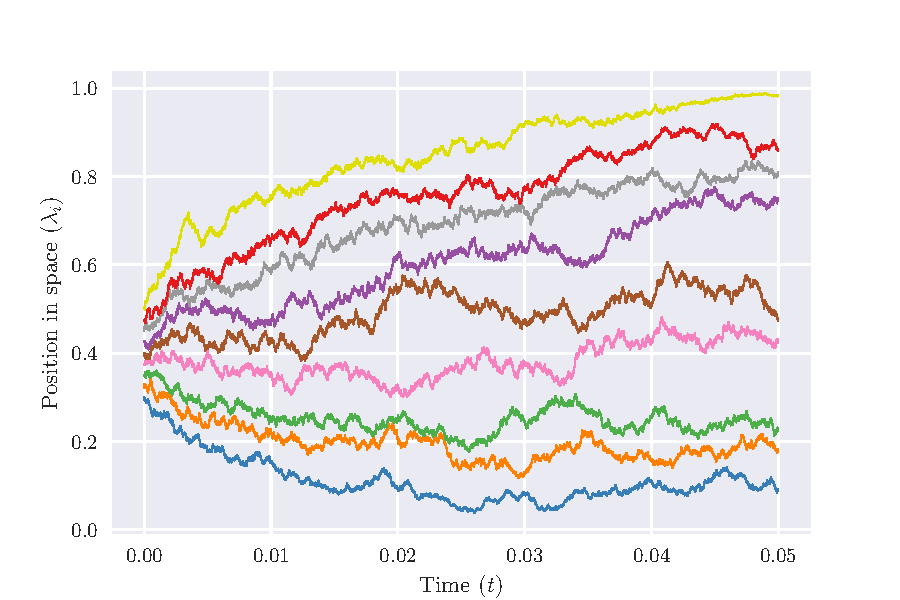
\includegraphics[width=6in]{img/jacobi.pdf}
    \caption{Path simulation for a Jacobi process.\label{fig:jacobi}}
\end{figure}





\chapter{Finite Free Probability} \label{ch:finite_free}

This chapter introduces the main ideas in finite free probability theory. In the first section we give the definition of three polynomial convolutions and some classic orthogonal polynomial ensembles. This section is purely algebraic and it is not related to probability. In section two, we present the definition of minor orthogonality, one of the central ideas in finite free probability. This is also the section in which we state initial relations between random matrices and plynomial convolutions. In the third section, we link finite free probability to free probability by defining the $\mathcal R_d$ transform, then we use the precedent contents to find polynomials related to some ``finite free distributions'' and the corresponding limit theorems.

\section{Polynomials and convolution} \label{sec:polynomials}

\subsection{Convolution of polynomials}

In this subsection, we present three notions of polynomial convolution, the first two were introduced around a century ago \cite{walsh1922location} \cite{szeg1939orthogonal}. Their study began using tools outside of probability theory, but we do not include any of those results here, instead, we are merely interested in introducing them to relate them to expected characteristic polynomials of random matrices. In the next subsection we introduce three ensembles of orthogonal polynomials, namely the Hermite, Laguerre and Jacobi polynomials. We prove some nice properties of these polynomials, especially related to the notions of convolution introduced previously.  The third notion of convolution was presented in the context of Finite Free Probability Theory \cite{article:finitefree} as it was found to share similar properties to the other two, linking it to Random Matrix Theory.

The three notions of convolution are defined for complex polynomials. Although one could get the convolution between any two polynomials, we are interested uniquely in monic polynomials as our main object of interest are the roots and their behavior under convolution. In full generality, we can write a monic complex polynomial $p(z)$ as

\begin{equation*}
    p(z) = \sum_{j=0}^n z^{n-j}(-1)^{j}a_j.
\end{equation*}

The three notions of convolution are defined in function of the polynomial degree, but the polynomials need not to have the same degree. In the case the degree is different, we can take the convolution with the highest degree, and notice that this equivalent to have zero coefficients for higher powers of the polynomial with the minor degree.

\subsubsection{Symmetric additive convolution}

This notion of convolution will be the most used along the text. Several of the results we find for the relationship of this convolution with random matrix theory can be extrapolated to the other notions, but the space and time required would be longer than the dedicated to the present work.

\begin{definition}[Symmetric additive convolution]\label{def:symadconv}
    Let $p(z), q(z)$ be two complex polynomials of $z$, with degree less or equal to $d$,

    \begin{align*}
        p(z) &= \sum_{j=0}^n z^{n-j}(-1)^{j}a_j,\\
        q(z) &= \sum_{j=0}^n z^{n-j}(-1)^{j}b_j.
    \end{align*}

    The $n$th symmetric additive convolution of $p$ and $q$ is

    \begin{align*}
        p(z) \boxplus_n q(z) &\coloneqq \sum_{k=0}^n z^{n-k}(-1)^k \sum_{i+j = k} \frac{(n-i)!(n-j)!}{n!(n-k)!}a_i b_j, \\
        &= \frac{1}{n!}\sum_{k=0}^n \partial_z^k p(z)\partial_z^{n-k}q(0),\\
        &= \frac{1}{n!}\sum_{k=0}^n \partial_z^k q(z)\partial_z^{n-k}p(0),
    \end{align*}

    \noindent with $\partial_z$ denoting the differentiation with respect to $z$.
\end{definition}

It is straightforward from the definition to prove that the symmetric additive convolution is linear. Let $p,q,r$ be degree $n$ polynomials with $a_i, b_i, c_i$ their respective coefficients and $\alpha \in \R$, then

\begin{align*}
    p \boxplus_n (\alpha q + r) &= \sum_{k=0}^n z^{n-k}(-1)^k \sum_{i+j = k} \frac{(n-i)!(n-j)!}{n!(n-k)!}a_i (\alpha b_j + c_j), \\ 
    &= \alpha \sum_{k=0}^n z^{n-k}(-1)^k \sum_{i+j = k} \frac{(n-i)!(n-j)!}{n!(n-k)!}a_i b_j\\ 
    &\phantom{unpoc} +\sum_{k=0}^n z^{n-k}(-1)^k \sum_{i+j = k} \frac{(n-i)!(n-j)!}{n!(n-k)!}a_i c_j,\\
    &= \alpha(p \boxplus_n q) + (p \boxplus_n r).
\end{align*}



\begin{theorem} \label{thm:multiplicative_operators}
    Let $P(\partial_z), Q(\partial_z)$ be linear differential operators and $p,q$ be polynomials of degree at most $n$ such that

    \begin{align*}
        p(z) = P(\partial_z)[z^n], \qquad q(z) =Q(\partial_z)[z^n].
    \end{align*}

    Then $p(z) \boxplus_n q(z) = P(\partial_z)Q(\partial_z)[z^n]$.
\end{theorem}

\begin{proof}
    We prove first that $z^n \boxplus z^n = z^n$. By definition of the convolution,
    
    \begin{align*}
        z^n \boxplus_n z^n &= \sum_{k=0}^n z^{n-k}(-1)^k \sum_{i+j = k} \frac{(n-i)!(n-j)!}{n!(n-k)!}a_i b_j, \\
        &= z^{n-0}(-1)^0\left( \frac{(n-0)!(n-0)!}{n!(n-0)!}\right) = z^n.
    \end{align*}

    Now, we prove the multiplicative property of $P$ and $Q$,

    \begin{equation*}
        \left( P(\partial_z)[r(z)] \boxplus_n Q(\partial_z)[s(z)] \right) = P(\partial_z) Q(\partial_z)(r(z) \boxplus s(z)).
    \end{equation*}

    For this proof, let us do it for operators of the form $P(\partial_z)[z^n] = z^{n-k}$ and then use the linearity of the symmetric additive convolution to extend linearly to polynomials of such operators. For $j+k\le n$, take $P(\partial_z) \coloneqq \frac{(n-k)!}{n!}\partial_z^k$ and $Q(\partial_z) \coloneqq \frac{(n-j)!}{n!}\partial_z^j$ and notice

    \begin{align*}
        P(\partial_z)[z^n] &= \frac{(n-k)!}{n!} \partial_z^k[z^n] = z^{n-k},\\
        Q(\partial_z)[z^n] &= \frac{(n-j)!}{n!} \partial_z^j[z^n] = z^{n-j}.
    \end{align*}

    The symmetric additive convolution of these polynomials is 

    \begin{align*}
        P(\partial_z)[z^n] \boxplus_n Q(\partial_z)[z^n] &= z^{n-k}\boxplus_n z^{n-j},\\
        &= \frac{(n-k)!(n-j)!}{n!n!}\frac{n!}{(n-k-j)!}z^{n-k-j} = \frac{(n-k)!(n-j)!}{n!(n-k-j)!}z^{n-k-j}.
    \end{align*}

    On the other hand, the product of the linear operators is 

    \begin{align*}
        P(\partial_z)Q(\partial_z)[z^n] &= \left(\frac{(n-k)!}{n!}\partial_z^k \frac{(n-j)!}{n!}\partial_z^j\right)[z^n] = \frac{(n-k)!(n-j)!}{n!n!} \partial_z^{j+k}[z^n], \\
        &= \frac{(n-k)!(n-j)!}{n!n!} \frac{n!}{(n-k-j)!}z^{n-k-j} = \frac{(n-k)!(n-j)!}{n!(n-k-j)!}z^{n-k-j}.
    \end{align*}

    To conclude, we extend this property linearly to any $P,Q$ polynomials on $\partial_z$. 
\end{proof}

\subsubsection{Symmetric multiplicative convolution}

Later in the thesis it is explained how the symmetric additive convolution is related to the additive convolution in Free Probability, i.e. the convolution of two measures when you add two freely independent random variables. In a similar fashion, when you multiply two freely independent random variables, there is a way to find the law of this product in terms of the laws o the original random variables. This operation between two probability distribution is called ``free multiplicative convolution''. The symmetric multiplicative convolution is analogously related to the free multiplicative convolution. Although most of the results we will show are related to linking the symmetric additive convolution to sums of random variables, we also show a theorem linking products of random matrices to symmetric multiplicative convolution and several of the later additive results can be extended to the multiplicative case (see \cite{marcus2021polynomial}, \cite{article:finitefree}).

\begin{definition}[Symmetric multiplicative convolution]
    Let $p$ and $q$ be as in Definition \ref{def:symadconv} with degree at most $n$. The $n$th symmetric multiplicative convolution of $p$ and $q$ is 

    \begin{align*}
        p(z) \boxtimes_n q(z) \coloneqq \sum_{i=0}^n z^{n-i}(-1)^i\frac{a_ib_i}{\binom ni}.
    \end{align*}
\end{definition}

\subsubsection{Asymmetric additive convolution}

This notion of convolution was found for the first time by Marcus, Spielman and Srivastava in the seminal paper on Finite Free Probability Theory \cite{article:finitefree}. Although this convolution is not related to a notion of Free convolution of measures, we introduce it because it appears naturally in the results found in Chapter \ref{ch:determinist}.


\begin{definition}[Asymetric additive convolution]
    Let $p$ and $q$ be two polynomials of degree at most $n$ as in Definition \ref{def:symadconv}. The $n$th asymmetric additive convolution of $q$ and $p$ is defined as

    \begin{align*}
        p(z) \aac q(z) \coloneqq \sum_{k=0}^n z^{n-k}(-1)^{k} \sum_{j=0}^k \left(\frac{(n-j)!(n-k+j)!}{n!(n-k)!}\right)^2 a_jb_{k-j}.
    \end{align*}
\end{definition}


Although many properties of these convolutions can be found without using Finite Free Probability Theory, we are mainly interested in describing their relationship to random matrices, so we will not include them. In the next subsection we present three ensembles of orthogonal polynomials and find that two of them have good properties related to the convolutions. The polynomials are also associated to Random Matrix Theory, as it is shown in later sections.
%\subsection{Linearization of convolutions}

\subsection{Classical orthogonal polynomial ensembles}

In order to define a property of ``orthogonality''  between elements of a given space, it is required to have some notion of inner product. If we are specifically working with spaces of square integrable functions with respect to some measure $L^2(\mu)$, the inner product between $f,g \in L^2(\mu)$ is given by

\begin{equation*}
    \langle f,g\rangle = \int_\Omega f(x)g(x) \d \mu(x),
\end{equation*}

\noindent where $\Omega$ is the space where the measure $\mu$ is defined. 

It is clear that a set of orthogonal polynomials does not exist for every $L^2(\mu)$ space that we take. For example, if we take $\mu$ to be the Lebesgue measure on $\R$, then polynomic functions are not integrable and thus the class of polynomials in $L^2(\mu)$ is empty. If we restrict only to probability measures associated to random variables in $L^{\infty-}(\Omega,\mathbb P, \mathbb F)$, then every polynomial function is in square integrable.

The following is the precise definition of a set of orthogonal functions.

\begin{definition}
    Let $\mu$ be a measure in $\R^n$, $I\subseteq \N$ be a set of integer indices and $(f_i(x))_{i\in I}$ be a collection of functions indexed by $I$. We say that the functions $(f_i)_{i\in I}$ are a family of orthogonal functions, if they satisfy the relationship,

    \begin{equation*}
        \int_{\R^d} f_j(x)f_k(x) \d \mu(x) = \norm{f_j}_2^2 \delta_{jk}.
    \end{equation*}
\end{definition}

When the functions $(f_i)_{i\in I}$ are polynomials, we call the set an \emph{ensemble of orthogonal polynomials}.

It is important to notice that if a set of polynomials is orthogonal under any finite measure, then it will be orthogonal under any rescaling of the same measure. This leads to different definitions of famous polynomial ensembles literature. Some definitions are more common than others, however, we will give here the definitions that allow us to reduce our use of notation. What we call here ``Laguerre polynomials'' of ``Jacobi polynomials'' are rescaled versions of the most common definitions. For a classical text on these polynomials, see \cite{szeg1939orthogonal}. For a more thorough study of orthogonal polynomials related to the theory of stochastic processes, see \cite{book:orthogonal_polynomials_and_stochastic_processes}.

\subsubsection{Hermite polynomials}

There are essentially two definitions of the Hermite polynomials, the first one is mostly used in Physics \cite{book:mathematical_methods_for_physicists}, and the second one is related to Probability Theory as appearing in \cite{marcus2021polynomial}. The main difference between them is the measure under which they are orthogonal. The ``physicist Hermite polynomials'' are orthogonal under the measure $e^{-x^2}\d x$, the heat kernel. The ``probabilist Hermite polynomials'' are orthogonal under $e^{-\frac{x^2}{2}} \d x$, the Gaussian kernel. We will restrict to the probabilist Hermite polynomials and will use the term ``Hermite polynomials'' to talk about them.

The $n$th Hermite polynomial, denoted by $H_n(z)$ is defined by a linear differential operator applied to $z^n$,

\begin{equation}
    H_n(z) \coloneqq e^{-\frac{\partial_z^2}{2}}[z^n] \coloneqq \sum_{k=0}^\infty \frac{(-1)^k}{2^k k!} \partial^{2k}[z^n].
\end{equation}

Both the physicist and the probabilist Hermite polynomials have a generalization to bivariate polynomials on $z$ and $t$. In the case of the probabilist Hermite polynomials, this generalization has the nice interpretation as being the polynomials orthogonal under the measure $e^{-t\frac{x^2}{2}}\d x$, i.e. the measure of a Gaussian random variable with variance $t$. Notice that this implies that the physicist Hermite polynomials are the probabilist Hermite polynomials with variance $2$. The generalized Hermite polynomials also known as time dependent Hermite polynomials, or Hermite polynomials with variance are polynomials on $z$ and $t$ generated by the analogous linear operator

\begin{equation}
    H_n(z,t) \coloneqq e^{-\frac{t\partial_z^2}{2}}(z^n) \coloneqq \sum_{k=0}^\infty \frac{(-1)^kt^k}{2^k k!} \partial^{2k}[z^n].
\end{equation}

Notice that $H_n(z,1)=H_n(z)$. Using the former definitions we can find explicit expressions for both $H_n(z)$ and $H_n(z,t)$,

\begin{align*}
    H_n(z) &= \sum_{k=0}^\infty \frac{(-1)^k}{2^k k!} \partial^{2k}[z^n] = \sum_{k=0}^{\lfloor \frac n2 \rfloor} \frac{(-1)^k}{2^k k!} \frac{n! }{(n-2k)!}z^{n-2k} = n! \sum_{k=0}^{\lfloor \frac n2\rfloor} \frac{(-1)^k z^{n-2k}}{2^k k! (n-2k)!}, \\
    H_n(z,t) &= \sum_{k=0}^\infty \frac{(-t)^k}{2^k k!} \partial^{2k}[z^n] = \sum_{k=0}^{\lfloor \frac n2 \rfloor} \frac{(-t)^k}{2^k k!} \frac{n! }{(n-2k)!}z^{n-2k} = n! \sum_{k=0}^{\lfloor \frac n2\rfloor} \frac{(-t)^k z^{n-2k}}{2^k k! (n-2k)!}.
\end{align*}

An easy substitution allows to see that the coefficient of $z^m$ in $H_n(z,t)$ is 

\begin{equation}
    a_m = \left\{ \begin{array}{cc}
        \frac{n!(-t)^{\frac{n-m}2}}{2^{\frac{n-m}{2}}\left( \frac{n-m}{2}\right)!m!}, &  \text{if $m$ and $n$ have the same parity,} \\
        0, & \text{otherwise}.
    \end{array} \right.
\end{equation}


The last expression gives us a way to find the first few Hermite polynomials,

\begin{align*}
    H_1(z,t) &= z,\\
    H_2(z,t) &= z^2 - t, \\
    H_3(z,t) &= z^3 - 3tz,\\ 
    H_4(z,t) &= z^4 - 6tz^2 + 3t^2,\\ 
    H_5(z,t) &= z^5 - 10tz^3 + 15t^2z,\\ 
    H_6(z,t) &= z^6 - 15tz^4 + 45 t^2 z^2 - 15t^3,\\ 
    H_7(z,t) &= z^7 - 21tz^5 + 105t^2z^3 -105t^3z,\\ 
    H_8(z,t) &= z^8 - 28tz^6 + 210t^2z^4 - 420t^3z^2 + 105t^4,\\ 
    H_9(z,t) &= z^9 - 36tz^7 + 378t^2z^5 - 1260t^3z^3 + 945t^4z,\\ 
    H_{10}(z,t) &= z^{10} - 45tz^8 + 630t^2z^6 - 3150t^3z^4 + 4725t^4z^2 - 945t^5.
\end{align*}

Replacing $t=1$, we can find the corresponding standard Hermite polynomials.

The Hermite polynomials are characterized by the following recursion together with the initial conditions $H_1(x,t)$ and $H_2(x,t)$.

\begin{equation} \label{eq:recursion_hermite}
    H_n(x,t) = x H_{n-1}(x,t) - t(n-1)H_{n-2}(x,t).
\end{equation}
 \todo{¿probar esto?}

% Convolución aditiva simétrica de dos polinomios de Hermite

The next proposition shows us that the Hermite polynomials with variance are well-behaved with respect to the symmetric additive convolution. This result will be more obvious once we have developed the tools of Finite Free Probability Theory and we will be able to give an easier proof after section \ref{sec:minor_orthogonality}.

\begin{proposition} \label{prop:convolution_of_hermites}
The symmetric additive convolution between two Hermite polynomials with the same order $H_n(z,t_1), H_n(z,t_2)$ is another Hermite polynomial with variance $t_1 + t_2$.
\end{proposition}

\begin{proof} We proceed directly by definition of the symmetric additive convolution and the closed form for the polynomials.

    \begin{align*}
        &H_n(z,t_1) \boxplus_n H_n(z,t_2) = \\ 
        &= \sum_{k=0}^n z^{n-k}(-1)^k \sum_{i=0}^k \frac{(n-i)!(n-k+i)!}{n!(n-k)!} b_i a_{k-i}, \\ 
        % &= \sum_{k=0}^d z^{d-k}(-1)^k \sum_{i=0}^k \frac{(d-i)!(d-k+i)!}{d!(d-k)!} \left(\frac{d!(-t_1)^{i/2}}{2^{i/2}(i/2)!(d-i)!}\right)\left(\frac{d!(-t_2)^{k-i/2}}{2^{k-i/2}(k-i/2)!(d-2k+i)!}\right),\\ 
        % &= \sum_{k=0}^d z^{d-k}(-1)^k \sum_{i=0}^k \frac{(d-i)!(d-k+i)!}{(d-2k+i)!(d-k)!} \left(\frac{d!(-t_1)^{i/2}}{2^{i/2}(i/2)!(d-i)!}\right), \\ 
        % &= \sum_{k=0}^d z^{d-k}(-1)^k \sum_{i=0}^k \frac{(d-i)!(d-k+i)!}{d!(d-k)!}\frac{d!(-t_1)^{i/2}}{2^{i/2} (i/2)! (d-i)!}\frac{d!(-t_2)^{k-i/2}}{2^{k-i/2} (k-i/2)! (d-k+i)!},\\ 
        &= \sum_{k=0}^{\lfloor \frac n2 \rfloor} z^{n-2k} \sum_{i=0}^{2k} \frac{(n-i)!(n-2k+i)!}{n!(d-2k)!} \frac{n!(-t_1)^{i/2}}{2^{i/2} (i/2)! (n-i)!} \frac{n!(-t_2)^{2k-i}}{2^{k-i/2} (k-i/2)! (n-2k+i)!},\\ 
        &= \sum_{k=0}^{\lfloor \frac n2 \rfloor} z^{n-2k}\frac{n!}{2^k} \sum_{i=0}^{2k} \frac{(-t_1)^{i/2}(-t_2)^{k-i/2}}{(i/2)!(k-i/2)!} = \sum_{k=0}^{\lfloor \frac n2 \rfloor} z^{n-2k} \frac{n!}{k!2^k} \sum_{i=0}^{2k} \frac{k!(-t_1)^{i/2}(-t_2)^{k-i/2}}{(i/2)!(k-i/2)!}, \\ 
        &= \sum_{k=0}^{\lfloor \frac n2 \rfloor} z^{n-2k}\frac{n!}{k!2^k} \sum_{i=0}^{k} \binom{k}{i}(-t_1)^{i/2}(-t_2)^{k-i/2} = \sum_{k=0}^{\lfloor \frac n2 \rfloor} z^{n-2k}(-1)^{k} \frac{n!(t_1 + t_2)^k }{k!2^k},\\ 
        &\eqcolon H_n(z,t_1+t_2).
        % &= \sum_{k=0}^{\lfloor \frac d2 \rfloor} z^{d-2k}(-1)^k \sum_{i=0}^{2k} \frac{d!(-t_1)^{i/2}(-t_2)^{k-i/2}}{2^{2k}(2k-i)!i!} = \sum_{k=0}^{\lfloor \frac d2 \rfloor} z^{d-2k}(-1)^k \frac{d!}{(2k)!2^k}\sum_{i=0}^{2k} \binom{2k}{i}\frac{(-t_1)^i(-t_2)^{2k-i}}{2^k},\\ 
        % &= \sum_{k=0}^{\lfloor \frac d2 \rfloor} z^{d-2k}(-1)^k \frac{d!}{(2k)!2^k}\frac{(-t_1 - t_2)^{2k}}{2^k}, \\ 
        % &= 
    \end{align*}\end{proof}





\subsubsection{Laguerre polynomials}

    As mentioned before, the ensembles of orthogonal polynomials we work with are not always monic, but we are interested on monic versions of them, so the definitions given here are proper re-scalings. The Laguerre polynomials are the set of orthogonal polynomials under the measure $e^{-x}x^{\alpha}\d x$. This is a scaling of the measure associated to a chi-squared distribution with $2(\alpha + 1)$ degrees of freedom. When $\alpha=0$, it corresponds to the polynomials orthogonal under the law of a chi-squared random variable with 2 degrees of freedom. We will call this particular case the ``standard Laguerre polynomials'', and when $\alpha >0$ we will call them the ``generalized Laguerre polynomials''.

    The Laguerre polynomials are usually defined as generated by the linear operator

    \begin{equation} \label{eq:laguerre_non_monic}
        \frac1{n!}\left(\partial_z - 1\right)[z^n].
    \end{equation}

   In order to get the monic polynomials proportional to the ones generated to the expression in \eqref{eq:laguerre_non_monic}, we need to cancel the quotient term $n!$. Adopting this convention, the standard Laguerre polynomials are defined by the linear differential operator 

    \begin{equation*}
        L_n(z) \coloneqq (1 - \partial_z)^n [z^n] \coloneqq \sum_{k=0}^n \binom{n}{k} (-1)^k\partial_z^k[z^n] = \sum_{k=0}^n \binom{n}{k} (-1)^k \frac{n!}{(n-k)!} z^{n-k},
    \end{equation*}

    \noindent while the generalized Laguerre polynomials are defined by the differential operator

    \begin{equation*}
        L_n^{\alpha}(z) \coloneqq x^{-\alpha} \left( 1 - \partial_z \right)^{n}[x^{n+\alpha}] \coloneqq \sum_{k=0}^n(-1)^k (n+\alpha)_{n+\alpha-k} x^{n-k}.
    \end{equation*}

    Notice that this is equivalent to the definition by the linear differential operator

    \begin{equation*}
        L_n^{\alpha}(z) \coloneqq \left( 1 - \partial_z \right)^{n+\alpha}[x^n] = \sum_{k=0}^n (-1)^k (n+\alpha)_{n+\alpha-k} x^{n-k}.
    \end{equation*}

    Just as in the case of the Hermite polynomials, we can generalize to bi-variate versions which corresponds to a chi-squared law with variance $t^2$. The time dependent Laguerre polynomials also known as Laguerre polynomials with variance are polynomials on $z$ and $t$ defined by the analogous linear operator

    \begin{equation} \label{eq:laguerre_with_variance}
        L_n(z,t) \coloneqq (1 - t\partial_z)^n [z^n] \coloneqq \sum_{k=0}^n \binom{n}{k} (-t)^k\partial_z^k[z^n] = \sum_{k=0}^n \binom{n}{k} (-t)^k \frac{n!}{(n-k)!} z^{n-k}.
    \end{equation}

    Likewise, the time dependent generalized Laguerre polynomials are defined by the operator one would expect

    \begin{equation*}
        L_n^{\alpha}(z,t) \coloneqq \left( 1 - t\partial_z \right)^{n+\alpha}[x^n] \coloneqq \sum_{k=0}^n \binom nk (-t)^k (n+\alpha)_{n+\alpha-k}x^{n-k}.
    \end{equation*}

    Expanding the definition, we can list the first few time-dependent standard Laguerre polynomials,

    \begin{align*}
        L_1(z,t) &= z - t, \\
        L_2(z,t) &= z^2 - 4tz + 2t^2,\\
        L_3(z,t) &= z^3 - 9tz^2 - 18t^2z + 6t^3, \\
        L_4(z,t) &= z^4 - 16tz^3 + 72t^2z^2 - 96t^3z + 24t^4,\\
        L_5(z,t) &= z^5 - 25tz^4 + 200t^2z^3 - 600t^3z^2 + 600t^4z - 120t^5,\\
        L_6(z,t) &= z^6 - 36tz^5 + 450t^2z^4 - 2400t^3z^3 + 5400t^4z^2 - 4320t^5z + 720t^6, \\
        L_7(z,t) &= z^7 - 49tz^6 + 882t^2z^5 -7350t^3z^4 + 29400t^4z^3 - 52920t^5z^2 + 35280t^6z - 5040t^7,\\
        L_8(z,t) &= z^8 - 64tz^7 + 1568t^2z^6 - 18816t^3z^5 + 117600t^4z^4 - 376320t^5z^3 + 564480t^6z^2\\ &\phantom{=}- 322560t^7z + 40320t^8,\\
        L_9(z,t) &= z^{9}-81tz^{8}+18144t^2z^{7}-42336t^3z^{6}+381024t^4z^{5}-1905120t^5z^{4}+5080320t^6z^{3}\\ 
        &\phantom{=}-6531840t^7z^{2} +3265920t^8z-362880t^9.
        %L_{10}(z,t) &= z^{10}-100z^{9}+4050z^{8}-86400z^{7}+1058400z^{6}-7620480z^{5}+31752000z^{4}-72576000z^{3}+81648000z^{2}-36288000z+3628800
    \end{align*}

    Replacing $t=1$, we get the standard Laguerre polynomials.

    The Laguerre polynomials are characterized by the following recursion together with the first two polynomials $L_1(z)=z-1$ and $L_2(z)=z^2-4tz + 2t^2$,

    \begin{align*}
        L_n(z) &= (z-2n+1)L_{n-1}(z) - (n-1)^2L_{n-2}(z).
    \end{align*}
        % The when we sum the last two polynomials multiplied by the given constants we find

        % \begin{align*}
        %     (z-2n+1)L_{n-1}(z) - (n-1)^2L_{n-2}(z) &= (z-2n+1)\sum_{k=0}^{n-1} \binom {n-1}k (-1)^k \frac{(n-1)!}{(n-1-k)!} z^{n-1-k}\\&\phantom{=} -(n-1)^2\sum_{k=0}^{n-2} \binom {n-2}k (-1)^k \frac{(n-2)!}{(n-2-k)!} z^{n-2-k},\\
        %     &= \sum_{k=0}^{n-1} \binom {n-1}k (-1)^k \frac{(n-1)!}{(n-k)!} z^{n-1-k}\\
        %     &\phantom{=} 
        % \end{align*}

        % \begin{align*}
        %     L_n(z) &= \sum_{k=0}^{n} \binom nk (-1)^k \frac{n!}{(n-k)!} z^{n-k} = zn \sum_{k=0}^{n} \binom nk (-1)^k \frac{(n-1)!}{(n-k)!} z^{n-1-k}\\
        %     &= 
        % \end{align*}


        % It is important to remark that there are also some polynomials called ``generalized Laguerre polynomials'' which depend on a parameter $\alpha$ and are defined by the linear operator

        % \begin{equation*}
        %     L_n^{(\alpha)}(z) = \frac{x^{-\alpha}}{n!}\left(1 - \partial_z\right)[z^{n+\alpha}].
        % \end{equation*}

        % The monic scaling of these polynomials is also related to random matrices and a time-dependent version can be defined analogously. The theorems we will expose here can be easily generalized for them.


\subsubsection{Jacobi polynomials}
    
    The Jacobi polynomials depend on two parameters $\alpha,\beta$ and they are orthogonal under the measure $(1-z)^{\alpha}(1+z)^{\beta}\d z$. The standard Jacobi polynomials are defined by the following differential operator

    \begin{equation*}
        P_{n}^{(\alpha ,\beta )}(z) = \frac{(-1)^{n}}{2^{n}n!}(1-z)^{-\alpha }(1+z)^{-\beta }\partial_z^n \left\{(1-z)^{\alpha }(1+z)^{\beta }\left(1-z^{2}\right)^{n}\right\}.
    \end{equation*}

    The parameters $\alpha,\beta$ take values in $\R^+$. If $\alpha = \beta = 0$, then we have the Legendre polynomials defined by the differential operator

    \begin{equation*}
        P_{n}(z) = \frac{1}{2^{n}n!}\partial_z^n [(z^{2}-1)^{n}].
    \end{equation*}

    Once again, we are interested in a monic scaling of these polynomials, but now we also want a ``transaltion of them''. The original Jacobi (and Legendre) polynomials are defined in $[-1,1]$, but we are interested in polynomials that take values in $[0,1]$. We get these polynmials by evaluating a Jacobi polynomila in $1-2z$, so that they are orthogonal under the measure $\mathds 1_{(0,1)}(z)z^\alpha(1-z)^\beta \d z$, i.e. the measure of a beta distribution. In the particular case when $\alpha = \beta = 0$, they are orthogonal under the measure of an uniform random variable in $(0,1)$. The closed form for the Legendre polynomials evaluated in $1-2z$ and scaled to be monic is

    \begin{equation*}
        P_n(z) =\frac{n!n!}{(2n)!}\sum_{k=0}^n z^k(-1)^{n-k} \binom nk \binom{n+k}k.
    \end{equation*}

    The first few Legendre polynomials are

    \begin{align*}
        P_1(z) &= z,\\
        P_2(z) &= z^2 - \frac{z}{2} + \frac{1}{6}, \\
        P_3(z) &= z^3 - \frac{2z^2}{5} + \frac{z}{2} - \frac{1}{10},\\
        P_4(z) &= z^4 - \frac{z^3}{2} + \frac{3z^2}{7} - \frac{5z}{28} + \frac{1}{35},\\
        P_5(z) &= z^5 - \frac{7z^4}{10} + \frac{7z^3}{3} - \frac{14z^2}{15} + \frac{7z}{30} - \frac{1}{42},\\
        P_6(z) &= z^6 - \frac{z^5}{2} + \frac{2z^4}{3} - \frac{4z^3}{7} + \frac{5z^2}{21} - \frac{z}{42} + \frac{1}{231},\\
        P_7(z) &= z^7 - \frac{z^6}{2} + \frac{5z^5}{7} - \frac{2z^4}{3} + \frac{10z^3}{21} - \frac{z^2}{14} + \frac{z}{42} - \frac{1}{429},\\
        P_8(z) &= z^8 - \frac{5z^7}{8} + \frac{5z^6}{4} - \frac{5z^5}{6} + \frac{5z^4}{14} - \frac{z^3}{28} + \frac{z^2}{56} - \frac{z}{56} + \frac{1}{6435},\\
        P_9(z) &= z^9 - \frac{3z^8}{4} + \frac{z^7}{2} - \frac{z^6}{2} + \frac{3z^5}{7} - \frac{2z^4}{21} + \frac{z^3}{28} - \frac{z^2}{56} + \frac{z}{315} - \frac{1}{12155},\\
        P_{10}(z) &= z^{10} - \frac{z^9}{2} + \frac{3z^8}{5} - \frac{3z^7}{5} + \frac{7z^6}{15} - \frac{z^5}{15} + \frac{z^4}{35} - \frac{z^3}{70} + \frac{z^2}{231} - \frac{z}{11547} + \frac{1}{46189}.
    \end{align*}


    Just as in the previous case, we will use the name ``Legendre polynomials'' or ``Jacobi polynomials'' to talk about these monic scalings.

    The Jacobi polynomials are a generalization of several other polynomial ensembles and they are closely related to several topics in the theory of orthogonal polynomials. To read more about them, revise \cite[Chapter IV]{szeg1939orthogonal}.

%\section{Finite free probability and random matrices}


\section{Expected characteristic polynomials} \label{sec:minor_orthogonality}

In this section we show the relationship between the polynomial convolutions defined before and Random Matrix Theory, specifically through the expected characteristic polynomial. Although several results can be found, we will restrict to the symmetric additive case and its relationship to sums of random matrices. The main result in this section is Theorem \ref{thm:symmad}, a similar Theorem ca also be stated for the product of matrices and symmetric multiplicative convolution. The first subsection introduces minor orthogonality, which is a key concept to prove the following results. In the second subsection we prove the main result.

\subsection{Minor orthogonality}

The next is a rather technical definition, but that allows to prove several of our results of interest.

\begin{definition}[Minor orthogonality]
    Let $R$ be an $m \times n$ random matrix. We say $R$ is minor orthogonal if for every $k,l \in \mathbb Z$ such that $k,l \le \max\{m,n\}$ and all sets $S,T,U,V$ with $\abs{S} = \abs{T} = k$ and $\abs{U} = \abs{V} = l$, it satisfies
    
    \begin{equation*}
        \mathbb E_R\left[ \det[R]_{S,T} \det[R^*]_{U,V} \right] = \frac{\delta_{S,V}\delta_{T,U}}{\binom{\max\{m,n\}}{k}}.
    \end{equation*}
\end{definition}

    In the last definition, $\mathbb E_R$ denotes taking the expectation with respect to $R$. We use this convention because in what follows we will have computations of expectations with several random matrices involved and it is convenient to know what is the matrix we are taking the expectation of in every step.

    Later we will prove that some well-known matrix ensembles are minor orthogonal, and that property will help us to make use of the related results. Before doing that, we will prove a  Lemma that allows us to conclude that some transformations of minor orthogonal matrices are also minor orthogonal.

\begin{lemma} \label{lemma:orth_trans_is_minorth}
    If $R$ is minor orthogonal and $Q$ is a constant matrix such that $Q\hermit{Q} = I$, then $Q$ is minor orthogonal. If $\hermit{Q}Q = I$, then $RQ$ is minor orthogonal.
\end{lemma}

\begin{proof}
    Recall that by the Cauchy-Binet formula (Theorem \ref{thm:cauchy_binet}), for $|S|=|T| = k$ we have

    \begin{equation*}
        \det[QR]_{S,T} = \sum_{\abs{W} = k} \det[Q]_{S,W}\det[R]_{W,T},
    \end{equation*}

    \noindent so with $\abs{S} = \abs{T} = k, \abs{U}=\abs{V} = l$,

    \begin{align*}
        \mathbb E_R \left[ \det [QR]_{S,T}\det [\hermit{R}\hermit{Q}]_{U,V} \right] &= \mathbb E_R \left[  \sum_{\abs{W}=k} \sum_{\abs{Z} = l} \det[Q]_{S,W} \det[R]_{W,T} \det[\hermit{R}]_{U,Z}\det[\hermit{Q}]_{Z,V} \right],\\
        &= \sum_{\abs{W}=k} \sum_{\abs{Z} = l} \det[Q]_{S,W}\det[\hermit{Q}]_{Z,V} \mathbb E_R \left[ \det[R]_{W,T}\det[\hermit{R}]_{U,Z}\right],\\
        &= \sum_{\abs{W}=k} \sum_{\abs{Z} = l} \det[Q]_{S,W}\det[\hermit{Q}]_{Z,V} \mathbb E_R \left[\frac{\delta_{W,Z}\delta_{T,U}}{\binom{\max\{m,n\}}{k}}\right],\\
        &= \sum_{\abs{W}=k} \det[Q]_{S,W}\det[\hermit{Q}]_{W,V}\frac{\delta_{T,U}}{\binom{\max\{m,n\}}{k}}
        = \det[Q\hermit{Q}]_{S,V} \frac{\delta_{T,U}}{\binom{\max\{m,n\}}{k}},\\
        &= \det[I]_{S,V} \frac{\delta_{T,U}}{\binom{\max\{m,n\}}{k}},
        \intertext{Notice that $\det[I]_{S,V} = 1$ if and only if $S=V$, so we conclude that}
        \mathbb E_R \left[ \det[QR]_{S,T}\det[\hermit{R}\hermit{Q}]_{U,V} \right] &= \frac{\delta_{S,V}\delta_{T,U}}{\binom{\max\{m,n\}}{k}}.
    \end{align*}

    The case $\hermit{Q}Q =I$ is proven in the same way.
\end{proof}

The former Theorem implies that minor orthogonality is preserved under unitary transformations. Now, we will introduce the signed permutation matrix ensemble and prove that it is minor orthogonal. This ensemble will be later used to conclude minor orthogonality in a broader class of random matrices.

\begin{definition}[Signed permutation matrix]
    A signed permutation matrix is a matrix that can be written $EP$ where $E$ is a diagonal matrix with entries $\pm 1$ and $P$ is a permutation matrix.
\end{definition}

\begin{lemma} \label{lemma:singed_per_is_minorth}
    A random matrix sampled uniformly from the set of signed permutation matrices is minor-orthogonal.
\end{lemma}

\begin{proof}
    Let $Q$ be a signed permutation matrix, we can write $Q = E P$, where $E$ is a diagonal random matrix with entries $\pm 1$ taken uniformly and $P$ is a matrix chosen uniformly from the permutation matrices, and both are independent. Then for $\abs{S} = \abs{T} = k$ and $\abs{U} = \abs{U} = l$, we have

    \begin{align*}
        \mathbb E_Q\left[ \det[Q]_{S,T}\det[\hermit{Q}]_{U,V} \right] &= \mathbb E_{E,P}\left[ \det[E P]_{S,T}\det[\hermit{P}E]_{U,V} \right],\\
        &= \sum_{\abs{W} = k} \sum_{\abs{Z} = l} \mathbb E_{E,P} \left[ \det [E]_{S,W} \det[P]_{W,T} \det[\hermit{P}]_{U,Z} \det[E]_{Z,V} \right],
        \intertext{every $\det[E]_{S,W}$ is diagonal and the determinant would be zero if $S\neq W$, so}
        &= \mathbb E_{E,P} \left[ \det[E]_{S,S} \det[P]_{W,T} \det[\hermit{P}]_{U,Z} \det[E]_{V,V} \right],\\
        \intertext{Let $\left\{\chi_i\right\}_{1\le i \le n}$ be the diagonal entries of $E$, then}
        &= \mathbb E_{E}\left[ \prod_{i\in S} \chi_i \prod_{j\in V} \chi_j \right] \mathbb E_{P}\left[  [P]_{S,T}[\hermit{P}]_{U,V} \right].
    \end{align*}

    Now we use that the variables $\chi_i$ are independent and uniform in $\{-1,1\}$, so that $\mathbb E[\chi_i] = 0$, but $\mathbb E[\chi_i^2] = 1$ for all $i$, and this means 

    \begin{equation*}
        \mathbb E_E \left[ \prod_{i\in S} \chi_i \prod_{j\in V} \chi_j \right] = \delta_{S,V}.
    \end{equation*}

    The last equality leads to

    \begin{align*}
        \mathbb E_R \left[ \det[QR]_{S,T}\det[\hermit{R}\hermit{Q}]_{U,V} \right] &= \delta_{S,V} \mathbb E_{P}\left[  \det[P]_{S,T}\det[\hermit{P}]_{U,V} \right],\\
        &=  \delta_{S,V} \mathbb E_{P}\left[  \det[P]_{S,T}\det[\hermit{P}]_{U,S} \right],\\ 
        &= \delta_{S,V} \mathbb E_{P}\left[  \det[P]_{S,T}\det[P]_{S,U} \right].
    \end{align*}

    The submatrix $P_{S,T}$ can be transformed in a diagonal matrix by a permutation matrix because it has at most a non zero entry for each row and each column. If the diagonal matrix has a zero entry in the diagonal, then the determinant $\det[P]_{S,T}$ is zero, in other case, it is different that zero. The only case when all of the diagonal entries of the diagonal matrix are not zero is when $T = \pi(S)$ with $\pi$ the permutation function corresponding to $P$. This means that in order to have a non-zero determinant we need $T = \pi(S) = U$, and $\det[P]_{S,U} = \in \{-1,1\}$, so

    \begin{align*}
        \mathbb E_R \left[ \det[QR]_{S,T}\det[\hermit{R}\hermit{Q}]_{U,V} \right] &= \delta_{S,V} \delta_{T,U} \mathbb E_{P}\left[ \det [P]_{S,T}\det[P]_{S,T} \right],\\ 
        &= \delta_{S,V} \delta_{T,U} \mathbb E_{P}\left[ \det [P]_{S,T}^2 \right],\\ 
        &= \delta_{S,V} \delta_{T,U} \mathbb E_{P}\left[  \delta_{T=\pi(S)} \right], \\ 
        &= \delta_{S,V} \delta_{T,U} \P{T = \pi(S)}.
    \end{align*}

    We are supposing that we are sampling uniformly from the permutation matrices of size $n \times n$, so the probability that $T = \pi(S)$ when $\pi$ is a permutation of $n$ elements and $\abs{S} = \abs{T} = k$ is $1/\binom{n}{k}$. So, we can conclude

    \begin{align*}
        \mathbb E_R \left[ \det[QR]_{S,T}\det[\hermit{R}\hermit{Q}]_{U,V} \right] &= \frac{\delta_{S,V} \delta_{T,U}}{\binom{n}{k}}.
    \end{align*}

    This is the definition of being minor-orthogonal. \todo{En el paper no lo prueban, pero el resultado se tiene también para una matriz de permutación con signos rectangular. En la siguiente prueba se usa esto, así que falta completar eso. La prueba es igual, simplemente tomando que $E$ es de tamaño $m\times m$ y $P$ de tamaño $m\times n$, todos los resultados se siguen.}
\end{proof}

Repeating the former proof but with $E$ having size $m\times m$ and $P$ being $m\times n$, we have the corollary for rectangular signed permutations.

\begin{corollary}
    Let $E$ be an $m\times m$ diagonal random matrix with independent entries such that $\P{E_{ii} = 1} = \P{E_{ii} = -1} = 1/2$, and let $P$ be an $m\times n$ random matrix taken uniformly from the set of $m\times n$ permutation matrices independent from $E$. Then $EP$ is minor orthogonal.
\end{corollary}

Now that we know that the signed permutations ensemble is minor orthogonal, we can use this and Lemma \ref{lemma:orth_trans_is_minorth} to prove that Haar unitary ensembles are minor orthogonal.


\begin{corollary}
    An $m\times n$ random matrix sampled from the Haar measure on $\mathcal M_{n,m}(\C)$ is minor-orthogonal.
\end{corollary}

\begin{proof}
    Let $R$ be a Haar distributed random $m\times n$ matrix with $m \le n$ and $Q$ a random signed permutation matrix. Any random signed permutation matrix is unitary, so $RQ$ is Haar distributed for fixed $Q$, and by Lemmas \ref{lemma:orth_trans_is_minorth} and \ref{lemma:singed_per_is_minorth} we have that it is also minor-orthogonal. Then, if $Q$ is uniformly sampled from the signed permutation matrices,

    \begin{align*}
        \mathbb E_R\left[ \det[R]_{S,T}\det[\hermit{R}]_{U,V} \right] = \mathbb E_{R,Q}\left[ \det[RQ]_{S,T} \det[\hermit{(RQ)}]_{U,V}\right]. 
    \end{align*}

    Since $Q$ is minor orthogonal, $RQ$ is also minor orthogonal for fixed $R$ and 

    \begin{align*}
        \mathbb E_R\left[ \mathbb E_Q \left[ \det[RQ]_{S,T}\det[\hermit{(RQ)}]_{U,V} \right] \right] = \mathbb E_R\left[ \frac{\delta_{S,V}\delta_{T,U}}{\binom{n}{k}}\right] = \frac{\delta_{S,V}\delta_{T,U}}{\binom{n}{k}},
    \end{align*}

    \noindent where $k = \abs{S} = \abs{T}$. 
\end{proof}


% Formulas


Let us denote by $\sigma_k(A)$ the coefficient of of $(-1)^{k}x^{d-k}$ in the characteristic polynomial of a $d$-dimensional matrix $A$. We will use the fact that \todo{Tal vez esto debería ir en preliminares}

\begin{equation*}
    \sigma_k(A) = \sum_{\abs{S} = k} \det[A]_{S,S}.
\end{equation*}

The following two Lemmas will help us to find explicit coefficients for expected characteristic polynomials with the aid of minor orthogonality properties.

\begin{lemma} \label{lemma:conjugate_minorth}
    Let $m \le n$, $B$ an $n\times n$ random matrix and $R$ an $m\times n$ minor-orthogonal matrix independent from $B$. For all sets $S,T \subset \binom{[m]}{k}$ we have

    \begin{equation*}
        \mathbb E_{B,R} \left[ \det[RB\hermit R]_{S,T} \right] = \mathbb E_B \left[\delta_{S,T} \frac{\sigma_k(B)}{\binom{n}k}\right].
    \end{equation*}
\end{lemma}

\begin{proof}
    Using the Cauchy-Binet formula we have

    \begin{align*}
        \mathbb E_{B,R} \left[ \det[RB\hermit{R}]_{S,T} \right] &= \mathbb E_B \left[\sum_{X,Y \in \binom{[n]}{k}} \mathbb E_R \left[ \det[R]_{S,X} \det[B]_{X,Y} \det[\hermit{R}]_{Y,T} \right] \right],\\ 
        &= \mathbb E_B \left[\sum_{X,Y \in \binom{[n]}{k}} \det[B]_{X,Y} \mathbb E_R \left[ \det[R]_{S,X} \det[\hermit{R}]_{Y,T} \right] \right],\\ 
        &= \mathbb E_B \left[\sum_{X,Y \in \binom{[n]}{k}} \det[B]_{X,Y} \frac{\delta_{S,T} \delta_{X,Y}}{\binom{n}{k}} \right],\\ 
        &= \mathbb E_B \left[\sum_{X \in \binom{[n]}{k}} \det [B]_{X,X} \frac{\delta_{S,T}}{\binom{n}{k}} \right],\\
        &= \mathbb E_B \left[\delta_{S,T} \frac{\sigma_k(B)}{\binom{n}k}\right].
    \end{align*}
\end{proof}


\begin{lemma}
    Let $a > d$, $A$ an $a \times a$ random matrix and $Q$ a random $a \times d$ matrix sampled from the Haar measure on $\mathcal M_{a,d}(\C)$, then

    \begin{equation*}
        \mathbb E_A \left[ \mathbb E_Q\left[ \chi_x \left( Q A \hermit{Q} \right) \right]\right] = \mathbb E_A \left[\frac{d!}{a!} \partial_x^{(a-d)} \chi_x(A) \right],
    \end{equation*}

    \noindent where $\chi_z(\cdot)$ denotes the characteristic polynomial of $\cdot$ with $z$ as a variable.
\end{lemma}

\begin{proof}
    Let $A$ be a fixed matrix and $Q$ a Haar unitary matrix on $\mathcal M_{a,b}(\C)$. The $k$th coefficient of the expected characteristic polynomial of $QA\hermit Q$ is 

    \begin{align*}
        \mathbb E_Q \left[ \sigma_k(QA\hermit{Q}) \right] &= \sum_{\abs{S} = k} \mathbb E_Q\left[ \det [QA\hermit Q]_{S,S} \right],\\ 
        &= \sum_{\abs{S} = k} \frac{\sigma_k(A)}{\binom ak} = \frac{\binom{d}{k} \sigma_k(A)}{\binom{a}{k}}.
    \end{align*}

    Taking expectation with respect to $A$ in the last expression we find

    \begin{align*}
        \mathbb E_A \left[\mathbb E_Q\left[ \chi_x \left( Q A \hermit{Q} \right) \right]\right] &= \mathbb E_A \left[ \frac{\binom{d}{k} \sigma_k(A)}{\binom{a}{k}} \right] = \frac{\binom{d}{k} \mathbb E_A[\sigma_k(A)]}{\binom{a}{k}},
    \end{align*}

    \noindent which is the $k$th coefficient of $\frac{d!}{a!} \frac{\d^{(a-d)}}{\d x} \mathbb E_A \left[\chi_x(A) \right]$.
\end{proof}

With these results, now wea re ready to prove the main Theorems relating polynomial convolution to the expected characteristic polynomials of sums and products of random matrices.

\subsection{Relationship to polynomial convolution}

Until now, we have used minor orthogonality properties to find some expressions for expected characteristic polynomials. In this section, we will see that under suitable circumstances, those expressions are actually related to polynomial convolutions. We prove the relationship for the symmetric additive and symmetric multiplicative cases. An analogous for the asymmetric additive case can be found in \cite{article:finitefree}. \todo{Hay que corregir la introducción de la sección (y capítulo) donde dije que estas relaciones sólo se probaban en el caso simétrico aditivo.}

For both the additive and multiplicative cases, the results are written in two parts; one for the statement of the expected characteristic polynomial coefficients and another stating explicitly the convolution of expected characteristic polynomials. The relationship with Free Probability Theory will be more evident for the additive case in the next section where we introduce the $\mathcal R_n$ finite transform. For the multiplicative case a similar transform can be introduced, but it is not included in this work. 

\begin{theorem} \label{thm:implies_symmad}
    Let $A, B$ be $n\times n$ random matrices and $R$ a $n\times n$ minor-orthogonal matrix, such that $A, B, R$ are jointly independent, then we have

    \begin{equation*}
        \mathbb E_{A,B,R}\left[ \sigma_k(A + RB\hermit R) \right] =  \sum_{i=0}^k \frac{\binom{n-i}{k-i}}{\binom{n}{k-i}}\mathbb E_{A} \left[\sigma_i(A)\right] \mathbb E_{A}\left[\sigma_{k-i}(B)\right],
    \end{equation*}

    \noindent where $\sigma_j(X)$ represents the $j$th coefficient in the characteristic polynomial of the matrix $X$.
\end{theorem}

\begin{proof}
    We use that

    \begin{equation*}
        \sigma_k(A) = \sum_{\abs{S}=k} \det[A]_{S,S},
    \end{equation*}

    \noindent together with Theorem \ref{thm:marcus_binet} and Lemma \ref{lemma:conjugate_minorth} to get \todo{Hay que aclarar las normas de matrices.}

    \begin{align*}
        \mathbb E_{A,B,R}&\left[ \sigma_k(A + RB\hermit{R}) \right]\\ &= \sum_{S \in \binom{[n]}{k}} \mathbb E_{A,B,R} \left[ \det[A + RB\hermit{R}]_{S,S} \right],\\ 
        \intertext{denote by $\overline U$ the complement of $U$, then}
        &= \sum_{S\in\binom{[n]}{k}} \sum_{i=0}^k \sum_{U,V\in \binom{[k]}{i}} (-1)^{\norm{U}_1 + \norm{V}_1} \mathbb E_A\left[ \det [A]_{U(S),V(S)} \right] \mathbb E_{B,R}\left[ \det[RB\hermit R]_{\overline{U}(S),\overline{V}(S)} \right],\\ 
        &= \sum_{S\in\binom{[n]}{k}} \sum_{i=0}^k \sum_{U,V\in \binom{[k]}{i}} (-1)^{\norm{U}_1 + \norm{V}_1} \mathbb E_A\left[ \det[A]_{U(S),V(S)} \right] \delta_{\overline{U}(S),\overline{V}(S)} \frac{\mathbb E_{B}\left[ \sigma_{k-i}(B)\right]}{\binom{n}{k-i}},\\ 
        \intertext{using that $U(S)=V(S)$ if and only if $\overline{U}(S) = \overline{V}(S)$,}
        &= \sum_{i=0}^k \frac{\mathbb E_{B}\left[ \sigma_{k-i}(B)\right]}{\binom{n}{k-i}} \sum_{S\in\binom{[n]}{k}} \sum_{U,V\in \binom{[k]}{i}}  \mathbb E_A\left[\det[A]_{U(S),U(S)} \right].
    \end{align*}

    To finish the proof we need to find

    \begin{equation} \label{eq:suma_rara} \sum_{S\in\binom{[n]}{k}} \sum_{U\in \binom{[k]}{i}}  \mathbb E_A\left[\det[A]_{U(S),U(S)} \right]. \end{equation}

    We are summing over all of the sets $V \in \binom{[n]}{i}$, but they appear more than once in the sum. To find the number of times every element $V\in \binom{[n]}{i}$ appears in the sum, we can count the total number of terms we are summing in \eqref{eq:suma_rara} and divide by the total number of elements in $\binom{[n]}{i}$. We have that $\abs{\binom{[n]}i} = \binom{n}{i}$ and the number of summands is $\binom{n}{k}\binom{k}{i}$, so

    \begin{align*}
        \frac{\binom{n}{k}\binom{k}{i}}{\binom{n}{i}} &= \frac{\frac{n!}{k!(n-k)!}\frac{k!}{i!(k-i)!}}{\frac{n!}{i!(n-i)!}} = \frac{(n-i)!}{(n-k)!(k-i)!} = \binom{n-i}{k-i}.
    \end{align*}

    Thus, we have

    \begin{equation*}
        \sum_{S\in\binom{[n]}{k}} \sum_{U\in \binom{[k]}{i}}  \mathbb E_A\left[ \det[A]_{U(S),U(S)} \right] = \binom{n-i}{k-i} \sum_{V\in \binom{[n]}{i}} \mathbb E_A\left[ \det[A]_{V,V} \right] = \binom{n-i}{k-i}\mathbb E_A\left[\sigma_{i}(A)\right].
    \end{equation*}

    With this, we can conclude

    \begin{equation*}
        \mathbb E_{A,B,R}\left[ \sigma_k(A + RB\hermit R) \right] =  \sum_{i=0}^k \frac{\binom{n-i}{k-i}}{\binom{n}{k-i}}\mathbb E_{A} \left[\sigma_i(A)\right] \mathbb E_{A}\left[\sigma_{k-i}(B)\right].
    \end{equation*}

    \todo{Hay que aclarar qué significa $U(S)$.}
\end{proof}


\begin{theorem} \label{thm:symmad}
    If $p(z)$ is the characteristic polynomial of $A$ and $q(z)$ is the characteristic polynomial of $B$, where $A$ and $B$ are $n\times n$ normal matrices with complex entries, then 

    \begin{equation*}
        p(z) \boxplus_n q(z) = \mathbb E_Q\left[\chi_z(A + Q B \hermit Q)\right],
    \end{equation*}

    \noindent where $\chi_z(\cdot)$ denotes the characteristic polynomial of $\cdot$ with $z$ as a variable and $\mathbb E_Q$ denotes taking expectation over $Q$ where $Q$ is sampled from the Haar measure on the unitary complex $n\times n$ matrices.
\end{theorem}

\begin{proof}
    It follows directly from Theorem \ref{thm:implies_symmad} and definition of the symmetric additive convolution.
\end{proof}


The next two Theorems are the analogous of the previous ones for the symmetric multiplicative convolution. As it was stated previously, these convolutions can be seen as ``approximations'' to the Free additive and Free multiplicative convolutions.


\begin{theorem} \label{thm:implies_symm_mult}
    Let $A$ and $B$ be $n\times n$ random matrices and $R$ a minor-orthogonal $n\times n$ matrix, such that $A,B,R$ are jointly independent, then

    \begin{equation*}
        \mathbb E_{A,B,R} \left[\sigma_k(ARB\hermit{R})\right] = \frac{\mathbb E_A[\sigma_k(A)]\mathbb E_B[\sigma_k(B)]}{\binom{n}{k}}.
    \end{equation*}
\end{theorem}

\begin{proof}
    \begin{align*}
        \mathbb E_{A,B,R} \left[\sigma_k(ARB\hermit{R})\right] &= \sum_{S \in \binom{[n]}{k}} \mathbb E_{A,B,R} \left[\det[ARB\hermit{R}]_{S,S}\right],\\ 
        \intertext{By the Cauchy-Binet formula and independence}
        &= \sum_{S,T \in \binom{[n]}{k}} \mathbb E_A\left[ \det[A]_{S,T} \right] \mathbb E_{B,R} \left[ \det [RB\hermit{R}]_{T,S} \right],\\ 
        \intertext{By Lemma \ref{lemma:conjugate_minorth}}
        &= \sum_{S,T \in \binom{[n]}{k}} \mathbb E_A\left[\det[A]_{S,T} \right] \delta_{T,S}\frac{\mathbb E_B\left[ \sigma_k(B)\right]}{\binom{n}{k}},\\
        &= \frac{\mathbb E_A[\sigma_k(A)]\mathbb E_B[\sigma_k(B)]}{\binom{n}{k}}.
    \end{align*}
\end{proof}


\begin{theorem}
    Let $p(z)$ be the characteristic polynomial of $A$ and $q(z)$ be the characteristic polynomial of $B$ where $A$ and $B$ are $n\times n$ normal matrices with complex entries, then 

    \begin{equation*}
        p(z) \boxtimes_n q(z) = \mathbb E_Q \left[ \chi_z (AQBQ^*) \right],
    \end{equation*}

    \noindent with $\chi_z$ and $\mathbb E_Q$ as in Theorem \ref{thm:symmad}.
\end{theorem}

\begin{proof}
    It follows directly from Theorem \ref{thm:implies_symm_mult} and definition of the symmetric multiplicative convolution.
\end{proof}

With the results in this section we related polynomial convolutions to expected characteristic polynomials. In the following section we will be able to link the convolutions to Free Probability Theory by assigning an empirical measure to the roots of a polynomial in a similar fashion one can assign a measure to the eigenvalues of a matrix.


\section{The finite \texorpdfstring{$\mathcal R_n$}{R} transform} 

\todo{Introducir la notación de $p(x) \equiv q(x) \mod x^n$.}

In finite probability, the $\mathcal R$ transform linearizes free additive convolution, which means the $\mathcal R$ transform of a free additive convolution of measures is simply the sum of the $\mathcal R$ tranforms of each measure. The $\mathcal R$ transform of a measure $\mu$ is often defined as a formal series

\begin{equation*}
    \mathcal R_\mu(s) = \sum_{k=0}^\infty s^{k} r_k,
\end{equation*}

\noindent with $r_k$ being the free cumulants of the measure. For the Finite Free case, a similar transform can be defined, and we will prove that it converges to the $\mathcal R$ transform. A similar finite transform converging to the corresponding free one can be dfeined for the multiplicative convolution, we do not include those results here. 

In the first part of this section we introduce some technical definitions and lemmas, then we define the finite $\mathcal R_n$ transform and prove its two main properties, namely that it converges to a $\mathcal R$ transform and that it linearizes symmetric additive convolution of polynomials. In the following two subsections we use the transform to find the polynomials associated to finite free distributions and later to prove the analogous in Finite Free Probability Theory to the most classical limit theorems in Probability Theory.

\subsection{Definition of the transform}

Given any polynomial $p(z)$ with order $p$ we can associate an empirical measure $\mu_p$ to its roots $z_i$ given by

\begin{equation*}
    \mu_p(\{x\}) = \frac1n\sum_{j=1}^p \delta_{x,z_j}.
\end{equation*}

This measure is similar to the spectral empirical measure of a random matrix. We can find its Cauchy transform in terms of the polynomial with the following lemma.

\begin{lemma} \label{lemma:cauchy_empirical_polynomial}
    Let $p$ be a monic polynomial of order $p$ with roots $\{z_i\}_{i=1}^n$, then the Cauchy transform of the empirical measure associated to the roots $z_i$ is given by 

    \begin{equation*}
        G_{\mu_p}(z) \coloneqq \frac1n \sum_{j=1}^n \frac1{z - z_j} = \frac{\partial_z p }{n p}(z) = \frac1n \partial_z \ln p(z).
    \end{equation*}

\end{lemma}

\begin{proof}
    $p(z)$ is a monic polynomial with roots $\left\{ z_j \right\}_{j \in [n]}$, then we can write,

    \begin{equation*}
        p(z) = \prod_{j=1}^n (z-z_j).
    \end{equation*}

    By the Leibnitz rule we find

    \begin{equation*}
        \partial_z p(z) = \sum_{j=1}^n \prod_{k\neq j} (z-z_k).
    \end{equation*}

    Using the last equation we have

    \begin{align*}
        \frac{\partial_z p}{n p}(z) &= \frac1n\sum_{j=1}^n \frac{\prod_{k\neq j} (z-z_k) }{ \prod_{l=1}^n (z-z_l) } = \frac1n\sum_{j=1}^n \frac{1}{z - z_j} \eqqcolon G_{\mu_p}(z).
    \end{align*}
\end{proof}

Now we will define two objects that are auxiliary in the following proofs. Both are named transforms, but it is important to remark that one of them is an operator acting on functions while the other is a multiset which is uniquely related to another multiset in some way.

The existence of the $U$ transform can be stated by the following Lemma that we state without proof. The proof can be found in \cite{anaya2016cumulantes}.

\begin{lemma}[$U$ transform]
    Let $S$ be a multiset of complex numbers and denote by $\abs S=n$ its number of elements with multiplicity. Then exists an unique multiset of complex numbers $T$ such that $\abs{T}=n$ and 

    \begin{equation*}
        \prod_{s_i \in S} (x-s_i) = \frac 1n \sum_{t_i \in T} (x-t_i)^n.
    \end{equation*}

    We call such multiset the $U$ transform of $S$.
\end{lemma}

\begin{definition}[Legendre's transform]
    Let $f$ a convex function in a domain $D\subset \R$ and define

    \begin{equation} \label{eq:legendre_set}
        D^* \coloneqq \left\{ x^* \in \R \mathrel{:} \sup_{x \in D} \{xx^* - f(x)\} < \infty \right\}.
    \end{equation}

    We define $f^*$ the Legendre transform of $f$ as the function

    \begin{align*}
        f^* : D^* &\to \R.\\
        s \mapsto &\sup_{x \in D} \{ xs - f(x) \}.
    \end{align*}
\end{definition}

\begin{lemma} \label{lemma:strictly_convex}
    Let $f$ be a strictly convex function in a domain $D \subset \R$ and such that its derivative exists in a point $x_0 \in D$. Then $\left.\partial_x [f(x)]\right|_{x=x_0} \in D^*$ and 

    \begin{equation*}
        f^*(f'(x_0)) = x_0 f'(x_0) - f(x_0).
    \end{equation*}

    If additionally, $f$ has a second derivative, then the following two results are satisfied

    \begin{align*}
        (f')^{-1}(x_0) &= (f^*)'(x_0), \\
        f''((f^*)'(x_0)) &= \frac{1}{(f^*)''(x_0)}.
    \end{align*}
\end{lemma}


\begin{proof}
    Since $f$ is strictly convex and differentiable at $x_0$ we have for $x\in D, x\neq x_0$ that 
    
    \begin{align*}
        f(x) &> f(x_0) + (x-x_0)f'(x_0), \\
        \Rightarrow f(x) -xf'(x_0) &> f(x_0) - x_0 f'(x_0),\\
        \Rightarrow xf'(x_0) - f(x) &< x_0 f'(x_0) - f(x_0).
    \end{align*}

    This means that 

    \begin{equation*}
        \sup_{x\in D}\{ xf'(x_0) - f(x) \} = x_0f'(x_0) - f(x_0) < \infty.
    \end{equation*}

    Then, by the definition of $D^*$, we have that $f'(x_0) \in D^*$ and the Legendre transform in this point is $f^*(f'(x_0)) = x_0f'(x_0) - f(x_0)$.

    For the second part, if $f$ has a second derivative at $x_0$, differentiate the last equation to find

    \begin{equation*}
        (f^*)'(f'(x_0))f''(x_0) = x_0 f''(x_0) + f'(x_0) - f'(x_0) = x_0 f''(x_0). 
    \end{equation*}

    The second derivative $f''(x_0)$ can not be zero because $f$ is strictly convex, so $(f^*)'(f'(x_0)) = z$, which means $f^*$ and $f'$ are inverse under composition (in any point where $f$ is twice differentiable). For the second equation we use the fact that these functions are inverse and derive,

    \begin{align*}
        f'((f^*)'(z)) &= z,\\
        \Rightarrow f''((f^*)(x_0))(f^*)''(x_0) &= 1,\\
        \Rightarrow f''((f^*)(x_0)) &= \frac1{(f^*)''(x_0)}.
    \end{align*}
\end{proof}

\begin{lemma} \label{lemma:legendre_transform_norm}
    Let $D \subset \R$ and $\mu$ a measure that is absolutely continuous with respect to the Lebesgue measure, then for any continuous function $f: D \to \R$ we have that

    \begin{equation*}
        f^*(s) = \ln \norm{ e^{xs - f(x)} }_{\infty},
    \end{equation*}

    \noindent for all $s \in D^*$ where the Legendre transform and the norm are taken over $D$.
\end{lemma}

\begin{proof}
    We can write $f^*$ as $f^*(s) = \ln(\exp(f^*(s)))$, then

    \begin{align*}
        f^*(s) &= \ln(\exp(f^*(s))) = \ln \left(\exp\left\{ \sup_{x\in D} \{xs-f(x)\} \right\}\right), \\
        \intertext{using that $\exp(x)$ is monotone increasing,}
        &= \ln \left( \sup_{x \in D} \exp(xs - f(x))\right) = \ln \norm{ e^{xs-f(x)} }_{\infty}.
    \end{align*}
\end{proof}

\begin{definition}[The $\mathcal K_n$ transform \cite{anaya2016cumulantes}]
    Let $A$ be an $n\times n$ symmetric matrix with real entries. We define the $\mathcal K_n$ transform of its empirical spectral measure $\mu_A$ as 

    \begin{equation*}
        \mathcal K_n^{\mu_A} (s) \coloneqq - \frac{\partial}{\partial s} \ln \norm{ e^{xs} \Delta^+ [x I - A]^{\frac1n} }_n,
    \end{equation*}

    \noindent where $\Delta^+$ represents the normalized determinant
    
    \begin{equation*}
        \Delta^+[A] = \left\{ \begin{array}{cc}
            \det[A]^{\frac1n} & \text{if $A$ is positive definite,}\\
            0 & \text{otherwise.}
        \end{array} \right.
    \end{equation*}
    
    \noindent and the integration domain for the norm is $(\rho_A, \infty)$ with $\rho_A$ the spectral radius of $A$.
\end{definition}


\begin{definition}[The $\mathcal R_n$ transform]
    Let $A$ be an $n\times n$ symmetric matrix with real entries. We define the $\mathcal R_n$ transform of its empirical spectral measure $\mu_A$ as 

    \begin{equation*}
        \mathcal R_n^{\mu_A} (s) = \mathcal K_n^{\mu_A} - \left( 1 + \frac1n \right) \frac1s.
    \end{equation*}
\end{definition}

\begin{theorem} Let $A$ be a self-adjoint $n \times n$ matrix with empirical spectral distribution $\mu_A$, then

    \begin{equation*}
        \lim_{n\to\infty} \mathcal K_n^{\mu_A} (s) = G_{\mu_A}^{-1}(s),
    \end{equation*}
\noindent with $s \in (\rho_A, \infty)$ and where $G_{\mu_A}^{-1}(s)$ is the inverse under composition of $G_{\mu_A}(s)$.
\end{theorem}

\begin{proof}
    
    We begin defining the function $g(x) \coloneqq -\ln \Delta^+[xI - A]$ and let $\lambda_1, \dots, \lambda_n$ be the ordered eigenvalues of $A$. When we differentiate $g$ with respect to $x$, we find 

    \begin{align*}
        \partial_x g(x) &= \partial_x \left[-\ln \Delta^+[xI - A]\right] = -\partial_x \ln\left[ \left(\prod_{j=1}^n (x - \lambda_j) \right)^{\frac1n}\right], \\
        &= -\partial_x \ln \left[ \prod_{j=1}^n (x-\lambda_j)^{\frac1n} \right] = - \partial_x \sum_{j=1}^n \frac1n \ln (x-\lambda_j) = -\frac1n \sum_{j=1}^n  \frac1{x-\lambda_j} = - G_{\mu_A}(x).
    \end{align*}

    For the second derivative we have

    \begin{align*}
        \partial_{xx} g(x) = \partial_x \left[ -\frac1n \sum_{j=1}^n  \frac1{x-\lambda_j} \right] = \frac1n \sum_{j=1}^n \frac{1}{(x-\lambda_j)^2} > 0.
    \end{align*}

    So $g(x)$ is strictly convex and has a second derivative. Using Lemma \ref{lemma:strictly_convex} we find that 

    \begin{equation} \label{eq:inverse_cauchy}
        (g^*)'(x) = (g')^{-1}(x) = (-G_{\mu_A})^{-1}(x) = G_{\mu_A}^{-1}(-x).
    \end{equation}

    Now we find $(g^*)'(x)$ with the aide of Lemma \ref{lemma:legendre_transform_norm}.

    \begin{align*}
        (g^*)'(s) &= \frac{\partial}{\partial s} \ln \norm{ e^{xs} - g(x) }_\infty = \frac{\partial}{\partial s} \ln \norm{ e^{xs} \Delta^+(xI - A) }_\infty.
    \end{align*}

    Substituting the last in \eqref{eq:inverse_cauchy} we get 

    \begin{equation*}
        G_{\mu_A}^{-1}(s) = (g^*)'(-s) = -\frac{\partial}{\partial s} \ln \norm{ e^{-xs} \Delta^+(xI - A) }_\infty.
    \end{equation*}

    On the other hand, the limit of $\mathcal K_n^{\mu_A}$ is 

    \begin{equation*}
        \lim_{n\to\infty}  \mathcal K_n^{\mu_A}(s) = - \lim_{n\to\infty} \frac{\partial}{\partial s} \ln \norm{ e^{xs}\Delta^+(xI - A) }_n =  -\frac{\partial}{\partial s} \ln \norm{ e^{-xs} \Delta^+(xI - A) }_\infty.
    \end{equation*}

    This gives the desired result.
\end{proof}




% \begin{proof}
%     Expanding the term $(x-t_i)^n$ we get,

%     \begin{equation*}
%         \frac 1m \sum_{t_i \in T} (x-t_i)^n = \frac 1m \sum_{t_i \in T} \sum_{k=0}^n \binom nk x^{n-k} (-1)^k t_i^k = \sum_{k=0}^n \binom nk x^{n-k} (-1)^k \E{T^k}. 
%     \end{equation*}

%     Where we use $\E{f(T)}$ to denote the expectation with respect to the empirical distribution associated to the multiset $T$, $\E{f(T)} = \frac1{\abs T} \sum_{t_i \in T} f(t_i)$.
% \end{proof}

\begin{lemma} \ref{lemma:Utrans_convolution}
    Let $p,q$ be polynomials with degree $n$ and $U_p,U_q$ be the $U$ transforms of its sets of roots, then

    \begin{equation*}
        [p \boxplus_n q](x) = \frac1n \sum_{u_j \in U_p, u_k \in U_q} (x - u_j -u_k)^n.
    \end{equation*}
\end{lemma}

\begin{proof}
    Let $p(x) = \sum_{j=0}^n x^{n-j}(-1)^j p_j$. Let $x_i$ be its roots, by definition of the $U$ transform we have,

    \begin{equation*}
        p(x) = \prod_{j=0}^n (x - x_j) = \frac1n \sum_{u_j \in U_p} (x-u_j)^n = \sum_{j=0}^n x^{n-j} (-1)^j \binom n j \E{U_p^j}.
    \end{equation*}

    Equating coefficients we find that $p_j = \binom nj\E{U_p^j}$ and the analogous happens for $q_k$. Finally, we find the convolution

    \begin{align*}
        [p\boxplus_n q](x) &= \sum_{k=0}^n x^{n-k}(-1)^k \sum_{i+j=k} \frac{(n-i)!(n-j)!}{(n-k)!n!} \binom{n}{i}\binom{n}{j} \E{U_p^i} \E{U_q^j},\\
        &= \sum_{k=0}^n x^{n-k}(-1)^k \sum_{i+j=k} \frac{n!}{i!j!(n-k)!} \E{U_p^i U_q^j}, \\
        &= \sum_{k=0}^n \binom nk x^{n-k}(-1)^k \sum_{j=0}^k \binom{k}{j}\E{U_p^{k-j} U_q^j}, \\
        &= \sum_{k=0}^n \binom nk x^{n-k}(-1)^k \E{(U_p + U_q)^k},\\
        &= \E{ (x - U_p - U_q)^n }. 
    \end{align*}
\end{proof}

\begin{lemma}  \label{lemma:quotient_norms}
    Let $A$ be an $n\times n$ real symmetric matrix. Denote by $\lambda(A)$ its spectrum and by $U_A$ the $U$ transform of $\lambda(A)$, then 
\todo{Encontrar $R_0^n$}
    \begin{equation*}
        \frac{\norm{e^{-xs}\Delta^+(xI - A)}_n^n}{\norm{e^{-xs}\Delta^+(xI)}_n^n} \equiv \frac1n\sum_{u_i \in U_A} e^{-ns u_i} \qquad \mod [s^{n+1}]. 
    \end{equation*} 
\end{lemma}

\begin{proof}
    By definition of the $U$ transform, for any $n\times n$ symmetric matrix $A$ we have

    \todo{Sin pérdida de generalidad, podemos suponer que es positiva definida.}

    \begin{equation*}
        \Delta^+(xI - A)^n = \det[xI - A] = \prod_{j=1}^n (x - \lambda_j) = \frac1n \sum_{u_i \in U_A} (x-u_i)^n.
    \end{equation*}

    Using this and the previously found result for $\norm{e^{-xs}\Delta^+(xI)}_n^n$ we find

    \begin{align*}
        \frac{\norm{e^{-xs}\Delta^+(xI - A)}_n^n}{\norm{e^{-xs}\Delta^+(xI)}_n^n} &= \frac{(ns)^{n+1}}{n!}\norm{e^{-xs}\Delta^+(xI - A)}_n^n,\\
        &= \frac{(ns)^{n+1}}{n!}\int_{\rho_A}^\infty e^{-nxs} \Delta^+(xI - A)^n \d x,\\
        &= \frac{(ns)^{n+1}}{n!}\int_{\rho_A}^\infty e^{-nxs} \frac1n \sum_{u_i \in U_A} (x-u_i)^n \d x,\\
        &= \frac{(ns)^{n+1}}{n!}e^{-ns\rho_A}\int_{0}^\infty e^{-nsy} \frac1n \sum_{u_i \in U_A} (y + \rho_A-u_i)^n \d x, \\
        &= \frac1n \sum_{u_i\in U_A} \frac{(ns)^{n+1}}{n!}e^{-ns\rho_A} \mathcal L\{(y + \rho_A - U_A)^n\}(ns), \\
        &=  \frac1n \sum_{u_i\in U_A} \frac{(ns)^{n+1}}{n!}e^{-ns\rho_A} \sum_{k=0}^n \binom nk  (\rho_A - u_i)^{n-k}\mathcal L\{y^k\}(ns), \\
        &= \frac1n \sum_{u_i\in U_A} \frac{(ns)^{n+1}}{n!}e^{-ns\rho_A} \sum_{k=0}^n \frac{n!}{k!(n-k)!}  (\rho_A - u_i)^{n-k}\frac{k!}{(ns)^{k+1}}, \\
        &= \frac1n \sum_{u_i \in U_A} e^{-ns\rho_A} \sum_{k=0}^n \frac{(ns)^{n-k}(\rho_A - u_i)^{n-k}}{(n-k)!}, \\
        &\equiv \frac1n \sum_{u_i\in U_A} e^{-ns\rho_A} e^{ns(\rho_A - u_i)}, \quad \mod [s^{n+1}],\\
        &\equiv \frac1n \sum_{u_i\in U_A} e^{-nsu_i}, \quad \mod [s^{n+1}].
    \end{align*}
\end{proof}

\begin{corollary} \label{corollary:R_n_as_a_logarithm}
    Let $A$ be a an $n\times n$ symmetric matrix with real entries, with spectrum $\lambda(A)$ and $U_A$ be the $U$ transform of $\lambda(A)$, then 

    \begin{equation*}
        \mathcal R_{n}^{\mu_A}(s) \equiv - \frac1n \frac{\partial}{\partial s} \ln \left(\frac1n \sum_{u_i \in U_A} e^{-nsu_i} \right) \qquad \mod [s^n].
    \end{equation*}
\end{corollary}

\begin{proof}
    Taking logarithm in both sides of Lemma \ref{lemma:quotient_norms} we get 

    \begin{equation*}
        \ln \left( \frac{\norm{e^{-xs}\Delta^+(xI - A)}_n^n}{\norm{e^{-xs}\Delta^+(xI)}_n^n} \right) \equiv \ln\left( \frac1n\sum_{u_i \in U_A} e^{-ns u_i} \right) \qquad \mod [s^{n+1}].
    \end{equation*}

    The first $n+1$ coeficientes of the power series coincide, so the first $k$ coefficients of the derivatives also coincide. Now we use the definition of the $\mathcal R_n$ transform

    \begin{align*}
        \mathcal R_{n}^{\mu_A}(s) &= \mathcal K_{n}^{\mu_A}(s) - \mathcal K_n^{\mu_0}(s), \\
        &= - \frac{\partial}{\partial s} \ln \norm{ e^{-xs}\Delta^+(xI -A) }_n + \frac{\partial}{\partial s} \ln \norm{ e^{-xs}\Delta^+(xI) }_n,\\
        &= - \frac1n \frac{\partial}{\partial s} \ln \left( \frac{\norm{e^{-xs}\Delta^+(xI -A)}_n^n}{ \norm{e^{-xs}\Delta^+(xI)}_n^n } \right), \\
        &\equiv -\frac1n \frac{\partial}{\partial s} \ln \left( \frac1n \sum_{u_i \in U_A} e^{-nsu_i} \right), \qquad \mod[s^n].
    \end{align*}
\end{proof}

\begin{lemma}
    Let $A$ and $B$ be two $n\times n$ real symmetric matrices. The following are equivalents:

    \begin{enumerate}
        \item \[ \mathcal R_n^{\mu_A}(s) + \mathcal R_n^{\mu_B}(s) = \mathcal R_n^{\mu_{A+B}}(s) \qquad \mod[s^n]. \]
        \item \[ \det[xI - A] \boxplus_n \det[xI-B] = \det[xI - A - B]. \]
    \end{enumerate}
\end{lemma}

\begin{proof}
    Let us denote by $U_A, U_B$ and $U_{A+B}$ the $U$ transforms of the $\lambda(A), \lambda(B)$ and $\lambda(A+B)$, respectively. By Lemma \ref{lemma:Utrans_convolution}, the second statement is equivalent to 

    \begin{equation*}
        \E{ (x - U_A - U_B)^n } = \E{ (x - U_{A+B})^n }.
    \end{equation*}

    Expanding the power and equating terms, the last happens if and only if the first $m$ moments of $U_A + U_B$ and $U_{A+B}$ coincide. This is in turn equivalent to 

    \begin{equation*}
        \E{e^{-ms(U_A + U_B)}} = \E{e^{-ms(U_A + U_B)}} = \E{ e^{-msU_{A+B}} } \qquad \mod [s^{n+1}].
    \end{equation*}

    Define the function $f_A(s) \coloneqq - \frac1n \ln \E{ e^{-msU_A} }$ and similarly for $B$ and $A+B$. Using this function, the second statement is equivalent to 

    \begin{equation} \label{eq:f_matrix_module}
        f_A(s) + f_B(s) \equiv f_{A+B}(s) \qquad \mod [s^{n+1}].
    \end{equation}

    Using Corollary \ref{corollary:R_n_as_a_logarithm}, the first statement is equivalent to 

    \begin{equation} \label{eq:differential_matrix_module}
        \frac{\partial}{\partial_s} f_A(s) + \frac{\partial}{\partial_s} f_B(s) \equiv \frac{\partial}{\partial_s} f_{A+B}(s) \qquad \mod[s^n].
    \end{equation}

    So proving the equivalence of the two statements reduces to prove the equivalence between \eqref{eq:f_matrix_module} and \eqref{eq:differential_matrix_module}. Because the formal series in \eqref{eq:f_matrix_module} coincide up to the $n+1$th term, the derivatives coincide up to the $n$th term, so one implication is trivial. For the second implication, it suffices to prove that $f_A(0) + f_B(0) = f_{A+B}(0)$, but we have that $f_A(0)=f_B(0)=f_{A+B}(0)$, so the result follows.
\end{proof} \todo{Mencionar caso multiplicativo.}

\subsection{Finite free distributions}

\begin{theorem} \label{thm:if_and_only_if}
    Let $P(n^{-1}\partial_z)$ be a polynomial on $n^{-1}\partial_z$ such that the linear differential operator applied to $x^n$, $P(n^{-1}\partial_z)[z^n]$ is a monic polynomial. Then $P(n^{-1}\partial_z) = \det[zI - A]$ for a matrix $A$ if and only if 

    \begin{equation} \label{eq:cauchy_transform_R}
        \frac1n \frac{\partial_s P(s)}{P(s)} \equiv - \mathcal R_n^{\mu_A}(s) \qquad \mod [s^{n+1}].
    \end{equation}
\end{theorem}

\begin{proof}
    Recall that

    \begin{equation*}
        \mathcal R_{n}^{\mu_A}(s) \equiv - \frac1n \frac{\partial}{\partial s} \ln \left(\frac1n \sum_{u_i \in U_A} e^{-nsu_i} \right) \qquad \mod [s^n].
    \end{equation*}

    Also 

    \begin{align*}
        \frac1n \frac{\partial_s P(s)}{P(s)} &= \frac1n \partial_s[\ln P(s)].
    \end{align*}

    Then \eqref{eq:cauchy_transform_R} is satisfied if and only if 

    \begin{equation*}
        P(s) \equiv \frac1n \sum_{u_i \in U_A} e^{-nsu_i} \qquad \mod [s^{n+1}].
    \end{equation*}

    The last relationship in turn is equivalent to 

    \begin{equation*}
        P(n^{-1}\partial_z)[z^n] = \left( \frac1n \sum_{u_i \in U_A} e^{-u_i\partial_z} \right)[z^n] = \frac1n \sum_{u_i \in U_A} e^{-u_i\partial_z}[z^n].
    \end{equation*}

    Expanding the last term and using the definition of $U_A$, we find

    \begin{align*}
        \frac1n \sum_{u_i \in U_A} e^{-u_i\partial_z}[z^n] &=  \frac1n \sum_{u_i \in U_A} \sum_{j=0}^n \frac{(-u_i)^j}{j!} \partial_z^j[z^n],\\
        &= \frac1n \sum_{u_i \in U_A} \sum_{j=0}^n (-u_i)^j \frac{n!}{j!(n-j)!}z^{n-j} = \frac1n \sum_{u_i \in U_A} (z - u_i)^n = \det[zI - A].
    \end{align*}\end{proof}


\subsubsection{Constant distribution}

A constant random variable has a first cumulant equal to $c \in \R$ and all the remaining cumulants equal to zero. Then its $\mathcal R_n^{\mu_A}$ transform is the constant formal series

\begin{equation*}
    \mathcal R_n^{\mu_A}(s) = c.
\end{equation*}

We can use Theorem \ref{thm:if_and_only_if} to find the polynomial $p$ with this $\mathcal R_n^{\mu_A}$ transform.

\begin{align*}
    -c &= \frac{1}{n}\partial_s[\ln P(s)],\\
    \Rightarrow -\int nc\d s &= \ln P(s),\\
    \Rightarrow \exp\left\{-ncs + c_0\right\} &= P(s),
\end{align*}

\noindent for some constant $c_0$. Then $p(z)$ is the monic scaling of the polynomial $P(n^{-1}\partial_z)[z^n] = e^{-c\partial_z}[z^n]$. Expanding we find

\begin{align*}
    p(z) &= e^{-c\partial_z}[z^n] = \sum_{k=0}^n \frac{(-c)^k}{k!}\partial_z^k[z^n],\\
    &= \sum_{k=0}^n \frac{n!}{k!(n-k)!}(-c)^k z^{n-k} = (z-c)^n.
\end{align*}

Thus, as we would expect, $p$ is the monic polynomial with all the roots equal to $c$ which is also the expected characteristic polynomial of the deterministic matrix $cI$.

\subsubsection{Gaussian distribution}

In free and classical probability, the central limit random variable is characterized for having the first two cumulants non-zero and the rest of the cumulants equal to zero. We already know what is the polynomial corresponding to a constant distribution in finite free probability. To find the general polynomial corresponding to a Gaussian, we can find the polynomial with the second cumulant non-zero and the rest equal to zero. If the second cumulant is equal to $\sigma^2$, then the formal series expansion of $\mathcal R_n^{\mu_A}$ is

\begin{equation*}
    \mathcal R_n^{\mu_A}(s) = s\sigma^2.
\end{equation*}

We can use Theorem \ref{thm:if_and_only_if} again to find

\begin{align*}
    \frac1n \partial_s[ \ln P(s) ] &= -s\sigma^2,\\ 
    \Rightarrow \ln P(s) &= -n\sigma^2 \int s \d s,\\
    \Rightarrow P(s) &= \exp\left\{ -n \sigma^2\frac {s^2}2 + c_0  \right\},
\end{align*}

\noindent where the constant $c_0$ accounts for making the polynomial monic. Now, evaluating $P$ in $n^{-1}\partial_z$ and applying to $z^n$, we have

\begin{align*}
    p(z) &= P(n^{-1}\partial_z)[z^n] = e^{-\sigma^2\frac{\partial_z^2}{2n}}[z^n] \eqcolon H_n(z,\sigma^2/n). 
\end{align*}

The last expression corresponds to the Hermite polynomial wit variance $\sigma^2/n$.

\subsubsection{Poisson distribution}

The Poisson distribution has all of its cumulants equal to a constant $\nu \in \R$, the formal series expansion of its $\mathcal R_n^{\mu_A}$ transform is 

\begin{align*}
    \mathcal R_n^{\mu_A}(s) &= \sum_{k=0}^\infty \nu s^n = \nu \sum_{k=0}^\infty s^n = \frac{\nu}{1-s}.
\end{align*}

Where the convergence is taken in $\abs{s} < 1$. Another use of Theorem \ref{thm:if_and_only_if} leads to

\begin{align*}
    \frac{\nu}{1-s} &= \mathcal R_n^{\mu_A}(s) = -\frac1n\partial_s[\ln P(s)], \\
    \Rightarrow -\int \frac{n\nu}{s-1} \d s &= \ln P(s),\\
    \Rightarrow \exp\left\{ n\nu \ln (1-s) \right\} &= P(s).
\end{align*}

Finally, we evaluate in $n^{-1}\partial_z$ and apply to $z^n$ and find the polynomial that has the given cumulants.

\begin{align} \label{eq:ff_poisson}
    P(n^{-1}\partial_z)[z^n] &= \left( 1 - \frac{\partial_z}{n} \right)^{n\nu}[z^n] \eqcolon L_n^{(\nu-1)n}(z).
\end{align}

So the finite free Poisson distribution corresponds to a generalized Laguerre polynomial. Notice that when $\nu=n=1$, we recover the original definition of the Laguerre polynoamials given in \todo{Citar definición (incluir Laguerre generalizados).}

\subsection{Finite Free Limit Theorems}

\begin{theorem}[Finite Free Law of Large Numbers]
    Let $(p_i(z))_{i=1}^n$ be a sequence of degree $n$ monic polynomials with real roots $r_{ij}$ such that

    \begin{equation*}
        p_i(z) = \prod_{j=1}^n (z - r_{ij}).
    \end{equation*}

    And for every fixed $i$,

    \begin{align*}
        \frac1n\sum_{j=1}^n r_{ij} &= m,\\
        \frac1n\sum_{j=1}^n r_{ij}^2 < c,
    \end{align*}

    \noindent for some positive constant $c$. Define $q_i(k,z) \coloneqq k^{-n}p_i(kz)$. Then

    \begin{equation*}
        \lim_{k\to \infty} [ q_1(k,z) \boxplus_n q_2(k,z) \boxplus_n \cdots \boxplus_n q_k(k,z) ] = (x-m)^n
    \end{equation*}
\end{theorem}

\begin{proof}
    Write for every $i$ the polynomial $p_i(z)$ as

    \begin{equation*}
        p_i(z) = z^n + a_{i1} z^{n-1} + \cdots 
    \end{equation*}

    If $P_i(\partial_z)$ is a linear operator that acts on $z^n$ to generate $p_i(z)$, then 

    \begin{equation*}
        P_i(\partial_z) = 1 + a_{i1} n \partial_z + \cdots 
    \end{equation*}

    Since the coefficient $a_{i1}$ is the sum of the roots, by hypothesis we have that $a_{i1} = m$ for every $i$. Now, the last equation implies that if $q_i$ is generated by a linear differential operator $Q_i(\partial_z)$, then

    \begin{equation*}
        Q_i(\partial_z) = 1 - \frac{m}{k}\partial_z + O(k^{-2}).
    \end{equation*}

    Using the multiplicative Theorem \ref{thm:multiplicative_operators} we find

    \begin{align*}
        \lim_{k\to \infty} [ q_1(k,z) \boxplus_n q_2(k,z) \boxplus_n \cdots \boxplus_n q_k(k,z) ] &= \lim_{k\to\infty}\prod_{j=1}^k Q_j(\partial_z)[z^n],\\
        &= \lim_{k\to\infty} \left( 1 - \frac{m}{k}\partial_z + O(k^{-2}) \right)^k[z^n],\\
        &= e^{-m\partial_z}[z^n] = (z-m)^n.
    \end{align*}
\end{proof}

\begin{theorem}[Finite Free Central Limit Theorem \cite{marcus2021polynomial}]
    Let $p_1, p_2, \dots$ be a sequence of degree $n$ real rooted polynomials with $p_i = \prod_j (x - r_{i,j})$ such that

    \begin{equation} \label{eq:hypotheses_ffclt}
        \sum_{j=1}^n r_{i,j} = 0, \qquad \frac1n \sum_{j=1}^n r^2_{i,j} = \sigma^2,
    \end{equation}

    \noindent for all $i$. Define $q_i(x) = k^{-n/2}p_i(\sqrt{k}x)$, then 

    % \begin{equation*}
    %     \lim_{n\to\infty} \left( q_1 \boxplus_d \cdots \boxplus_d q_n \right) = \left( \frac{d-1}{\sigma^2} \right)^{-d/2} H_d\left( x \sqrt{\frac{d-1}{\sigma^2}} \right),
    % \end{equation*}

    \begin{equation*}
        \lim_{k\to\infty} \left( q_1 \boxplus_n \cdots \boxplus_n q_k \right) = H_n(z,\sigma^2/(n-1)).
    \end{equation*}

    \noindent with $H_n(z,\sigma^2/(n-2))$ represents the $n$th Hermite polynomial with variance $\sigma^2/(n-1)$.
\end{theorem}


\begin{proof}
    Using the Vieta's formulas and the hypotheses \eqref{eq:hypotheses_ffclt}, we have that for every $i$ it is satisfied

    \begin{align*}
        a_1 &= \sum_{j=1}^n r_{ij} = 0,\\
        a_2 &= \sum_{1 \le j < m \le n} r_{ij}r_{im} = \frac12 \sum_{j=1}^n r_{ij}\sum_{m\neq j} r_{im} = \frac12 \sum_{j=1}^n r_{ij} \left(a_1 - r_{ij}\right),\\
        &= - \frac12 \sum_{j=1}^n r_{ij}^2 = - \frac12 n\sigma^2.
    \end{align*}

    So every $p_i$ has the form

    \begin{equation*}
        p_i(z) = z^n + (0)z^{n-1} - \frac{n\sigma^2}{2n(n-1)} z^{n-2} + \cdots
    \end{equation*}

    Multiplying by the factors to get $q$, we get

    \begin{align*}
        q_i(z) &= z^n + (0)z^{n-1} - \frac{n\sigma^2k^{-n/2}}{2n(n-1)} k^{\frac{n-2}{2}}z^{n-2} + \cdots ,\\
        &= z^n - \frac{\sigma^2}{2(n-1)k}z^{n-2}.
    \end{align*}

    This means that the linear differential operator $Q_i(\partial_z)$ that generates $q_i$ must have the form

    \begin{equation*}
        Q_i(\partial_z)[z^n] = \left( 1 - \frac{\sigma^2}{2(n-1)k}\partial_z^2 + O(k^{-3/2})\right)[z^n].
    \end{equation*}

    We recall the multiplicative Theorem \ref{thm:multiplicative_operators} to find,

    \begin{align*}
        q_1 \boxplus_n \cdots \boxplus_n q_k &= \prod_{j=1}^k Q_j(\partial_z)[z^n], \\
        &= \left( 1 - \frac{\sigma^2}{2(n-1)k}\partial_z^2 + O(k^{-3/2})\right)^k[z^n].
    \end{align*}

    Finally, letting $k\to\infty$, we can find

    \begin{equation*}
        \lim_{k\to\infty} \left(q_1 \boxplus_n \cdots \boxplus_n q_k\right) = e^{ - \frac{\sigma^2}{2(n-1)} }[z^n].
    \end{equation*}

    The last expression is the definition given previously for $H_n(z,\sigma^2/(n-1))$
\end{proof}


\begin{theorem}[Finite Free Poisson Limit Theorem]
    Let $p(z) = x^{n-1}(x-1)$. And for $\nu n \in \N$, the $\nu n$ times symmetric additive convolution of $p(z)$ with itself is a polynomial corresponding to the finite free Poisson distribution.

    \begin{equation*}
        \underbrace{p(z) \boxplus_n p(z) \boxplus_n \cdots \boxplus_n p(z)}_\text{$\nu n$ times} = (\nu n)!(-n)^{-\nu n}z^{n(1-\nu)}L_{\nu n}^{n(1-\nu)}(zn).
    \end{equation*}
\end{theorem}

\begin{proof}
    Notice that $x^{n-1}(x-1) = x^n - x^{n-1}$ can be written as generated by a linear differential operator in the following way

    \begin{equation*}
        \left(1 - \frac1n \partial_z\right)[z^n] = z^n - z^{n-1}.
    \end{equation*}

    Now, applying once again Theorem \ref*{thm:multiplicative_operators} we get

    \begin{align*}
        \underbrace{p(z) \boxplus_n p(z) \boxplus_n \cdots \boxplus_n p(z)}_\text{$\nu n$ times} &= \left(1-\frac1n \partial_z \right)^{\nu n}[z^n].
    \end{align*}

    Which is exactly the polynomial corresponding to the finite free Poisson distribution given in  \eqref{eq:ff_poisson}.
\end{proof}

\chapter{Deterministic eigenvalue processes for matrix valued processes}

In this last chapter we give a relationship between finite free probability and the eigenvalues of matrix-valued stochastic processes. In the first section construct a matrix process whose eigenvalues evolve according to the dynamics of the Dyson Brownian motion without the martingale part. We call this process the deterministic Dyson Brownian motion. In the second section we construct a similar matrix-valued process whose spectrum evolves according to the finite variation part of equation \eqref{eq:gen_dyson}. We are especially interested in the deterministic versions of the Wishart and Jacobi processes. In the third section, we relate these processes with finite free probability by showing that the convolution of certain polynomials satisfies differential equations that ultimately leads to conclude that their roots follow a similar dynamics to the deterministic version of the eigenvalue processes. This constitutes the main result in this work.

\label{ch:determinist}

\section{Deterministic Dyson Brownian motion}

In this section we prove that a given matrix-valued stochastic process has a deterministic spectrum and follows the dynamics of the finite variation part in the Dyson Brownian motion. The proof uses the same techniques as the former results for the stochastic differential equations of eigenvalue processes. 

\begin{theorem}

Let $Z$ be a process with covariation $\d Z_{ij}\d Z_{kl} = (\delta_{ik}\delta_{jl} + \delta_{il}\delta_{jk} - 2\delta_{ij}\delta_{kl}\delta_{ik} )\d t$ and no finite variation part, which means $Z$ is a symmetric matrix with independent Brownian motions in its entries, except for the diagonal, where $Z_{ii} = 0$. Let $X$ be a matrix valued process such that  $X = \trans H \Lambda H$ and that satisfies the stochastic differential equation


\begin{equation*}
     \trans{H} \d X H = \d Z.
\end{equation*}

Then the eigenvalue process $\Lambda$ satisfies

\begin{equation} \label{eq:deterministic_dyson}
    \d \lambda_i = \sum_{k\neq i} \frac{\d t}{\lambda_i - \lambda_k}.
\end{equation}

\end{theorem}

\begin{proof}

Define $\d A = \trans{H}\partial H$ and $\d N = \trans{H} \partial Z H$.


The same procedure as in \ref{thm:diffusion_real} leads to 

\begin{equation*}
    \d \Lambda = \d N + \Lambda \d A - \d A \Lambda.
\end{equation*}

We conclude that $\d \lambda_i = \d N_{ii}$ and for $i\neq j$, 

\begin{align*}
    0 &= \d N_{ij} + \lambda_i \d A_{ij} - \lambda_j \d A_{ij},\\
    \Rightarrow \d A_{ij} &= \frac{\d N_{ij}}{\lambda_j - \lambda_i}.
\end{align*}

The quadratic covariation of $N$ is the same as the one for $Z$ because they only differ in a finite variation term, so

\begin{align*}
    \d N_{ij}\d N_{kl} &= \d \bigl< (\trans{H} \d X H)_{ij}, (\trans{H}\d X H)_{kl} \bigr>(t) %= \sum_{pqrs} \d \bigl< \trans{H}_{ip} \d X_{pq} H_{qj}, \trans{H}_{kr}\d X_{rs} H_{sl} \bigr>,\\
    % &= \sum_{pqrs} \trans{H}_{ip}  H_{qj}\trans{H}_{kr} H_{sl} \d X_{pq}\d X_{rs} = \sum_{pqrs} \trans{H}_{ip}  H_{qj}\trans{H}_{kr} H_{sl}\bigl( \delta_{pr}\delta_{qs} + \delta_{ps}\delta_{qr} - 2 \delta_{pq}\delta_{rs}\delta_{pr} \bigr)\d t,\\
    % &= \Biggl(\sum_{pqrs}\trans{H}_{ip}  H_{qj}\trans{H}_{kr} H_{sl}\delta_{pr}\delta_{qs} + \sum_{pqrs}\trans{H}_{ip}  H_{qj}\trans{H}_{kr} H_{sl}\delta_{ps}\delta_{qr} - 2 \sum_{pqrs}\trans{H}_{ip}  H_{qj}\trans{H}_{kr} H_{sl}\delta_{pq}\delta_{rs}\delta_{pr}\Biggr) \d t,\\
    % &= \sum_{pq} \trans{H}_{ip}H_{rk}\trans{H}_{jq}H_{ql}\d t + \sum_{pq}\trans{H}_{ip}H_{pl}\trans{H}_{kq}H_{qj} \d t - 2 \sum_{p} \trans{H}_{ip}H_{pj}\trans{H}_{kp}H_{pl} \d t,\\
    % &= \bigl(\delta_{ik}\delta_{jl} + \delta_{il}\delta_{kj} - 2\delta_{ij}\delta_{kl}\delta_{ik} \bigr)\d t.
    = \d \bigl< Z_{ij},Z_{kl} \bigr> = \bigl(\delta_{ik}\delta_{jl} + \delta_{il}\delta_{kj} - 2\delta_{ij}\delta_{kl}\delta_{ik} \bigr)\d t.
\end{align*}

Particularly, we have that $\d N_{ii}\d N_{jj} = 0$ for every choice of $j$ and $i$. Thus every entry in the diagonal of $N$ is a finite variation process and so it is $\lambda_i$. Let us finally compute the finite variation part $F$ of $N$.

\begin{align*}
    \d F &= \frac12 \bigl( \trans{H}\d X \d H + \d \trans{H}\d X H \bigr),\\
         &= \frac12 \bigl( \trans{H}\d X H \trans{H} \d H + \d \trans{H}H\trans{H}\d X H \bigr),\\
         &= \frac12 \bigl( \d N \d A + \trans{(\d N \d A)} \bigr).
\end{align*}

For $\d N \d A$ we have

\begin{align*}
    (\d N \d A)_{ij} &= \sum_{k\neq j} \d N_{ik}\d A_{kj} = \sum_{k\neq j} \frac{\d N_{ik}\d A_{kj}}{\lambda_j - \lambda_k},\\
    &= \sum_{k\neq j} \frac{ \delta_{ik}\delta_{kj} + \delta_{ij}\delta_{kk} - 2\delta_{ik}\delta_{kj}\delta_{ij} }{\lambda_j - \lambda_k}\d t = \delta_{ij}\sum_{k\neq j} \frac{ \d t }{\lambda_j - \lambda_k}.
\end{align*}

Then $F$ is diagonal with $\d F_{ii} = \sum_{k\neq i} \frac{\d t}{\lambda_i - \lambda_k}$. We conclude that

\begin{equation*}
    \d \lambda_i = \sum_{k\neq i} \frac{\d t}{\lambda_i - \lambda_k}.
\end{equation*}

\end{proof}

\section{Deterministic eigenvalue processes for matrix-valued diffusions}

Now that we have shown the construction of a matrix-valued process whose eigenvalue is the deterministic Dyson Brownian motion, we generaliza the result to get processes with a deterministic spectrum that can follow the dynamics of any eigenvalue process with the form \eqref{eq:gen_dyson}.

% \begin{theorem}

%     Let $Z$ be a process with covariation $\d Z_{ij}\d Z_{kl} = (\delta_{ik}\delta_{jl} + \delta_{il}\delta_{jk} - 2\delta_{ij}\delta_{kl}\delta_{ik} )\d t$ and no finite variation part, which means $Z$ is a symmetric matrix with independent Brownian motions in its entries, except for the diagonal, where $Z_{ii} = 0$. Let $X$ be a matrix valued process such that  $X = \trans H \Lambda H$ and it satisfies the stochastic differential equation
    
    
%     \begin{equation}
%         \trans{H}\d X(t)H = g(X(t)) \d Z(t) h(X(t)) + h(X(t)) \d \trans{Z(t)} g(X(t)) + b(X(t))\d t, \label{eq:deterministic_matrix_diffusion}
%     \end{equation}

%     Then the eigenvalue process $\Lambda$ satisfies

%     \begin{equation}
%         \d \lambda_i = \biggl( b(\lambda_i) + \sum_{k\neq i} \frac{G(\lambda_i,\lambda_k)}{\lambda_i - \lambda_k} \biggr)\d t.
%     \end{equation}

% \end{theorem}

\begin{theorem} \label{thm:deterministic_diffusion}
    Let $B = (B(t), t\ge 0)$ be a Brownian motion in $\M_{p,p}(\R)$ and $Y(t) = QM\trans{Q}$ be a symmetric $p\times p$ matrix-valued stochastic process satisfying the stochastic differential equation

    \begin{equation}
        \d Y(t) = g(Y(t)) \d B(t) h(Y(t)) + h(Y(t)) \d \trans{B(t)} g(Y(t)) + b(Y(t))\d t, \label{eq:matrix_diffusion}
    \end{equation}

    where $g,h,b$ are real functions acting spectrally, and $Y(0)$ is a symmetric $p\times p$ matrix with $p$ different eigenvalues.

    Let $G(x,y) = g^2(x)h^2(y) + g^2(y)h^2(x)$, $\tau$ be defined as in \eqref{eq:collision_time}, and take a process $X = (X(t), t\ge 0)$ with diagonalization $X = H \Lambda \trans{H}$ such that $\trans H (\d \Lambda) H$ has the same off-diagonal entries as $\trans Q ( \d M) \circ Q$ and has diagonal entries equal to zero.
    
    Then, for $t < \tau$ the eigenvalue process $\Lambda(t)$ verifies the following system of stochastic differential equations:

    \begin{equation}
        \d \lambda_i = \biggl( b(\lambda_i) + \sum_{k\neq i} \frac{G(\lambda_i,\lambda_k)}{\lambda_i - \lambda_k} \biggr)\d t.
    \end{equation}
\end{theorem}


\begin{proof}
    We define again $L$ to be the stochastic logarithm of $H$, $L \coloneqq \trans H \circ \d H$ and using the same techniques as in Theorem \ref{thm:diffusion_real} we have that,

    \begin{equation*}
        \d \Lambda = \trans H \circ(\partial X) \circ H - (\partial L)\circ \Lambda + \Lambda \circ \partial L.
    \end{equation*}

    Using that $\Lambda \circ \partial L -  (\partial L)\circ \Lambda $ has zero diagonal, we get that $\d lambda_i = (\trans H \circ(\partial X) \circ H)_{ii}$ and by hypothesis, we know that the martingale part of this diagonal is zero. 

    Define $\d N \coloneqq \trans H \circ(\partial X) \circ H$. For $i\neq j$ we have that $\d L_{ij} = \d N_{ij}/(\lambda_j - \lambda_i)$.

    Finally, we compute the finite variation $\d F$ part of $\d N$,

    \begin{align*}
        \d F &= \trans H b(X) H \d t + \frac12 (\d \trans H \d X H + \trans H \d X H), \\ 
        &= b(\Lambda) \d t + \frac12( \trans{(\d N\d A)} + \d N \d A ).
    \end{align*}

    For $\d N \d A$ we find

    \begin{align*}
        (\d N \d A)_{ij} &= \sum_{k\neq j} \d N_{ik}\d A_{kj} = \sum_{k\neq j} \frac{\d N_{ik}\d N_{kj}}{\lambda_j - \lambda_k}.
    \end{align*}

    Now we use that the martingale part of  $\d N$ has the same entries as $\trans{Q} M Q$ and by the results in Theorem \ref{thm:diffusion_real} we know that 

    \begin{equation*}
        (\trans{Q} M Q)_{ik}(\trans{Q} M Q)_{kj} = \delta_{ij}G(\lambda_i,\lambda_k)\d t,
    \end{equation*}

    \noindent so substituting the last result we get

    \begin{equation*}
        \d \lambda_i = \d F_{ii} = b(\lambda_i)\d t + \sum_{k\neq j} \frac{G(\lambda_i,\lambda_k)\d t}{\lambda_j - \lambda_k},
    \end{equation*}

    \noindent which is the desired result.



\end{proof}


These results can be particularized for any matrix-valued diffusions. Especially, we are interested in the Wishart and Jacobi processes. We give the proofs for these as a corollary to last Theorem.

\subsection{Wishart process}

\begin{corollary}
    Let $Y = (Y(t), t \ge 0)$ be an $n\times n$ Wishart process with parameter $m$ and diagonalization $Y = QM\trans{Q}$. Let $X$ be an $n\times n$ self adjoint matrix process with diagonalization $X = H \Lambda \trans{H}$, such that the off-diagonal part of $\trans{H} \d X H $ and $\overset{d}{=} \trans{Q} \d Y Q$ coincide, and $(\trans{H} \d X H)_{ii} = 0$ for every $i \in [n]$. Then the eigenvalues of $X$, $\lambda_1 \ge \lambda_2 \ge \cdots \ge \lambda_n$ satisfy the following system of stochastic differential equations

    \begin{equation} \label{eq:deterministic_wishart}
        \d \lambda_i = \left( m +\sum_{k\neq i} \frac{ \abs{\lambda_i} + \abs{\lambda_k} }{\lambda_i - \lambda_k}\right)\d t.
    \end{equation}
\end{corollary}

\begin{proof}
    
\end{proof}


\subsection{Jacobi process}

\begin{corollary}
    Let $Y = (Y(t), t \ge 0)$ be an $n\times n$ matrix Jacobi process with parameters $n_1,n_2$ and diagonalization $Y = QM\trans{Q}$. Let $X$ be an $n\times n$ self adjoint matrix process with diagonalization $X = H \Lambda \trans{H}$, such that the off-diagonal part of $\trans{H} \d X H $ and $\overset{d}{=} \trans{Q} \d Y Q$ coincide, and $(\trans{H} \d X H)_{ii} = 0$ for every $i \in [n]$. Then the eigenvalues of $X$, $\lambda_1 \ge \lambda_2 \ge \cdots \ge \lambda_n$ satisfy the following system of stochastic differential equations

    \begin{equation} \label{eq:deterministic_jacobi}
        \d \lambda_i = \left( n_2 - (n_1 + n_2)\lambda_i + \sum_{k\neq i} \frac{\lambda_k(1-\lambda_i) + \lambda_i(1-\lambda_k)}{\lambda_i - \lambda_k} \right)\d t.
    \end{equation}

\end{corollary}

\section{Dynamical behavior of the deterministic eigenvalue processes}

\begin{lemma} \label{lemma:separation}
    Let $\lambda_1,\dots,\lambda_n$ be a system of $n$ functions moving according to \eqref{eq:deterministic_dyson} and $\lambda_i(0) > \lambda_j(0)$ and there is no $\lambda_k$ such that $\lambda_i(0) > \lambda_k(0) > \lambda_j(0)$. Then, $\lambda_i$ and $\lambda_k$ repel each other if and only if 

    \begin{equation} \label{eq:separation_condition}
        \frac{2}{(\lambda_i - \lambda_j)^2} > \sum_{k\neq i,j} \frac{1}{(\lambda_i - \lambda_k)(\lambda_j - \lambda_k)}
    \end{equation}
\end{lemma}

\begin{proof}

    The distance between the particles grows if and only if its derivative its positive, so 

    \begin{align*}
        \frac{\d }{\d t} (\lambda_i - \lambda_j) &= \sum_{k\neq i} \frac{1}{\lambda_i - \lambda_k} - \sum_{k\neq j} \frac{1}{\lambda_j - \lambda_k} = \sum_{k\neq i,j} \left( \frac{1}{\lambda_i - \lambda_k} - \frac{1}{\lambda_j - \lambda_k} \right) + \frac{2}{\lambda_i - \lambda_j},\\
        &= \sum_{k \neq i, j} \frac{\lambda_j - \lambda_k - \lambda_i + \lambda_k}{(\lambda_i- \lambda_k)(\lambda_j - \lambda_k)} + \frac{2}{\lambda_i - \lambda_j},= \frac{2}{(\lambda_i - \lambda_j)^2} - \sum_{k\neq i,j} \frac{1}{(\lambda_i - \lambda_k)(\lambda_j - \lambda_k)}.
    \end{align*}

    Comparing to zero, we get the desired result.
\end{proof}



\begin{theorem}
    If a system of functions satisfies \eqref{eq:deterministic_dyson}, then there ar no collisions.
\end{theorem}

\begin{proof}
    Write condition \eqref{eq:separation_condition} as

    \begin{equation*}
        \frac{2}{(\lambda_i - \lambda_j)^2} > \sum_{k\neq i,j} \frac{1}{(\lambda_i - \lambda_j + \lambda_j -\lambda_k)(\lambda_j - \lambda_k)},
    \end{equation*}

    \noindent and take $\lambda_i \to \lambda_j$. As $\lambda_i$ approaches $\lambda_k$, the left-hand side grows to $\infty$, while the right-hand side converges to the finite quantity

    \begin{equation*}
        \sum_{k\neq i,j} \frac{1}{(\lambda_j - \lambda_k)^2}.
    \end{equation*}

    Thus, before the collision occurs, the distance between $\lambda_i$ and $\lambda_j$ starts to grow.
\end{proof}

\begin{theorem} \label{thm:hermite_minimal_grows}
    Let $(\lambda_1, \lambda_2, \dots, \lambda_n)$ be a system of functions moving according to \eqref{eq:deterministic_dyson} and let $\lambda_i,\lambda_j$ be such that for a given $t_0$ it is satisfied $\lambda_i(t_0) > \lambda_j(t_0)$ and 
    
    \begin{equation*}
        \lambda_i(t_0) - \lambda_j(t_0) = \min_{k,l \in [n]} \abs{ \lambda_k(t_0) - \lambda_l(t_0)}.
    \end{equation*}

    Then, $\lambda_i$ and $\lambda_k$ repel. 
\end{theorem}

\begin{proof}
    Define the quotients $c_{ik}, c_{jk}$ as 

    \begin{equation*}
        c_{ik} = \frac{\lambda_i - \lambda_k}{\lambda_i - \lambda_j}, \qquad c_{jk} = \frac{\lambda_j - \lambda_k}{\lambda_i - \lambda_j}.
    \end{equation*}

    Notice that the condition that the distance between $\lambda_i$ and $\lambda_j$ is minimal means that there is no $\lambda_k$ between them and therefore for a fixed $k_0$, $c_{ik_0}$ and $c_{jk_0}$ have the same sign. We can write the right-hand side of \eqref{eq:separation_condition} as

    \begin{align*}
        \sum_{k\neq i,j} \frac{1}{(\lambda_i - \lambda_k)(\lambda_j - \lambda_k)} &= \sum_{k\neq i,j} \frac{1}{ c_{ik}(\lambda_i - \lambda_j) c_{jk}(\lambda_i - \lambda_j)} = \sum_{k\neq i,j} \frac{ (c_{ik}c_{jk})^{-1} }{(\lambda_i-\lambda_j)^2}.
    \end{align*}

    With this, condition \eqref{eq:separation_condition} can be written as

    \begin{align}
        \frac{2}{(\lambda_i - \lambda_j)^2} &> \sum_{k\neq i,j} \frac{ (c_{ik}c_{jk})^{-1} }{(\lambda_i-\lambda_j)^2},\\
        \Leftrightarrow 2 &> \sum_{k\neq i,j} \frac{1}{c_{ik}c_{jk}}. \label{eq:simplified_condition}
    \end{align}

    We know that the distance between $\lambda_i$ and $\lambda_j$ is minimal, in the worst-case scenario, all of the other distances are the same as $\lambda_i - \lambda_j$, so $\abs{c_{ik}},\abs{c_{ij}}>1$. Notice that if $\lambda_{i-1}$ is the function located immediately bellow $\lambda_i$, this would mean that in the worst case scenario $c_{i,i-1}=-1$ and $c_{j,i-1} = -2$. Similarly, for $\lambda_{i-2}$ we would have $c_{i,i-1} = -2, c_{j,i-2} =-3$. In general, $c_{i,i-l} = -l, c_{j,i-l} = -(l+1)$. Analogously, if $\lambda_{j+l}$ is the function located $l$ positions below $j$, then $c_{j,j+l} = l, c_{i,j+l} = l+1$.

    Now, for the arrangement of the functions, we have two extreme cases. If $\lambda_i$ and $\lambda_j$ are the functions in one of the extremes (i.e. the two biggest or two smallest ones), this would mean that the right-hand side of \eqref{eq:simplified_condition} can be written as

    \begin{align*}
        \sum_{k\neq i,j} \frac{1}{c_{ik}c_{jk}} &= \sum_{k=1}^{n-2} \frac{1}{k(k+1)} = \sum_{k=1}^{n-2} \frac{k+1 - k}{k(k+1)} = \sum_{k=1}^{n-2} \left( \frac{1}{k} - \frac{1}{k+1} \right),\\
        &= 1 - \frac{1}{n-1} = \frac{n-2}{n-1} < 2.
    \end{align*}

    So in this case, applying Lemma \ref{lemma:separation}, $\lambda_i,\lambda_j$ would repel each other. The other extreme case is when exactly half of the functions are located at each side of $\lambda_i$ and $\lambda_j$. Let us suppose first that $n$ is even, in this case we would have,

    \begin{align*}
        \sum_{k\neq i,j} \frac{1}{c_{ik}c_{jk}} &= 2 \sum_{k=1}^{\frac{n-2}{2}} \frac{1}{k(k+1)} = 2\left(1 - \frac{2}{n}\right) = 2 - \frac4n < 2.
    \end{align*}

    There is also separation in this case. Finally, if $n$ is even, we considr the previos sum for $\lfloor n/2 \rfloor$ and sum the term corresponding to the remaining function.

    \begin{equation*}
        \sum_{k\neq i,j} \frac{1}{c_{ik}c_{jk}} = 2 - \frac{4}{n} + \frac1{(\lfloor n/2\rfloor+1)(\lfloor n/2\rfloor +2)} < 2.
    \end{equation*}

    So, even in the worst-case scenario, criterion \eqref{eq:separation_condition} is satisfied, and we conclude that the minimal distance grows for every initial condition of the system.
\end{proof}

\begin{corollary}
    In a system governed by~\eqref{eq:deterministic_dyson}, for $n\ge3$ not all of the functions separate for every given initial condition. For $n =2$, the functions always repel each other.
\end{corollary}

\begin{proof}
    We prove the first part by providing a counterexample. Suppose that the separation between $\lambda_i$ and $\lambda_j$ is 1, while all of the other separations are $0.1$. The same computations that the proof of in Theorem \ref{thm:hermite_minimal_grows}, but with a re-scaling of the $c_{ik}c_{jk}$ lead to

    \begin{align*}
        \sum_{k\neq i,j} \frac{1}{c_{ik}c_{jk}} = \frac{1}{0.01}\left( 1 - \frac1{n-1}\right) = 100 - \frac{100}{n-1}.
    \end{align*}

    Clearly, for $n\ge 3$, condition~\eqref{eq:separation_condition} is satisfied.

    For the second part, we simply take that if $\lambda_i$ and $\lambda_j$ are the unique functions in the system, then 

    \begin{equation*}
        \sum_{k\neq i,j} \frac{1}{(\lambda_i - \lambda_k)(\lambda_j - \lambda_k)} = 0 < \frac{2}{(\lambda_i - \lambda_j)^2},
    \end{equation*}

    \noindent for every position of $\lambda_i, \lambda_j$.
\end{proof}

\begin{lemma} \label{lemma:separating_condition_wishart}
    Let $(\lambda_1, \lambda_2, \dots, \lambda_n)$ be a system of $n$ functions moving according to \eqref{eq:deterministic_wishart}, and let $\lambda_i, \lambda_j$ be such that $\lambda_i(t_0) > \lambda_j(t_0)$ and there is no $\lambda_k$ such that $\lambda_i(t_0) > \lambda_k(t_0) > \lambda_j(t_0)$. Then $\lambda_i$ and $\lambda_j$ repel each other if and only if 

    \begin{equation} \label{eq:separation_condition_wishart}
        \frac{\lambda_i + \lambda_j}{(\lambda_i - \lambda_j)^2} > \sum_{k\neq i,j} \frac{\lambda_k}{(\lambda_i-\lambda_k)(\lambda_j-\lambda_k)}.
    \end{equation}
\end{lemma}

\begin{proof}

    Take the derivative of the separation and use linearity with \eqref{eq:deterministic_wishart} to get

    \begin{align*}
        \frac{\d}{\d t}(\lambda_i - \lambda_j) &= \sum_{k\neq i} \frac{\lambda_i + \lambda_k}{\lambda_i - \lambda_k} - \sum_{k\neq j} \frac{\lambda_j + \lambda_k}{\lambda_j - \lambda_k}, \\
        &= \sum_{k \neq i,j} \frac{ (\lambda_i + \lambda_k)(\lambda_j - \lambda_k) - (\lambda_j + \lambda_k)(\lambda_i - \lambda_k) }{(\lambda_i - \lambda_k)(\lambda_j - \lambda_k)} + 2\frac{\lambda_i + \lambda_j}{\lambda_i - \lambda_j},\\
        &= \sum_{k\neq i,j} \frac{2\lambda_k(\lambda_j - \lambda_i)}{(\lambda_i-\lambda_k)(\lambda_j-\lambda_k)} + 2 \frac{\lambda_i + \lambda_j}{\lambda_i - \lambda_j}.
    \end{align*}

    Comparing to zero yields the result.
\end{proof}

\begin{corollary}
    In a system of $n$ functions satisfying \eqref{eq:deterministic_wishart} there is no collision of the functions.
\end{corollary}

\begin{proof}
    Use condition \eqref{eq:separation_condition_wishart} and let $\lambda_i \to \lambda_j$, then

    \begin{equation*}
        \frac{\lambda_i + \lambda_j}{(\lambda_i-\lambda_j)^2} \to \infty,
    \end{equation*}

    \noindent but

    \begin{align*}
        \sum_{k\neq i,j} \frac{\lambda_k}{(\lambda_i-\lambda_k)(\lambda_j-\lambda_k)} = \sum_{k\neq i,j} \frac{\lambda_k}{(\lambda_i-\lambda_j + \lambda_j -\lambda_k)(\lambda_j-\lambda_k)} \to \sum_{k\neq i,j} \frac{\lambda_k}{(\lambda_j-\lambda_k)^2} < \infty.
    \end{align*}

    So before the functions collide, the derivative of the separation is positive and they repel each other.
\end{proof}

\begin{theorem} \label{thm:laguerre_does_not_grow}
    Let $(\lambda_1, \lambda_2, \dots, \lambda_n)$ be a system of $n$ functions moving according to \eqref{eq:deterministic_wishart} and let $\lambda_i,\lambda_j$ be such that for a given $t_0$ it is satisfied $\lambda_i(t_0) > \lambda_j(t_0)$ and 
    
    \begin{equation*}
        \lambda_i(t_0) - \lambda_j(t_0) = \min_{k,l \in [n]} \abs{ \lambda_k(t_0) - \lambda_l(t_0)}.
    \end{equation*}

    Then, $\lambda_i$ and $\lambda_k$ do not necessarily repel. 
\end{theorem}

\begin{proof}
    We will prove providing an initial condition for which the minimal distance will have a negative derivative. Let $\lambda_j(t_0) = \min_{k \le n} \lambda_k(t_0)$ and so $\lambda_i(t_0) = \min_{k\neq j} \lambda_k(t_0)$. Similarly to the proof of Theorem \ref*{thm:hermite_minimal_grows}, let us define the quotients $c_{ik},c_{jk}$ as 

    \begin{equation*}
        c_{ik} = \frac{\lambda_i - \lambda_k}{\lambda_i - \lambda_j}, \qquad c_{jk} = \frac{\lambda_j - \lambda_k}{\lambda_i - \lambda_j}.
    \end{equation*}

    For every fixed $k$, the quotients $c_{ik}$ and $c_{jk}$ have the same sign and given the minimality of $\lambda_i - \lambda_j$ we have that $c_{ik}c_{jk}>1$. Using these quantities, the separation condition \eqref{eq:separation_condition_wishart} is reduced to 

    \begin{equation*}
        \lambda_i + \lambda_j > \sum_{k \neq i,j} \frac{\lambda_k}{c_{ik}c_{jk}}.
    \end{equation*}

    Suppose that $\lambda_i - \lambda_j =1$, and that $\lambda_k > \lambda_i$ for all $k \notin \{i,j\}$. Assume further that the separation between all the $(\lambda_k)_{k\neq i,j}$ is $1+\epsilon$ for some $\epsilon >0$. Then $c_{i,i-1}= 1+\epsilon, \abs{c_{j,i+1}}= 2 + \epsilon$ and in general $\abs{c_{i,i+l}}=l(1+\epsilon), \abs{c_{j,i+l}} = 1 + l(1+\epsilon)$. Furthermore, we have that $\lambda_{i+l}$ can be expressed as

    \begin{equation*}
         \lambda_{i+l} = \lambda_i + l(1+\epsilon) = \lambda_j + 1 + l(1+\epsilon).
    \end{equation*}

    With this, the separating condition for $\lambda_i$ and $\lambda_j$ can be written as

    \begin{equation*}
        2\lambda_j + 1 > \sum_{k=2}^{n} \frac{\lambda_j + 1 + k(1+\epsilon)}{k(1+\epsilon)(1+k(1+\epsilon))}. 
    \end{equation*}

    The left-hand side is fixed for fixed $\lambda_j(t_0)$. For the left-hand side we have

    \begin{align*}
        \sum_{k=2}^{n} \frac{\lambda_j + 1 + k(1+\epsilon)}{k(1+\epsilon)(1+k(1+\epsilon))} = \sum_{k=2}^n \frac{\lambda_j + 1}{k(1+\epsilon)(1+k(1+\epsilon))} + \sum_{k=2}^n \frac{1}{1+k(1+\epsilon)}.
    \end{align*}

    For the second element in the sum and $\epsilon$ sufficiently small we have 

    \begin{align*}
        \sum_{k=2}^n \frac{1}{1+k(1+\epsilon)} > \sum_{k=2}^n \frac{1}{1+2k} > \frac12\sum_{k=2}^n \frac{1}{1+k}.
    \end{align*}

    The last expression can be made arbitrarily big for $n$ big enough. We conclude that under these conditions, for a system with enough functions, the minimal distance can be made smaller with a specific initial condition.
    
\end{proof}

\section{Simulations}




\begin{figure}[h!]
    %% Creator: Matplotlib, PGF backend
%%
%% To include the figure in your LaTeX document, write
%%   \input{<filename>.pgf}
%%
%% Make sure the required packages are loaded in your preamble
%%   \usepackage{pgf}
%%
%% Also ensure that all the required font packages are loaded; for instance,
%% the lmodern package is sometimes necessary when using math font.
%%   \usepackage{lmodern}
%%
%% Figures using additional raster images can only be included by \input if
%% they are in the same directory as the main LaTeX file. For loading figures
%% from other directories you can use the `import` package
%%   \usepackage{import}
%%
%% and then include the figures with
%%   \import{<path to file>}{<filename>.pgf}
%%
%% Matplotlib used the following preamble
%%   
%%   \makeatletter\@ifpackageloaded{underscore}{}{\usepackage[strings]{underscore}}\makeatother
%%
\begingroup%
\makeatletter%
\begin{pgfpicture}%
\pgfpathrectangle{\pgfpointorigin}{\pgfqpoint{6.500000in}{2.500000in}}%
\pgfusepath{use as bounding box, clip}%
\begin{pgfscope}%
\pgfsetbuttcap%
\pgfsetmiterjoin%
\definecolor{currentfill}{rgb}{1.000000,1.000000,1.000000}%
\pgfsetfillcolor{currentfill}%
\pgfsetlinewidth{0.000000pt}%
\definecolor{currentstroke}{rgb}{1.000000,1.000000,1.000000}%
\pgfsetstrokecolor{currentstroke}%
\pgfsetdash{}{0pt}%
\pgfpathmoveto{\pgfqpoint{0.000000in}{0.000000in}}%
\pgfpathlineto{\pgfqpoint{6.500000in}{0.000000in}}%
\pgfpathlineto{\pgfqpoint{6.500000in}{2.500000in}}%
\pgfpathlineto{\pgfqpoint{0.000000in}{2.500000in}}%
\pgfpathlineto{\pgfqpoint{0.000000in}{0.000000in}}%
\pgfpathclose%
\pgfusepath{fill}%
\end{pgfscope}%
\begin{pgfscope}%
\pgfsetbuttcap%
\pgfsetmiterjoin%
\definecolor{currentfill}{rgb}{0.917647,0.917647,0.949020}%
\pgfsetfillcolor{currentfill}%
\pgfsetlinewidth{0.000000pt}%
\definecolor{currentstroke}{rgb}{0.000000,0.000000,0.000000}%
\pgfsetstrokecolor{currentstroke}%
\pgfsetstrokeopacity{0.000000}%
\pgfsetdash{}{0pt}%
\pgfpathmoveto{\pgfqpoint{0.812500in}{1.325000in}}%
\pgfpathlineto{\pgfqpoint{3.102273in}{1.325000in}}%
\pgfpathlineto{\pgfqpoint{3.102273in}{2.200000in}}%
\pgfpathlineto{\pgfqpoint{0.812500in}{2.200000in}}%
\pgfpathlineto{\pgfqpoint{0.812500in}{1.325000in}}%
\pgfpathclose%
\pgfusepath{fill}%
\end{pgfscope}%
\begin{pgfscope}%
\pgfpathrectangle{\pgfqpoint{0.812500in}{1.325000in}}{\pgfqpoint{2.289773in}{0.875000in}}%
\pgfusepath{clip}%
\pgfsetroundcap%
\pgfsetroundjoin%
\pgfsetlinewidth{1.003750pt}%
\definecolor{currentstroke}{rgb}{1.000000,1.000000,1.000000}%
\pgfsetstrokecolor{currentstroke}%
\pgfsetdash{}{0pt}%
\pgfpathmoveto{\pgfqpoint{0.916581in}{1.325000in}}%
\pgfpathlineto{\pgfqpoint{0.916581in}{2.200000in}}%
\pgfusepath{stroke}%
\end{pgfscope}%
\begin{pgfscope}%
\definecolor{textcolor}{rgb}{0.150000,0.150000,0.150000}%
\pgfsetstrokecolor{textcolor}%
\pgfsetfillcolor{textcolor}%
\pgftext[x=0.916581in,y=1.227778in,,top]{\color{textcolor}\rmfamily\fontsize{10.000000}{12.000000}\selectfont \(\displaystyle {0.0}\)}%
\end{pgfscope}%
\begin{pgfscope}%
\pgfpathrectangle{\pgfqpoint{0.812500in}{1.325000in}}{\pgfqpoint{2.289773in}{0.875000in}}%
\pgfusepath{clip}%
\pgfsetroundcap%
\pgfsetroundjoin%
\pgfsetlinewidth{1.003750pt}%
\definecolor{currentstroke}{rgb}{1.000000,1.000000,1.000000}%
\pgfsetstrokecolor{currentstroke}%
\pgfsetdash{}{0pt}%
\pgfpathmoveto{\pgfqpoint{1.436983in}{1.325000in}}%
\pgfpathlineto{\pgfqpoint{1.436983in}{2.200000in}}%
\pgfusepath{stroke}%
\end{pgfscope}%
\begin{pgfscope}%
\definecolor{textcolor}{rgb}{0.150000,0.150000,0.150000}%
\pgfsetstrokecolor{textcolor}%
\pgfsetfillcolor{textcolor}%
\pgftext[x=1.436983in,y=1.227778in,,top]{\color{textcolor}\rmfamily\fontsize{10.000000}{12.000000}\selectfont \(\displaystyle {2.5}\)}%
\end{pgfscope}%
\begin{pgfscope}%
\pgfpathrectangle{\pgfqpoint{0.812500in}{1.325000in}}{\pgfqpoint{2.289773in}{0.875000in}}%
\pgfusepath{clip}%
\pgfsetroundcap%
\pgfsetroundjoin%
\pgfsetlinewidth{1.003750pt}%
\definecolor{currentstroke}{rgb}{1.000000,1.000000,1.000000}%
\pgfsetstrokecolor{currentstroke}%
\pgfsetdash{}{0pt}%
\pgfpathmoveto{\pgfqpoint{1.957386in}{1.325000in}}%
\pgfpathlineto{\pgfqpoint{1.957386in}{2.200000in}}%
\pgfusepath{stroke}%
\end{pgfscope}%
\begin{pgfscope}%
\definecolor{textcolor}{rgb}{0.150000,0.150000,0.150000}%
\pgfsetstrokecolor{textcolor}%
\pgfsetfillcolor{textcolor}%
\pgftext[x=1.957386in,y=1.227778in,,top]{\color{textcolor}\rmfamily\fontsize{10.000000}{12.000000}\selectfont \(\displaystyle {5.0}\)}%
\end{pgfscope}%
\begin{pgfscope}%
\pgfpathrectangle{\pgfqpoint{0.812500in}{1.325000in}}{\pgfqpoint{2.289773in}{0.875000in}}%
\pgfusepath{clip}%
\pgfsetroundcap%
\pgfsetroundjoin%
\pgfsetlinewidth{1.003750pt}%
\definecolor{currentstroke}{rgb}{1.000000,1.000000,1.000000}%
\pgfsetstrokecolor{currentstroke}%
\pgfsetdash{}{0pt}%
\pgfpathmoveto{\pgfqpoint{2.477789in}{1.325000in}}%
\pgfpathlineto{\pgfqpoint{2.477789in}{2.200000in}}%
\pgfusepath{stroke}%
\end{pgfscope}%
\begin{pgfscope}%
\definecolor{textcolor}{rgb}{0.150000,0.150000,0.150000}%
\pgfsetstrokecolor{textcolor}%
\pgfsetfillcolor{textcolor}%
\pgftext[x=2.477789in,y=1.227778in,,top]{\color{textcolor}\rmfamily\fontsize{10.000000}{12.000000}\selectfont \(\displaystyle {7.5}\)}%
\end{pgfscope}%
\begin{pgfscope}%
\pgfpathrectangle{\pgfqpoint{0.812500in}{1.325000in}}{\pgfqpoint{2.289773in}{0.875000in}}%
\pgfusepath{clip}%
\pgfsetroundcap%
\pgfsetroundjoin%
\pgfsetlinewidth{1.003750pt}%
\definecolor{currentstroke}{rgb}{1.000000,1.000000,1.000000}%
\pgfsetstrokecolor{currentstroke}%
\pgfsetdash{}{0pt}%
\pgfpathmoveto{\pgfqpoint{2.998192in}{1.325000in}}%
\pgfpathlineto{\pgfqpoint{2.998192in}{2.200000in}}%
\pgfusepath{stroke}%
\end{pgfscope}%
\begin{pgfscope}%
\definecolor{textcolor}{rgb}{0.150000,0.150000,0.150000}%
\pgfsetstrokecolor{textcolor}%
\pgfsetfillcolor{textcolor}%
\pgftext[x=2.998192in,y=1.227778in,,top]{\color{textcolor}\rmfamily\fontsize{10.000000}{12.000000}\selectfont \(\displaystyle {10.0}\)}%
\end{pgfscope}%
\begin{pgfscope}%
\definecolor{textcolor}{rgb}{0.150000,0.150000,0.150000}%
\pgfsetstrokecolor{textcolor}%
\pgfsetfillcolor{textcolor}%
\pgftext[x=1.957386in,y=1.048766in,,top]{\color{textcolor}\rmfamily\fontsize{11.000000}{13.200000}\selectfont time (\(\displaystyle t\))}%
\end{pgfscope}%
\begin{pgfscope}%
\pgfpathrectangle{\pgfqpoint{0.812500in}{1.325000in}}{\pgfqpoint{2.289773in}{0.875000in}}%
\pgfusepath{clip}%
\pgfsetroundcap%
\pgfsetroundjoin%
\pgfsetlinewidth{1.003750pt}%
\definecolor{currentstroke}{rgb}{1.000000,1.000000,1.000000}%
\pgfsetstrokecolor{currentstroke}%
\pgfsetdash{}{0pt}%
\pgfpathmoveto{\pgfqpoint{0.812500in}{1.477238in}}%
\pgfpathlineto{\pgfqpoint{3.102273in}{1.477238in}}%
\pgfusepath{stroke}%
\end{pgfscope}%
\begin{pgfscope}%
\definecolor{textcolor}{rgb}{0.150000,0.150000,0.150000}%
\pgfsetstrokecolor{textcolor}%
\pgfsetfillcolor{textcolor}%
\pgftext[x=0.537808in, y=1.429013in, left, base]{\color{textcolor}\rmfamily\fontsize{10.000000}{12.000000}\selectfont \(\displaystyle {\ensuremath{-}5}\)}%
\end{pgfscope}%
\begin{pgfscope}%
\pgfpathrectangle{\pgfqpoint{0.812500in}{1.325000in}}{\pgfqpoint{2.289773in}{0.875000in}}%
\pgfusepath{clip}%
\pgfsetroundcap%
\pgfsetroundjoin%
\pgfsetlinewidth{1.003750pt}%
\definecolor{currentstroke}{rgb}{1.000000,1.000000,1.000000}%
\pgfsetstrokecolor{currentstroke}%
\pgfsetdash{}{0pt}%
\pgfpathmoveto{\pgfqpoint{0.812500in}{1.736567in}}%
\pgfpathlineto{\pgfqpoint{3.102273in}{1.736567in}}%
\pgfusepath{stroke}%
\end{pgfscope}%
\begin{pgfscope}%
\definecolor{textcolor}{rgb}{0.150000,0.150000,0.150000}%
\pgfsetstrokecolor{textcolor}%
\pgfsetfillcolor{textcolor}%
\pgftext[x=0.645833in, y=1.688342in, left, base]{\color{textcolor}\rmfamily\fontsize{10.000000}{12.000000}\selectfont \(\displaystyle {0}\)}%
\end{pgfscope}%
\begin{pgfscope}%
\pgfpathrectangle{\pgfqpoint{0.812500in}{1.325000in}}{\pgfqpoint{2.289773in}{0.875000in}}%
\pgfusepath{clip}%
\pgfsetroundcap%
\pgfsetroundjoin%
\pgfsetlinewidth{1.003750pt}%
\definecolor{currentstroke}{rgb}{1.000000,1.000000,1.000000}%
\pgfsetstrokecolor{currentstroke}%
\pgfsetdash{}{0pt}%
\pgfpathmoveto{\pgfqpoint{0.812500in}{1.995896in}}%
\pgfpathlineto{\pgfqpoint{3.102273in}{1.995896in}}%
\pgfusepath{stroke}%
\end{pgfscope}%
\begin{pgfscope}%
\definecolor{textcolor}{rgb}{0.150000,0.150000,0.150000}%
\pgfsetstrokecolor{textcolor}%
\pgfsetfillcolor{textcolor}%
\pgftext[x=0.645833in, y=1.947671in, left, base]{\color{textcolor}\rmfamily\fontsize{10.000000}{12.000000}\selectfont \(\displaystyle {5}\)}%
\end{pgfscope}%
\begin{pgfscope}%
\definecolor{textcolor}{rgb}{0.150000,0.150000,0.150000}%
\pgfsetstrokecolor{textcolor}%
\pgfsetfillcolor{textcolor}%
\pgftext[x=0.482252in,y=1.762500in,,bottom,rotate=90.000000]{\color{textcolor}\rmfamily\fontsize{11.000000}{13.200000}\selectfont Position}%
\end{pgfscope}%
\begin{pgfscope}%
\pgfpathrectangle{\pgfqpoint{0.812500in}{1.325000in}}{\pgfqpoint{2.289773in}{0.875000in}}%
\pgfusepath{clip}%
\pgfsetroundcap%
\pgfsetroundjoin%
\pgfsetlinewidth{1.756562pt}%
\definecolor{currentstroke}{rgb}{0.215686,0.494118,0.721569}%
\pgfsetstrokecolor{currentstroke}%
\pgfsetdash{}{0pt}%
\pgfpathmoveto{\pgfqpoint{0.916581in}{1.679515in}}%
\pgfpathlineto{\pgfqpoint{0.918664in}{1.673999in}}%
\pgfpathlineto{\pgfqpoint{0.926999in}{1.667252in}}%
\pgfpathlineto{\pgfqpoint{0.941585in}{1.659158in}}%
\pgfpathlineto{\pgfqpoint{0.964506in}{1.649296in}}%
\pgfpathlineto{\pgfqpoint{0.997845in}{1.637536in}}%
\pgfpathlineto{\pgfqpoint{1.043686in}{1.623848in}}%
\pgfpathlineto{\pgfqpoint{1.104113in}{1.608258in}}%
\pgfpathlineto{\pgfqpoint{1.179126in}{1.591279in}}%
\pgfpathlineto{\pgfqpoint{1.270809in}{1.572856in}}%
\pgfpathlineto{\pgfqpoint{1.381245in}{1.552995in}}%
\pgfpathlineto{\pgfqpoint{1.512517in}{1.531730in}}%
\pgfpathlineto{\pgfqpoint{1.664627in}{1.509405in}}%
\pgfpathlineto{\pgfqpoint{1.839658in}{1.485998in}}%
\pgfpathlineto{\pgfqpoint{2.041776in}{1.461269in}}%
\pgfpathlineto{\pgfqpoint{2.270983in}{1.435512in}}%
\pgfpathlineto{\pgfqpoint{2.531444in}{1.408534in}}%
\pgfpathlineto{\pgfqpoint{2.823162in}{1.380591in}}%
\pgfpathlineto{\pgfqpoint{2.998192in}{1.364773in}}%
\pgfpathlineto{\pgfqpoint{2.998192in}{1.364773in}}%
\pgfusepath{stroke}%
\end{pgfscope}%
\begin{pgfscope}%
\pgfpathrectangle{\pgfqpoint{0.812500in}{1.325000in}}{\pgfqpoint{2.289773in}{0.875000in}}%
\pgfusepath{clip}%
\pgfsetroundcap%
\pgfsetroundjoin%
\pgfsetlinewidth{1.756562pt}%
\definecolor{currentstroke}{rgb}{1.000000,0.498039,0.000000}%
\pgfsetstrokecolor{currentstroke}%
\pgfsetdash{}{0pt}%
\pgfpathmoveto{\pgfqpoint{0.916581in}{1.684701in}}%
\pgfpathlineto{\pgfqpoint{0.918664in}{1.689548in}}%
\pgfpathlineto{\pgfqpoint{0.924915in}{1.692870in}}%
\pgfpathlineto{\pgfqpoint{0.937418in}{1.696322in}}%
\pgfpathlineto{\pgfqpoint{0.958254in}{1.699273in}}%
\pgfpathlineto{\pgfqpoint{0.989510in}{1.701260in}}%
\pgfpathlineto{\pgfqpoint{1.039519in}{1.701951in}}%
\pgfpathlineto{\pgfqpoint{1.118699in}{1.700538in}}%
\pgfpathlineto{\pgfqpoint{1.264558in}{1.695329in}}%
\pgfpathlineto{\pgfqpoint{2.104287in}{1.662722in}}%
\pgfpathlineto{\pgfqpoint{2.598123in}{1.646816in}}%
\pgfpathlineto{\pgfqpoint{2.998192in}{1.635275in}}%
\pgfpathlineto{\pgfqpoint{2.998192in}{1.635275in}}%
\pgfusepath{stroke}%
\end{pgfscope}%
\begin{pgfscope}%
\pgfpathrectangle{\pgfqpoint{0.812500in}{1.325000in}}{\pgfqpoint{2.289773in}{0.875000in}}%
\pgfusepath{clip}%
\pgfsetroundcap%
\pgfsetroundjoin%
\pgfsetlinewidth{1.756562pt}%
\definecolor{currentstroke}{rgb}{0.301961,0.686275,0.290196}%
\pgfsetstrokecolor{currentstroke}%
\pgfsetdash{}{0pt}%
\pgfpathmoveto{\pgfqpoint{0.916581in}{1.840299in}}%
\pgfpathlineto{\pgfqpoint{0.918664in}{1.835452in}}%
\pgfpathlineto{\pgfqpoint{0.924915in}{1.832130in}}%
\pgfpathlineto{\pgfqpoint{0.937418in}{1.828678in}}%
\pgfpathlineto{\pgfqpoint{0.958254in}{1.825727in}}%
\pgfpathlineto{\pgfqpoint{0.989510in}{1.823740in}}%
\pgfpathlineto{\pgfqpoint{1.039519in}{1.823049in}}%
\pgfpathlineto{\pgfqpoint{1.118699in}{1.824462in}}%
\pgfpathlineto{\pgfqpoint{1.264558in}{1.829671in}}%
\pgfpathlineto{\pgfqpoint{2.104287in}{1.862278in}}%
\pgfpathlineto{\pgfqpoint{2.598123in}{1.878184in}}%
\pgfpathlineto{\pgfqpoint{2.998192in}{1.889725in}}%
\pgfpathlineto{\pgfqpoint{2.998192in}{1.889725in}}%
\pgfusepath{stroke}%
\end{pgfscope}%
\begin{pgfscope}%
\pgfpathrectangle{\pgfqpoint{0.812500in}{1.325000in}}{\pgfqpoint{2.289773in}{0.875000in}}%
\pgfusepath{clip}%
\pgfsetroundcap%
\pgfsetroundjoin%
\pgfsetlinewidth{1.756562pt}%
\definecolor{currentstroke}{rgb}{0.968627,0.505882,0.749020}%
\pgfsetstrokecolor{currentstroke}%
\pgfsetdash{}{0pt}%
\pgfpathmoveto{\pgfqpoint{0.916581in}{1.845485in}}%
\pgfpathlineto{\pgfqpoint{0.918664in}{1.851001in}}%
\pgfpathlineto{\pgfqpoint{0.926999in}{1.857748in}}%
\pgfpathlineto{\pgfqpoint{0.941585in}{1.865842in}}%
\pgfpathlineto{\pgfqpoint{0.964506in}{1.875704in}}%
\pgfpathlineto{\pgfqpoint{0.997845in}{1.887464in}}%
\pgfpathlineto{\pgfqpoint{1.043686in}{1.901152in}}%
\pgfpathlineto{\pgfqpoint{1.104113in}{1.916742in}}%
\pgfpathlineto{\pgfqpoint{1.179126in}{1.933721in}}%
\pgfpathlineto{\pgfqpoint{1.270809in}{1.952144in}}%
\pgfpathlineto{\pgfqpoint{1.381245in}{1.972005in}}%
\pgfpathlineto{\pgfqpoint{1.512517in}{1.993270in}}%
\pgfpathlineto{\pgfqpoint{1.664627in}{2.015595in}}%
\pgfpathlineto{\pgfqpoint{1.839658in}{2.039002in}}%
\pgfpathlineto{\pgfqpoint{2.041776in}{2.063731in}}%
\pgfpathlineto{\pgfqpoint{2.270983in}{2.089488in}}%
\pgfpathlineto{\pgfqpoint{2.531444in}{2.116466in}}%
\pgfpathlineto{\pgfqpoint{2.823162in}{2.144409in}}%
\pgfpathlineto{\pgfqpoint{2.998192in}{2.160227in}}%
\pgfpathlineto{\pgfqpoint{2.998192in}{2.160227in}}%
\pgfusepath{stroke}%
\end{pgfscope}%
\begin{pgfscope}%
\pgfsetrectcap%
\pgfsetmiterjoin%
\pgfsetlinewidth{0.000000pt}%
\definecolor{currentstroke}{rgb}{1.000000,1.000000,1.000000}%
\pgfsetstrokecolor{currentstroke}%
\pgfsetdash{}{0pt}%
\pgfpathmoveto{\pgfqpoint{0.812500in}{1.325000in}}%
\pgfpathlineto{\pgfqpoint{0.812500in}{2.200000in}}%
\pgfusepath{}%
\end{pgfscope}%
\begin{pgfscope}%
\pgfsetrectcap%
\pgfsetmiterjoin%
\pgfsetlinewidth{0.000000pt}%
\definecolor{currentstroke}{rgb}{1.000000,1.000000,1.000000}%
\pgfsetstrokecolor{currentstroke}%
\pgfsetdash{}{0pt}%
\pgfpathmoveto{\pgfqpoint{3.102273in}{1.325000in}}%
\pgfpathlineto{\pgfqpoint{3.102273in}{2.200000in}}%
\pgfusepath{}%
\end{pgfscope}%
\begin{pgfscope}%
\pgfsetrectcap%
\pgfsetmiterjoin%
\pgfsetlinewidth{0.000000pt}%
\definecolor{currentstroke}{rgb}{1.000000,1.000000,1.000000}%
\pgfsetstrokecolor{currentstroke}%
\pgfsetdash{}{0pt}%
\pgfpathmoveto{\pgfqpoint{0.812500in}{1.325000in}}%
\pgfpathlineto{\pgfqpoint{3.102273in}{1.325000in}}%
\pgfusepath{}%
\end{pgfscope}%
\begin{pgfscope}%
\pgfsetrectcap%
\pgfsetmiterjoin%
\pgfsetlinewidth{0.000000pt}%
\definecolor{currentstroke}{rgb}{1.000000,1.000000,1.000000}%
\pgfsetstrokecolor{currentstroke}%
\pgfsetdash{}{0pt}%
\pgfpathmoveto{\pgfqpoint{0.812500in}{2.200000in}}%
\pgfpathlineto{\pgfqpoint{3.102273in}{2.200000in}}%
\pgfusepath{}%
\end{pgfscope}%
\begin{pgfscope}%
\pgfsetbuttcap%
\pgfsetmiterjoin%
\definecolor{currentfill}{rgb}{0.917647,0.917647,0.949020}%
\pgfsetfillcolor{currentfill}%
\pgfsetlinewidth{0.000000pt}%
\definecolor{currentstroke}{rgb}{0.000000,0.000000,0.000000}%
\pgfsetstrokecolor{currentstroke}%
\pgfsetstrokeopacity{0.000000}%
\pgfsetdash{}{0pt}%
\pgfpathmoveto{\pgfqpoint{3.560227in}{1.325000in}}%
\pgfpathlineto{\pgfqpoint{5.850000in}{1.325000in}}%
\pgfpathlineto{\pgfqpoint{5.850000in}{2.200000in}}%
\pgfpathlineto{\pgfqpoint{3.560227in}{2.200000in}}%
\pgfpathlineto{\pgfqpoint{3.560227in}{1.325000in}}%
\pgfpathclose%
\pgfusepath{fill}%
\end{pgfscope}%
\begin{pgfscope}%
\pgfpathrectangle{\pgfqpoint{3.560227in}{1.325000in}}{\pgfqpoint{2.289773in}{0.875000in}}%
\pgfusepath{clip}%
\pgfsetroundcap%
\pgfsetroundjoin%
\pgfsetlinewidth{1.003750pt}%
\definecolor{currentstroke}{rgb}{1.000000,1.000000,1.000000}%
\pgfsetstrokecolor{currentstroke}%
\pgfsetdash{}{0pt}%
\pgfpathmoveto{\pgfqpoint{3.664308in}{1.325000in}}%
\pgfpathlineto{\pgfqpoint{3.664308in}{2.200000in}}%
\pgfusepath{stroke}%
\end{pgfscope}%
\begin{pgfscope}%
\definecolor{textcolor}{rgb}{0.150000,0.150000,0.150000}%
\pgfsetstrokecolor{textcolor}%
\pgfsetfillcolor{textcolor}%
\pgftext[x=3.664308in,y=1.227778in,,top]{\color{textcolor}\rmfamily\fontsize{10.000000}{12.000000}\selectfont \(\displaystyle {0.0}\)}%
\end{pgfscope}%
\begin{pgfscope}%
\pgfpathrectangle{\pgfqpoint{3.560227in}{1.325000in}}{\pgfqpoint{2.289773in}{0.875000in}}%
\pgfusepath{clip}%
\pgfsetroundcap%
\pgfsetroundjoin%
\pgfsetlinewidth{1.003750pt}%
\definecolor{currentstroke}{rgb}{1.000000,1.000000,1.000000}%
\pgfsetstrokecolor{currentstroke}%
\pgfsetdash{}{0pt}%
\pgfpathmoveto{\pgfqpoint{4.184711in}{1.325000in}}%
\pgfpathlineto{\pgfqpoint{4.184711in}{2.200000in}}%
\pgfusepath{stroke}%
\end{pgfscope}%
\begin{pgfscope}%
\definecolor{textcolor}{rgb}{0.150000,0.150000,0.150000}%
\pgfsetstrokecolor{textcolor}%
\pgfsetfillcolor{textcolor}%
\pgftext[x=4.184711in,y=1.227778in,,top]{\color{textcolor}\rmfamily\fontsize{10.000000}{12.000000}\selectfont \(\displaystyle {2.5}\)}%
\end{pgfscope}%
\begin{pgfscope}%
\pgfpathrectangle{\pgfqpoint{3.560227in}{1.325000in}}{\pgfqpoint{2.289773in}{0.875000in}}%
\pgfusepath{clip}%
\pgfsetroundcap%
\pgfsetroundjoin%
\pgfsetlinewidth{1.003750pt}%
\definecolor{currentstroke}{rgb}{1.000000,1.000000,1.000000}%
\pgfsetstrokecolor{currentstroke}%
\pgfsetdash{}{0pt}%
\pgfpathmoveto{\pgfqpoint{4.705114in}{1.325000in}}%
\pgfpathlineto{\pgfqpoint{4.705114in}{2.200000in}}%
\pgfusepath{stroke}%
\end{pgfscope}%
\begin{pgfscope}%
\definecolor{textcolor}{rgb}{0.150000,0.150000,0.150000}%
\pgfsetstrokecolor{textcolor}%
\pgfsetfillcolor{textcolor}%
\pgftext[x=4.705114in,y=1.227778in,,top]{\color{textcolor}\rmfamily\fontsize{10.000000}{12.000000}\selectfont \(\displaystyle {5.0}\)}%
\end{pgfscope}%
\begin{pgfscope}%
\pgfpathrectangle{\pgfqpoint{3.560227in}{1.325000in}}{\pgfqpoint{2.289773in}{0.875000in}}%
\pgfusepath{clip}%
\pgfsetroundcap%
\pgfsetroundjoin%
\pgfsetlinewidth{1.003750pt}%
\definecolor{currentstroke}{rgb}{1.000000,1.000000,1.000000}%
\pgfsetstrokecolor{currentstroke}%
\pgfsetdash{}{0pt}%
\pgfpathmoveto{\pgfqpoint{5.225517in}{1.325000in}}%
\pgfpathlineto{\pgfqpoint{5.225517in}{2.200000in}}%
\pgfusepath{stroke}%
\end{pgfscope}%
\begin{pgfscope}%
\definecolor{textcolor}{rgb}{0.150000,0.150000,0.150000}%
\pgfsetstrokecolor{textcolor}%
\pgfsetfillcolor{textcolor}%
\pgftext[x=5.225517in,y=1.227778in,,top]{\color{textcolor}\rmfamily\fontsize{10.000000}{12.000000}\selectfont \(\displaystyle {7.5}\)}%
\end{pgfscope}%
\begin{pgfscope}%
\pgfpathrectangle{\pgfqpoint{3.560227in}{1.325000in}}{\pgfqpoint{2.289773in}{0.875000in}}%
\pgfusepath{clip}%
\pgfsetroundcap%
\pgfsetroundjoin%
\pgfsetlinewidth{1.003750pt}%
\definecolor{currentstroke}{rgb}{1.000000,1.000000,1.000000}%
\pgfsetstrokecolor{currentstroke}%
\pgfsetdash{}{0pt}%
\pgfpathmoveto{\pgfqpoint{5.745919in}{1.325000in}}%
\pgfpathlineto{\pgfqpoint{5.745919in}{2.200000in}}%
\pgfusepath{stroke}%
\end{pgfscope}%
\begin{pgfscope}%
\definecolor{textcolor}{rgb}{0.150000,0.150000,0.150000}%
\pgfsetstrokecolor{textcolor}%
\pgfsetfillcolor{textcolor}%
\pgftext[x=5.745919in,y=1.227778in,,top]{\color{textcolor}\rmfamily\fontsize{10.000000}{12.000000}\selectfont \(\displaystyle {10.0}\)}%
\end{pgfscope}%
\begin{pgfscope}%
\definecolor{textcolor}{rgb}{0.150000,0.150000,0.150000}%
\pgfsetstrokecolor{textcolor}%
\pgfsetfillcolor{textcolor}%
\pgftext[x=4.705114in,y=1.048766in,,top]{\color{textcolor}\rmfamily\fontsize{11.000000}{13.200000}\selectfont time (\(\displaystyle t\))}%
\end{pgfscope}%
\begin{pgfscope}%
\pgfpathrectangle{\pgfqpoint{3.560227in}{1.325000in}}{\pgfqpoint{2.289773in}{0.875000in}}%
\pgfusepath{clip}%
\pgfsetroundcap%
\pgfsetroundjoin%
\pgfsetlinewidth{1.003750pt}%
\definecolor{currentstroke}{rgb}{1.000000,1.000000,1.000000}%
\pgfsetstrokecolor{currentstroke}%
\pgfsetdash{}{0pt}%
\pgfpathmoveto{\pgfqpoint{3.560227in}{1.325018in}}%
\pgfpathlineto{\pgfqpoint{5.850000in}{1.325018in}}%
\pgfusepath{stroke}%
\end{pgfscope}%
\begin{pgfscope}%
\definecolor{textcolor}{rgb}{0.150000,0.150000,0.150000}%
\pgfsetstrokecolor{textcolor}%
\pgfsetfillcolor{textcolor}%
\pgftext[x=3.216091in, y=1.276793in, left, base]{\color{textcolor}\rmfamily\fontsize{10.000000}{12.000000}\selectfont \(\displaystyle {\ensuremath{-}10}\)}%
\end{pgfscope}%
\begin{pgfscope}%
\pgfpathrectangle{\pgfqpoint{3.560227in}{1.325000in}}{\pgfqpoint{2.289773in}{0.875000in}}%
\pgfusepath{clip}%
\pgfsetroundcap%
\pgfsetroundjoin%
\pgfsetlinewidth{1.003750pt}%
\definecolor{currentstroke}{rgb}{1.000000,1.000000,1.000000}%
\pgfsetstrokecolor{currentstroke}%
\pgfsetdash{}{0pt}%
\pgfpathmoveto{\pgfqpoint{3.560227in}{1.762500in}}%
\pgfpathlineto{\pgfqpoint{5.850000in}{1.762500in}}%
\pgfusepath{stroke}%
\end{pgfscope}%
\begin{pgfscope}%
\definecolor{textcolor}{rgb}{0.150000,0.150000,0.150000}%
\pgfsetstrokecolor{textcolor}%
\pgfsetfillcolor{textcolor}%
\pgftext[x=3.393560in, y=1.714275in, left, base]{\color{textcolor}\rmfamily\fontsize{10.000000}{12.000000}\selectfont \(\displaystyle {0}\)}%
\end{pgfscope}%
\begin{pgfscope}%
\pgfpathrectangle{\pgfqpoint{3.560227in}{1.325000in}}{\pgfqpoint{2.289773in}{0.875000in}}%
\pgfusepath{clip}%
\pgfsetroundcap%
\pgfsetroundjoin%
\pgfsetlinewidth{1.003750pt}%
\definecolor{currentstroke}{rgb}{1.000000,1.000000,1.000000}%
\pgfsetstrokecolor{currentstroke}%
\pgfsetdash{}{0pt}%
\pgfpathmoveto{\pgfqpoint{3.560227in}{2.199982in}}%
\pgfpathlineto{\pgfqpoint{5.850000in}{2.199982in}}%
\pgfusepath{stroke}%
\end{pgfscope}%
\begin{pgfscope}%
\definecolor{textcolor}{rgb}{0.150000,0.150000,0.150000}%
\pgfsetstrokecolor{textcolor}%
\pgfsetfillcolor{textcolor}%
\pgftext[x=3.324116in, y=2.151757in, left, base]{\color{textcolor}\rmfamily\fontsize{10.000000}{12.000000}\selectfont \(\displaystyle {10}\)}%
\end{pgfscope}%
\begin{pgfscope}%
\definecolor{textcolor}{rgb}{0.150000,0.150000,0.150000}%
\pgfsetstrokecolor{textcolor}%
\pgfsetfillcolor{textcolor}%
\pgftext[x=3.160535in,y=1.762500in,,bottom,rotate=90.000000]{\color{textcolor}\rmfamily\fontsize{11.000000}{13.200000}\selectfont Position}%
\end{pgfscope}%
\begin{pgfscope}%
\pgfpathrectangle{\pgfqpoint{3.560227in}{1.325000in}}{\pgfqpoint{2.289773in}{0.875000in}}%
\pgfusepath{clip}%
\pgfsetroundcap%
\pgfsetroundjoin%
\pgfsetlinewidth{1.756562pt}%
\definecolor{currentstroke}{rgb}{0.215686,0.494118,0.721569}%
\pgfsetstrokecolor{currentstroke}%
\pgfsetdash{}{0pt}%
\pgfpathmoveto{\pgfqpoint{3.664308in}{1.718752in}}%
\pgfpathlineto{\pgfqpoint{3.678894in}{1.707354in}}%
\pgfpathlineto{\pgfqpoint{3.697647in}{1.695643in}}%
\pgfpathlineto{\pgfqpoint{3.722651in}{1.682731in}}%
\pgfpathlineto{\pgfqpoint{3.753907in}{1.669110in}}%
\pgfpathlineto{\pgfqpoint{3.793497in}{1.654318in}}%
\pgfpathlineto{\pgfqpoint{3.843506in}{1.638142in}}%
\pgfpathlineto{\pgfqpoint{3.903933in}{1.621057in}}%
\pgfpathlineto{\pgfqpoint{3.976862in}{1.602863in}}%
\pgfpathlineto{\pgfqpoint{4.062294in}{1.583899in}}%
\pgfpathlineto{\pgfqpoint{4.164395in}{1.563598in}}%
\pgfpathlineto{\pgfqpoint{4.283165in}{1.542331in}}%
\pgfpathlineto{\pgfqpoint{4.420689in}{1.520028in}}%
\pgfpathlineto{\pgfqpoint{4.579050in}{1.496657in}}%
\pgfpathlineto{\pgfqpoint{4.760332in}{1.472206in}}%
\pgfpathlineto{\pgfqpoint{4.966617in}{1.446679in}}%
\pgfpathlineto{\pgfqpoint{5.199991in}{1.420088in}}%
\pgfpathlineto{\pgfqpoint{5.462537in}{1.392452in}}%
\pgfpathlineto{\pgfqpoint{5.745919in}{1.364773in}}%
\pgfpathlineto{\pgfqpoint{5.745919in}{1.364773in}}%
\pgfusepath{stroke}%
\end{pgfscope}%
\begin{pgfscope}%
\pgfpathrectangle{\pgfqpoint{3.560227in}{1.325000in}}{\pgfqpoint{2.289773in}{0.875000in}}%
\pgfusepath{clip}%
\pgfsetroundcap%
\pgfsetroundjoin%
\pgfsetlinewidth{1.756562pt}%
\definecolor{currentstroke}{rgb}{1.000000,0.498039,0.000000}%
\pgfsetstrokecolor{currentstroke}%
\pgfsetdash{}{0pt}%
\pgfpathmoveto{\pgfqpoint{3.664308in}{1.740626in}}%
\pgfpathlineto{\pgfqpoint{3.693480in}{1.731590in}}%
\pgfpathlineto{\pgfqpoint{3.730986in}{1.722673in}}%
\pgfpathlineto{\pgfqpoint{3.780995in}{1.713198in}}%
\pgfpathlineto{\pgfqpoint{3.849757in}{1.702560in}}%
\pgfpathlineto{\pgfqpoint{3.939356in}{1.691037in}}%
\pgfpathlineto{\pgfqpoint{4.056043in}{1.678365in}}%
\pgfpathlineto{\pgfqpoint{4.203985in}{1.664632in}}%
\pgfpathlineto{\pgfqpoint{4.387350in}{1.649915in}}%
\pgfpathlineto{\pgfqpoint{4.614473in}{1.634004in}}%
\pgfpathlineto{\pgfqpoint{4.889521in}{1.617049in}}%
\pgfpathlineto{\pgfqpoint{5.218745in}{1.599053in}}%
\pgfpathlineto{\pgfqpoint{5.610479in}{1.579937in}}%
\pgfpathlineto{\pgfqpoint{5.745919in}{1.573778in}}%
\pgfpathlineto{\pgfqpoint{5.745919in}{1.573778in}}%
\pgfusepath{stroke}%
\end{pgfscope}%
\begin{pgfscope}%
\pgfpathrectangle{\pgfqpoint{3.560227in}{1.325000in}}{\pgfqpoint{2.289773in}{0.875000in}}%
\pgfusepath{clip}%
\pgfsetroundcap%
\pgfsetroundjoin%
\pgfsetlinewidth{1.756562pt}%
\definecolor{currentstroke}{rgb}{0.301961,0.686275,0.290196}%
\pgfsetstrokecolor{currentstroke}%
\pgfsetdash{}{0pt}%
\pgfpathmoveto{\pgfqpoint{3.664308in}{1.762500in}}%
\pgfpathlineto{\pgfqpoint{5.745919in}{1.762500in}}%
\pgfpathlineto{\pgfqpoint{5.745919in}{1.762500in}}%
\pgfusepath{stroke}%
\end{pgfscope}%
\begin{pgfscope}%
\pgfpathrectangle{\pgfqpoint{3.560227in}{1.325000in}}{\pgfqpoint{2.289773in}{0.875000in}}%
\pgfusepath{clip}%
\pgfsetroundcap%
\pgfsetroundjoin%
\pgfsetlinewidth{1.756562pt}%
\definecolor{currentstroke}{rgb}{0.968627,0.505882,0.749020}%
\pgfsetstrokecolor{currentstroke}%
\pgfsetdash{}{0pt}%
\pgfpathmoveto{\pgfqpoint{3.664308in}{1.784374in}}%
\pgfpathlineto{\pgfqpoint{3.693480in}{1.793410in}}%
\pgfpathlineto{\pgfqpoint{3.730986in}{1.802327in}}%
\pgfpathlineto{\pgfqpoint{3.780995in}{1.811802in}}%
\pgfpathlineto{\pgfqpoint{3.849757in}{1.822440in}}%
\pgfpathlineto{\pgfqpoint{3.939356in}{1.833963in}}%
\pgfpathlineto{\pgfqpoint{4.056043in}{1.846635in}}%
\pgfpathlineto{\pgfqpoint{4.203985in}{1.860368in}}%
\pgfpathlineto{\pgfqpoint{4.387350in}{1.875085in}}%
\pgfpathlineto{\pgfqpoint{4.614473in}{1.890996in}}%
\pgfpathlineto{\pgfqpoint{4.889521in}{1.907951in}}%
\pgfpathlineto{\pgfqpoint{5.218745in}{1.925947in}}%
\pgfpathlineto{\pgfqpoint{5.610479in}{1.945063in}}%
\pgfpathlineto{\pgfqpoint{5.745919in}{1.951222in}}%
\pgfpathlineto{\pgfqpoint{5.745919in}{1.951222in}}%
\pgfusepath{stroke}%
\end{pgfscope}%
\begin{pgfscope}%
\pgfpathrectangle{\pgfqpoint{3.560227in}{1.325000in}}{\pgfqpoint{2.289773in}{0.875000in}}%
\pgfusepath{clip}%
\pgfsetroundcap%
\pgfsetroundjoin%
\pgfsetlinewidth{1.756562pt}%
\definecolor{currentstroke}{rgb}{0.650980,0.337255,0.156863}%
\pgfsetstrokecolor{currentstroke}%
\pgfsetdash{}{0pt}%
\pgfpathmoveto{\pgfqpoint{3.664308in}{1.806248in}}%
\pgfpathlineto{\pgfqpoint{3.678894in}{1.817646in}}%
\pgfpathlineto{\pgfqpoint{3.697647in}{1.829357in}}%
\pgfpathlineto{\pgfqpoint{3.722651in}{1.842269in}}%
\pgfpathlineto{\pgfqpoint{3.753907in}{1.855890in}}%
\pgfpathlineto{\pgfqpoint{3.793497in}{1.870682in}}%
\pgfpathlineto{\pgfqpoint{3.843506in}{1.886858in}}%
\pgfpathlineto{\pgfqpoint{3.903933in}{1.903943in}}%
\pgfpathlineto{\pgfqpoint{3.976862in}{1.922137in}}%
\pgfpathlineto{\pgfqpoint{4.062294in}{1.941101in}}%
\pgfpathlineto{\pgfqpoint{4.164395in}{1.961402in}}%
\pgfpathlineto{\pgfqpoint{4.283165in}{1.982669in}}%
\pgfpathlineto{\pgfqpoint{4.420689in}{2.004972in}}%
\pgfpathlineto{\pgfqpoint{4.579050in}{2.028343in}}%
\pgfpathlineto{\pgfqpoint{4.760332in}{2.052794in}}%
\pgfpathlineto{\pgfqpoint{4.966617in}{2.078321in}}%
\pgfpathlineto{\pgfqpoint{5.199991in}{2.104912in}}%
\pgfpathlineto{\pgfqpoint{5.462537in}{2.132548in}}%
\pgfpathlineto{\pgfqpoint{5.745919in}{2.160227in}}%
\pgfpathlineto{\pgfqpoint{5.745919in}{2.160227in}}%
\pgfusepath{stroke}%
\end{pgfscope}%
\begin{pgfscope}%
\pgfsetrectcap%
\pgfsetmiterjoin%
\pgfsetlinewidth{0.000000pt}%
\definecolor{currentstroke}{rgb}{1.000000,1.000000,1.000000}%
\pgfsetstrokecolor{currentstroke}%
\pgfsetdash{}{0pt}%
\pgfpathmoveto{\pgfqpoint{3.560227in}{1.325000in}}%
\pgfpathlineto{\pgfqpoint{3.560227in}{2.200000in}}%
\pgfusepath{}%
\end{pgfscope}%
\begin{pgfscope}%
\pgfsetrectcap%
\pgfsetmiterjoin%
\pgfsetlinewidth{0.000000pt}%
\definecolor{currentstroke}{rgb}{1.000000,1.000000,1.000000}%
\pgfsetstrokecolor{currentstroke}%
\pgfsetdash{}{0pt}%
\pgfpathmoveto{\pgfqpoint{5.850000in}{1.325000in}}%
\pgfpathlineto{\pgfqpoint{5.850000in}{2.200000in}}%
\pgfusepath{}%
\end{pgfscope}%
\begin{pgfscope}%
\pgfsetrectcap%
\pgfsetmiterjoin%
\pgfsetlinewidth{0.000000pt}%
\definecolor{currentstroke}{rgb}{1.000000,1.000000,1.000000}%
\pgfsetstrokecolor{currentstroke}%
\pgfsetdash{}{0pt}%
\pgfpathmoveto{\pgfqpoint{3.560227in}{1.325000in}}%
\pgfpathlineto{\pgfqpoint{5.850000in}{1.325000in}}%
\pgfusepath{}%
\end{pgfscope}%
\begin{pgfscope}%
\pgfsetrectcap%
\pgfsetmiterjoin%
\pgfsetlinewidth{0.000000pt}%
\definecolor{currentstroke}{rgb}{1.000000,1.000000,1.000000}%
\pgfsetstrokecolor{currentstroke}%
\pgfsetdash{}{0pt}%
\pgfpathmoveto{\pgfqpoint{3.560227in}{2.200000in}}%
\pgfpathlineto{\pgfqpoint{5.850000in}{2.200000in}}%
\pgfusepath{}%
\end{pgfscope}%
\begin{pgfscope}%
\pgfsetbuttcap%
\pgfsetmiterjoin%
\definecolor{currentfill}{rgb}{0.917647,0.917647,0.949020}%
\pgfsetfillcolor{currentfill}%
\pgfsetlinewidth{0.000000pt}%
\definecolor{currentstroke}{rgb}{0.000000,0.000000,0.000000}%
\pgfsetstrokecolor{currentstroke}%
\pgfsetstrokeopacity{0.000000}%
\pgfsetdash{}{0pt}%
\pgfpathmoveto{\pgfqpoint{0.812500in}{0.275000in}}%
\pgfpathlineto{\pgfqpoint{3.102273in}{0.275000in}}%
\pgfpathlineto{\pgfqpoint{3.102273in}{1.150000in}}%
\pgfpathlineto{\pgfqpoint{0.812500in}{1.150000in}}%
\pgfpathlineto{\pgfqpoint{0.812500in}{0.275000in}}%
\pgfpathclose%
\pgfusepath{fill}%
\end{pgfscope}%
\begin{pgfscope}%
\pgfpathrectangle{\pgfqpoint{0.812500in}{0.275000in}}{\pgfqpoint{2.289773in}{0.875000in}}%
\pgfusepath{clip}%
\pgfsetroundcap%
\pgfsetroundjoin%
\pgfsetlinewidth{1.003750pt}%
\definecolor{currentstroke}{rgb}{1.000000,1.000000,1.000000}%
\pgfsetstrokecolor{currentstroke}%
\pgfsetdash{}{0pt}%
\pgfpathmoveto{\pgfqpoint{0.916581in}{0.275000in}}%
\pgfpathlineto{\pgfqpoint{0.916581in}{1.150000in}}%
\pgfusepath{stroke}%
\end{pgfscope}%
\begin{pgfscope}%
\definecolor{textcolor}{rgb}{0.150000,0.150000,0.150000}%
\pgfsetstrokecolor{textcolor}%
\pgfsetfillcolor{textcolor}%
\pgftext[x=0.916581in,y=0.177778in,,top]{\color{textcolor}\rmfamily\fontsize{10.000000}{12.000000}\selectfont \(\displaystyle {0.0}\)}%
\end{pgfscope}%
\begin{pgfscope}%
\pgfpathrectangle{\pgfqpoint{0.812500in}{0.275000in}}{\pgfqpoint{2.289773in}{0.875000in}}%
\pgfusepath{clip}%
\pgfsetroundcap%
\pgfsetroundjoin%
\pgfsetlinewidth{1.003750pt}%
\definecolor{currentstroke}{rgb}{1.000000,1.000000,1.000000}%
\pgfsetstrokecolor{currentstroke}%
\pgfsetdash{}{0pt}%
\pgfpathmoveto{\pgfqpoint{1.436983in}{0.275000in}}%
\pgfpathlineto{\pgfqpoint{1.436983in}{1.150000in}}%
\pgfusepath{stroke}%
\end{pgfscope}%
\begin{pgfscope}%
\definecolor{textcolor}{rgb}{0.150000,0.150000,0.150000}%
\pgfsetstrokecolor{textcolor}%
\pgfsetfillcolor{textcolor}%
\pgftext[x=1.436983in,y=0.177778in,,top]{\color{textcolor}\rmfamily\fontsize{10.000000}{12.000000}\selectfont \(\displaystyle {2.5}\)}%
\end{pgfscope}%
\begin{pgfscope}%
\pgfpathrectangle{\pgfqpoint{0.812500in}{0.275000in}}{\pgfqpoint{2.289773in}{0.875000in}}%
\pgfusepath{clip}%
\pgfsetroundcap%
\pgfsetroundjoin%
\pgfsetlinewidth{1.003750pt}%
\definecolor{currentstroke}{rgb}{1.000000,1.000000,1.000000}%
\pgfsetstrokecolor{currentstroke}%
\pgfsetdash{}{0pt}%
\pgfpathmoveto{\pgfqpoint{1.957386in}{0.275000in}}%
\pgfpathlineto{\pgfqpoint{1.957386in}{1.150000in}}%
\pgfusepath{stroke}%
\end{pgfscope}%
\begin{pgfscope}%
\definecolor{textcolor}{rgb}{0.150000,0.150000,0.150000}%
\pgfsetstrokecolor{textcolor}%
\pgfsetfillcolor{textcolor}%
\pgftext[x=1.957386in,y=0.177778in,,top]{\color{textcolor}\rmfamily\fontsize{10.000000}{12.000000}\selectfont \(\displaystyle {5.0}\)}%
\end{pgfscope}%
\begin{pgfscope}%
\pgfpathrectangle{\pgfqpoint{0.812500in}{0.275000in}}{\pgfqpoint{2.289773in}{0.875000in}}%
\pgfusepath{clip}%
\pgfsetroundcap%
\pgfsetroundjoin%
\pgfsetlinewidth{1.003750pt}%
\definecolor{currentstroke}{rgb}{1.000000,1.000000,1.000000}%
\pgfsetstrokecolor{currentstroke}%
\pgfsetdash{}{0pt}%
\pgfpathmoveto{\pgfqpoint{2.477789in}{0.275000in}}%
\pgfpathlineto{\pgfqpoint{2.477789in}{1.150000in}}%
\pgfusepath{stroke}%
\end{pgfscope}%
\begin{pgfscope}%
\definecolor{textcolor}{rgb}{0.150000,0.150000,0.150000}%
\pgfsetstrokecolor{textcolor}%
\pgfsetfillcolor{textcolor}%
\pgftext[x=2.477789in,y=0.177778in,,top]{\color{textcolor}\rmfamily\fontsize{10.000000}{12.000000}\selectfont \(\displaystyle {7.5}\)}%
\end{pgfscope}%
\begin{pgfscope}%
\pgfpathrectangle{\pgfqpoint{0.812500in}{0.275000in}}{\pgfqpoint{2.289773in}{0.875000in}}%
\pgfusepath{clip}%
\pgfsetroundcap%
\pgfsetroundjoin%
\pgfsetlinewidth{1.003750pt}%
\definecolor{currentstroke}{rgb}{1.000000,1.000000,1.000000}%
\pgfsetstrokecolor{currentstroke}%
\pgfsetdash{}{0pt}%
\pgfpathmoveto{\pgfqpoint{2.998192in}{0.275000in}}%
\pgfpathlineto{\pgfqpoint{2.998192in}{1.150000in}}%
\pgfusepath{stroke}%
\end{pgfscope}%
\begin{pgfscope}%
\definecolor{textcolor}{rgb}{0.150000,0.150000,0.150000}%
\pgfsetstrokecolor{textcolor}%
\pgfsetfillcolor{textcolor}%
\pgftext[x=2.998192in,y=0.177778in,,top]{\color{textcolor}\rmfamily\fontsize{10.000000}{12.000000}\selectfont \(\displaystyle {10.0}\)}%
\end{pgfscope}%
\begin{pgfscope}%
\definecolor{textcolor}{rgb}{0.150000,0.150000,0.150000}%
\pgfsetstrokecolor{textcolor}%
\pgfsetfillcolor{textcolor}%
\pgftext[x=1.957386in,y=-0.001234in,,top]{\color{textcolor}\rmfamily\fontsize{11.000000}{13.200000}\selectfont time (\(\displaystyle t\))}%
\end{pgfscope}%
\begin{pgfscope}%
\pgfpathrectangle{\pgfqpoint{0.812500in}{0.275000in}}{\pgfqpoint{2.289773in}{0.875000in}}%
\pgfusepath{clip}%
\pgfsetroundcap%
\pgfsetroundjoin%
\pgfsetlinewidth{1.003750pt}%
\definecolor{currentstroke}{rgb}{1.000000,1.000000,1.000000}%
\pgfsetstrokecolor{currentstroke}%
\pgfsetdash{}{0pt}%
\pgfpathmoveto{\pgfqpoint{0.812500in}{0.384603in}}%
\pgfpathlineto{\pgfqpoint{3.102273in}{0.384603in}}%
\pgfusepath{stroke}%
\end{pgfscope}%
\begin{pgfscope}%
\definecolor{textcolor}{rgb}{0.150000,0.150000,0.150000}%
\pgfsetstrokecolor{textcolor}%
\pgfsetfillcolor{textcolor}%
\pgftext[x=0.468363in, y=0.336378in, left, base]{\color{textcolor}\rmfamily\fontsize{10.000000}{12.000000}\selectfont \(\displaystyle {\ensuremath{-}10}\)}%
\end{pgfscope}%
\begin{pgfscope}%
\pgfpathrectangle{\pgfqpoint{0.812500in}{0.275000in}}{\pgfqpoint{2.289773in}{0.875000in}}%
\pgfusepath{clip}%
\pgfsetroundcap%
\pgfsetroundjoin%
\pgfsetlinewidth{1.003750pt}%
\definecolor{currentstroke}{rgb}{1.000000,1.000000,1.000000}%
\pgfsetstrokecolor{currentstroke}%
\pgfsetdash{}{0pt}%
\pgfpathmoveto{\pgfqpoint{0.812500in}{0.712500in}}%
\pgfpathlineto{\pgfqpoint{3.102273in}{0.712500in}}%
\pgfusepath{stroke}%
\end{pgfscope}%
\begin{pgfscope}%
\definecolor{textcolor}{rgb}{0.150000,0.150000,0.150000}%
\pgfsetstrokecolor{textcolor}%
\pgfsetfillcolor{textcolor}%
\pgftext[x=0.645833in, y=0.664275in, left, base]{\color{textcolor}\rmfamily\fontsize{10.000000}{12.000000}\selectfont \(\displaystyle {0}\)}%
\end{pgfscope}%
\begin{pgfscope}%
\pgfpathrectangle{\pgfqpoint{0.812500in}{0.275000in}}{\pgfqpoint{2.289773in}{0.875000in}}%
\pgfusepath{clip}%
\pgfsetroundcap%
\pgfsetroundjoin%
\pgfsetlinewidth{1.003750pt}%
\definecolor{currentstroke}{rgb}{1.000000,1.000000,1.000000}%
\pgfsetstrokecolor{currentstroke}%
\pgfsetdash{}{0pt}%
\pgfpathmoveto{\pgfqpoint{0.812500in}{1.040397in}}%
\pgfpathlineto{\pgfqpoint{3.102273in}{1.040397in}}%
\pgfusepath{stroke}%
\end{pgfscope}%
\begin{pgfscope}%
\definecolor{textcolor}{rgb}{0.150000,0.150000,0.150000}%
\pgfsetstrokecolor{textcolor}%
\pgfsetfillcolor{textcolor}%
\pgftext[x=0.576388in, y=0.992171in, left, base]{\color{textcolor}\rmfamily\fontsize{10.000000}{12.000000}\selectfont \(\displaystyle {10}\)}%
\end{pgfscope}%
\begin{pgfscope}%
\definecolor{textcolor}{rgb}{0.150000,0.150000,0.150000}%
\pgfsetstrokecolor{textcolor}%
\pgfsetfillcolor{textcolor}%
\pgftext[x=0.412808in,y=0.712500in,,bottom,rotate=90.000000]{\color{textcolor}\rmfamily\fontsize{11.000000}{13.200000}\selectfont Position}%
\end{pgfscope}%
\begin{pgfscope}%
\pgfpathrectangle{\pgfqpoint{0.812500in}{0.275000in}}{\pgfqpoint{2.289773in}{0.875000in}}%
\pgfusepath{clip}%
\pgfsetroundcap%
\pgfsetroundjoin%
\pgfsetlinewidth{1.756562pt}%
\definecolor{currentstroke}{rgb}{0.215686,0.494118,0.721569}%
\pgfsetstrokecolor{currentstroke}%
\pgfsetdash{}{0pt}%
\pgfpathmoveto{\pgfqpoint{0.916581in}{0.630526in}}%
\pgfpathlineto{\pgfqpoint{0.947836in}{0.617236in}}%
\pgfpathlineto{\pgfqpoint{0.987426in}{0.602908in}}%
\pgfpathlineto{\pgfqpoint{1.037435in}{0.587254in}}%
\pgfpathlineto{\pgfqpoint{1.097862in}{0.570699in}}%
\pgfpathlineto{\pgfqpoint{1.172875in}{0.552561in}}%
\pgfpathlineto{\pgfqpoint{1.260390in}{0.533740in}}%
\pgfpathlineto{\pgfqpoint{1.364575in}{0.513665in}}%
\pgfpathlineto{\pgfqpoint{1.485429in}{0.492675in}}%
\pgfpathlineto{\pgfqpoint{1.627121in}{0.470383in}}%
\pgfpathlineto{\pgfqpoint{1.789649in}{0.447116in}}%
\pgfpathlineto{\pgfqpoint{1.975098in}{0.422847in}}%
\pgfpathlineto{\pgfqpoint{2.187635in}{0.397327in}}%
\pgfpathlineto{\pgfqpoint{2.427260in}{0.370836in}}%
\pgfpathlineto{\pgfqpoint{2.698140in}{0.343173in}}%
\pgfpathlineto{\pgfqpoint{2.998192in}{0.314773in}}%
\pgfpathlineto{\pgfqpoint{2.998192in}{0.314773in}}%
\pgfusepath{stroke}%
\end{pgfscope}%
\begin{pgfscope}%
\pgfpathrectangle{\pgfqpoint{0.812500in}{0.275000in}}{\pgfqpoint{2.289773in}{0.875000in}}%
\pgfusepath{clip}%
\pgfsetroundcap%
\pgfsetroundjoin%
\pgfsetlinewidth{1.756562pt}%
\definecolor{currentstroke}{rgb}{1.000000,0.498039,0.000000}%
\pgfsetstrokecolor{currentstroke}%
\pgfsetdash{}{0pt}%
\pgfpathmoveto{\pgfqpoint{0.916581in}{0.657851in}}%
\pgfpathlineto{\pgfqpoint{0.979091in}{0.643831in}}%
\pgfpathlineto{\pgfqpoint{1.047853in}{0.630811in}}%
\pgfpathlineto{\pgfqpoint{1.133285in}{0.616972in}}%
\pgfpathlineto{\pgfqpoint{1.239553in}{0.602104in}}%
\pgfpathlineto{\pgfqpoint{1.368742in}{0.586344in}}%
\pgfpathlineto{\pgfqpoint{1.525020in}{0.569570in}}%
\pgfpathlineto{\pgfqpoint{1.712552in}{0.551728in}}%
\pgfpathlineto{\pgfqpoint{1.935508in}{0.532802in}}%
\pgfpathlineto{\pgfqpoint{2.198053in}{0.512800in}}%
\pgfpathlineto{\pgfqpoint{2.504356in}{0.491743in}}%
\pgfpathlineto{\pgfqpoint{2.860668in}{0.469532in}}%
\pgfpathlineto{\pgfqpoint{2.998192in}{0.461484in}}%
\pgfpathlineto{\pgfqpoint{2.998192in}{0.461484in}}%
\pgfusepath{stroke}%
\end{pgfscope}%
\begin{pgfscope}%
\pgfpathrectangle{\pgfqpoint{0.812500in}{0.275000in}}{\pgfqpoint{2.289773in}{0.875000in}}%
\pgfusepath{clip}%
\pgfsetroundcap%
\pgfsetroundjoin%
\pgfsetlinewidth{1.756562pt}%
\definecolor{currentstroke}{rgb}{0.301961,0.686275,0.290196}%
\pgfsetstrokecolor{currentstroke}%
\pgfsetdash{}{0pt}%
\pgfpathmoveto{\pgfqpoint{0.916581in}{0.685175in}}%
\pgfpathlineto{\pgfqpoint{1.020765in}{0.674799in}}%
\pgfpathlineto{\pgfqpoint{1.141620in}{0.665181in}}%
\pgfpathlineto{\pgfqpoint{1.302064in}{0.654745in}}%
\pgfpathlineto{\pgfqpoint{1.514601in}{0.643265in}}%
\pgfpathlineto{\pgfqpoint{1.787565in}{0.630838in}}%
\pgfpathlineto{\pgfqpoint{2.135542in}{0.617314in}}%
\pgfpathlineto{\pgfqpoint{2.568951in}{0.602772in}}%
\pgfpathlineto{\pgfqpoint{2.998192in}{0.590059in}}%
\pgfpathlineto{\pgfqpoint{2.998192in}{0.590059in}}%
\pgfusepath{stroke}%
\end{pgfscope}%
\begin{pgfscope}%
\pgfpathrectangle{\pgfqpoint{0.812500in}{0.275000in}}{\pgfqpoint{2.289773in}{0.875000in}}%
\pgfusepath{clip}%
\pgfsetroundcap%
\pgfsetroundjoin%
\pgfsetlinewidth{1.756562pt}%
\definecolor{currentstroke}{rgb}{0.968627,0.505882,0.749020}%
\pgfsetstrokecolor{currentstroke}%
\pgfsetdash{}{0pt}%
\pgfpathmoveto{\pgfqpoint{0.916581in}{0.712500in}}%
\pgfpathlineto{\pgfqpoint{2.998192in}{0.712500in}}%
\pgfpathlineto{\pgfqpoint{2.998192in}{0.712500in}}%
\pgfusepath{stroke}%
\end{pgfscope}%
\begin{pgfscope}%
\pgfpathrectangle{\pgfqpoint{0.812500in}{0.275000in}}{\pgfqpoint{2.289773in}{0.875000in}}%
\pgfusepath{clip}%
\pgfsetroundcap%
\pgfsetroundjoin%
\pgfsetlinewidth{1.756562pt}%
\definecolor{currentstroke}{rgb}{0.650980,0.337255,0.156863}%
\pgfsetstrokecolor{currentstroke}%
\pgfsetdash{}{0pt}%
\pgfpathmoveto{\pgfqpoint{0.916581in}{0.739825in}}%
\pgfpathlineto{\pgfqpoint{1.020765in}{0.750201in}}%
\pgfpathlineto{\pgfqpoint{1.141620in}{0.759819in}}%
\pgfpathlineto{\pgfqpoint{1.302064in}{0.770255in}}%
\pgfpathlineto{\pgfqpoint{1.514601in}{0.781735in}}%
\pgfpathlineto{\pgfqpoint{1.787565in}{0.794162in}}%
\pgfpathlineto{\pgfqpoint{2.135542in}{0.807686in}}%
\pgfpathlineto{\pgfqpoint{2.568951in}{0.822228in}}%
\pgfpathlineto{\pgfqpoint{2.998192in}{0.834941in}}%
\pgfpathlineto{\pgfqpoint{2.998192in}{0.834941in}}%
\pgfusepath{stroke}%
\end{pgfscope}%
\begin{pgfscope}%
\pgfpathrectangle{\pgfqpoint{0.812500in}{0.275000in}}{\pgfqpoint{2.289773in}{0.875000in}}%
\pgfusepath{clip}%
\pgfsetroundcap%
\pgfsetroundjoin%
\pgfsetlinewidth{1.756562pt}%
\definecolor{currentstroke}{rgb}{0.596078,0.305882,0.639216}%
\pgfsetstrokecolor{currentstroke}%
\pgfsetdash{}{0pt}%
\pgfpathmoveto{\pgfqpoint{0.916581in}{0.767149in}}%
\pgfpathlineto{\pgfqpoint{0.979091in}{0.781169in}}%
\pgfpathlineto{\pgfqpoint{1.047853in}{0.794189in}}%
\pgfpathlineto{\pgfqpoint{1.133285in}{0.808028in}}%
\pgfpathlineto{\pgfqpoint{1.239553in}{0.822896in}}%
\pgfpathlineto{\pgfqpoint{1.368742in}{0.838656in}}%
\pgfpathlineto{\pgfqpoint{1.525020in}{0.855430in}}%
\pgfpathlineto{\pgfqpoint{1.712552in}{0.873272in}}%
\pgfpathlineto{\pgfqpoint{1.935508in}{0.892198in}}%
\pgfpathlineto{\pgfqpoint{2.198053in}{0.912200in}}%
\pgfpathlineto{\pgfqpoint{2.504356in}{0.933257in}}%
\pgfpathlineto{\pgfqpoint{2.860668in}{0.955468in}}%
\pgfpathlineto{\pgfqpoint{2.998192in}{0.963516in}}%
\pgfpathlineto{\pgfqpoint{2.998192in}{0.963516in}}%
\pgfusepath{stroke}%
\end{pgfscope}%
\begin{pgfscope}%
\pgfpathrectangle{\pgfqpoint{0.812500in}{0.275000in}}{\pgfqpoint{2.289773in}{0.875000in}}%
\pgfusepath{clip}%
\pgfsetroundcap%
\pgfsetroundjoin%
\pgfsetlinewidth{1.756562pt}%
\definecolor{currentstroke}{rgb}{0.600000,0.600000,0.600000}%
\pgfsetstrokecolor{currentstroke}%
\pgfsetdash{}{0pt}%
\pgfpathmoveto{\pgfqpoint{0.916581in}{0.794474in}}%
\pgfpathlineto{\pgfqpoint{0.947836in}{0.807764in}}%
\pgfpathlineto{\pgfqpoint{0.987426in}{0.822092in}}%
\pgfpathlineto{\pgfqpoint{1.037435in}{0.837746in}}%
\pgfpathlineto{\pgfqpoint{1.097862in}{0.854301in}}%
\pgfpathlineto{\pgfqpoint{1.172875in}{0.872439in}}%
\pgfpathlineto{\pgfqpoint{1.260390in}{0.891260in}}%
\pgfpathlineto{\pgfqpoint{1.364575in}{0.911335in}}%
\pgfpathlineto{\pgfqpoint{1.485429in}{0.932325in}}%
\pgfpathlineto{\pgfqpoint{1.627121in}{0.954617in}}%
\pgfpathlineto{\pgfqpoint{1.789649in}{0.977884in}}%
\pgfpathlineto{\pgfqpoint{1.975098in}{1.002153in}}%
\pgfpathlineto{\pgfqpoint{2.187635in}{1.027673in}}%
\pgfpathlineto{\pgfqpoint{2.427260in}{1.054164in}}%
\pgfpathlineto{\pgfqpoint{2.698140in}{1.081827in}}%
\pgfpathlineto{\pgfqpoint{2.998192in}{1.110227in}}%
\pgfpathlineto{\pgfqpoint{2.998192in}{1.110227in}}%
\pgfusepath{stroke}%
\end{pgfscope}%
\begin{pgfscope}%
\pgfsetrectcap%
\pgfsetmiterjoin%
\pgfsetlinewidth{0.000000pt}%
\definecolor{currentstroke}{rgb}{1.000000,1.000000,1.000000}%
\pgfsetstrokecolor{currentstroke}%
\pgfsetdash{}{0pt}%
\pgfpathmoveto{\pgfqpoint{0.812500in}{0.275000in}}%
\pgfpathlineto{\pgfqpoint{0.812500in}{1.150000in}}%
\pgfusepath{}%
\end{pgfscope}%
\begin{pgfscope}%
\pgfsetrectcap%
\pgfsetmiterjoin%
\pgfsetlinewidth{0.000000pt}%
\definecolor{currentstroke}{rgb}{1.000000,1.000000,1.000000}%
\pgfsetstrokecolor{currentstroke}%
\pgfsetdash{}{0pt}%
\pgfpathmoveto{\pgfqpoint{3.102273in}{0.275000in}}%
\pgfpathlineto{\pgfqpoint{3.102273in}{1.150000in}}%
\pgfusepath{}%
\end{pgfscope}%
\begin{pgfscope}%
\pgfsetrectcap%
\pgfsetmiterjoin%
\pgfsetlinewidth{0.000000pt}%
\definecolor{currentstroke}{rgb}{1.000000,1.000000,1.000000}%
\pgfsetstrokecolor{currentstroke}%
\pgfsetdash{}{0pt}%
\pgfpathmoveto{\pgfqpoint{0.812500in}{0.275000in}}%
\pgfpathlineto{\pgfqpoint{3.102273in}{0.275000in}}%
\pgfusepath{}%
\end{pgfscope}%
\begin{pgfscope}%
\pgfsetrectcap%
\pgfsetmiterjoin%
\pgfsetlinewidth{0.000000pt}%
\definecolor{currentstroke}{rgb}{1.000000,1.000000,1.000000}%
\pgfsetstrokecolor{currentstroke}%
\pgfsetdash{}{0pt}%
\pgfpathmoveto{\pgfqpoint{0.812500in}{1.150000in}}%
\pgfpathlineto{\pgfqpoint{3.102273in}{1.150000in}}%
\pgfusepath{}%
\end{pgfscope}%
\begin{pgfscope}%
\pgfsetbuttcap%
\pgfsetmiterjoin%
\definecolor{currentfill}{rgb}{0.917647,0.917647,0.949020}%
\pgfsetfillcolor{currentfill}%
\pgfsetlinewidth{0.000000pt}%
\definecolor{currentstroke}{rgb}{0.000000,0.000000,0.000000}%
\pgfsetstrokecolor{currentstroke}%
\pgfsetstrokeopacity{0.000000}%
\pgfsetdash{}{0pt}%
\pgfpathmoveto{\pgfqpoint{3.560227in}{0.275000in}}%
\pgfpathlineto{\pgfqpoint{5.850000in}{0.275000in}}%
\pgfpathlineto{\pgfqpoint{5.850000in}{1.150000in}}%
\pgfpathlineto{\pgfqpoint{3.560227in}{1.150000in}}%
\pgfpathlineto{\pgfqpoint{3.560227in}{0.275000in}}%
\pgfpathclose%
\pgfusepath{fill}%
\end{pgfscope}%
\begin{pgfscope}%
\pgfpathrectangle{\pgfqpoint{3.560227in}{0.275000in}}{\pgfqpoint{2.289773in}{0.875000in}}%
\pgfusepath{clip}%
\pgfsetroundcap%
\pgfsetroundjoin%
\pgfsetlinewidth{1.003750pt}%
\definecolor{currentstroke}{rgb}{1.000000,1.000000,1.000000}%
\pgfsetstrokecolor{currentstroke}%
\pgfsetdash{}{0pt}%
\pgfpathmoveto{\pgfqpoint{3.664308in}{0.275000in}}%
\pgfpathlineto{\pgfqpoint{3.664308in}{1.150000in}}%
\pgfusepath{stroke}%
\end{pgfscope}%
\begin{pgfscope}%
\definecolor{textcolor}{rgb}{0.150000,0.150000,0.150000}%
\pgfsetstrokecolor{textcolor}%
\pgfsetfillcolor{textcolor}%
\pgftext[x=3.664308in,y=0.177778in,,top]{\color{textcolor}\rmfamily\fontsize{10.000000}{12.000000}\selectfont \(\displaystyle {0.0}\)}%
\end{pgfscope}%
\begin{pgfscope}%
\pgfpathrectangle{\pgfqpoint{3.560227in}{0.275000in}}{\pgfqpoint{2.289773in}{0.875000in}}%
\pgfusepath{clip}%
\pgfsetroundcap%
\pgfsetroundjoin%
\pgfsetlinewidth{1.003750pt}%
\definecolor{currentstroke}{rgb}{1.000000,1.000000,1.000000}%
\pgfsetstrokecolor{currentstroke}%
\pgfsetdash{}{0pt}%
\pgfpathmoveto{\pgfqpoint{4.184711in}{0.275000in}}%
\pgfpathlineto{\pgfqpoint{4.184711in}{1.150000in}}%
\pgfusepath{stroke}%
\end{pgfscope}%
\begin{pgfscope}%
\definecolor{textcolor}{rgb}{0.150000,0.150000,0.150000}%
\pgfsetstrokecolor{textcolor}%
\pgfsetfillcolor{textcolor}%
\pgftext[x=4.184711in,y=0.177778in,,top]{\color{textcolor}\rmfamily\fontsize{10.000000}{12.000000}\selectfont \(\displaystyle {2.5}\)}%
\end{pgfscope}%
\begin{pgfscope}%
\pgfpathrectangle{\pgfqpoint{3.560227in}{0.275000in}}{\pgfqpoint{2.289773in}{0.875000in}}%
\pgfusepath{clip}%
\pgfsetroundcap%
\pgfsetroundjoin%
\pgfsetlinewidth{1.003750pt}%
\definecolor{currentstroke}{rgb}{1.000000,1.000000,1.000000}%
\pgfsetstrokecolor{currentstroke}%
\pgfsetdash{}{0pt}%
\pgfpathmoveto{\pgfqpoint{4.705114in}{0.275000in}}%
\pgfpathlineto{\pgfqpoint{4.705114in}{1.150000in}}%
\pgfusepath{stroke}%
\end{pgfscope}%
\begin{pgfscope}%
\definecolor{textcolor}{rgb}{0.150000,0.150000,0.150000}%
\pgfsetstrokecolor{textcolor}%
\pgfsetfillcolor{textcolor}%
\pgftext[x=4.705114in,y=0.177778in,,top]{\color{textcolor}\rmfamily\fontsize{10.000000}{12.000000}\selectfont \(\displaystyle {5.0}\)}%
\end{pgfscope}%
\begin{pgfscope}%
\pgfpathrectangle{\pgfqpoint{3.560227in}{0.275000in}}{\pgfqpoint{2.289773in}{0.875000in}}%
\pgfusepath{clip}%
\pgfsetroundcap%
\pgfsetroundjoin%
\pgfsetlinewidth{1.003750pt}%
\definecolor{currentstroke}{rgb}{1.000000,1.000000,1.000000}%
\pgfsetstrokecolor{currentstroke}%
\pgfsetdash{}{0pt}%
\pgfpathmoveto{\pgfqpoint{5.225517in}{0.275000in}}%
\pgfpathlineto{\pgfqpoint{5.225517in}{1.150000in}}%
\pgfusepath{stroke}%
\end{pgfscope}%
\begin{pgfscope}%
\definecolor{textcolor}{rgb}{0.150000,0.150000,0.150000}%
\pgfsetstrokecolor{textcolor}%
\pgfsetfillcolor{textcolor}%
\pgftext[x=5.225517in,y=0.177778in,,top]{\color{textcolor}\rmfamily\fontsize{10.000000}{12.000000}\selectfont \(\displaystyle {7.5}\)}%
\end{pgfscope}%
\begin{pgfscope}%
\pgfpathrectangle{\pgfqpoint{3.560227in}{0.275000in}}{\pgfqpoint{2.289773in}{0.875000in}}%
\pgfusepath{clip}%
\pgfsetroundcap%
\pgfsetroundjoin%
\pgfsetlinewidth{1.003750pt}%
\definecolor{currentstroke}{rgb}{1.000000,1.000000,1.000000}%
\pgfsetstrokecolor{currentstroke}%
\pgfsetdash{}{0pt}%
\pgfpathmoveto{\pgfqpoint{5.745919in}{0.275000in}}%
\pgfpathlineto{\pgfqpoint{5.745919in}{1.150000in}}%
\pgfusepath{stroke}%
\end{pgfscope}%
\begin{pgfscope}%
\definecolor{textcolor}{rgb}{0.150000,0.150000,0.150000}%
\pgfsetstrokecolor{textcolor}%
\pgfsetfillcolor{textcolor}%
\pgftext[x=5.745919in,y=0.177778in,,top]{\color{textcolor}\rmfamily\fontsize{10.000000}{12.000000}\selectfont \(\displaystyle {10.0}\)}%
\end{pgfscope}%
\begin{pgfscope}%
\definecolor{textcolor}{rgb}{0.150000,0.150000,0.150000}%
\pgfsetstrokecolor{textcolor}%
\pgfsetfillcolor{textcolor}%
\pgftext[x=4.705114in,y=-0.001234in,,top]{\color{textcolor}\rmfamily\fontsize{11.000000}{13.200000}\selectfont time (\(\displaystyle t\))}%
\end{pgfscope}%
\begin{pgfscope}%
\pgfpathrectangle{\pgfqpoint{3.560227in}{0.275000in}}{\pgfqpoint{2.289773in}{0.875000in}}%
\pgfusepath{clip}%
\pgfsetroundcap%
\pgfsetroundjoin%
\pgfsetlinewidth{1.003750pt}%
\definecolor{currentstroke}{rgb}{1.000000,1.000000,1.000000}%
\pgfsetstrokecolor{currentstroke}%
\pgfsetdash{}{0pt}%
\pgfpathmoveto{\pgfqpoint{3.560227in}{0.438214in}}%
\pgfpathlineto{\pgfqpoint{5.850000in}{0.438214in}}%
\pgfusepath{stroke}%
\end{pgfscope}%
\begin{pgfscope}%
\definecolor{textcolor}{rgb}{0.150000,0.150000,0.150000}%
\pgfsetstrokecolor{textcolor}%
\pgfsetfillcolor{textcolor}%
\pgftext[x=3.216091in, y=0.389989in, left, base]{\color{textcolor}\rmfamily\fontsize{10.000000}{12.000000}\selectfont \(\displaystyle {\ensuremath{-}10}\)}%
\end{pgfscope}%
\begin{pgfscope}%
\pgfpathrectangle{\pgfqpoint{3.560227in}{0.275000in}}{\pgfqpoint{2.289773in}{0.875000in}}%
\pgfusepath{clip}%
\pgfsetroundcap%
\pgfsetroundjoin%
\pgfsetlinewidth{1.003750pt}%
\definecolor{currentstroke}{rgb}{1.000000,1.000000,1.000000}%
\pgfsetstrokecolor{currentstroke}%
\pgfsetdash{}{0pt}%
\pgfpathmoveto{\pgfqpoint{3.560227in}{0.712500in}}%
\pgfpathlineto{\pgfqpoint{5.850000in}{0.712500in}}%
\pgfusepath{stroke}%
\end{pgfscope}%
\begin{pgfscope}%
\definecolor{textcolor}{rgb}{0.150000,0.150000,0.150000}%
\pgfsetstrokecolor{textcolor}%
\pgfsetfillcolor{textcolor}%
\pgftext[x=3.393560in, y=0.664275in, left, base]{\color{textcolor}\rmfamily\fontsize{10.000000}{12.000000}\selectfont \(\displaystyle {0}\)}%
\end{pgfscope}%
\begin{pgfscope}%
\pgfpathrectangle{\pgfqpoint{3.560227in}{0.275000in}}{\pgfqpoint{2.289773in}{0.875000in}}%
\pgfusepath{clip}%
\pgfsetroundcap%
\pgfsetroundjoin%
\pgfsetlinewidth{1.003750pt}%
\definecolor{currentstroke}{rgb}{1.000000,1.000000,1.000000}%
\pgfsetstrokecolor{currentstroke}%
\pgfsetdash{}{0pt}%
\pgfpathmoveto{\pgfqpoint{3.560227in}{0.986786in}}%
\pgfpathlineto{\pgfqpoint{5.850000in}{0.986786in}}%
\pgfusepath{stroke}%
\end{pgfscope}%
\begin{pgfscope}%
\definecolor{textcolor}{rgb}{0.150000,0.150000,0.150000}%
\pgfsetstrokecolor{textcolor}%
\pgfsetfillcolor{textcolor}%
\pgftext[x=3.324116in, y=0.938560in, left, base]{\color{textcolor}\rmfamily\fontsize{10.000000}{12.000000}\selectfont \(\displaystyle {10}\)}%
\end{pgfscope}%
\begin{pgfscope}%
\definecolor{textcolor}{rgb}{0.150000,0.150000,0.150000}%
\pgfsetstrokecolor{textcolor}%
\pgfsetfillcolor{textcolor}%
\pgftext[x=3.160535in,y=0.712500in,,bottom,rotate=90.000000]{\color{textcolor}\rmfamily\fontsize{11.000000}{13.200000}\selectfont Position}%
\end{pgfscope}%
\begin{pgfscope}%
\pgfpathrectangle{\pgfqpoint{3.560227in}{0.275000in}}{\pgfqpoint{2.289773in}{0.875000in}}%
\pgfusepath{clip}%
\pgfsetroundcap%
\pgfsetroundjoin%
\pgfsetlinewidth{1.756562pt}%
\definecolor{currentstroke}{rgb}{0.215686,0.494118,0.721569}%
\pgfsetstrokecolor{currentstroke}%
\pgfsetdash{}{0pt}%
\pgfpathmoveto{\pgfqpoint{3.664308in}{0.643929in}}%
\pgfpathlineto{\pgfqpoint{3.687208in}{0.632073in}}%
\pgfpathlineto{\pgfqpoint{3.718019in}{0.618735in}}%
\pgfpathlineto{\pgfqpoint{3.757365in}{0.604211in}}%
\pgfpathlineto{\pgfqpoint{3.806496in}{0.588525in}}%
\pgfpathlineto{\pgfqpoint{3.866661in}{0.571724in}}%
\pgfpathlineto{\pgfqpoint{3.939108in}{0.553866in}}%
\pgfpathlineto{\pgfqpoint{4.025504in}{0.534921in}}%
\pgfpathlineto{\pgfqpoint{4.127513in}{0.514888in}}%
\pgfpathlineto{\pgfqpoint{4.246801in}{0.493784in}}%
\pgfpathlineto{\pgfqpoint{4.385242in}{0.471605in}}%
\pgfpathlineto{\pgfqpoint{4.544709in}{0.448358in}}%
\pgfpathlineto{\pgfqpoint{4.727285in}{0.424036in}}%
\pgfpathlineto{\pgfqpoint{4.935259in}{0.398621in}}%
\pgfpathlineto{\pgfqpoint{5.170713in}{0.372131in}}%
\pgfpathlineto{\pgfqpoint{5.436145in}{0.344550in}}%
\pgfpathlineto{\pgfqpoint{5.733845in}{0.315892in}}%
\pgfpathlineto{\pgfqpoint{5.745919in}{0.314773in}}%
\pgfpathlineto{\pgfqpoint{5.745919in}{0.314773in}}%
\pgfusepath{stroke}%
\end{pgfscope}%
\begin{pgfscope}%
\pgfpathrectangle{\pgfqpoint{3.560227in}{0.275000in}}{\pgfqpoint{2.289773in}{0.875000in}}%
\pgfusepath{clip}%
\pgfsetroundcap%
\pgfsetroundjoin%
\pgfsetlinewidth{1.756562pt}%
\definecolor{currentstroke}{rgb}{1.000000,0.498039,0.000000}%
\pgfsetstrokecolor{currentstroke}%
\pgfsetdash{}{0pt}%
\pgfpathmoveto{\pgfqpoint{3.664308in}{0.661071in}}%
\pgfpathlineto{\pgfqpoint{3.707193in}{0.647837in}}%
\pgfpathlineto{\pgfqpoint{3.756324in}{0.635147in}}%
\pgfpathlineto{\pgfqpoint{3.817738in}{0.621666in}}%
\pgfpathlineto{\pgfqpoint{3.894349in}{0.607205in}}%
\pgfpathlineto{\pgfqpoint{3.988655in}{0.591740in}}%
\pgfpathlineto{\pgfqpoint{4.103572in}{0.575219in}}%
\pgfpathlineto{\pgfqpoint{4.241805in}{0.557659in}}%
\pgfpathlineto{\pgfqpoint{4.406685in}{0.539018in}}%
\pgfpathlineto{\pgfqpoint{4.601335in}{0.519311in}}%
\pgfpathlineto{\pgfqpoint{4.829086in}{0.498543in}}%
\pgfpathlineto{\pgfqpoint{5.093893in}{0.476684in}}%
\pgfpathlineto{\pgfqpoint{5.399296in}{0.453756in}}%
\pgfpathlineto{\pgfqpoint{5.745919in}{0.429978in}}%
\pgfpathlineto{\pgfqpoint{5.745919in}{0.429978in}}%
\pgfusepath{stroke}%
\end{pgfscope}%
\begin{pgfscope}%
\pgfpathrectangle{\pgfqpoint{3.560227in}{0.275000in}}{\pgfqpoint{2.289773in}{0.875000in}}%
\pgfusepath{clip}%
\pgfsetroundcap%
\pgfsetroundjoin%
\pgfsetlinewidth{1.756562pt}%
\definecolor{currentstroke}{rgb}{0.301961,0.686275,0.290196}%
\pgfsetstrokecolor{currentstroke}%
\pgfsetdash{}{0pt}%
\pgfpathmoveto{\pgfqpoint{3.664308in}{0.678214in}}%
\pgfpathlineto{\pgfqpoint{3.728428in}{0.666503in}}%
\pgfpathlineto{\pgfqpoint{3.800667in}{0.655749in}}%
\pgfpathlineto{\pgfqpoint{3.893933in}{0.644216in}}%
\pgfpathlineto{\pgfqpoint{4.013845in}{0.631725in}}%
\pgfpathlineto{\pgfqpoint{4.165818in}{0.618220in}}%
\pgfpathlineto{\pgfqpoint{4.355472in}{0.603680in}}%
\pgfpathlineto{\pgfqpoint{4.589052in}{0.588079in}}%
\pgfpathlineto{\pgfqpoint{4.873012in}{0.571414in}}%
\pgfpathlineto{\pgfqpoint{5.214223in}{0.553684in}}%
\pgfpathlineto{\pgfqpoint{5.620178in}{0.534878in}}%
\pgfpathlineto{\pgfqpoint{5.745919in}{0.529444in}}%
\pgfpathlineto{\pgfqpoint{5.745919in}{0.529444in}}%
\pgfusepath{stroke}%
\end{pgfscope}%
\begin{pgfscope}%
\pgfpathrectangle{\pgfqpoint{3.560227in}{0.275000in}}{\pgfqpoint{2.289773in}{0.875000in}}%
\pgfusepath{clip}%
\pgfsetroundcap%
\pgfsetroundjoin%
\pgfsetlinewidth{1.756562pt}%
\definecolor{currentstroke}{rgb}{0.968627,0.505882,0.749020}%
\pgfsetstrokecolor{currentstroke}%
\pgfsetdash{}{0pt}%
\pgfpathmoveto{\pgfqpoint{3.664308in}{0.695357in}}%
\pgfpathlineto{\pgfqpoint{3.763402in}{0.687071in}}%
\pgfpathlineto{\pgfqpoint{3.886854in}{0.679224in}}%
\pgfpathlineto{\pgfqpoint{4.061103in}{0.670506in}}%
\pgfpathlineto{\pgfqpoint{4.302177in}{0.660790in}}%
\pgfpathlineto{\pgfqpoint{4.626733in}{0.650042in}}%
\pgfpathlineto{\pgfqpoint{5.053090in}{0.638246in}}%
\pgfpathlineto{\pgfqpoint{5.601441in}{0.625390in}}%
\pgfpathlineto{\pgfqpoint{5.745919in}{0.622308in}}%
\pgfpathlineto{\pgfqpoint{5.745919in}{0.622308in}}%
\pgfusepath{stroke}%
\end{pgfscope}%
\begin{pgfscope}%
\pgfpathrectangle{\pgfqpoint{3.560227in}{0.275000in}}{\pgfqpoint{2.289773in}{0.875000in}}%
\pgfusepath{clip}%
\pgfsetroundcap%
\pgfsetroundjoin%
\pgfsetlinewidth{1.756562pt}%
\definecolor{currentstroke}{rgb}{0.650980,0.337255,0.156863}%
\pgfsetstrokecolor{currentstroke}%
\pgfsetdash{}{0pt}%
\pgfpathmoveto{\pgfqpoint{3.664308in}{0.712500in}}%
\pgfpathlineto{\pgfqpoint{5.745919in}{0.712500in}}%
\pgfpathlineto{\pgfqpoint{5.745919in}{0.712500in}}%
\pgfusepath{stroke}%
\end{pgfscope}%
\begin{pgfscope}%
\pgfpathrectangle{\pgfqpoint{3.560227in}{0.275000in}}{\pgfqpoint{2.289773in}{0.875000in}}%
\pgfusepath{clip}%
\pgfsetroundcap%
\pgfsetroundjoin%
\pgfsetlinewidth{1.756562pt}%
\definecolor{currentstroke}{rgb}{0.596078,0.305882,0.639216}%
\pgfsetstrokecolor{currentstroke}%
\pgfsetdash{}{0pt}%
\pgfpathmoveto{\pgfqpoint{3.664308in}{0.729643in}}%
\pgfpathlineto{\pgfqpoint{3.763402in}{0.737929in}}%
\pgfpathlineto{\pgfqpoint{3.886854in}{0.745776in}}%
\pgfpathlineto{\pgfqpoint{4.061103in}{0.754494in}}%
\pgfpathlineto{\pgfqpoint{4.302177in}{0.764210in}}%
\pgfpathlineto{\pgfqpoint{4.626733in}{0.774958in}}%
\pgfpathlineto{\pgfqpoint{5.053090in}{0.786754in}}%
\pgfpathlineto{\pgfqpoint{5.601441in}{0.799610in}}%
\pgfpathlineto{\pgfqpoint{5.745919in}{0.802692in}}%
\pgfpathlineto{\pgfqpoint{5.745919in}{0.802692in}}%
\pgfusepath{stroke}%
\end{pgfscope}%
\begin{pgfscope}%
\pgfpathrectangle{\pgfqpoint{3.560227in}{0.275000in}}{\pgfqpoint{2.289773in}{0.875000in}}%
\pgfusepath{clip}%
\pgfsetroundcap%
\pgfsetroundjoin%
\pgfsetlinewidth{1.756562pt}%
\definecolor{currentstroke}{rgb}{0.600000,0.600000,0.600000}%
\pgfsetstrokecolor{currentstroke}%
\pgfsetdash{}{0pt}%
\pgfpathmoveto{\pgfqpoint{3.664308in}{0.746786in}}%
\pgfpathlineto{\pgfqpoint{3.728428in}{0.758497in}}%
\pgfpathlineto{\pgfqpoint{3.800667in}{0.769251in}}%
\pgfpathlineto{\pgfqpoint{3.893933in}{0.780784in}}%
\pgfpathlineto{\pgfqpoint{4.013845in}{0.793275in}}%
\pgfpathlineto{\pgfqpoint{4.165818in}{0.806780in}}%
\pgfpathlineto{\pgfqpoint{4.355472in}{0.821320in}}%
\pgfpathlineto{\pgfqpoint{4.589052in}{0.836921in}}%
\pgfpathlineto{\pgfqpoint{4.873012in}{0.853586in}}%
\pgfpathlineto{\pgfqpoint{5.214223in}{0.871316in}}%
\pgfpathlineto{\pgfqpoint{5.620178in}{0.890122in}}%
\pgfpathlineto{\pgfqpoint{5.745919in}{0.895556in}}%
\pgfpathlineto{\pgfqpoint{5.745919in}{0.895556in}}%
\pgfusepath{stroke}%
\end{pgfscope}%
\begin{pgfscope}%
\pgfpathrectangle{\pgfqpoint{3.560227in}{0.275000in}}{\pgfqpoint{2.289773in}{0.875000in}}%
\pgfusepath{clip}%
\pgfsetroundcap%
\pgfsetroundjoin%
\pgfsetlinewidth{1.756562pt}%
\definecolor{currentstroke}{rgb}{0.894118,0.101961,0.109804}%
\pgfsetstrokecolor{currentstroke}%
\pgfsetdash{}{0pt}%
\pgfpathmoveto{\pgfqpoint{3.664308in}{0.763929in}}%
\pgfpathlineto{\pgfqpoint{3.707193in}{0.777163in}}%
\pgfpathlineto{\pgfqpoint{3.756324in}{0.789853in}}%
\pgfpathlineto{\pgfqpoint{3.817738in}{0.803334in}}%
\pgfpathlineto{\pgfqpoint{3.894349in}{0.817795in}}%
\pgfpathlineto{\pgfqpoint{3.988655in}{0.833260in}}%
\pgfpathlineto{\pgfqpoint{4.103572in}{0.849781in}}%
\pgfpathlineto{\pgfqpoint{4.241805in}{0.867341in}}%
\pgfpathlineto{\pgfqpoint{4.406685in}{0.885982in}}%
\pgfpathlineto{\pgfqpoint{4.601335in}{0.905689in}}%
\pgfpathlineto{\pgfqpoint{4.829086in}{0.926457in}}%
\pgfpathlineto{\pgfqpoint{5.093893in}{0.948316in}}%
\pgfpathlineto{\pgfqpoint{5.399296in}{0.971244in}}%
\pgfpathlineto{\pgfqpoint{5.745919in}{0.995022in}}%
\pgfpathlineto{\pgfqpoint{5.745919in}{0.995022in}}%
\pgfusepath{stroke}%
\end{pgfscope}%
\begin{pgfscope}%
\pgfpathrectangle{\pgfqpoint{3.560227in}{0.275000in}}{\pgfqpoint{2.289773in}{0.875000in}}%
\pgfusepath{clip}%
\pgfsetroundcap%
\pgfsetroundjoin%
\pgfsetlinewidth{1.756562pt}%
\definecolor{currentstroke}{rgb}{0.870588,0.870588,0.000000}%
\pgfsetstrokecolor{currentstroke}%
\pgfsetdash{}{0pt}%
\pgfpathmoveto{\pgfqpoint{3.664308in}{0.781071in}}%
\pgfpathlineto{\pgfqpoint{3.687208in}{0.792927in}}%
\pgfpathlineto{\pgfqpoint{3.718019in}{0.806265in}}%
\pgfpathlineto{\pgfqpoint{3.757365in}{0.820789in}}%
\pgfpathlineto{\pgfqpoint{3.806496in}{0.836475in}}%
\pgfpathlineto{\pgfqpoint{3.866661in}{0.853276in}}%
\pgfpathlineto{\pgfqpoint{3.939108in}{0.871134in}}%
\pgfpathlineto{\pgfqpoint{4.025504in}{0.890079in}}%
\pgfpathlineto{\pgfqpoint{4.127513in}{0.910112in}}%
\pgfpathlineto{\pgfqpoint{4.246801in}{0.931216in}}%
\pgfpathlineto{\pgfqpoint{4.385242in}{0.953395in}}%
\pgfpathlineto{\pgfqpoint{4.544709in}{0.976642in}}%
\pgfpathlineto{\pgfqpoint{4.727285in}{1.000964in}}%
\pgfpathlineto{\pgfqpoint{4.935259in}{1.026379in}}%
\pgfpathlineto{\pgfqpoint{5.170713in}{1.052869in}}%
\pgfpathlineto{\pgfqpoint{5.436145in}{1.080450in}}%
\pgfpathlineto{\pgfqpoint{5.733845in}{1.109108in}}%
\pgfpathlineto{\pgfqpoint{5.745919in}{1.110227in}}%
\pgfpathlineto{\pgfqpoint{5.745919in}{1.110227in}}%
\pgfusepath{stroke}%
\end{pgfscope}%
\begin{pgfscope}%
\pgfsetrectcap%
\pgfsetmiterjoin%
\pgfsetlinewidth{0.000000pt}%
\definecolor{currentstroke}{rgb}{1.000000,1.000000,1.000000}%
\pgfsetstrokecolor{currentstroke}%
\pgfsetdash{}{0pt}%
\pgfpathmoveto{\pgfqpoint{3.560227in}{0.275000in}}%
\pgfpathlineto{\pgfqpoint{3.560227in}{1.150000in}}%
\pgfusepath{}%
\end{pgfscope}%
\begin{pgfscope}%
\pgfsetrectcap%
\pgfsetmiterjoin%
\pgfsetlinewidth{0.000000pt}%
\definecolor{currentstroke}{rgb}{1.000000,1.000000,1.000000}%
\pgfsetstrokecolor{currentstroke}%
\pgfsetdash{}{0pt}%
\pgfpathmoveto{\pgfqpoint{5.850000in}{0.275000in}}%
\pgfpathlineto{\pgfqpoint{5.850000in}{1.150000in}}%
\pgfusepath{}%
\end{pgfscope}%
\begin{pgfscope}%
\pgfsetrectcap%
\pgfsetmiterjoin%
\pgfsetlinewidth{0.000000pt}%
\definecolor{currentstroke}{rgb}{1.000000,1.000000,1.000000}%
\pgfsetstrokecolor{currentstroke}%
\pgfsetdash{}{0pt}%
\pgfpathmoveto{\pgfqpoint{3.560227in}{0.275000in}}%
\pgfpathlineto{\pgfqpoint{5.850000in}{0.275000in}}%
\pgfusepath{}%
\end{pgfscope}%
\begin{pgfscope}%
\pgfsetrectcap%
\pgfsetmiterjoin%
\pgfsetlinewidth{0.000000pt}%
\definecolor{currentstroke}{rgb}{1.000000,1.000000,1.000000}%
\pgfsetstrokecolor{currentstroke}%
\pgfsetdash{}{0pt}%
\pgfpathmoveto{\pgfqpoint{3.560227in}{1.150000in}}%
\pgfpathlineto{\pgfqpoint{5.850000in}{1.150000in}}%
\pgfusepath{}%
\end{pgfscope}%
\end{pgfpicture}%
\makeatother%
\endgroup%

    \caption{Simulation of four different deterministic Dyson Brownian motions with different dimension.}
\end{figure}

\begin{figure}[h!]
    %% Creator: Matplotlib, PGF backend
%%
%% To include the figure in your LaTeX document, write
%%   \input{<filename>.pgf}
%%
%% Make sure the required packages are loaded in your preamble
%%   \usepackage{pgf}
%%
%% Also ensure that all the required font packages are loaded; for instance,
%% the lmodern package is sometimes necessary when using math font.
%%   \usepackage{lmodern}
%%
%% Figures using additional raster images can only be included by \input if
%% they are in the same directory as the main LaTeX file. For loading figures
%% from other directories you can use the `import` package
%%   \usepackage{import}
%%
%% and then include the figures with
%%   \import{<path to file>}{<filename>.pgf}
%%
%% Matplotlib used the following preamble
%%   
%%   \makeatletter\@ifpackageloaded{underscore}{}{\usepackage[strings]{underscore}}\makeatother
%%
\begingroup%
\makeatletter%
\begin{pgfpicture}%
\pgfpathrectangle{\pgfpointorigin}{\pgfqpoint{6.000000in}{4.000000in}}%
\pgfusepath{use as bounding box, clip}%
\begin{pgfscope}%
\pgfsetbuttcap%
\pgfsetmiterjoin%
\definecolor{currentfill}{rgb}{1.000000,1.000000,1.000000}%
\pgfsetfillcolor{currentfill}%
\pgfsetlinewidth{0.000000pt}%
\definecolor{currentstroke}{rgb}{1.000000,1.000000,1.000000}%
\pgfsetstrokecolor{currentstroke}%
\pgfsetdash{}{0pt}%
\pgfpathmoveto{\pgfqpoint{0.000000in}{0.000000in}}%
\pgfpathlineto{\pgfqpoint{6.000000in}{0.000000in}}%
\pgfpathlineto{\pgfqpoint{6.000000in}{4.000000in}}%
\pgfpathlineto{\pgfqpoint{0.000000in}{4.000000in}}%
\pgfpathlineto{\pgfqpoint{0.000000in}{0.000000in}}%
\pgfpathclose%
\pgfusepath{fill}%
\end{pgfscope}%
\begin{pgfscope}%
\pgfsetbuttcap%
\pgfsetmiterjoin%
\definecolor{currentfill}{rgb}{0.917647,0.917647,0.949020}%
\pgfsetfillcolor{currentfill}%
\pgfsetlinewidth{0.000000pt}%
\definecolor{currentstroke}{rgb}{0.000000,0.000000,0.000000}%
\pgfsetstrokecolor{currentstroke}%
\pgfsetstrokeopacity{0.000000}%
\pgfsetdash{}{0pt}%
\pgfpathmoveto{\pgfqpoint{0.750000in}{0.440000in}}%
\pgfpathlineto{\pgfqpoint{5.400000in}{0.440000in}}%
\pgfpathlineto{\pgfqpoint{5.400000in}{3.520000in}}%
\pgfpathlineto{\pgfqpoint{0.750000in}{3.520000in}}%
\pgfpathlineto{\pgfqpoint{0.750000in}{0.440000in}}%
\pgfpathclose%
\pgfusepath{fill}%
\end{pgfscope}%
\begin{pgfscope}%
\pgfpathrectangle{\pgfqpoint{0.750000in}{0.440000in}}{\pgfqpoint{4.650000in}{3.080000in}}%
\pgfusepath{clip}%
\pgfsetroundcap%
\pgfsetroundjoin%
\pgfsetlinewidth{1.003750pt}%
\definecolor{currentstroke}{rgb}{1.000000,1.000000,1.000000}%
\pgfsetstrokecolor{currentstroke}%
\pgfsetdash{}{0pt}%
\pgfpathmoveto{\pgfqpoint{0.961364in}{0.440000in}}%
\pgfpathlineto{\pgfqpoint{0.961364in}{3.520000in}}%
\pgfusepath{stroke}%
\end{pgfscope}%
\begin{pgfscope}%
\definecolor{textcolor}{rgb}{0.150000,0.150000,0.150000}%
\pgfsetstrokecolor{textcolor}%
\pgfsetfillcolor{textcolor}%
\pgftext[x=0.961364in,y=0.342778in,,top]{\color{textcolor}\rmfamily\fontsize{10.000000}{12.000000}\selectfont \(\displaystyle {0.00}\)}%
\end{pgfscope}%
\begin{pgfscope}%
\pgfpathrectangle{\pgfqpoint{0.750000in}{0.440000in}}{\pgfqpoint{4.650000in}{3.080000in}}%
\pgfusepath{clip}%
\pgfsetroundcap%
\pgfsetroundjoin%
\pgfsetlinewidth{1.003750pt}%
\definecolor{currentstroke}{rgb}{1.000000,1.000000,1.000000}%
\pgfsetstrokecolor{currentstroke}%
\pgfsetdash{}{0pt}%
\pgfpathmoveto{\pgfqpoint{1.489773in}{0.440000in}}%
\pgfpathlineto{\pgfqpoint{1.489773in}{3.520000in}}%
\pgfusepath{stroke}%
\end{pgfscope}%
\begin{pgfscope}%
\definecolor{textcolor}{rgb}{0.150000,0.150000,0.150000}%
\pgfsetstrokecolor{textcolor}%
\pgfsetfillcolor{textcolor}%
\pgftext[x=1.489773in,y=0.342778in,,top]{\color{textcolor}\rmfamily\fontsize{10.000000}{12.000000}\selectfont \(\displaystyle {0.25}\)}%
\end{pgfscope}%
\begin{pgfscope}%
\pgfpathrectangle{\pgfqpoint{0.750000in}{0.440000in}}{\pgfqpoint{4.650000in}{3.080000in}}%
\pgfusepath{clip}%
\pgfsetroundcap%
\pgfsetroundjoin%
\pgfsetlinewidth{1.003750pt}%
\definecolor{currentstroke}{rgb}{1.000000,1.000000,1.000000}%
\pgfsetstrokecolor{currentstroke}%
\pgfsetdash{}{0pt}%
\pgfpathmoveto{\pgfqpoint{2.018182in}{0.440000in}}%
\pgfpathlineto{\pgfqpoint{2.018182in}{3.520000in}}%
\pgfusepath{stroke}%
\end{pgfscope}%
\begin{pgfscope}%
\definecolor{textcolor}{rgb}{0.150000,0.150000,0.150000}%
\pgfsetstrokecolor{textcolor}%
\pgfsetfillcolor{textcolor}%
\pgftext[x=2.018182in,y=0.342778in,,top]{\color{textcolor}\rmfamily\fontsize{10.000000}{12.000000}\selectfont \(\displaystyle {0.50}\)}%
\end{pgfscope}%
\begin{pgfscope}%
\pgfpathrectangle{\pgfqpoint{0.750000in}{0.440000in}}{\pgfqpoint{4.650000in}{3.080000in}}%
\pgfusepath{clip}%
\pgfsetroundcap%
\pgfsetroundjoin%
\pgfsetlinewidth{1.003750pt}%
\definecolor{currentstroke}{rgb}{1.000000,1.000000,1.000000}%
\pgfsetstrokecolor{currentstroke}%
\pgfsetdash{}{0pt}%
\pgfpathmoveto{\pgfqpoint{2.546591in}{0.440000in}}%
\pgfpathlineto{\pgfqpoint{2.546591in}{3.520000in}}%
\pgfusepath{stroke}%
\end{pgfscope}%
\begin{pgfscope}%
\definecolor{textcolor}{rgb}{0.150000,0.150000,0.150000}%
\pgfsetstrokecolor{textcolor}%
\pgfsetfillcolor{textcolor}%
\pgftext[x=2.546591in,y=0.342778in,,top]{\color{textcolor}\rmfamily\fontsize{10.000000}{12.000000}\selectfont \(\displaystyle {0.75}\)}%
\end{pgfscope}%
\begin{pgfscope}%
\pgfpathrectangle{\pgfqpoint{0.750000in}{0.440000in}}{\pgfqpoint{4.650000in}{3.080000in}}%
\pgfusepath{clip}%
\pgfsetroundcap%
\pgfsetroundjoin%
\pgfsetlinewidth{1.003750pt}%
\definecolor{currentstroke}{rgb}{1.000000,1.000000,1.000000}%
\pgfsetstrokecolor{currentstroke}%
\pgfsetdash{}{0pt}%
\pgfpathmoveto{\pgfqpoint{3.075000in}{0.440000in}}%
\pgfpathlineto{\pgfqpoint{3.075000in}{3.520000in}}%
\pgfusepath{stroke}%
\end{pgfscope}%
\begin{pgfscope}%
\definecolor{textcolor}{rgb}{0.150000,0.150000,0.150000}%
\pgfsetstrokecolor{textcolor}%
\pgfsetfillcolor{textcolor}%
\pgftext[x=3.075000in,y=0.342778in,,top]{\color{textcolor}\rmfamily\fontsize{10.000000}{12.000000}\selectfont \(\displaystyle {1.00}\)}%
\end{pgfscope}%
\begin{pgfscope}%
\pgfpathrectangle{\pgfqpoint{0.750000in}{0.440000in}}{\pgfqpoint{4.650000in}{3.080000in}}%
\pgfusepath{clip}%
\pgfsetroundcap%
\pgfsetroundjoin%
\pgfsetlinewidth{1.003750pt}%
\definecolor{currentstroke}{rgb}{1.000000,1.000000,1.000000}%
\pgfsetstrokecolor{currentstroke}%
\pgfsetdash{}{0pt}%
\pgfpathmoveto{\pgfqpoint{3.603409in}{0.440000in}}%
\pgfpathlineto{\pgfqpoint{3.603409in}{3.520000in}}%
\pgfusepath{stroke}%
\end{pgfscope}%
\begin{pgfscope}%
\definecolor{textcolor}{rgb}{0.150000,0.150000,0.150000}%
\pgfsetstrokecolor{textcolor}%
\pgfsetfillcolor{textcolor}%
\pgftext[x=3.603409in,y=0.342778in,,top]{\color{textcolor}\rmfamily\fontsize{10.000000}{12.000000}\selectfont \(\displaystyle {1.25}\)}%
\end{pgfscope}%
\begin{pgfscope}%
\pgfpathrectangle{\pgfqpoint{0.750000in}{0.440000in}}{\pgfqpoint{4.650000in}{3.080000in}}%
\pgfusepath{clip}%
\pgfsetroundcap%
\pgfsetroundjoin%
\pgfsetlinewidth{1.003750pt}%
\definecolor{currentstroke}{rgb}{1.000000,1.000000,1.000000}%
\pgfsetstrokecolor{currentstroke}%
\pgfsetdash{}{0pt}%
\pgfpathmoveto{\pgfqpoint{4.131818in}{0.440000in}}%
\pgfpathlineto{\pgfqpoint{4.131818in}{3.520000in}}%
\pgfusepath{stroke}%
\end{pgfscope}%
\begin{pgfscope}%
\definecolor{textcolor}{rgb}{0.150000,0.150000,0.150000}%
\pgfsetstrokecolor{textcolor}%
\pgfsetfillcolor{textcolor}%
\pgftext[x=4.131818in,y=0.342778in,,top]{\color{textcolor}\rmfamily\fontsize{10.000000}{12.000000}\selectfont \(\displaystyle {1.50}\)}%
\end{pgfscope}%
\begin{pgfscope}%
\pgfpathrectangle{\pgfqpoint{0.750000in}{0.440000in}}{\pgfqpoint{4.650000in}{3.080000in}}%
\pgfusepath{clip}%
\pgfsetroundcap%
\pgfsetroundjoin%
\pgfsetlinewidth{1.003750pt}%
\definecolor{currentstroke}{rgb}{1.000000,1.000000,1.000000}%
\pgfsetstrokecolor{currentstroke}%
\pgfsetdash{}{0pt}%
\pgfpathmoveto{\pgfqpoint{4.660227in}{0.440000in}}%
\pgfpathlineto{\pgfqpoint{4.660227in}{3.520000in}}%
\pgfusepath{stroke}%
\end{pgfscope}%
\begin{pgfscope}%
\definecolor{textcolor}{rgb}{0.150000,0.150000,0.150000}%
\pgfsetstrokecolor{textcolor}%
\pgfsetfillcolor{textcolor}%
\pgftext[x=4.660227in,y=0.342778in,,top]{\color{textcolor}\rmfamily\fontsize{10.000000}{12.000000}\selectfont \(\displaystyle {1.75}\)}%
\end{pgfscope}%
\begin{pgfscope}%
\pgfpathrectangle{\pgfqpoint{0.750000in}{0.440000in}}{\pgfqpoint{4.650000in}{3.080000in}}%
\pgfusepath{clip}%
\pgfsetroundcap%
\pgfsetroundjoin%
\pgfsetlinewidth{1.003750pt}%
\definecolor{currentstroke}{rgb}{1.000000,1.000000,1.000000}%
\pgfsetstrokecolor{currentstroke}%
\pgfsetdash{}{0pt}%
\pgfpathmoveto{\pgfqpoint{5.188636in}{0.440000in}}%
\pgfpathlineto{\pgfqpoint{5.188636in}{3.520000in}}%
\pgfusepath{stroke}%
\end{pgfscope}%
\begin{pgfscope}%
\definecolor{textcolor}{rgb}{0.150000,0.150000,0.150000}%
\pgfsetstrokecolor{textcolor}%
\pgfsetfillcolor{textcolor}%
\pgftext[x=5.188636in,y=0.342778in,,top]{\color{textcolor}\rmfamily\fontsize{10.000000}{12.000000}\selectfont \(\displaystyle {2.00}\)}%
\end{pgfscope}%
\begin{pgfscope}%
\definecolor{textcolor}{rgb}{0.150000,0.150000,0.150000}%
\pgfsetstrokecolor{textcolor}%
\pgfsetfillcolor{textcolor}%
\pgftext[x=3.075000in,y=0.163766in,,top]{\color{textcolor}\rmfamily\fontsize{11.000000}{13.200000}\selectfont Time (\(\displaystyle t\))}%
\end{pgfscope}%
\begin{pgfscope}%
\pgfpathrectangle{\pgfqpoint{0.750000in}{0.440000in}}{\pgfqpoint{4.650000in}{3.080000in}}%
\pgfusepath{clip}%
\pgfsetroundcap%
\pgfsetroundjoin%
\pgfsetlinewidth{1.003750pt}%
\definecolor{currentstroke}{rgb}{1.000000,1.000000,1.000000}%
\pgfsetstrokecolor{currentstroke}%
\pgfsetdash{}{0pt}%
\pgfpathmoveto{\pgfqpoint{0.750000in}{0.576450in}}%
\pgfpathlineto{\pgfqpoint{5.400000in}{0.576450in}}%
\pgfusepath{stroke}%
\end{pgfscope}%
\begin{pgfscope}%
\definecolor{textcolor}{rgb}{0.150000,0.150000,0.150000}%
\pgfsetstrokecolor{textcolor}%
\pgfsetfillcolor{textcolor}%
\pgftext[x=0.583333in, y=0.528225in, left, base]{\color{textcolor}\rmfamily\fontsize{10.000000}{12.000000}\selectfont \(\displaystyle {0}\)}%
\end{pgfscope}%
\begin{pgfscope}%
\pgfpathrectangle{\pgfqpoint{0.750000in}{0.440000in}}{\pgfqpoint{4.650000in}{3.080000in}}%
\pgfusepath{clip}%
\pgfsetroundcap%
\pgfsetroundjoin%
\pgfsetlinewidth{1.003750pt}%
\definecolor{currentstroke}{rgb}{1.000000,1.000000,1.000000}%
\pgfsetstrokecolor{currentstroke}%
\pgfsetdash{}{0pt}%
\pgfpathmoveto{\pgfqpoint{0.750000in}{0.931466in}}%
\pgfpathlineto{\pgfqpoint{5.400000in}{0.931466in}}%
\pgfusepath{stroke}%
\end{pgfscope}%
\begin{pgfscope}%
\definecolor{textcolor}{rgb}{0.150000,0.150000,0.150000}%
\pgfsetstrokecolor{textcolor}%
\pgfsetfillcolor{textcolor}%
\pgftext[x=0.513888in, y=0.883241in, left, base]{\color{textcolor}\rmfamily\fontsize{10.000000}{12.000000}\selectfont \(\displaystyle {10}\)}%
\end{pgfscope}%
\begin{pgfscope}%
\pgfpathrectangle{\pgfqpoint{0.750000in}{0.440000in}}{\pgfqpoint{4.650000in}{3.080000in}}%
\pgfusepath{clip}%
\pgfsetroundcap%
\pgfsetroundjoin%
\pgfsetlinewidth{1.003750pt}%
\definecolor{currentstroke}{rgb}{1.000000,1.000000,1.000000}%
\pgfsetstrokecolor{currentstroke}%
\pgfsetdash{}{0pt}%
\pgfpathmoveto{\pgfqpoint{0.750000in}{1.286483in}}%
\pgfpathlineto{\pgfqpoint{5.400000in}{1.286483in}}%
\pgfusepath{stroke}%
\end{pgfscope}%
\begin{pgfscope}%
\definecolor{textcolor}{rgb}{0.150000,0.150000,0.150000}%
\pgfsetstrokecolor{textcolor}%
\pgfsetfillcolor{textcolor}%
\pgftext[x=0.513888in, y=1.238258in, left, base]{\color{textcolor}\rmfamily\fontsize{10.000000}{12.000000}\selectfont \(\displaystyle {20}\)}%
\end{pgfscope}%
\begin{pgfscope}%
\pgfpathrectangle{\pgfqpoint{0.750000in}{0.440000in}}{\pgfqpoint{4.650000in}{3.080000in}}%
\pgfusepath{clip}%
\pgfsetroundcap%
\pgfsetroundjoin%
\pgfsetlinewidth{1.003750pt}%
\definecolor{currentstroke}{rgb}{1.000000,1.000000,1.000000}%
\pgfsetstrokecolor{currentstroke}%
\pgfsetdash{}{0pt}%
\pgfpathmoveto{\pgfqpoint{0.750000in}{1.641500in}}%
\pgfpathlineto{\pgfqpoint{5.400000in}{1.641500in}}%
\pgfusepath{stroke}%
\end{pgfscope}%
\begin{pgfscope}%
\definecolor{textcolor}{rgb}{0.150000,0.150000,0.150000}%
\pgfsetstrokecolor{textcolor}%
\pgfsetfillcolor{textcolor}%
\pgftext[x=0.513888in, y=1.593274in, left, base]{\color{textcolor}\rmfamily\fontsize{10.000000}{12.000000}\selectfont \(\displaystyle {30}\)}%
\end{pgfscope}%
\begin{pgfscope}%
\pgfpathrectangle{\pgfqpoint{0.750000in}{0.440000in}}{\pgfqpoint{4.650000in}{3.080000in}}%
\pgfusepath{clip}%
\pgfsetroundcap%
\pgfsetroundjoin%
\pgfsetlinewidth{1.003750pt}%
\definecolor{currentstroke}{rgb}{1.000000,1.000000,1.000000}%
\pgfsetstrokecolor{currentstroke}%
\pgfsetdash{}{0pt}%
\pgfpathmoveto{\pgfqpoint{0.750000in}{1.996516in}}%
\pgfpathlineto{\pgfqpoint{5.400000in}{1.996516in}}%
\pgfusepath{stroke}%
\end{pgfscope}%
\begin{pgfscope}%
\definecolor{textcolor}{rgb}{0.150000,0.150000,0.150000}%
\pgfsetstrokecolor{textcolor}%
\pgfsetfillcolor{textcolor}%
\pgftext[x=0.513888in, y=1.948291in, left, base]{\color{textcolor}\rmfamily\fontsize{10.000000}{12.000000}\selectfont \(\displaystyle {40}\)}%
\end{pgfscope}%
\begin{pgfscope}%
\pgfpathrectangle{\pgfqpoint{0.750000in}{0.440000in}}{\pgfqpoint{4.650000in}{3.080000in}}%
\pgfusepath{clip}%
\pgfsetroundcap%
\pgfsetroundjoin%
\pgfsetlinewidth{1.003750pt}%
\definecolor{currentstroke}{rgb}{1.000000,1.000000,1.000000}%
\pgfsetstrokecolor{currentstroke}%
\pgfsetdash{}{0pt}%
\pgfpathmoveto{\pgfqpoint{0.750000in}{2.351533in}}%
\pgfpathlineto{\pgfqpoint{5.400000in}{2.351533in}}%
\pgfusepath{stroke}%
\end{pgfscope}%
\begin{pgfscope}%
\definecolor{textcolor}{rgb}{0.150000,0.150000,0.150000}%
\pgfsetstrokecolor{textcolor}%
\pgfsetfillcolor{textcolor}%
\pgftext[x=0.513888in, y=2.303308in, left, base]{\color{textcolor}\rmfamily\fontsize{10.000000}{12.000000}\selectfont \(\displaystyle {50}\)}%
\end{pgfscope}%
\begin{pgfscope}%
\pgfpathrectangle{\pgfqpoint{0.750000in}{0.440000in}}{\pgfqpoint{4.650000in}{3.080000in}}%
\pgfusepath{clip}%
\pgfsetroundcap%
\pgfsetroundjoin%
\pgfsetlinewidth{1.003750pt}%
\definecolor{currentstroke}{rgb}{1.000000,1.000000,1.000000}%
\pgfsetstrokecolor{currentstroke}%
\pgfsetdash{}{0pt}%
\pgfpathmoveto{\pgfqpoint{0.750000in}{2.706549in}}%
\pgfpathlineto{\pgfqpoint{5.400000in}{2.706549in}}%
\pgfusepath{stroke}%
\end{pgfscope}%
\begin{pgfscope}%
\definecolor{textcolor}{rgb}{0.150000,0.150000,0.150000}%
\pgfsetstrokecolor{textcolor}%
\pgfsetfillcolor{textcolor}%
\pgftext[x=0.513888in, y=2.658324in, left, base]{\color{textcolor}\rmfamily\fontsize{10.000000}{12.000000}\selectfont \(\displaystyle {60}\)}%
\end{pgfscope}%
\begin{pgfscope}%
\pgfpathrectangle{\pgfqpoint{0.750000in}{0.440000in}}{\pgfqpoint{4.650000in}{3.080000in}}%
\pgfusepath{clip}%
\pgfsetroundcap%
\pgfsetroundjoin%
\pgfsetlinewidth{1.003750pt}%
\definecolor{currentstroke}{rgb}{1.000000,1.000000,1.000000}%
\pgfsetstrokecolor{currentstroke}%
\pgfsetdash{}{0pt}%
\pgfpathmoveto{\pgfqpoint{0.750000in}{3.061566in}}%
\pgfpathlineto{\pgfqpoint{5.400000in}{3.061566in}}%
\pgfusepath{stroke}%
\end{pgfscope}%
\begin{pgfscope}%
\definecolor{textcolor}{rgb}{0.150000,0.150000,0.150000}%
\pgfsetstrokecolor{textcolor}%
\pgfsetfillcolor{textcolor}%
\pgftext[x=0.513888in, y=3.013341in, left, base]{\color{textcolor}\rmfamily\fontsize{10.000000}{12.000000}\selectfont \(\displaystyle {70}\)}%
\end{pgfscope}%
\begin{pgfscope}%
\pgfpathrectangle{\pgfqpoint{0.750000in}{0.440000in}}{\pgfqpoint{4.650000in}{3.080000in}}%
\pgfusepath{clip}%
\pgfsetroundcap%
\pgfsetroundjoin%
\pgfsetlinewidth{1.003750pt}%
\definecolor{currentstroke}{rgb}{1.000000,1.000000,1.000000}%
\pgfsetstrokecolor{currentstroke}%
\pgfsetdash{}{0pt}%
\pgfpathmoveto{\pgfqpoint{0.750000in}{3.416583in}}%
\pgfpathlineto{\pgfqpoint{5.400000in}{3.416583in}}%
\pgfusepath{stroke}%
\end{pgfscope}%
\begin{pgfscope}%
\definecolor{textcolor}{rgb}{0.150000,0.150000,0.150000}%
\pgfsetstrokecolor{textcolor}%
\pgfsetfillcolor{textcolor}%
\pgftext[x=0.513888in, y=3.368357in, left, base]{\color{textcolor}\rmfamily\fontsize{10.000000}{12.000000}\selectfont \(\displaystyle {80}\)}%
\end{pgfscope}%
\begin{pgfscope}%
\definecolor{textcolor}{rgb}{0.150000,0.150000,0.150000}%
\pgfsetstrokecolor{textcolor}%
\pgfsetfillcolor{textcolor}%
\pgftext[x=0.458333in,y=1.980000in,,bottom,rotate=90.000000]{\color{textcolor}\rmfamily\fontsize{11.000000}{13.200000}\selectfont Position in space (\(\displaystyle \lambda_i\))}%
\end{pgfscope}%
\begin{pgfscope}%
\pgfpathrectangle{\pgfqpoint{0.750000in}{0.440000in}}{\pgfqpoint{4.650000in}{3.080000in}}%
\pgfusepath{clip}%
\pgfsetroundcap%
\pgfsetroundjoin%
\pgfsetlinewidth{1.756562pt}%
\definecolor{currentstroke}{rgb}{0.215686,0.494118,0.721569}%
\pgfsetstrokecolor{currentstroke}%
\pgfsetdash{}{0pt}%
\pgfpathmoveto{\pgfqpoint{0.961364in}{0.580000in}}%
\pgfpathlineto{\pgfqpoint{1.386215in}{0.584451in}}%
\pgfpathlineto{\pgfqpoint{1.917280in}{0.587613in}}%
\pgfpathlineto{\pgfqpoint{2.788225in}{0.590213in}}%
\pgfpathlineto{\pgfqpoint{5.188636in}{0.595151in}}%
\pgfpathlineto{\pgfqpoint{5.188636in}{0.595151in}}%
\pgfusepath{stroke}%
\end{pgfscope}%
\begin{pgfscope}%
\pgfpathrectangle{\pgfqpoint{0.750000in}{0.440000in}}{\pgfqpoint{4.650000in}{3.080000in}}%
\pgfusepath{clip}%
\pgfsetroundcap%
\pgfsetroundjoin%
\pgfsetlinewidth{1.756562pt}%
\definecolor{currentstroke}{rgb}{1.000000,0.498039,0.000000}%
\pgfsetstrokecolor{currentstroke}%
\pgfsetdash{}{0pt}%
\pgfpathmoveto{\pgfqpoint{0.961364in}{0.668310in}}%
\pgfpathlineto{\pgfqpoint{1.152547in}{0.661857in}}%
\pgfpathlineto{\pgfqpoint{1.364973in}{0.656824in}}%
\pgfpathlineto{\pgfqpoint{1.619884in}{0.653046in}}%
\pgfpathlineto{\pgfqpoint{1.917280in}{0.650877in}}%
\pgfpathlineto{\pgfqpoint{2.299646in}{0.650448in}}%
\pgfpathlineto{\pgfqpoint{2.788225in}{0.652260in}}%
\pgfpathlineto{\pgfqpoint{3.467988in}{0.657195in}}%
\pgfpathlineto{\pgfqpoint{4.445146in}{0.666722in}}%
\pgfpathlineto{\pgfqpoint{5.188636in}{0.674954in}}%
\pgfpathlineto{\pgfqpoint{5.188636in}{0.674954in}}%
\pgfusepath{stroke}%
\end{pgfscope}%
\begin{pgfscope}%
\pgfpathrectangle{\pgfqpoint{0.750000in}{0.440000in}}{\pgfqpoint{4.650000in}{3.080000in}}%
\pgfusepath{clip}%
\pgfsetroundcap%
\pgfsetroundjoin%
\pgfsetlinewidth{1.756562pt}%
\definecolor{currentstroke}{rgb}{0.301961,0.686275,0.290196}%
\pgfsetstrokecolor{currentstroke}%
\pgfsetdash{}{0pt}%
\pgfpathmoveto{\pgfqpoint{0.961364in}{0.756621in}}%
\pgfpathlineto{\pgfqpoint{1.110062in}{0.750509in}}%
\pgfpathlineto{\pgfqpoint{1.280002in}{0.745992in}}%
\pgfpathlineto{\pgfqpoint{1.471185in}{0.743212in}}%
\pgfpathlineto{\pgfqpoint{1.704854in}{0.742185in}}%
\pgfpathlineto{\pgfqpoint{1.981007in}{0.743328in}}%
\pgfpathlineto{\pgfqpoint{2.320889in}{0.747126in}}%
\pgfpathlineto{\pgfqpoint{2.724497in}{0.753924in}}%
\pgfpathlineto{\pgfqpoint{3.234319in}{0.764801in}}%
\pgfpathlineto{\pgfqpoint{3.892839in}{0.781197in}}%
\pgfpathlineto{\pgfqpoint{4.763785in}{0.805271in}}%
\pgfpathlineto{\pgfqpoint{5.188636in}{0.817639in}}%
\pgfpathlineto{\pgfqpoint{5.188636in}{0.817639in}}%
\pgfusepath{stroke}%
\end{pgfscope}%
\begin{pgfscope}%
\pgfpathrectangle{\pgfqpoint{0.750000in}{0.440000in}}{\pgfqpoint{4.650000in}{3.080000in}}%
\pgfusepath{clip}%
\pgfsetroundcap%
\pgfsetroundjoin%
\pgfsetlinewidth{1.756562pt}%
\definecolor{currentstroke}{rgb}{0.968627,0.505882,0.749020}%
\pgfsetstrokecolor{currentstroke}%
\pgfsetdash{}{0pt}%
\pgfpathmoveto{\pgfqpoint{0.961364in}{0.844931in}}%
\pgfpathlineto{\pgfqpoint{1.088819in}{0.842271in}}%
\pgfpathlineto{\pgfqpoint{1.237517in}{0.841688in}}%
\pgfpathlineto{\pgfqpoint{1.407458in}{0.843307in}}%
\pgfpathlineto{\pgfqpoint{1.619884in}{0.847659in}}%
\pgfpathlineto{\pgfqpoint{1.874794in}{0.855187in}}%
\pgfpathlineto{\pgfqpoint{2.193433in}{0.866958in}}%
\pgfpathlineto{\pgfqpoint{2.575799in}{0.883384in}}%
\pgfpathlineto{\pgfqpoint{3.043136in}{0.905707in}}%
\pgfpathlineto{\pgfqpoint{3.637928in}{0.936438in}}%
\pgfpathlineto{\pgfqpoint{4.381418in}{0.977172in}}%
\pgfpathlineto{\pgfqpoint{5.188636in}{1.023235in}}%
\pgfpathlineto{\pgfqpoint{5.188636in}{1.023235in}}%
\pgfusepath{stroke}%
\end{pgfscope}%
\begin{pgfscope}%
\pgfpathrectangle{\pgfqpoint{0.750000in}{0.440000in}}{\pgfqpoint{4.650000in}{3.080000in}}%
\pgfusepath{clip}%
\pgfsetroundcap%
\pgfsetroundjoin%
\pgfsetlinewidth{1.756562pt}%
\definecolor{currentstroke}{rgb}{0.650980,0.337255,0.156863}%
\pgfsetstrokecolor{currentstroke}%
\pgfsetdash{}{0pt}%
\pgfpathmoveto{\pgfqpoint{0.961364in}{0.933242in}}%
\pgfpathlineto{\pgfqpoint{1.067577in}{0.935892in}}%
\pgfpathlineto{\pgfqpoint{1.195032in}{0.941290in}}%
\pgfpathlineto{\pgfqpoint{1.364973in}{0.950837in}}%
\pgfpathlineto{\pgfqpoint{1.577398in}{0.965080in}}%
\pgfpathlineto{\pgfqpoint{1.853552in}{0.985910in}}%
\pgfpathlineto{\pgfqpoint{2.214676in}{1.015539in}}%
\pgfpathlineto{\pgfqpoint{2.660770in}{1.054429in}}%
\pgfpathlineto{\pgfqpoint{3.234319in}{1.106733in}}%
\pgfpathlineto{\pgfqpoint{3.956567in}{1.174894in}}%
\pgfpathlineto{\pgfqpoint{4.891240in}{1.265454in}}%
\pgfpathlineto{\pgfqpoint{5.188636in}{1.294652in}}%
\pgfpathlineto{\pgfqpoint{5.188636in}{1.294652in}}%
\pgfusepath{stroke}%
\end{pgfscope}%
\begin{pgfscope}%
\pgfpathrectangle{\pgfqpoint{0.750000in}{0.440000in}}{\pgfqpoint{4.650000in}{3.080000in}}%
\pgfusepath{clip}%
\pgfsetroundcap%
\pgfsetroundjoin%
\pgfsetlinewidth{1.756562pt}%
\definecolor{currentstroke}{rgb}{0.596078,0.305882,0.639216}%
\pgfsetstrokecolor{currentstroke}%
\pgfsetdash{}{0pt}%
\pgfpathmoveto{\pgfqpoint{0.961364in}{1.021552in}}%
\pgfpathlineto{\pgfqpoint{1.067577in}{1.032379in}}%
\pgfpathlineto{\pgfqpoint{1.216275in}{1.050276in}}%
\pgfpathlineto{\pgfqpoint{1.428700in}{1.078414in}}%
\pgfpathlineto{\pgfqpoint{1.747339in}{1.123077in}}%
\pgfpathlineto{\pgfqpoint{2.235918in}{1.193972in}}%
\pgfpathlineto{\pgfqpoint{2.958166in}{1.301134in}}%
\pgfpathlineto{\pgfqpoint{3.977810in}{1.454797in}}%
\pgfpathlineto{\pgfqpoint{5.188636in}{1.639296in}}%
\pgfpathlineto{\pgfqpoint{5.188636in}{1.639296in}}%
\pgfusepath{stroke}%
\end{pgfscope}%
\begin{pgfscope}%
\pgfpathrectangle{\pgfqpoint{0.750000in}{0.440000in}}{\pgfqpoint{4.650000in}{3.080000in}}%
\pgfusepath{clip}%
\pgfsetroundcap%
\pgfsetroundjoin%
\pgfsetlinewidth{1.756562pt}%
\definecolor{currentstroke}{rgb}{0.600000,0.600000,0.600000}%
\pgfsetstrokecolor{currentstroke}%
\pgfsetdash{}{0pt}%
\pgfpathmoveto{\pgfqpoint{0.961364in}{1.109862in}}%
\pgfpathlineto{\pgfqpoint{1.067577in}{1.132991in}}%
\pgfpathlineto{\pgfqpoint{1.301245in}{1.187182in}}%
\pgfpathlineto{\pgfqpoint{2.002250in}{1.350354in}}%
\pgfpathlineto{\pgfqpoint{2.703255in}{1.510872in}}%
\pgfpathlineto{\pgfqpoint{3.744141in}{1.746742in}}%
\pgfpathlineto{\pgfqpoint{5.188636in}{2.072162in}}%
\pgfpathlineto{\pgfqpoint{5.188636in}{2.072162in}}%
\pgfusepath{stroke}%
\end{pgfscope}%
\begin{pgfscope}%
\pgfpathrectangle{\pgfqpoint{0.750000in}{0.440000in}}{\pgfqpoint{4.650000in}{3.080000in}}%
\pgfusepath{clip}%
\pgfsetroundcap%
\pgfsetroundjoin%
\pgfsetlinewidth{1.756562pt}%
\definecolor{currentstroke}{rgb}{0.894118,0.101961,0.109804}%
\pgfsetstrokecolor{currentstroke}%
\pgfsetdash{}{0pt}%
\pgfpathmoveto{\pgfqpoint{0.961364in}{1.198173in}}%
\pgfpathlineto{\pgfqpoint{1.280002in}{1.322001in}}%
\pgfpathlineto{\pgfqpoint{1.471185in}{1.392714in}}%
\pgfpathlineto{\pgfqpoint{1.704854in}{1.476454in}}%
\pgfpathlineto{\pgfqpoint{1.981007in}{1.572816in}}%
\pgfpathlineto{\pgfqpoint{2.320889in}{1.688814in}}%
\pgfpathlineto{\pgfqpoint{2.724497in}{1.824075in}}%
\pgfpathlineto{\pgfqpoint{3.213077in}{1.985424in}}%
\pgfpathlineto{\pgfqpoint{3.829111in}{2.186439in}}%
\pgfpathlineto{\pgfqpoint{4.615087in}{2.440419in}}%
\pgfpathlineto{\pgfqpoint{5.188636in}{2.624598in}}%
\pgfpathlineto{\pgfqpoint{5.188636in}{2.624598in}}%
\pgfusepath{stroke}%
\end{pgfscope}%
\begin{pgfscope}%
\pgfpathrectangle{\pgfqpoint{0.750000in}{0.440000in}}{\pgfqpoint{4.650000in}{3.080000in}}%
\pgfusepath{clip}%
\pgfsetroundcap%
\pgfsetroundjoin%
\pgfsetlinewidth{1.756562pt}%
\definecolor{currentstroke}{rgb}{0.870588,0.870588,0.000000}%
\pgfsetstrokecolor{currentstroke}%
\pgfsetdash{}{0pt}%
\pgfpathmoveto{\pgfqpoint{0.961364in}{1.286483in}}%
\pgfpathlineto{\pgfqpoint{1.003849in}{1.317666in}}%
\pgfpathlineto{\pgfqpoint{1.067577in}{1.361201in}}%
\pgfpathlineto{\pgfqpoint{1.152547in}{1.415499in}}%
\pgfpathlineto{\pgfqpoint{1.237517in}{1.467006in}}%
\pgfpathlineto{\pgfqpoint{1.343730in}{1.528712in}}%
\pgfpathlineto{\pgfqpoint{1.471185in}{1.599978in}}%
\pgfpathlineto{\pgfqpoint{1.619884in}{1.680380in}}%
\pgfpathlineto{\pgfqpoint{1.789824in}{1.769649in}}%
\pgfpathlineto{\pgfqpoint{1.981007in}{1.867624in}}%
\pgfpathlineto{\pgfqpoint{2.214676in}{1.984769in}}%
\pgfpathlineto{\pgfqpoint{2.490829in}{2.120493in}}%
\pgfpathlineto{\pgfqpoint{2.809468in}{2.274411in}}%
\pgfpathlineto{\pgfqpoint{3.170592in}{2.446297in}}%
\pgfpathlineto{\pgfqpoint{3.595443in}{2.645963in}}%
\pgfpathlineto{\pgfqpoint{4.084022in}{2.873080in}}%
\pgfpathlineto{\pgfqpoint{4.657572in}{3.137209in}}%
\pgfpathlineto{\pgfqpoint{5.188636in}{3.380000in}}%
\pgfpathlineto{\pgfqpoint{5.188636in}{3.380000in}}%
\pgfusepath{stroke}%
\end{pgfscope}%
\begin{pgfscope}%
\pgfsetrectcap%
\pgfsetmiterjoin%
\pgfsetlinewidth{0.000000pt}%
\definecolor{currentstroke}{rgb}{1.000000,1.000000,1.000000}%
\pgfsetstrokecolor{currentstroke}%
\pgfsetdash{}{0pt}%
\pgfpathmoveto{\pgfqpoint{0.750000in}{0.440000in}}%
\pgfpathlineto{\pgfqpoint{0.750000in}{3.520000in}}%
\pgfusepath{}%
\end{pgfscope}%
\begin{pgfscope}%
\pgfsetrectcap%
\pgfsetmiterjoin%
\pgfsetlinewidth{0.000000pt}%
\definecolor{currentstroke}{rgb}{1.000000,1.000000,1.000000}%
\pgfsetstrokecolor{currentstroke}%
\pgfsetdash{}{0pt}%
\pgfpathmoveto{\pgfqpoint{5.400000in}{0.440000in}}%
\pgfpathlineto{\pgfqpoint{5.400000in}{3.520000in}}%
\pgfusepath{}%
\end{pgfscope}%
\begin{pgfscope}%
\pgfsetrectcap%
\pgfsetmiterjoin%
\pgfsetlinewidth{0.000000pt}%
\definecolor{currentstroke}{rgb}{1.000000,1.000000,1.000000}%
\pgfsetstrokecolor{currentstroke}%
\pgfsetdash{}{0pt}%
\pgfpathmoveto{\pgfqpoint{0.750000in}{0.440000in}}%
\pgfpathlineto{\pgfqpoint{5.400000in}{0.440000in}}%
\pgfusepath{}%
\end{pgfscope}%
\begin{pgfscope}%
\pgfsetrectcap%
\pgfsetmiterjoin%
\pgfsetlinewidth{0.000000pt}%
\definecolor{currentstroke}{rgb}{1.000000,1.000000,1.000000}%
\pgfsetstrokecolor{currentstroke}%
\pgfsetdash{}{0pt}%
\pgfpathmoveto{\pgfqpoint{0.750000in}{3.520000in}}%
\pgfpathlineto{\pgfqpoint{5.400000in}{3.520000in}}%
\pgfusepath{}%
\end{pgfscope}%
\end{pgfpicture}%
\makeatother%
\endgroup%

    \caption{Simulation of the path of a deterministic Wishart process}
\end{figure}

\begin{figure}[h!]
    %% Creator: Matplotlib, PGF backend
%%
%% To include the figure in your LaTeX document, write
%%   \input{<filename>.pgf}
%%
%% Make sure the required packages are loaded in your preamble
%%   \usepackage{pgf}
%%
%% Also ensure that all the required font packages are loaded; for instance,
%% the lmodern package is sometimes necessary when using math font.
%%   \usepackage{lmodern}
%%
%% Figures using additional raster images can only be included by \input if
%% they are in the same directory as the main LaTeX file. For loading figures
%% from other directories you can use the `import` package
%%   \usepackage{import}
%%
%% and then include the figures with
%%   \import{<path to file>}{<filename>.pgf}
%%
%% Matplotlib used the following preamble
%%   
%%   \makeatletter\@ifpackageloaded{underscore}{}{\usepackage[strings]{underscore}}\makeatother
%%
\begingroup%
\makeatletter%
\begin{pgfpicture}%
\pgfpathrectangle{\pgfpointorigin}{\pgfqpoint{6.000000in}{4.000000in}}%
\pgfusepath{use as bounding box, clip}%
\begin{pgfscope}%
\pgfsetbuttcap%
\pgfsetmiterjoin%
\definecolor{currentfill}{rgb}{1.000000,1.000000,1.000000}%
\pgfsetfillcolor{currentfill}%
\pgfsetlinewidth{0.000000pt}%
\definecolor{currentstroke}{rgb}{1.000000,1.000000,1.000000}%
\pgfsetstrokecolor{currentstroke}%
\pgfsetdash{}{0pt}%
\pgfpathmoveto{\pgfqpoint{0.000000in}{0.000000in}}%
\pgfpathlineto{\pgfqpoint{6.000000in}{0.000000in}}%
\pgfpathlineto{\pgfqpoint{6.000000in}{4.000000in}}%
\pgfpathlineto{\pgfqpoint{0.000000in}{4.000000in}}%
\pgfpathlineto{\pgfqpoint{0.000000in}{0.000000in}}%
\pgfpathclose%
\pgfusepath{fill}%
\end{pgfscope}%
\begin{pgfscope}%
\pgfsetbuttcap%
\pgfsetmiterjoin%
\definecolor{currentfill}{rgb}{0.917647,0.917647,0.949020}%
\pgfsetfillcolor{currentfill}%
\pgfsetlinewidth{0.000000pt}%
\definecolor{currentstroke}{rgb}{0.000000,0.000000,0.000000}%
\pgfsetstrokecolor{currentstroke}%
\pgfsetstrokeopacity{0.000000}%
\pgfsetdash{}{0pt}%
\pgfpathmoveto{\pgfqpoint{0.750000in}{0.440000in}}%
\pgfpathlineto{\pgfqpoint{5.400000in}{0.440000in}}%
\pgfpathlineto{\pgfqpoint{5.400000in}{3.520000in}}%
\pgfpathlineto{\pgfqpoint{0.750000in}{3.520000in}}%
\pgfpathlineto{\pgfqpoint{0.750000in}{0.440000in}}%
\pgfpathclose%
\pgfusepath{fill}%
\end{pgfscope}%
\begin{pgfscope}%
\pgfpathrectangle{\pgfqpoint{0.750000in}{0.440000in}}{\pgfqpoint{4.650000in}{3.080000in}}%
\pgfusepath{clip}%
\pgfsetroundcap%
\pgfsetroundjoin%
\pgfsetlinewidth{1.003750pt}%
\definecolor{currentstroke}{rgb}{1.000000,1.000000,1.000000}%
\pgfsetstrokecolor{currentstroke}%
\pgfsetdash{}{0pt}%
\pgfpathmoveto{\pgfqpoint{0.961364in}{0.440000in}}%
\pgfpathlineto{\pgfqpoint{0.961364in}{3.520000in}}%
\pgfusepath{stroke}%
\end{pgfscope}%
\begin{pgfscope}%
\definecolor{textcolor}{rgb}{0.150000,0.150000,0.150000}%
\pgfsetstrokecolor{textcolor}%
\pgfsetfillcolor{textcolor}%
\pgftext[x=0.961364in,y=0.342778in,,top]{\color{textcolor}\rmfamily\fontsize{10.000000}{12.000000}\selectfont \(\displaystyle {0.00}\)}%
\end{pgfscope}%
\begin{pgfscope}%
\pgfpathrectangle{\pgfqpoint{0.750000in}{0.440000in}}{\pgfqpoint{4.650000in}{3.080000in}}%
\pgfusepath{clip}%
\pgfsetroundcap%
\pgfsetroundjoin%
\pgfsetlinewidth{1.003750pt}%
\definecolor{currentstroke}{rgb}{1.000000,1.000000,1.000000}%
\pgfsetstrokecolor{currentstroke}%
\pgfsetdash{}{0pt}%
\pgfpathmoveto{\pgfqpoint{1.806818in}{0.440000in}}%
\pgfpathlineto{\pgfqpoint{1.806818in}{3.520000in}}%
\pgfusepath{stroke}%
\end{pgfscope}%
\begin{pgfscope}%
\definecolor{textcolor}{rgb}{0.150000,0.150000,0.150000}%
\pgfsetstrokecolor{textcolor}%
\pgfsetfillcolor{textcolor}%
\pgftext[x=1.806818in,y=0.342778in,,top]{\color{textcolor}\rmfamily\fontsize{10.000000}{12.000000}\selectfont \(\displaystyle {0.01}\)}%
\end{pgfscope}%
\begin{pgfscope}%
\pgfpathrectangle{\pgfqpoint{0.750000in}{0.440000in}}{\pgfqpoint{4.650000in}{3.080000in}}%
\pgfusepath{clip}%
\pgfsetroundcap%
\pgfsetroundjoin%
\pgfsetlinewidth{1.003750pt}%
\definecolor{currentstroke}{rgb}{1.000000,1.000000,1.000000}%
\pgfsetstrokecolor{currentstroke}%
\pgfsetdash{}{0pt}%
\pgfpathmoveto{\pgfqpoint{2.652273in}{0.440000in}}%
\pgfpathlineto{\pgfqpoint{2.652273in}{3.520000in}}%
\pgfusepath{stroke}%
\end{pgfscope}%
\begin{pgfscope}%
\definecolor{textcolor}{rgb}{0.150000,0.150000,0.150000}%
\pgfsetstrokecolor{textcolor}%
\pgfsetfillcolor{textcolor}%
\pgftext[x=2.652273in,y=0.342778in,,top]{\color{textcolor}\rmfamily\fontsize{10.000000}{12.000000}\selectfont \(\displaystyle {0.02}\)}%
\end{pgfscope}%
\begin{pgfscope}%
\pgfpathrectangle{\pgfqpoint{0.750000in}{0.440000in}}{\pgfqpoint{4.650000in}{3.080000in}}%
\pgfusepath{clip}%
\pgfsetroundcap%
\pgfsetroundjoin%
\pgfsetlinewidth{1.003750pt}%
\definecolor{currentstroke}{rgb}{1.000000,1.000000,1.000000}%
\pgfsetstrokecolor{currentstroke}%
\pgfsetdash{}{0pt}%
\pgfpathmoveto{\pgfqpoint{3.497727in}{0.440000in}}%
\pgfpathlineto{\pgfqpoint{3.497727in}{3.520000in}}%
\pgfusepath{stroke}%
\end{pgfscope}%
\begin{pgfscope}%
\definecolor{textcolor}{rgb}{0.150000,0.150000,0.150000}%
\pgfsetstrokecolor{textcolor}%
\pgfsetfillcolor{textcolor}%
\pgftext[x=3.497727in,y=0.342778in,,top]{\color{textcolor}\rmfamily\fontsize{10.000000}{12.000000}\selectfont \(\displaystyle {0.03}\)}%
\end{pgfscope}%
\begin{pgfscope}%
\pgfpathrectangle{\pgfqpoint{0.750000in}{0.440000in}}{\pgfqpoint{4.650000in}{3.080000in}}%
\pgfusepath{clip}%
\pgfsetroundcap%
\pgfsetroundjoin%
\pgfsetlinewidth{1.003750pt}%
\definecolor{currentstroke}{rgb}{1.000000,1.000000,1.000000}%
\pgfsetstrokecolor{currentstroke}%
\pgfsetdash{}{0pt}%
\pgfpathmoveto{\pgfqpoint{4.343182in}{0.440000in}}%
\pgfpathlineto{\pgfqpoint{4.343182in}{3.520000in}}%
\pgfusepath{stroke}%
\end{pgfscope}%
\begin{pgfscope}%
\definecolor{textcolor}{rgb}{0.150000,0.150000,0.150000}%
\pgfsetstrokecolor{textcolor}%
\pgfsetfillcolor{textcolor}%
\pgftext[x=4.343182in,y=0.342778in,,top]{\color{textcolor}\rmfamily\fontsize{10.000000}{12.000000}\selectfont \(\displaystyle {0.04}\)}%
\end{pgfscope}%
\begin{pgfscope}%
\pgfpathrectangle{\pgfqpoint{0.750000in}{0.440000in}}{\pgfqpoint{4.650000in}{3.080000in}}%
\pgfusepath{clip}%
\pgfsetroundcap%
\pgfsetroundjoin%
\pgfsetlinewidth{1.003750pt}%
\definecolor{currentstroke}{rgb}{1.000000,1.000000,1.000000}%
\pgfsetstrokecolor{currentstroke}%
\pgfsetdash{}{0pt}%
\pgfpathmoveto{\pgfqpoint{5.188636in}{0.440000in}}%
\pgfpathlineto{\pgfqpoint{5.188636in}{3.520000in}}%
\pgfusepath{stroke}%
\end{pgfscope}%
\begin{pgfscope}%
\definecolor{textcolor}{rgb}{0.150000,0.150000,0.150000}%
\pgfsetstrokecolor{textcolor}%
\pgfsetfillcolor{textcolor}%
\pgftext[x=5.188636in,y=0.342778in,,top]{\color{textcolor}\rmfamily\fontsize{10.000000}{12.000000}\selectfont \(\displaystyle {0.05}\)}%
\end{pgfscope}%
\begin{pgfscope}%
\definecolor{textcolor}{rgb}{0.150000,0.150000,0.150000}%
\pgfsetstrokecolor{textcolor}%
\pgfsetfillcolor{textcolor}%
\pgftext[x=3.075000in,y=0.163766in,,top]{\color{textcolor}\rmfamily\fontsize{11.000000}{13.200000}\selectfont Time (\(\displaystyle t\))}%
\end{pgfscope}%
\begin{pgfscope}%
\pgfpathrectangle{\pgfqpoint{0.750000in}{0.440000in}}{\pgfqpoint{4.650000in}{3.080000in}}%
\pgfusepath{clip}%
\pgfsetroundcap%
\pgfsetroundjoin%
\pgfsetlinewidth{1.003750pt}%
\definecolor{currentstroke}{rgb}{1.000000,1.000000,1.000000}%
\pgfsetstrokecolor{currentstroke}%
\pgfsetdash{}{0pt}%
\pgfpathmoveto{\pgfqpoint{0.750000in}{1.044914in}}%
\pgfpathlineto{\pgfqpoint{5.400000in}{1.044914in}}%
\pgfusepath{stroke}%
\end{pgfscope}%
\begin{pgfscope}%
\definecolor{textcolor}{rgb}{0.150000,0.150000,0.150000}%
\pgfsetstrokecolor{textcolor}%
\pgfsetfillcolor{textcolor}%
\pgftext[x=0.475308in, y=0.996689in, left, base]{\color{textcolor}\rmfamily\fontsize{10.000000}{12.000000}\selectfont \(\displaystyle {0.2}\)}%
\end{pgfscope}%
\begin{pgfscope}%
\pgfpathrectangle{\pgfqpoint{0.750000in}{0.440000in}}{\pgfqpoint{4.650000in}{3.080000in}}%
\pgfusepath{clip}%
\pgfsetroundcap%
\pgfsetroundjoin%
\pgfsetlinewidth{1.003750pt}%
\definecolor{currentstroke}{rgb}{1.000000,1.000000,1.000000}%
\pgfsetstrokecolor{currentstroke}%
\pgfsetdash{}{0pt}%
\pgfpathmoveto{\pgfqpoint{0.750000in}{1.683247in}}%
\pgfpathlineto{\pgfqpoint{5.400000in}{1.683247in}}%
\pgfusepath{stroke}%
\end{pgfscope}%
\begin{pgfscope}%
\definecolor{textcolor}{rgb}{0.150000,0.150000,0.150000}%
\pgfsetstrokecolor{textcolor}%
\pgfsetfillcolor{textcolor}%
\pgftext[x=0.475308in, y=1.635022in, left, base]{\color{textcolor}\rmfamily\fontsize{10.000000}{12.000000}\selectfont \(\displaystyle {0.4}\)}%
\end{pgfscope}%
\begin{pgfscope}%
\pgfpathrectangle{\pgfqpoint{0.750000in}{0.440000in}}{\pgfqpoint{4.650000in}{3.080000in}}%
\pgfusepath{clip}%
\pgfsetroundcap%
\pgfsetroundjoin%
\pgfsetlinewidth{1.003750pt}%
\definecolor{currentstroke}{rgb}{1.000000,1.000000,1.000000}%
\pgfsetstrokecolor{currentstroke}%
\pgfsetdash{}{0pt}%
\pgfpathmoveto{\pgfqpoint{0.750000in}{2.321580in}}%
\pgfpathlineto{\pgfqpoint{5.400000in}{2.321580in}}%
\pgfusepath{stroke}%
\end{pgfscope}%
\begin{pgfscope}%
\definecolor{textcolor}{rgb}{0.150000,0.150000,0.150000}%
\pgfsetstrokecolor{textcolor}%
\pgfsetfillcolor{textcolor}%
\pgftext[x=0.475308in, y=2.273355in, left, base]{\color{textcolor}\rmfamily\fontsize{10.000000}{12.000000}\selectfont \(\displaystyle {0.6}\)}%
\end{pgfscope}%
\begin{pgfscope}%
\pgfpathrectangle{\pgfqpoint{0.750000in}{0.440000in}}{\pgfqpoint{4.650000in}{3.080000in}}%
\pgfusepath{clip}%
\pgfsetroundcap%
\pgfsetroundjoin%
\pgfsetlinewidth{1.003750pt}%
\definecolor{currentstroke}{rgb}{1.000000,1.000000,1.000000}%
\pgfsetstrokecolor{currentstroke}%
\pgfsetdash{}{0pt}%
\pgfpathmoveto{\pgfqpoint{0.750000in}{2.959913in}}%
\pgfpathlineto{\pgfqpoint{5.400000in}{2.959913in}}%
\pgfusepath{stroke}%
\end{pgfscope}%
\begin{pgfscope}%
\definecolor{textcolor}{rgb}{0.150000,0.150000,0.150000}%
\pgfsetstrokecolor{textcolor}%
\pgfsetfillcolor{textcolor}%
\pgftext[x=0.475308in, y=2.911688in, left, base]{\color{textcolor}\rmfamily\fontsize{10.000000}{12.000000}\selectfont \(\displaystyle {0.8}\)}%
\end{pgfscope}%
\begin{pgfscope}%
\definecolor{textcolor}{rgb}{0.150000,0.150000,0.150000}%
\pgfsetstrokecolor{textcolor}%
\pgfsetfillcolor{textcolor}%
\pgftext[x=0.419752in,y=1.980000in,,bottom,rotate=90.000000]{\color{textcolor}\rmfamily\fontsize{11.000000}{13.200000}\selectfont Position in space (\(\displaystyle \lambda_i\))}%
\end{pgfscope}%
\begin{pgfscope}%
\pgfpathrectangle{\pgfqpoint{0.750000in}{0.440000in}}{\pgfqpoint{4.650000in}{3.080000in}}%
\pgfusepath{clip}%
\pgfsetroundcap%
\pgfsetroundjoin%
\pgfsetlinewidth{1.756562pt}%
\definecolor{currentstroke}{rgb}{0.215686,0.494118,0.721569}%
\pgfsetstrokecolor{currentstroke}%
\pgfsetdash{}{0pt}%
\pgfpathmoveto{\pgfqpoint{0.961364in}{1.364081in}}%
\pgfpathlineto{\pgfqpoint{1.047635in}{1.223137in}}%
\pgfpathlineto{\pgfqpoint{1.133905in}{1.143916in}}%
\pgfpathlineto{\pgfqpoint{1.220176in}{1.081514in}}%
\pgfpathlineto{\pgfqpoint{1.306447in}{1.030204in}}%
\pgfpathlineto{\pgfqpoint{1.392718in}{0.986693in}}%
\pgfpathlineto{\pgfqpoint{1.478989in}{0.949049in}}%
\pgfpathlineto{\pgfqpoint{1.565260in}{0.916021in}}%
\pgfpathlineto{\pgfqpoint{1.651531in}{0.886743in}}%
\pgfpathlineto{\pgfqpoint{1.737801in}{0.860584in}}%
\pgfpathlineto{\pgfqpoint{1.824072in}{0.837065in}}%
\pgfpathlineto{\pgfqpoint{1.910343in}{0.815813in}}%
\pgfpathlineto{\pgfqpoint{1.996614in}{0.796530in}}%
\pgfpathlineto{\pgfqpoint{2.082885in}{0.778972in}}%
\pgfpathlineto{\pgfqpoint{2.169156in}{0.762938in}}%
\pgfpathlineto{\pgfqpoint{2.255427in}{0.748260in}}%
\pgfpathlineto{\pgfqpoint{2.341698in}{0.734793in}}%
\pgfpathlineto{\pgfqpoint{2.427968in}{0.722415in}}%
\pgfpathlineto{\pgfqpoint{2.514239in}{0.711018in}}%
\pgfpathlineto{\pgfqpoint{2.600510in}{0.700511in}}%
\pgfpathlineto{\pgfqpoint{2.686781in}{0.690810in}}%
\pgfpathlineto{\pgfqpoint{2.773052in}{0.681845in}}%
\pgfpathlineto{\pgfqpoint{2.859323in}{0.673551in}}%
\pgfpathlineto{\pgfqpoint{2.945594in}{0.665871in}}%
\pgfpathlineto{\pgfqpoint{3.031865in}{0.658754in}}%
\pgfpathlineto{\pgfqpoint{3.118135in}{0.652154in}}%
\pgfpathlineto{\pgfqpoint{3.204406in}{0.646030in}}%
\pgfpathlineto{\pgfqpoint{3.290677in}{0.640344in}}%
\pgfpathlineto{\pgfqpoint{3.376948in}{0.635063in}}%
\pgfpathlineto{\pgfqpoint{3.463219in}{0.630154in}}%
\pgfpathlineto{\pgfqpoint{3.549490in}{0.625591in}}%
\pgfpathlineto{\pgfqpoint{3.635761in}{0.621348in}}%
\pgfpathlineto{\pgfqpoint{3.722032in}{0.617400in}}%
\pgfpathlineto{\pgfqpoint{3.808302in}{0.613727in}}%
\pgfpathlineto{\pgfqpoint{3.894573in}{0.610308in}}%
\pgfpathlineto{\pgfqpoint{3.980844in}{0.607126in}}%
\pgfpathlineto{\pgfqpoint{4.067115in}{0.604164in}}%
\pgfpathlineto{\pgfqpoint{4.153386in}{0.601406in}}%
\pgfpathlineto{\pgfqpoint{4.239657in}{0.598839in}}%
\pgfpathlineto{\pgfqpoint{4.325928in}{0.596448in}}%
\pgfpathlineto{\pgfqpoint{4.412199in}{0.594222in}}%
\pgfpathlineto{\pgfqpoint{4.498469in}{0.592150in}}%
\pgfpathlineto{\pgfqpoint{4.584740in}{0.590221in}}%
\pgfpathlineto{\pgfqpoint{4.671011in}{0.588425in}}%
\pgfpathlineto{\pgfqpoint{4.757282in}{0.586755in}}%
\pgfpathlineto{\pgfqpoint{4.843553in}{0.585200in}}%
\pgfpathlineto{\pgfqpoint{4.929824in}{0.583755in}}%
\pgfpathlineto{\pgfqpoint{5.016095in}{0.582410in}}%
\pgfpathlineto{\pgfqpoint{5.102365in}{0.581161in}}%
\pgfpathlineto{\pgfqpoint{5.188636in}{0.580000in}}%
\pgfusepath{stroke}%
\end{pgfscope}%
\begin{pgfscope}%
\pgfpathrectangle{\pgfqpoint{0.750000in}{0.440000in}}{\pgfqpoint{4.650000in}{3.080000in}}%
\pgfusepath{clip}%
\pgfsetroundcap%
\pgfsetroundjoin%
\pgfsetlinewidth{1.756562pt}%
\definecolor{currentstroke}{rgb}{1.000000,0.498039,0.000000}%
\pgfsetstrokecolor{currentstroke}%
\pgfsetdash{}{0pt}%
\pgfpathmoveto{\pgfqpoint{0.961364in}{1.443872in}}%
\pgfpathlineto{\pgfqpoint{1.047635in}{1.359039in}}%
\pgfpathlineto{\pgfqpoint{1.133905in}{1.296087in}}%
\pgfpathlineto{\pgfqpoint{1.220176in}{1.249209in}}%
\pgfpathlineto{\pgfqpoint{1.306447in}{1.210562in}}%
\pgfpathlineto{\pgfqpoint{1.392718in}{1.177556in}}%
\pgfpathlineto{\pgfqpoint{1.478989in}{1.148747in}}%
\pgfpathlineto{\pgfqpoint{1.565260in}{1.123227in}}%
\pgfpathlineto{\pgfqpoint{1.651531in}{1.100375in}}%
\pgfpathlineto{\pgfqpoint{1.737801in}{1.079745in}}%
\pgfpathlineto{\pgfqpoint{1.824072in}{1.061003in}}%
\pgfpathlineto{\pgfqpoint{1.910343in}{1.043888in}}%
\pgfpathlineto{\pgfqpoint{1.996614in}{1.028194in}}%
\pgfpathlineto{\pgfqpoint{2.082885in}{1.013752in}}%
\pgfpathlineto{\pgfqpoint{2.169156in}{1.000423in}}%
\pgfpathlineto{\pgfqpoint{2.255427in}{0.988093in}}%
\pgfpathlineto{\pgfqpoint{2.341698in}{0.976661in}}%
\pgfpathlineto{\pgfqpoint{2.427968in}{0.966043in}}%
\pgfpathlineto{\pgfqpoint{2.514239in}{0.956167in}}%
\pgfpathlineto{\pgfqpoint{2.600510in}{0.946968in}}%
\pgfpathlineto{\pgfqpoint{2.686781in}{0.938389in}}%
\pgfpathlineto{\pgfqpoint{2.773052in}{0.930383in}}%
\pgfpathlineto{\pgfqpoint{2.859323in}{0.922903in}}%
\pgfpathlineto{\pgfqpoint{2.945594in}{0.915910in}}%
\pgfpathlineto{\pgfqpoint{3.031865in}{0.909370in}}%
\pgfpathlineto{\pgfqpoint{3.118135in}{0.903249in}}%
\pgfpathlineto{\pgfqpoint{3.204406in}{0.897519in}}%
\pgfpathlineto{\pgfqpoint{3.290677in}{0.892153in}}%
\pgfpathlineto{\pgfqpoint{3.376948in}{0.887127in}}%
\pgfpathlineto{\pgfqpoint{3.463219in}{0.882418in}}%
\pgfpathlineto{\pgfqpoint{3.549490in}{0.878007in}}%
\pgfpathlineto{\pgfqpoint{3.635761in}{0.873875in}}%
\pgfpathlineto{\pgfqpoint{3.722032in}{0.870004in}}%
\pgfpathlineto{\pgfqpoint{3.808302in}{0.866378in}}%
\pgfpathlineto{\pgfqpoint{3.894573in}{0.862983in}}%
\pgfpathlineto{\pgfqpoint{3.980844in}{0.859805in}}%
\pgfpathlineto{\pgfqpoint{4.067115in}{0.856831in}}%
\pgfpathlineto{\pgfqpoint{4.153386in}{0.854049in}}%
\pgfpathlineto{\pgfqpoint{4.239657in}{0.851448in}}%
\pgfpathlineto{\pgfqpoint{4.325928in}{0.849017in}}%
\pgfpathlineto{\pgfqpoint{4.412199in}{0.846747in}}%
\pgfpathlineto{\pgfqpoint{4.498469in}{0.844629in}}%
\pgfpathlineto{\pgfqpoint{4.584740in}{0.842655in}}%
\pgfpathlineto{\pgfqpoint{4.671011in}{0.840815in}}%
\pgfpathlineto{\pgfqpoint{4.757282in}{0.839103in}}%
\pgfpathlineto{\pgfqpoint{4.843553in}{0.837511in}}%
\pgfpathlineto{\pgfqpoint{4.929824in}{0.836034in}}%
\pgfpathlineto{\pgfqpoint{5.016095in}{0.834664in}}%
\pgfpathlineto{\pgfqpoint{5.102365in}{0.833395in}}%
\pgfpathlineto{\pgfqpoint{5.188636in}{0.832223in}}%
\pgfusepath{stroke}%
\end{pgfscope}%
\begin{pgfscope}%
\pgfpathrectangle{\pgfqpoint{0.750000in}{0.440000in}}{\pgfqpoint{4.650000in}{3.080000in}}%
\pgfusepath{clip}%
\pgfsetroundcap%
\pgfsetroundjoin%
\pgfsetlinewidth{1.756562pt}%
\definecolor{currentstroke}{rgb}{0.301961,0.686275,0.290196}%
\pgfsetstrokecolor{currentstroke}%
\pgfsetdash{}{0pt}%
\pgfpathmoveto{\pgfqpoint{0.961364in}{1.523664in}}%
\pgfpathlineto{\pgfqpoint{1.047635in}{1.472470in}}%
\pgfpathlineto{\pgfqpoint{1.133905in}{1.432382in}}%
\pgfpathlineto{\pgfqpoint{1.220176in}{1.401971in}}%
\pgfpathlineto{\pgfqpoint{1.306447in}{1.377171in}}%
\pgfpathlineto{\pgfqpoint{1.392718in}{1.356082in}}%
\pgfpathlineto{\pgfqpoint{1.478989in}{1.337728in}}%
\pgfpathlineto{\pgfqpoint{1.565260in}{1.321505in}}%
\pgfpathlineto{\pgfqpoint{1.651531in}{1.307009in}}%
\pgfpathlineto{\pgfqpoint{1.737801in}{1.293950in}}%
\pgfpathlineto{\pgfqpoint{1.824072in}{1.282111in}}%
\pgfpathlineto{\pgfqpoint{1.910343in}{1.271326in}}%
\pgfpathlineto{\pgfqpoint{1.996614in}{1.261460in}}%
\pgfpathlineto{\pgfqpoint{2.082885in}{1.252407in}}%
\pgfpathlineto{\pgfqpoint{2.169156in}{1.244078in}}%
\pgfpathlineto{\pgfqpoint{2.255427in}{1.236398in}}%
\pgfpathlineto{\pgfqpoint{2.341698in}{1.229306in}}%
\pgfpathlineto{\pgfqpoint{2.427968in}{1.222746in}}%
\pgfpathlineto{\pgfqpoint{2.514239in}{1.216672in}}%
\pgfpathlineto{\pgfqpoint{2.600510in}{1.211044in}}%
\pgfpathlineto{\pgfqpoint{2.686781in}{1.205826in}}%
\pgfpathlineto{\pgfqpoint{2.773052in}{1.200985in}}%
\pgfpathlineto{\pgfqpoint{2.859323in}{1.196494in}}%
\pgfpathlineto{\pgfqpoint{2.945594in}{1.192327in}}%
\pgfpathlineto{\pgfqpoint{3.031865in}{1.188462in}}%
\pgfpathlineto{\pgfqpoint{3.118135in}{1.184878in}}%
\pgfpathlineto{\pgfqpoint{3.204406in}{1.181555in}}%
\pgfpathlineto{\pgfqpoint{3.290677in}{1.178478in}}%
\pgfpathlineto{\pgfqpoint{3.376948in}{1.175630in}}%
\pgfpathlineto{\pgfqpoint{3.463219in}{1.172997in}}%
\pgfpathlineto{\pgfqpoint{3.549490in}{1.170566in}}%
\pgfpathlineto{\pgfqpoint{3.635761in}{1.168324in}}%
\pgfpathlineto{\pgfqpoint{3.722032in}{1.166261in}}%
\pgfpathlineto{\pgfqpoint{3.808302in}{1.164365in}}%
\pgfpathlineto{\pgfqpoint{3.894573in}{1.162628in}}%
\pgfpathlineto{\pgfqpoint{3.980844in}{1.161039in}}%
\pgfpathlineto{\pgfqpoint{4.067115in}{1.159590in}}%
\pgfpathlineto{\pgfqpoint{4.153386in}{1.158275in}}%
\pgfpathlineto{\pgfqpoint{4.239657in}{1.157084in}}%
\pgfpathlineto{\pgfqpoint{4.325928in}{1.156011in}}%
\pgfpathlineto{\pgfqpoint{4.412199in}{1.155050in}}%
\pgfpathlineto{\pgfqpoint{4.498469in}{1.154194in}}%
\pgfpathlineto{\pgfqpoint{4.584740in}{1.153437in}}%
\pgfpathlineto{\pgfqpoint{4.671011in}{1.152775in}}%
\pgfpathlineto{\pgfqpoint{4.757282in}{1.152201in}}%
\pgfpathlineto{\pgfqpoint{4.843553in}{1.151711in}}%
\pgfpathlineto{\pgfqpoint{4.929824in}{1.151301in}}%
\pgfpathlineto{\pgfqpoint{5.016095in}{1.150965in}}%
\pgfpathlineto{\pgfqpoint{5.102365in}{1.150700in}}%
\pgfpathlineto{\pgfqpoint{5.188636in}{1.150502in}}%
\pgfusepath{stroke}%
\end{pgfscope}%
\begin{pgfscope}%
\pgfpathrectangle{\pgfqpoint{0.750000in}{0.440000in}}{\pgfqpoint{4.650000in}{3.080000in}}%
\pgfusepath{clip}%
\pgfsetroundcap%
\pgfsetroundjoin%
\pgfsetlinewidth{1.756562pt}%
\definecolor{currentstroke}{rgb}{0.968627,0.505882,0.749020}%
\pgfsetstrokecolor{currentstroke}%
\pgfsetdash{}{0pt}%
\pgfpathmoveto{\pgfqpoint{0.961364in}{1.603456in}}%
\pgfpathlineto{\pgfqpoint{1.047635in}{1.580117in}}%
\pgfpathlineto{\pgfqpoint{1.133905in}{1.562695in}}%
\pgfpathlineto{\pgfqpoint{1.220176in}{1.549878in}}%
\pgfpathlineto{\pgfqpoint{1.306447in}{1.539876in}}%
\pgfpathlineto{\pgfqpoint{1.392718in}{1.531723in}}%
\pgfpathlineto{\pgfqpoint{1.478989in}{1.524916in}}%
\pgfpathlineto{\pgfqpoint{1.565260in}{1.519152in}}%
\pgfpathlineto{\pgfqpoint{1.651531in}{1.514228in}}%
\pgfpathlineto{\pgfqpoint{1.737801in}{1.509999in}}%
\pgfpathlineto{\pgfqpoint{1.824072in}{1.506358in}}%
\pgfpathlineto{\pgfqpoint{1.910343in}{1.503222in}}%
\pgfpathlineto{\pgfqpoint{1.996614in}{1.500524in}}%
\pgfpathlineto{\pgfqpoint{2.082885in}{1.498213in}}%
\pgfpathlineto{\pgfqpoint{2.169156in}{1.496243in}}%
\pgfpathlineto{\pgfqpoint{2.255427in}{1.494578in}}%
\pgfpathlineto{\pgfqpoint{2.341698in}{1.493188in}}%
\pgfpathlineto{\pgfqpoint{2.427968in}{1.492046in}}%
\pgfpathlineto{\pgfqpoint{2.514239in}{1.491127in}}%
\pgfpathlineto{\pgfqpoint{2.600510in}{1.490414in}}%
\pgfpathlineto{\pgfqpoint{2.686781in}{1.489887in}}%
\pgfpathlineto{\pgfqpoint{2.773052in}{1.489531in}}%
\pgfpathlineto{\pgfqpoint{2.859323in}{1.489332in}}%
\pgfpathlineto{\pgfqpoint{2.945594in}{1.489277in}}%
\pgfpathlineto{\pgfqpoint{3.031865in}{1.489356in}}%
\pgfpathlineto{\pgfqpoint{3.118135in}{1.489558in}}%
\pgfpathlineto{\pgfqpoint{3.204406in}{1.489874in}}%
\pgfpathlineto{\pgfqpoint{3.290677in}{1.490294in}}%
\pgfpathlineto{\pgfqpoint{3.376948in}{1.490812in}}%
\pgfpathlineto{\pgfqpoint{3.463219in}{1.491421in}}%
\pgfpathlineto{\pgfqpoint{3.549490in}{1.492113in}}%
\pgfpathlineto{\pgfqpoint{3.635761in}{1.492882in}}%
\pgfpathlineto{\pgfqpoint{3.722032in}{1.493724in}}%
\pgfpathlineto{\pgfqpoint{3.808302in}{1.494632in}}%
\pgfpathlineto{\pgfqpoint{3.894573in}{1.495602in}}%
\pgfpathlineto{\pgfqpoint{3.980844in}{1.496630in}}%
\pgfpathlineto{\pgfqpoint{4.067115in}{1.497710in}}%
\pgfpathlineto{\pgfqpoint{4.153386in}{1.498840in}}%
\pgfpathlineto{\pgfqpoint{4.239657in}{1.500015in}}%
\pgfpathlineto{\pgfqpoint{4.325928in}{1.501232in}}%
\pgfpathlineto{\pgfqpoint{4.412199in}{1.502487in}}%
\pgfpathlineto{\pgfqpoint{4.498469in}{1.503778in}}%
\pgfpathlineto{\pgfqpoint{4.584740in}{1.505102in}}%
\pgfpathlineto{\pgfqpoint{4.671011in}{1.506455in}}%
\pgfpathlineto{\pgfqpoint{4.757282in}{1.507835in}}%
\pgfpathlineto{\pgfqpoint{4.843553in}{1.509241in}}%
\pgfpathlineto{\pgfqpoint{4.929824in}{1.510668in}}%
\pgfpathlineto{\pgfqpoint{5.016095in}{1.512116in}}%
\pgfpathlineto{\pgfqpoint{5.102365in}{1.513582in}}%
\pgfpathlineto{\pgfqpoint{5.188636in}{1.515065in}}%
\pgfusepath{stroke}%
\end{pgfscope}%
\begin{pgfscope}%
\pgfpathrectangle{\pgfqpoint{0.750000in}{0.440000in}}{\pgfqpoint{4.650000in}{3.080000in}}%
\pgfusepath{clip}%
\pgfsetroundcap%
\pgfsetroundjoin%
\pgfsetlinewidth{1.756562pt}%
\definecolor{currentstroke}{rgb}{0.650980,0.337255,0.156863}%
\pgfsetstrokecolor{currentstroke}%
\pgfsetdash{}{0pt}%
\pgfpathmoveto{\pgfqpoint{0.961364in}{1.683247in}}%
\pgfpathlineto{\pgfqpoint{1.047635in}{1.686439in}}%
\pgfpathlineto{\pgfqpoint{1.133905in}{1.691748in}}%
\pgfpathlineto{\pgfqpoint{1.220176in}{1.697296in}}%
\pgfpathlineto{\pgfqpoint{1.306447in}{1.702856in}}%
\pgfpathlineto{\pgfqpoint{1.392718in}{1.708399in}}%
\pgfpathlineto{\pgfqpoint{1.478989in}{1.713914in}}%
\pgfpathlineto{\pgfqpoint{1.565260in}{1.719396in}}%
\pgfpathlineto{\pgfqpoint{1.651531in}{1.724841in}}%
\pgfpathlineto{\pgfqpoint{1.737801in}{1.730245in}}%
\pgfpathlineto{\pgfqpoint{1.824072in}{1.735608in}}%
\pgfpathlineto{\pgfqpoint{1.910343in}{1.740927in}}%
\pgfpathlineto{\pgfqpoint{1.996614in}{1.746202in}}%
\pgfpathlineto{\pgfqpoint{2.082885in}{1.751432in}}%
\pgfpathlineto{\pgfqpoint{2.169156in}{1.756617in}}%
\pgfpathlineto{\pgfqpoint{2.255427in}{1.761754in}}%
\pgfpathlineto{\pgfqpoint{2.341698in}{1.766845in}}%
\pgfpathlineto{\pgfqpoint{2.427968in}{1.771888in}}%
\pgfpathlineto{\pgfqpoint{2.514239in}{1.776884in}}%
\pgfpathlineto{\pgfqpoint{2.600510in}{1.781832in}}%
\pgfpathlineto{\pgfqpoint{2.686781in}{1.786732in}}%
\pgfpathlineto{\pgfqpoint{2.773052in}{1.791583in}}%
\pgfpathlineto{\pgfqpoint{2.859323in}{1.796386in}}%
\pgfpathlineto{\pgfqpoint{2.945594in}{1.801140in}}%
\pgfpathlineto{\pgfqpoint{3.031865in}{1.805845in}}%
\pgfpathlineto{\pgfqpoint{3.118135in}{1.810502in}}%
\pgfpathlineto{\pgfqpoint{3.204406in}{1.815109in}}%
\pgfpathlineto{\pgfqpoint{3.290677in}{1.819667in}}%
\pgfpathlineto{\pgfqpoint{3.376948in}{1.824176in}}%
\pgfpathlineto{\pgfqpoint{3.463219in}{1.828636in}}%
\pgfpathlineto{\pgfqpoint{3.549490in}{1.833047in}}%
\pgfpathlineto{\pgfqpoint{3.635761in}{1.837409in}}%
\pgfpathlineto{\pgfqpoint{3.722032in}{1.841721in}}%
\pgfpathlineto{\pgfqpoint{3.808302in}{1.845985in}}%
\pgfpathlineto{\pgfqpoint{3.894573in}{1.850200in}}%
\pgfpathlineto{\pgfqpoint{3.980844in}{1.854365in}}%
\pgfpathlineto{\pgfqpoint{4.067115in}{1.858482in}}%
\pgfpathlineto{\pgfqpoint{4.153386in}{1.862550in}}%
\pgfpathlineto{\pgfqpoint{4.239657in}{1.866569in}}%
\pgfpathlineto{\pgfqpoint{4.325928in}{1.870540in}}%
\pgfpathlineto{\pgfqpoint{4.412199in}{1.874462in}}%
\pgfpathlineto{\pgfqpoint{4.498469in}{1.878336in}}%
\pgfpathlineto{\pgfqpoint{4.584740in}{1.882162in}}%
\pgfpathlineto{\pgfqpoint{4.671011in}{1.885940in}}%
\pgfpathlineto{\pgfqpoint{4.757282in}{1.889670in}}%
\pgfpathlineto{\pgfqpoint{4.843553in}{1.893353in}}%
\pgfpathlineto{\pgfqpoint{4.929824in}{1.896987in}}%
\pgfpathlineto{\pgfqpoint{5.016095in}{1.900575in}}%
\pgfpathlineto{\pgfqpoint{5.102365in}{1.904116in}}%
\pgfpathlineto{\pgfqpoint{5.188636in}{1.907609in}}%
\pgfusepath{stroke}%
\end{pgfscope}%
\begin{pgfscope}%
\pgfpathrectangle{\pgfqpoint{0.750000in}{0.440000in}}{\pgfqpoint{4.650000in}{3.080000in}}%
\pgfusepath{clip}%
\pgfsetroundcap%
\pgfsetroundjoin%
\pgfsetlinewidth{1.756562pt}%
\definecolor{currentstroke}{rgb}{0.596078,0.305882,0.639216}%
\pgfsetstrokecolor{currentstroke}%
\pgfsetdash{}{0pt}%
\pgfpathmoveto{\pgfqpoint{0.961364in}{1.763039in}}%
\pgfpathlineto{\pgfqpoint{1.047635in}{1.793910in}}%
\pgfpathlineto{\pgfqpoint{1.133905in}{1.822828in}}%
\pgfpathlineto{\pgfqpoint{1.220176in}{1.847407in}}%
\pgfpathlineto{\pgfqpoint{1.306447in}{1.869134in}}%
\pgfpathlineto{\pgfqpoint{1.392718in}{1.888940in}}%
\pgfpathlineto{\pgfqpoint{1.478989in}{1.907310in}}%
\pgfpathlineto{\pgfqpoint{1.565260in}{1.924540in}}%
\pgfpathlineto{\pgfqpoint{1.651531in}{1.940826in}}%
\pgfpathlineto{\pgfqpoint{1.737801in}{1.956310in}}%
\pgfpathlineto{\pgfqpoint{1.824072in}{1.971097in}}%
\pgfpathlineto{\pgfqpoint{1.910343in}{1.985269in}}%
\pgfpathlineto{\pgfqpoint{1.996614in}{1.998890in}}%
\pgfpathlineto{\pgfqpoint{2.082885in}{2.012012in}}%
\pgfpathlineto{\pgfqpoint{2.169156in}{2.024679in}}%
\pgfpathlineto{\pgfqpoint{2.255427in}{2.036926in}}%
\pgfpathlineto{\pgfqpoint{2.341698in}{2.048786in}}%
\pgfpathlineto{\pgfqpoint{2.427968in}{2.060284in}}%
\pgfpathlineto{\pgfqpoint{2.514239in}{2.071443in}}%
\pgfpathlineto{\pgfqpoint{2.600510in}{2.082284in}}%
\pgfpathlineto{\pgfqpoint{2.686781in}{2.092824in}}%
\pgfpathlineto{\pgfqpoint{2.773052in}{2.103080in}}%
\pgfpathlineto{\pgfqpoint{2.859323in}{2.113065in}}%
\pgfpathlineto{\pgfqpoint{2.945594in}{2.122792in}}%
\pgfpathlineto{\pgfqpoint{3.031865in}{2.132273in}}%
\pgfpathlineto{\pgfqpoint{3.118135in}{2.141519in}}%
\pgfpathlineto{\pgfqpoint{3.204406in}{2.150539in}}%
\pgfpathlineto{\pgfqpoint{3.290677in}{2.159341in}}%
\pgfpathlineto{\pgfqpoint{3.376948in}{2.167935in}}%
\pgfpathlineto{\pgfqpoint{3.463219in}{2.176327in}}%
\pgfpathlineto{\pgfqpoint{3.549490in}{2.184525in}}%
\pgfpathlineto{\pgfqpoint{3.635761in}{2.192535in}}%
\pgfpathlineto{\pgfqpoint{3.722032in}{2.200364in}}%
\pgfpathlineto{\pgfqpoint{3.808302in}{2.208016in}}%
\pgfpathlineto{\pgfqpoint{3.894573in}{2.215498in}}%
\pgfpathlineto{\pgfqpoint{3.980844in}{2.222814in}}%
\pgfpathlineto{\pgfqpoint{4.067115in}{2.229970in}}%
\pgfpathlineto{\pgfqpoint{4.153386in}{2.236969in}}%
\pgfpathlineto{\pgfqpoint{4.239657in}{2.243816in}}%
\pgfpathlineto{\pgfqpoint{4.325928in}{2.250516in}}%
\pgfpathlineto{\pgfqpoint{4.412199in}{2.257071in}}%
\pgfpathlineto{\pgfqpoint{4.498469in}{2.263486in}}%
\pgfpathlineto{\pgfqpoint{4.584740in}{2.269764in}}%
\pgfpathlineto{\pgfqpoint{4.671011in}{2.275908in}}%
\pgfpathlineto{\pgfqpoint{4.757282in}{2.281922in}}%
\pgfpathlineto{\pgfqpoint{4.843553in}{2.287809in}}%
\pgfpathlineto{\pgfqpoint{4.929824in}{2.293572in}}%
\pgfpathlineto{\pgfqpoint{5.016095in}{2.299214in}}%
\pgfpathlineto{\pgfqpoint{5.102365in}{2.304736in}}%
\pgfpathlineto{\pgfqpoint{5.188636in}{2.310143in}}%
\pgfusepath{stroke}%
\end{pgfscope}%
\begin{pgfscope}%
\pgfpathrectangle{\pgfqpoint{0.750000in}{0.440000in}}{\pgfqpoint{4.650000in}{3.080000in}}%
\pgfusepath{clip}%
\pgfsetroundcap%
\pgfsetroundjoin%
\pgfsetlinewidth{1.756562pt}%
\definecolor{currentstroke}{rgb}{0.600000,0.600000,0.600000}%
\pgfsetstrokecolor{currentstroke}%
\pgfsetdash{}{0pt}%
\pgfpathmoveto{\pgfqpoint{0.961364in}{1.842830in}}%
\pgfpathlineto{\pgfqpoint{1.047635in}{1.905259in}}%
\pgfpathlineto{\pgfqpoint{1.133905in}{1.959512in}}%
\pgfpathlineto{\pgfqpoint{1.220176in}{2.003721in}}%
\pgfpathlineto{\pgfqpoint{1.306447in}{2.042117in}}%
\pgfpathlineto{\pgfqpoint{1.392718in}{2.076604in}}%
\pgfpathlineto{\pgfqpoint{1.478989in}{2.108161in}}%
\pgfpathlineto{\pgfqpoint{1.565260in}{2.137391in}}%
\pgfpathlineto{\pgfqpoint{1.651531in}{2.164701in}}%
\pgfpathlineto{\pgfqpoint{1.737801in}{2.190380in}}%
\pgfpathlineto{\pgfqpoint{1.824072in}{2.214649in}}%
\pgfpathlineto{\pgfqpoint{1.910343in}{2.237676in}}%
\pgfpathlineto{\pgfqpoint{1.996614in}{2.259596in}}%
\pgfpathlineto{\pgfqpoint{2.082885in}{2.280518in}}%
\pgfpathlineto{\pgfqpoint{2.169156in}{2.300534in}}%
\pgfpathlineto{\pgfqpoint{2.255427in}{2.319720in}}%
\pgfpathlineto{\pgfqpoint{2.341698in}{2.338141in}}%
\pgfpathlineto{\pgfqpoint{2.427968in}{2.355852in}}%
\pgfpathlineto{\pgfqpoint{2.514239in}{2.372904in}}%
\pgfpathlineto{\pgfqpoint{2.600510in}{2.389339in}}%
\pgfpathlineto{\pgfqpoint{2.686781in}{2.405195in}}%
\pgfpathlineto{\pgfqpoint{2.773052in}{2.420505in}}%
\pgfpathlineto{\pgfqpoint{2.859323in}{2.435301in}}%
\pgfpathlineto{\pgfqpoint{2.945594in}{2.449609in}}%
\pgfpathlineto{\pgfqpoint{3.031865in}{2.463455in}}%
\pgfpathlineto{\pgfqpoint{3.118135in}{2.476860in}}%
\pgfpathlineto{\pgfqpoint{3.204406in}{2.489847in}}%
\pgfpathlineto{\pgfqpoint{3.290677in}{2.502434in}}%
\pgfpathlineto{\pgfqpoint{3.376948in}{2.514638in}}%
\pgfpathlineto{\pgfqpoint{3.463219in}{2.526476in}}%
\pgfpathlineto{\pgfqpoint{3.549490in}{2.537963in}}%
\pgfpathlineto{\pgfqpoint{3.635761in}{2.549113in}}%
\pgfpathlineto{\pgfqpoint{3.722032in}{2.559939in}}%
\pgfpathlineto{\pgfqpoint{3.808302in}{2.570453in}}%
\pgfpathlineto{\pgfqpoint{3.894573in}{2.580668in}}%
\pgfpathlineto{\pgfqpoint{3.980844in}{2.590593in}}%
\pgfpathlineto{\pgfqpoint{4.067115in}{2.600239in}}%
\pgfpathlineto{\pgfqpoint{4.153386in}{2.609617in}}%
\pgfpathlineto{\pgfqpoint{4.239657in}{2.618734in}}%
\pgfpathlineto{\pgfqpoint{4.325928in}{2.627599in}}%
\pgfpathlineto{\pgfqpoint{4.412199in}{2.636222in}}%
\pgfpathlineto{\pgfqpoint{4.498469in}{2.644609in}}%
\pgfpathlineto{\pgfqpoint{4.584740in}{2.652768in}}%
\pgfpathlineto{\pgfqpoint{4.671011in}{2.660707in}}%
\pgfpathlineto{\pgfqpoint{4.757282in}{2.668431in}}%
\pgfpathlineto{\pgfqpoint{4.843553in}{2.675948in}}%
\pgfpathlineto{\pgfqpoint{4.929824in}{2.683264in}}%
\pgfpathlineto{\pgfqpoint{5.016095in}{2.690385in}}%
\pgfpathlineto{\pgfqpoint{5.102365in}{2.697315in}}%
\pgfpathlineto{\pgfqpoint{5.188636in}{2.704062in}}%
\pgfusepath{stroke}%
\end{pgfscope}%
\begin{pgfscope}%
\pgfpathrectangle{\pgfqpoint{0.750000in}{0.440000in}}{\pgfqpoint{4.650000in}{3.080000in}}%
\pgfusepath{clip}%
\pgfsetroundcap%
\pgfsetroundjoin%
\pgfsetlinewidth{1.756562pt}%
\definecolor{currentstroke}{rgb}{0.894118,0.101961,0.109804}%
\pgfsetstrokecolor{currentstroke}%
\pgfsetdash{}{0pt}%
\pgfpathmoveto{\pgfqpoint{0.961364in}{1.922622in}}%
\pgfpathlineto{\pgfqpoint{1.047635in}{2.026040in}}%
\pgfpathlineto{\pgfqpoint{1.133905in}{2.107585in}}%
\pgfpathlineto{\pgfqpoint{1.220176in}{2.171870in}}%
\pgfpathlineto{\pgfqpoint{1.306447in}{2.227439in}}%
\pgfpathlineto{\pgfqpoint{1.392718in}{2.276946in}}%
\pgfpathlineto{\pgfqpoint{1.478989in}{2.321864in}}%
\pgfpathlineto{\pgfqpoint{1.565260in}{2.363114in}}%
\pgfpathlineto{\pgfqpoint{1.651531in}{2.401330in}}%
\pgfpathlineto{\pgfqpoint{1.737801in}{2.436966in}}%
\pgfpathlineto{\pgfqpoint{1.824072in}{2.470368in}}%
\pgfpathlineto{\pgfqpoint{1.910343in}{2.501804in}}%
\pgfpathlineto{\pgfqpoint{1.996614in}{2.531489in}}%
\pgfpathlineto{\pgfqpoint{2.082885in}{2.559599in}}%
\pgfpathlineto{\pgfqpoint{2.169156in}{2.586280in}}%
\pgfpathlineto{\pgfqpoint{2.255427in}{2.611655in}}%
\pgfpathlineto{\pgfqpoint{2.341698in}{2.635831in}}%
\pgfpathlineto{\pgfqpoint{2.427968in}{2.658898in}}%
\pgfpathlineto{\pgfqpoint{2.514239in}{2.680937in}}%
\pgfpathlineto{\pgfqpoint{2.600510in}{2.702017in}}%
\pgfpathlineto{\pgfqpoint{2.686781in}{2.722202in}}%
\pgfpathlineto{\pgfqpoint{2.773052in}{2.741547in}}%
\pgfpathlineto{\pgfqpoint{2.859323in}{2.760103in}}%
\pgfpathlineto{\pgfqpoint{2.945594in}{2.777914in}}%
\pgfpathlineto{\pgfqpoint{3.031865in}{2.795022in}}%
\pgfpathlineto{\pgfqpoint{3.118135in}{2.811466in}}%
\pgfpathlineto{\pgfqpoint{3.204406in}{2.827278in}}%
\pgfpathlineto{\pgfqpoint{3.290677in}{2.842492in}}%
\pgfpathlineto{\pgfqpoint{3.376948in}{2.857136in}}%
\pgfpathlineto{\pgfqpoint{3.463219in}{2.871238in}}%
\pgfpathlineto{\pgfqpoint{3.549490in}{2.884823in}}%
\pgfpathlineto{\pgfqpoint{3.635761in}{2.897914in}}%
\pgfpathlineto{\pgfqpoint{3.722032in}{2.910534in}}%
\pgfpathlineto{\pgfqpoint{3.808302in}{2.922703in}}%
\pgfpathlineto{\pgfqpoint{3.894573in}{2.934440in}}%
\pgfpathlineto{\pgfqpoint{3.980844in}{2.945763in}}%
\pgfpathlineto{\pgfqpoint{4.067115in}{2.956690in}}%
\pgfpathlineto{\pgfqpoint{4.153386in}{2.967237in}}%
\pgfpathlineto{\pgfqpoint{4.239657in}{2.977419in}}%
\pgfpathlineto{\pgfqpoint{4.325928in}{2.987249in}}%
\pgfpathlineto{\pgfqpoint{4.412199in}{2.996743in}}%
\pgfpathlineto{\pgfqpoint{4.498469in}{3.005912in}}%
\pgfpathlineto{\pgfqpoint{4.584740in}{3.014770in}}%
\pgfpathlineto{\pgfqpoint{4.671011in}{3.023327in}}%
\pgfpathlineto{\pgfqpoint{4.757282in}{3.031596in}}%
\pgfpathlineto{\pgfqpoint{4.843553in}{3.039586in}}%
\pgfpathlineto{\pgfqpoint{4.929824in}{3.047308in}}%
\pgfpathlineto{\pgfqpoint{5.016095in}{3.054771in}}%
\pgfpathlineto{\pgfqpoint{5.102365in}{3.061985in}}%
\pgfpathlineto{\pgfqpoint{5.188636in}{3.068959in}}%
\pgfusepath{stroke}%
\end{pgfscope}%
\begin{pgfscope}%
\pgfpathrectangle{\pgfqpoint{0.750000in}{0.440000in}}{\pgfqpoint{4.650000in}{3.080000in}}%
\pgfusepath{clip}%
\pgfsetroundcap%
\pgfsetroundjoin%
\pgfsetlinewidth{1.756562pt}%
\definecolor{currentstroke}{rgb}{0.870588,0.870588,0.000000}%
\pgfsetstrokecolor{currentstroke}%
\pgfsetdash{}{0pt}%
\pgfpathmoveto{\pgfqpoint{0.961364in}{2.002414in}}%
\pgfpathlineto{\pgfqpoint{1.047635in}{2.177499in}}%
\pgfpathlineto{\pgfqpoint{1.133905in}{2.280275in}}%
\pgfpathlineto{\pgfqpoint{1.220176in}{2.365740in}}%
\pgfpathlineto{\pgfqpoint{1.306447in}{2.439328in}}%
\pgfpathlineto{\pgfqpoint{1.392718in}{2.504349in}}%
\pgfpathlineto{\pgfqpoint{1.478989in}{2.562769in}}%
\pgfpathlineto{\pgfqpoint{1.565260in}{2.615867in}}%
\pgfpathlineto{\pgfqpoint{1.651531in}{2.664535in}}%
\pgfpathlineto{\pgfqpoint{1.737801in}{2.709429in}}%
\pgfpathlineto{\pgfqpoint{1.824072in}{2.751048in}}%
\pgfpathlineto{\pgfqpoint{1.910343in}{2.789787in}}%
\pgfpathlineto{\pgfqpoint{1.996614in}{2.825962in}}%
\pgfpathlineto{\pgfqpoint{2.082885in}{2.859835in}}%
\pgfpathlineto{\pgfqpoint{2.169156in}{2.891625in}}%
\pgfpathlineto{\pgfqpoint{2.255427in}{2.921519in}}%
\pgfpathlineto{\pgfqpoint{2.341698in}{2.949675in}}%
\pgfpathlineto{\pgfqpoint{2.427968in}{2.976234in}}%
\pgfpathlineto{\pgfqpoint{2.514239in}{3.001317in}}%
\pgfpathlineto{\pgfqpoint{2.600510in}{3.025032in}}%
\pgfpathlineto{\pgfqpoint{2.686781in}{3.047476in}}%
\pgfpathlineto{\pgfqpoint{2.773052in}{3.068735in}}%
\pgfpathlineto{\pgfqpoint{2.859323in}{3.088886in}}%
\pgfpathlineto{\pgfqpoint{2.945594in}{3.108001in}}%
\pgfpathlineto{\pgfqpoint{3.031865in}{3.126143in}}%
\pgfpathlineto{\pgfqpoint{3.118135in}{3.143372in}}%
\pgfpathlineto{\pgfqpoint{3.204406in}{3.159741in}}%
\pgfpathlineto{\pgfqpoint{3.290677in}{3.175300in}}%
\pgfpathlineto{\pgfqpoint{3.376948in}{3.190094in}}%
\pgfpathlineto{\pgfqpoint{3.463219in}{3.204168in}}%
\pgfpathlineto{\pgfqpoint{3.549490in}{3.217558in}}%
\pgfpathlineto{\pgfqpoint{3.635761in}{3.230304in}}%
\pgfpathlineto{\pgfqpoint{3.722032in}{3.242438in}}%
\pgfpathlineto{\pgfqpoint{3.808302in}{3.253994in}}%
\pgfpathlineto{\pgfqpoint{3.894573in}{3.265000in}}%
\pgfpathlineto{\pgfqpoint{3.980844in}{3.275486in}}%
\pgfpathlineto{\pgfqpoint{4.067115in}{3.285477in}}%
\pgfpathlineto{\pgfqpoint{4.153386in}{3.294998in}}%
\pgfpathlineto{\pgfqpoint{4.239657in}{3.304074in}}%
\pgfpathlineto{\pgfqpoint{4.325928in}{3.312726in}}%
\pgfpathlineto{\pgfqpoint{4.412199in}{3.320974in}}%
\pgfpathlineto{\pgfqpoint{4.498469in}{3.328839in}}%
\pgfpathlineto{\pgfqpoint{4.584740in}{3.336339in}}%
\pgfpathlineto{\pgfqpoint{4.671011in}{3.343492in}}%
\pgfpathlineto{\pgfqpoint{4.757282in}{3.350315in}}%
\pgfpathlineto{\pgfqpoint{4.843553in}{3.356823in}}%
\pgfpathlineto{\pgfqpoint{4.929824in}{3.363032in}}%
\pgfpathlineto{\pgfqpoint{5.016095in}{3.368955in}}%
\pgfpathlineto{\pgfqpoint{5.102365in}{3.374607in}}%
\pgfpathlineto{\pgfqpoint{5.188636in}{3.380000in}}%
\pgfusepath{stroke}%
\end{pgfscope}%
\begin{pgfscope}%
\pgfsetrectcap%
\pgfsetmiterjoin%
\pgfsetlinewidth{0.000000pt}%
\definecolor{currentstroke}{rgb}{1.000000,1.000000,1.000000}%
\pgfsetstrokecolor{currentstroke}%
\pgfsetdash{}{0pt}%
\pgfpathmoveto{\pgfqpoint{0.750000in}{0.440000in}}%
\pgfpathlineto{\pgfqpoint{0.750000in}{3.520000in}}%
\pgfusepath{}%
\end{pgfscope}%
\begin{pgfscope}%
\pgfsetrectcap%
\pgfsetmiterjoin%
\pgfsetlinewidth{0.000000pt}%
\definecolor{currentstroke}{rgb}{1.000000,1.000000,1.000000}%
\pgfsetstrokecolor{currentstroke}%
\pgfsetdash{}{0pt}%
\pgfpathmoveto{\pgfqpoint{5.400000in}{0.440000in}}%
\pgfpathlineto{\pgfqpoint{5.400000in}{3.520000in}}%
\pgfusepath{}%
\end{pgfscope}%
\begin{pgfscope}%
\pgfsetrectcap%
\pgfsetmiterjoin%
\pgfsetlinewidth{0.000000pt}%
\definecolor{currentstroke}{rgb}{1.000000,1.000000,1.000000}%
\pgfsetstrokecolor{currentstroke}%
\pgfsetdash{}{0pt}%
\pgfpathmoveto{\pgfqpoint{0.750000in}{0.440000in}}%
\pgfpathlineto{\pgfqpoint{5.400000in}{0.440000in}}%
\pgfusepath{}%
\end{pgfscope}%
\begin{pgfscope}%
\pgfsetrectcap%
\pgfsetmiterjoin%
\pgfsetlinewidth{0.000000pt}%
\definecolor{currentstroke}{rgb}{1.000000,1.000000,1.000000}%
\pgfsetstrokecolor{currentstroke}%
\pgfsetdash{}{0pt}%
\pgfpathmoveto{\pgfqpoint{0.750000in}{3.520000in}}%
\pgfpathlineto{\pgfqpoint{5.400000in}{3.520000in}}%
\pgfusepath{}%
\end{pgfscope}%
\end{pgfpicture}%
\makeatother%
\endgroup%

    \caption{Simulation of the path of a deterministic Jacobi process}
\end{figure}

\section{Connections with finite free probability}

In this section we relate finite free probability to eigenvalue processes. To do so, we first find the expected characteristic polynomial of the random matrices. We show that in some cases they are well-known polynomials whose convolutions satisfy good properties. We start with the case of a self-adjoint Brownian matrix and then we replicate the results for the Wishart and Jacobi processes.

\begin{lemma} \label{lemma:tridiag}
    Let $A_{\beta}$ denote an $n\times n$ matrix from the GOE, GUE or GSE, for $\beta = 1,2,4$, respectively, then the eigenvalues of the tridiagonal matrix $H_\beta$ have the same joint law as the eigenvalues of $A_\beta$, with $H_\beta$ defined as

    \begin{align} \label{eq:tridiag_hermite}
        H_\beta &= \frac1{\sqrt2}\begin{bmatrix}
            N_1   & \xi_2 & 0     & \cdots & 0 \\ 
            \xi_2 & N_2   & \xi_3 & \cdots & 0 \\
            0     & \xi_3 & N_3  & \cdots & 0 \\
            \vdots & \vdots & \vdots & \ddots & \vdots \\ 
            0      & \cdots & 0      & \xi_{n} & N_n 
        \end{bmatrix}.
    \end{align}

    The diagonal entries $N_i, 0 \le i \le n$ are independent normal random variables with mean 0 and variance 2, while the subdiagonal entries $\xi_i$ are independent random variables distributed as

    \[ \xi_i \sim \chi_{\beta(n+1-i)}. \]

    Note that in this case $\chi_\nu$ denotes the chi distribution which is the squared root of a chi-squared random variable or the absolute value of a normal random variable in the case $\nu$ is integer.

    We call $H_\beta$ the tridiagonal $\beta$-Hermite ensemble.

\end{lemma}

\begin{proof}
    Write $A_{\beta}$ as 

    \begin{align*}
        A_{\beta} &= \begin{bmatrix}
            N_1 & \trans{\vec x} \\ 
            \vec x & B_{\beta}
        \end{bmatrix},
    \end{align*}

    \noindent with $N_1$ a normal random variable, $\vec x$ an $n-1$-dimensional gaussian vector with independent entries in $\R, \C$ or $\H$, depending on $\beta$, and $B_{\beta}$ an $(n-1)\times(n-1)$ matrix from the GOE, GUE or GSE, respectively. All of the elements are independent from each other.

    Now we take $H$ to be any $(n-1)\times(n-1)$ orthogonal (or unitary, symplectic, according to $\beta$) matrix such that $H \trans{\vec x} = \norm{\vec x}_2 e_1$, where $e_1 = (1,0,\cdots,0)$ is the first element in the canonical basis of $\R^{n-1}$. Then we have

    \begin{align*}
        \begin{bmatrix}
            1 & \trans{\vec0} \\ 
            \vec0 & H
        \end{bmatrix} 
        \begin{bmatrix}
            N_1 & \trans{\vec x} \\ 
            \vec x & B_{\beta}
        \end{bmatrix}  
        \begin{bmatrix}
            1 & \trans{\vec 0} \\ 
            \vec 0 & \trans H
        \end{bmatrix} &= \begin{bmatrix}
            N_1 & \trans{\vec x} \\ 
            \norm{\vec x}_2e_1 & H B_{\beta}
        \end{bmatrix}  
        \begin{bmatrix}
            1 & \trans{\vec0} \\ 
            \vec0 & \trans H
        \end{bmatrix} 
        =
        \begin{bmatrix}
            N_1 & \norm{x}_2\trans{e_1} \\ 
            \norm{x}_2 e_1 & H B_\beta \trans{H}
        \end{bmatrix}.
    \end{align*}

    Now we can find the distribution of each of the blocks of the new matrix. The variable $N_1$ has not changed, it is a standard normal variable. The term $\norm{\vec x}_2$ is the norm of a Gaussian vector of length $n-1$ with real (complex or quaternionic) entries, non-correlated and with variance $1/2$, so it is distributed like a $\frac1{\sqrt{2}}\chi_{\beta(n-1)}$ random variable, where $\beta$ indicates the number of normal variables in each entry of the matrix. Since $B_\beta$ is a GOE (GUE, GSE), it is invariant under orthogonal (unitary, symplectic) transformations and thus $H B_{\beta} \trans{H}$ is a GOE (GUE, GSE).

    The matrix $ \begin{bmatrix}
        1 & \trans{\vec0} \\ 
        \vec0 & H
    \end{bmatrix}$ is orthogonal (unitary, symplectic), so the eigenvalue distribution of $A_\beta$ remains unchanged under this transformation. By repeating the procedure with $B_\beta$, we find the tridiagonal matrix \eqref{eq:tridiag_hermite}, which finishes the proof.
\end{proof}


\begin{lemma}
    Let $W_\beta$ be an $n\times n$ matrix from the  $\beta$-Wishart ensemble. The eigenvalues of $W_\beta$ has the same joint law as those of the tridiagonal matrix $L_\beta = B_\beta \trans B_\beta$ with $B_\beta$ is an $m\times n$ bidiagonal matrix defined as 

    \begin{align} \label{eq:tridiag_laguerre}
        B_\beta &= \begin{bmatrix}
            \xi_{n\beta}   & 0 & 0     & \cdots & 0 \\ 
            \xi_{\beta(m-1)} & \xi_{n\beta - \beta}   & 0 & \cdots & 0 \\
            % 0     & \ddots & \ddots  & \cdots & 0 \\
            \vdots & \vdots & \vdots & \ddots & \vdots \\ 
            0      & \cdots & 0      & \xi_{\beta} & \xi_{n\beta - \beta(m-1)} 
        \end{bmatrix}.
    \end{align}

    The variables $\xi_j$ being independent random variables with distribution $\xi_j \sim \chi_j$.

    We call $L_\beta$ the tridiagonal $\beta$-Laguerre ensemble.
\end{lemma}

\begin{proof}
    Take $G$ to be an $m\times n$ matrix with independent standard $\beta$-Gaussian random variables as entries (real if $\beta=1$, complex if $\beta=2$ and quaternions if $\beta=4$). Write $G$ as 

    \begin{equation*}
        \begin{bmatrix}
            \trans{\vec x}\\
            G_1
        \end{bmatrix}.
    \end{equation*}

    We have that $\vec x$ is a vector distributed as a multivariate $\beta$-normal variable with mean $\vec 0$ and covariance matrix $\Sigma = I$, while $G_1$ is an $(m-1)\times n$ matrix of independent standard $\beta$-Gaussian random variables. 

    Take $R$ to be a ``right reflector'' corresponding to $\vec x$ independent of $G_1$, which means $\trans{\vec x}R = \norm{\vec x}_2 e_1$. Due to being a reflector, $R$ is orthogonal (unitary, simplectic) and this means that $G_1 R$ is an $(m-1)\times n$ matrix with independent standard $\beta$-Gaussian matrices as entries.

    Now take $G_1R = [\vec y, G_2]$ with $\vec y$ being a $\beta$-Gaussian vector with mean $\vec 0$ and covariance matrix $\Sigma = I$. Then $G_2$ is an $(m-1)\times (n_1)$ matrix of independent standard $\beta$-Gaussian random variables. Let $L$ be a left reflector corresponding to $\vec y$ ($Ly = \norm{\vec y}_2 e_1$) independent of $G_2$. Again by the orthogonality (unitarity, simplecticity) of $L$, $LG_2$ is still an $(m-1)\times(n-1)$ matrix of independent standard $\beta$-Gaussian random variables. This means that

    \begin{equation*}
        \begin{bmatrix}
            1 & 0 \\
            0 & L
        \end{bmatrix} G R = \begin{bmatrix}
            \norm{\vec x}_2 & 0 \\
            \norm{\vec y}_2 e_1 & LG_2
        \end{bmatrix}.
    \end{equation*}

    We proceed with this procedure now for $LG_2$. The product by an orthogonal (unitary, simplectic) matrix does not affect the singular values of a matrix, so the singular values of the bidiagonal matrix $B_\beta$ and the original matrix $G$ are the same. The eigenvalues of $W = G\trans{G}$ are the squares of the singular values of $G$ and the same happens with the eigenvalues of $L_\beta = B_\beta\trans{B_\beta}$ which is a tridiagonal matrix.

    The distribution of the entries follows from the definition of the complex and simplectic normal distributions as sums of real normal random variables.
\end{proof}


\begin{lemma} \label{lemma:chpol_tridiag}
    Let $A$ be an $n\times n$ tridiagonal symmetric matrix with diagonal elements $\{a_i\}_{1\le i \le n}$ and subdiagonal elements $\{ b_j \}_{2 \le j \le n}$, such that

    \begin{equation*}
        A = \begin{bmatrix}
            a_n   & b_{n-1} & 0     & \cdots & 0 \\ 
            b_{n-1} & a_{n-1}   & b_{n-2} & \cdots & 0 \\
            0     & b_{n-2} & a_{n-2}  & \cdots & 0 \\
            \vdots & \vdots & \vdots & \ddots & \vdots \\ 
            0      & \cdots & 0      & b_1 & a_1 
        \end{bmatrix}.
    \end{equation*}
    
    
    Then its characteristic polynomial $Q_n(x) = \det(xI_n - A)$ satisfies the following recursion

    \begin{equation*}
        Q_n(x) = (x-a_n)Q_{n-1}(x) - b_{n-1}^2Q_{n-2}(x). \label{eq:recursion}
    \end{equation*}
\end{lemma}

\begin{proof}
    Let us write

    \begin{equation*}
        A = \begin{bmatrix}
            a_n   & b_{n-1} \trans{e_1} \\
            b_{n-1}e_1 & B 
        \end{bmatrix},
    \end{equation*}

    \noindent with $e_1$ the first element in the canonical base of $\R^{n-1}$, and write $B$ as

    \begin{equation*}
        B = \begin{bmatrix}
            a_{n-1}   & b_{n-2} \trans{{e_1^{(n-2)}}} \\
            b_{n-2} e_1^{(n-2)} & C 
        \end{bmatrix}.
    \end{equation*}

    The determinant of $xI_n - A$ is 

    \begin{align*}
        \det \left( xI_n - A \right) &= (xI_n - A)_{11}\det(xI_{n-1}-B) - (xI_n - A)_{12}(xI_n - A)_{21}\det(xI_n - C)\\ 
        &= (x - a_n)Q_{n-1}(x) - b_{n-1}^2Q_{n-2}(x).
    \end{align*}
\end{proof}

\begin{theorem}
    Let $X$ be an $n\times n$ GUE, then its expected characteristic polynomial, $P_n(x)$ is the $n$th Hermite polynomial.
\end{theorem}

\begin{proof}
    Let $A_2$ be a tridiagonalization of $X$, due to Lemma \ref{lemma:tridiag} we know that the eigenvalues of $A_2$ have the same joint distribution of those of $X$, so the expected characteristic polynomial must coincide. We can use Lemma \ref{lemma:chpol_tridiag} to find the expected characteristic polynomial of $A$. Let $Q_n$ denote its characteristic polynomial, then

    \begin{align*}
        P_n(x) &= \mathbb E\left( \left(x - \frac{N_1}{\sqrt2}\right)Q_{n-1}(x) - \frac{\xi_{2(n-1)}^2}{2}Q_{n-2}(x) \right),\\ 
               &= xP_{n-1}(x) - (n-1)P_{n-2}(x).
    \end{align*}

    So $P_n(x)$ satisfies the recursion that determines the Hermite polynomials. We need to check the initial conditions $P_1(x)$ and $P_2(x)$. For $P_1(x)$ the condition is trivial

    \begin{equation*}
        P_1(x) = \mathbb E \left( x - \frac{N_1}{\sqrt{2}} \right) = x.
    \end{equation*}

    For $P_2(x)$, we have

    \begin{align*}
        P_2(x) &= \mathbb E \left( \det \begin{bmatrix}
        x - N_1 & \xi_{2} \\ 
        \xi_2 & x - N_2
        \end{bmatrix} \right) = \mathbb E \left[ \left(x - \frac{N_1}{\sqrt{2}}\right)^2 - \frac{\xi_2^2}2 \right],\\ 
        &= x^2 - 1.
    \end{align*}

    So $P_1(x) = H_1(x)$ and $P_2(x) = H_2(x)$. Using the recursion, we can conclude that $P_n(x) = H_n(x)$.
\end{proof}

\begin{corollary} \label{corollary:brownian_expected}
    Let $B(t)$ be an $n\times n$ self-adjoint complex Brownian matrix, then its expected characteristic polynomial $P_n(x,t)$ is the $n$th generalized Hermite polynomial with variance $t$, $H^{[t]_n}$, i.e. the Hermite polynomials which are orthogonal with respect to a Gaussian random variable of variance $t$.

\end{corollary}

\begin{proof}

    We will prove the result by showing that $P_n(x,t)$ satisfies the following recursion
    
    \begin{align*}
        P_n(x,t) &= x P_{n-1}(x,t) - t(n-1)P_{n-2}(x,t),
    \end{align*}

    \noindent with initial conditions $P_1(x,t) = x$ and $P_2(x,t) = x^2-t$.

    For any given $t$, $B(t)$ has the same law as $\sqrt{t}A_2$ with $A_2$ a GUE. By Lemma \ref{lemma:tridiag}, the expected characteristic polynomial is the same as that of $\sqrt{t}H_2$ with $H_2$ a $2$-Hermite polynomial. Let $Q_n(x,t)$ be the characteristic polyomial of $\sqrt{t}H_2$, applying Lemma \ref{lemma:chpol_tridiag} we have

    \begin{align*}
        P_n(x,t) &= \mathbb E \left(  \left( x - \sqrt{\frac t2}N_1 \right) Q_{n-1}(x,t) - \frac t2 \xi_{2(n-1)}^2 Q_{n-2}(x,t)\right), \\ 
        &= x P_{n-1}(x,t) - t(n-1)P_{n-2}(x,t).
    \end{align*}

    Now we find the first two polynomials,

    \begin{align*}
        P_1(x,t) &= \mathbb E \left( x - \sqrt{\frac t2}N_1 \right) = x,\\
        P_2(x,t) &= \mathbb E \left( \det\begin{bmatrix}
            x - \sqrt{\frac t2}N_1 & \sqrt{\frac t2} \xi_2 \\ 
            \sqrt{\frac t2} \xi_2  & x - \sqrt{\frac t2}N_2                         
        \end{bmatrix} \right),\\ 
        &= \mathbb E \left( \left(x - \sqrt{\frac t2}N_1\right)\left( x - \sqrt{\frac t2}N_2 \right) - \frac t2 \xi_2^2 \right),\\ 
        &= x^2 - t.
    \end{align*}
\end{proof}

    With the last result, we have found a recursion and initial conditions that are enough to uniquely determine the expected characteristic polynomial of a self-adjoint complex Brownian matrix.

\begin{theorem} \label{thm:heat_burgers}
    The Hermite polynomials $H_n(z,t)$ solve the differential equation

    \begin{equation} \label{eq:calor}
        \frac{\partial}{\partial t} H_n(z,t) + \frac12 \frac{\partial^2}{\partial z^2} H_n(z,t) = 0,
    \end{equation}

    \noindent and the Cauchy transform $G_{H_n}(y)$ of the empirical measure associated to its roots $\left\{ z_j(t) \right\}_{j\in [n]}$, 
    
    \begin{equation*}
        G_{H_n}(z,t) \coloneqq \frac1n \sum_{j=1}^n \frac{1}{z_j(t) - z},
    \end{equation*}

    \noindent satisfies the viscous Burgers equation with diffusion coefficient $-1/2$,

    \begin{equation*} \label{eq:burgers_12}
        \frac{\partial G_{H_n}(z,t)}{\partial t} + nG_{H_n}(z,t)\frac{\partial G_{H_n}(z,t)}{\partial z} = -\frac12 \frac{\partial^2 G_{H_n}(z,t)}{\partial z^2}.
    \end{equation*}
    
\end{theorem}

\begin{proof}

    Lets us write $H_n(z,t)= H_n$, $G_{H_n}(z,t) = G$ and $\frac{\partial f}{\partial z} = \partial_z f$ to simplify the notation.

    First, we prove that $H$ satisfies \eqref{eq:calor}. Write $H_n(z,t) = \exp\left\{-\frac{t \partial_z^2}{2}\right\}(z^n)$, and

    \begin{align*}
        \partial_t H_n &= \partial_t \exp\left\{-\frac{t \partial_z^2}{2}\right\}(z^n) 
        = \partial_t \sum_{j=0}^{\lfloor n/2 \rfloor} (-1)^j \frac{t^j \partial_z^{2j}(z^n) }{2^j j!},\\ 
        &= \sum_{j=0}^{\lfloor n/2 \rfloor} (-1)^j \frac{\partial_t (t^j) \partial_z^{2j}(z^n) }{2^j j!} = \sum_{j=0}^{\lfloor n/2 \rfloor} (-1)^j \frac{j(t^{j-1}) \partial_z^{2j}(z^n) }{2^j j!},\\ 
        &= \sum_{j=1}^{\lfloor n/2 \rfloor} (-1)^j \frac{j(t^{j-1}) \partial_z^{2j}(z^n) }{2^j j!}= -\frac12\sum_{j=1}^{\lfloor n/2 \rfloor} (-1)^{j-1} \frac{(t^{j-1}) \partial_z^{2(j-1)}\partial_{zz}(z^n) }{2^{j-1} (j-1)!}, \\ 
        &= -\frac12\partial_{zz} \sum_{k=0}^{\lfloor n/2 - 1\rfloor} (-1)^{k} \frac{(t^{k}) \partial_z^{2k}(z^n) }{2^{k} k!} = - \frac12 \partial_{zz} H_n.
    \end{align*}

    
    
    For the Cauchy transform part, we recall from Lemma \ref{lemma:cauchy_empirical_polynomial} that since $H_n$ is monic on $z$, then  $G= \frac{\partial_z H_n}{nH_n}$.

    Now, let us show that $G$ satisfies \eqref{eq:burgers_12}, for this we compute $\partial_t G$, $G\partial_z G$ and $\partial_{zz}G$,

    \begin{align*}
        \partial_t G &= \frac1n\partial_t \left( \frac{\partial_z H_n}{H_n} \right) = \frac1n\frac{ H_n \partial_t \partial_z H_n - \partial_z H_n \partial_t H_n }{H_n^2},\\ 
        \partial_z G &= \frac1n\partial_z \left( \frac{\partial_z H_n}{H_n} \right) = \frac1n\frac{H_n \partial_{zz}H_n - (\partial_z H_n)^2}{H_n^2},\\ 
        \partial_{zz} G &= \frac1n\partial_z \left( \frac{H_n \partial_{zz}H_n - (\partial_z H_n)^2}{H_n^2} \right), \\ 
        &= \frac1n \frac{ H_n^2\partial_z H_n \partial_{zz}H_n + H_n^3\partial_{zzz}H_n - 2H_n^2\partial_z H_n \partial_{zz}H_n }{H_n^4} \\
        & \phantom{separadoasídem}-\frac1n\frac{2H_n^2\partial_z H_n \partial_{zz}H_n - 2 H_n (\partial_z H_n)^3}{H_n^4},\\
        &= \frac1n\frac{-3H_n\partial_z H_n \partial_{zz}H_n + H_n^2 \partial_{zzz}H_n + 2(\partial_z H_n)^3}{H_n^3} \\
        G\partial_z G &= \frac{\partial_z H_n}{nH_n}\left( \frac{H_n \partial_{zz}H_n - (\partial_z H_n)^2}{H_n^2}  \right) = \frac{1}{n^2}\frac{H_n\partial_z H_n \partial_{zz}H_n - (\partial_z H_n)^3}{H_n^3}.
    \end{align*}

    Finally, we can use the above results to find

    \begin{align*}
        \partial_t G + n G\partial_z G &= \frac1n\left(\frac{ H_n \partial_t \partial_z H_n - \partial_z H_n \partial_t H_n }{H_n^2} + \frac{H_n\partial_z H_n \partial_{zz}H_n - (\partial_z H_n)^3}{H_n^3} \right),\\ 
        &= \frac1n\left( \frac{ -\frac12H_n^2 \partial_{zzz} H_n + \frac12H_n\partial_z H_n \partial_{zz} H_n + H_n\partial_z H_n \partial_{zz}H_n - (\partial_z H_n)^3}{H_n^3} \right), \\ 
        &= \frac1n\left( \frac{\frac32 H_n^2 \partial_{z}H_n\partial_{zz}H_n - \frac12H_n^2\partial_{zzz}H_n - (\partial_z H_n)^3}{H_n^3} \right) = -\frac12 \partial_{zz}G.
    \end{align*}
    % \begin{align*}
    %     \partial_t s &= \partial_t \left( \frac{-\partial_z P}{P} \right) = \frac{ \partial_z P \partial_t P - P \partial_t \partial_z P }{P^2},\\ 
    %     \partial_z s &= \partial_z \left( \frac{-\partial_z P}{P} \right) = \frac{(\partial_z P)^2 - P \partial_{zz}P}{P^2},\\ 
    %     \partial_{zz} s &= \partial_z \left( \frac{(\partial_z P)^2 - P \partial_{zz}P}{P^2} \right), \\ 
    %     &= \frac{\partial_z(\partial_z P)^2 P^2 - 2P(\partial_z P)^2\partial_{z}P}{P^4} - \frac{ P^2\partial_z P \partial_{zz}P + P^3\partial_{zzz}P - 2P^2(\partial_z P)\partial_{zz}P }{P^4}, \\ 
    %     &= \frac{ 2P^2\partial_z P \partial_{zz}P - 2P(\partial_z P)^2\partial_{z}P}{P^4} + \frac{ P^2\partial_z P \partial_{zz}P - P^3\partial_{zzz}P}{P^4}, \\
    %     &= \frac{ 3P\partial_z P \partial_{zz}P - 2(\partial_z P)^3 - P^2\partial_{zzz}P}{P^3}, \\ 
    %     %&=\frac{ \partial_{zz}P\partial_z P + \partial_z (\partial_z P)^2 - P \partial_{zzz}P }{P^2} - 2\frac{(\partial_z P)^3}{P^2},
    %     s\partial_z s &= -\frac{\partial_z P}{P} \left( \frac{(\partial_z P)^2 - P \partial_{zz}P}{P^2} \right) = \frac{P \partial_z P \partial_{zz}P - (\partial_z P)^3}{P^3}
    % \end{align*}
\end{proof}



\begin{corollary}
    The roots $\left\{z_i(t)\right\}_{i\le n}$ of the Hermite polynomials $H_n(z,t)$ satisfy the deterministic Dyson's equation,

    \begin{equation*}
        \d z_i = \sum_{k\neq i} \frac{\d t}{z_{i} - z_k}.
    \end{equation*}
\end{corollary}

\begin{proof}
    Let $z_i(t)$ be the roots of $H_n(z,t)$, this means

    \begin{align*}
        H_n(z_i(t),t) &= 0,\\ 
        \partial_t H_n(z_i(t),t) &= 0.
    \end{align*}

    By the chain rule and the heat kind equation \eqref{eq:calor} in Theorem \ref{thm:heat_burgers} we have

    \begin{align*}
        0 &= \partial_t H_n(z_i(t),t) = (\partial_t (z_i))\partial_z H_n(z_i(t),t) - \frac12 \partial_{zz} H_n(z_i(t),t),
        \intertext{by the Leibniz rule}
        \frac{\d}{\d t} z_i(t) &= \frac{\partial_{zz} H_n(z_i(t),t)}{2\partial_z H_n(z_i(t),t)} = \frac{2 \sum_{k\neq i} \prod_{j\neq i, j\neq k} (z_i - z_j)}{2 \prod_{j\neq i} (z_i - z_j)} = \sum_{k\neq i} \frac{1}{z_i - z_k}.
    \end{align*}
\end{proof}



\begin{theorem}
    Let $A$ be a $d\times d$ fixed matrix and $W$ a $d\times d$ self-adjoint Brownian matrix, then $q_A(z,t)$ defined as
    
    \begin{equation*}
        q_A(z,t) \coloneqq \E{ \chi_z( A + W) },
    \end{equation*}
    
    \noindent satisfies the following differential equation
    
    \begin{equation*}
        \partial_t q_A(z,t) + \frac12 \partial_{zz} q_A(z,t) = 0.
    \end{equation*}
    \end{theorem}
    
    \begin{proof}
        
        Let $p(z) = \E{ \chi_z(A) }$ and $r(z,t) = \E{ \chi_z(W) }$. Corollary \ref{corollary:brownian_expected} tells us that $r(z,t)$ is the $d$th Hermite polynomial $H_d(z,t)$. First suppose that e write these polynomials as

        \begin{align*}
            p(z)     &= \sum_{j=0}^d a_j z^j,\\ 
            H_d(z,t) &= \sum_{j=0}^d b_j t^{j/2} z^{d-j}.
        \end{align*}
        
        Notice that if $d$ is $odd$ all of the $b_j$ are zero for even $j$  and if $d$ is even, all of the $b_j$ are zero for odd $j$. Further, using the explicit expression for the coefficients we have the following recursion for $b_j$

        \begin{align}
            b_{j} &= \frac{d! (-1)^{j/2}}{2^{j/2} (j/2)! (d-j)!},\\ 
            b_{j-2} &= \frac{d! (-1)^{\frac{j-2}{2}}}{2^{\frac{j-2}{2}} \left(\frac{j-2}{2}\right)! (d-j+2)!},\\ 
            \Rightarrow b_{j} &= \frac{d! (-1)^{\frac{j-2}{2}}}{2^{\frac{j-2}{2}} \left(\frac{j-2}{2}\right)! (d-j+2)!} \frac{(-1)(d-j+2)(d-j+1)}{j},\\  
            &= b_{j-2} \frac{(-1)(d-j+2)(d-j+1)}{j}. \label{eq:hermite_coef_recurr}
        \end{align}

        Using the invariance of $W$ under unitary transforms and Theorem \ref{thm:symmad} we have that $q_A(z,t) = H_d(z,t) \boxplus_d p(z)$. By definition, 

        \begin{equation*}
            q_A(z,t) = H_d(z,t) \boxplus_d p(z) \coloneqq \sum_{k=0}^d z^{d-k}(-1)^k \sum_{i=0}^k c_{k,i,d} b_i a_{k-i} t^{i/2},
        \end{equation*} 

        \noindent with $c_{k,i,d} = \frac{(d-i)!(d-k+i)!}{d!(d-k)!}$.

        % In order to prove the differential equation, we compute the derivatives of each power. The coefficient of $z^{d-k}$ is $e_k = (-1)^k \sum_{i=0}^k c_{k,i,d} b_i a_{k-i} t^{i/2}$, then

        % \begin{align*}
        %     \partial_{zz} e_k z^{d-k} &= (d-k)(d-k-1)e_k z^{d-k-2}.
        % \end{align*}

        % So $\partial_{zz} q_A(z,t)$ is a polynomial of order $d-k-2$ with 
        
        % \begin{equation*}
        %     \partial_{zz} q_A(z,t) = \sum_{k=0}^{d-2} z^{d-2-k}(d-k)(d-k-1)e_k = \sum_{k=0}^{d-2} z^{d-2-k}(d-k)(d-k-1) (-1)^k \sum_{i=0}^k c_{k,i,d} b_i a_{k-i} t^{i/2}.
        % \end{equation*}

        % Now for the derivative with respect to $t$,

        % \begin{align*}
        %     \partial_t e_k z^{d-k} &= \partial_t \left((-1)^k \sum_{i=0}^k c_{k,i,d} b_i a_{k-i} t^{i/2} z^{d-k}\right) = (-1)^k \sum_{i=0}^k c_{k,i,d} b_i a_{k-i} \frac{it^{(i-2)/2}}{2}z^{d-k}.
        % \end{align*}

        We compute first $\frac{\partial^2}{\partial z^2}q_A(z,t)$,

        \begin{align*}
            \partial_{zz} q_A(z,t) %&= \partial_{zz} \left[ \sum_{k=0}^d z^{d-k}(-1)^k \sum_{i=0}^k c_{k,i,d} b_i a_{k-i} t^{i/2} \right],\\ 
            &= \partial_{zz} \left[ \sum_{k=0}^d z^{d-k}(-1)^k \sum_{i=0}^k \frac{(d-i)!(d-k+i)!}{d!(d-k)!} b_i a_{k-i} t^{i/2} \right],\\
            &= \sum_{k=0}^{d-2} (d-k)(d-k-1)z^{d-k-2}(-1)^k \sum_{i=0}^k \frac{(d-i)!(d-k+i)!}{d!(d-k)!} b_i a_{k-i} t^{i/2}, \\
            &= \sum_{k=0}^{d-2} z^{d-k-2}(-1)^k \sum_{i=0}^k \frac{(d-i)!(d-k+i)!}{d!(d-k-2)!} b_i a_{k-i} t^{i/2}, \\
            &= \sum_{k=2}^{d} z^{d-k}(-1)^k \sum_{i=0}^{k-2} \frac{(d-i)!(d-(k-2)+i)!}{d!(d-(k-2)-2)!} b_i a_{k-2-i}t^{i/2},\\ 
            &= \sum_{k=2}^{d} z^{d-k}(-1)^k \sum_{i=0}^{k-2} \frac{(d-i)!(d-k+i+2)!}{d!(d-k)!} b_i a_{k-2-i}t^{i/2}.
        \end{align*}

        Now the derivative with respect to $t$ is

        \begin{align*}
            \partial_t q_A(z,t) &= \partial_t \left[ \sum_{k=0}^d z^{d-k}(-1)^k \sum_{i=0}^k c_{k,i,d} b_i a_{k-i} t^{i/2} \right],\\ 
            &= \sum_{k=0}^d z^{d-k}(-1)^k \sum_{i=0}^k \frac{(d-i)!(d-k+i)!}{d!(d-k)!} b_i a_{k-i} \frac{i}{2}t^{\frac{i-2}{2}},\\ 
            &= \sum_{k=0}^d z^{d-k}(-1)^k \sum_{j=0}^{k-2} \frac{(d-j-2)!(d-k+j+2)!}{d!(d-k)!} b_{j+2}a_{k-j-2}\left( \frac{j+2}{2} \right)t^{j/2},\\ 
            &= \sum_{k=0}^d z^{d-k}(-1)^k \sum_{j=0}^{k-2} \frac{(d-j)!(d-k+j+2)!}{d!(d-k)!} b_ja_{k-j-2}\frac{(j+2)t^{j/2}}2,\\
            \intertext{using \eqref{eq:hermite_coef_recurr} for $b_{j+2}$} 
            &= \frac12 \sum_{k=0}^d z^{d-k}(-1)^{k+1} \sum_{j=0}^{k-2} \frac{(d-j)!(d-k+j+2)!}{d!(d-k)!} b_ja_{k-j-2}t^{j/2}, \\ 
            &= -\frac12 \sum_{k=2}^d z^{d-k}(-1)^{k} \sum_{j=0}^{k-2} \frac{(d-j)!(d-k+j+2)!}{d!(d-k)!} b_ja_{k-j-2}t^{j/2} = -\frac12 \partial_{zz} q_A(z,t).
        \end{align*}





    \end{proof}
    







\begin{theorem}
    Let $R$ be a $d\times d$ matrix and $R_{ij}$ be independent Gaussian random variables with mean 0 and variance 1, then

    \begin{equation*}
        E\left[ \chi_x\left(R\trans{R}\right) \right] = L_d(x),
    \end{equation*}

    \noindent where $L_d(x) = \left( 1 - \frac{\d}{\d x} \right)^d x^d$ is the $d$th Laguerre polynomial.
\end{theorem}

\begin{proof}
    We use the tridiagonal model defined before together with Lemma \ref{lemma:chpol_tridiag}. Let $P_n(z)$ be the characteristic polynomial of $L_\beta$ with $L_\beta$ being a tridiagonal $\beta$-Laguerre ensemble, then

    \begin{equation*}
        P_n(z) = (z - (L_\beta)_{11})P_{n-1}(z) - (L_\beta)_{12}^2 P_{n-2}(z).
    \end{equation*}

    The corresponding entries are

    \begin{equation*}
        (L_\beta)_{11} = \xi^2_{n\beta}, \qquad (L_\beta)_{12} = \xi_{n\beta}(\xi_{\beta(m-1)} + \xi_{n\beta - \beta}),
    \end{equation*}

    \noindent with this the expected characteristic polynomial satisfies the recursion

    \begin{align*}
        \E{P_n(z)} &= \E{ (z - \xi^2_{n\beta})P_{n-1}(z) - \xi^2_{n\beta}(\xi_{\beta(m-1)} + \xi_{n\beta - \beta})^2 P_{n-2}(z) }, \\ 
        &= (z - n\beta)\E{P_{n-1}(z)} - n\beta(\beta(m-1) + n\beta- \beta)2\E{ \xi_{\beta(m-1)} \xi_{n\beta - \beta} })\E{P_{n-2}(z)}
    \end{align*}
\end{proof}

\begin{theorem}
    Let $c>0$ and $P(t,z) \coloneqq \left( 1 - ct\partial_z \right)^n [z^n]$, with $t\ge 0, z \in \C$, then $P(t,z)$ satisfies the following differential equation

    \begin{equation*} 
        c\partial_z P(t,z) + cz  \partial_{zz}P(t,z) + \partial_t P(t,z) = 0.
     \end{equation*}

\end{theorem}

 \begin{proof}
    By definition of $P(t,z)$,

    \begin{align*}
        P(t,z) &= \left( 1 - ct\partial_z \right)^n [z^n] = \sum_{k=0}^n \binom{n}{k}\left( -ct \right)^k \partial_z^k [z^n ] = \left( 1 - ct\partial_z \right)^n [z^n] = \sum_{k=0}^n \binom{n}{k}\left( -ct \right)^k \frac{n!}{(n-k)!}z^{n-k}.
    \end{align*}

    Now we find the derivatives

    \begin{align*}
        \partial_z P(t,z) &= \partial_z\left[ \sum_{k=0}^n \binom{n}{k}\left( -ct \right)^k \frac{n!}{(n-k)!}z^{n-k} \right] = \sum_{k=0}^{n-1} \binom{n}{k}\left( -ct \right)^k \frac{n!}{(n-k-1)!}z^{n-k-1},\\ 
        \partial_{zz} P(t,z) &= \partial_z\left[\sum_{k=0}^{n-1} \binom{n}{k}\left( -ct \right)^k \frac{n!}{(n-k-1)!}z^{n-k-1}\right] = \sum_{k=0}^{n-2} \binom{n}{k}\left( -ct \right)^k \frac{n!}{(n-k-2)!}z^{n-k-2},\\ 
        \partial_t P(t,z) &= \partial_t \left[ \sum_{k=0}^n \binom{n}{k}\left( -ct \right)^k \frac{n!}{(n-k)!}z^{n-k} \right] = \sum_{k=1}^n \binom{n}{k}k(-c)^kt^{k-1} \frac{n!}{(n-k)!}z^{n-k},\\ 
        &= \sum_{k=0}^{n-1} \binom{n}{k+1}(k+1)(-c)^{k+1}t^{k} \frac{n!}{(n-k-1)!}z^{n-k-1}.
    \end{align*}

    For the sum we have

    \begin{align*}
        c\partial_z P(t,z) + cz\partial_{zz} + \partial_t P(t,z) &= \sum_{k=0}^{n-2} \left[ c\binom{n}{k}\left( -ct \right)^k \frac{n!}{(n-k-1)!}z^{n-k-1} + cz\binom{n}{k}\left( -ct \right)^k \frac{n!}{(n-k-2)!}z^{n-k-2}\right.\\ &\phantom{espac} + \left.\binom{n}{k+1}(k+1)(-c)^{k+1}t^{k} \frac{n!}{(n-k-1)!}z^{n-k-1}\right] + cn(-ct)^{n-1}n!+n(-c)^nt^{n-1}n!,\\ 
        &= \sum_{k=0}^{n-2} \binom{n}{k} (-ct)^k n!\left( \frac{cz^{n-k-1}+(n-k-1)cz^{n-k-1}-c(n-k)z^{n-k-1}}{(n-k-1)!} \right), \\ 
        &=\sum_{k=0}^{n-2} \binom{n}{k} \frac{ c^{k+1}(-t)^kn!z^{n-k-1}}{(n-k-1)!}\left( 1 + n-k-1 -n +k \right) = 0.
    \end{align*}
 \end{proof}

 \begin{theorem}
    Let $P(t,z)$ be a monic polynomial with degree $n$ satisfying the equation

     \begin{equation*} 
        c\partial_z P(t,z) + cz  \partial_{zz}P(t,z) + \partial_t P(t,z) = 0.
     \end{equation*}

    Then its roots $\left(z_i(t)\right)_{i=1}^n$ satisfy the equation of motion

    \begin{equation*}
        \frac{\d z_i}{\d t} = c \left( \sum_{k\neq i} \frac{z_i + z_k}{z_i - z_k}  + n\right).
    \end{equation*}
\end{theorem}

\begin{proof}
    Let $z_i(t)$ be such that $P(t,z_i(t)) = 0$ for every $t$, this means in particular that $\partial_z P(t,z_i(t)) = 0$, so

    \begin{align*}
        0 &= \partial_t P(t,z_i(t)) = \partial_t z_i(t) \partial_z P(t,z)|_{z=z_i} + \partial_t P(t,z)|_{z=z_i}, \\ 
        &= \partial_t z_i(t) \partial_z P(t,z)|_{z=z_i} - \left[c\partial_z P(t,z)- cz \partial_{zz}P(t,z)\right]_{z=z_i},
        \intertext{now we use that $P(t,z)$ is monic and the Leibnitz rule to get}
        \partial_t z_i(t) &= c\left[\frac{\partial_z P(t,z) + z  \partial_{zz}P(t,z)}{\partial_z P(t,z)}\right]_{z=z_i} = c\left[ 1 +  \frac{2z_i\sum_{k\neq i}\prod_{j\neq i,j\neq k}(z_i - z_j)}{\prod_{j\neq i}(z_i - z_j)} \right] = c\left[ 1 + \sum_{k\neq i}\frac{2z_i}{z_i - z_k}\right],\\
        &= c\left[ 1 + \sum_{k\neq i}\frac{2z_i}{z_i - z_k} - \sum_{k\neq i}\frac{z_i-z_k}{z_i - z_k} + \sum_{k\neq i}\frac{z_i-z_k}{z_i - z_k} \right],\\ 
        &= c\left[ 1 + \sum_{k\neq i}\frac{2z_i-z_i + z_k}{z_i - z_k} + n-1 \right] = c\left[\sum_{k\neq i}\frac{z_i + z_k}{z_i - z_k} + n\right].
    \end{align*}
\end{proof}

\begin{theorem}
    Let $w_n(t_1,z) = (1-ct_1\partial_z)^n[z^n]$ and $w_n(t_2,z) = (1-ct_2\partial_z)^n[z^n]$ be two Laguerre polynomials of degree $n$, then their asymmetric additive convolution $w_n(t_1,z) \aac w_n(t_2,z)$ is a Laguerre polynomial of degree $n$ with variance $t_1+t_2$, $w_n(t_1+t_2,z)$. 
\end{theorem}

\begin{proof}
    \begin{align*}
        w_n(t_1,z) \aac w_n(t_2,z) &= \sum_{k=0}^n z^{n-k}(-1)^k \sum_{j=0}^k \left(\frac{(n-j)!(n-k+j)!}{n!(n-k)!}\right)^2\binom{n}{j}\frac{(ct_1)^jn!}{(n-j)!}\binom{n}{k-j}\frac{(ct_1)^{k-j} n!}{(n-k+j)!}\\ 
        &= \sum_{k=0}^n z^{n-k}(-1)^k \sum_{j=0}^k \frac{((n-j)!)^2((n-k+j)!)^2(n!)^4(ct_1)^j(ct_2)^{k-j}}{(n!)^2((n-k)!)^2j!(k-j)!((n-j)!)^2((n-k+j)!)^2},\\ 
        &= \sum_{k=0}^n \binom{n}{k} \frac{(-1)^k z^{n-k}n!}{(n-k)!}\sum_{j=0}^k \binom{k}{j}(ct_1)^j(ct_2)^{k-j}, \\  
        &=  \sum_{k=0}^n \binom{n}{k} \frac{(-1)^k z^{n-k}n!}{(n-k)!}[c(t_1 + t_2)]^k = w_n(t_1 + t_2, z).
    \end{align*}
\end{proof}

\begin{theorem}
    Let $w_n(t,z)$ be a Laguerre polynomial of order $n$ with variance $t$ and let $p(z)$ be any monic polynomial. Then the asymmetric additive convolution of $w_n(t,z)$ and $p(z)$, $w_n(t,z) \aac p(z)$ satisfies the following differential equation

    \begin{equation*}
        c\partial_z [w_n(t,z) \aac p(z)] + cz \partial_{zz}[w_n(t,z) \aac p(z)] + \partial_t [w_n(t,z) \aac p(z)] = 0.
    \end{equation*}
\end{theorem}

\begin{proof}
    We find the derivatives first

    \begin{align*}
        \partial_z[w_n(t,z) \aac p(z)] &= \partial_z \left[ \sum_{k=0}^n z^{n-k}(-1)^k \sum_{j=0}^k \left(\frac{(n-j)!(n-k+j)!}{n!(n-k)!}\right)^2 \binom{n}{j}\frac{(ct_1)^jn!}{(n-j)!}b_{k-j}\right],\\ 
        &= \sum_{k=0}^{n-1} (n-k)z^{n-k-1}(-1)^k \sum_{j=0}^k \left(\frac{(n-j)!(n-k+j)!}{n!(n-k)!}\right)^2 \binom{n}{j}\frac{(ct_1)^jn!}{(n-j)!}b_{k-j},\\
        \partial_{zz}[w_n(t,z) \aac p(z)] &= \partial_{zz} \left[ \sum_{k=0}^n z^{n-k}(-1)^k \sum_{j=0}^k \left(\frac{(n-j)!(n-k+j)!}{n!(n-k)!}\right)^2 \binom{n}{j}\frac{(ct_1)^jn!}{(n-j)!}b_{k-j}\right],\\ 
        &= \sum_{k=0}^{n-2} (n-k)(n-k-1)z^{n-k-2}(-1)^k \sum_{j=0}^k \left(\frac{(n-j)!(n-k+j)!}{n!(n-k)!}\right)^2 \binom{n}{j}\frac{(ct_1)^jn!}{(n-j)!}b_{k-j},\\
        \partial_t[w_n(t,z) \aac p(z)] &= \partial_t \left[ \sum_{k=0}^n z^{n-k}(-1)^k \sum_{j=0}^k \left(\frac{(n-j)!(n-k+j)!}{n!(n-k)!}\right)^2 \binom{n}{j}\frac{(ct_1)^jn!}{(n-j)!}b_{k-j}\right],\\
        &= \sum_{k=0}^n z^{n-k}(-1)^k \sum_{j=1}^k \left(\frac{(n-j)!(n-k+j)!}{n!(n-k)!}\right)^2 \binom{n}{j}\frac{c^j jt_1^{j-1}n!}{(n-j)!}b_{k-j},\\ 
        &= \sum_{k=1}^n z^{n-k}(-1)^k \sum_{j=0}^{k-1} \left(\frac{(n-j-1)!(n-k+j+1)!}{n!(n-k)!}\right)^2 \binom{n}{j+1}\frac{c^{j+1} (j+1)t_1^{j}n!}{(n-j-1)!}b_{k-j-1},\\ 
        &= \sum_{k=0}^{n-1} z^{n-k-1}(-1)^{k+1} \sum_{j=0}^{k} \left(\frac{(n-j-1)!(n-k+j)!}{n!(n-k-1)!}\right)^2 \binom{n}{j+1}\frac{c^{j+1} (j+1)t_1^{j}n!}{(n-j-1)!}b_{k-j},\\ 
        &= \sum_{k=0}^{n-1} (n-k)^2 z^{n-k-1}(-1)^{k+1} \sum_{j=0}^{k} \left(\frac{(n-j)!(n-k+j)!}{n!(n-k)!}\right)^2 \binom{n}{j}\frac{c^{j+1}t_1^{j}n!}{(n-j)!}b_{k-j},\\ 
    \end{align*}

    For the sum we have

    \begin{align*}
        (c&\partial_z + cz\partial_{zz} + \partial_t )[w_n(t,z)\aac p(z)] \\  &= \sum_{k=0}^{n-2} z^{n-k-1}(-1)^k \sum_{j=0}^{k} \left(\frac{(n-j)!(n-k+j)!}{n!(n-k-1)!}\right)^2 \binom{n}{j}\frac{c^{j+1}t_1^{j}n!}{(n-j)!}b_{k-j}\Bigl(n-k + (n-k)(n-k-1) - (n-k)^2\Bigr)\\ 
        &\phantom{espacio}+ (-1)^{n-1}\sum_{j=0}^{n-1} \left( \frac{(j+1)!}{n!} \right)^2\binom{n}{j}\frac{c^{j+1}t_1^{j}n!}{(n-j)!}b_{n-j+1} + (-1)^{n}\sum_{j=0}^{n-1} \left( \frac{(j+1)!}{n!} \right)^2\binom{n}{j}\frac{c^{j+1}t_1^{j}n!}{(n-j)!}b_{n-j+1} = 0.
    \end{align*}
\end{proof}


As defined in \cite{doumerc2005matrices} the generalized singular values problem can be expressed by the following matrix

\begin{equation*}
    W = (\trans{M_1}M_1 + \trans{M_2}M_2)^{-1}\trans{M_1}M_1(\trans{M_1}M_1 + \trans{M_2}M_2)^{-1},
\end{equation*}

\noindent where $M_1, M_2$ are independent Gaussian matrices with dimensions $n_1\times k$ and $n_2 \times k$, respectively.  We can write $W_i = \trans{M_i}M_i$ for a shorter notation. Now to compute the characteristic polynomial we have,

\begin{align*}
    p_W(z) &= \det\left[ zI - (W_1+W_2)^{-\frac12}W_1(W_1+W_2)^{-\frac12} \right], \\ 
    &= \det\left[(W_1+W_2)^{-1}\right]\det\left[ z(W_1+W_2) - (W_1+W_2)^{\frac12}W_1(W_1+W_2)^{-\frac12} \right],\\ 
    &= \det\left[(W_1+W_2)^{-1}\right]\det\left[ z(W_1+W_2)(W_1+W_2)^{\frac12}(W_1+W_2)^{-\frac12} - (W_1+W_2)^{\frac12}W_1(W_1+W_2)^{-\frac12} \right], \\
    &= \det\left[(W_1+W_2)^{-1}\right]\det\left[(W_1+W_2)^{\frac12}\right]\det\left[ z(W_1 + W_2) - W_1\right]\det\left[(W_1+W_2)^{-\frac12}\right],\\ 
    &= \det\left[(W_1+W_2)^{-1}\right]\det\left[ (z-1)W_1 + zW_2 \right].
\end{align*}

Thus finding the expected characteristic polynomial (up to a normalization constant) can be done without the need to use the inverse of $W_1 + W_2$.

In order to find the associated process, we will first generalize the results of the static Wishart and Jacobi matrices with an operator that generalized characteristic polynomial, then we will show that the Wishart process can be built in the base of this operator by adding a time parameter. Finally, we will tray to extend this same procedure to the Jacobi process which, as we will see, is less straightforward. In the process of building this generalizations we will make extensive use of finite free probability.

\begin{definition}[Generalized characteristic polynomial]
    Let $A, B$ be two random independent Gaussian matrices in $\mathcal M_{n_1,k}(\mathbb C)$ and $\mathcal M_{n_2,k}(\mathbb C)$ respectively. We define the generalized characteristic polynomial $p_{A,B}(x,y,z)$ as

    \begin{equation*}
        p_{A,B}(x,y,z) \coloneqq \det\left[ xI + y \trans{A}A + z \trans{B}B \right].
    \end{equation*}

    Similarly, we define the reciprocal generalized reciprocal polynomial as $q_{A,B}(x,y,z) \coloneqq y^{n_1}z^{n_2}P_{A,B}(x,y,z)$.
\end{definition}

    Notice that this generalizes the characteristic polynomial of the (static and dynamical) Wishart and the static Jacobi cases. 

    \begin{theorem} \label{thm:mult_operators}
        Let $F$ and $G$ be two-variable polynomials and $A,B \in \mathcal M_{k,n_1}, C,D \in \mathcal M_{k,n_2}$ such that $C$ and $D$ are invariant under product by signed permutation matrices. Suppose that

         \begin{align*}
            q_{A,B}(x,y,z) &= F(\partial_x \partial_y,\partial_x\partial_z)[x^ky^{n_1}z^{n_2}],\\ 
            q_{C,D}(x,y,z) &= G(\partial_x \partial_y,\partial_x\partial_z)[x^ky^{n_1}z^{n_2}].
         \end{align*}

         Then $q_{A+C, B+D}(x,y,z) = F(\partial_x \partial_y,\partial_x\partial_z)G(\partial_x \partial_y,\partial_x\partial_z)[x^ky^{n_1}z^{n_2}]$
    \end{theorem}

    \begin{theorem} \label{thm:exp_operator}
        Let $\{A_i\}_{i=0}^\infty$ and $\{B_i\}_{i=0}^\infty$ be sequences of matrices invariant under transformation by signed permutation matrices such that

        \begin{align*}
            \E{Tr(\trans A_iA_i)} &= \sigma_1 n_1 k,\\
            \E{Tr(\trans B_iB_i)} &= \sigma_2 n_2 k.
        \end{align*}

        If we define $C_m, D_m$ as

        \begin{align*}
            C_m &\coloneqq \sum_{i=0}^m \frac{A_i}{\sqrt m}, \\
            D_m &\coloneqq \sum_{i=0}^m \frac{D_i}{\sqrt m}.
        \end{align*}

        Then the matrices $C_m, D_m$ satisfy

        \begin{equation*}
            \lim_{m\to\infty} \E{q_{C,D}(x,y,z)} = e^{\sigma_1 \partial_x \partial_y + \sigma_2 \partial_x \partial_z}[x^k y^{n_1} z^{n_2}].
        \end{equation*}
    \end{theorem}

    \begin{proof}
        First we use the following expansion for the determinant,

        \begin{equation*}
            \det( { A} + h { B} ) = \det({ A})  + h \, Tr \left( \mbox{adj} ({A}) \, { B} \right) + O \left(h^2\right).
        \end{equation*}
        \todo{Agregar un apéndice con esto}

        This means for $q_{A_i/\sqrt m, B_i/\sqrt m}(x,y,z)$ that

        \begin{align*}
            \E{q_{A_i/\sqrt m, B_i/\sqrt m}(x,y,z)} &= y^{n_1}z^{n_2}\E{ \det[ xI + \frac{1}{m}\left( y^{-1}\trans A_i A_i + z^{-1}\trans B_i BI \right) ] }, \\ 
            &= y^{n_1}z^{n_2}\left[ x^k + \frac{x^{k-1}y^{-1}}{m}\E{Tr(\trans A_iA_i)} + \frac{x^{k-1}z^{-1}}{m}\E{Tr(\trans B_i B_i)} + O\left(\frac{1}{m^2}\right))\right],\\ 
            &= x^k y^{n_1}z^{n-2} + \frac{\sigma_1 n_1 k}{m}x^{k-1}y^{n_1-1}z^{n-2} + \frac{\sigma_2 n_2 k}{m}x^{k-1}y^{n_1}z^{n_2-1} + O \left(\frac{1}{m^2}\right), \\
            &= \left( 1 + \frac{\sigma_1}{m}\partial_y\partial_x + \frac{\sigma_2}{m}\partial_z\partial_x + O \left(\frac{1}{m^2}\right)\right)[x^k y^{n_1} z^{n_2}]
        \end{align*}

    Once we have found $q_{A_i/\sqrt m, B_i/\sqrt{m}}(x,y,z)$ as a polynomial on the operators $\partial_x \partial_y$ and $\partial_x \partial_z$, we apply Theorem \ref{thm:mult_operators} to get, for $q_{C_m,D_m}(x,y,z)$,

    \begin{align*}
        \E{ q_{C_m,D_m}(x,y,z) } &= \left( 1 + \frac{\sigma_1}{m}\partial_y\partial_x + \frac{\sigma_2}{m}\partial_z\partial_x + O \left(\frac{1}{m^2}\right)\right)^m[x^k y^{n_1} z^{n_2}]
    \end{align*}

    Tanking $m\to \infty$ in the last expression we get

    \begin{align*}
        \lim_{m\to\infty} \E{q_{C_m,D_m}(x,y,z)} &= \lim_{m\to\infty} \left( 1 + \frac{\sigma_1}{m}\partial_y\partial_x + \frac{\sigma_2}{m}\partial_z\partial_x + O \left(\frac{1}{m^2}\right)\right)^m[x^k y^{n_1} z^{n_2}],\\
        &= e^{\sigma_1 \partial_x\partial_y + \sigma_2 \partial_x \partial_z}[x^k y^{n_1}z^{n_2}],
    \end{align*}

    \noindent which is the desired result.
    \end{proof}

    \begin{corollary}
        Let $A$ and $B$ be equal in law to $\sigma_1 N_1$ and $\sigma_2 N_2$ where $N_1$ and $N_2$ are matrices with all of the entries being independent standard normal random variables, then
        
        \begin{equation*}
            \E{ q_{A,B}(x,y,z) } = e^{\sigma_1 \partial_x \partial_y + \sigma_2 \partial_x \partial_z}[x^k y^{n_1} z^{n_2}].
        \end{equation*}
        \end{corollary}

        \begin{proof}
            %By Theorem \ref{thm:exp_operator} 
            Let $\{A_i\}_{i\in \N}$ and $\{B_i\}_{i\in \N}$ be as in Theorem \ref{thm:exp_operator} and define $C_m, D_m$ in the same way. On the one hand we have, as shown previously

            \begin{equation*}
                \lim_{m\to \infty} \E{ q_{C_m,D_m}(x,y,z)} =  e^{\sigma_1 \partial_x \partial_y + \sigma_2 \partial_x \partial_z}[x^k y^{n_1} z^{n_2}].
            \end{equation*}

            Due to the existence of the second moment of the entries, on the other hand, we have that $C_m, D_m$ converge in law to a Gaussian independent matrix whose entries have variance $\sigma_1^2$ and $\sigma_2^2$, respectively, i.e.

            \begin{equation*}
                \lim_{m\to \infty} \E{ q_{C_m,D_m}(x,y,z)} = \E{ q_{\sigma_1 N_1, \sigma_2 N_2}(x,y,z)}.
            \end{equation*}        
        \end{proof}

        With this we have an operator that allows us to compute $q_{A,B}(x,y,z)$ for $A,B$ independent Gaussian matrices with zero mean and variances $\sigma_1,\sigma_2$, respectively. Our goal is to be able to use this to study matrix-valued stochastic processes by letting the variances vary linearly in time. Hence, the entries of the matrices have the same law as a standard Brownian motion starting at zero. An interesting question is how this behavior would be affected if we start our processes at points different than zero. The answer is given by Theorem \ref{thm:mult_operators} and noticing that any polynomial $r(x,y,z)$ of orders $k,n_1,n_2$ can be seen as a polynomial differential operator acting on $x^ky^{n_1}y^{n_2}$, so if $S\in \M_{k,n_1}(\C),T\in \M_{k,n_2}(\C)$ are fixed matrices and $A, B$ are Gaussian independent matrices with variances $\sigma_1$ and $\sigma_2$, respectively, then

        \begin{equation*}
            \E{q_{S+A,T+B}(x,y,z)} = e^{\sigma_1 \partial_x \partial_y + \sigma_2 \partial_x \partial_z}[q_{S,T}(x,y,z)].
        \end{equation*}
        
        
        
        We are interested in $p_{A,B}(x,y,)$, the reciprocal polynomial in $y$ and $z$.  Let us denote by $R^z_{k}(\cdot)$ the reciprocal polynomial operator of order $k$ in the variable $z$, which means, for $r(x,y,z)$ a polynomial,

        \begin{equation*}
            R^z_k \left(r(x,y,z)\right) = z^kr\left(x,y,\frac1z\right).
        \end{equation*}

        Now notice that for $A,B$ Gaussian independent matrices with variances $\sigma_1,\sigma_2$ and given matrices $S,T$ we have $q_{S+A,T+B}(x,y,z)= R^z_{n_2}(R^y_{n_1}(p_{S+A,T+B}(x,y,z))$, so

        \begin{align*}
            \E{p_{A,B}(x,y,z)} &= R^z_{n_2}\left( R^y_{n_1}\left(\E{ q_{S+A,T+B}(x,y,z) } \right) \right), \\
            &= R^z_{n_2}\left( R^y_{n_1}\left(e^{\sigma_1 \partial_x\partial_y + \sigma_2 \partial_x\partial_z} q_{S,T}(x,y,z) \right) \right), \\
            &= R^z_{n_2}\left( R^y_{n_1}\left(e^{\sigma_1 \partial_x\partial_y + \sigma_2 \partial_x\partial_z} R^z_{n_2}(R^y_{n_1}(p_{S,T}(x,y,z) \right) \right),\\ 
            &= \left( R^z_{n_2}\circ R^{y}_{n_1}\circ e^{\sigma_1\partial_x\partial_y + \sigma_2 \partial_x\partial_y} \circ R^z_{n_2}\circ R^{y}_{n_1} \right)[p_{S,T}(x,y,z)].
        \end{align*}

    We will find an expression for this operator applied to $x^iy^jz^l$ with $j\le n_1, l \le n_2$. Then it is extended linearly to a general polynomial.

    \begin{align*}
        ( R^z_{n_2}\circ R^{y}_{n_1}&\circ e^{\sigma_1\partial_x\partial_y + \sigma_2 \partial_x\partial_y} \circ R^z_{n_2}\circ R^{y}_{n_1})[x^i y^j z^l]\\ 
        &=( R^z_{n_2}\circ R^{y}_{n_1}\circ e^{\sigma_1\partial_x\partial_y + \sigma_2 \partial_x\partial_y})[x^i y^{n_1-j}z^{n_2-l}],\\ 
        &= ( R^z_{n_2}\circ R^{y}_{n_1}\circ e^{\sigma_2\partial_x\partial_z}) \sum_{r=0}^\infty \frac{\sigma_1^r}{r!} \partial_x^r \partial_y^r [x^i y^{n_1-j}z^{n_2-l}], \\
        &= ( R^z_{n_2}\circ R^{y}_{n_1}\circ e^{\sigma_2\partial_x\partial_z}) \sum_{r=0}^\infty \frac{\sigma_1^r}{r!} \partial^r_x [x^i] \frac{(n_1-j)!}{(n_1 - j - r)!}y^{n_1-j-r}z^{n_2-l},\\ 
        &= ( R^z_{n_2}\circ R^{y}_{n_1}\circ e^{\sigma_2\partial_x\partial_z})z^{-l}\sum_{r=0}^\infty \binom{n_1-j}{r}y^{n_1 - j -r} \sigma_1^r\partial_x^r[x^i],
\intertext{doing the same procedure for $e^{\sigma_2\partial_x\partial_z}$ we get }
        &= ( R^z_{n_2}\circ R^{y}_{n_1}\circ e^{\sigma_2\partial_x\partial_z})z^{n_2-l}\left(y + \sigma_1\partial_x\right)^{n_1 - j}[x^i],\\
        &= R^z_{n_2}\circ R^{y}_{n_1}\left\{ (z+\sigma_2\partial_x)^{n_2-l} \left(y + \sigma_1\partial_x\right)^{n_1 - j}[x^i]\right\},\\
        &= (1+z\sigma_2\partial_x)^{n_2-l} \left(1 + y\sigma_1\partial_x\right)^{n_1 - j}[x^i y^j z^l].
    \end{align*}


    % With this, we can conclude that 

    % \begin{equation*}
    %     \E{p_{S+A,T+B}} = (1+z\sigma_2\partial_x)^{n_2-l} \left(1 + y\sigma_1\partial_x\right)^{n_1 - j}[p_{S,T}(x,y,z)].
    % \end{equation*}

    In the case when we start the processes at the origin we have that 

    \begin{equation*}
        p_{S,T}(x,y,z) = \det[ xI + y 0_{n_1,k} + z 0_{n_2,k}] =  x^k \det[I] = x^k,
    \end{equation*}

    \noindent which leads to

    \begin{equation} \label{eq:generalized_operator}
        \E{p_{A,B}(x,y,z)} = (1+z\sigma_2\partial_x)^{n_2-l} \left(1 + y\sigma_1\partial_x\right)^{n_1 - j}[x^k].
    \end{equation}

    If we let $\sigma_1 = \sigma_2 = 1$ and replace $y=-1, z=0$ in \eqref{eq:generalized_operator}, we recover the static Wishart matrix and we can conclude that

    \begin{equation} \label{eq:wishart_finite_free}
        \E{\det[xI - \trans{A}A]} = (1 - \partial_x)^{n_1}[x^k],
    \end{equation}

    \noindent which is exactly the associated Laguerre polynomial previously found in \todo{cita}.

    Keeping the unitary variances and replacing $x=0, y=(x-1), z=x$ we get the static Jacobi matrix, as shown previously, thus 

    \begin{equation*}
        \E{\det[(x-1)W_1 + xW_2]} = (1+x\partial_x)^{n_2} \left(1 + (x-1)\partial_x\right)^{n_1}[x^k] = P_k^{n_2 - k, n_1-k}(2x-1).
    \end{equation*}

    This is the Jacobi polynomial of order $k$ with parameters $n_2 - k$ and $n_1-k$ evaluated in $2x-1$. When we normalize to make it monic we get the result appearing in \cite{edelman1988eigenvalues}.

    Now let $\sigma_1= \sigma_2 = t$, then $A,B$ are equal in law to standard Brownian motions in $\M_{n_1,k}(\R)$ and $\M_{n_2,k}(\R)$, respectively. We should recover the expected characteristic polynomial of the Wishart and Jacobi processes. The Wishart case is evident by replacing $-1$ with $-t$ in \eqref{eq:wishart_finite_free} and compare it to equation\todo{referencia}. For the Jacobi process, we have

    \begin{equation} \label{eq:dynamic_jacobi}
        \E{\det[(x-1)W_1(t) + xW_2(t)]} = (1+xt\partial_x)^{n_2} \left(1 + (x-1)t\partial_x\right)^{n_1}[x^k].
    \end{equation}

    In analogy to what we found for the Dyson Brownian motion and the Wishart process, we need to verify if the roots of the polynomial defined in \eqref{eq:dynamic_jacobi} satisfy a differential equation given by the finite variation part of \eqref{eq:stochastic_jacobi}\todo{Agregar cita}. Let us work in full generality and define for polynomials of the form $x^i y^j z^l$, the operator

    \begin{equation*}
        Q_{n_1,n_2}^t [x^i y^j z^l] = (1+zt\partial_x)^{n_2-l} \left(1 + yt\partial_x\right)^{n_1 - j}[x^i y^j z^l],
    \end{equation*}

    \noindent that is later extended to general polynomials linearly. 

    Denote the time-dependant polynomial $Q_{n_1,n_2}^t[p(x,y,z)]$ by $\hat p(x,y,z,t)$. In analogy to what we have done with the Hernmite and Laguerre cases, we want to find for every $t$ the values $x(t), y(t), z(t)$ such that $\hat p(x(t),y(t),z(t),t)=0$. By derivating with respect to $t$, we get

    \begin{align*}
       0 &= \partial_t [\hat p(x(t),y(t),z(t),t)]\\ &= \left[(\partial_t x(t))\partial_x \hat p(x,y,z,t) + (\partial_t y(t))\partial_y  \hat p(x,y,z,t) + (\partial_t z(t))\partial_z \hat p(x,y,z,t) + \partial_t \hat p(x,y,z,t)\right]_{(x,y,z)=(x(t),y(t),z(t))}.
    \end{align*}

    \begin{lemma}
        The time-dependant polynomial $\hat p(x,y,z,t)$ satisfies

        \begin{equation} \label{eq:general_harmonic_roots}
            \partial_t[\hat p(x,y,z,t)]_{t=0} = (n_1y + n_2z)\partial_x[\hat p(x,y,z,t)]_{t=0} - y^2\partial_y\partial_x[\hat p(x,y,z,t)]_{t=0} - z^2\partial_z\partial_x[\hat p(x,y,z,t)]_{t=0}.
        \end{equation}
    \end{lemma}

    \begin{proof}
        A general polynomial $p$ on $x,y,z$, can be written as 

        \begin{equation*}
            p(x,y,z) = \sum_{i,j,l} c_{ijl}x^i y^j z^l,
        \end{equation*}

        \noindent where $c_{ijl}$ is the coefficiente associated to the term $x^i y^j z^l$. When we apply $Q_{n_1,n_2}^t$ to $p(x,y,z)$ we have

        \begin{align*}
            Q_{n_1,n_2}^t [p(x,y,z)] &= (1+zt\partial_x)^{n_2-l} \left(1 + yt\partial_x\right)^{n_1 - j}\left[\sum_{i,j,l}c_{ijl}x^i y^j z^l\right],\\
            &= \sum_{i,j,l}c_{ijl}(1+zt\partial_x)^{n_2-l} \left(1 + yt\partial_x\right)^{n_1 - j}\left[x^i y^j z^l\right]\\
            &= \sum_{i,j,l}c_{ijl}\sum_{r=0}^{n_2-l}\binom{n_2-l}{r}(zt\partial_x)^r\sum_{s=0}^{n_1-j}\binom{n_1-j}{s}(yt\partial_x)^{n_1-j}[x^iy^jk^l],\\
            &= \sum_{i,j,l} c_{ijl}\left\{ (n_2-l)zt\partial_x + (n_1-j)yt\partial_x + O(t^2) \right\}[x^iy^jk^l],\\ 
            &= \sum_{i,j,l} c_{ijl}\left\{ (n_2-l)itx^{i-1}y^j z^{l+1} + (n_1-j)itx^{i-1}y^{j+1}z^l \right\} + O(t^2).
        \end{align*}

        Then, differentiating in $t$ and evaluating at $t=0$ gives us

        \begin{align*}
            \left.\partial_t \left\{ Q_{n_1,n_2}^t [p(x,y,z)] \right\}\right|_{t=0} &= \left.\partial_t \left\{ \sum_{i,j,l} c_{ijl}\left\{ (n_2-l)itx^{i-1}y^j z^{l+1} + (n_1-j)itx^{i-1}y^{j+1}z^l \right\} + O(t^2) \right\}\right|_{t=0}, \\
            &= \sum_{ijl} c_{ijl}\{ (n_2-l)ix^{i-1}y^jz^{l+1} + (n_1-j)ix^{i-1}y^{j+1}z^l\}.
        \end{align*}

        We can re-write the last two terms in every summand as

        \begin{align*}
            (n_2-l)ix^{i-1}y^jz^{l+1} &= n_2z\partial_x[x^iy^jz^l] - z^2\partial_x\partial_z[x^iy^jz^l],\\
            (n_1-j)ix^{i-1}y^{j+1}z^{l} &= n_1y\partial_x[x^iy^jz^l] - y^2\partial_x\partial_y[x^iy^jz^l].
        \end{align*}

        Extending by linearity to $p$ we have that

        \begin{equation*}
            \partial_t[\hat p]_{t=0} = (n_1y + n_2z)\partial_x[p] - y^2\partial_y\partial_x[p] - z^2\partial_z\partial_x[p].
        \end{equation*}

        This finishes the proof since $p(x,y,z) = \hat p(x,y,z,t)|_{t=0}$.
    \end{proof}

    This last result together with \eqref{eq:general_harmonic_roots} give us that

    \begin{align*}
        \partial_t[x(t)]\partial_x[p(x(t),y(t),z(t))] &+ \partial_t[y(t)]\partial_y[p(x(t),y(t),z(t))] + \partial_t[z(t)]\partial_z[p(x(t),y(t),z(t)) \\
        &= - (n_1y + n_2z)\partial_x[p] + y^2\partial_y\partial_x[p] + z^2\partial_z\partial_x[p].
    \end{align*}

    \begin{lemma}
        Let $r(x,y,z)$ be a homogeneous polynomial of order $k$ in $x,y,z$, then

         \begin{align*}
            y^2\partial_y\partial_x r + z^\partial_z\partial_x r &= (y+z)(k-1)\partial_x r - yz (\partial_z\partial_x r + \partial_y\partial_x r) - (y+z)x\partial_{xx} r.
        \end{align*}
    \end{lemma}

    \begin{proof}
        The fact that $r$ is homogeneous with degree $k$ implies that $\partial_x r$ is homogeneus with degree $k-1$, then

        \begin{align*}
            z\partial_z\partial_x r + y \partial_y\partial_x r + x \partial_{xx}r = (k-1)\partial_x r.
        \end{align*}

        The last equality implies

        \begin{align*}
            y^2 \partial_y \partial_x r &= y(k-1)\partial_x r - yz\partial_z\partial_x r - yx\partial_{xx}r,\\
            z^2 \partial_z \partial_x r &= z(k-1)\partial_x r - zy\partial_y\partial_x r - zx\partial_{xx}r.
        \end{align*}

        And summing up these two expressions leads to

        \begin{align*}
            y^2\partial_y\partial_x r + z^2\partial_z\partial_x r &= (y+z)(k-1)\partial_x r - yz (\partial_z\partial_x r + \partial_y\partial_x r) - (y+z)x\partial_{xx} r.
        \end{align*}
    \end{proof}

    Then we have for $\hat p$

    \begin{align*}
        (\partial_t x)(\partial_x \hat p) &+ (\partial_t y)(\partial_y \hat p) + (\partial_t z)(\partial_z \hat p)|_{t=0} \\ 
        &= -(n_1y + n_2 z)\partial_x \hat p + (y+z)(k-1)\partial_x \hat p - yz (\partial_z\partial_x \hat p + \partial_y\partial_x \hat p) - (y+z)x\partial_{xx} \hat p|_{t=0}.
    \end{align*}

    Now we can substitute $y = w, z = (w-1)$ and define the polynomial $j(x,w,t)$ as

    \begin{equation*}
        j(x,w,t) = \hat p(x(t), w(t), w(t)-1, t).
    \end{equation*}

    Using the above results, we have for $j(w,t)$

    \begin{align*}
        (\partial_t x)(\partial_x j) &+ (\partial_t w)(\partial_w j)|_{t=0} \\
        &= -(n_1w + n_2w-n_2))\partial_x j + (2w-1)(k-1)\partial_x j - w(w-1)(\partial_x\partial_w j) - (2w-1)x\partial_{xx} j|_{t=0}.
    \end{align*}

    Letting $x=0$, we find the evolution equation for the matrix Jacobi process \todo{Agregar referencia}

    \begin{align*}
        \left.(\partial_t w)\frac{\partial_w j}{\partial_x j}\right|_{t=0} &= \left.-(n_1w + n_2w) + (2w-1)(k-1) - w(w-1)\frac{\partial_x\partial_w j}{\partial_x j}\right|_{t=0},\\
        \Rightarrow \partial_t w &= -[n_1w + n_2 (w-1) +(2w-1)(k-1)]\frac{\partial_x j}{\partial_w j} - w(w-1)\frac{\partial_x\partial_w j}{\partial_w j},\\ 
        &= [-(n_1-k+1)w - (n_2 -k+1)(w-1)]\frac{\partial_x j}{\partial_w j} - w(w-1)\frac{\partial_x\partial_w j}{\partial_w j}.
    \end{align*}

    To further simplify the last expression we need some hypothesis about the relationship between $\partial_x j$ and $\partial_w j$. We recover this from the definition as the generalized characteristic polynomial.

    \begin{align*}
        j(x,w,t) &= \E{ \det[ xI + (u-1)\trans A_1(t) A_1(t) + u \trans A_2(t) A_2(t) ] } = \E{ \det[ xI + (u-1)\trans A_1(t) A_1(t) + u (I - \trans A_1(t) A_1(t)) ] }, \\
        &= \E{ \det[ (x+u)I - \trans A_1(t) A_1(t) +(u-u)\trans A_1(t) A_1(t) ] } = \E{ \det[ (x+u)I - \trans A_1(t) A_1(t)] }.
    \end{align*}

    So this means that the derivatives of $j$ with respect to $x$ are the same as its derivatives with respect to $w$ and then we can equate $\partial_w j$ to $\partial_x j$ to get

    \begin{align*}
        \partial_t w_i &= -(n_1-k+1)w_i - (n_2 -k+1)(w_i-1) - w_i(w_i-1)\frac{\partial_{xx} j}{\partial_x j},\\ 
        &=-(n_1-k+1)w_i - (n_2 -k+1)(w_i-1) - w_i(w_i-1)\sum_{j \neq i} \frac{2}{w_i - w_j},\\ 
        &= n_2 - (n_1 + n_2)w_i + (w_i + w_i -1)(k-1) - \sum_{j\neq i} \frac{2w_i(w_i -1)}{w_i - w_j},\\
        &= n_2 - (n_1 + n_2)w_i + (w_i + w_i -1)\sum_{j \neq i}\frac{w_i - w_j}{w_i - w_j} - \sum_{j\neq i} \frac{2w_i(w_i -1)}{w_i - w_j},\\ 
        &= n_2 - (n_1 + n_2)w_i + \sum_{j \neq i}\frac{ (w_i + w_i -1)(w_i - w_j) - 2 w_i(w_i-1) }{w_i - w_j},\\ 
        &= n_2 - (n_1 + n_2)w_i + \sum_{j \neq i}\frac{ w_i^2 + w_i(w_i-1) - w_iw_j -w_j(w_i-1) -2w_i(w_i-1) }{w_i - w_j},\\
        &=  n_2 - (n_1 + n_2)w_i + \sum_{j \neq i}\frac{ - w_iw_j - w_j(w_i-1) +w_i }{w_i - w_j},\\
        &= n_2 - (n_1 + n_2)w_i + \sum_{j \neq i}\frac{w_j(1-w_i) +w_i(1-w_j)}{w_i - w_j}.
    \end{align*}
    %Notice that by definition, $p(x,y,z)$ is a homogeneous polynomial, and this allows us to 
    
    % Poner casos estáticos junto al Hermite
    % Determinar dinámica de las raíces
    % Escribir que la distancia más pequeña crece (por lo menos en el caso Hermite)




\chapter*{Conclusions}
\addcontentsline{toc}{chapter}{Conclusions} 

The contents presented in this thesis come from different areas that are seemingly unrelated but connected through the application to random matrix theory. The thesis has no pretensions of arriving at new results through the connections of these topics, but a deeper work in this direction can lead to mutual enrichment. The study of convolution from the stochastic processes point of view could allow us to get new results. Also, the use of algebraic and combinatorics tools of Free Probability Theory is still not very well explored and could be a starter for new ways to explore these objects.

Two of the most important results in this work are Theorem \ref{thm:dyson_is_hermite} in conjunction with Proposition \ref{prop:convolution_of_hermites} and Theorem \ref{thm:wishart_is_laguerre} together with \ref{prop:convolution_of_laguerres}. Each pair of these results tells us that, for the specific case of Hermite and Laguerre polynomials, we can relate the symmetric (correspondingly asymmetric) additive convolution to the evolution of an Itô process over time. This fact has the advantage that allows us to use the several tools of stochastic calculus applied to a different topic. As an example, the proof of Proposition \ref{prop:convolution_of_hermites}  could be made much simpler using the Lévy process properties of the Brownian motion. A slightly less trivial example is that, by applying \ref{thm:hermite_minimal_grows} with the former theorem and proposition relating the convolution to the evolution of the process, we can conclude the original result of \cite{article:roots_grow_polya} that the minimal distance of the roots in a polynomial always grows when doing symmetric additive convolution with another polynomial. In the same line, an implication of Theorem \ref{thm:laguerre_does_not_grow} is that the asymmetric additive convolution does not satisfy the same property, i.e. we have found an example of an asymmetric additive convolution of polynomials in which the mesh (minimal distance between roots) does not grow.

Given the existence of several algorithms in Machine Learning and multivariate statistics that are modeled by the transformation of a random matrix \cite{pmlr-v70-pennington17a,srivastava2002methods}, it is natural to expect that stochastic calculus could be applied to deduce results about the behavior of the system over time. This approach has already been proved useful in the work of Bru to study the behavior of Principal Analysis Components under a random perturbation \cite{bru1989diffusions}.

On the other hand, the proofs of some of the results about the matrix-valued processes are greatly simplified with the tools of Finite Free Probability Theory. As an example, the relationship of Jacobi polynomials to the Jacobi matrix distribution is much shorter using the properties of convolution than the one found in \cite{article:aomoto1987jacobi_selberg_integrals}. Similar ideas could be applied to get analogous results for other matrix-valued stochastic processes. 

There are several problems related to the relationship between the topics in the thesis that have not been covered or even mentioned. In the first place, most of the work was focused on symmetric additive convolution. While this is arguably the notion of convolution that can be the most easily related to stochastic processes, similar results could be obtained for the other two notions and they could be applied to processes with multiplicative increments, as an example. The exploration of more matrix-valued stochastic models and how they can be studied from stochastic analysis and finite free probability points of view is still a pending topic. 

Finally, some questions arose during the realization of this work that were left behind because they surpassed the goals and time limitations of the thesis. As an example, it would be of interest what is the behavior of the stochastic expected polynomial of a matrix-valued diffusion process. This more general approach would deal not only with expected values but also with more general properties of the eigenvalues and maybe it could be related to Finite Free Probability Theory using convolution of random polynomials.  A natural question concerning the last section would be to find an explicit representation for the Jacobi polynomials considering different starting positions, prove that their roots converge to the stable distribution, and evaluate the velocity of convergence.

In sum, this master's thesis serves as an exploration of how two different branches of probability can be related through the study of a common object of study. While some of the results presented here, can be interesting, there are a lot of questions and opportunities to explore deeper connections between these areas.

% Bibliography with Natbib
%\bibliographystyle{apacite}  % APA style according to apacite package: see mypreamble.sty line 21
%\bibliography{ref_tesis.bib}

% Bibliography with Biblatex
\printbibliography[heading=bibintoc]

% Appendix
\appendix

\chapter{Code for the path simulations} \label{appendix:codes}

\begin{lstlisting}[language=Python, caption=Euler-Maruyama algorithm for simulation of eigenvalue processes]
    #%% Euler-Maruyama method for eigenvalue SDE solutions
    import numpy as np
    import matplotlib.pyplot as plt
    import matplotlib
    
    def dyson(dt=0.1,time=10,n=5,starting=np.linspace(start=0, stop=5, num=5)):
        num_points = int(time / dt)
        simulation = np.zeros((num_points,n))
        for l in range(n):
            simulation[0,l] = starting[l]
        sqrtime = np.sqrt(dt)
        for i in range(num_points-1):
            for j in range(n):
                mu = 0
                for k in range(n):
                    diff = simulation[i,j] - simulation[i,k]
                    if diff != 0:
                        mu += 1/diff
                simulation[i+1,j] = simulation[i,j] + dt*mu + sqrtime*np.random.randn()
        return simulation
    
    def deterministic_dyson(dt=0.1,time=10,n=5,starting=np.linspace(start=0, stop=5, num=5)):
        num_points = int(time / dt)
        simulation = np.zeros((num_points,n))
        for l in range(n):
            simulation[0,l] = starting[l]
        sqrtime = np.sqrt(dt)
        for i in range(num_points-1):
            for j in range(n):
                mu = 0
                for k in range(n):
                    diff = simulation[i,j] - simulation[i,k]
                    if diff != 0:
                        mu += 1/diff
                simulation[i+1,j] = simulation[i,j] + dt*mu
        return simulation
    
    def wishart(dt=0.1,time=10,n=5,starting=np.linspace(start=0, stop=5, num=5)):
        num_points = int(time / dt)
        simulation = np.zeros((num_points,n))
        for l in range(n):
            simulation[0,l] = starting[l]
        sqrtime = np.sqrt(dt)
        for i in range(num_points-1):
            for j in range(n):
                mu = 0
                for k in range(n):
                    diff = simulation[i,j] - simulation[i,k]
                    if diff != 0:
                        mu += (simulation[i,k]+simulation[i,j])/diff
                simulation[i+1,j] = simulation[i,j] + dt*(mu+n) + sqrtime*np.random.randn()*np.sqrt(simulation[i,j])
        return simulation
    
    def deterministic_wishart(dt=0.1,time=10,n=5,starting=np.linspace(start=0, stop=5, num=5)):
        num_points = int(time / dt)
        simulation = np.zeros((num_points,n))
        for l in range(n):
            simulation[0,l] = starting[l]
        sqrtime = np.sqrt(dt)
        for i in range(num_points-1):
            for j in range(n):
                mu = 0
                for k in range(n):
                    diff = simulation[i,j] - simulation[i,k]
                    if diff != 0:
                        mu += (simulation[i,k]+simulation[i,j])/diff
                simulation[i+1,j] = simulation[i,j] + dt*(mu+n)
        return simulation
    
    def jacobi(dt=0.1,time=10,n=5,starting=np.linspace(start=0.1, stop=0.9, num=5),n_1=5,n_2=5):
        num_points = int(time / dt)
        simulation = np.zeros((num_points,n))
        for l in range(n):
            simulation[0,l] = starting[l]
        sqrtime = np.sqrt(dt)
        for i in range(num_points-1):
            for j in range(n):
                mu = 0
                for k in range(n):
                    diff = simulation[i,j] - simulation[i,k]
                    if diff != 0:
                        mu += (simulation[i,j]*(1-simulation[i,k]) + simulation[i,k]*(1-simulation[i,j]))/diff
                simulation[i+1,j] = simulation[i,j] + dt*(mu+n_2-(n_1+n_2)*simulation[i,j]) + 2*sqrtime*np.random.randn()*np.sqrt(simulation[i,j]*(1-simulation[i,j]))
        return simulation
    
    def deterministic_jacobi(dt=0.1,time=10,n=5,starting=np.linspace(start=0.1, stop=0.9, num=5),n_1=5,n_2=5):
        num_points = int(time / dt)
        simulation = np.zeros((num_points,n))
        for l in range(n):
            simulation[0,l] = starting[l]
        sqrtime = np.sqrt(dt)
        for i in range(num_points-1):
            for j in range(n):
                mu = 0
                for k in range(n):
                    diff = simulation[i,j] - simulation[i,k]
                    if diff != 0:
                        mu += (simulation[i,j]*(1-simulation[i,k]) + simulation[i,k]*(1-simulation[i,j]))/diff
                simulation[i+1,j] = simulation[i,j] + dt*(mu+n_2-(n_1+n_2)*simulation[i,j]) 
        return simulation
\end{lstlisting}

\backmatter

\end{document}

% LaTeX references (technical issues, workarounds)

% https://www.overleaf.com/learn/latex/Management_in_a_large_project ('including files' section)
% https://tex.stackexchange.com/questions/64839/how-to-change-listing-caption
% https://stackoverflow.com/questions/2709898/change-list-of-listings-text
% https://tex.stackexchange.com/questions/664/why-should-i-use-usepackaget1fontenc